\documentclass[twoside]{book}

% Packages required by doxygen
\usepackage{fixltx2e}
\usepackage{calc}
\usepackage{doxygen}
\usepackage[export]{adjustbox} % also loads graphicx
\usepackage{graphicx}
\usepackage[utf8]{inputenc}
\usepackage{makeidx}
\usepackage{multicol}
\usepackage{multirow}
\PassOptionsToPackage{warn}{textcomp}
\usepackage{textcomp}
\usepackage[nointegrals]{wasysym}
\usepackage[table]{xcolor}

% Font selection
\usepackage[T1]{fontenc}
\usepackage[scaled=.90]{helvet}
\usepackage{courier}
\usepackage{amssymb}
\usepackage{sectsty}
\renewcommand{\familydefault}{\sfdefault}
\allsectionsfont{%
  \fontseries{bc}\selectfont%
  \color{darkgray}%
}
\renewcommand{\DoxyLabelFont}{%
  \fontseries{bc}\selectfont%
  \color{darkgray}%
}
\newcommand{\+}{\discretionary{\mbox{\scriptsize$\hookleftarrow$}}{}{}}

% Page & text layout
\usepackage{geometry}
\geometry{%
  a4paper,%
  top=2.5cm,%
  bottom=2.5cm,%
  left=2.5cm,%
  right=2.5cm%
}
\tolerance=750
\hfuzz=15pt
\hbadness=750
\setlength{\emergencystretch}{15pt}
\setlength{\parindent}{0cm}
\setlength{\parskip}{3ex plus 2ex minus 2ex}
\makeatletter
\renewcommand{\paragraph}{%
  \@startsection{paragraph}{4}{0ex}{-1.0ex}{1.0ex}{%
    \normalfont\normalsize\bfseries\SS@parafont%
  }%
}
\renewcommand{\subparagraph}{%
  \@startsection{subparagraph}{5}{0ex}{-1.0ex}{1.0ex}{%
    \normalfont\normalsize\bfseries\SS@subparafont%
  }%
}
\makeatother

% Headers & footers
\usepackage{fancyhdr}
\pagestyle{fancyplain}
\fancyhead[LE]{\fancyplain{}{\bfseries\thepage}}
\fancyhead[CE]{\fancyplain{}{}}
\fancyhead[RE]{\fancyplain{}{\bfseries\leftmark}}
\fancyhead[LO]{\fancyplain{}{\bfseries\rightmark}}
\fancyhead[CO]{\fancyplain{}{}}
\fancyhead[RO]{\fancyplain{}{\bfseries\thepage}}
\fancyfoot[LE]{\fancyplain{}{}}
\fancyfoot[CE]{\fancyplain{}{}}
\fancyfoot[RE]{\fancyplain{}{\bfseries\scriptsize Generated by Doxygen }}
\fancyfoot[LO]{\fancyplain{}{\bfseries\scriptsize Generated by Doxygen }}
\fancyfoot[CO]{\fancyplain{}{}}
\fancyfoot[RO]{\fancyplain{}{}}
\renewcommand{\footrulewidth}{0.4pt}
\renewcommand{\chaptermark}[1]{%
  \markboth{#1}{}%
}
\renewcommand{\sectionmark}[1]{%
  \markright{\thesection\ #1}%
}

% Indices & bibliography
\usepackage{natbib}
\usepackage[titles]{tocloft}
\setcounter{tocdepth}{3}
\setcounter{secnumdepth}{5}
\makeindex

% Hyperlinks (required, but should be loaded last)
\usepackage{ifpdf}
\ifpdf
  \usepackage[pdftex,pagebackref=true]{hyperref}
\else
  \usepackage[ps2pdf,pagebackref=true]{hyperref}
\fi
\hypersetup{%
  colorlinks=true,%
  linkcolor=blue,%
  citecolor=blue,%
  unicode%
}

% Custom commands
\newcommand{\clearemptydoublepage}{%
  \newpage{\pagestyle{empty}\cleardoublepage}%
}

\usepackage{caption}
\captionsetup{labelsep=space,justification=centering,font={bf},singlelinecheck=off,skip=4pt,position=top}

%===== C O N T E N T S =====

\begin{document}

% Titlepage & ToC
\hypersetup{pageanchor=false,
             bookmarksnumbered=true,
             pdfencoding=unicode
            }
\pagenumbering{roman}
\begin{titlepage}
\vspace*{7cm}
\begin{center}%
{\Large rjmcmc }\\
\vspace*{1cm}
{\large Generated by Doxygen 1.8.11}\\
\end{center}
\end{titlepage}
\clearemptydoublepage
\tableofcontents
\clearemptydoublepage
\pagenumbering{arabic}
\hypersetup{pageanchor=true}

%--- Begin generated contents ---
\chapter{Main Page}
\label{index}\hypertarget{index}{}\hypertarget{index_Introduction}{}\section{Introduction}\label{index_Introduction}
This library provides routines for running Reversible Jump Monte-\/\+Carlo Markov chains for data regression and forward models. See the \hyperlink{background}{Background} section for a general overview and references for more details.\hypertarget{index_How}{}\section{How to use}\label{index_How}
In order to find the right function to use, you need to know the following three things about your problem.


\begin{DoxyItemize}
\item What is the dimension of the problem?
\item Are the discontinuities in either value or gradient that you wish to determine/model?
\item Is your problem a regression problem or a forward model problem?
\end{DoxyItemize}

The diagram below and the following sections help explain how to classify your problem and the Directory below will help you identify which method to use for your problem and have a link to an example program using that method.

 
\begin{DoxyImageNoCaption}
  \mbox{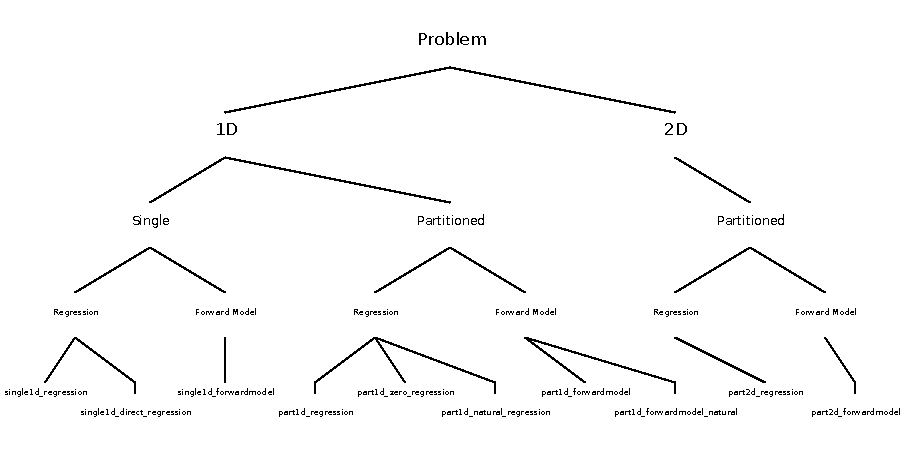
\includegraphics[width=\textwidth,height=\textheight/2,keepaspectratio=true]{main_tree}}
\end{DoxyImageNoCaption}
\hypertarget{index_Dimensionality}{}\subsection{Dimensionality}\label{index_Dimensionality}
The rjmcmc library supports 1 and 2 dimensional regression/forward model problems. If your problem consists of a regression/forward model of a single set of coordinates to a single set of values then it is a 1-\/dimensional problem. If your problem consists of a regression/forward model of a single set of coordinate pairs (eg x, y) to a single set of values then it is a 2-\/dimensional problem.\hypertarget{index_Partitioned}{}\subsection{Partitioned versus Single}\label{index_Partitioned}
If so you will want to use a partitioned or transdimensional approach, otherwise you can use the single methods (ie single partition methods).\hypertarget{index_Regression}{}\subsection{Regression versus Forward Model}\label{index_Regression}
A regression problem is one where there is a direct relationship between your data values and the fit to be generated. An example might be if your data consists of temperature measurements over time and you wanted to generate the temperature over time curve, then this is a regression problem. If instead you had a profile of the temperature down a bore and wanted to reconstruct the temperature versus time at the surface of the bore then this is a forward model problem. With forward model problems you will need to provide your own code for the forward model and calculate the log of the likelihood. In the case the borehole example, the rjmcmc library will provide a trial surface temperature record and the forward model will consist of a integration of the heat-\/diffusion equation given this input to create a trial borehole temperature profile. The likelihood is then calculated from the sum of the squared errors between the measured and trial borehole temperature profiles.\hypertarget{index_Directory}{}\section{Directory}\label{index_Directory}
\hypertarget{index_singleregress1d}{}\subsection{1\+D Single Partition Regression}\label{index_singleregress1d}
The following functions are available\+:


\begin{DoxyItemize}
\item \hyperlink{regression_8h_a037d789bc3de5c4c55b0c781193ae3b7}{single1d\+\_\+regression} uses an automatic prior to determine the best weights to be given to the order of the fitting polynomial.
\item \hyperlink{regression_8h_ac8c2d9357e8a0ac1ff03fc48843e804b}{single1d\+\_\+regression\+\_\+with\+\_\+prior} uses a user supplied prior to sample varying order polynomials to fit the data (deprecated/used for testing).
\item \hyperlink{regression_8h_a0ab9525ab0dc478cfa18bc9bd5a94d97}{single1d\+\_\+direct\+\_\+regression} use direct integration to determine the best fit to the data (deprecated/used for testing).
\end{DoxyItemize}

The following example codes are available (available under the Examples tab)\+:


\begin{DoxyItemize}
\item 1d/single/regression/cubic/cubic.\+c performs a regression on a known cubic function with added gaussian noise.
\end{DoxyItemize}\hypertarget{index_partregress1d}{}\subsection{1\+D Partitioned Regression}\label{index_partregress1d}
The following functions are available\+:


\begin{DoxyItemize}
\item \hyperlink{regression_8h_a17bc74fa9fb9c6287ab4e19751c6bb17}{part1d\+\_\+regression} uses an automatic prior to determine the best weights for the polynomial order(s) within each partition.
\item \hyperlink{regression_8h_ab17dfbf7aa5a8f0ba54441e7e9dc33cf}{part1d\+\_\+zero\+\_\+regression} use 0th order polynomials within each partition.
\item \hyperlink{regression_8h_abd2a0dc74a4bb3934c21c7864759bbbd}{part1d\+\_\+natural\+\_\+regression} use connected line segments between each partition boundary to provide a continuous fit (with change points becoming changes in gradients).
\end{DoxyItemize}

The following example codes are available (available under the Examples tab)\+:


\begin{DoxyItemize}
\item 1d/partitioned/regression/multiquad/multiquad.\+c performs a regression on a function comprised of piece wise quadratic functions with discontinuties with added gaussian noise.
\item 1d/partitioned/regression/multistep/multistep.\+c
\item 1d/partitioned/regression/sawtooth/sawtooth.\+c
\item 1d/partitioned/regression/zeromultistep/zeromultistep.\+c
\end{DoxyItemize}\hypertarget{index_singlefm1d}{}\subsection{1\+D Single Partition Forward Model}\label{index_singlefm1d}
The following functions are available\+:


\begin{DoxyItemize}
\item \hyperlink{forwardmodel_8h_a65b1200fd2ef808c85b1915fa1413b58}{single\+\_\+forwardmodel} performs a forward model analysis on an arbitrary number of parameters.
\item \hyperlink{forwardmodel__f_8h_a11799898f79291bad341135f00b7a243}{single\+\_\+forwardmodel\+\_\+f} is a fortran 2003 interface to the \hyperlink{forwardmodel_8h_a65b1200fd2ef808c85b1915fa1413b58}{single\+\_\+forwardmodel} function.
\item \hyperlink{forwardmodel_8h_a95b892df15e3e7b58497a68af64a7b0d}{single\+\_\+forwardmodel\+\_\+hierarchical} performs a forward model analysis on an arbitrary number of parameters with a custom hierarchical peturbation of the covariance matrix.
\end{DoxyItemize}

The following example codes are available (available under the Examples tab)\+:


\begin{DoxyItemize}
\item 1d/single/fm/simplef/simplef.\+f90
\item 1d/single/fm/simpleimage/simpleimage.\+c
\item 1d/single/fm/spherefit/spherefit.\+c
\end{DoxyItemize}\hypertarget{index_partfm1d}{}\subsection{1\+D Partitioned Forward Model}\label{index_partfm1d}
The following functions are available\+:


\begin{DoxyItemize}
\item \hyperlink{forwardmodel_8h_a852beb6cfb6875927200fa90d6d60d6e}{part1d\+\_\+forwardmodel}
\item \hyperlink{forwardmodel__f_8h_aa7d79eacccaac4d0770cd207b166dced}{part1d\+\_\+forwardmodel\+\_\+f}
\item \hyperlink{forwardmodel_8h_a267826c400d1ae8be3473c4bdc03e05b}{part1d\+\_\+forwardmodel\+\_\+hierarchical}
\item \hyperlink{forwardmodel_8h_a736c12ab94ec4dd7e785baa8b028c6e6}{part1d\+\_\+forwardmodel\+\_\+natural}
\item \hyperlink{forwardmodel_8h_ad6b46c9104fbbea5c119bc64e8f29190}{part1d\+\_\+forwardmodel\+\_\+natural\+\_\+hierarchical}
\end{DoxyItemize}

The following example codes are available (available under the Examples tab)\+:


\begin{DoxyItemize}
\item 1d/partitioned/fm/functionfit/functionfit.\+c
\item 1d/partitioned/fm/functionfitf/functionfitf.\+f90
\item 1d/partitioned/fm/regression/regression.\+c
\end{DoxyItemize}\hypertarget{index_partregress2d}{}\subsection{2\+D Partitioned Regression}\label{index_partregress2d}
The following functions are available\+:


\begin{DoxyItemize}
\item \hyperlink{regression_8h_aa4589a0fbb1ca56b2db6fafbda40161f}{part2d\+\_\+regression}
\end{DoxyItemize}\hypertarget{index_partfm2d}{}\subsection{2\+D Partitioned Forward Model}\label{index_partfm2d}
The following functions are available\+:


\begin{DoxyItemize}
\item \hyperlink{forwardmodel_8h_a1a30e27827e21f0906d74634c611cc54}{part2d\+\_\+forwardmodel}
\item \hyperlink{forwardmodel_8h_a7f812853c942aeb44dd57ce2823a8523}{part2d\+\_\+forwardmodel\+\_\+hierarchical} 
\end{DoxyItemize}
\chapter{Background}
\label{background}
\hypertarget{background}{}
\hypertarget{background_backgroundoverview}{}\section{Overview}\label{background_backgroundoverview}
This library provides routines for regression and forward model problems using trans-\/dimensional Markov chain Monte Carlo methods. Rather than producing a single fit for a dataset, these methods produce an ensemble of results that give a sampled distribution of the potential true fit. The original paper describing this approach is by Green {\bfseries [green1995]}, and this software is primarily based on the work of Bodin and Sambridge {\bfseries [sambridge2006A]} {\bfseries [bodin\+Thesis]} {\bfseries [bodin2012A]} .\hypertarget{background_backgroundprior}{}\section{Prior}\label{background_backgroundprior}
The general approach taken in all the routines within this library is to use uniform priors on all values.

For partition locations, we use a symmetric Dirichlet prior which is described in Steininger {\bfseries [steininger2013]} and references therein.\hypertarget{background_backgroundmodel}{}\section{Model}\label{background_backgroundmodel}
For 1D applications we use zeroth order, natural, and polynomial models within each partition.

Zeroth order 1D models are described in {\bfseries [bodin\+Thesis]} {\bfseries [bodin2012A]}.

Natural uses jointed line segments between partition boundaries to create a C0 continuous curve over the domain of the entire model. It is described in Hopcroft {\bfseries [hopcroft2007A]} .

For 1D regression problems only, we also use the data within each partition to inform the selection of a suitable polynomial order (up to a limit imposed by the user), ie trans-\/dimensional within each partition. The mechanism for choosing this order is described in Sambridge {\bfseries [sambridge2006A]} and the order prior is set to uniform over a region determined from the data mean and standard deviation within the partition.

For 2D applications at present only zeroth order partitions are used as described in {\bfseries [bodin2012B]} and {\bfseries [bodin2012C]}.\hypertarget{background_backgroundproposal}{}\section{Proposal}\label{background_backgroundproposal}
All proposals used in this library use pertubations sampled from a Gaussian random variable. The Standard deviation is generally set as a user parameter, the only exception to this is in the case of 1D Regression routines where the standard deviation is obtained directly from the data.\hypertarget{background_backgroundhierarchical}{}\section{Hierarchical Parameter Estimation}\label{background_backgroundhierarchical}
Hierarchical parameters are parameters used to quantify the noise in the data. In the simple regression case, we allow the use of a single hierarchical scaling factor called lambda that represents a multiplier of the estimated data error.

In the general forward model case, we allow a general mechanism for hierarchical parameter estimation requiring the forward model to calculate the log of the determinant of the data covariance matrix.

For an example of more complex hierarchical parameter estimation, see Bodin {\bfseries [bodin2012A]} . 
\chapter{Data Structure Index}
\section{Data Structures}
Here are the data structures with brief descriptions\+:\begin{DoxyCompactList}
\item\contentsline{section}{\hyperlink{struct__curvefit__result}{\+\_\+curvefit\+\_\+result} }{\pageref{struct__curvefit__result}}{}
\item\contentsline{section}{\hyperlink{struct__dataset1d}{\+\_\+dataset1d} }{\pageref{struct__dataset1d}}{}
\item\contentsline{section}{\hyperlink{struct__dataset2d}{\+\_\+dataset2d} }{\pageref{struct__dataset2d}}{}
\item\contentsline{section}{\hyperlink{struct__delaunay2d}{\+\_\+delaunay2d} }{\pageref{struct__delaunay2d}}{}
\item\contentsline{section}{\hyperlink{struct__edgelist}{\+\_\+edgelist} }{\pageref{struct__edgelist}}{}
\item\contentsline{section}{\hyperlink{struct__forwardmodelparameter}{\+\_\+forwardmodelparameter} }{\pageref{struct__forwardmodelparameter}}{}
\item\contentsline{section}{\hyperlink{struct__model}{\+\_\+model} }{\pageref{struct__model}}{}
\item\contentsline{section}{\hyperlink{struct__part1d__fm__hierarchical__likelihood__state}{\+\_\+part1d\+\_\+fm\+\_\+hierarchical\+\_\+likelihood\+\_\+state} }{\pageref{struct__part1d__fm__hierarchical__likelihood__state}}{}
\item\contentsline{section}{\hyperlink{struct__part1d__fm__likelihood__state}{\+\_\+part1d\+\_\+fm\+\_\+likelihood\+\_\+state} }{\pageref{struct__part1d__fm__likelihood__state}}{}
\item\contentsline{section}{\hyperlink{struct__part1d__forwardmodel}{\+\_\+part1d\+\_\+forwardmodel} }{\pageref{struct__part1d__forwardmodel}}{}
\item\contentsline{section}{\hyperlink{struct__part1d__natural__rj}{\+\_\+part1d\+\_\+natural\+\_\+rj} }{\pageref{struct__part1d__natural__rj}}{}
\item\contentsline{section}{\hyperlink{struct__part1d__regression__rj}{\+\_\+part1d\+\_\+regression\+\_\+rj} }{\pageref{struct__part1d__regression__rj}}{}
\item\contentsline{section}{\hyperlink{struct__part1d__zero}{\+\_\+part1d\+\_\+zero} }{\pageref{struct__part1d__zero}}{}
\item\contentsline{section}{\hyperlink{struct__part2d__fm__likelihood__state}{\+\_\+part2d\+\_\+fm\+\_\+likelihood\+\_\+state} }{\pageref{struct__part2d__fm__likelihood__state}}{}
\item\contentsline{section}{\hyperlink{struct__part2d__forwardmodel}{\+\_\+part2d\+\_\+forwardmodel} }{\pageref{struct__part2d__forwardmodel}}{}
\item\contentsline{section}{\hyperlink{struct__part2d__regression__rj}{\+\_\+part2d\+\_\+regression\+\_\+rj} }{\pageref{struct__part2d__regression__rj}}{}
\item\contentsline{section}{\hyperlink{struct__partitions__valid__data}{\+\_\+partitions\+\_\+valid\+\_\+data} }{\pageref{struct__partitions__valid__data}}{}
\item\contentsline{section}{\hyperlink{struct__point}{\+\_\+point} }{\pageref{struct__point}}{}
\item\contentsline{section}{\hyperlink{struct__point1d}{\+\_\+point1d} }{\pageref{struct__point1d}}{}
\item\contentsline{section}{\hyperlink{struct__point2d}{\+\_\+point2d} }{\pageref{struct__point2d}}{}
\item\contentsline{section}{\hyperlink{struct__position__map1d}{\+\_\+position\+\_\+map1d} }{\pageref{struct__position__map1d}}{}
\item\contentsline{section}{\hyperlink{struct__position__map2d__delaunay}{\+\_\+position\+\_\+map2d\+\_\+delaunay} }{\pageref{struct__position__map2d__delaunay}}{}
\item\contentsline{section}{\hyperlink{struct__position__map2d__linear}{\+\_\+position\+\_\+map2d\+\_\+linear} }{\pageref{struct__position__map2d__linear}}{}
\item\contentsline{section}{\hyperlink{struct__position__map2d__quadtree}{\+\_\+position\+\_\+map2d\+\_\+quadtree} }{\pageref{struct__position__map2d__quadtree}}{}
\item\contentsline{section}{\hyperlink{struct__quadtree}{\+\_\+quadtree} }{\pageref{struct__quadtree}}{}
\item\contentsline{section}{\hyperlink{struct__quadtree__leaf}{\+\_\+quadtree\+\_\+leaf} }{\pageref{struct__quadtree__leaf}}{}
\item\contentsline{section}{\hyperlink{struct__quadtree__node}{\+\_\+quadtree\+\_\+node} }{\pageref{struct__quadtree__node}}{}
\item\contentsline{section}{\hyperlink{struct__resultset1d}{\+\_\+resultset1d} }{\pageref{struct__resultset1d}}{}
\item\contentsline{section}{\hyperlink{struct__resultset1dfm}{\+\_\+resultset1dfm} }{\pageref{struct__resultset1dfm}}{}
\item\contentsline{section}{\hyperlink{struct__resultset2d}{\+\_\+resultset2d} }{\pageref{struct__resultset2d}}{}
\item\contentsline{section}{\hyperlink{struct__resultset2dfm}{\+\_\+resultset2dfm} }{\pageref{struct__resultset2dfm}}{}
\item\contentsline{section}{\hyperlink{struct__resultsetfm}{\+\_\+resultsetfm} }{\pageref{struct__resultsetfm}}{}
\item\contentsline{section}{\hyperlink{struct__rjmcmc__engine__cb}{\+\_\+rjmcmc\+\_\+engine\+\_\+cb} }{\pageref{struct__rjmcmc__engine__cb}}{}
\item\contentsline{section}{\hyperlink{struct__single1d__regression}{\+\_\+single1d\+\_\+regression} }{\pageref{struct__single1d__regression}}{}
\item\contentsline{section}{\hyperlink{struct__triangle}{\+\_\+triangle} }{\pageref{struct__triangle}}{}
\item\contentsline{section}{\hyperlink{structbbox2d}{bbox2d} }{\pageref{structbbox2d}}{}
\item\contentsline{section}{\hyperlink{structfmsingle}{fmsingle} }{\pageref{structfmsingle}}{}
\item\contentsline{section}{\hyperlink{structinitialize__cb__data}{initialize\+\_\+cb\+\_\+data} }{\pageref{structinitialize__cb__data}}{}
\item\contentsline{section}{\hyperlink{structinterval__data}{interval\+\_\+data} }{\pageref{structinterval__data}}{}
\item\contentsline{section}{\hyperlink{structmpi__data}{mpi\+\_\+data} }{\pageref{structmpi__data}}{}
\item\contentsline{section}{\hyperlink{structpart1d}{part1d} }{\pageref{structpart1d}}{}
\item\contentsline{section}{\hyperlink{structpart1d__fm__value__at__wrap}{part1d\+\_\+fm\+\_\+value\+\_\+at\+\_\+wrap} }{\pageref{structpart1d__fm__value__at__wrap}}{}
\item\contentsline{section}{\hyperlink{structpart1d__forwardmodel__wrap}{part1d\+\_\+forwardmodel\+\_\+wrap} }{\pageref{structpart1d__forwardmodel__wrap}}{}
\item\contentsline{section}{\hyperlink{structpart1d__hierarchical__forwardmodel__wrap}{part1d\+\_\+hierarchical\+\_\+forwardmodel\+\_\+wrap} }{\pageref{structpart1d__hierarchical__forwardmodel__wrap}}{}
\item\contentsline{section}{\hyperlink{structpart1dfm}{part1dfm} }{\pageref{structpart1dfm}}{}
\item\contentsline{section}{\hyperlink{structpart2d}{part2d} }{\pageref{structpart2d}}{}
\item\contentsline{section}{\hyperlink{structpart2d__fm__value__at__wrap}{part2d\+\_\+fm\+\_\+value\+\_\+at\+\_\+wrap} }{\pageref{structpart2d__fm__value__at__wrap}}{}
\item\contentsline{section}{\hyperlink{structpart2d__forwardmodel__hierarchical__wrap}{part2d\+\_\+forwardmodel\+\_\+hierarchical\+\_\+wrap} }{\pageref{structpart2d__forwardmodel__hierarchical__wrap}}{}
\item\contentsline{section}{\hyperlink{structpart2d__forwardmodel__wrap}{part2d\+\_\+forwardmodel\+\_\+wrap} }{\pageref{structpart2d__forwardmodel__wrap}}{}
\item\contentsline{section}{\hyperlink{structpart2dfm}{part2dfm} }{\pageref{structpart2dfm}}{}
\item\contentsline{section}{\hyperlink{structreader__t}{reader\+\_\+t} }{\pageref{structreader__t}}{}
\item\contentsline{section}{\hyperlink{structsingle1d}{single1d} }{\pageref{structsingle1d}}{}
\item\contentsline{section}{\hyperlink{structwellrng}{wellrng} }{\pageref{structwellrng}}{}
\item\contentsline{section}{\hyperlink{structwriter__t}{writer\+\_\+t} }{\pageref{structwriter__t}}{}
\end{DoxyCompactList}

\chapter{File Index}
\section{File List}
Here is a list of all files with brief descriptions\+:\begin{DoxyCompactList}
\item\contentsline{section}{\hyperlink{bbox2d_8c}{bbox2d.\+c} }{\pageref{bbox2d_8c}}{}
\item\contentsline{section}{\hyperlink{bbox2d_8h}{bbox2d.\+h} \\*2D Bounding Box routines }{\pageref{bbox2d_8h}}{}
\item\contentsline{section}{\hyperlink{curvefit_8c}{curvefit.\+c} }{\pageref{curvefit_8c}}{}
\item\contentsline{section}{\hyperlink{curvefit_8h}{curvefit.\+h} \\*1D Curve Fitting routines }{\pageref{curvefit_8h}}{}
\item\contentsline{section}{\hyperlink{dataset1d_8c}{dataset1d.\+c} }{\pageref{dataset1d_8c}}{}
\item\contentsline{section}{\hyperlink{dataset1d_8h}{dataset1d.\+h} \\*1D Dataset Storage }{\pageref{dataset1d_8h}}{}
\item\contentsline{section}{\hyperlink{dataset2d_8c}{dataset2d.\+c} }{\pageref{dataset2d_8c}}{}
\item\contentsline{section}{\hyperlink{dataset2d_8h}{dataset2d.\+h} \\*2D Dataset Storage }{\pageref{dataset2d_8h}}{}
\item\contentsline{section}{\hyperlink{delaunay2d_8c}{delaunay2d.\+c} }{\pageref{delaunay2d_8c}}{}
\item\contentsline{section}{\hyperlink{delaunay2d_8h}{delaunay2d.\+h} \\*Delaunay 2D Triangulation point tracking }{\pageref{delaunay2d_8h}}{}
\item\contentsline{section}{\hyperlink{engine_8c}{engine.\+c} }{\pageref{engine_8c}}{}
\item\contentsline{section}{\hyperlink{engine_8h}{engine.\+h} }{\pageref{engine_8h}}{}
\item\contentsline{section}{\hyperlink{forwardmodel_8h}{forwardmodel.\+h} \\*Simple Forward Model Routines }{\pageref{forwardmodel_8h}}{}
\item\contentsline{section}{\hyperlink{forwardmodel__f_8c}{forwardmodel\+\_\+f.\+c} }{\pageref{forwardmodel__f_8c}}{}
\item\contentsline{section}{\hyperlink{forwardmodel__f_8h}{forwardmodel\+\_\+f.\+h} }{\pageref{forwardmodel__f_8h}}{}
\item\contentsline{section}{\hyperlink{forwardmodel__mpi_8h}{forwardmodel\+\_\+mpi.\+h} }{\pageref{forwardmodel__mpi_8h}}{}
\item\contentsline{section}{\hyperlink{forwardmodel__part1d_8c}{forwardmodel\+\_\+part1d.\+c} }{\pageref{forwardmodel__part1d_8c}}{}
\item\contentsline{section}{\hyperlink{forwardmodel__part1d__hierarchical_8c}{forwardmodel\+\_\+part1d\+\_\+hierarchical.\+c} }{\pageref{forwardmodel__part1d__hierarchical_8c}}{}
\item\contentsline{section}{\hyperlink{forwardmodel__part2d_8c}{forwardmodel\+\_\+part2d.\+c} }{\pageref{forwardmodel__part2d_8c}}{}
\item\contentsline{section}{\hyperlink{forwardmodel__part2d__hierarchical_8c}{forwardmodel\+\_\+part2d\+\_\+hierarchical.\+c} }{\pageref{forwardmodel__part2d__hierarchical_8c}}{}
\item\contentsline{section}{\hyperlink{forwardmodel__single_8c}{forwardmodel\+\_\+single.\+c} }{\pageref{forwardmodel__single_8c}}{}
\item\contentsline{section}{\hyperlink{forwardmodel__util_8c}{forwardmodel\+\_\+util.\+c} }{\pageref{forwardmodel__util_8c}}{}
\item\contentsline{section}{\hyperlink{forwardmodel__util_8h}{forwardmodel\+\_\+util.\+h} }{\pageref{forwardmodel__util_8h}}{}
\item\contentsline{section}{\hyperlink{forwardmodelparameter_8c}{forwardmodelparameter.\+c} }{\pageref{forwardmodelparameter_8c}}{}
\item\contentsline{section}{\hyperlink{forwardmodelparameter_8h}{forwardmodelparameter.\+h} }{\pageref{forwardmodelparameter_8h}}{}
\item\contentsline{section}{\hyperlink{part1d__forwardmodel_8c}{part1d\+\_\+forwardmodel.\+c} }{\pageref{part1d__forwardmodel_8c}}{}
\item\contentsline{section}{\hyperlink{part1d__forwardmodel_8h}{part1d\+\_\+forwardmodel.\+h} }{\pageref{part1d__forwardmodel_8h}}{}
\item\contentsline{section}{\hyperlink{part1d__natural__rj_8c}{part1d\+\_\+natural\+\_\+rj.\+c} }{\pageref{part1d__natural__rj_8c}}{}
\item\contentsline{section}{\hyperlink{part1d__natural__rj_8h}{part1d\+\_\+natural\+\_\+rj.\+h} }{\pageref{part1d__natural__rj_8h}}{}
\item\contentsline{section}{\hyperlink{part1d__regression__rj_8c}{part1d\+\_\+regression\+\_\+rj.\+c} }{\pageref{part1d__regression__rj_8c}}{}
\item\contentsline{section}{\hyperlink{part1d__regression__rj_8h}{part1d\+\_\+regression\+\_\+rj.\+h} }{\pageref{part1d__regression__rj_8h}}{}
\item\contentsline{section}{\hyperlink{part1d__zero_8c}{part1d\+\_\+zero.\+c} }{\pageref{part1d__zero_8c}}{}
\item\contentsline{section}{\hyperlink{part1d__zero_8h}{part1d\+\_\+zero.\+h} }{\pageref{part1d__zero_8h}}{}
\item\contentsline{section}{\hyperlink{part2d__forwardmodel_8c}{part2d\+\_\+forwardmodel.\+c} }{\pageref{part2d__forwardmodel_8c}}{}
\item\contentsline{section}{\hyperlink{part2d__forwardmodel_8h}{part2d\+\_\+forwardmodel.\+h} }{\pageref{part2d__forwardmodel_8h}}{}
\item\contentsline{section}{\hyperlink{part2d__regression__rj_8c}{part2d\+\_\+regression\+\_\+rj.\+c} }{\pageref{part2d__regression__rj_8c}}{}
\item\contentsline{section}{\hyperlink{part2d__regression__rj_8h}{part2d\+\_\+regression\+\_\+rj.\+h} }{\pageref{part2d__regression__rj_8h}}{}
\item\contentsline{section}{\hyperlink{position__map1d_8c}{position\+\_\+map1d.\+c} }{\pageref{position__map1d_8c}}{}
\item\contentsline{section}{\hyperlink{position__map1d_8h}{position\+\_\+map1d.\+h} }{\pageref{position__map1d_8h}}{}
\item\contentsline{section}{\hyperlink{position__map2d_8c}{position\+\_\+map2d.\+c} }{\pageref{position__map2d_8c}}{}
\item\contentsline{section}{\hyperlink{position__map2d_8h}{position\+\_\+map2d.\+h} }{\pageref{position__map2d_8h}}{}
\item\contentsline{section}{\hyperlink{position__map2d__delaunay_8c}{position\+\_\+map2d\+\_\+delaunay.\+c} }{\pageref{position__map2d__delaunay_8c}}{}
\item\contentsline{section}{\hyperlink{position__map2d__delaunay_8h}{position\+\_\+map2d\+\_\+delaunay.\+h} }{\pageref{position__map2d__delaunay_8h}}{}
\item\contentsline{section}{\hyperlink{position__map2d__linear_8c}{position\+\_\+map2d\+\_\+linear.\+c} }{\pageref{position__map2d__linear_8c}}{}
\item\contentsline{section}{\hyperlink{position__map2d__linear_8h}{position\+\_\+map2d\+\_\+linear.\+h} }{\pageref{position__map2d__linear_8h}}{}
\item\contentsline{section}{\hyperlink{position__map2d__quadtree_8c}{position\+\_\+map2d\+\_\+quadtree.\+c} }{\pageref{position__map2d__quadtree_8c}}{}
\item\contentsline{section}{\hyperlink{position__map2d__quadtree_8h}{position\+\_\+map2d\+\_\+quadtree.\+h} }{\pageref{position__map2d__quadtree_8h}}{}
\item\contentsline{section}{\hyperlink{quadtree_8c}{quadtree.\+c} }{\pageref{quadtree_8c}}{}
\item\contentsline{section}{\hyperlink{quadtree_8h}{quadtree.\+h} }{\pageref{quadtree_8h}}{}
\item\contentsline{section}{\hyperlink{regression_8c}{regression.\+c} }{\pageref{regression_8c}}{}
\item\contentsline{section}{\hyperlink{regression_8h}{regression.\+h} \\*Single, 1D Partitioned and 2D Partitioned Regression }{\pageref{regression_8h}}{}
\item\contentsline{section}{\hyperlink{regression__mpi_8h}{regression\+\_\+mpi.\+h} }{\pageref{regression__mpi_8h}}{}
\item\contentsline{section}{\hyperlink{regression__part1d_8c}{regression\+\_\+part1d.\+c} }{\pageref{regression__part1d_8c}}{}
\item\contentsline{section}{\hyperlink{regression__part1d__natural_8c}{regression\+\_\+part1d\+\_\+natural.\+c} }{\pageref{regression__part1d__natural_8c}}{}
\item\contentsline{section}{\hyperlink{regression__part1d__zero_8c}{regression\+\_\+part1d\+\_\+zero.\+c} }{\pageref{regression__part1d__zero_8c}}{}
\item\contentsline{section}{\hyperlink{regression__part2d_8c}{regression\+\_\+part2d.\+c} }{\pageref{regression__part2d_8c}}{}
\item\contentsline{section}{\hyperlink{resultset1d_8c}{resultset1d.\+c} }{\pageref{resultset1d_8c}}{}
\item\contentsline{section}{\hyperlink{resultset1d_8h}{resultset1d.\+h} }{\pageref{resultset1d_8h}}{}
\item\contentsline{section}{\hyperlink{resultset1dfm_8c}{resultset1dfm.\+c} }{\pageref{resultset1dfm_8c}}{}
\item\contentsline{section}{\hyperlink{resultset1dfm_8h}{resultset1dfm.\+h} }{\pageref{resultset1dfm_8h}}{}
\item\contentsline{section}{\hyperlink{resultset2d_8c}{resultset2d.\+c} }{\pageref{resultset2d_8c}}{}
\item\contentsline{section}{\hyperlink{resultset2d_8h}{resultset2d.\+h} }{\pageref{resultset2d_8h}}{}
\item\contentsline{section}{\hyperlink{resultset2dfm_8c}{resultset2dfm.\+c} }{\pageref{resultset2dfm_8c}}{}
\item\contentsline{section}{\hyperlink{resultset2dfm_8h}{resultset2dfm.\+h} }{\pageref{resultset2dfm_8h}}{}
\item\contentsline{section}{\hyperlink{resultsetfm_8c}{resultsetfm.\+c} }{\pageref{resultsetfm_8c}}{}
\item\contentsline{section}{\hyperlink{resultsetfm_8h}{resultsetfm.\+h} }{\pageref{resultsetfm_8h}}{}
\item\contentsline{section}{\hyperlink{rjmcmc_8h}{rjmcmc.\+h} }{\pageref{rjmcmc_8h}}{}
\item\contentsline{section}{\hyperlink{rjmcmc__config_8h}{rjmcmc\+\_\+config.\+h} }{\pageref{rjmcmc__config_8h}}{}
\item\contentsline{section}{\hyperlink{rjmcmc__debug_8c}{rjmcmc\+\_\+debug.\+c} }{\pageref{rjmcmc__debug_8c}}{}
\item\contentsline{section}{\hyperlink{rjmcmc__debug_8h}{rjmcmc\+\_\+debug.\+h} }{\pageref{rjmcmc__debug_8h}}{}
\item\contentsline{section}{\hyperlink{rjmcmc__defines_8h}{rjmcmc\+\_\+defines.\+h} }{\pageref{rjmcmc__defines_8h}}{}
\item\contentsline{section}{\hyperlink{rjmcmc__random_8c}{rjmcmc\+\_\+random.\+c} }{\pageref{rjmcmc__random_8c}}{}
\item\contentsline{section}{\hyperlink{rjmcmc__random_8h}{rjmcmc\+\_\+random.\+h} }{\pageref{rjmcmc__random_8h}}{}
\item\contentsline{section}{\hyperlink{rjmcmc__util_8c}{rjmcmc\+\_\+util.\+c} }{\pageref{rjmcmc__util_8c}}{}
\item\contentsline{section}{\hyperlink{rjmcmc__util_8h}{rjmcmc\+\_\+util.\+h} }{\pageref{rjmcmc__util_8h}}{}
\item\contentsline{section}{\hyperlink{rjmcmcf_8h}{rjmcmcf.\+h} }{\pageref{rjmcmcf_8h}}{}
\item\contentsline{section}{\hyperlink{rjmcmcf__mpi_8h}{rjmcmcf\+\_\+mpi.\+h} }{\pageref{rjmcmcf__mpi_8h}}{}
\item\contentsline{section}{\hyperlink{single1d__regression_8c}{single1d\+\_\+regression.\+c} }{\pageref{single1d__regression_8c}}{}
\item\contentsline{section}{\hyperlink{single1d__regression_8h}{single1d\+\_\+regression.\+h} }{\pageref{single1d__regression_8h}}{}
\item\contentsline{section}{\hyperlink{single2d__regression_8h}{single2d\+\_\+regression.\+h} }{\pageref{single2d__regression_8h}}{}
\item\contentsline{section}{\hyperlink{voronoi2d_8h}{voronoi2d.\+h} }{\pageref{voronoi2d_8h}}{}
\item\contentsline{section}{\hyperlink{wellrng_8c}{wellrng.\+c} }{\pageref{wellrng_8c}}{}
\item\contentsline{section}{\hyperlink{wellrng_8h}{wellrng.\+h} }{\pageref{wellrng_8h}}{}
\end{DoxyCompactList}

\chapter{Data Structure Documentation}
\hypertarget{struct__curvefit__result}{}\section{\+\_\+curvefit\+\_\+result Struct Reference}
\label{struct__curvefit__result}\index{\+\_\+curvefit\+\_\+result@{\+\_\+curvefit\+\_\+result}}
\subsection*{Data Fields}
\begin{DoxyCompactItemize}
\item 
int \hyperlink{struct__curvefit__result_ad13ba13973e6cbcaa18a130fffffc51e}{maxorder}
\item 
double $\ast$ \hyperlink{struct__curvefit__result_ab56262b33bcbe8f57c2a1abbdfd2390f}{alpha}
\item 
double $\ast$ \hyperlink{struct__curvefit__result_af944a98599d8267f8aea2ece7d392934}{beta}
\item 
double $\ast$$\ast$ \hyperlink{struct__curvefit__result_a1980f366a2c6b55a90488993ce4ff45f}{L}
\item 
double $\ast$$\ast$ \hyperlink{struct__curvefit__result_a3a16ac20b913a15302777af1c737802e}{Z}
\item 
double $\ast$$\ast$ \hyperlink{struct__curvefit__result_a77d02b3f78f1ad80cccad96f565c62f3}{S}
\item 
double $\ast$$\ast$ \hyperlink{struct__curvefit__result_a98daa734e4c93414381644b5da332785}{Si}
\item 
double $\ast$ \hyperlink{struct__curvefit__result_a383aaa533afdf17d91c26133f629e3e8}{mu}
\item 
double $\ast$ \hyperlink{struct__curvefit__result_a07b7d671ead5f402dd53973dd8095d8e}{x}
\item 
double $\ast$ \hyperlink{struct__curvefit__result_a43187b41a4fec805c76ee32325f4942c}{b}
\end{DoxyCompactItemize}


\subsection{Field Documentation}
\index{\+\_\+curvefit\+\_\+result@{\+\_\+curvefit\+\_\+result}!alpha@{alpha}}
\index{alpha@{alpha}!\+\_\+curvefit\+\_\+result@{\+\_\+curvefit\+\_\+result}}
\subsubsection[{\texorpdfstring{alpha}{alpha}}]{\setlength{\rightskip}{0pt plus 5cm}double$\ast$ \+\_\+curvefit\+\_\+result\+::alpha}\hypertarget{struct__curvefit__result_ab56262b33bcbe8f57c2a1abbdfd2390f}{}\label{struct__curvefit__result_ab56262b33bcbe8f57c2a1abbdfd2390f}


Referenced by curvefit\+\_\+compute(), curvefit\+\_\+compute\+\_\+lambda(), curvefit\+\_\+create(), curvefit\+\_\+destroy(), and curvefit\+\_\+sample\+\_\+det\+Cm().

\index{\+\_\+curvefit\+\_\+result@{\+\_\+curvefit\+\_\+result}!b@{b}}
\index{b@{b}!\+\_\+curvefit\+\_\+result@{\+\_\+curvefit\+\_\+result}}
\subsubsection[{\texorpdfstring{b}{b}}]{\setlength{\rightskip}{0pt plus 5cm}double$\ast$ \+\_\+curvefit\+\_\+result\+::b}\hypertarget{struct__curvefit__result_a43187b41a4fec805c76ee32325f4942c}{}\label{struct__curvefit__result_a43187b41a4fec805c76ee32325f4942c}


Referenced by curvefit\+\_\+compute(), curvefit\+\_\+compute\+\_\+lambda(), curvefit\+\_\+create(), curvefit\+\_\+destroy(), curvefit\+\_\+sample(), curvefit\+\_\+sample\+\_\+det\+Cm(), and dataset1d\+\_\+load\+\_\+known().

\index{\+\_\+curvefit\+\_\+result@{\+\_\+curvefit\+\_\+result}!beta@{beta}}
\index{beta@{beta}!\+\_\+curvefit\+\_\+result@{\+\_\+curvefit\+\_\+result}}
\subsubsection[{\texorpdfstring{beta}{beta}}]{\setlength{\rightskip}{0pt plus 5cm}double$\ast$ \+\_\+curvefit\+\_\+result\+::beta}\hypertarget{struct__curvefit__result_af944a98599d8267f8aea2ece7d392934}{}\label{struct__curvefit__result_af944a98599d8267f8aea2ece7d392934}


Referenced by curvefit\+\_\+compute(), curvefit\+\_\+compute\+\_\+lambda(), curvefit\+\_\+create(), curvefit\+\_\+destroy(), and curvefit\+\_\+sample\+\_\+det\+Cm().

\index{\+\_\+curvefit\+\_\+result@{\+\_\+curvefit\+\_\+result}!L@{L}}
\index{L@{L}!\+\_\+curvefit\+\_\+result@{\+\_\+curvefit\+\_\+result}}
\subsubsection[{\texorpdfstring{L}{L}}]{\setlength{\rightskip}{0pt plus 5cm}double$\ast$$\ast$ \+\_\+curvefit\+\_\+result\+::L}\hypertarget{struct__curvefit__result_a1980f366a2c6b55a90488993ce4ff45f}{}\label{struct__curvefit__result_a1980f366a2c6b55a90488993ce4ff45f}


Referenced by cf\+\_\+\+L(), curvefit\+\_\+compute(), curvefit\+\_\+compute\+\_\+lambda(), curvefit\+\_\+create(), curvefit\+\_\+destroy(), and curvefit\+\_\+sample\+\_\+det\+Cm().

\index{\+\_\+curvefit\+\_\+result@{\+\_\+curvefit\+\_\+result}!maxorder@{maxorder}}
\index{maxorder@{maxorder}!\+\_\+curvefit\+\_\+result@{\+\_\+curvefit\+\_\+result}}
\subsubsection[{\texorpdfstring{maxorder}{maxorder}}]{\setlength{\rightskip}{0pt plus 5cm}int \+\_\+curvefit\+\_\+result\+::maxorder}\hypertarget{struct__curvefit__result_ad13ba13973e6cbcaa18a130fffffc51e}{}\label{struct__curvefit__result_ad13ba13973e6cbcaa18a130fffffc51e}


Referenced by curvefit\+\_\+compute(), curvefit\+\_\+compute\+\_\+lambda(), curvefit\+\_\+create(), and curvefit\+\_\+destroy().

\index{\+\_\+curvefit\+\_\+result@{\+\_\+curvefit\+\_\+result}!mu@{mu}}
\index{mu@{mu}!\+\_\+curvefit\+\_\+result@{\+\_\+curvefit\+\_\+result}}
\subsubsection[{\texorpdfstring{mu}{mu}}]{\setlength{\rightskip}{0pt plus 5cm}double$\ast$ \+\_\+curvefit\+\_\+result\+::mu}\hypertarget{struct__curvefit__result_a383aaa533afdf17d91c26133f629e3e8}{}\label{struct__curvefit__result_a383aaa533afdf17d91c26133f629e3e8}


Referenced by cf\+\_\+mu(), curvefit\+\_\+compute(), curvefit\+\_\+compute\+\_\+lambda(), curvefit\+\_\+create(), curvefit\+\_\+destroy(), curvefit\+\_\+sample(), and curvefit\+\_\+sample\+\_\+mean().

\index{\+\_\+curvefit\+\_\+result@{\+\_\+curvefit\+\_\+result}!S@{S}}
\index{S@{S}!\+\_\+curvefit\+\_\+result@{\+\_\+curvefit\+\_\+result}}
\subsubsection[{\texorpdfstring{S}{S}}]{\setlength{\rightskip}{0pt plus 5cm}double$\ast$$\ast$ \+\_\+curvefit\+\_\+result\+::S}\hypertarget{struct__curvefit__result_a77d02b3f78f1ad80cccad96f565c62f3}{}\label{struct__curvefit__result_a77d02b3f78f1ad80cccad96f565c62f3}


Referenced by cf\+\_\+\+S(), curvefit\+\_\+compute(), curvefit\+\_\+compute\+\_\+lambda(), curvefit\+\_\+create(), curvefit\+\_\+destroy(), and curvefit\+\_\+sample\+\_\+sigma().

\index{\+\_\+curvefit\+\_\+result@{\+\_\+curvefit\+\_\+result}!Si@{Si}}
\index{Si@{Si}!\+\_\+curvefit\+\_\+result@{\+\_\+curvefit\+\_\+result}}
\subsubsection[{\texorpdfstring{Si}{Si}}]{\setlength{\rightskip}{0pt plus 5cm}double$\ast$$\ast$ \+\_\+curvefit\+\_\+result\+::\+Si}\hypertarget{struct__curvefit__result_a98daa734e4c93414381644b5da332785}{}\label{struct__curvefit__result_a98daa734e4c93414381644b5da332785}


Referenced by cf\+\_\+\+Si(), curvefit\+\_\+compute(), curvefit\+\_\+create(), curvefit\+\_\+destroy(), and curvefit\+\_\+sample().

\index{\+\_\+curvefit\+\_\+result@{\+\_\+curvefit\+\_\+result}!x@{x}}
\index{x@{x}!\+\_\+curvefit\+\_\+result@{\+\_\+curvefit\+\_\+result}}
\subsubsection[{\texorpdfstring{x}{x}}]{\setlength{\rightskip}{0pt plus 5cm}double$\ast$ \+\_\+curvefit\+\_\+result\+::x}\hypertarget{struct__curvefit__result_a07b7d671ead5f402dd53973dd8095d8e}{}\label{struct__curvefit__result_a07b7d671ead5f402dd53973dd8095d8e}


Referenced by curvefit\+\_\+compute(), curvefit\+\_\+compute\+\_\+lambda(), curvefit\+\_\+create(), curvefit\+\_\+destroy(), curvefit\+\_\+sample(), and curvefit\+\_\+sample\+\_\+det\+Cm().

\index{\+\_\+curvefit\+\_\+result@{\+\_\+curvefit\+\_\+result}!Z@{Z}}
\index{Z@{Z}!\+\_\+curvefit\+\_\+result@{\+\_\+curvefit\+\_\+result}}
\subsubsection[{\texorpdfstring{Z}{Z}}]{\setlength{\rightskip}{0pt plus 5cm}double$\ast$$\ast$ \+\_\+curvefit\+\_\+result\+::Z}\hypertarget{struct__curvefit__result_a3a16ac20b913a15302777af1c737802e}{}\label{struct__curvefit__result_a3a16ac20b913a15302777af1c737802e}


Referenced by cf\+\_\+\+Z(), curvefit\+\_\+compute(), curvefit\+\_\+compute\+\_\+lambda(), curvefit\+\_\+create(), curvefit\+\_\+destroy(), curvefit\+\_\+sample(), and curvefit\+\_\+sample\+\_\+det\+Cm().



The documentation for this struct was generated from the following file\+:\begin{DoxyCompactItemize}
\item 
\hyperlink{curvefit_8c}{curvefit.\+c}\end{DoxyCompactItemize}

\hypertarget{struct__dataset1d}{}\section{\+\_\+dataset1d Struct Reference}
\label{struct__dataset1d}\index{\+\_\+dataset1d@{\+\_\+dataset1d}}


{\ttfamily \#include $<$dataset1d.\+h$>$}



Collaboration diagram for \+\_\+dataset1d\+:
% FIG 0
\subsection*{Data Fields}
\begin{DoxyCompactItemize}
\item 
double \hyperlink{struct__dataset1d_ae96bdad176cb1e2ff691de6cd46b577b}{xmin}
\item 
double \hyperlink{struct__dataset1d_a006b76fa7e80e3220e6ad66a1ee0b83f}{xmax}
\item 
double \hyperlink{struct__dataset1d_afaee8c7cef9ae50d6c7387f3ac7d4379}{ymin}
\item 
double \hyperlink{struct__dataset1d_aa852aa13aa0a0d4e2b0a8bf83d03fc70}{ymax}
\item 
\hyperlink{dataset1d_8h_a97fb1604d71a5eeb5c0d33355d52def3}{point1d\+\_\+t} $\ast$ \hyperlink{struct__dataset1d_a88bbeb8e6e2273faefb175b91fcfae83}{points}
\item 
int \hyperlink{struct__dataset1d_ab864f8414fd7885ae891e67b615fbb89}{npoints}
\item 
double \hyperlink{struct__dataset1d_ad4d2e3a3d2eb35338ce1d819142cefb8}{lambdamin}
\item 
double \hyperlink{struct__dataset1d_ac07faf1146371645b1cb77495f866f48}{lambdamax}
\item 
double \hyperlink{struct__dataset1d_ab5344ed7583036bc0dc1b9e769273c85}{lambdastd}
\end{DoxyCompactItemize}


\subsection{Detailed Description}
\begin{Desc}
\item[Examples\+: ]\par
\hyperlink{1d_2partitioned_2regression_2multiquad_2multiquad_8c-example}{1d/partitioned/regression/multiquad/multiquad.\+c}, \hyperlink{1d_2partitioned_2regression_2multistep_2multistep_8c-example}{1d/partitioned/regression/multistep/multistep.\+c}, \hyperlink{1d_2partitioned_2regression_2sawtooth_2sawtooth_8c-example}{1d/partitioned/regression/sawtooth/sawtooth.\+c}, \hyperlink{1d_2partitioned_2regression_2zeromultistep_2zeromultistep_8c-example}{1d/partitioned/regression/zeromultistep/zeromultistep.\+c}, and \hyperlink{1d_2single_2regression_2cubic_2cubic_8c-example}{1d/single/regression/cubic/cubic.\+c}.\end{Desc}


\subsection{Field Documentation}
\index{\+\_\+dataset1d@{\+\_\+dataset1d}!lambdamax@{lambdamax}}
\index{lambdamax@{lambdamax}!\+\_\+dataset1d@{\+\_\+dataset1d}}
\subsubsection[{\texorpdfstring{lambdamax}{lambdamax}}]{\setlength{\rightskip}{0pt plus 5cm}double \+\_\+dataset1d\+::lambdamax}\hypertarget{struct__dataset1d_ac07faf1146371645b1cb77495f866f48}{}\label{struct__dataset1d_ac07faf1146371645b1cb77495f866f48}
\begin{Desc}
\item[Examples\+: ]\par
\hyperlink{1d_2partitioned_2regression_2multiquad_2multiquad_8c-example}{1d/partitioned/regression/multiquad/multiquad.\+c}, \hyperlink{1d_2partitioned_2regression_2zeromultistep_2zeromultistep_8c-example}{1d/partitioned/regression/zeromultistep/zeromultistep.\+c}, and \hyperlink{1d_2single_2regression_2cubic_2cubic_8c-example}{1d/single/regression/cubic/cubic.\+c}.\end{Desc}


Referenced by dataset1d\+\_\+create(), part1d\+\_\+natural\+\_\+rj\+\_\+initialize(), part1d\+\_\+natural\+\_\+rj\+\_\+propose\+\_\+lambda(), part1d\+\_\+regression\+\_\+rj\+\_\+initialize(), part1d\+\_\+regression\+\_\+rj\+\_\+propose\+\_\+lambda(), part1d\+\_\+zero\+\_\+propose\+\_\+lambda(), single1d\+\_\+regression\+\_\+initialize(), and single1d\+\_\+regression\+\_\+propose\+\_\+lambda().

\index{\+\_\+dataset1d@{\+\_\+dataset1d}!lambdamin@{lambdamin}}
\index{lambdamin@{lambdamin}!\+\_\+dataset1d@{\+\_\+dataset1d}}
\subsubsection[{\texorpdfstring{lambdamin}{lambdamin}}]{\setlength{\rightskip}{0pt plus 5cm}double \+\_\+dataset1d\+::lambdamin}\hypertarget{struct__dataset1d_ad4d2e3a3d2eb35338ce1d819142cefb8}{}\label{struct__dataset1d_ad4d2e3a3d2eb35338ce1d819142cefb8}
\begin{Desc}
\item[Examples\+: ]\par
\hyperlink{1d_2partitioned_2regression_2multiquad_2multiquad_8c-example}{1d/partitioned/regression/multiquad/multiquad.\+c}, \hyperlink{1d_2partitioned_2regression_2zeromultistep_2zeromultistep_8c-example}{1d/partitioned/regression/zeromultistep/zeromultistep.\+c}, and \hyperlink{1d_2single_2regression_2cubic_2cubic_8c-example}{1d/single/regression/cubic/cubic.\+c}.\end{Desc}


Referenced by dataset1d\+\_\+create(), part1d\+\_\+natural\+\_\+rj\+\_\+initialize(), part1d\+\_\+regression\+\_\+rj\+\_\+initialize(), and single1d\+\_\+regression\+\_\+initialize().

\index{\+\_\+dataset1d@{\+\_\+dataset1d}!lambdastd@{lambdastd}}
\index{lambdastd@{lambdastd}!\+\_\+dataset1d@{\+\_\+dataset1d}}
\subsubsection[{\texorpdfstring{lambdastd}{lambdastd}}]{\setlength{\rightskip}{0pt plus 5cm}double \+\_\+dataset1d\+::lambdastd}\hypertarget{struct__dataset1d_ab5344ed7583036bc0dc1b9e769273c85}{}\label{struct__dataset1d_ab5344ed7583036bc0dc1b9e769273c85}
\begin{Desc}
\item[Examples\+: ]\par
\hyperlink{1d_2partitioned_2regression_2multiquad_2multiquad_8c-example}{1d/partitioned/regression/multiquad/multiquad.\+c}, \hyperlink{1d_2partitioned_2regression_2zeromultistep_2zeromultistep_8c-example}{1d/partitioned/regression/zeromultistep/zeromultistep.\+c}, and \hyperlink{1d_2single_2regression_2cubic_2cubic_8c-example}{1d/single/regression/cubic/cubic.\+c}.\end{Desc}


Referenced by dataset1d\+\_\+create(), part1d\+\_\+natural\+\_\+regression(), part1d\+\_\+natural\+\_\+rj\+\_\+misfit(), part1d\+\_\+natural\+\_\+rj\+\_\+propose\+\_\+lambda(), part1d\+\_\+regression(), part1d\+\_\+regression\+\_\+rj\+\_\+initialize(), part1d\+\_\+regression\+\_\+rj\+\_\+misfit(), part1d\+\_\+regression\+\_\+rj\+\_\+propose\+\_\+lambda(), part1d\+\_\+zero\+\_\+misfit(), part1d\+\_\+zero\+\_\+propose\+\_\+lambda(), part1d\+\_\+zero\+\_\+regression(), single1d\+\_\+regression\+\_\+initialize(), single1d\+\_\+regression\+\_\+misfit(), and single1d\+\_\+regression\+\_\+propose\+\_\+lambda().

\index{\+\_\+dataset1d@{\+\_\+dataset1d}!npoints@{npoints}}
\index{npoints@{npoints}!\+\_\+dataset1d@{\+\_\+dataset1d}}
\subsubsection[{\texorpdfstring{npoints}{npoints}}]{\setlength{\rightskip}{0pt plus 5cm}int \+\_\+dataset1d\+::npoints}\hypertarget{struct__dataset1d_ab864f8414fd7885ae891e67b615fbb89}{}\label{struct__dataset1d_ab864f8414fd7885ae891e67b615fbb89}


Referenced by dataset1d\+\_\+create(), dataset1d\+\_\+mean\+\_\+variance(), dataset1d\+\_\+range(), dataset1d\+\_\+sort(), dataset2d\+\_\+allocate(), part1d\+\_\+natural\+\_\+rj\+\_\+misfit(), part1d\+\_\+natural\+\_\+rj\+\_\+propose\+\_\+lambda(), part1d\+\_\+regression\+\_\+rj\+\_\+misfit(), part1d\+\_\+regression\+\_\+rj\+\_\+propose\+\_\+lambda(), part1d\+\_\+zero\+\_\+misfit(), part1d\+\_\+zero\+\_\+propose\+\_\+lambda(), single1d\+\_\+direct\+\_\+regression(), single1d\+\_\+evaluate\+\_\+pk(), single1d\+\_\+regression\+\_\+misfit(), and single1d\+\_\+regression\+\_\+propose\+\_\+lambda().

\index{\+\_\+dataset1d@{\+\_\+dataset1d}!points@{points}}
\index{points@{points}!\+\_\+dataset1d@{\+\_\+dataset1d}}
\subsubsection[{\texorpdfstring{points}{points}}]{\setlength{\rightskip}{0pt plus 5cm}{\bf point1d\+\_\+t}$\ast$ \+\_\+dataset1d\+::points}\hypertarget{struct__dataset1d_a88bbeb8e6e2273faefb175b91fcfae83}{}\label{struct__dataset1d_a88bbeb8e6e2273faefb175b91fcfae83}


Referenced by curvefit\+\_\+compute(), curvefit\+\_\+compute\+\_\+lambda(), curvefit\+\_\+compute\+\_\+mean\+\_\+misfit(), dataset1d\+\_\+create(), dataset1d\+\_\+create\+\_\+from\+\_\+array(), dataset1d\+\_\+destroy(), dataset1d\+\_\+load\+\_\+fixed(), dataset1d\+\_\+load\+\_\+known(), dataset1d\+\_\+mean\+\_\+variance(), dataset1d\+\_\+range(), dataset1d\+\_\+sort(), part1d\+\_\+natural\+\_\+rj\+\_\+misfit(), part1d\+\_\+regression\+\_\+rj\+\_\+misfit(), part1d\+\_\+zero\+\_\+misfit(), and single1d\+\_\+regression\+\_\+misfit().

\index{\+\_\+dataset1d@{\+\_\+dataset1d}!xmax@{xmax}}
\index{xmax@{xmax}!\+\_\+dataset1d@{\+\_\+dataset1d}}
\subsubsection[{\texorpdfstring{xmax}{xmax}}]{\setlength{\rightskip}{0pt plus 5cm}double \+\_\+dataset1d\+::xmax}\hypertarget{struct__dataset1d_a006b76fa7e80e3220e6ad66a1ee0b83f}{}\label{struct__dataset1d_a006b76fa7e80e3220e6ad66a1ee0b83f}
\begin{Desc}
\item[Examples\+: ]\par
\hyperlink{1d_2partitioned_2regression_2multiquad_2multiquad_8c-example}{1d/partitioned/regression/multiquad/multiquad.\+c}, \hyperlink{1d_2partitioned_2regression_2multistep_2multistep_8c-example}{1d/partitioned/regression/multistep/multistep.\+c}, \hyperlink{1d_2partitioned_2regression_2sawtooth_2sawtooth_8c-example}{1d/partitioned/regression/sawtooth/sawtooth.\+c}, \hyperlink{1d_2partitioned_2regression_2zeromultistep_2zeromultistep_8c-example}{1d/partitioned/regression/zeromultistep/zeromultistep.\+c}, and \hyperlink{1d_2single_2regression_2cubic_2cubic_8c-example}{1d/single/regression/cubic/cubic.\+c}.\end{Desc}


Referenced by dataset1d\+\_\+create(), dataset1d\+\_\+create\+\_\+from\+\_\+array(), dataset1d\+\_\+load\+\_\+fixed(), dataset1d\+\_\+load\+\_\+known(), M\+P\+I\+\_\+single1d\+\_\+regression(), part1d\+\_\+natural\+\_\+regression(), part1d\+\_\+regression(), part1d\+\_\+zero\+\_\+regression(), and single1d\+\_\+direct\+\_\+regression().

\index{\+\_\+dataset1d@{\+\_\+dataset1d}!xmin@{xmin}}
\index{xmin@{xmin}!\+\_\+dataset1d@{\+\_\+dataset1d}}
\subsubsection[{\texorpdfstring{xmin}{xmin}}]{\setlength{\rightskip}{0pt plus 5cm}double \+\_\+dataset1d\+::xmin}\hypertarget{struct__dataset1d_ae96bdad176cb1e2ff691de6cd46b577b}{}\label{struct__dataset1d_ae96bdad176cb1e2ff691de6cd46b577b}
\begin{Desc}
\item[Examples\+: ]\par
\hyperlink{1d_2partitioned_2regression_2multiquad_2multiquad_8c-example}{1d/partitioned/regression/multiquad/multiquad.\+c}, \hyperlink{1d_2partitioned_2regression_2multistep_2multistep_8c-example}{1d/partitioned/regression/multistep/multistep.\+c}, \hyperlink{1d_2partitioned_2regression_2sawtooth_2sawtooth_8c-example}{1d/partitioned/regression/sawtooth/sawtooth.\+c}, \hyperlink{1d_2partitioned_2regression_2zeromultistep_2zeromultistep_8c-example}{1d/partitioned/regression/zeromultistep/zeromultistep.\+c}, and \hyperlink{1d_2single_2regression_2cubic_2cubic_8c-example}{1d/single/regression/cubic/cubic.\+c}.\end{Desc}


Referenced by dataset1d\+\_\+create(), dataset1d\+\_\+create\+\_\+from\+\_\+array(), dataset1d\+\_\+load\+\_\+fixed(), dataset1d\+\_\+load\+\_\+known(), dataset2d\+\_\+load\+\_\+fixed(), dataset2d\+\_\+load\+\_\+known(), M\+P\+I\+\_\+single1d\+\_\+regression(), part1d\+\_\+natural\+\_\+regression(), part1d\+\_\+regression(), part1d\+\_\+zero\+\_\+regression(), and single1d\+\_\+direct\+\_\+regression().

\index{\+\_\+dataset1d@{\+\_\+dataset1d}!ymax@{ymax}}
\index{ymax@{ymax}!\+\_\+dataset1d@{\+\_\+dataset1d}}
\subsubsection[{\texorpdfstring{ymax}{ymax}}]{\setlength{\rightskip}{0pt plus 5cm}double \+\_\+dataset1d\+::ymax}\hypertarget{struct__dataset1d_aa852aa13aa0a0d4e2b0a8bf83d03fc70}{}\label{struct__dataset1d_aa852aa13aa0a0d4e2b0a8bf83d03fc70}
\begin{Desc}
\item[Examples\+: ]\par
\hyperlink{1d_2partitioned_2regression_2multiquad_2multiquad_8c-example}{1d/partitioned/regression/multiquad/multiquad.\+c}, \hyperlink{1d_2partitioned_2regression_2multistep_2multistep_8c-example}{1d/partitioned/regression/multistep/multistep.\+c}, \hyperlink{1d_2partitioned_2regression_2sawtooth_2sawtooth_8c-example}{1d/partitioned/regression/sawtooth/sawtooth.\+c}, \hyperlink{1d_2partitioned_2regression_2zeromultistep_2zeromultistep_8c-example}{1d/partitioned/regression/zeromultistep/zeromultistep.\+c}, and \hyperlink{1d_2single_2regression_2cubic_2cubic_8c-example}{1d/single/regression/cubic/cubic.\+c}.\end{Desc}


Referenced by dataset1d\+\_\+create(), dataset1d\+\_\+create\+\_\+from\+\_\+array(), dataset1d\+\_\+load\+\_\+fixed(), dataset1d\+\_\+load\+\_\+known(), part1d\+\_\+natural\+\_\+regression(), part1d\+\_\+natural\+\_\+rj\+\_\+initialize(), part1d\+\_\+natural\+\_\+rj\+\_\+propose\+\_\+birth(), part1d\+\_\+natural\+\_\+rj\+\_\+propose\+\_\+value(), part1d\+\_\+regression(), part1d\+\_\+regression\+\_\+rj\+\_\+misfit(), part1d\+\_\+zero\+\_\+propose\+\_\+birth(), part1d\+\_\+zero\+\_\+propose\+\_\+death(), part1d\+\_\+zero\+\_\+propose\+\_\+move(), part1d\+\_\+zero\+\_\+propose\+\_\+value(), part1d\+\_\+zero\+\_\+regression(), and single1d\+\_\+direct\+\_\+regression().

\index{\+\_\+dataset1d@{\+\_\+dataset1d}!ymin@{ymin}}
\index{ymin@{ymin}!\+\_\+dataset1d@{\+\_\+dataset1d}}
\subsubsection[{\texorpdfstring{ymin}{ymin}}]{\setlength{\rightskip}{0pt plus 5cm}double \+\_\+dataset1d\+::ymin}\hypertarget{struct__dataset1d_afaee8c7cef9ae50d6c7387f3ac7d4379}{}\label{struct__dataset1d_afaee8c7cef9ae50d6c7387f3ac7d4379}
\begin{Desc}
\item[Examples\+: ]\par
\hyperlink{1d_2partitioned_2regression_2multiquad_2multiquad_8c-example}{1d/partitioned/regression/multiquad/multiquad.\+c}, \hyperlink{1d_2partitioned_2regression_2multistep_2multistep_8c-example}{1d/partitioned/regression/multistep/multistep.\+c}, \hyperlink{1d_2partitioned_2regression_2sawtooth_2sawtooth_8c-example}{1d/partitioned/regression/sawtooth/sawtooth.\+c}, \hyperlink{1d_2partitioned_2regression_2zeromultistep_2zeromultistep_8c-example}{1d/partitioned/regression/zeromultistep/zeromultistep.\+c}, and \hyperlink{1d_2single_2regression_2cubic_2cubic_8c-example}{1d/single/regression/cubic/cubic.\+c}.\end{Desc}


Referenced by dataset1d\+\_\+create(), dataset1d\+\_\+create\+\_\+from\+\_\+array(), dataset1d\+\_\+load\+\_\+fixed(), dataset1d\+\_\+load\+\_\+known(), dataset2d\+\_\+load\+\_\+fixed(), dataset2d\+\_\+load\+\_\+known(), part1d\+\_\+natural\+\_\+regression(), part1d\+\_\+natural\+\_\+rj\+\_\+initialize(), part1d\+\_\+natural\+\_\+rj\+\_\+propose\+\_\+birth(), part1d\+\_\+natural\+\_\+rj\+\_\+propose\+\_\+value(), part1d\+\_\+regression(), part1d\+\_\+zero\+\_\+propose\+\_\+birth(), part1d\+\_\+zero\+\_\+propose\+\_\+death(), part1d\+\_\+zero\+\_\+propose\+\_\+move(), part1d\+\_\+zero\+\_\+propose\+\_\+value(), part1d\+\_\+zero\+\_\+regression(), and single1d\+\_\+direct\+\_\+regression().



The documentation for this struct was generated from the following file\+:\begin{DoxyCompactItemize}
\item 
\hyperlink{dataset1d_8h}{dataset1d.\+h}\end{DoxyCompactItemize}

\hypertarget{struct__dataset2d}{}\section{\+\_\+dataset2d Struct Reference}
\label{struct__dataset2d}\index{\+\_\+dataset2d@{\+\_\+dataset2d}}


{\ttfamily \#include $<$dataset2d.\+h$>$}



Collaboration diagram for \+\_\+dataset2d\+:
% FIG 0
\subsection*{Data Fields}
\begin{DoxyCompactItemize}
\item 
double \hyperlink{struct__dataset2d_afcbe18cdc63b6634a0b6d9c15ab6beb7}{xmin}
\item 
double \hyperlink{struct__dataset2d_aab6f2e4c4061819ec9fa8ef6cf670308}{xmax}
\item 
double \hyperlink{struct__dataset2d_acf2b4bf1e679fdeadf29f1a2257cbf27}{ymin}
\item 
double \hyperlink{struct__dataset2d_a8ed0816f68228f5c1320629022cd28d2}{ymax}
\item 
double \hyperlink{struct__dataset2d_ab0a7953680cd29d50a435f14749f0d81}{zmin}
\item 
double \hyperlink{struct__dataset2d_a7fe5f9291be9830530ddd01fcf8884dd}{zmax}
\item 
\hyperlink{dataset2d_8h_a4ad5b5647046e2b43db49be39bdd5413}{point2d\+\_\+t} $\ast$ \hyperlink{struct__dataset2d_ad1246d82ce3af334ee62bcda7d96d010}{points}
\item 
int \hyperlink{struct__dataset2d_a56b62d44c3ab4ddb0fb65029192f2a5e}{npoints}
\item 
double \hyperlink{struct__dataset2d_ad6ecdb33d6da1a66b09c395e3b96ee3d}{lambdamin}
\item 
double \hyperlink{struct__dataset2d_aeac50b426071c64850da07bc7f084f43}{lambdamax}
\item 
double \hyperlink{struct__dataset2d_a7207b67831f172d5166fdba9808cdf28}{lambdastd}
\end{DoxyCompactItemize}


\subsection{Detailed Description}
\begin{Desc}
\item[Examples\+: ]\par
\hyperlink{2d_2partitioned_2fm_2regression_2regression_8c-example}{2d/partitioned/fm/regression/regression.\+c}, \hyperlink{2d_2partitioned_2regression_2callbackex_2callbackex_8c-example}{2d/partitioned/regression/callbackex/callbackex.\+c}, \hyperlink{2d_2partitioned_2regression_2disc_2disc_8c-example}{2d/partitioned/regression/disc/disc.\+c}, and \hyperlink{2d_2partitioned_2regression_2square_2square_8c-example}{2d/partitioned/regression/square/square.\+c}.\end{Desc}


\subsection{Field Documentation}
\index{\+\_\+dataset2d@{\+\_\+dataset2d}!lambdamax@{lambdamax}}
\index{lambdamax@{lambdamax}!\+\_\+dataset2d@{\+\_\+dataset2d}}
\subsubsection[{\texorpdfstring{lambdamax}{lambdamax}}]{\setlength{\rightskip}{0pt plus 5cm}double \+\_\+dataset2d\+::lambdamax}\hypertarget{struct__dataset2d_aeac50b426071c64850da07bc7f084f43}{}\label{struct__dataset2d_aeac50b426071c64850da07bc7f084f43}
\begin{Desc}
\item[Examples\+: ]\par
\hyperlink{2d_2partitioned_2regression_2disc_2disc_8c-example}{2d/partitioned/regression/disc/disc.\+c}, and \hyperlink{2d_2partitioned_2regression_2square_2square_8c-example}{2d/partitioned/regression/square/square.\+c}.\end{Desc}


Referenced by dataset2d\+\_\+allocate(), part2d\+\_\+regression\+\_\+rj\+\_\+initialize(), and part2d\+\_\+regression\+\_\+rj\+\_\+propose\+\_\+lambda().

\index{\+\_\+dataset2d@{\+\_\+dataset2d}!lambdamin@{lambdamin}}
\index{lambdamin@{lambdamin}!\+\_\+dataset2d@{\+\_\+dataset2d}}
\subsubsection[{\texorpdfstring{lambdamin}{lambdamin}}]{\setlength{\rightskip}{0pt plus 5cm}double \+\_\+dataset2d\+::lambdamin}\hypertarget{struct__dataset2d_ad6ecdb33d6da1a66b09c395e3b96ee3d}{}\label{struct__dataset2d_ad6ecdb33d6da1a66b09c395e3b96ee3d}
\begin{Desc}
\item[Examples\+: ]\par
\hyperlink{2d_2partitioned_2regression_2disc_2disc_8c-example}{2d/partitioned/regression/disc/disc.\+c}, and \hyperlink{2d_2partitioned_2regression_2square_2square_8c-example}{2d/partitioned/regression/square/square.\+c}.\end{Desc}


Referenced by dataset2d\+\_\+allocate(), and part2d\+\_\+regression\+\_\+rj\+\_\+initialize().

\index{\+\_\+dataset2d@{\+\_\+dataset2d}!lambdastd@{lambdastd}}
\index{lambdastd@{lambdastd}!\+\_\+dataset2d@{\+\_\+dataset2d}}
\subsubsection[{\texorpdfstring{lambdastd}{lambdastd}}]{\setlength{\rightskip}{0pt plus 5cm}double \+\_\+dataset2d\+::lambdastd}\hypertarget{struct__dataset2d_a7207b67831f172d5166fdba9808cdf28}{}\label{struct__dataset2d_a7207b67831f172d5166fdba9808cdf28}
\begin{Desc}
\item[Examples\+: ]\par
\hyperlink{2d_2partitioned_2regression_2disc_2disc_8c-example}{2d/partitioned/regression/disc/disc.\+c}, and \hyperlink{2d_2partitioned_2regression_2square_2square_8c-example}{2d/partitioned/regression/square/square.\+c}.\end{Desc}


Referenced by dataset2d\+\_\+allocate(), part2d\+\_\+regression(), part2d\+\_\+regression\+\_\+rj\+\_\+initialize(), part2d\+\_\+regression\+\_\+rj\+\_\+misfit(), and part2d\+\_\+regression\+\_\+rj\+\_\+propose\+\_\+lambda().

\index{\+\_\+dataset2d@{\+\_\+dataset2d}!npoints@{npoints}}
\index{npoints@{npoints}!\+\_\+dataset2d@{\+\_\+dataset2d}}
\subsubsection[{\texorpdfstring{npoints}{npoints}}]{\setlength{\rightskip}{0pt plus 5cm}int \+\_\+dataset2d\+::npoints}\hypertarget{struct__dataset2d_a56b62d44c3ab4ddb0fb65029192f2a5e}{}\label{struct__dataset2d_a56b62d44c3ab4ddb0fb65029192f2a5e}
\begin{Desc}
\item[Examples\+: ]\par
\hyperlink{2d_2partitioned_2fm_2regression_2regression_8c-example}{2d/partitioned/fm/regression/regression.\+c}.\end{Desc}


Referenced by dataset2d\+\_\+allocate(), part2d\+\_\+regression\+\_\+rj\+\_\+misfit(), and part2d\+\_\+regression\+\_\+rj\+\_\+propose\+\_\+lambda().

\index{\+\_\+dataset2d@{\+\_\+dataset2d}!points@{points}}
\index{points@{points}!\+\_\+dataset2d@{\+\_\+dataset2d}}
\subsubsection[{\texorpdfstring{points}{points}}]{\setlength{\rightskip}{0pt plus 5cm}{\bf point2d\+\_\+t}$\ast$ \+\_\+dataset2d\+::points}\hypertarget{struct__dataset2d_ad1246d82ce3af334ee62bcda7d96d010}{}\label{struct__dataset2d_ad1246d82ce3af334ee62bcda7d96d010}
\begin{Desc}
\item[Examples\+: ]\par
\hyperlink{2d_2partitioned_2fm_2regression_2regression_8c-example}{2d/partitioned/fm/regression/regression.\+c}.\end{Desc}


Referenced by dataset2d\+\_\+allocate(), dataset2d\+\_\+destroy(), dataset2d\+\_\+load\+\_\+fixed(), dataset2d\+\_\+load\+\_\+known(), and part2d\+\_\+regression\+\_\+rj\+\_\+misfit().

\index{\+\_\+dataset2d@{\+\_\+dataset2d}!xmax@{xmax}}
\index{xmax@{xmax}!\+\_\+dataset2d@{\+\_\+dataset2d}}
\subsubsection[{\texorpdfstring{xmax}{xmax}}]{\setlength{\rightskip}{0pt plus 5cm}double \+\_\+dataset2d\+::xmax}\hypertarget{struct__dataset2d_aab6f2e4c4061819ec9fa8ef6cf670308}{}\label{struct__dataset2d_aab6f2e4c4061819ec9fa8ef6cf670308}
\begin{Desc}
\item[Examples\+: ]\par
\hyperlink{2d_2partitioned_2fm_2regression_2regression_8c-example}{2d/partitioned/fm/regression/regression.\+c}, \hyperlink{2d_2partitioned_2regression_2disc_2disc_8c-example}{2d/partitioned/regression/disc/disc.\+c}, and \hyperlink{2d_2partitioned_2regression_2square_2square_8c-example}{2d/partitioned/regression/square/square.\+c}.\end{Desc}


Referenced by dataset2d\+\_\+allocate(), dataset2d\+\_\+load\+\_\+fixed(), dataset2d\+\_\+load\+\_\+known(), and part2d\+\_\+regression().

\index{\+\_\+dataset2d@{\+\_\+dataset2d}!xmin@{xmin}}
\index{xmin@{xmin}!\+\_\+dataset2d@{\+\_\+dataset2d}}
\subsubsection[{\texorpdfstring{xmin}{xmin}}]{\setlength{\rightskip}{0pt plus 5cm}double \+\_\+dataset2d\+::xmin}\hypertarget{struct__dataset2d_afcbe18cdc63b6634a0b6d9c15ab6beb7}{}\label{struct__dataset2d_afcbe18cdc63b6634a0b6d9c15ab6beb7}
\begin{Desc}
\item[Examples\+: ]\par
\hyperlink{2d_2partitioned_2fm_2regression_2regression_8c-example}{2d/partitioned/fm/regression/regression.\+c}, \hyperlink{2d_2partitioned_2regression_2disc_2disc_8c-example}{2d/partitioned/regression/disc/disc.\+c}, and \hyperlink{2d_2partitioned_2regression_2square_2square_8c-example}{2d/partitioned/regression/square/square.\+c}.\end{Desc}


Referenced by dataset2d\+\_\+allocate(), dataset2d\+\_\+load\+\_\+fixed(), dataset2d\+\_\+load\+\_\+known(), and part2d\+\_\+regression().

\index{\+\_\+dataset2d@{\+\_\+dataset2d}!ymax@{ymax}}
\index{ymax@{ymax}!\+\_\+dataset2d@{\+\_\+dataset2d}}
\subsubsection[{\texorpdfstring{ymax}{ymax}}]{\setlength{\rightskip}{0pt plus 5cm}double \+\_\+dataset2d\+::ymax}\hypertarget{struct__dataset2d_a8ed0816f68228f5c1320629022cd28d2}{}\label{struct__dataset2d_a8ed0816f68228f5c1320629022cd28d2}
\begin{Desc}
\item[Examples\+: ]\par
\hyperlink{2d_2partitioned_2fm_2regression_2regression_8c-example}{2d/partitioned/fm/regression/regression.\+c}, \hyperlink{2d_2partitioned_2regression_2disc_2disc_8c-example}{2d/partitioned/regression/disc/disc.\+c}, and \hyperlink{2d_2partitioned_2regression_2square_2square_8c-example}{2d/partitioned/regression/square/square.\+c}.\end{Desc}


Referenced by dataset2d\+\_\+allocate(), dataset2d\+\_\+load\+\_\+fixed(), dataset2d\+\_\+load\+\_\+known(), and part2d\+\_\+regression().

\index{\+\_\+dataset2d@{\+\_\+dataset2d}!ymin@{ymin}}
\index{ymin@{ymin}!\+\_\+dataset2d@{\+\_\+dataset2d}}
\subsubsection[{\texorpdfstring{ymin}{ymin}}]{\setlength{\rightskip}{0pt plus 5cm}double \+\_\+dataset2d\+::ymin}\hypertarget{struct__dataset2d_acf2b4bf1e679fdeadf29f1a2257cbf27}{}\label{struct__dataset2d_acf2b4bf1e679fdeadf29f1a2257cbf27}
\begin{Desc}
\item[Examples\+: ]\par
\hyperlink{2d_2partitioned_2fm_2regression_2regression_8c-example}{2d/partitioned/fm/regression/regression.\+c}, \hyperlink{2d_2partitioned_2regression_2disc_2disc_8c-example}{2d/partitioned/regression/disc/disc.\+c}, and \hyperlink{2d_2partitioned_2regression_2square_2square_8c-example}{2d/partitioned/regression/square/square.\+c}.\end{Desc}


Referenced by dataset2d\+\_\+allocate(), dataset2d\+\_\+load\+\_\+fixed(), dataset2d\+\_\+load\+\_\+known(), and part2d\+\_\+regression().

\index{\+\_\+dataset2d@{\+\_\+dataset2d}!zmax@{zmax}}
\index{zmax@{zmax}!\+\_\+dataset2d@{\+\_\+dataset2d}}
\subsubsection[{\texorpdfstring{zmax}{zmax}}]{\setlength{\rightskip}{0pt plus 5cm}double \+\_\+dataset2d\+::zmax}\hypertarget{struct__dataset2d_a7fe5f9291be9830530ddd01fcf8884dd}{}\label{struct__dataset2d_a7fe5f9291be9830530ddd01fcf8884dd}
\begin{Desc}
\item[Examples\+: ]\par
\hyperlink{2d_2partitioned_2fm_2regression_2regression_8c-example}{2d/partitioned/fm/regression/regression.\+c}, \hyperlink{2d_2partitioned_2regression_2disc_2disc_8c-example}{2d/partitioned/regression/disc/disc.\+c}, and \hyperlink{2d_2partitioned_2regression_2square_2square_8c-example}{2d/partitioned/regression/square/square.\+c}.\end{Desc}


Referenced by dataset2d\+\_\+allocate(), dataset2d\+\_\+load\+\_\+fixed(), dataset2d\+\_\+load\+\_\+known(), part2d\+\_\+regression(), part2d\+\_\+regression\+\_\+rj\+\_\+initialize(), part2d\+\_\+regression\+\_\+rj\+\_\+propose\+\_\+birth(), and part2d\+\_\+regression\+\_\+rj\+\_\+propose\+\_\+value().

\index{\+\_\+dataset2d@{\+\_\+dataset2d}!zmin@{zmin}}
\index{zmin@{zmin}!\+\_\+dataset2d@{\+\_\+dataset2d}}
\subsubsection[{\texorpdfstring{zmin}{zmin}}]{\setlength{\rightskip}{0pt plus 5cm}double \+\_\+dataset2d\+::zmin}\hypertarget{struct__dataset2d_ab0a7953680cd29d50a435f14749f0d81}{}\label{struct__dataset2d_ab0a7953680cd29d50a435f14749f0d81}
\begin{Desc}
\item[Examples\+: ]\par
\hyperlink{2d_2partitioned_2fm_2regression_2regression_8c-example}{2d/partitioned/fm/regression/regression.\+c}, \hyperlink{2d_2partitioned_2regression_2disc_2disc_8c-example}{2d/partitioned/regression/disc/disc.\+c}, and \hyperlink{2d_2partitioned_2regression_2square_2square_8c-example}{2d/partitioned/regression/square/square.\+c}.\end{Desc}


Referenced by dataset2d\+\_\+allocate(), dataset2d\+\_\+load\+\_\+fixed(), dataset2d\+\_\+load\+\_\+known(), part2d\+\_\+regression(), part2d\+\_\+regression\+\_\+rj\+\_\+initialize(), and part2d\+\_\+regression\+\_\+rj\+\_\+propose\+\_\+birth().



The documentation for this struct was generated from the following file\+:\begin{DoxyCompactItemize}
\item 
\hyperlink{dataset2d_8h}{dataset2d.\+h}\end{DoxyCompactItemize}

\hypertarget{struct__delaunay2d}{}\section{\+\_\+delaunay2d Struct Reference}
\label{struct__delaunay2d}\index{\+\_\+delaunay2d@{\+\_\+delaunay2d}}


Collaboration diagram for \+\_\+delaunay2d\+:
% FIG 0
\subsection*{Data Fields}
\begin{DoxyCompactItemize}
\item 
int \hyperlink{struct__delaunay2d_aeb1ede9bd68d547583d88e503bfe076b}{maxpoints}
\item 
double \hyperlink{struct__delaunay2d_acdbdc893ccf7387fa23a4080e81fb9ca}{xmin}
\item 
double \hyperlink{struct__delaunay2d_aaaf061fa3cd37e06112d371ac51cb45c}{xmax}
\item 
double \hyperlink{struct__delaunay2d_a0a528fa659fd4d3752829f35258218e6}{ymin}
\item 
double \hyperlink{struct__delaunay2d_a59956cb6ab3c7d581c8e6bb15eeeb8fb}{ymax}
\item 
double \hyperlink{struct__delaunay2d_a2f1977f93092cb3662893a1f7096d9e4}{d2max}
\item 
\hyperlink{delaunay2d_8c_a10113fa111734396b2066f3fa38c9584}{point\+\_\+t} $\ast$ \hyperlink{struct__delaunay2d_af57685b4023a92bf3135552ed0ee62b7}{p}
\item 
\hyperlink{delaunay2d_8c_a55bb0c3df7dd32562d87e85d2efb358d}{edgelist\+\_\+t} $\ast$ \hyperlink{struct__delaunay2d_ad7e8751212a91171cb56564db1b18db7}{e}
\item 
int \hyperlink{struct__delaunay2d_a500c62d65aa3effdb3aa71511444aeb3}{np}
\item 
\hyperlink{delaunay2d_8c_ae5a0851eee0deb406207328b9b67583f}{triangle\+\_\+t} $\ast$ \hyperlink{struct__delaunay2d_af58f6fb997972b822e124155bad75b6c}{t}
\item 
int \hyperlink{struct__delaunay2d_a04dd3e53c2c24c4e1240f498951460bc}{nt}
\item 
int \hyperlink{struct__delaunay2d_ab7dee2827d60562087f5abd1c9635462}{st}
\item 
int $\ast$ \hyperlink{struct__delaunay2d_acc0f496eafa28575a6c35af61f07ca4d}{nlist}
\item 
int $\ast$ \hyperlink{struct__delaunay2d_afb1ae08fc1d4bfc95c87db7efff82d67}{tlist}
\item 
int $\ast$ \hyperlink{struct__delaunay2d_a427a53f03edcd3a7d411f6985d4bda19}{vlist}
\item 
int \hyperlink{struct__delaunay2d_aba24fa0c4a9841f5aafe0b883b7f63db}{listsize}
\item 
int $\ast$ \hyperlink{struct__delaunay2d_aab5c78dc17e4974199fb84d94cebb76a}{ftlist}
\item 
int $\ast$ \hyperlink{struct__delaunay2d_aa35af1842ca721041a784d0c8e8be3af}{felist}
\item 
int \hyperlink{struct__delaunay2d_aff143abc887899d753b1ae6880def850}{nf}
\item 
int \hyperlink{struct__delaunay2d_a96a3fa581638e23939315cc0b3c1a8cb}{sf}
\item 
int \hyperlink{struct__delaunay2d_ad2ce95e457b0f00e2d29f21e9103cbbb}{ci}
\end{DoxyCompactItemize}


\subsection{Field Documentation}
\index{\+\_\+delaunay2d@{\+\_\+delaunay2d}!ci@{ci}}
\index{ci@{ci}!\+\_\+delaunay2d@{\+\_\+delaunay2d}}
\subsubsection[{\texorpdfstring{ci}{ci}}]{\setlength{\rightskip}{0pt plus 5cm}int \+\_\+delaunay2d\+::ci}\hypertarget{struct__delaunay2d_ad2ce95e457b0f00e2d29f21e9103cbbb}{}\label{struct__delaunay2d_ad2ce95e457b0f00e2d29f21e9103cbbb}


Referenced by delaunay2d\+\_\+create(), delaunay2d\+\_\+nearest\+\_\+from(), and delaunay2d\+\_\+save\+\_\+cc\+\_\+geo().

\index{\+\_\+delaunay2d@{\+\_\+delaunay2d}!d2max@{d2max}}
\index{d2max@{d2max}!\+\_\+delaunay2d@{\+\_\+delaunay2d}}
\subsubsection[{\texorpdfstring{d2max}{d2max}}]{\setlength{\rightskip}{0pt plus 5cm}double \+\_\+delaunay2d\+::d2max}\hypertarget{struct__delaunay2d_a2f1977f93092cb3662893a1f7096d9e4}{}\label{struct__delaunay2d_a2f1977f93092cb3662893a1f7096d9e4}


Referenced by delaunay2d\+\_\+create(), and delaunay2d\+\_\+nearest\+\_\+from().

\index{\+\_\+delaunay2d@{\+\_\+delaunay2d}!e@{e}}
\index{e@{e}!\+\_\+delaunay2d@{\+\_\+delaunay2d}}
\subsubsection[{\texorpdfstring{e}{e}}]{\setlength{\rightskip}{0pt plus 5cm}{\bf edgelist\+\_\+t}$\ast$ \+\_\+delaunay2d\+::e}\hypertarget{struct__delaunay2d_ad7e8751212a91171cb56564db1b18db7}{}\label{struct__delaunay2d_ad7e8751212a91171cb56564db1b18db7}


Referenced by delaunay2d\+\_\+clone(), delaunay2d\+\_\+create(), delaunay2d\+\_\+ct\+\_\+update(), delaunay2d\+\_\+ct\+\_\+value\+\_\+at(), delaunay2d\+\_\+destroy(), delaunay2d\+\_\+nearest\+\_\+from(), delaunay2d\+\_\+print\+\_\+edges(), delaunay2d\+\_\+print\+\_\+triangles(), delaunay2d\+\_\+shift\+\_\+replace(), and delaunay2d\+\_\+validate\+\_\+edges().

\index{\+\_\+delaunay2d@{\+\_\+delaunay2d}!felist@{felist}}
\index{felist@{felist}!\+\_\+delaunay2d@{\+\_\+delaunay2d}}
\subsubsection[{\texorpdfstring{felist}{felist}}]{\setlength{\rightskip}{0pt plus 5cm}int$\ast$ \+\_\+delaunay2d\+::felist}\hypertarget{struct__delaunay2d_aa35af1842ca721041a784d0c8e8be3af}{}\label{struct__delaunay2d_aa35af1842ca721041a784d0c8e8be3af}


Referenced by delaunay2d\+\_\+create(), delaunay2d\+\_\+delete(), delaunay2d\+\_\+destroy(), and delaunay2d\+\_\+save\+\_\+cc\+\_\+geo().

\index{\+\_\+delaunay2d@{\+\_\+delaunay2d}!ftlist@{ftlist}}
\index{ftlist@{ftlist}!\+\_\+delaunay2d@{\+\_\+delaunay2d}}
\subsubsection[{\texorpdfstring{ftlist}{ftlist}}]{\setlength{\rightskip}{0pt plus 5cm}int$\ast$ \+\_\+delaunay2d\+::ftlist}\hypertarget{struct__delaunay2d_aab5c78dc17e4974199fb84d94cebb76a}{}\label{struct__delaunay2d_aab5c78dc17e4974199fb84d94cebb76a}


Referenced by delaunay2d\+\_\+create(), delaunay2d\+\_\+delete(), delaunay2d\+\_\+destroy(), and delaunay2d\+\_\+save\+\_\+cc\+\_\+geo().

\index{\+\_\+delaunay2d@{\+\_\+delaunay2d}!listsize@{listsize}}
\index{listsize@{listsize}!\+\_\+delaunay2d@{\+\_\+delaunay2d}}
\subsubsection[{\texorpdfstring{listsize}{listsize}}]{\setlength{\rightskip}{0pt plus 5cm}int \+\_\+delaunay2d\+::listsize}\hypertarget{struct__delaunay2d_aba24fa0c4a9841f5aafe0b883b7f63db}{}\label{struct__delaunay2d_aba24fa0c4a9841f5aafe0b883b7f63db}


Referenced by delaunay2d\+\_\+create(), and delaunay2d\+\_\+save\+\_\+cc\+\_\+geo().

\index{\+\_\+delaunay2d@{\+\_\+delaunay2d}!maxpoints@{maxpoints}}
\index{maxpoints@{maxpoints}!\+\_\+delaunay2d@{\+\_\+delaunay2d}}
\subsubsection[{\texorpdfstring{maxpoints}{maxpoints}}]{\setlength{\rightskip}{0pt plus 5cm}int \+\_\+delaunay2d\+::maxpoints}\hypertarget{struct__delaunay2d_aeb1ede9bd68d547583d88e503bfe076b}{}\label{struct__delaunay2d_aeb1ede9bd68d547583d88e503bfe076b}


Referenced by delaunay2d\+\_\+clone(), delaunay2d\+\_\+create(), delaunay2d\+\_\+ct\+\_\+value\+\_\+at(), and delaunay2d\+\_\+save().

\index{\+\_\+delaunay2d@{\+\_\+delaunay2d}!nf@{nf}}
\index{nf@{nf}!\+\_\+delaunay2d@{\+\_\+delaunay2d}}
\subsubsection[{\texorpdfstring{nf}{nf}}]{\setlength{\rightskip}{0pt plus 5cm}int \+\_\+delaunay2d\+::nf}\hypertarget{struct__delaunay2d_aff143abc887899d753b1ae6880def850}{}\label{struct__delaunay2d_aff143abc887899d753b1ae6880def850}


Referenced by delaunay2d\+\_\+create(), delaunay2d\+\_\+delete(), and delaunay2d\+\_\+save\+\_\+cc\+\_\+geo().

\index{\+\_\+delaunay2d@{\+\_\+delaunay2d}!nlist@{nlist}}
\index{nlist@{nlist}!\+\_\+delaunay2d@{\+\_\+delaunay2d}}
\subsubsection[{\texorpdfstring{nlist}{nlist}}]{\setlength{\rightskip}{0pt plus 5cm}int$\ast$ \+\_\+delaunay2d\+::nlist}\hypertarget{struct__delaunay2d_acc0f496eafa28575a6c35af61f07ca4d}{}\label{struct__delaunay2d_acc0f496eafa28575a6c35af61f07ca4d}


Referenced by delaunay2d\+\_\+create(), delaunay2d\+\_\+destroy(), and delaunay2d\+\_\+save\+\_\+cc\+\_\+geo().

\index{\+\_\+delaunay2d@{\+\_\+delaunay2d}!np@{np}}
\index{np@{np}!\+\_\+delaunay2d@{\+\_\+delaunay2d}}
\subsubsection[{\texorpdfstring{np}{np}}]{\setlength{\rightskip}{0pt plus 5cm}int \+\_\+delaunay2d\+::np}\hypertarget{struct__delaunay2d_a500c62d65aa3effdb3aa71511444aeb3}{}\label{struct__delaunay2d_a500c62d65aa3effdb3aa71511444aeb3}


Referenced by delaunay2d\+\_\+add(), delaunay2d\+\_\+clone(), delaunay2d\+\_\+create(), delaunay2d\+\_\+ct\+\_\+update(), delaunay2d\+\_\+ct\+\_\+value\+\_\+at(), delaunay2d\+\_\+delete(), delaunay2d\+\_\+index\+\_\+of\+\_\+point(), delaunay2d\+\_\+load(), delaunay2d\+\_\+npoints(), delaunay2d\+\_\+point\+\_\+of\+\_\+index(), delaunay2d\+\_\+print\+\_\+edges(), delaunay2d\+\_\+print\+\_\+points(), delaunay2d\+\_\+print\+\_\+triangles(), delaunay2d\+\_\+save(), delaunay2d\+\_\+save\+\_\+geo(), delaunay2d\+\_\+shift\+\_\+replace(), delaunay2d\+\_\+validate\+\_\+delaunay(), delaunay2d\+\_\+validate\+\_\+edges(), and delaunay2d\+\_\+validate\+\_\+nonintersecting().

\index{\+\_\+delaunay2d@{\+\_\+delaunay2d}!nt@{nt}}
\index{nt@{nt}!\+\_\+delaunay2d@{\+\_\+delaunay2d}}
\subsubsection[{\texorpdfstring{nt}{nt}}]{\setlength{\rightskip}{0pt plus 5cm}int \+\_\+delaunay2d\+::nt}\hypertarget{struct__delaunay2d_a04dd3e53c2c24c4e1240f498951460bc}{}\label{struct__delaunay2d_a04dd3e53c2c24c4e1240f498951460bc}


Referenced by delaunay2d\+\_\+add(), delaunay2d\+\_\+clone(), delaunay2d\+\_\+create(), delaunay2d\+\_\+ct\+\_\+update(), delaunay2d\+\_\+ct\+\_\+value\+\_\+at(), delaunay2d\+\_\+delete(), delaunay2d\+\_\+load(), delaunay2d\+\_\+polygon\+\_\+bound(), delaunay2d\+\_\+print\+\_\+triangles(), delaunay2d\+\_\+save(), delaunay2d\+\_\+save\+\_\+cc\+\_\+geo(), delaunay2d\+\_\+save\+\_\+geo(), delaunay2d\+\_\+shift\+\_\+replace(), delaunay2d\+\_\+validate\+\_\+circumcircles(), delaunay2d\+\_\+validate\+\_\+delaunay(), delaunay2d\+\_\+validate\+\_\+edges(), delaunay2d\+\_\+validate\+\_\+neighbours(), and delaunay2d\+\_\+validate\+\_\+nonintersecting().

\index{\+\_\+delaunay2d@{\+\_\+delaunay2d}!p@{p}}
\index{p@{p}!\+\_\+delaunay2d@{\+\_\+delaunay2d}}
\subsubsection[{\texorpdfstring{p}{p}}]{\setlength{\rightskip}{0pt plus 5cm}{\bf point\+\_\+t}$\ast$ \+\_\+delaunay2d\+::p}\hypertarget{struct__delaunay2d_af57685b4023a92bf3135552ed0ee62b7}{}\label{struct__delaunay2d_af57685b4023a92bf3135552ed0ee62b7}


Referenced by delaunay2d\+\_\+add(), delaunay2d\+\_\+all\+\_\+visible(), delaunay2d\+\_\+clone(), delaunay2d\+\_\+create(), delaunay2d\+\_\+ct\+\_\+update(), delaunay2d\+\_\+ct\+\_\+value\+\_\+at(), delaunay2d\+\_\+destroy(), delaunay2d\+\_\+index\+\_\+of\+\_\+point(), delaunay2d\+\_\+load(), delaunay2d\+\_\+point\+\_\+of\+\_\+index(), delaunay2d\+\_\+print\+\_\+points(), delaunay2d\+\_\+print\+\_\+triangles(), delaunay2d\+\_\+save(), delaunay2d\+\_\+save\+\_\+cc\+\_\+geo(), delaunay2d\+\_\+save\+\_\+geo(), delaunay2d\+\_\+shift\+\_\+replace(), delaunay2d\+\_\+validate\+\_\+circumcircles(), delaunay2d\+\_\+validate\+\_\+delaunay(), delaunay2d\+\_\+validate\+\_\+nonintersecting(), point\+\_\+in\+\_\+triangle(), rjmcmc\+\_\+engine\+\_\+restart(), rjmcmc\+\_\+engine\+\_\+run(), and rjmcmc\+\_\+engine\+\_\+step().

\index{\+\_\+delaunay2d@{\+\_\+delaunay2d}!sf@{sf}}
\index{sf@{sf}!\+\_\+delaunay2d@{\+\_\+delaunay2d}}
\subsubsection[{\texorpdfstring{sf}{sf}}]{\setlength{\rightskip}{0pt plus 5cm}int \+\_\+delaunay2d\+::sf}\hypertarget{struct__delaunay2d_a96a3fa581638e23939315cc0b3c1a8cb}{}\label{struct__delaunay2d_a96a3fa581638e23939315cc0b3c1a8cb}


Referenced by delaunay2d\+\_\+create(), and delaunay2d\+\_\+save\+\_\+cc\+\_\+geo().

\index{\+\_\+delaunay2d@{\+\_\+delaunay2d}!st@{st}}
\index{st@{st}!\+\_\+delaunay2d@{\+\_\+delaunay2d}}
\subsubsection[{\texorpdfstring{st}{st}}]{\setlength{\rightskip}{0pt plus 5cm}int \+\_\+delaunay2d\+::st}\hypertarget{struct__delaunay2d_ab7dee2827d60562087f5abd1c9635462}{}\label{struct__delaunay2d_ab7dee2827d60562087f5abd1c9635462}


Referenced by delaunay2d\+\_\+clone(), delaunay2d\+\_\+create(), delaunay2d\+\_\+ct\+\_\+value\+\_\+at(), and delaunay2d\+\_\+save().

\index{\+\_\+delaunay2d@{\+\_\+delaunay2d}!t@{t}}
\index{t@{t}!\+\_\+delaunay2d@{\+\_\+delaunay2d}}
\subsubsection[{\texorpdfstring{t}{t}}]{\setlength{\rightskip}{0pt plus 5cm}{\bf triangle\+\_\+t}$\ast$ \+\_\+delaunay2d\+::t}\hypertarget{struct__delaunay2d_af58f6fb997972b822e124155bad75b6c}{}\label{struct__delaunay2d_af58f6fb997972b822e124155bad75b6c}


Referenced by delaunay2d\+\_\+add(), delaunay2d\+\_\+clone(), delaunay2d\+\_\+create(), delaunay2d\+\_\+ct\+\_\+update(), delaunay2d\+\_\+ct\+\_\+value\+\_\+at(), delaunay2d\+\_\+delete(), delaunay2d\+\_\+destroy(), delaunay2d\+\_\+find\+\_\+enclosing\+\_\+triangle(), delaunay2d\+\_\+load(), delaunay2d\+\_\+polygon\+\_\+bound(), delaunay2d\+\_\+print\+\_\+triangles(), delaunay2d\+\_\+save(), delaunay2d\+\_\+save\+\_\+cc\+\_\+geo(), delaunay2d\+\_\+save\+\_\+geo(), delaunay2d\+\_\+shift\+\_\+replace(), delaunay2d\+\_\+validate\+\_\+circumcircles(), delaunay2d\+\_\+validate\+\_\+delaunay(), delaunay2d\+\_\+validate\+\_\+edges(), delaunay2d\+\_\+validate\+\_\+neighbours(), delaunay2d\+\_\+validate\+\_\+nonintersecting(), and point\+\_\+in\+\_\+triangle().

\index{\+\_\+delaunay2d@{\+\_\+delaunay2d}!tlist@{tlist}}
\index{tlist@{tlist}!\+\_\+delaunay2d@{\+\_\+delaunay2d}}
\subsubsection[{\texorpdfstring{tlist}{tlist}}]{\setlength{\rightskip}{0pt plus 5cm}int$\ast$ \+\_\+delaunay2d\+::tlist}\hypertarget{struct__delaunay2d_afb1ae08fc1d4bfc95c87db7efff82d67}{}\label{struct__delaunay2d_afb1ae08fc1d4bfc95c87db7efff82d67}


Referenced by delaunay2d\+\_\+create(), delaunay2d\+\_\+delete(), delaunay2d\+\_\+destroy(), and delaunay2d\+\_\+save\+\_\+cc\+\_\+geo().

\index{\+\_\+delaunay2d@{\+\_\+delaunay2d}!vlist@{vlist}}
\index{vlist@{vlist}!\+\_\+delaunay2d@{\+\_\+delaunay2d}}
\subsubsection[{\texorpdfstring{vlist}{vlist}}]{\setlength{\rightskip}{0pt plus 5cm}int$\ast$ \+\_\+delaunay2d\+::vlist}\hypertarget{struct__delaunay2d_a427a53f03edcd3a7d411f6985d4bda19}{}\label{struct__delaunay2d_a427a53f03edcd3a7d411f6985d4bda19}


Referenced by delaunay2d\+\_\+create(), delaunay2d\+\_\+delete(), delaunay2d\+\_\+destroy(), and delaunay2d\+\_\+save\+\_\+cc\+\_\+geo().

\index{\+\_\+delaunay2d@{\+\_\+delaunay2d}!xmax@{xmax}}
\index{xmax@{xmax}!\+\_\+delaunay2d@{\+\_\+delaunay2d}}
\subsubsection[{\texorpdfstring{xmax}{xmax}}]{\setlength{\rightskip}{0pt plus 5cm}double \+\_\+delaunay2d\+::xmax}\hypertarget{struct__delaunay2d_aaaf061fa3cd37e06112d371ac51cb45c}{}\label{struct__delaunay2d_aaaf061fa3cd37e06112d371ac51cb45c}


Referenced by delaunay2d\+\_\+create(), delaunay2d\+\_\+find\+\_\+enclosing\+\_\+triangle(), and delaunay2d\+\_\+save().

\index{\+\_\+delaunay2d@{\+\_\+delaunay2d}!xmin@{xmin}}
\index{xmin@{xmin}!\+\_\+delaunay2d@{\+\_\+delaunay2d}}
\subsubsection[{\texorpdfstring{xmin}{xmin}}]{\setlength{\rightskip}{0pt plus 5cm}double \+\_\+delaunay2d\+::xmin}\hypertarget{struct__delaunay2d_acdbdc893ccf7387fa23a4080e81fb9ca}{}\label{struct__delaunay2d_acdbdc893ccf7387fa23a4080e81fb9ca}


Referenced by delaunay2d\+\_\+create(), delaunay2d\+\_\+find\+\_\+enclosing\+\_\+triangle(), and delaunay2d\+\_\+save().

\index{\+\_\+delaunay2d@{\+\_\+delaunay2d}!ymax@{ymax}}
\index{ymax@{ymax}!\+\_\+delaunay2d@{\+\_\+delaunay2d}}
\subsubsection[{\texorpdfstring{ymax}{ymax}}]{\setlength{\rightskip}{0pt plus 5cm}double \+\_\+delaunay2d\+::ymax}\hypertarget{struct__delaunay2d_a59956cb6ab3c7d581c8e6bb15eeeb8fb}{}\label{struct__delaunay2d_a59956cb6ab3c7d581c8e6bb15eeeb8fb}


Referenced by delaunay2d\+\_\+create(), delaunay2d\+\_\+find\+\_\+enclosing\+\_\+triangle(), and delaunay2d\+\_\+save().

\index{\+\_\+delaunay2d@{\+\_\+delaunay2d}!ymin@{ymin}}
\index{ymin@{ymin}!\+\_\+delaunay2d@{\+\_\+delaunay2d}}
\subsubsection[{\texorpdfstring{ymin}{ymin}}]{\setlength{\rightskip}{0pt plus 5cm}double \+\_\+delaunay2d\+::ymin}\hypertarget{struct__delaunay2d_a0a528fa659fd4d3752829f35258218e6}{}\label{struct__delaunay2d_a0a528fa659fd4d3752829f35258218e6}


Referenced by delaunay2d\+\_\+create(), delaunay2d\+\_\+find\+\_\+enclosing\+\_\+triangle(), and delaunay2d\+\_\+save().



The documentation for this struct was generated from the following file\+:\begin{DoxyCompactItemize}
\item 
\hyperlink{delaunay2d_8c}{delaunay2d.\+c}\end{DoxyCompactItemize}

\hypertarget{struct__edgelist}{}\section{\+\_\+edgelist Struct Reference}
\label{struct__edgelist}\index{\+\_\+edgelist@{\+\_\+edgelist}}
\subsection*{Data Fields}
\begin{DoxyCompactItemize}
\item 
int \hyperlink{struct__edgelist_af38b1dcbb0d4720a5605fec4d401ae0d}{n}
\item 
int \hyperlink{struct__edgelist_a458aee2939e1e519bfe94228bcdd37df}{edge} \mbox{[}\hyperlink{delaunay2d_8c_a7858acc99855a4aac8d78bf22f709b1f}{M\+A\+X\+E\+D\+G\+ES}\mbox{]}
\end{DoxyCompactItemize}


\subsection{Field Documentation}
\index{\+\_\+edgelist@{\+\_\+edgelist}!edge@{edge}}
\index{edge@{edge}!\+\_\+edgelist@{\+\_\+edgelist}}
\subsubsection[{\texorpdfstring{edge}{edge}}]{\setlength{\rightskip}{0pt plus 5cm}int \+\_\+edgelist\+::edge\mbox{[}{\bf M\+A\+X\+E\+D\+G\+ES}\mbox{]}}\hypertarget{struct__edgelist_a458aee2939e1e519bfe94228bcdd37df}{}\label{struct__edgelist_a458aee2939e1e519bfe94228bcdd37df}


Referenced by delaunay2d\+\_\+clone(), delaunay2d\+\_\+ct\+\_\+value\+\_\+at(), delaunay2d\+\_\+nearest\+\_\+from(), delaunay2d\+\_\+print\+\_\+edges(), delaunay2d\+\_\+print\+\_\+triangles(), delaunay2d\+\_\+shift\+\_\+replace(), and delaunay2d\+\_\+validate\+\_\+edges().

\index{\+\_\+edgelist@{\+\_\+edgelist}!n@{n}}
\index{n@{n}!\+\_\+edgelist@{\+\_\+edgelist}}
\subsubsection[{\texorpdfstring{n}{n}}]{\setlength{\rightskip}{0pt plus 5cm}int \+\_\+edgelist\+::n}\hypertarget{struct__edgelist_af38b1dcbb0d4720a5605fec4d401ae0d}{}\label{struct__edgelist_af38b1dcbb0d4720a5605fec4d401ae0d}


Referenced by delaunay2d\+\_\+clone(), delaunay2d\+\_\+ct\+\_\+update(), delaunay2d\+\_\+ct\+\_\+value\+\_\+at(), delaunay2d\+\_\+nearest\+\_\+from(), delaunay2d\+\_\+print\+\_\+edges(), delaunay2d\+\_\+print\+\_\+triangles(), delaunay2d\+\_\+shift\+\_\+replace(), and delaunay2d\+\_\+validate\+\_\+edges().



The documentation for this struct was generated from the following file\+:\begin{DoxyCompactItemize}
\item 
\hyperlink{delaunay2d_8c}{delaunay2d.\+c}\end{DoxyCompactItemize}

\hypertarget{struct__forwardmodelparameter}{}\section{\+\_\+forwardmodelparameter Struct Reference}
\label{struct__forwardmodelparameter}\index{\+\_\+forwardmodelparameter@{\+\_\+forwardmodelparameter}}


{\ttfamily \#include $<$forwardmodelparameter.\+h$>$}

\subsection*{Data Fields}
\begin{DoxyCompactItemize}
\item 
double \hyperlink{struct__forwardmodelparameter_aced3d685a9701e3488ac78093a4e4733}{fmin}
\item 
double \hyperlink{struct__forwardmodelparameter_aa028b68fc0f738b4d578e90751ffaa24}{fmax}
\item 
double \hyperlink{struct__forwardmodelparameter_a08b65584a090a79dce5dc91aaced7bbe}{fstd\+\_\+value}
\item 
double \hyperlink{struct__forwardmodelparameter_a7afd8319a9bf822ab7999ea8a52be0ed}{fstd\+\_\+bd}
\end{DoxyCompactItemize}


\subsection{Detailed Description}
\begin{Desc}
\item[Examples\+: ]\par
\hyperlink{1d_2partitioned_2fm_2functionfit_2functionfit_8c-example}{1d/partitioned/fm/functionfit/functionfit.\+c}, \hyperlink{1d_2partitioned_2fm_2regression_2regression_8c-example}{1d/partitioned/fm/regression/regression.\+c}, \hyperlink{1d_2single_2fm_2simpleimage_2simpleimage_8c-example}{1d/single/fm/simpleimage/simpleimage.\+c}, \hyperlink{1d_2single_2fm_2spherefit_2spherefit_8c-example}{1d/single/fm/spherefit/spherefit.\+c}, and \hyperlink{2d_2partitioned_2fm_2regression_2regression_8c-example}{2d/partitioned/fm/regression/regression.\+c}.\end{Desc}


\subsection{Field Documentation}
\index{\+\_\+forwardmodelparameter@{\+\_\+forwardmodelparameter}!fmax@{fmax}}
\index{fmax@{fmax}!\+\_\+forwardmodelparameter@{\+\_\+forwardmodelparameter}}
\subsubsection[{\texorpdfstring{fmax}{fmax}}]{\setlength{\rightskip}{0pt plus 5cm}double \+\_\+forwardmodelparameter\+::fmax}\hypertarget{struct__forwardmodelparameter_aa028b68fc0f738b4d578e90751ffaa24}{}\label{struct__forwardmodelparameter_aa028b68fc0f738b4d578e90751ffaa24}
\begin{Desc}
\item[Examples\+: ]\par
\hyperlink{1d_2partitioned_2fm_2functionfit_2functionfit_8c-example}{1d/partitioned/fm/functionfit/functionfit.\+c}, \hyperlink{1d_2partitioned_2fm_2regression_2regression_8c-example}{1d/partitioned/fm/regression/regression.\+c}, \hyperlink{1d_2single_2fm_2simpleimage_2simpleimage_8c-example}{1d/single/fm/simpleimage/simpleimage.\+c}, \hyperlink{1d_2single_2fm_2spherefit_2spherefit_8c-example}{1d/single/fm/spherefit/spherefit.\+c}, and \hyperlink{2d_2partitioned_2fm_2regression_2regression_8c-example}{2d/partitioned/fm/regression/regression.\+c}.\end{Desc}


Referenced by M\+P\+I\+\_\+part1d\+\_\+forwardmodel(), M\+P\+I\+\_\+part1d\+\_\+forwardmodel\+\_\+hierarchical(), M\+P\+I\+\_\+part1d\+\_\+forwardmodel\+\_\+natural(), M\+P\+I\+\_\+part1d\+\_\+forwardmodel\+\_\+natural\+\_\+hierarchical(), M\+P\+I\+\_\+part2d\+\_\+forwardmodel\+\_\+checkpoint\+\_\+restart(), M\+P\+I\+\_\+part2d\+\_\+forwardmodel\+\_\+hierarchical(), M\+P\+I\+\_\+part2d\+\_\+forwardmodel\+\_\+hierarchical\+\_\+restartable(), M\+P\+I\+\_\+resultset1dfm\+\_\+assemble\+\_\+results(), M\+P\+I\+\_\+resultset2dfm\+\_\+assemble\+\_\+results(), part1d\+\_\+forwardmodel(), part1d\+\_\+forwardmodel\+\_\+hierarchical(), part1d\+\_\+forwardmodel\+\_\+natural(), part1d\+\_\+forwardmodel\+\_\+natural\+\_\+hierarchical(), part1d\+\_\+forwardmodel\+\_\+natural\+\_\+hierarchical\+\_\+init(), part1d\+\_\+forwardmodel\+\_\+natural\+\_\+init(), part1d\+\_\+forwardmodel\+\_\+propose\+\_\+birth(), part1d\+\_\+forwardmodel\+\_\+propose\+\_\+global\+\_\+value(), part1d\+\_\+forwardmodel\+\_\+propose\+\_\+hierarchical(), part1d\+\_\+forwardmodel\+\_\+propose\+\_\+local\+\_\+value(), part1d\+\_\+forwardmodel\+\_\+zero\+\_\+cubic(), part2d\+\_\+forwardmodel\+\_\+hierarchical(), part2d\+\_\+forwardmodel\+\_\+propose\+\_\+birth(), part2d\+\_\+forwardmodel\+\_\+propose\+\_\+death(), part2d\+\_\+forwardmodel\+\_\+propose\+\_\+global\+\_\+value(), part2d\+\_\+forwardmodel\+\_\+propose\+\_\+hierarchical(), part2d\+\_\+forwardmodel\+\_\+propose\+\_\+local\+\_\+value(), part2d\+\_\+forwardmodel\+\_\+restartable(), resultset1dfm\+\_\+assemble\+\_\+results(), resultset1dfm\+\_\+fill\+\_\+ycoord\+\_\+vector(), resultset1dfm\+\_\+sample\+\_\+local\+\_\+parameter(), resultset2dfm\+\_\+assemble\+\_\+results(), resultset2dfm\+\_\+sample\+\_\+local\+\_\+parameter(), resultset2dfm\+\_\+save(), resultsetfm\+\_\+assemble\+\_\+results(), and single\+\_\+forwardmodel\+\_\+hierarchical().

\index{\+\_\+forwardmodelparameter@{\+\_\+forwardmodelparameter}!fmin@{fmin}}
\index{fmin@{fmin}!\+\_\+forwardmodelparameter@{\+\_\+forwardmodelparameter}}
\subsubsection[{\texorpdfstring{fmin}{fmin}}]{\setlength{\rightskip}{0pt plus 5cm}double \+\_\+forwardmodelparameter\+::fmin}\hypertarget{struct__forwardmodelparameter_aced3d685a9701e3488ac78093a4e4733}{}\label{struct__forwardmodelparameter_aced3d685a9701e3488ac78093a4e4733}
\begin{Desc}
\item[Examples\+: ]\par
\hyperlink{1d_2partitioned_2fm_2functionfit_2functionfit_8c-example}{1d/partitioned/fm/functionfit/functionfit.\+c}, \hyperlink{1d_2partitioned_2fm_2regression_2regression_8c-example}{1d/partitioned/fm/regression/regression.\+c}, \hyperlink{1d_2single_2fm_2simpleimage_2simpleimage_8c-example}{1d/single/fm/simpleimage/simpleimage.\+c}, \hyperlink{1d_2single_2fm_2spherefit_2spherefit_8c-example}{1d/single/fm/spherefit/spherefit.\+c}, and \hyperlink{2d_2partitioned_2fm_2regression_2regression_8c-example}{2d/partitioned/fm/regression/regression.\+c}.\end{Desc}


Referenced by M\+P\+I\+\_\+part1d\+\_\+forwardmodel(), M\+P\+I\+\_\+part1d\+\_\+forwardmodel\+\_\+hierarchical(), M\+P\+I\+\_\+part1d\+\_\+forwardmodel\+\_\+natural(), M\+P\+I\+\_\+part1d\+\_\+forwardmodel\+\_\+natural\+\_\+hierarchical(), M\+P\+I\+\_\+part2d\+\_\+forwardmodel\+\_\+checkpoint\+\_\+restart(), M\+P\+I\+\_\+part2d\+\_\+forwardmodel\+\_\+hierarchical(), M\+P\+I\+\_\+part2d\+\_\+forwardmodel\+\_\+hierarchical\+\_\+restartable(), M\+P\+I\+\_\+resultset1dfm\+\_\+assemble\+\_\+results(), M\+P\+I\+\_\+resultset2dfm\+\_\+assemble\+\_\+results(), part1d\+\_\+forwardmodel(), part1d\+\_\+forwardmodel\+\_\+hierarchical(), part1d\+\_\+forwardmodel\+\_\+natural(), part1d\+\_\+forwardmodel\+\_\+natural\+\_\+hierarchical(), part1d\+\_\+forwardmodel\+\_\+natural\+\_\+hierarchical\+\_\+init(), part1d\+\_\+forwardmodel\+\_\+natural\+\_\+init(), part1d\+\_\+forwardmodel\+\_\+propose\+\_\+birth(), part1d\+\_\+forwardmodel\+\_\+propose\+\_\+global\+\_\+value(), part1d\+\_\+forwardmodel\+\_\+propose\+\_\+hierarchical(), part1d\+\_\+forwardmodel\+\_\+propose\+\_\+local\+\_\+value(), part1d\+\_\+forwardmodel\+\_\+zero\+\_\+cubic(), part2d\+\_\+forwardmodel\+\_\+hierarchical(), part2d\+\_\+forwardmodel\+\_\+propose\+\_\+birth(), part2d\+\_\+forwardmodel\+\_\+propose\+\_\+death(), part2d\+\_\+forwardmodel\+\_\+propose\+\_\+global\+\_\+value(), part2d\+\_\+forwardmodel\+\_\+propose\+\_\+hierarchical(), part2d\+\_\+forwardmodel\+\_\+propose\+\_\+local\+\_\+value(), part2d\+\_\+forwardmodel\+\_\+restartable(), resultset1dfm\+\_\+assemble\+\_\+results(), resultset1dfm\+\_\+fill\+\_\+ycoord\+\_\+vector(), resultset1dfm\+\_\+sample\+\_\+local\+\_\+parameter(), resultset2dfm\+\_\+assemble\+\_\+results(), resultset2dfm\+\_\+sample\+\_\+local\+\_\+parameter(), resultset2dfm\+\_\+save(), resultsetfm\+\_\+assemble\+\_\+results(), and single\+\_\+forwardmodel\+\_\+hierarchical().

\index{\+\_\+forwardmodelparameter@{\+\_\+forwardmodelparameter}!fstd\+\_\+bd@{fstd\+\_\+bd}}
\index{fstd\+\_\+bd@{fstd\+\_\+bd}!\+\_\+forwardmodelparameter@{\+\_\+forwardmodelparameter}}
\subsubsection[{\texorpdfstring{fstd\+\_\+bd}{fstd_bd}}]{\setlength{\rightskip}{0pt plus 5cm}double \+\_\+forwardmodelparameter\+::fstd\+\_\+bd}\hypertarget{struct__forwardmodelparameter_a7afd8319a9bf822ab7999ea8a52be0ed}{}\label{struct__forwardmodelparameter_a7afd8319a9bf822ab7999ea8a52be0ed}
\begin{Desc}
\item[Examples\+: ]\par
\hyperlink{1d_2partitioned_2fm_2functionfit_2functionfit_8c-example}{1d/partitioned/fm/functionfit/functionfit.\+c}, \hyperlink{1d_2partitioned_2fm_2regression_2regression_8c-example}{1d/partitioned/fm/regression/regression.\+c}, \hyperlink{1d_2single_2fm_2simpleimage_2simpleimage_8c-example}{1d/single/fm/simpleimage/simpleimage.\+c}, \hyperlink{1d_2single_2fm_2spherefit_2spherefit_8c-example}{1d/single/fm/spherefit/spherefit.\+c}, and \hyperlink{2d_2partitioned_2fm_2regression_2regression_8c-example}{2d/partitioned/fm/regression/regression.\+c}.\end{Desc}


Referenced by part1d\+\_\+forwardmodel\+\_\+propose\+\_\+birth(), part2d\+\_\+forwardmodel\+\_\+propose\+\_\+birth(), and resultset2dfm\+\_\+save().

\index{\+\_\+forwardmodelparameter@{\+\_\+forwardmodelparameter}!fstd\+\_\+value@{fstd\+\_\+value}}
\index{fstd\+\_\+value@{fstd\+\_\+value}!\+\_\+forwardmodelparameter@{\+\_\+forwardmodelparameter}}
\subsubsection[{\texorpdfstring{fstd\+\_\+value}{fstd_value}}]{\setlength{\rightskip}{0pt plus 5cm}double \+\_\+forwardmodelparameter\+::fstd\+\_\+value}\hypertarget{struct__forwardmodelparameter_a08b65584a090a79dce5dc91aaced7bbe}{}\label{struct__forwardmodelparameter_a08b65584a090a79dce5dc91aaced7bbe}
\begin{Desc}
\item[Examples\+: ]\par
\hyperlink{1d_2partitioned_2fm_2functionfit_2functionfit_8c-example}{1d/partitioned/fm/functionfit/functionfit.\+c}, \hyperlink{1d_2partitioned_2fm_2regression_2regression_8c-example}{1d/partitioned/fm/regression/regression.\+c}, \hyperlink{1d_2single_2fm_2simpleimage_2simpleimage_8c-example}{1d/single/fm/simpleimage/simpleimage.\+c}, \hyperlink{1d_2single_2fm_2spherefit_2spherefit_8c-example}{1d/single/fm/spherefit/spherefit.\+c}, and \hyperlink{2d_2partitioned_2fm_2regression_2regression_8c-example}{2d/partitioned/fm/regression/regression.\+c}.\end{Desc}


Referenced by part1d\+\_\+forwardmodel\+\_\+propose\+\_\+global\+\_\+value(), part1d\+\_\+forwardmodel\+\_\+propose\+\_\+hierarchical(), part1d\+\_\+forwardmodel\+\_\+propose\+\_\+local\+\_\+value(), part2d\+\_\+forwardmodel\+\_\+propose\+\_\+global\+\_\+value(), part2d\+\_\+forwardmodel\+\_\+propose\+\_\+hierarchical(), part2d\+\_\+forwardmodel\+\_\+propose\+\_\+local\+\_\+value(), resultset2dfm\+\_\+save(), and single\+\_\+forwardmodel\+\_\+hierarchical().



The documentation for this struct was generated from the following file\+:\begin{DoxyCompactItemize}
\item 
\hyperlink{forwardmodelparameter_8h}{forwardmodelparameter.\+h}\end{DoxyCompactItemize}

\hypertarget{struct__model}{}\section{\+\_\+model Struct Reference}
\label{struct__model}\index{\+\_\+model@{\+\_\+model}}
\subsection*{Data Fields}
\begin{DoxyCompactItemize}
\item 
double $\ast$ \hyperlink{struct__model_ae8e6a88a37a15bfc1a3465e5f2cb5b12}{local\+\_\+parameter}
\item 
double $\ast$ \hyperlink{struct__model_a8cd5b330dadf46c31278c781c8f8ae84}{a}
\item 
double \hyperlink{struct__model_ad249a816f81bed8a702f24d2be8c1dfe}{lambda}
\item 
double $\ast$$\ast$ \hyperlink{struct__model_ae1b927a6a6ea553746a18852fce04874}{a}
\item 
int $\ast$ \hyperlink{struct__model_a8df0b9e6e7d2bced73cbdcab5e9bc5c1}{order}
\item 
double $\ast$$\ast$ \hyperlink{struct__model_a7d90fe9208e0f451f8068acdba5a9859}{pk}
\item 
double $\ast$$\ast$ \hyperlink{struct__model_ace71ef84e09f7e3ffe9485c60e1c8f2d}{kcdf}
\item 
double $\ast$$\ast$ \hyperlink{struct__model_aea5c339dc1034d87d6f75eb5053dc5ae}{prior\+\_\+product}
\item 
double $\ast$ \hyperlink{struct__model_aa349c474c852ef9033606816eb1dd000}{ppratio}
\item 
double $\ast$ \hyperlink{struct__model_aa3ad4728f4905d81455d065a2d249381}{mean}
\item 
double $\ast$ \hyperlink{struct__model_a5a2a2194e021abae94ecbaa09655bee8}{var}
\end{DoxyCompactItemize}


\subsection{Field Documentation}
\index{\+\_\+model@{\+\_\+model}!a@{a}}
\index{a@{a}!\+\_\+model@{\+\_\+model}}
\subsubsection[{\texorpdfstring{a}{a}}]{\setlength{\rightskip}{0pt plus 5cm}double $\ast$ \+\_\+model\+::a}\hypertarget{struct__model_a8cd5b330dadf46c31278c781c8f8ae84}{}\label{struct__model_a8cd5b330dadf46c31278c781c8f8ae84}


Referenced by part1d\+\_\+forwardmodel\+\_\+value\+\_\+at(), part1d\+\_\+natural\+\_\+rj\+\_\+initialize(), part1d\+\_\+natural\+\_\+rj\+\_\+propose\+\_\+birth(), part1d\+\_\+natural\+\_\+rj\+\_\+propose\+\_\+move(), part1d\+\_\+natural\+\_\+rj\+\_\+propose\+\_\+value(), part1d\+\_\+natural\+\_\+rj\+\_\+value\+\_\+at(), part1d\+\_\+regression\+\_\+rj\+\_\+initialize(), part1d\+\_\+regression\+\_\+rj\+\_\+propose\+\_\+move(), part1d\+\_\+zero\+\_\+propose\+\_\+birth(), part1d\+\_\+zero\+\_\+propose\+\_\+death(), part1d\+\_\+zero\+\_\+propose\+\_\+lambda(), part1d\+\_\+zero\+\_\+propose\+\_\+move(), part1d\+\_\+zero\+\_\+propose\+\_\+value(), part1d\+\_\+zero\+\_\+value\+\_\+at(), part2d\+\_\+regression\+\_\+rj\+\_\+initialize(), part2d\+\_\+regression\+\_\+rj\+\_\+partition\+\_\+centre(), part2d\+\_\+regression\+\_\+rj\+\_\+propose\+\_\+birth(), and part2d\+\_\+regression\+\_\+rj\+\_\+propose\+\_\+value().

\index{\+\_\+model@{\+\_\+model}!a@{a}}
\index{a@{a}!\+\_\+model@{\+\_\+model}}
\subsubsection[{\texorpdfstring{a}{a}}]{\setlength{\rightskip}{0pt plus 5cm}double$\ast$$\ast$ \+\_\+model\+::a}\hypertarget{struct__model_ae1b927a6a6ea553746a18852fce04874}{}\label{struct__model_ae1b927a6a6ea553746a18852fce04874}
\index{\+\_\+model@{\+\_\+model}!kcdf@{kcdf}}
\index{kcdf@{kcdf}!\+\_\+model@{\+\_\+model}}
\subsubsection[{\texorpdfstring{kcdf}{kcdf}}]{\setlength{\rightskip}{0pt plus 5cm}double$\ast$$\ast$ \+\_\+model\+::kcdf}\hypertarget{struct__model_ace71ef84e09f7e3ffe9485c60e1c8f2d}{}\label{struct__model_ace71ef84e09f7e3ffe9485c60e1c8f2d}


Referenced by part1d\+\_\+regression\+\_\+rj\+\_\+propose\+\_\+move().

\index{\+\_\+model@{\+\_\+model}!lambda@{lambda}}
\index{lambda@{lambda}!\+\_\+model@{\+\_\+model}}
\subsubsection[{\texorpdfstring{lambda}{lambda}}]{\setlength{\rightskip}{0pt plus 5cm}double \+\_\+model\+::lambda}\hypertarget{struct__model_ad249a816f81bed8a702f24d2be8c1dfe}{}\label{struct__model_ad249a816f81bed8a702f24d2be8c1dfe}


Referenced by part1d\+\_\+natural\+\_\+rj\+\_\+initialize(), part1d\+\_\+natural\+\_\+rj\+\_\+lambda(), part1d\+\_\+natural\+\_\+rj\+\_\+misfit(), part1d\+\_\+natural\+\_\+rj\+\_\+propose\+\_\+lambda(), part1d\+\_\+natural\+\_\+rj\+\_\+propose\+\_\+move(), part1d\+\_\+regression\+\_\+rj\+\_\+initialize(), part1d\+\_\+regression\+\_\+rj\+\_\+lambda(), part1d\+\_\+regression\+\_\+rj\+\_\+misfit(), part1d\+\_\+regression\+\_\+rj\+\_\+propose\+\_\+lambda(), part1d\+\_\+regression\+\_\+rj\+\_\+propose\+\_\+move(), part1d\+\_\+zero\+\_\+initialize(), part1d\+\_\+zero\+\_\+lambda(), part1d\+\_\+zero\+\_\+misfit(), part1d\+\_\+zero\+\_\+propose\+\_\+lambda(), part2d\+\_\+regression\+\_\+rj\+\_\+initialize(), part2d\+\_\+regression\+\_\+rj\+\_\+lambda(), part2d\+\_\+regression\+\_\+rj\+\_\+misfit(), part2d\+\_\+regression\+\_\+rj\+\_\+partition\+\_\+centre(), and part2d\+\_\+regression\+\_\+rj\+\_\+propose\+\_\+lambda().

\index{\+\_\+model@{\+\_\+model}!local\+\_\+parameter@{local\+\_\+parameter}}
\index{local\+\_\+parameter@{local\+\_\+parameter}!\+\_\+model@{\+\_\+model}}
\subsubsection[{\texorpdfstring{local\+\_\+parameter}{local_parameter}}]{\setlength{\rightskip}{0pt plus 5cm}double $\ast$ \+\_\+model\+::local\+\_\+parameter}\hypertarget{struct__model_ae8e6a88a37a15bfc1a3465e5f2cb5b12}{}\label{struct__model_ae8e6a88a37a15bfc1a3465e5f2cb5b12}


Referenced by part1d\+\_\+forwardmodel\+\_\+initialize(), part1d\+\_\+forwardmodel\+\_\+initialize\+\_\+fixed(), part1d\+\_\+forwardmodel\+\_\+propose\+\_\+birth(), part1d\+\_\+forwardmodel\+\_\+propose\+\_\+hierarchical(), part1d\+\_\+forwardmodel\+\_\+propose\+\_\+local\+\_\+value(), part1d\+\_\+forwardmodel\+\_\+value\+\_\+at(), part2d\+\_\+forwardmodel\+\_\+addpoint(), part2d\+\_\+forwardmodel\+\_\+evaluate\+\_\+local\+\_\+parameters(), part2d\+\_\+forwardmodel\+\_\+initialize(), part2d\+\_\+forwardmodel\+\_\+load(), part2d\+\_\+forwardmodel\+\_\+propose\+\_\+birth(), part2d\+\_\+forwardmodel\+\_\+propose\+\_\+death(), part2d\+\_\+forwardmodel\+\_\+propose\+\_\+hierarchical(), part2d\+\_\+forwardmodel\+\_\+propose\+\_\+local\+\_\+value(), part2d\+\_\+forwardmodel\+\_\+save(), and part2d\+\_\+forwardmodel\+\_\+value\+\_\+at().

\index{\+\_\+model@{\+\_\+model}!mean@{mean}}
\index{mean@{mean}!\+\_\+model@{\+\_\+model}}
\subsubsection[{\texorpdfstring{mean}{mean}}]{\setlength{\rightskip}{0pt plus 5cm}double$\ast$ \+\_\+model\+::mean}\hypertarget{struct__model_aa3ad4728f4905d81455d065a2d249381}{}\label{struct__model_aa3ad4728f4905d81455d065a2d249381}


Referenced by part1d\+\_\+zero\+\_\+propose\+\_\+birth(), part1d\+\_\+zero\+\_\+propose\+\_\+death(), part1d\+\_\+zero\+\_\+propose\+\_\+lambda(), part1d\+\_\+zero\+\_\+propose\+\_\+move(), and part1d\+\_\+zero\+\_\+propose\+\_\+value().

\index{\+\_\+model@{\+\_\+model}!order@{order}}
\index{order@{order}!\+\_\+model@{\+\_\+model}}
\subsubsection[{\texorpdfstring{order}{order}}]{\setlength{\rightskip}{0pt plus 5cm}int$\ast$ \+\_\+model\+::order}\hypertarget{struct__model_a8df0b9e6e7d2bced73cbdcab5e9bc5c1}{}\label{struct__model_a8df0b9e6e7d2bced73cbdcab5e9bc5c1}


Referenced by part1d\+\_\+regression\+\_\+rj\+\_\+initialize(), part1d\+\_\+regression\+\_\+rj\+\_\+order(), part1d\+\_\+regression\+\_\+rj\+\_\+order\+\_\+sum(), part1d\+\_\+regression\+\_\+rj\+\_\+propose\+\_\+death(), part1d\+\_\+regression\+\_\+rj\+\_\+propose\+\_\+move(), and part1d\+\_\+regression\+\_\+rj\+\_\+propose\+\_\+value().

\index{\+\_\+model@{\+\_\+model}!pk@{pk}}
\index{pk@{pk}!\+\_\+model@{\+\_\+model}}
\subsubsection[{\texorpdfstring{pk}{pk}}]{\setlength{\rightskip}{0pt plus 5cm}double$\ast$$\ast$ \+\_\+model\+::pk}\hypertarget{struct__model_a7d90fe9208e0f451f8068acdba5a9859}{}\label{struct__model_a7d90fe9208e0f451f8068acdba5a9859}


Referenced by part1d\+\_\+regression\+\_\+rj\+\_\+propose\+\_\+move().

\index{\+\_\+model@{\+\_\+model}!ppratio@{ppratio}}
\index{ppratio@{ppratio}!\+\_\+model@{\+\_\+model}}
\subsubsection[{\texorpdfstring{ppratio}{ppratio}}]{\setlength{\rightskip}{0pt plus 5cm}double$\ast$ \+\_\+model\+::ppratio}\hypertarget{struct__model_aa349c474c852ef9033606816eb1dd000}{}\label{struct__model_aa349c474c852ef9033606816eb1dd000}


Referenced by part1d\+\_\+regression\+\_\+rj\+\_\+propose\+\_\+birth(), part1d\+\_\+regression\+\_\+rj\+\_\+propose\+\_\+death(), part1d\+\_\+regression\+\_\+rj\+\_\+propose\+\_\+move(), and part1d\+\_\+regression\+\_\+rj\+\_\+propose\+\_\+value().

\index{\+\_\+model@{\+\_\+model}!prior\+\_\+product@{prior\+\_\+product}}
\index{prior\+\_\+product@{prior\+\_\+product}!\+\_\+model@{\+\_\+model}}
\subsubsection[{\texorpdfstring{prior\+\_\+product}{prior_product}}]{\setlength{\rightskip}{0pt plus 5cm}double$\ast$$\ast$ \+\_\+model\+::prior\+\_\+product}\hypertarget{struct__model_aea5c339dc1034d87d6f75eb5053dc5ae}{}\label{struct__model_aea5c339dc1034d87d6f75eb5053dc5ae}


Referenced by part1d\+\_\+regression\+\_\+rj\+\_\+propose\+\_\+move().

\index{\+\_\+model@{\+\_\+model}!var@{var}}
\index{var@{var}!\+\_\+model@{\+\_\+model}}
\subsubsection[{\texorpdfstring{var}{var}}]{\setlength{\rightskip}{0pt plus 5cm}double$\ast$ \+\_\+model\+::var}\hypertarget{struct__model_a5a2a2194e021abae94ecbaa09655bee8}{}\label{struct__model_a5a2a2194e021abae94ecbaa09655bee8}


Referenced by part1d\+\_\+zero\+\_\+propose\+\_\+birth(), part1d\+\_\+zero\+\_\+propose\+\_\+death(), part1d\+\_\+zero\+\_\+propose\+\_\+lambda(), part1d\+\_\+zero\+\_\+propose\+\_\+move(), and part1d\+\_\+zero\+\_\+propose\+\_\+value().



The documentation for this struct was generated from the following files\+:\begin{DoxyCompactItemize}
\item 
\hyperlink{part1d__forwardmodel_8c}{part1d\+\_\+forwardmodel.\+c}\item 
\hyperlink{part1d__natural__rj_8c}{part1d\+\_\+natural\+\_\+rj.\+c}\item 
\hyperlink{part1d__regression__rj_8c}{part1d\+\_\+regression\+\_\+rj.\+c}\item 
\hyperlink{part1d__zero_8c}{part1d\+\_\+zero.\+c}\item 
\hyperlink{part2d__forwardmodel_8c}{part2d\+\_\+forwardmodel.\+c}\item 
\hyperlink{part2d__regression__rj_8c}{part2d\+\_\+regression\+\_\+rj.\+c}\end{DoxyCompactItemize}

\hypertarget{struct__part1d__fm__hierarchical__likelihood__state}{}\section{\+\_\+part1d\+\_\+fm\+\_\+hierarchical\+\_\+likelihood\+\_\+state Struct Reference}
\label{struct__part1d__fm__hierarchical__likelihood__state}\index{\+\_\+part1d\+\_\+fm\+\_\+hierarchical\+\_\+likelihood\+\_\+state@{\+\_\+part1d\+\_\+fm\+\_\+hierarchical\+\_\+likelihood\+\_\+state}}


Collaboration diagram for \+\_\+part1d\+\_\+fm\+\_\+hierarchical\+\_\+likelihood\+\_\+state\+:
% FIG 0
\subsection*{Data Fields}
\begin{DoxyCompactItemize}
\item 
\hyperlink{part1d__forwardmodel_8h_adaad64fbca97fa82ba80fe8371e4f1d9}{part1d\+\_\+forwardmodel\+\_\+t} $\ast$ \hyperlink{struct__part1d__fm__hierarchical__likelihood__state_a1eed96fbd7d5ac0cb2c58e739d155340}{model}
\item 
int \hyperlink{struct__part1d__fm__hierarchical__likelihood__state_a7506e3fdcf51f3c06da9d0f7334b20ec}{nlocalparameters}
\item 
double $\ast$ \hyperlink{struct__part1d__fm__hierarchical__likelihood__state_a5ae0d97a1f21f2b937ccb661f61b55ce}{values}
\item 
double $\ast$ \hyperlink{struct__part1d__fm__hierarchical__likelihood__state_af67f81e95607d14619fb7160a87b45d0}{gradients}
\item 
int \hyperlink{struct__part1d__fm__hierarchical__likelihood__state_a0ae7566f0efad77db75a32b5de663d28}{nsigmaparameters}
\item 
double $\ast$ \hyperlink{struct__part1d__fm__hierarchical__likelihood__state_ad154bb322c0f848f02cba9712535c7b8}{sigma}
\end{DoxyCompactItemize}


\subsection{Detailed Description}
\begin{Desc}
\item[Examples\+: ]\par
\hyperlink{1d_2partitioned_2fm_2regression_2regression_8c-example}{1d/partitioned/fm/regression/regression.\+c}.\end{Desc}


\subsection{Field Documentation}
\index{\+\_\+part1d\+\_\+fm\+\_\+hierarchical\+\_\+likelihood\+\_\+state@{\+\_\+part1d\+\_\+fm\+\_\+hierarchical\+\_\+likelihood\+\_\+state}!gradients@{gradients}}
\index{gradients@{gradients}!\+\_\+part1d\+\_\+fm\+\_\+hierarchical\+\_\+likelihood\+\_\+state@{\+\_\+part1d\+\_\+fm\+\_\+hierarchical\+\_\+likelihood\+\_\+state}}
\subsubsection[{\texorpdfstring{gradients}{gradients}}]{\setlength{\rightskip}{0pt plus 5cm}double$\ast$ \+\_\+part1d\+\_\+fm\+\_\+hierarchical\+\_\+likelihood\+\_\+state\+::gradients}\hypertarget{struct__part1d__fm__hierarchical__likelihood__state_af67f81e95607d14619fb7160a87b45d0}{}\label{struct__part1d__fm__hierarchical__likelihood__state_af67f81e95607d14619fb7160a87b45d0}


Referenced by M\+P\+I\+\_\+part1d\+\_\+forwardmodel\+\_\+natural\+\_\+hierarchical().

\index{\+\_\+part1d\+\_\+fm\+\_\+hierarchical\+\_\+likelihood\+\_\+state@{\+\_\+part1d\+\_\+fm\+\_\+hierarchical\+\_\+likelihood\+\_\+state}!model@{model}}
\index{model@{model}!\+\_\+part1d\+\_\+fm\+\_\+hierarchical\+\_\+likelihood\+\_\+state@{\+\_\+part1d\+\_\+fm\+\_\+hierarchical\+\_\+likelihood\+\_\+state}}
\subsubsection[{\texorpdfstring{model}{model}}]{\setlength{\rightskip}{0pt plus 5cm}{\bf part1d\+\_\+forwardmodel\+\_\+t}$\ast$ \+\_\+part1d\+\_\+fm\+\_\+hierarchical\+\_\+likelihood\+\_\+state\+::model}\hypertarget{struct__part1d__fm__hierarchical__likelihood__state_a1eed96fbd7d5ac0cb2c58e739d155340}{}\label{struct__part1d__fm__hierarchical__likelihood__state_a1eed96fbd7d5ac0cb2c58e739d155340}


Referenced by M\+P\+I\+\_\+part1d\+\_\+forwardmodel\+\_\+natural\+\_\+hierarchical().

\index{\+\_\+part1d\+\_\+fm\+\_\+hierarchical\+\_\+likelihood\+\_\+state@{\+\_\+part1d\+\_\+fm\+\_\+hierarchical\+\_\+likelihood\+\_\+state}!nlocalparameters@{nlocalparameters}}
\index{nlocalparameters@{nlocalparameters}!\+\_\+part1d\+\_\+fm\+\_\+hierarchical\+\_\+likelihood\+\_\+state@{\+\_\+part1d\+\_\+fm\+\_\+hierarchical\+\_\+likelihood\+\_\+state}}
\subsubsection[{\texorpdfstring{nlocalparameters}{nlocalparameters}}]{\setlength{\rightskip}{0pt plus 5cm}int \+\_\+part1d\+\_\+fm\+\_\+hierarchical\+\_\+likelihood\+\_\+state\+::nlocalparameters}\hypertarget{struct__part1d__fm__hierarchical__likelihood__state_a7506e3fdcf51f3c06da9d0f7334b20ec}{}\label{struct__part1d__fm__hierarchical__likelihood__state_a7506e3fdcf51f3c06da9d0f7334b20ec}


Referenced by M\+P\+I\+\_\+part1d\+\_\+forwardmodel\+\_\+natural\+\_\+hierarchical().

\index{\+\_\+part1d\+\_\+fm\+\_\+hierarchical\+\_\+likelihood\+\_\+state@{\+\_\+part1d\+\_\+fm\+\_\+hierarchical\+\_\+likelihood\+\_\+state}!nsigmaparameters@{nsigmaparameters}}
\index{nsigmaparameters@{nsigmaparameters}!\+\_\+part1d\+\_\+fm\+\_\+hierarchical\+\_\+likelihood\+\_\+state@{\+\_\+part1d\+\_\+fm\+\_\+hierarchical\+\_\+likelihood\+\_\+state}}
\subsubsection[{\texorpdfstring{nsigmaparameters}{nsigmaparameters}}]{\setlength{\rightskip}{0pt plus 5cm}int \+\_\+part1d\+\_\+fm\+\_\+hierarchical\+\_\+likelihood\+\_\+state\+::nsigmaparameters}\hypertarget{struct__part1d__fm__hierarchical__likelihood__state_a0ae7566f0efad77db75a32b5de663d28}{}\label{struct__part1d__fm__hierarchical__likelihood__state_a0ae7566f0efad77db75a32b5de663d28}
\index{\+\_\+part1d\+\_\+fm\+\_\+hierarchical\+\_\+likelihood\+\_\+state@{\+\_\+part1d\+\_\+fm\+\_\+hierarchical\+\_\+likelihood\+\_\+state}!sigma@{sigma}}
\index{sigma@{sigma}!\+\_\+part1d\+\_\+fm\+\_\+hierarchical\+\_\+likelihood\+\_\+state@{\+\_\+part1d\+\_\+fm\+\_\+hierarchical\+\_\+likelihood\+\_\+state}}
\subsubsection[{\texorpdfstring{sigma}{sigma}}]{\setlength{\rightskip}{0pt plus 5cm}double$\ast$ \+\_\+part1d\+\_\+fm\+\_\+hierarchical\+\_\+likelihood\+\_\+state\+::sigma}\hypertarget{struct__part1d__fm__hierarchical__likelihood__state_ad154bb322c0f848f02cba9712535c7b8}{}\label{struct__part1d__fm__hierarchical__likelihood__state_ad154bb322c0f848f02cba9712535c7b8}
\index{\+\_\+part1d\+\_\+fm\+\_\+hierarchical\+\_\+likelihood\+\_\+state@{\+\_\+part1d\+\_\+fm\+\_\+hierarchical\+\_\+likelihood\+\_\+state}!values@{values}}
\index{values@{values}!\+\_\+part1d\+\_\+fm\+\_\+hierarchical\+\_\+likelihood\+\_\+state@{\+\_\+part1d\+\_\+fm\+\_\+hierarchical\+\_\+likelihood\+\_\+state}}
\subsubsection[{\texorpdfstring{values}{values}}]{\setlength{\rightskip}{0pt plus 5cm}double$\ast$ \+\_\+part1d\+\_\+fm\+\_\+hierarchical\+\_\+likelihood\+\_\+state\+::values}\hypertarget{struct__part1d__fm__hierarchical__likelihood__state_a5ae0d97a1f21f2b937ccb661f61b55ce}{}\label{struct__part1d__fm__hierarchical__likelihood__state_a5ae0d97a1f21f2b937ccb661f61b55ce}


Referenced by M\+P\+I\+\_\+part1d\+\_\+forwardmodel\+\_\+natural\+\_\+hierarchical().



The documentation for this struct was generated from the following file\+:\begin{DoxyCompactItemize}
\item 
\hyperlink{forwardmodel__part1d__hierarchical_8c}{forwardmodel\+\_\+part1d\+\_\+hierarchical.\+c}\end{DoxyCompactItemize}

\hypertarget{struct__part1d__fm__likelihood__state}{}\section{\+\_\+part1d\+\_\+fm\+\_\+likelihood\+\_\+state Struct Reference}
\label{struct__part1d__fm__likelihood__state}\index{\+\_\+part1d\+\_\+fm\+\_\+likelihood\+\_\+state@{\+\_\+part1d\+\_\+fm\+\_\+likelihood\+\_\+state}}


Collaboration diagram for \+\_\+part1d\+\_\+fm\+\_\+likelihood\+\_\+state\+:
% FIG 0
\subsection*{Data Fields}
\begin{DoxyCompactItemize}
\item 
\hyperlink{part1d__forwardmodel_8h_adaad64fbca97fa82ba80fe8371e4f1d9}{part1d\+\_\+forwardmodel\+\_\+t} $\ast$ \hyperlink{struct__part1d__fm__likelihood__state_a778c2db4eceda0bf01e2288deb3ab7f7}{model}
\item 
int \hyperlink{struct__part1d__fm__likelihood__state_a148f0a4b162f3a26f1ecb4c8a50e555d}{nlocalparameters}
\item 
double $\ast$ \hyperlink{struct__part1d__fm__likelihood__state_a7aef3ab9c718c1e724355a916bedb75c}{values}
\item 
double $\ast$ \hyperlink{struct__part1d__fm__likelihood__state_a1ed8d7d2f967d8b4a12f3d2d873999f1}{gradients}
\end{DoxyCompactItemize}


\subsection{Detailed Description}
\begin{Desc}
\item[Examples\+: ]\par
\hyperlink{1d_2partitioned_2fm_2functionfit_2functionfit_8c-example}{1d/partitioned/fm/functionfit/functionfit.\+c}, and \hyperlink{1d_2partitioned_2fm_2regression_2regression_8c-example}{1d/partitioned/fm/regression/regression.\+c}.\end{Desc}


\subsection{Field Documentation}
\index{\+\_\+part1d\+\_\+fm\+\_\+likelihood\+\_\+state@{\+\_\+part1d\+\_\+fm\+\_\+likelihood\+\_\+state}!gradients@{gradients}}
\index{gradients@{gradients}!\+\_\+part1d\+\_\+fm\+\_\+likelihood\+\_\+state@{\+\_\+part1d\+\_\+fm\+\_\+likelihood\+\_\+state}}
\subsubsection[{\texorpdfstring{gradients}{gradients}}]{\setlength{\rightskip}{0pt plus 5cm}double$\ast$ \+\_\+part1d\+\_\+fm\+\_\+likelihood\+\_\+state\+::gradients}\hypertarget{struct__part1d__fm__likelihood__state_a1ed8d7d2f967d8b4a12f3d2d873999f1}{}\label{struct__part1d__fm__likelihood__state_a1ed8d7d2f967d8b4a12f3d2d873999f1}


Referenced by M\+P\+I\+\_\+part1d\+\_\+forwardmodel\+\_\+natural().

\index{\+\_\+part1d\+\_\+fm\+\_\+likelihood\+\_\+state@{\+\_\+part1d\+\_\+fm\+\_\+likelihood\+\_\+state}!model@{model}}
\index{model@{model}!\+\_\+part1d\+\_\+fm\+\_\+likelihood\+\_\+state@{\+\_\+part1d\+\_\+fm\+\_\+likelihood\+\_\+state}}
\subsubsection[{\texorpdfstring{model}{model}}]{\setlength{\rightskip}{0pt plus 5cm}{\bf part1d\+\_\+forwardmodel\+\_\+t}$\ast$ \+\_\+part1d\+\_\+fm\+\_\+likelihood\+\_\+state\+::model}\hypertarget{struct__part1d__fm__likelihood__state_a778c2db4eceda0bf01e2288deb3ab7f7}{}\label{struct__part1d__fm__likelihood__state_a778c2db4eceda0bf01e2288deb3ab7f7}


Referenced by M\+P\+I\+\_\+part1d\+\_\+forwardmodel\+\_\+natural().

\index{\+\_\+part1d\+\_\+fm\+\_\+likelihood\+\_\+state@{\+\_\+part1d\+\_\+fm\+\_\+likelihood\+\_\+state}!nlocalparameters@{nlocalparameters}}
\index{nlocalparameters@{nlocalparameters}!\+\_\+part1d\+\_\+fm\+\_\+likelihood\+\_\+state@{\+\_\+part1d\+\_\+fm\+\_\+likelihood\+\_\+state}}
\subsubsection[{\texorpdfstring{nlocalparameters}{nlocalparameters}}]{\setlength{\rightskip}{0pt plus 5cm}int \+\_\+part1d\+\_\+fm\+\_\+likelihood\+\_\+state\+::nlocalparameters}\hypertarget{struct__part1d__fm__likelihood__state_a148f0a4b162f3a26f1ecb4c8a50e555d}{}\label{struct__part1d__fm__likelihood__state_a148f0a4b162f3a26f1ecb4c8a50e555d}


Referenced by M\+P\+I\+\_\+part1d\+\_\+forwardmodel\+\_\+natural().

\index{\+\_\+part1d\+\_\+fm\+\_\+likelihood\+\_\+state@{\+\_\+part1d\+\_\+fm\+\_\+likelihood\+\_\+state}!values@{values}}
\index{values@{values}!\+\_\+part1d\+\_\+fm\+\_\+likelihood\+\_\+state@{\+\_\+part1d\+\_\+fm\+\_\+likelihood\+\_\+state}}
\subsubsection[{\texorpdfstring{values}{values}}]{\setlength{\rightskip}{0pt plus 5cm}double$\ast$ \+\_\+part1d\+\_\+fm\+\_\+likelihood\+\_\+state\+::values}\hypertarget{struct__part1d__fm__likelihood__state_a7aef3ab9c718c1e724355a916bedb75c}{}\label{struct__part1d__fm__likelihood__state_a7aef3ab9c718c1e724355a916bedb75c}


Referenced by M\+P\+I\+\_\+part1d\+\_\+forwardmodel\+\_\+natural().



The documentation for this struct was generated from the following file\+:\begin{DoxyCompactItemize}
\item 
\hyperlink{forwardmodel__part1d_8c}{forwardmodel\+\_\+part1d.\+c}\end{DoxyCompactItemize}

\hypertarget{struct__part1d__forwardmodel}{}\section{\+\_\+part1d\+\_\+forwardmodel Struct Reference}
\label{struct__part1d__forwardmodel}\index{\+\_\+part1d\+\_\+forwardmodel@{\+\_\+part1d\+\_\+forwardmodel}}


Collaboration diagram for \+\_\+part1d\+\_\+forwardmodel\+:
% FIG 0
\subsection*{Data Fields}
\begin{DoxyCompactItemize}
\item 
\hyperlink{part1d__forwardmodel_8h_a07f3922b42067c9cb736d872eea155c6}{part1d\+\_\+fm\+\_\+type\+\_\+t} \hyperlink{struct__part1d__forwardmodel_a1131d1d6210a71cae3bad507cf87dfd7}{type}
\item 
int \hyperlink{struct__part1d__forwardmodel_ada490ee1ccf061f81a21051d2e6b4fd0}{min\+\_\+partitions}
\item 
int \hyperlink{struct__part1d__forwardmodel_ab12d44e555fdbd5540d84d3c12e4806c}{max\+\_\+partitions}
\item 
double \hyperlink{struct__part1d__forwardmodel_afc68234aafe3f452ba66be391841a467}{xmin}
\item 
double \hyperlink{struct__part1d__forwardmodel_a559c425f5d734f5fcdfc27bcd51c7a87}{xmax}
\item 
double \hyperlink{struct__part1d__forwardmodel_a0071470483f0ca89c0e7c33f8d1f7ca7}{pd}
\item 
int \hyperlink{struct__part1d__forwardmodel_ab70ef8ed00fc885f9985e1e978a3e02a}{nglobalparameters}
\item 
double $\ast$ \hyperlink{struct__part1d__forwardmodel_af5129b3777d22503d75f5c3442e536c5}{global\+\_\+parameter}
\item 
int \hyperlink{struct__part1d__forwardmodel_ae447d08e8086f98014ecd8f361f0b2e8}{npartitions}
\item 
\hyperlink{position__map1d_8h_aced1bad6e33e2b5679d6d06747735cf6}{position\+\_\+map1d\+\_\+t} $\ast$ \hyperlink{struct__part1d__forwardmodel_a64820eb69c2a4089f3bb45d47b1bcd2e}{p}
\item 
int \hyperlink{struct__part1d__forwardmodel_abe35cde3de29b2efc16d64a2f1ea74d9}{nlocalparameters}
\item 
\hyperlink{part1d__forwardmodel_8c_a0a038e31b1f765296a40c2da07b46a84}{model\+\_\+t} $\ast$ \hyperlink{struct__part1d__forwardmodel_a135ea522c684e646fa2398aaeed0f264}{models}
\item 
int \hyperlink{struct__part1d__forwardmodel_a9a5f62d025d12d04c1d78a28293b34fa}{nhierarchicalparameters}
\item 
double $\ast$ \hyperlink{struct__part1d__forwardmodel_ae3c8c3213ca1f7476c9c3f674f5791ca}{hierarchical\+\_\+parameters}
\item 
\hyperlink{part1d__forwardmodel_8c_a0a038e31b1f765296a40c2da07b46a84}{model\+\_\+t} $\ast$ \hyperlink{struct__part1d__forwardmodel_a5ba03ec9048f0f0951a34f84cb5f2390}{model\+\_\+gradients}
\item 
double $\ast$ \hyperlink{struct__part1d__forwardmodel_ae6d9de256a99543ea1c339564c4bd6b4}{local\+\_\+scratch}
\end{DoxyCompactItemize}


\subsection{Field Documentation}
\index{\+\_\+part1d\+\_\+forwardmodel@{\+\_\+part1d\+\_\+forwardmodel}!global\+\_\+parameter@{global\+\_\+parameter}}
\index{global\+\_\+parameter@{global\+\_\+parameter}!\+\_\+part1d\+\_\+forwardmodel@{\+\_\+part1d\+\_\+forwardmodel}}
\subsubsection[{\texorpdfstring{global\+\_\+parameter}{global_parameter}}]{\setlength{\rightskip}{0pt plus 5cm}double$\ast$ \+\_\+part1d\+\_\+forwardmodel\+::global\+\_\+parameter}\hypertarget{struct__part1d__forwardmodel_af5129b3777d22503d75f5c3442e536c5}{}\label{struct__part1d__forwardmodel_af5129b3777d22503d75f5c3442e536c5}


Referenced by part1d\+\_\+forwardmodel\+\_\+clone(), part1d\+\_\+forwardmodel\+\_\+create(), part1d\+\_\+forwardmodel\+\_\+destroy(), part1d\+\_\+forwardmodel\+\_\+global\+\_\+parameters(), part1d\+\_\+forwardmodel\+\_\+initialize(), part1d\+\_\+forwardmodel\+\_\+initialize\+\_\+fixed(), and part1d\+\_\+forwardmodel\+\_\+propose\+\_\+global\+\_\+value().

\index{\+\_\+part1d\+\_\+forwardmodel@{\+\_\+part1d\+\_\+forwardmodel}!hierarchical\+\_\+parameters@{hierarchical\+\_\+parameters}}
\index{hierarchical\+\_\+parameters@{hierarchical\+\_\+parameters}!\+\_\+part1d\+\_\+forwardmodel@{\+\_\+part1d\+\_\+forwardmodel}}
\subsubsection[{\texorpdfstring{hierarchical\+\_\+parameters}{hierarchical_parameters}}]{\setlength{\rightskip}{0pt plus 5cm}double$\ast$ \+\_\+part1d\+\_\+forwardmodel\+::hierarchical\+\_\+parameters}\hypertarget{struct__part1d__forwardmodel_ae3c8c3213ca1f7476c9c3f674f5791ca}{}\label{struct__part1d__forwardmodel_ae3c8c3213ca1f7476c9c3f674f5791ca}


Referenced by part1d\+\_\+forwardmodel\+\_\+clone(), part1d\+\_\+forwardmodel\+\_\+create(), part1d\+\_\+forwardmodel\+\_\+destroy(), part1d\+\_\+forwardmodel\+\_\+hierarchical\+\_\+fill\+\_\+list(), part1d\+\_\+forwardmodel\+\_\+hierarchical\+\_\+parameters(), part1d\+\_\+forwardmodel\+\_\+initialize(), part1d\+\_\+forwardmodel\+\_\+initialize\+\_\+fixed(), and part1d\+\_\+forwardmodel\+\_\+propose\+\_\+hierarchical().

\index{\+\_\+part1d\+\_\+forwardmodel@{\+\_\+part1d\+\_\+forwardmodel}!local\+\_\+scratch@{local\+\_\+scratch}}
\index{local\+\_\+scratch@{local\+\_\+scratch}!\+\_\+part1d\+\_\+forwardmodel@{\+\_\+part1d\+\_\+forwardmodel}}
\subsubsection[{\texorpdfstring{local\+\_\+scratch}{local_scratch}}]{\setlength{\rightskip}{0pt plus 5cm}double$\ast$ \+\_\+part1d\+\_\+forwardmodel\+::local\+\_\+scratch}\hypertarget{struct__part1d__forwardmodel_ae6d9de256a99543ea1c339564c4bd6b4}{}\label{struct__part1d__forwardmodel_ae6d9de256a99543ea1c339564c4bd6b4}


Referenced by part1d\+\_\+forwardmodel\+\_\+create(), part1d\+\_\+forwardmodel\+\_\+destroy(), part1d\+\_\+forwardmodel\+\_\+propose\+\_\+birth(), and part1d\+\_\+forwardmodel\+\_\+propose\+\_\+death().

\index{\+\_\+part1d\+\_\+forwardmodel@{\+\_\+part1d\+\_\+forwardmodel}!max\+\_\+partitions@{max\+\_\+partitions}}
\index{max\+\_\+partitions@{max\+\_\+partitions}!\+\_\+part1d\+\_\+forwardmodel@{\+\_\+part1d\+\_\+forwardmodel}}
\subsubsection[{\texorpdfstring{max\+\_\+partitions}{max_partitions}}]{\setlength{\rightskip}{0pt plus 5cm}int \+\_\+part1d\+\_\+forwardmodel\+::max\+\_\+partitions}\hypertarget{struct__part1d__forwardmodel_ab12d44e555fdbd5540d84d3c12e4806c}{}\label{struct__part1d__forwardmodel_ab12d44e555fdbd5540d84d3c12e4806c}


Referenced by part1d\+\_\+forwardmodel\+\_\+clone(), part1d\+\_\+forwardmodel\+\_\+create(), part1d\+\_\+forwardmodel\+\_\+destroy(), part1d\+\_\+forwardmodel\+\_\+propose\+\_\+birth(), and part1d\+\_\+forwardmodel\+\_\+propose\+\_\+death().

\index{\+\_\+part1d\+\_\+forwardmodel@{\+\_\+part1d\+\_\+forwardmodel}!min\+\_\+partitions@{min\+\_\+partitions}}
\index{min\+\_\+partitions@{min\+\_\+partitions}!\+\_\+part1d\+\_\+forwardmodel@{\+\_\+part1d\+\_\+forwardmodel}}
\subsubsection[{\texorpdfstring{min\+\_\+partitions}{min_partitions}}]{\setlength{\rightskip}{0pt plus 5cm}int \+\_\+part1d\+\_\+forwardmodel\+::min\+\_\+partitions}\hypertarget{struct__part1d__forwardmodel_ada490ee1ccf061f81a21051d2e6b4fd0}{}\label{struct__part1d__forwardmodel_ada490ee1ccf061f81a21051d2e6b4fd0}


Referenced by part1d\+\_\+forwardmodel\+\_\+create(), part1d\+\_\+forwardmodel\+\_\+initialize(), and part1d\+\_\+forwardmodel\+\_\+propose\+\_\+death().

\index{\+\_\+part1d\+\_\+forwardmodel@{\+\_\+part1d\+\_\+forwardmodel}!model\+\_\+gradients@{model\+\_\+gradients}}
\index{model\+\_\+gradients@{model\+\_\+gradients}!\+\_\+part1d\+\_\+forwardmodel@{\+\_\+part1d\+\_\+forwardmodel}}
\subsubsection[{\texorpdfstring{model\+\_\+gradients}{model_gradients}}]{\setlength{\rightskip}{0pt plus 5cm}{\bf model\+\_\+t}$\ast$ \+\_\+part1d\+\_\+forwardmodel\+::model\+\_\+gradients}\hypertarget{struct__part1d__forwardmodel_a5ba03ec9048f0f0951a34f84cb5f2390}{}\label{struct__part1d__forwardmodel_a5ba03ec9048f0f0951a34f84cb5f2390}


Referenced by part1d\+\_\+forwardmodel\+\_\+create(), and part1d\+\_\+forwardmodel\+\_\+destroy().

\index{\+\_\+part1d\+\_\+forwardmodel@{\+\_\+part1d\+\_\+forwardmodel}!models@{models}}
\index{models@{models}!\+\_\+part1d\+\_\+forwardmodel@{\+\_\+part1d\+\_\+forwardmodel}}
\subsubsection[{\texorpdfstring{models}{models}}]{\setlength{\rightskip}{0pt plus 5cm}{\bf model\+\_\+t}$\ast$ \+\_\+part1d\+\_\+forwardmodel\+::models}\hypertarget{struct__part1d__forwardmodel_a135ea522c684e646fa2398aaeed0f264}{}\label{struct__part1d__forwardmodel_a135ea522c684e646fa2398aaeed0f264}


Referenced by part1d\+\_\+forwardmodel\+\_\+clone(), part1d\+\_\+forwardmodel\+\_\+create(), part1d\+\_\+forwardmodel\+\_\+destroy(), part1d\+\_\+forwardmodel\+\_\+initialize(), part1d\+\_\+forwardmodel\+\_\+initialize\+\_\+fixed(), part1d\+\_\+forwardmodel\+\_\+propose\+\_\+birth(), part1d\+\_\+forwardmodel\+\_\+propose\+\_\+death(), part1d\+\_\+forwardmodel\+\_\+propose\+\_\+local\+\_\+value(), and part1d\+\_\+forwardmodel\+\_\+value\+\_\+at().

\index{\+\_\+part1d\+\_\+forwardmodel@{\+\_\+part1d\+\_\+forwardmodel}!nglobalparameters@{nglobalparameters}}
\index{nglobalparameters@{nglobalparameters}!\+\_\+part1d\+\_\+forwardmodel@{\+\_\+part1d\+\_\+forwardmodel}}
\subsubsection[{\texorpdfstring{nglobalparameters}{nglobalparameters}}]{\setlength{\rightskip}{0pt plus 5cm}int \+\_\+part1d\+\_\+forwardmodel\+::nglobalparameters}\hypertarget{struct__part1d__forwardmodel_ab70ef8ed00fc885f9985e1e978a3e02a}{}\label{struct__part1d__forwardmodel_ab70ef8ed00fc885f9985e1e978a3e02a}


Referenced by part1d\+\_\+forwardmodel\+\_\+clone(), part1d\+\_\+forwardmodel\+\_\+create(), part1d\+\_\+forwardmodel\+\_\+initialize(), and part1d\+\_\+forwardmodel\+\_\+initialize\+\_\+fixed().

\index{\+\_\+part1d\+\_\+forwardmodel@{\+\_\+part1d\+\_\+forwardmodel}!nhierarchicalparameters@{nhierarchicalparameters}}
\index{nhierarchicalparameters@{nhierarchicalparameters}!\+\_\+part1d\+\_\+forwardmodel@{\+\_\+part1d\+\_\+forwardmodel}}
\subsubsection[{\texorpdfstring{nhierarchicalparameters}{nhierarchicalparameters}}]{\setlength{\rightskip}{0pt plus 5cm}int \+\_\+part1d\+\_\+forwardmodel\+::nhierarchicalparameters}\hypertarget{struct__part1d__forwardmodel_a9a5f62d025d12d04c1d78a28293b34fa}{}\label{struct__part1d__forwardmodel_a9a5f62d025d12d04c1d78a28293b34fa}


Referenced by part1d\+\_\+forwardmodel\+\_\+clone(), part1d\+\_\+forwardmodel\+\_\+create(), part1d\+\_\+forwardmodel\+\_\+hierarchical\+\_\+fill\+\_\+list(), part1d\+\_\+forwardmodel\+\_\+initialize(), and part1d\+\_\+forwardmodel\+\_\+initialize\+\_\+fixed().

\index{\+\_\+part1d\+\_\+forwardmodel@{\+\_\+part1d\+\_\+forwardmodel}!nlocalparameters@{nlocalparameters}}
\index{nlocalparameters@{nlocalparameters}!\+\_\+part1d\+\_\+forwardmodel@{\+\_\+part1d\+\_\+forwardmodel}}
\subsubsection[{\texorpdfstring{nlocalparameters}{nlocalparameters}}]{\setlength{\rightskip}{0pt plus 5cm}int \+\_\+part1d\+\_\+forwardmodel\+::nlocalparameters}\hypertarget{struct__part1d__forwardmodel_abe35cde3de29b2efc16d64a2f1ea74d9}{}\label{struct__part1d__forwardmodel_abe35cde3de29b2efc16d64a2f1ea74d9}


Referenced by part1d\+\_\+forwardmodel\+\_\+clone(), part1d\+\_\+forwardmodel\+\_\+create(), part1d\+\_\+forwardmodel\+\_\+destroy(), part1d\+\_\+forwardmodel\+\_\+evaluate\+\_\+local\+\_\+parameters(), part1d\+\_\+forwardmodel\+\_\+initialize(), part1d\+\_\+forwardmodel\+\_\+initialize\+\_\+fixed(), part1d\+\_\+forwardmodel\+\_\+propose\+\_\+birth(), part1d\+\_\+forwardmodel\+\_\+propose\+\_\+death(), and part1d\+\_\+forwardmodel\+\_\+value\+\_\+at().

\index{\+\_\+part1d\+\_\+forwardmodel@{\+\_\+part1d\+\_\+forwardmodel}!npartitions@{npartitions}}
\index{npartitions@{npartitions}!\+\_\+part1d\+\_\+forwardmodel@{\+\_\+part1d\+\_\+forwardmodel}}
\subsubsection[{\texorpdfstring{npartitions}{npartitions}}]{\setlength{\rightskip}{0pt plus 5cm}int \+\_\+part1d\+\_\+forwardmodel\+::npartitions}\hypertarget{struct__part1d__forwardmodel_ae447d08e8086f98014ecd8f361f0b2e8}{}\label{struct__part1d__forwardmodel_ae447d08e8086f98014ecd8f361f0b2e8}


Referenced by part1d\+\_\+forwardmodel\+\_\+clone(), part1d\+\_\+forwardmodel\+\_\+create(), part1d\+\_\+forwardmodel\+\_\+initialize(), part1d\+\_\+forwardmodel\+\_\+initialize\+\_\+fixed(), part1d\+\_\+forwardmodel\+\_\+partitions(), part1d\+\_\+forwardmodel\+\_\+propose\+\_\+birth(), part1d\+\_\+forwardmodel\+\_\+propose\+\_\+death(), part1d\+\_\+forwardmodel\+\_\+propose\+\_\+local\+\_\+value(), and part1d\+\_\+forwardmodel\+\_\+propose\+\_\+move().

\index{\+\_\+part1d\+\_\+forwardmodel@{\+\_\+part1d\+\_\+forwardmodel}!p@{p}}
\index{p@{p}!\+\_\+part1d\+\_\+forwardmodel@{\+\_\+part1d\+\_\+forwardmodel}}
\subsubsection[{\texorpdfstring{p}{p}}]{\setlength{\rightskip}{0pt plus 5cm}{\bf position\+\_\+map1d\+\_\+t}$\ast$ \+\_\+part1d\+\_\+forwardmodel\+::p}\hypertarget{struct__part1d__forwardmodel_a64820eb69c2a4089f3bb45d47b1bcd2e}{}\label{struct__part1d__forwardmodel_a64820eb69c2a4089f3bb45d47b1bcd2e}


Referenced by part1d\+\_\+forwardmodel\+\_\+clone(), part1d\+\_\+forwardmodel\+\_\+create(), part1d\+\_\+forwardmodel\+\_\+destroy(), part1d\+\_\+forwardmodel\+\_\+evaluate\+\_\+local\+\_\+parameters(), part1d\+\_\+forwardmodel\+\_\+initialize(), part1d\+\_\+forwardmodel\+\_\+initialize\+\_\+fixed(), part1d\+\_\+forwardmodel\+\_\+partition\+\_\+fill\+\_\+list(), part1d\+\_\+forwardmodel\+\_\+partition\+\_\+position(), part1d\+\_\+forwardmodel\+\_\+propose\+\_\+birth(), part1d\+\_\+forwardmodel\+\_\+propose\+\_\+death(), part1d\+\_\+forwardmodel\+\_\+propose\+\_\+move(), and part1d\+\_\+forwardmodel\+\_\+value\+\_\+at().

\index{\+\_\+part1d\+\_\+forwardmodel@{\+\_\+part1d\+\_\+forwardmodel}!pd@{pd}}
\index{pd@{pd}!\+\_\+part1d\+\_\+forwardmodel@{\+\_\+part1d\+\_\+forwardmodel}}
\subsubsection[{\texorpdfstring{pd}{pd}}]{\setlength{\rightskip}{0pt plus 5cm}double \+\_\+part1d\+\_\+forwardmodel\+::pd}\hypertarget{struct__part1d__forwardmodel_a0071470483f0ca89c0e7c33f8d1f7ca7}{}\label{struct__part1d__forwardmodel_a0071470483f0ca89c0e7c33f8d1f7ca7}


Referenced by part1d\+\_\+forwardmodel\+\_\+create(), and part1d\+\_\+forwardmodel\+\_\+propose\+\_\+move().

\index{\+\_\+part1d\+\_\+forwardmodel@{\+\_\+part1d\+\_\+forwardmodel}!type@{type}}
\index{type@{type}!\+\_\+part1d\+\_\+forwardmodel@{\+\_\+part1d\+\_\+forwardmodel}}
\subsubsection[{\texorpdfstring{type}{type}}]{\setlength{\rightskip}{0pt plus 5cm}{\bf part1d\+\_\+fm\+\_\+type\+\_\+t} \+\_\+part1d\+\_\+forwardmodel\+::type}\hypertarget{struct__part1d__forwardmodel_a1131d1d6210a71cae3bad507cf87dfd7}{}\label{struct__part1d__forwardmodel_a1131d1d6210a71cae3bad507cf87dfd7}


Referenced by part1d\+\_\+forwardmodel\+\_\+clone(), part1d\+\_\+forwardmodel\+\_\+create(), part1d\+\_\+forwardmodel\+\_\+evaluate\+\_\+local\+\_\+parameters(), part1d\+\_\+forwardmodel\+\_\+propose\+\_\+local\+\_\+value(), and part1d\+\_\+forwardmodel\+\_\+value\+\_\+at().

\index{\+\_\+part1d\+\_\+forwardmodel@{\+\_\+part1d\+\_\+forwardmodel}!xmax@{xmax}}
\index{xmax@{xmax}!\+\_\+part1d\+\_\+forwardmodel@{\+\_\+part1d\+\_\+forwardmodel}}
\subsubsection[{\texorpdfstring{xmax}{xmax}}]{\setlength{\rightskip}{0pt plus 5cm}double \+\_\+part1d\+\_\+forwardmodel\+::xmax}\hypertarget{struct__part1d__forwardmodel_a559c425f5d734f5fcdfc27bcd51c7a87}{}\label{struct__part1d__forwardmodel_a559c425f5d734f5fcdfc27bcd51c7a87}


Referenced by part1d\+\_\+forwardmodel\+\_\+create(), part1d\+\_\+forwardmodel\+\_\+initialize(), part1d\+\_\+forwardmodel\+\_\+propose\+\_\+birth(), part1d\+\_\+forwardmodel\+\_\+propose\+\_\+move(), and part1d\+\_\+forwardmodel\+\_\+value\+\_\+at().

\index{\+\_\+part1d\+\_\+forwardmodel@{\+\_\+part1d\+\_\+forwardmodel}!xmin@{xmin}}
\index{xmin@{xmin}!\+\_\+part1d\+\_\+forwardmodel@{\+\_\+part1d\+\_\+forwardmodel}}
\subsubsection[{\texorpdfstring{xmin}{xmin}}]{\setlength{\rightskip}{0pt plus 5cm}double \+\_\+part1d\+\_\+forwardmodel\+::xmin}\hypertarget{struct__part1d__forwardmodel_afc68234aafe3f452ba66be391841a467}{}\label{struct__part1d__forwardmodel_afc68234aafe3f452ba66be391841a467}


Referenced by part1d\+\_\+forwardmodel\+\_\+create(), part1d\+\_\+forwardmodel\+\_\+initialize(), and part1d\+\_\+forwardmodel\+\_\+propose\+\_\+birth().



The documentation for this struct was generated from the following file\+:\begin{DoxyCompactItemize}
\item 
\hyperlink{part1d__forwardmodel_8c}{part1d\+\_\+forwardmodel.\+c}\end{DoxyCompactItemize}

\hypertarget{struct__part1d__natural__rj}{}\section{\+\_\+part1d\+\_\+natural\+\_\+rj Struct Reference}
\label{struct__part1d__natural__rj}\index{\+\_\+part1d\+\_\+natural\+\_\+rj@{\+\_\+part1d\+\_\+natural\+\_\+rj}}


Collaboration diagram for \+\_\+part1d\+\_\+natural\+\_\+rj\+:
% FIG 0
\subsection*{Data Fields}
\begin{DoxyCompactItemize}
\item 
int \hyperlink{struct__part1d__natural__rj_a6969dd7fd19ea22e56d7ae5d98628118}{min\+\_\+partitions}
\item 
int \hyperlink{struct__part1d__natural__rj_a4c63d3589ddf066362e9c1aeeff6cc40}{max\+\_\+partitions}
\item 
int \hyperlink{struct__part1d__natural__rj_acae391f3796a41637af945a56533254b}{ndatasets}
\item 
double \hyperlink{struct__part1d__natural__rj_adb78cdc9ded6916d88a590efdb6f03e9}{xmin}
\item 
double \hyperlink{struct__part1d__natural__rj_ade35da3c6eca825d12726dba6dffeef9}{xmax}
\item 
double \hyperlink{struct__part1d__natural__rj_a90b7c2ee4e95d8f74c8431cc146f977d}{pv}
\item 
double \hyperlink{struct__part1d__natural__rj_a6bb0aa07bf2e8404a955bbc64179f5d6}{pd}
\item 
int \hyperlink{struct__part1d__natural__rj_a15524ba9fc8ce1ed63a752e437723feb}{npartitions}
\item 
\hyperlink{position__map1d_8h_aced1bad6e33e2b5679d6d06747735cf6}{position\+\_\+map1d\+\_\+t} $\ast$ \hyperlink{struct__part1d__natural__rj_a51b2e7594b812e17cc93d392b4490cf4}{p}
\item 
\hyperlink{part1d__forwardmodel_8c_a0a038e31b1f765296a40c2da07b46a84}{model\+\_\+t} $\ast$ \hyperlink{struct__part1d__natural__rj_a9176ec71daa9e38e433a99d2bb26812d}{models}
\end{DoxyCompactItemize}


\subsection{Field Documentation}
\index{\+\_\+part1d\+\_\+natural\+\_\+rj@{\+\_\+part1d\+\_\+natural\+\_\+rj}!max\+\_\+partitions@{max\+\_\+partitions}}
\index{max\+\_\+partitions@{max\+\_\+partitions}!\+\_\+part1d\+\_\+natural\+\_\+rj@{\+\_\+part1d\+\_\+natural\+\_\+rj}}
\subsubsection[{\texorpdfstring{max\+\_\+partitions}{max_partitions}}]{\setlength{\rightskip}{0pt plus 5cm}int \+\_\+part1d\+\_\+natural\+\_\+rj\+::max\+\_\+partitions}\hypertarget{struct__part1d__natural__rj_a4c63d3589ddf066362e9c1aeeff6cc40}{}\label{struct__part1d__natural__rj_a4c63d3589ddf066362e9c1aeeff6cc40}


Referenced by part1d\+\_\+natural\+\_\+rj\+\_\+clone(), part1d\+\_\+natural\+\_\+rj\+\_\+create(), part1d\+\_\+natural\+\_\+rj\+\_\+destroy(), part1d\+\_\+natural\+\_\+rj\+\_\+propose\+\_\+birth(), and part1d\+\_\+natural\+\_\+rj\+\_\+propose\+\_\+death().

\index{\+\_\+part1d\+\_\+natural\+\_\+rj@{\+\_\+part1d\+\_\+natural\+\_\+rj}!min\+\_\+partitions@{min\+\_\+partitions}}
\index{min\+\_\+partitions@{min\+\_\+partitions}!\+\_\+part1d\+\_\+natural\+\_\+rj@{\+\_\+part1d\+\_\+natural\+\_\+rj}}
\subsubsection[{\texorpdfstring{min\+\_\+partitions}{min_partitions}}]{\setlength{\rightskip}{0pt plus 5cm}int \+\_\+part1d\+\_\+natural\+\_\+rj\+::min\+\_\+partitions}\hypertarget{struct__part1d__natural__rj_a6969dd7fd19ea22e56d7ae5d98628118}{}\label{struct__part1d__natural__rj_a6969dd7fd19ea22e56d7ae5d98628118}


Referenced by part1d\+\_\+natural\+\_\+rj\+\_\+create(), and part1d\+\_\+natural\+\_\+rj\+\_\+propose\+\_\+death().

\index{\+\_\+part1d\+\_\+natural\+\_\+rj@{\+\_\+part1d\+\_\+natural\+\_\+rj}!models@{models}}
\index{models@{models}!\+\_\+part1d\+\_\+natural\+\_\+rj@{\+\_\+part1d\+\_\+natural\+\_\+rj}}
\subsubsection[{\texorpdfstring{models}{models}}]{\setlength{\rightskip}{0pt plus 5cm}{\bf model\+\_\+t}$\ast$ \+\_\+part1d\+\_\+natural\+\_\+rj\+::models}\hypertarget{struct__part1d__natural__rj_a9176ec71daa9e38e433a99d2bb26812d}{}\label{struct__part1d__natural__rj_a9176ec71daa9e38e433a99d2bb26812d}


Referenced by part1d\+\_\+natural\+\_\+rj\+\_\+clone(), part1d\+\_\+natural\+\_\+rj\+\_\+create(), part1d\+\_\+natural\+\_\+rj\+\_\+destroy(), part1d\+\_\+natural\+\_\+rj\+\_\+initialize(), part1d\+\_\+natural\+\_\+rj\+\_\+lambda(), part1d\+\_\+natural\+\_\+rj\+\_\+misfit(), part1d\+\_\+natural\+\_\+rj\+\_\+propose\+\_\+birth(), part1d\+\_\+natural\+\_\+rj\+\_\+propose\+\_\+death(), part1d\+\_\+natural\+\_\+rj\+\_\+propose\+\_\+lambda(), part1d\+\_\+natural\+\_\+rj\+\_\+propose\+\_\+value(), and part1d\+\_\+natural\+\_\+rj\+\_\+value\+\_\+at().

\index{\+\_\+part1d\+\_\+natural\+\_\+rj@{\+\_\+part1d\+\_\+natural\+\_\+rj}!ndatasets@{ndatasets}}
\index{ndatasets@{ndatasets}!\+\_\+part1d\+\_\+natural\+\_\+rj@{\+\_\+part1d\+\_\+natural\+\_\+rj}}
\subsubsection[{\texorpdfstring{ndatasets}{ndatasets}}]{\setlength{\rightskip}{0pt plus 5cm}int \+\_\+part1d\+\_\+natural\+\_\+rj\+::ndatasets}\hypertarget{struct__part1d__natural__rj_acae391f3796a41637af945a56533254b}{}\label{struct__part1d__natural__rj_acae391f3796a41637af945a56533254b}


Referenced by part1d\+\_\+natural\+\_\+rj\+\_\+clone(), part1d\+\_\+natural\+\_\+rj\+\_\+create(), part1d\+\_\+natural\+\_\+rj\+\_\+destroy(), and part1d\+\_\+natural\+\_\+rj\+\_\+propose\+\_\+death().

\index{\+\_\+part1d\+\_\+natural\+\_\+rj@{\+\_\+part1d\+\_\+natural\+\_\+rj}!npartitions@{npartitions}}
\index{npartitions@{npartitions}!\+\_\+part1d\+\_\+natural\+\_\+rj@{\+\_\+part1d\+\_\+natural\+\_\+rj}}
\subsubsection[{\texorpdfstring{npartitions}{npartitions}}]{\setlength{\rightskip}{0pt plus 5cm}int \+\_\+part1d\+\_\+natural\+\_\+rj\+::npartitions}\hypertarget{struct__part1d__natural__rj_a15524ba9fc8ce1ed63a752e437723feb}{}\label{struct__part1d__natural__rj_a15524ba9fc8ce1ed63a752e437723feb}


Referenced by part1d\+\_\+natural\+\_\+rj\+\_\+clone(), part1d\+\_\+natural\+\_\+rj\+\_\+create(), part1d\+\_\+natural\+\_\+rj\+\_\+initialize(), part1d\+\_\+natural\+\_\+rj\+\_\+partitions(), part1d\+\_\+natural\+\_\+rj\+\_\+propose\+\_\+birth(), part1d\+\_\+natural\+\_\+rj\+\_\+propose\+\_\+death(), part1d\+\_\+natural\+\_\+rj\+\_\+propose\+\_\+move(), and part1d\+\_\+natural\+\_\+rj\+\_\+propose\+\_\+value().

\index{\+\_\+part1d\+\_\+natural\+\_\+rj@{\+\_\+part1d\+\_\+natural\+\_\+rj}!p@{p}}
\index{p@{p}!\+\_\+part1d\+\_\+natural\+\_\+rj@{\+\_\+part1d\+\_\+natural\+\_\+rj}}
\subsubsection[{\texorpdfstring{p}{p}}]{\setlength{\rightskip}{0pt plus 5cm}{\bf position\+\_\+map1d\+\_\+t}$\ast$ \+\_\+part1d\+\_\+natural\+\_\+rj\+::p}\hypertarget{struct__part1d__natural__rj_a51b2e7594b812e17cc93d392b4490cf4}{}\label{struct__part1d__natural__rj_a51b2e7594b812e17cc93d392b4490cf4}


Referenced by part1d\+\_\+natural\+\_\+rj\+\_\+clone(), part1d\+\_\+natural\+\_\+rj\+\_\+create(), part1d\+\_\+natural\+\_\+rj\+\_\+destroy(), part1d\+\_\+natural\+\_\+rj\+\_\+initialize(), part1d\+\_\+natural\+\_\+rj\+\_\+partition\+\_\+position(), part1d\+\_\+natural\+\_\+rj\+\_\+propose\+\_\+birth(), part1d\+\_\+natural\+\_\+rj\+\_\+propose\+\_\+death(), part1d\+\_\+natural\+\_\+rj\+\_\+propose\+\_\+move(), and part1d\+\_\+natural\+\_\+rj\+\_\+value\+\_\+at().

\index{\+\_\+part1d\+\_\+natural\+\_\+rj@{\+\_\+part1d\+\_\+natural\+\_\+rj}!pd@{pd}}
\index{pd@{pd}!\+\_\+part1d\+\_\+natural\+\_\+rj@{\+\_\+part1d\+\_\+natural\+\_\+rj}}
\subsubsection[{\texorpdfstring{pd}{pd}}]{\setlength{\rightskip}{0pt plus 5cm}double \+\_\+part1d\+\_\+natural\+\_\+rj\+::pd}\hypertarget{struct__part1d__natural__rj_a6bb0aa07bf2e8404a955bbc64179f5d6}{}\label{struct__part1d__natural__rj_a6bb0aa07bf2e8404a955bbc64179f5d6}


Referenced by part1d\+\_\+natural\+\_\+rj\+\_\+create(), and part1d\+\_\+natural\+\_\+rj\+\_\+propose\+\_\+move().

\index{\+\_\+part1d\+\_\+natural\+\_\+rj@{\+\_\+part1d\+\_\+natural\+\_\+rj}!pv@{pv}}
\index{pv@{pv}!\+\_\+part1d\+\_\+natural\+\_\+rj@{\+\_\+part1d\+\_\+natural\+\_\+rj}}
\subsubsection[{\texorpdfstring{pv}{pv}}]{\setlength{\rightskip}{0pt plus 5cm}double \+\_\+part1d\+\_\+natural\+\_\+rj\+::pv}\hypertarget{struct__part1d__natural__rj_a90b7c2ee4e95d8f74c8431cc146f977d}{}\label{struct__part1d__natural__rj_a90b7c2ee4e95d8f74c8431cc146f977d}


Referenced by part1d\+\_\+natural\+\_\+rj\+\_\+create(), and part1d\+\_\+natural\+\_\+rj\+\_\+propose\+\_\+value().

\index{\+\_\+part1d\+\_\+natural\+\_\+rj@{\+\_\+part1d\+\_\+natural\+\_\+rj}!xmax@{xmax}}
\index{xmax@{xmax}!\+\_\+part1d\+\_\+natural\+\_\+rj@{\+\_\+part1d\+\_\+natural\+\_\+rj}}
\subsubsection[{\texorpdfstring{xmax}{xmax}}]{\setlength{\rightskip}{0pt plus 5cm}double \+\_\+part1d\+\_\+natural\+\_\+rj\+::xmax}\hypertarget{struct__part1d__natural__rj_ade35da3c6eca825d12726dba6dffeef9}{}\label{struct__part1d__natural__rj_ade35da3c6eca825d12726dba6dffeef9}


Referenced by part1d\+\_\+natural\+\_\+rj\+\_\+create(), part1d\+\_\+natural\+\_\+rj\+\_\+initialize(), part1d\+\_\+natural\+\_\+rj\+\_\+propose\+\_\+birth(), and part1d\+\_\+natural\+\_\+rj\+\_\+propose\+\_\+move().

\index{\+\_\+part1d\+\_\+natural\+\_\+rj@{\+\_\+part1d\+\_\+natural\+\_\+rj}!xmin@{xmin}}
\index{xmin@{xmin}!\+\_\+part1d\+\_\+natural\+\_\+rj@{\+\_\+part1d\+\_\+natural\+\_\+rj}}
\subsubsection[{\texorpdfstring{xmin}{xmin}}]{\setlength{\rightskip}{0pt plus 5cm}double \+\_\+part1d\+\_\+natural\+\_\+rj\+::xmin}\hypertarget{struct__part1d__natural__rj_adb78cdc9ded6916d88a590efdb6f03e9}{}\label{struct__part1d__natural__rj_adb78cdc9ded6916d88a590efdb6f03e9}


Referenced by part1d\+\_\+natural\+\_\+rj\+\_\+create(), part1d\+\_\+natural\+\_\+rj\+\_\+initialize(), and part1d\+\_\+natural\+\_\+rj\+\_\+propose\+\_\+birth().



The documentation for this struct was generated from the following file\+:\begin{DoxyCompactItemize}
\item 
\hyperlink{part1d__natural__rj_8c}{part1d\+\_\+natural\+\_\+rj.\+c}\end{DoxyCompactItemize}

\hypertarget{struct__part1d__regression__rj}{}\section{\+\_\+part1d\+\_\+regression\+\_\+rj Struct Reference}
\label{struct__part1d__regression__rj}\index{\+\_\+part1d\+\_\+regression\+\_\+rj@{\+\_\+part1d\+\_\+regression\+\_\+rj}}


Collaboration diagram for \+\_\+part1d\+\_\+regression\+\_\+rj\+:
% FIG 0
\subsection*{Data Fields}
\begin{DoxyCompactItemize}
\item 
int \hyperlink{struct__part1d__regression__rj_a44ee0bfc943a76c8a9dbd8acb87aeffd}{min\+\_\+partitions}
\item 
int \hyperlink{struct__part1d__regression__rj_ab97c92ee8bb7df0bf96a1357bf2ec738}{max\+\_\+partitions}
\item 
int \hyperlink{struct__part1d__regression__rj_a0ad14d96e6aa8af39fd496359a8856e2}{max\+\_\+order}
\item 
int \hyperlink{struct__part1d__regression__rj_aaa93aadcdc2c46db839b9952d4fa4dd1}{ndatasets}
\item 
double \hyperlink{struct__part1d__regression__rj_a799df9b1af0d41a070efc21472a54c18}{xmin}
\item 
double \hyperlink{struct__part1d__regression__rj_ab178036195fd65240d1b970382539130}{xmax}
\item 
double \hyperlink{struct__part1d__regression__rj_a897d04d7b96f172934bba3e707135eab}{pd}
\item 
double \hyperlink{struct__part1d__regression__rj_a34e609ee44d89b4045c9ffc955963be4}{auto\+\_\+z}
\item 
int \hyperlink{struct__part1d__regression__rj_a585d49fd3d796b1efd1e15bd75c31ef0}{npartitions}
\item 
\hyperlink{position__map1d_8h_aced1bad6e33e2b5679d6d06747735cf6}{position\+\_\+map1d\+\_\+t} $\ast$ \hyperlink{struct__part1d__regression__rj_afc2d3943cc23cc99a52e219d50534e83}{p}
\item 
\hyperlink{part1d__forwardmodel_8c_a0a038e31b1f765296a40c2da07b46a84}{model\+\_\+t} $\ast$ \hyperlink{struct__part1d__regression__rj_af8bd77cda8a8eb5ae298eff20676f960}{models}
\item 
\hyperlink{curvefit_8h_a8d64fc669633daad1b381d40274f9911}{curvefit\+\_\+result\+\_\+t} $\ast$ \hyperlink{struct__part1d__regression__rj_a61cd2a6e82e62f8a26f408a1889fdce5}{cf}
\item 
double $\ast$$\ast$ \hyperlink{struct__part1d__regression__rj_ac7cbfad00ca6261ec35e0605f27e57b0}{mean}
\item 
double $\ast$$\ast$ \hyperlink{struct__part1d__regression__rj_ac8e269e5f35a939eff981f59a5c00724}{sigma}
\item 
double $\ast$ \hyperlink{struct__part1d__regression__rj_a1d22966d4c7293b3375cdf212e9fe9e2}{autoprior}
\item 
double $\ast$ \hyperlink{struct__part1d__regression__rj_a4931ff9d62c334cc4ecf35ebffbf7950}{det\+Cm}
\item 
double $\ast$ \hyperlink{struct__part1d__regression__rj_a3511cbc88f0c8217f1c82df7d9727f0e}{mean\+\_\+misfit}
\item 
double $\ast$$\ast$ \hyperlink{struct__part1d__regression__rj_aa8816e62847a9287c933a7f481eaa256}{S}
\end{DoxyCompactItemize}


\subsection{Field Documentation}
\index{\+\_\+part1d\+\_\+regression\+\_\+rj@{\+\_\+part1d\+\_\+regression\+\_\+rj}!auto\+\_\+z@{auto\+\_\+z}}
\index{auto\+\_\+z@{auto\+\_\+z}!\+\_\+part1d\+\_\+regression\+\_\+rj@{\+\_\+part1d\+\_\+regression\+\_\+rj}}
\subsubsection[{\texorpdfstring{auto\+\_\+z}{auto_z}}]{\setlength{\rightskip}{0pt plus 5cm}double \+\_\+part1d\+\_\+regression\+\_\+rj\+::auto\+\_\+z}\hypertarget{struct__part1d__regression__rj_a34e609ee44d89b4045c9ffc955963be4}{}\label{struct__part1d__regression__rj_a34e609ee44d89b4045c9ffc955963be4}


Referenced by part1d\+\_\+regression\+\_\+rj\+\_\+create(), and part1d\+\_\+regression\+\_\+rj\+\_\+propose\+\_\+move().

\index{\+\_\+part1d\+\_\+regression\+\_\+rj@{\+\_\+part1d\+\_\+regression\+\_\+rj}!autoprior@{autoprior}}
\index{autoprior@{autoprior}!\+\_\+part1d\+\_\+regression\+\_\+rj@{\+\_\+part1d\+\_\+regression\+\_\+rj}}
\subsubsection[{\texorpdfstring{autoprior}{autoprior}}]{\setlength{\rightskip}{0pt plus 5cm}double$\ast$ \+\_\+part1d\+\_\+regression\+\_\+rj\+::autoprior}\hypertarget{struct__part1d__regression__rj_a1d22966d4c7293b3375cdf212e9fe9e2}{}\label{struct__part1d__regression__rj_a1d22966d4c7293b3375cdf212e9fe9e2}


Referenced by part1d\+\_\+regression\+\_\+rj\+\_\+create(), part1d\+\_\+regression\+\_\+rj\+\_\+destroy(), and part1d\+\_\+regression\+\_\+rj\+\_\+propose\+\_\+move().

\index{\+\_\+part1d\+\_\+regression\+\_\+rj@{\+\_\+part1d\+\_\+regression\+\_\+rj}!cf@{cf}}
\index{cf@{cf}!\+\_\+part1d\+\_\+regression\+\_\+rj@{\+\_\+part1d\+\_\+regression\+\_\+rj}}
\subsubsection[{\texorpdfstring{cf}{cf}}]{\setlength{\rightskip}{0pt plus 5cm}{\bf curvefit\+\_\+result\+\_\+t}$\ast$ \+\_\+part1d\+\_\+regression\+\_\+rj\+::cf}\hypertarget{struct__part1d__regression__rj_a61cd2a6e82e62f8a26f408a1889fdce5}{}\label{struct__part1d__regression__rj_a61cd2a6e82e62f8a26f408a1889fdce5}


Referenced by part1d\+\_\+regression\+\_\+rj\+\_\+create(), part1d\+\_\+regression\+\_\+rj\+\_\+destroy(), and part1d\+\_\+regression\+\_\+rj\+\_\+propose\+\_\+move().

\index{\+\_\+part1d\+\_\+regression\+\_\+rj@{\+\_\+part1d\+\_\+regression\+\_\+rj}!det\+Cm@{det\+Cm}}
\index{det\+Cm@{det\+Cm}!\+\_\+part1d\+\_\+regression\+\_\+rj@{\+\_\+part1d\+\_\+regression\+\_\+rj}}
\subsubsection[{\texorpdfstring{det\+Cm}{detCm}}]{\setlength{\rightskip}{0pt plus 5cm}double$\ast$ \+\_\+part1d\+\_\+regression\+\_\+rj\+::det\+Cm}\hypertarget{struct__part1d__regression__rj_a4931ff9d62c334cc4ecf35ebffbf7950}{}\label{struct__part1d__regression__rj_a4931ff9d62c334cc4ecf35ebffbf7950}


Referenced by part1d\+\_\+regression\+\_\+rj\+\_\+create(), part1d\+\_\+regression\+\_\+rj\+\_\+destroy(), and part1d\+\_\+regression\+\_\+rj\+\_\+propose\+\_\+move().

\index{\+\_\+part1d\+\_\+regression\+\_\+rj@{\+\_\+part1d\+\_\+regression\+\_\+rj}!max\+\_\+order@{max\+\_\+order}}
\index{max\+\_\+order@{max\+\_\+order}!\+\_\+part1d\+\_\+regression\+\_\+rj@{\+\_\+part1d\+\_\+regression\+\_\+rj}}
\subsubsection[{\texorpdfstring{max\+\_\+order}{max_order}}]{\setlength{\rightskip}{0pt plus 5cm}int \+\_\+part1d\+\_\+regression\+\_\+rj\+::max\+\_\+order}\hypertarget{struct__part1d__regression__rj_a0ad14d96e6aa8af39fd496359a8856e2}{}\label{struct__part1d__regression__rj_a0ad14d96e6aa8af39fd496359a8856e2}


Referenced by part1d\+\_\+regression\+\_\+rj\+\_\+clone(), part1d\+\_\+regression\+\_\+rj\+\_\+create(), part1d\+\_\+regression\+\_\+rj\+\_\+destroy(), part1d\+\_\+regression\+\_\+rj\+\_\+initialize(), part1d\+\_\+regression\+\_\+rj\+\_\+propose\+\_\+death(), and part1d\+\_\+regression\+\_\+rj\+\_\+propose\+\_\+move().

\index{\+\_\+part1d\+\_\+regression\+\_\+rj@{\+\_\+part1d\+\_\+regression\+\_\+rj}!max\+\_\+partitions@{max\+\_\+partitions}}
\index{max\+\_\+partitions@{max\+\_\+partitions}!\+\_\+part1d\+\_\+regression\+\_\+rj@{\+\_\+part1d\+\_\+regression\+\_\+rj}}
\subsubsection[{\texorpdfstring{max\+\_\+partitions}{max_partitions}}]{\setlength{\rightskip}{0pt plus 5cm}int \+\_\+part1d\+\_\+regression\+\_\+rj\+::max\+\_\+partitions}\hypertarget{struct__part1d__regression__rj_ab97c92ee8bb7df0bf96a1357bf2ec738}{}\label{struct__part1d__regression__rj_ab97c92ee8bb7df0bf96a1357bf2ec738}


Referenced by part1d\+\_\+regression\+\_\+rj\+\_\+clone(), part1d\+\_\+regression\+\_\+rj\+\_\+create(), part1d\+\_\+regression\+\_\+rj\+\_\+destroy(), part1d\+\_\+regression\+\_\+rj\+\_\+propose\+\_\+birth(), and part1d\+\_\+regression\+\_\+rj\+\_\+propose\+\_\+death().

\index{\+\_\+part1d\+\_\+regression\+\_\+rj@{\+\_\+part1d\+\_\+regression\+\_\+rj}!mean@{mean}}
\index{mean@{mean}!\+\_\+part1d\+\_\+regression\+\_\+rj@{\+\_\+part1d\+\_\+regression\+\_\+rj}}
\subsubsection[{\texorpdfstring{mean}{mean}}]{\setlength{\rightskip}{0pt plus 5cm}double$\ast$$\ast$ \+\_\+part1d\+\_\+regression\+\_\+rj\+::mean}\hypertarget{struct__part1d__regression__rj_ac7cbfad00ca6261ec35e0605f27e57b0}{}\label{struct__part1d__regression__rj_ac7cbfad00ca6261ec35e0605f27e57b0}


Referenced by part1d\+\_\+regression\+\_\+rj\+\_\+create(), part1d\+\_\+regression\+\_\+rj\+\_\+destroy(), and part1d\+\_\+regression\+\_\+rj\+\_\+propose\+\_\+move().

\index{\+\_\+part1d\+\_\+regression\+\_\+rj@{\+\_\+part1d\+\_\+regression\+\_\+rj}!mean\+\_\+misfit@{mean\+\_\+misfit}}
\index{mean\+\_\+misfit@{mean\+\_\+misfit}!\+\_\+part1d\+\_\+regression\+\_\+rj@{\+\_\+part1d\+\_\+regression\+\_\+rj}}
\subsubsection[{\texorpdfstring{mean\+\_\+misfit}{mean_misfit}}]{\setlength{\rightskip}{0pt plus 5cm}double$\ast$ \+\_\+part1d\+\_\+regression\+\_\+rj\+::mean\+\_\+misfit}\hypertarget{struct__part1d__regression__rj_a3511cbc88f0c8217f1c82df7d9727f0e}{}\label{struct__part1d__regression__rj_a3511cbc88f0c8217f1c82df7d9727f0e}


Referenced by part1d\+\_\+regression\+\_\+rj\+\_\+create(), part1d\+\_\+regression\+\_\+rj\+\_\+destroy(), and part1d\+\_\+regression\+\_\+rj\+\_\+propose\+\_\+move().

\index{\+\_\+part1d\+\_\+regression\+\_\+rj@{\+\_\+part1d\+\_\+regression\+\_\+rj}!min\+\_\+partitions@{min\+\_\+partitions}}
\index{min\+\_\+partitions@{min\+\_\+partitions}!\+\_\+part1d\+\_\+regression\+\_\+rj@{\+\_\+part1d\+\_\+regression\+\_\+rj}}
\subsubsection[{\texorpdfstring{min\+\_\+partitions}{min_partitions}}]{\setlength{\rightskip}{0pt plus 5cm}int \+\_\+part1d\+\_\+regression\+\_\+rj\+::min\+\_\+partitions}\hypertarget{struct__part1d__regression__rj_a44ee0bfc943a76c8a9dbd8acb87aeffd}{}\label{struct__part1d__regression__rj_a44ee0bfc943a76c8a9dbd8acb87aeffd}


Referenced by part1d\+\_\+regression\+\_\+rj\+\_\+create(), and part1d\+\_\+regression\+\_\+rj\+\_\+propose\+\_\+death().

\index{\+\_\+part1d\+\_\+regression\+\_\+rj@{\+\_\+part1d\+\_\+regression\+\_\+rj}!models@{models}}
\index{models@{models}!\+\_\+part1d\+\_\+regression\+\_\+rj@{\+\_\+part1d\+\_\+regression\+\_\+rj}}
\subsubsection[{\texorpdfstring{models}{models}}]{\setlength{\rightskip}{0pt plus 5cm}{\bf model\+\_\+t}$\ast$ \+\_\+part1d\+\_\+regression\+\_\+rj\+::models}\hypertarget{struct__part1d__regression__rj_af8bd77cda8a8eb5ae298eff20676f960}{}\label{struct__part1d__regression__rj_af8bd77cda8a8eb5ae298eff20676f960}


Referenced by part1d\+\_\+regression\+\_\+rj\+\_\+clone(), part1d\+\_\+regression\+\_\+rj\+\_\+create(), part1d\+\_\+regression\+\_\+rj\+\_\+destroy(), part1d\+\_\+regression\+\_\+rj\+\_\+initialize(), part1d\+\_\+regression\+\_\+rj\+\_\+lambda(), part1d\+\_\+regression\+\_\+rj\+\_\+misfit(), part1d\+\_\+regression\+\_\+rj\+\_\+order(), part1d\+\_\+regression\+\_\+rj\+\_\+order\+\_\+sum(), part1d\+\_\+regression\+\_\+rj\+\_\+propose\+\_\+birth(), part1d\+\_\+regression\+\_\+rj\+\_\+propose\+\_\+death(), part1d\+\_\+regression\+\_\+rj\+\_\+propose\+\_\+lambda(), part1d\+\_\+regression\+\_\+rj\+\_\+propose\+\_\+move(), and part1d\+\_\+regression\+\_\+rj\+\_\+propose\+\_\+value().

\index{\+\_\+part1d\+\_\+regression\+\_\+rj@{\+\_\+part1d\+\_\+regression\+\_\+rj}!ndatasets@{ndatasets}}
\index{ndatasets@{ndatasets}!\+\_\+part1d\+\_\+regression\+\_\+rj@{\+\_\+part1d\+\_\+regression\+\_\+rj}}
\subsubsection[{\texorpdfstring{ndatasets}{ndatasets}}]{\setlength{\rightskip}{0pt plus 5cm}int \+\_\+part1d\+\_\+regression\+\_\+rj\+::ndatasets}\hypertarget{struct__part1d__regression__rj_aaa93aadcdc2c46db839b9952d4fa4dd1}{}\label{struct__part1d__regression__rj_aaa93aadcdc2c46db839b9952d4fa4dd1}


Referenced by part1d\+\_\+regression\+\_\+rj\+\_\+clone(), part1d\+\_\+regression\+\_\+rj\+\_\+create(), part1d\+\_\+regression\+\_\+rj\+\_\+destroy(), part1d\+\_\+regression\+\_\+rj\+\_\+propose\+\_\+death(), part1d\+\_\+regression\+\_\+rj\+\_\+propose\+\_\+move(), and part1d\+\_\+regression\+\_\+rj\+\_\+propose\+\_\+value().

\index{\+\_\+part1d\+\_\+regression\+\_\+rj@{\+\_\+part1d\+\_\+regression\+\_\+rj}!npartitions@{npartitions}}
\index{npartitions@{npartitions}!\+\_\+part1d\+\_\+regression\+\_\+rj@{\+\_\+part1d\+\_\+regression\+\_\+rj}}
\subsubsection[{\texorpdfstring{npartitions}{npartitions}}]{\setlength{\rightskip}{0pt plus 5cm}int \+\_\+part1d\+\_\+regression\+\_\+rj\+::npartitions}\hypertarget{struct__part1d__regression__rj_a585d49fd3d796b1efd1e15bd75c31ef0}{}\label{struct__part1d__regression__rj_a585d49fd3d796b1efd1e15bd75c31ef0}


Referenced by part1d\+\_\+regression\+\_\+rj\+\_\+clone(), part1d\+\_\+regression\+\_\+rj\+\_\+create(), part1d\+\_\+regression\+\_\+rj\+\_\+initialize(), part1d\+\_\+regression\+\_\+rj\+\_\+order\+\_\+sum(), part1d\+\_\+regression\+\_\+rj\+\_\+partitions(), part1d\+\_\+regression\+\_\+rj\+\_\+propose\+\_\+birth(), part1d\+\_\+regression\+\_\+rj\+\_\+propose\+\_\+death(), part1d\+\_\+regression\+\_\+rj\+\_\+propose\+\_\+move(), and part1d\+\_\+regression\+\_\+rj\+\_\+propose\+\_\+value().

\index{\+\_\+part1d\+\_\+regression\+\_\+rj@{\+\_\+part1d\+\_\+regression\+\_\+rj}!p@{p}}
\index{p@{p}!\+\_\+part1d\+\_\+regression\+\_\+rj@{\+\_\+part1d\+\_\+regression\+\_\+rj}}
\subsubsection[{\texorpdfstring{p}{p}}]{\setlength{\rightskip}{0pt plus 5cm}{\bf position\+\_\+map1d\+\_\+t}$\ast$ \+\_\+part1d\+\_\+regression\+\_\+rj\+::p}\hypertarget{struct__part1d__regression__rj_afc2d3943cc23cc99a52e219d50534e83}{}\label{struct__part1d__regression__rj_afc2d3943cc23cc99a52e219d50534e83}


Referenced by part1d\+\_\+regression\+\_\+rj\+\_\+clone(), part1d\+\_\+regression\+\_\+rj\+\_\+create(), part1d\+\_\+regression\+\_\+rj\+\_\+destroy(), part1d\+\_\+regression\+\_\+rj\+\_\+initialize(), part1d\+\_\+regression\+\_\+rj\+\_\+partition\+\_\+position(), part1d\+\_\+regression\+\_\+rj\+\_\+propose\+\_\+birth(), part1d\+\_\+regression\+\_\+rj\+\_\+propose\+\_\+death(), part1d\+\_\+regression\+\_\+rj\+\_\+propose\+\_\+move(), and part1d\+\_\+regression\+\_\+rj\+\_\+propose\+\_\+value().

\index{\+\_\+part1d\+\_\+regression\+\_\+rj@{\+\_\+part1d\+\_\+regression\+\_\+rj}!pd@{pd}}
\index{pd@{pd}!\+\_\+part1d\+\_\+regression\+\_\+rj@{\+\_\+part1d\+\_\+regression\+\_\+rj}}
\subsubsection[{\texorpdfstring{pd}{pd}}]{\setlength{\rightskip}{0pt plus 5cm}double \+\_\+part1d\+\_\+regression\+\_\+rj\+::pd}\hypertarget{struct__part1d__regression__rj_a897d04d7b96f172934bba3e707135eab}{}\label{struct__part1d__regression__rj_a897d04d7b96f172934bba3e707135eab}


Referenced by part1d\+\_\+regression\+\_\+rj\+\_\+create(), and part1d\+\_\+regression\+\_\+rj\+\_\+propose\+\_\+move().

\index{\+\_\+part1d\+\_\+regression\+\_\+rj@{\+\_\+part1d\+\_\+regression\+\_\+rj}!S@{S}}
\index{S@{S}!\+\_\+part1d\+\_\+regression\+\_\+rj@{\+\_\+part1d\+\_\+regression\+\_\+rj}}
\subsubsection[{\texorpdfstring{S}{S}}]{\setlength{\rightskip}{0pt plus 5cm}double$\ast$$\ast$ \+\_\+part1d\+\_\+regression\+\_\+rj\+::S}\hypertarget{struct__part1d__regression__rj_aa8816e62847a9287c933a7f481eaa256}{}\label{struct__part1d__regression__rj_aa8816e62847a9287c933a7f481eaa256}


Referenced by part1d\+\_\+regression\+\_\+rj\+\_\+create(), part1d\+\_\+regression\+\_\+rj\+\_\+destroy(), and part1d\+\_\+regression\+\_\+rj\+\_\+propose\+\_\+move().

\index{\+\_\+part1d\+\_\+regression\+\_\+rj@{\+\_\+part1d\+\_\+regression\+\_\+rj}!sigma@{sigma}}
\index{sigma@{sigma}!\+\_\+part1d\+\_\+regression\+\_\+rj@{\+\_\+part1d\+\_\+regression\+\_\+rj}}
\subsubsection[{\texorpdfstring{sigma}{sigma}}]{\setlength{\rightskip}{0pt plus 5cm}double$\ast$$\ast$ \+\_\+part1d\+\_\+regression\+\_\+rj\+::sigma}\hypertarget{struct__part1d__regression__rj_ac8e269e5f35a939eff981f59a5c00724}{}\label{struct__part1d__regression__rj_ac8e269e5f35a939eff981f59a5c00724}


Referenced by part1d\+\_\+regression\+\_\+rj\+\_\+create(), part1d\+\_\+regression\+\_\+rj\+\_\+destroy(), and part1d\+\_\+regression\+\_\+rj\+\_\+propose\+\_\+move().

\index{\+\_\+part1d\+\_\+regression\+\_\+rj@{\+\_\+part1d\+\_\+regression\+\_\+rj}!xmax@{xmax}}
\index{xmax@{xmax}!\+\_\+part1d\+\_\+regression\+\_\+rj@{\+\_\+part1d\+\_\+regression\+\_\+rj}}
\subsubsection[{\texorpdfstring{xmax}{xmax}}]{\setlength{\rightskip}{0pt plus 5cm}double \+\_\+part1d\+\_\+regression\+\_\+rj\+::xmax}\hypertarget{struct__part1d__regression__rj_ab178036195fd65240d1b970382539130}{}\label{struct__part1d__regression__rj_ab178036195fd65240d1b970382539130}


Referenced by part1d\+\_\+regression\+\_\+rj\+\_\+create(), part1d\+\_\+regression\+\_\+rj\+\_\+initialize(), part1d\+\_\+regression\+\_\+rj\+\_\+propose\+\_\+birth(), and part1d\+\_\+regression\+\_\+rj\+\_\+propose\+\_\+move().

\index{\+\_\+part1d\+\_\+regression\+\_\+rj@{\+\_\+part1d\+\_\+regression\+\_\+rj}!xmin@{xmin}}
\index{xmin@{xmin}!\+\_\+part1d\+\_\+regression\+\_\+rj@{\+\_\+part1d\+\_\+regression\+\_\+rj}}
\subsubsection[{\texorpdfstring{xmin}{xmin}}]{\setlength{\rightskip}{0pt plus 5cm}double \+\_\+part1d\+\_\+regression\+\_\+rj\+::xmin}\hypertarget{struct__part1d__regression__rj_a799df9b1af0d41a070efc21472a54c18}{}\label{struct__part1d__regression__rj_a799df9b1af0d41a070efc21472a54c18}


Referenced by part1d\+\_\+regression\+\_\+rj\+\_\+create(), part1d\+\_\+regression\+\_\+rj\+\_\+initialize(), and part1d\+\_\+regression\+\_\+rj\+\_\+propose\+\_\+birth().



The documentation for this struct was generated from the following file\+:\begin{DoxyCompactItemize}
\item 
\hyperlink{part1d__regression__rj_8c}{part1d\+\_\+regression\+\_\+rj.\+c}\end{DoxyCompactItemize}

\hypertarget{struct__part1d__zero}{}\section{\+\_\+part1d\+\_\+zero Struct Reference}
\label{struct__part1d__zero}\index{\+\_\+part1d\+\_\+zero@{\+\_\+part1d\+\_\+zero}}


Collaboration diagram for \+\_\+part1d\+\_\+zero\+:
% FIG 0
\subsection*{Data Fields}
\begin{DoxyCompactItemize}
\item 
int \hyperlink{struct__part1d__zero_a574be34a06cb790979fae4ab31cb6160}{min\+\_\+partitions}
\item 
int \hyperlink{struct__part1d__zero_a3b973a0ad4bf0e1f0dbac992e095644e}{max\+\_\+partitions}
\item 
int \hyperlink{struct__part1d__zero_a96fbc5c54cb93b575d0b11d974cb4b5b}{ndatasets}
\item 
double \hyperlink{struct__part1d__zero_abac11d96c024ecf225c080396b508ebc}{xmin}
\item 
double \hyperlink{struct__part1d__zero_a581d99a73929857440416ba5efb37957}{xmax}
\item 
double \hyperlink{struct__part1d__zero_a821c8c29d570d780856fe35e2f2deadd}{pd}
\item 
int \hyperlink{struct__part1d__zero_acce7923182d5ca81f5956ccde9807d14}{npartitions}
\item 
\hyperlink{position__map1d_8h_aced1bad6e33e2b5679d6d06747735cf6}{position\+\_\+map1d\+\_\+t} $\ast$ \hyperlink{struct__part1d__zero_a77f81843128e319523a47a0d1a476515}{p}
\item 
\hyperlink{part1d__forwardmodel_8c_a0a038e31b1f765296a40c2da07b46a84}{model\+\_\+t} $\ast$ \hyperlink{struct__part1d__zero_a31120b620786ea66e282a6b41c23e672}{models}
\end{DoxyCompactItemize}


\subsection{Field Documentation}
\index{\+\_\+part1d\+\_\+zero@{\+\_\+part1d\+\_\+zero}!max\+\_\+partitions@{max\+\_\+partitions}}
\index{max\+\_\+partitions@{max\+\_\+partitions}!\+\_\+part1d\+\_\+zero@{\+\_\+part1d\+\_\+zero}}
\subsubsection[{\texorpdfstring{max\+\_\+partitions}{max_partitions}}]{\setlength{\rightskip}{0pt plus 5cm}int \+\_\+part1d\+\_\+zero\+::max\+\_\+partitions}\hypertarget{struct__part1d__zero_a3b973a0ad4bf0e1f0dbac992e095644e}{}\label{struct__part1d__zero_a3b973a0ad4bf0e1f0dbac992e095644e}


Referenced by part1d\+\_\+zero\+\_\+clone(), part1d\+\_\+zero\+\_\+create(), part1d\+\_\+zero\+\_\+destroy(), part1d\+\_\+zero\+\_\+propose\+\_\+birth(), and part1d\+\_\+zero\+\_\+propose\+\_\+death().

\index{\+\_\+part1d\+\_\+zero@{\+\_\+part1d\+\_\+zero}!min\+\_\+partitions@{min\+\_\+partitions}}
\index{min\+\_\+partitions@{min\+\_\+partitions}!\+\_\+part1d\+\_\+zero@{\+\_\+part1d\+\_\+zero}}
\subsubsection[{\texorpdfstring{min\+\_\+partitions}{min_partitions}}]{\setlength{\rightskip}{0pt plus 5cm}int \+\_\+part1d\+\_\+zero\+::min\+\_\+partitions}\hypertarget{struct__part1d__zero_a574be34a06cb790979fae4ab31cb6160}{}\label{struct__part1d__zero_a574be34a06cb790979fae4ab31cb6160}


Referenced by part1d\+\_\+zero\+\_\+create(), and part1d\+\_\+zero\+\_\+propose\+\_\+death().

\index{\+\_\+part1d\+\_\+zero@{\+\_\+part1d\+\_\+zero}!models@{models}}
\index{models@{models}!\+\_\+part1d\+\_\+zero@{\+\_\+part1d\+\_\+zero}}
\subsubsection[{\texorpdfstring{models}{models}}]{\setlength{\rightskip}{0pt plus 5cm}{\bf model\+\_\+t}$\ast$ \+\_\+part1d\+\_\+zero\+::models}\hypertarget{struct__part1d__zero_a31120b620786ea66e282a6b41c23e672}{}\label{struct__part1d__zero_a31120b620786ea66e282a6b41c23e672}


Referenced by part1d\+\_\+zero\+\_\+clone(), part1d\+\_\+zero\+\_\+create(), part1d\+\_\+zero\+\_\+destroy(), part1d\+\_\+zero\+\_\+initialize(), part1d\+\_\+zero\+\_\+lambda(), part1d\+\_\+zero\+\_\+misfit(), part1d\+\_\+zero\+\_\+propose\+\_\+birth(), part1d\+\_\+zero\+\_\+propose\+\_\+death(), part1d\+\_\+zero\+\_\+propose\+\_\+lambda(), part1d\+\_\+zero\+\_\+propose\+\_\+move(), part1d\+\_\+zero\+\_\+propose\+\_\+value(), and part1d\+\_\+zero\+\_\+value\+\_\+at().

\index{\+\_\+part1d\+\_\+zero@{\+\_\+part1d\+\_\+zero}!ndatasets@{ndatasets}}
\index{ndatasets@{ndatasets}!\+\_\+part1d\+\_\+zero@{\+\_\+part1d\+\_\+zero}}
\subsubsection[{\texorpdfstring{ndatasets}{ndatasets}}]{\setlength{\rightskip}{0pt plus 5cm}int \+\_\+part1d\+\_\+zero\+::ndatasets}\hypertarget{struct__part1d__zero_a96fbc5c54cb93b575d0b11d974cb4b5b}{}\label{struct__part1d__zero_a96fbc5c54cb93b575d0b11d974cb4b5b}


Referenced by part1d\+\_\+zero\+\_\+clone(), part1d\+\_\+zero\+\_\+create(), part1d\+\_\+zero\+\_\+destroy(), and part1d\+\_\+zero\+\_\+propose\+\_\+death().

\index{\+\_\+part1d\+\_\+zero@{\+\_\+part1d\+\_\+zero}!npartitions@{npartitions}}
\index{npartitions@{npartitions}!\+\_\+part1d\+\_\+zero@{\+\_\+part1d\+\_\+zero}}
\subsubsection[{\texorpdfstring{npartitions}{npartitions}}]{\setlength{\rightskip}{0pt plus 5cm}int \+\_\+part1d\+\_\+zero\+::npartitions}\hypertarget{struct__part1d__zero_acce7923182d5ca81f5956ccde9807d14}{}\label{struct__part1d__zero_acce7923182d5ca81f5956ccde9807d14}


Referenced by part1d\+\_\+zero\+\_\+clone(), part1d\+\_\+zero\+\_\+create(), part1d\+\_\+zero\+\_\+initialize(), part1d\+\_\+zero\+\_\+partitions(), part1d\+\_\+zero\+\_\+propose\+\_\+birth(), part1d\+\_\+zero\+\_\+propose\+\_\+death(), part1d\+\_\+zero\+\_\+propose\+\_\+move(), and part1d\+\_\+zero\+\_\+propose\+\_\+value().

\index{\+\_\+part1d\+\_\+zero@{\+\_\+part1d\+\_\+zero}!p@{p}}
\index{p@{p}!\+\_\+part1d\+\_\+zero@{\+\_\+part1d\+\_\+zero}}
\subsubsection[{\texorpdfstring{p}{p}}]{\setlength{\rightskip}{0pt plus 5cm}{\bf position\+\_\+map1d\+\_\+t}$\ast$ \+\_\+part1d\+\_\+zero\+::p}\hypertarget{struct__part1d__zero_a77f81843128e319523a47a0d1a476515}{}\label{struct__part1d__zero_a77f81843128e319523a47a0d1a476515}


Referenced by part1d\+\_\+zero\+\_\+clone(), part1d\+\_\+zero\+\_\+create(), part1d\+\_\+zero\+\_\+destroy(), part1d\+\_\+zero\+\_\+initialize(), part1d\+\_\+zero\+\_\+partition\+\_\+position(), part1d\+\_\+zero\+\_\+propose\+\_\+birth(), part1d\+\_\+zero\+\_\+propose\+\_\+death(), part1d\+\_\+zero\+\_\+propose\+\_\+move(), and part1d\+\_\+zero\+\_\+value\+\_\+at().

\index{\+\_\+part1d\+\_\+zero@{\+\_\+part1d\+\_\+zero}!pd@{pd}}
\index{pd@{pd}!\+\_\+part1d\+\_\+zero@{\+\_\+part1d\+\_\+zero}}
\subsubsection[{\texorpdfstring{pd}{pd}}]{\setlength{\rightskip}{0pt plus 5cm}double \+\_\+part1d\+\_\+zero\+::pd}\hypertarget{struct__part1d__zero_a821c8c29d570d780856fe35e2f2deadd}{}\label{struct__part1d__zero_a821c8c29d570d780856fe35e2f2deadd}


Referenced by part1d\+\_\+zero\+\_\+create(), and part1d\+\_\+zero\+\_\+propose\+\_\+move().

\index{\+\_\+part1d\+\_\+zero@{\+\_\+part1d\+\_\+zero}!xmax@{xmax}}
\index{xmax@{xmax}!\+\_\+part1d\+\_\+zero@{\+\_\+part1d\+\_\+zero}}
\subsubsection[{\texorpdfstring{xmax}{xmax}}]{\setlength{\rightskip}{0pt plus 5cm}double \+\_\+part1d\+\_\+zero\+::xmax}\hypertarget{struct__part1d__zero_a581d99a73929857440416ba5efb37957}{}\label{struct__part1d__zero_a581d99a73929857440416ba5efb37957}


Referenced by part1d\+\_\+zero\+\_\+create(), part1d\+\_\+zero\+\_\+initialize(), part1d\+\_\+zero\+\_\+propose\+\_\+birth(), and part1d\+\_\+zero\+\_\+propose\+\_\+move().

\index{\+\_\+part1d\+\_\+zero@{\+\_\+part1d\+\_\+zero}!xmin@{xmin}}
\index{xmin@{xmin}!\+\_\+part1d\+\_\+zero@{\+\_\+part1d\+\_\+zero}}
\subsubsection[{\texorpdfstring{xmin}{xmin}}]{\setlength{\rightskip}{0pt plus 5cm}double \+\_\+part1d\+\_\+zero\+::xmin}\hypertarget{struct__part1d__zero_abac11d96c024ecf225c080396b508ebc}{}\label{struct__part1d__zero_abac11d96c024ecf225c080396b508ebc}


Referenced by part1d\+\_\+zero\+\_\+create(), part1d\+\_\+zero\+\_\+initialize(), and part1d\+\_\+zero\+\_\+propose\+\_\+birth().



The documentation for this struct was generated from the following file\+:\begin{DoxyCompactItemize}
\item 
\hyperlink{part1d__zero_8c}{part1d\+\_\+zero.\+c}\end{DoxyCompactItemize}

\hypertarget{struct__part2d__fm__likelihood__state}{}\section{\+\_\+part2d\+\_\+fm\+\_\+likelihood\+\_\+state Struct Reference}
\label{struct__part2d__fm__likelihood__state}\index{\+\_\+part2d\+\_\+fm\+\_\+likelihood\+\_\+state@{\+\_\+part2d\+\_\+fm\+\_\+likelihood\+\_\+state}}


Collaboration diagram for \+\_\+part2d\+\_\+fm\+\_\+likelihood\+\_\+state\+:
% FIG 0
\subsection*{Data Fields}
\begin{DoxyCompactItemize}
\item 
\hyperlink{part2d__forwardmodel_8h_abe003f55322475b0dd158343b3916a13}{part2d\+\_\+forwardmodel\+\_\+t} $\ast$ \hyperlink{struct__part2d__fm__likelihood__state_ac9e0cd9ecd351409ce9a0dbff9e2cd78}{model}
\item 
int \hyperlink{struct__part2d__fm__likelihood__state_a8553534c5dbc507802ec421b220e9588}{nlocalparameters}
\item 
double $\ast$ \hyperlink{struct__part2d__fm__likelihood__state_a7bd797c6f8fce53adba2e31d6845612f}{values}
\item 
double $\ast$ \hyperlink{struct__part2d__fm__likelihood__state_adaee9d34479641bd0dfeacaa06512978}{gradients}
\item 
int \hyperlink{struct__part2d__fm__likelihood__state_a8ac576395a4ad97424e8f0c74c423c82}{nhierarchicalparameters}
\item 
double $\ast$ \hyperlink{struct__part2d__fm__likelihood__state_a074fb00b92c2dc794a63cd5d1882cf79}{hierarchical\+\_\+parameters}
\end{DoxyCompactItemize}


\subsection{Detailed Description}
\begin{Desc}
\item[Examples\+: ]\par
\hyperlink{2d_2partitioned_2fm_2regression_2regression_8c-example}{2d/partitioned/fm/regression/regression.\+c}.\end{Desc}


\subsection{Field Documentation}
\index{\+\_\+part2d\+\_\+fm\+\_\+likelihood\+\_\+state@{\+\_\+part2d\+\_\+fm\+\_\+likelihood\+\_\+state}!gradients@{gradients}}
\index{gradients@{gradients}!\+\_\+part2d\+\_\+fm\+\_\+likelihood\+\_\+state@{\+\_\+part2d\+\_\+fm\+\_\+likelihood\+\_\+state}}
\subsubsection[{\texorpdfstring{gradients}{gradients}}]{\setlength{\rightskip}{0pt plus 5cm}double $\ast$ \+\_\+part2d\+\_\+fm\+\_\+likelihood\+\_\+state\+::gradients}\hypertarget{struct__part2d__fm__likelihood__state_adaee9d34479641bd0dfeacaa06512978}{}\label{struct__part2d__fm__likelihood__state_adaee9d34479641bd0dfeacaa06512978}


Referenced by M\+P\+I\+\_\+part2d\+\_\+forwardmodel\+\_\+checkpoint\+\_\+restart(), and M\+P\+I\+\_\+part2d\+\_\+forwardmodel\+\_\+hierarchical\+\_\+restartable().

\index{\+\_\+part2d\+\_\+fm\+\_\+likelihood\+\_\+state@{\+\_\+part2d\+\_\+fm\+\_\+likelihood\+\_\+state}!hierarchical\+\_\+parameters@{hierarchical\+\_\+parameters}}
\index{hierarchical\+\_\+parameters@{hierarchical\+\_\+parameters}!\+\_\+part2d\+\_\+fm\+\_\+likelihood\+\_\+state@{\+\_\+part2d\+\_\+fm\+\_\+likelihood\+\_\+state}}
\subsubsection[{\texorpdfstring{hierarchical\+\_\+parameters}{hierarchical_parameters}}]{\setlength{\rightskip}{0pt plus 5cm}double$\ast$ \+\_\+part2d\+\_\+fm\+\_\+likelihood\+\_\+state\+::hierarchical\+\_\+parameters}\hypertarget{struct__part2d__fm__likelihood__state_a074fb00b92c2dc794a63cd5d1882cf79}{}\label{struct__part2d__fm__likelihood__state_a074fb00b92c2dc794a63cd5d1882cf79}
\index{\+\_\+part2d\+\_\+fm\+\_\+likelihood\+\_\+state@{\+\_\+part2d\+\_\+fm\+\_\+likelihood\+\_\+state}!model@{model}}
\index{model@{model}!\+\_\+part2d\+\_\+fm\+\_\+likelihood\+\_\+state@{\+\_\+part2d\+\_\+fm\+\_\+likelihood\+\_\+state}}
\subsubsection[{\texorpdfstring{model}{model}}]{\setlength{\rightskip}{0pt plus 5cm}{\bf part2d\+\_\+forwardmodel\+\_\+t} $\ast$ \+\_\+part2d\+\_\+fm\+\_\+likelihood\+\_\+state\+::model}\hypertarget{struct__part2d__fm__likelihood__state_ac9e0cd9ecd351409ce9a0dbff9e2cd78}{}\label{struct__part2d__fm__likelihood__state_ac9e0cd9ecd351409ce9a0dbff9e2cd78}


Referenced by M\+P\+I\+\_\+part2d\+\_\+forwardmodel\+\_\+checkpoint\+\_\+restart(), and M\+P\+I\+\_\+part2d\+\_\+forwardmodel\+\_\+hierarchical\+\_\+restartable().

\index{\+\_\+part2d\+\_\+fm\+\_\+likelihood\+\_\+state@{\+\_\+part2d\+\_\+fm\+\_\+likelihood\+\_\+state}!nhierarchicalparameters@{nhierarchicalparameters}}
\index{nhierarchicalparameters@{nhierarchicalparameters}!\+\_\+part2d\+\_\+fm\+\_\+likelihood\+\_\+state@{\+\_\+part2d\+\_\+fm\+\_\+likelihood\+\_\+state}}
\subsubsection[{\texorpdfstring{nhierarchicalparameters}{nhierarchicalparameters}}]{\setlength{\rightskip}{0pt plus 5cm}int \+\_\+part2d\+\_\+fm\+\_\+likelihood\+\_\+state\+::nhierarchicalparameters}\hypertarget{struct__part2d__fm__likelihood__state_a8ac576395a4ad97424e8f0c74c423c82}{}\label{struct__part2d__fm__likelihood__state_a8ac576395a4ad97424e8f0c74c423c82}
\index{\+\_\+part2d\+\_\+fm\+\_\+likelihood\+\_\+state@{\+\_\+part2d\+\_\+fm\+\_\+likelihood\+\_\+state}!nlocalparameters@{nlocalparameters}}
\index{nlocalparameters@{nlocalparameters}!\+\_\+part2d\+\_\+fm\+\_\+likelihood\+\_\+state@{\+\_\+part2d\+\_\+fm\+\_\+likelihood\+\_\+state}}
\subsubsection[{\texorpdfstring{nlocalparameters}{nlocalparameters}}]{\setlength{\rightskip}{0pt plus 5cm}int \+\_\+part2d\+\_\+fm\+\_\+likelihood\+\_\+state\+::nlocalparameters}\hypertarget{struct__part2d__fm__likelihood__state_a8553534c5dbc507802ec421b220e9588}{}\label{struct__part2d__fm__likelihood__state_a8553534c5dbc507802ec421b220e9588}


Referenced by M\+P\+I\+\_\+part2d\+\_\+forwardmodel\+\_\+checkpoint\+\_\+restart(), and M\+P\+I\+\_\+part2d\+\_\+forwardmodel\+\_\+hierarchical\+\_\+restartable().

\index{\+\_\+part2d\+\_\+fm\+\_\+likelihood\+\_\+state@{\+\_\+part2d\+\_\+fm\+\_\+likelihood\+\_\+state}!values@{values}}
\index{values@{values}!\+\_\+part2d\+\_\+fm\+\_\+likelihood\+\_\+state@{\+\_\+part2d\+\_\+fm\+\_\+likelihood\+\_\+state}}
\subsubsection[{\texorpdfstring{values}{values}}]{\setlength{\rightskip}{0pt plus 5cm}double $\ast$ \+\_\+part2d\+\_\+fm\+\_\+likelihood\+\_\+state\+::values}\hypertarget{struct__part2d__fm__likelihood__state_a7bd797c6f8fce53adba2e31d6845612f}{}\label{struct__part2d__fm__likelihood__state_a7bd797c6f8fce53adba2e31d6845612f}


Referenced by M\+P\+I\+\_\+part2d\+\_\+forwardmodel\+\_\+checkpoint\+\_\+restart(), and M\+P\+I\+\_\+part2d\+\_\+forwardmodel\+\_\+hierarchical\+\_\+restartable().



The documentation for this struct was generated from the following files\+:\begin{DoxyCompactItemize}
\item 
\hyperlink{forwardmodel__part2d_8c}{forwardmodel\+\_\+part2d.\+c}\item 
\hyperlink{forwardmodel__part2d__hierarchical_8c}{forwardmodel\+\_\+part2d\+\_\+hierarchical.\+c}\end{DoxyCompactItemize}

\hypertarget{struct__part2d__forwardmodel}{}\section{\+\_\+part2d\+\_\+forwardmodel Struct Reference}
\label{struct__part2d__forwardmodel}\index{\+\_\+part2d\+\_\+forwardmodel@{\+\_\+part2d\+\_\+forwardmodel}}


Collaboration diagram for \+\_\+part2d\+\_\+forwardmodel\+:
% FIG 0
\subsection*{Data Fields}
\begin{DoxyCompactItemize}
\item 
\hyperlink{part2d__forwardmodel_8h_aec5ec1239a93116e1d2ae34957781f77}{part2d\+\_\+fm\+\_\+type\+\_\+t} \hyperlink{struct__part2d__forwardmodel_a47f7fe3ae2ce8606543e1b3abe43a425}{type}
\item 
int \hyperlink{struct__part2d__forwardmodel_a01d81ff50583385c1b8eb54fd7948ca7}{min\+\_\+partitions}
\item 
int \hyperlink{struct__part2d__forwardmodel_a6953c8f443d7eb5403c707f5f01d72dd}{max\+\_\+partitions}
\item 
int \hyperlink{struct__part2d__forwardmodel_a024ddffa3beae9186dfa395ca141ee54}{include\+\_\+corners}
\item 
double \hyperlink{struct__part2d__forwardmodel_ae3bd6a2449b7131eb256168237ad8a22}{xmin}
\item 
double \hyperlink{struct__part2d__forwardmodel_a5d7a37b791afeef33707fafd0ea06813}{xmax}
\item 
double \hyperlink{struct__part2d__forwardmodel_a6387788a27052e73e569e99343b0d5d8}{ymin}
\item 
double \hyperlink{struct__part2d__forwardmodel_ae3effad1ad4f653c9824cf4bca0aaa0b}{ymax}
\item 
double \hyperlink{struct__part2d__forwardmodel_a2559572a48c780ed7af8c0af0ae351e2}{pdx}
\item 
double \hyperlink{struct__part2d__forwardmodel_ad58a3cf954a91a53aad984d36b997800}{pdy}
\item 
int \hyperlink{struct__part2d__forwardmodel_a76da460c4d9df193a12e5bf0b85f6604}{nglobalparameters}
\item 
double $\ast$ \hyperlink{struct__part2d__forwardmodel_a1e733c2c95a579a0719709e06dd0b154}{global\+\_\+parameter}
\item 
int \hyperlink{struct__part2d__forwardmodel_acf218d2baa79617d40a7a1d655ffa422}{nhierarchicalparameters}
\item 
double $\ast$ \hyperlink{struct__part2d__forwardmodel_a3a3eac35072ac9cc0caa29e62f9935fe}{hierarchical\+\_\+parameter}
\item 
int \hyperlink{struct__part2d__forwardmodel_adf0f59d428b122c2b1937a33f56ddaa1}{npartitions}
\item 
\hyperlink{position__map2d_8h_a6d86d9b9f02238a497ecf2ebff2e1e39}{position\+\_\+map2d\+\_\+t} $\ast$ \hyperlink{struct__part2d__forwardmodel_a5e3868335795497eb056d912a0a07c12}{p}
\item 
int \hyperlink{struct__part2d__forwardmodel_ab8af84a58a93206e603d3dcbfa31625f}{nlocalparameters}
\item 
\hyperlink{part1d__forwardmodel_8c_a0a038e31b1f765296a40c2da07b46a84}{model\+\_\+t} $\ast$ \hyperlink{struct__part2d__forwardmodel_ab43f2fdabc222d4e674bc35e86e7e9b0}{models}
\item 
\hyperlink{part1d__forwardmodel_8c_a0a038e31b1f765296a40c2da07b46a84}{model\+\_\+t} $\ast$ \hyperlink{struct__part2d__forwardmodel_ad88ddfb2d4f6c66d47043b3ca4fa6f2c}{model\+\_\+gradients}
\item 
double $\ast$ \hyperlink{struct__part2d__forwardmodel_a8d34c3b23e939d1f446f239b1e47e2f0}{t\+\_\+lp}
\end{DoxyCompactItemize}


\subsection{Field Documentation}
\index{\+\_\+part2d\+\_\+forwardmodel@{\+\_\+part2d\+\_\+forwardmodel}!global\+\_\+parameter@{global\+\_\+parameter}}
\index{global\+\_\+parameter@{global\+\_\+parameter}!\+\_\+part2d\+\_\+forwardmodel@{\+\_\+part2d\+\_\+forwardmodel}}
\subsubsection[{\texorpdfstring{global\+\_\+parameter}{global_parameter}}]{\setlength{\rightskip}{0pt plus 5cm}double$\ast$ \+\_\+part2d\+\_\+forwardmodel\+::global\+\_\+parameter}\hypertarget{struct__part2d__forwardmodel_a1e733c2c95a579a0719709e06dd0b154}{}\label{struct__part2d__forwardmodel_a1e733c2c95a579a0719709e06dd0b154}


Referenced by part2d\+\_\+forwardmodel\+\_\+clone(), part2d\+\_\+forwardmodel\+\_\+create(), part2d\+\_\+forwardmodel\+\_\+destroy(), part2d\+\_\+forwardmodel\+\_\+global\+\_\+parameters(), part2d\+\_\+forwardmodel\+\_\+initialize(), part2d\+\_\+forwardmodel\+\_\+load(), part2d\+\_\+forwardmodel\+\_\+propose\+\_\+global\+\_\+value(), and part2d\+\_\+forwardmodel\+\_\+save().

\index{\+\_\+part2d\+\_\+forwardmodel@{\+\_\+part2d\+\_\+forwardmodel}!hierarchical\+\_\+parameter@{hierarchical\+\_\+parameter}}
\index{hierarchical\+\_\+parameter@{hierarchical\+\_\+parameter}!\+\_\+part2d\+\_\+forwardmodel@{\+\_\+part2d\+\_\+forwardmodel}}
\subsubsection[{\texorpdfstring{hierarchical\+\_\+parameter}{hierarchical_parameter}}]{\setlength{\rightskip}{0pt plus 5cm}double$\ast$ \+\_\+part2d\+\_\+forwardmodel\+::hierarchical\+\_\+parameter}\hypertarget{struct__part2d__forwardmodel_a3a3eac35072ac9cc0caa29e62f9935fe}{}\label{struct__part2d__forwardmodel_a3a3eac35072ac9cc0caa29e62f9935fe}


Referenced by part2d\+\_\+forwardmodel\+\_\+clone(), part2d\+\_\+forwardmodel\+\_\+create(), part2d\+\_\+forwardmodel\+\_\+destroy(), part2d\+\_\+forwardmodel\+\_\+hierarchical\+\_\+parameters(), part2d\+\_\+forwardmodel\+\_\+initialize(), part2d\+\_\+forwardmodel\+\_\+load(), part2d\+\_\+forwardmodel\+\_\+propose\+\_\+hierarchical(), and part2d\+\_\+forwardmodel\+\_\+save().

\index{\+\_\+part2d\+\_\+forwardmodel@{\+\_\+part2d\+\_\+forwardmodel}!include\+\_\+corners@{include\+\_\+corners}}
\index{include\+\_\+corners@{include\+\_\+corners}!\+\_\+part2d\+\_\+forwardmodel@{\+\_\+part2d\+\_\+forwardmodel}}
\subsubsection[{\texorpdfstring{include\+\_\+corners}{include_corners}}]{\setlength{\rightskip}{0pt plus 5cm}int \+\_\+part2d\+\_\+forwardmodel\+::include\+\_\+corners}\hypertarget{struct__part2d__forwardmodel_a024ddffa3beae9186dfa395ca141ee54}{}\label{struct__part2d__forwardmodel_a024ddffa3beae9186dfa395ca141ee54}


Referenced by part2d\+\_\+forwardmodel\+\_\+create(), and part2d\+\_\+forwardmodel\+\_\+save().

\index{\+\_\+part2d\+\_\+forwardmodel@{\+\_\+part2d\+\_\+forwardmodel}!max\+\_\+partitions@{max\+\_\+partitions}}
\index{max\+\_\+partitions@{max\+\_\+partitions}!\+\_\+part2d\+\_\+forwardmodel@{\+\_\+part2d\+\_\+forwardmodel}}
\subsubsection[{\texorpdfstring{max\+\_\+partitions}{max_partitions}}]{\setlength{\rightskip}{0pt plus 5cm}int \+\_\+part2d\+\_\+forwardmodel\+::max\+\_\+partitions}\hypertarget{struct__part2d__forwardmodel_a6953c8f443d7eb5403c707f5f01d72dd}{}\label{struct__part2d__forwardmodel_a6953c8f443d7eb5403c707f5f01d72dd}


Referenced by part2d\+\_\+forwardmodel\+\_\+clone(), part2d\+\_\+forwardmodel\+\_\+create(), part2d\+\_\+forwardmodel\+\_\+delpoint(), part2d\+\_\+forwardmodel\+\_\+destroy(), part2d\+\_\+forwardmodel\+\_\+initialize(), part2d\+\_\+forwardmodel\+\_\+max\+\_\+partitions(), part2d\+\_\+forwardmodel\+\_\+propose\+\_\+birth(), and part2d\+\_\+forwardmodel\+\_\+save().

\index{\+\_\+part2d\+\_\+forwardmodel@{\+\_\+part2d\+\_\+forwardmodel}!min\+\_\+partitions@{min\+\_\+partitions}}
\index{min\+\_\+partitions@{min\+\_\+partitions}!\+\_\+part2d\+\_\+forwardmodel@{\+\_\+part2d\+\_\+forwardmodel}}
\subsubsection[{\texorpdfstring{min\+\_\+partitions}{min_partitions}}]{\setlength{\rightskip}{0pt plus 5cm}int \+\_\+part2d\+\_\+forwardmodel\+::min\+\_\+partitions}\hypertarget{struct__part2d__forwardmodel_a01d81ff50583385c1b8eb54fd7948ca7}{}\label{struct__part2d__forwardmodel_a01d81ff50583385c1b8eb54fd7948ca7}


Referenced by part2d\+\_\+forwardmodel\+\_\+create(), part2d\+\_\+forwardmodel\+\_\+initialize(), part2d\+\_\+forwardmodel\+\_\+min\+\_\+partitions(), part2d\+\_\+forwardmodel\+\_\+propose\+\_\+death(), and part2d\+\_\+forwardmodel\+\_\+save().

\index{\+\_\+part2d\+\_\+forwardmodel@{\+\_\+part2d\+\_\+forwardmodel}!model\+\_\+gradients@{model\+\_\+gradients}}
\index{model\+\_\+gradients@{model\+\_\+gradients}!\+\_\+part2d\+\_\+forwardmodel@{\+\_\+part2d\+\_\+forwardmodel}}
\subsubsection[{\texorpdfstring{model\+\_\+gradients}{model_gradients}}]{\setlength{\rightskip}{0pt plus 5cm}{\bf model\+\_\+t}$\ast$ \+\_\+part2d\+\_\+forwardmodel\+::model\+\_\+gradients}\hypertarget{struct__part2d__forwardmodel_ad88ddfb2d4f6c66d47043b3ca4fa6f2c}{}\label{struct__part2d__forwardmodel_ad88ddfb2d4f6c66d47043b3ca4fa6f2c}


Referenced by part2d\+\_\+forwardmodel\+\_\+create(), part2d\+\_\+forwardmodel\+\_\+destroy(), part2d\+\_\+forwardmodel\+\_\+load(), and part2d\+\_\+forwardmodel\+\_\+save().

\index{\+\_\+part2d\+\_\+forwardmodel@{\+\_\+part2d\+\_\+forwardmodel}!models@{models}}
\index{models@{models}!\+\_\+part2d\+\_\+forwardmodel@{\+\_\+part2d\+\_\+forwardmodel}}
\subsubsection[{\texorpdfstring{models}{models}}]{\setlength{\rightskip}{0pt plus 5cm}{\bf model\+\_\+t}$\ast$ \+\_\+part2d\+\_\+forwardmodel\+::models}\hypertarget{struct__part2d__forwardmodel_ab43f2fdabc222d4e674bc35e86e7e9b0}{}\label{struct__part2d__forwardmodel_ab43f2fdabc222d4e674bc35e86e7e9b0}


Referenced by part2d\+\_\+forwardmodel\+\_\+addpoint(), part2d\+\_\+forwardmodel\+\_\+clone(), part2d\+\_\+forwardmodel\+\_\+create(), part2d\+\_\+forwardmodel\+\_\+delpoint(), part2d\+\_\+forwardmodel\+\_\+destroy(), part2d\+\_\+forwardmodel\+\_\+evaluate\+\_\+local\+\_\+parameters(), part2d\+\_\+forwardmodel\+\_\+initialize(), part2d\+\_\+forwardmodel\+\_\+load(), part2d\+\_\+forwardmodel\+\_\+propose\+\_\+birth(), part2d\+\_\+forwardmodel\+\_\+propose\+\_\+death(), part2d\+\_\+forwardmodel\+\_\+propose\+\_\+local\+\_\+value(), part2d\+\_\+forwardmodel\+\_\+save(), and part2d\+\_\+forwardmodel\+\_\+value\+\_\+at().

\index{\+\_\+part2d\+\_\+forwardmodel@{\+\_\+part2d\+\_\+forwardmodel}!nglobalparameters@{nglobalparameters}}
\index{nglobalparameters@{nglobalparameters}!\+\_\+part2d\+\_\+forwardmodel@{\+\_\+part2d\+\_\+forwardmodel}}
\subsubsection[{\texorpdfstring{nglobalparameters}{nglobalparameters}}]{\setlength{\rightskip}{0pt plus 5cm}int \+\_\+part2d\+\_\+forwardmodel\+::nglobalparameters}\hypertarget{struct__part2d__forwardmodel_a76da460c4d9df193a12e5bf0b85f6604}{}\label{struct__part2d__forwardmodel_a76da460c4d9df193a12e5bf0b85f6604}


Referenced by part2d\+\_\+forwardmodel\+\_\+clone(), part2d\+\_\+forwardmodel\+\_\+create(), part2d\+\_\+forwardmodel\+\_\+initialize(), part2d\+\_\+forwardmodel\+\_\+load(), and part2d\+\_\+forwardmodel\+\_\+save().

\index{\+\_\+part2d\+\_\+forwardmodel@{\+\_\+part2d\+\_\+forwardmodel}!nhierarchicalparameters@{nhierarchicalparameters}}
\index{nhierarchicalparameters@{nhierarchicalparameters}!\+\_\+part2d\+\_\+forwardmodel@{\+\_\+part2d\+\_\+forwardmodel}}
\subsubsection[{\texorpdfstring{nhierarchicalparameters}{nhierarchicalparameters}}]{\setlength{\rightskip}{0pt plus 5cm}int \+\_\+part2d\+\_\+forwardmodel\+::nhierarchicalparameters}\hypertarget{struct__part2d__forwardmodel_acf218d2baa79617d40a7a1d655ffa422}{}\label{struct__part2d__forwardmodel_acf218d2baa79617d40a7a1d655ffa422}


Referenced by part2d\+\_\+forwardmodel\+\_\+clone(), part2d\+\_\+forwardmodel\+\_\+create(), part2d\+\_\+forwardmodel\+\_\+initialize(), part2d\+\_\+forwardmodel\+\_\+load(), and part2d\+\_\+forwardmodel\+\_\+save().

\index{\+\_\+part2d\+\_\+forwardmodel@{\+\_\+part2d\+\_\+forwardmodel}!nlocalparameters@{nlocalparameters}}
\index{nlocalparameters@{nlocalparameters}!\+\_\+part2d\+\_\+forwardmodel@{\+\_\+part2d\+\_\+forwardmodel}}
\subsubsection[{\texorpdfstring{nlocalparameters}{nlocalparameters}}]{\setlength{\rightskip}{0pt plus 5cm}int \+\_\+part2d\+\_\+forwardmodel\+::nlocalparameters}\hypertarget{struct__part2d__forwardmodel_ab8af84a58a93206e603d3dcbfa31625f}{}\label{struct__part2d__forwardmodel_ab8af84a58a93206e603d3dcbfa31625f}


Referenced by part2d\+\_\+forwardmodel\+\_\+clone(), part2d\+\_\+forwardmodel\+\_\+create(), part2d\+\_\+forwardmodel\+\_\+delpoint(), part2d\+\_\+forwardmodel\+\_\+destroy(), part2d\+\_\+forwardmodel\+\_\+initialize(), part2d\+\_\+forwardmodel\+\_\+load(), part2d\+\_\+forwardmodel\+\_\+propose\+\_\+birth(), part2d\+\_\+forwardmodel\+\_\+propose\+\_\+death(), part2d\+\_\+forwardmodel\+\_\+save(), and part2d\+\_\+forwardmodel\+\_\+value\+\_\+at().

\index{\+\_\+part2d\+\_\+forwardmodel@{\+\_\+part2d\+\_\+forwardmodel}!npartitions@{npartitions}}
\index{npartitions@{npartitions}!\+\_\+part2d\+\_\+forwardmodel@{\+\_\+part2d\+\_\+forwardmodel}}
\subsubsection[{\texorpdfstring{npartitions}{npartitions}}]{\setlength{\rightskip}{0pt plus 5cm}int \+\_\+part2d\+\_\+forwardmodel\+::npartitions}\hypertarget{struct__part2d__forwardmodel_adf0f59d428b122c2b1937a33f56ddaa1}{}\label{struct__part2d__forwardmodel_adf0f59d428b122c2b1937a33f56ddaa1}


Referenced by part2d\+\_\+forwardmodel\+\_\+addpoint(), part2d\+\_\+forwardmodel\+\_\+clone(), part2d\+\_\+forwardmodel\+\_\+create(), part2d\+\_\+forwardmodel\+\_\+delpoint(), part2d\+\_\+forwardmodel\+\_\+initialize(), part2d\+\_\+forwardmodel\+\_\+load(), part2d\+\_\+forwardmodel\+\_\+partitions(), part2d\+\_\+forwardmodel\+\_\+propose\+\_\+birth(), part2d\+\_\+forwardmodel\+\_\+propose\+\_\+death(), part2d\+\_\+forwardmodel\+\_\+propose\+\_\+local\+\_\+value(), part2d\+\_\+forwardmodel\+\_\+propose\+\_\+move(), and part2d\+\_\+forwardmodel\+\_\+save().

\index{\+\_\+part2d\+\_\+forwardmodel@{\+\_\+part2d\+\_\+forwardmodel}!p@{p}}
\index{p@{p}!\+\_\+part2d\+\_\+forwardmodel@{\+\_\+part2d\+\_\+forwardmodel}}
\subsubsection[{\texorpdfstring{p}{p}}]{\setlength{\rightskip}{0pt plus 5cm}{\bf position\+\_\+map2d\+\_\+t}$\ast$ \+\_\+part2d\+\_\+forwardmodel\+::p}\hypertarget{struct__part2d__forwardmodel_a5e3868335795497eb056d912a0a07c12}{}\label{struct__part2d__forwardmodel_a5e3868335795497eb056d912a0a07c12}


Referenced by part2d\+\_\+forwardmodel\+\_\+addpoint(), part2d\+\_\+forwardmodel\+\_\+clone(), part2d\+\_\+forwardmodel\+\_\+create(), part2d\+\_\+forwardmodel\+\_\+delpoint(), part2d\+\_\+forwardmodel\+\_\+destroy(), part2d\+\_\+forwardmodel\+\_\+evaluate\+\_\+local\+\_\+parameters(), part2d\+\_\+forwardmodel\+\_\+initialize(), part2d\+\_\+forwardmodel\+\_\+load(), part2d\+\_\+forwardmodel\+\_\+movepoint(), part2d\+\_\+forwardmodel\+\_\+partition\+\_\+centre(), part2d\+\_\+forwardmodel\+\_\+propose\+\_\+birth(), part2d\+\_\+forwardmodel\+\_\+propose\+\_\+death(), part2d\+\_\+forwardmodel\+\_\+propose\+\_\+move(), part2d\+\_\+forwardmodel\+\_\+save(), and part2d\+\_\+forwardmodel\+\_\+value\+\_\+at().

\index{\+\_\+part2d\+\_\+forwardmodel@{\+\_\+part2d\+\_\+forwardmodel}!pdx@{pdx}}
\index{pdx@{pdx}!\+\_\+part2d\+\_\+forwardmodel@{\+\_\+part2d\+\_\+forwardmodel}}
\subsubsection[{\texorpdfstring{pdx}{pdx}}]{\setlength{\rightskip}{0pt plus 5cm}double \+\_\+part2d\+\_\+forwardmodel\+::pdx}\hypertarget{struct__part2d__forwardmodel_a2559572a48c780ed7af8c0af0ae351e2}{}\label{struct__part2d__forwardmodel_a2559572a48c780ed7af8c0af0ae351e2}


Referenced by part2d\+\_\+forwardmodel\+\_\+create(), part2d\+\_\+forwardmodel\+\_\+pdx(), part2d\+\_\+forwardmodel\+\_\+propose\+\_\+move(), and part2d\+\_\+forwardmodel\+\_\+save().

\index{\+\_\+part2d\+\_\+forwardmodel@{\+\_\+part2d\+\_\+forwardmodel}!pdy@{pdy}}
\index{pdy@{pdy}!\+\_\+part2d\+\_\+forwardmodel@{\+\_\+part2d\+\_\+forwardmodel}}
\subsubsection[{\texorpdfstring{pdy}{pdy}}]{\setlength{\rightskip}{0pt plus 5cm}double \+\_\+part2d\+\_\+forwardmodel\+::pdy}\hypertarget{struct__part2d__forwardmodel_ad58a3cf954a91a53aad984d36b997800}{}\label{struct__part2d__forwardmodel_ad58a3cf954a91a53aad984d36b997800}


Referenced by part2d\+\_\+forwardmodel\+\_\+create(), part2d\+\_\+forwardmodel\+\_\+pdy(), part2d\+\_\+forwardmodel\+\_\+propose\+\_\+move(), and part2d\+\_\+forwardmodel\+\_\+save().

\index{\+\_\+part2d\+\_\+forwardmodel@{\+\_\+part2d\+\_\+forwardmodel}!t\+\_\+lp@{t\+\_\+lp}}
\index{t\+\_\+lp@{t\+\_\+lp}!\+\_\+part2d\+\_\+forwardmodel@{\+\_\+part2d\+\_\+forwardmodel}}
\subsubsection[{\texorpdfstring{t\+\_\+lp}{t_lp}}]{\setlength{\rightskip}{0pt plus 5cm}double$\ast$ \+\_\+part2d\+\_\+forwardmodel\+::t\+\_\+lp}\hypertarget{struct__part2d__forwardmodel_a8d34c3b23e939d1f446f239b1e47e2f0}{}\label{struct__part2d__forwardmodel_a8d34c3b23e939d1f446f239b1e47e2f0}


Referenced by part2d\+\_\+forwardmodel\+\_\+create(), part2d\+\_\+forwardmodel\+\_\+destroy(), and part2d\+\_\+forwardmodel\+\_\+propose\+\_\+birth().

\index{\+\_\+part2d\+\_\+forwardmodel@{\+\_\+part2d\+\_\+forwardmodel}!type@{type}}
\index{type@{type}!\+\_\+part2d\+\_\+forwardmodel@{\+\_\+part2d\+\_\+forwardmodel}}
\subsubsection[{\texorpdfstring{type}{type}}]{\setlength{\rightskip}{0pt plus 5cm}{\bf part2d\+\_\+fm\+\_\+type\+\_\+t} \+\_\+part2d\+\_\+forwardmodel\+::type}\hypertarget{struct__part2d__forwardmodel_a47f7fe3ae2ce8606543e1b3abe43a425}{}\label{struct__part2d__forwardmodel_a47f7fe3ae2ce8606543e1b3abe43a425}


Referenced by part2d\+\_\+forwardmodel\+\_\+clone(), part2d\+\_\+forwardmodel\+\_\+create(), part2d\+\_\+forwardmodel\+\_\+evaluate\+\_\+local\+\_\+parameters(), part2d\+\_\+forwardmodel\+\_\+load(), part2d\+\_\+forwardmodel\+\_\+save(), and part2d\+\_\+forwardmodel\+\_\+type().

\index{\+\_\+part2d\+\_\+forwardmodel@{\+\_\+part2d\+\_\+forwardmodel}!xmax@{xmax}}
\index{xmax@{xmax}!\+\_\+part2d\+\_\+forwardmodel@{\+\_\+part2d\+\_\+forwardmodel}}
\subsubsection[{\texorpdfstring{xmax}{xmax}}]{\setlength{\rightskip}{0pt plus 5cm}double \+\_\+part2d\+\_\+forwardmodel\+::xmax}\hypertarget{struct__part2d__forwardmodel_a5d7a37b791afeef33707fafd0ea06813}{}\label{struct__part2d__forwardmodel_a5d7a37b791afeef33707fafd0ea06813}


Referenced by part2d\+\_\+forwardmodel\+\_\+create(), part2d\+\_\+forwardmodel\+\_\+initialize(), part2d\+\_\+forwardmodel\+\_\+propose\+\_\+birth(), part2d\+\_\+forwardmodel\+\_\+propose\+\_\+move(), part2d\+\_\+forwardmodel\+\_\+save(), and part2d\+\_\+forwardmodel\+\_\+value\+\_\+at().

\index{\+\_\+part2d\+\_\+forwardmodel@{\+\_\+part2d\+\_\+forwardmodel}!xmin@{xmin}}
\index{xmin@{xmin}!\+\_\+part2d\+\_\+forwardmodel@{\+\_\+part2d\+\_\+forwardmodel}}
\subsubsection[{\texorpdfstring{xmin}{xmin}}]{\setlength{\rightskip}{0pt plus 5cm}double \+\_\+part2d\+\_\+forwardmodel\+::xmin}\hypertarget{struct__part2d__forwardmodel_ae3bd6a2449b7131eb256168237ad8a22}{}\label{struct__part2d__forwardmodel_ae3bd6a2449b7131eb256168237ad8a22}


Referenced by part2d\+\_\+forwardmodel\+\_\+create(), part2d\+\_\+forwardmodel\+\_\+initialize(), part2d\+\_\+forwardmodel\+\_\+propose\+\_\+birth(), part2d\+\_\+forwardmodel\+\_\+save(), and part2d\+\_\+forwardmodel\+\_\+value\+\_\+at().

\index{\+\_\+part2d\+\_\+forwardmodel@{\+\_\+part2d\+\_\+forwardmodel}!ymax@{ymax}}
\index{ymax@{ymax}!\+\_\+part2d\+\_\+forwardmodel@{\+\_\+part2d\+\_\+forwardmodel}}
\subsubsection[{\texorpdfstring{ymax}{ymax}}]{\setlength{\rightskip}{0pt plus 5cm}double \+\_\+part2d\+\_\+forwardmodel\+::ymax}\hypertarget{struct__part2d__forwardmodel_ae3effad1ad4f653c9824cf4bca0aaa0b}{}\label{struct__part2d__forwardmodel_ae3effad1ad4f653c9824cf4bca0aaa0b}


Referenced by part2d\+\_\+forwardmodel\+\_\+create(), part2d\+\_\+forwardmodel\+\_\+initialize(), part2d\+\_\+forwardmodel\+\_\+propose\+\_\+birth(), part2d\+\_\+forwardmodel\+\_\+propose\+\_\+move(), part2d\+\_\+forwardmodel\+\_\+save(), and part2d\+\_\+forwardmodel\+\_\+value\+\_\+at().

\index{\+\_\+part2d\+\_\+forwardmodel@{\+\_\+part2d\+\_\+forwardmodel}!ymin@{ymin}}
\index{ymin@{ymin}!\+\_\+part2d\+\_\+forwardmodel@{\+\_\+part2d\+\_\+forwardmodel}}
\subsubsection[{\texorpdfstring{ymin}{ymin}}]{\setlength{\rightskip}{0pt plus 5cm}double \+\_\+part2d\+\_\+forwardmodel\+::ymin}\hypertarget{struct__part2d__forwardmodel_a6387788a27052e73e569e99343b0d5d8}{}\label{struct__part2d__forwardmodel_a6387788a27052e73e569e99343b0d5d8}


Referenced by part2d\+\_\+forwardmodel\+\_\+create(), part2d\+\_\+forwardmodel\+\_\+initialize(), part2d\+\_\+forwardmodel\+\_\+propose\+\_\+birth(), part2d\+\_\+forwardmodel\+\_\+save(), and part2d\+\_\+forwardmodel\+\_\+value\+\_\+at().



The documentation for this struct was generated from the following file\+:\begin{DoxyCompactItemize}
\item 
\hyperlink{part2d__forwardmodel_8c}{part2d\+\_\+forwardmodel.\+c}\end{DoxyCompactItemize}

\hypertarget{struct__part2d__regression__rj}{}\section{\+\_\+part2d\+\_\+regression\+\_\+rj Struct Reference}
\label{struct__part2d__regression__rj}\index{\+\_\+part2d\+\_\+regression\+\_\+rj@{\+\_\+part2d\+\_\+regression\+\_\+rj}}


Collaboration diagram for \+\_\+part2d\+\_\+regression\+\_\+rj\+:
% FIG 0
\subsection*{Data Fields}
\begin{DoxyCompactItemize}
\item 
int \hyperlink{struct__part2d__regression__rj_a14cd1c40f5df738d51d6fe75e4d0f1d2}{min\+\_\+partitions}
\item 
int \hyperlink{struct__part2d__regression__rj_a749af75f5b6ebfdc9853b0f5a36f4d62}{max\+\_\+partitions}
\item 
int \hyperlink{struct__part2d__regression__rj_ad7c988b66b5acff1cdaf0da01bd0b3cf}{ndatasets}
\item 
double \hyperlink{struct__part2d__regression__rj_a29ea39843b67dea844d76ec66bf90a50}{xmin}
\item 
double \hyperlink{struct__part2d__regression__rj_a3c73d6f7af4e89b4f38c63d27ebc9855}{xmax}
\item 
double \hyperlink{struct__part2d__regression__rj_a3044ffaca3e7edee55b4f6a5198d8ee8}{ymin}
\item 
double \hyperlink{struct__part2d__regression__rj_ac49ba4e67b0d272df1fce92fdf6c24ce}{ymax}
\item 
double \hyperlink{struct__part2d__regression__rj_aa493607e559cd57220e3359b5c083e3f}{pv}
\item 
double \hyperlink{struct__part2d__regression__rj_a275de1ec4f9dcc612f18d4301a25c5ba}{pdx}
\item 
double \hyperlink{struct__part2d__regression__rj_ae554fea517847483b54523c0a53b8d69}{pdy}
\item 
double \hyperlink{struct__part2d__regression__rj_a4847fa9810f91bf131437ce0b0b2aa2e}{pdxy}
\item 
int \hyperlink{struct__part2d__regression__rj_a5f095d104acedc2961df8eacd07d2668}{npartitions}
\item 
\hyperlink{position__map2d_8h_a6d86d9b9f02238a497ecf2ebff2e1e39}{position\+\_\+map2d\+\_\+t} $\ast$ \hyperlink{struct__part2d__regression__rj_a97029ced96e99e43cefeed0cc6706063}{p}
\item 
\hyperlink{part1d__forwardmodel_8c_a0a038e31b1f765296a40c2da07b46a84}{model\+\_\+t} $\ast$ \hyperlink{struct__part2d__regression__rj_addaee14f78c7019e13b543eacf986643}{models}
\end{DoxyCompactItemize}


\subsection{Field Documentation}
\index{\+\_\+part2d\+\_\+regression\+\_\+rj@{\+\_\+part2d\+\_\+regression\+\_\+rj}!max\+\_\+partitions@{max\+\_\+partitions}}
\index{max\+\_\+partitions@{max\+\_\+partitions}!\+\_\+part2d\+\_\+regression\+\_\+rj@{\+\_\+part2d\+\_\+regression\+\_\+rj}}
\subsubsection[{\texorpdfstring{max\+\_\+partitions}{max_partitions}}]{\setlength{\rightskip}{0pt plus 5cm}int \+\_\+part2d\+\_\+regression\+\_\+rj\+::max\+\_\+partitions}\hypertarget{struct__part2d__regression__rj_a749af75f5b6ebfdc9853b0f5a36f4d62}{}\label{struct__part2d__regression__rj_a749af75f5b6ebfdc9853b0f5a36f4d62}


Referenced by part2d\+\_\+regression\+\_\+rj\+\_\+clone(), part2d\+\_\+regression\+\_\+rj\+\_\+create(), part2d\+\_\+regression\+\_\+rj\+\_\+destroy(), part2d\+\_\+regression\+\_\+rj\+\_\+propose\+\_\+birth(), and part2d\+\_\+regression\+\_\+rj\+\_\+propose\+\_\+death().

\index{\+\_\+part2d\+\_\+regression\+\_\+rj@{\+\_\+part2d\+\_\+regression\+\_\+rj}!min\+\_\+partitions@{min\+\_\+partitions}}
\index{min\+\_\+partitions@{min\+\_\+partitions}!\+\_\+part2d\+\_\+regression\+\_\+rj@{\+\_\+part2d\+\_\+regression\+\_\+rj}}
\subsubsection[{\texorpdfstring{min\+\_\+partitions}{min_partitions}}]{\setlength{\rightskip}{0pt plus 5cm}int \+\_\+part2d\+\_\+regression\+\_\+rj\+::min\+\_\+partitions}\hypertarget{struct__part2d__regression__rj_a14cd1c40f5df738d51d6fe75e4d0f1d2}{}\label{struct__part2d__regression__rj_a14cd1c40f5df738d51d6fe75e4d0f1d2}


Referenced by part2d\+\_\+regression\+\_\+rj\+\_\+create(), and part2d\+\_\+regression\+\_\+rj\+\_\+propose\+\_\+death().

\index{\+\_\+part2d\+\_\+regression\+\_\+rj@{\+\_\+part2d\+\_\+regression\+\_\+rj}!models@{models}}
\index{models@{models}!\+\_\+part2d\+\_\+regression\+\_\+rj@{\+\_\+part2d\+\_\+regression\+\_\+rj}}
\subsubsection[{\texorpdfstring{models}{models}}]{\setlength{\rightskip}{0pt plus 5cm}{\bf model\+\_\+t}$\ast$ \+\_\+part2d\+\_\+regression\+\_\+rj\+::models}\hypertarget{struct__part2d__regression__rj_addaee14f78c7019e13b543eacf986643}{}\label{struct__part2d__regression__rj_addaee14f78c7019e13b543eacf986643}


Referenced by part2d\+\_\+regression\+\_\+rj\+\_\+clone(), part2d\+\_\+regression\+\_\+rj\+\_\+create(), part2d\+\_\+regression\+\_\+rj\+\_\+destroy(), part2d\+\_\+regression\+\_\+rj\+\_\+initialize(), part2d\+\_\+regression\+\_\+rj\+\_\+lambda(), part2d\+\_\+regression\+\_\+rj\+\_\+misfit(), part2d\+\_\+regression\+\_\+rj\+\_\+partition\+\_\+centre(), part2d\+\_\+regression\+\_\+rj\+\_\+propose\+\_\+birth(), part2d\+\_\+regression\+\_\+rj\+\_\+propose\+\_\+death(), part2d\+\_\+regression\+\_\+rj\+\_\+propose\+\_\+lambda(), and part2d\+\_\+regression\+\_\+rj\+\_\+propose\+\_\+value().

\index{\+\_\+part2d\+\_\+regression\+\_\+rj@{\+\_\+part2d\+\_\+regression\+\_\+rj}!ndatasets@{ndatasets}}
\index{ndatasets@{ndatasets}!\+\_\+part2d\+\_\+regression\+\_\+rj@{\+\_\+part2d\+\_\+regression\+\_\+rj}}
\subsubsection[{\texorpdfstring{ndatasets}{ndatasets}}]{\setlength{\rightskip}{0pt plus 5cm}int \+\_\+part2d\+\_\+regression\+\_\+rj\+::ndatasets}\hypertarget{struct__part2d__regression__rj_ad7c988b66b5acff1cdaf0da01bd0b3cf}{}\label{struct__part2d__regression__rj_ad7c988b66b5acff1cdaf0da01bd0b3cf}


Referenced by part2d\+\_\+regression\+\_\+rj\+\_\+clone(), part2d\+\_\+regression\+\_\+rj\+\_\+create(), part2d\+\_\+regression\+\_\+rj\+\_\+destroy(), and part2d\+\_\+regression\+\_\+rj\+\_\+propose\+\_\+death().

\index{\+\_\+part2d\+\_\+regression\+\_\+rj@{\+\_\+part2d\+\_\+regression\+\_\+rj}!npartitions@{npartitions}}
\index{npartitions@{npartitions}!\+\_\+part2d\+\_\+regression\+\_\+rj@{\+\_\+part2d\+\_\+regression\+\_\+rj}}
\subsubsection[{\texorpdfstring{npartitions}{npartitions}}]{\setlength{\rightskip}{0pt plus 5cm}int \+\_\+part2d\+\_\+regression\+\_\+rj\+::npartitions}\hypertarget{struct__part2d__regression__rj_a5f095d104acedc2961df8eacd07d2668}{}\label{struct__part2d__regression__rj_a5f095d104acedc2961df8eacd07d2668}


Referenced by part2d\+\_\+regression\+\_\+rj\+\_\+clone(), part2d\+\_\+regression\+\_\+rj\+\_\+create(), part2d\+\_\+regression\+\_\+rj\+\_\+initialize(), part2d\+\_\+regression\+\_\+rj\+\_\+partitions(), part2d\+\_\+regression\+\_\+rj\+\_\+propose\+\_\+birth(), part2d\+\_\+regression\+\_\+rj\+\_\+propose\+\_\+death(), part2d\+\_\+regression\+\_\+rj\+\_\+propose\+\_\+move(), and part2d\+\_\+regression\+\_\+rj\+\_\+propose\+\_\+value().

\index{\+\_\+part2d\+\_\+regression\+\_\+rj@{\+\_\+part2d\+\_\+regression\+\_\+rj}!p@{p}}
\index{p@{p}!\+\_\+part2d\+\_\+regression\+\_\+rj@{\+\_\+part2d\+\_\+regression\+\_\+rj}}
\subsubsection[{\texorpdfstring{p}{p}}]{\setlength{\rightskip}{0pt plus 5cm}{\bf position\+\_\+map2d\+\_\+t}$\ast$ \+\_\+part2d\+\_\+regression\+\_\+rj\+::p}\hypertarget{struct__part2d__regression__rj_a97029ced96e99e43cefeed0cc6706063}{}\label{struct__part2d__regression__rj_a97029ced96e99e43cefeed0cc6706063}


Referenced by part2d\+\_\+regression\+\_\+rj\+\_\+clone(), part2d\+\_\+regression\+\_\+rj\+\_\+create(), part2d\+\_\+regression\+\_\+rj\+\_\+destroy(), part2d\+\_\+regression\+\_\+rj\+\_\+initialize(), part2d\+\_\+regression\+\_\+rj\+\_\+partition\+\_\+centre(), part2d\+\_\+regression\+\_\+rj\+\_\+propose\+\_\+birth(), part2d\+\_\+regression\+\_\+rj\+\_\+propose\+\_\+death(), and part2d\+\_\+regression\+\_\+rj\+\_\+propose\+\_\+move().

\index{\+\_\+part2d\+\_\+regression\+\_\+rj@{\+\_\+part2d\+\_\+regression\+\_\+rj}!pdx@{pdx}}
\index{pdx@{pdx}!\+\_\+part2d\+\_\+regression\+\_\+rj@{\+\_\+part2d\+\_\+regression\+\_\+rj}}
\subsubsection[{\texorpdfstring{pdx}{pdx}}]{\setlength{\rightskip}{0pt plus 5cm}double \+\_\+part2d\+\_\+regression\+\_\+rj\+::pdx}\hypertarget{struct__part2d__regression__rj_a275de1ec4f9dcc612f18d4301a25c5ba}{}\label{struct__part2d__regression__rj_a275de1ec4f9dcc612f18d4301a25c5ba}


Referenced by part2d\+\_\+regression\+\_\+rj\+\_\+create(), and part2d\+\_\+regression\+\_\+rj\+\_\+propose\+\_\+move().

\index{\+\_\+part2d\+\_\+regression\+\_\+rj@{\+\_\+part2d\+\_\+regression\+\_\+rj}!pdxy@{pdxy}}
\index{pdxy@{pdxy}!\+\_\+part2d\+\_\+regression\+\_\+rj@{\+\_\+part2d\+\_\+regression\+\_\+rj}}
\subsubsection[{\texorpdfstring{pdxy}{pdxy}}]{\setlength{\rightskip}{0pt plus 5cm}double \+\_\+part2d\+\_\+regression\+\_\+rj\+::pdxy}\hypertarget{struct__part2d__regression__rj_a4847fa9810f91bf131437ce0b0b2aa2e}{}\label{struct__part2d__regression__rj_a4847fa9810f91bf131437ce0b0b2aa2e}


Referenced by part2d\+\_\+regression\+\_\+rj\+\_\+create().

\index{\+\_\+part2d\+\_\+regression\+\_\+rj@{\+\_\+part2d\+\_\+regression\+\_\+rj}!pdy@{pdy}}
\index{pdy@{pdy}!\+\_\+part2d\+\_\+regression\+\_\+rj@{\+\_\+part2d\+\_\+regression\+\_\+rj}}
\subsubsection[{\texorpdfstring{pdy}{pdy}}]{\setlength{\rightskip}{0pt plus 5cm}double \+\_\+part2d\+\_\+regression\+\_\+rj\+::pdy}\hypertarget{struct__part2d__regression__rj_ae554fea517847483b54523c0a53b8d69}{}\label{struct__part2d__regression__rj_ae554fea517847483b54523c0a53b8d69}


Referenced by part2d\+\_\+regression\+\_\+rj\+\_\+create(), and part2d\+\_\+regression\+\_\+rj\+\_\+propose\+\_\+move().

\index{\+\_\+part2d\+\_\+regression\+\_\+rj@{\+\_\+part2d\+\_\+regression\+\_\+rj}!pv@{pv}}
\index{pv@{pv}!\+\_\+part2d\+\_\+regression\+\_\+rj@{\+\_\+part2d\+\_\+regression\+\_\+rj}}
\subsubsection[{\texorpdfstring{pv}{pv}}]{\setlength{\rightskip}{0pt plus 5cm}double \+\_\+part2d\+\_\+regression\+\_\+rj\+::pv}\hypertarget{struct__part2d__regression__rj_aa493607e559cd57220e3359b5c083e3f}{}\label{struct__part2d__regression__rj_aa493607e559cd57220e3359b5c083e3f}


Referenced by part2d\+\_\+regression\+\_\+rj\+\_\+create(), part2d\+\_\+regression\+\_\+rj\+\_\+propose\+\_\+birth(), part2d\+\_\+regression\+\_\+rj\+\_\+propose\+\_\+death(), and part2d\+\_\+regression\+\_\+rj\+\_\+propose\+\_\+value().

\index{\+\_\+part2d\+\_\+regression\+\_\+rj@{\+\_\+part2d\+\_\+regression\+\_\+rj}!xmax@{xmax}}
\index{xmax@{xmax}!\+\_\+part2d\+\_\+regression\+\_\+rj@{\+\_\+part2d\+\_\+regression\+\_\+rj}}
\subsubsection[{\texorpdfstring{xmax}{xmax}}]{\setlength{\rightskip}{0pt plus 5cm}double \+\_\+part2d\+\_\+regression\+\_\+rj\+::xmax}\hypertarget{struct__part2d__regression__rj_a3c73d6f7af4e89b4f38c63d27ebc9855}{}\label{struct__part2d__regression__rj_a3c73d6f7af4e89b4f38c63d27ebc9855}


Referenced by part2d\+\_\+regression\+\_\+rj\+\_\+create(), part2d\+\_\+regression\+\_\+rj\+\_\+initialize(), part2d\+\_\+regression\+\_\+rj\+\_\+partition\+\_\+centre(), part2d\+\_\+regression\+\_\+rj\+\_\+propose\+\_\+birth(), and part2d\+\_\+regression\+\_\+rj\+\_\+propose\+\_\+move().

\index{\+\_\+part2d\+\_\+regression\+\_\+rj@{\+\_\+part2d\+\_\+regression\+\_\+rj}!xmin@{xmin}}
\index{xmin@{xmin}!\+\_\+part2d\+\_\+regression\+\_\+rj@{\+\_\+part2d\+\_\+regression\+\_\+rj}}
\subsubsection[{\texorpdfstring{xmin}{xmin}}]{\setlength{\rightskip}{0pt plus 5cm}double \+\_\+part2d\+\_\+regression\+\_\+rj\+::xmin}\hypertarget{struct__part2d__regression__rj_a29ea39843b67dea844d76ec66bf90a50}{}\label{struct__part2d__regression__rj_a29ea39843b67dea844d76ec66bf90a50}


Referenced by part2d\+\_\+regression\+\_\+rj\+\_\+create(), part2d\+\_\+regression\+\_\+rj\+\_\+initialize(), part2d\+\_\+regression\+\_\+rj\+\_\+partition\+\_\+centre(), and part2d\+\_\+regression\+\_\+rj\+\_\+propose\+\_\+birth().

\index{\+\_\+part2d\+\_\+regression\+\_\+rj@{\+\_\+part2d\+\_\+regression\+\_\+rj}!ymax@{ymax}}
\index{ymax@{ymax}!\+\_\+part2d\+\_\+regression\+\_\+rj@{\+\_\+part2d\+\_\+regression\+\_\+rj}}
\subsubsection[{\texorpdfstring{ymax}{ymax}}]{\setlength{\rightskip}{0pt plus 5cm}double \+\_\+part2d\+\_\+regression\+\_\+rj\+::ymax}\hypertarget{struct__part2d__regression__rj_ac49ba4e67b0d272df1fce92fdf6c24ce}{}\label{struct__part2d__regression__rj_ac49ba4e67b0d272df1fce92fdf6c24ce}


Referenced by part2d\+\_\+regression\+\_\+rj\+\_\+create(), part2d\+\_\+regression\+\_\+rj\+\_\+initialize(), part2d\+\_\+regression\+\_\+rj\+\_\+partition\+\_\+centre(), part2d\+\_\+regression\+\_\+rj\+\_\+propose\+\_\+birth(), and part2d\+\_\+regression\+\_\+rj\+\_\+propose\+\_\+move().

\index{\+\_\+part2d\+\_\+regression\+\_\+rj@{\+\_\+part2d\+\_\+regression\+\_\+rj}!ymin@{ymin}}
\index{ymin@{ymin}!\+\_\+part2d\+\_\+regression\+\_\+rj@{\+\_\+part2d\+\_\+regression\+\_\+rj}}
\subsubsection[{\texorpdfstring{ymin}{ymin}}]{\setlength{\rightskip}{0pt plus 5cm}double \+\_\+part2d\+\_\+regression\+\_\+rj\+::ymin}\hypertarget{struct__part2d__regression__rj_a3044ffaca3e7edee55b4f6a5198d8ee8}{}\label{struct__part2d__regression__rj_a3044ffaca3e7edee55b4f6a5198d8ee8}


Referenced by part2d\+\_\+regression\+\_\+rj\+\_\+create(), part2d\+\_\+regression\+\_\+rj\+\_\+initialize(), part2d\+\_\+regression\+\_\+rj\+\_\+partition\+\_\+centre(), and part2d\+\_\+regression\+\_\+rj\+\_\+propose\+\_\+birth().



The documentation for this struct was generated from the following file\+:\begin{DoxyCompactItemize}
\item 
\hyperlink{part2d__regression__rj_8c}{part2d\+\_\+regression\+\_\+rj.\+c}\end{DoxyCompactItemize}

\hypertarget{struct__partitions__valid__data}{}\section{\+\_\+partitions\+\_\+valid\+\_\+data Struct Reference}
\label{struct__partitions__valid__data}\index{\+\_\+partitions\+\_\+valid\+\_\+data@{\+\_\+partitions\+\_\+valid\+\_\+data}}


Collaboration diagram for \+\_\+partitions\+\_\+valid\+\_\+data\+:
% FIG 0
\subsection*{Data Fields}
\begin{DoxyCompactItemize}
\item 
const \hyperlink{part1d__regression__rj_8h_aa2f35f4fdfcc952190e95c0a9f50fd2f}{part1d\+\_\+regression\+\_\+rj\+\_\+t} $\ast$ \hyperlink{struct__partitions__valid__data_a97665797fe5fbf772566044a3a1c6ed7}{current}
\item 
const \hyperlink{dataset1d_8h_a232f8372957af83ed6a261e9b89dd8f6}{dataset1d\+\_\+t} $\ast$$\ast$ \hyperlink{struct__partitions__valid__data_a6da49e27b8983847edbbccddcf6ea095}{datasets}
\item 
int \hyperlink{struct__partitions__valid__data_a3bcc831a5b99511cb41d0d555bd7d502}{ndatasets}
\item 
int \hyperlink{struct__partitions__valid__data_a81e550abce65cfa1419fed02a757e6d9}{invalid\+\_\+count}
\item 
int \hyperlink{struct__partitions__valid__data_aa5dada8e61f09259a2887367247c8a1c}{max\+\_\+order}
\end{DoxyCompactItemize}


\subsection{Field Documentation}
\index{\+\_\+partitions\+\_\+valid\+\_\+data@{\+\_\+partitions\+\_\+valid\+\_\+data}!current@{current}}
\index{current@{current}!\+\_\+partitions\+\_\+valid\+\_\+data@{\+\_\+partitions\+\_\+valid\+\_\+data}}
\subsubsection[{\texorpdfstring{current}{current}}]{\setlength{\rightskip}{0pt plus 5cm}const {\bf part1d\+\_\+regression\+\_\+rj\+\_\+t}$\ast$ \+\_\+partitions\+\_\+valid\+\_\+data\+::current}\hypertarget{struct__partitions__valid__data_a97665797fe5fbf772566044a3a1c6ed7}{}\label{struct__partitions__valid__data_a97665797fe5fbf772566044a3a1c6ed7}
\index{\+\_\+partitions\+\_\+valid\+\_\+data@{\+\_\+partitions\+\_\+valid\+\_\+data}!datasets@{datasets}}
\index{datasets@{datasets}!\+\_\+partitions\+\_\+valid\+\_\+data@{\+\_\+partitions\+\_\+valid\+\_\+data}}
\subsubsection[{\texorpdfstring{datasets}{datasets}}]{\setlength{\rightskip}{0pt plus 5cm}const {\bf dataset1d\+\_\+t}$\ast$$\ast$ \+\_\+partitions\+\_\+valid\+\_\+data\+::datasets}\hypertarget{struct__partitions__valid__data_a6da49e27b8983847edbbccddcf6ea095}{}\label{struct__partitions__valid__data_a6da49e27b8983847edbbccddcf6ea095}
\index{\+\_\+partitions\+\_\+valid\+\_\+data@{\+\_\+partitions\+\_\+valid\+\_\+data}!invalid\+\_\+count@{invalid\+\_\+count}}
\index{invalid\+\_\+count@{invalid\+\_\+count}!\+\_\+partitions\+\_\+valid\+\_\+data@{\+\_\+partitions\+\_\+valid\+\_\+data}}
\subsubsection[{\texorpdfstring{invalid\+\_\+count}{invalid_count}}]{\setlength{\rightskip}{0pt plus 5cm}int \+\_\+partitions\+\_\+valid\+\_\+data\+::invalid\+\_\+count}\hypertarget{struct__partitions__valid__data_a81e550abce65cfa1419fed02a757e6d9}{}\label{struct__partitions__valid__data_a81e550abce65cfa1419fed02a757e6d9}
\index{\+\_\+partitions\+\_\+valid\+\_\+data@{\+\_\+partitions\+\_\+valid\+\_\+data}!max\+\_\+order@{max\+\_\+order}}
\index{max\+\_\+order@{max\+\_\+order}!\+\_\+partitions\+\_\+valid\+\_\+data@{\+\_\+partitions\+\_\+valid\+\_\+data}}
\subsubsection[{\texorpdfstring{max\+\_\+order}{max_order}}]{\setlength{\rightskip}{0pt plus 5cm}int \+\_\+partitions\+\_\+valid\+\_\+data\+::max\+\_\+order}\hypertarget{struct__partitions__valid__data_aa5dada8e61f09259a2887367247c8a1c}{}\label{struct__partitions__valid__data_aa5dada8e61f09259a2887367247c8a1c}
\index{\+\_\+partitions\+\_\+valid\+\_\+data@{\+\_\+partitions\+\_\+valid\+\_\+data}!ndatasets@{ndatasets}}
\index{ndatasets@{ndatasets}!\+\_\+partitions\+\_\+valid\+\_\+data@{\+\_\+partitions\+\_\+valid\+\_\+data}}
\subsubsection[{\texorpdfstring{ndatasets}{ndatasets}}]{\setlength{\rightskip}{0pt plus 5cm}int \+\_\+partitions\+\_\+valid\+\_\+data\+::ndatasets}\hypertarget{struct__partitions__valid__data_a3bcc831a5b99511cb41d0d555bd7d502}{}\label{struct__partitions__valid__data_a3bcc831a5b99511cb41d0d555bd7d502}


The documentation for this struct was generated from the following file\+:\begin{DoxyCompactItemize}
\item 
\hyperlink{part1d__regression__rj_8c}{part1d\+\_\+regression\+\_\+rj.\+c}\end{DoxyCompactItemize}

\hypertarget{struct__point}{}\section{\+\_\+point Struct Reference}
\label{struct__point}\index{\+\_\+point@{\+\_\+point}}
\subsection*{Data Fields}
\begin{DoxyCompactItemize}
\item 
double \hyperlink{struct__point_a513f6fe169c2cfdfa8bb88de0b803a88}{x}
\item 
double \hyperlink{struct__point_ad466443e70f7ff7bcb1d2f8fda2c7168}{y}
\item 
int \hyperlink{struct__point_a294d6fbb1fe2bbae1951a3c4ecf0f93f}{ci}
\item 
double \hyperlink{struct__point_aa9e4cda89ec0b5901ea974f41b80e7a5}{pd2}
\item 
double \hyperlink{struct__point_aaf044203a60ed8b17f9a17cbdd08eb25}{z}
\item 
double \hyperlink{struct__point_a804faff86adcfd2e2115c0ec97f659e6}{dx}
\item 
double \hyperlink{struct__point_a16e8d47539ec8397986182aff29d782c}{dy}
\end{DoxyCompactItemize}


\subsection{Field Documentation}
\index{\+\_\+point@{\+\_\+point}!ci@{ci}}
\index{ci@{ci}!\+\_\+point@{\+\_\+point}}
\subsubsection[{\texorpdfstring{ci}{ci}}]{\setlength{\rightskip}{0pt plus 5cm}int \+\_\+point\+::ci}\hypertarget{struct__point_a294d6fbb1fe2bbae1951a3c4ecf0f93f}{}\label{struct__point_a294d6fbb1fe2bbae1951a3c4ecf0f93f}


Referenced by delaunay2d\+\_\+save\+\_\+cc\+\_\+geo().

\index{\+\_\+point@{\+\_\+point}!dx@{dx}}
\index{dx@{dx}!\+\_\+point@{\+\_\+point}}
\subsubsection[{\texorpdfstring{dx}{dx}}]{\setlength{\rightskip}{0pt plus 5cm}double \+\_\+point\+::dx}\hypertarget{struct__point_a804faff86adcfd2e2115c0ec97f659e6}{}\label{struct__point_a804faff86adcfd2e2115c0ec97f659e6}


Referenced by delaunay2d\+\_\+ct\+\_\+update(), delaunay2d\+\_\+ct\+\_\+value\+\_\+at(), delaunay2d\+\_\+print\+\_\+triangles(), delaunay2d\+\_\+save\+\_\+cc\+\_\+geo(), delaunay2d\+\_\+validate\+\_\+circumcircles(), delaunay2d\+\_\+validate\+\_\+delaunay(), quadtree\+\_\+polygon\+\_\+bound(), and triangle\+\_\+circumcircle().

\index{\+\_\+point@{\+\_\+point}!dy@{dy}}
\index{dy@{dy}!\+\_\+point@{\+\_\+point}}
\subsubsection[{\texorpdfstring{dy}{dy}}]{\setlength{\rightskip}{0pt plus 5cm}double \+\_\+point\+::dy}\hypertarget{struct__point_a16e8d47539ec8397986182aff29d782c}{}\label{struct__point_a16e8d47539ec8397986182aff29d782c}


Referenced by delaunay2d\+\_\+ct\+\_\+update(), delaunay2d\+\_\+ct\+\_\+value\+\_\+at(), delaunay2d\+\_\+print\+\_\+triangles(), delaunay2d\+\_\+save\+\_\+cc\+\_\+geo(), delaunay2d\+\_\+validate\+\_\+circumcircles(), delaunay2d\+\_\+validate\+\_\+delaunay(), quadtree\+\_\+polygon\+\_\+bound(), and triangle\+\_\+circumcircle().

\index{\+\_\+point@{\+\_\+point}!pd2@{pd2}}
\index{pd2@{pd2}!\+\_\+point@{\+\_\+point}}
\subsubsection[{\texorpdfstring{pd2}{pd2}}]{\setlength{\rightskip}{0pt plus 5cm}double \+\_\+point\+::pd2}\hypertarget{struct__point_aa9e4cda89ec0b5901ea974f41b80e7a5}{}\label{struct__point_aa9e4cda89ec0b5901ea974f41b80e7a5}


Referenced by delaunay2d\+\_\+save\+\_\+cc\+\_\+geo().

\index{\+\_\+point@{\+\_\+point}!x@{x}}
\index{x@{x}!\+\_\+point@{\+\_\+point}}
\subsubsection[{\texorpdfstring{x}{x}}]{\setlength{\rightskip}{0pt plus 5cm}double \+\_\+point\+::x}\hypertarget{struct__point_a513f6fe169c2cfdfa8bb88de0b803a88}{}\label{struct__point_a513f6fe169c2cfdfa8bb88de0b803a88}


Referenced by delaunay2d\+\_\+add(), delaunay2d\+\_\+all\+\_\+visible(), delaunay2d\+\_\+clone(), delaunay2d\+\_\+ct\+\_\+update(), delaunay2d\+\_\+ct\+\_\+value\+\_\+at(), delaunay2d\+\_\+index\+\_\+of\+\_\+point(), delaunay2d\+\_\+load(), delaunay2d\+\_\+point\+\_\+of\+\_\+index(), delaunay2d\+\_\+print\+\_\+points(), delaunay2d\+\_\+print\+\_\+triangles(), delaunay2d\+\_\+save(), delaunay2d\+\_\+save\+\_\+cc\+\_\+geo(), delaunay2d\+\_\+save\+\_\+geo(), delaunay2d\+\_\+shift\+\_\+replace(), delaunay2d\+\_\+validate\+\_\+circumcircles(), delaunay2d\+\_\+validate\+\_\+delaunay(), delaunay2d\+\_\+validate\+\_\+nonintersecting(), point\+\_\+in\+\_\+triangle(), quadtree\+\_\+add(), quadtree\+\_\+clone(), quadtree\+\_\+create(), quadtree\+\_\+delete(), quadtree\+\_\+index\+\_\+of\+\_\+point(), quadtree\+\_\+point\+\_\+of\+\_\+index(), quadtree\+\_\+polygon\+\_\+bound(), and quadtree\+\_\+shift\+\_\+replace().

\index{\+\_\+point@{\+\_\+point}!y@{y}}
\index{y@{y}!\+\_\+point@{\+\_\+point}}
\subsubsection[{\texorpdfstring{y}{y}}]{\setlength{\rightskip}{0pt plus 5cm}double \+\_\+point\+::y}\hypertarget{struct__point_ad466443e70f7ff7bcb1d2f8fda2c7168}{}\label{struct__point_ad466443e70f7ff7bcb1d2f8fda2c7168}


Referenced by delaunay2d\+\_\+add(), delaunay2d\+\_\+all\+\_\+visible(), delaunay2d\+\_\+clone(), delaunay2d\+\_\+ct\+\_\+update(), delaunay2d\+\_\+ct\+\_\+value\+\_\+at(), delaunay2d\+\_\+index\+\_\+of\+\_\+point(), delaunay2d\+\_\+load(), delaunay2d\+\_\+point\+\_\+of\+\_\+index(), delaunay2d\+\_\+print\+\_\+points(), delaunay2d\+\_\+print\+\_\+triangles(), delaunay2d\+\_\+save(), delaunay2d\+\_\+save\+\_\+cc\+\_\+geo(), delaunay2d\+\_\+save\+\_\+geo(), delaunay2d\+\_\+shift\+\_\+replace(), delaunay2d\+\_\+validate\+\_\+circumcircles(), delaunay2d\+\_\+validate\+\_\+delaunay(), delaunay2d\+\_\+validate\+\_\+nonintersecting(), point\+\_\+in\+\_\+triangle(), quadtree\+\_\+add(), quadtree\+\_\+clone(), quadtree\+\_\+create(), quadtree\+\_\+delete(), quadtree\+\_\+index\+\_\+of\+\_\+point(), quadtree\+\_\+point\+\_\+of\+\_\+index(), quadtree\+\_\+polygon\+\_\+bound(), and quadtree\+\_\+shift\+\_\+replace().

\index{\+\_\+point@{\+\_\+point}!z@{z}}
\index{z@{z}!\+\_\+point@{\+\_\+point}}
\subsubsection[{\texorpdfstring{z}{z}}]{\setlength{\rightskip}{0pt plus 5cm}double \+\_\+point\+::z}\hypertarget{struct__point_aaf044203a60ed8b17f9a17cbdd08eb25}{}\label{struct__point_aaf044203a60ed8b17f9a17cbdd08eb25}


Referenced by delaunay2d\+\_\+ct\+\_\+update().



The documentation for this struct was generated from the following files\+:\begin{DoxyCompactItemize}
\item 
\hyperlink{delaunay2d_8c}{delaunay2d.\+c}\item 
\hyperlink{quadtree_8c}{quadtree.\+c}\end{DoxyCompactItemize}

\hypertarget{struct__point1d}{}\section{\+\_\+point1d Struct Reference}
\label{struct__point1d}\index{\+\_\+point1d@{\+\_\+point1d}}


{\ttfamily \#include $<$dataset1d.\+h$>$}

\subsection*{Data Fields}
\begin{DoxyCompactItemize}
\item 
double \hyperlink{struct__point1d_a21c8e736c24ef069ddc04eab697bb569}{x}
\item 
double \hyperlink{struct__point1d_abc89203bf5b6194fc3661e45b7b8dfa3}{y}
\item 
double \hyperlink{struct__point1d_a7d52dd65b5d5956c8493038d6bdd3f02}{n}
\end{DoxyCompactItemize}


\subsection{Field Documentation}
\index{\+\_\+point1d@{\+\_\+point1d}!n@{n}}
\index{n@{n}!\+\_\+point1d@{\+\_\+point1d}}
\subsubsection[{\texorpdfstring{n}{n}}]{\setlength{\rightskip}{0pt plus 5cm}double \+\_\+point1d\+::n}\hypertarget{struct__point1d_a7d52dd65b5d5956c8493038d6bdd3f02}{}\label{struct__point1d_a7d52dd65b5d5956c8493038d6bdd3f02}


Referenced by curvefit\+\_\+compute\+\_\+mean\+\_\+misfit(), curvefit\+\_\+sample\+\_\+det\+Cm(), dataset1d\+\_\+create\+\_\+from\+\_\+array(), dataset1d\+\_\+load\+\_\+fixed(), dataset1d\+\_\+load\+\_\+known(), part1d\+\_\+natural\+\_\+rj\+\_\+misfit(), part1d\+\_\+regression\+\_\+rj\+\_\+misfit(), part1d\+\_\+zero\+\_\+misfit(), and single1d\+\_\+regression\+\_\+misfit().

\index{\+\_\+point1d@{\+\_\+point1d}!x@{x}}
\index{x@{x}!\+\_\+point1d@{\+\_\+point1d}}
\subsubsection[{\texorpdfstring{x}{x}}]{\setlength{\rightskip}{0pt plus 5cm}double \+\_\+point1d\+::x}\hypertarget{struct__point1d_a21c8e736c24ef069ddc04eab697bb569}{}\label{struct__point1d_a21c8e736c24ef069ddc04eab697bb569}


Referenced by curvefit\+\_\+compute\+\_\+mean\+\_\+misfit(), curvefit\+\_\+sample\+\_\+det\+Cm(), dataset1d\+\_\+create\+\_\+from\+\_\+array(), dataset1d\+\_\+load\+\_\+fixed(), dataset1d\+\_\+load\+\_\+known(), dataset1d\+\_\+range(), part1d\+\_\+natural\+\_\+rj\+\_\+misfit(), part1d\+\_\+regression\+\_\+rj\+\_\+misfit(), part1d\+\_\+zero\+\_\+misfit(), and single1d\+\_\+regression\+\_\+misfit().

\index{\+\_\+point1d@{\+\_\+point1d}!y@{y}}
\index{y@{y}!\+\_\+point1d@{\+\_\+point1d}}
\subsubsection[{\texorpdfstring{y}{y}}]{\setlength{\rightskip}{0pt plus 5cm}double \+\_\+point1d\+::y}\hypertarget{struct__point1d_abc89203bf5b6194fc3661e45b7b8dfa3}{}\label{struct__point1d_abc89203bf5b6194fc3661e45b7b8dfa3}


Referenced by curvefit\+\_\+compute\+\_\+mean\+\_\+misfit(), curvefit\+\_\+sample\+\_\+det\+Cm(), dataset1d\+\_\+create\+\_\+from\+\_\+array(), dataset1d\+\_\+load\+\_\+fixed(), dataset1d\+\_\+load\+\_\+known(), dataset1d\+\_\+mean\+\_\+variance(), part1d\+\_\+natural\+\_\+rj\+\_\+misfit(), part1d\+\_\+regression\+\_\+rj\+\_\+misfit(), part1d\+\_\+zero\+\_\+misfit(), and single1d\+\_\+regression\+\_\+misfit().



The documentation for this struct was generated from the following file\+:\begin{DoxyCompactItemize}
\item 
\hyperlink{dataset1d_8h}{dataset1d.\+h}\end{DoxyCompactItemize}

\hypertarget{struct__point2d}{}\section{\+\_\+point2d Struct Reference}
\label{struct__point2d}\index{\+\_\+point2d@{\+\_\+point2d}}


{\ttfamily \#include $<$dataset2d.\+h$>$}

\subsection*{Data Fields}
\begin{DoxyCompactItemize}
\item 
double \hyperlink{struct__point2d_ac951197e13faafac3b84bb641c4917b6}{x}
\item 
double \hyperlink{struct__point2d_a55d546cf232f5875cc0d27ba80b148e3}{y}
\item 
double \hyperlink{struct__point2d_aaa3dfda21bc9f5d84955e5e38dd72135}{z}
\item 
double \hyperlink{struct__point2d_aaf3858945ba5752a1895a1e7ab5ae059}{n}
\end{DoxyCompactItemize}


\subsection{Field Documentation}
\index{\+\_\+point2d@{\+\_\+point2d}!n@{n}}
\index{n@{n}!\+\_\+point2d@{\+\_\+point2d}}
\subsubsection[{\texorpdfstring{n}{n}}]{\setlength{\rightskip}{0pt plus 5cm}double \+\_\+point2d\+::n}\hypertarget{struct__point2d_aaf3858945ba5752a1895a1e7ab5ae059}{}\label{struct__point2d_aaf3858945ba5752a1895a1e7ab5ae059}
\begin{Desc}
\item[Examples\+: ]\par
\hyperlink{2d_2partitioned_2fm_2regression_2regression_8c-example}{2d/partitioned/fm/regression/regression.\+c}.\end{Desc}


Referenced by dataset2d\+\_\+allocate(), dataset2d\+\_\+load\+\_\+fixed(), dataset2d\+\_\+load\+\_\+known(), and part2d\+\_\+regression\+\_\+rj\+\_\+misfit().

\index{\+\_\+point2d@{\+\_\+point2d}!x@{x}}
\index{x@{x}!\+\_\+point2d@{\+\_\+point2d}}
\subsubsection[{\texorpdfstring{x}{x}}]{\setlength{\rightskip}{0pt plus 5cm}double \+\_\+point2d\+::x}\hypertarget{struct__point2d_ac951197e13faafac3b84bb641c4917b6}{}\label{struct__point2d_ac951197e13faafac3b84bb641c4917b6}
\begin{Desc}
\item[Examples\+: ]\par
\hyperlink{2d_2partitioned_2fm_2regression_2regression_8c-example}{2d/partitioned/fm/regression/regression.\+c}.\end{Desc}


Referenced by dataset2d\+\_\+allocate(), dataset2d\+\_\+load\+\_\+fixed(), dataset2d\+\_\+load\+\_\+known(), and part2d\+\_\+regression\+\_\+rj\+\_\+misfit().

\index{\+\_\+point2d@{\+\_\+point2d}!y@{y}}
\index{y@{y}!\+\_\+point2d@{\+\_\+point2d}}
\subsubsection[{\texorpdfstring{y}{y}}]{\setlength{\rightskip}{0pt plus 5cm}double \+\_\+point2d\+::y}\hypertarget{struct__point2d_a55d546cf232f5875cc0d27ba80b148e3}{}\label{struct__point2d_a55d546cf232f5875cc0d27ba80b148e3}
\begin{Desc}
\item[Examples\+: ]\par
\hyperlink{2d_2partitioned_2fm_2regression_2regression_8c-example}{2d/partitioned/fm/regression/regression.\+c}.\end{Desc}


Referenced by dataset2d\+\_\+allocate(), dataset2d\+\_\+load\+\_\+fixed(), dataset2d\+\_\+load\+\_\+known(), and part2d\+\_\+regression\+\_\+rj\+\_\+misfit().

\index{\+\_\+point2d@{\+\_\+point2d}!z@{z}}
\index{z@{z}!\+\_\+point2d@{\+\_\+point2d}}
\subsubsection[{\texorpdfstring{z}{z}}]{\setlength{\rightskip}{0pt plus 5cm}double \+\_\+point2d\+::z}\hypertarget{struct__point2d_aaa3dfda21bc9f5d84955e5e38dd72135}{}\label{struct__point2d_aaa3dfda21bc9f5d84955e5e38dd72135}
\begin{Desc}
\item[Examples\+: ]\par
\hyperlink{2d_2partitioned_2fm_2regression_2regression_8c-example}{2d/partitioned/fm/regression/regression.\+c}.\end{Desc}


Referenced by dataset2d\+\_\+allocate(), dataset2d\+\_\+load\+\_\+fixed(), dataset2d\+\_\+load\+\_\+known(), and part2d\+\_\+regression\+\_\+rj\+\_\+misfit().



The documentation for this struct was generated from the following file\+:\begin{DoxyCompactItemize}
\item 
\hyperlink{dataset2d_8h}{dataset2d.\+h}\end{DoxyCompactItemize}

\hypertarget{struct__position__map1d}{}\section{\+\_\+position\+\_\+map1d Struct Reference}
\label{struct__position__map1d}\index{\+\_\+position\+\_\+map1d@{\+\_\+position\+\_\+map1d}}
\subsection*{Data Fields}
\begin{DoxyCompactItemize}
\item 
int \hyperlink{struct__position__map1d_a4a3ba1f1a0f8c473d8d7dab7de81c16a}{max\+\_\+partitions}
\item 
int \hyperlink{struct__position__map1d_a59a27bbd2a0c5aba2f98e3d36db9e56d}{npartitions}
\item 
double $\ast$ \hyperlink{struct__position__map1d_a6931615dd68687e44bf885a383b7d7db}{pos}
\item 
int $\ast$ \hyperlink{struct__position__map1d_a4504c5f02051ba3195f6b98c8b9e1b94}{ind}
\end{DoxyCompactItemize}


\subsection{Field Documentation}
\index{\+\_\+position\+\_\+map1d@{\+\_\+position\+\_\+map1d}!ind@{ind}}
\index{ind@{ind}!\+\_\+position\+\_\+map1d@{\+\_\+position\+\_\+map1d}}
\subsubsection[{\texorpdfstring{ind}{ind}}]{\setlength{\rightskip}{0pt plus 5cm}int$\ast$ \+\_\+position\+\_\+map1d\+::ind}\hypertarget{struct__position__map1d_a4504c5f02051ba3195f6b98c8b9e1b94}{}\label{struct__position__map1d_a4504c5f02051ba3195f6b98c8b9e1b94}


Referenced by position\+\_\+map1d\+\_\+clone(), position\+\_\+map1d\+\_\+create(), position\+\_\+map1d\+\_\+delete(), position\+\_\+map1d\+\_\+destroy(), position\+\_\+map1d\+\_\+dump(), position\+\_\+map1d\+\_\+insert(), position\+\_\+map1d\+\_\+move(), position\+\_\+map1d\+\_\+nearest(), position\+\_\+map1d\+\_\+next\+\_\+index(), position\+\_\+map1d\+\_\+position\+\_\+of\+\_\+index(), position\+\_\+map1d\+\_\+predecessor\+\_\+of\+\_\+index(), position\+\_\+map1d\+\_\+predecessor\+\_\+of\+\_\+point(), position\+\_\+map1d\+\_\+successor\+\_\+of\+\_\+index(), position\+\_\+map1d\+\_\+successor\+\_\+of\+\_\+point(), position\+\_\+map1d\+\_\+traverse\+\_\+intervals(), and position\+\_\+map1d\+\_\+valid().

\index{\+\_\+position\+\_\+map1d@{\+\_\+position\+\_\+map1d}!max\+\_\+partitions@{max\+\_\+partitions}}
\index{max\+\_\+partitions@{max\+\_\+partitions}!\+\_\+position\+\_\+map1d@{\+\_\+position\+\_\+map1d}}
\subsubsection[{\texorpdfstring{max\+\_\+partitions}{max_partitions}}]{\setlength{\rightskip}{0pt plus 5cm}int \+\_\+position\+\_\+map1d\+::max\+\_\+partitions}\hypertarget{struct__position__map1d_a4a3ba1f1a0f8c473d8d7dab7de81c16a}{}\label{struct__position__map1d_a4a3ba1f1a0f8c473d8d7dab7de81c16a}


Referenced by position\+\_\+map1d\+\_\+clone(), position\+\_\+map1d\+\_\+create(), and position\+\_\+map1d\+\_\+insert().

\index{\+\_\+position\+\_\+map1d@{\+\_\+position\+\_\+map1d}!npartitions@{npartitions}}
\index{npartitions@{npartitions}!\+\_\+position\+\_\+map1d@{\+\_\+position\+\_\+map1d}}
\subsubsection[{\texorpdfstring{npartitions}{npartitions}}]{\setlength{\rightskip}{0pt plus 5cm}int \+\_\+position\+\_\+map1d\+::npartitions}\hypertarget{struct__position__map1d_a59a27bbd2a0c5aba2f98e3d36db9e56d}{}\label{struct__position__map1d_a59a27bbd2a0c5aba2f98e3d36db9e56d}


Referenced by position\+\_\+map1d\+\_\+clone(), position\+\_\+map1d\+\_\+create(), position\+\_\+map1d\+\_\+delete(), position\+\_\+map1d\+\_\+dump(), position\+\_\+map1d\+\_\+fill\+\_\+list(), position\+\_\+map1d\+\_\+insert(), position\+\_\+map1d\+\_\+move(), position\+\_\+map1d\+\_\+nearest(), position\+\_\+map1d\+\_\+next\+\_\+index(), position\+\_\+map1d\+\_\+next\+\_\+position(), position\+\_\+map1d\+\_\+npartitions(), position\+\_\+map1d\+\_\+position\+\_\+of\+\_\+index(), position\+\_\+map1d\+\_\+predecessor\+\_\+of\+\_\+index(), position\+\_\+map1d\+\_\+predecessor\+\_\+of\+\_\+point(), position\+\_\+map1d\+\_\+successor\+\_\+of\+\_\+index(), position\+\_\+map1d\+\_\+successor\+\_\+of\+\_\+point(), position\+\_\+map1d\+\_\+traverse\+\_\+intervals(), and position\+\_\+map1d\+\_\+valid().

\index{\+\_\+position\+\_\+map1d@{\+\_\+position\+\_\+map1d}!pos@{pos}}
\index{pos@{pos}!\+\_\+position\+\_\+map1d@{\+\_\+position\+\_\+map1d}}
\subsubsection[{\texorpdfstring{pos}{pos}}]{\setlength{\rightskip}{0pt plus 5cm}double$\ast$ \+\_\+position\+\_\+map1d\+::pos}\hypertarget{struct__position__map1d_a6931615dd68687e44bf885a383b7d7db}{}\label{struct__position__map1d_a6931615dd68687e44bf885a383b7d7db}


Referenced by position\+\_\+map1d\+\_\+clone(), position\+\_\+map1d\+\_\+create(), position\+\_\+map1d\+\_\+delete(), position\+\_\+map1d\+\_\+destroy(), position\+\_\+map1d\+\_\+dump(), position\+\_\+map1d\+\_\+fill\+\_\+list(), position\+\_\+map1d\+\_\+insert(), position\+\_\+map1d\+\_\+move(), position\+\_\+map1d\+\_\+nearest(), position\+\_\+map1d\+\_\+next\+\_\+index(), position\+\_\+map1d\+\_\+next\+\_\+position(), position\+\_\+map1d\+\_\+position\+\_\+of\+\_\+index(), position\+\_\+map1d\+\_\+predecessor\+\_\+of\+\_\+point(), position\+\_\+map1d\+\_\+successor\+\_\+of\+\_\+point(), position\+\_\+map1d\+\_\+traverse\+\_\+intervals(), and position\+\_\+map1d\+\_\+valid().



The documentation for this struct was generated from the following file\+:\begin{DoxyCompactItemize}
\item 
\hyperlink{position__map1d_8c}{position\+\_\+map1d.\+c}\end{DoxyCompactItemize}

\hypertarget{struct__position__map2d__delaunay}{}\section{\+\_\+position\+\_\+map2d\+\_\+delaunay Struct Reference}
\label{struct__position__map2d__delaunay}\index{\+\_\+position\+\_\+map2d\+\_\+delaunay@{\+\_\+position\+\_\+map2d\+\_\+delaunay}}


Collaboration diagram for \+\_\+position\+\_\+map2d\+\_\+delaunay\+:
% FIG 0
\subsection*{Data Fields}
\begin{DoxyCompactItemize}
\item 
int \hyperlink{struct__position__map2d__delaunay_a73d111d78cd506ebc0ff453458249eb0}{max\+\_\+partitions}
\item 
\hyperlink{delaunay2d_8h_a46484f185b22e7d33791056748306f9e}{delaunay2d\+\_\+t} $\ast$ \hyperlink{struct__position__map2d__delaunay_a8572efdc928606117b83858e6a58aa72}{d}
\item 
int \hyperlink{struct__position__map2d__delaunay_a34e3a76b0bbc3b0d0fb340a561a58050}{si}
\end{DoxyCompactItemize}


\subsection{Field Documentation}
\index{\+\_\+position\+\_\+map2d\+\_\+delaunay@{\+\_\+position\+\_\+map2d\+\_\+delaunay}!d@{d}}
\index{d@{d}!\+\_\+position\+\_\+map2d\+\_\+delaunay@{\+\_\+position\+\_\+map2d\+\_\+delaunay}}
\subsubsection[{\texorpdfstring{d}{d}}]{\setlength{\rightskip}{0pt plus 5cm}{\bf delaunay2d\+\_\+t}$\ast$ \+\_\+position\+\_\+map2d\+\_\+delaunay\+::d}\hypertarget{struct__position__map2d__delaunay_a8572efdc928606117b83858e6a58aa72}{}\label{struct__position__map2d__delaunay_a8572efdc928606117b83858e6a58aa72}


Referenced by position\+\_\+map2d\+\_\+delaunay\+\_\+clone(), position\+\_\+map2d\+\_\+delaunay\+\_\+create(), position\+\_\+map2d\+\_\+delaunay\+\_\+delete(), position\+\_\+map2d\+\_\+delaunay\+\_\+destroy(), position\+\_\+map2d\+\_\+delaunay\+\_\+enclosing\+\_\+triangle(), position\+\_\+map2d\+\_\+delaunay\+\_\+insert(), position\+\_\+map2d\+\_\+delaunay\+\_\+move(), position\+\_\+map2d\+\_\+delaunay\+\_\+nearest(), position\+\_\+map2d\+\_\+delaunay\+\_\+polygon\+\_\+bound(), position\+\_\+map2d\+\_\+delaunay\+\_\+position\+\_\+of\+\_\+index(), position\+\_\+map2d\+\_\+delaunay\+\_\+save(), and position\+\_\+map2d\+\_\+delaunay\+\_\+validate().

\index{\+\_\+position\+\_\+map2d\+\_\+delaunay@{\+\_\+position\+\_\+map2d\+\_\+delaunay}!max\+\_\+partitions@{max\+\_\+partitions}}
\index{max\+\_\+partitions@{max\+\_\+partitions}!\+\_\+position\+\_\+map2d\+\_\+delaunay@{\+\_\+position\+\_\+map2d\+\_\+delaunay}}
\subsubsection[{\texorpdfstring{max\+\_\+partitions}{max_partitions}}]{\setlength{\rightskip}{0pt plus 5cm}int \+\_\+position\+\_\+map2d\+\_\+delaunay\+::max\+\_\+partitions}\hypertarget{struct__position__map2d__delaunay_a73d111d78cd506ebc0ff453458249eb0}{}\label{struct__position__map2d__delaunay_a73d111d78cd506ebc0ff453458249eb0}


Referenced by position\+\_\+map2d\+\_\+delaunay\+\_\+clone(), and position\+\_\+map2d\+\_\+delaunay\+\_\+create().

\index{\+\_\+position\+\_\+map2d\+\_\+delaunay@{\+\_\+position\+\_\+map2d\+\_\+delaunay}!si@{si}}
\index{si@{si}!\+\_\+position\+\_\+map2d\+\_\+delaunay@{\+\_\+position\+\_\+map2d\+\_\+delaunay}}
\subsubsection[{\texorpdfstring{si}{si}}]{\setlength{\rightskip}{0pt plus 5cm}int \+\_\+position\+\_\+map2d\+\_\+delaunay\+::si}\hypertarget{struct__position__map2d__delaunay_a34e3a76b0bbc3b0d0fb340a561a58050}{}\label{struct__position__map2d__delaunay_a34e3a76b0bbc3b0d0fb340a561a58050}


Referenced by position\+\_\+map2d\+\_\+delaunay\+\_\+clone(), position\+\_\+map2d\+\_\+delaunay\+\_\+create(), position\+\_\+map2d\+\_\+delaunay\+\_\+delete(), and position\+\_\+map2d\+\_\+delaunay\+\_\+nearest().



The documentation for this struct was generated from the following file\+:\begin{DoxyCompactItemize}
\item 
\hyperlink{position__map2d__delaunay_8c}{position\+\_\+map2d\+\_\+delaunay.\+c}\end{DoxyCompactItemize}

\hypertarget{struct__position__map2d__linear}{}\section{\+\_\+position\+\_\+map2d\+\_\+linear Struct Reference}
\label{struct__position__map2d__linear}\index{\+\_\+position\+\_\+map2d\+\_\+linear@{\+\_\+position\+\_\+map2d\+\_\+linear}}
\subsection*{Data Fields}
\begin{DoxyCompactItemize}
\item 
int \hyperlink{struct__position__map2d__linear_a482e540503ada635bd24f61d42809d9e}{max\+\_\+partitions}
\item 
int \hyperlink{struct__position__map2d__linear_af4bb06ccb30d1e60c30cc2948a70e329}{npartitions}
\item 
double $\ast$ \hyperlink{struct__position__map2d__linear_a076d1309c846cee9d291fbb58044970e}{x}
\item 
double $\ast$ \hyperlink{struct__position__map2d__linear_ad43100111e5cb77a711ce9e73ef8dc95}{y}
\item 
int \hyperlink{struct__position__map2d__linear_a96b27ad1b7340512cc10442d85efd945}{v} \mbox{[}3\mbox{]}
\item 
double \hyperlink{struct__position__map2d__linear_a6c26a8cac0ea2225c11ee477bea37e22}{vdist2} \mbox{[}3\mbox{]}
\end{DoxyCompactItemize}


\subsection{Field Documentation}
\index{\+\_\+position\+\_\+map2d\+\_\+linear@{\+\_\+position\+\_\+map2d\+\_\+linear}!max\+\_\+partitions@{max\+\_\+partitions}}
\index{max\+\_\+partitions@{max\+\_\+partitions}!\+\_\+position\+\_\+map2d\+\_\+linear@{\+\_\+position\+\_\+map2d\+\_\+linear}}
\subsubsection[{\texorpdfstring{max\+\_\+partitions}{max_partitions}}]{\setlength{\rightskip}{0pt plus 5cm}int \+\_\+position\+\_\+map2d\+\_\+linear\+::max\+\_\+partitions}\hypertarget{struct__position__map2d__linear_a482e540503ada635bd24f61d42809d9e}{}\label{struct__position__map2d__linear_a482e540503ada635bd24f61d42809d9e}


Referenced by position\+\_\+map2d\+\_\+linear\+\_\+clone(), position\+\_\+map2d\+\_\+linear\+\_\+create(), and position\+\_\+map2d\+\_\+linear\+\_\+insert().

\index{\+\_\+position\+\_\+map2d\+\_\+linear@{\+\_\+position\+\_\+map2d\+\_\+linear}!npartitions@{npartitions}}
\index{npartitions@{npartitions}!\+\_\+position\+\_\+map2d\+\_\+linear@{\+\_\+position\+\_\+map2d\+\_\+linear}}
\subsubsection[{\texorpdfstring{npartitions}{npartitions}}]{\setlength{\rightskip}{0pt plus 5cm}int \+\_\+position\+\_\+map2d\+\_\+linear\+::npartitions}\hypertarget{struct__position__map2d__linear_af4bb06ccb30d1e60c30cc2948a70e329}{}\label{struct__position__map2d__linear_af4bb06ccb30d1e60c30cc2948a70e329}


Referenced by position\+\_\+map2d\+\_\+linear\+\_\+clone(), position\+\_\+map2d\+\_\+linear\+\_\+create(), position\+\_\+map2d\+\_\+linear\+\_\+delete(), position\+\_\+map2d\+\_\+linear\+\_\+enclosing\+\_\+triangle(), position\+\_\+map2d\+\_\+linear\+\_\+insert(), position\+\_\+map2d\+\_\+linear\+\_\+move(), position\+\_\+map2d\+\_\+linear\+\_\+nearest(), and position\+\_\+map2d\+\_\+linear\+\_\+position\+\_\+of\+\_\+index().

\index{\+\_\+position\+\_\+map2d\+\_\+linear@{\+\_\+position\+\_\+map2d\+\_\+linear}!v@{v}}
\index{v@{v}!\+\_\+position\+\_\+map2d\+\_\+linear@{\+\_\+position\+\_\+map2d\+\_\+linear}}
\subsubsection[{\texorpdfstring{v}{v}}]{\setlength{\rightskip}{0pt plus 5cm}int \+\_\+position\+\_\+map2d\+\_\+linear\+::v\mbox{[}3\mbox{]}}\hypertarget{struct__position__map2d__linear_a96b27ad1b7340512cc10442d85efd945}{}\label{struct__position__map2d__linear_a96b27ad1b7340512cc10442d85efd945}


Referenced by position\+\_\+map2d\+\_\+linear\+\_\+enclosing\+\_\+triangle(), and position\+\_\+map2d\+\_\+linear\+\_\+validate().

\index{\+\_\+position\+\_\+map2d\+\_\+linear@{\+\_\+position\+\_\+map2d\+\_\+linear}!vdist2@{vdist2}}
\index{vdist2@{vdist2}!\+\_\+position\+\_\+map2d\+\_\+linear@{\+\_\+position\+\_\+map2d\+\_\+linear}}
\subsubsection[{\texorpdfstring{vdist2}{vdist2}}]{\setlength{\rightskip}{0pt plus 5cm}double \+\_\+position\+\_\+map2d\+\_\+linear\+::vdist2\mbox{[}3\mbox{]}}\hypertarget{struct__position__map2d__linear_a6c26a8cac0ea2225c11ee477bea37e22}{}\label{struct__position__map2d__linear_a6c26a8cac0ea2225c11ee477bea37e22}


Referenced by position\+\_\+map2d\+\_\+linear\+\_\+enclosing\+\_\+triangle(), and position\+\_\+map2d\+\_\+linear\+\_\+validate().

\index{\+\_\+position\+\_\+map2d\+\_\+linear@{\+\_\+position\+\_\+map2d\+\_\+linear}!x@{x}}
\index{x@{x}!\+\_\+position\+\_\+map2d\+\_\+linear@{\+\_\+position\+\_\+map2d\+\_\+linear}}
\subsubsection[{\texorpdfstring{x}{x}}]{\setlength{\rightskip}{0pt plus 5cm}double$\ast$ \+\_\+position\+\_\+map2d\+\_\+linear\+::x}\hypertarget{struct__position__map2d__linear_a076d1309c846cee9d291fbb58044970e}{}\label{struct__position__map2d__linear_a076d1309c846cee9d291fbb58044970e}


Referenced by position\+\_\+map2d\+\_\+linear\+\_\+clone(), position\+\_\+map2d\+\_\+linear\+\_\+create(), position\+\_\+map2d\+\_\+linear\+\_\+delete(), position\+\_\+map2d\+\_\+linear\+\_\+destroy(), position\+\_\+map2d\+\_\+linear\+\_\+insert(), position\+\_\+map2d\+\_\+linear\+\_\+move(), position\+\_\+map2d\+\_\+linear\+\_\+nearest(), position\+\_\+map2d\+\_\+linear\+\_\+polygon\+\_\+bound(), position\+\_\+map2d\+\_\+linear\+\_\+position\+\_\+of\+\_\+index(), and position\+\_\+map2d\+\_\+linear\+\_\+validate().

\index{\+\_\+position\+\_\+map2d\+\_\+linear@{\+\_\+position\+\_\+map2d\+\_\+linear}!y@{y}}
\index{y@{y}!\+\_\+position\+\_\+map2d\+\_\+linear@{\+\_\+position\+\_\+map2d\+\_\+linear}}
\subsubsection[{\texorpdfstring{y}{y}}]{\setlength{\rightskip}{0pt plus 5cm}double$\ast$ \+\_\+position\+\_\+map2d\+\_\+linear\+::y}\hypertarget{struct__position__map2d__linear_ad43100111e5cb77a711ce9e73ef8dc95}{}\label{struct__position__map2d__linear_ad43100111e5cb77a711ce9e73ef8dc95}


Referenced by position\+\_\+map2d\+\_\+linear\+\_\+clone(), position\+\_\+map2d\+\_\+linear\+\_\+create(), position\+\_\+map2d\+\_\+linear\+\_\+delete(), position\+\_\+map2d\+\_\+linear\+\_\+destroy(), position\+\_\+map2d\+\_\+linear\+\_\+insert(), position\+\_\+map2d\+\_\+linear\+\_\+move(), position\+\_\+map2d\+\_\+linear\+\_\+nearest(), position\+\_\+map2d\+\_\+linear\+\_\+polygon\+\_\+bound(), position\+\_\+map2d\+\_\+linear\+\_\+position\+\_\+of\+\_\+index(), and position\+\_\+map2d\+\_\+linear\+\_\+validate().



The documentation for this struct was generated from the following file\+:\begin{DoxyCompactItemize}
\item 
\hyperlink{position__map2d__linear_8c}{position\+\_\+map2d\+\_\+linear.\+c}\end{DoxyCompactItemize}

\hypertarget{struct__position__map2d__quadtree}{}\section{\+\_\+position\+\_\+map2d\+\_\+quadtree Struct Reference}
\label{struct__position__map2d__quadtree}\index{\+\_\+position\+\_\+map2d\+\_\+quadtree@{\+\_\+position\+\_\+map2d\+\_\+quadtree}}


Collaboration diagram for \+\_\+position\+\_\+map2d\+\_\+quadtree\+:
% FIG 0
\subsection*{Data Fields}
\begin{DoxyCompactItemize}
\item 
int \hyperlink{struct__position__map2d__quadtree_a436c7b1585547aaf5240ad3dfc3837ed}{max\+\_\+partitions}
\item 
\hyperlink{quadtree_8h_a2448b8536f876c42956d31e5c111192c}{quadtree\+\_\+t} $\ast$ \hyperlink{struct__position__map2d__quadtree_a01482df118f11dc35348eede88005f21}{d}
\item 
int \hyperlink{struct__position__map2d__quadtree_a52e7c06e1de56215943c9294d5ed4a1b}{si}
\end{DoxyCompactItemize}


\subsection{Field Documentation}
\index{\+\_\+position\+\_\+map2d\+\_\+quadtree@{\+\_\+position\+\_\+map2d\+\_\+quadtree}!d@{d}}
\index{d@{d}!\+\_\+position\+\_\+map2d\+\_\+quadtree@{\+\_\+position\+\_\+map2d\+\_\+quadtree}}
\subsubsection[{\texorpdfstring{d}{d}}]{\setlength{\rightskip}{0pt plus 5cm}{\bf quadtree\+\_\+t}$\ast$ \+\_\+position\+\_\+map2d\+\_\+quadtree\+::d}\hypertarget{struct__position__map2d__quadtree_a01482df118f11dc35348eede88005f21}{}\label{struct__position__map2d__quadtree_a01482df118f11dc35348eede88005f21}


Referenced by position\+\_\+map2d\+\_\+quadtree\+\_\+clone(), position\+\_\+map2d\+\_\+quadtree\+\_\+create(), position\+\_\+map2d\+\_\+quadtree\+\_\+delete(), position\+\_\+map2d\+\_\+quadtree\+\_\+destroy(), position\+\_\+map2d\+\_\+quadtree\+\_\+insert(), position\+\_\+map2d\+\_\+quadtree\+\_\+move(), position\+\_\+map2d\+\_\+quadtree\+\_\+nearest(), position\+\_\+map2d\+\_\+quadtree\+\_\+polygon\+\_\+bound(), and position\+\_\+map2d\+\_\+quadtree\+\_\+position\+\_\+of\+\_\+index().

\index{\+\_\+position\+\_\+map2d\+\_\+quadtree@{\+\_\+position\+\_\+map2d\+\_\+quadtree}!max\+\_\+partitions@{max\+\_\+partitions}}
\index{max\+\_\+partitions@{max\+\_\+partitions}!\+\_\+position\+\_\+map2d\+\_\+quadtree@{\+\_\+position\+\_\+map2d\+\_\+quadtree}}
\subsubsection[{\texorpdfstring{max\+\_\+partitions}{max_partitions}}]{\setlength{\rightskip}{0pt plus 5cm}int \+\_\+position\+\_\+map2d\+\_\+quadtree\+::max\+\_\+partitions}\hypertarget{struct__position__map2d__quadtree_a436c7b1585547aaf5240ad3dfc3837ed}{}\label{struct__position__map2d__quadtree_a436c7b1585547aaf5240ad3dfc3837ed}


Referenced by position\+\_\+map2d\+\_\+quadtree\+\_\+clone(), and position\+\_\+map2d\+\_\+quadtree\+\_\+create().

\index{\+\_\+position\+\_\+map2d\+\_\+quadtree@{\+\_\+position\+\_\+map2d\+\_\+quadtree}!si@{si}}
\index{si@{si}!\+\_\+position\+\_\+map2d\+\_\+quadtree@{\+\_\+position\+\_\+map2d\+\_\+quadtree}}
\subsubsection[{\texorpdfstring{si}{si}}]{\setlength{\rightskip}{0pt plus 5cm}int \+\_\+position\+\_\+map2d\+\_\+quadtree\+::si}\hypertarget{struct__position__map2d__quadtree_a52e7c06e1de56215943c9294d5ed4a1b}{}\label{struct__position__map2d__quadtree_a52e7c06e1de56215943c9294d5ed4a1b}


Referenced by position\+\_\+map2d\+\_\+quadtree\+\_\+clone(), position\+\_\+map2d\+\_\+quadtree\+\_\+create(), and position\+\_\+map2d\+\_\+quadtree\+\_\+delete().



The documentation for this struct was generated from the following file\+:\begin{DoxyCompactItemize}
\item 
\hyperlink{position__map2d__quadtree_8c}{position\+\_\+map2d\+\_\+quadtree.\+c}\end{DoxyCompactItemize}

\hypertarget{struct__quadtree}{}\section{\+\_\+quadtree Struct Reference}
\label{struct__quadtree}\index{\+\_\+quadtree@{\+\_\+quadtree}}


Collaboration diagram for \+\_\+quadtree\+:
% FIG 0
\subsection*{Data Fields}
\begin{DoxyCompactItemize}
\item 
\hyperlink{bbox2d_8h_a1c61505f6f1c486a673ba4547602b9df}{bbox2d\+\_\+t} \hyperlink{struct__quadtree_a28f83d0dfcf3bfba21c8135356b4829d}{bound}
\item 
int \hyperlink{struct__quadtree_a53848ad68be23762139a4137bef2f282}{maxpoints}
\item 
int \hyperlink{struct__quadtree_a429eeb0eb80c3dba555fd293ff4344f1}{np}
\item 
\hyperlink{delaunay2d_8c_a10113fa111734396b2066f3fa38c9584}{point\+\_\+t} $\ast$ \hyperlink{struct__quadtree_a2853d8425a718e2a294f6ccd9ddaecdb}{point}
\item 
\hyperlink{quadtree_8c_ad63e20da3252f1c7ac0ec1fb59ab1e61}{quadtree\+\_\+node\+\_\+t} $\ast$ \hyperlink{struct__quadtree_a94a70e5a2b37d359fc8d63ea81ebf76a}{head}
\end{DoxyCompactItemize}


\subsection{Field Documentation}
\index{\+\_\+quadtree@{\+\_\+quadtree}!bound@{bound}}
\index{bound@{bound}!\+\_\+quadtree@{\+\_\+quadtree}}
\subsubsection[{\texorpdfstring{bound}{bound}}]{\setlength{\rightskip}{0pt plus 5cm}{\bf bbox2d\+\_\+t} \+\_\+quadtree\+::bound}\hypertarget{struct__quadtree_a28f83d0dfcf3bfba21c8135356b4829d}{}\label{struct__quadtree_a28f83d0dfcf3bfba21c8135356b4829d}


Referenced by quadtree\+\_\+create(), and quadtree\+\_\+polygon\+\_\+bound().

\index{\+\_\+quadtree@{\+\_\+quadtree}!head@{head}}
\index{head@{head}!\+\_\+quadtree@{\+\_\+quadtree}}
\subsubsection[{\texorpdfstring{head}{head}}]{\setlength{\rightskip}{0pt plus 5cm}{\bf quadtree\+\_\+node\+\_\+t}$\ast$ \+\_\+quadtree\+::head}\hypertarget{struct__quadtree_a94a70e5a2b37d359fc8d63ea81ebf76a}{}\label{struct__quadtree_a94a70e5a2b37d359fc8d63ea81ebf76a}


Referenced by quadtree\+\_\+add(), quadtree\+\_\+clone(), quadtree\+\_\+create(), quadtree\+\_\+delete(), quadtree\+\_\+destroy(), quadtree\+\_\+nearest(), and quadtree\+\_\+shift\+\_\+replace().

\index{\+\_\+quadtree@{\+\_\+quadtree}!maxpoints@{maxpoints}}
\index{maxpoints@{maxpoints}!\+\_\+quadtree@{\+\_\+quadtree}}
\subsubsection[{\texorpdfstring{maxpoints}{maxpoints}}]{\setlength{\rightskip}{0pt plus 5cm}int \+\_\+quadtree\+::maxpoints}\hypertarget{struct__quadtree_a53848ad68be23762139a4137bef2f282}{}\label{struct__quadtree_a53848ad68be23762139a4137bef2f282}


Referenced by quadtree\+\_\+add(), and quadtree\+\_\+create().

\index{\+\_\+quadtree@{\+\_\+quadtree}!np@{np}}
\index{np@{np}!\+\_\+quadtree@{\+\_\+quadtree}}
\subsubsection[{\texorpdfstring{np}{np}}]{\setlength{\rightskip}{0pt plus 5cm}int \+\_\+quadtree\+::np}\hypertarget{struct__quadtree_a429eeb0eb80c3dba555fd293ff4344f1}{}\label{struct__quadtree_a429eeb0eb80c3dba555fd293ff4344f1}


Referenced by quadtree\+\_\+add(), quadtree\+\_\+clone(), quadtree\+\_\+create(), quadtree\+\_\+delete(), quadtree\+\_\+index\+\_\+of\+\_\+point(), quadtree\+\_\+npoints(), quadtree\+\_\+point\+\_\+of\+\_\+index(), quadtree\+\_\+polygon\+\_\+bound(), and quadtree\+\_\+shift\+\_\+replace().

\index{\+\_\+quadtree@{\+\_\+quadtree}!point@{point}}
\index{point@{point}!\+\_\+quadtree@{\+\_\+quadtree}}
\subsubsection[{\texorpdfstring{point}{point}}]{\setlength{\rightskip}{0pt plus 5cm}{\bf point\+\_\+t}$\ast$ \+\_\+quadtree\+::point}\hypertarget{struct__quadtree_a2853d8425a718e2a294f6ccd9ddaecdb}{}\label{struct__quadtree_a2853d8425a718e2a294f6ccd9ddaecdb}


Referenced by quadtree\+\_\+add(), quadtree\+\_\+clone(), quadtree\+\_\+create(), quadtree\+\_\+delete(), quadtree\+\_\+destroy(), quadtree\+\_\+index\+\_\+of\+\_\+point(), quadtree\+\_\+point\+\_\+of\+\_\+index(), quadtree\+\_\+polygon\+\_\+bound(), and quadtree\+\_\+shift\+\_\+replace().



The documentation for this struct was generated from the following file\+:\begin{DoxyCompactItemize}
\item 
\hyperlink{quadtree_8c}{quadtree.\+c}\end{DoxyCompactItemize}

\hypertarget{struct__quadtree__leaf}{}\section{\+\_\+quadtree\+\_\+leaf Struct Reference}
\label{struct__quadtree__leaf}\index{\+\_\+quadtree\+\_\+leaf@{\+\_\+quadtree\+\_\+leaf}}
\subsection*{Data Fields}
\begin{DoxyCompactItemize}
\item 
int \hyperlink{struct__quadtree__leaf_ac79b446e1eb13c6e58f10261a377c59d}{np}
\item 
int $\ast$ \hyperlink{struct__quadtree__leaf_a2aacd5d8ad9b1bc3d7d0028d0f6b08a2}{point}
\end{DoxyCompactItemize}


\subsection{Field Documentation}
\index{\+\_\+quadtree\+\_\+leaf@{\+\_\+quadtree\+\_\+leaf}!np@{np}}
\index{np@{np}!\+\_\+quadtree\+\_\+leaf@{\+\_\+quadtree\+\_\+leaf}}
\subsubsection[{\texorpdfstring{np}{np}}]{\setlength{\rightskip}{0pt plus 5cm}int \+\_\+quadtree\+\_\+leaf\+::np}\hypertarget{struct__quadtree__leaf_ac79b446e1eb13c6e58f10261a377c59d}{}\label{struct__quadtree__leaf_ac79b446e1eb13c6e58f10261a377c59d}


Referenced by quadtree\+\_\+polygon\+\_\+bound().

\index{\+\_\+quadtree\+\_\+leaf@{\+\_\+quadtree\+\_\+leaf}!point@{point}}
\index{point@{point}!\+\_\+quadtree\+\_\+leaf@{\+\_\+quadtree\+\_\+leaf}}
\subsubsection[{\texorpdfstring{point}{point}}]{\setlength{\rightskip}{0pt plus 5cm}int$\ast$ \+\_\+quadtree\+\_\+leaf\+::point}\hypertarget{struct__quadtree__leaf_a2aacd5d8ad9b1bc3d7d0028d0f6b08a2}{}\label{struct__quadtree__leaf_a2aacd5d8ad9b1bc3d7d0028d0f6b08a2}


Referenced by quadtree\+\_\+polygon\+\_\+bound().



The documentation for this struct was generated from the following file\+:\begin{DoxyCompactItemize}
\item 
\hyperlink{quadtree_8c}{quadtree.\+c}\end{DoxyCompactItemize}

\hypertarget{struct__quadtree__node}{}\section{\+\_\+quadtree\+\_\+node Struct Reference}
\label{struct__quadtree__node}\index{\+\_\+quadtree\+\_\+node@{\+\_\+quadtree\+\_\+node}}


Collaboration diagram for \+\_\+quadtree\+\_\+node\+:
% FIG 0
\subsection*{Data Fields}
\begin{DoxyCompactItemize}
\item 
\hyperlink{bbox2d_8h_a1c61505f6f1c486a673ba4547602b9df}{bbox2d\+\_\+t} \hyperlink{struct__quadtree__node_ae7ad530aa3d2191e2039867a9699bdd9}{bound}
\item 
double \hyperlink{struct__quadtree__node_a38a4256186a36066306a04b1c2be35fb}{cx}
\item 
double \hyperlink{struct__quadtree__node_a35d069b1ce9dbfb2f5e076f73650b12c}{cy}
\item 
int \hyperlink{struct__quadtree__node_a34ce0a3ded8087cfbe58e637f07d2dc3}{node}
\item 
int \hyperlink{struct__quadtree__node_a440a869717a3b5d9700101d013f397e6}{grand\+\_\+children}
\item 
\begin{tabbing}
xx\=xx\=xx\=xx\=xx\=xx\=xx\=xx\=xx\=\kill
union \{\\
\>\hyperlink{quadtree_8c_ad63e20da3252f1c7ac0ec1fb59ab1e61}{quadtree\_node\_t} $\ast$ \hyperlink{struct__quadtree__node_ac18415fd1443c1a44323ce4867b717b7}{child} \mbox{[}4\mbox{]}\\
\>\hyperlink{quadtree_8c_a587c3c1eecbb2ec8d1c244316581bfdd}{quadtree\_leaf\_t} \hyperlink{struct__quadtree__node_a3f18cf00c4055c9474dad3ca25f4b6f4}{leaf}\\
\} \hyperlink{struct__quadtree__node_a443be2ffd807ed9551ed1fc61b21276f}{data}\\

\end{tabbing}\end{DoxyCompactItemize}


\subsection{Field Documentation}
\index{\+\_\+quadtree\+\_\+node@{\+\_\+quadtree\+\_\+node}!bound@{bound}}
\index{bound@{bound}!\+\_\+quadtree\+\_\+node@{\+\_\+quadtree\+\_\+node}}
\subsubsection[{\texorpdfstring{bound}{bound}}]{\setlength{\rightskip}{0pt plus 5cm}{\bf bbox2d\+\_\+t} \+\_\+quadtree\+\_\+node\+::bound}\hypertarget{struct__quadtree__node_ae7ad530aa3d2191e2039867a9699bdd9}{}\label{struct__quadtree__node_ae7ad530aa3d2191e2039867a9699bdd9}


Referenced by quadtree\+\_\+polygon\+\_\+bound().

\index{\+\_\+quadtree\+\_\+node@{\+\_\+quadtree\+\_\+node}!child@{child}}
\index{child@{child}!\+\_\+quadtree\+\_\+node@{\+\_\+quadtree\+\_\+node}}
\subsubsection[{\texorpdfstring{child}{child}}]{\setlength{\rightskip}{0pt plus 5cm}{\bf quadtree\+\_\+node\+\_\+t}$\ast$ \+\_\+quadtree\+\_\+node\+::child\mbox{[}4\mbox{]}}\hypertarget{struct__quadtree__node_ac18415fd1443c1a44323ce4867b717b7}{}\label{struct__quadtree__node_ac18415fd1443c1a44323ce4867b717b7}


Referenced by quadtree\+\_\+polygon\+\_\+bound().

\index{\+\_\+quadtree\+\_\+node@{\+\_\+quadtree\+\_\+node}!cx@{cx}}
\index{cx@{cx}!\+\_\+quadtree\+\_\+node@{\+\_\+quadtree\+\_\+node}}
\subsubsection[{\texorpdfstring{cx}{cx}}]{\setlength{\rightskip}{0pt plus 5cm}double \+\_\+quadtree\+\_\+node\+::cx}\hypertarget{struct__quadtree__node_a38a4256186a36066306a04b1c2be35fb}{}\label{struct__quadtree__node_a38a4256186a36066306a04b1c2be35fb}


Referenced by quadtree\+\_\+polygon\+\_\+bound().

\index{\+\_\+quadtree\+\_\+node@{\+\_\+quadtree\+\_\+node}!cy@{cy}}
\index{cy@{cy}!\+\_\+quadtree\+\_\+node@{\+\_\+quadtree\+\_\+node}}
\subsubsection[{\texorpdfstring{cy}{cy}}]{\setlength{\rightskip}{0pt plus 5cm}double \+\_\+quadtree\+\_\+node\+::cy}\hypertarget{struct__quadtree__node_a35d069b1ce9dbfb2f5e076f73650b12c}{}\label{struct__quadtree__node_a35d069b1ce9dbfb2f5e076f73650b12c}


Referenced by quadtree\+\_\+polygon\+\_\+bound().

\index{\+\_\+quadtree\+\_\+node@{\+\_\+quadtree\+\_\+node}!data@{data}}
\index{data@{data}!\+\_\+quadtree\+\_\+node@{\+\_\+quadtree\+\_\+node}}
\subsubsection[{\texorpdfstring{data}{data}}]{\setlength{\rightskip}{0pt plus 5cm}union \{ ... \}   \+\_\+quadtree\+\_\+node\+::data}\hypertarget{struct__quadtree__node_a443be2ffd807ed9551ed1fc61b21276f}{}\label{struct__quadtree__node_a443be2ffd807ed9551ed1fc61b21276f}


Referenced by quadtree\+\_\+polygon\+\_\+bound().

\index{\+\_\+quadtree\+\_\+node@{\+\_\+quadtree\+\_\+node}!grand\+\_\+children@{grand\+\_\+children}}
\index{grand\+\_\+children@{grand\+\_\+children}!\+\_\+quadtree\+\_\+node@{\+\_\+quadtree\+\_\+node}}
\subsubsection[{\texorpdfstring{grand\+\_\+children}{grand_children}}]{\setlength{\rightskip}{0pt plus 5cm}int \+\_\+quadtree\+\_\+node\+::grand\+\_\+children}\hypertarget{struct__quadtree__node_a440a869717a3b5d9700101d013f397e6}{}\label{struct__quadtree__node_a440a869717a3b5d9700101d013f397e6}


Referenced by quadtree\+\_\+polygon\+\_\+bound().

\index{\+\_\+quadtree\+\_\+node@{\+\_\+quadtree\+\_\+node}!leaf@{leaf}}
\index{leaf@{leaf}!\+\_\+quadtree\+\_\+node@{\+\_\+quadtree\+\_\+node}}
\subsubsection[{\texorpdfstring{leaf}{leaf}}]{\setlength{\rightskip}{0pt plus 5cm}{\bf quadtree\+\_\+leaf\+\_\+t} \+\_\+quadtree\+\_\+node\+::leaf}\hypertarget{struct__quadtree__node_a3f18cf00c4055c9474dad3ca25f4b6f4}{}\label{struct__quadtree__node_a3f18cf00c4055c9474dad3ca25f4b6f4}


Referenced by quadtree\+\_\+polygon\+\_\+bound().

\index{\+\_\+quadtree\+\_\+node@{\+\_\+quadtree\+\_\+node}!node@{node}}
\index{node@{node}!\+\_\+quadtree\+\_\+node@{\+\_\+quadtree\+\_\+node}}
\subsubsection[{\texorpdfstring{node}{node}}]{\setlength{\rightskip}{0pt plus 5cm}int \+\_\+quadtree\+\_\+node\+::node}\hypertarget{struct__quadtree__node_a34ce0a3ded8087cfbe58e637f07d2dc3}{}\label{struct__quadtree__node_a34ce0a3ded8087cfbe58e637f07d2dc3}


Referenced by quadtree\+\_\+polygon\+\_\+bound().



The documentation for this struct was generated from the following file\+:\begin{DoxyCompactItemize}
\item 
\hyperlink{quadtree_8c}{quadtree.\+c}\end{DoxyCompactItemize}

\hypertarget{struct__resultset1d}{}\section{\+\_\+resultset1d Struct Reference}
\label{struct__resultset1d}\index{\+\_\+resultset1d@{\+\_\+resultset1d}}
\subsection*{Data Fields}
\begin{DoxyCompactItemize}
\item 
int \hyperlink{struct__resultset1d_a410df825b9364f14da01022c7cb6c920}{results}
\item 
int \hyperlink{struct__resultset1d_a04dbefde6d377a2a0d0238a8b5bafee4}{burnin}
\item 
int \hyperlink{struct__resultset1d_a223c023b104e0d389437bf5f27373b93}{total}
\item 
int \hyperlink{struct__resultset1d_ad9d22c9f074c151990d84f79057b6a62}{xsamples}
\item 
int \hyperlink{struct__resultset1d_af3d587fe163f90f42a09181e797c2f68}{ysamples}
\item 
int \hyperlink{struct__resultset1d_ad283326b9422a787013d772dcdde7815}{nprocesses}
\item 
int \hyperlink{struct__resultset1d_ab02e20c072248bb32fd689a089263ea2}{maxpartitions}
\item 
int \hyperlink{struct__resultset1d_a30be3c7ae0f7a5e5d50794c35212c74a}{maxorder}
\item 
double \hyperlink{struct__resultset1d_abb880fc6318a6e920a24129a0f69713e}{xmin}
\item 
double \hyperlink{struct__resultset1d_aafe77a040d0426b81801841b28b97352}{xmax}
\item 
double \hyperlink{struct__resultset1d_a1aa9fced3e7f1101d20756e7958807ab}{ymin}
\item 
double \hyperlink{struct__resultset1d_a2826260840f94eb40d18cda2e6173de9}{ymax}
\item 
double \hyperlink{struct__resultset1d_a305c135905f447e82d184e1c4840ef60}{gradmin}
\item 
double \hyperlink{struct__resultset1d_a94862d567a8790cde35959c1aa6764e3}{gradmax}
\item 
int $\ast$ \hyperlink{struct__resultset1d_af58932e494062579242e74f66f82e449}{propose}
\item 
int $\ast$ \hyperlink{struct__resultset1d_acf68e2b4148ba3b2b1bf55f1a19ccb0d}{accept}
\item 
double $\ast$ \hyperlink{struct__resultset1d_a55913b86c00ac5f7447073e0909fd988}{misfit}
\item 
double $\ast$ \hyperlink{struct__resultset1d_a4704008e7f077c87df1ff877a28c8a47}{lambda}
\item 
int $\ast$ \hyperlink{struct__resultset1d_a320c541fe9f8dacfd40506e1a3b8cbee}{order}
\item 
int $\ast$ \hyperlink{struct__resultset1d_a7bf37aed611a2403ab477c953f9618b2}{partitions}
\item 
int $\ast$ \hyperlink{struct__resultset1d_a7fdc65f3948298239e99392ec94a7201}{partition\+\_\+x\+\_\+hist}
\item 
double $\ast$ \hyperlink{struct__resultset1d_a6d957028bdd700c111e33557c126b0bb}{mean}
\item 
int $\ast$$\ast$ \hyperlink{struct__resultset1d_a15da81993e5ac31c7c46e459fb9c64d2}{hist}
\item 
double $\ast$ \hyperlink{struct__resultset1d_af94dbf778f066ba031edba593bfd51ff}{mode}
\item 
double $\ast$ \hyperlink{struct__resultset1d_a70ff2fe553b904ec962d71a89faf7147}{median}
\item 
double \hyperlink{struct__resultset1d_af429ddccce37c2e215fd662aae3b63be}{conf\+\_\+interval}
\item 
double $\ast$ \hyperlink{struct__resultset1d_a34a4e724bb47811c9e71316fb90d6e18}{conf\+\_\+min}
\item 
double $\ast$ \hyperlink{struct__resultset1d_ab66a2650b6cd6f3842e2de31b04a2c38}{conf\+\_\+max}
\item 
double $\ast$ \hyperlink{struct__resultset1d_aea8021e8282fb13b0156a60bb19fc56b}{gradient}
\item 
int $\ast$$\ast$ \hyperlink{struct__resultset1d_a367e8a7970df0ccbc667ce47b2d949be}{gradient\+\_\+hist}
\item 
double $\ast$ \hyperlink{struct__resultset1d_ab5aa2af42be5d69321323cc532a554f8}{gradient\+\_\+conf\+\_\+min}
\item 
double $\ast$ \hyperlink{struct__resultset1d_a1c33684db06e07014509d2d96711f20e}{gradient\+\_\+conf\+\_\+max}
\end{DoxyCompactItemize}


\subsection{Detailed Description}
\begin{Desc}
\item[Examples\+: ]\par
\hyperlink{1d_2partitioned_2regression_2multiquad_2multiquad_8c-example}{1d/partitioned/regression/multiquad/multiquad.\+c}, \hyperlink{1d_2partitioned_2regression_2multistep_2multistep_8c-example}{1d/partitioned/regression/multistep/multistep.\+c}, \hyperlink{1d_2partitioned_2regression_2sawtooth_2sawtooth_8c-example}{1d/partitioned/regression/sawtooth/sawtooth.\+c}, \hyperlink{1d_2partitioned_2regression_2zeromultistep_2zeromultistep_8c-example}{1d/partitioned/regression/zeromultistep/zeromultistep.\+c}, and \hyperlink{1d_2single_2regression_2cubic_2cubic_8c-example}{1d/single/regression/cubic/cubic.\+c}.\end{Desc}


\subsection{Field Documentation}
\index{\+\_\+resultset1d@{\+\_\+resultset1d}!accept@{accept}}
\index{accept@{accept}!\+\_\+resultset1d@{\+\_\+resultset1d}}
\subsubsection[{\texorpdfstring{accept}{accept}}]{\setlength{\rightskip}{0pt plus 5cm}int$\ast$ \+\_\+resultset1d\+::accept}\hypertarget{struct__resultset1d_acf68e2b4148ba3b2b1bf55f1a19ccb0d}{}\label{struct__resultset1d_acf68e2b4148ba3b2b1bf55f1a19ccb0d}


Referenced by M\+P\+I\+\_\+resultset1d\+\_\+assemble\+\_\+results(), resultset1d\+\_\+accept(), resultset1d\+\_\+create(), resultset1d\+\_\+destroy(), and resultset1d\+\_\+get\+\_\+accept().

\index{\+\_\+resultset1d@{\+\_\+resultset1d}!burnin@{burnin}}
\index{burnin@{burnin}!\+\_\+resultset1d@{\+\_\+resultset1d}}
\subsubsection[{\texorpdfstring{burnin}{burnin}}]{\setlength{\rightskip}{0pt plus 5cm}int \+\_\+resultset1d\+::burnin}\hypertarget{struct__resultset1d_a04dbefde6d377a2a0d0238a8b5bafee4}{}\label{struct__resultset1d_a04dbefde6d377a2a0d0238a8b5bafee4}


Referenced by M\+P\+I\+\_\+resultset1d\+\_\+assemble\+\_\+results(), resultset1d\+\_\+assemble\+\_\+results(), resultset1d\+\_\+create(), resultset1d\+\_\+sample(), and resultset1d\+\_\+sample\+\_\+gradient().

\index{\+\_\+resultset1d@{\+\_\+resultset1d}!conf\+\_\+interval@{conf\+\_\+interval}}
\index{conf\+\_\+interval@{conf\+\_\+interval}!\+\_\+resultset1d@{\+\_\+resultset1d}}
\subsubsection[{\texorpdfstring{conf\+\_\+interval}{conf_interval}}]{\setlength{\rightskip}{0pt plus 5cm}double \+\_\+resultset1d\+::conf\+\_\+interval}\hypertarget{struct__resultset1d_af429ddccce37c2e215fd662aae3b63be}{}\label{struct__resultset1d_af429ddccce37c2e215fd662aae3b63be}


Referenced by M\+P\+I\+\_\+resultset1d\+\_\+assemble\+\_\+results(), resultset1d\+\_\+assemble\+\_\+results(), and resultset1d\+\_\+create().

\index{\+\_\+resultset1d@{\+\_\+resultset1d}!conf\+\_\+max@{conf\+\_\+max}}
\index{conf\+\_\+max@{conf\+\_\+max}!\+\_\+resultset1d@{\+\_\+resultset1d}}
\subsubsection[{\texorpdfstring{conf\+\_\+max}{conf_max}}]{\setlength{\rightskip}{0pt plus 5cm}double$\ast$ \+\_\+resultset1d\+::conf\+\_\+max}\hypertarget{struct__resultset1d_ab66a2650b6cd6f3842e2de31b04a2c38}{}\label{struct__resultset1d_ab66a2650b6cd6f3842e2de31b04a2c38}


Referenced by M\+P\+I\+\_\+resultset1d\+\_\+assemble\+\_\+results(), resultset1d\+\_\+assemble\+\_\+results(), resultset1d\+\_\+create(), resultset1d\+\_\+destroy(), and resultset1d\+\_\+get\+\_\+credible\+\_\+max().

\index{\+\_\+resultset1d@{\+\_\+resultset1d}!conf\+\_\+min@{conf\+\_\+min}}
\index{conf\+\_\+min@{conf\+\_\+min}!\+\_\+resultset1d@{\+\_\+resultset1d}}
\subsubsection[{\texorpdfstring{conf\+\_\+min}{conf_min}}]{\setlength{\rightskip}{0pt plus 5cm}double$\ast$ \+\_\+resultset1d\+::conf\+\_\+min}\hypertarget{struct__resultset1d_a34a4e724bb47811c9e71316fb90d6e18}{}\label{struct__resultset1d_a34a4e724bb47811c9e71316fb90d6e18}


Referenced by M\+P\+I\+\_\+resultset1d\+\_\+assemble\+\_\+results(), resultset1d\+\_\+assemble\+\_\+results(), resultset1d\+\_\+create(), resultset1d\+\_\+destroy(), and resultset1d\+\_\+get\+\_\+credible\+\_\+min().

\index{\+\_\+resultset1d@{\+\_\+resultset1d}!gradient@{gradient}}
\index{gradient@{gradient}!\+\_\+resultset1d@{\+\_\+resultset1d}}
\subsubsection[{\texorpdfstring{gradient}{gradient}}]{\setlength{\rightskip}{0pt plus 5cm}double$\ast$ \+\_\+resultset1d\+::gradient}\hypertarget{struct__resultset1d_aea8021e8282fb13b0156a60bb19fc56b}{}\label{struct__resultset1d_aea8021e8282fb13b0156a60bb19fc56b}


Referenced by M\+P\+I\+\_\+resultset1d\+\_\+assemble\+\_\+results(), resultset1d\+\_\+assemble\+\_\+results(), resultset1d\+\_\+create(), resultset1d\+\_\+destroy(), resultset1d\+\_\+get\+\_\+gradient(), and resultset1d\+\_\+sample\+\_\+gradient().

\index{\+\_\+resultset1d@{\+\_\+resultset1d}!gradient\+\_\+conf\+\_\+max@{gradient\+\_\+conf\+\_\+max}}
\index{gradient\+\_\+conf\+\_\+max@{gradient\+\_\+conf\+\_\+max}!\+\_\+resultset1d@{\+\_\+resultset1d}}
\subsubsection[{\texorpdfstring{gradient\+\_\+conf\+\_\+max}{gradient_conf_max}}]{\setlength{\rightskip}{0pt plus 5cm}double$\ast$ \+\_\+resultset1d\+::gradient\+\_\+conf\+\_\+max}\hypertarget{struct__resultset1d_a1c33684db06e07014509d2d96711f20e}{}\label{struct__resultset1d_a1c33684db06e07014509d2d96711f20e}


Referenced by M\+P\+I\+\_\+resultset1d\+\_\+assemble\+\_\+results(), resultset1d\+\_\+assemble\+\_\+results(), resultset1d\+\_\+create(), resultset1d\+\_\+destroy(), and resultset1d\+\_\+get\+\_\+gradient\+\_\+credible\+\_\+max().

\index{\+\_\+resultset1d@{\+\_\+resultset1d}!gradient\+\_\+conf\+\_\+min@{gradient\+\_\+conf\+\_\+min}}
\index{gradient\+\_\+conf\+\_\+min@{gradient\+\_\+conf\+\_\+min}!\+\_\+resultset1d@{\+\_\+resultset1d}}
\subsubsection[{\texorpdfstring{gradient\+\_\+conf\+\_\+min}{gradient_conf_min}}]{\setlength{\rightskip}{0pt plus 5cm}double$\ast$ \+\_\+resultset1d\+::gradient\+\_\+conf\+\_\+min}\hypertarget{struct__resultset1d_ab5aa2af42be5d69321323cc532a554f8}{}\label{struct__resultset1d_ab5aa2af42be5d69321323cc532a554f8}


Referenced by M\+P\+I\+\_\+resultset1d\+\_\+assemble\+\_\+results(), resultset1d\+\_\+assemble\+\_\+results(), resultset1d\+\_\+create(), resultset1d\+\_\+destroy(), and resultset1d\+\_\+get\+\_\+gradient\+\_\+credible\+\_\+min().

\index{\+\_\+resultset1d@{\+\_\+resultset1d}!gradient\+\_\+hist@{gradient\+\_\+hist}}
\index{gradient\+\_\+hist@{gradient\+\_\+hist}!\+\_\+resultset1d@{\+\_\+resultset1d}}
\subsubsection[{\texorpdfstring{gradient\+\_\+hist}{gradient_hist}}]{\setlength{\rightskip}{0pt plus 5cm}int$\ast$$\ast$ \+\_\+resultset1d\+::gradient\+\_\+hist}\hypertarget{struct__resultset1d_a367e8a7970df0ccbc667ce47b2d949be}{}\label{struct__resultset1d_a367e8a7970df0ccbc667ce47b2d949be}


Referenced by M\+P\+I\+\_\+resultset1d\+\_\+assemble\+\_\+results(), resultset1d\+\_\+assemble\+\_\+results(), resultset1d\+\_\+create(), resultset1d\+\_\+destroy(), and resultset1d\+\_\+sample\+\_\+gradient().

\index{\+\_\+resultset1d@{\+\_\+resultset1d}!gradmax@{gradmax}}
\index{gradmax@{gradmax}!\+\_\+resultset1d@{\+\_\+resultset1d}}
\subsubsection[{\texorpdfstring{gradmax}{gradmax}}]{\setlength{\rightskip}{0pt plus 5cm}double \+\_\+resultset1d\+::gradmax}\hypertarget{struct__resultset1d_a94862d567a8790cde35959c1aa6764e3}{}\label{struct__resultset1d_a94862d567a8790cde35959c1aa6764e3}


Referenced by M\+P\+I\+\_\+resultset1d\+\_\+assemble\+\_\+results(), resultset1d\+\_\+assemble\+\_\+results(), resultset1d\+\_\+create(), and resultset1d\+\_\+sample\+\_\+gradient().

\index{\+\_\+resultset1d@{\+\_\+resultset1d}!gradmin@{gradmin}}
\index{gradmin@{gradmin}!\+\_\+resultset1d@{\+\_\+resultset1d}}
\subsubsection[{\texorpdfstring{gradmin}{gradmin}}]{\setlength{\rightskip}{0pt plus 5cm}double \+\_\+resultset1d\+::gradmin}\hypertarget{struct__resultset1d_a305c135905f447e82d184e1c4840ef60}{}\label{struct__resultset1d_a305c135905f447e82d184e1c4840ef60}


Referenced by M\+P\+I\+\_\+resultset1d\+\_\+assemble\+\_\+results(), resultset1d\+\_\+assemble\+\_\+results(), resultset1d\+\_\+create(), and resultset1d\+\_\+sample\+\_\+gradient().

\index{\+\_\+resultset1d@{\+\_\+resultset1d}!hist@{hist}}
\index{hist@{hist}!\+\_\+resultset1d@{\+\_\+resultset1d}}
\subsubsection[{\texorpdfstring{hist}{hist}}]{\setlength{\rightskip}{0pt plus 5cm}int$\ast$$\ast$ \+\_\+resultset1d\+::hist}\hypertarget{struct__resultset1d_a15da81993e5ac31c7c46e459fb9c64d2}{}\label{struct__resultset1d_a15da81993e5ac31c7c46e459fb9c64d2}


Referenced by M\+P\+I\+\_\+resultset1d\+\_\+assemble\+\_\+results(), resultset1d\+\_\+assemble\+\_\+results(), resultset1d\+\_\+create(), resultset1d\+\_\+destroy(), resultset1d\+\_\+get\+\_\+histogram(), and resultset1d\+\_\+sample().

\index{\+\_\+resultset1d@{\+\_\+resultset1d}!lambda@{lambda}}
\index{lambda@{lambda}!\+\_\+resultset1d@{\+\_\+resultset1d}}
\subsubsection[{\texorpdfstring{lambda}{lambda}}]{\setlength{\rightskip}{0pt plus 5cm}double$\ast$ \+\_\+resultset1d\+::lambda}\hypertarget{struct__resultset1d_a4704008e7f077c87df1ff877a28c8a47}{}\label{struct__resultset1d_a4704008e7f077c87df1ff877a28c8a47}


Referenced by resultset1d\+\_\+create(), resultset1d\+\_\+destroy(), resultset1d\+\_\+get\+\_\+lambda(), and resultset1d\+\_\+sample\+\_\+lambda().

\index{\+\_\+resultset1d@{\+\_\+resultset1d}!maxorder@{maxorder}}
\index{maxorder@{maxorder}!\+\_\+resultset1d@{\+\_\+resultset1d}}
\subsubsection[{\texorpdfstring{maxorder}{maxorder}}]{\setlength{\rightskip}{0pt plus 5cm}int \+\_\+resultset1d\+::maxorder}\hypertarget{struct__resultset1d_a30be3c7ae0f7a5e5d50794c35212c74a}{}\label{struct__resultset1d_a30be3c7ae0f7a5e5d50794c35212c74a}


Referenced by resultset1d\+\_\+create(), resultset1d\+\_\+get\+\_\+max\+\_\+order(), and resultset1d\+\_\+sample\+\_\+order().

\index{\+\_\+resultset1d@{\+\_\+resultset1d}!maxpartitions@{maxpartitions}}
\index{maxpartitions@{maxpartitions}!\+\_\+resultset1d@{\+\_\+resultset1d}}
\subsubsection[{\texorpdfstring{maxpartitions}{maxpartitions}}]{\setlength{\rightskip}{0pt plus 5cm}int \+\_\+resultset1d\+::maxpartitions}\hypertarget{struct__resultset1d_ab02e20c072248bb32fd689a089263ea2}{}\label{struct__resultset1d_ab02e20c072248bb32fd689a089263ea2}


Referenced by resultset1d\+\_\+create().

\index{\+\_\+resultset1d@{\+\_\+resultset1d}!mean@{mean}}
\index{mean@{mean}!\+\_\+resultset1d@{\+\_\+resultset1d}}
\subsubsection[{\texorpdfstring{mean}{mean}}]{\setlength{\rightskip}{0pt plus 5cm}double$\ast$ \+\_\+resultset1d\+::mean}\hypertarget{struct__resultset1d_a6d957028bdd700c111e33557c126b0bb}{}\label{struct__resultset1d_a6d957028bdd700c111e33557c126b0bb}


Referenced by M\+P\+I\+\_\+resultset1d\+\_\+assemble\+\_\+results(), resultset1d\+\_\+assemble\+\_\+results(), resultset1d\+\_\+create(), resultset1d\+\_\+destroy(), resultset1d\+\_\+get\+\_\+mean(), and resultset1d\+\_\+sample().

\index{\+\_\+resultset1d@{\+\_\+resultset1d}!median@{median}}
\index{median@{median}!\+\_\+resultset1d@{\+\_\+resultset1d}}
\subsubsection[{\texorpdfstring{median}{median}}]{\setlength{\rightskip}{0pt plus 5cm}double$\ast$ \+\_\+resultset1d\+::median}\hypertarget{struct__resultset1d_a70ff2fe553b904ec962d71a89faf7147}{}\label{struct__resultset1d_a70ff2fe553b904ec962d71a89faf7147}


Referenced by M\+P\+I\+\_\+resultset1d\+\_\+assemble\+\_\+results(), resultset1d\+\_\+assemble\+\_\+results(), resultset1d\+\_\+create(), resultset1d\+\_\+destroy(), and resultset1d\+\_\+get\+\_\+median().

\index{\+\_\+resultset1d@{\+\_\+resultset1d}!misfit@{misfit}}
\index{misfit@{misfit}!\+\_\+resultset1d@{\+\_\+resultset1d}}
\subsubsection[{\texorpdfstring{misfit}{misfit}}]{\setlength{\rightskip}{0pt plus 5cm}double$\ast$ \+\_\+resultset1d\+::misfit}\hypertarget{struct__resultset1d_a55913b86c00ac5f7447073e0909fd988}{}\label{struct__resultset1d_a55913b86c00ac5f7447073e0909fd988}


Referenced by resultset1d\+\_\+create(), resultset1d\+\_\+destroy(), resultset1d\+\_\+get\+\_\+misfit(), and resultset1d\+\_\+sample\+\_\+misfit().

\index{\+\_\+resultset1d@{\+\_\+resultset1d}!mode@{mode}}
\index{mode@{mode}!\+\_\+resultset1d@{\+\_\+resultset1d}}
\subsubsection[{\texorpdfstring{mode}{mode}}]{\setlength{\rightskip}{0pt plus 5cm}double$\ast$ \+\_\+resultset1d\+::mode}\hypertarget{struct__resultset1d_af94dbf778f066ba031edba593bfd51ff}{}\label{struct__resultset1d_af94dbf778f066ba031edba593bfd51ff}


Referenced by M\+P\+I\+\_\+resultset1d\+\_\+assemble\+\_\+results(), resultset1d\+\_\+assemble\+\_\+results(), resultset1d\+\_\+create(), resultset1d\+\_\+destroy(), and resultset1d\+\_\+get\+\_\+mode().

\index{\+\_\+resultset1d@{\+\_\+resultset1d}!nprocesses@{nprocesses}}
\index{nprocesses@{nprocesses}!\+\_\+resultset1d@{\+\_\+resultset1d}}
\subsubsection[{\texorpdfstring{nprocesses}{nprocesses}}]{\setlength{\rightskip}{0pt plus 5cm}int \+\_\+resultset1d\+::nprocesses}\hypertarget{struct__resultset1d_ad283326b9422a787013d772dcdde7815}{}\label{struct__resultset1d_ad283326b9422a787013d772dcdde7815}


Referenced by M\+P\+I\+\_\+resultset1d\+\_\+assemble\+\_\+results(), resultset1d\+\_\+accept(), resultset1d\+\_\+create(), resultset1d\+\_\+get\+\_\+accept(), resultset1d\+\_\+get\+\_\+propose(), and resultset1d\+\_\+propose().

\index{\+\_\+resultset1d@{\+\_\+resultset1d}!order@{order}}
\index{order@{order}!\+\_\+resultset1d@{\+\_\+resultset1d}}
\subsubsection[{\texorpdfstring{order}{order}}]{\setlength{\rightskip}{0pt plus 5cm}int$\ast$ \+\_\+resultset1d\+::order}\hypertarget{struct__resultset1d_a320c541fe9f8dacfd40506e1a3b8cbee}{}\label{struct__resultset1d_a320c541fe9f8dacfd40506e1a3b8cbee}


Referenced by resultset1d\+\_\+create(), resultset1d\+\_\+destroy(), resultset1d\+\_\+get\+\_\+order(), and resultset1d\+\_\+sample\+\_\+order().

\index{\+\_\+resultset1d@{\+\_\+resultset1d}!partition\+\_\+x\+\_\+hist@{partition\+\_\+x\+\_\+hist}}
\index{partition\+\_\+x\+\_\+hist@{partition\+\_\+x\+\_\+hist}!\+\_\+resultset1d@{\+\_\+resultset1d}}
\subsubsection[{\texorpdfstring{partition\+\_\+x\+\_\+hist}{partition_x_hist}}]{\setlength{\rightskip}{0pt plus 5cm}int$\ast$ \+\_\+resultset1d\+::partition\+\_\+x\+\_\+hist}\hypertarget{struct__resultset1d_a7fdc65f3948298239e99392ec94a7201}{}\label{struct__resultset1d_a7fdc65f3948298239e99392ec94a7201}


Referenced by resultset1d\+\_\+create(), resultset1d\+\_\+destroy(), resultset1d\+\_\+get\+\_\+partition\+\_\+x\+\_\+histogram(), and resultset1d\+\_\+sample\+\_\+partition\+\_\+x().

\index{\+\_\+resultset1d@{\+\_\+resultset1d}!partitions@{partitions}}
\index{partitions@{partitions}!\+\_\+resultset1d@{\+\_\+resultset1d}}
\subsubsection[{\texorpdfstring{partitions}{partitions}}]{\setlength{\rightskip}{0pt plus 5cm}int$\ast$ \+\_\+resultset1d\+::partitions}\hypertarget{struct__resultset1d_a7bf37aed611a2403ab477c953f9618b2}{}\label{struct__resultset1d_a7bf37aed611a2403ab477c953f9618b2}


Referenced by resultset1d\+\_\+create(), resultset1d\+\_\+destroy(), resultset1d\+\_\+get\+\_\+partitions(), and resultset1d\+\_\+sample\+\_\+npartitions().

\index{\+\_\+resultset1d@{\+\_\+resultset1d}!propose@{propose}}
\index{propose@{propose}!\+\_\+resultset1d@{\+\_\+resultset1d}}
\subsubsection[{\texorpdfstring{propose}{propose}}]{\setlength{\rightskip}{0pt plus 5cm}int$\ast$ \+\_\+resultset1d\+::propose}\hypertarget{struct__resultset1d_af58932e494062579242e74f66f82e449}{}\label{struct__resultset1d_af58932e494062579242e74f66f82e449}


Referenced by M\+P\+I\+\_\+resultset1d\+\_\+assemble\+\_\+results(), resultset1d\+\_\+create(), resultset1d\+\_\+destroy(), resultset1d\+\_\+get\+\_\+propose(), and resultset1d\+\_\+propose().

\index{\+\_\+resultset1d@{\+\_\+resultset1d}!results@{results}}
\index{results@{results}!\+\_\+resultset1d@{\+\_\+resultset1d}}
\subsubsection[{\texorpdfstring{results}{results}}]{\setlength{\rightskip}{0pt plus 5cm}int \+\_\+resultset1d\+::results}\hypertarget{struct__resultset1d_a410df825b9364f14da01022c7cb6c920}{}\label{struct__resultset1d_a410df825b9364f14da01022c7cb6c920}


Referenced by resultset1d\+\_\+create().

\index{\+\_\+resultset1d@{\+\_\+resultset1d}!total@{total}}
\index{total@{total}!\+\_\+resultset1d@{\+\_\+resultset1d}}
\subsubsection[{\texorpdfstring{total}{total}}]{\setlength{\rightskip}{0pt plus 5cm}int \+\_\+resultset1d\+::total}\hypertarget{struct__resultset1d_a223c023b104e0d389437bf5f27373b93}{}\label{struct__resultset1d_a223c023b104e0d389437bf5f27373b93}


Referenced by M\+P\+I\+\_\+resultset1d\+\_\+assemble\+\_\+results(), resultset1d\+\_\+assemble\+\_\+results(), resultset1d\+\_\+create(), resultset1d\+\_\+get\+\_\+max\+\_\+partitions(), resultset1d\+\_\+get\+\_\+total(), resultset1d\+\_\+sample(), resultset1d\+\_\+sample\+\_\+gradient(), resultset1d\+\_\+sample\+\_\+lambda(), resultset1d\+\_\+sample\+\_\+misfit(), and resultset1d\+\_\+sample\+\_\+npartitions().

\index{\+\_\+resultset1d@{\+\_\+resultset1d}!xmax@{xmax}}
\index{xmax@{xmax}!\+\_\+resultset1d@{\+\_\+resultset1d}}
\subsubsection[{\texorpdfstring{xmax}{xmax}}]{\setlength{\rightskip}{0pt plus 5cm}double \+\_\+resultset1d\+::xmax}\hypertarget{struct__resultset1d_aafe77a040d0426b81801841b28b97352}{}\label{struct__resultset1d_aafe77a040d0426b81801841b28b97352}


Referenced by resultset1d\+\_\+create(), resultset1d\+\_\+fill\+\_\+xcoord\+\_\+vector(), and resultset1d\+\_\+sample\+\_\+partition\+\_\+x().

\index{\+\_\+resultset1d@{\+\_\+resultset1d}!xmin@{xmin}}
\index{xmin@{xmin}!\+\_\+resultset1d@{\+\_\+resultset1d}}
\subsubsection[{\texorpdfstring{xmin}{xmin}}]{\setlength{\rightskip}{0pt plus 5cm}double \+\_\+resultset1d\+::xmin}\hypertarget{struct__resultset1d_abb880fc6318a6e920a24129a0f69713e}{}\label{struct__resultset1d_abb880fc6318a6e920a24129a0f69713e}


Referenced by resultset1d\+\_\+create(), resultset1d\+\_\+fill\+\_\+xcoord\+\_\+vector(), and resultset1d\+\_\+sample\+\_\+partition\+\_\+x().

\index{\+\_\+resultset1d@{\+\_\+resultset1d}!xsamples@{xsamples}}
\index{xsamples@{xsamples}!\+\_\+resultset1d@{\+\_\+resultset1d}}
\subsubsection[{\texorpdfstring{xsamples}{xsamples}}]{\setlength{\rightskip}{0pt plus 5cm}int \+\_\+resultset1d\+::xsamples}\hypertarget{struct__resultset1d_ad9d22c9f074c151990d84f79057b6a62}{}\label{struct__resultset1d_ad9d22c9f074c151990d84f79057b6a62}


Referenced by M\+P\+I\+\_\+resultset1d\+\_\+assemble\+\_\+results(), resultset1d\+\_\+assemble\+\_\+results(), resultset1d\+\_\+create(), resultset1d\+\_\+destroy(), resultset1d\+\_\+fill\+\_\+xcoord\+\_\+vector(), resultset1d\+\_\+get\+\_\+xsamples(), resultset1d\+\_\+sample(), resultset1d\+\_\+sample\+\_\+gradient(), and resultset1d\+\_\+sample\+\_\+partition\+\_\+x().

\index{\+\_\+resultset1d@{\+\_\+resultset1d}!ymax@{ymax}}
\index{ymax@{ymax}!\+\_\+resultset1d@{\+\_\+resultset1d}}
\subsubsection[{\texorpdfstring{ymax}{ymax}}]{\setlength{\rightskip}{0pt plus 5cm}double \+\_\+resultset1d\+::ymax}\hypertarget{struct__resultset1d_a2826260840f94eb40d18cda2e6173de9}{}\label{struct__resultset1d_a2826260840f94eb40d18cda2e6173de9}


Referenced by M\+P\+I\+\_\+resultset1d\+\_\+assemble\+\_\+results(), resultset1d\+\_\+assemble\+\_\+results(), resultset1d\+\_\+create(), resultset1d\+\_\+fill\+\_\+ycoord\+\_\+vector(), and resultset1d\+\_\+sample().

\index{\+\_\+resultset1d@{\+\_\+resultset1d}!ymin@{ymin}}
\index{ymin@{ymin}!\+\_\+resultset1d@{\+\_\+resultset1d}}
\subsubsection[{\texorpdfstring{ymin}{ymin}}]{\setlength{\rightskip}{0pt plus 5cm}double \+\_\+resultset1d\+::ymin}\hypertarget{struct__resultset1d_a1aa9fced3e7f1101d20756e7958807ab}{}\label{struct__resultset1d_a1aa9fced3e7f1101d20756e7958807ab}


Referenced by M\+P\+I\+\_\+resultset1d\+\_\+assemble\+\_\+results(), resultset1d\+\_\+assemble\+\_\+results(), resultset1d\+\_\+create(), resultset1d\+\_\+fill\+\_\+ycoord\+\_\+vector(), and resultset1d\+\_\+sample().

\index{\+\_\+resultset1d@{\+\_\+resultset1d}!ysamples@{ysamples}}
\index{ysamples@{ysamples}!\+\_\+resultset1d@{\+\_\+resultset1d}}
\subsubsection[{\texorpdfstring{ysamples}{ysamples}}]{\setlength{\rightskip}{0pt plus 5cm}int \+\_\+resultset1d\+::ysamples}\hypertarget{struct__resultset1d_af3d587fe163f90f42a09181e797c2f68}{}\label{struct__resultset1d_af3d587fe163f90f42a09181e797c2f68}


Referenced by M\+P\+I\+\_\+resultset1d\+\_\+assemble\+\_\+results(), resultset1d\+\_\+assemble\+\_\+results(), resultset1d\+\_\+create(), resultset1d\+\_\+fill\+\_\+ycoord\+\_\+vector(), resultset1d\+\_\+get\+\_\+ysamples(), resultset1d\+\_\+sample(), and resultset1d\+\_\+sample\+\_\+gradient().



The documentation for this struct was generated from the following file\+:\begin{DoxyCompactItemize}
\item 
\hyperlink{resultset1d_8c}{resultset1d.\+c}\end{DoxyCompactItemize}

\hypertarget{struct__resultset1dfm}{}\section{\+\_\+resultset1dfm Struct Reference}
\label{struct__resultset1dfm}\index{\+\_\+resultset1dfm@{\+\_\+resultset1dfm}}


Collaboration diagram for \+\_\+resultset1dfm\+:
% FIG 0
\subsection*{Data Fields}
\begin{DoxyCompactItemize}
\item 
int \hyperlink{struct__resultset1dfm_a85df836eee4586560d60c48f1b0db18d}{results}
\item 
int \hyperlink{struct__resultset1dfm_ac508f47e9939e53ba04095f440f3cc40}{burnin}
\item 
int \hyperlink{struct__resultset1dfm_a5d28e0bc99107bfa56c1a2c9a3d396ee}{total}
\item 
int \hyperlink{struct__resultset1dfm_ac46e8e3d7ddd1db6b6aa33458ef219ea}{xsamples}
\item 
int \hyperlink{struct__resultset1dfm_a21e88b0c502b9145a86a57a016b3daf6}{ysamples}
\item 
int \hyperlink{struct__resultset1dfm_a7383532ed70917d51d6f99036eca98b0}{nglobalparameters}
\item 
const \hyperlink{forwardmodelparameter_8h_a18a7d2fd51fab097145725d83ac328e3}{forwardmodelparameter\+\_\+t} $\ast$ \hyperlink{struct__resultset1dfm_ac0512f402d548dc832a201bad68d9dad}{global\+\_\+parameters}
\item 
int \hyperlink{struct__resultset1dfm_a576efbe00bd3e77e8a80c6e275e2f72a}{nlocalparameters}
\item 
const \hyperlink{forwardmodelparameter_8h_a18a7d2fd51fab097145725d83ac328e3}{forwardmodelparameter\+\_\+t} $\ast$ \hyperlink{struct__resultset1dfm_acdda95a91c2722e8dae38e82a955d1f0}{local\+\_\+parameters}
\item 
int \hyperlink{struct__resultset1dfm_ab9a205a37ed1e99e0f292a8a81e4fa8a}{maxpartitions}
\item 
double \hyperlink{struct__resultset1dfm_a9e1fe0d3ff10ba63d5616d65dce41589}{xmin}
\item 
double \hyperlink{struct__resultset1dfm_ade4d1f92f73dffdbe895a37491976102}{xmax}
\item 
int \hyperlink{struct__resultset1dfm_a881dce3156e105e5a37de87f25a6b6ab}{nprocesses}
\item 
int $\ast$ \hyperlink{struct__resultset1dfm_a1caf2d73d2edbdcaae8588a8a61447a9}{propose}
\item 
int $\ast$ \hyperlink{struct__resultset1dfm_a7afcfc316c2b6634844c1467b1417b97}{accept}
\item 
int $\ast$ \hyperlink{struct__resultset1dfm_a3f6c790571a841a65e43b825be59b958}{propose\+\_\+local}
\item 
int $\ast$ \hyperlink{struct__resultset1dfm_ae4760c6b41373090251048f441c602f7}{accept\+\_\+local}
\item 
double $\ast$ \hyperlink{struct__resultset1dfm_af30e93b1c8aeefcf1af09d032f0ff61e}{misfit}
\item 
int $\ast$ \hyperlink{struct__resultset1dfm_a90991b169a7704488c71cb36047260b9}{partitions}
\item 
int $\ast$ \hyperlink{struct__resultset1dfm_aff0d258369cc09d605b366d220bff236}{partition\+\_\+x\+\_\+hist}
\item 
double $\ast$$\ast$ \hyperlink{struct__resultset1dfm_a0e078ab646d4c91612604d3fdd2dba92}{global}
\item 
double $\ast$$\ast$ \hyperlink{struct__resultset1dfm_adb8f083b8d35b6edb2193e2dec73bac3}{local\+\_\+mean}
\item 
int \hyperlink{struct__resultset1dfm_a263def7ce34e2c3d9cd0a50ad0c9b067}{nhierarchical}
\item 
double $\ast$$\ast$ \hyperlink{struct__resultset1dfm_a0623b9e2d931dd305e86cb3580867143}{hierarchical}
\item 
int $\ast$$\ast$$\ast$ \hyperlink{struct__resultset1dfm_a14bbf9b5794558c13c2a3ba55304947a}{histogram}
\item 
double $\ast$$\ast$ \hyperlink{struct__resultset1dfm_aeb9c76e57ac7f44fb7a10777b418359f}{local\+\_\+median}
\item 
double $\ast$$\ast$ \hyperlink{struct__resultset1dfm_a9f756b2dcafab255fcd1cd2180d167af}{local\+\_\+mode}
\item 
double \hyperlink{struct__resultset1dfm_a0680986edd1f0b2afb06b6f02d68e736}{credible\+\_\+interval}
\item 
double $\ast$$\ast$ \hyperlink{struct__resultset1dfm_acb42fb536fad644f52fa1fe83ca503d3}{local\+\_\+cred\+\_\+min}
\item 
double $\ast$$\ast$ \hyperlink{struct__resultset1dfm_af48b2482fb58423ec1caeb2a94796e08}{local\+\_\+cred\+\_\+max}
\end{DoxyCompactItemize}


\subsection{Detailed Description}
\begin{Desc}
\item[Examples\+: ]\par
\hyperlink{1d_2partitioned_2fm_2functionfit_2functionfit_8c-example}{1d/partitioned/fm/functionfit/functionfit.\+c}, and \hyperlink{1d_2partitioned_2fm_2regression_2regression_8c-example}{1d/partitioned/fm/regression/regression.\+c}.\end{Desc}


\subsection{Field Documentation}
\index{\+\_\+resultset1dfm@{\+\_\+resultset1dfm}!accept@{accept}}
\index{accept@{accept}!\+\_\+resultset1dfm@{\+\_\+resultset1dfm}}
\subsubsection[{\texorpdfstring{accept}{accept}}]{\setlength{\rightskip}{0pt plus 5cm}int$\ast$ \+\_\+resultset1dfm\+::accept}\hypertarget{struct__resultset1dfm_a7afcfc316c2b6634844c1467b1417b97}{}\label{struct__resultset1dfm_a7afcfc316c2b6634844c1467b1417b97}


Referenced by M\+P\+I\+\_\+resultset1dfm\+\_\+assemble\+\_\+results(), resultset1dfm\+\_\+accept(), resultset1dfm\+\_\+create(), resultset1dfm\+\_\+destroy(), resultset1dfm\+\_\+get\+\_\+accept(), and resultset1dfm\+\_\+get\+\_\+accept\+\_\+f().

\index{\+\_\+resultset1dfm@{\+\_\+resultset1dfm}!accept\+\_\+local@{accept\+\_\+local}}
\index{accept\+\_\+local@{accept\+\_\+local}!\+\_\+resultset1dfm@{\+\_\+resultset1dfm}}
\subsubsection[{\texorpdfstring{accept\+\_\+local}{accept_local}}]{\setlength{\rightskip}{0pt plus 5cm}int$\ast$ \+\_\+resultset1dfm\+::accept\+\_\+local}\hypertarget{struct__resultset1dfm_ae4760c6b41373090251048f441c602f7}{}\label{struct__resultset1dfm_ae4760c6b41373090251048f441c602f7}


Referenced by resultset1dfm\+\_\+accept\+\_\+local\+\_\+value(), resultset1dfm\+\_\+create(), and resultset1dfm\+\_\+destroy().

\index{\+\_\+resultset1dfm@{\+\_\+resultset1dfm}!burnin@{burnin}}
\index{burnin@{burnin}!\+\_\+resultset1dfm@{\+\_\+resultset1dfm}}
\subsubsection[{\texorpdfstring{burnin}{burnin}}]{\setlength{\rightskip}{0pt plus 5cm}int \+\_\+resultset1dfm\+::burnin}\hypertarget{struct__resultset1dfm_ac508f47e9939e53ba04095f440f3cc40}{}\label{struct__resultset1dfm_ac508f47e9939e53ba04095f440f3cc40}


Referenced by M\+P\+I\+\_\+resultset1dfm\+\_\+assemble\+\_\+results(), resultset1dfm\+\_\+assemble\+\_\+results(), resultset1dfm\+\_\+create(), and resultset1dfm\+\_\+sample\+\_\+local\+\_\+parameter().

\index{\+\_\+resultset1dfm@{\+\_\+resultset1dfm}!credible\+\_\+interval@{credible\+\_\+interval}}
\index{credible\+\_\+interval@{credible\+\_\+interval}!\+\_\+resultset1dfm@{\+\_\+resultset1dfm}}
\subsubsection[{\texorpdfstring{credible\+\_\+interval}{credible_interval}}]{\setlength{\rightskip}{0pt plus 5cm}double \+\_\+resultset1dfm\+::credible\+\_\+interval}\hypertarget{struct__resultset1dfm_a0680986edd1f0b2afb06b6f02d68e736}{}\label{struct__resultset1dfm_a0680986edd1f0b2afb06b6f02d68e736}


Referenced by M\+P\+I\+\_\+resultset1dfm\+\_\+assemble\+\_\+results(), resultset1dfm\+\_\+assemble\+\_\+results(), and resultset1dfm\+\_\+create().

\index{\+\_\+resultset1dfm@{\+\_\+resultset1dfm}!global@{global}}
\index{global@{global}!\+\_\+resultset1dfm@{\+\_\+resultset1dfm}}
\subsubsection[{\texorpdfstring{global}{global}}]{\setlength{\rightskip}{0pt plus 5cm}double$\ast$$\ast$ \+\_\+resultset1dfm\+::global}\hypertarget{struct__resultset1dfm_a0e078ab646d4c91612604d3fdd2dba92}{}\label{struct__resultset1dfm_a0e078ab646d4c91612604d3fdd2dba92}


Referenced by resultset1dfm\+\_\+create(), resultset1dfm\+\_\+destroy(), resultset1dfm\+\_\+get\+\_\+global\+\_\+parameter(), resultset1dfm\+\_\+get\+\_\+global\+\_\+parameter\+\_\+f(), and resultset1dfm\+\_\+sample\+\_\+global\+\_\+parameter().

\index{\+\_\+resultset1dfm@{\+\_\+resultset1dfm}!global\+\_\+parameters@{global\+\_\+parameters}}
\index{global\+\_\+parameters@{global\+\_\+parameters}!\+\_\+resultset1dfm@{\+\_\+resultset1dfm}}
\subsubsection[{\texorpdfstring{global\+\_\+parameters}{global_parameters}}]{\setlength{\rightskip}{0pt plus 5cm}const {\bf forwardmodelparameter\+\_\+t}$\ast$ \+\_\+resultset1dfm\+::global\+\_\+parameters}\hypertarget{struct__resultset1dfm_ac0512f402d548dc832a201bad68d9dad}{}\label{struct__resultset1dfm_ac0512f402d548dc832a201bad68d9dad}


Referenced by resultset1dfm\+\_\+create().

\index{\+\_\+resultset1dfm@{\+\_\+resultset1dfm}!hierarchical@{hierarchical}}
\index{hierarchical@{hierarchical}!\+\_\+resultset1dfm@{\+\_\+resultset1dfm}}
\subsubsection[{\texorpdfstring{hierarchical}{hierarchical}}]{\setlength{\rightskip}{0pt plus 5cm}double$\ast$$\ast$ \+\_\+resultset1dfm\+::hierarchical}\hypertarget{struct__resultset1dfm_a0623b9e2d931dd305e86cb3580867143}{}\label{struct__resultset1dfm_a0623b9e2d931dd305e86cb3580867143}


Referenced by resultset1dfm\+\_\+create(), resultset1dfm\+\_\+destroy(), resultset1dfm\+\_\+get\+\_\+hierarchical(), resultset1dfm\+\_\+get\+\_\+hierarchical\+\_\+f(), and resultset1dfm\+\_\+sample\+\_\+hierarchical().

\index{\+\_\+resultset1dfm@{\+\_\+resultset1dfm}!histogram@{histogram}}
\index{histogram@{histogram}!\+\_\+resultset1dfm@{\+\_\+resultset1dfm}}
\subsubsection[{\texorpdfstring{histogram}{histogram}}]{\setlength{\rightskip}{0pt plus 5cm}int$\ast$$\ast$$\ast$ \+\_\+resultset1dfm\+::histogram}\hypertarget{struct__resultset1dfm_a14bbf9b5794558c13c2a3ba55304947a}{}\label{struct__resultset1dfm_a14bbf9b5794558c13c2a3ba55304947a}


Referenced by M\+P\+I\+\_\+resultset1dfm\+\_\+assemble\+\_\+results(), resultset1dfm\+\_\+assemble\+\_\+results(), resultset1dfm\+\_\+create(), resultset1dfm\+\_\+destroy(), resultset1dfm\+\_\+get\+\_\+local\+\_\+parameter\+\_\+histogram(), and resultset1dfm\+\_\+sample\+\_\+local\+\_\+parameter().

\index{\+\_\+resultset1dfm@{\+\_\+resultset1dfm}!local\+\_\+cred\+\_\+max@{local\+\_\+cred\+\_\+max}}
\index{local\+\_\+cred\+\_\+max@{local\+\_\+cred\+\_\+max}!\+\_\+resultset1dfm@{\+\_\+resultset1dfm}}
\subsubsection[{\texorpdfstring{local\+\_\+cred\+\_\+max}{local_cred_max}}]{\setlength{\rightskip}{0pt plus 5cm}double$\ast$$\ast$ \+\_\+resultset1dfm\+::local\+\_\+cred\+\_\+max}\hypertarget{struct__resultset1dfm_af48b2482fb58423ec1caeb2a94796e08}{}\label{struct__resultset1dfm_af48b2482fb58423ec1caeb2a94796e08}


Referenced by M\+P\+I\+\_\+resultset1dfm\+\_\+assemble\+\_\+results(), resultset1dfm\+\_\+assemble\+\_\+results(), resultset1dfm\+\_\+create(), resultset1dfm\+\_\+destroy(), resultset1dfm\+\_\+get\+\_\+local\+\_\+parameter\+\_\+credible\+\_\+max(), and resultset1dfm\+\_\+get\+\_\+local\+\_\+parameter\+\_\+credible\+\_\+max\+\_\+f().

\index{\+\_\+resultset1dfm@{\+\_\+resultset1dfm}!local\+\_\+cred\+\_\+min@{local\+\_\+cred\+\_\+min}}
\index{local\+\_\+cred\+\_\+min@{local\+\_\+cred\+\_\+min}!\+\_\+resultset1dfm@{\+\_\+resultset1dfm}}
\subsubsection[{\texorpdfstring{local\+\_\+cred\+\_\+min}{local_cred_min}}]{\setlength{\rightskip}{0pt plus 5cm}double$\ast$$\ast$ \+\_\+resultset1dfm\+::local\+\_\+cred\+\_\+min}\hypertarget{struct__resultset1dfm_acb42fb536fad644f52fa1fe83ca503d3}{}\label{struct__resultset1dfm_acb42fb536fad644f52fa1fe83ca503d3}


Referenced by M\+P\+I\+\_\+resultset1dfm\+\_\+assemble\+\_\+results(), resultset1dfm\+\_\+assemble\+\_\+results(), resultset1dfm\+\_\+create(), resultset1dfm\+\_\+destroy(), resultset1dfm\+\_\+get\+\_\+local\+\_\+parameter\+\_\+credible\+\_\+min(), and resultset1dfm\+\_\+get\+\_\+local\+\_\+parameter\+\_\+credible\+\_\+min\+\_\+f().

\index{\+\_\+resultset1dfm@{\+\_\+resultset1dfm}!local\+\_\+mean@{local\+\_\+mean}}
\index{local\+\_\+mean@{local\+\_\+mean}!\+\_\+resultset1dfm@{\+\_\+resultset1dfm}}
\subsubsection[{\texorpdfstring{local\+\_\+mean}{local_mean}}]{\setlength{\rightskip}{0pt plus 5cm}double$\ast$$\ast$ \+\_\+resultset1dfm\+::local\+\_\+mean}\hypertarget{struct__resultset1dfm_adb8f083b8d35b6edb2193e2dec73bac3}{}\label{struct__resultset1dfm_adb8f083b8d35b6edb2193e2dec73bac3}


Referenced by M\+P\+I\+\_\+resultset1dfm\+\_\+assemble\+\_\+results(), resultset1dfm\+\_\+assemble\+\_\+results(), resultset1dfm\+\_\+create(), resultset1dfm\+\_\+destroy(), resultset1dfm\+\_\+get\+\_\+local\+\_\+parameter\+\_\+mean(), resultset1dfm\+\_\+get\+\_\+local\+\_\+parameter\+\_\+mean\+\_\+f(), resultset1dfm\+\_\+get\+\_\+local\+\_\+parameter\+\_\+median\+\_\+f(), and resultset1dfm\+\_\+sample\+\_\+local\+\_\+parameter().

\index{\+\_\+resultset1dfm@{\+\_\+resultset1dfm}!local\+\_\+median@{local\+\_\+median}}
\index{local\+\_\+median@{local\+\_\+median}!\+\_\+resultset1dfm@{\+\_\+resultset1dfm}}
\subsubsection[{\texorpdfstring{local\+\_\+median}{local_median}}]{\setlength{\rightskip}{0pt plus 5cm}double$\ast$$\ast$ \+\_\+resultset1dfm\+::local\+\_\+median}\hypertarget{struct__resultset1dfm_aeb9c76e57ac7f44fb7a10777b418359f}{}\label{struct__resultset1dfm_aeb9c76e57ac7f44fb7a10777b418359f}


Referenced by M\+P\+I\+\_\+resultset1dfm\+\_\+assemble\+\_\+results(), resultset1dfm\+\_\+assemble\+\_\+results(), resultset1dfm\+\_\+create(), resultset1dfm\+\_\+destroy(), resultset1dfm\+\_\+get\+\_\+local\+\_\+parameter\+\_\+median(), and resultset1dfm\+\_\+get\+\_\+local\+\_\+parameter\+\_\+median\+\_\+f().

\index{\+\_\+resultset1dfm@{\+\_\+resultset1dfm}!local\+\_\+mode@{local\+\_\+mode}}
\index{local\+\_\+mode@{local\+\_\+mode}!\+\_\+resultset1dfm@{\+\_\+resultset1dfm}}
\subsubsection[{\texorpdfstring{local\+\_\+mode}{local_mode}}]{\setlength{\rightskip}{0pt plus 5cm}double$\ast$$\ast$ \+\_\+resultset1dfm\+::local\+\_\+mode}\hypertarget{struct__resultset1dfm_a9f756b2dcafab255fcd1cd2180d167af}{}\label{struct__resultset1dfm_a9f756b2dcafab255fcd1cd2180d167af}


Referenced by M\+P\+I\+\_\+resultset1dfm\+\_\+assemble\+\_\+results(), resultset1dfm\+\_\+assemble\+\_\+results(), resultset1dfm\+\_\+create(), resultset1dfm\+\_\+destroy(), resultset1dfm\+\_\+get\+\_\+local\+\_\+parameter\+\_\+mode(), and resultset1dfm\+\_\+get\+\_\+local\+\_\+parameter\+\_\+mode\+\_\+f().

\index{\+\_\+resultset1dfm@{\+\_\+resultset1dfm}!local\+\_\+parameters@{local\+\_\+parameters}}
\index{local\+\_\+parameters@{local\+\_\+parameters}!\+\_\+resultset1dfm@{\+\_\+resultset1dfm}}
\subsubsection[{\texorpdfstring{local\+\_\+parameters}{local_parameters}}]{\setlength{\rightskip}{0pt plus 5cm}const {\bf forwardmodelparameter\+\_\+t}$\ast$ \+\_\+resultset1dfm\+::local\+\_\+parameters}\hypertarget{struct__resultset1dfm_acdda95a91c2722e8dae38e82a955d1f0}{}\label{struct__resultset1dfm_acdda95a91c2722e8dae38e82a955d1f0}


Referenced by M\+P\+I\+\_\+resultset1dfm\+\_\+assemble\+\_\+results(), resultset1dfm\+\_\+assemble\+\_\+results(), resultset1dfm\+\_\+create(), resultset1dfm\+\_\+fill\+\_\+ycoord\+\_\+vector(), and resultset1dfm\+\_\+sample\+\_\+local\+\_\+parameter().

\index{\+\_\+resultset1dfm@{\+\_\+resultset1dfm}!maxpartitions@{maxpartitions}}
\index{maxpartitions@{maxpartitions}!\+\_\+resultset1dfm@{\+\_\+resultset1dfm}}
\subsubsection[{\texorpdfstring{maxpartitions}{maxpartitions}}]{\setlength{\rightskip}{0pt plus 5cm}int \+\_\+resultset1dfm\+::maxpartitions}\hypertarget{struct__resultset1dfm_ab9a205a37ed1e99e0f292a8a81e4fa8a}{}\label{struct__resultset1dfm_ab9a205a37ed1e99e0f292a8a81e4fa8a}


Referenced by resultset1dfm\+\_\+create(), and resultset1dfm\+\_\+get\+\_\+max\+\_\+partitions().

\index{\+\_\+resultset1dfm@{\+\_\+resultset1dfm}!misfit@{misfit}}
\index{misfit@{misfit}!\+\_\+resultset1dfm@{\+\_\+resultset1dfm}}
\subsubsection[{\texorpdfstring{misfit}{misfit}}]{\setlength{\rightskip}{0pt plus 5cm}double$\ast$ \+\_\+resultset1dfm\+::misfit}\hypertarget{struct__resultset1dfm_af30e93b1c8aeefcf1af09d032f0ff61e}{}\label{struct__resultset1dfm_af30e93b1c8aeefcf1af09d032f0ff61e}


Referenced by resultset1dfm\+\_\+create(), resultset1dfm\+\_\+destroy(), resultset1dfm\+\_\+get\+\_\+misfit(), resultset1dfm\+\_\+get\+\_\+misfit\+\_\+f(), and resultset1dfm\+\_\+sample\+\_\+misfit().

\index{\+\_\+resultset1dfm@{\+\_\+resultset1dfm}!nglobalparameters@{nglobalparameters}}
\index{nglobalparameters@{nglobalparameters}!\+\_\+resultset1dfm@{\+\_\+resultset1dfm}}
\subsubsection[{\texorpdfstring{nglobalparameters}{nglobalparameters}}]{\setlength{\rightskip}{0pt plus 5cm}int \+\_\+resultset1dfm\+::nglobalparameters}\hypertarget{struct__resultset1dfm_a7383532ed70917d51d6f99036eca98b0}{}\label{struct__resultset1dfm_a7383532ed70917d51d6f99036eca98b0}


Referenced by resultset1dfm\+\_\+create(), resultset1dfm\+\_\+destroy(), resultset1dfm\+\_\+get\+\_\+global\+\_\+parameter(), resultset1dfm\+\_\+get\+\_\+global\+\_\+parameter\+\_\+f(), and resultset1dfm\+\_\+sample\+\_\+global\+\_\+parameter().

\index{\+\_\+resultset1dfm@{\+\_\+resultset1dfm}!nhierarchical@{nhierarchical}}
\index{nhierarchical@{nhierarchical}!\+\_\+resultset1dfm@{\+\_\+resultset1dfm}}
\subsubsection[{\texorpdfstring{nhierarchical}{nhierarchical}}]{\setlength{\rightskip}{0pt plus 5cm}int \+\_\+resultset1dfm\+::nhierarchical}\hypertarget{struct__resultset1dfm_a263def7ce34e2c3d9cd0a50ad0c9b067}{}\label{struct__resultset1dfm_a263def7ce34e2c3d9cd0a50ad0c9b067}


Referenced by resultset1dfm\+\_\+create(), resultset1dfm\+\_\+destroy(), resultset1dfm\+\_\+get\+\_\+hierarchical(), resultset1dfm\+\_\+get\+\_\+hierarchical\+\_\+f(), and resultset1dfm\+\_\+sample\+\_\+hierarchical().

\index{\+\_\+resultset1dfm@{\+\_\+resultset1dfm}!nlocalparameters@{nlocalparameters}}
\index{nlocalparameters@{nlocalparameters}!\+\_\+resultset1dfm@{\+\_\+resultset1dfm}}
\subsubsection[{\texorpdfstring{nlocalparameters}{nlocalparameters}}]{\setlength{\rightskip}{0pt plus 5cm}int \+\_\+resultset1dfm\+::nlocalparameters}\hypertarget{struct__resultset1dfm_a576efbe00bd3e77e8a80c6e275e2f72a}{}\label{struct__resultset1dfm_a576efbe00bd3e77e8a80c6e275e2f72a}


Referenced by M\+P\+I\+\_\+resultset1dfm\+\_\+assemble\+\_\+results(), resultset1dfm\+\_\+accept\+\_\+local\+\_\+value(), resultset1dfm\+\_\+assemble\+\_\+results(), resultset1dfm\+\_\+create(), resultset1dfm\+\_\+destroy(), resultset1dfm\+\_\+get\+\_\+local\+\_\+parameter\+\_\+histogram(), resultset1dfm\+\_\+get\+\_\+local\+\_\+parameter\+\_\+mean(), resultset1dfm\+\_\+propose\+\_\+local\+\_\+value(), and resultset1dfm\+\_\+sample\+\_\+local\+\_\+parameter().

\index{\+\_\+resultset1dfm@{\+\_\+resultset1dfm}!nprocesses@{nprocesses}}
\index{nprocesses@{nprocesses}!\+\_\+resultset1dfm@{\+\_\+resultset1dfm}}
\subsubsection[{\texorpdfstring{nprocesses}{nprocesses}}]{\setlength{\rightskip}{0pt plus 5cm}int \+\_\+resultset1dfm\+::nprocesses}\hypertarget{struct__resultset1dfm_a881dce3156e105e5a37de87f25a6b6ab}{}\label{struct__resultset1dfm_a881dce3156e105e5a37de87f25a6b6ab}


Referenced by M\+P\+I\+\_\+resultset1dfm\+\_\+assemble\+\_\+results(), resultset1dfm\+\_\+accept(), resultset1dfm\+\_\+create(), resultset1dfm\+\_\+get\+\_\+accept(), resultset1dfm\+\_\+get\+\_\+nparameters(), resultset1dfm\+\_\+get\+\_\+propose(), and resultset1dfm\+\_\+propose().

\index{\+\_\+resultset1dfm@{\+\_\+resultset1dfm}!partition\+\_\+x\+\_\+hist@{partition\+\_\+x\+\_\+hist}}
\index{partition\+\_\+x\+\_\+hist@{partition\+\_\+x\+\_\+hist}!\+\_\+resultset1dfm@{\+\_\+resultset1dfm}}
\subsubsection[{\texorpdfstring{partition\+\_\+x\+\_\+hist}{partition_x_hist}}]{\setlength{\rightskip}{0pt plus 5cm}int$\ast$ \+\_\+resultset1dfm\+::partition\+\_\+x\+\_\+hist}\hypertarget{struct__resultset1dfm_aff0d258369cc09d605b366d220bff236}{}\label{struct__resultset1dfm_aff0d258369cc09d605b366d220bff236}


Referenced by resultset1dfm\+\_\+create(), resultset1dfm\+\_\+destroy(), resultset1dfm\+\_\+get\+\_\+partition\+\_\+x\+\_\+histogram(), resultset1dfm\+\_\+get\+\_\+partition\+\_\+x\+\_\+histogram\+\_\+f(), and resultset1dfm\+\_\+sample\+\_\+partition\+\_\+x().

\index{\+\_\+resultset1dfm@{\+\_\+resultset1dfm}!partitions@{partitions}}
\index{partitions@{partitions}!\+\_\+resultset1dfm@{\+\_\+resultset1dfm}}
\subsubsection[{\texorpdfstring{partitions}{partitions}}]{\setlength{\rightskip}{0pt plus 5cm}int$\ast$ \+\_\+resultset1dfm\+::partitions}\hypertarget{struct__resultset1dfm_a90991b169a7704488c71cb36047260b9}{}\label{struct__resultset1dfm_a90991b169a7704488c71cb36047260b9}


Referenced by resultset1dfm\+\_\+create(), resultset1dfm\+\_\+destroy(), resultset1dfm\+\_\+get\+\_\+partitions(), resultset1dfm\+\_\+get\+\_\+partitions\+\_\+f(), and resultset1dfm\+\_\+sample\+\_\+npartitions().

\index{\+\_\+resultset1dfm@{\+\_\+resultset1dfm}!propose@{propose}}
\index{propose@{propose}!\+\_\+resultset1dfm@{\+\_\+resultset1dfm}}
\subsubsection[{\texorpdfstring{propose}{propose}}]{\setlength{\rightskip}{0pt plus 5cm}int$\ast$ \+\_\+resultset1dfm\+::propose}\hypertarget{struct__resultset1dfm_a1caf2d73d2edbdcaae8588a8a61447a9}{}\label{struct__resultset1dfm_a1caf2d73d2edbdcaae8588a8a61447a9}


Referenced by M\+P\+I\+\_\+resultset1dfm\+\_\+assemble\+\_\+results(), resultset1dfm\+\_\+create(), resultset1dfm\+\_\+destroy(), resultset1dfm\+\_\+get\+\_\+propose(), resultset1dfm\+\_\+get\+\_\+propose\+\_\+f(), and resultset1dfm\+\_\+propose().

\index{\+\_\+resultset1dfm@{\+\_\+resultset1dfm}!propose\+\_\+local@{propose\+\_\+local}}
\index{propose\+\_\+local@{propose\+\_\+local}!\+\_\+resultset1dfm@{\+\_\+resultset1dfm}}
\subsubsection[{\texorpdfstring{propose\+\_\+local}{propose_local}}]{\setlength{\rightskip}{0pt plus 5cm}int$\ast$ \+\_\+resultset1dfm\+::propose\+\_\+local}\hypertarget{struct__resultset1dfm_a3f6c790571a841a65e43b825be59b958}{}\label{struct__resultset1dfm_a3f6c790571a841a65e43b825be59b958}


Referenced by resultset1dfm\+\_\+create(), resultset1dfm\+\_\+destroy(), and resultset1dfm\+\_\+propose\+\_\+local\+\_\+value().

\index{\+\_\+resultset1dfm@{\+\_\+resultset1dfm}!results@{results}}
\index{results@{results}!\+\_\+resultset1dfm@{\+\_\+resultset1dfm}}
\subsubsection[{\texorpdfstring{results}{results}}]{\setlength{\rightskip}{0pt plus 5cm}int \+\_\+resultset1dfm\+::results}\hypertarget{struct__resultset1dfm_a85df836eee4586560d60c48f1b0db18d}{}\label{struct__resultset1dfm_a85df836eee4586560d60c48f1b0db18d}


Referenced by resultset1dfm\+\_\+create().

\index{\+\_\+resultset1dfm@{\+\_\+resultset1dfm}!total@{total}}
\index{total@{total}!\+\_\+resultset1dfm@{\+\_\+resultset1dfm}}
\subsubsection[{\texorpdfstring{total}{total}}]{\setlength{\rightskip}{0pt plus 5cm}int \+\_\+resultset1dfm\+::total}\hypertarget{struct__resultset1dfm_a5d28e0bc99107bfa56c1a2c9a3d396ee}{}\label{struct__resultset1dfm_a5d28e0bc99107bfa56c1a2c9a3d396ee}


Referenced by M\+P\+I\+\_\+resultset1dfm\+\_\+assemble\+\_\+results(), resultset1dfm\+\_\+assemble\+\_\+results(), resultset1dfm\+\_\+create(), resultset1dfm\+\_\+get\+\_\+global\+\_\+parameter\+\_\+f(), resultset1dfm\+\_\+get\+\_\+hierarchical\+\_\+f(), resultset1dfm\+\_\+get\+\_\+misfit\+\_\+f(), resultset1dfm\+\_\+get\+\_\+partitions\+\_\+f(), resultset1dfm\+\_\+get\+\_\+total(), resultset1dfm\+\_\+sample\+\_\+global\+\_\+parameter(), resultset1dfm\+\_\+sample\+\_\+hierarchical(), resultset1dfm\+\_\+sample\+\_\+local\+\_\+parameter(), resultset1dfm\+\_\+sample\+\_\+misfit(), and resultset1dfm\+\_\+sample\+\_\+npartitions().

\index{\+\_\+resultset1dfm@{\+\_\+resultset1dfm}!xmax@{xmax}}
\index{xmax@{xmax}!\+\_\+resultset1dfm@{\+\_\+resultset1dfm}}
\subsubsection[{\texorpdfstring{xmax}{xmax}}]{\setlength{\rightskip}{0pt plus 5cm}double \+\_\+resultset1dfm\+::xmax}\hypertarget{struct__resultset1dfm_ade4d1f92f73dffdbe895a37491976102}{}\label{struct__resultset1dfm_ade4d1f92f73dffdbe895a37491976102}


Referenced by resultset1dfm\+\_\+create(), resultset1dfm\+\_\+fill\+\_\+xcoord\+\_\+vector(), and resultset1dfm\+\_\+sample\+\_\+partition\+\_\+x().

\index{\+\_\+resultset1dfm@{\+\_\+resultset1dfm}!xmin@{xmin}}
\index{xmin@{xmin}!\+\_\+resultset1dfm@{\+\_\+resultset1dfm}}
\subsubsection[{\texorpdfstring{xmin}{xmin}}]{\setlength{\rightskip}{0pt plus 5cm}double \+\_\+resultset1dfm\+::xmin}\hypertarget{struct__resultset1dfm_a9e1fe0d3ff10ba63d5616d65dce41589}{}\label{struct__resultset1dfm_a9e1fe0d3ff10ba63d5616d65dce41589}


Referenced by resultset1dfm\+\_\+create(), resultset1dfm\+\_\+fill\+\_\+xcoord\+\_\+vector(), and resultset1dfm\+\_\+sample\+\_\+partition\+\_\+x().

\index{\+\_\+resultset1dfm@{\+\_\+resultset1dfm}!xsamples@{xsamples}}
\index{xsamples@{xsamples}!\+\_\+resultset1dfm@{\+\_\+resultset1dfm}}
\subsubsection[{\texorpdfstring{xsamples}{xsamples}}]{\setlength{\rightskip}{0pt plus 5cm}int \+\_\+resultset1dfm\+::xsamples}\hypertarget{struct__resultset1dfm_ac46e8e3d7ddd1db6b6aa33458ef219ea}{}\label{struct__resultset1dfm_ac46e8e3d7ddd1db6b6aa33458ef219ea}


Referenced by M\+P\+I\+\_\+resultset1dfm\+\_\+assemble\+\_\+results(), resultset1dfm\+\_\+assemble\+\_\+results(), resultset1dfm\+\_\+create(), resultset1dfm\+\_\+destroy(), resultset1dfm\+\_\+fill\+\_\+xcoord\+\_\+vector(), resultset1dfm\+\_\+fill\+\_\+ycoord\+\_\+vector(), resultset1dfm\+\_\+get\+\_\+local\+\_\+parameter\+\_\+credible\+\_\+max\+\_\+f(), resultset1dfm\+\_\+get\+\_\+local\+\_\+parameter\+\_\+credible\+\_\+min\+\_\+f(), resultset1dfm\+\_\+get\+\_\+local\+\_\+parameter\+\_\+histogram\+\_\+f(), resultset1dfm\+\_\+get\+\_\+local\+\_\+parameter\+\_\+mean\+\_\+f(), resultset1dfm\+\_\+get\+\_\+local\+\_\+parameter\+\_\+median\+\_\+f(), resultset1dfm\+\_\+get\+\_\+local\+\_\+parameter\+\_\+mode\+\_\+f(), resultset1dfm\+\_\+get\+\_\+partition\+\_\+x\+\_\+histogram\+\_\+f(), resultset1dfm\+\_\+get\+\_\+xsamples(), resultset1dfm\+\_\+sample\+\_\+local\+\_\+parameter(), and resultset1dfm\+\_\+sample\+\_\+partition\+\_\+x().

\index{\+\_\+resultset1dfm@{\+\_\+resultset1dfm}!ysamples@{ysamples}}
\index{ysamples@{ysamples}!\+\_\+resultset1dfm@{\+\_\+resultset1dfm}}
\subsubsection[{\texorpdfstring{ysamples}{ysamples}}]{\setlength{\rightskip}{0pt plus 5cm}int \+\_\+resultset1dfm\+::ysamples}\hypertarget{struct__resultset1dfm_a21e88b0c502b9145a86a57a016b3daf6}{}\label{struct__resultset1dfm_a21e88b0c502b9145a86a57a016b3daf6}


Referenced by M\+P\+I\+\_\+resultset1dfm\+\_\+assemble\+\_\+results(), resultset1dfm\+\_\+assemble\+\_\+results(), resultset1dfm\+\_\+create(), resultset1dfm\+\_\+fill\+\_\+ycoord\+\_\+vector(), resultset1dfm\+\_\+get\+\_\+local\+\_\+parameter\+\_\+histogram\+\_\+f(), and resultset1dfm\+\_\+sample\+\_\+local\+\_\+parameter().



The documentation for this struct was generated from the following file\+:\begin{DoxyCompactItemize}
\item 
\hyperlink{resultset1dfm_8c}{resultset1dfm.\+c}\end{DoxyCompactItemize}

\hypertarget{struct__resultset2d}{}\section{\+\_\+resultset2d Struct Reference}
\label{struct__resultset2d}\index{\+\_\+resultset2d@{\+\_\+resultset2d}}
\subsection*{Data Fields}
\begin{DoxyCompactItemize}
\item 
int \hyperlink{struct__resultset2d_a0a5f3d334a6c3c77d5cd6a14a6fe42d5}{results}
\item 
int \hyperlink{struct__resultset2d_afa8584c9a4bf42e5b9548501c384ed5a}{burnin}
\item 
int \hyperlink{struct__resultset2d_a84ce623b8cf152f0705d8f5481e7d7ab}{total}
\item 
int \hyperlink{struct__resultset2d_a46cff8f7cf1d4a0908307bf499551dab}{xsamples}
\item 
int \hyperlink{struct__resultset2d_af402c640abad43978a89986c338bfc66}{ysamples}
\item 
int \hyperlink{struct__resultset2d_a3c7d9b5681c8ef831cefe6c1b6094114}{zsamples}
\item 
int \hyperlink{struct__resultset2d_a7c252fa7603e67e06f2020b73eb1d15d}{nprocesses}
\item 
int \hyperlink{struct__resultset2d_a78b12c8187bf99b00cc87944a65860e6}{max\+\_\+partitions}
\item 
double \hyperlink{struct__resultset2d_af3147bc5fd1e8e27fdcf25de615101a3}{xmin}
\item 
double \hyperlink{struct__resultset2d_a0eb234ad987c834ab45b50d881ff688f}{xmax}
\item 
double \hyperlink{struct__resultset2d_ab7acf7a5152f560c9f773992699b36d4}{ymin}
\item 
double \hyperlink{struct__resultset2d_ae24d2c2d285e258f8278e14da77944b6}{ymax}
\item 
double \hyperlink{struct__resultset2d_a7f406b61e406be2ac8c2c2b14097055e}{zmin}
\item 
double \hyperlink{struct__resultset2d_a518fa09d7885eede64e76b76f81cbd4a}{zmax}
\item 
int $\ast$ \hyperlink{struct__resultset2d_a6cf5a6140d366ba6ffb3e391208b660d}{propose}
\item 
int $\ast$ \hyperlink{struct__resultset2d_afab488a69a8bcc69d0cc4cf7df762aaa}{accept}
\item 
double $\ast$ \hyperlink{struct__resultset2d_a032409aaede183d9c6954ee4ea7d1271}{misfit}
\item 
double $\ast$ \hyperlink{struct__resultset2d_a19dd297dae229caefc82c40f7204d126}{lambda}
\item 
int $\ast$ \hyperlink{struct__resultset2d_a7e653d18c276f644dd5466a812818cf2}{partitions}
\item 
double $\ast$$\ast$ \hyperlink{struct__resultset2d_a681bb42e2518e953b71e899bade3af95}{mean}
\item 
int $\ast$$\ast$ \hyperlink{struct__resultset2d_ad868e1040ec7cd4ebde3076af182bed9}{centres}
\item 
int $\ast$$\ast$$\ast$ \hyperlink{struct__resultset2d_a85cf09d081611db8511999e6fb58b6f4}{hist}
\item 
double $\ast$$\ast$ \hyperlink{struct__resultset2d_a9621b34dfac4929e8fa146be94c19e46}{mode}
\item 
double $\ast$$\ast$ \hyperlink{struct__resultset2d_aace30f7a8061365973da8a7bd37628c7}{median}
\item 
double \hyperlink{struct__resultset2d_af9cfa75a5bd9c971b73c4a696743486b}{conf\+\_\+interval}
\item 
double $\ast$$\ast$ \hyperlink{struct__resultset2d_a9dbd7a46c112941fe6f0af73d89782f7}{conf\+\_\+min}
\item 
double $\ast$$\ast$ \hyperlink{struct__resultset2d_ad6c112f35d38a3b7e2f5facee0856513}{conf\+\_\+max}
\end{DoxyCompactItemize}


\subsection{Detailed Description}
\begin{Desc}
\item[Examples\+: ]\par
\hyperlink{2d_2partitioned_2regression_2callbackex_2callbackex_8c-example}{2d/partitioned/regression/callbackex/callbackex.\+c}, \hyperlink{2d_2partitioned_2regression_2disc_2disc_8c-example}{2d/partitioned/regression/disc/disc.\+c}, and \hyperlink{2d_2partitioned_2regression_2square_2square_8c-example}{2d/partitioned/regression/square/square.\+c}.\end{Desc}


\subsection{Field Documentation}
\index{\+\_\+resultset2d@{\+\_\+resultset2d}!accept@{accept}}
\index{accept@{accept}!\+\_\+resultset2d@{\+\_\+resultset2d}}
\subsubsection[{\texorpdfstring{accept}{accept}}]{\setlength{\rightskip}{0pt plus 5cm}int$\ast$ \+\_\+resultset2d\+::accept}\hypertarget{struct__resultset2d_afab488a69a8bcc69d0cc4cf7df762aaa}{}\label{struct__resultset2d_afab488a69a8bcc69d0cc4cf7df762aaa}


Referenced by resultset2d\+\_\+accept(), resultset2d\+\_\+create(), resultset2d\+\_\+destroy(), and resultset2d\+\_\+get\+\_\+accept().

\index{\+\_\+resultset2d@{\+\_\+resultset2d}!burnin@{burnin}}
\index{burnin@{burnin}!\+\_\+resultset2d@{\+\_\+resultset2d}}
\subsubsection[{\texorpdfstring{burnin}{burnin}}]{\setlength{\rightskip}{0pt plus 5cm}int \+\_\+resultset2d\+::burnin}\hypertarget{struct__resultset2d_afa8584c9a4bf42e5b9548501c384ed5a}{}\label{struct__resultset2d_afa8584c9a4bf42e5b9548501c384ed5a}


Referenced by resultset2d\+\_\+assemble\+\_\+results(), resultset2d\+\_\+create(), and resultset2d\+\_\+sample().

\index{\+\_\+resultset2d@{\+\_\+resultset2d}!centres@{centres}}
\index{centres@{centres}!\+\_\+resultset2d@{\+\_\+resultset2d}}
\subsubsection[{\texorpdfstring{centres}{centres}}]{\setlength{\rightskip}{0pt plus 5cm}int$\ast$$\ast$ \+\_\+resultset2d\+::centres}\hypertarget{struct__resultset2d_ad868e1040ec7cd4ebde3076af182bed9}{}\label{struct__resultset2d_ad868e1040ec7cd4ebde3076af182bed9}


Referenced by resultset2d\+\_\+create(), resultset2d\+\_\+destroy(), resultset2d\+\_\+get\+\_\+centres(), and resultset2d\+\_\+sample\+\_\+centre().

\index{\+\_\+resultset2d@{\+\_\+resultset2d}!conf\+\_\+interval@{conf\+\_\+interval}}
\index{conf\+\_\+interval@{conf\+\_\+interval}!\+\_\+resultset2d@{\+\_\+resultset2d}}
\subsubsection[{\texorpdfstring{conf\+\_\+interval}{conf_interval}}]{\setlength{\rightskip}{0pt plus 5cm}double \+\_\+resultset2d\+::conf\+\_\+interval}\hypertarget{struct__resultset2d_af9cfa75a5bd9c971b73c4a696743486b}{}\label{struct__resultset2d_af9cfa75a5bd9c971b73c4a696743486b}


Referenced by resultset2d\+\_\+assemble\+\_\+results(), and resultset2d\+\_\+create().

\index{\+\_\+resultset2d@{\+\_\+resultset2d}!conf\+\_\+max@{conf\+\_\+max}}
\index{conf\+\_\+max@{conf\+\_\+max}!\+\_\+resultset2d@{\+\_\+resultset2d}}
\subsubsection[{\texorpdfstring{conf\+\_\+max}{conf_max}}]{\setlength{\rightskip}{0pt plus 5cm}double$\ast$$\ast$ \+\_\+resultset2d\+::conf\+\_\+max}\hypertarget{struct__resultset2d_ad6c112f35d38a3b7e2f5facee0856513}{}\label{struct__resultset2d_ad6c112f35d38a3b7e2f5facee0856513}


Referenced by resultset2d\+\_\+assemble\+\_\+results(), resultset2d\+\_\+create(), resultset2d\+\_\+destroy(), and resultset2d\+\_\+get\+\_\+credible\+\_\+max().

\index{\+\_\+resultset2d@{\+\_\+resultset2d}!conf\+\_\+min@{conf\+\_\+min}}
\index{conf\+\_\+min@{conf\+\_\+min}!\+\_\+resultset2d@{\+\_\+resultset2d}}
\subsubsection[{\texorpdfstring{conf\+\_\+min}{conf_min}}]{\setlength{\rightskip}{0pt plus 5cm}double$\ast$$\ast$ \+\_\+resultset2d\+::conf\+\_\+min}\hypertarget{struct__resultset2d_a9dbd7a46c112941fe6f0af73d89782f7}{}\label{struct__resultset2d_a9dbd7a46c112941fe6f0af73d89782f7}


Referenced by resultset2d\+\_\+assemble\+\_\+results(), resultset2d\+\_\+create(), resultset2d\+\_\+destroy(), and resultset2d\+\_\+get\+\_\+credible\+\_\+min().

\index{\+\_\+resultset2d@{\+\_\+resultset2d}!hist@{hist}}
\index{hist@{hist}!\+\_\+resultset2d@{\+\_\+resultset2d}}
\subsubsection[{\texorpdfstring{hist}{hist}}]{\setlength{\rightskip}{0pt plus 5cm}int$\ast$$\ast$$\ast$ \+\_\+resultset2d\+::hist}\hypertarget{struct__resultset2d_a85cf09d081611db8511999e6fb58b6f4}{}\label{struct__resultset2d_a85cf09d081611db8511999e6fb58b6f4}


Referenced by resultset2d\+\_\+assemble\+\_\+results(), resultset2d\+\_\+create(), resultset2d\+\_\+destroy(), and resultset2d\+\_\+sample().

\index{\+\_\+resultset2d@{\+\_\+resultset2d}!lambda@{lambda}}
\index{lambda@{lambda}!\+\_\+resultset2d@{\+\_\+resultset2d}}
\subsubsection[{\texorpdfstring{lambda}{lambda}}]{\setlength{\rightskip}{0pt plus 5cm}double$\ast$ \+\_\+resultset2d\+::lambda}\hypertarget{struct__resultset2d_a19dd297dae229caefc82c40f7204d126}{}\label{struct__resultset2d_a19dd297dae229caefc82c40f7204d126}


Referenced by resultset2d\+\_\+create(), resultset2d\+\_\+destroy(), resultset2d\+\_\+get\+\_\+lambda(), and resultset2d\+\_\+sample\+\_\+lambda().

\index{\+\_\+resultset2d@{\+\_\+resultset2d}!max\+\_\+partitions@{max\+\_\+partitions}}
\index{max\+\_\+partitions@{max\+\_\+partitions}!\+\_\+resultset2d@{\+\_\+resultset2d}}
\subsubsection[{\texorpdfstring{max\+\_\+partitions}{max_partitions}}]{\setlength{\rightskip}{0pt plus 5cm}int \+\_\+resultset2d\+::max\+\_\+partitions}\hypertarget{struct__resultset2d_a78b12c8187bf99b00cc87944a65860e6}{}\label{struct__resultset2d_a78b12c8187bf99b00cc87944a65860e6}


Referenced by resultset2d\+\_\+create().

\index{\+\_\+resultset2d@{\+\_\+resultset2d}!mean@{mean}}
\index{mean@{mean}!\+\_\+resultset2d@{\+\_\+resultset2d}}
\subsubsection[{\texorpdfstring{mean}{mean}}]{\setlength{\rightskip}{0pt plus 5cm}double$\ast$$\ast$ \+\_\+resultset2d\+::mean}\hypertarget{struct__resultset2d_a681bb42e2518e953b71e899bade3af95}{}\label{struct__resultset2d_a681bb42e2518e953b71e899bade3af95}


Referenced by resultset2d\+\_\+assemble\+\_\+results(), resultset2d\+\_\+create(), resultset2d\+\_\+destroy(), resultset2d\+\_\+get\+\_\+mean(), and resultset2d\+\_\+sample().

\index{\+\_\+resultset2d@{\+\_\+resultset2d}!median@{median}}
\index{median@{median}!\+\_\+resultset2d@{\+\_\+resultset2d}}
\subsubsection[{\texorpdfstring{median}{median}}]{\setlength{\rightskip}{0pt plus 5cm}double$\ast$$\ast$ \+\_\+resultset2d\+::median}\hypertarget{struct__resultset2d_aace30f7a8061365973da8a7bd37628c7}{}\label{struct__resultset2d_aace30f7a8061365973da8a7bd37628c7}


Referenced by resultset2d\+\_\+assemble\+\_\+results(), resultset2d\+\_\+create(), resultset2d\+\_\+destroy(), and resultset2d\+\_\+get\+\_\+median().

\index{\+\_\+resultset2d@{\+\_\+resultset2d}!misfit@{misfit}}
\index{misfit@{misfit}!\+\_\+resultset2d@{\+\_\+resultset2d}}
\subsubsection[{\texorpdfstring{misfit}{misfit}}]{\setlength{\rightskip}{0pt plus 5cm}double$\ast$ \+\_\+resultset2d\+::misfit}\hypertarget{struct__resultset2d_a032409aaede183d9c6954ee4ea7d1271}{}\label{struct__resultset2d_a032409aaede183d9c6954ee4ea7d1271}


Referenced by resultset2d\+\_\+create(), resultset2d\+\_\+destroy(), resultset2d\+\_\+get\+\_\+misfit(), and resultset2d\+\_\+sample\+\_\+misfit().

\index{\+\_\+resultset2d@{\+\_\+resultset2d}!mode@{mode}}
\index{mode@{mode}!\+\_\+resultset2d@{\+\_\+resultset2d}}
\subsubsection[{\texorpdfstring{mode}{mode}}]{\setlength{\rightskip}{0pt plus 5cm}double$\ast$$\ast$ \+\_\+resultset2d\+::mode}\hypertarget{struct__resultset2d_a9621b34dfac4929e8fa146be94c19e46}{}\label{struct__resultset2d_a9621b34dfac4929e8fa146be94c19e46}


Referenced by resultset2d\+\_\+assemble\+\_\+results(), resultset2d\+\_\+create(), resultset2d\+\_\+destroy(), and resultset2d\+\_\+get\+\_\+mode().

\index{\+\_\+resultset2d@{\+\_\+resultset2d}!nprocesses@{nprocesses}}
\index{nprocesses@{nprocesses}!\+\_\+resultset2d@{\+\_\+resultset2d}}
\subsubsection[{\texorpdfstring{nprocesses}{nprocesses}}]{\setlength{\rightskip}{0pt plus 5cm}int \+\_\+resultset2d\+::nprocesses}\hypertarget{struct__resultset2d_a7c252fa7603e67e06f2020b73eb1d15d}{}\label{struct__resultset2d_a7c252fa7603e67e06f2020b73eb1d15d}


Referenced by resultset2d\+\_\+accept(), resultset2d\+\_\+create(), resultset2d\+\_\+get\+\_\+accept(), resultset2d\+\_\+get\+\_\+propose(), and resultset2d\+\_\+propose().

\index{\+\_\+resultset2d@{\+\_\+resultset2d}!partitions@{partitions}}
\index{partitions@{partitions}!\+\_\+resultset2d@{\+\_\+resultset2d}}
\subsubsection[{\texorpdfstring{partitions}{partitions}}]{\setlength{\rightskip}{0pt plus 5cm}int$\ast$ \+\_\+resultset2d\+::partitions}\hypertarget{struct__resultset2d_a7e653d18c276f644dd5466a812818cf2}{}\label{struct__resultset2d_a7e653d18c276f644dd5466a812818cf2}


Referenced by resultset2d\+\_\+create(), resultset2d\+\_\+destroy(), resultset2d\+\_\+get\+\_\+partitions(), and resultset2d\+\_\+sample\+\_\+npartitions().

\index{\+\_\+resultset2d@{\+\_\+resultset2d}!propose@{propose}}
\index{propose@{propose}!\+\_\+resultset2d@{\+\_\+resultset2d}}
\subsubsection[{\texorpdfstring{propose}{propose}}]{\setlength{\rightskip}{0pt plus 5cm}int$\ast$ \+\_\+resultset2d\+::propose}\hypertarget{struct__resultset2d_a6cf5a6140d366ba6ffb3e391208b660d}{}\label{struct__resultset2d_a6cf5a6140d366ba6ffb3e391208b660d}


Referenced by resultset2d\+\_\+create(), resultset2d\+\_\+destroy(), resultset2d\+\_\+get\+\_\+propose(), and resultset2d\+\_\+propose().

\index{\+\_\+resultset2d@{\+\_\+resultset2d}!results@{results}}
\index{results@{results}!\+\_\+resultset2d@{\+\_\+resultset2d}}
\subsubsection[{\texorpdfstring{results}{results}}]{\setlength{\rightskip}{0pt plus 5cm}int \+\_\+resultset2d\+::results}\hypertarget{struct__resultset2d_a0a5f3d334a6c3c77d5cd6a14a6fe42d5}{}\label{struct__resultset2d_a0a5f3d334a6c3c77d5cd6a14a6fe42d5}


Referenced by resultset2d\+\_\+create().

\index{\+\_\+resultset2d@{\+\_\+resultset2d}!total@{total}}
\index{total@{total}!\+\_\+resultset2d@{\+\_\+resultset2d}}
\subsubsection[{\texorpdfstring{total}{total}}]{\setlength{\rightskip}{0pt plus 5cm}int \+\_\+resultset2d\+::total}\hypertarget{struct__resultset2d_a84ce623b8cf152f0705d8f5481e7d7ab}{}\label{struct__resultset2d_a84ce623b8cf152f0705d8f5481e7d7ab}


Referenced by resultset2d\+\_\+assemble\+\_\+results(), resultset2d\+\_\+create(), resultset2d\+\_\+sample(), resultset2d\+\_\+sample\+\_\+lambda(), resultset2d\+\_\+sample\+\_\+misfit(), and resultset2d\+\_\+sample\+\_\+npartitions().

\index{\+\_\+resultset2d@{\+\_\+resultset2d}!xmax@{xmax}}
\index{xmax@{xmax}!\+\_\+resultset2d@{\+\_\+resultset2d}}
\subsubsection[{\texorpdfstring{xmax}{xmax}}]{\setlength{\rightskip}{0pt plus 5cm}double \+\_\+resultset2d\+::xmax}\hypertarget{struct__resultset2d_a0eb234ad987c834ab45b50d881ff688f}{}\label{struct__resultset2d_a0eb234ad987c834ab45b50d881ff688f}


Referenced by resultset2d\+\_\+create(), resultset2d\+\_\+fill\+\_\+xcoord\+\_\+vector(), and resultset2d\+\_\+sample\+\_\+centre().

\index{\+\_\+resultset2d@{\+\_\+resultset2d}!xmin@{xmin}}
\index{xmin@{xmin}!\+\_\+resultset2d@{\+\_\+resultset2d}}
\subsubsection[{\texorpdfstring{xmin}{xmin}}]{\setlength{\rightskip}{0pt plus 5cm}double \+\_\+resultset2d\+::xmin}\hypertarget{struct__resultset2d_af3147bc5fd1e8e27fdcf25de615101a3}{}\label{struct__resultset2d_af3147bc5fd1e8e27fdcf25de615101a3}


Referenced by resultset2d\+\_\+create(), resultset2d\+\_\+fill\+\_\+xcoord\+\_\+vector(), and resultset2d\+\_\+sample\+\_\+centre().

\index{\+\_\+resultset2d@{\+\_\+resultset2d}!xsamples@{xsamples}}
\index{xsamples@{xsamples}!\+\_\+resultset2d@{\+\_\+resultset2d}}
\subsubsection[{\texorpdfstring{xsamples}{xsamples}}]{\setlength{\rightskip}{0pt plus 5cm}int \+\_\+resultset2d\+::xsamples}\hypertarget{struct__resultset2d_a46cff8f7cf1d4a0908307bf499551dab}{}\label{struct__resultset2d_a46cff8f7cf1d4a0908307bf499551dab}


Referenced by resultset2d\+\_\+assemble\+\_\+results(), resultset2d\+\_\+create(), resultset2d\+\_\+destroy(), resultset2d\+\_\+fill\+\_\+xcoord\+\_\+vector(), resultset2d\+\_\+sample(), and resultset2d\+\_\+sample\+\_\+centre().

\index{\+\_\+resultset2d@{\+\_\+resultset2d}!ymax@{ymax}}
\index{ymax@{ymax}!\+\_\+resultset2d@{\+\_\+resultset2d}}
\subsubsection[{\texorpdfstring{ymax}{ymax}}]{\setlength{\rightskip}{0pt plus 5cm}double \+\_\+resultset2d\+::ymax}\hypertarget{struct__resultset2d_ae24d2c2d285e258f8278e14da77944b6}{}\label{struct__resultset2d_ae24d2c2d285e258f8278e14da77944b6}


Referenced by resultset2d\+\_\+create(), resultset2d\+\_\+fill\+\_\+ycoord\+\_\+vector(), and resultset2d\+\_\+sample\+\_\+centre().

\index{\+\_\+resultset2d@{\+\_\+resultset2d}!ymin@{ymin}}
\index{ymin@{ymin}!\+\_\+resultset2d@{\+\_\+resultset2d}}
\subsubsection[{\texorpdfstring{ymin}{ymin}}]{\setlength{\rightskip}{0pt plus 5cm}double \+\_\+resultset2d\+::ymin}\hypertarget{struct__resultset2d_ab7acf7a5152f560c9f773992699b36d4}{}\label{struct__resultset2d_ab7acf7a5152f560c9f773992699b36d4}


Referenced by resultset2d\+\_\+create(), resultset2d\+\_\+fill\+\_\+ycoord\+\_\+vector(), and resultset2d\+\_\+sample\+\_\+centre().

\index{\+\_\+resultset2d@{\+\_\+resultset2d}!ysamples@{ysamples}}
\index{ysamples@{ysamples}!\+\_\+resultset2d@{\+\_\+resultset2d}}
\subsubsection[{\texorpdfstring{ysamples}{ysamples}}]{\setlength{\rightskip}{0pt plus 5cm}int \+\_\+resultset2d\+::ysamples}\hypertarget{struct__resultset2d_af402c640abad43978a89986c338bfc66}{}\label{struct__resultset2d_af402c640abad43978a89986c338bfc66}


Referenced by resultset2d\+\_\+assemble\+\_\+results(), resultset2d\+\_\+create(), resultset2d\+\_\+destroy(), resultset2d\+\_\+fill\+\_\+ycoord\+\_\+vector(), resultset2d\+\_\+sample(), and resultset2d\+\_\+sample\+\_\+centre().

\index{\+\_\+resultset2d@{\+\_\+resultset2d}!zmax@{zmax}}
\index{zmax@{zmax}!\+\_\+resultset2d@{\+\_\+resultset2d}}
\subsubsection[{\texorpdfstring{zmax}{zmax}}]{\setlength{\rightskip}{0pt plus 5cm}double \+\_\+resultset2d\+::zmax}\hypertarget{struct__resultset2d_a518fa09d7885eede64e76b76f81cbd4a}{}\label{struct__resultset2d_a518fa09d7885eede64e76b76f81cbd4a}


Referenced by resultset2d\+\_\+assemble\+\_\+results(), resultset2d\+\_\+create(), resultset2d\+\_\+fill\+\_\+zcoord\+\_\+vector(), and resultset2d\+\_\+sample().

\index{\+\_\+resultset2d@{\+\_\+resultset2d}!zmin@{zmin}}
\index{zmin@{zmin}!\+\_\+resultset2d@{\+\_\+resultset2d}}
\subsubsection[{\texorpdfstring{zmin}{zmin}}]{\setlength{\rightskip}{0pt plus 5cm}double \+\_\+resultset2d\+::zmin}\hypertarget{struct__resultset2d_a7f406b61e406be2ac8c2c2b14097055e}{}\label{struct__resultset2d_a7f406b61e406be2ac8c2c2b14097055e}


Referenced by resultset2d\+\_\+assemble\+\_\+results(), resultset2d\+\_\+create(), resultset2d\+\_\+fill\+\_\+zcoord\+\_\+vector(), and resultset2d\+\_\+sample().

\index{\+\_\+resultset2d@{\+\_\+resultset2d}!zsamples@{zsamples}}
\index{zsamples@{zsamples}!\+\_\+resultset2d@{\+\_\+resultset2d}}
\subsubsection[{\texorpdfstring{zsamples}{zsamples}}]{\setlength{\rightskip}{0pt plus 5cm}int \+\_\+resultset2d\+::zsamples}\hypertarget{struct__resultset2d_a3c7d9b5681c8ef831cefe6c1b6094114}{}\label{struct__resultset2d_a3c7d9b5681c8ef831cefe6c1b6094114}


Referenced by resultset2d\+\_\+assemble\+\_\+results(), resultset2d\+\_\+create(), resultset2d\+\_\+fill\+\_\+zcoord\+\_\+vector(), and resultset2d\+\_\+sample().



The documentation for this struct was generated from the following file\+:\begin{DoxyCompactItemize}
\item 
\hyperlink{resultset2d_8c}{resultset2d.\+c}\end{DoxyCompactItemize}

\hypertarget{struct__resultset2dfm}{}\section{\+\_\+resultset2dfm Struct Reference}
\label{struct__resultset2dfm}\index{\+\_\+resultset2dfm@{\+\_\+resultset2dfm}}


Collaboration diagram for \+\_\+resultset2dfm\+:
% FIG 0
\subsection*{Data Fields}
\begin{DoxyCompactItemize}
\item 
int \hyperlink{struct__resultset2dfm_af5de4920c584494e6366a07cb342f657}{results}
\item 
int \hyperlink{struct__resultset2dfm_a6b8c999bec94e86b0ddeb2ed0dd32340}{burnin}
\item 
int \hyperlink{struct__resultset2dfm_a152dc4e7eddb757b55fd65fe646e1016}{total}
\item 
int \hyperlink{struct__resultset2dfm_a862ef0a2c5de1e5343bdba2199ed766c}{thin}
\item 
int \hyperlink{struct__resultset2dfm_a1ab88a600539720d2d868411fb7f5815}{xsamples}
\item 
int \hyperlink{struct__resultset2dfm_ab22b1f3b87ab2bd5063bda721d7514dc}{ysamples}
\item 
int \hyperlink{struct__resultset2dfm_a1530a46f54a76c820b6a1a8180972c50}{zsamples}
\item 
int \hyperlink{struct__resultset2dfm_ad178d8e2517deb7b5cfea4ffd22561be}{nprocesses}
\item 
int \hyperlink{struct__resultset2dfm_aa3c389a7b9b79e145521bb169c156ef5}{max\+\_\+partitions}
\item 
double \hyperlink{struct__resultset2dfm_a5aa4092375b3b85dcb9c259f2b66e373}{xmin}
\item 
double \hyperlink{struct__resultset2dfm_aa9a21977e9a138037c458dd3ba12320d}{xmax}
\item 
double \hyperlink{struct__resultset2dfm_a7aa08ca18205eeba24fe752351436b93}{ymin}
\item 
double \hyperlink{struct__resultset2dfm_ab3acec5e7979e516689f4e724f70a537}{ymax}
\item 
int \hyperlink{struct__resultset2dfm_a097344b755a779249614ba5e821f0ae7}{nglobalparameters}
\item 
const \hyperlink{forwardmodelparameter_8h_a18a7d2fd51fab097145725d83ac328e3}{forwardmodelparameter\+\_\+t} $\ast$ \hyperlink{struct__resultset2dfm_ae393bd44ecda076e9a96f193df78e7fd}{global\+\_\+parameters}
\item 
int \hyperlink{struct__resultset2dfm_ae7d70d65213bc9877b3a2cbd08ae9b87}{nlocalparameters}
\item 
const \hyperlink{forwardmodelparameter_8h_a18a7d2fd51fab097145725d83ac328e3}{forwardmodelparameter\+\_\+t} $\ast$ \hyperlink{struct__resultset2dfm_a159adca19c1c6e9f85ea83590113a802}{local\+\_\+parameters}
\item 
int $\ast$ \hyperlink{struct__resultset2dfm_a52e3d26f1dac68365ca7b14da19b1cae}{propose}
\item 
int $\ast$ \hyperlink{struct__resultset2dfm_a5856aafd834dbba8fdea6fe34eecb196}{accept}
\item 
double $\ast$ \hyperlink{struct__resultset2dfm_a63cad204f75525cdd68757c651f9b062}{misfit}
\item 
int $\ast$ \hyperlink{struct__resultset2dfm_a4eb90b0c43ec8bd0086ac39bcd11df29}{partitions}
\item 
double $\ast$$\ast$ \hyperlink{struct__resultset2dfm_ab5f6e5a2735d6ba07d6290a05e784ddc}{global}
\item 
int \hyperlink{struct__resultset2dfm_a2f12e36554699e39baacb231597f5c88}{nhierarchical}
\item 
double $\ast$$\ast$ \hyperlink{struct__resultset2dfm_a46617b8c3c957540fee87fe0bcf0dcd6}{hierarchical}
\item 
int $\ast$$\ast$ \hyperlink{struct__resultset2dfm_af4e9289be60e4d2d09306de249b20a38}{centres}
\item 
int $\ast$$\ast$$\ast$$\ast$ \hyperlink{struct__resultset2dfm_a0a4ebd9da7a78fd2ecd538da79997bf6}{hist}
\item 
double $\ast$$\ast$$\ast$ \hyperlink{struct__resultset2dfm_ad3299fe0e2648f632471f961608af8ad}{local\+\_\+mean}
\item 
double $\ast$$\ast$$\ast$ \hyperlink{struct__resultset2dfm_aebba0491d271c5566885d8c303c54a1c}{local\+\_\+variance}
\item 
int \hyperlink{struct__resultset2dfm_a45f582addfb36964f8ded22f36945e3a}{local\+\_\+samples}
\item 
double $\ast$$\ast$$\ast$ \hyperlink{struct__resultset2dfm_a7ef13535ec30b0d2a6f83a56ba89696d}{local\+\_\+mode}
\item 
double $\ast$$\ast$$\ast$ \hyperlink{struct__resultset2dfm_a2aa671193fbb38759ae2069b096ce3c0}{local\+\_\+median}
\item 
double \hyperlink{struct__resultset2dfm_a25273ec9d03eea17fb0771299daaf0b3}{credible\+\_\+interval}
\item 
double $\ast$$\ast$$\ast$ \hyperlink{struct__resultset2dfm_a6c926d3a6cd5ad78cf9d2250439f063f}{local\+\_\+cred\+\_\+min}
\item 
double $\ast$$\ast$$\ast$ \hyperlink{struct__resultset2dfm_a0967da81d5d8c436260604450a614902}{local\+\_\+cred\+\_\+max}
\end{DoxyCompactItemize}


\subsection{Detailed Description}
\begin{Desc}
\item[Examples\+: ]\par
\hyperlink{2d_2partitioned_2fm_2regression_2regression_8c-example}{2d/partitioned/fm/regression/regression.\+c}.\end{Desc}


\subsection{Field Documentation}
\index{\+\_\+resultset2dfm@{\+\_\+resultset2dfm}!accept@{accept}}
\index{accept@{accept}!\+\_\+resultset2dfm@{\+\_\+resultset2dfm}}
\subsubsection[{\texorpdfstring{accept}{accept}}]{\setlength{\rightskip}{0pt plus 5cm}int$\ast$ \+\_\+resultset2dfm\+::accept}\hypertarget{struct__resultset2dfm_a5856aafd834dbba8fdea6fe34eecb196}{}\label{struct__resultset2dfm_a5856aafd834dbba8fdea6fe34eecb196}


Referenced by M\+P\+I\+\_\+resultset2dfm\+\_\+assemble\+\_\+results(), resultset2dfm\+\_\+accept(), resultset2dfm\+\_\+create(), resultset2dfm\+\_\+destroy(), resultset2dfm\+\_\+get\+\_\+accept(), resultset2dfm\+\_\+get\+\_\+accept\+\_\+f(), resultset2dfm\+\_\+load(), and resultset2dfm\+\_\+save().

\index{\+\_\+resultset2dfm@{\+\_\+resultset2dfm}!burnin@{burnin}}
\index{burnin@{burnin}!\+\_\+resultset2dfm@{\+\_\+resultset2dfm}}
\subsubsection[{\texorpdfstring{burnin}{burnin}}]{\setlength{\rightskip}{0pt plus 5cm}int \+\_\+resultset2dfm\+::burnin}\hypertarget{struct__resultset2dfm_a6b8c999bec94e86b0ddeb2ed0dd32340}{}\label{struct__resultset2dfm_a6b8c999bec94e86b0ddeb2ed0dd32340}


Referenced by M\+P\+I\+\_\+resultset2dfm\+\_\+assemble\+\_\+results(), resultset2dfm\+\_\+assemble\+\_\+results(), resultset2dfm\+\_\+create(), resultset2dfm\+\_\+sample\+\_\+local\+\_\+parameter(), and resultset2dfm\+\_\+save().

\index{\+\_\+resultset2dfm@{\+\_\+resultset2dfm}!centres@{centres}}
\index{centres@{centres}!\+\_\+resultset2dfm@{\+\_\+resultset2dfm}}
\subsubsection[{\texorpdfstring{centres}{centres}}]{\setlength{\rightskip}{0pt plus 5cm}int$\ast$$\ast$ \+\_\+resultset2dfm\+::centres}\hypertarget{struct__resultset2dfm_af4e9289be60e4d2d09306de249b20a38}{}\label{struct__resultset2dfm_af4e9289be60e4d2d09306de249b20a38}


Referenced by resultset2dfm\+\_\+create(), resultset2dfm\+\_\+destroy(), resultset2dfm\+\_\+get\+\_\+centres(), resultset2dfm\+\_\+load(), resultset2dfm\+\_\+sample\+\_\+centre(), and resultset2dfm\+\_\+save().

\index{\+\_\+resultset2dfm@{\+\_\+resultset2dfm}!credible\+\_\+interval@{credible\+\_\+interval}}
\index{credible\+\_\+interval@{credible\+\_\+interval}!\+\_\+resultset2dfm@{\+\_\+resultset2dfm}}
\subsubsection[{\texorpdfstring{credible\+\_\+interval}{credible_interval}}]{\setlength{\rightskip}{0pt plus 5cm}double \+\_\+resultset2dfm\+::credible\+\_\+interval}\hypertarget{struct__resultset2dfm_a25273ec9d03eea17fb0771299daaf0b3}{}\label{struct__resultset2dfm_a25273ec9d03eea17fb0771299daaf0b3}


Referenced by M\+P\+I\+\_\+resultset2dfm\+\_\+assemble\+\_\+results(), resultset2dfm\+\_\+assemble\+\_\+results(), resultset2dfm\+\_\+create(), and resultset2dfm\+\_\+save().

\index{\+\_\+resultset2dfm@{\+\_\+resultset2dfm}!global@{global}}
\index{global@{global}!\+\_\+resultset2dfm@{\+\_\+resultset2dfm}}
\subsubsection[{\texorpdfstring{global}{global}}]{\setlength{\rightskip}{0pt plus 5cm}double$\ast$$\ast$ \+\_\+resultset2dfm\+::global}\hypertarget{struct__resultset2dfm_ab5f6e5a2735d6ba07d6290a05e784ddc}{}\label{struct__resultset2dfm_ab5f6e5a2735d6ba07d6290a05e784ddc}


Referenced by resultset2dfm\+\_\+create(), resultset2dfm\+\_\+destroy(), resultset2dfm\+\_\+get\+\_\+global\+\_\+parameter(), resultset2dfm\+\_\+get\+\_\+global\+\_\+parameter\+\_\+f(), resultset2dfm\+\_\+load(), resultset2dfm\+\_\+sample\+\_\+global\+\_\+parameter(), and resultset2dfm\+\_\+save().

\index{\+\_\+resultset2dfm@{\+\_\+resultset2dfm}!global\+\_\+parameters@{global\+\_\+parameters}}
\index{global\+\_\+parameters@{global\+\_\+parameters}!\+\_\+resultset2dfm@{\+\_\+resultset2dfm}}
\subsubsection[{\texorpdfstring{global\+\_\+parameters}{global_parameters}}]{\setlength{\rightskip}{0pt plus 5cm}const {\bf forwardmodelparameter\+\_\+t}$\ast$ \+\_\+resultset2dfm\+::global\+\_\+parameters}\hypertarget{struct__resultset2dfm_ae393bd44ecda076e9a96f193df78e7fd}{}\label{struct__resultset2dfm_ae393bd44ecda076e9a96f193df78e7fd}


Referenced by resultset2dfm\+\_\+create(), and resultset2dfm\+\_\+save().

\index{\+\_\+resultset2dfm@{\+\_\+resultset2dfm}!hierarchical@{hierarchical}}
\index{hierarchical@{hierarchical}!\+\_\+resultset2dfm@{\+\_\+resultset2dfm}}
\subsubsection[{\texorpdfstring{hierarchical}{hierarchical}}]{\setlength{\rightskip}{0pt plus 5cm}double$\ast$$\ast$ \+\_\+resultset2dfm\+::hierarchical}\hypertarget{struct__resultset2dfm_a46617b8c3c957540fee87fe0bcf0dcd6}{}\label{struct__resultset2dfm_a46617b8c3c957540fee87fe0bcf0dcd6}


Referenced by resultset2dfm\+\_\+create(), resultset2dfm\+\_\+destroy(), resultset2dfm\+\_\+get\+\_\+hierarchical\+\_\+parameter(), resultset2dfm\+\_\+get\+\_\+hierarchical\+\_\+parameter\+\_\+f(), resultset2dfm\+\_\+load(), resultset2dfm\+\_\+sample\+\_\+hierarchical\+\_\+parameter(), and resultset2dfm\+\_\+save().

\index{\+\_\+resultset2dfm@{\+\_\+resultset2dfm}!hist@{hist}}
\index{hist@{hist}!\+\_\+resultset2dfm@{\+\_\+resultset2dfm}}
\subsubsection[{\texorpdfstring{hist}{hist}}]{\setlength{\rightskip}{0pt plus 5cm}int$\ast$$\ast$$\ast$$\ast$ \+\_\+resultset2dfm\+::hist}\hypertarget{struct__resultset2dfm_a0a4ebd9da7a78fd2ecd538da79997bf6}{}\label{struct__resultset2dfm_a0a4ebd9da7a78fd2ecd538da79997bf6}


Referenced by M\+P\+I\+\_\+resultset2dfm\+\_\+assemble\+\_\+results(), resultset2dfm\+\_\+assemble\+\_\+results(), resultset2dfm\+\_\+create(), resultset2dfm\+\_\+destroy(), resultset2dfm\+\_\+load(), resultset2dfm\+\_\+sample\+\_\+local\+\_\+parameter(), and resultset2dfm\+\_\+save().

\index{\+\_\+resultset2dfm@{\+\_\+resultset2dfm}!local\+\_\+cred\+\_\+max@{local\+\_\+cred\+\_\+max}}
\index{local\+\_\+cred\+\_\+max@{local\+\_\+cred\+\_\+max}!\+\_\+resultset2dfm@{\+\_\+resultset2dfm}}
\subsubsection[{\texorpdfstring{local\+\_\+cred\+\_\+max}{local_cred_max}}]{\setlength{\rightskip}{0pt plus 5cm}double$\ast$$\ast$$\ast$ \+\_\+resultset2dfm\+::local\+\_\+cred\+\_\+max}\hypertarget{struct__resultset2dfm_a0967da81d5d8c436260604450a614902}{}\label{struct__resultset2dfm_a0967da81d5d8c436260604450a614902}


Referenced by M\+P\+I\+\_\+resultset2dfm\+\_\+assemble\+\_\+results(), resultset2dfm\+\_\+assemble\+\_\+results(), resultset2dfm\+\_\+create(), resultset2dfm\+\_\+destroy(), resultset2dfm\+\_\+get\+\_\+local\+\_\+parameter\+\_\+credible\+\_\+max(), resultset2dfm\+\_\+load(), and resultset2dfm\+\_\+save().

\index{\+\_\+resultset2dfm@{\+\_\+resultset2dfm}!local\+\_\+cred\+\_\+min@{local\+\_\+cred\+\_\+min}}
\index{local\+\_\+cred\+\_\+min@{local\+\_\+cred\+\_\+min}!\+\_\+resultset2dfm@{\+\_\+resultset2dfm}}
\subsubsection[{\texorpdfstring{local\+\_\+cred\+\_\+min}{local_cred_min}}]{\setlength{\rightskip}{0pt plus 5cm}double$\ast$$\ast$$\ast$ \+\_\+resultset2dfm\+::local\+\_\+cred\+\_\+min}\hypertarget{struct__resultset2dfm_a6c926d3a6cd5ad78cf9d2250439f063f}{}\label{struct__resultset2dfm_a6c926d3a6cd5ad78cf9d2250439f063f}


Referenced by M\+P\+I\+\_\+resultset2dfm\+\_\+assemble\+\_\+results(), resultset2dfm\+\_\+assemble\+\_\+results(), resultset2dfm\+\_\+create(), resultset2dfm\+\_\+destroy(), resultset2dfm\+\_\+get\+\_\+local\+\_\+parameter\+\_\+credible\+\_\+min(), resultset2dfm\+\_\+load(), and resultset2dfm\+\_\+save().

\index{\+\_\+resultset2dfm@{\+\_\+resultset2dfm}!local\+\_\+mean@{local\+\_\+mean}}
\index{local\+\_\+mean@{local\+\_\+mean}!\+\_\+resultset2dfm@{\+\_\+resultset2dfm}}
\subsubsection[{\texorpdfstring{local\+\_\+mean}{local_mean}}]{\setlength{\rightskip}{0pt plus 5cm}double$\ast$$\ast$$\ast$ \+\_\+resultset2dfm\+::local\+\_\+mean}\hypertarget{struct__resultset2dfm_ad3299fe0e2648f632471f961608af8ad}{}\label{struct__resultset2dfm_ad3299fe0e2648f632471f961608af8ad}


Referenced by M\+P\+I\+\_\+resultset2dfm\+\_\+assemble\+\_\+results(), resultset2dfm\+\_\+assemble\+\_\+results(), resultset2dfm\+\_\+create(), resultset2dfm\+\_\+destroy(), resultset2dfm\+\_\+get\+\_\+local\+\_\+parameter\+\_\+mean(), resultset2dfm\+\_\+load(), resultset2dfm\+\_\+sample\+\_\+local\+\_\+parameter(), and resultset2dfm\+\_\+save().

\index{\+\_\+resultset2dfm@{\+\_\+resultset2dfm}!local\+\_\+median@{local\+\_\+median}}
\index{local\+\_\+median@{local\+\_\+median}!\+\_\+resultset2dfm@{\+\_\+resultset2dfm}}
\subsubsection[{\texorpdfstring{local\+\_\+median}{local_median}}]{\setlength{\rightskip}{0pt plus 5cm}double$\ast$$\ast$$\ast$ \+\_\+resultset2dfm\+::local\+\_\+median}\hypertarget{struct__resultset2dfm_a2aa671193fbb38759ae2069b096ce3c0}{}\label{struct__resultset2dfm_a2aa671193fbb38759ae2069b096ce3c0}


Referenced by M\+P\+I\+\_\+resultset2dfm\+\_\+assemble\+\_\+results(), resultset2dfm\+\_\+assemble\+\_\+results(), resultset2dfm\+\_\+create(), resultset2dfm\+\_\+destroy(), resultset2dfm\+\_\+get\+\_\+local\+\_\+parameter\+\_\+median(), resultset2dfm\+\_\+load(), and resultset2dfm\+\_\+save().

\index{\+\_\+resultset2dfm@{\+\_\+resultset2dfm}!local\+\_\+mode@{local\+\_\+mode}}
\index{local\+\_\+mode@{local\+\_\+mode}!\+\_\+resultset2dfm@{\+\_\+resultset2dfm}}
\subsubsection[{\texorpdfstring{local\+\_\+mode}{local_mode}}]{\setlength{\rightskip}{0pt plus 5cm}double$\ast$$\ast$$\ast$ \+\_\+resultset2dfm\+::local\+\_\+mode}\hypertarget{struct__resultset2dfm_a7ef13535ec30b0d2a6f83a56ba89696d}{}\label{struct__resultset2dfm_a7ef13535ec30b0d2a6f83a56ba89696d}


Referenced by M\+P\+I\+\_\+resultset2dfm\+\_\+assemble\+\_\+results(), resultset2dfm\+\_\+assemble\+\_\+results(), resultset2dfm\+\_\+create(), resultset2dfm\+\_\+destroy(), resultset2dfm\+\_\+get\+\_\+local\+\_\+parameter\+\_\+mode(), resultset2dfm\+\_\+load(), and resultset2dfm\+\_\+save().

\index{\+\_\+resultset2dfm@{\+\_\+resultset2dfm}!local\+\_\+parameters@{local\+\_\+parameters}}
\index{local\+\_\+parameters@{local\+\_\+parameters}!\+\_\+resultset2dfm@{\+\_\+resultset2dfm}}
\subsubsection[{\texorpdfstring{local\+\_\+parameters}{local_parameters}}]{\setlength{\rightskip}{0pt plus 5cm}const {\bf forwardmodelparameter\+\_\+t}$\ast$ \+\_\+resultset2dfm\+::local\+\_\+parameters}\hypertarget{struct__resultset2dfm_a159adca19c1c6e9f85ea83590113a802}{}\label{struct__resultset2dfm_a159adca19c1c6e9f85ea83590113a802}


Referenced by M\+P\+I\+\_\+resultset2dfm\+\_\+assemble\+\_\+results(), resultset2dfm\+\_\+assemble\+\_\+results(), resultset2dfm\+\_\+create(), resultset2dfm\+\_\+sample\+\_\+local\+\_\+parameter(), and resultset2dfm\+\_\+save().

\index{\+\_\+resultset2dfm@{\+\_\+resultset2dfm}!local\+\_\+samples@{local\+\_\+samples}}
\index{local\+\_\+samples@{local\+\_\+samples}!\+\_\+resultset2dfm@{\+\_\+resultset2dfm}}
\subsubsection[{\texorpdfstring{local\+\_\+samples}{local_samples}}]{\setlength{\rightskip}{0pt plus 5cm}int \+\_\+resultset2dfm\+::local\+\_\+samples}\hypertarget{struct__resultset2dfm_a45f582addfb36964f8ded22f36945e3a}{}\label{struct__resultset2dfm_a45f582addfb36964f8ded22f36945e3a}


Referenced by M\+P\+I\+\_\+resultset2dfm\+\_\+assemble\+\_\+results(), resultset2dfm\+\_\+assemble\+\_\+results(), resultset2dfm\+\_\+create(), resultset2dfm\+\_\+load(), resultset2dfm\+\_\+sample\+\_\+local\+\_\+parameter(), and resultset2dfm\+\_\+save().

\index{\+\_\+resultset2dfm@{\+\_\+resultset2dfm}!local\+\_\+variance@{local\+\_\+variance}}
\index{local\+\_\+variance@{local\+\_\+variance}!\+\_\+resultset2dfm@{\+\_\+resultset2dfm}}
\subsubsection[{\texorpdfstring{local\+\_\+variance}{local_variance}}]{\setlength{\rightskip}{0pt plus 5cm}double$\ast$$\ast$$\ast$ \+\_\+resultset2dfm\+::local\+\_\+variance}\hypertarget{struct__resultset2dfm_aebba0491d271c5566885d8c303c54a1c}{}\label{struct__resultset2dfm_aebba0491d271c5566885d8c303c54a1c}


Referenced by M\+P\+I\+\_\+resultset2dfm\+\_\+assemble\+\_\+results(), resultset2dfm\+\_\+assemble\+\_\+results(), resultset2dfm\+\_\+create(), resultset2dfm\+\_\+destroy(), resultset2dfm\+\_\+get\+\_\+local\+\_\+parameter\+\_\+variance(), resultset2dfm\+\_\+load(), resultset2dfm\+\_\+sample\+\_\+local\+\_\+parameter(), and resultset2dfm\+\_\+save().

\index{\+\_\+resultset2dfm@{\+\_\+resultset2dfm}!max\+\_\+partitions@{max\+\_\+partitions}}
\index{max\+\_\+partitions@{max\+\_\+partitions}!\+\_\+resultset2dfm@{\+\_\+resultset2dfm}}
\subsubsection[{\texorpdfstring{max\+\_\+partitions}{max_partitions}}]{\setlength{\rightskip}{0pt plus 5cm}int \+\_\+resultset2dfm\+::max\+\_\+partitions}\hypertarget{struct__resultset2dfm_aa3c389a7b9b79e145521bb169c156ef5}{}\label{struct__resultset2dfm_aa3c389a7b9b79e145521bb169c156ef5}


Referenced by resultset2dfm\+\_\+create(), and resultset2dfm\+\_\+save().

\index{\+\_\+resultset2dfm@{\+\_\+resultset2dfm}!misfit@{misfit}}
\index{misfit@{misfit}!\+\_\+resultset2dfm@{\+\_\+resultset2dfm}}
\subsubsection[{\texorpdfstring{misfit}{misfit}}]{\setlength{\rightskip}{0pt plus 5cm}double$\ast$ \+\_\+resultset2dfm\+::misfit}\hypertarget{struct__resultset2dfm_a63cad204f75525cdd68757c651f9b062}{}\label{struct__resultset2dfm_a63cad204f75525cdd68757c651f9b062}


Referenced by resultset2dfm\+\_\+create(), resultset2dfm\+\_\+destroy(), resultset2dfm\+\_\+get\+\_\+misfit(), resultset2dfm\+\_\+get\+\_\+misfit\+\_\+f(), resultset2dfm\+\_\+load(), resultset2dfm\+\_\+sample\+\_\+misfit(), and resultset2dfm\+\_\+save().

\index{\+\_\+resultset2dfm@{\+\_\+resultset2dfm}!nglobalparameters@{nglobalparameters}}
\index{nglobalparameters@{nglobalparameters}!\+\_\+resultset2dfm@{\+\_\+resultset2dfm}}
\subsubsection[{\texorpdfstring{nglobalparameters}{nglobalparameters}}]{\setlength{\rightskip}{0pt plus 5cm}int \+\_\+resultset2dfm\+::nglobalparameters}\hypertarget{struct__resultset2dfm_a097344b755a779249614ba5e821f0ae7}{}\label{struct__resultset2dfm_a097344b755a779249614ba5e821f0ae7}


Referenced by resultset2dfm\+\_\+create(), resultset2dfm\+\_\+destroy(), resultset2dfm\+\_\+get\+\_\+global\+\_\+parameter\+\_\+f(), resultset2dfm\+\_\+load(), resultset2dfm\+\_\+sample\+\_\+global\+\_\+parameter(), and resultset2dfm\+\_\+save().

\index{\+\_\+resultset2dfm@{\+\_\+resultset2dfm}!nhierarchical@{nhierarchical}}
\index{nhierarchical@{nhierarchical}!\+\_\+resultset2dfm@{\+\_\+resultset2dfm}}
\subsubsection[{\texorpdfstring{nhierarchical}{nhierarchical}}]{\setlength{\rightskip}{0pt plus 5cm}int \+\_\+resultset2dfm\+::nhierarchical}\hypertarget{struct__resultset2dfm_a2f12e36554699e39baacb231597f5c88}{}\label{struct__resultset2dfm_a2f12e36554699e39baacb231597f5c88}


Referenced by resultset2dfm\+\_\+create(), resultset2dfm\+\_\+destroy(), resultset2dfm\+\_\+get\+\_\+hierarchical\+\_\+parameter(), resultset2dfm\+\_\+get\+\_\+hierarchical\+\_\+parameter\+\_\+f(), resultset2dfm\+\_\+load(), resultset2dfm\+\_\+sample\+\_\+hierarchical\+\_\+parameter(), and resultset2dfm\+\_\+save().

\index{\+\_\+resultset2dfm@{\+\_\+resultset2dfm}!nlocalparameters@{nlocalparameters}}
\index{nlocalparameters@{nlocalparameters}!\+\_\+resultset2dfm@{\+\_\+resultset2dfm}}
\subsubsection[{\texorpdfstring{nlocalparameters}{nlocalparameters}}]{\setlength{\rightskip}{0pt plus 5cm}int \+\_\+resultset2dfm\+::nlocalparameters}\hypertarget{struct__resultset2dfm_ae7d70d65213bc9877b3a2cbd08ae9b87}{}\label{struct__resultset2dfm_ae7d70d65213bc9877b3a2cbd08ae9b87}


Referenced by M\+P\+I\+\_\+resultset2dfm\+\_\+assemble\+\_\+results(), resultset2dfm\+\_\+assemble\+\_\+results(), resultset2dfm\+\_\+create(), resultset2dfm\+\_\+destroy(), resultset2dfm\+\_\+get\+\_\+local\+\_\+parameter\+\_\+credible\+\_\+max(), resultset2dfm\+\_\+get\+\_\+local\+\_\+parameter\+\_\+credible\+\_\+min(), resultset2dfm\+\_\+get\+\_\+local\+\_\+parameter\+\_\+mean(), resultset2dfm\+\_\+get\+\_\+local\+\_\+parameter\+\_\+median(), resultset2dfm\+\_\+get\+\_\+local\+\_\+parameter\+\_\+mode(), resultset2dfm\+\_\+get\+\_\+local\+\_\+parameter\+\_\+variance(), resultset2dfm\+\_\+load(), resultset2dfm\+\_\+sample\+\_\+local\+\_\+parameter(), and resultset2dfm\+\_\+save().

\index{\+\_\+resultset2dfm@{\+\_\+resultset2dfm}!nprocesses@{nprocesses}}
\index{nprocesses@{nprocesses}!\+\_\+resultset2dfm@{\+\_\+resultset2dfm}}
\subsubsection[{\texorpdfstring{nprocesses}{nprocesses}}]{\setlength{\rightskip}{0pt plus 5cm}int \+\_\+resultset2dfm\+::nprocesses}\hypertarget{struct__resultset2dfm_ad178d8e2517deb7b5cfea4ffd22561be}{}\label{struct__resultset2dfm_ad178d8e2517deb7b5cfea4ffd22561be}


Referenced by M\+P\+I\+\_\+resultset2dfm\+\_\+assemble\+\_\+results(), resultset2dfm\+\_\+accept(), resultset2dfm\+\_\+create(), resultset2dfm\+\_\+get\+\_\+accept(), resultset2dfm\+\_\+get\+\_\+nparameters(), resultset2dfm\+\_\+get\+\_\+propose(), resultset2dfm\+\_\+load(), resultset2dfm\+\_\+propose(), and resultset2dfm\+\_\+save().

\index{\+\_\+resultset2dfm@{\+\_\+resultset2dfm}!partitions@{partitions}}
\index{partitions@{partitions}!\+\_\+resultset2dfm@{\+\_\+resultset2dfm}}
\subsubsection[{\texorpdfstring{partitions}{partitions}}]{\setlength{\rightskip}{0pt plus 5cm}int$\ast$ \+\_\+resultset2dfm\+::partitions}\hypertarget{struct__resultset2dfm_a4eb90b0c43ec8bd0086ac39bcd11df29}{}\label{struct__resultset2dfm_a4eb90b0c43ec8bd0086ac39bcd11df29}


Referenced by resultset2dfm\+\_\+create(), resultset2dfm\+\_\+destroy(), resultset2dfm\+\_\+get\+\_\+partitions(), resultset2dfm\+\_\+get\+\_\+partitions\+\_\+f(), resultset2dfm\+\_\+load(), resultset2dfm\+\_\+sample\+\_\+npartitions(), and resultset2dfm\+\_\+save().

\index{\+\_\+resultset2dfm@{\+\_\+resultset2dfm}!propose@{propose}}
\index{propose@{propose}!\+\_\+resultset2dfm@{\+\_\+resultset2dfm}}
\subsubsection[{\texorpdfstring{propose}{propose}}]{\setlength{\rightskip}{0pt plus 5cm}int$\ast$ \+\_\+resultset2dfm\+::propose}\hypertarget{struct__resultset2dfm_a52e3d26f1dac68365ca7b14da19b1cae}{}\label{struct__resultset2dfm_a52e3d26f1dac68365ca7b14da19b1cae}


Referenced by M\+P\+I\+\_\+resultset2dfm\+\_\+assemble\+\_\+results(), resultset2dfm\+\_\+create(), resultset2dfm\+\_\+destroy(), resultset2dfm\+\_\+get\+\_\+propose(), resultset2dfm\+\_\+get\+\_\+propose\+\_\+f(), resultset2dfm\+\_\+load(), resultset2dfm\+\_\+propose(), and resultset2dfm\+\_\+save().

\index{\+\_\+resultset2dfm@{\+\_\+resultset2dfm}!results@{results}}
\index{results@{results}!\+\_\+resultset2dfm@{\+\_\+resultset2dfm}}
\subsubsection[{\texorpdfstring{results}{results}}]{\setlength{\rightskip}{0pt plus 5cm}int \+\_\+resultset2dfm\+::results}\hypertarget{struct__resultset2dfm_af5de4920c584494e6366a07cb342f657}{}\label{struct__resultset2dfm_af5de4920c584494e6366a07cb342f657}


Referenced by resultset2dfm\+\_\+create(), resultset2dfm\+\_\+load(), and resultset2dfm\+\_\+save().

\index{\+\_\+resultset2dfm@{\+\_\+resultset2dfm}!thin@{thin}}
\index{thin@{thin}!\+\_\+resultset2dfm@{\+\_\+resultset2dfm}}
\subsubsection[{\texorpdfstring{thin}{thin}}]{\setlength{\rightskip}{0pt plus 5cm}int \+\_\+resultset2dfm\+::thin}\hypertarget{struct__resultset2dfm_a862ef0a2c5de1e5343bdba2199ed766c}{}\label{struct__resultset2dfm_a862ef0a2c5de1e5343bdba2199ed766c}


Referenced by resultset2dfm\+\_\+create(), resultset2dfm\+\_\+sample\+\_\+local\+\_\+parameter(), and resultset2dfm\+\_\+save().

\index{\+\_\+resultset2dfm@{\+\_\+resultset2dfm}!total@{total}}
\index{total@{total}!\+\_\+resultset2dfm@{\+\_\+resultset2dfm}}
\subsubsection[{\texorpdfstring{total}{total}}]{\setlength{\rightskip}{0pt plus 5cm}int \+\_\+resultset2dfm\+::total}\hypertarget{struct__resultset2dfm_a152dc4e7eddb757b55fd65fe646e1016}{}\label{struct__resultset2dfm_a152dc4e7eddb757b55fd65fe646e1016}


Referenced by M\+P\+I\+\_\+resultset2dfm\+\_\+assemble\+\_\+results(), resultset2dfm\+\_\+assemble\+\_\+results(), resultset2dfm\+\_\+create(), resultset2dfm\+\_\+get\+\_\+total(), resultset2dfm\+\_\+load(), resultset2dfm\+\_\+sample\+\_\+global\+\_\+parameter(), resultset2dfm\+\_\+sample\+\_\+hierarchical\+\_\+parameter(), resultset2dfm\+\_\+sample\+\_\+local\+\_\+parameter(), resultset2dfm\+\_\+sample\+\_\+misfit(), resultset2dfm\+\_\+sample\+\_\+npartitions(), and resultset2dfm\+\_\+save().

\index{\+\_\+resultset2dfm@{\+\_\+resultset2dfm}!xmax@{xmax}}
\index{xmax@{xmax}!\+\_\+resultset2dfm@{\+\_\+resultset2dfm}}
\subsubsection[{\texorpdfstring{xmax}{xmax}}]{\setlength{\rightskip}{0pt plus 5cm}double \+\_\+resultset2dfm\+::xmax}\hypertarget{struct__resultset2dfm_aa9a21977e9a138037c458dd3ba12320d}{}\label{struct__resultset2dfm_aa9a21977e9a138037c458dd3ba12320d}


Referenced by resultset2dfm\+\_\+create(), resultset2dfm\+\_\+fill\+\_\+xcoord\+\_\+vector(), resultset2dfm\+\_\+sample\+\_\+centre(), and resultset2dfm\+\_\+save().

\index{\+\_\+resultset2dfm@{\+\_\+resultset2dfm}!xmin@{xmin}}
\index{xmin@{xmin}!\+\_\+resultset2dfm@{\+\_\+resultset2dfm}}
\subsubsection[{\texorpdfstring{xmin}{xmin}}]{\setlength{\rightskip}{0pt plus 5cm}double \+\_\+resultset2dfm\+::xmin}\hypertarget{struct__resultset2dfm_a5aa4092375b3b85dcb9c259f2b66e373}{}\label{struct__resultset2dfm_a5aa4092375b3b85dcb9c259f2b66e373}


Referenced by resultset2dfm\+\_\+create(), resultset2dfm\+\_\+fill\+\_\+xcoord\+\_\+vector(), resultset2dfm\+\_\+sample\+\_\+centre(), and resultset2dfm\+\_\+save().

\index{\+\_\+resultset2dfm@{\+\_\+resultset2dfm}!xsamples@{xsamples}}
\index{xsamples@{xsamples}!\+\_\+resultset2dfm@{\+\_\+resultset2dfm}}
\subsubsection[{\texorpdfstring{xsamples}{xsamples}}]{\setlength{\rightskip}{0pt plus 5cm}int \+\_\+resultset2dfm\+::xsamples}\hypertarget{struct__resultset2dfm_a1ab88a600539720d2d868411fb7f5815}{}\label{struct__resultset2dfm_a1ab88a600539720d2d868411fb7f5815}


Referenced by M\+P\+I\+\_\+resultset2dfm\+\_\+assemble\+\_\+results(), resultset2dfm\+\_\+assemble\+\_\+results(), resultset2dfm\+\_\+create(), resultset2dfm\+\_\+destroy(), resultset2dfm\+\_\+fill\+\_\+xcoord\+\_\+vector(), resultset2dfm\+\_\+get\+\_\+centres\+\_\+f(), resultset2dfm\+\_\+get\+\_\+local\+\_\+parameter\+\_\+credible\+\_\+max\+\_\+f(), resultset2dfm\+\_\+get\+\_\+local\+\_\+parameter\+\_\+credible\+\_\+min\+\_\+f(), resultset2dfm\+\_\+get\+\_\+local\+\_\+parameter\+\_\+mean\+\_\+f(), resultset2dfm\+\_\+get\+\_\+local\+\_\+parameter\+\_\+median\+\_\+f(), resultset2dfm\+\_\+get\+\_\+local\+\_\+parameter\+\_\+mode\+\_\+f(), resultset2dfm\+\_\+get\+\_\+local\+\_\+parameter\+\_\+variance\+\_\+f(), resultset2dfm\+\_\+load(), resultset2dfm\+\_\+sample\+\_\+centre(), resultset2dfm\+\_\+sample\+\_\+local\+\_\+parameter(), and resultset2dfm\+\_\+save().

\index{\+\_\+resultset2dfm@{\+\_\+resultset2dfm}!ymax@{ymax}}
\index{ymax@{ymax}!\+\_\+resultset2dfm@{\+\_\+resultset2dfm}}
\subsubsection[{\texorpdfstring{ymax}{ymax}}]{\setlength{\rightskip}{0pt plus 5cm}double \+\_\+resultset2dfm\+::ymax}\hypertarget{struct__resultset2dfm_ab3acec5e7979e516689f4e724f70a537}{}\label{struct__resultset2dfm_ab3acec5e7979e516689f4e724f70a537}


Referenced by resultset2dfm\+\_\+create(), resultset2dfm\+\_\+fill\+\_\+ycoord\+\_\+vector(), resultset2dfm\+\_\+sample\+\_\+centre(), and resultset2dfm\+\_\+save().

\index{\+\_\+resultset2dfm@{\+\_\+resultset2dfm}!ymin@{ymin}}
\index{ymin@{ymin}!\+\_\+resultset2dfm@{\+\_\+resultset2dfm}}
\subsubsection[{\texorpdfstring{ymin}{ymin}}]{\setlength{\rightskip}{0pt plus 5cm}double \+\_\+resultset2dfm\+::ymin}\hypertarget{struct__resultset2dfm_a7aa08ca18205eeba24fe752351436b93}{}\label{struct__resultset2dfm_a7aa08ca18205eeba24fe752351436b93}


Referenced by resultset2dfm\+\_\+create(), resultset2dfm\+\_\+fill\+\_\+ycoord\+\_\+vector(), resultset2dfm\+\_\+sample\+\_\+centre(), and resultset2dfm\+\_\+save().

\index{\+\_\+resultset2dfm@{\+\_\+resultset2dfm}!ysamples@{ysamples}}
\index{ysamples@{ysamples}!\+\_\+resultset2dfm@{\+\_\+resultset2dfm}}
\subsubsection[{\texorpdfstring{ysamples}{ysamples}}]{\setlength{\rightskip}{0pt plus 5cm}int \+\_\+resultset2dfm\+::ysamples}\hypertarget{struct__resultset2dfm_ab22b1f3b87ab2bd5063bda721d7514dc}{}\label{struct__resultset2dfm_ab22b1f3b87ab2bd5063bda721d7514dc}


Referenced by M\+P\+I\+\_\+resultset2dfm\+\_\+assemble\+\_\+results(), resultset2dfm\+\_\+assemble\+\_\+results(), resultset2dfm\+\_\+create(), resultset2dfm\+\_\+destroy(), resultset2dfm\+\_\+fill\+\_\+ycoord\+\_\+vector(), resultset2dfm\+\_\+get\+\_\+centres\+\_\+f(), resultset2dfm\+\_\+get\+\_\+local\+\_\+parameter\+\_\+credible\+\_\+max\+\_\+f(), resultset2dfm\+\_\+get\+\_\+local\+\_\+parameter\+\_\+credible\+\_\+min\+\_\+f(), resultset2dfm\+\_\+get\+\_\+local\+\_\+parameter\+\_\+mean\+\_\+f(), resultset2dfm\+\_\+get\+\_\+local\+\_\+parameter\+\_\+median\+\_\+f(), resultset2dfm\+\_\+get\+\_\+local\+\_\+parameter\+\_\+mode\+\_\+f(), resultset2dfm\+\_\+get\+\_\+local\+\_\+parameter\+\_\+variance\+\_\+f(), resultset2dfm\+\_\+load(), resultset2dfm\+\_\+sample\+\_\+centre(), resultset2dfm\+\_\+sample\+\_\+local\+\_\+parameter(), and resultset2dfm\+\_\+save().

\index{\+\_\+resultset2dfm@{\+\_\+resultset2dfm}!zsamples@{zsamples}}
\index{zsamples@{zsamples}!\+\_\+resultset2dfm@{\+\_\+resultset2dfm}}
\subsubsection[{\texorpdfstring{zsamples}{zsamples}}]{\setlength{\rightskip}{0pt plus 5cm}int \+\_\+resultset2dfm\+::zsamples}\hypertarget{struct__resultset2dfm_a1530a46f54a76c820b6a1a8180972c50}{}\label{struct__resultset2dfm_a1530a46f54a76c820b6a1a8180972c50}


Referenced by M\+P\+I\+\_\+resultset2dfm\+\_\+assemble\+\_\+results(), resultset2dfm\+\_\+assemble\+\_\+results(), resultset2dfm\+\_\+create(), resultset2dfm\+\_\+load(), resultset2dfm\+\_\+sample\+\_\+local\+\_\+parameter(), and resultset2dfm\+\_\+save().



The documentation for this struct was generated from the following file\+:\begin{DoxyCompactItemize}
\item 
\hyperlink{resultset2dfm_8c}{resultset2dfm.\+c}\end{DoxyCompactItemize}

\hypertarget{struct__resultsetfm}{}\section{\+\_\+resultsetfm Struct Reference}
\label{struct__resultsetfm}\index{\+\_\+resultsetfm@{\+\_\+resultsetfm}}


Collaboration diagram for \+\_\+resultsetfm\+:
% FIG 0
\subsection*{Data Fields}
\begin{DoxyCompactItemize}
\item 
int \hyperlink{struct__resultsetfm_af2baadf20847f573ddab38052d43354a}{burnin}
\item 
int \hyperlink{struct__resultsetfm_a7cdd1aeb9f8871bb982f13ca61625aac}{total}
\item 
int \hyperlink{struct__resultsetfm_acc38666e6a41cc97a06e3165a215f71d}{samples}
\item 
int \hyperlink{struct__resultsetfm_a8a9ca679792870abea5db1dea416967e}{nparameters}
\item 
const \hyperlink{forwardmodelparameter_8h_a18a7d2fd51fab097145725d83ac328e3}{forwardmodelparameter\+\_\+t} $\ast$ \hyperlink{struct__resultsetfm_a12f7f8c09acf372bcf4ebd9a7c01ed34}{parameters}
\item 
int \hyperlink{struct__resultsetfm_af0d9022e17ad4c2461ddc8f6c0cb3dea}{nhierarchical\+\_\+parameters}
\item 
const \hyperlink{forwardmodelparameter_8h_a18a7d2fd51fab097145725d83ac328e3}{forwardmodelparameter\+\_\+t} $\ast$ \hyperlink{struct__resultsetfm_aad84bea0e2766ac2bf4dc6be83abe897}{hierarchical\+\_\+parameters}
\item 
int $\ast$ \hyperlink{struct__resultsetfm_ac45cd3defd12dbbb212f3b6da70d1b52}{propose}
\item 
int $\ast$ \hyperlink{struct__resultsetfm_a5c18111a85d5580ca7a6f7d4fcbcb7d7}{accept}
\item 
double $\ast$ \hyperlink{struct__resultsetfm_a3032beb7c94f1f86484799c3e916fb0a}{misfit}
\item 
double $\ast$$\ast$ \hyperlink{struct__resultsetfm_aedcaea6a6892921cfc97a91674cbda2d}{parameter\+\_\+hist}
\item 
double $\ast$$\ast$ \hyperlink{struct__resultsetfm_ad2aede9c02fae9e251496c4be6296e88}{hierarchical\+\_\+parameter\+\_\+hist}
\item 
double $\ast$ \hyperlink{struct__resultsetfm_a72335d980019201659b3751f2da0e902}{mean}
\item 
double $\ast$ \hyperlink{struct__resultsetfm_a9e05b752653c91742d5e9891df70fbec}{mode}
\item 
double $\ast$ \hyperlink{struct__resultsetfm_a708c5f40ab8ed4084a94fc60daef5c44}{median}
\item 
double \hyperlink{struct__resultsetfm_a13f6eaaac5b3a4b6d60d71e43392c7f8}{credible\+\_\+interval}
\item 
double $\ast$ \hyperlink{struct__resultsetfm_a9aac08a6a424785ff64965e2e5d41a61}{credible\+\_\+min}
\item 
double $\ast$ \hyperlink{struct__resultsetfm_a046d3a408cc9e597d4846731fa1fc717}{credible\+\_\+max}
\end{DoxyCompactItemize}


\subsection{Detailed Description}
\begin{Desc}
\item[Examples\+: ]\par
\hyperlink{1d_2single_2fm_2simpleimage_2simpleimage_8c-example}{1d/single/fm/simpleimage/simpleimage.\+c}, and \hyperlink{1d_2single_2fm_2spherefit_2spherefit_8c-example}{1d/single/fm/spherefit/spherefit.\+c}.\end{Desc}


\subsection{Field Documentation}
\index{\+\_\+resultsetfm@{\+\_\+resultsetfm}!accept@{accept}}
\index{accept@{accept}!\+\_\+resultsetfm@{\+\_\+resultsetfm}}
\subsubsection[{\texorpdfstring{accept}{accept}}]{\setlength{\rightskip}{0pt plus 5cm}int$\ast$ \+\_\+resultsetfm\+::accept}\hypertarget{struct__resultsetfm_a5c18111a85d5580ca7a6f7d4fcbcb7d7}{}\label{struct__resultsetfm_a5c18111a85d5580ca7a6f7d4fcbcb7d7}


Referenced by M\+P\+I\+\_\+resultsetfm\+\_\+assemble\+\_\+results(), resultsetfm\+\_\+accept(), resultsetfm\+\_\+create(), resultsetfm\+\_\+destroy(), resultsetfm\+\_\+get\+\_\+accept(), resultsetfm\+\_\+get\+\_\+accept\+\_\+f(), and resultsetfm\+\_\+get\+\_\+accept\+\_\+n().

\index{\+\_\+resultsetfm@{\+\_\+resultsetfm}!burnin@{burnin}}
\index{burnin@{burnin}!\+\_\+resultsetfm@{\+\_\+resultsetfm}}
\subsubsection[{\texorpdfstring{burnin}{burnin}}]{\setlength{\rightskip}{0pt plus 5cm}int \+\_\+resultsetfm\+::burnin}\hypertarget{struct__resultsetfm_af2baadf20847f573ddab38052d43354a}{}\label{struct__resultsetfm_af2baadf20847f573ddab38052d43354a}


Referenced by M\+P\+I\+\_\+resultsetfm\+\_\+assemble\+\_\+results(), resultsetfm\+\_\+assemble\+\_\+results(), and resultsetfm\+\_\+create().

\index{\+\_\+resultsetfm@{\+\_\+resultsetfm}!credible\+\_\+interval@{credible\+\_\+interval}}
\index{credible\+\_\+interval@{credible\+\_\+interval}!\+\_\+resultsetfm@{\+\_\+resultsetfm}}
\subsubsection[{\texorpdfstring{credible\+\_\+interval}{credible_interval}}]{\setlength{\rightskip}{0pt plus 5cm}double \+\_\+resultsetfm\+::credible\+\_\+interval}\hypertarget{struct__resultsetfm_a13f6eaaac5b3a4b6d60d71e43392c7f8}{}\label{struct__resultsetfm_a13f6eaaac5b3a4b6d60d71e43392c7f8}


Referenced by resultsetfm\+\_\+assemble\+\_\+results(), and resultsetfm\+\_\+create().

\index{\+\_\+resultsetfm@{\+\_\+resultsetfm}!credible\+\_\+max@{credible\+\_\+max}}
\index{credible\+\_\+max@{credible\+\_\+max}!\+\_\+resultsetfm@{\+\_\+resultsetfm}}
\subsubsection[{\texorpdfstring{credible\+\_\+max}{credible_max}}]{\setlength{\rightskip}{0pt plus 5cm}double$\ast$ \+\_\+resultsetfm\+::credible\+\_\+max}\hypertarget{struct__resultsetfm_a046d3a408cc9e597d4846731fa1fc717}{}\label{struct__resultsetfm_a046d3a408cc9e597d4846731fa1fc717}


Referenced by resultsetfm\+\_\+assemble\+\_\+results(), resultsetfm\+\_\+create(), resultsetfm\+\_\+destroy(), and resultsetfm\+\_\+get\+\_\+parameter\+\_\+credible\+\_\+max().

\index{\+\_\+resultsetfm@{\+\_\+resultsetfm}!credible\+\_\+min@{credible\+\_\+min}}
\index{credible\+\_\+min@{credible\+\_\+min}!\+\_\+resultsetfm@{\+\_\+resultsetfm}}
\subsubsection[{\texorpdfstring{credible\+\_\+min}{credible_min}}]{\setlength{\rightskip}{0pt plus 5cm}double$\ast$ \+\_\+resultsetfm\+::credible\+\_\+min}\hypertarget{struct__resultsetfm_a9aac08a6a424785ff64965e2e5d41a61}{}\label{struct__resultsetfm_a9aac08a6a424785ff64965e2e5d41a61}


Referenced by resultsetfm\+\_\+assemble\+\_\+results(), resultsetfm\+\_\+create(), resultsetfm\+\_\+destroy(), and resultsetfm\+\_\+get\+\_\+parameter\+\_\+credible\+\_\+min().

\index{\+\_\+resultsetfm@{\+\_\+resultsetfm}!hierarchical\+\_\+parameter\+\_\+hist@{hierarchical\+\_\+parameter\+\_\+hist}}
\index{hierarchical\+\_\+parameter\+\_\+hist@{hierarchical\+\_\+parameter\+\_\+hist}!\+\_\+resultsetfm@{\+\_\+resultsetfm}}
\subsubsection[{\texorpdfstring{hierarchical\+\_\+parameter\+\_\+hist}{hierarchical_parameter_hist}}]{\setlength{\rightskip}{0pt plus 5cm}double$\ast$$\ast$ \+\_\+resultsetfm\+::hierarchical\+\_\+parameter\+\_\+hist}\hypertarget{struct__resultsetfm_ad2aede9c02fae9e251496c4be6296e88}{}\label{struct__resultsetfm_ad2aede9c02fae9e251496c4be6296e88}


Referenced by resultsetfm\+\_\+create(), resultsetfm\+\_\+destroy(), resultsetfm\+\_\+get\+\_\+hierarchical\+\_\+parameter\+\_\+history(), resultsetfm\+\_\+get\+\_\+hierarchical\+\_\+parameter\+\_\+history\+\_\+f(), and resultsetfm\+\_\+sample\+\_\+hierarchical().

\index{\+\_\+resultsetfm@{\+\_\+resultsetfm}!hierarchical\+\_\+parameters@{hierarchical\+\_\+parameters}}
\index{hierarchical\+\_\+parameters@{hierarchical\+\_\+parameters}!\+\_\+resultsetfm@{\+\_\+resultsetfm}}
\subsubsection[{\texorpdfstring{hierarchical\+\_\+parameters}{hierarchical_parameters}}]{\setlength{\rightskip}{0pt plus 5cm}const {\bf forwardmodelparameter\+\_\+t}$\ast$ \+\_\+resultsetfm\+::hierarchical\+\_\+parameters}\hypertarget{struct__resultsetfm_aad84bea0e2766ac2bf4dc6be83abe897}{}\label{struct__resultsetfm_aad84bea0e2766ac2bf4dc6be83abe897}


Referenced by resultsetfm\+\_\+create().

\index{\+\_\+resultsetfm@{\+\_\+resultsetfm}!mean@{mean}}
\index{mean@{mean}!\+\_\+resultsetfm@{\+\_\+resultsetfm}}
\subsubsection[{\texorpdfstring{mean}{mean}}]{\setlength{\rightskip}{0pt plus 5cm}double$\ast$ \+\_\+resultsetfm\+::mean}\hypertarget{struct__resultsetfm_a72335d980019201659b3751f2da0e902}{}\label{struct__resultsetfm_a72335d980019201659b3751f2da0e902}


Referenced by M\+P\+I\+\_\+resultsetfm\+\_\+assemble\+\_\+results(), resultsetfm\+\_\+assemble\+\_\+results(), resultsetfm\+\_\+create(), resultsetfm\+\_\+destroy(), resultsetfm\+\_\+get\+\_\+parameter\+\_\+mean(), and rjmcmc\+\_\+mean\+\_\+variance().

\index{\+\_\+resultsetfm@{\+\_\+resultsetfm}!median@{median}}
\index{median@{median}!\+\_\+resultsetfm@{\+\_\+resultsetfm}}
\subsubsection[{\texorpdfstring{median}{median}}]{\setlength{\rightskip}{0pt plus 5cm}double$\ast$ \+\_\+resultsetfm\+::median}\hypertarget{struct__resultsetfm_a708c5f40ab8ed4084a94fc60daef5c44}{}\label{struct__resultsetfm_a708c5f40ab8ed4084a94fc60daef5c44}


Referenced by resultsetfm\+\_\+assemble\+\_\+results(), resultsetfm\+\_\+create(), resultsetfm\+\_\+destroy(), and resultsetfm\+\_\+get\+\_\+parameter\+\_\+median().

\index{\+\_\+resultsetfm@{\+\_\+resultsetfm}!misfit@{misfit}}
\index{misfit@{misfit}!\+\_\+resultsetfm@{\+\_\+resultsetfm}}
\subsubsection[{\texorpdfstring{misfit}{misfit}}]{\setlength{\rightskip}{0pt plus 5cm}double$\ast$ \+\_\+resultsetfm\+::misfit}\hypertarget{struct__resultsetfm_a3032beb7c94f1f86484799c3e916fb0a}{}\label{struct__resultsetfm_a3032beb7c94f1f86484799c3e916fb0a}


Referenced by resultsetfm\+\_\+create(), resultsetfm\+\_\+destroy(), resultsetfm\+\_\+get\+\_\+misfit(), resultsetfm\+\_\+get\+\_\+misfit\+\_\+f(), and resultsetfm\+\_\+sample\+\_\+misfit().

\index{\+\_\+resultsetfm@{\+\_\+resultsetfm}!mode@{mode}}
\index{mode@{mode}!\+\_\+resultsetfm@{\+\_\+resultsetfm}}
\subsubsection[{\texorpdfstring{mode}{mode}}]{\setlength{\rightskip}{0pt plus 5cm}double$\ast$ \+\_\+resultsetfm\+::mode}\hypertarget{struct__resultsetfm_a9e05b752653c91742d5e9891df70fbec}{}\label{struct__resultsetfm_a9e05b752653c91742d5e9891df70fbec}


Referenced by resultsetfm\+\_\+assemble\+\_\+results(), resultsetfm\+\_\+create(), resultsetfm\+\_\+destroy(), and resultsetfm\+\_\+get\+\_\+parameter\+\_\+mode().

\index{\+\_\+resultsetfm@{\+\_\+resultsetfm}!nhierarchical\+\_\+parameters@{nhierarchical\+\_\+parameters}}
\index{nhierarchical\+\_\+parameters@{nhierarchical\+\_\+parameters}!\+\_\+resultsetfm@{\+\_\+resultsetfm}}
\subsubsection[{\texorpdfstring{nhierarchical\+\_\+parameters}{nhierarchical_parameters}}]{\setlength{\rightskip}{0pt plus 5cm}int \+\_\+resultsetfm\+::nhierarchical\+\_\+parameters}\hypertarget{struct__resultsetfm_af0d9022e17ad4c2461ddc8f6c0cb3dea}{}\label{struct__resultsetfm_af0d9022e17ad4c2461ddc8f6c0cb3dea}


Referenced by M\+P\+I\+\_\+resultsetfm\+\_\+assemble\+\_\+results(), resultsetfm\+\_\+accept(), resultsetfm\+\_\+create(), resultsetfm\+\_\+destroy(), resultsetfm\+\_\+get\+\_\+hierarchical\+\_\+parameter\+\_\+history\+\_\+f(), resultsetfm\+\_\+get\+\_\+nparameters(), resultsetfm\+\_\+propose(), and resultsetfm\+\_\+sample\+\_\+hierarchical().

\index{\+\_\+resultsetfm@{\+\_\+resultsetfm}!nparameters@{nparameters}}
\index{nparameters@{nparameters}!\+\_\+resultsetfm@{\+\_\+resultsetfm}}
\subsubsection[{\texorpdfstring{nparameters}{nparameters}}]{\setlength{\rightskip}{0pt plus 5cm}int \+\_\+resultsetfm\+::nparameters}\hypertarget{struct__resultsetfm_a8a9ca679792870abea5db1dea416967e}{}\label{struct__resultsetfm_a8a9ca679792870abea5db1dea416967e}


Referenced by M\+P\+I\+\_\+resultsetfm\+\_\+assemble\+\_\+results(), resultsetfm\+\_\+accept(), resultsetfm\+\_\+assemble\+\_\+results(), resultsetfm\+\_\+create(), resultsetfm\+\_\+destroy(), resultsetfm\+\_\+get\+\_\+nparameters(), resultsetfm\+\_\+get\+\_\+parameter\+\_\+history(), resultsetfm\+\_\+get\+\_\+parameter\+\_\+history\+\_\+f(), resultsetfm\+\_\+propose(), and resultsetfm\+\_\+sample().

\index{\+\_\+resultsetfm@{\+\_\+resultsetfm}!parameter\+\_\+hist@{parameter\+\_\+hist}}
\index{parameter\+\_\+hist@{parameter\+\_\+hist}!\+\_\+resultsetfm@{\+\_\+resultsetfm}}
\subsubsection[{\texorpdfstring{parameter\+\_\+hist}{parameter_hist}}]{\setlength{\rightskip}{0pt plus 5cm}double$\ast$$\ast$ \+\_\+resultsetfm\+::parameter\+\_\+hist}\hypertarget{struct__resultsetfm_aedcaea6a6892921cfc97a91674cbda2d}{}\label{struct__resultsetfm_aedcaea6a6892921cfc97a91674cbda2d}


Referenced by M\+P\+I\+\_\+resultsetfm\+\_\+assemble\+\_\+results(), resultsetfm\+\_\+assemble\+\_\+results(), resultsetfm\+\_\+create(), resultsetfm\+\_\+destroy(), resultsetfm\+\_\+get\+\_\+parameter\+\_\+history(), resultsetfm\+\_\+get\+\_\+parameter\+\_\+history\+\_\+f(), and resultsetfm\+\_\+sample().

\index{\+\_\+resultsetfm@{\+\_\+resultsetfm}!parameters@{parameters}}
\index{parameters@{parameters}!\+\_\+resultsetfm@{\+\_\+resultsetfm}}
\subsubsection[{\texorpdfstring{parameters}{parameters}}]{\setlength{\rightskip}{0pt plus 5cm}const {\bf forwardmodelparameter\+\_\+t}$\ast$ \+\_\+resultsetfm\+::parameters}\hypertarget{struct__resultsetfm_a12f7f8c09acf372bcf4ebd9a7c01ed34}{}\label{struct__resultsetfm_a12f7f8c09acf372bcf4ebd9a7c01ed34}


Referenced by resultsetfm\+\_\+assemble\+\_\+results(), and resultsetfm\+\_\+create().

\index{\+\_\+resultsetfm@{\+\_\+resultsetfm}!propose@{propose}}
\index{propose@{propose}!\+\_\+resultsetfm@{\+\_\+resultsetfm}}
\subsubsection[{\texorpdfstring{propose}{propose}}]{\setlength{\rightskip}{0pt plus 5cm}int$\ast$ \+\_\+resultsetfm\+::propose}\hypertarget{struct__resultsetfm_ac45cd3defd12dbbb212f3b6da70d1b52}{}\label{struct__resultsetfm_ac45cd3defd12dbbb212f3b6da70d1b52}


Referenced by M\+P\+I\+\_\+resultsetfm\+\_\+assemble\+\_\+results(), resultsetfm\+\_\+create(), resultsetfm\+\_\+destroy(), resultsetfm\+\_\+get\+\_\+propose(), resultsetfm\+\_\+get\+\_\+propose\+\_\+f(), resultsetfm\+\_\+get\+\_\+propose\+\_\+n(), and resultsetfm\+\_\+propose().

\index{\+\_\+resultsetfm@{\+\_\+resultsetfm}!samples@{samples}}
\index{samples@{samples}!\+\_\+resultsetfm@{\+\_\+resultsetfm}}
\subsubsection[{\texorpdfstring{samples}{samples}}]{\setlength{\rightskip}{0pt plus 5cm}int \+\_\+resultsetfm\+::samples}\hypertarget{struct__resultsetfm_acc38666e6a41cc97a06e3165a215f71d}{}\label{struct__resultsetfm_acc38666e6a41cc97a06e3165a215f71d}


Referenced by resultsetfm\+\_\+assemble\+\_\+results(), and resultsetfm\+\_\+create().

\index{\+\_\+resultsetfm@{\+\_\+resultsetfm}!total@{total}}
\index{total@{total}!\+\_\+resultsetfm@{\+\_\+resultsetfm}}
\subsubsection[{\texorpdfstring{total}{total}}]{\setlength{\rightskip}{0pt plus 5cm}int \+\_\+resultsetfm\+::total}\hypertarget{struct__resultsetfm_a7cdd1aeb9f8871bb982f13ca61625aac}{}\label{struct__resultsetfm_a7cdd1aeb9f8871bb982f13ca61625aac}


Referenced by M\+P\+I\+\_\+resultsetfm\+\_\+assemble\+\_\+results(), resultsetfm\+\_\+assemble\+\_\+results(), resultsetfm\+\_\+create(), resultsetfm\+\_\+get\+\_\+hierarchical\+\_\+parameter\+\_\+history\+\_\+f(), resultsetfm\+\_\+get\+\_\+misfit\+\_\+f(), resultsetfm\+\_\+get\+\_\+parameter\+\_\+history\+\_\+f(), resultsetfm\+\_\+sample(), resultsetfm\+\_\+sample\+\_\+hierarchical(), and resultsetfm\+\_\+sample\+\_\+misfit().



The documentation for this struct was generated from the following file\+:\begin{DoxyCompactItemize}
\item 
\hyperlink{resultsetfm_8c}{resultsetfm.\+c}\end{DoxyCompactItemize}

\hypertarget{struct__rjmcmc__engine__cb}{}\section{\+\_\+rjmcmc\+\_\+engine\+\_\+cb Struct Reference}
\label{struct__rjmcmc__engine__cb}\index{\+\_\+rjmcmc\+\_\+engine\+\_\+cb@{\+\_\+rjmcmc\+\_\+engine\+\_\+cb}}


{\ttfamily \#include $<$engine.\+h$>$}

\subsection*{Data Fields}
\begin{DoxyCompactItemize}
\item 
int \hyperlink{struct__rjmcmc__engine__cb_acb9dcf3f03f16c4a1f6386ec0f1831d8}{burnin}
\item 
int \hyperlink{struct__rjmcmc__engine__cb_afda7df3424642cf0066ff9682784f9ea}{total}
\item 
int \hyperlink{struct__rjmcmc__engine__cb_a777c71c86acd53370442841472c24ef1}{sample\+\_\+rate}
\item 
int \hyperlink{struct__rjmcmc__engine__cb_af0051d723354a538f33b9c245b2426c3}{i}
\item 
double \hyperlink{struct__rjmcmc__engine__cb_a78debea197d5739a1e1851764dc360d8}{current\+\_\+like}
\item 
double($\ast$ \hyperlink{struct__rjmcmc__engine__cb_a57db290226797053fee2f8af0577aaa6}{initialize\+\_\+state} )(void $\ast$\hyperlink{struct__rjmcmc__engine__cb_aea2c810aeae4815b886e2252c9bca337}{arg})
\item 
int($\ast$ \hyperlink{struct__rjmcmc__engine__cb_a7017792797b8ce47ed670044f1bc8a0d}{select\+\_\+process} )(void $\ast$\hyperlink{struct__rjmcmc__engine__cb_aea2c810aeae4815b886e2252c9bca337}{arg})
\item 
void $\ast$($\ast$ \hyperlink{struct__rjmcmc__engine__cb_a69d829afbd1ad49c4bcc17727d5d8a67}{perturb\+\_\+process} )(void $\ast$\hyperlink{struct__rjmcmc__engine__cb_aea2c810aeae4815b886e2252c9bca337}{arg}, int proc)
\item 
double($\ast$ \hyperlink{struct__rjmcmc__engine__cb_ad3f49710b8fbbe3214fb9bc834ab2d6a}{compute\+\_\+misfit} )(void $\ast$\hyperlink{struct__rjmcmc__engine__cb_aea2c810aeae4815b886e2252c9bca337}{arg}, void $\ast$state)
\item 
int($\ast$ \hyperlink{struct__rjmcmc__engine__cb_ab76b8decf72beb07f5cbd5354873c075}{accept} )(void $\ast$\hyperlink{struct__rjmcmc__engine__cb_aea2c810aeae4815b886e2252c9bca337}{arg}, double current, double proposed)
\item 
int($\ast$ \hyperlink{struct__rjmcmc__engine__cb_a6a85b9af744cef99827ea3cc7aebfa3b}{sample} )(void $\ast$\hyperlink{struct__rjmcmc__engine__cb_aea2c810aeae4815b886e2252c9bca337}{arg}, int \hyperlink{struct__rjmcmc__engine__cb_af0051d723354a538f33b9c245b2426c3}{i})
\item 
void $\ast$ \hyperlink{struct__rjmcmc__engine__cb_aea2c810aeae4815b886e2252c9bca337}{arg}
\end{DoxyCompactItemize}


\subsection{Field Documentation}
\index{\+\_\+rjmcmc\+\_\+engine\+\_\+cb@{\+\_\+rjmcmc\+\_\+engine\+\_\+cb}!accept@{accept}}
\index{accept@{accept}!\+\_\+rjmcmc\+\_\+engine\+\_\+cb@{\+\_\+rjmcmc\+\_\+engine\+\_\+cb}}
\subsubsection[{\texorpdfstring{accept}{accept}}]{\setlength{\rightskip}{0pt plus 5cm}int($\ast$ \+\_\+rjmcmc\+\_\+engine\+\_\+cb\+::accept) (void $\ast${\bf arg}, double current, double proposed)}\hypertarget{struct__rjmcmc__engine__cb_ab76b8decf72beb07f5cbd5354873c075}{}\label{struct__rjmcmc__engine__cb_ab76b8decf72beb07f5cbd5354873c075}


Referenced by M\+P\+I\+\_\+part1d\+\_\+forwardmodel(), M\+P\+I\+\_\+part1d\+\_\+forwardmodel\+\_\+hierarchical(), M\+P\+I\+\_\+part1d\+\_\+forwardmodel\+\_\+natural(), M\+P\+I\+\_\+part1d\+\_\+forwardmodel\+\_\+natural\+\_\+hierarchical(), part1d\+\_\+forwardmodel(), part1d\+\_\+forwardmodel\+\_\+hierarchical(), part1d\+\_\+forwardmodel\+\_\+natural(), part1d\+\_\+forwardmodel\+\_\+natural\+\_\+hierarchical(), part1d\+\_\+forwardmodel\+\_\+natural\+\_\+hierarchical\+\_\+init(), part1d\+\_\+forwardmodel\+\_\+natural\+\_\+init(), part1d\+\_\+forwardmodel\+\_\+zero\+\_\+cubic(), and rjmcmc\+\_\+engine\+\_\+step().

\index{\+\_\+rjmcmc\+\_\+engine\+\_\+cb@{\+\_\+rjmcmc\+\_\+engine\+\_\+cb}!arg@{arg}}
\index{arg@{arg}!\+\_\+rjmcmc\+\_\+engine\+\_\+cb@{\+\_\+rjmcmc\+\_\+engine\+\_\+cb}}
\subsubsection[{\texorpdfstring{arg}{arg}}]{\setlength{\rightskip}{0pt plus 5cm}void$\ast$ \+\_\+rjmcmc\+\_\+engine\+\_\+cb\+::arg}\hypertarget{struct__rjmcmc__engine__cb_aea2c810aeae4815b886e2252c9bca337}{}\label{struct__rjmcmc__engine__cb_aea2c810aeae4815b886e2252c9bca337}


Referenced by M\+P\+I\+\_\+part1d\+\_\+forwardmodel(), M\+P\+I\+\_\+part1d\+\_\+forwardmodel\+\_\+hierarchical(), M\+P\+I\+\_\+part1d\+\_\+forwardmodel\+\_\+natural(), M\+P\+I\+\_\+part1d\+\_\+forwardmodel\+\_\+natural\+\_\+hierarchical(), part1d\+\_\+forwardmodel(), part1d\+\_\+forwardmodel\+\_\+hierarchical(), part1d\+\_\+forwardmodel\+\_\+natural(), part1d\+\_\+forwardmodel\+\_\+natural\+\_\+hierarchical(), part1d\+\_\+forwardmodel\+\_\+natural\+\_\+hierarchical\+\_\+init(), part1d\+\_\+forwardmodel\+\_\+natural\+\_\+init(), part1d\+\_\+forwardmodel\+\_\+zero\+\_\+cubic(), rjmcmc\+\_\+engine\+\_\+init(), and rjmcmc\+\_\+engine\+\_\+step().

\index{\+\_\+rjmcmc\+\_\+engine\+\_\+cb@{\+\_\+rjmcmc\+\_\+engine\+\_\+cb}!burnin@{burnin}}
\index{burnin@{burnin}!\+\_\+rjmcmc\+\_\+engine\+\_\+cb@{\+\_\+rjmcmc\+\_\+engine\+\_\+cb}}
\subsubsection[{\texorpdfstring{burnin}{burnin}}]{\setlength{\rightskip}{0pt plus 5cm}int \+\_\+rjmcmc\+\_\+engine\+\_\+cb\+::burnin}\hypertarget{struct__rjmcmc__engine__cb_acb9dcf3f03f16c4a1f6386ec0f1831d8}{}\label{struct__rjmcmc__engine__cb_acb9dcf3f03f16c4a1f6386ec0f1831d8}


Referenced by rjmcmc\+\_\+engine\+\_\+init(), and rjmcmc\+\_\+engine\+\_\+restart().

\index{\+\_\+rjmcmc\+\_\+engine\+\_\+cb@{\+\_\+rjmcmc\+\_\+engine\+\_\+cb}!compute\+\_\+misfit@{compute\+\_\+misfit}}
\index{compute\+\_\+misfit@{compute\+\_\+misfit}!\+\_\+rjmcmc\+\_\+engine\+\_\+cb@{\+\_\+rjmcmc\+\_\+engine\+\_\+cb}}
\subsubsection[{\texorpdfstring{compute\+\_\+misfit}{compute_misfit}}]{\setlength{\rightskip}{0pt plus 5cm}double($\ast$ \+\_\+rjmcmc\+\_\+engine\+\_\+cb\+::compute\+\_\+misfit) (void $\ast${\bf arg}, void $\ast$state)}\hypertarget{struct__rjmcmc__engine__cb_ad3f49710b8fbbe3214fb9bc834ab2d6a}{}\label{struct__rjmcmc__engine__cb_ad3f49710b8fbbe3214fb9bc834ab2d6a}


Referenced by M\+P\+I\+\_\+part1d\+\_\+forwardmodel(), M\+P\+I\+\_\+part1d\+\_\+forwardmodel\+\_\+hierarchical(), M\+P\+I\+\_\+part1d\+\_\+forwardmodel\+\_\+natural(), M\+P\+I\+\_\+part1d\+\_\+forwardmodel\+\_\+natural\+\_\+hierarchical(), part1d\+\_\+forwardmodel(), part1d\+\_\+forwardmodel\+\_\+hierarchical(), part1d\+\_\+forwardmodel\+\_\+natural(), part1d\+\_\+forwardmodel\+\_\+natural\+\_\+hierarchical(), part1d\+\_\+forwardmodel\+\_\+natural\+\_\+hierarchical\+\_\+init(), part1d\+\_\+forwardmodel\+\_\+natural\+\_\+init(), part1d\+\_\+forwardmodel\+\_\+zero\+\_\+cubic(), and rjmcmc\+\_\+engine\+\_\+step().

\index{\+\_\+rjmcmc\+\_\+engine\+\_\+cb@{\+\_\+rjmcmc\+\_\+engine\+\_\+cb}!current\+\_\+like@{current\+\_\+like}}
\index{current\+\_\+like@{current\+\_\+like}!\+\_\+rjmcmc\+\_\+engine\+\_\+cb@{\+\_\+rjmcmc\+\_\+engine\+\_\+cb}}
\subsubsection[{\texorpdfstring{current\+\_\+like}{current_like}}]{\setlength{\rightskip}{0pt plus 5cm}double \+\_\+rjmcmc\+\_\+engine\+\_\+cb\+::current\+\_\+like}\hypertarget{struct__rjmcmc__engine__cb_a78debea197d5739a1e1851764dc360d8}{}\label{struct__rjmcmc__engine__cb_a78debea197d5739a1e1851764dc360d8}


Referenced by rjmcmc\+\_\+engine\+\_\+init(), rjmcmc\+\_\+engine\+\_\+restart(), and rjmcmc\+\_\+engine\+\_\+step().

\index{\+\_\+rjmcmc\+\_\+engine\+\_\+cb@{\+\_\+rjmcmc\+\_\+engine\+\_\+cb}!i@{i}}
\index{i@{i}!\+\_\+rjmcmc\+\_\+engine\+\_\+cb@{\+\_\+rjmcmc\+\_\+engine\+\_\+cb}}
\subsubsection[{\texorpdfstring{i}{i}}]{\setlength{\rightskip}{0pt plus 5cm}int \+\_\+rjmcmc\+\_\+engine\+\_\+cb\+::i}\hypertarget{struct__rjmcmc__engine__cb_af0051d723354a538f33b9c245b2426c3}{}\label{struct__rjmcmc__engine__cb_af0051d723354a538f33b9c245b2426c3}


Referenced by rjmcmc\+\_\+engine\+\_\+init(), rjmcmc\+\_\+engine\+\_\+restart(), and rjmcmc\+\_\+engine\+\_\+step().

\index{\+\_\+rjmcmc\+\_\+engine\+\_\+cb@{\+\_\+rjmcmc\+\_\+engine\+\_\+cb}!initialize\+\_\+state@{initialize\+\_\+state}}
\index{initialize\+\_\+state@{initialize\+\_\+state}!\+\_\+rjmcmc\+\_\+engine\+\_\+cb@{\+\_\+rjmcmc\+\_\+engine\+\_\+cb}}
\subsubsection[{\texorpdfstring{initialize\+\_\+state}{initialize_state}}]{\setlength{\rightskip}{0pt plus 5cm}double($\ast$ \+\_\+rjmcmc\+\_\+engine\+\_\+cb\+::initialize\+\_\+state) (void $\ast${\bf arg})}\hypertarget{struct__rjmcmc__engine__cb_a57db290226797053fee2f8af0577aaa6}{}\label{struct__rjmcmc__engine__cb_a57db290226797053fee2f8af0577aaa6}


Referenced by M\+P\+I\+\_\+part1d\+\_\+forwardmodel(), M\+P\+I\+\_\+part1d\+\_\+forwardmodel\+\_\+hierarchical(), M\+P\+I\+\_\+part1d\+\_\+forwardmodel\+\_\+natural(), M\+P\+I\+\_\+part1d\+\_\+forwardmodel\+\_\+natural\+\_\+hierarchical(), part1d\+\_\+forwardmodel(), part1d\+\_\+forwardmodel\+\_\+hierarchical(), part1d\+\_\+forwardmodel\+\_\+natural(), part1d\+\_\+forwardmodel\+\_\+natural\+\_\+hierarchical(), part1d\+\_\+forwardmodel\+\_\+natural\+\_\+hierarchical\+\_\+init(), part1d\+\_\+forwardmodel\+\_\+natural\+\_\+init(), part1d\+\_\+forwardmodel\+\_\+zero\+\_\+cubic(), and rjmcmc\+\_\+engine\+\_\+init().

\index{\+\_\+rjmcmc\+\_\+engine\+\_\+cb@{\+\_\+rjmcmc\+\_\+engine\+\_\+cb}!perturb\+\_\+process@{perturb\+\_\+process}}
\index{perturb\+\_\+process@{perturb\+\_\+process}!\+\_\+rjmcmc\+\_\+engine\+\_\+cb@{\+\_\+rjmcmc\+\_\+engine\+\_\+cb}}
\subsubsection[{\texorpdfstring{perturb\+\_\+process}{perturb_process}}]{\setlength{\rightskip}{0pt plus 5cm}void$\ast$($\ast$ \+\_\+rjmcmc\+\_\+engine\+\_\+cb\+::perturb\+\_\+process) (void $\ast${\bf arg}, int proc)}\hypertarget{struct__rjmcmc__engine__cb_a69d829afbd1ad49c4bcc17727d5d8a67}{}\label{struct__rjmcmc__engine__cb_a69d829afbd1ad49c4bcc17727d5d8a67}


Referenced by M\+P\+I\+\_\+part1d\+\_\+forwardmodel(), M\+P\+I\+\_\+part1d\+\_\+forwardmodel\+\_\+hierarchical(), M\+P\+I\+\_\+part1d\+\_\+forwardmodel\+\_\+natural(), M\+P\+I\+\_\+part1d\+\_\+forwardmodel\+\_\+natural\+\_\+hierarchical(), part1d\+\_\+forwardmodel(), part1d\+\_\+forwardmodel\+\_\+hierarchical(), part1d\+\_\+forwardmodel\+\_\+natural(), part1d\+\_\+forwardmodel\+\_\+natural\+\_\+hierarchical(), part1d\+\_\+forwardmodel\+\_\+natural\+\_\+hierarchical\+\_\+init(), part1d\+\_\+forwardmodel\+\_\+natural\+\_\+init(), part1d\+\_\+forwardmodel\+\_\+zero\+\_\+cubic(), and rjmcmc\+\_\+engine\+\_\+step().

\index{\+\_\+rjmcmc\+\_\+engine\+\_\+cb@{\+\_\+rjmcmc\+\_\+engine\+\_\+cb}!sample@{sample}}
\index{sample@{sample}!\+\_\+rjmcmc\+\_\+engine\+\_\+cb@{\+\_\+rjmcmc\+\_\+engine\+\_\+cb}}
\subsubsection[{\texorpdfstring{sample}{sample}}]{\setlength{\rightskip}{0pt plus 5cm}int($\ast$ \+\_\+rjmcmc\+\_\+engine\+\_\+cb\+::sample) (void $\ast${\bf arg}, int {\bf i})}\hypertarget{struct__rjmcmc__engine__cb_a6a85b9af744cef99827ea3cc7aebfa3b}{}\label{struct__rjmcmc__engine__cb_a6a85b9af744cef99827ea3cc7aebfa3b}


Referenced by M\+P\+I\+\_\+part1d\+\_\+forwardmodel(), M\+P\+I\+\_\+part1d\+\_\+forwardmodel\+\_\+hierarchical(), M\+P\+I\+\_\+part1d\+\_\+forwardmodel\+\_\+natural(), M\+P\+I\+\_\+part1d\+\_\+forwardmodel\+\_\+natural\+\_\+hierarchical(), part1d\+\_\+forwardmodel(), part1d\+\_\+forwardmodel\+\_\+hierarchical(), part1d\+\_\+forwardmodel\+\_\+natural(), part1d\+\_\+forwardmodel\+\_\+natural\+\_\+hierarchical(), part1d\+\_\+forwardmodel\+\_\+natural\+\_\+hierarchical\+\_\+init(), part1d\+\_\+forwardmodel\+\_\+natural\+\_\+init(), part1d\+\_\+forwardmodel\+\_\+zero\+\_\+cubic(), and rjmcmc\+\_\+engine\+\_\+step().

\index{\+\_\+rjmcmc\+\_\+engine\+\_\+cb@{\+\_\+rjmcmc\+\_\+engine\+\_\+cb}!sample\+\_\+rate@{sample\+\_\+rate}}
\index{sample\+\_\+rate@{sample\+\_\+rate}!\+\_\+rjmcmc\+\_\+engine\+\_\+cb@{\+\_\+rjmcmc\+\_\+engine\+\_\+cb}}
\subsubsection[{\texorpdfstring{sample\+\_\+rate}{sample_rate}}]{\setlength{\rightskip}{0pt plus 5cm}int \+\_\+rjmcmc\+\_\+engine\+\_\+cb\+::sample\+\_\+rate}\hypertarget{struct__rjmcmc__engine__cb_a777c71c86acd53370442841472c24ef1}{}\label{struct__rjmcmc__engine__cb_a777c71c86acd53370442841472c24ef1}


Referenced by rjmcmc\+\_\+engine\+\_\+init(), and rjmcmc\+\_\+engine\+\_\+restart().

\index{\+\_\+rjmcmc\+\_\+engine\+\_\+cb@{\+\_\+rjmcmc\+\_\+engine\+\_\+cb}!select\+\_\+process@{select\+\_\+process}}
\index{select\+\_\+process@{select\+\_\+process}!\+\_\+rjmcmc\+\_\+engine\+\_\+cb@{\+\_\+rjmcmc\+\_\+engine\+\_\+cb}}
\subsubsection[{\texorpdfstring{select\+\_\+process}{select_process}}]{\setlength{\rightskip}{0pt plus 5cm}int($\ast$ \+\_\+rjmcmc\+\_\+engine\+\_\+cb\+::select\+\_\+process) (void $\ast${\bf arg})}\hypertarget{struct__rjmcmc__engine__cb_a7017792797b8ce47ed670044f1bc8a0d}{}\label{struct__rjmcmc__engine__cb_a7017792797b8ce47ed670044f1bc8a0d}


Referenced by M\+P\+I\+\_\+part1d\+\_\+forwardmodel(), M\+P\+I\+\_\+part1d\+\_\+forwardmodel\+\_\+hierarchical(), M\+P\+I\+\_\+part1d\+\_\+forwardmodel\+\_\+natural(), M\+P\+I\+\_\+part1d\+\_\+forwardmodel\+\_\+natural\+\_\+hierarchical(), part1d\+\_\+forwardmodel(), part1d\+\_\+forwardmodel\+\_\+hierarchical(), part1d\+\_\+forwardmodel\+\_\+natural(), part1d\+\_\+forwardmodel\+\_\+natural\+\_\+hierarchical(), part1d\+\_\+forwardmodel\+\_\+natural\+\_\+hierarchical\+\_\+init(), part1d\+\_\+forwardmodel\+\_\+natural\+\_\+init(), part1d\+\_\+forwardmodel\+\_\+zero\+\_\+cubic(), and rjmcmc\+\_\+engine\+\_\+step().

\index{\+\_\+rjmcmc\+\_\+engine\+\_\+cb@{\+\_\+rjmcmc\+\_\+engine\+\_\+cb}!total@{total}}
\index{total@{total}!\+\_\+rjmcmc\+\_\+engine\+\_\+cb@{\+\_\+rjmcmc\+\_\+engine\+\_\+cb}}
\subsubsection[{\texorpdfstring{total}{total}}]{\setlength{\rightskip}{0pt plus 5cm}int \+\_\+rjmcmc\+\_\+engine\+\_\+cb\+::total}\hypertarget{struct__rjmcmc__engine__cb_afda7df3424642cf0066ff9682784f9ea}{}\label{struct__rjmcmc__engine__cb_afda7df3424642cf0066ff9682784f9ea}


Referenced by rjmcmc\+\_\+engine\+\_\+init(), rjmcmc\+\_\+engine\+\_\+restart(), and rjmcmc\+\_\+engine\+\_\+step().



The documentation for this struct was generated from the following file\+:\begin{DoxyCompactItemize}
\item 
\hyperlink{engine_8h}{engine.\+h}\end{DoxyCompactItemize}

\hypertarget{struct__single1d__regression}{}\section{\+\_\+single1d\+\_\+regression Struct Reference}
\label{struct__single1d__regression}\index{\+\_\+single1d\+\_\+regression@{\+\_\+single1d\+\_\+regression}}


Collaboration diagram for \+\_\+single1d\+\_\+regression\+:
% FIG 0
\subsection*{Data Fields}
\begin{DoxyCompactItemize}
\item 
int \hyperlink{struct__single1d__regression_aaa1dcb3d87135e2e34168a5db97e7436}{max\+\_\+order}
\item 
double \hyperlink{struct__single1d__regression_aaecbe6a0675eea847ce7da5994ec97e0}{xmin}
\item 
double \hyperlink{struct__single1d__regression_a84fc6de10079aa7ea68e019ddff0a859}{xmax}
\item 
const double $\ast$ \hyperlink{struct__single1d__regression_ac66bc857aec61ccf3095af2e41c1086b}{kcdf}
\item 
int \hyperlink{struct__single1d__regression_a9759de630ec4cebaf926d3a97ce6a396}{order}
\item 
double $\ast$ \hyperlink{struct__single1d__regression_aaa5b3bea4f874c5183099ca0f606b867}{a}
\item 
double \hyperlink{struct__single1d__regression_a3140a1b24fcc23cab6ec66f588f86722}{lambda}
\item 
\hyperlink{curvefit_8h_a8d64fc669633daad1b381d40274f9911}{curvefit\+\_\+result\+\_\+t} $\ast$ \hyperlink{struct__single1d__regression_a5eb1a7192b56d0c48cfd1a98c0d60b8e}{cf}
\end{DoxyCompactItemize}


\subsection{Field Documentation}
\index{\+\_\+single1d\+\_\+regression@{\+\_\+single1d\+\_\+regression}!a@{a}}
\index{a@{a}!\+\_\+single1d\+\_\+regression@{\+\_\+single1d\+\_\+regression}}
\subsubsection[{\texorpdfstring{a}{a}}]{\setlength{\rightskip}{0pt plus 5cm}double$\ast$ \+\_\+single1d\+\_\+regression\+::a}\hypertarget{struct__single1d__regression_aaa5b3bea4f874c5183099ca0f606b867}{}\label{struct__single1d__regression_aaa5b3bea4f874c5183099ca0f606b867}


Referenced by single1d\+\_\+regression\+\_\+clone(), single1d\+\_\+regression\+\_\+create(), single1d\+\_\+regression\+\_\+destroy(), single1d\+\_\+regression\+\_\+propose\+\_\+lambda(), and single1d\+\_\+regression\+\_\+value\+\_\+at().

\index{\+\_\+single1d\+\_\+regression@{\+\_\+single1d\+\_\+regression}!cf@{cf}}
\index{cf@{cf}!\+\_\+single1d\+\_\+regression@{\+\_\+single1d\+\_\+regression}}
\subsubsection[{\texorpdfstring{cf}{cf}}]{\setlength{\rightskip}{0pt plus 5cm}{\bf curvefit\+\_\+result\+\_\+t}$\ast$ \+\_\+single1d\+\_\+regression\+::cf}\hypertarget{struct__single1d__regression_a5eb1a7192b56d0c48cfd1a98c0d60b8e}{}\label{struct__single1d__regression_a5eb1a7192b56d0c48cfd1a98c0d60b8e}


Referenced by single1d\+\_\+evaluate\+\_\+pk(), single1d\+\_\+regression\+\_\+create(), single1d\+\_\+regression\+\_\+destroy(), and single1d\+\_\+regression\+\_\+propose\+\_\+lambda().

\index{\+\_\+single1d\+\_\+regression@{\+\_\+single1d\+\_\+regression}!kcdf@{kcdf}}
\index{kcdf@{kcdf}!\+\_\+single1d\+\_\+regression@{\+\_\+single1d\+\_\+regression}}
\subsubsection[{\texorpdfstring{kcdf}{kcdf}}]{\setlength{\rightskip}{0pt plus 5cm}const double$\ast$ \+\_\+single1d\+\_\+regression\+::kcdf}\hypertarget{struct__single1d__regression_ac66bc857aec61ccf3095af2e41c1086b}{}\label{struct__single1d__regression_ac66bc857aec61ccf3095af2e41c1086b}


Referenced by single1d\+\_\+regression\+\_\+create(), and single1d\+\_\+regression\+\_\+propose\+\_\+value().

\index{\+\_\+single1d\+\_\+regression@{\+\_\+single1d\+\_\+regression}!lambda@{lambda}}
\index{lambda@{lambda}!\+\_\+single1d\+\_\+regression@{\+\_\+single1d\+\_\+regression}}
\subsubsection[{\texorpdfstring{lambda}{lambda}}]{\setlength{\rightskip}{0pt plus 5cm}double \+\_\+single1d\+\_\+regression\+::lambda}\hypertarget{struct__single1d__regression_a3140a1b24fcc23cab6ec66f588f86722}{}\label{struct__single1d__regression_a3140a1b24fcc23cab6ec66f588f86722}


Referenced by single1d\+\_\+regression\+\_\+clone(), single1d\+\_\+regression\+\_\+initialize(), single1d\+\_\+regression\+\_\+lambda(), single1d\+\_\+regression\+\_\+misfit(), and single1d\+\_\+regression\+\_\+propose\+\_\+lambda().

\index{\+\_\+single1d\+\_\+regression@{\+\_\+single1d\+\_\+regression}!max\+\_\+order@{max\+\_\+order}}
\index{max\+\_\+order@{max\+\_\+order}!\+\_\+single1d\+\_\+regression@{\+\_\+single1d\+\_\+regression}}
\subsubsection[{\texorpdfstring{max\+\_\+order}{max_order}}]{\setlength{\rightskip}{0pt plus 5cm}int \+\_\+single1d\+\_\+regression\+::max\+\_\+order}\hypertarget{struct__single1d__regression_aaa1dcb3d87135e2e34168a5db97e7436}{}\label{struct__single1d__regression_aaa1dcb3d87135e2e34168a5db97e7436}


Referenced by single1d\+\_\+evaluate\+\_\+pk(), single1d\+\_\+regression\+\_\+clone(), single1d\+\_\+regression\+\_\+create(), single1d\+\_\+regression\+\_\+initialize(), and single1d\+\_\+regression\+\_\+propose\+\_\+value().

\index{\+\_\+single1d\+\_\+regression@{\+\_\+single1d\+\_\+regression}!order@{order}}
\index{order@{order}!\+\_\+single1d\+\_\+regression@{\+\_\+single1d\+\_\+regression}}
\subsubsection[{\texorpdfstring{order}{order}}]{\setlength{\rightskip}{0pt plus 5cm}int \+\_\+single1d\+\_\+regression\+::order}\hypertarget{struct__single1d__regression_a9759de630ec4cebaf926d3a97ce6a396}{}\label{struct__single1d__regression_a9759de630ec4cebaf926d3a97ce6a396}


Referenced by single1d\+\_\+regression\+\_\+clone(), single1d\+\_\+regression\+\_\+initialize(), single1d\+\_\+regression\+\_\+order(), single1d\+\_\+regression\+\_\+propose\+\_\+lambda(), single1d\+\_\+regression\+\_\+propose\+\_\+value(), and single1d\+\_\+regression\+\_\+value\+\_\+at().

\index{\+\_\+single1d\+\_\+regression@{\+\_\+single1d\+\_\+regression}!xmax@{xmax}}
\index{xmax@{xmax}!\+\_\+single1d\+\_\+regression@{\+\_\+single1d\+\_\+regression}}
\subsubsection[{\texorpdfstring{xmax}{xmax}}]{\setlength{\rightskip}{0pt plus 5cm}double \+\_\+single1d\+\_\+regression\+::xmax}\hypertarget{struct__single1d__regression_a84fc6de10079aa7ea68e019ddff0a859}{}\label{struct__single1d__regression_a84fc6de10079aa7ea68e019ddff0a859}


Referenced by single1d\+\_\+regression\+\_\+create().

\index{\+\_\+single1d\+\_\+regression@{\+\_\+single1d\+\_\+regression}!xmin@{xmin}}
\index{xmin@{xmin}!\+\_\+single1d\+\_\+regression@{\+\_\+single1d\+\_\+regression}}
\subsubsection[{\texorpdfstring{xmin}{xmin}}]{\setlength{\rightskip}{0pt plus 5cm}double \+\_\+single1d\+\_\+regression\+::xmin}\hypertarget{struct__single1d__regression_aaecbe6a0675eea847ce7da5994ec97e0}{}\label{struct__single1d__regression_aaecbe6a0675eea847ce7da5994ec97e0}


Referenced by single1d\+\_\+regression\+\_\+create().



The documentation for this struct was generated from the following file\+:\begin{DoxyCompactItemize}
\item 
\hyperlink{single1d__regression_8c}{single1d\+\_\+regression.\+c}\end{DoxyCompactItemize}

\hypertarget{struct__triangle}{}\section{\+\_\+triangle Struct Reference}
\label{struct__triangle}\index{\+\_\+triangle@{\+\_\+triangle}}
\subsection*{Data Fields}
\begin{DoxyCompactItemize}
\item 
int \hyperlink{struct__triangle_a7d27d9b4cf5c1d23c396bdaa90113f28}{v} \mbox{[}3\mbox{]}
\item 
int \hyperlink{struct__triangle_ab7ec3e27930817427786c8bcd35b6736}{n} \mbox{[}3\mbox{]}
\item 
double \hyperlink{struct__triangle_ab1c37cf46e2e159fce60bf11e03e767a}{detT}
\item 
double \hyperlink{struct__triangle_a615e8f4d7d77ae63b3021b3fed607e9b}{cx}
\item 
double \hyperlink{struct__triangle_a3bbbdfc71a9c2956babf06fd57e7e8c1}{cy}
\item 
double \hyperlink{struct__triangle_a407b88f560c64e76bb484c08aa025b48}{cr2}
\item 
double \hyperlink{struct__triangle_a10d65266a21950269603b53b9ecdc533}{ct} \mbox{[}20\mbox{]}
\end{DoxyCompactItemize}


\subsection{Field Documentation}
\index{\+\_\+triangle@{\+\_\+triangle}!cr2@{cr2}}
\index{cr2@{cr2}!\+\_\+triangle@{\+\_\+triangle}}
\subsubsection[{\texorpdfstring{cr2}{cr2}}]{\setlength{\rightskip}{0pt plus 5cm}double \+\_\+triangle\+::cr2}\hypertarget{struct__triangle_a407b88f560c64e76bb484c08aa025b48}{}\label{struct__triangle_a407b88f560c64e76bb484c08aa025b48}


Referenced by delaunay2d\+\_\+clone(), delaunay2d\+\_\+ct\+\_\+value\+\_\+at(), delaunay2d\+\_\+print\+\_\+triangles(), delaunay2d\+\_\+save\+\_\+cc\+\_\+geo(), delaunay2d\+\_\+validate\+\_\+circumcircles(), and delaunay2d\+\_\+validate\+\_\+delaunay().

\index{\+\_\+triangle@{\+\_\+triangle}!ct@{ct}}
\index{ct@{ct}!\+\_\+triangle@{\+\_\+triangle}}
\subsubsection[{\texorpdfstring{ct}{ct}}]{\setlength{\rightskip}{0pt plus 5cm}double \+\_\+triangle\+::ct\mbox{[}20\mbox{]}}\hypertarget{struct__triangle_a10d65266a21950269603b53b9ecdc533}{}\label{struct__triangle_a10d65266a21950269603b53b9ecdc533}


Referenced by delaunay2d\+\_\+ct\+\_\+update(), and delaunay2d\+\_\+ct\+\_\+value\+\_\+at().

\index{\+\_\+triangle@{\+\_\+triangle}!cx@{cx}}
\index{cx@{cx}!\+\_\+triangle@{\+\_\+triangle}}
\subsubsection[{\texorpdfstring{cx}{cx}}]{\setlength{\rightskip}{0pt plus 5cm}double \+\_\+triangle\+::cx}\hypertarget{struct__triangle_a615e8f4d7d77ae63b3021b3fed607e9b}{}\label{struct__triangle_a615e8f4d7d77ae63b3021b3fed607e9b}


Referenced by delaunay2d\+\_\+clone(), delaunay2d\+\_\+ct\+\_\+value\+\_\+at(), delaunay2d\+\_\+print\+\_\+triangles(), delaunay2d\+\_\+save\+\_\+cc\+\_\+geo(), delaunay2d\+\_\+validate\+\_\+circumcircles(), and delaunay2d\+\_\+validate\+\_\+delaunay().

\index{\+\_\+triangle@{\+\_\+triangle}!cy@{cy}}
\index{cy@{cy}!\+\_\+triangle@{\+\_\+triangle}}
\subsubsection[{\texorpdfstring{cy}{cy}}]{\setlength{\rightskip}{0pt plus 5cm}double \+\_\+triangle\+::cy}\hypertarget{struct__triangle_a3bbbdfc71a9c2956babf06fd57e7e8c1}{}\label{struct__triangle_a3bbbdfc71a9c2956babf06fd57e7e8c1}


Referenced by delaunay2d\+\_\+clone(), delaunay2d\+\_\+ct\+\_\+value\+\_\+at(), delaunay2d\+\_\+print\+\_\+triangles(), delaunay2d\+\_\+save\+\_\+cc\+\_\+geo(), delaunay2d\+\_\+validate\+\_\+circumcircles(), and delaunay2d\+\_\+validate\+\_\+delaunay().

\index{\+\_\+triangle@{\+\_\+triangle}!detT@{detT}}
\index{detT@{detT}!\+\_\+triangle@{\+\_\+triangle}}
\subsubsection[{\texorpdfstring{detT}{detT}}]{\setlength{\rightskip}{0pt plus 5cm}double \+\_\+triangle\+::detT}\hypertarget{struct__triangle_ab1c37cf46e2e159fce60bf11e03e767a}{}\label{struct__triangle_ab1c37cf46e2e159fce60bf11e03e767a}


Referenced by delaunay2d\+\_\+clone(), delaunay2d\+\_\+ct\+\_\+value\+\_\+at(), and delaunay2d\+\_\+print\+\_\+triangles().

\index{\+\_\+triangle@{\+\_\+triangle}!n@{n}}
\index{n@{n}!\+\_\+triangle@{\+\_\+triangle}}
\subsubsection[{\texorpdfstring{n}{n}}]{\setlength{\rightskip}{0pt plus 5cm}int \+\_\+triangle\+::n\mbox{[}3\mbox{]}}\hypertarget{struct__triangle_ab7ec3e27930817427786c8bcd35b6736}{}\label{struct__triangle_ab7ec3e27930817427786c8bcd35b6736}


Referenced by delaunay2d\+\_\+add(), delaunay2d\+\_\+clone(), delaunay2d\+\_\+ct\+\_\+value\+\_\+at(), delaunay2d\+\_\+find\+\_\+enclosing\+\_\+triangle(), delaunay2d\+\_\+load(), delaunay2d\+\_\+print\+\_\+triangles(), delaunay2d\+\_\+save(), delaunay2d\+\_\+save\+\_\+cc\+\_\+geo(), delaunay2d\+\_\+validate\+\_\+neighbours(), and point\+\_\+in\+\_\+triangle().

\index{\+\_\+triangle@{\+\_\+triangle}!v@{v}}
\index{v@{v}!\+\_\+triangle@{\+\_\+triangle}}
\subsubsection[{\texorpdfstring{v}{v}}]{\setlength{\rightskip}{0pt plus 5cm}int \+\_\+triangle\+::v\mbox{[}3\mbox{]}}\hypertarget{struct__triangle_a7d27d9b4cf5c1d23c396bdaa90113f28}{}\label{struct__triangle_a7d27d9b4cf5c1d23c396bdaa90113f28}


Referenced by delaunay2d\+\_\+add(), delaunay2d\+\_\+clone(), delaunay2d\+\_\+ct\+\_\+update(), delaunay2d\+\_\+ct\+\_\+value\+\_\+at(), delaunay2d\+\_\+delete(), delaunay2d\+\_\+find\+\_\+enclosing\+\_\+triangle(), delaunay2d\+\_\+load(), delaunay2d\+\_\+polygon\+\_\+bound(), delaunay2d\+\_\+print\+\_\+triangles(), delaunay2d\+\_\+save(), delaunay2d\+\_\+save\+\_\+cc\+\_\+geo(), delaunay2d\+\_\+save\+\_\+geo(), delaunay2d\+\_\+shift\+\_\+replace(), delaunay2d\+\_\+validate\+\_\+circumcircles(), delaunay2d\+\_\+validate\+\_\+delaunay(), delaunay2d\+\_\+validate\+\_\+edges(), delaunay2d\+\_\+validate\+\_\+neighbours(), delaunay2d\+\_\+validate\+\_\+nonintersecting(), and point\+\_\+in\+\_\+triangle().



The documentation for this struct was generated from the following file\+:\begin{DoxyCompactItemize}
\item 
\hyperlink{delaunay2d_8c}{delaunay2d.\+c}\end{DoxyCompactItemize}

\hypertarget{structbbox2d}{}\section{bbox2d Struct Reference}
\label{structbbox2d}\index{bbox2d@{bbox2d}}


{\ttfamily \#include $<$bbox2d.\+h$>$}

\subsection*{Data Fields}
\begin{DoxyCompactItemize}
\item 
double \hyperlink{structbbox2d_ab1e3c3b237d5a3b1290607bb0fa67b86}{xmin}
\item 
double \hyperlink{structbbox2d_a1bd0acf6ace939571bf8711ebadd761e}{xmax}
\item 
double \hyperlink{structbbox2d_aad7439c67803e5ecc96a70ed0cfd1a28}{ymin}
\item 
double \hyperlink{structbbox2d_a40b610959dbfc797e21296a0dffeaaff}{ymax}
\end{DoxyCompactItemize}


\subsection{Detailed Description}
\begin{Desc}
\item[Examples\+: ]\par
\hyperlink{2d_2partitioned_2fm_2regression_2regression_8c-example}{2d/partitioned/fm/regression/regression.\+c}.\end{Desc}


\subsection{Field Documentation}
\index{bbox2d@{bbox2d}!xmax@{xmax}}
\index{xmax@{xmax}!bbox2d@{bbox2d}}
\subsubsection[{\texorpdfstring{xmax}{xmax}}]{\setlength{\rightskip}{0pt plus 5cm}double bbox2d\+::xmax}\hypertarget{structbbox2d_a1bd0acf6ace939571bf8711ebadd761e}{}\label{structbbox2d_a1bd0acf6ace939571bf8711ebadd761e}


Referenced by bbox2d\+\_\+bound\+\_\+expand(), bbox2d\+\_\+expand(), bbox2d\+\_\+initialize(), bbox2d\+\_\+set(), M\+P\+I\+\_\+part2d\+\_\+forwardmodel\+\_\+checkpoint\+\_\+restart(), M\+P\+I\+\_\+part2d\+\_\+forwardmodel\+\_\+hierarchical(), M\+P\+I\+\_\+part2d\+\_\+forwardmodel\+\_\+hierarchical\+\_\+restartable(), part2d\+\_\+forwardmodel\+\_\+hierarchical(), part2d\+\_\+forwardmodel\+\_\+restartable(), position\+\_\+map2d\+\_\+linear\+\_\+polygon\+\_\+bound(), quadtree\+\_\+create(), and quadtree\+\_\+polygon\+\_\+bound().

\index{bbox2d@{bbox2d}!xmin@{xmin}}
\index{xmin@{xmin}!bbox2d@{bbox2d}}
\subsubsection[{\texorpdfstring{xmin}{xmin}}]{\setlength{\rightskip}{0pt plus 5cm}double bbox2d\+::xmin}\hypertarget{structbbox2d_ab1e3c3b237d5a3b1290607bb0fa67b86}{}\label{structbbox2d_ab1e3c3b237d5a3b1290607bb0fa67b86}


Referenced by bbox2d\+\_\+bound\+\_\+expand(), bbox2d\+\_\+expand(), bbox2d\+\_\+initialize(), bbox2d\+\_\+set(), M\+P\+I\+\_\+part2d\+\_\+forwardmodel\+\_\+checkpoint\+\_\+restart(), M\+P\+I\+\_\+part2d\+\_\+forwardmodel\+\_\+hierarchical(), M\+P\+I\+\_\+part2d\+\_\+forwardmodel\+\_\+hierarchical\+\_\+restartable(), part2d\+\_\+forwardmodel\+\_\+hierarchical(), part2d\+\_\+forwardmodel\+\_\+restartable(), position\+\_\+map2d\+\_\+linear\+\_\+polygon\+\_\+bound(), quadtree\+\_\+create(), and quadtree\+\_\+polygon\+\_\+bound().

\index{bbox2d@{bbox2d}!ymax@{ymax}}
\index{ymax@{ymax}!bbox2d@{bbox2d}}
\subsubsection[{\texorpdfstring{ymax}{ymax}}]{\setlength{\rightskip}{0pt plus 5cm}double bbox2d\+::ymax}\hypertarget{structbbox2d_a40b610959dbfc797e21296a0dffeaaff}{}\label{structbbox2d_a40b610959dbfc797e21296a0dffeaaff}


Referenced by bbox2d\+\_\+bound\+\_\+expand(), bbox2d\+\_\+expand(), bbox2d\+\_\+initialize(), bbox2d\+\_\+set(), M\+P\+I\+\_\+part2d\+\_\+forwardmodel\+\_\+checkpoint\+\_\+restart(), M\+P\+I\+\_\+part2d\+\_\+forwardmodel\+\_\+hierarchical(), M\+P\+I\+\_\+part2d\+\_\+forwardmodel\+\_\+hierarchical\+\_\+restartable(), part2d\+\_\+forwardmodel\+\_\+hierarchical(), part2d\+\_\+forwardmodel\+\_\+restartable(), position\+\_\+map2d\+\_\+linear\+\_\+polygon\+\_\+bound(), quadtree\+\_\+create(), and quadtree\+\_\+polygon\+\_\+bound().

\index{bbox2d@{bbox2d}!ymin@{ymin}}
\index{ymin@{ymin}!bbox2d@{bbox2d}}
\subsubsection[{\texorpdfstring{ymin}{ymin}}]{\setlength{\rightskip}{0pt plus 5cm}double bbox2d\+::ymin}\hypertarget{structbbox2d_aad7439c67803e5ecc96a70ed0cfd1a28}{}\label{structbbox2d_aad7439c67803e5ecc96a70ed0cfd1a28}


Referenced by bbox2d\+\_\+bound\+\_\+expand(), bbox2d\+\_\+expand(), bbox2d\+\_\+initialize(), bbox2d\+\_\+set(), M\+P\+I\+\_\+part2d\+\_\+forwardmodel\+\_\+checkpoint\+\_\+restart(), M\+P\+I\+\_\+part2d\+\_\+forwardmodel\+\_\+hierarchical(), M\+P\+I\+\_\+part2d\+\_\+forwardmodel\+\_\+hierarchical\+\_\+restartable(), part2d\+\_\+forwardmodel\+\_\+hierarchical(), part2d\+\_\+forwardmodel\+\_\+restartable(), position\+\_\+map2d\+\_\+linear\+\_\+polygon\+\_\+bound(), quadtree\+\_\+create(), and quadtree\+\_\+polygon\+\_\+bound().



The documentation for this struct was generated from the following file\+:\begin{DoxyCompactItemize}
\item 
\hyperlink{bbox2d_8h}{bbox2d.\+h}\end{DoxyCompactItemize}

\hypertarget{structfmsingle}{}\section{fmsingle Struct Reference}
\label{structfmsingle}\index{fmsingle@{fmsingle}}


Collaboration diagram for fmsingle\+:
% FIG 0
\subsection*{Data Fields}
\begin{DoxyCompactItemize}
\item 
\hyperlink{resultsetfm_8h_a6d6d798339572d2abc96b66e97ea62ac}{resultsetfm\+\_\+t} $\ast$ \hyperlink{structfmsingle_a7264d52b1fa07698c747ce50c9b81553}{results}
\item 
double $\ast$ \hyperlink{structfmsingle_a3d260e319a4ddae6e4647835c0bd4071}{current}
\item 
double $\ast$ \hyperlink{structfmsingle_adc525ed1a81e4d7f5d687d96af6ce888}{current\+\_\+hierarchical}
\item 
double \hyperlink{structfmsingle_afa03012e995c260d955674113a36f2e5}{current\+\_\+logdetce}
\item 
double \hyperlink{structfmsingle_ace5bdca44f6db9697e6ccb4cc084b212}{current\+\_\+like}
\item 
double $\ast$ \hyperlink{structfmsingle_a70956154a388f5de33b0e9e8ccc6f172}{proposed}
\item 
double $\ast$ \hyperlink{structfmsingle_a920535078a203fc1c06c04b0c370ab26}{proposed\+\_\+hierarchical}
\item 
double \hyperlink{structfmsingle_a6f5f9b059e8099d77d4ad5c1ba0d9ebb}{proposed\+\_\+logdetce}
\item 
double \hyperlink{structfmsingle_a91bacb67e5d416c9210619c950f1cbb2}{proposed\+\_\+like}
\item 
int \hyperlink{structfmsingle_af08f6c83aca46c43c647e5ddb112e970}{nparameters}
\item 
const \hyperlink{forwardmodelparameter_8h_a18a7d2fd51fab097145725d83ac328e3}{forwardmodelparameter\+\_\+t} $\ast$ \hyperlink{structfmsingle_afee4062457521ceedd7fef33d3384ce5}{parameters}
\item 
int \hyperlink{structfmsingle_a5de749dceaf19fb0388f6c9749aa5e44}{nhierarchicalparameters}
\item 
const \hyperlink{forwardmodelparameter_8h_a18a7d2fd51fab097145725d83ac328e3}{forwardmodelparameter\+\_\+t} $\ast$ \hyperlink{structfmsingle_a7f7e040a5e4ad525258791dc802a8d7d}{hierarchicalparameters}
\item 
int \hyperlink{structfmsingle_a24fbe662b9150ff39a04ca7be2e1350a}{nsamples}
\item 
int \hyperlink{structfmsingle_ab1234622eb6c5c5ba6d9b4ea55e8b90c}{out}
\item 
int \hyperlink{structfmsingle_ad3fa1724fad1be77f25e08e3e740263b}{process}
\item 
\hyperlink{rjmcmc__random_8h_accc36e83459ada552d8f70962190dac0}{rjmcmc\+\_\+uniform\+\_\+rand\+\_\+t} \hyperlink{structfmsingle_aabc852b5e142570044ef6ac8803158ef}{random}
\item 
\hyperlink{rjmcmc__random_8h_a498625755d377b68ad37c9ab360e83b0}{rjmcmc\+\_\+normal\+\_\+rand\+\_\+t} \hyperlink{structfmsingle_a70e043c1b30c30777ff0725ee90151a3}{normal}
\item 
\hyperlink{forwardmodel_8h_a094bcc9790c7865c0a721078d5334420}{single\+\_\+fm\+\_\+likelihood\+\_\+t} \hyperlink{structfmsingle_a8461a52c9112de045c4276da3eca60ec}{lp}
\item 
\hyperlink{forwardmodel_8h_a20a68d1e54609fed41954a0469e16d2c}{single\+\_\+fm\+\_\+likelihood\+\_\+hierarchical\+\_\+t} \hyperlink{structfmsingle_ae4b5351778dc439e3e8a23e5ab63f26f}{lp\+\_\+hierarchical}
\item 
void $\ast$ \hyperlink{structfmsingle_afdda5c6d655200456d36d1db08bfc98e}{user\+\_\+arg}
\end{DoxyCompactItemize}


\subsection{Field Documentation}
\index{fmsingle@{fmsingle}!current@{current}}
\index{current@{current}!fmsingle@{fmsingle}}
\subsubsection[{\texorpdfstring{current}{current}}]{\setlength{\rightskip}{0pt plus 5cm}double$\ast$ fmsingle\+::current}\hypertarget{structfmsingle_a3d260e319a4ddae6e4647835c0bd4071}{}\label{structfmsingle_a3d260e319a4ddae6e4647835c0bd4071}


Referenced by M\+P\+I\+\_\+single\+\_\+forwardmodel(), M\+P\+I\+\_\+single\+\_\+forwardmodel\+\_\+hierarchical(), single\+\_\+forwardmodel(), and single\+\_\+forwardmodel\+\_\+hierarchical().

\index{fmsingle@{fmsingle}!current\+\_\+hierarchical@{current\+\_\+hierarchical}}
\index{current\+\_\+hierarchical@{current\+\_\+hierarchical}!fmsingle@{fmsingle}}
\subsubsection[{\texorpdfstring{current\+\_\+hierarchical}{current_hierarchical}}]{\setlength{\rightskip}{0pt plus 5cm}double$\ast$ fmsingle\+::current\+\_\+hierarchical}\hypertarget{structfmsingle_adc525ed1a81e4d7f5d687d96af6ce888}{}\label{structfmsingle_adc525ed1a81e4d7f5d687d96af6ce888}


Referenced by M\+P\+I\+\_\+single\+\_\+forwardmodel(), M\+P\+I\+\_\+single\+\_\+forwardmodel\+\_\+hierarchical(), single\+\_\+forwardmodel(), and single\+\_\+forwardmodel\+\_\+hierarchical().

\index{fmsingle@{fmsingle}!current\+\_\+like@{current\+\_\+like}}
\index{current\+\_\+like@{current\+\_\+like}!fmsingle@{fmsingle}}
\subsubsection[{\texorpdfstring{current\+\_\+like}{current_like}}]{\setlength{\rightskip}{0pt plus 5cm}double fmsingle\+::current\+\_\+like}\hypertarget{structfmsingle_ace5bdca44f6db9697e6ccb4cc084b212}{}\label{structfmsingle_ace5bdca44f6db9697e6ccb4cc084b212}


Referenced by M\+P\+I\+\_\+single\+\_\+forwardmodel(), M\+P\+I\+\_\+single\+\_\+forwardmodel\+\_\+hierarchical(), single\+\_\+forwardmodel(), and single\+\_\+forwardmodel\+\_\+hierarchical().

\index{fmsingle@{fmsingle}!current\+\_\+logdetce@{current\+\_\+logdetce}}
\index{current\+\_\+logdetce@{current\+\_\+logdetce}!fmsingle@{fmsingle}}
\subsubsection[{\texorpdfstring{current\+\_\+logdetce}{current_logdetce}}]{\setlength{\rightskip}{0pt plus 5cm}double fmsingle\+::current\+\_\+logdetce}\hypertarget{structfmsingle_afa03012e995c260d955674113a36f2e5}{}\label{structfmsingle_afa03012e995c260d955674113a36f2e5}


Referenced by M\+P\+I\+\_\+single\+\_\+forwardmodel(), M\+P\+I\+\_\+single\+\_\+forwardmodel\+\_\+hierarchical(), single\+\_\+forwardmodel(), and single\+\_\+forwardmodel\+\_\+hierarchical().

\index{fmsingle@{fmsingle}!hierarchicalparameters@{hierarchicalparameters}}
\index{hierarchicalparameters@{hierarchicalparameters}!fmsingle@{fmsingle}}
\subsubsection[{\texorpdfstring{hierarchicalparameters}{hierarchicalparameters}}]{\setlength{\rightskip}{0pt plus 5cm}const {\bf forwardmodelparameter\+\_\+t}$\ast$ fmsingle\+::hierarchicalparameters}\hypertarget{structfmsingle_a7f7e040a5e4ad525258791dc802a8d7d}{}\label{structfmsingle_a7f7e040a5e4ad525258791dc802a8d7d}


Referenced by M\+P\+I\+\_\+single\+\_\+forwardmodel(), M\+P\+I\+\_\+single\+\_\+forwardmodel\+\_\+hierarchical(), single\+\_\+forwardmodel(), and single\+\_\+forwardmodel\+\_\+hierarchical().

\index{fmsingle@{fmsingle}!lp@{lp}}
\index{lp@{lp}!fmsingle@{fmsingle}}
\subsubsection[{\texorpdfstring{lp}{lp}}]{\setlength{\rightskip}{0pt plus 5cm}{\bf single\+\_\+fm\+\_\+likelihood\+\_\+t} fmsingle\+::lp}\hypertarget{structfmsingle_a8461a52c9112de045c4276da3eca60ec}{}\label{structfmsingle_a8461a52c9112de045c4276da3eca60ec}


Referenced by M\+P\+I\+\_\+single\+\_\+forwardmodel(), M\+P\+I\+\_\+single\+\_\+forwardmodel\+\_\+hierarchical(), single\+\_\+forwardmodel(), and single\+\_\+forwardmodel\+\_\+hierarchical().

\index{fmsingle@{fmsingle}!lp\+\_\+hierarchical@{lp\+\_\+hierarchical}}
\index{lp\+\_\+hierarchical@{lp\+\_\+hierarchical}!fmsingle@{fmsingle}}
\subsubsection[{\texorpdfstring{lp\+\_\+hierarchical}{lp_hierarchical}}]{\setlength{\rightskip}{0pt plus 5cm}{\bf single\+\_\+fm\+\_\+likelihood\+\_\+hierarchical\+\_\+t} fmsingle\+::lp\+\_\+hierarchical}\hypertarget{structfmsingle_ae4b5351778dc439e3e8a23e5ab63f26f}{}\label{structfmsingle_ae4b5351778dc439e3e8a23e5ab63f26f}


Referenced by M\+P\+I\+\_\+single\+\_\+forwardmodel(), M\+P\+I\+\_\+single\+\_\+forwardmodel\+\_\+hierarchical(), single\+\_\+forwardmodel(), and single\+\_\+forwardmodel\+\_\+hierarchical().

\index{fmsingle@{fmsingle}!nhierarchicalparameters@{nhierarchicalparameters}}
\index{nhierarchicalparameters@{nhierarchicalparameters}!fmsingle@{fmsingle}}
\subsubsection[{\texorpdfstring{nhierarchicalparameters}{nhierarchicalparameters}}]{\setlength{\rightskip}{0pt plus 5cm}int fmsingle\+::nhierarchicalparameters}\hypertarget{structfmsingle_a5de749dceaf19fb0388f6c9749aa5e44}{}\label{structfmsingle_a5de749dceaf19fb0388f6c9749aa5e44}


Referenced by M\+P\+I\+\_\+single\+\_\+forwardmodel(), M\+P\+I\+\_\+single\+\_\+forwardmodel\+\_\+hierarchical(), single\+\_\+forwardmodel(), and single\+\_\+forwardmodel\+\_\+hierarchical().

\index{fmsingle@{fmsingle}!normal@{normal}}
\index{normal@{normal}!fmsingle@{fmsingle}}
\subsubsection[{\texorpdfstring{normal}{normal}}]{\setlength{\rightskip}{0pt plus 5cm}{\bf rjmcmc\+\_\+normal\+\_\+rand\+\_\+t} fmsingle\+::normal}\hypertarget{structfmsingle_a70e043c1b30c30777ff0725ee90151a3}{}\label{structfmsingle_a70e043c1b30c30777ff0725ee90151a3}


Referenced by M\+P\+I\+\_\+single\+\_\+forwardmodel(), M\+P\+I\+\_\+single\+\_\+forwardmodel\+\_\+hierarchical(), single\+\_\+forwardmodel(), and single\+\_\+forwardmodel\+\_\+hierarchical().

\index{fmsingle@{fmsingle}!nparameters@{nparameters}}
\index{nparameters@{nparameters}!fmsingle@{fmsingle}}
\subsubsection[{\texorpdfstring{nparameters}{nparameters}}]{\setlength{\rightskip}{0pt plus 5cm}int fmsingle\+::nparameters}\hypertarget{structfmsingle_af08f6c83aca46c43c647e5ddb112e970}{}\label{structfmsingle_af08f6c83aca46c43c647e5ddb112e970}


Referenced by M\+P\+I\+\_\+single\+\_\+forwardmodel(), M\+P\+I\+\_\+single\+\_\+forwardmodel\+\_\+hierarchical(), single\+\_\+forwardmodel(), and single\+\_\+forwardmodel\+\_\+hierarchical().

\index{fmsingle@{fmsingle}!nsamples@{nsamples}}
\index{nsamples@{nsamples}!fmsingle@{fmsingle}}
\subsubsection[{\texorpdfstring{nsamples}{nsamples}}]{\setlength{\rightskip}{0pt plus 5cm}int fmsingle\+::nsamples}\hypertarget{structfmsingle_a24fbe662b9150ff39a04ca7be2e1350a}{}\label{structfmsingle_a24fbe662b9150ff39a04ca7be2e1350a}


Referenced by M\+P\+I\+\_\+single\+\_\+forwardmodel(), M\+P\+I\+\_\+single\+\_\+forwardmodel\+\_\+hierarchical(), single\+\_\+forwardmodel(), and single\+\_\+forwardmodel\+\_\+hierarchical().

\index{fmsingle@{fmsingle}!out@{out}}
\index{out@{out}!fmsingle@{fmsingle}}
\subsubsection[{\texorpdfstring{out}{out}}]{\setlength{\rightskip}{0pt plus 5cm}int fmsingle\+::out}\hypertarget{structfmsingle_ab1234622eb6c5c5ba6d9b4ea55e8b90c}{}\label{structfmsingle_ab1234622eb6c5c5ba6d9b4ea55e8b90c}


Referenced by M\+P\+I\+\_\+single\+\_\+forwardmodel(), M\+P\+I\+\_\+single\+\_\+forwardmodel\+\_\+hierarchical(), single\+\_\+forwardmodel(), and single\+\_\+forwardmodel\+\_\+hierarchical().

\index{fmsingle@{fmsingle}!parameters@{parameters}}
\index{parameters@{parameters}!fmsingle@{fmsingle}}
\subsubsection[{\texorpdfstring{parameters}{parameters}}]{\setlength{\rightskip}{0pt plus 5cm}const {\bf forwardmodelparameter\+\_\+t}$\ast$ fmsingle\+::parameters}\hypertarget{structfmsingle_afee4062457521ceedd7fef33d3384ce5}{}\label{structfmsingle_afee4062457521ceedd7fef33d3384ce5}


Referenced by M\+P\+I\+\_\+single\+\_\+forwardmodel(), M\+P\+I\+\_\+single\+\_\+forwardmodel\+\_\+hierarchical(), single\+\_\+forwardmodel(), and single\+\_\+forwardmodel\+\_\+hierarchical().

\index{fmsingle@{fmsingle}!process@{process}}
\index{process@{process}!fmsingle@{fmsingle}}
\subsubsection[{\texorpdfstring{process}{process}}]{\setlength{\rightskip}{0pt plus 5cm}int fmsingle\+::process}\hypertarget{structfmsingle_ad3fa1724fad1be77f25e08e3e740263b}{}\label{structfmsingle_ad3fa1724fad1be77f25e08e3e740263b}


Referenced by M\+P\+I\+\_\+single\+\_\+forwardmodel(), M\+P\+I\+\_\+single\+\_\+forwardmodel\+\_\+hierarchical(), single\+\_\+forwardmodel(), and single\+\_\+forwardmodel\+\_\+hierarchical().

\index{fmsingle@{fmsingle}!proposed@{proposed}}
\index{proposed@{proposed}!fmsingle@{fmsingle}}
\subsubsection[{\texorpdfstring{proposed}{proposed}}]{\setlength{\rightskip}{0pt plus 5cm}double$\ast$ fmsingle\+::proposed}\hypertarget{structfmsingle_a70956154a388f5de33b0e9e8ccc6f172}{}\label{structfmsingle_a70956154a388f5de33b0e9e8ccc6f172}


Referenced by M\+P\+I\+\_\+single\+\_\+forwardmodel(), M\+P\+I\+\_\+single\+\_\+forwardmodel\+\_\+hierarchical(), single\+\_\+forwardmodel(), and single\+\_\+forwardmodel\+\_\+hierarchical().

\index{fmsingle@{fmsingle}!proposed\+\_\+hierarchical@{proposed\+\_\+hierarchical}}
\index{proposed\+\_\+hierarchical@{proposed\+\_\+hierarchical}!fmsingle@{fmsingle}}
\subsubsection[{\texorpdfstring{proposed\+\_\+hierarchical}{proposed_hierarchical}}]{\setlength{\rightskip}{0pt plus 5cm}double$\ast$ fmsingle\+::proposed\+\_\+hierarchical}\hypertarget{structfmsingle_a920535078a203fc1c06c04b0c370ab26}{}\label{structfmsingle_a920535078a203fc1c06c04b0c370ab26}


Referenced by M\+P\+I\+\_\+single\+\_\+forwardmodel(), M\+P\+I\+\_\+single\+\_\+forwardmodel\+\_\+hierarchical(), single\+\_\+forwardmodel(), and single\+\_\+forwardmodel\+\_\+hierarchical().

\index{fmsingle@{fmsingle}!proposed\+\_\+like@{proposed\+\_\+like}}
\index{proposed\+\_\+like@{proposed\+\_\+like}!fmsingle@{fmsingle}}
\subsubsection[{\texorpdfstring{proposed\+\_\+like}{proposed_like}}]{\setlength{\rightskip}{0pt plus 5cm}double fmsingle\+::proposed\+\_\+like}\hypertarget{structfmsingle_a91bacb67e5d416c9210619c950f1cbb2}{}\label{structfmsingle_a91bacb67e5d416c9210619c950f1cbb2}


Referenced by M\+P\+I\+\_\+single\+\_\+forwardmodel(), single\+\_\+forwardmodel(), and single\+\_\+forwardmodel\+\_\+hierarchical().

\index{fmsingle@{fmsingle}!proposed\+\_\+logdetce@{proposed\+\_\+logdetce}}
\index{proposed\+\_\+logdetce@{proposed\+\_\+logdetce}!fmsingle@{fmsingle}}
\subsubsection[{\texorpdfstring{proposed\+\_\+logdetce}{proposed_logdetce}}]{\setlength{\rightskip}{0pt plus 5cm}double fmsingle\+::proposed\+\_\+logdetce}\hypertarget{structfmsingle_a6f5f9b059e8099d77d4ad5c1ba0d9ebb}{}\label{structfmsingle_a6f5f9b059e8099d77d4ad5c1ba0d9ebb}


Referenced by M\+P\+I\+\_\+single\+\_\+forwardmodel(), single\+\_\+forwardmodel(), and single\+\_\+forwardmodel\+\_\+hierarchical().

\index{fmsingle@{fmsingle}!random@{random}}
\index{random@{random}!fmsingle@{fmsingle}}
\subsubsection[{\texorpdfstring{random}{random}}]{\setlength{\rightskip}{0pt plus 5cm}{\bf rjmcmc\+\_\+uniform\+\_\+rand\+\_\+t} fmsingle\+::random}\hypertarget{structfmsingle_aabc852b5e142570044ef6ac8803158ef}{}\label{structfmsingle_aabc852b5e142570044ef6ac8803158ef}


Referenced by M\+P\+I\+\_\+single\+\_\+forwardmodel(), M\+P\+I\+\_\+single\+\_\+forwardmodel\+\_\+hierarchical(), single\+\_\+forwardmodel(), and single\+\_\+forwardmodel\+\_\+hierarchical().

\index{fmsingle@{fmsingle}!results@{results}}
\index{results@{results}!fmsingle@{fmsingle}}
\subsubsection[{\texorpdfstring{results}{results}}]{\setlength{\rightskip}{0pt plus 5cm}{\bf resultsetfm\+\_\+t}$\ast$ fmsingle\+::results}\hypertarget{structfmsingle_a7264d52b1fa07698c747ce50c9b81553}{}\label{structfmsingle_a7264d52b1fa07698c747ce50c9b81553}


Referenced by M\+P\+I\+\_\+single\+\_\+forwardmodel(), M\+P\+I\+\_\+single\+\_\+forwardmodel\+\_\+hierarchical(), single\+\_\+forwardmodel(), and single\+\_\+forwardmodel\+\_\+hierarchical().

\index{fmsingle@{fmsingle}!user\+\_\+arg@{user\+\_\+arg}}
\index{user\+\_\+arg@{user\+\_\+arg}!fmsingle@{fmsingle}}
\subsubsection[{\texorpdfstring{user\+\_\+arg}{user_arg}}]{\setlength{\rightskip}{0pt plus 5cm}void$\ast$ fmsingle\+::user\+\_\+arg}\hypertarget{structfmsingle_afdda5c6d655200456d36d1db08bfc98e}{}\label{structfmsingle_afdda5c6d655200456d36d1db08bfc98e}


Referenced by M\+P\+I\+\_\+single\+\_\+forwardmodel(), M\+P\+I\+\_\+single\+\_\+forwardmodel\+\_\+hierarchical(), single\+\_\+forwardmodel(), and single\+\_\+forwardmodel\+\_\+hierarchical().



The documentation for this struct was generated from the following file\+:\begin{DoxyCompactItemize}
\item 
\hyperlink{forwardmodel__single_8c}{forwardmodel\+\_\+single.\+c}\end{DoxyCompactItemize}

\hypertarget{structinitialize__cb__data}{}\section{initialize\+\_\+cb\+\_\+data Struct Reference}
\label{structinitialize__cb__data}\index{initialize\+\_\+cb\+\_\+data@{initialize\+\_\+cb\+\_\+data}}


Collaboration diagram for initialize\+\_\+cb\+\_\+data\+:
% FIG 0
\subsection*{Data Fields}
\begin{DoxyCompactItemize}
\item 
\hyperlink{part1d__zero_8h_a03a856fcdfe27544c68d2d1a7cc16dc3}{part1d\+\_\+zero\+\_\+t} $\ast$ \hyperlink{structinitialize__cb__data_ab7819725ce802ec4ac58f1636de92246}{p}
\item 
const \hyperlink{dataset1d_8h_a232f8372957af83ed6a261e9b89dd8f6}{dataset1d\+\_\+t} $\ast$$\ast$ \hyperlink{structinitialize__cb__data_a6a4f61ff1fbfb21385c22db64326c1d9}{datasets}
\item 
int \hyperlink{structinitialize__cb__data_ad1a2f4f225a9e540e4c34439f7a7496d}{ndatasets}
\item 
\hyperlink{rjmcmc__random_8h_accc36e83459ada552d8f70962190dac0}{rjmcmc\+\_\+uniform\+\_\+rand\+\_\+t} \hyperlink{structinitialize__cb__data_a3007992befe57b32b4b6de053f10ac68}{random}
\item 
\hyperlink{rjmcmc__random_8h_a498625755d377b68ad37c9ab360e83b0}{rjmcmc\+\_\+normal\+\_\+rand\+\_\+t} \hyperlink{structinitialize__cb__data_a445e6f7516e6031fbc47d58592ae23cd}{normal}
\end{DoxyCompactItemize}


\subsection{Field Documentation}
\index{initialize\+\_\+cb\+\_\+data@{initialize\+\_\+cb\+\_\+data}!datasets@{datasets}}
\index{datasets@{datasets}!initialize\+\_\+cb\+\_\+data@{initialize\+\_\+cb\+\_\+data}}
\subsubsection[{\texorpdfstring{datasets}{datasets}}]{\setlength{\rightskip}{0pt plus 5cm}const {\bf dataset1d\+\_\+t}$\ast$$\ast$ initialize\+\_\+cb\+\_\+data\+::datasets}\hypertarget{structinitialize__cb__data_a6a4f61ff1fbfb21385c22db64326c1d9}{}\label{structinitialize__cb__data_a6a4f61ff1fbfb21385c22db64326c1d9}


Referenced by part1d\+\_\+zero\+\_\+initialize().

\index{initialize\+\_\+cb\+\_\+data@{initialize\+\_\+cb\+\_\+data}!ndatasets@{ndatasets}}
\index{ndatasets@{ndatasets}!initialize\+\_\+cb\+\_\+data@{initialize\+\_\+cb\+\_\+data}}
\subsubsection[{\texorpdfstring{ndatasets}{ndatasets}}]{\setlength{\rightskip}{0pt plus 5cm}int initialize\+\_\+cb\+\_\+data\+::ndatasets}\hypertarget{structinitialize__cb__data_ad1a2f4f225a9e540e4c34439f7a7496d}{}\label{structinitialize__cb__data_ad1a2f4f225a9e540e4c34439f7a7496d}


Referenced by part1d\+\_\+zero\+\_\+initialize(), part1d\+\_\+zero\+\_\+misfit(), part1d\+\_\+zero\+\_\+propose\+\_\+birth(), part1d\+\_\+zero\+\_\+propose\+\_\+death(), part1d\+\_\+zero\+\_\+propose\+\_\+lambda(), and part1d\+\_\+zero\+\_\+propose\+\_\+move().

\index{initialize\+\_\+cb\+\_\+data@{initialize\+\_\+cb\+\_\+data}!normal@{normal}}
\index{normal@{normal}!initialize\+\_\+cb\+\_\+data@{initialize\+\_\+cb\+\_\+data}}
\subsubsection[{\texorpdfstring{normal}{normal}}]{\setlength{\rightskip}{0pt plus 5cm}{\bf rjmcmc\+\_\+normal\+\_\+rand\+\_\+t} initialize\+\_\+cb\+\_\+data\+::normal}\hypertarget{structinitialize__cb__data_a445e6f7516e6031fbc47d58592ae23cd}{}\label{structinitialize__cb__data_a445e6f7516e6031fbc47d58592ae23cd}


Referenced by part1d\+\_\+zero\+\_\+initialize().

\index{initialize\+\_\+cb\+\_\+data@{initialize\+\_\+cb\+\_\+data}!p@{p}}
\index{p@{p}!initialize\+\_\+cb\+\_\+data@{initialize\+\_\+cb\+\_\+data}}
\subsubsection[{\texorpdfstring{p}{p}}]{\setlength{\rightskip}{0pt plus 5cm}{\bf part1d\+\_\+zero\+\_\+t}$\ast$ initialize\+\_\+cb\+\_\+data\+::p}\hypertarget{structinitialize__cb__data_ab7819725ce802ec4ac58f1636de92246}{}\label{structinitialize__cb__data_ab7819725ce802ec4ac58f1636de92246}


Referenced by part1d\+\_\+zero\+\_\+initialize().

\index{initialize\+\_\+cb\+\_\+data@{initialize\+\_\+cb\+\_\+data}!random@{random}}
\index{random@{random}!initialize\+\_\+cb\+\_\+data@{initialize\+\_\+cb\+\_\+data}}
\subsubsection[{\texorpdfstring{random}{random}}]{\setlength{\rightskip}{0pt plus 5cm}{\bf rjmcmc\+\_\+uniform\+\_\+rand\+\_\+t} initialize\+\_\+cb\+\_\+data\+::random}\hypertarget{structinitialize__cb__data_a3007992befe57b32b4b6de053f10ac68}{}\label{structinitialize__cb__data_a3007992befe57b32b4b6de053f10ac68}


Referenced by part1d\+\_\+zero\+\_\+initialize().



The documentation for this struct was generated from the following file\+:\begin{DoxyCompactItemize}
\item 
\hyperlink{part1d__zero_8c}{part1d\+\_\+zero.\+c}\end{DoxyCompactItemize}

\hypertarget{structinterval__data}{}\section{interval\+\_\+data Struct Reference}
\label{structinterval__data}\index{interval\+\_\+data@{interval\+\_\+data}}


Collaboration diagram for interval\+\_\+data\+:
% FIG 0
\subsection*{Data Fields}
\begin{DoxyCompactItemize}
\item 
const \hyperlink{part1d__forwardmodel_8h_adaad64fbca97fa82ba80fe8371e4f1d9}{part1d\+\_\+forwardmodel\+\_\+t} $\ast$ \hyperlink{structinterval__data_af957c095e65c554383ba4e93d9df4624}{current}
\item 
int \hyperlink{structinterval__data_a749c3569a6232d755e66e59577b679e1}{xi}
\item 
int \hyperlink{structinterval__data_ac09bba53de396eb73698ce4f05622917}{xsamples}
\item 
const double $\ast$ \hyperlink{structinterval__data_a8ebc5c37f275985fd6f17bb3988ebe4c}{x}
\item 
int \hyperlink{structinterval__data_ade5ceec3ebe5333bf2ace691bb44af27}{nlocalparameters}
\item 
double $\ast$$\ast$ \hyperlink{structinterval__data_a1e7fbf7de483bc5799d45216be77801f}{local\+\_\+parameters}
\end{DoxyCompactItemize}


\subsection{Field Documentation}
\index{interval\+\_\+data@{interval\+\_\+data}!current@{current}}
\index{current@{current}!interval\+\_\+data@{interval\+\_\+data}}
\subsubsection[{\texorpdfstring{current}{current}}]{\setlength{\rightskip}{0pt plus 5cm}const {\bf part1d\+\_\+forwardmodel\+\_\+t}$\ast$ interval\+\_\+data\+::current}\hypertarget{structinterval__data_af957c095e65c554383ba4e93d9df4624}{}\label{structinterval__data_af957c095e65c554383ba4e93d9df4624}


Referenced by part1d\+\_\+forwardmodel\+\_\+evaluate\+\_\+local\+\_\+parameters().

\index{interval\+\_\+data@{interval\+\_\+data}!local\+\_\+parameters@{local\+\_\+parameters}}
\index{local\+\_\+parameters@{local\+\_\+parameters}!interval\+\_\+data@{interval\+\_\+data}}
\subsubsection[{\texorpdfstring{local\+\_\+parameters}{local_parameters}}]{\setlength{\rightskip}{0pt plus 5cm}double$\ast$$\ast$ interval\+\_\+data\+::local\+\_\+parameters}\hypertarget{structinterval__data_a1e7fbf7de483bc5799d45216be77801f}{}\label{structinterval__data_a1e7fbf7de483bc5799d45216be77801f}


Referenced by part1d\+\_\+forwardmodel\+\_\+evaluate\+\_\+local\+\_\+parameters().

\index{interval\+\_\+data@{interval\+\_\+data}!nlocalparameters@{nlocalparameters}}
\index{nlocalparameters@{nlocalparameters}!interval\+\_\+data@{interval\+\_\+data}}
\subsubsection[{\texorpdfstring{nlocalparameters}{nlocalparameters}}]{\setlength{\rightskip}{0pt plus 5cm}int interval\+\_\+data\+::nlocalparameters}\hypertarget{structinterval__data_ade5ceec3ebe5333bf2ace691bb44af27}{}\label{structinterval__data_ade5ceec3ebe5333bf2ace691bb44af27}


Referenced by part1d\+\_\+forwardmodel\+\_\+evaluate\+\_\+local\+\_\+parameters().

\index{interval\+\_\+data@{interval\+\_\+data}!x@{x}}
\index{x@{x}!interval\+\_\+data@{interval\+\_\+data}}
\subsubsection[{\texorpdfstring{x}{x}}]{\setlength{\rightskip}{0pt plus 5cm}const double$\ast$ interval\+\_\+data\+::x}\hypertarget{structinterval__data_a8ebc5c37f275985fd6f17bb3988ebe4c}{}\label{structinterval__data_a8ebc5c37f275985fd6f17bb3988ebe4c}


Referenced by part1d\+\_\+forwardmodel\+\_\+evaluate\+\_\+local\+\_\+parameters().

\index{interval\+\_\+data@{interval\+\_\+data}!xi@{xi}}
\index{xi@{xi}!interval\+\_\+data@{interval\+\_\+data}}
\subsubsection[{\texorpdfstring{xi}{xi}}]{\setlength{\rightskip}{0pt plus 5cm}int interval\+\_\+data\+::xi}\hypertarget{structinterval__data_a749c3569a6232d755e66e59577b679e1}{}\label{structinterval__data_a749c3569a6232d755e66e59577b679e1}


Referenced by part1d\+\_\+forwardmodel\+\_\+evaluate\+\_\+local\+\_\+parameters().

\index{interval\+\_\+data@{interval\+\_\+data}!xsamples@{xsamples}}
\index{xsamples@{xsamples}!interval\+\_\+data@{interval\+\_\+data}}
\subsubsection[{\texorpdfstring{xsamples}{xsamples}}]{\setlength{\rightskip}{0pt plus 5cm}int interval\+\_\+data\+::xsamples}\hypertarget{structinterval__data_ac09bba53de396eb73698ce4f05622917}{}\label{structinterval__data_ac09bba53de396eb73698ce4f05622917}


Referenced by part1d\+\_\+forwardmodel\+\_\+evaluate\+\_\+local\+\_\+parameters().



The documentation for this struct was generated from the following file\+:\begin{DoxyCompactItemize}
\item 
\hyperlink{part1d__forwardmodel_8c}{part1d\+\_\+forwardmodel.\+c}\end{DoxyCompactItemize}

\hypertarget{structmpi__data}{}\section{mpi\+\_\+data Struct Reference}
\label{structmpi__data}\index{mpi\+\_\+data@{mpi\+\_\+data}}
\subsection*{Data Fields}
\begin{DoxyCompactItemize}
\item 
int \hyperlink{structmpi__data_a454bff7b727bb81687b01da221a284ab}{size}
\item 
int \hyperlink{structmpi__data_ac5f1fb6053c79ad2cf41b9e4ab4836dd}{rank}
\item 
int \hyperlink{structmpi__data_a9154a09cb4cd23dcbd2eb96adf434756}{root}
\item 
M\+P\+I\+\_\+\+Comm \hyperlink{structmpi__data_a65d9b0b2095c5d72c65bc17ca72b2f5f}{comm}
\end{DoxyCompactItemize}


\subsection{Field Documentation}
\index{mpi\+\_\+data@{mpi\+\_\+data}!comm@{comm}}
\index{comm@{comm}!mpi\+\_\+data@{mpi\+\_\+data}}
\subsubsection[{\texorpdfstring{comm}{comm}}]{\setlength{\rightskip}{0pt plus 5cm}M\+P\+I\+\_\+\+Comm mpi\+\_\+data\+::comm}\hypertarget{structmpi__data_a65d9b0b2095c5d72c65bc17ca72b2f5f}{}\label{structmpi__data_a65d9b0b2095c5d72c65bc17ca72b2f5f}


Referenced by M\+P\+I\+\_\+single1d\+\_\+regression().

\index{mpi\+\_\+data@{mpi\+\_\+data}!rank@{rank}}
\index{rank@{rank}!mpi\+\_\+data@{mpi\+\_\+data}}
\subsubsection[{\texorpdfstring{rank}{rank}}]{\setlength{\rightskip}{0pt plus 5cm}int mpi\+\_\+data\+::rank}\hypertarget{structmpi__data_ac5f1fb6053c79ad2cf41b9e4ab4836dd}{}\label{structmpi__data_ac5f1fb6053c79ad2cf41b9e4ab4836dd}


Referenced by M\+P\+I\+\_\+single1d\+\_\+regression().

\index{mpi\+\_\+data@{mpi\+\_\+data}!root@{root}}
\index{root@{root}!mpi\+\_\+data@{mpi\+\_\+data}}
\subsubsection[{\texorpdfstring{root}{root}}]{\setlength{\rightskip}{0pt plus 5cm}int mpi\+\_\+data\+::root}\hypertarget{structmpi__data_a9154a09cb4cd23dcbd2eb96adf434756}{}\label{structmpi__data_a9154a09cb4cd23dcbd2eb96adf434756}


Referenced by M\+P\+I\+\_\+single1d\+\_\+regression().

\index{mpi\+\_\+data@{mpi\+\_\+data}!size@{size}}
\index{size@{size}!mpi\+\_\+data@{mpi\+\_\+data}}
\subsubsection[{\texorpdfstring{size}{size}}]{\setlength{\rightskip}{0pt plus 5cm}int mpi\+\_\+data\+::size}\hypertarget{structmpi__data_a454bff7b727bb81687b01da221a284ab}{}\label{structmpi__data_a454bff7b727bb81687b01da221a284ab}


Referenced by M\+P\+I\+\_\+single1d\+\_\+regression().



The documentation for this struct was generated from the following file\+:\begin{DoxyCompactItemize}
\item 
\hyperlink{regression_8c}{regression.\+c}\end{DoxyCompactItemize}

\hypertarget{structpart1d}{}\section{part1d Struct Reference}
\label{structpart1d}\index{part1d@{part1d}}


Collaboration diagram for part1d\+:
% FIG 0
\subsection*{Data Fields}
\begin{DoxyCompactItemize}
\item 
\hyperlink{resultset1d_8h_ae2ef1c63a8e796e51d39d8b7c2cdfa72}{resultset1d\+\_\+t} $\ast$ \hyperlink{structpart1d_a11b93ee9eed232a8d71fc470e96bd21d}{results}
\item 
\hyperlink{part1d__regression__rj_8h_aa2f35f4fdfcc952190e95c0a9f50fd2f}{part1d\+\_\+regression\+\_\+rj\+\_\+t} $\ast$ \hyperlink{structpart1d_adaa79f60cbc59525faa8f33e5f451613}{current}
\item 
double \hyperlink{structpart1d_a76d098391e7a6a8f0575a695ff780fe5}{current\+\_\+like}
\item 
\hyperlink{part1d__regression__rj_8h_aa2f35f4fdfcc952190e95c0a9f50fd2f}{part1d\+\_\+regression\+\_\+rj\+\_\+t} $\ast$ \hyperlink{structpart1d_aea5862ff7193ba1ad85ce8e6337fa27c}{proposed}
\item 
double \hyperlink{structpart1d_a06b783dcb2ee38b655fe4436149fbd62}{proposed\+\_\+like}
\item 
int \hyperlink{structpart1d_a719eca19acb2bb75a4beb07fee91802a}{nprocesses}
\item 
int \hyperlink{structpart1d_a675c73d131631df6c702fc72ffbd8f0e}{out}
\item 
int \hyperlink{structpart1d_a837610d0363ea94ac1535788d9cc8b91}{accepted}
\item 
int \hyperlink{structpart1d_af8c16d340145531dd5395514ec97a064}{process}
\item 
double \hyperlink{structpart1d_af2cb7c8f0b1a14c4850c3f2a99f696e2}{birth\+\_\+prob}
\item 
double \hyperlink{structpart1d_a538591f7d53c2f21ab61a509fd743ae7}{death\+\_\+prob}
\item 
double \hyperlink{structpart1d_a271ac59decb44606da24c8b7301b9096}{move\+\_\+prob}
\item 
double \hyperlink{structpart1d_ad5ea1e509232c5cda8d492ad1f96b8cb}{value\+\_\+prob}
\item 
double \hyperlink{structpart1d_a5dc8a6d2217c23f6aff289b53bc1ca54}{lambda\+\_\+prob}
\item 
const \hyperlink{dataset1d_8h_a232f8372957af83ed6a261e9b89dd8f6}{dataset1d\+\_\+t} $\ast$ \hyperlink{structpart1d_aa3c75da174a531e47a74dd96150a93db}{dataset}
\item 
double \hyperlink{structpart1d_aafa6be49ab86fbb50af3e97da908a491}{dy}
\item 
\hyperlink{rjmcmc__random_8h_accc36e83459ada552d8f70962190dac0}{rjmcmc\+\_\+uniform\+\_\+rand\+\_\+t} \hyperlink{structpart1d_ae01ce5494186491913b6a1cca714753f}{random}
\item 
\hyperlink{rjmcmc__random_8h_a498625755d377b68ad37c9ab360e83b0}{rjmcmc\+\_\+normal\+\_\+rand\+\_\+t} \hyperlink{structpart1d_a729c1fa7fcda6bb018df1c9ab908be7c}{normal}
\item 
int \hyperlink{structpart1d_ae2195f767f3cd44a72bf712445ea1b4c}{xsamples}
\item 
double $\ast$ \hyperlink{structpart1d_a51e5fae9ad993ca788b0d842d3ac5d61}{v}
\item 
double \hyperlink{structpart1d_a6db1dbd38a9eca03cd4e4c8cc94db05d}{dk}
\item 
\hyperlink{regression_8h_ae892a560d7749e7aa48352b053c54a26}{regression1d\+\_\+cb\+\_\+t} \hyperlink{structpart1d_a1d1094b52704266ac86cf45aa9127d68}{user\+\_\+callback}
\item 
void $\ast$ \hyperlink{structpart1d_a68e2266ae8908eddc429ef8ff26b1dbd}{user\+\_\+arg}
\item 
double $\ast$ \hyperlink{structpart1d_a4f6721b3b9fc5faa4dd6c19f30a52ace}{partitions}
\item 
\hyperlink{part1d__natural__rj_8h_a921d1cfb514677f0f6a52c64d96edb5c}{part1d\+\_\+natural\+\_\+rj\+\_\+t} $\ast$ \hyperlink{structpart1d_a52e178e6ba831028417223d0d9f95dd2}{current}
\item 
\hyperlink{part1d__natural__rj_8h_a921d1cfb514677f0f6a52c64d96edb5c}{part1d\+\_\+natural\+\_\+rj\+\_\+t} $\ast$ \hyperlink{structpart1d_aa2cdbab752ff56e0bd1e09b7ce150f04}{proposed}
\item 
\hyperlink{part1d__zero_8h_a03a856fcdfe27544c68d2d1a7cc16dc3}{part1d\+\_\+zero\+\_\+t} $\ast$ \hyperlink{structpart1d_a6f750deb0ee1bbe79c17d1d2459e53c4}{current}
\item 
\hyperlink{part1d__zero_8h_a03a856fcdfe27544c68d2d1a7cc16dc3}{part1d\+\_\+zero\+\_\+t} $\ast$ \hyperlink{structpart1d_a8db6c3fe4b4287d1e485d3f10b63169e}{proposed}
\end{DoxyCompactItemize}


\subsection{Field Documentation}
\index{part1d@{part1d}!accepted@{accepted}}
\index{accepted@{accepted}!part1d@{part1d}}
\subsubsection[{\texorpdfstring{accepted}{accepted}}]{\setlength{\rightskip}{0pt plus 5cm}int part1d\+::accepted}\hypertarget{structpart1d_a837610d0363ea94ac1535788d9cc8b91}{}\label{structpart1d_a837610d0363ea94ac1535788d9cc8b91}


Referenced by part1d\+\_\+natural\+\_\+regression(), part1d\+\_\+regression(), and part1d\+\_\+zero\+\_\+regression().

\index{part1d@{part1d}!birth\+\_\+prob@{birth\+\_\+prob}}
\index{birth\+\_\+prob@{birth\+\_\+prob}!part1d@{part1d}}
\subsubsection[{\texorpdfstring{birth\+\_\+prob}{birth_prob}}]{\setlength{\rightskip}{0pt plus 5cm}double part1d\+::birth\+\_\+prob}\hypertarget{structpart1d_af2cb7c8f0b1a14c4850c3f2a99f696e2}{}\label{structpart1d_af2cb7c8f0b1a14c4850c3f2a99f696e2}


Referenced by part1d\+\_\+natural\+\_\+regression(), part1d\+\_\+regression(), and part1d\+\_\+zero\+\_\+regression().

\index{part1d@{part1d}!current@{current}}
\index{current@{current}!part1d@{part1d}}
\subsubsection[{\texorpdfstring{current}{current}}]{\setlength{\rightskip}{0pt plus 5cm}{\bf part1d\+\_\+regression\+\_\+rj\+\_\+t}$\ast$ part1d\+::current}\hypertarget{structpart1d_adaa79f60cbc59525faa8f33e5f451613}{}\label{structpart1d_adaa79f60cbc59525faa8f33e5f451613}


Referenced by part1d\+\_\+natural\+\_\+regression(), part1d\+\_\+regression(), and part1d\+\_\+zero\+\_\+regression().

\index{part1d@{part1d}!current@{current}}
\index{current@{current}!part1d@{part1d}}
\subsubsection[{\texorpdfstring{current}{current}}]{\setlength{\rightskip}{0pt plus 5cm}{\bf part1d\+\_\+natural\+\_\+rj\+\_\+t}$\ast$ part1d\+::current}\hypertarget{structpart1d_a52e178e6ba831028417223d0d9f95dd2}{}\label{structpart1d_a52e178e6ba831028417223d0d9f95dd2}
\index{part1d@{part1d}!current@{current}}
\index{current@{current}!part1d@{part1d}}
\subsubsection[{\texorpdfstring{current}{current}}]{\setlength{\rightskip}{0pt plus 5cm}{\bf part1d\+\_\+zero\+\_\+t}$\ast$ part1d\+::current}\hypertarget{structpart1d_a6f750deb0ee1bbe79c17d1d2459e53c4}{}\label{structpart1d_a6f750deb0ee1bbe79c17d1d2459e53c4}
\index{part1d@{part1d}!current\+\_\+like@{current\+\_\+like}}
\index{current\+\_\+like@{current\+\_\+like}!part1d@{part1d}}
\subsubsection[{\texorpdfstring{current\+\_\+like}{current_like}}]{\setlength{\rightskip}{0pt plus 5cm}double part1d\+::current\+\_\+like}\hypertarget{structpart1d_a76d098391e7a6a8f0575a695ff780fe5}{}\label{structpart1d_a76d098391e7a6a8f0575a695ff780fe5}


Referenced by part1d\+\_\+natural\+\_\+regression(), part1d\+\_\+regression(), and part1d\+\_\+zero\+\_\+regression().

\index{part1d@{part1d}!dataset@{dataset}}
\index{dataset@{dataset}!part1d@{part1d}}
\subsubsection[{\texorpdfstring{dataset}{dataset}}]{\setlength{\rightskip}{0pt plus 5cm}const {\bf dataset1d\+\_\+t} $\ast$ part1d\+::dataset}\hypertarget{structpart1d_aa3c75da174a531e47a74dd96150a93db}{}\label{structpart1d_aa3c75da174a531e47a74dd96150a93db}


Referenced by part1d\+\_\+natural\+\_\+regression(), part1d\+\_\+regression(), and part1d\+\_\+zero\+\_\+regression().

\index{part1d@{part1d}!death\+\_\+prob@{death\+\_\+prob}}
\index{death\+\_\+prob@{death\+\_\+prob}!part1d@{part1d}}
\subsubsection[{\texorpdfstring{death\+\_\+prob}{death_prob}}]{\setlength{\rightskip}{0pt plus 5cm}double part1d\+::death\+\_\+prob}\hypertarget{structpart1d_a538591f7d53c2f21ab61a509fd743ae7}{}\label{structpart1d_a538591f7d53c2f21ab61a509fd743ae7}


Referenced by part1d\+\_\+natural\+\_\+regression(), part1d\+\_\+regression(), and part1d\+\_\+zero\+\_\+regression().

\index{part1d@{part1d}!dk@{dk}}
\index{dk@{dk}!part1d@{part1d}}
\subsubsection[{\texorpdfstring{dk}{dk}}]{\setlength{\rightskip}{0pt plus 5cm}double part1d\+::dk}\hypertarget{structpart1d_a6db1dbd38a9eca03cd4e4c8cc94db05d}{}\label{structpart1d_a6db1dbd38a9eca03cd4e4c8cc94db05d}


Referenced by part1d\+\_\+regression().

\index{part1d@{part1d}!dy@{dy}}
\index{dy@{dy}!part1d@{part1d}}
\subsubsection[{\texorpdfstring{dy}{dy}}]{\setlength{\rightskip}{0pt plus 5cm}double part1d\+::dy}\hypertarget{structpart1d_aafa6be49ab86fbb50af3e97da908a491}{}\label{structpart1d_aafa6be49ab86fbb50af3e97da908a491}


Referenced by part1d\+\_\+natural\+\_\+regression(), part1d\+\_\+regression(), and part1d\+\_\+zero\+\_\+regression().

\index{part1d@{part1d}!lambda\+\_\+prob@{lambda\+\_\+prob}}
\index{lambda\+\_\+prob@{lambda\+\_\+prob}!part1d@{part1d}}
\subsubsection[{\texorpdfstring{lambda\+\_\+prob}{lambda_prob}}]{\setlength{\rightskip}{0pt plus 5cm}double part1d\+::lambda\+\_\+prob}\hypertarget{structpart1d_a5dc8a6d2217c23f6aff289b53bc1ca54}{}\label{structpart1d_a5dc8a6d2217c23f6aff289b53bc1ca54}


Referenced by part1d\+\_\+natural\+\_\+regression(), part1d\+\_\+regression(), and part1d\+\_\+zero\+\_\+regression().

\index{part1d@{part1d}!move\+\_\+prob@{move\+\_\+prob}}
\index{move\+\_\+prob@{move\+\_\+prob}!part1d@{part1d}}
\subsubsection[{\texorpdfstring{move\+\_\+prob}{move_prob}}]{\setlength{\rightskip}{0pt plus 5cm}double part1d\+::move\+\_\+prob}\hypertarget{structpart1d_a271ac59decb44606da24c8b7301b9096}{}\label{structpart1d_a271ac59decb44606da24c8b7301b9096}


Referenced by part1d\+\_\+natural\+\_\+regression(), part1d\+\_\+regression(), and part1d\+\_\+zero\+\_\+regression().

\index{part1d@{part1d}!normal@{normal}}
\index{normal@{normal}!part1d@{part1d}}
\subsubsection[{\texorpdfstring{normal}{normal}}]{\setlength{\rightskip}{0pt plus 5cm}{\bf rjmcmc\+\_\+normal\+\_\+rand\+\_\+t} part1d\+::normal}\hypertarget{structpart1d_a729c1fa7fcda6bb018df1c9ab908be7c}{}\label{structpart1d_a729c1fa7fcda6bb018df1c9ab908be7c}


Referenced by part1d\+\_\+natural\+\_\+regression(), part1d\+\_\+regression(), and part1d\+\_\+zero\+\_\+regression().

\index{part1d@{part1d}!nprocesses@{nprocesses}}
\index{nprocesses@{nprocesses}!part1d@{part1d}}
\subsubsection[{\texorpdfstring{nprocesses}{nprocesses}}]{\setlength{\rightskip}{0pt plus 5cm}int part1d\+::nprocesses}\hypertarget{structpart1d_a719eca19acb2bb75a4beb07fee91802a}{}\label{structpart1d_a719eca19acb2bb75a4beb07fee91802a}


Referenced by part1d\+\_\+natural\+\_\+regression(), part1d\+\_\+regression(), and part1d\+\_\+zero\+\_\+regression().

\index{part1d@{part1d}!out@{out}}
\index{out@{out}!part1d@{part1d}}
\subsubsection[{\texorpdfstring{out}{out}}]{\setlength{\rightskip}{0pt plus 5cm}int part1d\+::out}\hypertarget{structpart1d_a675c73d131631df6c702fc72ffbd8f0e}{}\label{structpart1d_a675c73d131631df6c702fc72ffbd8f0e}


Referenced by part1d\+\_\+natural\+\_\+regression(), part1d\+\_\+regression(), and part1d\+\_\+zero\+\_\+regression().

\index{part1d@{part1d}!partitions@{partitions}}
\index{partitions@{partitions}!part1d@{part1d}}
\subsubsection[{\texorpdfstring{partitions}{partitions}}]{\setlength{\rightskip}{0pt plus 5cm}double $\ast$ part1d\+::partitions}\hypertarget{structpart1d_a4f6721b3b9fc5faa4dd6c19f30a52ace}{}\label{structpart1d_a4f6721b3b9fc5faa4dd6c19f30a52ace}


Referenced by part1d\+\_\+natural\+\_\+regression(), part1d\+\_\+regression(), and part1d\+\_\+zero\+\_\+regression().

\index{part1d@{part1d}!process@{process}}
\index{process@{process}!part1d@{part1d}}
\subsubsection[{\texorpdfstring{process}{process}}]{\setlength{\rightskip}{0pt plus 5cm}int part1d\+::process}\hypertarget{structpart1d_af8c16d340145531dd5395514ec97a064}{}\label{structpart1d_af8c16d340145531dd5395514ec97a064}


Referenced by part1d\+\_\+natural\+\_\+regression(), part1d\+\_\+regression(), and part1d\+\_\+zero\+\_\+regression().

\index{part1d@{part1d}!proposed@{proposed}}
\index{proposed@{proposed}!part1d@{part1d}}
\subsubsection[{\texorpdfstring{proposed}{proposed}}]{\setlength{\rightskip}{0pt plus 5cm}{\bf part1d\+\_\+regression\+\_\+rj\+\_\+t}$\ast$ part1d\+::proposed}\hypertarget{structpart1d_aea5862ff7193ba1ad85ce8e6337fa27c}{}\label{structpart1d_aea5862ff7193ba1ad85ce8e6337fa27c}


Referenced by part1d\+\_\+natural\+\_\+regression(), part1d\+\_\+regression(), and part1d\+\_\+zero\+\_\+regression().

\index{part1d@{part1d}!proposed@{proposed}}
\index{proposed@{proposed}!part1d@{part1d}}
\subsubsection[{\texorpdfstring{proposed}{proposed}}]{\setlength{\rightskip}{0pt plus 5cm}{\bf part1d\+\_\+natural\+\_\+rj\+\_\+t}$\ast$ part1d\+::proposed}\hypertarget{structpart1d_aa2cdbab752ff56e0bd1e09b7ce150f04}{}\label{structpart1d_aa2cdbab752ff56e0bd1e09b7ce150f04}
\index{part1d@{part1d}!proposed@{proposed}}
\index{proposed@{proposed}!part1d@{part1d}}
\subsubsection[{\texorpdfstring{proposed}{proposed}}]{\setlength{\rightskip}{0pt plus 5cm}{\bf part1d\+\_\+zero\+\_\+t}$\ast$ part1d\+::proposed}\hypertarget{structpart1d_a8db6c3fe4b4287d1e485d3f10b63169e}{}\label{structpart1d_a8db6c3fe4b4287d1e485d3f10b63169e}
\index{part1d@{part1d}!proposed\+\_\+like@{proposed\+\_\+like}}
\index{proposed\+\_\+like@{proposed\+\_\+like}!part1d@{part1d}}
\subsubsection[{\texorpdfstring{proposed\+\_\+like}{proposed_like}}]{\setlength{\rightskip}{0pt plus 5cm}double part1d\+::proposed\+\_\+like}\hypertarget{structpart1d_a06b783dcb2ee38b655fe4436149fbd62}{}\label{structpart1d_a06b783dcb2ee38b655fe4436149fbd62}


Referenced by part1d\+\_\+natural\+\_\+regression(), part1d\+\_\+regression(), and part1d\+\_\+zero\+\_\+regression().

\index{part1d@{part1d}!random@{random}}
\index{random@{random}!part1d@{part1d}}
\subsubsection[{\texorpdfstring{random}{random}}]{\setlength{\rightskip}{0pt plus 5cm}{\bf rjmcmc\+\_\+uniform\+\_\+rand\+\_\+t} part1d\+::random}\hypertarget{structpart1d_ae01ce5494186491913b6a1cca714753f}{}\label{structpart1d_ae01ce5494186491913b6a1cca714753f}


Referenced by part1d\+\_\+natural\+\_\+regression(), part1d\+\_\+regression(), and part1d\+\_\+zero\+\_\+regression().

\index{part1d@{part1d}!results@{results}}
\index{results@{results}!part1d@{part1d}}
\subsubsection[{\texorpdfstring{results}{results}}]{\setlength{\rightskip}{0pt plus 5cm}{\bf resultset1d\+\_\+t} $\ast$ part1d\+::results}\hypertarget{structpart1d_a11b93ee9eed232a8d71fc470e96bd21d}{}\label{structpart1d_a11b93ee9eed232a8d71fc470e96bd21d}


Referenced by part1d\+\_\+natural\+\_\+regression(), part1d\+\_\+regression(), and part1d\+\_\+zero\+\_\+regression().

\index{part1d@{part1d}!user\+\_\+arg@{user\+\_\+arg}}
\index{user\+\_\+arg@{user\+\_\+arg}!part1d@{part1d}}
\subsubsection[{\texorpdfstring{user\+\_\+arg}{user_arg}}]{\setlength{\rightskip}{0pt plus 5cm}void $\ast$ part1d\+::user\+\_\+arg}\hypertarget{structpart1d_a68e2266ae8908eddc429ef8ff26b1dbd}{}\label{structpart1d_a68e2266ae8908eddc429ef8ff26b1dbd}


Referenced by part1d\+\_\+natural\+\_\+regression(), part1d\+\_\+regression(), and part1d\+\_\+zero\+\_\+regression().

\index{part1d@{part1d}!user\+\_\+callback@{user\+\_\+callback}}
\index{user\+\_\+callback@{user\+\_\+callback}!part1d@{part1d}}
\subsubsection[{\texorpdfstring{user\+\_\+callback}{user_callback}}]{\setlength{\rightskip}{0pt plus 5cm}{\bf regression1d\+\_\+cb\+\_\+t} part1d\+::user\+\_\+callback}\hypertarget{structpart1d_a1d1094b52704266ac86cf45aa9127d68}{}\label{structpart1d_a1d1094b52704266ac86cf45aa9127d68}


Referenced by part1d\+\_\+natural\+\_\+regression(), part1d\+\_\+regression(), and part1d\+\_\+zero\+\_\+regression().

\index{part1d@{part1d}!v@{v}}
\index{v@{v}!part1d@{part1d}}
\subsubsection[{\texorpdfstring{v}{v}}]{\setlength{\rightskip}{0pt plus 5cm}double $\ast$ part1d\+::v}\hypertarget{structpart1d_a51e5fae9ad993ca788b0d842d3ac5d61}{}\label{structpart1d_a51e5fae9ad993ca788b0d842d3ac5d61}


Referenced by part1d\+\_\+natural\+\_\+regression(), part1d\+\_\+regression(), and part1d\+\_\+zero\+\_\+regression().

\index{part1d@{part1d}!value\+\_\+prob@{value\+\_\+prob}}
\index{value\+\_\+prob@{value\+\_\+prob}!part1d@{part1d}}
\subsubsection[{\texorpdfstring{value\+\_\+prob}{value_prob}}]{\setlength{\rightskip}{0pt plus 5cm}double part1d\+::value\+\_\+prob}\hypertarget{structpart1d_ad5ea1e509232c5cda8d492ad1f96b8cb}{}\label{structpart1d_ad5ea1e509232c5cda8d492ad1f96b8cb}


Referenced by part1d\+\_\+natural\+\_\+regression(), part1d\+\_\+regression(), and part1d\+\_\+zero\+\_\+regression().

\index{part1d@{part1d}!xsamples@{xsamples}}
\index{xsamples@{xsamples}!part1d@{part1d}}
\subsubsection[{\texorpdfstring{xsamples}{xsamples}}]{\setlength{\rightskip}{0pt plus 5cm}int part1d\+::xsamples}\hypertarget{structpart1d_ae2195f767f3cd44a72bf712445ea1b4c}{}\label{structpart1d_ae2195f767f3cd44a72bf712445ea1b4c}


Referenced by part1d\+\_\+natural\+\_\+regression(), part1d\+\_\+regression(), and part1d\+\_\+zero\+\_\+regression().



The documentation for this struct was generated from the following files\+:\begin{DoxyCompactItemize}
\item 
\hyperlink{regression__part1d_8c}{regression\+\_\+part1d.\+c}\item 
\hyperlink{regression__part1d__natural_8c}{regression\+\_\+part1d\+\_\+natural.\+c}\item 
\hyperlink{regression__part1d__zero_8c}{regression\+\_\+part1d\+\_\+zero.\+c}\end{DoxyCompactItemize}

\hypertarget{structpart1d__fm__value__at__wrap}{}\section{part1d\+\_\+fm\+\_\+value\+\_\+at\+\_\+wrap Struct Reference}
\label{structpart1d__fm__value__at__wrap}\index{part1d\+\_\+fm\+\_\+value\+\_\+at\+\_\+wrap@{part1d\+\_\+fm\+\_\+value\+\_\+at\+\_\+wrap}}


Collaboration diagram for part1d\+\_\+fm\+\_\+value\+\_\+at\+\_\+wrap\+:
% FIG 0
\subsection*{Data Fields}
\begin{DoxyCompactItemize}
\item 
\hyperlink{forwardmodel_8h_ab3cac657468dcba4666b4eb0e6014c97}{part1d\+\_\+fm\+\_\+likelihood\+\_\+state\+\_\+t} $\ast$ \hyperlink{structpart1d__fm__value__at__wrap_a94f89fa9972dde27d2b75543ae82d295}{state}
\item 
\hyperlink{forwardmodel_8h_ae0748a5b083292dc628303c679b25b2f}{part1d\+\_\+fm\+\_\+value\+\_\+at\+\_\+t} \hyperlink{structpart1d__fm__value__at__wrap_a3b289f35e7e55e2d91d9f889789f66d9}{value\+\_\+at}
\item 
\hyperlink{forwardmodel_8h_ae0748a5b083292dc628303c679b25b2f}{part1d\+\_\+fm\+\_\+value\+\_\+at\+\_\+t} \hyperlink{structpart1d__fm__value__at__wrap_a311502e07100a1cd1878a2a7cebe141f}{gradient\+\_\+at}
\end{DoxyCompactItemize}


\subsection{Field Documentation}
\index{part1d\+\_\+fm\+\_\+value\+\_\+at\+\_\+wrap@{part1d\+\_\+fm\+\_\+value\+\_\+at\+\_\+wrap}!gradient\+\_\+at@{gradient\+\_\+at}}
\index{gradient\+\_\+at@{gradient\+\_\+at}!part1d\+\_\+fm\+\_\+value\+\_\+at\+\_\+wrap@{part1d\+\_\+fm\+\_\+value\+\_\+at\+\_\+wrap}}
\subsubsection[{\texorpdfstring{gradient\+\_\+at}{gradient_at}}]{\setlength{\rightskip}{0pt plus 5cm}{\bf part1d\+\_\+fm\+\_\+value\+\_\+at\+\_\+t} part1d\+\_\+fm\+\_\+value\+\_\+at\+\_\+wrap\+::gradient\+\_\+at}\hypertarget{structpart1d__fm__value__at__wrap_a311502e07100a1cd1878a2a7cebe141f}{}\label{structpart1d__fm__value__at__wrap_a311502e07100a1cd1878a2a7cebe141f}
\index{part1d\+\_\+fm\+\_\+value\+\_\+at\+\_\+wrap@{part1d\+\_\+fm\+\_\+value\+\_\+at\+\_\+wrap}!state@{state}}
\index{state@{state}!part1d\+\_\+fm\+\_\+value\+\_\+at\+\_\+wrap@{part1d\+\_\+fm\+\_\+value\+\_\+at\+\_\+wrap}}
\subsubsection[{\texorpdfstring{state}{state}}]{\setlength{\rightskip}{0pt plus 5cm}{\bf part1d\+\_\+fm\+\_\+likelihood\+\_\+state\+\_\+t}$\ast$ part1d\+\_\+fm\+\_\+value\+\_\+at\+\_\+wrap\+::state}\hypertarget{structpart1d__fm__value__at__wrap_a94f89fa9972dde27d2b75543ae82d295}{}\label{structpart1d__fm__value__at__wrap_a94f89fa9972dde27d2b75543ae82d295}
\index{part1d\+\_\+fm\+\_\+value\+\_\+at\+\_\+wrap@{part1d\+\_\+fm\+\_\+value\+\_\+at\+\_\+wrap}!value\+\_\+at@{value\+\_\+at}}
\index{value\+\_\+at@{value\+\_\+at}!part1d\+\_\+fm\+\_\+value\+\_\+at\+\_\+wrap@{part1d\+\_\+fm\+\_\+value\+\_\+at\+\_\+wrap}}
\subsubsection[{\texorpdfstring{value\+\_\+at}{value_at}}]{\setlength{\rightskip}{0pt plus 5cm}{\bf part1d\+\_\+fm\+\_\+value\+\_\+at\+\_\+t} part1d\+\_\+fm\+\_\+value\+\_\+at\+\_\+wrap\+::value\+\_\+at}\hypertarget{structpart1d__fm__value__at__wrap_a3b289f35e7e55e2d91d9f889789f66d9}{}\label{structpart1d__fm__value__at__wrap_a3b289f35e7e55e2d91d9f889789f66d9}


The documentation for this struct was generated from the following file\+:\begin{DoxyCompactItemize}
\item 
\hyperlink{forwardmodel__f_8c}{forwardmodel\+\_\+f.\+c}\end{DoxyCompactItemize}

\hypertarget{structpart1d__forwardmodel__wrap}{}\section{part1d\+\_\+forwardmodel\+\_\+wrap Struct Reference}
\label{structpart1d__forwardmodel__wrap}\index{part1d\+\_\+forwardmodel\+\_\+wrap@{part1d\+\_\+forwardmodel\+\_\+wrap}}


Collaboration diagram for part1d\+\_\+forwardmodel\+\_\+wrap\+:
% FIG 0
\subsection*{Data Fields}
\begin{DoxyCompactItemize}
\item 
void $\ast$ \hyperlink{structpart1d__forwardmodel__wrap_a06eaf072c527c4e04b24ba613738dfd7}{user\+\_\+arg}
\item 
\hyperlink{forwardmodel__f_8h_a8b789e1ff02840c9add4b43c58b5d570}{part1d\+\_\+fm\+\_\+likelihood\+\_\+f\+\_\+t} \hyperlink{structpart1d__forwardmodel__wrap_a73168dda0df93e555a6c249592c4ba87}{lp}
\end{DoxyCompactItemize}


\subsection{Field Documentation}
\index{part1d\+\_\+forwardmodel\+\_\+wrap@{part1d\+\_\+forwardmodel\+\_\+wrap}!lp@{lp}}
\index{lp@{lp}!part1d\+\_\+forwardmodel\+\_\+wrap@{part1d\+\_\+forwardmodel\+\_\+wrap}}
\subsubsection[{\texorpdfstring{lp}{lp}}]{\setlength{\rightskip}{0pt plus 5cm}{\bf part1d\+\_\+fm\+\_\+likelihood\+\_\+f\+\_\+t} part1d\+\_\+forwardmodel\+\_\+wrap\+::lp}\hypertarget{structpart1d__forwardmodel__wrap_a73168dda0df93e555a6c249592c4ba87}{}\label{structpart1d__forwardmodel__wrap_a73168dda0df93e555a6c249592c4ba87}


Referenced by mpi\+\_\+part1d\+\_\+forwardmodel\+\_\+f(), mpi\+\_\+part1d\+\_\+forwardmodel\+\_\+natural\+\_\+f(), part1d\+\_\+forwardmodel\+\_\+f(), and part1d\+\_\+forwardmodel\+\_\+natural\+\_\+f().

\index{part1d\+\_\+forwardmodel\+\_\+wrap@{part1d\+\_\+forwardmodel\+\_\+wrap}!user\+\_\+arg@{user\+\_\+arg}}
\index{user\+\_\+arg@{user\+\_\+arg}!part1d\+\_\+forwardmodel\+\_\+wrap@{part1d\+\_\+forwardmodel\+\_\+wrap}}
\subsubsection[{\texorpdfstring{user\+\_\+arg}{user_arg}}]{\setlength{\rightskip}{0pt plus 5cm}void$\ast$ part1d\+\_\+forwardmodel\+\_\+wrap\+::user\+\_\+arg}\hypertarget{structpart1d__forwardmodel__wrap_a06eaf072c527c4e04b24ba613738dfd7}{}\label{structpart1d__forwardmodel__wrap_a06eaf072c527c4e04b24ba613738dfd7}


Referenced by mpi\+\_\+part1d\+\_\+forwardmodel\+\_\+f(), mpi\+\_\+part1d\+\_\+forwardmodel\+\_\+natural\+\_\+f(), part1d\+\_\+forwardmodel\+\_\+f(), and part1d\+\_\+forwardmodel\+\_\+natural\+\_\+f().



The documentation for this struct was generated from the following file\+:\begin{DoxyCompactItemize}
\item 
\hyperlink{forwardmodel__f_8c}{forwardmodel\+\_\+f.\+c}\end{DoxyCompactItemize}

\hypertarget{structpart1d__hierarchical__forwardmodel__wrap}{}\section{part1d\+\_\+hierarchical\+\_\+forwardmodel\+\_\+wrap Struct Reference}
\label{structpart1d__hierarchical__forwardmodel__wrap}\index{part1d\+\_\+hierarchical\+\_\+forwardmodel\+\_\+wrap@{part1d\+\_\+hierarchical\+\_\+forwardmodel\+\_\+wrap}}


Collaboration diagram for part1d\+\_\+hierarchical\+\_\+forwardmodel\+\_\+wrap\+:
% FIG 0
\subsection*{Data Fields}
\begin{DoxyCompactItemize}
\item 
void $\ast$ \hyperlink{structpart1d__hierarchical__forwardmodel__wrap_ac8850ffd6ff8d003abe793231be2069a}{user\+\_\+arg}
\item 
\hyperlink{forwardmodel__f_8h_aa4409a62214e80b14f01eb769ea77c0f}{part1d\+\_\+fm\+\_\+hierarchical\+\_\+likelihood\+\_\+f\+\_\+t} \hyperlink{structpart1d__hierarchical__forwardmodel__wrap_aa1a9297be183ef417006a624c74a946a}{lp}
\item 
void $\ast$ \hyperlink{structpart1d__hierarchical__forwardmodel__wrap_a884b7afabf5dd3b89bd27e02e2349f4b}{step\+\_\+state}
\end{DoxyCompactItemize}


\subsection{Field Documentation}
\index{part1d\+\_\+hierarchical\+\_\+forwardmodel\+\_\+wrap@{part1d\+\_\+hierarchical\+\_\+forwardmodel\+\_\+wrap}!lp@{lp}}
\index{lp@{lp}!part1d\+\_\+hierarchical\+\_\+forwardmodel\+\_\+wrap@{part1d\+\_\+hierarchical\+\_\+forwardmodel\+\_\+wrap}}
\subsubsection[{\texorpdfstring{lp}{lp}}]{\setlength{\rightskip}{0pt plus 5cm}{\bf part1d\+\_\+fm\+\_\+hierarchical\+\_\+likelihood\+\_\+f\+\_\+t} part1d\+\_\+hierarchical\+\_\+forwardmodel\+\_\+wrap\+::lp}\hypertarget{structpart1d__hierarchical__forwardmodel__wrap_aa1a9297be183ef417006a624c74a946a}{}\label{structpart1d__hierarchical__forwardmodel__wrap_aa1a9297be183ef417006a624c74a946a}


Referenced by mpi\+\_\+part1d\+\_\+forwardmodel\+\_\+hierarchical\+\_\+f(), mpi\+\_\+part1d\+\_\+forwardmodel\+\_\+natural\+\_\+hierarchical\+\_\+f(), part1d\+\_\+forwardmodel\+\_\+hierarchical\+\_\+f(), part1d\+\_\+forwardmodel\+\_\+natural\+\_\+hierarchical\+\_\+f(), and part1d\+\_\+forwardmodel\+\_\+natural\+\_\+hierarchical\+\_\+init\+\_\+f().

\index{part1d\+\_\+hierarchical\+\_\+forwardmodel\+\_\+wrap@{part1d\+\_\+hierarchical\+\_\+forwardmodel\+\_\+wrap}!step\+\_\+state@{step\+\_\+state}}
\index{step\+\_\+state@{step\+\_\+state}!part1d\+\_\+hierarchical\+\_\+forwardmodel\+\_\+wrap@{part1d\+\_\+hierarchical\+\_\+forwardmodel\+\_\+wrap}}
\subsubsection[{\texorpdfstring{step\+\_\+state}{step_state}}]{\setlength{\rightskip}{0pt plus 5cm}void$\ast$ part1d\+\_\+hierarchical\+\_\+forwardmodel\+\_\+wrap\+::step\+\_\+state}\hypertarget{structpart1d__hierarchical__forwardmodel__wrap_a884b7afabf5dd3b89bd27e02e2349f4b}{}\label{structpart1d__hierarchical__forwardmodel__wrap_a884b7afabf5dd3b89bd27e02e2349f4b}


Referenced by part1d\+\_\+forwardmodel\+\_\+natural\+\_\+hierarchical\+\_\+finish\+\_\+f(), part1d\+\_\+forwardmodel\+\_\+natural\+\_\+hierarchical\+\_\+init\+\_\+f(), and part1d\+\_\+forwardmodel\+\_\+natural\+\_\+hierarchical\+\_\+step\+\_\+f().

\index{part1d\+\_\+hierarchical\+\_\+forwardmodel\+\_\+wrap@{part1d\+\_\+hierarchical\+\_\+forwardmodel\+\_\+wrap}!user\+\_\+arg@{user\+\_\+arg}}
\index{user\+\_\+arg@{user\+\_\+arg}!part1d\+\_\+hierarchical\+\_\+forwardmodel\+\_\+wrap@{part1d\+\_\+hierarchical\+\_\+forwardmodel\+\_\+wrap}}
\subsubsection[{\texorpdfstring{user\+\_\+arg}{user_arg}}]{\setlength{\rightskip}{0pt plus 5cm}void$\ast$ part1d\+\_\+hierarchical\+\_\+forwardmodel\+\_\+wrap\+::user\+\_\+arg}\hypertarget{structpart1d__hierarchical__forwardmodel__wrap_ac8850ffd6ff8d003abe793231be2069a}{}\label{structpart1d__hierarchical__forwardmodel__wrap_ac8850ffd6ff8d003abe793231be2069a}


Referenced by mpi\+\_\+part1d\+\_\+forwardmodel\+\_\+hierarchical\+\_\+f(), mpi\+\_\+part1d\+\_\+forwardmodel\+\_\+natural\+\_\+hierarchical\+\_\+f(), part1d\+\_\+forwardmodel\+\_\+hierarchical\+\_\+f(), part1d\+\_\+forwardmodel\+\_\+natural\+\_\+hierarchical\+\_\+f(), and part1d\+\_\+forwardmodel\+\_\+natural\+\_\+hierarchical\+\_\+init\+\_\+f().



The documentation for this struct was generated from the following file\+:\begin{DoxyCompactItemize}
\item 
\hyperlink{forwardmodel__f_8c}{forwardmodel\+\_\+f.\+c}\end{DoxyCompactItemize}

\hypertarget{structpart1dfm}{}\section{part1dfm Struct Reference}
\label{structpart1dfm}\index{part1dfm@{part1dfm}}


Collaboration diagram for part1dfm\+:
% FIG 0
\subsection*{Data Fields}
\begin{DoxyCompactItemize}
\item 
\hyperlink{resultset1dfm_8h_a71ecc06ecc2e037129e00433985a6637}{resultset1dfm\+\_\+t} $\ast$ \hyperlink{structpart1dfm_ad28611315f278836b0b0a7ba25baa551}{results}
\item 
\hyperlink{part1d__forwardmodel_8h_adaad64fbca97fa82ba80fe8371e4f1d9}{part1d\+\_\+forwardmodel\+\_\+t} $\ast$ \hyperlink{structpart1dfm_ae8bf0f9687de2ce288255f721b688f99}{current}
\item 
double \hyperlink{structpart1dfm_aa8a7065c3963903b5e5ccc88489e6cb8}{current\+\_\+like}
\item 
\hyperlink{part1d__forwardmodel_8h_adaad64fbca97fa82ba80fe8371e4f1d9}{part1d\+\_\+forwardmodel\+\_\+t} $\ast$ \hyperlink{structpart1dfm_acbe95d1f9621f2ee6466e54205486e79}{proposed}
\item 
double \hyperlink{structpart1dfm_ad995ce7712c33b1710c8e250221f62a0}{proposed\+\_\+like}
\item 
int \hyperlink{structpart1dfm_a0b2fd8202f99a776de436a1e7b52fd50}{minpart}
\item 
int \hyperlink{structpart1dfm_ae2c83da1f9e4050b85dc759aa93473e8}{maxpart}
\item 
double \hyperlink{structpart1dfm_a4f2e23775e17a7de28e949745763af02}{xmin}
\item 
double \hyperlink{structpart1dfm_a96ead395f5c9aee43780a0b3af23419c}{xmax}
\item 
int \hyperlink{structpart1dfm_adab33948ead9e6b860f6c62fdf582bab}{nprocesses}
\item 
int \hyperlink{structpart1dfm_a2221ddee0c919d4f06f843ddf2c86ccf}{out}
\item 
int \hyperlink{structpart1dfm_a42fef2ae5491be7e1fed1ffac1c1bd0a}{accepted}
\item 
int \hyperlink{structpart1dfm_a849be055c11e99ecb05c9310a13b0e39}{process}
\item 
double \hyperlink{structpart1dfm_a66f33b2ec190d2e63820929f069cd658}{birth\+\_\+prob}
\item 
double \hyperlink{structpart1dfm_aadcbcceb1c0659ff7c3bf730b2ca1bc9}{death\+\_\+prob}
\item 
double \hyperlink{structpart1dfm_add9f0763156a60750d75a28483a53824}{move\+\_\+prob}
\item 
double \hyperlink{structpart1dfm_a341b09254f4518ddb868f8979ccae238}{value\+\_\+prob}
\item 
double \hyperlink{structpart1dfm_a22821f13056a872fa4eba975e55dd441}{global\+\_\+value\+\_\+prob}
\item 
int \hyperlink{structpart1dfm_ad84d22cd023a1c92efb40dbcbbfd03c9}{nglobalparameters}
\item 
const \hyperlink{forwardmodelparameter_8h_a18a7d2fd51fab097145725d83ac328e3}{forwardmodelparameter\+\_\+t} $\ast$ \hyperlink{structpart1dfm_a370fa519f6f7026f02b0d10e1323e865}{global\+\_\+parameters}
\item 
int \hyperlink{structpart1dfm_a3fccfef80cd67db9f4d22877918ea347}{nlocalparameters}
\item 
const \hyperlink{forwardmodelparameter_8h_a18a7d2fd51fab097145725d83ac328e3}{forwardmodelparameter\+\_\+t} $\ast$ \hyperlink{structpart1dfm_af12252cf6083f8193d4559e5c52dff94}{local\+\_\+parameters}
\item 
double \hyperlink{structpart1dfm_a4d304ab3156bf80a702193ce6dd87361}{proddelta\+\_\+l}
\item 
\hyperlink{rjmcmc__random_8h_accc36e83459ada552d8f70962190dac0}{rjmcmc\+\_\+uniform\+\_\+rand\+\_\+t} \hyperlink{structpart1dfm_a809000639489a661f35c6cd1151bb5e2}{random}
\item 
\hyperlink{rjmcmc__random_8h_a498625755d377b68ad37c9ab360e83b0}{rjmcmc\+\_\+normal\+\_\+rand\+\_\+t} \hyperlink{structpart1dfm_ad469a99c23e84b8a0bbdef538814c583}{normal}
\item 
\hyperlink{forwardmodel_8h_a55c6095922233bbf09da18c6f3735642}{part1d\+\_\+fm\+\_\+likelihood\+\_\+t} \hyperlink{structpart1dfm_a6ce4c88ae82b1dd307742d27ec27855e}{lp}
\item 
void $\ast$ \hyperlink{structpart1dfm_ab255e4bf81b324b1c1ace6a88921f05d}{user\+\_\+arg}
\item 
int \hyperlink{structpart1dfm_a87a222abfa06dce76a4e7aadf2695f46}{xsamples}
\item 
double $\ast$ \hyperlink{structpart1dfm_a783b431fe34721327a67300da93cdd07}{mf\+\_\+global\+\_\+parameters}
\item 
double $\ast$ \hyperlink{structpart1dfm_a0d02d19bc445e7edc2c9c8f189bc4fc7}{mf\+\_\+values}
\item 
double $\ast$ \hyperlink{structpart1dfm_ada4048863eed80775717e783b8d02ec5}{mf\+\_\+gradients}
\item 
double $\ast$ \hyperlink{structpart1dfm_a795409d0548dcdc982e04d1c2fec1010}{mf\+\_\+partitions}
\item 
double $\ast$ \hyperlink{structpart1dfm_a43c76d5f2756aca4d037e8d1f06e454f}{x}
\item 
double $\ast$$\ast$ \hyperlink{structpart1dfm_a9b3c68d30d4e9f3e607dd6063f770b36}{y}
\item 
int \hyperlink{structpart1dfm_aa05cf42805bbef44affc42a6904c92d3}{index}
\item 
\hyperlink{engine_8h_a83b197be2c616cd7551a3cd6ed15cc3c}{rjmcmc\+\_\+engine\+\_\+cb\+\_\+t} \hyperlink{structpart1dfm_a8cfbc803c3312c6eb1d8f2a1da847bb6}{cb}
\item 
double \hyperlink{structpart1dfm_aeb4eb5c676abbb3b7c7f58c5761e6e65}{current\+\_\+logdetce}
\item 
double \hyperlink{structpart1dfm_a2f03ff0e7c16c73a4e3c109e559ed9af}{proposed\+\_\+logdetce}
\item 
double \hyperlink{structpart1dfm_a8b03bc8981487f375fa3e9e287e7e820}{hierarchical\+\_\+prob}
\item 
int \hyperlink{structpart1dfm_a6e33f7b8588bf074fc851fddcd358d44}{nhierarchicalparameters}
\item 
const \hyperlink{forwardmodelparameter_8h_a18a7d2fd51fab097145725d83ac328e3}{forwardmodelparameter\+\_\+t} $\ast$ \hyperlink{structpart1dfm_a3fcdeb881a4b7363a3a2f6a2463d71ec}{hierarchical\+\_\+parameters}
\item 
\hyperlink{forwardmodel_8h_ab52d410e89a70e92c92362c32d135e45}{part1d\+\_\+fm\+\_\+hierarchical\+\_\+likelihood\+\_\+t} \hyperlink{structpart1dfm_a87c96fbd07d516e02796d77d36209c57}{lp}
\end{DoxyCompactItemize}


\subsection{Field Documentation}
\index{part1dfm@{part1dfm}!accepted@{accepted}}
\index{accepted@{accepted}!part1dfm@{part1dfm}}
\subsubsection[{\texorpdfstring{accepted}{accepted}}]{\setlength{\rightskip}{0pt plus 5cm}int part1dfm\+::accepted}\hypertarget{structpart1dfm_a42fef2ae5491be7e1fed1ffac1c1bd0a}{}\label{structpart1dfm_a42fef2ae5491be7e1fed1ffac1c1bd0a}


Referenced by M\+P\+I\+\_\+part1d\+\_\+forwardmodel\+\_\+natural(), and M\+P\+I\+\_\+part1d\+\_\+forwardmodel\+\_\+natural\+\_\+hierarchical().

\index{part1dfm@{part1dfm}!birth\+\_\+prob@{birth\+\_\+prob}}
\index{birth\+\_\+prob@{birth\+\_\+prob}!part1dfm@{part1dfm}}
\subsubsection[{\texorpdfstring{birth\+\_\+prob}{birth_prob}}]{\setlength{\rightskip}{0pt plus 5cm}double part1dfm\+::birth\+\_\+prob}\hypertarget{structpart1dfm_a66f33b2ec190d2e63820929f069cd658}{}\label{structpart1dfm_a66f33b2ec190d2e63820929f069cd658}


Referenced by M\+P\+I\+\_\+part1d\+\_\+forwardmodel\+\_\+natural(), and M\+P\+I\+\_\+part1d\+\_\+forwardmodel\+\_\+natural\+\_\+hierarchical().

\index{part1dfm@{part1dfm}!cb@{cb}}
\index{cb@{cb}!part1dfm@{part1dfm}}
\subsubsection[{\texorpdfstring{cb}{cb}}]{\setlength{\rightskip}{0pt plus 5cm}{\bf rjmcmc\+\_\+engine\+\_\+cb\+\_\+t} part1dfm\+::cb}\hypertarget{structpart1dfm_a8cfbc803c3312c6eb1d8f2a1da847bb6}{}\label{structpart1dfm_a8cfbc803c3312c6eb1d8f2a1da847bb6}


Referenced by M\+P\+I\+\_\+part1d\+\_\+forwardmodel(), M\+P\+I\+\_\+part1d\+\_\+forwardmodel\+\_\+hierarchical(), M\+P\+I\+\_\+part1d\+\_\+forwardmodel\+\_\+natural(), M\+P\+I\+\_\+part1d\+\_\+forwardmodel\+\_\+natural\+\_\+hierarchical(), part1d\+\_\+forwardmodel(), part1d\+\_\+forwardmodel\+\_\+hierarchical(), part1d\+\_\+forwardmodel\+\_\+natural(), part1d\+\_\+forwardmodel\+\_\+natural\+\_\+hierarchical(), part1d\+\_\+forwardmodel\+\_\+natural\+\_\+hierarchical\+\_\+init(), part1d\+\_\+forwardmodel\+\_\+natural\+\_\+hierarchical\+\_\+step(), part1d\+\_\+forwardmodel\+\_\+natural\+\_\+init(), part1d\+\_\+forwardmodel\+\_\+natural\+\_\+step(), and part1d\+\_\+forwardmodel\+\_\+zero\+\_\+cubic().

\index{part1dfm@{part1dfm}!current@{current}}
\index{current@{current}!part1dfm@{part1dfm}}
\subsubsection[{\texorpdfstring{current}{current}}]{\setlength{\rightskip}{0pt plus 5cm}{\bf part1d\+\_\+forwardmodel\+\_\+t} $\ast$ part1dfm\+::current}\hypertarget{structpart1dfm_ae8bf0f9687de2ce288255f721b688f99}{}\label{structpart1dfm_ae8bf0f9687de2ce288255f721b688f99}


Referenced by M\+P\+I\+\_\+part1d\+\_\+forwardmodel(), M\+P\+I\+\_\+part1d\+\_\+forwardmodel\+\_\+hierarchical(), M\+P\+I\+\_\+part1d\+\_\+forwardmodel\+\_\+natural(), M\+P\+I\+\_\+part1d\+\_\+forwardmodel\+\_\+natural\+\_\+hierarchical(), part1d\+\_\+forwardmodel(), part1d\+\_\+forwardmodel\+\_\+hierarchical(), part1d\+\_\+forwardmodel\+\_\+natural(), part1d\+\_\+forwardmodel\+\_\+natural\+\_\+finish(), part1d\+\_\+forwardmodel\+\_\+natural\+\_\+hierarchical(), part1d\+\_\+forwardmodel\+\_\+natural\+\_\+hierarchical\+\_\+finish(), part1d\+\_\+forwardmodel\+\_\+natural\+\_\+hierarchical\+\_\+init(), part1d\+\_\+forwardmodel\+\_\+natural\+\_\+init(), and part1d\+\_\+forwardmodel\+\_\+zero\+\_\+cubic().

\index{part1dfm@{part1dfm}!current\+\_\+like@{current\+\_\+like}}
\index{current\+\_\+like@{current\+\_\+like}!part1dfm@{part1dfm}}
\subsubsection[{\texorpdfstring{current\+\_\+like}{current_like}}]{\setlength{\rightskip}{0pt plus 5cm}double part1dfm\+::current\+\_\+like}\hypertarget{structpart1dfm_aa8a7065c3963903b5e5ccc88489e6cb8}{}\label{structpart1dfm_aa8a7065c3963903b5e5ccc88489e6cb8}


Referenced by M\+P\+I\+\_\+part1d\+\_\+forwardmodel\+\_\+natural(), M\+P\+I\+\_\+part1d\+\_\+forwardmodel\+\_\+natural\+\_\+hierarchical(), and part1d\+\_\+forwardmodel\+\_\+hierarchical().

\index{part1dfm@{part1dfm}!current\+\_\+logdetce@{current\+\_\+logdetce}}
\index{current\+\_\+logdetce@{current\+\_\+logdetce}!part1dfm@{part1dfm}}
\subsubsection[{\texorpdfstring{current\+\_\+logdetce}{current_logdetce}}]{\setlength{\rightskip}{0pt plus 5cm}double part1dfm\+::current\+\_\+logdetce}\hypertarget{structpart1dfm_aeb4eb5c676abbb3b7c7f58c5761e6e65}{}\label{structpart1dfm_aeb4eb5c676abbb3b7c7f58c5761e6e65}


Referenced by M\+P\+I\+\_\+part1d\+\_\+forwardmodel\+\_\+natural\+\_\+hierarchical(), and part1d\+\_\+forwardmodel\+\_\+hierarchical().

\index{part1dfm@{part1dfm}!death\+\_\+prob@{death\+\_\+prob}}
\index{death\+\_\+prob@{death\+\_\+prob}!part1dfm@{part1dfm}}
\subsubsection[{\texorpdfstring{death\+\_\+prob}{death_prob}}]{\setlength{\rightskip}{0pt plus 5cm}double part1dfm\+::death\+\_\+prob}\hypertarget{structpart1dfm_aadcbcceb1c0659ff7c3bf730b2ca1bc9}{}\label{structpart1dfm_aadcbcceb1c0659ff7c3bf730b2ca1bc9}


Referenced by M\+P\+I\+\_\+part1d\+\_\+forwardmodel\+\_\+natural(), and M\+P\+I\+\_\+part1d\+\_\+forwardmodel\+\_\+natural\+\_\+hierarchical().

\index{part1dfm@{part1dfm}!global\+\_\+parameters@{global\+\_\+parameters}}
\index{global\+\_\+parameters@{global\+\_\+parameters}!part1dfm@{part1dfm}}
\subsubsection[{\texorpdfstring{global\+\_\+parameters}{global_parameters}}]{\setlength{\rightskip}{0pt plus 5cm}const {\bf forwardmodelparameter\+\_\+t} $\ast$ part1dfm\+::global\+\_\+parameters}\hypertarget{structpart1dfm_a370fa519f6f7026f02b0d10e1323e865}{}\label{structpart1dfm_a370fa519f6f7026f02b0d10e1323e865}


Referenced by M\+P\+I\+\_\+part1d\+\_\+forwardmodel(), M\+P\+I\+\_\+part1d\+\_\+forwardmodel\+\_\+hierarchical(), M\+P\+I\+\_\+part1d\+\_\+forwardmodel\+\_\+natural(), M\+P\+I\+\_\+part1d\+\_\+forwardmodel\+\_\+natural\+\_\+hierarchical(), part1d\+\_\+forwardmodel(), part1d\+\_\+forwardmodel\+\_\+hierarchical(), part1d\+\_\+forwardmodel\+\_\+natural(), part1d\+\_\+forwardmodel\+\_\+natural\+\_\+hierarchical(), part1d\+\_\+forwardmodel\+\_\+natural\+\_\+hierarchical\+\_\+init(), part1d\+\_\+forwardmodel\+\_\+natural\+\_\+init(), and part1d\+\_\+forwardmodel\+\_\+zero\+\_\+cubic().

\index{part1dfm@{part1dfm}!global\+\_\+value\+\_\+prob@{global\+\_\+value\+\_\+prob}}
\index{global\+\_\+value\+\_\+prob@{global\+\_\+value\+\_\+prob}!part1dfm@{part1dfm}}
\subsubsection[{\texorpdfstring{global\+\_\+value\+\_\+prob}{global_value_prob}}]{\setlength{\rightskip}{0pt plus 5cm}double part1dfm\+::global\+\_\+value\+\_\+prob}\hypertarget{structpart1dfm_a22821f13056a872fa4eba975e55dd441}{}\label{structpart1dfm_a22821f13056a872fa4eba975e55dd441}
\index{part1dfm@{part1dfm}!hierarchical\+\_\+parameters@{hierarchical\+\_\+parameters}}
\index{hierarchical\+\_\+parameters@{hierarchical\+\_\+parameters}!part1dfm@{part1dfm}}
\subsubsection[{\texorpdfstring{hierarchical\+\_\+parameters}{hierarchical_parameters}}]{\setlength{\rightskip}{0pt plus 5cm}const {\bf forwardmodelparameter\+\_\+t}$\ast$ part1dfm\+::hierarchical\+\_\+parameters}\hypertarget{structpart1dfm_a3fcdeb881a4b7363a3a2f6a2463d71ec}{}\label{structpart1dfm_a3fcdeb881a4b7363a3a2f6a2463d71ec}


Referenced by M\+P\+I\+\_\+part1d\+\_\+forwardmodel\+\_\+hierarchical(), M\+P\+I\+\_\+part1d\+\_\+forwardmodel\+\_\+natural\+\_\+hierarchical(), part1d\+\_\+forwardmodel\+\_\+hierarchical(), part1d\+\_\+forwardmodel\+\_\+natural\+\_\+hierarchical(), and part1d\+\_\+forwardmodel\+\_\+natural\+\_\+hierarchical\+\_\+init().

\index{part1dfm@{part1dfm}!hierarchical\+\_\+prob@{hierarchical\+\_\+prob}}
\index{hierarchical\+\_\+prob@{hierarchical\+\_\+prob}!part1dfm@{part1dfm}}
\subsubsection[{\texorpdfstring{hierarchical\+\_\+prob}{hierarchical_prob}}]{\setlength{\rightskip}{0pt plus 5cm}double part1dfm\+::hierarchical\+\_\+prob}\hypertarget{structpart1dfm_a8b03bc8981487f375fa3e9e287e7e820}{}\label{structpart1dfm_a8b03bc8981487f375fa3e9e287e7e820}


Referenced by M\+P\+I\+\_\+part1d\+\_\+forwardmodel\+\_\+natural\+\_\+hierarchical().

\index{part1dfm@{part1dfm}!index@{index}}
\index{index@{index}!part1dfm@{part1dfm}}
\subsubsection[{\texorpdfstring{index}{index}}]{\setlength{\rightskip}{0pt plus 5cm}int part1dfm\+::index}\hypertarget{structpart1dfm_aa05cf42805bbef44affc42a6904c92d3}{}\label{structpart1dfm_aa05cf42805bbef44affc42a6904c92d3}


Referenced by M\+P\+I\+\_\+part1d\+\_\+forwardmodel\+\_\+natural(), and M\+P\+I\+\_\+part1d\+\_\+forwardmodel\+\_\+natural\+\_\+hierarchical().

\index{part1dfm@{part1dfm}!local\+\_\+parameters@{local\+\_\+parameters}}
\index{local\+\_\+parameters@{local\+\_\+parameters}!part1dfm@{part1dfm}}
\subsubsection[{\texorpdfstring{local\+\_\+parameters}{local_parameters}}]{\setlength{\rightskip}{0pt plus 5cm}const {\bf forwardmodelparameter\+\_\+t} $\ast$ part1dfm\+::local\+\_\+parameters}\hypertarget{structpart1dfm_af12252cf6083f8193d4559e5c52dff94}{}\label{structpart1dfm_af12252cf6083f8193d4559e5c52dff94}


Referenced by M\+P\+I\+\_\+part1d\+\_\+forwardmodel(), M\+P\+I\+\_\+part1d\+\_\+forwardmodel\+\_\+hierarchical(), M\+P\+I\+\_\+part1d\+\_\+forwardmodel\+\_\+natural(), M\+P\+I\+\_\+part1d\+\_\+forwardmodel\+\_\+natural\+\_\+hierarchical(), part1d\+\_\+forwardmodel(), part1d\+\_\+forwardmodel\+\_\+hierarchical(), part1d\+\_\+forwardmodel\+\_\+natural(), part1d\+\_\+forwardmodel\+\_\+natural\+\_\+hierarchical(), part1d\+\_\+forwardmodel\+\_\+natural\+\_\+hierarchical\+\_\+init(), part1d\+\_\+forwardmodel\+\_\+natural\+\_\+init(), and part1d\+\_\+forwardmodel\+\_\+zero\+\_\+cubic().

\index{part1dfm@{part1dfm}!lp@{lp}}
\index{lp@{lp}!part1dfm@{part1dfm}}
\subsubsection[{\texorpdfstring{lp}{lp}}]{\setlength{\rightskip}{0pt plus 5cm}{\bf part1d\+\_\+fm\+\_\+likelihood\+\_\+t} part1dfm\+::lp}\hypertarget{structpart1dfm_a6ce4c88ae82b1dd307742d27ec27855e}{}\label{structpart1dfm_a6ce4c88ae82b1dd307742d27ec27855e}


Referenced by M\+P\+I\+\_\+part1d\+\_\+forwardmodel(), M\+P\+I\+\_\+part1d\+\_\+forwardmodel\+\_\+hierarchical(), M\+P\+I\+\_\+part1d\+\_\+forwardmodel\+\_\+natural(), M\+P\+I\+\_\+part1d\+\_\+forwardmodel\+\_\+natural\+\_\+hierarchical(), part1d\+\_\+forwardmodel(), part1d\+\_\+forwardmodel\+\_\+hierarchical(), part1d\+\_\+forwardmodel\+\_\+natural(), part1d\+\_\+forwardmodel\+\_\+natural\+\_\+hierarchical(), part1d\+\_\+forwardmodel\+\_\+natural\+\_\+hierarchical\+\_\+init(), part1d\+\_\+forwardmodel\+\_\+natural\+\_\+init(), and part1d\+\_\+forwardmodel\+\_\+zero\+\_\+cubic().

\index{part1dfm@{part1dfm}!lp@{lp}}
\index{lp@{lp}!part1dfm@{part1dfm}}
\subsubsection[{\texorpdfstring{lp}{lp}}]{\setlength{\rightskip}{0pt plus 5cm}{\bf part1d\+\_\+fm\+\_\+hierarchical\+\_\+likelihood\+\_\+t} part1dfm\+::lp}\hypertarget{structpart1dfm_a87c96fbd07d516e02796d77d36209c57}{}\label{structpart1dfm_a87c96fbd07d516e02796d77d36209c57}
\index{part1dfm@{part1dfm}!maxpart@{maxpart}}
\index{maxpart@{maxpart}!part1dfm@{part1dfm}}
\subsubsection[{\texorpdfstring{maxpart}{maxpart}}]{\setlength{\rightskip}{0pt plus 5cm}int part1dfm\+::maxpart}\hypertarget{structpart1dfm_ae2c83da1f9e4050b85dc759aa93473e8}{}\label{structpart1dfm_ae2c83da1f9e4050b85dc759aa93473e8}


Referenced by M\+P\+I\+\_\+part1d\+\_\+forwardmodel(), M\+P\+I\+\_\+part1d\+\_\+forwardmodel\+\_\+hierarchical(), M\+P\+I\+\_\+part1d\+\_\+forwardmodel\+\_\+natural(), M\+P\+I\+\_\+part1d\+\_\+forwardmodel\+\_\+natural\+\_\+hierarchical(), part1d\+\_\+forwardmodel(), part1d\+\_\+forwardmodel\+\_\+hierarchical(), part1d\+\_\+forwardmodel\+\_\+natural(), part1d\+\_\+forwardmodel\+\_\+natural\+\_\+hierarchical(), part1d\+\_\+forwardmodel\+\_\+natural\+\_\+hierarchical\+\_\+init(), part1d\+\_\+forwardmodel\+\_\+natural\+\_\+init(), and part1d\+\_\+forwardmodel\+\_\+zero\+\_\+cubic().

\index{part1dfm@{part1dfm}!mf\+\_\+global\+\_\+parameters@{mf\+\_\+global\+\_\+parameters}}
\index{mf\+\_\+global\+\_\+parameters@{mf\+\_\+global\+\_\+parameters}!part1dfm@{part1dfm}}
\subsubsection[{\texorpdfstring{mf\+\_\+global\+\_\+parameters}{mf_global_parameters}}]{\setlength{\rightskip}{0pt plus 5cm}double $\ast$ part1dfm\+::mf\+\_\+global\+\_\+parameters}\hypertarget{structpart1dfm_a783b431fe34721327a67300da93cdd07}{}\label{structpart1dfm_a783b431fe34721327a67300da93cdd07}


Referenced by M\+P\+I\+\_\+part1d\+\_\+forwardmodel(), M\+P\+I\+\_\+part1d\+\_\+forwardmodel\+\_\+hierarchical(), M\+P\+I\+\_\+part1d\+\_\+forwardmodel\+\_\+natural(), M\+P\+I\+\_\+part1d\+\_\+forwardmodel\+\_\+natural\+\_\+hierarchical(), part1d\+\_\+forwardmodel(), part1d\+\_\+forwardmodel\+\_\+hierarchical(), part1d\+\_\+forwardmodel\+\_\+natural(), part1d\+\_\+forwardmodel\+\_\+natural\+\_\+finish(), part1d\+\_\+forwardmodel\+\_\+natural\+\_\+hierarchical(), part1d\+\_\+forwardmodel\+\_\+natural\+\_\+hierarchical\+\_\+finish(), part1d\+\_\+forwardmodel\+\_\+natural\+\_\+hierarchical\+\_\+init(), part1d\+\_\+forwardmodel\+\_\+natural\+\_\+init(), and part1d\+\_\+forwardmodel\+\_\+zero\+\_\+cubic().

\index{part1dfm@{part1dfm}!mf\+\_\+gradients@{mf\+\_\+gradients}}
\index{mf\+\_\+gradients@{mf\+\_\+gradients}!part1dfm@{part1dfm}}
\subsubsection[{\texorpdfstring{mf\+\_\+gradients}{mf_gradients}}]{\setlength{\rightskip}{0pt plus 5cm}double $\ast$ part1dfm\+::mf\+\_\+gradients}\hypertarget{structpart1dfm_ada4048863eed80775717e783b8d02ec5}{}\label{structpart1dfm_ada4048863eed80775717e783b8d02ec5}


Referenced by M\+P\+I\+\_\+part1d\+\_\+forwardmodel(), M\+P\+I\+\_\+part1d\+\_\+forwardmodel\+\_\+hierarchical(), M\+P\+I\+\_\+part1d\+\_\+forwardmodel\+\_\+natural(), M\+P\+I\+\_\+part1d\+\_\+forwardmodel\+\_\+natural\+\_\+hierarchical(), part1d\+\_\+forwardmodel(), part1d\+\_\+forwardmodel\+\_\+hierarchical(), part1d\+\_\+forwardmodel\+\_\+natural(), part1d\+\_\+forwardmodel\+\_\+natural\+\_\+finish(), part1d\+\_\+forwardmodel\+\_\+natural\+\_\+hierarchical(), part1d\+\_\+forwardmodel\+\_\+natural\+\_\+hierarchical\+\_\+finish(), part1d\+\_\+forwardmodel\+\_\+natural\+\_\+hierarchical\+\_\+init(), part1d\+\_\+forwardmodel\+\_\+natural\+\_\+init(), and part1d\+\_\+forwardmodel\+\_\+zero\+\_\+cubic().

\index{part1dfm@{part1dfm}!mf\+\_\+partitions@{mf\+\_\+partitions}}
\index{mf\+\_\+partitions@{mf\+\_\+partitions}!part1dfm@{part1dfm}}
\subsubsection[{\texorpdfstring{mf\+\_\+partitions}{mf_partitions}}]{\setlength{\rightskip}{0pt plus 5cm}double $\ast$ part1dfm\+::mf\+\_\+partitions}\hypertarget{structpart1dfm_a795409d0548dcdc982e04d1c2fec1010}{}\label{structpart1dfm_a795409d0548dcdc982e04d1c2fec1010}


Referenced by M\+P\+I\+\_\+part1d\+\_\+forwardmodel(), M\+P\+I\+\_\+part1d\+\_\+forwardmodel\+\_\+hierarchical(), M\+P\+I\+\_\+part1d\+\_\+forwardmodel\+\_\+natural(), M\+P\+I\+\_\+part1d\+\_\+forwardmodel\+\_\+natural\+\_\+hierarchical(), part1d\+\_\+forwardmodel(), part1d\+\_\+forwardmodel\+\_\+hierarchical(), part1d\+\_\+forwardmodel\+\_\+natural(), part1d\+\_\+forwardmodel\+\_\+natural\+\_\+finish(), part1d\+\_\+forwardmodel\+\_\+natural\+\_\+hierarchical(), part1d\+\_\+forwardmodel\+\_\+natural\+\_\+hierarchical\+\_\+finish(), part1d\+\_\+forwardmodel\+\_\+natural\+\_\+hierarchical\+\_\+init(), part1d\+\_\+forwardmodel\+\_\+natural\+\_\+init(), and part1d\+\_\+forwardmodel\+\_\+zero\+\_\+cubic().

\index{part1dfm@{part1dfm}!mf\+\_\+values@{mf\+\_\+values}}
\index{mf\+\_\+values@{mf\+\_\+values}!part1dfm@{part1dfm}}
\subsubsection[{\texorpdfstring{mf\+\_\+values}{mf_values}}]{\setlength{\rightskip}{0pt plus 5cm}double $\ast$ part1dfm\+::mf\+\_\+values}\hypertarget{structpart1dfm_a0d02d19bc445e7edc2c9c8f189bc4fc7}{}\label{structpart1dfm_a0d02d19bc445e7edc2c9c8f189bc4fc7}


Referenced by M\+P\+I\+\_\+part1d\+\_\+forwardmodel(), M\+P\+I\+\_\+part1d\+\_\+forwardmodel\+\_\+hierarchical(), M\+P\+I\+\_\+part1d\+\_\+forwardmodel\+\_\+natural(), M\+P\+I\+\_\+part1d\+\_\+forwardmodel\+\_\+natural\+\_\+hierarchical(), part1d\+\_\+forwardmodel(), part1d\+\_\+forwardmodel\+\_\+hierarchical(), part1d\+\_\+forwardmodel\+\_\+natural(), part1d\+\_\+forwardmodel\+\_\+natural\+\_\+finish(), part1d\+\_\+forwardmodel\+\_\+natural\+\_\+hierarchical(), part1d\+\_\+forwardmodel\+\_\+natural\+\_\+hierarchical\+\_\+finish(), part1d\+\_\+forwardmodel\+\_\+natural\+\_\+hierarchical\+\_\+init(), part1d\+\_\+forwardmodel\+\_\+natural\+\_\+init(), and part1d\+\_\+forwardmodel\+\_\+zero\+\_\+cubic().

\index{part1dfm@{part1dfm}!minpart@{minpart}}
\index{minpart@{minpart}!part1dfm@{part1dfm}}
\subsubsection[{\texorpdfstring{minpart}{minpart}}]{\setlength{\rightskip}{0pt plus 5cm}int part1dfm\+::minpart}\hypertarget{structpart1dfm_a0b2fd8202f99a776de436a1e7b52fd50}{}\label{structpart1dfm_a0b2fd8202f99a776de436a1e7b52fd50}


Referenced by M\+P\+I\+\_\+part1d\+\_\+forwardmodel(), M\+P\+I\+\_\+part1d\+\_\+forwardmodel\+\_\+hierarchical(), M\+P\+I\+\_\+part1d\+\_\+forwardmodel\+\_\+natural(), M\+P\+I\+\_\+part1d\+\_\+forwardmodel\+\_\+natural\+\_\+hierarchical(), part1d\+\_\+forwardmodel(), part1d\+\_\+forwardmodel\+\_\+hierarchical(), part1d\+\_\+forwardmodel\+\_\+natural(), part1d\+\_\+forwardmodel\+\_\+natural\+\_\+hierarchical(), part1d\+\_\+forwardmodel\+\_\+natural\+\_\+hierarchical\+\_\+init(), part1d\+\_\+forwardmodel\+\_\+natural\+\_\+init(), and part1d\+\_\+forwardmodel\+\_\+zero\+\_\+cubic().

\index{part1dfm@{part1dfm}!move\+\_\+prob@{move\+\_\+prob}}
\index{move\+\_\+prob@{move\+\_\+prob}!part1dfm@{part1dfm}}
\subsubsection[{\texorpdfstring{move\+\_\+prob}{move_prob}}]{\setlength{\rightskip}{0pt plus 5cm}double part1dfm\+::move\+\_\+prob}\hypertarget{structpart1dfm_add9f0763156a60750d75a28483a53824}{}\label{structpart1dfm_add9f0763156a60750d75a28483a53824}


Referenced by M\+P\+I\+\_\+part1d\+\_\+forwardmodel\+\_\+natural(), and M\+P\+I\+\_\+part1d\+\_\+forwardmodel\+\_\+natural\+\_\+hierarchical().

\index{part1dfm@{part1dfm}!nglobalparameters@{nglobalparameters}}
\index{nglobalparameters@{nglobalparameters}!part1dfm@{part1dfm}}
\subsubsection[{\texorpdfstring{nglobalparameters}{nglobalparameters}}]{\setlength{\rightskip}{0pt plus 5cm}int part1dfm\+::nglobalparameters}\hypertarget{structpart1dfm_ad84d22cd023a1c92efb40dbcbbfd03c9}{}\label{structpart1dfm_ad84d22cd023a1c92efb40dbcbbfd03c9}


Referenced by M\+P\+I\+\_\+part1d\+\_\+forwardmodel(), M\+P\+I\+\_\+part1d\+\_\+forwardmodel\+\_\+hierarchical(), M\+P\+I\+\_\+part1d\+\_\+forwardmodel\+\_\+natural(), M\+P\+I\+\_\+part1d\+\_\+forwardmodel\+\_\+natural\+\_\+hierarchical(), part1d\+\_\+forwardmodel(), part1d\+\_\+forwardmodel\+\_\+hierarchical(), part1d\+\_\+forwardmodel\+\_\+natural(), part1d\+\_\+forwardmodel\+\_\+natural\+\_\+hierarchical(), part1d\+\_\+forwardmodel\+\_\+natural\+\_\+hierarchical\+\_\+init(), part1d\+\_\+forwardmodel\+\_\+natural\+\_\+init(), and part1d\+\_\+forwardmodel\+\_\+zero\+\_\+cubic().

\index{part1dfm@{part1dfm}!nhierarchicalparameters@{nhierarchicalparameters}}
\index{nhierarchicalparameters@{nhierarchicalparameters}!part1dfm@{part1dfm}}
\subsubsection[{\texorpdfstring{nhierarchicalparameters}{nhierarchicalparameters}}]{\setlength{\rightskip}{0pt plus 5cm}int part1dfm\+::nhierarchicalparameters}\hypertarget{structpart1dfm_a6e33f7b8588bf074fc851fddcd358d44}{}\label{structpart1dfm_a6e33f7b8588bf074fc851fddcd358d44}


Referenced by M\+P\+I\+\_\+part1d\+\_\+forwardmodel\+\_\+hierarchical(), M\+P\+I\+\_\+part1d\+\_\+forwardmodel\+\_\+natural\+\_\+hierarchical(), part1d\+\_\+forwardmodel\+\_\+hierarchical(), part1d\+\_\+forwardmodel\+\_\+natural\+\_\+hierarchical(), and part1d\+\_\+forwardmodel\+\_\+natural\+\_\+hierarchical\+\_\+init().

\index{part1dfm@{part1dfm}!nlocalparameters@{nlocalparameters}}
\index{nlocalparameters@{nlocalparameters}!part1dfm@{part1dfm}}
\subsubsection[{\texorpdfstring{nlocalparameters}{nlocalparameters}}]{\setlength{\rightskip}{0pt plus 5cm}int part1dfm\+::nlocalparameters}\hypertarget{structpart1dfm_a3fccfef80cd67db9f4d22877918ea347}{}\label{structpart1dfm_a3fccfef80cd67db9f4d22877918ea347}


Referenced by M\+P\+I\+\_\+part1d\+\_\+forwardmodel(), M\+P\+I\+\_\+part1d\+\_\+forwardmodel\+\_\+hierarchical(), M\+P\+I\+\_\+part1d\+\_\+forwardmodel\+\_\+natural(), M\+P\+I\+\_\+part1d\+\_\+forwardmodel\+\_\+natural\+\_\+hierarchical(), part1d\+\_\+forwardmodel(), part1d\+\_\+forwardmodel\+\_\+hierarchical(), part1d\+\_\+forwardmodel\+\_\+natural(), part1d\+\_\+forwardmodel\+\_\+natural\+\_\+finish(), part1d\+\_\+forwardmodel\+\_\+natural\+\_\+hierarchical(), part1d\+\_\+forwardmodel\+\_\+natural\+\_\+hierarchical\+\_\+finish(), part1d\+\_\+forwardmodel\+\_\+natural\+\_\+hierarchical\+\_\+init(), part1d\+\_\+forwardmodel\+\_\+natural\+\_\+init(), and part1d\+\_\+forwardmodel\+\_\+zero\+\_\+cubic().

\index{part1dfm@{part1dfm}!normal@{normal}}
\index{normal@{normal}!part1dfm@{part1dfm}}
\subsubsection[{\texorpdfstring{normal}{normal}}]{\setlength{\rightskip}{0pt plus 5cm}{\bf rjmcmc\+\_\+normal\+\_\+rand\+\_\+t} part1dfm\+::normal}\hypertarget{structpart1dfm_ad469a99c23e84b8a0bbdef538814c583}{}\label{structpart1dfm_ad469a99c23e84b8a0bbdef538814c583}


Referenced by M\+P\+I\+\_\+part1d\+\_\+forwardmodel(), M\+P\+I\+\_\+part1d\+\_\+forwardmodel\+\_\+hierarchical(), M\+P\+I\+\_\+part1d\+\_\+forwardmodel\+\_\+natural(), M\+P\+I\+\_\+part1d\+\_\+forwardmodel\+\_\+natural\+\_\+hierarchical(), part1d\+\_\+forwardmodel(), part1d\+\_\+forwardmodel\+\_\+hierarchical(), part1d\+\_\+forwardmodel\+\_\+natural(), part1d\+\_\+forwardmodel\+\_\+natural\+\_\+hierarchical(), part1d\+\_\+forwardmodel\+\_\+natural\+\_\+hierarchical\+\_\+init(), part1d\+\_\+forwardmodel\+\_\+natural\+\_\+init(), and part1d\+\_\+forwardmodel\+\_\+zero\+\_\+cubic().

\index{part1dfm@{part1dfm}!nprocesses@{nprocesses}}
\index{nprocesses@{nprocesses}!part1dfm@{part1dfm}}
\subsubsection[{\texorpdfstring{nprocesses}{nprocesses}}]{\setlength{\rightskip}{0pt plus 5cm}int part1dfm\+::nprocesses}\hypertarget{structpart1dfm_adab33948ead9e6b860f6c62fdf582bab}{}\label{structpart1dfm_adab33948ead9e6b860f6c62fdf582bab}


Referenced by M\+P\+I\+\_\+part1d\+\_\+forwardmodel(), M\+P\+I\+\_\+part1d\+\_\+forwardmodel\+\_\+hierarchical(), M\+P\+I\+\_\+part1d\+\_\+forwardmodel\+\_\+natural(), M\+P\+I\+\_\+part1d\+\_\+forwardmodel\+\_\+natural\+\_\+hierarchical(), part1d\+\_\+forwardmodel(), part1d\+\_\+forwardmodel\+\_\+hierarchical(), part1d\+\_\+forwardmodel\+\_\+natural(), part1d\+\_\+forwardmodel\+\_\+natural\+\_\+hierarchical(), part1d\+\_\+forwardmodel\+\_\+natural\+\_\+hierarchical\+\_\+init(), part1d\+\_\+forwardmodel\+\_\+natural\+\_\+init(), and part1d\+\_\+forwardmodel\+\_\+zero\+\_\+cubic().

\index{part1dfm@{part1dfm}!out@{out}}
\index{out@{out}!part1dfm@{part1dfm}}
\subsubsection[{\texorpdfstring{out}{out}}]{\setlength{\rightskip}{0pt plus 5cm}int part1dfm\+::out}\hypertarget{structpart1dfm_a2221ddee0c919d4f06f843ddf2c86ccf}{}\label{structpart1dfm_a2221ddee0c919d4f06f843ddf2c86ccf}


Referenced by M\+P\+I\+\_\+part1d\+\_\+forwardmodel\+\_\+natural(), and M\+P\+I\+\_\+part1d\+\_\+forwardmodel\+\_\+natural\+\_\+hierarchical().

\index{part1dfm@{part1dfm}!process@{process}}
\index{process@{process}!part1dfm@{part1dfm}}
\subsubsection[{\texorpdfstring{process}{process}}]{\setlength{\rightskip}{0pt plus 5cm}int part1dfm\+::process}\hypertarget{structpart1dfm_a849be055c11e99ecb05c9310a13b0e39}{}\label{structpart1dfm_a849be055c11e99ecb05c9310a13b0e39}


Referenced by M\+P\+I\+\_\+part1d\+\_\+forwardmodel\+\_\+natural(), and M\+P\+I\+\_\+part1d\+\_\+forwardmodel\+\_\+natural\+\_\+hierarchical().

\index{part1dfm@{part1dfm}!proddelta\+\_\+l@{proddelta\+\_\+l}}
\index{proddelta\+\_\+l@{proddelta\+\_\+l}!part1dfm@{part1dfm}}
\subsubsection[{\texorpdfstring{proddelta\+\_\+l}{proddelta_l}}]{\setlength{\rightskip}{0pt plus 5cm}double part1dfm\+::proddelta\+\_\+l}\hypertarget{structpart1dfm_a4d304ab3156bf80a702193ce6dd87361}{}\label{structpart1dfm_a4d304ab3156bf80a702193ce6dd87361}


Referenced by M\+P\+I\+\_\+part1d\+\_\+forwardmodel(), M\+P\+I\+\_\+part1d\+\_\+forwardmodel\+\_\+hierarchical(), M\+P\+I\+\_\+part1d\+\_\+forwardmodel\+\_\+natural(), M\+P\+I\+\_\+part1d\+\_\+forwardmodel\+\_\+natural\+\_\+hierarchical(), part1d\+\_\+forwardmodel(), part1d\+\_\+forwardmodel\+\_\+hierarchical(), part1d\+\_\+forwardmodel\+\_\+natural(), part1d\+\_\+forwardmodel\+\_\+natural\+\_\+hierarchical(), part1d\+\_\+forwardmodel\+\_\+natural\+\_\+hierarchical\+\_\+init(), part1d\+\_\+forwardmodel\+\_\+natural\+\_\+init(), and part1d\+\_\+forwardmodel\+\_\+zero\+\_\+cubic().

\index{part1dfm@{part1dfm}!proposed@{proposed}}
\index{proposed@{proposed}!part1dfm@{part1dfm}}
\subsubsection[{\texorpdfstring{proposed}{proposed}}]{\setlength{\rightskip}{0pt plus 5cm}{\bf part1d\+\_\+forwardmodel\+\_\+t} $\ast$ part1dfm\+::proposed}\hypertarget{structpart1dfm_acbe95d1f9621f2ee6466e54205486e79}{}\label{structpart1dfm_acbe95d1f9621f2ee6466e54205486e79}


Referenced by M\+P\+I\+\_\+part1d\+\_\+forwardmodel(), M\+P\+I\+\_\+part1d\+\_\+forwardmodel\+\_\+hierarchical(), M\+P\+I\+\_\+part1d\+\_\+forwardmodel\+\_\+natural(), M\+P\+I\+\_\+part1d\+\_\+forwardmodel\+\_\+natural\+\_\+hierarchical(), part1d\+\_\+forwardmodel(), part1d\+\_\+forwardmodel\+\_\+hierarchical(), part1d\+\_\+forwardmodel\+\_\+natural(), part1d\+\_\+forwardmodel\+\_\+natural\+\_\+finish(), part1d\+\_\+forwardmodel\+\_\+natural\+\_\+hierarchical(), part1d\+\_\+forwardmodel\+\_\+natural\+\_\+hierarchical\+\_\+finish(), part1d\+\_\+forwardmodel\+\_\+natural\+\_\+hierarchical\+\_\+init(), part1d\+\_\+forwardmodel\+\_\+natural\+\_\+init(), and part1d\+\_\+forwardmodel\+\_\+zero\+\_\+cubic().

\index{part1dfm@{part1dfm}!proposed\+\_\+like@{proposed\+\_\+like}}
\index{proposed\+\_\+like@{proposed\+\_\+like}!part1dfm@{part1dfm}}
\subsubsection[{\texorpdfstring{proposed\+\_\+like}{proposed_like}}]{\setlength{\rightskip}{0pt plus 5cm}double part1dfm\+::proposed\+\_\+like}\hypertarget{structpart1dfm_ad995ce7712c33b1710c8e250221f62a0}{}\label{structpart1dfm_ad995ce7712c33b1710c8e250221f62a0}


Referenced by M\+P\+I\+\_\+part1d\+\_\+forwardmodel\+\_\+natural(), M\+P\+I\+\_\+part1d\+\_\+forwardmodel\+\_\+natural\+\_\+hierarchical(), and part1d\+\_\+forwardmodel\+\_\+hierarchical().

\index{part1dfm@{part1dfm}!proposed\+\_\+logdetce@{proposed\+\_\+logdetce}}
\index{proposed\+\_\+logdetce@{proposed\+\_\+logdetce}!part1dfm@{part1dfm}}
\subsubsection[{\texorpdfstring{proposed\+\_\+logdetce}{proposed_logdetce}}]{\setlength{\rightskip}{0pt plus 5cm}double part1dfm\+::proposed\+\_\+logdetce}\hypertarget{structpart1dfm_a2f03ff0e7c16c73a4e3c109e559ed9af}{}\label{structpart1dfm_a2f03ff0e7c16c73a4e3c109e559ed9af}


Referenced by M\+P\+I\+\_\+part1d\+\_\+forwardmodel\+\_\+natural\+\_\+hierarchical(), and part1d\+\_\+forwardmodel\+\_\+hierarchical().

\index{part1dfm@{part1dfm}!random@{random}}
\index{random@{random}!part1dfm@{part1dfm}}
\subsubsection[{\texorpdfstring{random}{random}}]{\setlength{\rightskip}{0pt plus 5cm}{\bf rjmcmc\+\_\+uniform\+\_\+rand\+\_\+t} part1dfm\+::random}\hypertarget{structpart1dfm_a809000639489a661f35c6cd1151bb5e2}{}\label{structpart1dfm_a809000639489a661f35c6cd1151bb5e2}


Referenced by M\+P\+I\+\_\+part1d\+\_\+forwardmodel(), M\+P\+I\+\_\+part1d\+\_\+forwardmodel\+\_\+hierarchical(), M\+P\+I\+\_\+part1d\+\_\+forwardmodel\+\_\+natural(), M\+P\+I\+\_\+part1d\+\_\+forwardmodel\+\_\+natural\+\_\+hierarchical(), part1d\+\_\+forwardmodel(), part1d\+\_\+forwardmodel\+\_\+hierarchical(), part1d\+\_\+forwardmodel\+\_\+natural(), part1d\+\_\+forwardmodel\+\_\+natural\+\_\+hierarchical(), part1d\+\_\+forwardmodel\+\_\+natural\+\_\+hierarchical\+\_\+init(), part1d\+\_\+forwardmodel\+\_\+natural\+\_\+init(), and part1d\+\_\+forwardmodel\+\_\+zero\+\_\+cubic().

\index{part1dfm@{part1dfm}!results@{results}}
\index{results@{results}!part1dfm@{part1dfm}}
\subsubsection[{\texorpdfstring{results}{results}}]{\setlength{\rightskip}{0pt plus 5cm}{\bf resultset1dfm\+\_\+t} $\ast$ part1dfm\+::results}\hypertarget{structpart1dfm_ad28611315f278836b0b0a7ba25baa551}{}\label{structpart1dfm_ad28611315f278836b0b0a7ba25baa551}


Referenced by M\+P\+I\+\_\+part1d\+\_\+forwardmodel(), M\+P\+I\+\_\+part1d\+\_\+forwardmodel\+\_\+hierarchical(), M\+P\+I\+\_\+part1d\+\_\+forwardmodel\+\_\+natural(), M\+P\+I\+\_\+part1d\+\_\+forwardmodel\+\_\+natural\+\_\+hierarchical(), part1d\+\_\+forwardmodel(), part1d\+\_\+forwardmodel\+\_\+hierarchical(), part1d\+\_\+forwardmodel\+\_\+natural(), part1d\+\_\+forwardmodel\+\_\+natural\+\_\+finish(), part1d\+\_\+forwardmodel\+\_\+natural\+\_\+hierarchical(), part1d\+\_\+forwardmodel\+\_\+natural\+\_\+hierarchical\+\_\+finish(), part1d\+\_\+forwardmodel\+\_\+natural\+\_\+hierarchical\+\_\+init(), part1d\+\_\+forwardmodel\+\_\+natural\+\_\+init(), and part1d\+\_\+forwardmodel\+\_\+zero\+\_\+cubic().

\index{part1dfm@{part1dfm}!user\+\_\+arg@{user\+\_\+arg}}
\index{user\+\_\+arg@{user\+\_\+arg}!part1dfm@{part1dfm}}
\subsubsection[{\texorpdfstring{user\+\_\+arg}{user_arg}}]{\setlength{\rightskip}{0pt plus 5cm}void $\ast$ part1dfm\+::user\+\_\+arg}\hypertarget{structpart1dfm_ab255e4bf81b324b1c1ace6a88921f05d}{}\label{structpart1dfm_ab255e4bf81b324b1c1ace6a88921f05d}


Referenced by M\+P\+I\+\_\+part1d\+\_\+forwardmodel(), M\+P\+I\+\_\+part1d\+\_\+forwardmodel\+\_\+hierarchical(), M\+P\+I\+\_\+part1d\+\_\+forwardmodel\+\_\+natural(), M\+P\+I\+\_\+part1d\+\_\+forwardmodel\+\_\+natural\+\_\+hierarchical(), part1d\+\_\+forwardmodel(), part1d\+\_\+forwardmodel\+\_\+hierarchical(), part1d\+\_\+forwardmodel\+\_\+natural(), part1d\+\_\+forwardmodel\+\_\+natural\+\_\+hierarchical(), part1d\+\_\+forwardmodel\+\_\+natural\+\_\+hierarchical\+\_\+init(), part1d\+\_\+forwardmodel\+\_\+natural\+\_\+init(), and part1d\+\_\+forwardmodel\+\_\+zero\+\_\+cubic().

\index{part1dfm@{part1dfm}!value\+\_\+prob@{value\+\_\+prob}}
\index{value\+\_\+prob@{value\+\_\+prob}!part1dfm@{part1dfm}}
\subsubsection[{\texorpdfstring{value\+\_\+prob}{value_prob}}]{\setlength{\rightskip}{0pt plus 5cm}double part1dfm\+::value\+\_\+prob}\hypertarget{structpart1dfm_a341b09254f4518ddb868f8979ccae238}{}\label{structpart1dfm_a341b09254f4518ddb868f8979ccae238}


Referenced by M\+P\+I\+\_\+part1d\+\_\+forwardmodel\+\_\+natural(), and M\+P\+I\+\_\+part1d\+\_\+forwardmodel\+\_\+natural\+\_\+hierarchical().

\index{part1dfm@{part1dfm}!x@{x}}
\index{x@{x}!part1dfm@{part1dfm}}
\subsubsection[{\texorpdfstring{x}{x}}]{\setlength{\rightskip}{0pt plus 5cm}double $\ast$ part1dfm\+::x}\hypertarget{structpart1dfm_a43c76d5f2756aca4d037e8d1f06e454f}{}\label{structpart1dfm_a43c76d5f2756aca4d037e8d1f06e454f}


Referenced by M\+P\+I\+\_\+part1d\+\_\+forwardmodel(), M\+P\+I\+\_\+part1d\+\_\+forwardmodel\+\_\+hierarchical(), M\+P\+I\+\_\+part1d\+\_\+forwardmodel\+\_\+natural(), M\+P\+I\+\_\+part1d\+\_\+forwardmodel\+\_\+natural\+\_\+hierarchical(), part1d\+\_\+forwardmodel(), part1d\+\_\+forwardmodel\+\_\+hierarchical(), part1d\+\_\+forwardmodel\+\_\+natural(), part1d\+\_\+forwardmodel\+\_\+natural\+\_\+finish(), part1d\+\_\+forwardmodel\+\_\+natural\+\_\+hierarchical(), part1d\+\_\+forwardmodel\+\_\+natural\+\_\+hierarchical\+\_\+finish(), part1d\+\_\+forwardmodel\+\_\+natural\+\_\+hierarchical\+\_\+init(), part1d\+\_\+forwardmodel\+\_\+natural\+\_\+init(), and part1d\+\_\+forwardmodel\+\_\+zero\+\_\+cubic().

\index{part1dfm@{part1dfm}!xmax@{xmax}}
\index{xmax@{xmax}!part1dfm@{part1dfm}}
\subsubsection[{\texorpdfstring{xmax}{xmax}}]{\setlength{\rightskip}{0pt plus 5cm}double part1dfm\+::xmax}\hypertarget{structpart1dfm_a96ead395f5c9aee43780a0b3af23419c}{}\label{structpart1dfm_a96ead395f5c9aee43780a0b3af23419c}


Referenced by M\+P\+I\+\_\+part1d\+\_\+forwardmodel(), M\+P\+I\+\_\+part1d\+\_\+forwardmodel\+\_\+hierarchical(), M\+P\+I\+\_\+part1d\+\_\+forwardmodel\+\_\+natural(), M\+P\+I\+\_\+part1d\+\_\+forwardmodel\+\_\+natural\+\_\+hierarchical(), part1d\+\_\+forwardmodel(), part1d\+\_\+forwardmodel\+\_\+hierarchical(), part1d\+\_\+forwardmodel\+\_\+natural(), part1d\+\_\+forwardmodel\+\_\+natural\+\_\+hierarchical(), part1d\+\_\+forwardmodel\+\_\+natural\+\_\+hierarchical\+\_\+init(), part1d\+\_\+forwardmodel\+\_\+natural\+\_\+init(), and part1d\+\_\+forwardmodel\+\_\+zero\+\_\+cubic().

\index{part1dfm@{part1dfm}!xmin@{xmin}}
\index{xmin@{xmin}!part1dfm@{part1dfm}}
\subsubsection[{\texorpdfstring{xmin}{xmin}}]{\setlength{\rightskip}{0pt plus 5cm}double part1dfm\+::xmin}\hypertarget{structpart1dfm_a4f2e23775e17a7de28e949745763af02}{}\label{structpart1dfm_a4f2e23775e17a7de28e949745763af02}


Referenced by M\+P\+I\+\_\+part1d\+\_\+forwardmodel(), M\+P\+I\+\_\+part1d\+\_\+forwardmodel\+\_\+hierarchical(), M\+P\+I\+\_\+part1d\+\_\+forwardmodel\+\_\+natural(), M\+P\+I\+\_\+part1d\+\_\+forwardmodel\+\_\+natural\+\_\+hierarchical(), part1d\+\_\+forwardmodel(), part1d\+\_\+forwardmodel\+\_\+hierarchical(), part1d\+\_\+forwardmodel\+\_\+natural(), part1d\+\_\+forwardmodel\+\_\+natural\+\_\+hierarchical(), part1d\+\_\+forwardmodel\+\_\+natural\+\_\+hierarchical\+\_\+init(), part1d\+\_\+forwardmodel\+\_\+natural\+\_\+init(), and part1d\+\_\+forwardmodel\+\_\+zero\+\_\+cubic().

\index{part1dfm@{part1dfm}!xsamples@{xsamples}}
\index{xsamples@{xsamples}!part1dfm@{part1dfm}}
\subsubsection[{\texorpdfstring{xsamples}{xsamples}}]{\setlength{\rightskip}{0pt plus 5cm}int part1dfm\+::xsamples}\hypertarget{structpart1dfm_a87a222abfa06dce76a4e7aadf2695f46}{}\label{structpart1dfm_a87a222abfa06dce76a4e7aadf2695f46}


Referenced by M\+P\+I\+\_\+part1d\+\_\+forwardmodel(), M\+P\+I\+\_\+part1d\+\_\+forwardmodel\+\_\+hierarchical(), M\+P\+I\+\_\+part1d\+\_\+forwardmodel\+\_\+natural(), M\+P\+I\+\_\+part1d\+\_\+forwardmodel\+\_\+natural\+\_\+hierarchical(), part1d\+\_\+forwardmodel(), part1d\+\_\+forwardmodel\+\_\+hierarchical(), part1d\+\_\+forwardmodel\+\_\+natural(), part1d\+\_\+forwardmodel\+\_\+natural\+\_\+hierarchical(), part1d\+\_\+forwardmodel\+\_\+natural\+\_\+hierarchical\+\_\+init(), part1d\+\_\+forwardmodel\+\_\+natural\+\_\+init(), and part1d\+\_\+forwardmodel\+\_\+zero\+\_\+cubic().

\index{part1dfm@{part1dfm}!y@{y}}
\index{y@{y}!part1dfm@{part1dfm}}
\subsubsection[{\texorpdfstring{y}{y}}]{\setlength{\rightskip}{0pt plus 5cm}double $\ast$$\ast$ part1dfm\+::y}\hypertarget{structpart1dfm_a9b3c68d30d4e9f3e607dd6063f770b36}{}\label{structpart1dfm_a9b3c68d30d4e9f3e607dd6063f770b36}


Referenced by M\+P\+I\+\_\+part1d\+\_\+forwardmodel(), M\+P\+I\+\_\+part1d\+\_\+forwardmodel\+\_\+hierarchical(), M\+P\+I\+\_\+part1d\+\_\+forwardmodel\+\_\+natural(), M\+P\+I\+\_\+part1d\+\_\+forwardmodel\+\_\+natural\+\_\+hierarchical(), part1d\+\_\+forwardmodel(), part1d\+\_\+forwardmodel\+\_\+hierarchical(), part1d\+\_\+forwardmodel\+\_\+natural(), part1d\+\_\+forwardmodel\+\_\+natural\+\_\+finish(), part1d\+\_\+forwardmodel\+\_\+natural\+\_\+hierarchical(), part1d\+\_\+forwardmodel\+\_\+natural\+\_\+hierarchical\+\_\+finish(), part1d\+\_\+forwardmodel\+\_\+natural\+\_\+hierarchical\+\_\+init(), part1d\+\_\+forwardmodel\+\_\+natural\+\_\+init(), and part1d\+\_\+forwardmodel\+\_\+zero\+\_\+cubic().



The documentation for this struct was generated from the following files\+:\begin{DoxyCompactItemize}
\item 
\hyperlink{forwardmodel__part1d_8c}{forwardmodel\+\_\+part1d.\+c}\item 
\hyperlink{forwardmodel__part1d__hierarchical_8c}{forwardmodel\+\_\+part1d\+\_\+hierarchical.\+c}\end{DoxyCompactItemize}

\hypertarget{structpart2d}{}\section{part2d Struct Reference}
\label{structpart2d}\index{part2d@{part2d}}


Collaboration diagram for part2d\+:
% FIG 0
\subsection*{Data Fields}
\begin{DoxyCompactItemize}
\item 
\hyperlink{resultset2d_8h_a7d7cd3bde6bca10a8480a58c69d3787e}{resultset2d\+\_\+t} $\ast$ \hyperlink{structpart2d_a5ac128b4b2fd467b649402dbc4eaaffc}{results}
\item 
\hyperlink{part2d__regression__rj_8h_ad1fad89a34833691d87c82b765880cbc}{part2d\+\_\+regression\+\_\+rj\+\_\+t} $\ast$ \hyperlink{structpart2d_a54d459969d63631513d399f101dba2f3}{current}
\item 
double \hyperlink{structpart2d_ad0a254abb0f7fd5f55f7955b71e32111}{current\+\_\+like}
\item 
\hyperlink{part2d__regression__rj_8h_ad1fad89a34833691d87c82b765880cbc}{part2d\+\_\+regression\+\_\+rj\+\_\+t} $\ast$ \hyperlink{structpart2d_a5e5a15189e5e3b4320372369e920bab9}{proposed}
\item 
double \hyperlink{structpart2d_ad98128b1a503b685fd864a562ea838b0}{proposed\+\_\+like}
\item 
int \hyperlink{structpart2d_a8399e897ccade994c9e97d62b74df155}{nprocesses}
\item 
int \hyperlink{structpart2d_a2f4c516b332c9597b755780a3830031b}{out}
\item 
int \hyperlink{structpart2d_a06814a7ff2b812578c137f2a91b514ed}{accepted}
\item 
int \hyperlink{structpart2d_ad8f3d80056c2a99079cdb9a39bd4d9cd}{process}
\item 
double \hyperlink{structpart2d_af8cda1814348b3dc3c0b4b9b66e42617}{birth\+\_\+prob}
\item 
double \hyperlink{structpart2d_a98ff4f5abc34ced0dd16fe2627347488}{death\+\_\+prob}
\item 
double \hyperlink{structpart2d_a668d06034c4dc3690deb2a919c7203b2}{move\+\_\+prob}
\item 
double \hyperlink{structpart2d_a857e8dc79c4805d6e36dd1081ee6ca7e}{value\+\_\+prob}
\item 
double \hyperlink{structpart2d_a3b1572226954d2a39593ee813414be4e}{order\+\_\+prob}
\item 
double \hyperlink{structpart2d_af4bbaff518db334c7942c7d3a18a487d}{lambda\+\_\+prob}
\item 
const \hyperlink{dataset2d_8h_a942e85acecf08479c1a4e58600cfe40a}{dataset2d\+\_\+t} $\ast$ \hyperlink{structpart2d_adba12a9311837fd7fdaac9e31e30be09}{dataset}
\item 
double \hyperlink{structpart2d_a5bebab97b87fb0a05ef69c3d9519efc0}{dpart}
\item 
double \hyperlink{structpart2d_a6d20d14137cf33ceac2ee605909f7271}{dz}
\item 
\hyperlink{rjmcmc__random_8h_accc36e83459ada552d8f70962190dac0}{rjmcmc\+\_\+uniform\+\_\+rand\+\_\+t} \hyperlink{structpart2d_aa876ee904fd268d0129fd8de8f74e62d}{random}
\item 
\hyperlink{rjmcmc__random_8h_a498625755d377b68ad37c9ab360e83b0}{rjmcmc\+\_\+normal\+\_\+rand\+\_\+t} \hyperlink{structpart2d_a4a29a9791749706ade7ebdf251605eec}{normal}
\item 
int \hyperlink{structpart2d_a0c3b43615615bca4c6921b3f7412797b}{xsamples}
\item 
int \hyperlink{structpart2d_a386cc57c85c14ade5666b0cc44d97d4e}{ysamples}
\item 
double $\ast$$\ast$ \hyperlink{structpart2d_ab71005708c61f1816df818fd2f19d403}{v}
\item 
\hyperlink{regression_8h_a7cb8595f1ee80ae521e3d10d6123dbf3}{regression2d\+\_\+cb\+\_\+t} \hyperlink{structpart2d_a112f610839d74b0af24794c7442f87a9}{user\+\_\+callback}
\item 
void $\ast$ \hyperlink{structpart2d_a90ef8ea6d957e6071da0d194604882d2}{user\+\_\+arg}
\item 
double $\ast$ \hyperlink{structpart2d_a0b2cdfa694b427e708ffe16229791240}{user\+\_\+x\+\_\+centre}
\item 
double $\ast$ \hyperlink{structpart2d_ad231783a3d59a2dccc9b25f5b9744ed9}{user\+\_\+y\+\_\+centre}
\item 
int \hyperlink{structpart2d_a24f027dbc300017992443f903760a74b}{user\+\_\+ensembles}
\item 
const double $\ast$ \hyperlink{structpart2d_ad32ef0508bbc66d928719df1b12f7387}{user\+\_\+ensemble\+\_\+x}
\item 
const double $\ast$ \hyperlink{structpart2d_aeb3a65f1156f2e76b22a10713969a844}{user\+\_\+ensemble\+\_\+y}
\end{DoxyCompactItemize}


\subsection{Field Documentation}
\index{part2d@{part2d}!accepted@{accepted}}
\index{accepted@{accepted}!part2d@{part2d}}
\subsubsection[{\texorpdfstring{accepted}{accepted}}]{\setlength{\rightskip}{0pt plus 5cm}int part2d\+::accepted}\hypertarget{structpart2d_a06814a7ff2b812578c137f2a91b514ed}{}\label{structpart2d_a06814a7ff2b812578c137f2a91b514ed}


Referenced by part2d\+\_\+regression().

\index{part2d@{part2d}!birth\+\_\+prob@{birth\+\_\+prob}}
\index{birth\+\_\+prob@{birth\+\_\+prob}!part2d@{part2d}}
\subsubsection[{\texorpdfstring{birth\+\_\+prob}{birth_prob}}]{\setlength{\rightskip}{0pt plus 5cm}double part2d\+::birth\+\_\+prob}\hypertarget{structpart2d_af8cda1814348b3dc3c0b4b9b66e42617}{}\label{structpart2d_af8cda1814348b3dc3c0b4b9b66e42617}


Referenced by part2d\+\_\+regression().

\index{part2d@{part2d}!current@{current}}
\index{current@{current}!part2d@{part2d}}
\subsubsection[{\texorpdfstring{current}{current}}]{\setlength{\rightskip}{0pt plus 5cm}{\bf part2d\+\_\+regression\+\_\+rj\+\_\+t}$\ast$ part2d\+::current}\hypertarget{structpart2d_a54d459969d63631513d399f101dba2f3}{}\label{structpart2d_a54d459969d63631513d399f101dba2f3}


Referenced by part2d\+\_\+regression().

\index{part2d@{part2d}!current\+\_\+like@{current\+\_\+like}}
\index{current\+\_\+like@{current\+\_\+like}!part2d@{part2d}}
\subsubsection[{\texorpdfstring{current\+\_\+like}{current_like}}]{\setlength{\rightskip}{0pt plus 5cm}double part2d\+::current\+\_\+like}\hypertarget{structpart2d_ad0a254abb0f7fd5f55f7955b71e32111}{}\label{structpart2d_ad0a254abb0f7fd5f55f7955b71e32111}


Referenced by part2d\+\_\+regression().

\index{part2d@{part2d}!dataset@{dataset}}
\index{dataset@{dataset}!part2d@{part2d}}
\subsubsection[{\texorpdfstring{dataset}{dataset}}]{\setlength{\rightskip}{0pt plus 5cm}const {\bf dataset2d\+\_\+t}$\ast$ part2d\+::dataset}\hypertarget{structpart2d_adba12a9311837fd7fdaac9e31e30be09}{}\label{structpart2d_adba12a9311837fd7fdaac9e31e30be09}


Referenced by part2d\+\_\+regression().

\index{part2d@{part2d}!death\+\_\+prob@{death\+\_\+prob}}
\index{death\+\_\+prob@{death\+\_\+prob}!part2d@{part2d}}
\subsubsection[{\texorpdfstring{death\+\_\+prob}{death_prob}}]{\setlength{\rightskip}{0pt plus 5cm}double part2d\+::death\+\_\+prob}\hypertarget{structpart2d_a98ff4f5abc34ced0dd16fe2627347488}{}\label{structpart2d_a98ff4f5abc34ced0dd16fe2627347488}


Referenced by part2d\+\_\+regression().

\index{part2d@{part2d}!dpart@{dpart}}
\index{dpart@{dpart}!part2d@{part2d}}
\subsubsection[{\texorpdfstring{dpart}{dpart}}]{\setlength{\rightskip}{0pt plus 5cm}double part2d\+::dpart}\hypertarget{structpart2d_a5bebab97b87fb0a05ef69c3d9519efc0}{}\label{structpart2d_a5bebab97b87fb0a05ef69c3d9519efc0}


Referenced by part2d\+\_\+regression().

\index{part2d@{part2d}!dz@{dz}}
\index{dz@{dz}!part2d@{part2d}}
\subsubsection[{\texorpdfstring{dz}{dz}}]{\setlength{\rightskip}{0pt plus 5cm}double part2d\+::dz}\hypertarget{structpart2d_a6d20d14137cf33ceac2ee605909f7271}{}\label{structpart2d_a6d20d14137cf33ceac2ee605909f7271}


Referenced by part2d\+\_\+regression().

\index{part2d@{part2d}!lambda\+\_\+prob@{lambda\+\_\+prob}}
\index{lambda\+\_\+prob@{lambda\+\_\+prob}!part2d@{part2d}}
\subsubsection[{\texorpdfstring{lambda\+\_\+prob}{lambda_prob}}]{\setlength{\rightskip}{0pt plus 5cm}double part2d\+::lambda\+\_\+prob}\hypertarget{structpart2d_af4bbaff518db334c7942c7d3a18a487d}{}\label{structpart2d_af4bbaff518db334c7942c7d3a18a487d}


Referenced by part2d\+\_\+regression().

\index{part2d@{part2d}!move\+\_\+prob@{move\+\_\+prob}}
\index{move\+\_\+prob@{move\+\_\+prob}!part2d@{part2d}}
\subsubsection[{\texorpdfstring{move\+\_\+prob}{move_prob}}]{\setlength{\rightskip}{0pt plus 5cm}double part2d\+::move\+\_\+prob}\hypertarget{structpart2d_a668d06034c4dc3690deb2a919c7203b2}{}\label{structpart2d_a668d06034c4dc3690deb2a919c7203b2}


Referenced by part2d\+\_\+regression().

\index{part2d@{part2d}!normal@{normal}}
\index{normal@{normal}!part2d@{part2d}}
\subsubsection[{\texorpdfstring{normal}{normal}}]{\setlength{\rightskip}{0pt plus 5cm}{\bf rjmcmc\+\_\+normal\+\_\+rand\+\_\+t} part2d\+::normal}\hypertarget{structpart2d_a4a29a9791749706ade7ebdf251605eec}{}\label{structpart2d_a4a29a9791749706ade7ebdf251605eec}


Referenced by part2d\+\_\+regression().

\index{part2d@{part2d}!nprocesses@{nprocesses}}
\index{nprocesses@{nprocesses}!part2d@{part2d}}
\subsubsection[{\texorpdfstring{nprocesses}{nprocesses}}]{\setlength{\rightskip}{0pt plus 5cm}int part2d\+::nprocesses}\hypertarget{structpart2d_a8399e897ccade994c9e97d62b74df155}{}\label{structpart2d_a8399e897ccade994c9e97d62b74df155}


Referenced by part2d\+\_\+regression().

\index{part2d@{part2d}!order\+\_\+prob@{order\+\_\+prob}}
\index{order\+\_\+prob@{order\+\_\+prob}!part2d@{part2d}}
\subsubsection[{\texorpdfstring{order\+\_\+prob}{order_prob}}]{\setlength{\rightskip}{0pt plus 5cm}double part2d\+::order\+\_\+prob}\hypertarget{structpart2d_a3b1572226954d2a39593ee813414be4e}{}\label{structpart2d_a3b1572226954d2a39593ee813414be4e}
\index{part2d@{part2d}!out@{out}}
\index{out@{out}!part2d@{part2d}}
\subsubsection[{\texorpdfstring{out}{out}}]{\setlength{\rightskip}{0pt plus 5cm}int part2d\+::out}\hypertarget{structpart2d_a2f4c516b332c9597b755780a3830031b}{}\label{structpart2d_a2f4c516b332c9597b755780a3830031b}


Referenced by part2d\+\_\+regression().

\index{part2d@{part2d}!process@{process}}
\index{process@{process}!part2d@{part2d}}
\subsubsection[{\texorpdfstring{process}{process}}]{\setlength{\rightskip}{0pt plus 5cm}int part2d\+::process}\hypertarget{structpart2d_ad8f3d80056c2a99079cdb9a39bd4d9cd}{}\label{structpart2d_ad8f3d80056c2a99079cdb9a39bd4d9cd}


Referenced by part2d\+\_\+regression().

\index{part2d@{part2d}!proposed@{proposed}}
\index{proposed@{proposed}!part2d@{part2d}}
\subsubsection[{\texorpdfstring{proposed}{proposed}}]{\setlength{\rightskip}{0pt plus 5cm}{\bf part2d\+\_\+regression\+\_\+rj\+\_\+t}$\ast$ part2d\+::proposed}\hypertarget{structpart2d_a5e5a15189e5e3b4320372369e920bab9}{}\label{structpart2d_a5e5a15189e5e3b4320372369e920bab9}


Referenced by part2d\+\_\+regression().

\index{part2d@{part2d}!proposed\+\_\+like@{proposed\+\_\+like}}
\index{proposed\+\_\+like@{proposed\+\_\+like}!part2d@{part2d}}
\subsubsection[{\texorpdfstring{proposed\+\_\+like}{proposed_like}}]{\setlength{\rightskip}{0pt plus 5cm}double part2d\+::proposed\+\_\+like}\hypertarget{structpart2d_ad98128b1a503b685fd864a562ea838b0}{}\label{structpart2d_ad98128b1a503b685fd864a562ea838b0}


Referenced by part2d\+\_\+regression().

\index{part2d@{part2d}!random@{random}}
\index{random@{random}!part2d@{part2d}}
\subsubsection[{\texorpdfstring{random}{random}}]{\setlength{\rightskip}{0pt plus 5cm}{\bf rjmcmc\+\_\+uniform\+\_\+rand\+\_\+t} part2d\+::random}\hypertarget{structpart2d_aa876ee904fd268d0129fd8de8f74e62d}{}\label{structpart2d_aa876ee904fd268d0129fd8de8f74e62d}


Referenced by part2d\+\_\+regression().

\index{part2d@{part2d}!results@{results}}
\index{results@{results}!part2d@{part2d}}
\subsubsection[{\texorpdfstring{results}{results}}]{\setlength{\rightskip}{0pt plus 5cm}{\bf resultset2d\+\_\+t}$\ast$ part2d\+::results}\hypertarget{structpart2d_a5ac128b4b2fd467b649402dbc4eaaffc}{}\label{structpart2d_a5ac128b4b2fd467b649402dbc4eaaffc}


Referenced by part2d\+\_\+regression().

\index{part2d@{part2d}!user\+\_\+arg@{user\+\_\+arg}}
\index{user\+\_\+arg@{user\+\_\+arg}!part2d@{part2d}}
\subsubsection[{\texorpdfstring{user\+\_\+arg}{user_arg}}]{\setlength{\rightskip}{0pt plus 5cm}void$\ast$ part2d\+::user\+\_\+arg}\hypertarget{structpart2d_a90ef8ea6d957e6071da0d194604882d2}{}\label{structpart2d_a90ef8ea6d957e6071da0d194604882d2}


Referenced by part2d\+\_\+regression().

\index{part2d@{part2d}!user\+\_\+callback@{user\+\_\+callback}}
\index{user\+\_\+callback@{user\+\_\+callback}!part2d@{part2d}}
\subsubsection[{\texorpdfstring{user\+\_\+callback}{user_callback}}]{\setlength{\rightskip}{0pt plus 5cm}{\bf regression2d\+\_\+cb\+\_\+t} part2d\+::user\+\_\+callback}\hypertarget{structpart2d_a112f610839d74b0af24794c7442f87a9}{}\label{structpart2d_a112f610839d74b0af24794c7442f87a9}


Referenced by part2d\+\_\+regression().

\index{part2d@{part2d}!user\+\_\+ensemble\+\_\+x@{user\+\_\+ensemble\+\_\+x}}
\index{user\+\_\+ensemble\+\_\+x@{user\+\_\+ensemble\+\_\+x}!part2d@{part2d}}
\subsubsection[{\texorpdfstring{user\+\_\+ensemble\+\_\+x}{user_ensemble_x}}]{\setlength{\rightskip}{0pt plus 5cm}const double$\ast$ part2d\+::user\+\_\+ensemble\+\_\+x}\hypertarget{structpart2d_ad32ef0508bbc66d928719df1b12f7387}{}\label{structpart2d_ad32ef0508bbc66d928719df1b12f7387}
\index{part2d@{part2d}!user\+\_\+ensemble\+\_\+y@{user\+\_\+ensemble\+\_\+y}}
\index{user\+\_\+ensemble\+\_\+y@{user\+\_\+ensemble\+\_\+y}!part2d@{part2d}}
\subsubsection[{\texorpdfstring{user\+\_\+ensemble\+\_\+y}{user_ensemble_y}}]{\setlength{\rightskip}{0pt plus 5cm}const double$\ast$ part2d\+::user\+\_\+ensemble\+\_\+y}\hypertarget{structpart2d_aeb3a65f1156f2e76b22a10713969a844}{}\label{structpart2d_aeb3a65f1156f2e76b22a10713969a844}
\index{part2d@{part2d}!user\+\_\+ensembles@{user\+\_\+ensembles}}
\index{user\+\_\+ensembles@{user\+\_\+ensembles}!part2d@{part2d}}
\subsubsection[{\texorpdfstring{user\+\_\+ensembles}{user_ensembles}}]{\setlength{\rightskip}{0pt plus 5cm}int part2d\+::user\+\_\+ensembles}\hypertarget{structpart2d_a24f027dbc300017992443f903760a74b}{}\label{structpart2d_a24f027dbc300017992443f903760a74b}
\index{part2d@{part2d}!user\+\_\+x\+\_\+centre@{user\+\_\+x\+\_\+centre}}
\index{user\+\_\+x\+\_\+centre@{user\+\_\+x\+\_\+centre}!part2d@{part2d}}
\subsubsection[{\texorpdfstring{user\+\_\+x\+\_\+centre}{user_x_centre}}]{\setlength{\rightskip}{0pt plus 5cm}double$\ast$ part2d\+::user\+\_\+x\+\_\+centre}\hypertarget{structpart2d_a0b2cdfa694b427e708ffe16229791240}{}\label{structpart2d_a0b2cdfa694b427e708ffe16229791240}


Referenced by part2d\+\_\+regression().

\index{part2d@{part2d}!user\+\_\+y\+\_\+centre@{user\+\_\+y\+\_\+centre}}
\index{user\+\_\+y\+\_\+centre@{user\+\_\+y\+\_\+centre}!part2d@{part2d}}
\subsubsection[{\texorpdfstring{user\+\_\+y\+\_\+centre}{user_y_centre}}]{\setlength{\rightskip}{0pt plus 5cm}double$\ast$ part2d\+::user\+\_\+y\+\_\+centre}\hypertarget{structpart2d_ad231783a3d59a2dccc9b25f5b9744ed9}{}\label{structpart2d_ad231783a3d59a2dccc9b25f5b9744ed9}


Referenced by part2d\+\_\+regression().

\index{part2d@{part2d}!v@{v}}
\index{v@{v}!part2d@{part2d}}
\subsubsection[{\texorpdfstring{v}{v}}]{\setlength{\rightskip}{0pt plus 5cm}double$\ast$$\ast$ part2d\+::v}\hypertarget{structpart2d_ab71005708c61f1816df818fd2f19d403}{}\label{structpart2d_ab71005708c61f1816df818fd2f19d403}


Referenced by part2d\+\_\+regression().

\index{part2d@{part2d}!value\+\_\+prob@{value\+\_\+prob}}
\index{value\+\_\+prob@{value\+\_\+prob}!part2d@{part2d}}
\subsubsection[{\texorpdfstring{value\+\_\+prob}{value_prob}}]{\setlength{\rightskip}{0pt plus 5cm}double part2d\+::value\+\_\+prob}\hypertarget{structpart2d_a857e8dc79c4805d6e36dd1081ee6ca7e}{}\label{structpart2d_a857e8dc79c4805d6e36dd1081ee6ca7e}


Referenced by part2d\+\_\+regression().

\index{part2d@{part2d}!xsamples@{xsamples}}
\index{xsamples@{xsamples}!part2d@{part2d}}
\subsubsection[{\texorpdfstring{xsamples}{xsamples}}]{\setlength{\rightskip}{0pt plus 5cm}int part2d\+::xsamples}\hypertarget{structpart2d_a0c3b43615615bca4c6921b3f7412797b}{}\label{structpart2d_a0c3b43615615bca4c6921b3f7412797b}


Referenced by part2d\+\_\+regression().

\index{part2d@{part2d}!ysamples@{ysamples}}
\index{ysamples@{ysamples}!part2d@{part2d}}
\subsubsection[{\texorpdfstring{ysamples}{ysamples}}]{\setlength{\rightskip}{0pt plus 5cm}int part2d\+::ysamples}\hypertarget{structpart2d_a386cc57c85c14ade5666b0cc44d97d4e}{}\label{structpart2d_a386cc57c85c14ade5666b0cc44d97d4e}


Referenced by part2d\+\_\+regression().



The documentation for this struct was generated from the following file\+:\begin{DoxyCompactItemize}
\item 
\hyperlink{regression__part2d_8c}{regression\+\_\+part2d.\+c}\end{DoxyCompactItemize}

\hypertarget{structpart2d__fm__value__at__wrap}{}\section{part2d\+\_\+fm\+\_\+value\+\_\+at\+\_\+wrap Struct Reference}
\label{structpart2d__fm__value__at__wrap}\index{part2d\+\_\+fm\+\_\+value\+\_\+at\+\_\+wrap@{part2d\+\_\+fm\+\_\+value\+\_\+at\+\_\+wrap}}


Collaboration diagram for part2d\+\_\+fm\+\_\+value\+\_\+at\+\_\+wrap\+:
% FIG 0
\subsection*{Data Fields}
\begin{DoxyCompactItemize}
\item 
\hyperlink{forwardmodel_8h_a98fb20f9b43766d69f349eea85d1b7f0}{part2d\+\_\+fm\+\_\+likelihood\+\_\+state\+\_\+t} $\ast$ \hyperlink{structpart2d__fm__value__at__wrap_af465cf1ca99247852217137fc988947c}{state}
\item 
\hyperlink{forwardmodel_8h_a75f540640c95db909125ed5c5eb7a1f3}{part2d\+\_\+fm\+\_\+value\+\_\+at\+\_\+t} \hyperlink{structpart2d__fm__value__at__wrap_a1a124ca19ef22647d0fb8c5fb5650f5e}{value\+\_\+at}
\item 
\hyperlink{forwardmodel_8h_a75f540640c95db909125ed5c5eb7a1f3}{part2d\+\_\+fm\+\_\+value\+\_\+at\+\_\+t} \hyperlink{structpart2d__fm__value__at__wrap_a45e924e05e653fc05e89dd9a0440b7c7}{gradient\+\_\+at}
\end{DoxyCompactItemize}


\subsection{Field Documentation}
\index{part2d\+\_\+fm\+\_\+value\+\_\+at\+\_\+wrap@{part2d\+\_\+fm\+\_\+value\+\_\+at\+\_\+wrap}!gradient\+\_\+at@{gradient\+\_\+at}}
\index{gradient\+\_\+at@{gradient\+\_\+at}!part2d\+\_\+fm\+\_\+value\+\_\+at\+\_\+wrap@{part2d\+\_\+fm\+\_\+value\+\_\+at\+\_\+wrap}}
\subsubsection[{\texorpdfstring{gradient\+\_\+at}{gradient_at}}]{\setlength{\rightskip}{0pt plus 5cm}{\bf part2d\+\_\+fm\+\_\+value\+\_\+at\+\_\+t} part2d\+\_\+fm\+\_\+value\+\_\+at\+\_\+wrap\+::gradient\+\_\+at}\hypertarget{structpart2d__fm__value__at__wrap_a45e924e05e653fc05e89dd9a0440b7c7}{}\label{structpart2d__fm__value__at__wrap_a45e924e05e653fc05e89dd9a0440b7c7}
\index{part2d\+\_\+fm\+\_\+value\+\_\+at\+\_\+wrap@{part2d\+\_\+fm\+\_\+value\+\_\+at\+\_\+wrap}!state@{state}}
\index{state@{state}!part2d\+\_\+fm\+\_\+value\+\_\+at\+\_\+wrap@{part2d\+\_\+fm\+\_\+value\+\_\+at\+\_\+wrap}}
\subsubsection[{\texorpdfstring{state}{state}}]{\setlength{\rightskip}{0pt plus 5cm}{\bf part2d\+\_\+fm\+\_\+likelihood\+\_\+state\+\_\+t}$\ast$ part2d\+\_\+fm\+\_\+value\+\_\+at\+\_\+wrap\+::state}\hypertarget{structpart2d__fm__value__at__wrap_af465cf1ca99247852217137fc988947c}{}\label{structpart2d__fm__value__at__wrap_af465cf1ca99247852217137fc988947c}
\index{part2d\+\_\+fm\+\_\+value\+\_\+at\+\_\+wrap@{part2d\+\_\+fm\+\_\+value\+\_\+at\+\_\+wrap}!value\+\_\+at@{value\+\_\+at}}
\index{value\+\_\+at@{value\+\_\+at}!part2d\+\_\+fm\+\_\+value\+\_\+at\+\_\+wrap@{part2d\+\_\+fm\+\_\+value\+\_\+at\+\_\+wrap}}
\subsubsection[{\texorpdfstring{value\+\_\+at}{value_at}}]{\setlength{\rightskip}{0pt plus 5cm}{\bf part2d\+\_\+fm\+\_\+value\+\_\+at\+\_\+t} part2d\+\_\+fm\+\_\+value\+\_\+at\+\_\+wrap\+::value\+\_\+at}\hypertarget{structpart2d__fm__value__at__wrap_a1a124ca19ef22647d0fb8c5fb5650f5e}{}\label{structpart2d__fm__value__at__wrap_a1a124ca19ef22647d0fb8c5fb5650f5e}


The documentation for this struct was generated from the following file\+:\begin{DoxyCompactItemize}
\item 
\hyperlink{forwardmodel__f_8c}{forwardmodel\+\_\+f.\+c}\end{DoxyCompactItemize}

\hypertarget{structpart2d__forwardmodel__hierarchical__wrap}{}\section{part2d\+\_\+forwardmodel\+\_\+hierarchical\+\_\+wrap Struct Reference}
\label{structpart2d__forwardmodel__hierarchical__wrap}\index{part2d\+\_\+forwardmodel\+\_\+hierarchical\+\_\+wrap@{part2d\+\_\+forwardmodel\+\_\+hierarchical\+\_\+wrap}}


Collaboration diagram for part2d\+\_\+forwardmodel\+\_\+hierarchical\+\_\+wrap\+:
% FIG 0
\subsection*{Data Fields}
\begin{DoxyCompactItemize}
\item 
void $\ast$ \hyperlink{structpart2d__forwardmodel__hierarchical__wrap_ab765763b700646ef1af8c7f9f680b597}{user\+\_\+arg}
\item 
\hyperlink{forwardmodel__f_8h_aedc329ee15e3ed51547031b619ae6949}{part2d\+\_\+fm\+\_\+hierarchical\+\_\+likelihood\+\_\+f\+\_\+t} \hyperlink{structpart2d__forwardmodel__hierarchical__wrap_a87b4b8397dea3c7ccf9434378903efee}{lp}
\end{DoxyCompactItemize}


\subsection{Field Documentation}
\index{part2d\+\_\+forwardmodel\+\_\+hierarchical\+\_\+wrap@{part2d\+\_\+forwardmodel\+\_\+hierarchical\+\_\+wrap}!lp@{lp}}
\index{lp@{lp}!part2d\+\_\+forwardmodel\+\_\+hierarchical\+\_\+wrap@{part2d\+\_\+forwardmodel\+\_\+hierarchical\+\_\+wrap}}
\subsubsection[{\texorpdfstring{lp}{lp}}]{\setlength{\rightskip}{0pt plus 5cm}{\bf part2d\+\_\+fm\+\_\+hierarchical\+\_\+likelihood\+\_\+f\+\_\+t} part2d\+\_\+forwardmodel\+\_\+hierarchical\+\_\+wrap\+::lp}\hypertarget{structpart2d__forwardmodel__hierarchical__wrap_a87b4b8397dea3c7ccf9434378903efee}{}\label{structpart2d__forwardmodel__hierarchical__wrap_a87b4b8397dea3c7ccf9434378903efee}


Referenced by mpi\+\_\+part2d\+\_\+forwardmodel\+\_\+hierarchical\+\_\+f(), mpi\+\_\+part2d\+\_\+forwardmodel\+\_\+hierarchical\+\_\+restartable\+\_\+f(), and part2d\+\_\+forwardmodel\+\_\+hierarchical\+\_\+f().

\index{part2d\+\_\+forwardmodel\+\_\+hierarchical\+\_\+wrap@{part2d\+\_\+forwardmodel\+\_\+hierarchical\+\_\+wrap}!user\+\_\+arg@{user\+\_\+arg}}
\index{user\+\_\+arg@{user\+\_\+arg}!part2d\+\_\+forwardmodel\+\_\+hierarchical\+\_\+wrap@{part2d\+\_\+forwardmodel\+\_\+hierarchical\+\_\+wrap}}
\subsubsection[{\texorpdfstring{user\+\_\+arg}{user_arg}}]{\setlength{\rightskip}{0pt plus 5cm}void$\ast$ part2d\+\_\+forwardmodel\+\_\+hierarchical\+\_\+wrap\+::user\+\_\+arg}\hypertarget{structpart2d__forwardmodel__hierarchical__wrap_ab765763b700646ef1af8c7f9f680b597}{}\label{structpart2d__forwardmodel__hierarchical__wrap_ab765763b700646ef1af8c7f9f680b597}


Referenced by mpi\+\_\+part2d\+\_\+forwardmodel\+\_\+hierarchical\+\_\+f(), mpi\+\_\+part2d\+\_\+forwardmodel\+\_\+hierarchical\+\_\+restartable\+\_\+f(), and part2d\+\_\+forwardmodel\+\_\+hierarchical\+\_\+f().



The documentation for this struct was generated from the following file\+:\begin{DoxyCompactItemize}
\item 
\hyperlink{forwardmodel__f_8c}{forwardmodel\+\_\+f.\+c}\end{DoxyCompactItemize}

\hypertarget{structpart2d__forwardmodel__wrap}{}\section{part2d\+\_\+forwardmodel\+\_\+wrap Struct Reference}
\label{structpart2d__forwardmodel__wrap}\index{part2d\+\_\+forwardmodel\+\_\+wrap@{part2d\+\_\+forwardmodel\+\_\+wrap}}


Collaboration diagram for part2d\+\_\+forwardmodel\+\_\+wrap\+:
% FIG 0
\subsection*{Data Fields}
\begin{DoxyCompactItemize}
\item 
void $\ast$ \hyperlink{structpart2d__forwardmodel__wrap_a8b9a87d9b08c56e4bda814a7e9835e80}{user\+\_\+arg}
\item 
\hyperlink{forwardmodel__f_8h_a3c000248c5bc114e21c6f36aff105854}{part2d\+\_\+fm\+\_\+likelihood\+\_\+f\+\_\+t} \hyperlink{structpart2d__forwardmodel__wrap_a739992e5da649c6bb29a4cfc612913f5}{lp}
\end{DoxyCompactItemize}


\subsection{Field Documentation}
\index{part2d\+\_\+forwardmodel\+\_\+wrap@{part2d\+\_\+forwardmodel\+\_\+wrap}!lp@{lp}}
\index{lp@{lp}!part2d\+\_\+forwardmodel\+\_\+wrap@{part2d\+\_\+forwardmodel\+\_\+wrap}}
\subsubsection[{\texorpdfstring{lp}{lp}}]{\setlength{\rightskip}{0pt plus 5cm}{\bf part2d\+\_\+fm\+\_\+likelihood\+\_\+f\+\_\+t} part2d\+\_\+forwardmodel\+\_\+wrap\+::lp}\hypertarget{structpart2d__forwardmodel__wrap_a739992e5da649c6bb29a4cfc612913f5}{}\label{structpart2d__forwardmodel__wrap_a739992e5da649c6bb29a4cfc612913f5}


Referenced by mpi\+\_\+part2d\+\_\+forwardmodel\+\_\+f(), and part2d\+\_\+forwardmodel\+\_\+f().

\index{part2d\+\_\+forwardmodel\+\_\+wrap@{part2d\+\_\+forwardmodel\+\_\+wrap}!user\+\_\+arg@{user\+\_\+arg}}
\index{user\+\_\+arg@{user\+\_\+arg}!part2d\+\_\+forwardmodel\+\_\+wrap@{part2d\+\_\+forwardmodel\+\_\+wrap}}
\subsubsection[{\texorpdfstring{user\+\_\+arg}{user_arg}}]{\setlength{\rightskip}{0pt plus 5cm}void$\ast$ part2d\+\_\+forwardmodel\+\_\+wrap\+::user\+\_\+arg}\hypertarget{structpart2d__forwardmodel__wrap_a8b9a87d9b08c56e4bda814a7e9835e80}{}\label{structpart2d__forwardmodel__wrap_a8b9a87d9b08c56e4bda814a7e9835e80}


Referenced by mpi\+\_\+part2d\+\_\+forwardmodel\+\_\+f(), and part2d\+\_\+forwardmodel\+\_\+f().



The documentation for this struct was generated from the following file\+:\begin{DoxyCompactItemize}
\item 
\hyperlink{forwardmodel__f_8c}{forwardmodel\+\_\+f.\+c}\end{DoxyCompactItemize}

\hypertarget{structpart2dfm}{}\section{part2dfm Struct Reference}
\label{structpart2dfm}\index{part2dfm@{part2dfm}}


Collaboration diagram for part2dfm\+:
% FIG 0
\subsection*{Data Fields}
\begin{DoxyCompactItemize}
\item 
\hyperlink{resultset2dfm_8h_a24e8e056571b4ea36ad75ac908973669}{resultset2dfm\+\_\+t} $\ast$ \hyperlink{structpart2dfm_a8dbbf73b3c5e1d02ab42922c72a5f804}{results}
\item 
\hyperlink{part2d__forwardmodel_8h_abe003f55322475b0dd158343b3916a13}{part2d\+\_\+forwardmodel\+\_\+t} $\ast$ \hyperlink{structpart2dfm_ac5b024b70caf5a93dfe11c68e4276d91}{current}
\item 
double \hyperlink{structpart2dfm_a6d04019e1d6b26f5b7971a0b059d7b03}{current\+\_\+like}
\item 
\hyperlink{part2d__forwardmodel_8h_abe003f55322475b0dd158343b3916a13}{part2d\+\_\+forwardmodel\+\_\+t} $\ast$ \hyperlink{structpart2dfm_a1d002ed5bc6e090de2aed680a1596d1f}{proposed}
\item 
double \hyperlink{structpart2dfm_ad8af80db96a56e597f77adfc1a816177}{proposed\+\_\+like}
\item 
int \hyperlink{structpart2dfm_aaab4cc956caa7ed50e9ceca65c18ee74}{minpart}
\item 
int \hyperlink{structpart2dfm_a4bf2b8b0f9a31d52a4640b5d9e0154ab}{maxpart}
\item 
int \hyperlink{structpart2dfm_abbefe668a58ae58f174039986929d790}{initpart}
\item 
\hyperlink{bbox2d_8h_a1c61505f6f1c486a673ba4547602b9df}{bbox2d\+\_\+t} \hyperlink{structpart2dfm_ac122d0a6bd19305b1cc5f5b4c90664e3}{bound}
\item 
\hyperlink{bbox2d_8h_a1c61505f6f1c486a673ba4547602b9df}{bbox2d\+\_\+t} \hyperlink{structpart2dfm_ab583315c812c76131356179513b0d8a4}{pbound}
\item 
int \hyperlink{structpart2dfm_a9d5bf1d22e9b4ef82a99c9ddf819f442}{nprocesses}
\item 
int \hyperlink{structpart2dfm_a3d98012e3410c80ada60035faf82dbb1}{out}
\item 
int \hyperlink{structpart2dfm_a28291682ec748246ce4c758172bffe32}{accepted}
\item 
int \hyperlink{structpart2dfm_af7c2d037e638e6ee8bfee2ba6af2463e}{process}
\item 
double \hyperlink{structpart2dfm_a2c88075803d90fecbd53ccc1d6dbc099}{birth\+\_\+prob}
\item 
double \hyperlink{structpart2dfm_a4f2ef201a4e7ea4b716b9a76cf04fa99}{death\+\_\+prob}
\item 
double \hyperlink{structpart2dfm_a45be675d3183f4a00bc9879c84891791}{move\+\_\+prob}
\item 
double \hyperlink{structpart2dfm_a209cacc592d391a9d18ed7efa7caaf8e}{value\+\_\+prob}
\item 
double \hyperlink{structpart2dfm_ad6751334d607033e39894444b680b37b}{global\+\_\+value\+\_\+prob}
\item 
int \hyperlink{structpart2dfm_a88681cdaf686ff60bd2f7b1313cc089f}{nglobalparameters}
\item 
const \hyperlink{forwardmodelparameter_8h_a18a7d2fd51fab097145725d83ac328e3}{forwardmodelparameter\+\_\+t} $\ast$ \hyperlink{structpart2dfm_afa1305d51cc45376446343fb6451d29f}{global\+\_\+parameters}
\item 
int \hyperlink{structpart2dfm_a0142966417b347b4ca7092912355ff8b}{nlocalparameters}
\item 
const \hyperlink{forwardmodelparameter_8h_a18a7d2fd51fab097145725d83ac328e3}{forwardmodelparameter\+\_\+t} $\ast$ \hyperlink{structpart2dfm_a74ce0287c6c2cea1fb4b4e8bf310392f}{local\+\_\+parameters}
\item 
double \hyperlink{structpart2dfm_a9bfafdf80c5638f7b413108129a968d7}{proddelta\+\_\+l}
\item 
\hyperlink{rjmcmc__random_8h_accc36e83459ada552d8f70962190dac0}{rjmcmc\+\_\+uniform\+\_\+rand\+\_\+t} \hyperlink{structpart2dfm_a4f3b1d16c58223eb6024decaf98b9e36}{random}
\item 
\hyperlink{rjmcmc__random_8h_a498625755d377b68ad37c9ab360e83b0}{rjmcmc\+\_\+normal\+\_\+rand\+\_\+t} \hyperlink{structpart2dfm_ad29ffc1189a4cad01a99f50fef2bf0ba}{normal}
\item 
\hyperlink{forwardmodel_8h_accf0a94dea281d398d639a612dcc8197}{part2d\+\_\+fm\+\_\+likelihood\+\_\+t} \hyperlink{structpart2dfm_a01e70c10872c02060c6d947d7e018be3}{lp}
\item 
void $\ast$ \hyperlink{structpart2dfm_a95b6c3d5b74b4597308839c6a6ffbea9}{user\+\_\+arg}
\item 
int \hyperlink{structpart2dfm_a6ddf3a619abe1c9eba2c8d783661829f}{xsamples}
\item 
int \hyperlink{structpart2dfm_a734cb1341cafde5f78fe5703b0ccc431}{ysamples}
\item 
double $\ast$ \hyperlink{structpart2dfm_aafdf454cb831c2069921c101fdef9eee}{mf\+\_\+global\+\_\+parameters}
\item 
double $\ast$ \hyperlink{structpart2dfm_a98e449e722a9d18c02102c74f5a02149}{mf\+\_\+values}
\item 
double $\ast$ \hyperlink{structpart2dfm_a3f37e5875df194098a83a1013b2c28a7}{mf\+\_\+gradients}
\item 
double $\ast$ \hyperlink{structpart2dfm_a7c8db002ece90497df8ae33cc33e7893}{x}
\item 
double $\ast$ \hyperlink{structpart2dfm_a010d561ad03fa50c4b4a15046268fbef}{y}
\item 
double $\ast$$\ast$$\ast$ \hyperlink{structpart2dfm_a73279bf493761b119d0eef31b35e4ebd}{z}
\item 
int \hyperlink{structpart2dfm_af6218a03077acb5ab203ebc433d9dff3}{checkpoint\+\_\+interval}
\item 
const char $\ast$ \hyperlink{structpart2dfm_ae70d8586e036ef85214eec8ef68ed857}{checkpoint\+\_\+prefix}
\item 
int \hyperlink{structpart2dfm_aefe781530739011dadc002397e4258b8}{mpirank}
\item 
double \hyperlink{structpart2dfm_ad539c00d46cbbe28f446ccf1fa35ab4c}{current\+\_\+logdetce}
\item 
double \hyperlink{structpart2dfm_aa056d200c5db8c16d3d5a757916477ec}{proposed\+\_\+logdetce}
\item 
double \hyperlink{structpart2dfm_abf70bf0a9e6ab23ebf4b616d34742990}{hierarchical\+\_\+prob}
\item 
int \hyperlink{structpart2dfm_a148a67222a4101bd9172e9399246c0f8}{nhierarchicalparameters}
\item 
const \hyperlink{forwardmodelparameter_8h_a18a7d2fd51fab097145725d83ac328e3}{forwardmodelparameter\+\_\+t} $\ast$ \hyperlink{structpart2dfm_ab229f71a3a8bcf91e167836bb6cfe563}{hierarchical\+\_\+parameters}
\item 
\hyperlink{forwardmodel_8h_a150ffbf03b04c658872258953574b7e5}{part2d\+\_\+fm\+\_\+hierarchical\+\_\+likelihood\+\_\+t} \hyperlink{structpart2dfm_a6c9bb5290acb91254fa96c4350d81076}{lp}
\end{DoxyCompactItemize}


\subsection{Field Documentation}
\index{part2dfm@{part2dfm}!accepted@{accepted}}
\index{accepted@{accepted}!part2dfm@{part2dfm}}
\subsubsection[{\texorpdfstring{accepted}{accepted}}]{\setlength{\rightskip}{0pt plus 5cm}int part2dfm\+::accepted}\hypertarget{structpart2dfm_a28291682ec748246ce4c758172bffe32}{}\label{structpart2dfm_a28291682ec748246ce4c758172bffe32}


Referenced by M\+P\+I\+\_\+part2d\+\_\+forwardmodel\+\_\+checkpoint\+\_\+restart(), and M\+P\+I\+\_\+part2d\+\_\+forwardmodel\+\_\+hierarchical\+\_\+restartable().

\index{part2dfm@{part2dfm}!birth\+\_\+prob@{birth\+\_\+prob}}
\index{birth\+\_\+prob@{birth\+\_\+prob}!part2dfm@{part2dfm}}
\subsubsection[{\texorpdfstring{birth\+\_\+prob}{birth_prob}}]{\setlength{\rightskip}{0pt plus 5cm}double part2dfm\+::birth\+\_\+prob}\hypertarget{structpart2dfm_a2c88075803d90fecbd53ccc1d6dbc099}{}\label{structpart2dfm_a2c88075803d90fecbd53ccc1d6dbc099}


Referenced by M\+P\+I\+\_\+part2d\+\_\+forwardmodel\+\_\+checkpoint\+\_\+restart(), and M\+P\+I\+\_\+part2d\+\_\+forwardmodel\+\_\+hierarchical\+\_\+restartable().

\index{part2dfm@{part2dfm}!bound@{bound}}
\index{bound@{bound}!part2dfm@{part2dfm}}
\subsubsection[{\texorpdfstring{bound}{bound}}]{\setlength{\rightskip}{0pt plus 5cm}{\bf bbox2d\+\_\+t} part2dfm\+::bound}\hypertarget{structpart2dfm_ac122d0a6bd19305b1cc5f5b4c90664e3}{}\label{structpart2dfm_ac122d0a6bd19305b1cc5f5b4c90664e3}


Referenced by M\+P\+I\+\_\+part2d\+\_\+forwardmodel\+\_\+checkpoint\+\_\+restart(), M\+P\+I\+\_\+part2d\+\_\+forwardmodel\+\_\+hierarchical(), M\+P\+I\+\_\+part2d\+\_\+forwardmodel\+\_\+hierarchical\+\_\+restartable(), part2d\+\_\+forwardmodel\+\_\+hierarchical(), and part2d\+\_\+forwardmodel\+\_\+restartable().

\index{part2dfm@{part2dfm}!checkpoint\+\_\+interval@{checkpoint\+\_\+interval}}
\index{checkpoint\+\_\+interval@{checkpoint\+\_\+interval}!part2dfm@{part2dfm}}
\subsubsection[{\texorpdfstring{checkpoint\+\_\+interval}{checkpoint_interval}}]{\setlength{\rightskip}{0pt plus 5cm}int part2dfm\+::checkpoint\+\_\+interval}\hypertarget{structpart2dfm_af6218a03077acb5ab203ebc433d9dff3}{}\label{structpart2dfm_af6218a03077acb5ab203ebc433d9dff3}


Referenced by M\+P\+I\+\_\+part2d\+\_\+forwardmodel\+\_\+checkpoint(), M\+P\+I\+\_\+part2d\+\_\+forwardmodel\+\_\+checkpoint\+\_\+restart(), and part2d\+\_\+forwardmodel\+\_\+restartable().

\index{part2dfm@{part2dfm}!checkpoint\+\_\+prefix@{checkpoint\+\_\+prefix}}
\index{checkpoint\+\_\+prefix@{checkpoint\+\_\+prefix}!part2dfm@{part2dfm}}
\subsubsection[{\texorpdfstring{checkpoint\+\_\+prefix}{checkpoint_prefix}}]{\setlength{\rightskip}{0pt plus 5cm}const char$\ast$ part2dfm\+::checkpoint\+\_\+prefix}\hypertarget{structpart2dfm_ae70d8586e036ef85214eec8ef68ed857}{}\label{structpart2dfm_ae70d8586e036ef85214eec8ef68ed857}


Referenced by M\+P\+I\+\_\+part2d\+\_\+forwardmodel\+\_\+checkpoint(), M\+P\+I\+\_\+part2d\+\_\+forwardmodel\+\_\+checkpoint\+\_\+restart(), and part2d\+\_\+forwardmodel\+\_\+restartable().

\index{part2dfm@{part2dfm}!current@{current}}
\index{current@{current}!part2dfm@{part2dfm}}
\subsubsection[{\texorpdfstring{current}{current}}]{\setlength{\rightskip}{0pt plus 5cm}{\bf part2d\+\_\+forwardmodel\+\_\+t} $\ast$ part2dfm\+::current}\hypertarget{structpart2dfm_ac5b024b70caf5a93dfe11c68e4276d91}{}\label{structpart2dfm_ac5b024b70caf5a93dfe11c68e4276d91}


Referenced by M\+P\+I\+\_\+part2d\+\_\+forwardmodel\+\_\+checkpoint\+\_\+restart(), M\+P\+I\+\_\+part2d\+\_\+forwardmodel\+\_\+hierarchical(), M\+P\+I\+\_\+part2d\+\_\+forwardmodel\+\_\+hierarchical\+\_\+restartable(), part2d\+\_\+forwardmodel\+\_\+hierarchical(), and part2d\+\_\+forwardmodel\+\_\+restartable().

\index{part2dfm@{part2dfm}!current\+\_\+like@{current\+\_\+like}}
\index{current\+\_\+like@{current\+\_\+like}!part2dfm@{part2dfm}}
\subsubsection[{\texorpdfstring{current\+\_\+like}{current_like}}]{\setlength{\rightskip}{0pt plus 5cm}double part2dfm\+::current\+\_\+like}\hypertarget{structpart2dfm_a6d04019e1d6b26f5b7971a0b059d7b03}{}\label{structpart2dfm_a6d04019e1d6b26f5b7971a0b059d7b03}


Referenced by M\+P\+I\+\_\+part2d\+\_\+forwardmodel\+\_\+checkpoint\+\_\+restart(), and M\+P\+I\+\_\+part2d\+\_\+forwardmodel\+\_\+hierarchical\+\_\+restartable().

\index{part2dfm@{part2dfm}!current\+\_\+logdetce@{current\+\_\+logdetce}}
\index{current\+\_\+logdetce@{current\+\_\+logdetce}!part2dfm@{part2dfm}}
\subsubsection[{\texorpdfstring{current\+\_\+logdetce}{current_logdetce}}]{\setlength{\rightskip}{0pt plus 5cm}double part2dfm\+::current\+\_\+logdetce}\hypertarget{structpart2dfm_ad539c00d46cbbe28f446ccf1fa35ab4c}{}\label{structpart2dfm_ad539c00d46cbbe28f446ccf1fa35ab4c}


Referenced by M\+P\+I\+\_\+part2d\+\_\+forwardmodel\+\_\+hierarchical\+\_\+restartable().

\index{part2dfm@{part2dfm}!death\+\_\+prob@{death\+\_\+prob}}
\index{death\+\_\+prob@{death\+\_\+prob}!part2dfm@{part2dfm}}
\subsubsection[{\texorpdfstring{death\+\_\+prob}{death_prob}}]{\setlength{\rightskip}{0pt plus 5cm}double part2dfm\+::death\+\_\+prob}\hypertarget{structpart2dfm_a4f2ef201a4e7ea4b716b9a76cf04fa99}{}\label{structpart2dfm_a4f2ef201a4e7ea4b716b9a76cf04fa99}


Referenced by M\+P\+I\+\_\+part2d\+\_\+forwardmodel\+\_\+checkpoint\+\_\+restart(), and M\+P\+I\+\_\+part2d\+\_\+forwardmodel\+\_\+hierarchical\+\_\+restartable().

\index{part2dfm@{part2dfm}!global\+\_\+parameters@{global\+\_\+parameters}}
\index{global\+\_\+parameters@{global\+\_\+parameters}!part2dfm@{part2dfm}}
\subsubsection[{\texorpdfstring{global\+\_\+parameters}{global_parameters}}]{\setlength{\rightskip}{0pt plus 5cm}const {\bf forwardmodelparameter\+\_\+t} $\ast$ part2dfm\+::global\+\_\+parameters}\hypertarget{structpart2dfm_afa1305d51cc45376446343fb6451d29f}{}\label{structpart2dfm_afa1305d51cc45376446343fb6451d29f}


Referenced by M\+P\+I\+\_\+part2d\+\_\+forwardmodel\+\_\+checkpoint\+\_\+restart(), M\+P\+I\+\_\+part2d\+\_\+forwardmodel\+\_\+hierarchical(), M\+P\+I\+\_\+part2d\+\_\+forwardmodel\+\_\+hierarchical\+\_\+restartable(), part2d\+\_\+forwardmodel\+\_\+hierarchical(), and part2d\+\_\+forwardmodel\+\_\+restartable().

\index{part2dfm@{part2dfm}!global\+\_\+value\+\_\+prob@{global\+\_\+value\+\_\+prob}}
\index{global\+\_\+value\+\_\+prob@{global\+\_\+value\+\_\+prob}!part2dfm@{part2dfm}}
\subsubsection[{\texorpdfstring{global\+\_\+value\+\_\+prob}{global_value_prob}}]{\setlength{\rightskip}{0pt plus 5cm}double part2dfm\+::global\+\_\+value\+\_\+prob}\hypertarget{structpart2dfm_ad6751334d607033e39894444b680b37b}{}\label{structpart2dfm_ad6751334d607033e39894444b680b37b}


Referenced by M\+P\+I\+\_\+part2d\+\_\+forwardmodel\+\_\+checkpoint\+\_\+restart().

\index{part2dfm@{part2dfm}!hierarchical\+\_\+parameters@{hierarchical\+\_\+parameters}}
\index{hierarchical\+\_\+parameters@{hierarchical\+\_\+parameters}!part2dfm@{part2dfm}}
\subsubsection[{\texorpdfstring{hierarchical\+\_\+parameters}{hierarchical_parameters}}]{\setlength{\rightskip}{0pt plus 5cm}const {\bf forwardmodelparameter\+\_\+t}$\ast$ part2dfm\+::hierarchical\+\_\+parameters}\hypertarget{structpart2dfm_ab229f71a3a8bcf91e167836bb6cfe563}{}\label{structpart2dfm_ab229f71a3a8bcf91e167836bb6cfe563}


Referenced by M\+P\+I\+\_\+part2d\+\_\+forwardmodel\+\_\+hierarchical(), M\+P\+I\+\_\+part2d\+\_\+forwardmodel\+\_\+hierarchical\+\_\+restartable(), and part2d\+\_\+forwardmodel\+\_\+hierarchical().

\index{part2dfm@{part2dfm}!hierarchical\+\_\+prob@{hierarchical\+\_\+prob}}
\index{hierarchical\+\_\+prob@{hierarchical\+\_\+prob}!part2dfm@{part2dfm}}
\subsubsection[{\texorpdfstring{hierarchical\+\_\+prob}{hierarchical_prob}}]{\setlength{\rightskip}{0pt plus 5cm}double part2dfm\+::hierarchical\+\_\+prob}\hypertarget{structpart2dfm_abf70bf0a9e6ab23ebf4b616d34742990}{}\label{structpart2dfm_abf70bf0a9e6ab23ebf4b616d34742990}


Referenced by M\+P\+I\+\_\+part2d\+\_\+forwardmodel\+\_\+hierarchical\+\_\+restartable().

\index{part2dfm@{part2dfm}!initpart@{initpart}}
\index{initpart@{initpart}!part2dfm@{part2dfm}}
\subsubsection[{\texorpdfstring{initpart}{initpart}}]{\setlength{\rightskip}{0pt plus 5cm}int part2dfm\+::initpart}\hypertarget{structpart2dfm_abbefe668a58ae58f174039986929d790}{}\label{structpart2dfm_abbefe668a58ae58f174039986929d790}


Referenced by M\+P\+I\+\_\+part2d\+\_\+forwardmodel\+\_\+checkpoint\+\_\+restart(), M\+P\+I\+\_\+part2d\+\_\+forwardmodel\+\_\+hierarchical(), M\+P\+I\+\_\+part2d\+\_\+forwardmodel\+\_\+hierarchical\+\_\+restartable(), part2d\+\_\+forwardmodel\+\_\+hierarchical(), and part2d\+\_\+forwardmodel\+\_\+restartable().

\index{part2dfm@{part2dfm}!local\+\_\+parameters@{local\+\_\+parameters}}
\index{local\+\_\+parameters@{local\+\_\+parameters}!part2dfm@{part2dfm}}
\subsubsection[{\texorpdfstring{local\+\_\+parameters}{local_parameters}}]{\setlength{\rightskip}{0pt plus 5cm}const {\bf forwardmodelparameter\+\_\+t} $\ast$ part2dfm\+::local\+\_\+parameters}\hypertarget{structpart2dfm_a74ce0287c6c2cea1fb4b4e8bf310392f}{}\label{structpart2dfm_a74ce0287c6c2cea1fb4b4e8bf310392f}


Referenced by M\+P\+I\+\_\+part2d\+\_\+forwardmodel\+\_\+checkpoint\+\_\+restart(), M\+P\+I\+\_\+part2d\+\_\+forwardmodel\+\_\+hierarchical(), M\+P\+I\+\_\+part2d\+\_\+forwardmodel\+\_\+hierarchical\+\_\+restartable(), part2d\+\_\+forwardmodel\+\_\+hierarchical(), and part2d\+\_\+forwardmodel\+\_\+restartable().

\index{part2dfm@{part2dfm}!lp@{lp}}
\index{lp@{lp}!part2dfm@{part2dfm}}
\subsubsection[{\texorpdfstring{lp}{lp}}]{\setlength{\rightskip}{0pt plus 5cm}{\bf part2d\+\_\+fm\+\_\+likelihood\+\_\+t} part2dfm\+::lp}\hypertarget{structpart2dfm_a01e70c10872c02060c6d947d7e018be3}{}\label{structpart2dfm_a01e70c10872c02060c6d947d7e018be3}


Referenced by M\+P\+I\+\_\+part2d\+\_\+forwardmodel\+\_\+checkpoint\+\_\+restart(), M\+P\+I\+\_\+part2d\+\_\+forwardmodel\+\_\+hierarchical(), M\+P\+I\+\_\+part2d\+\_\+forwardmodel\+\_\+hierarchical\+\_\+restartable(), part2d\+\_\+forwardmodel\+\_\+hierarchical(), and part2d\+\_\+forwardmodel\+\_\+restartable().

\index{part2dfm@{part2dfm}!lp@{lp}}
\index{lp@{lp}!part2dfm@{part2dfm}}
\subsubsection[{\texorpdfstring{lp}{lp}}]{\setlength{\rightskip}{0pt plus 5cm}{\bf part2d\+\_\+fm\+\_\+hierarchical\+\_\+likelihood\+\_\+t} part2dfm\+::lp}\hypertarget{structpart2dfm_a6c9bb5290acb91254fa96c4350d81076}{}\label{structpart2dfm_a6c9bb5290acb91254fa96c4350d81076}
\index{part2dfm@{part2dfm}!maxpart@{maxpart}}
\index{maxpart@{maxpart}!part2dfm@{part2dfm}}
\subsubsection[{\texorpdfstring{maxpart}{maxpart}}]{\setlength{\rightskip}{0pt plus 5cm}int part2dfm\+::maxpart}\hypertarget{structpart2dfm_a4bf2b8b0f9a31d52a4640b5d9e0154ab}{}\label{structpart2dfm_a4bf2b8b0f9a31d52a4640b5d9e0154ab}


Referenced by M\+P\+I\+\_\+part2d\+\_\+forwardmodel\+\_\+checkpoint\+\_\+restart(), M\+P\+I\+\_\+part2d\+\_\+forwardmodel\+\_\+hierarchical(), M\+P\+I\+\_\+part2d\+\_\+forwardmodel\+\_\+hierarchical\+\_\+restartable(), part2d\+\_\+forwardmodel\+\_\+hierarchical(), and part2d\+\_\+forwardmodel\+\_\+restartable().

\index{part2dfm@{part2dfm}!mf\+\_\+global\+\_\+parameters@{mf\+\_\+global\+\_\+parameters}}
\index{mf\+\_\+global\+\_\+parameters@{mf\+\_\+global\+\_\+parameters}!part2dfm@{part2dfm}}
\subsubsection[{\texorpdfstring{mf\+\_\+global\+\_\+parameters}{mf_global_parameters}}]{\setlength{\rightskip}{0pt plus 5cm}double$\ast$ part2dfm\+::mf\+\_\+global\+\_\+parameters}\hypertarget{structpart2dfm_aafdf454cb831c2069921c101fdef9eee}{}\label{structpart2dfm_aafdf454cb831c2069921c101fdef9eee}


Referenced by M\+P\+I\+\_\+part2d\+\_\+forwardmodel\+\_\+checkpoint\+\_\+restart().

\index{part2dfm@{part2dfm}!mf\+\_\+gradients@{mf\+\_\+gradients}}
\index{mf\+\_\+gradients@{mf\+\_\+gradients}!part2dfm@{part2dfm}}
\subsubsection[{\texorpdfstring{mf\+\_\+gradients}{mf_gradients}}]{\setlength{\rightskip}{0pt plus 5cm}double $\ast$ part2dfm\+::mf\+\_\+gradients}\hypertarget{structpart2dfm_a3f37e5875df194098a83a1013b2c28a7}{}\label{structpart2dfm_a3f37e5875df194098a83a1013b2c28a7}


Referenced by M\+P\+I\+\_\+part2d\+\_\+forwardmodel\+\_\+checkpoint\+\_\+restart(), M\+P\+I\+\_\+part2d\+\_\+forwardmodel\+\_\+hierarchical(), M\+P\+I\+\_\+part2d\+\_\+forwardmodel\+\_\+hierarchical\+\_\+restartable(), part2d\+\_\+forwardmodel\+\_\+hierarchical(), and part2d\+\_\+forwardmodel\+\_\+restartable().

\index{part2dfm@{part2dfm}!mf\+\_\+values@{mf\+\_\+values}}
\index{mf\+\_\+values@{mf\+\_\+values}!part2dfm@{part2dfm}}
\subsubsection[{\texorpdfstring{mf\+\_\+values}{mf_values}}]{\setlength{\rightskip}{0pt plus 5cm}double $\ast$ part2dfm\+::mf\+\_\+values}\hypertarget{structpart2dfm_a98e449e722a9d18c02102c74f5a02149}{}\label{structpart2dfm_a98e449e722a9d18c02102c74f5a02149}


Referenced by M\+P\+I\+\_\+part2d\+\_\+forwardmodel\+\_\+checkpoint\+\_\+restart(), M\+P\+I\+\_\+part2d\+\_\+forwardmodel\+\_\+hierarchical(), M\+P\+I\+\_\+part2d\+\_\+forwardmodel\+\_\+hierarchical\+\_\+restartable(), part2d\+\_\+forwardmodel\+\_\+hierarchical(), and part2d\+\_\+forwardmodel\+\_\+restartable().

\index{part2dfm@{part2dfm}!minpart@{minpart}}
\index{minpart@{minpart}!part2dfm@{part2dfm}}
\subsubsection[{\texorpdfstring{minpart}{minpart}}]{\setlength{\rightskip}{0pt plus 5cm}int part2dfm\+::minpart}\hypertarget{structpart2dfm_aaab4cc956caa7ed50e9ceca65c18ee74}{}\label{structpart2dfm_aaab4cc956caa7ed50e9ceca65c18ee74}


Referenced by M\+P\+I\+\_\+part2d\+\_\+forwardmodel\+\_\+checkpoint\+\_\+restart(), M\+P\+I\+\_\+part2d\+\_\+forwardmodel\+\_\+hierarchical(), M\+P\+I\+\_\+part2d\+\_\+forwardmodel\+\_\+hierarchical\+\_\+restartable(), part2d\+\_\+forwardmodel\+\_\+hierarchical(), and part2d\+\_\+forwardmodel\+\_\+restartable().

\index{part2dfm@{part2dfm}!move\+\_\+prob@{move\+\_\+prob}}
\index{move\+\_\+prob@{move\+\_\+prob}!part2dfm@{part2dfm}}
\subsubsection[{\texorpdfstring{move\+\_\+prob}{move_prob}}]{\setlength{\rightskip}{0pt plus 5cm}double part2dfm\+::move\+\_\+prob}\hypertarget{structpart2dfm_a45be675d3183f4a00bc9879c84891791}{}\label{structpart2dfm_a45be675d3183f4a00bc9879c84891791}


Referenced by M\+P\+I\+\_\+part2d\+\_\+forwardmodel\+\_\+checkpoint\+\_\+restart(), and M\+P\+I\+\_\+part2d\+\_\+forwardmodel\+\_\+hierarchical\+\_\+restartable().

\index{part2dfm@{part2dfm}!mpirank@{mpirank}}
\index{mpirank@{mpirank}!part2dfm@{part2dfm}}
\subsubsection[{\texorpdfstring{mpirank}{mpirank}}]{\setlength{\rightskip}{0pt plus 5cm}int part2dfm\+::mpirank}\hypertarget{structpart2dfm_aefe781530739011dadc002397e4258b8}{}\label{structpart2dfm_aefe781530739011dadc002397e4258b8}


Referenced by M\+P\+I\+\_\+part2d\+\_\+forwardmodel(), M\+P\+I\+\_\+part2d\+\_\+forwardmodel\+\_\+checkpoint(), M\+P\+I\+\_\+part2d\+\_\+forwardmodel\+\_\+checkpoint\+\_\+restart(), and part2d\+\_\+forwardmodel\+\_\+restartable().

\index{part2dfm@{part2dfm}!nglobalparameters@{nglobalparameters}}
\index{nglobalparameters@{nglobalparameters}!part2dfm@{part2dfm}}
\subsubsection[{\texorpdfstring{nglobalparameters}{nglobalparameters}}]{\setlength{\rightskip}{0pt plus 5cm}int part2dfm\+::nglobalparameters}\hypertarget{structpart2dfm_a88681cdaf686ff60bd2f7b1313cc089f}{}\label{structpart2dfm_a88681cdaf686ff60bd2f7b1313cc089f}


Referenced by M\+P\+I\+\_\+part2d\+\_\+forwardmodel\+\_\+checkpoint\+\_\+restart(), M\+P\+I\+\_\+part2d\+\_\+forwardmodel\+\_\+hierarchical(), M\+P\+I\+\_\+part2d\+\_\+forwardmodel\+\_\+hierarchical\+\_\+restartable(), part2d\+\_\+forwardmodel\+\_\+hierarchical(), and part2d\+\_\+forwardmodel\+\_\+restartable().

\index{part2dfm@{part2dfm}!nhierarchicalparameters@{nhierarchicalparameters}}
\index{nhierarchicalparameters@{nhierarchicalparameters}!part2dfm@{part2dfm}}
\subsubsection[{\texorpdfstring{nhierarchicalparameters}{nhierarchicalparameters}}]{\setlength{\rightskip}{0pt plus 5cm}int part2dfm\+::nhierarchicalparameters}\hypertarget{structpart2dfm_a148a67222a4101bd9172e9399246c0f8}{}\label{structpart2dfm_a148a67222a4101bd9172e9399246c0f8}


Referenced by M\+P\+I\+\_\+part2d\+\_\+forwardmodel\+\_\+hierarchical(), M\+P\+I\+\_\+part2d\+\_\+forwardmodel\+\_\+hierarchical\+\_\+restartable(), and part2d\+\_\+forwardmodel\+\_\+hierarchical().

\index{part2dfm@{part2dfm}!nlocalparameters@{nlocalparameters}}
\index{nlocalparameters@{nlocalparameters}!part2dfm@{part2dfm}}
\subsubsection[{\texorpdfstring{nlocalparameters}{nlocalparameters}}]{\setlength{\rightskip}{0pt plus 5cm}int part2dfm\+::nlocalparameters}\hypertarget{structpart2dfm_a0142966417b347b4ca7092912355ff8b}{}\label{structpart2dfm_a0142966417b347b4ca7092912355ff8b}


Referenced by M\+P\+I\+\_\+part2d\+\_\+forwardmodel\+\_\+checkpoint\+\_\+restart(), M\+P\+I\+\_\+part2d\+\_\+forwardmodel\+\_\+hierarchical(), M\+P\+I\+\_\+part2d\+\_\+forwardmodel\+\_\+hierarchical\+\_\+restartable(), part2d\+\_\+forwardmodel\+\_\+hierarchical(), and part2d\+\_\+forwardmodel\+\_\+restartable().

\index{part2dfm@{part2dfm}!normal@{normal}}
\index{normal@{normal}!part2dfm@{part2dfm}}
\subsubsection[{\texorpdfstring{normal}{normal}}]{\setlength{\rightskip}{0pt plus 5cm}{\bf rjmcmc\+\_\+normal\+\_\+rand\+\_\+t} part2dfm\+::normal}\hypertarget{structpart2dfm_ad29ffc1189a4cad01a99f50fef2bf0ba}{}\label{structpart2dfm_ad29ffc1189a4cad01a99f50fef2bf0ba}


Referenced by M\+P\+I\+\_\+part2d\+\_\+forwardmodel\+\_\+checkpoint\+\_\+restart(), M\+P\+I\+\_\+part2d\+\_\+forwardmodel\+\_\+hierarchical(), M\+P\+I\+\_\+part2d\+\_\+forwardmodel\+\_\+hierarchical\+\_\+restartable(), part2d\+\_\+forwardmodel\+\_\+hierarchical(), and part2d\+\_\+forwardmodel\+\_\+restartable().

\index{part2dfm@{part2dfm}!nprocesses@{nprocesses}}
\index{nprocesses@{nprocesses}!part2dfm@{part2dfm}}
\subsubsection[{\texorpdfstring{nprocesses}{nprocesses}}]{\setlength{\rightskip}{0pt plus 5cm}int part2dfm\+::nprocesses}\hypertarget{structpart2dfm_a9d5bf1d22e9b4ef82a99c9ddf819f442}{}\label{structpart2dfm_a9d5bf1d22e9b4ef82a99c9ddf819f442}


Referenced by M\+P\+I\+\_\+part2d\+\_\+forwardmodel(), M\+P\+I\+\_\+part2d\+\_\+forwardmodel\+\_\+checkpoint(), M\+P\+I\+\_\+part2d\+\_\+forwardmodel\+\_\+checkpoint\+\_\+restart(), M\+P\+I\+\_\+part2d\+\_\+forwardmodel\+\_\+hierarchical(), M\+P\+I\+\_\+part2d\+\_\+forwardmodel\+\_\+hierarchical\+\_\+restartable(), part2d\+\_\+forwardmodel(), part2d\+\_\+forwardmodel\+\_\+hierarchical(), and part2d\+\_\+forwardmodel\+\_\+restartable().

\index{part2dfm@{part2dfm}!out@{out}}
\index{out@{out}!part2dfm@{part2dfm}}
\subsubsection[{\texorpdfstring{out}{out}}]{\setlength{\rightskip}{0pt plus 5cm}int part2dfm\+::out}\hypertarget{structpart2dfm_a3d98012e3410c80ada60035faf82dbb1}{}\label{structpart2dfm_a3d98012e3410c80ada60035faf82dbb1}


Referenced by M\+P\+I\+\_\+part2d\+\_\+forwardmodel\+\_\+checkpoint\+\_\+restart(), and M\+P\+I\+\_\+part2d\+\_\+forwardmodel\+\_\+hierarchical\+\_\+restartable().

\index{part2dfm@{part2dfm}!pbound@{pbound}}
\index{pbound@{pbound}!part2dfm@{part2dfm}}
\subsubsection[{\texorpdfstring{pbound}{pbound}}]{\setlength{\rightskip}{0pt plus 5cm}{\bf bbox2d\+\_\+t} part2dfm\+::pbound}\hypertarget{structpart2dfm_ab583315c812c76131356179513b0d8a4}{}\label{structpart2dfm_ab583315c812c76131356179513b0d8a4}


Referenced by M\+P\+I\+\_\+part2d\+\_\+forwardmodel\+\_\+checkpoint\+\_\+restart(), and M\+P\+I\+\_\+part2d\+\_\+forwardmodel\+\_\+hierarchical\+\_\+restartable().

\index{part2dfm@{part2dfm}!process@{process}}
\index{process@{process}!part2dfm@{part2dfm}}
\subsubsection[{\texorpdfstring{process}{process}}]{\setlength{\rightskip}{0pt plus 5cm}int part2dfm\+::process}\hypertarget{structpart2dfm_af7c2d037e638e6ee8bfee2ba6af2463e}{}\label{structpart2dfm_af7c2d037e638e6ee8bfee2ba6af2463e}


Referenced by M\+P\+I\+\_\+part2d\+\_\+forwardmodel\+\_\+checkpoint\+\_\+restart(), and M\+P\+I\+\_\+part2d\+\_\+forwardmodel\+\_\+hierarchical\+\_\+restartable().

\index{part2dfm@{part2dfm}!proddelta\+\_\+l@{proddelta\+\_\+l}}
\index{proddelta\+\_\+l@{proddelta\+\_\+l}!part2dfm@{part2dfm}}
\subsubsection[{\texorpdfstring{proddelta\+\_\+l}{proddelta_l}}]{\setlength{\rightskip}{0pt plus 5cm}double part2dfm\+::proddelta\+\_\+l}\hypertarget{structpart2dfm_a9bfafdf80c5638f7b413108129a968d7}{}\label{structpart2dfm_a9bfafdf80c5638f7b413108129a968d7}


Referenced by M\+P\+I\+\_\+part2d\+\_\+forwardmodel\+\_\+checkpoint\+\_\+restart(), M\+P\+I\+\_\+part2d\+\_\+forwardmodel\+\_\+hierarchical(), M\+P\+I\+\_\+part2d\+\_\+forwardmodel\+\_\+hierarchical\+\_\+restartable(), part2d\+\_\+forwardmodel\+\_\+hierarchical(), and part2d\+\_\+forwardmodel\+\_\+restartable().

\index{part2dfm@{part2dfm}!proposed@{proposed}}
\index{proposed@{proposed}!part2dfm@{part2dfm}}
\subsubsection[{\texorpdfstring{proposed}{proposed}}]{\setlength{\rightskip}{0pt plus 5cm}{\bf part2d\+\_\+forwardmodel\+\_\+t} $\ast$ part2dfm\+::proposed}\hypertarget{structpart2dfm_a1d002ed5bc6e090de2aed680a1596d1f}{}\label{structpart2dfm_a1d002ed5bc6e090de2aed680a1596d1f}


Referenced by M\+P\+I\+\_\+part2d\+\_\+forwardmodel\+\_\+checkpoint\+\_\+restart(), M\+P\+I\+\_\+part2d\+\_\+forwardmodel\+\_\+hierarchical(), M\+P\+I\+\_\+part2d\+\_\+forwardmodel\+\_\+hierarchical\+\_\+restartable(), part2d\+\_\+forwardmodel\+\_\+hierarchical(), and part2d\+\_\+forwardmodel\+\_\+restartable().

\index{part2dfm@{part2dfm}!proposed\+\_\+like@{proposed\+\_\+like}}
\index{proposed\+\_\+like@{proposed\+\_\+like}!part2dfm@{part2dfm}}
\subsubsection[{\texorpdfstring{proposed\+\_\+like}{proposed_like}}]{\setlength{\rightskip}{0pt plus 5cm}double part2dfm\+::proposed\+\_\+like}\hypertarget{structpart2dfm_ad8af80db96a56e597f77adfc1a816177}{}\label{structpart2dfm_ad8af80db96a56e597f77adfc1a816177}


Referenced by M\+P\+I\+\_\+part2d\+\_\+forwardmodel\+\_\+checkpoint\+\_\+restart(), and M\+P\+I\+\_\+part2d\+\_\+forwardmodel\+\_\+hierarchical\+\_\+restartable().

\index{part2dfm@{part2dfm}!proposed\+\_\+logdetce@{proposed\+\_\+logdetce}}
\index{proposed\+\_\+logdetce@{proposed\+\_\+logdetce}!part2dfm@{part2dfm}}
\subsubsection[{\texorpdfstring{proposed\+\_\+logdetce}{proposed_logdetce}}]{\setlength{\rightskip}{0pt plus 5cm}double part2dfm\+::proposed\+\_\+logdetce}\hypertarget{structpart2dfm_aa056d200c5db8c16d3d5a757916477ec}{}\label{structpart2dfm_aa056d200c5db8c16d3d5a757916477ec}


Referenced by M\+P\+I\+\_\+part2d\+\_\+forwardmodel\+\_\+hierarchical\+\_\+restartable().

\index{part2dfm@{part2dfm}!random@{random}}
\index{random@{random}!part2dfm@{part2dfm}}
\subsubsection[{\texorpdfstring{random}{random}}]{\setlength{\rightskip}{0pt plus 5cm}{\bf rjmcmc\+\_\+uniform\+\_\+rand\+\_\+t} part2dfm\+::random}\hypertarget{structpart2dfm_a4f3b1d16c58223eb6024decaf98b9e36}{}\label{structpart2dfm_a4f3b1d16c58223eb6024decaf98b9e36}


Referenced by M\+P\+I\+\_\+part2d\+\_\+forwardmodel\+\_\+checkpoint\+\_\+restart(), M\+P\+I\+\_\+part2d\+\_\+forwardmodel\+\_\+hierarchical(), M\+P\+I\+\_\+part2d\+\_\+forwardmodel\+\_\+hierarchical\+\_\+restartable(), part2d\+\_\+forwardmodel\+\_\+hierarchical(), and part2d\+\_\+forwardmodel\+\_\+restartable().

\index{part2dfm@{part2dfm}!results@{results}}
\index{results@{results}!part2dfm@{part2dfm}}
\subsubsection[{\texorpdfstring{results}{results}}]{\setlength{\rightskip}{0pt plus 5cm}{\bf resultset2dfm\+\_\+t} $\ast$ part2dfm\+::results}\hypertarget{structpart2dfm_a8dbbf73b3c5e1d02ab42922c72a5f804}{}\label{structpart2dfm_a8dbbf73b3c5e1d02ab42922c72a5f804}


Referenced by M\+P\+I\+\_\+part2d\+\_\+forwardmodel(), M\+P\+I\+\_\+part2d\+\_\+forwardmodel\+\_\+checkpoint(), M\+P\+I\+\_\+part2d\+\_\+forwardmodel\+\_\+checkpoint\+\_\+restart(), M\+P\+I\+\_\+part2d\+\_\+forwardmodel\+\_\+hierarchical(), M\+P\+I\+\_\+part2d\+\_\+forwardmodel\+\_\+hierarchical\+\_\+restartable(), part2d\+\_\+forwardmodel(), part2d\+\_\+forwardmodel\+\_\+hierarchical(), and part2d\+\_\+forwardmodel\+\_\+restartable().

\index{part2dfm@{part2dfm}!user\+\_\+arg@{user\+\_\+arg}}
\index{user\+\_\+arg@{user\+\_\+arg}!part2dfm@{part2dfm}}
\subsubsection[{\texorpdfstring{user\+\_\+arg}{user_arg}}]{\setlength{\rightskip}{0pt plus 5cm}void $\ast$ part2dfm\+::user\+\_\+arg}\hypertarget{structpart2dfm_a95b6c3d5b74b4597308839c6a6ffbea9}{}\label{structpart2dfm_a95b6c3d5b74b4597308839c6a6ffbea9}


Referenced by M\+P\+I\+\_\+part2d\+\_\+forwardmodel\+\_\+checkpoint\+\_\+restart(), M\+P\+I\+\_\+part2d\+\_\+forwardmodel\+\_\+hierarchical(), M\+P\+I\+\_\+part2d\+\_\+forwardmodel\+\_\+hierarchical\+\_\+restartable(), part2d\+\_\+forwardmodel\+\_\+hierarchical(), and part2d\+\_\+forwardmodel\+\_\+restartable().

\index{part2dfm@{part2dfm}!value\+\_\+prob@{value\+\_\+prob}}
\index{value\+\_\+prob@{value\+\_\+prob}!part2dfm@{part2dfm}}
\subsubsection[{\texorpdfstring{value\+\_\+prob}{value_prob}}]{\setlength{\rightskip}{0pt plus 5cm}double part2dfm\+::value\+\_\+prob}\hypertarget{structpart2dfm_a209cacc592d391a9d18ed7efa7caaf8e}{}\label{structpart2dfm_a209cacc592d391a9d18ed7efa7caaf8e}


Referenced by M\+P\+I\+\_\+part2d\+\_\+forwardmodel\+\_\+checkpoint\+\_\+restart(), and M\+P\+I\+\_\+part2d\+\_\+forwardmodel\+\_\+hierarchical\+\_\+restartable().

\index{part2dfm@{part2dfm}!x@{x}}
\index{x@{x}!part2dfm@{part2dfm}}
\subsubsection[{\texorpdfstring{x}{x}}]{\setlength{\rightskip}{0pt plus 5cm}double $\ast$ part2dfm\+::x}\hypertarget{structpart2dfm_a7c8db002ece90497df8ae33cc33e7893}{}\label{structpart2dfm_a7c8db002ece90497df8ae33cc33e7893}


Referenced by M\+P\+I\+\_\+part2d\+\_\+forwardmodel\+\_\+checkpoint\+\_\+restart(), M\+P\+I\+\_\+part2d\+\_\+forwardmodel\+\_\+hierarchical(), M\+P\+I\+\_\+part2d\+\_\+forwardmodel\+\_\+hierarchical\+\_\+restartable(), part2d\+\_\+forwardmodel\+\_\+hierarchical(), and part2d\+\_\+forwardmodel\+\_\+restartable().

\index{part2dfm@{part2dfm}!xsamples@{xsamples}}
\index{xsamples@{xsamples}!part2dfm@{part2dfm}}
\subsubsection[{\texorpdfstring{xsamples}{xsamples}}]{\setlength{\rightskip}{0pt plus 5cm}int part2dfm\+::xsamples}\hypertarget{structpart2dfm_a6ddf3a619abe1c9eba2c8d783661829f}{}\label{structpart2dfm_a6ddf3a619abe1c9eba2c8d783661829f}


Referenced by M\+P\+I\+\_\+part2d\+\_\+forwardmodel\+\_\+checkpoint\+\_\+restart(), M\+P\+I\+\_\+part2d\+\_\+forwardmodel\+\_\+hierarchical(), M\+P\+I\+\_\+part2d\+\_\+forwardmodel\+\_\+hierarchical\+\_\+restartable(), part2d\+\_\+forwardmodel\+\_\+hierarchical(), and part2d\+\_\+forwardmodel\+\_\+restartable().

\index{part2dfm@{part2dfm}!y@{y}}
\index{y@{y}!part2dfm@{part2dfm}}
\subsubsection[{\texorpdfstring{y}{y}}]{\setlength{\rightskip}{0pt plus 5cm}double $\ast$ part2dfm\+::y}\hypertarget{structpart2dfm_a010d561ad03fa50c4b4a15046268fbef}{}\label{structpart2dfm_a010d561ad03fa50c4b4a15046268fbef}


Referenced by M\+P\+I\+\_\+part2d\+\_\+forwardmodel\+\_\+checkpoint\+\_\+restart(), M\+P\+I\+\_\+part2d\+\_\+forwardmodel\+\_\+hierarchical(), M\+P\+I\+\_\+part2d\+\_\+forwardmodel\+\_\+hierarchical\+\_\+restartable(), part2d\+\_\+forwardmodel\+\_\+hierarchical(), and part2d\+\_\+forwardmodel\+\_\+restartable().

\index{part2dfm@{part2dfm}!ysamples@{ysamples}}
\index{ysamples@{ysamples}!part2dfm@{part2dfm}}
\subsubsection[{\texorpdfstring{ysamples}{ysamples}}]{\setlength{\rightskip}{0pt plus 5cm}int part2dfm\+::ysamples}\hypertarget{structpart2dfm_a734cb1341cafde5f78fe5703b0ccc431}{}\label{structpart2dfm_a734cb1341cafde5f78fe5703b0ccc431}


Referenced by M\+P\+I\+\_\+part2d\+\_\+forwardmodel\+\_\+checkpoint\+\_\+restart(), M\+P\+I\+\_\+part2d\+\_\+forwardmodel\+\_\+hierarchical(), M\+P\+I\+\_\+part2d\+\_\+forwardmodel\+\_\+hierarchical\+\_\+restartable(), part2d\+\_\+forwardmodel\+\_\+hierarchical(), and part2d\+\_\+forwardmodel\+\_\+restartable().

\index{part2dfm@{part2dfm}!z@{z}}
\index{z@{z}!part2dfm@{part2dfm}}
\subsubsection[{\texorpdfstring{z}{z}}]{\setlength{\rightskip}{0pt plus 5cm}double $\ast$$\ast$$\ast$ part2dfm\+::z}\hypertarget{structpart2dfm_a73279bf493761b119d0eef31b35e4ebd}{}\label{structpart2dfm_a73279bf493761b119d0eef31b35e4ebd}


Referenced by M\+P\+I\+\_\+part2d\+\_\+forwardmodel\+\_\+checkpoint\+\_\+restart(), M\+P\+I\+\_\+part2d\+\_\+forwardmodel\+\_\+hierarchical(), M\+P\+I\+\_\+part2d\+\_\+forwardmodel\+\_\+hierarchical\+\_\+restartable(), part2d\+\_\+forwardmodel\+\_\+hierarchical(), and part2d\+\_\+forwardmodel\+\_\+restartable().



The documentation for this struct was generated from the following files\+:\begin{DoxyCompactItemize}
\item 
\hyperlink{forwardmodel__part2d_8c}{forwardmodel\+\_\+part2d.\+c}\item 
\hyperlink{forwardmodel__part2d__hierarchical_8c}{forwardmodel\+\_\+part2d\+\_\+hierarchical.\+c}\end{DoxyCompactItemize}

\hypertarget{structreader__t}{}\section{reader\+\_\+t Struct Reference}
\label{structreader__t}\index{reader\+\_\+t@{reader\+\_\+t}}
\subsection*{Data Fields}
\begin{DoxyCompactItemize}
\item 
int($\ast$ \hyperlink{structreader__t_a8540a7b02115132e1d63ef34b88bfca5}{read\+\_\+header} )(F\+I\+LE $\ast$fp)
\item 
int($\ast$ \hyperlink{structreader__t_a1a15124a6e198c9f8a460f503071d2a6}{read\+\_\+variable\+\_\+header} )(F\+I\+LE $\ast$fp, const char $\ast$name)
\item 
int($\ast$ \hyperlink{structreader__t_a1c19dbd8f200b8f8d519e1b21861e0ef}{read\+\_\+variable\+\_\+footer} )(F\+I\+LE $\ast$fp)
\item 
int($\ast$ \hyperlink{structreader__t_a819d0f0a0d588e8c9ce9e09d83f48c3a}{read\+\_\+int} )(F\+I\+LE $\ast$fp, int $\ast$i)
\item 
int($\ast$ \hyperlink{structreader__t_a760b7eaa6a0ee7b9f58747764e382112}{read\+\_\+int\+\_\+array} )(F\+I\+LE $\ast$fp, int $\ast$a, int size)
\item 
int($\ast$ \hyperlink{structreader__t_a1aa8bab71fe8c1026d7130e153b66052}{read\+\_\+int\+\_\+array\+\_\+2d} )(F\+I\+LE $\ast$fp, int $\ast$$\ast$a, int width, int height)
\item 
int($\ast$ \hyperlink{structreader__t_a2e8bb1ae1cdf7fa4324cefda05735f1f}{read\+\_\+int\+\_\+array\+\_\+3d} )(F\+I\+LE $\ast$fp, int $\ast$$\ast$$\ast$a, int width, int height, int depth)
\item 
int($\ast$ \hyperlink{structreader__t_a6c1249ce040b848da09adf8ced9fc941}{read\+\_\+int\+\_\+array\+\_\+4d} )(F\+I\+LE $\ast$fp, int $\ast$$\ast$$\ast$$\ast$a, int width, int height, int depth, int length)
\item 
int($\ast$ \hyperlink{structreader__t_ad81ebd5caa6d7f25f33bc6dddf68bc0f}{read\+\_\+double} )(F\+I\+LE $\ast$fp, double $\ast$d)
\item 
int($\ast$ \hyperlink{structreader__t_a492ae992b1faa462dc7b85972d53a770}{read\+\_\+double\+\_\+array} )(F\+I\+LE $\ast$fp, double $\ast$a, int size)
\item 
int($\ast$ \hyperlink{structreader__t_a4b6b3083612b1e7e4a49bd2d468b8f1d}{read\+\_\+double\+\_\+array\+\_\+2d} )(F\+I\+LE $\ast$fp, double $\ast$$\ast$a, int width, int height)
\item 
int($\ast$ \hyperlink{structreader__t_a9fe018fa8b276a937160e601e3c0b463}{read\+\_\+double\+\_\+array\+\_\+3d} )(F\+I\+LE $\ast$fp, double $\ast$$\ast$$\ast$a, int width, int height, int depth)
\item 
int($\ast$ \hyperlink{structreader__t_a675b82ce610a031d955bac348e95079f}{read\+\_\+footer} )(F\+I\+LE $\ast$fp)
\end{DoxyCompactItemize}


\subsection{Field Documentation}
\index{reader\+\_\+t@{reader\+\_\+t}!read\+\_\+double@{read\+\_\+double}}
\index{read\+\_\+double@{read\+\_\+double}!reader\+\_\+t@{reader\+\_\+t}}
\subsubsection[{\texorpdfstring{read\+\_\+double}{read_double}}]{\setlength{\rightskip}{0pt plus 5cm}int($\ast$ reader\+\_\+t\+::read\+\_\+double) (F\+I\+LE $\ast$fp, double $\ast$d)}\hypertarget{structreader__t_ad81ebd5caa6d7f25f33bc6dddf68bc0f}{}\label{structreader__t_ad81ebd5caa6d7f25f33bc6dddf68bc0f}
\index{reader\+\_\+t@{reader\+\_\+t}!read\+\_\+double\+\_\+array@{read\+\_\+double\+\_\+array}}
\index{read\+\_\+double\+\_\+array@{read\+\_\+double\+\_\+array}!reader\+\_\+t@{reader\+\_\+t}}
\subsubsection[{\texorpdfstring{read\+\_\+double\+\_\+array}{read_double_array}}]{\setlength{\rightskip}{0pt plus 5cm}int($\ast$ reader\+\_\+t\+::read\+\_\+double\+\_\+array) (F\+I\+LE $\ast$fp, double $\ast$a, int size)}\hypertarget{structreader__t_a492ae992b1faa462dc7b85972d53a770}{}\label{structreader__t_a492ae992b1faa462dc7b85972d53a770}
\index{reader\+\_\+t@{reader\+\_\+t}!read\+\_\+double\+\_\+array\+\_\+2d@{read\+\_\+double\+\_\+array\+\_\+2d}}
\index{read\+\_\+double\+\_\+array\+\_\+2d@{read\+\_\+double\+\_\+array\+\_\+2d}!reader\+\_\+t@{reader\+\_\+t}}
\subsubsection[{\texorpdfstring{read\+\_\+double\+\_\+array\+\_\+2d}{read_double_array_2d}}]{\setlength{\rightskip}{0pt plus 5cm}int($\ast$ reader\+\_\+t\+::read\+\_\+double\+\_\+array\+\_\+2d) (F\+I\+LE $\ast$fp, double $\ast$$\ast$a, int width, int height)}\hypertarget{structreader__t_a4b6b3083612b1e7e4a49bd2d468b8f1d}{}\label{structreader__t_a4b6b3083612b1e7e4a49bd2d468b8f1d}
\index{reader\+\_\+t@{reader\+\_\+t}!read\+\_\+double\+\_\+array\+\_\+3d@{read\+\_\+double\+\_\+array\+\_\+3d}}
\index{read\+\_\+double\+\_\+array\+\_\+3d@{read\+\_\+double\+\_\+array\+\_\+3d}!reader\+\_\+t@{reader\+\_\+t}}
\subsubsection[{\texorpdfstring{read\+\_\+double\+\_\+array\+\_\+3d}{read_double_array_3d}}]{\setlength{\rightskip}{0pt plus 5cm}int($\ast$ reader\+\_\+t\+::read\+\_\+double\+\_\+array\+\_\+3d) (F\+I\+LE $\ast$fp, double $\ast$$\ast$$\ast$a, int width, int height, int depth)}\hypertarget{structreader__t_a9fe018fa8b276a937160e601e3c0b463}{}\label{structreader__t_a9fe018fa8b276a937160e601e3c0b463}
\index{reader\+\_\+t@{reader\+\_\+t}!read\+\_\+footer@{read\+\_\+footer}}
\index{read\+\_\+footer@{read\+\_\+footer}!reader\+\_\+t@{reader\+\_\+t}}
\subsubsection[{\texorpdfstring{read\+\_\+footer}{read_footer}}]{\setlength{\rightskip}{0pt plus 5cm}int($\ast$ reader\+\_\+t\+::read\+\_\+footer) (F\+I\+LE $\ast$fp)}\hypertarget{structreader__t_a675b82ce610a031d955bac348e95079f}{}\label{structreader__t_a675b82ce610a031d955bac348e95079f}


Referenced by resultset2dfm\+\_\+load().

\index{reader\+\_\+t@{reader\+\_\+t}!read\+\_\+header@{read\+\_\+header}}
\index{read\+\_\+header@{read\+\_\+header}!reader\+\_\+t@{reader\+\_\+t}}
\subsubsection[{\texorpdfstring{read\+\_\+header}{read_header}}]{\setlength{\rightskip}{0pt plus 5cm}int($\ast$ reader\+\_\+t\+::read\+\_\+header) (F\+I\+LE $\ast$fp)}\hypertarget{structreader__t_a8540a7b02115132e1d63ef34b88bfca5}{}\label{structreader__t_a8540a7b02115132e1d63ef34b88bfca5}


Referenced by resultset2dfm\+\_\+load().

\index{reader\+\_\+t@{reader\+\_\+t}!read\+\_\+int@{read\+\_\+int}}
\index{read\+\_\+int@{read\+\_\+int}!reader\+\_\+t@{reader\+\_\+t}}
\subsubsection[{\texorpdfstring{read\+\_\+int}{read_int}}]{\setlength{\rightskip}{0pt plus 5cm}int($\ast$ reader\+\_\+t\+::read\+\_\+int) (F\+I\+LE $\ast$fp, int $\ast$i)}\hypertarget{structreader__t_a819d0f0a0d588e8c9ce9e09d83f48c3a}{}\label{structreader__t_a819d0f0a0d588e8c9ce9e09d83f48c3a}
\index{reader\+\_\+t@{reader\+\_\+t}!read\+\_\+int\+\_\+array@{read\+\_\+int\+\_\+array}}
\index{read\+\_\+int\+\_\+array@{read\+\_\+int\+\_\+array}!reader\+\_\+t@{reader\+\_\+t}}
\subsubsection[{\texorpdfstring{read\+\_\+int\+\_\+array}{read_int_array}}]{\setlength{\rightskip}{0pt plus 5cm}int($\ast$ reader\+\_\+t\+::read\+\_\+int\+\_\+array) (F\+I\+LE $\ast$fp, int $\ast$a, int size)}\hypertarget{structreader__t_a760b7eaa6a0ee7b9f58747764e382112}{}\label{structreader__t_a760b7eaa6a0ee7b9f58747764e382112}
\index{reader\+\_\+t@{reader\+\_\+t}!read\+\_\+int\+\_\+array\+\_\+2d@{read\+\_\+int\+\_\+array\+\_\+2d}}
\index{read\+\_\+int\+\_\+array\+\_\+2d@{read\+\_\+int\+\_\+array\+\_\+2d}!reader\+\_\+t@{reader\+\_\+t}}
\subsubsection[{\texorpdfstring{read\+\_\+int\+\_\+array\+\_\+2d}{read_int_array_2d}}]{\setlength{\rightskip}{0pt plus 5cm}int($\ast$ reader\+\_\+t\+::read\+\_\+int\+\_\+array\+\_\+2d) (F\+I\+LE $\ast$fp, int $\ast$$\ast$a, int width, int height)}\hypertarget{structreader__t_a1aa8bab71fe8c1026d7130e153b66052}{}\label{structreader__t_a1aa8bab71fe8c1026d7130e153b66052}
\index{reader\+\_\+t@{reader\+\_\+t}!read\+\_\+int\+\_\+array\+\_\+3d@{read\+\_\+int\+\_\+array\+\_\+3d}}
\index{read\+\_\+int\+\_\+array\+\_\+3d@{read\+\_\+int\+\_\+array\+\_\+3d}!reader\+\_\+t@{reader\+\_\+t}}
\subsubsection[{\texorpdfstring{read\+\_\+int\+\_\+array\+\_\+3d}{read_int_array_3d}}]{\setlength{\rightskip}{0pt plus 5cm}int($\ast$ reader\+\_\+t\+::read\+\_\+int\+\_\+array\+\_\+3d) (F\+I\+LE $\ast$fp, int $\ast$$\ast$$\ast$a, int width, int height, int depth)}\hypertarget{structreader__t_a2e8bb1ae1cdf7fa4324cefda05735f1f}{}\label{structreader__t_a2e8bb1ae1cdf7fa4324cefda05735f1f}
\index{reader\+\_\+t@{reader\+\_\+t}!read\+\_\+int\+\_\+array\+\_\+4d@{read\+\_\+int\+\_\+array\+\_\+4d}}
\index{read\+\_\+int\+\_\+array\+\_\+4d@{read\+\_\+int\+\_\+array\+\_\+4d}!reader\+\_\+t@{reader\+\_\+t}}
\subsubsection[{\texorpdfstring{read\+\_\+int\+\_\+array\+\_\+4d}{read_int_array_4d}}]{\setlength{\rightskip}{0pt plus 5cm}int($\ast$ reader\+\_\+t\+::read\+\_\+int\+\_\+array\+\_\+4d) (F\+I\+LE $\ast$fp, int $\ast$$\ast$$\ast$$\ast$a, int width, int height, int depth, int length)}\hypertarget{structreader__t_a6c1249ce040b848da09adf8ced9fc941}{}\label{structreader__t_a6c1249ce040b848da09adf8ced9fc941}
\index{reader\+\_\+t@{reader\+\_\+t}!read\+\_\+variable\+\_\+footer@{read\+\_\+variable\+\_\+footer}}
\index{read\+\_\+variable\+\_\+footer@{read\+\_\+variable\+\_\+footer}!reader\+\_\+t@{reader\+\_\+t}}
\subsubsection[{\texorpdfstring{read\+\_\+variable\+\_\+footer}{read_variable_footer}}]{\setlength{\rightskip}{0pt plus 5cm}int($\ast$ reader\+\_\+t\+::read\+\_\+variable\+\_\+footer) (F\+I\+LE $\ast$fp)}\hypertarget{structreader__t_a1c19dbd8f200b8f8d519e1b21861e0ef}{}\label{structreader__t_a1c19dbd8f200b8f8d519e1b21861e0ef}
\index{reader\+\_\+t@{reader\+\_\+t}!read\+\_\+variable\+\_\+header@{read\+\_\+variable\+\_\+header}}
\index{read\+\_\+variable\+\_\+header@{read\+\_\+variable\+\_\+header}!reader\+\_\+t@{reader\+\_\+t}}
\subsubsection[{\texorpdfstring{read\+\_\+variable\+\_\+header}{read_variable_header}}]{\setlength{\rightskip}{0pt plus 5cm}int($\ast$ reader\+\_\+t\+::read\+\_\+variable\+\_\+header) (F\+I\+LE $\ast$fp, const char $\ast$name)}\hypertarget{structreader__t_a1a15124a6e198c9f8a460f503071d2a6}{}\label{structreader__t_a1a15124a6e198c9f8a460f503071d2a6}


The documentation for this struct was generated from the following file\+:\begin{DoxyCompactItemize}
\item 
\hyperlink{resultset2dfm_8c}{resultset2dfm.\+c}\end{DoxyCompactItemize}

\hypertarget{structsingle1d}{}\section{single1d Struct Reference}
\label{structsingle1d}\index{single1d@{single1d}}


Collaboration diagram for single1d\+:
% FIG 0
\subsection*{Data Fields}
\begin{DoxyCompactItemize}
\item 
\hyperlink{resultset1d_8h_ae2ef1c63a8e796e51d39d8b7c2cdfa72}{resultset1d\+\_\+t} $\ast$ \hyperlink{structsingle1d_a7ab4e0dbdaadda57be44987a63ad4e4d}{results}
\item 
\hyperlink{single1d__regression_8h_a3add7bb996ad3a6f4f4bcf2f2d18f58c}{single1d\+\_\+regression\+\_\+t} $\ast$ \hyperlink{structsingle1d_a7bd06a9ab4600604406abb5cfcbf1906}{current}
\item 
double \hyperlink{structsingle1d_ad732cdca6871b69c57674560e5bd7b70}{current\+\_\+like}
\item 
\hyperlink{single1d__regression_8h_a3add7bb996ad3a6f4f4bcf2f2d18f58c}{single1d\+\_\+regression\+\_\+t} $\ast$ \hyperlink{structsingle1d_ae70a37637c7d83688bb73f317acc902b}{proposed}
\item 
double \hyperlink{structsingle1d_a76a0b0fefcd9fb6fb9593adbfb99cac5}{proposed\+\_\+like}
\item 
int \hyperlink{structsingle1d_a13f9d4b58029ca02041818e2626869b8}{nprocesses}
\item 
int \hyperlink{structsingle1d_ac304ae02aa91a647f08b583df962714e}{max\+\_\+order}
\item 
int \hyperlink{structsingle1d_a422c09cc991d96ed1229335722c7883e}{out}
\item 
int \hyperlink{structsingle1d_ad4ffb2d4180386092485f854850fb4ed}{process}
\item 
double \hyperlink{structsingle1d_a5adc705aed86890610f261af8111b2ec}{value\+\_\+prob}
\item 
double \hyperlink{structsingle1d_abbd3eb5dba3b0c7d2c5773b1b07a5ad6}{order\+\_\+prob}
\item 
double \hyperlink{structsingle1d_ad2d2fa880fec64d4278e0820934e5426}{lambda\+\_\+prob}
\item 
const \hyperlink{dataset1d_8h_a232f8372957af83ed6a261e9b89dd8f6}{dataset1d\+\_\+t} $\ast$ \hyperlink{structsingle1d_ab4e457d5bc572feca1d1ffca7f532120}{dataset}
\item 
\hyperlink{rjmcmc__random_8h_accc36e83459ada552d8f70962190dac0}{rjmcmc\+\_\+uniform\+\_\+rand\+\_\+t} \hyperlink{structsingle1d_a1c0d7a1f68bb353fb706ed2b995ea177}{random}
\item 
\hyperlink{rjmcmc__random_8h_a498625755d377b68ad37c9ab360e83b0}{rjmcmc\+\_\+normal\+\_\+rand\+\_\+t} \hyperlink{structsingle1d_ad653c8600bea466a1b101a989b215530}{normal}
\item 
int \hyperlink{structsingle1d_aa0bcbb099a7182df190a633e5d35e39e}{xsamples}
\item 
double $\ast$ \hyperlink{structsingle1d_af632579085cb96d69c3a0aed604fbf35}{v}
\item 
double $\ast$ \hyperlink{structsingle1d_a9b27da0ce7a852baa94a71a218103faf}{mean\+\_\+misfit}
\item 
double $\ast$ \hyperlink{structsingle1d_a4d65180611fcf02ef3820133fd49a96d}{det\+Cm}
\item 
double $\ast$ \hyperlink{structsingle1d_a802abe6c87cc2ba23412f106b757739f}{autoprior}
\item 
double $\ast$$\ast$ \hyperlink{structsingle1d_a651ccbbb8afaab5ef0b576213e645367}{S}
\item 
double $\ast$ \hyperlink{structsingle1d_a01401cf7bb4ae9f5248a5a22d9d3c31d}{pk}
\item 
double $\ast$ \hyperlink{structsingle1d_ad2a5bfd532c995e41650068e8b814f3e}{kcdf}
\item 
double $\ast$ \hyperlink{structsingle1d_ad19769e913ffae67be78d12260c8da65}{prodprior}
\item 
double $\ast$$\ast$ \hyperlink{structsingle1d_a0ea2ba7f58645cefcfc9ce5d4a602976}{mean}
\item 
double $\ast$$\ast$ \hyperlink{structsingle1d_a0fa0ddbd90b9dab4553716156649d29c}{sigma}
\item 
\hyperlink{regression_8h_ae892a560d7749e7aa48352b053c54a26}{regression1d\+\_\+cb\+\_\+t} \hyperlink{structsingle1d_a83e79837c3f754a9f977afa5e8b1345a}{user\+\_\+callback}
\item 
void $\ast$ \hyperlink{structsingle1d_a4a82ae9e8e87fd133b367a148ad4df8b}{user\+\_\+arg}
\item 
double $\ast$ \hyperlink{structsingle1d_a8b9a4b875f71341ef2bbfc58c59b526e}{boundaries}
\end{DoxyCompactItemize}


\subsection{Field Documentation}
\index{single1d@{single1d}!autoprior@{autoprior}}
\index{autoprior@{autoprior}!single1d@{single1d}}
\subsubsection[{\texorpdfstring{autoprior}{autoprior}}]{\setlength{\rightskip}{0pt plus 5cm}double$\ast$ single1d\+::autoprior}\hypertarget{structsingle1d_a802abe6c87cc2ba23412f106b757739f}{}\label{structsingle1d_a802abe6c87cc2ba23412f106b757739f}
\index{single1d@{single1d}!boundaries@{boundaries}}
\index{boundaries@{boundaries}!single1d@{single1d}}
\subsubsection[{\texorpdfstring{boundaries}{boundaries}}]{\setlength{\rightskip}{0pt plus 5cm}double$\ast$ single1d\+::boundaries}\hypertarget{structsingle1d_a8b9a4b875f71341ef2bbfc58c59b526e}{}\label{structsingle1d_a8b9a4b875f71341ef2bbfc58c59b526e}
\index{single1d@{single1d}!current@{current}}
\index{current@{current}!single1d@{single1d}}
\subsubsection[{\texorpdfstring{current}{current}}]{\setlength{\rightskip}{0pt plus 5cm}{\bf single1d\+\_\+regression\+\_\+t}$\ast$ single1d\+::current}\hypertarget{structsingle1d_a7bd06a9ab4600604406abb5cfcbf1906}{}\label{structsingle1d_a7bd06a9ab4600604406abb5cfcbf1906}


Referenced by M\+P\+I\+\_\+single1d\+\_\+regression().

\index{single1d@{single1d}!current\+\_\+like@{current\+\_\+like}}
\index{current\+\_\+like@{current\+\_\+like}!single1d@{single1d}}
\subsubsection[{\texorpdfstring{current\+\_\+like}{current_like}}]{\setlength{\rightskip}{0pt plus 5cm}double single1d\+::current\+\_\+like}\hypertarget{structsingle1d_ad732cdca6871b69c57674560e5bd7b70}{}\label{structsingle1d_ad732cdca6871b69c57674560e5bd7b70}


Referenced by M\+P\+I\+\_\+single1d\+\_\+regression().

\index{single1d@{single1d}!dataset@{dataset}}
\index{dataset@{dataset}!single1d@{single1d}}
\subsubsection[{\texorpdfstring{dataset}{dataset}}]{\setlength{\rightskip}{0pt plus 5cm}const {\bf dataset1d\+\_\+t}$\ast$ single1d\+::dataset}\hypertarget{structsingle1d_ab4e457d5bc572feca1d1ffca7f532120}{}\label{structsingle1d_ab4e457d5bc572feca1d1ffca7f532120}


Referenced by M\+P\+I\+\_\+single1d\+\_\+regression().

\index{single1d@{single1d}!det\+Cm@{det\+Cm}}
\index{det\+Cm@{det\+Cm}!single1d@{single1d}}
\subsubsection[{\texorpdfstring{det\+Cm}{detCm}}]{\setlength{\rightskip}{0pt plus 5cm}double$\ast$ single1d\+::det\+Cm}\hypertarget{structsingle1d_a4d65180611fcf02ef3820133fd49a96d}{}\label{structsingle1d_a4d65180611fcf02ef3820133fd49a96d}


Referenced by single1d\+\_\+direct\+\_\+regression().

\index{single1d@{single1d}!kcdf@{kcdf}}
\index{kcdf@{kcdf}!single1d@{single1d}}
\subsubsection[{\texorpdfstring{kcdf}{kcdf}}]{\setlength{\rightskip}{0pt plus 5cm}double$\ast$ single1d\+::kcdf}\hypertarget{structsingle1d_ad2a5bfd532c995e41650068e8b814f3e}{}\label{structsingle1d_ad2a5bfd532c995e41650068e8b814f3e}


Referenced by single1d\+\_\+direct\+\_\+regression().

\index{single1d@{single1d}!lambda\+\_\+prob@{lambda\+\_\+prob}}
\index{lambda\+\_\+prob@{lambda\+\_\+prob}!single1d@{single1d}}
\subsubsection[{\texorpdfstring{lambda\+\_\+prob}{lambda_prob}}]{\setlength{\rightskip}{0pt plus 5cm}double single1d\+::lambda\+\_\+prob}\hypertarget{structsingle1d_ad2d2fa880fec64d4278e0820934e5426}{}\label{structsingle1d_ad2d2fa880fec64d4278e0820934e5426}


Referenced by M\+P\+I\+\_\+single1d\+\_\+regression().

\index{single1d@{single1d}!max\+\_\+order@{max\+\_\+order}}
\index{max\+\_\+order@{max\+\_\+order}!single1d@{single1d}}
\subsubsection[{\texorpdfstring{max\+\_\+order}{max_order}}]{\setlength{\rightskip}{0pt plus 5cm}int single1d\+::max\+\_\+order}\hypertarget{structsingle1d_ac304ae02aa91a647f08b583df962714e}{}\label{structsingle1d_ac304ae02aa91a647f08b583df962714e}


Referenced by single1d\+\_\+direct\+\_\+regression().

\index{single1d@{single1d}!mean@{mean}}
\index{mean@{mean}!single1d@{single1d}}
\subsubsection[{\texorpdfstring{mean}{mean}}]{\setlength{\rightskip}{0pt plus 5cm}double$\ast$$\ast$ single1d\+::mean}\hypertarget{structsingle1d_a0ea2ba7f58645cefcfc9ce5d4a602976}{}\label{structsingle1d_a0ea2ba7f58645cefcfc9ce5d4a602976}


Referenced by single1d\+\_\+direct\+\_\+regression().

\index{single1d@{single1d}!mean\+\_\+misfit@{mean\+\_\+misfit}}
\index{mean\+\_\+misfit@{mean\+\_\+misfit}!single1d@{single1d}}
\subsubsection[{\texorpdfstring{mean\+\_\+misfit}{mean_misfit}}]{\setlength{\rightskip}{0pt plus 5cm}double$\ast$ single1d\+::mean\+\_\+misfit}\hypertarget{structsingle1d_a9b27da0ce7a852baa94a71a218103faf}{}\label{structsingle1d_a9b27da0ce7a852baa94a71a218103faf}


Referenced by single1d\+\_\+direct\+\_\+regression().

\index{single1d@{single1d}!normal@{normal}}
\index{normal@{normal}!single1d@{single1d}}
\subsubsection[{\texorpdfstring{normal}{normal}}]{\setlength{\rightskip}{0pt plus 5cm}{\bf rjmcmc\+\_\+normal\+\_\+rand\+\_\+t} single1d\+::normal}\hypertarget{structsingle1d_ad653c8600bea466a1b101a989b215530}{}\label{structsingle1d_ad653c8600bea466a1b101a989b215530}


Referenced by M\+P\+I\+\_\+single1d\+\_\+regression().

\index{single1d@{single1d}!nprocesses@{nprocesses}}
\index{nprocesses@{nprocesses}!single1d@{single1d}}
\subsubsection[{\texorpdfstring{nprocesses}{nprocesses}}]{\setlength{\rightskip}{0pt plus 5cm}int single1d\+::nprocesses}\hypertarget{structsingle1d_a13f9d4b58029ca02041818e2626869b8}{}\label{structsingle1d_a13f9d4b58029ca02041818e2626869b8}


Referenced by M\+P\+I\+\_\+single1d\+\_\+regression().

\index{single1d@{single1d}!order\+\_\+prob@{order\+\_\+prob}}
\index{order\+\_\+prob@{order\+\_\+prob}!single1d@{single1d}}
\subsubsection[{\texorpdfstring{order\+\_\+prob}{order_prob}}]{\setlength{\rightskip}{0pt plus 5cm}double single1d\+::order\+\_\+prob}\hypertarget{structsingle1d_abbd3eb5dba3b0c7d2c5773b1b07a5ad6}{}\label{structsingle1d_abbd3eb5dba3b0c7d2c5773b1b07a5ad6}
\index{single1d@{single1d}!out@{out}}
\index{out@{out}!single1d@{single1d}}
\subsubsection[{\texorpdfstring{out}{out}}]{\setlength{\rightskip}{0pt plus 5cm}int single1d\+::out}\hypertarget{structsingle1d_a422c09cc991d96ed1229335722c7883e}{}\label{structsingle1d_a422c09cc991d96ed1229335722c7883e}


Referenced by M\+P\+I\+\_\+single1d\+\_\+regression().

\index{single1d@{single1d}!pk@{pk}}
\index{pk@{pk}!single1d@{single1d}}
\subsubsection[{\texorpdfstring{pk}{pk}}]{\setlength{\rightskip}{0pt plus 5cm}double$\ast$ single1d\+::pk}\hypertarget{structsingle1d_a01401cf7bb4ae9f5248a5a22d9d3c31d}{}\label{structsingle1d_a01401cf7bb4ae9f5248a5a22d9d3c31d}


Referenced by single1d\+\_\+direct\+\_\+regression().

\index{single1d@{single1d}!process@{process}}
\index{process@{process}!single1d@{single1d}}
\subsubsection[{\texorpdfstring{process}{process}}]{\setlength{\rightskip}{0pt plus 5cm}int single1d\+::process}\hypertarget{structsingle1d_ad4ffb2d4180386092485f854850fb4ed}{}\label{structsingle1d_ad4ffb2d4180386092485f854850fb4ed}


Referenced by M\+P\+I\+\_\+single1d\+\_\+regression().

\index{single1d@{single1d}!prodprior@{prodprior}}
\index{prodprior@{prodprior}!single1d@{single1d}}
\subsubsection[{\texorpdfstring{prodprior}{prodprior}}]{\setlength{\rightskip}{0pt plus 5cm}double$\ast$ single1d\+::prodprior}\hypertarget{structsingle1d_ad19769e913ffae67be78d12260c8da65}{}\label{structsingle1d_ad19769e913ffae67be78d12260c8da65}
\index{single1d@{single1d}!proposed@{proposed}}
\index{proposed@{proposed}!single1d@{single1d}}
\subsubsection[{\texorpdfstring{proposed}{proposed}}]{\setlength{\rightskip}{0pt plus 5cm}{\bf single1d\+\_\+regression\+\_\+t}$\ast$ single1d\+::proposed}\hypertarget{structsingle1d_ae70a37637c7d83688bb73f317acc902b}{}\label{structsingle1d_ae70a37637c7d83688bb73f317acc902b}


Referenced by M\+P\+I\+\_\+single1d\+\_\+regression().

\index{single1d@{single1d}!proposed\+\_\+like@{proposed\+\_\+like}}
\index{proposed\+\_\+like@{proposed\+\_\+like}!single1d@{single1d}}
\subsubsection[{\texorpdfstring{proposed\+\_\+like}{proposed_like}}]{\setlength{\rightskip}{0pt plus 5cm}double single1d\+::proposed\+\_\+like}\hypertarget{structsingle1d_a76a0b0fefcd9fb6fb9593adbfb99cac5}{}\label{structsingle1d_a76a0b0fefcd9fb6fb9593adbfb99cac5}


Referenced by M\+P\+I\+\_\+single1d\+\_\+regression().

\index{single1d@{single1d}!random@{random}}
\index{random@{random}!single1d@{single1d}}
\subsubsection[{\texorpdfstring{random}{random}}]{\setlength{\rightskip}{0pt plus 5cm}{\bf rjmcmc\+\_\+uniform\+\_\+rand\+\_\+t} single1d\+::random}\hypertarget{structsingle1d_a1c0d7a1f68bb353fb706ed2b995ea177}{}\label{structsingle1d_a1c0d7a1f68bb353fb706ed2b995ea177}


Referenced by M\+P\+I\+\_\+single1d\+\_\+regression().

\index{single1d@{single1d}!results@{results}}
\index{results@{results}!single1d@{single1d}}
\subsubsection[{\texorpdfstring{results}{results}}]{\setlength{\rightskip}{0pt plus 5cm}{\bf resultset1d\+\_\+t}$\ast$ single1d\+::results}\hypertarget{structsingle1d_a7ab4e0dbdaadda57be44987a63ad4e4d}{}\label{structsingle1d_a7ab4e0dbdaadda57be44987a63ad4e4d}


Referenced by M\+P\+I\+\_\+single1d\+\_\+regression(), and single1d\+\_\+direct\+\_\+regression().

\index{single1d@{single1d}!S@{S}}
\index{S@{S}!single1d@{single1d}}
\subsubsection[{\texorpdfstring{S}{S}}]{\setlength{\rightskip}{0pt plus 5cm}double$\ast$$\ast$ single1d\+::S}\hypertarget{structsingle1d_a651ccbbb8afaab5ef0b576213e645367}{}\label{structsingle1d_a651ccbbb8afaab5ef0b576213e645367}


Referenced by single1d\+\_\+direct\+\_\+regression().

\index{single1d@{single1d}!sigma@{sigma}}
\index{sigma@{sigma}!single1d@{single1d}}
\subsubsection[{\texorpdfstring{sigma}{sigma}}]{\setlength{\rightskip}{0pt plus 5cm}double$\ast$$\ast$ single1d\+::sigma}\hypertarget{structsingle1d_a0fa0ddbd90b9dab4553716156649d29c}{}\label{structsingle1d_a0fa0ddbd90b9dab4553716156649d29c}


Referenced by single1d\+\_\+direct\+\_\+regression().

\index{single1d@{single1d}!user\+\_\+arg@{user\+\_\+arg}}
\index{user\+\_\+arg@{user\+\_\+arg}!single1d@{single1d}}
\subsubsection[{\texorpdfstring{user\+\_\+arg}{user_arg}}]{\setlength{\rightskip}{0pt plus 5cm}void$\ast$ single1d\+::user\+\_\+arg}\hypertarget{structsingle1d_a4a82ae9e8e87fd133b367a148ad4df8b}{}\label{structsingle1d_a4a82ae9e8e87fd133b367a148ad4df8b}
\index{single1d@{single1d}!user\+\_\+callback@{user\+\_\+callback}}
\index{user\+\_\+callback@{user\+\_\+callback}!single1d@{single1d}}
\subsubsection[{\texorpdfstring{user\+\_\+callback}{user_callback}}]{\setlength{\rightskip}{0pt plus 5cm}{\bf regression1d\+\_\+cb\+\_\+t} single1d\+::user\+\_\+callback}\hypertarget{structsingle1d_a83e79837c3f754a9f977afa5e8b1345a}{}\label{structsingle1d_a83e79837c3f754a9f977afa5e8b1345a}
\index{single1d@{single1d}!v@{v}}
\index{v@{v}!single1d@{single1d}}
\subsubsection[{\texorpdfstring{v}{v}}]{\setlength{\rightskip}{0pt plus 5cm}double$\ast$ single1d\+::v}\hypertarget{structsingle1d_af632579085cb96d69c3a0aed604fbf35}{}\label{structsingle1d_af632579085cb96d69c3a0aed604fbf35}


Referenced by M\+P\+I\+\_\+single1d\+\_\+regression().

\index{single1d@{single1d}!value\+\_\+prob@{value\+\_\+prob}}
\index{value\+\_\+prob@{value\+\_\+prob}!single1d@{single1d}}
\subsubsection[{\texorpdfstring{value\+\_\+prob}{value_prob}}]{\setlength{\rightskip}{0pt plus 5cm}double single1d\+::value\+\_\+prob}\hypertarget{structsingle1d_a5adc705aed86890610f261af8111b2ec}{}\label{structsingle1d_a5adc705aed86890610f261af8111b2ec}


Referenced by M\+P\+I\+\_\+single1d\+\_\+regression().

\index{single1d@{single1d}!xsamples@{xsamples}}
\index{xsamples@{xsamples}!single1d@{single1d}}
\subsubsection[{\texorpdfstring{xsamples}{xsamples}}]{\setlength{\rightskip}{0pt plus 5cm}int single1d\+::xsamples}\hypertarget{structsingle1d_aa0bcbb099a7182df190a633e5d35e39e}{}\label{structsingle1d_aa0bcbb099a7182df190a633e5d35e39e}


Referenced by M\+P\+I\+\_\+single1d\+\_\+regression().



The documentation for this struct was generated from the following file\+:\begin{DoxyCompactItemize}
\item 
\hyperlink{regression_8c}{regression.\+c}\end{DoxyCompactItemize}

\hypertarget{structwellrng}{}\section{wellrng Struct Reference}
\label{structwellrng}\index{wellrng@{wellrng}}
\subsection*{Data Fields}
\begin{DoxyCompactItemize}
\item 
unsigned int \hyperlink{structwellrng_aa94cd8a60f6d6357f5acdbf17a32686a}{s} \mbox{[}\hyperlink{wellrng_8c_a5c71a5e59a53413cd6c270266d63b031}{R}\mbox{]}
\item 
int \hyperlink{structwellrng_a6a1c98ed8bba5fb728be9f0b696b37bb}{i}
\item 
int \hyperlink{structwellrng_adac1ae0316c2b966f62efbe228f85a85}{state}
\end{DoxyCompactItemize}


\subsection{Field Documentation}
\index{wellrng@{wellrng}!i@{i}}
\index{i@{i}!wellrng@{wellrng}}
\subsubsection[{\texorpdfstring{i}{i}}]{\setlength{\rightskip}{0pt plus 5cm}int wellrng\+::i}\hypertarget{structwellrng_a6a1c98ed8bba5fb728be9f0b696b37bb}{}\label{structwellrng_a6a1c98ed8bba5fb728be9f0b696b37bb}


Referenced by wellrng\+\_\+init\+\_\+direct(), wellrng\+\_\+init\+\_\+simple(), and wellrng\+\_\+sample().

\index{wellrng@{wellrng}!s@{s}}
\index{s@{s}!wellrng@{wellrng}}
\subsubsection[{\texorpdfstring{s}{s}}]{\setlength{\rightskip}{0pt plus 5cm}unsigned int wellrng\+::s\mbox{[}{\bf R}\mbox{]}}\hypertarget{structwellrng_aa94cd8a60f6d6357f5acdbf17a32686a}{}\label{structwellrng_aa94cd8a60f6d6357f5acdbf17a32686a}


Referenced by wellrng\+\_\+init\+\_\+direct(), wellrng\+\_\+init\+\_\+simple(), and wellrng\+\_\+sample().

\index{wellrng@{wellrng}!state@{state}}
\index{state@{state}!wellrng@{wellrng}}
\subsubsection[{\texorpdfstring{state}{state}}]{\setlength{\rightskip}{0pt plus 5cm}int wellrng\+::state}\hypertarget{structwellrng_adac1ae0316c2b966f62efbe228f85a85}{}\label{structwellrng_adac1ae0316c2b966f62efbe228f85a85}


Referenced by wellrng\+\_\+init\+\_\+direct(), wellrng\+\_\+init\+\_\+simple(), and wellrng\+\_\+sample().



The documentation for this struct was generated from the following file\+:\begin{DoxyCompactItemize}
\item 
\hyperlink{wellrng_8c}{wellrng.\+c}\end{DoxyCompactItemize}

\hypertarget{structwriter__t}{}\section{writer\+\_\+t Struct Reference}
\label{structwriter__t}\index{writer\+\_\+t@{writer\+\_\+t}}
\subsection*{Data Fields}
\begin{DoxyCompactItemize}
\item 
int($\ast$ \hyperlink{structwriter__t_a589ac59557ca8095d3d1c87cbf7f2538}{write\+\_\+header} )(F\+I\+LE $\ast$fp)
\item 
int($\ast$ \hyperlink{structwriter__t_a1ab7bd7ba5e613d693b63101f690b2f7}{write\+\_\+variable\+\_\+header} )(F\+I\+LE $\ast$fp, const char $\ast$name)
\item 
int($\ast$ \hyperlink{structwriter__t_afd5340cc6c2116fda29a70332fe765f4}{write\+\_\+variable\+\_\+footer} )(F\+I\+LE $\ast$fp)
\item 
int($\ast$ \hyperlink{structwriter__t_a689a36091a9036a26b8559081afeb675}{write\+\_\+int} )(F\+I\+LE $\ast$fp, int i)
\item 
int($\ast$ \hyperlink{structwriter__t_a3e0f5204d947a6e79652eed3cb50e320}{write\+\_\+int\+\_\+array} )(F\+I\+LE $\ast$fp, int $\ast$a, int size)
\item 
int($\ast$ \hyperlink{structwriter__t_a70bc983d3bb23234726a11eaae17a3fa}{write\+\_\+int\+\_\+array\+\_\+2d} )(F\+I\+LE $\ast$fp, int $\ast$$\ast$a, int width, int height)
\item 
int($\ast$ \hyperlink{structwriter__t_a6c3b911dd02e131c7e995c013ab4bf99}{write\+\_\+int\+\_\+array\+\_\+3d} )(F\+I\+LE $\ast$fp, int $\ast$$\ast$$\ast$a, int width, int height, int depth)
\item 
int($\ast$ \hyperlink{structwriter__t_a60f59670eb1829ef88ff94de402685f8}{write\+\_\+int\+\_\+array\+\_\+4d} )(F\+I\+LE $\ast$fp, int $\ast$$\ast$$\ast$$\ast$a, int width, int height, int depth, int length)
\item 
int($\ast$ \hyperlink{structwriter__t_a2e23cf6a55fd230fab640de4a5e642dd}{write\+\_\+double} )(F\+I\+LE $\ast$fp, double d)
\item 
int($\ast$ \hyperlink{structwriter__t_ad32d593b6849dc3e337fe9247e079fa2}{write\+\_\+double\+\_\+array} )(F\+I\+LE $\ast$fp, double $\ast$a, int size)
\item 
int($\ast$ \hyperlink{structwriter__t_a98962d6be6e2fc295f83e6605273a49c}{write\+\_\+double\+\_\+array\+\_\+2d} )(F\+I\+LE $\ast$fp, double $\ast$$\ast$a, int width, int height)
\item 
int($\ast$ \hyperlink{structwriter__t_ac032437b1c445034b62ed0e94ad14825}{write\+\_\+double\+\_\+array\+\_\+3d} )(F\+I\+LE $\ast$fp, double $\ast$$\ast$$\ast$a, int width, int height, int depth)
\item 
int($\ast$ \hyperlink{structwriter__t_a2f47df34e4cd72fa49d7b7a2a1bc7f15}{write\+\_\+footer} )(F\+I\+LE $\ast$fp)
\end{DoxyCompactItemize}


\subsection{Field Documentation}
\index{writer\+\_\+t@{writer\+\_\+t}!write\+\_\+double@{write\+\_\+double}}
\index{write\+\_\+double@{write\+\_\+double}!writer\+\_\+t@{writer\+\_\+t}}
\subsubsection[{\texorpdfstring{write\+\_\+double}{write_double}}]{\setlength{\rightskip}{0pt plus 5cm}int($\ast$ writer\+\_\+t\+::write\+\_\+double) (F\+I\+LE $\ast$fp, double d)}\hypertarget{structwriter__t_a2e23cf6a55fd230fab640de4a5e642dd}{}\label{structwriter__t_a2e23cf6a55fd230fab640de4a5e642dd}
\index{writer\+\_\+t@{writer\+\_\+t}!write\+\_\+double\+\_\+array@{write\+\_\+double\+\_\+array}}
\index{write\+\_\+double\+\_\+array@{write\+\_\+double\+\_\+array}!writer\+\_\+t@{writer\+\_\+t}}
\subsubsection[{\texorpdfstring{write\+\_\+double\+\_\+array}{write_double_array}}]{\setlength{\rightskip}{0pt plus 5cm}int($\ast$ writer\+\_\+t\+::write\+\_\+double\+\_\+array) (F\+I\+LE $\ast$fp, double $\ast$a, int size)}\hypertarget{structwriter__t_ad32d593b6849dc3e337fe9247e079fa2}{}\label{structwriter__t_ad32d593b6849dc3e337fe9247e079fa2}
\index{writer\+\_\+t@{writer\+\_\+t}!write\+\_\+double\+\_\+array\+\_\+2d@{write\+\_\+double\+\_\+array\+\_\+2d}}
\index{write\+\_\+double\+\_\+array\+\_\+2d@{write\+\_\+double\+\_\+array\+\_\+2d}!writer\+\_\+t@{writer\+\_\+t}}
\subsubsection[{\texorpdfstring{write\+\_\+double\+\_\+array\+\_\+2d}{write_double_array_2d}}]{\setlength{\rightskip}{0pt plus 5cm}int($\ast$ writer\+\_\+t\+::write\+\_\+double\+\_\+array\+\_\+2d) (F\+I\+LE $\ast$fp, double $\ast$$\ast$a, int width, int height)}\hypertarget{structwriter__t_a98962d6be6e2fc295f83e6605273a49c}{}\label{structwriter__t_a98962d6be6e2fc295f83e6605273a49c}
\index{writer\+\_\+t@{writer\+\_\+t}!write\+\_\+double\+\_\+array\+\_\+3d@{write\+\_\+double\+\_\+array\+\_\+3d}}
\index{write\+\_\+double\+\_\+array\+\_\+3d@{write\+\_\+double\+\_\+array\+\_\+3d}!writer\+\_\+t@{writer\+\_\+t}}
\subsubsection[{\texorpdfstring{write\+\_\+double\+\_\+array\+\_\+3d}{write_double_array_3d}}]{\setlength{\rightskip}{0pt plus 5cm}int($\ast$ writer\+\_\+t\+::write\+\_\+double\+\_\+array\+\_\+3d) (F\+I\+LE $\ast$fp, double $\ast$$\ast$$\ast$a, int width, int height, int depth)}\hypertarget{structwriter__t_ac032437b1c445034b62ed0e94ad14825}{}\label{structwriter__t_ac032437b1c445034b62ed0e94ad14825}
\index{writer\+\_\+t@{writer\+\_\+t}!write\+\_\+footer@{write\+\_\+footer}}
\index{write\+\_\+footer@{write\+\_\+footer}!writer\+\_\+t@{writer\+\_\+t}}
\subsubsection[{\texorpdfstring{write\+\_\+footer}{write_footer}}]{\setlength{\rightskip}{0pt plus 5cm}int($\ast$ writer\+\_\+t\+::write\+\_\+footer) (F\+I\+LE $\ast$fp)}\hypertarget{structwriter__t_a2f47df34e4cd72fa49d7b7a2a1bc7f15}{}\label{structwriter__t_a2f47df34e4cd72fa49d7b7a2a1bc7f15}


Referenced by resultset2dfm\+\_\+save().

\index{writer\+\_\+t@{writer\+\_\+t}!write\+\_\+header@{write\+\_\+header}}
\index{write\+\_\+header@{write\+\_\+header}!writer\+\_\+t@{writer\+\_\+t}}
\subsubsection[{\texorpdfstring{write\+\_\+header}{write_header}}]{\setlength{\rightskip}{0pt plus 5cm}int($\ast$ writer\+\_\+t\+::write\+\_\+header) (F\+I\+LE $\ast$fp)}\hypertarget{structwriter__t_a589ac59557ca8095d3d1c87cbf7f2538}{}\label{structwriter__t_a589ac59557ca8095d3d1c87cbf7f2538}


Referenced by resultset2dfm\+\_\+save().

\index{writer\+\_\+t@{writer\+\_\+t}!write\+\_\+int@{write\+\_\+int}}
\index{write\+\_\+int@{write\+\_\+int}!writer\+\_\+t@{writer\+\_\+t}}
\subsubsection[{\texorpdfstring{write\+\_\+int}{write_int}}]{\setlength{\rightskip}{0pt plus 5cm}int($\ast$ writer\+\_\+t\+::write\+\_\+int) (F\+I\+LE $\ast$fp, int i)}\hypertarget{structwriter__t_a689a36091a9036a26b8559081afeb675}{}\label{structwriter__t_a689a36091a9036a26b8559081afeb675}
\index{writer\+\_\+t@{writer\+\_\+t}!write\+\_\+int\+\_\+array@{write\+\_\+int\+\_\+array}}
\index{write\+\_\+int\+\_\+array@{write\+\_\+int\+\_\+array}!writer\+\_\+t@{writer\+\_\+t}}
\subsubsection[{\texorpdfstring{write\+\_\+int\+\_\+array}{write_int_array}}]{\setlength{\rightskip}{0pt plus 5cm}int($\ast$ writer\+\_\+t\+::write\+\_\+int\+\_\+array) (F\+I\+LE $\ast$fp, int $\ast$a, int size)}\hypertarget{structwriter__t_a3e0f5204d947a6e79652eed3cb50e320}{}\label{structwriter__t_a3e0f5204d947a6e79652eed3cb50e320}
\index{writer\+\_\+t@{writer\+\_\+t}!write\+\_\+int\+\_\+array\+\_\+2d@{write\+\_\+int\+\_\+array\+\_\+2d}}
\index{write\+\_\+int\+\_\+array\+\_\+2d@{write\+\_\+int\+\_\+array\+\_\+2d}!writer\+\_\+t@{writer\+\_\+t}}
\subsubsection[{\texorpdfstring{write\+\_\+int\+\_\+array\+\_\+2d}{write_int_array_2d}}]{\setlength{\rightskip}{0pt plus 5cm}int($\ast$ writer\+\_\+t\+::write\+\_\+int\+\_\+array\+\_\+2d) (F\+I\+LE $\ast$fp, int $\ast$$\ast$a, int width, int height)}\hypertarget{structwriter__t_a70bc983d3bb23234726a11eaae17a3fa}{}\label{structwriter__t_a70bc983d3bb23234726a11eaae17a3fa}
\index{writer\+\_\+t@{writer\+\_\+t}!write\+\_\+int\+\_\+array\+\_\+3d@{write\+\_\+int\+\_\+array\+\_\+3d}}
\index{write\+\_\+int\+\_\+array\+\_\+3d@{write\+\_\+int\+\_\+array\+\_\+3d}!writer\+\_\+t@{writer\+\_\+t}}
\subsubsection[{\texorpdfstring{write\+\_\+int\+\_\+array\+\_\+3d}{write_int_array_3d}}]{\setlength{\rightskip}{0pt plus 5cm}int($\ast$ writer\+\_\+t\+::write\+\_\+int\+\_\+array\+\_\+3d) (F\+I\+LE $\ast$fp, int $\ast$$\ast$$\ast$a, int width, int height, int depth)}\hypertarget{structwriter__t_a6c3b911dd02e131c7e995c013ab4bf99}{}\label{structwriter__t_a6c3b911dd02e131c7e995c013ab4bf99}
\index{writer\+\_\+t@{writer\+\_\+t}!write\+\_\+int\+\_\+array\+\_\+4d@{write\+\_\+int\+\_\+array\+\_\+4d}}
\index{write\+\_\+int\+\_\+array\+\_\+4d@{write\+\_\+int\+\_\+array\+\_\+4d}!writer\+\_\+t@{writer\+\_\+t}}
\subsubsection[{\texorpdfstring{write\+\_\+int\+\_\+array\+\_\+4d}{write_int_array_4d}}]{\setlength{\rightskip}{0pt plus 5cm}int($\ast$ writer\+\_\+t\+::write\+\_\+int\+\_\+array\+\_\+4d) (F\+I\+LE $\ast$fp, int $\ast$$\ast$$\ast$$\ast$a, int width, int height, int depth, int length)}\hypertarget{structwriter__t_a60f59670eb1829ef88ff94de402685f8}{}\label{structwriter__t_a60f59670eb1829ef88ff94de402685f8}
\index{writer\+\_\+t@{writer\+\_\+t}!write\+\_\+variable\+\_\+footer@{write\+\_\+variable\+\_\+footer}}
\index{write\+\_\+variable\+\_\+footer@{write\+\_\+variable\+\_\+footer}!writer\+\_\+t@{writer\+\_\+t}}
\subsubsection[{\texorpdfstring{write\+\_\+variable\+\_\+footer}{write_variable_footer}}]{\setlength{\rightskip}{0pt plus 5cm}int($\ast$ writer\+\_\+t\+::write\+\_\+variable\+\_\+footer) (F\+I\+LE $\ast$fp)}\hypertarget{structwriter__t_afd5340cc6c2116fda29a70332fe765f4}{}\label{structwriter__t_afd5340cc6c2116fda29a70332fe765f4}
\index{writer\+\_\+t@{writer\+\_\+t}!write\+\_\+variable\+\_\+header@{write\+\_\+variable\+\_\+header}}
\index{write\+\_\+variable\+\_\+header@{write\+\_\+variable\+\_\+header}!writer\+\_\+t@{writer\+\_\+t}}
\subsubsection[{\texorpdfstring{write\+\_\+variable\+\_\+header}{write_variable_header}}]{\setlength{\rightskip}{0pt plus 5cm}int($\ast$ writer\+\_\+t\+::write\+\_\+variable\+\_\+header) (F\+I\+LE $\ast$fp, const char $\ast$name)}\hypertarget{structwriter__t_a1ab7bd7ba5e613d693b63101f690b2f7}{}\label{structwriter__t_a1ab7bd7ba5e613d693b63101f690b2f7}


The documentation for this struct was generated from the following file\+:\begin{DoxyCompactItemize}
\item 
\hyperlink{resultset2dfm_8c}{resultset2dfm.\+c}\end{DoxyCompactItemize}

\chapter{File Documentation}
\hypertarget{bbox2d_8c}{}\section{bbox2d.\+c File Reference}
\label{bbox2d_8c}\index{bbox2d.\+c@{bbox2d.\+c}}
{\ttfamily \#include $<$rjmcmc/bbox2d.\+h$>$}\\*
Include dependency graph for bbox2d.\+c\+:

\hypertarget{bbox2d_8h}{}\section{bbox2d.\+h File Reference}
\label{bbox2d_8h}\index{bbox2d.\+h@{bbox2d.\+h}}


2D Bounding Box routines  


This graph shows which files directly or indirectly include this file\+:
% FIG 0
\subsection*{Data Structures}
\begin{DoxyCompactItemize}
\item 
struct \hyperlink{structbbox2d}{bbox2d}
\end{DoxyCompactItemize}
\subsection*{Typedefs}
\begin{DoxyCompactItemize}
\item 
typedef struct \hyperlink{structbbox2d}{bbox2d} \hyperlink{bbox2d_8h_a1c61505f6f1c486a673ba4547602b9df}{bbox2d\+\_\+t}
\end{DoxyCompactItemize}
\subsection*{Functions}
\begin{DoxyCompactItemize}
\item 
void \hyperlink{bbox2d_8h_a4c889ff5bb10b35208719268bce3d16d}{bbox2d\+\_\+set} (\hyperlink{bbox2d_8h_a1c61505f6f1c486a673ba4547602b9df}{bbox2d\+\_\+t} $\ast$bound, double xmin, double xmax, double ymin, double ymax)
\begin{DoxyCompactList}\small\item\em Set a bounding box. \end{DoxyCompactList}\item 
void \hyperlink{bbox2d_8h_ae0334fd885519061754f0010658ec6cd}{bbox2d\+\_\+initialize} (\hyperlink{bbox2d_8h_a1c61505f6f1c486a673ba4547602b9df}{bbox2d\+\_\+t} $\ast$bound, double \hyperlink{wellrng_8c_a676e0da0ef83bbbdf42538e54b97506b}{x}, double \hyperlink{wellrng_8c_ac30de26db5f6d1c18c63913729adca7d}{y})
\begin{DoxyCompactList}\small\item\em Initialise a bounding box to an initial point (creating an infinitesimal bound). \end{DoxyCompactList}\item 
void \hyperlink{bbox2d_8h_a498e095068b4be188c186923aa5fa291}{bbox2d\+\_\+expand} (\hyperlink{bbox2d_8h_a1c61505f6f1c486a673ba4547602b9df}{bbox2d\+\_\+t} $\ast$bound, double \hyperlink{wellrng_8c_a676e0da0ef83bbbdf42538e54b97506b}{x}, double \hyperlink{wellrng_8c_ac30de26db5f6d1c18c63913729adca7d}{y})
\begin{DoxyCompactList}\small\item\em Expand a bounding box to include a point. \end{DoxyCompactList}\item 
void \hyperlink{bbox2d_8h_a411f8e147882053442c1b3139b83f668}{bbox2d\+\_\+bound\+\_\+expand} (\hyperlink{bbox2d_8h_a1c61505f6f1c486a673ba4547602b9df}{bbox2d\+\_\+t} $\ast$bound, const \hyperlink{bbox2d_8h_a1c61505f6f1c486a673ba4547602b9df}{bbox2d\+\_\+t} $\ast$exp\+\_\+bound)
\begin{DoxyCompactList}\small\item\em Expand a bounding box to include another bounding box. \end{DoxyCompactList}\end{DoxyCompactItemize}


\subsection{Detailed Description}
2D Bounding Box routines 

2D bounding boxes are used in the constrained delaunay code as well as for 2D forward model codes. 

\subsection{Typedef Documentation}
\index{bbox2d.\+h@{bbox2d.\+h}!bbox2d\+\_\+t@{bbox2d\+\_\+t}}
\index{bbox2d\+\_\+t@{bbox2d\+\_\+t}!bbox2d.\+h@{bbox2d.\+h}}
\subsubsection[{\texorpdfstring{bbox2d\+\_\+t}{bbox2d_t}}]{\setlength{\rightskip}{0pt plus 5cm}typedef struct {\bf bbox2d} {\bf bbox2d\+\_\+t}}\hypertarget{bbox2d_8h_a1c61505f6f1c486a673ba4547602b9df}{}\label{bbox2d_8h_a1c61505f6f1c486a673ba4547602b9df}


\subsection{Function Documentation}
\index{bbox2d.\+h@{bbox2d.\+h}!bbox2d\+\_\+bound\+\_\+expand@{bbox2d\+\_\+bound\+\_\+expand}}
\index{bbox2d\+\_\+bound\+\_\+expand@{bbox2d\+\_\+bound\+\_\+expand}!bbox2d.\+h@{bbox2d.\+h}}
\subsubsection[{\texorpdfstring{bbox2d\+\_\+bound\+\_\+expand(bbox2d\+\_\+t $\ast$bound, const bbox2d\+\_\+t $\ast$exp\+\_\+bound)}{bbox2d_bound_expand(bbox2d_t *bound, const bbox2d_t *exp_bound)}}]{\setlength{\rightskip}{0pt plus 5cm}void bbox2d\+\_\+bound\+\_\+expand (
\begin{DoxyParamCaption}
\item[{{\bf bbox2d\+\_\+t} $\ast$}]{bound, }
\item[{const {\bf bbox2d\+\_\+t} $\ast$}]{exp\+\_\+bound}
\end{DoxyParamCaption}
)}\hypertarget{bbox2d_8h_a411f8e147882053442c1b3139b83f668}{}\label{bbox2d_8h_a411f8e147882053442c1b3139b83f668}


Expand a bounding box to include another bounding box. 

Increases an existing bounding box to include the specified bounding box. If the existing bound completely contains the specified bound, the existing bound is unchanged. 

References bbox2d\+::xmax, bbox2d\+::xmin, bbox2d\+::ymax, and bbox2d\+::ymin.



Referenced by position\+\_\+map2d\+\_\+delaunay\+\_\+move(), and position\+\_\+map2d\+\_\+quadtree\+\_\+move().

\index{bbox2d.\+h@{bbox2d.\+h}!bbox2d\+\_\+expand@{bbox2d\+\_\+expand}}
\index{bbox2d\+\_\+expand@{bbox2d\+\_\+expand}!bbox2d.\+h@{bbox2d.\+h}}
\subsubsection[{\texorpdfstring{bbox2d\+\_\+expand(bbox2d\+\_\+t $\ast$bound, double x, double y)}{bbox2d_expand(bbox2d_t *bound, double x, double y)}}]{\setlength{\rightskip}{0pt plus 5cm}void bbox2d\+\_\+expand (
\begin{DoxyParamCaption}
\item[{{\bf bbox2d\+\_\+t} $\ast$}]{bound, }
\item[{double}]{x, }
\item[{double}]{y}
\end{DoxyParamCaption}
)}\hypertarget{bbox2d_8h_a498e095068b4be188c186923aa5fa291}{}\label{bbox2d_8h_a498e095068b4be188c186923aa5fa291}


Expand a bounding box to include a point. 

Increases an existing bounding box to include the specified point. If the point x, y is already in the bound, the bounding box will not be changed. 

References x, bbox2d\+::xmax, bbox2d\+::xmin, y, bbox2d\+::ymax, and bbox2d\+::ymin.



Referenced by delaunay2d\+\_\+add(), and delaunay2d\+\_\+save\+\_\+cc\+\_\+geo().

\index{bbox2d.\+h@{bbox2d.\+h}!bbox2d\+\_\+initialize@{bbox2d\+\_\+initialize}}
\index{bbox2d\+\_\+initialize@{bbox2d\+\_\+initialize}!bbox2d.\+h@{bbox2d.\+h}}
\subsubsection[{\texorpdfstring{bbox2d\+\_\+initialize(bbox2d\+\_\+t $\ast$bound, double x, double y)}{bbox2d_initialize(bbox2d_t *bound, double x, double y)}}]{\setlength{\rightskip}{0pt plus 5cm}void bbox2d\+\_\+initialize (
\begin{DoxyParamCaption}
\item[{{\bf bbox2d\+\_\+t} $\ast$}]{bound, }
\item[{double}]{x, }
\item[{double}]{y}
\end{DoxyParamCaption}
)}\hypertarget{bbox2d_8h_ae0334fd885519061754f0010658ec6cd}{}\label{bbox2d_8h_ae0334fd885519061754f0010658ec6cd}


Initialise a bounding box to an initial point (creating an infinitesimal bound). 

Sets the bound to an infinitesimal point, ie xmin = xmax = x and ymin = ymax = y. 

References x, bbox2d\+::xmax, bbox2d\+::xmin, y, bbox2d\+::ymax, and bbox2d\+::ymin.



Referenced by delaunay2d\+\_\+add(), and delaunay2d\+\_\+save\+\_\+cc\+\_\+geo().

\index{bbox2d.\+h@{bbox2d.\+h}!bbox2d\+\_\+set@{bbox2d\+\_\+set}}
\index{bbox2d\+\_\+set@{bbox2d\+\_\+set}!bbox2d.\+h@{bbox2d.\+h}}
\subsubsection[{\texorpdfstring{bbox2d\+\_\+set(bbox2d\+\_\+t $\ast$bound, double xmin, double xmax, double ymin, double ymax)}{bbox2d_set(bbox2d_t *bound, double xmin, double xmax, double ymin, double ymax)}}]{\setlength{\rightskip}{0pt plus 5cm}void bbox2d\+\_\+set (
\begin{DoxyParamCaption}
\item[{{\bf bbox2d\+\_\+t} $\ast$}]{bound, }
\item[{double}]{xmin, }
\item[{double}]{xmax, }
\item[{double}]{ymin, }
\item[{double}]{ymax}
\end{DoxyParamCaption}
)}\hypertarget{bbox2d_8h_a4c889ff5bb10b35208719268bce3d16d}{}\label{bbox2d_8h_a4c889ff5bb10b35208719268bce3d16d}


Set a bounding box. 

Sets a bounding box to given values. No validity checking is performed (ie xmin $<$ xmax). 

References bbox2d\+::xmax, bbox2d\+::xmin, bbox2d\+::ymax, and bbox2d\+::ymin.



Referenced by position\+\_\+map2d\+\_\+linear\+\_\+delete(), position\+\_\+map2d\+\_\+linear\+\_\+insert(), and position\+\_\+map2d\+\_\+linear\+\_\+move().


\hypertarget{curvefit_8c}{}\section{curvefit.\+c File Reference}
\label{curvefit_8c}\index{curvefit.\+c@{curvefit.\+c}}
{\ttfamily \#include \char`\"{}rjmcmc/rjmcmc\+\_\+config.\+h\char`\"{}}\\*
{\ttfamily \#include $<$stdio.\+h$>$}\\*
{\ttfamily \#include $<$stdlib.\+h$>$}\\*
{\ttfamily \#include $<$math.\+h$>$}\\*
{\ttfamily \#include \char`\"{}rjmcmc/curvefit.\+h\char`\"{}}\\*
{\ttfamily \#include \char`\"{}rjmcmc/rjmcmc\+\_\+util.\+h\char`\"{}}\\*
{\ttfamily \#include \char`\"{}rjmcmc/rjmcmc\+\_\+debug.\+h\char`\"{}}\\*
Include dependency graph for curvefit.\+c\+:
% FIG 0
\subsection*{Data Structures}
\begin{DoxyCompactItemize}
\item 
struct \hyperlink{struct__curvefit__result}{\+\_\+curvefit\+\_\+result}
\end{DoxyCompactItemize}
\subsection*{Macros}
\begin{DoxyCompactItemize}
\item 
\#define \hyperlink{curvefit_8c_ae71449b1cc6e6250b91f539153a7a0d3}{M\+\_\+\+PI}~3.\+14159265358979323846
\end{DoxyCompactItemize}
\subsection*{Functions}
\begin{DoxyCompactItemize}
\item 
\hyperlink{curvefit_8h_a8d64fc669633daad1b381d40274f9911}{curvefit\+\_\+result\+\_\+t} $\ast$ \hyperlink{curvefit_8c_adc0db86885a3f6dd9788281ab4707abd}{curvefit\+\_\+create} (int maxorder)
\begin{DoxyCompactList}\small\item\em Create a new \hyperlink{curvefit_8h_a8d64fc669633daad1b381d40274f9911}{curvefit\+\_\+result\+\_\+t}. \end{DoxyCompactList}\item 
void \hyperlink{curvefit_8c_ad405849bc4bdf3ae93fb2095abf1a8fe}{curvefit\+\_\+destroy} (\hyperlink{curvefit_8h_a8d64fc669633daad1b381d40274f9911}{curvefit\+\_\+result\+\_\+t} $\ast$cf)
\begin{DoxyCompactList}\small\item\em Free memory allocated for \hyperlink{curvefit_8h_a8d64fc669633daad1b381d40274f9911}{curvefit\+\_\+result\+\_\+t} obecjt. \end{DoxyCompactList}\item 
int \hyperlink{curvefit_8c_a5589d366b345f0d67e16131a269e4137}{curvefit\+\_\+compute} (const \hyperlink{dataset1d_8h_a232f8372957af83ed6a261e9b89dd8f6}{dataset1d\+\_\+t} $\ast$d, int di, int dj, int order, \hyperlink{curvefit_8h_a8d64fc669633daad1b381d40274f9911}{curvefit\+\_\+result\+\_\+t} $\ast$cf)
\begin{DoxyCompactList}\small\item\em Computing polynomial fitting parameters. \end{DoxyCompactList}\item 
int \hyperlink{curvefit_8c_a4274774c16494173f37c5188dec762bd}{curvefit\+\_\+compute\+\_\+lambda} (const \hyperlink{dataset1d_8h_a232f8372957af83ed6a261e9b89dd8f6}{dataset1d\+\_\+t} $\ast$d, double lambda, int di, int dj, int order, \hyperlink{curvefit_8h_a8d64fc669633daad1b381d40274f9911}{curvefit\+\_\+result\+\_\+t} $\ast$cf)
\begin{DoxyCompactList}\small\item\em Compute polynomial fitting parameters with an error scale. \end{DoxyCompactList}\item 
int \hyperlink{curvefit_8c_a93af7bdd44f165f03ad4c3430e0cee21}{curvefit\+\_\+sample} (\hyperlink{curvefit_8h_a8d64fc669633daad1b381d40274f9911}{curvefit\+\_\+result\+\_\+t} $\ast$cf, \hyperlink{rjmcmc__random_8h_a498625755d377b68ad37c9ab360e83b0}{rjmcmc\+\_\+normal\+\_\+rand\+\_\+t} \hyperlink{rjmcmcf__mpi_8h_a6304ff7c79f9217c47a3373e460e3cfc}{normal}, double $\ast$coeff, int coeff\+\_\+len, double $\ast$prob)
\begin{DoxyCompactList}\small\item\em Generate a random polynomial. \end{DoxyCompactList}\item 
int \hyperlink{curvefit_8c_a8adc66ef5f617ef3ac210210cf607290}{curvefit\+\_\+sample\+\_\+mean} (\hyperlink{curvefit_8h_a8d64fc669633daad1b381d40274f9911}{curvefit\+\_\+result\+\_\+t} $\ast$cf, double $\ast$coeff, int coeff\+\_\+len)
\begin{DoxyCompactList}\small\item\em Retrieve the mean (best fit) polynomial. \end{DoxyCompactList}\item 
int \hyperlink{curvefit_8c_ab296e9b4bfaba761cd709bc1993ca27c}{curvefit\+\_\+sample\+\_\+sigma} (\hyperlink{curvefit_8h_a8d64fc669633daad1b381d40274f9911}{curvefit\+\_\+result\+\_\+t} $\ast$cf, double $\ast$sigma, int sigma\+\_\+len)
\begin{DoxyCompactList}\small\item\em Retrieve the sigma diagonals. \end{DoxyCompactList}\item 
int \hyperlink{curvefit_8c_afbd217d359e68ad4424051b38e594b55}{curvefit\+\_\+sample\+\_\+det\+Cm} (\hyperlink{curvefit_8h_a8d64fc669633daad1b381d40274f9911}{curvefit\+\_\+result\+\_\+t} $\ast$cf, double $\ast$det\+Cm, int order)
\begin{DoxyCompactList}\small\item\em Compute the determinant of the Covariance matrix. \end{DoxyCompactList}\item 
int \hyperlink{curvefit_8c_a16d9ffc3bc545381ecf58d7968889e3c}{curvefit\+\_\+compute\+\_\+mean\+\_\+misfit} (\hyperlink{curvefit_8h_a8d64fc669633daad1b381d40274f9911}{curvefit\+\_\+result\+\_\+t} $\ast$cf, const \hyperlink{dataset1d_8h_a232f8372957af83ed6a261e9b89dd8f6}{dataset1d\+\_\+t} $\ast$data, int di, int dj, double lambda, int order, double $\ast$mean, double $\ast$sigma, double $\ast$mean\+\_\+misfit, double $\ast$det\+Cm)
\item 
int \hyperlink{curvefit_8c_ac19930d50d8337f9a64bd5ff0478ea89}{curvefit\+\_\+evaluate\+\_\+pk} (\hyperlink{curvefit_8h_a8d64fc669633daad1b381d40274f9911}{curvefit\+\_\+result\+\_\+t} $\ast$cf, const \hyperlink{dataset1d_8h_a232f8372957af83ed6a261e9b89dd8f6}{dataset1d\+\_\+t} $\ast$data, int di, int dj, int max\+\_\+order, const double $\ast$fixed\+\_\+prior, double auto\+\_\+z, double $\ast$mean\+\_\+misfit, double $\ast$det\+Cm, double $\ast$autoprior, double $\ast$$\ast$S, double $\ast$pk, double $\ast$kcdf, double $\ast$$\ast$mean, double $\ast$$\ast$sigma)
\begin{DoxyCompactList}\small\item\em Compute the complete fit over all orders. \end{DoxyCompactList}\item 
double $\ast$$\ast$ \hyperlink{curvefit_8c_a4c3c48661ec382363b9eb7560ed9ea82}{cf\+\_\+L} (\hyperlink{curvefit_8h_a8d64fc669633daad1b381d40274f9911}{curvefit\+\_\+result\+\_\+t} $\ast$cf)
\item 
double $\ast$$\ast$ \hyperlink{curvefit_8c_a70e1396dc1a7b7ed79e3391361b87ae6}{cf\+\_\+Z} (\hyperlink{curvefit_8h_a8d64fc669633daad1b381d40274f9911}{curvefit\+\_\+result\+\_\+t} $\ast$cf)
\item 
double $\ast$$\ast$ \hyperlink{curvefit_8c_ad9237d6f5b661bb603bbb658c06c1f2e}{cf\+\_\+S} (\hyperlink{curvefit_8h_a8d64fc669633daad1b381d40274f9911}{curvefit\+\_\+result\+\_\+t} $\ast$cf)
\item 
double $\ast$$\ast$ \hyperlink{curvefit_8c_ac7665b4e11812e6dce68fe71506156e8}{cf\+\_\+\+Si} (\hyperlink{curvefit_8h_a8d64fc669633daad1b381d40274f9911}{curvefit\+\_\+result\+\_\+t} $\ast$cf)
\item 
double $\ast$ \hyperlink{curvefit_8c_ab47526e8e983d24a0ccf1e702610cc5b}{cf\+\_\+mu} (\hyperlink{curvefit_8h_a8d64fc669633daad1b381d40274f9911}{curvefit\+\_\+result\+\_\+t} $\ast$cf)
\end{DoxyCompactItemize}


\subsection{Macro Definition Documentation}
\index{curvefit.\+c@{curvefit.\+c}!M\+\_\+\+PI@{M\+\_\+\+PI}}
\index{M\+\_\+\+PI@{M\+\_\+\+PI}!curvefit.\+c@{curvefit.\+c}}
\subsubsection[{\texorpdfstring{M\+\_\+\+PI}{M_PI}}]{\setlength{\rightskip}{0pt plus 5cm}\#define M\+\_\+\+PI~3.\+14159265358979323846}\hypertarget{curvefit_8c_ae71449b1cc6e6250b91f539153a7a0d3}{}\label{curvefit_8c_ae71449b1cc6e6250b91f539153a7a0d3}
\begin{Desc}
\item[Examples\+: ]\par
\hyperlink{1d_2single_2fm_2simpleimage_2simpleimage_8c-example}{1d/single/fm/simpleimage/simpleimage.\+c}, and \hyperlink{1d_2single_2fm_2spherefit_2spherefit_8c-example}{1d/single/fm/spherefit/spherefit.\+c}.\end{Desc}


Referenced by curvefit\+\_\+evaluate\+\_\+pk(), and curvefit\+\_\+sample().



\subsection{Function Documentation}
\index{curvefit.\+c@{curvefit.\+c}!cf\+\_\+L@{cf\+\_\+L}}
\index{cf\+\_\+L@{cf\+\_\+L}!curvefit.\+c@{curvefit.\+c}}
\subsubsection[{\texorpdfstring{cf\+\_\+\+L(curvefit\+\_\+result\+\_\+t $\ast$cf)}{cf_L(curvefit_result_t *cf)}}]{\setlength{\rightskip}{0pt plus 5cm}double$\ast$$\ast$ cf\+\_\+L (
\begin{DoxyParamCaption}
\item[{{\bf curvefit\+\_\+result\+\_\+t} $\ast$}]{cf}
\end{DoxyParamCaption}
)}\hypertarget{curvefit_8c_a4c3c48661ec382363b9eb7560ed9ea82}{}\label{curvefit_8c_a4c3c48661ec382363b9eb7560ed9ea82}


References \+\_\+curvefit\+\_\+result\+::L.

\index{curvefit.\+c@{curvefit.\+c}!cf\+\_\+mu@{cf\+\_\+mu}}
\index{cf\+\_\+mu@{cf\+\_\+mu}!curvefit.\+c@{curvefit.\+c}}
\subsubsection[{\texorpdfstring{cf\+\_\+mu(curvefit\+\_\+result\+\_\+t $\ast$cf)}{cf_mu(curvefit_result_t *cf)}}]{\setlength{\rightskip}{0pt plus 5cm}double$\ast$ cf\+\_\+mu (
\begin{DoxyParamCaption}
\item[{{\bf curvefit\+\_\+result\+\_\+t} $\ast$}]{cf}
\end{DoxyParamCaption}
)}\hypertarget{curvefit_8c_ab47526e8e983d24a0ccf1e702610cc5b}{}\label{curvefit_8c_ab47526e8e983d24a0ccf1e702610cc5b}


References \+\_\+curvefit\+\_\+result\+::mu.

\index{curvefit.\+c@{curvefit.\+c}!cf\+\_\+S@{cf\+\_\+S}}
\index{cf\+\_\+S@{cf\+\_\+S}!curvefit.\+c@{curvefit.\+c}}
\subsubsection[{\texorpdfstring{cf\+\_\+\+S(curvefit\+\_\+result\+\_\+t $\ast$cf)}{cf_S(curvefit_result_t *cf)}}]{\setlength{\rightskip}{0pt plus 5cm}double$\ast$$\ast$ cf\+\_\+S (
\begin{DoxyParamCaption}
\item[{{\bf curvefit\+\_\+result\+\_\+t} $\ast$}]{cf}
\end{DoxyParamCaption}
)}\hypertarget{curvefit_8c_ad9237d6f5b661bb603bbb658c06c1f2e}{}\label{curvefit_8c_ad9237d6f5b661bb603bbb658c06c1f2e}


References \+\_\+curvefit\+\_\+result\+::S.

\index{curvefit.\+c@{curvefit.\+c}!cf\+\_\+\+Si@{cf\+\_\+\+Si}}
\index{cf\+\_\+\+Si@{cf\+\_\+\+Si}!curvefit.\+c@{curvefit.\+c}}
\subsubsection[{\texorpdfstring{cf\+\_\+\+Si(curvefit\+\_\+result\+\_\+t $\ast$cf)}{cf_Si(curvefit_result_t *cf)}}]{\setlength{\rightskip}{0pt plus 5cm}double$\ast$$\ast$ cf\+\_\+\+Si (
\begin{DoxyParamCaption}
\item[{{\bf curvefit\+\_\+result\+\_\+t} $\ast$}]{cf}
\end{DoxyParamCaption}
)}\hypertarget{curvefit_8c_ac7665b4e11812e6dce68fe71506156e8}{}\label{curvefit_8c_ac7665b4e11812e6dce68fe71506156e8}


References \+\_\+curvefit\+\_\+result\+::\+Si.

\index{curvefit.\+c@{curvefit.\+c}!cf\+\_\+Z@{cf\+\_\+Z}}
\index{cf\+\_\+Z@{cf\+\_\+Z}!curvefit.\+c@{curvefit.\+c}}
\subsubsection[{\texorpdfstring{cf\+\_\+\+Z(curvefit\+\_\+result\+\_\+t $\ast$cf)}{cf_Z(curvefit_result_t *cf)}}]{\setlength{\rightskip}{0pt plus 5cm}double$\ast$$\ast$ cf\+\_\+Z (
\begin{DoxyParamCaption}
\item[{{\bf curvefit\+\_\+result\+\_\+t} $\ast$}]{cf}
\end{DoxyParamCaption}
)}\hypertarget{curvefit_8c_a70e1396dc1a7b7ed79e3391361b87ae6}{}\label{curvefit_8c_a70e1396dc1a7b7ed79e3391361b87ae6}


References \+\_\+curvefit\+\_\+result\+::Z.

\index{curvefit.\+c@{curvefit.\+c}!curvefit\+\_\+compute@{curvefit\+\_\+compute}}
\index{curvefit\+\_\+compute@{curvefit\+\_\+compute}!curvefit.\+c@{curvefit.\+c}}
\subsubsection[{\texorpdfstring{curvefit\+\_\+compute(const dataset1d\+\_\+t $\ast$d, int di, int dj, int order, curvefit\+\_\+result\+\_\+t $\ast$cf)}{curvefit_compute(const dataset1d_t *d, int di, int dj, int order, curvefit_result_t *cf)}}]{\setlength{\rightskip}{0pt plus 5cm}int curvefit\+\_\+compute (
\begin{DoxyParamCaption}
\item[{const {\bf dataset1d\+\_\+t} $\ast$}]{d, }
\item[{int}]{di, }
\item[{int}]{dj, }
\item[{int}]{order, }
\item[{{\bf curvefit\+\_\+result\+\_\+t} $\ast$}]{cf}
\end{DoxyParamCaption}
)}\hypertarget{curvefit_8c_a5589d366b345f0d67e16131a269e4137}{}\label{curvefit_8c_a5589d366b345f0d67e16131a269e4137}


Computing polynomial fitting parameters. 

Computes the various fitting parameters for a given dataset or subset thereof.


\begin{DoxyParams}{Parameters}
{\em d} & The dataset \\
\hline
{\em di} & First index into dataset \\
\hline
{\em dj} & Last index into dataset \\
\hline
{\em order} & The order of the polynomial to fit \\
\hline
{\em cf} & The \hyperlink{curvefit_8h_a8d64fc669633daad1b381d40274f9911}{curvefit\+\_\+result\+\_\+t} to store the data (must have been allocated previously using \hyperlink{curvefit_8h_adc0db86885a3f6dd9788281ab4707abd}{curvefit\+\_\+create} \\
\hline
\end{DoxyParams}


References \+\_\+curvefit\+\_\+result\+::alpha, \+\_\+curvefit\+\_\+result\+::b, \+\_\+curvefit\+\_\+result\+::beta, \+\_\+curvefit\+\_\+result\+::L, \+\_\+curvefit\+\_\+result\+::maxorder, \+\_\+curvefit\+\_\+result\+::mu, \+\_\+dataset1d\+::points, rjmcmc\+\_\+error(), \+\_\+curvefit\+\_\+result\+::S, \+\_\+curvefit\+\_\+result\+::\+Si, \+\_\+curvefit\+\_\+result\+::x, and \+\_\+curvefit\+\_\+result\+::Z.



Referenced by part1d\+\_\+regression\+\_\+rj\+\_\+propose\+\_\+move(), and single1d\+\_\+regression\+\_\+propose\+\_\+lambda().

\index{curvefit.\+c@{curvefit.\+c}!curvefit\+\_\+compute\+\_\+lambda@{curvefit\+\_\+compute\+\_\+lambda}}
\index{curvefit\+\_\+compute\+\_\+lambda@{curvefit\+\_\+compute\+\_\+lambda}!curvefit.\+c@{curvefit.\+c}}
\subsubsection[{\texorpdfstring{curvefit\+\_\+compute\+\_\+lambda(const dataset1d\+\_\+t $\ast$d, double lambda, int di, int dj, int order, curvefit\+\_\+result\+\_\+t $\ast$cf)}{curvefit_compute_lambda(const dataset1d_t *d, double lambda, int di, int dj, int order, curvefit_result_t *cf)}}]{\setlength{\rightskip}{0pt plus 5cm}int curvefit\+\_\+compute\+\_\+lambda (
\begin{DoxyParamCaption}
\item[{const {\bf dataset1d\+\_\+t} $\ast$}]{d, }
\item[{double}]{lambda, }
\item[{int}]{di, }
\item[{int}]{dj, }
\item[{int}]{order, }
\item[{{\bf curvefit\+\_\+result\+\_\+t} $\ast$}]{cf}
\end{DoxyParamCaption}
)}\hypertarget{curvefit_8c_a4274774c16494173f37c5188dec762bd}{}\label{curvefit_8c_a4274774c16494173f37c5188dec762bd}


Compute polynomial fitting parameters with an error scale. 

This function is equivalent to \hyperlink{curvefit_8h_a5589d366b345f0d67e16131a269e4137}{curvefit\+\_\+compute} with the addition of an error scaling term lambda.


\begin{DoxyParams}{Parameters}
{\em d} & The dataset \\
\hline
{\em lambda} & The error scaling term, must be greater than 0. \\
\hline
{\em di} & First index into dataset \\
\hline
{\em dj} & Last index into dataset \\
\hline
{\em order} & The order of the polynomial to fit \\
\hline
{\em cf} & The \hyperlink{curvefit_8h_a8d64fc669633daad1b381d40274f9911}{curvefit\+\_\+result\+\_\+t} to store the data (must have been allocated previously using \hyperlink{curvefit_8h_adc0db86885a3f6dd9788281ab4707abd}{curvefit\+\_\+create} \\
\hline
\end{DoxyParams}


References \+\_\+curvefit\+\_\+result\+::alpha, \+\_\+curvefit\+\_\+result\+::b, \+\_\+curvefit\+\_\+result\+::beta, \+\_\+curvefit\+\_\+result\+::L, \+\_\+curvefit\+\_\+result\+::maxorder, \+\_\+curvefit\+\_\+result\+::mu, \+\_\+dataset1d\+::points, rjmcmc\+\_\+error(), \+\_\+curvefit\+\_\+result\+::S, \+\_\+curvefit\+\_\+result\+::x, and \+\_\+curvefit\+\_\+result\+::Z.



Referenced by curvefit\+\_\+compute\+\_\+mean\+\_\+misfit().

\index{curvefit.\+c@{curvefit.\+c}!curvefit\+\_\+compute\+\_\+mean\+\_\+misfit@{curvefit\+\_\+compute\+\_\+mean\+\_\+misfit}}
\index{curvefit\+\_\+compute\+\_\+mean\+\_\+misfit@{curvefit\+\_\+compute\+\_\+mean\+\_\+misfit}!curvefit.\+c@{curvefit.\+c}}
\subsubsection[{\texorpdfstring{curvefit\+\_\+compute\+\_\+mean\+\_\+misfit(curvefit\+\_\+result\+\_\+t $\ast$cf, const dataset1d\+\_\+t $\ast$data, int di, int dj, double lambda, int order, double $\ast$mean, double $\ast$sigma, double $\ast$mean\+\_\+misfit, double $\ast$det\+Cm)}{curvefit_compute_mean_misfit(curvefit_result_t *cf, const dataset1d_t *data, int di, int dj, double lambda, int order, double *mean, double *sigma, double *mean_misfit, double *detCm)}}]{\setlength{\rightskip}{0pt plus 5cm}int curvefit\+\_\+compute\+\_\+mean\+\_\+misfit (
\begin{DoxyParamCaption}
\item[{{\bf curvefit\+\_\+result\+\_\+t} $\ast$}]{cf, }
\item[{const {\bf dataset1d\+\_\+t} $\ast$}]{data, }
\item[{int}]{di, }
\item[{int}]{dj, }
\item[{double}]{lambda, }
\item[{int}]{order, }
\item[{double $\ast$}]{mean, }
\item[{double $\ast$}]{sigma, }
\item[{double $\ast$}]{mean\+\_\+misfit, }
\item[{double $\ast$}]{det\+Cm}
\end{DoxyParamCaption}
)}\hypertarget{curvefit_8c_a16d9ffc3bc545381ecf58d7968889e3c}{}\label{curvefit_8c_a16d9ffc3bc545381ecf58d7968889e3c}


References curvefit\+\_\+compute\+\_\+lambda(), curvefit\+\_\+sample\+\_\+det\+Cm(), curvefit\+\_\+sample\+\_\+mean(), curvefit\+\_\+sample\+\_\+sigma(), \+\_\+point1d\+::n, \+\_\+dataset1d\+::points, \+\_\+point1d\+::x, and \+\_\+point1d\+::y.



Referenced by curvefit\+\_\+evaluate\+\_\+pk().

\index{curvefit.\+c@{curvefit.\+c}!curvefit\+\_\+create@{curvefit\+\_\+create}}
\index{curvefit\+\_\+create@{curvefit\+\_\+create}!curvefit.\+c@{curvefit.\+c}}
\subsubsection[{\texorpdfstring{curvefit\+\_\+create(int maxorder)}{curvefit_create(int maxorder)}}]{\setlength{\rightskip}{0pt plus 5cm}{\bf curvefit\+\_\+result\+\_\+t}$\ast$ curvefit\+\_\+create (
\begin{DoxyParamCaption}
\item[{int}]{maxorder}
\end{DoxyParamCaption}
)}\hypertarget{curvefit_8c_adc0db86885a3f6dd9788281ab4707abd}{}\label{curvefit_8c_adc0db86885a3f6dd9788281ab4707abd}


Create a new \hyperlink{curvefit_8h_a8d64fc669633daad1b381d40274f9911}{curvefit\+\_\+result\+\_\+t}. 


\begin{DoxyParams}{Parameters}
{\em maxorder} & Allow 0 .. maxorder to fit a dataset. \\
\hline
\end{DoxyParams}


References \+\_\+curvefit\+\_\+result\+::alpha, \+\_\+curvefit\+\_\+result\+::b, \+\_\+curvefit\+\_\+result\+::beta, \+\_\+curvefit\+\_\+result\+::L, \+\_\+curvefit\+\_\+result\+::maxorder, \+\_\+curvefit\+\_\+result\+::mu, rjmcmc\+\_\+create\+\_\+array\+\_\+1d(), rjmcmc\+\_\+create\+\_\+array\+\_\+2d(), \+\_\+curvefit\+\_\+result\+::S, \+\_\+curvefit\+\_\+result\+::\+Si, \+\_\+curvefit\+\_\+result\+::x, and \+\_\+curvefit\+\_\+result\+::Z.



Referenced by part1d\+\_\+regression\+\_\+rj\+\_\+create(), single1d\+\_\+direct\+\_\+regression(), and single1d\+\_\+regression\+\_\+create().

\index{curvefit.\+c@{curvefit.\+c}!curvefit\+\_\+destroy@{curvefit\+\_\+destroy}}
\index{curvefit\+\_\+destroy@{curvefit\+\_\+destroy}!curvefit.\+c@{curvefit.\+c}}
\subsubsection[{\texorpdfstring{curvefit\+\_\+destroy(curvefit\+\_\+result\+\_\+t $\ast$cf)}{curvefit_destroy(curvefit_result_t *cf)}}]{\setlength{\rightskip}{0pt plus 5cm}void curvefit\+\_\+destroy (
\begin{DoxyParamCaption}
\item[{{\bf curvefit\+\_\+result\+\_\+t} $\ast$}]{cf}
\end{DoxyParamCaption}
)}\hypertarget{curvefit_8c_ad405849bc4bdf3ae93fb2095abf1a8fe}{}\label{curvefit_8c_ad405849bc4bdf3ae93fb2095abf1a8fe}


Free memory allocated for \hyperlink{curvefit_8h_a8d64fc669633daad1b381d40274f9911}{curvefit\+\_\+result\+\_\+t} obecjt. 



References \+\_\+curvefit\+\_\+result\+::alpha, \+\_\+curvefit\+\_\+result\+::b, \+\_\+curvefit\+\_\+result\+::beta, \+\_\+curvefit\+\_\+result\+::L, \+\_\+curvefit\+\_\+result\+::maxorder, \+\_\+curvefit\+\_\+result\+::mu, rjmcmc\+\_\+destroy\+\_\+array\+\_\+1d(), rjmcmc\+\_\+destroy\+\_\+array\+\_\+2d(), \+\_\+curvefit\+\_\+result\+::S, \+\_\+curvefit\+\_\+result\+::\+Si, \+\_\+curvefit\+\_\+result\+::x, and \+\_\+curvefit\+\_\+result\+::Z.



Referenced by part1d\+\_\+regression\+\_\+rj\+\_\+destroy(), and single1d\+\_\+regression\+\_\+destroy().

\index{curvefit.\+c@{curvefit.\+c}!curvefit\+\_\+evaluate\+\_\+pk@{curvefit\+\_\+evaluate\+\_\+pk}}
\index{curvefit\+\_\+evaluate\+\_\+pk@{curvefit\+\_\+evaluate\+\_\+pk}!curvefit.\+c@{curvefit.\+c}}
\subsubsection[{\texorpdfstring{curvefit\+\_\+evaluate\+\_\+pk(curvefit\+\_\+result\+\_\+t $\ast$cf, const dataset1d\+\_\+t $\ast$data, int di, int dj, int max\+\_\+order, const double $\ast$fixed\+\_\+prior, double auto\+\_\+z, double $\ast$mean\+\_\+misfit, double $\ast$det\+Cm, double $\ast$autoprior, double $\ast$$\ast$\+S, double $\ast$pk, double $\ast$kcdf, double $\ast$$\ast$mean, double $\ast$$\ast$sigma)}{curvefit_evaluate_pk(curvefit_result_t *cf, const dataset1d_t *data, int di, int dj, int max_order, const double *fixed_prior, double auto_z, double *mean_misfit, double *detCm, double *autoprior, double **S, double *pk, double *kcdf, double **mean, double **sigma)}}]{\setlength{\rightskip}{0pt plus 5cm}int curvefit\+\_\+evaluate\+\_\+pk (
\begin{DoxyParamCaption}
\item[{{\bf curvefit\+\_\+result\+\_\+t} $\ast$}]{cf, }
\item[{const {\bf dataset1d\+\_\+t} $\ast$}]{data, }
\item[{int}]{di, }
\item[{int}]{dj, }
\item[{int}]{max\+\_\+order, }
\item[{const double $\ast$}]{fixed\+\_\+prior, }
\item[{double}]{auto\+\_\+z, }
\item[{double $\ast$}]{mean\+\_\+misfit, }
\item[{double $\ast$}]{det\+Cm, }
\item[{double $\ast$}]{prior, }
\item[{double $\ast$$\ast$}]{S, }
\item[{double $\ast$}]{pk, }
\item[{double $\ast$}]{kcdf, }
\item[{double $\ast$$\ast$}]{mean, }
\item[{double $\ast$$\ast$}]{sigma}
\end{DoxyParamCaption}
)}\hypertarget{curvefit_8c_ac19930d50d8337f9a64bd5ff0478ea89}{}\label{curvefit_8c_ac19930d50d8337f9a64bd5ff0478ea89}


Compute the complete fit over all orders. 

Computes the fit of polynomials of varying order to a given dataset. Used to determine the relative likelihood of support for polynomials of different order to a given dataset.


\begin{DoxyParams}{Parameters}
{\em cf} & The \hyperlink{curvefit_8h_a8d64fc669633daad1b381d40274f9911}{curvefit\+\_\+result\+\_\+t} object \\
\hline
{\em data} & The dataset \\
\hline
{\em di} & First index into dataset \\
\hline
{\em dj} & Last index into dataset \\
\hline
{\em max\+\_\+order} & The maximum order polynomial to fit (cannot be greater than that of th the curvefit object). \\
\hline
{\em fixed\+\_\+prior} & Use a fixed prior for the different orders (set to N\+U\+LL to use the automatic prior). \\
\hline
{\em auto\+\_\+z} & Z score for automatic prior, ie 3 = 3 standard deviations prior. \\
\hline
{\em mean\+\_\+misfit} & Output array of the misfit of the mean curve to the data for each order. \\
\hline
{\em det\+Cm} & Output array of determinant of the Covariance matrix for each order. \\
\hline
{\em S} & Covariance Matrix output \\
\hline
{\em pk} & Output array of probability of each order. \\
\hline
{\em kcdf} & Cummulative probability of each order. \\
\hline
{\em mean} & Output Mean curves for each order. \\
\hline
{\em sigma} & Output Standard deviation for each order. \\
\hline
\end{DoxyParams}


References curvefit\+\_\+compute\+\_\+mean\+\_\+misfit(), and M\+\_\+\+PI.



Referenced by part1d\+\_\+regression\+\_\+rj\+\_\+propose\+\_\+move(), single1d\+\_\+direct\+\_\+regression(), and single1d\+\_\+evaluate\+\_\+pk().

\index{curvefit.\+c@{curvefit.\+c}!curvefit\+\_\+sample@{curvefit\+\_\+sample}}
\index{curvefit\+\_\+sample@{curvefit\+\_\+sample}!curvefit.\+c@{curvefit.\+c}}
\subsubsection[{\texorpdfstring{curvefit\+\_\+sample(curvefit\+\_\+result\+\_\+t $\ast$cf, rjmcmc\+\_\+normal\+\_\+rand\+\_\+t normal, double $\ast$coeff, int coeff\+\_\+len, double $\ast$prob)}{curvefit_sample(curvefit_result_t *cf, rjmcmc_normal_rand_t normal, double *coeff, int coeff_len, double *prob)}}]{\setlength{\rightskip}{0pt plus 5cm}int curvefit\+\_\+sample (
\begin{DoxyParamCaption}
\item[{{\bf curvefit\+\_\+result\+\_\+t} $\ast$}]{cf, }
\item[{{\bf rjmcmc\+\_\+normal\+\_\+rand\+\_\+t}}]{normal, }
\item[{double $\ast$}]{coeff, }
\item[{int}]{coeff\+\_\+len, }
\item[{double $\ast$}]{prob}
\end{DoxyParamCaption}
)}\hypertarget{curvefit_8c_a93af7bdd44f165f03ad4c3430e0cee21}{}\label{curvefit_8c_a93af7bdd44f165f03ad4c3430e0cee21}


Generate a random polynomial. 

From a previous computed \hyperlink{curvefit_8h_a8d64fc669633daad1b381d40274f9911}{curvefit\+\_\+result\+\_\+t} object, generate a random polynomial.


\begin{DoxyParams}{Parameters}
{\em cf} & The \+:curvefit\+\_\+result\+\_\+t object. \\
\hline
{\em normal} & A function pointer to the Gaussian random number generator. \\
\hline
{\em coeff} & Output array for polynomial coefficients. \\
\hline
{\em coeff\+\_\+len} & Size of the coeff array \\
\hline
{\em prob} & A single double output value representing the probability of this curve. \\
\hline
\end{DoxyParams}


References \+\_\+curvefit\+\_\+result\+::b, M\+\_\+\+PI, \+\_\+curvefit\+\_\+result\+::mu, normal, rjmcmc\+\_\+error(), \+\_\+curvefit\+\_\+result\+::\+Si, \+\_\+curvefit\+\_\+result\+::x, and \+\_\+curvefit\+\_\+result\+::Z.



Referenced by part1d\+\_\+regression\+\_\+rj\+\_\+propose\+\_\+move(), and single1d\+\_\+regression\+\_\+propose\+\_\+lambda().

\index{curvefit.\+c@{curvefit.\+c}!curvefit\+\_\+sample\+\_\+det\+Cm@{curvefit\+\_\+sample\+\_\+det\+Cm}}
\index{curvefit\+\_\+sample\+\_\+det\+Cm@{curvefit\+\_\+sample\+\_\+det\+Cm}!curvefit.\+c@{curvefit.\+c}}
\subsubsection[{\texorpdfstring{curvefit\+\_\+sample\+\_\+det\+Cm(curvefit\+\_\+result\+\_\+t $\ast$cf, double $\ast$det\+Cm, int order)}{curvefit_sample_detCm(curvefit_result_t *cf, double *detCm, int order)}}]{\setlength{\rightskip}{0pt plus 5cm}int curvefit\+\_\+sample\+\_\+det\+Cm (
\begin{DoxyParamCaption}
\item[{{\bf curvefit\+\_\+result\+\_\+t} $\ast$}]{cf, }
\item[{double $\ast$}]{det\+Cm, }
\item[{int}]{order}
\end{DoxyParamCaption}
)}\hypertarget{curvefit_8c_afbd217d359e68ad4424051b38e594b55}{}\label{curvefit_8c_afbd217d359e68ad4424051b38e594b55}


Compute the determinant of the Covariance matrix. 

Computes the determinant of the covariance matrix using the Cholesky decomposition.


\begin{DoxyParams}{Parameters}
{\em cf} & The \+:curvefit\+\_\+result\+\_\+t object. \\
\hline
{\em det\+Cm} & Output double for determinant \\
\hline
{\em order} & Order of the previous computation. \\
\hline
\end{DoxyParams}


References \+\_\+curvefit\+\_\+result\+::alpha, \+\_\+curvefit\+\_\+result\+::b, \+\_\+curvefit\+\_\+result\+::beta, \+\_\+curvefit\+\_\+result\+::L, \+\_\+point1d\+::n, \+\_\+point1d\+::x, \+\_\+curvefit\+\_\+result\+::x, \+\_\+point1d\+::y, y, and \+\_\+curvefit\+\_\+result\+::Z.



Referenced by curvefit\+\_\+compute\+\_\+mean\+\_\+misfit().

\index{curvefit.\+c@{curvefit.\+c}!curvefit\+\_\+sample\+\_\+mean@{curvefit\+\_\+sample\+\_\+mean}}
\index{curvefit\+\_\+sample\+\_\+mean@{curvefit\+\_\+sample\+\_\+mean}!curvefit.\+c@{curvefit.\+c}}
\subsubsection[{\texorpdfstring{curvefit\+\_\+sample\+\_\+mean(curvefit\+\_\+result\+\_\+t $\ast$cf, double $\ast$coeff, int coeff\+\_\+len)}{curvefit_sample_mean(curvefit_result_t *cf, double *coeff, int coeff_len)}}]{\setlength{\rightskip}{0pt plus 5cm}int curvefit\+\_\+sample\+\_\+mean (
\begin{DoxyParamCaption}
\item[{{\bf curvefit\+\_\+result\+\_\+t} $\ast$}]{cf, }
\item[{double $\ast$}]{coeff, }
\item[{int}]{coeff\+\_\+len}
\end{DoxyParamCaption}
)}\hypertarget{curvefit_8c_a8adc66ef5f617ef3ac210210cf607290}{}\label{curvefit_8c_a8adc66ef5f617ef3ac210210cf607290}


Retrieve the mean (best fit) polynomial. 

From a previous computed \hyperlink{curvefit_8h_a8d64fc669633daad1b381d40274f9911}{curvefit\+\_\+result\+\_\+t} object, retrieve the mean or best fit polynomial to the data.


\begin{DoxyParams}{Parameters}
{\em cf} & The \+:curvefit\+\_\+result\+\_\+t object. \\
\hline
{\em coeff} & Output array for polynomial coefficients. \\
\hline
{\em coeff\+\_\+len} & Size of the coeff array \\
\hline
\end{DoxyParams}


References \+\_\+curvefit\+\_\+result\+::mu.



Referenced by curvefit\+\_\+compute\+\_\+mean\+\_\+misfit().

\index{curvefit.\+c@{curvefit.\+c}!curvefit\+\_\+sample\+\_\+sigma@{curvefit\+\_\+sample\+\_\+sigma}}
\index{curvefit\+\_\+sample\+\_\+sigma@{curvefit\+\_\+sample\+\_\+sigma}!curvefit.\+c@{curvefit.\+c}}
\subsubsection[{\texorpdfstring{curvefit\+\_\+sample\+\_\+sigma(curvefit\+\_\+result\+\_\+t $\ast$cf, double $\ast$sigma, int sigma\+\_\+len)}{curvefit_sample_sigma(curvefit_result_t *cf, double *sigma, int sigma_len)}}]{\setlength{\rightskip}{0pt plus 5cm}int curvefit\+\_\+sample\+\_\+sigma (
\begin{DoxyParamCaption}
\item[{{\bf curvefit\+\_\+result\+\_\+t} $\ast$}]{cf, }
\item[{double $\ast$}]{sigma, }
\item[{int}]{sigma\+\_\+len}
\end{DoxyParamCaption}
)}\hypertarget{curvefit_8c_ab296e9b4bfaba761cd709bc1993ca27c}{}\label{curvefit_8c_ab296e9b4bfaba761cd709bc1993ca27c}


Retrieve the sigma diagonals. 

Retrieves the square root of the diagonals of the covariance matrix, ie standard deviation.


\begin{DoxyParams}{Parameters}
{\em cf} & The \+:curvefit\+\_\+result\+\_\+t object. \\
\hline
{\em sigma} & Output array for diagonal elements. \\
\hline
{\em sigma\+\_\+len} & sigma array length. \\
\hline
\end{DoxyParams}


References \+\_\+curvefit\+\_\+result\+::S.



Referenced by curvefit\+\_\+compute\+\_\+mean\+\_\+misfit().


\hypertarget{curvefit_8h}{}\section{curvefit.\+h File Reference}
\label{curvefit_8h}\index{curvefit.\+h@{curvefit.\+h}}


1D Curve Fitting routines  


{\ttfamily \#include \char`\"{}rjmcmc/dataset1d.\+h\char`\"{}}\\*
{\ttfamily \#include \char`\"{}rjmcmc/rjmcmc\+\_\+random.\+h\char`\"{}}\\*
Include dependency graph for curvefit.\+h\+:
% FIG 0
This graph shows which files directly or indirectly include this file\+:
% FIG 1
\subsection*{Typedefs}
\begin{DoxyCompactItemize}
\item 
typedef struct \hyperlink{struct__curvefit__result}{\+\_\+curvefit\+\_\+result} \hyperlink{curvefit_8h_a8d64fc669633daad1b381d40274f9911}{curvefit\+\_\+result\+\_\+t}
\end{DoxyCompactItemize}
\subsection*{Functions}
\begin{DoxyCompactItemize}
\item 
\hyperlink{curvefit_8h_a8d64fc669633daad1b381d40274f9911}{curvefit\+\_\+result\+\_\+t} $\ast$ \hyperlink{curvefit_8h_adc0db86885a3f6dd9788281ab4707abd}{curvefit\+\_\+create} (int maxorder)
\begin{DoxyCompactList}\small\item\em Create a new \hyperlink{curvefit_8h_a8d64fc669633daad1b381d40274f9911}{curvefit\+\_\+result\+\_\+t}. \end{DoxyCompactList}\item 
void \hyperlink{curvefit_8h_ad405849bc4bdf3ae93fb2095abf1a8fe}{curvefit\+\_\+destroy} (\hyperlink{curvefit_8h_a8d64fc669633daad1b381d40274f9911}{curvefit\+\_\+result\+\_\+t} $\ast$cf)
\begin{DoxyCompactList}\small\item\em Free memory allocated for \hyperlink{curvefit_8h_a8d64fc669633daad1b381d40274f9911}{curvefit\+\_\+result\+\_\+t} obecjt. \end{DoxyCompactList}\item 
int \hyperlink{curvefit_8h_a5589d366b345f0d67e16131a269e4137}{curvefit\+\_\+compute} (const \hyperlink{dataset1d_8h_a232f8372957af83ed6a261e9b89dd8f6}{dataset1d\+\_\+t} $\ast$d, int di, int dj, int order, \hyperlink{curvefit_8h_a8d64fc669633daad1b381d40274f9911}{curvefit\+\_\+result\+\_\+t} $\ast$cf)
\begin{DoxyCompactList}\small\item\em Computing polynomial fitting parameters. \end{DoxyCompactList}\item 
int \hyperlink{curvefit_8h_a4274774c16494173f37c5188dec762bd}{curvefit\+\_\+compute\+\_\+lambda} (const \hyperlink{dataset1d_8h_a232f8372957af83ed6a261e9b89dd8f6}{dataset1d\+\_\+t} $\ast$d, double lambda, int di, int dj, int order, \hyperlink{curvefit_8h_a8d64fc669633daad1b381d40274f9911}{curvefit\+\_\+result\+\_\+t} $\ast$cf)
\begin{DoxyCompactList}\small\item\em Compute polynomial fitting parameters with an error scale. \end{DoxyCompactList}\item 
int \hyperlink{curvefit_8h_a93af7bdd44f165f03ad4c3430e0cee21}{curvefit\+\_\+sample} (\hyperlink{curvefit_8h_a8d64fc669633daad1b381d40274f9911}{curvefit\+\_\+result\+\_\+t} $\ast$cf, \hyperlink{rjmcmc__random_8h_a498625755d377b68ad37c9ab360e83b0}{rjmcmc\+\_\+normal\+\_\+rand\+\_\+t} \hyperlink{rjmcmcf__mpi_8h_a6304ff7c79f9217c47a3373e460e3cfc}{normal}, double $\ast$coeff, int coeff\+\_\+len, double $\ast$prob)
\begin{DoxyCompactList}\small\item\em Generate a random polynomial. \end{DoxyCompactList}\item 
int \hyperlink{curvefit_8h_a8adc66ef5f617ef3ac210210cf607290}{curvefit\+\_\+sample\+\_\+mean} (\hyperlink{curvefit_8h_a8d64fc669633daad1b381d40274f9911}{curvefit\+\_\+result\+\_\+t} $\ast$cf, double $\ast$coeff, int coeff\+\_\+len)
\begin{DoxyCompactList}\small\item\em Retrieve the mean (best fit) polynomial. \end{DoxyCompactList}\item 
int \hyperlink{curvefit_8h_ab296e9b4bfaba761cd709bc1993ca27c}{curvefit\+\_\+sample\+\_\+sigma} (\hyperlink{curvefit_8h_a8d64fc669633daad1b381d40274f9911}{curvefit\+\_\+result\+\_\+t} $\ast$cf, double $\ast$sigma, int sigma\+\_\+len)
\begin{DoxyCompactList}\small\item\em Retrieve the sigma diagonals. \end{DoxyCompactList}\item 
int \hyperlink{curvefit_8h_afbd217d359e68ad4424051b38e594b55}{curvefit\+\_\+sample\+\_\+det\+Cm} (\hyperlink{curvefit_8h_a8d64fc669633daad1b381d40274f9911}{curvefit\+\_\+result\+\_\+t} $\ast$cf, double $\ast$det\+Cm, int order)
\begin{DoxyCompactList}\small\item\em Compute the determinant of the Covariance matrix. \end{DoxyCompactList}\item 
int \hyperlink{curvefit_8h_aab7579732766e2f4beab5ac5e61600f3}{curvefit\+\_\+evaluate\+\_\+pk} (\hyperlink{curvefit_8h_a8d64fc669633daad1b381d40274f9911}{curvefit\+\_\+result\+\_\+t} $\ast$cf, const \hyperlink{dataset1d_8h_a232f8372957af83ed6a261e9b89dd8f6}{dataset1d\+\_\+t} $\ast$data, int di, int dj, int max\+\_\+order, const double $\ast$fixed\+\_\+prior, double auto\+\_\+z, double $\ast$mean\+\_\+misfit, double $\ast$det\+Cm, double $\ast$prior, double $\ast$$\ast$S, double $\ast$pk, double $\ast$kcdf, double $\ast$$\ast$mean, double $\ast$$\ast$sigma)
\begin{DoxyCompactList}\small\item\em Compute the complete fit over all orders. \end{DoxyCompactList}\item 
double $\ast$$\ast$ \hyperlink{curvefit_8h_a4c3c48661ec382363b9eb7560ed9ea82}{cf\+\_\+L} (\hyperlink{curvefit_8h_a8d64fc669633daad1b381d40274f9911}{curvefit\+\_\+result\+\_\+t} $\ast$cf)
\item 
double $\ast$$\ast$ \hyperlink{curvefit_8h_a70e1396dc1a7b7ed79e3391361b87ae6}{cf\+\_\+Z} (\hyperlink{curvefit_8h_a8d64fc669633daad1b381d40274f9911}{curvefit\+\_\+result\+\_\+t} $\ast$cf)
\item 
double $\ast$$\ast$ \hyperlink{curvefit_8h_ad9237d6f5b661bb603bbb658c06c1f2e}{cf\+\_\+S} (\hyperlink{curvefit_8h_a8d64fc669633daad1b381d40274f9911}{curvefit\+\_\+result\+\_\+t} $\ast$cf)
\item 
double $\ast$ \hyperlink{curvefit_8h_ab47526e8e983d24a0ccf1e702610cc5b}{cf\+\_\+mu} (\hyperlink{curvefit_8h_a8d64fc669633daad1b381d40274f9911}{curvefit\+\_\+result\+\_\+t} $\ast$cf)
\end{DoxyCompactItemize}


\subsection{Detailed Description}
1D Curve Fitting routines 

The \hyperlink{curvefit_8h_a8d64fc669633daad1b381d40274f9911}{curvefit\+\_\+result\+\_\+t} type is used for computing best fit and randomly perturbed polynomials for a given \hyperlink{dataset1d_8h_a232f8372957af83ed6a261e9b89dd8f6}{dataset1d\+\_\+t} . 

\subsection{Typedef Documentation}
\index{curvefit.\+h@{curvefit.\+h}!curvefit\+\_\+result\+\_\+t@{curvefit\+\_\+result\+\_\+t}}
\index{curvefit\+\_\+result\+\_\+t@{curvefit\+\_\+result\+\_\+t}!curvefit.\+h@{curvefit.\+h}}
\subsubsection[{\texorpdfstring{curvefit\+\_\+result\+\_\+t}{curvefit_result_t}}]{\setlength{\rightskip}{0pt plus 5cm}typedef struct {\bf \+\_\+curvefit\+\_\+result} {\bf curvefit\+\_\+result\+\_\+t}}\hypertarget{curvefit_8h_a8d64fc669633daad1b381d40274f9911}{}\label{curvefit_8h_a8d64fc669633daad1b381d40274f9911}


\subsection{Function Documentation}
\index{curvefit.\+h@{curvefit.\+h}!cf\+\_\+L@{cf\+\_\+L}}
\index{cf\+\_\+L@{cf\+\_\+L}!curvefit.\+h@{curvefit.\+h}}
\subsubsection[{\texorpdfstring{cf\+\_\+\+L(curvefit\+\_\+result\+\_\+t $\ast$cf)}{cf_L(curvefit_result_t *cf)}}]{\setlength{\rightskip}{0pt plus 5cm}double$\ast$$\ast$ cf\+\_\+L (
\begin{DoxyParamCaption}
\item[{{\bf curvefit\+\_\+result\+\_\+t} $\ast$}]{cf}
\end{DoxyParamCaption}
)}\hypertarget{curvefit_8h_a4c3c48661ec382363b9eb7560ed9ea82}{}\label{curvefit_8h_a4c3c48661ec382363b9eb7560ed9ea82}


References \+\_\+curvefit\+\_\+result\+::L.

\index{curvefit.\+h@{curvefit.\+h}!cf\+\_\+mu@{cf\+\_\+mu}}
\index{cf\+\_\+mu@{cf\+\_\+mu}!curvefit.\+h@{curvefit.\+h}}
\subsubsection[{\texorpdfstring{cf\+\_\+mu(curvefit\+\_\+result\+\_\+t $\ast$cf)}{cf_mu(curvefit_result_t *cf)}}]{\setlength{\rightskip}{0pt plus 5cm}double$\ast$ cf\+\_\+mu (
\begin{DoxyParamCaption}
\item[{{\bf curvefit\+\_\+result\+\_\+t} $\ast$}]{cf}
\end{DoxyParamCaption}
)}\hypertarget{curvefit_8h_ab47526e8e983d24a0ccf1e702610cc5b}{}\label{curvefit_8h_ab47526e8e983d24a0ccf1e702610cc5b}


References \+\_\+curvefit\+\_\+result\+::mu.

\index{curvefit.\+h@{curvefit.\+h}!cf\+\_\+S@{cf\+\_\+S}}
\index{cf\+\_\+S@{cf\+\_\+S}!curvefit.\+h@{curvefit.\+h}}
\subsubsection[{\texorpdfstring{cf\+\_\+\+S(curvefit\+\_\+result\+\_\+t $\ast$cf)}{cf_S(curvefit_result_t *cf)}}]{\setlength{\rightskip}{0pt plus 5cm}double$\ast$$\ast$ cf\+\_\+S (
\begin{DoxyParamCaption}
\item[{{\bf curvefit\+\_\+result\+\_\+t} $\ast$}]{cf}
\end{DoxyParamCaption}
)}\hypertarget{curvefit_8h_ad9237d6f5b661bb603bbb658c06c1f2e}{}\label{curvefit_8h_ad9237d6f5b661bb603bbb658c06c1f2e}


References \+\_\+curvefit\+\_\+result\+::S.

\index{curvefit.\+h@{curvefit.\+h}!cf\+\_\+Z@{cf\+\_\+Z}}
\index{cf\+\_\+Z@{cf\+\_\+Z}!curvefit.\+h@{curvefit.\+h}}
\subsubsection[{\texorpdfstring{cf\+\_\+\+Z(curvefit\+\_\+result\+\_\+t $\ast$cf)}{cf_Z(curvefit_result_t *cf)}}]{\setlength{\rightskip}{0pt plus 5cm}double$\ast$$\ast$ cf\+\_\+Z (
\begin{DoxyParamCaption}
\item[{{\bf curvefit\+\_\+result\+\_\+t} $\ast$}]{cf}
\end{DoxyParamCaption}
)}\hypertarget{curvefit_8h_a70e1396dc1a7b7ed79e3391361b87ae6}{}\label{curvefit_8h_a70e1396dc1a7b7ed79e3391361b87ae6}


References \+\_\+curvefit\+\_\+result\+::Z.

\index{curvefit.\+h@{curvefit.\+h}!curvefit\+\_\+compute@{curvefit\+\_\+compute}}
\index{curvefit\+\_\+compute@{curvefit\+\_\+compute}!curvefit.\+h@{curvefit.\+h}}
\subsubsection[{\texorpdfstring{curvefit\+\_\+compute(const dataset1d\+\_\+t $\ast$d, int di, int dj, int order, curvefit\+\_\+result\+\_\+t $\ast$cf)}{curvefit_compute(const dataset1d_t *d, int di, int dj, int order, curvefit_result_t *cf)}}]{\setlength{\rightskip}{0pt plus 5cm}int curvefit\+\_\+compute (
\begin{DoxyParamCaption}
\item[{const {\bf dataset1d\+\_\+t} $\ast$}]{d, }
\item[{int}]{di, }
\item[{int}]{dj, }
\item[{int}]{order, }
\item[{{\bf curvefit\+\_\+result\+\_\+t} $\ast$}]{cf}
\end{DoxyParamCaption}
)}\hypertarget{curvefit_8h_a5589d366b345f0d67e16131a269e4137}{}\label{curvefit_8h_a5589d366b345f0d67e16131a269e4137}


Computing polynomial fitting parameters. 

Computes the various fitting parameters for a given dataset or subset thereof.


\begin{DoxyParams}{Parameters}
{\em d} & The dataset \\
\hline
{\em di} & First index into dataset \\
\hline
{\em dj} & Last index into dataset \\
\hline
{\em order} & The order of the polynomial to fit \\
\hline
{\em cf} & The \hyperlink{curvefit_8h_a8d64fc669633daad1b381d40274f9911}{curvefit\+\_\+result\+\_\+t} to store the data (must have been allocated previously using \hyperlink{curvefit_8h_adc0db86885a3f6dd9788281ab4707abd}{curvefit\+\_\+create} \\
\hline
\end{DoxyParams}


References \+\_\+curvefit\+\_\+result\+::alpha, \+\_\+curvefit\+\_\+result\+::b, \+\_\+curvefit\+\_\+result\+::beta, \+\_\+curvefit\+\_\+result\+::L, \+\_\+curvefit\+\_\+result\+::maxorder, \+\_\+curvefit\+\_\+result\+::mu, \+\_\+dataset1d\+::points, rjmcmc\+\_\+error(), \+\_\+curvefit\+\_\+result\+::S, \+\_\+curvefit\+\_\+result\+::\+Si, \+\_\+curvefit\+\_\+result\+::x, and \+\_\+curvefit\+\_\+result\+::Z.



Referenced by part1d\+\_\+regression\+\_\+rj\+\_\+propose\+\_\+move(), and single1d\+\_\+regression\+\_\+propose\+\_\+lambda().

\index{curvefit.\+h@{curvefit.\+h}!curvefit\+\_\+compute\+\_\+lambda@{curvefit\+\_\+compute\+\_\+lambda}}
\index{curvefit\+\_\+compute\+\_\+lambda@{curvefit\+\_\+compute\+\_\+lambda}!curvefit.\+h@{curvefit.\+h}}
\subsubsection[{\texorpdfstring{curvefit\+\_\+compute\+\_\+lambda(const dataset1d\+\_\+t $\ast$d, double lambda, int di, int dj, int order, curvefit\+\_\+result\+\_\+t $\ast$cf)}{curvefit_compute_lambda(const dataset1d_t *d, double lambda, int di, int dj, int order, curvefit_result_t *cf)}}]{\setlength{\rightskip}{0pt plus 5cm}int curvefit\+\_\+compute\+\_\+lambda (
\begin{DoxyParamCaption}
\item[{const {\bf dataset1d\+\_\+t} $\ast$}]{d, }
\item[{double}]{lambda, }
\item[{int}]{di, }
\item[{int}]{dj, }
\item[{int}]{order, }
\item[{{\bf curvefit\+\_\+result\+\_\+t} $\ast$}]{cf}
\end{DoxyParamCaption}
)}\hypertarget{curvefit_8h_a4274774c16494173f37c5188dec762bd}{}\label{curvefit_8h_a4274774c16494173f37c5188dec762bd}


Compute polynomial fitting parameters with an error scale. 

This function is equivalent to \hyperlink{curvefit_8h_a5589d366b345f0d67e16131a269e4137}{curvefit\+\_\+compute} with the addition of an error scaling term lambda.


\begin{DoxyParams}{Parameters}
{\em d} & The dataset \\
\hline
{\em lambda} & The error scaling term, must be greater than 0. \\
\hline
{\em di} & First index into dataset \\
\hline
{\em dj} & Last index into dataset \\
\hline
{\em order} & The order of the polynomial to fit \\
\hline
{\em cf} & The \hyperlink{curvefit_8h_a8d64fc669633daad1b381d40274f9911}{curvefit\+\_\+result\+\_\+t} to store the data (must have been allocated previously using \hyperlink{curvefit_8h_adc0db86885a3f6dd9788281ab4707abd}{curvefit\+\_\+create} \\
\hline
\end{DoxyParams}


References \+\_\+curvefit\+\_\+result\+::alpha, \+\_\+curvefit\+\_\+result\+::b, \+\_\+curvefit\+\_\+result\+::beta, \+\_\+curvefit\+\_\+result\+::L, \+\_\+curvefit\+\_\+result\+::maxorder, \+\_\+curvefit\+\_\+result\+::mu, \+\_\+dataset1d\+::points, rjmcmc\+\_\+error(), \+\_\+curvefit\+\_\+result\+::S, \+\_\+curvefit\+\_\+result\+::x, and \+\_\+curvefit\+\_\+result\+::Z.



Referenced by curvefit\+\_\+compute\+\_\+mean\+\_\+misfit().

\index{curvefit.\+h@{curvefit.\+h}!curvefit\+\_\+create@{curvefit\+\_\+create}}
\index{curvefit\+\_\+create@{curvefit\+\_\+create}!curvefit.\+h@{curvefit.\+h}}
\subsubsection[{\texorpdfstring{curvefit\+\_\+create(int maxorder)}{curvefit_create(int maxorder)}}]{\setlength{\rightskip}{0pt plus 5cm}{\bf curvefit\+\_\+result\+\_\+t}$\ast$ curvefit\+\_\+create (
\begin{DoxyParamCaption}
\item[{int}]{maxorder}
\end{DoxyParamCaption}
)}\hypertarget{curvefit_8h_adc0db86885a3f6dd9788281ab4707abd}{}\label{curvefit_8h_adc0db86885a3f6dd9788281ab4707abd}


Create a new \hyperlink{curvefit_8h_a8d64fc669633daad1b381d40274f9911}{curvefit\+\_\+result\+\_\+t}. 


\begin{DoxyParams}{Parameters}
{\em maxorder} & Allow 0 .. maxorder to fit a dataset. \\
\hline
\end{DoxyParams}


References \+\_\+curvefit\+\_\+result\+::alpha, \+\_\+curvefit\+\_\+result\+::b, \+\_\+curvefit\+\_\+result\+::beta, \+\_\+curvefit\+\_\+result\+::L, \+\_\+curvefit\+\_\+result\+::maxorder, \+\_\+curvefit\+\_\+result\+::mu, rjmcmc\+\_\+create\+\_\+array\+\_\+1d(), rjmcmc\+\_\+create\+\_\+array\+\_\+2d(), \+\_\+curvefit\+\_\+result\+::S, \+\_\+curvefit\+\_\+result\+::\+Si, \+\_\+curvefit\+\_\+result\+::x, and \+\_\+curvefit\+\_\+result\+::Z.



Referenced by part1d\+\_\+regression\+\_\+rj\+\_\+create(), single1d\+\_\+direct\+\_\+regression(), and single1d\+\_\+regression\+\_\+create().

\index{curvefit.\+h@{curvefit.\+h}!curvefit\+\_\+destroy@{curvefit\+\_\+destroy}}
\index{curvefit\+\_\+destroy@{curvefit\+\_\+destroy}!curvefit.\+h@{curvefit.\+h}}
\subsubsection[{\texorpdfstring{curvefit\+\_\+destroy(curvefit\+\_\+result\+\_\+t $\ast$cf)}{curvefit_destroy(curvefit_result_t *cf)}}]{\setlength{\rightskip}{0pt plus 5cm}void curvefit\+\_\+destroy (
\begin{DoxyParamCaption}
\item[{{\bf curvefit\+\_\+result\+\_\+t} $\ast$}]{cf}
\end{DoxyParamCaption}
)}\hypertarget{curvefit_8h_ad405849bc4bdf3ae93fb2095abf1a8fe}{}\label{curvefit_8h_ad405849bc4bdf3ae93fb2095abf1a8fe}


Free memory allocated for \hyperlink{curvefit_8h_a8d64fc669633daad1b381d40274f9911}{curvefit\+\_\+result\+\_\+t} obecjt. 



References \+\_\+curvefit\+\_\+result\+::alpha, \+\_\+curvefit\+\_\+result\+::b, \+\_\+curvefit\+\_\+result\+::beta, \+\_\+curvefit\+\_\+result\+::L, \+\_\+curvefit\+\_\+result\+::maxorder, \+\_\+curvefit\+\_\+result\+::mu, rjmcmc\+\_\+destroy\+\_\+array\+\_\+1d(), rjmcmc\+\_\+destroy\+\_\+array\+\_\+2d(), \+\_\+curvefit\+\_\+result\+::S, \+\_\+curvefit\+\_\+result\+::\+Si, \+\_\+curvefit\+\_\+result\+::x, and \+\_\+curvefit\+\_\+result\+::Z.



Referenced by part1d\+\_\+regression\+\_\+rj\+\_\+destroy(), and single1d\+\_\+regression\+\_\+destroy().

\index{curvefit.\+h@{curvefit.\+h}!curvefit\+\_\+evaluate\+\_\+pk@{curvefit\+\_\+evaluate\+\_\+pk}}
\index{curvefit\+\_\+evaluate\+\_\+pk@{curvefit\+\_\+evaluate\+\_\+pk}!curvefit.\+h@{curvefit.\+h}}
\subsubsection[{\texorpdfstring{curvefit\+\_\+evaluate\+\_\+pk(curvefit\+\_\+result\+\_\+t $\ast$cf, const dataset1d\+\_\+t $\ast$data, int di, int dj, int max\+\_\+order, const double $\ast$fixed\+\_\+prior, double auto\+\_\+z, double $\ast$mean\+\_\+misfit, double $\ast$det\+Cm, double $\ast$prior, double $\ast$$\ast$\+S, double $\ast$pk, double $\ast$kcdf, double $\ast$$\ast$mean, double $\ast$$\ast$sigma)}{curvefit_evaluate_pk(curvefit_result_t *cf, const dataset1d_t *data, int di, int dj, int max_order, const double *fixed_prior, double auto_z, double *mean_misfit, double *detCm, double *prior, double **S, double *pk, double *kcdf, double **mean, double **sigma)}}]{\setlength{\rightskip}{0pt plus 5cm}int curvefit\+\_\+evaluate\+\_\+pk (
\begin{DoxyParamCaption}
\item[{{\bf curvefit\+\_\+result\+\_\+t} $\ast$}]{cf, }
\item[{const {\bf dataset1d\+\_\+t} $\ast$}]{data, }
\item[{int}]{di, }
\item[{int}]{dj, }
\item[{int}]{max\+\_\+order, }
\item[{const double $\ast$}]{fixed\+\_\+prior, }
\item[{double}]{auto\+\_\+z, }
\item[{double $\ast$}]{mean\+\_\+misfit, }
\item[{double $\ast$}]{det\+Cm, }
\item[{double $\ast$}]{prior, }
\item[{double $\ast$$\ast$}]{S, }
\item[{double $\ast$}]{pk, }
\item[{double $\ast$}]{kcdf, }
\item[{double $\ast$$\ast$}]{mean, }
\item[{double $\ast$$\ast$}]{sigma}
\end{DoxyParamCaption}
)}\hypertarget{curvefit_8h_aab7579732766e2f4beab5ac5e61600f3}{}\label{curvefit_8h_aab7579732766e2f4beab5ac5e61600f3}


Compute the complete fit over all orders. 

Computes the fit of polynomials of varying order to a given dataset. Used to determine the relative likelihood of support for polynomials of different order to a given dataset.


\begin{DoxyParams}{Parameters}
{\em cf} & The \hyperlink{curvefit_8h_a8d64fc669633daad1b381d40274f9911}{curvefit\+\_\+result\+\_\+t} object \\
\hline
{\em data} & The dataset \\
\hline
{\em di} & First index into dataset \\
\hline
{\em dj} & Last index into dataset \\
\hline
{\em max\+\_\+order} & The maximum order polynomial to fit (cannot be greater than that of th the curvefit object). \\
\hline
{\em fixed\+\_\+prior} & Use a fixed prior for the different orders (set to N\+U\+LL to use the automatic prior). \\
\hline
{\em auto\+\_\+z} & Z score for automatic prior, ie 3 = 3 standard deviations prior. \\
\hline
{\em mean\+\_\+misfit} & Output array of the misfit of the mean curve to the data for each order. \\
\hline
{\em det\+Cm} & Output array of determinant of the Covariance matrix for each order. \\
\hline
{\em S} & Covariance Matrix output \\
\hline
{\em pk} & Output array of probability of each order. \\
\hline
{\em kcdf} & Cummulative probability of each order. \\
\hline
{\em mean} & Output Mean curves for each order. \\
\hline
{\em sigma} & Output Standard deviation for each order. \\
\hline
\end{DoxyParams}


References curvefit\+\_\+compute\+\_\+mean\+\_\+misfit(), and M\+\_\+\+PI.



Referenced by part1d\+\_\+regression\+\_\+rj\+\_\+propose\+\_\+move(), single1d\+\_\+direct\+\_\+regression(), and single1d\+\_\+evaluate\+\_\+pk().

\index{curvefit.\+h@{curvefit.\+h}!curvefit\+\_\+sample@{curvefit\+\_\+sample}}
\index{curvefit\+\_\+sample@{curvefit\+\_\+sample}!curvefit.\+h@{curvefit.\+h}}
\subsubsection[{\texorpdfstring{curvefit\+\_\+sample(curvefit\+\_\+result\+\_\+t $\ast$cf, rjmcmc\+\_\+normal\+\_\+rand\+\_\+t normal, double $\ast$coeff, int coeff\+\_\+len, double $\ast$prob)}{curvefit_sample(curvefit_result_t *cf, rjmcmc_normal_rand_t normal, double *coeff, int coeff_len, double *prob)}}]{\setlength{\rightskip}{0pt plus 5cm}int curvefit\+\_\+sample (
\begin{DoxyParamCaption}
\item[{{\bf curvefit\+\_\+result\+\_\+t} $\ast$}]{cf, }
\item[{{\bf rjmcmc\+\_\+normal\+\_\+rand\+\_\+t}}]{normal, }
\item[{double $\ast$}]{coeff, }
\item[{int}]{coeff\+\_\+len, }
\item[{double $\ast$}]{prob}
\end{DoxyParamCaption}
)}\hypertarget{curvefit_8h_a93af7bdd44f165f03ad4c3430e0cee21}{}\label{curvefit_8h_a93af7bdd44f165f03ad4c3430e0cee21}


Generate a random polynomial. 

From a previous computed \hyperlink{curvefit_8h_a8d64fc669633daad1b381d40274f9911}{curvefit\+\_\+result\+\_\+t} object, generate a random polynomial.


\begin{DoxyParams}{Parameters}
{\em cf} & The \+:curvefit\+\_\+result\+\_\+t object. \\
\hline
{\em normal} & A function pointer to the Gaussian random number generator. \\
\hline
{\em coeff} & Output array for polynomial coefficients. \\
\hline
{\em coeff\+\_\+len} & Size of the coeff array \\
\hline
{\em prob} & A single double output value representing the probability of this curve. \\
\hline
\end{DoxyParams}


References \+\_\+curvefit\+\_\+result\+::b, M\+\_\+\+PI, \+\_\+curvefit\+\_\+result\+::mu, normal, rjmcmc\+\_\+error(), \+\_\+curvefit\+\_\+result\+::\+Si, \+\_\+curvefit\+\_\+result\+::x, and \+\_\+curvefit\+\_\+result\+::Z.



Referenced by part1d\+\_\+regression\+\_\+rj\+\_\+propose\+\_\+move(), and single1d\+\_\+regression\+\_\+propose\+\_\+lambda().

\index{curvefit.\+h@{curvefit.\+h}!curvefit\+\_\+sample\+\_\+det\+Cm@{curvefit\+\_\+sample\+\_\+det\+Cm}}
\index{curvefit\+\_\+sample\+\_\+det\+Cm@{curvefit\+\_\+sample\+\_\+det\+Cm}!curvefit.\+h@{curvefit.\+h}}
\subsubsection[{\texorpdfstring{curvefit\+\_\+sample\+\_\+det\+Cm(curvefit\+\_\+result\+\_\+t $\ast$cf, double $\ast$det\+Cm, int order)}{curvefit_sample_detCm(curvefit_result_t *cf, double *detCm, int order)}}]{\setlength{\rightskip}{0pt plus 5cm}int curvefit\+\_\+sample\+\_\+det\+Cm (
\begin{DoxyParamCaption}
\item[{{\bf curvefit\+\_\+result\+\_\+t} $\ast$}]{cf, }
\item[{double $\ast$}]{det\+Cm, }
\item[{int}]{order}
\end{DoxyParamCaption}
)}\hypertarget{curvefit_8h_afbd217d359e68ad4424051b38e594b55}{}\label{curvefit_8h_afbd217d359e68ad4424051b38e594b55}


Compute the determinant of the Covariance matrix. 

Computes the determinant of the covariance matrix using the Cholesky decomposition.


\begin{DoxyParams}{Parameters}
{\em cf} & The \+:curvefit\+\_\+result\+\_\+t object. \\
\hline
{\em det\+Cm} & Output double for determinant \\
\hline
{\em order} & Order of the previous computation. \\
\hline
\end{DoxyParams}


References \+\_\+curvefit\+\_\+result\+::alpha, \+\_\+curvefit\+\_\+result\+::b, \+\_\+curvefit\+\_\+result\+::beta, \+\_\+curvefit\+\_\+result\+::L, \+\_\+point1d\+::n, \+\_\+point1d\+::x, \+\_\+curvefit\+\_\+result\+::x, \+\_\+point1d\+::y, y, and \+\_\+curvefit\+\_\+result\+::Z.



Referenced by curvefit\+\_\+compute\+\_\+mean\+\_\+misfit().

\index{curvefit.\+h@{curvefit.\+h}!curvefit\+\_\+sample\+\_\+mean@{curvefit\+\_\+sample\+\_\+mean}}
\index{curvefit\+\_\+sample\+\_\+mean@{curvefit\+\_\+sample\+\_\+mean}!curvefit.\+h@{curvefit.\+h}}
\subsubsection[{\texorpdfstring{curvefit\+\_\+sample\+\_\+mean(curvefit\+\_\+result\+\_\+t $\ast$cf, double $\ast$coeff, int coeff\+\_\+len)}{curvefit_sample_mean(curvefit_result_t *cf, double *coeff, int coeff_len)}}]{\setlength{\rightskip}{0pt plus 5cm}int curvefit\+\_\+sample\+\_\+mean (
\begin{DoxyParamCaption}
\item[{{\bf curvefit\+\_\+result\+\_\+t} $\ast$}]{cf, }
\item[{double $\ast$}]{coeff, }
\item[{int}]{coeff\+\_\+len}
\end{DoxyParamCaption}
)}\hypertarget{curvefit_8h_a8adc66ef5f617ef3ac210210cf607290}{}\label{curvefit_8h_a8adc66ef5f617ef3ac210210cf607290}


Retrieve the mean (best fit) polynomial. 

From a previous computed \hyperlink{curvefit_8h_a8d64fc669633daad1b381d40274f9911}{curvefit\+\_\+result\+\_\+t} object, retrieve the mean or best fit polynomial to the data.


\begin{DoxyParams}{Parameters}
{\em cf} & The \+:curvefit\+\_\+result\+\_\+t object. \\
\hline
{\em coeff} & Output array for polynomial coefficients. \\
\hline
{\em coeff\+\_\+len} & Size of the coeff array \\
\hline
\end{DoxyParams}


References \+\_\+curvefit\+\_\+result\+::mu.



Referenced by curvefit\+\_\+compute\+\_\+mean\+\_\+misfit().

\index{curvefit.\+h@{curvefit.\+h}!curvefit\+\_\+sample\+\_\+sigma@{curvefit\+\_\+sample\+\_\+sigma}}
\index{curvefit\+\_\+sample\+\_\+sigma@{curvefit\+\_\+sample\+\_\+sigma}!curvefit.\+h@{curvefit.\+h}}
\subsubsection[{\texorpdfstring{curvefit\+\_\+sample\+\_\+sigma(curvefit\+\_\+result\+\_\+t $\ast$cf, double $\ast$sigma, int sigma\+\_\+len)}{curvefit_sample_sigma(curvefit_result_t *cf, double *sigma, int sigma_len)}}]{\setlength{\rightskip}{0pt plus 5cm}int curvefit\+\_\+sample\+\_\+sigma (
\begin{DoxyParamCaption}
\item[{{\bf curvefit\+\_\+result\+\_\+t} $\ast$}]{cf, }
\item[{double $\ast$}]{sigma, }
\item[{int}]{sigma\+\_\+len}
\end{DoxyParamCaption}
)}\hypertarget{curvefit_8h_ab296e9b4bfaba761cd709bc1993ca27c}{}\label{curvefit_8h_ab296e9b4bfaba761cd709bc1993ca27c}


Retrieve the sigma diagonals. 

Retrieves the square root of the diagonals of the covariance matrix, ie standard deviation.


\begin{DoxyParams}{Parameters}
{\em cf} & The \+:curvefit\+\_\+result\+\_\+t object. \\
\hline
{\em sigma} & Output array for diagonal elements. \\
\hline
{\em sigma\+\_\+len} & sigma array length. \\
\hline
\end{DoxyParams}


References \+\_\+curvefit\+\_\+result\+::S.



Referenced by curvefit\+\_\+compute\+\_\+mean\+\_\+misfit().


\hypertarget{dataset1d_8c}{}\section{dataset1d.\+c File Reference}
\label{dataset1d_8c}\index{dataset1d.\+c@{dataset1d.\+c}}
{\ttfamily \#include $<$stdlib.\+h$>$}\\*
{\ttfamily \#include $<$stdio.\+h$>$}\\*
{\ttfamily \#include $<$float.\+h$>$}\\*
{\ttfamily \#include \char`\"{}rjmcmc/dataset1d.\+h\char`\"{}}\\*
{\ttfamily \#include \char`\"{}rjmcmc/rjmcmc\+\_\+debug.\+h\char`\"{}}\\*
Include dependency graph for dataset1d.\+c\+:
% FIG 0
\subsection*{Functions}
\begin{DoxyCompactItemize}
\item 
\hyperlink{dataset1d_8h_a232f8372957af83ed6a261e9b89dd8f6}{dataset1d\+\_\+t} $\ast$ \hyperlink{dataset1d_8c_a9ab44013b199e6e82a36e3db8063660d}{dataset1d\+\_\+create} (int size)
\begin{DoxyCompactList}\small\item\em Create a new empty dataset. \end{DoxyCompactList}\item 
void \hyperlink{dataset1d_8c_ac9590ebb60877e8fe57e84455471a5da}{dataset1d\+\_\+destroy} (\hyperlink{dataset1d_8h_a232f8372957af83ed6a261e9b89dd8f6}{dataset1d\+\_\+t} $\ast$d)
\begin{DoxyCompactList}\small\item\em Destroy a dataset. \end{DoxyCompactList}\item 
\hyperlink{dataset1d_8h_a232f8372957af83ed6a261e9b89dd8f6}{dataset1d\+\_\+t} $\ast$ \hyperlink{dataset1d_8c_a8a3dee8031d5f30f9698874806bb33be}{dataset1d\+\_\+load\+\_\+fixed} (const char $\ast$filename, double n)
\begin{DoxyCompactList}\small\item\em Load a dataset with a fixed noise parameter. \end{DoxyCompactList}\item 
\hyperlink{dataset1d_8h_a232f8372957af83ed6a261e9b89dd8f6}{dataset1d\+\_\+t} $\ast$ \hyperlink{dataset1d_8c_a1abdf51cdefded138e54900404a67b39}{dataset1d\+\_\+create\+\_\+from\+\_\+array} (const double $\ast$\hyperlink{wellrng_8c_a676e0da0ef83bbbdf42538e54b97506b}{x}, const double $\ast$\hyperlink{wellrng_8c_ac30de26db5f6d1c18c63913729adca7d}{y}, const double $\ast$n, int size)
\begin{DoxyCompactList}\small\item\em Create a dataset from arrays. \end{DoxyCompactList}\item 
\hyperlink{dataset1d_8h_a232f8372957af83ed6a261e9b89dd8f6}{dataset1d\+\_\+t} $\ast$ \hyperlink{dataset1d_8c_a12b327d93f135ffa89af1d4d2359f771}{dataset1d\+\_\+load\+\_\+known} (const char $\ast$filename)
\begin{DoxyCompactList}\small\item\em Load a dataset with known noise. \end{DoxyCompactList}\item 
void \hyperlink{dataset1d_8c_a180a06c700169d8a4f53ad43acefb62d}{dataset1d\+\_\+sort} (\hyperlink{dataset1d_8h_a232f8372957af83ed6a261e9b89dd8f6}{dataset1d\+\_\+t} $\ast$d)
\begin{DoxyCompactList}\small\item\em Reorder dataset by x coordinate. \end{DoxyCompactList}\item 
int \hyperlink{dataset1d_8c_aa45384b30153873d14d0f832017780f0}{dataset1d\+\_\+range} (const \hyperlink{dataset1d_8h_a232f8372957af83ed6a261e9b89dd8f6}{dataset1d\+\_\+t} $\ast$data, double xl, double xr, int $\ast$\+\_\+xi, int $\ast$\+\_\+xj)
\begin{DoxyCompactList}\small\item\em Subset of a dataset. \end{DoxyCompactList}\item 
int \hyperlink{dataset1d_8c_af2b4bc97d49db85be33dff9b8e3c69aa}{dataset1d\+\_\+mean\+\_\+variance} (const \hyperlink{dataset1d_8h_a232f8372957af83ed6a261e9b89dd8f6}{dataset1d\+\_\+t} $\ast$data, int xi, int xj, double $\ast$\+\_\+mean, double $\ast$\+\_\+variance)
\begin{DoxyCompactList}\small\item\em Compute the mean and variance. \end{DoxyCompactList}\end{DoxyCompactItemize}


\subsection{Function Documentation}
\index{dataset1d.\+c@{dataset1d.\+c}!dataset1d\+\_\+create@{dataset1d\+\_\+create}}
\index{dataset1d\+\_\+create@{dataset1d\+\_\+create}!dataset1d.\+c@{dataset1d.\+c}}
\subsubsection[{\texorpdfstring{dataset1d\+\_\+create(int size)}{dataset1d_create(int size)}}]{\setlength{\rightskip}{0pt plus 5cm}{\bf dataset1d\+\_\+t}$\ast$ dataset1d\+\_\+create (
\begin{DoxyParamCaption}
\item[{int}]{size}
\end{DoxyParamCaption}
)}\hypertarget{dataset1d_8c_a9ab44013b199e6e82a36e3db8063660d}{}\label{dataset1d_8c_a9ab44013b199e6e82a36e3db8063660d}


Create a new empty dataset. 

Allocate a new \hyperlink{dataset1d_8h_a232f8372957af83ed6a261e9b89dd8f6}{dataset1d\+\_\+t} object of a given size.


\begin{DoxyParams}{Parameters}
{\em The} & maximum number of points. \\
\hline
\end{DoxyParams}


References \+\_\+dataset1d\+::lambdamax, \+\_\+dataset1d\+::lambdamin, \+\_\+dataset1d\+::lambdastd, \+\_\+dataset1d\+::npoints, \+\_\+dataset1d\+::points, rjmcmc\+\_\+fatal(), \+\_\+dataset1d\+::xmax, \+\_\+dataset1d\+::xmin, \+\_\+dataset1d\+::ymax, and \+\_\+dataset1d\+::ymin.



Referenced by dataset1d\+\_\+create\+\_\+from\+\_\+array(), dataset1d\+\_\+load\+\_\+fixed(), and dataset1d\+\_\+load\+\_\+known().

\index{dataset1d.\+c@{dataset1d.\+c}!dataset1d\+\_\+create\+\_\+from\+\_\+array@{dataset1d\+\_\+create\+\_\+from\+\_\+array}}
\index{dataset1d\+\_\+create\+\_\+from\+\_\+array@{dataset1d\+\_\+create\+\_\+from\+\_\+array}!dataset1d.\+c@{dataset1d.\+c}}
\subsubsection[{\texorpdfstring{dataset1d\+\_\+create\+\_\+from\+\_\+array(const double $\ast$x, const double $\ast$y, const double $\ast$n, int size)}{dataset1d_create_from_array(const double *x, const double *y, const double *n, int size)}}]{\setlength{\rightskip}{0pt plus 5cm}{\bf dataset1d\+\_\+t}$\ast$ dataset1d\+\_\+create\+\_\+from\+\_\+array (
\begin{DoxyParamCaption}
\item[{const double $\ast$}]{x, }
\item[{const double $\ast$}]{y, }
\item[{const double $\ast$}]{n, }
\item[{int}]{size}
\end{DoxyParamCaption}
)}\hypertarget{dataset1d_8c_a1abdf51cdefded138e54900404a67b39}{}\label{dataset1d_8c_a1abdf51cdefded138e54900404a67b39}


Create a dataset from arrays. 

Creates a \hyperlink{dataset1d_8h_a232f8372957af83ed6a261e9b89dd8f6}{dataset1d\+\_\+t} object from existing arrays of coordinates and noise. The arrays are copied into the \hyperlink{dataset1d_8h_a232f8372957af83ed6a261e9b89dd8f6}{dataset1d\+\_\+t} object.


\begin{DoxyParams}{Parameters}
{\em x} & X coordinates \\
\hline
{\em y} & Y coordinates \\
\hline
{\em n} & Noise values per point  size The number of (X, Y, N) tuples. \\
\hline
\end{DoxyParams}


References dataset1d\+\_\+create(), \+\_\+point1d\+::n, \+\_\+dataset1d\+::points, \+\_\+point1d\+::x, \+\_\+dataset1d\+::xmax, \+\_\+dataset1d\+::xmin, \+\_\+point1d\+::y, \+\_\+dataset1d\+::ymax, and \+\_\+dataset1d\+::ymin.

\index{dataset1d.\+c@{dataset1d.\+c}!dataset1d\+\_\+destroy@{dataset1d\+\_\+destroy}}
\index{dataset1d\+\_\+destroy@{dataset1d\+\_\+destroy}!dataset1d.\+c@{dataset1d.\+c}}
\subsubsection[{\texorpdfstring{dataset1d\+\_\+destroy(dataset1d\+\_\+t $\ast$d)}{dataset1d_destroy(dataset1d_t *d)}}]{\setlength{\rightskip}{0pt plus 5cm}void dataset1d\+\_\+destroy (
\begin{DoxyParamCaption}
\item[{{\bf dataset1d\+\_\+t} $\ast$}]{d}
\end{DoxyParamCaption}
)}\hypertarget{dataset1d_8c_ac9590ebb60877e8fe57e84455471a5da}{}\label{dataset1d_8c_ac9590ebb60877e8fe57e84455471a5da}


Destroy a dataset. 

Deallocate an existing \hyperlink{dataset1d_8h_a232f8372957af83ed6a261e9b89dd8f6}{dataset1d\+\_\+t} object.


\begin{DoxyParams}{Parameters}
{\em d} & The dataset to destroy. \\
\hline
\end{DoxyParams}
\begin{Desc}
\item[Examples\+: ]\par
\hyperlink{1d_2partitioned_2regression_2zeromultistep_2zeromultistep_8c-example}{1d/partitioned/regression/zeromultistep/zeromultistep.\+c}, and \hyperlink{1d_2single_2regression_2cubic_2cubic_8c-example}{1d/single/regression/cubic/cubic.\+c}.\end{Desc}


References \+\_\+dataset1d\+::points.

\index{dataset1d.\+c@{dataset1d.\+c}!dataset1d\+\_\+load\+\_\+fixed@{dataset1d\+\_\+load\+\_\+fixed}}
\index{dataset1d\+\_\+load\+\_\+fixed@{dataset1d\+\_\+load\+\_\+fixed}!dataset1d.\+c@{dataset1d.\+c}}
\subsubsection[{\texorpdfstring{dataset1d\+\_\+load\+\_\+fixed(const char $\ast$filename, double n)}{dataset1d_load_fixed(const char *filename, double n)}}]{\setlength{\rightskip}{0pt plus 5cm}{\bf dataset1d\+\_\+t}$\ast$ dataset1d\+\_\+load\+\_\+fixed (
\begin{DoxyParamCaption}
\item[{const char $\ast$}]{filename, }
\item[{double}]{n}
\end{DoxyParamCaption}
)}\hypertarget{dataset1d_8c_a8a3dee8031d5f30f9698874806bb33be}{}\label{dataset1d_8c_a8a3dee8031d5f30f9698874806bb33be}


Load a dataset with a fixed noise parameter. 

Loads a file containing x, y coordinates and applies a fixed noise level to each data point. The expected format is a text file containing space separated x and y coordinates on each line.


\begin{DoxyParams}{Parameters}
{\em filename} & The file to load. \\
\hline
{\em n} & The fixed noise level. \\
\hline
\end{DoxyParams}
\begin{Desc}
\item[Examples\+: ]\par
\hyperlink{1d_2partitioned_2regression_2sawtooth_2sawtooth_8c-example}{1d/partitioned/regression/sawtooth/sawtooth.\+c}.\end{Desc}


References dataset1d\+\_\+create(), \+\_\+point1d\+::n, \+\_\+dataset1d\+::points, rjmcmc\+\_\+error(), \+\_\+point1d\+::x, x, \+\_\+dataset1d\+::xmax, \+\_\+dataset1d\+::xmin, \+\_\+point1d\+::y, y, \+\_\+dataset1d\+::ymax, and \+\_\+dataset1d\+::ymin.

\index{dataset1d.\+c@{dataset1d.\+c}!dataset1d\+\_\+load\+\_\+known@{dataset1d\+\_\+load\+\_\+known}}
\index{dataset1d\+\_\+load\+\_\+known@{dataset1d\+\_\+load\+\_\+known}!dataset1d.\+c@{dataset1d.\+c}}
\subsubsection[{\texorpdfstring{dataset1d\+\_\+load\+\_\+known(const char $\ast$filename)}{dataset1d_load_known(const char *filename)}}]{\setlength{\rightskip}{0pt plus 5cm}{\bf dataset1d\+\_\+t}$\ast$ dataset1d\+\_\+load\+\_\+known (
\begin{DoxyParamCaption}
\item[{const char $\ast$}]{filename}
\end{DoxyParamCaption}
)}\hypertarget{dataset1d_8c_a12b327d93f135ffa89af1d4d2359f771}{}\label{dataset1d_8c_a12b327d93f135ffa89af1d4d2359f771}


Load a dataset with known noise. 

Loads a file containing x, y coordinates and noise. The expected format is a text file containing space separated x and y coordinates and noise on each line.


\begin{DoxyParams}{Parameters}
{\em filename} & The file to load. \\
\hline
\end{DoxyParams}
\begin{Desc}
\item[Examples\+: ]\par
\hyperlink{1d_2partitioned_2regression_2multiquad_2multiquad_8c-example}{1d/partitioned/regression/multiquad/multiquad.\+c}, \hyperlink{1d_2partitioned_2regression_2multistep_2multistep_8c-example}{1d/partitioned/regression/multistep/multistep.\+c}, \hyperlink{1d_2partitioned_2regression_2zeromultistep_2zeromultistep_8c-example}{1d/partitioned/regression/zeromultistep/zeromultistep.\+c}, and \hyperlink{1d_2single_2regression_2cubic_2cubic_8c-example}{1d/single/regression/cubic/cubic.\+c}.\end{Desc}


References \+\_\+curvefit\+\_\+result\+::b, dataset1d\+\_\+create(), \+\_\+point1d\+::n, \+\_\+dataset1d\+::points, rjmcmc\+\_\+error(), \+\_\+point1d\+::x, x, \+\_\+dataset1d\+::xmax, \+\_\+dataset1d\+::xmin, \+\_\+point1d\+::y, y, \+\_\+dataset1d\+::ymax, and \+\_\+dataset1d\+::ymin.

\index{dataset1d.\+c@{dataset1d.\+c}!dataset1d\+\_\+mean\+\_\+variance@{dataset1d\+\_\+mean\+\_\+variance}}
\index{dataset1d\+\_\+mean\+\_\+variance@{dataset1d\+\_\+mean\+\_\+variance}!dataset1d.\+c@{dataset1d.\+c}}
\subsubsection[{\texorpdfstring{dataset1d\+\_\+mean\+\_\+variance(const dataset1d\+\_\+t $\ast$data, int xi, int xj, double $\ast$\+\_\+mean, double $\ast$\+\_\+variance)}{dataset1d_mean_variance(const dataset1d_t *data, int xi, int xj, double *_mean, double *_variance)}}]{\setlength{\rightskip}{0pt plus 5cm}int dataset1d\+\_\+mean\+\_\+variance (
\begin{DoxyParamCaption}
\item[{const {\bf dataset1d\+\_\+t} $\ast$}]{d, }
\item[{int}]{xi, }
\item[{int}]{xj, }
\item[{double $\ast$}]{mean, }
\item[{double $\ast$}]{variance}
\end{DoxyParamCaption}
)}\hypertarget{dataset1d_8c_af2b4bc97d49db85be33dff9b8e3c69aa}{}\label{dataset1d_8c_af2b4bc97d49db85be33dff9b8e3c69aa}


Compute the mean and variance. 

Computes the mean and variance of a set of data points in a given range of indices.


\begin{DoxyParams}{Parameters}
{\em d} & The \hyperlink{dataset1d_8h_a232f8372957af83ed6a261e9b89dd8f6}{dataset1d\+\_\+t} object \\
\hline
{\em xi} & The first point to include in the mean/variance \\
\hline
{\em xj} & The last point to include in the mean/variance \\
\hline
{\em mean} & The mean output \\
\hline
{\em variance} & The variance output.\\
\hline
\end{DoxyParams}
\begin{DoxyReturn}{Returns}
The number of points in the range or -\/1 on error. 
\end{DoxyReturn}


References \+\_\+dataset1d\+::npoints, \+\_\+dataset1d\+::points, rjmcmc\+\_\+error(), and \+\_\+point1d\+::y.



Referenced by part1d\+\_\+zero\+\_\+propose\+\_\+birth(), part1d\+\_\+zero\+\_\+propose\+\_\+death(), and part1d\+\_\+zero\+\_\+propose\+\_\+move().

\index{dataset1d.\+c@{dataset1d.\+c}!dataset1d\+\_\+range@{dataset1d\+\_\+range}}
\index{dataset1d\+\_\+range@{dataset1d\+\_\+range}!dataset1d.\+c@{dataset1d.\+c}}
\subsubsection[{\texorpdfstring{dataset1d\+\_\+range(const dataset1d\+\_\+t $\ast$data, double xl, double xr, int $\ast$\+\_\+xi, int $\ast$\+\_\+xj)}{dataset1d_range(const dataset1d_t *data, double xl, double xr, int *_xi, int *_xj)}}]{\setlength{\rightskip}{0pt plus 5cm}int dataset1d\+\_\+range (
\begin{DoxyParamCaption}
\item[{const {\bf dataset1d\+\_\+t} $\ast$}]{data, }
\item[{double}]{xl, }
\item[{double}]{xr, }
\item[{int $\ast$}]{xi, }
\item[{int $\ast$}]{xj}
\end{DoxyParamCaption}
)}\hypertarget{dataset1d_8c_aa45384b30153873d14d0f832017780f0}{}\label{dataset1d_8c_aa45384b30153873d14d0f832017780f0}


Subset of a dataset. 

Outputs the indices of the subset of a dataset that is within a given range of x coordinates.


\begin{DoxyParams}{Parameters}
{\em data} & The \hyperlink{dataset1d_8h_a232f8372957af83ed6a261e9b89dd8f6}{dataset1d\+\_\+t} object \\
\hline
{\em xl} & The left x-\/coordinate of the range. \\
\hline
{\em xr} & The right x-\/coordinate of the range. \\
\hline
{\em xi} & The index of the first data point in the x-\/coordinate range. \\
\hline
{\em xj} & The index of the last data point in the x-\/coordinate range.\\
\hline
\end{DoxyParams}
\begin{DoxyReturn}{Returns}
The number of data points in the x-\/coordinate range or -\/1 on error. 
\end{DoxyReturn}


References \+\_\+dataset1d\+::npoints, \+\_\+dataset1d\+::points, and \+\_\+point1d\+::x.



Referenced by part1d\+\_\+regression\+\_\+rj\+\_\+initialize(), part1d\+\_\+regression\+\_\+rj\+\_\+propose\+\_\+birth(), part1d\+\_\+regression\+\_\+rj\+\_\+propose\+\_\+death(), part1d\+\_\+regression\+\_\+rj\+\_\+propose\+\_\+move(), part1d\+\_\+regression\+\_\+rj\+\_\+propose\+\_\+value(), part1d\+\_\+zero\+\_\+propose\+\_\+birth(), part1d\+\_\+zero\+\_\+propose\+\_\+death(), and part1d\+\_\+zero\+\_\+propose\+\_\+move().

\index{dataset1d.\+c@{dataset1d.\+c}!dataset1d\+\_\+sort@{dataset1d\+\_\+sort}}
\index{dataset1d\+\_\+sort@{dataset1d\+\_\+sort}!dataset1d.\+c@{dataset1d.\+c}}
\subsubsection[{\texorpdfstring{dataset1d\+\_\+sort(dataset1d\+\_\+t $\ast$d)}{dataset1d_sort(dataset1d_t *d)}}]{\setlength{\rightskip}{0pt plus 5cm}void dataset1d\+\_\+sort (
\begin{DoxyParamCaption}
\item[{{\bf dataset1d\+\_\+t} $\ast$}]{d}
\end{DoxyParamCaption}
)}\hypertarget{dataset1d_8c_a180a06c700169d8a4f53ad43acefb62d}{}\label{dataset1d_8c_a180a06c700169d8a4f53ad43acefb62d}


Reorder dataset by x coordinate. 

Sorts the points within the dataset to ascending in x-\/coordinate.


\begin{DoxyParams}{Parameters}
{\em d} & The \hyperlink{dataset1d_8h_a232f8372957af83ed6a261e9b89dd8f6}{dataset1d\+\_\+t} object to sort. \\
\hline
\end{DoxyParams}


References \+\_\+dataset1d\+::npoints, \+\_\+dataset1d\+::points, and rjmcmc\+\_\+error().


\hypertarget{dataset1d_8h}{}\section{dataset1d.\+h File Reference}
\label{dataset1d_8h}\index{dataset1d.\+h@{dataset1d.\+h}}


1D Dataset Storage  


This graph shows which files directly or indirectly include this file\+:
% FIG 0
\subsection*{Data Structures}
\begin{DoxyCompactItemize}
\item 
struct \hyperlink{struct__point1d}{\+\_\+point1d}
\item 
struct \hyperlink{struct__dataset1d}{\+\_\+dataset1d}
\end{DoxyCompactItemize}
\subsection*{Typedefs}
\begin{DoxyCompactItemize}
\item 
typedef struct \hyperlink{struct__point1d}{\+\_\+point1d} \hyperlink{dataset1d_8h_a97fb1604d71a5eeb5c0d33355d52def3}{point1d\+\_\+t}
\item 
typedef struct \hyperlink{struct__dataset1d}{\+\_\+dataset1d} \hyperlink{dataset1d_8h_a232f8372957af83ed6a261e9b89dd8f6}{dataset1d\+\_\+t}
\end{DoxyCompactItemize}
\subsection*{Functions}
\begin{DoxyCompactItemize}
\item 
\hyperlink{dataset1d_8h_a232f8372957af83ed6a261e9b89dd8f6}{dataset1d\+\_\+t} $\ast$ \hyperlink{dataset1d_8h_a9ab44013b199e6e82a36e3db8063660d}{dataset1d\+\_\+create} (int size)
\begin{DoxyCompactList}\small\item\em Create a new empty dataset. \end{DoxyCompactList}\item 
void \hyperlink{dataset1d_8h_ac9590ebb60877e8fe57e84455471a5da}{dataset1d\+\_\+destroy} (\hyperlink{dataset1d_8h_a232f8372957af83ed6a261e9b89dd8f6}{dataset1d\+\_\+t} $\ast$d)
\begin{DoxyCompactList}\small\item\em Destroy a dataset. \end{DoxyCompactList}\item 
\hyperlink{dataset1d_8h_a232f8372957af83ed6a261e9b89dd8f6}{dataset1d\+\_\+t} $\ast$ \hyperlink{dataset1d_8h_a8a3dee8031d5f30f9698874806bb33be}{dataset1d\+\_\+load\+\_\+fixed} (const char $\ast$filename, double n)
\begin{DoxyCompactList}\small\item\em Load a dataset with a fixed noise parameter. \end{DoxyCompactList}\item 
\hyperlink{dataset1d_8h_a232f8372957af83ed6a261e9b89dd8f6}{dataset1d\+\_\+t} $\ast$ \hyperlink{dataset1d_8h_a12b327d93f135ffa89af1d4d2359f771}{dataset1d\+\_\+load\+\_\+known} (const char $\ast$filename)
\begin{DoxyCompactList}\small\item\em Load a dataset with known noise. \end{DoxyCompactList}\item 
\hyperlink{dataset1d_8h_a232f8372957af83ed6a261e9b89dd8f6}{dataset1d\+\_\+t} $\ast$ \hyperlink{dataset1d_8h_a1abdf51cdefded138e54900404a67b39}{dataset1d\+\_\+create\+\_\+from\+\_\+array} (const double $\ast$\hyperlink{wellrng_8c_a676e0da0ef83bbbdf42538e54b97506b}{x}, const double $\ast$\hyperlink{wellrng_8c_ac30de26db5f6d1c18c63913729adca7d}{y}, const double $\ast$n, int size)
\begin{DoxyCompactList}\small\item\em Create a dataset from arrays. \end{DoxyCompactList}\item 
void \hyperlink{dataset1d_8h_a180a06c700169d8a4f53ad43acefb62d}{dataset1d\+\_\+sort} (\hyperlink{dataset1d_8h_a232f8372957af83ed6a261e9b89dd8f6}{dataset1d\+\_\+t} $\ast$d)
\begin{DoxyCompactList}\small\item\em Reorder dataset by x coordinate. \end{DoxyCompactList}\item 
int \hyperlink{dataset1d_8h_aede15cbc8cde49f7bffc3c4347469960}{dataset1d\+\_\+range} (const \hyperlink{dataset1d_8h_a232f8372957af83ed6a261e9b89dd8f6}{dataset1d\+\_\+t} $\ast$data, double xl, double xr, int $\ast$xi, int $\ast$xj)
\begin{DoxyCompactList}\small\item\em Subset of a dataset. \end{DoxyCompactList}\item 
int \hyperlink{dataset1d_8h_afdb9d9401e23abc1b56c51b516ad1225}{dataset1d\+\_\+mean\+\_\+variance} (const \hyperlink{dataset1d_8h_a232f8372957af83ed6a261e9b89dd8f6}{dataset1d\+\_\+t} $\ast$d, int xi, int xj, double $\ast$mean, double $\ast$variance)
\begin{DoxyCompactList}\small\item\em Compute the mean and variance. \end{DoxyCompactList}\end{DoxyCompactItemize}


\subsection{Detailed Description}
1D Dataset Storage 

The \hyperlink{dataset1d_8h_a232f8372957af83ed6a261e9b89dd8f6}{dataset1d\+\_\+t} type is used for storing a 1D dataset with optional noise parameters. 

\subsection{Typedef Documentation}
\index{dataset1d.\+h@{dataset1d.\+h}!dataset1d\+\_\+t@{dataset1d\+\_\+t}}
\index{dataset1d\+\_\+t@{dataset1d\+\_\+t}!dataset1d.\+h@{dataset1d.\+h}}
\subsubsection[{\texorpdfstring{dataset1d\+\_\+t}{dataset1d_t}}]{\setlength{\rightskip}{0pt plus 5cm}typedef struct {\bf \+\_\+dataset1d} {\bf dataset1d\+\_\+t}}\hypertarget{dataset1d_8h_a232f8372957af83ed6a261e9b89dd8f6}{}\label{dataset1d_8h_a232f8372957af83ed6a261e9b89dd8f6}
\index{dataset1d.\+h@{dataset1d.\+h}!point1d\+\_\+t@{point1d\+\_\+t}}
\index{point1d\+\_\+t@{point1d\+\_\+t}!dataset1d.\+h@{dataset1d.\+h}}
\subsubsection[{\texorpdfstring{point1d\+\_\+t}{point1d_t}}]{\setlength{\rightskip}{0pt plus 5cm}typedef struct {\bf \+\_\+point1d} {\bf point1d\+\_\+t}}\hypertarget{dataset1d_8h_a97fb1604d71a5eeb5c0d33355d52def3}{}\label{dataset1d_8h_a97fb1604d71a5eeb5c0d33355d52def3}


\subsection{Function Documentation}
\index{dataset1d.\+h@{dataset1d.\+h}!dataset1d\+\_\+create@{dataset1d\+\_\+create}}
\index{dataset1d\+\_\+create@{dataset1d\+\_\+create}!dataset1d.\+h@{dataset1d.\+h}}
\subsubsection[{\texorpdfstring{dataset1d\+\_\+create(int size)}{dataset1d_create(int size)}}]{\setlength{\rightskip}{0pt plus 5cm}{\bf dataset1d\+\_\+t}$\ast$ dataset1d\+\_\+create (
\begin{DoxyParamCaption}
\item[{int}]{size}
\end{DoxyParamCaption}
)}\hypertarget{dataset1d_8h_a9ab44013b199e6e82a36e3db8063660d}{}\label{dataset1d_8h_a9ab44013b199e6e82a36e3db8063660d}


Create a new empty dataset. 

Allocate a new \hyperlink{dataset1d_8h_a232f8372957af83ed6a261e9b89dd8f6}{dataset1d\+\_\+t} object of a given size.


\begin{DoxyParams}{Parameters}
{\em The} & maximum number of points. \\
\hline
\end{DoxyParams}


References \+\_\+dataset1d\+::lambdamax, \+\_\+dataset1d\+::lambdamin, \+\_\+dataset1d\+::lambdastd, \+\_\+dataset1d\+::npoints, \+\_\+dataset1d\+::points, rjmcmc\+\_\+fatal(), \+\_\+dataset1d\+::xmax, \+\_\+dataset1d\+::xmin, \+\_\+dataset1d\+::ymax, and \+\_\+dataset1d\+::ymin.



Referenced by dataset1d\+\_\+create\+\_\+from\+\_\+array(), dataset1d\+\_\+load\+\_\+fixed(), and dataset1d\+\_\+load\+\_\+known().

\index{dataset1d.\+h@{dataset1d.\+h}!dataset1d\+\_\+create\+\_\+from\+\_\+array@{dataset1d\+\_\+create\+\_\+from\+\_\+array}}
\index{dataset1d\+\_\+create\+\_\+from\+\_\+array@{dataset1d\+\_\+create\+\_\+from\+\_\+array}!dataset1d.\+h@{dataset1d.\+h}}
\subsubsection[{\texorpdfstring{dataset1d\+\_\+create\+\_\+from\+\_\+array(const double $\ast$x, const double $\ast$y, const double $\ast$n, int size)}{dataset1d_create_from_array(const double *x, const double *y, const double *n, int size)}}]{\setlength{\rightskip}{0pt plus 5cm}{\bf dataset1d\+\_\+t}$\ast$ dataset1d\+\_\+create\+\_\+from\+\_\+array (
\begin{DoxyParamCaption}
\item[{const double $\ast$}]{x, }
\item[{const double $\ast$}]{y, }
\item[{const double $\ast$}]{n, }
\item[{int}]{size}
\end{DoxyParamCaption}
)}\hypertarget{dataset1d_8h_a1abdf51cdefded138e54900404a67b39}{}\label{dataset1d_8h_a1abdf51cdefded138e54900404a67b39}


Create a dataset from arrays. 

Creates a \hyperlink{dataset1d_8h_a232f8372957af83ed6a261e9b89dd8f6}{dataset1d\+\_\+t} object from existing arrays of coordinates and noise. The arrays are copied into the \hyperlink{dataset1d_8h_a232f8372957af83ed6a261e9b89dd8f6}{dataset1d\+\_\+t} object.


\begin{DoxyParams}{Parameters}
{\em x} & X coordinates \\
\hline
{\em y} & Y coordinates \\
\hline
{\em n} & Noise values per point  size The number of (X, Y, N) tuples. \\
\hline
\end{DoxyParams}


References dataset1d\+\_\+create(), \+\_\+point1d\+::n, \+\_\+dataset1d\+::points, \+\_\+point1d\+::x, \+\_\+dataset1d\+::xmax, \+\_\+dataset1d\+::xmin, \+\_\+point1d\+::y, \+\_\+dataset1d\+::ymax, and \+\_\+dataset1d\+::ymin.

\index{dataset1d.\+h@{dataset1d.\+h}!dataset1d\+\_\+destroy@{dataset1d\+\_\+destroy}}
\index{dataset1d\+\_\+destroy@{dataset1d\+\_\+destroy}!dataset1d.\+h@{dataset1d.\+h}}
\subsubsection[{\texorpdfstring{dataset1d\+\_\+destroy(dataset1d\+\_\+t $\ast$d)}{dataset1d_destroy(dataset1d_t *d)}}]{\setlength{\rightskip}{0pt plus 5cm}void dataset1d\+\_\+destroy (
\begin{DoxyParamCaption}
\item[{{\bf dataset1d\+\_\+t} $\ast$}]{d}
\end{DoxyParamCaption}
)}\hypertarget{dataset1d_8h_ac9590ebb60877e8fe57e84455471a5da}{}\label{dataset1d_8h_ac9590ebb60877e8fe57e84455471a5da}


Destroy a dataset. 

Deallocate an existing \hyperlink{dataset1d_8h_a232f8372957af83ed6a261e9b89dd8f6}{dataset1d\+\_\+t} object.


\begin{DoxyParams}{Parameters}
{\em d} & The dataset to destroy. \\
\hline
\end{DoxyParams}


References \+\_\+dataset1d\+::points.

\index{dataset1d.\+h@{dataset1d.\+h}!dataset1d\+\_\+load\+\_\+fixed@{dataset1d\+\_\+load\+\_\+fixed}}
\index{dataset1d\+\_\+load\+\_\+fixed@{dataset1d\+\_\+load\+\_\+fixed}!dataset1d.\+h@{dataset1d.\+h}}
\subsubsection[{\texorpdfstring{dataset1d\+\_\+load\+\_\+fixed(const char $\ast$filename, double n)}{dataset1d_load_fixed(const char *filename, double n)}}]{\setlength{\rightskip}{0pt plus 5cm}{\bf dataset1d\+\_\+t}$\ast$ dataset1d\+\_\+load\+\_\+fixed (
\begin{DoxyParamCaption}
\item[{const char $\ast$}]{filename, }
\item[{double}]{n}
\end{DoxyParamCaption}
)}\hypertarget{dataset1d_8h_a8a3dee8031d5f30f9698874806bb33be}{}\label{dataset1d_8h_a8a3dee8031d5f30f9698874806bb33be}


Load a dataset with a fixed noise parameter. 

Loads a file containing x, y coordinates and applies a fixed noise level to each data point. The expected format is a text file containing space separated x and y coordinates on each line.


\begin{DoxyParams}{Parameters}
{\em filename} & The file to load. \\
\hline
{\em n} & The fixed noise level. \\
\hline
\end{DoxyParams}


References dataset1d\+\_\+create(), \+\_\+point1d\+::n, \+\_\+dataset1d\+::points, rjmcmc\+\_\+error(), \+\_\+point1d\+::x, x, \+\_\+dataset1d\+::xmax, \+\_\+dataset1d\+::xmin, \+\_\+point1d\+::y, y, \+\_\+dataset1d\+::ymax, and \+\_\+dataset1d\+::ymin.

\index{dataset1d.\+h@{dataset1d.\+h}!dataset1d\+\_\+load\+\_\+known@{dataset1d\+\_\+load\+\_\+known}}
\index{dataset1d\+\_\+load\+\_\+known@{dataset1d\+\_\+load\+\_\+known}!dataset1d.\+h@{dataset1d.\+h}}
\subsubsection[{\texorpdfstring{dataset1d\+\_\+load\+\_\+known(const char $\ast$filename)}{dataset1d_load_known(const char *filename)}}]{\setlength{\rightskip}{0pt plus 5cm}{\bf dataset1d\+\_\+t}$\ast$ dataset1d\+\_\+load\+\_\+known (
\begin{DoxyParamCaption}
\item[{const char $\ast$}]{filename}
\end{DoxyParamCaption}
)}\hypertarget{dataset1d_8h_a12b327d93f135ffa89af1d4d2359f771}{}\label{dataset1d_8h_a12b327d93f135ffa89af1d4d2359f771}


Load a dataset with known noise. 

Loads a file containing x, y coordinates and noise. The expected format is a text file containing space separated x and y coordinates and noise on each line.


\begin{DoxyParams}{Parameters}
{\em filename} & The file to load. \\
\hline
\end{DoxyParams}


References \+\_\+curvefit\+\_\+result\+::b, dataset1d\+\_\+create(), \+\_\+point1d\+::n, \+\_\+dataset1d\+::points, rjmcmc\+\_\+error(), \+\_\+point1d\+::x, x, \+\_\+dataset1d\+::xmax, \+\_\+dataset1d\+::xmin, \+\_\+point1d\+::y, y, \+\_\+dataset1d\+::ymax, and \+\_\+dataset1d\+::ymin.

\index{dataset1d.\+h@{dataset1d.\+h}!dataset1d\+\_\+mean\+\_\+variance@{dataset1d\+\_\+mean\+\_\+variance}}
\index{dataset1d\+\_\+mean\+\_\+variance@{dataset1d\+\_\+mean\+\_\+variance}!dataset1d.\+h@{dataset1d.\+h}}
\subsubsection[{\texorpdfstring{dataset1d\+\_\+mean\+\_\+variance(const dataset1d\+\_\+t $\ast$d, int xi, int xj, double $\ast$mean, double $\ast$variance)}{dataset1d_mean_variance(const dataset1d_t *d, int xi, int xj, double *mean, double *variance)}}]{\setlength{\rightskip}{0pt plus 5cm}int dataset1d\+\_\+mean\+\_\+variance (
\begin{DoxyParamCaption}
\item[{const {\bf dataset1d\+\_\+t} $\ast$}]{d, }
\item[{int}]{xi, }
\item[{int}]{xj, }
\item[{double $\ast$}]{mean, }
\item[{double $\ast$}]{variance}
\end{DoxyParamCaption}
)}\hypertarget{dataset1d_8h_afdb9d9401e23abc1b56c51b516ad1225}{}\label{dataset1d_8h_afdb9d9401e23abc1b56c51b516ad1225}


Compute the mean and variance. 

Computes the mean and variance of a set of data points in a given range of indices.


\begin{DoxyParams}{Parameters}
{\em d} & The \hyperlink{dataset1d_8h_a232f8372957af83ed6a261e9b89dd8f6}{dataset1d\+\_\+t} object \\
\hline
{\em xi} & The first point to include in the mean/variance \\
\hline
{\em xj} & The last point to include in the mean/variance \\
\hline
{\em mean} & The mean output \\
\hline
{\em variance} & The variance output.\\
\hline
\end{DoxyParams}
\begin{DoxyReturn}{Returns}
The number of points in the range or -\/1 on error. 
\end{DoxyReturn}


References \+\_\+dataset1d\+::npoints, \+\_\+dataset1d\+::points, rjmcmc\+\_\+error(), and \+\_\+point1d\+::y.



Referenced by part1d\+\_\+zero\+\_\+propose\+\_\+birth(), part1d\+\_\+zero\+\_\+propose\+\_\+death(), and part1d\+\_\+zero\+\_\+propose\+\_\+move().

\index{dataset1d.\+h@{dataset1d.\+h}!dataset1d\+\_\+range@{dataset1d\+\_\+range}}
\index{dataset1d\+\_\+range@{dataset1d\+\_\+range}!dataset1d.\+h@{dataset1d.\+h}}
\subsubsection[{\texorpdfstring{dataset1d\+\_\+range(const dataset1d\+\_\+t $\ast$data, double xl, double xr, int $\ast$xi, int $\ast$xj)}{dataset1d_range(const dataset1d_t *data, double xl, double xr, int *xi, int *xj)}}]{\setlength{\rightskip}{0pt plus 5cm}int dataset1d\+\_\+range (
\begin{DoxyParamCaption}
\item[{const {\bf dataset1d\+\_\+t} $\ast$}]{data, }
\item[{double}]{xl, }
\item[{double}]{xr, }
\item[{int $\ast$}]{xi, }
\item[{int $\ast$}]{xj}
\end{DoxyParamCaption}
)}\hypertarget{dataset1d_8h_aede15cbc8cde49f7bffc3c4347469960}{}\label{dataset1d_8h_aede15cbc8cde49f7bffc3c4347469960}


Subset of a dataset. 

Outputs the indices of the subset of a dataset that is within a given range of x coordinates.


\begin{DoxyParams}{Parameters}
{\em data} & The \hyperlink{dataset1d_8h_a232f8372957af83ed6a261e9b89dd8f6}{dataset1d\+\_\+t} object \\
\hline
{\em xl} & The left x-\/coordinate of the range. \\
\hline
{\em xr} & The right x-\/coordinate of the range. \\
\hline
{\em xi} & The index of the first data point in the x-\/coordinate range. \\
\hline
{\em xj} & The index of the last data point in the x-\/coordinate range.\\
\hline
\end{DoxyParams}
\begin{DoxyReturn}{Returns}
The number of data points in the x-\/coordinate range or -\/1 on error. 
\end{DoxyReturn}


References \+\_\+dataset1d\+::npoints, \+\_\+dataset1d\+::points, and \+\_\+point1d\+::x.



Referenced by part1d\+\_\+regression\+\_\+rj\+\_\+initialize(), part1d\+\_\+regression\+\_\+rj\+\_\+propose\+\_\+birth(), part1d\+\_\+regression\+\_\+rj\+\_\+propose\+\_\+death(), part1d\+\_\+regression\+\_\+rj\+\_\+propose\+\_\+move(), part1d\+\_\+regression\+\_\+rj\+\_\+propose\+\_\+value(), part1d\+\_\+zero\+\_\+propose\+\_\+birth(), part1d\+\_\+zero\+\_\+propose\+\_\+death(), and part1d\+\_\+zero\+\_\+propose\+\_\+move().

\index{dataset1d.\+h@{dataset1d.\+h}!dataset1d\+\_\+sort@{dataset1d\+\_\+sort}}
\index{dataset1d\+\_\+sort@{dataset1d\+\_\+sort}!dataset1d.\+h@{dataset1d.\+h}}
\subsubsection[{\texorpdfstring{dataset1d\+\_\+sort(dataset1d\+\_\+t $\ast$d)}{dataset1d_sort(dataset1d_t *d)}}]{\setlength{\rightskip}{0pt plus 5cm}void dataset1d\+\_\+sort (
\begin{DoxyParamCaption}
\item[{{\bf dataset1d\+\_\+t} $\ast$}]{d}
\end{DoxyParamCaption}
)}\hypertarget{dataset1d_8h_a180a06c700169d8a4f53ad43acefb62d}{}\label{dataset1d_8h_a180a06c700169d8a4f53ad43acefb62d}


Reorder dataset by x coordinate. 

Sorts the points within the dataset to ascending in x-\/coordinate.


\begin{DoxyParams}{Parameters}
{\em d} & The \hyperlink{dataset1d_8h_a232f8372957af83ed6a261e9b89dd8f6}{dataset1d\+\_\+t} object to sort. \\
\hline
\end{DoxyParams}


References \+\_\+dataset1d\+::npoints, \+\_\+dataset1d\+::points, and rjmcmc\+\_\+error().


\hypertarget{dataset2d_8c}{}\section{dataset2d.\+c File Reference}
\label{dataset2d_8c}\index{dataset2d.\+c@{dataset2d.\+c}}
{\ttfamily \#include $<$stdlib.\+h$>$}\\*
{\ttfamily \#include $<$stdio.\+h$>$}\\*
{\ttfamily \#include $<$float.\+h$>$}\\*
{\ttfamily \#include $<$rjmcmc/dataset2d.\+h$>$}\\*
{\ttfamily \#include $<$rjmcmc/rjmcmc\+\_\+util.\+h$>$}\\*
Include dependency graph for dataset2d.\+c\+:
% FIG 0
\subsection*{Functions}
\begin{DoxyCompactItemize}
\item 
\hyperlink{dataset2d_8h_a942e85acecf08479c1a4e58600cfe40a}{dataset2d\+\_\+t} $\ast$ \hyperlink{dataset2d_8c_a9999a5e95e29939f4c9382cb77584bb9}{dataset2d\+\_\+allocate} (int npoints)
\begin{DoxyCompactList}\small\item\em Create a new empty dataset. \end{DoxyCompactList}\item 
void \hyperlink{dataset2d_8c_a24b470e01459e7413b80f8f38a5b9fd3}{dataset2d\+\_\+destroy} (\hyperlink{dataset2d_8h_a942e85acecf08479c1a4e58600cfe40a}{dataset2d\+\_\+t} $\ast$d)
\begin{DoxyCompactList}\small\item\em Destroy a dataset. \end{DoxyCompactList}\item 
\hyperlink{dataset2d_8h_a942e85acecf08479c1a4e58600cfe40a}{dataset2d\+\_\+t} $\ast$ \hyperlink{dataset2d_8c_a91faa110511acf5d304ccd5f18f1d1da}{dataset2d\+\_\+load\+\_\+fixed} (const char $\ast$filename, double sigma)
\begin{DoxyCompactList}\small\item\em Load a dataset with a fixed noise parameter. \end{DoxyCompactList}\item 
\hyperlink{dataset2d_8h_a942e85acecf08479c1a4e58600cfe40a}{dataset2d\+\_\+t} $\ast$ \hyperlink{dataset2d_8c_ab156d7d436201cff1836ed674bf13c0c}{dataset2d\+\_\+load\+\_\+known} (const char $\ast$filename)
\begin{DoxyCompactList}\small\item\em Load a dataset with known noise. \end{DoxyCompactList}\end{DoxyCompactItemize}


\subsection{Function Documentation}
\index{dataset2d.\+c@{dataset2d.\+c}!dataset2d\+\_\+allocate@{dataset2d\+\_\+allocate}}
\index{dataset2d\+\_\+allocate@{dataset2d\+\_\+allocate}!dataset2d.\+c@{dataset2d.\+c}}
\subsubsection[{\texorpdfstring{dataset2d\+\_\+allocate(int npoints)}{dataset2d_allocate(int npoints)}}]{\setlength{\rightskip}{0pt plus 5cm}{\bf dataset2d\+\_\+t}$\ast$ dataset2d\+\_\+allocate (
\begin{DoxyParamCaption}
\item[{int}]{npoints}
\end{DoxyParamCaption}
)}\hypertarget{dataset2d_8c_a9999a5e95e29939f4c9382cb77584bb9}{}\label{dataset2d_8c_a9999a5e95e29939f4c9382cb77584bb9}


Create a new empty dataset. 

Allocate a new \hyperlink{dataset2d_8h_a942e85acecf08479c1a4e58600cfe40a}{dataset2d\+\_\+t} object of a given size.


\begin{DoxyParams}{Parameters}
{\em The} & maximum number of points. \\
\hline
\end{DoxyParams}


References \+\_\+dataset2d\+::lambdamax, \+\_\+dataset2d\+::lambdamin, \+\_\+dataset2d\+::lambdastd, \+\_\+point2d\+::n, \+\_\+dataset1d\+::npoints, \+\_\+dataset2d\+::npoints, \+\_\+dataset2d\+::points, \+\_\+point2d\+::x, \+\_\+dataset2d\+::xmax, \+\_\+dataset2d\+::xmin, \+\_\+point2d\+::y, \+\_\+dataset2d\+::ymax, \+\_\+dataset2d\+::ymin, \+\_\+point2d\+::z, \+\_\+dataset2d\+::zmax, and \+\_\+dataset2d\+::zmin.



Referenced by dataset2d\+\_\+load\+\_\+fixed(), and dataset2d\+\_\+load\+\_\+known().

\index{dataset2d.\+c@{dataset2d.\+c}!dataset2d\+\_\+destroy@{dataset2d\+\_\+destroy}}
\index{dataset2d\+\_\+destroy@{dataset2d\+\_\+destroy}!dataset2d.\+c@{dataset2d.\+c}}
\subsubsection[{\texorpdfstring{dataset2d\+\_\+destroy(dataset2d\+\_\+t $\ast$d)}{dataset2d_destroy(dataset2d_t *d)}}]{\setlength{\rightskip}{0pt plus 5cm}void dataset2d\+\_\+destroy (
\begin{DoxyParamCaption}
\item[{{\bf dataset2d\+\_\+t} $\ast$}]{d}
\end{DoxyParamCaption}
)}\hypertarget{dataset2d_8c_a24b470e01459e7413b80f8f38a5b9fd3}{}\label{dataset2d_8c_a24b470e01459e7413b80f8f38a5b9fd3}


Destroy a dataset. 

Deallocate an existing \hyperlink{dataset2d_8h_a942e85acecf08479c1a4e58600cfe40a}{dataset2d\+\_\+t} object.


\begin{DoxyParams}{Parameters}
{\em d} & The dataset to destroy. \\
\hline
\end{DoxyParams}
\begin{Desc}
\item[Examples\+: ]\par
\hyperlink{2d_2partitioned_2fm_2regression_2regression_8c-example}{2d/partitioned/fm/regression/regression.\+c}, \hyperlink{2d_2partitioned_2regression_2callbackex_2callbackex_8c-example}{2d/partitioned/regression/callbackex/callbackex.\+c}, \hyperlink{2d_2partitioned_2regression_2disc_2disc_8c-example}{2d/partitioned/regression/disc/disc.\+c}, and \hyperlink{2d_2partitioned_2regression_2square_2square_8c-example}{2d/partitioned/regression/square/square.\+c}.\end{Desc}


References \+\_\+dataset2d\+::points.

\index{dataset2d.\+c@{dataset2d.\+c}!dataset2d\+\_\+load\+\_\+fixed@{dataset2d\+\_\+load\+\_\+fixed}}
\index{dataset2d\+\_\+load\+\_\+fixed@{dataset2d\+\_\+load\+\_\+fixed}!dataset2d.\+c@{dataset2d.\+c}}
\subsubsection[{\texorpdfstring{dataset2d\+\_\+load\+\_\+fixed(const char $\ast$filename, double sigma)}{dataset2d_load_fixed(const char *filename, double sigma)}}]{\setlength{\rightskip}{0pt plus 5cm}{\bf dataset2d\+\_\+t}$\ast$ dataset2d\+\_\+load\+\_\+fixed (
\begin{DoxyParamCaption}
\item[{const char $\ast$}]{filename, }
\item[{double}]{sigma}
\end{DoxyParamCaption}
)}\hypertarget{dataset2d_8c_a91faa110511acf5d304ccd5f18f1d1da}{}\label{dataset2d_8c_a91faa110511acf5d304ccd5f18f1d1da}


Load a dataset with a fixed noise parameter. 

Loads a file containing x, y, z coordinates and applies a fixed noise level to each data point. The expected format is a text file containing space separated x, y and z coordinates on each line.


\begin{DoxyParams}{Parameters}
{\em filename} & The file to load. \\
\hline
{\em sigma} & The fixed noise level. \\
\hline
\end{DoxyParams}
\begin{Desc}
\item[Examples\+: ]\par
\hyperlink{2d_2partitioned_2fm_2regression_2regression_8c-example}{2d/partitioned/fm/regression/regression.\+c}, \hyperlink{2d_2partitioned_2regression_2callbackex_2callbackex_8c-example}{2d/partitioned/regression/callbackex/callbackex.\+c}, \hyperlink{2d_2partitioned_2regression_2disc_2disc_8c-example}{2d/partitioned/regression/disc/disc.\+c}, and \hyperlink{2d_2partitioned_2regression_2square_2square_8c-example}{2d/partitioned/regression/square/square.\+c}.\end{Desc}


References dataset2d\+\_\+allocate(), \+\_\+point2d\+::n, \+\_\+dataset2d\+::points, rjmcmc\+\_\+error(), \+\_\+point2d\+::x, x, \+\_\+dataset2d\+::xmax, \+\_\+dataset1d\+::xmin, \+\_\+dataset2d\+::xmin, \+\_\+point2d\+::y, y, \+\_\+dataset2d\+::ymax, \+\_\+dataset1d\+::ymin, \+\_\+dataset2d\+::ymin, \+\_\+point2d\+::z, z, \+\_\+dataset2d\+::zmax, and \+\_\+dataset2d\+::zmin.

\index{dataset2d.\+c@{dataset2d.\+c}!dataset2d\+\_\+load\+\_\+known@{dataset2d\+\_\+load\+\_\+known}}
\index{dataset2d\+\_\+load\+\_\+known@{dataset2d\+\_\+load\+\_\+known}!dataset2d.\+c@{dataset2d.\+c}}
\subsubsection[{\texorpdfstring{dataset2d\+\_\+load\+\_\+known(const char $\ast$filename)}{dataset2d_load_known(const char *filename)}}]{\setlength{\rightskip}{0pt plus 5cm}{\bf dataset2d\+\_\+t}$\ast$ dataset2d\+\_\+load\+\_\+known (
\begin{DoxyParamCaption}
\item[{const char $\ast$}]{filename}
\end{DoxyParamCaption}
)}\hypertarget{dataset2d_8c_ab156d7d436201cff1836ed674bf13c0c}{}\label{dataset2d_8c_ab156d7d436201cff1836ed674bf13c0c}


Load a dataset with known noise. 

Loads a file containing x, y, z coordinates and noise. The expected format is a text file containing space separated x, y and z coordinates and noise on each line.


\begin{DoxyParams}{Parameters}
{\em filename} & The file to load. \\
\hline
\end{DoxyParams}


References dataset2d\+\_\+allocate(), \+\_\+point2d\+::n, \+\_\+dataset2d\+::points, rjmcmc\+\_\+error(), \+\_\+point2d\+::x, x, \+\_\+dataset2d\+::xmax, \+\_\+dataset1d\+::xmin, \+\_\+dataset2d\+::xmin, \+\_\+point2d\+::y, y, \+\_\+dataset2d\+::ymax, \+\_\+dataset1d\+::ymin, \+\_\+dataset2d\+::ymin, \+\_\+point2d\+::z, z, \+\_\+dataset2d\+::zmax, and \+\_\+dataset2d\+::zmin.


\hypertarget{dataset2d_8h}{}\section{dataset2d.\+h File Reference}
\label{dataset2d_8h}\index{dataset2d.\+h@{dataset2d.\+h}}


2D Dataset Storage  


This graph shows which files directly or indirectly include this file\+:
% FIG 0
\subsection*{Data Structures}
\begin{DoxyCompactItemize}
\item 
struct \hyperlink{struct__point2d}{\+\_\+point2d}
\item 
struct \hyperlink{struct__dataset2d}{\+\_\+dataset2d}
\end{DoxyCompactItemize}
\subsection*{Typedefs}
\begin{DoxyCompactItemize}
\item 
typedef struct \hyperlink{struct__point2d}{\+\_\+point2d} \hyperlink{dataset2d_8h_a4ad5b5647046e2b43db49be39bdd5413}{point2d\+\_\+t}
\item 
typedef struct \hyperlink{struct__dataset2d}{\+\_\+dataset2d} \hyperlink{dataset2d_8h_a942e85acecf08479c1a4e58600cfe40a}{dataset2d\+\_\+t}
\end{DoxyCompactItemize}
\subsection*{Functions}
\begin{DoxyCompactItemize}
\item 
\hyperlink{dataset2d_8h_a942e85acecf08479c1a4e58600cfe40a}{dataset2d\+\_\+t} $\ast$ \hyperlink{dataset2d_8h_a9999a5e95e29939f4c9382cb77584bb9}{dataset2d\+\_\+allocate} (int npoints)
\begin{DoxyCompactList}\small\item\em Create a new empty dataset. \end{DoxyCompactList}\item 
void \hyperlink{dataset2d_8h_a24b470e01459e7413b80f8f38a5b9fd3}{dataset2d\+\_\+destroy} (\hyperlink{dataset2d_8h_a942e85acecf08479c1a4e58600cfe40a}{dataset2d\+\_\+t} $\ast$d)
\begin{DoxyCompactList}\small\item\em Destroy a dataset. \end{DoxyCompactList}\item 
\hyperlink{dataset2d_8h_a942e85acecf08479c1a4e58600cfe40a}{dataset2d\+\_\+t} $\ast$ \hyperlink{dataset2d_8h_a91faa110511acf5d304ccd5f18f1d1da}{dataset2d\+\_\+load\+\_\+fixed} (const char $\ast$filename, double sigma)
\begin{DoxyCompactList}\small\item\em Load a dataset with a fixed noise parameter. \end{DoxyCompactList}\item 
\hyperlink{dataset2d_8h_a942e85acecf08479c1a4e58600cfe40a}{dataset2d\+\_\+t} $\ast$ \hyperlink{dataset2d_8h_ab156d7d436201cff1836ed674bf13c0c}{dataset2d\+\_\+load\+\_\+known} (const char $\ast$filename)
\begin{DoxyCompactList}\small\item\em Load a dataset with known noise. \end{DoxyCompactList}\end{DoxyCompactItemize}


\subsection{Detailed Description}
2D Dataset Storage 

The \hyperlink{dataset2d_8h_a942e85acecf08479c1a4e58600cfe40a}{dataset2d\+\_\+t} type is used for storing a 2D dataset with optional noise parameters. 

\subsection{Typedef Documentation}
\index{dataset2d.\+h@{dataset2d.\+h}!dataset2d\+\_\+t@{dataset2d\+\_\+t}}
\index{dataset2d\+\_\+t@{dataset2d\+\_\+t}!dataset2d.\+h@{dataset2d.\+h}}
\subsubsection[{\texorpdfstring{dataset2d\+\_\+t}{dataset2d_t}}]{\setlength{\rightskip}{0pt plus 5cm}typedef struct {\bf \+\_\+dataset2d} {\bf dataset2d\+\_\+t}}\hypertarget{dataset2d_8h_a942e85acecf08479c1a4e58600cfe40a}{}\label{dataset2d_8h_a942e85acecf08479c1a4e58600cfe40a}
\index{dataset2d.\+h@{dataset2d.\+h}!point2d\+\_\+t@{point2d\+\_\+t}}
\index{point2d\+\_\+t@{point2d\+\_\+t}!dataset2d.\+h@{dataset2d.\+h}}
\subsubsection[{\texorpdfstring{point2d\+\_\+t}{point2d_t}}]{\setlength{\rightskip}{0pt plus 5cm}typedef struct {\bf \+\_\+point2d} {\bf point2d\+\_\+t}}\hypertarget{dataset2d_8h_a4ad5b5647046e2b43db49be39bdd5413}{}\label{dataset2d_8h_a4ad5b5647046e2b43db49be39bdd5413}


\subsection{Function Documentation}
\index{dataset2d.\+h@{dataset2d.\+h}!dataset2d\+\_\+allocate@{dataset2d\+\_\+allocate}}
\index{dataset2d\+\_\+allocate@{dataset2d\+\_\+allocate}!dataset2d.\+h@{dataset2d.\+h}}
\subsubsection[{\texorpdfstring{dataset2d\+\_\+allocate(int npoints)}{dataset2d_allocate(int npoints)}}]{\setlength{\rightskip}{0pt plus 5cm}{\bf dataset2d\+\_\+t}$\ast$ dataset2d\+\_\+allocate (
\begin{DoxyParamCaption}
\item[{int}]{npoints}
\end{DoxyParamCaption}
)}\hypertarget{dataset2d_8h_a9999a5e95e29939f4c9382cb77584bb9}{}\label{dataset2d_8h_a9999a5e95e29939f4c9382cb77584bb9}


Create a new empty dataset. 

Allocate a new \hyperlink{dataset2d_8h_a942e85acecf08479c1a4e58600cfe40a}{dataset2d\+\_\+t} object of a given size.


\begin{DoxyParams}{Parameters}
{\em The} & maximum number of points. \\
\hline
\end{DoxyParams}


References \+\_\+dataset2d\+::lambdamax, \+\_\+dataset2d\+::lambdamin, \+\_\+dataset2d\+::lambdastd, \+\_\+point2d\+::n, \+\_\+dataset1d\+::npoints, \+\_\+dataset2d\+::npoints, \+\_\+dataset2d\+::points, \+\_\+point2d\+::x, \+\_\+dataset2d\+::xmax, \+\_\+dataset2d\+::xmin, \+\_\+point2d\+::y, \+\_\+dataset2d\+::ymax, \+\_\+dataset2d\+::ymin, \+\_\+point2d\+::z, \+\_\+dataset2d\+::zmax, and \+\_\+dataset2d\+::zmin.



Referenced by dataset2d\+\_\+load\+\_\+fixed(), and dataset2d\+\_\+load\+\_\+known().

\index{dataset2d.\+h@{dataset2d.\+h}!dataset2d\+\_\+destroy@{dataset2d\+\_\+destroy}}
\index{dataset2d\+\_\+destroy@{dataset2d\+\_\+destroy}!dataset2d.\+h@{dataset2d.\+h}}
\subsubsection[{\texorpdfstring{dataset2d\+\_\+destroy(dataset2d\+\_\+t $\ast$d)}{dataset2d_destroy(dataset2d_t *d)}}]{\setlength{\rightskip}{0pt plus 5cm}void dataset2d\+\_\+destroy (
\begin{DoxyParamCaption}
\item[{{\bf dataset2d\+\_\+t} $\ast$}]{d}
\end{DoxyParamCaption}
)}\hypertarget{dataset2d_8h_a24b470e01459e7413b80f8f38a5b9fd3}{}\label{dataset2d_8h_a24b470e01459e7413b80f8f38a5b9fd3}


Destroy a dataset. 

Deallocate an existing \hyperlink{dataset2d_8h_a942e85acecf08479c1a4e58600cfe40a}{dataset2d\+\_\+t} object.


\begin{DoxyParams}{Parameters}
{\em d} & The dataset to destroy. \\
\hline
\end{DoxyParams}


References \+\_\+dataset2d\+::points.

\index{dataset2d.\+h@{dataset2d.\+h}!dataset2d\+\_\+load\+\_\+fixed@{dataset2d\+\_\+load\+\_\+fixed}}
\index{dataset2d\+\_\+load\+\_\+fixed@{dataset2d\+\_\+load\+\_\+fixed}!dataset2d.\+h@{dataset2d.\+h}}
\subsubsection[{\texorpdfstring{dataset2d\+\_\+load\+\_\+fixed(const char $\ast$filename, double sigma)}{dataset2d_load_fixed(const char *filename, double sigma)}}]{\setlength{\rightskip}{0pt plus 5cm}{\bf dataset2d\+\_\+t}$\ast$ dataset2d\+\_\+load\+\_\+fixed (
\begin{DoxyParamCaption}
\item[{const char $\ast$}]{filename, }
\item[{double}]{sigma}
\end{DoxyParamCaption}
)}\hypertarget{dataset2d_8h_a91faa110511acf5d304ccd5f18f1d1da}{}\label{dataset2d_8h_a91faa110511acf5d304ccd5f18f1d1da}


Load a dataset with a fixed noise parameter. 

Loads a file containing x, y, z coordinates and applies a fixed noise level to each data point. The expected format is a text file containing space separated x, y and z coordinates on each line.


\begin{DoxyParams}{Parameters}
{\em filename} & The file to load. \\
\hline
{\em sigma} & The fixed noise level. \\
\hline
\end{DoxyParams}


References dataset2d\+\_\+allocate(), \+\_\+point2d\+::n, \+\_\+dataset2d\+::points, rjmcmc\+\_\+error(), \+\_\+point2d\+::x, x, \+\_\+dataset2d\+::xmax, \+\_\+dataset1d\+::xmin, \+\_\+dataset2d\+::xmin, \+\_\+point2d\+::y, y, \+\_\+dataset2d\+::ymax, \+\_\+dataset1d\+::ymin, \+\_\+dataset2d\+::ymin, \+\_\+point2d\+::z, z, \+\_\+dataset2d\+::zmax, and \+\_\+dataset2d\+::zmin.

\index{dataset2d.\+h@{dataset2d.\+h}!dataset2d\+\_\+load\+\_\+known@{dataset2d\+\_\+load\+\_\+known}}
\index{dataset2d\+\_\+load\+\_\+known@{dataset2d\+\_\+load\+\_\+known}!dataset2d.\+h@{dataset2d.\+h}}
\subsubsection[{\texorpdfstring{dataset2d\+\_\+load\+\_\+known(const char $\ast$filename)}{dataset2d_load_known(const char *filename)}}]{\setlength{\rightskip}{0pt plus 5cm}{\bf dataset2d\+\_\+t}$\ast$ dataset2d\+\_\+load\+\_\+known (
\begin{DoxyParamCaption}
\item[{const char $\ast$}]{filename}
\end{DoxyParamCaption}
)}\hypertarget{dataset2d_8h_ab156d7d436201cff1836ed674bf13c0c}{}\label{dataset2d_8h_ab156d7d436201cff1836ed674bf13c0c}


Load a dataset with known noise. 

Loads a file containing x, y, z coordinates and noise. The expected format is a text file containing space separated x, y and z coordinates and noise on each line.


\begin{DoxyParams}{Parameters}
{\em filename} & The file to load. \\
\hline
\end{DoxyParams}


References dataset2d\+\_\+allocate(), \+\_\+point2d\+::n, \+\_\+dataset2d\+::points, rjmcmc\+\_\+error(), \+\_\+point2d\+::x, x, \+\_\+dataset2d\+::xmax, \+\_\+dataset1d\+::xmin, \+\_\+dataset2d\+::xmin, \+\_\+point2d\+::y, y, \+\_\+dataset2d\+::ymax, \+\_\+dataset1d\+::ymin, \+\_\+dataset2d\+::ymin, \+\_\+point2d\+::z, z, \+\_\+dataset2d\+::zmax, and \+\_\+dataset2d\+::zmin.


\hypertarget{delaunay2d_8c}{}\section{delaunay2d.\+c File Reference}
\label{delaunay2d_8c}\index{delaunay2d.\+c@{delaunay2d.\+c}}
{\ttfamily \#include $<$stdlib.\+h$>$}\\*
{\ttfamily \#include $<$stdio.\+h$>$}\\*
{\ttfamily \#include $<$math.\+h$>$}\\*
{\ttfamily \#include $<$string.\+h$>$}\\*
{\ttfamily \#include $<$rjmcmc/delaunay2d.\+h$>$}\\*
{\ttfamily \#include $<$rjmcmc/rjmcmc\+\_\+defines.\+h$>$}\\*
Include dependency graph for delaunay2d.\+c\+:
% FIG 0
\subsection*{Data Structures}
\begin{DoxyCompactItemize}
\item 
struct \hyperlink{struct__point}{\+\_\+point}
\item 
struct \hyperlink{struct__triangle}{\+\_\+triangle}
\item 
struct \hyperlink{struct__edgelist}{\+\_\+edgelist}
\item 
struct \hyperlink{struct__delaunay2d}{\+\_\+delaunay2d}
\end{DoxyCompactItemize}
\subsection*{Macros}
\begin{DoxyCompactItemize}
\item 
\#define \hyperlink{delaunay2d_8c_a47553dca9096ab63fe7865e34ff709a6}{T\+R\+I\+A\+N\+G\+L\+E\+\_\+\+I\+N\+CR}~1024
\item 
\#define \hyperlink{delaunay2d_8c_af40e39cea251ce2ae9c6d7f4a45bf03b}{D\+L\+I\+S\+T\+\_\+\+I\+N\+CR}~16
\item 
\#define \hyperlink{delaunay2d_8c_a7858acc99855a4aac8d78bf22f709b1f}{M\+A\+X\+E\+D\+G\+ES}~32
\end{DoxyCompactItemize}
\subsection*{Typedefs}
\begin{DoxyCompactItemize}
\item 
typedef struct \hyperlink{struct__point}{\+\_\+point} \hyperlink{delaunay2d_8c_a10113fa111734396b2066f3fa38c9584}{point\+\_\+t}
\item 
typedef struct \hyperlink{struct__triangle}{\+\_\+triangle} \hyperlink{delaunay2d_8c_ae5a0851eee0deb406207328b9b67583f}{triangle\+\_\+t}
\item 
typedef struct \hyperlink{struct__edgelist}{\+\_\+edgelist} \hyperlink{delaunay2d_8c_a55bb0c3df7dd32562d87e85d2efb358d}{edgelist\+\_\+t}
\end{DoxyCompactItemize}
\subsection*{Functions}
\begin{DoxyCompactItemize}
\item 
int \hyperlink{delaunay2d_8c_ab44e1b5d175ec5c867c161ec50c4337e}{delaunay2d\+\_\+all\+\_\+visible} (const \hyperlink{delaunay2d_8h_a46484f185b22e7d33791056748306f9e}{delaunay2d\+\_\+t} $\ast$d, int $\ast$vlist, int nvertices)
\item 
\hyperlink{delaunay2d_8h_a46484f185b22e7d33791056748306f9e}{delaunay2d\+\_\+t} $\ast$ \hyperlink{delaunay2d_8c_a7503ef960ff0e8186c2563b6784cb680}{delaunay2d\+\_\+create} (int maxpoints, double xmin, double xmax, double ymin, double ymax)
\begin{DoxyCompactList}\small\item\em Create an initial Delaunay tesselation. \end{DoxyCompactList}\item 
void \hyperlink{delaunay2d_8c_a749a8627ee9027da64d09072c298ed95}{delaunay2d\+\_\+destroy} (\hyperlink{delaunay2d_8h_a46484f185b22e7d33791056748306f9e}{delaunay2d\+\_\+t} $\ast$d)
\item 
\hyperlink{delaunay2d_8h_a46484f185b22e7d33791056748306f9e}{delaunay2d\+\_\+t} $\ast$ \hyperlink{delaunay2d_8c_a1bd1657dabeb756439d3289d683fb803}{delaunay2d\+\_\+load} (const char $\ast$filename)
\item 
int \hyperlink{delaunay2d_8c_a43e7c29acaca2ee961280f0b41725aee}{delaunay2d\+\_\+save} (const \hyperlink{delaunay2d_8h_a46484f185b22e7d33791056748306f9e}{delaunay2d\+\_\+t} $\ast$d, const char $\ast$filename)
\item 
int \hyperlink{delaunay2d_8c_aeab892d50281b641c1da7ee9bd1fbd8f}{delaunay2d\+\_\+clone} (const \hyperlink{delaunay2d_8h_a46484f185b22e7d33791056748306f9e}{delaunay2d\+\_\+t} $\ast$src, \hyperlink{delaunay2d_8h_a46484f185b22e7d33791056748306f9e}{delaunay2d\+\_\+t} $\ast$dst)
\item 
int \hyperlink{delaunay2d_8c_a5117fb2ff787876c3c79875fd80ad333}{delaunay2d\+\_\+add} (\hyperlink{delaunay2d_8h_a46484f185b22e7d33791056748306f9e}{delaunay2d\+\_\+t} $\ast$d, double \hyperlink{wellrng_8c_a676e0da0ef83bbbdf42538e54b97506b}{x}, double \hyperlink{wellrng_8c_ac30de26db5f6d1c18c63913729adca7d}{y}, \hyperlink{bbox2d_8h_a1c61505f6f1c486a673ba4547602b9df}{bbox2d\+\_\+t} $\ast$bound)
\item 
int \hyperlink{delaunay2d_8c_a9387716da1b4d5c402d384789884b016}{delaunay2d\+\_\+delete} (\hyperlink{delaunay2d_8h_a46484f185b22e7d33791056748306f9e}{delaunay2d\+\_\+t} $\ast$d, int pi, \hyperlink{bbox2d_8h_a1c61505f6f1c486a673ba4547602b9df}{bbox2d\+\_\+t} $\ast$bound)
\item 
int \hyperlink{delaunay2d_8c_abb6aa564309f3cedd8dc55fbb79937a8}{delaunay2d\+\_\+shift\+\_\+replace} (\hyperlink{delaunay2d_8h_a46484f185b22e7d33791056748306f9e}{delaunay2d\+\_\+t} $\ast$d, int pi)
\item 
int \hyperlink{delaunay2d_8c_a7bfb9e9b627b077b4ebd4bbe70f69a1d}{delaunay2d\+\_\+find\+\_\+enclosing\+\_\+triangle} (const \hyperlink{delaunay2d_8h_a46484f185b22e7d33791056748306f9e}{delaunay2d\+\_\+t} $\ast$d, int t0, double px, double py, int $\ast$pa, int $\ast$pb, int $\ast$pc, double $\ast$ba, double $\ast$bb, double $\ast$bc)
\item 
int \hyperlink{delaunay2d_8c_acbb62e714e5f71b211bd9e216bc57245}{delaunay2d\+\_\+nearest} (\hyperlink{delaunay2d_8h_a46484f185b22e7d33791056748306f9e}{delaunay2d\+\_\+t} $\ast$d, int include\+\_\+corners, double px, double py)
\item 
int \hyperlink{delaunay2d_8c_a1b68fee4ed748d7587f66b36054f9b75}{delaunay2d\+\_\+nearest\+\_\+from} (\hyperlink{delaunay2d_8h_a46484f185b22e7d33791056748306f9e}{delaunay2d\+\_\+t} $\ast$d, int p0, int include\+\_\+corners, double px, double py)
\item 
int \hyperlink{delaunay2d_8c_a3070241faec3cf81235b762cbb8674bb}{delaunay2d\+\_\+point\+\_\+of\+\_\+index} (const \hyperlink{delaunay2d_8h_a46484f185b22e7d33791056748306f9e}{delaunay2d\+\_\+t} $\ast$d, int i, double $\ast$px, double $\ast$py)
\item 
int \hyperlink{delaunay2d_8c_a046adb574ccc39b5f33ace0933c6a81d}{delaunay2d\+\_\+index\+\_\+of\+\_\+point} (const \hyperlink{delaunay2d_8h_a46484f185b22e7d33791056748306f9e}{delaunay2d\+\_\+t} $\ast$d, double \hyperlink{wellrng_8c_a676e0da0ef83bbbdf42538e54b97506b}{x}, double \hyperlink{wellrng_8c_ac30de26db5f6d1c18c63913729adca7d}{y})
\item 
int \hyperlink{delaunay2d_8c_a6fa47f00ea5c2efea1d95229effacc6d}{delaunay2d\+\_\+npoints} (const \hyperlink{delaunay2d_8h_a46484f185b22e7d33791056748306f9e}{delaunay2d\+\_\+t} $\ast$d)
\item 
int \hyperlink{delaunay2d_8c_a138811431b2f9ade3216f0824499f8ce}{delaunay2d\+\_\+polygon\+\_\+bound} (const \hyperlink{delaunay2d_8h_a46484f185b22e7d33791056748306f9e}{delaunay2d\+\_\+t} $\ast$d, int pi, \hyperlink{bbox2d_8h_a1c61505f6f1c486a673ba4547602b9df}{bbox2d\+\_\+t} $\ast$bound)
\item 
int \hyperlink{delaunay2d_8c_ae2bdda26547899097a4f3536a106d156}{delaunay2d\+\_\+ct\+\_\+update} (\hyperlink{delaunay2d_8h_a46484f185b22e7d33791056748306f9e}{delaunay2d\+\_\+t} $\ast$d, const double $\ast$point\+\_\+z, int n)
\item 
int \hyperlink{delaunay2d_8c_ac3529d397f259c22528d24ec4e0025e2}{delaunay2d\+\_\+ct\+\_\+value\+\_\+at} (\hyperlink{delaunay2d_8h_a46484f185b22e7d33791056748306f9e}{delaunay2d\+\_\+t} $\ast$d, int t0, double px, double py, double $\ast$\hyperlink{wellrng_8c_a3d99b005d0fb73033dce14d4a135d01f}{z})
\item 
int \hyperlink{delaunay2d_8c_a488a258837a1ba8d246c1283006c6933}{barycentre} (double px, double py, double x1, double y1, double x2, double y2, double x3, double y3, double $\ast$ba, double $\ast$bb, double $\ast$bc)
\item 
int \hyperlink{delaunay2d_8c_a245e5cc4dfacb54e9654743a55401b59}{point\+\_\+in\+\_\+triangle} (double px, double py, double x1, double y1, double x2, double y2, double x3, double y3)
\item 
int \hyperlink{delaunay2d_8c_ae2e15d9c2df695691df074ac70f74bc0}{delaunay2d\+\_\+validate\+\_\+circumcircles} (const \hyperlink{delaunay2d_8h_a46484f185b22e7d33791056748306f9e}{delaunay2d\+\_\+t} $\ast$d)
\item 
int \hyperlink{delaunay2d_8c_a60b6a394ce66d3088c0b7fab2128f861}{delaunay2d\+\_\+validate\+\_\+edges} (const \hyperlink{delaunay2d_8h_a46484f185b22e7d33791056748306f9e}{delaunay2d\+\_\+t} $\ast$d)
\item 
int \hyperlink{delaunay2d_8c_a859b0b971013ec5018cb287603db5e87}{delaunay2d\+\_\+validate\+\_\+delaunay} (const \hyperlink{delaunay2d_8h_a46484f185b22e7d33791056748306f9e}{delaunay2d\+\_\+t} $\ast$d)
\item 
int \hyperlink{delaunay2d_8c_a4eca636216a62cc22d556196c74c84e1}{delaunay2d\+\_\+validate\+\_\+neighbours} (const \hyperlink{delaunay2d_8h_a46484f185b22e7d33791056748306f9e}{delaunay2d\+\_\+t} $\ast$d)
\item 
int \hyperlink{delaunay2d_8c_aa99017ce98462a2a26ddfd970cc77f35}{delaunay2d\+\_\+validate\+\_\+nonintersecting} (const \hyperlink{delaunay2d_8h_a46484f185b22e7d33791056748306f9e}{delaunay2d\+\_\+t} $\ast$d)
\item 
void \hyperlink{delaunay2d_8c_ad4d415407e67c5bd67d7b2916424983d}{delaunay2d\+\_\+print\+\_\+points} (const \hyperlink{delaunay2d_8h_a46484f185b22e7d33791056748306f9e}{delaunay2d\+\_\+t} $\ast$d)
\item 
void \hyperlink{delaunay2d_8c_aca0ecbc7c57d401e900949412d431d90}{delaunay2d\+\_\+print\+\_\+edges} (const \hyperlink{delaunay2d_8h_a46484f185b22e7d33791056748306f9e}{delaunay2d\+\_\+t} $\ast$d)
\item 
void \hyperlink{delaunay2d_8c_a3ad4c851fb03abc552aa1033b32b99d6}{delaunay2d\+\_\+print\+\_\+triangles} (const \hyperlink{delaunay2d_8h_a46484f185b22e7d33791056748306f9e}{delaunay2d\+\_\+t} $\ast$d)
\item 
int \hyperlink{delaunay2d_8c_ab0313a0538f739c9ac7d26ce2383f44d}{triangle\+\_\+circumcircle} (double x1, double y1, double x2, double y2, double x3, double y3, double $\ast$cx, double $\ast$cy, double $\ast$r2)
\item 
int \hyperlink{delaunay2d_8c_ac15e250cfc8a30cccfb2150c0e9af996}{delaunay2d\+\_\+save\+\_\+geo} (const \hyperlink{delaunay2d_8h_a46484f185b22e7d33791056748306f9e}{delaunay2d\+\_\+t} $\ast$d, const char $\ast$filename)
\item 
int \hyperlink{delaunay2d_8c_a48f94030d6fdc97a147459ff7976b32d}{delaunay2d\+\_\+save\+\_\+cc\+\_\+geo} (const \hyperlink{delaunay2d_8h_a46484f185b22e7d33791056748306f9e}{delaunay2d\+\_\+t} $\ast$d, const char $\ast$filename)
\end{DoxyCompactItemize}


\subsection{Macro Definition Documentation}
\index{delaunay2d.\+c@{delaunay2d.\+c}!D\+L\+I\+S\+T\+\_\+\+I\+N\+CR@{D\+L\+I\+S\+T\+\_\+\+I\+N\+CR}}
\index{D\+L\+I\+S\+T\+\_\+\+I\+N\+CR@{D\+L\+I\+S\+T\+\_\+\+I\+N\+CR}!delaunay2d.\+c@{delaunay2d.\+c}}
\subsubsection[{\texorpdfstring{D\+L\+I\+S\+T\+\_\+\+I\+N\+CR}{DLIST_INCR}}]{\setlength{\rightskip}{0pt plus 5cm}\#define D\+L\+I\+S\+T\+\_\+\+I\+N\+CR~16}\hypertarget{delaunay2d_8c_af40e39cea251ce2ae9c6d7f4a45bf03b}{}\label{delaunay2d_8c_af40e39cea251ce2ae9c6d7f4a45bf03b}


Referenced by delaunay2d\+\_\+create(), and delaunay2d\+\_\+save\+\_\+cc\+\_\+geo().

\index{delaunay2d.\+c@{delaunay2d.\+c}!M\+A\+X\+E\+D\+G\+ES@{M\+A\+X\+E\+D\+G\+ES}}
\index{M\+A\+X\+E\+D\+G\+ES@{M\+A\+X\+E\+D\+G\+ES}!delaunay2d.\+c@{delaunay2d.\+c}}
\subsubsection[{\texorpdfstring{M\+A\+X\+E\+D\+G\+ES}{MAXEDGES}}]{\setlength{\rightskip}{0pt plus 5cm}\#define M\+A\+X\+E\+D\+G\+ES~32}\hypertarget{delaunay2d_8c_a7858acc99855a4aac8d78bf22f709b1f}{}\label{delaunay2d_8c_a7858acc99855a4aac8d78bf22f709b1f}


Referenced by delaunay2d\+\_\+shift\+\_\+replace().

\index{delaunay2d.\+c@{delaunay2d.\+c}!T\+R\+I\+A\+N\+G\+L\+E\+\_\+\+I\+N\+CR@{T\+R\+I\+A\+N\+G\+L\+E\+\_\+\+I\+N\+CR}}
\index{T\+R\+I\+A\+N\+G\+L\+E\+\_\+\+I\+N\+CR@{T\+R\+I\+A\+N\+G\+L\+E\+\_\+\+I\+N\+CR}!delaunay2d.\+c@{delaunay2d.\+c}}
\subsubsection[{\texorpdfstring{T\+R\+I\+A\+N\+G\+L\+E\+\_\+\+I\+N\+CR}{TRIANGLE_INCR}}]{\setlength{\rightskip}{0pt plus 5cm}\#define T\+R\+I\+A\+N\+G\+L\+E\+\_\+\+I\+N\+CR~1024}\hypertarget{delaunay2d_8c_a47553dca9096ab63fe7865e34ff709a6}{}\label{delaunay2d_8c_a47553dca9096ab63fe7865e34ff709a6}


Referenced by delaunay2d\+\_\+create(), and delaunay2d\+\_\+ct\+\_\+value\+\_\+at().



\subsection{Typedef Documentation}
\index{delaunay2d.\+c@{delaunay2d.\+c}!edgelist\+\_\+t@{edgelist\+\_\+t}}
\index{edgelist\+\_\+t@{edgelist\+\_\+t}!delaunay2d.\+c@{delaunay2d.\+c}}
\subsubsection[{\texorpdfstring{edgelist\+\_\+t}{edgelist_t}}]{\setlength{\rightskip}{0pt plus 5cm}typedef struct {\bf \+\_\+edgelist} {\bf edgelist\+\_\+t}}\hypertarget{delaunay2d_8c_a55bb0c3df7dd32562d87e85d2efb358d}{}\label{delaunay2d_8c_a55bb0c3df7dd32562d87e85d2efb358d}
\index{delaunay2d.\+c@{delaunay2d.\+c}!point\+\_\+t@{point\+\_\+t}}
\index{point\+\_\+t@{point\+\_\+t}!delaunay2d.\+c@{delaunay2d.\+c}}
\subsubsection[{\texorpdfstring{point\+\_\+t}{point_t}}]{\setlength{\rightskip}{0pt plus 5cm}typedef struct {\bf \+\_\+point} {\bf point\+\_\+t}}\hypertarget{delaunay2d_8c_a10113fa111734396b2066f3fa38c9584}{}\label{delaunay2d_8c_a10113fa111734396b2066f3fa38c9584}
\index{delaunay2d.\+c@{delaunay2d.\+c}!triangle\+\_\+t@{triangle\+\_\+t}}
\index{triangle\+\_\+t@{triangle\+\_\+t}!delaunay2d.\+c@{delaunay2d.\+c}}
\subsubsection[{\texorpdfstring{triangle\+\_\+t}{triangle_t}}]{\setlength{\rightskip}{0pt plus 5cm}typedef struct {\bf \+\_\+triangle} {\bf triangle\+\_\+t}}\hypertarget{delaunay2d_8c_ae5a0851eee0deb406207328b9b67583f}{}\label{delaunay2d_8c_ae5a0851eee0deb406207328b9b67583f}


\subsection{Function Documentation}
\index{delaunay2d.\+c@{delaunay2d.\+c}!barycentre@{barycentre}}
\index{barycentre@{barycentre}!delaunay2d.\+c@{delaunay2d.\+c}}
\subsubsection[{\texorpdfstring{barycentre(double px, double py, double x1, double y1, double x2, double y2, double x3, double y3, double $\ast$ba, double $\ast$bb, double $\ast$bc)}{barycentre(double px, double py, double x1, double y1, double x2, double y2, double x3, double y3, double *ba, double *bb, double *bc)}}]{\setlength{\rightskip}{0pt plus 5cm}int barycentre (
\begin{DoxyParamCaption}
\item[{double}]{px, }
\item[{double}]{py, }
\item[{double}]{x1, }
\item[{double}]{y1, }
\item[{double}]{x2, }
\item[{double}]{y2, }
\item[{double}]{x3, }
\item[{double}]{y3, }
\item[{double $\ast$}]{ba, }
\item[{double $\ast$}]{bb, }
\item[{double $\ast$}]{bc}
\end{DoxyParamCaption}
)}\hypertarget{delaunay2d_8c_a488a258837a1ba8d246c1283006c6933}{}\label{delaunay2d_8c_a488a258837a1ba8d246c1283006c6933}


Referenced by point\+\_\+in\+\_\+triangle().

\index{delaunay2d.\+c@{delaunay2d.\+c}!delaunay2d\+\_\+add@{delaunay2d\+\_\+add}}
\index{delaunay2d\+\_\+add@{delaunay2d\+\_\+add}!delaunay2d.\+c@{delaunay2d.\+c}}
\subsubsection[{\texorpdfstring{delaunay2d\+\_\+add(delaunay2d\+\_\+t $\ast$d, double x, double y, bbox2d\+\_\+t $\ast$bound)}{delaunay2d_add(delaunay2d_t *d, double x, double y, bbox2d_t *bound)}}]{\setlength{\rightskip}{0pt plus 5cm}int delaunay2d\+\_\+add (
\begin{DoxyParamCaption}
\item[{{\bf delaunay2d\+\_\+t} $\ast$}]{d, }
\item[{double}]{x, }
\item[{double}]{y, }
\item[{{\bf bbox2d\+\_\+t} $\ast$}]{bound}
\end{DoxyParamCaption}
)}\hypertarget{delaunay2d_8c_a5117fb2ff787876c3c79875fd80ad333}{}\label{delaunay2d_8c_a5117fb2ff787876c3c79875fd80ad333}


References bbox2d\+\_\+expand(), bbox2d\+\_\+initialize(), c, delaunay2d\+\_\+find\+\_\+enclosing\+\_\+triangle(), \+\_\+triangle\+::n, \+\_\+delaunay2d\+::np, \+\_\+delaunay2d\+::nt, \+\_\+delaunay2d\+::p, R\+J\+M\+C\+M\+C\+\_\+\+C\+O\+N\+D\+I\+T\+I\+O\+N\+C\+H\+E\+C\+K\+I\+NT, \+\_\+delaunay2d\+::t, \+\_\+triangle\+::v, \+\_\+point\+::x, and \+\_\+point\+::y.



Referenced by position\+\_\+map2d\+\_\+delaunay\+\_\+insert(), and position\+\_\+map2d\+\_\+delaunay\+\_\+move().

\index{delaunay2d.\+c@{delaunay2d.\+c}!delaunay2d\+\_\+all\+\_\+visible@{delaunay2d\+\_\+all\+\_\+visible}}
\index{delaunay2d\+\_\+all\+\_\+visible@{delaunay2d\+\_\+all\+\_\+visible}!delaunay2d.\+c@{delaunay2d.\+c}}
\subsubsection[{\texorpdfstring{delaunay2d\+\_\+all\+\_\+visible(const delaunay2d\+\_\+t $\ast$d, int $\ast$vlist, int nvertices)}{delaunay2d_all_visible(const delaunay2d_t *d, int *vlist, int nvertices)}}]{\setlength{\rightskip}{0pt plus 5cm}int delaunay2d\+\_\+all\+\_\+visible (
\begin{DoxyParamCaption}
\item[{const {\bf delaunay2d\+\_\+t} $\ast$}]{d, }
\item[{int $\ast$}]{vlist, }
\item[{int}]{nvertices}
\end{DoxyParamCaption}
)}\hypertarget{delaunay2d_8c_ab44e1b5d175ec5c867c161ec50c4337e}{}\label{delaunay2d_8c_ab44e1b5d175ec5c867c161ec50c4337e}


References \+\_\+delaunay2d\+::p, \+\_\+point\+::x, and \+\_\+point\+::y.

\index{delaunay2d.\+c@{delaunay2d.\+c}!delaunay2d\+\_\+clone@{delaunay2d\+\_\+clone}}
\index{delaunay2d\+\_\+clone@{delaunay2d\+\_\+clone}!delaunay2d.\+c@{delaunay2d.\+c}}
\subsubsection[{\texorpdfstring{delaunay2d\+\_\+clone(const delaunay2d\+\_\+t $\ast$src, delaunay2d\+\_\+t $\ast$dst)}{delaunay2d_clone(const delaunay2d_t *src, delaunay2d_t *dst)}}]{\setlength{\rightskip}{0pt plus 5cm}int delaunay2d\+\_\+clone (
\begin{DoxyParamCaption}
\item[{const {\bf delaunay2d\+\_\+t} $\ast$}]{src, }
\item[{{\bf delaunay2d\+\_\+t} $\ast$}]{dst}
\end{DoxyParamCaption}
)}\hypertarget{delaunay2d_8c_aeab892d50281b641c1da7ee9bd1fbd8f}{}\label{delaunay2d_8c_aeab892d50281b641c1da7ee9bd1fbd8f}


References \+\_\+triangle\+::cr2, \+\_\+triangle\+::cx, \+\_\+triangle\+::cy, \+\_\+triangle\+::detT, \+\_\+delaunay2d\+::e, \+\_\+edgelist\+::edge, \+\_\+delaunay2d\+::maxpoints, \+\_\+triangle\+::n, \+\_\+edgelist\+::n, \+\_\+delaunay2d\+::np, \+\_\+delaunay2d\+::nt, \+\_\+delaunay2d\+::p, R\+J\+M\+C\+M\+C\+\_\+\+C\+O\+N\+D\+I\+T\+I\+O\+N\+C\+H\+E\+C\+K\+I\+NT, \+\_\+delaunay2d\+::st, \+\_\+delaunay2d\+::t, \+\_\+triangle\+::v, \+\_\+point\+::x, and \+\_\+point\+::y.



Referenced by position\+\_\+map2d\+\_\+delaunay\+\_\+clone().

\index{delaunay2d.\+c@{delaunay2d.\+c}!delaunay2d\+\_\+create@{delaunay2d\+\_\+create}}
\index{delaunay2d\+\_\+create@{delaunay2d\+\_\+create}!delaunay2d.\+c@{delaunay2d.\+c}}
\subsubsection[{\texorpdfstring{delaunay2d\+\_\+create(int maxpoints, double xmin, double xmax, double ymin, double ymax)}{delaunay2d_create(int maxpoints, double xmin, double xmax, double ymin, double ymax)}}]{\setlength{\rightskip}{0pt plus 5cm}{\bf delaunay2d\+\_\+t}$\ast$ delaunay2d\+\_\+create (
\begin{DoxyParamCaption}
\item[{int}]{maxpoints, }
\item[{double}]{xmin, }
\item[{double}]{xmax, }
\item[{double}]{ymin, }
\item[{double}]{ymax}
\end{DoxyParamCaption}
)}\hypertarget{delaunay2d_8c_a7503ef960ff0e8186c2563b6784cb680}{}\label{delaunay2d_8c_a7503ef960ff0e8186c2563b6784cb680}


Create an initial Delaunay tesselation. 

Creates an initial \hyperlink{delaunay2d_8h_a46484f185b22e7d33791056748306f9e}{delaunay2d\+\_\+t} object with four points representing the bounding box and 2 triangles tesselating the region.


\begin{DoxyParams}{Parameters}
{\em maxpoints} & The maximum number of points allowed to managed. \\
\hline
{\em xmin} & Min x-\/coordinate \\
\hline
{\em xmax} & Max x-\/coordinate \\
\hline
{\em ymin} & Min y-\/coordinate \\
\hline
{\em ymax} & Max y-\/coordinate \\
\hline
\end{DoxyParams}


References \+\_\+delaunay2d\+::ci, \+\_\+delaunay2d\+::d2max, D\+L\+I\+S\+T\+\_\+\+I\+N\+CR, \+\_\+delaunay2d\+::e, \+\_\+delaunay2d\+::felist, \+\_\+delaunay2d\+::ftlist, \+\_\+delaunay2d\+::listsize, \+\_\+delaunay2d\+::maxpoints, \+\_\+delaunay2d\+::nf, \+\_\+delaunay2d\+::nlist, \+\_\+delaunay2d\+::np, \+\_\+delaunay2d\+::nt, \+\_\+delaunay2d\+::p, R\+J\+M\+C\+M\+C\+\_\+\+C\+O\+N\+D\+I\+T\+I\+O\+N\+C\+H\+E\+C\+K\+P\+TR, R\+J\+M\+C\+M\+C\+\_\+\+I\+N\+T\+C\+H\+E\+C\+K\+P\+TR, R\+J\+M\+C\+M\+C\+\_\+\+N\+U\+L\+L\+C\+H\+E\+C\+K\+P\+TR, \+\_\+delaunay2d\+::sf, \+\_\+delaunay2d\+::st, \+\_\+delaunay2d\+::t, \+\_\+delaunay2d\+::tlist, T\+R\+I\+A\+N\+G\+L\+E\+\_\+\+I\+N\+CR, \+\_\+delaunay2d\+::vlist, \+\_\+delaunay2d\+::xmax, \+\_\+delaunay2d\+::xmin, \+\_\+delaunay2d\+::ymax, and \+\_\+delaunay2d\+::ymin.



Referenced by delaunay2d\+\_\+load(), and position\+\_\+map2d\+\_\+delaunay\+\_\+create().

\index{delaunay2d.\+c@{delaunay2d.\+c}!delaunay2d\+\_\+ct\+\_\+update@{delaunay2d\+\_\+ct\+\_\+update}}
\index{delaunay2d\+\_\+ct\+\_\+update@{delaunay2d\+\_\+ct\+\_\+update}!delaunay2d.\+c@{delaunay2d.\+c}}
\subsubsection[{\texorpdfstring{delaunay2d\+\_\+ct\+\_\+update(delaunay2d\+\_\+t $\ast$d, const double $\ast$point\+\_\+z, int n)}{delaunay2d_ct_update(delaunay2d_t *d, const double *point_z, int n)}}]{\setlength{\rightskip}{0pt plus 5cm}int delaunay2d\+\_\+ct\+\_\+update (
\begin{DoxyParamCaption}
\item[{{\bf delaunay2d\+\_\+t} $\ast$}]{d, }
\item[{const double $\ast$}]{point\+\_\+z, }
\item[{int}]{n}
\end{DoxyParamCaption}
)}\hypertarget{delaunay2d_8c_ae2bdda26547899097a4f3536a106d156}{}\label{delaunay2d_8c_ae2bdda26547899097a4f3536a106d156}


References \+\_\+triangle\+::ct, \+\_\+point\+::dx, \+\_\+point\+::dy, \+\_\+delaunay2d\+::e, \+\_\+edgelist\+::n, \+\_\+delaunay2d\+::np, \+\_\+delaunay2d\+::nt, \+\_\+delaunay2d\+::p, \+\_\+delaunay2d\+::t, \+\_\+triangle\+::v, \+\_\+point\+::x, \+\_\+point\+::y, and \+\_\+point\+::z.

\index{delaunay2d.\+c@{delaunay2d.\+c}!delaunay2d\+\_\+ct\+\_\+value\+\_\+at@{delaunay2d\+\_\+ct\+\_\+value\+\_\+at}}
\index{delaunay2d\+\_\+ct\+\_\+value\+\_\+at@{delaunay2d\+\_\+ct\+\_\+value\+\_\+at}!delaunay2d.\+c@{delaunay2d.\+c}}
\subsubsection[{\texorpdfstring{delaunay2d\+\_\+ct\+\_\+value\+\_\+at(delaunay2d\+\_\+t $\ast$d, int t0, double px, double py, double $\ast$z)}{delaunay2d_ct_value_at(delaunay2d_t *d, int t0, double px, double py, double *z)}}]{\setlength{\rightskip}{0pt plus 5cm}int delaunay2d\+\_\+ct\+\_\+value\+\_\+at (
\begin{DoxyParamCaption}
\item[{{\bf delaunay2d\+\_\+t} $\ast$}]{d, }
\item[{int}]{t0, }
\item[{double}]{px, }
\item[{double}]{py, }
\item[{double $\ast$}]{z}
\end{DoxyParamCaption}
)}\hypertarget{delaunay2d_8c_ac3529d397f259c22528d24ec4e0025e2}{}\label{delaunay2d_8c_ac3529d397f259c22528d24ec4e0025e2}


References c, \+\_\+triangle\+::cr2, \+\_\+triangle\+::ct, \+\_\+triangle\+::cx, \+\_\+triangle\+::cy, delaunay2d\+\_\+find\+\_\+enclosing\+\_\+triangle(), \+\_\+triangle\+::detT, \+\_\+point\+::dx, \+\_\+point\+::dy, \+\_\+delaunay2d\+::e, \+\_\+edgelist\+::edge, \+\_\+delaunay2d\+::maxpoints, \+\_\+triangle\+::n, \+\_\+edgelist\+::n, \+\_\+delaunay2d\+::np, \+\_\+delaunay2d\+::nt, \+\_\+delaunay2d\+::p, R\+J\+M\+C\+M\+C\+\_\+\+C\+O\+N\+D\+I\+T\+I\+O\+N\+C\+H\+E\+C\+K\+I\+NT, rjmcmc\+\_\+error(), R\+J\+M\+C\+M\+C\+\_\+\+N\+U\+L\+L\+C\+H\+E\+C\+K\+I\+NT, \+\_\+delaunay2d\+::st, \+\_\+delaunay2d\+::t, T\+R\+I\+A\+N\+G\+L\+E\+\_\+\+I\+N\+CR, \+\_\+triangle\+::v, \+\_\+point\+::x, and \+\_\+point\+::y.

\index{delaunay2d.\+c@{delaunay2d.\+c}!delaunay2d\+\_\+delete@{delaunay2d\+\_\+delete}}
\index{delaunay2d\+\_\+delete@{delaunay2d\+\_\+delete}!delaunay2d.\+c@{delaunay2d.\+c}}
\subsubsection[{\texorpdfstring{delaunay2d\+\_\+delete(delaunay2d\+\_\+t $\ast$d, int pi, bbox2d\+\_\+t $\ast$bound)}{delaunay2d_delete(delaunay2d_t *d, int pi, bbox2d_t *bound)}}]{\setlength{\rightskip}{0pt plus 5cm}int delaunay2d\+\_\+delete (
\begin{DoxyParamCaption}
\item[{{\bf delaunay2d\+\_\+t} $\ast$}]{d, }
\item[{int}]{pi, }
\item[{{\bf bbox2d\+\_\+t} $\ast$}]{bound}
\end{DoxyParamCaption}
)}\hypertarget{delaunay2d_8c_a9387716da1b4d5c402d384789884b016}{}\label{delaunay2d_8c_a9387716da1b4d5c402d384789884b016}


References \+\_\+delaunay2d\+::felist, \+\_\+delaunay2d\+::ftlist, \+\_\+delaunay2d\+::nf, \+\_\+delaunay2d\+::np, \+\_\+delaunay2d\+::nt, R\+J\+M\+C\+M\+C\+\_\+\+C\+O\+N\+D\+I\+T\+I\+O\+N\+C\+H\+E\+C\+K\+I\+NT, \+\_\+delaunay2d\+::t, \+\_\+delaunay2d\+::tlist, \+\_\+triangle\+::v, and \+\_\+delaunay2d\+::vlist.



Referenced by position\+\_\+map2d\+\_\+delaunay\+\_\+delete(), and position\+\_\+map2d\+\_\+delaunay\+\_\+move().

\index{delaunay2d.\+c@{delaunay2d.\+c}!delaunay2d\+\_\+destroy@{delaunay2d\+\_\+destroy}}
\index{delaunay2d\+\_\+destroy@{delaunay2d\+\_\+destroy}!delaunay2d.\+c@{delaunay2d.\+c}}
\subsubsection[{\texorpdfstring{delaunay2d\+\_\+destroy(delaunay2d\+\_\+t $\ast$d)}{delaunay2d_destroy(delaunay2d_t *d)}}]{\setlength{\rightskip}{0pt plus 5cm}void delaunay2d\+\_\+destroy (
\begin{DoxyParamCaption}
\item[{{\bf delaunay2d\+\_\+t} $\ast$}]{d}
\end{DoxyParamCaption}
)}\hypertarget{delaunay2d_8c_a749a8627ee9027da64d09072c298ed95}{}\label{delaunay2d_8c_a749a8627ee9027da64d09072c298ed95}


References \+\_\+delaunay2d\+::e, \+\_\+delaunay2d\+::felist, \+\_\+delaunay2d\+::ftlist, \+\_\+delaunay2d\+::nlist, \+\_\+delaunay2d\+::p, \+\_\+delaunay2d\+::t, \+\_\+delaunay2d\+::tlist, and \+\_\+delaunay2d\+::vlist.



Referenced by position\+\_\+map2d\+\_\+delaunay\+\_\+destroy().

\index{delaunay2d.\+c@{delaunay2d.\+c}!delaunay2d\+\_\+find\+\_\+enclosing\+\_\+triangle@{delaunay2d\+\_\+find\+\_\+enclosing\+\_\+triangle}}
\index{delaunay2d\+\_\+find\+\_\+enclosing\+\_\+triangle@{delaunay2d\+\_\+find\+\_\+enclosing\+\_\+triangle}!delaunay2d.\+c@{delaunay2d.\+c}}
\subsubsection[{\texorpdfstring{delaunay2d\+\_\+find\+\_\+enclosing\+\_\+triangle(const delaunay2d\+\_\+t $\ast$d, int t0, double px, double py, int $\ast$pa, int $\ast$pb, int $\ast$pc, double $\ast$ba, double $\ast$bb, double $\ast$bc)}{delaunay2d_find_enclosing_triangle(const delaunay2d_t *d, int t0, double px, double py, int *pa, int *pb, int *pc, double *ba, double *bb, double *bc)}}]{\setlength{\rightskip}{0pt plus 5cm}int delaunay2d\+\_\+find\+\_\+enclosing\+\_\+triangle (
\begin{DoxyParamCaption}
\item[{const {\bf delaunay2d\+\_\+t} $\ast$}]{d, }
\item[{int}]{t0, }
\item[{double}]{px, }
\item[{double}]{py, }
\item[{int $\ast$}]{pa, }
\item[{int $\ast$}]{pb, }
\item[{int $\ast$}]{pc, }
\item[{double $\ast$}]{ba, }
\item[{double $\ast$}]{bb, }
\item[{double $\ast$}]{bc}
\end{DoxyParamCaption}
)}\hypertarget{delaunay2d_8c_a7bfb9e9b627b077b4ebd4bbe70f69a1d}{}\label{delaunay2d_8c_a7bfb9e9b627b077b4ebd4bbe70f69a1d}


References delaunay2d\+\_\+print\+\_\+points(), delaunay2d\+\_\+print\+\_\+triangles(), delaunay2d\+\_\+validate\+\_\+circumcircles(), delaunay2d\+\_\+validate\+\_\+neighbours(), delaunay2d\+\_\+validate\+\_\+nonintersecting(), \+\_\+triangle\+::n, \+\_\+delaunay2d\+::t, \+\_\+triangle\+::v, \+\_\+delaunay2d\+::xmax, \+\_\+delaunay2d\+::xmin, \+\_\+delaunay2d\+::ymax, and \+\_\+delaunay2d\+::ymin.



Referenced by delaunay2d\+\_\+add(), delaunay2d\+\_\+ct\+\_\+value\+\_\+at(), and position\+\_\+map2d\+\_\+delaunay\+\_\+enclosing\+\_\+triangle().

\index{delaunay2d.\+c@{delaunay2d.\+c}!delaunay2d\+\_\+index\+\_\+of\+\_\+point@{delaunay2d\+\_\+index\+\_\+of\+\_\+point}}
\index{delaunay2d\+\_\+index\+\_\+of\+\_\+point@{delaunay2d\+\_\+index\+\_\+of\+\_\+point}!delaunay2d.\+c@{delaunay2d.\+c}}
\subsubsection[{\texorpdfstring{delaunay2d\+\_\+index\+\_\+of\+\_\+point(const delaunay2d\+\_\+t $\ast$d, double x, double y)}{delaunay2d_index_of_point(const delaunay2d_t *d, double x, double y)}}]{\setlength{\rightskip}{0pt plus 5cm}int delaunay2d\+\_\+index\+\_\+of\+\_\+point (
\begin{DoxyParamCaption}
\item[{const {\bf delaunay2d\+\_\+t} $\ast$}]{d, }
\item[{double}]{x, }
\item[{double}]{y}
\end{DoxyParamCaption}
)}\hypertarget{delaunay2d_8c_a046adb574ccc39b5f33ace0933c6a81d}{}\label{delaunay2d_8c_a046adb574ccc39b5f33ace0933c6a81d}


References \+\_\+delaunay2d\+::np, \+\_\+delaunay2d\+::p, R\+J\+M\+C\+M\+C\+\_\+\+C\+O\+N\+D\+I\+T\+I\+O\+N\+C\+H\+E\+C\+K\+I\+NT, \+\_\+point\+::x, and \+\_\+point\+::y.

\index{delaunay2d.\+c@{delaunay2d.\+c}!delaunay2d\+\_\+load@{delaunay2d\+\_\+load}}
\index{delaunay2d\+\_\+load@{delaunay2d\+\_\+load}!delaunay2d.\+c@{delaunay2d.\+c}}
\subsubsection[{\texorpdfstring{delaunay2d\+\_\+load(const char $\ast$filename)}{delaunay2d_load(const char *filename)}}]{\setlength{\rightskip}{0pt plus 5cm}{\bf delaunay2d\+\_\+t}$\ast$ delaunay2d\+\_\+load (
\begin{DoxyParamCaption}
\item[{const char $\ast$}]{filename}
\end{DoxyParamCaption}
)}\hypertarget{delaunay2d_8c_a1bd1657dabeb756439d3289d683fb803}{}\label{delaunay2d_8c_a1bd1657dabeb756439d3289d683fb803}


References c, delaunay2d\+\_\+create(), \+\_\+triangle\+::n, \+\_\+delaunay2d\+::np, \+\_\+delaunay2d\+::nt, \+\_\+delaunay2d\+::p, \+\_\+delaunay2d\+::t, \+\_\+triangle\+::v, \+\_\+point\+::x, and \+\_\+point\+::y.

\index{delaunay2d.\+c@{delaunay2d.\+c}!delaunay2d\+\_\+nearest@{delaunay2d\+\_\+nearest}}
\index{delaunay2d\+\_\+nearest@{delaunay2d\+\_\+nearest}!delaunay2d.\+c@{delaunay2d.\+c}}
\subsubsection[{\texorpdfstring{delaunay2d\+\_\+nearest(delaunay2d\+\_\+t $\ast$d, int include\+\_\+corners, double px, double py)}{delaunay2d_nearest(delaunay2d_t *d, int include_corners, double px, double py)}}]{\setlength{\rightskip}{0pt plus 5cm}int delaunay2d\+\_\+nearest (
\begin{DoxyParamCaption}
\item[{{\bf delaunay2d\+\_\+t} $\ast$}]{d, }
\item[{int}]{include\+\_\+corners, }
\item[{double}]{px, }
\item[{double}]{py}
\end{DoxyParamCaption}
)}\hypertarget{delaunay2d_8c_acbb62e714e5f71b211bd9e216bc57245}{}\label{delaunay2d_8c_acbb62e714e5f71b211bd9e216bc57245}


References delaunay2d\+\_\+nearest\+\_\+from().

\index{delaunay2d.\+c@{delaunay2d.\+c}!delaunay2d\+\_\+nearest\+\_\+from@{delaunay2d\+\_\+nearest\+\_\+from}}
\index{delaunay2d\+\_\+nearest\+\_\+from@{delaunay2d\+\_\+nearest\+\_\+from}!delaunay2d.\+c@{delaunay2d.\+c}}
\subsubsection[{\texorpdfstring{delaunay2d\+\_\+nearest\+\_\+from(delaunay2d\+\_\+t $\ast$d, int p0, int include\+\_\+corners, double px, double py)}{delaunay2d_nearest_from(delaunay2d_t *d, int p0, int include_corners, double px, double py)}}]{\setlength{\rightskip}{0pt plus 5cm}int delaunay2d\+\_\+nearest\+\_\+from (
\begin{DoxyParamCaption}
\item[{{\bf delaunay2d\+\_\+t} $\ast$}]{d, }
\item[{int}]{p0, }
\item[{int}]{include\+\_\+corners, }
\item[{double}]{px, }
\item[{double}]{py}
\end{DoxyParamCaption}
)}\hypertarget{delaunay2d_8c_a1b68fee4ed748d7587f66b36054f9b75}{}\label{delaunay2d_8c_a1b68fee4ed748d7587f66b36054f9b75}


References \+\_\+delaunay2d\+::ci, \+\_\+delaunay2d\+::d2max, delaunay2d\+\_\+validate\+\_\+delaunay(), delaunay2d\+\_\+validate\+\_\+edges(), \+\_\+delaunay2d\+::e, \+\_\+edgelist\+::edge, and \+\_\+edgelist\+::n.



Referenced by delaunay2d\+\_\+nearest(), and position\+\_\+map2d\+\_\+delaunay\+\_\+nearest().

\index{delaunay2d.\+c@{delaunay2d.\+c}!delaunay2d\+\_\+npoints@{delaunay2d\+\_\+npoints}}
\index{delaunay2d\+\_\+npoints@{delaunay2d\+\_\+npoints}!delaunay2d.\+c@{delaunay2d.\+c}}
\subsubsection[{\texorpdfstring{delaunay2d\+\_\+npoints(const delaunay2d\+\_\+t $\ast$d)}{delaunay2d_npoints(const delaunay2d_t *d)}}]{\setlength{\rightskip}{0pt plus 5cm}int delaunay2d\+\_\+npoints (
\begin{DoxyParamCaption}
\item[{const {\bf delaunay2d\+\_\+t} $\ast$}]{d}
\end{DoxyParamCaption}
)}\hypertarget{delaunay2d_8c_a6fa47f00ea5c2efea1d95229effacc6d}{}\label{delaunay2d_8c_a6fa47f00ea5c2efea1d95229effacc6d}


References \+\_\+delaunay2d\+::np, and R\+J\+M\+C\+M\+C\+\_\+\+C\+O\+N\+D\+I\+T\+I\+O\+N\+C\+H\+E\+C\+K\+I\+NT.

\index{delaunay2d.\+c@{delaunay2d.\+c}!delaunay2d\+\_\+point\+\_\+of\+\_\+index@{delaunay2d\+\_\+point\+\_\+of\+\_\+index}}
\index{delaunay2d\+\_\+point\+\_\+of\+\_\+index@{delaunay2d\+\_\+point\+\_\+of\+\_\+index}!delaunay2d.\+c@{delaunay2d.\+c}}
\subsubsection[{\texorpdfstring{delaunay2d\+\_\+point\+\_\+of\+\_\+index(const delaunay2d\+\_\+t $\ast$d, int i, double $\ast$px, double $\ast$py)}{delaunay2d_point_of_index(const delaunay2d_t *d, int i, double *px, double *py)}}]{\setlength{\rightskip}{0pt plus 5cm}int delaunay2d\+\_\+point\+\_\+of\+\_\+index (
\begin{DoxyParamCaption}
\item[{const {\bf delaunay2d\+\_\+t} $\ast$}]{d, }
\item[{int}]{i, }
\item[{double $\ast$}]{px, }
\item[{double $\ast$}]{py}
\end{DoxyParamCaption}
)}\hypertarget{delaunay2d_8c_a3070241faec3cf81235b762cbb8674bb}{}\label{delaunay2d_8c_a3070241faec3cf81235b762cbb8674bb}


References \+\_\+delaunay2d\+::np, \+\_\+delaunay2d\+::p, R\+J\+M\+C\+M\+C\+\_\+\+C\+O\+N\+D\+I\+T\+I\+O\+N\+C\+H\+E\+C\+K\+I\+NT, \+\_\+point\+::x, and \+\_\+point\+::y.



Referenced by position\+\_\+map2d\+\_\+delaunay\+\_\+nearest(), and position\+\_\+map2d\+\_\+delaunay\+\_\+position\+\_\+of\+\_\+index().

\index{delaunay2d.\+c@{delaunay2d.\+c}!delaunay2d\+\_\+polygon\+\_\+bound@{delaunay2d\+\_\+polygon\+\_\+bound}}
\index{delaunay2d\+\_\+polygon\+\_\+bound@{delaunay2d\+\_\+polygon\+\_\+bound}!delaunay2d.\+c@{delaunay2d.\+c}}
\subsubsection[{\texorpdfstring{delaunay2d\+\_\+polygon\+\_\+bound(const delaunay2d\+\_\+t $\ast$d, int pi, bbox2d\+\_\+t $\ast$bound)}{delaunay2d_polygon_bound(const delaunay2d_t *d, int pi, bbox2d_t *bound)}}]{\setlength{\rightskip}{0pt plus 5cm}int delaunay2d\+\_\+polygon\+\_\+bound (
\begin{DoxyParamCaption}
\item[{const {\bf delaunay2d\+\_\+t} $\ast$}]{d, }
\item[{int}]{pi, }
\item[{{\bf bbox2d\+\_\+t} $\ast$}]{bound}
\end{DoxyParamCaption}
)}\hypertarget{delaunay2d_8c_a138811431b2f9ade3216f0824499f8ce}{}\label{delaunay2d_8c_a138811431b2f9ade3216f0824499f8ce}


References \+\_\+delaunay2d\+::nt, R\+J\+M\+C\+M\+C\+\_\+\+C\+O\+N\+D\+I\+T\+I\+O\+N\+C\+H\+E\+C\+K\+I\+NT, \+\_\+delaunay2d\+::t, and \+\_\+triangle\+::v.



Referenced by position\+\_\+map2d\+\_\+delaunay\+\_\+polygon\+\_\+bound().

\index{delaunay2d.\+c@{delaunay2d.\+c}!delaunay2d\+\_\+print\+\_\+edges@{delaunay2d\+\_\+print\+\_\+edges}}
\index{delaunay2d\+\_\+print\+\_\+edges@{delaunay2d\+\_\+print\+\_\+edges}!delaunay2d.\+c@{delaunay2d.\+c}}
\subsubsection[{\texorpdfstring{delaunay2d\+\_\+print\+\_\+edges(const delaunay2d\+\_\+t $\ast$d)}{delaunay2d_print_edges(const delaunay2d_t *d)}}]{\setlength{\rightskip}{0pt plus 5cm}void delaunay2d\+\_\+print\+\_\+edges (
\begin{DoxyParamCaption}
\item[{const {\bf delaunay2d\+\_\+t} $\ast$}]{d}
\end{DoxyParamCaption}
)}\hypertarget{delaunay2d_8c_aca0ecbc7c57d401e900949412d431d90}{}\label{delaunay2d_8c_aca0ecbc7c57d401e900949412d431d90}


References \+\_\+delaunay2d\+::e, \+\_\+edgelist\+::edge, \+\_\+edgelist\+::n, and \+\_\+delaunay2d\+::np.

\index{delaunay2d.\+c@{delaunay2d.\+c}!delaunay2d\+\_\+print\+\_\+points@{delaunay2d\+\_\+print\+\_\+points}}
\index{delaunay2d\+\_\+print\+\_\+points@{delaunay2d\+\_\+print\+\_\+points}!delaunay2d.\+c@{delaunay2d.\+c}}
\subsubsection[{\texorpdfstring{delaunay2d\+\_\+print\+\_\+points(const delaunay2d\+\_\+t $\ast$d)}{delaunay2d_print_points(const delaunay2d_t *d)}}]{\setlength{\rightskip}{0pt plus 5cm}void delaunay2d\+\_\+print\+\_\+points (
\begin{DoxyParamCaption}
\item[{const {\bf delaunay2d\+\_\+t} $\ast$}]{d}
\end{DoxyParamCaption}
)}\hypertarget{delaunay2d_8c_ad4d415407e67c5bd67d7b2916424983d}{}\label{delaunay2d_8c_ad4d415407e67c5bd67d7b2916424983d}


References \+\_\+delaunay2d\+::np, \+\_\+delaunay2d\+::p, \+\_\+point\+::x, and \+\_\+point\+::y.



Referenced by delaunay2d\+\_\+find\+\_\+enclosing\+\_\+triangle(), delaunay2d\+\_\+validate\+\_\+circumcircles(), delaunay2d\+\_\+validate\+\_\+neighbours(), and position\+\_\+map2d\+\_\+delaunay\+\_\+move().

\index{delaunay2d.\+c@{delaunay2d.\+c}!delaunay2d\+\_\+print\+\_\+triangles@{delaunay2d\+\_\+print\+\_\+triangles}}
\index{delaunay2d\+\_\+print\+\_\+triangles@{delaunay2d\+\_\+print\+\_\+triangles}!delaunay2d.\+c@{delaunay2d.\+c}}
\subsubsection[{\texorpdfstring{delaunay2d\+\_\+print\+\_\+triangles(const delaunay2d\+\_\+t $\ast$d)}{delaunay2d_print_triangles(const delaunay2d_t *d)}}]{\setlength{\rightskip}{0pt plus 5cm}void delaunay2d\+\_\+print\+\_\+triangles (
\begin{DoxyParamCaption}
\item[{const {\bf delaunay2d\+\_\+t} $\ast$}]{d}
\end{DoxyParamCaption}
)}\hypertarget{delaunay2d_8c_a3ad4c851fb03abc552aa1033b32b99d6}{}\label{delaunay2d_8c_a3ad4c851fb03abc552aa1033b32b99d6}


References \+\_\+triangle\+::cr2, \+\_\+triangle\+::cx, \+\_\+triangle\+::cy, \+\_\+triangle\+::detT, \+\_\+point\+::dx, \+\_\+point\+::dy, \+\_\+delaunay2d\+::e, \+\_\+edgelist\+::edge, \+\_\+triangle\+::n, \+\_\+edgelist\+::n, \+\_\+delaunay2d\+::np, \+\_\+delaunay2d\+::nt, \+\_\+delaunay2d\+::p, R\+J\+M\+C\+M\+C\+\_\+\+C\+O\+N\+D\+I\+T\+I\+O\+N\+C\+H\+E\+C\+K\+I\+NT, R\+J\+M\+C\+M\+C\+\_\+\+N\+U\+L\+L\+C\+H\+E\+C\+K\+P\+TR, \+\_\+delaunay2d\+::t, triangle\+\_\+circumcircle(), \+\_\+triangle\+::v, \+\_\+point\+::x, and \+\_\+point\+::y.



Referenced by delaunay2d\+\_\+find\+\_\+enclosing\+\_\+triangle(), delaunay2d\+\_\+validate\+\_\+circumcircles(), delaunay2d\+\_\+validate\+\_\+neighbours(), and position\+\_\+map2d\+\_\+delaunay\+\_\+move().

\index{delaunay2d.\+c@{delaunay2d.\+c}!delaunay2d\+\_\+save@{delaunay2d\+\_\+save}}
\index{delaunay2d\+\_\+save@{delaunay2d\+\_\+save}!delaunay2d.\+c@{delaunay2d.\+c}}
\subsubsection[{\texorpdfstring{delaunay2d\+\_\+save(const delaunay2d\+\_\+t $\ast$d, const char $\ast$filename)}{delaunay2d_save(const delaunay2d_t *d, const char *filename)}}]{\setlength{\rightskip}{0pt plus 5cm}int delaunay2d\+\_\+save (
\begin{DoxyParamCaption}
\item[{const {\bf delaunay2d\+\_\+t} $\ast$}]{d, }
\item[{const char $\ast$}]{filename}
\end{DoxyParamCaption}
)}\hypertarget{delaunay2d_8c_a43e7c29acaca2ee961280f0b41725aee}{}\label{delaunay2d_8c_a43e7c29acaca2ee961280f0b41725aee}


References \+\_\+delaunay2d\+::maxpoints, \+\_\+triangle\+::n, \+\_\+delaunay2d\+::np, \+\_\+delaunay2d\+::nt, \+\_\+delaunay2d\+::p, \+\_\+delaunay2d\+::st, \+\_\+delaunay2d\+::t, \+\_\+triangle\+::v, \+\_\+point\+::x, \+\_\+delaunay2d\+::xmax, \+\_\+delaunay2d\+::xmin, \+\_\+point\+::y, \+\_\+delaunay2d\+::ymax, and \+\_\+delaunay2d\+::ymin.



Referenced by position\+\_\+map2d\+\_\+delaunay\+\_\+save().

\index{delaunay2d.\+c@{delaunay2d.\+c}!delaunay2d\+\_\+save\+\_\+cc\+\_\+geo@{delaunay2d\+\_\+save\+\_\+cc\+\_\+geo}}
\index{delaunay2d\+\_\+save\+\_\+cc\+\_\+geo@{delaunay2d\+\_\+save\+\_\+cc\+\_\+geo}!delaunay2d.\+c@{delaunay2d.\+c}}
\subsubsection[{\texorpdfstring{delaunay2d\+\_\+save\+\_\+cc\+\_\+geo(const delaunay2d\+\_\+t $\ast$d, const char $\ast$filename)}{delaunay2d_save_cc_geo(const delaunay2d_t *d, const char *filename)}}]{\setlength{\rightskip}{0pt plus 5cm}int delaunay2d\+\_\+save\+\_\+cc\+\_\+geo (
\begin{DoxyParamCaption}
\item[{const {\bf delaunay2d\+\_\+t} $\ast$}]{d, }
\item[{const char $\ast$}]{filename}
\end{DoxyParamCaption}
)}\hypertarget{delaunay2d_8c_a48f94030d6fdc97a147459ff7976b32d}{}\label{delaunay2d_8c_a48f94030d6fdc97a147459ff7976b32d}


References bbox2d\+\_\+expand(), bbox2d\+\_\+initialize(), \+\_\+point\+::ci, \+\_\+delaunay2d\+::ci, \+\_\+triangle\+::cr2, \+\_\+triangle\+::cx, \+\_\+triangle\+::cy, D\+L\+I\+S\+T\+\_\+\+I\+N\+CR, \+\_\+point\+::dx, \+\_\+point\+::dy, \+\_\+delaunay2d\+::felist, \+\_\+delaunay2d\+::ftlist, \+\_\+delaunay2d\+::listsize, \+\_\+triangle\+::n, \+\_\+delaunay2d\+::nf, \+\_\+delaunay2d\+::nlist, \+\_\+delaunay2d\+::nt, \+\_\+delaunay2d\+::p, \+\_\+point\+::pd2, point\+\_\+in\+\_\+triangle(), R\+J\+M\+C\+M\+C\+\_\+\+C\+O\+N\+D\+I\+T\+I\+O\+N\+C\+H\+E\+C\+K\+I\+NT, R\+J\+M\+C\+M\+C\+\_\+\+N\+U\+L\+L\+C\+H\+E\+C\+K\+I\+NT, \+\_\+delaunay2d\+::sf, \+\_\+delaunay2d\+::t, \+\_\+delaunay2d\+::tlist, \+\_\+triangle\+::v, \+\_\+delaunay2d\+::vlist, \+\_\+point\+::x, and \+\_\+point\+::y.

\index{delaunay2d.\+c@{delaunay2d.\+c}!delaunay2d\+\_\+save\+\_\+geo@{delaunay2d\+\_\+save\+\_\+geo}}
\index{delaunay2d\+\_\+save\+\_\+geo@{delaunay2d\+\_\+save\+\_\+geo}!delaunay2d.\+c@{delaunay2d.\+c}}
\subsubsection[{\texorpdfstring{delaunay2d\+\_\+save\+\_\+geo(const delaunay2d\+\_\+t $\ast$d, const char $\ast$filename)}{delaunay2d_save_geo(const delaunay2d_t *d, const char *filename)}}]{\setlength{\rightskip}{0pt plus 5cm}int delaunay2d\+\_\+save\+\_\+geo (
\begin{DoxyParamCaption}
\item[{const {\bf delaunay2d\+\_\+t} $\ast$}]{d, }
\item[{const char $\ast$}]{filename}
\end{DoxyParamCaption}
)}\hypertarget{delaunay2d_8c_ac15e250cfc8a30cccfb2150c0e9af996}{}\label{delaunay2d_8c_ac15e250cfc8a30cccfb2150c0e9af996}


References \+\_\+delaunay2d\+::np, \+\_\+delaunay2d\+::nt, \+\_\+delaunay2d\+::p, \+\_\+delaunay2d\+::t, \+\_\+triangle\+::v, \+\_\+point\+::x, and \+\_\+point\+::y.

\index{delaunay2d.\+c@{delaunay2d.\+c}!delaunay2d\+\_\+shift\+\_\+replace@{delaunay2d\+\_\+shift\+\_\+replace}}
\index{delaunay2d\+\_\+shift\+\_\+replace@{delaunay2d\+\_\+shift\+\_\+replace}!delaunay2d.\+c@{delaunay2d.\+c}}
\subsubsection[{\texorpdfstring{delaunay2d\+\_\+shift\+\_\+replace(delaunay2d\+\_\+t $\ast$d, int pi)}{delaunay2d_shift_replace(delaunay2d_t *d, int pi)}}]{\setlength{\rightskip}{0pt plus 5cm}int delaunay2d\+\_\+shift\+\_\+replace (
\begin{DoxyParamCaption}
\item[{{\bf delaunay2d\+\_\+t} $\ast$}]{d, }
\item[{int}]{pi}
\end{DoxyParamCaption}
)}\hypertarget{delaunay2d_8c_abb6aa564309f3cedd8dc55fbb79937a8}{}\label{delaunay2d_8c_abb6aa564309f3cedd8dc55fbb79937a8}


References \+\_\+delaunay2d\+::e, \+\_\+edgelist\+::edge, M\+A\+X\+E\+D\+G\+ES, \+\_\+edgelist\+::n, \+\_\+delaunay2d\+::np, \+\_\+delaunay2d\+::nt, \+\_\+delaunay2d\+::p, R\+J\+M\+C\+M\+C\+\_\+\+C\+O\+N\+D\+I\+T\+I\+O\+N\+C\+H\+E\+C\+K\+I\+NT, \+\_\+delaunay2d\+::t, \+\_\+triangle\+::v, \+\_\+point\+::x, and \+\_\+point\+::y.



Referenced by position\+\_\+map2d\+\_\+delaunay\+\_\+move().

\index{delaunay2d.\+c@{delaunay2d.\+c}!delaunay2d\+\_\+validate\+\_\+circumcircles@{delaunay2d\+\_\+validate\+\_\+circumcircles}}
\index{delaunay2d\+\_\+validate\+\_\+circumcircles@{delaunay2d\+\_\+validate\+\_\+circumcircles}!delaunay2d.\+c@{delaunay2d.\+c}}
\subsubsection[{\texorpdfstring{delaunay2d\+\_\+validate\+\_\+circumcircles(const delaunay2d\+\_\+t $\ast$d)}{delaunay2d_validate_circumcircles(const delaunay2d_t *d)}}]{\setlength{\rightskip}{0pt plus 5cm}int delaunay2d\+\_\+validate\+\_\+circumcircles (
\begin{DoxyParamCaption}
\item[{const {\bf delaunay2d\+\_\+t} $\ast$}]{d}
\end{DoxyParamCaption}
)}\hypertarget{delaunay2d_8c_ae2e15d9c2df695691df074ac70f74bc0}{}\label{delaunay2d_8c_ae2e15d9c2df695691df074ac70f74bc0}


References \+\_\+triangle\+::cr2, \+\_\+triangle\+::cx, \+\_\+triangle\+::cy, delaunay2d\+\_\+print\+\_\+points(), delaunay2d\+\_\+print\+\_\+triangles(), \+\_\+point\+::dx, \+\_\+point\+::dy, \+\_\+delaunay2d\+::nt, \+\_\+delaunay2d\+::p, R\+J\+M\+C\+M\+C\+\_\+\+C\+O\+N\+D\+I\+T\+I\+O\+N\+C\+H\+E\+C\+K\+I\+NT, \+\_\+delaunay2d\+::t, \+\_\+triangle\+::v, \+\_\+point\+::x, and \+\_\+point\+::y.



Referenced by delaunay2d\+\_\+find\+\_\+enclosing\+\_\+triangle(), and position\+\_\+map2d\+\_\+delaunay\+\_\+validate().

\index{delaunay2d.\+c@{delaunay2d.\+c}!delaunay2d\+\_\+validate\+\_\+delaunay@{delaunay2d\+\_\+validate\+\_\+delaunay}}
\index{delaunay2d\+\_\+validate\+\_\+delaunay@{delaunay2d\+\_\+validate\+\_\+delaunay}!delaunay2d.\+c@{delaunay2d.\+c}}
\subsubsection[{\texorpdfstring{delaunay2d\+\_\+validate\+\_\+delaunay(const delaunay2d\+\_\+t $\ast$d)}{delaunay2d_validate_delaunay(const delaunay2d_t *d)}}]{\setlength{\rightskip}{0pt plus 5cm}int delaunay2d\+\_\+validate\+\_\+delaunay (
\begin{DoxyParamCaption}
\item[{const {\bf delaunay2d\+\_\+t} $\ast$}]{d}
\end{DoxyParamCaption}
)}\hypertarget{delaunay2d_8c_a859b0b971013ec5018cb287603db5e87}{}\label{delaunay2d_8c_a859b0b971013ec5018cb287603db5e87}


References \+\_\+triangle\+::cr2, \+\_\+triangle\+::cx, \+\_\+triangle\+::cy, \+\_\+point\+::dx, \+\_\+point\+::dy, \+\_\+delaunay2d\+::np, \+\_\+delaunay2d\+::nt, \+\_\+delaunay2d\+::p, \+\_\+delaunay2d\+::t, \+\_\+triangle\+::v, \+\_\+point\+::x, and \+\_\+point\+::y.



Referenced by delaunay2d\+\_\+nearest\+\_\+from(), and position\+\_\+map2d\+\_\+delaunay\+\_\+validate().

\index{delaunay2d.\+c@{delaunay2d.\+c}!delaunay2d\+\_\+validate\+\_\+edges@{delaunay2d\+\_\+validate\+\_\+edges}}
\index{delaunay2d\+\_\+validate\+\_\+edges@{delaunay2d\+\_\+validate\+\_\+edges}!delaunay2d.\+c@{delaunay2d.\+c}}
\subsubsection[{\texorpdfstring{delaunay2d\+\_\+validate\+\_\+edges(const delaunay2d\+\_\+t $\ast$d)}{delaunay2d_validate_edges(const delaunay2d_t *d)}}]{\setlength{\rightskip}{0pt plus 5cm}int delaunay2d\+\_\+validate\+\_\+edges (
\begin{DoxyParamCaption}
\item[{const {\bf delaunay2d\+\_\+t} $\ast$}]{d}
\end{DoxyParamCaption}
)}\hypertarget{delaunay2d_8c_a60b6a394ce66d3088c0b7fab2128f861}{}\label{delaunay2d_8c_a60b6a394ce66d3088c0b7fab2128f861}


References \+\_\+delaunay2d\+::e, \+\_\+edgelist\+::edge, \+\_\+edgelist\+::n, \+\_\+delaunay2d\+::np, \+\_\+delaunay2d\+::nt, \+\_\+delaunay2d\+::t, and \+\_\+triangle\+::v.



Referenced by delaunay2d\+\_\+nearest\+\_\+from(), and position\+\_\+map2d\+\_\+delaunay\+\_\+validate().

\index{delaunay2d.\+c@{delaunay2d.\+c}!delaunay2d\+\_\+validate\+\_\+neighbours@{delaunay2d\+\_\+validate\+\_\+neighbours}}
\index{delaunay2d\+\_\+validate\+\_\+neighbours@{delaunay2d\+\_\+validate\+\_\+neighbours}!delaunay2d.\+c@{delaunay2d.\+c}}
\subsubsection[{\texorpdfstring{delaunay2d\+\_\+validate\+\_\+neighbours(const delaunay2d\+\_\+t $\ast$d)}{delaunay2d_validate_neighbours(const delaunay2d_t *d)}}]{\setlength{\rightskip}{0pt plus 5cm}int delaunay2d\+\_\+validate\+\_\+neighbours (
\begin{DoxyParamCaption}
\item[{const {\bf delaunay2d\+\_\+t} $\ast$}]{d}
\end{DoxyParamCaption}
)}\hypertarget{delaunay2d_8c_a4eca636216a62cc22d556196c74c84e1}{}\label{delaunay2d_8c_a4eca636216a62cc22d556196c74c84e1}


References delaunay2d\+\_\+print\+\_\+points(), delaunay2d\+\_\+print\+\_\+triangles(), \+\_\+triangle\+::n, \+\_\+delaunay2d\+::nt, \+\_\+delaunay2d\+::t, and \+\_\+triangle\+::v.



Referenced by delaunay2d\+\_\+find\+\_\+enclosing\+\_\+triangle(), and position\+\_\+map2d\+\_\+delaunay\+\_\+validate().

\index{delaunay2d.\+c@{delaunay2d.\+c}!delaunay2d\+\_\+validate\+\_\+nonintersecting@{delaunay2d\+\_\+validate\+\_\+nonintersecting}}
\index{delaunay2d\+\_\+validate\+\_\+nonintersecting@{delaunay2d\+\_\+validate\+\_\+nonintersecting}!delaunay2d.\+c@{delaunay2d.\+c}}
\subsubsection[{\texorpdfstring{delaunay2d\+\_\+validate\+\_\+nonintersecting(const delaunay2d\+\_\+t $\ast$d)}{delaunay2d_validate_nonintersecting(const delaunay2d_t *d)}}]{\setlength{\rightskip}{0pt plus 5cm}int delaunay2d\+\_\+validate\+\_\+nonintersecting (
\begin{DoxyParamCaption}
\item[{const {\bf delaunay2d\+\_\+t} $\ast$}]{d}
\end{DoxyParamCaption}
)}\hypertarget{delaunay2d_8c_aa99017ce98462a2a26ddfd970cc77f35}{}\label{delaunay2d_8c_aa99017ce98462a2a26ddfd970cc77f35}


References \+\_\+delaunay2d\+::np, \+\_\+delaunay2d\+::nt, \+\_\+delaunay2d\+::p, \+\_\+delaunay2d\+::t, \+\_\+triangle\+::v, \+\_\+point\+::x, and \+\_\+point\+::y.



Referenced by delaunay2d\+\_\+find\+\_\+enclosing\+\_\+triangle().

\index{delaunay2d.\+c@{delaunay2d.\+c}!point\+\_\+in\+\_\+triangle@{point\+\_\+in\+\_\+triangle}}
\index{point\+\_\+in\+\_\+triangle@{point\+\_\+in\+\_\+triangle}!delaunay2d.\+c@{delaunay2d.\+c}}
\subsubsection[{\texorpdfstring{point\+\_\+in\+\_\+triangle(double px, double py, double x1, double y1, double x2, double y2, double x3, double y3)}{point_in_triangle(double px, double py, double x1, double y1, double x2, double y2, double x3, double y3)}}]{\setlength{\rightskip}{0pt plus 5cm}int point\+\_\+in\+\_\+triangle (
\begin{DoxyParamCaption}
\item[{double}]{px, }
\item[{double}]{py, }
\item[{double}]{x1, }
\item[{double}]{y1, }
\item[{double}]{x2, }
\item[{double}]{y2, }
\item[{double}]{x3, }
\item[{double}]{y3}
\end{DoxyParamCaption}
)}\hypertarget{delaunay2d_8c_a245e5cc4dfacb54e9654743a55401b59}{}\label{delaunay2d_8c_a245e5cc4dfacb54e9654743a55401b59}


References barycentre(), \+\_\+triangle\+::n, \+\_\+delaunay2d\+::p, R\+J\+M\+C\+M\+C\+\_\+\+C\+O\+N\+D\+I\+T\+I\+O\+N\+C\+H\+E\+C\+K\+I\+NT, \+\_\+delaunay2d\+::t, triangle\+\_\+circumcircle(), \+\_\+triangle\+::v, \+\_\+point\+::x, and \+\_\+point\+::y.



Referenced by delaunay2d\+\_\+save\+\_\+cc\+\_\+geo().

\index{delaunay2d.\+c@{delaunay2d.\+c}!triangle\+\_\+circumcircle@{triangle\+\_\+circumcircle}}
\index{triangle\+\_\+circumcircle@{triangle\+\_\+circumcircle}!delaunay2d.\+c@{delaunay2d.\+c}}
\subsubsection[{\texorpdfstring{triangle\+\_\+circumcircle(double x1, double y1, double x2, double y2, double x3, double y3, double $\ast$cx, double $\ast$cy, double $\ast$r2)}{triangle_circumcircle(double x1, double y1, double x2, double y2, double x3, double y3, double *cx, double *cy, double *r2)}}]{\setlength{\rightskip}{0pt plus 5cm}int triangle\+\_\+circumcircle (
\begin{DoxyParamCaption}
\item[{double}]{x1, }
\item[{double}]{y1, }
\item[{double}]{x2, }
\item[{double}]{y2, }
\item[{double}]{x3, }
\item[{double}]{y3, }
\item[{double $\ast$}]{cx, }
\item[{double $\ast$}]{cy, }
\item[{double $\ast$}]{r2}
\end{DoxyParamCaption}
)}\hypertarget{delaunay2d_8c_ab0313a0538f739c9ac7d26ce2383f44d}{}\label{delaunay2d_8c_ab0313a0538f739c9ac7d26ce2383f44d}


References \+\_\+point\+::dx, and \+\_\+point\+::dy.



Referenced by delaunay2d\+\_\+print\+\_\+triangles(), and point\+\_\+in\+\_\+triangle().


\hypertarget{delaunay2d_8h}{}\section{delaunay2d.\+h File Reference}
\label{delaunay2d_8h}\index{delaunay2d.\+h@{delaunay2d.\+h}}


Delaunay 2D Triangulation point tracking.  


{\ttfamily \#include $<$rjmcmc/bbox2d.\+h$>$}\\*
Include dependency graph for delaunay2d.\+h\+:
% FIG 0
This graph shows which files directly or indirectly include this file\+:
% FIG 1
\subsection*{Typedefs}
\begin{DoxyCompactItemize}
\item 
typedef struct \hyperlink{struct__delaunay2d}{\+\_\+delaunay2d} \hyperlink{delaunay2d_8h_a46484f185b22e7d33791056748306f9e}{delaunay2d\+\_\+t}
\end{DoxyCompactItemize}
\subsection*{Functions}
\begin{DoxyCompactItemize}
\item 
\hyperlink{delaunay2d_8h_a46484f185b22e7d33791056748306f9e}{delaunay2d\+\_\+t} $\ast$ \hyperlink{delaunay2d_8h_a7503ef960ff0e8186c2563b6784cb680}{delaunay2d\+\_\+create} (int maxpoints, double xmin, double xmax, double ymin, double ymax)
\begin{DoxyCompactList}\small\item\em Create an initial Delaunay tesselation. \end{DoxyCompactList}\item 
void \hyperlink{delaunay2d_8h_a749a8627ee9027da64d09072c298ed95}{delaunay2d\+\_\+destroy} (\hyperlink{delaunay2d_8h_a46484f185b22e7d33791056748306f9e}{delaunay2d\+\_\+t} $\ast$d)
\item 
\hyperlink{delaunay2d_8h_a46484f185b22e7d33791056748306f9e}{delaunay2d\+\_\+t} $\ast$ \hyperlink{delaunay2d_8h_a1bd1657dabeb756439d3289d683fb803}{delaunay2d\+\_\+load} (const char $\ast$filename)
\item 
int \hyperlink{delaunay2d_8h_a43e7c29acaca2ee961280f0b41725aee}{delaunay2d\+\_\+save} (const \hyperlink{delaunay2d_8h_a46484f185b22e7d33791056748306f9e}{delaunay2d\+\_\+t} $\ast$d, const char $\ast$filename)
\item 
int \hyperlink{delaunay2d_8h_aeab892d50281b641c1da7ee9bd1fbd8f}{delaunay2d\+\_\+clone} (const \hyperlink{delaunay2d_8h_a46484f185b22e7d33791056748306f9e}{delaunay2d\+\_\+t} $\ast$src, \hyperlink{delaunay2d_8h_a46484f185b22e7d33791056748306f9e}{delaunay2d\+\_\+t} $\ast$dst)
\item 
int \hyperlink{delaunay2d_8h_a5117fb2ff787876c3c79875fd80ad333}{delaunay2d\+\_\+add} (\hyperlink{delaunay2d_8h_a46484f185b22e7d33791056748306f9e}{delaunay2d\+\_\+t} $\ast$d, double \hyperlink{wellrng_8c_a676e0da0ef83bbbdf42538e54b97506b}{x}, double \hyperlink{wellrng_8c_ac30de26db5f6d1c18c63913729adca7d}{y}, \hyperlink{bbox2d_8h_a1c61505f6f1c486a673ba4547602b9df}{bbox2d\+\_\+t} $\ast$bound)
\item 
int \hyperlink{delaunay2d_8h_a9387716da1b4d5c402d384789884b016}{delaunay2d\+\_\+delete} (\hyperlink{delaunay2d_8h_a46484f185b22e7d33791056748306f9e}{delaunay2d\+\_\+t} $\ast$d, int pi, \hyperlink{bbox2d_8h_a1c61505f6f1c486a673ba4547602b9df}{bbox2d\+\_\+t} $\ast$bound)
\item 
int \hyperlink{delaunay2d_8h_abb6aa564309f3cedd8dc55fbb79937a8}{delaunay2d\+\_\+shift\+\_\+replace} (\hyperlink{delaunay2d_8h_a46484f185b22e7d33791056748306f9e}{delaunay2d\+\_\+t} $\ast$d, int pi)
\item 
int \hyperlink{delaunay2d_8h_a7bfb9e9b627b077b4ebd4bbe70f69a1d}{delaunay2d\+\_\+find\+\_\+enclosing\+\_\+triangle} (const \hyperlink{delaunay2d_8h_a46484f185b22e7d33791056748306f9e}{delaunay2d\+\_\+t} $\ast$d, int t0, double px, double py, int $\ast$pa, int $\ast$pb, int $\ast$pc, double $\ast$ba, double $\ast$bb, double $\ast$bc)
\item 
int \hyperlink{delaunay2d_8h_ae2bdda26547899097a4f3536a106d156}{delaunay2d\+\_\+ct\+\_\+update} (\hyperlink{delaunay2d_8h_a46484f185b22e7d33791056748306f9e}{delaunay2d\+\_\+t} $\ast$d, const double $\ast$point\+\_\+z, int n)
\item 
int \hyperlink{delaunay2d_8h_ac3529d397f259c22528d24ec4e0025e2}{delaunay2d\+\_\+ct\+\_\+value\+\_\+at} (\hyperlink{delaunay2d_8h_a46484f185b22e7d33791056748306f9e}{delaunay2d\+\_\+t} $\ast$d, int t0, double px, double py, double $\ast$\hyperlink{wellrng_8c_a3d99b005d0fb73033dce14d4a135d01f}{z})
\item 
int \hyperlink{delaunay2d_8h_acbb62e714e5f71b211bd9e216bc57245}{delaunay2d\+\_\+nearest} (\hyperlink{delaunay2d_8h_a46484f185b22e7d33791056748306f9e}{delaunay2d\+\_\+t} $\ast$d, int include\+\_\+corners, double px, double py)
\item 
int \hyperlink{delaunay2d_8h_a9dbe3a289ec1388b3ac4e4f92cb844b3}{delaunay2d\+\_\+nearest\+\_\+from} (\hyperlink{delaunay2d_8h_a46484f185b22e7d33791056748306f9e}{delaunay2d\+\_\+t} $\ast$d, int i, int include\+\_\+corners, double px, double py)
\item 
int \hyperlink{delaunay2d_8h_a3070241faec3cf81235b762cbb8674bb}{delaunay2d\+\_\+point\+\_\+of\+\_\+index} (const \hyperlink{delaunay2d_8h_a46484f185b22e7d33791056748306f9e}{delaunay2d\+\_\+t} $\ast$d, int i, double $\ast$px, double $\ast$py)
\item 
int \hyperlink{delaunay2d_8h_a046adb574ccc39b5f33ace0933c6a81d}{delaunay2d\+\_\+index\+\_\+of\+\_\+point} (const \hyperlink{delaunay2d_8h_a46484f185b22e7d33791056748306f9e}{delaunay2d\+\_\+t} $\ast$d, double \hyperlink{wellrng_8c_a676e0da0ef83bbbdf42538e54b97506b}{x}, double \hyperlink{wellrng_8c_ac30de26db5f6d1c18c63913729adca7d}{y})
\item 
int \hyperlink{delaunay2d_8h_a6fa47f00ea5c2efea1d95229effacc6d}{delaunay2d\+\_\+npoints} (const \hyperlink{delaunay2d_8h_a46484f185b22e7d33791056748306f9e}{delaunay2d\+\_\+t} $\ast$d)
\item 
int \hyperlink{delaunay2d_8h_aebc69d97ed775b40289d2d954793d5f7}{delaunay2d\+\_\+polygon\+\_\+bound} (const \hyperlink{delaunay2d_8h_a46484f185b22e7d33791056748306f9e}{delaunay2d\+\_\+t} $\ast$d, int i, \hyperlink{bbox2d_8h_a1c61505f6f1c486a673ba4547602b9df}{bbox2d\+\_\+t} $\ast$bound)
\item 
int \hyperlink{delaunay2d_8h_ae2e15d9c2df695691df074ac70f74bc0}{delaunay2d\+\_\+validate\+\_\+circumcircles} (const \hyperlink{delaunay2d_8h_a46484f185b22e7d33791056748306f9e}{delaunay2d\+\_\+t} $\ast$d)
\item 
int \hyperlink{delaunay2d_8h_a859b0b971013ec5018cb287603db5e87}{delaunay2d\+\_\+validate\+\_\+delaunay} (const \hyperlink{delaunay2d_8h_a46484f185b22e7d33791056748306f9e}{delaunay2d\+\_\+t} $\ast$d)
\item 
int \hyperlink{delaunay2d_8h_a4eca636216a62cc22d556196c74c84e1}{delaunay2d\+\_\+validate\+\_\+neighbours} (const \hyperlink{delaunay2d_8h_a46484f185b22e7d33791056748306f9e}{delaunay2d\+\_\+t} $\ast$d)
\item 
int \hyperlink{delaunay2d_8h_aa99017ce98462a2a26ddfd970cc77f35}{delaunay2d\+\_\+validate\+\_\+nonintersecting} (const \hyperlink{delaunay2d_8h_a46484f185b22e7d33791056748306f9e}{delaunay2d\+\_\+t} $\ast$d)
\item 
int \hyperlink{delaunay2d_8h_a60b6a394ce66d3088c0b7fab2128f861}{delaunay2d\+\_\+validate\+\_\+edges} (const \hyperlink{delaunay2d_8h_a46484f185b22e7d33791056748306f9e}{delaunay2d\+\_\+t} $\ast$d)
\item 
void \hyperlink{delaunay2d_8h_a3ad4c851fb03abc552aa1033b32b99d6}{delaunay2d\+\_\+print\+\_\+triangles} (const \hyperlink{delaunay2d_8h_a46484f185b22e7d33791056748306f9e}{delaunay2d\+\_\+t} $\ast$d)
\item 
void \hyperlink{delaunay2d_8h_ad4d415407e67c5bd67d7b2916424983d}{delaunay2d\+\_\+print\+\_\+points} (const \hyperlink{delaunay2d_8h_a46484f185b22e7d33791056748306f9e}{delaunay2d\+\_\+t} $\ast$d)
\item 
void \hyperlink{delaunay2d_8h_aca0ecbc7c57d401e900949412d431d90}{delaunay2d\+\_\+print\+\_\+edges} (const \hyperlink{delaunay2d_8h_a46484f185b22e7d33791056748306f9e}{delaunay2d\+\_\+t} $\ast$d)
\item 
int \hyperlink{delaunay2d_8h_ac15e250cfc8a30cccfb2150c0e9af996}{delaunay2d\+\_\+save\+\_\+geo} (const \hyperlink{delaunay2d_8h_a46484f185b22e7d33791056748306f9e}{delaunay2d\+\_\+t} $\ast$d, const char $\ast$filename)
\item 
int \hyperlink{delaunay2d_8h_a48f94030d6fdc97a147459ff7976b32d}{delaunay2d\+\_\+save\+\_\+cc\+\_\+geo} (const \hyperlink{delaunay2d_8h_a46484f185b22e7d33791056748306f9e}{delaunay2d\+\_\+t} $\ast$d, const char $\ast$filename)
\item 
int \hyperlink{delaunay2d_8h_acf78981cb55b933afb0b59ea9310a9fb}{triangle\+\_\+circumcircle} (double x1, double y1, double x2, double y2, double x3, double y3, double $\ast$cx, double $\ast$cy, double $\ast$cr2)
\item 
int \hyperlink{delaunay2d_8h_a245e5cc4dfacb54e9654743a55401b59}{point\+\_\+in\+\_\+triangle} (double px, double py, double x1, double y1, double x2, double y2, double x3, double y3)
\end{DoxyCompactItemize}


\subsection{Detailed Description}
Delaunay 2D Triangulation point tracking. 

The Delaunay 2D routines are used for fast neighbour tracking in 2D. It is accessed through the \hyperlink{position__map2d_8h_a6d86d9b9f02238a497ecf2ebff2e1e39}{position\+\_\+map2d\+\_\+t} interface when dynamically selected. 

\subsection{Typedef Documentation}
\index{delaunay2d.\+h@{delaunay2d.\+h}!delaunay2d\+\_\+t@{delaunay2d\+\_\+t}}
\index{delaunay2d\+\_\+t@{delaunay2d\+\_\+t}!delaunay2d.\+h@{delaunay2d.\+h}}
\subsubsection[{\texorpdfstring{delaunay2d\+\_\+t}{delaunay2d_t}}]{\setlength{\rightskip}{0pt plus 5cm}typedef struct {\bf \+\_\+delaunay2d} {\bf delaunay2d\+\_\+t}}\hypertarget{delaunay2d_8h_a46484f185b22e7d33791056748306f9e}{}\label{delaunay2d_8h_a46484f185b22e7d33791056748306f9e}


\subsection{Function Documentation}
\index{delaunay2d.\+h@{delaunay2d.\+h}!delaunay2d\+\_\+add@{delaunay2d\+\_\+add}}
\index{delaunay2d\+\_\+add@{delaunay2d\+\_\+add}!delaunay2d.\+h@{delaunay2d.\+h}}
\subsubsection[{\texorpdfstring{delaunay2d\+\_\+add(delaunay2d\+\_\+t $\ast$d, double x, double y, bbox2d\+\_\+t $\ast$bound)}{delaunay2d_add(delaunay2d_t *d, double x, double y, bbox2d_t *bound)}}]{\setlength{\rightskip}{0pt plus 5cm}int delaunay2d\+\_\+add (
\begin{DoxyParamCaption}
\item[{{\bf delaunay2d\+\_\+t} $\ast$}]{d, }
\item[{double}]{x, }
\item[{double}]{y, }
\item[{{\bf bbox2d\+\_\+t} $\ast$}]{bound}
\end{DoxyParamCaption}
)}\hypertarget{delaunay2d_8h_a5117fb2ff787876c3c79875fd80ad333}{}\label{delaunay2d_8h_a5117fb2ff787876c3c79875fd80ad333}


References bbox2d\+\_\+expand(), bbox2d\+\_\+initialize(), c, delaunay2d\+\_\+find\+\_\+enclosing\+\_\+triangle(), \+\_\+triangle\+::n, \+\_\+delaunay2d\+::np, \+\_\+delaunay2d\+::nt, \+\_\+delaunay2d\+::p, R\+J\+M\+C\+M\+C\+\_\+\+C\+O\+N\+D\+I\+T\+I\+O\+N\+C\+H\+E\+C\+K\+I\+NT, \+\_\+delaunay2d\+::t, \+\_\+triangle\+::v, \+\_\+point\+::x, and \+\_\+point\+::y.



Referenced by position\+\_\+map2d\+\_\+delaunay\+\_\+insert(), and position\+\_\+map2d\+\_\+delaunay\+\_\+move().

\index{delaunay2d.\+h@{delaunay2d.\+h}!delaunay2d\+\_\+clone@{delaunay2d\+\_\+clone}}
\index{delaunay2d\+\_\+clone@{delaunay2d\+\_\+clone}!delaunay2d.\+h@{delaunay2d.\+h}}
\subsubsection[{\texorpdfstring{delaunay2d\+\_\+clone(const delaunay2d\+\_\+t $\ast$src, delaunay2d\+\_\+t $\ast$dst)}{delaunay2d_clone(const delaunay2d_t *src, delaunay2d_t *dst)}}]{\setlength{\rightskip}{0pt plus 5cm}int delaunay2d\+\_\+clone (
\begin{DoxyParamCaption}
\item[{const {\bf delaunay2d\+\_\+t} $\ast$}]{src, }
\item[{{\bf delaunay2d\+\_\+t} $\ast$}]{dst}
\end{DoxyParamCaption}
)}\hypertarget{delaunay2d_8h_aeab892d50281b641c1da7ee9bd1fbd8f}{}\label{delaunay2d_8h_aeab892d50281b641c1da7ee9bd1fbd8f}


References \+\_\+triangle\+::cr2, \+\_\+triangle\+::cx, \+\_\+triangle\+::cy, \+\_\+triangle\+::detT, \+\_\+delaunay2d\+::e, \+\_\+edgelist\+::edge, \+\_\+delaunay2d\+::maxpoints, \+\_\+triangle\+::n, \+\_\+edgelist\+::n, \+\_\+delaunay2d\+::np, \+\_\+delaunay2d\+::nt, \+\_\+delaunay2d\+::p, R\+J\+M\+C\+M\+C\+\_\+\+C\+O\+N\+D\+I\+T\+I\+O\+N\+C\+H\+E\+C\+K\+I\+NT, \+\_\+delaunay2d\+::st, \+\_\+delaunay2d\+::t, \+\_\+triangle\+::v, \+\_\+point\+::x, and \+\_\+point\+::y.



Referenced by position\+\_\+map2d\+\_\+delaunay\+\_\+clone().

\index{delaunay2d.\+h@{delaunay2d.\+h}!delaunay2d\+\_\+create@{delaunay2d\+\_\+create}}
\index{delaunay2d\+\_\+create@{delaunay2d\+\_\+create}!delaunay2d.\+h@{delaunay2d.\+h}}
\subsubsection[{\texorpdfstring{delaunay2d\+\_\+create(int maxpoints, double xmin, double xmax, double ymin, double ymax)}{delaunay2d_create(int maxpoints, double xmin, double xmax, double ymin, double ymax)}}]{\setlength{\rightskip}{0pt plus 5cm}{\bf delaunay2d\+\_\+t}$\ast$ delaunay2d\+\_\+create (
\begin{DoxyParamCaption}
\item[{int}]{maxpoints, }
\item[{double}]{xmin, }
\item[{double}]{xmax, }
\item[{double}]{ymin, }
\item[{double}]{ymax}
\end{DoxyParamCaption}
)}\hypertarget{delaunay2d_8h_a7503ef960ff0e8186c2563b6784cb680}{}\label{delaunay2d_8h_a7503ef960ff0e8186c2563b6784cb680}


Create an initial Delaunay tesselation. 

Creates an initial \hyperlink{delaunay2d_8h_a46484f185b22e7d33791056748306f9e}{delaunay2d\+\_\+t} object with four points representing the bounding box and 2 triangles tesselating the region.


\begin{DoxyParams}{Parameters}
{\em maxpoints} & The maximum number of points allowed to managed. \\
\hline
{\em xmin} & Min x-\/coordinate \\
\hline
{\em xmax} & Max x-\/coordinate \\
\hline
{\em ymin} & Min y-\/coordinate \\
\hline
{\em ymax} & Max y-\/coordinate \\
\hline
\end{DoxyParams}


References \+\_\+delaunay2d\+::ci, \+\_\+delaunay2d\+::d2max, D\+L\+I\+S\+T\+\_\+\+I\+N\+CR, \+\_\+delaunay2d\+::e, \+\_\+delaunay2d\+::felist, \+\_\+delaunay2d\+::ftlist, \+\_\+delaunay2d\+::listsize, \+\_\+delaunay2d\+::maxpoints, \+\_\+delaunay2d\+::nf, \+\_\+delaunay2d\+::nlist, \+\_\+delaunay2d\+::np, \+\_\+delaunay2d\+::nt, \+\_\+delaunay2d\+::p, R\+J\+M\+C\+M\+C\+\_\+\+C\+O\+N\+D\+I\+T\+I\+O\+N\+C\+H\+E\+C\+K\+P\+TR, R\+J\+M\+C\+M\+C\+\_\+\+I\+N\+T\+C\+H\+E\+C\+K\+P\+TR, R\+J\+M\+C\+M\+C\+\_\+\+N\+U\+L\+L\+C\+H\+E\+C\+K\+P\+TR, \+\_\+delaunay2d\+::sf, \+\_\+delaunay2d\+::st, \+\_\+delaunay2d\+::t, \+\_\+delaunay2d\+::tlist, T\+R\+I\+A\+N\+G\+L\+E\+\_\+\+I\+N\+CR, \+\_\+delaunay2d\+::vlist, \+\_\+delaunay2d\+::xmax, \+\_\+delaunay2d\+::xmin, \+\_\+delaunay2d\+::ymax, and \+\_\+delaunay2d\+::ymin.



Referenced by delaunay2d\+\_\+load(), and position\+\_\+map2d\+\_\+delaunay\+\_\+create().

\index{delaunay2d.\+h@{delaunay2d.\+h}!delaunay2d\+\_\+ct\+\_\+update@{delaunay2d\+\_\+ct\+\_\+update}}
\index{delaunay2d\+\_\+ct\+\_\+update@{delaunay2d\+\_\+ct\+\_\+update}!delaunay2d.\+h@{delaunay2d.\+h}}
\subsubsection[{\texorpdfstring{delaunay2d\+\_\+ct\+\_\+update(delaunay2d\+\_\+t $\ast$d, const double $\ast$point\+\_\+z, int n)}{delaunay2d_ct_update(delaunay2d_t *d, const double *point_z, int n)}}]{\setlength{\rightskip}{0pt plus 5cm}int delaunay2d\+\_\+ct\+\_\+update (
\begin{DoxyParamCaption}
\item[{{\bf delaunay2d\+\_\+t} $\ast$}]{d, }
\item[{const double $\ast$}]{point\+\_\+z, }
\item[{int}]{n}
\end{DoxyParamCaption}
)}\hypertarget{delaunay2d_8h_ae2bdda26547899097a4f3536a106d156}{}\label{delaunay2d_8h_ae2bdda26547899097a4f3536a106d156}


References \+\_\+triangle\+::ct, \+\_\+point\+::dx, \+\_\+point\+::dy, \+\_\+delaunay2d\+::e, \+\_\+edgelist\+::n, \+\_\+delaunay2d\+::np, \+\_\+delaunay2d\+::nt, \+\_\+delaunay2d\+::p, \+\_\+delaunay2d\+::t, \+\_\+triangle\+::v, \+\_\+point\+::x, \+\_\+point\+::y, and \+\_\+point\+::z.

\index{delaunay2d.\+h@{delaunay2d.\+h}!delaunay2d\+\_\+ct\+\_\+value\+\_\+at@{delaunay2d\+\_\+ct\+\_\+value\+\_\+at}}
\index{delaunay2d\+\_\+ct\+\_\+value\+\_\+at@{delaunay2d\+\_\+ct\+\_\+value\+\_\+at}!delaunay2d.\+h@{delaunay2d.\+h}}
\subsubsection[{\texorpdfstring{delaunay2d\+\_\+ct\+\_\+value\+\_\+at(delaunay2d\+\_\+t $\ast$d, int t0, double px, double py, double $\ast$z)}{delaunay2d_ct_value_at(delaunay2d_t *d, int t0, double px, double py, double *z)}}]{\setlength{\rightskip}{0pt plus 5cm}int delaunay2d\+\_\+ct\+\_\+value\+\_\+at (
\begin{DoxyParamCaption}
\item[{{\bf delaunay2d\+\_\+t} $\ast$}]{d, }
\item[{int}]{t0, }
\item[{double}]{px, }
\item[{double}]{py, }
\item[{double $\ast$}]{z}
\end{DoxyParamCaption}
)}\hypertarget{delaunay2d_8h_ac3529d397f259c22528d24ec4e0025e2}{}\label{delaunay2d_8h_ac3529d397f259c22528d24ec4e0025e2}


References c, \+\_\+triangle\+::cr2, \+\_\+triangle\+::ct, \+\_\+triangle\+::cx, \+\_\+triangle\+::cy, delaunay2d\+\_\+find\+\_\+enclosing\+\_\+triangle(), \+\_\+triangle\+::detT, \+\_\+point\+::dx, \+\_\+point\+::dy, \+\_\+delaunay2d\+::e, \+\_\+edgelist\+::edge, \+\_\+delaunay2d\+::maxpoints, \+\_\+triangle\+::n, \+\_\+edgelist\+::n, \+\_\+delaunay2d\+::np, \+\_\+delaunay2d\+::nt, \+\_\+delaunay2d\+::p, R\+J\+M\+C\+M\+C\+\_\+\+C\+O\+N\+D\+I\+T\+I\+O\+N\+C\+H\+E\+C\+K\+I\+NT, rjmcmc\+\_\+error(), R\+J\+M\+C\+M\+C\+\_\+\+N\+U\+L\+L\+C\+H\+E\+C\+K\+I\+NT, \+\_\+delaunay2d\+::st, \+\_\+delaunay2d\+::t, T\+R\+I\+A\+N\+G\+L\+E\+\_\+\+I\+N\+CR, \+\_\+triangle\+::v, \+\_\+point\+::x, and \+\_\+point\+::y.

\index{delaunay2d.\+h@{delaunay2d.\+h}!delaunay2d\+\_\+delete@{delaunay2d\+\_\+delete}}
\index{delaunay2d\+\_\+delete@{delaunay2d\+\_\+delete}!delaunay2d.\+h@{delaunay2d.\+h}}
\subsubsection[{\texorpdfstring{delaunay2d\+\_\+delete(delaunay2d\+\_\+t $\ast$d, int pi, bbox2d\+\_\+t $\ast$bound)}{delaunay2d_delete(delaunay2d_t *d, int pi, bbox2d_t *bound)}}]{\setlength{\rightskip}{0pt plus 5cm}int delaunay2d\+\_\+delete (
\begin{DoxyParamCaption}
\item[{{\bf delaunay2d\+\_\+t} $\ast$}]{d, }
\item[{int}]{pi, }
\item[{{\bf bbox2d\+\_\+t} $\ast$}]{bound}
\end{DoxyParamCaption}
)}\hypertarget{delaunay2d_8h_a9387716da1b4d5c402d384789884b016}{}\label{delaunay2d_8h_a9387716da1b4d5c402d384789884b016}


References \+\_\+delaunay2d\+::felist, \+\_\+delaunay2d\+::ftlist, \+\_\+delaunay2d\+::nf, \+\_\+delaunay2d\+::np, \+\_\+delaunay2d\+::nt, R\+J\+M\+C\+M\+C\+\_\+\+C\+O\+N\+D\+I\+T\+I\+O\+N\+C\+H\+E\+C\+K\+I\+NT, \+\_\+delaunay2d\+::t, \+\_\+delaunay2d\+::tlist, \+\_\+triangle\+::v, and \+\_\+delaunay2d\+::vlist.



Referenced by position\+\_\+map2d\+\_\+delaunay\+\_\+delete(), and position\+\_\+map2d\+\_\+delaunay\+\_\+move().

\index{delaunay2d.\+h@{delaunay2d.\+h}!delaunay2d\+\_\+destroy@{delaunay2d\+\_\+destroy}}
\index{delaunay2d\+\_\+destroy@{delaunay2d\+\_\+destroy}!delaunay2d.\+h@{delaunay2d.\+h}}
\subsubsection[{\texorpdfstring{delaunay2d\+\_\+destroy(delaunay2d\+\_\+t $\ast$d)}{delaunay2d_destroy(delaunay2d_t *d)}}]{\setlength{\rightskip}{0pt plus 5cm}void delaunay2d\+\_\+destroy (
\begin{DoxyParamCaption}
\item[{{\bf delaunay2d\+\_\+t} $\ast$}]{d}
\end{DoxyParamCaption}
)}\hypertarget{delaunay2d_8h_a749a8627ee9027da64d09072c298ed95}{}\label{delaunay2d_8h_a749a8627ee9027da64d09072c298ed95}


References \+\_\+delaunay2d\+::e, \+\_\+delaunay2d\+::felist, \+\_\+delaunay2d\+::ftlist, \+\_\+delaunay2d\+::nlist, \+\_\+delaunay2d\+::p, \+\_\+delaunay2d\+::t, \+\_\+delaunay2d\+::tlist, and \+\_\+delaunay2d\+::vlist.



Referenced by position\+\_\+map2d\+\_\+delaunay\+\_\+destroy().

\index{delaunay2d.\+h@{delaunay2d.\+h}!delaunay2d\+\_\+find\+\_\+enclosing\+\_\+triangle@{delaunay2d\+\_\+find\+\_\+enclosing\+\_\+triangle}}
\index{delaunay2d\+\_\+find\+\_\+enclosing\+\_\+triangle@{delaunay2d\+\_\+find\+\_\+enclosing\+\_\+triangle}!delaunay2d.\+h@{delaunay2d.\+h}}
\subsubsection[{\texorpdfstring{delaunay2d\+\_\+find\+\_\+enclosing\+\_\+triangle(const delaunay2d\+\_\+t $\ast$d, int t0, double px, double py, int $\ast$pa, int $\ast$pb, int $\ast$pc, double $\ast$ba, double $\ast$bb, double $\ast$bc)}{delaunay2d_find_enclosing_triangle(const delaunay2d_t *d, int t0, double px, double py, int *pa, int *pb, int *pc, double *ba, double *bb, double *bc)}}]{\setlength{\rightskip}{0pt plus 5cm}int delaunay2d\+\_\+find\+\_\+enclosing\+\_\+triangle (
\begin{DoxyParamCaption}
\item[{const {\bf delaunay2d\+\_\+t} $\ast$}]{d, }
\item[{int}]{t0, }
\item[{double}]{px, }
\item[{double}]{py, }
\item[{int $\ast$}]{pa, }
\item[{int $\ast$}]{pb, }
\item[{int $\ast$}]{pc, }
\item[{double $\ast$}]{ba, }
\item[{double $\ast$}]{bb, }
\item[{double $\ast$}]{bc}
\end{DoxyParamCaption}
)}\hypertarget{delaunay2d_8h_a7bfb9e9b627b077b4ebd4bbe70f69a1d}{}\label{delaunay2d_8h_a7bfb9e9b627b077b4ebd4bbe70f69a1d}


References delaunay2d\+\_\+print\+\_\+points(), delaunay2d\+\_\+print\+\_\+triangles(), delaunay2d\+\_\+validate\+\_\+circumcircles(), delaunay2d\+\_\+validate\+\_\+neighbours(), delaunay2d\+\_\+validate\+\_\+nonintersecting(), \+\_\+triangle\+::n, \+\_\+delaunay2d\+::t, \+\_\+triangle\+::v, \+\_\+delaunay2d\+::xmax, \+\_\+delaunay2d\+::xmin, \+\_\+delaunay2d\+::ymax, and \+\_\+delaunay2d\+::ymin.



Referenced by delaunay2d\+\_\+add(), delaunay2d\+\_\+ct\+\_\+value\+\_\+at(), and position\+\_\+map2d\+\_\+delaunay\+\_\+enclosing\+\_\+triangle().

\index{delaunay2d.\+h@{delaunay2d.\+h}!delaunay2d\+\_\+index\+\_\+of\+\_\+point@{delaunay2d\+\_\+index\+\_\+of\+\_\+point}}
\index{delaunay2d\+\_\+index\+\_\+of\+\_\+point@{delaunay2d\+\_\+index\+\_\+of\+\_\+point}!delaunay2d.\+h@{delaunay2d.\+h}}
\subsubsection[{\texorpdfstring{delaunay2d\+\_\+index\+\_\+of\+\_\+point(const delaunay2d\+\_\+t $\ast$d, double x, double y)}{delaunay2d_index_of_point(const delaunay2d_t *d, double x, double y)}}]{\setlength{\rightskip}{0pt plus 5cm}int delaunay2d\+\_\+index\+\_\+of\+\_\+point (
\begin{DoxyParamCaption}
\item[{const {\bf delaunay2d\+\_\+t} $\ast$}]{d, }
\item[{double}]{x, }
\item[{double}]{y}
\end{DoxyParamCaption}
)}\hypertarget{delaunay2d_8h_a046adb574ccc39b5f33ace0933c6a81d}{}\label{delaunay2d_8h_a046adb574ccc39b5f33ace0933c6a81d}


References \+\_\+delaunay2d\+::np, \+\_\+delaunay2d\+::p, R\+J\+M\+C\+M\+C\+\_\+\+C\+O\+N\+D\+I\+T\+I\+O\+N\+C\+H\+E\+C\+K\+I\+NT, \+\_\+point\+::x, and \+\_\+point\+::y.

\index{delaunay2d.\+h@{delaunay2d.\+h}!delaunay2d\+\_\+load@{delaunay2d\+\_\+load}}
\index{delaunay2d\+\_\+load@{delaunay2d\+\_\+load}!delaunay2d.\+h@{delaunay2d.\+h}}
\subsubsection[{\texorpdfstring{delaunay2d\+\_\+load(const char $\ast$filename)}{delaunay2d_load(const char *filename)}}]{\setlength{\rightskip}{0pt plus 5cm}{\bf delaunay2d\+\_\+t}$\ast$ delaunay2d\+\_\+load (
\begin{DoxyParamCaption}
\item[{const char $\ast$}]{filename}
\end{DoxyParamCaption}
)}\hypertarget{delaunay2d_8h_a1bd1657dabeb756439d3289d683fb803}{}\label{delaunay2d_8h_a1bd1657dabeb756439d3289d683fb803}


References c, delaunay2d\+\_\+create(), \+\_\+triangle\+::n, \+\_\+delaunay2d\+::np, \+\_\+delaunay2d\+::nt, \+\_\+delaunay2d\+::p, \+\_\+delaunay2d\+::t, \+\_\+triangle\+::v, \+\_\+point\+::x, and \+\_\+point\+::y.

\index{delaunay2d.\+h@{delaunay2d.\+h}!delaunay2d\+\_\+nearest@{delaunay2d\+\_\+nearest}}
\index{delaunay2d\+\_\+nearest@{delaunay2d\+\_\+nearest}!delaunay2d.\+h@{delaunay2d.\+h}}
\subsubsection[{\texorpdfstring{delaunay2d\+\_\+nearest(delaunay2d\+\_\+t $\ast$d, int include\+\_\+corners, double px, double py)}{delaunay2d_nearest(delaunay2d_t *d, int include_corners, double px, double py)}}]{\setlength{\rightskip}{0pt plus 5cm}int delaunay2d\+\_\+nearest (
\begin{DoxyParamCaption}
\item[{{\bf delaunay2d\+\_\+t} $\ast$}]{d, }
\item[{int}]{include\+\_\+corners, }
\item[{double}]{px, }
\item[{double}]{py}
\end{DoxyParamCaption}
)}\hypertarget{delaunay2d_8h_acbb62e714e5f71b211bd9e216bc57245}{}\label{delaunay2d_8h_acbb62e714e5f71b211bd9e216bc57245}


References delaunay2d\+\_\+nearest\+\_\+from().

\index{delaunay2d.\+h@{delaunay2d.\+h}!delaunay2d\+\_\+nearest\+\_\+from@{delaunay2d\+\_\+nearest\+\_\+from}}
\index{delaunay2d\+\_\+nearest\+\_\+from@{delaunay2d\+\_\+nearest\+\_\+from}!delaunay2d.\+h@{delaunay2d.\+h}}
\subsubsection[{\texorpdfstring{delaunay2d\+\_\+nearest\+\_\+from(delaunay2d\+\_\+t $\ast$d, int i, int include\+\_\+corners, double px, double py)}{delaunay2d_nearest_from(delaunay2d_t *d, int i, int include_corners, double px, double py)}}]{\setlength{\rightskip}{0pt plus 5cm}int delaunay2d\+\_\+nearest\+\_\+from (
\begin{DoxyParamCaption}
\item[{{\bf delaunay2d\+\_\+t} $\ast$}]{d, }
\item[{int}]{i, }
\item[{int}]{include\+\_\+corners, }
\item[{double}]{px, }
\item[{double}]{py}
\end{DoxyParamCaption}
)}\hypertarget{delaunay2d_8h_a9dbe3a289ec1388b3ac4e4f92cb844b3}{}\label{delaunay2d_8h_a9dbe3a289ec1388b3ac4e4f92cb844b3}


References \+\_\+delaunay2d\+::ci, \+\_\+delaunay2d\+::d2max, delaunay2d\+\_\+validate\+\_\+delaunay(), delaunay2d\+\_\+validate\+\_\+edges(), \+\_\+delaunay2d\+::e, \+\_\+edgelist\+::edge, and \+\_\+edgelist\+::n.



Referenced by delaunay2d\+\_\+nearest(), and position\+\_\+map2d\+\_\+delaunay\+\_\+nearest().

\index{delaunay2d.\+h@{delaunay2d.\+h}!delaunay2d\+\_\+npoints@{delaunay2d\+\_\+npoints}}
\index{delaunay2d\+\_\+npoints@{delaunay2d\+\_\+npoints}!delaunay2d.\+h@{delaunay2d.\+h}}
\subsubsection[{\texorpdfstring{delaunay2d\+\_\+npoints(const delaunay2d\+\_\+t $\ast$d)}{delaunay2d_npoints(const delaunay2d_t *d)}}]{\setlength{\rightskip}{0pt plus 5cm}int delaunay2d\+\_\+npoints (
\begin{DoxyParamCaption}
\item[{const {\bf delaunay2d\+\_\+t} $\ast$}]{d}
\end{DoxyParamCaption}
)}\hypertarget{delaunay2d_8h_a6fa47f00ea5c2efea1d95229effacc6d}{}\label{delaunay2d_8h_a6fa47f00ea5c2efea1d95229effacc6d}


References \+\_\+delaunay2d\+::np, and R\+J\+M\+C\+M\+C\+\_\+\+C\+O\+N\+D\+I\+T\+I\+O\+N\+C\+H\+E\+C\+K\+I\+NT.

\index{delaunay2d.\+h@{delaunay2d.\+h}!delaunay2d\+\_\+point\+\_\+of\+\_\+index@{delaunay2d\+\_\+point\+\_\+of\+\_\+index}}
\index{delaunay2d\+\_\+point\+\_\+of\+\_\+index@{delaunay2d\+\_\+point\+\_\+of\+\_\+index}!delaunay2d.\+h@{delaunay2d.\+h}}
\subsubsection[{\texorpdfstring{delaunay2d\+\_\+point\+\_\+of\+\_\+index(const delaunay2d\+\_\+t $\ast$d, int i, double $\ast$px, double $\ast$py)}{delaunay2d_point_of_index(const delaunay2d_t *d, int i, double *px, double *py)}}]{\setlength{\rightskip}{0pt plus 5cm}int delaunay2d\+\_\+point\+\_\+of\+\_\+index (
\begin{DoxyParamCaption}
\item[{const {\bf delaunay2d\+\_\+t} $\ast$}]{d, }
\item[{int}]{i, }
\item[{double $\ast$}]{px, }
\item[{double $\ast$}]{py}
\end{DoxyParamCaption}
)}\hypertarget{delaunay2d_8h_a3070241faec3cf81235b762cbb8674bb}{}\label{delaunay2d_8h_a3070241faec3cf81235b762cbb8674bb}


References \+\_\+delaunay2d\+::np, \+\_\+delaunay2d\+::p, R\+J\+M\+C\+M\+C\+\_\+\+C\+O\+N\+D\+I\+T\+I\+O\+N\+C\+H\+E\+C\+K\+I\+NT, \+\_\+point\+::x, and \+\_\+point\+::y.



Referenced by position\+\_\+map2d\+\_\+delaunay\+\_\+nearest(), and position\+\_\+map2d\+\_\+delaunay\+\_\+position\+\_\+of\+\_\+index().

\index{delaunay2d.\+h@{delaunay2d.\+h}!delaunay2d\+\_\+polygon\+\_\+bound@{delaunay2d\+\_\+polygon\+\_\+bound}}
\index{delaunay2d\+\_\+polygon\+\_\+bound@{delaunay2d\+\_\+polygon\+\_\+bound}!delaunay2d.\+h@{delaunay2d.\+h}}
\subsubsection[{\texorpdfstring{delaunay2d\+\_\+polygon\+\_\+bound(const delaunay2d\+\_\+t $\ast$d, int i, bbox2d\+\_\+t $\ast$bound)}{delaunay2d_polygon_bound(const delaunay2d_t *d, int i, bbox2d_t *bound)}}]{\setlength{\rightskip}{0pt plus 5cm}int delaunay2d\+\_\+polygon\+\_\+bound (
\begin{DoxyParamCaption}
\item[{const {\bf delaunay2d\+\_\+t} $\ast$}]{d, }
\item[{int}]{i, }
\item[{{\bf bbox2d\+\_\+t} $\ast$}]{bound}
\end{DoxyParamCaption}
)}\hypertarget{delaunay2d_8h_aebc69d97ed775b40289d2d954793d5f7}{}\label{delaunay2d_8h_aebc69d97ed775b40289d2d954793d5f7}


References \+\_\+delaunay2d\+::nt, R\+J\+M\+C\+M\+C\+\_\+\+C\+O\+N\+D\+I\+T\+I\+O\+N\+C\+H\+E\+C\+K\+I\+NT, \+\_\+delaunay2d\+::t, and \+\_\+triangle\+::v.



Referenced by position\+\_\+map2d\+\_\+delaunay\+\_\+polygon\+\_\+bound().

\index{delaunay2d.\+h@{delaunay2d.\+h}!delaunay2d\+\_\+print\+\_\+edges@{delaunay2d\+\_\+print\+\_\+edges}}
\index{delaunay2d\+\_\+print\+\_\+edges@{delaunay2d\+\_\+print\+\_\+edges}!delaunay2d.\+h@{delaunay2d.\+h}}
\subsubsection[{\texorpdfstring{delaunay2d\+\_\+print\+\_\+edges(const delaunay2d\+\_\+t $\ast$d)}{delaunay2d_print_edges(const delaunay2d_t *d)}}]{\setlength{\rightskip}{0pt plus 5cm}void delaunay2d\+\_\+print\+\_\+edges (
\begin{DoxyParamCaption}
\item[{const {\bf delaunay2d\+\_\+t} $\ast$}]{d}
\end{DoxyParamCaption}
)}\hypertarget{delaunay2d_8h_aca0ecbc7c57d401e900949412d431d90}{}\label{delaunay2d_8h_aca0ecbc7c57d401e900949412d431d90}


References \+\_\+delaunay2d\+::e, \+\_\+edgelist\+::edge, \+\_\+edgelist\+::n, and \+\_\+delaunay2d\+::np.

\index{delaunay2d.\+h@{delaunay2d.\+h}!delaunay2d\+\_\+print\+\_\+points@{delaunay2d\+\_\+print\+\_\+points}}
\index{delaunay2d\+\_\+print\+\_\+points@{delaunay2d\+\_\+print\+\_\+points}!delaunay2d.\+h@{delaunay2d.\+h}}
\subsubsection[{\texorpdfstring{delaunay2d\+\_\+print\+\_\+points(const delaunay2d\+\_\+t $\ast$d)}{delaunay2d_print_points(const delaunay2d_t *d)}}]{\setlength{\rightskip}{0pt plus 5cm}void delaunay2d\+\_\+print\+\_\+points (
\begin{DoxyParamCaption}
\item[{const {\bf delaunay2d\+\_\+t} $\ast$}]{d}
\end{DoxyParamCaption}
)}\hypertarget{delaunay2d_8h_ad4d415407e67c5bd67d7b2916424983d}{}\label{delaunay2d_8h_ad4d415407e67c5bd67d7b2916424983d}


References \+\_\+delaunay2d\+::np, \+\_\+delaunay2d\+::p, \+\_\+point\+::x, and \+\_\+point\+::y.



Referenced by delaunay2d\+\_\+find\+\_\+enclosing\+\_\+triangle(), delaunay2d\+\_\+validate\+\_\+circumcircles(), delaunay2d\+\_\+validate\+\_\+neighbours(), and position\+\_\+map2d\+\_\+delaunay\+\_\+move().

\index{delaunay2d.\+h@{delaunay2d.\+h}!delaunay2d\+\_\+print\+\_\+triangles@{delaunay2d\+\_\+print\+\_\+triangles}}
\index{delaunay2d\+\_\+print\+\_\+triangles@{delaunay2d\+\_\+print\+\_\+triangles}!delaunay2d.\+h@{delaunay2d.\+h}}
\subsubsection[{\texorpdfstring{delaunay2d\+\_\+print\+\_\+triangles(const delaunay2d\+\_\+t $\ast$d)}{delaunay2d_print_triangles(const delaunay2d_t *d)}}]{\setlength{\rightskip}{0pt plus 5cm}void delaunay2d\+\_\+print\+\_\+triangles (
\begin{DoxyParamCaption}
\item[{const {\bf delaunay2d\+\_\+t} $\ast$}]{d}
\end{DoxyParamCaption}
)}\hypertarget{delaunay2d_8h_a3ad4c851fb03abc552aa1033b32b99d6}{}\label{delaunay2d_8h_a3ad4c851fb03abc552aa1033b32b99d6}


References \+\_\+triangle\+::cr2, \+\_\+triangle\+::cx, \+\_\+triangle\+::cy, \+\_\+triangle\+::detT, \+\_\+point\+::dx, \+\_\+point\+::dy, \+\_\+delaunay2d\+::e, \+\_\+edgelist\+::edge, \+\_\+triangle\+::n, \+\_\+edgelist\+::n, \+\_\+delaunay2d\+::np, \+\_\+delaunay2d\+::nt, \+\_\+delaunay2d\+::p, R\+J\+M\+C\+M\+C\+\_\+\+C\+O\+N\+D\+I\+T\+I\+O\+N\+C\+H\+E\+C\+K\+I\+NT, R\+J\+M\+C\+M\+C\+\_\+\+N\+U\+L\+L\+C\+H\+E\+C\+K\+P\+TR, \+\_\+delaunay2d\+::t, triangle\+\_\+circumcircle(), \+\_\+triangle\+::v, \+\_\+point\+::x, and \+\_\+point\+::y.



Referenced by delaunay2d\+\_\+find\+\_\+enclosing\+\_\+triangle(), delaunay2d\+\_\+validate\+\_\+circumcircles(), delaunay2d\+\_\+validate\+\_\+neighbours(), and position\+\_\+map2d\+\_\+delaunay\+\_\+move().

\index{delaunay2d.\+h@{delaunay2d.\+h}!delaunay2d\+\_\+save@{delaunay2d\+\_\+save}}
\index{delaunay2d\+\_\+save@{delaunay2d\+\_\+save}!delaunay2d.\+h@{delaunay2d.\+h}}
\subsubsection[{\texorpdfstring{delaunay2d\+\_\+save(const delaunay2d\+\_\+t $\ast$d, const char $\ast$filename)}{delaunay2d_save(const delaunay2d_t *d, const char *filename)}}]{\setlength{\rightskip}{0pt plus 5cm}int delaunay2d\+\_\+save (
\begin{DoxyParamCaption}
\item[{const {\bf delaunay2d\+\_\+t} $\ast$}]{d, }
\item[{const char $\ast$}]{filename}
\end{DoxyParamCaption}
)}\hypertarget{delaunay2d_8h_a43e7c29acaca2ee961280f0b41725aee}{}\label{delaunay2d_8h_a43e7c29acaca2ee961280f0b41725aee}


References \+\_\+delaunay2d\+::maxpoints, \+\_\+triangle\+::n, \+\_\+delaunay2d\+::np, \+\_\+delaunay2d\+::nt, \+\_\+delaunay2d\+::p, \+\_\+delaunay2d\+::st, \+\_\+delaunay2d\+::t, \+\_\+triangle\+::v, \+\_\+point\+::x, \+\_\+delaunay2d\+::xmax, \+\_\+delaunay2d\+::xmin, \+\_\+point\+::y, \+\_\+delaunay2d\+::ymax, and \+\_\+delaunay2d\+::ymin.



Referenced by position\+\_\+map2d\+\_\+delaunay\+\_\+save().

\index{delaunay2d.\+h@{delaunay2d.\+h}!delaunay2d\+\_\+save\+\_\+cc\+\_\+geo@{delaunay2d\+\_\+save\+\_\+cc\+\_\+geo}}
\index{delaunay2d\+\_\+save\+\_\+cc\+\_\+geo@{delaunay2d\+\_\+save\+\_\+cc\+\_\+geo}!delaunay2d.\+h@{delaunay2d.\+h}}
\subsubsection[{\texorpdfstring{delaunay2d\+\_\+save\+\_\+cc\+\_\+geo(const delaunay2d\+\_\+t $\ast$d, const char $\ast$filename)}{delaunay2d_save_cc_geo(const delaunay2d_t *d, const char *filename)}}]{\setlength{\rightskip}{0pt plus 5cm}int delaunay2d\+\_\+save\+\_\+cc\+\_\+geo (
\begin{DoxyParamCaption}
\item[{const {\bf delaunay2d\+\_\+t} $\ast$}]{d, }
\item[{const char $\ast$}]{filename}
\end{DoxyParamCaption}
)}\hypertarget{delaunay2d_8h_a48f94030d6fdc97a147459ff7976b32d}{}\label{delaunay2d_8h_a48f94030d6fdc97a147459ff7976b32d}


References bbox2d\+\_\+expand(), bbox2d\+\_\+initialize(), \+\_\+point\+::ci, \+\_\+delaunay2d\+::ci, \+\_\+triangle\+::cr2, \+\_\+triangle\+::cx, \+\_\+triangle\+::cy, D\+L\+I\+S\+T\+\_\+\+I\+N\+CR, \+\_\+point\+::dx, \+\_\+point\+::dy, \+\_\+delaunay2d\+::felist, \+\_\+delaunay2d\+::ftlist, \+\_\+delaunay2d\+::listsize, \+\_\+triangle\+::n, \+\_\+delaunay2d\+::nf, \+\_\+delaunay2d\+::nlist, \+\_\+delaunay2d\+::nt, \+\_\+delaunay2d\+::p, \+\_\+point\+::pd2, point\+\_\+in\+\_\+triangle(), R\+J\+M\+C\+M\+C\+\_\+\+C\+O\+N\+D\+I\+T\+I\+O\+N\+C\+H\+E\+C\+K\+I\+NT, R\+J\+M\+C\+M\+C\+\_\+\+N\+U\+L\+L\+C\+H\+E\+C\+K\+I\+NT, \+\_\+delaunay2d\+::sf, \+\_\+delaunay2d\+::t, \+\_\+delaunay2d\+::tlist, \+\_\+triangle\+::v, \+\_\+delaunay2d\+::vlist, \+\_\+point\+::x, and \+\_\+point\+::y.

\index{delaunay2d.\+h@{delaunay2d.\+h}!delaunay2d\+\_\+save\+\_\+geo@{delaunay2d\+\_\+save\+\_\+geo}}
\index{delaunay2d\+\_\+save\+\_\+geo@{delaunay2d\+\_\+save\+\_\+geo}!delaunay2d.\+h@{delaunay2d.\+h}}
\subsubsection[{\texorpdfstring{delaunay2d\+\_\+save\+\_\+geo(const delaunay2d\+\_\+t $\ast$d, const char $\ast$filename)}{delaunay2d_save_geo(const delaunay2d_t *d, const char *filename)}}]{\setlength{\rightskip}{0pt plus 5cm}int delaunay2d\+\_\+save\+\_\+geo (
\begin{DoxyParamCaption}
\item[{const {\bf delaunay2d\+\_\+t} $\ast$}]{d, }
\item[{const char $\ast$}]{filename}
\end{DoxyParamCaption}
)}\hypertarget{delaunay2d_8h_ac15e250cfc8a30cccfb2150c0e9af996}{}\label{delaunay2d_8h_ac15e250cfc8a30cccfb2150c0e9af996}


References \+\_\+delaunay2d\+::np, \+\_\+delaunay2d\+::nt, \+\_\+delaunay2d\+::p, \+\_\+delaunay2d\+::t, \+\_\+triangle\+::v, \+\_\+point\+::x, and \+\_\+point\+::y.

\index{delaunay2d.\+h@{delaunay2d.\+h}!delaunay2d\+\_\+shift\+\_\+replace@{delaunay2d\+\_\+shift\+\_\+replace}}
\index{delaunay2d\+\_\+shift\+\_\+replace@{delaunay2d\+\_\+shift\+\_\+replace}!delaunay2d.\+h@{delaunay2d.\+h}}
\subsubsection[{\texorpdfstring{delaunay2d\+\_\+shift\+\_\+replace(delaunay2d\+\_\+t $\ast$d, int pi)}{delaunay2d_shift_replace(delaunay2d_t *d, int pi)}}]{\setlength{\rightskip}{0pt plus 5cm}int delaunay2d\+\_\+shift\+\_\+replace (
\begin{DoxyParamCaption}
\item[{{\bf delaunay2d\+\_\+t} $\ast$}]{d, }
\item[{int}]{pi}
\end{DoxyParamCaption}
)}\hypertarget{delaunay2d_8h_abb6aa564309f3cedd8dc55fbb79937a8}{}\label{delaunay2d_8h_abb6aa564309f3cedd8dc55fbb79937a8}


References \+\_\+delaunay2d\+::e, \+\_\+edgelist\+::edge, M\+A\+X\+E\+D\+G\+ES, \+\_\+edgelist\+::n, \+\_\+delaunay2d\+::np, \+\_\+delaunay2d\+::nt, \+\_\+delaunay2d\+::p, R\+J\+M\+C\+M\+C\+\_\+\+C\+O\+N\+D\+I\+T\+I\+O\+N\+C\+H\+E\+C\+K\+I\+NT, \+\_\+delaunay2d\+::t, \+\_\+triangle\+::v, \+\_\+point\+::x, and \+\_\+point\+::y.



Referenced by position\+\_\+map2d\+\_\+delaunay\+\_\+move().

\index{delaunay2d.\+h@{delaunay2d.\+h}!delaunay2d\+\_\+validate\+\_\+circumcircles@{delaunay2d\+\_\+validate\+\_\+circumcircles}}
\index{delaunay2d\+\_\+validate\+\_\+circumcircles@{delaunay2d\+\_\+validate\+\_\+circumcircles}!delaunay2d.\+h@{delaunay2d.\+h}}
\subsubsection[{\texorpdfstring{delaunay2d\+\_\+validate\+\_\+circumcircles(const delaunay2d\+\_\+t $\ast$d)}{delaunay2d_validate_circumcircles(const delaunay2d_t *d)}}]{\setlength{\rightskip}{0pt plus 5cm}int delaunay2d\+\_\+validate\+\_\+circumcircles (
\begin{DoxyParamCaption}
\item[{const {\bf delaunay2d\+\_\+t} $\ast$}]{d}
\end{DoxyParamCaption}
)}\hypertarget{delaunay2d_8h_ae2e15d9c2df695691df074ac70f74bc0}{}\label{delaunay2d_8h_ae2e15d9c2df695691df074ac70f74bc0}


References \+\_\+triangle\+::cr2, \+\_\+triangle\+::cx, \+\_\+triangle\+::cy, delaunay2d\+\_\+print\+\_\+points(), delaunay2d\+\_\+print\+\_\+triangles(), \+\_\+point\+::dx, \+\_\+point\+::dy, \+\_\+delaunay2d\+::nt, \+\_\+delaunay2d\+::p, R\+J\+M\+C\+M\+C\+\_\+\+C\+O\+N\+D\+I\+T\+I\+O\+N\+C\+H\+E\+C\+K\+I\+NT, \+\_\+delaunay2d\+::t, \+\_\+triangle\+::v, \+\_\+point\+::x, and \+\_\+point\+::y.



Referenced by delaunay2d\+\_\+find\+\_\+enclosing\+\_\+triangle(), and position\+\_\+map2d\+\_\+delaunay\+\_\+validate().

\index{delaunay2d.\+h@{delaunay2d.\+h}!delaunay2d\+\_\+validate\+\_\+delaunay@{delaunay2d\+\_\+validate\+\_\+delaunay}}
\index{delaunay2d\+\_\+validate\+\_\+delaunay@{delaunay2d\+\_\+validate\+\_\+delaunay}!delaunay2d.\+h@{delaunay2d.\+h}}
\subsubsection[{\texorpdfstring{delaunay2d\+\_\+validate\+\_\+delaunay(const delaunay2d\+\_\+t $\ast$d)}{delaunay2d_validate_delaunay(const delaunay2d_t *d)}}]{\setlength{\rightskip}{0pt plus 5cm}int delaunay2d\+\_\+validate\+\_\+delaunay (
\begin{DoxyParamCaption}
\item[{const {\bf delaunay2d\+\_\+t} $\ast$}]{d}
\end{DoxyParamCaption}
)}\hypertarget{delaunay2d_8h_a859b0b971013ec5018cb287603db5e87}{}\label{delaunay2d_8h_a859b0b971013ec5018cb287603db5e87}


References \+\_\+triangle\+::cr2, \+\_\+triangle\+::cx, \+\_\+triangle\+::cy, \+\_\+point\+::dx, \+\_\+point\+::dy, \+\_\+delaunay2d\+::np, \+\_\+delaunay2d\+::nt, \+\_\+delaunay2d\+::p, \+\_\+delaunay2d\+::t, \+\_\+triangle\+::v, \+\_\+point\+::x, and \+\_\+point\+::y.



Referenced by delaunay2d\+\_\+nearest\+\_\+from(), and position\+\_\+map2d\+\_\+delaunay\+\_\+validate().

\index{delaunay2d.\+h@{delaunay2d.\+h}!delaunay2d\+\_\+validate\+\_\+edges@{delaunay2d\+\_\+validate\+\_\+edges}}
\index{delaunay2d\+\_\+validate\+\_\+edges@{delaunay2d\+\_\+validate\+\_\+edges}!delaunay2d.\+h@{delaunay2d.\+h}}
\subsubsection[{\texorpdfstring{delaunay2d\+\_\+validate\+\_\+edges(const delaunay2d\+\_\+t $\ast$d)}{delaunay2d_validate_edges(const delaunay2d_t *d)}}]{\setlength{\rightskip}{0pt plus 5cm}int delaunay2d\+\_\+validate\+\_\+edges (
\begin{DoxyParamCaption}
\item[{const {\bf delaunay2d\+\_\+t} $\ast$}]{d}
\end{DoxyParamCaption}
)}\hypertarget{delaunay2d_8h_a60b6a394ce66d3088c0b7fab2128f861}{}\label{delaunay2d_8h_a60b6a394ce66d3088c0b7fab2128f861}


References \+\_\+delaunay2d\+::e, \+\_\+edgelist\+::edge, \+\_\+edgelist\+::n, \+\_\+delaunay2d\+::np, \+\_\+delaunay2d\+::nt, \+\_\+delaunay2d\+::t, and \+\_\+triangle\+::v.



Referenced by delaunay2d\+\_\+nearest\+\_\+from(), and position\+\_\+map2d\+\_\+delaunay\+\_\+validate().

\index{delaunay2d.\+h@{delaunay2d.\+h}!delaunay2d\+\_\+validate\+\_\+neighbours@{delaunay2d\+\_\+validate\+\_\+neighbours}}
\index{delaunay2d\+\_\+validate\+\_\+neighbours@{delaunay2d\+\_\+validate\+\_\+neighbours}!delaunay2d.\+h@{delaunay2d.\+h}}
\subsubsection[{\texorpdfstring{delaunay2d\+\_\+validate\+\_\+neighbours(const delaunay2d\+\_\+t $\ast$d)}{delaunay2d_validate_neighbours(const delaunay2d_t *d)}}]{\setlength{\rightskip}{0pt plus 5cm}int delaunay2d\+\_\+validate\+\_\+neighbours (
\begin{DoxyParamCaption}
\item[{const {\bf delaunay2d\+\_\+t} $\ast$}]{d}
\end{DoxyParamCaption}
)}\hypertarget{delaunay2d_8h_a4eca636216a62cc22d556196c74c84e1}{}\label{delaunay2d_8h_a4eca636216a62cc22d556196c74c84e1}


References delaunay2d\+\_\+print\+\_\+points(), delaunay2d\+\_\+print\+\_\+triangles(), \+\_\+triangle\+::n, \+\_\+delaunay2d\+::nt, \+\_\+delaunay2d\+::t, and \+\_\+triangle\+::v.



Referenced by delaunay2d\+\_\+find\+\_\+enclosing\+\_\+triangle(), and position\+\_\+map2d\+\_\+delaunay\+\_\+validate().

\index{delaunay2d.\+h@{delaunay2d.\+h}!delaunay2d\+\_\+validate\+\_\+nonintersecting@{delaunay2d\+\_\+validate\+\_\+nonintersecting}}
\index{delaunay2d\+\_\+validate\+\_\+nonintersecting@{delaunay2d\+\_\+validate\+\_\+nonintersecting}!delaunay2d.\+h@{delaunay2d.\+h}}
\subsubsection[{\texorpdfstring{delaunay2d\+\_\+validate\+\_\+nonintersecting(const delaunay2d\+\_\+t $\ast$d)}{delaunay2d_validate_nonintersecting(const delaunay2d_t *d)}}]{\setlength{\rightskip}{0pt plus 5cm}int delaunay2d\+\_\+validate\+\_\+nonintersecting (
\begin{DoxyParamCaption}
\item[{const {\bf delaunay2d\+\_\+t} $\ast$}]{d}
\end{DoxyParamCaption}
)}\hypertarget{delaunay2d_8h_aa99017ce98462a2a26ddfd970cc77f35}{}\label{delaunay2d_8h_aa99017ce98462a2a26ddfd970cc77f35}


References \+\_\+delaunay2d\+::np, \+\_\+delaunay2d\+::nt, \+\_\+delaunay2d\+::p, \+\_\+delaunay2d\+::t, \+\_\+triangle\+::v, \+\_\+point\+::x, and \+\_\+point\+::y.



Referenced by delaunay2d\+\_\+find\+\_\+enclosing\+\_\+triangle().

\index{delaunay2d.\+h@{delaunay2d.\+h}!point\+\_\+in\+\_\+triangle@{point\+\_\+in\+\_\+triangle}}
\index{point\+\_\+in\+\_\+triangle@{point\+\_\+in\+\_\+triangle}!delaunay2d.\+h@{delaunay2d.\+h}}
\subsubsection[{\texorpdfstring{point\+\_\+in\+\_\+triangle(double px, double py, double x1, double y1, double x2, double y2, double x3, double y3)}{point_in_triangle(double px, double py, double x1, double y1, double x2, double y2, double x3, double y3)}}]{\setlength{\rightskip}{0pt plus 5cm}int point\+\_\+in\+\_\+triangle (
\begin{DoxyParamCaption}
\item[{double}]{px, }
\item[{double}]{py, }
\item[{double}]{x1, }
\item[{double}]{y1, }
\item[{double}]{x2, }
\item[{double}]{y2, }
\item[{double}]{x3, }
\item[{double}]{y3}
\end{DoxyParamCaption}
)}\hypertarget{delaunay2d_8h_a245e5cc4dfacb54e9654743a55401b59}{}\label{delaunay2d_8h_a245e5cc4dfacb54e9654743a55401b59}


References barycentre(), \+\_\+triangle\+::n, \+\_\+delaunay2d\+::p, R\+J\+M\+C\+M\+C\+\_\+\+C\+O\+N\+D\+I\+T\+I\+O\+N\+C\+H\+E\+C\+K\+I\+NT, \+\_\+delaunay2d\+::t, triangle\+\_\+circumcircle(), \+\_\+triangle\+::v, \+\_\+point\+::x, and \+\_\+point\+::y.



Referenced by delaunay2d\+\_\+save\+\_\+cc\+\_\+geo().

\index{delaunay2d.\+h@{delaunay2d.\+h}!triangle\+\_\+circumcircle@{triangle\+\_\+circumcircle}}
\index{triangle\+\_\+circumcircle@{triangle\+\_\+circumcircle}!delaunay2d.\+h@{delaunay2d.\+h}}
\subsubsection[{\texorpdfstring{triangle\+\_\+circumcircle(double x1, double y1, double x2, double y2, double x3, double y3, double $\ast$cx, double $\ast$cy, double $\ast$cr2)}{triangle_circumcircle(double x1, double y1, double x2, double y2, double x3, double y3, double *cx, double *cy, double *cr2)}}]{\setlength{\rightskip}{0pt plus 5cm}int triangle\+\_\+circumcircle (
\begin{DoxyParamCaption}
\item[{double}]{x1, }
\item[{double}]{y1, }
\item[{double}]{x2, }
\item[{double}]{y2, }
\item[{double}]{x3, }
\item[{double}]{y3, }
\item[{double $\ast$}]{cx, }
\item[{double $\ast$}]{cy, }
\item[{double $\ast$}]{cr2}
\end{DoxyParamCaption}
)}\hypertarget{delaunay2d_8h_acf78981cb55b933afb0b59ea9310a9fb}{}\label{delaunay2d_8h_acf78981cb55b933afb0b59ea9310a9fb}


References \+\_\+point\+::dx, and \+\_\+point\+::dy.



Referenced by delaunay2d\+\_\+print\+\_\+triangles(), and point\+\_\+in\+\_\+triangle().


\hypertarget{engine_8c}{}\section{engine.\+c File Reference}
\label{engine_8c}\index{engine.\+c@{engine.\+c}}
{\ttfamily \#include $<$stdlib.\+h$>$}\\*
{\ttfamily \#include \char`\"{}rjmcmc/engine.\+h\char`\"{}}\\*
{\ttfamily \#include $<$rjmcmc/rjmcmc\+\_\+debug.\+h$>$}\\*
Include dependency graph for engine.\+c\+:
% FIG 0
\subsection*{Functions}
\begin{DoxyCompactItemize}
\item 
int \hyperlink{engine_8c_a830d7f4cc1a90d2aa826cf5f1f189734}{rjmcmc\+\_\+engine\+\_\+run} (\hyperlink{engine_8h_a83b197be2c616cd7551a3cd6ed15cc3c}{rjmcmc\+\_\+engine\+\_\+cb\+\_\+t} $\ast$cb, int burn\+\_\+iterations, int total\+\_\+iterations, int sample\+\_\+rate)
\item 
int \hyperlink{engine_8c_a24e894e74681b6d7a1a8bd51101c991f}{rjmcmc\+\_\+engine\+\_\+init} (\hyperlink{engine_8h_a83b197be2c616cd7551a3cd6ed15cc3c}{rjmcmc\+\_\+engine\+\_\+cb\+\_\+t} $\ast$cb, int burn\+\_\+iterations, int total\+\_\+iterations, int sample\+\_\+rate)
\item 
int \hyperlink{engine_8c_ac2b168fe5643095ba37749d98d6f7538}{rjmcmc\+\_\+engine\+\_\+restart} (\hyperlink{engine_8h_a83b197be2c616cd7551a3cd6ed15cc3c}{rjmcmc\+\_\+engine\+\_\+cb\+\_\+t} $\ast$cb, int burn\+\_\+iterations, int total\+\_\+iterations, int sample\+\_\+rate, int iteration, double \hyperlink{rjmcmcf__mpi_8h_a1f8ef761c1c5dea3f15f637135c162db}{likelihood})
\item 
int \hyperlink{engine_8c_aee097319bf2edb220b198eaa6beb03e3}{rjmcmc\+\_\+engine\+\_\+step} (\hyperlink{engine_8h_a83b197be2c616cd7551a3cd6ed15cc3c}{rjmcmc\+\_\+engine\+\_\+cb\+\_\+t} $\ast$cb)
\item 
int \hyperlink{engine_8c_a0205bfc2ea734a353fb3fe900f62a41f}{rjmcmc\+\_\+engine\+\_\+finish} (\hyperlink{engine_8h_a83b197be2c616cd7551a3cd6ed15cc3c}{rjmcmc\+\_\+engine\+\_\+cb\+\_\+t} $\ast$cb)
\end{DoxyCompactItemize}


\subsection{Function Documentation}
\index{engine.\+c@{engine.\+c}!rjmcmc\+\_\+engine\+\_\+finish@{rjmcmc\+\_\+engine\+\_\+finish}}
\index{rjmcmc\+\_\+engine\+\_\+finish@{rjmcmc\+\_\+engine\+\_\+finish}!engine.\+c@{engine.\+c}}
\subsubsection[{\texorpdfstring{rjmcmc\+\_\+engine\+\_\+finish(rjmcmc\+\_\+engine\+\_\+cb\+\_\+t $\ast$cb)}{rjmcmc_engine_finish(rjmcmc_engine_cb_t *cb)}}]{\setlength{\rightskip}{0pt plus 5cm}int rjmcmc\+\_\+engine\+\_\+finish (
\begin{DoxyParamCaption}
\item[{{\bf rjmcmc\+\_\+engine\+\_\+cb\+\_\+t} $\ast$}]{cb}
\end{DoxyParamCaption}
)}\hypertarget{engine_8c_a0205bfc2ea734a353fb3fe900f62a41f}{}\label{engine_8c_a0205bfc2ea734a353fb3fe900f62a41f}
\index{engine.\+c@{engine.\+c}!rjmcmc\+\_\+engine\+\_\+init@{rjmcmc\+\_\+engine\+\_\+init}}
\index{rjmcmc\+\_\+engine\+\_\+init@{rjmcmc\+\_\+engine\+\_\+init}!engine.\+c@{engine.\+c}}
\subsubsection[{\texorpdfstring{rjmcmc\+\_\+engine\+\_\+init(rjmcmc\+\_\+engine\+\_\+cb\+\_\+t $\ast$cb, int burn\+\_\+iterations, int total\+\_\+iterations, int sample\+\_\+rate)}{rjmcmc_engine_init(rjmcmc_engine_cb_t *cb, int burn_iterations, int total_iterations, int sample_rate)}}]{\setlength{\rightskip}{0pt plus 5cm}int rjmcmc\+\_\+engine\+\_\+init (
\begin{DoxyParamCaption}
\item[{{\bf rjmcmc\+\_\+engine\+\_\+cb\+\_\+t} $\ast$}]{cb, }
\item[{int}]{burn\+\_\+iterations, }
\item[{int}]{total\+\_\+iterations, }
\item[{int}]{sample\+\_\+rate}
\end{DoxyParamCaption}
)}\hypertarget{engine_8c_a24e894e74681b6d7a1a8bd51101c991f}{}\label{engine_8c_a24e894e74681b6d7a1a8bd51101c991f}


References \+\_\+rjmcmc\+\_\+engine\+\_\+cb\+::arg, \+\_\+rjmcmc\+\_\+engine\+\_\+cb\+::burnin, \+\_\+rjmcmc\+\_\+engine\+\_\+cb\+::current\+\_\+like, \+\_\+rjmcmc\+\_\+engine\+\_\+cb\+::i, \+\_\+rjmcmc\+\_\+engine\+\_\+cb\+::initialize\+\_\+state, rjmcmc\+\_\+error(), \+\_\+rjmcmc\+\_\+engine\+\_\+cb\+::sample\+\_\+rate, and \+\_\+rjmcmc\+\_\+engine\+\_\+cb\+::total.



Referenced by part1d\+\_\+forwardmodel\+\_\+natural\+\_\+hierarchical\+\_\+init(), part1d\+\_\+forwardmodel\+\_\+natural\+\_\+init(), and rjmcmc\+\_\+engine\+\_\+run().

\index{engine.\+c@{engine.\+c}!rjmcmc\+\_\+engine\+\_\+restart@{rjmcmc\+\_\+engine\+\_\+restart}}
\index{rjmcmc\+\_\+engine\+\_\+restart@{rjmcmc\+\_\+engine\+\_\+restart}!engine.\+c@{engine.\+c}}
\subsubsection[{\texorpdfstring{rjmcmc\+\_\+engine\+\_\+restart(rjmcmc\+\_\+engine\+\_\+cb\+\_\+t $\ast$cb, int burn\+\_\+iterations, int total\+\_\+iterations, int sample\+\_\+rate, int iteration, double likelihood)}{rjmcmc_engine_restart(rjmcmc_engine_cb_t *cb, int burn_iterations, int total_iterations, int sample_rate, int iteration, double likelihood)}}]{\setlength{\rightskip}{0pt plus 5cm}int rjmcmc\+\_\+engine\+\_\+restart (
\begin{DoxyParamCaption}
\item[{{\bf rjmcmc\+\_\+engine\+\_\+cb\+\_\+t} $\ast$}]{cb, }
\item[{int}]{burn\+\_\+iterations, }
\item[{int}]{total\+\_\+iterations, }
\item[{int}]{sample\+\_\+rate, }
\item[{int}]{iteration, }
\item[{double}]{likelihood}
\end{DoxyParamCaption}
)}\hypertarget{engine_8c_ac2b168fe5643095ba37749d98d6f7538}{}\label{engine_8c_ac2b168fe5643095ba37749d98d6f7538}


References \+\_\+rjmcmc\+\_\+engine\+\_\+cb\+::burnin, \+\_\+rjmcmc\+\_\+engine\+\_\+cb\+::current\+\_\+like, \+\_\+rjmcmc\+\_\+engine\+\_\+cb\+::i, likelihood, \+\_\+delaunay2d\+::p, rjmcmc\+\_\+engine\+\_\+step(), rjmcmc\+\_\+error(), \+\_\+rjmcmc\+\_\+engine\+\_\+cb\+::sample\+\_\+rate, and \+\_\+rjmcmc\+\_\+engine\+\_\+cb\+::total.



Referenced by M\+P\+I\+\_\+part2d\+\_\+forwardmodel\+\_\+checkpoint\+\_\+restart().

\index{engine.\+c@{engine.\+c}!rjmcmc\+\_\+engine\+\_\+run@{rjmcmc\+\_\+engine\+\_\+run}}
\index{rjmcmc\+\_\+engine\+\_\+run@{rjmcmc\+\_\+engine\+\_\+run}!engine.\+c@{engine.\+c}}
\subsubsection[{\texorpdfstring{rjmcmc\+\_\+engine\+\_\+run(rjmcmc\+\_\+engine\+\_\+cb\+\_\+t $\ast$cb, int burn\+\_\+iterations, int total\+\_\+iterations, int sample\+\_\+rate)}{rjmcmc_engine_run(rjmcmc_engine_cb_t *cb, int burn_iterations, int total_iterations, int sample_rate)}}]{\setlength{\rightskip}{0pt plus 5cm}int rjmcmc\+\_\+engine\+\_\+run (
\begin{DoxyParamCaption}
\item[{{\bf rjmcmc\+\_\+engine\+\_\+cb\+\_\+t} $\ast$}]{cb, }
\item[{int}]{burn\+\_\+iterations, }
\item[{int}]{total\+\_\+iterations, }
\item[{int}]{sample\+\_\+rate}
\end{DoxyParamCaption}
)}\hypertarget{engine_8c_a830d7f4cc1a90d2aa826cf5f1f189734}{}\label{engine_8c_a830d7f4cc1a90d2aa826cf5f1f189734}


References \+\_\+delaunay2d\+::p, rjmcmc\+\_\+engine\+\_\+init(), and rjmcmc\+\_\+engine\+\_\+step().



Referenced by M\+P\+I\+\_\+part1d\+\_\+forwardmodel(), M\+P\+I\+\_\+part1d\+\_\+forwardmodel\+\_\+hierarchical(), M\+P\+I\+\_\+part1d\+\_\+forwardmodel\+\_\+natural(), M\+P\+I\+\_\+part1d\+\_\+forwardmodel\+\_\+natural\+\_\+hierarchical(), M\+P\+I\+\_\+part2d\+\_\+forwardmodel(), M\+P\+I\+\_\+part2d\+\_\+forwardmodel\+\_\+checkpoint(), M\+P\+I\+\_\+part2d\+\_\+forwardmodel\+\_\+hierarchical(), M\+P\+I\+\_\+part2d\+\_\+forwardmodel\+\_\+hierarchical\+\_\+restartable(), M\+P\+I\+\_\+single\+\_\+forwardmodel(), M\+P\+I\+\_\+single\+\_\+forwardmodel\+\_\+hierarchical(), part1d\+\_\+forwardmodel(), part1d\+\_\+forwardmodel\+\_\+hierarchical(), part1d\+\_\+forwardmodel\+\_\+natural(), part1d\+\_\+forwardmodel\+\_\+natural\+\_\+hierarchical(), part1d\+\_\+forwardmodel\+\_\+zero\+\_\+cubic(), part1d\+\_\+natural\+\_\+regression(), part1d\+\_\+regression(), part1d\+\_\+zero\+\_\+regression(), part2d\+\_\+forwardmodel(), part2d\+\_\+forwardmodel\+\_\+hierarchical(), part2d\+\_\+forwardmodel\+\_\+restartable(), part2d\+\_\+regression(), single\+\_\+forwardmodel(), and single\+\_\+forwardmodel\+\_\+hierarchical().

\index{engine.\+c@{engine.\+c}!rjmcmc\+\_\+engine\+\_\+step@{rjmcmc\+\_\+engine\+\_\+step}}
\index{rjmcmc\+\_\+engine\+\_\+step@{rjmcmc\+\_\+engine\+\_\+step}!engine.\+c@{engine.\+c}}
\subsubsection[{\texorpdfstring{rjmcmc\+\_\+engine\+\_\+step(rjmcmc\+\_\+engine\+\_\+cb\+\_\+t $\ast$cb)}{rjmcmc_engine_step(rjmcmc_engine_cb_t *cb)}}]{\setlength{\rightskip}{0pt plus 5cm}int rjmcmc\+\_\+engine\+\_\+step (
\begin{DoxyParamCaption}
\item[{{\bf rjmcmc\+\_\+engine\+\_\+cb\+\_\+t} $\ast$}]{cb}
\end{DoxyParamCaption}
)}\hypertarget{engine_8c_aee097319bf2edb220b198eaa6beb03e3}{}\label{engine_8c_aee097319bf2edb220b198eaa6beb03e3}


References \+\_\+rjmcmc\+\_\+engine\+\_\+cb\+::accept, \+\_\+rjmcmc\+\_\+engine\+\_\+cb\+::arg, \+\_\+rjmcmc\+\_\+engine\+\_\+cb\+::compute\+\_\+misfit, \+\_\+rjmcmc\+\_\+engine\+\_\+cb\+::current\+\_\+like, \+\_\+rjmcmc\+\_\+engine\+\_\+cb\+::i, \+\_\+delaunay2d\+::p, \+\_\+rjmcmc\+\_\+engine\+\_\+cb\+::perturb\+\_\+process, rjmcmc\+\_\+error(), \+\_\+rjmcmc\+\_\+engine\+\_\+cb\+::sample, \+\_\+rjmcmc\+\_\+engine\+\_\+cb\+::select\+\_\+process, and \+\_\+rjmcmc\+\_\+engine\+\_\+cb\+::total.



Referenced by part1d\+\_\+forwardmodel\+\_\+natural\+\_\+hierarchical\+\_\+step(), part1d\+\_\+forwardmodel\+\_\+natural\+\_\+step(), rjmcmc\+\_\+engine\+\_\+restart(), and rjmcmc\+\_\+engine\+\_\+run().


\hypertarget{engine_8h}{}\section{engine.\+h File Reference}
\label{engine_8h}\index{engine.\+h@{engine.\+h}}
{\ttfamily \#include $<$rjmcmc/rjmcmc.\+h$>$}\\*
Include dependency graph for engine.\+h\+:
% FIG 0
This graph shows which files directly or indirectly include this file\+:
% FIG 1
\subsection*{Data Structures}
\begin{DoxyCompactItemize}
\item 
struct \hyperlink{struct__rjmcmc__engine__cb}{\+\_\+rjmcmc\+\_\+engine\+\_\+cb}
\end{DoxyCompactItemize}
\subsection*{Typedefs}
\begin{DoxyCompactItemize}
\item 
typedef struct \hyperlink{struct__rjmcmc__engine__cb}{\+\_\+rjmcmc\+\_\+engine\+\_\+cb} \hyperlink{engine_8h_a83b197be2c616cd7551a3cd6ed15cc3c}{rjmcmc\+\_\+engine\+\_\+cb\+\_\+t}
\end{DoxyCompactItemize}
\subsection*{Functions}
\begin{DoxyCompactItemize}
\item 
int \hyperlink{engine_8h_a830d7f4cc1a90d2aa826cf5f1f189734}{rjmcmc\+\_\+engine\+\_\+run} (\hyperlink{engine_8h_a83b197be2c616cd7551a3cd6ed15cc3c}{rjmcmc\+\_\+engine\+\_\+cb\+\_\+t} $\ast$cb, int burn\+\_\+iterations, int total\+\_\+iterations, int sample\+\_\+rate)
\item 
int \hyperlink{engine_8h_a24e894e74681b6d7a1a8bd51101c991f}{rjmcmc\+\_\+engine\+\_\+init} (\hyperlink{engine_8h_a83b197be2c616cd7551a3cd6ed15cc3c}{rjmcmc\+\_\+engine\+\_\+cb\+\_\+t} $\ast$cb, int burn\+\_\+iterations, int total\+\_\+iterations, int sample\+\_\+rate)
\item 
int \hyperlink{engine_8h_ac2b168fe5643095ba37749d98d6f7538}{rjmcmc\+\_\+engine\+\_\+restart} (\hyperlink{engine_8h_a83b197be2c616cd7551a3cd6ed15cc3c}{rjmcmc\+\_\+engine\+\_\+cb\+\_\+t} $\ast$cb, int burn\+\_\+iterations, int total\+\_\+iterations, int sample\+\_\+rate, int iteration, double \hyperlink{rjmcmcf__mpi_8h_a1f8ef761c1c5dea3f15f637135c162db}{likelihood})
\item 
int \hyperlink{engine_8h_aee097319bf2edb220b198eaa6beb03e3}{rjmcmc\+\_\+engine\+\_\+step} (\hyperlink{engine_8h_a83b197be2c616cd7551a3cd6ed15cc3c}{rjmcmc\+\_\+engine\+\_\+cb\+\_\+t} $\ast$cb)
\item 
int \hyperlink{engine_8h_a0205bfc2ea734a353fb3fe900f62a41f}{rjmcmc\+\_\+engine\+\_\+finish} (\hyperlink{engine_8h_a83b197be2c616cd7551a3cd6ed15cc3c}{rjmcmc\+\_\+engine\+\_\+cb\+\_\+t} $\ast$cb)
\end{DoxyCompactItemize}


\subsection{Typedef Documentation}
\index{engine.\+h@{engine.\+h}!rjmcmc\+\_\+engine\+\_\+cb\+\_\+t@{rjmcmc\+\_\+engine\+\_\+cb\+\_\+t}}
\index{rjmcmc\+\_\+engine\+\_\+cb\+\_\+t@{rjmcmc\+\_\+engine\+\_\+cb\+\_\+t}!engine.\+h@{engine.\+h}}
\subsubsection[{\texorpdfstring{rjmcmc\+\_\+engine\+\_\+cb\+\_\+t}{rjmcmc_engine_cb_t}}]{\setlength{\rightskip}{0pt plus 5cm}typedef struct {\bf \+\_\+rjmcmc\+\_\+engine\+\_\+cb} {\bf rjmcmc\+\_\+engine\+\_\+cb\+\_\+t}}\hypertarget{engine_8h_a83b197be2c616cd7551a3cd6ed15cc3c}{}\label{engine_8h_a83b197be2c616cd7551a3cd6ed15cc3c}


\subsection{Function Documentation}
\index{engine.\+h@{engine.\+h}!rjmcmc\+\_\+engine\+\_\+finish@{rjmcmc\+\_\+engine\+\_\+finish}}
\index{rjmcmc\+\_\+engine\+\_\+finish@{rjmcmc\+\_\+engine\+\_\+finish}!engine.\+h@{engine.\+h}}
\subsubsection[{\texorpdfstring{rjmcmc\+\_\+engine\+\_\+finish(rjmcmc\+\_\+engine\+\_\+cb\+\_\+t $\ast$cb)}{rjmcmc_engine_finish(rjmcmc_engine_cb_t *cb)}}]{\setlength{\rightskip}{0pt plus 5cm}int rjmcmc\+\_\+engine\+\_\+finish (
\begin{DoxyParamCaption}
\item[{{\bf rjmcmc\+\_\+engine\+\_\+cb\+\_\+t} $\ast$}]{cb}
\end{DoxyParamCaption}
)}\hypertarget{engine_8h_a0205bfc2ea734a353fb3fe900f62a41f}{}\label{engine_8h_a0205bfc2ea734a353fb3fe900f62a41f}
\index{engine.\+h@{engine.\+h}!rjmcmc\+\_\+engine\+\_\+init@{rjmcmc\+\_\+engine\+\_\+init}}
\index{rjmcmc\+\_\+engine\+\_\+init@{rjmcmc\+\_\+engine\+\_\+init}!engine.\+h@{engine.\+h}}
\subsubsection[{\texorpdfstring{rjmcmc\+\_\+engine\+\_\+init(rjmcmc\+\_\+engine\+\_\+cb\+\_\+t $\ast$cb, int burn\+\_\+iterations, int total\+\_\+iterations, int sample\+\_\+rate)}{rjmcmc_engine_init(rjmcmc_engine_cb_t *cb, int burn_iterations, int total_iterations, int sample_rate)}}]{\setlength{\rightskip}{0pt plus 5cm}int rjmcmc\+\_\+engine\+\_\+init (
\begin{DoxyParamCaption}
\item[{{\bf rjmcmc\+\_\+engine\+\_\+cb\+\_\+t} $\ast$}]{cb, }
\item[{int}]{burn\+\_\+iterations, }
\item[{int}]{total\+\_\+iterations, }
\item[{int}]{sample\+\_\+rate}
\end{DoxyParamCaption}
)}\hypertarget{engine_8h_a24e894e74681b6d7a1a8bd51101c991f}{}\label{engine_8h_a24e894e74681b6d7a1a8bd51101c991f}


References \+\_\+rjmcmc\+\_\+engine\+\_\+cb\+::arg, \+\_\+rjmcmc\+\_\+engine\+\_\+cb\+::burnin, \+\_\+rjmcmc\+\_\+engine\+\_\+cb\+::current\+\_\+like, \+\_\+rjmcmc\+\_\+engine\+\_\+cb\+::i, \+\_\+rjmcmc\+\_\+engine\+\_\+cb\+::initialize\+\_\+state, rjmcmc\+\_\+error(), \+\_\+rjmcmc\+\_\+engine\+\_\+cb\+::sample\+\_\+rate, and \+\_\+rjmcmc\+\_\+engine\+\_\+cb\+::total.



Referenced by part1d\+\_\+forwardmodel\+\_\+natural\+\_\+hierarchical\+\_\+init(), part1d\+\_\+forwardmodel\+\_\+natural\+\_\+init(), and rjmcmc\+\_\+engine\+\_\+run().

\index{engine.\+h@{engine.\+h}!rjmcmc\+\_\+engine\+\_\+restart@{rjmcmc\+\_\+engine\+\_\+restart}}
\index{rjmcmc\+\_\+engine\+\_\+restart@{rjmcmc\+\_\+engine\+\_\+restart}!engine.\+h@{engine.\+h}}
\subsubsection[{\texorpdfstring{rjmcmc\+\_\+engine\+\_\+restart(rjmcmc\+\_\+engine\+\_\+cb\+\_\+t $\ast$cb, int burn\+\_\+iterations, int total\+\_\+iterations, int sample\+\_\+rate, int iteration, double likelihood)}{rjmcmc_engine_restart(rjmcmc_engine_cb_t *cb, int burn_iterations, int total_iterations, int sample_rate, int iteration, double likelihood)}}]{\setlength{\rightskip}{0pt plus 5cm}int rjmcmc\+\_\+engine\+\_\+restart (
\begin{DoxyParamCaption}
\item[{{\bf rjmcmc\+\_\+engine\+\_\+cb\+\_\+t} $\ast$}]{cb, }
\item[{int}]{burn\+\_\+iterations, }
\item[{int}]{total\+\_\+iterations, }
\item[{int}]{sample\+\_\+rate, }
\item[{int}]{iteration, }
\item[{double}]{likelihood}
\end{DoxyParamCaption}
)}\hypertarget{engine_8h_ac2b168fe5643095ba37749d98d6f7538}{}\label{engine_8h_ac2b168fe5643095ba37749d98d6f7538}


References \+\_\+rjmcmc\+\_\+engine\+\_\+cb\+::burnin, \+\_\+rjmcmc\+\_\+engine\+\_\+cb\+::current\+\_\+like, \+\_\+rjmcmc\+\_\+engine\+\_\+cb\+::i, likelihood, \+\_\+delaunay2d\+::p, rjmcmc\+\_\+engine\+\_\+step(), rjmcmc\+\_\+error(), \+\_\+rjmcmc\+\_\+engine\+\_\+cb\+::sample\+\_\+rate, and \+\_\+rjmcmc\+\_\+engine\+\_\+cb\+::total.



Referenced by M\+P\+I\+\_\+part2d\+\_\+forwardmodel\+\_\+checkpoint\+\_\+restart().

\index{engine.\+h@{engine.\+h}!rjmcmc\+\_\+engine\+\_\+run@{rjmcmc\+\_\+engine\+\_\+run}}
\index{rjmcmc\+\_\+engine\+\_\+run@{rjmcmc\+\_\+engine\+\_\+run}!engine.\+h@{engine.\+h}}
\subsubsection[{\texorpdfstring{rjmcmc\+\_\+engine\+\_\+run(rjmcmc\+\_\+engine\+\_\+cb\+\_\+t $\ast$cb, int burn\+\_\+iterations, int total\+\_\+iterations, int sample\+\_\+rate)}{rjmcmc_engine_run(rjmcmc_engine_cb_t *cb, int burn_iterations, int total_iterations, int sample_rate)}}]{\setlength{\rightskip}{0pt plus 5cm}int rjmcmc\+\_\+engine\+\_\+run (
\begin{DoxyParamCaption}
\item[{{\bf rjmcmc\+\_\+engine\+\_\+cb\+\_\+t} $\ast$}]{cb, }
\item[{int}]{burn\+\_\+iterations, }
\item[{int}]{total\+\_\+iterations, }
\item[{int}]{sample\+\_\+rate}
\end{DoxyParamCaption}
)}\hypertarget{engine_8h_a830d7f4cc1a90d2aa826cf5f1f189734}{}\label{engine_8h_a830d7f4cc1a90d2aa826cf5f1f189734}


References \+\_\+delaunay2d\+::p, rjmcmc\+\_\+engine\+\_\+init(), and rjmcmc\+\_\+engine\+\_\+step().



Referenced by M\+P\+I\+\_\+part1d\+\_\+forwardmodel(), M\+P\+I\+\_\+part1d\+\_\+forwardmodel\+\_\+hierarchical(), M\+P\+I\+\_\+part1d\+\_\+forwardmodel\+\_\+natural(), M\+P\+I\+\_\+part1d\+\_\+forwardmodel\+\_\+natural\+\_\+hierarchical(), M\+P\+I\+\_\+part2d\+\_\+forwardmodel(), M\+P\+I\+\_\+part2d\+\_\+forwardmodel\+\_\+checkpoint(), M\+P\+I\+\_\+part2d\+\_\+forwardmodel\+\_\+hierarchical(), M\+P\+I\+\_\+part2d\+\_\+forwardmodel\+\_\+hierarchical\+\_\+restartable(), M\+P\+I\+\_\+single\+\_\+forwardmodel(), M\+P\+I\+\_\+single\+\_\+forwardmodel\+\_\+hierarchical(), part1d\+\_\+forwardmodel(), part1d\+\_\+forwardmodel\+\_\+hierarchical(), part1d\+\_\+forwardmodel\+\_\+natural(), part1d\+\_\+forwardmodel\+\_\+natural\+\_\+hierarchical(), part1d\+\_\+forwardmodel\+\_\+zero\+\_\+cubic(), part1d\+\_\+natural\+\_\+regression(), part1d\+\_\+regression(), part1d\+\_\+zero\+\_\+regression(), part2d\+\_\+forwardmodel(), part2d\+\_\+forwardmodel\+\_\+hierarchical(), part2d\+\_\+forwardmodel\+\_\+restartable(), part2d\+\_\+regression(), single\+\_\+forwardmodel(), and single\+\_\+forwardmodel\+\_\+hierarchical().

\index{engine.\+h@{engine.\+h}!rjmcmc\+\_\+engine\+\_\+step@{rjmcmc\+\_\+engine\+\_\+step}}
\index{rjmcmc\+\_\+engine\+\_\+step@{rjmcmc\+\_\+engine\+\_\+step}!engine.\+h@{engine.\+h}}
\subsubsection[{\texorpdfstring{rjmcmc\+\_\+engine\+\_\+step(rjmcmc\+\_\+engine\+\_\+cb\+\_\+t $\ast$cb)}{rjmcmc_engine_step(rjmcmc_engine_cb_t *cb)}}]{\setlength{\rightskip}{0pt plus 5cm}int rjmcmc\+\_\+engine\+\_\+step (
\begin{DoxyParamCaption}
\item[{{\bf rjmcmc\+\_\+engine\+\_\+cb\+\_\+t} $\ast$}]{cb}
\end{DoxyParamCaption}
)}\hypertarget{engine_8h_aee097319bf2edb220b198eaa6beb03e3}{}\label{engine_8h_aee097319bf2edb220b198eaa6beb03e3}


References \+\_\+rjmcmc\+\_\+engine\+\_\+cb\+::accept, \+\_\+rjmcmc\+\_\+engine\+\_\+cb\+::arg, \+\_\+rjmcmc\+\_\+engine\+\_\+cb\+::compute\+\_\+misfit, \+\_\+rjmcmc\+\_\+engine\+\_\+cb\+::current\+\_\+like, \+\_\+rjmcmc\+\_\+engine\+\_\+cb\+::i, \+\_\+delaunay2d\+::p, \+\_\+rjmcmc\+\_\+engine\+\_\+cb\+::perturb\+\_\+process, rjmcmc\+\_\+error(), \+\_\+rjmcmc\+\_\+engine\+\_\+cb\+::sample, \+\_\+rjmcmc\+\_\+engine\+\_\+cb\+::select\+\_\+process, and \+\_\+rjmcmc\+\_\+engine\+\_\+cb\+::total.



Referenced by part1d\+\_\+forwardmodel\+\_\+natural\+\_\+hierarchical\+\_\+step(), part1d\+\_\+forwardmodel\+\_\+natural\+\_\+step(), rjmcmc\+\_\+engine\+\_\+restart(), and rjmcmc\+\_\+engine\+\_\+run().


\hypertarget{forwardmodel_8h}{}\section{forwardmodel.\+h File Reference}
\label{forwardmodel_8h}\index{forwardmodel.\+h@{forwardmodel.\+h}}


Simple Forward Model Routines.  


{\ttfamily \#include $<$rjmcmc/rjmcmc\+\_\+config.\+h$>$}\\*
{\ttfamily \#include $<$rjmcmc/resultsetfm.\+h$>$}\\*
{\ttfamily \#include $<$rjmcmc/resultset1dfm.\+h$>$}\\*
{\ttfamily \#include $<$rjmcmc/resultset2dfm.\+h$>$}\\*
{\ttfamily \#include $<$rjmcmc/bbox2d.\+h$>$}\\*
{\ttfamily \#include $<$rjmcmc/rjmcmc\+\_\+random.\+h$>$}\\*
Include dependency graph for forwardmodel.\+h\+:
% FIG 0
This graph shows which files directly or indirectly include this file\+:
% FIG 1
\subsection*{Typedefs}
\begin{DoxyCompactItemize}
\item 
typedef double($\ast$ \hyperlink{forwardmodel_8h_a094bcc9790c7865c0a721078d5334420}{single\+\_\+fm\+\_\+likelihood\+\_\+t}) (void $\ast$\hyperlink{rjmcmcf__mpi_8h_ab68b3a27bfe943a73cf680c2e439e070}{user\+\_\+arg}, int n, const double $\ast$values)
\item 
typedef double($\ast$ \hyperlink{forwardmodel_8h_a20a68d1e54609fed41954a0469e16d2c}{single\+\_\+fm\+\_\+likelihood\+\_\+hierarchical\+\_\+t}) (void $\ast$\hyperlink{rjmcmcf__mpi_8h_ab68b3a27bfe943a73cf680c2e439e070}{user\+\_\+arg}, int nvalues, const double $\ast$values, int hierarchical\+\_\+proposal, int nhierarchicalvalues, const double $\ast$hierarchicalvalues, double $\ast$logdet\+Ce)
\item 
typedef struct \hyperlink{struct__part1d__fm__likelihood__state}{\+\_\+part1d\+\_\+fm\+\_\+likelihood\+\_\+state} \hyperlink{forwardmodel_8h_ab3cac657468dcba4666b4eb0e6014c97}{part1d\+\_\+fm\+\_\+likelihood\+\_\+state\+\_\+t}
\item 
typedef const double $\ast$($\ast$ \hyperlink{forwardmodel_8h_ae0748a5b083292dc628303c679b25b2f}{part1d\+\_\+fm\+\_\+value\+\_\+at\+\_\+t}) (\hyperlink{forwardmodel_8h_ab3cac657468dcba4666b4eb0e6014c97}{part1d\+\_\+fm\+\_\+likelihood\+\_\+state\+\_\+t} $\ast$state, double \hyperlink{wellrng_8c_a676e0da0ef83bbbdf42538e54b97506b}{x})
\item 
typedef double($\ast$ \hyperlink{forwardmodel_8h_a55c6095922233bbf09da18c6f3735642}{part1d\+\_\+fm\+\_\+likelihood\+\_\+t}) (void $\ast$userarg, int npartitions, const double $\ast$partition\+\_\+boundaries, int nglobalparameters, const double $\ast$global\+\_\+parameters, \hyperlink{forwardmodel_8h_ab3cac657468dcba4666b4eb0e6014c97}{part1d\+\_\+fm\+\_\+likelihood\+\_\+state\+\_\+t} $\ast$state, \hyperlink{forwardmodel_8h_ae0748a5b083292dc628303c679b25b2f}{part1d\+\_\+fm\+\_\+value\+\_\+at\+\_\+t} value\+\_\+at, \hyperlink{forwardmodel_8h_ae0748a5b083292dc628303c679b25b2f}{part1d\+\_\+fm\+\_\+value\+\_\+at\+\_\+t} gradient\+\_\+at)
\item 
typedef struct \hyperlink{struct__part1d__fm__hierarchical__likelihood__state}{\+\_\+part1d\+\_\+fm\+\_\+hierarchical\+\_\+likelihood\+\_\+state} \hyperlink{forwardmodel_8h_a2026ad82eb4444663fea75d67fd619d3}{part1d\+\_\+fm\+\_\+hierarchical\+\_\+likelihood\+\_\+state\+\_\+t}
\item 
typedef const double $\ast$($\ast$ \hyperlink{forwardmodel_8h_a2b43e47273fdb108e220e5418db7496e}{part1d\+\_\+fm\+\_\+hierarchical\+\_\+value\+\_\+at\+\_\+t}) (\hyperlink{forwardmodel_8h_a2026ad82eb4444663fea75d67fd619d3}{part1d\+\_\+fm\+\_\+hierarchical\+\_\+likelihood\+\_\+state\+\_\+t} $\ast$state, double \hyperlink{wellrng_8c_a676e0da0ef83bbbdf42538e54b97506b}{x})
\item 
typedef double($\ast$ \hyperlink{forwardmodel_8h_ab52d410e89a70e92c92362c32d135e45}{part1d\+\_\+fm\+\_\+hierarchical\+\_\+likelihood\+\_\+t}) (void $\ast$userarg, int npartitions, const double $\ast$partition\+\_\+boundaries, int nglobalparameters, const double $\ast$global\+\_\+parameters, int hierarchical, int nhierarchicalparameters, const double $\ast$heirarchical\+\_\+parameters, \hyperlink{forwardmodel_8h_a2026ad82eb4444663fea75d67fd619d3}{part1d\+\_\+fm\+\_\+hierarchical\+\_\+likelihood\+\_\+state\+\_\+t} $\ast$state, \hyperlink{forwardmodel_8h_a2b43e47273fdb108e220e5418db7496e}{part1d\+\_\+fm\+\_\+hierarchical\+\_\+value\+\_\+at\+\_\+t} value\+\_\+at, \hyperlink{forwardmodel_8h_a2b43e47273fdb108e220e5418db7496e}{part1d\+\_\+fm\+\_\+hierarchical\+\_\+value\+\_\+at\+\_\+t} gradient\+\_\+at, double $\ast$logdetce)
\item 
typedef struct \hyperlink{struct__part2d__fm__likelihood__state}{\+\_\+part2d\+\_\+fm\+\_\+likelihood\+\_\+state} \hyperlink{forwardmodel_8h_a98fb20f9b43766d69f349eea85d1b7f0}{part2d\+\_\+fm\+\_\+likelihood\+\_\+state\+\_\+t}
\item 
typedef const double $\ast$($\ast$ \hyperlink{forwardmodel_8h_a75f540640c95db909125ed5c5eb7a1f3}{part2d\+\_\+fm\+\_\+value\+\_\+at\+\_\+t}) (\hyperlink{forwardmodel_8h_a98fb20f9b43766d69f349eea85d1b7f0}{part2d\+\_\+fm\+\_\+likelihood\+\_\+state\+\_\+t} $\ast$state, double \hyperlink{wellrng_8c_a676e0da0ef83bbbdf42538e54b97506b}{x}, double \hyperlink{wellrng_8c_ac30de26db5f6d1c18c63913729adca7d}{y})
\item 
typedef double($\ast$ \hyperlink{forwardmodel_8h_accf0a94dea281d398d639a612dcc8197}{part2d\+\_\+fm\+\_\+likelihood\+\_\+t}) (void $\ast$userarg, int nglobalparameters, const double $\ast$global\+\_\+parameters, \hyperlink{forwardmodel_8h_a98fb20f9b43766d69f349eea85d1b7f0}{part2d\+\_\+fm\+\_\+likelihood\+\_\+state\+\_\+t} $\ast$state, \hyperlink{forwardmodel_8h_a75f540640c95db909125ed5c5eb7a1f3}{part2d\+\_\+fm\+\_\+value\+\_\+at\+\_\+t} value\+\_\+at, \hyperlink{forwardmodel_8h_a75f540640c95db909125ed5c5eb7a1f3}{part2d\+\_\+fm\+\_\+value\+\_\+at\+\_\+t} gradient\+\_\+at, const \hyperlink{bbox2d_8h_a1c61505f6f1c486a673ba4547602b9df}{bbox2d\+\_\+t} $\ast$bound)
\item 
typedef double($\ast$ \hyperlink{forwardmodel_8h_a150ffbf03b04c658872258953574b7e5}{part2d\+\_\+fm\+\_\+hierarchical\+\_\+likelihood\+\_\+t}) (void $\ast$userarg, int nglobalparameters, const double $\ast$global\+\_\+parameters, int hierarchical, int nhierarchicalparameters, const double $\ast$hierarchical\+\_\+parameters, \hyperlink{forwardmodel_8h_a98fb20f9b43766d69f349eea85d1b7f0}{part2d\+\_\+fm\+\_\+likelihood\+\_\+state\+\_\+t} $\ast$state, \hyperlink{forwardmodel_8h_a75f540640c95db909125ed5c5eb7a1f3}{part2d\+\_\+fm\+\_\+value\+\_\+at\+\_\+t} value\+\_\+at, \hyperlink{forwardmodel_8h_a75f540640c95db909125ed5c5eb7a1f3}{part2d\+\_\+fm\+\_\+value\+\_\+at\+\_\+t} gradient\+\_\+at, const \hyperlink{bbox2d_8h_a1c61505f6f1c486a673ba4547602b9df}{bbox2d\+\_\+t} $\ast$bound, double $\ast$logdetce)
\end{DoxyCompactItemize}
\subsection*{Functions}
\begin{DoxyCompactItemize}
\item 
\hyperlink{resultsetfm_8h_a6d6d798339572d2abc96b66e97ea62ac}{resultsetfm\+\_\+t} $\ast$ \hyperlink{forwardmodel_8h_a65b1200fd2ef808c85b1915fa1413b58}{single\+\_\+forwardmodel} (int burnin, int \hyperlink{rjmcmcf__mpi_8h_a1829e955eab35ef63200105c2de1ad94}{total}, \hyperlink{rjmcmc__random_8h_accc36e83459ada552d8f70962190dac0}{rjmcmc\+\_\+uniform\+\_\+rand\+\_\+t} \hyperlink{rjmcmcf__mpi_8h_a361f30102277b1d490d4edc190afccf6}{random}, \hyperlink{rjmcmc__random_8h_a498625755d377b68ad37c9ab360e83b0}{rjmcmc\+\_\+normal\+\_\+rand\+\_\+t} \hyperlink{rjmcmcf__mpi_8h_a6304ff7c79f9217c47a3373e460e3cfc}{normal}, int \hyperlink{rjmcmcf__mpi_8h_ad1c48db951dfa8787a94c0c56ae60e13}{nparameters}, const \hyperlink{forwardmodelparameter_8h_a18a7d2fd51fab097145725d83ac328e3}{forwardmodelparameter\+\_\+t} $\ast$\hyperlink{rjmcmcf__mpi_8h_af69ab156c03e104279d5e0cb70a0d4c4}{parameters}, \hyperlink{forwardmodel_8h_a094bcc9790c7865c0a721078d5334420}{single\+\_\+fm\+\_\+likelihood\+\_\+t} lp, void $\ast$\hyperlink{rjmcmcf__mpi_8h_ab68b3a27bfe943a73cf680c2e439e070}{user\+\_\+arg}, int \hyperlink{rjmcmcf__mpi_8h_a30e374d8d017c0854f714c208aea6512}{samples}, double \hyperlink{rjmcmcf__mpi_8h_a5a7722a5cc210713ec1b3956fde06e70}{credible\+\_\+interval}, int results)
\begin{DoxyCompactList}\small\item\em Single Partition Forward Model. \end{DoxyCompactList}\item 
\hyperlink{resultsetfm_8h_a6d6d798339572d2abc96b66e97ea62ac}{resultsetfm\+\_\+t} $\ast$ \hyperlink{forwardmodel_8h_a95b892df15e3e7b58497a68af64a7b0d}{single\+\_\+forwardmodel\+\_\+hierarchical} (int burnin, int \hyperlink{rjmcmcf__mpi_8h_a1829e955eab35ef63200105c2de1ad94}{total}, \hyperlink{rjmcmc__random_8h_accc36e83459ada552d8f70962190dac0}{rjmcmc\+\_\+uniform\+\_\+rand\+\_\+t} \hyperlink{rjmcmcf__mpi_8h_a361f30102277b1d490d4edc190afccf6}{random}, \hyperlink{rjmcmc__random_8h_a498625755d377b68ad37c9ab360e83b0}{rjmcmc\+\_\+normal\+\_\+rand\+\_\+t} \hyperlink{rjmcmcf__mpi_8h_a6304ff7c79f9217c47a3373e460e3cfc}{normal}, int \hyperlink{rjmcmcf__mpi_8h_ad1c48db951dfa8787a94c0c56ae60e13}{nparameters}, const \hyperlink{forwardmodelparameter_8h_a18a7d2fd51fab097145725d83ac328e3}{forwardmodelparameter\+\_\+t} $\ast$\hyperlink{rjmcmcf__mpi_8h_af69ab156c03e104279d5e0cb70a0d4c4}{parameters}, int nhierarchicalparameters, const \hyperlink{forwardmodelparameter_8h_a18a7d2fd51fab097145725d83ac328e3}{forwardmodelparameter\+\_\+t} $\ast$hierarchicalparameters, \hyperlink{forwardmodel_8h_a20a68d1e54609fed41954a0469e16d2c}{single\+\_\+fm\+\_\+likelihood\+\_\+hierarchical\+\_\+t} lp, void $\ast$\hyperlink{rjmcmcf__mpi_8h_ab68b3a27bfe943a73cf680c2e439e070}{user\+\_\+arg}, int nsamples, double \hyperlink{rjmcmcf__mpi_8h_a5a7722a5cc210713ec1b3956fde06e70}{credible\+\_\+interval}, int results)
\begin{DoxyCompactList}\small\item\em Single Partition Forward Model with Hierarchical Noise. \end{DoxyCompactList}\item 
\hyperlink{resultset1dfm_8h_a71ecc06ecc2e037129e00433985a6637}{resultset1dfm\+\_\+t} $\ast$ \hyperlink{forwardmodel_8h_a852beb6cfb6875927200fa90d6d60d6e}{part1d\+\_\+forwardmodel} (int burnin, int \hyperlink{rjmcmcf__mpi_8h_a1829e955eab35ef63200105c2de1ad94}{total}, int minpart, int maxpart, double minx, double maxx, int xsamples, int ysamples, double \hyperlink{rjmcmcf__mpi_8h_a5a7722a5cc210713ec1b3956fde06e70}{credible\+\_\+interval}, double pd, \hyperlink{rjmcmc__random_8h_accc36e83459ada552d8f70962190dac0}{rjmcmc\+\_\+uniform\+\_\+rand\+\_\+t} \hyperlink{rjmcmcf__mpi_8h_a361f30102277b1d490d4edc190afccf6}{random}, \hyperlink{rjmcmc__random_8h_a498625755d377b68ad37c9ab360e83b0}{rjmcmc\+\_\+normal\+\_\+rand\+\_\+t} \hyperlink{rjmcmcf__mpi_8h_a6304ff7c79f9217c47a3373e460e3cfc}{normal}, int nglobalparameters, const \hyperlink{forwardmodelparameter_8h_a18a7d2fd51fab097145725d83ac328e3}{forwardmodelparameter\+\_\+t} $\ast$global\+\_\+parameters, int nlocalparameters, const \hyperlink{forwardmodelparameter_8h_a18a7d2fd51fab097145725d83ac328e3}{forwardmodelparameter\+\_\+t} $\ast$local\+\_\+parameters, \hyperlink{forwardmodel_8h_a55c6095922233bbf09da18c6f3735642}{part1d\+\_\+fm\+\_\+likelihood\+\_\+t} lp, void $\ast$\hyperlink{rjmcmcf__mpi_8h_ab68b3a27bfe943a73cf680c2e439e070}{user\+\_\+arg}, int results)
\begin{DoxyCompactList}\small\item\em A partitioned 1d forward model. \end{DoxyCompactList}\item 
\hyperlink{resultset1dfm_8h_a71ecc06ecc2e037129e00433985a6637}{resultset1dfm\+\_\+t} $\ast$ \hyperlink{forwardmodel_8h_a267826c400d1ae8be3473c4bdc03e05b}{part1d\+\_\+forwardmodel\+\_\+hierarchical} (int burnin, int \hyperlink{rjmcmcf__mpi_8h_a1829e955eab35ef63200105c2de1ad94}{total}, int minpart, int maxpart, double minx, double maxx, int xsamples, int ysamples, double \hyperlink{rjmcmcf__mpi_8h_a5a7722a5cc210713ec1b3956fde06e70}{credible\+\_\+interval}, double pd, \hyperlink{rjmcmc__random_8h_accc36e83459ada552d8f70962190dac0}{rjmcmc\+\_\+uniform\+\_\+rand\+\_\+t} \hyperlink{rjmcmcf__mpi_8h_a361f30102277b1d490d4edc190afccf6}{random}, \hyperlink{rjmcmc__random_8h_a498625755d377b68ad37c9ab360e83b0}{rjmcmc\+\_\+normal\+\_\+rand\+\_\+t} \hyperlink{rjmcmcf__mpi_8h_a6304ff7c79f9217c47a3373e460e3cfc}{normal}, int nglobalparameters, const \hyperlink{forwardmodelparameter_8h_a18a7d2fd51fab097145725d83ac328e3}{forwardmodelparameter\+\_\+t} $\ast$global\+\_\+parameters, int nlocalparameters, const \hyperlink{forwardmodelparameter_8h_a18a7d2fd51fab097145725d83ac328e3}{forwardmodelparameter\+\_\+t} $\ast$local\+\_\+parameters, int nhierarchicalparameters, const \hyperlink{forwardmodelparameter_8h_a18a7d2fd51fab097145725d83ac328e3}{forwardmodelparameter\+\_\+t} $\ast$hierarchical\+\_\+parameters, \hyperlink{forwardmodel_8h_ab52d410e89a70e92c92362c32d135e45}{part1d\+\_\+fm\+\_\+hierarchical\+\_\+likelihood\+\_\+t} lp, void $\ast$\hyperlink{rjmcmcf__mpi_8h_ab68b3a27bfe943a73cf680c2e439e070}{user\+\_\+arg}, int results)
\begin{DoxyCompactList}\small\item\em Partitioned 1d forwardmodel with hierarchical parameters. \end{DoxyCompactList}\item 
\hyperlink{resultset1dfm_8h_a71ecc06ecc2e037129e00433985a6637}{resultset1dfm\+\_\+t} $\ast$ \hyperlink{forwardmodel_8h_a736c12ab94ec4dd7e785baa8b028c6e6}{part1d\+\_\+forwardmodel\+\_\+natural} (int burnin, int \hyperlink{rjmcmcf__mpi_8h_a1829e955eab35ef63200105c2de1ad94}{total}, int minpart, int maxpart, double xmin, double xmax, int xsamples, int ysamples, double \hyperlink{rjmcmcf__mpi_8h_a5a7722a5cc210713ec1b3956fde06e70}{credible\+\_\+interval}, double pd, \hyperlink{rjmcmc__random_8h_accc36e83459ada552d8f70962190dac0}{rjmcmc\+\_\+uniform\+\_\+rand\+\_\+t} \hyperlink{rjmcmcf__mpi_8h_a361f30102277b1d490d4edc190afccf6}{random}, \hyperlink{rjmcmc__random_8h_a498625755d377b68ad37c9ab360e83b0}{rjmcmc\+\_\+normal\+\_\+rand\+\_\+t} \hyperlink{rjmcmcf__mpi_8h_a6304ff7c79f9217c47a3373e460e3cfc}{normal}, int nglobalparameters, const \hyperlink{forwardmodelparameter_8h_a18a7d2fd51fab097145725d83ac328e3}{forwardmodelparameter\+\_\+t} $\ast$global\+\_\+parameters, int nlocalparameters, const \hyperlink{forwardmodelparameter_8h_a18a7d2fd51fab097145725d83ac328e3}{forwardmodelparameter\+\_\+t} $\ast$local\+\_\+parameters, \hyperlink{forwardmodel_8h_a55c6095922233bbf09da18c6f3735642}{part1d\+\_\+fm\+\_\+likelihood\+\_\+t} lp, void $\ast$\hyperlink{rjmcmcf__mpi_8h_ab68b3a27bfe943a73cf680c2e439e070}{user\+\_\+arg}, int results)
\begin{DoxyCompactList}\small\item\em Natural partitioned forward model. \end{DoxyCompactList}\item 
\hyperlink{resultset1dfm_8h_a71ecc06ecc2e037129e00433985a6637}{resultset1dfm\+\_\+t} $\ast$ \hyperlink{forwardmodel_8h_ad6b46c9104fbbea5c119bc64e8f29190}{part1d\+\_\+forwardmodel\+\_\+natural\+\_\+hierarchical} (int burnin, int \hyperlink{rjmcmcf__mpi_8h_a1829e955eab35ef63200105c2de1ad94}{total}, int minpart, int maxpart, double xmin, double xmax, int xsamples, int ysamples, double \hyperlink{rjmcmcf__mpi_8h_a5a7722a5cc210713ec1b3956fde06e70}{credible\+\_\+interval}, double pd, \hyperlink{rjmcmc__random_8h_accc36e83459ada552d8f70962190dac0}{rjmcmc\+\_\+uniform\+\_\+rand\+\_\+t} \hyperlink{rjmcmcf__mpi_8h_a361f30102277b1d490d4edc190afccf6}{random}, \hyperlink{rjmcmc__random_8h_a498625755d377b68ad37c9ab360e83b0}{rjmcmc\+\_\+normal\+\_\+rand\+\_\+t} \hyperlink{rjmcmcf__mpi_8h_a6304ff7c79f9217c47a3373e460e3cfc}{normal}, int nglobalparameters, const \hyperlink{forwardmodelparameter_8h_a18a7d2fd51fab097145725d83ac328e3}{forwardmodelparameter\+\_\+t} $\ast$global\+\_\+parameters, int nlocalparameters, const \hyperlink{forwardmodelparameter_8h_a18a7d2fd51fab097145725d83ac328e3}{forwardmodelparameter\+\_\+t} $\ast$local\+\_\+parameters, int nhierarchicalparameters, const \hyperlink{forwardmodelparameter_8h_a18a7d2fd51fab097145725d83ac328e3}{forwardmodelparameter\+\_\+t} $\ast$hierarchical\+\_\+parameters, \hyperlink{forwardmodel_8h_ab52d410e89a70e92c92362c32d135e45}{part1d\+\_\+fm\+\_\+hierarchical\+\_\+likelihood\+\_\+t} lp, void $\ast$\hyperlink{rjmcmcf__mpi_8h_ab68b3a27bfe943a73cf680c2e439e070}{user\+\_\+arg}, int results)
\begin{DoxyCompactList}\small\item\em Natural partitioned forward model with hierarchical parameters. \end{DoxyCompactList}\item 
void $\ast$ \hyperlink{forwardmodel_8h_a16c7c80dea7aefdbb9d8464633ef1277}{part1d\+\_\+forwardmodel\+\_\+natural\+\_\+hierarchical\+\_\+init} (int burnin, int \hyperlink{rjmcmcf__mpi_8h_a1829e955eab35ef63200105c2de1ad94}{total}, int minpart, int maxpart, double xmin, double xmax, int xsamples, int ysamples, double \hyperlink{rjmcmcf__mpi_8h_a5a7722a5cc210713ec1b3956fde06e70}{credible\+\_\+interval}, double pd, \hyperlink{rjmcmc__random_8h_accc36e83459ada552d8f70962190dac0}{rjmcmc\+\_\+uniform\+\_\+rand\+\_\+t} \hyperlink{rjmcmcf__mpi_8h_a361f30102277b1d490d4edc190afccf6}{random}, \hyperlink{rjmcmc__random_8h_a498625755d377b68ad37c9ab360e83b0}{rjmcmc\+\_\+normal\+\_\+rand\+\_\+t} \hyperlink{rjmcmcf__mpi_8h_a6304ff7c79f9217c47a3373e460e3cfc}{normal}, int nglobalparameters, const \hyperlink{forwardmodelparameter_8h_a18a7d2fd51fab097145725d83ac328e3}{forwardmodelparameter\+\_\+t} $\ast$global\+\_\+parameters, int nlocalparameters, const \hyperlink{forwardmodelparameter_8h_a18a7d2fd51fab097145725d83ac328e3}{forwardmodelparameter\+\_\+t} $\ast$local\+\_\+parameters, int nhierarchicalparameters, const \hyperlink{forwardmodelparameter_8h_a18a7d2fd51fab097145725d83ac328e3}{forwardmodelparameter\+\_\+t} $\ast$hierarchical\+\_\+parameters, \hyperlink{forwardmodel_8h_ab52d410e89a70e92c92362c32d135e45}{part1d\+\_\+fm\+\_\+hierarchical\+\_\+likelihood\+\_\+t} lp, void $\ast$\hyperlink{rjmcmcf__mpi_8h_ab68b3a27bfe943a73cf680c2e439e070}{user\+\_\+arg}, int results)
\item 
int \hyperlink{forwardmodel_8h_a1a36aef21631f55a82528e22b81510f4}{part1d\+\_\+forwardmodel\+\_\+natural\+\_\+hierarchical\+\_\+step} (void $\ast$state)
\item 
\hyperlink{resultset1dfm_8h_a71ecc06ecc2e037129e00433985a6637}{resultset1dfm\+\_\+t} $\ast$ \hyperlink{forwardmodel_8h_a7ccaf8818bd8d6cbf67253f181ed5949}{part1d\+\_\+forwardmodel\+\_\+natural\+\_\+hierarchical\+\_\+finish} (void $\ast$state)
\item 
\hyperlink{resultset1dfm_8h_a71ecc06ecc2e037129e00433985a6637}{resultset1dfm\+\_\+t} $\ast$ \hyperlink{forwardmodel_8h_aa87c57a06b38510d6580c524dc31ba9f}{part1d\+\_\+forwardmodel\+\_\+zero\+\_\+cubic} (int burnin, int \hyperlink{rjmcmcf__mpi_8h_a1829e955eab35ef63200105c2de1ad94}{total}, int minpart, int maxpart, double xmin, double xmax, int xsamples, int ysamples, double \hyperlink{rjmcmcf__mpi_8h_a5a7722a5cc210713ec1b3956fde06e70}{credible\+\_\+interval}, double pd, \hyperlink{rjmcmc__random_8h_accc36e83459ada552d8f70962190dac0}{rjmcmc\+\_\+uniform\+\_\+rand\+\_\+t} \hyperlink{rjmcmcf__mpi_8h_a361f30102277b1d490d4edc190afccf6}{random}, \hyperlink{rjmcmc__random_8h_a498625755d377b68ad37c9ab360e83b0}{rjmcmc\+\_\+normal\+\_\+rand\+\_\+t} \hyperlink{rjmcmcf__mpi_8h_a6304ff7c79f9217c47a3373e460e3cfc}{normal}, int nglobalparameters, const \hyperlink{forwardmodelparameter_8h_a18a7d2fd51fab097145725d83ac328e3}{forwardmodelparameter\+\_\+t} $\ast$global\+\_\+parameters, int nlocalparameters, const \hyperlink{forwardmodelparameter_8h_a18a7d2fd51fab097145725d83ac328e3}{forwardmodelparameter\+\_\+t} $\ast$local\+\_\+parameters, \hyperlink{forwardmodel_8h_a55c6095922233bbf09da18c6f3735642}{part1d\+\_\+fm\+\_\+likelihood\+\_\+t} lp, void $\ast$\hyperlink{rjmcmcf__mpi_8h_ab68b3a27bfe943a73cf680c2e439e070}{user\+\_\+arg}, int results)
\begin{DoxyCompactList}\small\item\em Cubic partitioned 1d forward model. \end{DoxyCompactList}\item 
\hyperlink{resultset2dfm_8h_a24e8e056571b4ea36ad75ac908973669}{resultset2dfm\+\_\+t} $\ast$ \hyperlink{forwardmodel_8h_a1a30e27827e21f0906d74634c611cc54}{part2d\+\_\+forwardmodel} (int burnin, int \hyperlink{rjmcmcf__mpi_8h_a1829e955eab35ef63200105c2de1ad94}{total}, int thin, int minpart, int maxpart, int initpart, double minx, double maxx, double miny, double maxy, int xsamples, int ysamples, int zsamples, double \hyperlink{rjmcmcf__mpi_8h_a5a7722a5cc210713ec1b3956fde06e70}{credible\+\_\+interval}, double pdx, double pdy, \hyperlink{rjmcmc__random_8h_accc36e83459ada552d8f70962190dac0}{rjmcmc\+\_\+uniform\+\_\+rand\+\_\+t} \hyperlink{rjmcmcf__mpi_8h_a361f30102277b1d490d4edc190afccf6}{random}, \hyperlink{rjmcmc__random_8h_a498625755d377b68ad37c9ab360e83b0}{rjmcmc\+\_\+normal\+\_\+rand\+\_\+t} \hyperlink{rjmcmcf__mpi_8h_a6304ff7c79f9217c47a3373e460e3cfc}{normal}, int nglobalparameters, const \hyperlink{forwardmodelparameter_8h_a18a7d2fd51fab097145725d83ac328e3}{forwardmodelparameter\+\_\+t} $\ast$global\+\_\+parameters, int nlocalparameters, const \hyperlink{forwardmodelparameter_8h_a18a7d2fd51fab097145725d83ac328e3}{forwardmodelparameter\+\_\+t} $\ast$local\+\_\+parameters, \hyperlink{forwardmodel_8h_accf0a94dea281d398d639a612dcc8197}{part2d\+\_\+fm\+\_\+likelihood\+\_\+t} lp, void $\ast$\hyperlink{rjmcmcf__mpi_8h_ab68b3a27bfe943a73cf680c2e439e070}{user\+\_\+arg}, int results)
\begin{DoxyCompactList}\small\item\em A partitioned 2d forward model. \end{DoxyCompactList}\item 
\hyperlink{resultset2dfm_8h_a24e8e056571b4ea36ad75ac908973669}{resultset2dfm\+\_\+t} $\ast$ \hyperlink{forwardmodel_8h_a0c79b83c0b31d163b242e9ef9bece73a}{part2d\+\_\+forwardmodel\+\_\+restartable} (const char $\ast$model\+\_\+file\+\_\+in, const char $\ast$model\+\_\+file\+\_\+out, int burnin, int \hyperlink{rjmcmcf__mpi_8h_a1829e955eab35ef63200105c2de1ad94}{total}, int thin, int minpart, int maxpart, int initpart, double xmin, double xmax, double ymin, double ymax, int xsamples, int ysamples, int zsamples, double \hyperlink{rjmcmcf__mpi_8h_a5a7722a5cc210713ec1b3956fde06e70}{credible\+\_\+interval}, double pdx, double pdy, \hyperlink{rjmcmc__random_8h_accc36e83459ada552d8f70962190dac0}{rjmcmc\+\_\+uniform\+\_\+rand\+\_\+t} \hyperlink{rjmcmcf__mpi_8h_a361f30102277b1d490d4edc190afccf6}{random}, \hyperlink{rjmcmc__random_8h_a498625755d377b68ad37c9ab360e83b0}{rjmcmc\+\_\+normal\+\_\+rand\+\_\+t} \hyperlink{rjmcmcf__mpi_8h_a6304ff7c79f9217c47a3373e460e3cfc}{normal}, int nglobalparameters, const \hyperlink{forwardmodelparameter_8h_a18a7d2fd51fab097145725d83ac328e3}{forwardmodelparameter\+\_\+t} $\ast$global\+\_\+parameters, int nlocalparameters, const \hyperlink{forwardmodelparameter_8h_a18a7d2fd51fab097145725d83ac328e3}{forwardmodelparameter\+\_\+t} $\ast$local\+\_\+parameters, \hyperlink{forwardmodel_8h_accf0a94dea281d398d639a612dcc8197}{part2d\+\_\+fm\+\_\+likelihood\+\_\+t} lp, void $\ast$\hyperlink{rjmcmcf__mpi_8h_ab68b3a27bfe943a73cf680c2e439e070}{user\+\_\+arg}, int results)
\item 
\hyperlink{resultset2dfm_8h_a24e8e056571b4ea36ad75ac908973669}{resultset2dfm\+\_\+t} $\ast$ \hyperlink{forwardmodel_8h_a7f812853c942aeb44dd57ce2823a8523}{part2d\+\_\+forwardmodel\+\_\+hierarchical} (int burnin, int \hyperlink{rjmcmcf__mpi_8h_a1829e955eab35ef63200105c2de1ad94}{total}, int thin, int minpart, int maxpart, int initpart, double minx, double maxx, double miny, double maxy, int xsamples, int ysamples, int zsamples, double \hyperlink{rjmcmcf__mpi_8h_a5a7722a5cc210713ec1b3956fde06e70}{credible\+\_\+interval}, double pdx, double pdy, \hyperlink{rjmcmc__random_8h_accc36e83459ada552d8f70962190dac0}{rjmcmc\+\_\+uniform\+\_\+rand\+\_\+t} \hyperlink{rjmcmcf__mpi_8h_a361f30102277b1d490d4edc190afccf6}{random}, \hyperlink{rjmcmc__random_8h_a498625755d377b68ad37c9ab360e83b0}{rjmcmc\+\_\+normal\+\_\+rand\+\_\+t} \hyperlink{rjmcmcf__mpi_8h_a6304ff7c79f9217c47a3373e460e3cfc}{normal}, int nglobalparameters, const \hyperlink{forwardmodelparameter_8h_a18a7d2fd51fab097145725d83ac328e3}{forwardmodelparameter\+\_\+t} $\ast$global\+\_\+parameters, int nlocalparameters, const \hyperlink{forwardmodelparameter_8h_a18a7d2fd51fab097145725d83ac328e3}{forwardmodelparameter\+\_\+t} $\ast$local\+\_\+parameters, int nhierarchicalparameters, const \hyperlink{forwardmodelparameter_8h_a18a7d2fd51fab097145725d83ac328e3}{forwardmodelparameter\+\_\+t} $\ast$hierarchical\+\_\+parameters, \hyperlink{forwardmodel_8h_a150ffbf03b04c658872258953574b7e5}{part2d\+\_\+fm\+\_\+hierarchical\+\_\+likelihood\+\_\+t} lp, void $\ast$\hyperlink{rjmcmcf__mpi_8h_ab68b3a27bfe943a73cf680c2e439e070}{user\+\_\+arg}, int results)
\begin{DoxyCompactList}\small\item\em A partitioned 2d forward model with hierarchical parameters. \end{DoxyCompactList}\end{DoxyCompactItemize}


\subsection{Detailed Description}
Simple Forward Model Routines. 

The Forward Model routines allow the user to supply their own likelihood functions where a forward model is required to transform the data an error model other than uncorrelated gaussian noise is required.

These methods use callback functions to perform the forward model calculations. See the \hyperlink{forwardmodel_8h_a094bcc9790c7865c0a721078d5334420}{single\+\_\+fm\+\_\+likelihood\+\_\+t}, \hyperlink{forwardmodel_8h_a20a68d1e54609fed41954a0469e16d2c}{single\+\_\+fm\+\_\+likelihood\+\_\+hierarchical\+\_\+t}, \hyperlink{forwardmodel_8h_a55c6095922233bbf09da18c6f3735642}{part1d\+\_\+fm\+\_\+likelihood\+\_\+t}, \hyperlink{forwardmodel_8h_ab52d410e89a70e92c92362c32d135e45}{part1d\+\_\+fm\+\_\+hierarchical\+\_\+likelihood\+\_\+t}, \hyperlink{forwardmodel_8h_accf0a94dea281d398d639a612dcc8197}{part2d\+\_\+fm\+\_\+likelihood\+\_\+t} and \hyperlink{forwardmodel_8h_a150ffbf03b04c658872258953574b7e5}{part2d\+\_\+fm\+\_\+hierarchical\+\_\+likelihood\+\_\+t} types for the signatures of these functions.

The examples under the 1d/single/fm, 1d/partitioned/fm and 2d/partitioned/fm directories are instructive in the use of these methods. 

\subsection{Typedef Documentation}
\index{forwardmodel.\+h@{forwardmodel.\+h}!part1d\+\_\+fm\+\_\+hierarchical\+\_\+likelihood\+\_\+state\+\_\+t@{part1d\+\_\+fm\+\_\+hierarchical\+\_\+likelihood\+\_\+state\+\_\+t}}
\index{part1d\+\_\+fm\+\_\+hierarchical\+\_\+likelihood\+\_\+state\+\_\+t@{part1d\+\_\+fm\+\_\+hierarchical\+\_\+likelihood\+\_\+state\+\_\+t}!forwardmodel.\+h@{forwardmodel.\+h}}
\subsubsection[{\texorpdfstring{part1d\+\_\+fm\+\_\+hierarchical\+\_\+likelihood\+\_\+state\+\_\+t}{part1d_fm_hierarchical_likelihood_state_t}}]{\setlength{\rightskip}{0pt plus 5cm}typedef struct {\bf \+\_\+part1d\+\_\+fm\+\_\+hierarchical\+\_\+likelihood\+\_\+state} {\bf part1d\+\_\+fm\+\_\+hierarchical\+\_\+likelihood\+\_\+state\+\_\+t}}\hypertarget{forwardmodel_8h_a2026ad82eb4444663fea75d67fd619d3}{}\label{forwardmodel_8h_a2026ad82eb4444663fea75d67fd619d3}
\index{forwardmodel.\+h@{forwardmodel.\+h}!part1d\+\_\+fm\+\_\+hierarchical\+\_\+likelihood\+\_\+t@{part1d\+\_\+fm\+\_\+hierarchical\+\_\+likelihood\+\_\+t}}
\index{part1d\+\_\+fm\+\_\+hierarchical\+\_\+likelihood\+\_\+t@{part1d\+\_\+fm\+\_\+hierarchical\+\_\+likelihood\+\_\+t}!forwardmodel.\+h@{forwardmodel.\+h}}
\subsubsection[{\texorpdfstring{part1d\+\_\+fm\+\_\+hierarchical\+\_\+likelihood\+\_\+t}{part1d_fm_hierarchical_likelihood_t}}]{\setlength{\rightskip}{0pt plus 5cm}typedef double($\ast$ part1d\+\_\+fm\+\_\+hierarchical\+\_\+likelihood\+\_\+t) (void $\ast$userarg, int npartitions, const double $\ast$partition\+\_\+boundaries, int nglobalparameters, const double $\ast$global\+\_\+parameters, int hierarchical, int nhierarchicalparameters, const double $\ast$heirarchical\+\_\+parameters, {\bf part1d\+\_\+fm\+\_\+hierarchical\+\_\+likelihood\+\_\+state\+\_\+t} $\ast$state, {\bf part1d\+\_\+fm\+\_\+hierarchical\+\_\+value\+\_\+at\+\_\+t} value\+\_\+at, {\bf part1d\+\_\+fm\+\_\+hierarchical\+\_\+value\+\_\+at\+\_\+t} gradient\+\_\+at, double $\ast$logdetce)}\hypertarget{forwardmodel_8h_ab52d410e89a70e92c92362c32d135e45}{}\label{forwardmodel_8h_ab52d410e89a70e92c92362c32d135e45}
\index{forwardmodel.\+h@{forwardmodel.\+h}!part1d\+\_\+fm\+\_\+hierarchical\+\_\+value\+\_\+at\+\_\+t@{part1d\+\_\+fm\+\_\+hierarchical\+\_\+value\+\_\+at\+\_\+t}}
\index{part1d\+\_\+fm\+\_\+hierarchical\+\_\+value\+\_\+at\+\_\+t@{part1d\+\_\+fm\+\_\+hierarchical\+\_\+value\+\_\+at\+\_\+t}!forwardmodel.\+h@{forwardmodel.\+h}}
\subsubsection[{\texorpdfstring{part1d\+\_\+fm\+\_\+hierarchical\+\_\+value\+\_\+at\+\_\+t}{part1d_fm_hierarchical_value_at_t}}]{\setlength{\rightskip}{0pt plus 5cm}typedef const double$\ast$($\ast$ part1d\+\_\+fm\+\_\+hierarchical\+\_\+value\+\_\+at\+\_\+t) ({\bf part1d\+\_\+fm\+\_\+hierarchical\+\_\+likelihood\+\_\+state\+\_\+t} $\ast$state, double {\bf x})}\hypertarget{forwardmodel_8h_a2b43e47273fdb108e220e5418db7496e}{}\label{forwardmodel_8h_a2b43e47273fdb108e220e5418db7496e}
\begin{Desc}
\item[Examples\+: ]\par
\hyperlink{1d_2partitioned_2fm_2regression_2regression_8c-example}{1d/partitioned/fm/regression/regression.\+c}.\end{Desc}
\index{forwardmodel.\+h@{forwardmodel.\+h}!part1d\+\_\+fm\+\_\+likelihood\+\_\+state\+\_\+t@{part1d\+\_\+fm\+\_\+likelihood\+\_\+state\+\_\+t}}
\index{part1d\+\_\+fm\+\_\+likelihood\+\_\+state\+\_\+t@{part1d\+\_\+fm\+\_\+likelihood\+\_\+state\+\_\+t}!forwardmodel.\+h@{forwardmodel.\+h}}
\subsubsection[{\texorpdfstring{part1d\+\_\+fm\+\_\+likelihood\+\_\+state\+\_\+t}{part1d_fm_likelihood_state_t}}]{\setlength{\rightskip}{0pt plus 5cm}typedef struct {\bf \+\_\+part1d\+\_\+fm\+\_\+likelihood\+\_\+state} {\bf part1d\+\_\+fm\+\_\+likelihood\+\_\+state\+\_\+t}}\hypertarget{forwardmodel_8h_ab3cac657468dcba4666b4eb0e6014c97}{}\label{forwardmodel_8h_ab3cac657468dcba4666b4eb0e6014c97}
\index{forwardmodel.\+h@{forwardmodel.\+h}!part1d\+\_\+fm\+\_\+likelihood\+\_\+t@{part1d\+\_\+fm\+\_\+likelihood\+\_\+t}}
\index{part1d\+\_\+fm\+\_\+likelihood\+\_\+t@{part1d\+\_\+fm\+\_\+likelihood\+\_\+t}!forwardmodel.\+h@{forwardmodel.\+h}}
\subsubsection[{\texorpdfstring{part1d\+\_\+fm\+\_\+likelihood\+\_\+t}{part1d_fm_likelihood_t}}]{\setlength{\rightskip}{0pt plus 5cm}typedef double($\ast$ part1d\+\_\+fm\+\_\+likelihood\+\_\+t) (void $\ast$userarg, int npartitions, const double $\ast$partition\+\_\+boundaries, int nglobalparameters, const double $\ast$global\+\_\+parameters, {\bf part1d\+\_\+fm\+\_\+likelihood\+\_\+state\+\_\+t} $\ast$state, {\bf part1d\+\_\+fm\+\_\+value\+\_\+at\+\_\+t} value\+\_\+at, {\bf part1d\+\_\+fm\+\_\+value\+\_\+at\+\_\+t} gradient\+\_\+at)}\hypertarget{forwardmodel_8h_a55c6095922233bbf09da18c6f3735642}{}\label{forwardmodel_8h_a55c6095922233bbf09da18c6f3735642}
\index{forwardmodel.\+h@{forwardmodel.\+h}!part1d\+\_\+fm\+\_\+value\+\_\+at\+\_\+t@{part1d\+\_\+fm\+\_\+value\+\_\+at\+\_\+t}}
\index{part1d\+\_\+fm\+\_\+value\+\_\+at\+\_\+t@{part1d\+\_\+fm\+\_\+value\+\_\+at\+\_\+t}!forwardmodel.\+h@{forwardmodel.\+h}}
\subsubsection[{\texorpdfstring{part1d\+\_\+fm\+\_\+value\+\_\+at\+\_\+t}{part1d_fm_value_at_t}}]{\setlength{\rightskip}{0pt plus 5cm}typedef const double$\ast$($\ast$ part1d\+\_\+fm\+\_\+value\+\_\+at\+\_\+t) ({\bf part1d\+\_\+fm\+\_\+likelihood\+\_\+state\+\_\+t} $\ast$state, double {\bf x})}\hypertarget{forwardmodel_8h_ae0748a5b083292dc628303c679b25b2f}{}\label{forwardmodel_8h_ae0748a5b083292dc628303c679b25b2f}
\begin{Desc}
\item[Examples\+: ]\par
\hyperlink{1d_2partitioned_2fm_2functionfit_2functionfit_8c-example}{1d/partitioned/fm/functionfit/functionfit.\+c}, and \hyperlink{1d_2partitioned_2fm_2regression_2regression_8c-example}{1d/partitioned/fm/regression/regression.\+c}.\end{Desc}
\index{forwardmodel.\+h@{forwardmodel.\+h}!part2d\+\_\+fm\+\_\+hierarchical\+\_\+likelihood\+\_\+t@{part2d\+\_\+fm\+\_\+hierarchical\+\_\+likelihood\+\_\+t}}
\index{part2d\+\_\+fm\+\_\+hierarchical\+\_\+likelihood\+\_\+t@{part2d\+\_\+fm\+\_\+hierarchical\+\_\+likelihood\+\_\+t}!forwardmodel.\+h@{forwardmodel.\+h}}
\subsubsection[{\texorpdfstring{part2d\+\_\+fm\+\_\+hierarchical\+\_\+likelihood\+\_\+t}{part2d_fm_hierarchical_likelihood_t}}]{\setlength{\rightskip}{0pt plus 5cm}typedef double($\ast$ part2d\+\_\+fm\+\_\+hierarchical\+\_\+likelihood\+\_\+t) (void $\ast$userarg, int nglobalparameters, const double $\ast$global\+\_\+parameters, int hierarchical, int nhierarchicalparameters, const double $\ast$hierarchical\+\_\+parameters, {\bf part2d\+\_\+fm\+\_\+likelihood\+\_\+state\+\_\+t} $\ast$state, {\bf part2d\+\_\+fm\+\_\+value\+\_\+at\+\_\+t} value\+\_\+at, {\bf part2d\+\_\+fm\+\_\+value\+\_\+at\+\_\+t} gradient\+\_\+at, const {\bf bbox2d\+\_\+t} $\ast$bound, double $\ast$logdetce)}\hypertarget{forwardmodel_8h_a150ffbf03b04c658872258953574b7e5}{}\label{forwardmodel_8h_a150ffbf03b04c658872258953574b7e5}
\index{forwardmodel.\+h@{forwardmodel.\+h}!part2d\+\_\+fm\+\_\+likelihood\+\_\+state\+\_\+t@{part2d\+\_\+fm\+\_\+likelihood\+\_\+state\+\_\+t}}
\index{part2d\+\_\+fm\+\_\+likelihood\+\_\+state\+\_\+t@{part2d\+\_\+fm\+\_\+likelihood\+\_\+state\+\_\+t}!forwardmodel.\+h@{forwardmodel.\+h}}
\subsubsection[{\texorpdfstring{part2d\+\_\+fm\+\_\+likelihood\+\_\+state\+\_\+t}{part2d_fm_likelihood_state_t}}]{\setlength{\rightskip}{0pt plus 5cm}typedef struct {\bf \+\_\+part2d\+\_\+fm\+\_\+likelihood\+\_\+state} {\bf part2d\+\_\+fm\+\_\+likelihood\+\_\+state\+\_\+t}}\hypertarget{forwardmodel_8h_a98fb20f9b43766d69f349eea85d1b7f0}{}\label{forwardmodel_8h_a98fb20f9b43766d69f349eea85d1b7f0}
\index{forwardmodel.\+h@{forwardmodel.\+h}!part2d\+\_\+fm\+\_\+likelihood\+\_\+t@{part2d\+\_\+fm\+\_\+likelihood\+\_\+t}}
\index{part2d\+\_\+fm\+\_\+likelihood\+\_\+t@{part2d\+\_\+fm\+\_\+likelihood\+\_\+t}!forwardmodel.\+h@{forwardmodel.\+h}}
\subsubsection[{\texorpdfstring{part2d\+\_\+fm\+\_\+likelihood\+\_\+t}{part2d_fm_likelihood_t}}]{\setlength{\rightskip}{0pt plus 5cm}typedef double($\ast$ part2d\+\_\+fm\+\_\+likelihood\+\_\+t) (void $\ast$userarg, int nglobalparameters, const double $\ast$global\+\_\+parameters, {\bf part2d\+\_\+fm\+\_\+likelihood\+\_\+state\+\_\+t} $\ast$state, {\bf part2d\+\_\+fm\+\_\+value\+\_\+at\+\_\+t} value\+\_\+at, {\bf part2d\+\_\+fm\+\_\+value\+\_\+at\+\_\+t} gradient\+\_\+at, const {\bf bbox2d\+\_\+t} $\ast$bound)}\hypertarget{forwardmodel_8h_accf0a94dea281d398d639a612dcc8197}{}\label{forwardmodel_8h_accf0a94dea281d398d639a612dcc8197}
\index{forwardmodel.\+h@{forwardmodel.\+h}!part2d\+\_\+fm\+\_\+value\+\_\+at\+\_\+t@{part2d\+\_\+fm\+\_\+value\+\_\+at\+\_\+t}}
\index{part2d\+\_\+fm\+\_\+value\+\_\+at\+\_\+t@{part2d\+\_\+fm\+\_\+value\+\_\+at\+\_\+t}!forwardmodel.\+h@{forwardmodel.\+h}}
\subsubsection[{\texorpdfstring{part2d\+\_\+fm\+\_\+value\+\_\+at\+\_\+t}{part2d_fm_value_at_t}}]{\setlength{\rightskip}{0pt plus 5cm}typedef const double$\ast$($\ast$ part2d\+\_\+fm\+\_\+value\+\_\+at\+\_\+t) ({\bf part2d\+\_\+fm\+\_\+likelihood\+\_\+state\+\_\+t} $\ast$state, double {\bf x}, double {\bf y})}\hypertarget{forwardmodel_8h_a75f540640c95db909125ed5c5eb7a1f3}{}\label{forwardmodel_8h_a75f540640c95db909125ed5c5eb7a1f3}
\begin{Desc}
\item[Examples\+: ]\par
\hyperlink{2d_2partitioned_2fm_2regression_2regression_8c-example}{2d/partitioned/fm/regression/regression.\+c}.\end{Desc}
\index{forwardmodel.\+h@{forwardmodel.\+h}!single\+\_\+fm\+\_\+likelihood\+\_\+hierarchical\+\_\+t@{single\+\_\+fm\+\_\+likelihood\+\_\+hierarchical\+\_\+t}}
\index{single\+\_\+fm\+\_\+likelihood\+\_\+hierarchical\+\_\+t@{single\+\_\+fm\+\_\+likelihood\+\_\+hierarchical\+\_\+t}!forwardmodel.\+h@{forwardmodel.\+h}}
\subsubsection[{\texorpdfstring{single\+\_\+fm\+\_\+likelihood\+\_\+hierarchical\+\_\+t}{single_fm_likelihood_hierarchical_t}}]{\setlength{\rightskip}{0pt plus 5cm}typedef double($\ast$ single\+\_\+fm\+\_\+likelihood\+\_\+hierarchical\+\_\+t) (void $\ast${\bf user\+\_\+arg}, int nvalues, const double $\ast$values, int hierarchical\+\_\+proposal, int nhierarchicalvalues, const double $\ast$hierarchicalvalues, double $\ast$logdet\+Ce)}\hypertarget{forwardmodel_8h_a20a68d1e54609fed41954a0469e16d2c}{}\label{forwardmodel_8h_a20a68d1e54609fed41954a0469e16d2c}
\index{forwardmodel.\+h@{forwardmodel.\+h}!single\+\_\+fm\+\_\+likelihood\+\_\+t@{single\+\_\+fm\+\_\+likelihood\+\_\+t}}
\index{single\+\_\+fm\+\_\+likelihood\+\_\+t@{single\+\_\+fm\+\_\+likelihood\+\_\+t}!forwardmodel.\+h@{forwardmodel.\+h}}
\subsubsection[{\texorpdfstring{single\+\_\+fm\+\_\+likelihood\+\_\+t}{single_fm_likelihood_t}}]{\setlength{\rightskip}{0pt plus 5cm}typedef double($\ast$ single\+\_\+fm\+\_\+likelihood\+\_\+t) (void $\ast${\bf user\+\_\+arg}, int n, const double $\ast$values)}\hypertarget{forwardmodel_8h_a094bcc9790c7865c0a721078d5334420}{}\label{forwardmodel_8h_a094bcc9790c7865c0a721078d5334420}


\subsection{Function Documentation}
\index{forwardmodel.\+h@{forwardmodel.\+h}!part1d\+\_\+forwardmodel@{part1d\+\_\+forwardmodel}}
\index{part1d\+\_\+forwardmodel@{part1d\+\_\+forwardmodel}!forwardmodel.\+h@{forwardmodel.\+h}}
\subsubsection[{\texorpdfstring{part1d\+\_\+forwardmodel(int burnin, int total, int minpart, int maxpart, double minx, double maxx, int xsamples, int ysamples, double credible\+\_\+interval, double pd, rjmcmc\+\_\+uniform\+\_\+rand\+\_\+t random, rjmcmc\+\_\+normal\+\_\+rand\+\_\+t normal, int nglobalparameters, const forwardmodelparameter\+\_\+t $\ast$global\+\_\+parameters, int nlocalparameters, const forwardmodelparameter\+\_\+t $\ast$local\+\_\+parameters, part1d\+\_\+fm\+\_\+likelihood\+\_\+t lp, void $\ast$user\+\_\+arg, int results)}{part1d_forwardmodel(int burnin, int total, int minpart, int maxpart, double minx, double maxx, int xsamples, int ysamples, double credible_interval, double pd, rjmcmc_uniform_rand_t random, rjmcmc_normal_rand_t normal, int nglobalparameters, const forwardmodelparameter_t *global_parameters, int nlocalparameters, const forwardmodelparameter_t *local_parameters, part1d_fm_likelihood_t lp, void *user_arg, int results)}}]{\setlength{\rightskip}{0pt plus 5cm}{\bf resultset1dfm\+\_\+t}$\ast$ part1d\+\_\+forwardmodel (
\begin{DoxyParamCaption}
\item[{int}]{burnin, }
\item[{int}]{total, }
\item[{int}]{minpart, }
\item[{int}]{maxpart, }
\item[{double}]{minx, }
\item[{double}]{maxx, }
\item[{int}]{xsamples, }
\item[{int}]{ysamples, }
\item[{double}]{credible\+\_\+interval, }
\item[{double}]{pd, }
\item[{{\bf rjmcmc\+\_\+uniform\+\_\+rand\+\_\+t}}]{random, }
\item[{{\bf rjmcmc\+\_\+normal\+\_\+rand\+\_\+t}}]{normal, }
\item[{int}]{nglobalparameters, }
\item[{const {\bf forwardmodelparameter\+\_\+t} $\ast$}]{global\+\_\+parameters, }
\item[{int}]{nlocalparameters, }
\item[{const {\bf forwardmodelparameter\+\_\+t} $\ast$}]{local\+\_\+parameters, }
\item[{{\bf part1d\+\_\+fm\+\_\+likelihood\+\_\+t}}]{lp, }
\item[{void $\ast$}]{user\+\_\+arg, }
\item[{int}]{results}
\end{DoxyParamCaption}
)}\hypertarget{forwardmodel_8h_a852beb6cfb6875927200fa90d6d60d6e}{}\label{forwardmodel_8h_a852beb6cfb6875927200fa90d6d60d6e}


A partitioned 1d forward model. 

This method performs a transdimensional mcmc forward model with zero order fitting within each partition. For a detailed description of this method, see {\bfseries [bodin\+Thesis]}.

The return value calculated should be the negative log likelihood as in the \hyperlink{forwardmodel_8h_a65b1200fd2ef808c85b1915fa1413b58}{single\+\_\+forwardmodel} method which is essentially the weighted sum of square errors.

The callback function supplied to the lp parameter is where the forward model is implemented. This function must match the signature of the \hyperlink{forwardmodel_8h_a55c6095922233bbf09da18c6f3735642}{part1d\+\_\+fm\+\_\+likelihood\+\_\+t} type. The parameters passed to the this callback give you opaque access to the proposed model for which the log likelihood needs to be computed.


\begin{DoxyParams}{Parameters}
{\em burnin} & The number of burn in iterations. \\
\hline
{\em total} & The total number of iterations (must be greater than burnin). \\
\hline
{\em minpart} & The minimum number of partitions, this should be 2. \\
\hline
{\em maxpart} & The maximum number of partitions. \\
\hline
{\em minx} & The lower bound value of the x coordinate \\
\hline
{\em maxx} & The upper bound value of the x coordinate. \\
\hline
{\em xsamples} & When producing mean curves etc, the number of discretization steps used for constructing the curve. A value of 100 suits most cases. \\
\hline
{\em ysamples} & Results such as median, mode, credible intervals are computed using a histogram of values, this parameter sets the number of bins for this histogram. A value of 100 suits most cases. \\
\hline
{\em credible\+\_\+interval} & The credible interval expressed as a percentage between 0 and 1. \\
\hline
{\em pd} & The standard deviation of the perturb partition boundary (move) step. \\
\hline
{\em random} & User supplied uniform random number generator. \\
\hline
{\em normal} & User supplied normal random number generator. \\
\hline
{\em nglobalparameters} & The number of global parameters. \\
\hline
{\em global\+\_\+parameters} & An array of global parameters (their min, max and perturbation standard deviations). \\
\hline
{\em nlocalparameters} & The number of local parameters. \\
\hline
{\em local\+\_\+parameters} & An array of local parameters (their min, max and perturbation standard deviations). \\
\hline
{\em lp} & The hierarchical likelihood function. \\
\hline
{\em user\+\_\+arg} & A pointer to user data that will be supplied to the likelihood function. \\
\hline
{\em results} & The results desired as a bitwise or\textquotesingle{}ing of \hyperlink{resultset1dfm_8h_afc3b11f934a94a4c1e202e3c6bf776df}{resultset1dfm\+\_\+result\+\_\+t} values.\\
\hline
\end{DoxyParams}
For an example of using this function, see the example 1d/single/fm/partitioned/functionfit/functionfit.\+c 

References \+\_\+rjmcmc\+\_\+engine\+\_\+cb\+::accept, \+\_\+rjmcmc\+\_\+engine\+\_\+cb\+::arg, part1dfm\+::cb, \+\_\+rjmcmc\+\_\+engine\+\_\+cb\+::compute\+\_\+misfit, part1dfm\+::current, \+\_\+forwardmodelparameter\+::fmax, \+\_\+forwardmodelparameter\+::fmin, part1dfm\+::global\+\_\+parameters, \+\_\+rjmcmc\+\_\+engine\+\_\+cb\+::initialize\+\_\+state, part1dfm\+::local\+\_\+parameters, part1dfm\+::lp, part1dfm\+::maxpart, part1dfm\+::mf\+\_\+global\+\_\+parameters, part1dfm\+::mf\+\_\+gradients, part1dfm\+::mf\+\_\+partitions, part1dfm\+::mf\+\_\+values, part1dfm\+::minpart, part1dfm\+::nglobalparameters, part1dfm\+::nlocalparameters, part1dfm\+::normal, part1dfm\+::nprocesses, P\+A\+R\+T1\+D\+\_\+\+F\+M\+\_\+\+Z\+E\+RO, part1d\+\_\+forwardmodel\+\_\+create(), part1d\+\_\+forwardmodel\+\_\+destroy(), \+\_\+rjmcmc\+\_\+engine\+\_\+cb\+::perturb\+\_\+process, part1dfm\+::proddelta\+\_\+l, part1dfm\+::proposed, part1dfm\+::random, part1dfm\+::results, resultset1dfm\+\_\+assemble\+\_\+results(), resultset1dfm\+\_\+create(), resultset1dfm\+\_\+fill\+\_\+xcoord\+\_\+vector(), rjmcmc\+\_\+create\+\_\+array\+\_\+1d(), rjmcmc\+\_\+create\+\_\+array\+\_\+2d(), rjmcmc\+\_\+destroy\+\_\+array\+\_\+1d(), rjmcmc\+\_\+destroy\+\_\+array\+\_\+2d(), rjmcmc\+\_\+engine\+\_\+run(), rjmcmc\+\_\+error(), \+\_\+rjmcmc\+\_\+engine\+\_\+cb\+::sample, \+\_\+rjmcmc\+\_\+engine\+\_\+cb\+::select\+\_\+process, part1dfm\+::user\+\_\+arg, part1dfm\+::x, part1dfm\+::xmax, part1dfm\+::xmin, part1dfm\+::xsamples, and part1dfm\+::y.



Referenced by part1d\+\_\+forwardmodel\+\_\+f().

\index{forwardmodel.\+h@{forwardmodel.\+h}!part1d\+\_\+forwardmodel\+\_\+hierarchical@{part1d\+\_\+forwardmodel\+\_\+hierarchical}}
\index{part1d\+\_\+forwardmodel\+\_\+hierarchical@{part1d\+\_\+forwardmodel\+\_\+hierarchical}!forwardmodel.\+h@{forwardmodel.\+h}}
\subsubsection[{\texorpdfstring{part1d\+\_\+forwardmodel\+\_\+hierarchical(int burnin, int total, int minpart, int maxpart, double minx, double maxx, int xsamples, int ysamples, double credible\+\_\+interval, double pd, rjmcmc\+\_\+uniform\+\_\+rand\+\_\+t random, rjmcmc\+\_\+normal\+\_\+rand\+\_\+t normal, int nglobalparameters, const forwardmodelparameter\+\_\+t $\ast$global\+\_\+parameters, int nlocalparameters, const forwardmodelparameter\+\_\+t $\ast$local\+\_\+parameters, int nhierarchicalparameters, const forwardmodelparameter\+\_\+t $\ast$hierarchical\+\_\+parameters, part1d\+\_\+fm\+\_\+hierarchical\+\_\+likelihood\+\_\+t lp, void $\ast$user\+\_\+arg, int results)}{part1d_forwardmodel_hierarchical(int burnin, int total, int minpart, int maxpart, double minx, double maxx, int xsamples, int ysamples, double credible_interval, double pd, rjmcmc_uniform_rand_t random, rjmcmc_normal_rand_t normal, int nglobalparameters, const forwardmodelparameter_t *global_parameters, int nlocalparameters, const forwardmodelparameter_t *local_parameters, int nhierarchicalparameters, const forwardmodelparameter_t *hierarchical_parameters, part1d_fm_hierarchical_likelihood_t lp, void *user_arg, int results)}}]{\setlength{\rightskip}{0pt plus 5cm}{\bf resultset1dfm\+\_\+t}$\ast$ part1d\+\_\+forwardmodel\+\_\+hierarchical (
\begin{DoxyParamCaption}
\item[{int}]{burnin, }
\item[{int}]{total, }
\item[{int}]{minpart, }
\item[{int}]{maxpart, }
\item[{double}]{minx, }
\item[{double}]{maxx, }
\item[{int}]{xsamples, }
\item[{int}]{ysamples, }
\item[{double}]{credible\+\_\+interval, }
\item[{double}]{pd, }
\item[{{\bf rjmcmc\+\_\+uniform\+\_\+rand\+\_\+t}}]{random, }
\item[{{\bf rjmcmc\+\_\+normal\+\_\+rand\+\_\+t}}]{normal, }
\item[{int}]{nglobalparameters, }
\item[{const {\bf forwardmodelparameter\+\_\+t} $\ast$}]{global\+\_\+parameters, }
\item[{int}]{nlocalparameters, }
\item[{const {\bf forwardmodelparameter\+\_\+t} $\ast$}]{local\+\_\+parameters, }
\item[{int}]{nhierarchicalparameters, }
\item[{const {\bf forwardmodelparameter\+\_\+t} $\ast$}]{hierarchical\+\_\+parameters, }
\item[{{\bf part1d\+\_\+fm\+\_\+hierarchical\+\_\+likelihood\+\_\+t}}]{lp, }
\item[{void $\ast$}]{user\+\_\+arg, }
\item[{int}]{results}
\end{DoxyParamCaption}
)}\hypertarget{forwardmodel_8h_a267826c400d1ae8be3473c4bdc03e05b}{}\label{forwardmodel_8h_a267826c400d1ae8be3473c4bdc03e05b}


Partitioned 1d forwardmodel with hierarchical parameters. 

This method is the same as the \hyperlink{forwardmodel_8h_a852beb6cfb6875927200fa90d6d60d6e}{part1d\+\_\+forwardmodel} except it also solves for hierarchical parameters that are used to construct the covariance matrix. See {\bfseries [bodin2012A]} for an example application of hierarchical solving.


\begin{DoxyParams}{Parameters}
{\em burnin} & The number of burn in iterations. \\
\hline
{\em total} & The total number of iterations (must be greater than burnin). \\
\hline
{\em minpart} & The minimum number of partitions, this should be 2. \\
\hline
{\em maxpart} & The maximum number of partitions. \\
\hline
{\em minx} & The lower bound value of the x coordinate \\
\hline
{\em maxx} & The upper bound value of the x coordinate. \\
\hline
{\em xsamples} & When producing mean curves etc, the number of discretization steps used for constructing the curve. A value of 100 suits most cases. \\
\hline
{\em ysamples} & Results such as median, mode, credible intervals are computed using a histogram of values, this parameter sets the number of bins for this histogram. A value of 100 suits most cases. \\
\hline
{\em credible\+\_\+interval} & The credible interval expressed as a percentage between 0 and 1. \\
\hline
{\em pd} & The standard deviation of the perturb partition boundary (move) step. \\
\hline
{\em random} & User supplied uniform random number generator. \\
\hline
{\em normal} & User supplied normal random number generator. \\
\hline
{\em nglobalparameters} & The number of global parameters. \\
\hline
{\em global\+\_\+parameters} & An array of global parameters (their min, max and perturbation standard deviations). \\
\hline
{\em nlocalparameters} & The number of local parameters. \\
\hline
{\em local\+\_\+parameters} & An array of local parameters (their min, max and perturbation standard deviations). \\
\hline
{\em nhierarchicalparameters} & The number of hierarchical parameters. \\
\hline
{\em hierarchical\+\_\+parameters} & An array of hierarchical parameters (their min, max and perturbation standard deviations). \\
\hline
{\em lp} & The hierarchical likelihood function. \\
\hline
{\em user\+\_\+arg} & A pointer to user data that will be supplied to the likelihood function. \\
\hline
{\em results} & The results desired as a bitwise or\textquotesingle{}ing of \hyperlink{resultset1dfm_8h_afc3b11f934a94a4c1e202e3c6bf776df}{resultset1dfm\+\_\+result\+\_\+t} values.\\
\hline
\end{DoxyParams}
For an example of using this function, see the example 1d/single/fm/partitioned/regression/regression.\+c 

References \+\_\+rjmcmc\+\_\+engine\+\_\+cb\+::accept, \+\_\+rjmcmc\+\_\+engine\+\_\+cb\+::arg, part1dfm\+::cb, \+\_\+rjmcmc\+\_\+engine\+\_\+cb\+::compute\+\_\+misfit, part1dfm\+::current, part1dfm\+::current\+\_\+like, part1dfm\+::current\+\_\+logdetce, \+\_\+forwardmodelparameter\+::fmax, \+\_\+forwardmodelparameter\+::fmin, part1dfm\+::global\+\_\+parameters, part1dfm\+::hierarchical\+\_\+parameters, \+\_\+rjmcmc\+\_\+engine\+\_\+cb\+::initialize\+\_\+state, part1dfm\+::local\+\_\+parameters, part1dfm\+::lp, part1dfm\+::maxpart, part1dfm\+::mf\+\_\+global\+\_\+parameters, part1dfm\+::mf\+\_\+gradients, part1dfm\+::mf\+\_\+partitions, part1dfm\+::mf\+\_\+values, part1dfm\+::minpart, part1dfm\+::nglobalparameters, part1dfm\+::nhierarchicalparameters, part1dfm\+::nlocalparameters, part1dfm\+::normal, N\+P\+R\+O\+C\+E\+S\+S\+ES, part1dfm\+::nprocesses, N\+P\+R\+O\+C\+E\+S\+S\+E\+S\+\_\+\+N\+O\+G\+L\+O\+B\+AL, P\+A\+R\+T1\+D\+\_\+\+F\+M\+\_\+\+Z\+E\+RO, part1d\+\_\+forwardmodel\+\_\+create(), part1d\+\_\+forwardmodel\+\_\+destroy(), \+\_\+rjmcmc\+\_\+engine\+\_\+cb\+::perturb\+\_\+process, part1dfm\+::proddelta\+\_\+l, part1dfm\+::proposed, part1dfm\+::proposed\+\_\+like, part1dfm\+::proposed\+\_\+logdetce, part1dfm\+::random, part1dfm\+::results, resultset1dfm\+\_\+assemble\+\_\+results(), resultset1dfm\+\_\+create(), resultset1dfm\+\_\+fill\+\_\+xcoord\+\_\+vector(), rjmcmc\+\_\+create\+\_\+array\+\_\+1d(), rjmcmc\+\_\+create\+\_\+array\+\_\+2d(), rjmcmc\+\_\+destroy\+\_\+array\+\_\+1d(), rjmcmc\+\_\+destroy\+\_\+array\+\_\+2d(), rjmcmc\+\_\+engine\+\_\+run(), rjmcmc\+\_\+error(), \+\_\+rjmcmc\+\_\+engine\+\_\+cb\+::sample, \+\_\+rjmcmc\+\_\+engine\+\_\+cb\+::select\+\_\+process, part1dfm\+::user\+\_\+arg, part1dfm\+::x, part1dfm\+::xmax, part1dfm\+::xmin, part1dfm\+::xsamples, and part1dfm\+::y.



Referenced by part1d\+\_\+forwardmodel\+\_\+hierarchical\+\_\+f().

\index{forwardmodel.\+h@{forwardmodel.\+h}!part1d\+\_\+forwardmodel\+\_\+natural@{part1d\+\_\+forwardmodel\+\_\+natural}}
\index{part1d\+\_\+forwardmodel\+\_\+natural@{part1d\+\_\+forwardmodel\+\_\+natural}!forwardmodel.\+h@{forwardmodel.\+h}}
\subsubsection[{\texorpdfstring{part1d\+\_\+forwardmodel\+\_\+natural(int burnin, int total, int minpart, int maxpart, double xmin, double xmax, int xsamples, int ysamples, double credible\+\_\+interval, double pd, rjmcmc\+\_\+uniform\+\_\+rand\+\_\+t random, rjmcmc\+\_\+normal\+\_\+rand\+\_\+t normal, int nglobalparameters, const forwardmodelparameter\+\_\+t $\ast$global\+\_\+parameters, int nlocalparameters, const forwardmodelparameter\+\_\+t $\ast$local\+\_\+parameters, part1d\+\_\+fm\+\_\+likelihood\+\_\+t lp, void $\ast$user\+\_\+arg, int results)}{part1d_forwardmodel_natural(int burnin, int total, int minpart, int maxpart, double xmin, double xmax, int xsamples, int ysamples, double credible_interval, double pd, rjmcmc_uniform_rand_t random, rjmcmc_normal_rand_t normal, int nglobalparameters, const forwardmodelparameter_t *global_parameters, int nlocalparameters, const forwardmodelparameter_t *local_parameters, part1d_fm_likelihood_t lp, void *user_arg, int results)}}]{\setlength{\rightskip}{0pt plus 5cm}{\bf resultset1dfm\+\_\+t}$\ast$ part1d\+\_\+forwardmodel\+\_\+natural (
\begin{DoxyParamCaption}
\item[{int}]{burnin, }
\item[{int}]{total, }
\item[{int}]{minpart, }
\item[{int}]{maxpart, }
\item[{double}]{xmin, }
\item[{double}]{xmax, }
\item[{int}]{xsamples, }
\item[{int}]{ysamples, }
\item[{double}]{credible\+\_\+interval, }
\item[{double}]{pd, }
\item[{{\bf rjmcmc\+\_\+uniform\+\_\+rand\+\_\+t}}]{random, }
\item[{{\bf rjmcmc\+\_\+normal\+\_\+rand\+\_\+t}}]{normal, }
\item[{int}]{nglobalparameters, }
\item[{const {\bf forwardmodelparameter\+\_\+t} $\ast$}]{global\+\_\+parameters, }
\item[{int}]{nlocalparameters, }
\item[{const {\bf forwardmodelparameter\+\_\+t} $\ast$}]{local\+\_\+parameters, }
\item[{{\bf part1d\+\_\+fm\+\_\+likelihood\+\_\+t}}]{lp, }
\item[{void $\ast$}]{user\+\_\+arg, }
\item[{int}]{results}
\end{DoxyParamCaption}
)}\hypertarget{forwardmodel_8h_a736c12ab94ec4dd7e785baa8b028c6e6}{}\label{forwardmodel_8h_a736c12ab94ec4dd7e785baa8b028c6e6}


Natural partitioned forward model. 

This method is similar to the \hyperlink{forwardmodel_8h_a852beb6cfb6875927200fa90d6d60d6e}{part1d\+\_\+forwardmodel} method except that instead of fitting zero order values in each partition, a continuous function is constructed using joined line segments between partition boundaries. For an example application of this method see {\bfseries [hopcroft2007A]}.


\begin{DoxyParams}{Parameters}
{\em burnin} & The number of burn in iterations. \\
\hline
{\em total} & The total number of iterations (must be greater than burnin). \\
\hline
{\em minpart} & The minimum number of partitions, this should be 2. \\
\hline
{\em maxpart} & The maximum number of partitions. \\
\hline
{\em minx} & The lower bound value of the x coordinate \\
\hline
{\em maxx} & The upper bound value of the x coordinate. \\
\hline
{\em xsamples} & When producing mean curves etc, the number of discretization steps used for constructing the curve. A value of 100 suits most cases. \\
\hline
{\em ysamples} & Results such as median, mode, credible intervals are computed using a histogram of values, this parameter sets the number of bins for this histogram. A value of 100 suits most cases. \\
\hline
{\em credible\+\_\+interval} & The credible interval expressed as a percentage between 0 and 1. \\
\hline
{\em pd} & The standard deviation of the perturb partition boundary (move) step. \\
\hline
{\em random} & User supplied uniform random number generator. \\
\hline
{\em normal} & User supplied normal random number generator. \\
\hline
{\em nglobalparameters} & The number of global parameters. \\
\hline
{\em global\+\_\+parameters} & An array of global parameters (their min, max and perturbation standard deviations). \\
\hline
{\em nlocalparameters} & The number of local parameters. \\
\hline
{\em local\+\_\+parameters} & An array of local parameters (their min, max and perturbation standard deviations). \\
\hline
{\em lp} & The hierarchical likelihood function. \\
\hline
{\em user\+\_\+arg} & A pointer to user data that will be supplied to the likelihood function. \\
\hline
{\em results} & The results desired as a bitwise or\textquotesingle{}ing of \hyperlink{resultset1dfm_8h_afc3b11f934a94a4c1e202e3c6bf776df}{resultset1dfm\+\_\+result\+\_\+t} values. \\
\hline
\end{DoxyParams}


References \+\_\+rjmcmc\+\_\+engine\+\_\+cb\+::accept, \+\_\+rjmcmc\+\_\+engine\+\_\+cb\+::arg, part1dfm\+::cb, \+\_\+rjmcmc\+\_\+engine\+\_\+cb\+::compute\+\_\+misfit, part1dfm\+::current, \+\_\+forwardmodelparameter\+::fmax, \+\_\+forwardmodelparameter\+::fmin, part1dfm\+::global\+\_\+parameters, \+\_\+rjmcmc\+\_\+engine\+\_\+cb\+::initialize\+\_\+state, part1dfm\+::local\+\_\+parameters, part1dfm\+::lp, part1dfm\+::maxpart, part1dfm\+::mf\+\_\+global\+\_\+parameters, part1dfm\+::mf\+\_\+gradients, part1dfm\+::mf\+\_\+partitions, part1dfm\+::mf\+\_\+values, part1dfm\+::minpart, part1dfm\+::nglobalparameters, part1dfm\+::nlocalparameters, part1dfm\+::normal, part1dfm\+::nprocesses, P\+A\+R\+T1\+D\+\_\+\+F\+M\+\_\+\+N\+A\+T\+U\+R\+AL, part1d\+\_\+forwardmodel\+\_\+create(), part1d\+\_\+forwardmodel\+\_\+destroy(), \+\_\+rjmcmc\+\_\+engine\+\_\+cb\+::perturb\+\_\+process, part1dfm\+::proddelta\+\_\+l, part1dfm\+::proposed, part1dfm\+::random, part1dfm\+::results, resultset1dfm\+\_\+assemble\+\_\+results(), resultset1dfm\+\_\+create(), resultset1dfm\+\_\+fill\+\_\+xcoord\+\_\+vector(), rjmcmc\+\_\+create\+\_\+array\+\_\+1d(), rjmcmc\+\_\+create\+\_\+array\+\_\+2d(), rjmcmc\+\_\+destroy\+\_\+array\+\_\+1d(), rjmcmc\+\_\+destroy\+\_\+array\+\_\+2d(), rjmcmc\+\_\+engine\+\_\+run(), rjmcmc\+\_\+error(), \+\_\+rjmcmc\+\_\+engine\+\_\+cb\+::sample, \+\_\+rjmcmc\+\_\+engine\+\_\+cb\+::select\+\_\+process, part1dfm\+::user\+\_\+arg, part1dfm\+::x, part1dfm\+::xmax, part1dfm\+::xmin, part1dfm\+::xsamples, and part1dfm\+::y.



Referenced by part1d\+\_\+forwardmodel\+\_\+natural\+\_\+f().

\index{forwardmodel.\+h@{forwardmodel.\+h}!part1d\+\_\+forwardmodel\+\_\+natural\+\_\+hierarchical@{part1d\+\_\+forwardmodel\+\_\+natural\+\_\+hierarchical}}
\index{part1d\+\_\+forwardmodel\+\_\+natural\+\_\+hierarchical@{part1d\+\_\+forwardmodel\+\_\+natural\+\_\+hierarchical}!forwardmodel.\+h@{forwardmodel.\+h}}
\subsubsection[{\texorpdfstring{part1d\+\_\+forwardmodel\+\_\+natural\+\_\+hierarchical(int burnin, int total, int minpart, int maxpart, double xmin, double xmax, int xsamples, int ysamples, double credible\+\_\+interval, double pd, rjmcmc\+\_\+uniform\+\_\+rand\+\_\+t random, rjmcmc\+\_\+normal\+\_\+rand\+\_\+t normal, int nglobalparameters, const forwardmodelparameter\+\_\+t $\ast$global\+\_\+parameters, int nlocalparameters, const forwardmodelparameter\+\_\+t $\ast$local\+\_\+parameters, int nhierarchicalparameters, const forwardmodelparameter\+\_\+t $\ast$hierarchical\+\_\+parameters, part1d\+\_\+fm\+\_\+hierarchical\+\_\+likelihood\+\_\+t lp, void $\ast$user\+\_\+arg, int results)}{part1d_forwardmodel_natural_hierarchical(int burnin, int total, int minpart, int maxpart, double xmin, double xmax, int xsamples, int ysamples, double credible_interval, double pd, rjmcmc_uniform_rand_t random, rjmcmc_normal_rand_t normal, int nglobalparameters, const forwardmodelparameter_t *global_parameters, int nlocalparameters, const forwardmodelparameter_t *local_parameters, int nhierarchicalparameters, const forwardmodelparameter_t *hierarchical_parameters, part1d_fm_hierarchical_likelihood_t lp, void *user_arg, int results)}}]{\setlength{\rightskip}{0pt plus 5cm}{\bf resultset1dfm\+\_\+t}$\ast$ part1d\+\_\+forwardmodel\+\_\+natural\+\_\+hierarchical (
\begin{DoxyParamCaption}
\item[{int}]{burnin, }
\item[{int}]{total, }
\item[{int}]{minpart, }
\item[{int}]{maxpart, }
\item[{double}]{xmin, }
\item[{double}]{xmax, }
\item[{int}]{xsamples, }
\item[{int}]{ysamples, }
\item[{double}]{credible\+\_\+interval, }
\item[{double}]{pd, }
\item[{{\bf rjmcmc\+\_\+uniform\+\_\+rand\+\_\+t}}]{random, }
\item[{{\bf rjmcmc\+\_\+normal\+\_\+rand\+\_\+t}}]{normal, }
\item[{int}]{nglobalparameters, }
\item[{const {\bf forwardmodelparameter\+\_\+t} $\ast$}]{global\+\_\+parameters, }
\item[{int}]{nlocalparameters, }
\item[{const {\bf forwardmodelparameter\+\_\+t} $\ast$}]{local\+\_\+parameters, }
\item[{int}]{nhierarchicalparameters, }
\item[{const {\bf forwardmodelparameter\+\_\+t} $\ast$}]{hierarchical\+\_\+parameters, }
\item[{{\bf part1d\+\_\+fm\+\_\+hierarchical\+\_\+likelihood\+\_\+t}}]{lp, }
\item[{void $\ast$}]{user\+\_\+arg, }
\item[{int}]{results}
\end{DoxyParamCaption}
)}\hypertarget{forwardmodel_8h_ad6b46c9104fbbea5c119bc64e8f29190}{}\label{forwardmodel_8h_ad6b46c9104fbbea5c119bc64e8f29190}


Natural partitioned forward model with hierarchical parameters. 

This method is the same as the \hyperlink{forwardmodel_8h_a267826c400d1ae8be3473c4bdc03e05b}{part1d\+\_\+forwardmodel\+\_\+hierarchical} except it uses joined line segments between partition boundaries rather than zero order fits within each partition to fit the data.


\begin{DoxyParams}{Parameters}
{\em burnin} & The number of burn in iterations. \\
\hline
{\em total} & The total number of iterations (must be greater than burnin). \\
\hline
{\em minpart} & The minimum number of partitions, this should be 2. \\
\hline
{\em maxpart} & The maximum number of partitions. \\
\hline
{\em minx} & The lower bound value of the x coordinate \\
\hline
{\em maxx} & The upper bound value of the x coordinate. \\
\hline
{\em xsamples} & When producing mean curves etc, the number of discretization steps used for constructing the curve. A value of 100 suits most cases. \\
\hline
{\em ysamples} & Results such as median, mode, credible intervals are computed using a histogram of values, this parameter sets the number of bins for this histogram. A value of 100 suits most cases. \\
\hline
{\em credible\+\_\+interval} & The credible interval expressed as a percentage between 0 and 1. \\
\hline
{\em pd} & The standard deviation of the perturb partition boundary (move) step. \\
\hline
{\em random} & User supplied uniform random number generator. \\
\hline
{\em normal} & User supplied normal random number generator. \\
\hline
{\em nglobalparameters} & The number of global parameters. \\
\hline
{\em global\+\_\+parameters} & An array of global parameters (their min, max and perturbation standard deviations). \\
\hline
{\em nlocalparameters} & The number of local parameters. \\
\hline
{\em local\+\_\+parameters} & An array of local parameters (their min, max and perturbation standard deviations). \\
\hline
{\em nhierarchicalparameters} & The number of hierarchical parameters. \\
\hline
{\em hierarchical\+\_\+parameters} & An array of hierarchical parameters (their min, max and perturbation standard deviations). \\
\hline
{\em lp} & The hierarchical likelihood function. \\
\hline
{\em user\+\_\+arg} & A pointer to user data that will be supplied to the likelihood function. \\
\hline
{\em results} & The results desired as a bitwise or\textquotesingle{}ing of \hyperlink{resultset1dfm_8h_afc3b11f934a94a4c1e202e3c6bf776df}{resultset1dfm\+\_\+result\+\_\+t} values. \\
\hline
\end{DoxyParams}


References \+\_\+rjmcmc\+\_\+engine\+\_\+cb\+::accept, \+\_\+rjmcmc\+\_\+engine\+\_\+cb\+::arg, part1dfm\+::cb, \+\_\+rjmcmc\+\_\+engine\+\_\+cb\+::compute\+\_\+misfit, part1dfm\+::current, \+\_\+forwardmodelparameter\+::fmax, \+\_\+forwardmodelparameter\+::fmin, part1dfm\+::global\+\_\+parameters, part1dfm\+::hierarchical\+\_\+parameters, \+\_\+rjmcmc\+\_\+engine\+\_\+cb\+::initialize\+\_\+state, part1dfm\+::local\+\_\+parameters, part1dfm\+::lp, part1dfm\+::maxpart, part1dfm\+::mf\+\_\+global\+\_\+parameters, part1dfm\+::mf\+\_\+gradients, part1dfm\+::mf\+\_\+partitions, part1dfm\+::mf\+\_\+values, part1dfm\+::minpart, part1dfm\+::nglobalparameters, part1dfm\+::nhierarchicalparameters, part1dfm\+::nlocalparameters, part1dfm\+::normal, N\+P\+R\+O\+C\+E\+S\+S\+ES, part1dfm\+::nprocesses, N\+P\+R\+O\+C\+E\+S\+S\+E\+S\+\_\+\+N\+O\+G\+L\+O\+B\+AL, P\+A\+R\+T1\+D\+\_\+\+F\+M\+\_\+\+N\+A\+T\+U\+R\+AL, part1d\+\_\+forwardmodel\+\_\+create(), part1d\+\_\+forwardmodel\+\_\+destroy(), \+\_\+rjmcmc\+\_\+engine\+\_\+cb\+::perturb\+\_\+process, part1dfm\+::proddelta\+\_\+l, part1dfm\+::proposed, part1dfm\+::random, part1dfm\+::results, resultset1dfm\+\_\+assemble\+\_\+results(), resultset1dfm\+\_\+create(), resultset1dfm\+\_\+fill\+\_\+xcoord\+\_\+vector(), rjmcmc\+\_\+create\+\_\+array\+\_\+1d(), rjmcmc\+\_\+create\+\_\+array\+\_\+2d(), rjmcmc\+\_\+destroy\+\_\+array\+\_\+1d(), rjmcmc\+\_\+destroy\+\_\+array\+\_\+2d(), rjmcmc\+\_\+engine\+\_\+run(), rjmcmc\+\_\+error(), \+\_\+rjmcmc\+\_\+engine\+\_\+cb\+::sample, \+\_\+rjmcmc\+\_\+engine\+\_\+cb\+::select\+\_\+process, part1dfm\+::user\+\_\+arg, part1dfm\+::x, part1dfm\+::xmax, part1dfm\+::xmin, part1dfm\+::xsamples, and part1dfm\+::y.



Referenced by part1d\+\_\+forwardmodel\+\_\+natural\+\_\+hierarchical\+\_\+f().

\index{forwardmodel.\+h@{forwardmodel.\+h}!part1d\+\_\+forwardmodel\+\_\+natural\+\_\+hierarchical\+\_\+finish@{part1d\+\_\+forwardmodel\+\_\+natural\+\_\+hierarchical\+\_\+finish}}
\index{part1d\+\_\+forwardmodel\+\_\+natural\+\_\+hierarchical\+\_\+finish@{part1d\+\_\+forwardmodel\+\_\+natural\+\_\+hierarchical\+\_\+finish}!forwardmodel.\+h@{forwardmodel.\+h}}
\subsubsection[{\texorpdfstring{part1d\+\_\+forwardmodel\+\_\+natural\+\_\+hierarchical\+\_\+finish(void $\ast$state)}{part1d_forwardmodel_natural_hierarchical_finish(void *state)}}]{\setlength{\rightskip}{0pt plus 5cm}{\bf resultset1dfm\+\_\+t}$\ast$ part1d\+\_\+forwardmodel\+\_\+natural\+\_\+hierarchical\+\_\+finish (
\begin{DoxyParamCaption}
\item[{void $\ast$}]{state}
\end{DoxyParamCaption}
)}\hypertarget{forwardmodel_8h_a7ccaf8818bd8d6cbf67253f181ed5949}{}\label{forwardmodel_8h_a7ccaf8818bd8d6cbf67253f181ed5949}


References part1dfm\+::current, part1dfm\+::mf\+\_\+global\+\_\+parameters, part1dfm\+::mf\+\_\+gradients, part1dfm\+::mf\+\_\+partitions, part1dfm\+::mf\+\_\+values, part1dfm\+::nlocalparameters, part1d\+\_\+forwardmodel\+\_\+destroy(), part1dfm\+::proposed, part1dfm\+::results, resultset1dfm\+\_\+assemble\+\_\+results(), rjmcmc\+\_\+destroy\+\_\+array\+\_\+1d(), rjmcmc\+\_\+destroy\+\_\+array\+\_\+2d(), part1dfm\+::x, and part1dfm\+::y.



Referenced by part1d\+\_\+forwardmodel\+\_\+natural\+\_\+hierarchical\+\_\+finish\+\_\+f().

\index{forwardmodel.\+h@{forwardmodel.\+h}!part1d\+\_\+forwardmodel\+\_\+natural\+\_\+hierarchical\+\_\+init@{part1d\+\_\+forwardmodel\+\_\+natural\+\_\+hierarchical\+\_\+init}}
\index{part1d\+\_\+forwardmodel\+\_\+natural\+\_\+hierarchical\+\_\+init@{part1d\+\_\+forwardmodel\+\_\+natural\+\_\+hierarchical\+\_\+init}!forwardmodel.\+h@{forwardmodel.\+h}}
\subsubsection[{\texorpdfstring{part1d\+\_\+forwardmodel\+\_\+natural\+\_\+hierarchical\+\_\+init(int burnin, int total, int minpart, int maxpart, double xmin, double xmax, int xsamples, int ysamples, double credible\+\_\+interval, double pd, rjmcmc\+\_\+uniform\+\_\+rand\+\_\+t random, rjmcmc\+\_\+normal\+\_\+rand\+\_\+t normal, int nglobalparameters, const forwardmodelparameter\+\_\+t $\ast$global\+\_\+parameters, int nlocalparameters, const forwardmodelparameter\+\_\+t $\ast$local\+\_\+parameters, int nhierarchicalparameters, const forwardmodelparameter\+\_\+t $\ast$hierarchical\+\_\+parameters, part1d\+\_\+fm\+\_\+hierarchical\+\_\+likelihood\+\_\+t lp, void $\ast$user\+\_\+arg, int results)}{part1d_forwardmodel_natural_hierarchical_init(int burnin, int total, int minpart, int maxpart, double xmin, double xmax, int xsamples, int ysamples, double credible_interval, double pd, rjmcmc_uniform_rand_t random, rjmcmc_normal_rand_t normal, int nglobalparameters, const forwardmodelparameter_t *global_parameters, int nlocalparameters, const forwardmodelparameter_t *local_parameters, int nhierarchicalparameters, const forwardmodelparameter_t *hierarchical_parameters, part1d_fm_hierarchical_likelihood_t lp, void *user_arg, int results)}}]{\setlength{\rightskip}{0pt plus 5cm}void$\ast$ part1d\+\_\+forwardmodel\+\_\+natural\+\_\+hierarchical\+\_\+init (
\begin{DoxyParamCaption}
\item[{int}]{burnin, }
\item[{int}]{total, }
\item[{int}]{minpart, }
\item[{int}]{maxpart, }
\item[{double}]{xmin, }
\item[{double}]{xmax, }
\item[{int}]{xsamples, }
\item[{int}]{ysamples, }
\item[{double}]{credible\+\_\+interval, }
\item[{double}]{pd, }
\item[{{\bf rjmcmc\+\_\+uniform\+\_\+rand\+\_\+t}}]{random, }
\item[{{\bf rjmcmc\+\_\+normal\+\_\+rand\+\_\+t}}]{normal, }
\item[{int}]{nglobalparameters, }
\item[{const {\bf forwardmodelparameter\+\_\+t} $\ast$}]{global\+\_\+parameters, }
\item[{int}]{nlocalparameters, }
\item[{const {\bf forwardmodelparameter\+\_\+t} $\ast$}]{local\+\_\+parameters, }
\item[{int}]{nhierarchicalparameters, }
\item[{const {\bf forwardmodelparameter\+\_\+t} $\ast$}]{hierarchical\+\_\+parameters, }
\item[{{\bf part1d\+\_\+fm\+\_\+hierarchical\+\_\+likelihood\+\_\+t}}]{lp, }
\item[{void $\ast$}]{user\+\_\+arg, }
\item[{int}]{results}
\end{DoxyParamCaption}
)}\hypertarget{forwardmodel_8h_a16c7c80dea7aefdbb9d8464633ef1277}{}\label{forwardmodel_8h_a16c7c80dea7aefdbb9d8464633ef1277}


References \+\_\+rjmcmc\+\_\+engine\+\_\+cb\+::accept, \+\_\+rjmcmc\+\_\+engine\+\_\+cb\+::arg, part1dfm\+::cb, \+\_\+rjmcmc\+\_\+engine\+\_\+cb\+::compute\+\_\+misfit, part1dfm\+::current, \+\_\+forwardmodelparameter\+::fmax, \+\_\+forwardmodelparameter\+::fmin, part1dfm\+::global\+\_\+parameters, part1dfm\+::hierarchical\+\_\+parameters, \+\_\+rjmcmc\+\_\+engine\+\_\+cb\+::initialize\+\_\+state, part1dfm\+::local\+\_\+parameters, part1dfm\+::lp, part1dfm\+::maxpart, part1dfm\+::mf\+\_\+global\+\_\+parameters, part1dfm\+::mf\+\_\+gradients, part1dfm\+::mf\+\_\+partitions, part1dfm\+::mf\+\_\+values, part1dfm\+::minpart, part1dfm\+::nglobalparameters, part1dfm\+::nhierarchicalparameters, part1dfm\+::nlocalparameters, part1dfm\+::normal, N\+P\+R\+O\+C\+E\+S\+S\+ES, part1dfm\+::nprocesses, N\+P\+R\+O\+C\+E\+S\+S\+E\+S\+\_\+\+N\+O\+G\+L\+O\+B\+AL, P\+A\+R\+T1\+D\+\_\+\+F\+M\+\_\+\+N\+A\+T\+U\+R\+AL, part1d\+\_\+forwardmodel\+\_\+create(), \+\_\+rjmcmc\+\_\+engine\+\_\+cb\+::perturb\+\_\+process, part1dfm\+::proddelta\+\_\+l, part1dfm\+::proposed, part1dfm\+::random, part1dfm\+::results, resultset1dfm\+\_\+create(), resultset1dfm\+\_\+fill\+\_\+xcoord\+\_\+vector(), rjmcmc\+\_\+create\+\_\+array\+\_\+1d(), rjmcmc\+\_\+create\+\_\+array\+\_\+2d(), rjmcmc\+\_\+engine\+\_\+init(), rjmcmc\+\_\+error(), \+\_\+rjmcmc\+\_\+engine\+\_\+cb\+::sample, \+\_\+rjmcmc\+\_\+engine\+\_\+cb\+::select\+\_\+process, part1dfm\+::user\+\_\+arg, part1dfm\+::x, part1dfm\+::xmax, part1dfm\+::xmin, part1dfm\+::xsamples, and part1dfm\+::y.



Referenced by part1d\+\_\+forwardmodel\+\_\+natural\+\_\+hierarchical\+\_\+init\+\_\+f().

\index{forwardmodel.\+h@{forwardmodel.\+h}!part1d\+\_\+forwardmodel\+\_\+natural\+\_\+hierarchical\+\_\+step@{part1d\+\_\+forwardmodel\+\_\+natural\+\_\+hierarchical\+\_\+step}}
\index{part1d\+\_\+forwardmodel\+\_\+natural\+\_\+hierarchical\+\_\+step@{part1d\+\_\+forwardmodel\+\_\+natural\+\_\+hierarchical\+\_\+step}!forwardmodel.\+h@{forwardmodel.\+h}}
\subsubsection[{\texorpdfstring{part1d\+\_\+forwardmodel\+\_\+natural\+\_\+hierarchical\+\_\+step(void $\ast$state)}{part1d_forwardmodel_natural_hierarchical_step(void *state)}}]{\setlength{\rightskip}{0pt plus 5cm}int part1d\+\_\+forwardmodel\+\_\+natural\+\_\+hierarchical\+\_\+step (
\begin{DoxyParamCaption}
\item[{void $\ast$}]{state}
\end{DoxyParamCaption}
)}\hypertarget{forwardmodel_8h_a1a36aef21631f55a82528e22b81510f4}{}\label{forwardmodel_8h_a1a36aef21631f55a82528e22b81510f4}


References part1dfm\+::cb, and rjmcmc\+\_\+engine\+\_\+step().



Referenced by part1d\+\_\+forwardmodel\+\_\+natural\+\_\+hierarchical\+\_\+step\+\_\+f().

\index{forwardmodel.\+h@{forwardmodel.\+h}!part1d\+\_\+forwardmodel\+\_\+zero\+\_\+cubic@{part1d\+\_\+forwardmodel\+\_\+zero\+\_\+cubic}}
\index{part1d\+\_\+forwardmodel\+\_\+zero\+\_\+cubic@{part1d\+\_\+forwardmodel\+\_\+zero\+\_\+cubic}!forwardmodel.\+h@{forwardmodel.\+h}}
\subsubsection[{\texorpdfstring{part1d\+\_\+forwardmodel\+\_\+zero\+\_\+cubic(int burnin, int total, int minpart, int maxpart, double xmin, double xmax, int xsamples, int ysamples, double credible\+\_\+interval, double pd, rjmcmc\+\_\+uniform\+\_\+rand\+\_\+t random, rjmcmc\+\_\+normal\+\_\+rand\+\_\+t normal, int nglobalparameters, const forwardmodelparameter\+\_\+t $\ast$global\+\_\+parameters, int nlocalparameters, const forwardmodelparameter\+\_\+t $\ast$local\+\_\+parameters, part1d\+\_\+fm\+\_\+likelihood\+\_\+t lp, void $\ast$user\+\_\+arg, int results)}{part1d_forwardmodel_zero_cubic(int burnin, int total, int minpart, int maxpart, double xmin, double xmax, int xsamples, int ysamples, double credible_interval, double pd, rjmcmc_uniform_rand_t random, rjmcmc_normal_rand_t normal, int nglobalparameters, const forwardmodelparameter_t *global_parameters, int nlocalparameters, const forwardmodelparameter_t *local_parameters, part1d_fm_likelihood_t lp, void *user_arg, int results)}}]{\setlength{\rightskip}{0pt plus 5cm}{\bf resultset1dfm\+\_\+t}$\ast$ part1d\+\_\+forwardmodel\+\_\+zero\+\_\+cubic (
\begin{DoxyParamCaption}
\item[{int}]{burnin, }
\item[{int}]{total, }
\item[{int}]{minpart, }
\item[{int}]{maxpart, }
\item[{double}]{xmin, }
\item[{double}]{xmax, }
\item[{int}]{xsamples, }
\item[{int}]{ysamples, }
\item[{double}]{credible\+\_\+interval, }
\item[{double}]{pd, }
\item[{{\bf rjmcmc\+\_\+uniform\+\_\+rand\+\_\+t}}]{random, }
\item[{{\bf rjmcmc\+\_\+normal\+\_\+rand\+\_\+t}}]{normal, }
\item[{int}]{nglobalparameters, }
\item[{const {\bf forwardmodelparameter\+\_\+t} $\ast$}]{global\+\_\+parameters, }
\item[{int}]{nlocalparameters, }
\item[{const {\bf forwardmodelparameter\+\_\+t} $\ast$}]{local\+\_\+parameters, }
\item[{{\bf part1d\+\_\+fm\+\_\+likelihood\+\_\+t}}]{lp, }
\item[{void $\ast$}]{user\+\_\+arg, }
\item[{int}]{results}
\end{DoxyParamCaption}
)}\hypertarget{forwardmodel_8h_aa87c57a06b38510d6580c524dc31ba9f}{}\label{forwardmodel_8h_aa87c57a06b38510d6580c524dc31ba9f}


Cubic partitioned 1d forward model. 

Experimental$\ast$$\ast$ code similar to \hyperlink{forwardmodel_8h_a736c12ab94ec4dd7e785baa8b028c6e6}{part1d\+\_\+forwardmodel\+\_\+natural} except that instead of joining partitions with straight line segments, piecewise cubic segments are used with the gradients set to zero at the partition boundary. 

References \+\_\+rjmcmc\+\_\+engine\+\_\+cb\+::accept, \+\_\+rjmcmc\+\_\+engine\+\_\+cb\+::arg, part1dfm\+::cb, \+\_\+rjmcmc\+\_\+engine\+\_\+cb\+::compute\+\_\+misfit, part1dfm\+::current, \+\_\+forwardmodelparameter\+::fmax, \+\_\+forwardmodelparameter\+::fmin, part1dfm\+::global\+\_\+parameters, \+\_\+rjmcmc\+\_\+engine\+\_\+cb\+::initialize\+\_\+state, part1dfm\+::local\+\_\+parameters, part1dfm\+::lp, part1dfm\+::maxpart, part1dfm\+::mf\+\_\+global\+\_\+parameters, part1dfm\+::mf\+\_\+gradients, part1dfm\+::mf\+\_\+partitions, part1dfm\+::mf\+\_\+values, part1dfm\+::minpart, part1dfm\+::nglobalparameters, part1dfm\+::nlocalparameters, part1dfm\+::normal, part1dfm\+::nprocesses, P\+A\+R\+T1\+D\+\_\+\+F\+M\+\_\+\+Z\+E\+R\+O\+\_\+\+C\+U\+B\+IC, part1d\+\_\+forwardmodel\+\_\+create(), part1d\+\_\+forwardmodel\+\_\+destroy(), \+\_\+rjmcmc\+\_\+engine\+\_\+cb\+::perturb\+\_\+process, part1dfm\+::proddelta\+\_\+l, part1dfm\+::proposed, part1dfm\+::random, part1dfm\+::results, resultset1dfm\+\_\+assemble\+\_\+results(), resultset1dfm\+\_\+create(), resultset1dfm\+\_\+fill\+\_\+xcoord\+\_\+vector(), rjmcmc\+\_\+create\+\_\+array\+\_\+1d(), rjmcmc\+\_\+create\+\_\+array\+\_\+2d(), rjmcmc\+\_\+destroy\+\_\+array\+\_\+1d(), rjmcmc\+\_\+destroy\+\_\+array\+\_\+2d(), rjmcmc\+\_\+engine\+\_\+run(), rjmcmc\+\_\+error(), \+\_\+rjmcmc\+\_\+engine\+\_\+cb\+::sample, \+\_\+rjmcmc\+\_\+engine\+\_\+cb\+::select\+\_\+process, part1dfm\+::user\+\_\+arg, part1dfm\+::x, part1dfm\+::xmax, part1dfm\+::xmin, part1dfm\+::xsamples, and part1dfm\+::y.

\index{forwardmodel.\+h@{forwardmodel.\+h}!part2d\+\_\+forwardmodel@{part2d\+\_\+forwardmodel}}
\index{part2d\+\_\+forwardmodel@{part2d\+\_\+forwardmodel}!forwardmodel.\+h@{forwardmodel.\+h}}
\subsubsection[{\texorpdfstring{part2d\+\_\+forwardmodel(int burnin, int total, int thin, int minpart, int maxpart, int initpart, double minx, double maxx, double miny, double maxy, int xsamples, int ysamples, int zsamples, double credible\+\_\+interval, double pdx, double pdy, rjmcmc\+\_\+uniform\+\_\+rand\+\_\+t random, rjmcmc\+\_\+normal\+\_\+rand\+\_\+t normal, int nglobalparameters, const forwardmodelparameter\+\_\+t $\ast$global\+\_\+parameters, int nlocalparameters, const forwardmodelparameter\+\_\+t $\ast$local\+\_\+parameters, part2d\+\_\+fm\+\_\+likelihood\+\_\+t lp, void $\ast$user\+\_\+arg, int results)}{part2d_forwardmodel(int burnin, int total, int thin, int minpart, int maxpart, int initpart, double minx, double maxx, double miny, double maxy, int xsamples, int ysamples, int zsamples, double credible_interval, double pdx, double pdy, rjmcmc_uniform_rand_t random, rjmcmc_normal_rand_t normal, int nglobalparameters, const forwardmodelparameter_t *global_parameters, int nlocalparameters, const forwardmodelparameter_t *local_parameters, part2d_fm_likelihood_t lp, void *user_arg, int results)}}]{\setlength{\rightskip}{0pt plus 5cm}{\bf resultset2dfm\+\_\+t}$\ast$ part2d\+\_\+forwardmodel (
\begin{DoxyParamCaption}
\item[{int}]{burnin, }
\item[{int}]{total, }
\item[{int}]{thin, }
\item[{int}]{minpart, }
\item[{int}]{maxpart, }
\item[{int}]{initpart, }
\item[{double}]{minx, }
\item[{double}]{maxx, }
\item[{double}]{miny, }
\item[{double}]{maxy, }
\item[{int}]{xsamples, }
\item[{int}]{ysamples, }
\item[{int}]{zsamples, }
\item[{double}]{credible\+\_\+interval, }
\item[{double}]{pdx, }
\item[{double}]{pdy, }
\item[{{\bf rjmcmc\+\_\+uniform\+\_\+rand\+\_\+t}}]{random, }
\item[{{\bf rjmcmc\+\_\+normal\+\_\+rand\+\_\+t}}]{normal, }
\item[{int}]{nglobalparameters, }
\item[{const {\bf forwardmodelparameter\+\_\+t} $\ast$}]{global\+\_\+parameters, }
\item[{int}]{nlocalparameters, }
\item[{const {\bf forwardmodelparameter\+\_\+t} $\ast$}]{local\+\_\+parameters, }
\item[{{\bf part2d\+\_\+fm\+\_\+likelihood\+\_\+t}}]{lp, }
\item[{void $\ast$}]{user\+\_\+arg, }
\item[{int}]{results}
\end{DoxyParamCaption}
)}\hypertarget{forwardmodel_8h_a1a30e27827e21f0906d74634c611cc54}{}\label{forwardmodel_8h_a1a30e27827e21f0906d74634c611cc54}


A partitioned 2d forward model. 

This method performs a transdimensional mcmc forward model with zero order fitting within each partition. In the 2d case, the partitions are defined as voronoi cells. For a detailed description of this method, see {\bfseries [bodin\+Thesis]}.

The return value calculated should be the negative log likelihood as in the \hyperlink{forwardmodel_8h_a65b1200fd2ef808c85b1915fa1413b58}{single\+\_\+forwardmodel} method which is essentially the weighted sum of square errors.

The callback function supplied to the lp parameter is where the forward model is implemented. This function must match the signature of the \hyperlink{forwardmodel_8h_accf0a94dea281d398d639a612dcc8197}{part2d\+\_\+fm\+\_\+likelihood\+\_\+t} type. The parameters passed to the this callback give you opaque access to the proposed model for which the log likelihood needs to be computed.


\begin{DoxyParams}{Parameters}
{\em burnin} & The number of burn in iterations. \\
\hline
{\em total} & The total number of iterations (must be greater than burnin). \\
\hline
{\em minpart} & The minimum number of partitions, this should be 2. \\
\hline
{\em maxpart} & The maximum number of partitions. \\
\hline
{\em initpart} & The initial number of partitions. \\
\hline
{\em minx} & The lower bound value of the x coordinate \\
\hline
{\em maxx} & The upper bound value of the x coordinate. \\
\hline
{\em miny} & The lower bound value of the y coordinate \\
\hline
{\em maxy} & The upper bound value of the y coordinate. \\
\hline
{\em xsamples} & When producing mean curves etc, the number of discretization steps used for constructing the curve. A value of 100 suits most cases. \\
\hline
{\em ysamples} & When producing mean curves etc, the number of discretization steps used for constructing the curve. A value of 100 suits most cases. \\
\hline
{\em zsamples} & Results such as median, mode, credible intervals are computed using a histogram of values, this parameter sets the number of bins for this histogram. A value of 100 suits most cases. \\
\hline
{\em credible\+\_\+interval} & The credible interval expressed as a percentage between 0 and 1. \\
\hline
{\em pdx} & The standard deviation of the perturb partition boundary (move) step in the x direction. \\
\hline
{\em pdy} & The standard deviation of the perturb partition boundary (move) step in the y direction. \\
\hline
{\em random} & User supplied uniform random number generator. \\
\hline
{\em normal} & User supplied normal random number generator. \\
\hline
{\em nglobalparameters} & The number of global parameters. \\
\hline
{\em global\+\_\+parameters} & An array of global parameters (their min, max and perturbation standard deviations). \\
\hline
{\em nlocalparameters} & The number of local parameters. \\
\hline
{\em local\+\_\+parameters} & An array of local parameters (their min, max and perturbation standard deviations). \\
\hline
{\em lp} & The likelihood function. \\
\hline
{\em user\+\_\+arg} & A pointer to user data that will be supplied to the likelihood function. \\
\hline
{\em results} & The results desired as a bitwise or\textquotesingle{}ing of \hyperlink{resultset1dfm_8h_afc3b11f934a94a4c1e202e3c6bf776df}{resultset1dfm\+\_\+result\+\_\+t} values.\\
\hline
\end{DoxyParams}
For an example of using this function, see the example 2d/partitioned/fm/regression/regression.\+h 

References N\+P\+R\+O\+C\+E\+S\+S\+ES, part2dfm\+::nprocesses, N\+P\+R\+O\+C\+E\+S\+S\+E\+S\+\_\+\+N\+O\+G\+L\+O\+B\+AL, part2dfm\+::results, resultset2dfm\+\_\+assemble\+\_\+results(), rjmcmc\+\_\+engine\+\_\+run(), and rjmcmc\+\_\+error().



Referenced by part2d\+\_\+forwardmodel\+\_\+f().

\index{forwardmodel.\+h@{forwardmodel.\+h}!part2d\+\_\+forwardmodel\+\_\+hierarchical@{part2d\+\_\+forwardmodel\+\_\+hierarchical}}
\index{part2d\+\_\+forwardmodel\+\_\+hierarchical@{part2d\+\_\+forwardmodel\+\_\+hierarchical}!forwardmodel.\+h@{forwardmodel.\+h}}
\subsubsection[{\texorpdfstring{part2d\+\_\+forwardmodel\+\_\+hierarchical(int burnin, int total, int thin, int minpart, int maxpart, int initpart, double minx, double maxx, double miny, double maxy, int xsamples, int ysamples, int zsamples, double credible\+\_\+interval, double pdx, double pdy, rjmcmc\+\_\+uniform\+\_\+rand\+\_\+t random, rjmcmc\+\_\+normal\+\_\+rand\+\_\+t normal, int nglobalparameters, const forwardmodelparameter\+\_\+t $\ast$global\+\_\+parameters, int nlocalparameters, const forwardmodelparameter\+\_\+t $\ast$local\+\_\+parameters, int nhierarchicalparameters, const forwardmodelparameter\+\_\+t $\ast$hierarchical\+\_\+parameters, part2d\+\_\+fm\+\_\+hierarchical\+\_\+likelihood\+\_\+t lp, void $\ast$user\+\_\+arg, int results)}{part2d_forwardmodel_hierarchical(int burnin, int total, int thin, int minpart, int maxpart, int initpart, double minx, double maxx, double miny, double maxy, int xsamples, int ysamples, int zsamples, double credible_interval, double pdx, double pdy, rjmcmc_uniform_rand_t random, rjmcmc_normal_rand_t normal, int nglobalparameters, const forwardmodelparameter_t *global_parameters, int nlocalparameters, const forwardmodelparameter_t *local_parameters, int nhierarchicalparameters, const forwardmodelparameter_t *hierarchical_parameters, part2d_fm_hierarchical_likelihood_t lp, void *user_arg, int results)}}]{\setlength{\rightskip}{0pt plus 5cm}{\bf resultset2dfm\+\_\+t}$\ast$ part2d\+\_\+forwardmodel\+\_\+hierarchical (
\begin{DoxyParamCaption}
\item[{int}]{burnin, }
\item[{int}]{total, }
\item[{int}]{thin, }
\item[{int}]{minpart, }
\item[{int}]{maxpart, }
\item[{int}]{initpart, }
\item[{double}]{minx, }
\item[{double}]{maxx, }
\item[{double}]{miny, }
\item[{double}]{maxy, }
\item[{int}]{xsamples, }
\item[{int}]{ysamples, }
\item[{int}]{zsamples, }
\item[{double}]{credible\+\_\+interval, }
\item[{double}]{pdx, }
\item[{double}]{pdy, }
\item[{{\bf rjmcmc\+\_\+uniform\+\_\+rand\+\_\+t}}]{random, }
\item[{{\bf rjmcmc\+\_\+normal\+\_\+rand\+\_\+t}}]{normal, }
\item[{int}]{nglobalparameters, }
\item[{const {\bf forwardmodelparameter\+\_\+t} $\ast$}]{global\+\_\+parameters, }
\item[{int}]{nlocalparameters, }
\item[{const {\bf forwardmodelparameter\+\_\+t} $\ast$}]{local\+\_\+parameters, }
\item[{int}]{nhierarchicalparameters, }
\item[{const {\bf forwardmodelparameter\+\_\+t} $\ast$}]{hierarchical\+\_\+parameters, }
\item[{{\bf part2d\+\_\+fm\+\_\+hierarchical\+\_\+likelihood\+\_\+t}}]{lp, }
\item[{void $\ast$}]{user\+\_\+arg, }
\item[{int}]{results}
\end{DoxyParamCaption}
)}\hypertarget{forwardmodel_8h_a7f812853c942aeb44dd57ce2823a8523}{}\label{forwardmodel_8h_a7f812853c942aeb44dd57ce2823a8523}


A partitioned 2d forward model with hierarchical parameters. 

This method is the same as the \hyperlink{forwardmodel_8h_a1a30e27827e21f0906d74634c611cc54}{part2d\+\_\+forwardmodel} method except it also solves for hierarchical parameters that are used to construct the covariance matrix.


\begin{DoxyParams}{Parameters}
{\em burnin} & The number of burn in iterations. \\
\hline
{\em total} & The total number of iterations (must be greater than burnin). \\
\hline
{\em thin} & The number of samples to skip when averaging (0 means none). \\
\hline
{\em minpart} & The minimum number of partitions, this should be 2. \\
\hline
{\em maxpart} & The maximum number of partitions. \\
\hline
{\em initpart} & The initial number of partitions. \\
\hline
{\em minx} & The lower bound value of the x coordinate \\
\hline
{\em maxx} & The upper bound value of the x coordinate. \\
\hline
{\em miny} & The lower bound value of the y coordinate \\
\hline
{\em maxy} & The upper bound value of the y coordinate. \\
\hline
{\em xsamples} & When producing mean curves etc, the number of discretization steps used for constructing the curve. A value of 100 suits most cases. \\
\hline
{\em ysamples} & When producing mean curves etc, the number of discretization steps used for constructing the curve. A value of 100 suits most cases. \\
\hline
{\em zsamples} & Results such as median, mode, credible intervals are computed using a histogram of values, this parameter sets the number of bins for this histogram. A value of 100 suits most cases. \\
\hline
{\em credible\+\_\+interval} & The credible interval expressed as a percentage between 0 and 1. \\
\hline
{\em pdx} & The standard deviation of the perturb partition boundary (move) step in the x direction. \\
\hline
{\em pdy} & The standard deviation of the perturb partition boundary (move) step in the y direction. \\
\hline
{\em random} & User supplied uniform random number generator. \\
\hline
{\em normal} & User supplied normal random number generator. \\
\hline
{\em nglobalparameters} & The number of global parameters. \\
\hline
{\em global\+\_\+parameters} & An array of global parameters (their min, max and perturbation standard deviations). \\
\hline
{\em nlocalparameters} & The number of local parameters. \\
\hline
{\em local\+\_\+parameters} & An array of local parameters (their min, max and perturbation standard deviations). \\
\hline
{\em nhierarchicalparameters} & The number of hierarchical parameters. \\
\hline
{\em hierarchical\+\_\+parameters} & An array of hierarchical parameters (their min, max and perturbation standard deviations). \\
\hline
{\em lp} & The likelihood function. \\
\hline
{\em user\+\_\+arg} & A pointer to user data that will be supplied to the likelihood function. \\
\hline
{\em results} & The results desired as a bitwise or\textquotesingle{}ing of \hyperlink{resultset1dfm_8h_afc3b11f934a94a4c1e202e3c6bf776df}{resultset1dfm\+\_\+result\+\_\+t} values.\\
\hline
\end{DoxyParams}
For an example of using this function, see the example 2d/partitioned/fm/regression/regression.\+h 

References part2dfm\+::bound, part2dfm\+::current, \+\_\+forwardmodelparameter\+::fmax, \+\_\+forwardmodelparameter\+::fmin, part2dfm\+::global\+\_\+parameters, part2dfm\+::hierarchical\+\_\+parameters, part2dfm\+::initpart, part2dfm\+::local\+\_\+parameters, part2dfm\+::lp, part2dfm\+::maxpart, part2dfm\+::mf\+\_\+gradients, part2dfm\+::mf\+\_\+values, part2dfm\+::minpart, part2dfm\+::nglobalparameters, part2dfm\+::nhierarchicalparameters, part2dfm\+::nlocalparameters, part2dfm\+::normal, N\+P\+R\+O\+C\+E\+S\+S\+ES, part2dfm\+::nprocesses, N\+P\+R\+O\+C\+E\+S\+S\+E\+S\+\_\+\+N\+O\+G\+L\+O\+B\+AL, P\+A\+R\+T2\+D\+\_\+\+F\+M\+\_\+\+Z\+E\+RO, part2d\+\_\+forwardmodel\+\_\+create(), part2d\+\_\+forwardmodel\+\_\+destroy(), part2dfm\+::proddelta\+\_\+l, part2dfm\+::proposed, part2dfm\+::random, part2dfm\+::results, resultset2dfm\+\_\+assemble\+\_\+results(), resultset2dfm\+\_\+create(), resultset2dfm\+\_\+fill\+\_\+xcoord\+\_\+vector(), resultset2dfm\+\_\+fill\+\_\+ycoord\+\_\+vector(), rjmcmc\+\_\+create\+\_\+array\+\_\+1d(), rjmcmc\+\_\+create\+\_\+array\+\_\+3d(), rjmcmc\+\_\+destroy\+\_\+array\+\_\+1d(), rjmcmc\+\_\+destroy\+\_\+array\+\_\+3d(), rjmcmc\+\_\+engine\+\_\+run(), rjmcmc\+\_\+error(), part2dfm\+::user\+\_\+arg, part2dfm\+::x, bbox2d\+::xmax, bbox2d\+::xmin, part2dfm\+::xsamples, part2dfm\+::y, bbox2d\+::ymax, bbox2d\+::ymin, part2dfm\+::ysamples, and part2dfm\+::z.



Referenced by part2d\+\_\+forwardmodel\+\_\+hierarchical\+\_\+f().

\index{forwardmodel.\+h@{forwardmodel.\+h}!part2d\+\_\+forwardmodel\+\_\+restartable@{part2d\+\_\+forwardmodel\+\_\+restartable}}
\index{part2d\+\_\+forwardmodel\+\_\+restartable@{part2d\+\_\+forwardmodel\+\_\+restartable}!forwardmodel.\+h@{forwardmodel.\+h}}
\subsubsection[{\texorpdfstring{part2d\+\_\+forwardmodel\+\_\+restartable(const char $\ast$model\+\_\+file\+\_\+in, const char $\ast$model\+\_\+file\+\_\+out, int burnin, int total, int thin, int minpart, int maxpart, int initpart, double xmin, double xmax, double ymin, double ymax, int xsamples, int ysamples, int zsamples, double credible\+\_\+interval, double pdx, double pdy, rjmcmc\+\_\+uniform\+\_\+rand\+\_\+t random, rjmcmc\+\_\+normal\+\_\+rand\+\_\+t normal, int nglobalparameters, const forwardmodelparameter\+\_\+t $\ast$global\+\_\+parameters, int nlocalparameters, const forwardmodelparameter\+\_\+t $\ast$local\+\_\+parameters, part2d\+\_\+fm\+\_\+likelihood\+\_\+t lp, void $\ast$user\+\_\+arg, int results)}{part2d_forwardmodel_restartable(const char *model_file_in, const char *model_file_out, int burnin, int total, int thin, int minpart, int maxpart, int initpart, double xmin, double xmax, double ymin, double ymax, int xsamples, int ysamples, int zsamples, double credible_interval, double pdx, double pdy, rjmcmc_uniform_rand_t random, rjmcmc_normal_rand_t normal, int nglobalparameters, const forwardmodelparameter_t *global_parameters, int nlocalparameters, const forwardmodelparameter_t *local_parameters, part2d_fm_likelihood_t lp, void *user_arg, int results)}}]{\setlength{\rightskip}{0pt plus 5cm}{\bf resultset2dfm\+\_\+t}$\ast$ part2d\+\_\+forwardmodel\+\_\+restartable (
\begin{DoxyParamCaption}
\item[{const char $\ast$}]{model\+\_\+file\+\_\+in, }
\item[{const char $\ast$}]{model\+\_\+file\+\_\+out, }
\item[{int}]{burnin, }
\item[{int}]{total, }
\item[{int}]{thin, }
\item[{int}]{minpart, }
\item[{int}]{maxpart, }
\item[{int}]{initpart, }
\item[{double}]{xmin, }
\item[{double}]{xmax, }
\item[{double}]{ymin, }
\item[{double}]{ymax, }
\item[{int}]{xsamples, }
\item[{int}]{ysamples, }
\item[{int}]{zsamples, }
\item[{double}]{credible\+\_\+interval, }
\item[{double}]{pdx, }
\item[{double}]{pdy, }
\item[{{\bf rjmcmc\+\_\+uniform\+\_\+rand\+\_\+t}}]{random, }
\item[{{\bf rjmcmc\+\_\+normal\+\_\+rand\+\_\+t}}]{normal, }
\item[{int}]{nglobalparameters, }
\item[{const {\bf forwardmodelparameter\+\_\+t} $\ast$}]{global\+\_\+parameters, }
\item[{int}]{nlocalparameters, }
\item[{const {\bf forwardmodelparameter\+\_\+t} $\ast$}]{local\+\_\+parameters, }
\item[{{\bf part2d\+\_\+fm\+\_\+likelihood\+\_\+t}}]{lp, }
\item[{void $\ast$}]{user\+\_\+arg, }
\item[{int}]{results}
\end{DoxyParamCaption}
)}\hypertarget{forwardmodel_8h_a0c79b83c0b31d163b242e9ef9bece73a}{}\label{forwardmodel_8h_a0c79b83c0b31d163b242e9ef9bece73a}


References part2dfm\+::bound, part2dfm\+::checkpoint\+\_\+interval, part2dfm\+::checkpoint\+\_\+prefix, part2dfm\+::current, \+\_\+forwardmodelparameter\+::fmax, \+\_\+forwardmodelparameter\+::fmin, part2dfm\+::global\+\_\+parameters, part2dfm\+::initpart, part2dfm\+::local\+\_\+parameters, part2dfm\+::lp, part2dfm\+::maxpart, part2dfm\+::mf\+\_\+gradients, part2dfm\+::mf\+\_\+values, part2dfm\+::minpart, part2dfm\+::mpirank, part2dfm\+::nglobalparameters, part2dfm\+::nlocalparameters, part2dfm\+::normal, N\+P\+R\+O\+C\+E\+S\+S\+ES, part2dfm\+::nprocesses, N\+P\+R\+O\+C\+E\+S\+S\+E\+S\+\_\+\+N\+O\+G\+L\+O\+B\+AL, P\+A\+R\+T2\+D\+\_\+\+F\+M\+\_\+\+Z\+E\+RO, part2d\+\_\+forwardmodel\+\_\+create(), part2d\+\_\+forwardmodel\+\_\+destroy(), part2d\+\_\+forwardmodel\+\_\+load(), part2d\+\_\+forwardmodel\+\_\+save(), part2dfm\+::proddelta\+\_\+l, part2dfm\+::proposed, part2dfm\+::random, part2dfm\+::results, resultset2dfm\+\_\+assemble\+\_\+results(), resultset2dfm\+\_\+create(), resultset2dfm\+\_\+fill\+\_\+xcoord\+\_\+vector(), resultset2dfm\+\_\+fill\+\_\+ycoord\+\_\+vector(), rjmcmc\+\_\+create\+\_\+array\+\_\+1d(), rjmcmc\+\_\+create\+\_\+array\+\_\+3d(), rjmcmc\+\_\+destroy\+\_\+array\+\_\+1d(), rjmcmc\+\_\+destroy\+\_\+array\+\_\+3d(), rjmcmc\+\_\+engine\+\_\+run(), rjmcmc\+\_\+error(), part2dfm\+::user\+\_\+arg, part2dfm\+::x, bbox2d\+::xmax, bbox2d\+::xmin, part2dfm\+::xsamples, part2dfm\+::y, bbox2d\+::ymax, bbox2d\+::ymin, part2dfm\+::ysamples, and part2dfm\+::z.

\index{forwardmodel.\+h@{forwardmodel.\+h}!single\+\_\+forwardmodel@{single\+\_\+forwardmodel}}
\index{single\+\_\+forwardmodel@{single\+\_\+forwardmodel}!forwardmodel.\+h@{forwardmodel.\+h}}
\subsubsection[{\texorpdfstring{single\+\_\+forwardmodel(int burnin, int total, rjmcmc\+\_\+uniform\+\_\+rand\+\_\+t random, rjmcmc\+\_\+normal\+\_\+rand\+\_\+t normal, int nparameters, const forwardmodelparameter\+\_\+t $\ast$parameters, single\+\_\+fm\+\_\+likelihood\+\_\+t lp, void $\ast$user\+\_\+arg, int samples, double credible\+\_\+interval, int results)}{single_forwardmodel(int burnin, int total, rjmcmc_uniform_rand_t random, rjmcmc_normal_rand_t normal, int nparameters, const forwardmodelparameter_t *parameters, single_fm_likelihood_t lp, void *user_arg, int samples, double credible_interval, int results)}}]{\setlength{\rightskip}{0pt plus 5cm}{\bf resultsetfm\+\_\+t}$\ast$ single\+\_\+forwardmodel (
\begin{DoxyParamCaption}
\item[{int}]{burnin, }
\item[{int}]{total, }
\item[{{\bf rjmcmc\+\_\+uniform\+\_\+rand\+\_\+t}}]{random, }
\item[{{\bf rjmcmc\+\_\+normal\+\_\+rand\+\_\+t}}]{normal, }
\item[{int}]{nparameters, }
\item[{const {\bf forwardmodelparameter\+\_\+t} $\ast$}]{parameters, }
\item[{{\bf single\+\_\+fm\+\_\+likelihood\+\_\+t}}]{lp, }
\item[{void $\ast$}]{user\+\_\+arg, }
\item[{int}]{samples, }
\item[{double}]{credible\+\_\+interval, }
\item[{int}]{results}
\end{DoxyParamCaption}
)}\hypertarget{forwardmodel_8h_a65b1200fd2ef808c85b1915fa1413b58}{}\label{forwardmodel_8h_a65b1200fd2ef808c85b1915fa1413b58}


Single Partition Forward Model. 

A single partition 1D forward model is essentially attempting to solve for a number of parameters. A range of these parameters is supplied via the parameters parameter.

The user supplied callback function, lp, will be passed at each iteration a set of parameters in an array. The callback should calculate negative log likelihood of the model (note that multiplicative and additive constants can be left out as these will cancel) . For an uncorrelated gaussian, this simplifies to (and removing the additive constant)\+:

\[ \log({\mathrm{likelihood}}) = \sum_{i = 1}^n \frac{\left(g\left(m\right)_i - d_i\right)^2}{2 \sigma_i^2} \]

From the actual likelihood\+:

\[ \Pr(d|m) = \frac{1}{\prod_{i=1}^n \sqrt{2 \pi \cdot \sigma_i^2}} \exp{\left( \sum_{i = 1}^n \frac{-\left(g\left(m\right)_i - d_i\right)^2}{2\sigma_i^2}\right)} \]

Where $g(m)_i$ is the data/model generated from the parameters passed to the function, $d_i$ is the data/model to compare, and . $\sigma_i$ is the variance of the noise or uncertainty in the data. If the variance is not known and set to unity, the simulation will tend to overfit the data (unless the variance is actually near 1). In this case it is recommended that the \hyperlink{forwardmodel_8h_a95b892df15e3e7b58497a68af64a7b0d}{single\+\_\+forwardmodel\+\_\+hierarchical} function be used instead as it will also perturb an estimate of $\sigma$. Note that we don\textquotesingle{}t need to calculate the scaling constant for the gaussian probability in this case since it is cancelled out in the M\+C\+MC step. This is not the case for the hierarchical version \hyperlink{forwardmodel_8h_a95b892df15e3e7b58497a68af64a7b0d}{single\+\_\+forwardmodel\+\_\+hierarchical}.


\begin{DoxyParams}{Parameters}
{\em burnin} & The number of burn in iterations. \\
\hline
{\em total} & The total number of iterations (must be greater than burnin). \\
\hline
{\em random} & User supplied uniform random number generator. \\
\hline
{\em normal} & User supplied normal random number generator. \\
\hline
{\em nparameters} & The number of parameters in the forward model. \\
\hline
{\em parameters} & The array of parameter information. \\
\hline
{\em lp} & The hierarchical likelihood function. \\
\hline
{\em user\+\_\+arg} & A pointer to user data that will be supplied to the likelihood function. \\
\hline
{\em samples} & Results such as median, mode, credible intervals are computed using a histogram of values, this parameter sets the number of bins for this histogram. A value of 100 suits most cases. \\
\hline
{\em credible\+\_\+interval} & The credible interval expressed as a percentage between 0 and 1. \\
\hline
{\em results} & The results desired as a bitwise or\textquotesingle{}ing of \hyperlink{resultsetfm_8h_a0a616a91a93740d092f8eee57f16b920}{resultsetfm\+\_\+result\+\_\+t} values.\\
\hline
\end{DoxyParams}
For an example of using this function, see the example 1d/single/fm/simpleimage/simpleimage.\+c 

References fmsingle\+::current, fmsingle\+::current\+\_\+hierarchical, fmsingle\+::current\+\_\+like, fmsingle\+::current\+\_\+logdetce, fmsingle\+::hierarchicalparameters, fmsingle\+::lp, fmsingle\+::lp\+\_\+hierarchical, fmsingle\+::nhierarchicalparameters, fmsingle\+::normal, fmsingle\+::nparameters, fmsingle\+::nsamples, fmsingle\+::out, fmsingle\+::parameters, fmsingle\+::process, fmsingle\+::proposed, fmsingle\+::proposed\+\_\+hierarchical, fmsingle\+::proposed\+\_\+like, fmsingle\+::proposed\+\_\+logdetce, fmsingle\+::random, fmsingle\+::results, resultsetfm\+\_\+assemble\+\_\+results(), resultsetfm\+\_\+create(), rjmcmc\+\_\+create\+\_\+array\+\_\+1d(), rjmcmc\+\_\+destroy\+\_\+array\+\_\+1d(), rjmcmc\+\_\+engine\+\_\+run(), rjmcmc\+\_\+error(), samples, and fmsingle\+::user\+\_\+arg.



Referenced by single\+\_\+forwardmodel\+\_\+f().

\index{forwardmodel.\+h@{forwardmodel.\+h}!single\+\_\+forwardmodel\+\_\+hierarchical@{single\+\_\+forwardmodel\+\_\+hierarchical}}
\index{single\+\_\+forwardmodel\+\_\+hierarchical@{single\+\_\+forwardmodel\+\_\+hierarchical}!forwardmodel.\+h@{forwardmodel.\+h}}
\subsubsection[{\texorpdfstring{single\+\_\+forwardmodel\+\_\+hierarchical(int burnin, int total, rjmcmc\+\_\+uniform\+\_\+rand\+\_\+t random, rjmcmc\+\_\+normal\+\_\+rand\+\_\+t normal, int nparameters, const forwardmodelparameter\+\_\+t $\ast$parameters, int nhierarchicalparameters, const forwardmodelparameter\+\_\+t $\ast$hierarchicalparameters, single\+\_\+fm\+\_\+likelihood\+\_\+hierarchical\+\_\+t lp, void $\ast$user\+\_\+arg, int nsamples, double credible\+\_\+interval, int results)}{single_forwardmodel_hierarchical(int burnin, int total, rjmcmc_uniform_rand_t random, rjmcmc_normal_rand_t normal, int nparameters, const forwardmodelparameter_t *parameters, int nhierarchicalparameters, const forwardmodelparameter_t *hierarchicalparameters, single_fm_likelihood_hierarchical_t lp, void *user_arg, int nsamples, double credible_interval, int results)}}]{\setlength{\rightskip}{0pt plus 5cm}{\bf resultsetfm\+\_\+t}$\ast$ single\+\_\+forwardmodel\+\_\+hierarchical (
\begin{DoxyParamCaption}
\item[{int}]{burnin, }
\item[{int}]{total, }
\item[{{\bf rjmcmc\+\_\+uniform\+\_\+rand\+\_\+t}}]{random, }
\item[{{\bf rjmcmc\+\_\+normal\+\_\+rand\+\_\+t}}]{normal, }
\item[{int}]{nparameters, }
\item[{const {\bf forwardmodelparameter\+\_\+t} $\ast$}]{parameters, }
\item[{int}]{nhierarchicalparameters, }
\item[{const {\bf forwardmodelparameter\+\_\+t} $\ast$}]{hierarchicalparameters, }
\item[{{\bf single\+\_\+fm\+\_\+likelihood\+\_\+hierarchical\+\_\+t}}]{lp, }
\item[{void $\ast$}]{user\+\_\+arg, }
\item[{int}]{nsamples, }
\item[{double}]{credible\+\_\+interval, }
\item[{int}]{results}
\end{DoxyParamCaption}
)}\hypertarget{forwardmodel_8h_a95b892df15e3e7b58497a68af64a7b0d}{}\label{forwardmodel_8h_a95b892df15e3e7b58497a68af64a7b0d}


Single Partition Forward Model with Hierarchical Noise. 

This forward model adds a custom number of hierarchical parameters that affect the scaling constant of the likelihood and therefore the log(likelihood) that needs to be returned from the likelihood function.

The general gaussian probability is\+:

\[ \Pr() = \frac{1}{(2 \pi)^{n/2} |C_e|} \exp{-\frac{1}{2}(g(m) - d)^T C_e^{-1} (g(m) - d)} \]

Where $ C_e $ is the covariance matrix that is generated from the hierarchical parameters. In the simplest case you would have 1 hierarchical parameter with the diagonal of the covariance matrix set to this value.

The callback function now needs to calculate the entire likelihood value but only when the hierarchical parameters are perturbed. To facilitate this and to allow some efficiency gains in not having to continuously evaluate the determinant of the covariance matrix, the callback function only needs to return the positive value of the exponential term above, ie $\frac{1}{2}(g(m) - d)^T C_e^{-1} (g(m) - d)$, and the determinant of the covariance when needed. This is indicated with the hierarchical parameter to the callback function. In psuedo code, the callback function should follow the following pattern\+: \begin{DoxyVerb}loglikelihood = calculate_log_likelihood();
if (hierarchical == 1) {
     logdetce = calculate_log_detCe();
} 

return loglikelihood;
\end{DoxyVerb}



\begin{DoxyParams}{Parameters}
{\em burnin} & The number of burn in iterations. \\
\hline
{\em total} & The total number of iterations (must be greater than burnin). \\
\hline
{\em random} & User supplied uniform random number generator. \\
\hline
{\em normal} & User supplied normal random number generator. \\
\hline
{\em nparameters} & The number of parameters in the forward model. \\
\hline
{\em parameters} & The array of parameter information. \\
\hline
{\em nhierarchicalparameters} & The number of hierarchical parameters to sample \\
\hline
{\em hierarchicalparameters} & \\
\hline
{\em lp} & The hierarchical likelihood function. Note that this has a different signature than the \hyperlink{forwardmodel_8h_a65b1200fd2ef808c85b1915fa1413b58}{single\+\_\+forwardmodel} function parameter of the same name. \\
\hline
{\em user\+\_\+arg} & A pointer to user data that will be supplied to the likelihood function. \\
\hline
{\em nsamples} & The number of data points used in calculating the likelihood. \\
\hline
{\em credible\+\_\+interval} & The credible interval expressed as a percentage between 0 and 1. \\
\hline
{\em results} & The results desired as a bitwise or\textquotesingle{}ing of \hyperlink{resultsetfm_8h_a0a616a91a93740d092f8eee57f16b920}{resultsetfm\+\_\+result\+\_\+t} values.\\
\hline
\end{DoxyParams}
For an example of using this function, see the example 1d/single/fm/simpleimage/simpleimage.\+c 

References fmsingle\+::current, fmsingle\+::current\+\_\+hierarchical, fmsingle\+::current\+\_\+like, fmsingle\+::current\+\_\+logdetce, \+\_\+forwardmodelparameter\+::fmax, \+\_\+forwardmodelparameter\+::fmin, \+\_\+forwardmodelparameter\+::fstd\+\_\+value, fmsingle\+::hierarchicalparameters, fmsingle\+::lp, fmsingle\+::lp\+\_\+hierarchical, fmsingle\+::nhierarchicalparameters, fmsingle\+::normal, fmsingle\+::nparameters, fmsingle\+::nsamples, fmsingle\+::out, fmsingle\+::parameters, fmsingle\+::process, fmsingle\+::proposed, fmsingle\+::proposed\+\_\+hierarchical, fmsingle\+::proposed\+\_\+like, fmsingle\+::proposed\+\_\+logdetce, fmsingle\+::random, fmsingle\+::results, resultsetfm\+\_\+accept(), resultsetfm\+\_\+assemble\+\_\+results(), resultsetfm\+\_\+create(), resultsetfm\+\_\+propose(), resultsetfm\+\_\+sample(), resultsetfm\+\_\+sample\+\_\+hierarchical(), resultsetfm\+\_\+sample\+\_\+misfit(), rjmcmc\+\_\+create\+\_\+array\+\_\+1d(), rjmcmc\+\_\+destroy\+\_\+array\+\_\+1d(), rjmcmc\+\_\+engine\+\_\+run(), rjmcmc\+\_\+error(), rjmcmc\+\_\+random\+\_\+choose\+\_\+double(), rjmcmc\+\_\+random\+\_\+choose\+\_\+int(), samples, and fmsingle\+::user\+\_\+arg.



Referenced by single\+\_\+forwardmodel\+\_\+hierarchical\+\_\+f().


\hypertarget{forwardmodel__f_8c}{}\section{forwardmodel\+\_\+f.\+c File Reference}
\label{forwardmodel__f_8c}\index{forwardmodel\+\_\+f.\+c@{forwardmodel\+\_\+f.\+c}}
{\ttfamily \#include $<$stdlib.\+h$>$}\\*
{\ttfamily \#include $<$rjmcmc/rjmcmc.\+h$>$}\\*
{\ttfamily \#include $<$rjmcmc/forwardmodel.\+h$>$}\\*
{\ttfamily \#include $<$rjmcmc/forwardmodel\+\_\+f.\+h$>$}\\*
{\ttfamily \#include $<$rjmcmc/forwardmodel\+\_\+mpi.\+h$>$}\\*
Include dependency graph for forwardmodel\+\_\+f.\+c\+:
% FIG 0
\subsection*{Data Structures}
\begin{DoxyCompactItemize}
\item 
struct \hyperlink{structpart1d__fm__value__at__wrap}{part1d\+\_\+fm\+\_\+value\+\_\+at\+\_\+wrap}
\item 
struct \hyperlink{structpart1d__forwardmodel__wrap}{part1d\+\_\+forwardmodel\+\_\+wrap}
\item 
struct \hyperlink{structpart1d__hierarchical__forwardmodel__wrap}{part1d\+\_\+hierarchical\+\_\+forwardmodel\+\_\+wrap}
\item 
struct \hyperlink{structpart2d__fm__value__at__wrap}{part2d\+\_\+fm\+\_\+value\+\_\+at\+\_\+wrap}
\item 
struct \hyperlink{structpart2d__forwardmodel__wrap}{part2d\+\_\+forwardmodel\+\_\+wrap}
\item 
struct \hyperlink{structpart2d__forwardmodel__hierarchical__wrap}{part2d\+\_\+forwardmodel\+\_\+hierarchical\+\_\+wrap}
\end{DoxyCompactItemize}
\subsection*{Functions}
\begin{DoxyCompactItemize}
\item 
\hyperlink{resultsetfm_8h_a6d6d798339572d2abc96b66e97ea62ac}{resultsetfm\+\_\+t} $\ast$ \hyperlink{forwardmodel__f_8c_a11799898f79291bad341135f00b7a243}{single\+\_\+forwardmodel\+\_\+f} (int burnin, int \hyperlink{rjmcmcf__mpi_8h_a1829e955eab35ef63200105c2de1ad94}{total}, \hyperlink{rjmcmc__random_8h_accc36e83459ada552d8f70962190dac0}{rjmcmc\+\_\+uniform\+\_\+rand\+\_\+t} $\ast$\hyperlink{rjmcmcf__mpi_8h_a361f30102277b1d490d4edc190afccf6}{random}, \hyperlink{rjmcmc__random_8h_a498625755d377b68ad37c9ab360e83b0}{rjmcmc\+\_\+normal\+\_\+rand\+\_\+t} $\ast$\hyperlink{rjmcmcf__mpi_8h_a6304ff7c79f9217c47a3373e460e3cfc}{normal}, int \hyperlink{rjmcmcf__mpi_8h_ad1c48db951dfa8787a94c0c56ae60e13}{nparameters}, const \hyperlink{forwardmodelparameter_8h_a18a7d2fd51fab097145725d83ac328e3}{forwardmodelparameter\+\_\+t} $\ast$\hyperlink{rjmcmcf__mpi_8h_af69ab156c03e104279d5e0cb70a0d4c4}{parameters}, \hyperlink{forwardmodel_8h_a094bcc9790c7865c0a721078d5334420}{single\+\_\+fm\+\_\+likelihood\+\_\+t} $\ast$lp, void $\ast$$\ast$\hyperlink{rjmcmcf__mpi_8h_ab68b3a27bfe943a73cf680c2e439e070}{user\+\_\+arg}, int \hyperlink{rjmcmcf__mpi_8h_a30e374d8d017c0854f714c208aea6512}{samples}, double \hyperlink{rjmcmcf__mpi_8h_a5a7722a5cc210713ec1b3956fde06e70}{credible\+\_\+interval}, int results)
\item 
\hyperlink{resultsetfm_8h_a6d6d798339572d2abc96b66e97ea62ac}{resultsetfm\+\_\+t} $\ast$ \hyperlink{forwardmodel__f_8c_a422ef5c08bc9ef2b35b63e135bdf45fa}{single\+\_\+forwardmodel\+\_\+hierarchical\+\_\+f} (int burnin, int \hyperlink{rjmcmcf__mpi_8h_a1829e955eab35ef63200105c2de1ad94}{total}, \hyperlink{rjmcmc__random_8h_accc36e83459ada552d8f70962190dac0}{rjmcmc\+\_\+uniform\+\_\+rand\+\_\+t} $\ast$\hyperlink{rjmcmcf__mpi_8h_a361f30102277b1d490d4edc190afccf6}{random}, \hyperlink{rjmcmc__random_8h_a498625755d377b68ad37c9ab360e83b0}{rjmcmc\+\_\+normal\+\_\+rand\+\_\+t} $\ast$\hyperlink{rjmcmcf__mpi_8h_a6304ff7c79f9217c47a3373e460e3cfc}{normal}, int \hyperlink{rjmcmcf__mpi_8h_ad1c48db951dfa8787a94c0c56ae60e13}{nparameters}, const \hyperlink{forwardmodelparameter_8h_a18a7d2fd51fab097145725d83ac328e3}{forwardmodelparameter\+\_\+t} $\ast$\hyperlink{rjmcmcf__mpi_8h_af69ab156c03e104279d5e0cb70a0d4c4}{parameters}, int nhierarchicalparameters, const \hyperlink{forwardmodelparameter_8h_a18a7d2fd51fab097145725d83ac328e3}{forwardmodelparameter\+\_\+t} $\ast$hierarchicalparameters, \hyperlink{forwardmodel_8h_a20a68d1e54609fed41954a0469e16d2c}{single\+\_\+fm\+\_\+likelihood\+\_\+hierarchical\+\_\+t} $\ast$lp, void $\ast$$\ast$\hyperlink{rjmcmcf__mpi_8h_ab68b3a27bfe943a73cf680c2e439e070}{user\+\_\+arg}, int \hyperlink{rjmcmcf__mpi_8h_a30e374d8d017c0854f714c208aea6512}{samples}, double \hyperlink{rjmcmcf__mpi_8h_a5a7722a5cc210713ec1b3956fde06e70}{credible\+\_\+interval}, int results)
\item 
\hyperlink{resultset1dfm_8h_a71ecc06ecc2e037129e00433985a6637}{resultset1dfm\+\_\+t} $\ast$ \hyperlink{forwardmodel__f_8c_aa7d79eacccaac4d0770cd207b166dced}{part1d\+\_\+forwardmodel\+\_\+f} (int burnin, int \hyperlink{rjmcmcf__mpi_8h_a1829e955eab35ef63200105c2de1ad94}{total}, int minpart, int maxpart, double minx, double maxx, int xsamples, int ysamples, double \hyperlink{rjmcmcf__mpi_8h_a5a7722a5cc210713ec1b3956fde06e70}{credible\+\_\+interval}, double pd, \hyperlink{rjmcmc__random_8h_accc36e83459ada552d8f70962190dac0}{rjmcmc\+\_\+uniform\+\_\+rand\+\_\+t} $\ast$\hyperlink{rjmcmcf__mpi_8h_a361f30102277b1d490d4edc190afccf6}{random}, \hyperlink{rjmcmc__random_8h_a498625755d377b68ad37c9ab360e83b0}{rjmcmc\+\_\+normal\+\_\+rand\+\_\+t} $\ast$\hyperlink{rjmcmcf__mpi_8h_a6304ff7c79f9217c47a3373e460e3cfc}{normal}, int nglobalparameters, const \hyperlink{forwardmodelparameter_8h_a18a7d2fd51fab097145725d83ac328e3}{forwardmodelparameter\+\_\+t} $\ast$global\+\_\+parameters, int nlocalparameters, const \hyperlink{forwardmodelparameter_8h_a18a7d2fd51fab097145725d83ac328e3}{forwardmodelparameter\+\_\+t} $\ast$local\+\_\+parameters, \hyperlink{forwardmodel__f_8h_a8b789e1ff02840c9add4b43c58b5d570}{part1d\+\_\+fm\+\_\+likelihood\+\_\+f\+\_\+t} $\ast$lp, void $\ast$\hyperlink{rjmcmcf__mpi_8h_ab68b3a27bfe943a73cf680c2e439e070}{user\+\_\+arg}, int results)
\item 
\hyperlink{resultset1dfm_8h_a71ecc06ecc2e037129e00433985a6637}{resultset1dfm\+\_\+t} $\ast$ \hyperlink{forwardmodel__f_8c_ac92d1f381bc3bf8cafa2211606daa2d6}{part1d\+\_\+forwardmodel\+\_\+hierarchical\+\_\+f} (int burnin, int \hyperlink{rjmcmcf__mpi_8h_a1829e955eab35ef63200105c2de1ad94}{total}, int minpart, int maxpart, double minx, double maxx, int xsamples, int ysamples, double \hyperlink{rjmcmcf__mpi_8h_a5a7722a5cc210713ec1b3956fde06e70}{credible\+\_\+interval}, double pd, \hyperlink{rjmcmc__random_8h_accc36e83459ada552d8f70962190dac0}{rjmcmc\+\_\+uniform\+\_\+rand\+\_\+t} $\ast$\hyperlink{rjmcmcf__mpi_8h_a361f30102277b1d490d4edc190afccf6}{random}, \hyperlink{rjmcmc__random_8h_a498625755d377b68ad37c9ab360e83b0}{rjmcmc\+\_\+normal\+\_\+rand\+\_\+t} $\ast$\hyperlink{rjmcmcf__mpi_8h_a6304ff7c79f9217c47a3373e460e3cfc}{normal}, int nglobalparameters, const \hyperlink{forwardmodelparameter_8h_a18a7d2fd51fab097145725d83ac328e3}{forwardmodelparameter\+\_\+t} $\ast$global\+\_\+parameters, int nlocalparameters, const \hyperlink{forwardmodelparameter_8h_a18a7d2fd51fab097145725d83ac328e3}{forwardmodelparameter\+\_\+t} $\ast$local\+\_\+parameters, int nhierarchicalparameters, const \hyperlink{forwardmodelparameter_8h_a18a7d2fd51fab097145725d83ac328e3}{forwardmodelparameter\+\_\+t} $\ast$hierarchical\+\_\+parameters, \hyperlink{forwardmodel__f_8h_aa4409a62214e80b14f01eb769ea77c0f}{part1d\+\_\+fm\+\_\+hierarchical\+\_\+likelihood\+\_\+f\+\_\+t} $\ast$lp, void $\ast$\hyperlink{rjmcmcf__mpi_8h_ab68b3a27bfe943a73cf680c2e439e070}{user\+\_\+arg}, int results)
\item 
\hyperlink{resultset1dfm_8h_a71ecc06ecc2e037129e00433985a6637}{resultset1dfm\+\_\+t} $\ast$ \hyperlink{forwardmodel__f_8c_ab98dc69c670f8d947bddd88cc76ea33e}{part1d\+\_\+forwardmodel\+\_\+natural\+\_\+f} (int burnin, int \hyperlink{rjmcmcf__mpi_8h_a1829e955eab35ef63200105c2de1ad94}{total}, int minpart, int maxpart, double minx, double maxx, int xsamples, int ysamples, double \hyperlink{rjmcmcf__mpi_8h_a5a7722a5cc210713ec1b3956fde06e70}{credible\+\_\+interval}, double pd, \hyperlink{rjmcmc__random_8h_accc36e83459ada552d8f70962190dac0}{rjmcmc\+\_\+uniform\+\_\+rand\+\_\+t} $\ast$\hyperlink{rjmcmcf__mpi_8h_a361f30102277b1d490d4edc190afccf6}{random}, \hyperlink{rjmcmc__random_8h_a498625755d377b68ad37c9ab360e83b0}{rjmcmc\+\_\+normal\+\_\+rand\+\_\+t} $\ast$\hyperlink{rjmcmcf__mpi_8h_a6304ff7c79f9217c47a3373e460e3cfc}{normal}, int nglobalparameters, const \hyperlink{forwardmodelparameter_8h_a18a7d2fd51fab097145725d83ac328e3}{forwardmodelparameter\+\_\+t} $\ast$global\+\_\+parameters, int nlocalparameters, const \hyperlink{forwardmodelparameter_8h_a18a7d2fd51fab097145725d83ac328e3}{forwardmodelparameter\+\_\+t} $\ast$local\+\_\+parameters, \hyperlink{forwardmodel__f_8h_a8b789e1ff02840c9add4b43c58b5d570}{part1d\+\_\+fm\+\_\+likelihood\+\_\+f\+\_\+t} $\ast$lp, void $\ast$\hyperlink{rjmcmcf__mpi_8h_ab68b3a27bfe943a73cf680c2e439e070}{user\+\_\+arg}, int results)
\item 
\hyperlink{resultset1dfm_8h_a71ecc06ecc2e037129e00433985a6637}{resultset1dfm\+\_\+t} $\ast$ \hyperlink{forwardmodel__f_8c_ad2e5cf51c798c7825cbf84381a44e007}{part1d\+\_\+forwardmodel\+\_\+natural\+\_\+hierarchical\+\_\+f} (int burnin, int \hyperlink{rjmcmcf__mpi_8h_a1829e955eab35ef63200105c2de1ad94}{total}, int minpart, int maxpart, double minx, double maxx, int xsamples, int ysamples, double \hyperlink{rjmcmcf__mpi_8h_a5a7722a5cc210713ec1b3956fde06e70}{credible\+\_\+interval}, double pd, \hyperlink{rjmcmc__random_8h_accc36e83459ada552d8f70962190dac0}{rjmcmc\+\_\+uniform\+\_\+rand\+\_\+t} $\ast$\hyperlink{rjmcmcf__mpi_8h_a361f30102277b1d490d4edc190afccf6}{random}, \hyperlink{rjmcmc__random_8h_a498625755d377b68ad37c9ab360e83b0}{rjmcmc\+\_\+normal\+\_\+rand\+\_\+t} $\ast$\hyperlink{rjmcmcf__mpi_8h_a6304ff7c79f9217c47a3373e460e3cfc}{normal}, int nglobalparameters, const \hyperlink{forwardmodelparameter_8h_a18a7d2fd51fab097145725d83ac328e3}{forwardmodelparameter\+\_\+t} $\ast$global\+\_\+parameters, int nlocalparameters, const \hyperlink{forwardmodelparameter_8h_a18a7d2fd51fab097145725d83ac328e3}{forwardmodelparameter\+\_\+t} $\ast$local\+\_\+parameters, int nhierarchicalparameters, const \hyperlink{forwardmodelparameter_8h_a18a7d2fd51fab097145725d83ac328e3}{forwardmodelparameter\+\_\+t} $\ast$hierarchical\+\_\+parameters, \hyperlink{forwardmodel__f_8h_aa4409a62214e80b14f01eb769ea77c0f}{part1d\+\_\+fm\+\_\+hierarchical\+\_\+likelihood\+\_\+f\+\_\+t} $\ast$lp, void $\ast$\hyperlink{rjmcmcf__mpi_8h_ab68b3a27bfe943a73cf680c2e439e070}{user\+\_\+arg}, int results)
\item 
void $\ast$ \hyperlink{forwardmodel__f_8c_a2eddfed314f326dd0beec9ac6227a8ce}{part1d\+\_\+forwardmodel\+\_\+natural\+\_\+hierarchical\+\_\+init\+\_\+f} (int burnin, int \hyperlink{rjmcmcf__mpi_8h_a1829e955eab35ef63200105c2de1ad94}{total}, int minpart, int maxpart, double minx, double maxx, int xsamples, int ysamples, double \hyperlink{rjmcmcf__mpi_8h_a5a7722a5cc210713ec1b3956fde06e70}{credible\+\_\+interval}, double pd, \hyperlink{rjmcmc__random_8h_accc36e83459ada552d8f70962190dac0}{rjmcmc\+\_\+uniform\+\_\+rand\+\_\+t} $\ast$\hyperlink{rjmcmcf__mpi_8h_a361f30102277b1d490d4edc190afccf6}{random}, \hyperlink{rjmcmc__random_8h_a498625755d377b68ad37c9ab360e83b0}{rjmcmc\+\_\+normal\+\_\+rand\+\_\+t} $\ast$\hyperlink{rjmcmcf__mpi_8h_a6304ff7c79f9217c47a3373e460e3cfc}{normal}, int nglobalparameters, const \hyperlink{forwardmodelparameter_8h_a18a7d2fd51fab097145725d83ac328e3}{forwardmodelparameter\+\_\+t} $\ast$global\+\_\+parameters, int nlocalparameters, const \hyperlink{forwardmodelparameter_8h_a18a7d2fd51fab097145725d83ac328e3}{forwardmodelparameter\+\_\+t} $\ast$local\+\_\+parameters, int nhierarchicalparameters, const \hyperlink{forwardmodelparameter_8h_a18a7d2fd51fab097145725d83ac328e3}{forwardmodelparameter\+\_\+t} $\ast$hierarchical\+\_\+parameters, \hyperlink{forwardmodel__f_8h_aa4409a62214e80b14f01eb769ea77c0f}{part1d\+\_\+fm\+\_\+hierarchical\+\_\+likelihood\+\_\+f\+\_\+t} $\ast$lp, void $\ast$\hyperlink{rjmcmcf__mpi_8h_ab68b3a27bfe943a73cf680c2e439e070}{user\+\_\+arg}, int results)
\item 
int \hyperlink{forwardmodel__f_8c_a6b2e3a966500845564236448230e47a9}{part1d\+\_\+forwardmodel\+\_\+natural\+\_\+hierarchical\+\_\+step\+\_\+f} (void $\ast$state)
\item 
\hyperlink{resultset1dfm_8h_a71ecc06ecc2e037129e00433985a6637}{resultset1dfm\+\_\+t} $\ast$ \hyperlink{forwardmodel__f_8c_a4a01e9c981ec15e99ac4cb7be6aa9763}{part1d\+\_\+forwardmodel\+\_\+natural\+\_\+hierarchical\+\_\+finish\+\_\+f} (void $\ast$state)
\item 
\hyperlink{resultset2dfm_8h_a24e8e056571b4ea36ad75ac908973669}{resultset2dfm\+\_\+t} $\ast$ \hyperlink{forwardmodel__f_8c_abae158f7f965c153f29a3f177b2bcc4b}{part2d\+\_\+forwardmodel\+\_\+f} (int burnin, int \hyperlink{rjmcmcf__mpi_8h_a1829e955eab35ef63200105c2de1ad94}{total}, int thin, int minpart, int maxpart, int initpart, double minx, double maxx, double miny, double maxy, int xsamples, int ysamples, int zsamples, double \hyperlink{rjmcmcf__mpi_8h_a5a7722a5cc210713ec1b3956fde06e70}{credible\+\_\+interval}, double pdx, double pdy, \hyperlink{rjmcmc__random_8h_accc36e83459ada552d8f70962190dac0}{rjmcmc\+\_\+uniform\+\_\+rand\+\_\+t} $\ast$\hyperlink{rjmcmcf__mpi_8h_a361f30102277b1d490d4edc190afccf6}{random}, \hyperlink{rjmcmc__random_8h_a498625755d377b68ad37c9ab360e83b0}{rjmcmc\+\_\+normal\+\_\+rand\+\_\+t} $\ast$\hyperlink{rjmcmcf__mpi_8h_a6304ff7c79f9217c47a3373e460e3cfc}{normal}, int nglobalparameters, const \hyperlink{forwardmodelparameter_8h_a18a7d2fd51fab097145725d83ac328e3}{forwardmodelparameter\+\_\+t} $\ast$global\+\_\+parameters, int nlocalparameters, const \hyperlink{forwardmodelparameter_8h_a18a7d2fd51fab097145725d83ac328e3}{forwardmodelparameter\+\_\+t} $\ast$local\+\_\+parameters, \hyperlink{forwardmodel__f_8h_a3c000248c5bc114e21c6f36aff105854}{part2d\+\_\+fm\+\_\+likelihood\+\_\+f\+\_\+t} $\ast$lp, void $\ast$\hyperlink{rjmcmcf__mpi_8h_ab68b3a27bfe943a73cf680c2e439e070}{user\+\_\+arg}, int results)
\item 
\hyperlink{resultset2dfm_8h_a24e8e056571b4ea36ad75ac908973669}{resultset2dfm\+\_\+t} $\ast$ \hyperlink{forwardmodel__f_8c_a4b79abefd756080588bec3912c650f97}{part2d\+\_\+forwardmodel\+\_\+hierarchical\+\_\+f} (int burnin, int \hyperlink{rjmcmcf__mpi_8h_a1829e955eab35ef63200105c2de1ad94}{total}, int thin, int minpart, int maxpart, int initpart, double minx, double maxx, double miny, double maxy, int xsamples, int ysamples, int zsamples, double \hyperlink{rjmcmcf__mpi_8h_a5a7722a5cc210713ec1b3956fde06e70}{credible\+\_\+interval}, double pdx, double pdy, \hyperlink{rjmcmc__random_8h_accc36e83459ada552d8f70962190dac0}{rjmcmc\+\_\+uniform\+\_\+rand\+\_\+t} $\ast$\hyperlink{rjmcmcf__mpi_8h_a361f30102277b1d490d4edc190afccf6}{random}, \hyperlink{rjmcmc__random_8h_a498625755d377b68ad37c9ab360e83b0}{rjmcmc\+\_\+normal\+\_\+rand\+\_\+t} $\ast$\hyperlink{rjmcmcf__mpi_8h_a6304ff7c79f9217c47a3373e460e3cfc}{normal}, int nglobalparameters, const \hyperlink{forwardmodelparameter_8h_a18a7d2fd51fab097145725d83ac328e3}{forwardmodelparameter\+\_\+t} $\ast$global\+\_\+parameters, int nlocalparameters, const \hyperlink{forwardmodelparameter_8h_a18a7d2fd51fab097145725d83ac328e3}{forwardmodelparameter\+\_\+t} $\ast$local\+\_\+parameters, int nhierarchicalparameters, const \hyperlink{forwardmodelparameter_8h_a18a7d2fd51fab097145725d83ac328e3}{forwardmodelparameter\+\_\+t} $\ast$hierarchical\+\_\+parameters, \hyperlink{forwardmodel__f_8h_aedc329ee15e3ed51547031b619ae6949}{part2d\+\_\+fm\+\_\+hierarchical\+\_\+likelihood\+\_\+f\+\_\+t} $\ast$lp, void $\ast$\hyperlink{rjmcmcf__mpi_8h_ab68b3a27bfe943a73cf680c2e439e070}{user\+\_\+arg}, int results)
\item 
\hyperlink{resultsetfm_8h_a6d6d798339572d2abc96b66e97ea62ac}{resultsetfm\+\_\+t} $\ast$ \hyperlink{forwardmodel__f_8c_ae345afa2bddf7de4c2a5c8ca1bf20113}{mpi\+\_\+single\+\_\+forwardmodel\+\_\+f} (int burnin, int \hyperlink{rjmcmcf__mpi_8h_a1829e955eab35ef63200105c2de1ad94}{total}, \hyperlink{rjmcmc__random_8h_accc36e83459ada552d8f70962190dac0}{rjmcmc\+\_\+uniform\+\_\+rand\+\_\+t} $\ast$\hyperlink{rjmcmcf__mpi_8h_a361f30102277b1d490d4edc190afccf6}{random}, \hyperlink{rjmcmc__random_8h_a498625755d377b68ad37c9ab360e83b0}{rjmcmc\+\_\+normal\+\_\+rand\+\_\+t} $\ast$\hyperlink{rjmcmcf__mpi_8h_a6304ff7c79f9217c47a3373e460e3cfc}{normal}, int \hyperlink{rjmcmcf__mpi_8h_ad1c48db951dfa8787a94c0c56ae60e13}{nparameters}, const \hyperlink{forwardmodelparameter_8h_a18a7d2fd51fab097145725d83ac328e3}{forwardmodelparameter\+\_\+t} $\ast$\hyperlink{rjmcmcf__mpi_8h_af69ab156c03e104279d5e0cb70a0d4c4}{parameters}, \hyperlink{forwardmodel_8h_a094bcc9790c7865c0a721078d5334420}{single\+\_\+fm\+\_\+likelihood\+\_\+t} $\ast$lp, void $\ast$\hyperlink{rjmcmcf__mpi_8h_ab68b3a27bfe943a73cf680c2e439e070}{user\+\_\+arg}, int \hyperlink{rjmcmcf__mpi_8h_a30e374d8d017c0854f714c208aea6512}{samples}, double \hyperlink{rjmcmcf__mpi_8h_a5a7722a5cc210713ec1b3956fde06e70}{credible\+\_\+interval}, int results, int \hyperlink{rjmcmcf__mpi_8h_a53444b4c2f1bed79dc9d81c1375a3dae}{mpisize}, int \hyperlink{rjmcmcf__mpi_8h_aa638dce228df69587d0bf089358637da}{mpirank}, int \hyperlink{rjmcmcf__mpi_8h_a2b5687688a1de905e5c06a65264ae216}{root}, int comm)
\item 
\hyperlink{resultsetfm_8h_a6d6d798339572d2abc96b66e97ea62ac}{resultsetfm\+\_\+t} $\ast$ \hyperlink{forwardmodel__f_8c_a115bde638e6aa28d86c38300e28df592}{mpi\+\_\+single\+\_\+forwardmodel\+\_\+hierarchical\+\_\+f} (int burnin, int \hyperlink{rjmcmcf__mpi_8h_a1829e955eab35ef63200105c2de1ad94}{total}, \hyperlink{rjmcmc__random_8h_accc36e83459ada552d8f70962190dac0}{rjmcmc\+\_\+uniform\+\_\+rand\+\_\+t} $\ast$\hyperlink{rjmcmcf__mpi_8h_a361f30102277b1d490d4edc190afccf6}{random}, \hyperlink{rjmcmc__random_8h_a498625755d377b68ad37c9ab360e83b0}{rjmcmc\+\_\+normal\+\_\+rand\+\_\+t} $\ast$\hyperlink{rjmcmcf__mpi_8h_a6304ff7c79f9217c47a3373e460e3cfc}{normal}, int \hyperlink{rjmcmcf__mpi_8h_ad1c48db951dfa8787a94c0c56ae60e13}{nparameters}, const \hyperlink{forwardmodelparameter_8h_a18a7d2fd51fab097145725d83ac328e3}{forwardmodelparameter\+\_\+t} $\ast$\hyperlink{rjmcmcf__mpi_8h_af69ab156c03e104279d5e0cb70a0d4c4}{parameters}, int nhierarchicalparameters, const \hyperlink{forwardmodelparameter_8h_a18a7d2fd51fab097145725d83ac328e3}{forwardmodelparameter\+\_\+t} $\ast$hierarchicalparameters, \hyperlink{forwardmodel_8h_a20a68d1e54609fed41954a0469e16d2c}{single\+\_\+fm\+\_\+likelihood\+\_\+hierarchical\+\_\+t} $\ast$lp, void $\ast$\hyperlink{rjmcmcf__mpi_8h_ab68b3a27bfe943a73cf680c2e439e070}{user\+\_\+arg}, int \hyperlink{rjmcmcf__mpi_8h_a30e374d8d017c0854f714c208aea6512}{samples}, double \hyperlink{rjmcmcf__mpi_8h_a5a7722a5cc210713ec1b3956fde06e70}{credible\+\_\+interval}, int results, int \hyperlink{rjmcmcf__mpi_8h_a53444b4c2f1bed79dc9d81c1375a3dae}{mpisize}, int \hyperlink{rjmcmcf__mpi_8h_aa638dce228df69587d0bf089358637da}{mpirank}, int \hyperlink{rjmcmcf__mpi_8h_a2b5687688a1de905e5c06a65264ae216}{root}, int comm)
\item 
\hyperlink{resultset1dfm_8h_a71ecc06ecc2e037129e00433985a6637}{resultset1dfm\+\_\+t} $\ast$ \hyperlink{forwardmodel__f_8c_a4b6e7130a1dd4955d8db29c5634b7e82}{mpi\+\_\+part1d\+\_\+forwardmodel\+\_\+f} (int burnin, int \hyperlink{rjmcmcf__mpi_8h_a1829e955eab35ef63200105c2de1ad94}{total}, int minpart, int maxpart, double minx, double maxx, int xsamples, int ysamples, double \hyperlink{rjmcmcf__mpi_8h_a5a7722a5cc210713ec1b3956fde06e70}{credible\+\_\+interval}, double pd, \hyperlink{rjmcmc__random_8h_accc36e83459ada552d8f70962190dac0}{rjmcmc\+\_\+uniform\+\_\+rand\+\_\+t} $\ast$\hyperlink{rjmcmcf__mpi_8h_a361f30102277b1d490d4edc190afccf6}{random}, \hyperlink{rjmcmc__random_8h_a498625755d377b68ad37c9ab360e83b0}{rjmcmc\+\_\+normal\+\_\+rand\+\_\+t} $\ast$\hyperlink{rjmcmcf__mpi_8h_a6304ff7c79f9217c47a3373e460e3cfc}{normal}, int nglobalparameters, const \hyperlink{forwardmodelparameter_8h_a18a7d2fd51fab097145725d83ac328e3}{forwardmodelparameter\+\_\+t} $\ast$global\+\_\+parameters, int nlocalparameters, const \hyperlink{forwardmodelparameter_8h_a18a7d2fd51fab097145725d83ac328e3}{forwardmodelparameter\+\_\+t} $\ast$local\+\_\+parameters, \hyperlink{forwardmodel__f_8h_a8b789e1ff02840c9add4b43c58b5d570}{part1d\+\_\+fm\+\_\+likelihood\+\_\+f\+\_\+t} $\ast$lp, void $\ast$\hyperlink{rjmcmcf__mpi_8h_ab68b3a27bfe943a73cf680c2e439e070}{user\+\_\+arg}, int results, int \hyperlink{rjmcmcf__mpi_8h_a53444b4c2f1bed79dc9d81c1375a3dae}{mpisize}, int \hyperlink{rjmcmcf__mpi_8h_aa638dce228df69587d0bf089358637da}{mpirank}, int \hyperlink{rjmcmcf__mpi_8h_a2b5687688a1de905e5c06a65264ae216}{root}, int comm)
\item 
\hyperlink{resultset1dfm_8h_a71ecc06ecc2e037129e00433985a6637}{resultset1dfm\+\_\+t} $\ast$ \hyperlink{forwardmodel__f_8c_ae6149b5352779743198b45949d006862}{mpi\+\_\+part1d\+\_\+forwardmodel\+\_\+natural\+\_\+f} (int burnin, int \hyperlink{rjmcmcf__mpi_8h_a1829e955eab35ef63200105c2de1ad94}{total}, int minpart, int maxpart, double xmin, double xmax, int xsamples, int ysamples, double \hyperlink{rjmcmcf__mpi_8h_a5a7722a5cc210713ec1b3956fde06e70}{credible\+\_\+interval}, double pd, \hyperlink{rjmcmc__random_8h_accc36e83459ada552d8f70962190dac0}{rjmcmc\+\_\+uniform\+\_\+rand\+\_\+t} $\ast$\hyperlink{rjmcmcf__mpi_8h_a361f30102277b1d490d4edc190afccf6}{random}, \hyperlink{rjmcmc__random_8h_a498625755d377b68ad37c9ab360e83b0}{rjmcmc\+\_\+normal\+\_\+rand\+\_\+t} $\ast$\hyperlink{rjmcmcf__mpi_8h_a6304ff7c79f9217c47a3373e460e3cfc}{normal}, int nglobalparameters, const \hyperlink{forwardmodelparameter_8h_a18a7d2fd51fab097145725d83ac328e3}{forwardmodelparameter\+\_\+t} $\ast$global\+\_\+parameters, int nlocalparameters, const \hyperlink{forwardmodelparameter_8h_a18a7d2fd51fab097145725d83ac328e3}{forwardmodelparameter\+\_\+t} $\ast$local\+\_\+parameters, \hyperlink{forwardmodel__f_8h_a8b789e1ff02840c9add4b43c58b5d570}{part1d\+\_\+fm\+\_\+likelihood\+\_\+f\+\_\+t} $\ast$lp, void $\ast$\hyperlink{rjmcmcf__mpi_8h_ab68b3a27bfe943a73cf680c2e439e070}{user\+\_\+arg}, int results, int \hyperlink{rjmcmcf__mpi_8h_a53444b4c2f1bed79dc9d81c1375a3dae}{mpisize}, int \hyperlink{rjmcmcf__mpi_8h_aa638dce228df69587d0bf089358637da}{mpirank}, int \hyperlink{rjmcmcf__mpi_8h_a2b5687688a1de905e5c06a65264ae216}{root}, int comm)
\item 
\hyperlink{resultset1dfm_8h_a71ecc06ecc2e037129e00433985a6637}{resultset1dfm\+\_\+t} $\ast$ \hyperlink{forwardmodel__f_8c_ae0316be155adac72a08d70836a9e96b6}{mpi\+\_\+part1d\+\_\+forwardmodel\+\_\+hierarchical\+\_\+f} (int burnin, int \hyperlink{rjmcmcf__mpi_8h_a1829e955eab35ef63200105c2de1ad94}{total}, int minpart, int maxpart, double minx, double maxx, int xsamples, int ysamples, double \hyperlink{rjmcmcf__mpi_8h_a5a7722a5cc210713ec1b3956fde06e70}{credible\+\_\+interval}, double pd, \hyperlink{rjmcmc__random_8h_accc36e83459ada552d8f70962190dac0}{rjmcmc\+\_\+uniform\+\_\+rand\+\_\+t} $\ast$\hyperlink{rjmcmcf__mpi_8h_a361f30102277b1d490d4edc190afccf6}{random}, \hyperlink{rjmcmc__random_8h_a498625755d377b68ad37c9ab360e83b0}{rjmcmc\+\_\+normal\+\_\+rand\+\_\+t} $\ast$\hyperlink{rjmcmcf__mpi_8h_a6304ff7c79f9217c47a3373e460e3cfc}{normal}, int nglobalparameters, const \hyperlink{forwardmodelparameter_8h_a18a7d2fd51fab097145725d83ac328e3}{forwardmodelparameter\+\_\+t} $\ast$global\+\_\+parameters, int nlocalparameters, const \hyperlink{forwardmodelparameter_8h_a18a7d2fd51fab097145725d83ac328e3}{forwardmodelparameter\+\_\+t} $\ast$local\+\_\+parameters, int nhierarchicalparameters, const \hyperlink{forwardmodelparameter_8h_a18a7d2fd51fab097145725d83ac328e3}{forwardmodelparameter\+\_\+t} $\ast$hierarchical\+\_\+parameters, \hyperlink{forwardmodel__f_8h_aa4409a62214e80b14f01eb769ea77c0f}{part1d\+\_\+fm\+\_\+hierarchical\+\_\+likelihood\+\_\+f\+\_\+t} $\ast$lp, void $\ast$\hyperlink{rjmcmcf__mpi_8h_ab68b3a27bfe943a73cf680c2e439e070}{user\+\_\+arg}, int results, int \hyperlink{rjmcmcf__mpi_8h_a53444b4c2f1bed79dc9d81c1375a3dae}{mpisize}, int \hyperlink{rjmcmcf__mpi_8h_aa638dce228df69587d0bf089358637da}{mpirank}, int \hyperlink{rjmcmcf__mpi_8h_a2b5687688a1de905e5c06a65264ae216}{root}, int comm)
\item 
\hyperlink{resultset1dfm_8h_a71ecc06ecc2e037129e00433985a6637}{resultset1dfm\+\_\+t} $\ast$ \hyperlink{forwardmodel__f_8c_a9e6b3ac796222c7a4d4b4d4e45b35b14}{mpi\+\_\+part1d\+\_\+forwardmodel\+\_\+natural\+\_\+hierarchical\+\_\+f} (int burnin, int \hyperlink{rjmcmcf__mpi_8h_a1829e955eab35ef63200105c2de1ad94}{total}, int minpart, int maxpart, double minx, double maxx, int xsamples, int ysamples, double \hyperlink{rjmcmcf__mpi_8h_a5a7722a5cc210713ec1b3956fde06e70}{credible\+\_\+interval}, double pd, \hyperlink{rjmcmc__random_8h_accc36e83459ada552d8f70962190dac0}{rjmcmc\+\_\+uniform\+\_\+rand\+\_\+t} $\ast$\hyperlink{rjmcmcf__mpi_8h_a361f30102277b1d490d4edc190afccf6}{random}, \hyperlink{rjmcmc__random_8h_a498625755d377b68ad37c9ab360e83b0}{rjmcmc\+\_\+normal\+\_\+rand\+\_\+t} $\ast$\hyperlink{rjmcmcf__mpi_8h_a6304ff7c79f9217c47a3373e460e3cfc}{normal}, int nglobalparameters, const \hyperlink{forwardmodelparameter_8h_a18a7d2fd51fab097145725d83ac328e3}{forwardmodelparameter\+\_\+t} $\ast$global\+\_\+parameters, int nlocalparameters, const \hyperlink{forwardmodelparameter_8h_a18a7d2fd51fab097145725d83ac328e3}{forwardmodelparameter\+\_\+t} $\ast$local\+\_\+parameters, int nhierarchicalparameters, const \hyperlink{forwardmodelparameter_8h_a18a7d2fd51fab097145725d83ac328e3}{forwardmodelparameter\+\_\+t} $\ast$hierarchical\+\_\+parameters, \hyperlink{forwardmodel__f_8h_aa4409a62214e80b14f01eb769ea77c0f}{part1d\+\_\+fm\+\_\+hierarchical\+\_\+likelihood\+\_\+f\+\_\+t} $\ast$lp, void $\ast$\hyperlink{rjmcmcf__mpi_8h_ab68b3a27bfe943a73cf680c2e439e070}{user\+\_\+arg}, int results, int \hyperlink{rjmcmcf__mpi_8h_a53444b4c2f1bed79dc9d81c1375a3dae}{mpisize}, int \hyperlink{rjmcmcf__mpi_8h_aa638dce228df69587d0bf089358637da}{mpirank}, int \hyperlink{rjmcmcf__mpi_8h_a2b5687688a1de905e5c06a65264ae216}{root}, int comm)
\item 
\hyperlink{resultset2dfm_8h_a24e8e056571b4ea36ad75ac908973669}{resultset2dfm\+\_\+t} $\ast$ \hyperlink{forwardmodel__f_8c_ad8ea80b2cc251abaeb8a72e8c7c92f40}{mpi\+\_\+part2d\+\_\+forwardmodel\+\_\+f} (int burnin, int \hyperlink{rjmcmcf__mpi_8h_a1829e955eab35ef63200105c2de1ad94}{total}, int thin, int minpart, int maxpart, int initpart, double minx, double maxx, double miny, double maxy, int xsamples, int ysamples, int zsamples, double \hyperlink{rjmcmcf__mpi_8h_a5a7722a5cc210713ec1b3956fde06e70}{credible\+\_\+interval}, double pdx, double pdy, \hyperlink{rjmcmc__random_8h_accc36e83459ada552d8f70962190dac0}{rjmcmc\+\_\+uniform\+\_\+rand\+\_\+t} $\ast$\hyperlink{rjmcmcf__mpi_8h_a361f30102277b1d490d4edc190afccf6}{random}, \hyperlink{rjmcmc__random_8h_a498625755d377b68ad37c9ab360e83b0}{rjmcmc\+\_\+normal\+\_\+rand\+\_\+t} $\ast$\hyperlink{rjmcmcf__mpi_8h_a6304ff7c79f9217c47a3373e460e3cfc}{normal}, int nglobalparameters, const \hyperlink{forwardmodelparameter_8h_a18a7d2fd51fab097145725d83ac328e3}{forwardmodelparameter\+\_\+t} $\ast$global\+\_\+parameters, int nlocalparameters, const \hyperlink{forwardmodelparameter_8h_a18a7d2fd51fab097145725d83ac328e3}{forwardmodelparameter\+\_\+t} $\ast$local\+\_\+parameters, \hyperlink{forwardmodel__f_8h_a3c000248c5bc114e21c6f36aff105854}{part2d\+\_\+fm\+\_\+likelihood\+\_\+f\+\_\+t} $\ast$lp, void $\ast$\hyperlink{rjmcmcf__mpi_8h_ab68b3a27bfe943a73cf680c2e439e070}{user\+\_\+arg}, int results, int \hyperlink{rjmcmcf__mpi_8h_a53444b4c2f1bed79dc9d81c1375a3dae}{mpisize}, int \hyperlink{rjmcmcf__mpi_8h_aa638dce228df69587d0bf089358637da}{mpirank}, int \hyperlink{rjmcmcf__mpi_8h_a2b5687688a1de905e5c06a65264ae216}{root}, int comm)
\item 
\hyperlink{resultset2dfm_8h_a24e8e056571b4ea36ad75ac908973669}{resultset2dfm\+\_\+t} $\ast$ \hyperlink{forwardmodel__f_8c_a7cb2d3c14e7273923a107d1e8e661c1e}{mpi\+\_\+part2d\+\_\+forwardmodel\+\_\+hierarchical\+\_\+f} (int burnin, int \hyperlink{rjmcmcf__mpi_8h_a1829e955eab35ef63200105c2de1ad94}{total}, int thin, int minpart, int maxpart, int initpart, double minx, double maxx, double miny, double maxy, int xsamples, int ysamples, int zsamples, double \hyperlink{rjmcmcf__mpi_8h_a5a7722a5cc210713ec1b3956fde06e70}{credible\+\_\+interval}, double pdx, double pdy, \hyperlink{rjmcmc__random_8h_accc36e83459ada552d8f70962190dac0}{rjmcmc\+\_\+uniform\+\_\+rand\+\_\+t} $\ast$\hyperlink{rjmcmcf__mpi_8h_a361f30102277b1d490d4edc190afccf6}{random}, \hyperlink{rjmcmc__random_8h_a498625755d377b68ad37c9ab360e83b0}{rjmcmc\+\_\+normal\+\_\+rand\+\_\+t} $\ast$\hyperlink{rjmcmcf__mpi_8h_a6304ff7c79f9217c47a3373e460e3cfc}{normal}, int nglobalparameters, const \hyperlink{forwardmodelparameter_8h_a18a7d2fd51fab097145725d83ac328e3}{forwardmodelparameter\+\_\+t} $\ast$global\+\_\+parameters, int nlocalparameters, const \hyperlink{forwardmodelparameter_8h_a18a7d2fd51fab097145725d83ac328e3}{forwardmodelparameter\+\_\+t} $\ast$local\+\_\+parameters, int nhierarchicalparameters, const \hyperlink{forwardmodelparameter_8h_a18a7d2fd51fab097145725d83ac328e3}{forwardmodelparameter\+\_\+t} $\ast$hierarchical\+\_\+parameters, \hyperlink{forwardmodel__f_8h_aedc329ee15e3ed51547031b619ae6949}{part2d\+\_\+fm\+\_\+hierarchical\+\_\+likelihood\+\_\+f\+\_\+t} $\ast$lp, void $\ast$\hyperlink{rjmcmcf__mpi_8h_ab68b3a27bfe943a73cf680c2e439e070}{user\+\_\+arg}, int results, int \hyperlink{rjmcmcf__mpi_8h_a53444b4c2f1bed79dc9d81c1375a3dae}{mpisize}, int \hyperlink{rjmcmcf__mpi_8h_aa638dce228df69587d0bf089358637da}{mpirank}, int \hyperlink{rjmcmcf__mpi_8h_a2b5687688a1de905e5c06a65264ae216}{root}, int comm)
\item 
\hyperlink{resultset2dfm_8h_a24e8e056571b4ea36ad75ac908973669}{resultset2dfm\+\_\+t} $\ast$ \hyperlink{forwardmodel__f_8c_a858452dfb9048c1023567a33b0fd282d}{mpi\+\_\+part2d\+\_\+forwardmodel\+\_\+hierarchical\+\_\+restartable\+\_\+f} (const char $\ast$infile\+\_\+template, const char $\ast$outfile\+\_\+template, int burnin, int \hyperlink{rjmcmcf__mpi_8h_a1829e955eab35ef63200105c2de1ad94}{total}, int thin, int minpart, int maxpart, int initpart, double minx, double maxx, double miny, double maxy, int xsamples, int ysamples, int zsamples, double \hyperlink{rjmcmcf__mpi_8h_a5a7722a5cc210713ec1b3956fde06e70}{credible\+\_\+interval}, double pdx, double pdy, \hyperlink{rjmcmc__random_8h_accc36e83459ada552d8f70962190dac0}{rjmcmc\+\_\+uniform\+\_\+rand\+\_\+t} $\ast$\hyperlink{rjmcmcf__mpi_8h_a361f30102277b1d490d4edc190afccf6}{random}, \hyperlink{rjmcmc__random_8h_a498625755d377b68ad37c9ab360e83b0}{rjmcmc\+\_\+normal\+\_\+rand\+\_\+t} $\ast$\hyperlink{rjmcmcf__mpi_8h_a6304ff7c79f9217c47a3373e460e3cfc}{normal}, int nglobalparameters, const \hyperlink{forwardmodelparameter_8h_a18a7d2fd51fab097145725d83ac328e3}{forwardmodelparameter\+\_\+t} $\ast$global\+\_\+parameters, int nlocalparameters, const \hyperlink{forwardmodelparameter_8h_a18a7d2fd51fab097145725d83ac328e3}{forwardmodelparameter\+\_\+t} $\ast$local\+\_\+parameters, int nhierarchicalparameters, const \hyperlink{forwardmodelparameter_8h_a18a7d2fd51fab097145725d83ac328e3}{forwardmodelparameter\+\_\+t} $\ast$hierarchical\+\_\+parameters, \hyperlink{forwardmodel__f_8h_aedc329ee15e3ed51547031b619ae6949}{part2d\+\_\+fm\+\_\+hierarchical\+\_\+likelihood\+\_\+f\+\_\+t} $\ast$lp, void $\ast$\hyperlink{rjmcmcf__mpi_8h_ab68b3a27bfe943a73cf680c2e439e070}{user\+\_\+arg}, int results, int \hyperlink{rjmcmcf__mpi_8h_a53444b4c2f1bed79dc9d81c1375a3dae}{mpisize}, int \hyperlink{rjmcmcf__mpi_8h_aa638dce228df69587d0bf089358637da}{mpirank}, int \hyperlink{rjmcmcf__mpi_8h_a2b5687688a1de905e5c06a65264ae216}{root}, int comm)
\end{DoxyCompactItemize}


\subsection{Function Documentation}
\index{forwardmodel\+\_\+f.\+c@{forwardmodel\+\_\+f.\+c}!mpi\+\_\+part1d\+\_\+forwardmodel\+\_\+f@{mpi\+\_\+part1d\+\_\+forwardmodel\+\_\+f}}
\index{mpi\+\_\+part1d\+\_\+forwardmodel\+\_\+f@{mpi\+\_\+part1d\+\_\+forwardmodel\+\_\+f}!forwardmodel\+\_\+f.\+c@{forwardmodel\+\_\+f.\+c}}
\subsubsection[{\texorpdfstring{mpi\+\_\+part1d\+\_\+forwardmodel\+\_\+f(int burnin, int total, int minpart, int maxpart, double minx, double maxx, int xsamples, int ysamples, double credible\+\_\+interval, double pd, rjmcmc\+\_\+uniform\+\_\+rand\+\_\+t $\ast$random, rjmcmc\+\_\+normal\+\_\+rand\+\_\+t $\ast$normal, int nglobalparameters, const forwardmodelparameter\+\_\+t $\ast$global\+\_\+parameters, int nlocalparameters, const forwardmodelparameter\+\_\+t $\ast$local\+\_\+parameters, part1d\+\_\+fm\+\_\+likelihood\+\_\+f\+\_\+t $\ast$lp, void $\ast$user\+\_\+arg, int results, int mpisize, int mpirank, int root, int comm)}{mpi_part1d_forwardmodel_f(int burnin, int total, int minpart, int maxpart, double minx, double maxx, int xsamples, int ysamples, double credible_interval, double pd, rjmcmc_uniform_rand_t *random, rjmcmc_normal_rand_t *normal, int nglobalparameters, const forwardmodelparameter_t *global_parameters, int nlocalparameters, const forwardmodelparameter_t *local_parameters, part1d_fm_likelihood_f_t *lp, void *user_arg, int results, int mpisize, int mpirank, int root, int comm)}}]{\setlength{\rightskip}{0pt plus 5cm}{\bf resultset1dfm\+\_\+t}$\ast$ mpi\+\_\+part1d\+\_\+forwardmodel\+\_\+f (
\begin{DoxyParamCaption}
\item[{int}]{burnin, }
\item[{int}]{total, }
\item[{int}]{minpart, }
\item[{int}]{maxpart, }
\item[{double}]{minx, }
\item[{double}]{maxx, }
\item[{int}]{xsamples, }
\item[{int}]{ysamples, }
\item[{double}]{credible\+\_\+interval, }
\item[{double}]{pd, }
\item[{{\bf rjmcmc\+\_\+uniform\+\_\+rand\+\_\+t} $\ast$}]{random, }
\item[{{\bf rjmcmc\+\_\+normal\+\_\+rand\+\_\+t} $\ast$}]{normal, }
\item[{int}]{nglobalparameters, }
\item[{const {\bf forwardmodelparameter\+\_\+t} $\ast$}]{global\+\_\+parameters, }
\item[{int}]{nlocalparameters, }
\item[{const {\bf forwardmodelparameter\+\_\+t} $\ast$}]{local\+\_\+parameters, }
\item[{{\bf part1d\+\_\+fm\+\_\+likelihood\+\_\+f\+\_\+t} $\ast$}]{lp, }
\item[{void $\ast$}]{user\+\_\+arg, }
\item[{int}]{results, }
\item[{int}]{mpisize, }
\item[{int}]{mpirank, }
\item[{int}]{root, }
\item[{int}]{comm}
\end{DoxyParamCaption}
)}\hypertarget{forwardmodel__f_8c_a4b6e7130a1dd4955d8db29c5634b7e82}{}\label{forwardmodel__f_8c_a4b6e7130a1dd4955d8db29c5634b7e82}


References part1d\+\_\+forwardmodel\+\_\+wrap\+::lp, M\+P\+I\+\_\+part1d\+\_\+forwardmodel(), user\+\_\+arg, and part1d\+\_\+forwardmodel\+\_\+wrap\+::user\+\_\+arg.

\index{forwardmodel\+\_\+f.\+c@{forwardmodel\+\_\+f.\+c}!mpi\+\_\+part1d\+\_\+forwardmodel\+\_\+hierarchical\+\_\+f@{mpi\+\_\+part1d\+\_\+forwardmodel\+\_\+hierarchical\+\_\+f}}
\index{mpi\+\_\+part1d\+\_\+forwardmodel\+\_\+hierarchical\+\_\+f@{mpi\+\_\+part1d\+\_\+forwardmodel\+\_\+hierarchical\+\_\+f}!forwardmodel\+\_\+f.\+c@{forwardmodel\+\_\+f.\+c}}
\subsubsection[{\texorpdfstring{mpi\+\_\+part1d\+\_\+forwardmodel\+\_\+hierarchical\+\_\+f(int burnin, int total, int minpart, int maxpart, double minx, double maxx, int xsamples, int ysamples, double credible\+\_\+interval, double pd, rjmcmc\+\_\+uniform\+\_\+rand\+\_\+t $\ast$random, rjmcmc\+\_\+normal\+\_\+rand\+\_\+t $\ast$normal, int nglobalparameters, const forwardmodelparameter\+\_\+t $\ast$global\+\_\+parameters, int nlocalparameters, const forwardmodelparameter\+\_\+t $\ast$local\+\_\+parameters, int nhierarchicalparameters, const forwardmodelparameter\+\_\+t $\ast$hierarchical\+\_\+parameters, part1d\+\_\+fm\+\_\+hierarchical\+\_\+likelihood\+\_\+f\+\_\+t $\ast$lp, void $\ast$user\+\_\+arg, int results, int mpisize, int mpirank, int root, int comm)}{mpi_part1d_forwardmodel_hierarchical_f(int burnin, int total, int minpart, int maxpart, double minx, double maxx, int xsamples, int ysamples, double credible_interval, double pd, rjmcmc_uniform_rand_t *random, rjmcmc_normal_rand_t *normal, int nglobalparameters, const forwardmodelparameter_t *global_parameters, int nlocalparameters, const forwardmodelparameter_t *local_parameters, int nhierarchicalparameters, const forwardmodelparameter_t *hierarchical_parameters, part1d_fm_hierarchical_likelihood_f_t *lp, void *user_arg, int results, int mpisize, int mpirank, int root, int comm)}}]{\setlength{\rightskip}{0pt plus 5cm}{\bf resultset1dfm\+\_\+t}$\ast$ mpi\+\_\+part1d\+\_\+forwardmodel\+\_\+hierarchical\+\_\+f (
\begin{DoxyParamCaption}
\item[{int}]{burnin, }
\item[{int}]{total, }
\item[{int}]{minpart, }
\item[{int}]{maxpart, }
\item[{double}]{minx, }
\item[{double}]{maxx, }
\item[{int}]{xsamples, }
\item[{int}]{ysamples, }
\item[{double}]{credible\+\_\+interval, }
\item[{double}]{pd, }
\item[{{\bf rjmcmc\+\_\+uniform\+\_\+rand\+\_\+t} $\ast$}]{random, }
\item[{{\bf rjmcmc\+\_\+normal\+\_\+rand\+\_\+t} $\ast$}]{normal, }
\item[{int}]{nglobalparameters, }
\item[{const {\bf forwardmodelparameter\+\_\+t} $\ast$}]{global\+\_\+parameters, }
\item[{int}]{nlocalparameters, }
\item[{const {\bf forwardmodelparameter\+\_\+t} $\ast$}]{local\+\_\+parameters, }
\item[{int}]{nhierarchicalparameters, }
\item[{const {\bf forwardmodelparameter\+\_\+t} $\ast$}]{hierarchical\+\_\+parameters, }
\item[{{\bf part1d\+\_\+fm\+\_\+hierarchical\+\_\+likelihood\+\_\+f\+\_\+t} $\ast$}]{lp, }
\item[{void $\ast$}]{user\+\_\+arg, }
\item[{int}]{results, }
\item[{int}]{mpisize, }
\item[{int}]{mpirank, }
\item[{int}]{root, }
\item[{int}]{comm}
\end{DoxyParamCaption}
)}\hypertarget{forwardmodel__f_8c_ae0316be155adac72a08d70836a9e96b6}{}\label{forwardmodel__f_8c_ae0316be155adac72a08d70836a9e96b6}


References part1d\+\_\+hierarchical\+\_\+forwardmodel\+\_\+wrap\+::lp, M\+P\+I\+\_\+part1d\+\_\+forwardmodel\+\_\+hierarchical(), user\+\_\+arg, and part1d\+\_\+hierarchical\+\_\+forwardmodel\+\_\+wrap\+::user\+\_\+arg.

\index{forwardmodel\+\_\+f.\+c@{forwardmodel\+\_\+f.\+c}!mpi\+\_\+part1d\+\_\+forwardmodel\+\_\+natural\+\_\+f@{mpi\+\_\+part1d\+\_\+forwardmodel\+\_\+natural\+\_\+f}}
\index{mpi\+\_\+part1d\+\_\+forwardmodel\+\_\+natural\+\_\+f@{mpi\+\_\+part1d\+\_\+forwardmodel\+\_\+natural\+\_\+f}!forwardmodel\+\_\+f.\+c@{forwardmodel\+\_\+f.\+c}}
\subsubsection[{\texorpdfstring{mpi\+\_\+part1d\+\_\+forwardmodel\+\_\+natural\+\_\+f(int burnin, int total, int minpart, int maxpart, double xmin, double xmax, int xsamples, int ysamples, double credible\+\_\+interval, double pd, rjmcmc\+\_\+uniform\+\_\+rand\+\_\+t $\ast$random, rjmcmc\+\_\+normal\+\_\+rand\+\_\+t $\ast$normal, int nglobalparameters, const forwardmodelparameter\+\_\+t $\ast$global\+\_\+parameters, int nlocalparameters, const forwardmodelparameter\+\_\+t $\ast$local\+\_\+parameters, part1d\+\_\+fm\+\_\+likelihood\+\_\+f\+\_\+t $\ast$lp, void $\ast$user\+\_\+arg, int results, int mpisize, int mpirank, int root, int comm)}{mpi_part1d_forwardmodel_natural_f(int burnin, int total, int minpart, int maxpart, double xmin, double xmax, int xsamples, int ysamples, double credible_interval, double pd, rjmcmc_uniform_rand_t *random, rjmcmc_normal_rand_t *normal, int nglobalparameters, const forwardmodelparameter_t *global_parameters, int nlocalparameters, const forwardmodelparameter_t *local_parameters, part1d_fm_likelihood_f_t *lp, void *user_arg, int results, int mpisize, int mpirank, int root, int comm)}}]{\setlength{\rightskip}{0pt plus 5cm}{\bf resultset1dfm\+\_\+t}$\ast$ mpi\+\_\+part1d\+\_\+forwardmodel\+\_\+natural\+\_\+f (
\begin{DoxyParamCaption}
\item[{int}]{burnin, }
\item[{int}]{total, }
\item[{int}]{minpart, }
\item[{int}]{maxpart, }
\item[{double}]{xmin, }
\item[{double}]{xmax, }
\item[{int}]{xsamples, }
\item[{int}]{ysamples, }
\item[{double}]{credible\+\_\+interval, }
\item[{double}]{pd, }
\item[{{\bf rjmcmc\+\_\+uniform\+\_\+rand\+\_\+t} $\ast$}]{random, }
\item[{{\bf rjmcmc\+\_\+normal\+\_\+rand\+\_\+t} $\ast$}]{normal, }
\item[{int}]{nglobalparameters, }
\item[{const {\bf forwardmodelparameter\+\_\+t} $\ast$}]{global\+\_\+parameters, }
\item[{int}]{nlocalparameters, }
\item[{const {\bf forwardmodelparameter\+\_\+t} $\ast$}]{local\+\_\+parameters, }
\item[{{\bf part1d\+\_\+fm\+\_\+likelihood\+\_\+f\+\_\+t} $\ast$}]{lp, }
\item[{void $\ast$}]{user\+\_\+arg, }
\item[{int}]{results, }
\item[{int}]{mpisize, }
\item[{int}]{mpirank, }
\item[{int}]{root, }
\item[{int}]{comm}
\end{DoxyParamCaption}
)}\hypertarget{forwardmodel__f_8c_ae6149b5352779743198b45949d006862}{}\label{forwardmodel__f_8c_ae6149b5352779743198b45949d006862}


References part1d\+\_\+forwardmodel\+\_\+wrap\+::lp, M\+P\+I\+\_\+part1d\+\_\+forwardmodel\+\_\+natural(), user\+\_\+arg, and part1d\+\_\+forwardmodel\+\_\+wrap\+::user\+\_\+arg.

\index{forwardmodel\+\_\+f.\+c@{forwardmodel\+\_\+f.\+c}!mpi\+\_\+part1d\+\_\+forwardmodel\+\_\+natural\+\_\+hierarchical\+\_\+f@{mpi\+\_\+part1d\+\_\+forwardmodel\+\_\+natural\+\_\+hierarchical\+\_\+f}}
\index{mpi\+\_\+part1d\+\_\+forwardmodel\+\_\+natural\+\_\+hierarchical\+\_\+f@{mpi\+\_\+part1d\+\_\+forwardmodel\+\_\+natural\+\_\+hierarchical\+\_\+f}!forwardmodel\+\_\+f.\+c@{forwardmodel\+\_\+f.\+c}}
\subsubsection[{\texorpdfstring{mpi\+\_\+part1d\+\_\+forwardmodel\+\_\+natural\+\_\+hierarchical\+\_\+f(int burnin, int total, int minpart, int maxpart, double minx, double maxx, int xsamples, int ysamples, double credible\+\_\+interval, double pd, rjmcmc\+\_\+uniform\+\_\+rand\+\_\+t $\ast$random, rjmcmc\+\_\+normal\+\_\+rand\+\_\+t $\ast$normal, int nglobalparameters, const forwardmodelparameter\+\_\+t $\ast$global\+\_\+parameters, int nlocalparameters, const forwardmodelparameter\+\_\+t $\ast$local\+\_\+parameters, int nhierarchicalparameters, const forwardmodelparameter\+\_\+t $\ast$hierarchical\+\_\+parameters, part1d\+\_\+fm\+\_\+hierarchical\+\_\+likelihood\+\_\+f\+\_\+t $\ast$lp, void $\ast$user\+\_\+arg, int results, int mpisize, int mpirank, int root, int comm)}{mpi_part1d_forwardmodel_natural_hierarchical_f(int burnin, int total, int minpart, int maxpart, double minx, double maxx, int xsamples, int ysamples, double credible_interval, double pd, rjmcmc_uniform_rand_t *random, rjmcmc_normal_rand_t *normal, int nglobalparameters, const forwardmodelparameter_t *global_parameters, int nlocalparameters, const forwardmodelparameter_t *local_parameters, int nhierarchicalparameters, const forwardmodelparameter_t *hierarchical_parameters, part1d_fm_hierarchical_likelihood_f_t *lp, void *user_arg, int results, int mpisize, int mpirank, int root, int comm)}}]{\setlength{\rightskip}{0pt plus 5cm}{\bf resultset1dfm\+\_\+t}$\ast$ mpi\+\_\+part1d\+\_\+forwardmodel\+\_\+natural\+\_\+hierarchical\+\_\+f (
\begin{DoxyParamCaption}
\item[{int}]{burnin, }
\item[{int}]{total, }
\item[{int}]{minpart, }
\item[{int}]{maxpart, }
\item[{double}]{minx, }
\item[{double}]{maxx, }
\item[{int}]{xsamples, }
\item[{int}]{ysamples, }
\item[{double}]{credible\+\_\+interval, }
\item[{double}]{pd, }
\item[{{\bf rjmcmc\+\_\+uniform\+\_\+rand\+\_\+t} $\ast$}]{random, }
\item[{{\bf rjmcmc\+\_\+normal\+\_\+rand\+\_\+t} $\ast$}]{normal, }
\item[{int}]{nglobalparameters, }
\item[{const {\bf forwardmodelparameter\+\_\+t} $\ast$}]{global\+\_\+parameters, }
\item[{int}]{nlocalparameters, }
\item[{const {\bf forwardmodelparameter\+\_\+t} $\ast$}]{local\+\_\+parameters, }
\item[{int}]{nhierarchicalparameters, }
\item[{const {\bf forwardmodelparameter\+\_\+t} $\ast$}]{hierarchical\+\_\+parameters, }
\item[{{\bf part1d\+\_\+fm\+\_\+hierarchical\+\_\+likelihood\+\_\+f\+\_\+t} $\ast$}]{lp, }
\item[{void $\ast$}]{user\+\_\+arg, }
\item[{int}]{results, }
\item[{int}]{mpisize, }
\item[{int}]{mpirank, }
\item[{int}]{root, }
\item[{int}]{comm}
\end{DoxyParamCaption}
)}\hypertarget{forwardmodel__f_8c_a9e6b3ac796222c7a4d4b4d4e45b35b14}{}\label{forwardmodel__f_8c_a9e6b3ac796222c7a4d4b4d4e45b35b14}


References part1d\+\_\+hierarchical\+\_\+forwardmodel\+\_\+wrap\+::lp, M\+P\+I\+\_\+part1d\+\_\+forwardmodel\+\_\+natural\+\_\+hierarchical(), user\+\_\+arg, and part1d\+\_\+hierarchical\+\_\+forwardmodel\+\_\+wrap\+::user\+\_\+arg.

\index{forwardmodel\+\_\+f.\+c@{forwardmodel\+\_\+f.\+c}!mpi\+\_\+part2d\+\_\+forwardmodel\+\_\+f@{mpi\+\_\+part2d\+\_\+forwardmodel\+\_\+f}}
\index{mpi\+\_\+part2d\+\_\+forwardmodel\+\_\+f@{mpi\+\_\+part2d\+\_\+forwardmodel\+\_\+f}!forwardmodel\+\_\+f.\+c@{forwardmodel\+\_\+f.\+c}}
\subsubsection[{\texorpdfstring{mpi\+\_\+part2d\+\_\+forwardmodel\+\_\+f(int burnin, int total, int thin, int minpart, int maxpart, int initpart, double minx, double maxx, double miny, double maxy, int xsamples, int ysamples, int zsamples, double credible\+\_\+interval, double pdx, double pdy, rjmcmc\+\_\+uniform\+\_\+rand\+\_\+t $\ast$random, rjmcmc\+\_\+normal\+\_\+rand\+\_\+t $\ast$normal, int nglobalparameters, const forwardmodelparameter\+\_\+t $\ast$global\+\_\+parameters, int nlocalparameters, const forwardmodelparameter\+\_\+t $\ast$local\+\_\+parameters, part2d\+\_\+fm\+\_\+likelihood\+\_\+f\+\_\+t $\ast$lp, void $\ast$user\+\_\+arg, int results, int mpisize, int mpirank, int root, int comm)}{mpi_part2d_forwardmodel_f(int burnin, int total, int thin, int minpart, int maxpart, int initpart, double minx, double maxx, double miny, double maxy, int xsamples, int ysamples, int zsamples, double credible_interval, double pdx, double pdy, rjmcmc_uniform_rand_t *random, rjmcmc_normal_rand_t *normal, int nglobalparameters, const forwardmodelparameter_t *global_parameters, int nlocalparameters, const forwardmodelparameter_t *local_parameters, part2d_fm_likelihood_f_t *lp, void *user_arg, int results, int mpisize, int mpirank, int root, int comm)}}]{\setlength{\rightskip}{0pt plus 5cm}{\bf resultset2dfm\+\_\+t}$\ast$ mpi\+\_\+part2d\+\_\+forwardmodel\+\_\+f (
\begin{DoxyParamCaption}
\item[{int}]{burnin, }
\item[{int}]{total, }
\item[{int}]{thin, }
\item[{int}]{minpart, }
\item[{int}]{maxpart, }
\item[{int}]{initpart, }
\item[{double}]{minx, }
\item[{double}]{maxx, }
\item[{double}]{miny, }
\item[{double}]{maxy, }
\item[{int}]{xsamples, }
\item[{int}]{ysamples, }
\item[{int}]{zsamples, }
\item[{double}]{credible\+\_\+interval, }
\item[{double}]{pdx, }
\item[{double}]{pdy, }
\item[{{\bf rjmcmc\+\_\+uniform\+\_\+rand\+\_\+t} $\ast$}]{random, }
\item[{{\bf rjmcmc\+\_\+normal\+\_\+rand\+\_\+t} $\ast$}]{normal, }
\item[{int}]{nglobalparameters, }
\item[{const {\bf forwardmodelparameter\+\_\+t} $\ast$}]{global\+\_\+parameters, }
\item[{int}]{nlocalparameters, }
\item[{const {\bf forwardmodelparameter\+\_\+t} $\ast$}]{local\+\_\+parameters, }
\item[{{\bf part2d\+\_\+fm\+\_\+likelihood\+\_\+f\+\_\+t} $\ast$}]{lp, }
\item[{void $\ast$}]{user\+\_\+arg, }
\item[{int}]{results, }
\item[{int}]{mpisize, }
\item[{int}]{mpirank, }
\item[{int}]{root, }
\item[{int}]{comm}
\end{DoxyParamCaption}
)}\hypertarget{forwardmodel__f_8c_ad8ea80b2cc251abaeb8a72e8c7c92f40}{}\label{forwardmodel__f_8c_ad8ea80b2cc251abaeb8a72e8c7c92f40}


References part2d\+\_\+forwardmodel\+\_\+wrap\+::lp, M\+P\+I\+\_\+part2d\+\_\+forwardmodel(), user\+\_\+arg, and part2d\+\_\+forwardmodel\+\_\+wrap\+::user\+\_\+arg.

\index{forwardmodel\+\_\+f.\+c@{forwardmodel\+\_\+f.\+c}!mpi\+\_\+part2d\+\_\+forwardmodel\+\_\+hierarchical\+\_\+f@{mpi\+\_\+part2d\+\_\+forwardmodel\+\_\+hierarchical\+\_\+f}}
\index{mpi\+\_\+part2d\+\_\+forwardmodel\+\_\+hierarchical\+\_\+f@{mpi\+\_\+part2d\+\_\+forwardmodel\+\_\+hierarchical\+\_\+f}!forwardmodel\+\_\+f.\+c@{forwardmodel\+\_\+f.\+c}}
\subsubsection[{\texorpdfstring{mpi\+\_\+part2d\+\_\+forwardmodel\+\_\+hierarchical\+\_\+f(int burnin, int total, int thin, int minpart, int maxpart, int initpart, double minx, double maxx, double miny, double maxy, int xsamples, int ysamples, int zsamples, double credible\+\_\+interval, double pdx, double pdy, rjmcmc\+\_\+uniform\+\_\+rand\+\_\+t $\ast$random, rjmcmc\+\_\+normal\+\_\+rand\+\_\+t $\ast$normal, int nglobalparameters, const forwardmodelparameter\+\_\+t $\ast$global\+\_\+parameters, int nlocalparameters, const forwardmodelparameter\+\_\+t $\ast$local\+\_\+parameters, int nhierarchicalparameters, const forwardmodelparameter\+\_\+t $\ast$hierarchical\+\_\+parameters, part2d\+\_\+fm\+\_\+hierarchical\+\_\+likelihood\+\_\+f\+\_\+t $\ast$lp, void $\ast$user\+\_\+arg, int results, int mpisize, int mpirank, int root, int comm)}{mpi_part2d_forwardmodel_hierarchical_f(int burnin, int total, int thin, int minpart, int maxpart, int initpart, double minx, double maxx, double miny, double maxy, int xsamples, int ysamples, int zsamples, double credible_interval, double pdx, double pdy, rjmcmc_uniform_rand_t *random, rjmcmc_normal_rand_t *normal, int nglobalparameters, const forwardmodelparameter_t *global_parameters, int nlocalparameters, const forwardmodelparameter_t *local_parameters, int nhierarchicalparameters, const forwardmodelparameter_t *hierarchical_parameters, part2d_fm_hierarchical_likelihood_f_t *lp, void *user_arg, int results, int mpisize, int mpirank, int root, int comm)}}]{\setlength{\rightskip}{0pt plus 5cm}{\bf resultset2dfm\+\_\+t}$\ast$ mpi\+\_\+part2d\+\_\+forwardmodel\+\_\+hierarchical\+\_\+f (
\begin{DoxyParamCaption}
\item[{int}]{burnin, }
\item[{int}]{total, }
\item[{int}]{thin, }
\item[{int}]{minpart, }
\item[{int}]{maxpart, }
\item[{int}]{initpart, }
\item[{double}]{minx, }
\item[{double}]{maxx, }
\item[{double}]{miny, }
\item[{double}]{maxy, }
\item[{int}]{xsamples, }
\item[{int}]{ysamples, }
\item[{int}]{zsamples, }
\item[{double}]{credible\+\_\+interval, }
\item[{double}]{pdx, }
\item[{double}]{pdy, }
\item[{{\bf rjmcmc\+\_\+uniform\+\_\+rand\+\_\+t} $\ast$}]{random, }
\item[{{\bf rjmcmc\+\_\+normal\+\_\+rand\+\_\+t} $\ast$}]{normal, }
\item[{int}]{nglobalparameters, }
\item[{const {\bf forwardmodelparameter\+\_\+t} $\ast$}]{global\+\_\+parameters, }
\item[{int}]{nlocalparameters, }
\item[{const {\bf forwardmodelparameter\+\_\+t} $\ast$}]{local\+\_\+parameters, }
\item[{int}]{nhierarchicalparameters, }
\item[{const {\bf forwardmodelparameter\+\_\+t} $\ast$}]{hierarchical\+\_\+parameters, }
\item[{{\bf part2d\+\_\+fm\+\_\+hierarchical\+\_\+likelihood\+\_\+f\+\_\+t} $\ast$}]{lp, }
\item[{void $\ast$}]{user\+\_\+arg, }
\item[{int}]{results, }
\item[{int}]{mpisize, }
\item[{int}]{mpirank, }
\item[{int}]{root, }
\item[{int}]{comm}
\end{DoxyParamCaption}
)}\hypertarget{forwardmodel__f_8c_a7cb2d3c14e7273923a107d1e8e661c1e}{}\label{forwardmodel__f_8c_a7cb2d3c14e7273923a107d1e8e661c1e}


References part2d\+\_\+forwardmodel\+\_\+hierarchical\+\_\+wrap\+::lp, M\+P\+I\+\_\+part2d\+\_\+forwardmodel\+\_\+hierarchical(), user\+\_\+arg, and part2d\+\_\+forwardmodel\+\_\+hierarchical\+\_\+wrap\+::user\+\_\+arg.

\index{forwardmodel\+\_\+f.\+c@{forwardmodel\+\_\+f.\+c}!mpi\+\_\+part2d\+\_\+forwardmodel\+\_\+hierarchical\+\_\+restartable\+\_\+f@{mpi\+\_\+part2d\+\_\+forwardmodel\+\_\+hierarchical\+\_\+restartable\+\_\+f}}
\index{mpi\+\_\+part2d\+\_\+forwardmodel\+\_\+hierarchical\+\_\+restartable\+\_\+f@{mpi\+\_\+part2d\+\_\+forwardmodel\+\_\+hierarchical\+\_\+restartable\+\_\+f}!forwardmodel\+\_\+f.\+c@{forwardmodel\+\_\+f.\+c}}
\subsubsection[{\texorpdfstring{mpi\+\_\+part2d\+\_\+forwardmodel\+\_\+hierarchical\+\_\+restartable\+\_\+f(const char $\ast$infile\+\_\+template, const char $\ast$outfile\+\_\+template, int burnin, int total, int thin, int minpart, int maxpart, int initpart, double minx, double maxx, double miny, double maxy, int xsamples, int ysamples, int zsamples, double credible\+\_\+interval, double pdx, double pdy, rjmcmc\+\_\+uniform\+\_\+rand\+\_\+t $\ast$random, rjmcmc\+\_\+normal\+\_\+rand\+\_\+t $\ast$normal, int nglobalparameters, const forwardmodelparameter\+\_\+t $\ast$global\+\_\+parameters, int nlocalparameters, const forwardmodelparameter\+\_\+t $\ast$local\+\_\+parameters, int nhierarchicalparameters, const forwardmodelparameter\+\_\+t $\ast$hierarchical\+\_\+parameters, part2d\+\_\+fm\+\_\+hierarchical\+\_\+likelihood\+\_\+f\+\_\+t $\ast$lp, void $\ast$user\+\_\+arg, int results, int mpisize, int mpirank, int root, int comm)}{mpi_part2d_forwardmodel_hierarchical_restartable_f(const char *infile_template, const char *outfile_template, int burnin, int total, int thin, int minpart, int maxpart, int initpart, double minx, double maxx, double miny, double maxy, int xsamples, int ysamples, int zsamples, double credible_interval, double pdx, double pdy, rjmcmc_uniform_rand_t *random, rjmcmc_normal_rand_t *normal, int nglobalparameters, const forwardmodelparameter_t *global_parameters, int nlocalparameters, const forwardmodelparameter_t *local_parameters, int nhierarchicalparameters, const forwardmodelparameter_t *hierarchical_parameters, part2d_fm_hierarchical_likelihood_f_t *lp, void *user_arg, int results, int mpisize, int mpirank, int root, int comm)}}]{\setlength{\rightskip}{0pt plus 5cm}{\bf resultset2dfm\+\_\+t}$\ast$ mpi\+\_\+part2d\+\_\+forwardmodel\+\_\+hierarchical\+\_\+restartable\+\_\+f (
\begin{DoxyParamCaption}
\item[{const char $\ast$}]{infile\+\_\+template, }
\item[{const char $\ast$}]{outfile\+\_\+template, }
\item[{int}]{burnin, }
\item[{int}]{total, }
\item[{int}]{thin, }
\item[{int}]{minpart, }
\item[{int}]{maxpart, }
\item[{int}]{initpart, }
\item[{double}]{minx, }
\item[{double}]{maxx, }
\item[{double}]{miny, }
\item[{double}]{maxy, }
\item[{int}]{xsamples, }
\item[{int}]{ysamples, }
\item[{int}]{zsamples, }
\item[{double}]{credible\+\_\+interval, }
\item[{double}]{pdx, }
\item[{double}]{pdy, }
\item[{{\bf rjmcmc\+\_\+uniform\+\_\+rand\+\_\+t} $\ast$}]{random, }
\item[{{\bf rjmcmc\+\_\+normal\+\_\+rand\+\_\+t} $\ast$}]{normal, }
\item[{int}]{nglobalparameters, }
\item[{const {\bf forwardmodelparameter\+\_\+t} $\ast$}]{global\+\_\+parameters, }
\item[{int}]{nlocalparameters, }
\item[{const {\bf forwardmodelparameter\+\_\+t} $\ast$}]{local\+\_\+parameters, }
\item[{int}]{nhierarchicalparameters, }
\item[{const {\bf forwardmodelparameter\+\_\+t} $\ast$}]{hierarchical\+\_\+parameters, }
\item[{{\bf part2d\+\_\+fm\+\_\+hierarchical\+\_\+likelihood\+\_\+f\+\_\+t} $\ast$}]{lp, }
\item[{void $\ast$}]{user\+\_\+arg, }
\item[{int}]{results, }
\item[{int}]{mpisize, }
\item[{int}]{mpirank, }
\item[{int}]{root, }
\item[{int}]{comm}
\end{DoxyParamCaption}
)}\hypertarget{forwardmodel__f_8c_a858452dfb9048c1023567a33b0fd282d}{}\label{forwardmodel__f_8c_a858452dfb9048c1023567a33b0fd282d}


References part2d\+\_\+forwardmodel\+\_\+hierarchical\+\_\+wrap\+::lp, M\+P\+I\+\_\+part2d\+\_\+forwardmodel\+\_\+hierarchical\+\_\+restartable(), user\+\_\+arg, and part2d\+\_\+forwardmodel\+\_\+hierarchical\+\_\+wrap\+::user\+\_\+arg.

\index{forwardmodel\+\_\+f.\+c@{forwardmodel\+\_\+f.\+c}!mpi\+\_\+single\+\_\+forwardmodel\+\_\+f@{mpi\+\_\+single\+\_\+forwardmodel\+\_\+f}}
\index{mpi\+\_\+single\+\_\+forwardmodel\+\_\+f@{mpi\+\_\+single\+\_\+forwardmodel\+\_\+f}!forwardmodel\+\_\+f.\+c@{forwardmodel\+\_\+f.\+c}}
\subsubsection[{\texorpdfstring{mpi\+\_\+single\+\_\+forwardmodel\+\_\+f(int burnin, int total, rjmcmc\+\_\+uniform\+\_\+rand\+\_\+t $\ast$random, rjmcmc\+\_\+normal\+\_\+rand\+\_\+t $\ast$normal, int nparameters, const forwardmodelparameter\+\_\+t $\ast$parameters, single\+\_\+fm\+\_\+likelihood\+\_\+t $\ast$lp, void $\ast$user\+\_\+arg, int samples, double credible\+\_\+interval, int results, int mpisize, int mpirank, int root, int comm)}{mpi_single_forwardmodel_f(int burnin, int total, rjmcmc_uniform_rand_t *random, rjmcmc_normal_rand_t *normal, int nparameters, const forwardmodelparameter_t *parameters, single_fm_likelihood_t *lp, void *user_arg, int samples, double credible_interval, int results, int mpisize, int mpirank, int root, int comm)}}]{\setlength{\rightskip}{0pt plus 5cm}{\bf resultsetfm\+\_\+t}$\ast$ mpi\+\_\+single\+\_\+forwardmodel\+\_\+f (
\begin{DoxyParamCaption}
\item[{int}]{burnin, }
\item[{int}]{total, }
\item[{{\bf rjmcmc\+\_\+uniform\+\_\+rand\+\_\+t} $\ast$}]{random, }
\item[{{\bf rjmcmc\+\_\+normal\+\_\+rand\+\_\+t} $\ast$}]{normal, }
\item[{int}]{nparameters, }
\item[{const {\bf forwardmodelparameter\+\_\+t} $\ast$}]{parameters, }
\item[{{\bf single\+\_\+fm\+\_\+likelihood\+\_\+t} $\ast$}]{lp, }
\item[{void $\ast$}]{user\+\_\+arg, }
\item[{int}]{samples, }
\item[{double}]{credible\+\_\+interval, }
\item[{int}]{results, }
\item[{int}]{mpisize, }
\item[{int}]{mpirank, }
\item[{int}]{root, }
\item[{int}]{comm}
\end{DoxyParamCaption}
)}\hypertarget{forwardmodel__f_8c_ae345afa2bddf7de4c2a5c8ca1bf20113}{}\label{forwardmodel__f_8c_ae345afa2bddf7de4c2a5c8ca1bf20113}


References M\+P\+I\+\_\+single\+\_\+forwardmodel().

\index{forwardmodel\+\_\+f.\+c@{forwardmodel\+\_\+f.\+c}!mpi\+\_\+single\+\_\+forwardmodel\+\_\+hierarchical\+\_\+f@{mpi\+\_\+single\+\_\+forwardmodel\+\_\+hierarchical\+\_\+f}}
\index{mpi\+\_\+single\+\_\+forwardmodel\+\_\+hierarchical\+\_\+f@{mpi\+\_\+single\+\_\+forwardmodel\+\_\+hierarchical\+\_\+f}!forwardmodel\+\_\+f.\+c@{forwardmodel\+\_\+f.\+c}}
\subsubsection[{\texorpdfstring{mpi\+\_\+single\+\_\+forwardmodel\+\_\+hierarchical\+\_\+f(int burnin, int total, rjmcmc\+\_\+uniform\+\_\+rand\+\_\+t $\ast$random, rjmcmc\+\_\+normal\+\_\+rand\+\_\+t $\ast$normal, int nparameters, const forwardmodelparameter\+\_\+t $\ast$parameters, int nhierarchicalparameters, const forwardmodelparameter\+\_\+t $\ast$hierarchicalparameters, single\+\_\+fm\+\_\+likelihood\+\_\+hierarchical\+\_\+t $\ast$lp, void $\ast$user\+\_\+arg, int samples, double credible\+\_\+interval, int results, int mpisize, int mpirank, int root, int comm)}{mpi_single_forwardmodel_hierarchical_f(int burnin, int total, rjmcmc_uniform_rand_t *random, rjmcmc_normal_rand_t *normal, int nparameters, const forwardmodelparameter_t *parameters, int nhierarchicalparameters, const forwardmodelparameter_t *hierarchicalparameters, single_fm_likelihood_hierarchical_t *lp, void *user_arg, int samples, double credible_interval, int results, int mpisize, int mpirank, int root, int comm)}}]{\setlength{\rightskip}{0pt plus 5cm}{\bf resultsetfm\+\_\+t}$\ast$ mpi\+\_\+single\+\_\+forwardmodel\+\_\+hierarchical\+\_\+f (
\begin{DoxyParamCaption}
\item[{int}]{burnin, }
\item[{int}]{total, }
\item[{{\bf rjmcmc\+\_\+uniform\+\_\+rand\+\_\+t} $\ast$}]{random, }
\item[{{\bf rjmcmc\+\_\+normal\+\_\+rand\+\_\+t} $\ast$}]{normal, }
\item[{int}]{nparameters, }
\item[{const {\bf forwardmodelparameter\+\_\+t} $\ast$}]{parameters, }
\item[{int}]{nhierarchicalparameters, }
\item[{const {\bf forwardmodelparameter\+\_\+t} $\ast$}]{hierarchicalparameters, }
\item[{{\bf single\+\_\+fm\+\_\+likelihood\+\_\+hierarchical\+\_\+t} $\ast$}]{lp, }
\item[{void $\ast$}]{user\+\_\+arg, }
\item[{int}]{samples, }
\item[{double}]{credible\+\_\+interval, }
\item[{int}]{results, }
\item[{int}]{mpisize, }
\item[{int}]{mpirank, }
\item[{int}]{root, }
\item[{int}]{comm}
\end{DoxyParamCaption}
)}\hypertarget{forwardmodel__f_8c_a115bde638e6aa28d86c38300e28df592}{}\label{forwardmodel__f_8c_a115bde638e6aa28d86c38300e28df592}


References M\+P\+I\+\_\+single\+\_\+forwardmodel\+\_\+hierarchical().

\index{forwardmodel\+\_\+f.\+c@{forwardmodel\+\_\+f.\+c}!part1d\+\_\+forwardmodel\+\_\+f@{part1d\+\_\+forwardmodel\+\_\+f}}
\index{part1d\+\_\+forwardmodel\+\_\+f@{part1d\+\_\+forwardmodel\+\_\+f}!forwardmodel\+\_\+f.\+c@{forwardmodel\+\_\+f.\+c}}
\subsubsection[{\texorpdfstring{part1d\+\_\+forwardmodel\+\_\+f(int burnin, int total, int minpart, int maxpart, double minx, double maxx, int xsamples, int ysamples, double credible\+\_\+interval, double pd, rjmcmc\+\_\+uniform\+\_\+rand\+\_\+t $\ast$random, rjmcmc\+\_\+normal\+\_\+rand\+\_\+t $\ast$normal, int nglobalparameters, const forwardmodelparameter\+\_\+t $\ast$global\+\_\+parameters, int nlocalparameters, const forwardmodelparameter\+\_\+t $\ast$local\+\_\+parameters, part1d\+\_\+fm\+\_\+likelihood\+\_\+f\+\_\+t $\ast$lp, void $\ast$user\+\_\+arg, int results)}{part1d_forwardmodel_f(int burnin, int total, int minpart, int maxpart, double minx, double maxx, int xsamples, int ysamples, double credible_interval, double pd, rjmcmc_uniform_rand_t *random, rjmcmc_normal_rand_t *normal, int nglobalparameters, const forwardmodelparameter_t *global_parameters, int nlocalparameters, const forwardmodelparameter_t *local_parameters, part1d_fm_likelihood_f_t *lp, void *user_arg, int results)}}]{\setlength{\rightskip}{0pt plus 5cm}{\bf resultset1dfm\+\_\+t}$\ast$ part1d\+\_\+forwardmodel\+\_\+f (
\begin{DoxyParamCaption}
\item[{int}]{burnin, }
\item[{int}]{total, }
\item[{int}]{minpart, }
\item[{int}]{maxpart, }
\item[{double}]{minx, }
\item[{double}]{maxx, }
\item[{int}]{xsamples, }
\item[{int}]{ysamples, }
\item[{double}]{credible\+\_\+interval, }
\item[{double}]{pd, }
\item[{{\bf rjmcmc\+\_\+uniform\+\_\+rand\+\_\+t} $\ast$}]{random, }
\item[{{\bf rjmcmc\+\_\+normal\+\_\+rand\+\_\+t} $\ast$}]{normal, }
\item[{int}]{nglobalparameters, }
\item[{const {\bf forwardmodelparameter\+\_\+t} $\ast$}]{global\+\_\+parameters, }
\item[{int}]{nlocalparameters, }
\item[{const {\bf forwardmodelparameter\+\_\+t} $\ast$}]{local\+\_\+parameters, }
\item[{{\bf part1d\+\_\+fm\+\_\+likelihood\+\_\+f\+\_\+t} $\ast$}]{lp, }
\item[{void $\ast$}]{user\+\_\+arg, }
\item[{int}]{results}
\end{DoxyParamCaption}
)}\hypertarget{forwardmodel__f_8c_aa7d79eacccaac4d0770cd207b166dced}{}\label{forwardmodel__f_8c_aa7d79eacccaac4d0770cd207b166dced}


References part1d\+\_\+forwardmodel\+\_\+wrap\+::lp, part1d\+\_\+forwardmodel(), user\+\_\+arg, and part1d\+\_\+forwardmodel\+\_\+wrap\+::user\+\_\+arg.

\index{forwardmodel\+\_\+f.\+c@{forwardmodel\+\_\+f.\+c}!part1d\+\_\+forwardmodel\+\_\+hierarchical\+\_\+f@{part1d\+\_\+forwardmodel\+\_\+hierarchical\+\_\+f}}
\index{part1d\+\_\+forwardmodel\+\_\+hierarchical\+\_\+f@{part1d\+\_\+forwardmodel\+\_\+hierarchical\+\_\+f}!forwardmodel\+\_\+f.\+c@{forwardmodel\+\_\+f.\+c}}
\subsubsection[{\texorpdfstring{part1d\+\_\+forwardmodel\+\_\+hierarchical\+\_\+f(int burnin, int total, int minpart, int maxpart, double minx, double maxx, int xsamples, int ysamples, double credible\+\_\+interval, double pd, rjmcmc\+\_\+uniform\+\_\+rand\+\_\+t $\ast$random, rjmcmc\+\_\+normal\+\_\+rand\+\_\+t $\ast$normal, int nglobalparameters, const forwardmodelparameter\+\_\+t $\ast$global\+\_\+parameters, int nlocalparameters, const forwardmodelparameter\+\_\+t $\ast$local\+\_\+parameters, int nhierarchicalparameters, const forwardmodelparameter\+\_\+t $\ast$hierarchical\+\_\+parameters, part1d\+\_\+fm\+\_\+hierarchical\+\_\+likelihood\+\_\+f\+\_\+t $\ast$lp, void $\ast$user\+\_\+arg, int results)}{part1d_forwardmodel_hierarchical_f(int burnin, int total, int minpart, int maxpart, double minx, double maxx, int xsamples, int ysamples, double credible_interval, double pd, rjmcmc_uniform_rand_t *random, rjmcmc_normal_rand_t *normal, int nglobalparameters, const forwardmodelparameter_t *global_parameters, int nlocalparameters, const forwardmodelparameter_t *local_parameters, int nhierarchicalparameters, const forwardmodelparameter_t *hierarchical_parameters, part1d_fm_hierarchical_likelihood_f_t *lp, void *user_arg, int results)}}]{\setlength{\rightskip}{0pt plus 5cm}{\bf resultset1dfm\+\_\+t}$\ast$ part1d\+\_\+forwardmodel\+\_\+hierarchical\+\_\+f (
\begin{DoxyParamCaption}
\item[{int}]{burnin, }
\item[{int}]{total, }
\item[{int}]{minpart, }
\item[{int}]{maxpart, }
\item[{double}]{minx, }
\item[{double}]{maxx, }
\item[{int}]{xsamples, }
\item[{int}]{ysamples, }
\item[{double}]{credible\+\_\+interval, }
\item[{double}]{pd, }
\item[{{\bf rjmcmc\+\_\+uniform\+\_\+rand\+\_\+t} $\ast$}]{random, }
\item[{{\bf rjmcmc\+\_\+normal\+\_\+rand\+\_\+t} $\ast$}]{normal, }
\item[{int}]{nglobalparameters, }
\item[{const {\bf forwardmodelparameter\+\_\+t} $\ast$}]{global\+\_\+parameters, }
\item[{int}]{nlocalparameters, }
\item[{const {\bf forwardmodelparameter\+\_\+t} $\ast$}]{local\+\_\+parameters, }
\item[{int}]{nhierarchicalparameters, }
\item[{const {\bf forwardmodelparameter\+\_\+t} $\ast$}]{hierarchical\+\_\+parameters, }
\item[{{\bf part1d\+\_\+fm\+\_\+hierarchical\+\_\+likelihood\+\_\+f\+\_\+t} $\ast$}]{lp, }
\item[{void $\ast$}]{user\+\_\+arg, }
\item[{int}]{results}
\end{DoxyParamCaption}
)}\hypertarget{forwardmodel__f_8c_ac92d1f381bc3bf8cafa2211606daa2d6}{}\label{forwardmodel__f_8c_ac92d1f381bc3bf8cafa2211606daa2d6}


References part1d\+\_\+hierarchical\+\_\+forwardmodel\+\_\+wrap\+::lp, part1d\+\_\+forwardmodel\+\_\+hierarchical(), user\+\_\+arg, and part1d\+\_\+hierarchical\+\_\+forwardmodel\+\_\+wrap\+::user\+\_\+arg.

\index{forwardmodel\+\_\+f.\+c@{forwardmodel\+\_\+f.\+c}!part1d\+\_\+forwardmodel\+\_\+natural\+\_\+f@{part1d\+\_\+forwardmodel\+\_\+natural\+\_\+f}}
\index{part1d\+\_\+forwardmodel\+\_\+natural\+\_\+f@{part1d\+\_\+forwardmodel\+\_\+natural\+\_\+f}!forwardmodel\+\_\+f.\+c@{forwardmodel\+\_\+f.\+c}}
\subsubsection[{\texorpdfstring{part1d\+\_\+forwardmodel\+\_\+natural\+\_\+f(int burnin, int total, int minpart, int maxpart, double minx, double maxx, int xsamples, int ysamples, double credible\+\_\+interval, double pd, rjmcmc\+\_\+uniform\+\_\+rand\+\_\+t $\ast$random, rjmcmc\+\_\+normal\+\_\+rand\+\_\+t $\ast$normal, int nglobalparameters, const forwardmodelparameter\+\_\+t $\ast$global\+\_\+parameters, int nlocalparameters, const forwardmodelparameter\+\_\+t $\ast$local\+\_\+parameters, part1d\+\_\+fm\+\_\+likelihood\+\_\+f\+\_\+t $\ast$lp, void $\ast$user\+\_\+arg, int results)}{part1d_forwardmodel_natural_f(int burnin, int total, int minpart, int maxpart, double minx, double maxx, int xsamples, int ysamples, double credible_interval, double pd, rjmcmc_uniform_rand_t *random, rjmcmc_normal_rand_t *normal, int nglobalparameters, const forwardmodelparameter_t *global_parameters, int nlocalparameters, const forwardmodelparameter_t *local_parameters, part1d_fm_likelihood_f_t *lp, void *user_arg, int results)}}]{\setlength{\rightskip}{0pt plus 5cm}{\bf resultset1dfm\+\_\+t}$\ast$ part1d\+\_\+forwardmodel\+\_\+natural\+\_\+f (
\begin{DoxyParamCaption}
\item[{int}]{burnin, }
\item[{int}]{total, }
\item[{int}]{minpart, }
\item[{int}]{maxpart, }
\item[{double}]{minx, }
\item[{double}]{maxx, }
\item[{int}]{xsamples, }
\item[{int}]{ysamples, }
\item[{double}]{credible\+\_\+interval, }
\item[{double}]{pd, }
\item[{{\bf rjmcmc\+\_\+uniform\+\_\+rand\+\_\+t} $\ast$}]{random, }
\item[{{\bf rjmcmc\+\_\+normal\+\_\+rand\+\_\+t} $\ast$}]{normal, }
\item[{int}]{nglobalparameters, }
\item[{const {\bf forwardmodelparameter\+\_\+t} $\ast$}]{global\+\_\+parameters, }
\item[{int}]{nlocalparameters, }
\item[{const {\bf forwardmodelparameter\+\_\+t} $\ast$}]{local\+\_\+parameters, }
\item[{{\bf part1d\+\_\+fm\+\_\+likelihood\+\_\+f\+\_\+t} $\ast$}]{lp, }
\item[{void $\ast$}]{user\+\_\+arg, }
\item[{int}]{results}
\end{DoxyParamCaption}
)}\hypertarget{forwardmodel__f_8c_ab98dc69c670f8d947bddd88cc76ea33e}{}\label{forwardmodel__f_8c_ab98dc69c670f8d947bddd88cc76ea33e}


References part1d\+\_\+forwardmodel\+\_\+wrap\+::lp, part1d\+\_\+forwardmodel\+\_\+natural(), user\+\_\+arg, and part1d\+\_\+forwardmodel\+\_\+wrap\+::user\+\_\+arg.

\index{forwardmodel\+\_\+f.\+c@{forwardmodel\+\_\+f.\+c}!part1d\+\_\+forwardmodel\+\_\+natural\+\_\+hierarchical\+\_\+f@{part1d\+\_\+forwardmodel\+\_\+natural\+\_\+hierarchical\+\_\+f}}
\index{part1d\+\_\+forwardmodel\+\_\+natural\+\_\+hierarchical\+\_\+f@{part1d\+\_\+forwardmodel\+\_\+natural\+\_\+hierarchical\+\_\+f}!forwardmodel\+\_\+f.\+c@{forwardmodel\+\_\+f.\+c}}
\subsubsection[{\texorpdfstring{part1d\+\_\+forwardmodel\+\_\+natural\+\_\+hierarchical\+\_\+f(int burnin, int total, int minpart, int maxpart, double minx, double maxx, int xsamples, int ysamples, double credible\+\_\+interval, double pd, rjmcmc\+\_\+uniform\+\_\+rand\+\_\+t $\ast$random, rjmcmc\+\_\+normal\+\_\+rand\+\_\+t $\ast$normal, int nglobalparameters, const forwardmodelparameter\+\_\+t $\ast$global\+\_\+parameters, int nlocalparameters, const forwardmodelparameter\+\_\+t $\ast$local\+\_\+parameters, int nhierarchicalparameters, const forwardmodelparameter\+\_\+t $\ast$hierarchical\+\_\+parameters, part1d\+\_\+fm\+\_\+hierarchical\+\_\+likelihood\+\_\+f\+\_\+t $\ast$lp, void $\ast$user\+\_\+arg, int results)}{part1d_forwardmodel_natural_hierarchical_f(int burnin, int total, int minpart, int maxpart, double minx, double maxx, int xsamples, int ysamples, double credible_interval, double pd, rjmcmc_uniform_rand_t *random, rjmcmc_normal_rand_t *normal, int nglobalparameters, const forwardmodelparameter_t *global_parameters, int nlocalparameters, const forwardmodelparameter_t *local_parameters, int nhierarchicalparameters, const forwardmodelparameter_t *hierarchical_parameters, part1d_fm_hierarchical_likelihood_f_t *lp, void *user_arg, int results)}}]{\setlength{\rightskip}{0pt plus 5cm}{\bf resultset1dfm\+\_\+t}$\ast$ part1d\+\_\+forwardmodel\+\_\+natural\+\_\+hierarchical\+\_\+f (
\begin{DoxyParamCaption}
\item[{int}]{burnin, }
\item[{int}]{total, }
\item[{int}]{minpart, }
\item[{int}]{maxpart, }
\item[{double}]{minx, }
\item[{double}]{maxx, }
\item[{int}]{xsamples, }
\item[{int}]{ysamples, }
\item[{double}]{credible\+\_\+interval, }
\item[{double}]{pd, }
\item[{{\bf rjmcmc\+\_\+uniform\+\_\+rand\+\_\+t} $\ast$}]{random, }
\item[{{\bf rjmcmc\+\_\+normal\+\_\+rand\+\_\+t} $\ast$}]{normal, }
\item[{int}]{nglobalparameters, }
\item[{const {\bf forwardmodelparameter\+\_\+t} $\ast$}]{global\+\_\+parameters, }
\item[{int}]{nlocalparameters, }
\item[{const {\bf forwardmodelparameter\+\_\+t} $\ast$}]{local\+\_\+parameters, }
\item[{int}]{nhierarchicalparameters, }
\item[{const {\bf forwardmodelparameter\+\_\+t} $\ast$}]{hierarchical\+\_\+parameters, }
\item[{{\bf part1d\+\_\+fm\+\_\+hierarchical\+\_\+likelihood\+\_\+f\+\_\+t} $\ast$}]{lp, }
\item[{void $\ast$}]{user\+\_\+arg, }
\item[{int}]{results}
\end{DoxyParamCaption}
)}\hypertarget{forwardmodel__f_8c_ad2e5cf51c798c7825cbf84381a44e007}{}\label{forwardmodel__f_8c_ad2e5cf51c798c7825cbf84381a44e007}


References part1d\+\_\+hierarchical\+\_\+forwardmodel\+\_\+wrap\+::lp, part1d\+\_\+forwardmodel\+\_\+natural\+\_\+hierarchical(), user\+\_\+arg, and part1d\+\_\+hierarchical\+\_\+forwardmodel\+\_\+wrap\+::user\+\_\+arg.

\index{forwardmodel\+\_\+f.\+c@{forwardmodel\+\_\+f.\+c}!part1d\+\_\+forwardmodel\+\_\+natural\+\_\+hierarchical\+\_\+finish\+\_\+f@{part1d\+\_\+forwardmodel\+\_\+natural\+\_\+hierarchical\+\_\+finish\+\_\+f}}
\index{part1d\+\_\+forwardmodel\+\_\+natural\+\_\+hierarchical\+\_\+finish\+\_\+f@{part1d\+\_\+forwardmodel\+\_\+natural\+\_\+hierarchical\+\_\+finish\+\_\+f}!forwardmodel\+\_\+f.\+c@{forwardmodel\+\_\+f.\+c}}
\subsubsection[{\texorpdfstring{part1d\+\_\+forwardmodel\+\_\+natural\+\_\+hierarchical\+\_\+finish\+\_\+f(void $\ast$state)}{part1d_forwardmodel_natural_hierarchical_finish_f(void *state)}}]{\setlength{\rightskip}{0pt plus 5cm}{\bf resultset1dfm\+\_\+t}$\ast$ part1d\+\_\+forwardmodel\+\_\+natural\+\_\+hierarchical\+\_\+finish\+\_\+f (
\begin{DoxyParamCaption}
\item[{void $\ast$}]{state}
\end{DoxyParamCaption}
)}\hypertarget{forwardmodel__f_8c_a4a01e9c981ec15e99ac4cb7be6aa9763}{}\label{forwardmodel__f_8c_a4a01e9c981ec15e99ac4cb7be6aa9763}


References part1d\+\_\+forwardmodel\+\_\+natural\+\_\+hierarchical\+\_\+finish(), and part1d\+\_\+hierarchical\+\_\+forwardmodel\+\_\+wrap\+::step\+\_\+state.

\index{forwardmodel\+\_\+f.\+c@{forwardmodel\+\_\+f.\+c}!part1d\+\_\+forwardmodel\+\_\+natural\+\_\+hierarchical\+\_\+init\+\_\+f@{part1d\+\_\+forwardmodel\+\_\+natural\+\_\+hierarchical\+\_\+init\+\_\+f}}
\index{part1d\+\_\+forwardmodel\+\_\+natural\+\_\+hierarchical\+\_\+init\+\_\+f@{part1d\+\_\+forwardmodel\+\_\+natural\+\_\+hierarchical\+\_\+init\+\_\+f}!forwardmodel\+\_\+f.\+c@{forwardmodel\+\_\+f.\+c}}
\subsubsection[{\texorpdfstring{part1d\+\_\+forwardmodel\+\_\+natural\+\_\+hierarchical\+\_\+init\+\_\+f(int burnin, int total, int minpart, int maxpart, double minx, double maxx, int xsamples, int ysamples, double credible\+\_\+interval, double pd, rjmcmc\+\_\+uniform\+\_\+rand\+\_\+t $\ast$random, rjmcmc\+\_\+normal\+\_\+rand\+\_\+t $\ast$normal, int nglobalparameters, const forwardmodelparameter\+\_\+t $\ast$global\+\_\+parameters, int nlocalparameters, const forwardmodelparameter\+\_\+t $\ast$local\+\_\+parameters, int nhierarchicalparameters, const forwardmodelparameter\+\_\+t $\ast$hierarchical\+\_\+parameters, part1d\+\_\+fm\+\_\+hierarchical\+\_\+likelihood\+\_\+f\+\_\+t $\ast$lp, void $\ast$user\+\_\+arg, int results)}{part1d_forwardmodel_natural_hierarchical_init_f(int burnin, int total, int minpart, int maxpart, double minx, double maxx, int xsamples, int ysamples, double credible_interval, double pd, rjmcmc_uniform_rand_t *random, rjmcmc_normal_rand_t *normal, int nglobalparameters, const forwardmodelparameter_t *global_parameters, int nlocalparameters, const forwardmodelparameter_t *local_parameters, int nhierarchicalparameters, const forwardmodelparameter_t *hierarchical_parameters, part1d_fm_hierarchical_likelihood_f_t *lp, void *user_arg, int results)}}]{\setlength{\rightskip}{0pt plus 5cm}void$\ast$ part1d\+\_\+forwardmodel\+\_\+natural\+\_\+hierarchical\+\_\+init\+\_\+f (
\begin{DoxyParamCaption}
\item[{int}]{burnin, }
\item[{int}]{total, }
\item[{int}]{minpart, }
\item[{int}]{maxpart, }
\item[{double}]{minx, }
\item[{double}]{maxx, }
\item[{int}]{xsamples, }
\item[{int}]{ysamples, }
\item[{double}]{credible\+\_\+interval, }
\item[{double}]{pd, }
\item[{{\bf rjmcmc\+\_\+uniform\+\_\+rand\+\_\+t} $\ast$}]{random, }
\item[{{\bf rjmcmc\+\_\+normal\+\_\+rand\+\_\+t} $\ast$}]{normal, }
\item[{int}]{nglobalparameters, }
\item[{const {\bf forwardmodelparameter\+\_\+t} $\ast$}]{global\+\_\+parameters, }
\item[{int}]{nlocalparameters, }
\item[{const {\bf forwardmodelparameter\+\_\+t} $\ast$}]{local\+\_\+parameters, }
\item[{int}]{nhierarchicalparameters, }
\item[{const {\bf forwardmodelparameter\+\_\+t} $\ast$}]{hierarchical\+\_\+parameters, }
\item[{{\bf part1d\+\_\+fm\+\_\+hierarchical\+\_\+likelihood\+\_\+f\+\_\+t} $\ast$}]{lp, }
\item[{void $\ast$}]{user\+\_\+arg, }
\item[{int}]{results}
\end{DoxyParamCaption}
)}\hypertarget{forwardmodel__f_8c_a2eddfed314f326dd0beec9ac6227a8ce}{}\label{forwardmodel__f_8c_a2eddfed314f326dd0beec9ac6227a8ce}


References part1d\+\_\+hierarchical\+\_\+forwardmodel\+\_\+wrap\+::lp, part1d\+\_\+forwardmodel\+\_\+natural\+\_\+hierarchical\+\_\+init(), part1d\+\_\+hierarchical\+\_\+forwardmodel\+\_\+wrap\+::step\+\_\+state, user\+\_\+arg, and part1d\+\_\+hierarchical\+\_\+forwardmodel\+\_\+wrap\+::user\+\_\+arg.

\index{forwardmodel\+\_\+f.\+c@{forwardmodel\+\_\+f.\+c}!part1d\+\_\+forwardmodel\+\_\+natural\+\_\+hierarchical\+\_\+step\+\_\+f@{part1d\+\_\+forwardmodel\+\_\+natural\+\_\+hierarchical\+\_\+step\+\_\+f}}
\index{part1d\+\_\+forwardmodel\+\_\+natural\+\_\+hierarchical\+\_\+step\+\_\+f@{part1d\+\_\+forwardmodel\+\_\+natural\+\_\+hierarchical\+\_\+step\+\_\+f}!forwardmodel\+\_\+f.\+c@{forwardmodel\+\_\+f.\+c}}
\subsubsection[{\texorpdfstring{part1d\+\_\+forwardmodel\+\_\+natural\+\_\+hierarchical\+\_\+step\+\_\+f(void $\ast$state)}{part1d_forwardmodel_natural_hierarchical_step_f(void *state)}}]{\setlength{\rightskip}{0pt plus 5cm}int part1d\+\_\+forwardmodel\+\_\+natural\+\_\+hierarchical\+\_\+step\+\_\+f (
\begin{DoxyParamCaption}
\item[{void $\ast$}]{state}
\end{DoxyParamCaption}
)}\hypertarget{forwardmodel__f_8c_a6b2e3a966500845564236448230e47a9}{}\label{forwardmodel__f_8c_a6b2e3a966500845564236448230e47a9}


References part1d\+\_\+forwardmodel\+\_\+natural\+\_\+hierarchical\+\_\+step(), and part1d\+\_\+hierarchical\+\_\+forwardmodel\+\_\+wrap\+::step\+\_\+state.

\index{forwardmodel\+\_\+f.\+c@{forwardmodel\+\_\+f.\+c}!part2d\+\_\+forwardmodel\+\_\+f@{part2d\+\_\+forwardmodel\+\_\+f}}
\index{part2d\+\_\+forwardmodel\+\_\+f@{part2d\+\_\+forwardmodel\+\_\+f}!forwardmodel\+\_\+f.\+c@{forwardmodel\+\_\+f.\+c}}
\subsubsection[{\texorpdfstring{part2d\+\_\+forwardmodel\+\_\+f(int burnin, int total, int thin, int minpart, int maxpart, int initpart, double minx, double maxx, double miny, double maxy, int xsamples, int ysamples, int zsamples, double credible\+\_\+interval, double pdx, double pdy, rjmcmc\+\_\+uniform\+\_\+rand\+\_\+t $\ast$random, rjmcmc\+\_\+normal\+\_\+rand\+\_\+t $\ast$normal, int nglobalparameters, const forwardmodelparameter\+\_\+t $\ast$global\+\_\+parameters, int nlocalparameters, const forwardmodelparameter\+\_\+t $\ast$local\+\_\+parameters, part2d\+\_\+fm\+\_\+likelihood\+\_\+f\+\_\+t $\ast$lp, void $\ast$user\+\_\+arg, int results)}{part2d_forwardmodel_f(int burnin, int total, int thin, int minpart, int maxpart, int initpart, double minx, double maxx, double miny, double maxy, int xsamples, int ysamples, int zsamples, double credible_interval, double pdx, double pdy, rjmcmc_uniform_rand_t *random, rjmcmc_normal_rand_t *normal, int nglobalparameters, const forwardmodelparameter_t *global_parameters, int nlocalparameters, const forwardmodelparameter_t *local_parameters, part2d_fm_likelihood_f_t *lp, void *user_arg, int results)}}]{\setlength{\rightskip}{0pt plus 5cm}{\bf resultset2dfm\+\_\+t}$\ast$ part2d\+\_\+forwardmodel\+\_\+f (
\begin{DoxyParamCaption}
\item[{int}]{burnin, }
\item[{int}]{total, }
\item[{int}]{thin, }
\item[{int}]{minpart, }
\item[{int}]{maxpart, }
\item[{int}]{initpart, }
\item[{double}]{minx, }
\item[{double}]{maxx, }
\item[{double}]{miny, }
\item[{double}]{maxy, }
\item[{int}]{xsamples, }
\item[{int}]{ysamples, }
\item[{int}]{zsamples, }
\item[{double}]{credible\+\_\+interval, }
\item[{double}]{pdx, }
\item[{double}]{pdy, }
\item[{{\bf rjmcmc\+\_\+uniform\+\_\+rand\+\_\+t} $\ast$}]{random, }
\item[{{\bf rjmcmc\+\_\+normal\+\_\+rand\+\_\+t} $\ast$}]{normal, }
\item[{int}]{nglobalparameters, }
\item[{const {\bf forwardmodelparameter\+\_\+t} $\ast$}]{global\+\_\+parameters, }
\item[{int}]{nlocalparameters, }
\item[{const {\bf forwardmodelparameter\+\_\+t} $\ast$}]{local\+\_\+parameters, }
\item[{{\bf part2d\+\_\+fm\+\_\+likelihood\+\_\+f\+\_\+t} $\ast$}]{lp, }
\item[{void $\ast$}]{user\+\_\+arg, }
\item[{int}]{results}
\end{DoxyParamCaption}
)}\hypertarget{forwardmodel__f_8c_abae158f7f965c153f29a3f177b2bcc4b}{}\label{forwardmodel__f_8c_abae158f7f965c153f29a3f177b2bcc4b}


References part2d\+\_\+forwardmodel\+\_\+wrap\+::lp, part2d\+\_\+forwardmodel(), user\+\_\+arg, and part2d\+\_\+forwardmodel\+\_\+wrap\+::user\+\_\+arg.

\index{forwardmodel\+\_\+f.\+c@{forwardmodel\+\_\+f.\+c}!part2d\+\_\+forwardmodel\+\_\+hierarchical\+\_\+f@{part2d\+\_\+forwardmodel\+\_\+hierarchical\+\_\+f}}
\index{part2d\+\_\+forwardmodel\+\_\+hierarchical\+\_\+f@{part2d\+\_\+forwardmodel\+\_\+hierarchical\+\_\+f}!forwardmodel\+\_\+f.\+c@{forwardmodel\+\_\+f.\+c}}
\subsubsection[{\texorpdfstring{part2d\+\_\+forwardmodel\+\_\+hierarchical\+\_\+f(int burnin, int total, int thin, int minpart, int maxpart, int initpart, double minx, double maxx, double miny, double maxy, int xsamples, int ysamples, int zsamples, double credible\+\_\+interval, double pdx, double pdy, rjmcmc\+\_\+uniform\+\_\+rand\+\_\+t $\ast$random, rjmcmc\+\_\+normal\+\_\+rand\+\_\+t $\ast$normal, int nglobalparameters, const forwardmodelparameter\+\_\+t $\ast$global\+\_\+parameters, int nlocalparameters, const forwardmodelparameter\+\_\+t $\ast$local\+\_\+parameters, int nhierarchicalparameters, const forwardmodelparameter\+\_\+t $\ast$hierarchical\+\_\+parameters, part2d\+\_\+fm\+\_\+hierarchical\+\_\+likelihood\+\_\+f\+\_\+t $\ast$lp, void $\ast$user\+\_\+arg, int results)}{part2d_forwardmodel_hierarchical_f(int burnin, int total, int thin, int minpart, int maxpart, int initpart, double minx, double maxx, double miny, double maxy, int xsamples, int ysamples, int zsamples, double credible_interval, double pdx, double pdy, rjmcmc_uniform_rand_t *random, rjmcmc_normal_rand_t *normal, int nglobalparameters, const forwardmodelparameter_t *global_parameters, int nlocalparameters, const forwardmodelparameter_t *local_parameters, int nhierarchicalparameters, const forwardmodelparameter_t *hierarchical_parameters, part2d_fm_hierarchical_likelihood_f_t *lp, void *user_arg, int results)}}]{\setlength{\rightskip}{0pt plus 5cm}{\bf resultset2dfm\+\_\+t}$\ast$ part2d\+\_\+forwardmodel\+\_\+hierarchical\+\_\+f (
\begin{DoxyParamCaption}
\item[{int}]{burnin, }
\item[{int}]{total, }
\item[{int}]{thin, }
\item[{int}]{minpart, }
\item[{int}]{maxpart, }
\item[{int}]{initpart, }
\item[{double}]{minx, }
\item[{double}]{maxx, }
\item[{double}]{miny, }
\item[{double}]{maxy, }
\item[{int}]{xsamples, }
\item[{int}]{ysamples, }
\item[{int}]{zsamples, }
\item[{double}]{credible\+\_\+interval, }
\item[{double}]{pdx, }
\item[{double}]{pdy, }
\item[{{\bf rjmcmc\+\_\+uniform\+\_\+rand\+\_\+t} $\ast$}]{random, }
\item[{{\bf rjmcmc\+\_\+normal\+\_\+rand\+\_\+t} $\ast$}]{normal, }
\item[{int}]{nglobalparameters, }
\item[{const {\bf forwardmodelparameter\+\_\+t} $\ast$}]{global\+\_\+parameters, }
\item[{int}]{nlocalparameters, }
\item[{const {\bf forwardmodelparameter\+\_\+t} $\ast$}]{local\+\_\+parameters, }
\item[{int}]{nhierarchicalparameters, }
\item[{const {\bf forwardmodelparameter\+\_\+t} $\ast$}]{hierarchical\+\_\+parameters, }
\item[{{\bf part2d\+\_\+fm\+\_\+hierarchical\+\_\+likelihood\+\_\+f\+\_\+t} $\ast$}]{lp, }
\item[{void $\ast$}]{user\+\_\+arg, }
\item[{int}]{results}
\end{DoxyParamCaption}
)}\hypertarget{forwardmodel__f_8c_a4b79abefd756080588bec3912c650f97}{}\label{forwardmodel__f_8c_a4b79abefd756080588bec3912c650f97}


References part2d\+\_\+forwardmodel\+\_\+hierarchical\+\_\+wrap\+::lp, part2d\+\_\+forwardmodel\+\_\+hierarchical(), user\+\_\+arg, and part2d\+\_\+forwardmodel\+\_\+hierarchical\+\_\+wrap\+::user\+\_\+arg.

\index{forwardmodel\+\_\+f.\+c@{forwardmodel\+\_\+f.\+c}!single\+\_\+forwardmodel\+\_\+f@{single\+\_\+forwardmodel\+\_\+f}}
\index{single\+\_\+forwardmodel\+\_\+f@{single\+\_\+forwardmodel\+\_\+f}!forwardmodel\+\_\+f.\+c@{forwardmodel\+\_\+f.\+c}}
\subsubsection[{\texorpdfstring{single\+\_\+forwardmodel\+\_\+f(int burnin, int total, rjmcmc\+\_\+uniform\+\_\+rand\+\_\+t $\ast$random, rjmcmc\+\_\+normal\+\_\+rand\+\_\+t $\ast$normal, int nparameters, const forwardmodelparameter\+\_\+t $\ast$parameters, single\+\_\+fm\+\_\+likelihood\+\_\+t $\ast$lp, void $\ast$$\ast$user\+\_\+arg, int samples, double credible\+\_\+interval, int results)}{single_forwardmodel_f(int burnin, int total, rjmcmc_uniform_rand_t *random, rjmcmc_normal_rand_t *normal, int nparameters, const forwardmodelparameter_t *parameters, single_fm_likelihood_t *lp, void **user_arg, int samples, double credible_interval, int results)}}]{\setlength{\rightskip}{0pt plus 5cm}{\bf resultsetfm\+\_\+t}$\ast$ single\+\_\+forwardmodel\+\_\+f (
\begin{DoxyParamCaption}
\item[{int}]{burnin, }
\item[{int}]{total, }
\item[{{\bf rjmcmc\+\_\+uniform\+\_\+rand\+\_\+t} $\ast$}]{random, }
\item[{{\bf rjmcmc\+\_\+normal\+\_\+rand\+\_\+t} $\ast$}]{normal, }
\item[{int}]{nparameters, }
\item[{const {\bf forwardmodelparameter\+\_\+t} $\ast$}]{parameters, }
\item[{{\bf single\+\_\+fm\+\_\+likelihood\+\_\+t} $\ast$}]{lp, }
\item[{void $\ast$$\ast$}]{user\+\_\+arg, }
\item[{int}]{samples, }
\item[{double}]{credible\+\_\+interval, }
\item[{int}]{results}
\end{DoxyParamCaption}
)}\hypertarget{forwardmodel__f_8c_a11799898f79291bad341135f00b7a243}{}\label{forwardmodel__f_8c_a11799898f79291bad341135f00b7a243}


References single\+\_\+forwardmodel().

\index{forwardmodel\+\_\+f.\+c@{forwardmodel\+\_\+f.\+c}!single\+\_\+forwardmodel\+\_\+hierarchical\+\_\+f@{single\+\_\+forwardmodel\+\_\+hierarchical\+\_\+f}}
\index{single\+\_\+forwardmodel\+\_\+hierarchical\+\_\+f@{single\+\_\+forwardmodel\+\_\+hierarchical\+\_\+f}!forwardmodel\+\_\+f.\+c@{forwardmodel\+\_\+f.\+c}}
\subsubsection[{\texorpdfstring{single\+\_\+forwardmodel\+\_\+hierarchical\+\_\+f(int burnin, int total, rjmcmc\+\_\+uniform\+\_\+rand\+\_\+t $\ast$random, rjmcmc\+\_\+normal\+\_\+rand\+\_\+t $\ast$normal, int nparameters, const forwardmodelparameter\+\_\+t $\ast$parameters, int nhierarchicalparameters, const forwardmodelparameter\+\_\+t $\ast$hierarchicalparameters, single\+\_\+fm\+\_\+likelihood\+\_\+hierarchical\+\_\+t $\ast$lp, void $\ast$$\ast$user\+\_\+arg, int samples, double credible\+\_\+interval, int results)}{single_forwardmodel_hierarchical_f(int burnin, int total, rjmcmc_uniform_rand_t *random, rjmcmc_normal_rand_t *normal, int nparameters, const forwardmodelparameter_t *parameters, int nhierarchicalparameters, const forwardmodelparameter_t *hierarchicalparameters, single_fm_likelihood_hierarchical_t *lp, void **user_arg, int samples, double credible_interval, int results)}}]{\setlength{\rightskip}{0pt plus 5cm}{\bf resultsetfm\+\_\+t}$\ast$ single\+\_\+forwardmodel\+\_\+hierarchical\+\_\+f (
\begin{DoxyParamCaption}
\item[{int}]{burnin, }
\item[{int}]{total, }
\item[{{\bf rjmcmc\+\_\+uniform\+\_\+rand\+\_\+t} $\ast$}]{random, }
\item[{{\bf rjmcmc\+\_\+normal\+\_\+rand\+\_\+t} $\ast$}]{normal, }
\item[{int}]{nparameters, }
\item[{const {\bf forwardmodelparameter\+\_\+t} $\ast$}]{parameters, }
\item[{int}]{nhierarchicalparameters, }
\item[{const {\bf forwardmodelparameter\+\_\+t} $\ast$}]{hierarchicalparameters, }
\item[{{\bf single\+\_\+fm\+\_\+likelihood\+\_\+hierarchical\+\_\+t} $\ast$}]{lp, }
\item[{void $\ast$$\ast$}]{user\+\_\+arg, }
\item[{int}]{samples, }
\item[{double}]{credible\+\_\+interval, }
\item[{int}]{results}
\end{DoxyParamCaption}
)}\hypertarget{forwardmodel__f_8c_a422ef5c08bc9ef2b35b63e135bdf45fa}{}\label{forwardmodel__f_8c_a422ef5c08bc9ef2b35b63e135bdf45fa}


References single\+\_\+forwardmodel\+\_\+hierarchical().


\hypertarget{forwardmodel__f_8h}{}\section{forwardmodel\+\_\+f.\+h File Reference}
\label{forwardmodel__f_8h}\index{forwardmodel\+\_\+f.\+h@{forwardmodel\+\_\+f.\+h}}
{\ttfamily \#include $<$rjmcmc/forwardmodel.\+h$>$}\\*
Include dependency graph for forwardmodel\+\_\+f.\+h\+:
% FIG 0
This graph shows which files directly or indirectly include this file\+:
% FIG 1
\subsection*{Typedefs}
\begin{DoxyCompactItemize}
\item 
typedef double($\ast$ \hyperlink{forwardmodel__f_8h_a8b789e1ff02840c9add4b43c58b5d570}{part1d\+\_\+fm\+\_\+likelihood\+\_\+f\+\_\+t}) (void $\ast$userarg, int npartitions, const double $\ast$partition\+\_\+boundaries, int nglobalparameters, const double $\ast$global\+\_\+parameters, \hyperlink{forwardmodel_8h_ab3cac657468dcba4666b4eb0e6014c97}{part1d\+\_\+fm\+\_\+likelihood\+\_\+state\+\_\+t} $\ast$state, \hyperlink{forwardmodel_8h_ae0748a5b083292dc628303c679b25b2f}{part1d\+\_\+fm\+\_\+value\+\_\+at\+\_\+t} value\+\_\+at, \hyperlink{forwardmodel_8h_ae0748a5b083292dc628303c679b25b2f}{part1d\+\_\+fm\+\_\+value\+\_\+at\+\_\+t} gradient\+\_\+at)
\item 
typedef double($\ast$ \hyperlink{forwardmodel__f_8h_aa4409a62214e80b14f01eb769ea77c0f}{part1d\+\_\+fm\+\_\+hierarchical\+\_\+likelihood\+\_\+f\+\_\+t}) (void $\ast$userarg, int npartitions, const double $\ast$partition\+\_\+boundaries, int nglobalparameters, const double $\ast$global\+\_\+parameters, int hierarchical, int nhierarchicalparameters, const double $\ast$hierarchical\+\_\+parameters, \hyperlink{forwardmodel_8h_a2026ad82eb4444663fea75d67fd619d3}{part1d\+\_\+fm\+\_\+hierarchical\+\_\+likelihood\+\_\+state\+\_\+t} $\ast$state, \hyperlink{forwardmodel_8h_ae0748a5b083292dc628303c679b25b2f}{part1d\+\_\+fm\+\_\+value\+\_\+at\+\_\+t} value\+\_\+at, \hyperlink{forwardmodel_8h_ae0748a5b083292dc628303c679b25b2f}{part1d\+\_\+fm\+\_\+value\+\_\+at\+\_\+t} gradient\+\_\+at, double $\ast$logdetce)
\item 
typedef double($\ast$ \hyperlink{forwardmodel__f_8h_a3c000248c5bc114e21c6f36aff105854}{part2d\+\_\+fm\+\_\+likelihood\+\_\+f\+\_\+t}) (void $\ast$userarg, int nglobalparameters, const double $\ast$global\+\_\+parameters, \hyperlink{forwardmodel_8h_a98fb20f9b43766d69f349eea85d1b7f0}{part2d\+\_\+fm\+\_\+likelihood\+\_\+state\+\_\+t} $\ast$state, \hyperlink{forwardmodel_8h_a75f540640c95db909125ed5c5eb7a1f3}{part2d\+\_\+fm\+\_\+value\+\_\+at\+\_\+t} value\+\_\+at, \hyperlink{forwardmodel_8h_a75f540640c95db909125ed5c5eb7a1f3}{part2d\+\_\+fm\+\_\+value\+\_\+at\+\_\+t} gradient\+\_\+at, const \hyperlink{bbox2d_8h_a1c61505f6f1c486a673ba4547602b9df}{bbox2d\+\_\+t} $\ast$bound)
\item 
typedef double($\ast$ \hyperlink{forwardmodel__f_8h_aedc329ee15e3ed51547031b619ae6949}{part2d\+\_\+fm\+\_\+hierarchical\+\_\+likelihood\+\_\+f\+\_\+t}) (void $\ast$userarg, int nglobalparameters, const double $\ast$global\+\_\+parameters, int hierarchical, int nhierarchicalvalues, const double $\ast$hierarchical\+\_\+values, \hyperlink{forwardmodel_8h_a98fb20f9b43766d69f349eea85d1b7f0}{part2d\+\_\+fm\+\_\+likelihood\+\_\+state\+\_\+t} $\ast$state, \hyperlink{forwardmodel_8h_a75f540640c95db909125ed5c5eb7a1f3}{part2d\+\_\+fm\+\_\+value\+\_\+at\+\_\+t} value\+\_\+at, \hyperlink{forwardmodel_8h_a75f540640c95db909125ed5c5eb7a1f3}{part2d\+\_\+fm\+\_\+value\+\_\+at\+\_\+t} gradient\+\_\+at, const \hyperlink{bbox2d_8h_a1c61505f6f1c486a673ba4547602b9df}{bbox2d\+\_\+t} $\ast$bound, double $\ast$logdetce)
\end{DoxyCompactItemize}
\subsection*{Functions}
\begin{DoxyCompactItemize}
\item 
\hyperlink{resultsetfm_8h_a6d6d798339572d2abc96b66e97ea62ac}{resultsetfm\+\_\+t} $\ast$ \hyperlink{forwardmodel__f_8h_a11799898f79291bad341135f00b7a243}{single\+\_\+forwardmodel\+\_\+f} (int burnin, int \hyperlink{rjmcmcf__mpi_8h_a1829e955eab35ef63200105c2de1ad94}{total}, \hyperlink{rjmcmc__random_8h_accc36e83459ada552d8f70962190dac0}{rjmcmc\+\_\+uniform\+\_\+rand\+\_\+t} $\ast$\hyperlink{rjmcmcf__mpi_8h_a361f30102277b1d490d4edc190afccf6}{random}, \hyperlink{rjmcmc__random_8h_a498625755d377b68ad37c9ab360e83b0}{rjmcmc\+\_\+normal\+\_\+rand\+\_\+t} $\ast$\hyperlink{rjmcmcf__mpi_8h_a6304ff7c79f9217c47a3373e460e3cfc}{normal}, int \hyperlink{rjmcmcf__mpi_8h_ad1c48db951dfa8787a94c0c56ae60e13}{nparameters}, const \hyperlink{forwardmodelparameter_8h_a18a7d2fd51fab097145725d83ac328e3}{forwardmodelparameter\+\_\+t} $\ast$\hyperlink{rjmcmcf__mpi_8h_af69ab156c03e104279d5e0cb70a0d4c4}{parameters}, \hyperlink{forwardmodel_8h_a094bcc9790c7865c0a721078d5334420}{single\+\_\+fm\+\_\+likelihood\+\_\+t} $\ast$lp, void $\ast$$\ast$\hyperlink{rjmcmcf__mpi_8h_ab68b3a27bfe943a73cf680c2e439e070}{user\+\_\+arg}, int \hyperlink{rjmcmcf__mpi_8h_a30e374d8d017c0854f714c208aea6512}{samples}, double \hyperlink{rjmcmcf__mpi_8h_a5a7722a5cc210713ec1b3956fde06e70}{credible\+\_\+interval}, int results)
\item 
\hyperlink{resultsetfm_8h_a6d6d798339572d2abc96b66e97ea62ac}{resultsetfm\+\_\+t} $\ast$ \hyperlink{forwardmodel__f_8h_a422ef5c08bc9ef2b35b63e135bdf45fa}{single\+\_\+forwardmodel\+\_\+hierarchical\+\_\+f} (int burnin, int \hyperlink{rjmcmcf__mpi_8h_a1829e955eab35ef63200105c2de1ad94}{total}, \hyperlink{rjmcmc__random_8h_accc36e83459ada552d8f70962190dac0}{rjmcmc\+\_\+uniform\+\_\+rand\+\_\+t} $\ast$\hyperlink{rjmcmcf__mpi_8h_a361f30102277b1d490d4edc190afccf6}{random}, \hyperlink{rjmcmc__random_8h_a498625755d377b68ad37c9ab360e83b0}{rjmcmc\+\_\+normal\+\_\+rand\+\_\+t} $\ast$\hyperlink{rjmcmcf__mpi_8h_a6304ff7c79f9217c47a3373e460e3cfc}{normal}, int \hyperlink{rjmcmcf__mpi_8h_ad1c48db951dfa8787a94c0c56ae60e13}{nparameters}, const \hyperlink{forwardmodelparameter_8h_a18a7d2fd51fab097145725d83ac328e3}{forwardmodelparameter\+\_\+t} $\ast$\hyperlink{rjmcmcf__mpi_8h_af69ab156c03e104279d5e0cb70a0d4c4}{parameters}, int nhierarchicalparameters, const \hyperlink{forwardmodelparameter_8h_a18a7d2fd51fab097145725d83ac328e3}{forwardmodelparameter\+\_\+t} $\ast$hierarchicalparameters, \hyperlink{forwardmodel_8h_a20a68d1e54609fed41954a0469e16d2c}{single\+\_\+fm\+\_\+likelihood\+\_\+hierarchical\+\_\+t} $\ast$lp, void $\ast$$\ast$\hyperlink{rjmcmcf__mpi_8h_ab68b3a27bfe943a73cf680c2e439e070}{user\+\_\+arg}, int \hyperlink{rjmcmcf__mpi_8h_a30e374d8d017c0854f714c208aea6512}{samples}, double \hyperlink{rjmcmcf__mpi_8h_a5a7722a5cc210713ec1b3956fde06e70}{credible\+\_\+interval}, int results)
\item 
\hyperlink{resultset1dfm_8h_a71ecc06ecc2e037129e00433985a6637}{resultset1dfm\+\_\+t} $\ast$ \hyperlink{forwardmodel__f_8h_aa7d79eacccaac4d0770cd207b166dced}{part1d\+\_\+forwardmodel\+\_\+f} (int burnin, int \hyperlink{rjmcmcf__mpi_8h_a1829e955eab35ef63200105c2de1ad94}{total}, int minpart, int maxpart, double minx, double maxx, int xsamples, int ysamples, double \hyperlink{rjmcmcf__mpi_8h_a5a7722a5cc210713ec1b3956fde06e70}{credible\+\_\+interval}, double pd, \hyperlink{rjmcmc__random_8h_accc36e83459ada552d8f70962190dac0}{rjmcmc\+\_\+uniform\+\_\+rand\+\_\+t} $\ast$\hyperlink{rjmcmcf__mpi_8h_a361f30102277b1d490d4edc190afccf6}{random}, \hyperlink{rjmcmc__random_8h_a498625755d377b68ad37c9ab360e83b0}{rjmcmc\+\_\+normal\+\_\+rand\+\_\+t} $\ast$\hyperlink{rjmcmcf__mpi_8h_a6304ff7c79f9217c47a3373e460e3cfc}{normal}, int nglobalparameters, const \hyperlink{forwardmodelparameter_8h_a18a7d2fd51fab097145725d83ac328e3}{forwardmodelparameter\+\_\+t} $\ast$global\+\_\+parameters, int nlocalparameters, const \hyperlink{forwardmodelparameter_8h_a18a7d2fd51fab097145725d83ac328e3}{forwardmodelparameter\+\_\+t} $\ast$local\+\_\+parameters, \hyperlink{forwardmodel__f_8h_a8b789e1ff02840c9add4b43c58b5d570}{part1d\+\_\+fm\+\_\+likelihood\+\_\+f\+\_\+t} $\ast$lp, void $\ast$\hyperlink{rjmcmcf__mpi_8h_ab68b3a27bfe943a73cf680c2e439e070}{user\+\_\+arg}, int results)
\item 
\hyperlink{resultset1dfm_8h_a71ecc06ecc2e037129e00433985a6637}{resultset1dfm\+\_\+t} $\ast$ \hyperlink{forwardmodel__f_8h_ac92d1f381bc3bf8cafa2211606daa2d6}{part1d\+\_\+forwardmodel\+\_\+hierarchical\+\_\+f} (int burnin, int \hyperlink{rjmcmcf__mpi_8h_a1829e955eab35ef63200105c2de1ad94}{total}, int minpart, int maxpart, double minx, double maxx, int xsamples, int ysamples, double \hyperlink{rjmcmcf__mpi_8h_a5a7722a5cc210713ec1b3956fde06e70}{credible\+\_\+interval}, double pd, \hyperlink{rjmcmc__random_8h_accc36e83459ada552d8f70962190dac0}{rjmcmc\+\_\+uniform\+\_\+rand\+\_\+t} $\ast$\hyperlink{rjmcmcf__mpi_8h_a361f30102277b1d490d4edc190afccf6}{random}, \hyperlink{rjmcmc__random_8h_a498625755d377b68ad37c9ab360e83b0}{rjmcmc\+\_\+normal\+\_\+rand\+\_\+t} $\ast$\hyperlink{rjmcmcf__mpi_8h_a6304ff7c79f9217c47a3373e460e3cfc}{normal}, int nglobalparameters, const \hyperlink{forwardmodelparameter_8h_a18a7d2fd51fab097145725d83ac328e3}{forwardmodelparameter\+\_\+t} $\ast$global\+\_\+parameters, int nlocalparameters, const \hyperlink{forwardmodelparameter_8h_a18a7d2fd51fab097145725d83ac328e3}{forwardmodelparameter\+\_\+t} $\ast$local\+\_\+parameters, int nhierarchicalparameters, const \hyperlink{forwardmodelparameter_8h_a18a7d2fd51fab097145725d83ac328e3}{forwardmodelparameter\+\_\+t} $\ast$hierarchical\+\_\+parameters, \hyperlink{forwardmodel__f_8h_aa4409a62214e80b14f01eb769ea77c0f}{part1d\+\_\+fm\+\_\+hierarchical\+\_\+likelihood\+\_\+f\+\_\+t} $\ast$lp, void $\ast$\hyperlink{rjmcmcf__mpi_8h_ab68b3a27bfe943a73cf680c2e439e070}{user\+\_\+arg}, int results)
\item 
\hyperlink{resultset1dfm_8h_a71ecc06ecc2e037129e00433985a6637}{resultset1dfm\+\_\+t} $\ast$ \hyperlink{forwardmodel__f_8h_ab98dc69c670f8d947bddd88cc76ea33e}{part1d\+\_\+forwardmodel\+\_\+natural\+\_\+f} (int burnin, int \hyperlink{rjmcmcf__mpi_8h_a1829e955eab35ef63200105c2de1ad94}{total}, int minpart, int maxpart, double minx, double maxx, int xsamples, int ysamples, double \hyperlink{rjmcmcf__mpi_8h_a5a7722a5cc210713ec1b3956fde06e70}{credible\+\_\+interval}, double pd, \hyperlink{rjmcmc__random_8h_accc36e83459ada552d8f70962190dac0}{rjmcmc\+\_\+uniform\+\_\+rand\+\_\+t} $\ast$\hyperlink{rjmcmcf__mpi_8h_a361f30102277b1d490d4edc190afccf6}{random}, \hyperlink{rjmcmc__random_8h_a498625755d377b68ad37c9ab360e83b0}{rjmcmc\+\_\+normal\+\_\+rand\+\_\+t} $\ast$\hyperlink{rjmcmcf__mpi_8h_a6304ff7c79f9217c47a3373e460e3cfc}{normal}, int nglobalparameters, const \hyperlink{forwardmodelparameter_8h_a18a7d2fd51fab097145725d83ac328e3}{forwardmodelparameter\+\_\+t} $\ast$global\+\_\+parameters, int nlocalparameters, const \hyperlink{forwardmodelparameter_8h_a18a7d2fd51fab097145725d83ac328e3}{forwardmodelparameter\+\_\+t} $\ast$local\+\_\+parameters, \hyperlink{forwardmodel__f_8h_a8b789e1ff02840c9add4b43c58b5d570}{part1d\+\_\+fm\+\_\+likelihood\+\_\+f\+\_\+t} $\ast$lp, void $\ast$\hyperlink{rjmcmcf__mpi_8h_ab68b3a27bfe943a73cf680c2e439e070}{user\+\_\+arg}, int results)
\item 
\hyperlink{resultset1dfm_8h_a71ecc06ecc2e037129e00433985a6637}{resultset1dfm\+\_\+t} $\ast$ \hyperlink{forwardmodel__f_8h_ad2e5cf51c798c7825cbf84381a44e007}{part1d\+\_\+forwardmodel\+\_\+natural\+\_\+hierarchical\+\_\+f} (int burnin, int \hyperlink{rjmcmcf__mpi_8h_a1829e955eab35ef63200105c2de1ad94}{total}, int minpart, int maxpart, double minx, double maxx, int xsamples, int ysamples, double \hyperlink{rjmcmcf__mpi_8h_a5a7722a5cc210713ec1b3956fde06e70}{credible\+\_\+interval}, double pd, \hyperlink{rjmcmc__random_8h_accc36e83459ada552d8f70962190dac0}{rjmcmc\+\_\+uniform\+\_\+rand\+\_\+t} $\ast$\hyperlink{rjmcmcf__mpi_8h_a361f30102277b1d490d4edc190afccf6}{random}, \hyperlink{rjmcmc__random_8h_a498625755d377b68ad37c9ab360e83b0}{rjmcmc\+\_\+normal\+\_\+rand\+\_\+t} $\ast$\hyperlink{rjmcmcf__mpi_8h_a6304ff7c79f9217c47a3373e460e3cfc}{normal}, int nglobalparameters, const \hyperlink{forwardmodelparameter_8h_a18a7d2fd51fab097145725d83ac328e3}{forwardmodelparameter\+\_\+t} $\ast$global\+\_\+parameters, int nlocalparameters, const \hyperlink{forwardmodelparameter_8h_a18a7d2fd51fab097145725d83ac328e3}{forwardmodelparameter\+\_\+t} $\ast$local\+\_\+parameters, int nhierarchicalparameters, const \hyperlink{forwardmodelparameter_8h_a18a7d2fd51fab097145725d83ac328e3}{forwardmodelparameter\+\_\+t} $\ast$hierarchical\+\_\+parameters, \hyperlink{forwardmodel__f_8h_aa4409a62214e80b14f01eb769ea77c0f}{part1d\+\_\+fm\+\_\+hierarchical\+\_\+likelihood\+\_\+f\+\_\+t} $\ast$lp, void $\ast$\hyperlink{rjmcmcf__mpi_8h_ab68b3a27bfe943a73cf680c2e439e070}{user\+\_\+arg}, int results)
\item 
void $\ast$ \hyperlink{forwardmodel__f_8h_a2eddfed314f326dd0beec9ac6227a8ce}{part1d\+\_\+forwardmodel\+\_\+natural\+\_\+hierarchical\+\_\+init\+\_\+f} (int burnin, int \hyperlink{rjmcmcf__mpi_8h_a1829e955eab35ef63200105c2de1ad94}{total}, int minpart, int maxpart, double minx, double maxx, int xsamples, int ysamples, double \hyperlink{rjmcmcf__mpi_8h_a5a7722a5cc210713ec1b3956fde06e70}{credible\+\_\+interval}, double pd, \hyperlink{rjmcmc__random_8h_accc36e83459ada552d8f70962190dac0}{rjmcmc\+\_\+uniform\+\_\+rand\+\_\+t} $\ast$\hyperlink{rjmcmcf__mpi_8h_a361f30102277b1d490d4edc190afccf6}{random}, \hyperlink{rjmcmc__random_8h_a498625755d377b68ad37c9ab360e83b0}{rjmcmc\+\_\+normal\+\_\+rand\+\_\+t} $\ast$\hyperlink{rjmcmcf__mpi_8h_a6304ff7c79f9217c47a3373e460e3cfc}{normal}, int nglobalparameters, const \hyperlink{forwardmodelparameter_8h_a18a7d2fd51fab097145725d83ac328e3}{forwardmodelparameter\+\_\+t} $\ast$global\+\_\+parameters, int nlocalparameters, const \hyperlink{forwardmodelparameter_8h_a18a7d2fd51fab097145725d83ac328e3}{forwardmodelparameter\+\_\+t} $\ast$local\+\_\+parameters, int nhierarchicalparameters, const \hyperlink{forwardmodelparameter_8h_a18a7d2fd51fab097145725d83ac328e3}{forwardmodelparameter\+\_\+t} $\ast$hierarchical\+\_\+parameters, \hyperlink{forwardmodel__f_8h_aa4409a62214e80b14f01eb769ea77c0f}{part1d\+\_\+fm\+\_\+hierarchical\+\_\+likelihood\+\_\+f\+\_\+t} $\ast$lp, void $\ast$\hyperlink{rjmcmcf__mpi_8h_ab68b3a27bfe943a73cf680c2e439e070}{user\+\_\+arg}, int results)
\item 
int \hyperlink{forwardmodel__f_8h_a6b2e3a966500845564236448230e47a9}{part1d\+\_\+forwardmodel\+\_\+natural\+\_\+hierarchical\+\_\+step\+\_\+f} (void $\ast$state)
\item 
\hyperlink{resultset1dfm_8h_a71ecc06ecc2e037129e00433985a6637}{resultset1dfm\+\_\+t} $\ast$ \hyperlink{forwardmodel__f_8h_a4a01e9c981ec15e99ac4cb7be6aa9763}{part1d\+\_\+forwardmodel\+\_\+natural\+\_\+hierarchical\+\_\+finish\+\_\+f} (void $\ast$state)
\item 
\hyperlink{resultset2dfm_8h_a24e8e056571b4ea36ad75ac908973669}{resultset2dfm\+\_\+t} $\ast$ \hyperlink{forwardmodel__f_8h_abae158f7f965c153f29a3f177b2bcc4b}{part2d\+\_\+forwardmodel\+\_\+f} (int burnin, int \hyperlink{rjmcmcf__mpi_8h_a1829e955eab35ef63200105c2de1ad94}{total}, int thin, int minpart, int maxpart, int initpart, double minx, double maxx, double miny, double maxy, int xsamples, int ysamples, int zsamples, double \hyperlink{rjmcmcf__mpi_8h_a5a7722a5cc210713ec1b3956fde06e70}{credible\+\_\+interval}, double pdx, double pdy, \hyperlink{rjmcmc__random_8h_accc36e83459ada552d8f70962190dac0}{rjmcmc\+\_\+uniform\+\_\+rand\+\_\+t} $\ast$\hyperlink{rjmcmcf__mpi_8h_a361f30102277b1d490d4edc190afccf6}{random}, \hyperlink{rjmcmc__random_8h_a498625755d377b68ad37c9ab360e83b0}{rjmcmc\+\_\+normal\+\_\+rand\+\_\+t} $\ast$\hyperlink{rjmcmcf__mpi_8h_a6304ff7c79f9217c47a3373e460e3cfc}{normal}, int nglobalparameters, const \hyperlink{forwardmodelparameter_8h_a18a7d2fd51fab097145725d83ac328e3}{forwardmodelparameter\+\_\+t} $\ast$global\+\_\+parameters, int nlocalparameters, const \hyperlink{forwardmodelparameter_8h_a18a7d2fd51fab097145725d83ac328e3}{forwardmodelparameter\+\_\+t} $\ast$local\+\_\+parameters, \hyperlink{forwardmodel__f_8h_a3c000248c5bc114e21c6f36aff105854}{part2d\+\_\+fm\+\_\+likelihood\+\_\+f\+\_\+t} $\ast$lp, void $\ast$\hyperlink{rjmcmcf__mpi_8h_ab68b3a27bfe943a73cf680c2e439e070}{user\+\_\+arg}, int results)
\item 
\hyperlink{resultset2dfm_8h_a24e8e056571b4ea36ad75ac908973669}{resultset2dfm\+\_\+t} $\ast$ \hyperlink{forwardmodel__f_8h_a4b79abefd756080588bec3912c650f97}{part2d\+\_\+forwardmodel\+\_\+hierarchical\+\_\+f} (int burnin, int \hyperlink{rjmcmcf__mpi_8h_a1829e955eab35ef63200105c2de1ad94}{total}, int thin, int minpart, int maxpart, int initpart, double minx, double maxx, double miny, double maxy, int xsamples, int ysamples, int zsamples, double \hyperlink{rjmcmcf__mpi_8h_a5a7722a5cc210713ec1b3956fde06e70}{credible\+\_\+interval}, double pdx, double pdy, \hyperlink{rjmcmc__random_8h_accc36e83459ada552d8f70962190dac0}{rjmcmc\+\_\+uniform\+\_\+rand\+\_\+t} $\ast$\hyperlink{rjmcmcf__mpi_8h_a361f30102277b1d490d4edc190afccf6}{random}, \hyperlink{rjmcmc__random_8h_a498625755d377b68ad37c9ab360e83b0}{rjmcmc\+\_\+normal\+\_\+rand\+\_\+t} $\ast$\hyperlink{rjmcmcf__mpi_8h_a6304ff7c79f9217c47a3373e460e3cfc}{normal}, int nglobalparameters, const \hyperlink{forwardmodelparameter_8h_a18a7d2fd51fab097145725d83ac328e3}{forwardmodelparameter\+\_\+t} $\ast$global\+\_\+parameters, int nlocalparameters, const \hyperlink{forwardmodelparameter_8h_a18a7d2fd51fab097145725d83ac328e3}{forwardmodelparameter\+\_\+t} $\ast$local\+\_\+parameters, int nhierarchicalparameters, const \hyperlink{forwardmodelparameter_8h_a18a7d2fd51fab097145725d83ac328e3}{forwardmodelparameter\+\_\+t} $\ast$hierarchical\+\_\+parameters, \hyperlink{forwardmodel__f_8h_aedc329ee15e3ed51547031b619ae6949}{part2d\+\_\+fm\+\_\+hierarchical\+\_\+likelihood\+\_\+f\+\_\+t} $\ast$lp, void $\ast$\hyperlink{rjmcmcf__mpi_8h_ab68b3a27bfe943a73cf680c2e439e070}{user\+\_\+arg}, int results)
\item 
\hyperlink{resultsetfm_8h_a6d6d798339572d2abc96b66e97ea62ac}{resultsetfm\+\_\+t} $\ast$ \hyperlink{forwardmodel__f_8h_ae345afa2bddf7de4c2a5c8ca1bf20113}{mpi\+\_\+single\+\_\+forwardmodel\+\_\+f} (int burnin, int \hyperlink{rjmcmcf__mpi_8h_a1829e955eab35ef63200105c2de1ad94}{total}, \hyperlink{rjmcmc__random_8h_accc36e83459ada552d8f70962190dac0}{rjmcmc\+\_\+uniform\+\_\+rand\+\_\+t} $\ast$\hyperlink{rjmcmcf__mpi_8h_a361f30102277b1d490d4edc190afccf6}{random}, \hyperlink{rjmcmc__random_8h_a498625755d377b68ad37c9ab360e83b0}{rjmcmc\+\_\+normal\+\_\+rand\+\_\+t} $\ast$\hyperlink{rjmcmcf__mpi_8h_a6304ff7c79f9217c47a3373e460e3cfc}{normal}, int \hyperlink{rjmcmcf__mpi_8h_ad1c48db951dfa8787a94c0c56ae60e13}{nparameters}, const \hyperlink{forwardmodelparameter_8h_a18a7d2fd51fab097145725d83ac328e3}{forwardmodelparameter\+\_\+t} $\ast$\hyperlink{rjmcmcf__mpi_8h_af69ab156c03e104279d5e0cb70a0d4c4}{parameters}, \hyperlink{forwardmodel_8h_a094bcc9790c7865c0a721078d5334420}{single\+\_\+fm\+\_\+likelihood\+\_\+t} $\ast$lp, void $\ast$\hyperlink{rjmcmcf__mpi_8h_ab68b3a27bfe943a73cf680c2e439e070}{user\+\_\+arg}, int \hyperlink{rjmcmcf__mpi_8h_a30e374d8d017c0854f714c208aea6512}{samples}, double \hyperlink{rjmcmcf__mpi_8h_a5a7722a5cc210713ec1b3956fde06e70}{credible\+\_\+interval}, int results, int \hyperlink{rjmcmcf__mpi_8h_a53444b4c2f1bed79dc9d81c1375a3dae}{mpisize}, int \hyperlink{rjmcmcf__mpi_8h_aa638dce228df69587d0bf089358637da}{mpirank}, int \hyperlink{rjmcmcf__mpi_8h_a2b5687688a1de905e5c06a65264ae216}{root}, int comm)
\item 
\hyperlink{resultsetfm_8h_a6d6d798339572d2abc96b66e97ea62ac}{resultsetfm\+\_\+t} $\ast$ \hyperlink{forwardmodel__f_8h_a115bde638e6aa28d86c38300e28df592}{mpi\+\_\+single\+\_\+forwardmodel\+\_\+hierarchical\+\_\+f} (int burnin, int \hyperlink{rjmcmcf__mpi_8h_a1829e955eab35ef63200105c2de1ad94}{total}, \hyperlink{rjmcmc__random_8h_accc36e83459ada552d8f70962190dac0}{rjmcmc\+\_\+uniform\+\_\+rand\+\_\+t} $\ast$\hyperlink{rjmcmcf__mpi_8h_a361f30102277b1d490d4edc190afccf6}{random}, \hyperlink{rjmcmc__random_8h_a498625755d377b68ad37c9ab360e83b0}{rjmcmc\+\_\+normal\+\_\+rand\+\_\+t} $\ast$\hyperlink{rjmcmcf__mpi_8h_a6304ff7c79f9217c47a3373e460e3cfc}{normal}, int \hyperlink{rjmcmcf__mpi_8h_ad1c48db951dfa8787a94c0c56ae60e13}{nparameters}, const \hyperlink{forwardmodelparameter_8h_a18a7d2fd51fab097145725d83ac328e3}{forwardmodelparameter\+\_\+t} $\ast$\hyperlink{rjmcmcf__mpi_8h_af69ab156c03e104279d5e0cb70a0d4c4}{parameters}, int nhierarchicalparameters, const \hyperlink{forwardmodelparameter_8h_a18a7d2fd51fab097145725d83ac328e3}{forwardmodelparameter\+\_\+t} $\ast$hierarchicalparameters, \hyperlink{forwardmodel_8h_a20a68d1e54609fed41954a0469e16d2c}{single\+\_\+fm\+\_\+likelihood\+\_\+hierarchical\+\_\+t} $\ast$lp, void $\ast$\hyperlink{rjmcmcf__mpi_8h_ab68b3a27bfe943a73cf680c2e439e070}{user\+\_\+arg}, int \hyperlink{rjmcmcf__mpi_8h_a30e374d8d017c0854f714c208aea6512}{samples}, double \hyperlink{rjmcmcf__mpi_8h_a5a7722a5cc210713ec1b3956fde06e70}{credible\+\_\+interval}, int results, int \hyperlink{rjmcmcf__mpi_8h_a53444b4c2f1bed79dc9d81c1375a3dae}{mpisize}, int \hyperlink{rjmcmcf__mpi_8h_aa638dce228df69587d0bf089358637da}{mpirank}, int \hyperlink{rjmcmcf__mpi_8h_a2b5687688a1de905e5c06a65264ae216}{root}, int comm)
\item 
\hyperlink{resultset1dfm_8h_a71ecc06ecc2e037129e00433985a6637}{resultset1dfm\+\_\+t} $\ast$ \hyperlink{forwardmodel__f_8h_a4b6e7130a1dd4955d8db29c5634b7e82}{mpi\+\_\+part1d\+\_\+forwardmodel\+\_\+f} (int burnin, int \hyperlink{rjmcmcf__mpi_8h_a1829e955eab35ef63200105c2de1ad94}{total}, int minpart, int maxpart, double minx, double maxx, int xsamples, int ysamples, double \hyperlink{rjmcmcf__mpi_8h_a5a7722a5cc210713ec1b3956fde06e70}{credible\+\_\+interval}, double pd, \hyperlink{rjmcmc__random_8h_accc36e83459ada552d8f70962190dac0}{rjmcmc\+\_\+uniform\+\_\+rand\+\_\+t} $\ast$\hyperlink{rjmcmcf__mpi_8h_a361f30102277b1d490d4edc190afccf6}{random}, \hyperlink{rjmcmc__random_8h_a498625755d377b68ad37c9ab360e83b0}{rjmcmc\+\_\+normal\+\_\+rand\+\_\+t} $\ast$\hyperlink{rjmcmcf__mpi_8h_a6304ff7c79f9217c47a3373e460e3cfc}{normal}, int nglobalparameters, const \hyperlink{forwardmodelparameter_8h_a18a7d2fd51fab097145725d83ac328e3}{forwardmodelparameter\+\_\+t} $\ast$global\+\_\+parameters, int nlocalparameters, const \hyperlink{forwardmodelparameter_8h_a18a7d2fd51fab097145725d83ac328e3}{forwardmodelparameter\+\_\+t} $\ast$local\+\_\+parameters, \hyperlink{forwardmodel__f_8h_a8b789e1ff02840c9add4b43c58b5d570}{part1d\+\_\+fm\+\_\+likelihood\+\_\+f\+\_\+t} $\ast$lp, void $\ast$\hyperlink{rjmcmcf__mpi_8h_ab68b3a27bfe943a73cf680c2e439e070}{user\+\_\+arg}, int results, int \hyperlink{rjmcmcf__mpi_8h_a53444b4c2f1bed79dc9d81c1375a3dae}{mpisize}, int \hyperlink{rjmcmcf__mpi_8h_aa638dce228df69587d0bf089358637da}{mpirank}, int \hyperlink{rjmcmcf__mpi_8h_a2b5687688a1de905e5c06a65264ae216}{root}, int comm)
\item 
\hyperlink{resultset1dfm_8h_a71ecc06ecc2e037129e00433985a6637}{resultset1dfm\+\_\+t} $\ast$ \hyperlink{forwardmodel__f_8h_ae6149b5352779743198b45949d006862}{mpi\+\_\+part1d\+\_\+forwardmodel\+\_\+natural\+\_\+f} (int burnin, int \hyperlink{rjmcmcf__mpi_8h_a1829e955eab35ef63200105c2de1ad94}{total}, int minpart, int maxpart, double xmin, double xmax, int xsamples, int ysamples, double \hyperlink{rjmcmcf__mpi_8h_a5a7722a5cc210713ec1b3956fde06e70}{credible\+\_\+interval}, double pd, \hyperlink{rjmcmc__random_8h_accc36e83459ada552d8f70962190dac0}{rjmcmc\+\_\+uniform\+\_\+rand\+\_\+t} $\ast$\hyperlink{rjmcmcf__mpi_8h_a361f30102277b1d490d4edc190afccf6}{random}, \hyperlink{rjmcmc__random_8h_a498625755d377b68ad37c9ab360e83b0}{rjmcmc\+\_\+normal\+\_\+rand\+\_\+t} $\ast$\hyperlink{rjmcmcf__mpi_8h_a6304ff7c79f9217c47a3373e460e3cfc}{normal}, int nglobalparameters, const \hyperlink{forwardmodelparameter_8h_a18a7d2fd51fab097145725d83ac328e3}{forwardmodelparameter\+\_\+t} $\ast$global\+\_\+parameters, int nlocalparameters, const \hyperlink{forwardmodelparameter_8h_a18a7d2fd51fab097145725d83ac328e3}{forwardmodelparameter\+\_\+t} $\ast$local\+\_\+parameters, \hyperlink{forwardmodel__f_8h_a8b789e1ff02840c9add4b43c58b5d570}{part1d\+\_\+fm\+\_\+likelihood\+\_\+f\+\_\+t} $\ast$lp, void $\ast$\hyperlink{rjmcmcf__mpi_8h_ab68b3a27bfe943a73cf680c2e439e070}{user\+\_\+arg}, int results, int \hyperlink{rjmcmcf__mpi_8h_a53444b4c2f1bed79dc9d81c1375a3dae}{mpisize}, int \hyperlink{rjmcmcf__mpi_8h_aa638dce228df69587d0bf089358637da}{mpirank}, int \hyperlink{rjmcmcf__mpi_8h_a2b5687688a1de905e5c06a65264ae216}{root}, int comm)
\item 
\hyperlink{resultset1dfm_8h_a71ecc06ecc2e037129e00433985a6637}{resultset1dfm\+\_\+t} $\ast$ \hyperlink{forwardmodel__f_8h_ae0316be155adac72a08d70836a9e96b6}{mpi\+\_\+part1d\+\_\+forwardmodel\+\_\+hierarchical\+\_\+f} (int burnin, int \hyperlink{rjmcmcf__mpi_8h_a1829e955eab35ef63200105c2de1ad94}{total}, int minpart, int maxpart, double minx, double maxx, int xsamples, int ysamples, double \hyperlink{rjmcmcf__mpi_8h_a5a7722a5cc210713ec1b3956fde06e70}{credible\+\_\+interval}, double pd, \hyperlink{rjmcmc__random_8h_accc36e83459ada552d8f70962190dac0}{rjmcmc\+\_\+uniform\+\_\+rand\+\_\+t} $\ast$\hyperlink{rjmcmcf__mpi_8h_a361f30102277b1d490d4edc190afccf6}{random}, \hyperlink{rjmcmc__random_8h_a498625755d377b68ad37c9ab360e83b0}{rjmcmc\+\_\+normal\+\_\+rand\+\_\+t} $\ast$\hyperlink{rjmcmcf__mpi_8h_a6304ff7c79f9217c47a3373e460e3cfc}{normal}, int nglobalparameters, const \hyperlink{forwardmodelparameter_8h_a18a7d2fd51fab097145725d83ac328e3}{forwardmodelparameter\+\_\+t} $\ast$global\+\_\+parameters, int nlocalparameters, const \hyperlink{forwardmodelparameter_8h_a18a7d2fd51fab097145725d83ac328e3}{forwardmodelparameter\+\_\+t} $\ast$local\+\_\+parameters, int nhierarchicalparameters, const \hyperlink{forwardmodelparameter_8h_a18a7d2fd51fab097145725d83ac328e3}{forwardmodelparameter\+\_\+t} $\ast$hierarchical\+\_\+parameters, \hyperlink{forwardmodel__f_8h_aa4409a62214e80b14f01eb769ea77c0f}{part1d\+\_\+fm\+\_\+hierarchical\+\_\+likelihood\+\_\+f\+\_\+t} $\ast$lp, void $\ast$\hyperlink{rjmcmcf__mpi_8h_ab68b3a27bfe943a73cf680c2e439e070}{user\+\_\+arg}, int results, int \hyperlink{rjmcmcf__mpi_8h_a53444b4c2f1bed79dc9d81c1375a3dae}{mpisize}, int \hyperlink{rjmcmcf__mpi_8h_aa638dce228df69587d0bf089358637da}{mpirank}, int \hyperlink{rjmcmcf__mpi_8h_a2b5687688a1de905e5c06a65264ae216}{root}, int comm)
\item 
\hyperlink{resultset1dfm_8h_a71ecc06ecc2e037129e00433985a6637}{resultset1dfm\+\_\+t} $\ast$ \hyperlink{forwardmodel__f_8h_ab20b7531e105d9f0e4ea915ccc02be85}{mpi\+\_\+part1d\+\_\+forwardmodel\+\_\+natural\+\_\+hierarchical\+\_\+f} (int burnin, int \hyperlink{rjmcmcf__mpi_8h_a1829e955eab35ef63200105c2de1ad94}{total}, int minpart, int maxpart, double xmin, double xmax, int xsamples, int ysamples, double \hyperlink{rjmcmcf__mpi_8h_a5a7722a5cc210713ec1b3956fde06e70}{credible\+\_\+interval}, double pd, \hyperlink{rjmcmc__random_8h_accc36e83459ada552d8f70962190dac0}{rjmcmc\+\_\+uniform\+\_\+rand\+\_\+t} $\ast$\hyperlink{rjmcmcf__mpi_8h_a361f30102277b1d490d4edc190afccf6}{random}, \hyperlink{rjmcmc__random_8h_a498625755d377b68ad37c9ab360e83b0}{rjmcmc\+\_\+normal\+\_\+rand\+\_\+t} $\ast$\hyperlink{rjmcmcf__mpi_8h_a6304ff7c79f9217c47a3373e460e3cfc}{normal}, int nglobalparameters, const \hyperlink{forwardmodelparameter_8h_a18a7d2fd51fab097145725d83ac328e3}{forwardmodelparameter\+\_\+t} $\ast$global\+\_\+parameters, int nlocalparameters, const \hyperlink{forwardmodelparameter_8h_a18a7d2fd51fab097145725d83ac328e3}{forwardmodelparameter\+\_\+t} $\ast$local\+\_\+parameters, int nhierarchicalparameters, const \hyperlink{forwardmodelparameter_8h_a18a7d2fd51fab097145725d83ac328e3}{forwardmodelparameter\+\_\+t} $\ast$hierarchical\+\_\+parameters, \hyperlink{forwardmodel__f_8h_aa4409a62214e80b14f01eb769ea77c0f}{part1d\+\_\+fm\+\_\+hierarchical\+\_\+likelihood\+\_\+f\+\_\+t} $\ast$lp, void $\ast$\hyperlink{rjmcmcf__mpi_8h_ab68b3a27bfe943a73cf680c2e439e070}{user\+\_\+arg}, int results, int \hyperlink{rjmcmcf__mpi_8h_a53444b4c2f1bed79dc9d81c1375a3dae}{mpisize}, int \hyperlink{rjmcmcf__mpi_8h_aa638dce228df69587d0bf089358637da}{mpirank}, int \hyperlink{rjmcmcf__mpi_8h_a2b5687688a1de905e5c06a65264ae216}{root}, int comm)
\item 
\hyperlink{resultset2dfm_8h_a24e8e056571b4ea36ad75ac908973669}{resultset2dfm\+\_\+t} $\ast$ \hyperlink{forwardmodel__f_8h_ad8ea80b2cc251abaeb8a72e8c7c92f40}{mpi\+\_\+part2d\+\_\+forwardmodel\+\_\+f} (int burnin, int \hyperlink{rjmcmcf__mpi_8h_a1829e955eab35ef63200105c2de1ad94}{total}, int thin, int minpart, int maxpart, int initpart, double minx, double maxx, double miny, double maxy, int xsamples, int ysamples, int zsamples, double \hyperlink{rjmcmcf__mpi_8h_a5a7722a5cc210713ec1b3956fde06e70}{credible\+\_\+interval}, double pdx, double pdy, \hyperlink{rjmcmc__random_8h_accc36e83459ada552d8f70962190dac0}{rjmcmc\+\_\+uniform\+\_\+rand\+\_\+t} $\ast$\hyperlink{rjmcmcf__mpi_8h_a361f30102277b1d490d4edc190afccf6}{random}, \hyperlink{rjmcmc__random_8h_a498625755d377b68ad37c9ab360e83b0}{rjmcmc\+\_\+normal\+\_\+rand\+\_\+t} $\ast$\hyperlink{rjmcmcf__mpi_8h_a6304ff7c79f9217c47a3373e460e3cfc}{normal}, int nglobalparameters, const \hyperlink{forwardmodelparameter_8h_a18a7d2fd51fab097145725d83ac328e3}{forwardmodelparameter\+\_\+t} $\ast$global\+\_\+parameters, int nlocalparameters, const \hyperlink{forwardmodelparameter_8h_a18a7d2fd51fab097145725d83ac328e3}{forwardmodelparameter\+\_\+t} $\ast$local\+\_\+parameters, \hyperlink{forwardmodel__f_8h_a3c000248c5bc114e21c6f36aff105854}{part2d\+\_\+fm\+\_\+likelihood\+\_\+f\+\_\+t} $\ast$lp, void $\ast$\hyperlink{rjmcmcf__mpi_8h_ab68b3a27bfe943a73cf680c2e439e070}{user\+\_\+arg}, int results, int \hyperlink{rjmcmcf__mpi_8h_a53444b4c2f1bed79dc9d81c1375a3dae}{mpisize}, int \hyperlink{rjmcmcf__mpi_8h_aa638dce228df69587d0bf089358637da}{mpirank}, int \hyperlink{rjmcmcf__mpi_8h_a2b5687688a1de905e5c06a65264ae216}{root}, int comm)
\item 
\hyperlink{resultset2dfm_8h_a24e8e056571b4ea36ad75ac908973669}{resultset2dfm\+\_\+t} $\ast$ \hyperlink{forwardmodel__f_8h_a7cb2d3c14e7273923a107d1e8e661c1e}{mpi\+\_\+part2d\+\_\+forwardmodel\+\_\+hierarchical\+\_\+f} (int burnin, int \hyperlink{rjmcmcf__mpi_8h_a1829e955eab35ef63200105c2de1ad94}{total}, int thin, int minpart, int maxpart, int initpart, double minx, double maxx, double miny, double maxy, int xsamples, int ysamples, int zsamples, double \hyperlink{rjmcmcf__mpi_8h_a5a7722a5cc210713ec1b3956fde06e70}{credible\+\_\+interval}, double pdx, double pdy, \hyperlink{rjmcmc__random_8h_accc36e83459ada552d8f70962190dac0}{rjmcmc\+\_\+uniform\+\_\+rand\+\_\+t} $\ast$\hyperlink{rjmcmcf__mpi_8h_a361f30102277b1d490d4edc190afccf6}{random}, \hyperlink{rjmcmc__random_8h_a498625755d377b68ad37c9ab360e83b0}{rjmcmc\+\_\+normal\+\_\+rand\+\_\+t} $\ast$\hyperlink{rjmcmcf__mpi_8h_a6304ff7c79f9217c47a3373e460e3cfc}{normal}, int nglobalparameters, const \hyperlink{forwardmodelparameter_8h_a18a7d2fd51fab097145725d83ac328e3}{forwardmodelparameter\+\_\+t} $\ast$global\+\_\+parameters, int nlocalparameters, const \hyperlink{forwardmodelparameter_8h_a18a7d2fd51fab097145725d83ac328e3}{forwardmodelparameter\+\_\+t} $\ast$local\+\_\+parameters, int nhierarchicalparameters, const \hyperlink{forwardmodelparameter_8h_a18a7d2fd51fab097145725d83ac328e3}{forwardmodelparameter\+\_\+t} $\ast$hierarchical\+\_\+parameters, \hyperlink{forwardmodel__f_8h_aedc329ee15e3ed51547031b619ae6949}{part2d\+\_\+fm\+\_\+hierarchical\+\_\+likelihood\+\_\+f\+\_\+t} $\ast$lp, void $\ast$\hyperlink{rjmcmcf__mpi_8h_ab68b3a27bfe943a73cf680c2e439e070}{user\+\_\+arg}, int results, int \hyperlink{rjmcmcf__mpi_8h_a53444b4c2f1bed79dc9d81c1375a3dae}{mpisize}, int \hyperlink{rjmcmcf__mpi_8h_aa638dce228df69587d0bf089358637da}{mpirank}, int \hyperlink{rjmcmcf__mpi_8h_a2b5687688a1de905e5c06a65264ae216}{root}, int comm)
\item 
\hyperlink{resultset2dfm_8h_a24e8e056571b4ea36ad75ac908973669}{resultset2dfm\+\_\+t} $\ast$ \hyperlink{forwardmodel__f_8h_a858452dfb9048c1023567a33b0fd282d}{mpi\+\_\+part2d\+\_\+forwardmodel\+\_\+hierarchical\+\_\+restartable\+\_\+f} (const char $\ast$infile\+\_\+template, const char $\ast$outfile\+\_\+template, int burnin, int \hyperlink{rjmcmcf__mpi_8h_a1829e955eab35ef63200105c2de1ad94}{total}, int thin, int minpart, int maxpart, int initpart, double minx, double maxx, double miny, double maxy, int xsamples, int ysamples, int zsamples, double \hyperlink{rjmcmcf__mpi_8h_a5a7722a5cc210713ec1b3956fde06e70}{credible\+\_\+interval}, double pdx, double pdy, \hyperlink{rjmcmc__random_8h_accc36e83459ada552d8f70962190dac0}{rjmcmc\+\_\+uniform\+\_\+rand\+\_\+t} $\ast$\hyperlink{rjmcmcf__mpi_8h_a361f30102277b1d490d4edc190afccf6}{random}, \hyperlink{rjmcmc__random_8h_a498625755d377b68ad37c9ab360e83b0}{rjmcmc\+\_\+normal\+\_\+rand\+\_\+t} $\ast$\hyperlink{rjmcmcf__mpi_8h_a6304ff7c79f9217c47a3373e460e3cfc}{normal}, int nglobalparameters, const \hyperlink{forwardmodelparameter_8h_a18a7d2fd51fab097145725d83ac328e3}{forwardmodelparameter\+\_\+t} $\ast$global\+\_\+parameters, int nlocalparameters, const \hyperlink{forwardmodelparameter_8h_a18a7d2fd51fab097145725d83ac328e3}{forwardmodelparameter\+\_\+t} $\ast$local\+\_\+parameters, int nhierarchicalparameters, const \hyperlink{forwardmodelparameter_8h_a18a7d2fd51fab097145725d83ac328e3}{forwardmodelparameter\+\_\+t} $\ast$hierarchical\+\_\+parameters, \hyperlink{forwardmodel__f_8h_aedc329ee15e3ed51547031b619ae6949}{part2d\+\_\+fm\+\_\+hierarchical\+\_\+likelihood\+\_\+f\+\_\+t} $\ast$lp, void $\ast$\hyperlink{rjmcmcf__mpi_8h_ab68b3a27bfe943a73cf680c2e439e070}{user\+\_\+arg}, int results, int \hyperlink{rjmcmcf__mpi_8h_a53444b4c2f1bed79dc9d81c1375a3dae}{mpisize}, int \hyperlink{rjmcmcf__mpi_8h_aa638dce228df69587d0bf089358637da}{mpirank}, int \hyperlink{rjmcmcf__mpi_8h_a2b5687688a1de905e5c06a65264ae216}{root}, int comm)
\end{DoxyCompactItemize}


\subsection{Typedef Documentation}
\index{forwardmodel\+\_\+f.\+h@{forwardmodel\+\_\+f.\+h}!part1d\+\_\+fm\+\_\+hierarchical\+\_\+likelihood\+\_\+f\+\_\+t@{part1d\+\_\+fm\+\_\+hierarchical\+\_\+likelihood\+\_\+f\+\_\+t}}
\index{part1d\+\_\+fm\+\_\+hierarchical\+\_\+likelihood\+\_\+f\+\_\+t@{part1d\+\_\+fm\+\_\+hierarchical\+\_\+likelihood\+\_\+f\+\_\+t}!forwardmodel\+\_\+f.\+h@{forwardmodel\+\_\+f.\+h}}
\subsubsection[{\texorpdfstring{part1d\+\_\+fm\+\_\+hierarchical\+\_\+likelihood\+\_\+f\+\_\+t}{part1d_fm_hierarchical_likelihood_f_t}}]{\setlength{\rightskip}{0pt plus 5cm}typedef double($\ast$ part1d\+\_\+fm\+\_\+hierarchical\+\_\+likelihood\+\_\+f\+\_\+t) (void $\ast$userarg, int npartitions, const double $\ast$partition\+\_\+boundaries, int nglobalparameters, const double $\ast$global\+\_\+parameters, int hierarchical, int nhierarchicalparameters, const double $\ast$hierarchical\+\_\+parameters, {\bf part1d\+\_\+fm\+\_\+hierarchical\+\_\+likelihood\+\_\+state\+\_\+t} $\ast$state, {\bf part1d\+\_\+fm\+\_\+value\+\_\+at\+\_\+t} value\+\_\+at, {\bf part1d\+\_\+fm\+\_\+value\+\_\+at\+\_\+t} gradient\+\_\+at, double $\ast$logdetce)}\hypertarget{forwardmodel__f_8h_aa4409a62214e80b14f01eb769ea77c0f}{}\label{forwardmodel__f_8h_aa4409a62214e80b14f01eb769ea77c0f}
\index{forwardmodel\+\_\+f.\+h@{forwardmodel\+\_\+f.\+h}!part1d\+\_\+fm\+\_\+likelihood\+\_\+f\+\_\+t@{part1d\+\_\+fm\+\_\+likelihood\+\_\+f\+\_\+t}}
\index{part1d\+\_\+fm\+\_\+likelihood\+\_\+f\+\_\+t@{part1d\+\_\+fm\+\_\+likelihood\+\_\+f\+\_\+t}!forwardmodel\+\_\+f.\+h@{forwardmodel\+\_\+f.\+h}}
\subsubsection[{\texorpdfstring{part1d\+\_\+fm\+\_\+likelihood\+\_\+f\+\_\+t}{part1d_fm_likelihood_f_t}}]{\setlength{\rightskip}{0pt plus 5cm}typedef double($\ast$ part1d\+\_\+fm\+\_\+likelihood\+\_\+f\+\_\+t) (void $\ast$userarg, int npartitions, const double $\ast$partition\+\_\+boundaries, int nglobalparameters, const double $\ast$global\+\_\+parameters, {\bf part1d\+\_\+fm\+\_\+likelihood\+\_\+state\+\_\+t} $\ast$state, {\bf part1d\+\_\+fm\+\_\+value\+\_\+at\+\_\+t} value\+\_\+at, {\bf part1d\+\_\+fm\+\_\+value\+\_\+at\+\_\+t} gradient\+\_\+at)}\hypertarget{forwardmodel__f_8h_a8b789e1ff02840c9add4b43c58b5d570}{}\label{forwardmodel__f_8h_a8b789e1ff02840c9add4b43c58b5d570}
\index{forwardmodel\+\_\+f.\+h@{forwardmodel\+\_\+f.\+h}!part2d\+\_\+fm\+\_\+hierarchical\+\_\+likelihood\+\_\+f\+\_\+t@{part2d\+\_\+fm\+\_\+hierarchical\+\_\+likelihood\+\_\+f\+\_\+t}}
\index{part2d\+\_\+fm\+\_\+hierarchical\+\_\+likelihood\+\_\+f\+\_\+t@{part2d\+\_\+fm\+\_\+hierarchical\+\_\+likelihood\+\_\+f\+\_\+t}!forwardmodel\+\_\+f.\+h@{forwardmodel\+\_\+f.\+h}}
\subsubsection[{\texorpdfstring{part2d\+\_\+fm\+\_\+hierarchical\+\_\+likelihood\+\_\+f\+\_\+t}{part2d_fm_hierarchical_likelihood_f_t}}]{\setlength{\rightskip}{0pt plus 5cm}typedef double($\ast$ part2d\+\_\+fm\+\_\+hierarchical\+\_\+likelihood\+\_\+f\+\_\+t) (void $\ast$userarg, int nglobalparameters, const double $\ast$global\+\_\+parameters, int hierarchical, int nhierarchicalvalues, const double $\ast$hierarchical\+\_\+values, {\bf part2d\+\_\+fm\+\_\+likelihood\+\_\+state\+\_\+t} $\ast$state, {\bf part2d\+\_\+fm\+\_\+value\+\_\+at\+\_\+t} value\+\_\+at, {\bf part2d\+\_\+fm\+\_\+value\+\_\+at\+\_\+t} gradient\+\_\+at, const {\bf bbox2d\+\_\+t} $\ast$bound, double $\ast$logdetce)}\hypertarget{forwardmodel__f_8h_aedc329ee15e3ed51547031b619ae6949}{}\label{forwardmodel__f_8h_aedc329ee15e3ed51547031b619ae6949}
\index{forwardmodel\+\_\+f.\+h@{forwardmodel\+\_\+f.\+h}!part2d\+\_\+fm\+\_\+likelihood\+\_\+f\+\_\+t@{part2d\+\_\+fm\+\_\+likelihood\+\_\+f\+\_\+t}}
\index{part2d\+\_\+fm\+\_\+likelihood\+\_\+f\+\_\+t@{part2d\+\_\+fm\+\_\+likelihood\+\_\+f\+\_\+t}!forwardmodel\+\_\+f.\+h@{forwardmodel\+\_\+f.\+h}}
\subsubsection[{\texorpdfstring{part2d\+\_\+fm\+\_\+likelihood\+\_\+f\+\_\+t}{part2d_fm_likelihood_f_t}}]{\setlength{\rightskip}{0pt plus 5cm}typedef double($\ast$ part2d\+\_\+fm\+\_\+likelihood\+\_\+f\+\_\+t) (void $\ast$userarg, int nglobalparameters, const double $\ast$global\+\_\+parameters, {\bf part2d\+\_\+fm\+\_\+likelihood\+\_\+state\+\_\+t} $\ast$state, {\bf part2d\+\_\+fm\+\_\+value\+\_\+at\+\_\+t} value\+\_\+at, {\bf part2d\+\_\+fm\+\_\+value\+\_\+at\+\_\+t} gradient\+\_\+at, const {\bf bbox2d\+\_\+t} $\ast$bound)}\hypertarget{forwardmodel__f_8h_a3c000248c5bc114e21c6f36aff105854}{}\label{forwardmodel__f_8h_a3c000248c5bc114e21c6f36aff105854}


\subsection{Function Documentation}
\index{forwardmodel\+\_\+f.\+h@{forwardmodel\+\_\+f.\+h}!mpi\+\_\+part1d\+\_\+forwardmodel\+\_\+f@{mpi\+\_\+part1d\+\_\+forwardmodel\+\_\+f}}
\index{mpi\+\_\+part1d\+\_\+forwardmodel\+\_\+f@{mpi\+\_\+part1d\+\_\+forwardmodel\+\_\+f}!forwardmodel\+\_\+f.\+h@{forwardmodel\+\_\+f.\+h}}
\subsubsection[{\texorpdfstring{mpi\+\_\+part1d\+\_\+forwardmodel\+\_\+f(int burnin, int total, int minpart, int maxpart, double minx, double maxx, int xsamples, int ysamples, double credible\+\_\+interval, double pd, rjmcmc\+\_\+uniform\+\_\+rand\+\_\+t $\ast$random, rjmcmc\+\_\+normal\+\_\+rand\+\_\+t $\ast$normal, int nglobalparameters, const forwardmodelparameter\+\_\+t $\ast$global\+\_\+parameters, int nlocalparameters, const forwardmodelparameter\+\_\+t $\ast$local\+\_\+parameters, part1d\+\_\+fm\+\_\+likelihood\+\_\+f\+\_\+t $\ast$lp, void $\ast$user\+\_\+arg, int results, int mpisize, int mpirank, int root, int comm)}{mpi_part1d_forwardmodel_f(int burnin, int total, int minpart, int maxpart, double minx, double maxx, int xsamples, int ysamples, double credible_interval, double pd, rjmcmc_uniform_rand_t *random, rjmcmc_normal_rand_t *normal, int nglobalparameters, const forwardmodelparameter_t *global_parameters, int nlocalparameters, const forwardmodelparameter_t *local_parameters, part1d_fm_likelihood_f_t *lp, void *user_arg, int results, int mpisize, int mpirank, int root, int comm)}}]{\setlength{\rightskip}{0pt plus 5cm}{\bf resultset1dfm\+\_\+t}$\ast$ mpi\+\_\+part1d\+\_\+forwardmodel\+\_\+f (
\begin{DoxyParamCaption}
\item[{int}]{burnin, }
\item[{int}]{total, }
\item[{int}]{minpart, }
\item[{int}]{maxpart, }
\item[{double}]{minx, }
\item[{double}]{maxx, }
\item[{int}]{xsamples, }
\item[{int}]{ysamples, }
\item[{double}]{credible\+\_\+interval, }
\item[{double}]{pd, }
\item[{{\bf rjmcmc\+\_\+uniform\+\_\+rand\+\_\+t} $\ast$}]{random, }
\item[{{\bf rjmcmc\+\_\+normal\+\_\+rand\+\_\+t} $\ast$}]{normal, }
\item[{int}]{nglobalparameters, }
\item[{const {\bf forwardmodelparameter\+\_\+t} $\ast$}]{global\+\_\+parameters, }
\item[{int}]{nlocalparameters, }
\item[{const {\bf forwardmodelparameter\+\_\+t} $\ast$}]{local\+\_\+parameters, }
\item[{{\bf part1d\+\_\+fm\+\_\+likelihood\+\_\+f\+\_\+t} $\ast$}]{lp, }
\item[{void $\ast$}]{user\+\_\+arg, }
\item[{int}]{results, }
\item[{int}]{mpisize, }
\item[{int}]{mpirank, }
\item[{int}]{root, }
\item[{int}]{comm}
\end{DoxyParamCaption}
)}\hypertarget{forwardmodel__f_8h_a4b6e7130a1dd4955d8db29c5634b7e82}{}\label{forwardmodel__f_8h_a4b6e7130a1dd4955d8db29c5634b7e82}


References part1d\+\_\+forwardmodel\+\_\+wrap\+::lp, M\+P\+I\+\_\+part1d\+\_\+forwardmodel(), user\+\_\+arg, and part1d\+\_\+forwardmodel\+\_\+wrap\+::user\+\_\+arg.

\index{forwardmodel\+\_\+f.\+h@{forwardmodel\+\_\+f.\+h}!mpi\+\_\+part1d\+\_\+forwardmodel\+\_\+hierarchical\+\_\+f@{mpi\+\_\+part1d\+\_\+forwardmodel\+\_\+hierarchical\+\_\+f}}
\index{mpi\+\_\+part1d\+\_\+forwardmodel\+\_\+hierarchical\+\_\+f@{mpi\+\_\+part1d\+\_\+forwardmodel\+\_\+hierarchical\+\_\+f}!forwardmodel\+\_\+f.\+h@{forwardmodel\+\_\+f.\+h}}
\subsubsection[{\texorpdfstring{mpi\+\_\+part1d\+\_\+forwardmodel\+\_\+hierarchical\+\_\+f(int burnin, int total, int minpart, int maxpart, double minx, double maxx, int xsamples, int ysamples, double credible\+\_\+interval, double pd, rjmcmc\+\_\+uniform\+\_\+rand\+\_\+t $\ast$random, rjmcmc\+\_\+normal\+\_\+rand\+\_\+t $\ast$normal, int nglobalparameters, const forwardmodelparameter\+\_\+t $\ast$global\+\_\+parameters, int nlocalparameters, const forwardmodelparameter\+\_\+t $\ast$local\+\_\+parameters, int nhierarchicalparameters, const forwardmodelparameter\+\_\+t $\ast$hierarchical\+\_\+parameters, part1d\+\_\+fm\+\_\+hierarchical\+\_\+likelihood\+\_\+f\+\_\+t $\ast$lp, void $\ast$user\+\_\+arg, int results, int mpisize, int mpirank, int root, int comm)}{mpi_part1d_forwardmodel_hierarchical_f(int burnin, int total, int minpart, int maxpart, double minx, double maxx, int xsamples, int ysamples, double credible_interval, double pd, rjmcmc_uniform_rand_t *random, rjmcmc_normal_rand_t *normal, int nglobalparameters, const forwardmodelparameter_t *global_parameters, int nlocalparameters, const forwardmodelparameter_t *local_parameters, int nhierarchicalparameters, const forwardmodelparameter_t *hierarchical_parameters, part1d_fm_hierarchical_likelihood_f_t *lp, void *user_arg, int results, int mpisize, int mpirank, int root, int comm)}}]{\setlength{\rightskip}{0pt plus 5cm}{\bf resultset1dfm\+\_\+t}$\ast$ mpi\+\_\+part1d\+\_\+forwardmodel\+\_\+hierarchical\+\_\+f (
\begin{DoxyParamCaption}
\item[{int}]{burnin, }
\item[{int}]{total, }
\item[{int}]{minpart, }
\item[{int}]{maxpart, }
\item[{double}]{minx, }
\item[{double}]{maxx, }
\item[{int}]{xsamples, }
\item[{int}]{ysamples, }
\item[{double}]{credible\+\_\+interval, }
\item[{double}]{pd, }
\item[{{\bf rjmcmc\+\_\+uniform\+\_\+rand\+\_\+t} $\ast$}]{random, }
\item[{{\bf rjmcmc\+\_\+normal\+\_\+rand\+\_\+t} $\ast$}]{normal, }
\item[{int}]{nglobalparameters, }
\item[{const {\bf forwardmodelparameter\+\_\+t} $\ast$}]{global\+\_\+parameters, }
\item[{int}]{nlocalparameters, }
\item[{const {\bf forwardmodelparameter\+\_\+t} $\ast$}]{local\+\_\+parameters, }
\item[{int}]{nhierarchicalparameters, }
\item[{const {\bf forwardmodelparameter\+\_\+t} $\ast$}]{hierarchical\+\_\+parameters, }
\item[{{\bf part1d\+\_\+fm\+\_\+hierarchical\+\_\+likelihood\+\_\+f\+\_\+t} $\ast$}]{lp, }
\item[{void $\ast$}]{user\+\_\+arg, }
\item[{int}]{results, }
\item[{int}]{mpisize, }
\item[{int}]{mpirank, }
\item[{int}]{root, }
\item[{int}]{comm}
\end{DoxyParamCaption}
)}\hypertarget{forwardmodel__f_8h_ae0316be155adac72a08d70836a9e96b6}{}\label{forwardmodel__f_8h_ae0316be155adac72a08d70836a9e96b6}


References part1d\+\_\+hierarchical\+\_\+forwardmodel\+\_\+wrap\+::lp, M\+P\+I\+\_\+part1d\+\_\+forwardmodel\+\_\+hierarchical(), user\+\_\+arg, and part1d\+\_\+hierarchical\+\_\+forwardmodel\+\_\+wrap\+::user\+\_\+arg.

\index{forwardmodel\+\_\+f.\+h@{forwardmodel\+\_\+f.\+h}!mpi\+\_\+part1d\+\_\+forwardmodel\+\_\+natural\+\_\+f@{mpi\+\_\+part1d\+\_\+forwardmodel\+\_\+natural\+\_\+f}}
\index{mpi\+\_\+part1d\+\_\+forwardmodel\+\_\+natural\+\_\+f@{mpi\+\_\+part1d\+\_\+forwardmodel\+\_\+natural\+\_\+f}!forwardmodel\+\_\+f.\+h@{forwardmodel\+\_\+f.\+h}}
\subsubsection[{\texorpdfstring{mpi\+\_\+part1d\+\_\+forwardmodel\+\_\+natural\+\_\+f(int burnin, int total, int minpart, int maxpart, double xmin, double xmax, int xsamples, int ysamples, double credible\+\_\+interval, double pd, rjmcmc\+\_\+uniform\+\_\+rand\+\_\+t $\ast$random, rjmcmc\+\_\+normal\+\_\+rand\+\_\+t $\ast$normal, int nglobalparameters, const forwardmodelparameter\+\_\+t $\ast$global\+\_\+parameters, int nlocalparameters, const forwardmodelparameter\+\_\+t $\ast$local\+\_\+parameters, part1d\+\_\+fm\+\_\+likelihood\+\_\+f\+\_\+t $\ast$lp, void $\ast$user\+\_\+arg, int results, int mpisize, int mpirank, int root, int comm)}{mpi_part1d_forwardmodel_natural_f(int burnin, int total, int minpart, int maxpart, double xmin, double xmax, int xsamples, int ysamples, double credible_interval, double pd, rjmcmc_uniform_rand_t *random, rjmcmc_normal_rand_t *normal, int nglobalparameters, const forwardmodelparameter_t *global_parameters, int nlocalparameters, const forwardmodelparameter_t *local_parameters, part1d_fm_likelihood_f_t *lp, void *user_arg, int results, int mpisize, int mpirank, int root, int comm)}}]{\setlength{\rightskip}{0pt plus 5cm}{\bf resultset1dfm\+\_\+t}$\ast$ mpi\+\_\+part1d\+\_\+forwardmodel\+\_\+natural\+\_\+f (
\begin{DoxyParamCaption}
\item[{int}]{burnin, }
\item[{int}]{total, }
\item[{int}]{minpart, }
\item[{int}]{maxpart, }
\item[{double}]{xmin, }
\item[{double}]{xmax, }
\item[{int}]{xsamples, }
\item[{int}]{ysamples, }
\item[{double}]{credible\+\_\+interval, }
\item[{double}]{pd, }
\item[{{\bf rjmcmc\+\_\+uniform\+\_\+rand\+\_\+t} $\ast$}]{random, }
\item[{{\bf rjmcmc\+\_\+normal\+\_\+rand\+\_\+t} $\ast$}]{normal, }
\item[{int}]{nglobalparameters, }
\item[{const {\bf forwardmodelparameter\+\_\+t} $\ast$}]{global\+\_\+parameters, }
\item[{int}]{nlocalparameters, }
\item[{const {\bf forwardmodelparameter\+\_\+t} $\ast$}]{local\+\_\+parameters, }
\item[{{\bf part1d\+\_\+fm\+\_\+likelihood\+\_\+f\+\_\+t} $\ast$}]{lp, }
\item[{void $\ast$}]{user\+\_\+arg, }
\item[{int}]{results, }
\item[{int}]{mpisize, }
\item[{int}]{mpirank, }
\item[{int}]{root, }
\item[{int}]{comm}
\end{DoxyParamCaption}
)}\hypertarget{forwardmodel__f_8h_ae6149b5352779743198b45949d006862}{}\label{forwardmodel__f_8h_ae6149b5352779743198b45949d006862}


References part1d\+\_\+forwardmodel\+\_\+wrap\+::lp, M\+P\+I\+\_\+part1d\+\_\+forwardmodel\+\_\+natural(), user\+\_\+arg, and part1d\+\_\+forwardmodel\+\_\+wrap\+::user\+\_\+arg.

\index{forwardmodel\+\_\+f.\+h@{forwardmodel\+\_\+f.\+h}!mpi\+\_\+part1d\+\_\+forwardmodel\+\_\+natural\+\_\+hierarchical\+\_\+f@{mpi\+\_\+part1d\+\_\+forwardmodel\+\_\+natural\+\_\+hierarchical\+\_\+f}}
\index{mpi\+\_\+part1d\+\_\+forwardmodel\+\_\+natural\+\_\+hierarchical\+\_\+f@{mpi\+\_\+part1d\+\_\+forwardmodel\+\_\+natural\+\_\+hierarchical\+\_\+f}!forwardmodel\+\_\+f.\+h@{forwardmodel\+\_\+f.\+h}}
\subsubsection[{\texorpdfstring{mpi\+\_\+part1d\+\_\+forwardmodel\+\_\+natural\+\_\+hierarchical\+\_\+f(int burnin, int total, int minpart, int maxpart, double xmin, double xmax, int xsamples, int ysamples, double credible\+\_\+interval, double pd, rjmcmc\+\_\+uniform\+\_\+rand\+\_\+t $\ast$random, rjmcmc\+\_\+normal\+\_\+rand\+\_\+t $\ast$normal, int nglobalparameters, const forwardmodelparameter\+\_\+t $\ast$global\+\_\+parameters, int nlocalparameters, const forwardmodelparameter\+\_\+t $\ast$local\+\_\+parameters, int nhierarchicalparameters, const forwardmodelparameter\+\_\+t $\ast$hierarchical\+\_\+parameters, part1d\+\_\+fm\+\_\+hierarchical\+\_\+likelihood\+\_\+f\+\_\+t $\ast$lp, void $\ast$user\+\_\+arg, int results, int mpisize, int mpirank, int root, int comm)}{mpi_part1d_forwardmodel_natural_hierarchical_f(int burnin, int total, int minpart, int maxpart, double xmin, double xmax, int xsamples, int ysamples, double credible_interval, double pd, rjmcmc_uniform_rand_t *random, rjmcmc_normal_rand_t *normal, int nglobalparameters, const forwardmodelparameter_t *global_parameters, int nlocalparameters, const forwardmodelparameter_t *local_parameters, int nhierarchicalparameters, const forwardmodelparameter_t *hierarchical_parameters, part1d_fm_hierarchical_likelihood_f_t *lp, void *user_arg, int results, int mpisize, int mpirank, int root, int comm)}}]{\setlength{\rightskip}{0pt plus 5cm}{\bf resultset1dfm\+\_\+t}$\ast$ mpi\+\_\+part1d\+\_\+forwardmodel\+\_\+natural\+\_\+hierarchical\+\_\+f (
\begin{DoxyParamCaption}
\item[{int}]{burnin, }
\item[{int}]{total, }
\item[{int}]{minpart, }
\item[{int}]{maxpart, }
\item[{double}]{xmin, }
\item[{double}]{xmax, }
\item[{int}]{xsamples, }
\item[{int}]{ysamples, }
\item[{double}]{credible\+\_\+interval, }
\item[{double}]{pd, }
\item[{{\bf rjmcmc\+\_\+uniform\+\_\+rand\+\_\+t} $\ast$}]{random, }
\item[{{\bf rjmcmc\+\_\+normal\+\_\+rand\+\_\+t} $\ast$}]{normal, }
\item[{int}]{nglobalparameters, }
\item[{const {\bf forwardmodelparameter\+\_\+t} $\ast$}]{global\+\_\+parameters, }
\item[{int}]{nlocalparameters, }
\item[{const {\bf forwardmodelparameter\+\_\+t} $\ast$}]{local\+\_\+parameters, }
\item[{int}]{nhierarchicalparameters, }
\item[{const {\bf forwardmodelparameter\+\_\+t} $\ast$}]{hierarchical\+\_\+parameters, }
\item[{{\bf part1d\+\_\+fm\+\_\+hierarchical\+\_\+likelihood\+\_\+f\+\_\+t} $\ast$}]{lp, }
\item[{void $\ast$}]{user\+\_\+arg, }
\item[{int}]{results, }
\item[{int}]{mpisize, }
\item[{int}]{mpirank, }
\item[{int}]{root, }
\item[{int}]{comm}
\end{DoxyParamCaption}
)}\hypertarget{forwardmodel__f_8h_ab20b7531e105d9f0e4ea915ccc02be85}{}\label{forwardmodel__f_8h_ab20b7531e105d9f0e4ea915ccc02be85}


References part1d\+\_\+hierarchical\+\_\+forwardmodel\+\_\+wrap\+::lp, M\+P\+I\+\_\+part1d\+\_\+forwardmodel\+\_\+natural\+\_\+hierarchical(), user\+\_\+arg, and part1d\+\_\+hierarchical\+\_\+forwardmodel\+\_\+wrap\+::user\+\_\+arg.

\index{forwardmodel\+\_\+f.\+h@{forwardmodel\+\_\+f.\+h}!mpi\+\_\+part2d\+\_\+forwardmodel\+\_\+f@{mpi\+\_\+part2d\+\_\+forwardmodel\+\_\+f}}
\index{mpi\+\_\+part2d\+\_\+forwardmodel\+\_\+f@{mpi\+\_\+part2d\+\_\+forwardmodel\+\_\+f}!forwardmodel\+\_\+f.\+h@{forwardmodel\+\_\+f.\+h}}
\subsubsection[{\texorpdfstring{mpi\+\_\+part2d\+\_\+forwardmodel\+\_\+f(int burnin, int total, int thin, int minpart, int maxpart, int initpart, double minx, double maxx, double miny, double maxy, int xsamples, int ysamples, int zsamples, double credible\+\_\+interval, double pdx, double pdy, rjmcmc\+\_\+uniform\+\_\+rand\+\_\+t $\ast$random, rjmcmc\+\_\+normal\+\_\+rand\+\_\+t $\ast$normal, int nglobalparameters, const forwardmodelparameter\+\_\+t $\ast$global\+\_\+parameters, int nlocalparameters, const forwardmodelparameter\+\_\+t $\ast$local\+\_\+parameters, part2d\+\_\+fm\+\_\+likelihood\+\_\+f\+\_\+t $\ast$lp, void $\ast$user\+\_\+arg, int results, int mpisize, int mpirank, int root, int comm)}{mpi_part2d_forwardmodel_f(int burnin, int total, int thin, int minpart, int maxpart, int initpart, double minx, double maxx, double miny, double maxy, int xsamples, int ysamples, int zsamples, double credible_interval, double pdx, double pdy, rjmcmc_uniform_rand_t *random, rjmcmc_normal_rand_t *normal, int nglobalparameters, const forwardmodelparameter_t *global_parameters, int nlocalparameters, const forwardmodelparameter_t *local_parameters, part2d_fm_likelihood_f_t *lp, void *user_arg, int results, int mpisize, int mpirank, int root, int comm)}}]{\setlength{\rightskip}{0pt plus 5cm}{\bf resultset2dfm\+\_\+t}$\ast$ mpi\+\_\+part2d\+\_\+forwardmodel\+\_\+f (
\begin{DoxyParamCaption}
\item[{int}]{burnin, }
\item[{int}]{total, }
\item[{int}]{thin, }
\item[{int}]{minpart, }
\item[{int}]{maxpart, }
\item[{int}]{initpart, }
\item[{double}]{minx, }
\item[{double}]{maxx, }
\item[{double}]{miny, }
\item[{double}]{maxy, }
\item[{int}]{xsamples, }
\item[{int}]{ysamples, }
\item[{int}]{zsamples, }
\item[{double}]{credible\+\_\+interval, }
\item[{double}]{pdx, }
\item[{double}]{pdy, }
\item[{{\bf rjmcmc\+\_\+uniform\+\_\+rand\+\_\+t} $\ast$}]{random, }
\item[{{\bf rjmcmc\+\_\+normal\+\_\+rand\+\_\+t} $\ast$}]{normal, }
\item[{int}]{nglobalparameters, }
\item[{const {\bf forwardmodelparameter\+\_\+t} $\ast$}]{global\+\_\+parameters, }
\item[{int}]{nlocalparameters, }
\item[{const {\bf forwardmodelparameter\+\_\+t} $\ast$}]{local\+\_\+parameters, }
\item[{{\bf part2d\+\_\+fm\+\_\+likelihood\+\_\+f\+\_\+t} $\ast$}]{lp, }
\item[{void $\ast$}]{user\+\_\+arg, }
\item[{int}]{results, }
\item[{int}]{mpisize, }
\item[{int}]{mpirank, }
\item[{int}]{root, }
\item[{int}]{comm}
\end{DoxyParamCaption}
)}\hypertarget{forwardmodel__f_8h_ad8ea80b2cc251abaeb8a72e8c7c92f40}{}\label{forwardmodel__f_8h_ad8ea80b2cc251abaeb8a72e8c7c92f40}


References part2d\+\_\+forwardmodel\+\_\+wrap\+::lp, M\+P\+I\+\_\+part2d\+\_\+forwardmodel(), user\+\_\+arg, and part2d\+\_\+forwardmodel\+\_\+wrap\+::user\+\_\+arg.

\index{forwardmodel\+\_\+f.\+h@{forwardmodel\+\_\+f.\+h}!mpi\+\_\+part2d\+\_\+forwardmodel\+\_\+hierarchical\+\_\+f@{mpi\+\_\+part2d\+\_\+forwardmodel\+\_\+hierarchical\+\_\+f}}
\index{mpi\+\_\+part2d\+\_\+forwardmodel\+\_\+hierarchical\+\_\+f@{mpi\+\_\+part2d\+\_\+forwardmodel\+\_\+hierarchical\+\_\+f}!forwardmodel\+\_\+f.\+h@{forwardmodel\+\_\+f.\+h}}
\subsubsection[{\texorpdfstring{mpi\+\_\+part2d\+\_\+forwardmodel\+\_\+hierarchical\+\_\+f(int burnin, int total, int thin, int minpart, int maxpart, int initpart, double minx, double maxx, double miny, double maxy, int xsamples, int ysamples, int zsamples, double credible\+\_\+interval, double pdx, double pdy, rjmcmc\+\_\+uniform\+\_\+rand\+\_\+t $\ast$random, rjmcmc\+\_\+normal\+\_\+rand\+\_\+t $\ast$normal, int nglobalparameters, const forwardmodelparameter\+\_\+t $\ast$global\+\_\+parameters, int nlocalparameters, const forwardmodelparameter\+\_\+t $\ast$local\+\_\+parameters, int nhierarchicalparameters, const forwardmodelparameter\+\_\+t $\ast$hierarchical\+\_\+parameters, part2d\+\_\+fm\+\_\+hierarchical\+\_\+likelihood\+\_\+f\+\_\+t $\ast$lp, void $\ast$user\+\_\+arg, int results, int mpisize, int mpirank, int root, int comm)}{mpi_part2d_forwardmodel_hierarchical_f(int burnin, int total, int thin, int minpart, int maxpart, int initpart, double minx, double maxx, double miny, double maxy, int xsamples, int ysamples, int zsamples, double credible_interval, double pdx, double pdy, rjmcmc_uniform_rand_t *random, rjmcmc_normal_rand_t *normal, int nglobalparameters, const forwardmodelparameter_t *global_parameters, int nlocalparameters, const forwardmodelparameter_t *local_parameters, int nhierarchicalparameters, const forwardmodelparameter_t *hierarchical_parameters, part2d_fm_hierarchical_likelihood_f_t *lp, void *user_arg, int results, int mpisize, int mpirank, int root, int comm)}}]{\setlength{\rightskip}{0pt plus 5cm}{\bf resultset2dfm\+\_\+t}$\ast$ mpi\+\_\+part2d\+\_\+forwardmodel\+\_\+hierarchical\+\_\+f (
\begin{DoxyParamCaption}
\item[{int}]{burnin, }
\item[{int}]{total, }
\item[{int}]{thin, }
\item[{int}]{minpart, }
\item[{int}]{maxpart, }
\item[{int}]{initpart, }
\item[{double}]{minx, }
\item[{double}]{maxx, }
\item[{double}]{miny, }
\item[{double}]{maxy, }
\item[{int}]{xsamples, }
\item[{int}]{ysamples, }
\item[{int}]{zsamples, }
\item[{double}]{credible\+\_\+interval, }
\item[{double}]{pdx, }
\item[{double}]{pdy, }
\item[{{\bf rjmcmc\+\_\+uniform\+\_\+rand\+\_\+t} $\ast$}]{random, }
\item[{{\bf rjmcmc\+\_\+normal\+\_\+rand\+\_\+t} $\ast$}]{normal, }
\item[{int}]{nglobalparameters, }
\item[{const {\bf forwardmodelparameter\+\_\+t} $\ast$}]{global\+\_\+parameters, }
\item[{int}]{nlocalparameters, }
\item[{const {\bf forwardmodelparameter\+\_\+t} $\ast$}]{local\+\_\+parameters, }
\item[{int}]{nhierarchicalparameters, }
\item[{const {\bf forwardmodelparameter\+\_\+t} $\ast$}]{hierarchical\+\_\+parameters, }
\item[{{\bf part2d\+\_\+fm\+\_\+hierarchical\+\_\+likelihood\+\_\+f\+\_\+t} $\ast$}]{lp, }
\item[{void $\ast$}]{user\+\_\+arg, }
\item[{int}]{results, }
\item[{int}]{mpisize, }
\item[{int}]{mpirank, }
\item[{int}]{root, }
\item[{int}]{comm}
\end{DoxyParamCaption}
)}\hypertarget{forwardmodel__f_8h_a7cb2d3c14e7273923a107d1e8e661c1e}{}\label{forwardmodel__f_8h_a7cb2d3c14e7273923a107d1e8e661c1e}


References part2d\+\_\+forwardmodel\+\_\+hierarchical\+\_\+wrap\+::lp, M\+P\+I\+\_\+part2d\+\_\+forwardmodel\+\_\+hierarchical(), user\+\_\+arg, and part2d\+\_\+forwardmodel\+\_\+hierarchical\+\_\+wrap\+::user\+\_\+arg.

\index{forwardmodel\+\_\+f.\+h@{forwardmodel\+\_\+f.\+h}!mpi\+\_\+part2d\+\_\+forwardmodel\+\_\+hierarchical\+\_\+restartable\+\_\+f@{mpi\+\_\+part2d\+\_\+forwardmodel\+\_\+hierarchical\+\_\+restartable\+\_\+f}}
\index{mpi\+\_\+part2d\+\_\+forwardmodel\+\_\+hierarchical\+\_\+restartable\+\_\+f@{mpi\+\_\+part2d\+\_\+forwardmodel\+\_\+hierarchical\+\_\+restartable\+\_\+f}!forwardmodel\+\_\+f.\+h@{forwardmodel\+\_\+f.\+h}}
\subsubsection[{\texorpdfstring{mpi\+\_\+part2d\+\_\+forwardmodel\+\_\+hierarchical\+\_\+restartable\+\_\+f(const char $\ast$infile\+\_\+template, const char $\ast$outfile\+\_\+template, int burnin, int total, int thin, int minpart, int maxpart, int initpart, double minx, double maxx, double miny, double maxy, int xsamples, int ysamples, int zsamples, double credible\+\_\+interval, double pdx, double pdy, rjmcmc\+\_\+uniform\+\_\+rand\+\_\+t $\ast$random, rjmcmc\+\_\+normal\+\_\+rand\+\_\+t $\ast$normal, int nglobalparameters, const forwardmodelparameter\+\_\+t $\ast$global\+\_\+parameters, int nlocalparameters, const forwardmodelparameter\+\_\+t $\ast$local\+\_\+parameters, int nhierarchicalparameters, const forwardmodelparameter\+\_\+t $\ast$hierarchical\+\_\+parameters, part2d\+\_\+fm\+\_\+hierarchical\+\_\+likelihood\+\_\+f\+\_\+t $\ast$lp, void $\ast$user\+\_\+arg, int results, int mpisize, int mpirank, int root, int comm)}{mpi_part2d_forwardmodel_hierarchical_restartable_f(const char *infile_template, const char *outfile_template, int burnin, int total, int thin, int minpart, int maxpart, int initpart, double minx, double maxx, double miny, double maxy, int xsamples, int ysamples, int zsamples, double credible_interval, double pdx, double pdy, rjmcmc_uniform_rand_t *random, rjmcmc_normal_rand_t *normal, int nglobalparameters, const forwardmodelparameter_t *global_parameters, int nlocalparameters, const forwardmodelparameter_t *local_parameters, int nhierarchicalparameters, const forwardmodelparameter_t *hierarchical_parameters, part2d_fm_hierarchical_likelihood_f_t *lp, void *user_arg, int results, int mpisize, int mpirank, int root, int comm)}}]{\setlength{\rightskip}{0pt plus 5cm}{\bf resultset2dfm\+\_\+t}$\ast$ mpi\+\_\+part2d\+\_\+forwardmodel\+\_\+hierarchical\+\_\+restartable\+\_\+f (
\begin{DoxyParamCaption}
\item[{const char $\ast$}]{infile\+\_\+template, }
\item[{const char $\ast$}]{outfile\+\_\+template, }
\item[{int}]{burnin, }
\item[{int}]{total, }
\item[{int}]{thin, }
\item[{int}]{minpart, }
\item[{int}]{maxpart, }
\item[{int}]{initpart, }
\item[{double}]{minx, }
\item[{double}]{maxx, }
\item[{double}]{miny, }
\item[{double}]{maxy, }
\item[{int}]{xsamples, }
\item[{int}]{ysamples, }
\item[{int}]{zsamples, }
\item[{double}]{credible\+\_\+interval, }
\item[{double}]{pdx, }
\item[{double}]{pdy, }
\item[{{\bf rjmcmc\+\_\+uniform\+\_\+rand\+\_\+t} $\ast$}]{random, }
\item[{{\bf rjmcmc\+\_\+normal\+\_\+rand\+\_\+t} $\ast$}]{normal, }
\item[{int}]{nglobalparameters, }
\item[{const {\bf forwardmodelparameter\+\_\+t} $\ast$}]{global\+\_\+parameters, }
\item[{int}]{nlocalparameters, }
\item[{const {\bf forwardmodelparameter\+\_\+t} $\ast$}]{local\+\_\+parameters, }
\item[{int}]{nhierarchicalparameters, }
\item[{const {\bf forwardmodelparameter\+\_\+t} $\ast$}]{hierarchical\+\_\+parameters, }
\item[{{\bf part2d\+\_\+fm\+\_\+hierarchical\+\_\+likelihood\+\_\+f\+\_\+t} $\ast$}]{lp, }
\item[{void $\ast$}]{user\+\_\+arg, }
\item[{int}]{results, }
\item[{int}]{mpisize, }
\item[{int}]{mpirank, }
\item[{int}]{root, }
\item[{int}]{comm}
\end{DoxyParamCaption}
)}\hypertarget{forwardmodel__f_8h_a858452dfb9048c1023567a33b0fd282d}{}\label{forwardmodel__f_8h_a858452dfb9048c1023567a33b0fd282d}


References part2d\+\_\+forwardmodel\+\_\+hierarchical\+\_\+wrap\+::lp, M\+P\+I\+\_\+part2d\+\_\+forwardmodel\+\_\+hierarchical\+\_\+restartable(), user\+\_\+arg, and part2d\+\_\+forwardmodel\+\_\+hierarchical\+\_\+wrap\+::user\+\_\+arg.

\index{forwardmodel\+\_\+f.\+h@{forwardmodel\+\_\+f.\+h}!mpi\+\_\+single\+\_\+forwardmodel\+\_\+f@{mpi\+\_\+single\+\_\+forwardmodel\+\_\+f}}
\index{mpi\+\_\+single\+\_\+forwardmodel\+\_\+f@{mpi\+\_\+single\+\_\+forwardmodel\+\_\+f}!forwardmodel\+\_\+f.\+h@{forwardmodel\+\_\+f.\+h}}
\subsubsection[{\texorpdfstring{mpi\+\_\+single\+\_\+forwardmodel\+\_\+f(int burnin, int total, rjmcmc\+\_\+uniform\+\_\+rand\+\_\+t $\ast$random, rjmcmc\+\_\+normal\+\_\+rand\+\_\+t $\ast$normal, int nparameters, const forwardmodelparameter\+\_\+t $\ast$parameters, single\+\_\+fm\+\_\+likelihood\+\_\+t $\ast$lp, void $\ast$user\+\_\+arg, int samples, double credible\+\_\+interval, int results, int mpisize, int mpirank, int root, int comm)}{mpi_single_forwardmodel_f(int burnin, int total, rjmcmc_uniform_rand_t *random, rjmcmc_normal_rand_t *normal, int nparameters, const forwardmodelparameter_t *parameters, single_fm_likelihood_t *lp, void *user_arg, int samples, double credible_interval, int results, int mpisize, int mpirank, int root, int comm)}}]{\setlength{\rightskip}{0pt plus 5cm}{\bf resultsetfm\+\_\+t}$\ast$ mpi\+\_\+single\+\_\+forwardmodel\+\_\+f (
\begin{DoxyParamCaption}
\item[{int}]{burnin, }
\item[{int}]{total, }
\item[{{\bf rjmcmc\+\_\+uniform\+\_\+rand\+\_\+t} $\ast$}]{random, }
\item[{{\bf rjmcmc\+\_\+normal\+\_\+rand\+\_\+t} $\ast$}]{normal, }
\item[{int}]{nparameters, }
\item[{const {\bf forwardmodelparameter\+\_\+t} $\ast$}]{parameters, }
\item[{{\bf single\+\_\+fm\+\_\+likelihood\+\_\+t} $\ast$}]{lp, }
\item[{void $\ast$}]{user\+\_\+arg, }
\item[{int}]{samples, }
\item[{double}]{credible\+\_\+interval, }
\item[{int}]{results, }
\item[{int}]{mpisize, }
\item[{int}]{mpirank, }
\item[{int}]{root, }
\item[{int}]{comm}
\end{DoxyParamCaption}
)}\hypertarget{forwardmodel__f_8h_ae345afa2bddf7de4c2a5c8ca1bf20113}{}\label{forwardmodel__f_8h_ae345afa2bddf7de4c2a5c8ca1bf20113}


References M\+P\+I\+\_\+single\+\_\+forwardmodel().

\index{forwardmodel\+\_\+f.\+h@{forwardmodel\+\_\+f.\+h}!mpi\+\_\+single\+\_\+forwardmodel\+\_\+hierarchical\+\_\+f@{mpi\+\_\+single\+\_\+forwardmodel\+\_\+hierarchical\+\_\+f}}
\index{mpi\+\_\+single\+\_\+forwardmodel\+\_\+hierarchical\+\_\+f@{mpi\+\_\+single\+\_\+forwardmodel\+\_\+hierarchical\+\_\+f}!forwardmodel\+\_\+f.\+h@{forwardmodel\+\_\+f.\+h}}
\subsubsection[{\texorpdfstring{mpi\+\_\+single\+\_\+forwardmodel\+\_\+hierarchical\+\_\+f(int burnin, int total, rjmcmc\+\_\+uniform\+\_\+rand\+\_\+t $\ast$random, rjmcmc\+\_\+normal\+\_\+rand\+\_\+t $\ast$normal, int nparameters, const forwardmodelparameter\+\_\+t $\ast$parameters, int nhierarchicalparameters, const forwardmodelparameter\+\_\+t $\ast$hierarchicalparameters, single\+\_\+fm\+\_\+likelihood\+\_\+hierarchical\+\_\+t $\ast$lp, void $\ast$user\+\_\+arg, int samples, double credible\+\_\+interval, int results, int mpisize, int mpirank, int root, int comm)}{mpi_single_forwardmodel_hierarchical_f(int burnin, int total, rjmcmc_uniform_rand_t *random, rjmcmc_normal_rand_t *normal, int nparameters, const forwardmodelparameter_t *parameters, int nhierarchicalparameters, const forwardmodelparameter_t *hierarchicalparameters, single_fm_likelihood_hierarchical_t *lp, void *user_arg, int samples, double credible_interval, int results, int mpisize, int mpirank, int root, int comm)}}]{\setlength{\rightskip}{0pt plus 5cm}{\bf resultsetfm\+\_\+t}$\ast$ mpi\+\_\+single\+\_\+forwardmodel\+\_\+hierarchical\+\_\+f (
\begin{DoxyParamCaption}
\item[{int}]{burnin, }
\item[{int}]{total, }
\item[{{\bf rjmcmc\+\_\+uniform\+\_\+rand\+\_\+t} $\ast$}]{random, }
\item[{{\bf rjmcmc\+\_\+normal\+\_\+rand\+\_\+t} $\ast$}]{normal, }
\item[{int}]{nparameters, }
\item[{const {\bf forwardmodelparameter\+\_\+t} $\ast$}]{parameters, }
\item[{int}]{nhierarchicalparameters, }
\item[{const {\bf forwardmodelparameter\+\_\+t} $\ast$}]{hierarchicalparameters, }
\item[{{\bf single\+\_\+fm\+\_\+likelihood\+\_\+hierarchical\+\_\+t} $\ast$}]{lp, }
\item[{void $\ast$}]{user\+\_\+arg, }
\item[{int}]{samples, }
\item[{double}]{credible\+\_\+interval, }
\item[{int}]{results, }
\item[{int}]{mpisize, }
\item[{int}]{mpirank, }
\item[{int}]{root, }
\item[{int}]{comm}
\end{DoxyParamCaption}
)}\hypertarget{forwardmodel__f_8h_a115bde638e6aa28d86c38300e28df592}{}\label{forwardmodel__f_8h_a115bde638e6aa28d86c38300e28df592}


References M\+P\+I\+\_\+single\+\_\+forwardmodel\+\_\+hierarchical().

\index{forwardmodel\+\_\+f.\+h@{forwardmodel\+\_\+f.\+h}!part1d\+\_\+forwardmodel\+\_\+f@{part1d\+\_\+forwardmodel\+\_\+f}}
\index{part1d\+\_\+forwardmodel\+\_\+f@{part1d\+\_\+forwardmodel\+\_\+f}!forwardmodel\+\_\+f.\+h@{forwardmodel\+\_\+f.\+h}}
\subsubsection[{\texorpdfstring{part1d\+\_\+forwardmodel\+\_\+f(int burnin, int total, int minpart, int maxpart, double minx, double maxx, int xsamples, int ysamples, double credible\+\_\+interval, double pd, rjmcmc\+\_\+uniform\+\_\+rand\+\_\+t $\ast$random, rjmcmc\+\_\+normal\+\_\+rand\+\_\+t $\ast$normal, int nglobalparameters, const forwardmodelparameter\+\_\+t $\ast$global\+\_\+parameters, int nlocalparameters, const forwardmodelparameter\+\_\+t $\ast$local\+\_\+parameters, part1d\+\_\+fm\+\_\+likelihood\+\_\+f\+\_\+t $\ast$lp, void $\ast$user\+\_\+arg, int results)}{part1d_forwardmodel_f(int burnin, int total, int minpart, int maxpart, double minx, double maxx, int xsamples, int ysamples, double credible_interval, double pd, rjmcmc_uniform_rand_t *random, rjmcmc_normal_rand_t *normal, int nglobalparameters, const forwardmodelparameter_t *global_parameters, int nlocalparameters, const forwardmodelparameter_t *local_parameters, part1d_fm_likelihood_f_t *lp, void *user_arg, int results)}}]{\setlength{\rightskip}{0pt plus 5cm}{\bf resultset1dfm\+\_\+t}$\ast$ part1d\+\_\+forwardmodel\+\_\+f (
\begin{DoxyParamCaption}
\item[{int}]{burnin, }
\item[{int}]{total, }
\item[{int}]{minpart, }
\item[{int}]{maxpart, }
\item[{double}]{minx, }
\item[{double}]{maxx, }
\item[{int}]{xsamples, }
\item[{int}]{ysamples, }
\item[{double}]{credible\+\_\+interval, }
\item[{double}]{pd, }
\item[{{\bf rjmcmc\+\_\+uniform\+\_\+rand\+\_\+t} $\ast$}]{random, }
\item[{{\bf rjmcmc\+\_\+normal\+\_\+rand\+\_\+t} $\ast$}]{normal, }
\item[{int}]{nglobalparameters, }
\item[{const {\bf forwardmodelparameter\+\_\+t} $\ast$}]{global\+\_\+parameters, }
\item[{int}]{nlocalparameters, }
\item[{const {\bf forwardmodelparameter\+\_\+t} $\ast$}]{local\+\_\+parameters, }
\item[{{\bf part1d\+\_\+fm\+\_\+likelihood\+\_\+f\+\_\+t} $\ast$}]{lp, }
\item[{void $\ast$}]{user\+\_\+arg, }
\item[{int}]{results}
\end{DoxyParamCaption}
)}\hypertarget{forwardmodel__f_8h_aa7d79eacccaac4d0770cd207b166dced}{}\label{forwardmodel__f_8h_aa7d79eacccaac4d0770cd207b166dced}


References part1d\+\_\+forwardmodel\+\_\+wrap\+::lp, part1d\+\_\+forwardmodel(), user\+\_\+arg, and part1d\+\_\+forwardmodel\+\_\+wrap\+::user\+\_\+arg.

\index{forwardmodel\+\_\+f.\+h@{forwardmodel\+\_\+f.\+h}!part1d\+\_\+forwardmodel\+\_\+hierarchical\+\_\+f@{part1d\+\_\+forwardmodel\+\_\+hierarchical\+\_\+f}}
\index{part1d\+\_\+forwardmodel\+\_\+hierarchical\+\_\+f@{part1d\+\_\+forwardmodel\+\_\+hierarchical\+\_\+f}!forwardmodel\+\_\+f.\+h@{forwardmodel\+\_\+f.\+h}}
\subsubsection[{\texorpdfstring{part1d\+\_\+forwardmodel\+\_\+hierarchical\+\_\+f(int burnin, int total, int minpart, int maxpart, double minx, double maxx, int xsamples, int ysamples, double credible\+\_\+interval, double pd, rjmcmc\+\_\+uniform\+\_\+rand\+\_\+t $\ast$random, rjmcmc\+\_\+normal\+\_\+rand\+\_\+t $\ast$normal, int nglobalparameters, const forwardmodelparameter\+\_\+t $\ast$global\+\_\+parameters, int nlocalparameters, const forwardmodelparameter\+\_\+t $\ast$local\+\_\+parameters, int nhierarchicalparameters, const forwardmodelparameter\+\_\+t $\ast$hierarchical\+\_\+parameters, part1d\+\_\+fm\+\_\+hierarchical\+\_\+likelihood\+\_\+f\+\_\+t $\ast$lp, void $\ast$user\+\_\+arg, int results)}{part1d_forwardmodel_hierarchical_f(int burnin, int total, int minpart, int maxpart, double minx, double maxx, int xsamples, int ysamples, double credible_interval, double pd, rjmcmc_uniform_rand_t *random, rjmcmc_normal_rand_t *normal, int nglobalparameters, const forwardmodelparameter_t *global_parameters, int nlocalparameters, const forwardmodelparameter_t *local_parameters, int nhierarchicalparameters, const forwardmodelparameter_t *hierarchical_parameters, part1d_fm_hierarchical_likelihood_f_t *lp, void *user_arg, int results)}}]{\setlength{\rightskip}{0pt plus 5cm}{\bf resultset1dfm\+\_\+t}$\ast$ part1d\+\_\+forwardmodel\+\_\+hierarchical\+\_\+f (
\begin{DoxyParamCaption}
\item[{int}]{burnin, }
\item[{int}]{total, }
\item[{int}]{minpart, }
\item[{int}]{maxpart, }
\item[{double}]{minx, }
\item[{double}]{maxx, }
\item[{int}]{xsamples, }
\item[{int}]{ysamples, }
\item[{double}]{credible\+\_\+interval, }
\item[{double}]{pd, }
\item[{{\bf rjmcmc\+\_\+uniform\+\_\+rand\+\_\+t} $\ast$}]{random, }
\item[{{\bf rjmcmc\+\_\+normal\+\_\+rand\+\_\+t} $\ast$}]{normal, }
\item[{int}]{nglobalparameters, }
\item[{const {\bf forwardmodelparameter\+\_\+t} $\ast$}]{global\+\_\+parameters, }
\item[{int}]{nlocalparameters, }
\item[{const {\bf forwardmodelparameter\+\_\+t} $\ast$}]{local\+\_\+parameters, }
\item[{int}]{nhierarchicalparameters, }
\item[{const {\bf forwardmodelparameter\+\_\+t} $\ast$}]{hierarchical\+\_\+parameters, }
\item[{{\bf part1d\+\_\+fm\+\_\+hierarchical\+\_\+likelihood\+\_\+f\+\_\+t} $\ast$}]{lp, }
\item[{void $\ast$}]{user\+\_\+arg, }
\item[{int}]{results}
\end{DoxyParamCaption}
)}\hypertarget{forwardmodel__f_8h_ac92d1f381bc3bf8cafa2211606daa2d6}{}\label{forwardmodel__f_8h_ac92d1f381bc3bf8cafa2211606daa2d6}


References part1d\+\_\+hierarchical\+\_\+forwardmodel\+\_\+wrap\+::lp, part1d\+\_\+forwardmodel\+\_\+hierarchical(), user\+\_\+arg, and part1d\+\_\+hierarchical\+\_\+forwardmodel\+\_\+wrap\+::user\+\_\+arg.

\index{forwardmodel\+\_\+f.\+h@{forwardmodel\+\_\+f.\+h}!part1d\+\_\+forwardmodel\+\_\+natural\+\_\+f@{part1d\+\_\+forwardmodel\+\_\+natural\+\_\+f}}
\index{part1d\+\_\+forwardmodel\+\_\+natural\+\_\+f@{part1d\+\_\+forwardmodel\+\_\+natural\+\_\+f}!forwardmodel\+\_\+f.\+h@{forwardmodel\+\_\+f.\+h}}
\subsubsection[{\texorpdfstring{part1d\+\_\+forwardmodel\+\_\+natural\+\_\+f(int burnin, int total, int minpart, int maxpart, double minx, double maxx, int xsamples, int ysamples, double credible\+\_\+interval, double pd, rjmcmc\+\_\+uniform\+\_\+rand\+\_\+t $\ast$random, rjmcmc\+\_\+normal\+\_\+rand\+\_\+t $\ast$normal, int nglobalparameters, const forwardmodelparameter\+\_\+t $\ast$global\+\_\+parameters, int nlocalparameters, const forwardmodelparameter\+\_\+t $\ast$local\+\_\+parameters, part1d\+\_\+fm\+\_\+likelihood\+\_\+f\+\_\+t $\ast$lp, void $\ast$user\+\_\+arg, int results)}{part1d_forwardmodel_natural_f(int burnin, int total, int minpart, int maxpart, double minx, double maxx, int xsamples, int ysamples, double credible_interval, double pd, rjmcmc_uniform_rand_t *random, rjmcmc_normal_rand_t *normal, int nglobalparameters, const forwardmodelparameter_t *global_parameters, int nlocalparameters, const forwardmodelparameter_t *local_parameters, part1d_fm_likelihood_f_t *lp, void *user_arg, int results)}}]{\setlength{\rightskip}{0pt plus 5cm}{\bf resultset1dfm\+\_\+t}$\ast$ part1d\+\_\+forwardmodel\+\_\+natural\+\_\+f (
\begin{DoxyParamCaption}
\item[{int}]{burnin, }
\item[{int}]{total, }
\item[{int}]{minpart, }
\item[{int}]{maxpart, }
\item[{double}]{minx, }
\item[{double}]{maxx, }
\item[{int}]{xsamples, }
\item[{int}]{ysamples, }
\item[{double}]{credible\+\_\+interval, }
\item[{double}]{pd, }
\item[{{\bf rjmcmc\+\_\+uniform\+\_\+rand\+\_\+t} $\ast$}]{random, }
\item[{{\bf rjmcmc\+\_\+normal\+\_\+rand\+\_\+t} $\ast$}]{normal, }
\item[{int}]{nglobalparameters, }
\item[{const {\bf forwardmodelparameter\+\_\+t} $\ast$}]{global\+\_\+parameters, }
\item[{int}]{nlocalparameters, }
\item[{const {\bf forwardmodelparameter\+\_\+t} $\ast$}]{local\+\_\+parameters, }
\item[{{\bf part1d\+\_\+fm\+\_\+likelihood\+\_\+f\+\_\+t} $\ast$}]{lp, }
\item[{void $\ast$}]{user\+\_\+arg, }
\item[{int}]{results}
\end{DoxyParamCaption}
)}\hypertarget{forwardmodel__f_8h_ab98dc69c670f8d947bddd88cc76ea33e}{}\label{forwardmodel__f_8h_ab98dc69c670f8d947bddd88cc76ea33e}


References part1d\+\_\+forwardmodel\+\_\+wrap\+::lp, part1d\+\_\+forwardmodel\+\_\+natural(), user\+\_\+arg, and part1d\+\_\+forwardmodel\+\_\+wrap\+::user\+\_\+arg.

\index{forwardmodel\+\_\+f.\+h@{forwardmodel\+\_\+f.\+h}!part1d\+\_\+forwardmodel\+\_\+natural\+\_\+hierarchical\+\_\+f@{part1d\+\_\+forwardmodel\+\_\+natural\+\_\+hierarchical\+\_\+f}}
\index{part1d\+\_\+forwardmodel\+\_\+natural\+\_\+hierarchical\+\_\+f@{part1d\+\_\+forwardmodel\+\_\+natural\+\_\+hierarchical\+\_\+f}!forwardmodel\+\_\+f.\+h@{forwardmodel\+\_\+f.\+h}}
\subsubsection[{\texorpdfstring{part1d\+\_\+forwardmodel\+\_\+natural\+\_\+hierarchical\+\_\+f(int burnin, int total, int minpart, int maxpart, double minx, double maxx, int xsamples, int ysamples, double credible\+\_\+interval, double pd, rjmcmc\+\_\+uniform\+\_\+rand\+\_\+t $\ast$random, rjmcmc\+\_\+normal\+\_\+rand\+\_\+t $\ast$normal, int nglobalparameters, const forwardmodelparameter\+\_\+t $\ast$global\+\_\+parameters, int nlocalparameters, const forwardmodelparameter\+\_\+t $\ast$local\+\_\+parameters, int nhierarchicalparameters, const forwardmodelparameter\+\_\+t $\ast$hierarchical\+\_\+parameters, part1d\+\_\+fm\+\_\+hierarchical\+\_\+likelihood\+\_\+f\+\_\+t $\ast$lp, void $\ast$user\+\_\+arg, int results)}{part1d_forwardmodel_natural_hierarchical_f(int burnin, int total, int minpart, int maxpart, double minx, double maxx, int xsamples, int ysamples, double credible_interval, double pd, rjmcmc_uniform_rand_t *random, rjmcmc_normal_rand_t *normal, int nglobalparameters, const forwardmodelparameter_t *global_parameters, int nlocalparameters, const forwardmodelparameter_t *local_parameters, int nhierarchicalparameters, const forwardmodelparameter_t *hierarchical_parameters, part1d_fm_hierarchical_likelihood_f_t *lp, void *user_arg, int results)}}]{\setlength{\rightskip}{0pt plus 5cm}{\bf resultset1dfm\+\_\+t}$\ast$ part1d\+\_\+forwardmodel\+\_\+natural\+\_\+hierarchical\+\_\+f (
\begin{DoxyParamCaption}
\item[{int}]{burnin, }
\item[{int}]{total, }
\item[{int}]{minpart, }
\item[{int}]{maxpart, }
\item[{double}]{minx, }
\item[{double}]{maxx, }
\item[{int}]{xsamples, }
\item[{int}]{ysamples, }
\item[{double}]{credible\+\_\+interval, }
\item[{double}]{pd, }
\item[{{\bf rjmcmc\+\_\+uniform\+\_\+rand\+\_\+t} $\ast$}]{random, }
\item[{{\bf rjmcmc\+\_\+normal\+\_\+rand\+\_\+t} $\ast$}]{normal, }
\item[{int}]{nglobalparameters, }
\item[{const {\bf forwardmodelparameter\+\_\+t} $\ast$}]{global\+\_\+parameters, }
\item[{int}]{nlocalparameters, }
\item[{const {\bf forwardmodelparameter\+\_\+t} $\ast$}]{local\+\_\+parameters, }
\item[{int}]{nhierarchicalparameters, }
\item[{const {\bf forwardmodelparameter\+\_\+t} $\ast$}]{hierarchical\+\_\+parameters, }
\item[{{\bf part1d\+\_\+fm\+\_\+hierarchical\+\_\+likelihood\+\_\+f\+\_\+t} $\ast$}]{lp, }
\item[{void $\ast$}]{user\+\_\+arg, }
\item[{int}]{results}
\end{DoxyParamCaption}
)}\hypertarget{forwardmodel__f_8h_ad2e5cf51c798c7825cbf84381a44e007}{}\label{forwardmodel__f_8h_ad2e5cf51c798c7825cbf84381a44e007}


References part1d\+\_\+hierarchical\+\_\+forwardmodel\+\_\+wrap\+::lp, part1d\+\_\+forwardmodel\+\_\+natural\+\_\+hierarchical(), user\+\_\+arg, and part1d\+\_\+hierarchical\+\_\+forwardmodel\+\_\+wrap\+::user\+\_\+arg.

\index{forwardmodel\+\_\+f.\+h@{forwardmodel\+\_\+f.\+h}!part1d\+\_\+forwardmodel\+\_\+natural\+\_\+hierarchical\+\_\+finish\+\_\+f@{part1d\+\_\+forwardmodel\+\_\+natural\+\_\+hierarchical\+\_\+finish\+\_\+f}}
\index{part1d\+\_\+forwardmodel\+\_\+natural\+\_\+hierarchical\+\_\+finish\+\_\+f@{part1d\+\_\+forwardmodel\+\_\+natural\+\_\+hierarchical\+\_\+finish\+\_\+f}!forwardmodel\+\_\+f.\+h@{forwardmodel\+\_\+f.\+h}}
\subsubsection[{\texorpdfstring{part1d\+\_\+forwardmodel\+\_\+natural\+\_\+hierarchical\+\_\+finish\+\_\+f(void $\ast$state)}{part1d_forwardmodel_natural_hierarchical_finish_f(void *state)}}]{\setlength{\rightskip}{0pt plus 5cm}{\bf resultset1dfm\+\_\+t}$\ast$ part1d\+\_\+forwardmodel\+\_\+natural\+\_\+hierarchical\+\_\+finish\+\_\+f (
\begin{DoxyParamCaption}
\item[{void $\ast$}]{state}
\end{DoxyParamCaption}
)}\hypertarget{forwardmodel__f_8h_a4a01e9c981ec15e99ac4cb7be6aa9763}{}\label{forwardmodel__f_8h_a4a01e9c981ec15e99ac4cb7be6aa9763}


References part1d\+\_\+forwardmodel\+\_\+natural\+\_\+hierarchical\+\_\+finish(), and part1d\+\_\+hierarchical\+\_\+forwardmodel\+\_\+wrap\+::step\+\_\+state.

\index{forwardmodel\+\_\+f.\+h@{forwardmodel\+\_\+f.\+h}!part1d\+\_\+forwardmodel\+\_\+natural\+\_\+hierarchical\+\_\+init\+\_\+f@{part1d\+\_\+forwardmodel\+\_\+natural\+\_\+hierarchical\+\_\+init\+\_\+f}}
\index{part1d\+\_\+forwardmodel\+\_\+natural\+\_\+hierarchical\+\_\+init\+\_\+f@{part1d\+\_\+forwardmodel\+\_\+natural\+\_\+hierarchical\+\_\+init\+\_\+f}!forwardmodel\+\_\+f.\+h@{forwardmodel\+\_\+f.\+h}}
\subsubsection[{\texorpdfstring{part1d\+\_\+forwardmodel\+\_\+natural\+\_\+hierarchical\+\_\+init\+\_\+f(int burnin, int total, int minpart, int maxpart, double minx, double maxx, int xsamples, int ysamples, double credible\+\_\+interval, double pd, rjmcmc\+\_\+uniform\+\_\+rand\+\_\+t $\ast$random, rjmcmc\+\_\+normal\+\_\+rand\+\_\+t $\ast$normal, int nglobalparameters, const forwardmodelparameter\+\_\+t $\ast$global\+\_\+parameters, int nlocalparameters, const forwardmodelparameter\+\_\+t $\ast$local\+\_\+parameters, int nhierarchicalparameters, const forwardmodelparameter\+\_\+t $\ast$hierarchical\+\_\+parameters, part1d\+\_\+fm\+\_\+hierarchical\+\_\+likelihood\+\_\+f\+\_\+t $\ast$lp, void $\ast$user\+\_\+arg, int results)}{part1d_forwardmodel_natural_hierarchical_init_f(int burnin, int total, int minpart, int maxpart, double minx, double maxx, int xsamples, int ysamples, double credible_interval, double pd, rjmcmc_uniform_rand_t *random, rjmcmc_normal_rand_t *normal, int nglobalparameters, const forwardmodelparameter_t *global_parameters, int nlocalparameters, const forwardmodelparameter_t *local_parameters, int nhierarchicalparameters, const forwardmodelparameter_t *hierarchical_parameters, part1d_fm_hierarchical_likelihood_f_t *lp, void *user_arg, int results)}}]{\setlength{\rightskip}{0pt plus 5cm}void$\ast$ part1d\+\_\+forwardmodel\+\_\+natural\+\_\+hierarchical\+\_\+init\+\_\+f (
\begin{DoxyParamCaption}
\item[{int}]{burnin, }
\item[{int}]{total, }
\item[{int}]{minpart, }
\item[{int}]{maxpart, }
\item[{double}]{minx, }
\item[{double}]{maxx, }
\item[{int}]{xsamples, }
\item[{int}]{ysamples, }
\item[{double}]{credible\+\_\+interval, }
\item[{double}]{pd, }
\item[{{\bf rjmcmc\+\_\+uniform\+\_\+rand\+\_\+t} $\ast$}]{random, }
\item[{{\bf rjmcmc\+\_\+normal\+\_\+rand\+\_\+t} $\ast$}]{normal, }
\item[{int}]{nglobalparameters, }
\item[{const {\bf forwardmodelparameter\+\_\+t} $\ast$}]{global\+\_\+parameters, }
\item[{int}]{nlocalparameters, }
\item[{const {\bf forwardmodelparameter\+\_\+t} $\ast$}]{local\+\_\+parameters, }
\item[{int}]{nhierarchicalparameters, }
\item[{const {\bf forwardmodelparameter\+\_\+t} $\ast$}]{hierarchical\+\_\+parameters, }
\item[{{\bf part1d\+\_\+fm\+\_\+hierarchical\+\_\+likelihood\+\_\+f\+\_\+t} $\ast$}]{lp, }
\item[{void $\ast$}]{user\+\_\+arg, }
\item[{int}]{results}
\end{DoxyParamCaption}
)}\hypertarget{forwardmodel__f_8h_a2eddfed314f326dd0beec9ac6227a8ce}{}\label{forwardmodel__f_8h_a2eddfed314f326dd0beec9ac6227a8ce}


References part1d\+\_\+hierarchical\+\_\+forwardmodel\+\_\+wrap\+::lp, part1d\+\_\+forwardmodel\+\_\+natural\+\_\+hierarchical\+\_\+init(), part1d\+\_\+hierarchical\+\_\+forwardmodel\+\_\+wrap\+::step\+\_\+state, user\+\_\+arg, and part1d\+\_\+hierarchical\+\_\+forwardmodel\+\_\+wrap\+::user\+\_\+arg.

\index{forwardmodel\+\_\+f.\+h@{forwardmodel\+\_\+f.\+h}!part1d\+\_\+forwardmodel\+\_\+natural\+\_\+hierarchical\+\_\+step\+\_\+f@{part1d\+\_\+forwardmodel\+\_\+natural\+\_\+hierarchical\+\_\+step\+\_\+f}}
\index{part1d\+\_\+forwardmodel\+\_\+natural\+\_\+hierarchical\+\_\+step\+\_\+f@{part1d\+\_\+forwardmodel\+\_\+natural\+\_\+hierarchical\+\_\+step\+\_\+f}!forwardmodel\+\_\+f.\+h@{forwardmodel\+\_\+f.\+h}}
\subsubsection[{\texorpdfstring{part1d\+\_\+forwardmodel\+\_\+natural\+\_\+hierarchical\+\_\+step\+\_\+f(void $\ast$state)}{part1d_forwardmodel_natural_hierarchical_step_f(void *state)}}]{\setlength{\rightskip}{0pt plus 5cm}int part1d\+\_\+forwardmodel\+\_\+natural\+\_\+hierarchical\+\_\+step\+\_\+f (
\begin{DoxyParamCaption}
\item[{void $\ast$}]{state}
\end{DoxyParamCaption}
)}\hypertarget{forwardmodel__f_8h_a6b2e3a966500845564236448230e47a9}{}\label{forwardmodel__f_8h_a6b2e3a966500845564236448230e47a9}


References part1d\+\_\+forwardmodel\+\_\+natural\+\_\+hierarchical\+\_\+step(), and part1d\+\_\+hierarchical\+\_\+forwardmodel\+\_\+wrap\+::step\+\_\+state.

\index{forwardmodel\+\_\+f.\+h@{forwardmodel\+\_\+f.\+h}!part2d\+\_\+forwardmodel\+\_\+f@{part2d\+\_\+forwardmodel\+\_\+f}}
\index{part2d\+\_\+forwardmodel\+\_\+f@{part2d\+\_\+forwardmodel\+\_\+f}!forwardmodel\+\_\+f.\+h@{forwardmodel\+\_\+f.\+h}}
\subsubsection[{\texorpdfstring{part2d\+\_\+forwardmodel\+\_\+f(int burnin, int total, int thin, int minpart, int maxpart, int initpart, double minx, double maxx, double miny, double maxy, int xsamples, int ysamples, int zsamples, double credible\+\_\+interval, double pdx, double pdy, rjmcmc\+\_\+uniform\+\_\+rand\+\_\+t $\ast$random, rjmcmc\+\_\+normal\+\_\+rand\+\_\+t $\ast$normal, int nglobalparameters, const forwardmodelparameter\+\_\+t $\ast$global\+\_\+parameters, int nlocalparameters, const forwardmodelparameter\+\_\+t $\ast$local\+\_\+parameters, part2d\+\_\+fm\+\_\+likelihood\+\_\+f\+\_\+t $\ast$lp, void $\ast$user\+\_\+arg, int results)}{part2d_forwardmodel_f(int burnin, int total, int thin, int minpart, int maxpart, int initpart, double minx, double maxx, double miny, double maxy, int xsamples, int ysamples, int zsamples, double credible_interval, double pdx, double pdy, rjmcmc_uniform_rand_t *random, rjmcmc_normal_rand_t *normal, int nglobalparameters, const forwardmodelparameter_t *global_parameters, int nlocalparameters, const forwardmodelparameter_t *local_parameters, part2d_fm_likelihood_f_t *lp, void *user_arg, int results)}}]{\setlength{\rightskip}{0pt plus 5cm}{\bf resultset2dfm\+\_\+t}$\ast$ part2d\+\_\+forwardmodel\+\_\+f (
\begin{DoxyParamCaption}
\item[{int}]{burnin, }
\item[{int}]{total, }
\item[{int}]{thin, }
\item[{int}]{minpart, }
\item[{int}]{maxpart, }
\item[{int}]{initpart, }
\item[{double}]{minx, }
\item[{double}]{maxx, }
\item[{double}]{miny, }
\item[{double}]{maxy, }
\item[{int}]{xsamples, }
\item[{int}]{ysamples, }
\item[{int}]{zsamples, }
\item[{double}]{credible\+\_\+interval, }
\item[{double}]{pdx, }
\item[{double}]{pdy, }
\item[{{\bf rjmcmc\+\_\+uniform\+\_\+rand\+\_\+t} $\ast$}]{random, }
\item[{{\bf rjmcmc\+\_\+normal\+\_\+rand\+\_\+t} $\ast$}]{normal, }
\item[{int}]{nglobalparameters, }
\item[{const {\bf forwardmodelparameter\+\_\+t} $\ast$}]{global\+\_\+parameters, }
\item[{int}]{nlocalparameters, }
\item[{const {\bf forwardmodelparameter\+\_\+t} $\ast$}]{local\+\_\+parameters, }
\item[{{\bf part2d\+\_\+fm\+\_\+likelihood\+\_\+f\+\_\+t} $\ast$}]{lp, }
\item[{void $\ast$}]{user\+\_\+arg, }
\item[{int}]{results}
\end{DoxyParamCaption}
)}\hypertarget{forwardmodel__f_8h_abae158f7f965c153f29a3f177b2bcc4b}{}\label{forwardmodel__f_8h_abae158f7f965c153f29a3f177b2bcc4b}


References part2d\+\_\+forwardmodel\+\_\+wrap\+::lp, part2d\+\_\+forwardmodel(), user\+\_\+arg, and part2d\+\_\+forwardmodel\+\_\+wrap\+::user\+\_\+arg.

\index{forwardmodel\+\_\+f.\+h@{forwardmodel\+\_\+f.\+h}!part2d\+\_\+forwardmodel\+\_\+hierarchical\+\_\+f@{part2d\+\_\+forwardmodel\+\_\+hierarchical\+\_\+f}}
\index{part2d\+\_\+forwardmodel\+\_\+hierarchical\+\_\+f@{part2d\+\_\+forwardmodel\+\_\+hierarchical\+\_\+f}!forwardmodel\+\_\+f.\+h@{forwardmodel\+\_\+f.\+h}}
\subsubsection[{\texorpdfstring{part2d\+\_\+forwardmodel\+\_\+hierarchical\+\_\+f(int burnin, int total, int thin, int minpart, int maxpart, int initpart, double minx, double maxx, double miny, double maxy, int xsamples, int ysamples, int zsamples, double credible\+\_\+interval, double pdx, double pdy, rjmcmc\+\_\+uniform\+\_\+rand\+\_\+t $\ast$random, rjmcmc\+\_\+normal\+\_\+rand\+\_\+t $\ast$normal, int nglobalparameters, const forwardmodelparameter\+\_\+t $\ast$global\+\_\+parameters, int nlocalparameters, const forwardmodelparameter\+\_\+t $\ast$local\+\_\+parameters, int nhierarchicalparameters, const forwardmodelparameter\+\_\+t $\ast$hierarchical\+\_\+parameters, part2d\+\_\+fm\+\_\+hierarchical\+\_\+likelihood\+\_\+f\+\_\+t $\ast$lp, void $\ast$user\+\_\+arg, int results)}{part2d_forwardmodel_hierarchical_f(int burnin, int total, int thin, int minpart, int maxpart, int initpart, double minx, double maxx, double miny, double maxy, int xsamples, int ysamples, int zsamples, double credible_interval, double pdx, double pdy, rjmcmc_uniform_rand_t *random, rjmcmc_normal_rand_t *normal, int nglobalparameters, const forwardmodelparameter_t *global_parameters, int nlocalparameters, const forwardmodelparameter_t *local_parameters, int nhierarchicalparameters, const forwardmodelparameter_t *hierarchical_parameters, part2d_fm_hierarchical_likelihood_f_t *lp, void *user_arg, int results)}}]{\setlength{\rightskip}{0pt plus 5cm}{\bf resultset2dfm\+\_\+t}$\ast$ part2d\+\_\+forwardmodel\+\_\+hierarchical\+\_\+f (
\begin{DoxyParamCaption}
\item[{int}]{burnin, }
\item[{int}]{total, }
\item[{int}]{thin, }
\item[{int}]{minpart, }
\item[{int}]{maxpart, }
\item[{int}]{initpart, }
\item[{double}]{minx, }
\item[{double}]{maxx, }
\item[{double}]{miny, }
\item[{double}]{maxy, }
\item[{int}]{xsamples, }
\item[{int}]{ysamples, }
\item[{int}]{zsamples, }
\item[{double}]{credible\+\_\+interval, }
\item[{double}]{pdx, }
\item[{double}]{pdy, }
\item[{{\bf rjmcmc\+\_\+uniform\+\_\+rand\+\_\+t} $\ast$}]{random, }
\item[{{\bf rjmcmc\+\_\+normal\+\_\+rand\+\_\+t} $\ast$}]{normal, }
\item[{int}]{nglobalparameters, }
\item[{const {\bf forwardmodelparameter\+\_\+t} $\ast$}]{global\+\_\+parameters, }
\item[{int}]{nlocalparameters, }
\item[{const {\bf forwardmodelparameter\+\_\+t} $\ast$}]{local\+\_\+parameters, }
\item[{int}]{nhierarchicalparameters, }
\item[{const {\bf forwardmodelparameter\+\_\+t} $\ast$}]{hierarchical\+\_\+parameters, }
\item[{{\bf part2d\+\_\+fm\+\_\+hierarchical\+\_\+likelihood\+\_\+f\+\_\+t} $\ast$}]{lp, }
\item[{void $\ast$}]{user\+\_\+arg, }
\item[{int}]{results}
\end{DoxyParamCaption}
)}\hypertarget{forwardmodel__f_8h_a4b79abefd756080588bec3912c650f97}{}\label{forwardmodel__f_8h_a4b79abefd756080588bec3912c650f97}


References part2d\+\_\+forwardmodel\+\_\+hierarchical\+\_\+wrap\+::lp, part2d\+\_\+forwardmodel\+\_\+hierarchical(), user\+\_\+arg, and part2d\+\_\+forwardmodel\+\_\+hierarchical\+\_\+wrap\+::user\+\_\+arg.

\index{forwardmodel\+\_\+f.\+h@{forwardmodel\+\_\+f.\+h}!single\+\_\+forwardmodel\+\_\+f@{single\+\_\+forwardmodel\+\_\+f}}
\index{single\+\_\+forwardmodel\+\_\+f@{single\+\_\+forwardmodel\+\_\+f}!forwardmodel\+\_\+f.\+h@{forwardmodel\+\_\+f.\+h}}
\subsubsection[{\texorpdfstring{single\+\_\+forwardmodel\+\_\+f(int burnin, int total, rjmcmc\+\_\+uniform\+\_\+rand\+\_\+t $\ast$random, rjmcmc\+\_\+normal\+\_\+rand\+\_\+t $\ast$normal, int nparameters, const forwardmodelparameter\+\_\+t $\ast$parameters, single\+\_\+fm\+\_\+likelihood\+\_\+t $\ast$lp, void $\ast$$\ast$user\+\_\+arg, int samples, double credible\+\_\+interval, int results)}{single_forwardmodel_f(int burnin, int total, rjmcmc_uniform_rand_t *random, rjmcmc_normal_rand_t *normal, int nparameters, const forwardmodelparameter_t *parameters, single_fm_likelihood_t *lp, void **user_arg, int samples, double credible_interval, int results)}}]{\setlength{\rightskip}{0pt plus 5cm}{\bf resultsetfm\+\_\+t}$\ast$ single\+\_\+forwardmodel\+\_\+f (
\begin{DoxyParamCaption}
\item[{int}]{burnin, }
\item[{int}]{total, }
\item[{{\bf rjmcmc\+\_\+uniform\+\_\+rand\+\_\+t} $\ast$}]{random, }
\item[{{\bf rjmcmc\+\_\+normal\+\_\+rand\+\_\+t} $\ast$}]{normal, }
\item[{int}]{nparameters, }
\item[{const {\bf forwardmodelparameter\+\_\+t} $\ast$}]{parameters, }
\item[{{\bf single\+\_\+fm\+\_\+likelihood\+\_\+t} $\ast$}]{lp, }
\item[{void $\ast$$\ast$}]{user\+\_\+arg, }
\item[{int}]{samples, }
\item[{double}]{credible\+\_\+interval, }
\item[{int}]{results}
\end{DoxyParamCaption}
)}\hypertarget{forwardmodel__f_8h_a11799898f79291bad341135f00b7a243}{}\label{forwardmodel__f_8h_a11799898f79291bad341135f00b7a243}


References single\+\_\+forwardmodel().

\index{forwardmodel\+\_\+f.\+h@{forwardmodel\+\_\+f.\+h}!single\+\_\+forwardmodel\+\_\+hierarchical\+\_\+f@{single\+\_\+forwardmodel\+\_\+hierarchical\+\_\+f}}
\index{single\+\_\+forwardmodel\+\_\+hierarchical\+\_\+f@{single\+\_\+forwardmodel\+\_\+hierarchical\+\_\+f}!forwardmodel\+\_\+f.\+h@{forwardmodel\+\_\+f.\+h}}
\subsubsection[{\texorpdfstring{single\+\_\+forwardmodel\+\_\+hierarchical\+\_\+f(int burnin, int total, rjmcmc\+\_\+uniform\+\_\+rand\+\_\+t $\ast$random, rjmcmc\+\_\+normal\+\_\+rand\+\_\+t $\ast$normal, int nparameters, const forwardmodelparameter\+\_\+t $\ast$parameters, int nhierarchicalparameters, const forwardmodelparameter\+\_\+t $\ast$hierarchicalparameters, single\+\_\+fm\+\_\+likelihood\+\_\+hierarchical\+\_\+t $\ast$lp, void $\ast$$\ast$user\+\_\+arg, int samples, double credible\+\_\+interval, int results)}{single_forwardmodel_hierarchical_f(int burnin, int total, rjmcmc_uniform_rand_t *random, rjmcmc_normal_rand_t *normal, int nparameters, const forwardmodelparameter_t *parameters, int nhierarchicalparameters, const forwardmodelparameter_t *hierarchicalparameters, single_fm_likelihood_hierarchical_t *lp, void **user_arg, int samples, double credible_interval, int results)}}]{\setlength{\rightskip}{0pt plus 5cm}{\bf resultsetfm\+\_\+t}$\ast$ single\+\_\+forwardmodel\+\_\+hierarchical\+\_\+f (
\begin{DoxyParamCaption}
\item[{int}]{burnin, }
\item[{int}]{total, }
\item[{{\bf rjmcmc\+\_\+uniform\+\_\+rand\+\_\+t} $\ast$}]{random, }
\item[{{\bf rjmcmc\+\_\+normal\+\_\+rand\+\_\+t} $\ast$}]{normal, }
\item[{int}]{nparameters, }
\item[{const {\bf forwardmodelparameter\+\_\+t} $\ast$}]{parameters, }
\item[{int}]{nhierarchicalparameters, }
\item[{const {\bf forwardmodelparameter\+\_\+t} $\ast$}]{hierarchicalparameters, }
\item[{{\bf single\+\_\+fm\+\_\+likelihood\+\_\+hierarchical\+\_\+t} $\ast$}]{lp, }
\item[{void $\ast$$\ast$}]{user\+\_\+arg, }
\item[{int}]{samples, }
\item[{double}]{credible\+\_\+interval, }
\item[{int}]{results}
\end{DoxyParamCaption}
)}\hypertarget{forwardmodel__f_8h_a422ef5c08bc9ef2b35b63e135bdf45fa}{}\label{forwardmodel__f_8h_a422ef5c08bc9ef2b35b63e135bdf45fa}


References single\+\_\+forwardmodel\+\_\+hierarchical().


\hypertarget{forwardmodel__mpi_8h}{}\section{forwardmodel\+\_\+mpi.\+h File Reference}
\label{forwardmodel__mpi_8h}\index{forwardmodel\+\_\+mpi.\+h@{forwardmodel\+\_\+mpi.\+h}}
{\ttfamily \#include $<$rjmcmc/rjmcmc\+\_\+config.\+h$>$}\\*
{\ttfamily \#include $<$rjmcmc/forwardmodel.\+h$>$}\\*
Include dependency graph for forwardmodel\+\_\+mpi.\+h\+:
% FIG 0
This graph shows which files directly or indirectly include this file\+:
% FIG 1
\subsection*{Functions}
\begin{DoxyCompactItemize}
\item 
\hyperlink{resultsetfm_8h_a6d6d798339572d2abc96b66e97ea62ac}{resultsetfm\+\_\+t} $\ast$ \hyperlink{forwardmodel__mpi_8h_a9a63d639c5373fcf82bd8102d4dcc07d}{M\+P\+I\+\_\+single\+\_\+forwardmodel} (int burnin, int \hyperlink{rjmcmcf__mpi_8h_a1829e955eab35ef63200105c2de1ad94}{total}, \hyperlink{rjmcmc__random_8h_accc36e83459ada552d8f70962190dac0}{rjmcmc\+\_\+uniform\+\_\+rand\+\_\+t} \hyperlink{rjmcmcf__mpi_8h_a361f30102277b1d490d4edc190afccf6}{random}, \hyperlink{rjmcmc__random_8h_a498625755d377b68ad37c9ab360e83b0}{rjmcmc\+\_\+normal\+\_\+rand\+\_\+t} \hyperlink{rjmcmcf__mpi_8h_a6304ff7c79f9217c47a3373e460e3cfc}{normal}, int \hyperlink{rjmcmcf__mpi_8h_ad1c48db951dfa8787a94c0c56ae60e13}{nparameters}, const \hyperlink{forwardmodelparameter_8h_a18a7d2fd51fab097145725d83ac328e3}{forwardmodelparameter\+\_\+t} $\ast$\hyperlink{rjmcmcf__mpi_8h_af69ab156c03e104279d5e0cb70a0d4c4}{parameters}, \hyperlink{forwardmodel_8h_a094bcc9790c7865c0a721078d5334420}{single\+\_\+fm\+\_\+likelihood\+\_\+t} lp, void $\ast$\hyperlink{rjmcmcf__mpi_8h_ab68b3a27bfe943a73cf680c2e439e070}{user\+\_\+arg}, int \hyperlink{rjmcmcf__mpi_8h_a30e374d8d017c0854f714c208aea6512}{samples}, double \hyperlink{rjmcmcf__mpi_8h_a5a7722a5cc210713ec1b3956fde06e70}{credible\+\_\+interval}, int results, int \hyperlink{rjmcmcf__mpi_8h_a53444b4c2f1bed79dc9d81c1375a3dae}{mpisize}, int \hyperlink{rjmcmcf__mpi_8h_aa638dce228df69587d0bf089358637da}{mpirank}, int \hyperlink{rjmcmcf__mpi_8h_a2b5687688a1de905e5c06a65264ae216}{root}, M\+P\+I\+\_\+\+Comm comm)
\item 
\hyperlink{resultsetfm_8h_a6d6d798339572d2abc96b66e97ea62ac}{resultsetfm\+\_\+t} $\ast$ \hyperlink{forwardmodel__mpi_8h_addc35aa4719e37e06fca6d9b15be8ac8}{M\+P\+I\+\_\+single\+\_\+forwardmodel\+\_\+hierarchical} (int burnin, int \hyperlink{rjmcmcf__mpi_8h_a1829e955eab35ef63200105c2de1ad94}{total}, \hyperlink{rjmcmc__random_8h_accc36e83459ada552d8f70962190dac0}{rjmcmc\+\_\+uniform\+\_\+rand\+\_\+t} \hyperlink{rjmcmcf__mpi_8h_a361f30102277b1d490d4edc190afccf6}{random}, \hyperlink{rjmcmc__random_8h_a498625755d377b68ad37c9ab360e83b0}{rjmcmc\+\_\+normal\+\_\+rand\+\_\+t} \hyperlink{rjmcmcf__mpi_8h_a6304ff7c79f9217c47a3373e460e3cfc}{normal}, int \hyperlink{rjmcmcf__mpi_8h_ad1c48db951dfa8787a94c0c56ae60e13}{nparameters}, const \hyperlink{forwardmodelparameter_8h_a18a7d2fd51fab097145725d83ac328e3}{forwardmodelparameter\+\_\+t} $\ast$\hyperlink{rjmcmcf__mpi_8h_af69ab156c03e104279d5e0cb70a0d4c4}{parameters}, int nhierarchicalparameters, const \hyperlink{forwardmodelparameter_8h_a18a7d2fd51fab097145725d83ac328e3}{forwardmodelparameter\+\_\+t} $\ast$hierarchicalparameters, \hyperlink{forwardmodel_8h_a20a68d1e54609fed41954a0469e16d2c}{single\+\_\+fm\+\_\+likelihood\+\_\+hierarchical\+\_\+t} lp, void $\ast$\hyperlink{rjmcmcf__mpi_8h_ab68b3a27bfe943a73cf680c2e439e070}{user\+\_\+arg}, int \hyperlink{rjmcmcf__mpi_8h_a30e374d8d017c0854f714c208aea6512}{samples}, double \hyperlink{rjmcmcf__mpi_8h_a5a7722a5cc210713ec1b3956fde06e70}{credible\+\_\+interval}, int results, int \hyperlink{rjmcmcf__mpi_8h_a53444b4c2f1bed79dc9d81c1375a3dae}{mpisize}, int \hyperlink{rjmcmcf__mpi_8h_aa638dce228df69587d0bf089358637da}{mpirank}, int \hyperlink{rjmcmcf__mpi_8h_a2b5687688a1de905e5c06a65264ae216}{root}, M\+P\+I\+\_\+\+Comm comm)
\item 
\hyperlink{resultset1dfm_8h_a71ecc06ecc2e037129e00433985a6637}{resultset1dfm\+\_\+t} $\ast$ \hyperlink{forwardmodel__mpi_8h_a78be519deeb527fa46acfd6afffaa997}{M\+P\+I\+\_\+part1d\+\_\+forwardmodel} (int burnin, int \hyperlink{rjmcmcf__mpi_8h_a1829e955eab35ef63200105c2de1ad94}{total}, int minpart, int maxpart, double minx, double maxx, int xsamples, int ysamples, double \hyperlink{rjmcmcf__mpi_8h_a5a7722a5cc210713ec1b3956fde06e70}{credible\+\_\+interval}, double pd, \hyperlink{rjmcmc__random_8h_accc36e83459ada552d8f70962190dac0}{rjmcmc\+\_\+uniform\+\_\+rand\+\_\+t} \hyperlink{rjmcmcf__mpi_8h_a361f30102277b1d490d4edc190afccf6}{random}, \hyperlink{rjmcmc__random_8h_a498625755d377b68ad37c9ab360e83b0}{rjmcmc\+\_\+normal\+\_\+rand\+\_\+t} \hyperlink{rjmcmcf__mpi_8h_a6304ff7c79f9217c47a3373e460e3cfc}{normal}, int nglobalparameters, const \hyperlink{forwardmodelparameter_8h_a18a7d2fd51fab097145725d83ac328e3}{forwardmodelparameter\+\_\+t} $\ast$global\+\_\+parameters, int nlocalparameters, const \hyperlink{forwardmodelparameter_8h_a18a7d2fd51fab097145725d83ac328e3}{forwardmodelparameter\+\_\+t} $\ast$local\+\_\+parameters, \hyperlink{forwardmodel_8h_a55c6095922233bbf09da18c6f3735642}{part1d\+\_\+fm\+\_\+likelihood\+\_\+t} lp, void $\ast$\hyperlink{rjmcmcf__mpi_8h_ab68b3a27bfe943a73cf680c2e439e070}{user\+\_\+arg}, int results, int \hyperlink{rjmcmcf__mpi_8h_a53444b4c2f1bed79dc9d81c1375a3dae}{mpisize}, int \hyperlink{rjmcmcf__mpi_8h_aa638dce228df69587d0bf089358637da}{mpirank}, int \hyperlink{rjmcmcf__mpi_8h_a2b5687688a1de905e5c06a65264ae216}{root}, M\+P\+I\+\_\+\+Comm comm)
\item 
\hyperlink{resultset1dfm_8h_a71ecc06ecc2e037129e00433985a6637}{resultset1dfm\+\_\+t} $\ast$ \hyperlink{forwardmodel__mpi_8h_a8ade0c2f381c788b0bd933bd61df3f03}{M\+P\+I\+\_\+part1d\+\_\+forwardmodel\+\_\+natural} (int burnin, int \hyperlink{rjmcmcf__mpi_8h_a1829e955eab35ef63200105c2de1ad94}{total}, int minpart, int maxpart, double xmin, double xmax, int xsamples, int ysamples, double \hyperlink{rjmcmcf__mpi_8h_a5a7722a5cc210713ec1b3956fde06e70}{credible\+\_\+interval}, double pd, \hyperlink{rjmcmc__random_8h_accc36e83459ada552d8f70962190dac0}{rjmcmc\+\_\+uniform\+\_\+rand\+\_\+t} \hyperlink{rjmcmcf__mpi_8h_a361f30102277b1d490d4edc190afccf6}{random}, \hyperlink{rjmcmc__random_8h_a498625755d377b68ad37c9ab360e83b0}{rjmcmc\+\_\+normal\+\_\+rand\+\_\+t} \hyperlink{rjmcmcf__mpi_8h_a6304ff7c79f9217c47a3373e460e3cfc}{normal}, int nglobalparameters, const \hyperlink{forwardmodelparameter_8h_a18a7d2fd51fab097145725d83ac328e3}{forwardmodelparameter\+\_\+t} $\ast$global\+\_\+parameters, int nlocalparameters, const \hyperlink{forwardmodelparameter_8h_a18a7d2fd51fab097145725d83ac328e3}{forwardmodelparameter\+\_\+t} $\ast$local\+\_\+parameters, \hyperlink{forwardmodel_8h_a55c6095922233bbf09da18c6f3735642}{part1d\+\_\+fm\+\_\+likelihood\+\_\+t} lp, void $\ast$\hyperlink{rjmcmcf__mpi_8h_ab68b3a27bfe943a73cf680c2e439e070}{user\+\_\+arg}, int results, int \hyperlink{rjmcmcf__mpi_8h_a53444b4c2f1bed79dc9d81c1375a3dae}{mpisize}, int \hyperlink{rjmcmcf__mpi_8h_aa638dce228df69587d0bf089358637da}{mpirank}, int \hyperlink{rjmcmcf__mpi_8h_a2b5687688a1de905e5c06a65264ae216}{root}, M\+P\+I\+\_\+\+Comm comm)
\item 
\hyperlink{resultset1dfm_8h_a71ecc06ecc2e037129e00433985a6637}{resultset1dfm\+\_\+t} $\ast$ \hyperlink{forwardmodel__mpi_8h_a4691bb445cae4c79a3371ac6aee18429}{M\+P\+I\+\_\+part1d\+\_\+forwardmodel\+\_\+hierarchical} (int burnin, int \hyperlink{rjmcmcf__mpi_8h_a1829e955eab35ef63200105c2de1ad94}{total}, int minpart, int maxpart, double minx, double maxx, int xsamples, int ysamples, double \hyperlink{rjmcmcf__mpi_8h_a5a7722a5cc210713ec1b3956fde06e70}{credible\+\_\+interval}, double pd, \hyperlink{rjmcmc__random_8h_accc36e83459ada552d8f70962190dac0}{rjmcmc\+\_\+uniform\+\_\+rand\+\_\+t} \hyperlink{rjmcmcf__mpi_8h_a361f30102277b1d490d4edc190afccf6}{random}, \hyperlink{rjmcmc__random_8h_a498625755d377b68ad37c9ab360e83b0}{rjmcmc\+\_\+normal\+\_\+rand\+\_\+t} \hyperlink{rjmcmcf__mpi_8h_a6304ff7c79f9217c47a3373e460e3cfc}{normal}, int nglobalparameters, const \hyperlink{forwardmodelparameter_8h_a18a7d2fd51fab097145725d83ac328e3}{forwardmodelparameter\+\_\+t} $\ast$global\+\_\+parameters, int nlocalparameters, const \hyperlink{forwardmodelparameter_8h_a18a7d2fd51fab097145725d83ac328e3}{forwardmodelparameter\+\_\+t} $\ast$local\+\_\+parameters, int nhierarchicalparameters, const \hyperlink{forwardmodelparameter_8h_a18a7d2fd51fab097145725d83ac328e3}{forwardmodelparameter\+\_\+t} $\ast$hierarchical\+\_\+parameters, \hyperlink{forwardmodel_8h_ab52d410e89a70e92c92362c32d135e45}{part1d\+\_\+fm\+\_\+hierarchical\+\_\+likelihood\+\_\+t} lp, void $\ast$\hyperlink{rjmcmcf__mpi_8h_ab68b3a27bfe943a73cf680c2e439e070}{user\+\_\+arg}, int results, int \hyperlink{rjmcmcf__mpi_8h_a53444b4c2f1bed79dc9d81c1375a3dae}{mpisize}, int \hyperlink{rjmcmcf__mpi_8h_aa638dce228df69587d0bf089358637da}{mpirank}, int \hyperlink{rjmcmcf__mpi_8h_a2b5687688a1de905e5c06a65264ae216}{root}, M\+P\+I\+\_\+\+Comm comm)
\item 
\hyperlink{resultset1dfm_8h_a71ecc06ecc2e037129e00433985a6637}{resultset1dfm\+\_\+t} $\ast$ \hyperlink{forwardmodel__mpi_8h_abfcb42ddcf19cb137fb52b4a71cdaa7a}{M\+P\+I\+\_\+part1d\+\_\+forwardmodel\+\_\+natural\+\_\+hierarchical} (int burnin, int \hyperlink{rjmcmcf__mpi_8h_a1829e955eab35ef63200105c2de1ad94}{total}, int minpart, int maxpart, double xmin, double xmax, int xsamples, int ysamples, double \hyperlink{rjmcmcf__mpi_8h_a5a7722a5cc210713ec1b3956fde06e70}{credible\+\_\+interval}, double pd, \hyperlink{rjmcmc__random_8h_accc36e83459ada552d8f70962190dac0}{rjmcmc\+\_\+uniform\+\_\+rand\+\_\+t} \hyperlink{rjmcmcf__mpi_8h_a361f30102277b1d490d4edc190afccf6}{random}, \hyperlink{rjmcmc__random_8h_a498625755d377b68ad37c9ab360e83b0}{rjmcmc\+\_\+normal\+\_\+rand\+\_\+t} \hyperlink{rjmcmcf__mpi_8h_a6304ff7c79f9217c47a3373e460e3cfc}{normal}, int nglobalparameters, const \hyperlink{forwardmodelparameter_8h_a18a7d2fd51fab097145725d83ac328e3}{forwardmodelparameter\+\_\+t} $\ast$global\+\_\+parameters, int nlocalparameters, const \hyperlink{forwardmodelparameter_8h_a18a7d2fd51fab097145725d83ac328e3}{forwardmodelparameter\+\_\+t} $\ast$local\+\_\+parameters, int nhierarchicalparameters, const \hyperlink{forwardmodelparameter_8h_a18a7d2fd51fab097145725d83ac328e3}{forwardmodelparameter\+\_\+t} $\ast$hierarchical\+\_\+parameters, \hyperlink{forwardmodel_8h_ab52d410e89a70e92c92362c32d135e45}{part1d\+\_\+fm\+\_\+hierarchical\+\_\+likelihood\+\_\+t} lp, void $\ast$\hyperlink{rjmcmcf__mpi_8h_ab68b3a27bfe943a73cf680c2e439e070}{user\+\_\+arg}, int results, int \hyperlink{rjmcmcf__mpi_8h_a53444b4c2f1bed79dc9d81c1375a3dae}{mpisize}, int \hyperlink{rjmcmcf__mpi_8h_aa638dce228df69587d0bf089358637da}{mpirank}, int \hyperlink{rjmcmcf__mpi_8h_a2b5687688a1de905e5c06a65264ae216}{root}, M\+P\+I\+\_\+\+Comm comm)
\item 
\hyperlink{resultset2dfm_8h_a24e8e056571b4ea36ad75ac908973669}{resultset2dfm\+\_\+t} $\ast$ \hyperlink{forwardmodel__mpi_8h_aac5c0c2451c9df1984bca42264d23b1f}{M\+P\+I\+\_\+part2d\+\_\+forwardmodel} (int burnin, int \hyperlink{rjmcmcf__mpi_8h_a1829e955eab35ef63200105c2de1ad94}{total}, int thin, int minpart, int maxpart, int initpart, double minx, double maxx, double miny, double maxy, int xsamples, int ysamples, int zsamples, double \hyperlink{rjmcmcf__mpi_8h_a5a7722a5cc210713ec1b3956fde06e70}{credible\+\_\+interval}, double pdx, double pdy, \hyperlink{rjmcmc__random_8h_accc36e83459ada552d8f70962190dac0}{rjmcmc\+\_\+uniform\+\_\+rand\+\_\+t} \hyperlink{rjmcmcf__mpi_8h_a361f30102277b1d490d4edc190afccf6}{random}, \hyperlink{rjmcmc__random_8h_a498625755d377b68ad37c9ab360e83b0}{rjmcmc\+\_\+normal\+\_\+rand\+\_\+t} \hyperlink{rjmcmcf__mpi_8h_a6304ff7c79f9217c47a3373e460e3cfc}{normal}, int nglobalparameters, const \hyperlink{forwardmodelparameter_8h_a18a7d2fd51fab097145725d83ac328e3}{forwardmodelparameter\+\_\+t} $\ast$global\+\_\+parameters, int nlocalparameters, const \hyperlink{forwardmodelparameter_8h_a18a7d2fd51fab097145725d83ac328e3}{forwardmodelparameter\+\_\+t} $\ast$local\+\_\+parameters, \hyperlink{forwardmodel_8h_accf0a94dea281d398d639a612dcc8197}{part2d\+\_\+fm\+\_\+likelihood\+\_\+t} lp, void $\ast$\hyperlink{rjmcmcf__mpi_8h_ab68b3a27bfe943a73cf680c2e439e070}{user\+\_\+arg}, int results, int \hyperlink{rjmcmcf__mpi_8h_a53444b4c2f1bed79dc9d81c1375a3dae}{mpisize}, int \hyperlink{rjmcmcf__mpi_8h_aa638dce228df69587d0bf089358637da}{mpirank}, int \hyperlink{rjmcmcf__mpi_8h_a2b5687688a1de905e5c06a65264ae216}{root}, M\+P\+I\+\_\+\+Comm comm)
\item 
\hyperlink{resultset2dfm_8h_a24e8e056571b4ea36ad75ac908973669}{resultset2dfm\+\_\+t} $\ast$ \hyperlink{forwardmodel__mpi_8h_a70d70ed430ff94bf3a89a5a89e9513fc}{M\+P\+I\+\_\+part2d\+\_\+forwardmodel\+\_\+checkpoint} (int burnin, int \hyperlink{rjmcmcf__mpi_8h_a1829e955eab35ef63200105c2de1ad94}{total}, int thin, int minpart, int maxpart, int initpart, double minx, double maxx, double miny, double maxy, int xsamples, int ysamples, int zsamples, double \hyperlink{rjmcmcf__mpi_8h_a5a7722a5cc210713ec1b3956fde06e70}{credible\+\_\+interval}, double pdx, double pdy, \hyperlink{rjmcmc__random_8h_accc36e83459ada552d8f70962190dac0}{rjmcmc\+\_\+uniform\+\_\+rand\+\_\+t} \hyperlink{rjmcmcf__mpi_8h_a361f30102277b1d490d4edc190afccf6}{random}, \hyperlink{rjmcmc__random_8h_a498625755d377b68ad37c9ab360e83b0}{rjmcmc\+\_\+normal\+\_\+rand\+\_\+t} \hyperlink{rjmcmcf__mpi_8h_a6304ff7c79f9217c47a3373e460e3cfc}{normal}, int nglobalparameters, const \hyperlink{forwardmodelparameter_8h_a18a7d2fd51fab097145725d83ac328e3}{forwardmodelparameter\+\_\+t} $\ast$global\+\_\+parameters, int nlocalparameters, const \hyperlink{forwardmodelparameter_8h_a18a7d2fd51fab097145725d83ac328e3}{forwardmodelparameter\+\_\+t} $\ast$local\+\_\+parameters, \hyperlink{forwardmodel_8h_accf0a94dea281d398d639a612dcc8197}{part2d\+\_\+fm\+\_\+likelihood\+\_\+t} lp, void $\ast$\hyperlink{rjmcmcf__mpi_8h_ab68b3a27bfe943a73cf680c2e439e070}{user\+\_\+arg}, int results, int checkpoint\+\_\+interval, const char $\ast$checkpoint\+\_\+prefix, int \hyperlink{rjmcmcf__mpi_8h_a53444b4c2f1bed79dc9d81c1375a3dae}{mpisize}, int \hyperlink{rjmcmcf__mpi_8h_aa638dce228df69587d0bf089358637da}{mpirank}, int \hyperlink{rjmcmcf__mpi_8h_a2b5687688a1de905e5c06a65264ae216}{root}, M\+P\+I\+\_\+\+Comm comm)
\item 
\hyperlink{resultset2dfm_8h_a24e8e056571b4ea36ad75ac908973669}{resultset2dfm\+\_\+t} $\ast$ \hyperlink{forwardmodel__mpi_8h_a14861a2c9a970e809fd40fdfb26a53c4}{M\+P\+I\+\_\+part2d\+\_\+forwardmodel\+\_\+checkpoint\+\_\+restart} (\hyperlink{rjmcmc__random_8h_accc36e83459ada552d8f70962190dac0}{rjmcmc\+\_\+uniform\+\_\+rand\+\_\+t} \hyperlink{rjmcmcf__mpi_8h_a361f30102277b1d490d4edc190afccf6}{random}, \hyperlink{rjmcmc__random_8h_a498625755d377b68ad37c9ab360e83b0}{rjmcmc\+\_\+normal\+\_\+rand\+\_\+t} \hyperlink{rjmcmcf__mpi_8h_a6304ff7c79f9217c47a3373e460e3cfc}{normal}, \hyperlink{forwardmodel_8h_accf0a94dea281d398d639a612dcc8197}{part2d\+\_\+fm\+\_\+likelihood\+\_\+t} lp, void $\ast$\hyperlink{rjmcmcf__mpi_8h_ab68b3a27bfe943a73cf680c2e439e070}{user\+\_\+arg}, int checkpoint, int checkpoint\+\_\+interval, const char $\ast$checkpoint\+\_\+prefix, int \hyperlink{rjmcmcf__mpi_8h_a53444b4c2f1bed79dc9d81c1375a3dae}{mpisize}, int \hyperlink{rjmcmcf__mpi_8h_aa638dce228df69587d0bf089358637da}{mpirank}, int \hyperlink{rjmcmcf__mpi_8h_a2b5687688a1de905e5c06a65264ae216}{root}, M\+P\+I\+\_\+\+Comm comm, int $\ast$\hyperlink{rjmcmcf__mpi_8h_a141ddf12f08f2f9e95036a6cd06324ff}{requested\+\_\+results}, int $\ast$burnin, int $\ast$\hyperlink{rjmcmcf__mpi_8h_a1829e955eab35ef63200105c2de1ad94}{total}, int $\ast$thin, int $\ast$xsamples, int $\ast$ysamples, int $\ast$zsamples, int $\ast$nprocesses, int $\ast$maxpartitions, double $\ast$xmin, double $\ast$xmax, double $\ast$ymin, double $\ast$ymax, double $\ast$credibleinterval, int $\ast$nhierarchical, int $\ast$nglobal, int $\ast$nlocal, \hyperlink{forwardmodelparameter_8h_a18a7d2fd51fab097145725d83ac328e3}{forwardmodelparameter\+\_\+t} $\ast$$\ast$local\+\_\+parameters, \hyperlink{forwardmodelparameter_8h_a18a7d2fd51fab097145725d83ac328e3}{forwardmodelparameter\+\_\+t} $\ast$$\ast$global\+\_\+parameters)
\item 
\hyperlink{resultset2dfm_8h_a24e8e056571b4ea36ad75ac908973669}{resultset2dfm\+\_\+t} $\ast$ \hyperlink{forwardmodel__mpi_8h_aec869c178daa6c3461c46948e4800392}{M\+P\+I\+\_\+part2d\+\_\+forwardmodel\+\_\+hierarchical} (int burnin, int \hyperlink{rjmcmcf__mpi_8h_a1829e955eab35ef63200105c2de1ad94}{total}, int thin, int minpart, int maxpart, int initpart, double minx, double maxx, double miny, double maxy, int xsamples, int ysamples, int zsamples, double \hyperlink{rjmcmcf__mpi_8h_a5a7722a5cc210713ec1b3956fde06e70}{credible\+\_\+interval}, double pdx, double pdy, \hyperlink{rjmcmc__random_8h_accc36e83459ada552d8f70962190dac0}{rjmcmc\+\_\+uniform\+\_\+rand\+\_\+t} \hyperlink{rjmcmcf__mpi_8h_a361f30102277b1d490d4edc190afccf6}{random}, \hyperlink{rjmcmc__random_8h_a498625755d377b68ad37c9ab360e83b0}{rjmcmc\+\_\+normal\+\_\+rand\+\_\+t} \hyperlink{rjmcmcf__mpi_8h_a6304ff7c79f9217c47a3373e460e3cfc}{normal}, int nglobalparameters, const \hyperlink{forwardmodelparameter_8h_a18a7d2fd51fab097145725d83ac328e3}{forwardmodelparameter\+\_\+t} $\ast$global\+\_\+parameters, int nlocalparameters, const \hyperlink{forwardmodelparameter_8h_a18a7d2fd51fab097145725d83ac328e3}{forwardmodelparameter\+\_\+t} $\ast$local\+\_\+parameters, int nhierarchicalparameters, const \hyperlink{forwardmodelparameter_8h_a18a7d2fd51fab097145725d83ac328e3}{forwardmodelparameter\+\_\+t} $\ast$hierarchical\+\_\+parameters, \hyperlink{forwardmodel_8h_a150ffbf03b04c658872258953574b7e5}{part2d\+\_\+fm\+\_\+hierarchical\+\_\+likelihood\+\_\+t} lp, void $\ast$\hyperlink{rjmcmcf__mpi_8h_ab68b3a27bfe943a73cf680c2e439e070}{user\+\_\+arg}, int results, int \hyperlink{rjmcmcf__mpi_8h_a53444b4c2f1bed79dc9d81c1375a3dae}{mpisize}, int \hyperlink{rjmcmcf__mpi_8h_aa638dce228df69587d0bf089358637da}{mpirank}, int \hyperlink{rjmcmcf__mpi_8h_a2b5687688a1de905e5c06a65264ae216}{root}, M\+P\+I\+\_\+\+Comm comm)
\item 
\hyperlink{resultset2dfm_8h_a24e8e056571b4ea36ad75ac908973669}{resultset2dfm\+\_\+t} $\ast$ \hyperlink{forwardmodel__mpi_8h_a742ed2cb74c0afd2025ef757122bb0a0}{M\+P\+I\+\_\+part2d\+\_\+forwardmodel\+\_\+hierarchical\+\_\+restartable} (const char $\ast$model\+\_\+file\+\_\+in\+\_\+template, const char $\ast$nodel\+\_\+file\+\_\+out\+\_\+template, int burnin, int \hyperlink{rjmcmcf__mpi_8h_a1829e955eab35ef63200105c2de1ad94}{total}, int thin, int minpart, int maxpart, int initpart, double xmin, double xmax, double ymin, double ymax, int xsamples, int ysamples, int zsamples, double \hyperlink{rjmcmcf__mpi_8h_a5a7722a5cc210713ec1b3956fde06e70}{credible\+\_\+interval}, double pdx, double pdy, \hyperlink{rjmcmc__random_8h_accc36e83459ada552d8f70962190dac0}{rjmcmc\+\_\+uniform\+\_\+rand\+\_\+t} \hyperlink{rjmcmcf__mpi_8h_a361f30102277b1d490d4edc190afccf6}{random}, \hyperlink{rjmcmc__random_8h_a498625755d377b68ad37c9ab360e83b0}{rjmcmc\+\_\+normal\+\_\+rand\+\_\+t} \hyperlink{rjmcmcf__mpi_8h_a6304ff7c79f9217c47a3373e460e3cfc}{normal}, int nglobalparameters, const \hyperlink{forwardmodelparameter_8h_a18a7d2fd51fab097145725d83ac328e3}{forwardmodelparameter\+\_\+t} $\ast$global\+\_\+parameters, int nlocalparameters, const \hyperlink{forwardmodelparameter_8h_a18a7d2fd51fab097145725d83ac328e3}{forwardmodelparameter\+\_\+t} $\ast$local\+\_\+parameters, int nhierarchicalparameters, const \hyperlink{forwardmodelparameter_8h_a18a7d2fd51fab097145725d83ac328e3}{forwardmodelparameter\+\_\+t} $\ast$hierarchical\+\_\+parameters, \hyperlink{forwardmodel_8h_a150ffbf03b04c658872258953574b7e5}{part2d\+\_\+fm\+\_\+hierarchical\+\_\+likelihood\+\_\+t} lp, void $\ast$\hyperlink{rjmcmcf__mpi_8h_ab68b3a27bfe943a73cf680c2e439e070}{user\+\_\+arg}, int results, int \hyperlink{rjmcmcf__mpi_8h_a53444b4c2f1bed79dc9d81c1375a3dae}{mpisize}, int \hyperlink{rjmcmcf__mpi_8h_aa638dce228df69587d0bf089358637da}{mpirank}, int \hyperlink{rjmcmcf__mpi_8h_a2b5687688a1de905e5c06a65264ae216}{root}, M\+P\+I\+\_\+\+Comm comm)
\end{DoxyCompactItemize}


\subsection{Function Documentation}
\index{forwardmodel\+\_\+mpi.\+h@{forwardmodel\+\_\+mpi.\+h}!M\+P\+I\+\_\+part1d\+\_\+forwardmodel@{M\+P\+I\+\_\+part1d\+\_\+forwardmodel}}
\index{M\+P\+I\+\_\+part1d\+\_\+forwardmodel@{M\+P\+I\+\_\+part1d\+\_\+forwardmodel}!forwardmodel\+\_\+mpi.\+h@{forwardmodel\+\_\+mpi.\+h}}
\subsubsection[{\texorpdfstring{M\+P\+I\+\_\+part1d\+\_\+forwardmodel(int burnin, int total, int minpart, int maxpart, double minx, double maxx, int xsamples, int ysamples, double credible\+\_\+interval, double pd, rjmcmc\+\_\+uniform\+\_\+rand\+\_\+t random, rjmcmc\+\_\+normal\+\_\+rand\+\_\+t normal, int nglobalparameters, const forwardmodelparameter\+\_\+t $\ast$global\+\_\+parameters, int nlocalparameters, const forwardmodelparameter\+\_\+t $\ast$local\+\_\+parameters, part1d\+\_\+fm\+\_\+likelihood\+\_\+t lp, void $\ast$user\+\_\+arg, int results, int mpisize, int mpirank, int root, M\+P\+I\+\_\+\+Comm comm)}{MPI_part1d_forwardmodel(int burnin, int total, int minpart, int maxpart, double minx, double maxx, int xsamples, int ysamples, double credible_interval, double pd, rjmcmc_uniform_rand_t random, rjmcmc_normal_rand_t normal, int nglobalparameters, const forwardmodelparameter_t *global_parameters, int nlocalparameters, const forwardmodelparameter_t *local_parameters, part1d_fm_likelihood_t lp, void *user_arg, int results, int mpisize, int mpirank, int root, MPI_Comm comm)}}]{\setlength{\rightskip}{0pt plus 5cm}{\bf resultset1dfm\+\_\+t}$\ast$ M\+P\+I\+\_\+part1d\+\_\+forwardmodel (
\begin{DoxyParamCaption}
\item[{int}]{burnin, }
\item[{int}]{total, }
\item[{int}]{minpart, }
\item[{int}]{maxpart, }
\item[{double}]{minx, }
\item[{double}]{maxx, }
\item[{int}]{xsamples, }
\item[{int}]{ysamples, }
\item[{double}]{credible\+\_\+interval, }
\item[{double}]{pd, }
\item[{{\bf rjmcmc\+\_\+uniform\+\_\+rand\+\_\+t}}]{random, }
\item[{{\bf rjmcmc\+\_\+normal\+\_\+rand\+\_\+t}}]{normal, }
\item[{int}]{nglobalparameters, }
\item[{const {\bf forwardmodelparameter\+\_\+t} $\ast$}]{global\+\_\+parameters, }
\item[{int}]{nlocalparameters, }
\item[{const {\bf forwardmodelparameter\+\_\+t} $\ast$}]{local\+\_\+parameters, }
\item[{{\bf part1d\+\_\+fm\+\_\+likelihood\+\_\+t}}]{lp, }
\item[{void $\ast$}]{user\+\_\+arg, }
\item[{int}]{results, }
\item[{int}]{mpisize, }
\item[{int}]{mpirank, }
\item[{int}]{root, }
\item[{M\+P\+I\+\_\+\+Comm}]{comm}
\end{DoxyParamCaption}
)}\hypertarget{forwardmodel__mpi_8h_a78be519deeb527fa46acfd6afffaa997}{}\label{forwardmodel__mpi_8h_a78be519deeb527fa46acfd6afffaa997}


References \+\_\+rjmcmc\+\_\+engine\+\_\+cb\+::accept, \+\_\+rjmcmc\+\_\+engine\+\_\+cb\+::arg, part1dfm\+::cb, \+\_\+rjmcmc\+\_\+engine\+\_\+cb\+::compute\+\_\+misfit, part1dfm\+::current, \+\_\+forwardmodelparameter\+::fmax, \+\_\+forwardmodelparameter\+::fmin, part1dfm\+::global\+\_\+parameters, \+\_\+rjmcmc\+\_\+engine\+\_\+cb\+::initialize\+\_\+state, part1dfm\+::local\+\_\+parameters, part1dfm\+::lp, part1dfm\+::maxpart, part1dfm\+::mf\+\_\+global\+\_\+parameters, part1dfm\+::mf\+\_\+gradients, part1dfm\+::mf\+\_\+partitions, part1dfm\+::mf\+\_\+values, part1dfm\+::minpart, M\+P\+I\+\_\+resultset1dfm\+\_\+assemble\+\_\+results(), part1dfm\+::nglobalparameters, part1dfm\+::nlocalparameters, part1dfm\+::normal, part1dfm\+::nprocesses, P\+A\+R\+T1\+D\+\_\+\+F\+M\+\_\+\+Z\+E\+RO, part1d\+\_\+forwardmodel\+\_\+create(), part1d\+\_\+forwardmodel\+\_\+destroy(), \+\_\+rjmcmc\+\_\+engine\+\_\+cb\+::perturb\+\_\+process, part1dfm\+::proddelta\+\_\+l, part1dfm\+::proposed, part1dfm\+::random, part1dfm\+::results, resultset1dfm\+\_\+create(), resultset1dfm\+\_\+fill\+\_\+xcoord\+\_\+vector(), rjmcmc\+\_\+create\+\_\+array\+\_\+1d(), rjmcmc\+\_\+create\+\_\+array\+\_\+2d(), rjmcmc\+\_\+destroy\+\_\+array\+\_\+1d(), rjmcmc\+\_\+destroy\+\_\+array\+\_\+2d(), rjmcmc\+\_\+engine\+\_\+run(), rjmcmc\+\_\+error(), \+\_\+rjmcmc\+\_\+engine\+\_\+cb\+::sample, \+\_\+rjmcmc\+\_\+engine\+\_\+cb\+::select\+\_\+process, part1dfm\+::user\+\_\+arg, part1dfm\+::x, part1dfm\+::xmax, part1dfm\+::xmin, part1dfm\+::xsamples, and part1dfm\+::y.



Referenced by mpi\+\_\+part1d\+\_\+forwardmodel\+\_\+f().

\index{forwardmodel\+\_\+mpi.\+h@{forwardmodel\+\_\+mpi.\+h}!M\+P\+I\+\_\+part1d\+\_\+forwardmodel\+\_\+hierarchical@{M\+P\+I\+\_\+part1d\+\_\+forwardmodel\+\_\+hierarchical}}
\index{M\+P\+I\+\_\+part1d\+\_\+forwardmodel\+\_\+hierarchical@{M\+P\+I\+\_\+part1d\+\_\+forwardmodel\+\_\+hierarchical}!forwardmodel\+\_\+mpi.\+h@{forwardmodel\+\_\+mpi.\+h}}
\subsubsection[{\texorpdfstring{M\+P\+I\+\_\+part1d\+\_\+forwardmodel\+\_\+hierarchical(int burnin, int total, int minpart, int maxpart, double minx, double maxx, int xsamples, int ysamples, double credible\+\_\+interval, double pd, rjmcmc\+\_\+uniform\+\_\+rand\+\_\+t random, rjmcmc\+\_\+normal\+\_\+rand\+\_\+t normal, int nglobalparameters, const forwardmodelparameter\+\_\+t $\ast$global\+\_\+parameters, int nlocalparameters, const forwardmodelparameter\+\_\+t $\ast$local\+\_\+parameters, int nhierarchicalparameters, const forwardmodelparameter\+\_\+t $\ast$hierarchical\+\_\+parameters, part1d\+\_\+fm\+\_\+hierarchical\+\_\+likelihood\+\_\+t lp, void $\ast$user\+\_\+arg, int results, int mpisize, int mpirank, int root, M\+P\+I\+\_\+\+Comm comm)}{MPI_part1d_forwardmodel_hierarchical(int burnin, int total, int minpart, int maxpart, double minx, double maxx, int xsamples, int ysamples, double credible_interval, double pd, rjmcmc_uniform_rand_t random, rjmcmc_normal_rand_t normal, int nglobalparameters, const forwardmodelparameter_t *global_parameters, int nlocalparameters, const forwardmodelparameter_t *local_parameters, int nhierarchicalparameters, const forwardmodelparameter_t *hierarchical_parameters, part1d_fm_hierarchical_likelihood_t lp, void *user_arg, int results, int mpisize, int mpirank, int root, MPI_Comm comm)}}]{\setlength{\rightskip}{0pt plus 5cm}{\bf resultset1dfm\+\_\+t}$\ast$ M\+P\+I\+\_\+part1d\+\_\+forwardmodel\+\_\+hierarchical (
\begin{DoxyParamCaption}
\item[{int}]{burnin, }
\item[{int}]{total, }
\item[{int}]{minpart, }
\item[{int}]{maxpart, }
\item[{double}]{minx, }
\item[{double}]{maxx, }
\item[{int}]{xsamples, }
\item[{int}]{ysamples, }
\item[{double}]{credible\+\_\+interval, }
\item[{double}]{pd, }
\item[{{\bf rjmcmc\+\_\+uniform\+\_\+rand\+\_\+t}}]{random, }
\item[{{\bf rjmcmc\+\_\+normal\+\_\+rand\+\_\+t}}]{normal, }
\item[{int}]{nglobalparameters, }
\item[{const {\bf forwardmodelparameter\+\_\+t} $\ast$}]{global\+\_\+parameters, }
\item[{int}]{nlocalparameters, }
\item[{const {\bf forwardmodelparameter\+\_\+t} $\ast$}]{local\+\_\+parameters, }
\item[{int}]{nhierarchicalparameters, }
\item[{const {\bf forwardmodelparameter\+\_\+t} $\ast$}]{hierarchical\+\_\+parameters, }
\item[{{\bf part1d\+\_\+fm\+\_\+hierarchical\+\_\+likelihood\+\_\+t}}]{lp, }
\item[{void $\ast$}]{user\+\_\+arg, }
\item[{int}]{results, }
\item[{int}]{mpisize, }
\item[{int}]{mpirank, }
\item[{int}]{root, }
\item[{M\+P\+I\+\_\+\+Comm}]{comm}
\end{DoxyParamCaption}
)}\hypertarget{forwardmodel__mpi_8h_a4691bb445cae4c79a3371ac6aee18429}{}\label{forwardmodel__mpi_8h_a4691bb445cae4c79a3371ac6aee18429}


References \+\_\+rjmcmc\+\_\+engine\+\_\+cb\+::accept, \+\_\+rjmcmc\+\_\+engine\+\_\+cb\+::arg, part1dfm\+::cb, \+\_\+rjmcmc\+\_\+engine\+\_\+cb\+::compute\+\_\+misfit, part1dfm\+::current, \+\_\+forwardmodelparameter\+::fmax, \+\_\+forwardmodelparameter\+::fmin, part1dfm\+::global\+\_\+parameters, part1dfm\+::hierarchical\+\_\+parameters, \+\_\+rjmcmc\+\_\+engine\+\_\+cb\+::initialize\+\_\+state, part1dfm\+::local\+\_\+parameters, part1dfm\+::lp, part1dfm\+::maxpart, part1dfm\+::mf\+\_\+global\+\_\+parameters, part1dfm\+::mf\+\_\+gradients, part1dfm\+::mf\+\_\+partitions, part1dfm\+::mf\+\_\+values, part1dfm\+::minpart, M\+P\+I\+\_\+resultset1dfm\+\_\+assemble\+\_\+results(), part1dfm\+::nglobalparameters, part1dfm\+::nhierarchicalparameters, part1dfm\+::nlocalparameters, part1dfm\+::normal, N\+P\+R\+O\+C\+E\+S\+S\+ES, part1dfm\+::nprocesses, N\+P\+R\+O\+C\+E\+S\+S\+E\+S\+\_\+\+N\+O\+G\+L\+O\+B\+AL, P\+A\+R\+T1\+D\+\_\+\+F\+M\+\_\+\+Z\+E\+RO, part1d\+\_\+forwardmodel\+\_\+create(), part1d\+\_\+forwardmodel\+\_\+destroy(), \+\_\+rjmcmc\+\_\+engine\+\_\+cb\+::perturb\+\_\+process, part1dfm\+::proddelta\+\_\+l, part1dfm\+::proposed, part1dfm\+::random, part1dfm\+::results, resultset1dfm\+\_\+create(), resultset1dfm\+\_\+fill\+\_\+xcoord\+\_\+vector(), rjmcmc\+\_\+create\+\_\+array\+\_\+1d(), rjmcmc\+\_\+create\+\_\+array\+\_\+2d(), rjmcmc\+\_\+destroy\+\_\+array\+\_\+1d(), rjmcmc\+\_\+destroy\+\_\+array\+\_\+2d(), rjmcmc\+\_\+engine\+\_\+run(), rjmcmc\+\_\+error(), \+\_\+rjmcmc\+\_\+engine\+\_\+cb\+::sample, \+\_\+rjmcmc\+\_\+engine\+\_\+cb\+::select\+\_\+process, part1dfm\+::user\+\_\+arg, part1dfm\+::x, part1dfm\+::xmax, part1dfm\+::xmin, part1dfm\+::xsamples, and part1dfm\+::y.



Referenced by mpi\+\_\+part1d\+\_\+forwardmodel\+\_\+hierarchical\+\_\+f().

\index{forwardmodel\+\_\+mpi.\+h@{forwardmodel\+\_\+mpi.\+h}!M\+P\+I\+\_\+part1d\+\_\+forwardmodel\+\_\+natural@{M\+P\+I\+\_\+part1d\+\_\+forwardmodel\+\_\+natural}}
\index{M\+P\+I\+\_\+part1d\+\_\+forwardmodel\+\_\+natural@{M\+P\+I\+\_\+part1d\+\_\+forwardmodel\+\_\+natural}!forwardmodel\+\_\+mpi.\+h@{forwardmodel\+\_\+mpi.\+h}}
\subsubsection[{\texorpdfstring{M\+P\+I\+\_\+part1d\+\_\+forwardmodel\+\_\+natural(int burnin, int total, int minpart, int maxpart, double xmin, double xmax, int xsamples, int ysamples, double credible\+\_\+interval, double pd, rjmcmc\+\_\+uniform\+\_\+rand\+\_\+t random, rjmcmc\+\_\+normal\+\_\+rand\+\_\+t normal, int nglobalparameters, const forwardmodelparameter\+\_\+t $\ast$global\+\_\+parameters, int nlocalparameters, const forwardmodelparameter\+\_\+t $\ast$local\+\_\+parameters, part1d\+\_\+fm\+\_\+likelihood\+\_\+t lp, void $\ast$user\+\_\+arg, int results, int mpisize, int mpirank, int root, M\+P\+I\+\_\+\+Comm comm)}{MPI_part1d_forwardmodel_natural(int burnin, int total, int minpart, int maxpart, double xmin, double xmax, int xsamples, int ysamples, double credible_interval, double pd, rjmcmc_uniform_rand_t random, rjmcmc_normal_rand_t normal, int nglobalparameters, const forwardmodelparameter_t *global_parameters, int nlocalparameters, const forwardmodelparameter_t *local_parameters, part1d_fm_likelihood_t lp, void *user_arg, int results, int mpisize, int mpirank, int root, MPI_Comm comm)}}]{\setlength{\rightskip}{0pt plus 5cm}{\bf resultset1dfm\+\_\+t}$\ast$ M\+P\+I\+\_\+part1d\+\_\+forwardmodel\+\_\+natural (
\begin{DoxyParamCaption}
\item[{int}]{burnin, }
\item[{int}]{total, }
\item[{int}]{minpart, }
\item[{int}]{maxpart, }
\item[{double}]{xmin, }
\item[{double}]{xmax, }
\item[{int}]{xsamples, }
\item[{int}]{ysamples, }
\item[{double}]{credible\+\_\+interval, }
\item[{double}]{pd, }
\item[{{\bf rjmcmc\+\_\+uniform\+\_\+rand\+\_\+t}}]{random, }
\item[{{\bf rjmcmc\+\_\+normal\+\_\+rand\+\_\+t}}]{normal, }
\item[{int}]{nglobalparameters, }
\item[{const {\bf forwardmodelparameter\+\_\+t} $\ast$}]{global\+\_\+parameters, }
\item[{int}]{nlocalparameters, }
\item[{const {\bf forwardmodelparameter\+\_\+t} $\ast$}]{local\+\_\+parameters, }
\item[{{\bf part1d\+\_\+fm\+\_\+likelihood\+\_\+t}}]{lp, }
\item[{void $\ast$}]{user\+\_\+arg, }
\item[{int}]{results, }
\item[{int}]{mpisize, }
\item[{int}]{mpirank, }
\item[{int}]{root, }
\item[{M\+P\+I\+\_\+\+Comm}]{comm}
\end{DoxyParamCaption}
)}\hypertarget{forwardmodel__mpi_8h_a8ade0c2f381c788b0bd933bd61df3f03}{}\label{forwardmodel__mpi_8h_a8ade0c2f381c788b0bd933bd61df3f03}


References \+\_\+rjmcmc\+\_\+engine\+\_\+cb\+::accept, part1dfm\+::accepted, \+\_\+rjmcmc\+\_\+engine\+\_\+cb\+::arg, part1dfm\+::birth\+\_\+prob, part1dfm\+::cb, \+\_\+rjmcmc\+\_\+engine\+\_\+cb\+::compute\+\_\+misfit, part1dfm\+::current, part1dfm\+::current\+\_\+like, part1dfm\+::death\+\_\+prob, \+\_\+forwardmodelparameter\+::fmax, \+\_\+forwardmodelparameter\+::fmin, part1dfm\+::global\+\_\+parameters, \+\_\+part1d\+\_\+fm\+\_\+likelihood\+\_\+state\+::gradients, part1dfm\+::index, \+\_\+rjmcmc\+\_\+engine\+\_\+cb\+::initialize\+\_\+state, part1dfm\+::local\+\_\+parameters, part1dfm\+::lp, part1dfm\+::maxpart, part1dfm\+::mf\+\_\+global\+\_\+parameters, part1dfm\+::mf\+\_\+gradients, part1dfm\+::mf\+\_\+partitions, part1dfm\+::mf\+\_\+values, part1dfm\+::minpart, \+\_\+part1d\+\_\+fm\+\_\+likelihood\+\_\+state\+::model, part1dfm\+::move\+\_\+prob, M\+P\+I\+\_\+resultset1dfm\+\_\+assemble\+\_\+results(), part1dfm\+::nglobalparameters, part1dfm\+::nlocalparameters, \+\_\+part1d\+\_\+fm\+\_\+likelihood\+\_\+state\+::nlocalparameters, part1dfm\+::normal, part1dfm\+::nprocesses, part1dfm\+::out, P\+A\+R\+T1\+D\+\_\+\+F\+M\+\_\+\+N\+A\+T\+U\+R\+AL, part1d\+\_\+forwardmodel\+\_\+clone(), part1d\+\_\+forwardmodel\+\_\+create(), part1d\+\_\+forwardmodel\+\_\+destroy(), part1d\+\_\+forwardmodel\+\_\+evaluate\+\_\+local\+\_\+parameters(), part1d\+\_\+forwardmodel\+\_\+global\+\_\+parameters(), part1d\+\_\+forwardmodel\+\_\+initialize(), part1d\+\_\+forwardmodel\+\_\+partition\+\_\+fill\+\_\+list(), part1d\+\_\+forwardmodel\+\_\+partition\+\_\+position(), part1d\+\_\+forwardmodel\+\_\+partitions(), part1d\+\_\+forwardmodel\+\_\+propose\+\_\+birth(), part1d\+\_\+forwardmodel\+\_\+propose\+\_\+death(), part1d\+\_\+forwardmodel\+\_\+propose\+\_\+global\+\_\+value(), part1d\+\_\+forwardmodel\+\_\+propose\+\_\+local\+\_\+value(), part1d\+\_\+forwardmodel\+\_\+propose\+\_\+move(), \+\_\+rjmcmc\+\_\+engine\+\_\+cb\+::perturb\+\_\+process, part1dfm\+::process, part1dfm\+::proddelta\+\_\+l, part1dfm\+::proposed, part1dfm\+::proposed\+\_\+like, part1dfm\+::random, part1dfm\+::results, resultset1dfm\+\_\+accept(), resultset1dfm\+\_\+accept\+\_\+local\+\_\+value(), resultset1dfm\+\_\+create(), resultset1dfm\+\_\+fill\+\_\+xcoord\+\_\+vector(), resultset1dfm\+\_\+propose(), resultset1dfm\+\_\+propose\+\_\+local\+\_\+value(), resultset1dfm\+\_\+sample\+\_\+global\+\_\+parameter(), resultset1dfm\+\_\+sample\+\_\+local\+\_\+parameter(), resultset1dfm\+\_\+sample\+\_\+misfit(), resultset1dfm\+\_\+sample\+\_\+npartitions(), resultset1dfm\+\_\+sample\+\_\+partition\+\_\+x(), rjmcmc\+\_\+create\+\_\+array\+\_\+1d(), rjmcmc\+\_\+create\+\_\+array\+\_\+2d(), rjmcmc\+\_\+destroy\+\_\+array\+\_\+1d(), rjmcmc\+\_\+destroy\+\_\+array\+\_\+2d(), rjmcmc\+\_\+engine\+\_\+run(), rjmcmc\+\_\+error(), rjmcmc\+\_\+random\+\_\+choose\+\_\+int(), \+\_\+rjmcmc\+\_\+engine\+\_\+cb\+::sample, \+\_\+rjmcmc\+\_\+engine\+\_\+cb\+::select\+\_\+process, part1dfm\+::user\+\_\+arg, part1dfm\+::value\+\_\+prob, \+\_\+part1d\+\_\+fm\+\_\+likelihood\+\_\+state\+::values, part1dfm\+::x, part1dfm\+::xmax, part1dfm\+::xmin, part1dfm\+::xsamples, and part1dfm\+::y.



Referenced by mpi\+\_\+part1d\+\_\+forwardmodel\+\_\+natural\+\_\+f().

\index{forwardmodel\+\_\+mpi.\+h@{forwardmodel\+\_\+mpi.\+h}!M\+P\+I\+\_\+part1d\+\_\+forwardmodel\+\_\+natural\+\_\+hierarchical@{M\+P\+I\+\_\+part1d\+\_\+forwardmodel\+\_\+natural\+\_\+hierarchical}}
\index{M\+P\+I\+\_\+part1d\+\_\+forwardmodel\+\_\+natural\+\_\+hierarchical@{M\+P\+I\+\_\+part1d\+\_\+forwardmodel\+\_\+natural\+\_\+hierarchical}!forwardmodel\+\_\+mpi.\+h@{forwardmodel\+\_\+mpi.\+h}}
\subsubsection[{\texorpdfstring{M\+P\+I\+\_\+part1d\+\_\+forwardmodel\+\_\+natural\+\_\+hierarchical(int burnin, int total, int minpart, int maxpart, double xmin, double xmax, int xsamples, int ysamples, double credible\+\_\+interval, double pd, rjmcmc\+\_\+uniform\+\_\+rand\+\_\+t random, rjmcmc\+\_\+normal\+\_\+rand\+\_\+t normal, int nglobalparameters, const forwardmodelparameter\+\_\+t $\ast$global\+\_\+parameters, int nlocalparameters, const forwardmodelparameter\+\_\+t $\ast$local\+\_\+parameters, int nhierarchicalparameters, const forwardmodelparameter\+\_\+t $\ast$hierarchical\+\_\+parameters, part1d\+\_\+fm\+\_\+hierarchical\+\_\+likelihood\+\_\+t lp, void $\ast$user\+\_\+arg, int results, int mpisize, int mpirank, int root, M\+P\+I\+\_\+\+Comm comm)}{MPI_part1d_forwardmodel_natural_hierarchical(int burnin, int total, int minpart, int maxpart, double xmin, double xmax, int xsamples, int ysamples, double credible_interval, double pd, rjmcmc_uniform_rand_t random, rjmcmc_normal_rand_t normal, int nglobalparameters, const forwardmodelparameter_t *global_parameters, int nlocalparameters, const forwardmodelparameter_t *local_parameters, int nhierarchicalparameters, const forwardmodelparameter_t *hierarchical_parameters, part1d_fm_hierarchical_likelihood_t lp, void *user_arg, int results, int mpisize, int mpirank, int root, MPI_Comm comm)}}]{\setlength{\rightskip}{0pt plus 5cm}{\bf resultset1dfm\+\_\+t}$\ast$ M\+P\+I\+\_\+part1d\+\_\+forwardmodel\+\_\+natural\+\_\+hierarchical (
\begin{DoxyParamCaption}
\item[{int}]{burnin, }
\item[{int}]{total, }
\item[{int}]{minpart, }
\item[{int}]{maxpart, }
\item[{double}]{xmin, }
\item[{double}]{xmax, }
\item[{int}]{xsamples, }
\item[{int}]{ysamples, }
\item[{double}]{credible\+\_\+interval, }
\item[{double}]{pd, }
\item[{{\bf rjmcmc\+\_\+uniform\+\_\+rand\+\_\+t}}]{random, }
\item[{{\bf rjmcmc\+\_\+normal\+\_\+rand\+\_\+t}}]{normal, }
\item[{int}]{nglobalparameters, }
\item[{const {\bf forwardmodelparameter\+\_\+t} $\ast$}]{global\+\_\+parameters, }
\item[{int}]{nlocalparameters, }
\item[{const {\bf forwardmodelparameter\+\_\+t} $\ast$}]{local\+\_\+parameters, }
\item[{int}]{nhierarchicalparameters, }
\item[{const {\bf forwardmodelparameter\+\_\+t} $\ast$}]{hierarchical\+\_\+parameters, }
\item[{{\bf part1d\+\_\+fm\+\_\+hierarchical\+\_\+likelihood\+\_\+t}}]{lp, }
\item[{void $\ast$}]{user\+\_\+arg, }
\item[{int}]{results, }
\item[{int}]{mpisize, }
\item[{int}]{mpirank, }
\item[{int}]{root, }
\item[{M\+P\+I\+\_\+\+Comm}]{comm}
\end{DoxyParamCaption}
)}\hypertarget{forwardmodel__mpi_8h_abfcb42ddcf19cb137fb52b4a71cdaa7a}{}\label{forwardmodel__mpi_8h_abfcb42ddcf19cb137fb52b4a71cdaa7a}


References \+\_\+rjmcmc\+\_\+engine\+\_\+cb\+::accept, part1dfm\+::accepted, \+\_\+rjmcmc\+\_\+engine\+\_\+cb\+::arg, B\+I\+R\+TH, part1dfm\+::birth\+\_\+prob, part1dfm\+::cb, \+\_\+rjmcmc\+\_\+engine\+\_\+cb\+::compute\+\_\+misfit, part1dfm\+::current, part1dfm\+::current\+\_\+like, part1dfm\+::current\+\_\+logdetce, D\+E\+A\+TH, part1dfm\+::death\+\_\+prob, \+\_\+forwardmodelparameter\+::fmax, \+\_\+forwardmodelparameter\+::fmin, part1dfm\+::global\+\_\+parameters, G\+L\+O\+B\+A\+L\+V\+A\+L\+UE, \+\_\+part1d\+\_\+fm\+\_\+hierarchical\+\_\+likelihood\+\_\+state\+::gradients, part1dfm\+::hierarchical\+\_\+parameters, part1dfm\+::hierarchical\+\_\+prob, H\+I\+E\+R\+A\+R\+C\+H\+I\+C\+A\+L\+V\+A\+L\+UE, part1dfm\+::index, \+\_\+rjmcmc\+\_\+engine\+\_\+cb\+::initialize\+\_\+state, part1dfm\+::local\+\_\+parameters, L\+O\+C\+A\+L\+V\+A\+L\+UE, part1dfm\+::lp, part1dfm\+::maxpart, part1dfm\+::mf\+\_\+global\+\_\+parameters, part1dfm\+::mf\+\_\+gradients, part1dfm\+::mf\+\_\+partitions, part1dfm\+::mf\+\_\+values, part1dfm\+::minpart, \+\_\+part1d\+\_\+fm\+\_\+hierarchical\+\_\+likelihood\+\_\+state\+::model, M\+O\+VE, part1dfm\+::move\+\_\+prob, M\+P\+I\+\_\+resultset1dfm\+\_\+assemble\+\_\+results(), part1dfm\+::nglobalparameters, part1dfm\+::nhierarchicalparameters, part1dfm\+::nlocalparameters, \+\_\+part1d\+\_\+fm\+\_\+hierarchical\+\_\+likelihood\+\_\+state\+::nlocalparameters, part1dfm\+::normal, N\+P\+R\+O\+C\+E\+S\+S\+ES, part1dfm\+::nprocesses, N\+P\+R\+O\+C\+E\+S\+S\+E\+S\+\_\+\+N\+O\+G\+L\+O\+B\+AL, part1dfm\+::out, P\+A\+R\+T1\+D\+\_\+\+F\+M\+\_\+\+N\+A\+T\+U\+R\+AL, part1d\+\_\+forwardmodel\+\_\+clone(), part1d\+\_\+forwardmodel\+\_\+create(), part1d\+\_\+forwardmodel\+\_\+destroy(), part1d\+\_\+forwardmodel\+\_\+evaluate\+\_\+local\+\_\+parameters(), part1d\+\_\+forwardmodel\+\_\+global\+\_\+parameters(), part1d\+\_\+forwardmodel\+\_\+hierarchical\+\_\+parameters(), part1d\+\_\+forwardmodel\+\_\+initialize(), part1d\+\_\+forwardmodel\+\_\+partition\+\_\+fill\+\_\+list(), part1d\+\_\+forwardmodel\+\_\+partition\+\_\+position(), part1d\+\_\+forwardmodel\+\_\+partitions(), part1d\+\_\+forwardmodel\+\_\+propose\+\_\+birth(), part1d\+\_\+forwardmodel\+\_\+propose\+\_\+death(), part1d\+\_\+forwardmodel\+\_\+propose\+\_\+global\+\_\+value(), part1d\+\_\+forwardmodel\+\_\+propose\+\_\+hierarchical(), part1d\+\_\+forwardmodel\+\_\+propose\+\_\+local\+\_\+value(), part1d\+\_\+forwardmodel\+\_\+propose\+\_\+move(), \+\_\+rjmcmc\+\_\+engine\+\_\+cb\+::perturb\+\_\+process, part1dfm\+::process, part1dfm\+::proddelta\+\_\+l, part1dfm\+::proposed, part1dfm\+::proposed\+\_\+like, part1dfm\+::proposed\+\_\+logdetce, part1dfm\+::random, part1dfm\+::results, resultset1dfm\+\_\+accept(), resultset1dfm\+\_\+accept\+\_\+local\+\_\+value(), resultset1dfm\+\_\+create(), resultset1dfm\+\_\+fill\+\_\+xcoord\+\_\+vector(), resultset1dfm\+\_\+propose(), resultset1dfm\+\_\+sample\+\_\+global\+\_\+parameter(), resultset1dfm\+\_\+sample\+\_\+hierarchical(), resultset1dfm\+\_\+sample\+\_\+local\+\_\+parameter(), resultset1dfm\+\_\+sample\+\_\+misfit(), resultset1dfm\+\_\+sample\+\_\+npartitions(), resultset1dfm\+\_\+sample\+\_\+partition\+\_\+x(), rjmcmc\+\_\+create\+\_\+array\+\_\+1d(), rjmcmc\+\_\+create\+\_\+array\+\_\+2d(), rjmcmc\+\_\+destroy\+\_\+array\+\_\+1d(), rjmcmc\+\_\+destroy\+\_\+array\+\_\+2d(), rjmcmc\+\_\+engine\+\_\+run(), rjmcmc\+\_\+error(), rjmcmc\+\_\+random\+\_\+choose\+\_\+int(), \+\_\+rjmcmc\+\_\+engine\+\_\+cb\+::sample, \+\_\+rjmcmc\+\_\+engine\+\_\+cb\+::select\+\_\+process, part1dfm\+::user\+\_\+arg, part1dfm\+::value\+\_\+prob, \+\_\+part1d\+\_\+fm\+\_\+hierarchical\+\_\+likelihood\+\_\+state\+::values, part1dfm\+::x, part1dfm\+::xmax, part1dfm\+::xmin, part1dfm\+::xsamples, and part1dfm\+::y.



Referenced by mpi\+\_\+part1d\+\_\+forwardmodel\+\_\+natural\+\_\+hierarchical\+\_\+f().

\index{forwardmodel\+\_\+mpi.\+h@{forwardmodel\+\_\+mpi.\+h}!M\+P\+I\+\_\+part2d\+\_\+forwardmodel@{M\+P\+I\+\_\+part2d\+\_\+forwardmodel}}
\index{M\+P\+I\+\_\+part2d\+\_\+forwardmodel@{M\+P\+I\+\_\+part2d\+\_\+forwardmodel}!forwardmodel\+\_\+mpi.\+h@{forwardmodel\+\_\+mpi.\+h}}
\subsubsection[{\texorpdfstring{M\+P\+I\+\_\+part2d\+\_\+forwardmodel(int burnin, int total, int thin, int minpart, int maxpart, int initpart, double minx, double maxx, double miny, double maxy, int xsamples, int ysamples, int zsamples, double credible\+\_\+interval, double pdx, double pdy, rjmcmc\+\_\+uniform\+\_\+rand\+\_\+t random, rjmcmc\+\_\+normal\+\_\+rand\+\_\+t normal, int nglobalparameters, const forwardmodelparameter\+\_\+t $\ast$global\+\_\+parameters, int nlocalparameters, const forwardmodelparameter\+\_\+t $\ast$local\+\_\+parameters, part2d\+\_\+fm\+\_\+likelihood\+\_\+t lp, void $\ast$user\+\_\+arg, int results, int mpisize, int mpirank, int root, M\+P\+I\+\_\+\+Comm comm)}{MPI_part2d_forwardmodel(int burnin, int total, int thin, int minpart, int maxpart, int initpart, double minx, double maxx, double miny, double maxy, int xsamples, int ysamples, int zsamples, double credible_interval, double pdx, double pdy, rjmcmc_uniform_rand_t random, rjmcmc_normal_rand_t normal, int nglobalparameters, const forwardmodelparameter_t *global_parameters, int nlocalparameters, const forwardmodelparameter_t *local_parameters, part2d_fm_likelihood_t lp, void *user_arg, int results, int mpisize, int mpirank, int root, MPI_Comm comm)}}]{\setlength{\rightskip}{0pt plus 5cm}{\bf resultset2dfm\+\_\+t}$\ast$ M\+P\+I\+\_\+part2d\+\_\+forwardmodel (
\begin{DoxyParamCaption}
\item[{int}]{burnin, }
\item[{int}]{total, }
\item[{int}]{thin, }
\item[{int}]{minpart, }
\item[{int}]{maxpart, }
\item[{int}]{initpart, }
\item[{double}]{minx, }
\item[{double}]{maxx, }
\item[{double}]{miny, }
\item[{double}]{maxy, }
\item[{int}]{xsamples, }
\item[{int}]{ysamples, }
\item[{int}]{zsamples, }
\item[{double}]{credible\+\_\+interval, }
\item[{double}]{pdx, }
\item[{double}]{pdy, }
\item[{{\bf rjmcmc\+\_\+uniform\+\_\+rand\+\_\+t}}]{random, }
\item[{{\bf rjmcmc\+\_\+normal\+\_\+rand\+\_\+t}}]{normal, }
\item[{int}]{nglobalparameters, }
\item[{const {\bf forwardmodelparameter\+\_\+t} $\ast$}]{global\+\_\+parameters, }
\item[{int}]{nlocalparameters, }
\item[{const {\bf forwardmodelparameter\+\_\+t} $\ast$}]{local\+\_\+parameters, }
\item[{{\bf part2d\+\_\+fm\+\_\+likelihood\+\_\+t}}]{lp, }
\item[{void $\ast$}]{user\+\_\+arg, }
\item[{int}]{results, }
\item[{int}]{mpisize, }
\item[{int}]{mpirank, }
\item[{int}]{root, }
\item[{M\+P\+I\+\_\+\+Comm}]{comm}
\end{DoxyParamCaption}
)}\hypertarget{forwardmodel__mpi_8h_aac5c0c2451c9df1984bca42264d23b1f}{}\label{forwardmodel__mpi_8h_aac5c0c2451c9df1984bca42264d23b1f}


References M\+P\+I\+\_\+resultset2dfm\+\_\+assemble\+\_\+results(), part2dfm\+::mpirank, N\+P\+R\+O\+C\+E\+S\+S\+ES, part2dfm\+::nprocesses, N\+P\+R\+O\+C\+E\+S\+S\+E\+S\+\_\+\+N\+O\+G\+L\+O\+B\+AL, part2dfm\+::results, rjmcmc\+\_\+engine\+\_\+run(), and rjmcmc\+\_\+error().



Referenced by mpi\+\_\+part2d\+\_\+forwardmodel\+\_\+f().

\index{forwardmodel\+\_\+mpi.\+h@{forwardmodel\+\_\+mpi.\+h}!M\+P\+I\+\_\+part2d\+\_\+forwardmodel\+\_\+checkpoint@{M\+P\+I\+\_\+part2d\+\_\+forwardmodel\+\_\+checkpoint}}
\index{M\+P\+I\+\_\+part2d\+\_\+forwardmodel\+\_\+checkpoint@{M\+P\+I\+\_\+part2d\+\_\+forwardmodel\+\_\+checkpoint}!forwardmodel\+\_\+mpi.\+h@{forwardmodel\+\_\+mpi.\+h}}
\subsubsection[{\texorpdfstring{M\+P\+I\+\_\+part2d\+\_\+forwardmodel\+\_\+checkpoint(int burnin, int total, int thin, int minpart, int maxpart, int initpart, double minx, double maxx, double miny, double maxy, int xsamples, int ysamples, int zsamples, double credible\+\_\+interval, double pdx, double pdy, rjmcmc\+\_\+uniform\+\_\+rand\+\_\+t random, rjmcmc\+\_\+normal\+\_\+rand\+\_\+t normal, int nglobalparameters, const forwardmodelparameter\+\_\+t $\ast$global\+\_\+parameters, int nlocalparameters, const forwardmodelparameter\+\_\+t $\ast$local\+\_\+parameters, part2d\+\_\+fm\+\_\+likelihood\+\_\+t lp, void $\ast$user\+\_\+arg, int results, int checkpoint\+\_\+interval, const char $\ast$checkpoint\+\_\+prefix, int mpisize, int mpirank, int root, M\+P\+I\+\_\+\+Comm comm)}{MPI_part2d_forwardmodel_checkpoint(int burnin, int total, int thin, int minpart, int maxpart, int initpart, double minx, double maxx, double miny, double maxy, int xsamples, int ysamples, int zsamples, double credible_interval, double pdx, double pdy, rjmcmc_uniform_rand_t random, rjmcmc_normal_rand_t normal, int nglobalparameters, const forwardmodelparameter_t *global_parameters, int nlocalparameters, const forwardmodelparameter_t *local_parameters, part2d_fm_likelihood_t lp, void *user_arg, int results, int checkpoint_interval, const char *checkpoint_prefix, int mpisize, int mpirank, int root, MPI_Comm comm)}}]{\setlength{\rightskip}{0pt plus 5cm}{\bf resultset2dfm\+\_\+t}$\ast$ M\+P\+I\+\_\+part2d\+\_\+forwardmodel\+\_\+checkpoint (
\begin{DoxyParamCaption}
\item[{int}]{burnin, }
\item[{int}]{total, }
\item[{int}]{thin, }
\item[{int}]{minpart, }
\item[{int}]{maxpart, }
\item[{int}]{initpart, }
\item[{double}]{minx, }
\item[{double}]{maxx, }
\item[{double}]{miny, }
\item[{double}]{maxy, }
\item[{int}]{xsamples, }
\item[{int}]{ysamples, }
\item[{int}]{zsamples, }
\item[{double}]{credible\+\_\+interval, }
\item[{double}]{pdx, }
\item[{double}]{pdy, }
\item[{{\bf rjmcmc\+\_\+uniform\+\_\+rand\+\_\+t}}]{random, }
\item[{{\bf rjmcmc\+\_\+normal\+\_\+rand\+\_\+t}}]{normal, }
\item[{int}]{nglobalparameters, }
\item[{const {\bf forwardmodelparameter\+\_\+t} $\ast$}]{global\+\_\+parameters, }
\item[{int}]{nlocalparameters, }
\item[{const {\bf forwardmodelparameter\+\_\+t} $\ast$}]{local\+\_\+parameters, }
\item[{{\bf part2d\+\_\+fm\+\_\+likelihood\+\_\+t}}]{lp, }
\item[{void $\ast$}]{user\+\_\+arg, }
\item[{int}]{results, }
\item[{int}]{checkpoint\+\_\+interval, }
\item[{const char $\ast$}]{checkpoint\+\_\+prefix, }
\item[{int}]{mpisize, }
\item[{int}]{mpirank, }
\item[{int}]{root, }
\item[{M\+P\+I\+\_\+\+Comm}]{comm}
\end{DoxyParamCaption}
)}\hypertarget{forwardmodel__mpi_8h_a70d70ed430ff94bf3a89a5a89e9513fc}{}\label{forwardmodel__mpi_8h_a70d70ed430ff94bf3a89a5a89e9513fc}


References part2dfm\+::checkpoint\+\_\+interval, part2dfm\+::checkpoint\+\_\+prefix, M\+P\+I\+\_\+resultset2dfm\+\_\+assemble\+\_\+results(), part2dfm\+::mpirank, N\+P\+R\+O\+C\+E\+S\+S\+ES, part2dfm\+::nprocesses, N\+P\+R\+O\+C\+E\+S\+S\+E\+S\+\_\+\+N\+O\+G\+L\+O\+B\+AL, part2dfm\+::results, rjmcmc\+\_\+engine\+\_\+run(), and rjmcmc\+\_\+error().

\index{forwardmodel\+\_\+mpi.\+h@{forwardmodel\+\_\+mpi.\+h}!M\+P\+I\+\_\+part2d\+\_\+forwardmodel\+\_\+checkpoint\+\_\+restart@{M\+P\+I\+\_\+part2d\+\_\+forwardmodel\+\_\+checkpoint\+\_\+restart}}
\index{M\+P\+I\+\_\+part2d\+\_\+forwardmodel\+\_\+checkpoint\+\_\+restart@{M\+P\+I\+\_\+part2d\+\_\+forwardmodel\+\_\+checkpoint\+\_\+restart}!forwardmodel\+\_\+mpi.\+h@{forwardmodel\+\_\+mpi.\+h}}
\subsubsection[{\texorpdfstring{M\+P\+I\+\_\+part2d\+\_\+forwardmodel\+\_\+checkpoint\+\_\+restart(rjmcmc\+\_\+uniform\+\_\+rand\+\_\+t random, rjmcmc\+\_\+normal\+\_\+rand\+\_\+t normal, part2d\+\_\+fm\+\_\+likelihood\+\_\+t lp, void $\ast$user\+\_\+arg, int checkpoint, int checkpoint\+\_\+interval, const char $\ast$checkpoint\+\_\+prefix, int mpisize, int mpirank, int root, M\+P\+I\+\_\+\+Comm comm, int $\ast$requested\+\_\+results, int $\ast$burnin, int $\ast$total, int $\ast$thin, int $\ast$xsamples, int $\ast$ysamples, int $\ast$zsamples, int $\ast$nprocesses, int $\ast$maxpartitions, double $\ast$xmin, double $\ast$xmax, double $\ast$ymin, double $\ast$ymax, double $\ast$credibleinterval, int $\ast$nhierarchical, int $\ast$nglobal, int $\ast$nlocal, forwardmodelparameter\+\_\+t $\ast$$\ast$local\+\_\+parameters, forwardmodelparameter\+\_\+t $\ast$$\ast$global\+\_\+parameters)}{MPI_part2d_forwardmodel_checkpoint_restart(rjmcmc_uniform_rand_t random, rjmcmc_normal_rand_t normal, part2d_fm_likelihood_t lp, void *user_arg, int checkpoint, int checkpoint_interval, const char *checkpoint_prefix, int mpisize, int mpirank, int root, MPI_Comm comm, int *requested_results, int *burnin, int *total, int *thin, int *xsamples, int *ysamples, int *zsamples, int *nprocesses, int *maxpartitions, double *xmin, double *xmax, double *ymin, double *ymax, double *credibleinterval, int *nhierarchical, int *nglobal, int *nlocal, forwardmodelparameter_t **local_parameters, forwardmodelparameter_t **global_parameters)}}]{\setlength{\rightskip}{0pt plus 5cm}{\bf resultset2dfm\+\_\+t}$\ast$ M\+P\+I\+\_\+part2d\+\_\+forwardmodel\+\_\+checkpoint\+\_\+restart (
\begin{DoxyParamCaption}
\item[{{\bf rjmcmc\+\_\+uniform\+\_\+rand\+\_\+t}}]{random, }
\item[{{\bf rjmcmc\+\_\+normal\+\_\+rand\+\_\+t}}]{normal, }
\item[{{\bf part2d\+\_\+fm\+\_\+likelihood\+\_\+t}}]{lp, }
\item[{void $\ast$}]{user\+\_\+arg, }
\item[{int}]{checkpoint, }
\item[{int}]{checkpoint\+\_\+interval, }
\item[{const char $\ast$}]{checkpoint\+\_\+prefix, }
\item[{int}]{mpisize, }
\item[{int}]{mpirank, }
\item[{int}]{root, }
\item[{M\+P\+I\+\_\+\+Comm}]{comm, }
\item[{int $\ast$}]{requested\+\_\+results, }
\item[{int $\ast$}]{burnin, }
\item[{int $\ast$}]{total, }
\item[{int $\ast$}]{thin, }
\item[{int $\ast$}]{xsamples, }
\item[{int $\ast$}]{ysamples, }
\item[{int $\ast$}]{zsamples, }
\item[{int $\ast$}]{nprocesses, }
\item[{int $\ast$}]{maxpartitions, }
\item[{double $\ast$}]{xmin, }
\item[{double $\ast$}]{xmax, }
\item[{double $\ast$}]{ymin, }
\item[{double $\ast$}]{ymax, }
\item[{double $\ast$}]{credibleinterval, }
\item[{int $\ast$}]{nhierarchical, }
\item[{int $\ast$}]{nglobal, }
\item[{int $\ast$}]{nlocal, }
\item[{{\bf forwardmodelparameter\+\_\+t} $\ast$$\ast$}]{local\+\_\+parameters, }
\item[{{\bf forwardmodelparameter\+\_\+t} $\ast$$\ast$}]{global\+\_\+parameters}
\end{DoxyParamCaption}
)}\hypertarget{forwardmodel__mpi_8h_a14861a2c9a970e809fd40fdfb26a53c4}{}\label{forwardmodel__mpi_8h_a14861a2c9a970e809fd40fdfb26a53c4}


References part2dfm\+::accepted, B\+I\+R\+TH, part2dfm\+::birth\+\_\+prob, part2dfm\+::bound, part2dfm\+::checkpoint\+\_\+interval, part2dfm\+::checkpoint\+\_\+prefix, credible\+\_\+interval, part2dfm\+::current, part2dfm\+::current\+\_\+like, D\+E\+A\+TH, part2dfm\+::death\+\_\+prob, \+\_\+forwardmodelparameter\+::fmax, \+\_\+forwardmodelparameter\+::fmin, part2dfm\+::global\+\_\+parameters, part2dfm\+::global\+\_\+value\+\_\+prob, G\+L\+O\+B\+A\+L\+V\+A\+L\+UE, \+\_\+part2d\+\_\+fm\+\_\+likelihood\+\_\+state\+::gradients, part2dfm\+::initpart, part2dfm\+::local\+\_\+parameters, L\+O\+C\+A\+L\+V\+A\+L\+UE, part2dfm\+::lp, part2dfm\+::maxpart, part2dfm\+::mf\+\_\+global\+\_\+parameters, part2dfm\+::mf\+\_\+gradients, part2dfm\+::mf\+\_\+values, part2dfm\+::minpart, \+\_\+part2d\+\_\+fm\+\_\+likelihood\+\_\+state\+::model, M\+O\+D\+E\+L\+\_\+\+C\+H\+E\+C\+K\+P\+O\+I\+N\+T\+\_\+\+T\+E\+M\+P\+L\+A\+TE, M\+O\+VE, part2dfm\+::move\+\_\+prob, M\+P\+I\+\_\+resultset2dfm\+\_\+assemble\+\_\+results(), part2dfm\+::mpirank, part2dfm\+::nglobalparameters, part2dfm\+::nlocalparameters, \+\_\+part2d\+\_\+fm\+\_\+likelihood\+\_\+state\+::nlocalparameters, part2dfm\+::normal, part2dfm\+::nprocesses, part2dfm\+::out, P\+A\+R\+T2\+D\+\_\+\+F\+M\+\_\+\+Z\+E\+RO, part2d\+\_\+forwardmodel\+\_\+clone(), part2d\+\_\+forwardmodel\+\_\+create(), part2d\+\_\+forwardmodel\+\_\+destroy(), part2d\+\_\+forwardmodel\+\_\+evaluate\+\_\+local\+\_\+parameters(), part2d\+\_\+forwardmodel\+\_\+global\+\_\+parameters(), part2d\+\_\+forwardmodel\+\_\+initialize(), part2d\+\_\+forwardmodel\+\_\+load(), part2d\+\_\+forwardmodel\+\_\+min\+\_\+partitions(), part2d\+\_\+forwardmodel\+\_\+partition\+\_\+centre(), part2d\+\_\+forwardmodel\+\_\+partitions(), part2d\+\_\+forwardmodel\+\_\+pdx(), part2d\+\_\+forwardmodel\+\_\+pdy(), part2d\+\_\+forwardmodel\+\_\+propose\+\_\+birth(), part2d\+\_\+forwardmodel\+\_\+propose\+\_\+death(), part2d\+\_\+forwardmodel\+\_\+propose\+\_\+global\+\_\+value(), part2d\+\_\+forwardmodel\+\_\+propose\+\_\+local\+\_\+value(), part2d\+\_\+forwardmodel\+\_\+propose\+\_\+move(), part2d\+\_\+forwardmodel\+\_\+save(), part2dfm\+::pbound, part2dfm\+::process, part2dfm\+::proddelta\+\_\+l, part2dfm\+::proposed, part2dfm\+::proposed\+\_\+like, part2dfm\+::random, requested\+\_\+results, part2dfm\+::results, resultset2dfm\+\_\+accept(), R\+E\+S\+U\+L\+T\+S\+E\+T2\+D\+F\+M\+\_\+\+B\+I\+N\+A\+RY, resultset2dfm\+\_\+create(), resultset2dfm\+\_\+fill\+\_\+xcoord\+\_\+vector(), resultset2dfm\+\_\+fill\+\_\+ycoord\+\_\+vector(), resultset2dfm\+\_\+get\+\_\+misfit(), resultset2dfm\+\_\+load(), resultset2dfm\+\_\+propose(), resultset2dfm\+\_\+sample\+\_\+centre(), resultset2dfm\+\_\+sample\+\_\+global\+\_\+parameter(), resultset2dfm\+\_\+sample\+\_\+local\+\_\+parameter(), resultset2dfm\+\_\+sample\+\_\+misfit(), resultset2dfm\+\_\+sample\+\_\+npartitions(), resultset2dfm\+\_\+save(), R\+E\+S\+U\+L\+T\+S\+E\+T\+\_\+\+C\+H\+E\+C\+K\+P\+O\+I\+N\+T\+\_\+\+T\+E\+M\+P\+L\+A\+TE, rjmcmc\+\_\+create\+\_\+array\+\_\+1d(), rjmcmc\+\_\+create\+\_\+array\+\_\+3d(), rjmcmc\+\_\+destroy\+\_\+array\+\_\+1d(), rjmcmc\+\_\+destroy\+\_\+array\+\_\+3d(), rjmcmc\+\_\+engine\+\_\+restart(), rjmcmc\+\_\+error(), R\+J\+M\+C\+M\+C\+\_\+\+N\+U\+L\+L\+C\+H\+E\+C\+K\+I\+NT, rjmcmc\+\_\+random\+\_\+choose\+\_\+int(), total, part2dfm\+::user\+\_\+arg, part2dfm\+::value\+\_\+prob, \+\_\+part2d\+\_\+fm\+\_\+likelihood\+\_\+state\+::values, part2dfm\+::x, bbox2d\+::xmax, bbox2d\+::xmin, part2dfm\+::xsamples, part2dfm\+::y, bbox2d\+::ymax, bbox2d\+::ymin, part2dfm\+::ysamples, and part2dfm\+::z.

\index{forwardmodel\+\_\+mpi.\+h@{forwardmodel\+\_\+mpi.\+h}!M\+P\+I\+\_\+part2d\+\_\+forwardmodel\+\_\+hierarchical@{M\+P\+I\+\_\+part2d\+\_\+forwardmodel\+\_\+hierarchical}}
\index{M\+P\+I\+\_\+part2d\+\_\+forwardmodel\+\_\+hierarchical@{M\+P\+I\+\_\+part2d\+\_\+forwardmodel\+\_\+hierarchical}!forwardmodel\+\_\+mpi.\+h@{forwardmodel\+\_\+mpi.\+h}}
\subsubsection[{\texorpdfstring{M\+P\+I\+\_\+part2d\+\_\+forwardmodel\+\_\+hierarchical(int burnin, int total, int thin, int minpart, int maxpart, int initpart, double minx, double maxx, double miny, double maxy, int xsamples, int ysamples, int zsamples, double credible\+\_\+interval, double pdx, double pdy, rjmcmc\+\_\+uniform\+\_\+rand\+\_\+t random, rjmcmc\+\_\+normal\+\_\+rand\+\_\+t normal, int nglobalparameters, const forwardmodelparameter\+\_\+t $\ast$global\+\_\+parameters, int nlocalparameters, const forwardmodelparameter\+\_\+t $\ast$local\+\_\+parameters, int nhierarchicalparameters, const forwardmodelparameter\+\_\+t $\ast$hierarchical\+\_\+parameters, part2d\+\_\+fm\+\_\+hierarchical\+\_\+likelihood\+\_\+t lp, void $\ast$user\+\_\+arg, int results, int mpisize, int mpirank, int root, M\+P\+I\+\_\+\+Comm comm)}{MPI_part2d_forwardmodel_hierarchical(int burnin, int total, int thin, int minpart, int maxpart, int initpart, double minx, double maxx, double miny, double maxy, int xsamples, int ysamples, int zsamples, double credible_interval, double pdx, double pdy, rjmcmc_uniform_rand_t random, rjmcmc_normal_rand_t normal, int nglobalparameters, const forwardmodelparameter_t *global_parameters, int nlocalparameters, const forwardmodelparameter_t *local_parameters, int nhierarchicalparameters, const forwardmodelparameter_t *hierarchical_parameters, part2d_fm_hierarchical_likelihood_t lp, void *user_arg, int results, int mpisize, int mpirank, int root, MPI_Comm comm)}}]{\setlength{\rightskip}{0pt plus 5cm}{\bf resultset2dfm\+\_\+t}$\ast$ M\+P\+I\+\_\+part2d\+\_\+forwardmodel\+\_\+hierarchical (
\begin{DoxyParamCaption}
\item[{int}]{burnin, }
\item[{int}]{total, }
\item[{int}]{thin, }
\item[{int}]{minpart, }
\item[{int}]{maxpart, }
\item[{int}]{initpart, }
\item[{double}]{minx, }
\item[{double}]{maxx, }
\item[{double}]{miny, }
\item[{double}]{maxy, }
\item[{int}]{xsamples, }
\item[{int}]{ysamples, }
\item[{int}]{zsamples, }
\item[{double}]{credible\+\_\+interval, }
\item[{double}]{pdx, }
\item[{double}]{pdy, }
\item[{{\bf rjmcmc\+\_\+uniform\+\_\+rand\+\_\+t}}]{random, }
\item[{{\bf rjmcmc\+\_\+normal\+\_\+rand\+\_\+t}}]{normal, }
\item[{int}]{nglobalparameters, }
\item[{const {\bf forwardmodelparameter\+\_\+t} $\ast$}]{global\+\_\+parameters, }
\item[{int}]{nlocalparameters, }
\item[{const {\bf forwardmodelparameter\+\_\+t} $\ast$}]{local\+\_\+parameters, }
\item[{int}]{nhierarchicalparameters, }
\item[{const {\bf forwardmodelparameter\+\_\+t} $\ast$}]{hierarchical\+\_\+parameters, }
\item[{{\bf part2d\+\_\+fm\+\_\+hierarchical\+\_\+likelihood\+\_\+t}}]{lp, }
\item[{void $\ast$}]{user\+\_\+arg, }
\item[{int}]{results, }
\item[{int}]{mpisize, }
\item[{int}]{mpirank, }
\item[{int}]{root, }
\item[{M\+P\+I\+\_\+\+Comm}]{comm}
\end{DoxyParamCaption}
)}\hypertarget{forwardmodel__mpi_8h_aec869c178daa6c3461c46948e4800392}{}\label{forwardmodel__mpi_8h_aec869c178daa6c3461c46948e4800392}


References part2dfm\+::bound, part2dfm\+::current, \+\_\+forwardmodelparameter\+::fmax, \+\_\+forwardmodelparameter\+::fmin, part2dfm\+::global\+\_\+parameters, part2dfm\+::hierarchical\+\_\+parameters, part2dfm\+::initpart, part2dfm\+::local\+\_\+parameters, part2dfm\+::lp, part2dfm\+::maxpart, part2dfm\+::mf\+\_\+gradients, part2dfm\+::mf\+\_\+values, part2dfm\+::minpart, M\+P\+I\+\_\+resultset2dfm\+\_\+assemble\+\_\+results(), part2dfm\+::nglobalparameters, part2dfm\+::nhierarchicalparameters, part2dfm\+::nlocalparameters, part2dfm\+::normal, N\+P\+R\+O\+C\+E\+S\+S\+ES, part2dfm\+::nprocesses, N\+P\+R\+O\+C\+E\+S\+S\+E\+S\+\_\+\+N\+O\+G\+L\+O\+B\+AL, P\+A\+R\+T2\+D\+\_\+\+F\+M\+\_\+\+Z\+E\+RO, part2d\+\_\+forwardmodel\+\_\+create(), part2d\+\_\+forwardmodel\+\_\+destroy(), part2dfm\+::proddelta\+\_\+l, part2dfm\+::proposed, part2dfm\+::random, part2dfm\+::results, resultset2dfm\+\_\+create(), resultset2dfm\+\_\+fill\+\_\+xcoord\+\_\+vector(), resultset2dfm\+\_\+fill\+\_\+ycoord\+\_\+vector(), rjmcmc\+\_\+create\+\_\+array\+\_\+1d(), rjmcmc\+\_\+create\+\_\+array\+\_\+3d(), rjmcmc\+\_\+destroy\+\_\+array\+\_\+1d(), rjmcmc\+\_\+destroy\+\_\+array\+\_\+3d(), rjmcmc\+\_\+engine\+\_\+run(), rjmcmc\+\_\+error(), part2dfm\+::user\+\_\+arg, part2dfm\+::x, bbox2d\+::xmax, bbox2d\+::xmin, part2dfm\+::xsamples, part2dfm\+::y, bbox2d\+::ymax, bbox2d\+::ymin, part2dfm\+::ysamples, and part2dfm\+::z.



Referenced by mpi\+\_\+part2d\+\_\+forwardmodel\+\_\+hierarchical\+\_\+f().

\index{forwardmodel\+\_\+mpi.\+h@{forwardmodel\+\_\+mpi.\+h}!M\+P\+I\+\_\+part2d\+\_\+forwardmodel\+\_\+hierarchical\+\_\+restartable@{M\+P\+I\+\_\+part2d\+\_\+forwardmodel\+\_\+hierarchical\+\_\+restartable}}
\index{M\+P\+I\+\_\+part2d\+\_\+forwardmodel\+\_\+hierarchical\+\_\+restartable@{M\+P\+I\+\_\+part2d\+\_\+forwardmodel\+\_\+hierarchical\+\_\+restartable}!forwardmodel\+\_\+mpi.\+h@{forwardmodel\+\_\+mpi.\+h}}
\subsubsection[{\texorpdfstring{M\+P\+I\+\_\+part2d\+\_\+forwardmodel\+\_\+hierarchical\+\_\+restartable(const char $\ast$model\+\_\+file\+\_\+in\+\_\+template, const char $\ast$nodel\+\_\+file\+\_\+out\+\_\+template, int burnin, int total, int thin, int minpart, int maxpart, int initpart, double xmin, double xmax, double ymin, double ymax, int xsamples, int ysamples, int zsamples, double credible\+\_\+interval, double pdx, double pdy, rjmcmc\+\_\+uniform\+\_\+rand\+\_\+t random, rjmcmc\+\_\+normal\+\_\+rand\+\_\+t normal, int nglobalparameters, const forwardmodelparameter\+\_\+t $\ast$global\+\_\+parameters, int nlocalparameters, const forwardmodelparameter\+\_\+t $\ast$local\+\_\+parameters, int nhierarchicalparameters, const forwardmodelparameter\+\_\+t $\ast$hierarchical\+\_\+parameters, part2d\+\_\+fm\+\_\+hierarchical\+\_\+likelihood\+\_\+t lp, void $\ast$user\+\_\+arg, int results, int mpisize, int mpirank, int root, M\+P\+I\+\_\+\+Comm comm)}{MPI_part2d_forwardmodel_hierarchical_restartable(const char *model_file_in_template, const char *nodel_file_out_template, int burnin, int total, int thin, int minpart, int maxpart, int initpart, double xmin, double xmax, double ymin, double ymax, int xsamples, int ysamples, int zsamples, double credible_interval, double pdx, double pdy, rjmcmc_uniform_rand_t random, rjmcmc_normal_rand_t normal, int nglobalparameters, const forwardmodelparameter_t *global_parameters, int nlocalparameters, const forwardmodelparameter_t *local_parameters, int nhierarchicalparameters, const forwardmodelparameter_t *hierarchical_parameters, part2d_fm_hierarchical_likelihood_t lp, void *user_arg, int results, int mpisize, int mpirank, int root, MPI_Comm comm)}}]{\setlength{\rightskip}{0pt plus 5cm}{\bf resultset2dfm\+\_\+t}$\ast$ M\+P\+I\+\_\+part2d\+\_\+forwardmodel\+\_\+hierarchical\+\_\+restartable (
\begin{DoxyParamCaption}
\item[{const char $\ast$}]{model\+\_\+file\+\_\+in\+\_\+template, }
\item[{const char $\ast$}]{nodel\+\_\+file\+\_\+out\+\_\+template, }
\item[{int}]{burnin, }
\item[{int}]{total, }
\item[{int}]{thin, }
\item[{int}]{minpart, }
\item[{int}]{maxpart, }
\item[{int}]{initpart, }
\item[{double}]{xmin, }
\item[{double}]{xmax, }
\item[{double}]{ymin, }
\item[{double}]{ymax, }
\item[{int}]{xsamples, }
\item[{int}]{ysamples, }
\item[{int}]{zsamples, }
\item[{double}]{credible\+\_\+interval, }
\item[{double}]{pdx, }
\item[{double}]{pdy, }
\item[{{\bf rjmcmc\+\_\+uniform\+\_\+rand\+\_\+t}}]{random, }
\item[{{\bf rjmcmc\+\_\+normal\+\_\+rand\+\_\+t}}]{normal, }
\item[{int}]{nglobalparameters, }
\item[{const {\bf forwardmodelparameter\+\_\+t} $\ast$}]{global\+\_\+parameters, }
\item[{int}]{nlocalparameters, }
\item[{const {\bf forwardmodelparameter\+\_\+t} $\ast$}]{local\+\_\+parameters, }
\item[{int}]{nhierarchicalparameters, }
\item[{const {\bf forwardmodelparameter\+\_\+t} $\ast$}]{hierarchical\+\_\+parameters, }
\item[{{\bf part2d\+\_\+fm\+\_\+hierarchical\+\_\+likelihood\+\_\+t}}]{lp, }
\item[{void $\ast$}]{user\+\_\+arg, }
\item[{int}]{results, }
\item[{int}]{mpisize, }
\item[{int}]{mpirank, }
\item[{int}]{root, }
\item[{M\+P\+I\+\_\+\+Comm}]{comm}
\end{DoxyParamCaption}
)}\hypertarget{forwardmodel__mpi_8h_a742ed2cb74c0afd2025ef757122bb0a0}{}\label{forwardmodel__mpi_8h_a742ed2cb74c0afd2025ef757122bb0a0}


References part2dfm\+::accepted, B\+I\+R\+TH, part2dfm\+::birth\+\_\+prob, part2dfm\+::bound, part2dfm\+::current, part2dfm\+::current\+\_\+like, part2dfm\+::current\+\_\+logdetce, D\+E\+A\+TH, part2dfm\+::death\+\_\+prob, \+\_\+forwardmodelparameter\+::fmax, \+\_\+forwardmodelparameter\+::fmin, part2dfm\+::global\+\_\+parameters, G\+L\+O\+B\+A\+L\+V\+A\+L\+UE, \+\_\+part2d\+\_\+fm\+\_\+likelihood\+\_\+state\+::gradients, part2dfm\+::hierarchical\+\_\+parameters, part2dfm\+::hierarchical\+\_\+prob, H\+I\+E\+R\+A\+R\+C\+H\+I\+C\+A\+L\+V\+A\+L\+UE, part2dfm\+::initpart, part2dfm\+::local\+\_\+parameters, L\+O\+C\+A\+L\+V\+A\+L\+UE, part2dfm\+::lp, part2dfm\+::maxpart, part2dfm\+::mf\+\_\+gradients, part2dfm\+::mf\+\_\+values, part2dfm\+::minpart, \+\_\+part2d\+\_\+fm\+\_\+likelihood\+\_\+state\+::model, M\+O\+VE, part2dfm\+::move\+\_\+prob, M\+P\+I\+\_\+resultset2dfm\+\_\+assemble\+\_\+results(), part2dfm\+::nglobalparameters, part2dfm\+::nhierarchicalparameters, part2dfm\+::nlocalparameters, \+\_\+part2d\+\_\+fm\+\_\+likelihood\+\_\+state\+::nlocalparameters, part2dfm\+::normal, N\+P\+R\+O\+C\+E\+S\+S\+ES, part2dfm\+::nprocesses, N\+P\+R\+O\+C\+E\+S\+S\+E\+S\+\_\+\+N\+O\+G\+L\+O\+B\+AL, part2dfm\+::out, P\+A\+R\+T2\+D\+\_\+\+F\+M\+\_\+\+Z\+E\+RO, part2d\+\_\+forwardmodel\+\_\+clone(), part2d\+\_\+forwardmodel\+\_\+create(), part2d\+\_\+forwardmodel\+\_\+destroy(), part2d\+\_\+forwardmodel\+\_\+evaluate\+\_\+local\+\_\+parameters(), part2d\+\_\+forwardmodel\+\_\+global\+\_\+parameters(), part2d\+\_\+forwardmodel\+\_\+hierarchical\+\_\+parameters(), part2d\+\_\+forwardmodel\+\_\+initialize(), part2d\+\_\+forwardmodel\+\_\+load(), part2d\+\_\+forwardmodel\+\_\+partition\+\_\+centre(), part2d\+\_\+forwardmodel\+\_\+partitions(), part2d\+\_\+forwardmodel\+\_\+propose\+\_\+birth(), part2d\+\_\+forwardmodel\+\_\+propose\+\_\+death(), part2d\+\_\+forwardmodel\+\_\+propose\+\_\+global\+\_\+value(), part2d\+\_\+forwardmodel\+\_\+propose\+\_\+hierarchical(), part2d\+\_\+forwardmodel\+\_\+propose\+\_\+local\+\_\+value(), part2d\+\_\+forwardmodel\+\_\+propose\+\_\+move(), part2d\+\_\+forwardmodel\+\_\+save(), part2dfm\+::pbound, part2dfm\+::process, part2dfm\+::proddelta\+\_\+l, part2dfm\+::proposed, part2dfm\+::proposed\+\_\+like, part2dfm\+::proposed\+\_\+logdetce, part2dfm\+::random, part2dfm\+::results, resultset2dfm\+\_\+accept(), resultset2dfm\+\_\+create(), resultset2dfm\+\_\+fill\+\_\+xcoord\+\_\+vector(), resultset2dfm\+\_\+fill\+\_\+ycoord\+\_\+vector(), resultset2dfm\+\_\+propose(), resultset2dfm\+\_\+sample\+\_\+centre(), resultset2dfm\+\_\+sample\+\_\+global\+\_\+parameter(), resultset2dfm\+\_\+sample\+\_\+hierarchical\+\_\+parameter(), resultset2dfm\+\_\+sample\+\_\+local\+\_\+parameter(), resultset2dfm\+\_\+sample\+\_\+misfit(), resultset2dfm\+\_\+sample\+\_\+npartitions(), rjmcmc\+\_\+create\+\_\+array\+\_\+1d(), rjmcmc\+\_\+create\+\_\+array\+\_\+3d(), rjmcmc\+\_\+destroy\+\_\+array\+\_\+1d(), rjmcmc\+\_\+destroy\+\_\+array\+\_\+3d(), rjmcmc\+\_\+engine\+\_\+run(), rjmcmc\+\_\+error(), rjmcmc\+\_\+random\+\_\+choose\+\_\+int(), part2dfm\+::user\+\_\+arg, part2dfm\+::value\+\_\+prob, \+\_\+part2d\+\_\+fm\+\_\+likelihood\+\_\+state\+::values, part2dfm\+::x, bbox2d\+::xmax, bbox2d\+::xmin, part2dfm\+::xsamples, part2dfm\+::y, bbox2d\+::ymax, bbox2d\+::ymin, part2dfm\+::ysamples, and part2dfm\+::z.



Referenced by mpi\+\_\+part2d\+\_\+forwardmodel\+\_\+hierarchical\+\_\+restartable\+\_\+f().

\index{forwardmodel\+\_\+mpi.\+h@{forwardmodel\+\_\+mpi.\+h}!M\+P\+I\+\_\+single\+\_\+forwardmodel@{M\+P\+I\+\_\+single\+\_\+forwardmodel}}
\index{M\+P\+I\+\_\+single\+\_\+forwardmodel@{M\+P\+I\+\_\+single\+\_\+forwardmodel}!forwardmodel\+\_\+mpi.\+h@{forwardmodel\+\_\+mpi.\+h}}
\subsubsection[{\texorpdfstring{M\+P\+I\+\_\+single\+\_\+forwardmodel(int burnin, int total, rjmcmc\+\_\+uniform\+\_\+rand\+\_\+t random, rjmcmc\+\_\+normal\+\_\+rand\+\_\+t normal, int nparameters, const forwardmodelparameter\+\_\+t $\ast$parameters, single\+\_\+fm\+\_\+likelihood\+\_\+t lp, void $\ast$user\+\_\+arg, int samples, double credible\+\_\+interval, int results, int mpisize, int mpirank, int root, M\+P\+I\+\_\+\+Comm comm)}{MPI_single_forwardmodel(int burnin, int total, rjmcmc_uniform_rand_t random, rjmcmc_normal_rand_t normal, int nparameters, const forwardmodelparameter_t *parameters, single_fm_likelihood_t lp, void *user_arg, int samples, double credible_interval, int results, int mpisize, int mpirank, int root, MPI_Comm comm)}}]{\setlength{\rightskip}{0pt plus 5cm}{\bf resultsetfm\+\_\+t}$\ast$ M\+P\+I\+\_\+single\+\_\+forwardmodel (
\begin{DoxyParamCaption}
\item[{int}]{burnin, }
\item[{int}]{total, }
\item[{{\bf rjmcmc\+\_\+uniform\+\_\+rand\+\_\+t}}]{random, }
\item[{{\bf rjmcmc\+\_\+normal\+\_\+rand\+\_\+t}}]{normal, }
\item[{int}]{nparameters, }
\item[{const {\bf forwardmodelparameter\+\_\+t} $\ast$}]{parameters, }
\item[{{\bf single\+\_\+fm\+\_\+likelihood\+\_\+t}}]{lp, }
\item[{void $\ast$}]{user\+\_\+arg, }
\item[{int}]{samples, }
\item[{double}]{credible\+\_\+interval, }
\item[{int}]{results, }
\item[{int}]{mpisize, }
\item[{int}]{mpirank, }
\item[{int}]{root, }
\item[{M\+P\+I\+\_\+\+Comm}]{comm}
\end{DoxyParamCaption}
)}\hypertarget{forwardmodel__mpi_8h_a9a63d639c5373fcf82bd8102d4dcc07d}{}\label{forwardmodel__mpi_8h_a9a63d639c5373fcf82bd8102d4dcc07d}


References fmsingle\+::current, fmsingle\+::current\+\_\+hierarchical, fmsingle\+::current\+\_\+like, fmsingle\+::current\+\_\+logdetce, fmsingle\+::hierarchicalparameters, fmsingle\+::lp, fmsingle\+::lp\+\_\+hierarchical, M\+P\+I\+\_\+resultsetfm\+\_\+assemble\+\_\+results(), fmsingle\+::nhierarchicalparameters, fmsingle\+::normal, fmsingle\+::nparameters, fmsingle\+::nsamples, fmsingle\+::out, fmsingle\+::parameters, fmsingle\+::process, fmsingle\+::proposed, fmsingle\+::proposed\+\_\+hierarchical, fmsingle\+::proposed\+\_\+like, fmsingle\+::proposed\+\_\+logdetce, fmsingle\+::random, fmsingle\+::results, resultsetfm\+\_\+create(), rjmcmc\+\_\+create\+\_\+array\+\_\+1d(), rjmcmc\+\_\+destroy\+\_\+array\+\_\+1d(), rjmcmc\+\_\+engine\+\_\+run(), rjmcmc\+\_\+error(), samples, and fmsingle\+::user\+\_\+arg.



Referenced by mpi\+\_\+single\+\_\+forwardmodel\+\_\+f().

\index{forwardmodel\+\_\+mpi.\+h@{forwardmodel\+\_\+mpi.\+h}!M\+P\+I\+\_\+single\+\_\+forwardmodel\+\_\+hierarchical@{M\+P\+I\+\_\+single\+\_\+forwardmodel\+\_\+hierarchical}}
\index{M\+P\+I\+\_\+single\+\_\+forwardmodel\+\_\+hierarchical@{M\+P\+I\+\_\+single\+\_\+forwardmodel\+\_\+hierarchical}!forwardmodel\+\_\+mpi.\+h@{forwardmodel\+\_\+mpi.\+h}}
\subsubsection[{\texorpdfstring{M\+P\+I\+\_\+single\+\_\+forwardmodel\+\_\+hierarchical(int burnin, int total, rjmcmc\+\_\+uniform\+\_\+rand\+\_\+t random, rjmcmc\+\_\+normal\+\_\+rand\+\_\+t normal, int nparameters, const forwardmodelparameter\+\_\+t $\ast$parameters, int nhierarchicalparameters, const forwardmodelparameter\+\_\+t $\ast$hierarchicalparameters, single\+\_\+fm\+\_\+likelihood\+\_\+hierarchical\+\_\+t lp, void $\ast$user\+\_\+arg, int samples, double credible\+\_\+interval, int results, int mpisize, int mpirank, int root, M\+P\+I\+\_\+\+Comm comm)}{MPI_single_forwardmodel_hierarchical(int burnin, int total, rjmcmc_uniform_rand_t random, rjmcmc_normal_rand_t normal, int nparameters, const forwardmodelparameter_t *parameters, int nhierarchicalparameters, const forwardmodelparameter_t *hierarchicalparameters, single_fm_likelihood_hierarchical_t lp, void *user_arg, int samples, double credible_interval, int results, int mpisize, int mpirank, int root, MPI_Comm comm)}}]{\setlength{\rightskip}{0pt plus 5cm}{\bf resultsetfm\+\_\+t}$\ast$ M\+P\+I\+\_\+single\+\_\+forwardmodel\+\_\+hierarchical (
\begin{DoxyParamCaption}
\item[{int}]{burnin, }
\item[{int}]{total, }
\item[{{\bf rjmcmc\+\_\+uniform\+\_\+rand\+\_\+t}}]{random, }
\item[{{\bf rjmcmc\+\_\+normal\+\_\+rand\+\_\+t}}]{normal, }
\item[{int}]{nparameters, }
\item[{const {\bf forwardmodelparameter\+\_\+t} $\ast$}]{parameters, }
\item[{int}]{nhierarchicalparameters, }
\item[{const {\bf forwardmodelparameter\+\_\+t} $\ast$}]{hierarchicalparameters, }
\item[{{\bf single\+\_\+fm\+\_\+likelihood\+\_\+hierarchical\+\_\+t}}]{lp, }
\item[{void $\ast$}]{user\+\_\+arg, }
\item[{int}]{samples, }
\item[{double}]{credible\+\_\+interval, }
\item[{int}]{results, }
\item[{int}]{mpisize, }
\item[{int}]{mpirank, }
\item[{int}]{root, }
\item[{M\+P\+I\+\_\+\+Comm}]{comm}
\end{DoxyParamCaption}
)}\hypertarget{forwardmodel__mpi_8h_addc35aa4719e37e06fca6d9b15be8ac8}{}\label{forwardmodel__mpi_8h_addc35aa4719e37e06fca6d9b15be8ac8}


References fmsingle\+::current, fmsingle\+::current\+\_\+hierarchical, fmsingle\+::current\+\_\+like, fmsingle\+::current\+\_\+logdetce, fmsingle\+::hierarchicalparameters, fmsingle\+::lp, fmsingle\+::lp\+\_\+hierarchical, M\+P\+I\+\_\+resultsetfm\+\_\+assemble\+\_\+results(), fmsingle\+::nhierarchicalparameters, fmsingle\+::normal, fmsingle\+::nparameters, fmsingle\+::nsamples, fmsingle\+::out, fmsingle\+::parameters, fmsingle\+::process, fmsingle\+::proposed, fmsingle\+::proposed\+\_\+hierarchical, fmsingle\+::random, fmsingle\+::results, resultsetfm\+\_\+create(), rjmcmc\+\_\+create\+\_\+array\+\_\+1d(), rjmcmc\+\_\+destroy\+\_\+array\+\_\+1d(), rjmcmc\+\_\+engine\+\_\+run(), rjmcmc\+\_\+error(), samples, and fmsingle\+::user\+\_\+arg.



Referenced by mpi\+\_\+single\+\_\+forwardmodel\+\_\+hierarchical\+\_\+f().


\hypertarget{forwardmodel__part1d_8c}{}\section{forwardmodel\+\_\+part1d.\+c File Reference}
\label{forwardmodel__part1d_8c}\index{forwardmodel\+\_\+part1d.\+c@{forwardmodel\+\_\+part1d.\+c}}
{\ttfamily \#include $<$stdio.\+h$>$}\\*
{\ttfamily \#include $<$stdlib.\+h$>$}\\*
{\ttfamily \#include $<$string.\+h$>$}\\*
{\ttfamily \#include $<$math.\+h$>$}\\*
{\ttfamily \#include $<$float.\+h$>$}\\*
{\ttfamily \#include $<$rjmcmc/engine.\+h$>$}\\*
{\ttfamily \#include $<$rjmcmc/forwardmodel.\+h$>$}\\*
{\ttfamily \#include $<$rjmcmc/forwardmodel\+\_\+mpi.\+h$>$}\\*
{\ttfamily \#include $<$rjmcmc/part1d\+\_\+forwardmodel.\+h$>$}\\*
{\ttfamily \#include $<$rjmcmc/rjmcmc\+\_\+util.\+h$>$}\\*
{\ttfamily \#include $<$rjmcmc/rjmcmc\+\_\+debug.\+h$>$}\\*
Include dependency graph for forwardmodel\+\_\+part1d.\+c\+:
% FIG 0
\subsection*{Data Structures}
\begin{DoxyCompactItemize}
\item 
struct \hyperlink{structpart1dfm}{part1dfm}
\item 
struct \hyperlink{struct__part1d__fm__likelihood__state}{\+\_\+part1d\+\_\+fm\+\_\+likelihood\+\_\+state}
\end{DoxyCompactItemize}
\subsection*{Functions}
\begin{DoxyCompactItemize}
\item 
\hyperlink{resultset1dfm_8h_a71ecc06ecc2e037129e00433985a6637}{resultset1dfm\+\_\+t} $\ast$ \hyperlink{forwardmodel__part1d_8c_a993aeca8b68ed08750297d7b0a160cb4}{part1d\+\_\+forwardmodel} (int burnin, int \hyperlink{rjmcmcf__mpi_8h_a1829e955eab35ef63200105c2de1ad94}{total}, int minpart, int maxpart, double xmin, double xmax, int xsamples, int ysamples, double \hyperlink{rjmcmcf__mpi_8h_a5a7722a5cc210713ec1b3956fde06e70}{credible\+\_\+interval}, double pd, \hyperlink{rjmcmc__random_8h_accc36e83459ada552d8f70962190dac0}{rjmcmc\+\_\+uniform\+\_\+rand\+\_\+t} \hyperlink{rjmcmcf__mpi_8h_a361f30102277b1d490d4edc190afccf6}{random}, \hyperlink{rjmcmc__random_8h_a498625755d377b68ad37c9ab360e83b0}{rjmcmc\+\_\+normal\+\_\+rand\+\_\+t} \hyperlink{rjmcmcf__mpi_8h_a6304ff7c79f9217c47a3373e460e3cfc}{normal}, int nglobalparameters, const \hyperlink{forwardmodelparameter_8h_a18a7d2fd51fab097145725d83ac328e3}{forwardmodelparameter\+\_\+t} $\ast$global\+\_\+parameters, int nlocalparameters, const \hyperlink{forwardmodelparameter_8h_a18a7d2fd51fab097145725d83ac328e3}{forwardmodelparameter\+\_\+t} $\ast$local\+\_\+parameters, \hyperlink{forwardmodel_8h_a55c6095922233bbf09da18c6f3735642}{part1d\+\_\+fm\+\_\+likelihood\+\_\+t} lp, void $\ast$\hyperlink{rjmcmcf__mpi_8h_ab68b3a27bfe943a73cf680c2e439e070}{user\+\_\+arg}, int results)
\begin{DoxyCompactList}\small\item\em A partitioned 1d forward model. \end{DoxyCompactList}\item 
\hyperlink{resultset1dfm_8h_a71ecc06ecc2e037129e00433985a6637}{resultset1dfm\+\_\+t} $\ast$ \hyperlink{forwardmodel__part1d_8c_a736c12ab94ec4dd7e785baa8b028c6e6}{part1d\+\_\+forwardmodel\+\_\+natural} (int burnin, int \hyperlink{rjmcmcf__mpi_8h_a1829e955eab35ef63200105c2de1ad94}{total}, int minpart, int maxpart, double xmin, double xmax, int xsamples, int ysamples, double \hyperlink{rjmcmcf__mpi_8h_a5a7722a5cc210713ec1b3956fde06e70}{credible\+\_\+interval}, double pd, \hyperlink{rjmcmc__random_8h_accc36e83459ada552d8f70962190dac0}{rjmcmc\+\_\+uniform\+\_\+rand\+\_\+t} \hyperlink{rjmcmcf__mpi_8h_a361f30102277b1d490d4edc190afccf6}{random}, \hyperlink{rjmcmc__random_8h_a498625755d377b68ad37c9ab360e83b0}{rjmcmc\+\_\+normal\+\_\+rand\+\_\+t} \hyperlink{rjmcmcf__mpi_8h_a6304ff7c79f9217c47a3373e460e3cfc}{normal}, int nglobalparameters, const \hyperlink{forwardmodelparameter_8h_a18a7d2fd51fab097145725d83ac328e3}{forwardmodelparameter\+\_\+t} $\ast$global\+\_\+parameters, int nlocalparameters, const \hyperlink{forwardmodelparameter_8h_a18a7d2fd51fab097145725d83ac328e3}{forwardmodelparameter\+\_\+t} $\ast$local\+\_\+parameters, \hyperlink{forwardmodel_8h_a55c6095922233bbf09da18c6f3735642}{part1d\+\_\+fm\+\_\+likelihood\+\_\+t} lp, void $\ast$\hyperlink{rjmcmcf__mpi_8h_ab68b3a27bfe943a73cf680c2e439e070}{user\+\_\+arg}, int results)
\begin{DoxyCompactList}\small\item\em Natural partitioned forward model. \end{DoxyCompactList}\item 
void $\ast$ \hyperlink{forwardmodel__part1d_8c_a599549efcff5441568a1a04e0ef0a539}{part1d\+\_\+forwardmodel\+\_\+natural\+\_\+init} (int burnin, int \hyperlink{rjmcmcf__mpi_8h_a1829e955eab35ef63200105c2de1ad94}{total}, int minpart, int maxpart, double xmin, double xmax, int xsamples, int ysamples, double \hyperlink{rjmcmcf__mpi_8h_a5a7722a5cc210713ec1b3956fde06e70}{credible\+\_\+interval}, double pd, \hyperlink{rjmcmc__random_8h_accc36e83459ada552d8f70962190dac0}{rjmcmc\+\_\+uniform\+\_\+rand\+\_\+t} \hyperlink{rjmcmcf__mpi_8h_a361f30102277b1d490d4edc190afccf6}{random}, \hyperlink{rjmcmc__random_8h_a498625755d377b68ad37c9ab360e83b0}{rjmcmc\+\_\+normal\+\_\+rand\+\_\+t} \hyperlink{rjmcmcf__mpi_8h_a6304ff7c79f9217c47a3373e460e3cfc}{normal}, int nglobalparameters, const \hyperlink{forwardmodelparameter_8h_a18a7d2fd51fab097145725d83ac328e3}{forwardmodelparameter\+\_\+t} $\ast$global\+\_\+parameters, int nlocalparameters, const \hyperlink{forwardmodelparameter_8h_a18a7d2fd51fab097145725d83ac328e3}{forwardmodelparameter\+\_\+t} $\ast$local\+\_\+parameters, \hyperlink{forwardmodel_8h_a55c6095922233bbf09da18c6f3735642}{part1d\+\_\+fm\+\_\+likelihood\+\_\+t} lp, void $\ast$\hyperlink{rjmcmcf__mpi_8h_ab68b3a27bfe943a73cf680c2e439e070}{user\+\_\+arg}, int results)
\item 
int \hyperlink{forwardmodel__part1d_8c_ae2dfe5c21e730da102df10388562d9a0}{part1d\+\_\+forwardmodel\+\_\+natural\+\_\+step} (void $\ast$\+\_\+s)
\item 
\hyperlink{resultset1dfm_8h_a71ecc06ecc2e037129e00433985a6637}{resultset1dfm\+\_\+t} $\ast$ \hyperlink{forwardmodel__part1d_8c_a927ba18955dbbab4acac937c87db1dc7}{part1d\+\_\+forwardmodel\+\_\+natural\+\_\+finish} (void $\ast$\+\_\+s)
\item 
\hyperlink{resultset1dfm_8h_a71ecc06ecc2e037129e00433985a6637}{resultset1dfm\+\_\+t} $\ast$ \hyperlink{forwardmodel__part1d_8c_aa87c57a06b38510d6580c524dc31ba9f}{part1d\+\_\+forwardmodel\+\_\+zero\+\_\+cubic} (int burnin, int \hyperlink{rjmcmcf__mpi_8h_a1829e955eab35ef63200105c2de1ad94}{total}, int minpart, int maxpart, double xmin, double xmax, int xsamples, int ysamples, double \hyperlink{rjmcmcf__mpi_8h_a5a7722a5cc210713ec1b3956fde06e70}{credible\+\_\+interval}, double pd, \hyperlink{rjmcmc__random_8h_accc36e83459ada552d8f70962190dac0}{rjmcmc\+\_\+uniform\+\_\+rand\+\_\+t} \hyperlink{rjmcmcf__mpi_8h_a361f30102277b1d490d4edc190afccf6}{random}, \hyperlink{rjmcmc__random_8h_a498625755d377b68ad37c9ab360e83b0}{rjmcmc\+\_\+normal\+\_\+rand\+\_\+t} \hyperlink{rjmcmcf__mpi_8h_a6304ff7c79f9217c47a3373e460e3cfc}{normal}, int nglobalparameters, const \hyperlink{forwardmodelparameter_8h_a18a7d2fd51fab097145725d83ac328e3}{forwardmodelparameter\+\_\+t} $\ast$global\+\_\+parameters, int nlocalparameters, const \hyperlink{forwardmodelparameter_8h_a18a7d2fd51fab097145725d83ac328e3}{forwardmodelparameter\+\_\+t} $\ast$local\+\_\+parameters, \hyperlink{forwardmodel_8h_a55c6095922233bbf09da18c6f3735642}{part1d\+\_\+fm\+\_\+likelihood\+\_\+t} lp, void $\ast$\hyperlink{rjmcmcf__mpi_8h_ab68b3a27bfe943a73cf680c2e439e070}{user\+\_\+arg}, int results)
\begin{DoxyCompactList}\small\item\em Cubic partitioned 1d forward model. \end{DoxyCompactList}\item 
\hyperlink{resultset1dfm_8h_a71ecc06ecc2e037129e00433985a6637}{resultset1dfm\+\_\+t} $\ast$ \hyperlink{forwardmodel__part1d_8c_a860c16b165fc37646cbf8177ddffa926}{M\+P\+I\+\_\+part1d\+\_\+forwardmodel} (int burnin, int \hyperlink{rjmcmcf__mpi_8h_a1829e955eab35ef63200105c2de1ad94}{total}, int minpart, int maxpart, double xmin, double xmax, int xsamples, int ysamples, double \hyperlink{rjmcmcf__mpi_8h_a5a7722a5cc210713ec1b3956fde06e70}{credible\+\_\+interval}, double pd, \hyperlink{rjmcmc__random_8h_accc36e83459ada552d8f70962190dac0}{rjmcmc\+\_\+uniform\+\_\+rand\+\_\+t} \hyperlink{rjmcmcf__mpi_8h_a361f30102277b1d490d4edc190afccf6}{random}, \hyperlink{rjmcmc__random_8h_a498625755d377b68ad37c9ab360e83b0}{rjmcmc\+\_\+normal\+\_\+rand\+\_\+t} \hyperlink{rjmcmcf__mpi_8h_a6304ff7c79f9217c47a3373e460e3cfc}{normal}, int nglobalparameters, const \hyperlink{forwardmodelparameter_8h_a18a7d2fd51fab097145725d83ac328e3}{forwardmodelparameter\+\_\+t} $\ast$global\+\_\+parameters, int nlocalparameters, const \hyperlink{forwardmodelparameter_8h_a18a7d2fd51fab097145725d83ac328e3}{forwardmodelparameter\+\_\+t} $\ast$local\+\_\+parameters, \hyperlink{forwardmodel_8h_a55c6095922233bbf09da18c6f3735642}{part1d\+\_\+fm\+\_\+likelihood\+\_\+t} lp, void $\ast$\hyperlink{rjmcmcf__mpi_8h_ab68b3a27bfe943a73cf680c2e439e070}{user\+\_\+arg}, int results, int \hyperlink{rjmcmcf__mpi_8h_a53444b4c2f1bed79dc9d81c1375a3dae}{mpisize}, int \hyperlink{rjmcmcf__mpi_8h_aa638dce228df69587d0bf089358637da}{mpirank}, int \hyperlink{rjmcmcf__mpi_8h_a2b5687688a1de905e5c06a65264ae216}{root}, M\+P\+I\+\_\+\+Comm comm)
\item 
\hyperlink{resultset1dfm_8h_a71ecc06ecc2e037129e00433985a6637}{resultset1dfm\+\_\+t} $\ast$ \hyperlink{forwardmodel__part1d_8c_a8ade0c2f381c788b0bd933bd61df3f03}{M\+P\+I\+\_\+part1d\+\_\+forwardmodel\+\_\+natural} (int burnin, int \hyperlink{rjmcmcf__mpi_8h_a1829e955eab35ef63200105c2de1ad94}{total}, int minpart, int maxpart, double xmin, double xmax, int xsamples, int ysamples, double \hyperlink{rjmcmcf__mpi_8h_a5a7722a5cc210713ec1b3956fde06e70}{credible\+\_\+interval}, double pd, \hyperlink{rjmcmc__random_8h_accc36e83459ada552d8f70962190dac0}{rjmcmc\+\_\+uniform\+\_\+rand\+\_\+t} \hyperlink{rjmcmcf__mpi_8h_a361f30102277b1d490d4edc190afccf6}{random}, \hyperlink{rjmcmc__random_8h_a498625755d377b68ad37c9ab360e83b0}{rjmcmc\+\_\+normal\+\_\+rand\+\_\+t} \hyperlink{rjmcmcf__mpi_8h_a6304ff7c79f9217c47a3373e460e3cfc}{normal}, int nglobalparameters, const \hyperlink{forwardmodelparameter_8h_a18a7d2fd51fab097145725d83ac328e3}{forwardmodelparameter\+\_\+t} $\ast$global\+\_\+parameters, int nlocalparameters, const \hyperlink{forwardmodelparameter_8h_a18a7d2fd51fab097145725d83ac328e3}{forwardmodelparameter\+\_\+t} $\ast$local\+\_\+parameters, \hyperlink{forwardmodel_8h_a55c6095922233bbf09da18c6f3735642}{part1d\+\_\+fm\+\_\+likelihood\+\_\+t} lp, void $\ast$\hyperlink{rjmcmcf__mpi_8h_ab68b3a27bfe943a73cf680c2e439e070}{user\+\_\+arg}, int results, int \hyperlink{rjmcmcf__mpi_8h_a53444b4c2f1bed79dc9d81c1375a3dae}{mpisize}, int \hyperlink{rjmcmcf__mpi_8h_aa638dce228df69587d0bf089358637da}{mpirank}, int \hyperlink{rjmcmcf__mpi_8h_a2b5687688a1de905e5c06a65264ae216}{root}, M\+P\+I\+\_\+\+Comm comm)
\end{DoxyCompactItemize}


\subsection{Function Documentation}
\index{forwardmodel\+\_\+part1d.\+c@{forwardmodel\+\_\+part1d.\+c}!M\+P\+I\+\_\+part1d\+\_\+forwardmodel@{M\+P\+I\+\_\+part1d\+\_\+forwardmodel}}
\index{M\+P\+I\+\_\+part1d\+\_\+forwardmodel@{M\+P\+I\+\_\+part1d\+\_\+forwardmodel}!forwardmodel\+\_\+part1d.\+c@{forwardmodel\+\_\+part1d.\+c}}
\subsubsection[{\texorpdfstring{M\+P\+I\+\_\+part1d\+\_\+forwardmodel(int burnin, int total, int minpart, int maxpart, double xmin, double xmax, int xsamples, int ysamples, double credible\+\_\+interval, double pd, rjmcmc\+\_\+uniform\+\_\+rand\+\_\+t random, rjmcmc\+\_\+normal\+\_\+rand\+\_\+t normal, int nglobalparameters, const forwardmodelparameter\+\_\+t $\ast$global\+\_\+parameters, int nlocalparameters, const forwardmodelparameter\+\_\+t $\ast$local\+\_\+parameters, part1d\+\_\+fm\+\_\+likelihood\+\_\+t lp, void $\ast$user\+\_\+arg, int results, int mpisize, int mpirank, int root, M\+P\+I\+\_\+\+Comm comm)}{MPI_part1d_forwardmodel(int burnin, int total, int minpart, int maxpart, double xmin, double xmax, int xsamples, int ysamples, double credible_interval, double pd, rjmcmc_uniform_rand_t random, rjmcmc_normal_rand_t normal, int nglobalparameters, const forwardmodelparameter_t *global_parameters, int nlocalparameters, const forwardmodelparameter_t *local_parameters, part1d_fm_likelihood_t lp, void *user_arg, int results, int mpisize, int mpirank, int root, MPI_Comm comm)}}]{\setlength{\rightskip}{0pt plus 5cm}{\bf resultset1dfm\+\_\+t}$\ast$ M\+P\+I\+\_\+part1d\+\_\+forwardmodel (
\begin{DoxyParamCaption}
\item[{int}]{burnin, }
\item[{int}]{total, }
\item[{int}]{minpart, }
\item[{int}]{maxpart, }
\item[{double}]{xmin, }
\item[{double}]{xmax, }
\item[{int}]{xsamples, }
\item[{int}]{ysamples, }
\item[{double}]{credible\+\_\+interval, }
\item[{double}]{pd, }
\item[{{\bf rjmcmc\+\_\+uniform\+\_\+rand\+\_\+t}}]{random, }
\item[{{\bf rjmcmc\+\_\+normal\+\_\+rand\+\_\+t}}]{normal, }
\item[{int}]{nglobalparameters, }
\item[{const {\bf forwardmodelparameter\+\_\+t} $\ast$}]{global\+\_\+parameters, }
\item[{int}]{nlocalparameters, }
\item[{const {\bf forwardmodelparameter\+\_\+t} $\ast$}]{local\+\_\+parameters, }
\item[{{\bf part1d\+\_\+fm\+\_\+likelihood\+\_\+t}}]{lp, }
\item[{void $\ast$}]{user\+\_\+arg, }
\item[{int}]{results, }
\item[{int}]{mpisize, }
\item[{int}]{mpirank, }
\item[{int}]{root, }
\item[{M\+P\+I\+\_\+\+Comm}]{comm}
\end{DoxyParamCaption}
)}\hypertarget{forwardmodel__part1d_8c_a860c16b165fc37646cbf8177ddffa926}{}\label{forwardmodel__part1d_8c_a860c16b165fc37646cbf8177ddffa926}


References \+\_\+rjmcmc\+\_\+engine\+\_\+cb\+::accept, \+\_\+rjmcmc\+\_\+engine\+\_\+cb\+::arg, part1dfm\+::cb, \+\_\+rjmcmc\+\_\+engine\+\_\+cb\+::compute\+\_\+misfit, part1dfm\+::current, \+\_\+forwardmodelparameter\+::fmax, \+\_\+forwardmodelparameter\+::fmin, part1dfm\+::global\+\_\+parameters, \+\_\+rjmcmc\+\_\+engine\+\_\+cb\+::initialize\+\_\+state, part1dfm\+::local\+\_\+parameters, part1dfm\+::lp, part1dfm\+::maxpart, part1dfm\+::mf\+\_\+global\+\_\+parameters, part1dfm\+::mf\+\_\+gradients, part1dfm\+::mf\+\_\+partitions, part1dfm\+::mf\+\_\+values, part1dfm\+::minpart, M\+P\+I\+\_\+resultset1dfm\+\_\+assemble\+\_\+results(), part1dfm\+::nglobalparameters, part1dfm\+::nlocalparameters, part1dfm\+::normal, part1dfm\+::nprocesses, P\+A\+R\+T1\+D\+\_\+\+F\+M\+\_\+\+Z\+E\+RO, part1d\+\_\+forwardmodel\+\_\+create(), part1d\+\_\+forwardmodel\+\_\+destroy(), \+\_\+rjmcmc\+\_\+engine\+\_\+cb\+::perturb\+\_\+process, part1dfm\+::proddelta\+\_\+l, part1dfm\+::proposed, part1dfm\+::random, part1dfm\+::results, resultset1dfm\+\_\+create(), resultset1dfm\+\_\+fill\+\_\+xcoord\+\_\+vector(), rjmcmc\+\_\+create\+\_\+array\+\_\+1d(), rjmcmc\+\_\+create\+\_\+array\+\_\+2d(), rjmcmc\+\_\+destroy\+\_\+array\+\_\+1d(), rjmcmc\+\_\+destroy\+\_\+array\+\_\+2d(), rjmcmc\+\_\+engine\+\_\+run(), rjmcmc\+\_\+error(), \+\_\+rjmcmc\+\_\+engine\+\_\+cb\+::sample, \+\_\+rjmcmc\+\_\+engine\+\_\+cb\+::select\+\_\+process, part1dfm\+::user\+\_\+arg, part1dfm\+::x, part1dfm\+::xmax, part1dfm\+::xmin, part1dfm\+::xsamples, and part1dfm\+::y.



Referenced by mpi\+\_\+part1d\+\_\+forwardmodel\+\_\+f().

\index{forwardmodel\+\_\+part1d.\+c@{forwardmodel\+\_\+part1d.\+c}!M\+P\+I\+\_\+part1d\+\_\+forwardmodel\+\_\+natural@{M\+P\+I\+\_\+part1d\+\_\+forwardmodel\+\_\+natural}}
\index{M\+P\+I\+\_\+part1d\+\_\+forwardmodel\+\_\+natural@{M\+P\+I\+\_\+part1d\+\_\+forwardmodel\+\_\+natural}!forwardmodel\+\_\+part1d.\+c@{forwardmodel\+\_\+part1d.\+c}}
\subsubsection[{\texorpdfstring{M\+P\+I\+\_\+part1d\+\_\+forwardmodel\+\_\+natural(int burnin, int total, int minpart, int maxpart, double xmin, double xmax, int xsamples, int ysamples, double credible\+\_\+interval, double pd, rjmcmc\+\_\+uniform\+\_\+rand\+\_\+t random, rjmcmc\+\_\+normal\+\_\+rand\+\_\+t normal, int nglobalparameters, const forwardmodelparameter\+\_\+t $\ast$global\+\_\+parameters, int nlocalparameters, const forwardmodelparameter\+\_\+t $\ast$local\+\_\+parameters, part1d\+\_\+fm\+\_\+likelihood\+\_\+t lp, void $\ast$user\+\_\+arg, int results, int mpisize, int mpirank, int root, M\+P\+I\+\_\+\+Comm comm)}{MPI_part1d_forwardmodel_natural(int burnin, int total, int minpart, int maxpart, double xmin, double xmax, int xsamples, int ysamples, double credible_interval, double pd, rjmcmc_uniform_rand_t random, rjmcmc_normal_rand_t normal, int nglobalparameters, const forwardmodelparameter_t *global_parameters, int nlocalparameters, const forwardmodelparameter_t *local_parameters, part1d_fm_likelihood_t lp, void *user_arg, int results, int mpisize, int mpirank, int root, MPI_Comm comm)}}]{\setlength{\rightskip}{0pt plus 5cm}{\bf resultset1dfm\+\_\+t}$\ast$ M\+P\+I\+\_\+part1d\+\_\+forwardmodel\+\_\+natural (
\begin{DoxyParamCaption}
\item[{int}]{burnin, }
\item[{int}]{total, }
\item[{int}]{minpart, }
\item[{int}]{maxpart, }
\item[{double}]{xmin, }
\item[{double}]{xmax, }
\item[{int}]{xsamples, }
\item[{int}]{ysamples, }
\item[{double}]{credible\+\_\+interval, }
\item[{double}]{pd, }
\item[{{\bf rjmcmc\+\_\+uniform\+\_\+rand\+\_\+t}}]{random, }
\item[{{\bf rjmcmc\+\_\+normal\+\_\+rand\+\_\+t}}]{normal, }
\item[{int}]{nglobalparameters, }
\item[{const {\bf forwardmodelparameter\+\_\+t} $\ast$}]{global\+\_\+parameters, }
\item[{int}]{nlocalparameters, }
\item[{const {\bf forwardmodelparameter\+\_\+t} $\ast$}]{local\+\_\+parameters, }
\item[{{\bf part1d\+\_\+fm\+\_\+likelihood\+\_\+t}}]{lp, }
\item[{void $\ast$}]{user\+\_\+arg, }
\item[{int}]{results, }
\item[{int}]{mpisize, }
\item[{int}]{mpirank, }
\item[{int}]{root, }
\item[{M\+P\+I\+\_\+\+Comm}]{comm}
\end{DoxyParamCaption}
)}\hypertarget{forwardmodel__part1d_8c_a8ade0c2f381c788b0bd933bd61df3f03}{}\label{forwardmodel__part1d_8c_a8ade0c2f381c788b0bd933bd61df3f03}


References \+\_\+rjmcmc\+\_\+engine\+\_\+cb\+::accept, part1dfm\+::accepted, \+\_\+rjmcmc\+\_\+engine\+\_\+cb\+::arg, part1dfm\+::birth\+\_\+prob, part1dfm\+::cb, \+\_\+rjmcmc\+\_\+engine\+\_\+cb\+::compute\+\_\+misfit, part1dfm\+::current, part1dfm\+::current\+\_\+like, part1dfm\+::death\+\_\+prob, \+\_\+forwardmodelparameter\+::fmax, \+\_\+forwardmodelparameter\+::fmin, part1dfm\+::global\+\_\+parameters, \+\_\+part1d\+\_\+fm\+\_\+likelihood\+\_\+state\+::gradients, part1dfm\+::index, \+\_\+rjmcmc\+\_\+engine\+\_\+cb\+::initialize\+\_\+state, part1dfm\+::local\+\_\+parameters, part1dfm\+::lp, part1dfm\+::maxpart, part1dfm\+::mf\+\_\+global\+\_\+parameters, part1dfm\+::mf\+\_\+gradients, part1dfm\+::mf\+\_\+partitions, part1dfm\+::mf\+\_\+values, part1dfm\+::minpart, \+\_\+part1d\+\_\+fm\+\_\+likelihood\+\_\+state\+::model, part1dfm\+::move\+\_\+prob, M\+P\+I\+\_\+resultset1dfm\+\_\+assemble\+\_\+results(), part1dfm\+::nglobalparameters, part1dfm\+::nlocalparameters, \+\_\+part1d\+\_\+fm\+\_\+likelihood\+\_\+state\+::nlocalparameters, part1dfm\+::normal, part1dfm\+::nprocesses, part1dfm\+::out, P\+A\+R\+T1\+D\+\_\+\+F\+M\+\_\+\+N\+A\+T\+U\+R\+AL, part1d\+\_\+forwardmodel\+\_\+clone(), part1d\+\_\+forwardmodel\+\_\+create(), part1d\+\_\+forwardmodel\+\_\+destroy(), part1d\+\_\+forwardmodel\+\_\+evaluate\+\_\+local\+\_\+parameters(), part1d\+\_\+forwardmodel\+\_\+global\+\_\+parameters(), part1d\+\_\+forwardmodel\+\_\+initialize(), part1d\+\_\+forwardmodel\+\_\+partition\+\_\+fill\+\_\+list(), part1d\+\_\+forwardmodel\+\_\+partition\+\_\+position(), part1d\+\_\+forwardmodel\+\_\+partitions(), part1d\+\_\+forwardmodel\+\_\+propose\+\_\+birth(), part1d\+\_\+forwardmodel\+\_\+propose\+\_\+death(), part1d\+\_\+forwardmodel\+\_\+propose\+\_\+global\+\_\+value(), part1d\+\_\+forwardmodel\+\_\+propose\+\_\+local\+\_\+value(), part1d\+\_\+forwardmodel\+\_\+propose\+\_\+move(), \+\_\+rjmcmc\+\_\+engine\+\_\+cb\+::perturb\+\_\+process, part1dfm\+::process, part1dfm\+::proddelta\+\_\+l, part1dfm\+::proposed, part1dfm\+::proposed\+\_\+like, part1dfm\+::random, part1dfm\+::results, resultset1dfm\+\_\+accept(), resultset1dfm\+\_\+accept\+\_\+local\+\_\+value(), resultset1dfm\+\_\+create(), resultset1dfm\+\_\+fill\+\_\+xcoord\+\_\+vector(), resultset1dfm\+\_\+propose(), resultset1dfm\+\_\+propose\+\_\+local\+\_\+value(), resultset1dfm\+\_\+sample\+\_\+global\+\_\+parameter(), resultset1dfm\+\_\+sample\+\_\+local\+\_\+parameter(), resultset1dfm\+\_\+sample\+\_\+misfit(), resultset1dfm\+\_\+sample\+\_\+npartitions(), resultset1dfm\+\_\+sample\+\_\+partition\+\_\+x(), rjmcmc\+\_\+create\+\_\+array\+\_\+1d(), rjmcmc\+\_\+create\+\_\+array\+\_\+2d(), rjmcmc\+\_\+destroy\+\_\+array\+\_\+1d(), rjmcmc\+\_\+destroy\+\_\+array\+\_\+2d(), rjmcmc\+\_\+engine\+\_\+run(), rjmcmc\+\_\+error(), rjmcmc\+\_\+random\+\_\+choose\+\_\+int(), \+\_\+rjmcmc\+\_\+engine\+\_\+cb\+::sample, \+\_\+rjmcmc\+\_\+engine\+\_\+cb\+::select\+\_\+process, part1dfm\+::user\+\_\+arg, part1dfm\+::value\+\_\+prob, \+\_\+part1d\+\_\+fm\+\_\+likelihood\+\_\+state\+::values, part1dfm\+::x, part1dfm\+::xmax, part1dfm\+::xmin, part1dfm\+::xsamples, and part1dfm\+::y.



Referenced by mpi\+\_\+part1d\+\_\+forwardmodel\+\_\+natural\+\_\+f().

\index{forwardmodel\+\_\+part1d.\+c@{forwardmodel\+\_\+part1d.\+c}!part1d\+\_\+forwardmodel@{part1d\+\_\+forwardmodel}}
\index{part1d\+\_\+forwardmodel@{part1d\+\_\+forwardmodel}!forwardmodel\+\_\+part1d.\+c@{forwardmodel\+\_\+part1d.\+c}}
\subsubsection[{\texorpdfstring{part1d\+\_\+forwardmodel(int burnin, int total, int minpart, int maxpart, double xmin, double xmax, int xsamples, int ysamples, double credible\+\_\+interval, double pd, rjmcmc\+\_\+uniform\+\_\+rand\+\_\+t random, rjmcmc\+\_\+normal\+\_\+rand\+\_\+t normal, int nglobalparameters, const forwardmodelparameter\+\_\+t $\ast$global\+\_\+parameters, int nlocalparameters, const forwardmodelparameter\+\_\+t $\ast$local\+\_\+parameters, part1d\+\_\+fm\+\_\+likelihood\+\_\+t lp, void $\ast$user\+\_\+arg, int results)}{part1d_forwardmodel(int burnin, int total, int minpart, int maxpart, double xmin, double xmax, int xsamples, int ysamples, double credible_interval, double pd, rjmcmc_uniform_rand_t random, rjmcmc_normal_rand_t normal, int nglobalparameters, const forwardmodelparameter_t *global_parameters, int nlocalparameters, const forwardmodelparameter_t *local_parameters, part1d_fm_likelihood_t lp, void *user_arg, int results)}}]{\setlength{\rightskip}{0pt plus 5cm}{\bf resultset1dfm\+\_\+t}$\ast$ part1d\+\_\+forwardmodel (
\begin{DoxyParamCaption}
\item[{int}]{burnin, }
\item[{int}]{total, }
\item[{int}]{minpart, }
\item[{int}]{maxpart, }
\item[{double}]{minx, }
\item[{double}]{maxx, }
\item[{int}]{xsamples, }
\item[{int}]{ysamples, }
\item[{double}]{credible\+\_\+interval, }
\item[{double}]{pd, }
\item[{{\bf rjmcmc\+\_\+uniform\+\_\+rand\+\_\+t}}]{random, }
\item[{{\bf rjmcmc\+\_\+normal\+\_\+rand\+\_\+t}}]{normal, }
\item[{int}]{nglobalparameters, }
\item[{const {\bf forwardmodelparameter\+\_\+t} $\ast$}]{global\+\_\+parameters, }
\item[{int}]{nlocalparameters, }
\item[{const {\bf forwardmodelparameter\+\_\+t} $\ast$}]{local\+\_\+parameters, }
\item[{{\bf part1d\+\_\+fm\+\_\+likelihood\+\_\+t}}]{lp, }
\item[{void $\ast$}]{user\+\_\+arg, }
\item[{int}]{results}
\end{DoxyParamCaption}
)}\hypertarget{forwardmodel__part1d_8c_a993aeca8b68ed08750297d7b0a160cb4}{}\label{forwardmodel__part1d_8c_a993aeca8b68ed08750297d7b0a160cb4}


A partitioned 1d forward model. 

This method performs a transdimensional mcmc forward model with zero order fitting within each partition. For a detailed description of this method, see {\bfseries [bodin\+Thesis]}.

The return value calculated should be the negative log likelihood as in the \hyperlink{forwardmodel_8h_a65b1200fd2ef808c85b1915fa1413b58}{single\+\_\+forwardmodel} method which is essentially the weighted sum of square errors.

The callback function supplied to the lp parameter is where the forward model is implemented. This function must match the signature of the \hyperlink{forwardmodel_8h_a55c6095922233bbf09da18c6f3735642}{part1d\+\_\+fm\+\_\+likelihood\+\_\+t} type. The parameters passed to the this callback give you opaque access to the proposed model for which the log likelihood needs to be computed.


\begin{DoxyParams}{Parameters}
{\em burnin} & The number of burn in iterations. \\
\hline
{\em total} & The total number of iterations (must be greater than burnin). \\
\hline
{\em minpart} & The minimum number of partitions, this should be 2. \\
\hline
{\em maxpart} & The maximum number of partitions. \\
\hline
{\em minx} & The lower bound value of the x coordinate \\
\hline
{\em maxx} & The upper bound value of the x coordinate. \\
\hline
{\em xsamples} & When producing mean curves etc, the number of discretization steps used for constructing the curve. A value of 100 suits most cases. \\
\hline
{\em ysamples} & Results such as median, mode, credible intervals are computed using a histogram of values, this parameter sets the number of bins for this histogram. A value of 100 suits most cases. \\
\hline
{\em credible\+\_\+interval} & The credible interval expressed as a percentage between 0 and 1. \\
\hline
{\em pd} & The standard deviation of the perturb partition boundary (move) step. \\
\hline
{\em random} & User supplied uniform random number generator. \\
\hline
{\em normal} & User supplied normal random number generator. \\
\hline
{\em nglobalparameters} & The number of global parameters. \\
\hline
{\em global\+\_\+parameters} & An array of global parameters (their min, max and perturbation standard deviations). \\
\hline
{\em nlocalparameters} & The number of local parameters. \\
\hline
{\em local\+\_\+parameters} & An array of local parameters (their min, max and perturbation standard deviations). \\
\hline
{\em lp} & The hierarchical likelihood function. \\
\hline
{\em user\+\_\+arg} & A pointer to user data that will be supplied to the likelihood function. \\
\hline
{\em results} & The results desired as a bitwise or\textquotesingle{}ing of \hyperlink{resultset1dfm_8h_afc3b11f934a94a4c1e202e3c6bf776df}{resultset1dfm\+\_\+result\+\_\+t} values.\\
\hline
\end{DoxyParams}
For an example of using this function, see the example 1d/single/fm/partitioned/functionfit/functionfit.\+c \begin{Desc}
\item[Examples\+: ]\par
\hyperlink{1d_2partitioned_2fm_2functionfit_2functionfit_8c-example}{1d/partitioned/fm/functionfit/functionfit.\+c}, and \hyperlink{1d_2partitioned_2fm_2regression_2regression_8c-example}{1d/partitioned/fm/regression/regression.\+c}.\end{Desc}


References \+\_\+rjmcmc\+\_\+engine\+\_\+cb\+::accept, \+\_\+rjmcmc\+\_\+engine\+\_\+cb\+::arg, part1dfm\+::cb, \+\_\+rjmcmc\+\_\+engine\+\_\+cb\+::compute\+\_\+misfit, part1dfm\+::current, \+\_\+forwardmodelparameter\+::fmax, \+\_\+forwardmodelparameter\+::fmin, part1dfm\+::global\+\_\+parameters, \+\_\+rjmcmc\+\_\+engine\+\_\+cb\+::initialize\+\_\+state, part1dfm\+::local\+\_\+parameters, part1dfm\+::lp, part1dfm\+::maxpart, part1dfm\+::mf\+\_\+global\+\_\+parameters, part1dfm\+::mf\+\_\+gradients, part1dfm\+::mf\+\_\+partitions, part1dfm\+::mf\+\_\+values, part1dfm\+::minpart, part1dfm\+::nglobalparameters, part1dfm\+::nlocalparameters, part1dfm\+::normal, part1dfm\+::nprocesses, P\+A\+R\+T1\+D\+\_\+\+F\+M\+\_\+\+Z\+E\+RO, part1d\+\_\+forwardmodel\+\_\+create(), part1d\+\_\+forwardmodel\+\_\+destroy(), \+\_\+rjmcmc\+\_\+engine\+\_\+cb\+::perturb\+\_\+process, part1dfm\+::proddelta\+\_\+l, part1dfm\+::proposed, part1dfm\+::random, part1dfm\+::results, resultset1dfm\+\_\+assemble\+\_\+results(), resultset1dfm\+\_\+create(), resultset1dfm\+\_\+fill\+\_\+xcoord\+\_\+vector(), rjmcmc\+\_\+create\+\_\+array\+\_\+1d(), rjmcmc\+\_\+create\+\_\+array\+\_\+2d(), rjmcmc\+\_\+destroy\+\_\+array\+\_\+1d(), rjmcmc\+\_\+destroy\+\_\+array\+\_\+2d(), rjmcmc\+\_\+engine\+\_\+run(), rjmcmc\+\_\+error(), \+\_\+rjmcmc\+\_\+engine\+\_\+cb\+::sample, \+\_\+rjmcmc\+\_\+engine\+\_\+cb\+::select\+\_\+process, part1dfm\+::user\+\_\+arg, part1dfm\+::x, part1dfm\+::xmax, part1dfm\+::xmin, part1dfm\+::xsamples, and part1dfm\+::y.



Referenced by part1d\+\_\+forwardmodel\+\_\+f().

\index{forwardmodel\+\_\+part1d.\+c@{forwardmodel\+\_\+part1d.\+c}!part1d\+\_\+forwardmodel\+\_\+natural@{part1d\+\_\+forwardmodel\+\_\+natural}}
\index{part1d\+\_\+forwardmodel\+\_\+natural@{part1d\+\_\+forwardmodel\+\_\+natural}!forwardmodel\+\_\+part1d.\+c@{forwardmodel\+\_\+part1d.\+c}}
\subsubsection[{\texorpdfstring{part1d\+\_\+forwardmodel\+\_\+natural(int burnin, int total, int minpart, int maxpart, double xmin, double xmax, int xsamples, int ysamples, double credible\+\_\+interval, double pd, rjmcmc\+\_\+uniform\+\_\+rand\+\_\+t random, rjmcmc\+\_\+normal\+\_\+rand\+\_\+t normal, int nglobalparameters, const forwardmodelparameter\+\_\+t $\ast$global\+\_\+parameters, int nlocalparameters, const forwardmodelparameter\+\_\+t $\ast$local\+\_\+parameters, part1d\+\_\+fm\+\_\+likelihood\+\_\+t lp, void $\ast$user\+\_\+arg, int results)}{part1d_forwardmodel_natural(int burnin, int total, int minpart, int maxpart, double xmin, double xmax, int xsamples, int ysamples, double credible_interval, double pd, rjmcmc_uniform_rand_t random, rjmcmc_normal_rand_t normal, int nglobalparameters, const forwardmodelparameter_t *global_parameters, int nlocalparameters, const forwardmodelparameter_t *local_parameters, part1d_fm_likelihood_t lp, void *user_arg, int results)}}]{\setlength{\rightskip}{0pt plus 5cm}{\bf resultset1dfm\+\_\+t}$\ast$ part1d\+\_\+forwardmodel\+\_\+natural (
\begin{DoxyParamCaption}
\item[{int}]{burnin, }
\item[{int}]{total, }
\item[{int}]{minpart, }
\item[{int}]{maxpart, }
\item[{double}]{xmin, }
\item[{double}]{xmax, }
\item[{int}]{xsamples, }
\item[{int}]{ysamples, }
\item[{double}]{credible\+\_\+interval, }
\item[{double}]{pd, }
\item[{{\bf rjmcmc\+\_\+uniform\+\_\+rand\+\_\+t}}]{random, }
\item[{{\bf rjmcmc\+\_\+normal\+\_\+rand\+\_\+t}}]{normal, }
\item[{int}]{nglobalparameters, }
\item[{const {\bf forwardmodelparameter\+\_\+t} $\ast$}]{global\+\_\+parameters, }
\item[{int}]{nlocalparameters, }
\item[{const {\bf forwardmodelparameter\+\_\+t} $\ast$}]{local\+\_\+parameters, }
\item[{{\bf part1d\+\_\+fm\+\_\+likelihood\+\_\+t}}]{lp, }
\item[{void $\ast$}]{user\+\_\+arg, }
\item[{int}]{results}
\end{DoxyParamCaption}
)}\hypertarget{forwardmodel__part1d_8c_a736c12ab94ec4dd7e785baa8b028c6e6}{}\label{forwardmodel__part1d_8c_a736c12ab94ec4dd7e785baa8b028c6e6}


Natural partitioned forward model. 

This method is similar to the \hyperlink{forwardmodel_8h_a852beb6cfb6875927200fa90d6d60d6e}{part1d\+\_\+forwardmodel} method except that instead of fitting zero order values in each partition, a continuous function is constructed using joined line segments between partition boundaries. For an example application of this method see {\bfseries [hopcroft2007A]}.


\begin{DoxyParams}{Parameters}
{\em burnin} & The number of burn in iterations. \\
\hline
{\em total} & The total number of iterations (must be greater than burnin). \\
\hline
{\em minpart} & The minimum number of partitions, this should be 2. \\
\hline
{\em maxpart} & The maximum number of partitions. \\
\hline
{\em minx} & The lower bound value of the x coordinate \\
\hline
{\em maxx} & The upper bound value of the x coordinate. \\
\hline
{\em xsamples} & When producing mean curves etc, the number of discretization steps used for constructing the curve. A value of 100 suits most cases. \\
\hline
{\em ysamples} & Results such as median, mode, credible intervals are computed using a histogram of values, this parameter sets the number of bins for this histogram. A value of 100 suits most cases. \\
\hline
{\em credible\+\_\+interval} & The credible interval expressed as a percentage between 0 and 1. \\
\hline
{\em pd} & The standard deviation of the perturb partition boundary (move) step. \\
\hline
{\em random} & User supplied uniform random number generator. \\
\hline
{\em normal} & User supplied normal random number generator. \\
\hline
{\em nglobalparameters} & The number of global parameters. \\
\hline
{\em global\+\_\+parameters} & An array of global parameters (their min, max and perturbation standard deviations). \\
\hline
{\em nlocalparameters} & The number of local parameters. \\
\hline
{\em local\+\_\+parameters} & An array of local parameters (their min, max and perturbation standard deviations). \\
\hline
{\em lp} & The hierarchical likelihood function. \\
\hline
{\em user\+\_\+arg} & A pointer to user data that will be supplied to the likelihood function. \\
\hline
{\em results} & The results desired as a bitwise or\textquotesingle{}ing of \hyperlink{resultset1dfm_8h_afc3b11f934a94a4c1e202e3c6bf776df}{resultset1dfm\+\_\+result\+\_\+t} values. \\
\hline
\end{DoxyParams}


References \+\_\+rjmcmc\+\_\+engine\+\_\+cb\+::accept, \+\_\+rjmcmc\+\_\+engine\+\_\+cb\+::arg, part1dfm\+::cb, \+\_\+rjmcmc\+\_\+engine\+\_\+cb\+::compute\+\_\+misfit, part1dfm\+::current, \+\_\+forwardmodelparameter\+::fmax, \+\_\+forwardmodelparameter\+::fmin, part1dfm\+::global\+\_\+parameters, \+\_\+rjmcmc\+\_\+engine\+\_\+cb\+::initialize\+\_\+state, part1dfm\+::local\+\_\+parameters, part1dfm\+::lp, part1dfm\+::maxpart, part1dfm\+::mf\+\_\+global\+\_\+parameters, part1dfm\+::mf\+\_\+gradients, part1dfm\+::mf\+\_\+partitions, part1dfm\+::mf\+\_\+values, part1dfm\+::minpart, part1dfm\+::nglobalparameters, part1dfm\+::nlocalparameters, part1dfm\+::normal, part1dfm\+::nprocesses, P\+A\+R\+T1\+D\+\_\+\+F\+M\+\_\+\+N\+A\+T\+U\+R\+AL, part1d\+\_\+forwardmodel\+\_\+create(), part1d\+\_\+forwardmodel\+\_\+destroy(), \+\_\+rjmcmc\+\_\+engine\+\_\+cb\+::perturb\+\_\+process, part1dfm\+::proddelta\+\_\+l, part1dfm\+::proposed, part1dfm\+::random, part1dfm\+::results, resultset1dfm\+\_\+assemble\+\_\+results(), resultset1dfm\+\_\+create(), resultset1dfm\+\_\+fill\+\_\+xcoord\+\_\+vector(), rjmcmc\+\_\+create\+\_\+array\+\_\+1d(), rjmcmc\+\_\+create\+\_\+array\+\_\+2d(), rjmcmc\+\_\+destroy\+\_\+array\+\_\+1d(), rjmcmc\+\_\+destroy\+\_\+array\+\_\+2d(), rjmcmc\+\_\+engine\+\_\+run(), rjmcmc\+\_\+error(), \+\_\+rjmcmc\+\_\+engine\+\_\+cb\+::sample, \+\_\+rjmcmc\+\_\+engine\+\_\+cb\+::select\+\_\+process, part1dfm\+::user\+\_\+arg, part1dfm\+::x, part1dfm\+::xmax, part1dfm\+::xmin, part1dfm\+::xsamples, and part1dfm\+::y.



Referenced by part1d\+\_\+forwardmodel\+\_\+natural\+\_\+f().

\index{forwardmodel\+\_\+part1d.\+c@{forwardmodel\+\_\+part1d.\+c}!part1d\+\_\+forwardmodel\+\_\+natural\+\_\+finish@{part1d\+\_\+forwardmodel\+\_\+natural\+\_\+finish}}
\index{part1d\+\_\+forwardmodel\+\_\+natural\+\_\+finish@{part1d\+\_\+forwardmodel\+\_\+natural\+\_\+finish}!forwardmodel\+\_\+part1d.\+c@{forwardmodel\+\_\+part1d.\+c}}
\subsubsection[{\texorpdfstring{part1d\+\_\+forwardmodel\+\_\+natural\+\_\+finish(void $\ast$\+\_\+s)}{part1d_forwardmodel_natural_finish(void *_s)}}]{\setlength{\rightskip}{0pt plus 5cm}{\bf resultset1dfm\+\_\+t}$\ast$ part1d\+\_\+forwardmodel\+\_\+natural\+\_\+finish (
\begin{DoxyParamCaption}
\item[{void $\ast$}]{\+\_\+s}
\end{DoxyParamCaption}
)}\hypertarget{forwardmodel__part1d_8c_a927ba18955dbbab4acac937c87db1dc7}{}\label{forwardmodel__part1d_8c_a927ba18955dbbab4acac937c87db1dc7}


References part1dfm\+::current, part1dfm\+::mf\+\_\+global\+\_\+parameters, part1dfm\+::mf\+\_\+gradients, part1dfm\+::mf\+\_\+partitions, part1dfm\+::mf\+\_\+values, part1dfm\+::nlocalparameters, part1d\+\_\+forwardmodel\+\_\+destroy(), part1dfm\+::proposed, part1dfm\+::results, resultset1dfm\+\_\+assemble\+\_\+results(), rjmcmc\+\_\+destroy\+\_\+array\+\_\+1d(), rjmcmc\+\_\+destroy\+\_\+array\+\_\+2d(), part1dfm\+::x, and part1dfm\+::y.

\index{forwardmodel\+\_\+part1d.\+c@{forwardmodel\+\_\+part1d.\+c}!part1d\+\_\+forwardmodel\+\_\+natural\+\_\+init@{part1d\+\_\+forwardmodel\+\_\+natural\+\_\+init}}
\index{part1d\+\_\+forwardmodel\+\_\+natural\+\_\+init@{part1d\+\_\+forwardmodel\+\_\+natural\+\_\+init}!forwardmodel\+\_\+part1d.\+c@{forwardmodel\+\_\+part1d.\+c}}
\subsubsection[{\texorpdfstring{part1d\+\_\+forwardmodel\+\_\+natural\+\_\+init(int burnin, int total, int minpart, int maxpart, double xmin, double xmax, int xsamples, int ysamples, double credible\+\_\+interval, double pd, rjmcmc\+\_\+uniform\+\_\+rand\+\_\+t random, rjmcmc\+\_\+normal\+\_\+rand\+\_\+t normal, int nglobalparameters, const forwardmodelparameter\+\_\+t $\ast$global\+\_\+parameters, int nlocalparameters, const forwardmodelparameter\+\_\+t $\ast$local\+\_\+parameters, part1d\+\_\+fm\+\_\+likelihood\+\_\+t lp, void $\ast$user\+\_\+arg, int results)}{part1d_forwardmodel_natural_init(int burnin, int total, int minpart, int maxpart, double xmin, double xmax, int xsamples, int ysamples, double credible_interval, double pd, rjmcmc_uniform_rand_t random, rjmcmc_normal_rand_t normal, int nglobalparameters, const forwardmodelparameter_t *global_parameters, int nlocalparameters, const forwardmodelparameter_t *local_parameters, part1d_fm_likelihood_t lp, void *user_arg, int results)}}]{\setlength{\rightskip}{0pt plus 5cm}void$\ast$ part1d\+\_\+forwardmodel\+\_\+natural\+\_\+init (
\begin{DoxyParamCaption}
\item[{int}]{burnin, }
\item[{int}]{total, }
\item[{int}]{minpart, }
\item[{int}]{maxpart, }
\item[{double}]{xmin, }
\item[{double}]{xmax, }
\item[{int}]{xsamples, }
\item[{int}]{ysamples, }
\item[{double}]{credible\+\_\+interval, }
\item[{double}]{pd, }
\item[{{\bf rjmcmc\+\_\+uniform\+\_\+rand\+\_\+t}}]{random, }
\item[{{\bf rjmcmc\+\_\+normal\+\_\+rand\+\_\+t}}]{normal, }
\item[{int}]{nglobalparameters, }
\item[{const {\bf forwardmodelparameter\+\_\+t} $\ast$}]{global\+\_\+parameters, }
\item[{int}]{nlocalparameters, }
\item[{const {\bf forwardmodelparameter\+\_\+t} $\ast$}]{local\+\_\+parameters, }
\item[{{\bf part1d\+\_\+fm\+\_\+likelihood\+\_\+t}}]{lp, }
\item[{void $\ast$}]{user\+\_\+arg, }
\item[{int}]{results}
\end{DoxyParamCaption}
)}\hypertarget{forwardmodel__part1d_8c_a599549efcff5441568a1a04e0ef0a539}{}\label{forwardmodel__part1d_8c_a599549efcff5441568a1a04e0ef0a539}


References \+\_\+rjmcmc\+\_\+engine\+\_\+cb\+::accept, \+\_\+rjmcmc\+\_\+engine\+\_\+cb\+::arg, part1dfm\+::cb, \+\_\+rjmcmc\+\_\+engine\+\_\+cb\+::compute\+\_\+misfit, part1dfm\+::current, \+\_\+forwardmodelparameter\+::fmax, \+\_\+forwardmodelparameter\+::fmin, part1dfm\+::global\+\_\+parameters, \+\_\+rjmcmc\+\_\+engine\+\_\+cb\+::initialize\+\_\+state, part1dfm\+::local\+\_\+parameters, part1dfm\+::lp, part1dfm\+::maxpart, part1dfm\+::mf\+\_\+global\+\_\+parameters, part1dfm\+::mf\+\_\+gradients, part1dfm\+::mf\+\_\+partitions, part1dfm\+::mf\+\_\+values, part1dfm\+::minpart, part1dfm\+::nglobalparameters, part1dfm\+::nlocalparameters, part1dfm\+::normal, part1dfm\+::nprocesses, P\+A\+R\+T1\+D\+\_\+\+F\+M\+\_\+\+N\+A\+T\+U\+R\+AL, part1d\+\_\+forwardmodel\+\_\+create(), \+\_\+rjmcmc\+\_\+engine\+\_\+cb\+::perturb\+\_\+process, part1dfm\+::proddelta\+\_\+l, part1dfm\+::proposed, part1dfm\+::random, part1dfm\+::results, resultset1dfm\+\_\+create(), resultset1dfm\+\_\+fill\+\_\+xcoord\+\_\+vector(), rjmcmc\+\_\+create\+\_\+array\+\_\+1d(), rjmcmc\+\_\+create\+\_\+array\+\_\+2d(), rjmcmc\+\_\+engine\+\_\+init(), rjmcmc\+\_\+error(), \+\_\+rjmcmc\+\_\+engine\+\_\+cb\+::sample, \+\_\+rjmcmc\+\_\+engine\+\_\+cb\+::select\+\_\+process, total, part1dfm\+::user\+\_\+arg, part1dfm\+::x, part1dfm\+::xmax, part1dfm\+::xmin, part1dfm\+::xsamples, and part1dfm\+::y.

\index{forwardmodel\+\_\+part1d.\+c@{forwardmodel\+\_\+part1d.\+c}!part1d\+\_\+forwardmodel\+\_\+natural\+\_\+step@{part1d\+\_\+forwardmodel\+\_\+natural\+\_\+step}}
\index{part1d\+\_\+forwardmodel\+\_\+natural\+\_\+step@{part1d\+\_\+forwardmodel\+\_\+natural\+\_\+step}!forwardmodel\+\_\+part1d.\+c@{forwardmodel\+\_\+part1d.\+c}}
\subsubsection[{\texorpdfstring{part1d\+\_\+forwardmodel\+\_\+natural\+\_\+step(void $\ast$\+\_\+s)}{part1d_forwardmodel_natural_step(void *_s)}}]{\setlength{\rightskip}{0pt plus 5cm}int part1d\+\_\+forwardmodel\+\_\+natural\+\_\+step (
\begin{DoxyParamCaption}
\item[{void $\ast$}]{\+\_\+s}
\end{DoxyParamCaption}
)}\hypertarget{forwardmodel__part1d_8c_ae2dfe5c21e730da102df10388562d9a0}{}\label{forwardmodel__part1d_8c_ae2dfe5c21e730da102df10388562d9a0}


References part1dfm\+::cb, and rjmcmc\+\_\+engine\+\_\+step().

\index{forwardmodel\+\_\+part1d.\+c@{forwardmodel\+\_\+part1d.\+c}!part1d\+\_\+forwardmodel\+\_\+zero\+\_\+cubic@{part1d\+\_\+forwardmodel\+\_\+zero\+\_\+cubic}}
\index{part1d\+\_\+forwardmodel\+\_\+zero\+\_\+cubic@{part1d\+\_\+forwardmodel\+\_\+zero\+\_\+cubic}!forwardmodel\+\_\+part1d.\+c@{forwardmodel\+\_\+part1d.\+c}}
\subsubsection[{\texorpdfstring{part1d\+\_\+forwardmodel\+\_\+zero\+\_\+cubic(int burnin, int total, int minpart, int maxpart, double xmin, double xmax, int xsamples, int ysamples, double credible\+\_\+interval, double pd, rjmcmc\+\_\+uniform\+\_\+rand\+\_\+t random, rjmcmc\+\_\+normal\+\_\+rand\+\_\+t normal, int nglobalparameters, const forwardmodelparameter\+\_\+t $\ast$global\+\_\+parameters, int nlocalparameters, const forwardmodelparameter\+\_\+t $\ast$local\+\_\+parameters, part1d\+\_\+fm\+\_\+likelihood\+\_\+t lp, void $\ast$user\+\_\+arg, int results)}{part1d_forwardmodel_zero_cubic(int burnin, int total, int minpart, int maxpart, double xmin, double xmax, int xsamples, int ysamples, double credible_interval, double pd, rjmcmc_uniform_rand_t random, rjmcmc_normal_rand_t normal, int nglobalparameters, const forwardmodelparameter_t *global_parameters, int nlocalparameters, const forwardmodelparameter_t *local_parameters, part1d_fm_likelihood_t lp, void *user_arg, int results)}}]{\setlength{\rightskip}{0pt plus 5cm}{\bf resultset1dfm\+\_\+t}$\ast$ part1d\+\_\+forwardmodel\+\_\+zero\+\_\+cubic (
\begin{DoxyParamCaption}
\item[{int}]{burnin, }
\item[{int}]{total, }
\item[{int}]{minpart, }
\item[{int}]{maxpart, }
\item[{double}]{xmin, }
\item[{double}]{xmax, }
\item[{int}]{xsamples, }
\item[{int}]{ysamples, }
\item[{double}]{credible\+\_\+interval, }
\item[{double}]{pd, }
\item[{{\bf rjmcmc\+\_\+uniform\+\_\+rand\+\_\+t}}]{random, }
\item[{{\bf rjmcmc\+\_\+normal\+\_\+rand\+\_\+t}}]{normal, }
\item[{int}]{nglobalparameters, }
\item[{const {\bf forwardmodelparameter\+\_\+t} $\ast$}]{global\+\_\+parameters, }
\item[{int}]{nlocalparameters, }
\item[{const {\bf forwardmodelparameter\+\_\+t} $\ast$}]{local\+\_\+parameters, }
\item[{{\bf part1d\+\_\+fm\+\_\+likelihood\+\_\+t}}]{lp, }
\item[{void $\ast$}]{user\+\_\+arg, }
\item[{int}]{results}
\end{DoxyParamCaption}
)}\hypertarget{forwardmodel__part1d_8c_aa87c57a06b38510d6580c524dc31ba9f}{}\label{forwardmodel__part1d_8c_aa87c57a06b38510d6580c524dc31ba9f}


Cubic partitioned 1d forward model. 

Experimental$\ast$$\ast$ code similar to \hyperlink{forwardmodel_8h_a736c12ab94ec4dd7e785baa8b028c6e6}{part1d\+\_\+forwardmodel\+\_\+natural} except that instead of joining partitions with straight line segments, piecewise cubic segments are used with the gradients set to zero at the partition boundary. 

References \+\_\+rjmcmc\+\_\+engine\+\_\+cb\+::accept, \+\_\+rjmcmc\+\_\+engine\+\_\+cb\+::arg, part1dfm\+::cb, \+\_\+rjmcmc\+\_\+engine\+\_\+cb\+::compute\+\_\+misfit, part1dfm\+::current, \+\_\+forwardmodelparameter\+::fmax, \+\_\+forwardmodelparameter\+::fmin, part1dfm\+::global\+\_\+parameters, \+\_\+rjmcmc\+\_\+engine\+\_\+cb\+::initialize\+\_\+state, part1dfm\+::local\+\_\+parameters, part1dfm\+::lp, part1dfm\+::maxpart, part1dfm\+::mf\+\_\+global\+\_\+parameters, part1dfm\+::mf\+\_\+gradients, part1dfm\+::mf\+\_\+partitions, part1dfm\+::mf\+\_\+values, part1dfm\+::minpart, part1dfm\+::nglobalparameters, part1dfm\+::nlocalparameters, part1dfm\+::normal, part1dfm\+::nprocesses, P\+A\+R\+T1\+D\+\_\+\+F\+M\+\_\+\+Z\+E\+R\+O\+\_\+\+C\+U\+B\+IC, part1d\+\_\+forwardmodel\+\_\+create(), part1d\+\_\+forwardmodel\+\_\+destroy(), \+\_\+rjmcmc\+\_\+engine\+\_\+cb\+::perturb\+\_\+process, part1dfm\+::proddelta\+\_\+l, part1dfm\+::proposed, part1dfm\+::random, part1dfm\+::results, resultset1dfm\+\_\+assemble\+\_\+results(), resultset1dfm\+\_\+create(), resultset1dfm\+\_\+fill\+\_\+xcoord\+\_\+vector(), rjmcmc\+\_\+create\+\_\+array\+\_\+1d(), rjmcmc\+\_\+create\+\_\+array\+\_\+2d(), rjmcmc\+\_\+destroy\+\_\+array\+\_\+1d(), rjmcmc\+\_\+destroy\+\_\+array\+\_\+2d(), rjmcmc\+\_\+engine\+\_\+run(), rjmcmc\+\_\+error(), \+\_\+rjmcmc\+\_\+engine\+\_\+cb\+::sample, \+\_\+rjmcmc\+\_\+engine\+\_\+cb\+::select\+\_\+process, part1dfm\+::user\+\_\+arg, part1dfm\+::x, part1dfm\+::xmax, part1dfm\+::xmin, part1dfm\+::xsamples, and part1dfm\+::y.


\hypertarget{forwardmodel__part1d__hierarchical_8c}{}\section{forwardmodel\+\_\+part1d\+\_\+hierarchical.\+c File Reference}
\label{forwardmodel__part1d__hierarchical_8c}\index{forwardmodel\+\_\+part1d\+\_\+hierarchical.\+c@{forwardmodel\+\_\+part1d\+\_\+hierarchical.\+c}}
{\ttfamily \#include $<$stdio.\+h$>$}\\*
{\ttfamily \#include $<$stdlib.\+h$>$}\\*
{\ttfamily \#include $<$math.\+h$>$}\\*
{\ttfamily \#include $<$float.\+h$>$}\\*
{\ttfamily \#include $<$string.\+h$>$}\\*
{\ttfamily \#include $<$rjmcmc/forwardmodel.\+h$>$}\\*
{\ttfamily \#include $<$rjmcmc/engine.\+h$>$}\\*
{\ttfamily \#include $<$rjmcmc/forwardmodel\+\_\+mpi.\+h$>$}\\*
{\ttfamily \#include $<$rjmcmc/part1d\+\_\+forwardmodel.\+h$>$}\\*
{\ttfamily \#include $<$rjmcmc/rjmcmc\+\_\+util.\+h$>$}\\*
{\ttfamily \#include $<$rjmcmc/rjmcmc\+\_\+debug.\+h$>$}\\*
Include dependency graph for forwardmodel\+\_\+part1d\+\_\+hierarchical.\+c\+:
% FIG 0
\subsection*{Data Structures}
\begin{DoxyCompactItemize}
\item 
struct \hyperlink{structpart1dfm}{part1dfm}
\item 
struct \hyperlink{struct__part1d__fm__hierarchical__likelihood__state}{\+\_\+part1d\+\_\+fm\+\_\+hierarchical\+\_\+likelihood\+\_\+state}
\end{DoxyCompactItemize}
\subsection*{Enumerations}
\begin{DoxyCompactItemize}
\item 
enum \{ \\*
\hyperlink{forwardmodel__part1d__hierarchical_8c_a06fc87d81c62e9abb8790b6e5713c55baa881e79d2e0e54cd2acd7afe9c5eddbf}{B\+I\+R\+TH} = 0, 
\hyperlink{forwardmodel__part1d__hierarchical_8c_a06fc87d81c62e9abb8790b6e5713c55baa65c1c1f61d319e66a6269441cdcbd71}{D\+E\+A\+TH}, 
\hyperlink{forwardmodel__part1d__hierarchical_8c_a06fc87d81c62e9abb8790b6e5713c55baed3ef32890b6da0919b57254c5206c62}{M\+O\+VE}, 
\hyperlink{forwardmodel__part1d__hierarchical_8c_a06fc87d81c62e9abb8790b6e5713c55ba5daf9f68f3eb2dbff8c3b50214f32040}{L\+O\+C\+A\+L\+V\+A\+L\+UE}, 
\\*
\hyperlink{forwardmodel__part1d__hierarchical_8c_a06fc87d81c62e9abb8790b6e5713c55ba36426721044f35f2222e9b6ff9c0e6dd}{H\+I\+E\+R\+A\+R\+C\+H\+I\+C\+A\+L\+V\+A\+L\+UE}, 
\hyperlink{forwardmodel__part1d__hierarchical_8c_a06fc87d81c62e9abb8790b6e5713c55bace579acb8d1e9b7c393f95a2ac182adc}{G\+L\+O\+B\+A\+L\+V\+A\+L\+UE}, 
\hyperlink{forwardmodel__part1d__hierarchical_8c_a06fc87d81c62e9abb8790b6e5713c55ba5db1a4a3a98b994052f5cbbd353efeed}{N\+P\+R\+O\+C\+E\+S\+S\+ES}, 
\hyperlink{forwardmodel__part1d__hierarchical_8c_a06fc87d81c62e9abb8790b6e5713c55baf8576a180583b4a0b40b3f0daa93a69a}{N\+P\+R\+O\+C\+E\+S\+S\+E\+S\+\_\+\+N\+O\+G\+L\+O\+B\+AL} = G\+L\+O\+B\+A\+L\+V\+A\+L\+UE
 \}
\end{DoxyCompactItemize}
\subsection*{Functions}
\begin{DoxyCompactItemize}
\item 
\hyperlink{resultset1dfm_8h_a71ecc06ecc2e037129e00433985a6637}{resultset1dfm\+\_\+t} $\ast$ \hyperlink{forwardmodel__part1d__hierarchical_8c_a3c4cf826215489f83f5f78eca178c049}{part1d\+\_\+forwardmodel\+\_\+hierarchical} (int burnin, int \hyperlink{rjmcmcf__mpi_8h_a1829e955eab35ef63200105c2de1ad94}{total}, int minpart, int maxpart, double xmin, double xmax, int xsamples, int ysamples, double \hyperlink{rjmcmcf__mpi_8h_a5a7722a5cc210713ec1b3956fde06e70}{credible\+\_\+interval}, double pd, \hyperlink{rjmcmc__random_8h_accc36e83459ada552d8f70962190dac0}{rjmcmc\+\_\+uniform\+\_\+rand\+\_\+t} \hyperlink{rjmcmcf__mpi_8h_a361f30102277b1d490d4edc190afccf6}{random}, \hyperlink{rjmcmc__random_8h_a498625755d377b68ad37c9ab360e83b0}{rjmcmc\+\_\+normal\+\_\+rand\+\_\+t} \hyperlink{rjmcmcf__mpi_8h_a6304ff7c79f9217c47a3373e460e3cfc}{normal}, int nglobalparameters, const \hyperlink{forwardmodelparameter_8h_a18a7d2fd51fab097145725d83ac328e3}{forwardmodelparameter\+\_\+t} $\ast$global\+\_\+parameters, int nlocalparameters, const \hyperlink{forwardmodelparameter_8h_a18a7d2fd51fab097145725d83ac328e3}{forwardmodelparameter\+\_\+t} $\ast$local\+\_\+parameters, int nhierarchicalparameters, const \hyperlink{forwardmodelparameter_8h_a18a7d2fd51fab097145725d83ac328e3}{forwardmodelparameter\+\_\+t} $\ast$hierarchical\+\_\+parameters, \hyperlink{forwardmodel_8h_ab52d410e89a70e92c92362c32d135e45}{part1d\+\_\+fm\+\_\+hierarchical\+\_\+likelihood\+\_\+t} lp, void $\ast$\hyperlink{rjmcmcf__mpi_8h_ab68b3a27bfe943a73cf680c2e439e070}{user\+\_\+arg}, int results)
\begin{DoxyCompactList}\small\item\em Partitioned 1d forwardmodel with hierarchical parameters. \end{DoxyCompactList}\item 
\hyperlink{resultset1dfm_8h_a71ecc06ecc2e037129e00433985a6637}{resultset1dfm\+\_\+t} $\ast$ \hyperlink{forwardmodel__part1d__hierarchical_8c_ad6b46c9104fbbea5c119bc64e8f29190}{part1d\+\_\+forwardmodel\+\_\+natural\+\_\+hierarchical} (int burnin, int \hyperlink{rjmcmcf__mpi_8h_a1829e955eab35ef63200105c2de1ad94}{total}, int minpart, int maxpart, double xmin, double xmax, int xsamples, int ysamples, double \hyperlink{rjmcmcf__mpi_8h_a5a7722a5cc210713ec1b3956fde06e70}{credible\+\_\+interval}, double pd, \hyperlink{rjmcmc__random_8h_accc36e83459ada552d8f70962190dac0}{rjmcmc\+\_\+uniform\+\_\+rand\+\_\+t} \hyperlink{rjmcmcf__mpi_8h_a361f30102277b1d490d4edc190afccf6}{random}, \hyperlink{rjmcmc__random_8h_a498625755d377b68ad37c9ab360e83b0}{rjmcmc\+\_\+normal\+\_\+rand\+\_\+t} \hyperlink{rjmcmcf__mpi_8h_a6304ff7c79f9217c47a3373e460e3cfc}{normal}, int nglobalparameters, const \hyperlink{forwardmodelparameter_8h_a18a7d2fd51fab097145725d83ac328e3}{forwardmodelparameter\+\_\+t} $\ast$global\+\_\+parameters, int nlocalparameters, const \hyperlink{forwardmodelparameter_8h_a18a7d2fd51fab097145725d83ac328e3}{forwardmodelparameter\+\_\+t} $\ast$local\+\_\+parameters, int nhierarchicalparameters, const \hyperlink{forwardmodelparameter_8h_a18a7d2fd51fab097145725d83ac328e3}{forwardmodelparameter\+\_\+t} $\ast$hierarchical\+\_\+parameters, \hyperlink{forwardmodel_8h_ab52d410e89a70e92c92362c32d135e45}{part1d\+\_\+fm\+\_\+hierarchical\+\_\+likelihood\+\_\+t} lp, void $\ast$\hyperlink{rjmcmcf__mpi_8h_ab68b3a27bfe943a73cf680c2e439e070}{user\+\_\+arg}, int results)
\begin{DoxyCompactList}\small\item\em Natural partitioned forward model with hierarchical parameters. \end{DoxyCompactList}\item 
void $\ast$ \hyperlink{forwardmodel__part1d__hierarchical_8c_a16c7c80dea7aefdbb9d8464633ef1277}{part1d\+\_\+forwardmodel\+\_\+natural\+\_\+hierarchical\+\_\+init} (int burnin, int \hyperlink{rjmcmcf__mpi_8h_a1829e955eab35ef63200105c2de1ad94}{total}, int minpart, int maxpart, double xmin, double xmax, int xsamples, int ysamples, double \hyperlink{rjmcmcf__mpi_8h_a5a7722a5cc210713ec1b3956fde06e70}{credible\+\_\+interval}, double pd, \hyperlink{rjmcmc__random_8h_accc36e83459ada552d8f70962190dac0}{rjmcmc\+\_\+uniform\+\_\+rand\+\_\+t} \hyperlink{rjmcmcf__mpi_8h_a361f30102277b1d490d4edc190afccf6}{random}, \hyperlink{rjmcmc__random_8h_a498625755d377b68ad37c9ab360e83b0}{rjmcmc\+\_\+normal\+\_\+rand\+\_\+t} \hyperlink{rjmcmcf__mpi_8h_a6304ff7c79f9217c47a3373e460e3cfc}{normal}, int nglobalparameters, const \hyperlink{forwardmodelparameter_8h_a18a7d2fd51fab097145725d83ac328e3}{forwardmodelparameter\+\_\+t} $\ast$global\+\_\+parameters, int nlocalparameters, const \hyperlink{forwardmodelparameter_8h_a18a7d2fd51fab097145725d83ac328e3}{forwardmodelparameter\+\_\+t} $\ast$local\+\_\+parameters, int nhierarchicalparameters, const \hyperlink{forwardmodelparameter_8h_a18a7d2fd51fab097145725d83ac328e3}{forwardmodelparameter\+\_\+t} $\ast$hierarchical\+\_\+parameters, \hyperlink{forwardmodel_8h_ab52d410e89a70e92c92362c32d135e45}{part1d\+\_\+fm\+\_\+hierarchical\+\_\+likelihood\+\_\+t} lp, void $\ast$\hyperlink{rjmcmcf__mpi_8h_ab68b3a27bfe943a73cf680c2e439e070}{user\+\_\+arg}, int results)
\item 
int \hyperlink{forwardmodel__part1d__hierarchical_8c_a97ee415307cc16c8bcef374c64e022bd}{part1d\+\_\+forwardmodel\+\_\+natural\+\_\+hierarchical\+\_\+step} (void $\ast$\+\_\+s)
\item 
\hyperlink{resultset1dfm_8h_a71ecc06ecc2e037129e00433985a6637}{resultset1dfm\+\_\+t} $\ast$ \hyperlink{forwardmodel__part1d__hierarchical_8c_a6ee3ee0941a904b6034a99e9bb43297e}{part1d\+\_\+forwardmodel\+\_\+natural\+\_\+hierarchical\+\_\+finish} (void $\ast$\+\_\+s)
\item 
\hyperlink{resultset1dfm_8h_a71ecc06ecc2e037129e00433985a6637}{resultset1dfm\+\_\+t} $\ast$ \hyperlink{forwardmodel__part1d__hierarchical_8c_afb16fa6f3c08611dd40d6f30e0900bcc}{M\+P\+I\+\_\+part1d\+\_\+forwardmodel\+\_\+hierarchical} (int burnin, int \hyperlink{rjmcmcf__mpi_8h_a1829e955eab35ef63200105c2de1ad94}{total}, int minpart, int maxpart, double xmin, double xmax, int xsamples, int ysamples, double \hyperlink{rjmcmcf__mpi_8h_a5a7722a5cc210713ec1b3956fde06e70}{credible\+\_\+interval}, double pd, \hyperlink{rjmcmc__random_8h_accc36e83459ada552d8f70962190dac0}{rjmcmc\+\_\+uniform\+\_\+rand\+\_\+t} \hyperlink{rjmcmcf__mpi_8h_a361f30102277b1d490d4edc190afccf6}{random}, \hyperlink{rjmcmc__random_8h_a498625755d377b68ad37c9ab360e83b0}{rjmcmc\+\_\+normal\+\_\+rand\+\_\+t} \hyperlink{rjmcmcf__mpi_8h_a6304ff7c79f9217c47a3373e460e3cfc}{normal}, int nglobalparameters, const \hyperlink{forwardmodelparameter_8h_a18a7d2fd51fab097145725d83ac328e3}{forwardmodelparameter\+\_\+t} $\ast$global\+\_\+parameters, int nlocalparameters, const \hyperlink{forwardmodelparameter_8h_a18a7d2fd51fab097145725d83ac328e3}{forwardmodelparameter\+\_\+t} $\ast$local\+\_\+parameters, int nhierarchicalparameters, const \hyperlink{forwardmodelparameter_8h_a18a7d2fd51fab097145725d83ac328e3}{forwardmodelparameter\+\_\+t} $\ast$hierarchical\+\_\+parameters, \hyperlink{forwardmodel_8h_ab52d410e89a70e92c92362c32d135e45}{part1d\+\_\+fm\+\_\+hierarchical\+\_\+likelihood\+\_\+t} lp, void $\ast$\hyperlink{rjmcmcf__mpi_8h_ab68b3a27bfe943a73cf680c2e439e070}{user\+\_\+arg}, int results, int \hyperlink{rjmcmcf__mpi_8h_a53444b4c2f1bed79dc9d81c1375a3dae}{mpisize}, int \hyperlink{rjmcmcf__mpi_8h_aa638dce228df69587d0bf089358637da}{mpirank}, int \hyperlink{rjmcmcf__mpi_8h_a2b5687688a1de905e5c06a65264ae216}{root}, M\+P\+I\+\_\+\+Comm comm)
\item 
\hyperlink{resultset1dfm_8h_a71ecc06ecc2e037129e00433985a6637}{resultset1dfm\+\_\+t} $\ast$ \hyperlink{forwardmodel__part1d__hierarchical_8c_abfcb42ddcf19cb137fb52b4a71cdaa7a}{M\+P\+I\+\_\+part1d\+\_\+forwardmodel\+\_\+natural\+\_\+hierarchical} (int burnin, int \hyperlink{rjmcmcf__mpi_8h_a1829e955eab35ef63200105c2de1ad94}{total}, int minpart, int maxpart, double xmin, double xmax, int xsamples, int ysamples, double \hyperlink{rjmcmcf__mpi_8h_a5a7722a5cc210713ec1b3956fde06e70}{credible\+\_\+interval}, double pd, \hyperlink{rjmcmc__random_8h_accc36e83459ada552d8f70962190dac0}{rjmcmc\+\_\+uniform\+\_\+rand\+\_\+t} \hyperlink{rjmcmcf__mpi_8h_a361f30102277b1d490d4edc190afccf6}{random}, \hyperlink{rjmcmc__random_8h_a498625755d377b68ad37c9ab360e83b0}{rjmcmc\+\_\+normal\+\_\+rand\+\_\+t} \hyperlink{rjmcmcf__mpi_8h_a6304ff7c79f9217c47a3373e460e3cfc}{normal}, int nglobalparameters, const \hyperlink{forwardmodelparameter_8h_a18a7d2fd51fab097145725d83ac328e3}{forwardmodelparameter\+\_\+t} $\ast$global\+\_\+parameters, int nlocalparameters, const \hyperlink{forwardmodelparameter_8h_a18a7d2fd51fab097145725d83ac328e3}{forwardmodelparameter\+\_\+t} $\ast$local\+\_\+parameters, int nhierarchicalparameters, const \hyperlink{forwardmodelparameter_8h_a18a7d2fd51fab097145725d83ac328e3}{forwardmodelparameter\+\_\+t} $\ast$hierarchical\+\_\+parameters, \hyperlink{forwardmodel_8h_ab52d410e89a70e92c92362c32d135e45}{part1d\+\_\+fm\+\_\+hierarchical\+\_\+likelihood\+\_\+t} lp, void $\ast$\hyperlink{rjmcmcf__mpi_8h_ab68b3a27bfe943a73cf680c2e439e070}{user\+\_\+arg}, int results, int \hyperlink{rjmcmcf__mpi_8h_a53444b4c2f1bed79dc9d81c1375a3dae}{mpisize}, int \hyperlink{rjmcmcf__mpi_8h_aa638dce228df69587d0bf089358637da}{mpirank}, int \hyperlink{rjmcmcf__mpi_8h_a2b5687688a1de905e5c06a65264ae216}{root}, M\+P\+I\+\_\+\+Comm comm)
\end{DoxyCompactItemize}


\subsection{Enumeration Type Documentation}
\subsubsection[{\texorpdfstring{anonymous enum}{anonymous enum}}]{\setlength{\rightskip}{0pt plus 5cm}anonymous enum}\hypertarget{forwardmodel__part1d__hierarchical_8c_a06fc87d81c62e9abb8790b6e5713c55b}{}\label{forwardmodel__part1d__hierarchical_8c_a06fc87d81c62e9abb8790b6e5713c55b}
\begin{Desc}
\item[Enumerator]\par
\begin{description}
\index{B\+I\+R\+TH@{B\+I\+R\+TH}!forwardmodel\+\_\+part1d\+\_\+hierarchical.\+c@{forwardmodel\+\_\+part1d\+\_\+hierarchical.\+c}}\index{forwardmodel\+\_\+part1d\+\_\+hierarchical.\+c@{forwardmodel\+\_\+part1d\+\_\+hierarchical.\+c}!B\+I\+R\+TH@{B\+I\+R\+TH}}\item[{\em 
B\+I\+R\+TH\hypertarget{forwardmodel__part1d__hierarchical_8c_a06fc87d81c62e9abb8790b6e5713c55baa881e79d2e0e54cd2acd7afe9c5eddbf}{}\label{forwardmodel__part1d__hierarchical_8c_a06fc87d81c62e9abb8790b6e5713c55baa881e79d2e0e54cd2acd7afe9c5eddbf}
}]\index{D\+E\+A\+TH@{D\+E\+A\+TH}!forwardmodel\+\_\+part1d\+\_\+hierarchical.\+c@{forwardmodel\+\_\+part1d\+\_\+hierarchical.\+c}}\index{forwardmodel\+\_\+part1d\+\_\+hierarchical.\+c@{forwardmodel\+\_\+part1d\+\_\+hierarchical.\+c}!D\+E\+A\+TH@{D\+E\+A\+TH}}\item[{\em 
D\+E\+A\+TH\hypertarget{forwardmodel__part1d__hierarchical_8c_a06fc87d81c62e9abb8790b6e5713c55baa65c1c1f61d319e66a6269441cdcbd71}{}\label{forwardmodel__part1d__hierarchical_8c_a06fc87d81c62e9abb8790b6e5713c55baa65c1c1f61d319e66a6269441cdcbd71}
}]\index{M\+O\+VE@{M\+O\+VE}!forwardmodel\+\_\+part1d\+\_\+hierarchical.\+c@{forwardmodel\+\_\+part1d\+\_\+hierarchical.\+c}}\index{forwardmodel\+\_\+part1d\+\_\+hierarchical.\+c@{forwardmodel\+\_\+part1d\+\_\+hierarchical.\+c}!M\+O\+VE@{M\+O\+VE}}\item[{\em 
M\+O\+VE\hypertarget{forwardmodel__part1d__hierarchical_8c_a06fc87d81c62e9abb8790b6e5713c55baed3ef32890b6da0919b57254c5206c62}{}\label{forwardmodel__part1d__hierarchical_8c_a06fc87d81c62e9abb8790b6e5713c55baed3ef32890b6da0919b57254c5206c62}
}]\index{L\+O\+C\+A\+L\+V\+A\+L\+UE@{L\+O\+C\+A\+L\+V\+A\+L\+UE}!forwardmodel\+\_\+part1d\+\_\+hierarchical.\+c@{forwardmodel\+\_\+part1d\+\_\+hierarchical.\+c}}\index{forwardmodel\+\_\+part1d\+\_\+hierarchical.\+c@{forwardmodel\+\_\+part1d\+\_\+hierarchical.\+c}!L\+O\+C\+A\+L\+V\+A\+L\+UE@{L\+O\+C\+A\+L\+V\+A\+L\+UE}}\item[{\em 
L\+O\+C\+A\+L\+V\+A\+L\+UE\hypertarget{forwardmodel__part1d__hierarchical_8c_a06fc87d81c62e9abb8790b6e5713c55ba5daf9f68f3eb2dbff8c3b50214f32040}{}\label{forwardmodel__part1d__hierarchical_8c_a06fc87d81c62e9abb8790b6e5713c55ba5daf9f68f3eb2dbff8c3b50214f32040}
}]\index{H\+I\+E\+R\+A\+R\+C\+H\+I\+C\+A\+L\+V\+A\+L\+UE@{H\+I\+E\+R\+A\+R\+C\+H\+I\+C\+A\+L\+V\+A\+L\+UE}!forwardmodel\+\_\+part1d\+\_\+hierarchical.\+c@{forwardmodel\+\_\+part1d\+\_\+hierarchical.\+c}}\index{forwardmodel\+\_\+part1d\+\_\+hierarchical.\+c@{forwardmodel\+\_\+part1d\+\_\+hierarchical.\+c}!H\+I\+E\+R\+A\+R\+C\+H\+I\+C\+A\+L\+V\+A\+L\+UE@{H\+I\+E\+R\+A\+R\+C\+H\+I\+C\+A\+L\+V\+A\+L\+UE}}\item[{\em 
H\+I\+E\+R\+A\+R\+C\+H\+I\+C\+A\+L\+V\+A\+L\+UE\hypertarget{forwardmodel__part1d__hierarchical_8c_a06fc87d81c62e9abb8790b6e5713c55ba36426721044f35f2222e9b6ff9c0e6dd}{}\label{forwardmodel__part1d__hierarchical_8c_a06fc87d81c62e9abb8790b6e5713c55ba36426721044f35f2222e9b6ff9c0e6dd}
}]\index{G\+L\+O\+B\+A\+L\+V\+A\+L\+UE@{G\+L\+O\+B\+A\+L\+V\+A\+L\+UE}!forwardmodel\+\_\+part1d\+\_\+hierarchical.\+c@{forwardmodel\+\_\+part1d\+\_\+hierarchical.\+c}}\index{forwardmodel\+\_\+part1d\+\_\+hierarchical.\+c@{forwardmodel\+\_\+part1d\+\_\+hierarchical.\+c}!G\+L\+O\+B\+A\+L\+V\+A\+L\+UE@{G\+L\+O\+B\+A\+L\+V\+A\+L\+UE}}\item[{\em 
G\+L\+O\+B\+A\+L\+V\+A\+L\+UE\hypertarget{forwardmodel__part1d__hierarchical_8c_a06fc87d81c62e9abb8790b6e5713c55bace579acb8d1e9b7c393f95a2ac182adc}{}\label{forwardmodel__part1d__hierarchical_8c_a06fc87d81c62e9abb8790b6e5713c55bace579acb8d1e9b7c393f95a2ac182adc}
}]\index{N\+P\+R\+O\+C\+E\+S\+S\+ES@{N\+P\+R\+O\+C\+E\+S\+S\+ES}!forwardmodel\+\_\+part1d\+\_\+hierarchical.\+c@{forwardmodel\+\_\+part1d\+\_\+hierarchical.\+c}}\index{forwardmodel\+\_\+part1d\+\_\+hierarchical.\+c@{forwardmodel\+\_\+part1d\+\_\+hierarchical.\+c}!N\+P\+R\+O\+C\+E\+S\+S\+ES@{N\+P\+R\+O\+C\+E\+S\+S\+ES}}\item[{\em 
N\+P\+R\+O\+C\+E\+S\+S\+ES\hypertarget{forwardmodel__part1d__hierarchical_8c_a06fc87d81c62e9abb8790b6e5713c55ba5db1a4a3a98b994052f5cbbd353efeed}{}\label{forwardmodel__part1d__hierarchical_8c_a06fc87d81c62e9abb8790b6e5713c55ba5db1a4a3a98b994052f5cbbd353efeed}
}]\index{N\+P\+R\+O\+C\+E\+S\+S\+E\+S\+\_\+\+N\+O\+G\+L\+O\+B\+AL@{N\+P\+R\+O\+C\+E\+S\+S\+E\+S\+\_\+\+N\+O\+G\+L\+O\+B\+AL}!forwardmodel\+\_\+part1d\+\_\+hierarchical.\+c@{forwardmodel\+\_\+part1d\+\_\+hierarchical.\+c}}\index{forwardmodel\+\_\+part1d\+\_\+hierarchical.\+c@{forwardmodel\+\_\+part1d\+\_\+hierarchical.\+c}!N\+P\+R\+O\+C\+E\+S\+S\+E\+S\+\_\+\+N\+O\+G\+L\+O\+B\+AL@{N\+P\+R\+O\+C\+E\+S\+S\+E\+S\+\_\+\+N\+O\+G\+L\+O\+B\+AL}}\item[{\em 
N\+P\+R\+O\+C\+E\+S\+S\+E\+S\+\_\+\+N\+O\+G\+L\+O\+B\+AL\hypertarget{forwardmodel__part1d__hierarchical_8c_a06fc87d81c62e9abb8790b6e5713c55baf8576a180583b4a0b40b3f0daa93a69a}{}\label{forwardmodel__part1d__hierarchical_8c_a06fc87d81c62e9abb8790b6e5713c55baf8576a180583b4a0b40b3f0daa93a69a}
}]\end{description}
\end{Desc}


\subsection{Function Documentation}
\index{forwardmodel\+\_\+part1d\+\_\+hierarchical.\+c@{forwardmodel\+\_\+part1d\+\_\+hierarchical.\+c}!M\+P\+I\+\_\+part1d\+\_\+forwardmodel\+\_\+hierarchical@{M\+P\+I\+\_\+part1d\+\_\+forwardmodel\+\_\+hierarchical}}
\index{M\+P\+I\+\_\+part1d\+\_\+forwardmodel\+\_\+hierarchical@{M\+P\+I\+\_\+part1d\+\_\+forwardmodel\+\_\+hierarchical}!forwardmodel\+\_\+part1d\+\_\+hierarchical.\+c@{forwardmodel\+\_\+part1d\+\_\+hierarchical.\+c}}
\subsubsection[{\texorpdfstring{M\+P\+I\+\_\+part1d\+\_\+forwardmodel\+\_\+hierarchical(int burnin, int total, int minpart, int maxpart, double xmin, double xmax, int xsamples, int ysamples, double credible\+\_\+interval, double pd, rjmcmc\+\_\+uniform\+\_\+rand\+\_\+t random, rjmcmc\+\_\+normal\+\_\+rand\+\_\+t normal, int nglobalparameters, const forwardmodelparameter\+\_\+t $\ast$global\+\_\+parameters, int nlocalparameters, const forwardmodelparameter\+\_\+t $\ast$local\+\_\+parameters, int nhierarchicalparameters, const forwardmodelparameter\+\_\+t $\ast$hierarchical\+\_\+parameters, part1d\+\_\+fm\+\_\+hierarchical\+\_\+likelihood\+\_\+t lp, void $\ast$user\+\_\+arg, int results, int mpisize, int mpirank, int root, M\+P\+I\+\_\+\+Comm comm)}{MPI_part1d_forwardmodel_hierarchical(int burnin, int total, int minpart, int maxpart, double xmin, double xmax, int xsamples, int ysamples, double credible_interval, double pd, rjmcmc_uniform_rand_t random, rjmcmc_normal_rand_t normal, int nglobalparameters, const forwardmodelparameter_t *global_parameters, int nlocalparameters, const forwardmodelparameter_t *local_parameters, int nhierarchicalparameters, const forwardmodelparameter_t *hierarchical_parameters, part1d_fm_hierarchical_likelihood_t lp, void *user_arg, int results, int mpisize, int mpirank, int root, MPI_Comm comm)}}]{\setlength{\rightskip}{0pt plus 5cm}{\bf resultset1dfm\+\_\+t}$\ast$ M\+P\+I\+\_\+part1d\+\_\+forwardmodel\+\_\+hierarchical (
\begin{DoxyParamCaption}
\item[{int}]{burnin, }
\item[{int}]{total, }
\item[{int}]{minpart, }
\item[{int}]{maxpart, }
\item[{double}]{xmin, }
\item[{double}]{xmax, }
\item[{int}]{xsamples, }
\item[{int}]{ysamples, }
\item[{double}]{credible\+\_\+interval, }
\item[{double}]{pd, }
\item[{{\bf rjmcmc\+\_\+uniform\+\_\+rand\+\_\+t}}]{random, }
\item[{{\bf rjmcmc\+\_\+normal\+\_\+rand\+\_\+t}}]{normal, }
\item[{int}]{nglobalparameters, }
\item[{const {\bf forwardmodelparameter\+\_\+t} $\ast$}]{global\+\_\+parameters, }
\item[{int}]{nlocalparameters, }
\item[{const {\bf forwardmodelparameter\+\_\+t} $\ast$}]{local\+\_\+parameters, }
\item[{int}]{nhierarchicalparameters, }
\item[{const {\bf forwardmodelparameter\+\_\+t} $\ast$}]{hierarchical\+\_\+parameters, }
\item[{{\bf part1d\+\_\+fm\+\_\+hierarchical\+\_\+likelihood\+\_\+t}}]{lp, }
\item[{void $\ast$}]{user\+\_\+arg, }
\item[{int}]{results, }
\item[{int}]{mpisize, }
\item[{int}]{mpirank, }
\item[{int}]{root, }
\item[{M\+P\+I\+\_\+\+Comm}]{comm}
\end{DoxyParamCaption}
)}\hypertarget{forwardmodel__part1d__hierarchical_8c_afb16fa6f3c08611dd40d6f30e0900bcc}{}\label{forwardmodel__part1d__hierarchical_8c_afb16fa6f3c08611dd40d6f30e0900bcc}


References \+\_\+rjmcmc\+\_\+engine\+\_\+cb\+::accept, \+\_\+rjmcmc\+\_\+engine\+\_\+cb\+::arg, part1dfm\+::cb, \+\_\+rjmcmc\+\_\+engine\+\_\+cb\+::compute\+\_\+misfit, part1dfm\+::current, \+\_\+forwardmodelparameter\+::fmax, \+\_\+forwardmodelparameter\+::fmin, part1dfm\+::global\+\_\+parameters, part1dfm\+::hierarchical\+\_\+parameters, \+\_\+rjmcmc\+\_\+engine\+\_\+cb\+::initialize\+\_\+state, part1dfm\+::local\+\_\+parameters, part1dfm\+::lp, part1dfm\+::maxpart, part1dfm\+::mf\+\_\+global\+\_\+parameters, part1dfm\+::mf\+\_\+gradients, part1dfm\+::mf\+\_\+partitions, part1dfm\+::mf\+\_\+values, part1dfm\+::minpart, M\+P\+I\+\_\+resultset1dfm\+\_\+assemble\+\_\+results(), part1dfm\+::nglobalparameters, part1dfm\+::nhierarchicalparameters, part1dfm\+::nlocalparameters, part1dfm\+::normal, N\+P\+R\+O\+C\+E\+S\+S\+ES, part1dfm\+::nprocesses, N\+P\+R\+O\+C\+E\+S\+S\+E\+S\+\_\+\+N\+O\+G\+L\+O\+B\+AL, P\+A\+R\+T1\+D\+\_\+\+F\+M\+\_\+\+Z\+E\+RO, part1d\+\_\+forwardmodel\+\_\+create(), part1d\+\_\+forwardmodel\+\_\+destroy(), \+\_\+rjmcmc\+\_\+engine\+\_\+cb\+::perturb\+\_\+process, part1dfm\+::proddelta\+\_\+l, part1dfm\+::proposed, part1dfm\+::random, part1dfm\+::results, resultset1dfm\+\_\+create(), resultset1dfm\+\_\+fill\+\_\+xcoord\+\_\+vector(), rjmcmc\+\_\+create\+\_\+array\+\_\+1d(), rjmcmc\+\_\+create\+\_\+array\+\_\+2d(), rjmcmc\+\_\+destroy\+\_\+array\+\_\+1d(), rjmcmc\+\_\+destroy\+\_\+array\+\_\+2d(), rjmcmc\+\_\+engine\+\_\+run(), rjmcmc\+\_\+error(), \+\_\+rjmcmc\+\_\+engine\+\_\+cb\+::sample, \+\_\+rjmcmc\+\_\+engine\+\_\+cb\+::select\+\_\+process, part1dfm\+::user\+\_\+arg, part1dfm\+::x, part1dfm\+::xmax, part1dfm\+::xmin, part1dfm\+::xsamples, and part1dfm\+::y.



Referenced by mpi\+\_\+part1d\+\_\+forwardmodel\+\_\+hierarchical\+\_\+f().

\index{forwardmodel\+\_\+part1d\+\_\+hierarchical.\+c@{forwardmodel\+\_\+part1d\+\_\+hierarchical.\+c}!M\+P\+I\+\_\+part1d\+\_\+forwardmodel\+\_\+natural\+\_\+hierarchical@{M\+P\+I\+\_\+part1d\+\_\+forwardmodel\+\_\+natural\+\_\+hierarchical}}
\index{M\+P\+I\+\_\+part1d\+\_\+forwardmodel\+\_\+natural\+\_\+hierarchical@{M\+P\+I\+\_\+part1d\+\_\+forwardmodel\+\_\+natural\+\_\+hierarchical}!forwardmodel\+\_\+part1d\+\_\+hierarchical.\+c@{forwardmodel\+\_\+part1d\+\_\+hierarchical.\+c}}
\subsubsection[{\texorpdfstring{M\+P\+I\+\_\+part1d\+\_\+forwardmodel\+\_\+natural\+\_\+hierarchical(int burnin, int total, int minpart, int maxpart, double xmin, double xmax, int xsamples, int ysamples, double credible\+\_\+interval, double pd, rjmcmc\+\_\+uniform\+\_\+rand\+\_\+t random, rjmcmc\+\_\+normal\+\_\+rand\+\_\+t normal, int nglobalparameters, const forwardmodelparameter\+\_\+t $\ast$global\+\_\+parameters, int nlocalparameters, const forwardmodelparameter\+\_\+t $\ast$local\+\_\+parameters, int nhierarchicalparameters, const forwardmodelparameter\+\_\+t $\ast$hierarchical\+\_\+parameters, part1d\+\_\+fm\+\_\+hierarchical\+\_\+likelihood\+\_\+t lp, void $\ast$user\+\_\+arg, int results, int mpisize, int mpirank, int root, M\+P\+I\+\_\+\+Comm comm)}{MPI_part1d_forwardmodel_natural_hierarchical(int burnin, int total, int minpart, int maxpart, double xmin, double xmax, int xsamples, int ysamples, double credible_interval, double pd, rjmcmc_uniform_rand_t random, rjmcmc_normal_rand_t normal, int nglobalparameters, const forwardmodelparameter_t *global_parameters, int nlocalparameters, const forwardmodelparameter_t *local_parameters, int nhierarchicalparameters, const forwardmodelparameter_t *hierarchical_parameters, part1d_fm_hierarchical_likelihood_t lp, void *user_arg, int results, int mpisize, int mpirank, int root, MPI_Comm comm)}}]{\setlength{\rightskip}{0pt plus 5cm}{\bf resultset1dfm\+\_\+t}$\ast$ M\+P\+I\+\_\+part1d\+\_\+forwardmodel\+\_\+natural\+\_\+hierarchical (
\begin{DoxyParamCaption}
\item[{int}]{burnin, }
\item[{int}]{total, }
\item[{int}]{minpart, }
\item[{int}]{maxpart, }
\item[{double}]{xmin, }
\item[{double}]{xmax, }
\item[{int}]{xsamples, }
\item[{int}]{ysamples, }
\item[{double}]{credible\+\_\+interval, }
\item[{double}]{pd, }
\item[{{\bf rjmcmc\+\_\+uniform\+\_\+rand\+\_\+t}}]{random, }
\item[{{\bf rjmcmc\+\_\+normal\+\_\+rand\+\_\+t}}]{normal, }
\item[{int}]{nglobalparameters, }
\item[{const {\bf forwardmodelparameter\+\_\+t} $\ast$}]{global\+\_\+parameters, }
\item[{int}]{nlocalparameters, }
\item[{const {\bf forwardmodelparameter\+\_\+t} $\ast$}]{local\+\_\+parameters, }
\item[{int}]{nhierarchicalparameters, }
\item[{const {\bf forwardmodelparameter\+\_\+t} $\ast$}]{hierarchical\+\_\+parameters, }
\item[{{\bf part1d\+\_\+fm\+\_\+hierarchical\+\_\+likelihood\+\_\+t}}]{lp, }
\item[{void $\ast$}]{user\+\_\+arg, }
\item[{int}]{results, }
\item[{int}]{mpisize, }
\item[{int}]{mpirank, }
\item[{int}]{root, }
\item[{M\+P\+I\+\_\+\+Comm}]{comm}
\end{DoxyParamCaption}
)}\hypertarget{forwardmodel__part1d__hierarchical_8c_abfcb42ddcf19cb137fb52b4a71cdaa7a}{}\label{forwardmodel__part1d__hierarchical_8c_abfcb42ddcf19cb137fb52b4a71cdaa7a}


References \+\_\+rjmcmc\+\_\+engine\+\_\+cb\+::accept, part1dfm\+::accepted, \+\_\+rjmcmc\+\_\+engine\+\_\+cb\+::arg, B\+I\+R\+TH, part1dfm\+::birth\+\_\+prob, part1dfm\+::cb, \+\_\+rjmcmc\+\_\+engine\+\_\+cb\+::compute\+\_\+misfit, part1dfm\+::current, part1dfm\+::current\+\_\+like, part1dfm\+::current\+\_\+logdetce, D\+E\+A\+TH, part1dfm\+::death\+\_\+prob, \+\_\+forwardmodelparameter\+::fmax, \+\_\+forwardmodelparameter\+::fmin, part1dfm\+::global\+\_\+parameters, G\+L\+O\+B\+A\+L\+V\+A\+L\+UE, \+\_\+part1d\+\_\+fm\+\_\+hierarchical\+\_\+likelihood\+\_\+state\+::gradients, part1dfm\+::hierarchical\+\_\+parameters, part1dfm\+::hierarchical\+\_\+prob, H\+I\+E\+R\+A\+R\+C\+H\+I\+C\+A\+L\+V\+A\+L\+UE, part1dfm\+::index, \+\_\+rjmcmc\+\_\+engine\+\_\+cb\+::initialize\+\_\+state, part1dfm\+::local\+\_\+parameters, L\+O\+C\+A\+L\+V\+A\+L\+UE, part1dfm\+::lp, part1dfm\+::maxpart, part1dfm\+::mf\+\_\+global\+\_\+parameters, part1dfm\+::mf\+\_\+gradients, part1dfm\+::mf\+\_\+partitions, part1dfm\+::mf\+\_\+values, part1dfm\+::minpart, \+\_\+part1d\+\_\+fm\+\_\+hierarchical\+\_\+likelihood\+\_\+state\+::model, M\+O\+VE, part1dfm\+::move\+\_\+prob, M\+P\+I\+\_\+resultset1dfm\+\_\+assemble\+\_\+results(), part1dfm\+::nglobalparameters, part1dfm\+::nhierarchicalparameters, part1dfm\+::nlocalparameters, \+\_\+part1d\+\_\+fm\+\_\+hierarchical\+\_\+likelihood\+\_\+state\+::nlocalparameters, part1dfm\+::normal, N\+P\+R\+O\+C\+E\+S\+S\+ES, part1dfm\+::nprocesses, N\+P\+R\+O\+C\+E\+S\+S\+E\+S\+\_\+\+N\+O\+G\+L\+O\+B\+AL, part1dfm\+::out, P\+A\+R\+T1\+D\+\_\+\+F\+M\+\_\+\+N\+A\+T\+U\+R\+AL, part1d\+\_\+forwardmodel\+\_\+clone(), part1d\+\_\+forwardmodel\+\_\+create(), part1d\+\_\+forwardmodel\+\_\+destroy(), part1d\+\_\+forwardmodel\+\_\+evaluate\+\_\+local\+\_\+parameters(), part1d\+\_\+forwardmodel\+\_\+global\+\_\+parameters(), part1d\+\_\+forwardmodel\+\_\+hierarchical\+\_\+parameters(), part1d\+\_\+forwardmodel\+\_\+initialize(), part1d\+\_\+forwardmodel\+\_\+partition\+\_\+fill\+\_\+list(), part1d\+\_\+forwardmodel\+\_\+partition\+\_\+position(), part1d\+\_\+forwardmodel\+\_\+partitions(), part1d\+\_\+forwardmodel\+\_\+propose\+\_\+birth(), part1d\+\_\+forwardmodel\+\_\+propose\+\_\+death(), part1d\+\_\+forwardmodel\+\_\+propose\+\_\+global\+\_\+value(), part1d\+\_\+forwardmodel\+\_\+propose\+\_\+hierarchical(), part1d\+\_\+forwardmodel\+\_\+propose\+\_\+local\+\_\+value(), part1d\+\_\+forwardmodel\+\_\+propose\+\_\+move(), \+\_\+rjmcmc\+\_\+engine\+\_\+cb\+::perturb\+\_\+process, part1dfm\+::process, part1dfm\+::proddelta\+\_\+l, part1dfm\+::proposed, part1dfm\+::proposed\+\_\+like, part1dfm\+::proposed\+\_\+logdetce, part1dfm\+::random, part1dfm\+::results, resultset1dfm\+\_\+accept(), resultset1dfm\+\_\+accept\+\_\+local\+\_\+value(), resultset1dfm\+\_\+create(), resultset1dfm\+\_\+fill\+\_\+xcoord\+\_\+vector(), resultset1dfm\+\_\+propose(), resultset1dfm\+\_\+sample\+\_\+global\+\_\+parameter(), resultset1dfm\+\_\+sample\+\_\+hierarchical(), resultset1dfm\+\_\+sample\+\_\+local\+\_\+parameter(), resultset1dfm\+\_\+sample\+\_\+misfit(), resultset1dfm\+\_\+sample\+\_\+npartitions(), resultset1dfm\+\_\+sample\+\_\+partition\+\_\+x(), rjmcmc\+\_\+create\+\_\+array\+\_\+1d(), rjmcmc\+\_\+create\+\_\+array\+\_\+2d(), rjmcmc\+\_\+destroy\+\_\+array\+\_\+1d(), rjmcmc\+\_\+destroy\+\_\+array\+\_\+2d(), rjmcmc\+\_\+engine\+\_\+run(), rjmcmc\+\_\+error(), rjmcmc\+\_\+random\+\_\+choose\+\_\+int(), \+\_\+rjmcmc\+\_\+engine\+\_\+cb\+::sample, \+\_\+rjmcmc\+\_\+engine\+\_\+cb\+::select\+\_\+process, part1dfm\+::user\+\_\+arg, part1dfm\+::value\+\_\+prob, \+\_\+part1d\+\_\+fm\+\_\+hierarchical\+\_\+likelihood\+\_\+state\+::values, part1dfm\+::x, part1dfm\+::xmax, part1dfm\+::xmin, part1dfm\+::xsamples, and part1dfm\+::y.



Referenced by mpi\+\_\+part1d\+\_\+forwardmodel\+\_\+natural\+\_\+hierarchical\+\_\+f().

\index{forwardmodel\+\_\+part1d\+\_\+hierarchical.\+c@{forwardmodel\+\_\+part1d\+\_\+hierarchical.\+c}!part1d\+\_\+forwardmodel\+\_\+hierarchical@{part1d\+\_\+forwardmodel\+\_\+hierarchical}}
\index{part1d\+\_\+forwardmodel\+\_\+hierarchical@{part1d\+\_\+forwardmodel\+\_\+hierarchical}!forwardmodel\+\_\+part1d\+\_\+hierarchical.\+c@{forwardmodel\+\_\+part1d\+\_\+hierarchical.\+c}}
\subsubsection[{\texorpdfstring{part1d\+\_\+forwardmodel\+\_\+hierarchical(int burnin, int total, int minpart, int maxpart, double xmin, double xmax, int xsamples, int ysamples, double credible\+\_\+interval, double pd, rjmcmc\+\_\+uniform\+\_\+rand\+\_\+t random, rjmcmc\+\_\+normal\+\_\+rand\+\_\+t normal, int nglobalparameters, const forwardmodelparameter\+\_\+t $\ast$global\+\_\+parameters, int nlocalparameters, const forwardmodelparameter\+\_\+t $\ast$local\+\_\+parameters, int nhierarchicalparameters, const forwardmodelparameter\+\_\+t $\ast$hierarchical\+\_\+parameters, part1d\+\_\+fm\+\_\+hierarchical\+\_\+likelihood\+\_\+t lp, void $\ast$user\+\_\+arg, int results)}{part1d_forwardmodel_hierarchical(int burnin, int total, int minpart, int maxpart, double xmin, double xmax, int xsamples, int ysamples, double credible_interval, double pd, rjmcmc_uniform_rand_t random, rjmcmc_normal_rand_t normal, int nglobalparameters, const forwardmodelparameter_t *global_parameters, int nlocalparameters, const forwardmodelparameter_t *local_parameters, int nhierarchicalparameters, const forwardmodelparameter_t *hierarchical_parameters, part1d_fm_hierarchical_likelihood_t lp, void *user_arg, int results)}}]{\setlength{\rightskip}{0pt plus 5cm}{\bf resultset1dfm\+\_\+t}$\ast$ part1d\+\_\+forwardmodel\+\_\+hierarchical (
\begin{DoxyParamCaption}
\item[{int}]{burnin, }
\item[{int}]{total, }
\item[{int}]{minpart, }
\item[{int}]{maxpart, }
\item[{double}]{minx, }
\item[{double}]{maxx, }
\item[{int}]{xsamples, }
\item[{int}]{ysamples, }
\item[{double}]{credible\+\_\+interval, }
\item[{double}]{pd, }
\item[{{\bf rjmcmc\+\_\+uniform\+\_\+rand\+\_\+t}}]{random, }
\item[{{\bf rjmcmc\+\_\+normal\+\_\+rand\+\_\+t}}]{normal, }
\item[{int}]{nglobalparameters, }
\item[{const {\bf forwardmodelparameter\+\_\+t} $\ast$}]{global\+\_\+parameters, }
\item[{int}]{nlocalparameters, }
\item[{const {\bf forwardmodelparameter\+\_\+t} $\ast$}]{local\+\_\+parameters, }
\item[{int}]{nhierarchicalparameters, }
\item[{const {\bf forwardmodelparameter\+\_\+t} $\ast$}]{hierarchical\+\_\+parameters, }
\item[{{\bf part1d\+\_\+fm\+\_\+hierarchical\+\_\+likelihood\+\_\+t}}]{lp, }
\item[{void $\ast$}]{user\+\_\+arg, }
\item[{int}]{results}
\end{DoxyParamCaption}
)}\hypertarget{forwardmodel__part1d__hierarchical_8c_a3c4cf826215489f83f5f78eca178c049}{}\label{forwardmodel__part1d__hierarchical_8c_a3c4cf826215489f83f5f78eca178c049}


Partitioned 1d forwardmodel with hierarchical parameters. 

This method is the same as the \hyperlink{forwardmodel_8h_a852beb6cfb6875927200fa90d6d60d6e}{part1d\+\_\+forwardmodel} except it also solves for hierarchical parameters that are used to construct the covariance matrix. See {\bfseries [bodin2012A]} for an example application of hierarchical solving.


\begin{DoxyParams}{Parameters}
{\em burnin} & The number of burn in iterations. \\
\hline
{\em total} & The total number of iterations (must be greater than burnin). \\
\hline
{\em minpart} & The minimum number of partitions, this should be 2. \\
\hline
{\em maxpart} & The maximum number of partitions. \\
\hline
{\em minx} & The lower bound value of the x coordinate \\
\hline
{\em maxx} & The upper bound value of the x coordinate. \\
\hline
{\em xsamples} & When producing mean curves etc, the number of discretization steps used for constructing the curve. A value of 100 suits most cases. \\
\hline
{\em ysamples} & Results such as median, mode, credible intervals are computed using a histogram of values, this parameter sets the number of bins for this histogram. A value of 100 suits most cases. \\
\hline
{\em credible\+\_\+interval} & The credible interval expressed as a percentage between 0 and 1. \\
\hline
{\em pd} & The standard deviation of the perturb partition boundary (move) step. \\
\hline
{\em random} & User supplied uniform random number generator. \\
\hline
{\em normal} & User supplied normal random number generator. \\
\hline
{\em nglobalparameters} & The number of global parameters. \\
\hline
{\em global\+\_\+parameters} & An array of global parameters (their min, max and perturbation standard deviations). \\
\hline
{\em nlocalparameters} & The number of local parameters. \\
\hline
{\em local\+\_\+parameters} & An array of local parameters (their min, max and perturbation standard deviations). \\
\hline
{\em nhierarchicalparameters} & The number of hierarchical parameters. \\
\hline
{\em hierarchical\+\_\+parameters} & An array of hierarchical parameters (their min, max and perturbation standard deviations). \\
\hline
{\em lp} & The hierarchical likelihood function. \\
\hline
{\em user\+\_\+arg} & A pointer to user data that will be supplied to the likelihood function. \\
\hline
{\em results} & The results desired as a bitwise or\textquotesingle{}ing of \hyperlink{resultset1dfm_8h_afc3b11f934a94a4c1e202e3c6bf776df}{resultset1dfm\+\_\+result\+\_\+t} values.\\
\hline
\end{DoxyParams}
For an example of using this function, see the example 1d/single/fm/partitioned/regression/regression.\+c \begin{Desc}
\item[Examples\+: ]\par
\hyperlink{1d_2partitioned_2fm_2regression_2regression_8c-example}{1d/partitioned/fm/regression/regression.\+c}.\end{Desc}


References \+\_\+rjmcmc\+\_\+engine\+\_\+cb\+::accept, \+\_\+rjmcmc\+\_\+engine\+\_\+cb\+::arg, part1dfm\+::cb, \+\_\+rjmcmc\+\_\+engine\+\_\+cb\+::compute\+\_\+misfit, part1dfm\+::current, part1dfm\+::current\+\_\+like, part1dfm\+::current\+\_\+logdetce, \+\_\+forwardmodelparameter\+::fmax, \+\_\+forwardmodelparameter\+::fmin, part1dfm\+::global\+\_\+parameters, part1dfm\+::hierarchical\+\_\+parameters, \+\_\+rjmcmc\+\_\+engine\+\_\+cb\+::initialize\+\_\+state, part1dfm\+::local\+\_\+parameters, part1dfm\+::lp, part1dfm\+::maxpart, part1dfm\+::mf\+\_\+global\+\_\+parameters, part1dfm\+::mf\+\_\+gradients, part1dfm\+::mf\+\_\+partitions, part1dfm\+::mf\+\_\+values, part1dfm\+::minpart, part1dfm\+::nglobalparameters, part1dfm\+::nhierarchicalparameters, part1dfm\+::nlocalparameters, part1dfm\+::normal, N\+P\+R\+O\+C\+E\+S\+S\+ES, part1dfm\+::nprocesses, N\+P\+R\+O\+C\+E\+S\+S\+E\+S\+\_\+\+N\+O\+G\+L\+O\+B\+AL, P\+A\+R\+T1\+D\+\_\+\+F\+M\+\_\+\+Z\+E\+RO, part1d\+\_\+forwardmodel\+\_\+create(), part1d\+\_\+forwardmodel\+\_\+destroy(), \+\_\+rjmcmc\+\_\+engine\+\_\+cb\+::perturb\+\_\+process, part1dfm\+::proddelta\+\_\+l, part1dfm\+::proposed, part1dfm\+::proposed\+\_\+like, part1dfm\+::proposed\+\_\+logdetce, part1dfm\+::random, part1dfm\+::results, resultset1dfm\+\_\+assemble\+\_\+results(), resultset1dfm\+\_\+create(), resultset1dfm\+\_\+fill\+\_\+xcoord\+\_\+vector(), rjmcmc\+\_\+create\+\_\+array\+\_\+1d(), rjmcmc\+\_\+create\+\_\+array\+\_\+2d(), rjmcmc\+\_\+destroy\+\_\+array\+\_\+1d(), rjmcmc\+\_\+destroy\+\_\+array\+\_\+2d(), rjmcmc\+\_\+engine\+\_\+run(), rjmcmc\+\_\+error(), \+\_\+rjmcmc\+\_\+engine\+\_\+cb\+::sample, \+\_\+rjmcmc\+\_\+engine\+\_\+cb\+::select\+\_\+process, part1dfm\+::user\+\_\+arg, part1dfm\+::x, part1dfm\+::xmax, part1dfm\+::xmin, part1dfm\+::xsamples, and part1dfm\+::y.



Referenced by part1d\+\_\+forwardmodel\+\_\+hierarchical\+\_\+f().

\index{forwardmodel\+\_\+part1d\+\_\+hierarchical.\+c@{forwardmodel\+\_\+part1d\+\_\+hierarchical.\+c}!part1d\+\_\+forwardmodel\+\_\+natural\+\_\+hierarchical@{part1d\+\_\+forwardmodel\+\_\+natural\+\_\+hierarchical}}
\index{part1d\+\_\+forwardmodel\+\_\+natural\+\_\+hierarchical@{part1d\+\_\+forwardmodel\+\_\+natural\+\_\+hierarchical}!forwardmodel\+\_\+part1d\+\_\+hierarchical.\+c@{forwardmodel\+\_\+part1d\+\_\+hierarchical.\+c}}
\subsubsection[{\texorpdfstring{part1d\+\_\+forwardmodel\+\_\+natural\+\_\+hierarchical(int burnin, int total, int minpart, int maxpart, double xmin, double xmax, int xsamples, int ysamples, double credible\+\_\+interval, double pd, rjmcmc\+\_\+uniform\+\_\+rand\+\_\+t random, rjmcmc\+\_\+normal\+\_\+rand\+\_\+t normal, int nglobalparameters, const forwardmodelparameter\+\_\+t $\ast$global\+\_\+parameters, int nlocalparameters, const forwardmodelparameter\+\_\+t $\ast$local\+\_\+parameters, int nhierarchicalparameters, const forwardmodelparameter\+\_\+t $\ast$hierarchical\+\_\+parameters, part1d\+\_\+fm\+\_\+hierarchical\+\_\+likelihood\+\_\+t lp, void $\ast$user\+\_\+arg, int results)}{part1d_forwardmodel_natural_hierarchical(int burnin, int total, int minpart, int maxpart, double xmin, double xmax, int xsamples, int ysamples, double credible_interval, double pd, rjmcmc_uniform_rand_t random, rjmcmc_normal_rand_t normal, int nglobalparameters, const forwardmodelparameter_t *global_parameters, int nlocalparameters, const forwardmodelparameter_t *local_parameters, int nhierarchicalparameters, const forwardmodelparameter_t *hierarchical_parameters, part1d_fm_hierarchical_likelihood_t lp, void *user_arg, int results)}}]{\setlength{\rightskip}{0pt plus 5cm}{\bf resultset1dfm\+\_\+t}$\ast$ part1d\+\_\+forwardmodel\+\_\+natural\+\_\+hierarchical (
\begin{DoxyParamCaption}
\item[{int}]{burnin, }
\item[{int}]{total, }
\item[{int}]{minpart, }
\item[{int}]{maxpart, }
\item[{double}]{xmin, }
\item[{double}]{xmax, }
\item[{int}]{xsamples, }
\item[{int}]{ysamples, }
\item[{double}]{credible\+\_\+interval, }
\item[{double}]{pd, }
\item[{{\bf rjmcmc\+\_\+uniform\+\_\+rand\+\_\+t}}]{random, }
\item[{{\bf rjmcmc\+\_\+normal\+\_\+rand\+\_\+t}}]{normal, }
\item[{int}]{nglobalparameters, }
\item[{const {\bf forwardmodelparameter\+\_\+t} $\ast$}]{global\+\_\+parameters, }
\item[{int}]{nlocalparameters, }
\item[{const {\bf forwardmodelparameter\+\_\+t} $\ast$}]{local\+\_\+parameters, }
\item[{int}]{nhierarchicalparameters, }
\item[{const {\bf forwardmodelparameter\+\_\+t} $\ast$}]{hierarchical\+\_\+parameters, }
\item[{{\bf part1d\+\_\+fm\+\_\+hierarchical\+\_\+likelihood\+\_\+t}}]{lp, }
\item[{void $\ast$}]{user\+\_\+arg, }
\item[{int}]{results}
\end{DoxyParamCaption}
)}\hypertarget{forwardmodel__part1d__hierarchical_8c_ad6b46c9104fbbea5c119bc64e8f29190}{}\label{forwardmodel__part1d__hierarchical_8c_ad6b46c9104fbbea5c119bc64e8f29190}


Natural partitioned forward model with hierarchical parameters. 

This method is the same as the \hyperlink{forwardmodel_8h_a267826c400d1ae8be3473c4bdc03e05b}{part1d\+\_\+forwardmodel\+\_\+hierarchical} except it uses joined line segments between partition boundaries rather than zero order fits within each partition to fit the data.


\begin{DoxyParams}{Parameters}
{\em burnin} & The number of burn in iterations. \\
\hline
{\em total} & The total number of iterations (must be greater than burnin). \\
\hline
{\em minpart} & The minimum number of partitions, this should be 2. \\
\hline
{\em maxpart} & The maximum number of partitions. \\
\hline
{\em minx} & The lower bound value of the x coordinate \\
\hline
{\em maxx} & The upper bound value of the x coordinate. \\
\hline
{\em xsamples} & When producing mean curves etc, the number of discretization steps used for constructing the curve. A value of 100 suits most cases. \\
\hline
{\em ysamples} & Results such as median, mode, credible intervals are computed using a histogram of values, this parameter sets the number of bins for this histogram. A value of 100 suits most cases. \\
\hline
{\em credible\+\_\+interval} & The credible interval expressed as a percentage between 0 and 1. \\
\hline
{\em pd} & The standard deviation of the perturb partition boundary (move) step. \\
\hline
{\em random} & User supplied uniform random number generator. \\
\hline
{\em normal} & User supplied normal random number generator. \\
\hline
{\em nglobalparameters} & The number of global parameters. \\
\hline
{\em global\+\_\+parameters} & An array of global parameters (their min, max and perturbation standard deviations). \\
\hline
{\em nlocalparameters} & The number of local parameters. \\
\hline
{\em local\+\_\+parameters} & An array of local parameters (their min, max and perturbation standard deviations). \\
\hline
{\em nhierarchicalparameters} & The number of hierarchical parameters. \\
\hline
{\em hierarchical\+\_\+parameters} & An array of hierarchical parameters (their min, max and perturbation standard deviations). \\
\hline
{\em lp} & The hierarchical likelihood function. \\
\hline
{\em user\+\_\+arg} & A pointer to user data that will be supplied to the likelihood function. \\
\hline
{\em results} & The results desired as a bitwise or\textquotesingle{}ing of \hyperlink{resultset1dfm_8h_afc3b11f934a94a4c1e202e3c6bf776df}{resultset1dfm\+\_\+result\+\_\+t} values. \\
\hline
\end{DoxyParams}


References \+\_\+rjmcmc\+\_\+engine\+\_\+cb\+::accept, \+\_\+rjmcmc\+\_\+engine\+\_\+cb\+::arg, part1dfm\+::cb, \+\_\+rjmcmc\+\_\+engine\+\_\+cb\+::compute\+\_\+misfit, part1dfm\+::current, \+\_\+forwardmodelparameter\+::fmax, \+\_\+forwardmodelparameter\+::fmin, part1dfm\+::global\+\_\+parameters, part1dfm\+::hierarchical\+\_\+parameters, \+\_\+rjmcmc\+\_\+engine\+\_\+cb\+::initialize\+\_\+state, part1dfm\+::local\+\_\+parameters, part1dfm\+::lp, part1dfm\+::maxpart, part1dfm\+::mf\+\_\+global\+\_\+parameters, part1dfm\+::mf\+\_\+gradients, part1dfm\+::mf\+\_\+partitions, part1dfm\+::mf\+\_\+values, part1dfm\+::minpart, part1dfm\+::nglobalparameters, part1dfm\+::nhierarchicalparameters, part1dfm\+::nlocalparameters, part1dfm\+::normal, N\+P\+R\+O\+C\+E\+S\+S\+ES, part1dfm\+::nprocesses, N\+P\+R\+O\+C\+E\+S\+S\+E\+S\+\_\+\+N\+O\+G\+L\+O\+B\+AL, P\+A\+R\+T1\+D\+\_\+\+F\+M\+\_\+\+N\+A\+T\+U\+R\+AL, part1d\+\_\+forwardmodel\+\_\+create(), part1d\+\_\+forwardmodel\+\_\+destroy(), \+\_\+rjmcmc\+\_\+engine\+\_\+cb\+::perturb\+\_\+process, part1dfm\+::proddelta\+\_\+l, part1dfm\+::proposed, part1dfm\+::random, part1dfm\+::results, resultset1dfm\+\_\+assemble\+\_\+results(), resultset1dfm\+\_\+create(), resultset1dfm\+\_\+fill\+\_\+xcoord\+\_\+vector(), rjmcmc\+\_\+create\+\_\+array\+\_\+1d(), rjmcmc\+\_\+create\+\_\+array\+\_\+2d(), rjmcmc\+\_\+destroy\+\_\+array\+\_\+1d(), rjmcmc\+\_\+destroy\+\_\+array\+\_\+2d(), rjmcmc\+\_\+engine\+\_\+run(), rjmcmc\+\_\+error(), \+\_\+rjmcmc\+\_\+engine\+\_\+cb\+::sample, \+\_\+rjmcmc\+\_\+engine\+\_\+cb\+::select\+\_\+process, part1dfm\+::user\+\_\+arg, part1dfm\+::x, part1dfm\+::xmax, part1dfm\+::xmin, part1dfm\+::xsamples, and part1dfm\+::y.



Referenced by part1d\+\_\+forwardmodel\+\_\+natural\+\_\+hierarchical\+\_\+f().

\index{forwardmodel\+\_\+part1d\+\_\+hierarchical.\+c@{forwardmodel\+\_\+part1d\+\_\+hierarchical.\+c}!part1d\+\_\+forwardmodel\+\_\+natural\+\_\+hierarchical\+\_\+finish@{part1d\+\_\+forwardmodel\+\_\+natural\+\_\+hierarchical\+\_\+finish}}
\index{part1d\+\_\+forwardmodel\+\_\+natural\+\_\+hierarchical\+\_\+finish@{part1d\+\_\+forwardmodel\+\_\+natural\+\_\+hierarchical\+\_\+finish}!forwardmodel\+\_\+part1d\+\_\+hierarchical.\+c@{forwardmodel\+\_\+part1d\+\_\+hierarchical.\+c}}
\subsubsection[{\texorpdfstring{part1d\+\_\+forwardmodel\+\_\+natural\+\_\+hierarchical\+\_\+finish(void $\ast$\+\_\+s)}{part1d_forwardmodel_natural_hierarchical_finish(void *_s)}}]{\setlength{\rightskip}{0pt plus 5cm}{\bf resultset1dfm\+\_\+t}$\ast$ part1d\+\_\+forwardmodel\+\_\+natural\+\_\+hierarchical\+\_\+finish (
\begin{DoxyParamCaption}
\item[{void $\ast$}]{\+\_\+s}
\end{DoxyParamCaption}
)}\hypertarget{forwardmodel__part1d__hierarchical_8c_a6ee3ee0941a904b6034a99e9bb43297e}{}\label{forwardmodel__part1d__hierarchical_8c_a6ee3ee0941a904b6034a99e9bb43297e}


References part1dfm\+::current, part1dfm\+::mf\+\_\+global\+\_\+parameters, part1dfm\+::mf\+\_\+gradients, part1dfm\+::mf\+\_\+partitions, part1dfm\+::mf\+\_\+values, part1dfm\+::nlocalparameters, part1d\+\_\+forwardmodel\+\_\+destroy(), part1dfm\+::proposed, part1dfm\+::results, resultset1dfm\+\_\+assemble\+\_\+results(), rjmcmc\+\_\+destroy\+\_\+array\+\_\+1d(), rjmcmc\+\_\+destroy\+\_\+array\+\_\+2d(), part1dfm\+::x, and part1dfm\+::y.



Referenced by part1d\+\_\+forwardmodel\+\_\+natural\+\_\+hierarchical\+\_\+finish\+\_\+f().

\index{forwardmodel\+\_\+part1d\+\_\+hierarchical.\+c@{forwardmodel\+\_\+part1d\+\_\+hierarchical.\+c}!part1d\+\_\+forwardmodel\+\_\+natural\+\_\+hierarchical\+\_\+init@{part1d\+\_\+forwardmodel\+\_\+natural\+\_\+hierarchical\+\_\+init}}
\index{part1d\+\_\+forwardmodel\+\_\+natural\+\_\+hierarchical\+\_\+init@{part1d\+\_\+forwardmodel\+\_\+natural\+\_\+hierarchical\+\_\+init}!forwardmodel\+\_\+part1d\+\_\+hierarchical.\+c@{forwardmodel\+\_\+part1d\+\_\+hierarchical.\+c}}
\subsubsection[{\texorpdfstring{part1d\+\_\+forwardmodel\+\_\+natural\+\_\+hierarchical\+\_\+init(int burnin, int total, int minpart, int maxpart, double xmin, double xmax, int xsamples, int ysamples, double credible\+\_\+interval, double pd, rjmcmc\+\_\+uniform\+\_\+rand\+\_\+t random, rjmcmc\+\_\+normal\+\_\+rand\+\_\+t normal, int nglobalparameters, const forwardmodelparameter\+\_\+t $\ast$global\+\_\+parameters, int nlocalparameters, const forwardmodelparameter\+\_\+t $\ast$local\+\_\+parameters, int nhierarchicalparameters, const forwardmodelparameter\+\_\+t $\ast$hierarchical\+\_\+parameters, part1d\+\_\+fm\+\_\+hierarchical\+\_\+likelihood\+\_\+t lp, void $\ast$user\+\_\+arg, int results)}{part1d_forwardmodel_natural_hierarchical_init(int burnin, int total, int minpart, int maxpart, double xmin, double xmax, int xsamples, int ysamples, double credible_interval, double pd, rjmcmc_uniform_rand_t random, rjmcmc_normal_rand_t normal, int nglobalparameters, const forwardmodelparameter_t *global_parameters, int nlocalparameters, const forwardmodelparameter_t *local_parameters, int nhierarchicalparameters, const forwardmodelparameter_t *hierarchical_parameters, part1d_fm_hierarchical_likelihood_t lp, void *user_arg, int results)}}]{\setlength{\rightskip}{0pt plus 5cm}void$\ast$ part1d\+\_\+forwardmodel\+\_\+natural\+\_\+hierarchical\+\_\+init (
\begin{DoxyParamCaption}
\item[{int}]{burnin, }
\item[{int}]{total, }
\item[{int}]{minpart, }
\item[{int}]{maxpart, }
\item[{double}]{xmin, }
\item[{double}]{xmax, }
\item[{int}]{xsamples, }
\item[{int}]{ysamples, }
\item[{double}]{credible\+\_\+interval, }
\item[{double}]{pd, }
\item[{{\bf rjmcmc\+\_\+uniform\+\_\+rand\+\_\+t}}]{random, }
\item[{{\bf rjmcmc\+\_\+normal\+\_\+rand\+\_\+t}}]{normal, }
\item[{int}]{nglobalparameters, }
\item[{const {\bf forwardmodelparameter\+\_\+t} $\ast$}]{global\+\_\+parameters, }
\item[{int}]{nlocalparameters, }
\item[{const {\bf forwardmodelparameter\+\_\+t} $\ast$}]{local\+\_\+parameters, }
\item[{int}]{nhierarchicalparameters, }
\item[{const {\bf forwardmodelparameter\+\_\+t} $\ast$}]{hierarchical\+\_\+parameters, }
\item[{{\bf part1d\+\_\+fm\+\_\+hierarchical\+\_\+likelihood\+\_\+t}}]{lp, }
\item[{void $\ast$}]{user\+\_\+arg, }
\item[{int}]{results}
\end{DoxyParamCaption}
)}\hypertarget{forwardmodel__part1d__hierarchical_8c_a16c7c80dea7aefdbb9d8464633ef1277}{}\label{forwardmodel__part1d__hierarchical_8c_a16c7c80dea7aefdbb9d8464633ef1277}


References \+\_\+rjmcmc\+\_\+engine\+\_\+cb\+::accept, \+\_\+rjmcmc\+\_\+engine\+\_\+cb\+::arg, part1dfm\+::cb, \+\_\+rjmcmc\+\_\+engine\+\_\+cb\+::compute\+\_\+misfit, part1dfm\+::current, \+\_\+forwardmodelparameter\+::fmax, \+\_\+forwardmodelparameter\+::fmin, part1dfm\+::global\+\_\+parameters, part1dfm\+::hierarchical\+\_\+parameters, \+\_\+rjmcmc\+\_\+engine\+\_\+cb\+::initialize\+\_\+state, part1dfm\+::local\+\_\+parameters, part1dfm\+::lp, part1dfm\+::maxpart, part1dfm\+::mf\+\_\+global\+\_\+parameters, part1dfm\+::mf\+\_\+gradients, part1dfm\+::mf\+\_\+partitions, part1dfm\+::mf\+\_\+values, part1dfm\+::minpart, part1dfm\+::nglobalparameters, part1dfm\+::nhierarchicalparameters, part1dfm\+::nlocalparameters, part1dfm\+::normal, N\+P\+R\+O\+C\+E\+S\+S\+ES, part1dfm\+::nprocesses, N\+P\+R\+O\+C\+E\+S\+S\+E\+S\+\_\+\+N\+O\+G\+L\+O\+B\+AL, P\+A\+R\+T1\+D\+\_\+\+F\+M\+\_\+\+N\+A\+T\+U\+R\+AL, part1d\+\_\+forwardmodel\+\_\+create(), \+\_\+rjmcmc\+\_\+engine\+\_\+cb\+::perturb\+\_\+process, part1dfm\+::proddelta\+\_\+l, part1dfm\+::proposed, part1dfm\+::random, part1dfm\+::results, resultset1dfm\+\_\+create(), resultset1dfm\+\_\+fill\+\_\+xcoord\+\_\+vector(), rjmcmc\+\_\+create\+\_\+array\+\_\+1d(), rjmcmc\+\_\+create\+\_\+array\+\_\+2d(), rjmcmc\+\_\+engine\+\_\+init(), rjmcmc\+\_\+error(), \+\_\+rjmcmc\+\_\+engine\+\_\+cb\+::sample, \+\_\+rjmcmc\+\_\+engine\+\_\+cb\+::select\+\_\+process, part1dfm\+::user\+\_\+arg, part1dfm\+::x, part1dfm\+::xmax, part1dfm\+::xmin, part1dfm\+::xsamples, and part1dfm\+::y.



Referenced by part1d\+\_\+forwardmodel\+\_\+natural\+\_\+hierarchical\+\_\+init\+\_\+f().

\index{forwardmodel\+\_\+part1d\+\_\+hierarchical.\+c@{forwardmodel\+\_\+part1d\+\_\+hierarchical.\+c}!part1d\+\_\+forwardmodel\+\_\+natural\+\_\+hierarchical\+\_\+step@{part1d\+\_\+forwardmodel\+\_\+natural\+\_\+hierarchical\+\_\+step}}
\index{part1d\+\_\+forwardmodel\+\_\+natural\+\_\+hierarchical\+\_\+step@{part1d\+\_\+forwardmodel\+\_\+natural\+\_\+hierarchical\+\_\+step}!forwardmodel\+\_\+part1d\+\_\+hierarchical.\+c@{forwardmodel\+\_\+part1d\+\_\+hierarchical.\+c}}
\subsubsection[{\texorpdfstring{part1d\+\_\+forwardmodel\+\_\+natural\+\_\+hierarchical\+\_\+step(void $\ast$\+\_\+s)}{part1d_forwardmodel_natural_hierarchical_step(void *_s)}}]{\setlength{\rightskip}{0pt plus 5cm}int part1d\+\_\+forwardmodel\+\_\+natural\+\_\+hierarchical\+\_\+step (
\begin{DoxyParamCaption}
\item[{void $\ast$}]{\+\_\+s}
\end{DoxyParamCaption}
)}\hypertarget{forwardmodel__part1d__hierarchical_8c_a97ee415307cc16c8bcef374c64e022bd}{}\label{forwardmodel__part1d__hierarchical_8c_a97ee415307cc16c8bcef374c64e022bd}


References part1dfm\+::cb, and rjmcmc\+\_\+engine\+\_\+step().



Referenced by part1d\+\_\+forwardmodel\+\_\+natural\+\_\+hierarchical\+\_\+step\+\_\+f().


\hypertarget{forwardmodel__part2d_8c}{}\section{forwardmodel\+\_\+part2d.\+c File Reference}
\label{forwardmodel__part2d_8c}\index{forwardmodel\+\_\+part2d.\+c@{forwardmodel\+\_\+part2d.\+c}}
{\ttfamily \#include $<$stdio.\+h$>$}\\*
{\ttfamily \#include $<$stdlib.\+h$>$}\\*
{\ttfamily \#include $<$string.\+h$>$}\\*
{\ttfamily \#include $<$math.\+h$>$}\\*
{\ttfamily \#include $<$float.\+h$>$}\\*
{\ttfamily \#include $<$rjmcmc/engine.\+h$>$}\\*
{\ttfamily \#include $<$rjmcmc/forwardmodel.\+h$>$}\\*
{\ttfamily \#include $<$rjmcmc/forwardmodel\+\_\+mpi.\+h$>$}\\*
{\ttfamily \#include $<$rjmcmc/part2d\+\_\+forwardmodel.\+h$>$}\\*
{\ttfamily \#include $<$rjmcmc/rjmcmc\+\_\+util.\+h$>$}\\*
{\ttfamily \#include $<$rjmcmc/rjmcmc\+\_\+defines.\+h$>$}\\*
{\ttfamily \#include $<$rjmcmc/rjmcmc\+\_\+debug.\+h$>$}\\*
Include dependency graph for forwardmodel\+\_\+part2d.\+c\+:
% FIG 0
\subsection*{Data Structures}
\begin{DoxyCompactItemize}
\item 
struct \hyperlink{structpart2dfm}{part2dfm}
\item 
struct \hyperlink{struct__part2d__fm__likelihood__state}{\+\_\+part2d\+\_\+fm\+\_\+likelihood\+\_\+state}
\end{DoxyCompactItemize}
\subsection*{Macros}
\begin{DoxyCompactItemize}
\item 
\#define \hyperlink{forwardmodel__part2d_8c_aaa8f05e9f399d1a2a446502656ffdde3}{R\+E\+S\+U\+L\+T\+S\+E\+T\+\_\+\+C\+H\+E\+C\+K\+P\+O\+I\+N\+T\+\_\+\+T\+E\+M\+P\+L\+A\+TE}~\char`\"{}\%s\+\_\+\%03d\+\_\+\%d.\+resultset.\+rjmcmc\char`\"{}
\item 
\#define \hyperlink{forwardmodel__part2d_8c_a7ce21536bb5bc84be0fdbcf1426f3ab0}{M\+O\+D\+E\+L\+\_\+\+C\+H\+E\+C\+K\+P\+O\+I\+N\+T\+\_\+\+T\+E\+M\+P\+L\+A\+TE}~\char`\"{}\%s\+\_\+\%03d\+\_\+\%d.\+model.\+rjmcmc\char`\"{}
\end{DoxyCompactItemize}
\subsection*{Enumerations}
\begin{DoxyCompactItemize}
\item 
enum \{ \\*
\hyperlink{forwardmodel__part2d_8c_adf764cbdea00d65edcd07bb9953ad2b7aa881e79d2e0e54cd2acd7afe9c5eddbf}{B\+I\+R\+TH} = 0, 
\hyperlink{forwardmodel__part2d_8c_adf764cbdea00d65edcd07bb9953ad2b7aa65c1c1f61d319e66a6269441cdcbd71}{D\+E\+A\+TH}, 
\hyperlink{forwardmodel__part2d_8c_adf764cbdea00d65edcd07bb9953ad2b7aed3ef32890b6da0919b57254c5206c62}{M\+O\+VE}, 
\hyperlink{forwardmodel__part2d_8c_adf764cbdea00d65edcd07bb9953ad2b7a5daf9f68f3eb2dbff8c3b50214f32040}{L\+O\+C\+A\+L\+V\+A\+L\+UE}, 
\\*
\hyperlink{forwardmodel__part2d_8c_adf764cbdea00d65edcd07bb9953ad2b7ace579acb8d1e9b7c393f95a2ac182adc}{G\+L\+O\+B\+A\+L\+V\+A\+L\+UE}, 
\hyperlink{forwardmodel__part2d_8c_adf764cbdea00d65edcd07bb9953ad2b7a5db1a4a3a98b994052f5cbbd353efeed}{N\+P\+R\+O\+C\+E\+S\+S\+ES}, 
\hyperlink{forwardmodel__part2d_8c_adf764cbdea00d65edcd07bb9953ad2b7af8576a180583b4a0b40b3f0daa93a69a}{N\+P\+R\+O\+C\+E\+S\+S\+E\+S\+\_\+\+N\+O\+G\+L\+O\+B\+AL} = G\+L\+O\+B\+A\+L\+V\+A\+L\+UE
 \}
\end{DoxyCompactItemize}
\subsection*{Functions}
\begin{DoxyCompactItemize}
\item 
\hyperlink{resultset2dfm_8h_a24e8e056571b4ea36ad75ac908973669}{resultset2dfm\+\_\+t} $\ast$ \hyperlink{forwardmodel__part2d_8c_ae8e8bb7fe16eb86eb9c6bc85faee38d3}{part2d\+\_\+forwardmodel} (int burnin, int \hyperlink{rjmcmcf__mpi_8h_a1829e955eab35ef63200105c2de1ad94}{total}, int thin, int minpart, int maxpart, int initpart, double xmin, double xmax, double ymin, double ymax, int xsamples, int ysamples, int zsamples, double \hyperlink{rjmcmcf__mpi_8h_a5a7722a5cc210713ec1b3956fde06e70}{credible\+\_\+interval}, double pdx, double pdy, \hyperlink{rjmcmc__random_8h_accc36e83459ada552d8f70962190dac0}{rjmcmc\+\_\+uniform\+\_\+rand\+\_\+t} \hyperlink{rjmcmcf__mpi_8h_a361f30102277b1d490d4edc190afccf6}{random}, \hyperlink{rjmcmc__random_8h_a498625755d377b68ad37c9ab360e83b0}{rjmcmc\+\_\+normal\+\_\+rand\+\_\+t} \hyperlink{rjmcmcf__mpi_8h_a6304ff7c79f9217c47a3373e460e3cfc}{normal}, int nglobalparameters, const \hyperlink{forwardmodelparameter_8h_a18a7d2fd51fab097145725d83ac328e3}{forwardmodelparameter\+\_\+t} $\ast$global\+\_\+parameters, int nlocalparameters, const \hyperlink{forwardmodelparameter_8h_a18a7d2fd51fab097145725d83ac328e3}{forwardmodelparameter\+\_\+t} $\ast$local\+\_\+parameters, \hyperlink{forwardmodel_8h_accf0a94dea281d398d639a612dcc8197}{part2d\+\_\+fm\+\_\+likelihood\+\_\+t} lp, void $\ast$\hyperlink{rjmcmcf__mpi_8h_ab68b3a27bfe943a73cf680c2e439e070}{user\+\_\+arg}, int results)
\begin{DoxyCompactList}\small\item\em A partitioned 2d forward model. \end{DoxyCompactList}\item 
\hyperlink{resultset2dfm_8h_a24e8e056571b4ea36ad75ac908973669}{resultset2dfm\+\_\+t} $\ast$ \hyperlink{forwardmodel__part2d_8c_a0c79b83c0b31d163b242e9ef9bece73a}{part2d\+\_\+forwardmodel\+\_\+restartable} (const char $\ast$model\+\_\+file\+\_\+in, const char $\ast$model\+\_\+file\+\_\+out, int burnin, int \hyperlink{rjmcmcf__mpi_8h_a1829e955eab35ef63200105c2de1ad94}{total}, int thin, int minpart, int maxpart, int initpart, double xmin, double xmax, double ymin, double ymax, int xsamples, int ysamples, int zsamples, double \hyperlink{rjmcmcf__mpi_8h_a5a7722a5cc210713ec1b3956fde06e70}{credible\+\_\+interval}, double pdx, double pdy, \hyperlink{rjmcmc__random_8h_accc36e83459ada552d8f70962190dac0}{rjmcmc\+\_\+uniform\+\_\+rand\+\_\+t} \hyperlink{rjmcmcf__mpi_8h_a361f30102277b1d490d4edc190afccf6}{random}, \hyperlink{rjmcmc__random_8h_a498625755d377b68ad37c9ab360e83b0}{rjmcmc\+\_\+normal\+\_\+rand\+\_\+t} \hyperlink{rjmcmcf__mpi_8h_a6304ff7c79f9217c47a3373e460e3cfc}{normal}, int nglobalparameters, const \hyperlink{forwardmodelparameter_8h_a18a7d2fd51fab097145725d83ac328e3}{forwardmodelparameter\+\_\+t} $\ast$global\+\_\+parameters, int nlocalparameters, const \hyperlink{forwardmodelparameter_8h_a18a7d2fd51fab097145725d83ac328e3}{forwardmodelparameter\+\_\+t} $\ast$local\+\_\+parameters, \hyperlink{forwardmodel_8h_accf0a94dea281d398d639a612dcc8197}{part2d\+\_\+fm\+\_\+likelihood\+\_\+t} lp, void $\ast$\hyperlink{rjmcmcf__mpi_8h_ab68b3a27bfe943a73cf680c2e439e070}{user\+\_\+arg}, int results)
\item 
\hyperlink{resultset2dfm_8h_a24e8e056571b4ea36ad75ac908973669}{resultset2dfm\+\_\+t} $\ast$ \hyperlink{forwardmodel__part2d_8c_adf17e9ba8ac1ca446c2485e5c213f531}{M\+P\+I\+\_\+part2d\+\_\+forwardmodel} (int burnin, int \hyperlink{rjmcmcf__mpi_8h_a1829e955eab35ef63200105c2de1ad94}{total}, int thin, int minpart, int maxpart, int initpart, double xmin, double xmax, double ymin, double ymax, int xsamples, int ysamples, int zsamples, double \hyperlink{rjmcmcf__mpi_8h_a5a7722a5cc210713ec1b3956fde06e70}{credible\+\_\+interval}, double pdx, double pdy, \hyperlink{rjmcmc__random_8h_accc36e83459ada552d8f70962190dac0}{rjmcmc\+\_\+uniform\+\_\+rand\+\_\+t} \hyperlink{rjmcmcf__mpi_8h_a361f30102277b1d490d4edc190afccf6}{random}, \hyperlink{rjmcmc__random_8h_a498625755d377b68ad37c9ab360e83b0}{rjmcmc\+\_\+normal\+\_\+rand\+\_\+t} \hyperlink{rjmcmcf__mpi_8h_a6304ff7c79f9217c47a3373e460e3cfc}{normal}, int nglobalparameters, const \hyperlink{forwardmodelparameter_8h_a18a7d2fd51fab097145725d83ac328e3}{forwardmodelparameter\+\_\+t} $\ast$global\+\_\+parameters, int nlocalparameters, const \hyperlink{forwardmodelparameter_8h_a18a7d2fd51fab097145725d83ac328e3}{forwardmodelparameter\+\_\+t} $\ast$local\+\_\+parameters, \hyperlink{forwardmodel_8h_accf0a94dea281d398d639a612dcc8197}{part2d\+\_\+fm\+\_\+likelihood\+\_\+t} lp, void $\ast$\hyperlink{rjmcmcf__mpi_8h_ab68b3a27bfe943a73cf680c2e439e070}{user\+\_\+arg}, int results, int \hyperlink{rjmcmcf__mpi_8h_a53444b4c2f1bed79dc9d81c1375a3dae}{mpisize}, int \hyperlink{rjmcmcf__mpi_8h_aa638dce228df69587d0bf089358637da}{mpirank}, int \hyperlink{rjmcmcf__mpi_8h_a2b5687688a1de905e5c06a65264ae216}{root}, M\+P\+I\+\_\+\+Comm comm)
\item 
\hyperlink{resultset2dfm_8h_a24e8e056571b4ea36ad75ac908973669}{resultset2dfm\+\_\+t} $\ast$ \hyperlink{forwardmodel__part2d_8c_a86bd1b6677277902c94b0391f8e39101}{M\+P\+I\+\_\+part2d\+\_\+forwardmodel\+\_\+checkpoint} (int burnin, int \hyperlink{rjmcmcf__mpi_8h_a1829e955eab35ef63200105c2de1ad94}{total}, int thin, int minpart, int maxpart, int initpart, double xmin, double xmax, double ymin, double ymax, int xsamples, int ysamples, int zsamples, double \hyperlink{rjmcmcf__mpi_8h_a5a7722a5cc210713ec1b3956fde06e70}{credible\+\_\+interval}, double pdx, double pdy, \hyperlink{rjmcmc__random_8h_accc36e83459ada552d8f70962190dac0}{rjmcmc\+\_\+uniform\+\_\+rand\+\_\+t} \hyperlink{rjmcmcf__mpi_8h_a361f30102277b1d490d4edc190afccf6}{random}, \hyperlink{rjmcmc__random_8h_a498625755d377b68ad37c9ab360e83b0}{rjmcmc\+\_\+normal\+\_\+rand\+\_\+t} \hyperlink{rjmcmcf__mpi_8h_a6304ff7c79f9217c47a3373e460e3cfc}{normal}, int nglobalparameters, const \hyperlink{forwardmodelparameter_8h_a18a7d2fd51fab097145725d83ac328e3}{forwardmodelparameter\+\_\+t} $\ast$global\+\_\+parameters, int nlocalparameters, const \hyperlink{forwardmodelparameter_8h_a18a7d2fd51fab097145725d83ac328e3}{forwardmodelparameter\+\_\+t} $\ast$local\+\_\+parameters, \hyperlink{forwardmodel_8h_accf0a94dea281d398d639a612dcc8197}{part2d\+\_\+fm\+\_\+likelihood\+\_\+t} lp, void $\ast$\hyperlink{rjmcmcf__mpi_8h_ab68b3a27bfe943a73cf680c2e439e070}{user\+\_\+arg}, int results, int checkpoint\+\_\+interval, const char $\ast$checkpoint\+\_\+prefix, int \hyperlink{rjmcmcf__mpi_8h_a53444b4c2f1bed79dc9d81c1375a3dae}{mpisize}, int \hyperlink{rjmcmcf__mpi_8h_aa638dce228df69587d0bf089358637da}{mpirank}, int \hyperlink{rjmcmcf__mpi_8h_a2b5687688a1de905e5c06a65264ae216}{root}, M\+P\+I\+\_\+\+Comm comm)
\item 
\hyperlink{resultset2dfm_8h_a24e8e056571b4ea36ad75ac908973669}{resultset2dfm\+\_\+t} $\ast$ \hyperlink{forwardmodel__part2d_8c_a14861a2c9a970e809fd40fdfb26a53c4}{M\+P\+I\+\_\+part2d\+\_\+forwardmodel\+\_\+checkpoint\+\_\+restart} (\hyperlink{rjmcmc__random_8h_accc36e83459ada552d8f70962190dac0}{rjmcmc\+\_\+uniform\+\_\+rand\+\_\+t} \hyperlink{rjmcmcf__mpi_8h_a361f30102277b1d490d4edc190afccf6}{random}, \hyperlink{rjmcmc__random_8h_a498625755d377b68ad37c9ab360e83b0}{rjmcmc\+\_\+normal\+\_\+rand\+\_\+t} \hyperlink{rjmcmcf__mpi_8h_a6304ff7c79f9217c47a3373e460e3cfc}{normal}, \hyperlink{forwardmodel_8h_accf0a94dea281d398d639a612dcc8197}{part2d\+\_\+fm\+\_\+likelihood\+\_\+t} lp, void $\ast$\hyperlink{rjmcmcf__mpi_8h_ab68b3a27bfe943a73cf680c2e439e070}{user\+\_\+arg}, int checkpoint, int checkpoint\+\_\+interval, const char $\ast$checkpoint\+\_\+prefix, int \hyperlink{rjmcmcf__mpi_8h_a53444b4c2f1bed79dc9d81c1375a3dae}{mpisize}, int \hyperlink{rjmcmcf__mpi_8h_aa638dce228df69587d0bf089358637da}{mpirank}, int \hyperlink{rjmcmcf__mpi_8h_a2b5687688a1de905e5c06a65264ae216}{root}, M\+P\+I\+\_\+\+Comm comm, int $\ast$\hyperlink{rjmcmcf__mpi_8h_a141ddf12f08f2f9e95036a6cd06324ff}{requested\+\_\+results}, int $\ast$burnin, int $\ast$\hyperlink{rjmcmcf__mpi_8h_a1829e955eab35ef63200105c2de1ad94}{total}, int $\ast$thin, int $\ast$xsamples, int $\ast$ysamples, int $\ast$zsamples, int $\ast$nprocesses, int $\ast$maxpartitions, double $\ast$xmin, double $\ast$xmax, double $\ast$ymin, double $\ast$ymax, double $\ast$credibleinterval, int $\ast$nhierarchical, int $\ast$nglobal, int $\ast$nlocal, \hyperlink{forwardmodelparameter_8h_a18a7d2fd51fab097145725d83ac328e3}{forwardmodelparameter\+\_\+t} $\ast$$\ast$local\+\_\+parameters, \hyperlink{forwardmodelparameter_8h_a18a7d2fd51fab097145725d83ac328e3}{forwardmodelparameter\+\_\+t} $\ast$$\ast$global\+\_\+parameters)
\end{DoxyCompactItemize}


\subsection{Macro Definition Documentation}
\index{forwardmodel\+\_\+part2d.\+c@{forwardmodel\+\_\+part2d.\+c}!M\+O\+D\+E\+L\+\_\+\+C\+H\+E\+C\+K\+P\+O\+I\+N\+T\+\_\+\+T\+E\+M\+P\+L\+A\+TE@{M\+O\+D\+E\+L\+\_\+\+C\+H\+E\+C\+K\+P\+O\+I\+N\+T\+\_\+\+T\+E\+M\+P\+L\+A\+TE}}
\index{M\+O\+D\+E\+L\+\_\+\+C\+H\+E\+C\+K\+P\+O\+I\+N\+T\+\_\+\+T\+E\+M\+P\+L\+A\+TE@{M\+O\+D\+E\+L\+\_\+\+C\+H\+E\+C\+K\+P\+O\+I\+N\+T\+\_\+\+T\+E\+M\+P\+L\+A\+TE}!forwardmodel\+\_\+part2d.\+c@{forwardmodel\+\_\+part2d.\+c}}
\subsubsection[{\texorpdfstring{M\+O\+D\+E\+L\+\_\+\+C\+H\+E\+C\+K\+P\+O\+I\+N\+T\+\_\+\+T\+E\+M\+P\+L\+A\+TE}{MODEL_CHECKPOINT_TEMPLATE}}]{\setlength{\rightskip}{0pt plus 5cm}\#define M\+O\+D\+E\+L\+\_\+\+C\+H\+E\+C\+K\+P\+O\+I\+N\+T\+\_\+\+T\+E\+M\+P\+L\+A\+TE~\char`\"{}\%s\+\_\+\%03d\+\_\+\%d.\+model.\+rjmcmc\char`\"{}}\hypertarget{forwardmodel__part2d_8c_a7ce21536bb5bc84be0fdbcf1426f3ab0}{}\label{forwardmodel__part2d_8c_a7ce21536bb5bc84be0fdbcf1426f3ab0}


Referenced by M\+P\+I\+\_\+part2d\+\_\+forwardmodel\+\_\+checkpoint\+\_\+restart().

\index{forwardmodel\+\_\+part2d.\+c@{forwardmodel\+\_\+part2d.\+c}!R\+E\+S\+U\+L\+T\+S\+E\+T\+\_\+\+C\+H\+E\+C\+K\+P\+O\+I\+N\+T\+\_\+\+T\+E\+M\+P\+L\+A\+TE@{R\+E\+S\+U\+L\+T\+S\+E\+T\+\_\+\+C\+H\+E\+C\+K\+P\+O\+I\+N\+T\+\_\+\+T\+E\+M\+P\+L\+A\+TE}}
\index{R\+E\+S\+U\+L\+T\+S\+E\+T\+\_\+\+C\+H\+E\+C\+K\+P\+O\+I\+N\+T\+\_\+\+T\+E\+M\+P\+L\+A\+TE@{R\+E\+S\+U\+L\+T\+S\+E\+T\+\_\+\+C\+H\+E\+C\+K\+P\+O\+I\+N\+T\+\_\+\+T\+E\+M\+P\+L\+A\+TE}!forwardmodel\+\_\+part2d.\+c@{forwardmodel\+\_\+part2d.\+c}}
\subsubsection[{\texorpdfstring{R\+E\+S\+U\+L\+T\+S\+E\+T\+\_\+\+C\+H\+E\+C\+K\+P\+O\+I\+N\+T\+\_\+\+T\+E\+M\+P\+L\+A\+TE}{RESULTSET_CHECKPOINT_TEMPLATE}}]{\setlength{\rightskip}{0pt plus 5cm}\#define R\+E\+S\+U\+L\+T\+S\+E\+T\+\_\+\+C\+H\+E\+C\+K\+P\+O\+I\+N\+T\+\_\+\+T\+E\+M\+P\+L\+A\+TE~\char`\"{}\%s\+\_\+\%03d\+\_\+\%d.\+resultset.\+rjmcmc\char`\"{}}\hypertarget{forwardmodel__part2d_8c_aaa8f05e9f399d1a2a446502656ffdde3}{}\label{forwardmodel__part2d_8c_aaa8f05e9f399d1a2a446502656ffdde3}


Referenced by M\+P\+I\+\_\+part2d\+\_\+forwardmodel\+\_\+checkpoint\+\_\+restart().



\subsection{Enumeration Type Documentation}
\subsubsection[{\texorpdfstring{anonymous enum}{anonymous enum}}]{\setlength{\rightskip}{0pt plus 5cm}anonymous enum}\hypertarget{forwardmodel__part2d_8c_adf764cbdea00d65edcd07bb9953ad2b7}{}\label{forwardmodel__part2d_8c_adf764cbdea00d65edcd07bb9953ad2b7}
\begin{Desc}
\item[Enumerator]\par
\begin{description}
\index{B\+I\+R\+TH@{B\+I\+R\+TH}!forwardmodel\+\_\+part2d.\+c@{forwardmodel\+\_\+part2d.\+c}}\index{forwardmodel\+\_\+part2d.\+c@{forwardmodel\+\_\+part2d.\+c}!B\+I\+R\+TH@{B\+I\+R\+TH}}\item[{\em 
B\+I\+R\+TH\hypertarget{forwardmodel__part2d_8c_adf764cbdea00d65edcd07bb9953ad2b7aa881e79d2e0e54cd2acd7afe9c5eddbf}{}\label{forwardmodel__part2d_8c_adf764cbdea00d65edcd07bb9953ad2b7aa881e79d2e0e54cd2acd7afe9c5eddbf}
}]\index{D\+E\+A\+TH@{D\+E\+A\+TH}!forwardmodel\+\_\+part2d.\+c@{forwardmodel\+\_\+part2d.\+c}}\index{forwardmodel\+\_\+part2d.\+c@{forwardmodel\+\_\+part2d.\+c}!D\+E\+A\+TH@{D\+E\+A\+TH}}\item[{\em 
D\+E\+A\+TH\hypertarget{forwardmodel__part2d_8c_adf764cbdea00d65edcd07bb9953ad2b7aa65c1c1f61d319e66a6269441cdcbd71}{}\label{forwardmodel__part2d_8c_adf764cbdea00d65edcd07bb9953ad2b7aa65c1c1f61d319e66a6269441cdcbd71}
}]\index{M\+O\+VE@{M\+O\+VE}!forwardmodel\+\_\+part2d.\+c@{forwardmodel\+\_\+part2d.\+c}}\index{forwardmodel\+\_\+part2d.\+c@{forwardmodel\+\_\+part2d.\+c}!M\+O\+VE@{M\+O\+VE}}\item[{\em 
M\+O\+VE\hypertarget{forwardmodel__part2d_8c_adf764cbdea00d65edcd07bb9953ad2b7aed3ef32890b6da0919b57254c5206c62}{}\label{forwardmodel__part2d_8c_adf764cbdea00d65edcd07bb9953ad2b7aed3ef32890b6da0919b57254c5206c62}
}]\index{L\+O\+C\+A\+L\+V\+A\+L\+UE@{L\+O\+C\+A\+L\+V\+A\+L\+UE}!forwardmodel\+\_\+part2d.\+c@{forwardmodel\+\_\+part2d.\+c}}\index{forwardmodel\+\_\+part2d.\+c@{forwardmodel\+\_\+part2d.\+c}!L\+O\+C\+A\+L\+V\+A\+L\+UE@{L\+O\+C\+A\+L\+V\+A\+L\+UE}}\item[{\em 
L\+O\+C\+A\+L\+V\+A\+L\+UE\hypertarget{forwardmodel__part2d_8c_adf764cbdea00d65edcd07bb9953ad2b7a5daf9f68f3eb2dbff8c3b50214f32040}{}\label{forwardmodel__part2d_8c_adf764cbdea00d65edcd07bb9953ad2b7a5daf9f68f3eb2dbff8c3b50214f32040}
}]\index{G\+L\+O\+B\+A\+L\+V\+A\+L\+UE@{G\+L\+O\+B\+A\+L\+V\+A\+L\+UE}!forwardmodel\+\_\+part2d.\+c@{forwardmodel\+\_\+part2d.\+c}}\index{forwardmodel\+\_\+part2d.\+c@{forwardmodel\+\_\+part2d.\+c}!G\+L\+O\+B\+A\+L\+V\+A\+L\+UE@{G\+L\+O\+B\+A\+L\+V\+A\+L\+UE}}\item[{\em 
G\+L\+O\+B\+A\+L\+V\+A\+L\+UE\hypertarget{forwardmodel__part2d_8c_adf764cbdea00d65edcd07bb9953ad2b7ace579acb8d1e9b7c393f95a2ac182adc}{}\label{forwardmodel__part2d_8c_adf764cbdea00d65edcd07bb9953ad2b7ace579acb8d1e9b7c393f95a2ac182adc}
}]\index{N\+P\+R\+O\+C\+E\+S\+S\+ES@{N\+P\+R\+O\+C\+E\+S\+S\+ES}!forwardmodel\+\_\+part2d.\+c@{forwardmodel\+\_\+part2d.\+c}}\index{forwardmodel\+\_\+part2d.\+c@{forwardmodel\+\_\+part2d.\+c}!N\+P\+R\+O\+C\+E\+S\+S\+ES@{N\+P\+R\+O\+C\+E\+S\+S\+ES}}\item[{\em 
N\+P\+R\+O\+C\+E\+S\+S\+ES\hypertarget{forwardmodel__part2d_8c_adf764cbdea00d65edcd07bb9953ad2b7a5db1a4a3a98b994052f5cbbd353efeed}{}\label{forwardmodel__part2d_8c_adf764cbdea00d65edcd07bb9953ad2b7a5db1a4a3a98b994052f5cbbd353efeed}
}]\index{N\+P\+R\+O\+C\+E\+S\+S\+E\+S\+\_\+\+N\+O\+G\+L\+O\+B\+AL@{N\+P\+R\+O\+C\+E\+S\+S\+E\+S\+\_\+\+N\+O\+G\+L\+O\+B\+AL}!forwardmodel\+\_\+part2d.\+c@{forwardmodel\+\_\+part2d.\+c}}\index{forwardmodel\+\_\+part2d.\+c@{forwardmodel\+\_\+part2d.\+c}!N\+P\+R\+O\+C\+E\+S\+S\+E\+S\+\_\+\+N\+O\+G\+L\+O\+B\+AL@{N\+P\+R\+O\+C\+E\+S\+S\+E\+S\+\_\+\+N\+O\+G\+L\+O\+B\+AL}}\item[{\em 
N\+P\+R\+O\+C\+E\+S\+S\+E\+S\+\_\+\+N\+O\+G\+L\+O\+B\+AL\hypertarget{forwardmodel__part2d_8c_adf764cbdea00d65edcd07bb9953ad2b7af8576a180583b4a0b40b3f0daa93a69a}{}\label{forwardmodel__part2d_8c_adf764cbdea00d65edcd07bb9953ad2b7af8576a180583b4a0b40b3f0daa93a69a}
}]\end{description}
\end{Desc}


\subsection{Function Documentation}
\index{forwardmodel\+\_\+part2d.\+c@{forwardmodel\+\_\+part2d.\+c}!M\+P\+I\+\_\+part2d\+\_\+forwardmodel@{M\+P\+I\+\_\+part2d\+\_\+forwardmodel}}
\index{M\+P\+I\+\_\+part2d\+\_\+forwardmodel@{M\+P\+I\+\_\+part2d\+\_\+forwardmodel}!forwardmodel\+\_\+part2d.\+c@{forwardmodel\+\_\+part2d.\+c}}
\subsubsection[{\texorpdfstring{M\+P\+I\+\_\+part2d\+\_\+forwardmodel(int burnin, int total, int thin, int minpart, int maxpart, int initpart, double xmin, double xmax, double ymin, double ymax, int xsamples, int ysamples, int zsamples, double credible\+\_\+interval, double pdx, double pdy, rjmcmc\+\_\+uniform\+\_\+rand\+\_\+t random, rjmcmc\+\_\+normal\+\_\+rand\+\_\+t normal, int nglobalparameters, const forwardmodelparameter\+\_\+t $\ast$global\+\_\+parameters, int nlocalparameters, const forwardmodelparameter\+\_\+t $\ast$local\+\_\+parameters, part2d\+\_\+fm\+\_\+likelihood\+\_\+t lp, void $\ast$user\+\_\+arg, int results, int mpisize, int mpirank, int root, M\+P\+I\+\_\+\+Comm comm)}{MPI_part2d_forwardmodel(int burnin, int total, int thin, int minpart, int maxpart, int initpart, double xmin, double xmax, double ymin, double ymax, int xsamples, int ysamples, int zsamples, double credible_interval, double pdx, double pdy, rjmcmc_uniform_rand_t random, rjmcmc_normal_rand_t normal, int nglobalparameters, const forwardmodelparameter_t *global_parameters, int nlocalparameters, const forwardmodelparameter_t *local_parameters, part2d_fm_likelihood_t lp, void *user_arg, int results, int mpisize, int mpirank, int root, MPI_Comm comm)}}]{\setlength{\rightskip}{0pt plus 5cm}{\bf resultset2dfm\+\_\+t}$\ast$ M\+P\+I\+\_\+part2d\+\_\+forwardmodel (
\begin{DoxyParamCaption}
\item[{int}]{burnin, }
\item[{int}]{total, }
\item[{int}]{thin, }
\item[{int}]{minpart, }
\item[{int}]{maxpart, }
\item[{int}]{initpart, }
\item[{double}]{xmin, }
\item[{double}]{xmax, }
\item[{double}]{ymin, }
\item[{double}]{ymax, }
\item[{int}]{xsamples, }
\item[{int}]{ysamples, }
\item[{int}]{zsamples, }
\item[{double}]{credible\+\_\+interval, }
\item[{double}]{pdx, }
\item[{double}]{pdy, }
\item[{{\bf rjmcmc\+\_\+uniform\+\_\+rand\+\_\+t}}]{random, }
\item[{{\bf rjmcmc\+\_\+normal\+\_\+rand\+\_\+t}}]{normal, }
\item[{int}]{nglobalparameters, }
\item[{const {\bf forwardmodelparameter\+\_\+t} $\ast$}]{global\+\_\+parameters, }
\item[{int}]{nlocalparameters, }
\item[{const {\bf forwardmodelparameter\+\_\+t} $\ast$}]{local\+\_\+parameters, }
\item[{{\bf part2d\+\_\+fm\+\_\+likelihood\+\_\+t}}]{lp, }
\item[{void $\ast$}]{user\+\_\+arg, }
\item[{int}]{results, }
\item[{int}]{mpisize, }
\item[{int}]{mpirank, }
\item[{int}]{root, }
\item[{M\+P\+I\+\_\+\+Comm}]{comm}
\end{DoxyParamCaption}
)}\hypertarget{forwardmodel__part2d_8c_adf17e9ba8ac1ca446c2485e5c213f531}{}\label{forwardmodel__part2d_8c_adf17e9ba8ac1ca446c2485e5c213f531}


References M\+P\+I\+\_\+resultset2dfm\+\_\+assemble\+\_\+results(), part2dfm\+::mpirank, N\+P\+R\+O\+C\+E\+S\+S\+ES, part2dfm\+::nprocesses, N\+P\+R\+O\+C\+E\+S\+S\+E\+S\+\_\+\+N\+O\+G\+L\+O\+B\+AL, part2dfm\+::results, rjmcmc\+\_\+engine\+\_\+run(), and rjmcmc\+\_\+error().



Referenced by mpi\+\_\+part2d\+\_\+forwardmodel\+\_\+f().

\index{forwardmodel\+\_\+part2d.\+c@{forwardmodel\+\_\+part2d.\+c}!M\+P\+I\+\_\+part2d\+\_\+forwardmodel\+\_\+checkpoint@{M\+P\+I\+\_\+part2d\+\_\+forwardmodel\+\_\+checkpoint}}
\index{M\+P\+I\+\_\+part2d\+\_\+forwardmodel\+\_\+checkpoint@{M\+P\+I\+\_\+part2d\+\_\+forwardmodel\+\_\+checkpoint}!forwardmodel\+\_\+part2d.\+c@{forwardmodel\+\_\+part2d.\+c}}
\subsubsection[{\texorpdfstring{M\+P\+I\+\_\+part2d\+\_\+forwardmodel\+\_\+checkpoint(int burnin, int total, int thin, int minpart, int maxpart, int initpart, double xmin, double xmax, double ymin, double ymax, int xsamples, int ysamples, int zsamples, double credible\+\_\+interval, double pdx, double pdy, rjmcmc\+\_\+uniform\+\_\+rand\+\_\+t random, rjmcmc\+\_\+normal\+\_\+rand\+\_\+t normal, int nglobalparameters, const forwardmodelparameter\+\_\+t $\ast$global\+\_\+parameters, int nlocalparameters, const forwardmodelparameter\+\_\+t $\ast$local\+\_\+parameters, part2d\+\_\+fm\+\_\+likelihood\+\_\+t lp, void $\ast$user\+\_\+arg, int results, int checkpoint\+\_\+interval, const char $\ast$checkpoint\+\_\+prefix, int mpisize, int mpirank, int root, M\+P\+I\+\_\+\+Comm comm)}{MPI_part2d_forwardmodel_checkpoint(int burnin, int total, int thin, int minpart, int maxpart, int initpart, double xmin, double xmax, double ymin, double ymax, int xsamples, int ysamples, int zsamples, double credible_interval, double pdx, double pdy, rjmcmc_uniform_rand_t random, rjmcmc_normal_rand_t normal, int nglobalparameters, const forwardmodelparameter_t *global_parameters, int nlocalparameters, const forwardmodelparameter_t *local_parameters, part2d_fm_likelihood_t lp, void *user_arg, int results, int checkpoint_interval, const char *checkpoint_prefix, int mpisize, int mpirank, int root, MPI_Comm comm)}}]{\setlength{\rightskip}{0pt plus 5cm}{\bf resultset2dfm\+\_\+t}$\ast$ M\+P\+I\+\_\+part2d\+\_\+forwardmodel\+\_\+checkpoint (
\begin{DoxyParamCaption}
\item[{int}]{burnin, }
\item[{int}]{total, }
\item[{int}]{thin, }
\item[{int}]{minpart, }
\item[{int}]{maxpart, }
\item[{int}]{initpart, }
\item[{double}]{xmin, }
\item[{double}]{xmax, }
\item[{double}]{ymin, }
\item[{double}]{ymax, }
\item[{int}]{xsamples, }
\item[{int}]{ysamples, }
\item[{int}]{zsamples, }
\item[{double}]{credible\+\_\+interval, }
\item[{double}]{pdx, }
\item[{double}]{pdy, }
\item[{{\bf rjmcmc\+\_\+uniform\+\_\+rand\+\_\+t}}]{random, }
\item[{{\bf rjmcmc\+\_\+normal\+\_\+rand\+\_\+t}}]{normal, }
\item[{int}]{nglobalparameters, }
\item[{const {\bf forwardmodelparameter\+\_\+t} $\ast$}]{global\+\_\+parameters, }
\item[{int}]{nlocalparameters, }
\item[{const {\bf forwardmodelparameter\+\_\+t} $\ast$}]{local\+\_\+parameters, }
\item[{{\bf part2d\+\_\+fm\+\_\+likelihood\+\_\+t}}]{lp, }
\item[{void $\ast$}]{user\+\_\+arg, }
\item[{int}]{results, }
\item[{int}]{checkpoint\+\_\+interval, }
\item[{const char $\ast$}]{checkpoint\+\_\+prefix, }
\item[{int}]{mpisize, }
\item[{int}]{mpirank, }
\item[{int}]{root, }
\item[{M\+P\+I\+\_\+\+Comm}]{comm}
\end{DoxyParamCaption}
)}\hypertarget{forwardmodel__part2d_8c_a86bd1b6677277902c94b0391f8e39101}{}\label{forwardmodel__part2d_8c_a86bd1b6677277902c94b0391f8e39101}


References part2dfm\+::checkpoint\+\_\+interval, part2dfm\+::checkpoint\+\_\+prefix, M\+P\+I\+\_\+resultset2dfm\+\_\+assemble\+\_\+results(), part2dfm\+::mpirank, N\+P\+R\+O\+C\+E\+S\+S\+ES, part2dfm\+::nprocesses, N\+P\+R\+O\+C\+E\+S\+S\+E\+S\+\_\+\+N\+O\+G\+L\+O\+B\+AL, part2dfm\+::results, rjmcmc\+\_\+engine\+\_\+run(), and rjmcmc\+\_\+error().

\index{forwardmodel\+\_\+part2d.\+c@{forwardmodel\+\_\+part2d.\+c}!M\+P\+I\+\_\+part2d\+\_\+forwardmodel\+\_\+checkpoint\+\_\+restart@{M\+P\+I\+\_\+part2d\+\_\+forwardmodel\+\_\+checkpoint\+\_\+restart}}
\index{M\+P\+I\+\_\+part2d\+\_\+forwardmodel\+\_\+checkpoint\+\_\+restart@{M\+P\+I\+\_\+part2d\+\_\+forwardmodel\+\_\+checkpoint\+\_\+restart}!forwardmodel\+\_\+part2d.\+c@{forwardmodel\+\_\+part2d.\+c}}
\subsubsection[{\texorpdfstring{M\+P\+I\+\_\+part2d\+\_\+forwardmodel\+\_\+checkpoint\+\_\+restart(rjmcmc\+\_\+uniform\+\_\+rand\+\_\+t random, rjmcmc\+\_\+normal\+\_\+rand\+\_\+t normal, part2d\+\_\+fm\+\_\+likelihood\+\_\+t lp, void $\ast$user\+\_\+arg, int checkpoint, int checkpoint\+\_\+interval, const char $\ast$checkpoint\+\_\+prefix, int mpisize, int mpirank, int root, M\+P\+I\+\_\+\+Comm comm, int $\ast$requested\+\_\+results, int $\ast$burnin, int $\ast$total, int $\ast$thin, int $\ast$xsamples, int $\ast$ysamples, int $\ast$zsamples, int $\ast$nprocesses, int $\ast$maxpartitions, double $\ast$xmin, double $\ast$xmax, double $\ast$ymin, double $\ast$ymax, double $\ast$credibleinterval, int $\ast$nhierarchical, int $\ast$nglobal, int $\ast$nlocal, forwardmodelparameter\+\_\+t $\ast$$\ast$local\+\_\+parameters, forwardmodelparameter\+\_\+t $\ast$$\ast$global\+\_\+parameters)}{MPI_part2d_forwardmodel_checkpoint_restart(rjmcmc_uniform_rand_t random, rjmcmc_normal_rand_t normal, part2d_fm_likelihood_t lp, void *user_arg, int checkpoint, int checkpoint_interval, const char *checkpoint_prefix, int mpisize, int mpirank, int root, MPI_Comm comm, int *requested_results, int *burnin, int *total, int *thin, int *xsamples, int *ysamples, int *zsamples, int *nprocesses, int *maxpartitions, double *xmin, double *xmax, double *ymin, double *ymax, double *credibleinterval, int *nhierarchical, int *nglobal, int *nlocal, forwardmodelparameter_t **local_parameters, forwardmodelparameter_t **global_parameters)}}]{\setlength{\rightskip}{0pt plus 5cm}{\bf resultset2dfm\+\_\+t}$\ast$ M\+P\+I\+\_\+part2d\+\_\+forwardmodel\+\_\+checkpoint\+\_\+restart (
\begin{DoxyParamCaption}
\item[{{\bf rjmcmc\+\_\+uniform\+\_\+rand\+\_\+t}}]{random, }
\item[{{\bf rjmcmc\+\_\+normal\+\_\+rand\+\_\+t}}]{normal, }
\item[{{\bf part2d\+\_\+fm\+\_\+likelihood\+\_\+t}}]{lp, }
\item[{void $\ast$}]{user\+\_\+arg, }
\item[{int}]{checkpoint, }
\item[{int}]{checkpoint\+\_\+interval, }
\item[{const char $\ast$}]{checkpoint\+\_\+prefix, }
\item[{int}]{mpisize, }
\item[{int}]{mpirank, }
\item[{int}]{root, }
\item[{M\+P\+I\+\_\+\+Comm}]{comm, }
\item[{int $\ast$}]{requested\+\_\+results, }
\item[{int $\ast$}]{burnin, }
\item[{int $\ast$}]{total, }
\item[{int $\ast$}]{thin, }
\item[{int $\ast$}]{xsamples, }
\item[{int $\ast$}]{ysamples, }
\item[{int $\ast$}]{zsamples, }
\item[{int $\ast$}]{nprocesses, }
\item[{int $\ast$}]{maxpartitions, }
\item[{double $\ast$}]{xmin, }
\item[{double $\ast$}]{xmax, }
\item[{double $\ast$}]{ymin, }
\item[{double $\ast$}]{ymax, }
\item[{double $\ast$}]{credibleinterval, }
\item[{int $\ast$}]{nhierarchical, }
\item[{int $\ast$}]{nglobal, }
\item[{int $\ast$}]{nlocal, }
\item[{{\bf forwardmodelparameter\+\_\+t} $\ast$$\ast$}]{local\+\_\+parameters, }
\item[{{\bf forwardmodelparameter\+\_\+t} $\ast$$\ast$}]{global\+\_\+parameters}
\end{DoxyParamCaption}
)}\hypertarget{forwardmodel__part2d_8c_a14861a2c9a970e809fd40fdfb26a53c4}{}\label{forwardmodel__part2d_8c_a14861a2c9a970e809fd40fdfb26a53c4}


References part2dfm\+::accepted, B\+I\+R\+TH, part2dfm\+::birth\+\_\+prob, part2dfm\+::bound, part2dfm\+::checkpoint\+\_\+interval, part2dfm\+::checkpoint\+\_\+prefix, credible\+\_\+interval, part2dfm\+::current, part2dfm\+::current\+\_\+like, D\+E\+A\+TH, part2dfm\+::death\+\_\+prob, \+\_\+forwardmodelparameter\+::fmax, \+\_\+forwardmodelparameter\+::fmin, part2dfm\+::global\+\_\+parameters, part2dfm\+::global\+\_\+value\+\_\+prob, G\+L\+O\+B\+A\+L\+V\+A\+L\+UE, \+\_\+part2d\+\_\+fm\+\_\+likelihood\+\_\+state\+::gradients, part2dfm\+::initpart, part2dfm\+::local\+\_\+parameters, L\+O\+C\+A\+L\+V\+A\+L\+UE, part2dfm\+::lp, part2dfm\+::maxpart, part2dfm\+::mf\+\_\+global\+\_\+parameters, part2dfm\+::mf\+\_\+gradients, part2dfm\+::mf\+\_\+values, part2dfm\+::minpart, \+\_\+part2d\+\_\+fm\+\_\+likelihood\+\_\+state\+::model, M\+O\+D\+E\+L\+\_\+\+C\+H\+E\+C\+K\+P\+O\+I\+N\+T\+\_\+\+T\+E\+M\+P\+L\+A\+TE, M\+O\+VE, part2dfm\+::move\+\_\+prob, M\+P\+I\+\_\+resultset2dfm\+\_\+assemble\+\_\+results(), part2dfm\+::mpirank, part2dfm\+::nglobalparameters, part2dfm\+::nlocalparameters, \+\_\+part2d\+\_\+fm\+\_\+likelihood\+\_\+state\+::nlocalparameters, part2dfm\+::normal, part2dfm\+::nprocesses, part2dfm\+::out, P\+A\+R\+T2\+D\+\_\+\+F\+M\+\_\+\+Z\+E\+RO, part2d\+\_\+forwardmodel\+\_\+clone(), part2d\+\_\+forwardmodel\+\_\+create(), part2d\+\_\+forwardmodel\+\_\+destroy(), part2d\+\_\+forwardmodel\+\_\+evaluate\+\_\+local\+\_\+parameters(), part2d\+\_\+forwardmodel\+\_\+global\+\_\+parameters(), part2d\+\_\+forwardmodel\+\_\+initialize(), part2d\+\_\+forwardmodel\+\_\+load(), part2d\+\_\+forwardmodel\+\_\+min\+\_\+partitions(), part2d\+\_\+forwardmodel\+\_\+partition\+\_\+centre(), part2d\+\_\+forwardmodel\+\_\+partitions(), part2d\+\_\+forwardmodel\+\_\+pdx(), part2d\+\_\+forwardmodel\+\_\+pdy(), part2d\+\_\+forwardmodel\+\_\+propose\+\_\+birth(), part2d\+\_\+forwardmodel\+\_\+propose\+\_\+death(), part2d\+\_\+forwardmodel\+\_\+propose\+\_\+global\+\_\+value(), part2d\+\_\+forwardmodel\+\_\+propose\+\_\+local\+\_\+value(), part2d\+\_\+forwardmodel\+\_\+propose\+\_\+move(), part2d\+\_\+forwardmodel\+\_\+save(), part2dfm\+::pbound, part2dfm\+::process, part2dfm\+::proddelta\+\_\+l, part2dfm\+::proposed, part2dfm\+::proposed\+\_\+like, part2dfm\+::random, requested\+\_\+results, part2dfm\+::results, resultset2dfm\+\_\+accept(), R\+E\+S\+U\+L\+T\+S\+E\+T2\+D\+F\+M\+\_\+\+B\+I\+N\+A\+RY, resultset2dfm\+\_\+create(), resultset2dfm\+\_\+fill\+\_\+xcoord\+\_\+vector(), resultset2dfm\+\_\+fill\+\_\+ycoord\+\_\+vector(), resultset2dfm\+\_\+get\+\_\+misfit(), resultset2dfm\+\_\+load(), resultset2dfm\+\_\+propose(), resultset2dfm\+\_\+sample\+\_\+centre(), resultset2dfm\+\_\+sample\+\_\+global\+\_\+parameter(), resultset2dfm\+\_\+sample\+\_\+local\+\_\+parameter(), resultset2dfm\+\_\+sample\+\_\+misfit(), resultset2dfm\+\_\+sample\+\_\+npartitions(), resultset2dfm\+\_\+save(), R\+E\+S\+U\+L\+T\+S\+E\+T\+\_\+\+C\+H\+E\+C\+K\+P\+O\+I\+N\+T\+\_\+\+T\+E\+M\+P\+L\+A\+TE, rjmcmc\+\_\+create\+\_\+array\+\_\+1d(), rjmcmc\+\_\+create\+\_\+array\+\_\+3d(), rjmcmc\+\_\+destroy\+\_\+array\+\_\+1d(), rjmcmc\+\_\+destroy\+\_\+array\+\_\+3d(), rjmcmc\+\_\+engine\+\_\+restart(), rjmcmc\+\_\+error(), R\+J\+M\+C\+M\+C\+\_\+\+N\+U\+L\+L\+C\+H\+E\+C\+K\+I\+NT, rjmcmc\+\_\+random\+\_\+choose\+\_\+int(), total, part2dfm\+::user\+\_\+arg, part2dfm\+::value\+\_\+prob, \+\_\+part2d\+\_\+fm\+\_\+likelihood\+\_\+state\+::values, part2dfm\+::x, bbox2d\+::xmax, bbox2d\+::xmin, part2dfm\+::xsamples, part2dfm\+::y, bbox2d\+::ymax, bbox2d\+::ymin, part2dfm\+::ysamples, and part2dfm\+::z.

\index{forwardmodel\+\_\+part2d.\+c@{forwardmodel\+\_\+part2d.\+c}!part2d\+\_\+forwardmodel@{part2d\+\_\+forwardmodel}}
\index{part2d\+\_\+forwardmodel@{part2d\+\_\+forwardmodel}!forwardmodel\+\_\+part2d.\+c@{forwardmodel\+\_\+part2d.\+c}}
\subsubsection[{\texorpdfstring{part2d\+\_\+forwardmodel(int burnin, int total, int thin, int minpart, int maxpart, int initpart, double xmin, double xmax, double ymin, double ymax, int xsamples, int ysamples, int zsamples, double credible\+\_\+interval, double pdx, double pdy, rjmcmc\+\_\+uniform\+\_\+rand\+\_\+t random, rjmcmc\+\_\+normal\+\_\+rand\+\_\+t normal, int nglobalparameters, const forwardmodelparameter\+\_\+t $\ast$global\+\_\+parameters, int nlocalparameters, const forwardmodelparameter\+\_\+t $\ast$local\+\_\+parameters, part2d\+\_\+fm\+\_\+likelihood\+\_\+t lp, void $\ast$user\+\_\+arg, int results)}{part2d_forwardmodel(int burnin, int total, int thin, int minpart, int maxpart, int initpart, double xmin, double xmax, double ymin, double ymax, int xsamples, int ysamples, int zsamples, double credible_interval, double pdx, double pdy, rjmcmc_uniform_rand_t random, rjmcmc_normal_rand_t normal, int nglobalparameters, const forwardmodelparameter_t *global_parameters, int nlocalparameters, const forwardmodelparameter_t *local_parameters, part2d_fm_likelihood_t lp, void *user_arg, int results)}}]{\setlength{\rightskip}{0pt plus 5cm}{\bf resultset2dfm\+\_\+t}$\ast$ part2d\+\_\+forwardmodel (
\begin{DoxyParamCaption}
\item[{int}]{burnin, }
\item[{int}]{total, }
\item[{int}]{thin, }
\item[{int}]{minpart, }
\item[{int}]{maxpart, }
\item[{int}]{initpart, }
\item[{double}]{minx, }
\item[{double}]{maxx, }
\item[{double}]{miny, }
\item[{double}]{maxy, }
\item[{int}]{xsamples, }
\item[{int}]{ysamples, }
\item[{int}]{zsamples, }
\item[{double}]{credible\+\_\+interval, }
\item[{double}]{pdx, }
\item[{double}]{pdy, }
\item[{{\bf rjmcmc\+\_\+uniform\+\_\+rand\+\_\+t}}]{random, }
\item[{{\bf rjmcmc\+\_\+normal\+\_\+rand\+\_\+t}}]{normal, }
\item[{int}]{nglobalparameters, }
\item[{const {\bf forwardmodelparameter\+\_\+t} $\ast$}]{global\+\_\+parameters, }
\item[{int}]{nlocalparameters, }
\item[{const {\bf forwardmodelparameter\+\_\+t} $\ast$}]{local\+\_\+parameters, }
\item[{{\bf part2d\+\_\+fm\+\_\+likelihood\+\_\+t}}]{lp, }
\item[{void $\ast$}]{user\+\_\+arg, }
\item[{int}]{results}
\end{DoxyParamCaption}
)}\hypertarget{forwardmodel__part2d_8c_ae8e8bb7fe16eb86eb9c6bc85faee38d3}{}\label{forwardmodel__part2d_8c_ae8e8bb7fe16eb86eb9c6bc85faee38d3}


A partitioned 2d forward model. 

This method performs a transdimensional mcmc forward model with zero order fitting within each partition. In the 2d case, the partitions are defined as voronoi cells. For a detailed description of this method, see {\bfseries [bodin\+Thesis]}.

The return value calculated should be the negative log likelihood as in the \hyperlink{forwardmodel_8h_a65b1200fd2ef808c85b1915fa1413b58}{single\+\_\+forwardmodel} method which is essentially the weighted sum of square errors.

The callback function supplied to the lp parameter is where the forward model is implemented. This function must match the signature of the \hyperlink{forwardmodel_8h_accf0a94dea281d398d639a612dcc8197}{part2d\+\_\+fm\+\_\+likelihood\+\_\+t} type. The parameters passed to the this callback give you opaque access to the proposed model for which the log likelihood needs to be computed.


\begin{DoxyParams}{Parameters}
{\em burnin} & The number of burn in iterations. \\
\hline
{\em total} & The total number of iterations (must be greater than burnin). \\
\hline
{\em minpart} & The minimum number of partitions, this should be 2. \\
\hline
{\em maxpart} & The maximum number of partitions. \\
\hline
{\em initpart} & The initial number of partitions. \\
\hline
{\em minx} & The lower bound value of the x coordinate \\
\hline
{\em maxx} & The upper bound value of the x coordinate. \\
\hline
{\em miny} & The lower bound value of the y coordinate \\
\hline
{\em maxy} & The upper bound value of the y coordinate. \\
\hline
{\em xsamples} & When producing mean curves etc, the number of discretization steps used for constructing the curve. A value of 100 suits most cases. \\
\hline
{\em ysamples} & When producing mean curves etc, the number of discretization steps used for constructing the curve. A value of 100 suits most cases. \\
\hline
{\em zsamples} & Results such as median, mode, credible intervals are computed using a histogram of values, this parameter sets the number of bins for this histogram. A value of 100 suits most cases. \\
\hline
{\em credible\+\_\+interval} & The credible interval expressed as a percentage between 0 and 1. \\
\hline
{\em pdx} & The standard deviation of the perturb partition boundary (move) step in the x direction. \\
\hline
{\em pdy} & The standard deviation of the perturb partition boundary (move) step in the y direction. \\
\hline
{\em random} & User supplied uniform random number generator. \\
\hline
{\em normal} & User supplied normal random number generator. \\
\hline
{\em nglobalparameters} & The number of global parameters. \\
\hline
{\em global\+\_\+parameters} & An array of global parameters (their min, max and perturbation standard deviations). \\
\hline
{\em nlocalparameters} & The number of local parameters. \\
\hline
{\em local\+\_\+parameters} & An array of local parameters (their min, max and perturbation standard deviations). \\
\hline
{\em lp} & The likelihood function. \\
\hline
{\em user\+\_\+arg} & A pointer to user data that will be supplied to the likelihood function. \\
\hline
{\em results} & The results desired as a bitwise or\textquotesingle{}ing of \hyperlink{resultset1dfm_8h_afc3b11f934a94a4c1e202e3c6bf776df}{resultset1dfm\+\_\+result\+\_\+t} values.\\
\hline
\end{DoxyParams}
For an example of using this function, see the example 2d/partitioned/fm/regression/regression.\+h \begin{Desc}
\item[Examples\+: ]\par
\hyperlink{2d_2partitioned_2fm_2regression_2regression_8c-example}{2d/partitioned/fm/regression/regression.\+c}.\end{Desc}


References N\+P\+R\+O\+C\+E\+S\+S\+ES, part2dfm\+::nprocesses, N\+P\+R\+O\+C\+E\+S\+S\+E\+S\+\_\+\+N\+O\+G\+L\+O\+B\+AL, part2dfm\+::results, resultset2dfm\+\_\+assemble\+\_\+results(), rjmcmc\+\_\+engine\+\_\+run(), and rjmcmc\+\_\+error().



Referenced by part2d\+\_\+forwardmodel\+\_\+f().

\index{forwardmodel\+\_\+part2d.\+c@{forwardmodel\+\_\+part2d.\+c}!part2d\+\_\+forwardmodel\+\_\+restartable@{part2d\+\_\+forwardmodel\+\_\+restartable}}
\index{part2d\+\_\+forwardmodel\+\_\+restartable@{part2d\+\_\+forwardmodel\+\_\+restartable}!forwardmodel\+\_\+part2d.\+c@{forwardmodel\+\_\+part2d.\+c}}
\subsubsection[{\texorpdfstring{part2d\+\_\+forwardmodel\+\_\+restartable(const char $\ast$model\+\_\+file\+\_\+in, const char $\ast$model\+\_\+file\+\_\+out, int burnin, int total, int thin, int minpart, int maxpart, int initpart, double xmin, double xmax, double ymin, double ymax, int xsamples, int ysamples, int zsamples, double credible\+\_\+interval, double pdx, double pdy, rjmcmc\+\_\+uniform\+\_\+rand\+\_\+t random, rjmcmc\+\_\+normal\+\_\+rand\+\_\+t normal, int nglobalparameters, const forwardmodelparameter\+\_\+t $\ast$global\+\_\+parameters, int nlocalparameters, const forwardmodelparameter\+\_\+t $\ast$local\+\_\+parameters, part2d\+\_\+fm\+\_\+likelihood\+\_\+t lp, void $\ast$user\+\_\+arg, int results)}{part2d_forwardmodel_restartable(const char *model_file_in, const char *model_file_out, int burnin, int total, int thin, int minpart, int maxpart, int initpart, double xmin, double xmax, double ymin, double ymax, int xsamples, int ysamples, int zsamples, double credible_interval, double pdx, double pdy, rjmcmc_uniform_rand_t random, rjmcmc_normal_rand_t normal, int nglobalparameters, const forwardmodelparameter_t *global_parameters, int nlocalparameters, const forwardmodelparameter_t *local_parameters, part2d_fm_likelihood_t lp, void *user_arg, int results)}}]{\setlength{\rightskip}{0pt plus 5cm}{\bf resultset2dfm\+\_\+t}$\ast$ part2d\+\_\+forwardmodel\+\_\+restartable (
\begin{DoxyParamCaption}
\item[{const char $\ast$}]{model\+\_\+file\+\_\+in, }
\item[{const char $\ast$}]{model\+\_\+file\+\_\+out, }
\item[{int}]{burnin, }
\item[{int}]{total, }
\item[{int}]{thin, }
\item[{int}]{minpart, }
\item[{int}]{maxpart, }
\item[{int}]{initpart, }
\item[{double}]{xmin, }
\item[{double}]{xmax, }
\item[{double}]{ymin, }
\item[{double}]{ymax, }
\item[{int}]{xsamples, }
\item[{int}]{ysamples, }
\item[{int}]{zsamples, }
\item[{double}]{credible\+\_\+interval, }
\item[{double}]{pdx, }
\item[{double}]{pdy, }
\item[{{\bf rjmcmc\+\_\+uniform\+\_\+rand\+\_\+t}}]{random, }
\item[{{\bf rjmcmc\+\_\+normal\+\_\+rand\+\_\+t}}]{normal, }
\item[{int}]{nglobalparameters, }
\item[{const {\bf forwardmodelparameter\+\_\+t} $\ast$}]{global\+\_\+parameters, }
\item[{int}]{nlocalparameters, }
\item[{const {\bf forwardmodelparameter\+\_\+t} $\ast$}]{local\+\_\+parameters, }
\item[{{\bf part2d\+\_\+fm\+\_\+likelihood\+\_\+t}}]{lp, }
\item[{void $\ast$}]{user\+\_\+arg, }
\item[{int}]{results}
\end{DoxyParamCaption}
)}\hypertarget{forwardmodel__part2d_8c_a0c79b83c0b31d163b242e9ef9bece73a}{}\label{forwardmodel__part2d_8c_a0c79b83c0b31d163b242e9ef9bece73a}


References part2dfm\+::bound, part2dfm\+::checkpoint\+\_\+interval, part2dfm\+::checkpoint\+\_\+prefix, part2dfm\+::current, \+\_\+forwardmodelparameter\+::fmax, \+\_\+forwardmodelparameter\+::fmin, part2dfm\+::global\+\_\+parameters, part2dfm\+::initpart, part2dfm\+::local\+\_\+parameters, part2dfm\+::lp, part2dfm\+::maxpart, part2dfm\+::mf\+\_\+gradients, part2dfm\+::mf\+\_\+values, part2dfm\+::minpart, part2dfm\+::mpirank, part2dfm\+::nglobalparameters, part2dfm\+::nlocalparameters, part2dfm\+::normal, N\+P\+R\+O\+C\+E\+S\+S\+ES, part2dfm\+::nprocesses, N\+P\+R\+O\+C\+E\+S\+S\+E\+S\+\_\+\+N\+O\+G\+L\+O\+B\+AL, P\+A\+R\+T2\+D\+\_\+\+F\+M\+\_\+\+Z\+E\+RO, part2d\+\_\+forwardmodel\+\_\+create(), part2d\+\_\+forwardmodel\+\_\+destroy(), part2d\+\_\+forwardmodel\+\_\+load(), part2d\+\_\+forwardmodel\+\_\+save(), part2dfm\+::proddelta\+\_\+l, part2dfm\+::proposed, part2dfm\+::random, part2dfm\+::results, resultset2dfm\+\_\+assemble\+\_\+results(), resultset2dfm\+\_\+create(), resultset2dfm\+\_\+fill\+\_\+xcoord\+\_\+vector(), resultset2dfm\+\_\+fill\+\_\+ycoord\+\_\+vector(), rjmcmc\+\_\+create\+\_\+array\+\_\+1d(), rjmcmc\+\_\+create\+\_\+array\+\_\+3d(), rjmcmc\+\_\+destroy\+\_\+array\+\_\+1d(), rjmcmc\+\_\+destroy\+\_\+array\+\_\+3d(), rjmcmc\+\_\+engine\+\_\+run(), rjmcmc\+\_\+error(), part2dfm\+::user\+\_\+arg, part2dfm\+::x, bbox2d\+::xmax, bbox2d\+::xmin, part2dfm\+::xsamples, part2dfm\+::y, bbox2d\+::ymax, bbox2d\+::ymin, part2dfm\+::ysamples, and part2dfm\+::z.


\hypertarget{forwardmodel__part2d__hierarchical_8c}{}\section{forwardmodel\+\_\+part2d\+\_\+hierarchical.\+c File Reference}
\label{forwardmodel__part2d__hierarchical_8c}\index{forwardmodel\+\_\+part2d\+\_\+hierarchical.\+c@{forwardmodel\+\_\+part2d\+\_\+hierarchical.\+c}}
{\ttfamily \#include $<$stdio.\+h$>$}\\*
{\ttfamily \#include $<$stdlib.\+h$>$}\\*
{\ttfamily \#include $<$string.\+h$>$}\\*
{\ttfamily \#include $<$math.\+h$>$}\\*
{\ttfamily \#include $<$float.\+h$>$}\\*
{\ttfamily \#include $<$rjmcmc/engine.\+h$>$}\\*
{\ttfamily \#include $<$rjmcmc/forwardmodel.\+h$>$}\\*
{\ttfamily \#include $<$rjmcmc/part2d\+\_\+forwardmodel.\+h$>$}\\*
{\ttfamily \#include $<$rjmcmc/rjmcmc\+\_\+util.\+h$>$}\\*
{\ttfamily \#include $<$rjmcmc/rjmcmc\+\_\+debug.\+h$>$}\\*
Include dependency graph for forwardmodel\+\_\+part2d\+\_\+hierarchical.\+c\+:
% FIG 0
\subsection*{Data Structures}
\begin{DoxyCompactItemize}
\item 
struct \hyperlink{structpart2dfm}{part2dfm}
\item 
struct \hyperlink{struct__part2d__fm__likelihood__state}{\+\_\+part2d\+\_\+fm\+\_\+likelihood\+\_\+state}
\end{DoxyCompactItemize}
\subsection*{Enumerations}
\begin{DoxyCompactItemize}
\item 
enum \{ \\*
\hyperlink{forwardmodel__part2d__hierarchical_8c_a99fb83031ce9923c84392b4e92f956b5aa881e79d2e0e54cd2acd7afe9c5eddbf}{B\+I\+R\+TH} = 0, 
\hyperlink{forwardmodel__part2d__hierarchical_8c_a99fb83031ce9923c84392b4e92f956b5aa65c1c1f61d319e66a6269441cdcbd71}{D\+E\+A\+TH}, 
\hyperlink{forwardmodel__part2d__hierarchical_8c_a99fb83031ce9923c84392b4e92f956b5aed3ef32890b6da0919b57254c5206c62}{M\+O\+VE}, 
\hyperlink{forwardmodel__part2d__hierarchical_8c_a99fb83031ce9923c84392b4e92f956b5a5daf9f68f3eb2dbff8c3b50214f32040}{L\+O\+C\+A\+L\+V\+A\+L\+UE}, 
\\*
\hyperlink{forwardmodel__part2d__hierarchical_8c_a99fb83031ce9923c84392b4e92f956b5a36426721044f35f2222e9b6ff9c0e6dd}{H\+I\+E\+R\+A\+R\+C\+H\+I\+C\+A\+L\+V\+A\+L\+UE}, 
\hyperlink{forwardmodel__part2d__hierarchical_8c_a99fb83031ce9923c84392b4e92f956b5ace579acb8d1e9b7c393f95a2ac182adc}{G\+L\+O\+B\+A\+L\+V\+A\+L\+UE}, 
\hyperlink{forwardmodel__part2d__hierarchical_8c_a99fb83031ce9923c84392b4e92f956b5a5db1a4a3a98b994052f5cbbd353efeed}{N\+P\+R\+O\+C\+E\+S\+S\+ES}, 
\hyperlink{forwardmodel__part2d__hierarchical_8c_a99fb83031ce9923c84392b4e92f956b5af8576a180583b4a0b40b3f0daa93a69a}{N\+P\+R\+O\+C\+E\+S\+S\+E\+S\+\_\+\+N\+O\+G\+L\+O\+B\+AL} = G\+L\+O\+B\+A\+L\+V\+A\+L\+UE
 \}
\end{DoxyCompactItemize}
\subsection*{Functions}
\begin{DoxyCompactItemize}
\item 
\hyperlink{resultset2dfm_8h_a24e8e056571b4ea36ad75ac908973669}{resultset2dfm\+\_\+t} $\ast$ \hyperlink{forwardmodel__part2d__hierarchical_8c_a1b60a5d724dd3619576afdb0e7c78d40}{part2d\+\_\+forwardmodel\+\_\+hierarchical} (int burnin, int \hyperlink{rjmcmcf__mpi_8h_a1829e955eab35ef63200105c2de1ad94}{total}, int thin, int minpart, int maxpart, int initpart, double xmin, double xmax, double ymin, double ymax, int xsamples, int ysamples, int zsamples, double \hyperlink{rjmcmcf__mpi_8h_a5a7722a5cc210713ec1b3956fde06e70}{credible\+\_\+interval}, double pdx, double pdy, \hyperlink{rjmcmc__random_8h_accc36e83459ada552d8f70962190dac0}{rjmcmc\+\_\+uniform\+\_\+rand\+\_\+t} \hyperlink{rjmcmcf__mpi_8h_a361f30102277b1d490d4edc190afccf6}{random}, \hyperlink{rjmcmc__random_8h_a498625755d377b68ad37c9ab360e83b0}{rjmcmc\+\_\+normal\+\_\+rand\+\_\+t} \hyperlink{rjmcmcf__mpi_8h_a6304ff7c79f9217c47a3373e460e3cfc}{normal}, int nglobalparameters, const \hyperlink{forwardmodelparameter_8h_a18a7d2fd51fab097145725d83ac328e3}{forwardmodelparameter\+\_\+t} $\ast$global\+\_\+parameters, int nlocalparameters, const \hyperlink{forwardmodelparameter_8h_a18a7d2fd51fab097145725d83ac328e3}{forwardmodelparameter\+\_\+t} $\ast$local\+\_\+parameters, int nhierarchicalparameters, const \hyperlink{forwardmodelparameter_8h_a18a7d2fd51fab097145725d83ac328e3}{forwardmodelparameter\+\_\+t} $\ast$hierarchical\+\_\+parameters, \hyperlink{forwardmodel_8h_a150ffbf03b04c658872258953574b7e5}{part2d\+\_\+fm\+\_\+hierarchical\+\_\+likelihood\+\_\+t} lp, void $\ast$\hyperlink{rjmcmcf__mpi_8h_ab68b3a27bfe943a73cf680c2e439e070}{user\+\_\+arg}, int results)
\begin{DoxyCompactList}\small\item\em A partitioned 2d forward model with hierarchical parameters. \end{DoxyCompactList}\item 
\hyperlink{resultset2dfm_8h_a24e8e056571b4ea36ad75ac908973669}{resultset2dfm\+\_\+t} $\ast$ \hyperlink{forwardmodel__part2d__hierarchical_8c_a8cdaee8393d8fdcd6e659a956166c9d8}{M\+P\+I\+\_\+part2d\+\_\+forwardmodel\+\_\+hierarchical} (int burnin, int \hyperlink{rjmcmcf__mpi_8h_a1829e955eab35ef63200105c2de1ad94}{total}, int thin, int minpart, int maxpart, int initpart, double xmin, double xmax, double ymin, double ymax, int xsamples, int ysamples, int zsamples, double \hyperlink{rjmcmcf__mpi_8h_a5a7722a5cc210713ec1b3956fde06e70}{credible\+\_\+interval}, double pdx, double pdy, \hyperlink{rjmcmc__random_8h_accc36e83459ada552d8f70962190dac0}{rjmcmc\+\_\+uniform\+\_\+rand\+\_\+t} \hyperlink{rjmcmcf__mpi_8h_a361f30102277b1d490d4edc190afccf6}{random}, \hyperlink{rjmcmc__random_8h_a498625755d377b68ad37c9ab360e83b0}{rjmcmc\+\_\+normal\+\_\+rand\+\_\+t} \hyperlink{rjmcmcf__mpi_8h_a6304ff7c79f9217c47a3373e460e3cfc}{normal}, int nglobalparameters, const \hyperlink{forwardmodelparameter_8h_a18a7d2fd51fab097145725d83ac328e3}{forwardmodelparameter\+\_\+t} $\ast$global\+\_\+parameters, int nlocalparameters, const \hyperlink{forwardmodelparameter_8h_a18a7d2fd51fab097145725d83ac328e3}{forwardmodelparameter\+\_\+t} $\ast$local\+\_\+parameters, int nhierarchicalparameters, const \hyperlink{forwardmodelparameter_8h_a18a7d2fd51fab097145725d83ac328e3}{forwardmodelparameter\+\_\+t} $\ast$hierarchical\+\_\+parameters, \hyperlink{forwardmodel_8h_a150ffbf03b04c658872258953574b7e5}{part2d\+\_\+fm\+\_\+hierarchical\+\_\+likelihood\+\_\+t} lp, void $\ast$\hyperlink{rjmcmcf__mpi_8h_ab68b3a27bfe943a73cf680c2e439e070}{user\+\_\+arg}, int results, int \hyperlink{rjmcmcf__mpi_8h_a53444b4c2f1bed79dc9d81c1375a3dae}{mpisize}, int \hyperlink{rjmcmcf__mpi_8h_aa638dce228df69587d0bf089358637da}{mpirank}, int \hyperlink{rjmcmcf__mpi_8h_a2b5687688a1de905e5c06a65264ae216}{root}, M\+P\+I\+\_\+\+Comm comm)
\item 
\hyperlink{resultset2dfm_8h_a24e8e056571b4ea36ad75ac908973669}{resultset2dfm\+\_\+t} $\ast$ \hyperlink{forwardmodel__part2d__hierarchical_8c_a2434b467a8e915b8913748042e81719d}{M\+P\+I\+\_\+part2d\+\_\+forwardmodel\+\_\+hierarchical\+\_\+restartable} (const char $\ast$model\+\_\+file\+\_\+in\+\_\+template, const char $\ast$model\+\_\+file\+\_\+out\+\_\+template, int burnin, int \hyperlink{rjmcmcf__mpi_8h_a1829e955eab35ef63200105c2de1ad94}{total}, int thin, int minpart, int maxpart, int initpart, double xmin, double xmax, double ymin, double ymax, int xsamples, int ysamples, int zsamples, double \hyperlink{rjmcmcf__mpi_8h_a5a7722a5cc210713ec1b3956fde06e70}{credible\+\_\+interval}, double pdx, double pdy, \hyperlink{rjmcmc__random_8h_accc36e83459ada552d8f70962190dac0}{rjmcmc\+\_\+uniform\+\_\+rand\+\_\+t} \hyperlink{rjmcmcf__mpi_8h_a361f30102277b1d490d4edc190afccf6}{random}, \hyperlink{rjmcmc__random_8h_a498625755d377b68ad37c9ab360e83b0}{rjmcmc\+\_\+normal\+\_\+rand\+\_\+t} \hyperlink{rjmcmcf__mpi_8h_a6304ff7c79f9217c47a3373e460e3cfc}{normal}, int nglobalparameters, const \hyperlink{forwardmodelparameter_8h_a18a7d2fd51fab097145725d83ac328e3}{forwardmodelparameter\+\_\+t} $\ast$global\+\_\+parameters, int nlocalparameters, const \hyperlink{forwardmodelparameter_8h_a18a7d2fd51fab097145725d83ac328e3}{forwardmodelparameter\+\_\+t} $\ast$local\+\_\+parameters, int nhierarchicalparameters, const \hyperlink{forwardmodelparameter_8h_a18a7d2fd51fab097145725d83ac328e3}{forwardmodelparameter\+\_\+t} $\ast$hierarchical\+\_\+parameters, \hyperlink{forwardmodel_8h_a150ffbf03b04c658872258953574b7e5}{part2d\+\_\+fm\+\_\+hierarchical\+\_\+likelihood\+\_\+t} lp, void $\ast$\hyperlink{rjmcmcf__mpi_8h_ab68b3a27bfe943a73cf680c2e439e070}{user\+\_\+arg}, int results, int \hyperlink{rjmcmcf__mpi_8h_a53444b4c2f1bed79dc9d81c1375a3dae}{mpisize}, int \hyperlink{rjmcmcf__mpi_8h_aa638dce228df69587d0bf089358637da}{mpirank}, int \hyperlink{rjmcmcf__mpi_8h_a2b5687688a1de905e5c06a65264ae216}{root}, M\+P\+I\+\_\+\+Comm comm)
\end{DoxyCompactItemize}


\subsection{Enumeration Type Documentation}
\subsubsection[{\texorpdfstring{anonymous enum}{anonymous enum}}]{\setlength{\rightskip}{0pt plus 5cm}anonymous enum}\hypertarget{forwardmodel__part2d__hierarchical_8c_a99fb83031ce9923c84392b4e92f956b5}{}\label{forwardmodel__part2d__hierarchical_8c_a99fb83031ce9923c84392b4e92f956b5}
\begin{Desc}
\item[Enumerator]\par
\begin{description}
\index{B\+I\+R\+TH@{B\+I\+R\+TH}!forwardmodel\+\_\+part2d\+\_\+hierarchical.\+c@{forwardmodel\+\_\+part2d\+\_\+hierarchical.\+c}}\index{forwardmodel\+\_\+part2d\+\_\+hierarchical.\+c@{forwardmodel\+\_\+part2d\+\_\+hierarchical.\+c}!B\+I\+R\+TH@{B\+I\+R\+TH}}\item[{\em 
B\+I\+R\+TH\hypertarget{forwardmodel__part2d__hierarchical_8c_a99fb83031ce9923c84392b4e92f956b5aa881e79d2e0e54cd2acd7afe9c5eddbf}{}\label{forwardmodel__part2d__hierarchical_8c_a99fb83031ce9923c84392b4e92f956b5aa881e79d2e0e54cd2acd7afe9c5eddbf}
}]\index{D\+E\+A\+TH@{D\+E\+A\+TH}!forwardmodel\+\_\+part2d\+\_\+hierarchical.\+c@{forwardmodel\+\_\+part2d\+\_\+hierarchical.\+c}}\index{forwardmodel\+\_\+part2d\+\_\+hierarchical.\+c@{forwardmodel\+\_\+part2d\+\_\+hierarchical.\+c}!D\+E\+A\+TH@{D\+E\+A\+TH}}\item[{\em 
D\+E\+A\+TH\hypertarget{forwardmodel__part2d__hierarchical_8c_a99fb83031ce9923c84392b4e92f956b5aa65c1c1f61d319e66a6269441cdcbd71}{}\label{forwardmodel__part2d__hierarchical_8c_a99fb83031ce9923c84392b4e92f956b5aa65c1c1f61d319e66a6269441cdcbd71}
}]\index{M\+O\+VE@{M\+O\+VE}!forwardmodel\+\_\+part2d\+\_\+hierarchical.\+c@{forwardmodel\+\_\+part2d\+\_\+hierarchical.\+c}}\index{forwardmodel\+\_\+part2d\+\_\+hierarchical.\+c@{forwardmodel\+\_\+part2d\+\_\+hierarchical.\+c}!M\+O\+VE@{M\+O\+VE}}\item[{\em 
M\+O\+VE\hypertarget{forwardmodel__part2d__hierarchical_8c_a99fb83031ce9923c84392b4e92f956b5aed3ef32890b6da0919b57254c5206c62}{}\label{forwardmodel__part2d__hierarchical_8c_a99fb83031ce9923c84392b4e92f956b5aed3ef32890b6da0919b57254c5206c62}
}]\index{L\+O\+C\+A\+L\+V\+A\+L\+UE@{L\+O\+C\+A\+L\+V\+A\+L\+UE}!forwardmodel\+\_\+part2d\+\_\+hierarchical.\+c@{forwardmodel\+\_\+part2d\+\_\+hierarchical.\+c}}\index{forwardmodel\+\_\+part2d\+\_\+hierarchical.\+c@{forwardmodel\+\_\+part2d\+\_\+hierarchical.\+c}!L\+O\+C\+A\+L\+V\+A\+L\+UE@{L\+O\+C\+A\+L\+V\+A\+L\+UE}}\item[{\em 
L\+O\+C\+A\+L\+V\+A\+L\+UE\hypertarget{forwardmodel__part2d__hierarchical_8c_a99fb83031ce9923c84392b4e92f956b5a5daf9f68f3eb2dbff8c3b50214f32040}{}\label{forwardmodel__part2d__hierarchical_8c_a99fb83031ce9923c84392b4e92f956b5a5daf9f68f3eb2dbff8c3b50214f32040}
}]\index{H\+I\+E\+R\+A\+R\+C\+H\+I\+C\+A\+L\+V\+A\+L\+UE@{H\+I\+E\+R\+A\+R\+C\+H\+I\+C\+A\+L\+V\+A\+L\+UE}!forwardmodel\+\_\+part2d\+\_\+hierarchical.\+c@{forwardmodel\+\_\+part2d\+\_\+hierarchical.\+c}}\index{forwardmodel\+\_\+part2d\+\_\+hierarchical.\+c@{forwardmodel\+\_\+part2d\+\_\+hierarchical.\+c}!H\+I\+E\+R\+A\+R\+C\+H\+I\+C\+A\+L\+V\+A\+L\+UE@{H\+I\+E\+R\+A\+R\+C\+H\+I\+C\+A\+L\+V\+A\+L\+UE}}\item[{\em 
H\+I\+E\+R\+A\+R\+C\+H\+I\+C\+A\+L\+V\+A\+L\+UE\hypertarget{forwardmodel__part2d__hierarchical_8c_a99fb83031ce9923c84392b4e92f956b5a36426721044f35f2222e9b6ff9c0e6dd}{}\label{forwardmodel__part2d__hierarchical_8c_a99fb83031ce9923c84392b4e92f956b5a36426721044f35f2222e9b6ff9c0e6dd}
}]\index{G\+L\+O\+B\+A\+L\+V\+A\+L\+UE@{G\+L\+O\+B\+A\+L\+V\+A\+L\+UE}!forwardmodel\+\_\+part2d\+\_\+hierarchical.\+c@{forwardmodel\+\_\+part2d\+\_\+hierarchical.\+c}}\index{forwardmodel\+\_\+part2d\+\_\+hierarchical.\+c@{forwardmodel\+\_\+part2d\+\_\+hierarchical.\+c}!G\+L\+O\+B\+A\+L\+V\+A\+L\+UE@{G\+L\+O\+B\+A\+L\+V\+A\+L\+UE}}\item[{\em 
G\+L\+O\+B\+A\+L\+V\+A\+L\+UE\hypertarget{forwardmodel__part2d__hierarchical_8c_a99fb83031ce9923c84392b4e92f956b5ace579acb8d1e9b7c393f95a2ac182adc}{}\label{forwardmodel__part2d__hierarchical_8c_a99fb83031ce9923c84392b4e92f956b5ace579acb8d1e9b7c393f95a2ac182adc}
}]\index{N\+P\+R\+O\+C\+E\+S\+S\+ES@{N\+P\+R\+O\+C\+E\+S\+S\+ES}!forwardmodel\+\_\+part2d\+\_\+hierarchical.\+c@{forwardmodel\+\_\+part2d\+\_\+hierarchical.\+c}}\index{forwardmodel\+\_\+part2d\+\_\+hierarchical.\+c@{forwardmodel\+\_\+part2d\+\_\+hierarchical.\+c}!N\+P\+R\+O\+C\+E\+S\+S\+ES@{N\+P\+R\+O\+C\+E\+S\+S\+ES}}\item[{\em 
N\+P\+R\+O\+C\+E\+S\+S\+ES\hypertarget{forwardmodel__part2d__hierarchical_8c_a99fb83031ce9923c84392b4e92f956b5a5db1a4a3a98b994052f5cbbd353efeed}{}\label{forwardmodel__part2d__hierarchical_8c_a99fb83031ce9923c84392b4e92f956b5a5db1a4a3a98b994052f5cbbd353efeed}
}]\index{N\+P\+R\+O\+C\+E\+S\+S\+E\+S\+\_\+\+N\+O\+G\+L\+O\+B\+AL@{N\+P\+R\+O\+C\+E\+S\+S\+E\+S\+\_\+\+N\+O\+G\+L\+O\+B\+AL}!forwardmodel\+\_\+part2d\+\_\+hierarchical.\+c@{forwardmodel\+\_\+part2d\+\_\+hierarchical.\+c}}\index{forwardmodel\+\_\+part2d\+\_\+hierarchical.\+c@{forwardmodel\+\_\+part2d\+\_\+hierarchical.\+c}!N\+P\+R\+O\+C\+E\+S\+S\+E\+S\+\_\+\+N\+O\+G\+L\+O\+B\+AL@{N\+P\+R\+O\+C\+E\+S\+S\+E\+S\+\_\+\+N\+O\+G\+L\+O\+B\+AL}}\item[{\em 
N\+P\+R\+O\+C\+E\+S\+S\+E\+S\+\_\+\+N\+O\+G\+L\+O\+B\+AL\hypertarget{forwardmodel__part2d__hierarchical_8c_a99fb83031ce9923c84392b4e92f956b5af8576a180583b4a0b40b3f0daa93a69a}{}\label{forwardmodel__part2d__hierarchical_8c_a99fb83031ce9923c84392b4e92f956b5af8576a180583b4a0b40b3f0daa93a69a}
}]\end{description}
\end{Desc}


\subsection{Function Documentation}
\index{forwardmodel\+\_\+part2d\+\_\+hierarchical.\+c@{forwardmodel\+\_\+part2d\+\_\+hierarchical.\+c}!M\+P\+I\+\_\+part2d\+\_\+forwardmodel\+\_\+hierarchical@{M\+P\+I\+\_\+part2d\+\_\+forwardmodel\+\_\+hierarchical}}
\index{M\+P\+I\+\_\+part2d\+\_\+forwardmodel\+\_\+hierarchical@{M\+P\+I\+\_\+part2d\+\_\+forwardmodel\+\_\+hierarchical}!forwardmodel\+\_\+part2d\+\_\+hierarchical.\+c@{forwardmodel\+\_\+part2d\+\_\+hierarchical.\+c}}
\subsubsection[{\texorpdfstring{M\+P\+I\+\_\+part2d\+\_\+forwardmodel\+\_\+hierarchical(int burnin, int total, int thin, int minpart, int maxpart, int initpart, double xmin, double xmax, double ymin, double ymax, int xsamples, int ysamples, int zsamples, double credible\+\_\+interval, double pdx, double pdy, rjmcmc\+\_\+uniform\+\_\+rand\+\_\+t random, rjmcmc\+\_\+normal\+\_\+rand\+\_\+t normal, int nglobalparameters, const forwardmodelparameter\+\_\+t $\ast$global\+\_\+parameters, int nlocalparameters, const forwardmodelparameter\+\_\+t $\ast$local\+\_\+parameters, int nhierarchicalparameters, const forwardmodelparameter\+\_\+t $\ast$hierarchical\+\_\+parameters, part2d\+\_\+fm\+\_\+hierarchical\+\_\+likelihood\+\_\+t lp, void $\ast$user\+\_\+arg, int results, int mpisize, int mpirank, int root, M\+P\+I\+\_\+\+Comm comm)}{MPI_part2d_forwardmodel_hierarchical(int burnin, int total, int thin, int minpart, int maxpart, int initpart, double xmin, double xmax, double ymin, double ymax, int xsamples, int ysamples, int zsamples, double credible_interval, double pdx, double pdy, rjmcmc_uniform_rand_t random, rjmcmc_normal_rand_t normal, int nglobalparameters, const forwardmodelparameter_t *global_parameters, int nlocalparameters, const forwardmodelparameter_t *local_parameters, int nhierarchicalparameters, const forwardmodelparameter_t *hierarchical_parameters, part2d_fm_hierarchical_likelihood_t lp, void *user_arg, int results, int mpisize, int mpirank, int root, MPI_Comm comm)}}]{\setlength{\rightskip}{0pt plus 5cm}{\bf resultset2dfm\+\_\+t}$\ast$ M\+P\+I\+\_\+part2d\+\_\+forwardmodel\+\_\+hierarchical (
\begin{DoxyParamCaption}
\item[{int}]{burnin, }
\item[{int}]{total, }
\item[{int}]{thin, }
\item[{int}]{minpart, }
\item[{int}]{maxpart, }
\item[{int}]{initpart, }
\item[{double}]{xmin, }
\item[{double}]{xmax, }
\item[{double}]{ymin, }
\item[{double}]{ymax, }
\item[{int}]{xsamples, }
\item[{int}]{ysamples, }
\item[{int}]{zsamples, }
\item[{double}]{credible\+\_\+interval, }
\item[{double}]{pdx, }
\item[{double}]{pdy, }
\item[{{\bf rjmcmc\+\_\+uniform\+\_\+rand\+\_\+t}}]{random, }
\item[{{\bf rjmcmc\+\_\+normal\+\_\+rand\+\_\+t}}]{normal, }
\item[{int}]{nglobalparameters, }
\item[{const {\bf forwardmodelparameter\+\_\+t} $\ast$}]{global\+\_\+parameters, }
\item[{int}]{nlocalparameters, }
\item[{const {\bf forwardmodelparameter\+\_\+t} $\ast$}]{local\+\_\+parameters, }
\item[{int}]{nhierarchicalparameters, }
\item[{const {\bf forwardmodelparameter\+\_\+t} $\ast$}]{hierarchical\+\_\+parameters, }
\item[{{\bf part2d\+\_\+fm\+\_\+hierarchical\+\_\+likelihood\+\_\+t}}]{lp, }
\item[{void $\ast$}]{user\+\_\+arg, }
\item[{int}]{results, }
\item[{int}]{mpisize, }
\item[{int}]{mpirank, }
\item[{int}]{root, }
\item[{M\+P\+I\+\_\+\+Comm}]{comm}
\end{DoxyParamCaption}
)}\hypertarget{forwardmodel__part2d__hierarchical_8c_a8cdaee8393d8fdcd6e659a956166c9d8}{}\label{forwardmodel__part2d__hierarchical_8c_a8cdaee8393d8fdcd6e659a956166c9d8}


References part2dfm\+::bound, part2dfm\+::current, \+\_\+forwardmodelparameter\+::fmax, \+\_\+forwardmodelparameter\+::fmin, part2dfm\+::global\+\_\+parameters, part2dfm\+::hierarchical\+\_\+parameters, part2dfm\+::initpart, part2dfm\+::local\+\_\+parameters, part2dfm\+::lp, part2dfm\+::maxpart, part2dfm\+::mf\+\_\+gradients, part2dfm\+::mf\+\_\+values, part2dfm\+::minpart, M\+P\+I\+\_\+resultset2dfm\+\_\+assemble\+\_\+results(), part2dfm\+::nglobalparameters, part2dfm\+::nhierarchicalparameters, part2dfm\+::nlocalparameters, part2dfm\+::normal, N\+P\+R\+O\+C\+E\+S\+S\+ES, part2dfm\+::nprocesses, N\+P\+R\+O\+C\+E\+S\+S\+E\+S\+\_\+\+N\+O\+G\+L\+O\+B\+AL, P\+A\+R\+T2\+D\+\_\+\+F\+M\+\_\+\+Z\+E\+RO, part2d\+\_\+forwardmodel\+\_\+create(), part2d\+\_\+forwardmodel\+\_\+destroy(), part2dfm\+::proddelta\+\_\+l, part2dfm\+::proposed, part2dfm\+::random, part2dfm\+::results, resultset2dfm\+\_\+create(), resultset2dfm\+\_\+fill\+\_\+xcoord\+\_\+vector(), resultset2dfm\+\_\+fill\+\_\+ycoord\+\_\+vector(), rjmcmc\+\_\+create\+\_\+array\+\_\+1d(), rjmcmc\+\_\+create\+\_\+array\+\_\+3d(), rjmcmc\+\_\+destroy\+\_\+array\+\_\+1d(), rjmcmc\+\_\+destroy\+\_\+array\+\_\+3d(), rjmcmc\+\_\+engine\+\_\+run(), rjmcmc\+\_\+error(), part2dfm\+::user\+\_\+arg, part2dfm\+::x, bbox2d\+::xmax, bbox2d\+::xmin, part2dfm\+::xsamples, part2dfm\+::y, bbox2d\+::ymax, bbox2d\+::ymin, part2dfm\+::ysamples, and part2dfm\+::z.



Referenced by mpi\+\_\+part2d\+\_\+forwardmodel\+\_\+hierarchical\+\_\+f().

\index{forwardmodel\+\_\+part2d\+\_\+hierarchical.\+c@{forwardmodel\+\_\+part2d\+\_\+hierarchical.\+c}!M\+P\+I\+\_\+part2d\+\_\+forwardmodel\+\_\+hierarchical\+\_\+restartable@{M\+P\+I\+\_\+part2d\+\_\+forwardmodel\+\_\+hierarchical\+\_\+restartable}}
\index{M\+P\+I\+\_\+part2d\+\_\+forwardmodel\+\_\+hierarchical\+\_\+restartable@{M\+P\+I\+\_\+part2d\+\_\+forwardmodel\+\_\+hierarchical\+\_\+restartable}!forwardmodel\+\_\+part2d\+\_\+hierarchical.\+c@{forwardmodel\+\_\+part2d\+\_\+hierarchical.\+c}}
\subsubsection[{\texorpdfstring{M\+P\+I\+\_\+part2d\+\_\+forwardmodel\+\_\+hierarchical\+\_\+restartable(const char $\ast$model\+\_\+file\+\_\+in\+\_\+template, const char $\ast$model\+\_\+file\+\_\+out\+\_\+template, int burnin, int total, int thin, int minpart, int maxpart, int initpart, double xmin, double xmax, double ymin, double ymax, int xsamples, int ysamples, int zsamples, double credible\+\_\+interval, double pdx, double pdy, rjmcmc\+\_\+uniform\+\_\+rand\+\_\+t random, rjmcmc\+\_\+normal\+\_\+rand\+\_\+t normal, int nglobalparameters, const forwardmodelparameter\+\_\+t $\ast$global\+\_\+parameters, int nlocalparameters, const forwardmodelparameter\+\_\+t $\ast$local\+\_\+parameters, int nhierarchicalparameters, const forwardmodelparameter\+\_\+t $\ast$hierarchical\+\_\+parameters, part2d\+\_\+fm\+\_\+hierarchical\+\_\+likelihood\+\_\+t lp, void $\ast$user\+\_\+arg, int results, int mpisize, int mpirank, int root, M\+P\+I\+\_\+\+Comm comm)}{MPI_part2d_forwardmodel_hierarchical_restartable(const char *model_file_in_template, const char *model_file_out_template, int burnin, int total, int thin, int minpart, int maxpart, int initpart, double xmin, double xmax, double ymin, double ymax, int xsamples, int ysamples, int zsamples, double credible_interval, double pdx, double pdy, rjmcmc_uniform_rand_t random, rjmcmc_normal_rand_t normal, int nglobalparameters, const forwardmodelparameter_t *global_parameters, int nlocalparameters, const forwardmodelparameter_t *local_parameters, int nhierarchicalparameters, const forwardmodelparameter_t *hierarchical_parameters, part2d_fm_hierarchical_likelihood_t lp, void *user_arg, int results, int mpisize, int mpirank, int root, MPI_Comm comm)}}]{\setlength{\rightskip}{0pt plus 5cm}{\bf resultset2dfm\+\_\+t}$\ast$ M\+P\+I\+\_\+part2d\+\_\+forwardmodel\+\_\+hierarchical\+\_\+restartable (
\begin{DoxyParamCaption}
\item[{const char $\ast$}]{model\+\_\+file\+\_\+in\+\_\+template, }
\item[{const char $\ast$}]{model\+\_\+file\+\_\+out\+\_\+template, }
\item[{int}]{burnin, }
\item[{int}]{total, }
\item[{int}]{thin, }
\item[{int}]{minpart, }
\item[{int}]{maxpart, }
\item[{int}]{initpart, }
\item[{double}]{xmin, }
\item[{double}]{xmax, }
\item[{double}]{ymin, }
\item[{double}]{ymax, }
\item[{int}]{xsamples, }
\item[{int}]{ysamples, }
\item[{int}]{zsamples, }
\item[{double}]{credible\+\_\+interval, }
\item[{double}]{pdx, }
\item[{double}]{pdy, }
\item[{{\bf rjmcmc\+\_\+uniform\+\_\+rand\+\_\+t}}]{random, }
\item[{{\bf rjmcmc\+\_\+normal\+\_\+rand\+\_\+t}}]{normal, }
\item[{int}]{nglobalparameters, }
\item[{const {\bf forwardmodelparameter\+\_\+t} $\ast$}]{global\+\_\+parameters, }
\item[{int}]{nlocalparameters, }
\item[{const {\bf forwardmodelparameter\+\_\+t} $\ast$}]{local\+\_\+parameters, }
\item[{int}]{nhierarchicalparameters, }
\item[{const {\bf forwardmodelparameter\+\_\+t} $\ast$}]{hierarchical\+\_\+parameters, }
\item[{{\bf part2d\+\_\+fm\+\_\+hierarchical\+\_\+likelihood\+\_\+t}}]{lp, }
\item[{void $\ast$}]{user\+\_\+arg, }
\item[{int}]{results, }
\item[{int}]{mpisize, }
\item[{int}]{mpirank, }
\item[{int}]{root, }
\item[{M\+P\+I\+\_\+\+Comm}]{comm}
\end{DoxyParamCaption}
)}\hypertarget{forwardmodel__part2d__hierarchical_8c_a2434b467a8e915b8913748042e81719d}{}\label{forwardmodel__part2d__hierarchical_8c_a2434b467a8e915b8913748042e81719d}


References part2dfm\+::accepted, B\+I\+R\+TH, part2dfm\+::birth\+\_\+prob, part2dfm\+::bound, part2dfm\+::current, part2dfm\+::current\+\_\+like, part2dfm\+::current\+\_\+logdetce, D\+E\+A\+TH, part2dfm\+::death\+\_\+prob, \+\_\+forwardmodelparameter\+::fmax, \+\_\+forwardmodelparameter\+::fmin, part2dfm\+::global\+\_\+parameters, G\+L\+O\+B\+A\+L\+V\+A\+L\+UE, \+\_\+part2d\+\_\+fm\+\_\+likelihood\+\_\+state\+::gradients, part2dfm\+::hierarchical\+\_\+parameters, part2dfm\+::hierarchical\+\_\+prob, H\+I\+E\+R\+A\+R\+C\+H\+I\+C\+A\+L\+V\+A\+L\+UE, part2dfm\+::initpart, part2dfm\+::local\+\_\+parameters, L\+O\+C\+A\+L\+V\+A\+L\+UE, part2dfm\+::lp, part2dfm\+::maxpart, part2dfm\+::mf\+\_\+gradients, part2dfm\+::mf\+\_\+values, part2dfm\+::minpart, \+\_\+part2d\+\_\+fm\+\_\+likelihood\+\_\+state\+::model, M\+O\+VE, part2dfm\+::move\+\_\+prob, M\+P\+I\+\_\+resultset2dfm\+\_\+assemble\+\_\+results(), part2dfm\+::nglobalparameters, part2dfm\+::nhierarchicalparameters, part2dfm\+::nlocalparameters, \+\_\+part2d\+\_\+fm\+\_\+likelihood\+\_\+state\+::nlocalparameters, part2dfm\+::normal, N\+P\+R\+O\+C\+E\+S\+S\+ES, part2dfm\+::nprocesses, N\+P\+R\+O\+C\+E\+S\+S\+E\+S\+\_\+\+N\+O\+G\+L\+O\+B\+AL, part2dfm\+::out, P\+A\+R\+T2\+D\+\_\+\+F\+M\+\_\+\+Z\+E\+RO, part2d\+\_\+forwardmodel\+\_\+clone(), part2d\+\_\+forwardmodel\+\_\+create(), part2d\+\_\+forwardmodel\+\_\+destroy(), part2d\+\_\+forwardmodel\+\_\+evaluate\+\_\+local\+\_\+parameters(), part2d\+\_\+forwardmodel\+\_\+global\+\_\+parameters(), part2d\+\_\+forwardmodel\+\_\+hierarchical\+\_\+parameters(), part2d\+\_\+forwardmodel\+\_\+initialize(), part2d\+\_\+forwardmodel\+\_\+load(), part2d\+\_\+forwardmodel\+\_\+partition\+\_\+centre(), part2d\+\_\+forwardmodel\+\_\+partitions(), part2d\+\_\+forwardmodel\+\_\+propose\+\_\+birth(), part2d\+\_\+forwardmodel\+\_\+propose\+\_\+death(), part2d\+\_\+forwardmodel\+\_\+propose\+\_\+global\+\_\+value(), part2d\+\_\+forwardmodel\+\_\+propose\+\_\+hierarchical(), part2d\+\_\+forwardmodel\+\_\+propose\+\_\+local\+\_\+value(), part2d\+\_\+forwardmodel\+\_\+propose\+\_\+move(), part2d\+\_\+forwardmodel\+\_\+save(), part2dfm\+::pbound, part2dfm\+::process, part2dfm\+::proddelta\+\_\+l, part2dfm\+::proposed, part2dfm\+::proposed\+\_\+like, part2dfm\+::proposed\+\_\+logdetce, part2dfm\+::random, part2dfm\+::results, resultset2dfm\+\_\+accept(), resultset2dfm\+\_\+create(), resultset2dfm\+\_\+fill\+\_\+xcoord\+\_\+vector(), resultset2dfm\+\_\+fill\+\_\+ycoord\+\_\+vector(), resultset2dfm\+\_\+propose(), resultset2dfm\+\_\+sample\+\_\+centre(), resultset2dfm\+\_\+sample\+\_\+global\+\_\+parameter(), resultset2dfm\+\_\+sample\+\_\+hierarchical\+\_\+parameter(), resultset2dfm\+\_\+sample\+\_\+local\+\_\+parameter(), resultset2dfm\+\_\+sample\+\_\+misfit(), resultset2dfm\+\_\+sample\+\_\+npartitions(), rjmcmc\+\_\+create\+\_\+array\+\_\+1d(), rjmcmc\+\_\+create\+\_\+array\+\_\+3d(), rjmcmc\+\_\+destroy\+\_\+array\+\_\+1d(), rjmcmc\+\_\+destroy\+\_\+array\+\_\+3d(), rjmcmc\+\_\+engine\+\_\+run(), rjmcmc\+\_\+error(), rjmcmc\+\_\+random\+\_\+choose\+\_\+int(), part2dfm\+::user\+\_\+arg, part2dfm\+::value\+\_\+prob, \+\_\+part2d\+\_\+fm\+\_\+likelihood\+\_\+state\+::values, part2dfm\+::x, bbox2d\+::xmax, bbox2d\+::xmin, part2dfm\+::xsamples, part2dfm\+::y, bbox2d\+::ymax, bbox2d\+::ymin, part2dfm\+::ysamples, and part2dfm\+::z.



Referenced by mpi\+\_\+part2d\+\_\+forwardmodel\+\_\+hierarchical\+\_\+restartable\+\_\+f().

\index{forwardmodel\+\_\+part2d\+\_\+hierarchical.\+c@{forwardmodel\+\_\+part2d\+\_\+hierarchical.\+c}!part2d\+\_\+forwardmodel\+\_\+hierarchical@{part2d\+\_\+forwardmodel\+\_\+hierarchical}}
\index{part2d\+\_\+forwardmodel\+\_\+hierarchical@{part2d\+\_\+forwardmodel\+\_\+hierarchical}!forwardmodel\+\_\+part2d\+\_\+hierarchical.\+c@{forwardmodel\+\_\+part2d\+\_\+hierarchical.\+c}}
\subsubsection[{\texorpdfstring{part2d\+\_\+forwardmodel\+\_\+hierarchical(int burnin, int total, int thin, int minpart, int maxpart, int initpart, double xmin, double xmax, double ymin, double ymax, int xsamples, int ysamples, int zsamples, double credible\+\_\+interval, double pdx, double pdy, rjmcmc\+\_\+uniform\+\_\+rand\+\_\+t random, rjmcmc\+\_\+normal\+\_\+rand\+\_\+t normal, int nglobalparameters, const forwardmodelparameter\+\_\+t $\ast$global\+\_\+parameters, int nlocalparameters, const forwardmodelparameter\+\_\+t $\ast$local\+\_\+parameters, int nhierarchicalparameters, const forwardmodelparameter\+\_\+t $\ast$hierarchical\+\_\+parameters, part2d\+\_\+fm\+\_\+hierarchical\+\_\+likelihood\+\_\+t lp, void $\ast$user\+\_\+arg, int results)}{part2d_forwardmodel_hierarchical(int burnin, int total, int thin, int minpart, int maxpart, int initpart, double xmin, double xmax, double ymin, double ymax, int xsamples, int ysamples, int zsamples, double credible_interval, double pdx, double pdy, rjmcmc_uniform_rand_t random, rjmcmc_normal_rand_t normal, int nglobalparameters, const forwardmodelparameter_t *global_parameters, int nlocalparameters, const forwardmodelparameter_t *local_parameters, int nhierarchicalparameters, const forwardmodelparameter_t *hierarchical_parameters, part2d_fm_hierarchical_likelihood_t lp, void *user_arg, int results)}}]{\setlength{\rightskip}{0pt plus 5cm}{\bf resultset2dfm\+\_\+t}$\ast$ part2d\+\_\+forwardmodel\+\_\+hierarchical (
\begin{DoxyParamCaption}
\item[{int}]{burnin, }
\item[{int}]{total, }
\item[{int}]{thin, }
\item[{int}]{minpart, }
\item[{int}]{maxpart, }
\item[{int}]{initpart, }
\item[{double}]{minx, }
\item[{double}]{maxx, }
\item[{double}]{miny, }
\item[{double}]{maxy, }
\item[{int}]{xsamples, }
\item[{int}]{ysamples, }
\item[{int}]{zsamples, }
\item[{double}]{credible\+\_\+interval, }
\item[{double}]{pdx, }
\item[{double}]{pdy, }
\item[{{\bf rjmcmc\+\_\+uniform\+\_\+rand\+\_\+t}}]{random, }
\item[{{\bf rjmcmc\+\_\+normal\+\_\+rand\+\_\+t}}]{normal, }
\item[{int}]{nglobalparameters, }
\item[{const {\bf forwardmodelparameter\+\_\+t} $\ast$}]{global\+\_\+parameters, }
\item[{int}]{nlocalparameters, }
\item[{const {\bf forwardmodelparameter\+\_\+t} $\ast$}]{local\+\_\+parameters, }
\item[{int}]{nhierarchicalparameters, }
\item[{const {\bf forwardmodelparameter\+\_\+t} $\ast$}]{hierarchical\+\_\+parameters, }
\item[{{\bf part2d\+\_\+fm\+\_\+hierarchical\+\_\+likelihood\+\_\+t}}]{lp, }
\item[{void $\ast$}]{user\+\_\+arg, }
\item[{int}]{results}
\end{DoxyParamCaption}
)}\hypertarget{forwardmodel__part2d__hierarchical_8c_a1b60a5d724dd3619576afdb0e7c78d40}{}\label{forwardmodel__part2d__hierarchical_8c_a1b60a5d724dd3619576afdb0e7c78d40}


A partitioned 2d forward model with hierarchical parameters. 

This method is the same as the \hyperlink{forwardmodel_8h_a1a30e27827e21f0906d74634c611cc54}{part2d\+\_\+forwardmodel} method except it also solves for hierarchical parameters that are used to construct the covariance matrix.


\begin{DoxyParams}{Parameters}
{\em burnin} & The number of burn in iterations. \\
\hline
{\em total} & The total number of iterations (must be greater than burnin). \\
\hline
{\em thin} & The number of samples to skip when averaging (0 means none). \\
\hline
{\em minpart} & The minimum number of partitions, this should be 2. \\
\hline
{\em maxpart} & The maximum number of partitions. \\
\hline
{\em initpart} & The initial number of partitions. \\
\hline
{\em minx} & The lower bound value of the x coordinate \\
\hline
{\em maxx} & The upper bound value of the x coordinate. \\
\hline
{\em miny} & The lower bound value of the y coordinate \\
\hline
{\em maxy} & The upper bound value of the y coordinate. \\
\hline
{\em xsamples} & When producing mean curves etc, the number of discretization steps used for constructing the curve. A value of 100 suits most cases. \\
\hline
{\em ysamples} & When producing mean curves etc, the number of discretization steps used for constructing the curve. A value of 100 suits most cases. \\
\hline
{\em zsamples} & Results such as median, mode, credible intervals are computed using a histogram of values, this parameter sets the number of bins for this histogram. A value of 100 suits most cases. \\
\hline
{\em credible\+\_\+interval} & The credible interval expressed as a percentage between 0 and 1. \\
\hline
{\em pdx} & The standard deviation of the perturb partition boundary (move) step in the x direction. \\
\hline
{\em pdy} & The standard deviation of the perturb partition boundary (move) step in the y direction. \\
\hline
{\em random} & User supplied uniform random number generator. \\
\hline
{\em normal} & User supplied normal random number generator. \\
\hline
{\em nglobalparameters} & The number of global parameters. \\
\hline
{\em global\+\_\+parameters} & An array of global parameters (their min, max and perturbation standard deviations). \\
\hline
{\em nlocalparameters} & The number of local parameters. \\
\hline
{\em local\+\_\+parameters} & An array of local parameters (their min, max and perturbation standard deviations). \\
\hline
{\em nhierarchicalparameters} & The number of hierarchical parameters. \\
\hline
{\em hierarchical\+\_\+parameters} & An array of hierarchical parameters (their min, max and perturbation standard deviations). \\
\hline
{\em lp} & The likelihood function. \\
\hline
{\em user\+\_\+arg} & A pointer to user data that will be supplied to the likelihood function. \\
\hline
{\em results} & The results desired as a bitwise or\textquotesingle{}ing of \hyperlink{resultset1dfm_8h_afc3b11f934a94a4c1e202e3c6bf776df}{resultset1dfm\+\_\+result\+\_\+t} values.\\
\hline
\end{DoxyParams}
For an example of using this function, see the example 2d/partitioned/fm/regression/regression.\+h 

References part2dfm\+::bound, part2dfm\+::current, \+\_\+forwardmodelparameter\+::fmax, \+\_\+forwardmodelparameter\+::fmin, part2dfm\+::global\+\_\+parameters, part2dfm\+::hierarchical\+\_\+parameters, part2dfm\+::initpart, part2dfm\+::local\+\_\+parameters, part2dfm\+::lp, part2dfm\+::maxpart, part2dfm\+::mf\+\_\+gradients, part2dfm\+::mf\+\_\+values, part2dfm\+::minpart, part2dfm\+::nglobalparameters, part2dfm\+::nhierarchicalparameters, part2dfm\+::nlocalparameters, part2dfm\+::normal, N\+P\+R\+O\+C\+E\+S\+S\+ES, part2dfm\+::nprocesses, N\+P\+R\+O\+C\+E\+S\+S\+E\+S\+\_\+\+N\+O\+G\+L\+O\+B\+AL, P\+A\+R\+T2\+D\+\_\+\+F\+M\+\_\+\+Z\+E\+RO, part2d\+\_\+forwardmodel\+\_\+create(), part2d\+\_\+forwardmodel\+\_\+destroy(), part2dfm\+::proddelta\+\_\+l, part2dfm\+::proposed, part2dfm\+::random, part2dfm\+::results, resultset2dfm\+\_\+assemble\+\_\+results(), resultset2dfm\+\_\+create(), resultset2dfm\+\_\+fill\+\_\+xcoord\+\_\+vector(), resultset2dfm\+\_\+fill\+\_\+ycoord\+\_\+vector(), rjmcmc\+\_\+create\+\_\+array\+\_\+1d(), rjmcmc\+\_\+create\+\_\+array\+\_\+3d(), rjmcmc\+\_\+destroy\+\_\+array\+\_\+1d(), rjmcmc\+\_\+destroy\+\_\+array\+\_\+3d(), rjmcmc\+\_\+engine\+\_\+run(), rjmcmc\+\_\+error(), part2dfm\+::user\+\_\+arg, part2dfm\+::x, bbox2d\+::xmax, bbox2d\+::xmin, part2dfm\+::xsamples, part2dfm\+::y, bbox2d\+::ymax, bbox2d\+::ymin, part2dfm\+::ysamples, and part2dfm\+::z.



Referenced by part2d\+\_\+forwardmodel\+\_\+hierarchical\+\_\+f().


\hypertarget{forwardmodel__single_8c}{}\section{forwardmodel\+\_\+single.\+c File Reference}
\label{forwardmodel__single_8c}\index{forwardmodel\+\_\+single.\+c@{forwardmodel\+\_\+single.\+c}}
{\ttfamily \#include $<$stdio.\+h$>$}\\*
{\ttfamily \#include $<$stdlib.\+h$>$}\\*
{\ttfamily \#include $<$string.\+h$>$}\\*
{\ttfamily \#include $<$math.\+h$>$}\\*
{\ttfamily \#include $<$float.\+h$>$}\\*
{\ttfamily \#include $<$rjmcmc/forwardmodel.\+h$>$}\\*
{\ttfamily \#include $<$rjmcmc/engine.\+h$>$}\\*
{\ttfamily \#include $<$rjmcmc/rjmcmc\+\_\+util.\+h$>$}\\*
{\ttfamily \#include $<$rjmcmc/rjmcmc\+\_\+debug.\+h$>$}\\*
{\ttfamily \#include $<$rjmcmc/rjmcmc\+\_\+random.\+h$>$}\\*
Include dependency graph for forwardmodel\+\_\+single.\+c\+:
% FIG 0
\subsection*{Data Structures}
\begin{DoxyCompactItemize}
\item 
struct \hyperlink{structfmsingle}{fmsingle}
\end{DoxyCompactItemize}
\subsection*{Functions}
\begin{DoxyCompactItemize}
\item 
\hyperlink{resultsetfm_8h_a6d6d798339572d2abc96b66e97ea62ac}{resultsetfm\+\_\+t} $\ast$ \hyperlink{forwardmodel__single_8c_a65b1200fd2ef808c85b1915fa1413b58}{single\+\_\+forwardmodel} (int burnin, int \hyperlink{rjmcmcf__mpi_8h_a1829e955eab35ef63200105c2de1ad94}{total}, \hyperlink{rjmcmc__random_8h_accc36e83459ada552d8f70962190dac0}{rjmcmc\+\_\+uniform\+\_\+rand\+\_\+t} \hyperlink{rjmcmcf__mpi_8h_a361f30102277b1d490d4edc190afccf6}{random}, \hyperlink{rjmcmc__random_8h_a498625755d377b68ad37c9ab360e83b0}{rjmcmc\+\_\+normal\+\_\+rand\+\_\+t} \hyperlink{rjmcmcf__mpi_8h_a6304ff7c79f9217c47a3373e460e3cfc}{normal}, int \hyperlink{rjmcmcf__mpi_8h_ad1c48db951dfa8787a94c0c56ae60e13}{nparameters}, const \hyperlink{forwardmodelparameter_8h_a18a7d2fd51fab097145725d83ac328e3}{forwardmodelparameter\+\_\+t} $\ast$\hyperlink{rjmcmcf__mpi_8h_af69ab156c03e104279d5e0cb70a0d4c4}{parameters}, \hyperlink{forwardmodel_8h_a094bcc9790c7865c0a721078d5334420}{single\+\_\+fm\+\_\+likelihood\+\_\+t} lp, void $\ast$\hyperlink{rjmcmcf__mpi_8h_ab68b3a27bfe943a73cf680c2e439e070}{user\+\_\+arg}, int \hyperlink{rjmcmcf__mpi_8h_a30e374d8d017c0854f714c208aea6512}{samples}, double \hyperlink{rjmcmcf__mpi_8h_a5a7722a5cc210713ec1b3956fde06e70}{credible\+\_\+interval}, int results)
\begin{DoxyCompactList}\small\item\em Single Partition Forward Model. \end{DoxyCompactList}\item 
\hyperlink{resultsetfm_8h_a6d6d798339572d2abc96b66e97ea62ac}{resultsetfm\+\_\+t} $\ast$ \hyperlink{forwardmodel__single_8c_a293be0ebfc28921de582f97ac694a078}{single\+\_\+forwardmodel\+\_\+hierarchical} (int burnin, int \hyperlink{rjmcmcf__mpi_8h_a1829e955eab35ef63200105c2de1ad94}{total}, \hyperlink{rjmcmc__random_8h_accc36e83459ada552d8f70962190dac0}{rjmcmc\+\_\+uniform\+\_\+rand\+\_\+t} \hyperlink{rjmcmcf__mpi_8h_a361f30102277b1d490d4edc190afccf6}{random}, \hyperlink{rjmcmc__random_8h_a498625755d377b68ad37c9ab360e83b0}{rjmcmc\+\_\+normal\+\_\+rand\+\_\+t} \hyperlink{rjmcmcf__mpi_8h_a6304ff7c79f9217c47a3373e460e3cfc}{normal}, int \hyperlink{rjmcmcf__mpi_8h_ad1c48db951dfa8787a94c0c56ae60e13}{nparameters}, const \hyperlink{forwardmodelparameter_8h_a18a7d2fd51fab097145725d83ac328e3}{forwardmodelparameter\+\_\+t} $\ast$\hyperlink{rjmcmcf__mpi_8h_af69ab156c03e104279d5e0cb70a0d4c4}{parameters}, int nhierarchicalparameters, const \hyperlink{forwardmodelparameter_8h_a18a7d2fd51fab097145725d83ac328e3}{forwardmodelparameter\+\_\+t} $\ast$hierarchicalparameters, \hyperlink{forwardmodel_8h_a20a68d1e54609fed41954a0469e16d2c}{single\+\_\+fm\+\_\+likelihood\+\_\+hierarchical\+\_\+t} lp, void $\ast$\hyperlink{rjmcmcf__mpi_8h_ab68b3a27bfe943a73cf680c2e439e070}{user\+\_\+arg}, int \hyperlink{rjmcmcf__mpi_8h_a30e374d8d017c0854f714c208aea6512}{samples}, double \hyperlink{rjmcmcf__mpi_8h_a5a7722a5cc210713ec1b3956fde06e70}{credible\+\_\+interval}, int results)
\begin{DoxyCompactList}\small\item\em Single Partition Forward Model with Hierarchical Noise. \end{DoxyCompactList}\item 
\hyperlink{resultsetfm_8h_a6d6d798339572d2abc96b66e97ea62ac}{resultsetfm\+\_\+t} $\ast$ \hyperlink{forwardmodel__single_8c_a9a63d639c5373fcf82bd8102d4dcc07d}{M\+P\+I\+\_\+single\+\_\+forwardmodel} (int burnin, int \hyperlink{rjmcmcf__mpi_8h_a1829e955eab35ef63200105c2de1ad94}{total}, \hyperlink{rjmcmc__random_8h_accc36e83459ada552d8f70962190dac0}{rjmcmc\+\_\+uniform\+\_\+rand\+\_\+t} \hyperlink{rjmcmcf__mpi_8h_a361f30102277b1d490d4edc190afccf6}{random}, \hyperlink{rjmcmc__random_8h_a498625755d377b68ad37c9ab360e83b0}{rjmcmc\+\_\+normal\+\_\+rand\+\_\+t} \hyperlink{rjmcmcf__mpi_8h_a6304ff7c79f9217c47a3373e460e3cfc}{normal}, int \hyperlink{rjmcmcf__mpi_8h_ad1c48db951dfa8787a94c0c56ae60e13}{nparameters}, const \hyperlink{forwardmodelparameter_8h_a18a7d2fd51fab097145725d83ac328e3}{forwardmodelparameter\+\_\+t} $\ast$\hyperlink{rjmcmcf__mpi_8h_af69ab156c03e104279d5e0cb70a0d4c4}{parameters}, \hyperlink{forwardmodel_8h_a094bcc9790c7865c0a721078d5334420}{single\+\_\+fm\+\_\+likelihood\+\_\+t} lp, void $\ast$\hyperlink{rjmcmcf__mpi_8h_ab68b3a27bfe943a73cf680c2e439e070}{user\+\_\+arg}, int \hyperlink{rjmcmcf__mpi_8h_a30e374d8d017c0854f714c208aea6512}{samples}, double \hyperlink{rjmcmcf__mpi_8h_a5a7722a5cc210713ec1b3956fde06e70}{credible\+\_\+interval}, int results, int \hyperlink{rjmcmcf__mpi_8h_a53444b4c2f1bed79dc9d81c1375a3dae}{mpisize}, int \hyperlink{rjmcmcf__mpi_8h_aa638dce228df69587d0bf089358637da}{mpirank}, int \hyperlink{rjmcmcf__mpi_8h_a2b5687688a1de905e5c06a65264ae216}{root}, M\+P\+I\+\_\+\+Comm comm)
\item 
\hyperlink{resultsetfm_8h_a6d6d798339572d2abc96b66e97ea62ac}{resultsetfm\+\_\+t} $\ast$ \hyperlink{forwardmodel__single_8c_addc35aa4719e37e06fca6d9b15be8ac8}{M\+P\+I\+\_\+single\+\_\+forwardmodel\+\_\+hierarchical} (int burnin, int \hyperlink{rjmcmcf__mpi_8h_a1829e955eab35ef63200105c2de1ad94}{total}, \hyperlink{rjmcmc__random_8h_accc36e83459ada552d8f70962190dac0}{rjmcmc\+\_\+uniform\+\_\+rand\+\_\+t} \hyperlink{rjmcmcf__mpi_8h_a361f30102277b1d490d4edc190afccf6}{random}, \hyperlink{rjmcmc__random_8h_a498625755d377b68ad37c9ab360e83b0}{rjmcmc\+\_\+normal\+\_\+rand\+\_\+t} \hyperlink{rjmcmcf__mpi_8h_a6304ff7c79f9217c47a3373e460e3cfc}{normal}, int \hyperlink{rjmcmcf__mpi_8h_ad1c48db951dfa8787a94c0c56ae60e13}{nparameters}, const \hyperlink{forwardmodelparameter_8h_a18a7d2fd51fab097145725d83ac328e3}{forwardmodelparameter\+\_\+t} $\ast$\hyperlink{rjmcmcf__mpi_8h_af69ab156c03e104279d5e0cb70a0d4c4}{parameters}, int nhierarchicalparameters, const \hyperlink{forwardmodelparameter_8h_a18a7d2fd51fab097145725d83ac328e3}{forwardmodelparameter\+\_\+t} $\ast$hierarchicalparameters, \hyperlink{forwardmodel_8h_a20a68d1e54609fed41954a0469e16d2c}{single\+\_\+fm\+\_\+likelihood\+\_\+hierarchical\+\_\+t} lp, void $\ast$\hyperlink{rjmcmcf__mpi_8h_ab68b3a27bfe943a73cf680c2e439e070}{user\+\_\+arg}, int \hyperlink{rjmcmcf__mpi_8h_a30e374d8d017c0854f714c208aea6512}{samples}, double \hyperlink{rjmcmcf__mpi_8h_a5a7722a5cc210713ec1b3956fde06e70}{credible\+\_\+interval}, int results, int \hyperlink{rjmcmcf__mpi_8h_a53444b4c2f1bed79dc9d81c1375a3dae}{mpisize}, int \hyperlink{rjmcmcf__mpi_8h_aa638dce228df69587d0bf089358637da}{mpirank}, int \hyperlink{rjmcmcf__mpi_8h_a2b5687688a1de905e5c06a65264ae216}{root}, M\+P\+I\+\_\+\+Comm comm)
\end{DoxyCompactItemize}


\subsection{Function Documentation}
\index{forwardmodel\+\_\+single.\+c@{forwardmodel\+\_\+single.\+c}!M\+P\+I\+\_\+single\+\_\+forwardmodel@{M\+P\+I\+\_\+single\+\_\+forwardmodel}}
\index{M\+P\+I\+\_\+single\+\_\+forwardmodel@{M\+P\+I\+\_\+single\+\_\+forwardmodel}!forwardmodel\+\_\+single.\+c@{forwardmodel\+\_\+single.\+c}}
\subsubsection[{\texorpdfstring{M\+P\+I\+\_\+single\+\_\+forwardmodel(int burnin, int total, rjmcmc\+\_\+uniform\+\_\+rand\+\_\+t random, rjmcmc\+\_\+normal\+\_\+rand\+\_\+t normal, int nparameters, const forwardmodelparameter\+\_\+t $\ast$parameters, single\+\_\+fm\+\_\+likelihood\+\_\+t lp, void $\ast$user\+\_\+arg, int samples, double credible\+\_\+interval, int results, int mpisize, int mpirank, int root, M\+P\+I\+\_\+\+Comm comm)}{MPI_single_forwardmodel(int burnin, int total, rjmcmc_uniform_rand_t random, rjmcmc_normal_rand_t normal, int nparameters, const forwardmodelparameter_t *parameters, single_fm_likelihood_t lp, void *user_arg, int samples, double credible_interval, int results, int mpisize, int mpirank, int root, MPI_Comm comm)}}]{\setlength{\rightskip}{0pt plus 5cm}{\bf resultsetfm\+\_\+t}$\ast$ M\+P\+I\+\_\+single\+\_\+forwardmodel (
\begin{DoxyParamCaption}
\item[{int}]{burnin, }
\item[{int}]{total, }
\item[{{\bf rjmcmc\+\_\+uniform\+\_\+rand\+\_\+t}}]{random, }
\item[{{\bf rjmcmc\+\_\+normal\+\_\+rand\+\_\+t}}]{normal, }
\item[{int}]{nparameters, }
\item[{const {\bf forwardmodelparameter\+\_\+t} $\ast$}]{parameters, }
\item[{{\bf single\+\_\+fm\+\_\+likelihood\+\_\+t}}]{lp, }
\item[{void $\ast$}]{user\+\_\+arg, }
\item[{int}]{samples, }
\item[{double}]{credible\+\_\+interval, }
\item[{int}]{results, }
\item[{int}]{mpisize, }
\item[{int}]{mpirank, }
\item[{int}]{root, }
\item[{M\+P\+I\+\_\+\+Comm}]{comm}
\end{DoxyParamCaption}
)}\hypertarget{forwardmodel__single_8c_a9a63d639c5373fcf82bd8102d4dcc07d}{}\label{forwardmodel__single_8c_a9a63d639c5373fcf82bd8102d4dcc07d}


References fmsingle\+::current, fmsingle\+::current\+\_\+hierarchical, fmsingle\+::current\+\_\+like, fmsingle\+::current\+\_\+logdetce, fmsingle\+::hierarchicalparameters, fmsingle\+::lp, fmsingle\+::lp\+\_\+hierarchical, M\+P\+I\+\_\+resultsetfm\+\_\+assemble\+\_\+results(), fmsingle\+::nhierarchicalparameters, fmsingle\+::normal, fmsingle\+::nparameters, fmsingle\+::nsamples, fmsingle\+::out, fmsingle\+::parameters, fmsingle\+::process, fmsingle\+::proposed, fmsingle\+::proposed\+\_\+hierarchical, fmsingle\+::proposed\+\_\+like, fmsingle\+::proposed\+\_\+logdetce, fmsingle\+::random, fmsingle\+::results, resultsetfm\+\_\+create(), rjmcmc\+\_\+create\+\_\+array\+\_\+1d(), rjmcmc\+\_\+destroy\+\_\+array\+\_\+1d(), rjmcmc\+\_\+engine\+\_\+run(), rjmcmc\+\_\+error(), samples, and fmsingle\+::user\+\_\+arg.



Referenced by mpi\+\_\+single\+\_\+forwardmodel\+\_\+f().

\index{forwardmodel\+\_\+single.\+c@{forwardmodel\+\_\+single.\+c}!M\+P\+I\+\_\+single\+\_\+forwardmodel\+\_\+hierarchical@{M\+P\+I\+\_\+single\+\_\+forwardmodel\+\_\+hierarchical}}
\index{M\+P\+I\+\_\+single\+\_\+forwardmodel\+\_\+hierarchical@{M\+P\+I\+\_\+single\+\_\+forwardmodel\+\_\+hierarchical}!forwardmodel\+\_\+single.\+c@{forwardmodel\+\_\+single.\+c}}
\subsubsection[{\texorpdfstring{M\+P\+I\+\_\+single\+\_\+forwardmodel\+\_\+hierarchical(int burnin, int total, rjmcmc\+\_\+uniform\+\_\+rand\+\_\+t random, rjmcmc\+\_\+normal\+\_\+rand\+\_\+t normal, int nparameters, const forwardmodelparameter\+\_\+t $\ast$parameters, int nhierarchicalparameters, const forwardmodelparameter\+\_\+t $\ast$hierarchicalparameters, single\+\_\+fm\+\_\+likelihood\+\_\+hierarchical\+\_\+t lp, void $\ast$user\+\_\+arg, int samples, double credible\+\_\+interval, int results, int mpisize, int mpirank, int root, M\+P\+I\+\_\+\+Comm comm)}{MPI_single_forwardmodel_hierarchical(int burnin, int total, rjmcmc_uniform_rand_t random, rjmcmc_normal_rand_t normal, int nparameters, const forwardmodelparameter_t *parameters, int nhierarchicalparameters, const forwardmodelparameter_t *hierarchicalparameters, single_fm_likelihood_hierarchical_t lp, void *user_arg, int samples, double credible_interval, int results, int mpisize, int mpirank, int root, MPI_Comm comm)}}]{\setlength{\rightskip}{0pt plus 5cm}{\bf resultsetfm\+\_\+t}$\ast$ M\+P\+I\+\_\+single\+\_\+forwardmodel\+\_\+hierarchical (
\begin{DoxyParamCaption}
\item[{int}]{burnin, }
\item[{int}]{total, }
\item[{{\bf rjmcmc\+\_\+uniform\+\_\+rand\+\_\+t}}]{random, }
\item[{{\bf rjmcmc\+\_\+normal\+\_\+rand\+\_\+t}}]{normal, }
\item[{int}]{nparameters, }
\item[{const {\bf forwardmodelparameter\+\_\+t} $\ast$}]{parameters, }
\item[{int}]{nhierarchicalparameters, }
\item[{const {\bf forwardmodelparameter\+\_\+t} $\ast$}]{hierarchicalparameters, }
\item[{{\bf single\+\_\+fm\+\_\+likelihood\+\_\+hierarchical\+\_\+t}}]{lp, }
\item[{void $\ast$}]{user\+\_\+arg, }
\item[{int}]{samples, }
\item[{double}]{credible\+\_\+interval, }
\item[{int}]{results, }
\item[{int}]{mpisize, }
\item[{int}]{mpirank, }
\item[{int}]{root, }
\item[{M\+P\+I\+\_\+\+Comm}]{comm}
\end{DoxyParamCaption}
)}\hypertarget{forwardmodel__single_8c_addc35aa4719e37e06fca6d9b15be8ac8}{}\label{forwardmodel__single_8c_addc35aa4719e37e06fca6d9b15be8ac8}


References fmsingle\+::current, fmsingle\+::current\+\_\+hierarchical, fmsingle\+::current\+\_\+like, fmsingle\+::current\+\_\+logdetce, fmsingle\+::hierarchicalparameters, fmsingle\+::lp, fmsingle\+::lp\+\_\+hierarchical, M\+P\+I\+\_\+resultsetfm\+\_\+assemble\+\_\+results(), fmsingle\+::nhierarchicalparameters, fmsingle\+::normal, fmsingle\+::nparameters, fmsingle\+::nsamples, fmsingle\+::out, fmsingle\+::parameters, fmsingle\+::process, fmsingle\+::proposed, fmsingle\+::proposed\+\_\+hierarchical, fmsingle\+::random, fmsingle\+::results, resultsetfm\+\_\+create(), rjmcmc\+\_\+create\+\_\+array\+\_\+1d(), rjmcmc\+\_\+destroy\+\_\+array\+\_\+1d(), rjmcmc\+\_\+engine\+\_\+run(), rjmcmc\+\_\+error(), samples, and fmsingle\+::user\+\_\+arg.



Referenced by mpi\+\_\+single\+\_\+forwardmodel\+\_\+hierarchical\+\_\+f().

\index{forwardmodel\+\_\+single.\+c@{forwardmodel\+\_\+single.\+c}!single\+\_\+forwardmodel@{single\+\_\+forwardmodel}}
\index{single\+\_\+forwardmodel@{single\+\_\+forwardmodel}!forwardmodel\+\_\+single.\+c@{forwardmodel\+\_\+single.\+c}}
\subsubsection[{\texorpdfstring{single\+\_\+forwardmodel(int burnin, int total, rjmcmc\+\_\+uniform\+\_\+rand\+\_\+t random, rjmcmc\+\_\+normal\+\_\+rand\+\_\+t normal, int nparameters, const forwardmodelparameter\+\_\+t $\ast$parameters, single\+\_\+fm\+\_\+likelihood\+\_\+t lp, void $\ast$user\+\_\+arg, int samples, double credible\+\_\+interval, int results)}{single_forwardmodel(int burnin, int total, rjmcmc_uniform_rand_t random, rjmcmc_normal_rand_t normal, int nparameters, const forwardmodelparameter_t *parameters, single_fm_likelihood_t lp, void *user_arg, int samples, double credible_interval, int results)}}]{\setlength{\rightskip}{0pt plus 5cm}{\bf resultsetfm\+\_\+t}$\ast$ single\+\_\+forwardmodel (
\begin{DoxyParamCaption}
\item[{int}]{burnin, }
\item[{int}]{total, }
\item[{{\bf rjmcmc\+\_\+uniform\+\_\+rand\+\_\+t}}]{random, }
\item[{{\bf rjmcmc\+\_\+normal\+\_\+rand\+\_\+t}}]{normal, }
\item[{int}]{nparameters, }
\item[{const {\bf forwardmodelparameter\+\_\+t} $\ast$}]{parameters, }
\item[{{\bf single\+\_\+fm\+\_\+likelihood\+\_\+t}}]{lp, }
\item[{void $\ast$}]{user\+\_\+arg, }
\item[{int}]{samples, }
\item[{double}]{credible\+\_\+interval, }
\item[{int}]{results}
\end{DoxyParamCaption}
)}\hypertarget{forwardmodel__single_8c_a65b1200fd2ef808c85b1915fa1413b58}{}\label{forwardmodel__single_8c_a65b1200fd2ef808c85b1915fa1413b58}


Single Partition Forward Model. 

A single partition 1D forward model is essentially attempting to solve for a number of parameters. A range of these parameters is supplied via the parameters parameter.

The user supplied callback function, lp, will be passed at each iteration a set of parameters in an array. The callback should calculate negative log likelihood of the model (note that multiplicative and additive constants can be left out as these will cancel) . For an uncorrelated gaussian, this simplifies to (and removing the additive constant)\+:

\[ \log({\mathrm{likelihood}}) = \sum_{i = 1}^n \frac{\left(g\left(m\right)_i - d_i\right)^2}{2 \sigma_i^2} \]

From the actual likelihood\+:

\[ \Pr(d|m) = \frac{1}{\prod_{i=1}^n \sqrt{2 \pi \cdot \sigma_i^2}} \exp{\left( \sum_{i = 1}^n \frac{-\left(g\left(m\right)_i - d_i\right)^2}{2\sigma_i^2}\right)} \]

Where $g(m)_i$ is the data/model generated from the parameters passed to the function, $d_i$ is the data/model to compare, and . $\sigma_i$ is the variance of the noise or uncertainty in the data. If the variance is not known and set to unity, the simulation will tend to overfit the data (unless the variance is actually near 1). In this case it is recommended that the \hyperlink{forwardmodel_8h_a95b892df15e3e7b58497a68af64a7b0d}{single\+\_\+forwardmodel\+\_\+hierarchical} function be used instead as it will also perturb an estimate of $\sigma$. Note that we don\textquotesingle{}t need to calculate the scaling constant for the gaussian probability in this case since it is cancelled out in the M\+C\+MC step. This is not the case for the hierarchical version \hyperlink{forwardmodel_8h_a95b892df15e3e7b58497a68af64a7b0d}{single\+\_\+forwardmodel\+\_\+hierarchical}.


\begin{DoxyParams}{Parameters}
{\em burnin} & The number of burn in iterations. \\
\hline
{\em total} & The total number of iterations (must be greater than burnin). \\
\hline
{\em random} & User supplied uniform random number generator. \\
\hline
{\em normal} & User supplied normal random number generator. \\
\hline
{\em nparameters} & The number of parameters in the forward model. \\
\hline
{\em parameters} & The array of parameter information. \\
\hline
{\em lp} & The hierarchical likelihood function. \\
\hline
{\em user\+\_\+arg} & A pointer to user data that will be supplied to the likelihood function. \\
\hline
{\em samples} & Results such as median, mode, credible intervals are computed using a histogram of values, this parameter sets the number of bins for this histogram. A value of 100 suits most cases. \\
\hline
{\em credible\+\_\+interval} & The credible interval expressed as a percentage between 0 and 1. \\
\hline
{\em results} & The results desired as a bitwise or\textquotesingle{}ing of \hyperlink{resultsetfm_8h_a0a616a91a93740d092f8eee57f16b920}{resultsetfm\+\_\+result\+\_\+t} values.\\
\hline
\end{DoxyParams}
For an example of using this function, see the example 1d/single/fm/simpleimage/simpleimage.\+c \begin{Desc}
\item[Examples\+: ]\par
\hyperlink{1d_2single_2fm_2simpleimage_2simpleimage_8c-example}{1d/single/fm/simpleimage/simpleimage.\+c}, and \hyperlink{1d_2single_2fm_2spherefit_2spherefit_8c-example}{1d/single/fm/spherefit/spherefit.\+c}.\end{Desc}


References fmsingle\+::current, fmsingle\+::current\+\_\+hierarchical, fmsingle\+::current\+\_\+like, fmsingle\+::current\+\_\+logdetce, fmsingle\+::hierarchicalparameters, fmsingle\+::lp, fmsingle\+::lp\+\_\+hierarchical, fmsingle\+::nhierarchicalparameters, fmsingle\+::normal, fmsingle\+::nparameters, fmsingle\+::nsamples, fmsingle\+::out, fmsingle\+::parameters, fmsingle\+::process, fmsingle\+::proposed, fmsingle\+::proposed\+\_\+hierarchical, fmsingle\+::proposed\+\_\+like, fmsingle\+::proposed\+\_\+logdetce, fmsingle\+::random, fmsingle\+::results, resultsetfm\+\_\+assemble\+\_\+results(), resultsetfm\+\_\+create(), rjmcmc\+\_\+create\+\_\+array\+\_\+1d(), rjmcmc\+\_\+destroy\+\_\+array\+\_\+1d(), rjmcmc\+\_\+engine\+\_\+run(), rjmcmc\+\_\+error(), samples, and fmsingle\+::user\+\_\+arg.



Referenced by single\+\_\+forwardmodel\+\_\+f().

\index{forwardmodel\+\_\+single.\+c@{forwardmodel\+\_\+single.\+c}!single\+\_\+forwardmodel\+\_\+hierarchical@{single\+\_\+forwardmodel\+\_\+hierarchical}}
\index{single\+\_\+forwardmodel\+\_\+hierarchical@{single\+\_\+forwardmodel\+\_\+hierarchical}!forwardmodel\+\_\+single.\+c@{forwardmodel\+\_\+single.\+c}}
\subsubsection[{\texorpdfstring{single\+\_\+forwardmodel\+\_\+hierarchical(int burnin, int total, rjmcmc\+\_\+uniform\+\_\+rand\+\_\+t random, rjmcmc\+\_\+normal\+\_\+rand\+\_\+t normal, int nparameters, const forwardmodelparameter\+\_\+t $\ast$parameters, int nhierarchicalparameters, const forwardmodelparameter\+\_\+t $\ast$hierarchicalparameters, single\+\_\+fm\+\_\+likelihood\+\_\+hierarchical\+\_\+t lp, void $\ast$user\+\_\+arg, int samples, double credible\+\_\+interval, int results)}{single_forwardmodel_hierarchical(int burnin, int total, rjmcmc_uniform_rand_t random, rjmcmc_normal_rand_t normal, int nparameters, const forwardmodelparameter_t *parameters, int nhierarchicalparameters, const forwardmodelparameter_t *hierarchicalparameters, single_fm_likelihood_hierarchical_t lp, void *user_arg, int samples, double credible_interval, int results)}}]{\setlength{\rightskip}{0pt plus 5cm}{\bf resultsetfm\+\_\+t}$\ast$ single\+\_\+forwardmodel\+\_\+hierarchical (
\begin{DoxyParamCaption}
\item[{int}]{burnin, }
\item[{int}]{total, }
\item[{{\bf rjmcmc\+\_\+uniform\+\_\+rand\+\_\+t}}]{random, }
\item[{{\bf rjmcmc\+\_\+normal\+\_\+rand\+\_\+t}}]{normal, }
\item[{int}]{nparameters, }
\item[{const {\bf forwardmodelparameter\+\_\+t} $\ast$}]{parameters, }
\item[{int}]{nhierarchicalparameters, }
\item[{const {\bf forwardmodelparameter\+\_\+t} $\ast$}]{hierarchicalparameters, }
\item[{{\bf single\+\_\+fm\+\_\+likelihood\+\_\+hierarchical\+\_\+t}}]{lp, }
\item[{void $\ast$}]{user\+\_\+arg, }
\item[{int}]{nsamples, }
\item[{double}]{credible\+\_\+interval, }
\item[{int}]{results}
\end{DoxyParamCaption}
)}\hypertarget{forwardmodel__single_8c_a293be0ebfc28921de582f97ac694a078}{}\label{forwardmodel__single_8c_a293be0ebfc28921de582f97ac694a078}


Single Partition Forward Model with Hierarchical Noise. 

This forward model adds a custom number of hierarchical parameters that affect the scaling constant of the likelihood and therefore the log(likelihood) that needs to be returned from the likelihood function.

The general gaussian probability is\+:

\[ \Pr() = \frac{1}{(2 \pi)^{n/2} |C_e|} \exp{-\frac{1}{2}(g(m) - d)^T C_e^{-1} (g(m) - d)} \]

Where $ C_e $ is the covariance matrix that is generated from the hierarchical parameters. In the simplest case you would have 1 hierarchical parameter with the diagonal of the covariance matrix set to this value.

The callback function now needs to calculate the entire likelihood value but only when the hierarchical parameters are perturbed. To facilitate this and to allow some efficiency gains in not having to continuously evaluate the determinant of the covariance matrix, the callback function only needs to return the positive value of the exponential term above, ie $\frac{1}{2}(g(m) - d)^T C_e^{-1} (g(m) - d)$, and the determinant of the covariance when needed. This is indicated with the hierarchical parameter to the callback function. In psuedo code, the callback function should follow the following pattern\+: \begin{DoxyVerb}loglikelihood = calculate_log_likelihood();
if (hierarchical == 1) {
     logdetce = calculate_log_detCe();
} 

return loglikelihood;
\end{DoxyVerb}



\begin{DoxyParams}{Parameters}
{\em burnin} & The number of burn in iterations. \\
\hline
{\em total} & The total number of iterations (must be greater than burnin). \\
\hline
{\em random} & User supplied uniform random number generator. \\
\hline
{\em normal} & User supplied normal random number generator. \\
\hline
{\em nparameters} & The number of parameters in the forward model. \\
\hline
{\em parameters} & The array of parameter information. \\
\hline
{\em nhierarchicalparameters} & The number of hierarchical parameters to sample \\
\hline
{\em hierarchicalparameters} & \\
\hline
{\em lp} & The hierarchical likelihood function. Note that this has a different signature than the \hyperlink{forwardmodel_8h_a65b1200fd2ef808c85b1915fa1413b58}{single\+\_\+forwardmodel} function parameter of the same name. \\
\hline
{\em user\+\_\+arg} & A pointer to user data that will be supplied to the likelihood function. \\
\hline
{\em nsamples} & The number of data points used in calculating the likelihood. \\
\hline
{\em credible\+\_\+interval} & The credible interval expressed as a percentage between 0 and 1. \\
\hline
{\em results} & The results desired as a bitwise or\textquotesingle{}ing of \hyperlink{resultsetfm_8h_a0a616a91a93740d092f8eee57f16b920}{resultsetfm\+\_\+result\+\_\+t} values.\\
\hline
\end{DoxyParams}
For an example of using this function, see the example 1d/single/fm/simpleimage/simpleimage.\+c \begin{Desc}
\item[Examples\+: ]\par
\hyperlink{1d_2single_2fm_2simpleimage_2simpleimage_8c-example}{1d/single/fm/simpleimage/simpleimage.\+c}.\end{Desc}


References fmsingle\+::current, fmsingle\+::current\+\_\+hierarchical, fmsingle\+::current\+\_\+like, fmsingle\+::current\+\_\+logdetce, \+\_\+forwardmodelparameter\+::fmax, \+\_\+forwardmodelparameter\+::fmin, \+\_\+forwardmodelparameter\+::fstd\+\_\+value, fmsingle\+::hierarchicalparameters, fmsingle\+::lp, fmsingle\+::lp\+\_\+hierarchical, fmsingle\+::nhierarchicalparameters, fmsingle\+::normal, fmsingle\+::nparameters, fmsingle\+::nsamples, fmsingle\+::out, fmsingle\+::parameters, fmsingle\+::process, fmsingle\+::proposed, fmsingle\+::proposed\+\_\+hierarchical, fmsingle\+::proposed\+\_\+like, fmsingle\+::proposed\+\_\+logdetce, fmsingle\+::random, fmsingle\+::results, resultsetfm\+\_\+accept(), resultsetfm\+\_\+assemble\+\_\+results(), resultsetfm\+\_\+create(), resultsetfm\+\_\+propose(), resultsetfm\+\_\+sample(), resultsetfm\+\_\+sample\+\_\+hierarchical(), resultsetfm\+\_\+sample\+\_\+misfit(), rjmcmc\+\_\+create\+\_\+array\+\_\+1d(), rjmcmc\+\_\+destroy\+\_\+array\+\_\+1d(), rjmcmc\+\_\+engine\+\_\+run(), rjmcmc\+\_\+error(), rjmcmc\+\_\+random\+\_\+choose\+\_\+double(), rjmcmc\+\_\+random\+\_\+choose\+\_\+int(), samples, and fmsingle\+::user\+\_\+arg.



Referenced by single\+\_\+forwardmodel\+\_\+hierarchical\+\_\+f().


\hypertarget{forwardmodel__util_8c}{}\section{forwardmodel\+\_\+util.\+c File Reference}
\label{forwardmodel__util_8c}\index{forwardmodel\+\_\+util.\+c@{forwardmodel\+\_\+util.\+c}}
{\ttfamily \#include $<$math.\+h$>$}\\*
{\ttfamily \#include $<$float.\+h$>$}\\*
{\ttfamily \#include $<$rjmcmc/forwardmodel\+\_\+util.\+h$>$}\\*
{\ttfamily \#include $<$rjmcmc/rjmcmc\+\_\+debug.\+h$>$}\\*
Include dependency graph for forwardmodel\+\_\+util.\+c\+:
% FIG 0
\subsection*{Functions}
\begin{DoxyCompactItemize}
\item 
double \hyperlink{forwardmodel__util_8c_add537ae9e31a59863c9307b66afd5a56}{forwardmodel\+\_\+misfit\+\_\+sigma\+\_\+power} (const double $\ast$phi, int n, double sigma, double r)
\item 
double \hyperlink{forwardmodel__util_8c_a2cfc64272c2c99b9a1d94661bb4e8464}{forwardmodel\+\_\+log\+\_\+determinant\+\_\+sigma\+\_\+power} (int n, double sigma, double r)
\end{DoxyCompactItemize}


\subsection{Function Documentation}
\index{forwardmodel\+\_\+util.\+c@{forwardmodel\+\_\+util.\+c}!forwardmodel\+\_\+log\+\_\+determinant\+\_\+sigma\+\_\+power@{forwardmodel\+\_\+log\+\_\+determinant\+\_\+sigma\+\_\+power}}
\index{forwardmodel\+\_\+log\+\_\+determinant\+\_\+sigma\+\_\+power@{forwardmodel\+\_\+log\+\_\+determinant\+\_\+sigma\+\_\+power}!forwardmodel\+\_\+util.\+c@{forwardmodel\+\_\+util.\+c}}
\subsubsection[{\texorpdfstring{forwardmodel\+\_\+log\+\_\+determinant\+\_\+sigma\+\_\+power(int n, double sigma, double r)}{forwardmodel_log_determinant_sigma_power(int n, double sigma, double r)}}]{\setlength{\rightskip}{0pt plus 5cm}double forwardmodel\+\_\+log\+\_\+determinant\+\_\+sigma\+\_\+power (
\begin{DoxyParamCaption}
\item[{int}]{n, }
\item[{double}]{sigma, }
\item[{double}]{r}
\end{DoxyParamCaption}
)}\hypertarget{forwardmodel__util_8c_a2cfc64272c2c99b9a1d94661bb4e8464}{}\label{forwardmodel__util_8c_a2cfc64272c2c99b9a1d94661bb4e8464}
\index{forwardmodel\+\_\+util.\+c@{forwardmodel\+\_\+util.\+c}!forwardmodel\+\_\+misfit\+\_\+sigma\+\_\+power@{forwardmodel\+\_\+misfit\+\_\+sigma\+\_\+power}}
\index{forwardmodel\+\_\+misfit\+\_\+sigma\+\_\+power@{forwardmodel\+\_\+misfit\+\_\+sigma\+\_\+power}!forwardmodel\+\_\+util.\+c@{forwardmodel\+\_\+util.\+c}}
\subsubsection[{\texorpdfstring{forwardmodel\+\_\+misfit\+\_\+sigma\+\_\+power(const double $\ast$phi, int n, double sigma, double r)}{forwardmodel_misfit_sigma_power(const double *phi, int n, double sigma, double r)}}]{\setlength{\rightskip}{0pt plus 5cm}double forwardmodel\+\_\+misfit\+\_\+sigma\+\_\+power (
\begin{DoxyParamCaption}
\item[{const double $\ast$}]{phi, }
\item[{int}]{n, }
\item[{double}]{sigma, }
\item[{double}]{r}
\end{DoxyParamCaption}
)}\hypertarget{forwardmodel__util_8c_add537ae9e31a59863c9307b66afd5a56}{}\label{forwardmodel__util_8c_add537ae9e31a59863c9307b66afd5a56}


References rjmcmc\+\_\+error().


\hypertarget{forwardmodel__util_8h}{}\section{forwardmodel\+\_\+util.\+h File Reference}
\label{forwardmodel__util_8h}\index{forwardmodel\+\_\+util.\+h@{forwardmodel\+\_\+util.\+h}}
This graph shows which files directly or indirectly include this file\+:
% FIG 0
\subsection*{Functions}
\begin{DoxyCompactItemize}
\item 
double \hyperlink{forwardmodel__util_8h_add537ae9e31a59863c9307b66afd5a56}{forwardmodel\+\_\+misfit\+\_\+sigma\+\_\+power} (const double $\ast$phi, int n, double sigma, double r)
\item 
double \hyperlink{forwardmodel__util_8h_a2cfc64272c2c99b9a1d94661bb4e8464}{forwardmodel\+\_\+log\+\_\+determinant\+\_\+sigma\+\_\+power} (int n, double sigma, double r)
\end{DoxyCompactItemize}


\subsection{Function Documentation}
\index{forwardmodel\+\_\+util.\+h@{forwardmodel\+\_\+util.\+h}!forwardmodel\+\_\+log\+\_\+determinant\+\_\+sigma\+\_\+power@{forwardmodel\+\_\+log\+\_\+determinant\+\_\+sigma\+\_\+power}}
\index{forwardmodel\+\_\+log\+\_\+determinant\+\_\+sigma\+\_\+power@{forwardmodel\+\_\+log\+\_\+determinant\+\_\+sigma\+\_\+power}!forwardmodel\+\_\+util.\+h@{forwardmodel\+\_\+util.\+h}}
\subsubsection[{\texorpdfstring{forwardmodel\+\_\+log\+\_\+determinant\+\_\+sigma\+\_\+power(int n, double sigma, double r)}{forwardmodel_log_determinant_sigma_power(int n, double sigma, double r)}}]{\setlength{\rightskip}{0pt plus 5cm}double forwardmodel\+\_\+log\+\_\+determinant\+\_\+sigma\+\_\+power (
\begin{DoxyParamCaption}
\item[{int}]{n, }
\item[{double}]{sigma, }
\item[{double}]{r}
\end{DoxyParamCaption}
)}\hypertarget{forwardmodel__util_8h_a2cfc64272c2c99b9a1d94661bb4e8464}{}\label{forwardmodel__util_8h_a2cfc64272c2c99b9a1d94661bb4e8464}
\index{forwardmodel\+\_\+util.\+h@{forwardmodel\+\_\+util.\+h}!forwardmodel\+\_\+misfit\+\_\+sigma\+\_\+power@{forwardmodel\+\_\+misfit\+\_\+sigma\+\_\+power}}
\index{forwardmodel\+\_\+misfit\+\_\+sigma\+\_\+power@{forwardmodel\+\_\+misfit\+\_\+sigma\+\_\+power}!forwardmodel\+\_\+util.\+h@{forwardmodel\+\_\+util.\+h}}
\subsubsection[{\texorpdfstring{forwardmodel\+\_\+misfit\+\_\+sigma\+\_\+power(const double $\ast$phi, int n, double sigma, double r)}{forwardmodel_misfit_sigma_power(const double *phi, int n, double sigma, double r)}}]{\setlength{\rightskip}{0pt plus 5cm}double forwardmodel\+\_\+misfit\+\_\+sigma\+\_\+power (
\begin{DoxyParamCaption}
\item[{const double $\ast$}]{phi, }
\item[{int}]{n, }
\item[{double}]{sigma, }
\item[{double}]{r}
\end{DoxyParamCaption}
)}\hypertarget{forwardmodel__util_8h_add537ae9e31a59863c9307b66afd5a56}{}\label{forwardmodel__util_8h_add537ae9e31a59863c9307b66afd5a56}


References rjmcmc\+\_\+error().


\hypertarget{forwardmodelparameter_8c}{}\section{forwardmodelparameter.\+c File Reference}
\label{forwardmodelparameter_8c}\index{forwardmodelparameter.\+c@{forwardmodelparameter.\+c}}
{\ttfamily \#include $<$stdlib.\+h$>$}\\*
{\ttfamily \#include $<$rjmcmc/forwardmodelparameter.\+h$>$}\\*
Include dependency graph for forwardmodelparameter.\+c\+:
% FIG 0
\subsection*{Functions}
\begin{DoxyCompactItemize}
\item 
\hyperlink{forwardmodelparameter_8h_a18a7d2fd51fab097145725d83ac328e3}{forwardmodelparameter\+\_\+t} $\ast$ \hyperlink{forwardmodelparameter_8c_a744a4c6f1ebbc54398ea13322844fb98}{forwardmodelparameter\+\_\+create} (int \hyperlink{rjmcmcf__mpi_8h_ad1c48db951dfa8787a94c0c56ae60e13}{nparameters})
\item 
void \hyperlink{forwardmodelparameter_8c_a3790682bc7f6d180cae59edb86a93daf}{forwardmodelparameter\+\_\+destroy} (\hyperlink{forwardmodelparameter_8h_a18a7d2fd51fab097145725d83ac328e3}{forwardmodelparameter\+\_\+t} $\ast$p)
\end{DoxyCompactItemize}


\subsection{Function Documentation}
\index{forwardmodelparameter.\+c@{forwardmodelparameter.\+c}!forwardmodelparameter\+\_\+create@{forwardmodelparameter\+\_\+create}}
\index{forwardmodelparameter\+\_\+create@{forwardmodelparameter\+\_\+create}!forwardmodelparameter.\+c@{forwardmodelparameter.\+c}}
\subsubsection[{\texorpdfstring{forwardmodelparameter\+\_\+create(int nparameters)}{forwardmodelparameter_create(int nparameters)}}]{\setlength{\rightskip}{0pt plus 5cm}{\bf forwardmodelparameter\+\_\+t}$\ast$ forwardmodelparameter\+\_\+create (
\begin{DoxyParamCaption}
\item[{int}]{nparameters}
\end{DoxyParamCaption}
)}\hypertarget{forwardmodelparameter_8c_a744a4c6f1ebbc54398ea13322844fb98}{}\label{forwardmodelparameter_8c_a744a4c6f1ebbc54398ea13322844fb98}
\begin{Desc}
\item[Examples\+: ]\par
\hyperlink{1d_2single_2fm_2simpleimage_2simpleimage_8c-example}{1d/single/fm/simpleimage/simpleimage.\+c}.\end{Desc}


Referenced by resultset2dfm\+\_\+load().

\index{forwardmodelparameter.\+c@{forwardmodelparameter.\+c}!forwardmodelparameter\+\_\+destroy@{forwardmodelparameter\+\_\+destroy}}
\index{forwardmodelparameter\+\_\+destroy@{forwardmodelparameter\+\_\+destroy}!forwardmodelparameter.\+c@{forwardmodelparameter.\+c}}
\subsubsection[{\texorpdfstring{forwardmodelparameter\+\_\+destroy(forwardmodelparameter\+\_\+t $\ast$p)}{forwardmodelparameter_destroy(forwardmodelparameter_t *p)}}]{\setlength{\rightskip}{0pt plus 5cm}void forwardmodelparameter\+\_\+destroy (
\begin{DoxyParamCaption}
\item[{{\bf forwardmodelparameter\+\_\+t} $\ast$}]{p}
\end{DoxyParamCaption}
)}\hypertarget{forwardmodelparameter_8c_a3790682bc7f6d180cae59edb86a93daf}{}\label{forwardmodelparameter_8c_a3790682bc7f6d180cae59edb86a93daf}
\begin{Desc}
\item[Examples\+: ]\par
\hyperlink{1d_2single_2fm_2simpleimage_2simpleimage_8c-example}{1d/single/fm/simpleimage/simpleimage.\+c}.\end{Desc}

\hypertarget{forwardmodelparameter_8h}{}\section{forwardmodelparameter.\+h File Reference}
\label{forwardmodelparameter_8h}\index{forwardmodelparameter.\+h@{forwardmodelparameter.\+h}}
This graph shows which files directly or indirectly include this file\+:
% FIG 0
\subsection*{Data Structures}
\begin{DoxyCompactItemize}
\item 
struct \hyperlink{struct__forwardmodelparameter}{\+\_\+forwardmodelparameter}
\end{DoxyCompactItemize}
\subsection*{Typedefs}
\begin{DoxyCompactItemize}
\item 
typedef struct \hyperlink{struct__forwardmodelparameter}{\+\_\+forwardmodelparameter} \hyperlink{forwardmodelparameter_8h_a18a7d2fd51fab097145725d83ac328e3}{forwardmodelparameter\+\_\+t}
\end{DoxyCompactItemize}
\subsection*{Functions}
\begin{DoxyCompactItemize}
\item 
\hyperlink{forwardmodelparameter_8h_a18a7d2fd51fab097145725d83ac328e3}{forwardmodelparameter\+\_\+t} $\ast$ \hyperlink{forwardmodelparameter_8h_a744a4c6f1ebbc54398ea13322844fb98}{forwardmodelparameter\+\_\+create} (int \hyperlink{rjmcmcf__mpi_8h_ad1c48db951dfa8787a94c0c56ae60e13}{nparameters})
\item 
void \hyperlink{forwardmodelparameter_8h_a3790682bc7f6d180cae59edb86a93daf}{forwardmodelparameter\+\_\+destroy} (\hyperlink{forwardmodelparameter_8h_a18a7d2fd51fab097145725d83ac328e3}{forwardmodelparameter\+\_\+t} $\ast$p)
\end{DoxyCompactItemize}


\subsection{Typedef Documentation}
\index{forwardmodelparameter.\+h@{forwardmodelparameter.\+h}!forwardmodelparameter\+\_\+t@{forwardmodelparameter\+\_\+t}}
\index{forwardmodelparameter\+\_\+t@{forwardmodelparameter\+\_\+t}!forwardmodelparameter.\+h@{forwardmodelparameter.\+h}}
\subsubsection[{\texorpdfstring{forwardmodelparameter\+\_\+t}{forwardmodelparameter_t}}]{\setlength{\rightskip}{0pt plus 5cm}typedef struct {\bf \+\_\+forwardmodelparameter} {\bf forwardmodelparameter\+\_\+t}}\hypertarget{forwardmodelparameter_8h_a18a7d2fd51fab097145725d83ac328e3}{}\label{forwardmodelparameter_8h_a18a7d2fd51fab097145725d83ac328e3}


\subsection{Function Documentation}
\index{forwardmodelparameter.\+h@{forwardmodelparameter.\+h}!forwardmodelparameter\+\_\+create@{forwardmodelparameter\+\_\+create}}
\index{forwardmodelparameter\+\_\+create@{forwardmodelparameter\+\_\+create}!forwardmodelparameter.\+h@{forwardmodelparameter.\+h}}
\subsubsection[{\texorpdfstring{forwardmodelparameter\+\_\+create(int nparameters)}{forwardmodelparameter_create(int nparameters)}}]{\setlength{\rightskip}{0pt plus 5cm}{\bf forwardmodelparameter\+\_\+t}$\ast$ forwardmodelparameter\+\_\+create (
\begin{DoxyParamCaption}
\item[{int}]{nparameters}
\end{DoxyParamCaption}
)}\hypertarget{forwardmodelparameter_8h_a744a4c6f1ebbc54398ea13322844fb98}{}\label{forwardmodelparameter_8h_a744a4c6f1ebbc54398ea13322844fb98}


Referenced by resultset2dfm\+\_\+load().

\index{forwardmodelparameter.\+h@{forwardmodelparameter.\+h}!forwardmodelparameter\+\_\+destroy@{forwardmodelparameter\+\_\+destroy}}
\index{forwardmodelparameter\+\_\+destroy@{forwardmodelparameter\+\_\+destroy}!forwardmodelparameter.\+h@{forwardmodelparameter.\+h}}
\subsubsection[{\texorpdfstring{forwardmodelparameter\+\_\+destroy(forwardmodelparameter\+\_\+t $\ast$p)}{forwardmodelparameter_destroy(forwardmodelparameter_t *p)}}]{\setlength{\rightskip}{0pt plus 5cm}void forwardmodelparameter\+\_\+destroy (
\begin{DoxyParamCaption}
\item[{{\bf forwardmodelparameter\+\_\+t} $\ast$}]{p}
\end{DoxyParamCaption}
)}\hypertarget{forwardmodelparameter_8h_a3790682bc7f6d180cae59edb86a93daf}{}\label{forwardmodelparameter_8h_a3790682bc7f6d180cae59edb86a93daf}

\hypertarget{part1d__forwardmodel_8c}{}\section{part1d\+\_\+forwardmodel.\+c File Reference}
\label{part1d__forwardmodel_8c}\index{part1d\+\_\+forwardmodel.\+c@{part1d\+\_\+forwardmodel.\+c}}
{\ttfamily \#include $<$stdio.\+h$>$}\\*
{\ttfamily \#include $<$stdlib.\+h$>$}\\*
{\ttfamily \#include $<$math.\+h$>$}\\*
{\ttfamily \#include \char`\"{}rjmcmc/part1d\+\_\+forwardmodel.\+h\char`\"{}}\\*
{\ttfamily \#include \char`\"{}rjmcmc/position\+\_\+map1d.\+h\char`\"{}}\\*
{\ttfamily \#include \char`\"{}rjmcmc/rjmcmc\+\_\+util.\+h\char`\"{}}\\*
{\ttfamily \#include \char`\"{}rjmcmc/forwardmodel\+\_\+util.\+h\char`\"{}}\\*
{\ttfamily \#include \char`\"{}rjmcmc/rjmcmc\+\_\+defines.\+h\char`\"{}}\\*
{\ttfamily \#include \char`\"{}rjmcmc/rjmcmc\+\_\+debug.\+h\char`\"{}}\\*
Include dependency graph for part1d\+\_\+forwardmodel.\+c\+:
% FIG 0
\subsection*{Data Structures}
\begin{DoxyCompactItemize}
\item 
struct \hyperlink{struct__model}{\+\_\+model}
\item 
struct \hyperlink{struct__part1d__forwardmodel}{\+\_\+part1d\+\_\+forwardmodel}
\item 
struct \hyperlink{structinterval__data}{interval\+\_\+data}
\end{DoxyCompactItemize}
\subsection*{Typedefs}
\begin{DoxyCompactItemize}
\item 
typedef struct \hyperlink{struct__model}{\+\_\+model} \hyperlink{part1d__forwardmodel_8c_a0a038e31b1f765296a40c2da07b46a84}{model\+\_\+t}
\end{DoxyCompactItemize}
\subsection*{Functions}
\begin{DoxyCompactItemize}
\item 
\hyperlink{part1d__forwardmodel_8h_adaad64fbca97fa82ba80fe8371e4f1d9}{part1d\+\_\+forwardmodel\+\_\+t} $\ast$ \hyperlink{part1d__forwardmodel_8c_afc6a92ec1df5959662ef07cd5f577fa1}{part1d\+\_\+forwardmodel\+\_\+create} (\hyperlink{part1d__forwardmodel_8h_a07f3922b42067c9cb736d872eea155c6}{part1d\+\_\+fm\+\_\+type\+\_\+t} type, int min\+\_\+partitions, int max\+\_\+partitions, double xmin, double xmax, double pd, int nglobalparameters, int nlocalparameters, int nhierarchicalparameters)
\item 
void \hyperlink{part1d__forwardmodel_8c_aaa6874e2f558de5044eae3cc461d6695}{part1d\+\_\+forwardmodel\+\_\+destroy} (\hyperlink{part1d__forwardmodel_8h_adaad64fbca97fa82ba80fe8371e4f1d9}{part1d\+\_\+forwardmodel\+\_\+t} $\ast$p)
\item 
void \hyperlink{part1d__forwardmodel_8c_aea336a0a7aca29169a994041541a96ee}{part1d\+\_\+forwardmodel\+\_\+clone} (const \hyperlink{part1d__forwardmodel_8h_adaad64fbca97fa82ba80fe8371e4f1d9}{part1d\+\_\+forwardmodel\+\_\+t} $\ast$src, \hyperlink{part1d__forwardmodel_8h_adaad64fbca97fa82ba80fe8371e4f1d9}{part1d\+\_\+forwardmodel\+\_\+t} $\ast$dst)
\item 
int \hyperlink{part1d__forwardmodel_8c_a319d70b6f97d708ff9afbcda60906775}{part1d\+\_\+forwardmodel\+\_\+initialize\+\_\+fixed} (\hyperlink{part1d__forwardmodel_8h_adaad64fbca97fa82ba80fe8371e4f1d9}{part1d\+\_\+forwardmodel\+\_\+t} $\ast$p, const double $\ast$global\+\_\+parameters, const double $\ast$hierarchical\+\_\+parameters, int npartitions, const double $\ast$partition\+\_\+x, const double $\ast$$\ast$local\+\_\+parameters)
\item 
int \hyperlink{part1d__forwardmodel_8c_ac5fbdbd034a47e2d11e318c2e7874699}{part1d\+\_\+forwardmodel\+\_\+initialize} (\hyperlink{part1d__forwardmodel_8h_adaad64fbca97fa82ba80fe8371e4f1d9}{part1d\+\_\+forwardmodel\+\_\+t} $\ast$p, const \hyperlink{forwardmodelparameter_8h_a18a7d2fd51fab097145725d83ac328e3}{forwardmodelparameter\+\_\+t} $\ast$global\+\_\+parameters, int nglobalparameters, const \hyperlink{forwardmodelparameter_8h_a18a7d2fd51fab097145725d83ac328e3}{forwardmodelparameter\+\_\+t} $\ast$local\+\_\+parameters, int nlocalparameters, const \hyperlink{forwardmodelparameter_8h_a18a7d2fd51fab097145725d83ac328e3}{forwardmodelparameter\+\_\+t} $\ast$hierarchical\+\_\+parameters, int nhierarchicalparameters, \hyperlink{rjmcmc__random_8h_accc36e83459ada552d8f70962190dac0}{rjmcmc\+\_\+uniform\+\_\+rand\+\_\+t} \hyperlink{rjmcmcf__mpi_8h_a361f30102277b1d490d4edc190afccf6}{random}, \hyperlink{rjmcmc__random_8h_a498625755d377b68ad37c9ab360e83b0}{rjmcmc\+\_\+normal\+\_\+rand\+\_\+t} \hyperlink{rjmcmcf__mpi_8h_a6304ff7c79f9217c47a3373e460e3cfc}{normal})
\item 
int \hyperlink{part1d__forwardmodel_8c_a8e4deb51d508668ae84a448b85c02ee0}{part1d\+\_\+forwardmodel\+\_\+value\+\_\+at} (const \hyperlink{part1d__forwardmodel_8h_adaad64fbca97fa82ba80fe8371e4f1d9}{part1d\+\_\+forwardmodel\+\_\+t} $\ast$current, double \hyperlink{wellrng_8c_a676e0da0ef83bbbdf42538e54b97506b}{x}, int nlocalparameters, double $\ast$localparameters)
\item 
int \hyperlink{part1d__forwardmodel_8c_ac6d00748f64e8add304ef30d03271991}{part1d\+\_\+forwardmodel\+\_\+gradient\+\_\+at} (const \hyperlink{part1d__forwardmodel_8h_adaad64fbca97fa82ba80fe8371e4f1d9}{part1d\+\_\+forwardmodel\+\_\+t} $\ast$current, double \hyperlink{wellrng_8c_a676e0da0ef83bbbdf42538e54b97506b}{x}, int nlocalparameters, double $\ast$localparameters)
\item 
int \hyperlink{part1d__forwardmodel_8c_a200deea3cd703f6b9f7717bba8f1e5e4}{part1d\+\_\+forwardmodel\+\_\+propose\+\_\+birth} (const \hyperlink{part1d__forwardmodel_8h_adaad64fbca97fa82ba80fe8371e4f1d9}{part1d\+\_\+forwardmodel\+\_\+t} $\ast$current, \hyperlink{part1d__forwardmodel_8h_adaad64fbca97fa82ba80fe8371e4f1d9}{part1d\+\_\+forwardmodel\+\_\+t} $\ast$proposed, int nglobalparameters, const \hyperlink{forwardmodelparameter_8h_a18a7d2fd51fab097145725d83ac328e3}{forwardmodelparameter\+\_\+t} $\ast$global\+\_\+parameters, int nlocalparameters, const \hyperlink{forwardmodelparameter_8h_a18a7d2fd51fab097145725d83ac328e3}{forwardmodelparameter\+\_\+t} $\ast$local\+\_\+parameters, \hyperlink{rjmcmc__random_8h_accc36e83459ada552d8f70962190dac0}{rjmcmc\+\_\+uniform\+\_\+rand\+\_\+t} \hyperlink{rjmcmcf__mpi_8h_a361f30102277b1d490d4edc190afccf6}{random}, \hyperlink{rjmcmc__random_8h_a498625755d377b68ad37c9ab360e83b0}{rjmcmc\+\_\+normal\+\_\+rand\+\_\+t} \hyperlink{rjmcmcf__mpi_8h_a6304ff7c79f9217c47a3373e460e3cfc}{normal}, double $\ast$birth\+\_\+prob)
\item 
int \hyperlink{part1d__forwardmodel_8c_a3f3fcad753e3b88c7aa9bfd5e42c6369}{part1d\+\_\+forwardmodel\+\_\+propose\+\_\+death} (const \hyperlink{part1d__forwardmodel_8h_adaad64fbca97fa82ba80fe8371e4f1d9}{part1d\+\_\+forwardmodel\+\_\+t} $\ast$current, \hyperlink{part1d__forwardmodel_8h_adaad64fbca97fa82ba80fe8371e4f1d9}{part1d\+\_\+forwardmodel\+\_\+t} $\ast$proposed, int nglobalparameters, const \hyperlink{forwardmodelparameter_8h_a18a7d2fd51fab097145725d83ac328e3}{forwardmodelparameter\+\_\+t} $\ast$global\+\_\+parameters, int nlocalparameters, const \hyperlink{forwardmodelparameter_8h_a18a7d2fd51fab097145725d83ac328e3}{forwardmodelparameter\+\_\+t} $\ast$local\+\_\+parameters, \hyperlink{rjmcmc__random_8h_accc36e83459ada552d8f70962190dac0}{rjmcmc\+\_\+uniform\+\_\+rand\+\_\+t} \hyperlink{rjmcmcf__mpi_8h_a361f30102277b1d490d4edc190afccf6}{random}, \hyperlink{rjmcmc__random_8h_a498625755d377b68ad37c9ab360e83b0}{rjmcmc\+\_\+normal\+\_\+rand\+\_\+t} \hyperlink{rjmcmcf__mpi_8h_a6304ff7c79f9217c47a3373e460e3cfc}{normal}, double $\ast$death\+\_\+prob)
\item 
int \hyperlink{part1d__forwardmodel_8c_ae60aea0b4900a4c03f8630511f5cef5f}{part1d\+\_\+forwardmodel\+\_\+propose\+\_\+local\+\_\+value} (const \hyperlink{part1d__forwardmodel_8h_adaad64fbca97fa82ba80fe8371e4f1d9}{part1d\+\_\+forwardmodel\+\_\+t} $\ast$current, \hyperlink{part1d__forwardmodel_8h_adaad64fbca97fa82ba80fe8371e4f1d9}{part1d\+\_\+forwardmodel\+\_\+t} $\ast$proposed, int nglobalparameters, const \hyperlink{forwardmodelparameter_8h_a18a7d2fd51fab097145725d83ac328e3}{forwardmodelparameter\+\_\+t} $\ast$global\+\_\+parameters, int nlocalparameters, const \hyperlink{forwardmodelparameter_8h_a18a7d2fd51fab097145725d83ac328e3}{forwardmodelparameter\+\_\+t} $\ast$local\+\_\+parameters, \hyperlink{rjmcmc__random_8h_accc36e83459ada552d8f70962190dac0}{rjmcmc\+\_\+uniform\+\_\+rand\+\_\+t} \hyperlink{rjmcmcf__mpi_8h_a361f30102277b1d490d4edc190afccf6}{random}, \hyperlink{rjmcmc__random_8h_a498625755d377b68ad37c9ab360e83b0}{rjmcmc\+\_\+normal\+\_\+rand\+\_\+t} \hyperlink{rjmcmcf__mpi_8h_a6304ff7c79f9217c47a3373e460e3cfc}{normal}, double $\ast$value\+\_\+prob, int $\ast$li)
\item 
int \hyperlink{part1d__forwardmodel_8c_aa1b609a5a6239147e353d3f1b6fca256}{part1d\+\_\+forwardmodel\+\_\+propose\+\_\+global\+\_\+value} (const \hyperlink{part1d__forwardmodel_8h_adaad64fbca97fa82ba80fe8371e4f1d9}{part1d\+\_\+forwardmodel\+\_\+t} $\ast$current, \hyperlink{part1d__forwardmodel_8h_adaad64fbca97fa82ba80fe8371e4f1d9}{part1d\+\_\+forwardmodel\+\_\+t} $\ast$proposed, int nglobalparameters, const \hyperlink{forwardmodelparameter_8h_a18a7d2fd51fab097145725d83ac328e3}{forwardmodelparameter\+\_\+t} $\ast$global\+\_\+parameters, int nlocalparameters, const \hyperlink{forwardmodelparameter_8h_a18a7d2fd51fab097145725d83ac328e3}{forwardmodelparameter\+\_\+t} $\ast$local\+\_\+parameters, \hyperlink{rjmcmc__random_8h_accc36e83459ada552d8f70962190dac0}{rjmcmc\+\_\+uniform\+\_\+rand\+\_\+t} \hyperlink{rjmcmcf__mpi_8h_a361f30102277b1d490d4edc190afccf6}{random}, \hyperlink{rjmcmc__random_8h_a498625755d377b68ad37c9ab360e83b0}{rjmcmc\+\_\+normal\+\_\+rand\+\_\+t} \hyperlink{rjmcmcf__mpi_8h_a6304ff7c79f9217c47a3373e460e3cfc}{normal}, double $\ast$value\+\_\+prob)
\item 
int \hyperlink{part1d__forwardmodel_8c_a59259f65297856a2f57d000f0f9736b0}{part1d\+\_\+forwardmodel\+\_\+propose\+\_\+move} (const \hyperlink{part1d__forwardmodel_8h_adaad64fbca97fa82ba80fe8371e4f1d9}{part1d\+\_\+forwardmodel\+\_\+t} $\ast$current, \hyperlink{part1d__forwardmodel_8h_adaad64fbca97fa82ba80fe8371e4f1d9}{part1d\+\_\+forwardmodel\+\_\+t} $\ast$proposed, int nglobalparameters, const \hyperlink{forwardmodelparameter_8h_a18a7d2fd51fab097145725d83ac328e3}{forwardmodelparameter\+\_\+t} $\ast$global\+\_\+parameters, int nlocalparameters, const \hyperlink{forwardmodelparameter_8h_a18a7d2fd51fab097145725d83ac328e3}{forwardmodelparameter\+\_\+t} $\ast$local\+\_\+parameters, \hyperlink{rjmcmc__random_8h_accc36e83459ada552d8f70962190dac0}{rjmcmc\+\_\+uniform\+\_\+rand\+\_\+t} \hyperlink{rjmcmcf__mpi_8h_a361f30102277b1d490d4edc190afccf6}{random}, \hyperlink{rjmcmc__random_8h_a498625755d377b68ad37c9ab360e83b0}{rjmcmc\+\_\+normal\+\_\+rand\+\_\+t} \hyperlink{rjmcmcf__mpi_8h_a6304ff7c79f9217c47a3373e460e3cfc}{normal}, double $\ast$move\+\_\+prob)
\item 
int \hyperlink{part1d__forwardmodel_8c_ac365932bb87ca17924728fe9da5d109c}{part1d\+\_\+forwardmodel\+\_\+propose\+\_\+hierarchical} (const \hyperlink{part1d__forwardmodel_8h_adaad64fbca97fa82ba80fe8371e4f1d9}{part1d\+\_\+forwardmodel\+\_\+t} $\ast$current, \hyperlink{part1d__forwardmodel_8h_adaad64fbca97fa82ba80fe8371e4f1d9}{part1d\+\_\+forwardmodel\+\_\+t} $\ast$proposed, int nhierarchicalparameters, const \hyperlink{forwardmodelparameter_8h_a18a7d2fd51fab097145725d83ac328e3}{forwardmodelparameter\+\_\+t} $\ast$hierarchical\+\_\+parameters, \hyperlink{rjmcmc__random_8h_accc36e83459ada552d8f70962190dac0}{rjmcmc\+\_\+uniform\+\_\+rand\+\_\+t} \hyperlink{rjmcmcf__mpi_8h_a361f30102277b1d490d4edc190afccf6}{random}, \hyperlink{rjmcmc__random_8h_a498625755d377b68ad37c9ab360e83b0}{rjmcmc\+\_\+normal\+\_\+rand\+\_\+t} \hyperlink{rjmcmcf__mpi_8h_a6304ff7c79f9217c47a3373e460e3cfc}{normal}, double $\ast$hierarchical\+\_\+prob)
\item 
int \hyperlink{part1d__forwardmodel_8c_a4eba709a544f8f2631b1c6dbf4d3e05b}{part1d\+\_\+forwardmodel\+\_\+partitions} (const \hyperlink{part1d__forwardmodel_8h_adaad64fbca97fa82ba80fe8371e4f1d9}{part1d\+\_\+forwardmodel\+\_\+t} $\ast$current)
\item 
double \hyperlink{part1d__forwardmodel_8c_a6a4e3b1edc213c4d5878626b636f2d11}{part1d\+\_\+forwardmodel\+\_\+partition\+\_\+position} (const \hyperlink{part1d__forwardmodel_8h_adaad64fbca97fa82ba80fe8371e4f1d9}{part1d\+\_\+forwardmodel\+\_\+t} $\ast$current, int pi)
\item 
const double $\ast$ \hyperlink{part1d__forwardmodel_8c_a31bd4206af8ed75bd0bb5357c425dd2c}{part1d\+\_\+forwardmodel\+\_\+global\+\_\+parameters} (const \hyperlink{part1d__forwardmodel_8h_adaad64fbca97fa82ba80fe8371e4f1d9}{part1d\+\_\+forwardmodel\+\_\+t} $\ast$current)
\item 
const double $\ast$ \hyperlink{part1d__forwardmodel_8c_adc99debb9ab278427edab83e1f62f464}{part1d\+\_\+forwardmodel\+\_\+hierarchical\+\_\+parameters} (const \hyperlink{part1d__forwardmodel_8h_adaad64fbca97fa82ba80fe8371e4f1d9}{part1d\+\_\+forwardmodel\+\_\+t} $\ast$current)
\item 
int \hyperlink{part1d__forwardmodel_8c_a955d33bf45883810e030ff54b386e242}{part1d\+\_\+forwardmodel\+\_\+evaluate\+\_\+local\+\_\+parameters} (const \hyperlink{part1d__forwardmodel_8h_adaad64fbca97fa82ba80fe8371e4f1d9}{part1d\+\_\+forwardmodel\+\_\+t} $\ast$\hyperlink{wellrng_8c_a6ce17b018c47d0f1d0e53a458f741ad3}{c}, int xsamples, const double $\ast$\hyperlink{wellrng_8c_a676e0da0ef83bbbdf42538e54b97506b}{x}, double $\ast$$\ast$local\+\_\+parameters)
\item 
int \hyperlink{part1d__forwardmodel_8c_a4d4ad7701bc62d26ebc91a085521c3b1}{part1d\+\_\+forwardmodel\+\_\+partition\+\_\+fill\+\_\+list} (const \hyperlink{part1d__forwardmodel_8h_adaad64fbca97fa82ba80fe8371e4f1d9}{part1d\+\_\+forwardmodel\+\_\+t} $\ast$current, double $\ast$positions, int $\ast$npartitions)
\item 
int \hyperlink{part1d__forwardmodel_8c_ac16143ee854172adedd7d37913cb8efb}{part1d\+\_\+forwardmodel\+\_\+hierarchical\+\_\+fill\+\_\+list} (const \hyperlink{part1d__forwardmodel_8h_adaad64fbca97fa82ba80fe8371e4f1d9}{part1d\+\_\+forwardmodel\+\_\+t} $\ast$current, double $\ast$hierarchical, int $\ast$nhierarchical)
\end{DoxyCompactItemize}


\subsection{Typedef Documentation}
\index{part1d\+\_\+forwardmodel.\+c@{part1d\+\_\+forwardmodel.\+c}!model\+\_\+t@{model\+\_\+t}}
\index{model\+\_\+t@{model\+\_\+t}!part1d\+\_\+forwardmodel.\+c@{part1d\+\_\+forwardmodel.\+c}}
\subsubsection[{\texorpdfstring{model\+\_\+t}{model_t}}]{\setlength{\rightskip}{0pt plus 5cm}typedef struct {\bf \+\_\+model} {\bf model\+\_\+t}}\hypertarget{part1d__forwardmodel_8c_a0a038e31b1f765296a40c2da07b46a84}{}\label{part1d__forwardmodel_8c_a0a038e31b1f765296a40c2da07b46a84}


\subsection{Function Documentation}
\index{part1d\+\_\+forwardmodel.\+c@{part1d\+\_\+forwardmodel.\+c}!part1d\+\_\+forwardmodel\+\_\+clone@{part1d\+\_\+forwardmodel\+\_\+clone}}
\index{part1d\+\_\+forwardmodel\+\_\+clone@{part1d\+\_\+forwardmodel\+\_\+clone}!part1d\+\_\+forwardmodel.\+c@{part1d\+\_\+forwardmodel.\+c}}
\subsubsection[{\texorpdfstring{part1d\+\_\+forwardmodel\+\_\+clone(const part1d\+\_\+forwardmodel\+\_\+t $\ast$src, part1d\+\_\+forwardmodel\+\_\+t $\ast$dst)}{part1d_forwardmodel_clone(const part1d_forwardmodel_t *src, part1d_forwardmodel_t *dst)}}]{\setlength{\rightskip}{0pt plus 5cm}void part1d\+\_\+forwardmodel\+\_\+clone (
\begin{DoxyParamCaption}
\item[{const {\bf part1d\+\_\+forwardmodel\+\_\+t} $\ast$}]{src, }
\item[{{\bf part1d\+\_\+forwardmodel\+\_\+t} $\ast$}]{dst}
\end{DoxyParamCaption}
)}\hypertarget{part1d__forwardmodel_8c_aea336a0a7aca29169a994041541a96ee}{}\label{part1d__forwardmodel_8c_aea336a0a7aca29169a994041541a96ee}


References \+\_\+part1d\+\_\+forwardmodel\+::global\+\_\+parameter, \+\_\+part1d\+\_\+forwardmodel\+::hierarchical\+\_\+parameters, \+\_\+part1d\+\_\+forwardmodel\+::max\+\_\+partitions, \+\_\+part1d\+\_\+forwardmodel\+::models, \+\_\+part1d\+\_\+forwardmodel\+::nglobalparameters, \+\_\+part1d\+\_\+forwardmodel\+::nhierarchicalparameters, \+\_\+part1d\+\_\+forwardmodel\+::nlocalparameters, \+\_\+part1d\+\_\+forwardmodel\+::npartitions, \+\_\+part1d\+\_\+forwardmodel\+::p, position\+\_\+map1d\+\_\+clone(), R\+J\+M\+C\+M\+C\+\_\+\+C\+O\+N\+D\+I\+T\+I\+O\+N\+C\+H\+E\+C\+K\+V\+O\+ID, R\+J\+M\+C\+M\+C\+\_\+\+N\+U\+L\+L\+C\+H\+E\+C\+K\+V\+O\+ID, and \+\_\+part1d\+\_\+forwardmodel\+::type.



Referenced by M\+P\+I\+\_\+part1d\+\_\+forwardmodel\+\_\+natural(), M\+P\+I\+\_\+part1d\+\_\+forwardmodel\+\_\+natural\+\_\+hierarchical(), part1d\+\_\+forwardmodel\+\_\+propose\+\_\+birth(), part1d\+\_\+forwardmodel\+\_\+propose\+\_\+death(), part1d\+\_\+forwardmodel\+\_\+propose\+\_\+global\+\_\+value(), part1d\+\_\+forwardmodel\+\_\+propose\+\_\+hierarchical(), part1d\+\_\+forwardmodel\+\_\+propose\+\_\+local\+\_\+value(), and part1d\+\_\+forwardmodel\+\_\+propose\+\_\+move().

\index{part1d\+\_\+forwardmodel.\+c@{part1d\+\_\+forwardmodel.\+c}!part1d\+\_\+forwardmodel\+\_\+create@{part1d\+\_\+forwardmodel\+\_\+create}}
\index{part1d\+\_\+forwardmodel\+\_\+create@{part1d\+\_\+forwardmodel\+\_\+create}!part1d\+\_\+forwardmodel.\+c@{part1d\+\_\+forwardmodel.\+c}}
\subsubsection[{\texorpdfstring{part1d\+\_\+forwardmodel\+\_\+create(part1d\+\_\+fm\+\_\+type\+\_\+t type, int min\+\_\+partitions, int max\+\_\+partitions, double xmin, double xmax, double pd, int nglobalparameters, int nlocalparameters, int nhierarchicalparameters)}{part1d_forwardmodel_create(part1d_fm_type_t type, int min_partitions, int max_partitions, double xmin, double xmax, double pd, int nglobalparameters, int nlocalparameters, int nhierarchicalparameters)}}]{\setlength{\rightskip}{0pt plus 5cm}{\bf part1d\+\_\+forwardmodel\+\_\+t}$\ast$ part1d\+\_\+forwardmodel\+\_\+create (
\begin{DoxyParamCaption}
\item[{{\bf part1d\+\_\+fm\+\_\+type\+\_\+t}}]{type, }
\item[{int}]{min\+\_\+partitions, }
\item[{int}]{max\+\_\+partitions, }
\item[{double}]{xmin, }
\item[{double}]{xmax, }
\item[{double}]{pd, }
\item[{int}]{nglobalparameters, }
\item[{int}]{nlocalparameters, }
\item[{int}]{nhierarchicalparameters}
\end{DoxyParamCaption}
)}\hypertarget{part1d__forwardmodel_8c_afc6a92ec1df5959662ef07cd5f577fa1}{}\label{part1d__forwardmodel_8c_afc6a92ec1df5959662ef07cd5f577fa1}


References \+\_\+part1d\+\_\+forwardmodel\+::global\+\_\+parameter, \+\_\+part1d\+\_\+forwardmodel\+::hierarchical\+\_\+parameters, \+\_\+part1d\+\_\+forwardmodel\+::local\+\_\+scratch, \+\_\+part1d\+\_\+forwardmodel\+::max\+\_\+partitions, \+\_\+part1d\+\_\+forwardmodel\+::min\+\_\+partitions, \+\_\+part1d\+\_\+forwardmodel\+::model\+\_\+gradients, \+\_\+part1d\+\_\+forwardmodel\+::models, \+\_\+part1d\+\_\+forwardmodel\+::nglobalparameters, \+\_\+part1d\+\_\+forwardmodel\+::nhierarchicalparameters, \+\_\+part1d\+\_\+forwardmodel\+::nlocalparameters, \+\_\+part1d\+\_\+forwardmodel\+::npartitions, \+\_\+part1d\+\_\+forwardmodel\+::p, P\+A\+R\+T1\+D\+\_\+\+F\+M\+\_\+\+Z\+E\+R\+O\+\_\+\+C\+U\+B\+IC, \+\_\+part1d\+\_\+forwardmodel\+::pd, position\+\_\+map1d\+\_\+create(), rjmcmc\+\_\+create\+\_\+array\+\_\+1d(), rjmcmc\+\_\+error(), \+\_\+part1d\+\_\+forwardmodel\+::type, \+\_\+part1d\+\_\+forwardmodel\+::xmax, and \+\_\+part1d\+\_\+forwardmodel\+::xmin.



Referenced by M\+P\+I\+\_\+part1d\+\_\+forwardmodel(), M\+P\+I\+\_\+part1d\+\_\+forwardmodel\+\_\+hierarchical(), M\+P\+I\+\_\+part1d\+\_\+forwardmodel\+\_\+natural(), M\+P\+I\+\_\+part1d\+\_\+forwardmodel\+\_\+natural\+\_\+hierarchical(), part1d\+\_\+forwardmodel(), part1d\+\_\+forwardmodel\+\_\+hierarchical(), part1d\+\_\+forwardmodel\+\_\+natural(), part1d\+\_\+forwardmodel\+\_\+natural\+\_\+hierarchical(), part1d\+\_\+forwardmodel\+\_\+natural\+\_\+hierarchical\+\_\+init(), part1d\+\_\+forwardmodel\+\_\+natural\+\_\+init(), and part1d\+\_\+forwardmodel\+\_\+zero\+\_\+cubic().

\index{part1d\+\_\+forwardmodel.\+c@{part1d\+\_\+forwardmodel.\+c}!part1d\+\_\+forwardmodel\+\_\+destroy@{part1d\+\_\+forwardmodel\+\_\+destroy}}
\index{part1d\+\_\+forwardmodel\+\_\+destroy@{part1d\+\_\+forwardmodel\+\_\+destroy}!part1d\+\_\+forwardmodel.\+c@{part1d\+\_\+forwardmodel.\+c}}
\subsubsection[{\texorpdfstring{part1d\+\_\+forwardmodel\+\_\+destroy(part1d\+\_\+forwardmodel\+\_\+t $\ast$p)}{part1d_forwardmodel_destroy(part1d_forwardmodel_t *p)}}]{\setlength{\rightskip}{0pt plus 5cm}void part1d\+\_\+forwardmodel\+\_\+destroy (
\begin{DoxyParamCaption}
\item[{{\bf part1d\+\_\+forwardmodel\+\_\+t} $\ast$}]{p}
\end{DoxyParamCaption}
)}\hypertarget{part1d__forwardmodel_8c_aaa6874e2f558de5044eae3cc461d6695}{}\label{part1d__forwardmodel_8c_aaa6874e2f558de5044eae3cc461d6695}


References \+\_\+part1d\+\_\+forwardmodel\+::global\+\_\+parameter, \+\_\+part1d\+\_\+forwardmodel\+::hierarchical\+\_\+parameters, \+\_\+part1d\+\_\+forwardmodel\+::local\+\_\+scratch, \+\_\+part1d\+\_\+forwardmodel\+::max\+\_\+partitions, \+\_\+part1d\+\_\+forwardmodel\+::model\+\_\+gradients, \+\_\+part1d\+\_\+forwardmodel\+::models, \+\_\+part1d\+\_\+forwardmodel\+::nlocalparameters, \+\_\+part1d\+\_\+forwardmodel\+::p, position\+\_\+map1d\+\_\+destroy(), and rjmcmc\+\_\+destroy\+\_\+array\+\_\+1d().



Referenced by M\+P\+I\+\_\+part1d\+\_\+forwardmodel(), M\+P\+I\+\_\+part1d\+\_\+forwardmodel\+\_\+hierarchical(), M\+P\+I\+\_\+part1d\+\_\+forwardmodel\+\_\+natural(), M\+P\+I\+\_\+part1d\+\_\+forwardmodel\+\_\+natural\+\_\+hierarchical(), part1d\+\_\+forwardmodel(), part1d\+\_\+forwardmodel\+\_\+hierarchical(), part1d\+\_\+forwardmodel\+\_\+natural(), part1d\+\_\+forwardmodel\+\_\+natural\+\_\+finish(), part1d\+\_\+forwardmodel\+\_\+natural\+\_\+hierarchical(), part1d\+\_\+forwardmodel\+\_\+natural\+\_\+hierarchical\+\_\+finish(), and part1d\+\_\+forwardmodel\+\_\+zero\+\_\+cubic().

\index{part1d\+\_\+forwardmodel.\+c@{part1d\+\_\+forwardmodel.\+c}!part1d\+\_\+forwardmodel\+\_\+evaluate\+\_\+local\+\_\+parameters@{part1d\+\_\+forwardmodel\+\_\+evaluate\+\_\+local\+\_\+parameters}}
\index{part1d\+\_\+forwardmodel\+\_\+evaluate\+\_\+local\+\_\+parameters@{part1d\+\_\+forwardmodel\+\_\+evaluate\+\_\+local\+\_\+parameters}!part1d\+\_\+forwardmodel.\+c@{part1d\+\_\+forwardmodel.\+c}}
\subsubsection[{\texorpdfstring{part1d\+\_\+forwardmodel\+\_\+evaluate\+\_\+local\+\_\+parameters(const part1d\+\_\+forwardmodel\+\_\+t $\ast$c, int xsamples, const double $\ast$x, double $\ast$$\ast$local\+\_\+parameters)}{part1d_forwardmodel_evaluate_local_parameters(const part1d_forwardmodel_t *c, int xsamples, const double *x, double **local_parameters)}}]{\setlength{\rightskip}{0pt plus 5cm}int part1d\+\_\+forwardmodel\+\_\+evaluate\+\_\+local\+\_\+parameters (
\begin{DoxyParamCaption}
\item[{const {\bf part1d\+\_\+forwardmodel\+\_\+t} $\ast$}]{c, }
\item[{int}]{xsamples, }
\item[{const double $\ast$}]{x, }
\item[{double $\ast$$\ast$}]{local\+\_\+parameters}
\end{DoxyParamCaption}
)}\hypertarget{part1d__forwardmodel_8c_a955d33bf45883810e030ff54b386e242}{}\label{part1d__forwardmodel_8c_a955d33bf45883810e030ff54b386e242}


References c, interval\+\_\+data\+::current, interval\+\_\+data\+::local\+\_\+parameters, \+\_\+part1d\+\_\+forwardmodel\+::nlocalparameters, interval\+\_\+data\+::nlocalparameters, \+\_\+part1d\+\_\+forwardmodel\+::p, P\+A\+R\+T1\+D\+\_\+\+F\+M\+\_\+\+N\+A\+T\+U\+R\+AL, P\+A\+R\+T1\+D\+\_\+\+F\+M\+\_\+\+Z\+E\+RO, P\+A\+R\+T1\+D\+\_\+\+F\+M\+\_\+\+Z\+E\+R\+O\+\_\+\+C\+U\+B\+IC, position\+\_\+map1d\+\_\+traverse\+\_\+intervals(), rjmcmc\+\_\+error(), \+\_\+part1d\+\_\+forwardmodel\+::type, x, interval\+\_\+data\+::x, interval\+\_\+data\+::xi, and interval\+\_\+data\+::xsamples.



Referenced by M\+P\+I\+\_\+part1d\+\_\+forwardmodel\+\_\+natural(), and M\+P\+I\+\_\+part1d\+\_\+forwardmodel\+\_\+natural\+\_\+hierarchical().

\index{part1d\+\_\+forwardmodel.\+c@{part1d\+\_\+forwardmodel.\+c}!part1d\+\_\+forwardmodel\+\_\+global\+\_\+parameters@{part1d\+\_\+forwardmodel\+\_\+global\+\_\+parameters}}
\index{part1d\+\_\+forwardmodel\+\_\+global\+\_\+parameters@{part1d\+\_\+forwardmodel\+\_\+global\+\_\+parameters}!part1d\+\_\+forwardmodel.\+c@{part1d\+\_\+forwardmodel.\+c}}
\subsubsection[{\texorpdfstring{part1d\+\_\+forwardmodel\+\_\+global\+\_\+parameters(const part1d\+\_\+forwardmodel\+\_\+t $\ast$current)}{part1d_forwardmodel_global_parameters(const part1d_forwardmodel_t *current)}}]{\setlength{\rightskip}{0pt plus 5cm}const double$\ast$ part1d\+\_\+forwardmodel\+\_\+global\+\_\+parameters (
\begin{DoxyParamCaption}
\item[{const {\bf part1d\+\_\+forwardmodel\+\_\+t} $\ast$}]{current}
\end{DoxyParamCaption}
)}\hypertarget{part1d__forwardmodel_8c_a31bd4206af8ed75bd0bb5357c425dd2c}{}\label{part1d__forwardmodel_8c_a31bd4206af8ed75bd0bb5357c425dd2c}


References \+\_\+part1d\+\_\+forwardmodel\+::global\+\_\+parameter.



Referenced by M\+P\+I\+\_\+part1d\+\_\+forwardmodel\+\_\+natural(), and M\+P\+I\+\_\+part1d\+\_\+forwardmodel\+\_\+natural\+\_\+hierarchical().

\index{part1d\+\_\+forwardmodel.\+c@{part1d\+\_\+forwardmodel.\+c}!part1d\+\_\+forwardmodel\+\_\+gradient\+\_\+at@{part1d\+\_\+forwardmodel\+\_\+gradient\+\_\+at}}
\index{part1d\+\_\+forwardmodel\+\_\+gradient\+\_\+at@{part1d\+\_\+forwardmodel\+\_\+gradient\+\_\+at}!part1d\+\_\+forwardmodel.\+c@{part1d\+\_\+forwardmodel.\+c}}
\subsubsection[{\texorpdfstring{part1d\+\_\+forwardmodel\+\_\+gradient\+\_\+at(const part1d\+\_\+forwardmodel\+\_\+t $\ast$current, double x, int nlocalparameters, double $\ast$localparameters)}{part1d_forwardmodel_gradient_at(const part1d_forwardmodel_t *current, double x, int nlocalparameters, double *localparameters)}}]{\setlength{\rightskip}{0pt plus 5cm}int part1d\+\_\+forwardmodel\+\_\+gradient\+\_\+at (
\begin{DoxyParamCaption}
\item[{const {\bf part1d\+\_\+forwardmodel\+\_\+t} $\ast$}]{current, }
\item[{double}]{x, }
\item[{int}]{nlocalparameters, }
\item[{double $\ast$}]{localparameters}
\end{DoxyParamCaption}
)}\hypertarget{part1d__forwardmodel_8c_ac6d00748f64e8add304ef30d03271991}{}\label{part1d__forwardmodel_8c_ac6d00748f64e8add304ef30d03271991}
\index{part1d\+\_\+forwardmodel.\+c@{part1d\+\_\+forwardmodel.\+c}!part1d\+\_\+forwardmodel\+\_\+hierarchical\+\_\+fill\+\_\+list@{part1d\+\_\+forwardmodel\+\_\+hierarchical\+\_\+fill\+\_\+list}}
\index{part1d\+\_\+forwardmodel\+\_\+hierarchical\+\_\+fill\+\_\+list@{part1d\+\_\+forwardmodel\+\_\+hierarchical\+\_\+fill\+\_\+list}!part1d\+\_\+forwardmodel.\+c@{part1d\+\_\+forwardmodel.\+c}}
\subsubsection[{\texorpdfstring{part1d\+\_\+forwardmodel\+\_\+hierarchical\+\_\+fill\+\_\+list(const part1d\+\_\+forwardmodel\+\_\+t $\ast$current, double $\ast$hierarchical, int $\ast$nhierarchical)}{part1d_forwardmodel_hierarchical_fill_list(const part1d_forwardmodel_t *current, double *hierarchical, int *nhierarchical)}}]{\setlength{\rightskip}{0pt plus 5cm}int part1d\+\_\+forwardmodel\+\_\+hierarchical\+\_\+fill\+\_\+list (
\begin{DoxyParamCaption}
\item[{const {\bf part1d\+\_\+forwardmodel\+\_\+t} $\ast$}]{current, }
\item[{double $\ast$}]{hierarchical, }
\item[{int $\ast$}]{nhierarchical}
\end{DoxyParamCaption}
)}\hypertarget{part1d__forwardmodel_8c_ac16143ee854172adedd7d37913cb8efb}{}\label{part1d__forwardmodel_8c_ac16143ee854172adedd7d37913cb8efb}


References \+\_\+part1d\+\_\+forwardmodel\+::hierarchical\+\_\+parameters, and \+\_\+part1d\+\_\+forwardmodel\+::nhierarchicalparameters.

\index{part1d\+\_\+forwardmodel.\+c@{part1d\+\_\+forwardmodel.\+c}!part1d\+\_\+forwardmodel\+\_\+hierarchical\+\_\+parameters@{part1d\+\_\+forwardmodel\+\_\+hierarchical\+\_\+parameters}}
\index{part1d\+\_\+forwardmodel\+\_\+hierarchical\+\_\+parameters@{part1d\+\_\+forwardmodel\+\_\+hierarchical\+\_\+parameters}!part1d\+\_\+forwardmodel.\+c@{part1d\+\_\+forwardmodel.\+c}}
\subsubsection[{\texorpdfstring{part1d\+\_\+forwardmodel\+\_\+hierarchical\+\_\+parameters(const part1d\+\_\+forwardmodel\+\_\+t $\ast$current)}{part1d_forwardmodel_hierarchical_parameters(const part1d_forwardmodel_t *current)}}]{\setlength{\rightskip}{0pt plus 5cm}const double$\ast$ part1d\+\_\+forwardmodel\+\_\+hierarchical\+\_\+parameters (
\begin{DoxyParamCaption}
\item[{const {\bf part1d\+\_\+forwardmodel\+\_\+t} $\ast$}]{current}
\end{DoxyParamCaption}
)}\hypertarget{part1d__forwardmodel_8c_adc99debb9ab278427edab83e1f62f464}{}\label{part1d__forwardmodel_8c_adc99debb9ab278427edab83e1f62f464}


References \+\_\+part1d\+\_\+forwardmodel\+::hierarchical\+\_\+parameters.



Referenced by M\+P\+I\+\_\+part1d\+\_\+forwardmodel\+\_\+natural\+\_\+hierarchical().

\index{part1d\+\_\+forwardmodel.\+c@{part1d\+\_\+forwardmodel.\+c}!part1d\+\_\+forwardmodel\+\_\+initialize@{part1d\+\_\+forwardmodel\+\_\+initialize}}
\index{part1d\+\_\+forwardmodel\+\_\+initialize@{part1d\+\_\+forwardmodel\+\_\+initialize}!part1d\+\_\+forwardmodel.\+c@{part1d\+\_\+forwardmodel.\+c}}
\subsubsection[{\texorpdfstring{part1d\+\_\+forwardmodel\+\_\+initialize(part1d\+\_\+forwardmodel\+\_\+t $\ast$p, const forwardmodelparameter\+\_\+t $\ast$global\+\_\+parameters, int nglobalparameters, const forwardmodelparameter\+\_\+t $\ast$local\+\_\+parameters, int nlocalparameters, const forwardmodelparameter\+\_\+t $\ast$hierarchical\+\_\+parameters, int nhierarchicalparameters, rjmcmc\+\_\+uniform\+\_\+rand\+\_\+t random, rjmcmc\+\_\+normal\+\_\+rand\+\_\+t normal)}{part1d_forwardmodel_initialize(part1d_forwardmodel_t *p, const forwardmodelparameter_t *global_parameters, int nglobalparameters, const forwardmodelparameter_t *local_parameters, int nlocalparameters, const forwardmodelparameter_t *hierarchical_parameters, int nhierarchicalparameters, rjmcmc_uniform_rand_t random, rjmcmc_normal_rand_t normal)}}]{\setlength{\rightskip}{0pt plus 5cm}int part1d\+\_\+forwardmodel\+\_\+initialize (
\begin{DoxyParamCaption}
\item[{{\bf part1d\+\_\+forwardmodel\+\_\+t} $\ast$}]{p, }
\item[{const {\bf forwardmodelparameter\+\_\+t} $\ast$}]{global\+\_\+parameters, }
\item[{int}]{nglobalparameters, }
\item[{const {\bf forwardmodelparameter\+\_\+t} $\ast$}]{local\+\_\+parameters, }
\item[{int}]{nlocalparameters, }
\item[{const {\bf forwardmodelparameter\+\_\+t} $\ast$}]{hierarchical\+\_\+parameters, }
\item[{int}]{nhierarchicalparameters, }
\item[{{\bf rjmcmc\+\_\+uniform\+\_\+rand\+\_\+t}}]{random, }
\item[{{\bf rjmcmc\+\_\+normal\+\_\+rand\+\_\+t}}]{normal}
\end{DoxyParamCaption}
)}\hypertarget{part1d__forwardmodel_8c_ac5fbdbd034a47e2d11e318c2e7874699}{}\label{part1d__forwardmodel_8c_ac5fbdbd034a47e2d11e318c2e7874699}


References \+\_\+part1d\+\_\+forwardmodel\+::global\+\_\+parameter, \+\_\+part1d\+\_\+forwardmodel\+::hierarchical\+\_\+parameters, \+\_\+model\+::local\+\_\+parameter, \+\_\+part1d\+\_\+forwardmodel\+::min\+\_\+partitions, \+\_\+part1d\+\_\+forwardmodel\+::models, \+\_\+part1d\+\_\+forwardmodel\+::nglobalparameters, \+\_\+part1d\+\_\+forwardmodel\+::nhierarchicalparameters, \+\_\+part1d\+\_\+forwardmodel\+::nlocalparameters, \+\_\+part1d\+\_\+forwardmodel\+::npartitions, \+\_\+part1d\+\_\+forwardmodel\+::p, position\+\_\+map1d\+\_\+insert(), R\+J\+M\+C\+M\+C\+\_\+\+C\+O\+N\+D\+I\+T\+I\+O\+N\+C\+H\+E\+C\+K\+I\+NT, rjmcmc\+\_\+random\+\_\+choose\+\_\+double(), x, \+\_\+part1d\+\_\+forwardmodel\+::xmax, and \+\_\+part1d\+\_\+forwardmodel\+::xmin.



Referenced by M\+P\+I\+\_\+part1d\+\_\+forwardmodel\+\_\+natural(), and M\+P\+I\+\_\+part1d\+\_\+forwardmodel\+\_\+natural\+\_\+hierarchical().

\index{part1d\+\_\+forwardmodel.\+c@{part1d\+\_\+forwardmodel.\+c}!part1d\+\_\+forwardmodel\+\_\+initialize\+\_\+fixed@{part1d\+\_\+forwardmodel\+\_\+initialize\+\_\+fixed}}
\index{part1d\+\_\+forwardmodel\+\_\+initialize\+\_\+fixed@{part1d\+\_\+forwardmodel\+\_\+initialize\+\_\+fixed}!part1d\+\_\+forwardmodel.\+c@{part1d\+\_\+forwardmodel.\+c}}
\subsubsection[{\texorpdfstring{part1d\+\_\+forwardmodel\+\_\+initialize\+\_\+fixed(part1d\+\_\+forwardmodel\+\_\+t $\ast$p, const double $\ast$global\+\_\+parameters, const double $\ast$hierarchical\+\_\+parameters, int npartitions, const double $\ast$partition\+\_\+x, const double $\ast$$\ast$local\+\_\+parameters)}{part1d_forwardmodel_initialize_fixed(part1d_forwardmodel_t *p, const double *global_parameters, const double *hierarchical_parameters, int npartitions, const double *partition_x, const double **local_parameters)}}]{\setlength{\rightskip}{0pt plus 5cm}int part1d\+\_\+forwardmodel\+\_\+initialize\+\_\+fixed (
\begin{DoxyParamCaption}
\item[{{\bf part1d\+\_\+forwardmodel\+\_\+t} $\ast$}]{p, }
\item[{const double $\ast$}]{global\+\_\+parameters, }
\item[{const double $\ast$}]{hierarchical\+\_\+parameters, }
\item[{int}]{npartitions, }
\item[{const double $\ast$}]{partition\+\_\+x, }
\item[{const double $\ast$$\ast$}]{local\+\_\+parameters}
\end{DoxyParamCaption}
)}\hypertarget{part1d__forwardmodel_8c_a319d70b6f97d708ff9afbcda60906775}{}\label{part1d__forwardmodel_8c_a319d70b6f97d708ff9afbcda60906775}


References \+\_\+part1d\+\_\+forwardmodel\+::global\+\_\+parameter, \+\_\+part1d\+\_\+forwardmodel\+::hierarchical\+\_\+parameters, \+\_\+model\+::local\+\_\+parameter, \+\_\+part1d\+\_\+forwardmodel\+::models, \+\_\+part1d\+\_\+forwardmodel\+::nglobalparameters, \+\_\+part1d\+\_\+forwardmodel\+::nhierarchicalparameters, \+\_\+part1d\+\_\+forwardmodel\+::nlocalparameters, \+\_\+part1d\+\_\+forwardmodel\+::npartitions, \+\_\+part1d\+\_\+forwardmodel\+::p, and position\+\_\+map1d\+\_\+insert().

\index{part1d\+\_\+forwardmodel.\+c@{part1d\+\_\+forwardmodel.\+c}!part1d\+\_\+forwardmodel\+\_\+partition\+\_\+fill\+\_\+list@{part1d\+\_\+forwardmodel\+\_\+partition\+\_\+fill\+\_\+list}}
\index{part1d\+\_\+forwardmodel\+\_\+partition\+\_\+fill\+\_\+list@{part1d\+\_\+forwardmodel\+\_\+partition\+\_\+fill\+\_\+list}!part1d\+\_\+forwardmodel.\+c@{part1d\+\_\+forwardmodel.\+c}}
\subsubsection[{\texorpdfstring{part1d\+\_\+forwardmodel\+\_\+partition\+\_\+fill\+\_\+list(const part1d\+\_\+forwardmodel\+\_\+t $\ast$current, double $\ast$positions, int $\ast$npartitions)}{part1d_forwardmodel_partition_fill_list(const part1d_forwardmodel_t *current, double *positions, int *npartitions)}}]{\setlength{\rightskip}{0pt plus 5cm}int part1d\+\_\+forwardmodel\+\_\+partition\+\_\+fill\+\_\+list (
\begin{DoxyParamCaption}
\item[{const {\bf part1d\+\_\+forwardmodel\+\_\+t} $\ast$}]{current, }
\item[{double $\ast$}]{positions, }
\item[{int $\ast$}]{npartitions}
\end{DoxyParamCaption}
)}\hypertarget{part1d__forwardmodel_8c_a4d4ad7701bc62d26ebc91a085521c3b1}{}\label{part1d__forwardmodel_8c_a4d4ad7701bc62d26ebc91a085521c3b1}


References \+\_\+part1d\+\_\+forwardmodel\+::p, and position\+\_\+map1d\+\_\+fill\+\_\+list().



Referenced by M\+P\+I\+\_\+part1d\+\_\+forwardmodel\+\_\+natural(), and M\+P\+I\+\_\+part1d\+\_\+forwardmodel\+\_\+natural\+\_\+hierarchical().

\index{part1d\+\_\+forwardmodel.\+c@{part1d\+\_\+forwardmodel.\+c}!part1d\+\_\+forwardmodel\+\_\+partition\+\_\+position@{part1d\+\_\+forwardmodel\+\_\+partition\+\_\+position}}
\index{part1d\+\_\+forwardmodel\+\_\+partition\+\_\+position@{part1d\+\_\+forwardmodel\+\_\+partition\+\_\+position}!part1d\+\_\+forwardmodel.\+c@{part1d\+\_\+forwardmodel.\+c}}
\subsubsection[{\texorpdfstring{part1d\+\_\+forwardmodel\+\_\+partition\+\_\+position(const part1d\+\_\+forwardmodel\+\_\+t $\ast$current, int pi)}{part1d_forwardmodel_partition_position(const part1d_forwardmodel_t *current, int pi)}}]{\setlength{\rightskip}{0pt plus 5cm}double part1d\+\_\+forwardmodel\+\_\+partition\+\_\+position (
\begin{DoxyParamCaption}
\item[{const {\bf part1d\+\_\+forwardmodel\+\_\+t} $\ast$}]{current, }
\item[{int}]{pi}
\end{DoxyParamCaption}
)}\hypertarget{part1d__forwardmodel_8c_a6a4e3b1edc213c4d5878626b636f2d11}{}\label{part1d__forwardmodel_8c_a6a4e3b1edc213c4d5878626b636f2d11}


References \+\_\+part1d\+\_\+forwardmodel\+::p, and position\+\_\+map1d\+\_\+position\+\_\+of\+\_\+index().



Referenced by M\+P\+I\+\_\+part1d\+\_\+forwardmodel\+\_\+natural(), and M\+P\+I\+\_\+part1d\+\_\+forwardmodel\+\_\+natural\+\_\+hierarchical().

\index{part1d\+\_\+forwardmodel.\+c@{part1d\+\_\+forwardmodel.\+c}!part1d\+\_\+forwardmodel\+\_\+partitions@{part1d\+\_\+forwardmodel\+\_\+partitions}}
\index{part1d\+\_\+forwardmodel\+\_\+partitions@{part1d\+\_\+forwardmodel\+\_\+partitions}!part1d\+\_\+forwardmodel.\+c@{part1d\+\_\+forwardmodel.\+c}}
\subsubsection[{\texorpdfstring{part1d\+\_\+forwardmodel\+\_\+partitions(const part1d\+\_\+forwardmodel\+\_\+t $\ast$current)}{part1d_forwardmodel_partitions(const part1d_forwardmodel_t *current)}}]{\setlength{\rightskip}{0pt plus 5cm}int part1d\+\_\+forwardmodel\+\_\+partitions (
\begin{DoxyParamCaption}
\item[{const {\bf part1d\+\_\+forwardmodel\+\_\+t} $\ast$}]{current}
\end{DoxyParamCaption}
)}\hypertarget{part1d__forwardmodel_8c_a4eba709a544f8f2631b1c6dbf4d3e05b}{}\label{part1d__forwardmodel_8c_a4eba709a544f8f2631b1c6dbf4d3e05b}


References \+\_\+part1d\+\_\+forwardmodel\+::npartitions.



Referenced by M\+P\+I\+\_\+part1d\+\_\+forwardmodel\+\_\+natural(), and M\+P\+I\+\_\+part1d\+\_\+forwardmodel\+\_\+natural\+\_\+hierarchical().

\index{part1d\+\_\+forwardmodel.\+c@{part1d\+\_\+forwardmodel.\+c}!part1d\+\_\+forwardmodel\+\_\+propose\+\_\+birth@{part1d\+\_\+forwardmodel\+\_\+propose\+\_\+birth}}
\index{part1d\+\_\+forwardmodel\+\_\+propose\+\_\+birth@{part1d\+\_\+forwardmodel\+\_\+propose\+\_\+birth}!part1d\+\_\+forwardmodel.\+c@{part1d\+\_\+forwardmodel.\+c}}
\subsubsection[{\texorpdfstring{part1d\+\_\+forwardmodel\+\_\+propose\+\_\+birth(const part1d\+\_\+forwardmodel\+\_\+t $\ast$current, part1d\+\_\+forwardmodel\+\_\+t $\ast$proposed, int nglobalparameters, const forwardmodelparameter\+\_\+t $\ast$global\+\_\+parameters, int nlocalparameters, const forwardmodelparameter\+\_\+t $\ast$local\+\_\+parameters, rjmcmc\+\_\+uniform\+\_\+rand\+\_\+t random, rjmcmc\+\_\+normal\+\_\+rand\+\_\+t normal, double $\ast$birth\+\_\+prob)}{part1d_forwardmodel_propose_birth(const part1d_forwardmodel_t *current, part1d_forwardmodel_t *proposed, int nglobalparameters, const forwardmodelparameter_t *global_parameters, int nlocalparameters, const forwardmodelparameter_t *local_parameters, rjmcmc_uniform_rand_t random, rjmcmc_normal_rand_t normal, double *birth_prob)}}]{\setlength{\rightskip}{0pt plus 5cm}int part1d\+\_\+forwardmodel\+\_\+propose\+\_\+birth (
\begin{DoxyParamCaption}
\item[{const {\bf part1d\+\_\+forwardmodel\+\_\+t} $\ast$}]{current, }
\item[{{\bf part1d\+\_\+forwardmodel\+\_\+t} $\ast$}]{proposed, }
\item[{int}]{nglobalparameters, }
\item[{const {\bf forwardmodelparameter\+\_\+t} $\ast$}]{global\+\_\+parameters, }
\item[{int}]{nlocalparameters, }
\item[{const {\bf forwardmodelparameter\+\_\+t} $\ast$}]{local\+\_\+parameters, }
\item[{{\bf rjmcmc\+\_\+uniform\+\_\+rand\+\_\+t}}]{random, }
\item[{{\bf rjmcmc\+\_\+normal\+\_\+rand\+\_\+t}}]{normal, }
\item[{double $\ast$}]{birth\+\_\+prob}
\end{DoxyParamCaption}
)}\hypertarget{part1d__forwardmodel_8c_a200deea3cd703f6b9f7717bba8f1e5e4}{}\label{part1d__forwardmodel_8c_a200deea3cd703f6b9f7717bba8f1e5e4}


References \+\_\+forwardmodelparameter\+::fmax, \+\_\+forwardmodelparameter\+::fmin, \+\_\+forwardmodelparameter\+::fstd\+\_\+bd, \+\_\+model\+::local\+\_\+parameter, \+\_\+part1d\+\_\+forwardmodel\+::local\+\_\+scratch, \+\_\+part1d\+\_\+forwardmodel\+::max\+\_\+partitions, \+\_\+part1d\+\_\+forwardmodel\+::models, \+\_\+part1d\+\_\+forwardmodel\+::nlocalparameters, normal, \+\_\+part1d\+\_\+forwardmodel\+::npartitions, \+\_\+part1d\+\_\+forwardmodel\+::p, part1d\+\_\+forwardmodel\+\_\+clone(), part1d\+\_\+forwardmodel\+\_\+value\+\_\+at(), position\+\_\+map1d\+\_\+insert(), rjmcmc\+\_\+error(), rjmcmc\+\_\+gaussian\+\_\+probability(), rjmcmc\+\_\+random\+\_\+choose\+\_\+double(), \+\_\+part1d\+\_\+forwardmodel\+::xmax, and \+\_\+part1d\+\_\+forwardmodel\+::xmin.



Referenced by M\+P\+I\+\_\+part1d\+\_\+forwardmodel\+\_\+natural(), and M\+P\+I\+\_\+part1d\+\_\+forwardmodel\+\_\+natural\+\_\+hierarchical().

\index{part1d\+\_\+forwardmodel.\+c@{part1d\+\_\+forwardmodel.\+c}!part1d\+\_\+forwardmodel\+\_\+propose\+\_\+death@{part1d\+\_\+forwardmodel\+\_\+propose\+\_\+death}}
\index{part1d\+\_\+forwardmodel\+\_\+propose\+\_\+death@{part1d\+\_\+forwardmodel\+\_\+propose\+\_\+death}!part1d\+\_\+forwardmodel.\+c@{part1d\+\_\+forwardmodel.\+c}}
\subsubsection[{\texorpdfstring{part1d\+\_\+forwardmodel\+\_\+propose\+\_\+death(const part1d\+\_\+forwardmodel\+\_\+t $\ast$current, part1d\+\_\+forwardmodel\+\_\+t $\ast$proposed, int nglobalparameters, const forwardmodelparameter\+\_\+t $\ast$global\+\_\+parameters, int nlocalparameters, const forwardmodelparameter\+\_\+t $\ast$local\+\_\+parameters, rjmcmc\+\_\+uniform\+\_\+rand\+\_\+t random, rjmcmc\+\_\+normal\+\_\+rand\+\_\+t normal, double $\ast$death\+\_\+prob)}{part1d_forwardmodel_propose_death(const part1d_forwardmodel_t *current, part1d_forwardmodel_t *proposed, int nglobalparameters, const forwardmodelparameter_t *global_parameters, int nlocalparameters, const forwardmodelparameter_t *local_parameters, rjmcmc_uniform_rand_t random, rjmcmc_normal_rand_t normal, double *death_prob)}}]{\setlength{\rightskip}{0pt plus 5cm}int part1d\+\_\+forwardmodel\+\_\+propose\+\_\+death (
\begin{DoxyParamCaption}
\item[{const {\bf part1d\+\_\+forwardmodel\+\_\+t} $\ast$}]{current, }
\item[{{\bf part1d\+\_\+forwardmodel\+\_\+t} $\ast$}]{proposed, }
\item[{int}]{nglobalparameters, }
\item[{const {\bf forwardmodelparameter\+\_\+t} $\ast$}]{global\+\_\+parameters, }
\item[{int}]{nlocalparameters, }
\item[{const {\bf forwardmodelparameter\+\_\+t} $\ast$}]{local\+\_\+parameters, }
\item[{{\bf rjmcmc\+\_\+uniform\+\_\+rand\+\_\+t}}]{random, }
\item[{{\bf rjmcmc\+\_\+normal\+\_\+rand\+\_\+t}}]{normal, }
\item[{double $\ast$}]{death\+\_\+prob}
\end{DoxyParamCaption}
)}\hypertarget{part1d__forwardmodel_8c_a3f3fcad753e3b88c7aa9bfd5e42c6369}{}\label{part1d__forwardmodel_8c_a3f3fcad753e3b88c7aa9bfd5e42c6369}


References \+\_\+part1d\+\_\+forwardmodel\+::local\+\_\+scratch, \+\_\+part1d\+\_\+forwardmodel\+::max\+\_\+partitions, \+\_\+part1d\+\_\+forwardmodel\+::min\+\_\+partitions, \+\_\+part1d\+\_\+forwardmodel\+::models, \+\_\+part1d\+\_\+forwardmodel\+::nlocalparameters, \+\_\+part1d\+\_\+forwardmodel\+::npartitions, \+\_\+part1d\+\_\+forwardmodel\+::p, part1d\+\_\+forwardmodel\+\_\+clone(), part1d\+\_\+forwardmodel\+\_\+value\+\_\+at(), position\+\_\+map1d\+\_\+delete(), position\+\_\+map1d\+\_\+position\+\_\+of\+\_\+index(), rjmcmc\+\_\+error(), rjmcmc\+\_\+gaussian\+\_\+probability(), and rjmcmc\+\_\+random\+\_\+choose\+\_\+int().



Referenced by M\+P\+I\+\_\+part1d\+\_\+forwardmodel\+\_\+natural(), and M\+P\+I\+\_\+part1d\+\_\+forwardmodel\+\_\+natural\+\_\+hierarchical().

\index{part1d\+\_\+forwardmodel.\+c@{part1d\+\_\+forwardmodel.\+c}!part1d\+\_\+forwardmodel\+\_\+propose\+\_\+global\+\_\+value@{part1d\+\_\+forwardmodel\+\_\+propose\+\_\+global\+\_\+value}}
\index{part1d\+\_\+forwardmodel\+\_\+propose\+\_\+global\+\_\+value@{part1d\+\_\+forwardmodel\+\_\+propose\+\_\+global\+\_\+value}!part1d\+\_\+forwardmodel.\+c@{part1d\+\_\+forwardmodel.\+c}}
\subsubsection[{\texorpdfstring{part1d\+\_\+forwardmodel\+\_\+propose\+\_\+global\+\_\+value(const part1d\+\_\+forwardmodel\+\_\+t $\ast$current, part1d\+\_\+forwardmodel\+\_\+t $\ast$proposed, int nglobalparameters, const forwardmodelparameter\+\_\+t $\ast$global\+\_\+parameters, int nlocalparameters, const forwardmodelparameter\+\_\+t $\ast$local\+\_\+parameters, rjmcmc\+\_\+uniform\+\_\+rand\+\_\+t random, rjmcmc\+\_\+normal\+\_\+rand\+\_\+t normal, double $\ast$value\+\_\+prob)}{part1d_forwardmodel_propose_global_value(const part1d_forwardmodel_t *current, part1d_forwardmodel_t *proposed, int nglobalparameters, const forwardmodelparameter_t *global_parameters, int nlocalparameters, const forwardmodelparameter_t *local_parameters, rjmcmc_uniform_rand_t random, rjmcmc_normal_rand_t normal, double *value_prob)}}]{\setlength{\rightskip}{0pt plus 5cm}int part1d\+\_\+forwardmodel\+\_\+propose\+\_\+global\+\_\+value (
\begin{DoxyParamCaption}
\item[{const {\bf part1d\+\_\+forwardmodel\+\_\+t} $\ast$}]{current, }
\item[{{\bf part1d\+\_\+forwardmodel\+\_\+t} $\ast$}]{proposed, }
\item[{int}]{nglobalparameters, }
\item[{const {\bf forwardmodelparameter\+\_\+t} $\ast$}]{global\+\_\+parameters, }
\item[{int}]{nlocalparameters, }
\item[{const {\bf forwardmodelparameter\+\_\+t} $\ast$}]{local\+\_\+parameters, }
\item[{{\bf rjmcmc\+\_\+uniform\+\_\+rand\+\_\+t}}]{random, }
\item[{{\bf rjmcmc\+\_\+normal\+\_\+rand\+\_\+t}}]{normal, }
\item[{double $\ast$}]{value\+\_\+prob}
\end{DoxyParamCaption}
)}\hypertarget{part1d__forwardmodel_8c_aa1b609a5a6239147e353d3f1b6fca256}{}\label{part1d__forwardmodel_8c_aa1b609a5a6239147e353d3f1b6fca256}


References \+\_\+forwardmodelparameter\+::fmax, \+\_\+forwardmodelparameter\+::fmin, \+\_\+forwardmodelparameter\+::fstd\+\_\+value, \+\_\+part1d\+\_\+forwardmodel\+::global\+\_\+parameter, normal, part1d\+\_\+forwardmodel\+\_\+clone(), rjmcmc\+\_\+error(), and rjmcmc\+\_\+random\+\_\+choose\+\_\+int().



Referenced by M\+P\+I\+\_\+part1d\+\_\+forwardmodel\+\_\+natural(), and M\+P\+I\+\_\+part1d\+\_\+forwardmodel\+\_\+natural\+\_\+hierarchical().

\index{part1d\+\_\+forwardmodel.\+c@{part1d\+\_\+forwardmodel.\+c}!part1d\+\_\+forwardmodel\+\_\+propose\+\_\+hierarchical@{part1d\+\_\+forwardmodel\+\_\+propose\+\_\+hierarchical}}
\index{part1d\+\_\+forwardmodel\+\_\+propose\+\_\+hierarchical@{part1d\+\_\+forwardmodel\+\_\+propose\+\_\+hierarchical}!part1d\+\_\+forwardmodel.\+c@{part1d\+\_\+forwardmodel.\+c}}
\subsubsection[{\texorpdfstring{part1d\+\_\+forwardmodel\+\_\+propose\+\_\+hierarchical(const part1d\+\_\+forwardmodel\+\_\+t $\ast$current, part1d\+\_\+forwardmodel\+\_\+t $\ast$proposed, int nhierarchicalparameters, const forwardmodelparameter\+\_\+t $\ast$hierarchical\+\_\+parameters, rjmcmc\+\_\+uniform\+\_\+rand\+\_\+t random, rjmcmc\+\_\+normal\+\_\+rand\+\_\+t normal, double $\ast$hierarchical\+\_\+prob)}{part1d_forwardmodel_propose_hierarchical(const part1d_forwardmodel_t *current, part1d_forwardmodel_t *proposed, int nhierarchicalparameters, const forwardmodelparameter_t *hierarchical_parameters, rjmcmc_uniform_rand_t random, rjmcmc_normal_rand_t normal, double *hierarchical_prob)}}]{\setlength{\rightskip}{0pt plus 5cm}int part1d\+\_\+forwardmodel\+\_\+propose\+\_\+hierarchical (
\begin{DoxyParamCaption}
\item[{const {\bf part1d\+\_\+forwardmodel\+\_\+t} $\ast$}]{current, }
\item[{{\bf part1d\+\_\+forwardmodel\+\_\+t} $\ast$}]{proposed, }
\item[{int}]{nhierarchicalparameters, }
\item[{const {\bf forwardmodelparameter\+\_\+t} $\ast$}]{hierarchical\+\_\+parameters, }
\item[{{\bf rjmcmc\+\_\+uniform\+\_\+rand\+\_\+t}}]{random, }
\item[{{\bf rjmcmc\+\_\+normal\+\_\+rand\+\_\+t}}]{normal, }
\item[{double $\ast$}]{hierarchical\+\_\+prob}
\end{DoxyParamCaption}
)}\hypertarget{part1d__forwardmodel_8c_ac365932bb87ca17924728fe9da5d109c}{}\label{part1d__forwardmodel_8c_ac365932bb87ca17924728fe9da5d109c}


References \+\_\+forwardmodelparameter\+::fmax, \+\_\+forwardmodelparameter\+::fmin, \+\_\+forwardmodelparameter\+::fstd\+\_\+value, \+\_\+part1d\+\_\+forwardmodel\+::hierarchical\+\_\+parameters, \+\_\+model\+::local\+\_\+parameter, normal, part1d\+\_\+forwardmodel\+\_\+clone(), rjmcmc\+\_\+create\+\_\+array\+\_\+1d(), rjmcmc\+\_\+destroy\+\_\+array\+\_\+1d(), R\+J\+M\+C\+M\+C\+\_\+\+N\+U\+L\+L\+C\+H\+E\+C\+K\+V\+O\+ID, and rjmcmc\+\_\+random\+\_\+choose\+\_\+int().



Referenced by M\+P\+I\+\_\+part1d\+\_\+forwardmodel\+\_\+natural\+\_\+hierarchical().

\index{part1d\+\_\+forwardmodel.\+c@{part1d\+\_\+forwardmodel.\+c}!part1d\+\_\+forwardmodel\+\_\+propose\+\_\+local\+\_\+value@{part1d\+\_\+forwardmodel\+\_\+propose\+\_\+local\+\_\+value}}
\index{part1d\+\_\+forwardmodel\+\_\+propose\+\_\+local\+\_\+value@{part1d\+\_\+forwardmodel\+\_\+propose\+\_\+local\+\_\+value}!part1d\+\_\+forwardmodel.\+c@{part1d\+\_\+forwardmodel.\+c}}
\subsubsection[{\texorpdfstring{part1d\+\_\+forwardmodel\+\_\+propose\+\_\+local\+\_\+value(const part1d\+\_\+forwardmodel\+\_\+t $\ast$current, part1d\+\_\+forwardmodel\+\_\+t $\ast$proposed, int nglobalparameters, const forwardmodelparameter\+\_\+t $\ast$global\+\_\+parameters, int nlocalparameters, const forwardmodelparameter\+\_\+t $\ast$local\+\_\+parameters, rjmcmc\+\_\+uniform\+\_\+rand\+\_\+t random, rjmcmc\+\_\+normal\+\_\+rand\+\_\+t normal, double $\ast$value\+\_\+prob, int $\ast$li)}{part1d_forwardmodel_propose_local_value(const part1d_forwardmodel_t *current, part1d_forwardmodel_t *proposed, int nglobalparameters, const forwardmodelparameter_t *global_parameters, int nlocalparameters, const forwardmodelparameter_t *local_parameters, rjmcmc_uniform_rand_t random, rjmcmc_normal_rand_t normal, double *value_prob, int *li)}}]{\setlength{\rightskip}{0pt plus 5cm}int part1d\+\_\+forwardmodel\+\_\+propose\+\_\+local\+\_\+value (
\begin{DoxyParamCaption}
\item[{const {\bf part1d\+\_\+forwardmodel\+\_\+t} $\ast$}]{current, }
\item[{{\bf part1d\+\_\+forwardmodel\+\_\+t} $\ast$}]{proposed, }
\item[{int}]{nglobalparameters, }
\item[{const {\bf forwardmodelparameter\+\_\+t} $\ast$}]{global\+\_\+parameters, }
\item[{int}]{nlocalparameters, }
\item[{const {\bf forwardmodelparameter\+\_\+t} $\ast$}]{local\+\_\+parameters, }
\item[{{\bf rjmcmc\+\_\+uniform\+\_\+rand\+\_\+t}}]{random, }
\item[{{\bf rjmcmc\+\_\+normal\+\_\+rand\+\_\+t}}]{normal, }
\item[{double $\ast$}]{value\+\_\+prob, }
\item[{int $\ast$}]{li}
\end{DoxyParamCaption}
)}\hypertarget{part1d__forwardmodel_8c_ae60aea0b4900a4c03f8630511f5cef5f}{}\label{part1d__forwardmodel_8c_ae60aea0b4900a4c03f8630511f5cef5f}


References \+\_\+forwardmodelparameter\+::fmax, \+\_\+forwardmodelparameter\+::fmin, \+\_\+forwardmodelparameter\+::fstd\+\_\+value, \+\_\+model\+::local\+\_\+parameter, \+\_\+part1d\+\_\+forwardmodel\+::models, normal, \+\_\+part1d\+\_\+forwardmodel\+::npartitions, P\+A\+R\+T1\+D\+\_\+\+F\+M\+\_\+\+Z\+E\+RO, part1d\+\_\+forwardmodel\+\_\+clone(), rjmcmc\+\_\+random\+\_\+choose\+\_\+int(), and \+\_\+part1d\+\_\+forwardmodel\+::type.



Referenced by M\+P\+I\+\_\+part1d\+\_\+forwardmodel\+\_\+natural(), and M\+P\+I\+\_\+part1d\+\_\+forwardmodel\+\_\+natural\+\_\+hierarchical().

\index{part1d\+\_\+forwardmodel.\+c@{part1d\+\_\+forwardmodel.\+c}!part1d\+\_\+forwardmodel\+\_\+propose\+\_\+move@{part1d\+\_\+forwardmodel\+\_\+propose\+\_\+move}}
\index{part1d\+\_\+forwardmodel\+\_\+propose\+\_\+move@{part1d\+\_\+forwardmodel\+\_\+propose\+\_\+move}!part1d\+\_\+forwardmodel.\+c@{part1d\+\_\+forwardmodel.\+c}}
\subsubsection[{\texorpdfstring{part1d\+\_\+forwardmodel\+\_\+propose\+\_\+move(const part1d\+\_\+forwardmodel\+\_\+t $\ast$current, part1d\+\_\+forwardmodel\+\_\+t $\ast$proposed, int nglobalparameters, const forwardmodelparameter\+\_\+t $\ast$global\+\_\+parameters, int nlocalparameters, const forwardmodelparameter\+\_\+t $\ast$local\+\_\+parameters, rjmcmc\+\_\+uniform\+\_\+rand\+\_\+t random, rjmcmc\+\_\+normal\+\_\+rand\+\_\+t normal, double $\ast$move\+\_\+prob)}{part1d_forwardmodel_propose_move(const part1d_forwardmodel_t *current, part1d_forwardmodel_t *proposed, int nglobalparameters, const forwardmodelparameter_t *global_parameters, int nlocalparameters, const forwardmodelparameter_t *local_parameters, rjmcmc_uniform_rand_t random, rjmcmc_normal_rand_t normal, double *move_prob)}}]{\setlength{\rightskip}{0pt plus 5cm}int part1d\+\_\+forwardmodel\+\_\+propose\+\_\+move (
\begin{DoxyParamCaption}
\item[{const {\bf part1d\+\_\+forwardmodel\+\_\+t} $\ast$}]{current, }
\item[{{\bf part1d\+\_\+forwardmodel\+\_\+t} $\ast$}]{proposed, }
\item[{int}]{nglobalparameters, }
\item[{const {\bf forwardmodelparameter\+\_\+t} $\ast$}]{global\+\_\+parameters, }
\item[{int}]{nlocalparameters, }
\item[{const {\bf forwardmodelparameter\+\_\+t} $\ast$}]{local\+\_\+parameters, }
\item[{{\bf rjmcmc\+\_\+uniform\+\_\+rand\+\_\+t}}]{random, }
\item[{{\bf rjmcmc\+\_\+normal\+\_\+rand\+\_\+t}}]{normal, }
\item[{double $\ast$}]{move\+\_\+prob}
\end{DoxyParamCaption}
)}\hypertarget{part1d__forwardmodel_8c_a59259f65297856a2f57d000f0f9736b0}{}\label{part1d__forwardmodel_8c_a59259f65297856a2f57d000f0f9736b0}


References normal, \+\_\+part1d\+\_\+forwardmodel\+::npartitions, \+\_\+part1d\+\_\+forwardmodel\+::p, part1d\+\_\+forwardmodel\+\_\+clone(), \+\_\+part1d\+\_\+forwardmodel\+::pd, position\+\_\+map1d\+\_\+move(), position\+\_\+map1d\+\_\+position\+\_\+of\+\_\+index(), rjmcmc\+\_\+error(), rjmcmc\+\_\+random\+\_\+choose\+\_\+int(), and \+\_\+part1d\+\_\+forwardmodel\+::xmax.



Referenced by M\+P\+I\+\_\+part1d\+\_\+forwardmodel\+\_\+natural(), and M\+P\+I\+\_\+part1d\+\_\+forwardmodel\+\_\+natural\+\_\+hierarchical().

\index{part1d\+\_\+forwardmodel.\+c@{part1d\+\_\+forwardmodel.\+c}!part1d\+\_\+forwardmodel\+\_\+value\+\_\+at@{part1d\+\_\+forwardmodel\+\_\+value\+\_\+at}}
\index{part1d\+\_\+forwardmodel\+\_\+value\+\_\+at@{part1d\+\_\+forwardmodel\+\_\+value\+\_\+at}!part1d\+\_\+forwardmodel.\+c@{part1d\+\_\+forwardmodel.\+c}}
\subsubsection[{\texorpdfstring{part1d\+\_\+forwardmodel\+\_\+value\+\_\+at(const part1d\+\_\+forwardmodel\+\_\+t $\ast$current, double x, int nlocalparameters, double $\ast$localparameters)}{part1d_forwardmodel_value_at(const part1d_forwardmodel_t *current, double x, int nlocalparameters, double *localparameters)}}]{\setlength{\rightskip}{0pt plus 5cm}int part1d\+\_\+forwardmodel\+\_\+value\+\_\+at (
\begin{DoxyParamCaption}
\item[{const {\bf part1d\+\_\+forwardmodel\+\_\+t} $\ast$}]{current, }
\item[{double}]{x, }
\item[{int}]{nlocalparameters, }
\item[{double $\ast$}]{localparameters}
\end{DoxyParamCaption}
)}\hypertarget{part1d__forwardmodel_8c_a8e4deb51d508668ae84a448b85c02ee0}{}\label{part1d__forwardmodel_8c_a8e4deb51d508668ae84a448b85c02ee0}


References \+\_\+model\+::a, \+\_\+model\+::local\+\_\+parameter, \+\_\+part1d\+\_\+forwardmodel\+::models, \+\_\+part1d\+\_\+forwardmodel\+::nlocalparameters, \+\_\+part1d\+\_\+forwardmodel\+::p, P\+A\+R\+T1\+D\+\_\+\+F\+M\+\_\+\+N\+A\+T\+U\+R\+AL, P\+A\+R\+T1\+D\+\_\+\+F\+M\+\_\+\+Z\+E\+RO, P\+A\+R\+T1\+D\+\_\+\+F\+M\+\_\+\+Z\+E\+R\+O\+\_\+\+C\+U\+B\+IC, position\+\_\+map1d\+\_\+position\+\_\+of\+\_\+index(), position\+\_\+map1d\+\_\+predecessor\+\_\+of\+\_\+index(), position\+\_\+map1d\+\_\+predecessor\+\_\+of\+\_\+point(), position\+\_\+map1d\+\_\+successor\+\_\+of\+\_\+point(), R\+J\+M\+C\+M\+C\+\_\+\+C\+O\+N\+D\+I\+T\+I\+O\+N\+C\+H\+E\+C\+K\+I\+NT, rjmcmc\+\_\+error(), R\+J\+M\+C\+M\+C\+\_\+\+N\+U\+L\+L\+C\+H\+E\+C\+K\+I\+NT, \+\_\+part1d\+\_\+forwardmodel\+::type, and \+\_\+part1d\+\_\+forwardmodel\+::xmax.



Referenced by part1d\+\_\+forwardmodel\+\_\+propose\+\_\+birth(), and part1d\+\_\+forwardmodel\+\_\+propose\+\_\+death().


\hypertarget{part1d__forwardmodel_8h}{}\section{part1d\+\_\+forwardmodel.\+h File Reference}
\label{part1d__forwardmodel_8h}\index{part1d\+\_\+forwardmodel.\+h@{part1d\+\_\+forwardmodel.\+h}}
{\ttfamily \#include $<$rjmcmc/forwardmodelparameter.\+h$>$}\\*
{\ttfamily \#include $<$rjmcmc/rjmcmc\+\_\+random.\+h$>$}\\*
Include dependency graph for part1d\+\_\+forwardmodel.\+h\+:
% FIG 0
This graph shows which files directly or indirectly include this file\+:
% FIG 1
\subsection*{Typedefs}
\begin{DoxyCompactItemize}
\item 
typedef struct \hyperlink{struct__part1d__forwardmodel}{\+\_\+part1d\+\_\+forwardmodel} \hyperlink{part1d__forwardmodel_8h_adaad64fbca97fa82ba80fe8371e4f1d9}{part1d\+\_\+forwardmodel\+\_\+t}
\end{DoxyCompactItemize}
\subsection*{Enumerations}
\begin{DoxyCompactItemize}
\item 
enum \hyperlink{part1d__forwardmodel_8h_a07f3922b42067c9cb736d872eea155c6}{part1d\+\_\+fm\+\_\+type\+\_\+t} \{ \hyperlink{part1d__forwardmodel_8h_a07f3922b42067c9cb736d872eea155c6afef56d7824f5040036f35403c2c7c611}{P\+A\+R\+T1\+D\+\_\+\+F\+M\+\_\+\+Z\+E\+RO}, 
\hyperlink{part1d__forwardmodel_8h_a07f3922b42067c9cb736d872eea155c6a9483ad23b93beabe1a25fe18fa8bc0c5}{P\+A\+R\+T1\+D\+\_\+\+F\+M\+\_\+\+N\+A\+T\+U\+R\+AL}, 
\hyperlink{part1d__forwardmodel_8h_a07f3922b42067c9cb736d872eea155c6a1c8e304ad9e3278ebb851f7a181d7bad}{P\+A\+R\+T1\+D\+\_\+\+F\+M\+\_\+\+Z\+E\+R\+O\+\_\+\+C\+U\+B\+IC}
 \}
\end{DoxyCompactItemize}
\subsection*{Functions}
\begin{DoxyCompactItemize}
\item 
\hyperlink{part1d__forwardmodel_8h_adaad64fbca97fa82ba80fe8371e4f1d9}{part1d\+\_\+forwardmodel\+\_\+t} $\ast$ \hyperlink{part1d__forwardmodel_8h_ae04a081a25d3efff00bcffbd3dd51ff7}{part1d\+\_\+forwardmodel\+\_\+create} (\hyperlink{part1d__forwardmodel_8h_a07f3922b42067c9cb736d872eea155c6}{part1d\+\_\+fm\+\_\+type\+\_\+t} type, int min\+\_\+part, int max\+\_\+part, double xmin, double xmax, double pd, int nglobalparameters, int nlocalparameters, int nhierarchicalparameters)
\item 
void \hyperlink{part1d__forwardmodel_8h_aaa6874e2f558de5044eae3cc461d6695}{part1d\+\_\+forwardmodel\+\_\+destroy} (\hyperlink{part1d__forwardmodel_8h_adaad64fbca97fa82ba80fe8371e4f1d9}{part1d\+\_\+forwardmodel\+\_\+t} $\ast$p)
\item 
void \hyperlink{part1d__forwardmodel_8h_aea336a0a7aca29169a994041541a96ee}{part1d\+\_\+forwardmodel\+\_\+clone} (const \hyperlink{part1d__forwardmodel_8h_adaad64fbca97fa82ba80fe8371e4f1d9}{part1d\+\_\+forwardmodel\+\_\+t} $\ast$src, \hyperlink{part1d__forwardmodel_8h_adaad64fbca97fa82ba80fe8371e4f1d9}{part1d\+\_\+forwardmodel\+\_\+t} $\ast$dst)
\item 
int \hyperlink{part1d__forwardmodel_8h_a8e4deb51d508668ae84a448b85c02ee0}{part1d\+\_\+forwardmodel\+\_\+value\+\_\+at} (const \hyperlink{part1d__forwardmodel_8h_adaad64fbca97fa82ba80fe8371e4f1d9}{part1d\+\_\+forwardmodel\+\_\+t} $\ast$current, double \hyperlink{wellrng_8c_a676e0da0ef83bbbdf42538e54b97506b}{x}, int nlocalparameters, double $\ast$localparameters)
\item 
int \hyperlink{part1d__forwardmodel_8h_ac6d00748f64e8add304ef30d03271991}{part1d\+\_\+forwardmodel\+\_\+gradient\+\_\+at} (const \hyperlink{part1d__forwardmodel_8h_adaad64fbca97fa82ba80fe8371e4f1d9}{part1d\+\_\+forwardmodel\+\_\+t} $\ast$current, double \hyperlink{wellrng_8c_a676e0da0ef83bbbdf42538e54b97506b}{x}, int nlocalparameters, double $\ast$localparameters)
\item 
int \hyperlink{part1d__forwardmodel_8h_a319d70b6f97d708ff9afbcda60906775}{part1d\+\_\+forwardmodel\+\_\+initialize\+\_\+fixed} (\hyperlink{part1d__forwardmodel_8h_adaad64fbca97fa82ba80fe8371e4f1d9}{part1d\+\_\+forwardmodel\+\_\+t} $\ast$p, const double $\ast$global\+\_\+parameters, const double $\ast$hierarchical\+\_\+parameters, int npartitions, const double $\ast$partition\+\_\+x, const double $\ast$$\ast$local\+\_\+parameters)
\item 
int \hyperlink{part1d__forwardmodel_8h_ac5fbdbd034a47e2d11e318c2e7874699}{part1d\+\_\+forwardmodel\+\_\+initialize} (\hyperlink{part1d__forwardmodel_8h_adaad64fbca97fa82ba80fe8371e4f1d9}{part1d\+\_\+forwardmodel\+\_\+t} $\ast$p, const \hyperlink{forwardmodelparameter_8h_a18a7d2fd51fab097145725d83ac328e3}{forwardmodelparameter\+\_\+t} $\ast$global\+\_\+parameters, int nglobalparameters, const \hyperlink{forwardmodelparameter_8h_a18a7d2fd51fab097145725d83ac328e3}{forwardmodelparameter\+\_\+t} $\ast$local\+\_\+parameters, int nlocalparameters, const \hyperlink{forwardmodelparameter_8h_a18a7d2fd51fab097145725d83ac328e3}{forwardmodelparameter\+\_\+t} $\ast$hierarchical\+\_\+parameters, int nhierarchicalparameters, \hyperlink{rjmcmc__random_8h_accc36e83459ada552d8f70962190dac0}{rjmcmc\+\_\+uniform\+\_\+rand\+\_\+t} \hyperlink{rjmcmcf__mpi_8h_a361f30102277b1d490d4edc190afccf6}{random}, \hyperlink{rjmcmc__random_8h_a498625755d377b68ad37c9ab360e83b0}{rjmcmc\+\_\+normal\+\_\+rand\+\_\+t} \hyperlink{rjmcmcf__mpi_8h_a6304ff7c79f9217c47a3373e460e3cfc}{normal})
\item 
int \hyperlink{part1d__forwardmodel_8h_a3e1270762fae5473fcb14e25d4fb130e}{part1d\+\_\+forwardmodel\+\_\+propose\+\_\+birth} (const \hyperlink{part1d__forwardmodel_8h_adaad64fbca97fa82ba80fe8371e4f1d9}{part1d\+\_\+forwardmodel\+\_\+t} $\ast$current, \hyperlink{part1d__forwardmodel_8h_adaad64fbca97fa82ba80fe8371e4f1d9}{part1d\+\_\+forwardmodel\+\_\+t} $\ast$proposed, int nglobalparameters, const \hyperlink{forwardmodelparameter_8h_a18a7d2fd51fab097145725d83ac328e3}{forwardmodelparameter\+\_\+t} $\ast$global\+\_\+parameters, int nlocalparameters, const \hyperlink{forwardmodelparameter_8h_a18a7d2fd51fab097145725d83ac328e3}{forwardmodelparameter\+\_\+t} $\ast$local\+\_\+parameter, \hyperlink{rjmcmc__random_8h_accc36e83459ada552d8f70962190dac0}{rjmcmc\+\_\+uniform\+\_\+rand\+\_\+t} \hyperlink{rjmcmcf__mpi_8h_a361f30102277b1d490d4edc190afccf6}{random}, \hyperlink{rjmcmc__random_8h_a498625755d377b68ad37c9ab360e83b0}{rjmcmc\+\_\+normal\+\_\+rand\+\_\+t} \hyperlink{rjmcmcf__mpi_8h_a6304ff7c79f9217c47a3373e460e3cfc}{normal}, double $\ast$birth\+\_\+prob)
\item 
int \hyperlink{part1d__forwardmodel_8h_a3310b0aca2519fe1c4b5620cc0e857dd}{part1d\+\_\+forwardmodel\+\_\+propose\+\_\+death} (const \hyperlink{part1d__forwardmodel_8h_adaad64fbca97fa82ba80fe8371e4f1d9}{part1d\+\_\+forwardmodel\+\_\+t} $\ast$current, \hyperlink{part1d__forwardmodel_8h_adaad64fbca97fa82ba80fe8371e4f1d9}{part1d\+\_\+forwardmodel\+\_\+t} $\ast$proposed, int nglobalparameters, const \hyperlink{forwardmodelparameter_8h_a18a7d2fd51fab097145725d83ac328e3}{forwardmodelparameter\+\_\+t} $\ast$global\+\_\+parameters, int nlocalparameters, const \hyperlink{forwardmodelparameter_8h_a18a7d2fd51fab097145725d83ac328e3}{forwardmodelparameter\+\_\+t} $\ast$local\+\_\+parameter, \hyperlink{rjmcmc__random_8h_accc36e83459ada552d8f70962190dac0}{rjmcmc\+\_\+uniform\+\_\+rand\+\_\+t} \hyperlink{rjmcmcf__mpi_8h_a361f30102277b1d490d4edc190afccf6}{random}, \hyperlink{rjmcmc__random_8h_a498625755d377b68ad37c9ab360e83b0}{rjmcmc\+\_\+normal\+\_\+rand\+\_\+t} \hyperlink{rjmcmcf__mpi_8h_a6304ff7c79f9217c47a3373e460e3cfc}{normal}, double $\ast$death\+\_\+prob)
\item 
int \hyperlink{part1d__forwardmodel_8h_ae60aea0b4900a4c03f8630511f5cef5f}{part1d\+\_\+forwardmodel\+\_\+propose\+\_\+local\+\_\+value} (const \hyperlink{part1d__forwardmodel_8h_adaad64fbca97fa82ba80fe8371e4f1d9}{part1d\+\_\+forwardmodel\+\_\+t} $\ast$current, \hyperlink{part1d__forwardmodel_8h_adaad64fbca97fa82ba80fe8371e4f1d9}{part1d\+\_\+forwardmodel\+\_\+t} $\ast$proposed, int nglobalparameters, const \hyperlink{forwardmodelparameter_8h_a18a7d2fd51fab097145725d83ac328e3}{forwardmodelparameter\+\_\+t} $\ast$global\+\_\+parameters, int nlocalparameters, const \hyperlink{forwardmodelparameter_8h_a18a7d2fd51fab097145725d83ac328e3}{forwardmodelparameter\+\_\+t} $\ast$local\+\_\+parameters, \hyperlink{rjmcmc__random_8h_accc36e83459ada552d8f70962190dac0}{rjmcmc\+\_\+uniform\+\_\+rand\+\_\+t} \hyperlink{rjmcmcf__mpi_8h_a361f30102277b1d490d4edc190afccf6}{random}, \hyperlink{rjmcmc__random_8h_a498625755d377b68ad37c9ab360e83b0}{rjmcmc\+\_\+normal\+\_\+rand\+\_\+t} \hyperlink{rjmcmcf__mpi_8h_a6304ff7c79f9217c47a3373e460e3cfc}{normal}, double $\ast$value\+\_\+prob, int $\ast$li)
\item 
int \hyperlink{part1d__forwardmodel_8h_aa1b609a5a6239147e353d3f1b6fca256}{part1d\+\_\+forwardmodel\+\_\+propose\+\_\+global\+\_\+value} (const \hyperlink{part1d__forwardmodel_8h_adaad64fbca97fa82ba80fe8371e4f1d9}{part1d\+\_\+forwardmodel\+\_\+t} $\ast$current, \hyperlink{part1d__forwardmodel_8h_adaad64fbca97fa82ba80fe8371e4f1d9}{part1d\+\_\+forwardmodel\+\_\+t} $\ast$proposed, int nglobalparameters, const \hyperlink{forwardmodelparameter_8h_a18a7d2fd51fab097145725d83ac328e3}{forwardmodelparameter\+\_\+t} $\ast$global\+\_\+parameters, int nlocalparameters, const \hyperlink{forwardmodelparameter_8h_a18a7d2fd51fab097145725d83ac328e3}{forwardmodelparameter\+\_\+t} $\ast$local\+\_\+parameters, \hyperlink{rjmcmc__random_8h_accc36e83459ada552d8f70962190dac0}{rjmcmc\+\_\+uniform\+\_\+rand\+\_\+t} \hyperlink{rjmcmcf__mpi_8h_a361f30102277b1d490d4edc190afccf6}{random}, \hyperlink{rjmcmc__random_8h_a498625755d377b68ad37c9ab360e83b0}{rjmcmc\+\_\+normal\+\_\+rand\+\_\+t} \hyperlink{rjmcmcf__mpi_8h_a6304ff7c79f9217c47a3373e460e3cfc}{normal}, double $\ast$value\+\_\+prob)
\item 
int \hyperlink{part1d__forwardmodel_8h_a59259f65297856a2f57d000f0f9736b0}{part1d\+\_\+forwardmodel\+\_\+propose\+\_\+move} (const \hyperlink{part1d__forwardmodel_8h_adaad64fbca97fa82ba80fe8371e4f1d9}{part1d\+\_\+forwardmodel\+\_\+t} $\ast$current, \hyperlink{part1d__forwardmodel_8h_adaad64fbca97fa82ba80fe8371e4f1d9}{part1d\+\_\+forwardmodel\+\_\+t} $\ast$proposed, int nglobalparameters, const \hyperlink{forwardmodelparameter_8h_a18a7d2fd51fab097145725d83ac328e3}{forwardmodelparameter\+\_\+t} $\ast$global\+\_\+parameters, int nlocalparameters, const \hyperlink{forwardmodelparameter_8h_a18a7d2fd51fab097145725d83ac328e3}{forwardmodelparameter\+\_\+t} $\ast$local\+\_\+parameters, \hyperlink{rjmcmc__random_8h_accc36e83459ada552d8f70962190dac0}{rjmcmc\+\_\+uniform\+\_\+rand\+\_\+t} \hyperlink{rjmcmcf__mpi_8h_a361f30102277b1d490d4edc190afccf6}{random}, \hyperlink{rjmcmc__random_8h_a498625755d377b68ad37c9ab360e83b0}{rjmcmc\+\_\+normal\+\_\+rand\+\_\+t} \hyperlink{rjmcmcf__mpi_8h_a6304ff7c79f9217c47a3373e460e3cfc}{normal}, double $\ast$move\+\_\+prob)
\item 
int \hyperlink{part1d__forwardmodel_8h_ac365932bb87ca17924728fe9da5d109c}{part1d\+\_\+forwardmodel\+\_\+propose\+\_\+hierarchical} (const \hyperlink{part1d__forwardmodel_8h_adaad64fbca97fa82ba80fe8371e4f1d9}{part1d\+\_\+forwardmodel\+\_\+t} $\ast$current, \hyperlink{part1d__forwardmodel_8h_adaad64fbca97fa82ba80fe8371e4f1d9}{part1d\+\_\+forwardmodel\+\_\+t} $\ast$proposed, int nhierarchicalparameters, const \hyperlink{forwardmodelparameter_8h_a18a7d2fd51fab097145725d83ac328e3}{forwardmodelparameter\+\_\+t} $\ast$hierarchical\+\_\+parameters, \hyperlink{rjmcmc__random_8h_accc36e83459ada552d8f70962190dac0}{rjmcmc\+\_\+uniform\+\_\+rand\+\_\+t} \hyperlink{rjmcmcf__mpi_8h_a361f30102277b1d490d4edc190afccf6}{random}, \hyperlink{rjmcmc__random_8h_a498625755d377b68ad37c9ab360e83b0}{rjmcmc\+\_\+normal\+\_\+rand\+\_\+t} \hyperlink{rjmcmcf__mpi_8h_a6304ff7c79f9217c47a3373e460e3cfc}{normal}, double $\ast$hierarchical\+\_\+prob)
\item 
int \hyperlink{part1d__forwardmodel_8h_a4eba709a544f8f2631b1c6dbf4d3e05b}{part1d\+\_\+forwardmodel\+\_\+partitions} (const \hyperlink{part1d__forwardmodel_8h_adaad64fbca97fa82ba80fe8371e4f1d9}{part1d\+\_\+forwardmodel\+\_\+t} $\ast$current)
\item 
double \hyperlink{part1d__forwardmodel_8h_a6a4e3b1edc213c4d5878626b636f2d11}{part1d\+\_\+forwardmodel\+\_\+partition\+\_\+position} (const \hyperlink{part1d__forwardmodel_8h_adaad64fbca97fa82ba80fe8371e4f1d9}{part1d\+\_\+forwardmodel\+\_\+t} $\ast$current, int pi)
\item 
int \hyperlink{part1d__forwardmodel_8h_a4d4ad7701bc62d26ebc91a085521c3b1}{part1d\+\_\+forwardmodel\+\_\+partition\+\_\+fill\+\_\+list} (const \hyperlink{part1d__forwardmodel_8h_adaad64fbca97fa82ba80fe8371e4f1d9}{part1d\+\_\+forwardmodel\+\_\+t} $\ast$current, double $\ast$positions, int $\ast$npartitions)
\item 
const double $\ast$ \hyperlink{part1d__forwardmodel_8h_a31bd4206af8ed75bd0bb5357c425dd2c}{part1d\+\_\+forwardmodel\+\_\+global\+\_\+parameters} (const \hyperlink{part1d__forwardmodel_8h_adaad64fbca97fa82ba80fe8371e4f1d9}{part1d\+\_\+forwardmodel\+\_\+t} $\ast$current)
\item 
const double $\ast$ \hyperlink{part1d__forwardmodel_8h_adc99debb9ab278427edab83e1f62f464}{part1d\+\_\+forwardmodel\+\_\+hierarchical\+\_\+parameters} (const \hyperlink{part1d__forwardmodel_8h_adaad64fbca97fa82ba80fe8371e4f1d9}{part1d\+\_\+forwardmodel\+\_\+t} $\ast$current)
\item 
int \hyperlink{part1d__forwardmodel_8h_a955d33bf45883810e030ff54b386e242}{part1d\+\_\+forwardmodel\+\_\+evaluate\+\_\+local\+\_\+parameters} (const \hyperlink{part1d__forwardmodel_8h_adaad64fbca97fa82ba80fe8371e4f1d9}{part1d\+\_\+forwardmodel\+\_\+t} $\ast$\hyperlink{wellrng_8c_a6ce17b018c47d0f1d0e53a458f741ad3}{c}, int xsamples, const double $\ast$\hyperlink{wellrng_8c_a676e0da0ef83bbbdf42538e54b97506b}{x}, double $\ast$$\ast$local\+\_\+parameters)
\item 
int \hyperlink{part1d__forwardmodel_8h_ac16143ee854172adedd7d37913cb8efb}{part1d\+\_\+forwardmodel\+\_\+hierarchical\+\_\+fill\+\_\+list} (const \hyperlink{part1d__forwardmodel_8h_adaad64fbca97fa82ba80fe8371e4f1d9}{part1d\+\_\+forwardmodel\+\_\+t} $\ast$current, double $\ast$hierarchical, int $\ast$nhierarchical)
\end{DoxyCompactItemize}


\subsection{Typedef Documentation}
\index{part1d\+\_\+forwardmodel.\+h@{part1d\+\_\+forwardmodel.\+h}!part1d\+\_\+forwardmodel\+\_\+t@{part1d\+\_\+forwardmodel\+\_\+t}}
\index{part1d\+\_\+forwardmodel\+\_\+t@{part1d\+\_\+forwardmodel\+\_\+t}!part1d\+\_\+forwardmodel.\+h@{part1d\+\_\+forwardmodel.\+h}}
\subsubsection[{\texorpdfstring{part1d\+\_\+forwardmodel\+\_\+t}{part1d_forwardmodel_t}}]{\setlength{\rightskip}{0pt plus 5cm}typedef struct {\bf \+\_\+part1d\+\_\+forwardmodel} {\bf part1d\+\_\+forwardmodel\+\_\+t}}\hypertarget{part1d__forwardmodel_8h_adaad64fbca97fa82ba80fe8371e4f1d9}{}\label{part1d__forwardmodel_8h_adaad64fbca97fa82ba80fe8371e4f1d9}


\subsection{Enumeration Type Documentation}
\index{part1d\+\_\+forwardmodel.\+h@{part1d\+\_\+forwardmodel.\+h}!part1d\+\_\+fm\+\_\+type\+\_\+t@{part1d\+\_\+fm\+\_\+type\+\_\+t}}
\index{part1d\+\_\+fm\+\_\+type\+\_\+t@{part1d\+\_\+fm\+\_\+type\+\_\+t}!part1d\+\_\+forwardmodel.\+h@{part1d\+\_\+forwardmodel.\+h}}
\subsubsection[{\texorpdfstring{part1d\+\_\+fm\+\_\+type\+\_\+t}{part1d_fm_type_t}}]{\setlength{\rightskip}{0pt plus 5cm}enum {\bf part1d\+\_\+fm\+\_\+type\+\_\+t}}\hypertarget{part1d__forwardmodel_8h_a07f3922b42067c9cb736d872eea155c6}{}\label{part1d__forwardmodel_8h_a07f3922b42067c9cb736d872eea155c6}
\begin{Desc}
\item[Enumerator]\par
\begin{description}
\index{P\+A\+R\+T1\+D\+\_\+\+F\+M\+\_\+\+Z\+E\+RO@{P\+A\+R\+T1\+D\+\_\+\+F\+M\+\_\+\+Z\+E\+RO}!part1d\+\_\+forwardmodel.\+h@{part1d\+\_\+forwardmodel.\+h}}\index{part1d\+\_\+forwardmodel.\+h@{part1d\+\_\+forwardmodel.\+h}!P\+A\+R\+T1\+D\+\_\+\+F\+M\+\_\+\+Z\+E\+RO@{P\+A\+R\+T1\+D\+\_\+\+F\+M\+\_\+\+Z\+E\+RO}}\item[{\em 
P\+A\+R\+T1\+D\+\_\+\+F\+M\+\_\+\+Z\+E\+RO\hypertarget{part1d__forwardmodel_8h_a07f3922b42067c9cb736d872eea155c6afef56d7824f5040036f35403c2c7c611}{}\label{part1d__forwardmodel_8h_a07f3922b42067c9cb736d872eea155c6afef56d7824f5040036f35403c2c7c611}
}]\index{P\+A\+R\+T1\+D\+\_\+\+F\+M\+\_\+\+N\+A\+T\+U\+R\+AL@{P\+A\+R\+T1\+D\+\_\+\+F\+M\+\_\+\+N\+A\+T\+U\+R\+AL}!part1d\+\_\+forwardmodel.\+h@{part1d\+\_\+forwardmodel.\+h}}\index{part1d\+\_\+forwardmodel.\+h@{part1d\+\_\+forwardmodel.\+h}!P\+A\+R\+T1\+D\+\_\+\+F\+M\+\_\+\+N\+A\+T\+U\+R\+AL@{P\+A\+R\+T1\+D\+\_\+\+F\+M\+\_\+\+N\+A\+T\+U\+R\+AL}}\item[{\em 
P\+A\+R\+T1\+D\+\_\+\+F\+M\+\_\+\+N\+A\+T\+U\+R\+AL\hypertarget{part1d__forwardmodel_8h_a07f3922b42067c9cb736d872eea155c6a9483ad23b93beabe1a25fe18fa8bc0c5}{}\label{part1d__forwardmodel_8h_a07f3922b42067c9cb736d872eea155c6a9483ad23b93beabe1a25fe18fa8bc0c5}
}]\index{P\+A\+R\+T1\+D\+\_\+\+F\+M\+\_\+\+Z\+E\+R\+O\+\_\+\+C\+U\+B\+IC@{P\+A\+R\+T1\+D\+\_\+\+F\+M\+\_\+\+Z\+E\+R\+O\+\_\+\+C\+U\+B\+IC}!part1d\+\_\+forwardmodel.\+h@{part1d\+\_\+forwardmodel.\+h}}\index{part1d\+\_\+forwardmodel.\+h@{part1d\+\_\+forwardmodel.\+h}!P\+A\+R\+T1\+D\+\_\+\+F\+M\+\_\+\+Z\+E\+R\+O\+\_\+\+C\+U\+B\+IC@{P\+A\+R\+T1\+D\+\_\+\+F\+M\+\_\+\+Z\+E\+R\+O\+\_\+\+C\+U\+B\+IC}}\item[{\em 
P\+A\+R\+T1\+D\+\_\+\+F\+M\+\_\+\+Z\+E\+R\+O\+\_\+\+C\+U\+B\+IC\hypertarget{part1d__forwardmodel_8h_a07f3922b42067c9cb736d872eea155c6a1c8e304ad9e3278ebb851f7a181d7bad}{}\label{part1d__forwardmodel_8h_a07f3922b42067c9cb736d872eea155c6a1c8e304ad9e3278ebb851f7a181d7bad}
}]\end{description}
\end{Desc}


\subsection{Function Documentation}
\index{part1d\+\_\+forwardmodel.\+h@{part1d\+\_\+forwardmodel.\+h}!part1d\+\_\+forwardmodel\+\_\+clone@{part1d\+\_\+forwardmodel\+\_\+clone}}
\index{part1d\+\_\+forwardmodel\+\_\+clone@{part1d\+\_\+forwardmodel\+\_\+clone}!part1d\+\_\+forwardmodel.\+h@{part1d\+\_\+forwardmodel.\+h}}
\subsubsection[{\texorpdfstring{part1d\+\_\+forwardmodel\+\_\+clone(const part1d\+\_\+forwardmodel\+\_\+t $\ast$src, part1d\+\_\+forwardmodel\+\_\+t $\ast$dst)}{part1d_forwardmodel_clone(const part1d_forwardmodel_t *src, part1d_forwardmodel_t *dst)}}]{\setlength{\rightskip}{0pt plus 5cm}void part1d\+\_\+forwardmodel\+\_\+clone (
\begin{DoxyParamCaption}
\item[{const {\bf part1d\+\_\+forwardmodel\+\_\+t} $\ast$}]{src, }
\item[{{\bf part1d\+\_\+forwardmodel\+\_\+t} $\ast$}]{dst}
\end{DoxyParamCaption}
)}\hypertarget{part1d__forwardmodel_8h_aea336a0a7aca29169a994041541a96ee}{}\label{part1d__forwardmodel_8h_aea336a0a7aca29169a994041541a96ee}


References \+\_\+part1d\+\_\+forwardmodel\+::global\+\_\+parameter, \+\_\+part1d\+\_\+forwardmodel\+::hierarchical\+\_\+parameters, \+\_\+part1d\+\_\+forwardmodel\+::max\+\_\+partitions, \+\_\+part1d\+\_\+forwardmodel\+::models, \+\_\+part1d\+\_\+forwardmodel\+::nglobalparameters, \+\_\+part1d\+\_\+forwardmodel\+::nhierarchicalparameters, \+\_\+part1d\+\_\+forwardmodel\+::nlocalparameters, \+\_\+part1d\+\_\+forwardmodel\+::npartitions, \+\_\+part1d\+\_\+forwardmodel\+::p, position\+\_\+map1d\+\_\+clone(), R\+J\+M\+C\+M\+C\+\_\+\+C\+O\+N\+D\+I\+T\+I\+O\+N\+C\+H\+E\+C\+K\+V\+O\+ID, R\+J\+M\+C\+M\+C\+\_\+\+N\+U\+L\+L\+C\+H\+E\+C\+K\+V\+O\+ID, and \+\_\+part1d\+\_\+forwardmodel\+::type.



Referenced by M\+P\+I\+\_\+part1d\+\_\+forwardmodel\+\_\+natural(), M\+P\+I\+\_\+part1d\+\_\+forwardmodel\+\_\+natural\+\_\+hierarchical(), part1d\+\_\+forwardmodel\+\_\+propose\+\_\+birth(), part1d\+\_\+forwardmodel\+\_\+propose\+\_\+death(), part1d\+\_\+forwardmodel\+\_\+propose\+\_\+global\+\_\+value(), part1d\+\_\+forwardmodel\+\_\+propose\+\_\+hierarchical(), part1d\+\_\+forwardmodel\+\_\+propose\+\_\+local\+\_\+value(), and part1d\+\_\+forwardmodel\+\_\+propose\+\_\+move().

\index{part1d\+\_\+forwardmodel.\+h@{part1d\+\_\+forwardmodel.\+h}!part1d\+\_\+forwardmodel\+\_\+create@{part1d\+\_\+forwardmodel\+\_\+create}}
\index{part1d\+\_\+forwardmodel\+\_\+create@{part1d\+\_\+forwardmodel\+\_\+create}!part1d\+\_\+forwardmodel.\+h@{part1d\+\_\+forwardmodel.\+h}}
\subsubsection[{\texorpdfstring{part1d\+\_\+forwardmodel\+\_\+create(part1d\+\_\+fm\+\_\+type\+\_\+t type, int min\+\_\+part, int max\+\_\+part, double xmin, double xmax, double pd, int nglobalparameters, int nlocalparameters, int nhierarchicalparameters)}{part1d_forwardmodel_create(part1d_fm_type_t type, int min_part, int max_part, double xmin, double xmax, double pd, int nglobalparameters, int nlocalparameters, int nhierarchicalparameters)}}]{\setlength{\rightskip}{0pt plus 5cm}{\bf part1d\+\_\+forwardmodel\+\_\+t}$\ast$ part1d\+\_\+forwardmodel\+\_\+create (
\begin{DoxyParamCaption}
\item[{{\bf part1d\+\_\+fm\+\_\+type\+\_\+t}}]{type, }
\item[{int}]{min\+\_\+part, }
\item[{int}]{max\+\_\+part, }
\item[{double}]{xmin, }
\item[{double}]{xmax, }
\item[{double}]{pd, }
\item[{int}]{nglobalparameters, }
\item[{int}]{nlocalparameters, }
\item[{int}]{nhierarchicalparameters}
\end{DoxyParamCaption}
)}\hypertarget{part1d__forwardmodel_8h_ae04a081a25d3efff00bcffbd3dd51ff7}{}\label{part1d__forwardmodel_8h_ae04a081a25d3efff00bcffbd3dd51ff7}


References \+\_\+part1d\+\_\+forwardmodel\+::global\+\_\+parameter, \+\_\+part1d\+\_\+forwardmodel\+::hierarchical\+\_\+parameters, \+\_\+part1d\+\_\+forwardmodel\+::local\+\_\+scratch, \+\_\+part1d\+\_\+forwardmodel\+::max\+\_\+partitions, \+\_\+part1d\+\_\+forwardmodel\+::min\+\_\+partitions, \+\_\+part1d\+\_\+forwardmodel\+::model\+\_\+gradients, \+\_\+part1d\+\_\+forwardmodel\+::models, \+\_\+part1d\+\_\+forwardmodel\+::nglobalparameters, \+\_\+part1d\+\_\+forwardmodel\+::nhierarchicalparameters, \+\_\+part1d\+\_\+forwardmodel\+::nlocalparameters, \+\_\+part1d\+\_\+forwardmodel\+::npartitions, \+\_\+part1d\+\_\+forwardmodel\+::p, P\+A\+R\+T1\+D\+\_\+\+F\+M\+\_\+\+Z\+E\+R\+O\+\_\+\+C\+U\+B\+IC, \+\_\+part1d\+\_\+forwardmodel\+::pd, position\+\_\+map1d\+\_\+create(), rjmcmc\+\_\+create\+\_\+array\+\_\+1d(), rjmcmc\+\_\+error(), \+\_\+part1d\+\_\+forwardmodel\+::type, \+\_\+part1d\+\_\+forwardmodel\+::xmax, and \+\_\+part1d\+\_\+forwardmodel\+::xmin.



Referenced by M\+P\+I\+\_\+part1d\+\_\+forwardmodel(), M\+P\+I\+\_\+part1d\+\_\+forwardmodel\+\_\+hierarchical(), M\+P\+I\+\_\+part1d\+\_\+forwardmodel\+\_\+natural(), M\+P\+I\+\_\+part1d\+\_\+forwardmodel\+\_\+natural\+\_\+hierarchical(), part1d\+\_\+forwardmodel(), part1d\+\_\+forwardmodel\+\_\+hierarchical(), part1d\+\_\+forwardmodel\+\_\+natural(), part1d\+\_\+forwardmodel\+\_\+natural\+\_\+hierarchical(), part1d\+\_\+forwardmodel\+\_\+natural\+\_\+hierarchical\+\_\+init(), part1d\+\_\+forwardmodel\+\_\+natural\+\_\+init(), and part1d\+\_\+forwardmodel\+\_\+zero\+\_\+cubic().

\index{part1d\+\_\+forwardmodel.\+h@{part1d\+\_\+forwardmodel.\+h}!part1d\+\_\+forwardmodel\+\_\+destroy@{part1d\+\_\+forwardmodel\+\_\+destroy}}
\index{part1d\+\_\+forwardmodel\+\_\+destroy@{part1d\+\_\+forwardmodel\+\_\+destroy}!part1d\+\_\+forwardmodel.\+h@{part1d\+\_\+forwardmodel.\+h}}
\subsubsection[{\texorpdfstring{part1d\+\_\+forwardmodel\+\_\+destroy(part1d\+\_\+forwardmodel\+\_\+t $\ast$p)}{part1d_forwardmodel_destroy(part1d_forwardmodel_t *p)}}]{\setlength{\rightskip}{0pt plus 5cm}void part1d\+\_\+forwardmodel\+\_\+destroy (
\begin{DoxyParamCaption}
\item[{{\bf part1d\+\_\+forwardmodel\+\_\+t} $\ast$}]{p}
\end{DoxyParamCaption}
)}\hypertarget{part1d__forwardmodel_8h_aaa6874e2f558de5044eae3cc461d6695}{}\label{part1d__forwardmodel_8h_aaa6874e2f558de5044eae3cc461d6695}


References \+\_\+part1d\+\_\+forwardmodel\+::global\+\_\+parameter, \+\_\+part1d\+\_\+forwardmodel\+::hierarchical\+\_\+parameters, \+\_\+part1d\+\_\+forwardmodel\+::local\+\_\+scratch, \+\_\+part1d\+\_\+forwardmodel\+::max\+\_\+partitions, \+\_\+part1d\+\_\+forwardmodel\+::model\+\_\+gradients, \+\_\+part1d\+\_\+forwardmodel\+::models, \+\_\+part1d\+\_\+forwardmodel\+::nlocalparameters, \+\_\+part1d\+\_\+forwardmodel\+::p, position\+\_\+map1d\+\_\+destroy(), and rjmcmc\+\_\+destroy\+\_\+array\+\_\+1d().



Referenced by M\+P\+I\+\_\+part1d\+\_\+forwardmodel(), M\+P\+I\+\_\+part1d\+\_\+forwardmodel\+\_\+hierarchical(), M\+P\+I\+\_\+part1d\+\_\+forwardmodel\+\_\+natural(), M\+P\+I\+\_\+part1d\+\_\+forwardmodel\+\_\+natural\+\_\+hierarchical(), part1d\+\_\+forwardmodel(), part1d\+\_\+forwardmodel\+\_\+hierarchical(), part1d\+\_\+forwardmodel\+\_\+natural(), part1d\+\_\+forwardmodel\+\_\+natural\+\_\+finish(), part1d\+\_\+forwardmodel\+\_\+natural\+\_\+hierarchical(), part1d\+\_\+forwardmodel\+\_\+natural\+\_\+hierarchical\+\_\+finish(), and part1d\+\_\+forwardmodel\+\_\+zero\+\_\+cubic().

\index{part1d\+\_\+forwardmodel.\+h@{part1d\+\_\+forwardmodel.\+h}!part1d\+\_\+forwardmodel\+\_\+evaluate\+\_\+local\+\_\+parameters@{part1d\+\_\+forwardmodel\+\_\+evaluate\+\_\+local\+\_\+parameters}}
\index{part1d\+\_\+forwardmodel\+\_\+evaluate\+\_\+local\+\_\+parameters@{part1d\+\_\+forwardmodel\+\_\+evaluate\+\_\+local\+\_\+parameters}!part1d\+\_\+forwardmodel.\+h@{part1d\+\_\+forwardmodel.\+h}}
\subsubsection[{\texorpdfstring{part1d\+\_\+forwardmodel\+\_\+evaluate\+\_\+local\+\_\+parameters(const part1d\+\_\+forwardmodel\+\_\+t $\ast$c, int xsamples, const double $\ast$x, double $\ast$$\ast$local\+\_\+parameters)}{part1d_forwardmodel_evaluate_local_parameters(const part1d_forwardmodel_t *c, int xsamples, const double *x, double **local_parameters)}}]{\setlength{\rightskip}{0pt plus 5cm}int part1d\+\_\+forwardmodel\+\_\+evaluate\+\_\+local\+\_\+parameters (
\begin{DoxyParamCaption}
\item[{const {\bf part1d\+\_\+forwardmodel\+\_\+t} $\ast$}]{c, }
\item[{int}]{xsamples, }
\item[{const double $\ast$}]{x, }
\item[{double $\ast$$\ast$}]{local\+\_\+parameters}
\end{DoxyParamCaption}
)}\hypertarget{part1d__forwardmodel_8h_a955d33bf45883810e030ff54b386e242}{}\label{part1d__forwardmodel_8h_a955d33bf45883810e030ff54b386e242}


References c, interval\+\_\+data\+::current, interval\+\_\+data\+::local\+\_\+parameters, \+\_\+part1d\+\_\+forwardmodel\+::nlocalparameters, interval\+\_\+data\+::nlocalparameters, \+\_\+part1d\+\_\+forwardmodel\+::p, P\+A\+R\+T1\+D\+\_\+\+F\+M\+\_\+\+N\+A\+T\+U\+R\+AL, P\+A\+R\+T1\+D\+\_\+\+F\+M\+\_\+\+Z\+E\+RO, P\+A\+R\+T1\+D\+\_\+\+F\+M\+\_\+\+Z\+E\+R\+O\+\_\+\+C\+U\+B\+IC, position\+\_\+map1d\+\_\+traverse\+\_\+intervals(), rjmcmc\+\_\+error(), \+\_\+part1d\+\_\+forwardmodel\+::type, x, interval\+\_\+data\+::x, interval\+\_\+data\+::xi, and interval\+\_\+data\+::xsamples.



Referenced by M\+P\+I\+\_\+part1d\+\_\+forwardmodel\+\_\+natural(), and M\+P\+I\+\_\+part1d\+\_\+forwardmodel\+\_\+natural\+\_\+hierarchical().

\index{part1d\+\_\+forwardmodel.\+h@{part1d\+\_\+forwardmodel.\+h}!part1d\+\_\+forwardmodel\+\_\+global\+\_\+parameters@{part1d\+\_\+forwardmodel\+\_\+global\+\_\+parameters}}
\index{part1d\+\_\+forwardmodel\+\_\+global\+\_\+parameters@{part1d\+\_\+forwardmodel\+\_\+global\+\_\+parameters}!part1d\+\_\+forwardmodel.\+h@{part1d\+\_\+forwardmodel.\+h}}
\subsubsection[{\texorpdfstring{part1d\+\_\+forwardmodel\+\_\+global\+\_\+parameters(const part1d\+\_\+forwardmodel\+\_\+t $\ast$current)}{part1d_forwardmodel_global_parameters(const part1d_forwardmodel_t *current)}}]{\setlength{\rightskip}{0pt plus 5cm}const double$\ast$ part1d\+\_\+forwardmodel\+\_\+global\+\_\+parameters (
\begin{DoxyParamCaption}
\item[{const {\bf part1d\+\_\+forwardmodel\+\_\+t} $\ast$}]{current}
\end{DoxyParamCaption}
)}\hypertarget{part1d__forwardmodel_8h_a31bd4206af8ed75bd0bb5357c425dd2c}{}\label{part1d__forwardmodel_8h_a31bd4206af8ed75bd0bb5357c425dd2c}


References \+\_\+part1d\+\_\+forwardmodel\+::global\+\_\+parameter.



Referenced by M\+P\+I\+\_\+part1d\+\_\+forwardmodel\+\_\+natural(), and M\+P\+I\+\_\+part1d\+\_\+forwardmodel\+\_\+natural\+\_\+hierarchical().

\index{part1d\+\_\+forwardmodel.\+h@{part1d\+\_\+forwardmodel.\+h}!part1d\+\_\+forwardmodel\+\_\+gradient\+\_\+at@{part1d\+\_\+forwardmodel\+\_\+gradient\+\_\+at}}
\index{part1d\+\_\+forwardmodel\+\_\+gradient\+\_\+at@{part1d\+\_\+forwardmodel\+\_\+gradient\+\_\+at}!part1d\+\_\+forwardmodel.\+h@{part1d\+\_\+forwardmodel.\+h}}
\subsubsection[{\texorpdfstring{part1d\+\_\+forwardmodel\+\_\+gradient\+\_\+at(const part1d\+\_\+forwardmodel\+\_\+t $\ast$current, double x, int nlocalparameters, double $\ast$localparameters)}{part1d_forwardmodel_gradient_at(const part1d_forwardmodel_t *current, double x, int nlocalparameters, double *localparameters)}}]{\setlength{\rightskip}{0pt plus 5cm}int part1d\+\_\+forwardmodel\+\_\+gradient\+\_\+at (
\begin{DoxyParamCaption}
\item[{const {\bf part1d\+\_\+forwardmodel\+\_\+t} $\ast$}]{current, }
\item[{double}]{x, }
\item[{int}]{nlocalparameters, }
\item[{double $\ast$}]{localparameters}
\end{DoxyParamCaption}
)}\hypertarget{part1d__forwardmodel_8h_ac6d00748f64e8add304ef30d03271991}{}\label{part1d__forwardmodel_8h_ac6d00748f64e8add304ef30d03271991}
\index{part1d\+\_\+forwardmodel.\+h@{part1d\+\_\+forwardmodel.\+h}!part1d\+\_\+forwardmodel\+\_\+hierarchical\+\_\+fill\+\_\+list@{part1d\+\_\+forwardmodel\+\_\+hierarchical\+\_\+fill\+\_\+list}}
\index{part1d\+\_\+forwardmodel\+\_\+hierarchical\+\_\+fill\+\_\+list@{part1d\+\_\+forwardmodel\+\_\+hierarchical\+\_\+fill\+\_\+list}!part1d\+\_\+forwardmodel.\+h@{part1d\+\_\+forwardmodel.\+h}}
\subsubsection[{\texorpdfstring{part1d\+\_\+forwardmodel\+\_\+hierarchical\+\_\+fill\+\_\+list(const part1d\+\_\+forwardmodel\+\_\+t $\ast$current, double $\ast$hierarchical, int $\ast$nhierarchical)}{part1d_forwardmodel_hierarchical_fill_list(const part1d_forwardmodel_t *current, double *hierarchical, int *nhierarchical)}}]{\setlength{\rightskip}{0pt plus 5cm}int part1d\+\_\+forwardmodel\+\_\+hierarchical\+\_\+fill\+\_\+list (
\begin{DoxyParamCaption}
\item[{const {\bf part1d\+\_\+forwardmodel\+\_\+t} $\ast$}]{current, }
\item[{double $\ast$}]{hierarchical, }
\item[{int $\ast$}]{nhierarchical}
\end{DoxyParamCaption}
)}\hypertarget{part1d__forwardmodel_8h_ac16143ee854172adedd7d37913cb8efb}{}\label{part1d__forwardmodel_8h_ac16143ee854172adedd7d37913cb8efb}


References \+\_\+part1d\+\_\+forwardmodel\+::hierarchical\+\_\+parameters, and \+\_\+part1d\+\_\+forwardmodel\+::nhierarchicalparameters.

\index{part1d\+\_\+forwardmodel.\+h@{part1d\+\_\+forwardmodel.\+h}!part1d\+\_\+forwardmodel\+\_\+hierarchical\+\_\+parameters@{part1d\+\_\+forwardmodel\+\_\+hierarchical\+\_\+parameters}}
\index{part1d\+\_\+forwardmodel\+\_\+hierarchical\+\_\+parameters@{part1d\+\_\+forwardmodel\+\_\+hierarchical\+\_\+parameters}!part1d\+\_\+forwardmodel.\+h@{part1d\+\_\+forwardmodel.\+h}}
\subsubsection[{\texorpdfstring{part1d\+\_\+forwardmodel\+\_\+hierarchical\+\_\+parameters(const part1d\+\_\+forwardmodel\+\_\+t $\ast$current)}{part1d_forwardmodel_hierarchical_parameters(const part1d_forwardmodel_t *current)}}]{\setlength{\rightskip}{0pt plus 5cm}const double$\ast$ part1d\+\_\+forwardmodel\+\_\+hierarchical\+\_\+parameters (
\begin{DoxyParamCaption}
\item[{const {\bf part1d\+\_\+forwardmodel\+\_\+t} $\ast$}]{current}
\end{DoxyParamCaption}
)}\hypertarget{part1d__forwardmodel_8h_adc99debb9ab278427edab83e1f62f464}{}\label{part1d__forwardmodel_8h_adc99debb9ab278427edab83e1f62f464}


References \+\_\+part1d\+\_\+forwardmodel\+::hierarchical\+\_\+parameters.



Referenced by M\+P\+I\+\_\+part1d\+\_\+forwardmodel\+\_\+natural\+\_\+hierarchical().

\index{part1d\+\_\+forwardmodel.\+h@{part1d\+\_\+forwardmodel.\+h}!part1d\+\_\+forwardmodel\+\_\+initialize@{part1d\+\_\+forwardmodel\+\_\+initialize}}
\index{part1d\+\_\+forwardmodel\+\_\+initialize@{part1d\+\_\+forwardmodel\+\_\+initialize}!part1d\+\_\+forwardmodel.\+h@{part1d\+\_\+forwardmodel.\+h}}
\subsubsection[{\texorpdfstring{part1d\+\_\+forwardmodel\+\_\+initialize(part1d\+\_\+forwardmodel\+\_\+t $\ast$p, const forwardmodelparameter\+\_\+t $\ast$global\+\_\+parameters, int nglobalparameters, const forwardmodelparameter\+\_\+t $\ast$local\+\_\+parameters, int nlocalparameters, const forwardmodelparameter\+\_\+t $\ast$hierarchical\+\_\+parameters, int nhierarchicalparameters, rjmcmc\+\_\+uniform\+\_\+rand\+\_\+t random, rjmcmc\+\_\+normal\+\_\+rand\+\_\+t normal)}{part1d_forwardmodel_initialize(part1d_forwardmodel_t *p, const forwardmodelparameter_t *global_parameters, int nglobalparameters, const forwardmodelparameter_t *local_parameters, int nlocalparameters, const forwardmodelparameter_t *hierarchical_parameters, int nhierarchicalparameters, rjmcmc_uniform_rand_t random, rjmcmc_normal_rand_t normal)}}]{\setlength{\rightskip}{0pt plus 5cm}int part1d\+\_\+forwardmodel\+\_\+initialize (
\begin{DoxyParamCaption}
\item[{{\bf part1d\+\_\+forwardmodel\+\_\+t} $\ast$}]{p, }
\item[{const {\bf forwardmodelparameter\+\_\+t} $\ast$}]{global\+\_\+parameters, }
\item[{int}]{nglobalparameters, }
\item[{const {\bf forwardmodelparameter\+\_\+t} $\ast$}]{local\+\_\+parameters, }
\item[{int}]{nlocalparameters, }
\item[{const {\bf forwardmodelparameter\+\_\+t} $\ast$}]{hierarchical\+\_\+parameters, }
\item[{int}]{nhierarchicalparameters, }
\item[{{\bf rjmcmc\+\_\+uniform\+\_\+rand\+\_\+t}}]{random, }
\item[{{\bf rjmcmc\+\_\+normal\+\_\+rand\+\_\+t}}]{normal}
\end{DoxyParamCaption}
)}\hypertarget{part1d__forwardmodel_8h_ac5fbdbd034a47e2d11e318c2e7874699}{}\label{part1d__forwardmodel_8h_ac5fbdbd034a47e2d11e318c2e7874699}


References \+\_\+part1d\+\_\+forwardmodel\+::global\+\_\+parameter, \+\_\+part1d\+\_\+forwardmodel\+::hierarchical\+\_\+parameters, \+\_\+model\+::local\+\_\+parameter, \+\_\+part1d\+\_\+forwardmodel\+::min\+\_\+partitions, \+\_\+part1d\+\_\+forwardmodel\+::models, \+\_\+part1d\+\_\+forwardmodel\+::nglobalparameters, \+\_\+part1d\+\_\+forwardmodel\+::nhierarchicalparameters, \+\_\+part1d\+\_\+forwardmodel\+::nlocalparameters, \+\_\+part1d\+\_\+forwardmodel\+::npartitions, \+\_\+part1d\+\_\+forwardmodel\+::p, position\+\_\+map1d\+\_\+insert(), R\+J\+M\+C\+M\+C\+\_\+\+C\+O\+N\+D\+I\+T\+I\+O\+N\+C\+H\+E\+C\+K\+I\+NT, rjmcmc\+\_\+random\+\_\+choose\+\_\+double(), x, \+\_\+part1d\+\_\+forwardmodel\+::xmax, and \+\_\+part1d\+\_\+forwardmodel\+::xmin.



Referenced by M\+P\+I\+\_\+part1d\+\_\+forwardmodel\+\_\+natural(), and M\+P\+I\+\_\+part1d\+\_\+forwardmodel\+\_\+natural\+\_\+hierarchical().

\index{part1d\+\_\+forwardmodel.\+h@{part1d\+\_\+forwardmodel.\+h}!part1d\+\_\+forwardmodel\+\_\+initialize\+\_\+fixed@{part1d\+\_\+forwardmodel\+\_\+initialize\+\_\+fixed}}
\index{part1d\+\_\+forwardmodel\+\_\+initialize\+\_\+fixed@{part1d\+\_\+forwardmodel\+\_\+initialize\+\_\+fixed}!part1d\+\_\+forwardmodel.\+h@{part1d\+\_\+forwardmodel.\+h}}
\subsubsection[{\texorpdfstring{part1d\+\_\+forwardmodel\+\_\+initialize\+\_\+fixed(part1d\+\_\+forwardmodel\+\_\+t $\ast$p, const double $\ast$global\+\_\+parameters, const double $\ast$hierarchical\+\_\+parameters, int npartitions, const double $\ast$partition\+\_\+x, const double $\ast$$\ast$local\+\_\+parameters)}{part1d_forwardmodel_initialize_fixed(part1d_forwardmodel_t *p, const double *global_parameters, const double *hierarchical_parameters, int npartitions, const double *partition_x, const double **local_parameters)}}]{\setlength{\rightskip}{0pt plus 5cm}int part1d\+\_\+forwardmodel\+\_\+initialize\+\_\+fixed (
\begin{DoxyParamCaption}
\item[{{\bf part1d\+\_\+forwardmodel\+\_\+t} $\ast$}]{p, }
\item[{const double $\ast$}]{global\+\_\+parameters, }
\item[{const double $\ast$}]{hierarchical\+\_\+parameters, }
\item[{int}]{npartitions, }
\item[{const double $\ast$}]{partition\+\_\+x, }
\item[{const double $\ast$$\ast$}]{local\+\_\+parameters}
\end{DoxyParamCaption}
)}\hypertarget{part1d__forwardmodel_8h_a319d70b6f97d708ff9afbcda60906775}{}\label{part1d__forwardmodel_8h_a319d70b6f97d708ff9afbcda60906775}


References \+\_\+part1d\+\_\+forwardmodel\+::global\+\_\+parameter, \+\_\+part1d\+\_\+forwardmodel\+::hierarchical\+\_\+parameters, \+\_\+model\+::local\+\_\+parameter, \+\_\+part1d\+\_\+forwardmodel\+::models, \+\_\+part1d\+\_\+forwardmodel\+::nglobalparameters, \+\_\+part1d\+\_\+forwardmodel\+::nhierarchicalparameters, \+\_\+part1d\+\_\+forwardmodel\+::nlocalparameters, \+\_\+part1d\+\_\+forwardmodel\+::npartitions, \+\_\+part1d\+\_\+forwardmodel\+::p, and position\+\_\+map1d\+\_\+insert().

\index{part1d\+\_\+forwardmodel.\+h@{part1d\+\_\+forwardmodel.\+h}!part1d\+\_\+forwardmodel\+\_\+partition\+\_\+fill\+\_\+list@{part1d\+\_\+forwardmodel\+\_\+partition\+\_\+fill\+\_\+list}}
\index{part1d\+\_\+forwardmodel\+\_\+partition\+\_\+fill\+\_\+list@{part1d\+\_\+forwardmodel\+\_\+partition\+\_\+fill\+\_\+list}!part1d\+\_\+forwardmodel.\+h@{part1d\+\_\+forwardmodel.\+h}}
\subsubsection[{\texorpdfstring{part1d\+\_\+forwardmodel\+\_\+partition\+\_\+fill\+\_\+list(const part1d\+\_\+forwardmodel\+\_\+t $\ast$current, double $\ast$positions, int $\ast$npartitions)}{part1d_forwardmodel_partition_fill_list(const part1d_forwardmodel_t *current, double *positions, int *npartitions)}}]{\setlength{\rightskip}{0pt plus 5cm}int part1d\+\_\+forwardmodel\+\_\+partition\+\_\+fill\+\_\+list (
\begin{DoxyParamCaption}
\item[{const {\bf part1d\+\_\+forwardmodel\+\_\+t} $\ast$}]{current, }
\item[{double $\ast$}]{positions, }
\item[{int $\ast$}]{npartitions}
\end{DoxyParamCaption}
)}\hypertarget{part1d__forwardmodel_8h_a4d4ad7701bc62d26ebc91a085521c3b1}{}\label{part1d__forwardmodel_8h_a4d4ad7701bc62d26ebc91a085521c3b1}


References \+\_\+part1d\+\_\+forwardmodel\+::p, and position\+\_\+map1d\+\_\+fill\+\_\+list().



Referenced by M\+P\+I\+\_\+part1d\+\_\+forwardmodel\+\_\+natural(), and M\+P\+I\+\_\+part1d\+\_\+forwardmodel\+\_\+natural\+\_\+hierarchical().

\index{part1d\+\_\+forwardmodel.\+h@{part1d\+\_\+forwardmodel.\+h}!part1d\+\_\+forwardmodel\+\_\+partition\+\_\+position@{part1d\+\_\+forwardmodel\+\_\+partition\+\_\+position}}
\index{part1d\+\_\+forwardmodel\+\_\+partition\+\_\+position@{part1d\+\_\+forwardmodel\+\_\+partition\+\_\+position}!part1d\+\_\+forwardmodel.\+h@{part1d\+\_\+forwardmodel.\+h}}
\subsubsection[{\texorpdfstring{part1d\+\_\+forwardmodel\+\_\+partition\+\_\+position(const part1d\+\_\+forwardmodel\+\_\+t $\ast$current, int pi)}{part1d_forwardmodel_partition_position(const part1d_forwardmodel_t *current, int pi)}}]{\setlength{\rightskip}{0pt plus 5cm}double part1d\+\_\+forwardmodel\+\_\+partition\+\_\+position (
\begin{DoxyParamCaption}
\item[{const {\bf part1d\+\_\+forwardmodel\+\_\+t} $\ast$}]{current, }
\item[{int}]{pi}
\end{DoxyParamCaption}
)}\hypertarget{part1d__forwardmodel_8h_a6a4e3b1edc213c4d5878626b636f2d11}{}\label{part1d__forwardmodel_8h_a6a4e3b1edc213c4d5878626b636f2d11}


References \+\_\+part1d\+\_\+forwardmodel\+::p, and position\+\_\+map1d\+\_\+position\+\_\+of\+\_\+index().



Referenced by M\+P\+I\+\_\+part1d\+\_\+forwardmodel\+\_\+natural(), and M\+P\+I\+\_\+part1d\+\_\+forwardmodel\+\_\+natural\+\_\+hierarchical().

\index{part1d\+\_\+forwardmodel.\+h@{part1d\+\_\+forwardmodel.\+h}!part1d\+\_\+forwardmodel\+\_\+partitions@{part1d\+\_\+forwardmodel\+\_\+partitions}}
\index{part1d\+\_\+forwardmodel\+\_\+partitions@{part1d\+\_\+forwardmodel\+\_\+partitions}!part1d\+\_\+forwardmodel.\+h@{part1d\+\_\+forwardmodel.\+h}}
\subsubsection[{\texorpdfstring{part1d\+\_\+forwardmodel\+\_\+partitions(const part1d\+\_\+forwardmodel\+\_\+t $\ast$current)}{part1d_forwardmodel_partitions(const part1d_forwardmodel_t *current)}}]{\setlength{\rightskip}{0pt plus 5cm}int part1d\+\_\+forwardmodel\+\_\+partitions (
\begin{DoxyParamCaption}
\item[{const {\bf part1d\+\_\+forwardmodel\+\_\+t} $\ast$}]{current}
\end{DoxyParamCaption}
)}\hypertarget{part1d__forwardmodel_8h_a4eba709a544f8f2631b1c6dbf4d3e05b}{}\label{part1d__forwardmodel_8h_a4eba709a544f8f2631b1c6dbf4d3e05b}


References \+\_\+part1d\+\_\+forwardmodel\+::npartitions.



Referenced by M\+P\+I\+\_\+part1d\+\_\+forwardmodel\+\_\+natural(), and M\+P\+I\+\_\+part1d\+\_\+forwardmodel\+\_\+natural\+\_\+hierarchical().

\index{part1d\+\_\+forwardmodel.\+h@{part1d\+\_\+forwardmodel.\+h}!part1d\+\_\+forwardmodel\+\_\+propose\+\_\+birth@{part1d\+\_\+forwardmodel\+\_\+propose\+\_\+birth}}
\index{part1d\+\_\+forwardmodel\+\_\+propose\+\_\+birth@{part1d\+\_\+forwardmodel\+\_\+propose\+\_\+birth}!part1d\+\_\+forwardmodel.\+h@{part1d\+\_\+forwardmodel.\+h}}
\subsubsection[{\texorpdfstring{part1d\+\_\+forwardmodel\+\_\+propose\+\_\+birth(const part1d\+\_\+forwardmodel\+\_\+t $\ast$current, part1d\+\_\+forwardmodel\+\_\+t $\ast$proposed, int nglobalparameters, const forwardmodelparameter\+\_\+t $\ast$global\+\_\+parameters, int nlocalparameters, const forwardmodelparameter\+\_\+t $\ast$local\+\_\+parameter, rjmcmc\+\_\+uniform\+\_\+rand\+\_\+t random, rjmcmc\+\_\+normal\+\_\+rand\+\_\+t normal, double $\ast$birth\+\_\+prob)}{part1d_forwardmodel_propose_birth(const part1d_forwardmodel_t *current, part1d_forwardmodel_t *proposed, int nglobalparameters, const forwardmodelparameter_t *global_parameters, int nlocalparameters, const forwardmodelparameter_t *local_parameter, rjmcmc_uniform_rand_t random, rjmcmc_normal_rand_t normal, double *birth_prob)}}]{\setlength{\rightskip}{0pt plus 5cm}int part1d\+\_\+forwardmodel\+\_\+propose\+\_\+birth (
\begin{DoxyParamCaption}
\item[{const {\bf part1d\+\_\+forwardmodel\+\_\+t} $\ast$}]{current, }
\item[{{\bf part1d\+\_\+forwardmodel\+\_\+t} $\ast$}]{proposed, }
\item[{int}]{nglobalparameters, }
\item[{const {\bf forwardmodelparameter\+\_\+t} $\ast$}]{global\+\_\+parameters, }
\item[{int}]{nlocalparameters, }
\item[{const {\bf forwardmodelparameter\+\_\+t} $\ast$}]{local\+\_\+parameter, }
\item[{{\bf rjmcmc\+\_\+uniform\+\_\+rand\+\_\+t}}]{random, }
\item[{{\bf rjmcmc\+\_\+normal\+\_\+rand\+\_\+t}}]{normal, }
\item[{double $\ast$}]{birth\+\_\+prob}
\end{DoxyParamCaption}
)}\hypertarget{part1d__forwardmodel_8h_a3e1270762fae5473fcb14e25d4fb130e}{}\label{part1d__forwardmodel_8h_a3e1270762fae5473fcb14e25d4fb130e}


References \+\_\+forwardmodelparameter\+::fmax, \+\_\+forwardmodelparameter\+::fmin, \+\_\+forwardmodelparameter\+::fstd\+\_\+bd, \+\_\+model\+::local\+\_\+parameter, \+\_\+part1d\+\_\+forwardmodel\+::local\+\_\+scratch, \+\_\+part1d\+\_\+forwardmodel\+::max\+\_\+partitions, \+\_\+part1d\+\_\+forwardmodel\+::models, \+\_\+part1d\+\_\+forwardmodel\+::nlocalparameters, normal, \+\_\+part1d\+\_\+forwardmodel\+::npartitions, \+\_\+part1d\+\_\+forwardmodel\+::p, part1d\+\_\+forwardmodel\+\_\+clone(), part1d\+\_\+forwardmodel\+\_\+value\+\_\+at(), position\+\_\+map1d\+\_\+insert(), rjmcmc\+\_\+error(), rjmcmc\+\_\+gaussian\+\_\+probability(), rjmcmc\+\_\+random\+\_\+choose\+\_\+double(), \+\_\+part1d\+\_\+forwardmodel\+::xmax, and \+\_\+part1d\+\_\+forwardmodel\+::xmin.



Referenced by M\+P\+I\+\_\+part1d\+\_\+forwardmodel\+\_\+natural(), and M\+P\+I\+\_\+part1d\+\_\+forwardmodel\+\_\+natural\+\_\+hierarchical().

\index{part1d\+\_\+forwardmodel.\+h@{part1d\+\_\+forwardmodel.\+h}!part1d\+\_\+forwardmodel\+\_\+propose\+\_\+death@{part1d\+\_\+forwardmodel\+\_\+propose\+\_\+death}}
\index{part1d\+\_\+forwardmodel\+\_\+propose\+\_\+death@{part1d\+\_\+forwardmodel\+\_\+propose\+\_\+death}!part1d\+\_\+forwardmodel.\+h@{part1d\+\_\+forwardmodel.\+h}}
\subsubsection[{\texorpdfstring{part1d\+\_\+forwardmodel\+\_\+propose\+\_\+death(const part1d\+\_\+forwardmodel\+\_\+t $\ast$current, part1d\+\_\+forwardmodel\+\_\+t $\ast$proposed, int nglobalparameters, const forwardmodelparameter\+\_\+t $\ast$global\+\_\+parameters, int nlocalparameters, const forwardmodelparameter\+\_\+t $\ast$local\+\_\+parameter, rjmcmc\+\_\+uniform\+\_\+rand\+\_\+t random, rjmcmc\+\_\+normal\+\_\+rand\+\_\+t normal, double $\ast$death\+\_\+prob)}{part1d_forwardmodel_propose_death(const part1d_forwardmodel_t *current, part1d_forwardmodel_t *proposed, int nglobalparameters, const forwardmodelparameter_t *global_parameters, int nlocalparameters, const forwardmodelparameter_t *local_parameter, rjmcmc_uniform_rand_t random, rjmcmc_normal_rand_t normal, double *death_prob)}}]{\setlength{\rightskip}{0pt plus 5cm}int part1d\+\_\+forwardmodel\+\_\+propose\+\_\+death (
\begin{DoxyParamCaption}
\item[{const {\bf part1d\+\_\+forwardmodel\+\_\+t} $\ast$}]{current, }
\item[{{\bf part1d\+\_\+forwardmodel\+\_\+t} $\ast$}]{proposed, }
\item[{int}]{nglobalparameters, }
\item[{const {\bf forwardmodelparameter\+\_\+t} $\ast$}]{global\+\_\+parameters, }
\item[{int}]{nlocalparameters, }
\item[{const {\bf forwardmodelparameter\+\_\+t} $\ast$}]{local\+\_\+parameter, }
\item[{{\bf rjmcmc\+\_\+uniform\+\_\+rand\+\_\+t}}]{random, }
\item[{{\bf rjmcmc\+\_\+normal\+\_\+rand\+\_\+t}}]{normal, }
\item[{double $\ast$}]{death\+\_\+prob}
\end{DoxyParamCaption}
)}\hypertarget{part1d__forwardmodel_8h_a3310b0aca2519fe1c4b5620cc0e857dd}{}\label{part1d__forwardmodel_8h_a3310b0aca2519fe1c4b5620cc0e857dd}


References \+\_\+part1d\+\_\+forwardmodel\+::local\+\_\+scratch, \+\_\+part1d\+\_\+forwardmodel\+::max\+\_\+partitions, \+\_\+part1d\+\_\+forwardmodel\+::min\+\_\+partitions, \+\_\+part1d\+\_\+forwardmodel\+::models, \+\_\+part1d\+\_\+forwardmodel\+::nlocalparameters, \+\_\+part1d\+\_\+forwardmodel\+::npartitions, \+\_\+part1d\+\_\+forwardmodel\+::p, part1d\+\_\+forwardmodel\+\_\+clone(), part1d\+\_\+forwardmodel\+\_\+value\+\_\+at(), position\+\_\+map1d\+\_\+delete(), position\+\_\+map1d\+\_\+position\+\_\+of\+\_\+index(), rjmcmc\+\_\+error(), rjmcmc\+\_\+gaussian\+\_\+probability(), and rjmcmc\+\_\+random\+\_\+choose\+\_\+int().



Referenced by M\+P\+I\+\_\+part1d\+\_\+forwardmodel\+\_\+natural(), and M\+P\+I\+\_\+part1d\+\_\+forwardmodel\+\_\+natural\+\_\+hierarchical().

\index{part1d\+\_\+forwardmodel.\+h@{part1d\+\_\+forwardmodel.\+h}!part1d\+\_\+forwardmodel\+\_\+propose\+\_\+global\+\_\+value@{part1d\+\_\+forwardmodel\+\_\+propose\+\_\+global\+\_\+value}}
\index{part1d\+\_\+forwardmodel\+\_\+propose\+\_\+global\+\_\+value@{part1d\+\_\+forwardmodel\+\_\+propose\+\_\+global\+\_\+value}!part1d\+\_\+forwardmodel.\+h@{part1d\+\_\+forwardmodel.\+h}}
\subsubsection[{\texorpdfstring{part1d\+\_\+forwardmodel\+\_\+propose\+\_\+global\+\_\+value(const part1d\+\_\+forwardmodel\+\_\+t $\ast$current, part1d\+\_\+forwardmodel\+\_\+t $\ast$proposed, int nglobalparameters, const forwardmodelparameter\+\_\+t $\ast$global\+\_\+parameters, int nlocalparameters, const forwardmodelparameter\+\_\+t $\ast$local\+\_\+parameters, rjmcmc\+\_\+uniform\+\_\+rand\+\_\+t random, rjmcmc\+\_\+normal\+\_\+rand\+\_\+t normal, double $\ast$value\+\_\+prob)}{part1d_forwardmodel_propose_global_value(const part1d_forwardmodel_t *current, part1d_forwardmodel_t *proposed, int nglobalparameters, const forwardmodelparameter_t *global_parameters, int nlocalparameters, const forwardmodelparameter_t *local_parameters, rjmcmc_uniform_rand_t random, rjmcmc_normal_rand_t normal, double *value_prob)}}]{\setlength{\rightskip}{0pt plus 5cm}int part1d\+\_\+forwardmodel\+\_\+propose\+\_\+global\+\_\+value (
\begin{DoxyParamCaption}
\item[{const {\bf part1d\+\_\+forwardmodel\+\_\+t} $\ast$}]{current, }
\item[{{\bf part1d\+\_\+forwardmodel\+\_\+t} $\ast$}]{proposed, }
\item[{int}]{nglobalparameters, }
\item[{const {\bf forwardmodelparameter\+\_\+t} $\ast$}]{global\+\_\+parameters, }
\item[{int}]{nlocalparameters, }
\item[{const {\bf forwardmodelparameter\+\_\+t} $\ast$}]{local\+\_\+parameters, }
\item[{{\bf rjmcmc\+\_\+uniform\+\_\+rand\+\_\+t}}]{random, }
\item[{{\bf rjmcmc\+\_\+normal\+\_\+rand\+\_\+t}}]{normal, }
\item[{double $\ast$}]{value\+\_\+prob}
\end{DoxyParamCaption}
)}\hypertarget{part1d__forwardmodel_8h_aa1b609a5a6239147e353d3f1b6fca256}{}\label{part1d__forwardmodel_8h_aa1b609a5a6239147e353d3f1b6fca256}


References \+\_\+forwardmodelparameter\+::fmax, \+\_\+forwardmodelparameter\+::fmin, \+\_\+forwardmodelparameter\+::fstd\+\_\+value, \+\_\+part1d\+\_\+forwardmodel\+::global\+\_\+parameter, normal, part1d\+\_\+forwardmodel\+\_\+clone(), rjmcmc\+\_\+error(), and rjmcmc\+\_\+random\+\_\+choose\+\_\+int().



Referenced by M\+P\+I\+\_\+part1d\+\_\+forwardmodel\+\_\+natural(), and M\+P\+I\+\_\+part1d\+\_\+forwardmodel\+\_\+natural\+\_\+hierarchical().

\index{part1d\+\_\+forwardmodel.\+h@{part1d\+\_\+forwardmodel.\+h}!part1d\+\_\+forwardmodel\+\_\+propose\+\_\+hierarchical@{part1d\+\_\+forwardmodel\+\_\+propose\+\_\+hierarchical}}
\index{part1d\+\_\+forwardmodel\+\_\+propose\+\_\+hierarchical@{part1d\+\_\+forwardmodel\+\_\+propose\+\_\+hierarchical}!part1d\+\_\+forwardmodel.\+h@{part1d\+\_\+forwardmodel.\+h}}
\subsubsection[{\texorpdfstring{part1d\+\_\+forwardmodel\+\_\+propose\+\_\+hierarchical(const part1d\+\_\+forwardmodel\+\_\+t $\ast$current, part1d\+\_\+forwardmodel\+\_\+t $\ast$proposed, int nhierarchicalparameters, const forwardmodelparameter\+\_\+t $\ast$hierarchical\+\_\+parameters, rjmcmc\+\_\+uniform\+\_\+rand\+\_\+t random, rjmcmc\+\_\+normal\+\_\+rand\+\_\+t normal, double $\ast$hierarchical\+\_\+prob)}{part1d_forwardmodel_propose_hierarchical(const part1d_forwardmodel_t *current, part1d_forwardmodel_t *proposed, int nhierarchicalparameters, const forwardmodelparameter_t *hierarchical_parameters, rjmcmc_uniform_rand_t random, rjmcmc_normal_rand_t normal, double *hierarchical_prob)}}]{\setlength{\rightskip}{0pt plus 5cm}int part1d\+\_\+forwardmodel\+\_\+propose\+\_\+hierarchical (
\begin{DoxyParamCaption}
\item[{const {\bf part1d\+\_\+forwardmodel\+\_\+t} $\ast$}]{current, }
\item[{{\bf part1d\+\_\+forwardmodel\+\_\+t} $\ast$}]{proposed, }
\item[{int}]{nhierarchicalparameters, }
\item[{const {\bf forwardmodelparameter\+\_\+t} $\ast$}]{hierarchical\+\_\+parameters, }
\item[{{\bf rjmcmc\+\_\+uniform\+\_\+rand\+\_\+t}}]{random, }
\item[{{\bf rjmcmc\+\_\+normal\+\_\+rand\+\_\+t}}]{normal, }
\item[{double $\ast$}]{hierarchical\+\_\+prob}
\end{DoxyParamCaption}
)}\hypertarget{part1d__forwardmodel_8h_ac365932bb87ca17924728fe9da5d109c}{}\label{part1d__forwardmodel_8h_ac365932bb87ca17924728fe9da5d109c}


References \+\_\+forwardmodelparameter\+::fmax, \+\_\+forwardmodelparameter\+::fmin, \+\_\+forwardmodelparameter\+::fstd\+\_\+value, \+\_\+part1d\+\_\+forwardmodel\+::hierarchical\+\_\+parameters, \+\_\+model\+::local\+\_\+parameter, normal, part1d\+\_\+forwardmodel\+\_\+clone(), rjmcmc\+\_\+create\+\_\+array\+\_\+1d(), rjmcmc\+\_\+destroy\+\_\+array\+\_\+1d(), R\+J\+M\+C\+M\+C\+\_\+\+N\+U\+L\+L\+C\+H\+E\+C\+K\+V\+O\+ID, and rjmcmc\+\_\+random\+\_\+choose\+\_\+int().



Referenced by M\+P\+I\+\_\+part1d\+\_\+forwardmodel\+\_\+natural\+\_\+hierarchical().

\index{part1d\+\_\+forwardmodel.\+h@{part1d\+\_\+forwardmodel.\+h}!part1d\+\_\+forwardmodel\+\_\+propose\+\_\+local\+\_\+value@{part1d\+\_\+forwardmodel\+\_\+propose\+\_\+local\+\_\+value}}
\index{part1d\+\_\+forwardmodel\+\_\+propose\+\_\+local\+\_\+value@{part1d\+\_\+forwardmodel\+\_\+propose\+\_\+local\+\_\+value}!part1d\+\_\+forwardmodel.\+h@{part1d\+\_\+forwardmodel.\+h}}
\subsubsection[{\texorpdfstring{part1d\+\_\+forwardmodel\+\_\+propose\+\_\+local\+\_\+value(const part1d\+\_\+forwardmodel\+\_\+t $\ast$current, part1d\+\_\+forwardmodel\+\_\+t $\ast$proposed, int nglobalparameters, const forwardmodelparameter\+\_\+t $\ast$global\+\_\+parameters, int nlocalparameters, const forwardmodelparameter\+\_\+t $\ast$local\+\_\+parameters, rjmcmc\+\_\+uniform\+\_\+rand\+\_\+t random, rjmcmc\+\_\+normal\+\_\+rand\+\_\+t normal, double $\ast$value\+\_\+prob, int $\ast$li)}{part1d_forwardmodel_propose_local_value(const part1d_forwardmodel_t *current, part1d_forwardmodel_t *proposed, int nglobalparameters, const forwardmodelparameter_t *global_parameters, int nlocalparameters, const forwardmodelparameter_t *local_parameters, rjmcmc_uniform_rand_t random, rjmcmc_normal_rand_t normal, double *value_prob, int *li)}}]{\setlength{\rightskip}{0pt plus 5cm}int part1d\+\_\+forwardmodel\+\_\+propose\+\_\+local\+\_\+value (
\begin{DoxyParamCaption}
\item[{const {\bf part1d\+\_\+forwardmodel\+\_\+t} $\ast$}]{current, }
\item[{{\bf part1d\+\_\+forwardmodel\+\_\+t} $\ast$}]{proposed, }
\item[{int}]{nglobalparameters, }
\item[{const {\bf forwardmodelparameter\+\_\+t} $\ast$}]{global\+\_\+parameters, }
\item[{int}]{nlocalparameters, }
\item[{const {\bf forwardmodelparameter\+\_\+t} $\ast$}]{local\+\_\+parameters, }
\item[{{\bf rjmcmc\+\_\+uniform\+\_\+rand\+\_\+t}}]{random, }
\item[{{\bf rjmcmc\+\_\+normal\+\_\+rand\+\_\+t}}]{normal, }
\item[{double $\ast$}]{value\+\_\+prob, }
\item[{int $\ast$}]{li}
\end{DoxyParamCaption}
)}\hypertarget{part1d__forwardmodel_8h_ae60aea0b4900a4c03f8630511f5cef5f}{}\label{part1d__forwardmodel_8h_ae60aea0b4900a4c03f8630511f5cef5f}


References \+\_\+forwardmodelparameter\+::fmax, \+\_\+forwardmodelparameter\+::fmin, \+\_\+forwardmodelparameter\+::fstd\+\_\+value, \+\_\+model\+::local\+\_\+parameter, \+\_\+part1d\+\_\+forwardmodel\+::models, normal, \+\_\+part1d\+\_\+forwardmodel\+::npartitions, P\+A\+R\+T1\+D\+\_\+\+F\+M\+\_\+\+Z\+E\+RO, part1d\+\_\+forwardmodel\+\_\+clone(), rjmcmc\+\_\+random\+\_\+choose\+\_\+int(), and \+\_\+part1d\+\_\+forwardmodel\+::type.



Referenced by M\+P\+I\+\_\+part1d\+\_\+forwardmodel\+\_\+natural(), and M\+P\+I\+\_\+part1d\+\_\+forwardmodel\+\_\+natural\+\_\+hierarchical().

\index{part1d\+\_\+forwardmodel.\+h@{part1d\+\_\+forwardmodel.\+h}!part1d\+\_\+forwardmodel\+\_\+propose\+\_\+move@{part1d\+\_\+forwardmodel\+\_\+propose\+\_\+move}}
\index{part1d\+\_\+forwardmodel\+\_\+propose\+\_\+move@{part1d\+\_\+forwardmodel\+\_\+propose\+\_\+move}!part1d\+\_\+forwardmodel.\+h@{part1d\+\_\+forwardmodel.\+h}}
\subsubsection[{\texorpdfstring{part1d\+\_\+forwardmodel\+\_\+propose\+\_\+move(const part1d\+\_\+forwardmodel\+\_\+t $\ast$current, part1d\+\_\+forwardmodel\+\_\+t $\ast$proposed, int nglobalparameters, const forwardmodelparameter\+\_\+t $\ast$global\+\_\+parameters, int nlocalparameters, const forwardmodelparameter\+\_\+t $\ast$local\+\_\+parameters, rjmcmc\+\_\+uniform\+\_\+rand\+\_\+t random, rjmcmc\+\_\+normal\+\_\+rand\+\_\+t normal, double $\ast$move\+\_\+prob)}{part1d_forwardmodel_propose_move(const part1d_forwardmodel_t *current, part1d_forwardmodel_t *proposed, int nglobalparameters, const forwardmodelparameter_t *global_parameters, int nlocalparameters, const forwardmodelparameter_t *local_parameters, rjmcmc_uniform_rand_t random, rjmcmc_normal_rand_t normal, double *move_prob)}}]{\setlength{\rightskip}{0pt plus 5cm}int part1d\+\_\+forwardmodel\+\_\+propose\+\_\+move (
\begin{DoxyParamCaption}
\item[{const {\bf part1d\+\_\+forwardmodel\+\_\+t} $\ast$}]{current, }
\item[{{\bf part1d\+\_\+forwardmodel\+\_\+t} $\ast$}]{proposed, }
\item[{int}]{nglobalparameters, }
\item[{const {\bf forwardmodelparameter\+\_\+t} $\ast$}]{global\+\_\+parameters, }
\item[{int}]{nlocalparameters, }
\item[{const {\bf forwardmodelparameter\+\_\+t} $\ast$}]{local\+\_\+parameters, }
\item[{{\bf rjmcmc\+\_\+uniform\+\_\+rand\+\_\+t}}]{random, }
\item[{{\bf rjmcmc\+\_\+normal\+\_\+rand\+\_\+t}}]{normal, }
\item[{double $\ast$}]{move\+\_\+prob}
\end{DoxyParamCaption}
)}\hypertarget{part1d__forwardmodel_8h_a59259f65297856a2f57d000f0f9736b0}{}\label{part1d__forwardmodel_8h_a59259f65297856a2f57d000f0f9736b0}


References normal, \+\_\+part1d\+\_\+forwardmodel\+::npartitions, \+\_\+part1d\+\_\+forwardmodel\+::p, part1d\+\_\+forwardmodel\+\_\+clone(), \+\_\+part1d\+\_\+forwardmodel\+::pd, position\+\_\+map1d\+\_\+move(), position\+\_\+map1d\+\_\+position\+\_\+of\+\_\+index(), rjmcmc\+\_\+error(), rjmcmc\+\_\+random\+\_\+choose\+\_\+int(), and \+\_\+part1d\+\_\+forwardmodel\+::xmax.



Referenced by M\+P\+I\+\_\+part1d\+\_\+forwardmodel\+\_\+natural(), and M\+P\+I\+\_\+part1d\+\_\+forwardmodel\+\_\+natural\+\_\+hierarchical().

\index{part1d\+\_\+forwardmodel.\+h@{part1d\+\_\+forwardmodel.\+h}!part1d\+\_\+forwardmodel\+\_\+value\+\_\+at@{part1d\+\_\+forwardmodel\+\_\+value\+\_\+at}}
\index{part1d\+\_\+forwardmodel\+\_\+value\+\_\+at@{part1d\+\_\+forwardmodel\+\_\+value\+\_\+at}!part1d\+\_\+forwardmodel.\+h@{part1d\+\_\+forwardmodel.\+h}}
\subsubsection[{\texorpdfstring{part1d\+\_\+forwardmodel\+\_\+value\+\_\+at(const part1d\+\_\+forwardmodel\+\_\+t $\ast$current, double x, int nlocalparameters, double $\ast$localparameters)}{part1d_forwardmodel_value_at(const part1d_forwardmodel_t *current, double x, int nlocalparameters, double *localparameters)}}]{\setlength{\rightskip}{0pt plus 5cm}int part1d\+\_\+forwardmodel\+\_\+value\+\_\+at (
\begin{DoxyParamCaption}
\item[{const {\bf part1d\+\_\+forwardmodel\+\_\+t} $\ast$}]{current, }
\item[{double}]{x, }
\item[{int}]{nlocalparameters, }
\item[{double $\ast$}]{localparameters}
\end{DoxyParamCaption}
)}\hypertarget{part1d__forwardmodel_8h_a8e4deb51d508668ae84a448b85c02ee0}{}\label{part1d__forwardmodel_8h_a8e4deb51d508668ae84a448b85c02ee0}


References \+\_\+model\+::a, \+\_\+model\+::local\+\_\+parameter, \+\_\+part1d\+\_\+forwardmodel\+::models, \+\_\+part1d\+\_\+forwardmodel\+::nlocalparameters, \+\_\+part1d\+\_\+forwardmodel\+::p, P\+A\+R\+T1\+D\+\_\+\+F\+M\+\_\+\+N\+A\+T\+U\+R\+AL, P\+A\+R\+T1\+D\+\_\+\+F\+M\+\_\+\+Z\+E\+RO, P\+A\+R\+T1\+D\+\_\+\+F\+M\+\_\+\+Z\+E\+R\+O\+\_\+\+C\+U\+B\+IC, position\+\_\+map1d\+\_\+position\+\_\+of\+\_\+index(), position\+\_\+map1d\+\_\+predecessor\+\_\+of\+\_\+index(), position\+\_\+map1d\+\_\+predecessor\+\_\+of\+\_\+point(), position\+\_\+map1d\+\_\+successor\+\_\+of\+\_\+point(), R\+J\+M\+C\+M\+C\+\_\+\+C\+O\+N\+D\+I\+T\+I\+O\+N\+C\+H\+E\+C\+K\+I\+NT, rjmcmc\+\_\+error(), R\+J\+M\+C\+M\+C\+\_\+\+N\+U\+L\+L\+C\+H\+E\+C\+K\+I\+NT, \+\_\+part1d\+\_\+forwardmodel\+::type, and \+\_\+part1d\+\_\+forwardmodel\+::xmax.



Referenced by part1d\+\_\+forwardmodel\+\_\+propose\+\_\+birth(), and part1d\+\_\+forwardmodel\+\_\+propose\+\_\+death().


\hypertarget{part1d__natural__rj_8c}{}\section{part1d\+\_\+natural\+\_\+rj.\+c File Reference}
\label{part1d__natural__rj_8c}\index{part1d\+\_\+natural\+\_\+rj.\+c@{part1d\+\_\+natural\+\_\+rj.\+c}}
{\ttfamily \#include $<$stdio.\+h$>$}\\*
{\ttfamily \#include $<$stdlib.\+h$>$}\\*
{\ttfamily \#include $<$math.\+h$>$}\\*
{\ttfamily \#include $<$float.\+h$>$}\\*
{\ttfamily \#include \char`\"{}rjmcmc/part1d\+\_\+natural\+\_\+rj.\+h\char`\"{}}\\*
{\ttfamily \#include \char`\"{}rjmcmc/position\+\_\+map1d.\+h\char`\"{}}\\*
{\ttfamily \#include \char`\"{}rjmcmc/rjmcmc\+\_\+util.\+h\char`\"{}}\\*
{\ttfamily \#include \char`\"{}rjmcmc/rjmcmc\+\_\+defines.\+h\char`\"{}}\\*
Include dependency graph for part1d\+\_\+natural\+\_\+rj.\+c\+:
% FIG 0
\subsection*{Data Structures}
\begin{DoxyCompactItemize}
\item 
struct \hyperlink{struct__model}{\+\_\+model}
\item 
struct \hyperlink{struct__part1d__natural__rj}{\+\_\+part1d\+\_\+natural\+\_\+rj}
\end{DoxyCompactItemize}
\subsection*{Typedefs}
\begin{DoxyCompactItemize}
\item 
typedef struct \hyperlink{struct__model}{\+\_\+model} \hyperlink{part1d__natural__rj_8c_a0a038e31b1f765296a40c2da07b46a84}{model\+\_\+t}
\end{DoxyCompactItemize}
\subsection*{Functions}
\begin{DoxyCompactItemize}
\item 
\hyperlink{part1d__natural__rj_8h_a921d1cfb514677f0f6a52c64d96edb5c}{part1d\+\_\+natural\+\_\+rj\+\_\+t} $\ast$ \hyperlink{part1d__natural__rj_8c_aa3f0794ffe00267a813e322ffc9fddb2}{part1d\+\_\+natural\+\_\+rj\+\_\+create} (int min\+\_\+partitions, int max\+\_\+partitions, int ndatasets, double xmin, double xmax, double pv, double pd)
\item 
void \hyperlink{part1d__natural__rj_8c_a062e7060b49c344b8dc1756d1c95cce0}{part1d\+\_\+natural\+\_\+rj\+\_\+destroy} (\hyperlink{part1d__natural__rj_8h_a921d1cfb514677f0f6a52c64d96edb5c}{part1d\+\_\+natural\+\_\+rj\+\_\+t} $\ast$p)
\item 
void \hyperlink{part1d__natural__rj_8c_a6712824ff72b86eda08c7f6d7e3dc0ba}{part1d\+\_\+natural\+\_\+rj\+\_\+clone} (const \hyperlink{part1d__natural__rj_8h_a921d1cfb514677f0f6a52c64d96edb5c}{part1d\+\_\+natural\+\_\+rj\+\_\+t} $\ast$src, \hyperlink{part1d__natural__rj_8h_a921d1cfb514677f0f6a52c64d96edb5c}{part1d\+\_\+natural\+\_\+rj\+\_\+t} $\ast$dst)
\item 
int \hyperlink{part1d__natural__rj_8c_a24b1681118f0c95316b23f8db3bf09bb}{part1d\+\_\+natural\+\_\+rj\+\_\+initialize} (\hyperlink{part1d__natural__rj_8h_a921d1cfb514677f0f6a52c64d96edb5c}{part1d\+\_\+natural\+\_\+rj\+\_\+t} $\ast$p, const \hyperlink{dataset1d_8h_a232f8372957af83ed6a261e9b89dd8f6}{dataset1d\+\_\+t} $\ast$$\ast$datasets, int ndatasets, \hyperlink{rjmcmc__random_8h_accc36e83459ada552d8f70962190dac0}{rjmcmc\+\_\+uniform\+\_\+rand\+\_\+t} \hyperlink{rjmcmcf__mpi_8h_a361f30102277b1d490d4edc190afccf6}{random}, \hyperlink{rjmcmc__random_8h_a498625755d377b68ad37c9ab360e83b0}{rjmcmc\+\_\+normal\+\_\+rand\+\_\+t} \hyperlink{rjmcmcf__mpi_8h_a6304ff7c79f9217c47a3373e460e3cfc}{normal})
\item 
double \hyperlink{part1d__natural__rj_8c_ad13b01f3f2338dead882e75b84fc9f80}{part1d\+\_\+natural\+\_\+rj\+\_\+value\+\_\+at} (const \hyperlink{part1d__natural__rj_8h_a921d1cfb514677f0f6a52c64d96edb5c}{part1d\+\_\+natural\+\_\+rj\+\_\+t} $\ast$current, double \hyperlink{wellrng_8c_a676e0da0ef83bbbdf42538e54b97506b}{x})
\item 
int \hyperlink{part1d__natural__rj_8c_a5358ab90bf0f4a5b3bcde37d00b46895}{part1d\+\_\+natural\+\_\+rj\+\_\+evaluate} (const \hyperlink{part1d__natural__rj_8h_a921d1cfb514677f0f6a52c64d96edb5c}{part1d\+\_\+natural\+\_\+rj\+\_\+t} $\ast$current, int di, double xmin, double xmax, int nsamples, double $\ast$\hyperlink{rjmcmcf__mpi_8h_a30e374d8d017c0854f714c208aea6512}{samples})
\item 
int \hyperlink{part1d__natural__rj_8c_a8222a0cc4d7eb5bc782da9d593975aae}{part1d\+\_\+natural\+\_\+rj\+\_\+evaluate\+\_\+gradient} (const \hyperlink{part1d__natural__rj_8h_a921d1cfb514677f0f6a52c64d96edb5c}{part1d\+\_\+natural\+\_\+rj\+\_\+t} $\ast$current, int di, double xmin, double xmax, int nsamples, double $\ast$\hyperlink{rjmcmcf__mpi_8h_a30e374d8d017c0854f714c208aea6512}{samples})
\item 
double \hyperlink{part1d__natural__rj_8c_afb15a1529fbc05071d7a6689bbb9b4de}{part1d\+\_\+natural\+\_\+rj\+\_\+misfit} (\hyperlink{part1d__natural__rj_8h_a921d1cfb514677f0f6a52c64d96edb5c}{part1d\+\_\+natural\+\_\+rj\+\_\+t} $\ast$p, const \hyperlink{dataset1d_8h_a232f8372957af83ed6a261e9b89dd8f6}{dataset1d\+\_\+t} $\ast$$\ast$datasets, int ndatasets)
\item 
int \hyperlink{part1d__natural__rj_8c_a243af6e9887364297bbfece5c2487a2a}{part1d\+\_\+natural\+\_\+rj\+\_\+propose\+\_\+birth} (const \hyperlink{part1d__natural__rj_8h_a921d1cfb514677f0f6a52c64d96edb5c}{part1d\+\_\+natural\+\_\+rj\+\_\+t} $\ast$current, \hyperlink{part1d__natural__rj_8h_a921d1cfb514677f0f6a52c64d96edb5c}{part1d\+\_\+natural\+\_\+rj\+\_\+t} $\ast$proposed, const \hyperlink{dataset1d_8h_a232f8372957af83ed6a261e9b89dd8f6}{dataset1d\+\_\+t} $\ast$$\ast$datasets, int ndatasets, \hyperlink{rjmcmc__random_8h_accc36e83459ada552d8f70962190dac0}{rjmcmc\+\_\+uniform\+\_\+rand\+\_\+t} \hyperlink{rjmcmcf__mpi_8h_a361f30102277b1d490d4edc190afccf6}{random}, \hyperlink{rjmcmc__random_8h_a498625755d377b68ad37c9ab360e83b0}{rjmcmc\+\_\+normal\+\_\+rand\+\_\+t} \hyperlink{rjmcmcf__mpi_8h_a6304ff7c79f9217c47a3373e460e3cfc}{normal}, double $\ast$birth\+\_\+prob)
\item 
int \hyperlink{part1d__natural__rj_8c_abae4f495d65e889bd4244f01fa1b2685}{part1d\+\_\+natural\+\_\+rj\+\_\+propose\+\_\+death} (const \hyperlink{part1d__natural__rj_8h_a921d1cfb514677f0f6a52c64d96edb5c}{part1d\+\_\+natural\+\_\+rj\+\_\+t} $\ast$current, \hyperlink{part1d__natural__rj_8h_a921d1cfb514677f0f6a52c64d96edb5c}{part1d\+\_\+natural\+\_\+rj\+\_\+t} $\ast$proposed, const \hyperlink{dataset1d_8h_a232f8372957af83ed6a261e9b89dd8f6}{dataset1d\+\_\+t} $\ast$$\ast$datasets, int ndatasets, \hyperlink{rjmcmc__random_8h_accc36e83459ada552d8f70962190dac0}{rjmcmc\+\_\+uniform\+\_\+rand\+\_\+t} \hyperlink{rjmcmcf__mpi_8h_a361f30102277b1d490d4edc190afccf6}{random}, \hyperlink{rjmcmc__random_8h_a498625755d377b68ad37c9ab360e83b0}{rjmcmc\+\_\+normal\+\_\+rand\+\_\+t} \hyperlink{rjmcmcf__mpi_8h_a6304ff7c79f9217c47a3373e460e3cfc}{normal}, double $\ast$death\+\_\+prob)
\item 
int \hyperlink{part1d__natural__rj_8c_a85799ef72cb671e99747145c7d19dbc9}{part1d\+\_\+natural\+\_\+rj\+\_\+propose\+\_\+value} (const \hyperlink{part1d__natural__rj_8h_a921d1cfb514677f0f6a52c64d96edb5c}{part1d\+\_\+natural\+\_\+rj\+\_\+t} $\ast$current, \hyperlink{part1d__natural__rj_8h_a921d1cfb514677f0f6a52c64d96edb5c}{part1d\+\_\+natural\+\_\+rj\+\_\+t} $\ast$proposed, const \hyperlink{dataset1d_8h_a232f8372957af83ed6a261e9b89dd8f6}{dataset1d\+\_\+t} $\ast$$\ast$datasets, int ndatasets, \hyperlink{rjmcmc__random_8h_accc36e83459ada552d8f70962190dac0}{rjmcmc\+\_\+uniform\+\_\+rand\+\_\+t} \hyperlink{rjmcmcf__mpi_8h_a361f30102277b1d490d4edc190afccf6}{random}, \hyperlink{rjmcmc__random_8h_a498625755d377b68ad37c9ab360e83b0}{rjmcmc\+\_\+normal\+\_\+rand\+\_\+t} \hyperlink{rjmcmcf__mpi_8h_a6304ff7c79f9217c47a3373e460e3cfc}{normal}, double $\ast$value\+\_\+prob)
\item 
int \hyperlink{part1d__natural__rj_8c_a279d9c7d17ed0f5d50a401f801b3bf99}{part1d\+\_\+natural\+\_\+rj\+\_\+propose\+\_\+lambda} (const \hyperlink{part1d__natural__rj_8h_a921d1cfb514677f0f6a52c64d96edb5c}{part1d\+\_\+natural\+\_\+rj\+\_\+t} $\ast$current, \hyperlink{part1d__natural__rj_8h_a921d1cfb514677f0f6a52c64d96edb5c}{part1d\+\_\+natural\+\_\+rj\+\_\+t} $\ast$proposed, const \hyperlink{dataset1d_8h_a232f8372957af83ed6a261e9b89dd8f6}{dataset1d\+\_\+t} $\ast$$\ast$datasets, int ndatasets, \hyperlink{rjmcmc__random_8h_accc36e83459ada552d8f70962190dac0}{rjmcmc\+\_\+uniform\+\_\+rand\+\_\+t} \hyperlink{rjmcmcf__mpi_8h_a361f30102277b1d490d4edc190afccf6}{random}, \hyperlink{rjmcmc__random_8h_a498625755d377b68ad37c9ab360e83b0}{rjmcmc\+\_\+normal\+\_\+rand\+\_\+t} \hyperlink{rjmcmcf__mpi_8h_a6304ff7c79f9217c47a3373e460e3cfc}{normal}, double $\ast$lambda\+\_\+prob)
\item 
int \hyperlink{part1d__natural__rj_8c_af91dd56af6a0a0a346a29566f38435c6}{part1d\+\_\+natural\+\_\+rj\+\_\+propose\+\_\+move} (const \hyperlink{part1d__natural__rj_8h_a921d1cfb514677f0f6a52c64d96edb5c}{part1d\+\_\+natural\+\_\+rj\+\_\+t} $\ast$current, \hyperlink{part1d__natural__rj_8h_a921d1cfb514677f0f6a52c64d96edb5c}{part1d\+\_\+natural\+\_\+rj\+\_\+t} $\ast$proposed, const \hyperlink{dataset1d_8h_a232f8372957af83ed6a261e9b89dd8f6}{dataset1d\+\_\+t} $\ast$$\ast$datasets, int ndatasets, \hyperlink{rjmcmc__random_8h_accc36e83459ada552d8f70962190dac0}{rjmcmc\+\_\+uniform\+\_\+rand\+\_\+t} \hyperlink{rjmcmcf__mpi_8h_a361f30102277b1d490d4edc190afccf6}{random}, \hyperlink{rjmcmc__random_8h_a498625755d377b68ad37c9ab360e83b0}{rjmcmc\+\_\+normal\+\_\+rand\+\_\+t} \hyperlink{rjmcmcf__mpi_8h_a6304ff7c79f9217c47a3373e460e3cfc}{normal}, double $\ast$move\+\_\+prob)
\item 
int \hyperlink{part1d__natural__rj_8c_a475bf6da5a04bbecf7c2c8c77165764d}{part1d\+\_\+natural\+\_\+rj\+\_\+partitions} (const \hyperlink{part1d__natural__rj_8h_a921d1cfb514677f0f6a52c64d96edb5c}{part1d\+\_\+natural\+\_\+rj\+\_\+t} $\ast$current)
\item 
double \hyperlink{part1d__natural__rj_8c_a6e9249495dde36801bae9f6ebcce4e5b}{part1d\+\_\+natural\+\_\+rj\+\_\+lambda} (const \hyperlink{part1d__natural__rj_8h_a921d1cfb514677f0f6a52c64d96edb5c}{part1d\+\_\+natural\+\_\+rj\+\_\+t} $\ast$current, int di)
\item 
double \hyperlink{part1d__natural__rj_8c_a5a2abc31598ef9397e047ecf35c74013}{part1d\+\_\+natural\+\_\+rj\+\_\+partition\+\_\+position} (const \hyperlink{part1d__natural__rj_8h_a921d1cfb514677f0f6a52c64d96edb5c}{part1d\+\_\+natural\+\_\+rj\+\_\+t} $\ast$current, int pi)
\end{DoxyCompactItemize}


\subsection{Typedef Documentation}
\index{part1d\+\_\+natural\+\_\+rj.\+c@{part1d\+\_\+natural\+\_\+rj.\+c}!model\+\_\+t@{model\+\_\+t}}
\index{model\+\_\+t@{model\+\_\+t}!part1d\+\_\+natural\+\_\+rj.\+c@{part1d\+\_\+natural\+\_\+rj.\+c}}
\subsubsection[{\texorpdfstring{model\+\_\+t}{model_t}}]{\setlength{\rightskip}{0pt plus 5cm}typedef struct {\bf \+\_\+model} {\bf model\+\_\+t}}\hypertarget{part1d__natural__rj_8c_a0a038e31b1f765296a40c2da07b46a84}{}\label{part1d__natural__rj_8c_a0a038e31b1f765296a40c2da07b46a84}


\subsection{Function Documentation}
\index{part1d\+\_\+natural\+\_\+rj.\+c@{part1d\+\_\+natural\+\_\+rj.\+c}!part1d\+\_\+natural\+\_\+rj\+\_\+clone@{part1d\+\_\+natural\+\_\+rj\+\_\+clone}}
\index{part1d\+\_\+natural\+\_\+rj\+\_\+clone@{part1d\+\_\+natural\+\_\+rj\+\_\+clone}!part1d\+\_\+natural\+\_\+rj.\+c@{part1d\+\_\+natural\+\_\+rj.\+c}}
\subsubsection[{\texorpdfstring{part1d\+\_\+natural\+\_\+rj\+\_\+clone(const part1d\+\_\+natural\+\_\+rj\+\_\+t $\ast$src, part1d\+\_\+natural\+\_\+rj\+\_\+t $\ast$dst)}{part1d_natural_rj_clone(const part1d_natural_rj_t *src, part1d_natural_rj_t *dst)}}]{\setlength{\rightskip}{0pt plus 5cm}void part1d\+\_\+natural\+\_\+rj\+\_\+clone (
\begin{DoxyParamCaption}
\item[{const {\bf part1d\+\_\+natural\+\_\+rj\+\_\+t} $\ast$}]{src, }
\item[{{\bf part1d\+\_\+natural\+\_\+rj\+\_\+t} $\ast$}]{dst}
\end{DoxyParamCaption}
)}\hypertarget{part1d__natural__rj_8c_a6712824ff72b86eda08c7f6d7e3dc0ba}{}\label{part1d__natural__rj_8c_a6712824ff72b86eda08c7f6d7e3dc0ba}


References \+\_\+part1d\+\_\+natural\+\_\+rj\+::max\+\_\+partitions, \+\_\+part1d\+\_\+natural\+\_\+rj\+::models, \+\_\+part1d\+\_\+natural\+\_\+rj\+::ndatasets, \+\_\+part1d\+\_\+natural\+\_\+rj\+::npartitions, \+\_\+part1d\+\_\+natural\+\_\+rj\+::p, position\+\_\+map1d\+\_\+clone(), R\+J\+M\+C\+M\+C\+\_\+\+C\+O\+N\+D\+I\+T\+I\+O\+N\+C\+H\+E\+C\+K\+V\+O\+ID, and R\+J\+M\+C\+M\+C\+\_\+\+N\+U\+L\+L\+C\+H\+E\+C\+K\+V\+O\+ID.



Referenced by part1d\+\_\+natural\+\_\+regression(), part1d\+\_\+natural\+\_\+rj\+\_\+propose\+\_\+birth(), part1d\+\_\+natural\+\_\+rj\+\_\+propose\+\_\+death(), part1d\+\_\+natural\+\_\+rj\+\_\+propose\+\_\+lambda(), part1d\+\_\+natural\+\_\+rj\+\_\+propose\+\_\+move(), and part1d\+\_\+natural\+\_\+rj\+\_\+propose\+\_\+value().

\index{part1d\+\_\+natural\+\_\+rj.\+c@{part1d\+\_\+natural\+\_\+rj.\+c}!part1d\+\_\+natural\+\_\+rj\+\_\+create@{part1d\+\_\+natural\+\_\+rj\+\_\+create}}
\index{part1d\+\_\+natural\+\_\+rj\+\_\+create@{part1d\+\_\+natural\+\_\+rj\+\_\+create}!part1d\+\_\+natural\+\_\+rj.\+c@{part1d\+\_\+natural\+\_\+rj.\+c}}
\subsubsection[{\texorpdfstring{part1d\+\_\+natural\+\_\+rj\+\_\+create(int min\+\_\+partitions, int max\+\_\+partitions, int ndatasets, double xmin, double xmax, double pv, double pd)}{part1d_natural_rj_create(int min_partitions, int max_partitions, int ndatasets, double xmin, double xmax, double pv, double pd)}}]{\setlength{\rightskip}{0pt plus 5cm}{\bf part1d\+\_\+natural\+\_\+rj\+\_\+t}$\ast$ part1d\+\_\+natural\+\_\+rj\+\_\+create (
\begin{DoxyParamCaption}
\item[{int}]{min\+\_\+partitions, }
\item[{int}]{max\+\_\+partitions, }
\item[{int}]{ndatasets, }
\item[{double}]{xmin, }
\item[{double}]{xmax, }
\item[{double}]{pv, }
\item[{double}]{pd}
\end{DoxyParamCaption}
)}\hypertarget{part1d__natural__rj_8c_aa3f0794ffe00267a813e322ffc9fddb2}{}\label{part1d__natural__rj_8c_aa3f0794ffe00267a813e322ffc9fddb2}


References \+\_\+part1d\+\_\+natural\+\_\+rj\+::max\+\_\+partitions, \+\_\+part1d\+\_\+natural\+\_\+rj\+::min\+\_\+partitions, \+\_\+part1d\+\_\+natural\+\_\+rj\+::models, \+\_\+part1d\+\_\+natural\+\_\+rj\+::ndatasets, \+\_\+part1d\+\_\+natural\+\_\+rj\+::npartitions, \+\_\+part1d\+\_\+natural\+\_\+rj\+::p, \+\_\+part1d\+\_\+natural\+\_\+rj\+::pd, position\+\_\+map1d\+\_\+create(), \+\_\+part1d\+\_\+natural\+\_\+rj\+::pv, \+\_\+part1d\+\_\+natural\+\_\+rj\+::xmax, and \+\_\+part1d\+\_\+natural\+\_\+rj\+::xmin.



Referenced by part1d\+\_\+natural\+\_\+regression().

\index{part1d\+\_\+natural\+\_\+rj.\+c@{part1d\+\_\+natural\+\_\+rj.\+c}!part1d\+\_\+natural\+\_\+rj\+\_\+destroy@{part1d\+\_\+natural\+\_\+rj\+\_\+destroy}}
\index{part1d\+\_\+natural\+\_\+rj\+\_\+destroy@{part1d\+\_\+natural\+\_\+rj\+\_\+destroy}!part1d\+\_\+natural\+\_\+rj.\+c@{part1d\+\_\+natural\+\_\+rj.\+c}}
\subsubsection[{\texorpdfstring{part1d\+\_\+natural\+\_\+rj\+\_\+destroy(part1d\+\_\+natural\+\_\+rj\+\_\+t $\ast$p)}{part1d_natural_rj_destroy(part1d_natural_rj_t *p)}}]{\setlength{\rightskip}{0pt plus 5cm}void part1d\+\_\+natural\+\_\+rj\+\_\+destroy (
\begin{DoxyParamCaption}
\item[{{\bf part1d\+\_\+natural\+\_\+rj\+\_\+t} $\ast$}]{p}
\end{DoxyParamCaption}
)}\hypertarget{part1d__natural__rj_8c_a062e7060b49c344b8dc1756d1c95cce0}{}\label{part1d__natural__rj_8c_a062e7060b49c344b8dc1756d1c95cce0}


References \+\_\+part1d\+\_\+natural\+\_\+rj\+::max\+\_\+partitions, \+\_\+part1d\+\_\+natural\+\_\+rj\+::models, \+\_\+part1d\+\_\+natural\+\_\+rj\+::ndatasets, \+\_\+part1d\+\_\+natural\+\_\+rj\+::p, and position\+\_\+map1d\+\_\+destroy().

\index{part1d\+\_\+natural\+\_\+rj.\+c@{part1d\+\_\+natural\+\_\+rj.\+c}!part1d\+\_\+natural\+\_\+rj\+\_\+evaluate@{part1d\+\_\+natural\+\_\+rj\+\_\+evaluate}}
\index{part1d\+\_\+natural\+\_\+rj\+\_\+evaluate@{part1d\+\_\+natural\+\_\+rj\+\_\+evaluate}!part1d\+\_\+natural\+\_\+rj.\+c@{part1d\+\_\+natural\+\_\+rj.\+c}}
\subsubsection[{\texorpdfstring{part1d\+\_\+natural\+\_\+rj\+\_\+evaluate(const part1d\+\_\+natural\+\_\+rj\+\_\+t $\ast$current, int di, double xmin, double xmax, int nsamples, double $\ast$samples)}{part1d_natural_rj_evaluate(const part1d_natural_rj_t *current, int di, double xmin, double xmax, int nsamples, double *samples)}}]{\setlength{\rightskip}{0pt plus 5cm}int part1d\+\_\+natural\+\_\+rj\+\_\+evaluate (
\begin{DoxyParamCaption}
\item[{const {\bf part1d\+\_\+natural\+\_\+rj\+\_\+t} $\ast$}]{current, }
\item[{int}]{di, }
\item[{double}]{xmin, }
\item[{double}]{xmax, }
\item[{int}]{nsamples, }
\item[{double $\ast$}]{samples}
\end{DoxyParamCaption}
)}\hypertarget{part1d__natural__rj_8c_a5358ab90bf0f4a5b3bcde37d00b46895}{}\label{part1d__natural__rj_8c_a5358ab90bf0f4a5b3bcde37d00b46895}


Referenced by part1d\+\_\+natural\+\_\+regression().

\index{part1d\+\_\+natural\+\_\+rj.\+c@{part1d\+\_\+natural\+\_\+rj.\+c}!part1d\+\_\+natural\+\_\+rj\+\_\+evaluate\+\_\+gradient@{part1d\+\_\+natural\+\_\+rj\+\_\+evaluate\+\_\+gradient}}
\index{part1d\+\_\+natural\+\_\+rj\+\_\+evaluate\+\_\+gradient@{part1d\+\_\+natural\+\_\+rj\+\_\+evaluate\+\_\+gradient}!part1d\+\_\+natural\+\_\+rj.\+c@{part1d\+\_\+natural\+\_\+rj.\+c}}
\subsubsection[{\texorpdfstring{part1d\+\_\+natural\+\_\+rj\+\_\+evaluate\+\_\+gradient(const part1d\+\_\+natural\+\_\+rj\+\_\+t $\ast$current, int di, double xmin, double xmax, int nsamples, double $\ast$samples)}{part1d_natural_rj_evaluate_gradient(const part1d_natural_rj_t *current, int di, double xmin, double xmax, int nsamples, double *samples)}}]{\setlength{\rightskip}{0pt plus 5cm}int part1d\+\_\+natural\+\_\+rj\+\_\+evaluate\+\_\+gradient (
\begin{DoxyParamCaption}
\item[{const {\bf part1d\+\_\+natural\+\_\+rj\+\_\+t} $\ast$}]{current, }
\item[{int}]{di, }
\item[{double}]{xmin, }
\item[{double}]{xmax, }
\item[{int}]{nsamples, }
\item[{double $\ast$}]{samples}
\end{DoxyParamCaption}
)}\hypertarget{part1d__natural__rj_8c_a8222a0cc4d7eb5bc782da9d593975aae}{}\label{part1d__natural__rj_8c_a8222a0cc4d7eb5bc782da9d593975aae}


Referenced by part1d\+\_\+natural\+\_\+regression().

\index{part1d\+\_\+natural\+\_\+rj.\+c@{part1d\+\_\+natural\+\_\+rj.\+c}!part1d\+\_\+natural\+\_\+rj\+\_\+initialize@{part1d\+\_\+natural\+\_\+rj\+\_\+initialize}}
\index{part1d\+\_\+natural\+\_\+rj\+\_\+initialize@{part1d\+\_\+natural\+\_\+rj\+\_\+initialize}!part1d\+\_\+natural\+\_\+rj.\+c@{part1d\+\_\+natural\+\_\+rj.\+c}}
\subsubsection[{\texorpdfstring{part1d\+\_\+natural\+\_\+rj\+\_\+initialize(part1d\+\_\+natural\+\_\+rj\+\_\+t $\ast$p, const dataset1d\+\_\+t $\ast$$\ast$datasets, int ndatasets, rjmcmc\+\_\+uniform\+\_\+rand\+\_\+t random, rjmcmc\+\_\+normal\+\_\+rand\+\_\+t normal)}{part1d_natural_rj_initialize(part1d_natural_rj_t *p, const dataset1d_t **datasets, int ndatasets, rjmcmc_uniform_rand_t random, rjmcmc_normal_rand_t normal)}}]{\setlength{\rightskip}{0pt plus 5cm}int part1d\+\_\+natural\+\_\+rj\+\_\+initialize (
\begin{DoxyParamCaption}
\item[{{\bf part1d\+\_\+natural\+\_\+rj\+\_\+t} $\ast$}]{p, }
\item[{const {\bf dataset1d\+\_\+t} $\ast$$\ast$}]{datasets, }
\item[{int}]{ndatasets, }
\item[{{\bf rjmcmc\+\_\+uniform\+\_\+rand\+\_\+t}}]{random, }
\item[{{\bf rjmcmc\+\_\+normal\+\_\+rand\+\_\+t}}]{normal}
\end{DoxyParamCaption}
)}\hypertarget{part1d__natural__rj_8c_a24b1681118f0c95316b23f8db3bf09bb}{}\label{part1d__natural__rj_8c_a24b1681118f0c95316b23f8db3bf09bb}


References \+\_\+model\+::a, \+\_\+model\+::lambda, \+\_\+dataset1d\+::lambdamax, \+\_\+dataset1d\+::lambdamin, \+\_\+part1d\+\_\+natural\+\_\+rj\+::models, \+\_\+part1d\+\_\+natural\+\_\+rj\+::npartitions, \+\_\+part1d\+\_\+natural\+\_\+rj\+::p, position\+\_\+map1d\+\_\+insert(), random, rjmcmc\+\_\+random\+\_\+choose\+\_\+double(), x, \+\_\+part1d\+\_\+natural\+\_\+rj\+::xmax, \+\_\+part1d\+\_\+natural\+\_\+rj\+::xmin, \+\_\+dataset1d\+::ymax, and \+\_\+dataset1d\+::ymin.



Referenced by part1d\+\_\+natural\+\_\+regression().

\index{part1d\+\_\+natural\+\_\+rj.\+c@{part1d\+\_\+natural\+\_\+rj.\+c}!part1d\+\_\+natural\+\_\+rj\+\_\+lambda@{part1d\+\_\+natural\+\_\+rj\+\_\+lambda}}
\index{part1d\+\_\+natural\+\_\+rj\+\_\+lambda@{part1d\+\_\+natural\+\_\+rj\+\_\+lambda}!part1d\+\_\+natural\+\_\+rj.\+c@{part1d\+\_\+natural\+\_\+rj.\+c}}
\subsubsection[{\texorpdfstring{part1d\+\_\+natural\+\_\+rj\+\_\+lambda(const part1d\+\_\+natural\+\_\+rj\+\_\+t $\ast$current, int di)}{part1d_natural_rj_lambda(const part1d_natural_rj_t *current, int di)}}]{\setlength{\rightskip}{0pt plus 5cm}double part1d\+\_\+natural\+\_\+rj\+\_\+lambda (
\begin{DoxyParamCaption}
\item[{const {\bf part1d\+\_\+natural\+\_\+rj\+\_\+t} $\ast$}]{current, }
\item[{int}]{di}
\end{DoxyParamCaption}
)}\hypertarget{part1d__natural__rj_8c_a6e9249495dde36801bae9f6ebcce4e5b}{}\label{part1d__natural__rj_8c_a6e9249495dde36801bae9f6ebcce4e5b}


References \+\_\+model\+::lambda, and \+\_\+part1d\+\_\+natural\+\_\+rj\+::models.



Referenced by part1d\+\_\+natural\+\_\+regression().

\index{part1d\+\_\+natural\+\_\+rj.\+c@{part1d\+\_\+natural\+\_\+rj.\+c}!part1d\+\_\+natural\+\_\+rj\+\_\+misfit@{part1d\+\_\+natural\+\_\+rj\+\_\+misfit}}
\index{part1d\+\_\+natural\+\_\+rj\+\_\+misfit@{part1d\+\_\+natural\+\_\+rj\+\_\+misfit}!part1d\+\_\+natural\+\_\+rj.\+c@{part1d\+\_\+natural\+\_\+rj.\+c}}
\subsubsection[{\texorpdfstring{part1d\+\_\+natural\+\_\+rj\+\_\+misfit(part1d\+\_\+natural\+\_\+rj\+\_\+t $\ast$p, const dataset1d\+\_\+t $\ast$$\ast$datasets, int ndatasets)}{part1d_natural_rj_misfit(part1d_natural_rj_t *p, const dataset1d_t **datasets, int ndatasets)}}]{\setlength{\rightskip}{0pt plus 5cm}double part1d\+\_\+natural\+\_\+rj\+\_\+misfit (
\begin{DoxyParamCaption}
\item[{{\bf part1d\+\_\+natural\+\_\+rj\+\_\+t} $\ast$}]{p, }
\item[{const {\bf dataset1d\+\_\+t} $\ast$$\ast$}]{datasets, }
\item[{int}]{ndatasets}
\end{DoxyParamCaption}
)}\hypertarget{part1d__natural__rj_8c_afb15a1529fbc05071d7a6689bbb9b4de}{}\label{part1d__natural__rj_8c_afb15a1529fbc05071d7a6689bbb9b4de}


References \+\_\+model\+::lambda, \+\_\+dataset1d\+::lambdastd, \+\_\+part1d\+\_\+natural\+\_\+rj\+::models, \+\_\+point1d\+::n, \+\_\+dataset1d\+::npoints, \+\_\+dataset1d\+::points, \+\_\+point1d\+::x, \+\_\+point1d\+::y, and y.



Referenced by part1d\+\_\+natural\+\_\+regression().

\index{part1d\+\_\+natural\+\_\+rj.\+c@{part1d\+\_\+natural\+\_\+rj.\+c}!part1d\+\_\+natural\+\_\+rj\+\_\+partition\+\_\+position@{part1d\+\_\+natural\+\_\+rj\+\_\+partition\+\_\+position}}
\index{part1d\+\_\+natural\+\_\+rj\+\_\+partition\+\_\+position@{part1d\+\_\+natural\+\_\+rj\+\_\+partition\+\_\+position}!part1d\+\_\+natural\+\_\+rj.\+c@{part1d\+\_\+natural\+\_\+rj.\+c}}
\subsubsection[{\texorpdfstring{part1d\+\_\+natural\+\_\+rj\+\_\+partition\+\_\+position(const part1d\+\_\+natural\+\_\+rj\+\_\+t $\ast$current, int pi)}{part1d_natural_rj_partition_position(const part1d_natural_rj_t *current, int pi)}}]{\setlength{\rightskip}{0pt plus 5cm}double part1d\+\_\+natural\+\_\+rj\+\_\+partition\+\_\+position (
\begin{DoxyParamCaption}
\item[{const {\bf part1d\+\_\+natural\+\_\+rj\+\_\+t} $\ast$}]{current, }
\item[{int}]{pi}
\end{DoxyParamCaption}
)}\hypertarget{part1d__natural__rj_8c_a5a2abc31598ef9397e047ecf35c74013}{}\label{part1d__natural__rj_8c_a5a2abc31598ef9397e047ecf35c74013}


References \+\_\+part1d\+\_\+natural\+\_\+rj\+::p, and position\+\_\+map1d\+\_\+position\+\_\+of\+\_\+index().



Referenced by part1d\+\_\+natural\+\_\+regression().

\index{part1d\+\_\+natural\+\_\+rj.\+c@{part1d\+\_\+natural\+\_\+rj.\+c}!part1d\+\_\+natural\+\_\+rj\+\_\+partitions@{part1d\+\_\+natural\+\_\+rj\+\_\+partitions}}
\index{part1d\+\_\+natural\+\_\+rj\+\_\+partitions@{part1d\+\_\+natural\+\_\+rj\+\_\+partitions}!part1d\+\_\+natural\+\_\+rj.\+c@{part1d\+\_\+natural\+\_\+rj.\+c}}
\subsubsection[{\texorpdfstring{part1d\+\_\+natural\+\_\+rj\+\_\+partitions(const part1d\+\_\+natural\+\_\+rj\+\_\+t $\ast$current)}{part1d_natural_rj_partitions(const part1d_natural_rj_t *current)}}]{\setlength{\rightskip}{0pt plus 5cm}int part1d\+\_\+natural\+\_\+rj\+\_\+partitions (
\begin{DoxyParamCaption}
\item[{const {\bf part1d\+\_\+natural\+\_\+rj\+\_\+t} $\ast$}]{current}
\end{DoxyParamCaption}
)}\hypertarget{part1d__natural__rj_8c_a475bf6da5a04bbecf7c2c8c77165764d}{}\label{part1d__natural__rj_8c_a475bf6da5a04bbecf7c2c8c77165764d}


References \+\_\+part1d\+\_\+natural\+\_\+rj\+::npartitions.



Referenced by part1d\+\_\+natural\+\_\+regression().

\index{part1d\+\_\+natural\+\_\+rj.\+c@{part1d\+\_\+natural\+\_\+rj.\+c}!part1d\+\_\+natural\+\_\+rj\+\_\+propose\+\_\+birth@{part1d\+\_\+natural\+\_\+rj\+\_\+propose\+\_\+birth}}
\index{part1d\+\_\+natural\+\_\+rj\+\_\+propose\+\_\+birth@{part1d\+\_\+natural\+\_\+rj\+\_\+propose\+\_\+birth}!part1d\+\_\+natural\+\_\+rj.\+c@{part1d\+\_\+natural\+\_\+rj.\+c}}
\subsubsection[{\texorpdfstring{part1d\+\_\+natural\+\_\+rj\+\_\+propose\+\_\+birth(const part1d\+\_\+natural\+\_\+rj\+\_\+t $\ast$current, part1d\+\_\+natural\+\_\+rj\+\_\+t $\ast$proposed, const dataset1d\+\_\+t $\ast$$\ast$datasets, int ndatasets, rjmcmc\+\_\+uniform\+\_\+rand\+\_\+t random, rjmcmc\+\_\+normal\+\_\+rand\+\_\+t normal, double $\ast$birth\+\_\+prob)}{part1d_natural_rj_propose_birth(const part1d_natural_rj_t *current, part1d_natural_rj_t *proposed, const dataset1d_t **datasets, int ndatasets, rjmcmc_uniform_rand_t random, rjmcmc_normal_rand_t normal, double *birth_prob)}}]{\setlength{\rightskip}{0pt plus 5cm}int part1d\+\_\+natural\+\_\+rj\+\_\+propose\+\_\+birth (
\begin{DoxyParamCaption}
\item[{const {\bf part1d\+\_\+natural\+\_\+rj\+\_\+t} $\ast$}]{current, }
\item[{{\bf part1d\+\_\+natural\+\_\+rj\+\_\+t} $\ast$}]{proposed, }
\item[{const {\bf dataset1d\+\_\+t} $\ast$$\ast$}]{datasets, }
\item[{int}]{ndatasets, }
\item[{{\bf rjmcmc\+\_\+uniform\+\_\+rand\+\_\+t}}]{random, }
\item[{{\bf rjmcmc\+\_\+normal\+\_\+rand\+\_\+t}}]{normal, }
\item[{double $\ast$}]{birth\+\_\+prob}
\end{DoxyParamCaption}
)}\hypertarget{part1d__natural__rj_8c_a243af6e9887364297bbfece5c2487a2a}{}\label{part1d__natural__rj_8c_a243af6e9887364297bbfece5c2487a2a}


References \+\_\+model\+::a, \+\_\+part1d\+\_\+natural\+\_\+rj\+::max\+\_\+partitions, \+\_\+part1d\+\_\+natural\+\_\+rj\+::models, \+\_\+part1d\+\_\+natural\+\_\+rj\+::npartitions, \+\_\+part1d\+\_\+natural\+\_\+rj\+::p, part1d\+\_\+natural\+\_\+rj\+\_\+clone(), position\+\_\+map1d\+\_\+insert(), position\+\_\+map1d\+\_\+next\+\_\+position(), random, rjmcmc\+\_\+error(), \+\_\+part1d\+\_\+natural\+\_\+rj\+::xmax, \+\_\+part1d\+\_\+natural\+\_\+rj\+::xmin, \+\_\+dataset1d\+::ymax, and \+\_\+dataset1d\+::ymin.



Referenced by part1d\+\_\+natural\+\_\+regression().

\index{part1d\+\_\+natural\+\_\+rj.\+c@{part1d\+\_\+natural\+\_\+rj.\+c}!part1d\+\_\+natural\+\_\+rj\+\_\+propose\+\_\+death@{part1d\+\_\+natural\+\_\+rj\+\_\+propose\+\_\+death}}
\index{part1d\+\_\+natural\+\_\+rj\+\_\+propose\+\_\+death@{part1d\+\_\+natural\+\_\+rj\+\_\+propose\+\_\+death}!part1d\+\_\+natural\+\_\+rj.\+c@{part1d\+\_\+natural\+\_\+rj.\+c}}
\subsubsection[{\texorpdfstring{part1d\+\_\+natural\+\_\+rj\+\_\+propose\+\_\+death(const part1d\+\_\+natural\+\_\+rj\+\_\+t $\ast$current, part1d\+\_\+natural\+\_\+rj\+\_\+t $\ast$proposed, const dataset1d\+\_\+t $\ast$$\ast$datasets, int ndatasets, rjmcmc\+\_\+uniform\+\_\+rand\+\_\+t random, rjmcmc\+\_\+normal\+\_\+rand\+\_\+t normal, double $\ast$death\+\_\+prob)}{part1d_natural_rj_propose_death(const part1d_natural_rj_t *current, part1d_natural_rj_t *proposed, const dataset1d_t **datasets, int ndatasets, rjmcmc_uniform_rand_t random, rjmcmc_normal_rand_t normal, double *death_prob)}}]{\setlength{\rightskip}{0pt plus 5cm}int part1d\+\_\+natural\+\_\+rj\+\_\+propose\+\_\+death (
\begin{DoxyParamCaption}
\item[{const {\bf part1d\+\_\+natural\+\_\+rj\+\_\+t} $\ast$}]{current, }
\item[{{\bf part1d\+\_\+natural\+\_\+rj\+\_\+t} $\ast$}]{proposed, }
\item[{const {\bf dataset1d\+\_\+t} $\ast$$\ast$}]{datasets, }
\item[{int}]{ndatasets, }
\item[{{\bf rjmcmc\+\_\+uniform\+\_\+rand\+\_\+t}}]{random, }
\item[{{\bf rjmcmc\+\_\+normal\+\_\+rand\+\_\+t}}]{normal, }
\item[{double $\ast$}]{death\+\_\+prob}
\end{DoxyParamCaption}
)}\hypertarget{part1d__natural__rj_8c_abae4f495d65e889bd4244f01fa1b2685}{}\label{part1d__natural__rj_8c_abae4f495d65e889bd4244f01fa1b2685}


References \+\_\+part1d\+\_\+natural\+\_\+rj\+::max\+\_\+partitions, \+\_\+part1d\+\_\+natural\+\_\+rj\+::min\+\_\+partitions, \+\_\+part1d\+\_\+natural\+\_\+rj\+::models, \+\_\+part1d\+\_\+natural\+\_\+rj\+::ndatasets, \+\_\+part1d\+\_\+natural\+\_\+rj\+::npartitions, \+\_\+part1d\+\_\+natural\+\_\+rj\+::p, part1d\+\_\+natural\+\_\+rj\+\_\+clone(), position\+\_\+map1d\+\_\+delete(), position\+\_\+map1d\+\_\+position\+\_\+of\+\_\+index(), position\+\_\+map1d\+\_\+predecessor\+\_\+of\+\_\+point(), random, and rjmcmc\+\_\+error().



Referenced by part1d\+\_\+natural\+\_\+regression().

\index{part1d\+\_\+natural\+\_\+rj.\+c@{part1d\+\_\+natural\+\_\+rj.\+c}!part1d\+\_\+natural\+\_\+rj\+\_\+propose\+\_\+lambda@{part1d\+\_\+natural\+\_\+rj\+\_\+propose\+\_\+lambda}}
\index{part1d\+\_\+natural\+\_\+rj\+\_\+propose\+\_\+lambda@{part1d\+\_\+natural\+\_\+rj\+\_\+propose\+\_\+lambda}!part1d\+\_\+natural\+\_\+rj.\+c@{part1d\+\_\+natural\+\_\+rj.\+c}}
\subsubsection[{\texorpdfstring{part1d\+\_\+natural\+\_\+rj\+\_\+propose\+\_\+lambda(const part1d\+\_\+natural\+\_\+rj\+\_\+t $\ast$current, part1d\+\_\+natural\+\_\+rj\+\_\+t $\ast$proposed, const dataset1d\+\_\+t $\ast$$\ast$datasets, int ndatasets, rjmcmc\+\_\+uniform\+\_\+rand\+\_\+t random, rjmcmc\+\_\+normal\+\_\+rand\+\_\+t normal, double $\ast$lambda\+\_\+prob)}{part1d_natural_rj_propose_lambda(const part1d_natural_rj_t *current, part1d_natural_rj_t *proposed, const dataset1d_t **datasets, int ndatasets, rjmcmc_uniform_rand_t random, rjmcmc_normal_rand_t normal, double *lambda_prob)}}]{\setlength{\rightskip}{0pt plus 5cm}int part1d\+\_\+natural\+\_\+rj\+\_\+propose\+\_\+lambda (
\begin{DoxyParamCaption}
\item[{const {\bf part1d\+\_\+natural\+\_\+rj\+\_\+t} $\ast$}]{current, }
\item[{{\bf part1d\+\_\+natural\+\_\+rj\+\_\+t} $\ast$}]{proposed, }
\item[{const {\bf dataset1d\+\_\+t} $\ast$$\ast$}]{datasets, }
\item[{int}]{ndatasets, }
\item[{{\bf rjmcmc\+\_\+uniform\+\_\+rand\+\_\+t}}]{random, }
\item[{{\bf rjmcmc\+\_\+normal\+\_\+rand\+\_\+t}}]{normal, }
\item[{double $\ast$}]{lambda\+\_\+prob}
\end{DoxyParamCaption}
)}\hypertarget{part1d__natural__rj_8c_a279d9c7d17ed0f5d50a401f801b3bf99}{}\label{part1d__natural__rj_8c_a279d9c7d17ed0f5d50a401f801b3bf99}


References \+\_\+model\+::lambda, \+\_\+dataset1d\+::lambdamax, \+\_\+dataset1d\+::lambdastd, \+\_\+part1d\+\_\+natural\+\_\+rj\+::models, normal, \+\_\+dataset1d\+::npoints, part1d\+\_\+natural\+\_\+rj\+\_\+clone(), and random.



Referenced by part1d\+\_\+natural\+\_\+regression().

\index{part1d\+\_\+natural\+\_\+rj.\+c@{part1d\+\_\+natural\+\_\+rj.\+c}!part1d\+\_\+natural\+\_\+rj\+\_\+propose\+\_\+move@{part1d\+\_\+natural\+\_\+rj\+\_\+propose\+\_\+move}}
\index{part1d\+\_\+natural\+\_\+rj\+\_\+propose\+\_\+move@{part1d\+\_\+natural\+\_\+rj\+\_\+propose\+\_\+move}!part1d\+\_\+natural\+\_\+rj.\+c@{part1d\+\_\+natural\+\_\+rj.\+c}}
\subsubsection[{\texorpdfstring{part1d\+\_\+natural\+\_\+rj\+\_\+propose\+\_\+move(const part1d\+\_\+natural\+\_\+rj\+\_\+t $\ast$current, part1d\+\_\+natural\+\_\+rj\+\_\+t $\ast$proposed, const dataset1d\+\_\+t $\ast$$\ast$datasets, int ndatasets, rjmcmc\+\_\+uniform\+\_\+rand\+\_\+t random, rjmcmc\+\_\+normal\+\_\+rand\+\_\+t normal, double $\ast$move\+\_\+prob)}{part1d_natural_rj_propose_move(const part1d_natural_rj_t *current, part1d_natural_rj_t *proposed, const dataset1d_t **datasets, int ndatasets, rjmcmc_uniform_rand_t random, rjmcmc_normal_rand_t normal, double *move_prob)}}]{\setlength{\rightskip}{0pt plus 5cm}int part1d\+\_\+natural\+\_\+rj\+\_\+propose\+\_\+move (
\begin{DoxyParamCaption}
\item[{const {\bf part1d\+\_\+natural\+\_\+rj\+\_\+t} $\ast$}]{current, }
\item[{{\bf part1d\+\_\+natural\+\_\+rj\+\_\+t} $\ast$}]{proposed, }
\item[{const {\bf dataset1d\+\_\+t} $\ast$$\ast$}]{datasets, }
\item[{int}]{ndatasets, }
\item[{{\bf rjmcmc\+\_\+uniform\+\_\+rand\+\_\+t}}]{random, }
\item[{{\bf rjmcmc\+\_\+normal\+\_\+rand\+\_\+t}}]{normal, }
\item[{double $\ast$}]{move\+\_\+prob}
\end{DoxyParamCaption}
)}\hypertarget{part1d__natural__rj_8c_af91dd56af6a0a0a346a29566f38435c6}{}\label{part1d__natural__rj_8c_af91dd56af6a0a0a346a29566f38435c6}


References \+\_\+model\+::a, \+\_\+model\+::lambda, normal, \+\_\+part1d\+\_\+natural\+\_\+rj\+::npartitions, \+\_\+part1d\+\_\+natural\+\_\+rj\+::p, part1d\+\_\+natural\+\_\+rj\+\_\+clone(), \+\_\+part1d\+\_\+natural\+\_\+rj\+::pd, position\+\_\+map1d\+\_\+move(), position\+\_\+map1d\+\_\+position\+\_\+of\+\_\+index(), rjmcmc\+\_\+create\+\_\+array\+\_\+1d(), rjmcmc\+\_\+destroy\+\_\+array\+\_\+1d(), rjmcmc\+\_\+error(), R\+J\+M\+C\+M\+C\+\_\+\+N\+U\+L\+L\+C\+H\+E\+C\+K\+V\+O\+ID, rjmcmc\+\_\+random\+\_\+choose\+\_\+int(), and \+\_\+part1d\+\_\+natural\+\_\+rj\+::xmax.



Referenced by part1d\+\_\+natural\+\_\+regression().

\index{part1d\+\_\+natural\+\_\+rj.\+c@{part1d\+\_\+natural\+\_\+rj.\+c}!part1d\+\_\+natural\+\_\+rj\+\_\+propose\+\_\+value@{part1d\+\_\+natural\+\_\+rj\+\_\+propose\+\_\+value}}
\index{part1d\+\_\+natural\+\_\+rj\+\_\+propose\+\_\+value@{part1d\+\_\+natural\+\_\+rj\+\_\+propose\+\_\+value}!part1d\+\_\+natural\+\_\+rj.\+c@{part1d\+\_\+natural\+\_\+rj.\+c}}
\subsubsection[{\texorpdfstring{part1d\+\_\+natural\+\_\+rj\+\_\+propose\+\_\+value(const part1d\+\_\+natural\+\_\+rj\+\_\+t $\ast$current, part1d\+\_\+natural\+\_\+rj\+\_\+t $\ast$proposed, const dataset1d\+\_\+t $\ast$$\ast$datasets, int ndatasets, rjmcmc\+\_\+uniform\+\_\+rand\+\_\+t random, rjmcmc\+\_\+normal\+\_\+rand\+\_\+t normal, double $\ast$value\+\_\+prob)}{part1d_natural_rj_propose_value(const part1d_natural_rj_t *current, part1d_natural_rj_t *proposed, const dataset1d_t **datasets, int ndatasets, rjmcmc_uniform_rand_t random, rjmcmc_normal_rand_t normal, double *value_prob)}}]{\setlength{\rightskip}{0pt plus 5cm}int part1d\+\_\+natural\+\_\+rj\+\_\+propose\+\_\+value (
\begin{DoxyParamCaption}
\item[{const {\bf part1d\+\_\+natural\+\_\+rj\+\_\+t} $\ast$}]{current, }
\item[{{\bf part1d\+\_\+natural\+\_\+rj\+\_\+t} $\ast$}]{proposed, }
\item[{const {\bf dataset1d\+\_\+t} $\ast$$\ast$}]{datasets, }
\item[{int}]{ndatasets, }
\item[{{\bf rjmcmc\+\_\+uniform\+\_\+rand\+\_\+t}}]{random, }
\item[{{\bf rjmcmc\+\_\+normal\+\_\+rand\+\_\+t}}]{normal, }
\item[{double $\ast$}]{value\+\_\+prob}
\end{DoxyParamCaption}
)}\hypertarget{part1d__natural__rj_8c_a85799ef72cb671e99747145c7d19dbc9}{}\label{part1d__natural__rj_8c_a85799ef72cb671e99747145c7d19dbc9}


References \+\_\+model\+::a, \+\_\+part1d\+\_\+natural\+\_\+rj\+::models, normal, \+\_\+part1d\+\_\+natural\+\_\+rj\+::npartitions, part1d\+\_\+natural\+\_\+rj\+\_\+clone(), \+\_\+part1d\+\_\+natural\+\_\+rj\+::pv, rjmcmc\+\_\+random\+\_\+choose\+\_\+int(), \+\_\+dataset1d\+::ymax, and \+\_\+dataset1d\+::ymin.



Referenced by part1d\+\_\+natural\+\_\+regression().

\index{part1d\+\_\+natural\+\_\+rj.\+c@{part1d\+\_\+natural\+\_\+rj.\+c}!part1d\+\_\+natural\+\_\+rj\+\_\+value\+\_\+at@{part1d\+\_\+natural\+\_\+rj\+\_\+value\+\_\+at}}
\index{part1d\+\_\+natural\+\_\+rj\+\_\+value\+\_\+at@{part1d\+\_\+natural\+\_\+rj\+\_\+value\+\_\+at}!part1d\+\_\+natural\+\_\+rj.\+c@{part1d\+\_\+natural\+\_\+rj.\+c}}
\subsubsection[{\texorpdfstring{part1d\+\_\+natural\+\_\+rj\+\_\+value\+\_\+at(const part1d\+\_\+natural\+\_\+rj\+\_\+t $\ast$current, double x)}{part1d_natural_rj_value_at(const part1d_natural_rj_t *current, double x)}}]{\setlength{\rightskip}{0pt plus 5cm}double part1d\+\_\+natural\+\_\+rj\+\_\+value\+\_\+at (
\begin{DoxyParamCaption}
\item[{const {\bf part1d\+\_\+natural\+\_\+rj\+\_\+t} $\ast$}]{current, }
\item[{double}]{x}
\end{DoxyParamCaption}
)}\hypertarget{part1d__natural__rj_8c_ad13b01f3f2338dead882e75b84fc9f80}{}\label{part1d__natural__rj_8c_ad13b01f3f2338dead882e75b84fc9f80}


References \+\_\+model\+::a, \+\_\+part1d\+\_\+natural\+\_\+rj\+::models, \+\_\+part1d\+\_\+natural\+\_\+rj\+::p, position\+\_\+map1d\+\_\+next\+\_\+index(), position\+\_\+map1d\+\_\+position\+\_\+of\+\_\+index(), position\+\_\+map1d\+\_\+predecessor\+\_\+of\+\_\+index(), position\+\_\+map1d\+\_\+predecessor\+\_\+of\+\_\+point(), and x.


\hypertarget{part1d__natural__rj_8h}{}\section{part1d\+\_\+natural\+\_\+rj.\+h File Reference}
\label{part1d__natural__rj_8h}\index{part1d\+\_\+natural\+\_\+rj.\+h@{part1d\+\_\+natural\+\_\+rj.\+h}}
{\ttfamily \#include \char`\"{}rjmcmc/dataset1d.\+h\char`\"{}}\\*
{\ttfamily \#include \char`\"{}rjmcmc/rjmcmc\+\_\+random.\+h\char`\"{}}\\*
Include dependency graph for part1d\+\_\+natural\+\_\+rj.\+h\+:
% FIG 0
This graph shows which files directly or indirectly include this file\+:
% FIG 1
\subsection*{Typedefs}
\begin{DoxyCompactItemize}
\item 
typedef struct \hyperlink{struct__part1d__natural__rj}{\+\_\+part1d\+\_\+natural\+\_\+rj} \hyperlink{part1d__natural__rj_8h_a921d1cfb514677f0f6a52c64d96edb5c}{part1d\+\_\+natural\+\_\+rj\+\_\+t}
\end{DoxyCompactItemize}
\subsection*{Functions}
\begin{DoxyCompactItemize}
\item 
\hyperlink{part1d__natural__rj_8h_a921d1cfb514677f0f6a52c64d96edb5c}{part1d\+\_\+natural\+\_\+rj\+\_\+t} $\ast$ \hyperlink{part1d__natural__rj_8h_a168771a7b409f86e04fe7eeaa5d81594}{part1d\+\_\+natural\+\_\+rj\+\_\+create} (int min\+\_\+part, int max\+\_\+part, int ndatasets, double xmin, double xmax, double pv, double pd)
\item 
void \hyperlink{part1d__natural__rj_8h_a062e7060b49c344b8dc1756d1c95cce0}{part1d\+\_\+natural\+\_\+rj\+\_\+destroy} (\hyperlink{part1d__natural__rj_8h_a921d1cfb514677f0f6a52c64d96edb5c}{part1d\+\_\+natural\+\_\+rj\+\_\+t} $\ast$p)
\item 
void \hyperlink{part1d__natural__rj_8h_a6712824ff72b86eda08c7f6d7e3dc0ba}{part1d\+\_\+natural\+\_\+rj\+\_\+clone} (const \hyperlink{part1d__natural__rj_8h_a921d1cfb514677f0f6a52c64d96edb5c}{part1d\+\_\+natural\+\_\+rj\+\_\+t} $\ast$src, \hyperlink{part1d__natural__rj_8h_a921d1cfb514677f0f6a52c64d96edb5c}{part1d\+\_\+natural\+\_\+rj\+\_\+t} $\ast$dst)
\item 
double \hyperlink{part1d__natural__rj_8h_ad13b01f3f2338dead882e75b84fc9f80}{part1d\+\_\+natural\+\_\+rj\+\_\+value\+\_\+at} (const \hyperlink{part1d__natural__rj_8h_a921d1cfb514677f0f6a52c64d96edb5c}{part1d\+\_\+natural\+\_\+rj\+\_\+t} $\ast$current, double \hyperlink{wellrng_8c_a676e0da0ef83bbbdf42538e54b97506b}{x})
\item 
int \hyperlink{part1d__natural__rj_8h_a6e67223380ec92950619469f216c1cd0}{part1d\+\_\+natural\+\_\+rj\+\_\+evaluate} (const \hyperlink{part1d__natural__rj_8h_a921d1cfb514677f0f6a52c64d96edb5c}{part1d\+\_\+natural\+\_\+rj\+\_\+t} $\ast$current, int di, double xmin, double xmax, int xsamples, double $\ast$v)
\item 
int \hyperlink{part1d__natural__rj_8h_a8222a0cc4d7eb5bc782da9d593975aae}{part1d\+\_\+natural\+\_\+rj\+\_\+evaluate\+\_\+gradient} (const \hyperlink{part1d__natural__rj_8h_a921d1cfb514677f0f6a52c64d96edb5c}{part1d\+\_\+natural\+\_\+rj\+\_\+t} $\ast$current, int di, double xmin, double xmax, int nsamples, double $\ast$\hyperlink{rjmcmcf__mpi_8h_a30e374d8d017c0854f714c208aea6512}{samples})
\item 
double \hyperlink{part1d__natural__rj_8h_afb15a1529fbc05071d7a6689bbb9b4de}{part1d\+\_\+natural\+\_\+rj\+\_\+misfit} (\hyperlink{part1d__natural__rj_8h_a921d1cfb514677f0f6a52c64d96edb5c}{part1d\+\_\+natural\+\_\+rj\+\_\+t} $\ast$p, const \hyperlink{dataset1d_8h_a232f8372957af83ed6a261e9b89dd8f6}{dataset1d\+\_\+t} $\ast$$\ast$datasets, int ndatasets)
\item 
int \hyperlink{part1d__natural__rj_8h_a24b1681118f0c95316b23f8db3bf09bb}{part1d\+\_\+natural\+\_\+rj\+\_\+initialize} (\hyperlink{part1d__natural__rj_8h_a921d1cfb514677f0f6a52c64d96edb5c}{part1d\+\_\+natural\+\_\+rj\+\_\+t} $\ast$p, const \hyperlink{dataset1d_8h_a232f8372957af83ed6a261e9b89dd8f6}{dataset1d\+\_\+t} $\ast$$\ast$datasets, int ndatasets, \hyperlink{rjmcmc__random_8h_accc36e83459ada552d8f70962190dac0}{rjmcmc\+\_\+uniform\+\_\+rand\+\_\+t} \hyperlink{rjmcmcf__mpi_8h_a361f30102277b1d490d4edc190afccf6}{random}, \hyperlink{rjmcmc__random_8h_a498625755d377b68ad37c9ab360e83b0}{rjmcmc\+\_\+normal\+\_\+rand\+\_\+t} \hyperlink{rjmcmcf__mpi_8h_a6304ff7c79f9217c47a3373e460e3cfc}{normal})
\item 
int \hyperlink{part1d__natural__rj_8h_a243af6e9887364297bbfece5c2487a2a}{part1d\+\_\+natural\+\_\+rj\+\_\+propose\+\_\+birth} (const \hyperlink{part1d__natural__rj_8h_a921d1cfb514677f0f6a52c64d96edb5c}{part1d\+\_\+natural\+\_\+rj\+\_\+t} $\ast$current, \hyperlink{part1d__natural__rj_8h_a921d1cfb514677f0f6a52c64d96edb5c}{part1d\+\_\+natural\+\_\+rj\+\_\+t} $\ast$proposed, const \hyperlink{dataset1d_8h_a232f8372957af83ed6a261e9b89dd8f6}{dataset1d\+\_\+t} $\ast$$\ast$datasets, int ndatasets, \hyperlink{rjmcmc__random_8h_accc36e83459ada552d8f70962190dac0}{rjmcmc\+\_\+uniform\+\_\+rand\+\_\+t} \hyperlink{rjmcmcf__mpi_8h_a361f30102277b1d490d4edc190afccf6}{random}, \hyperlink{rjmcmc__random_8h_a498625755d377b68ad37c9ab360e83b0}{rjmcmc\+\_\+normal\+\_\+rand\+\_\+t} \hyperlink{rjmcmcf__mpi_8h_a6304ff7c79f9217c47a3373e460e3cfc}{normal}, double $\ast$birth\+\_\+prob)
\item 
int \hyperlink{part1d__natural__rj_8h_abae4f495d65e889bd4244f01fa1b2685}{part1d\+\_\+natural\+\_\+rj\+\_\+propose\+\_\+death} (const \hyperlink{part1d__natural__rj_8h_a921d1cfb514677f0f6a52c64d96edb5c}{part1d\+\_\+natural\+\_\+rj\+\_\+t} $\ast$current, \hyperlink{part1d__natural__rj_8h_a921d1cfb514677f0f6a52c64d96edb5c}{part1d\+\_\+natural\+\_\+rj\+\_\+t} $\ast$proposed, const \hyperlink{dataset1d_8h_a232f8372957af83ed6a261e9b89dd8f6}{dataset1d\+\_\+t} $\ast$$\ast$datasets, int ndatasets, \hyperlink{rjmcmc__random_8h_accc36e83459ada552d8f70962190dac0}{rjmcmc\+\_\+uniform\+\_\+rand\+\_\+t} \hyperlink{rjmcmcf__mpi_8h_a361f30102277b1d490d4edc190afccf6}{random}, \hyperlink{rjmcmc__random_8h_a498625755d377b68ad37c9ab360e83b0}{rjmcmc\+\_\+normal\+\_\+rand\+\_\+t} \hyperlink{rjmcmcf__mpi_8h_a6304ff7c79f9217c47a3373e460e3cfc}{normal}, double $\ast$death\+\_\+prob)
\item 
int \hyperlink{part1d__natural__rj_8h_a85799ef72cb671e99747145c7d19dbc9}{part1d\+\_\+natural\+\_\+rj\+\_\+propose\+\_\+value} (const \hyperlink{part1d__natural__rj_8h_a921d1cfb514677f0f6a52c64d96edb5c}{part1d\+\_\+natural\+\_\+rj\+\_\+t} $\ast$current, \hyperlink{part1d__natural__rj_8h_a921d1cfb514677f0f6a52c64d96edb5c}{part1d\+\_\+natural\+\_\+rj\+\_\+t} $\ast$proposed, const \hyperlink{dataset1d_8h_a232f8372957af83ed6a261e9b89dd8f6}{dataset1d\+\_\+t} $\ast$$\ast$datasets, int ndatasets, \hyperlink{rjmcmc__random_8h_accc36e83459ada552d8f70962190dac0}{rjmcmc\+\_\+uniform\+\_\+rand\+\_\+t} \hyperlink{rjmcmcf__mpi_8h_a361f30102277b1d490d4edc190afccf6}{random}, \hyperlink{rjmcmc__random_8h_a498625755d377b68ad37c9ab360e83b0}{rjmcmc\+\_\+normal\+\_\+rand\+\_\+t} \hyperlink{rjmcmcf__mpi_8h_a6304ff7c79f9217c47a3373e460e3cfc}{normal}, double $\ast$value\+\_\+prob)
\item 
int \hyperlink{part1d__natural__rj_8h_a279d9c7d17ed0f5d50a401f801b3bf99}{part1d\+\_\+natural\+\_\+rj\+\_\+propose\+\_\+lambda} (const \hyperlink{part1d__natural__rj_8h_a921d1cfb514677f0f6a52c64d96edb5c}{part1d\+\_\+natural\+\_\+rj\+\_\+t} $\ast$current, \hyperlink{part1d__natural__rj_8h_a921d1cfb514677f0f6a52c64d96edb5c}{part1d\+\_\+natural\+\_\+rj\+\_\+t} $\ast$proposed, const \hyperlink{dataset1d_8h_a232f8372957af83ed6a261e9b89dd8f6}{dataset1d\+\_\+t} $\ast$$\ast$datasets, int ndatasets, \hyperlink{rjmcmc__random_8h_accc36e83459ada552d8f70962190dac0}{rjmcmc\+\_\+uniform\+\_\+rand\+\_\+t} \hyperlink{rjmcmcf__mpi_8h_a361f30102277b1d490d4edc190afccf6}{random}, \hyperlink{rjmcmc__random_8h_a498625755d377b68ad37c9ab360e83b0}{rjmcmc\+\_\+normal\+\_\+rand\+\_\+t} \hyperlink{rjmcmcf__mpi_8h_a6304ff7c79f9217c47a3373e460e3cfc}{normal}, double $\ast$lambda\+\_\+prob)
\item 
int \hyperlink{part1d__natural__rj_8h_af91dd56af6a0a0a346a29566f38435c6}{part1d\+\_\+natural\+\_\+rj\+\_\+propose\+\_\+move} (const \hyperlink{part1d__natural__rj_8h_a921d1cfb514677f0f6a52c64d96edb5c}{part1d\+\_\+natural\+\_\+rj\+\_\+t} $\ast$current, \hyperlink{part1d__natural__rj_8h_a921d1cfb514677f0f6a52c64d96edb5c}{part1d\+\_\+natural\+\_\+rj\+\_\+t} $\ast$proposed, const \hyperlink{dataset1d_8h_a232f8372957af83ed6a261e9b89dd8f6}{dataset1d\+\_\+t} $\ast$$\ast$datasets, int ndatasets, \hyperlink{rjmcmc__random_8h_accc36e83459ada552d8f70962190dac0}{rjmcmc\+\_\+uniform\+\_\+rand\+\_\+t} \hyperlink{rjmcmcf__mpi_8h_a361f30102277b1d490d4edc190afccf6}{random}, \hyperlink{rjmcmc__random_8h_a498625755d377b68ad37c9ab360e83b0}{rjmcmc\+\_\+normal\+\_\+rand\+\_\+t} \hyperlink{rjmcmcf__mpi_8h_a6304ff7c79f9217c47a3373e460e3cfc}{normal}, double $\ast$move\+\_\+prob)
\item 
int \hyperlink{part1d__natural__rj_8h_a475bf6da5a04bbecf7c2c8c77165764d}{part1d\+\_\+natural\+\_\+rj\+\_\+partitions} (const \hyperlink{part1d__natural__rj_8h_a921d1cfb514677f0f6a52c64d96edb5c}{part1d\+\_\+natural\+\_\+rj\+\_\+t} $\ast$current)
\item 
double \hyperlink{part1d__natural__rj_8h_a5a2abc31598ef9397e047ecf35c74013}{part1d\+\_\+natural\+\_\+rj\+\_\+partition\+\_\+position} (const \hyperlink{part1d__natural__rj_8h_a921d1cfb514677f0f6a52c64d96edb5c}{part1d\+\_\+natural\+\_\+rj\+\_\+t} $\ast$current, int pi)
\item 
double \hyperlink{part1d__natural__rj_8h_a6e9249495dde36801bae9f6ebcce4e5b}{part1d\+\_\+natural\+\_\+rj\+\_\+lambda} (const \hyperlink{part1d__natural__rj_8h_a921d1cfb514677f0f6a52c64d96edb5c}{part1d\+\_\+natural\+\_\+rj\+\_\+t} $\ast$current, int di)
\end{DoxyCompactItemize}


\subsection{Typedef Documentation}
\index{part1d\+\_\+natural\+\_\+rj.\+h@{part1d\+\_\+natural\+\_\+rj.\+h}!part1d\+\_\+natural\+\_\+rj\+\_\+t@{part1d\+\_\+natural\+\_\+rj\+\_\+t}}
\index{part1d\+\_\+natural\+\_\+rj\+\_\+t@{part1d\+\_\+natural\+\_\+rj\+\_\+t}!part1d\+\_\+natural\+\_\+rj.\+h@{part1d\+\_\+natural\+\_\+rj.\+h}}
\subsubsection[{\texorpdfstring{part1d\+\_\+natural\+\_\+rj\+\_\+t}{part1d_natural_rj_t}}]{\setlength{\rightskip}{0pt plus 5cm}typedef struct {\bf \+\_\+part1d\+\_\+natural\+\_\+rj} {\bf part1d\+\_\+natural\+\_\+rj\+\_\+t}}\hypertarget{part1d__natural__rj_8h_a921d1cfb514677f0f6a52c64d96edb5c}{}\label{part1d__natural__rj_8h_a921d1cfb514677f0f6a52c64d96edb5c}


\subsection{Function Documentation}
\index{part1d\+\_\+natural\+\_\+rj.\+h@{part1d\+\_\+natural\+\_\+rj.\+h}!part1d\+\_\+natural\+\_\+rj\+\_\+clone@{part1d\+\_\+natural\+\_\+rj\+\_\+clone}}
\index{part1d\+\_\+natural\+\_\+rj\+\_\+clone@{part1d\+\_\+natural\+\_\+rj\+\_\+clone}!part1d\+\_\+natural\+\_\+rj.\+h@{part1d\+\_\+natural\+\_\+rj.\+h}}
\subsubsection[{\texorpdfstring{part1d\+\_\+natural\+\_\+rj\+\_\+clone(const part1d\+\_\+natural\+\_\+rj\+\_\+t $\ast$src, part1d\+\_\+natural\+\_\+rj\+\_\+t $\ast$dst)}{part1d_natural_rj_clone(const part1d_natural_rj_t *src, part1d_natural_rj_t *dst)}}]{\setlength{\rightskip}{0pt plus 5cm}void part1d\+\_\+natural\+\_\+rj\+\_\+clone (
\begin{DoxyParamCaption}
\item[{const {\bf part1d\+\_\+natural\+\_\+rj\+\_\+t} $\ast$}]{src, }
\item[{{\bf part1d\+\_\+natural\+\_\+rj\+\_\+t} $\ast$}]{dst}
\end{DoxyParamCaption}
)}\hypertarget{part1d__natural__rj_8h_a6712824ff72b86eda08c7f6d7e3dc0ba}{}\label{part1d__natural__rj_8h_a6712824ff72b86eda08c7f6d7e3dc0ba}


References \+\_\+part1d\+\_\+natural\+\_\+rj\+::max\+\_\+partitions, \+\_\+part1d\+\_\+natural\+\_\+rj\+::models, \+\_\+part1d\+\_\+natural\+\_\+rj\+::ndatasets, \+\_\+part1d\+\_\+natural\+\_\+rj\+::npartitions, \+\_\+part1d\+\_\+natural\+\_\+rj\+::p, position\+\_\+map1d\+\_\+clone(), R\+J\+M\+C\+M\+C\+\_\+\+C\+O\+N\+D\+I\+T\+I\+O\+N\+C\+H\+E\+C\+K\+V\+O\+ID, and R\+J\+M\+C\+M\+C\+\_\+\+N\+U\+L\+L\+C\+H\+E\+C\+K\+V\+O\+ID.



Referenced by part1d\+\_\+natural\+\_\+regression(), part1d\+\_\+natural\+\_\+rj\+\_\+propose\+\_\+birth(), part1d\+\_\+natural\+\_\+rj\+\_\+propose\+\_\+death(), part1d\+\_\+natural\+\_\+rj\+\_\+propose\+\_\+lambda(), part1d\+\_\+natural\+\_\+rj\+\_\+propose\+\_\+move(), and part1d\+\_\+natural\+\_\+rj\+\_\+propose\+\_\+value().

\index{part1d\+\_\+natural\+\_\+rj.\+h@{part1d\+\_\+natural\+\_\+rj.\+h}!part1d\+\_\+natural\+\_\+rj\+\_\+create@{part1d\+\_\+natural\+\_\+rj\+\_\+create}}
\index{part1d\+\_\+natural\+\_\+rj\+\_\+create@{part1d\+\_\+natural\+\_\+rj\+\_\+create}!part1d\+\_\+natural\+\_\+rj.\+h@{part1d\+\_\+natural\+\_\+rj.\+h}}
\subsubsection[{\texorpdfstring{part1d\+\_\+natural\+\_\+rj\+\_\+create(int min\+\_\+part, int max\+\_\+part, int ndatasets, double xmin, double xmax, double pv, double pd)}{part1d_natural_rj_create(int min_part, int max_part, int ndatasets, double xmin, double xmax, double pv, double pd)}}]{\setlength{\rightskip}{0pt plus 5cm}{\bf part1d\+\_\+natural\+\_\+rj\+\_\+t}$\ast$ part1d\+\_\+natural\+\_\+rj\+\_\+create (
\begin{DoxyParamCaption}
\item[{int}]{min\+\_\+part, }
\item[{int}]{max\+\_\+part, }
\item[{int}]{ndatasets, }
\item[{double}]{xmin, }
\item[{double}]{xmax, }
\item[{double}]{pv, }
\item[{double}]{pd}
\end{DoxyParamCaption}
)}\hypertarget{part1d__natural__rj_8h_a168771a7b409f86e04fe7eeaa5d81594}{}\label{part1d__natural__rj_8h_a168771a7b409f86e04fe7eeaa5d81594}


References \+\_\+part1d\+\_\+natural\+\_\+rj\+::max\+\_\+partitions, \+\_\+part1d\+\_\+natural\+\_\+rj\+::min\+\_\+partitions, \+\_\+part1d\+\_\+natural\+\_\+rj\+::models, \+\_\+part1d\+\_\+natural\+\_\+rj\+::ndatasets, \+\_\+part1d\+\_\+natural\+\_\+rj\+::npartitions, \+\_\+part1d\+\_\+natural\+\_\+rj\+::p, \+\_\+part1d\+\_\+natural\+\_\+rj\+::pd, position\+\_\+map1d\+\_\+create(), \+\_\+part1d\+\_\+natural\+\_\+rj\+::pv, \+\_\+part1d\+\_\+natural\+\_\+rj\+::xmax, and \+\_\+part1d\+\_\+natural\+\_\+rj\+::xmin.



Referenced by part1d\+\_\+natural\+\_\+regression().

\index{part1d\+\_\+natural\+\_\+rj.\+h@{part1d\+\_\+natural\+\_\+rj.\+h}!part1d\+\_\+natural\+\_\+rj\+\_\+destroy@{part1d\+\_\+natural\+\_\+rj\+\_\+destroy}}
\index{part1d\+\_\+natural\+\_\+rj\+\_\+destroy@{part1d\+\_\+natural\+\_\+rj\+\_\+destroy}!part1d\+\_\+natural\+\_\+rj.\+h@{part1d\+\_\+natural\+\_\+rj.\+h}}
\subsubsection[{\texorpdfstring{part1d\+\_\+natural\+\_\+rj\+\_\+destroy(part1d\+\_\+natural\+\_\+rj\+\_\+t $\ast$p)}{part1d_natural_rj_destroy(part1d_natural_rj_t *p)}}]{\setlength{\rightskip}{0pt plus 5cm}void part1d\+\_\+natural\+\_\+rj\+\_\+destroy (
\begin{DoxyParamCaption}
\item[{{\bf part1d\+\_\+natural\+\_\+rj\+\_\+t} $\ast$}]{p}
\end{DoxyParamCaption}
)}\hypertarget{part1d__natural__rj_8h_a062e7060b49c344b8dc1756d1c95cce0}{}\label{part1d__natural__rj_8h_a062e7060b49c344b8dc1756d1c95cce0}


References \+\_\+part1d\+\_\+natural\+\_\+rj\+::max\+\_\+partitions, \+\_\+part1d\+\_\+natural\+\_\+rj\+::models, \+\_\+part1d\+\_\+natural\+\_\+rj\+::ndatasets, \+\_\+part1d\+\_\+natural\+\_\+rj\+::p, and position\+\_\+map1d\+\_\+destroy().

\index{part1d\+\_\+natural\+\_\+rj.\+h@{part1d\+\_\+natural\+\_\+rj.\+h}!part1d\+\_\+natural\+\_\+rj\+\_\+evaluate@{part1d\+\_\+natural\+\_\+rj\+\_\+evaluate}}
\index{part1d\+\_\+natural\+\_\+rj\+\_\+evaluate@{part1d\+\_\+natural\+\_\+rj\+\_\+evaluate}!part1d\+\_\+natural\+\_\+rj.\+h@{part1d\+\_\+natural\+\_\+rj.\+h}}
\subsubsection[{\texorpdfstring{part1d\+\_\+natural\+\_\+rj\+\_\+evaluate(const part1d\+\_\+natural\+\_\+rj\+\_\+t $\ast$current, int di, double xmin, double xmax, int xsamples, double $\ast$v)}{part1d_natural_rj_evaluate(const part1d_natural_rj_t *current, int di, double xmin, double xmax, int xsamples, double *v)}}]{\setlength{\rightskip}{0pt plus 5cm}int part1d\+\_\+natural\+\_\+rj\+\_\+evaluate (
\begin{DoxyParamCaption}
\item[{const {\bf part1d\+\_\+natural\+\_\+rj\+\_\+t} $\ast$}]{current, }
\item[{int}]{di, }
\item[{double}]{xmin, }
\item[{double}]{xmax, }
\item[{int}]{xsamples, }
\item[{double $\ast$}]{v}
\end{DoxyParamCaption}
)}\hypertarget{part1d__natural__rj_8h_a6e67223380ec92950619469f216c1cd0}{}\label{part1d__natural__rj_8h_a6e67223380ec92950619469f216c1cd0}


Referenced by part1d\+\_\+natural\+\_\+regression().

\index{part1d\+\_\+natural\+\_\+rj.\+h@{part1d\+\_\+natural\+\_\+rj.\+h}!part1d\+\_\+natural\+\_\+rj\+\_\+evaluate\+\_\+gradient@{part1d\+\_\+natural\+\_\+rj\+\_\+evaluate\+\_\+gradient}}
\index{part1d\+\_\+natural\+\_\+rj\+\_\+evaluate\+\_\+gradient@{part1d\+\_\+natural\+\_\+rj\+\_\+evaluate\+\_\+gradient}!part1d\+\_\+natural\+\_\+rj.\+h@{part1d\+\_\+natural\+\_\+rj.\+h}}
\subsubsection[{\texorpdfstring{part1d\+\_\+natural\+\_\+rj\+\_\+evaluate\+\_\+gradient(const part1d\+\_\+natural\+\_\+rj\+\_\+t $\ast$current, int di, double xmin, double xmax, int nsamples, double $\ast$samples)}{part1d_natural_rj_evaluate_gradient(const part1d_natural_rj_t *current, int di, double xmin, double xmax, int nsamples, double *samples)}}]{\setlength{\rightskip}{0pt plus 5cm}int part1d\+\_\+natural\+\_\+rj\+\_\+evaluate\+\_\+gradient (
\begin{DoxyParamCaption}
\item[{const {\bf part1d\+\_\+natural\+\_\+rj\+\_\+t} $\ast$}]{current, }
\item[{int}]{di, }
\item[{double}]{xmin, }
\item[{double}]{xmax, }
\item[{int}]{nsamples, }
\item[{double $\ast$}]{samples}
\end{DoxyParamCaption}
)}\hypertarget{part1d__natural__rj_8h_a8222a0cc4d7eb5bc782da9d593975aae}{}\label{part1d__natural__rj_8h_a8222a0cc4d7eb5bc782da9d593975aae}


Referenced by part1d\+\_\+natural\+\_\+regression().

\index{part1d\+\_\+natural\+\_\+rj.\+h@{part1d\+\_\+natural\+\_\+rj.\+h}!part1d\+\_\+natural\+\_\+rj\+\_\+initialize@{part1d\+\_\+natural\+\_\+rj\+\_\+initialize}}
\index{part1d\+\_\+natural\+\_\+rj\+\_\+initialize@{part1d\+\_\+natural\+\_\+rj\+\_\+initialize}!part1d\+\_\+natural\+\_\+rj.\+h@{part1d\+\_\+natural\+\_\+rj.\+h}}
\subsubsection[{\texorpdfstring{part1d\+\_\+natural\+\_\+rj\+\_\+initialize(part1d\+\_\+natural\+\_\+rj\+\_\+t $\ast$p, const dataset1d\+\_\+t $\ast$$\ast$datasets, int ndatasets, rjmcmc\+\_\+uniform\+\_\+rand\+\_\+t random, rjmcmc\+\_\+normal\+\_\+rand\+\_\+t normal)}{part1d_natural_rj_initialize(part1d_natural_rj_t *p, const dataset1d_t **datasets, int ndatasets, rjmcmc_uniform_rand_t random, rjmcmc_normal_rand_t normal)}}]{\setlength{\rightskip}{0pt plus 5cm}int part1d\+\_\+natural\+\_\+rj\+\_\+initialize (
\begin{DoxyParamCaption}
\item[{{\bf part1d\+\_\+natural\+\_\+rj\+\_\+t} $\ast$}]{p, }
\item[{const {\bf dataset1d\+\_\+t} $\ast$$\ast$}]{datasets, }
\item[{int}]{ndatasets, }
\item[{{\bf rjmcmc\+\_\+uniform\+\_\+rand\+\_\+t}}]{random, }
\item[{{\bf rjmcmc\+\_\+normal\+\_\+rand\+\_\+t}}]{normal}
\end{DoxyParamCaption}
)}\hypertarget{part1d__natural__rj_8h_a24b1681118f0c95316b23f8db3bf09bb}{}\label{part1d__natural__rj_8h_a24b1681118f0c95316b23f8db3bf09bb}


References \+\_\+model\+::a, \+\_\+model\+::lambda, \+\_\+dataset1d\+::lambdamax, \+\_\+dataset1d\+::lambdamin, \+\_\+part1d\+\_\+natural\+\_\+rj\+::models, \+\_\+part1d\+\_\+natural\+\_\+rj\+::npartitions, \+\_\+part1d\+\_\+natural\+\_\+rj\+::p, position\+\_\+map1d\+\_\+insert(), random, rjmcmc\+\_\+random\+\_\+choose\+\_\+double(), x, \+\_\+part1d\+\_\+natural\+\_\+rj\+::xmax, \+\_\+part1d\+\_\+natural\+\_\+rj\+::xmin, \+\_\+dataset1d\+::ymax, and \+\_\+dataset1d\+::ymin.



Referenced by part1d\+\_\+natural\+\_\+regression().

\index{part1d\+\_\+natural\+\_\+rj.\+h@{part1d\+\_\+natural\+\_\+rj.\+h}!part1d\+\_\+natural\+\_\+rj\+\_\+lambda@{part1d\+\_\+natural\+\_\+rj\+\_\+lambda}}
\index{part1d\+\_\+natural\+\_\+rj\+\_\+lambda@{part1d\+\_\+natural\+\_\+rj\+\_\+lambda}!part1d\+\_\+natural\+\_\+rj.\+h@{part1d\+\_\+natural\+\_\+rj.\+h}}
\subsubsection[{\texorpdfstring{part1d\+\_\+natural\+\_\+rj\+\_\+lambda(const part1d\+\_\+natural\+\_\+rj\+\_\+t $\ast$current, int di)}{part1d_natural_rj_lambda(const part1d_natural_rj_t *current, int di)}}]{\setlength{\rightskip}{0pt plus 5cm}double part1d\+\_\+natural\+\_\+rj\+\_\+lambda (
\begin{DoxyParamCaption}
\item[{const {\bf part1d\+\_\+natural\+\_\+rj\+\_\+t} $\ast$}]{current, }
\item[{int}]{di}
\end{DoxyParamCaption}
)}\hypertarget{part1d__natural__rj_8h_a6e9249495dde36801bae9f6ebcce4e5b}{}\label{part1d__natural__rj_8h_a6e9249495dde36801bae9f6ebcce4e5b}


References \+\_\+model\+::lambda, and \+\_\+part1d\+\_\+natural\+\_\+rj\+::models.



Referenced by part1d\+\_\+natural\+\_\+regression().

\index{part1d\+\_\+natural\+\_\+rj.\+h@{part1d\+\_\+natural\+\_\+rj.\+h}!part1d\+\_\+natural\+\_\+rj\+\_\+misfit@{part1d\+\_\+natural\+\_\+rj\+\_\+misfit}}
\index{part1d\+\_\+natural\+\_\+rj\+\_\+misfit@{part1d\+\_\+natural\+\_\+rj\+\_\+misfit}!part1d\+\_\+natural\+\_\+rj.\+h@{part1d\+\_\+natural\+\_\+rj.\+h}}
\subsubsection[{\texorpdfstring{part1d\+\_\+natural\+\_\+rj\+\_\+misfit(part1d\+\_\+natural\+\_\+rj\+\_\+t $\ast$p, const dataset1d\+\_\+t $\ast$$\ast$datasets, int ndatasets)}{part1d_natural_rj_misfit(part1d_natural_rj_t *p, const dataset1d_t **datasets, int ndatasets)}}]{\setlength{\rightskip}{0pt plus 5cm}double part1d\+\_\+natural\+\_\+rj\+\_\+misfit (
\begin{DoxyParamCaption}
\item[{{\bf part1d\+\_\+natural\+\_\+rj\+\_\+t} $\ast$}]{p, }
\item[{const {\bf dataset1d\+\_\+t} $\ast$$\ast$}]{datasets, }
\item[{int}]{ndatasets}
\end{DoxyParamCaption}
)}\hypertarget{part1d__natural__rj_8h_afb15a1529fbc05071d7a6689bbb9b4de}{}\label{part1d__natural__rj_8h_afb15a1529fbc05071d7a6689bbb9b4de}


References \+\_\+model\+::lambda, \+\_\+dataset1d\+::lambdastd, \+\_\+part1d\+\_\+natural\+\_\+rj\+::models, \+\_\+point1d\+::n, \+\_\+dataset1d\+::npoints, \+\_\+dataset1d\+::points, \+\_\+point1d\+::x, \+\_\+point1d\+::y, and y.



Referenced by part1d\+\_\+natural\+\_\+regression().

\index{part1d\+\_\+natural\+\_\+rj.\+h@{part1d\+\_\+natural\+\_\+rj.\+h}!part1d\+\_\+natural\+\_\+rj\+\_\+partition\+\_\+position@{part1d\+\_\+natural\+\_\+rj\+\_\+partition\+\_\+position}}
\index{part1d\+\_\+natural\+\_\+rj\+\_\+partition\+\_\+position@{part1d\+\_\+natural\+\_\+rj\+\_\+partition\+\_\+position}!part1d\+\_\+natural\+\_\+rj.\+h@{part1d\+\_\+natural\+\_\+rj.\+h}}
\subsubsection[{\texorpdfstring{part1d\+\_\+natural\+\_\+rj\+\_\+partition\+\_\+position(const part1d\+\_\+natural\+\_\+rj\+\_\+t $\ast$current, int pi)}{part1d_natural_rj_partition_position(const part1d_natural_rj_t *current, int pi)}}]{\setlength{\rightskip}{0pt plus 5cm}double part1d\+\_\+natural\+\_\+rj\+\_\+partition\+\_\+position (
\begin{DoxyParamCaption}
\item[{const {\bf part1d\+\_\+natural\+\_\+rj\+\_\+t} $\ast$}]{current, }
\item[{int}]{pi}
\end{DoxyParamCaption}
)}\hypertarget{part1d__natural__rj_8h_a5a2abc31598ef9397e047ecf35c74013}{}\label{part1d__natural__rj_8h_a5a2abc31598ef9397e047ecf35c74013}


References \+\_\+part1d\+\_\+natural\+\_\+rj\+::p, and position\+\_\+map1d\+\_\+position\+\_\+of\+\_\+index().



Referenced by part1d\+\_\+natural\+\_\+regression().

\index{part1d\+\_\+natural\+\_\+rj.\+h@{part1d\+\_\+natural\+\_\+rj.\+h}!part1d\+\_\+natural\+\_\+rj\+\_\+partitions@{part1d\+\_\+natural\+\_\+rj\+\_\+partitions}}
\index{part1d\+\_\+natural\+\_\+rj\+\_\+partitions@{part1d\+\_\+natural\+\_\+rj\+\_\+partitions}!part1d\+\_\+natural\+\_\+rj.\+h@{part1d\+\_\+natural\+\_\+rj.\+h}}
\subsubsection[{\texorpdfstring{part1d\+\_\+natural\+\_\+rj\+\_\+partitions(const part1d\+\_\+natural\+\_\+rj\+\_\+t $\ast$current)}{part1d_natural_rj_partitions(const part1d_natural_rj_t *current)}}]{\setlength{\rightskip}{0pt plus 5cm}int part1d\+\_\+natural\+\_\+rj\+\_\+partitions (
\begin{DoxyParamCaption}
\item[{const {\bf part1d\+\_\+natural\+\_\+rj\+\_\+t} $\ast$}]{current}
\end{DoxyParamCaption}
)}\hypertarget{part1d__natural__rj_8h_a475bf6da5a04bbecf7c2c8c77165764d}{}\label{part1d__natural__rj_8h_a475bf6da5a04bbecf7c2c8c77165764d}


References \+\_\+part1d\+\_\+natural\+\_\+rj\+::npartitions.



Referenced by part1d\+\_\+natural\+\_\+regression().

\index{part1d\+\_\+natural\+\_\+rj.\+h@{part1d\+\_\+natural\+\_\+rj.\+h}!part1d\+\_\+natural\+\_\+rj\+\_\+propose\+\_\+birth@{part1d\+\_\+natural\+\_\+rj\+\_\+propose\+\_\+birth}}
\index{part1d\+\_\+natural\+\_\+rj\+\_\+propose\+\_\+birth@{part1d\+\_\+natural\+\_\+rj\+\_\+propose\+\_\+birth}!part1d\+\_\+natural\+\_\+rj.\+h@{part1d\+\_\+natural\+\_\+rj.\+h}}
\subsubsection[{\texorpdfstring{part1d\+\_\+natural\+\_\+rj\+\_\+propose\+\_\+birth(const part1d\+\_\+natural\+\_\+rj\+\_\+t $\ast$current, part1d\+\_\+natural\+\_\+rj\+\_\+t $\ast$proposed, const dataset1d\+\_\+t $\ast$$\ast$datasets, int ndatasets, rjmcmc\+\_\+uniform\+\_\+rand\+\_\+t random, rjmcmc\+\_\+normal\+\_\+rand\+\_\+t normal, double $\ast$birth\+\_\+prob)}{part1d_natural_rj_propose_birth(const part1d_natural_rj_t *current, part1d_natural_rj_t *proposed, const dataset1d_t **datasets, int ndatasets, rjmcmc_uniform_rand_t random, rjmcmc_normal_rand_t normal, double *birth_prob)}}]{\setlength{\rightskip}{0pt plus 5cm}int part1d\+\_\+natural\+\_\+rj\+\_\+propose\+\_\+birth (
\begin{DoxyParamCaption}
\item[{const {\bf part1d\+\_\+natural\+\_\+rj\+\_\+t} $\ast$}]{current, }
\item[{{\bf part1d\+\_\+natural\+\_\+rj\+\_\+t} $\ast$}]{proposed, }
\item[{const {\bf dataset1d\+\_\+t} $\ast$$\ast$}]{datasets, }
\item[{int}]{ndatasets, }
\item[{{\bf rjmcmc\+\_\+uniform\+\_\+rand\+\_\+t}}]{random, }
\item[{{\bf rjmcmc\+\_\+normal\+\_\+rand\+\_\+t}}]{normal, }
\item[{double $\ast$}]{birth\+\_\+prob}
\end{DoxyParamCaption}
)}\hypertarget{part1d__natural__rj_8h_a243af6e9887364297bbfece5c2487a2a}{}\label{part1d__natural__rj_8h_a243af6e9887364297bbfece5c2487a2a}


References \+\_\+model\+::a, \+\_\+part1d\+\_\+natural\+\_\+rj\+::max\+\_\+partitions, \+\_\+part1d\+\_\+natural\+\_\+rj\+::models, \+\_\+part1d\+\_\+natural\+\_\+rj\+::npartitions, \+\_\+part1d\+\_\+natural\+\_\+rj\+::p, part1d\+\_\+natural\+\_\+rj\+\_\+clone(), position\+\_\+map1d\+\_\+insert(), position\+\_\+map1d\+\_\+next\+\_\+position(), random, rjmcmc\+\_\+error(), \+\_\+part1d\+\_\+natural\+\_\+rj\+::xmax, \+\_\+part1d\+\_\+natural\+\_\+rj\+::xmin, \+\_\+dataset1d\+::ymax, and \+\_\+dataset1d\+::ymin.



Referenced by part1d\+\_\+natural\+\_\+regression().

\index{part1d\+\_\+natural\+\_\+rj.\+h@{part1d\+\_\+natural\+\_\+rj.\+h}!part1d\+\_\+natural\+\_\+rj\+\_\+propose\+\_\+death@{part1d\+\_\+natural\+\_\+rj\+\_\+propose\+\_\+death}}
\index{part1d\+\_\+natural\+\_\+rj\+\_\+propose\+\_\+death@{part1d\+\_\+natural\+\_\+rj\+\_\+propose\+\_\+death}!part1d\+\_\+natural\+\_\+rj.\+h@{part1d\+\_\+natural\+\_\+rj.\+h}}
\subsubsection[{\texorpdfstring{part1d\+\_\+natural\+\_\+rj\+\_\+propose\+\_\+death(const part1d\+\_\+natural\+\_\+rj\+\_\+t $\ast$current, part1d\+\_\+natural\+\_\+rj\+\_\+t $\ast$proposed, const dataset1d\+\_\+t $\ast$$\ast$datasets, int ndatasets, rjmcmc\+\_\+uniform\+\_\+rand\+\_\+t random, rjmcmc\+\_\+normal\+\_\+rand\+\_\+t normal, double $\ast$death\+\_\+prob)}{part1d_natural_rj_propose_death(const part1d_natural_rj_t *current, part1d_natural_rj_t *proposed, const dataset1d_t **datasets, int ndatasets, rjmcmc_uniform_rand_t random, rjmcmc_normal_rand_t normal, double *death_prob)}}]{\setlength{\rightskip}{0pt plus 5cm}int part1d\+\_\+natural\+\_\+rj\+\_\+propose\+\_\+death (
\begin{DoxyParamCaption}
\item[{const {\bf part1d\+\_\+natural\+\_\+rj\+\_\+t} $\ast$}]{current, }
\item[{{\bf part1d\+\_\+natural\+\_\+rj\+\_\+t} $\ast$}]{proposed, }
\item[{const {\bf dataset1d\+\_\+t} $\ast$$\ast$}]{datasets, }
\item[{int}]{ndatasets, }
\item[{{\bf rjmcmc\+\_\+uniform\+\_\+rand\+\_\+t}}]{random, }
\item[{{\bf rjmcmc\+\_\+normal\+\_\+rand\+\_\+t}}]{normal, }
\item[{double $\ast$}]{death\+\_\+prob}
\end{DoxyParamCaption}
)}\hypertarget{part1d__natural__rj_8h_abae4f495d65e889bd4244f01fa1b2685}{}\label{part1d__natural__rj_8h_abae4f495d65e889bd4244f01fa1b2685}


References \+\_\+part1d\+\_\+natural\+\_\+rj\+::max\+\_\+partitions, \+\_\+part1d\+\_\+natural\+\_\+rj\+::min\+\_\+partitions, \+\_\+part1d\+\_\+natural\+\_\+rj\+::models, \+\_\+part1d\+\_\+natural\+\_\+rj\+::ndatasets, \+\_\+part1d\+\_\+natural\+\_\+rj\+::npartitions, \+\_\+part1d\+\_\+natural\+\_\+rj\+::p, part1d\+\_\+natural\+\_\+rj\+\_\+clone(), position\+\_\+map1d\+\_\+delete(), position\+\_\+map1d\+\_\+position\+\_\+of\+\_\+index(), position\+\_\+map1d\+\_\+predecessor\+\_\+of\+\_\+point(), random, and rjmcmc\+\_\+error().



Referenced by part1d\+\_\+natural\+\_\+regression().

\index{part1d\+\_\+natural\+\_\+rj.\+h@{part1d\+\_\+natural\+\_\+rj.\+h}!part1d\+\_\+natural\+\_\+rj\+\_\+propose\+\_\+lambda@{part1d\+\_\+natural\+\_\+rj\+\_\+propose\+\_\+lambda}}
\index{part1d\+\_\+natural\+\_\+rj\+\_\+propose\+\_\+lambda@{part1d\+\_\+natural\+\_\+rj\+\_\+propose\+\_\+lambda}!part1d\+\_\+natural\+\_\+rj.\+h@{part1d\+\_\+natural\+\_\+rj.\+h}}
\subsubsection[{\texorpdfstring{part1d\+\_\+natural\+\_\+rj\+\_\+propose\+\_\+lambda(const part1d\+\_\+natural\+\_\+rj\+\_\+t $\ast$current, part1d\+\_\+natural\+\_\+rj\+\_\+t $\ast$proposed, const dataset1d\+\_\+t $\ast$$\ast$datasets, int ndatasets, rjmcmc\+\_\+uniform\+\_\+rand\+\_\+t random, rjmcmc\+\_\+normal\+\_\+rand\+\_\+t normal, double $\ast$lambda\+\_\+prob)}{part1d_natural_rj_propose_lambda(const part1d_natural_rj_t *current, part1d_natural_rj_t *proposed, const dataset1d_t **datasets, int ndatasets, rjmcmc_uniform_rand_t random, rjmcmc_normal_rand_t normal, double *lambda_prob)}}]{\setlength{\rightskip}{0pt plus 5cm}int part1d\+\_\+natural\+\_\+rj\+\_\+propose\+\_\+lambda (
\begin{DoxyParamCaption}
\item[{const {\bf part1d\+\_\+natural\+\_\+rj\+\_\+t} $\ast$}]{current, }
\item[{{\bf part1d\+\_\+natural\+\_\+rj\+\_\+t} $\ast$}]{proposed, }
\item[{const {\bf dataset1d\+\_\+t} $\ast$$\ast$}]{datasets, }
\item[{int}]{ndatasets, }
\item[{{\bf rjmcmc\+\_\+uniform\+\_\+rand\+\_\+t}}]{random, }
\item[{{\bf rjmcmc\+\_\+normal\+\_\+rand\+\_\+t}}]{normal, }
\item[{double $\ast$}]{lambda\+\_\+prob}
\end{DoxyParamCaption}
)}\hypertarget{part1d__natural__rj_8h_a279d9c7d17ed0f5d50a401f801b3bf99}{}\label{part1d__natural__rj_8h_a279d9c7d17ed0f5d50a401f801b3bf99}


References \+\_\+model\+::lambda, \+\_\+dataset1d\+::lambdamax, \+\_\+dataset1d\+::lambdastd, \+\_\+part1d\+\_\+natural\+\_\+rj\+::models, normal, \+\_\+dataset1d\+::npoints, part1d\+\_\+natural\+\_\+rj\+\_\+clone(), and random.



Referenced by part1d\+\_\+natural\+\_\+regression().

\index{part1d\+\_\+natural\+\_\+rj.\+h@{part1d\+\_\+natural\+\_\+rj.\+h}!part1d\+\_\+natural\+\_\+rj\+\_\+propose\+\_\+move@{part1d\+\_\+natural\+\_\+rj\+\_\+propose\+\_\+move}}
\index{part1d\+\_\+natural\+\_\+rj\+\_\+propose\+\_\+move@{part1d\+\_\+natural\+\_\+rj\+\_\+propose\+\_\+move}!part1d\+\_\+natural\+\_\+rj.\+h@{part1d\+\_\+natural\+\_\+rj.\+h}}
\subsubsection[{\texorpdfstring{part1d\+\_\+natural\+\_\+rj\+\_\+propose\+\_\+move(const part1d\+\_\+natural\+\_\+rj\+\_\+t $\ast$current, part1d\+\_\+natural\+\_\+rj\+\_\+t $\ast$proposed, const dataset1d\+\_\+t $\ast$$\ast$datasets, int ndatasets, rjmcmc\+\_\+uniform\+\_\+rand\+\_\+t random, rjmcmc\+\_\+normal\+\_\+rand\+\_\+t normal, double $\ast$move\+\_\+prob)}{part1d_natural_rj_propose_move(const part1d_natural_rj_t *current, part1d_natural_rj_t *proposed, const dataset1d_t **datasets, int ndatasets, rjmcmc_uniform_rand_t random, rjmcmc_normal_rand_t normal, double *move_prob)}}]{\setlength{\rightskip}{0pt plus 5cm}int part1d\+\_\+natural\+\_\+rj\+\_\+propose\+\_\+move (
\begin{DoxyParamCaption}
\item[{const {\bf part1d\+\_\+natural\+\_\+rj\+\_\+t} $\ast$}]{current, }
\item[{{\bf part1d\+\_\+natural\+\_\+rj\+\_\+t} $\ast$}]{proposed, }
\item[{const {\bf dataset1d\+\_\+t} $\ast$$\ast$}]{datasets, }
\item[{int}]{ndatasets, }
\item[{{\bf rjmcmc\+\_\+uniform\+\_\+rand\+\_\+t}}]{random, }
\item[{{\bf rjmcmc\+\_\+normal\+\_\+rand\+\_\+t}}]{normal, }
\item[{double $\ast$}]{move\+\_\+prob}
\end{DoxyParamCaption}
)}\hypertarget{part1d__natural__rj_8h_af91dd56af6a0a0a346a29566f38435c6}{}\label{part1d__natural__rj_8h_af91dd56af6a0a0a346a29566f38435c6}


References \+\_\+model\+::a, \+\_\+model\+::lambda, normal, \+\_\+part1d\+\_\+natural\+\_\+rj\+::npartitions, \+\_\+part1d\+\_\+natural\+\_\+rj\+::p, part1d\+\_\+natural\+\_\+rj\+\_\+clone(), \+\_\+part1d\+\_\+natural\+\_\+rj\+::pd, position\+\_\+map1d\+\_\+move(), position\+\_\+map1d\+\_\+position\+\_\+of\+\_\+index(), rjmcmc\+\_\+create\+\_\+array\+\_\+1d(), rjmcmc\+\_\+destroy\+\_\+array\+\_\+1d(), rjmcmc\+\_\+error(), R\+J\+M\+C\+M\+C\+\_\+\+N\+U\+L\+L\+C\+H\+E\+C\+K\+V\+O\+ID, rjmcmc\+\_\+random\+\_\+choose\+\_\+int(), and \+\_\+part1d\+\_\+natural\+\_\+rj\+::xmax.



Referenced by part1d\+\_\+natural\+\_\+regression().

\index{part1d\+\_\+natural\+\_\+rj.\+h@{part1d\+\_\+natural\+\_\+rj.\+h}!part1d\+\_\+natural\+\_\+rj\+\_\+propose\+\_\+value@{part1d\+\_\+natural\+\_\+rj\+\_\+propose\+\_\+value}}
\index{part1d\+\_\+natural\+\_\+rj\+\_\+propose\+\_\+value@{part1d\+\_\+natural\+\_\+rj\+\_\+propose\+\_\+value}!part1d\+\_\+natural\+\_\+rj.\+h@{part1d\+\_\+natural\+\_\+rj.\+h}}
\subsubsection[{\texorpdfstring{part1d\+\_\+natural\+\_\+rj\+\_\+propose\+\_\+value(const part1d\+\_\+natural\+\_\+rj\+\_\+t $\ast$current, part1d\+\_\+natural\+\_\+rj\+\_\+t $\ast$proposed, const dataset1d\+\_\+t $\ast$$\ast$datasets, int ndatasets, rjmcmc\+\_\+uniform\+\_\+rand\+\_\+t random, rjmcmc\+\_\+normal\+\_\+rand\+\_\+t normal, double $\ast$value\+\_\+prob)}{part1d_natural_rj_propose_value(const part1d_natural_rj_t *current, part1d_natural_rj_t *proposed, const dataset1d_t **datasets, int ndatasets, rjmcmc_uniform_rand_t random, rjmcmc_normal_rand_t normal, double *value_prob)}}]{\setlength{\rightskip}{0pt plus 5cm}int part1d\+\_\+natural\+\_\+rj\+\_\+propose\+\_\+value (
\begin{DoxyParamCaption}
\item[{const {\bf part1d\+\_\+natural\+\_\+rj\+\_\+t} $\ast$}]{current, }
\item[{{\bf part1d\+\_\+natural\+\_\+rj\+\_\+t} $\ast$}]{proposed, }
\item[{const {\bf dataset1d\+\_\+t} $\ast$$\ast$}]{datasets, }
\item[{int}]{ndatasets, }
\item[{{\bf rjmcmc\+\_\+uniform\+\_\+rand\+\_\+t}}]{random, }
\item[{{\bf rjmcmc\+\_\+normal\+\_\+rand\+\_\+t}}]{normal, }
\item[{double $\ast$}]{value\+\_\+prob}
\end{DoxyParamCaption}
)}\hypertarget{part1d__natural__rj_8h_a85799ef72cb671e99747145c7d19dbc9}{}\label{part1d__natural__rj_8h_a85799ef72cb671e99747145c7d19dbc9}


References \+\_\+model\+::a, \+\_\+part1d\+\_\+natural\+\_\+rj\+::models, normal, \+\_\+part1d\+\_\+natural\+\_\+rj\+::npartitions, part1d\+\_\+natural\+\_\+rj\+\_\+clone(), \+\_\+part1d\+\_\+natural\+\_\+rj\+::pv, rjmcmc\+\_\+random\+\_\+choose\+\_\+int(), \+\_\+dataset1d\+::ymax, and \+\_\+dataset1d\+::ymin.



Referenced by part1d\+\_\+natural\+\_\+regression().

\index{part1d\+\_\+natural\+\_\+rj.\+h@{part1d\+\_\+natural\+\_\+rj.\+h}!part1d\+\_\+natural\+\_\+rj\+\_\+value\+\_\+at@{part1d\+\_\+natural\+\_\+rj\+\_\+value\+\_\+at}}
\index{part1d\+\_\+natural\+\_\+rj\+\_\+value\+\_\+at@{part1d\+\_\+natural\+\_\+rj\+\_\+value\+\_\+at}!part1d\+\_\+natural\+\_\+rj.\+h@{part1d\+\_\+natural\+\_\+rj.\+h}}
\subsubsection[{\texorpdfstring{part1d\+\_\+natural\+\_\+rj\+\_\+value\+\_\+at(const part1d\+\_\+natural\+\_\+rj\+\_\+t $\ast$current, double x)}{part1d_natural_rj_value_at(const part1d_natural_rj_t *current, double x)}}]{\setlength{\rightskip}{0pt plus 5cm}double part1d\+\_\+natural\+\_\+rj\+\_\+value\+\_\+at (
\begin{DoxyParamCaption}
\item[{const {\bf part1d\+\_\+natural\+\_\+rj\+\_\+t} $\ast$}]{current, }
\item[{double}]{x}
\end{DoxyParamCaption}
)}\hypertarget{part1d__natural__rj_8h_ad13b01f3f2338dead882e75b84fc9f80}{}\label{part1d__natural__rj_8h_ad13b01f3f2338dead882e75b84fc9f80}


References \+\_\+model\+::a, \+\_\+part1d\+\_\+natural\+\_\+rj\+::models, \+\_\+part1d\+\_\+natural\+\_\+rj\+::p, position\+\_\+map1d\+\_\+next\+\_\+index(), position\+\_\+map1d\+\_\+position\+\_\+of\+\_\+index(), position\+\_\+map1d\+\_\+predecessor\+\_\+of\+\_\+index(), position\+\_\+map1d\+\_\+predecessor\+\_\+of\+\_\+point(), and x.


\hypertarget{part1d__regression__rj_8c}{}\section{part1d\+\_\+regression\+\_\+rj.\+c File Reference}
\label{part1d__regression__rj_8c}\index{part1d\+\_\+regression\+\_\+rj.\+c@{part1d\+\_\+regression\+\_\+rj.\+c}}
{\ttfamily \#include $<$stdio.\+h$>$}\\*
{\ttfamily \#include $<$stdlib.\+h$>$}\\*
{\ttfamily \#include $<$math.\+h$>$}\\*
{\ttfamily \#include $<$float.\+h$>$}\\*
{\ttfamily \#include \char`\"{}rjmcmc/part1d\+\_\+regression\+\_\+rj.\+h\char`\"{}}\\*
{\ttfamily \#include \char`\"{}rjmcmc/position\+\_\+map1d.\+h\char`\"{}}\\*
{\ttfamily \#include \char`\"{}rjmcmc/curvefit.\+h\char`\"{}}\\*
{\ttfamily \#include \char`\"{}rjmcmc/rjmcmc\+\_\+util.\+h\char`\"{}}\\*
{\ttfamily \#include \char`\"{}rjmcmc/rjmcmc\+\_\+defines.\+h\char`\"{}}\\*
Include dependency graph for part1d\+\_\+regression\+\_\+rj.\+c\+:
% FIG 0
\subsection*{Data Structures}
\begin{DoxyCompactItemize}
\item 
struct \hyperlink{struct__model}{\+\_\+model}
\item 
struct \hyperlink{struct__part1d__regression__rj}{\+\_\+part1d\+\_\+regression\+\_\+rj}
\item 
struct \hyperlink{struct__partitions__valid__data}{\+\_\+partitions\+\_\+valid\+\_\+data}
\end{DoxyCompactItemize}
\subsection*{Typedefs}
\begin{DoxyCompactItemize}
\item 
typedef struct \hyperlink{struct__model}{\+\_\+model} \hyperlink{part1d__regression__rj_8c_a0a038e31b1f765296a40c2da07b46a84}{model\+\_\+t}
\end{DoxyCompactItemize}
\subsection*{Functions}
\begin{DoxyCompactItemize}
\item 
\hyperlink{part1d__regression__rj_8h_aa2f35f4fdfcc952190e95c0a9f50fd2f}{part1d\+\_\+regression\+\_\+rj\+\_\+t} $\ast$ \hyperlink{part1d__regression__rj_8c_a92cb64e3beaecb69888484151e1df7c6}{part1d\+\_\+regression\+\_\+rj\+\_\+create} (int min\+\_\+partitions, int max\+\_\+partitions, int max\+\_\+order, int ndatasets, double xmin, double xmax, double pd)
\item 
void \hyperlink{part1d__regression__rj_8c_a0f6d6b2e63914d5e03ab894d77988c37}{part1d\+\_\+regression\+\_\+rj\+\_\+destroy} (\hyperlink{part1d__regression__rj_8h_aa2f35f4fdfcc952190e95c0a9f50fd2f}{part1d\+\_\+regression\+\_\+rj\+\_\+t} $\ast$p)
\item 
void \hyperlink{part1d__regression__rj_8c_a13a956438e514ec63eb72d6fc214b28c}{part1d\+\_\+regression\+\_\+rj\+\_\+clone} (const \hyperlink{part1d__regression__rj_8h_aa2f35f4fdfcc952190e95c0a9f50fd2f}{part1d\+\_\+regression\+\_\+rj\+\_\+t} $\ast$src, \hyperlink{part1d__regression__rj_8h_aa2f35f4fdfcc952190e95c0a9f50fd2f}{part1d\+\_\+regression\+\_\+rj\+\_\+t} $\ast$dst)
\item 
int \hyperlink{part1d__regression__rj_8c_ae04b8d6e2b45a816d5461c9de86c6793}{part1d\+\_\+regression\+\_\+rj\+\_\+initialize} (\hyperlink{part1d__regression__rj_8h_aa2f35f4fdfcc952190e95c0a9f50fd2f}{part1d\+\_\+regression\+\_\+rj\+\_\+t} $\ast$p, const \hyperlink{dataset1d_8h_a232f8372957af83ed6a261e9b89dd8f6}{dataset1d\+\_\+t} $\ast$$\ast$datasets, int ndatasets, \hyperlink{rjmcmc__random_8h_accc36e83459ada552d8f70962190dac0}{rjmcmc\+\_\+uniform\+\_\+rand\+\_\+t} \hyperlink{rjmcmcf__mpi_8h_a361f30102277b1d490d4edc190afccf6}{random}, \hyperlink{rjmcmc__random_8h_a498625755d377b68ad37c9ab360e83b0}{rjmcmc\+\_\+normal\+\_\+rand\+\_\+t} \hyperlink{rjmcmcf__mpi_8h_a6304ff7c79f9217c47a3373e460e3cfc}{normal})
\item 
double \hyperlink{part1d__regression__rj_8c_ac0ca2512a1c040ca1c4982d222006297}{part1d\+\_\+regression\+\_\+rj\+\_\+value\+\_\+at} (const \hyperlink{part1d__regression__rj_8h_aa2f35f4fdfcc952190e95c0a9f50fd2f}{part1d\+\_\+regression\+\_\+rj\+\_\+t} $\ast$current, double \hyperlink{wellrng_8c_a676e0da0ef83bbbdf42538e54b97506b}{x})
\item 
int \hyperlink{part1d__regression__rj_8c_aa143188a04de7ae58d3a6b837fe84613}{part1d\+\_\+regression\+\_\+rj\+\_\+evaluate} (const \hyperlink{part1d__regression__rj_8h_aa2f35f4fdfcc952190e95c0a9f50fd2f}{part1d\+\_\+regression\+\_\+rj\+\_\+t} $\ast$current, int di, double xmin, double xmax, int nsamples, double $\ast$\hyperlink{rjmcmcf__mpi_8h_a30e374d8d017c0854f714c208aea6512}{samples})
\item 
double \hyperlink{part1d__regression__rj_8c_ac91909ddcd058a99733f9b4e88cbc5ec}{part1d\+\_\+regression\+\_\+rj\+\_\+misfit} (\hyperlink{part1d__regression__rj_8h_aa2f35f4fdfcc952190e95c0a9f50fd2f}{part1d\+\_\+regression\+\_\+rj\+\_\+t} $\ast$p, const \hyperlink{dataset1d_8h_a232f8372957af83ed6a261e9b89dd8f6}{dataset1d\+\_\+t} $\ast$$\ast$datasets, int ndatasets)
\item 
int \hyperlink{part1d__regression__rj_8c_a303f2039487c491f9c7388d4854948d4}{part1d\+\_\+regression\+\_\+rj\+\_\+propose\+\_\+birth} (const \hyperlink{part1d__regression__rj_8h_aa2f35f4fdfcc952190e95c0a9f50fd2f}{part1d\+\_\+regression\+\_\+rj\+\_\+t} $\ast$current, \hyperlink{part1d__regression__rj_8h_aa2f35f4fdfcc952190e95c0a9f50fd2f}{part1d\+\_\+regression\+\_\+rj\+\_\+t} $\ast$proposed, const \hyperlink{dataset1d_8h_a232f8372957af83ed6a261e9b89dd8f6}{dataset1d\+\_\+t} $\ast$$\ast$datasets, int ndatasets, \hyperlink{rjmcmc__random_8h_accc36e83459ada552d8f70962190dac0}{rjmcmc\+\_\+uniform\+\_\+rand\+\_\+t} \hyperlink{rjmcmcf__mpi_8h_a361f30102277b1d490d4edc190afccf6}{random}, \hyperlink{rjmcmc__random_8h_a498625755d377b68ad37c9ab360e83b0}{rjmcmc\+\_\+normal\+\_\+rand\+\_\+t} \hyperlink{rjmcmcf__mpi_8h_a6304ff7c79f9217c47a3373e460e3cfc}{normal}, double $\ast$birth\+\_\+prob)
\item 
int \hyperlink{part1d__regression__rj_8c_adfe4bb32d2cb31e49c136efa55211d7f}{part1d\+\_\+regression\+\_\+rj\+\_\+propose\+\_\+death} (const \hyperlink{part1d__regression__rj_8h_aa2f35f4fdfcc952190e95c0a9f50fd2f}{part1d\+\_\+regression\+\_\+rj\+\_\+t} $\ast$current, \hyperlink{part1d__regression__rj_8h_aa2f35f4fdfcc952190e95c0a9f50fd2f}{part1d\+\_\+regression\+\_\+rj\+\_\+t} $\ast$proposed, const \hyperlink{dataset1d_8h_a232f8372957af83ed6a261e9b89dd8f6}{dataset1d\+\_\+t} $\ast$$\ast$datasets, int ndatasets, \hyperlink{rjmcmc__random_8h_accc36e83459ada552d8f70962190dac0}{rjmcmc\+\_\+uniform\+\_\+rand\+\_\+t} \hyperlink{rjmcmcf__mpi_8h_a361f30102277b1d490d4edc190afccf6}{random}, \hyperlink{rjmcmc__random_8h_a498625755d377b68ad37c9ab360e83b0}{rjmcmc\+\_\+normal\+\_\+rand\+\_\+t} \hyperlink{rjmcmcf__mpi_8h_a6304ff7c79f9217c47a3373e460e3cfc}{normal}, double $\ast$death\+\_\+prob)
\item 
int \hyperlink{part1d__regression__rj_8c_a98eac9d71108b4c9902ea3ba7208b9b6}{part1d\+\_\+regression\+\_\+rj\+\_\+propose\+\_\+value} (const \hyperlink{part1d__regression__rj_8h_aa2f35f4fdfcc952190e95c0a9f50fd2f}{part1d\+\_\+regression\+\_\+rj\+\_\+t} $\ast$current, \hyperlink{part1d__regression__rj_8h_aa2f35f4fdfcc952190e95c0a9f50fd2f}{part1d\+\_\+regression\+\_\+rj\+\_\+t} $\ast$proposed, const \hyperlink{dataset1d_8h_a232f8372957af83ed6a261e9b89dd8f6}{dataset1d\+\_\+t} $\ast$$\ast$datasets, int ndatasets, \hyperlink{rjmcmc__random_8h_accc36e83459ada552d8f70962190dac0}{rjmcmc\+\_\+uniform\+\_\+rand\+\_\+t} \hyperlink{rjmcmcf__mpi_8h_a361f30102277b1d490d4edc190afccf6}{random}, \hyperlink{rjmcmc__random_8h_a498625755d377b68ad37c9ab360e83b0}{rjmcmc\+\_\+normal\+\_\+rand\+\_\+t} \hyperlink{rjmcmcf__mpi_8h_a6304ff7c79f9217c47a3373e460e3cfc}{normal}, double $\ast$value\+\_\+prob)
\item 
int \hyperlink{part1d__regression__rj_8c_af51b499ac6f8e1caac476f20e1135f5a}{part1d\+\_\+regression\+\_\+rj\+\_\+propose\+\_\+lambda} (const \hyperlink{part1d__regression__rj_8h_aa2f35f4fdfcc952190e95c0a9f50fd2f}{part1d\+\_\+regression\+\_\+rj\+\_\+t} $\ast$current, \hyperlink{part1d__regression__rj_8h_aa2f35f4fdfcc952190e95c0a9f50fd2f}{part1d\+\_\+regression\+\_\+rj\+\_\+t} $\ast$proposed, const \hyperlink{dataset1d_8h_a232f8372957af83ed6a261e9b89dd8f6}{dataset1d\+\_\+t} $\ast$$\ast$datasets, int ndatasets, \hyperlink{rjmcmc__random_8h_accc36e83459ada552d8f70962190dac0}{rjmcmc\+\_\+uniform\+\_\+rand\+\_\+t} \hyperlink{rjmcmcf__mpi_8h_a361f30102277b1d490d4edc190afccf6}{random}, \hyperlink{rjmcmc__random_8h_a498625755d377b68ad37c9ab360e83b0}{rjmcmc\+\_\+normal\+\_\+rand\+\_\+t} \hyperlink{rjmcmcf__mpi_8h_a6304ff7c79f9217c47a3373e460e3cfc}{normal}, double $\ast$lambda\+\_\+prob)
\item 
int \hyperlink{part1d__regression__rj_8c_af13f0aa369f4caee841cceb29f9a0e69}{part1d\+\_\+regression\+\_\+rj\+\_\+propose\+\_\+move} (const \hyperlink{part1d__regression__rj_8h_aa2f35f4fdfcc952190e95c0a9f50fd2f}{part1d\+\_\+regression\+\_\+rj\+\_\+t} $\ast$current, \hyperlink{part1d__regression__rj_8h_aa2f35f4fdfcc952190e95c0a9f50fd2f}{part1d\+\_\+regression\+\_\+rj\+\_\+t} $\ast$proposed, const \hyperlink{dataset1d_8h_a232f8372957af83ed6a261e9b89dd8f6}{dataset1d\+\_\+t} $\ast$$\ast$datasets, int ndatasets, \hyperlink{rjmcmc__random_8h_accc36e83459ada552d8f70962190dac0}{rjmcmc\+\_\+uniform\+\_\+rand\+\_\+t} \hyperlink{rjmcmcf__mpi_8h_a361f30102277b1d490d4edc190afccf6}{random}, \hyperlink{rjmcmc__random_8h_a498625755d377b68ad37c9ab360e83b0}{rjmcmc\+\_\+normal\+\_\+rand\+\_\+t} \hyperlink{rjmcmcf__mpi_8h_a6304ff7c79f9217c47a3373e460e3cfc}{normal}, double $\ast$move\+\_\+prob)
\item 
int \hyperlink{part1d__regression__rj_8c_a18f8d5d4ed5490459820044319fb009f}{part1d\+\_\+regression\+\_\+rj\+\_\+partitions} (const \hyperlink{part1d__regression__rj_8h_aa2f35f4fdfcc952190e95c0a9f50fd2f}{part1d\+\_\+regression\+\_\+rj\+\_\+t} $\ast$current)
\item 
double \hyperlink{part1d__regression__rj_8c_a27f91b19e5a8312e0483a49570080b6b}{part1d\+\_\+regression\+\_\+rj\+\_\+lambda} (const \hyperlink{part1d__regression__rj_8h_aa2f35f4fdfcc952190e95c0a9f50fd2f}{part1d\+\_\+regression\+\_\+rj\+\_\+t} $\ast$current, int di)
\item 
int \hyperlink{part1d__regression__rj_8c_a96de7d76cf5262aa1114dcb36ea8846f}{part1d\+\_\+regression\+\_\+rj\+\_\+order} (const \hyperlink{part1d__regression__rj_8h_aa2f35f4fdfcc952190e95c0a9f50fd2f}{part1d\+\_\+regression\+\_\+rj\+\_\+t} $\ast$current, int di)
\item 
int \hyperlink{part1d__regression__rj_8c_a31c5d5edf864bf74cf713d7987382c0d}{part1d\+\_\+regression\+\_\+rj\+\_\+order\+\_\+sum} (const \hyperlink{part1d__regression__rj_8h_aa2f35f4fdfcc952190e95c0a9f50fd2f}{part1d\+\_\+regression\+\_\+rj\+\_\+t} $\ast$current, int di)
\item 
double \hyperlink{part1d__regression__rj_8c_a086289f247a22f78736f1c082bbed2c2}{part1d\+\_\+regression\+\_\+rj\+\_\+partition\+\_\+position} (const \hyperlink{part1d__regression__rj_8h_aa2f35f4fdfcc952190e95c0a9f50fd2f}{part1d\+\_\+regression\+\_\+rj\+\_\+t} $\ast$current, int pi)
\end{DoxyCompactItemize}


\subsection{Typedef Documentation}
\index{part1d\+\_\+regression\+\_\+rj.\+c@{part1d\+\_\+regression\+\_\+rj.\+c}!model\+\_\+t@{model\+\_\+t}}
\index{model\+\_\+t@{model\+\_\+t}!part1d\+\_\+regression\+\_\+rj.\+c@{part1d\+\_\+regression\+\_\+rj.\+c}}
\subsubsection[{\texorpdfstring{model\+\_\+t}{model_t}}]{\setlength{\rightskip}{0pt plus 5cm}typedef struct {\bf \+\_\+model} {\bf model\+\_\+t}}\hypertarget{part1d__regression__rj_8c_a0a038e31b1f765296a40c2da07b46a84}{}\label{part1d__regression__rj_8c_a0a038e31b1f765296a40c2da07b46a84}


\subsection{Function Documentation}
\index{part1d\+\_\+regression\+\_\+rj.\+c@{part1d\+\_\+regression\+\_\+rj.\+c}!part1d\+\_\+regression\+\_\+rj\+\_\+clone@{part1d\+\_\+regression\+\_\+rj\+\_\+clone}}
\index{part1d\+\_\+regression\+\_\+rj\+\_\+clone@{part1d\+\_\+regression\+\_\+rj\+\_\+clone}!part1d\+\_\+regression\+\_\+rj.\+c@{part1d\+\_\+regression\+\_\+rj.\+c}}
\subsubsection[{\texorpdfstring{part1d\+\_\+regression\+\_\+rj\+\_\+clone(const part1d\+\_\+regression\+\_\+rj\+\_\+t $\ast$src, part1d\+\_\+regression\+\_\+rj\+\_\+t $\ast$dst)}{part1d_regression_rj_clone(const part1d_regression_rj_t *src, part1d_regression_rj_t *dst)}}]{\setlength{\rightskip}{0pt plus 5cm}void part1d\+\_\+regression\+\_\+rj\+\_\+clone (
\begin{DoxyParamCaption}
\item[{const {\bf part1d\+\_\+regression\+\_\+rj\+\_\+t} $\ast$}]{src, }
\item[{{\bf part1d\+\_\+regression\+\_\+rj\+\_\+t} $\ast$}]{dst}
\end{DoxyParamCaption}
)}\hypertarget{part1d__regression__rj_8c_a13a956438e514ec63eb72d6fc214b28c}{}\label{part1d__regression__rj_8c_a13a956438e514ec63eb72d6fc214b28c}


References \+\_\+part1d\+\_\+regression\+\_\+rj\+::max\+\_\+order, \+\_\+part1d\+\_\+regression\+\_\+rj\+::max\+\_\+partitions, \+\_\+part1d\+\_\+regression\+\_\+rj\+::models, \+\_\+part1d\+\_\+regression\+\_\+rj\+::ndatasets, \+\_\+part1d\+\_\+regression\+\_\+rj\+::npartitions, \+\_\+part1d\+\_\+regression\+\_\+rj\+::p, position\+\_\+map1d\+\_\+clone(), R\+J\+M\+C\+M\+C\+\_\+\+C\+O\+N\+D\+I\+T\+I\+O\+N\+C\+H\+E\+C\+K\+V\+O\+ID, and R\+J\+M\+C\+M\+C\+\_\+\+N\+U\+L\+L\+C\+H\+E\+C\+K\+V\+O\+ID.



Referenced by part1d\+\_\+regression(), part1d\+\_\+regression\+\_\+rj\+\_\+propose\+\_\+birth(), part1d\+\_\+regression\+\_\+rj\+\_\+propose\+\_\+death(), part1d\+\_\+regression\+\_\+rj\+\_\+propose\+\_\+lambda(), part1d\+\_\+regression\+\_\+rj\+\_\+propose\+\_\+move(), and part1d\+\_\+regression\+\_\+rj\+\_\+propose\+\_\+value().

\index{part1d\+\_\+regression\+\_\+rj.\+c@{part1d\+\_\+regression\+\_\+rj.\+c}!part1d\+\_\+regression\+\_\+rj\+\_\+create@{part1d\+\_\+regression\+\_\+rj\+\_\+create}}
\index{part1d\+\_\+regression\+\_\+rj\+\_\+create@{part1d\+\_\+regression\+\_\+rj\+\_\+create}!part1d\+\_\+regression\+\_\+rj.\+c@{part1d\+\_\+regression\+\_\+rj.\+c}}
\subsubsection[{\texorpdfstring{part1d\+\_\+regression\+\_\+rj\+\_\+create(int min\+\_\+partitions, int max\+\_\+partitions, int max\+\_\+order, int ndatasets, double xmin, double xmax, double pd)}{part1d_regression_rj_create(int min_partitions, int max_partitions, int max_order, int ndatasets, double xmin, double xmax, double pd)}}]{\setlength{\rightskip}{0pt plus 5cm}{\bf part1d\+\_\+regression\+\_\+rj\+\_\+t}$\ast$ part1d\+\_\+regression\+\_\+rj\+\_\+create (
\begin{DoxyParamCaption}
\item[{int}]{min\+\_\+partitions, }
\item[{int}]{max\+\_\+partitions, }
\item[{int}]{max\+\_\+order, }
\item[{int}]{ndatasets, }
\item[{double}]{xmin, }
\item[{double}]{xmax, }
\item[{double}]{pd}
\end{DoxyParamCaption}
)}\hypertarget{part1d__regression__rj_8c_a92cb64e3beaecb69888484151e1df7c6}{}\label{part1d__regression__rj_8c_a92cb64e3beaecb69888484151e1df7c6}


References \+\_\+part1d\+\_\+regression\+\_\+rj\+::auto\+\_\+z, \+\_\+part1d\+\_\+regression\+\_\+rj\+::autoprior, \+\_\+part1d\+\_\+regression\+\_\+rj\+::cf, curvefit\+\_\+create(), \+\_\+part1d\+\_\+regression\+\_\+rj\+::det\+Cm, \+\_\+part1d\+\_\+regression\+\_\+rj\+::max\+\_\+order, \+\_\+part1d\+\_\+regression\+\_\+rj\+::max\+\_\+partitions, \+\_\+part1d\+\_\+regression\+\_\+rj\+::mean, \+\_\+part1d\+\_\+regression\+\_\+rj\+::mean\+\_\+misfit, \+\_\+part1d\+\_\+regression\+\_\+rj\+::min\+\_\+partitions, \+\_\+part1d\+\_\+regression\+\_\+rj\+::models, \+\_\+part1d\+\_\+regression\+\_\+rj\+::ndatasets, \+\_\+part1d\+\_\+regression\+\_\+rj\+::npartitions, \+\_\+part1d\+\_\+regression\+\_\+rj\+::p, \+\_\+part1d\+\_\+regression\+\_\+rj\+::pd, position\+\_\+map1d\+\_\+create(), rjmcmc\+\_\+create\+\_\+array\+\_\+1d(), rjmcmc\+\_\+create\+\_\+array\+\_\+2d(), \+\_\+part1d\+\_\+regression\+\_\+rj\+::S, \+\_\+part1d\+\_\+regression\+\_\+rj\+::sigma, \+\_\+part1d\+\_\+regression\+\_\+rj\+::xmax, and \+\_\+part1d\+\_\+regression\+\_\+rj\+::xmin.



Referenced by part1d\+\_\+regression().

\index{part1d\+\_\+regression\+\_\+rj.\+c@{part1d\+\_\+regression\+\_\+rj.\+c}!part1d\+\_\+regression\+\_\+rj\+\_\+destroy@{part1d\+\_\+regression\+\_\+rj\+\_\+destroy}}
\index{part1d\+\_\+regression\+\_\+rj\+\_\+destroy@{part1d\+\_\+regression\+\_\+rj\+\_\+destroy}!part1d\+\_\+regression\+\_\+rj.\+c@{part1d\+\_\+regression\+\_\+rj.\+c}}
\subsubsection[{\texorpdfstring{part1d\+\_\+regression\+\_\+rj\+\_\+destroy(part1d\+\_\+regression\+\_\+rj\+\_\+t $\ast$p)}{part1d_regression_rj_destroy(part1d_regression_rj_t *p)}}]{\setlength{\rightskip}{0pt plus 5cm}void part1d\+\_\+regression\+\_\+rj\+\_\+destroy (
\begin{DoxyParamCaption}
\item[{{\bf part1d\+\_\+regression\+\_\+rj\+\_\+t} $\ast$}]{p}
\end{DoxyParamCaption}
)}\hypertarget{part1d__regression__rj_8c_a0f6d6b2e63914d5e03ab894d77988c37}{}\label{part1d__regression__rj_8c_a0f6d6b2e63914d5e03ab894d77988c37}


References \+\_\+part1d\+\_\+regression\+\_\+rj\+::autoprior, \+\_\+part1d\+\_\+regression\+\_\+rj\+::cf, curvefit\+\_\+destroy(), \+\_\+part1d\+\_\+regression\+\_\+rj\+::det\+Cm, \+\_\+part1d\+\_\+regression\+\_\+rj\+::max\+\_\+order, \+\_\+part1d\+\_\+regression\+\_\+rj\+::max\+\_\+partitions, \+\_\+part1d\+\_\+regression\+\_\+rj\+::mean, \+\_\+part1d\+\_\+regression\+\_\+rj\+::mean\+\_\+misfit, \+\_\+part1d\+\_\+regression\+\_\+rj\+::models, \+\_\+part1d\+\_\+regression\+\_\+rj\+::ndatasets, \+\_\+part1d\+\_\+regression\+\_\+rj\+::p, position\+\_\+map1d\+\_\+destroy(), rjmcmc\+\_\+destroy\+\_\+array\+\_\+1d(), rjmcmc\+\_\+destroy\+\_\+array\+\_\+2d(), \+\_\+part1d\+\_\+regression\+\_\+rj\+::S, and \+\_\+part1d\+\_\+regression\+\_\+rj\+::sigma.



Referenced by part1d\+\_\+regression().

\index{part1d\+\_\+regression\+\_\+rj.\+c@{part1d\+\_\+regression\+\_\+rj.\+c}!part1d\+\_\+regression\+\_\+rj\+\_\+evaluate@{part1d\+\_\+regression\+\_\+rj\+\_\+evaluate}}
\index{part1d\+\_\+regression\+\_\+rj\+\_\+evaluate@{part1d\+\_\+regression\+\_\+rj\+\_\+evaluate}!part1d\+\_\+regression\+\_\+rj.\+c@{part1d\+\_\+regression\+\_\+rj.\+c}}
\subsubsection[{\texorpdfstring{part1d\+\_\+regression\+\_\+rj\+\_\+evaluate(const part1d\+\_\+regression\+\_\+rj\+\_\+t $\ast$current, int di, double xmin, double xmax, int nsamples, double $\ast$samples)}{part1d_regression_rj_evaluate(const part1d_regression_rj_t *current, int di, double xmin, double xmax, int nsamples, double *samples)}}]{\setlength{\rightskip}{0pt plus 5cm}int part1d\+\_\+regression\+\_\+rj\+\_\+evaluate (
\begin{DoxyParamCaption}
\item[{const {\bf part1d\+\_\+regression\+\_\+rj\+\_\+t} $\ast$}]{current, }
\item[{int}]{di, }
\item[{double}]{xmin, }
\item[{double}]{xmax, }
\item[{int}]{nsamples, }
\item[{double $\ast$}]{samples}
\end{DoxyParamCaption}
)}\hypertarget{part1d__regression__rj_8c_aa143188a04de7ae58d3a6b837fe84613}{}\label{part1d__regression__rj_8c_aa143188a04de7ae58d3a6b837fe84613}


Referenced by part1d\+\_\+regression().

\index{part1d\+\_\+regression\+\_\+rj.\+c@{part1d\+\_\+regression\+\_\+rj.\+c}!part1d\+\_\+regression\+\_\+rj\+\_\+initialize@{part1d\+\_\+regression\+\_\+rj\+\_\+initialize}}
\index{part1d\+\_\+regression\+\_\+rj\+\_\+initialize@{part1d\+\_\+regression\+\_\+rj\+\_\+initialize}!part1d\+\_\+regression\+\_\+rj.\+c@{part1d\+\_\+regression\+\_\+rj.\+c}}
\subsubsection[{\texorpdfstring{part1d\+\_\+regression\+\_\+rj\+\_\+initialize(part1d\+\_\+regression\+\_\+rj\+\_\+t $\ast$p, const dataset1d\+\_\+t $\ast$$\ast$datasets, int ndatasets, rjmcmc\+\_\+uniform\+\_\+rand\+\_\+t random, rjmcmc\+\_\+normal\+\_\+rand\+\_\+t normal)}{part1d_regression_rj_initialize(part1d_regression_rj_t *p, const dataset1d_t **datasets, int ndatasets, rjmcmc_uniform_rand_t random, rjmcmc_normal_rand_t normal)}}]{\setlength{\rightskip}{0pt plus 5cm}int part1d\+\_\+regression\+\_\+rj\+\_\+initialize (
\begin{DoxyParamCaption}
\item[{{\bf part1d\+\_\+regression\+\_\+rj\+\_\+t} $\ast$}]{p, }
\item[{const {\bf dataset1d\+\_\+t} $\ast$$\ast$}]{datasets, }
\item[{int}]{ndatasets, }
\item[{{\bf rjmcmc\+\_\+uniform\+\_\+rand\+\_\+t}}]{random, }
\item[{{\bf rjmcmc\+\_\+normal\+\_\+rand\+\_\+t}}]{normal}
\end{DoxyParamCaption}
)}\hypertarget{part1d__regression__rj_8c_ae04b8d6e2b45a816d5461c9de86c6793}{}\label{part1d__regression__rj_8c_ae04b8d6e2b45a816d5461c9de86c6793}


References \+\_\+model\+::a, dataset1d\+\_\+range(), \+\_\+model\+::lambda, \+\_\+dataset1d\+::lambdamax, \+\_\+dataset1d\+::lambdamin, \+\_\+dataset1d\+::lambdastd, \+\_\+part1d\+\_\+regression\+\_\+rj\+::max\+\_\+order, \+\_\+part1d\+\_\+regression\+\_\+rj\+::models, \+\_\+part1d\+\_\+regression\+\_\+rj\+::npartitions, \+\_\+model\+::order, \+\_\+part1d\+\_\+regression\+\_\+rj\+::p, position\+\_\+map1d\+\_\+delete(), position\+\_\+map1d\+\_\+insert(), position\+\_\+map1d\+\_\+next\+\_\+position(), position\+\_\+map1d\+\_\+position\+\_\+of\+\_\+index(), position\+\_\+map1d\+\_\+predecessor\+\_\+of\+\_\+index(), position\+\_\+map1d\+\_\+predecessor\+\_\+of\+\_\+point(), random, rjmcmc\+\_\+error(), rjmcmc\+\_\+polynomial\+\_\+value(), rjmcmc\+\_\+random\+\_\+choose\+\_\+double(), rjmcmc\+\_\+random\+\_\+choose\+\_\+int(), x, \+\_\+part1d\+\_\+regression\+\_\+rj\+::xmax, \+\_\+part1d\+\_\+regression\+\_\+rj\+::xmin, and y.



Referenced by part1d\+\_\+regression().

\index{part1d\+\_\+regression\+\_\+rj.\+c@{part1d\+\_\+regression\+\_\+rj.\+c}!part1d\+\_\+regression\+\_\+rj\+\_\+lambda@{part1d\+\_\+regression\+\_\+rj\+\_\+lambda}}
\index{part1d\+\_\+regression\+\_\+rj\+\_\+lambda@{part1d\+\_\+regression\+\_\+rj\+\_\+lambda}!part1d\+\_\+regression\+\_\+rj.\+c@{part1d\+\_\+regression\+\_\+rj.\+c}}
\subsubsection[{\texorpdfstring{part1d\+\_\+regression\+\_\+rj\+\_\+lambda(const part1d\+\_\+regression\+\_\+rj\+\_\+t $\ast$current, int di)}{part1d_regression_rj_lambda(const part1d_regression_rj_t *current, int di)}}]{\setlength{\rightskip}{0pt plus 5cm}double part1d\+\_\+regression\+\_\+rj\+\_\+lambda (
\begin{DoxyParamCaption}
\item[{const {\bf part1d\+\_\+regression\+\_\+rj\+\_\+t} $\ast$}]{current, }
\item[{int}]{di}
\end{DoxyParamCaption}
)}\hypertarget{part1d__regression__rj_8c_a27f91b19e5a8312e0483a49570080b6b}{}\label{part1d__regression__rj_8c_a27f91b19e5a8312e0483a49570080b6b}


References \+\_\+model\+::lambda, and \+\_\+part1d\+\_\+regression\+\_\+rj\+::models.



Referenced by part1d\+\_\+regression().

\index{part1d\+\_\+regression\+\_\+rj.\+c@{part1d\+\_\+regression\+\_\+rj.\+c}!part1d\+\_\+regression\+\_\+rj\+\_\+misfit@{part1d\+\_\+regression\+\_\+rj\+\_\+misfit}}
\index{part1d\+\_\+regression\+\_\+rj\+\_\+misfit@{part1d\+\_\+regression\+\_\+rj\+\_\+misfit}!part1d\+\_\+regression\+\_\+rj.\+c@{part1d\+\_\+regression\+\_\+rj.\+c}}
\subsubsection[{\texorpdfstring{part1d\+\_\+regression\+\_\+rj\+\_\+misfit(part1d\+\_\+regression\+\_\+rj\+\_\+t $\ast$p, const dataset1d\+\_\+t $\ast$$\ast$datasets, int ndatasets)}{part1d_regression_rj_misfit(part1d_regression_rj_t *p, const dataset1d_t **datasets, int ndatasets)}}]{\setlength{\rightskip}{0pt plus 5cm}double part1d\+\_\+regression\+\_\+rj\+\_\+misfit (
\begin{DoxyParamCaption}
\item[{{\bf part1d\+\_\+regression\+\_\+rj\+\_\+t} $\ast$}]{p, }
\item[{const {\bf dataset1d\+\_\+t} $\ast$$\ast$}]{datasets, }
\item[{int}]{ndatasets}
\end{DoxyParamCaption}
)}\hypertarget{part1d__regression__rj_8c_ac91909ddcd058a99733f9b4e88cbc5ec}{}\label{part1d__regression__rj_8c_ac91909ddcd058a99733f9b4e88cbc5ec}


References \+\_\+model\+::lambda, \+\_\+dataset1d\+::lambdastd, \+\_\+part1d\+\_\+regression\+\_\+rj\+::models, \+\_\+point1d\+::n, \+\_\+dataset1d\+::npoints, \+\_\+dataset1d\+::points, \+\_\+point1d\+::x, \+\_\+point1d\+::y, y, and \+\_\+dataset1d\+::ymax.



Referenced by part1d\+\_\+regression().

\index{part1d\+\_\+regression\+\_\+rj.\+c@{part1d\+\_\+regression\+\_\+rj.\+c}!part1d\+\_\+regression\+\_\+rj\+\_\+order@{part1d\+\_\+regression\+\_\+rj\+\_\+order}}
\index{part1d\+\_\+regression\+\_\+rj\+\_\+order@{part1d\+\_\+regression\+\_\+rj\+\_\+order}!part1d\+\_\+regression\+\_\+rj.\+c@{part1d\+\_\+regression\+\_\+rj.\+c}}
\subsubsection[{\texorpdfstring{part1d\+\_\+regression\+\_\+rj\+\_\+order(const part1d\+\_\+regression\+\_\+rj\+\_\+t $\ast$current, int di)}{part1d_regression_rj_order(const part1d_regression_rj_t *current, int di)}}]{\setlength{\rightskip}{0pt plus 5cm}int part1d\+\_\+regression\+\_\+rj\+\_\+order (
\begin{DoxyParamCaption}
\item[{const {\bf part1d\+\_\+regression\+\_\+rj\+\_\+t} $\ast$}]{current, }
\item[{int}]{di}
\end{DoxyParamCaption}
)}\hypertarget{part1d__regression__rj_8c_a96de7d76cf5262aa1114dcb36ea8846f}{}\label{part1d__regression__rj_8c_a96de7d76cf5262aa1114dcb36ea8846f}


References \+\_\+part1d\+\_\+regression\+\_\+rj\+::models, and \+\_\+model\+::order.



Referenced by part1d\+\_\+regression().

\index{part1d\+\_\+regression\+\_\+rj.\+c@{part1d\+\_\+regression\+\_\+rj.\+c}!part1d\+\_\+regression\+\_\+rj\+\_\+order\+\_\+sum@{part1d\+\_\+regression\+\_\+rj\+\_\+order\+\_\+sum}}
\index{part1d\+\_\+regression\+\_\+rj\+\_\+order\+\_\+sum@{part1d\+\_\+regression\+\_\+rj\+\_\+order\+\_\+sum}!part1d\+\_\+regression\+\_\+rj.\+c@{part1d\+\_\+regression\+\_\+rj.\+c}}
\subsubsection[{\texorpdfstring{part1d\+\_\+regression\+\_\+rj\+\_\+order\+\_\+sum(const part1d\+\_\+regression\+\_\+rj\+\_\+t $\ast$current, int di)}{part1d_regression_rj_order_sum(const part1d_regression_rj_t *current, int di)}}]{\setlength{\rightskip}{0pt plus 5cm}int part1d\+\_\+regression\+\_\+rj\+\_\+order\+\_\+sum (
\begin{DoxyParamCaption}
\item[{const {\bf part1d\+\_\+regression\+\_\+rj\+\_\+t} $\ast$}]{current, }
\item[{int}]{di}
\end{DoxyParamCaption}
)}\hypertarget{part1d__regression__rj_8c_a31c5d5edf864bf74cf713d7987382c0d}{}\label{part1d__regression__rj_8c_a31c5d5edf864bf74cf713d7987382c0d}


References \+\_\+part1d\+\_\+regression\+\_\+rj\+::models, \+\_\+part1d\+\_\+regression\+\_\+rj\+::npartitions, and \+\_\+model\+::order.

\index{part1d\+\_\+regression\+\_\+rj.\+c@{part1d\+\_\+regression\+\_\+rj.\+c}!part1d\+\_\+regression\+\_\+rj\+\_\+partition\+\_\+position@{part1d\+\_\+regression\+\_\+rj\+\_\+partition\+\_\+position}}
\index{part1d\+\_\+regression\+\_\+rj\+\_\+partition\+\_\+position@{part1d\+\_\+regression\+\_\+rj\+\_\+partition\+\_\+position}!part1d\+\_\+regression\+\_\+rj.\+c@{part1d\+\_\+regression\+\_\+rj.\+c}}
\subsubsection[{\texorpdfstring{part1d\+\_\+regression\+\_\+rj\+\_\+partition\+\_\+position(const part1d\+\_\+regression\+\_\+rj\+\_\+t $\ast$current, int pi)}{part1d_regression_rj_partition_position(const part1d_regression_rj_t *current, int pi)}}]{\setlength{\rightskip}{0pt plus 5cm}double part1d\+\_\+regression\+\_\+rj\+\_\+partition\+\_\+position (
\begin{DoxyParamCaption}
\item[{const {\bf part1d\+\_\+regression\+\_\+rj\+\_\+t} $\ast$}]{current, }
\item[{int}]{pi}
\end{DoxyParamCaption}
)}\hypertarget{part1d__regression__rj_8c_a086289f247a22f78736f1c082bbed2c2}{}\label{part1d__regression__rj_8c_a086289f247a22f78736f1c082bbed2c2}


References \+\_\+part1d\+\_\+regression\+\_\+rj\+::p, and position\+\_\+map1d\+\_\+position\+\_\+of\+\_\+index().



Referenced by part1d\+\_\+regression().

\index{part1d\+\_\+regression\+\_\+rj.\+c@{part1d\+\_\+regression\+\_\+rj.\+c}!part1d\+\_\+regression\+\_\+rj\+\_\+partitions@{part1d\+\_\+regression\+\_\+rj\+\_\+partitions}}
\index{part1d\+\_\+regression\+\_\+rj\+\_\+partitions@{part1d\+\_\+regression\+\_\+rj\+\_\+partitions}!part1d\+\_\+regression\+\_\+rj.\+c@{part1d\+\_\+regression\+\_\+rj.\+c}}
\subsubsection[{\texorpdfstring{part1d\+\_\+regression\+\_\+rj\+\_\+partitions(const part1d\+\_\+regression\+\_\+rj\+\_\+t $\ast$current)}{part1d_regression_rj_partitions(const part1d_regression_rj_t *current)}}]{\setlength{\rightskip}{0pt plus 5cm}int part1d\+\_\+regression\+\_\+rj\+\_\+partitions (
\begin{DoxyParamCaption}
\item[{const {\bf part1d\+\_\+regression\+\_\+rj\+\_\+t} $\ast$}]{current}
\end{DoxyParamCaption}
)}\hypertarget{part1d__regression__rj_8c_a18f8d5d4ed5490459820044319fb009f}{}\label{part1d__regression__rj_8c_a18f8d5d4ed5490459820044319fb009f}


References \+\_\+part1d\+\_\+regression\+\_\+rj\+::npartitions.



Referenced by part1d\+\_\+regression().

\index{part1d\+\_\+regression\+\_\+rj.\+c@{part1d\+\_\+regression\+\_\+rj.\+c}!part1d\+\_\+regression\+\_\+rj\+\_\+propose\+\_\+birth@{part1d\+\_\+regression\+\_\+rj\+\_\+propose\+\_\+birth}}
\index{part1d\+\_\+regression\+\_\+rj\+\_\+propose\+\_\+birth@{part1d\+\_\+regression\+\_\+rj\+\_\+propose\+\_\+birth}!part1d\+\_\+regression\+\_\+rj.\+c@{part1d\+\_\+regression\+\_\+rj.\+c}}
\subsubsection[{\texorpdfstring{part1d\+\_\+regression\+\_\+rj\+\_\+propose\+\_\+birth(const part1d\+\_\+regression\+\_\+rj\+\_\+t $\ast$current, part1d\+\_\+regression\+\_\+rj\+\_\+t $\ast$proposed, const dataset1d\+\_\+t $\ast$$\ast$datasets, int ndatasets, rjmcmc\+\_\+uniform\+\_\+rand\+\_\+t random, rjmcmc\+\_\+normal\+\_\+rand\+\_\+t normal, double $\ast$birth\+\_\+prob)}{part1d_regression_rj_propose_birth(const part1d_regression_rj_t *current, part1d_regression_rj_t *proposed, const dataset1d_t **datasets, int ndatasets, rjmcmc_uniform_rand_t random, rjmcmc_normal_rand_t normal, double *birth_prob)}}]{\setlength{\rightskip}{0pt plus 5cm}int part1d\+\_\+regression\+\_\+rj\+\_\+propose\+\_\+birth (
\begin{DoxyParamCaption}
\item[{const {\bf part1d\+\_\+regression\+\_\+rj\+\_\+t} $\ast$}]{current, }
\item[{{\bf part1d\+\_\+regression\+\_\+rj\+\_\+t} $\ast$}]{proposed, }
\item[{const {\bf dataset1d\+\_\+t} $\ast$$\ast$}]{datasets, }
\item[{int}]{ndatasets, }
\item[{{\bf rjmcmc\+\_\+uniform\+\_\+rand\+\_\+t}}]{random, }
\item[{{\bf rjmcmc\+\_\+normal\+\_\+rand\+\_\+t}}]{normal, }
\item[{double $\ast$}]{birth\+\_\+prob}
\end{DoxyParamCaption}
)}\hypertarget{part1d__regression__rj_8c_a303f2039487c491f9c7388d4854948d4}{}\label{part1d__regression__rj_8c_a303f2039487c491f9c7388d4854948d4}


References dataset1d\+\_\+range(), \+\_\+part1d\+\_\+regression\+\_\+rj\+::max\+\_\+partitions, \+\_\+part1d\+\_\+regression\+\_\+rj\+::models, \+\_\+part1d\+\_\+regression\+\_\+rj\+::npartitions, \+\_\+part1d\+\_\+regression\+\_\+rj\+::p, part1d\+\_\+regression\+\_\+rj\+\_\+clone(), position\+\_\+map1d\+\_\+insert(), position\+\_\+map1d\+\_\+next\+\_\+position(), position\+\_\+map1d\+\_\+position\+\_\+of\+\_\+index(), position\+\_\+map1d\+\_\+predecessor\+\_\+of\+\_\+index(), \+\_\+model\+::ppratio, random, rjmcmc\+\_\+error(), \+\_\+part1d\+\_\+regression\+\_\+rj\+::xmax, and \+\_\+part1d\+\_\+regression\+\_\+rj\+::xmin.



Referenced by part1d\+\_\+regression().

\index{part1d\+\_\+regression\+\_\+rj.\+c@{part1d\+\_\+regression\+\_\+rj.\+c}!part1d\+\_\+regression\+\_\+rj\+\_\+propose\+\_\+death@{part1d\+\_\+regression\+\_\+rj\+\_\+propose\+\_\+death}}
\index{part1d\+\_\+regression\+\_\+rj\+\_\+propose\+\_\+death@{part1d\+\_\+regression\+\_\+rj\+\_\+propose\+\_\+death}!part1d\+\_\+regression\+\_\+rj.\+c@{part1d\+\_\+regression\+\_\+rj.\+c}}
\subsubsection[{\texorpdfstring{part1d\+\_\+regression\+\_\+rj\+\_\+propose\+\_\+death(const part1d\+\_\+regression\+\_\+rj\+\_\+t $\ast$current, part1d\+\_\+regression\+\_\+rj\+\_\+t $\ast$proposed, const dataset1d\+\_\+t $\ast$$\ast$datasets, int ndatasets, rjmcmc\+\_\+uniform\+\_\+rand\+\_\+t random, rjmcmc\+\_\+normal\+\_\+rand\+\_\+t normal, double $\ast$death\+\_\+prob)}{part1d_regression_rj_propose_death(const part1d_regression_rj_t *current, part1d_regression_rj_t *proposed, const dataset1d_t **datasets, int ndatasets, rjmcmc_uniform_rand_t random, rjmcmc_normal_rand_t normal, double *death_prob)}}]{\setlength{\rightskip}{0pt plus 5cm}int part1d\+\_\+regression\+\_\+rj\+\_\+propose\+\_\+death (
\begin{DoxyParamCaption}
\item[{const {\bf part1d\+\_\+regression\+\_\+rj\+\_\+t} $\ast$}]{current, }
\item[{{\bf part1d\+\_\+regression\+\_\+rj\+\_\+t} $\ast$}]{proposed, }
\item[{const {\bf dataset1d\+\_\+t} $\ast$$\ast$}]{datasets, }
\item[{int}]{ndatasets, }
\item[{{\bf rjmcmc\+\_\+uniform\+\_\+rand\+\_\+t}}]{random, }
\item[{{\bf rjmcmc\+\_\+normal\+\_\+rand\+\_\+t}}]{normal, }
\item[{double $\ast$}]{death\+\_\+prob}
\end{DoxyParamCaption}
)}\hypertarget{part1d__regression__rj_8c_adfe4bb32d2cb31e49c136efa55211d7f}{}\label{part1d__regression__rj_8c_adfe4bb32d2cb31e49c136efa55211d7f}


References dataset1d\+\_\+range(), \+\_\+part1d\+\_\+regression\+\_\+rj\+::max\+\_\+order, \+\_\+part1d\+\_\+regression\+\_\+rj\+::max\+\_\+partitions, \+\_\+part1d\+\_\+regression\+\_\+rj\+::min\+\_\+partitions, \+\_\+part1d\+\_\+regression\+\_\+rj\+::models, \+\_\+part1d\+\_\+regression\+\_\+rj\+::ndatasets, \+\_\+part1d\+\_\+regression\+\_\+rj\+::npartitions, \+\_\+model\+::order, \+\_\+part1d\+\_\+regression\+\_\+rj\+::p, part1d\+\_\+regression\+\_\+rj\+\_\+clone(), position\+\_\+map1d\+\_\+delete(), position\+\_\+map1d\+\_\+next\+\_\+position(), position\+\_\+map1d\+\_\+position\+\_\+of\+\_\+index(), position\+\_\+map1d\+\_\+predecessor\+\_\+of\+\_\+point(), \+\_\+model\+::ppratio, rjmcmc\+\_\+error(), and rjmcmc\+\_\+random\+\_\+choose\+\_\+int().



Referenced by part1d\+\_\+regression().

\index{part1d\+\_\+regression\+\_\+rj.\+c@{part1d\+\_\+regression\+\_\+rj.\+c}!part1d\+\_\+regression\+\_\+rj\+\_\+propose\+\_\+lambda@{part1d\+\_\+regression\+\_\+rj\+\_\+propose\+\_\+lambda}}
\index{part1d\+\_\+regression\+\_\+rj\+\_\+propose\+\_\+lambda@{part1d\+\_\+regression\+\_\+rj\+\_\+propose\+\_\+lambda}!part1d\+\_\+regression\+\_\+rj.\+c@{part1d\+\_\+regression\+\_\+rj.\+c}}
\subsubsection[{\texorpdfstring{part1d\+\_\+regression\+\_\+rj\+\_\+propose\+\_\+lambda(const part1d\+\_\+regression\+\_\+rj\+\_\+t $\ast$current, part1d\+\_\+regression\+\_\+rj\+\_\+t $\ast$proposed, const dataset1d\+\_\+t $\ast$$\ast$datasets, int ndatasets, rjmcmc\+\_\+uniform\+\_\+rand\+\_\+t random, rjmcmc\+\_\+normal\+\_\+rand\+\_\+t normal, double $\ast$lambda\+\_\+prob)}{part1d_regression_rj_propose_lambda(const part1d_regression_rj_t *current, part1d_regression_rj_t *proposed, const dataset1d_t **datasets, int ndatasets, rjmcmc_uniform_rand_t random, rjmcmc_normal_rand_t normal, double *lambda_prob)}}]{\setlength{\rightskip}{0pt plus 5cm}int part1d\+\_\+regression\+\_\+rj\+\_\+propose\+\_\+lambda (
\begin{DoxyParamCaption}
\item[{const {\bf part1d\+\_\+regression\+\_\+rj\+\_\+t} $\ast$}]{current, }
\item[{{\bf part1d\+\_\+regression\+\_\+rj\+\_\+t} $\ast$}]{proposed, }
\item[{const {\bf dataset1d\+\_\+t} $\ast$$\ast$}]{datasets, }
\item[{int}]{ndatasets, }
\item[{{\bf rjmcmc\+\_\+uniform\+\_\+rand\+\_\+t}}]{random, }
\item[{{\bf rjmcmc\+\_\+normal\+\_\+rand\+\_\+t}}]{normal, }
\item[{double $\ast$}]{lambda\+\_\+prob}
\end{DoxyParamCaption}
)}\hypertarget{part1d__regression__rj_8c_af51b499ac6f8e1caac476f20e1135f5a}{}\label{part1d__regression__rj_8c_af51b499ac6f8e1caac476f20e1135f5a}


References \+\_\+model\+::lambda, \+\_\+dataset1d\+::lambdamax, \+\_\+dataset1d\+::lambdastd, \+\_\+part1d\+\_\+regression\+\_\+rj\+::models, normal, \+\_\+dataset1d\+::npoints, part1d\+\_\+regression\+\_\+rj\+\_\+clone(), and random.



Referenced by part1d\+\_\+regression().

\index{part1d\+\_\+regression\+\_\+rj.\+c@{part1d\+\_\+regression\+\_\+rj.\+c}!part1d\+\_\+regression\+\_\+rj\+\_\+propose\+\_\+move@{part1d\+\_\+regression\+\_\+rj\+\_\+propose\+\_\+move}}
\index{part1d\+\_\+regression\+\_\+rj\+\_\+propose\+\_\+move@{part1d\+\_\+regression\+\_\+rj\+\_\+propose\+\_\+move}!part1d\+\_\+regression\+\_\+rj.\+c@{part1d\+\_\+regression\+\_\+rj.\+c}}
\subsubsection[{\texorpdfstring{part1d\+\_\+regression\+\_\+rj\+\_\+propose\+\_\+move(const part1d\+\_\+regression\+\_\+rj\+\_\+t $\ast$current, part1d\+\_\+regression\+\_\+rj\+\_\+t $\ast$proposed, const dataset1d\+\_\+t $\ast$$\ast$datasets, int ndatasets, rjmcmc\+\_\+uniform\+\_\+rand\+\_\+t random, rjmcmc\+\_\+normal\+\_\+rand\+\_\+t normal, double $\ast$move\+\_\+prob)}{part1d_regression_rj_propose_move(const part1d_regression_rj_t *current, part1d_regression_rj_t *proposed, const dataset1d_t **datasets, int ndatasets, rjmcmc_uniform_rand_t random, rjmcmc_normal_rand_t normal, double *move_prob)}}]{\setlength{\rightskip}{0pt plus 5cm}int part1d\+\_\+regression\+\_\+rj\+\_\+propose\+\_\+move (
\begin{DoxyParamCaption}
\item[{const {\bf part1d\+\_\+regression\+\_\+rj\+\_\+t} $\ast$}]{current, }
\item[{{\bf part1d\+\_\+regression\+\_\+rj\+\_\+t} $\ast$}]{proposed, }
\item[{const {\bf dataset1d\+\_\+t} $\ast$$\ast$}]{datasets, }
\item[{int}]{ndatasets, }
\item[{{\bf rjmcmc\+\_\+uniform\+\_\+rand\+\_\+t}}]{random, }
\item[{{\bf rjmcmc\+\_\+normal\+\_\+rand\+\_\+t}}]{normal, }
\item[{double $\ast$}]{move\+\_\+prob}
\end{DoxyParamCaption}
)}\hypertarget{part1d__regression__rj_8c_af13f0aa369f4caee841cceb29f9a0e69}{}\label{part1d__regression__rj_8c_af13f0aa369f4caee841cceb29f9a0e69}


References \+\_\+model\+::a, \+\_\+part1d\+\_\+regression\+\_\+rj\+::auto\+\_\+z, \+\_\+part1d\+\_\+regression\+\_\+rj\+::autoprior, \+\_\+part1d\+\_\+regression\+\_\+rj\+::cf, curvefit\+\_\+compute(), curvefit\+\_\+evaluate\+\_\+pk(), curvefit\+\_\+sample(), dataset1d\+\_\+range(), \+\_\+part1d\+\_\+regression\+\_\+rj\+::det\+Cm, \+\_\+model\+::kcdf, \+\_\+model\+::lambda, \+\_\+part1d\+\_\+regression\+\_\+rj\+::max\+\_\+order, \+\_\+part1d\+\_\+regression\+\_\+rj\+::mean, \+\_\+part1d\+\_\+regression\+\_\+rj\+::mean\+\_\+misfit, \+\_\+part1d\+\_\+regression\+\_\+rj\+::models, \+\_\+part1d\+\_\+regression\+\_\+rj\+::ndatasets, normal, \+\_\+part1d\+\_\+regression\+\_\+rj\+::npartitions, \+\_\+model\+::order, \+\_\+part1d\+\_\+regression\+\_\+rj\+::p, part1d\+\_\+regression\+\_\+rj\+\_\+clone(), \+\_\+part1d\+\_\+regression\+\_\+rj\+::pd, \+\_\+model\+::pk, position\+\_\+map1d\+\_\+move(), position\+\_\+map1d\+\_\+next\+\_\+position(), position\+\_\+map1d\+\_\+position\+\_\+of\+\_\+index(), position\+\_\+map1d\+\_\+predecessor\+\_\+of\+\_\+index(), \+\_\+model\+::ppratio, \+\_\+model\+::prior\+\_\+product, random, rjmcmc\+\_\+create\+\_\+array\+\_\+1d(), rjmcmc\+\_\+create\+\_\+array\+\_\+2d(), rjmcmc\+\_\+create\+\_\+int\+\_\+array\+\_\+1d(), rjmcmc\+\_\+destroy\+\_\+array\+\_\+1d(), rjmcmc\+\_\+destroy\+\_\+array\+\_\+2d(), rjmcmc\+\_\+destroy\+\_\+int\+\_\+array\+\_\+1d(), rjmcmc\+\_\+error(), R\+J\+M\+C\+M\+C\+\_\+\+N\+U\+L\+L\+C\+H\+E\+C\+K\+V\+O\+ID, rjmcmc\+\_\+random\+\_\+choose\+\_\+int(), rjmcmc\+\_\+random\+\_\+choose\+\_\+interval(), \+\_\+part1d\+\_\+regression\+\_\+rj\+::S, \+\_\+part1d\+\_\+regression\+\_\+rj\+::sigma, and \+\_\+part1d\+\_\+regression\+\_\+rj\+::xmax.



Referenced by part1d\+\_\+regression().

\index{part1d\+\_\+regression\+\_\+rj.\+c@{part1d\+\_\+regression\+\_\+rj.\+c}!part1d\+\_\+regression\+\_\+rj\+\_\+propose\+\_\+value@{part1d\+\_\+regression\+\_\+rj\+\_\+propose\+\_\+value}}
\index{part1d\+\_\+regression\+\_\+rj\+\_\+propose\+\_\+value@{part1d\+\_\+regression\+\_\+rj\+\_\+propose\+\_\+value}!part1d\+\_\+regression\+\_\+rj.\+c@{part1d\+\_\+regression\+\_\+rj.\+c}}
\subsubsection[{\texorpdfstring{part1d\+\_\+regression\+\_\+rj\+\_\+propose\+\_\+value(const part1d\+\_\+regression\+\_\+rj\+\_\+t $\ast$current, part1d\+\_\+regression\+\_\+rj\+\_\+t $\ast$proposed, const dataset1d\+\_\+t $\ast$$\ast$datasets, int ndatasets, rjmcmc\+\_\+uniform\+\_\+rand\+\_\+t random, rjmcmc\+\_\+normal\+\_\+rand\+\_\+t normal, double $\ast$value\+\_\+prob)}{part1d_regression_rj_propose_value(const part1d_regression_rj_t *current, part1d_regression_rj_t *proposed, const dataset1d_t **datasets, int ndatasets, rjmcmc_uniform_rand_t random, rjmcmc_normal_rand_t normal, double *value_prob)}}]{\setlength{\rightskip}{0pt plus 5cm}int part1d\+\_\+regression\+\_\+rj\+\_\+propose\+\_\+value (
\begin{DoxyParamCaption}
\item[{const {\bf part1d\+\_\+regression\+\_\+rj\+\_\+t} $\ast$}]{current, }
\item[{{\bf part1d\+\_\+regression\+\_\+rj\+\_\+t} $\ast$}]{proposed, }
\item[{const {\bf dataset1d\+\_\+t} $\ast$$\ast$}]{datasets, }
\item[{int}]{ndatasets, }
\item[{{\bf rjmcmc\+\_\+uniform\+\_\+rand\+\_\+t}}]{random, }
\item[{{\bf rjmcmc\+\_\+normal\+\_\+rand\+\_\+t}}]{normal, }
\item[{double $\ast$}]{value\+\_\+prob}
\end{DoxyParamCaption}
)}\hypertarget{part1d__regression__rj_8c_a98eac9d71108b4c9902ea3ba7208b9b6}{}\label{part1d__regression__rj_8c_a98eac9d71108b4c9902ea3ba7208b9b6}


References dataset1d\+\_\+range(), \+\_\+part1d\+\_\+regression\+\_\+rj\+::models, \+\_\+part1d\+\_\+regression\+\_\+rj\+::ndatasets, \+\_\+part1d\+\_\+regression\+\_\+rj\+::npartitions, \+\_\+model\+::order, \+\_\+part1d\+\_\+regression\+\_\+rj\+::p, part1d\+\_\+regression\+\_\+rj\+\_\+clone(), position\+\_\+map1d\+\_\+next\+\_\+position(), position\+\_\+map1d\+\_\+position\+\_\+of\+\_\+index(), \+\_\+model\+::ppratio, rjmcmc\+\_\+error(), and rjmcmc\+\_\+random\+\_\+choose\+\_\+int().



Referenced by part1d\+\_\+regression().

\index{part1d\+\_\+regression\+\_\+rj.\+c@{part1d\+\_\+regression\+\_\+rj.\+c}!part1d\+\_\+regression\+\_\+rj\+\_\+value\+\_\+at@{part1d\+\_\+regression\+\_\+rj\+\_\+value\+\_\+at}}
\index{part1d\+\_\+regression\+\_\+rj\+\_\+value\+\_\+at@{part1d\+\_\+regression\+\_\+rj\+\_\+value\+\_\+at}!part1d\+\_\+regression\+\_\+rj.\+c@{part1d\+\_\+regression\+\_\+rj.\+c}}
\subsubsection[{\texorpdfstring{part1d\+\_\+regression\+\_\+rj\+\_\+value\+\_\+at(const part1d\+\_\+regression\+\_\+rj\+\_\+t $\ast$current, double x)}{part1d_regression_rj_value_at(const part1d_regression_rj_t *current, double x)}}]{\setlength{\rightskip}{0pt plus 5cm}double part1d\+\_\+regression\+\_\+rj\+\_\+value\+\_\+at (
\begin{DoxyParamCaption}
\item[{const {\bf part1d\+\_\+regression\+\_\+rj\+\_\+t} $\ast$}]{current, }
\item[{double}]{x}
\end{DoxyParamCaption}
)}\hypertarget{part1d__regression__rj_8c_ac0ca2512a1c040ca1c4982d222006297}{}\label{part1d__regression__rj_8c_ac0ca2512a1c040ca1c4982d222006297}

\hypertarget{part1d__regression__rj_8h}{}\section{part1d\+\_\+regression\+\_\+rj.\+h File Reference}
\label{part1d__regression__rj_8h}\index{part1d\+\_\+regression\+\_\+rj.\+h@{part1d\+\_\+regression\+\_\+rj.\+h}}
{\ttfamily \#include \char`\"{}rjmcmc/dataset1d.\+h\char`\"{}}\\*
{\ttfamily \#include \char`\"{}rjmcmc/rjmcmc\+\_\+random.\+h\char`\"{}}\\*
Include dependency graph for part1d\+\_\+regression\+\_\+rj.\+h\+:
% FIG 0
This graph shows which files directly or indirectly include this file\+:
% FIG 1
\subsection*{Typedefs}
\begin{DoxyCompactItemize}
\item 
typedef struct \hyperlink{struct__part1d__regression__rj}{\+\_\+part1d\+\_\+regression\+\_\+rj} \hyperlink{part1d__regression__rj_8h_aa2f35f4fdfcc952190e95c0a9f50fd2f}{part1d\+\_\+regression\+\_\+rj\+\_\+t}
\end{DoxyCompactItemize}
\subsection*{Functions}
\begin{DoxyCompactItemize}
\item 
\hyperlink{part1d__regression__rj_8h_aa2f35f4fdfcc952190e95c0a9f50fd2f}{part1d\+\_\+regression\+\_\+rj\+\_\+t} $\ast$ \hyperlink{part1d__regression__rj_8h_aff44ea465dd653ea2bb0ec8e98574ddb}{part1d\+\_\+regression\+\_\+rj\+\_\+create} (int min\+\_\+part, int max\+\_\+part, int max\+\_\+order, int ndatasets, double xmin, double xmax, double pd)
\item 
void \hyperlink{part1d__regression__rj_8h_a0f6d6b2e63914d5e03ab894d77988c37}{part1d\+\_\+regression\+\_\+rj\+\_\+destroy} (\hyperlink{part1d__regression__rj_8h_aa2f35f4fdfcc952190e95c0a9f50fd2f}{part1d\+\_\+regression\+\_\+rj\+\_\+t} $\ast$p)
\item 
void \hyperlink{part1d__regression__rj_8h_a13a956438e514ec63eb72d6fc214b28c}{part1d\+\_\+regression\+\_\+rj\+\_\+clone} (const \hyperlink{part1d__regression__rj_8h_aa2f35f4fdfcc952190e95c0a9f50fd2f}{part1d\+\_\+regression\+\_\+rj\+\_\+t} $\ast$src, \hyperlink{part1d__regression__rj_8h_aa2f35f4fdfcc952190e95c0a9f50fd2f}{part1d\+\_\+regression\+\_\+rj\+\_\+t} $\ast$dst)
\item 
int \hyperlink{part1d__regression__rj_8h_ab4323ac6d161bcc06a578eb78b722335}{part1d\+\_\+regression\+\_\+rj\+\_\+evaluate} (const \hyperlink{part1d__regression__rj_8h_aa2f35f4fdfcc952190e95c0a9f50fd2f}{part1d\+\_\+regression\+\_\+rj\+\_\+t} $\ast$current, int di, double xmin, double xmax, int xsamples, double $\ast$v)
\item 
double \hyperlink{part1d__regression__rj_8h_ac0ca2512a1c040ca1c4982d222006297}{part1d\+\_\+regression\+\_\+rj\+\_\+value\+\_\+at} (const \hyperlink{part1d__regression__rj_8h_aa2f35f4fdfcc952190e95c0a9f50fd2f}{part1d\+\_\+regression\+\_\+rj\+\_\+t} $\ast$current, double \hyperlink{wellrng_8c_a676e0da0ef83bbbdf42538e54b97506b}{x})
\item 
double \hyperlink{part1d__regression__rj_8h_ac91909ddcd058a99733f9b4e88cbc5ec}{part1d\+\_\+regression\+\_\+rj\+\_\+misfit} (\hyperlink{part1d__regression__rj_8h_aa2f35f4fdfcc952190e95c0a9f50fd2f}{part1d\+\_\+regression\+\_\+rj\+\_\+t} $\ast$p, const \hyperlink{dataset1d_8h_a232f8372957af83ed6a261e9b89dd8f6}{dataset1d\+\_\+t} $\ast$$\ast$datasets, int ndatasets)
\item 
int \hyperlink{part1d__regression__rj_8h_ae04b8d6e2b45a816d5461c9de86c6793}{part1d\+\_\+regression\+\_\+rj\+\_\+initialize} (\hyperlink{part1d__regression__rj_8h_aa2f35f4fdfcc952190e95c0a9f50fd2f}{part1d\+\_\+regression\+\_\+rj\+\_\+t} $\ast$p, const \hyperlink{dataset1d_8h_a232f8372957af83ed6a261e9b89dd8f6}{dataset1d\+\_\+t} $\ast$$\ast$datasets, int ndatasets, \hyperlink{rjmcmc__random_8h_accc36e83459ada552d8f70962190dac0}{rjmcmc\+\_\+uniform\+\_\+rand\+\_\+t} \hyperlink{rjmcmcf__mpi_8h_a361f30102277b1d490d4edc190afccf6}{random}, \hyperlink{rjmcmc__random_8h_a498625755d377b68ad37c9ab360e83b0}{rjmcmc\+\_\+normal\+\_\+rand\+\_\+t} \hyperlink{rjmcmcf__mpi_8h_a6304ff7c79f9217c47a3373e460e3cfc}{normal})
\item 
int \hyperlink{part1d__regression__rj_8h_a303f2039487c491f9c7388d4854948d4}{part1d\+\_\+regression\+\_\+rj\+\_\+propose\+\_\+birth} (const \hyperlink{part1d__regression__rj_8h_aa2f35f4fdfcc952190e95c0a9f50fd2f}{part1d\+\_\+regression\+\_\+rj\+\_\+t} $\ast$current, \hyperlink{part1d__regression__rj_8h_aa2f35f4fdfcc952190e95c0a9f50fd2f}{part1d\+\_\+regression\+\_\+rj\+\_\+t} $\ast$proposed, const \hyperlink{dataset1d_8h_a232f8372957af83ed6a261e9b89dd8f6}{dataset1d\+\_\+t} $\ast$$\ast$datasets, int ndatasets, \hyperlink{rjmcmc__random_8h_accc36e83459ada552d8f70962190dac0}{rjmcmc\+\_\+uniform\+\_\+rand\+\_\+t} \hyperlink{rjmcmcf__mpi_8h_a361f30102277b1d490d4edc190afccf6}{random}, \hyperlink{rjmcmc__random_8h_a498625755d377b68ad37c9ab360e83b0}{rjmcmc\+\_\+normal\+\_\+rand\+\_\+t} \hyperlink{rjmcmcf__mpi_8h_a6304ff7c79f9217c47a3373e460e3cfc}{normal}, double $\ast$birth\+\_\+prob)
\item 
int \hyperlink{part1d__regression__rj_8h_adfe4bb32d2cb31e49c136efa55211d7f}{part1d\+\_\+regression\+\_\+rj\+\_\+propose\+\_\+death} (const \hyperlink{part1d__regression__rj_8h_aa2f35f4fdfcc952190e95c0a9f50fd2f}{part1d\+\_\+regression\+\_\+rj\+\_\+t} $\ast$current, \hyperlink{part1d__regression__rj_8h_aa2f35f4fdfcc952190e95c0a9f50fd2f}{part1d\+\_\+regression\+\_\+rj\+\_\+t} $\ast$proposed, const \hyperlink{dataset1d_8h_a232f8372957af83ed6a261e9b89dd8f6}{dataset1d\+\_\+t} $\ast$$\ast$datasets, int ndatasets, \hyperlink{rjmcmc__random_8h_accc36e83459ada552d8f70962190dac0}{rjmcmc\+\_\+uniform\+\_\+rand\+\_\+t} \hyperlink{rjmcmcf__mpi_8h_a361f30102277b1d490d4edc190afccf6}{random}, \hyperlink{rjmcmc__random_8h_a498625755d377b68ad37c9ab360e83b0}{rjmcmc\+\_\+normal\+\_\+rand\+\_\+t} \hyperlink{rjmcmcf__mpi_8h_a6304ff7c79f9217c47a3373e460e3cfc}{normal}, double $\ast$death\+\_\+prob)
\item 
int \hyperlink{part1d__regression__rj_8h_a98eac9d71108b4c9902ea3ba7208b9b6}{part1d\+\_\+regression\+\_\+rj\+\_\+propose\+\_\+value} (const \hyperlink{part1d__regression__rj_8h_aa2f35f4fdfcc952190e95c0a9f50fd2f}{part1d\+\_\+regression\+\_\+rj\+\_\+t} $\ast$current, \hyperlink{part1d__regression__rj_8h_aa2f35f4fdfcc952190e95c0a9f50fd2f}{part1d\+\_\+regression\+\_\+rj\+\_\+t} $\ast$proposed, const \hyperlink{dataset1d_8h_a232f8372957af83ed6a261e9b89dd8f6}{dataset1d\+\_\+t} $\ast$$\ast$datasets, int ndatasets, \hyperlink{rjmcmc__random_8h_accc36e83459ada552d8f70962190dac0}{rjmcmc\+\_\+uniform\+\_\+rand\+\_\+t} \hyperlink{rjmcmcf__mpi_8h_a361f30102277b1d490d4edc190afccf6}{random}, \hyperlink{rjmcmc__random_8h_a498625755d377b68ad37c9ab360e83b0}{rjmcmc\+\_\+normal\+\_\+rand\+\_\+t} \hyperlink{rjmcmcf__mpi_8h_a6304ff7c79f9217c47a3373e460e3cfc}{normal}, double $\ast$value\+\_\+prob)
\item 
int \hyperlink{part1d__regression__rj_8h_af51b499ac6f8e1caac476f20e1135f5a}{part1d\+\_\+regression\+\_\+rj\+\_\+propose\+\_\+lambda} (const \hyperlink{part1d__regression__rj_8h_aa2f35f4fdfcc952190e95c0a9f50fd2f}{part1d\+\_\+regression\+\_\+rj\+\_\+t} $\ast$current, \hyperlink{part1d__regression__rj_8h_aa2f35f4fdfcc952190e95c0a9f50fd2f}{part1d\+\_\+regression\+\_\+rj\+\_\+t} $\ast$proposed, const \hyperlink{dataset1d_8h_a232f8372957af83ed6a261e9b89dd8f6}{dataset1d\+\_\+t} $\ast$$\ast$datasets, int ndatasets, \hyperlink{rjmcmc__random_8h_accc36e83459ada552d8f70962190dac0}{rjmcmc\+\_\+uniform\+\_\+rand\+\_\+t} \hyperlink{rjmcmcf__mpi_8h_a361f30102277b1d490d4edc190afccf6}{random}, \hyperlink{rjmcmc__random_8h_a498625755d377b68ad37c9ab360e83b0}{rjmcmc\+\_\+normal\+\_\+rand\+\_\+t} \hyperlink{rjmcmcf__mpi_8h_a6304ff7c79f9217c47a3373e460e3cfc}{normal}, double $\ast$lambda\+\_\+prob)
\item 
int \hyperlink{part1d__regression__rj_8h_af13f0aa369f4caee841cceb29f9a0e69}{part1d\+\_\+regression\+\_\+rj\+\_\+propose\+\_\+move} (const \hyperlink{part1d__regression__rj_8h_aa2f35f4fdfcc952190e95c0a9f50fd2f}{part1d\+\_\+regression\+\_\+rj\+\_\+t} $\ast$current, \hyperlink{part1d__regression__rj_8h_aa2f35f4fdfcc952190e95c0a9f50fd2f}{part1d\+\_\+regression\+\_\+rj\+\_\+t} $\ast$proposed, const \hyperlink{dataset1d_8h_a232f8372957af83ed6a261e9b89dd8f6}{dataset1d\+\_\+t} $\ast$$\ast$datasets, int ndatasets, \hyperlink{rjmcmc__random_8h_accc36e83459ada552d8f70962190dac0}{rjmcmc\+\_\+uniform\+\_\+rand\+\_\+t} \hyperlink{rjmcmcf__mpi_8h_a361f30102277b1d490d4edc190afccf6}{random}, \hyperlink{rjmcmc__random_8h_a498625755d377b68ad37c9ab360e83b0}{rjmcmc\+\_\+normal\+\_\+rand\+\_\+t} \hyperlink{rjmcmcf__mpi_8h_a6304ff7c79f9217c47a3373e460e3cfc}{normal}, double $\ast$move\+\_\+prob)
\item 
int \hyperlink{part1d__regression__rj_8h_af32f933ef0461fd7f0f34567f6079ddc}{part1d\+\_\+regression\+\_\+rj\+\_\+propose\+\_\+order} (const \hyperlink{part1d__regression__rj_8h_aa2f35f4fdfcc952190e95c0a9f50fd2f}{part1d\+\_\+regression\+\_\+rj\+\_\+t} $\ast$current, \hyperlink{part1d__regression__rj_8h_aa2f35f4fdfcc952190e95c0a9f50fd2f}{part1d\+\_\+regression\+\_\+rj\+\_\+t} $\ast$proposed, const \hyperlink{dataset1d_8h_a232f8372957af83ed6a261e9b89dd8f6}{dataset1d\+\_\+t} $\ast$$\ast$datasets, int ndatasets, \hyperlink{rjmcmc__random_8h_accc36e83459ada552d8f70962190dac0}{rjmcmc\+\_\+uniform\+\_\+rand\+\_\+t} \hyperlink{rjmcmcf__mpi_8h_a361f30102277b1d490d4edc190afccf6}{random}, \hyperlink{rjmcmc__random_8h_a498625755d377b68ad37c9ab360e83b0}{rjmcmc\+\_\+normal\+\_\+rand\+\_\+t} \hyperlink{rjmcmcf__mpi_8h_a6304ff7c79f9217c47a3373e460e3cfc}{normal}, double $\ast$order\+\_\+prob)
\item 
int \hyperlink{part1d__regression__rj_8h_a18f8d5d4ed5490459820044319fb009f}{part1d\+\_\+regression\+\_\+rj\+\_\+partitions} (const \hyperlink{part1d__regression__rj_8h_aa2f35f4fdfcc952190e95c0a9f50fd2f}{part1d\+\_\+regression\+\_\+rj\+\_\+t} $\ast$current)
\item 
double \hyperlink{part1d__regression__rj_8h_a27f91b19e5a8312e0483a49570080b6b}{part1d\+\_\+regression\+\_\+rj\+\_\+lambda} (const \hyperlink{part1d__regression__rj_8h_aa2f35f4fdfcc952190e95c0a9f50fd2f}{part1d\+\_\+regression\+\_\+rj\+\_\+t} $\ast$current, int di)
\item 
int \hyperlink{part1d__regression__rj_8h_a96de7d76cf5262aa1114dcb36ea8846f}{part1d\+\_\+regression\+\_\+rj\+\_\+order} (const \hyperlink{part1d__regression__rj_8h_aa2f35f4fdfcc952190e95c0a9f50fd2f}{part1d\+\_\+regression\+\_\+rj\+\_\+t} $\ast$current, int di)
\item 
int \hyperlink{part1d__regression__rj_8h_a31c5d5edf864bf74cf713d7987382c0d}{part1d\+\_\+regression\+\_\+rj\+\_\+order\+\_\+sum} (const \hyperlink{part1d__regression__rj_8h_aa2f35f4fdfcc952190e95c0a9f50fd2f}{part1d\+\_\+regression\+\_\+rj\+\_\+t} $\ast$current, int di)
\item 
double \hyperlink{part1d__regression__rj_8h_a086289f247a22f78736f1c082bbed2c2}{part1d\+\_\+regression\+\_\+rj\+\_\+partition\+\_\+position} (const \hyperlink{part1d__regression__rj_8h_aa2f35f4fdfcc952190e95c0a9f50fd2f}{part1d\+\_\+regression\+\_\+rj\+\_\+t} $\ast$current, int pi)
\end{DoxyCompactItemize}


\subsection{Typedef Documentation}
\index{part1d\+\_\+regression\+\_\+rj.\+h@{part1d\+\_\+regression\+\_\+rj.\+h}!part1d\+\_\+regression\+\_\+rj\+\_\+t@{part1d\+\_\+regression\+\_\+rj\+\_\+t}}
\index{part1d\+\_\+regression\+\_\+rj\+\_\+t@{part1d\+\_\+regression\+\_\+rj\+\_\+t}!part1d\+\_\+regression\+\_\+rj.\+h@{part1d\+\_\+regression\+\_\+rj.\+h}}
\subsubsection[{\texorpdfstring{part1d\+\_\+regression\+\_\+rj\+\_\+t}{part1d_regression_rj_t}}]{\setlength{\rightskip}{0pt plus 5cm}typedef struct {\bf \+\_\+part1d\+\_\+regression\+\_\+rj} {\bf part1d\+\_\+regression\+\_\+rj\+\_\+t}}\hypertarget{part1d__regression__rj_8h_aa2f35f4fdfcc952190e95c0a9f50fd2f}{}\label{part1d__regression__rj_8h_aa2f35f4fdfcc952190e95c0a9f50fd2f}


\subsection{Function Documentation}
\index{part1d\+\_\+regression\+\_\+rj.\+h@{part1d\+\_\+regression\+\_\+rj.\+h}!part1d\+\_\+regression\+\_\+rj\+\_\+clone@{part1d\+\_\+regression\+\_\+rj\+\_\+clone}}
\index{part1d\+\_\+regression\+\_\+rj\+\_\+clone@{part1d\+\_\+regression\+\_\+rj\+\_\+clone}!part1d\+\_\+regression\+\_\+rj.\+h@{part1d\+\_\+regression\+\_\+rj.\+h}}
\subsubsection[{\texorpdfstring{part1d\+\_\+regression\+\_\+rj\+\_\+clone(const part1d\+\_\+regression\+\_\+rj\+\_\+t $\ast$src, part1d\+\_\+regression\+\_\+rj\+\_\+t $\ast$dst)}{part1d_regression_rj_clone(const part1d_regression_rj_t *src, part1d_regression_rj_t *dst)}}]{\setlength{\rightskip}{0pt plus 5cm}void part1d\+\_\+regression\+\_\+rj\+\_\+clone (
\begin{DoxyParamCaption}
\item[{const {\bf part1d\+\_\+regression\+\_\+rj\+\_\+t} $\ast$}]{src, }
\item[{{\bf part1d\+\_\+regression\+\_\+rj\+\_\+t} $\ast$}]{dst}
\end{DoxyParamCaption}
)}\hypertarget{part1d__regression__rj_8h_a13a956438e514ec63eb72d6fc214b28c}{}\label{part1d__regression__rj_8h_a13a956438e514ec63eb72d6fc214b28c}


References \+\_\+part1d\+\_\+regression\+\_\+rj\+::max\+\_\+order, \+\_\+part1d\+\_\+regression\+\_\+rj\+::max\+\_\+partitions, \+\_\+part1d\+\_\+regression\+\_\+rj\+::models, \+\_\+part1d\+\_\+regression\+\_\+rj\+::ndatasets, \+\_\+part1d\+\_\+regression\+\_\+rj\+::npartitions, \+\_\+part1d\+\_\+regression\+\_\+rj\+::p, position\+\_\+map1d\+\_\+clone(), R\+J\+M\+C\+M\+C\+\_\+\+C\+O\+N\+D\+I\+T\+I\+O\+N\+C\+H\+E\+C\+K\+V\+O\+ID, and R\+J\+M\+C\+M\+C\+\_\+\+N\+U\+L\+L\+C\+H\+E\+C\+K\+V\+O\+ID.



Referenced by part1d\+\_\+regression(), part1d\+\_\+regression\+\_\+rj\+\_\+propose\+\_\+birth(), part1d\+\_\+regression\+\_\+rj\+\_\+propose\+\_\+death(), part1d\+\_\+regression\+\_\+rj\+\_\+propose\+\_\+lambda(), part1d\+\_\+regression\+\_\+rj\+\_\+propose\+\_\+move(), and part1d\+\_\+regression\+\_\+rj\+\_\+propose\+\_\+value().

\index{part1d\+\_\+regression\+\_\+rj.\+h@{part1d\+\_\+regression\+\_\+rj.\+h}!part1d\+\_\+regression\+\_\+rj\+\_\+create@{part1d\+\_\+regression\+\_\+rj\+\_\+create}}
\index{part1d\+\_\+regression\+\_\+rj\+\_\+create@{part1d\+\_\+regression\+\_\+rj\+\_\+create}!part1d\+\_\+regression\+\_\+rj.\+h@{part1d\+\_\+regression\+\_\+rj.\+h}}
\subsubsection[{\texorpdfstring{part1d\+\_\+regression\+\_\+rj\+\_\+create(int min\+\_\+part, int max\+\_\+part, int max\+\_\+order, int ndatasets, double xmin, double xmax, double pd)}{part1d_regression_rj_create(int min_part, int max_part, int max_order, int ndatasets, double xmin, double xmax, double pd)}}]{\setlength{\rightskip}{0pt plus 5cm}{\bf part1d\+\_\+regression\+\_\+rj\+\_\+t}$\ast$ part1d\+\_\+regression\+\_\+rj\+\_\+create (
\begin{DoxyParamCaption}
\item[{int}]{min\+\_\+part, }
\item[{int}]{max\+\_\+part, }
\item[{int}]{max\+\_\+order, }
\item[{int}]{ndatasets, }
\item[{double}]{xmin, }
\item[{double}]{xmax, }
\item[{double}]{pd}
\end{DoxyParamCaption}
)}\hypertarget{part1d__regression__rj_8h_aff44ea465dd653ea2bb0ec8e98574ddb}{}\label{part1d__regression__rj_8h_aff44ea465dd653ea2bb0ec8e98574ddb}


References \+\_\+part1d\+\_\+regression\+\_\+rj\+::auto\+\_\+z, \+\_\+part1d\+\_\+regression\+\_\+rj\+::autoprior, \+\_\+part1d\+\_\+regression\+\_\+rj\+::cf, curvefit\+\_\+create(), \+\_\+part1d\+\_\+regression\+\_\+rj\+::det\+Cm, \+\_\+part1d\+\_\+regression\+\_\+rj\+::max\+\_\+order, \+\_\+part1d\+\_\+regression\+\_\+rj\+::max\+\_\+partitions, \+\_\+part1d\+\_\+regression\+\_\+rj\+::mean, \+\_\+part1d\+\_\+regression\+\_\+rj\+::mean\+\_\+misfit, \+\_\+part1d\+\_\+regression\+\_\+rj\+::min\+\_\+partitions, \+\_\+part1d\+\_\+regression\+\_\+rj\+::models, \+\_\+part1d\+\_\+regression\+\_\+rj\+::ndatasets, \+\_\+part1d\+\_\+regression\+\_\+rj\+::npartitions, \+\_\+part1d\+\_\+regression\+\_\+rj\+::p, \+\_\+part1d\+\_\+regression\+\_\+rj\+::pd, position\+\_\+map1d\+\_\+create(), rjmcmc\+\_\+create\+\_\+array\+\_\+1d(), rjmcmc\+\_\+create\+\_\+array\+\_\+2d(), \+\_\+part1d\+\_\+regression\+\_\+rj\+::S, \+\_\+part1d\+\_\+regression\+\_\+rj\+::sigma, \+\_\+part1d\+\_\+regression\+\_\+rj\+::xmax, and \+\_\+part1d\+\_\+regression\+\_\+rj\+::xmin.



Referenced by part1d\+\_\+regression().

\index{part1d\+\_\+regression\+\_\+rj.\+h@{part1d\+\_\+regression\+\_\+rj.\+h}!part1d\+\_\+regression\+\_\+rj\+\_\+destroy@{part1d\+\_\+regression\+\_\+rj\+\_\+destroy}}
\index{part1d\+\_\+regression\+\_\+rj\+\_\+destroy@{part1d\+\_\+regression\+\_\+rj\+\_\+destroy}!part1d\+\_\+regression\+\_\+rj.\+h@{part1d\+\_\+regression\+\_\+rj.\+h}}
\subsubsection[{\texorpdfstring{part1d\+\_\+regression\+\_\+rj\+\_\+destroy(part1d\+\_\+regression\+\_\+rj\+\_\+t $\ast$p)}{part1d_regression_rj_destroy(part1d_regression_rj_t *p)}}]{\setlength{\rightskip}{0pt plus 5cm}void part1d\+\_\+regression\+\_\+rj\+\_\+destroy (
\begin{DoxyParamCaption}
\item[{{\bf part1d\+\_\+regression\+\_\+rj\+\_\+t} $\ast$}]{p}
\end{DoxyParamCaption}
)}\hypertarget{part1d__regression__rj_8h_a0f6d6b2e63914d5e03ab894d77988c37}{}\label{part1d__regression__rj_8h_a0f6d6b2e63914d5e03ab894d77988c37}


References \+\_\+part1d\+\_\+regression\+\_\+rj\+::autoprior, \+\_\+part1d\+\_\+regression\+\_\+rj\+::cf, curvefit\+\_\+destroy(), \+\_\+part1d\+\_\+regression\+\_\+rj\+::det\+Cm, \+\_\+part1d\+\_\+regression\+\_\+rj\+::max\+\_\+order, \+\_\+part1d\+\_\+regression\+\_\+rj\+::max\+\_\+partitions, \+\_\+part1d\+\_\+regression\+\_\+rj\+::mean, \+\_\+part1d\+\_\+regression\+\_\+rj\+::mean\+\_\+misfit, \+\_\+part1d\+\_\+regression\+\_\+rj\+::models, \+\_\+part1d\+\_\+regression\+\_\+rj\+::ndatasets, \+\_\+part1d\+\_\+regression\+\_\+rj\+::p, position\+\_\+map1d\+\_\+destroy(), rjmcmc\+\_\+destroy\+\_\+array\+\_\+1d(), rjmcmc\+\_\+destroy\+\_\+array\+\_\+2d(), \+\_\+part1d\+\_\+regression\+\_\+rj\+::S, and \+\_\+part1d\+\_\+regression\+\_\+rj\+::sigma.



Referenced by part1d\+\_\+regression().

\index{part1d\+\_\+regression\+\_\+rj.\+h@{part1d\+\_\+regression\+\_\+rj.\+h}!part1d\+\_\+regression\+\_\+rj\+\_\+evaluate@{part1d\+\_\+regression\+\_\+rj\+\_\+evaluate}}
\index{part1d\+\_\+regression\+\_\+rj\+\_\+evaluate@{part1d\+\_\+regression\+\_\+rj\+\_\+evaluate}!part1d\+\_\+regression\+\_\+rj.\+h@{part1d\+\_\+regression\+\_\+rj.\+h}}
\subsubsection[{\texorpdfstring{part1d\+\_\+regression\+\_\+rj\+\_\+evaluate(const part1d\+\_\+regression\+\_\+rj\+\_\+t $\ast$current, int di, double xmin, double xmax, int xsamples, double $\ast$v)}{part1d_regression_rj_evaluate(const part1d_regression_rj_t *current, int di, double xmin, double xmax, int xsamples, double *v)}}]{\setlength{\rightskip}{0pt plus 5cm}int part1d\+\_\+regression\+\_\+rj\+\_\+evaluate (
\begin{DoxyParamCaption}
\item[{const {\bf part1d\+\_\+regression\+\_\+rj\+\_\+t} $\ast$}]{current, }
\item[{int}]{di, }
\item[{double}]{xmin, }
\item[{double}]{xmax, }
\item[{int}]{xsamples, }
\item[{double $\ast$}]{v}
\end{DoxyParamCaption}
)}\hypertarget{part1d__regression__rj_8h_ab4323ac6d161bcc06a578eb78b722335}{}\label{part1d__regression__rj_8h_ab4323ac6d161bcc06a578eb78b722335}


Referenced by part1d\+\_\+regression().

\index{part1d\+\_\+regression\+\_\+rj.\+h@{part1d\+\_\+regression\+\_\+rj.\+h}!part1d\+\_\+regression\+\_\+rj\+\_\+initialize@{part1d\+\_\+regression\+\_\+rj\+\_\+initialize}}
\index{part1d\+\_\+regression\+\_\+rj\+\_\+initialize@{part1d\+\_\+regression\+\_\+rj\+\_\+initialize}!part1d\+\_\+regression\+\_\+rj.\+h@{part1d\+\_\+regression\+\_\+rj.\+h}}
\subsubsection[{\texorpdfstring{part1d\+\_\+regression\+\_\+rj\+\_\+initialize(part1d\+\_\+regression\+\_\+rj\+\_\+t $\ast$p, const dataset1d\+\_\+t $\ast$$\ast$datasets, int ndatasets, rjmcmc\+\_\+uniform\+\_\+rand\+\_\+t random, rjmcmc\+\_\+normal\+\_\+rand\+\_\+t normal)}{part1d_regression_rj_initialize(part1d_regression_rj_t *p, const dataset1d_t **datasets, int ndatasets, rjmcmc_uniform_rand_t random, rjmcmc_normal_rand_t normal)}}]{\setlength{\rightskip}{0pt plus 5cm}int part1d\+\_\+regression\+\_\+rj\+\_\+initialize (
\begin{DoxyParamCaption}
\item[{{\bf part1d\+\_\+regression\+\_\+rj\+\_\+t} $\ast$}]{p, }
\item[{const {\bf dataset1d\+\_\+t} $\ast$$\ast$}]{datasets, }
\item[{int}]{ndatasets, }
\item[{{\bf rjmcmc\+\_\+uniform\+\_\+rand\+\_\+t}}]{random, }
\item[{{\bf rjmcmc\+\_\+normal\+\_\+rand\+\_\+t}}]{normal}
\end{DoxyParamCaption}
)}\hypertarget{part1d__regression__rj_8h_ae04b8d6e2b45a816d5461c9de86c6793}{}\label{part1d__regression__rj_8h_ae04b8d6e2b45a816d5461c9de86c6793}


References \+\_\+model\+::a, dataset1d\+\_\+range(), \+\_\+model\+::lambda, \+\_\+dataset1d\+::lambdamax, \+\_\+dataset1d\+::lambdamin, \+\_\+dataset1d\+::lambdastd, \+\_\+part1d\+\_\+regression\+\_\+rj\+::max\+\_\+order, \+\_\+part1d\+\_\+regression\+\_\+rj\+::models, \+\_\+part1d\+\_\+regression\+\_\+rj\+::npartitions, \+\_\+model\+::order, \+\_\+part1d\+\_\+regression\+\_\+rj\+::p, position\+\_\+map1d\+\_\+delete(), position\+\_\+map1d\+\_\+insert(), position\+\_\+map1d\+\_\+next\+\_\+position(), position\+\_\+map1d\+\_\+position\+\_\+of\+\_\+index(), position\+\_\+map1d\+\_\+predecessor\+\_\+of\+\_\+index(), position\+\_\+map1d\+\_\+predecessor\+\_\+of\+\_\+point(), random, rjmcmc\+\_\+error(), rjmcmc\+\_\+polynomial\+\_\+value(), rjmcmc\+\_\+random\+\_\+choose\+\_\+double(), rjmcmc\+\_\+random\+\_\+choose\+\_\+int(), x, \+\_\+part1d\+\_\+regression\+\_\+rj\+::xmax, \+\_\+part1d\+\_\+regression\+\_\+rj\+::xmin, and y.



Referenced by part1d\+\_\+regression().

\index{part1d\+\_\+regression\+\_\+rj.\+h@{part1d\+\_\+regression\+\_\+rj.\+h}!part1d\+\_\+regression\+\_\+rj\+\_\+lambda@{part1d\+\_\+regression\+\_\+rj\+\_\+lambda}}
\index{part1d\+\_\+regression\+\_\+rj\+\_\+lambda@{part1d\+\_\+regression\+\_\+rj\+\_\+lambda}!part1d\+\_\+regression\+\_\+rj.\+h@{part1d\+\_\+regression\+\_\+rj.\+h}}
\subsubsection[{\texorpdfstring{part1d\+\_\+regression\+\_\+rj\+\_\+lambda(const part1d\+\_\+regression\+\_\+rj\+\_\+t $\ast$current, int di)}{part1d_regression_rj_lambda(const part1d_regression_rj_t *current, int di)}}]{\setlength{\rightskip}{0pt plus 5cm}double part1d\+\_\+regression\+\_\+rj\+\_\+lambda (
\begin{DoxyParamCaption}
\item[{const {\bf part1d\+\_\+regression\+\_\+rj\+\_\+t} $\ast$}]{current, }
\item[{int}]{di}
\end{DoxyParamCaption}
)}\hypertarget{part1d__regression__rj_8h_a27f91b19e5a8312e0483a49570080b6b}{}\label{part1d__regression__rj_8h_a27f91b19e5a8312e0483a49570080b6b}


References \+\_\+model\+::lambda, and \+\_\+part1d\+\_\+regression\+\_\+rj\+::models.



Referenced by part1d\+\_\+regression().

\index{part1d\+\_\+regression\+\_\+rj.\+h@{part1d\+\_\+regression\+\_\+rj.\+h}!part1d\+\_\+regression\+\_\+rj\+\_\+misfit@{part1d\+\_\+regression\+\_\+rj\+\_\+misfit}}
\index{part1d\+\_\+regression\+\_\+rj\+\_\+misfit@{part1d\+\_\+regression\+\_\+rj\+\_\+misfit}!part1d\+\_\+regression\+\_\+rj.\+h@{part1d\+\_\+regression\+\_\+rj.\+h}}
\subsubsection[{\texorpdfstring{part1d\+\_\+regression\+\_\+rj\+\_\+misfit(part1d\+\_\+regression\+\_\+rj\+\_\+t $\ast$p, const dataset1d\+\_\+t $\ast$$\ast$datasets, int ndatasets)}{part1d_regression_rj_misfit(part1d_regression_rj_t *p, const dataset1d_t **datasets, int ndatasets)}}]{\setlength{\rightskip}{0pt plus 5cm}double part1d\+\_\+regression\+\_\+rj\+\_\+misfit (
\begin{DoxyParamCaption}
\item[{{\bf part1d\+\_\+regression\+\_\+rj\+\_\+t} $\ast$}]{p, }
\item[{const {\bf dataset1d\+\_\+t} $\ast$$\ast$}]{datasets, }
\item[{int}]{ndatasets}
\end{DoxyParamCaption}
)}\hypertarget{part1d__regression__rj_8h_ac91909ddcd058a99733f9b4e88cbc5ec}{}\label{part1d__regression__rj_8h_ac91909ddcd058a99733f9b4e88cbc5ec}


References \+\_\+model\+::lambda, \+\_\+dataset1d\+::lambdastd, \+\_\+part1d\+\_\+regression\+\_\+rj\+::models, \+\_\+point1d\+::n, \+\_\+dataset1d\+::npoints, \+\_\+dataset1d\+::points, \+\_\+point1d\+::x, \+\_\+point1d\+::y, y, and \+\_\+dataset1d\+::ymax.



Referenced by part1d\+\_\+regression().

\index{part1d\+\_\+regression\+\_\+rj.\+h@{part1d\+\_\+regression\+\_\+rj.\+h}!part1d\+\_\+regression\+\_\+rj\+\_\+order@{part1d\+\_\+regression\+\_\+rj\+\_\+order}}
\index{part1d\+\_\+regression\+\_\+rj\+\_\+order@{part1d\+\_\+regression\+\_\+rj\+\_\+order}!part1d\+\_\+regression\+\_\+rj.\+h@{part1d\+\_\+regression\+\_\+rj.\+h}}
\subsubsection[{\texorpdfstring{part1d\+\_\+regression\+\_\+rj\+\_\+order(const part1d\+\_\+regression\+\_\+rj\+\_\+t $\ast$current, int di)}{part1d_regression_rj_order(const part1d_regression_rj_t *current, int di)}}]{\setlength{\rightskip}{0pt plus 5cm}int part1d\+\_\+regression\+\_\+rj\+\_\+order (
\begin{DoxyParamCaption}
\item[{const {\bf part1d\+\_\+regression\+\_\+rj\+\_\+t} $\ast$}]{current, }
\item[{int}]{di}
\end{DoxyParamCaption}
)}\hypertarget{part1d__regression__rj_8h_a96de7d76cf5262aa1114dcb36ea8846f}{}\label{part1d__regression__rj_8h_a96de7d76cf5262aa1114dcb36ea8846f}


References \+\_\+part1d\+\_\+regression\+\_\+rj\+::models, and \+\_\+model\+::order.



Referenced by part1d\+\_\+regression().

\index{part1d\+\_\+regression\+\_\+rj.\+h@{part1d\+\_\+regression\+\_\+rj.\+h}!part1d\+\_\+regression\+\_\+rj\+\_\+order\+\_\+sum@{part1d\+\_\+regression\+\_\+rj\+\_\+order\+\_\+sum}}
\index{part1d\+\_\+regression\+\_\+rj\+\_\+order\+\_\+sum@{part1d\+\_\+regression\+\_\+rj\+\_\+order\+\_\+sum}!part1d\+\_\+regression\+\_\+rj.\+h@{part1d\+\_\+regression\+\_\+rj.\+h}}
\subsubsection[{\texorpdfstring{part1d\+\_\+regression\+\_\+rj\+\_\+order\+\_\+sum(const part1d\+\_\+regression\+\_\+rj\+\_\+t $\ast$current, int di)}{part1d_regression_rj_order_sum(const part1d_regression_rj_t *current, int di)}}]{\setlength{\rightskip}{0pt plus 5cm}int part1d\+\_\+regression\+\_\+rj\+\_\+order\+\_\+sum (
\begin{DoxyParamCaption}
\item[{const {\bf part1d\+\_\+regression\+\_\+rj\+\_\+t} $\ast$}]{current, }
\item[{int}]{di}
\end{DoxyParamCaption}
)}\hypertarget{part1d__regression__rj_8h_a31c5d5edf864bf74cf713d7987382c0d}{}\label{part1d__regression__rj_8h_a31c5d5edf864bf74cf713d7987382c0d}


References \+\_\+part1d\+\_\+regression\+\_\+rj\+::models, \+\_\+part1d\+\_\+regression\+\_\+rj\+::npartitions, and \+\_\+model\+::order.

\index{part1d\+\_\+regression\+\_\+rj.\+h@{part1d\+\_\+regression\+\_\+rj.\+h}!part1d\+\_\+regression\+\_\+rj\+\_\+partition\+\_\+position@{part1d\+\_\+regression\+\_\+rj\+\_\+partition\+\_\+position}}
\index{part1d\+\_\+regression\+\_\+rj\+\_\+partition\+\_\+position@{part1d\+\_\+regression\+\_\+rj\+\_\+partition\+\_\+position}!part1d\+\_\+regression\+\_\+rj.\+h@{part1d\+\_\+regression\+\_\+rj.\+h}}
\subsubsection[{\texorpdfstring{part1d\+\_\+regression\+\_\+rj\+\_\+partition\+\_\+position(const part1d\+\_\+regression\+\_\+rj\+\_\+t $\ast$current, int pi)}{part1d_regression_rj_partition_position(const part1d_regression_rj_t *current, int pi)}}]{\setlength{\rightskip}{0pt plus 5cm}double part1d\+\_\+regression\+\_\+rj\+\_\+partition\+\_\+position (
\begin{DoxyParamCaption}
\item[{const {\bf part1d\+\_\+regression\+\_\+rj\+\_\+t} $\ast$}]{current, }
\item[{int}]{pi}
\end{DoxyParamCaption}
)}\hypertarget{part1d__regression__rj_8h_a086289f247a22f78736f1c082bbed2c2}{}\label{part1d__regression__rj_8h_a086289f247a22f78736f1c082bbed2c2}


References \+\_\+part1d\+\_\+regression\+\_\+rj\+::p, and position\+\_\+map1d\+\_\+position\+\_\+of\+\_\+index().



Referenced by part1d\+\_\+regression().

\index{part1d\+\_\+regression\+\_\+rj.\+h@{part1d\+\_\+regression\+\_\+rj.\+h}!part1d\+\_\+regression\+\_\+rj\+\_\+partitions@{part1d\+\_\+regression\+\_\+rj\+\_\+partitions}}
\index{part1d\+\_\+regression\+\_\+rj\+\_\+partitions@{part1d\+\_\+regression\+\_\+rj\+\_\+partitions}!part1d\+\_\+regression\+\_\+rj.\+h@{part1d\+\_\+regression\+\_\+rj.\+h}}
\subsubsection[{\texorpdfstring{part1d\+\_\+regression\+\_\+rj\+\_\+partitions(const part1d\+\_\+regression\+\_\+rj\+\_\+t $\ast$current)}{part1d_regression_rj_partitions(const part1d_regression_rj_t *current)}}]{\setlength{\rightskip}{0pt plus 5cm}int part1d\+\_\+regression\+\_\+rj\+\_\+partitions (
\begin{DoxyParamCaption}
\item[{const {\bf part1d\+\_\+regression\+\_\+rj\+\_\+t} $\ast$}]{current}
\end{DoxyParamCaption}
)}\hypertarget{part1d__regression__rj_8h_a18f8d5d4ed5490459820044319fb009f}{}\label{part1d__regression__rj_8h_a18f8d5d4ed5490459820044319fb009f}


References \+\_\+part1d\+\_\+regression\+\_\+rj\+::npartitions.



Referenced by part1d\+\_\+regression().

\index{part1d\+\_\+regression\+\_\+rj.\+h@{part1d\+\_\+regression\+\_\+rj.\+h}!part1d\+\_\+regression\+\_\+rj\+\_\+propose\+\_\+birth@{part1d\+\_\+regression\+\_\+rj\+\_\+propose\+\_\+birth}}
\index{part1d\+\_\+regression\+\_\+rj\+\_\+propose\+\_\+birth@{part1d\+\_\+regression\+\_\+rj\+\_\+propose\+\_\+birth}!part1d\+\_\+regression\+\_\+rj.\+h@{part1d\+\_\+regression\+\_\+rj.\+h}}
\subsubsection[{\texorpdfstring{part1d\+\_\+regression\+\_\+rj\+\_\+propose\+\_\+birth(const part1d\+\_\+regression\+\_\+rj\+\_\+t $\ast$current, part1d\+\_\+regression\+\_\+rj\+\_\+t $\ast$proposed, const dataset1d\+\_\+t $\ast$$\ast$datasets, int ndatasets, rjmcmc\+\_\+uniform\+\_\+rand\+\_\+t random, rjmcmc\+\_\+normal\+\_\+rand\+\_\+t normal, double $\ast$birth\+\_\+prob)}{part1d_regression_rj_propose_birth(const part1d_regression_rj_t *current, part1d_regression_rj_t *proposed, const dataset1d_t **datasets, int ndatasets, rjmcmc_uniform_rand_t random, rjmcmc_normal_rand_t normal, double *birth_prob)}}]{\setlength{\rightskip}{0pt plus 5cm}int part1d\+\_\+regression\+\_\+rj\+\_\+propose\+\_\+birth (
\begin{DoxyParamCaption}
\item[{const {\bf part1d\+\_\+regression\+\_\+rj\+\_\+t} $\ast$}]{current, }
\item[{{\bf part1d\+\_\+regression\+\_\+rj\+\_\+t} $\ast$}]{proposed, }
\item[{const {\bf dataset1d\+\_\+t} $\ast$$\ast$}]{datasets, }
\item[{int}]{ndatasets, }
\item[{{\bf rjmcmc\+\_\+uniform\+\_\+rand\+\_\+t}}]{random, }
\item[{{\bf rjmcmc\+\_\+normal\+\_\+rand\+\_\+t}}]{normal, }
\item[{double $\ast$}]{birth\+\_\+prob}
\end{DoxyParamCaption}
)}\hypertarget{part1d__regression__rj_8h_a303f2039487c491f9c7388d4854948d4}{}\label{part1d__regression__rj_8h_a303f2039487c491f9c7388d4854948d4}


References dataset1d\+\_\+range(), \+\_\+part1d\+\_\+regression\+\_\+rj\+::max\+\_\+partitions, \+\_\+part1d\+\_\+regression\+\_\+rj\+::models, \+\_\+part1d\+\_\+regression\+\_\+rj\+::npartitions, \+\_\+part1d\+\_\+regression\+\_\+rj\+::p, part1d\+\_\+regression\+\_\+rj\+\_\+clone(), position\+\_\+map1d\+\_\+insert(), position\+\_\+map1d\+\_\+next\+\_\+position(), position\+\_\+map1d\+\_\+position\+\_\+of\+\_\+index(), position\+\_\+map1d\+\_\+predecessor\+\_\+of\+\_\+index(), \+\_\+model\+::ppratio, random, rjmcmc\+\_\+error(), \+\_\+part1d\+\_\+regression\+\_\+rj\+::xmax, and \+\_\+part1d\+\_\+regression\+\_\+rj\+::xmin.



Referenced by part1d\+\_\+regression().

\index{part1d\+\_\+regression\+\_\+rj.\+h@{part1d\+\_\+regression\+\_\+rj.\+h}!part1d\+\_\+regression\+\_\+rj\+\_\+propose\+\_\+death@{part1d\+\_\+regression\+\_\+rj\+\_\+propose\+\_\+death}}
\index{part1d\+\_\+regression\+\_\+rj\+\_\+propose\+\_\+death@{part1d\+\_\+regression\+\_\+rj\+\_\+propose\+\_\+death}!part1d\+\_\+regression\+\_\+rj.\+h@{part1d\+\_\+regression\+\_\+rj.\+h}}
\subsubsection[{\texorpdfstring{part1d\+\_\+regression\+\_\+rj\+\_\+propose\+\_\+death(const part1d\+\_\+regression\+\_\+rj\+\_\+t $\ast$current, part1d\+\_\+regression\+\_\+rj\+\_\+t $\ast$proposed, const dataset1d\+\_\+t $\ast$$\ast$datasets, int ndatasets, rjmcmc\+\_\+uniform\+\_\+rand\+\_\+t random, rjmcmc\+\_\+normal\+\_\+rand\+\_\+t normal, double $\ast$death\+\_\+prob)}{part1d_regression_rj_propose_death(const part1d_regression_rj_t *current, part1d_regression_rj_t *proposed, const dataset1d_t **datasets, int ndatasets, rjmcmc_uniform_rand_t random, rjmcmc_normal_rand_t normal, double *death_prob)}}]{\setlength{\rightskip}{0pt plus 5cm}int part1d\+\_\+regression\+\_\+rj\+\_\+propose\+\_\+death (
\begin{DoxyParamCaption}
\item[{const {\bf part1d\+\_\+regression\+\_\+rj\+\_\+t} $\ast$}]{current, }
\item[{{\bf part1d\+\_\+regression\+\_\+rj\+\_\+t} $\ast$}]{proposed, }
\item[{const {\bf dataset1d\+\_\+t} $\ast$$\ast$}]{datasets, }
\item[{int}]{ndatasets, }
\item[{{\bf rjmcmc\+\_\+uniform\+\_\+rand\+\_\+t}}]{random, }
\item[{{\bf rjmcmc\+\_\+normal\+\_\+rand\+\_\+t}}]{normal, }
\item[{double $\ast$}]{death\+\_\+prob}
\end{DoxyParamCaption}
)}\hypertarget{part1d__regression__rj_8h_adfe4bb32d2cb31e49c136efa55211d7f}{}\label{part1d__regression__rj_8h_adfe4bb32d2cb31e49c136efa55211d7f}


References dataset1d\+\_\+range(), \+\_\+part1d\+\_\+regression\+\_\+rj\+::max\+\_\+order, \+\_\+part1d\+\_\+regression\+\_\+rj\+::max\+\_\+partitions, \+\_\+part1d\+\_\+regression\+\_\+rj\+::min\+\_\+partitions, \+\_\+part1d\+\_\+regression\+\_\+rj\+::models, \+\_\+part1d\+\_\+regression\+\_\+rj\+::ndatasets, \+\_\+part1d\+\_\+regression\+\_\+rj\+::npartitions, \+\_\+model\+::order, \+\_\+part1d\+\_\+regression\+\_\+rj\+::p, part1d\+\_\+regression\+\_\+rj\+\_\+clone(), position\+\_\+map1d\+\_\+delete(), position\+\_\+map1d\+\_\+next\+\_\+position(), position\+\_\+map1d\+\_\+position\+\_\+of\+\_\+index(), position\+\_\+map1d\+\_\+predecessor\+\_\+of\+\_\+point(), \+\_\+model\+::ppratio, rjmcmc\+\_\+error(), and rjmcmc\+\_\+random\+\_\+choose\+\_\+int().



Referenced by part1d\+\_\+regression().

\index{part1d\+\_\+regression\+\_\+rj.\+h@{part1d\+\_\+regression\+\_\+rj.\+h}!part1d\+\_\+regression\+\_\+rj\+\_\+propose\+\_\+lambda@{part1d\+\_\+regression\+\_\+rj\+\_\+propose\+\_\+lambda}}
\index{part1d\+\_\+regression\+\_\+rj\+\_\+propose\+\_\+lambda@{part1d\+\_\+regression\+\_\+rj\+\_\+propose\+\_\+lambda}!part1d\+\_\+regression\+\_\+rj.\+h@{part1d\+\_\+regression\+\_\+rj.\+h}}
\subsubsection[{\texorpdfstring{part1d\+\_\+regression\+\_\+rj\+\_\+propose\+\_\+lambda(const part1d\+\_\+regression\+\_\+rj\+\_\+t $\ast$current, part1d\+\_\+regression\+\_\+rj\+\_\+t $\ast$proposed, const dataset1d\+\_\+t $\ast$$\ast$datasets, int ndatasets, rjmcmc\+\_\+uniform\+\_\+rand\+\_\+t random, rjmcmc\+\_\+normal\+\_\+rand\+\_\+t normal, double $\ast$lambda\+\_\+prob)}{part1d_regression_rj_propose_lambda(const part1d_regression_rj_t *current, part1d_regression_rj_t *proposed, const dataset1d_t **datasets, int ndatasets, rjmcmc_uniform_rand_t random, rjmcmc_normal_rand_t normal, double *lambda_prob)}}]{\setlength{\rightskip}{0pt plus 5cm}int part1d\+\_\+regression\+\_\+rj\+\_\+propose\+\_\+lambda (
\begin{DoxyParamCaption}
\item[{const {\bf part1d\+\_\+regression\+\_\+rj\+\_\+t} $\ast$}]{current, }
\item[{{\bf part1d\+\_\+regression\+\_\+rj\+\_\+t} $\ast$}]{proposed, }
\item[{const {\bf dataset1d\+\_\+t} $\ast$$\ast$}]{datasets, }
\item[{int}]{ndatasets, }
\item[{{\bf rjmcmc\+\_\+uniform\+\_\+rand\+\_\+t}}]{random, }
\item[{{\bf rjmcmc\+\_\+normal\+\_\+rand\+\_\+t}}]{normal, }
\item[{double $\ast$}]{lambda\+\_\+prob}
\end{DoxyParamCaption}
)}\hypertarget{part1d__regression__rj_8h_af51b499ac6f8e1caac476f20e1135f5a}{}\label{part1d__regression__rj_8h_af51b499ac6f8e1caac476f20e1135f5a}


References \+\_\+model\+::lambda, \+\_\+dataset1d\+::lambdamax, \+\_\+dataset1d\+::lambdastd, \+\_\+part1d\+\_\+regression\+\_\+rj\+::models, normal, \+\_\+dataset1d\+::npoints, part1d\+\_\+regression\+\_\+rj\+\_\+clone(), and random.



Referenced by part1d\+\_\+regression().

\index{part1d\+\_\+regression\+\_\+rj.\+h@{part1d\+\_\+regression\+\_\+rj.\+h}!part1d\+\_\+regression\+\_\+rj\+\_\+propose\+\_\+move@{part1d\+\_\+regression\+\_\+rj\+\_\+propose\+\_\+move}}
\index{part1d\+\_\+regression\+\_\+rj\+\_\+propose\+\_\+move@{part1d\+\_\+regression\+\_\+rj\+\_\+propose\+\_\+move}!part1d\+\_\+regression\+\_\+rj.\+h@{part1d\+\_\+regression\+\_\+rj.\+h}}
\subsubsection[{\texorpdfstring{part1d\+\_\+regression\+\_\+rj\+\_\+propose\+\_\+move(const part1d\+\_\+regression\+\_\+rj\+\_\+t $\ast$current, part1d\+\_\+regression\+\_\+rj\+\_\+t $\ast$proposed, const dataset1d\+\_\+t $\ast$$\ast$datasets, int ndatasets, rjmcmc\+\_\+uniform\+\_\+rand\+\_\+t random, rjmcmc\+\_\+normal\+\_\+rand\+\_\+t normal, double $\ast$move\+\_\+prob)}{part1d_regression_rj_propose_move(const part1d_regression_rj_t *current, part1d_regression_rj_t *proposed, const dataset1d_t **datasets, int ndatasets, rjmcmc_uniform_rand_t random, rjmcmc_normal_rand_t normal, double *move_prob)}}]{\setlength{\rightskip}{0pt plus 5cm}int part1d\+\_\+regression\+\_\+rj\+\_\+propose\+\_\+move (
\begin{DoxyParamCaption}
\item[{const {\bf part1d\+\_\+regression\+\_\+rj\+\_\+t} $\ast$}]{current, }
\item[{{\bf part1d\+\_\+regression\+\_\+rj\+\_\+t} $\ast$}]{proposed, }
\item[{const {\bf dataset1d\+\_\+t} $\ast$$\ast$}]{datasets, }
\item[{int}]{ndatasets, }
\item[{{\bf rjmcmc\+\_\+uniform\+\_\+rand\+\_\+t}}]{random, }
\item[{{\bf rjmcmc\+\_\+normal\+\_\+rand\+\_\+t}}]{normal, }
\item[{double $\ast$}]{move\+\_\+prob}
\end{DoxyParamCaption}
)}\hypertarget{part1d__regression__rj_8h_af13f0aa369f4caee841cceb29f9a0e69}{}\label{part1d__regression__rj_8h_af13f0aa369f4caee841cceb29f9a0e69}


References \+\_\+model\+::a, \+\_\+part1d\+\_\+regression\+\_\+rj\+::auto\+\_\+z, \+\_\+part1d\+\_\+regression\+\_\+rj\+::autoprior, \+\_\+part1d\+\_\+regression\+\_\+rj\+::cf, curvefit\+\_\+compute(), curvefit\+\_\+evaluate\+\_\+pk(), curvefit\+\_\+sample(), dataset1d\+\_\+range(), \+\_\+part1d\+\_\+regression\+\_\+rj\+::det\+Cm, \+\_\+model\+::kcdf, \+\_\+model\+::lambda, \+\_\+part1d\+\_\+regression\+\_\+rj\+::max\+\_\+order, \+\_\+part1d\+\_\+regression\+\_\+rj\+::mean, \+\_\+part1d\+\_\+regression\+\_\+rj\+::mean\+\_\+misfit, \+\_\+part1d\+\_\+regression\+\_\+rj\+::models, \+\_\+part1d\+\_\+regression\+\_\+rj\+::ndatasets, normal, \+\_\+part1d\+\_\+regression\+\_\+rj\+::npartitions, \+\_\+model\+::order, \+\_\+part1d\+\_\+regression\+\_\+rj\+::p, part1d\+\_\+regression\+\_\+rj\+\_\+clone(), \+\_\+part1d\+\_\+regression\+\_\+rj\+::pd, \+\_\+model\+::pk, position\+\_\+map1d\+\_\+move(), position\+\_\+map1d\+\_\+next\+\_\+position(), position\+\_\+map1d\+\_\+position\+\_\+of\+\_\+index(), position\+\_\+map1d\+\_\+predecessor\+\_\+of\+\_\+index(), \+\_\+model\+::ppratio, \+\_\+model\+::prior\+\_\+product, random, rjmcmc\+\_\+create\+\_\+array\+\_\+1d(), rjmcmc\+\_\+create\+\_\+array\+\_\+2d(), rjmcmc\+\_\+create\+\_\+int\+\_\+array\+\_\+1d(), rjmcmc\+\_\+destroy\+\_\+array\+\_\+1d(), rjmcmc\+\_\+destroy\+\_\+array\+\_\+2d(), rjmcmc\+\_\+destroy\+\_\+int\+\_\+array\+\_\+1d(), rjmcmc\+\_\+error(), R\+J\+M\+C\+M\+C\+\_\+\+N\+U\+L\+L\+C\+H\+E\+C\+K\+V\+O\+ID, rjmcmc\+\_\+random\+\_\+choose\+\_\+int(), rjmcmc\+\_\+random\+\_\+choose\+\_\+interval(), \+\_\+part1d\+\_\+regression\+\_\+rj\+::S, \+\_\+part1d\+\_\+regression\+\_\+rj\+::sigma, and \+\_\+part1d\+\_\+regression\+\_\+rj\+::xmax.



Referenced by part1d\+\_\+regression().

\index{part1d\+\_\+regression\+\_\+rj.\+h@{part1d\+\_\+regression\+\_\+rj.\+h}!part1d\+\_\+regression\+\_\+rj\+\_\+propose\+\_\+order@{part1d\+\_\+regression\+\_\+rj\+\_\+propose\+\_\+order}}
\index{part1d\+\_\+regression\+\_\+rj\+\_\+propose\+\_\+order@{part1d\+\_\+regression\+\_\+rj\+\_\+propose\+\_\+order}!part1d\+\_\+regression\+\_\+rj.\+h@{part1d\+\_\+regression\+\_\+rj.\+h}}
\subsubsection[{\texorpdfstring{part1d\+\_\+regression\+\_\+rj\+\_\+propose\+\_\+order(const part1d\+\_\+regression\+\_\+rj\+\_\+t $\ast$current, part1d\+\_\+regression\+\_\+rj\+\_\+t $\ast$proposed, const dataset1d\+\_\+t $\ast$$\ast$datasets, int ndatasets, rjmcmc\+\_\+uniform\+\_\+rand\+\_\+t random, rjmcmc\+\_\+normal\+\_\+rand\+\_\+t normal, double $\ast$order\+\_\+prob)}{part1d_regression_rj_propose_order(const part1d_regression_rj_t *current, part1d_regression_rj_t *proposed, const dataset1d_t **datasets, int ndatasets, rjmcmc_uniform_rand_t random, rjmcmc_normal_rand_t normal, double *order_prob)}}]{\setlength{\rightskip}{0pt plus 5cm}int part1d\+\_\+regression\+\_\+rj\+\_\+propose\+\_\+order (
\begin{DoxyParamCaption}
\item[{const {\bf part1d\+\_\+regression\+\_\+rj\+\_\+t} $\ast$}]{current, }
\item[{{\bf part1d\+\_\+regression\+\_\+rj\+\_\+t} $\ast$}]{proposed, }
\item[{const {\bf dataset1d\+\_\+t} $\ast$$\ast$}]{datasets, }
\item[{int}]{ndatasets, }
\item[{{\bf rjmcmc\+\_\+uniform\+\_\+rand\+\_\+t}}]{random, }
\item[{{\bf rjmcmc\+\_\+normal\+\_\+rand\+\_\+t}}]{normal, }
\item[{double $\ast$}]{order\+\_\+prob}
\end{DoxyParamCaption}
)}\hypertarget{part1d__regression__rj_8h_af32f933ef0461fd7f0f34567f6079ddc}{}\label{part1d__regression__rj_8h_af32f933ef0461fd7f0f34567f6079ddc}
\index{part1d\+\_\+regression\+\_\+rj.\+h@{part1d\+\_\+regression\+\_\+rj.\+h}!part1d\+\_\+regression\+\_\+rj\+\_\+propose\+\_\+value@{part1d\+\_\+regression\+\_\+rj\+\_\+propose\+\_\+value}}
\index{part1d\+\_\+regression\+\_\+rj\+\_\+propose\+\_\+value@{part1d\+\_\+regression\+\_\+rj\+\_\+propose\+\_\+value}!part1d\+\_\+regression\+\_\+rj.\+h@{part1d\+\_\+regression\+\_\+rj.\+h}}
\subsubsection[{\texorpdfstring{part1d\+\_\+regression\+\_\+rj\+\_\+propose\+\_\+value(const part1d\+\_\+regression\+\_\+rj\+\_\+t $\ast$current, part1d\+\_\+regression\+\_\+rj\+\_\+t $\ast$proposed, const dataset1d\+\_\+t $\ast$$\ast$datasets, int ndatasets, rjmcmc\+\_\+uniform\+\_\+rand\+\_\+t random, rjmcmc\+\_\+normal\+\_\+rand\+\_\+t normal, double $\ast$value\+\_\+prob)}{part1d_regression_rj_propose_value(const part1d_regression_rj_t *current, part1d_regression_rj_t *proposed, const dataset1d_t **datasets, int ndatasets, rjmcmc_uniform_rand_t random, rjmcmc_normal_rand_t normal, double *value_prob)}}]{\setlength{\rightskip}{0pt plus 5cm}int part1d\+\_\+regression\+\_\+rj\+\_\+propose\+\_\+value (
\begin{DoxyParamCaption}
\item[{const {\bf part1d\+\_\+regression\+\_\+rj\+\_\+t} $\ast$}]{current, }
\item[{{\bf part1d\+\_\+regression\+\_\+rj\+\_\+t} $\ast$}]{proposed, }
\item[{const {\bf dataset1d\+\_\+t} $\ast$$\ast$}]{datasets, }
\item[{int}]{ndatasets, }
\item[{{\bf rjmcmc\+\_\+uniform\+\_\+rand\+\_\+t}}]{random, }
\item[{{\bf rjmcmc\+\_\+normal\+\_\+rand\+\_\+t}}]{normal, }
\item[{double $\ast$}]{value\+\_\+prob}
\end{DoxyParamCaption}
)}\hypertarget{part1d__regression__rj_8h_a98eac9d71108b4c9902ea3ba7208b9b6}{}\label{part1d__regression__rj_8h_a98eac9d71108b4c9902ea3ba7208b9b6}


References dataset1d\+\_\+range(), \+\_\+part1d\+\_\+regression\+\_\+rj\+::models, \+\_\+part1d\+\_\+regression\+\_\+rj\+::ndatasets, \+\_\+part1d\+\_\+regression\+\_\+rj\+::npartitions, \+\_\+model\+::order, \+\_\+part1d\+\_\+regression\+\_\+rj\+::p, part1d\+\_\+regression\+\_\+rj\+\_\+clone(), position\+\_\+map1d\+\_\+next\+\_\+position(), position\+\_\+map1d\+\_\+position\+\_\+of\+\_\+index(), \+\_\+model\+::ppratio, rjmcmc\+\_\+error(), and rjmcmc\+\_\+random\+\_\+choose\+\_\+int().



Referenced by part1d\+\_\+regression().

\index{part1d\+\_\+regression\+\_\+rj.\+h@{part1d\+\_\+regression\+\_\+rj.\+h}!part1d\+\_\+regression\+\_\+rj\+\_\+value\+\_\+at@{part1d\+\_\+regression\+\_\+rj\+\_\+value\+\_\+at}}
\index{part1d\+\_\+regression\+\_\+rj\+\_\+value\+\_\+at@{part1d\+\_\+regression\+\_\+rj\+\_\+value\+\_\+at}!part1d\+\_\+regression\+\_\+rj.\+h@{part1d\+\_\+regression\+\_\+rj.\+h}}
\subsubsection[{\texorpdfstring{part1d\+\_\+regression\+\_\+rj\+\_\+value\+\_\+at(const part1d\+\_\+regression\+\_\+rj\+\_\+t $\ast$current, double x)}{part1d_regression_rj_value_at(const part1d_regression_rj_t *current, double x)}}]{\setlength{\rightskip}{0pt plus 5cm}double part1d\+\_\+regression\+\_\+rj\+\_\+value\+\_\+at (
\begin{DoxyParamCaption}
\item[{const {\bf part1d\+\_\+regression\+\_\+rj\+\_\+t} $\ast$}]{current, }
\item[{double}]{x}
\end{DoxyParamCaption}
)}\hypertarget{part1d__regression__rj_8h_ac0ca2512a1c040ca1c4982d222006297}{}\label{part1d__regression__rj_8h_ac0ca2512a1c040ca1c4982d222006297}

\hypertarget{part1d__zero_8c}{}\section{part1d\+\_\+zero.\+c File Reference}
\label{part1d__zero_8c}\index{part1d\+\_\+zero.\+c@{part1d\+\_\+zero.\+c}}
{\ttfamily \#include $<$stdio.\+h$>$}\\*
{\ttfamily \#include $<$stdlib.\+h$>$}\\*
{\ttfamily \#include $<$math.\+h$>$}\\*
{\ttfamily \#include $<$float.\+h$>$}\\*
{\ttfamily \#include \char`\"{}rjmcmc/part1d\+\_\+zero.\+h\char`\"{}}\\*
{\ttfamily \#include \char`\"{}rjmcmc/position\+\_\+map1d.\+h\char`\"{}}\\*
{\ttfamily \#include \char`\"{}rjmcmc/rjmcmc\+\_\+util.\+h\char`\"{}}\\*
{\ttfamily \#include \char`\"{}rjmcmc/rjmcmc\+\_\+defines.\+h\char`\"{}}\\*
Include dependency graph for part1d\+\_\+zero.\+c\+:
% FIG 0
\subsection*{Data Structures}
\begin{DoxyCompactItemize}
\item 
struct \hyperlink{struct__model}{\+\_\+model}
\item 
struct \hyperlink{struct__part1d__zero}{\+\_\+part1d\+\_\+zero}
\item 
struct \hyperlink{structinitialize__cb__data}{initialize\+\_\+cb\+\_\+data}
\end{DoxyCompactItemize}
\subsection*{Typedefs}
\begin{DoxyCompactItemize}
\item 
typedef struct \hyperlink{struct__model}{\+\_\+model} \hyperlink{part1d__zero_8c_a0a038e31b1f765296a40c2da07b46a84}{model\+\_\+t}
\end{DoxyCompactItemize}
\subsection*{Functions}
\begin{DoxyCompactItemize}
\item 
\hyperlink{part1d__zero_8h_a03a856fcdfe27544c68d2d1a7cc16dc3}{part1d\+\_\+zero\+\_\+t} $\ast$ \hyperlink{part1d__zero_8c_ab9a6dbc95e3f92664ef154c607dccffb}{part1d\+\_\+zero\+\_\+create} (int min\+\_\+partitions, int max\+\_\+partitions, int ndatasets, double xmin, double xmax, double pd)
\item 
void \hyperlink{part1d__zero_8c_a086ee9317e05265d01dd988fb39af9af}{part1d\+\_\+zero\+\_\+destroy} (\hyperlink{part1d__zero_8h_a03a856fcdfe27544c68d2d1a7cc16dc3}{part1d\+\_\+zero\+\_\+t} $\ast$p)
\item 
void \hyperlink{part1d__zero_8c_a06575107acd2b71640243e81c0e5fdee}{part1d\+\_\+zero\+\_\+clone} (const \hyperlink{part1d__zero_8h_a03a856fcdfe27544c68d2d1a7cc16dc3}{part1d\+\_\+zero\+\_\+t} $\ast$src, \hyperlink{part1d__zero_8h_a03a856fcdfe27544c68d2d1a7cc16dc3}{part1d\+\_\+zero\+\_\+t} $\ast$dst)
\item 
int \hyperlink{part1d__zero_8c_a52ad71f83bb2cf9413d66ccba7937d7e}{part1d\+\_\+zero\+\_\+initialize} (\hyperlink{part1d__zero_8h_a03a856fcdfe27544c68d2d1a7cc16dc3}{part1d\+\_\+zero\+\_\+t} $\ast$p, const \hyperlink{dataset1d_8h_a232f8372957af83ed6a261e9b89dd8f6}{dataset1d\+\_\+t} $\ast$$\ast$datasets, int ndatasets, \hyperlink{rjmcmc__random_8h_accc36e83459ada552d8f70962190dac0}{rjmcmc\+\_\+uniform\+\_\+rand\+\_\+t} \hyperlink{rjmcmcf__mpi_8h_a361f30102277b1d490d4edc190afccf6}{random}, \hyperlink{rjmcmc__random_8h_a498625755d377b68ad37c9ab360e83b0}{rjmcmc\+\_\+normal\+\_\+rand\+\_\+t} \hyperlink{rjmcmcf__mpi_8h_a6304ff7c79f9217c47a3373e460e3cfc}{normal})
\item 
double \hyperlink{part1d__zero_8c_aaed536dbbc3b52f12df1a8c40a186f93}{part1d\+\_\+zero\+\_\+value\+\_\+at} (const \hyperlink{part1d__zero_8h_a03a856fcdfe27544c68d2d1a7cc16dc3}{part1d\+\_\+zero\+\_\+t} $\ast$current, double \hyperlink{wellrng_8c_a676e0da0ef83bbbdf42538e54b97506b}{x})
\item 
int \hyperlink{part1d__zero_8c_a185ab1befaff769d4b7d7dcea6f0978f}{part1d\+\_\+zero\+\_\+evaluate} (const \hyperlink{part1d__zero_8h_a03a856fcdfe27544c68d2d1a7cc16dc3}{part1d\+\_\+zero\+\_\+t} $\ast$current, int di, double xmin, double xmax, int nsamples, double $\ast$\hyperlink{rjmcmcf__mpi_8h_a30e374d8d017c0854f714c208aea6512}{samples})
\item 
double \hyperlink{part1d__zero_8c_a82b5b9f35264ecbbff950ea5e5199ec2}{part1d\+\_\+zero\+\_\+misfit} (\hyperlink{part1d__zero_8h_a03a856fcdfe27544c68d2d1a7cc16dc3}{part1d\+\_\+zero\+\_\+t} $\ast$p, const \hyperlink{dataset1d_8h_a232f8372957af83ed6a261e9b89dd8f6}{dataset1d\+\_\+t} $\ast$$\ast$datasets, int ndatasets)
\item 
int \hyperlink{part1d__zero_8c_a9f9c34a97c07a5900ca20d33b00f1146}{part1d\+\_\+zero\+\_\+propose\+\_\+birth} (const \hyperlink{part1d__zero_8h_a03a856fcdfe27544c68d2d1a7cc16dc3}{part1d\+\_\+zero\+\_\+t} $\ast$current, \hyperlink{part1d__zero_8h_a03a856fcdfe27544c68d2d1a7cc16dc3}{part1d\+\_\+zero\+\_\+t} $\ast$proposed, const \hyperlink{dataset1d_8h_a232f8372957af83ed6a261e9b89dd8f6}{dataset1d\+\_\+t} $\ast$$\ast$datasets, int ndatasets, \hyperlink{rjmcmc__random_8h_accc36e83459ada552d8f70962190dac0}{rjmcmc\+\_\+uniform\+\_\+rand\+\_\+t} \hyperlink{rjmcmcf__mpi_8h_a361f30102277b1d490d4edc190afccf6}{random}, \hyperlink{rjmcmc__random_8h_a498625755d377b68ad37c9ab360e83b0}{rjmcmc\+\_\+normal\+\_\+rand\+\_\+t} \hyperlink{rjmcmcf__mpi_8h_a6304ff7c79f9217c47a3373e460e3cfc}{normal}, double $\ast$birth\+\_\+prob)
\item 
int \hyperlink{part1d__zero_8c_a89d4ccb764547b68abe2d733e4fc0235}{part1d\+\_\+zero\+\_\+propose\+\_\+death} (const \hyperlink{part1d__zero_8h_a03a856fcdfe27544c68d2d1a7cc16dc3}{part1d\+\_\+zero\+\_\+t} $\ast$current, \hyperlink{part1d__zero_8h_a03a856fcdfe27544c68d2d1a7cc16dc3}{part1d\+\_\+zero\+\_\+t} $\ast$proposed, const \hyperlink{dataset1d_8h_a232f8372957af83ed6a261e9b89dd8f6}{dataset1d\+\_\+t} $\ast$$\ast$datasets, int ndatasets, \hyperlink{rjmcmc__random_8h_accc36e83459ada552d8f70962190dac0}{rjmcmc\+\_\+uniform\+\_\+rand\+\_\+t} \hyperlink{rjmcmcf__mpi_8h_a361f30102277b1d490d4edc190afccf6}{random}, \hyperlink{rjmcmc__random_8h_a498625755d377b68ad37c9ab360e83b0}{rjmcmc\+\_\+normal\+\_\+rand\+\_\+t} \hyperlink{rjmcmcf__mpi_8h_a6304ff7c79f9217c47a3373e460e3cfc}{normal}, double $\ast$death\+\_\+prob)
\item 
int \hyperlink{part1d__zero_8c_a3587a034ca515b57e9e4b6a6812c6c6e}{part1d\+\_\+zero\+\_\+propose\+\_\+value} (const \hyperlink{part1d__zero_8h_a03a856fcdfe27544c68d2d1a7cc16dc3}{part1d\+\_\+zero\+\_\+t} $\ast$current, \hyperlink{part1d__zero_8h_a03a856fcdfe27544c68d2d1a7cc16dc3}{part1d\+\_\+zero\+\_\+t} $\ast$proposed, const \hyperlink{dataset1d_8h_a232f8372957af83ed6a261e9b89dd8f6}{dataset1d\+\_\+t} $\ast$$\ast$datasets, int ndatasets, \hyperlink{rjmcmc__random_8h_accc36e83459ada552d8f70962190dac0}{rjmcmc\+\_\+uniform\+\_\+rand\+\_\+t} \hyperlink{rjmcmcf__mpi_8h_a361f30102277b1d490d4edc190afccf6}{random}, \hyperlink{rjmcmc__random_8h_a498625755d377b68ad37c9ab360e83b0}{rjmcmc\+\_\+normal\+\_\+rand\+\_\+t} \hyperlink{rjmcmcf__mpi_8h_a6304ff7c79f9217c47a3373e460e3cfc}{normal}, double $\ast$value\+\_\+prob)
\item 
int \hyperlink{part1d__zero_8c_a4dda3aeb5891919fb067bfe2273bad0a}{part1d\+\_\+zero\+\_\+propose\+\_\+move} (const \hyperlink{part1d__zero_8h_a03a856fcdfe27544c68d2d1a7cc16dc3}{part1d\+\_\+zero\+\_\+t} $\ast$current, \hyperlink{part1d__zero_8h_a03a856fcdfe27544c68d2d1a7cc16dc3}{part1d\+\_\+zero\+\_\+t} $\ast$proposed, const \hyperlink{dataset1d_8h_a232f8372957af83ed6a261e9b89dd8f6}{dataset1d\+\_\+t} $\ast$$\ast$datasets, int ndatasets, \hyperlink{rjmcmc__random_8h_accc36e83459ada552d8f70962190dac0}{rjmcmc\+\_\+uniform\+\_\+rand\+\_\+t} \hyperlink{rjmcmcf__mpi_8h_a361f30102277b1d490d4edc190afccf6}{random}, \hyperlink{rjmcmc__random_8h_a498625755d377b68ad37c9ab360e83b0}{rjmcmc\+\_\+normal\+\_\+rand\+\_\+t} \hyperlink{rjmcmcf__mpi_8h_a6304ff7c79f9217c47a3373e460e3cfc}{normal}, double $\ast$move\+\_\+prob)
\item 
int \hyperlink{part1d__zero_8c_a0dcb6c60c9ca5a6fb46dc70a6f310e18}{part1d\+\_\+zero\+\_\+propose\+\_\+lambda} (const \hyperlink{part1d__zero_8h_a03a856fcdfe27544c68d2d1a7cc16dc3}{part1d\+\_\+zero\+\_\+t} $\ast$current, \hyperlink{part1d__zero_8h_a03a856fcdfe27544c68d2d1a7cc16dc3}{part1d\+\_\+zero\+\_\+t} $\ast$proposed, const \hyperlink{dataset1d_8h_a232f8372957af83ed6a261e9b89dd8f6}{dataset1d\+\_\+t} $\ast$$\ast$datasets, int ndatasets, \hyperlink{rjmcmc__random_8h_accc36e83459ada552d8f70962190dac0}{rjmcmc\+\_\+uniform\+\_\+rand\+\_\+t} \hyperlink{rjmcmcf__mpi_8h_a361f30102277b1d490d4edc190afccf6}{random}, \hyperlink{rjmcmc__random_8h_a498625755d377b68ad37c9ab360e83b0}{rjmcmc\+\_\+normal\+\_\+rand\+\_\+t} \hyperlink{rjmcmcf__mpi_8h_a6304ff7c79f9217c47a3373e460e3cfc}{normal}, double $\ast$lambda\+\_\+prob)
\item 
int \hyperlink{part1d__zero_8c_ad17ecbfbd506d6137d3b3b8c633bbd44}{part1d\+\_\+zero\+\_\+partitions} (const \hyperlink{part1d__zero_8h_a03a856fcdfe27544c68d2d1a7cc16dc3}{part1d\+\_\+zero\+\_\+t} $\ast$current)
\item 
double \hyperlink{part1d__zero_8c_a2fd33afcf19d3c92637a3dc675116abc}{part1d\+\_\+zero\+\_\+lambda} (const \hyperlink{part1d__zero_8h_a03a856fcdfe27544c68d2d1a7cc16dc3}{part1d\+\_\+zero\+\_\+t} $\ast$current, int di)
\item 
double \hyperlink{part1d__zero_8c_a4cebbeb4367222992ae5d3e2a4d657b2}{part1d\+\_\+zero\+\_\+partition\+\_\+position} (const \hyperlink{part1d__zero_8h_a03a856fcdfe27544c68d2d1a7cc16dc3}{part1d\+\_\+zero\+\_\+t} $\ast$current, int pi)
\end{DoxyCompactItemize}


\subsection{Typedef Documentation}
\index{part1d\+\_\+zero.\+c@{part1d\+\_\+zero.\+c}!model\+\_\+t@{model\+\_\+t}}
\index{model\+\_\+t@{model\+\_\+t}!part1d\+\_\+zero.\+c@{part1d\+\_\+zero.\+c}}
\subsubsection[{\texorpdfstring{model\+\_\+t}{model_t}}]{\setlength{\rightskip}{0pt plus 5cm}typedef struct {\bf \+\_\+model} {\bf model\+\_\+t}}\hypertarget{part1d__zero_8c_a0a038e31b1f765296a40c2da07b46a84}{}\label{part1d__zero_8c_a0a038e31b1f765296a40c2da07b46a84}


\subsection{Function Documentation}
\index{part1d\+\_\+zero.\+c@{part1d\+\_\+zero.\+c}!part1d\+\_\+zero\+\_\+clone@{part1d\+\_\+zero\+\_\+clone}}
\index{part1d\+\_\+zero\+\_\+clone@{part1d\+\_\+zero\+\_\+clone}!part1d\+\_\+zero.\+c@{part1d\+\_\+zero.\+c}}
\subsubsection[{\texorpdfstring{part1d\+\_\+zero\+\_\+clone(const part1d\+\_\+zero\+\_\+t $\ast$src, part1d\+\_\+zero\+\_\+t $\ast$dst)}{part1d_zero_clone(const part1d_zero_t *src, part1d_zero_t *dst)}}]{\setlength{\rightskip}{0pt plus 5cm}void part1d\+\_\+zero\+\_\+clone (
\begin{DoxyParamCaption}
\item[{const {\bf part1d\+\_\+zero\+\_\+t} $\ast$}]{src, }
\item[{{\bf part1d\+\_\+zero\+\_\+t} $\ast$}]{dst}
\end{DoxyParamCaption}
)}\hypertarget{part1d__zero_8c_a06575107acd2b71640243e81c0e5fdee}{}\label{part1d__zero_8c_a06575107acd2b71640243e81c0e5fdee}


References \+\_\+part1d\+\_\+zero\+::max\+\_\+partitions, \+\_\+part1d\+\_\+zero\+::models, \+\_\+part1d\+\_\+zero\+::ndatasets, \+\_\+part1d\+\_\+zero\+::npartitions, \+\_\+part1d\+\_\+zero\+::p, position\+\_\+map1d\+\_\+clone(), R\+J\+M\+C\+M\+C\+\_\+\+C\+O\+N\+D\+I\+T\+I\+O\+N\+C\+H\+E\+C\+K\+V\+O\+ID, and R\+J\+M\+C\+M\+C\+\_\+\+N\+U\+L\+L\+C\+H\+E\+C\+K\+V\+O\+ID.



Referenced by part1d\+\_\+zero\+\_\+propose\+\_\+birth(), part1d\+\_\+zero\+\_\+propose\+\_\+death(), part1d\+\_\+zero\+\_\+propose\+\_\+lambda(), part1d\+\_\+zero\+\_\+propose\+\_\+move(), part1d\+\_\+zero\+\_\+propose\+\_\+value(), and part1d\+\_\+zero\+\_\+regression().

\index{part1d\+\_\+zero.\+c@{part1d\+\_\+zero.\+c}!part1d\+\_\+zero\+\_\+create@{part1d\+\_\+zero\+\_\+create}}
\index{part1d\+\_\+zero\+\_\+create@{part1d\+\_\+zero\+\_\+create}!part1d\+\_\+zero.\+c@{part1d\+\_\+zero.\+c}}
\subsubsection[{\texorpdfstring{part1d\+\_\+zero\+\_\+create(int min\+\_\+partitions, int max\+\_\+partitions, int ndatasets, double xmin, double xmax, double pd)}{part1d_zero_create(int min_partitions, int max_partitions, int ndatasets, double xmin, double xmax, double pd)}}]{\setlength{\rightskip}{0pt plus 5cm}{\bf part1d\+\_\+zero\+\_\+t}$\ast$ part1d\+\_\+zero\+\_\+create (
\begin{DoxyParamCaption}
\item[{int}]{min\+\_\+partitions, }
\item[{int}]{max\+\_\+partitions, }
\item[{int}]{ndatasets, }
\item[{double}]{xmin, }
\item[{double}]{xmax, }
\item[{double}]{pd}
\end{DoxyParamCaption}
)}\hypertarget{part1d__zero_8c_ab9a6dbc95e3f92664ef154c607dccffb}{}\label{part1d__zero_8c_ab9a6dbc95e3f92664ef154c607dccffb}


References \+\_\+part1d\+\_\+zero\+::max\+\_\+partitions, \+\_\+part1d\+\_\+zero\+::min\+\_\+partitions, \+\_\+part1d\+\_\+zero\+::models, \+\_\+part1d\+\_\+zero\+::ndatasets, \+\_\+part1d\+\_\+zero\+::npartitions, \+\_\+part1d\+\_\+zero\+::p, \+\_\+part1d\+\_\+zero\+::pd, position\+\_\+map1d\+\_\+create(), \+\_\+part1d\+\_\+zero\+::xmax, and \+\_\+part1d\+\_\+zero\+::xmin.



Referenced by part1d\+\_\+zero\+\_\+regression().

\index{part1d\+\_\+zero.\+c@{part1d\+\_\+zero.\+c}!part1d\+\_\+zero\+\_\+destroy@{part1d\+\_\+zero\+\_\+destroy}}
\index{part1d\+\_\+zero\+\_\+destroy@{part1d\+\_\+zero\+\_\+destroy}!part1d\+\_\+zero.\+c@{part1d\+\_\+zero.\+c}}
\subsubsection[{\texorpdfstring{part1d\+\_\+zero\+\_\+destroy(part1d\+\_\+zero\+\_\+t $\ast$p)}{part1d_zero_destroy(part1d_zero_t *p)}}]{\setlength{\rightskip}{0pt plus 5cm}void part1d\+\_\+zero\+\_\+destroy (
\begin{DoxyParamCaption}
\item[{{\bf part1d\+\_\+zero\+\_\+t} $\ast$}]{p}
\end{DoxyParamCaption}
)}\hypertarget{part1d__zero_8c_a086ee9317e05265d01dd988fb39af9af}{}\label{part1d__zero_8c_a086ee9317e05265d01dd988fb39af9af}


References \+\_\+part1d\+\_\+zero\+::max\+\_\+partitions, \+\_\+part1d\+\_\+zero\+::models, \+\_\+part1d\+\_\+zero\+::ndatasets, \+\_\+part1d\+\_\+zero\+::p, and position\+\_\+map1d\+\_\+destroy().



Referenced by part1d\+\_\+zero\+\_\+regression().

\index{part1d\+\_\+zero.\+c@{part1d\+\_\+zero.\+c}!part1d\+\_\+zero\+\_\+evaluate@{part1d\+\_\+zero\+\_\+evaluate}}
\index{part1d\+\_\+zero\+\_\+evaluate@{part1d\+\_\+zero\+\_\+evaluate}!part1d\+\_\+zero.\+c@{part1d\+\_\+zero.\+c}}
\subsubsection[{\texorpdfstring{part1d\+\_\+zero\+\_\+evaluate(const part1d\+\_\+zero\+\_\+t $\ast$current, int di, double xmin, double xmax, int nsamples, double $\ast$samples)}{part1d_zero_evaluate(const part1d_zero_t *current, int di, double xmin, double xmax, int nsamples, double *samples)}}]{\setlength{\rightskip}{0pt plus 5cm}int part1d\+\_\+zero\+\_\+evaluate (
\begin{DoxyParamCaption}
\item[{const {\bf part1d\+\_\+zero\+\_\+t} $\ast$}]{current, }
\item[{int}]{di, }
\item[{double}]{xmin, }
\item[{double}]{xmax, }
\item[{int}]{nsamples, }
\item[{double $\ast$}]{samples}
\end{DoxyParamCaption}
)}\hypertarget{part1d__zero_8c_a185ab1befaff769d4b7d7dcea6f0978f}{}\label{part1d__zero_8c_a185ab1befaff769d4b7d7dcea6f0978f}


Referenced by part1d\+\_\+zero\+\_\+regression().

\index{part1d\+\_\+zero.\+c@{part1d\+\_\+zero.\+c}!part1d\+\_\+zero\+\_\+initialize@{part1d\+\_\+zero\+\_\+initialize}}
\index{part1d\+\_\+zero\+\_\+initialize@{part1d\+\_\+zero\+\_\+initialize}!part1d\+\_\+zero.\+c@{part1d\+\_\+zero.\+c}}
\subsubsection[{\texorpdfstring{part1d\+\_\+zero\+\_\+initialize(part1d\+\_\+zero\+\_\+t $\ast$p, const dataset1d\+\_\+t $\ast$$\ast$datasets, int ndatasets, rjmcmc\+\_\+uniform\+\_\+rand\+\_\+t random, rjmcmc\+\_\+normal\+\_\+rand\+\_\+t normal)}{part1d_zero_initialize(part1d_zero_t *p, const dataset1d_t **datasets, int ndatasets, rjmcmc_uniform_rand_t random, rjmcmc_normal_rand_t normal)}}]{\setlength{\rightskip}{0pt plus 5cm}int part1d\+\_\+zero\+\_\+initialize (
\begin{DoxyParamCaption}
\item[{{\bf part1d\+\_\+zero\+\_\+t} $\ast$}]{p, }
\item[{const {\bf dataset1d\+\_\+t} $\ast$$\ast$}]{datasets, }
\item[{int}]{ndatasets, }
\item[{{\bf rjmcmc\+\_\+uniform\+\_\+rand\+\_\+t}}]{random, }
\item[{{\bf rjmcmc\+\_\+normal\+\_\+rand\+\_\+t}}]{normal}
\end{DoxyParamCaption}
)}\hypertarget{part1d__zero_8c_a52ad71f83bb2cf9413d66ccba7937d7e}{}\label{part1d__zero_8c_a52ad71f83bb2cf9413d66ccba7937d7e}


References initialize\+\_\+cb\+\_\+data\+::datasets, \+\_\+model\+::lambda, \+\_\+part1d\+\_\+zero\+::models, initialize\+\_\+cb\+\_\+data\+::ndatasets, normal, initialize\+\_\+cb\+\_\+data\+::normal, \+\_\+part1d\+\_\+zero\+::npartitions, \+\_\+part1d\+\_\+zero\+::p, initialize\+\_\+cb\+\_\+data\+::p, position\+\_\+map1d\+\_\+insert(), position\+\_\+map1d\+\_\+traverse\+\_\+intervals(), random, initialize\+\_\+cb\+\_\+data\+::random, rjmcmc\+\_\+random\+\_\+choose\+\_\+double(), x, \+\_\+part1d\+\_\+zero\+::xmax, and \+\_\+part1d\+\_\+zero\+::xmin.



Referenced by part1d\+\_\+zero\+\_\+regression().

\index{part1d\+\_\+zero.\+c@{part1d\+\_\+zero.\+c}!part1d\+\_\+zero\+\_\+lambda@{part1d\+\_\+zero\+\_\+lambda}}
\index{part1d\+\_\+zero\+\_\+lambda@{part1d\+\_\+zero\+\_\+lambda}!part1d\+\_\+zero.\+c@{part1d\+\_\+zero.\+c}}
\subsubsection[{\texorpdfstring{part1d\+\_\+zero\+\_\+lambda(const part1d\+\_\+zero\+\_\+t $\ast$current, int di)}{part1d_zero_lambda(const part1d_zero_t *current, int di)}}]{\setlength{\rightskip}{0pt plus 5cm}double part1d\+\_\+zero\+\_\+lambda (
\begin{DoxyParamCaption}
\item[{const {\bf part1d\+\_\+zero\+\_\+t} $\ast$}]{current, }
\item[{int}]{di}
\end{DoxyParamCaption}
)}\hypertarget{part1d__zero_8c_a2fd33afcf19d3c92637a3dc675116abc}{}\label{part1d__zero_8c_a2fd33afcf19d3c92637a3dc675116abc}


References \+\_\+model\+::lambda, and \+\_\+part1d\+\_\+zero\+::models.



Referenced by part1d\+\_\+zero\+\_\+regression().

\index{part1d\+\_\+zero.\+c@{part1d\+\_\+zero.\+c}!part1d\+\_\+zero\+\_\+misfit@{part1d\+\_\+zero\+\_\+misfit}}
\index{part1d\+\_\+zero\+\_\+misfit@{part1d\+\_\+zero\+\_\+misfit}!part1d\+\_\+zero.\+c@{part1d\+\_\+zero.\+c}}
\subsubsection[{\texorpdfstring{part1d\+\_\+zero\+\_\+misfit(part1d\+\_\+zero\+\_\+t $\ast$p, const dataset1d\+\_\+t $\ast$$\ast$datasets, int ndatasets)}{part1d_zero_misfit(part1d_zero_t *p, const dataset1d_t **datasets, int ndatasets)}}]{\setlength{\rightskip}{0pt plus 5cm}double part1d\+\_\+zero\+\_\+misfit (
\begin{DoxyParamCaption}
\item[{{\bf part1d\+\_\+zero\+\_\+t} $\ast$}]{p, }
\item[{const {\bf dataset1d\+\_\+t} $\ast$$\ast$}]{datasets, }
\item[{int}]{ndatasets}
\end{DoxyParamCaption}
)}\hypertarget{part1d__zero_8c_a82b5b9f35264ecbbff950ea5e5199ec2}{}\label{part1d__zero_8c_a82b5b9f35264ecbbff950ea5e5199ec2}


References \+\_\+model\+::lambda, \+\_\+dataset1d\+::lambdastd, \+\_\+part1d\+\_\+zero\+::models, \+\_\+point1d\+::n, initialize\+\_\+cb\+\_\+data\+::ndatasets, \+\_\+dataset1d\+::npoints, \+\_\+dataset1d\+::points, \+\_\+point1d\+::x, \+\_\+point1d\+::y, and y.



Referenced by part1d\+\_\+zero\+\_\+regression().

\index{part1d\+\_\+zero.\+c@{part1d\+\_\+zero.\+c}!part1d\+\_\+zero\+\_\+partition\+\_\+position@{part1d\+\_\+zero\+\_\+partition\+\_\+position}}
\index{part1d\+\_\+zero\+\_\+partition\+\_\+position@{part1d\+\_\+zero\+\_\+partition\+\_\+position}!part1d\+\_\+zero.\+c@{part1d\+\_\+zero.\+c}}
\subsubsection[{\texorpdfstring{part1d\+\_\+zero\+\_\+partition\+\_\+position(const part1d\+\_\+zero\+\_\+t $\ast$current, int pi)}{part1d_zero_partition_position(const part1d_zero_t *current, int pi)}}]{\setlength{\rightskip}{0pt plus 5cm}double part1d\+\_\+zero\+\_\+partition\+\_\+position (
\begin{DoxyParamCaption}
\item[{const {\bf part1d\+\_\+zero\+\_\+t} $\ast$}]{current, }
\item[{int}]{pi}
\end{DoxyParamCaption}
)}\hypertarget{part1d__zero_8c_a4cebbeb4367222992ae5d3e2a4d657b2}{}\label{part1d__zero_8c_a4cebbeb4367222992ae5d3e2a4d657b2}


References \+\_\+part1d\+\_\+zero\+::p, and position\+\_\+map1d\+\_\+position\+\_\+of\+\_\+index().



Referenced by part1d\+\_\+zero\+\_\+regression().

\index{part1d\+\_\+zero.\+c@{part1d\+\_\+zero.\+c}!part1d\+\_\+zero\+\_\+partitions@{part1d\+\_\+zero\+\_\+partitions}}
\index{part1d\+\_\+zero\+\_\+partitions@{part1d\+\_\+zero\+\_\+partitions}!part1d\+\_\+zero.\+c@{part1d\+\_\+zero.\+c}}
\subsubsection[{\texorpdfstring{part1d\+\_\+zero\+\_\+partitions(const part1d\+\_\+zero\+\_\+t $\ast$current)}{part1d_zero_partitions(const part1d_zero_t *current)}}]{\setlength{\rightskip}{0pt plus 5cm}int part1d\+\_\+zero\+\_\+partitions (
\begin{DoxyParamCaption}
\item[{const {\bf part1d\+\_\+zero\+\_\+t} $\ast$}]{current}
\end{DoxyParamCaption}
)}\hypertarget{part1d__zero_8c_ad17ecbfbd506d6137d3b3b8c633bbd44}{}\label{part1d__zero_8c_ad17ecbfbd506d6137d3b3b8c633bbd44}


References \+\_\+part1d\+\_\+zero\+::npartitions.



Referenced by part1d\+\_\+zero\+\_\+regression().

\index{part1d\+\_\+zero.\+c@{part1d\+\_\+zero.\+c}!part1d\+\_\+zero\+\_\+propose\+\_\+birth@{part1d\+\_\+zero\+\_\+propose\+\_\+birth}}
\index{part1d\+\_\+zero\+\_\+propose\+\_\+birth@{part1d\+\_\+zero\+\_\+propose\+\_\+birth}!part1d\+\_\+zero.\+c@{part1d\+\_\+zero.\+c}}
\subsubsection[{\texorpdfstring{part1d\+\_\+zero\+\_\+propose\+\_\+birth(const part1d\+\_\+zero\+\_\+t $\ast$current, part1d\+\_\+zero\+\_\+t $\ast$proposed, const dataset1d\+\_\+t $\ast$$\ast$datasets, int ndatasets, rjmcmc\+\_\+uniform\+\_\+rand\+\_\+t random, rjmcmc\+\_\+normal\+\_\+rand\+\_\+t normal, double $\ast$birth\+\_\+prob)}{part1d_zero_propose_birth(const part1d_zero_t *current, part1d_zero_t *proposed, const dataset1d_t **datasets, int ndatasets, rjmcmc_uniform_rand_t random, rjmcmc_normal_rand_t normal, double *birth_prob)}}]{\setlength{\rightskip}{0pt plus 5cm}int part1d\+\_\+zero\+\_\+propose\+\_\+birth (
\begin{DoxyParamCaption}
\item[{const {\bf part1d\+\_\+zero\+\_\+t} $\ast$}]{current, }
\item[{{\bf part1d\+\_\+zero\+\_\+t} $\ast$}]{proposed, }
\item[{const {\bf dataset1d\+\_\+t} $\ast$$\ast$}]{datasets, }
\item[{int}]{ndatasets, }
\item[{{\bf rjmcmc\+\_\+uniform\+\_\+rand\+\_\+t}}]{random, }
\item[{{\bf rjmcmc\+\_\+normal\+\_\+rand\+\_\+t}}]{normal, }
\item[{double $\ast$}]{birth\+\_\+prob}
\end{DoxyParamCaption}
)}\hypertarget{part1d__zero_8c_a9f9c34a97c07a5900ca20d33b00f1146}{}\label{part1d__zero_8c_a9f9c34a97c07a5900ca20d33b00f1146}


References \+\_\+model\+::a, dataset1d\+\_\+mean\+\_\+variance(), dataset1d\+\_\+range(), \+\_\+part1d\+\_\+zero\+::max\+\_\+partitions, \+\_\+model\+::mean, \+\_\+part1d\+\_\+zero\+::models, initialize\+\_\+cb\+\_\+data\+::ndatasets, normal, \+\_\+part1d\+\_\+zero\+::npartitions, \+\_\+part1d\+\_\+zero\+::p, part1d\+\_\+zero\+\_\+clone(), position\+\_\+map1d\+\_\+insert(), position\+\_\+map1d\+\_\+next\+\_\+position(), position\+\_\+map1d\+\_\+position\+\_\+of\+\_\+index(), position\+\_\+map1d\+\_\+predecessor\+\_\+of\+\_\+index(), random, rjmcmc\+\_\+error(), rjmcmc\+\_\+gaussian\+\_\+probability(), rjmcmc\+\_\+random\+\_\+choose\+\_\+double(), \+\_\+model\+::var, \+\_\+part1d\+\_\+zero\+::xmax, \+\_\+part1d\+\_\+zero\+::xmin, \+\_\+dataset1d\+::ymax, and \+\_\+dataset1d\+::ymin.



Referenced by part1d\+\_\+zero\+\_\+regression().

\index{part1d\+\_\+zero.\+c@{part1d\+\_\+zero.\+c}!part1d\+\_\+zero\+\_\+propose\+\_\+death@{part1d\+\_\+zero\+\_\+propose\+\_\+death}}
\index{part1d\+\_\+zero\+\_\+propose\+\_\+death@{part1d\+\_\+zero\+\_\+propose\+\_\+death}!part1d\+\_\+zero.\+c@{part1d\+\_\+zero.\+c}}
\subsubsection[{\texorpdfstring{part1d\+\_\+zero\+\_\+propose\+\_\+death(const part1d\+\_\+zero\+\_\+t $\ast$current, part1d\+\_\+zero\+\_\+t $\ast$proposed, const dataset1d\+\_\+t $\ast$$\ast$datasets, int ndatasets, rjmcmc\+\_\+uniform\+\_\+rand\+\_\+t random, rjmcmc\+\_\+normal\+\_\+rand\+\_\+t normal, double $\ast$death\+\_\+prob)}{part1d_zero_propose_death(const part1d_zero_t *current, part1d_zero_t *proposed, const dataset1d_t **datasets, int ndatasets, rjmcmc_uniform_rand_t random, rjmcmc_normal_rand_t normal, double *death_prob)}}]{\setlength{\rightskip}{0pt plus 5cm}int part1d\+\_\+zero\+\_\+propose\+\_\+death (
\begin{DoxyParamCaption}
\item[{const {\bf part1d\+\_\+zero\+\_\+t} $\ast$}]{current, }
\item[{{\bf part1d\+\_\+zero\+\_\+t} $\ast$}]{proposed, }
\item[{const {\bf dataset1d\+\_\+t} $\ast$$\ast$}]{datasets, }
\item[{int}]{ndatasets, }
\item[{{\bf rjmcmc\+\_\+uniform\+\_\+rand\+\_\+t}}]{random, }
\item[{{\bf rjmcmc\+\_\+normal\+\_\+rand\+\_\+t}}]{normal, }
\item[{double $\ast$}]{death\+\_\+prob}
\end{DoxyParamCaption}
)}\hypertarget{part1d__zero_8c_a89d4ccb764547b68abe2d733e4fc0235}{}\label{part1d__zero_8c_a89d4ccb764547b68abe2d733e4fc0235}


References \+\_\+model\+::a, dataset1d\+\_\+mean\+\_\+variance(), dataset1d\+\_\+range(), \+\_\+part1d\+\_\+zero\+::max\+\_\+partitions, \+\_\+model\+::mean, \+\_\+part1d\+\_\+zero\+::min\+\_\+partitions, \+\_\+part1d\+\_\+zero\+::models, \+\_\+part1d\+\_\+zero\+::ndatasets, initialize\+\_\+cb\+\_\+data\+::ndatasets, normal, \+\_\+part1d\+\_\+zero\+::npartitions, \+\_\+part1d\+\_\+zero\+::p, part1d\+\_\+zero\+\_\+clone(), position\+\_\+map1d\+\_\+delete(), position\+\_\+map1d\+\_\+position\+\_\+of\+\_\+index(), position\+\_\+map1d\+\_\+predecessor\+\_\+of\+\_\+index(), position\+\_\+map1d\+\_\+predecessor\+\_\+of\+\_\+point(), position\+\_\+map1d\+\_\+successor\+\_\+of\+\_\+point(), rjmcmc\+\_\+error(), rjmcmc\+\_\+gaussian\+\_\+probability(), rjmcmc\+\_\+random\+\_\+choose\+\_\+double(), rjmcmc\+\_\+random\+\_\+choose\+\_\+int(), \+\_\+model\+::var, \+\_\+dataset1d\+::ymax, and \+\_\+dataset1d\+::ymin.



Referenced by part1d\+\_\+zero\+\_\+regression().

\index{part1d\+\_\+zero.\+c@{part1d\+\_\+zero.\+c}!part1d\+\_\+zero\+\_\+propose\+\_\+lambda@{part1d\+\_\+zero\+\_\+propose\+\_\+lambda}}
\index{part1d\+\_\+zero\+\_\+propose\+\_\+lambda@{part1d\+\_\+zero\+\_\+propose\+\_\+lambda}!part1d\+\_\+zero.\+c@{part1d\+\_\+zero.\+c}}
\subsubsection[{\texorpdfstring{part1d\+\_\+zero\+\_\+propose\+\_\+lambda(const part1d\+\_\+zero\+\_\+t $\ast$current, part1d\+\_\+zero\+\_\+t $\ast$proposed, const dataset1d\+\_\+t $\ast$$\ast$datasets, int ndatasets, rjmcmc\+\_\+uniform\+\_\+rand\+\_\+t random, rjmcmc\+\_\+normal\+\_\+rand\+\_\+t normal, double $\ast$lambda\+\_\+prob)}{part1d_zero_propose_lambda(const part1d_zero_t *current, part1d_zero_t *proposed, const dataset1d_t **datasets, int ndatasets, rjmcmc_uniform_rand_t random, rjmcmc_normal_rand_t normal, double *lambda_prob)}}]{\setlength{\rightskip}{0pt plus 5cm}int part1d\+\_\+zero\+\_\+propose\+\_\+lambda (
\begin{DoxyParamCaption}
\item[{const {\bf part1d\+\_\+zero\+\_\+t} $\ast$}]{current, }
\item[{{\bf part1d\+\_\+zero\+\_\+t} $\ast$}]{proposed, }
\item[{const {\bf dataset1d\+\_\+t} $\ast$$\ast$}]{datasets, }
\item[{int}]{ndatasets, }
\item[{{\bf rjmcmc\+\_\+uniform\+\_\+rand\+\_\+t}}]{random, }
\item[{{\bf rjmcmc\+\_\+normal\+\_\+rand\+\_\+t}}]{normal, }
\item[{double $\ast$}]{lambda\+\_\+prob}
\end{DoxyParamCaption}
)}\hypertarget{part1d__zero_8c_a0dcb6c60c9ca5a6fb46dc70a6f310e18}{}\label{part1d__zero_8c_a0dcb6c60c9ca5a6fb46dc70a6f310e18}


References \+\_\+model\+::a, \+\_\+model\+::lambda, \+\_\+dataset1d\+::lambdamax, \+\_\+dataset1d\+::lambdastd, \+\_\+model\+::mean, \+\_\+part1d\+\_\+zero\+::models, initialize\+\_\+cb\+\_\+data\+::ndatasets, normal, \+\_\+dataset1d\+::npoints, part1d\+\_\+zero\+\_\+clone(), rjmcmc\+\_\+create\+\_\+array\+\_\+1d(), rjmcmc\+\_\+destroy\+\_\+array\+\_\+1d(), R\+J\+M\+C\+M\+C\+\_\+\+N\+U\+L\+L\+C\+H\+E\+C\+K\+V\+O\+ID, rjmcmc\+\_\+random\+\_\+choose\+\_\+int(), and \+\_\+model\+::var.



Referenced by part1d\+\_\+zero\+\_\+regression().

\index{part1d\+\_\+zero.\+c@{part1d\+\_\+zero.\+c}!part1d\+\_\+zero\+\_\+propose\+\_\+move@{part1d\+\_\+zero\+\_\+propose\+\_\+move}}
\index{part1d\+\_\+zero\+\_\+propose\+\_\+move@{part1d\+\_\+zero\+\_\+propose\+\_\+move}!part1d\+\_\+zero.\+c@{part1d\+\_\+zero.\+c}}
\subsubsection[{\texorpdfstring{part1d\+\_\+zero\+\_\+propose\+\_\+move(const part1d\+\_\+zero\+\_\+t $\ast$current, part1d\+\_\+zero\+\_\+t $\ast$proposed, const dataset1d\+\_\+t $\ast$$\ast$datasets, int ndatasets, rjmcmc\+\_\+uniform\+\_\+rand\+\_\+t random, rjmcmc\+\_\+normal\+\_\+rand\+\_\+t normal, double $\ast$move\+\_\+prob)}{part1d_zero_propose_move(const part1d_zero_t *current, part1d_zero_t *proposed, const dataset1d_t **datasets, int ndatasets, rjmcmc_uniform_rand_t random, rjmcmc_normal_rand_t normal, double *move_prob)}}]{\setlength{\rightskip}{0pt plus 5cm}int part1d\+\_\+zero\+\_\+propose\+\_\+move (
\begin{DoxyParamCaption}
\item[{const {\bf part1d\+\_\+zero\+\_\+t} $\ast$}]{current, }
\item[{{\bf part1d\+\_\+zero\+\_\+t} $\ast$}]{proposed, }
\item[{const {\bf dataset1d\+\_\+t} $\ast$$\ast$}]{datasets, }
\item[{int}]{ndatasets, }
\item[{{\bf rjmcmc\+\_\+uniform\+\_\+rand\+\_\+t}}]{random, }
\item[{{\bf rjmcmc\+\_\+normal\+\_\+rand\+\_\+t}}]{normal, }
\item[{double $\ast$}]{move\+\_\+prob}
\end{DoxyParamCaption}
)}\hypertarget{part1d__zero_8c_a4dda3aeb5891919fb067bfe2273bad0a}{}\label{part1d__zero_8c_a4dda3aeb5891919fb067bfe2273bad0a}


References \+\_\+model\+::a, dataset1d\+\_\+mean\+\_\+variance(), dataset1d\+\_\+range(), \+\_\+model\+::mean, \+\_\+part1d\+\_\+zero\+::models, initialize\+\_\+cb\+\_\+data\+::ndatasets, normal, \+\_\+part1d\+\_\+zero\+::npartitions, \+\_\+part1d\+\_\+zero\+::p, part1d\+\_\+zero\+\_\+clone(), \+\_\+part1d\+\_\+zero\+::pd, position\+\_\+map1d\+\_\+move(), position\+\_\+map1d\+\_\+position\+\_\+of\+\_\+index(), position\+\_\+map1d\+\_\+predecessor\+\_\+of\+\_\+index(), position\+\_\+map1d\+\_\+successor\+\_\+of\+\_\+index(), rjmcmc\+\_\+error(), rjmcmc\+\_\+gaussian\+\_\+probability(), rjmcmc\+\_\+random\+\_\+choose\+\_\+double(), rjmcmc\+\_\+random\+\_\+choose\+\_\+int(), \+\_\+model\+::var, \+\_\+part1d\+\_\+zero\+::xmax, \+\_\+dataset1d\+::ymax, and \+\_\+dataset1d\+::ymin.



Referenced by part1d\+\_\+zero\+\_\+regression().

\index{part1d\+\_\+zero.\+c@{part1d\+\_\+zero.\+c}!part1d\+\_\+zero\+\_\+propose\+\_\+value@{part1d\+\_\+zero\+\_\+propose\+\_\+value}}
\index{part1d\+\_\+zero\+\_\+propose\+\_\+value@{part1d\+\_\+zero\+\_\+propose\+\_\+value}!part1d\+\_\+zero.\+c@{part1d\+\_\+zero.\+c}}
\subsubsection[{\texorpdfstring{part1d\+\_\+zero\+\_\+propose\+\_\+value(const part1d\+\_\+zero\+\_\+t $\ast$current, part1d\+\_\+zero\+\_\+t $\ast$proposed, const dataset1d\+\_\+t $\ast$$\ast$datasets, int ndatasets, rjmcmc\+\_\+uniform\+\_\+rand\+\_\+t random, rjmcmc\+\_\+normal\+\_\+rand\+\_\+t normal, double $\ast$value\+\_\+prob)}{part1d_zero_propose_value(const part1d_zero_t *current, part1d_zero_t *proposed, const dataset1d_t **datasets, int ndatasets, rjmcmc_uniform_rand_t random, rjmcmc_normal_rand_t normal, double *value_prob)}}]{\setlength{\rightskip}{0pt plus 5cm}int part1d\+\_\+zero\+\_\+propose\+\_\+value (
\begin{DoxyParamCaption}
\item[{const {\bf part1d\+\_\+zero\+\_\+t} $\ast$}]{current, }
\item[{{\bf part1d\+\_\+zero\+\_\+t} $\ast$}]{proposed, }
\item[{const {\bf dataset1d\+\_\+t} $\ast$$\ast$}]{datasets, }
\item[{int}]{ndatasets, }
\item[{{\bf rjmcmc\+\_\+uniform\+\_\+rand\+\_\+t}}]{random, }
\item[{{\bf rjmcmc\+\_\+normal\+\_\+rand\+\_\+t}}]{normal, }
\item[{double $\ast$}]{value\+\_\+prob}
\end{DoxyParamCaption}
)}\hypertarget{part1d__zero_8c_a3587a034ca515b57e9e4b6a6812c6c6e}{}\label{part1d__zero_8c_a3587a034ca515b57e9e4b6a6812c6c6e}


References \+\_\+model\+::a, \+\_\+model\+::mean, \+\_\+part1d\+\_\+zero\+::models, normal, \+\_\+part1d\+\_\+zero\+::npartitions, part1d\+\_\+zero\+\_\+clone(), rjmcmc\+\_\+gaussian\+\_\+probability(), rjmcmc\+\_\+random\+\_\+choose\+\_\+double(), rjmcmc\+\_\+random\+\_\+choose\+\_\+int(), \+\_\+model\+::var, \+\_\+dataset1d\+::ymax, and \+\_\+dataset1d\+::ymin.



Referenced by part1d\+\_\+zero\+\_\+regression().

\index{part1d\+\_\+zero.\+c@{part1d\+\_\+zero.\+c}!part1d\+\_\+zero\+\_\+value\+\_\+at@{part1d\+\_\+zero\+\_\+value\+\_\+at}}
\index{part1d\+\_\+zero\+\_\+value\+\_\+at@{part1d\+\_\+zero\+\_\+value\+\_\+at}!part1d\+\_\+zero.\+c@{part1d\+\_\+zero.\+c}}
\subsubsection[{\texorpdfstring{part1d\+\_\+zero\+\_\+value\+\_\+at(const part1d\+\_\+zero\+\_\+t $\ast$current, double x)}{part1d_zero_value_at(const part1d_zero_t *current, double x)}}]{\setlength{\rightskip}{0pt plus 5cm}double part1d\+\_\+zero\+\_\+value\+\_\+at (
\begin{DoxyParamCaption}
\item[{const {\bf part1d\+\_\+zero\+\_\+t} $\ast$}]{current, }
\item[{double}]{x}
\end{DoxyParamCaption}
)}\hypertarget{part1d__zero_8c_aaed536dbbc3b52f12df1a8c40a186f93}{}\label{part1d__zero_8c_aaed536dbbc3b52f12df1a8c40a186f93}


References \+\_\+model\+::a, \+\_\+part1d\+\_\+zero\+::models, \+\_\+part1d\+\_\+zero\+::p, position\+\_\+map1d\+\_\+predecessor\+\_\+of\+\_\+index(), position\+\_\+map1d\+\_\+predecessor\+\_\+of\+\_\+point(), rjmcmc\+\_\+error(), and x.


\hypertarget{part1d__zero_8h}{}\section{part1d\+\_\+zero.\+h File Reference}
\label{part1d__zero_8h}\index{part1d\+\_\+zero.\+h@{part1d\+\_\+zero.\+h}}
{\ttfamily \#include \char`\"{}rjmcmc/dataset1d.\+h\char`\"{}}\\*
{\ttfamily \#include \char`\"{}rjmcmc/rjmcmc\+\_\+random.\+h\char`\"{}}\\*
Include dependency graph for part1d\+\_\+zero.\+h\+:
% FIG 0
This graph shows which files directly or indirectly include this file\+:
% FIG 1
\subsection*{Typedefs}
\begin{DoxyCompactItemize}
\item 
typedef struct \hyperlink{struct__part1d__zero}{\+\_\+part1d\+\_\+zero} \hyperlink{part1d__zero_8h_a03a856fcdfe27544c68d2d1a7cc16dc3}{part1d\+\_\+zero\+\_\+t}
\end{DoxyCompactItemize}
\subsection*{Functions}
\begin{DoxyCompactItemize}
\item 
\hyperlink{part1d__zero_8h_a03a856fcdfe27544c68d2d1a7cc16dc3}{part1d\+\_\+zero\+\_\+t} $\ast$ \hyperlink{part1d__zero_8h_a89f2b03964a27bcd125ce9981323f4a0}{part1d\+\_\+zero\+\_\+create} (int min\+\_\+part, int max\+\_\+part, int ndatasets, double xmin, double xmax, double pd)
\item 
void \hyperlink{part1d__zero_8h_a086ee9317e05265d01dd988fb39af9af}{part1d\+\_\+zero\+\_\+destroy} (\hyperlink{part1d__zero_8h_a03a856fcdfe27544c68d2d1a7cc16dc3}{part1d\+\_\+zero\+\_\+t} $\ast$p)
\item 
void \hyperlink{part1d__zero_8h_a06575107acd2b71640243e81c0e5fdee}{part1d\+\_\+zero\+\_\+clone} (const \hyperlink{part1d__zero_8h_a03a856fcdfe27544c68d2d1a7cc16dc3}{part1d\+\_\+zero\+\_\+t} $\ast$src, \hyperlink{part1d__zero_8h_a03a856fcdfe27544c68d2d1a7cc16dc3}{part1d\+\_\+zero\+\_\+t} $\ast$dst)
\item 
double \hyperlink{part1d__zero_8h_aaed536dbbc3b52f12df1a8c40a186f93}{part1d\+\_\+zero\+\_\+value\+\_\+at} (const \hyperlink{part1d__zero_8h_a03a856fcdfe27544c68d2d1a7cc16dc3}{part1d\+\_\+zero\+\_\+t} $\ast$current, double \hyperlink{wellrng_8c_a676e0da0ef83bbbdf42538e54b97506b}{x})
\item 
int \hyperlink{part1d__zero_8h_a64e16303d7fe12920ca706049f5b770c}{part1d\+\_\+zero\+\_\+evaluate} (const \hyperlink{part1d__zero_8h_a03a856fcdfe27544c68d2d1a7cc16dc3}{part1d\+\_\+zero\+\_\+t} $\ast$current, int di, double xmin, double xmax, int xsamples, double $\ast$v)
\item 
double \hyperlink{part1d__zero_8h_a82b5b9f35264ecbbff950ea5e5199ec2}{part1d\+\_\+zero\+\_\+misfit} (\hyperlink{part1d__zero_8h_a03a856fcdfe27544c68d2d1a7cc16dc3}{part1d\+\_\+zero\+\_\+t} $\ast$p, const \hyperlink{dataset1d_8h_a232f8372957af83ed6a261e9b89dd8f6}{dataset1d\+\_\+t} $\ast$$\ast$datasets, int ndatasets)
\item 
int \hyperlink{part1d__zero_8h_a52ad71f83bb2cf9413d66ccba7937d7e}{part1d\+\_\+zero\+\_\+initialize} (\hyperlink{part1d__zero_8h_a03a856fcdfe27544c68d2d1a7cc16dc3}{part1d\+\_\+zero\+\_\+t} $\ast$p, const \hyperlink{dataset1d_8h_a232f8372957af83ed6a261e9b89dd8f6}{dataset1d\+\_\+t} $\ast$$\ast$datasets, int ndatasets, \hyperlink{rjmcmc__random_8h_accc36e83459ada552d8f70962190dac0}{rjmcmc\+\_\+uniform\+\_\+rand\+\_\+t} \hyperlink{rjmcmcf__mpi_8h_a361f30102277b1d490d4edc190afccf6}{random}, \hyperlink{rjmcmc__random_8h_a498625755d377b68ad37c9ab360e83b0}{rjmcmc\+\_\+normal\+\_\+rand\+\_\+t} \hyperlink{rjmcmcf__mpi_8h_a6304ff7c79f9217c47a3373e460e3cfc}{normal})
\item 
int \hyperlink{part1d__zero_8h_a9f9c34a97c07a5900ca20d33b00f1146}{part1d\+\_\+zero\+\_\+propose\+\_\+birth} (const \hyperlink{part1d__zero_8h_a03a856fcdfe27544c68d2d1a7cc16dc3}{part1d\+\_\+zero\+\_\+t} $\ast$current, \hyperlink{part1d__zero_8h_a03a856fcdfe27544c68d2d1a7cc16dc3}{part1d\+\_\+zero\+\_\+t} $\ast$proposed, const \hyperlink{dataset1d_8h_a232f8372957af83ed6a261e9b89dd8f6}{dataset1d\+\_\+t} $\ast$$\ast$datasets, int ndatasets, \hyperlink{rjmcmc__random_8h_accc36e83459ada552d8f70962190dac0}{rjmcmc\+\_\+uniform\+\_\+rand\+\_\+t} \hyperlink{rjmcmcf__mpi_8h_a361f30102277b1d490d4edc190afccf6}{random}, \hyperlink{rjmcmc__random_8h_a498625755d377b68ad37c9ab360e83b0}{rjmcmc\+\_\+normal\+\_\+rand\+\_\+t} \hyperlink{rjmcmcf__mpi_8h_a6304ff7c79f9217c47a3373e460e3cfc}{normal}, double $\ast$birth\+\_\+prob)
\item 
int \hyperlink{part1d__zero_8h_a89d4ccb764547b68abe2d733e4fc0235}{part1d\+\_\+zero\+\_\+propose\+\_\+death} (const \hyperlink{part1d__zero_8h_a03a856fcdfe27544c68d2d1a7cc16dc3}{part1d\+\_\+zero\+\_\+t} $\ast$current, \hyperlink{part1d__zero_8h_a03a856fcdfe27544c68d2d1a7cc16dc3}{part1d\+\_\+zero\+\_\+t} $\ast$proposed, const \hyperlink{dataset1d_8h_a232f8372957af83ed6a261e9b89dd8f6}{dataset1d\+\_\+t} $\ast$$\ast$datasets, int ndatasets, \hyperlink{rjmcmc__random_8h_accc36e83459ada552d8f70962190dac0}{rjmcmc\+\_\+uniform\+\_\+rand\+\_\+t} \hyperlink{rjmcmcf__mpi_8h_a361f30102277b1d490d4edc190afccf6}{random}, \hyperlink{rjmcmc__random_8h_a498625755d377b68ad37c9ab360e83b0}{rjmcmc\+\_\+normal\+\_\+rand\+\_\+t} \hyperlink{rjmcmcf__mpi_8h_a6304ff7c79f9217c47a3373e460e3cfc}{normal}, double $\ast$death\+\_\+prob)
\item 
int \hyperlink{part1d__zero_8h_a3587a034ca515b57e9e4b6a6812c6c6e}{part1d\+\_\+zero\+\_\+propose\+\_\+value} (const \hyperlink{part1d__zero_8h_a03a856fcdfe27544c68d2d1a7cc16dc3}{part1d\+\_\+zero\+\_\+t} $\ast$current, \hyperlink{part1d__zero_8h_a03a856fcdfe27544c68d2d1a7cc16dc3}{part1d\+\_\+zero\+\_\+t} $\ast$proposed, const \hyperlink{dataset1d_8h_a232f8372957af83ed6a261e9b89dd8f6}{dataset1d\+\_\+t} $\ast$$\ast$datasets, int ndatasets, \hyperlink{rjmcmc__random_8h_accc36e83459ada552d8f70962190dac0}{rjmcmc\+\_\+uniform\+\_\+rand\+\_\+t} \hyperlink{rjmcmcf__mpi_8h_a361f30102277b1d490d4edc190afccf6}{random}, \hyperlink{rjmcmc__random_8h_a498625755d377b68ad37c9ab360e83b0}{rjmcmc\+\_\+normal\+\_\+rand\+\_\+t} \hyperlink{rjmcmcf__mpi_8h_a6304ff7c79f9217c47a3373e460e3cfc}{normal}, double $\ast$value\+\_\+prob)
\item 
int \hyperlink{part1d__zero_8h_aa9294d3d88a33b981799f4c46a27c827}{part1d\+\_\+zero\+\_\+propose\+\_\+lambda} (const \hyperlink{part1d__zero_8h_a03a856fcdfe27544c68d2d1a7cc16dc3}{part1d\+\_\+zero\+\_\+t} $\ast$current, \hyperlink{part1d__zero_8h_a03a856fcdfe27544c68d2d1a7cc16dc3}{part1d\+\_\+zero\+\_\+t} $\ast$proposed, const \hyperlink{dataset1d_8h_a232f8372957af83ed6a261e9b89dd8f6}{dataset1d\+\_\+t} $\ast$$\ast$datasets, int ndatasets, \hyperlink{rjmcmc__random_8h_accc36e83459ada552d8f70962190dac0}{rjmcmc\+\_\+uniform\+\_\+rand\+\_\+t} \hyperlink{rjmcmcf__mpi_8h_a361f30102277b1d490d4edc190afccf6}{random}, \hyperlink{rjmcmc__random_8h_a498625755d377b68ad37c9ab360e83b0}{rjmcmc\+\_\+normal\+\_\+rand\+\_\+t} \hyperlink{rjmcmcf__mpi_8h_a6304ff7c79f9217c47a3373e460e3cfc}{normal}, double $\ast$sigma\+\_\+prob)
\item 
int \hyperlink{part1d__zero_8h_a4dda3aeb5891919fb067bfe2273bad0a}{part1d\+\_\+zero\+\_\+propose\+\_\+move} (const \hyperlink{part1d__zero_8h_a03a856fcdfe27544c68d2d1a7cc16dc3}{part1d\+\_\+zero\+\_\+t} $\ast$current, \hyperlink{part1d__zero_8h_a03a856fcdfe27544c68d2d1a7cc16dc3}{part1d\+\_\+zero\+\_\+t} $\ast$proposed, const \hyperlink{dataset1d_8h_a232f8372957af83ed6a261e9b89dd8f6}{dataset1d\+\_\+t} $\ast$$\ast$datasets, int ndatasets, \hyperlink{rjmcmc__random_8h_accc36e83459ada552d8f70962190dac0}{rjmcmc\+\_\+uniform\+\_\+rand\+\_\+t} \hyperlink{rjmcmcf__mpi_8h_a361f30102277b1d490d4edc190afccf6}{random}, \hyperlink{rjmcmc__random_8h_a498625755d377b68ad37c9ab360e83b0}{rjmcmc\+\_\+normal\+\_\+rand\+\_\+t} \hyperlink{rjmcmcf__mpi_8h_a6304ff7c79f9217c47a3373e460e3cfc}{normal}, double $\ast$move\+\_\+prob)
\item 
int \hyperlink{part1d__zero_8h_ad17ecbfbd506d6137d3b3b8c633bbd44}{part1d\+\_\+zero\+\_\+partitions} (const \hyperlink{part1d__zero_8h_a03a856fcdfe27544c68d2d1a7cc16dc3}{part1d\+\_\+zero\+\_\+t} $\ast$current)
\item 
double \hyperlink{part1d__zero_8h_a4cebbeb4367222992ae5d3e2a4d657b2}{part1d\+\_\+zero\+\_\+partition\+\_\+position} (const \hyperlink{part1d__zero_8h_a03a856fcdfe27544c68d2d1a7cc16dc3}{part1d\+\_\+zero\+\_\+t} $\ast$current, int pi)
\item 
double \hyperlink{part1d__zero_8h_a2fd33afcf19d3c92637a3dc675116abc}{part1d\+\_\+zero\+\_\+lambda} (const \hyperlink{part1d__zero_8h_a03a856fcdfe27544c68d2d1a7cc16dc3}{part1d\+\_\+zero\+\_\+t} $\ast$current, int di)
\end{DoxyCompactItemize}


\subsection{Typedef Documentation}
\index{part1d\+\_\+zero.\+h@{part1d\+\_\+zero.\+h}!part1d\+\_\+zero\+\_\+t@{part1d\+\_\+zero\+\_\+t}}
\index{part1d\+\_\+zero\+\_\+t@{part1d\+\_\+zero\+\_\+t}!part1d\+\_\+zero.\+h@{part1d\+\_\+zero.\+h}}
\subsubsection[{\texorpdfstring{part1d\+\_\+zero\+\_\+t}{part1d_zero_t}}]{\setlength{\rightskip}{0pt plus 5cm}typedef struct {\bf \+\_\+part1d\+\_\+zero} {\bf part1d\+\_\+zero\+\_\+t}}\hypertarget{part1d__zero_8h_a03a856fcdfe27544c68d2d1a7cc16dc3}{}\label{part1d__zero_8h_a03a856fcdfe27544c68d2d1a7cc16dc3}


\subsection{Function Documentation}
\index{part1d\+\_\+zero.\+h@{part1d\+\_\+zero.\+h}!part1d\+\_\+zero\+\_\+clone@{part1d\+\_\+zero\+\_\+clone}}
\index{part1d\+\_\+zero\+\_\+clone@{part1d\+\_\+zero\+\_\+clone}!part1d\+\_\+zero.\+h@{part1d\+\_\+zero.\+h}}
\subsubsection[{\texorpdfstring{part1d\+\_\+zero\+\_\+clone(const part1d\+\_\+zero\+\_\+t $\ast$src, part1d\+\_\+zero\+\_\+t $\ast$dst)}{part1d_zero_clone(const part1d_zero_t *src, part1d_zero_t *dst)}}]{\setlength{\rightskip}{0pt plus 5cm}void part1d\+\_\+zero\+\_\+clone (
\begin{DoxyParamCaption}
\item[{const {\bf part1d\+\_\+zero\+\_\+t} $\ast$}]{src, }
\item[{{\bf part1d\+\_\+zero\+\_\+t} $\ast$}]{dst}
\end{DoxyParamCaption}
)}\hypertarget{part1d__zero_8h_a06575107acd2b71640243e81c0e5fdee}{}\label{part1d__zero_8h_a06575107acd2b71640243e81c0e5fdee}


References \+\_\+part1d\+\_\+zero\+::max\+\_\+partitions, \+\_\+part1d\+\_\+zero\+::models, \+\_\+part1d\+\_\+zero\+::ndatasets, \+\_\+part1d\+\_\+zero\+::npartitions, \+\_\+part1d\+\_\+zero\+::p, position\+\_\+map1d\+\_\+clone(), R\+J\+M\+C\+M\+C\+\_\+\+C\+O\+N\+D\+I\+T\+I\+O\+N\+C\+H\+E\+C\+K\+V\+O\+ID, and R\+J\+M\+C\+M\+C\+\_\+\+N\+U\+L\+L\+C\+H\+E\+C\+K\+V\+O\+ID.



Referenced by part1d\+\_\+zero\+\_\+propose\+\_\+birth(), part1d\+\_\+zero\+\_\+propose\+\_\+death(), part1d\+\_\+zero\+\_\+propose\+\_\+lambda(), part1d\+\_\+zero\+\_\+propose\+\_\+move(), part1d\+\_\+zero\+\_\+propose\+\_\+value(), and part1d\+\_\+zero\+\_\+regression().

\index{part1d\+\_\+zero.\+h@{part1d\+\_\+zero.\+h}!part1d\+\_\+zero\+\_\+create@{part1d\+\_\+zero\+\_\+create}}
\index{part1d\+\_\+zero\+\_\+create@{part1d\+\_\+zero\+\_\+create}!part1d\+\_\+zero.\+h@{part1d\+\_\+zero.\+h}}
\subsubsection[{\texorpdfstring{part1d\+\_\+zero\+\_\+create(int min\+\_\+part, int max\+\_\+part, int ndatasets, double xmin, double xmax, double pd)}{part1d_zero_create(int min_part, int max_part, int ndatasets, double xmin, double xmax, double pd)}}]{\setlength{\rightskip}{0pt plus 5cm}{\bf part1d\+\_\+zero\+\_\+t}$\ast$ part1d\+\_\+zero\+\_\+create (
\begin{DoxyParamCaption}
\item[{int}]{min\+\_\+part, }
\item[{int}]{max\+\_\+part, }
\item[{int}]{ndatasets, }
\item[{double}]{xmin, }
\item[{double}]{xmax, }
\item[{double}]{pd}
\end{DoxyParamCaption}
)}\hypertarget{part1d__zero_8h_a89f2b03964a27bcd125ce9981323f4a0}{}\label{part1d__zero_8h_a89f2b03964a27bcd125ce9981323f4a0}


References \+\_\+part1d\+\_\+zero\+::max\+\_\+partitions, \+\_\+part1d\+\_\+zero\+::min\+\_\+partitions, \+\_\+part1d\+\_\+zero\+::models, \+\_\+part1d\+\_\+zero\+::ndatasets, \+\_\+part1d\+\_\+zero\+::npartitions, \+\_\+part1d\+\_\+zero\+::p, \+\_\+part1d\+\_\+zero\+::pd, position\+\_\+map1d\+\_\+create(), \+\_\+part1d\+\_\+zero\+::xmax, and \+\_\+part1d\+\_\+zero\+::xmin.



Referenced by part1d\+\_\+zero\+\_\+regression().

\index{part1d\+\_\+zero.\+h@{part1d\+\_\+zero.\+h}!part1d\+\_\+zero\+\_\+destroy@{part1d\+\_\+zero\+\_\+destroy}}
\index{part1d\+\_\+zero\+\_\+destroy@{part1d\+\_\+zero\+\_\+destroy}!part1d\+\_\+zero.\+h@{part1d\+\_\+zero.\+h}}
\subsubsection[{\texorpdfstring{part1d\+\_\+zero\+\_\+destroy(part1d\+\_\+zero\+\_\+t $\ast$p)}{part1d_zero_destroy(part1d_zero_t *p)}}]{\setlength{\rightskip}{0pt plus 5cm}void part1d\+\_\+zero\+\_\+destroy (
\begin{DoxyParamCaption}
\item[{{\bf part1d\+\_\+zero\+\_\+t} $\ast$}]{p}
\end{DoxyParamCaption}
)}\hypertarget{part1d__zero_8h_a086ee9317e05265d01dd988fb39af9af}{}\label{part1d__zero_8h_a086ee9317e05265d01dd988fb39af9af}


References \+\_\+part1d\+\_\+zero\+::max\+\_\+partitions, \+\_\+part1d\+\_\+zero\+::models, \+\_\+part1d\+\_\+zero\+::ndatasets, \+\_\+part1d\+\_\+zero\+::p, and position\+\_\+map1d\+\_\+destroy().



Referenced by part1d\+\_\+zero\+\_\+regression().

\index{part1d\+\_\+zero.\+h@{part1d\+\_\+zero.\+h}!part1d\+\_\+zero\+\_\+evaluate@{part1d\+\_\+zero\+\_\+evaluate}}
\index{part1d\+\_\+zero\+\_\+evaluate@{part1d\+\_\+zero\+\_\+evaluate}!part1d\+\_\+zero.\+h@{part1d\+\_\+zero.\+h}}
\subsubsection[{\texorpdfstring{part1d\+\_\+zero\+\_\+evaluate(const part1d\+\_\+zero\+\_\+t $\ast$current, int di, double xmin, double xmax, int xsamples, double $\ast$v)}{part1d_zero_evaluate(const part1d_zero_t *current, int di, double xmin, double xmax, int xsamples, double *v)}}]{\setlength{\rightskip}{0pt plus 5cm}int part1d\+\_\+zero\+\_\+evaluate (
\begin{DoxyParamCaption}
\item[{const {\bf part1d\+\_\+zero\+\_\+t} $\ast$}]{current, }
\item[{int}]{di, }
\item[{double}]{xmin, }
\item[{double}]{xmax, }
\item[{int}]{xsamples, }
\item[{double $\ast$}]{v}
\end{DoxyParamCaption}
)}\hypertarget{part1d__zero_8h_a64e16303d7fe12920ca706049f5b770c}{}\label{part1d__zero_8h_a64e16303d7fe12920ca706049f5b770c}


Referenced by part1d\+\_\+zero\+\_\+regression().

\index{part1d\+\_\+zero.\+h@{part1d\+\_\+zero.\+h}!part1d\+\_\+zero\+\_\+initialize@{part1d\+\_\+zero\+\_\+initialize}}
\index{part1d\+\_\+zero\+\_\+initialize@{part1d\+\_\+zero\+\_\+initialize}!part1d\+\_\+zero.\+h@{part1d\+\_\+zero.\+h}}
\subsubsection[{\texorpdfstring{part1d\+\_\+zero\+\_\+initialize(part1d\+\_\+zero\+\_\+t $\ast$p, const dataset1d\+\_\+t $\ast$$\ast$datasets, int ndatasets, rjmcmc\+\_\+uniform\+\_\+rand\+\_\+t random, rjmcmc\+\_\+normal\+\_\+rand\+\_\+t normal)}{part1d_zero_initialize(part1d_zero_t *p, const dataset1d_t **datasets, int ndatasets, rjmcmc_uniform_rand_t random, rjmcmc_normal_rand_t normal)}}]{\setlength{\rightskip}{0pt plus 5cm}int part1d\+\_\+zero\+\_\+initialize (
\begin{DoxyParamCaption}
\item[{{\bf part1d\+\_\+zero\+\_\+t} $\ast$}]{p, }
\item[{const {\bf dataset1d\+\_\+t} $\ast$$\ast$}]{datasets, }
\item[{int}]{ndatasets, }
\item[{{\bf rjmcmc\+\_\+uniform\+\_\+rand\+\_\+t}}]{random, }
\item[{{\bf rjmcmc\+\_\+normal\+\_\+rand\+\_\+t}}]{normal}
\end{DoxyParamCaption}
)}\hypertarget{part1d__zero_8h_a52ad71f83bb2cf9413d66ccba7937d7e}{}\label{part1d__zero_8h_a52ad71f83bb2cf9413d66ccba7937d7e}


References initialize\+\_\+cb\+\_\+data\+::datasets, \+\_\+model\+::lambda, \+\_\+part1d\+\_\+zero\+::models, initialize\+\_\+cb\+\_\+data\+::ndatasets, normal, initialize\+\_\+cb\+\_\+data\+::normal, \+\_\+part1d\+\_\+zero\+::npartitions, \+\_\+part1d\+\_\+zero\+::p, initialize\+\_\+cb\+\_\+data\+::p, position\+\_\+map1d\+\_\+insert(), position\+\_\+map1d\+\_\+traverse\+\_\+intervals(), random, initialize\+\_\+cb\+\_\+data\+::random, rjmcmc\+\_\+random\+\_\+choose\+\_\+double(), x, \+\_\+part1d\+\_\+zero\+::xmax, and \+\_\+part1d\+\_\+zero\+::xmin.



Referenced by part1d\+\_\+zero\+\_\+regression().

\index{part1d\+\_\+zero.\+h@{part1d\+\_\+zero.\+h}!part1d\+\_\+zero\+\_\+lambda@{part1d\+\_\+zero\+\_\+lambda}}
\index{part1d\+\_\+zero\+\_\+lambda@{part1d\+\_\+zero\+\_\+lambda}!part1d\+\_\+zero.\+h@{part1d\+\_\+zero.\+h}}
\subsubsection[{\texorpdfstring{part1d\+\_\+zero\+\_\+lambda(const part1d\+\_\+zero\+\_\+t $\ast$current, int di)}{part1d_zero_lambda(const part1d_zero_t *current, int di)}}]{\setlength{\rightskip}{0pt plus 5cm}double part1d\+\_\+zero\+\_\+lambda (
\begin{DoxyParamCaption}
\item[{const {\bf part1d\+\_\+zero\+\_\+t} $\ast$}]{current, }
\item[{int}]{di}
\end{DoxyParamCaption}
)}\hypertarget{part1d__zero_8h_a2fd33afcf19d3c92637a3dc675116abc}{}\label{part1d__zero_8h_a2fd33afcf19d3c92637a3dc675116abc}


References \+\_\+model\+::lambda, and \+\_\+part1d\+\_\+zero\+::models.



Referenced by part1d\+\_\+zero\+\_\+regression().

\index{part1d\+\_\+zero.\+h@{part1d\+\_\+zero.\+h}!part1d\+\_\+zero\+\_\+misfit@{part1d\+\_\+zero\+\_\+misfit}}
\index{part1d\+\_\+zero\+\_\+misfit@{part1d\+\_\+zero\+\_\+misfit}!part1d\+\_\+zero.\+h@{part1d\+\_\+zero.\+h}}
\subsubsection[{\texorpdfstring{part1d\+\_\+zero\+\_\+misfit(part1d\+\_\+zero\+\_\+t $\ast$p, const dataset1d\+\_\+t $\ast$$\ast$datasets, int ndatasets)}{part1d_zero_misfit(part1d_zero_t *p, const dataset1d_t **datasets, int ndatasets)}}]{\setlength{\rightskip}{0pt plus 5cm}double part1d\+\_\+zero\+\_\+misfit (
\begin{DoxyParamCaption}
\item[{{\bf part1d\+\_\+zero\+\_\+t} $\ast$}]{p, }
\item[{const {\bf dataset1d\+\_\+t} $\ast$$\ast$}]{datasets, }
\item[{int}]{ndatasets}
\end{DoxyParamCaption}
)}\hypertarget{part1d__zero_8h_a82b5b9f35264ecbbff950ea5e5199ec2}{}\label{part1d__zero_8h_a82b5b9f35264ecbbff950ea5e5199ec2}


References \+\_\+model\+::lambda, \+\_\+dataset1d\+::lambdastd, \+\_\+part1d\+\_\+zero\+::models, \+\_\+point1d\+::n, initialize\+\_\+cb\+\_\+data\+::ndatasets, \+\_\+dataset1d\+::npoints, \+\_\+dataset1d\+::points, \+\_\+point1d\+::x, \+\_\+point1d\+::y, and y.



Referenced by part1d\+\_\+zero\+\_\+regression().

\index{part1d\+\_\+zero.\+h@{part1d\+\_\+zero.\+h}!part1d\+\_\+zero\+\_\+partition\+\_\+position@{part1d\+\_\+zero\+\_\+partition\+\_\+position}}
\index{part1d\+\_\+zero\+\_\+partition\+\_\+position@{part1d\+\_\+zero\+\_\+partition\+\_\+position}!part1d\+\_\+zero.\+h@{part1d\+\_\+zero.\+h}}
\subsubsection[{\texorpdfstring{part1d\+\_\+zero\+\_\+partition\+\_\+position(const part1d\+\_\+zero\+\_\+t $\ast$current, int pi)}{part1d_zero_partition_position(const part1d_zero_t *current, int pi)}}]{\setlength{\rightskip}{0pt plus 5cm}double part1d\+\_\+zero\+\_\+partition\+\_\+position (
\begin{DoxyParamCaption}
\item[{const {\bf part1d\+\_\+zero\+\_\+t} $\ast$}]{current, }
\item[{int}]{pi}
\end{DoxyParamCaption}
)}\hypertarget{part1d__zero_8h_a4cebbeb4367222992ae5d3e2a4d657b2}{}\label{part1d__zero_8h_a4cebbeb4367222992ae5d3e2a4d657b2}


References \+\_\+part1d\+\_\+zero\+::p, and position\+\_\+map1d\+\_\+position\+\_\+of\+\_\+index().



Referenced by part1d\+\_\+zero\+\_\+regression().

\index{part1d\+\_\+zero.\+h@{part1d\+\_\+zero.\+h}!part1d\+\_\+zero\+\_\+partitions@{part1d\+\_\+zero\+\_\+partitions}}
\index{part1d\+\_\+zero\+\_\+partitions@{part1d\+\_\+zero\+\_\+partitions}!part1d\+\_\+zero.\+h@{part1d\+\_\+zero.\+h}}
\subsubsection[{\texorpdfstring{part1d\+\_\+zero\+\_\+partitions(const part1d\+\_\+zero\+\_\+t $\ast$current)}{part1d_zero_partitions(const part1d_zero_t *current)}}]{\setlength{\rightskip}{0pt plus 5cm}int part1d\+\_\+zero\+\_\+partitions (
\begin{DoxyParamCaption}
\item[{const {\bf part1d\+\_\+zero\+\_\+t} $\ast$}]{current}
\end{DoxyParamCaption}
)}\hypertarget{part1d__zero_8h_ad17ecbfbd506d6137d3b3b8c633bbd44}{}\label{part1d__zero_8h_ad17ecbfbd506d6137d3b3b8c633bbd44}


References \+\_\+part1d\+\_\+zero\+::npartitions.



Referenced by part1d\+\_\+zero\+\_\+regression().

\index{part1d\+\_\+zero.\+h@{part1d\+\_\+zero.\+h}!part1d\+\_\+zero\+\_\+propose\+\_\+birth@{part1d\+\_\+zero\+\_\+propose\+\_\+birth}}
\index{part1d\+\_\+zero\+\_\+propose\+\_\+birth@{part1d\+\_\+zero\+\_\+propose\+\_\+birth}!part1d\+\_\+zero.\+h@{part1d\+\_\+zero.\+h}}
\subsubsection[{\texorpdfstring{part1d\+\_\+zero\+\_\+propose\+\_\+birth(const part1d\+\_\+zero\+\_\+t $\ast$current, part1d\+\_\+zero\+\_\+t $\ast$proposed, const dataset1d\+\_\+t $\ast$$\ast$datasets, int ndatasets, rjmcmc\+\_\+uniform\+\_\+rand\+\_\+t random, rjmcmc\+\_\+normal\+\_\+rand\+\_\+t normal, double $\ast$birth\+\_\+prob)}{part1d_zero_propose_birth(const part1d_zero_t *current, part1d_zero_t *proposed, const dataset1d_t **datasets, int ndatasets, rjmcmc_uniform_rand_t random, rjmcmc_normal_rand_t normal, double *birth_prob)}}]{\setlength{\rightskip}{0pt plus 5cm}int part1d\+\_\+zero\+\_\+propose\+\_\+birth (
\begin{DoxyParamCaption}
\item[{const {\bf part1d\+\_\+zero\+\_\+t} $\ast$}]{current, }
\item[{{\bf part1d\+\_\+zero\+\_\+t} $\ast$}]{proposed, }
\item[{const {\bf dataset1d\+\_\+t} $\ast$$\ast$}]{datasets, }
\item[{int}]{ndatasets, }
\item[{{\bf rjmcmc\+\_\+uniform\+\_\+rand\+\_\+t}}]{random, }
\item[{{\bf rjmcmc\+\_\+normal\+\_\+rand\+\_\+t}}]{normal, }
\item[{double $\ast$}]{birth\+\_\+prob}
\end{DoxyParamCaption}
)}\hypertarget{part1d__zero_8h_a9f9c34a97c07a5900ca20d33b00f1146}{}\label{part1d__zero_8h_a9f9c34a97c07a5900ca20d33b00f1146}


References \+\_\+model\+::a, dataset1d\+\_\+mean\+\_\+variance(), dataset1d\+\_\+range(), \+\_\+part1d\+\_\+zero\+::max\+\_\+partitions, \+\_\+model\+::mean, \+\_\+part1d\+\_\+zero\+::models, initialize\+\_\+cb\+\_\+data\+::ndatasets, normal, \+\_\+part1d\+\_\+zero\+::npartitions, \+\_\+part1d\+\_\+zero\+::p, part1d\+\_\+zero\+\_\+clone(), position\+\_\+map1d\+\_\+insert(), position\+\_\+map1d\+\_\+next\+\_\+position(), position\+\_\+map1d\+\_\+position\+\_\+of\+\_\+index(), position\+\_\+map1d\+\_\+predecessor\+\_\+of\+\_\+index(), random, rjmcmc\+\_\+error(), rjmcmc\+\_\+gaussian\+\_\+probability(), rjmcmc\+\_\+random\+\_\+choose\+\_\+double(), \+\_\+model\+::var, \+\_\+part1d\+\_\+zero\+::xmax, \+\_\+part1d\+\_\+zero\+::xmin, \+\_\+dataset1d\+::ymax, and \+\_\+dataset1d\+::ymin.



Referenced by part1d\+\_\+zero\+\_\+regression().

\index{part1d\+\_\+zero.\+h@{part1d\+\_\+zero.\+h}!part1d\+\_\+zero\+\_\+propose\+\_\+death@{part1d\+\_\+zero\+\_\+propose\+\_\+death}}
\index{part1d\+\_\+zero\+\_\+propose\+\_\+death@{part1d\+\_\+zero\+\_\+propose\+\_\+death}!part1d\+\_\+zero.\+h@{part1d\+\_\+zero.\+h}}
\subsubsection[{\texorpdfstring{part1d\+\_\+zero\+\_\+propose\+\_\+death(const part1d\+\_\+zero\+\_\+t $\ast$current, part1d\+\_\+zero\+\_\+t $\ast$proposed, const dataset1d\+\_\+t $\ast$$\ast$datasets, int ndatasets, rjmcmc\+\_\+uniform\+\_\+rand\+\_\+t random, rjmcmc\+\_\+normal\+\_\+rand\+\_\+t normal, double $\ast$death\+\_\+prob)}{part1d_zero_propose_death(const part1d_zero_t *current, part1d_zero_t *proposed, const dataset1d_t **datasets, int ndatasets, rjmcmc_uniform_rand_t random, rjmcmc_normal_rand_t normal, double *death_prob)}}]{\setlength{\rightskip}{0pt plus 5cm}int part1d\+\_\+zero\+\_\+propose\+\_\+death (
\begin{DoxyParamCaption}
\item[{const {\bf part1d\+\_\+zero\+\_\+t} $\ast$}]{current, }
\item[{{\bf part1d\+\_\+zero\+\_\+t} $\ast$}]{proposed, }
\item[{const {\bf dataset1d\+\_\+t} $\ast$$\ast$}]{datasets, }
\item[{int}]{ndatasets, }
\item[{{\bf rjmcmc\+\_\+uniform\+\_\+rand\+\_\+t}}]{random, }
\item[{{\bf rjmcmc\+\_\+normal\+\_\+rand\+\_\+t}}]{normal, }
\item[{double $\ast$}]{death\+\_\+prob}
\end{DoxyParamCaption}
)}\hypertarget{part1d__zero_8h_a89d4ccb764547b68abe2d733e4fc0235}{}\label{part1d__zero_8h_a89d4ccb764547b68abe2d733e4fc0235}


References \+\_\+model\+::a, dataset1d\+\_\+mean\+\_\+variance(), dataset1d\+\_\+range(), \+\_\+part1d\+\_\+zero\+::max\+\_\+partitions, \+\_\+model\+::mean, \+\_\+part1d\+\_\+zero\+::min\+\_\+partitions, \+\_\+part1d\+\_\+zero\+::models, \+\_\+part1d\+\_\+zero\+::ndatasets, initialize\+\_\+cb\+\_\+data\+::ndatasets, normal, \+\_\+part1d\+\_\+zero\+::npartitions, \+\_\+part1d\+\_\+zero\+::p, part1d\+\_\+zero\+\_\+clone(), position\+\_\+map1d\+\_\+delete(), position\+\_\+map1d\+\_\+position\+\_\+of\+\_\+index(), position\+\_\+map1d\+\_\+predecessor\+\_\+of\+\_\+index(), position\+\_\+map1d\+\_\+predecessor\+\_\+of\+\_\+point(), position\+\_\+map1d\+\_\+successor\+\_\+of\+\_\+point(), rjmcmc\+\_\+error(), rjmcmc\+\_\+gaussian\+\_\+probability(), rjmcmc\+\_\+random\+\_\+choose\+\_\+double(), rjmcmc\+\_\+random\+\_\+choose\+\_\+int(), \+\_\+model\+::var, \+\_\+dataset1d\+::ymax, and \+\_\+dataset1d\+::ymin.



Referenced by part1d\+\_\+zero\+\_\+regression().

\index{part1d\+\_\+zero.\+h@{part1d\+\_\+zero.\+h}!part1d\+\_\+zero\+\_\+propose\+\_\+lambda@{part1d\+\_\+zero\+\_\+propose\+\_\+lambda}}
\index{part1d\+\_\+zero\+\_\+propose\+\_\+lambda@{part1d\+\_\+zero\+\_\+propose\+\_\+lambda}!part1d\+\_\+zero.\+h@{part1d\+\_\+zero.\+h}}
\subsubsection[{\texorpdfstring{part1d\+\_\+zero\+\_\+propose\+\_\+lambda(const part1d\+\_\+zero\+\_\+t $\ast$current, part1d\+\_\+zero\+\_\+t $\ast$proposed, const dataset1d\+\_\+t $\ast$$\ast$datasets, int ndatasets, rjmcmc\+\_\+uniform\+\_\+rand\+\_\+t random, rjmcmc\+\_\+normal\+\_\+rand\+\_\+t normal, double $\ast$sigma\+\_\+prob)}{part1d_zero_propose_lambda(const part1d_zero_t *current, part1d_zero_t *proposed, const dataset1d_t **datasets, int ndatasets, rjmcmc_uniform_rand_t random, rjmcmc_normal_rand_t normal, double *sigma_prob)}}]{\setlength{\rightskip}{0pt plus 5cm}int part1d\+\_\+zero\+\_\+propose\+\_\+lambda (
\begin{DoxyParamCaption}
\item[{const {\bf part1d\+\_\+zero\+\_\+t} $\ast$}]{current, }
\item[{{\bf part1d\+\_\+zero\+\_\+t} $\ast$}]{proposed, }
\item[{const {\bf dataset1d\+\_\+t} $\ast$$\ast$}]{datasets, }
\item[{int}]{ndatasets, }
\item[{{\bf rjmcmc\+\_\+uniform\+\_\+rand\+\_\+t}}]{random, }
\item[{{\bf rjmcmc\+\_\+normal\+\_\+rand\+\_\+t}}]{normal, }
\item[{double $\ast$}]{sigma\+\_\+prob}
\end{DoxyParamCaption}
)}\hypertarget{part1d__zero_8h_aa9294d3d88a33b981799f4c46a27c827}{}\label{part1d__zero_8h_aa9294d3d88a33b981799f4c46a27c827}


References \+\_\+model\+::a, \+\_\+model\+::lambda, \+\_\+dataset1d\+::lambdamax, \+\_\+dataset1d\+::lambdastd, \+\_\+model\+::mean, \+\_\+part1d\+\_\+zero\+::models, initialize\+\_\+cb\+\_\+data\+::ndatasets, normal, \+\_\+dataset1d\+::npoints, part1d\+\_\+zero\+\_\+clone(), rjmcmc\+\_\+create\+\_\+array\+\_\+1d(), rjmcmc\+\_\+destroy\+\_\+array\+\_\+1d(), R\+J\+M\+C\+M\+C\+\_\+\+N\+U\+L\+L\+C\+H\+E\+C\+K\+V\+O\+ID, rjmcmc\+\_\+random\+\_\+choose\+\_\+int(), and \+\_\+model\+::var.



Referenced by part1d\+\_\+zero\+\_\+regression().

\index{part1d\+\_\+zero.\+h@{part1d\+\_\+zero.\+h}!part1d\+\_\+zero\+\_\+propose\+\_\+move@{part1d\+\_\+zero\+\_\+propose\+\_\+move}}
\index{part1d\+\_\+zero\+\_\+propose\+\_\+move@{part1d\+\_\+zero\+\_\+propose\+\_\+move}!part1d\+\_\+zero.\+h@{part1d\+\_\+zero.\+h}}
\subsubsection[{\texorpdfstring{part1d\+\_\+zero\+\_\+propose\+\_\+move(const part1d\+\_\+zero\+\_\+t $\ast$current, part1d\+\_\+zero\+\_\+t $\ast$proposed, const dataset1d\+\_\+t $\ast$$\ast$datasets, int ndatasets, rjmcmc\+\_\+uniform\+\_\+rand\+\_\+t random, rjmcmc\+\_\+normal\+\_\+rand\+\_\+t normal, double $\ast$move\+\_\+prob)}{part1d_zero_propose_move(const part1d_zero_t *current, part1d_zero_t *proposed, const dataset1d_t **datasets, int ndatasets, rjmcmc_uniform_rand_t random, rjmcmc_normal_rand_t normal, double *move_prob)}}]{\setlength{\rightskip}{0pt plus 5cm}int part1d\+\_\+zero\+\_\+propose\+\_\+move (
\begin{DoxyParamCaption}
\item[{const {\bf part1d\+\_\+zero\+\_\+t} $\ast$}]{current, }
\item[{{\bf part1d\+\_\+zero\+\_\+t} $\ast$}]{proposed, }
\item[{const {\bf dataset1d\+\_\+t} $\ast$$\ast$}]{datasets, }
\item[{int}]{ndatasets, }
\item[{{\bf rjmcmc\+\_\+uniform\+\_\+rand\+\_\+t}}]{random, }
\item[{{\bf rjmcmc\+\_\+normal\+\_\+rand\+\_\+t}}]{normal, }
\item[{double $\ast$}]{move\+\_\+prob}
\end{DoxyParamCaption}
)}\hypertarget{part1d__zero_8h_a4dda3aeb5891919fb067bfe2273bad0a}{}\label{part1d__zero_8h_a4dda3aeb5891919fb067bfe2273bad0a}


References \+\_\+model\+::a, dataset1d\+\_\+mean\+\_\+variance(), dataset1d\+\_\+range(), \+\_\+model\+::mean, \+\_\+part1d\+\_\+zero\+::models, initialize\+\_\+cb\+\_\+data\+::ndatasets, normal, \+\_\+part1d\+\_\+zero\+::npartitions, \+\_\+part1d\+\_\+zero\+::p, part1d\+\_\+zero\+\_\+clone(), \+\_\+part1d\+\_\+zero\+::pd, position\+\_\+map1d\+\_\+move(), position\+\_\+map1d\+\_\+position\+\_\+of\+\_\+index(), position\+\_\+map1d\+\_\+predecessor\+\_\+of\+\_\+index(), position\+\_\+map1d\+\_\+successor\+\_\+of\+\_\+index(), rjmcmc\+\_\+error(), rjmcmc\+\_\+gaussian\+\_\+probability(), rjmcmc\+\_\+random\+\_\+choose\+\_\+double(), rjmcmc\+\_\+random\+\_\+choose\+\_\+int(), \+\_\+model\+::var, \+\_\+part1d\+\_\+zero\+::xmax, \+\_\+dataset1d\+::ymax, and \+\_\+dataset1d\+::ymin.



Referenced by part1d\+\_\+zero\+\_\+regression().

\index{part1d\+\_\+zero.\+h@{part1d\+\_\+zero.\+h}!part1d\+\_\+zero\+\_\+propose\+\_\+value@{part1d\+\_\+zero\+\_\+propose\+\_\+value}}
\index{part1d\+\_\+zero\+\_\+propose\+\_\+value@{part1d\+\_\+zero\+\_\+propose\+\_\+value}!part1d\+\_\+zero.\+h@{part1d\+\_\+zero.\+h}}
\subsubsection[{\texorpdfstring{part1d\+\_\+zero\+\_\+propose\+\_\+value(const part1d\+\_\+zero\+\_\+t $\ast$current, part1d\+\_\+zero\+\_\+t $\ast$proposed, const dataset1d\+\_\+t $\ast$$\ast$datasets, int ndatasets, rjmcmc\+\_\+uniform\+\_\+rand\+\_\+t random, rjmcmc\+\_\+normal\+\_\+rand\+\_\+t normal, double $\ast$value\+\_\+prob)}{part1d_zero_propose_value(const part1d_zero_t *current, part1d_zero_t *proposed, const dataset1d_t **datasets, int ndatasets, rjmcmc_uniform_rand_t random, rjmcmc_normal_rand_t normal, double *value_prob)}}]{\setlength{\rightskip}{0pt plus 5cm}int part1d\+\_\+zero\+\_\+propose\+\_\+value (
\begin{DoxyParamCaption}
\item[{const {\bf part1d\+\_\+zero\+\_\+t} $\ast$}]{current, }
\item[{{\bf part1d\+\_\+zero\+\_\+t} $\ast$}]{proposed, }
\item[{const {\bf dataset1d\+\_\+t} $\ast$$\ast$}]{datasets, }
\item[{int}]{ndatasets, }
\item[{{\bf rjmcmc\+\_\+uniform\+\_\+rand\+\_\+t}}]{random, }
\item[{{\bf rjmcmc\+\_\+normal\+\_\+rand\+\_\+t}}]{normal, }
\item[{double $\ast$}]{value\+\_\+prob}
\end{DoxyParamCaption}
)}\hypertarget{part1d__zero_8h_a3587a034ca515b57e9e4b6a6812c6c6e}{}\label{part1d__zero_8h_a3587a034ca515b57e9e4b6a6812c6c6e}


References \+\_\+model\+::a, \+\_\+model\+::mean, \+\_\+part1d\+\_\+zero\+::models, normal, \+\_\+part1d\+\_\+zero\+::npartitions, part1d\+\_\+zero\+\_\+clone(), rjmcmc\+\_\+gaussian\+\_\+probability(), rjmcmc\+\_\+random\+\_\+choose\+\_\+double(), rjmcmc\+\_\+random\+\_\+choose\+\_\+int(), \+\_\+model\+::var, \+\_\+dataset1d\+::ymax, and \+\_\+dataset1d\+::ymin.



Referenced by part1d\+\_\+zero\+\_\+regression().

\index{part1d\+\_\+zero.\+h@{part1d\+\_\+zero.\+h}!part1d\+\_\+zero\+\_\+value\+\_\+at@{part1d\+\_\+zero\+\_\+value\+\_\+at}}
\index{part1d\+\_\+zero\+\_\+value\+\_\+at@{part1d\+\_\+zero\+\_\+value\+\_\+at}!part1d\+\_\+zero.\+h@{part1d\+\_\+zero.\+h}}
\subsubsection[{\texorpdfstring{part1d\+\_\+zero\+\_\+value\+\_\+at(const part1d\+\_\+zero\+\_\+t $\ast$current, double x)}{part1d_zero_value_at(const part1d_zero_t *current, double x)}}]{\setlength{\rightskip}{0pt plus 5cm}double part1d\+\_\+zero\+\_\+value\+\_\+at (
\begin{DoxyParamCaption}
\item[{const {\bf part1d\+\_\+zero\+\_\+t} $\ast$}]{current, }
\item[{double}]{x}
\end{DoxyParamCaption}
)}\hypertarget{part1d__zero_8h_aaed536dbbc3b52f12df1a8c40a186f93}{}\label{part1d__zero_8h_aaed536dbbc3b52f12df1a8c40a186f93}


References \+\_\+model\+::a, \+\_\+part1d\+\_\+zero\+::models, \+\_\+part1d\+\_\+zero\+::p, position\+\_\+map1d\+\_\+predecessor\+\_\+of\+\_\+index(), position\+\_\+map1d\+\_\+predecessor\+\_\+of\+\_\+point(), rjmcmc\+\_\+error(), and x.


\hypertarget{part2d__forwardmodel_8c}{}\section{part2d\+\_\+forwardmodel.\+c File Reference}
\label{part2d__forwardmodel_8c}\index{part2d\+\_\+forwardmodel.\+c@{part2d\+\_\+forwardmodel.\+c}}
{\ttfamily \#include $<$stdio.\+h$>$}\\*
{\ttfamily \#include $<$stdlib.\+h$>$}\\*
{\ttfamily \#include $<$math.\+h$>$}\\*
{\ttfamily \#include \char`\"{}rjmcmc/part2d\+\_\+forwardmodel.\+h\char`\"{}}\\*
{\ttfamily \#include \char`\"{}rjmcmc/position\+\_\+map2d.\+h\char`\"{}}\\*
{\ttfamily \#include \char`\"{}rjmcmc/rjmcmc\+\_\+util.\+h\char`\"{}}\\*
{\ttfamily \#include \char`\"{}rjmcmc/rjmcmc\+\_\+defines.\+h\char`\"{}}\\*
Include dependency graph for part2d\+\_\+forwardmodel.\+c\+:
% FIG 0
\subsection*{Data Structures}
\begin{DoxyCompactItemize}
\item 
struct \hyperlink{struct__model}{\+\_\+model}
\item 
struct \hyperlink{struct__part2d__forwardmodel}{\+\_\+part2d\+\_\+forwardmodel}
\end{DoxyCompactItemize}
\subsection*{Typedefs}
\begin{DoxyCompactItemize}
\item 
typedef struct \hyperlink{struct__model}{\+\_\+model} \hyperlink{part2d__forwardmodel_8c_a0a038e31b1f765296a40c2da07b46a84}{model\+\_\+t}
\end{DoxyCompactItemize}
\subsection*{Functions}
\begin{DoxyCompactItemize}
\item 
\hyperlink{part2d__forwardmodel_8h_abe003f55322475b0dd158343b3916a13}{part2d\+\_\+forwardmodel\+\_\+t} $\ast$ \hyperlink{part2d__forwardmodel_8c_ad48ca873e5aa0e5298dd7b3521dd358f}{part2d\+\_\+forwardmodel\+\_\+create} (\hyperlink{part2d__forwardmodel_8h_aec5ec1239a93116e1d2ae34957781f77}{part2d\+\_\+fm\+\_\+type\+\_\+t} type, int min\+\_\+partitions, int max\+\_\+partitions, double xmin, double xmax, double ymin, double ymax, double pdx, double pdy, int nglobalparameters, int nlocalparameters, int nhierarchicalparameters, int include\+\_\+corners)
\item 
void \hyperlink{part2d__forwardmodel_8c_ad0a5fd932fccf3e3ad60f59b8b3dd538}{part2d\+\_\+forwardmodel\+\_\+destroy} (\hyperlink{part2d__forwardmodel_8h_abe003f55322475b0dd158343b3916a13}{part2d\+\_\+forwardmodel\+\_\+t} $\ast$p)
\item 
int \hyperlink{part2d__forwardmodel_8c_a8db4e8ad8e1d827a5dfb5dc1e4b7056f}{part2d\+\_\+forwardmodel\+\_\+save} (const \hyperlink{part2d__forwardmodel_8h_abe003f55322475b0dd158343b3916a13}{part2d\+\_\+forwardmodel\+\_\+t} $\ast$p, const char $\ast$filename)
\item 
\hyperlink{part2d__forwardmodel_8h_abe003f55322475b0dd158343b3916a13}{part2d\+\_\+forwardmodel\+\_\+t} $\ast$ \hyperlink{part2d__forwardmodel_8c_a41a3ec0b0861f68c40d47f3950964e74}{part2d\+\_\+forwardmodel\+\_\+load} (const char $\ast$filename)
\item 
void \hyperlink{part2d__forwardmodel_8c_a807985b1df86a4148a5d74b1b2945713}{part2d\+\_\+forwardmodel\+\_\+clone} (const \hyperlink{part2d__forwardmodel_8h_abe003f55322475b0dd158343b3916a13}{part2d\+\_\+forwardmodel\+\_\+t} $\ast$src, \hyperlink{part2d__forwardmodel_8h_abe003f55322475b0dd158343b3916a13}{part2d\+\_\+forwardmodel\+\_\+t} $\ast$dst)
\item 
int \hyperlink{part2d__forwardmodel_8c_a7646c13e69be1579c160a9f5833e29d6}{part2d\+\_\+forwardmodel\+\_\+initialize} (\hyperlink{part2d__forwardmodel_8h_abe003f55322475b0dd158343b3916a13}{part2d\+\_\+forwardmodel\+\_\+t} $\ast$p, const \hyperlink{forwardmodelparameter_8h_a18a7d2fd51fab097145725d83ac328e3}{forwardmodelparameter\+\_\+t} $\ast$global\+\_\+parameters, int nglobalparameters, const \hyperlink{forwardmodelparameter_8h_a18a7d2fd51fab097145725d83ac328e3}{forwardmodelparameter\+\_\+t} $\ast$local\+\_\+parameters, int nlocalparameters, const \hyperlink{forwardmodelparameter_8h_a18a7d2fd51fab097145725d83ac328e3}{forwardmodelparameter\+\_\+t} $\ast$hierarchical\+\_\+parameters, int nhierarchicalparameters, int initial\+\_\+partitions, \hyperlink{rjmcmc__random_8h_accc36e83459ada552d8f70962190dac0}{rjmcmc\+\_\+uniform\+\_\+rand\+\_\+t} \hyperlink{rjmcmcf__mpi_8h_a361f30102277b1d490d4edc190afccf6}{random}, \hyperlink{rjmcmc__random_8h_a498625755d377b68ad37c9ab360e83b0}{rjmcmc\+\_\+normal\+\_\+rand\+\_\+t} \hyperlink{rjmcmcf__mpi_8h_a6304ff7c79f9217c47a3373e460e3cfc}{normal})
\item 
int \hyperlink{part2d__forwardmodel_8c_a52598e6ff044de47ccc564eb4ab1cf77}{part2d\+\_\+forwardmodel\+\_\+value\+\_\+at} (const \hyperlink{part2d__forwardmodel_8h_abe003f55322475b0dd158343b3916a13}{part2d\+\_\+forwardmodel\+\_\+t} $\ast$current, double \hyperlink{wellrng_8c_a676e0da0ef83bbbdf42538e54b97506b}{x}, double \hyperlink{wellrng_8c_ac30de26db5f6d1c18c63913729adca7d}{y}, int nlocalparameters, double $\ast$localparameters)
\item 
int \hyperlink{part2d__forwardmodel_8c_ab818a220c89bd8cbf33323f71c5f6527}{part2d\+\_\+forwardmodel\+\_\+gradient\+\_\+at} (const \hyperlink{part2d__forwardmodel_8h_abe003f55322475b0dd158343b3916a13}{part2d\+\_\+forwardmodel\+\_\+t} $\ast$current, double \hyperlink{wellrng_8c_a676e0da0ef83bbbdf42538e54b97506b}{x}, double \hyperlink{wellrng_8c_ac30de26db5f6d1c18c63913729adca7d}{y}, int nlocalparameters, double $\ast$localparameters)
\item 
int \hyperlink{part2d__forwardmodel_8c_afc9947630ae0c94cea3d26345e166707}{part2d\+\_\+forwardmodel\+\_\+propose\+\_\+birth} (const \hyperlink{part2d__forwardmodel_8h_abe003f55322475b0dd158343b3916a13}{part2d\+\_\+forwardmodel\+\_\+t} $\ast$current, \hyperlink{part2d__forwardmodel_8h_abe003f55322475b0dd158343b3916a13}{part2d\+\_\+forwardmodel\+\_\+t} $\ast$proposed, int nglobalparameters, const \hyperlink{forwardmodelparameter_8h_a18a7d2fd51fab097145725d83ac328e3}{forwardmodelparameter\+\_\+t} $\ast$global\+\_\+parameters, int nlocalparameters, const \hyperlink{forwardmodelparameter_8h_a18a7d2fd51fab097145725d83ac328e3}{forwardmodelparameter\+\_\+t} $\ast$local\+\_\+parameters, \hyperlink{rjmcmc__random_8h_accc36e83459ada552d8f70962190dac0}{rjmcmc\+\_\+uniform\+\_\+rand\+\_\+t} uniform, \hyperlink{rjmcmc__random_8h_a498625755d377b68ad37c9ab360e83b0}{rjmcmc\+\_\+normal\+\_\+rand\+\_\+t} \hyperlink{rjmcmcf__mpi_8h_a6304ff7c79f9217c47a3373e460e3cfc}{normal}, \hyperlink{bbox2d_8h_a1c61505f6f1c486a673ba4547602b9df}{bbox2d\+\_\+t} $\ast$bound, double $\ast$birth\+\_\+prob)
\item 
int \hyperlink{part2d__forwardmodel_8c_a348e6fac76bdf78179181dd2a126be74}{part2d\+\_\+forwardmodel\+\_\+propose\+\_\+death} (const \hyperlink{part2d__forwardmodel_8h_abe003f55322475b0dd158343b3916a13}{part2d\+\_\+forwardmodel\+\_\+t} $\ast$current, \hyperlink{part2d__forwardmodel_8h_abe003f55322475b0dd158343b3916a13}{part2d\+\_\+forwardmodel\+\_\+t} $\ast$proposed, int nglobalparameters, const \hyperlink{forwardmodelparameter_8h_a18a7d2fd51fab097145725d83ac328e3}{forwardmodelparameter\+\_\+t} $\ast$global\+\_\+parameters, int nlocalparameters, const \hyperlink{forwardmodelparameter_8h_a18a7d2fd51fab097145725d83ac328e3}{forwardmodelparameter\+\_\+t} $\ast$local\+\_\+parameters, \hyperlink{rjmcmc__random_8h_accc36e83459ada552d8f70962190dac0}{rjmcmc\+\_\+uniform\+\_\+rand\+\_\+t} \hyperlink{rjmcmcf__mpi_8h_a361f30102277b1d490d4edc190afccf6}{random}, \hyperlink{rjmcmc__random_8h_a498625755d377b68ad37c9ab360e83b0}{rjmcmc\+\_\+normal\+\_\+rand\+\_\+t} \hyperlink{rjmcmcf__mpi_8h_a6304ff7c79f9217c47a3373e460e3cfc}{normal}, \hyperlink{bbox2d_8h_a1c61505f6f1c486a673ba4547602b9df}{bbox2d\+\_\+t} $\ast$bound, double $\ast$death\+\_\+prob)
\item 
int \hyperlink{part2d__forwardmodel_8c_a0061c195d206ca802eebc8331ea4c8de}{part2d\+\_\+forwardmodel\+\_\+propose\+\_\+local\+\_\+value} (const \hyperlink{part2d__forwardmodel_8h_abe003f55322475b0dd158343b3916a13}{part2d\+\_\+forwardmodel\+\_\+t} $\ast$current, \hyperlink{part2d__forwardmodel_8h_abe003f55322475b0dd158343b3916a13}{part2d\+\_\+forwardmodel\+\_\+t} $\ast$proposed, int nglobalparameters, const \hyperlink{forwardmodelparameter_8h_a18a7d2fd51fab097145725d83ac328e3}{forwardmodelparameter\+\_\+t} $\ast$global\+\_\+parameters, int nlocalparameters, const \hyperlink{forwardmodelparameter_8h_a18a7d2fd51fab097145725d83ac328e3}{forwardmodelparameter\+\_\+t} $\ast$local\+\_\+parameters, \hyperlink{rjmcmc__random_8h_accc36e83459ada552d8f70962190dac0}{rjmcmc\+\_\+uniform\+\_\+rand\+\_\+t} \hyperlink{rjmcmcf__mpi_8h_a361f30102277b1d490d4edc190afccf6}{random}, \hyperlink{rjmcmc__random_8h_a498625755d377b68ad37c9ab360e83b0}{rjmcmc\+\_\+normal\+\_\+rand\+\_\+t} \hyperlink{rjmcmcf__mpi_8h_a6304ff7c79f9217c47a3373e460e3cfc}{normal}, \hyperlink{bbox2d_8h_a1c61505f6f1c486a673ba4547602b9df}{bbox2d\+\_\+t} $\ast$bound, double $\ast$value\+\_\+prob)
\item 
int \hyperlink{part2d__forwardmodel_8c_a39e3ef6aa3fe482a41968d726247bba0}{part2d\+\_\+forwardmodel\+\_\+propose\+\_\+global\+\_\+value} (const \hyperlink{part2d__forwardmodel_8h_abe003f55322475b0dd158343b3916a13}{part2d\+\_\+forwardmodel\+\_\+t} $\ast$current, \hyperlink{part2d__forwardmodel_8h_abe003f55322475b0dd158343b3916a13}{part2d\+\_\+forwardmodel\+\_\+t} $\ast$proposed, int nglobalparameters, const \hyperlink{forwardmodelparameter_8h_a18a7d2fd51fab097145725d83ac328e3}{forwardmodelparameter\+\_\+t} $\ast$global\+\_\+parameters, int nlocalparameters, const \hyperlink{forwardmodelparameter_8h_a18a7d2fd51fab097145725d83ac328e3}{forwardmodelparameter\+\_\+t} $\ast$local\+\_\+parameters, \hyperlink{rjmcmc__random_8h_accc36e83459ada552d8f70962190dac0}{rjmcmc\+\_\+uniform\+\_\+rand\+\_\+t} \hyperlink{rjmcmcf__mpi_8h_a361f30102277b1d490d4edc190afccf6}{random}, \hyperlink{rjmcmc__random_8h_a498625755d377b68ad37c9ab360e83b0}{rjmcmc\+\_\+normal\+\_\+rand\+\_\+t} \hyperlink{rjmcmcf__mpi_8h_a6304ff7c79f9217c47a3373e460e3cfc}{normal}, double $\ast$value\+\_\+prob)
\item 
int \hyperlink{part2d__forwardmodel_8c_a29f15ef38f10f6523b438a95e1b8511c}{part2d\+\_\+forwardmodel\+\_\+propose\+\_\+move} (const \hyperlink{part2d__forwardmodel_8h_abe003f55322475b0dd158343b3916a13}{part2d\+\_\+forwardmodel\+\_\+t} $\ast$current, \hyperlink{part2d__forwardmodel_8h_abe003f55322475b0dd158343b3916a13}{part2d\+\_\+forwardmodel\+\_\+t} $\ast$proposed, int nglobalparameters, const \hyperlink{forwardmodelparameter_8h_a18a7d2fd51fab097145725d83ac328e3}{forwardmodelparameter\+\_\+t} $\ast$global\+\_\+parameters, int nlocalparameters, const \hyperlink{forwardmodelparameter_8h_a18a7d2fd51fab097145725d83ac328e3}{forwardmodelparameter\+\_\+t} $\ast$local\+\_\+parameters, \hyperlink{rjmcmc__random_8h_accc36e83459ada552d8f70962190dac0}{rjmcmc\+\_\+uniform\+\_\+rand\+\_\+t} \hyperlink{rjmcmcf__mpi_8h_a361f30102277b1d490d4edc190afccf6}{random}, \hyperlink{rjmcmc__random_8h_a498625755d377b68ad37c9ab360e83b0}{rjmcmc\+\_\+normal\+\_\+rand\+\_\+t} \hyperlink{rjmcmcf__mpi_8h_a6304ff7c79f9217c47a3373e460e3cfc}{normal}, \hyperlink{bbox2d_8h_a1c61505f6f1c486a673ba4547602b9df}{bbox2d\+\_\+t} $\ast$bound, double $\ast$move\+\_\+prob)
\item 
int \hyperlink{part2d__forwardmodel_8c_a7f71eb6f3d0c03c771bb41e284bf1e5c}{part2d\+\_\+forwardmodel\+\_\+propose\+\_\+hierarchical} (const \hyperlink{part2d__forwardmodel_8h_abe003f55322475b0dd158343b3916a13}{part2d\+\_\+forwardmodel\+\_\+t} $\ast$current, \hyperlink{part2d__forwardmodel_8h_abe003f55322475b0dd158343b3916a13}{part2d\+\_\+forwardmodel\+\_\+t} $\ast$proposed, int nhierarchicalparameters, const \hyperlink{forwardmodelparameter_8h_a18a7d2fd51fab097145725d83ac328e3}{forwardmodelparameter\+\_\+t} $\ast$hierarchical\+\_\+parameters, \hyperlink{rjmcmc__random_8h_accc36e83459ada552d8f70962190dac0}{rjmcmc\+\_\+uniform\+\_\+rand\+\_\+t} \hyperlink{rjmcmcf__mpi_8h_a361f30102277b1d490d4edc190afccf6}{random}, \hyperlink{rjmcmc__random_8h_a498625755d377b68ad37c9ab360e83b0}{rjmcmc\+\_\+normal\+\_\+rand\+\_\+t} \hyperlink{rjmcmcf__mpi_8h_a6304ff7c79f9217c47a3373e460e3cfc}{normal}, double $\ast$hierarchical\+\_\+prob)
\item 
int \hyperlink{part2d__forwardmodel_8c_aa60409edf0819d8818e8f23ac9ea0ba6}{part2d\+\_\+forwardmodel\+\_\+partitions} (const \hyperlink{part2d__forwardmodel_8h_abe003f55322475b0dd158343b3916a13}{part2d\+\_\+forwardmodel\+\_\+t} $\ast$current)
\item 
const double $\ast$ \hyperlink{part2d__forwardmodel_8c_a3072a2aa9eb34fc7a2169a37c2a1a503}{part2d\+\_\+forwardmodel\+\_\+global\+\_\+parameters} (const \hyperlink{part2d__forwardmodel_8h_abe003f55322475b0dd158343b3916a13}{part2d\+\_\+forwardmodel\+\_\+t} $\ast$current)
\item 
const double $\ast$ \hyperlink{part2d__forwardmodel_8c_a899b47cdf65ad97b7309cc0e0c97d227}{part2d\+\_\+forwardmodel\+\_\+hierarchical\+\_\+parameters} (const \hyperlink{part2d__forwardmodel_8h_abe003f55322475b0dd158343b3916a13}{part2d\+\_\+forwardmodel\+\_\+t} $\ast$current)
\item 
int \hyperlink{part2d__forwardmodel_8c_a8b74556a7c5cffcc66f662c36def907d}{part2d\+\_\+forwardmodel\+\_\+evaluate\+\_\+local\+\_\+parameters} (const \hyperlink{part2d__forwardmodel_8h_abe003f55322475b0dd158343b3916a13}{part2d\+\_\+forwardmodel\+\_\+t} $\ast$\hyperlink{wellrng_8c_a6ce17b018c47d0f1d0e53a458f741ad3}{c}, int xsamples, const double $\ast$\hyperlink{wellrng_8c_a676e0da0ef83bbbdf42538e54b97506b}{x}, int ysamples, const double $\ast$\hyperlink{wellrng_8c_ac30de26db5f6d1c18c63913729adca7d}{y}, int nlocalparameters, double $\ast$$\ast$$\ast$local\+\_\+parameters)
\item 
int \hyperlink{part2d__forwardmodel_8c_a0a576f67d01244261c03b5bcbb0f4290}{part2d\+\_\+forwardmodel\+\_\+partition\+\_\+centre} (const \hyperlink{part2d__forwardmodel_8h_abe003f55322475b0dd158343b3916a13}{part2d\+\_\+forwardmodel\+\_\+t} $\ast$\hyperlink{wellrng_8c_a6ce17b018c47d0f1d0e53a458f741ad3}{c}, int pi, double $\ast$\hyperlink{wellrng_8c_a676e0da0ef83bbbdf42538e54b97506b}{x}, double $\ast$\hyperlink{wellrng_8c_ac30de26db5f6d1c18c63913729adca7d}{y})
\item 
\hyperlink{part2d__forwardmodel_8h_aec5ec1239a93116e1d2ae34957781f77}{part2d\+\_\+fm\+\_\+type\+\_\+t} \hyperlink{part2d__forwardmodel_8c_a5cbe677395ee85043605c570fb8e000b}{part2d\+\_\+forwardmodel\+\_\+type} (const \hyperlink{part2d__forwardmodel_8h_abe003f55322475b0dd158343b3916a13}{part2d\+\_\+forwardmodel\+\_\+t} $\ast$p)
\item 
int \hyperlink{part2d__forwardmodel_8c_a2bcf218c9e0904698143ed0c37bd1556}{part2d\+\_\+forwardmodel\+\_\+min\+\_\+partitions} (const \hyperlink{part2d__forwardmodel_8h_abe003f55322475b0dd158343b3916a13}{part2d\+\_\+forwardmodel\+\_\+t} $\ast$p)
\item 
int \hyperlink{part2d__forwardmodel_8c_a1008993167e512f27aff77be5e7cd9bb}{part2d\+\_\+forwardmodel\+\_\+max\+\_\+partitions} (const \hyperlink{part2d__forwardmodel_8h_abe003f55322475b0dd158343b3916a13}{part2d\+\_\+forwardmodel\+\_\+t} $\ast$p)
\item 
double \hyperlink{part2d__forwardmodel_8c_adb8ac132701f648d0db8a189f1dd7bb5}{part2d\+\_\+forwardmodel\+\_\+pdx} (const \hyperlink{part2d__forwardmodel_8h_abe003f55322475b0dd158343b3916a13}{part2d\+\_\+forwardmodel\+\_\+t} $\ast$p)
\item 
double \hyperlink{part2d__forwardmodel_8c_a9121453ebf9bd21aa3d5962dd88ca128}{part2d\+\_\+forwardmodel\+\_\+pdy} (const \hyperlink{part2d__forwardmodel_8h_abe003f55322475b0dd158343b3916a13}{part2d\+\_\+forwardmodel\+\_\+t} $\ast$p)
\item 
int \hyperlink{part2d__forwardmodel_8c_a97992b73c8f4f610988c9231d3830145}{part2d\+\_\+forwardmodel\+\_\+addpoint} (\hyperlink{part2d__forwardmodel_8h_abe003f55322475b0dd158343b3916a13}{part2d\+\_\+forwardmodel\+\_\+t} $\ast$\hyperlink{wellrng_8c_a6ce17b018c47d0f1d0e53a458f741ad3}{c}, double \hyperlink{wellrng_8c_a676e0da0ef83bbbdf42538e54b97506b}{x}, double \hyperlink{wellrng_8c_ac30de26db5f6d1c18c63913729adca7d}{y}, int nlocalparameters, const double $\ast$\hyperlink{rjmcmcf__mpi_8h_af69ab156c03e104279d5e0cb70a0d4c4}{parameters}, \hyperlink{bbox2d_8h_a1c61505f6f1c486a673ba4547602b9df}{bbox2d\+\_\+t} $\ast$bound)
\item 
int \hyperlink{part2d__forwardmodel_8c_a71308668fc69fd315b539aefd4a45b81}{part2d\+\_\+forwardmodel\+\_\+delpoint} (\hyperlink{part2d__forwardmodel_8h_abe003f55322475b0dd158343b3916a13}{part2d\+\_\+forwardmodel\+\_\+t} $\ast$\hyperlink{wellrng_8c_a6ce17b018c47d0f1d0e53a458f741ad3}{c}, int pi, \hyperlink{bbox2d_8h_a1c61505f6f1c486a673ba4547602b9df}{bbox2d\+\_\+t} $\ast$bound)
\item 
int \hyperlink{part2d__forwardmodel_8c_aa24c57fceef429270aa1e469aacce9d6}{part2d\+\_\+forwardmodel\+\_\+movepoint} (\hyperlink{part2d__forwardmodel_8h_abe003f55322475b0dd158343b3916a13}{part2d\+\_\+forwardmodel\+\_\+t} $\ast$\hyperlink{wellrng_8c_a6ce17b018c47d0f1d0e53a458f741ad3}{c}, int pi, double new\+\_\+x, double new\+\_\+y, \hyperlink{bbox2d_8h_a1c61505f6f1c486a673ba4547602b9df}{bbox2d\+\_\+t} $\ast$bound)
\end{DoxyCompactItemize}


\subsection{Typedef Documentation}
\index{part2d\+\_\+forwardmodel.\+c@{part2d\+\_\+forwardmodel.\+c}!model\+\_\+t@{model\+\_\+t}}
\index{model\+\_\+t@{model\+\_\+t}!part2d\+\_\+forwardmodel.\+c@{part2d\+\_\+forwardmodel.\+c}}
\subsubsection[{\texorpdfstring{model\+\_\+t}{model_t}}]{\setlength{\rightskip}{0pt plus 5cm}typedef struct {\bf \+\_\+model} {\bf model\+\_\+t}}\hypertarget{part2d__forwardmodel_8c_a0a038e31b1f765296a40c2da07b46a84}{}\label{part2d__forwardmodel_8c_a0a038e31b1f765296a40c2da07b46a84}


\subsection{Function Documentation}
\index{part2d\+\_\+forwardmodel.\+c@{part2d\+\_\+forwardmodel.\+c}!part2d\+\_\+forwardmodel\+\_\+addpoint@{part2d\+\_\+forwardmodel\+\_\+addpoint}}
\index{part2d\+\_\+forwardmodel\+\_\+addpoint@{part2d\+\_\+forwardmodel\+\_\+addpoint}!part2d\+\_\+forwardmodel.\+c@{part2d\+\_\+forwardmodel.\+c}}
\subsubsection[{\texorpdfstring{part2d\+\_\+forwardmodel\+\_\+addpoint(part2d\+\_\+forwardmodel\+\_\+t $\ast$c, double x, double y, int nlocalparameters, const double $\ast$parameters, bbox2d\+\_\+t $\ast$bound)}{part2d_forwardmodel_addpoint(part2d_forwardmodel_t *c, double x, double y, int nlocalparameters, const double *parameters, bbox2d_t *bound)}}]{\setlength{\rightskip}{0pt plus 5cm}int part2d\+\_\+forwardmodel\+\_\+addpoint (
\begin{DoxyParamCaption}
\item[{{\bf part2d\+\_\+forwardmodel\+\_\+t} $\ast$}]{c, }
\item[{double}]{x, }
\item[{double}]{y, }
\item[{int}]{nlocalparameters, }
\item[{const double $\ast$}]{parameters, }
\item[{{\bf bbox2d\+\_\+t} $\ast$}]{bound}
\end{DoxyParamCaption}
)}\hypertarget{part2d__forwardmodel_8c_a97992b73c8f4f610988c9231d3830145}{}\label{part2d__forwardmodel_8c_a97992b73c8f4f610988c9231d3830145}


References \+\_\+model\+::local\+\_\+parameter, \+\_\+part2d\+\_\+forwardmodel\+::models, \+\_\+part2d\+\_\+forwardmodel\+::npartitions, \+\_\+part2d\+\_\+forwardmodel\+::p, position\+\_\+map2d\+\_\+insert(), and rjmcmc\+\_\+error().



Referenced by part2d\+\_\+forwardmodel\+\_\+propose\+\_\+birth().

\index{part2d\+\_\+forwardmodel.\+c@{part2d\+\_\+forwardmodel.\+c}!part2d\+\_\+forwardmodel\+\_\+clone@{part2d\+\_\+forwardmodel\+\_\+clone}}
\index{part2d\+\_\+forwardmodel\+\_\+clone@{part2d\+\_\+forwardmodel\+\_\+clone}!part2d\+\_\+forwardmodel.\+c@{part2d\+\_\+forwardmodel.\+c}}
\subsubsection[{\texorpdfstring{part2d\+\_\+forwardmodel\+\_\+clone(const part2d\+\_\+forwardmodel\+\_\+t $\ast$src, part2d\+\_\+forwardmodel\+\_\+t $\ast$dst)}{part2d_forwardmodel_clone(const part2d_forwardmodel_t *src, part2d_forwardmodel_t *dst)}}]{\setlength{\rightskip}{0pt plus 5cm}void part2d\+\_\+forwardmodel\+\_\+clone (
\begin{DoxyParamCaption}
\item[{const {\bf part2d\+\_\+forwardmodel\+\_\+t} $\ast$}]{src, }
\item[{{\bf part2d\+\_\+forwardmodel\+\_\+t} $\ast$}]{dst}
\end{DoxyParamCaption}
)}\hypertarget{part2d__forwardmodel_8c_a807985b1df86a4148a5d74b1b2945713}{}\label{part2d__forwardmodel_8c_a807985b1df86a4148a5d74b1b2945713}


References \+\_\+part2d\+\_\+forwardmodel\+::global\+\_\+parameter, \+\_\+part2d\+\_\+forwardmodel\+::hierarchical\+\_\+parameter, \+\_\+part2d\+\_\+forwardmodel\+::max\+\_\+partitions, \+\_\+part2d\+\_\+forwardmodel\+::models, \+\_\+part2d\+\_\+forwardmodel\+::nglobalparameters, \+\_\+part2d\+\_\+forwardmodel\+::nhierarchicalparameters, \+\_\+part2d\+\_\+forwardmodel\+::nlocalparameters, \+\_\+part2d\+\_\+forwardmodel\+::npartitions, \+\_\+part2d\+\_\+forwardmodel\+::p, position\+\_\+map2d\+\_\+clone(), R\+J\+M\+C\+M\+C\+\_\+\+C\+O\+N\+D\+I\+T\+I\+O\+N\+C\+H\+E\+C\+K\+V\+O\+ID, R\+J\+M\+C\+M\+C\+\_\+\+N\+U\+L\+L\+C\+H\+E\+C\+K\+V\+O\+ID, and \+\_\+part2d\+\_\+forwardmodel\+::type.



Referenced by M\+P\+I\+\_\+part2d\+\_\+forwardmodel\+\_\+checkpoint\+\_\+restart(), M\+P\+I\+\_\+part2d\+\_\+forwardmodel\+\_\+hierarchical\+\_\+restartable(), part2d\+\_\+forwardmodel\+\_\+propose\+\_\+birth(), part2d\+\_\+forwardmodel\+\_\+propose\+\_\+death(), part2d\+\_\+forwardmodel\+\_\+propose\+\_\+global\+\_\+value(), part2d\+\_\+forwardmodel\+\_\+propose\+\_\+hierarchical(), part2d\+\_\+forwardmodel\+\_\+propose\+\_\+local\+\_\+value(), and part2d\+\_\+forwardmodel\+\_\+propose\+\_\+move().

\index{part2d\+\_\+forwardmodel.\+c@{part2d\+\_\+forwardmodel.\+c}!part2d\+\_\+forwardmodel\+\_\+create@{part2d\+\_\+forwardmodel\+\_\+create}}
\index{part2d\+\_\+forwardmodel\+\_\+create@{part2d\+\_\+forwardmodel\+\_\+create}!part2d\+\_\+forwardmodel.\+c@{part2d\+\_\+forwardmodel.\+c}}
\subsubsection[{\texorpdfstring{part2d\+\_\+forwardmodel\+\_\+create(part2d\+\_\+fm\+\_\+type\+\_\+t type, int min\+\_\+partitions, int max\+\_\+partitions, double xmin, double xmax, double ymin, double ymax, double pdx, double pdy, int nglobalparameters, int nlocalparameters, int nhierarchicalparameters, int include\+\_\+corners)}{part2d_forwardmodel_create(part2d_fm_type_t type, int min_partitions, int max_partitions, double xmin, double xmax, double ymin, double ymax, double pdx, double pdy, int nglobalparameters, int nlocalparameters, int nhierarchicalparameters, int include_corners)}}]{\setlength{\rightskip}{0pt plus 5cm}{\bf part2d\+\_\+forwardmodel\+\_\+t}$\ast$ part2d\+\_\+forwardmodel\+\_\+create (
\begin{DoxyParamCaption}
\item[{{\bf part2d\+\_\+fm\+\_\+type\+\_\+t}}]{type, }
\item[{int}]{min\+\_\+partitions, }
\item[{int}]{max\+\_\+partitions, }
\item[{double}]{xmin, }
\item[{double}]{xmax, }
\item[{double}]{ymin, }
\item[{double}]{ymax, }
\item[{double}]{pdx, }
\item[{double}]{pdy, }
\item[{int}]{nglobalparameters, }
\item[{int}]{nlocalparameters, }
\item[{int}]{nhierarchicalparameters, }
\item[{int}]{include\+\_\+corners}
\end{DoxyParamCaption}
)}\hypertarget{part2d__forwardmodel_8c_ad48ca873e5aa0e5298dd7b3521dd358f}{}\label{part2d__forwardmodel_8c_ad48ca873e5aa0e5298dd7b3521dd358f}


References \+\_\+part2d\+\_\+forwardmodel\+::global\+\_\+parameter, \+\_\+part2d\+\_\+forwardmodel\+::hierarchical\+\_\+parameter, \+\_\+part2d\+\_\+forwardmodel\+::include\+\_\+corners, \+\_\+part2d\+\_\+forwardmodel\+::max\+\_\+partitions, \+\_\+part2d\+\_\+forwardmodel\+::min\+\_\+partitions, \+\_\+part2d\+\_\+forwardmodel\+::model\+\_\+gradients, \+\_\+part2d\+\_\+forwardmodel\+::models, \+\_\+part2d\+\_\+forwardmodel\+::nglobalparameters, \+\_\+part2d\+\_\+forwardmodel\+::nhierarchicalparameters, \+\_\+part2d\+\_\+forwardmodel\+::nlocalparameters, \+\_\+part2d\+\_\+forwardmodel\+::npartitions, \+\_\+part2d\+\_\+forwardmodel\+::p, P\+A\+R\+T2\+D\+\_\+\+F\+M\+\_\+\+M\+O\+N\+O\+T\+O\+N\+E\+\_\+\+C\+U\+B\+IC, \+\_\+part2d\+\_\+forwardmodel\+::pdx, \+\_\+part2d\+\_\+forwardmodel\+::pdy, position\+\_\+map2d\+\_\+create(), rjmcmc\+\_\+create\+\_\+array\+\_\+1d(), \+\_\+part2d\+\_\+forwardmodel\+::t\+\_\+lp, \+\_\+part2d\+\_\+forwardmodel\+::type, \+\_\+part2d\+\_\+forwardmodel\+::xmax, \+\_\+part2d\+\_\+forwardmodel\+::xmin, \+\_\+part2d\+\_\+forwardmodel\+::ymax, and \+\_\+part2d\+\_\+forwardmodel\+::ymin.



Referenced by M\+P\+I\+\_\+part2d\+\_\+forwardmodel\+\_\+checkpoint\+\_\+restart(), M\+P\+I\+\_\+part2d\+\_\+forwardmodel\+\_\+hierarchical(), M\+P\+I\+\_\+part2d\+\_\+forwardmodel\+\_\+hierarchical\+\_\+restartable(), part2d\+\_\+forwardmodel\+\_\+hierarchical(), part2d\+\_\+forwardmodel\+\_\+load(), and part2d\+\_\+forwardmodel\+\_\+restartable().

\index{part2d\+\_\+forwardmodel.\+c@{part2d\+\_\+forwardmodel.\+c}!part2d\+\_\+forwardmodel\+\_\+delpoint@{part2d\+\_\+forwardmodel\+\_\+delpoint}}
\index{part2d\+\_\+forwardmodel\+\_\+delpoint@{part2d\+\_\+forwardmodel\+\_\+delpoint}!part2d\+\_\+forwardmodel.\+c@{part2d\+\_\+forwardmodel.\+c}}
\subsubsection[{\texorpdfstring{part2d\+\_\+forwardmodel\+\_\+delpoint(part2d\+\_\+forwardmodel\+\_\+t $\ast$c, int pi, bbox2d\+\_\+t $\ast$bound)}{part2d_forwardmodel_delpoint(part2d_forwardmodel_t *c, int pi, bbox2d_t *bound)}}]{\setlength{\rightskip}{0pt plus 5cm}int part2d\+\_\+forwardmodel\+\_\+delpoint (
\begin{DoxyParamCaption}
\item[{{\bf part2d\+\_\+forwardmodel\+\_\+t} $\ast$}]{c, }
\item[{int}]{pi, }
\item[{{\bf bbox2d\+\_\+t} $\ast$}]{bound}
\end{DoxyParamCaption}
)}\hypertarget{part2d__forwardmodel_8c_a71308668fc69fd315b539aefd4a45b81}{}\label{part2d__forwardmodel_8c_a71308668fc69fd315b539aefd4a45b81}


References \+\_\+part2d\+\_\+forwardmodel\+::max\+\_\+partitions, \+\_\+part2d\+\_\+forwardmodel\+::models, \+\_\+part2d\+\_\+forwardmodel\+::nlocalparameters, \+\_\+part2d\+\_\+forwardmodel\+::npartitions, \+\_\+part2d\+\_\+forwardmodel\+::p, position\+\_\+map2d\+\_\+delete(), and rjmcmc\+\_\+error().



Referenced by part2d\+\_\+forwardmodel\+\_\+propose\+\_\+death().

\index{part2d\+\_\+forwardmodel.\+c@{part2d\+\_\+forwardmodel.\+c}!part2d\+\_\+forwardmodel\+\_\+destroy@{part2d\+\_\+forwardmodel\+\_\+destroy}}
\index{part2d\+\_\+forwardmodel\+\_\+destroy@{part2d\+\_\+forwardmodel\+\_\+destroy}!part2d\+\_\+forwardmodel.\+c@{part2d\+\_\+forwardmodel.\+c}}
\subsubsection[{\texorpdfstring{part2d\+\_\+forwardmodel\+\_\+destroy(part2d\+\_\+forwardmodel\+\_\+t $\ast$p)}{part2d_forwardmodel_destroy(part2d_forwardmodel_t *p)}}]{\setlength{\rightskip}{0pt plus 5cm}void part2d\+\_\+forwardmodel\+\_\+destroy (
\begin{DoxyParamCaption}
\item[{{\bf part2d\+\_\+forwardmodel\+\_\+t} $\ast$}]{p}
\end{DoxyParamCaption}
)}\hypertarget{part2d__forwardmodel_8c_ad0a5fd932fccf3e3ad60f59b8b3dd538}{}\label{part2d__forwardmodel_8c_ad0a5fd932fccf3e3ad60f59b8b3dd538}


References \+\_\+part2d\+\_\+forwardmodel\+::global\+\_\+parameter, \+\_\+part2d\+\_\+forwardmodel\+::hierarchical\+\_\+parameter, \+\_\+part2d\+\_\+forwardmodel\+::max\+\_\+partitions, \+\_\+part2d\+\_\+forwardmodel\+::model\+\_\+gradients, \+\_\+part2d\+\_\+forwardmodel\+::models, \+\_\+part2d\+\_\+forwardmodel\+::nlocalparameters, \+\_\+part2d\+\_\+forwardmodel\+::p, position\+\_\+map2d\+\_\+destroy(), rjmcmc\+\_\+destroy\+\_\+array\+\_\+1d(), and \+\_\+part2d\+\_\+forwardmodel\+::t\+\_\+lp.



Referenced by M\+P\+I\+\_\+part2d\+\_\+forwardmodel\+\_\+checkpoint\+\_\+restart(), M\+P\+I\+\_\+part2d\+\_\+forwardmodel\+\_\+hierarchical(), M\+P\+I\+\_\+part2d\+\_\+forwardmodel\+\_\+hierarchical\+\_\+restartable(), part2d\+\_\+forwardmodel\+\_\+hierarchical(), and part2d\+\_\+forwardmodel\+\_\+restartable().

\index{part2d\+\_\+forwardmodel.\+c@{part2d\+\_\+forwardmodel.\+c}!part2d\+\_\+forwardmodel\+\_\+evaluate\+\_\+local\+\_\+parameters@{part2d\+\_\+forwardmodel\+\_\+evaluate\+\_\+local\+\_\+parameters}}
\index{part2d\+\_\+forwardmodel\+\_\+evaluate\+\_\+local\+\_\+parameters@{part2d\+\_\+forwardmodel\+\_\+evaluate\+\_\+local\+\_\+parameters}!part2d\+\_\+forwardmodel.\+c@{part2d\+\_\+forwardmodel.\+c}}
\subsubsection[{\texorpdfstring{part2d\+\_\+forwardmodel\+\_\+evaluate\+\_\+local\+\_\+parameters(const part2d\+\_\+forwardmodel\+\_\+t $\ast$c, int xsamples, const double $\ast$x, int ysamples, const double $\ast$y, int nlocalparameters, double $\ast$$\ast$$\ast$local\+\_\+parameters)}{part2d_forwardmodel_evaluate_local_parameters(const part2d_forwardmodel_t *c, int xsamples, const double *x, int ysamples, const double *y, int nlocalparameters, double ***local_parameters)}}]{\setlength{\rightskip}{0pt plus 5cm}int part2d\+\_\+forwardmodel\+\_\+evaluate\+\_\+local\+\_\+parameters (
\begin{DoxyParamCaption}
\item[{const {\bf part2d\+\_\+forwardmodel\+\_\+t} $\ast$}]{c, }
\item[{int}]{xsamples, }
\item[{const double $\ast$}]{x, }
\item[{int}]{ysamples, }
\item[{const double $\ast$}]{y, }
\item[{int}]{nlocalparameters, }
\item[{double $\ast$$\ast$$\ast$}]{local\+\_\+parameters}
\end{DoxyParamCaption}
)}\hypertarget{part2d__forwardmodel_8c_a8b74556a7c5cffcc66f662c36def907d}{}\label{part2d__forwardmodel_8c_a8b74556a7c5cffcc66f662c36def907d}


References \+\_\+model\+::local\+\_\+parameter, \+\_\+part2d\+\_\+forwardmodel\+::models, \+\_\+part2d\+\_\+forwardmodel\+::p, P\+A\+R\+T2\+D\+\_\+\+F\+M\+\_\+\+Z\+E\+RO, position\+\_\+map2d\+\_\+nearest(), rjmcmc\+\_\+error(), and \+\_\+part2d\+\_\+forwardmodel\+::type.



Referenced by M\+P\+I\+\_\+part2d\+\_\+forwardmodel\+\_\+checkpoint\+\_\+restart(), and M\+P\+I\+\_\+part2d\+\_\+forwardmodel\+\_\+hierarchical\+\_\+restartable().

\index{part2d\+\_\+forwardmodel.\+c@{part2d\+\_\+forwardmodel.\+c}!part2d\+\_\+forwardmodel\+\_\+global\+\_\+parameters@{part2d\+\_\+forwardmodel\+\_\+global\+\_\+parameters}}
\index{part2d\+\_\+forwardmodel\+\_\+global\+\_\+parameters@{part2d\+\_\+forwardmodel\+\_\+global\+\_\+parameters}!part2d\+\_\+forwardmodel.\+c@{part2d\+\_\+forwardmodel.\+c}}
\subsubsection[{\texorpdfstring{part2d\+\_\+forwardmodel\+\_\+global\+\_\+parameters(const part2d\+\_\+forwardmodel\+\_\+t $\ast$current)}{part2d_forwardmodel_global_parameters(const part2d_forwardmodel_t *current)}}]{\setlength{\rightskip}{0pt plus 5cm}const double$\ast$ part2d\+\_\+forwardmodel\+\_\+global\+\_\+parameters (
\begin{DoxyParamCaption}
\item[{const {\bf part2d\+\_\+forwardmodel\+\_\+t} $\ast$}]{current}
\end{DoxyParamCaption}
)}\hypertarget{part2d__forwardmodel_8c_a3072a2aa9eb34fc7a2169a37c2a1a503}{}\label{part2d__forwardmodel_8c_a3072a2aa9eb34fc7a2169a37c2a1a503}


References \+\_\+part2d\+\_\+forwardmodel\+::global\+\_\+parameter.



Referenced by M\+P\+I\+\_\+part2d\+\_\+forwardmodel\+\_\+checkpoint\+\_\+restart(), and M\+P\+I\+\_\+part2d\+\_\+forwardmodel\+\_\+hierarchical\+\_\+restartable().

\index{part2d\+\_\+forwardmodel.\+c@{part2d\+\_\+forwardmodel.\+c}!part2d\+\_\+forwardmodel\+\_\+gradient\+\_\+at@{part2d\+\_\+forwardmodel\+\_\+gradient\+\_\+at}}
\index{part2d\+\_\+forwardmodel\+\_\+gradient\+\_\+at@{part2d\+\_\+forwardmodel\+\_\+gradient\+\_\+at}!part2d\+\_\+forwardmodel.\+c@{part2d\+\_\+forwardmodel.\+c}}
\subsubsection[{\texorpdfstring{part2d\+\_\+forwardmodel\+\_\+gradient\+\_\+at(const part2d\+\_\+forwardmodel\+\_\+t $\ast$current, double x, double y, int nlocalparameters, double $\ast$localparameters)}{part2d_forwardmodel_gradient_at(const part2d_forwardmodel_t *current, double x, double y, int nlocalparameters, double *localparameters)}}]{\setlength{\rightskip}{0pt plus 5cm}int part2d\+\_\+forwardmodel\+\_\+gradient\+\_\+at (
\begin{DoxyParamCaption}
\item[{const {\bf part2d\+\_\+forwardmodel\+\_\+t} $\ast$}]{current, }
\item[{double}]{x, }
\item[{double}]{y, }
\item[{int}]{nlocalparameters, }
\item[{double $\ast$}]{localparameters}
\end{DoxyParamCaption}
)}\hypertarget{part2d__forwardmodel_8c_ab818a220c89bd8cbf33323f71c5f6527}{}\label{part2d__forwardmodel_8c_ab818a220c89bd8cbf33323f71c5f6527}
\index{part2d\+\_\+forwardmodel.\+c@{part2d\+\_\+forwardmodel.\+c}!part2d\+\_\+forwardmodel\+\_\+hierarchical\+\_\+parameters@{part2d\+\_\+forwardmodel\+\_\+hierarchical\+\_\+parameters}}
\index{part2d\+\_\+forwardmodel\+\_\+hierarchical\+\_\+parameters@{part2d\+\_\+forwardmodel\+\_\+hierarchical\+\_\+parameters}!part2d\+\_\+forwardmodel.\+c@{part2d\+\_\+forwardmodel.\+c}}
\subsubsection[{\texorpdfstring{part2d\+\_\+forwardmodel\+\_\+hierarchical\+\_\+parameters(const part2d\+\_\+forwardmodel\+\_\+t $\ast$current)}{part2d_forwardmodel_hierarchical_parameters(const part2d_forwardmodel_t *current)}}]{\setlength{\rightskip}{0pt plus 5cm}const double$\ast$ part2d\+\_\+forwardmodel\+\_\+hierarchical\+\_\+parameters (
\begin{DoxyParamCaption}
\item[{const {\bf part2d\+\_\+forwardmodel\+\_\+t} $\ast$}]{current}
\end{DoxyParamCaption}
)}\hypertarget{part2d__forwardmodel_8c_a899b47cdf65ad97b7309cc0e0c97d227}{}\label{part2d__forwardmodel_8c_a899b47cdf65ad97b7309cc0e0c97d227}


References \+\_\+part2d\+\_\+forwardmodel\+::hierarchical\+\_\+parameter.



Referenced by M\+P\+I\+\_\+part2d\+\_\+forwardmodel\+\_\+hierarchical\+\_\+restartable().

\index{part2d\+\_\+forwardmodel.\+c@{part2d\+\_\+forwardmodel.\+c}!part2d\+\_\+forwardmodel\+\_\+initialize@{part2d\+\_\+forwardmodel\+\_\+initialize}}
\index{part2d\+\_\+forwardmodel\+\_\+initialize@{part2d\+\_\+forwardmodel\+\_\+initialize}!part2d\+\_\+forwardmodel.\+c@{part2d\+\_\+forwardmodel.\+c}}
\subsubsection[{\texorpdfstring{part2d\+\_\+forwardmodel\+\_\+initialize(part2d\+\_\+forwardmodel\+\_\+t $\ast$p, const forwardmodelparameter\+\_\+t $\ast$global\+\_\+parameters, int nglobalparameters, const forwardmodelparameter\+\_\+t $\ast$local\+\_\+parameters, int nlocalparameters, const forwardmodelparameter\+\_\+t $\ast$hierarchical\+\_\+parameters, int nhierarchicalparameters, int initial\+\_\+partitions, rjmcmc\+\_\+uniform\+\_\+rand\+\_\+t random, rjmcmc\+\_\+normal\+\_\+rand\+\_\+t normal)}{part2d_forwardmodel_initialize(part2d_forwardmodel_t *p, const forwardmodelparameter_t *global_parameters, int nglobalparameters, const forwardmodelparameter_t *local_parameters, int nlocalparameters, const forwardmodelparameter_t *hierarchical_parameters, int nhierarchicalparameters, int initial_partitions, rjmcmc_uniform_rand_t random, rjmcmc_normal_rand_t normal)}}]{\setlength{\rightskip}{0pt plus 5cm}int part2d\+\_\+forwardmodel\+\_\+initialize (
\begin{DoxyParamCaption}
\item[{{\bf part2d\+\_\+forwardmodel\+\_\+t} $\ast$}]{p, }
\item[{const {\bf forwardmodelparameter\+\_\+t} $\ast$}]{global\+\_\+parameters, }
\item[{int}]{nglobalparameters, }
\item[{const {\bf forwardmodelparameter\+\_\+t} $\ast$}]{local\+\_\+parameters, }
\item[{int}]{nlocalparameters, }
\item[{const {\bf forwardmodelparameter\+\_\+t} $\ast$}]{hierarchical\+\_\+parameters, }
\item[{int}]{nhierarchicalparameters, }
\item[{int}]{initial\+\_\+partitions, }
\item[{{\bf rjmcmc\+\_\+uniform\+\_\+rand\+\_\+t}}]{random, }
\item[{{\bf rjmcmc\+\_\+normal\+\_\+rand\+\_\+t}}]{normal}
\end{DoxyParamCaption}
)}\hypertarget{part2d__forwardmodel_8c_a7646c13e69be1579c160a9f5833e29d6}{}\label{part2d__forwardmodel_8c_a7646c13e69be1579c160a9f5833e29d6}


References \+\_\+part2d\+\_\+forwardmodel\+::global\+\_\+parameter, \+\_\+part2d\+\_\+forwardmodel\+::hierarchical\+\_\+parameter, \+\_\+model\+::local\+\_\+parameter, \+\_\+part2d\+\_\+forwardmodel\+::max\+\_\+partitions, \+\_\+part2d\+\_\+forwardmodel\+::min\+\_\+partitions, \+\_\+part2d\+\_\+forwardmodel\+::models, \+\_\+part2d\+\_\+forwardmodel\+::nglobalparameters, \+\_\+part2d\+\_\+forwardmodel\+::nhierarchicalparameters, \+\_\+part2d\+\_\+forwardmodel\+::nlocalparameters, \+\_\+part2d\+\_\+forwardmodel\+::npartitions, \+\_\+part2d\+\_\+forwardmodel\+::p, position\+\_\+map2d\+\_\+insert(), R\+J\+M\+C\+M\+C\+\_\+\+C\+O\+N\+D\+I\+T\+I\+O\+N\+C\+H\+E\+C\+K\+I\+NT, rjmcmc\+\_\+random\+\_\+choose\+\_\+double(), x, \+\_\+part2d\+\_\+forwardmodel\+::xmax, \+\_\+part2d\+\_\+forwardmodel\+::xmin, y, \+\_\+part2d\+\_\+forwardmodel\+::ymax, and \+\_\+part2d\+\_\+forwardmodel\+::ymin.



Referenced by M\+P\+I\+\_\+part2d\+\_\+forwardmodel\+\_\+checkpoint\+\_\+restart(), and M\+P\+I\+\_\+part2d\+\_\+forwardmodel\+\_\+hierarchical\+\_\+restartable().

\index{part2d\+\_\+forwardmodel.\+c@{part2d\+\_\+forwardmodel.\+c}!part2d\+\_\+forwardmodel\+\_\+load@{part2d\+\_\+forwardmodel\+\_\+load}}
\index{part2d\+\_\+forwardmodel\+\_\+load@{part2d\+\_\+forwardmodel\+\_\+load}!part2d\+\_\+forwardmodel.\+c@{part2d\+\_\+forwardmodel.\+c}}
\subsubsection[{\texorpdfstring{part2d\+\_\+forwardmodel\+\_\+load(const char $\ast$filename)}{part2d_forwardmodel_load(const char *filename)}}]{\setlength{\rightskip}{0pt plus 5cm}{\bf part2d\+\_\+forwardmodel\+\_\+t}$\ast$ part2d\+\_\+forwardmodel\+\_\+load (
\begin{DoxyParamCaption}
\item[{const char $\ast$}]{filename}
\end{DoxyParamCaption}
)}\hypertarget{part2d__forwardmodel_8c_a41a3ec0b0861f68c40d47f3950964e74}{}\label{part2d__forwardmodel_8c_a41a3ec0b0861f68c40d47f3950964e74}


References \+\_\+part2d\+\_\+forwardmodel\+::global\+\_\+parameter, \+\_\+part2d\+\_\+forwardmodel\+::hierarchical\+\_\+parameter, \+\_\+model\+::local\+\_\+parameter, \+\_\+part2d\+\_\+forwardmodel\+::model\+\_\+gradients, \+\_\+part2d\+\_\+forwardmodel\+::models, \+\_\+part2d\+\_\+forwardmodel\+::nglobalparameters, \+\_\+part2d\+\_\+forwardmodel\+::nhierarchicalparameters, \+\_\+part2d\+\_\+forwardmodel\+::nlocalparameters, \+\_\+part2d\+\_\+forwardmodel\+::npartitions, \+\_\+part2d\+\_\+forwardmodel\+::p, P\+A\+R\+T2\+D\+\_\+\+F\+M\+\_\+\+M\+O\+N\+O\+T\+O\+N\+E\+\_\+\+C\+U\+B\+IC, part2d\+\_\+forwardmodel\+\_\+create(), position\+\_\+map2d\+\_\+insert(), R\+J\+M\+C\+M\+C\+\_\+\+I\+N\+T\+C\+H\+E\+C\+K\+P\+TR, \+\_\+part2d\+\_\+forwardmodel\+::type, x, and y.



Referenced by M\+P\+I\+\_\+part2d\+\_\+forwardmodel\+\_\+checkpoint\+\_\+restart(), M\+P\+I\+\_\+part2d\+\_\+forwardmodel\+\_\+hierarchical\+\_\+restartable(), and part2d\+\_\+forwardmodel\+\_\+restartable().

\index{part2d\+\_\+forwardmodel.\+c@{part2d\+\_\+forwardmodel.\+c}!part2d\+\_\+forwardmodel\+\_\+max\+\_\+partitions@{part2d\+\_\+forwardmodel\+\_\+max\+\_\+partitions}}
\index{part2d\+\_\+forwardmodel\+\_\+max\+\_\+partitions@{part2d\+\_\+forwardmodel\+\_\+max\+\_\+partitions}!part2d\+\_\+forwardmodel.\+c@{part2d\+\_\+forwardmodel.\+c}}
\subsubsection[{\texorpdfstring{part2d\+\_\+forwardmodel\+\_\+max\+\_\+partitions(const part2d\+\_\+forwardmodel\+\_\+t $\ast$p)}{part2d_forwardmodel_max_partitions(const part2d_forwardmodel_t *p)}}]{\setlength{\rightskip}{0pt plus 5cm}int part2d\+\_\+forwardmodel\+\_\+max\+\_\+partitions (
\begin{DoxyParamCaption}
\item[{const {\bf part2d\+\_\+forwardmodel\+\_\+t} $\ast$}]{p}
\end{DoxyParamCaption}
)}\hypertarget{part2d__forwardmodel_8c_a1008993167e512f27aff77be5e7cd9bb}{}\label{part2d__forwardmodel_8c_a1008993167e512f27aff77be5e7cd9bb}


References \+\_\+part2d\+\_\+forwardmodel\+::max\+\_\+partitions.

\index{part2d\+\_\+forwardmodel.\+c@{part2d\+\_\+forwardmodel.\+c}!part2d\+\_\+forwardmodel\+\_\+min\+\_\+partitions@{part2d\+\_\+forwardmodel\+\_\+min\+\_\+partitions}}
\index{part2d\+\_\+forwardmodel\+\_\+min\+\_\+partitions@{part2d\+\_\+forwardmodel\+\_\+min\+\_\+partitions}!part2d\+\_\+forwardmodel.\+c@{part2d\+\_\+forwardmodel.\+c}}
\subsubsection[{\texorpdfstring{part2d\+\_\+forwardmodel\+\_\+min\+\_\+partitions(const part2d\+\_\+forwardmodel\+\_\+t $\ast$p)}{part2d_forwardmodel_min_partitions(const part2d_forwardmodel_t *p)}}]{\setlength{\rightskip}{0pt plus 5cm}int part2d\+\_\+forwardmodel\+\_\+min\+\_\+partitions (
\begin{DoxyParamCaption}
\item[{const {\bf part2d\+\_\+forwardmodel\+\_\+t} $\ast$}]{p}
\end{DoxyParamCaption}
)}\hypertarget{part2d__forwardmodel_8c_a2bcf218c9e0904698143ed0c37bd1556}{}\label{part2d__forwardmodel_8c_a2bcf218c9e0904698143ed0c37bd1556}


References \+\_\+part2d\+\_\+forwardmodel\+::min\+\_\+partitions.



Referenced by M\+P\+I\+\_\+part2d\+\_\+forwardmodel\+\_\+checkpoint\+\_\+restart().

\index{part2d\+\_\+forwardmodel.\+c@{part2d\+\_\+forwardmodel.\+c}!part2d\+\_\+forwardmodel\+\_\+movepoint@{part2d\+\_\+forwardmodel\+\_\+movepoint}}
\index{part2d\+\_\+forwardmodel\+\_\+movepoint@{part2d\+\_\+forwardmodel\+\_\+movepoint}!part2d\+\_\+forwardmodel.\+c@{part2d\+\_\+forwardmodel.\+c}}
\subsubsection[{\texorpdfstring{part2d\+\_\+forwardmodel\+\_\+movepoint(part2d\+\_\+forwardmodel\+\_\+t $\ast$c, int pi, double new\+\_\+x, double new\+\_\+y, bbox2d\+\_\+t $\ast$bound)}{part2d_forwardmodel_movepoint(part2d_forwardmodel_t *c, int pi, double new_x, double new_y, bbox2d_t *bound)}}]{\setlength{\rightskip}{0pt plus 5cm}int part2d\+\_\+forwardmodel\+\_\+movepoint (
\begin{DoxyParamCaption}
\item[{{\bf part2d\+\_\+forwardmodel\+\_\+t} $\ast$}]{c, }
\item[{int}]{pi, }
\item[{double}]{new\+\_\+x, }
\item[{double}]{new\+\_\+y, }
\item[{{\bf bbox2d\+\_\+t} $\ast$}]{bound}
\end{DoxyParamCaption}
)}\hypertarget{part2d__forwardmodel_8c_aa24c57fceef429270aa1e469aacce9d6}{}\label{part2d__forwardmodel_8c_aa24c57fceef429270aa1e469aacce9d6}


References \+\_\+part2d\+\_\+forwardmodel\+::p, position\+\_\+map2d\+\_\+move(), and rjmcmc\+\_\+error().



Referenced by part2d\+\_\+forwardmodel\+\_\+propose\+\_\+move().

\index{part2d\+\_\+forwardmodel.\+c@{part2d\+\_\+forwardmodel.\+c}!part2d\+\_\+forwardmodel\+\_\+partition\+\_\+centre@{part2d\+\_\+forwardmodel\+\_\+partition\+\_\+centre}}
\index{part2d\+\_\+forwardmodel\+\_\+partition\+\_\+centre@{part2d\+\_\+forwardmodel\+\_\+partition\+\_\+centre}!part2d\+\_\+forwardmodel.\+c@{part2d\+\_\+forwardmodel.\+c}}
\subsubsection[{\texorpdfstring{part2d\+\_\+forwardmodel\+\_\+partition\+\_\+centre(const part2d\+\_\+forwardmodel\+\_\+t $\ast$c, int pi, double $\ast$x, double $\ast$y)}{part2d_forwardmodel_partition_centre(const part2d_forwardmodel_t *c, int pi, double *x, double *y)}}]{\setlength{\rightskip}{0pt plus 5cm}int part2d\+\_\+forwardmodel\+\_\+partition\+\_\+centre (
\begin{DoxyParamCaption}
\item[{const {\bf part2d\+\_\+forwardmodel\+\_\+t} $\ast$}]{c, }
\item[{int}]{pi, }
\item[{double $\ast$}]{x, }
\item[{double $\ast$}]{y}
\end{DoxyParamCaption}
)}\hypertarget{part2d__forwardmodel_8c_a0a576f67d01244261c03b5bcbb0f4290}{}\label{part2d__forwardmodel_8c_a0a576f67d01244261c03b5bcbb0f4290}


References \+\_\+part2d\+\_\+forwardmodel\+::p, and position\+\_\+map2d\+\_\+position\+\_\+of\+\_\+index().



Referenced by M\+P\+I\+\_\+part2d\+\_\+forwardmodel\+\_\+checkpoint\+\_\+restart(), and M\+P\+I\+\_\+part2d\+\_\+forwardmodel\+\_\+hierarchical\+\_\+restartable().

\index{part2d\+\_\+forwardmodel.\+c@{part2d\+\_\+forwardmodel.\+c}!part2d\+\_\+forwardmodel\+\_\+partitions@{part2d\+\_\+forwardmodel\+\_\+partitions}}
\index{part2d\+\_\+forwardmodel\+\_\+partitions@{part2d\+\_\+forwardmodel\+\_\+partitions}!part2d\+\_\+forwardmodel.\+c@{part2d\+\_\+forwardmodel.\+c}}
\subsubsection[{\texorpdfstring{part2d\+\_\+forwardmodel\+\_\+partitions(const part2d\+\_\+forwardmodel\+\_\+t $\ast$current)}{part2d_forwardmodel_partitions(const part2d_forwardmodel_t *current)}}]{\setlength{\rightskip}{0pt plus 5cm}int part2d\+\_\+forwardmodel\+\_\+partitions (
\begin{DoxyParamCaption}
\item[{const {\bf part2d\+\_\+forwardmodel\+\_\+t} $\ast$}]{current}
\end{DoxyParamCaption}
)}\hypertarget{part2d__forwardmodel_8c_aa60409edf0819d8818e8f23ac9ea0ba6}{}\label{part2d__forwardmodel_8c_aa60409edf0819d8818e8f23ac9ea0ba6}


References \+\_\+part2d\+\_\+forwardmodel\+::npartitions.



Referenced by M\+P\+I\+\_\+part2d\+\_\+forwardmodel\+\_\+checkpoint\+\_\+restart(), and M\+P\+I\+\_\+part2d\+\_\+forwardmodel\+\_\+hierarchical\+\_\+restartable().

\index{part2d\+\_\+forwardmodel.\+c@{part2d\+\_\+forwardmodel.\+c}!part2d\+\_\+forwardmodel\+\_\+pdx@{part2d\+\_\+forwardmodel\+\_\+pdx}}
\index{part2d\+\_\+forwardmodel\+\_\+pdx@{part2d\+\_\+forwardmodel\+\_\+pdx}!part2d\+\_\+forwardmodel.\+c@{part2d\+\_\+forwardmodel.\+c}}
\subsubsection[{\texorpdfstring{part2d\+\_\+forwardmodel\+\_\+pdx(const part2d\+\_\+forwardmodel\+\_\+t $\ast$p)}{part2d_forwardmodel_pdx(const part2d_forwardmodel_t *p)}}]{\setlength{\rightskip}{0pt plus 5cm}double part2d\+\_\+forwardmodel\+\_\+pdx (
\begin{DoxyParamCaption}
\item[{const {\bf part2d\+\_\+forwardmodel\+\_\+t} $\ast$}]{p}
\end{DoxyParamCaption}
)}\hypertarget{part2d__forwardmodel_8c_adb8ac132701f648d0db8a189f1dd7bb5}{}\label{part2d__forwardmodel_8c_adb8ac132701f648d0db8a189f1dd7bb5}


References \+\_\+part2d\+\_\+forwardmodel\+::pdx.



Referenced by M\+P\+I\+\_\+part2d\+\_\+forwardmodel\+\_\+checkpoint\+\_\+restart().

\index{part2d\+\_\+forwardmodel.\+c@{part2d\+\_\+forwardmodel.\+c}!part2d\+\_\+forwardmodel\+\_\+pdy@{part2d\+\_\+forwardmodel\+\_\+pdy}}
\index{part2d\+\_\+forwardmodel\+\_\+pdy@{part2d\+\_\+forwardmodel\+\_\+pdy}!part2d\+\_\+forwardmodel.\+c@{part2d\+\_\+forwardmodel.\+c}}
\subsubsection[{\texorpdfstring{part2d\+\_\+forwardmodel\+\_\+pdy(const part2d\+\_\+forwardmodel\+\_\+t $\ast$p)}{part2d_forwardmodel_pdy(const part2d_forwardmodel_t *p)}}]{\setlength{\rightskip}{0pt plus 5cm}double part2d\+\_\+forwardmodel\+\_\+pdy (
\begin{DoxyParamCaption}
\item[{const {\bf part2d\+\_\+forwardmodel\+\_\+t} $\ast$}]{p}
\end{DoxyParamCaption}
)}\hypertarget{part2d__forwardmodel_8c_a9121453ebf9bd21aa3d5962dd88ca128}{}\label{part2d__forwardmodel_8c_a9121453ebf9bd21aa3d5962dd88ca128}


References \+\_\+part2d\+\_\+forwardmodel\+::pdy.



Referenced by M\+P\+I\+\_\+part2d\+\_\+forwardmodel\+\_\+checkpoint\+\_\+restart().

\index{part2d\+\_\+forwardmodel.\+c@{part2d\+\_\+forwardmodel.\+c}!part2d\+\_\+forwardmodel\+\_\+propose\+\_\+birth@{part2d\+\_\+forwardmodel\+\_\+propose\+\_\+birth}}
\index{part2d\+\_\+forwardmodel\+\_\+propose\+\_\+birth@{part2d\+\_\+forwardmodel\+\_\+propose\+\_\+birth}!part2d\+\_\+forwardmodel.\+c@{part2d\+\_\+forwardmodel.\+c}}
\subsubsection[{\texorpdfstring{part2d\+\_\+forwardmodel\+\_\+propose\+\_\+birth(const part2d\+\_\+forwardmodel\+\_\+t $\ast$current, part2d\+\_\+forwardmodel\+\_\+t $\ast$proposed, int nglobalparameters, const forwardmodelparameter\+\_\+t $\ast$global\+\_\+parameters, int nlocalparameters, const forwardmodelparameter\+\_\+t $\ast$local\+\_\+parameters, rjmcmc\+\_\+uniform\+\_\+rand\+\_\+t uniform, rjmcmc\+\_\+normal\+\_\+rand\+\_\+t normal, bbox2d\+\_\+t $\ast$bound, double $\ast$birth\+\_\+prob)}{part2d_forwardmodel_propose_birth(const part2d_forwardmodel_t *current, part2d_forwardmodel_t *proposed, int nglobalparameters, const forwardmodelparameter_t *global_parameters, int nlocalparameters, const forwardmodelparameter_t *local_parameters, rjmcmc_uniform_rand_t uniform, rjmcmc_normal_rand_t normal, bbox2d_t *bound, double *birth_prob)}}]{\setlength{\rightskip}{0pt plus 5cm}int part2d\+\_\+forwardmodel\+\_\+propose\+\_\+birth (
\begin{DoxyParamCaption}
\item[{const {\bf part2d\+\_\+forwardmodel\+\_\+t} $\ast$}]{current, }
\item[{{\bf part2d\+\_\+forwardmodel\+\_\+t} $\ast$}]{proposed, }
\item[{int}]{nglobalparameters, }
\item[{const {\bf forwardmodelparameter\+\_\+t} $\ast$}]{global\+\_\+parameters, }
\item[{int}]{nlocalparameters, }
\item[{const {\bf forwardmodelparameter\+\_\+t} $\ast$}]{local\+\_\+parameters, }
\item[{{\bf rjmcmc\+\_\+uniform\+\_\+rand\+\_\+t}}]{uniform, }
\item[{{\bf rjmcmc\+\_\+normal\+\_\+rand\+\_\+t}}]{normal, }
\item[{{\bf bbox2d\+\_\+t} $\ast$}]{bound, }
\item[{double $\ast$}]{birth\+\_\+prob}
\end{DoxyParamCaption}
)}\hypertarget{part2d__forwardmodel_8c_afc9947630ae0c94cea3d26345e166707}{}\label{part2d__forwardmodel_8c_afc9947630ae0c94cea3d26345e166707}


References \+\_\+forwardmodelparameter\+::fmax, \+\_\+forwardmodelparameter\+::fmin, \+\_\+forwardmodelparameter\+::fstd\+\_\+bd, \+\_\+model\+::local\+\_\+parameter, \+\_\+part2d\+\_\+forwardmodel\+::max\+\_\+partitions, \+\_\+part2d\+\_\+forwardmodel\+::models, \+\_\+part2d\+\_\+forwardmodel\+::nlocalparameters, normal, \+\_\+part2d\+\_\+forwardmodel\+::npartitions, \+\_\+part2d\+\_\+forwardmodel\+::p, part2d\+\_\+forwardmodel\+\_\+addpoint(), part2d\+\_\+forwardmodel\+\_\+clone(), position\+\_\+map2d\+\_\+nearest(), rjmcmc\+\_\+error(), rjmcmc\+\_\+gaussian\+\_\+probability(), rjmcmc\+\_\+random\+\_\+choose\+\_\+double(), \+\_\+part2d\+\_\+forwardmodel\+::t\+\_\+lp, \+\_\+part2d\+\_\+forwardmodel\+::xmax, \+\_\+part2d\+\_\+forwardmodel\+::xmin, \+\_\+part2d\+\_\+forwardmodel\+::ymax, and \+\_\+part2d\+\_\+forwardmodel\+::ymin.



Referenced by M\+P\+I\+\_\+part2d\+\_\+forwardmodel\+\_\+checkpoint\+\_\+restart(), and M\+P\+I\+\_\+part2d\+\_\+forwardmodel\+\_\+hierarchical\+\_\+restartable().

\index{part2d\+\_\+forwardmodel.\+c@{part2d\+\_\+forwardmodel.\+c}!part2d\+\_\+forwardmodel\+\_\+propose\+\_\+death@{part2d\+\_\+forwardmodel\+\_\+propose\+\_\+death}}
\index{part2d\+\_\+forwardmodel\+\_\+propose\+\_\+death@{part2d\+\_\+forwardmodel\+\_\+propose\+\_\+death}!part2d\+\_\+forwardmodel.\+c@{part2d\+\_\+forwardmodel.\+c}}
\subsubsection[{\texorpdfstring{part2d\+\_\+forwardmodel\+\_\+propose\+\_\+death(const part2d\+\_\+forwardmodel\+\_\+t $\ast$current, part2d\+\_\+forwardmodel\+\_\+t $\ast$proposed, int nglobalparameters, const forwardmodelparameter\+\_\+t $\ast$global\+\_\+parameters, int nlocalparameters, const forwardmodelparameter\+\_\+t $\ast$local\+\_\+parameters, rjmcmc\+\_\+uniform\+\_\+rand\+\_\+t random, rjmcmc\+\_\+normal\+\_\+rand\+\_\+t normal, bbox2d\+\_\+t $\ast$bound, double $\ast$death\+\_\+prob)}{part2d_forwardmodel_propose_death(const part2d_forwardmodel_t *current, part2d_forwardmodel_t *proposed, int nglobalparameters, const forwardmodelparameter_t *global_parameters, int nlocalparameters, const forwardmodelparameter_t *local_parameters, rjmcmc_uniform_rand_t random, rjmcmc_normal_rand_t normal, bbox2d_t *bound, double *death_prob)}}]{\setlength{\rightskip}{0pt plus 5cm}int part2d\+\_\+forwardmodel\+\_\+propose\+\_\+death (
\begin{DoxyParamCaption}
\item[{const {\bf part2d\+\_\+forwardmodel\+\_\+t} $\ast$}]{current, }
\item[{{\bf part2d\+\_\+forwardmodel\+\_\+t} $\ast$}]{proposed, }
\item[{int}]{nglobalparameters, }
\item[{const {\bf forwardmodelparameter\+\_\+t} $\ast$}]{global\+\_\+parameters, }
\item[{int}]{nlocalparameters, }
\item[{const {\bf forwardmodelparameter\+\_\+t} $\ast$}]{local\+\_\+parameters, }
\item[{{\bf rjmcmc\+\_\+uniform\+\_\+rand\+\_\+t}}]{random, }
\item[{{\bf rjmcmc\+\_\+normal\+\_\+rand\+\_\+t}}]{normal, }
\item[{{\bf bbox2d\+\_\+t} $\ast$}]{bound, }
\item[{double $\ast$}]{death\+\_\+prob}
\end{DoxyParamCaption}
)}\hypertarget{part2d__forwardmodel_8c_a348e6fac76bdf78179181dd2a126be74}{}\label{part2d__forwardmodel_8c_a348e6fac76bdf78179181dd2a126be74}


References \+\_\+forwardmodelparameter\+::fmax, \+\_\+forwardmodelparameter\+::fmin, \+\_\+model\+::local\+\_\+parameter, \+\_\+part2d\+\_\+forwardmodel\+::min\+\_\+partitions, \+\_\+part2d\+\_\+forwardmodel\+::models, \+\_\+part2d\+\_\+forwardmodel\+::nlocalparameters, \+\_\+part2d\+\_\+forwardmodel\+::npartitions, \+\_\+part2d\+\_\+forwardmodel\+::p, part2d\+\_\+forwardmodel\+\_\+clone(), part2d\+\_\+forwardmodel\+\_\+delpoint(), position\+\_\+map2d\+\_\+nearest(), position\+\_\+map2d\+\_\+position\+\_\+of\+\_\+index(), rjmcmc\+\_\+error(), rjmcmc\+\_\+gaussian\+\_\+probability(), and rjmcmc\+\_\+random\+\_\+choose\+\_\+int().



Referenced by M\+P\+I\+\_\+part2d\+\_\+forwardmodel\+\_\+checkpoint\+\_\+restart(), and M\+P\+I\+\_\+part2d\+\_\+forwardmodel\+\_\+hierarchical\+\_\+restartable().

\index{part2d\+\_\+forwardmodel.\+c@{part2d\+\_\+forwardmodel.\+c}!part2d\+\_\+forwardmodel\+\_\+propose\+\_\+global\+\_\+value@{part2d\+\_\+forwardmodel\+\_\+propose\+\_\+global\+\_\+value}}
\index{part2d\+\_\+forwardmodel\+\_\+propose\+\_\+global\+\_\+value@{part2d\+\_\+forwardmodel\+\_\+propose\+\_\+global\+\_\+value}!part2d\+\_\+forwardmodel.\+c@{part2d\+\_\+forwardmodel.\+c}}
\subsubsection[{\texorpdfstring{part2d\+\_\+forwardmodel\+\_\+propose\+\_\+global\+\_\+value(const part2d\+\_\+forwardmodel\+\_\+t $\ast$current, part2d\+\_\+forwardmodel\+\_\+t $\ast$proposed, int nglobalparameters, const forwardmodelparameter\+\_\+t $\ast$global\+\_\+parameters, int nlocalparameters, const forwardmodelparameter\+\_\+t $\ast$local\+\_\+parameters, rjmcmc\+\_\+uniform\+\_\+rand\+\_\+t random, rjmcmc\+\_\+normal\+\_\+rand\+\_\+t normal, double $\ast$value\+\_\+prob)}{part2d_forwardmodel_propose_global_value(const part2d_forwardmodel_t *current, part2d_forwardmodel_t *proposed, int nglobalparameters, const forwardmodelparameter_t *global_parameters, int nlocalparameters, const forwardmodelparameter_t *local_parameters, rjmcmc_uniform_rand_t random, rjmcmc_normal_rand_t normal, double *value_prob)}}]{\setlength{\rightskip}{0pt plus 5cm}int part2d\+\_\+forwardmodel\+\_\+propose\+\_\+global\+\_\+value (
\begin{DoxyParamCaption}
\item[{const {\bf part2d\+\_\+forwardmodel\+\_\+t} $\ast$}]{current, }
\item[{{\bf part2d\+\_\+forwardmodel\+\_\+t} $\ast$}]{proposed, }
\item[{int}]{nglobalparameters, }
\item[{const {\bf forwardmodelparameter\+\_\+t} $\ast$}]{global\+\_\+parameters, }
\item[{int}]{nlocalparameters, }
\item[{const {\bf forwardmodelparameter\+\_\+t} $\ast$}]{local\+\_\+parameters, }
\item[{{\bf rjmcmc\+\_\+uniform\+\_\+rand\+\_\+t}}]{random, }
\item[{{\bf rjmcmc\+\_\+normal\+\_\+rand\+\_\+t}}]{normal, }
\item[{double $\ast$}]{value\+\_\+prob}
\end{DoxyParamCaption}
)}\hypertarget{part2d__forwardmodel_8c_a39e3ef6aa3fe482a41968d726247bba0}{}\label{part2d__forwardmodel_8c_a39e3ef6aa3fe482a41968d726247bba0}


References \+\_\+forwardmodelparameter\+::fmax, \+\_\+forwardmodelparameter\+::fmin, \+\_\+forwardmodelparameter\+::fstd\+\_\+value, \+\_\+part2d\+\_\+forwardmodel\+::global\+\_\+parameter, normal, part2d\+\_\+forwardmodel\+\_\+clone(), and rjmcmc\+\_\+random\+\_\+choose\+\_\+int().



Referenced by M\+P\+I\+\_\+part2d\+\_\+forwardmodel\+\_\+checkpoint\+\_\+restart(), and M\+P\+I\+\_\+part2d\+\_\+forwardmodel\+\_\+hierarchical\+\_\+restartable().

\index{part2d\+\_\+forwardmodel.\+c@{part2d\+\_\+forwardmodel.\+c}!part2d\+\_\+forwardmodel\+\_\+propose\+\_\+hierarchical@{part2d\+\_\+forwardmodel\+\_\+propose\+\_\+hierarchical}}
\index{part2d\+\_\+forwardmodel\+\_\+propose\+\_\+hierarchical@{part2d\+\_\+forwardmodel\+\_\+propose\+\_\+hierarchical}!part2d\+\_\+forwardmodel.\+c@{part2d\+\_\+forwardmodel.\+c}}
\subsubsection[{\texorpdfstring{part2d\+\_\+forwardmodel\+\_\+propose\+\_\+hierarchical(const part2d\+\_\+forwardmodel\+\_\+t $\ast$current, part2d\+\_\+forwardmodel\+\_\+t $\ast$proposed, int nhierarchicalparameters, const forwardmodelparameter\+\_\+t $\ast$hierarchical\+\_\+parameters, rjmcmc\+\_\+uniform\+\_\+rand\+\_\+t random, rjmcmc\+\_\+normal\+\_\+rand\+\_\+t normal, double $\ast$hierarchical\+\_\+prob)}{part2d_forwardmodel_propose_hierarchical(const part2d_forwardmodel_t *current, part2d_forwardmodel_t *proposed, int nhierarchicalparameters, const forwardmodelparameter_t *hierarchical_parameters, rjmcmc_uniform_rand_t random, rjmcmc_normal_rand_t normal, double *hierarchical_prob)}}]{\setlength{\rightskip}{0pt plus 5cm}int part2d\+\_\+forwardmodel\+\_\+propose\+\_\+hierarchical (
\begin{DoxyParamCaption}
\item[{const {\bf part2d\+\_\+forwardmodel\+\_\+t} $\ast$}]{current, }
\item[{{\bf part2d\+\_\+forwardmodel\+\_\+t} $\ast$}]{proposed, }
\item[{int}]{nhierarchicalparameters, }
\item[{const {\bf forwardmodelparameter\+\_\+t} $\ast$}]{hierarchical\+\_\+parameters, }
\item[{{\bf rjmcmc\+\_\+uniform\+\_\+rand\+\_\+t}}]{random, }
\item[{{\bf rjmcmc\+\_\+normal\+\_\+rand\+\_\+t}}]{normal, }
\item[{double $\ast$}]{hierarchical\+\_\+prob}
\end{DoxyParamCaption}
)}\hypertarget{part2d__forwardmodel_8c_a7f71eb6f3d0c03c771bb41e284bf1e5c}{}\label{part2d__forwardmodel_8c_a7f71eb6f3d0c03c771bb41e284bf1e5c}


References \+\_\+forwardmodelparameter\+::fmax, \+\_\+forwardmodelparameter\+::fmin, \+\_\+forwardmodelparameter\+::fstd\+\_\+value, \+\_\+part2d\+\_\+forwardmodel\+::hierarchical\+\_\+parameter, \+\_\+model\+::local\+\_\+parameter, normal, part2d\+\_\+forwardmodel\+\_\+clone(), rjmcmc\+\_\+create\+\_\+array\+\_\+1d(), rjmcmc\+\_\+destroy\+\_\+array\+\_\+1d(), R\+J\+M\+C\+M\+C\+\_\+\+N\+U\+L\+L\+C\+H\+E\+C\+K\+V\+O\+ID, and rjmcmc\+\_\+random\+\_\+choose\+\_\+int().



Referenced by M\+P\+I\+\_\+part2d\+\_\+forwardmodel\+\_\+hierarchical\+\_\+restartable().

\index{part2d\+\_\+forwardmodel.\+c@{part2d\+\_\+forwardmodel.\+c}!part2d\+\_\+forwardmodel\+\_\+propose\+\_\+local\+\_\+value@{part2d\+\_\+forwardmodel\+\_\+propose\+\_\+local\+\_\+value}}
\index{part2d\+\_\+forwardmodel\+\_\+propose\+\_\+local\+\_\+value@{part2d\+\_\+forwardmodel\+\_\+propose\+\_\+local\+\_\+value}!part2d\+\_\+forwardmodel.\+c@{part2d\+\_\+forwardmodel.\+c}}
\subsubsection[{\texorpdfstring{part2d\+\_\+forwardmodel\+\_\+propose\+\_\+local\+\_\+value(const part2d\+\_\+forwardmodel\+\_\+t $\ast$current, part2d\+\_\+forwardmodel\+\_\+t $\ast$proposed, int nglobalparameters, const forwardmodelparameter\+\_\+t $\ast$global\+\_\+parameters, int nlocalparameters, const forwardmodelparameter\+\_\+t $\ast$local\+\_\+parameters, rjmcmc\+\_\+uniform\+\_\+rand\+\_\+t random, rjmcmc\+\_\+normal\+\_\+rand\+\_\+t normal, bbox2d\+\_\+t $\ast$bound, double $\ast$value\+\_\+prob)}{part2d_forwardmodel_propose_local_value(const part2d_forwardmodel_t *current, part2d_forwardmodel_t *proposed, int nglobalparameters, const forwardmodelparameter_t *global_parameters, int nlocalparameters, const forwardmodelparameter_t *local_parameters, rjmcmc_uniform_rand_t random, rjmcmc_normal_rand_t normal, bbox2d_t *bound, double *value_prob)}}]{\setlength{\rightskip}{0pt plus 5cm}int part2d\+\_\+forwardmodel\+\_\+propose\+\_\+local\+\_\+value (
\begin{DoxyParamCaption}
\item[{const {\bf part2d\+\_\+forwardmodel\+\_\+t} $\ast$}]{current, }
\item[{{\bf part2d\+\_\+forwardmodel\+\_\+t} $\ast$}]{proposed, }
\item[{int}]{nglobalparameters, }
\item[{const {\bf forwardmodelparameter\+\_\+t} $\ast$}]{global\+\_\+parameters, }
\item[{int}]{nlocalparameters, }
\item[{const {\bf forwardmodelparameter\+\_\+t} $\ast$}]{local\+\_\+parameters, }
\item[{{\bf rjmcmc\+\_\+uniform\+\_\+rand\+\_\+t}}]{random, }
\item[{{\bf rjmcmc\+\_\+normal\+\_\+rand\+\_\+t}}]{normal, }
\item[{{\bf bbox2d\+\_\+t} $\ast$}]{bound, }
\item[{double $\ast$}]{value\+\_\+prob}
\end{DoxyParamCaption}
)}\hypertarget{part2d__forwardmodel_8c_a0061c195d206ca802eebc8331ea4c8de}{}\label{part2d__forwardmodel_8c_a0061c195d206ca802eebc8331ea4c8de}


References \+\_\+forwardmodelparameter\+::fmax, \+\_\+forwardmodelparameter\+::fmin, \+\_\+forwardmodelparameter\+::fstd\+\_\+value, \+\_\+model\+::local\+\_\+parameter, \+\_\+part2d\+\_\+forwardmodel\+::models, normal, \+\_\+part2d\+\_\+forwardmodel\+::npartitions, part2d\+\_\+forwardmodel\+\_\+clone(), and rjmcmc\+\_\+random\+\_\+choose\+\_\+int().



Referenced by M\+P\+I\+\_\+part2d\+\_\+forwardmodel\+\_\+checkpoint\+\_\+restart(), and M\+P\+I\+\_\+part2d\+\_\+forwardmodel\+\_\+hierarchical\+\_\+restartable().

\index{part2d\+\_\+forwardmodel.\+c@{part2d\+\_\+forwardmodel.\+c}!part2d\+\_\+forwardmodel\+\_\+propose\+\_\+move@{part2d\+\_\+forwardmodel\+\_\+propose\+\_\+move}}
\index{part2d\+\_\+forwardmodel\+\_\+propose\+\_\+move@{part2d\+\_\+forwardmodel\+\_\+propose\+\_\+move}!part2d\+\_\+forwardmodel.\+c@{part2d\+\_\+forwardmodel.\+c}}
\subsubsection[{\texorpdfstring{part2d\+\_\+forwardmodel\+\_\+propose\+\_\+move(const part2d\+\_\+forwardmodel\+\_\+t $\ast$current, part2d\+\_\+forwardmodel\+\_\+t $\ast$proposed, int nglobalparameters, const forwardmodelparameter\+\_\+t $\ast$global\+\_\+parameters, int nlocalparameters, const forwardmodelparameter\+\_\+t $\ast$local\+\_\+parameters, rjmcmc\+\_\+uniform\+\_\+rand\+\_\+t random, rjmcmc\+\_\+normal\+\_\+rand\+\_\+t normal, bbox2d\+\_\+t $\ast$bound, double $\ast$move\+\_\+prob)}{part2d_forwardmodel_propose_move(const part2d_forwardmodel_t *current, part2d_forwardmodel_t *proposed, int nglobalparameters, const forwardmodelparameter_t *global_parameters, int nlocalparameters, const forwardmodelparameter_t *local_parameters, rjmcmc_uniform_rand_t random, rjmcmc_normal_rand_t normal, bbox2d_t *bound, double *move_prob)}}]{\setlength{\rightskip}{0pt plus 5cm}int part2d\+\_\+forwardmodel\+\_\+propose\+\_\+move (
\begin{DoxyParamCaption}
\item[{const {\bf part2d\+\_\+forwardmodel\+\_\+t} $\ast$}]{current, }
\item[{{\bf part2d\+\_\+forwardmodel\+\_\+t} $\ast$}]{proposed, }
\item[{int}]{nglobalparameters, }
\item[{const {\bf forwardmodelparameter\+\_\+t} $\ast$}]{global\+\_\+parameters, }
\item[{int}]{nlocalparameters, }
\item[{const {\bf forwardmodelparameter\+\_\+t} $\ast$}]{local\+\_\+parameters, }
\item[{{\bf rjmcmc\+\_\+uniform\+\_\+rand\+\_\+t}}]{random, }
\item[{{\bf rjmcmc\+\_\+normal\+\_\+rand\+\_\+t}}]{normal, }
\item[{{\bf bbox2d\+\_\+t} $\ast$}]{bound, }
\item[{double $\ast$}]{move\+\_\+prob}
\end{DoxyParamCaption}
)}\hypertarget{part2d__forwardmodel_8c_a29f15ef38f10f6523b438a95e1b8511c}{}\label{part2d__forwardmodel_8c_a29f15ef38f10f6523b438a95e1b8511c}


References normal, \+\_\+part2d\+\_\+forwardmodel\+::npartitions, \+\_\+part2d\+\_\+forwardmodel\+::p, part2d\+\_\+forwardmodel\+\_\+clone(), part2d\+\_\+forwardmodel\+\_\+movepoint(), \+\_\+part2d\+\_\+forwardmodel\+::pdx, \+\_\+part2d\+\_\+forwardmodel\+::pdy, position\+\_\+map2d\+\_\+position\+\_\+of\+\_\+index(), rjmcmc\+\_\+error(), rjmcmc\+\_\+random\+\_\+choose\+\_\+int(), \+\_\+part2d\+\_\+forwardmodel\+::xmax, and \+\_\+part2d\+\_\+forwardmodel\+::ymax.



Referenced by M\+P\+I\+\_\+part2d\+\_\+forwardmodel\+\_\+checkpoint\+\_\+restart(), and M\+P\+I\+\_\+part2d\+\_\+forwardmodel\+\_\+hierarchical\+\_\+restartable().

\index{part2d\+\_\+forwardmodel.\+c@{part2d\+\_\+forwardmodel.\+c}!part2d\+\_\+forwardmodel\+\_\+save@{part2d\+\_\+forwardmodel\+\_\+save}}
\index{part2d\+\_\+forwardmodel\+\_\+save@{part2d\+\_\+forwardmodel\+\_\+save}!part2d\+\_\+forwardmodel.\+c@{part2d\+\_\+forwardmodel.\+c}}
\subsubsection[{\texorpdfstring{part2d\+\_\+forwardmodel\+\_\+save(const part2d\+\_\+forwardmodel\+\_\+t $\ast$p, const char $\ast$filename)}{part2d_forwardmodel_save(const part2d_forwardmodel_t *p, const char *filename)}}]{\setlength{\rightskip}{0pt plus 5cm}int part2d\+\_\+forwardmodel\+\_\+save (
\begin{DoxyParamCaption}
\item[{const {\bf part2d\+\_\+forwardmodel\+\_\+t} $\ast$}]{p, }
\item[{const char $\ast$}]{filename}
\end{DoxyParamCaption}
)}\hypertarget{part2d__forwardmodel_8c_a8db4e8ad8e1d827a5dfb5dc1e4b7056f}{}\label{part2d__forwardmodel_8c_a8db4e8ad8e1d827a5dfb5dc1e4b7056f}


References \+\_\+part2d\+\_\+forwardmodel\+::global\+\_\+parameter, \+\_\+part2d\+\_\+forwardmodel\+::hierarchical\+\_\+parameter, \+\_\+part2d\+\_\+forwardmodel\+::include\+\_\+corners, \+\_\+model\+::local\+\_\+parameter, \+\_\+part2d\+\_\+forwardmodel\+::max\+\_\+partitions, \+\_\+part2d\+\_\+forwardmodel\+::min\+\_\+partitions, \+\_\+part2d\+\_\+forwardmodel\+::model\+\_\+gradients, \+\_\+part2d\+\_\+forwardmodel\+::models, \+\_\+part2d\+\_\+forwardmodel\+::nglobalparameters, \+\_\+part2d\+\_\+forwardmodel\+::nhierarchicalparameters, \+\_\+part2d\+\_\+forwardmodel\+::nlocalparameters, \+\_\+part2d\+\_\+forwardmodel\+::npartitions, \+\_\+part2d\+\_\+forwardmodel\+::p, P\+A\+R\+T2\+D\+\_\+\+F\+M\+\_\+\+M\+O\+N\+O\+T\+O\+N\+E\+\_\+\+C\+U\+B\+IC, \+\_\+part2d\+\_\+forwardmodel\+::pdx, \+\_\+part2d\+\_\+forwardmodel\+::pdy, position\+\_\+map2d\+\_\+position\+\_\+of\+\_\+index(), R\+J\+M\+C\+M\+C\+\_\+\+I\+N\+T\+C\+H\+E\+C\+K\+I\+NT, R\+J\+M\+C\+M\+C\+\_\+\+N\+U\+L\+L\+C\+H\+E\+C\+K\+I\+NT, \+\_\+part2d\+\_\+forwardmodel\+::type, x, \+\_\+part2d\+\_\+forwardmodel\+::xmax, \+\_\+part2d\+\_\+forwardmodel\+::xmin, y, \+\_\+part2d\+\_\+forwardmodel\+::ymax, and \+\_\+part2d\+\_\+forwardmodel\+::ymin.



Referenced by M\+P\+I\+\_\+part2d\+\_\+forwardmodel\+\_\+checkpoint\+\_\+restart(), M\+P\+I\+\_\+part2d\+\_\+forwardmodel\+\_\+hierarchical\+\_\+restartable(), and part2d\+\_\+forwardmodel\+\_\+restartable().

\index{part2d\+\_\+forwardmodel.\+c@{part2d\+\_\+forwardmodel.\+c}!part2d\+\_\+forwardmodel\+\_\+type@{part2d\+\_\+forwardmodel\+\_\+type}}
\index{part2d\+\_\+forwardmodel\+\_\+type@{part2d\+\_\+forwardmodel\+\_\+type}!part2d\+\_\+forwardmodel.\+c@{part2d\+\_\+forwardmodel.\+c}}
\subsubsection[{\texorpdfstring{part2d\+\_\+forwardmodel\+\_\+type(const part2d\+\_\+forwardmodel\+\_\+t $\ast$p)}{part2d_forwardmodel_type(const part2d_forwardmodel_t *p)}}]{\setlength{\rightskip}{0pt plus 5cm}{\bf part2d\+\_\+fm\+\_\+type\+\_\+t} part2d\+\_\+forwardmodel\+\_\+type (
\begin{DoxyParamCaption}
\item[{const {\bf part2d\+\_\+forwardmodel\+\_\+t} $\ast$}]{p}
\end{DoxyParamCaption}
)}\hypertarget{part2d__forwardmodel_8c_a5cbe677395ee85043605c570fb8e000b}{}\label{part2d__forwardmodel_8c_a5cbe677395ee85043605c570fb8e000b}


References \+\_\+part2d\+\_\+forwardmodel\+::type.

\index{part2d\+\_\+forwardmodel.\+c@{part2d\+\_\+forwardmodel.\+c}!part2d\+\_\+forwardmodel\+\_\+value\+\_\+at@{part2d\+\_\+forwardmodel\+\_\+value\+\_\+at}}
\index{part2d\+\_\+forwardmodel\+\_\+value\+\_\+at@{part2d\+\_\+forwardmodel\+\_\+value\+\_\+at}!part2d\+\_\+forwardmodel.\+c@{part2d\+\_\+forwardmodel.\+c}}
\subsubsection[{\texorpdfstring{part2d\+\_\+forwardmodel\+\_\+value\+\_\+at(const part2d\+\_\+forwardmodel\+\_\+t $\ast$current, double x, double y, int nlocalparameters, double $\ast$localparameters)}{part2d_forwardmodel_value_at(const part2d_forwardmodel_t *current, double x, double y, int nlocalparameters, double *localparameters)}}]{\setlength{\rightskip}{0pt plus 5cm}int part2d\+\_\+forwardmodel\+\_\+value\+\_\+at (
\begin{DoxyParamCaption}
\item[{const {\bf part2d\+\_\+forwardmodel\+\_\+t} $\ast$}]{current, }
\item[{double}]{x, }
\item[{double}]{y, }
\item[{int}]{nlocalparameters, }
\item[{double $\ast$}]{localparameters}
\end{DoxyParamCaption}
)}\hypertarget{part2d__forwardmodel_8c_a52598e6ff044de47ccc564eb4ab1cf77}{}\label{part2d__forwardmodel_8c_a52598e6ff044de47ccc564eb4ab1cf77}


References \+\_\+model\+::local\+\_\+parameter, \+\_\+part2d\+\_\+forwardmodel\+::models, \+\_\+part2d\+\_\+forwardmodel\+::nlocalparameters, \+\_\+part2d\+\_\+forwardmodel\+::p, position\+\_\+map2d\+\_\+nearest(), R\+J\+M\+C\+M\+C\+\_\+\+C\+O\+N\+D\+I\+T\+I\+O\+N\+C\+H\+E\+C\+K\+I\+NT, R\+J\+M\+C\+M\+C\+\_\+\+N\+U\+L\+L\+C\+H\+E\+C\+K\+I\+NT, \+\_\+part2d\+\_\+forwardmodel\+::xmax, \+\_\+part2d\+\_\+forwardmodel\+::xmin, \+\_\+part2d\+\_\+forwardmodel\+::ymax, and \+\_\+part2d\+\_\+forwardmodel\+::ymin.


\hypertarget{part2d__forwardmodel_8h}{}\section{part2d\+\_\+forwardmodel.\+h File Reference}
\label{part2d__forwardmodel_8h}\index{part2d\+\_\+forwardmodel.\+h@{part2d\+\_\+forwardmodel.\+h}}
{\ttfamily \#include $<$rjmcmc/forwardmodelparameter.\+h$>$}\\*
{\ttfamily \#include $<$rjmcmc/bbox2d.\+h$>$}\\*
{\ttfamily \#include $<$rjmcmc/rjmcmc\+\_\+random.\+h$>$}\\*
Include dependency graph for part2d\+\_\+forwardmodel.\+h\+:
% FIG 0
This graph shows which files directly or indirectly include this file\+:
% FIG 1
\subsection*{Typedefs}
\begin{DoxyCompactItemize}
\item 
typedef struct \hyperlink{struct__part2d__forwardmodel}{\+\_\+part2d\+\_\+forwardmodel} \hyperlink{part2d__forwardmodel_8h_abe003f55322475b0dd158343b3916a13}{part2d\+\_\+forwardmodel\+\_\+t}
\end{DoxyCompactItemize}
\subsection*{Enumerations}
\begin{DoxyCompactItemize}
\item 
enum \hyperlink{part2d__forwardmodel_8h_aec5ec1239a93116e1d2ae34957781f77}{part2d\+\_\+fm\+\_\+type\+\_\+t} \{ \hyperlink{part2d__forwardmodel_8h_aec5ec1239a93116e1d2ae34957781f77a152f8a4e5490ec6c76b3bbb2f307483e}{P\+A\+R\+T2\+D\+\_\+\+F\+M\+\_\+\+Z\+E\+RO}, 
\hyperlink{part2d__forwardmodel_8h_aec5ec1239a93116e1d2ae34957781f77a373b5103484e840d6ad8e77ae61f8359}{P\+A\+R\+T2\+D\+\_\+\+F\+M\+\_\+\+N\+A\+T\+U\+R\+AL}, 
\hyperlink{part2d__forwardmodel_8h_aec5ec1239a93116e1d2ae34957781f77a6355d85531b92926e386ad40ddc2f9bd}{P\+A\+R\+T2\+D\+\_\+\+F\+M\+\_\+\+M\+O\+N\+O\+T\+O\+N\+E\+\_\+\+C\+U\+B\+IC}
 \}
\end{DoxyCompactItemize}
\subsection*{Functions}
\begin{DoxyCompactItemize}
\item 
\hyperlink{part2d__forwardmodel_8h_abe003f55322475b0dd158343b3916a13}{part2d\+\_\+forwardmodel\+\_\+t} $\ast$ \hyperlink{part2d__forwardmodel_8h_a7f41ce3382695f6f8f2af8cf2bdf3f06}{part2d\+\_\+forwardmodel\+\_\+create} (\hyperlink{part2d__forwardmodel_8h_aec5ec1239a93116e1d2ae34957781f77}{part2d\+\_\+fm\+\_\+type\+\_\+t} type, int min\+\_\+part, int max\+\_\+part, double xmin, double xmax, double ymin, double ymax, double pdx, double pdy, int nglobalparameters, int nlocalparameters, int nhierarchicalparameters, int includecorners)
\item 
void \hyperlink{part2d__forwardmodel_8h_ad0a5fd932fccf3e3ad60f59b8b3dd538}{part2d\+\_\+forwardmodel\+\_\+destroy} (\hyperlink{part2d__forwardmodel_8h_abe003f55322475b0dd158343b3916a13}{part2d\+\_\+forwardmodel\+\_\+t} $\ast$p)
\item 
int \hyperlink{part2d__forwardmodel_8h_a8db4e8ad8e1d827a5dfb5dc1e4b7056f}{part2d\+\_\+forwardmodel\+\_\+save} (const \hyperlink{part2d__forwardmodel_8h_abe003f55322475b0dd158343b3916a13}{part2d\+\_\+forwardmodel\+\_\+t} $\ast$p, const char $\ast$filename)
\item 
\hyperlink{part2d__forwardmodel_8h_abe003f55322475b0dd158343b3916a13}{part2d\+\_\+forwardmodel\+\_\+t} $\ast$ \hyperlink{part2d__forwardmodel_8h_a41a3ec0b0861f68c40d47f3950964e74}{part2d\+\_\+forwardmodel\+\_\+load} (const char $\ast$filename)
\item 
void \hyperlink{part2d__forwardmodel_8h_a807985b1df86a4148a5d74b1b2945713}{part2d\+\_\+forwardmodel\+\_\+clone} (const \hyperlink{part2d__forwardmodel_8h_abe003f55322475b0dd158343b3916a13}{part2d\+\_\+forwardmodel\+\_\+t} $\ast$src, \hyperlink{part2d__forwardmodel_8h_abe003f55322475b0dd158343b3916a13}{part2d\+\_\+forwardmodel\+\_\+t} $\ast$dst)
\item 
int \hyperlink{part2d__forwardmodel_8h_a52598e6ff044de47ccc564eb4ab1cf77}{part2d\+\_\+forwardmodel\+\_\+value\+\_\+at} (const \hyperlink{part2d__forwardmodel_8h_abe003f55322475b0dd158343b3916a13}{part2d\+\_\+forwardmodel\+\_\+t} $\ast$current, double \hyperlink{wellrng_8c_a676e0da0ef83bbbdf42538e54b97506b}{x}, double \hyperlink{wellrng_8c_ac30de26db5f6d1c18c63913729adca7d}{y}, int nlocalparameters, double $\ast$localparameters)
\item 
int \hyperlink{part2d__forwardmodel_8h_ab818a220c89bd8cbf33323f71c5f6527}{part2d\+\_\+forwardmodel\+\_\+gradient\+\_\+at} (const \hyperlink{part2d__forwardmodel_8h_abe003f55322475b0dd158343b3916a13}{part2d\+\_\+forwardmodel\+\_\+t} $\ast$current, double \hyperlink{wellrng_8c_a676e0da0ef83bbbdf42538e54b97506b}{x}, double \hyperlink{wellrng_8c_ac30de26db5f6d1c18c63913729adca7d}{y}, int nlocalparameters, double $\ast$localparameters)
\item 
int \hyperlink{part2d__forwardmodel_8h_a7646c13e69be1579c160a9f5833e29d6}{part2d\+\_\+forwardmodel\+\_\+initialize} (\hyperlink{part2d__forwardmodel_8h_abe003f55322475b0dd158343b3916a13}{part2d\+\_\+forwardmodel\+\_\+t} $\ast$p, const \hyperlink{forwardmodelparameter_8h_a18a7d2fd51fab097145725d83ac328e3}{forwardmodelparameter\+\_\+t} $\ast$global\+\_\+parameters, int nglobalparameters, const \hyperlink{forwardmodelparameter_8h_a18a7d2fd51fab097145725d83ac328e3}{forwardmodelparameter\+\_\+t} $\ast$local\+\_\+parameters, int nlocalparameters, const \hyperlink{forwardmodelparameter_8h_a18a7d2fd51fab097145725d83ac328e3}{forwardmodelparameter\+\_\+t} $\ast$hierarchical\+\_\+parameters, int nhierarchicalparameters, int initial\+\_\+partitions, \hyperlink{rjmcmc__random_8h_accc36e83459ada552d8f70962190dac0}{rjmcmc\+\_\+uniform\+\_\+rand\+\_\+t} \hyperlink{rjmcmcf__mpi_8h_a361f30102277b1d490d4edc190afccf6}{random}, \hyperlink{rjmcmc__random_8h_a498625755d377b68ad37c9ab360e83b0}{rjmcmc\+\_\+normal\+\_\+rand\+\_\+t} \hyperlink{rjmcmcf__mpi_8h_a6304ff7c79f9217c47a3373e460e3cfc}{normal})
\item 
int \hyperlink{part2d__forwardmodel_8h_ad2121883d67be9a590dbd7dadc53a377}{part2d\+\_\+forwardmodel\+\_\+propose\+\_\+birth} (const \hyperlink{part2d__forwardmodel_8h_abe003f55322475b0dd158343b3916a13}{part2d\+\_\+forwardmodel\+\_\+t} $\ast$current, \hyperlink{part2d__forwardmodel_8h_abe003f55322475b0dd158343b3916a13}{part2d\+\_\+forwardmodel\+\_\+t} $\ast$proposed, int nglobalparameters, const \hyperlink{forwardmodelparameter_8h_a18a7d2fd51fab097145725d83ac328e3}{forwardmodelparameter\+\_\+t} $\ast$global\+\_\+parameters, int nlocalparameters, const \hyperlink{forwardmodelparameter_8h_a18a7d2fd51fab097145725d83ac328e3}{forwardmodelparameter\+\_\+t} $\ast$local\+\_\+parameter, \hyperlink{rjmcmc__random_8h_accc36e83459ada552d8f70962190dac0}{rjmcmc\+\_\+uniform\+\_\+rand\+\_\+t} \hyperlink{rjmcmcf__mpi_8h_a361f30102277b1d490d4edc190afccf6}{random}, \hyperlink{rjmcmc__random_8h_a498625755d377b68ad37c9ab360e83b0}{rjmcmc\+\_\+normal\+\_\+rand\+\_\+t} \hyperlink{rjmcmcf__mpi_8h_a6304ff7c79f9217c47a3373e460e3cfc}{normal}, \hyperlink{bbox2d_8h_a1c61505f6f1c486a673ba4547602b9df}{bbox2d\+\_\+t} $\ast$bound, double $\ast$birth\+\_\+prob)
\item 
int \hyperlink{part2d__forwardmodel_8h_a4efa2ccd198497466a12196c34381914}{part2d\+\_\+forwardmodel\+\_\+propose\+\_\+death} (const \hyperlink{part2d__forwardmodel_8h_abe003f55322475b0dd158343b3916a13}{part2d\+\_\+forwardmodel\+\_\+t} $\ast$current, \hyperlink{part2d__forwardmodel_8h_abe003f55322475b0dd158343b3916a13}{part2d\+\_\+forwardmodel\+\_\+t} $\ast$proposed, int nglobalparameters, const \hyperlink{forwardmodelparameter_8h_a18a7d2fd51fab097145725d83ac328e3}{forwardmodelparameter\+\_\+t} $\ast$global\+\_\+parameters, int nlocalparameters, const \hyperlink{forwardmodelparameter_8h_a18a7d2fd51fab097145725d83ac328e3}{forwardmodelparameter\+\_\+t} $\ast$local\+\_\+parameter, \hyperlink{rjmcmc__random_8h_accc36e83459ada552d8f70962190dac0}{rjmcmc\+\_\+uniform\+\_\+rand\+\_\+t} \hyperlink{rjmcmcf__mpi_8h_a361f30102277b1d490d4edc190afccf6}{random}, \hyperlink{rjmcmc__random_8h_a498625755d377b68ad37c9ab360e83b0}{rjmcmc\+\_\+normal\+\_\+rand\+\_\+t} \hyperlink{rjmcmcf__mpi_8h_a6304ff7c79f9217c47a3373e460e3cfc}{normal}, \hyperlink{bbox2d_8h_a1c61505f6f1c486a673ba4547602b9df}{bbox2d\+\_\+t} $\ast$bound, double $\ast$death\+\_\+prob)
\item 
int \hyperlink{part2d__forwardmodel_8h_a0061c195d206ca802eebc8331ea4c8de}{part2d\+\_\+forwardmodel\+\_\+propose\+\_\+local\+\_\+value} (const \hyperlink{part2d__forwardmodel_8h_abe003f55322475b0dd158343b3916a13}{part2d\+\_\+forwardmodel\+\_\+t} $\ast$current, \hyperlink{part2d__forwardmodel_8h_abe003f55322475b0dd158343b3916a13}{part2d\+\_\+forwardmodel\+\_\+t} $\ast$proposed, int nglobalparameters, const \hyperlink{forwardmodelparameter_8h_a18a7d2fd51fab097145725d83ac328e3}{forwardmodelparameter\+\_\+t} $\ast$global\+\_\+parameters, int nlocalparameters, const \hyperlink{forwardmodelparameter_8h_a18a7d2fd51fab097145725d83ac328e3}{forwardmodelparameter\+\_\+t} $\ast$local\+\_\+parameters, \hyperlink{rjmcmc__random_8h_accc36e83459ada552d8f70962190dac0}{rjmcmc\+\_\+uniform\+\_\+rand\+\_\+t} \hyperlink{rjmcmcf__mpi_8h_a361f30102277b1d490d4edc190afccf6}{random}, \hyperlink{rjmcmc__random_8h_a498625755d377b68ad37c9ab360e83b0}{rjmcmc\+\_\+normal\+\_\+rand\+\_\+t} \hyperlink{rjmcmcf__mpi_8h_a6304ff7c79f9217c47a3373e460e3cfc}{normal}, \hyperlink{bbox2d_8h_a1c61505f6f1c486a673ba4547602b9df}{bbox2d\+\_\+t} $\ast$bound, double $\ast$value\+\_\+prob)
\item 
int \hyperlink{part2d__forwardmodel_8h_a0b529f81f46b654318c8a65b8c63416c}{part2d\+\_\+forwardmodel\+\_\+propose\+\_\+local\+\_\+value\+\_\+natural} (const \hyperlink{part2d__forwardmodel_8h_abe003f55322475b0dd158343b3916a13}{part2d\+\_\+forwardmodel\+\_\+t} $\ast$current, \hyperlink{part2d__forwardmodel_8h_abe003f55322475b0dd158343b3916a13}{part2d\+\_\+forwardmodel\+\_\+t} $\ast$proposed, int nglobalparameters, const \hyperlink{forwardmodelparameter_8h_a18a7d2fd51fab097145725d83ac328e3}{forwardmodelparameter\+\_\+t} $\ast$global\+\_\+parameters, int nlocalparameters, const \hyperlink{forwardmodelparameter_8h_a18a7d2fd51fab097145725d83ac328e3}{forwardmodelparameter\+\_\+t} $\ast$local\+\_\+parameters, \hyperlink{rjmcmc__random_8h_accc36e83459ada552d8f70962190dac0}{rjmcmc\+\_\+uniform\+\_\+rand\+\_\+t} \hyperlink{rjmcmcf__mpi_8h_a361f30102277b1d490d4edc190afccf6}{random}, \hyperlink{rjmcmc__random_8h_a498625755d377b68ad37c9ab360e83b0}{rjmcmc\+\_\+normal\+\_\+rand\+\_\+t} \hyperlink{rjmcmcf__mpi_8h_a6304ff7c79f9217c47a3373e460e3cfc}{normal}, \hyperlink{bbox2d_8h_a1c61505f6f1c486a673ba4547602b9df}{bbox2d\+\_\+t} $\ast$bound, double $\ast$value\+\_\+prob)
\item 
int \hyperlink{part2d__forwardmodel_8h_a39e3ef6aa3fe482a41968d726247bba0}{part2d\+\_\+forwardmodel\+\_\+propose\+\_\+global\+\_\+value} (const \hyperlink{part2d__forwardmodel_8h_abe003f55322475b0dd158343b3916a13}{part2d\+\_\+forwardmodel\+\_\+t} $\ast$current, \hyperlink{part2d__forwardmodel_8h_abe003f55322475b0dd158343b3916a13}{part2d\+\_\+forwardmodel\+\_\+t} $\ast$proposed, int nglobalparameters, const \hyperlink{forwardmodelparameter_8h_a18a7d2fd51fab097145725d83ac328e3}{forwardmodelparameter\+\_\+t} $\ast$global\+\_\+parameters, int nlocalparameters, const \hyperlink{forwardmodelparameter_8h_a18a7d2fd51fab097145725d83ac328e3}{forwardmodelparameter\+\_\+t} $\ast$local\+\_\+parameters, \hyperlink{rjmcmc__random_8h_accc36e83459ada552d8f70962190dac0}{rjmcmc\+\_\+uniform\+\_\+rand\+\_\+t} \hyperlink{rjmcmcf__mpi_8h_a361f30102277b1d490d4edc190afccf6}{random}, \hyperlink{rjmcmc__random_8h_a498625755d377b68ad37c9ab360e83b0}{rjmcmc\+\_\+normal\+\_\+rand\+\_\+t} \hyperlink{rjmcmcf__mpi_8h_a6304ff7c79f9217c47a3373e460e3cfc}{normal}, double $\ast$value\+\_\+prob)
\item 
int \hyperlink{part2d__forwardmodel_8h_a29f15ef38f10f6523b438a95e1b8511c}{part2d\+\_\+forwardmodel\+\_\+propose\+\_\+move} (const \hyperlink{part2d__forwardmodel_8h_abe003f55322475b0dd158343b3916a13}{part2d\+\_\+forwardmodel\+\_\+t} $\ast$current, \hyperlink{part2d__forwardmodel_8h_abe003f55322475b0dd158343b3916a13}{part2d\+\_\+forwardmodel\+\_\+t} $\ast$proposed, int nglobalparameters, const \hyperlink{forwardmodelparameter_8h_a18a7d2fd51fab097145725d83ac328e3}{forwardmodelparameter\+\_\+t} $\ast$global\+\_\+parameters, int nlocalparameters, const \hyperlink{forwardmodelparameter_8h_a18a7d2fd51fab097145725d83ac328e3}{forwardmodelparameter\+\_\+t} $\ast$local\+\_\+parameters, \hyperlink{rjmcmc__random_8h_accc36e83459ada552d8f70962190dac0}{rjmcmc\+\_\+uniform\+\_\+rand\+\_\+t} \hyperlink{rjmcmcf__mpi_8h_a361f30102277b1d490d4edc190afccf6}{random}, \hyperlink{rjmcmc__random_8h_a498625755d377b68ad37c9ab360e83b0}{rjmcmc\+\_\+normal\+\_\+rand\+\_\+t} \hyperlink{rjmcmcf__mpi_8h_a6304ff7c79f9217c47a3373e460e3cfc}{normal}, \hyperlink{bbox2d_8h_a1c61505f6f1c486a673ba4547602b9df}{bbox2d\+\_\+t} $\ast$bound, double $\ast$move\+\_\+prob)
\item 
int \hyperlink{part2d__forwardmodel_8h_a7f71eb6f3d0c03c771bb41e284bf1e5c}{part2d\+\_\+forwardmodel\+\_\+propose\+\_\+hierarchical} (const \hyperlink{part2d__forwardmodel_8h_abe003f55322475b0dd158343b3916a13}{part2d\+\_\+forwardmodel\+\_\+t} $\ast$current, \hyperlink{part2d__forwardmodel_8h_abe003f55322475b0dd158343b3916a13}{part2d\+\_\+forwardmodel\+\_\+t} $\ast$proposed, int nhierarchicalparameters, const \hyperlink{forwardmodelparameter_8h_a18a7d2fd51fab097145725d83ac328e3}{forwardmodelparameter\+\_\+t} $\ast$hierarchical\+\_\+parameters, \hyperlink{rjmcmc__random_8h_accc36e83459ada552d8f70962190dac0}{rjmcmc\+\_\+uniform\+\_\+rand\+\_\+t} \hyperlink{rjmcmcf__mpi_8h_a361f30102277b1d490d4edc190afccf6}{random}, \hyperlink{rjmcmc__random_8h_a498625755d377b68ad37c9ab360e83b0}{rjmcmc\+\_\+normal\+\_\+rand\+\_\+t} \hyperlink{rjmcmcf__mpi_8h_a6304ff7c79f9217c47a3373e460e3cfc}{normal}, double $\ast$hierarchical\+\_\+prob)
\item 
int \hyperlink{part2d__forwardmodel_8h_aa60409edf0819d8818e8f23ac9ea0ba6}{part2d\+\_\+forwardmodel\+\_\+partitions} (const \hyperlink{part2d__forwardmodel_8h_abe003f55322475b0dd158343b3916a13}{part2d\+\_\+forwardmodel\+\_\+t} $\ast$current)
\item 
int \hyperlink{part2d__forwardmodel_8h_a0a576f67d01244261c03b5bcbb0f4290}{part2d\+\_\+forwardmodel\+\_\+partition\+\_\+centre} (const \hyperlink{part2d__forwardmodel_8h_abe003f55322475b0dd158343b3916a13}{part2d\+\_\+forwardmodel\+\_\+t} $\ast$\hyperlink{wellrng_8c_a6ce17b018c47d0f1d0e53a458f741ad3}{c}, int pi, double $\ast$\hyperlink{wellrng_8c_a676e0da0ef83bbbdf42538e54b97506b}{x}, double $\ast$\hyperlink{wellrng_8c_ac30de26db5f6d1c18c63913729adca7d}{y})
\item 
const double $\ast$ \hyperlink{part2d__forwardmodel_8h_a3072a2aa9eb34fc7a2169a37c2a1a503}{part2d\+\_\+forwardmodel\+\_\+global\+\_\+parameters} (const \hyperlink{part2d__forwardmodel_8h_abe003f55322475b0dd158343b3916a13}{part2d\+\_\+forwardmodel\+\_\+t} $\ast$current)
\item 
const double $\ast$ \hyperlink{part2d__forwardmodel_8h_a899b47cdf65ad97b7309cc0e0c97d227}{part2d\+\_\+forwardmodel\+\_\+hierarchical\+\_\+parameters} (const \hyperlink{part2d__forwardmodel_8h_abe003f55322475b0dd158343b3916a13}{part2d\+\_\+forwardmodel\+\_\+t} $\ast$current)
\item 
int \hyperlink{part2d__forwardmodel_8h_a8b74556a7c5cffcc66f662c36def907d}{part2d\+\_\+forwardmodel\+\_\+evaluate\+\_\+local\+\_\+parameters} (const \hyperlink{part2d__forwardmodel_8h_abe003f55322475b0dd158343b3916a13}{part2d\+\_\+forwardmodel\+\_\+t} $\ast$\hyperlink{wellrng_8c_a6ce17b018c47d0f1d0e53a458f741ad3}{c}, int xsamples, const double $\ast$\hyperlink{wellrng_8c_a676e0da0ef83bbbdf42538e54b97506b}{x}, int ysamples, const double $\ast$\hyperlink{wellrng_8c_ac30de26db5f6d1c18c63913729adca7d}{y}, int nlocalparameters, double $\ast$$\ast$$\ast$local\+\_\+parameters)
\item 
\hyperlink{part2d__forwardmodel_8h_aec5ec1239a93116e1d2ae34957781f77}{part2d\+\_\+fm\+\_\+type\+\_\+t} \hyperlink{part2d__forwardmodel_8h_a5cbe677395ee85043605c570fb8e000b}{part2d\+\_\+forwardmodel\+\_\+type} (const \hyperlink{part2d__forwardmodel_8h_abe003f55322475b0dd158343b3916a13}{part2d\+\_\+forwardmodel\+\_\+t} $\ast$p)
\item 
int \hyperlink{part2d__forwardmodel_8h_a2bcf218c9e0904698143ed0c37bd1556}{part2d\+\_\+forwardmodel\+\_\+min\+\_\+partitions} (const \hyperlink{part2d__forwardmodel_8h_abe003f55322475b0dd158343b3916a13}{part2d\+\_\+forwardmodel\+\_\+t} $\ast$p)
\item 
int \hyperlink{part2d__forwardmodel_8h_a1008993167e512f27aff77be5e7cd9bb}{part2d\+\_\+forwardmodel\+\_\+max\+\_\+partitions} (const \hyperlink{part2d__forwardmodel_8h_abe003f55322475b0dd158343b3916a13}{part2d\+\_\+forwardmodel\+\_\+t} $\ast$p)
\item 
double \hyperlink{part2d__forwardmodel_8h_adb8ac132701f648d0db8a189f1dd7bb5}{part2d\+\_\+forwardmodel\+\_\+pdx} (const \hyperlink{part2d__forwardmodel_8h_abe003f55322475b0dd158343b3916a13}{part2d\+\_\+forwardmodel\+\_\+t} $\ast$p)
\item 
double \hyperlink{part2d__forwardmodel_8h_a9121453ebf9bd21aa3d5962dd88ca128}{part2d\+\_\+forwardmodel\+\_\+pdy} (const \hyperlink{part2d__forwardmodel_8h_abe003f55322475b0dd158343b3916a13}{part2d\+\_\+forwardmodel\+\_\+t} $\ast$p)
\item 
int \hyperlink{part2d__forwardmodel_8h_a97992b73c8f4f610988c9231d3830145}{part2d\+\_\+forwardmodel\+\_\+addpoint} (\hyperlink{part2d__forwardmodel_8h_abe003f55322475b0dd158343b3916a13}{part2d\+\_\+forwardmodel\+\_\+t} $\ast$\hyperlink{wellrng_8c_a6ce17b018c47d0f1d0e53a458f741ad3}{c}, double \hyperlink{wellrng_8c_a676e0da0ef83bbbdf42538e54b97506b}{x}, double \hyperlink{wellrng_8c_ac30de26db5f6d1c18c63913729adca7d}{y}, int nlocalparameters, const double $\ast$\hyperlink{rjmcmcf__mpi_8h_af69ab156c03e104279d5e0cb70a0d4c4}{parameters}, \hyperlink{bbox2d_8h_a1c61505f6f1c486a673ba4547602b9df}{bbox2d\+\_\+t} $\ast$bound)
\item 
int \hyperlink{part2d__forwardmodel_8h_a71308668fc69fd315b539aefd4a45b81}{part2d\+\_\+forwardmodel\+\_\+delpoint} (\hyperlink{part2d__forwardmodel_8h_abe003f55322475b0dd158343b3916a13}{part2d\+\_\+forwardmodel\+\_\+t} $\ast$\hyperlink{wellrng_8c_a6ce17b018c47d0f1d0e53a458f741ad3}{c}, int pi, \hyperlink{bbox2d_8h_a1c61505f6f1c486a673ba4547602b9df}{bbox2d\+\_\+t} $\ast$bound)
\item 
int \hyperlink{part2d__forwardmodel_8h_aa24c57fceef429270aa1e469aacce9d6}{part2d\+\_\+forwardmodel\+\_\+movepoint} (\hyperlink{part2d__forwardmodel_8h_abe003f55322475b0dd158343b3916a13}{part2d\+\_\+forwardmodel\+\_\+t} $\ast$\hyperlink{wellrng_8c_a6ce17b018c47d0f1d0e53a458f741ad3}{c}, int pi, double new\+\_\+x, double new\+\_\+y, \hyperlink{bbox2d_8h_a1c61505f6f1c486a673ba4547602b9df}{bbox2d\+\_\+t} $\ast$bound)
\end{DoxyCompactItemize}


\subsection{Typedef Documentation}
\index{part2d\+\_\+forwardmodel.\+h@{part2d\+\_\+forwardmodel.\+h}!part2d\+\_\+forwardmodel\+\_\+t@{part2d\+\_\+forwardmodel\+\_\+t}}
\index{part2d\+\_\+forwardmodel\+\_\+t@{part2d\+\_\+forwardmodel\+\_\+t}!part2d\+\_\+forwardmodel.\+h@{part2d\+\_\+forwardmodel.\+h}}
\subsubsection[{\texorpdfstring{part2d\+\_\+forwardmodel\+\_\+t}{part2d_forwardmodel_t}}]{\setlength{\rightskip}{0pt plus 5cm}typedef struct {\bf \+\_\+part2d\+\_\+forwardmodel} {\bf part2d\+\_\+forwardmodel\+\_\+t}}\hypertarget{part2d__forwardmodel_8h_abe003f55322475b0dd158343b3916a13}{}\label{part2d__forwardmodel_8h_abe003f55322475b0dd158343b3916a13}


\subsection{Enumeration Type Documentation}
\index{part2d\+\_\+forwardmodel.\+h@{part2d\+\_\+forwardmodel.\+h}!part2d\+\_\+fm\+\_\+type\+\_\+t@{part2d\+\_\+fm\+\_\+type\+\_\+t}}
\index{part2d\+\_\+fm\+\_\+type\+\_\+t@{part2d\+\_\+fm\+\_\+type\+\_\+t}!part2d\+\_\+forwardmodel.\+h@{part2d\+\_\+forwardmodel.\+h}}
\subsubsection[{\texorpdfstring{part2d\+\_\+fm\+\_\+type\+\_\+t}{part2d_fm_type_t}}]{\setlength{\rightskip}{0pt plus 5cm}enum {\bf part2d\+\_\+fm\+\_\+type\+\_\+t}}\hypertarget{part2d__forwardmodel_8h_aec5ec1239a93116e1d2ae34957781f77}{}\label{part2d__forwardmodel_8h_aec5ec1239a93116e1d2ae34957781f77}
\begin{Desc}
\item[Enumerator]\par
\begin{description}
\index{P\+A\+R\+T2\+D\+\_\+\+F\+M\+\_\+\+Z\+E\+RO@{P\+A\+R\+T2\+D\+\_\+\+F\+M\+\_\+\+Z\+E\+RO}!part2d\+\_\+forwardmodel.\+h@{part2d\+\_\+forwardmodel.\+h}}\index{part2d\+\_\+forwardmodel.\+h@{part2d\+\_\+forwardmodel.\+h}!P\+A\+R\+T2\+D\+\_\+\+F\+M\+\_\+\+Z\+E\+RO@{P\+A\+R\+T2\+D\+\_\+\+F\+M\+\_\+\+Z\+E\+RO}}\item[{\em 
P\+A\+R\+T2\+D\+\_\+\+F\+M\+\_\+\+Z\+E\+RO\hypertarget{part2d__forwardmodel_8h_aec5ec1239a93116e1d2ae34957781f77a152f8a4e5490ec6c76b3bbb2f307483e}{}\label{part2d__forwardmodel_8h_aec5ec1239a93116e1d2ae34957781f77a152f8a4e5490ec6c76b3bbb2f307483e}
}]\index{P\+A\+R\+T2\+D\+\_\+\+F\+M\+\_\+\+N\+A\+T\+U\+R\+AL@{P\+A\+R\+T2\+D\+\_\+\+F\+M\+\_\+\+N\+A\+T\+U\+R\+AL}!part2d\+\_\+forwardmodel.\+h@{part2d\+\_\+forwardmodel.\+h}}\index{part2d\+\_\+forwardmodel.\+h@{part2d\+\_\+forwardmodel.\+h}!P\+A\+R\+T2\+D\+\_\+\+F\+M\+\_\+\+N\+A\+T\+U\+R\+AL@{P\+A\+R\+T2\+D\+\_\+\+F\+M\+\_\+\+N\+A\+T\+U\+R\+AL}}\item[{\em 
P\+A\+R\+T2\+D\+\_\+\+F\+M\+\_\+\+N\+A\+T\+U\+R\+AL\hypertarget{part2d__forwardmodel_8h_aec5ec1239a93116e1d2ae34957781f77a373b5103484e840d6ad8e77ae61f8359}{}\label{part2d__forwardmodel_8h_aec5ec1239a93116e1d2ae34957781f77a373b5103484e840d6ad8e77ae61f8359}
}]\index{P\+A\+R\+T2\+D\+\_\+\+F\+M\+\_\+\+M\+O\+N\+O\+T\+O\+N\+E\+\_\+\+C\+U\+B\+IC@{P\+A\+R\+T2\+D\+\_\+\+F\+M\+\_\+\+M\+O\+N\+O\+T\+O\+N\+E\+\_\+\+C\+U\+B\+IC}!part2d\+\_\+forwardmodel.\+h@{part2d\+\_\+forwardmodel.\+h}}\index{part2d\+\_\+forwardmodel.\+h@{part2d\+\_\+forwardmodel.\+h}!P\+A\+R\+T2\+D\+\_\+\+F\+M\+\_\+\+M\+O\+N\+O\+T\+O\+N\+E\+\_\+\+C\+U\+B\+IC@{P\+A\+R\+T2\+D\+\_\+\+F\+M\+\_\+\+M\+O\+N\+O\+T\+O\+N\+E\+\_\+\+C\+U\+B\+IC}}\item[{\em 
P\+A\+R\+T2\+D\+\_\+\+F\+M\+\_\+\+M\+O\+N\+O\+T\+O\+N\+E\+\_\+\+C\+U\+B\+IC\hypertarget{part2d__forwardmodel_8h_aec5ec1239a93116e1d2ae34957781f77a6355d85531b92926e386ad40ddc2f9bd}{}\label{part2d__forwardmodel_8h_aec5ec1239a93116e1d2ae34957781f77a6355d85531b92926e386ad40ddc2f9bd}
}]\end{description}
\end{Desc}


\subsection{Function Documentation}
\index{part2d\+\_\+forwardmodel.\+h@{part2d\+\_\+forwardmodel.\+h}!part2d\+\_\+forwardmodel\+\_\+addpoint@{part2d\+\_\+forwardmodel\+\_\+addpoint}}
\index{part2d\+\_\+forwardmodel\+\_\+addpoint@{part2d\+\_\+forwardmodel\+\_\+addpoint}!part2d\+\_\+forwardmodel.\+h@{part2d\+\_\+forwardmodel.\+h}}
\subsubsection[{\texorpdfstring{part2d\+\_\+forwardmodel\+\_\+addpoint(part2d\+\_\+forwardmodel\+\_\+t $\ast$c, double x, double y, int nlocalparameters, const double $\ast$parameters, bbox2d\+\_\+t $\ast$bound)}{part2d_forwardmodel_addpoint(part2d_forwardmodel_t *c, double x, double y, int nlocalparameters, const double *parameters, bbox2d_t *bound)}}]{\setlength{\rightskip}{0pt plus 5cm}int part2d\+\_\+forwardmodel\+\_\+addpoint (
\begin{DoxyParamCaption}
\item[{{\bf part2d\+\_\+forwardmodel\+\_\+t} $\ast$}]{c, }
\item[{double}]{x, }
\item[{double}]{y, }
\item[{int}]{nlocalparameters, }
\item[{const double $\ast$}]{parameters, }
\item[{{\bf bbox2d\+\_\+t} $\ast$}]{bound}
\end{DoxyParamCaption}
)}\hypertarget{part2d__forwardmodel_8h_a97992b73c8f4f610988c9231d3830145}{}\label{part2d__forwardmodel_8h_a97992b73c8f4f610988c9231d3830145}


References \+\_\+model\+::local\+\_\+parameter, \+\_\+part2d\+\_\+forwardmodel\+::models, \+\_\+part2d\+\_\+forwardmodel\+::npartitions, \+\_\+part2d\+\_\+forwardmodel\+::p, position\+\_\+map2d\+\_\+insert(), and rjmcmc\+\_\+error().



Referenced by part2d\+\_\+forwardmodel\+\_\+propose\+\_\+birth().

\index{part2d\+\_\+forwardmodel.\+h@{part2d\+\_\+forwardmodel.\+h}!part2d\+\_\+forwardmodel\+\_\+clone@{part2d\+\_\+forwardmodel\+\_\+clone}}
\index{part2d\+\_\+forwardmodel\+\_\+clone@{part2d\+\_\+forwardmodel\+\_\+clone}!part2d\+\_\+forwardmodel.\+h@{part2d\+\_\+forwardmodel.\+h}}
\subsubsection[{\texorpdfstring{part2d\+\_\+forwardmodel\+\_\+clone(const part2d\+\_\+forwardmodel\+\_\+t $\ast$src, part2d\+\_\+forwardmodel\+\_\+t $\ast$dst)}{part2d_forwardmodel_clone(const part2d_forwardmodel_t *src, part2d_forwardmodel_t *dst)}}]{\setlength{\rightskip}{0pt plus 5cm}void part2d\+\_\+forwardmodel\+\_\+clone (
\begin{DoxyParamCaption}
\item[{const {\bf part2d\+\_\+forwardmodel\+\_\+t} $\ast$}]{src, }
\item[{{\bf part2d\+\_\+forwardmodel\+\_\+t} $\ast$}]{dst}
\end{DoxyParamCaption}
)}\hypertarget{part2d__forwardmodel_8h_a807985b1df86a4148a5d74b1b2945713}{}\label{part2d__forwardmodel_8h_a807985b1df86a4148a5d74b1b2945713}


References \+\_\+part2d\+\_\+forwardmodel\+::global\+\_\+parameter, \+\_\+part2d\+\_\+forwardmodel\+::hierarchical\+\_\+parameter, \+\_\+part2d\+\_\+forwardmodel\+::max\+\_\+partitions, \+\_\+part2d\+\_\+forwardmodel\+::models, \+\_\+part2d\+\_\+forwardmodel\+::nglobalparameters, \+\_\+part2d\+\_\+forwardmodel\+::nhierarchicalparameters, \+\_\+part2d\+\_\+forwardmodel\+::nlocalparameters, \+\_\+part2d\+\_\+forwardmodel\+::npartitions, \+\_\+part2d\+\_\+forwardmodel\+::p, position\+\_\+map2d\+\_\+clone(), R\+J\+M\+C\+M\+C\+\_\+\+C\+O\+N\+D\+I\+T\+I\+O\+N\+C\+H\+E\+C\+K\+V\+O\+ID, R\+J\+M\+C\+M\+C\+\_\+\+N\+U\+L\+L\+C\+H\+E\+C\+K\+V\+O\+ID, and \+\_\+part2d\+\_\+forwardmodel\+::type.



Referenced by M\+P\+I\+\_\+part2d\+\_\+forwardmodel\+\_\+checkpoint\+\_\+restart(), M\+P\+I\+\_\+part2d\+\_\+forwardmodel\+\_\+hierarchical\+\_\+restartable(), part2d\+\_\+forwardmodel\+\_\+propose\+\_\+birth(), part2d\+\_\+forwardmodel\+\_\+propose\+\_\+death(), part2d\+\_\+forwardmodel\+\_\+propose\+\_\+global\+\_\+value(), part2d\+\_\+forwardmodel\+\_\+propose\+\_\+hierarchical(), part2d\+\_\+forwardmodel\+\_\+propose\+\_\+local\+\_\+value(), and part2d\+\_\+forwardmodel\+\_\+propose\+\_\+move().

\index{part2d\+\_\+forwardmodel.\+h@{part2d\+\_\+forwardmodel.\+h}!part2d\+\_\+forwardmodel\+\_\+create@{part2d\+\_\+forwardmodel\+\_\+create}}
\index{part2d\+\_\+forwardmodel\+\_\+create@{part2d\+\_\+forwardmodel\+\_\+create}!part2d\+\_\+forwardmodel.\+h@{part2d\+\_\+forwardmodel.\+h}}
\subsubsection[{\texorpdfstring{part2d\+\_\+forwardmodel\+\_\+create(part2d\+\_\+fm\+\_\+type\+\_\+t type, int min\+\_\+part, int max\+\_\+part, double xmin, double xmax, double ymin, double ymax, double pdx, double pdy, int nglobalparameters, int nlocalparameters, int nhierarchicalparameters, int includecorners)}{part2d_forwardmodel_create(part2d_fm_type_t type, int min_part, int max_part, double xmin, double xmax, double ymin, double ymax, double pdx, double pdy, int nglobalparameters, int nlocalparameters, int nhierarchicalparameters, int includecorners)}}]{\setlength{\rightskip}{0pt plus 5cm}{\bf part2d\+\_\+forwardmodel\+\_\+t}$\ast$ part2d\+\_\+forwardmodel\+\_\+create (
\begin{DoxyParamCaption}
\item[{{\bf part2d\+\_\+fm\+\_\+type\+\_\+t}}]{type, }
\item[{int}]{min\+\_\+part, }
\item[{int}]{max\+\_\+part, }
\item[{double}]{xmin, }
\item[{double}]{xmax, }
\item[{double}]{ymin, }
\item[{double}]{ymax, }
\item[{double}]{pdx, }
\item[{double}]{pdy, }
\item[{int}]{nglobalparameters, }
\item[{int}]{nlocalparameters, }
\item[{int}]{nhierarchicalparameters, }
\item[{int}]{includecorners}
\end{DoxyParamCaption}
)}\hypertarget{part2d__forwardmodel_8h_a7f41ce3382695f6f8f2af8cf2bdf3f06}{}\label{part2d__forwardmodel_8h_a7f41ce3382695f6f8f2af8cf2bdf3f06}


References \+\_\+part2d\+\_\+forwardmodel\+::global\+\_\+parameter, \+\_\+part2d\+\_\+forwardmodel\+::hierarchical\+\_\+parameter, \+\_\+part2d\+\_\+forwardmodel\+::include\+\_\+corners, \+\_\+part2d\+\_\+forwardmodel\+::max\+\_\+partitions, \+\_\+part2d\+\_\+forwardmodel\+::min\+\_\+partitions, \+\_\+part2d\+\_\+forwardmodel\+::model\+\_\+gradients, \+\_\+part2d\+\_\+forwardmodel\+::models, \+\_\+part2d\+\_\+forwardmodel\+::nglobalparameters, \+\_\+part2d\+\_\+forwardmodel\+::nhierarchicalparameters, \+\_\+part2d\+\_\+forwardmodel\+::nlocalparameters, \+\_\+part2d\+\_\+forwardmodel\+::npartitions, \+\_\+part2d\+\_\+forwardmodel\+::p, P\+A\+R\+T2\+D\+\_\+\+F\+M\+\_\+\+M\+O\+N\+O\+T\+O\+N\+E\+\_\+\+C\+U\+B\+IC, \+\_\+part2d\+\_\+forwardmodel\+::pdx, \+\_\+part2d\+\_\+forwardmodel\+::pdy, position\+\_\+map2d\+\_\+create(), rjmcmc\+\_\+create\+\_\+array\+\_\+1d(), \+\_\+part2d\+\_\+forwardmodel\+::t\+\_\+lp, \+\_\+part2d\+\_\+forwardmodel\+::type, \+\_\+part2d\+\_\+forwardmodel\+::xmax, \+\_\+part2d\+\_\+forwardmodel\+::xmin, \+\_\+part2d\+\_\+forwardmodel\+::ymax, and \+\_\+part2d\+\_\+forwardmodel\+::ymin.



Referenced by M\+P\+I\+\_\+part2d\+\_\+forwardmodel\+\_\+checkpoint\+\_\+restart(), M\+P\+I\+\_\+part2d\+\_\+forwardmodel\+\_\+hierarchical(), M\+P\+I\+\_\+part2d\+\_\+forwardmodel\+\_\+hierarchical\+\_\+restartable(), part2d\+\_\+forwardmodel\+\_\+hierarchical(), part2d\+\_\+forwardmodel\+\_\+load(), and part2d\+\_\+forwardmodel\+\_\+restartable().

\index{part2d\+\_\+forwardmodel.\+h@{part2d\+\_\+forwardmodel.\+h}!part2d\+\_\+forwardmodel\+\_\+delpoint@{part2d\+\_\+forwardmodel\+\_\+delpoint}}
\index{part2d\+\_\+forwardmodel\+\_\+delpoint@{part2d\+\_\+forwardmodel\+\_\+delpoint}!part2d\+\_\+forwardmodel.\+h@{part2d\+\_\+forwardmodel.\+h}}
\subsubsection[{\texorpdfstring{part2d\+\_\+forwardmodel\+\_\+delpoint(part2d\+\_\+forwardmodel\+\_\+t $\ast$c, int pi, bbox2d\+\_\+t $\ast$bound)}{part2d_forwardmodel_delpoint(part2d_forwardmodel_t *c, int pi, bbox2d_t *bound)}}]{\setlength{\rightskip}{0pt plus 5cm}int part2d\+\_\+forwardmodel\+\_\+delpoint (
\begin{DoxyParamCaption}
\item[{{\bf part2d\+\_\+forwardmodel\+\_\+t} $\ast$}]{c, }
\item[{int}]{pi, }
\item[{{\bf bbox2d\+\_\+t} $\ast$}]{bound}
\end{DoxyParamCaption}
)}\hypertarget{part2d__forwardmodel_8h_a71308668fc69fd315b539aefd4a45b81}{}\label{part2d__forwardmodel_8h_a71308668fc69fd315b539aefd4a45b81}


References \+\_\+part2d\+\_\+forwardmodel\+::max\+\_\+partitions, \+\_\+part2d\+\_\+forwardmodel\+::models, \+\_\+part2d\+\_\+forwardmodel\+::nlocalparameters, \+\_\+part2d\+\_\+forwardmodel\+::npartitions, \+\_\+part2d\+\_\+forwardmodel\+::p, position\+\_\+map2d\+\_\+delete(), and rjmcmc\+\_\+error().



Referenced by part2d\+\_\+forwardmodel\+\_\+propose\+\_\+death().

\index{part2d\+\_\+forwardmodel.\+h@{part2d\+\_\+forwardmodel.\+h}!part2d\+\_\+forwardmodel\+\_\+destroy@{part2d\+\_\+forwardmodel\+\_\+destroy}}
\index{part2d\+\_\+forwardmodel\+\_\+destroy@{part2d\+\_\+forwardmodel\+\_\+destroy}!part2d\+\_\+forwardmodel.\+h@{part2d\+\_\+forwardmodel.\+h}}
\subsubsection[{\texorpdfstring{part2d\+\_\+forwardmodel\+\_\+destroy(part2d\+\_\+forwardmodel\+\_\+t $\ast$p)}{part2d_forwardmodel_destroy(part2d_forwardmodel_t *p)}}]{\setlength{\rightskip}{0pt plus 5cm}void part2d\+\_\+forwardmodel\+\_\+destroy (
\begin{DoxyParamCaption}
\item[{{\bf part2d\+\_\+forwardmodel\+\_\+t} $\ast$}]{p}
\end{DoxyParamCaption}
)}\hypertarget{part2d__forwardmodel_8h_ad0a5fd932fccf3e3ad60f59b8b3dd538}{}\label{part2d__forwardmodel_8h_ad0a5fd932fccf3e3ad60f59b8b3dd538}


References \+\_\+part2d\+\_\+forwardmodel\+::global\+\_\+parameter, \+\_\+part2d\+\_\+forwardmodel\+::hierarchical\+\_\+parameter, \+\_\+part2d\+\_\+forwardmodel\+::max\+\_\+partitions, \+\_\+part2d\+\_\+forwardmodel\+::model\+\_\+gradients, \+\_\+part2d\+\_\+forwardmodel\+::models, \+\_\+part2d\+\_\+forwardmodel\+::nlocalparameters, \+\_\+part2d\+\_\+forwardmodel\+::p, position\+\_\+map2d\+\_\+destroy(), rjmcmc\+\_\+destroy\+\_\+array\+\_\+1d(), and \+\_\+part2d\+\_\+forwardmodel\+::t\+\_\+lp.



Referenced by M\+P\+I\+\_\+part2d\+\_\+forwardmodel\+\_\+checkpoint\+\_\+restart(), M\+P\+I\+\_\+part2d\+\_\+forwardmodel\+\_\+hierarchical(), M\+P\+I\+\_\+part2d\+\_\+forwardmodel\+\_\+hierarchical\+\_\+restartable(), part2d\+\_\+forwardmodel\+\_\+hierarchical(), and part2d\+\_\+forwardmodel\+\_\+restartable().

\index{part2d\+\_\+forwardmodel.\+h@{part2d\+\_\+forwardmodel.\+h}!part2d\+\_\+forwardmodel\+\_\+evaluate\+\_\+local\+\_\+parameters@{part2d\+\_\+forwardmodel\+\_\+evaluate\+\_\+local\+\_\+parameters}}
\index{part2d\+\_\+forwardmodel\+\_\+evaluate\+\_\+local\+\_\+parameters@{part2d\+\_\+forwardmodel\+\_\+evaluate\+\_\+local\+\_\+parameters}!part2d\+\_\+forwardmodel.\+h@{part2d\+\_\+forwardmodel.\+h}}
\subsubsection[{\texorpdfstring{part2d\+\_\+forwardmodel\+\_\+evaluate\+\_\+local\+\_\+parameters(const part2d\+\_\+forwardmodel\+\_\+t $\ast$c, int xsamples, const double $\ast$x, int ysamples, const double $\ast$y, int nlocalparameters, double $\ast$$\ast$$\ast$local\+\_\+parameters)}{part2d_forwardmodel_evaluate_local_parameters(const part2d_forwardmodel_t *c, int xsamples, const double *x, int ysamples, const double *y, int nlocalparameters, double ***local_parameters)}}]{\setlength{\rightskip}{0pt plus 5cm}int part2d\+\_\+forwardmodel\+\_\+evaluate\+\_\+local\+\_\+parameters (
\begin{DoxyParamCaption}
\item[{const {\bf part2d\+\_\+forwardmodel\+\_\+t} $\ast$}]{c, }
\item[{int}]{xsamples, }
\item[{const double $\ast$}]{x, }
\item[{int}]{ysamples, }
\item[{const double $\ast$}]{y, }
\item[{int}]{nlocalparameters, }
\item[{double $\ast$$\ast$$\ast$}]{local\+\_\+parameters}
\end{DoxyParamCaption}
)}\hypertarget{part2d__forwardmodel_8h_a8b74556a7c5cffcc66f662c36def907d}{}\label{part2d__forwardmodel_8h_a8b74556a7c5cffcc66f662c36def907d}


References \+\_\+model\+::local\+\_\+parameter, \+\_\+part2d\+\_\+forwardmodel\+::models, \+\_\+part2d\+\_\+forwardmodel\+::p, P\+A\+R\+T2\+D\+\_\+\+F\+M\+\_\+\+Z\+E\+RO, position\+\_\+map2d\+\_\+nearest(), rjmcmc\+\_\+error(), and \+\_\+part2d\+\_\+forwardmodel\+::type.



Referenced by M\+P\+I\+\_\+part2d\+\_\+forwardmodel\+\_\+checkpoint\+\_\+restart(), and M\+P\+I\+\_\+part2d\+\_\+forwardmodel\+\_\+hierarchical\+\_\+restartable().

\index{part2d\+\_\+forwardmodel.\+h@{part2d\+\_\+forwardmodel.\+h}!part2d\+\_\+forwardmodel\+\_\+global\+\_\+parameters@{part2d\+\_\+forwardmodel\+\_\+global\+\_\+parameters}}
\index{part2d\+\_\+forwardmodel\+\_\+global\+\_\+parameters@{part2d\+\_\+forwardmodel\+\_\+global\+\_\+parameters}!part2d\+\_\+forwardmodel.\+h@{part2d\+\_\+forwardmodel.\+h}}
\subsubsection[{\texorpdfstring{part2d\+\_\+forwardmodel\+\_\+global\+\_\+parameters(const part2d\+\_\+forwardmodel\+\_\+t $\ast$current)}{part2d_forwardmodel_global_parameters(const part2d_forwardmodel_t *current)}}]{\setlength{\rightskip}{0pt plus 5cm}const double$\ast$ part2d\+\_\+forwardmodel\+\_\+global\+\_\+parameters (
\begin{DoxyParamCaption}
\item[{const {\bf part2d\+\_\+forwardmodel\+\_\+t} $\ast$}]{current}
\end{DoxyParamCaption}
)}\hypertarget{part2d__forwardmodel_8h_a3072a2aa9eb34fc7a2169a37c2a1a503}{}\label{part2d__forwardmodel_8h_a3072a2aa9eb34fc7a2169a37c2a1a503}


References \+\_\+part2d\+\_\+forwardmodel\+::global\+\_\+parameter.



Referenced by M\+P\+I\+\_\+part2d\+\_\+forwardmodel\+\_\+checkpoint\+\_\+restart(), and M\+P\+I\+\_\+part2d\+\_\+forwardmodel\+\_\+hierarchical\+\_\+restartable().

\index{part2d\+\_\+forwardmodel.\+h@{part2d\+\_\+forwardmodel.\+h}!part2d\+\_\+forwardmodel\+\_\+gradient\+\_\+at@{part2d\+\_\+forwardmodel\+\_\+gradient\+\_\+at}}
\index{part2d\+\_\+forwardmodel\+\_\+gradient\+\_\+at@{part2d\+\_\+forwardmodel\+\_\+gradient\+\_\+at}!part2d\+\_\+forwardmodel.\+h@{part2d\+\_\+forwardmodel.\+h}}
\subsubsection[{\texorpdfstring{part2d\+\_\+forwardmodel\+\_\+gradient\+\_\+at(const part2d\+\_\+forwardmodel\+\_\+t $\ast$current, double x, double y, int nlocalparameters, double $\ast$localparameters)}{part2d_forwardmodel_gradient_at(const part2d_forwardmodel_t *current, double x, double y, int nlocalparameters, double *localparameters)}}]{\setlength{\rightskip}{0pt plus 5cm}int part2d\+\_\+forwardmodel\+\_\+gradient\+\_\+at (
\begin{DoxyParamCaption}
\item[{const {\bf part2d\+\_\+forwardmodel\+\_\+t} $\ast$}]{current, }
\item[{double}]{x, }
\item[{double}]{y, }
\item[{int}]{nlocalparameters, }
\item[{double $\ast$}]{localparameters}
\end{DoxyParamCaption}
)}\hypertarget{part2d__forwardmodel_8h_ab818a220c89bd8cbf33323f71c5f6527}{}\label{part2d__forwardmodel_8h_ab818a220c89bd8cbf33323f71c5f6527}
\index{part2d\+\_\+forwardmodel.\+h@{part2d\+\_\+forwardmodel.\+h}!part2d\+\_\+forwardmodel\+\_\+hierarchical\+\_\+parameters@{part2d\+\_\+forwardmodel\+\_\+hierarchical\+\_\+parameters}}
\index{part2d\+\_\+forwardmodel\+\_\+hierarchical\+\_\+parameters@{part2d\+\_\+forwardmodel\+\_\+hierarchical\+\_\+parameters}!part2d\+\_\+forwardmodel.\+h@{part2d\+\_\+forwardmodel.\+h}}
\subsubsection[{\texorpdfstring{part2d\+\_\+forwardmodel\+\_\+hierarchical\+\_\+parameters(const part2d\+\_\+forwardmodel\+\_\+t $\ast$current)}{part2d_forwardmodel_hierarchical_parameters(const part2d_forwardmodel_t *current)}}]{\setlength{\rightskip}{0pt plus 5cm}const double$\ast$ part2d\+\_\+forwardmodel\+\_\+hierarchical\+\_\+parameters (
\begin{DoxyParamCaption}
\item[{const {\bf part2d\+\_\+forwardmodel\+\_\+t} $\ast$}]{current}
\end{DoxyParamCaption}
)}\hypertarget{part2d__forwardmodel_8h_a899b47cdf65ad97b7309cc0e0c97d227}{}\label{part2d__forwardmodel_8h_a899b47cdf65ad97b7309cc0e0c97d227}


References \+\_\+part2d\+\_\+forwardmodel\+::hierarchical\+\_\+parameter.



Referenced by M\+P\+I\+\_\+part2d\+\_\+forwardmodel\+\_\+hierarchical\+\_\+restartable().

\index{part2d\+\_\+forwardmodel.\+h@{part2d\+\_\+forwardmodel.\+h}!part2d\+\_\+forwardmodel\+\_\+initialize@{part2d\+\_\+forwardmodel\+\_\+initialize}}
\index{part2d\+\_\+forwardmodel\+\_\+initialize@{part2d\+\_\+forwardmodel\+\_\+initialize}!part2d\+\_\+forwardmodel.\+h@{part2d\+\_\+forwardmodel.\+h}}
\subsubsection[{\texorpdfstring{part2d\+\_\+forwardmodel\+\_\+initialize(part2d\+\_\+forwardmodel\+\_\+t $\ast$p, const forwardmodelparameter\+\_\+t $\ast$global\+\_\+parameters, int nglobalparameters, const forwardmodelparameter\+\_\+t $\ast$local\+\_\+parameters, int nlocalparameters, const forwardmodelparameter\+\_\+t $\ast$hierarchical\+\_\+parameters, int nhierarchicalparameters, int initial\+\_\+partitions, rjmcmc\+\_\+uniform\+\_\+rand\+\_\+t random, rjmcmc\+\_\+normal\+\_\+rand\+\_\+t normal)}{part2d_forwardmodel_initialize(part2d_forwardmodel_t *p, const forwardmodelparameter_t *global_parameters, int nglobalparameters, const forwardmodelparameter_t *local_parameters, int nlocalparameters, const forwardmodelparameter_t *hierarchical_parameters, int nhierarchicalparameters, int initial_partitions, rjmcmc_uniform_rand_t random, rjmcmc_normal_rand_t normal)}}]{\setlength{\rightskip}{0pt plus 5cm}int part2d\+\_\+forwardmodel\+\_\+initialize (
\begin{DoxyParamCaption}
\item[{{\bf part2d\+\_\+forwardmodel\+\_\+t} $\ast$}]{p, }
\item[{const {\bf forwardmodelparameter\+\_\+t} $\ast$}]{global\+\_\+parameters, }
\item[{int}]{nglobalparameters, }
\item[{const {\bf forwardmodelparameter\+\_\+t} $\ast$}]{local\+\_\+parameters, }
\item[{int}]{nlocalparameters, }
\item[{const {\bf forwardmodelparameter\+\_\+t} $\ast$}]{hierarchical\+\_\+parameters, }
\item[{int}]{nhierarchicalparameters, }
\item[{int}]{initial\+\_\+partitions, }
\item[{{\bf rjmcmc\+\_\+uniform\+\_\+rand\+\_\+t}}]{random, }
\item[{{\bf rjmcmc\+\_\+normal\+\_\+rand\+\_\+t}}]{normal}
\end{DoxyParamCaption}
)}\hypertarget{part2d__forwardmodel_8h_a7646c13e69be1579c160a9f5833e29d6}{}\label{part2d__forwardmodel_8h_a7646c13e69be1579c160a9f5833e29d6}


References \+\_\+part2d\+\_\+forwardmodel\+::global\+\_\+parameter, \+\_\+part2d\+\_\+forwardmodel\+::hierarchical\+\_\+parameter, \+\_\+model\+::local\+\_\+parameter, \+\_\+part2d\+\_\+forwardmodel\+::max\+\_\+partitions, \+\_\+part2d\+\_\+forwardmodel\+::min\+\_\+partitions, \+\_\+part2d\+\_\+forwardmodel\+::models, \+\_\+part2d\+\_\+forwardmodel\+::nglobalparameters, \+\_\+part2d\+\_\+forwardmodel\+::nhierarchicalparameters, \+\_\+part2d\+\_\+forwardmodel\+::nlocalparameters, \+\_\+part2d\+\_\+forwardmodel\+::npartitions, \+\_\+part2d\+\_\+forwardmodel\+::p, position\+\_\+map2d\+\_\+insert(), R\+J\+M\+C\+M\+C\+\_\+\+C\+O\+N\+D\+I\+T\+I\+O\+N\+C\+H\+E\+C\+K\+I\+NT, rjmcmc\+\_\+random\+\_\+choose\+\_\+double(), x, \+\_\+part2d\+\_\+forwardmodel\+::xmax, \+\_\+part2d\+\_\+forwardmodel\+::xmin, y, \+\_\+part2d\+\_\+forwardmodel\+::ymax, and \+\_\+part2d\+\_\+forwardmodel\+::ymin.



Referenced by M\+P\+I\+\_\+part2d\+\_\+forwardmodel\+\_\+checkpoint\+\_\+restart(), and M\+P\+I\+\_\+part2d\+\_\+forwardmodel\+\_\+hierarchical\+\_\+restartable().

\index{part2d\+\_\+forwardmodel.\+h@{part2d\+\_\+forwardmodel.\+h}!part2d\+\_\+forwardmodel\+\_\+load@{part2d\+\_\+forwardmodel\+\_\+load}}
\index{part2d\+\_\+forwardmodel\+\_\+load@{part2d\+\_\+forwardmodel\+\_\+load}!part2d\+\_\+forwardmodel.\+h@{part2d\+\_\+forwardmodel.\+h}}
\subsubsection[{\texorpdfstring{part2d\+\_\+forwardmodel\+\_\+load(const char $\ast$filename)}{part2d_forwardmodel_load(const char *filename)}}]{\setlength{\rightskip}{0pt plus 5cm}{\bf part2d\+\_\+forwardmodel\+\_\+t}$\ast$ part2d\+\_\+forwardmodel\+\_\+load (
\begin{DoxyParamCaption}
\item[{const char $\ast$}]{filename}
\end{DoxyParamCaption}
)}\hypertarget{part2d__forwardmodel_8h_a41a3ec0b0861f68c40d47f3950964e74}{}\label{part2d__forwardmodel_8h_a41a3ec0b0861f68c40d47f3950964e74}


References \+\_\+part2d\+\_\+forwardmodel\+::global\+\_\+parameter, \+\_\+part2d\+\_\+forwardmodel\+::hierarchical\+\_\+parameter, \+\_\+model\+::local\+\_\+parameter, \+\_\+part2d\+\_\+forwardmodel\+::model\+\_\+gradients, \+\_\+part2d\+\_\+forwardmodel\+::models, \+\_\+part2d\+\_\+forwardmodel\+::nglobalparameters, \+\_\+part2d\+\_\+forwardmodel\+::nhierarchicalparameters, \+\_\+part2d\+\_\+forwardmodel\+::nlocalparameters, \+\_\+part2d\+\_\+forwardmodel\+::npartitions, \+\_\+part2d\+\_\+forwardmodel\+::p, P\+A\+R\+T2\+D\+\_\+\+F\+M\+\_\+\+M\+O\+N\+O\+T\+O\+N\+E\+\_\+\+C\+U\+B\+IC, part2d\+\_\+forwardmodel\+\_\+create(), position\+\_\+map2d\+\_\+insert(), R\+J\+M\+C\+M\+C\+\_\+\+I\+N\+T\+C\+H\+E\+C\+K\+P\+TR, \+\_\+part2d\+\_\+forwardmodel\+::type, x, and y.



Referenced by M\+P\+I\+\_\+part2d\+\_\+forwardmodel\+\_\+checkpoint\+\_\+restart(), M\+P\+I\+\_\+part2d\+\_\+forwardmodel\+\_\+hierarchical\+\_\+restartable(), and part2d\+\_\+forwardmodel\+\_\+restartable().

\index{part2d\+\_\+forwardmodel.\+h@{part2d\+\_\+forwardmodel.\+h}!part2d\+\_\+forwardmodel\+\_\+max\+\_\+partitions@{part2d\+\_\+forwardmodel\+\_\+max\+\_\+partitions}}
\index{part2d\+\_\+forwardmodel\+\_\+max\+\_\+partitions@{part2d\+\_\+forwardmodel\+\_\+max\+\_\+partitions}!part2d\+\_\+forwardmodel.\+h@{part2d\+\_\+forwardmodel.\+h}}
\subsubsection[{\texorpdfstring{part2d\+\_\+forwardmodel\+\_\+max\+\_\+partitions(const part2d\+\_\+forwardmodel\+\_\+t $\ast$p)}{part2d_forwardmodel_max_partitions(const part2d_forwardmodel_t *p)}}]{\setlength{\rightskip}{0pt plus 5cm}int part2d\+\_\+forwardmodel\+\_\+max\+\_\+partitions (
\begin{DoxyParamCaption}
\item[{const {\bf part2d\+\_\+forwardmodel\+\_\+t} $\ast$}]{p}
\end{DoxyParamCaption}
)}\hypertarget{part2d__forwardmodel_8h_a1008993167e512f27aff77be5e7cd9bb}{}\label{part2d__forwardmodel_8h_a1008993167e512f27aff77be5e7cd9bb}


References \+\_\+part2d\+\_\+forwardmodel\+::max\+\_\+partitions.

\index{part2d\+\_\+forwardmodel.\+h@{part2d\+\_\+forwardmodel.\+h}!part2d\+\_\+forwardmodel\+\_\+min\+\_\+partitions@{part2d\+\_\+forwardmodel\+\_\+min\+\_\+partitions}}
\index{part2d\+\_\+forwardmodel\+\_\+min\+\_\+partitions@{part2d\+\_\+forwardmodel\+\_\+min\+\_\+partitions}!part2d\+\_\+forwardmodel.\+h@{part2d\+\_\+forwardmodel.\+h}}
\subsubsection[{\texorpdfstring{part2d\+\_\+forwardmodel\+\_\+min\+\_\+partitions(const part2d\+\_\+forwardmodel\+\_\+t $\ast$p)}{part2d_forwardmodel_min_partitions(const part2d_forwardmodel_t *p)}}]{\setlength{\rightskip}{0pt plus 5cm}int part2d\+\_\+forwardmodel\+\_\+min\+\_\+partitions (
\begin{DoxyParamCaption}
\item[{const {\bf part2d\+\_\+forwardmodel\+\_\+t} $\ast$}]{p}
\end{DoxyParamCaption}
)}\hypertarget{part2d__forwardmodel_8h_a2bcf218c9e0904698143ed0c37bd1556}{}\label{part2d__forwardmodel_8h_a2bcf218c9e0904698143ed0c37bd1556}


References \+\_\+part2d\+\_\+forwardmodel\+::min\+\_\+partitions.



Referenced by M\+P\+I\+\_\+part2d\+\_\+forwardmodel\+\_\+checkpoint\+\_\+restart().

\index{part2d\+\_\+forwardmodel.\+h@{part2d\+\_\+forwardmodel.\+h}!part2d\+\_\+forwardmodel\+\_\+movepoint@{part2d\+\_\+forwardmodel\+\_\+movepoint}}
\index{part2d\+\_\+forwardmodel\+\_\+movepoint@{part2d\+\_\+forwardmodel\+\_\+movepoint}!part2d\+\_\+forwardmodel.\+h@{part2d\+\_\+forwardmodel.\+h}}
\subsubsection[{\texorpdfstring{part2d\+\_\+forwardmodel\+\_\+movepoint(part2d\+\_\+forwardmodel\+\_\+t $\ast$c, int pi, double new\+\_\+x, double new\+\_\+y, bbox2d\+\_\+t $\ast$bound)}{part2d_forwardmodel_movepoint(part2d_forwardmodel_t *c, int pi, double new_x, double new_y, bbox2d_t *bound)}}]{\setlength{\rightskip}{0pt plus 5cm}int part2d\+\_\+forwardmodel\+\_\+movepoint (
\begin{DoxyParamCaption}
\item[{{\bf part2d\+\_\+forwardmodel\+\_\+t} $\ast$}]{c, }
\item[{int}]{pi, }
\item[{double}]{new\+\_\+x, }
\item[{double}]{new\+\_\+y, }
\item[{{\bf bbox2d\+\_\+t} $\ast$}]{bound}
\end{DoxyParamCaption}
)}\hypertarget{part2d__forwardmodel_8h_aa24c57fceef429270aa1e469aacce9d6}{}\label{part2d__forwardmodel_8h_aa24c57fceef429270aa1e469aacce9d6}


References \+\_\+part2d\+\_\+forwardmodel\+::p, position\+\_\+map2d\+\_\+move(), and rjmcmc\+\_\+error().



Referenced by part2d\+\_\+forwardmodel\+\_\+propose\+\_\+move().

\index{part2d\+\_\+forwardmodel.\+h@{part2d\+\_\+forwardmodel.\+h}!part2d\+\_\+forwardmodel\+\_\+partition\+\_\+centre@{part2d\+\_\+forwardmodel\+\_\+partition\+\_\+centre}}
\index{part2d\+\_\+forwardmodel\+\_\+partition\+\_\+centre@{part2d\+\_\+forwardmodel\+\_\+partition\+\_\+centre}!part2d\+\_\+forwardmodel.\+h@{part2d\+\_\+forwardmodel.\+h}}
\subsubsection[{\texorpdfstring{part2d\+\_\+forwardmodel\+\_\+partition\+\_\+centre(const part2d\+\_\+forwardmodel\+\_\+t $\ast$c, int pi, double $\ast$x, double $\ast$y)}{part2d_forwardmodel_partition_centre(const part2d_forwardmodel_t *c, int pi, double *x, double *y)}}]{\setlength{\rightskip}{0pt plus 5cm}int part2d\+\_\+forwardmodel\+\_\+partition\+\_\+centre (
\begin{DoxyParamCaption}
\item[{const {\bf part2d\+\_\+forwardmodel\+\_\+t} $\ast$}]{c, }
\item[{int}]{pi, }
\item[{double $\ast$}]{x, }
\item[{double $\ast$}]{y}
\end{DoxyParamCaption}
)}\hypertarget{part2d__forwardmodel_8h_a0a576f67d01244261c03b5bcbb0f4290}{}\label{part2d__forwardmodel_8h_a0a576f67d01244261c03b5bcbb0f4290}


References \+\_\+part2d\+\_\+forwardmodel\+::p, and position\+\_\+map2d\+\_\+position\+\_\+of\+\_\+index().



Referenced by M\+P\+I\+\_\+part2d\+\_\+forwardmodel\+\_\+checkpoint\+\_\+restart(), and M\+P\+I\+\_\+part2d\+\_\+forwardmodel\+\_\+hierarchical\+\_\+restartable().

\index{part2d\+\_\+forwardmodel.\+h@{part2d\+\_\+forwardmodel.\+h}!part2d\+\_\+forwardmodel\+\_\+partitions@{part2d\+\_\+forwardmodel\+\_\+partitions}}
\index{part2d\+\_\+forwardmodel\+\_\+partitions@{part2d\+\_\+forwardmodel\+\_\+partitions}!part2d\+\_\+forwardmodel.\+h@{part2d\+\_\+forwardmodel.\+h}}
\subsubsection[{\texorpdfstring{part2d\+\_\+forwardmodel\+\_\+partitions(const part2d\+\_\+forwardmodel\+\_\+t $\ast$current)}{part2d_forwardmodel_partitions(const part2d_forwardmodel_t *current)}}]{\setlength{\rightskip}{0pt plus 5cm}int part2d\+\_\+forwardmodel\+\_\+partitions (
\begin{DoxyParamCaption}
\item[{const {\bf part2d\+\_\+forwardmodel\+\_\+t} $\ast$}]{current}
\end{DoxyParamCaption}
)}\hypertarget{part2d__forwardmodel_8h_aa60409edf0819d8818e8f23ac9ea0ba6}{}\label{part2d__forwardmodel_8h_aa60409edf0819d8818e8f23ac9ea0ba6}


References \+\_\+part2d\+\_\+forwardmodel\+::npartitions.



Referenced by M\+P\+I\+\_\+part2d\+\_\+forwardmodel\+\_\+checkpoint\+\_\+restart(), and M\+P\+I\+\_\+part2d\+\_\+forwardmodel\+\_\+hierarchical\+\_\+restartable().

\index{part2d\+\_\+forwardmodel.\+h@{part2d\+\_\+forwardmodel.\+h}!part2d\+\_\+forwardmodel\+\_\+pdx@{part2d\+\_\+forwardmodel\+\_\+pdx}}
\index{part2d\+\_\+forwardmodel\+\_\+pdx@{part2d\+\_\+forwardmodel\+\_\+pdx}!part2d\+\_\+forwardmodel.\+h@{part2d\+\_\+forwardmodel.\+h}}
\subsubsection[{\texorpdfstring{part2d\+\_\+forwardmodel\+\_\+pdx(const part2d\+\_\+forwardmodel\+\_\+t $\ast$p)}{part2d_forwardmodel_pdx(const part2d_forwardmodel_t *p)}}]{\setlength{\rightskip}{0pt plus 5cm}double part2d\+\_\+forwardmodel\+\_\+pdx (
\begin{DoxyParamCaption}
\item[{const {\bf part2d\+\_\+forwardmodel\+\_\+t} $\ast$}]{p}
\end{DoxyParamCaption}
)}\hypertarget{part2d__forwardmodel_8h_adb8ac132701f648d0db8a189f1dd7bb5}{}\label{part2d__forwardmodel_8h_adb8ac132701f648d0db8a189f1dd7bb5}


References \+\_\+part2d\+\_\+forwardmodel\+::pdx.



Referenced by M\+P\+I\+\_\+part2d\+\_\+forwardmodel\+\_\+checkpoint\+\_\+restart().

\index{part2d\+\_\+forwardmodel.\+h@{part2d\+\_\+forwardmodel.\+h}!part2d\+\_\+forwardmodel\+\_\+pdy@{part2d\+\_\+forwardmodel\+\_\+pdy}}
\index{part2d\+\_\+forwardmodel\+\_\+pdy@{part2d\+\_\+forwardmodel\+\_\+pdy}!part2d\+\_\+forwardmodel.\+h@{part2d\+\_\+forwardmodel.\+h}}
\subsubsection[{\texorpdfstring{part2d\+\_\+forwardmodel\+\_\+pdy(const part2d\+\_\+forwardmodel\+\_\+t $\ast$p)}{part2d_forwardmodel_pdy(const part2d_forwardmodel_t *p)}}]{\setlength{\rightskip}{0pt plus 5cm}double part2d\+\_\+forwardmodel\+\_\+pdy (
\begin{DoxyParamCaption}
\item[{const {\bf part2d\+\_\+forwardmodel\+\_\+t} $\ast$}]{p}
\end{DoxyParamCaption}
)}\hypertarget{part2d__forwardmodel_8h_a9121453ebf9bd21aa3d5962dd88ca128}{}\label{part2d__forwardmodel_8h_a9121453ebf9bd21aa3d5962dd88ca128}


References \+\_\+part2d\+\_\+forwardmodel\+::pdy.



Referenced by M\+P\+I\+\_\+part2d\+\_\+forwardmodel\+\_\+checkpoint\+\_\+restart().

\index{part2d\+\_\+forwardmodel.\+h@{part2d\+\_\+forwardmodel.\+h}!part2d\+\_\+forwardmodel\+\_\+propose\+\_\+birth@{part2d\+\_\+forwardmodel\+\_\+propose\+\_\+birth}}
\index{part2d\+\_\+forwardmodel\+\_\+propose\+\_\+birth@{part2d\+\_\+forwardmodel\+\_\+propose\+\_\+birth}!part2d\+\_\+forwardmodel.\+h@{part2d\+\_\+forwardmodel.\+h}}
\subsubsection[{\texorpdfstring{part2d\+\_\+forwardmodel\+\_\+propose\+\_\+birth(const part2d\+\_\+forwardmodel\+\_\+t $\ast$current, part2d\+\_\+forwardmodel\+\_\+t $\ast$proposed, int nglobalparameters, const forwardmodelparameter\+\_\+t $\ast$global\+\_\+parameters, int nlocalparameters, const forwardmodelparameter\+\_\+t $\ast$local\+\_\+parameter, rjmcmc\+\_\+uniform\+\_\+rand\+\_\+t random, rjmcmc\+\_\+normal\+\_\+rand\+\_\+t normal, bbox2d\+\_\+t $\ast$bound, double $\ast$birth\+\_\+prob)}{part2d_forwardmodel_propose_birth(const part2d_forwardmodel_t *current, part2d_forwardmodel_t *proposed, int nglobalparameters, const forwardmodelparameter_t *global_parameters, int nlocalparameters, const forwardmodelparameter_t *local_parameter, rjmcmc_uniform_rand_t random, rjmcmc_normal_rand_t normal, bbox2d_t *bound, double *birth_prob)}}]{\setlength{\rightskip}{0pt plus 5cm}int part2d\+\_\+forwardmodel\+\_\+propose\+\_\+birth (
\begin{DoxyParamCaption}
\item[{const {\bf part2d\+\_\+forwardmodel\+\_\+t} $\ast$}]{current, }
\item[{{\bf part2d\+\_\+forwardmodel\+\_\+t} $\ast$}]{proposed, }
\item[{int}]{nglobalparameters, }
\item[{const {\bf forwardmodelparameter\+\_\+t} $\ast$}]{global\+\_\+parameters, }
\item[{int}]{nlocalparameters, }
\item[{const {\bf forwardmodelparameter\+\_\+t} $\ast$}]{local\+\_\+parameter, }
\item[{{\bf rjmcmc\+\_\+uniform\+\_\+rand\+\_\+t}}]{random, }
\item[{{\bf rjmcmc\+\_\+normal\+\_\+rand\+\_\+t}}]{normal, }
\item[{{\bf bbox2d\+\_\+t} $\ast$}]{bound, }
\item[{double $\ast$}]{birth\+\_\+prob}
\end{DoxyParamCaption}
)}\hypertarget{part2d__forwardmodel_8h_ad2121883d67be9a590dbd7dadc53a377}{}\label{part2d__forwardmodel_8h_ad2121883d67be9a590dbd7dadc53a377}


References \+\_\+forwardmodelparameter\+::fmax, \+\_\+forwardmodelparameter\+::fmin, \+\_\+forwardmodelparameter\+::fstd\+\_\+bd, \+\_\+model\+::local\+\_\+parameter, \+\_\+part2d\+\_\+forwardmodel\+::max\+\_\+partitions, \+\_\+part2d\+\_\+forwardmodel\+::models, \+\_\+part2d\+\_\+forwardmodel\+::nlocalparameters, normal, \+\_\+part2d\+\_\+forwardmodel\+::npartitions, \+\_\+part2d\+\_\+forwardmodel\+::p, part2d\+\_\+forwardmodel\+\_\+addpoint(), part2d\+\_\+forwardmodel\+\_\+clone(), position\+\_\+map2d\+\_\+nearest(), rjmcmc\+\_\+error(), rjmcmc\+\_\+gaussian\+\_\+probability(), rjmcmc\+\_\+random\+\_\+choose\+\_\+double(), \+\_\+part2d\+\_\+forwardmodel\+::t\+\_\+lp, \+\_\+part2d\+\_\+forwardmodel\+::xmax, \+\_\+part2d\+\_\+forwardmodel\+::xmin, \+\_\+part2d\+\_\+forwardmodel\+::ymax, and \+\_\+part2d\+\_\+forwardmodel\+::ymin.



Referenced by M\+P\+I\+\_\+part2d\+\_\+forwardmodel\+\_\+checkpoint\+\_\+restart(), and M\+P\+I\+\_\+part2d\+\_\+forwardmodel\+\_\+hierarchical\+\_\+restartable().

\index{part2d\+\_\+forwardmodel.\+h@{part2d\+\_\+forwardmodel.\+h}!part2d\+\_\+forwardmodel\+\_\+propose\+\_\+death@{part2d\+\_\+forwardmodel\+\_\+propose\+\_\+death}}
\index{part2d\+\_\+forwardmodel\+\_\+propose\+\_\+death@{part2d\+\_\+forwardmodel\+\_\+propose\+\_\+death}!part2d\+\_\+forwardmodel.\+h@{part2d\+\_\+forwardmodel.\+h}}
\subsubsection[{\texorpdfstring{part2d\+\_\+forwardmodel\+\_\+propose\+\_\+death(const part2d\+\_\+forwardmodel\+\_\+t $\ast$current, part2d\+\_\+forwardmodel\+\_\+t $\ast$proposed, int nglobalparameters, const forwardmodelparameter\+\_\+t $\ast$global\+\_\+parameters, int nlocalparameters, const forwardmodelparameter\+\_\+t $\ast$local\+\_\+parameter, rjmcmc\+\_\+uniform\+\_\+rand\+\_\+t random, rjmcmc\+\_\+normal\+\_\+rand\+\_\+t normal, bbox2d\+\_\+t $\ast$bound, double $\ast$death\+\_\+prob)}{part2d_forwardmodel_propose_death(const part2d_forwardmodel_t *current, part2d_forwardmodel_t *proposed, int nglobalparameters, const forwardmodelparameter_t *global_parameters, int nlocalparameters, const forwardmodelparameter_t *local_parameter, rjmcmc_uniform_rand_t random, rjmcmc_normal_rand_t normal, bbox2d_t *bound, double *death_prob)}}]{\setlength{\rightskip}{0pt plus 5cm}int part2d\+\_\+forwardmodel\+\_\+propose\+\_\+death (
\begin{DoxyParamCaption}
\item[{const {\bf part2d\+\_\+forwardmodel\+\_\+t} $\ast$}]{current, }
\item[{{\bf part2d\+\_\+forwardmodel\+\_\+t} $\ast$}]{proposed, }
\item[{int}]{nglobalparameters, }
\item[{const {\bf forwardmodelparameter\+\_\+t} $\ast$}]{global\+\_\+parameters, }
\item[{int}]{nlocalparameters, }
\item[{const {\bf forwardmodelparameter\+\_\+t} $\ast$}]{local\+\_\+parameter, }
\item[{{\bf rjmcmc\+\_\+uniform\+\_\+rand\+\_\+t}}]{random, }
\item[{{\bf rjmcmc\+\_\+normal\+\_\+rand\+\_\+t}}]{normal, }
\item[{{\bf bbox2d\+\_\+t} $\ast$}]{bound, }
\item[{double $\ast$}]{death\+\_\+prob}
\end{DoxyParamCaption}
)}\hypertarget{part2d__forwardmodel_8h_a4efa2ccd198497466a12196c34381914}{}\label{part2d__forwardmodel_8h_a4efa2ccd198497466a12196c34381914}


References \+\_\+forwardmodelparameter\+::fmax, \+\_\+forwardmodelparameter\+::fmin, \+\_\+model\+::local\+\_\+parameter, \+\_\+part2d\+\_\+forwardmodel\+::min\+\_\+partitions, \+\_\+part2d\+\_\+forwardmodel\+::models, \+\_\+part2d\+\_\+forwardmodel\+::nlocalparameters, \+\_\+part2d\+\_\+forwardmodel\+::npartitions, \+\_\+part2d\+\_\+forwardmodel\+::p, part2d\+\_\+forwardmodel\+\_\+clone(), part2d\+\_\+forwardmodel\+\_\+delpoint(), position\+\_\+map2d\+\_\+nearest(), position\+\_\+map2d\+\_\+position\+\_\+of\+\_\+index(), rjmcmc\+\_\+error(), rjmcmc\+\_\+gaussian\+\_\+probability(), and rjmcmc\+\_\+random\+\_\+choose\+\_\+int().



Referenced by M\+P\+I\+\_\+part2d\+\_\+forwardmodel\+\_\+checkpoint\+\_\+restart(), and M\+P\+I\+\_\+part2d\+\_\+forwardmodel\+\_\+hierarchical\+\_\+restartable().

\index{part2d\+\_\+forwardmodel.\+h@{part2d\+\_\+forwardmodel.\+h}!part2d\+\_\+forwardmodel\+\_\+propose\+\_\+global\+\_\+value@{part2d\+\_\+forwardmodel\+\_\+propose\+\_\+global\+\_\+value}}
\index{part2d\+\_\+forwardmodel\+\_\+propose\+\_\+global\+\_\+value@{part2d\+\_\+forwardmodel\+\_\+propose\+\_\+global\+\_\+value}!part2d\+\_\+forwardmodel.\+h@{part2d\+\_\+forwardmodel.\+h}}
\subsubsection[{\texorpdfstring{part2d\+\_\+forwardmodel\+\_\+propose\+\_\+global\+\_\+value(const part2d\+\_\+forwardmodel\+\_\+t $\ast$current, part2d\+\_\+forwardmodel\+\_\+t $\ast$proposed, int nglobalparameters, const forwardmodelparameter\+\_\+t $\ast$global\+\_\+parameters, int nlocalparameters, const forwardmodelparameter\+\_\+t $\ast$local\+\_\+parameters, rjmcmc\+\_\+uniform\+\_\+rand\+\_\+t random, rjmcmc\+\_\+normal\+\_\+rand\+\_\+t normal, double $\ast$value\+\_\+prob)}{part2d_forwardmodel_propose_global_value(const part2d_forwardmodel_t *current, part2d_forwardmodel_t *proposed, int nglobalparameters, const forwardmodelparameter_t *global_parameters, int nlocalparameters, const forwardmodelparameter_t *local_parameters, rjmcmc_uniform_rand_t random, rjmcmc_normal_rand_t normal, double *value_prob)}}]{\setlength{\rightskip}{0pt plus 5cm}int part2d\+\_\+forwardmodel\+\_\+propose\+\_\+global\+\_\+value (
\begin{DoxyParamCaption}
\item[{const {\bf part2d\+\_\+forwardmodel\+\_\+t} $\ast$}]{current, }
\item[{{\bf part2d\+\_\+forwardmodel\+\_\+t} $\ast$}]{proposed, }
\item[{int}]{nglobalparameters, }
\item[{const {\bf forwardmodelparameter\+\_\+t} $\ast$}]{global\+\_\+parameters, }
\item[{int}]{nlocalparameters, }
\item[{const {\bf forwardmodelparameter\+\_\+t} $\ast$}]{local\+\_\+parameters, }
\item[{{\bf rjmcmc\+\_\+uniform\+\_\+rand\+\_\+t}}]{random, }
\item[{{\bf rjmcmc\+\_\+normal\+\_\+rand\+\_\+t}}]{normal, }
\item[{double $\ast$}]{value\+\_\+prob}
\end{DoxyParamCaption}
)}\hypertarget{part2d__forwardmodel_8h_a39e3ef6aa3fe482a41968d726247bba0}{}\label{part2d__forwardmodel_8h_a39e3ef6aa3fe482a41968d726247bba0}


References \+\_\+forwardmodelparameter\+::fmax, \+\_\+forwardmodelparameter\+::fmin, \+\_\+forwardmodelparameter\+::fstd\+\_\+value, \+\_\+part2d\+\_\+forwardmodel\+::global\+\_\+parameter, normal, part2d\+\_\+forwardmodel\+\_\+clone(), and rjmcmc\+\_\+random\+\_\+choose\+\_\+int().



Referenced by M\+P\+I\+\_\+part2d\+\_\+forwardmodel\+\_\+checkpoint\+\_\+restart(), and M\+P\+I\+\_\+part2d\+\_\+forwardmodel\+\_\+hierarchical\+\_\+restartable().

\index{part2d\+\_\+forwardmodel.\+h@{part2d\+\_\+forwardmodel.\+h}!part2d\+\_\+forwardmodel\+\_\+propose\+\_\+hierarchical@{part2d\+\_\+forwardmodel\+\_\+propose\+\_\+hierarchical}}
\index{part2d\+\_\+forwardmodel\+\_\+propose\+\_\+hierarchical@{part2d\+\_\+forwardmodel\+\_\+propose\+\_\+hierarchical}!part2d\+\_\+forwardmodel.\+h@{part2d\+\_\+forwardmodel.\+h}}
\subsubsection[{\texorpdfstring{part2d\+\_\+forwardmodel\+\_\+propose\+\_\+hierarchical(const part2d\+\_\+forwardmodel\+\_\+t $\ast$current, part2d\+\_\+forwardmodel\+\_\+t $\ast$proposed, int nhierarchicalparameters, const forwardmodelparameter\+\_\+t $\ast$hierarchical\+\_\+parameters, rjmcmc\+\_\+uniform\+\_\+rand\+\_\+t random, rjmcmc\+\_\+normal\+\_\+rand\+\_\+t normal, double $\ast$hierarchical\+\_\+prob)}{part2d_forwardmodel_propose_hierarchical(const part2d_forwardmodel_t *current, part2d_forwardmodel_t *proposed, int nhierarchicalparameters, const forwardmodelparameter_t *hierarchical_parameters, rjmcmc_uniform_rand_t random, rjmcmc_normal_rand_t normal, double *hierarchical_prob)}}]{\setlength{\rightskip}{0pt plus 5cm}int part2d\+\_\+forwardmodel\+\_\+propose\+\_\+hierarchical (
\begin{DoxyParamCaption}
\item[{const {\bf part2d\+\_\+forwardmodel\+\_\+t} $\ast$}]{current, }
\item[{{\bf part2d\+\_\+forwardmodel\+\_\+t} $\ast$}]{proposed, }
\item[{int}]{nhierarchicalparameters, }
\item[{const {\bf forwardmodelparameter\+\_\+t} $\ast$}]{hierarchical\+\_\+parameters, }
\item[{{\bf rjmcmc\+\_\+uniform\+\_\+rand\+\_\+t}}]{random, }
\item[{{\bf rjmcmc\+\_\+normal\+\_\+rand\+\_\+t}}]{normal, }
\item[{double $\ast$}]{hierarchical\+\_\+prob}
\end{DoxyParamCaption}
)}\hypertarget{part2d__forwardmodel_8h_a7f71eb6f3d0c03c771bb41e284bf1e5c}{}\label{part2d__forwardmodel_8h_a7f71eb6f3d0c03c771bb41e284bf1e5c}


References \+\_\+forwardmodelparameter\+::fmax, \+\_\+forwardmodelparameter\+::fmin, \+\_\+forwardmodelparameter\+::fstd\+\_\+value, \+\_\+part2d\+\_\+forwardmodel\+::hierarchical\+\_\+parameter, \+\_\+model\+::local\+\_\+parameter, normal, part2d\+\_\+forwardmodel\+\_\+clone(), rjmcmc\+\_\+create\+\_\+array\+\_\+1d(), rjmcmc\+\_\+destroy\+\_\+array\+\_\+1d(), R\+J\+M\+C\+M\+C\+\_\+\+N\+U\+L\+L\+C\+H\+E\+C\+K\+V\+O\+ID, and rjmcmc\+\_\+random\+\_\+choose\+\_\+int().



Referenced by M\+P\+I\+\_\+part2d\+\_\+forwardmodel\+\_\+hierarchical\+\_\+restartable().

\index{part2d\+\_\+forwardmodel.\+h@{part2d\+\_\+forwardmodel.\+h}!part2d\+\_\+forwardmodel\+\_\+propose\+\_\+local\+\_\+value@{part2d\+\_\+forwardmodel\+\_\+propose\+\_\+local\+\_\+value}}
\index{part2d\+\_\+forwardmodel\+\_\+propose\+\_\+local\+\_\+value@{part2d\+\_\+forwardmodel\+\_\+propose\+\_\+local\+\_\+value}!part2d\+\_\+forwardmodel.\+h@{part2d\+\_\+forwardmodel.\+h}}
\subsubsection[{\texorpdfstring{part2d\+\_\+forwardmodel\+\_\+propose\+\_\+local\+\_\+value(const part2d\+\_\+forwardmodel\+\_\+t $\ast$current, part2d\+\_\+forwardmodel\+\_\+t $\ast$proposed, int nglobalparameters, const forwardmodelparameter\+\_\+t $\ast$global\+\_\+parameters, int nlocalparameters, const forwardmodelparameter\+\_\+t $\ast$local\+\_\+parameters, rjmcmc\+\_\+uniform\+\_\+rand\+\_\+t random, rjmcmc\+\_\+normal\+\_\+rand\+\_\+t normal, bbox2d\+\_\+t $\ast$bound, double $\ast$value\+\_\+prob)}{part2d_forwardmodel_propose_local_value(const part2d_forwardmodel_t *current, part2d_forwardmodel_t *proposed, int nglobalparameters, const forwardmodelparameter_t *global_parameters, int nlocalparameters, const forwardmodelparameter_t *local_parameters, rjmcmc_uniform_rand_t random, rjmcmc_normal_rand_t normal, bbox2d_t *bound, double *value_prob)}}]{\setlength{\rightskip}{0pt plus 5cm}int part2d\+\_\+forwardmodel\+\_\+propose\+\_\+local\+\_\+value (
\begin{DoxyParamCaption}
\item[{const {\bf part2d\+\_\+forwardmodel\+\_\+t} $\ast$}]{current, }
\item[{{\bf part2d\+\_\+forwardmodel\+\_\+t} $\ast$}]{proposed, }
\item[{int}]{nglobalparameters, }
\item[{const {\bf forwardmodelparameter\+\_\+t} $\ast$}]{global\+\_\+parameters, }
\item[{int}]{nlocalparameters, }
\item[{const {\bf forwardmodelparameter\+\_\+t} $\ast$}]{local\+\_\+parameters, }
\item[{{\bf rjmcmc\+\_\+uniform\+\_\+rand\+\_\+t}}]{random, }
\item[{{\bf rjmcmc\+\_\+normal\+\_\+rand\+\_\+t}}]{normal, }
\item[{{\bf bbox2d\+\_\+t} $\ast$}]{bound, }
\item[{double $\ast$}]{value\+\_\+prob}
\end{DoxyParamCaption}
)}\hypertarget{part2d__forwardmodel_8h_a0061c195d206ca802eebc8331ea4c8de}{}\label{part2d__forwardmodel_8h_a0061c195d206ca802eebc8331ea4c8de}


References \+\_\+forwardmodelparameter\+::fmax, \+\_\+forwardmodelparameter\+::fmin, \+\_\+forwardmodelparameter\+::fstd\+\_\+value, \+\_\+model\+::local\+\_\+parameter, \+\_\+part2d\+\_\+forwardmodel\+::models, normal, \+\_\+part2d\+\_\+forwardmodel\+::npartitions, part2d\+\_\+forwardmodel\+\_\+clone(), and rjmcmc\+\_\+random\+\_\+choose\+\_\+int().



Referenced by M\+P\+I\+\_\+part2d\+\_\+forwardmodel\+\_\+checkpoint\+\_\+restart(), and M\+P\+I\+\_\+part2d\+\_\+forwardmodel\+\_\+hierarchical\+\_\+restartable().

\index{part2d\+\_\+forwardmodel.\+h@{part2d\+\_\+forwardmodel.\+h}!part2d\+\_\+forwardmodel\+\_\+propose\+\_\+local\+\_\+value\+\_\+natural@{part2d\+\_\+forwardmodel\+\_\+propose\+\_\+local\+\_\+value\+\_\+natural}}
\index{part2d\+\_\+forwardmodel\+\_\+propose\+\_\+local\+\_\+value\+\_\+natural@{part2d\+\_\+forwardmodel\+\_\+propose\+\_\+local\+\_\+value\+\_\+natural}!part2d\+\_\+forwardmodel.\+h@{part2d\+\_\+forwardmodel.\+h}}
\subsubsection[{\texorpdfstring{part2d\+\_\+forwardmodel\+\_\+propose\+\_\+local\+\_\+value\+\_\+natural(const part2d\+\_\+forwardmodel\+\_\+t $\ast$current, part2d\+\_\+forwardmodel\+\_\+t $\ast$proposed, int nglobalparameters, const forwardmodelparameter\+\_\+t $\ast$global\+\_\+parameters, int nlocalparameters, const forwardmodelparameter\+\_\+t $\ast$local\+\_\+parameters, rjmcmc\+\_\+uniform\+\_\+rand\+\_\+t random, rjmcmc\+\_\+normal\+\_\+rand\+\_\+t normal, bbox2d\+\_\+t $\ast$bound, double $\ast$value\+\_\+prob)}{part2d_forwardmodel_propose_local_value_natural(const part2d_forwardmodel_t *current, part2d_forwardmodel_t *proposed, int nglobalparameters, const forwardmodelparameter_t *global_parameters, int nlocalparameters, const forwardmodelparameter_t *local_parameters, rjmcmc_uniform_rand_t random, rjmcmc_normal_rand_t normal, bbox2d_t *bound, double *value_prob)}}]{\setlength{\rightskip}{0pt plus 5cm}int part2d\+\_\+forwardmodel\+\_\+propose\+\_\+local\+\_\+value\+\_\+natural (
\begin{DoxyParamCaption}
\item[{const {\bf part2d\+\_\+forwardmodel\+\_\+t} $\ast$}]{current, }
\item[{{\bf part2d\+\_\+forwardmodel\+\_\+t} $\ast$}]{proposed, }
\item[{int}]{nglobalparameters, }
\item[{const {\bf forwardmodelparameter\+\_\+t} $\ast$}]{global\+\_\+parameters, }
\item[{int}]{nlocalparameters, }
\item[{const {\bf forwardmodelparameter\+\_\+t} $\ast$}]{local\+\_\+parameters, }
\item[{{\bf rjmcmc\+\_\+uniform\+\_\+rand\+\_\+t}}]{random, }
\item[{{\bf rjmcmc\+\_\+normal\+\_\+rand\+\_\+t}}]{normal, }
\item[{{\bf bbox2d\+\_\+t} $\ast$}]{bound, }
\item[{double $\ast$}]{value\+\_\+prob}
\end{DoxyParamCaption}
)}\hypertarget{part2d__forwardmodel_8h_a0b529f81f46b654318c8a65b8c63416c}{}\label{part2d__forwardmodel_8h_a0b529f81f46b654318c8a65b8c63416c}
\index{part2d\+\_\+forwardmodel.\+h@{part2d\+\_\+forwardmodel.\+h}!part2d\+\_\+forwardmodel\+\_\+propose\+\_\+move@{part2d\+\_\+forwardmodel\+\_\+propose\+\_\+move}}
\index{part2d\+\_\+forwardmodel\+\_\+propose\+\_\+move@{part2d\+\_\+forwardmodel\+\_\+propose\+\_\+move}!part2d\+\_\+forwardmodel.\+h@{part2d\+\_\+forwardmodel.\+h}}
\subsubsection[{\texorpdfstring{part2d\+\_\+forwardmodel\+\_\+propose\+\_\+move(const part2d\+\_\+forwardmodel\+\_\+t $\ast$current, part2d\+\_\+forwardmodel\+\_\+t $\ast$proposed, int nglobalparameters, const forwardmodelparameter\+\_\+t $\ast$global\+\_\+parameters, int nlocalparameters, const forwardmodelparameter\+\_\+t $\ast$local\+\_\+parameters, rjmcmc\+\_\+uniform\+\_\+rand\+\_\+t random, rjmcmc\+\_\+normal\+\_\+rand\+\_\+t normal, bbox2d\+\_\+t $\ast$bound, double $\ast$move\+\_\+prob)}{part2d_forwardmodel_propose_move(const part2d_forwardmodel_t *current, part2d_forwardmodel_t *proposed, int nglobalparameters, const forwardmodelparameter_t *global_parameters, int nlocalparameters, const forwardmodelparameter_t *local_parameters, rjmcmc_uniform_rand_t random, rjmcmc_normal_rand_t normal, bbox2d_t *bound, double *move_prob)}}]{\setlength{\rightskip}{0pt plus 5cm}int part2d\+\_\+forwardmodel\+\_\+propose\+\_\+move (
\begin{DoxyParamCaption}
\item[{const {\bf part2d\+\_\+forwardmodel\+\_\+t} $\ast$}]{current, }
\item[{{\bf part2d\+\_\+forwardmodel\+\_\+t} $\ast$}]{proposed, }
\item[{int}]{nglobalparameters, }
\item[{const {\bf forwardmodelparameter\+\_\+t} $\ast$}]{global\+\_\+parameters, }
\item[{int}]{nlocalparameters, }
\item[{const {\bf forwardmodelparameter\+\_\+t} $\ast$}]{local\+\_\+parameters, }
\item[{{\bf rjmcmc\+\_\+uniform\+\_\+rand\+\_\+t}}]{random, }
\item[{{\bf rjmcmc\+\_\+normal\+\_\+rand\+\_\+t}}]{normal, }
\item[{{\bf bbox2d\+\_\+t} $\ast$}]{bound, }
\item[{double $\ast$}]{move\+\_\+prob}
\end{DoxyParamCaption}
)}\hypertarget{part2d__forwardmodel_8h_a29f15ef38f10f6523b438a95e1b8511c}{}\label{part2d__forwardmodel_8h_a29f15ef38f10f6523b438a95e1b8511c}


References normal, \+\_\+part2d\+\_\+forwardmodel\+::npartitions, \+\_\+part2d\+\_\+forwardmodel\+::p, part2d\+\_\+forwardmodel\+\_\+clone(), part2d\+\_\+forwardmodel\+\_\+movepoint(), \+\_\+part2d\+\_\+forwardmodel\+::pdx, \+\_\+part2d\+\_\+forwardmodel\+::pdy, position\+\_\+map2d\+\_\+position\+\_\+of\+\_\+index(), rjmcmc\+\_\+error(), rjmcmc\+\_\+random\+\_\+choose\+\_\+int(), \+\_\+part2d\+\_\+forwardmodel\+::xmax, and \+\_\+part2d\+\_\+forwardmodel\+::ymax.



Referenced by M\+P\+I\+\_\+part2d\+\_\+forwardmodel\+\_\+checkpoint\+\_\+restart(), and M\+P\+I\+\_\+part2d\+\_\+forwardmodel\+\_\+hierarchical\+\_\+restartable().

\index{part2d\+\_\+forwardmodel.\+h@{part2d\+\_\+forwardmodel.\+h}!part2d\+\_\+forwardmodel\+\_\+save@{part2d\+\_\+forwardmodel\+\_\+save}}
\index{part2d\+\_\+forwardmodel\+\_\+save@{part2d\+\_\+forwardmodel\+\_\+save}!part2d\+\_\+forwardmodel.\+h@{part2d\+\_\+forwardmodel.\+h}}
\subsubsection[{\texorpdfstring{part2d\+\_\+forwardmodel\+\_\+save(const part2d\+\_\+forwardmodel\+\_\+t $\ast$p, const char $\ast$filename)}{part2d_forwardmodel_save(const part2d_forwardmodel_t *p, const char *filename)}}]{\setlength{\rightskip}{0pt plus 5cm}int part2d\+\_\+forwardmodel\+\_\+save (
\begin{DoxyParamCaption}
\item[{const {\bf part2d\+\_\+forwardmodel\+\_\+t} $\ast$}]{p, }
\item[{const char $\ast$}]{filename}
\end{DoxyParamCaption}
)}\hypertarget{part2d__forwardmodel_8h_a8db4e8ad8e1d827a5dfb5dc1e4b7056f}{}\label{part2d__forwardmodel_8h_a8db4e8ad8e1d827a5dfb5dc1e4b7056f}


References \+\_\+part2d\+\_\+forwardmodel\+::global\+\_\+parameter, \+\_\+part2d\+\_\+forwardmodel\+::hierarchical\+\_\+parameter, \+\_\+part2d\+\_\+forwardmodel\+::include\+\_\+corners, \+\_\+model\+::local\+\_\+parameter, \+\_\+part2d\+\_\+forwardmodel\+::max\+\_\+partitions, \+\_\+part2d\+\_\+forwardmodel\+::min\+\_\+partitions, \+\_\+part2d\+\_\+forwardmodel\+::model\+\_\+gradients, \+\_\+part2d\+\_\+forwardmodel\+::models, \+\_\+part2d\+\_\+forwardmodel\+::nglobalparameters, \+\_\+part2d\+\_\+forwardmodel\+::nhierarchicalparameters, \+\_\+part2d\+\_\+forwardmodel\+::nlocalparameters, \+\_\+part2d\+\_\+forwardmodel\+::npartitions, \+\_\+part2d\+\_\+forwardmodel\+::p, P\+A\+R\+T2\+D\+\_\+\+F\+M\+\_\+\+M\+O\+N\+O\+T\+O\+N\+E\+\_\+\+C\+U\+B\+IC, \+\_\+part2d\+\_\+forwardmodel\+::pdx, \+\_\+part2d\+\_\+forwardmodel\+::pdy, position\+\_\+map2d\+\_\+position\+\_\+of\+\_\+index(), R\+J\+M\+C\+M\+C\+\_\+\+I\+N\+T\+C\+H\+E\+C\+K\+I\+NT, R\+J\+M\+C\+M\+C\+\_\+\+N\+U\+L\+L\+C\+H\+E\+C\+K\+I\+NT, \+\_\+part2d\+\_\+forwardmodel\+::type, x, \+\_\+part2d\+\_\+forwardmodel\+::xmax, \+\_\+part2d\+\_\+forwardmodel\+::xmin, y, \+\_\+part2d\+\_\+forwardmodel\+::ymax, and \+\_\+part2d\+\_\+forwardmodel\+::ymin.



Referenced by M\+P\+I\+\_\+part2d\+\_\+forwardmodel\+\_\+checkpoint\+\_\+restart(), M\+P\+I\+\_\+part2d\+\_\+forwardmodel\+\_\+hierarchical\+\_\+restartable(), and part2d\+\_\+forwardmodel\+\_\+restartable().

\index{part2d\+\_\+forwardmodel.\+h@{part2d\+\_\+forwardmodel.\+h}!part2d\+\_\+forwardmodel\+\_\+type@{part2d\+\_\+forwardmodel\+\_\+type}}
\index{part2d\+\_\+forwardmodel\+\_\+type@{part2d\+\_\+forwardmodel\+\_\+type}!part2d\+\_\+forwardmodel.\+h@{part2d\+\_\+forwardmodel.\+h}}
\subsubsection[{\texorpdfstring{part2d\+\_\+forwardmodel\+\_\+type(const part2d\+\_\+forwardmodel\+\_\+t $\ast$p)}{part2d_forwardmodel_type(const part2d_forwardmodel_t *p)}}]{\setlength{\rightskip}{0pt plus 5cm}{\bf part2d\+\_\+fm\+\_\+type\+\_\+t} part2d\+\_\+forwardmodel\+\_\+type (
\begin{DoxyParamCaption}
\item[{const {\bf part2d\+\_\+forwardmodel\+\_\+t} $\ast$}]{p}
\end{DoxyParamCaption}
)}\hypertarget{part2d__forwardmodel_8h_a5cbe677395ee85043605c570fb8e000b}{}\label{part2d__forwardmodel_8h_a5cbe677395ee85043605c570fb8e000b}


References \+\_\+part2d\+\_\+forwardmodel\+::type.

\index{part2d\+\_\+forwardmodel.\+h@{part2d\+\_\+forwardmodel.\+h}!part2d\+\_\+forwardmodel\+\_\+value\+\_\+at@{part2d\+\_\+forwardmodel\+\_\+value\+\_\+at}}
\index{part2d\+\_\+forwardmodel\+\_\+value\+\_\+at@{part2d\+\_\+forwardmodel\+\_\+value\+\_\+at}!part2d\+\_\+forwardmodel.\+h@{part2d\+\_\+forwardmodel.\+h}}
\subsubsection[{\texorpdfstring{part2d\+\_\+forwardmodel\+\_\+value\+\_\+at(const part2d\+\_\+forwardmodel\+\_\+t $\ast$current, double x, double y, int nlocalparameters, double $\ast$localparameters)}{part2d_forwardmodel_value_at(const part2d_forwardmodel_t *current, double x, double y, int nlocalparameters, double *localparameters)}}]{\setlength{\rightskip}{0pt plus 5cm}int part2d\+\_\+forwardmodel\+\_\+value\+\_\+at (
\begin{DoxyParamCaption}
\item[{const {\bf part2d\+\_\+forwardmodel\+\_\+t} $\ast$}]{current, }
\item[{double}]{x, }
\item[{double}]{y, }
\item[{int}]{nlocalparameters, }
\item[{double $\ast$}]{localparameters}
\end{DoxyParamCaption}
)}\hypertarget{part2d__forwardmodel_8h_a52598e6ff044de47ccc564eb4ab1cf77}{}\label{part2d__forwardmodel_8h_a52598e6ff044de47ccc564eb4ab1cf77}


References \+\_\+model\+::local\+\_\+parameter, \+\_\+part2d\+\_\+forwardmodel\+::models, \+\_\+part2d\+\_\+forwardmodel\+::nlocalparameters, \+\_\+part2d\+\_\+forwardmodel\+::p, position\+\_\+map2d\+\_\+nearest(), R\+J\+M\+C\+M\+C\+\_\+\+C\+O\+N\+D\+I\+T\+I\+O\+N\+C\+H\+E\+C\+K\+I\+NT, R\+J\+M\+C\+M\+C\+\_\+\+N\+U\+L\+L\+C\+H\+E\+C\+K\+I\+NT, \+\_\+part2d\+\_\+forwardmodel\+::xmax, \+\_\+part2d\+\_\+forwardmodel\+::xmin, \+\_\+part2d\+\_\+forwardmodel\+::ymax, and \+\_\+part2d\+\_\+forwardmodel\+::ymin.


\hypertarget{part2d__regression__rj_8c}{}\section{part2d\+\_\+regression\+\_\+rj.\+c File Reference}
\label{part2d__regression__rj_8c}\index{part2d\+\_\+regression\+\_\+rj.\+c@{part2d\+\_\+regression\+\_\+rj.\+c}}
{\ttfamily \#include $<$stdio.\+h$>$}\\*
{\ttfamily \#include $<$stdlib.\+h$>$}\\*
{\ttfamily \#include $<$math.\+h$>$}\\*
{\ttfamily \#include $<$float.\+h$>$}\\*
{\ttfamily \#include $<$rjmcmc/part2d\+\_\+regression\+\_\+rj.\+h$>$}\\*
{\ttfamily \#include $<$rjmcmc/position\+\_\+map2d.\+h$>$}\\*
{\ttfamily \#include $<$rjmcmc/rjmcmc\+\_\+util.\+h$>$}\\*
{\ttfamily \#include $<$rjmcmc/rjmcmc\+\_\+defines.\+h$>$}\\*
Include dependency graph for part2d\+\_\+regression\+\_\+rj.\+c\+:
% FIG 0
\subsection*{Data Structures}
\begin{DoxyCompactItemize}
\item 
struct \hyperlink{struct__model}{\+\_\+model}
\item 
struct \hyperlink{struct__part2d__regression__rj}{\+\_\+part2d\+\_\+regression\+\_\+rj}
\end{DoxyCompactItemize}
\subsection*{Typedefs}
\begin{DoxyCompactItemize}
\item 
typedef struct \hyperlink{struct__model}{\+\_\+model} \hyperlink{part2d__regression__rj_8c_a0a038e31b1f765296a40c2da07b46a84}{model\+\_\+t}
\end{DoxyCompactItemize}
\subsection*{Functions}
\begin{DoxyCompactItemize}
\item 
\hyperlink{part2d__regression__rj_8h_ad1fad89a34833691d87c82b765880cbc}{part2d\+\_\+regression\+\_\+rj\+\_\+t} $\ast$ \hyperlink{part2d__regression__rj_8c_a3a26a143b4150b26c5e1bbc51b826123}{part2d\+\_\+regression\+\_\+rj\+\_\+create} (int min\+\_\+part, int max\+\_\+part, int ndatasets, double xmin, double xmax, double ymin, double ymax, double pv, double pdx, double pdy, double pdxy)
\item 
void \hyperlink{part2d__regression__rj_8c_a9afd075ba9e3d29c54b9dff1ceb56630}{part2d\+\_\+regression\+\_\+rj\+\_\+destroy} (\hyperlink{part2d__regression__rj_8h_ad1fad89a34833691d87c82b765880cbc}{part2d\+\_\+regression\+\_\+rj\+\_\+t} $\ast$p)
\item 
void \hyperlink{part2d__regression__rj_8c_a39ddec34b95e93ea9b108047c0e07a57}{part2d\+\_\+regression\+\_\+rj\+\_\+clone} (const \hyperlink{part2d__regression__rj_8h_ad1fad89a34833691d87c82b765880cbc}{part2d\+\_\+regression\+\_\+rj\+\_\+t} $\ast$src, \hyperlink{part2d__regression__rj_8h_ad1fad89a34833691d87c82b765880cbc}{part2d\+\_\+regression\+\_\+rj\+\_\+t} $\ast$dst)
\item 
double \hyperlink{part2d__regression__rj_8c_a8584e2f10ba30096b6f981652fd586ef}{part2d\+\_\+regression\+\_\+rj\+\_\+misfit} (\hyperlink{part2d__regression__rj_8h_ad1fad89a34833691d87c82b765880cbc}{part2d\+\_\+regression\+\_\+rj\+\_\+t} $\ast$p, const \hyperlink{dataset2d_8h_a942e85acecf08479c1a4e58600cfe40a}{dataset2d\+\_\+t} $\ast$$\ast$datasets, int ndatasets)
\item 
int \hyperlink{part2d__regression__rj_8c_ab45d5059b31cf6780f787074462c0872}{part2d\+\_\+regression\+\_\+rj\+\_\+evaluate} (\hyperlink{part2d__regression__rj_8h_ad1fad89a34833691d87c82b765880cbc}{part2d\+\_\+regression\+\_\+rj\+\_\+t} $\ast$current, int di, double xmin, double xmax, int xsamples, double ymin, double ymax, int ysamples, double $\ast$$\ast$\hyperlink{wellrng_8c_a3d99b005d0fb73033dce14d4a135d01f}{z})
\item 
int \hyperlink{part2d__regression__rj_8c_af619c31c59ae8cd4aff74499835f2429}{part2d\+\_\+regression\+\_\+rj\+\_\+initialize} (\hyperlink{part2d__regression__rj_8h_ad1fad89a34833691d87c82b765880cbc}{part2d\+\_\+regression\+\_\+rj\+\_\+t} $\ast$p, const \hyperlink{dataset2d_8h_a942e85acecf08479c1a4e58600cfe40a}{dataset2d\+\_\+t} $\ast$$\ast$datasets, int ndatasets, \hyperlink{rjmcmc__random_8h_accc36e83459ada552d8f70962190dac0}{rjmcmc\+\_\+uniform\+\_\+rand\+\_\+t} \hyperlink{rjmcmcf__mpi_8h_a361f30102277b1d490d4edc190afccf6}{random}, \hyperlink{rjmcmc__random_8h_a498625755d377b68ad37c9ab360e83b0}{rjmcmc\+\_\+normal\+\_\+rand\+\_\+t} \hyperlink{rjmcmcf__mpi_8h_a6304ff7c79f9217c47a3373e460e3cfc}{normal})
\item 
int \hyperlink{part2d__regression__rj_8c_a47eddd3c16200e45ae18b6ed88637abf}{part2d\+\_\+regression\+\_\+rj\+\_\+propose\+\_\+birth} (const \hyperlink{part2d__regression__rj_8h_ad1fad89a34833691d87c82b765880cbc}{part2d\+\_\+regression\+\_\+rj\+\_\+t} $\ast$current, \hyperlink{part2d__regression__rj_8h_ad1fad89a34833691d87c82b765880cbc}{part2d\+\_\+regression\+\_\+rj\+\_\+t} $\ast$proposed, const \hyperlink{dataset2d_8h_a942e85acecf08479c1a4e58600cfe40a}{dataset2d\+\_\+t} $\ast$$\ast$datasets, int ndatasets, \hyperlink{rjmcmc__random_8h_accc36e83459ada552d8f70962190dac0}{rjmcmc\+\_\+uniform\+\_\+rand\+\_\+t} \hyperlink{rjmcmcf__mpi_8h_a361f30102277b1d490d4edc190afccf6}{random}, \hyperlink{rjmcmc__random_8h_a498625755d377b68ad37c9ab360e83b0}{rjmcmc\+\_\+normal\+\_\+rand\+\_\+t} \hyperlink{rjmcmcf__mpi_8h_a6304ff7c79f9217c47a3373e460e3cfc}{normal}, double $\ast$birth\+\_\+prob)
\item 
int \hyperlink{part2d__regression__rj_8c_a0733737e297d11162b85086e0d7bc8a0}{part2d\+\_\+regression\+\_\+rj\+\_\+propose\+\_\+death} (const \hyperlink{part2d__regression__rj_8h_ad1fad89a34833691d87c82b765880cbc}{part2d\+\_\+regression\+\_\+rj\+\_\+t} $\ast$current, \hyperlink{part2d__regression__rj_8h_ad1fad89a34833691d87c82b765880cbc}{part2d\+\_\+regression\+\_\+rj\+\_\+t} $\ast$proposed, const \hyperlink{dataset2d_8h_a942e85acecf08479c1a4e58600cfe40a}{dataset2d\+\_\+t} $\ast$$\ast$datasets, int ndatasets, \hyperlink{rjmcmc__random_8h_accc36e83459ada552d8f70962190dac0}{rjmcmc\+\_\+uniform\+\_\+rand\+\_\+t} \hyperlink{rjmcmcf__mpi_8h_a361f30102277b1d490d4edc190afccf6}{random}, \hyperlink{rjmcmc__random_8h_a498625755d377b68ad37c9ab360e83b0}{rjmcmc\+\_\+normal\+\_\+rand\+\_\+t} \hyperlink{rjmcmcf__mpi_8h_a6304ff7c79f9217c47a3373e460e3cfc}{normal}, double $\ast$death\+\_\+prob)
\item 
int \hyperlink{part2d__regression__rj_8c_a03cec4e16ef6dec5709d0145ab979d7c}{part2d\+\_\+regression\+\_\+rj\+\_\+propose\+\_\+value} (const \hyperlink{part2d__regression__rj_8h_ad1fad89a34833691d87c82b765880cbc}{part2d\+\_\+regression\+\_\+rj\+\_\+t} $\ast$current, \hyperlink{part2d__regression__rj_8h_ad1fad89a34833691d87c82b765880cbc}{part2d\+\_\+regression\+\_\+rj\+\_\+t} $\ast$proposed, const \hyperlink{dataset2d_8h_a942e85acecf08479c1a4e58600cfe40a}{dataset2d\+\_\+t} $\ast$$\ast$datasets, int ndatasets, \hyperlink{rjmcmc__random_8h_accc36e83459ada552d8f70962190dac0}{rjmcmc\+\_\+uniform\+\_\+rand\+\_\+t} \hyperlink{rjmcmcf__mpi_8h_a361f30102277b1d490d4edc190afccf6}{random}, \hyperlink{rjmcmc__random_8h_a498625755d377b68ad37c9ab360e83b0}{rjmcmc\+\_\+normal\+\_\+rand\+\_\+t} \hyperlink{rjmcmcf__mpi_8h_a6304ff7c79f9217c47a3373e460e3cfc}{normal}, double $\ast$value\+\_\+prob)
\item 
int \hyperlink{part2d__regression__rj_8c_a437b32a6dc4d0c8bf964f43ee2a5329a}{part2d\+\_\+regression\+\_\+rj\+\_\+propose\+\_\+lambda} (const \hyperlink{part2d__regression__rj_8h_ad1fad89a34833691d87c82b765880cbc}{part2d\+\_\+regression\+\_\+rj\+\_\+t} $\ast$current, \hyperlink{part2d__regression__rj_8h_ad1fad89a34833691d87c82b765880cbc}{part2d\+\_\+regression\+\_\+rj\+\_\+t} $\ast$proposed, const \hyperlink{dataset2d_8h_a942e85acecf08479c1a4e58600cfe40a}{dataset2d\+\_\+t} $\ast$$\ast$datasets, int ndatasets, \hyperlink{rjmcmc__random_8h_accc36e83459ada552d8f70962190dac0}{rjmcmc\+\_\+uniform\+\_\+rand\+\_\+t} \hyperlink{rjmcmcf__mpi_8h_a361f30102277b1d490d4edc190afccf6}{random}, \hyperlink{rjmcmc__random_8h_a498625755d377b68ad37c9ab360e83b0}{rjmcmc\+\_\+normal\+\_\+rand\+\_\+t} \hyperlink{rjmcmcf__mpi_8h_a6304ff7c79f9217c47a3373e460e3cfc}{normal}, double $\ast$lambda\+\_\+prob)
\item 
int \hyperlink{part2d__regression__rj_8c_a5367556b3738f6ca705f2981ee25b2a8}{part2d\+\_\+regression\+\_\+rj\+\_\+propose\+\_\+move} (const \hyperlink{part2d__regression__rj_8h_ad1fad89a34833691d87c82b765880cbc}{part2d\+\_\+regression\+\_\+rj\+\_\+t} $\ast$current, \hyperlink{part2d__regression__rj_8h_ad1fad89a34833691d87c82b765880cbc}{part2d\+\_\+regression\+\_\+rj\+\_\+t} $\ast$proposed, const \hyperlink{dataset2d_8h_a942e85acecf08479c1a4e58600cfe40a}{dataset2d\+\_\+t} $\ast$$\ast$datasets, int ndatasets, \hyperlink{rjmcmc__random_8h_accc36e83459ada552d8f70962190dac0}{rjmcmc\+\_\+uniform\+\_\+rand\+\_\+t} \hyperlink{rjmcmcf__mpi_8h_a361f30102277b1d490d4edc190afccf6}{random}, \hyperlink{rjmcmc__random_8h_a498625755d377b68ad37c9ab360e83b0}{rjmcmc\+\_\+normal\+\_\+rand\+\_\+t} \hyperlink{rjmcmcf__mpi_8h_a6304ff7c79f9217c47a3373e460e3cfc}{normal}, double $\ast$move\+\_\+prob)
\item 
int \hyperlink{part2d__regression__rj_8c_a747a062f00367ac030394d64c6101244}{part2d\+\_\+regression\+\_\+rj\+\_\+partitions} (const \hyperlink{part2d__regression__rj_8h_ad1fad89a34833691d87c82b765880cbc}{part2d\+\_\+regression\+\_\+rj\+\_\+t} $\ast$current)
\item 
double \hyperlink{part2d__regression__rj_8c_a15b52a532608b682c412e1d0ee202895}{part2d\+\_\+regression\+\_\+rj\+\_\+lambda} (const \hyperlink{part2d__regression__rj_8h_ad1fad89a34833691d87c82b765880cbc}{part2d\+\_\+regression\+\_\+rj\+\_\+t} $\ast$current)
\item 
double \hyperlink{part2d__regression__rj_8c_ada40af1a5ba10e8d289dd5221d9cbdf6}{part2d\+\_\+regression\+\_\+rj\+\_\+value\+\_\+at} (const \hyperlink{part2d__regression__rj_8h_ad1fad89a34833691d87c82b765880cbc}{part2d\+\_\+regression\+\_\+rj\+\_\+t} $\ast$current, double \hyperlink{wellrng_8c_a676e0da0ef83bbbdf42538e54b97506b}{x}, double \hyperlink{wellrng_8c_ac30de26db5f6d1c18c63913729adca7d}{y})
\item 
int \hyperlink{part2d__regression__rj_8c_a0feeab76dc3e33a503ba45184f755717}{part2d\+\_\+regression\+\_\+rj\+\_\+partition\+\_\+centre} (const \hyperlink{part2d__regression__rj_8h_ad1fad89a34833691d87c82b765880cbc}{part2d\+\_\+regression\+\_\+rj\+\_\+t} $\ast$current, int pi, double $\ast$\hyperlink{wellrng_8c_a676e0da0ef83bbbdf42538e54b97506b}{x}, double $\ast$\hyperlink{wellrng_8c_ac30de26db5f6d1c18c63913729adca7d}{y})
\end{DoxyCompactItemize}


\subsection{Typedef Documentation}
\index{part2d\+\_\+regression\+\_\+rj.\+c@{part2d\+\_\+regression\+\_\+rj.\+c}!model\+\_\+t@{model\+\_\+t}}
\index{model\+\_\+t@{model\+\_\+t}!part2d\+\_\+regression\+\_\+rj.\+c@{part2d\+\_\+regression\+\_\+rj.\+c}}
\subsubsection[{\texorpdfstring{model\+\_\+t}{model_t}}]{\setlength{\rightskip}{0pt plus 5cm}typedef struct {\bf \+\_\+model} {\bf model\+\_\+t}}\hypertarget{part2d__regression__rj_8c_a0a038e31b1f765296a40c2da07b46a84}{}\label{part2d__regression__rj_8c_a0a038e31b1f765296a40c2da07b46a84}


\subsection{Function Documentation}
\index{part2d\+\_\+regression\+\_\+rj.\+c@{part2d\+\_\+regression\+\_\+rj.\+c}!part2d\+\_\+regression\+\_\+rj\+\_\+clone@{part2d\+\_\+regression\+\_\+rj\+\_\+clone}}
\index{part2d\+\_\+regression\+\_\+rj\+\_\+clone@{part2d\+\_\+regression\+\_\+rj\+\_\+clone}!part2d\+\_\+regression\+\_\+rj.\+c@{part2d\+\_\+regression\+\_\+rj.\+c}}
\subsubsection[{\texorpdfstring{part2d\+\_\+regression\+\_\+rj\+\_\+clone(const part2d\+\_\+regression\+\_\+rj\+\_\+t $\ast$src, part2d\+\_\+regression\+\_\+rj\+\_\+t $\ast$dst)}{part2d_regression_rj_clone(const part2d_regression_rj_t *src, part2d_regression_rj_t *dst)}}]{\setlength{\rightskip}{0pt plus 5cm}void part2d\+\_\+regression\+\_\+rj\+\_\+clone (
\begin{DoxyParamCaption}
\item[{const {\bf part2d\+\_\+regression\+\_\+rj\+\_\+t} $\ast$}]{src, }
\item[{{\bf part2d\+\_\+regression\+\_\+rj\+\_\+t} $\ast$}]{dst}
\end{DoxyParamCaption}
)}\hypertarget{part2d__regression__rj_8c_a39ddec34b95e93ea9b108047c0e07a57}{}\label{part2d__regression__rj_8c_a39ddec34b95e93ea9b108047c0e07a57}


References \+\_\+part2d\+\_\+regression\+\_\+rj\+::max\+\_\+partitions, \+\_\+part2d\+\_\+regression\+\_\+rj\+::models, \+\_\+part2d\+\_\+regression\+\_\+rj\+::ndatasets, \+\_\+part2d\+\_\+regression\+\_\+rj\+::npartitions, \+\_\+part2d\+\_\+regression\+\_\+rj\+::p, position\+\_\+map2d\+\_\+clone(), R\+J\+M\+C\+M\+C\+\_\+\+C\+O\+N\+D\+I\+T\+I\+O\+N\+C\+H\+E\+C\+K\+V\+O\+ID, and R\+J\+M\+C\+M\+C\+\_\+\+N\+U\+L\+L\+C\+H\+E\+C\+K\+V\+O\+ID.



Referenced by part2d\+\_\+regression(), part2d\+\_\+regression\+\_\+rj\+\_\+propose\+\_\+birth(), part2d\+\_\+regression\+\_\+rj\+\_\+propose\+\_\+death(), part2d\+\_\+regression\+\_\+rj\+\_\+propose\+\_\+lambda(), part2d\+\_\+regression\+\_\+rj\+\_\+propose\+\_\+move(), and part2d\+\_\+regression\+\_\+rj\+\_\+propose\+\_\+value().

\index{part2d\+\_\+regression\+\_\+rj.\+c@{part2d\+\_\+regression\+\_\+rj.\+c}!part2d\+\_\+regression\+\_\+rj\+\_\+create@{part2d\+\_\+regression\+\_\+rj\+\_\+create}}
\index{part2d\+\_\+regression\+\_\+rj\+\_\+create@{part2d\+\_\+regression\+\_\+rj\+\_\+create}!part2d\+\_\+regression\+\_\+rj.\+c@{part2d\+\_\+regression\+\_\+rj.\+c}}
\subsubsection[{\texorpdfstring{part2d\+\_\+regression\+\_\+rj\+\_\+create(int min\+\_\+part, int max\+\_\+part, int ndatasets, double xmin, double xmax, double ymin, double ymax, double pv, double pdx, double pdy, double pdxy)}{part2d_regression_rj_create(int min_part, int max_part, int ndatasets, double xmin, double xmax, double ymin, double ymax, double pv, double pdx, double pdy, double pdxy)}}]{\setlength{\rightskip}{0pt plus 5cm}{\bf part2d\+\_\+regression\+\_\+rj\+\_\+t}$\ast$ part2d\+\_\+regression\+\_\+rj\+\_\+create (
\begin{DoxyParamCaption}
\item[{int}]{min\+\_\+part, }
\item[{int}]{max\+\_\+part, }
\item[{int}]{ndatasets, }
\item[{double}]{xmin, }
\item[{double}]{xmax, }
\item[{double}]{ymin, }
\item[{double}]{ymax, }
\item[{double}]{pv, }
\item[{double}]{pdx, }
\item[{double}]{pdy, }
\item[{double}]{pdxy}
\end{DoxyParamCaption}
)}\hypertarget{part2d__regression__rj_8c_a3a26a143b4150b26c5e1bbc51b826123}{}\label{part2d__regression__rj_8c_a3a26a143b4150b26c5e1bbc51b826123}


References \+\_\+part2d\+\_\+regression\+\_\+rj\+::max\+\_\+partitions, \+\_\+part2d\+\_\+regression\+\_\+rj\+::min\+\_\+partitions, \+\_\+part2d\+\_\+regression\+\_\+rj\+::models, \+\_\+part2d\+\_\+regression\+\_\+rj\+::ndatasets, \+\_\+part2d\+\_\+regression\+\_\+rj\+::npartitions, \+\_\+part2d\+\_\+regression\+\_\+rj\+::p, \+\_\+part2d\+\_\+regression\+\_\+rj\+::pdx, \+\_\+part2d\+\_\+regression\+\_\+rj\+::pdxy, \+\_\+part2d\+\_\+regression\+\_\+rj\+::pdy, position\+\_\+map2d\+\_\+create(), \+\_\+part2d\+\_\+regression\+\_\+rj\+::pv, \+\_\+part2d\+\_\+regression\+\_\+rj\+::xmax, \+\_\+part2d\+\_\+regression\+\_\+rj\+::xmin, \+\_\+part2d\+\_\+regression\+\_\+rj\+::ymax, and \+\_\+part2d\+\_\+regression\+\_\+rj\+::ymin.



Referenced by part2d\+\_\+regression().

\index{part2d\+\_\+regression\+\_\+rj.\+c@{part2d\+\_\+regression\+\_\+rj.\+c}!part2d\+\_\+regression\+\_\+rj\+\_\+destroy@{part2d\+\_\+regression\+\_\+rj\+\_\+destroy}}
\index{part2d\+\_\+regression\+\_\+rj\+\_\+destroy@{part2d\+\_\+regression\+\_\+rj\+\_\+destroy}!part2d\+\_\+regression\+\_\+rj.\+c@{part2d\+\_\+regression\+\_\+rj.\+c}}
\subsubsection[{\texorpdfstring{part2d\+\_\+regression\+\_\+rj\+\_\+destroy(part2d\+\_\+regression\+\_\+rj\+\_\+t $\ast$p)}{part2d_regression_rj_destroy(part2d_regression_rj_t *p)}}]{\setlength{\rightskip}{0pt plus 5cm}void part2d\+\_\+regression\+\_\+rj\+\_\+destroy (
\begin{DoxyParamCaption}
\item[{{\bf part2d\+\_\+regression\+\_\+rj\+\_\+t} $\ast$}]{p}
\end{DoxyParamCaption}
)}\hypertarget{part2d__regression__rj_8c_a9afd075ba9e3d29c54b9dff1ceb56630}{}\label{part2d__regression__rj_8c_a9afd075ba9e3d29c54b9dff1ceb56630}


References \+\_\+part2d\+\_\+regression\+\_\+rj\+::max\+\_\+partitions, \+\_\+part2d\+\_\+regression\+\_\+rj\+::models, \+\_\+part2d\+\_\+regression\+\_\+rj\+::ndatasets, \+\_\+part2d\+\_\+regression\+\_\+rj\+::p, and position\+\_\+map2d\+\_\+destroy().



Referenced by part2d\+\_\+regression().

\index{part2d\+\_\+regression\+\_\+rj.\+c@{part2d\+\_\+regression\+\_\+rj.\+c}!part2d\+\_\+regression\+\_\+rj\+\_\+evaluate@{part2d\+\_\+regression\+\_\+rj\+\_\+evaluate}}
\index{part2d\+\_\+regression\+\_\+rj\+\_\+evaluate@{part2d\+\_\+regression\+\_\+rj\+\_\+evaluate}!part2d\+\_\+regression\+\_\+rj.\+c@{part2d\+\_\+regression\+\_\+rj.\+c}}
\subsubsection[{\texorpdfstring{part2d\+\_\+regression\+\_\+rj\+\_\+evaluate(part2d\+\_\+regression\+\_\+rj\+\_\+t $\ast$current, int di, double xmin, double xmax, int xsamples, double ymin, double ymax, int ysamples, double $\ast$$\ast$z)}{part2d_regression_rj_evaluate(part2d_regression_rj_t *current, int di, double xmin, double xmax, int xsamples, double ymin, double ymax, int ysamples, double **z)}}]{\setlength{\rightskip}{0pt plus 5cm}int part2d\+\_\+regression\+\_\+rj\+\_\+evaluate (
\begin{DoxyParamCaption}
\item[{{\bf part2d\+\_\+regression\+\_\+rj\+\_\+t} $\ast$}]{current, }
\item[{int}]{di, }
\item[{double}]{xmin, }
\item[{double}]{xmax, }
\item[{int}]{xsamples, }
\item[{double}]{ymin, }
\item[{double}]{ymax, }
\item[{int}]{ysamples, }
\item[{double $\ast$$\ast$}]{z}
\end{DoxyParamCaption}
)}\hypertarget{part2d__regression__rj_8c_ab45d5059b31cf6780f787074462c0872}{}\label{part2d__regression__rj_8c_ab45d5059b31cf6780f787074462c0872}


References x, and y.



Referenced by part2d\+\_\+regression().

\index{part2d\+\_\+regression\+\_\+rj.\+c@{part2d\+\_\+regression\+\_\+rj.\+c}!part2d\+\_\+regression\+\_\+rj\+\_\+initialize@{part2d\+\_\+regression\+\_\+rj\+\_\+initialize}}
\index{part2d\+\_\+regression\+\_\+rj\+\_\+initialize@{part2d\+\_\+regression\+\_\+rj\+\_\+initialize}!part2d\+\_\+regression\+\_\+rj.\+c@{part2d\+\_\+regression\+\_\+rj.\+c}}
\subsubsection[{\texorpdfstring{part2d\+\_\+regression\+\_\+rj\+\_\+initialize(part2d\+\_\+regression\+\_\+rj\+\_\+t $\ast$p, const dataset2d\+\_\+t $\ast$$\ast$datasets, int ndatasets, rjmcmc\+\_\+uniform\+\_\+rand\+\_\+t random, rjmcmc\+\_\+normal\+\_\+rand\+\_\+t normal)}{part2d_regression_rj_initialize(part2d_regression_rj_t *p, const dataset2d_t **datasets, int ndatasets, rjmcmc_uniform_rand_t random, rjmcmc_normal_rand_t normal)}}]{\setlength{\rightskip}{0pt plus 5cm}int part2d\+\_\+regression\+\_\+rj\+\_\+initialize (
\begin{DoxyParamCaption}
\item[{{\bf part2d\+\_\+regression\+\_\+rj\+\_\+t} $\ast$}]{p, }
\item[{const {\bf dataset2d\+\_\+t} $\ast$$\ast$}]{datasets, }
\item[{int}]{ndatasets, }
\item[{{\bf rjmcmc\+\_\+uniform\+\_\+rand\+\_\+t}}]{random, }
\item[{{\bf rjmcmc\+\_\+normal\+\_\+rand\+\_\+t}}]{normal}
\end{DoxyParamCaption}
)}\hypertarget{part2d__regression__rj_8c_af619c31c59ae8cd4aff74499835f2429}{}\label{part2d__regression__rj_8c_af619c31c59ae8cd4aff74499835f2429}


References \+\_\+model\+::a, \+\_\+model\+::lambda, \+\_\+dataset2d\+::lambdamax, \+\_\+dataset2d\+::lambdamin, \+\_\+dataset2d\+::lambdastd, \+\_\+part2d\+\_\+regression\+\_\+rj\+::models, \+\_\+part2d\+\_\+regression\+\_\+rj\+::npartitions, \+\_\+part2d\+\_\+regression\+\_\+rj\+::p, position\+\_\+map2d\+\_\+insert(), rjmcmc\+\_\+error(), rjmcmc\+\_\+random\+\_\+choose\+\_\+double(), x, \+\_\+part2d\+\_\+regression\+\_\+rj\+::xmax, \+\_\+part2d\+\_\+regression\+\_\+rj\+::xmin, y, \+\_\+part2d\+\_\+regression\+\_\+rj\+::ymax, \+\_\+part2d\+\_\+regression\+\_\+rj\+::ymin, \+\_\+dataset2d\+::zmax, and \+\_\+dataset2d\+::zmin.



Referenced by part2d\+\_\+regression().

\index{part2d\+\_\+regression\+\_\+rj.\+c@{part2d\+\_\+regression\+\_\+rj.\+c}!part2d\+\_\+regression\+\_\+rj\+\_\+lambda@{part2d\+\_\+regression\+\_\+rj\+\_\+lambda}}
\index{part2d\+\_\+regression\+\_\+rj\+\_\+lambda@{part2d\+\_\+regression\+\_\+rj\+\_\+lambda}!part2d\+\_\+regression\+\_\+rj.\+c@{part2d\+\_\+regression\+\_\+rj.\+c}}
\subsubsection[{\texorpdfstring{part2d\+\_\+regression\+\_\+rj\+\_\+lambda(const part2d\+\_\+regression\+\_\+rj\+\_\+t $\ast$current)}{part2d_regression_rj_lambda(const part2d_regression_rj_t *current)}}]{\setlength{\rightskip}{0pt plus 5cm}double part2d\+\_\+regression\+\_\+rj\+\_\+lambda (
\begin{DoxyParamCaption}
\item[{const {\bf part2d\+\_\+regression\+\_\+rj\+\_\+t} $\ast$}]{current}
\end{DoxyParamCaption}
)}\hypertarget{part2d__regression__rj_8c_a15b52a532608b682c412e1d0ee202895}{}\label{part2d__regression__rj_8c_a15b52a532608b682c412e1d0ee202895}


References \+\_\+model\+::lambda, and \+\_\+part2d\+\_\+regression\+\_\+rj\+::models.



Referenced by part2d\+\_\+regression().

\index{part2d\+\_\+regression\+\_\+rj.\+c@{part2d\+\_\+regression\+\_\+rj.\+c}!part2d\+\_\+regression\+\_\+rj\+\_\+misfit@{part2d\+\_\+regression\+\_\+rj\+\_\+misfit}}
\index{part2d\+\_\+regression\+\_\+rj\+\_\+misfit@{part2d\+\_\+regression\+\_\+rj\+\_\+misfit}!part2d\+\_\+regression\+\_\+rj.\+c@{part2d\+\_\+regression\+\_\+rj.\+c}}
\subsubsection[{\texorpdfstring{part2d\+\_\+regression\+\_\+rj\+\_\+misfit(part2d\+\_\+regression\+\_\+rj\+\_\+t $\ast$p, const dataset2d\+\_\+t $\ast$$\ast$datasets, int ndatasets)}{part2d_regression_rj_misfit(part2d_regression_rj_t *p, const dataset2d_t **datasets, int ndatasets)}}]{\setlength{\rightskip}{0pt plus 5cm}double part2d\+\_\+regression\+\_\+rj\+\_\+misfit (
\begin{DoxyParamCaption}
\item[{{\bf part2d\+\_\+regression\+\_\+rj\+\_\+t} $\ast$}]{p, }
\item[{const {\bf dataset2d\+\_\+t} $\ast$$\ast$}]{datasets, }
\item[{int}]{ndatasets}
\end{DoxyParamCaption}
)}\hypertarget{part2d__regression__rj_8c_a8584e2f10ba30096b6f981652fd586ef}{}\label{part2d__regression__rj_8c_a8584e2f10ba30096b6f981652fd586ef}


References \+\_\+model\+::lambda, \+\_\+dataset2d\+::lambdastd, \+\_\+part2d\+\_\+regression\+\_\+rj\+::models, \+\_\+point2d\+::n, \+\_\+dataset2d\+::npoints, \+\_\+dataset2d\+::points, \+\_\+point2d\+::x, \+\_\+point2d\+::y, \+\_\+point2d\+::z, and z.



Referenced by part2d\+\_\+regression().

\index{part2d\+\_\+regression\+\_\+rj.\+c@{part2d\+\_\+regression\+\_\+rj.\+c}!part2d\+\_\+regression\+\_\+rj\+\_\+partition\+\_\+centre@{part2d\+\_\+regression\+\_\+rj\+\_\+partition\+\_\+centre}}
\index{part2d\+\_\+regression\+\_\+rj\+\_\+partition\+\_\+centre@{part2d\+\_\+regression\+\_\+rj\+\_\+partition\+\_\+centre}!part2d\+\_\+regression\+\_\+rj.\+c@{part2d\+\_\+regression\+\_\+rj.\+c}}
\subsubsection[{\texorpdfstring{part2d\+\_\+regression\+\_\+rj\+\_\+partition\+\_\+centre(const part2d\+\_\+regression\+\_\+rj\+\_\+t $\ast$current, int pi, double $\ast$x, double $\ast$y)}{part2d_regression_rj_partition_centre(const part2d_regression_rj_t *current, int pi, double *x, double *y)}}]{\setlength{\rightskip}{0pt plus 5cm}int part2d\+\_\+regression\+\_\+rj\+\_\+partition\+\_\+centre (
\begin{DoxyParamCaption}
\item[{const {\bf part2d\+\_\+regression\+\_\+rj\+\_\+t} $\ast$}]{current, }
\item[{int}]{pi, }
\item[{double $\ast$}]{x, }
\item[{double $\ast$}]{y}
\end{DoxyParamCaption}
)}\hypertarget{part2d__regression__rj_8c_a0feeab76dc3e33a503ba45184f755717}{}\label{part2d__regression__rj_8c_a0feeab76dc3e33a503ba45184f755717}


References \+\_\+model\+::a, \+\_\+model\+::lambda, \+\_\+part2d\+\_\+regression\+\_\+rj\+::models, \+\_\+part2d\+\_\+regression\+\_\+rj\+::p, position\+\_\+map2d\+\_\+nearest(), position\+\_\+map2d\+\_\+position\+\_\+of\+\_\+index(), rjmcmc\+\_\+create\+\_\+array\+\_\+1d(), rjmcmc\+\_\+destroy\+\_\+array\+\_\+1d(), R\+J\+M\+C\+M\+C\+\_\+\+N\+U\+L\+L\+C\+H\+E\+C\+K\+V\+O\+ID, x, \+\_\+part2d\+\_\+regression\+\_\+rj\+::xmax, \+\_\+part2d\+\_\+regression\+\_\+rj\+::xmin, y, \+\_\+part2d\+\_\+regression\+\_\+rj\+::ymax, and \+\_\+part2d\+\_\+regression\+\_\+rj\+::ymin.



Referenced by part2d\+\_\+regression().

\index{part2d\+\_\+regression\+\_\+rj.\+c@{part2d\+\_\+regression\+\_\+rj.\+c}!part2d\+\_\+regression\+\_\+rj\+\_\+partitions@{part2d\+\_\+regression\+\_\+rj\+\_\+partitions}}
\index{part2d\+\_\+regression\+\_\+rj\+\_\+partitions@{part2d\+\_\+regression\+\_\+rj\+\_\+partitions}!part2d\+\_\+regression\+\_\+rj.\+c@{part2d\+\_\+regression\+\_\+rj.\+c}}
\subsubsection[{\texorpdfstring{part2d\+\_\+regression\+\_\+rj\+\_\+partitions(const part2d\+\_\+regression\+\_\+rj\+\_\+t $\ast$current)}{part2d_regression_rj_partitions(const part2d_regression_rj_t *current)}}]{\setlength{\rightskip}{0pt plus 5cm}int part2d\+\_\+regression\+\_\+rj\+\_\+partitions (
\begin{DoxyParamCaption}
\item[{const {\bf part2d\+\_\+regression\+\_\+rj\+\_\+t} $\ast$}]{current}
\end{DoxyParamCaption}
)}\hypertarget{part2d__regression__rj_8c_a747a062f00367ac030394d64c6101244}{}\label{part2d__regression__rj_8c_a747a062f00367ac030394d64c6101244}


References \+\_\+part2d\+\_\+regression\+\_\+rj\+::npartitions.



Referenced by part2d\+\_\+regression().

\index{part2d\+\_\+regression\+\_\+rj.\+c@{part2d\+\_\+regression\+\_\+rj.\+c}!part2d\+\_\+regression\+\_\+rj\+\_\+propose\+\_\+birth@{part2d\+\_\+regression\+\_\+rj\+\_\+propose\+\_\+birth}}
\index{part2d\+\_\+regression\+\_\+rj\+\_\+propose\+\_\+birth@{part2d\+\_\+regression\+\_\+rj\+\_\+propose\+\_\+birth}!part2d\+\_\+regression\+\_\+rj.\+c@{part2d\+\_\+regression\+\_\+rj.\+c}}
\subsubsection[{\texorpdfstring{part2d\+\_\+regression\+\_\+rj\+\_\+propose\+\_\+birth(const part2d\+\_\+regression\+\_\+rj\+\_\+t $\ast$current, part2d\+\_\+regression\+\_\+rj\+\_\+t $\ast$proposed, const dataset2d\+\_\+t $\ast$$\ast$datasets, int ndatasets, rjmcmc\+\_\+uniform\+\_\+rand\+\_\+t random, rjmcmc\+\_\+normal\+\_\+rand\+\_\+t normal, double $\ast$birth\+\_\+prob)}{part2d_regression_rj_propose_birth(const part2d_regression_rj_t *current, part2d_regression_rj_t *proposed, const dataset2d_t **datasets, int ndatasets, rjmcmc_uniform_rand_t random, rjmcmc_normal_rand_t normal, double *birth_prob)}}]{\setlength{\rightskip}{0pt plus 5cm}int part2d\+\_\+regression\+\_\+rj\+\_\+propose\+\_\+birth (
\begin{DoxyParamCaption}
\item[{const {\bf part2d\+\_\+regression\+\_\+rj\+\_\+t} $\ast$}]{current, }
\item[{{\bf part2d\+\_\+regression\+\_\+rj\+\_\+t} $\ast$}]{proposed, }
\item[{const {\bf dataset2d\+\_\+t} $\ast$$\ast$}]{datasets, }
\item[{int}]{ndatasets, }
\item[{{\bf rjmcmc\+\_\+uniform\+\_\+rand\+\_\+t}}]{random, }
\item[{{\bf rjmcmc\+\_\+normal\+\_\+rand\+\_\+t}}]{normal, }
\item[{double $\ast$}]{birth\+\_\+prob}
\end{DoxyParamCaption}
)}\hypertarget{part2d__regression__rj_8c_a47eddd3c16200e45ae18b6ed88637abf}{}\label{part2d__regression__rj_8c_a47eddd3c16200e45ae18b6ed88637abf}


References \+\_\+model\+::a, \+\_\+part2d\+\_\+regression\+\_\+rj\+::max\+\_\+partitions, \+\_\+part2d\+\_\+regression\+\_\+rj\+::models, normal, \+\_\+part2d\+\_\+regression\+\_\+rj\+::npartitions, \+\_\+part2d\+\_\+regression\+\_\+rj\+::p, part2d\+\_\+regression\+\_\+rj\+\_\+clone(), position\+\_\+map2d\+\_\+insert(), \+\_\+part2d\+\_\+regression\+\_\+rj\+::pv, rjmcmc\+\_\+error(), rjmcmc\+\_\+gaussian\+\_\+probability(), rjmcmc\+\_\+random\+\_\+choose\+\_\+double(), x, \+\_\+part2d\+\_\+regression\+\_\+rj\+::xmax, \+\_\+part2d\+\_\+regression\+\_\+rj\+::xmin, y, \+\_\+part2d\+\_\+regression\+\_\+rj\+::ymax, \+\_\+part2d\+\_\+regression\+\_\+rj\+::ymin, \+\_\+dataset2d\+::zmax, and \+\_\+dataset2d\+::zmin.



Referenced by part2d\+\_\+regression().

\index{part2d\+\_\+regression\+\_\+rj.\+c@{part2d\+\_\+regression\+\_\+rj.\+c}!part2d\+\_\+regression\+\_\+rj\+\_\+propose\+\_\+death@{part2d\+\_\+regression\+\_\+rj\+\_\+propose\+\_\+death}}
\index{part2d\+\_\+regression\+\_\+rj\+\_\+propose\+\_\+death@{part2d\+\_\+regression\+\_\+rj\+\_\+propose\+\_\+death}!part2d\+\_\+regression\+\_\+rj.\+c@{part2d\+\_\+regression\+\_\+rj.\+c}}
\subsubsection[{\texorpdfstring{part2d\+\_\+regression\+\_\+rj\+\_\+propose\+\_\+death(const part2d\+\_\+regression\+\_\+rj\+\_\+t $\ast$current, part2d\+\_\+regression\+\_\+rj\+\_\+t $\ast$proposed, const dataset2d\+\_\+t $\ast$$\ast$datasets, int ndatasets, rjmcmc\+\_\+uniform\+\_\+rand\+\_\+t random, rjmcmc\+\_\+normal\+\_\+rand\+\_\+t normal, double $\ast$death\+\_\+prob)}{part2d_regression_rj_propose_death(const part2d_regression_rj_t *current, part2d_regression_rj_t *proposed, const dataset2d_t **datasets, int ndatasets, rjmcmc_uniform_rand_t random, rjmcmc_normal_rand_t normal, double *death_prob)}}]{\setlength{\rightskip}{0pt plus 5cm}int part2d\+\_\+regression\+\_\+rj\+\_\+propose\+\_\+death (
\begin{DoxyParamCaption}
\item[{const {\bf part2d\+\_\+regression\+\_\+rj\+\_\+t} $\ast$}]{current, }
\item[{{\bf part2d\+\_\+regression\+\_\+rj\+\_\+t} $\ast$}]{proposed, }
\item[{const {\bf dataset2d\+\_\+t} $\ast$$\ast$}]{datasets, }
\item[{int}]{ndatasets, }
\item[{{\bf rjmcmc\+\_\+uniform\+\_\+rand\+\_\+t}}]{random, }
\item[{{\bf rjmcmc\+\_\+normal\+\_\+rand\+\_\+t}}]{normal, }
\item[{double $\ast$}]{death\+\_\+prob}
\end{DoxyParamCaption}
)}\hypertarget{part2d__regression__rj_8c_a0733737e297d11162b85086e0d7bc8a0}{}\label{part2d__regression__rj_8c_a0733737e297d11162b85086e0d7bc8a0}


References \+\_\+part2d\+\_\+regression\+\_\+rj\+::max\+\_\+partitions, \+\_\+part2d\+\_\+regression\+\_\+rj\+::min\+\_\+partitions, \+\_\+part2d\+\_\+regression\+\_\+rj\+::models, \+\_\+part2d\+\_\+regression\+\_\+rj\+::ndatasets, \+\_\+part2d\+\_\+regression\+\_\+rj\+::npartitions, \+\_\+part2d\+\_\+regression\+\_\+rj\+::p, part2d\+\_\+regression\+\_\+rj\+\_\+clone(), position\+\_\+map2d\+\_\+delete(), position\+\_\+map2d\+\_\+position\+\_\+of\+\_\+index(), \+\_\+part2d\+\_\+regression\+\_\+rj\+::pv, rjmcmc\+\_\+error(), rjmcmc\+\_\+gaussian\+\_\+probability(), and rjmcmc\+\_\+random\+\_\+choose\+\_\+int().



Referenced by part2d\+\_\+regression().

\index{part2d\+\_\+regression\+\_\+rj.\+c@{part2d\+\_\+regression\+\_\+rj.\+c}!part2d\+\_\+regression\+\_\+rj\+\_\+propose\+\_\+lambda@{part2d\+\_\+regression\+\_\+rj\+\_\+propose\+\_\+lambda}}
\index{part2d\+\_\+regression\+\_\+rj\+\_\+propose\+\_\+lambda@{part2d\+\_\+regression\+\_\+rj\+\_\+propose\+\_\+lambda}!part2d\+\_\+regression\+\_\+rj.\+c@{part2d\+\_\+regression\+\_\+rj.\+c}}
\subsubsection[{\texorpdfstring{part2d\+\_\+regression\+\_\+rj\+\_\+propose\+\_\+lambda(const part2d\+\_\+regression\+\_\+rj\+\_\+t $\ast$current, part2d\+\_\+regression\+\_\+rj\+\_\+t $\ast$proposed, const dataset2d\+\_\+t $\ast$$\ast$datasets, int ndatasets, rjmcmc\+\_\+uniform\+\_\+rand\+\_\+t random, rjmcmc\+\_\+normal\+\_\+rand\+\_\+t normal, double $\ast$lambda\+\_\+prob)}{part2d_regression_rj_propose_lambda(const part2d_regression_rj_t *current, part2d_regression_rj_t *proposed, const dataset2d_t **datasets, int ndatasets, rjmcmc_uniform_rand_t random, rjmcmc_normal_rand_t normal, double *lambda_prob)}}]{\setlength{\rightskip}{0pt plus 5cm}int part2d\+\_\+regression\+\_\+rj\+\_\+propose\+\_\+lambda (
\begin{DoxyParamCaption}
\item[{const {\bf part2d\+\_\+regression\+\_\+rj\+\_\+t} $\ast$}]{current, }
\item[{{\bf part2d\+\_\+regression\+\_\+rj\+\_\+t} $\ast$}]{proposed, }
\item[{const {\bf dataset2d\+\_\+t} $\ast$$\ast$}]{datasets, }
\item[{int}]{ndatasets, }
\item[{{\bf rjmcmc\+\_\+uniform\+\_\+rand\+\_\+t}}]{random, }
\item[{{\bf rjmcmc\+\_\+normal\+\_\+rand\+\_\+t}}]{normal, }
\item[{double $\ast$}]{lambda\+\_\+prob}
\end{DoxyParamCaption}
)}\hypertarget{part2d__regression__rj_8c_a437b32a6dc4d0c8bf964f43ee2a5329a}{}\label{part2d__regression__rj_8c_a437b32a6dc4d0c8bf964f43ee2a5329a}


References \+\_\+model\+::lambda, \+\_\+dataset2d\+::lambdamax, \+\_\+dataset2d\+::lambdastd, \+\_\+part2d\+\_\+regression\+\_\+rj\+::models, normal, \+\_\+dataset2d\+::npoints, part2d\+\_\+regression\+\_\+rj\+\_\+clone(), R\+J\+M\+C\+M\+C\+\_\+\+C\+O\+N\+D\+I\+T\+I\+O\+N\+C\+H\+E\+C\+K\+I\+NT, and rjmcmc\+\_\+random\+\_\+choose\+\_\+int().



Referenced by part2d\+\_\+regression().

\index{part2d\+\_\+regression\+\_\+rj.\+c@{part2d\+\_\+regression\+\_\+rj.\+c}!part2d\+\_\+regression\+\_\+rj\+\_\+propose\+\_\+move@{part2d\+\_\+regression\+\_\+rj\+\_\+propose\+\_\+move}}
\index{part2d\+\_\+regression\+\_\+rj\+\_\+propose\+\_\+move@{part2d\+\_\+regression\+\_\+rj\+\_\+propose\+\_\+move}!part2d\+\_\+regression\+\_\+rj.\+c@{part2d\+\_\+regression\+\_\+rj.\+c}}
\subsubsection[{\texorpdfstring{part2d\+\_\+regression\+\_\+rj\+\_\+propose\+\_\+move(const part2d\+\_\+regression\+\_\+rj\+\_\+t $\ast$current, part2d\+\_\+regression\+\_\+rj\+\_\+t $\ast$proposed, const dataset2d\+\_\+t $\ast$$\ast$datasets, int ndatasets, rjmcmc\+\_\+uniform\+\_\+rand\+\_\+t random, rjmcmc\+\_\+normal\+\_\+rand\+\_\+t normal, double $\ast$move\+\_\+prob)}{part2d_regression_rj_propose_move(const part2d_regression_rj_t *current, part2d_regression_rj_t *proposed, const dataset2d_t **datasets, int ndatasets, rjmcmc_uniform_rand_t random, rjmcmc_normal_rand_t normal, double *move_prob)}}]{\setlength{\rightskip}{0pt plus 5cm}int part2d\+\_\+regression\+\_\+rj\+\_\+propose\+\_\+move (
\begin{DoxyParamCaption}
\item[{const {\bf part2d\+\_\+regression\+\_\+rj\+\_\+t} $\ast$}]{current, }
\item[{{\bf part2d\+\_\+regression\+\_\+rj\+\_\+t} $\ast$}]{proposed, }
\item[{const {\bf dataset2d\+\_\+t} $\ast$$\ast$}]{datasets, }
\item[{int}]{ndatasets, }
\item[{{\bf rjmcmc\+\_\+uniform\+\_\+rand\+\_\+t}}]{random, }
\item[{{\bf rjmcmc\+\_\+normal\+\_\+rand\+\_\+t}}]{normal, }
\item[{double $\ast$}]{move\+\_\+prob}
\end{DoxyParamCaption}
)}\hypertarget{part2d__regression__rj_8c_a5367556b3738f6ca705f2981ee25b2a8}{}\label{part2d__regression__rj_8c_a5367556b3738f6ca705f2981ee25b2a8}


References normal, \+\_\+part2d\+\_\+regression\+\_\+rj\+::npartitions, \+\_\+part2d\+\_\+regression\+\_\+rj\+::p, part2d\+\_\+regression\+\_\+rj\+\_\+clone(), \+\_\+part2d\+\_\+regression\+\_\+rj\+::pdx, \+\_\+part2d\+\_\+regression\+\_\+rj\+::pdy, position\+\_\+map2d\+\_\+move(), position\+\_\+map2d\+\_\+position\+\_\+of\+\_\+index(), rjmcmc\+\_\+error(), rjmcmc\+\_\+random\+\_\+choose\+\_\+int(), \+\_\+part2d\+\_\+regression\+\_\+rj\+::xmax, and \+\_\+part2d\+\_\+regression\+\_\+rj\+::ymax.



Referenced by part2d\+\_\+regression().

\index{part2d\+\_\+regression\+\_\+rj.\+c@{part2d\+\_\+regression\+\_\+rj.\+c}!part2d\+\_\+regression\+\_\+rj\+\_\+propose\+\_\+value@{part2d\+\_\+regression\+\_\+rj\+\_\+propose\+\_\+value}}
\index{part2d\+\_\+regression\+\_\+rj\+\_\+propose\+\_\+value@{part2d\+\_\+regression\+\_\+rj\+\_\+propose\+\_\+value}!part2d\+\_\+regression\+\_\+rj.\+c@{part2d\+\_\+regression\+\_\+rj.\+c}}
\subsubsection[{\texorpdfstring{part2d\+\_\+regression\+\_\+rj\+\_\+propose\+\_\+value(const part2d\+\_\+regression\+\_\+rj\+\_\+t $\ast$current, part2d\+\_\+regression\+\_\+rj\+\_\+t $\ast$proposed, const dataset2d\+\_\+t $\ast$$\ast$datasets, int ndatasets, rjmcmc\+\_\+uniform\+\_\+rand\+\_\+t random, rjmcmc\+\_\+normal\+\_\+rand\+\_\+t normal, double $\ast$value\+\_\+prob)}{part2d_regression_rj_propose_value(const part2d_regression_rj_t *current, part2d_regression_rj_t *proposed, const dataset2d_t **datasets, int ndatasets, rjmcmc_uniform_rand_t random, rjmcmc_normal_rand_t normal, double *value_prob)}}]{\setlength{\rightskip}{0pt plus 5cm}int part2d\+\_\+regression\+\_\+rj\+\_\+propose\+\_\+value (
\begin{DoxyParamCaption}
\item[{const {\bf part2d\+\_\+regression\+\_\+rj\+\_\+t} $\ast$}]{current, }
\item[{{\bf part2d\+\_\+regression\+\_\+rj\+\_\+t} $\ast$}]{proposed, }
\item[{const {\bf dataset2d\+\_\+t} $\ast$$\ast$}]{datasets, }
\item[{int}]{ndatasets, }
\item[{{\bf rjmcmc\+\_\+uniform\+\_\+rand\+\_\+t}}]{random, }
\item[{{\bf rjmcmc\+\_\+normal\+\_\+rand\+\_\+t}}]{normal, }
\item[{double $\ast$}]{value\+\_\+prob}
\end{DoxyParamCaption}
)}\hypertarget{part2d__regression__rj_8c_a03cec4e16ef6dec5709d0145ab979d7c}{}\label{part2d__regression__rj_8c_a03cec4e16ef6dec5709d0145ab979d7c}


References \+\_\+model\+::a, \+\_\+part2d\+\_\+regression\+\_\+rj\+::models, normal, \+\_\+part2d\+\_\+regression\+\_\+rj\+::npartitions, part2d\+\_\+regression\+\_\+rj\+\_\+clone(), \+\_\+part2d\+\_\+regression\+\_\+rj\+::pv, rjmcmc\+\_\+random\+\_\+choose\+\_\+int(), and \+\_\+dataset2d\+::zmax.



Referenced by part2d\+\_\+regression().

\index{part2d\+\_\+regression\+\_\+rj.\+c@{part2d\+\_\+regression\+\_\+rj.\+c}!part2d\+\_\+regression\+\_\+rj\+\_\+value\+\_\+at@{part2d\+\_\+regression\+\_\+rj\+\_\+value\+\_\+at}}
\index{part2d\+\_\+regression\+\_\+rj\+\_\+value\+\_\+at@{part2d\+\_\+regression\+\_\+rj\+\_\+value\+\_\+at}!part2d\+\_\+regression\+\_\+rj.\+c@{part2d\+\_\+regression\+\_\+rj.\+c}}
\subsubsection[{\texorpdfstring{part2d\+\_\+regression\+\_\+rj\+\_\+value\+\_\+at(const part2d\+\_\+regression\+\_\+rj\+\_\+t $\ast$current, double x, double y)}{part2d_regression_rj_value_at(const part2d_regression_rj_t *current, double x, double y)}}]{\setlength{\rightskip}{0pt plus 5cm}double part2d\+\_\+regression\+\_\+rj\+\_\+value\+\_\+at (
\begin{DoxyParamCaption}
\item[{const {\bf part2d\+\_\+regression\+\_\+rj\+\_\+t} $\ast$}]{current, }
\item[{double}]{x, }
\item[{double}]{y}
\end{DoxyParamCaption}
)}\hypertarget{part2d__regression__rj_8c_ada40af1a5ba10e8d289dd5221d9cbdf6}{}\label{part2d__regression__rj_8c_ada40af1a5ba10e8d289dd5221d9cbdf6}


Referenced by part2d\+\_\+regression().


\hypertarget{part2d__regression__rj_8h}{}\section{part2d\+\_\+regression\+\_\+rj.\+h File Reference}
\label{part2d__regression__rj_8h}\index{part2d\+\_\+regression\+\_\+rj.\+h@{part2d\+\_\+regression\+\_\+rj.\+h}}
{\ttfamily \#include \char`\"{}rjmcmc/dataset2d.\+h\char`\"{}}\\*
{\ttfamily \#include \char`\"{}rjmcmc/rjmcmc\+\_\+random.\+h\char`\"{}}\\*
Include dependency graph for part2d\+\_\+regression\+\_\+rj.\+h\+:
% FIG 0
This graph shows which files directly or indirectly include this file\+:
% FIG 1
\subsection*{Typedefs}
\begin{DoxyCompactItemize}
\item 
typedef struct \hyperlink{struct__part2d__regression__rj}{\+\_\+part2d\+\_\+regression\+\_\+rj} \hyperlink{part2d__regression__rj_8h_ad1fad89a34833691d87c82b765880cbc}{part2d\+\_\+regression\+\_\+rj\+\_\+t}
\end{DoxyCompactItemize}
\subsection*{Functions}
\begin{DoxyCompactItemize}
\item 
\hyperlink{part2d__regression__rj_8h_ad1fad89a34833691d87c82b765880cbc}{part2d\+\_\+regression\+\_\+rj\+\_\+t} $\ast$ \hyperlink{part2d__regression__rj_8h_a3a26a143b4150b26c5e1bbc51b826123}{part2d\+\_\+regression\+\_\+rj\+\_\+create} (int min\+\_\+part, int max\+\_\+part, int ndatasets, double xmin, double xmax, double ymin, double ymax, double pv, double pdx, double pdy, double pdxy)
\item 
void \hyperlink{part2d__regression__rj_8h_a9afd075ba9e3d29c54b9dff1ceb56630}{part2d\+\_\+regression\+\_\+rj\+\_\+destroy} (\hyperlink{part2d__regression__rj_8h_ad1fad89a34833691d87c82b765880cbc}{part2d\+\_\+regression\+\_\+rj\+\_\+t} $\ast$p)
\item 
void \hyperlink{part2d__regression__rj_8h_a39ddec34b95e93ea9b108047c0e07a57}{part2d\+\_\+regression\+\_\+rj\+\_\+clone} (const \hyperlink{part2d__regression__rj_8h_ad1fad89a34833691d87c82b765880cbc}{part2d\+\_\+regression\+\_\+rj\+\_\+t} $\ast$src, \hyperlink{part2d__regression__rj_8h_ad1fad89a34833691d87c82b765880cbc}{part2d\+\_\+regression\+\_\+rj\+\_\+t} $\ast$dst)
\item 
double \hyperlink{part2d__regression__rj_8h_a8584e2f10ba30096b6f981652fd586ef}{part2d\+\_\+regression\+\_\+rj\+\_\+misfit} (\hyperlink{part2d__regression__rj_8h_ad1fad89a34833691d87c82b765880cbc}{part2d\+\_\+regression\+\_\+rj\+\_\+t} $\ast$p, const \hyperlink{dataset2d_8h_a942e85acecf08479c1a4e58600cfe40a}{dataset2d\+\_\+t} $\ast$$\ast$datasets, int ndatasets)
\item 
int \hyperlink{part2d__regression__rj_8h_ab45d5059b31cf6780f787074462c0872}{part2d\+\_\+regression\+\_\+rj\+\_\+evaluate} (\hyperlink{part2d__regression__rj_8h_ad1fad89a34833691d87c82b765880cbc}{part2d\+\_\+regression\+\_\+rj\+\_\+t} $\ast$current, int di, double xmin, double xmax, int xsamples, double ymin, double ymax, int ysamples, double $\ast$$\ast$\hyperlink{wellrng_8c_a3d99b005d0fb73033dce14d4a135d01f}{z})
\item 
int \hyperlink{part2d__regression__rj_8h_af619c31c59ae8cd4aff74499835f2429}{part2d\+\_\+regression\+\_\+rj\+\_\+initialize} (\hyperlink{part2d__regression__rj_8h_ad1fad89a34833691d87c82b765880cbc}{part2d\+\_\+regression\+\_\+rj\+\_\+t} $\ast$p, const \hyperlink{dataset2d_8h_a942e85acecf08479c1a4e58600cfe40a}{dataset2d\+\_\+t} $\ast$$\ast$datasets, int ndatasets, \hyperlink{rjmcmc__random_8h_accc36e83459ada552d8f70962190dac0}{rjmcmc\+\_\+uniform\+\_\+rand\+\_\+t} \hyperlink{rjmcmcf__mpi_8h_a361f30102277b1d490d4edc190afccf6}{random}, \hyperlink{rjmcmc__random_8h_a498625755d377b68ad37c9ab360e83b0}{rjmcmc\+\_\+normal\+\_\+rand\+\_\+t} \hyperlink{rjmcmcf__mpi_8h_a6304ff7c79f9217c47a3373e460e3cfc}{normal})
\item 
int \hyperlink{part2d__regression__rj_8h_a47eddd3c16200e45ae18b6ed88637abf}{part2d\+\_\+regression\+\_\+rj\+\_\+propose\+\_\+birth} (const \hyperlink{part2d__regression__rj_8h_ad1fad89a34833691d87c82b765880cbc}{part2d\+\_\+regression\+\_\+rj\+\_\+t} $\ast$current, \hyperlink{part2d__regression__rj_8h_ad1fad89a34833691d87c82b765880cbc}{part2d\+\_\+regression\+\_\+rj\+\_\+t} $\ast$proposed, const \hyperlink{dataset2d_8h_a942e85acecf08479c1a4e58600cfe40a}{dataset2d\+\_\+t} $\ast$$\ast$datasets, int ndatasets, \hyperlink{rjmcmc__random_8h_accc36e83459ada552d8f70962190dac0}{rjmcmc\+\_\+uniform\+\_\+rand\+\_\+t} \hyperlink{rjmcmcf__mpi_8h_a361f30102277b1d490d4edc190afccf6}{random}, \hyperlink{rjmcmc__random_8h_a498625755d377b68ad37c9ab360e83b0}{rjmcmc\+\_\+normal\+\_\+rand\+\_\+t} \hyperlink{rjmcmcf__mpi_8h_a6304ff7c79f9217c47a3373e460e3cfc}{normal}, double $\ast$birth\+\_\+prob)
\item 
int \hyperlink{part2d__regression__rj_8h_a0733737e297d11162b85086e0d7bc8a0}{part2d\+\_\+regression\+\_\+rj\+\_\+propose\+\_\+death} (const \hyperlink{part2d__regression__rj_8h_ad1fad89a34833691d87c82b765880cbc}{part2d\+\_\+regression\+\_\+rj\+\_\+t} $\ast$current, \hyperlink{part2d__regression__rj_8h_ad1fad89a34833691d87c82b765880cbc}{part2d\+\_\+regression\+\_\+rj\+\_\+t} $\ast$proposed, const \hyperlink{dataset2d_8h_a942e85acecf08479c1a4e58600cfe40a}{dataset2d\+\_\+t} $\ast$$\ast$datasets, int ndatasets, \hyperlink{rjmcmc__random_8h_accc36e83459ada552d8f70962190dac0}{rjmcmc\+\_\+uniform\+\_\+rand\+\_\+t} \hyperlink{rjmcmcf__mpi_8h_a361f30102277b1d490d4edc190afccf6}{random}, \hyperlink{rjmcmc__random_8h_a498625755d377b68ad37c9ab360e83b0}{rjmcmc\+\_\+normal\+\_\+rand\+\_\+t} \hyperlink{rjmcmcf__mpi_8h_a6304ff7c79f9217c47a3373e460e3cfc}{normal}, double $\ast$death\+\_\+prob)
\item 
int \hyperlink{part2d__regression__rj_8h_a03cec4e16ef6dec5709d0145ab979d7c}{part2d\+\_\+regression\+\_\+rj\+\_\+propose\+\_\+value} (const \hyperlink{part2d__regression__rj_8h_ad1fad89a34833691d87c82b765880cbc}{part2d\+\_\+regression\+\_\+rj\+\_\+t} $\ast$current, \hyperlink{part2d__regression__rj_8h_ad1fad89a34833691d87c82b765880cbc}{part2d\+\_\+regression\+\_\+rj\+\_\+t} $\ast$proposed, const \hyperlink{dataset2d_8h_a942e85acecf08479c1a4e58600cfe40a}{dataset2d\+\_\+t} $\ast$$\ast$datasets, int ndatasets, \hyperlink{rjmcmc__random_8h_accc36e83459ada552d8f70962190dac0}{rjmcmc\+\_\+uniform\+\_\+rand\+\_\+t} \hyperlink{rjmcmcf__mpi_8h_a361f30102277b1d490d4edc190afccf6}{random}, \hyperlink{rjmcmc__random_8h_a498625755d377b68ad37c9ab360e83b0}{rjmcmc\+\_\+normal\+\_\+rand\+\_\+t} \hyperlink{rjmcmcf__mpi_8h_a6304ff7c79f9217c47a3373e460e3cfc}{normal}, double $\ast$value\+\_\+prob)
\item 
int \hyperlink{part2d__regression__rj_8h_acae6ab3ff7ecae4595fd04add3747ff2}{part2d\+\_\+regression\+\_\+rj\+\_\+propose\+\_\+sigma} (const \hyperlink{part2d__regression__rj_8h_ad1fad89a34833691d87c82b765880cbc}{part2d\+\_\+regression\+\_\+rj\+\_\+t} $\ast$current, \hyperlink{part2d__regression__rj_8h_ad1fad89a34833691d87c82b765880cbc}{part2d\+\_\+regression\+\_\+rj\+\_\+t} $\ast$proposed, const \hyperlink{dataset2d_8h_a942e85acecf08479c1a4e58600cfe40a}{dataset2d\+\_\+t} $\ast$$\ast$datasets, int ndatasets, \hyperlink{rjmcmc__random_8h_accc36e83459ada552d8f70962190dac0}{rjmcmc\+\_\+uniform\+\_\+rand\+\_\+t} \hyperlink{rjmcmcf__mpi_8h_a361f30102277b1d490d4edc190afccf6}{random}, \hyperlink{rjmcmc__random_8h_a498625755d377b68ad37c9ab360e83b0}{rjmcmc\+\_\+normal\+\_\+rand\+\_\+t} \hyperlink{rjmcmcf__mpi_8h_a6304ff7c79f9217c47a3373e460e3cfc}{normal}, double $\ast$sigma\+\_\+prob)
\item 
int \hyperlink{part2d__regression__rj_8h_a5367556b3738f6ca705f2981ee25b2a8}{part2d\+\_\+regression\+\_\+rj\+\_\+propose\+\_\+move} (const \hyperlink{part2d__regression__rj_8h_ad1fad89a34833691d87c82b765880cbc}{part2d\+\_\+regression\+\_\+rj\+\_\+t} $\ast$current, \hyperlink{part2d__regression__rj_8h_ad1fad89a34833691d87c82b765880cbc}{part2d\+\_\+regression\+\_\+rj\+\_\+t} $\ast$proposed, const \hyperlink{dataset2d_8h_a942e85acecf08479c1a4e58600cfe40a}{dataset2d\+\_\+t} $\ast$$\ast$datasets, int ndatasets, \hyperlink{rjmcmc__random_8h_accc36e83459ada552d8f70962190dac0}{rjmcmc\+\_\+uniform\+\_\+rand\+\_\+t} \hyperlink{rjmcmcf__mpi_8h_a361f30102277b1d490d4edc190afccf6}{random}, \hyperlink{rjmcmc__random_8h_a498625755d377b68ad37c9ab360e83b0}{rjmcmc\+\_\+normal\+\_\+rand\+\_\+t} \hyperlink{rjmcmcf__mpi_8h_a6304ff7c79f9217c47a3373e460e3cfc}{normal}, double $\ast$move\+\_\+prob)
\item 
int \hyperlink{part2d__regression__rj_8h_a747a062f00367ac030394d64c6101244}{part2d\+\_\+regression\+\_\+rj\+\_\+partitions} (const \hyperlink{part2d__regression__rj_8h_ad1fad89a34833691d87c82b765880cbc}{part2d\+\_\+regression\+\_\+rj\+\_\+t} $\ast$current)
\item 
double \hyperlink{part2d__regression__rj_8h_a15b52a532608b682c412e1d0ee202895}{part2d\+\_\+regression\+\_\+rj\+\_\+lambda} (const \hyperlink{part2d__regression__rj_8h_ad1fad89a34833691d87c82b765880cbc}{part2d\+\_\+regression\+\_\+rj\+\_\+t} $\ast$current)
\item 
double \hyperlink{part2d__regression__rj_8h_ada40af1a5ba10e8d289dd5221d9cbdf6}{part2d\+\_\+regression\+\_\+rj\+\_\+value\+\_\+at} (const \hyperlink{part2d__regression__rj_8h_ad1fad89a34833691d87c82b765880cbc}{part2d\+\_\+regression\+\_\+rj\+\_\+t} $\ast$current, double \hyperlink{wellrng_8c_a676e0da0ef83bbbdf42538e54b97506b}{x}, double \hyperlink{wellrng_8c_ac30de26db5f6d1c18c63913729adca7d}{y})
\item 
int \hyperlink{part2d__regression__rj_8h_a0feeab76dc3e33a503ba45184f755717}{part2d\+\_\+regression\+\_\+rj\+\_\+partition\+\_\+centre} (const \hyperlink{part2d__regression__rj_8h_ad1fad89a34833691d87c82b765880cbc}{part2d\+\_\+regression\+\_\+rj\+\_\+t} $\ast$current, int pi, double $\ast$\hyperlink{wellrng_8c_a676e0da0ef83bbbdf42538e54b97506b}{x}, double $\ast$\hyperlink{wellrng_8c_ac30de26db5f6d1c18c63913729adca7d}{y})
\end{DoxyCompactItemize}


\subsection{Typedef Documentation}
\index{part2d\+\_\+regression\+\_\+rj.\+h@{part2d\+\_\+regression\+\_\+rj.\+h}!part2d\+\_\+regression\+\_\+rj\+\_\+t@{part2d\+\_\+regression\+\_\+rj\+\_\+t}}
\index{part2d\+\_\+regression\+\_\+rj\+\_\+t@{part2d\+\_\+regression\+\_\+rj\+\_\+t}!part2d\+\_\+regression\+\_\+rj.\+h@{part2d\+\_\+regression\+\_\+rj.\+h}}
\subsubsection[{\texorpdfstring{part2d\+\_\+regression\+\_\+rj\+\_\+t}{part2d_regression_rj_t}}]{\setlength{\rightskip}{0pt plus 5cm}typedef struct {\bf \+\_\+part2d\+\_\+regression\+\_\+rj} {\bf part2d\+\_\+regression\+\_\+rj\+\_\+t}}\hypertarget{part2d__regression__rj_8h_ad1fad89a34833691d87c82b765880cbc}{}\label{part2d__regression__rj_8h_ad1fad89a34833691d87c82b765880cbc}


\subsection{Function Documentation}
\index{part2d\+\_\+regression\+\_\+rj.\+h@{part2d\+\_\+regression\+\_\+rj.\+h}!part2d\+\_\+regression\+\_\+rj\+\_\+clone@{part2d\+\_\+regression\+\_\+rj\+\_\+clone}}
\index{part2d\+\_\+regression\+\_\+rj\+\_\+clone@{part2d\+\_\+regression\+\_\+rj\+\_\+clone}!part2d\+\_\+regression\+\_\+rj.\+h@{part2d\+\_\+regression\+\_\+rj.\+h}}
\subsubsection[{\texorpdfstring{part2d\+\_\+regression\+\_\+rj\+\_\+clone(const part2d\+\_\+regression\+\_\+rj\+\_\+t $\ast$src, part2d\+\_\+regression\+\_\+rj\+\_\+t $\ast$dst)}{part2d_regression_rj_clone(const part2d_regression_rj_t *src, part2d_regression_rj_t *dst)}}]{\setlength{\rightskip}{0pt plus 5cm}void part2d\+\_\+regression\+\_\+rj\+\_\+clone (
\begin{DoxyParamCaption}
\item[{const {\bf part2d\+\_\+regression\+\_\+rj\+\_\+t} $\ast$}]{src, }
\item[{{\bf part2d\+\_\+regression\+\_\+rj\+\_\+t} $\ast$}]{dst}
\end{DoxyParamCaption}
)}\hypertarget{part2d__regression__rj_8h_a39ddec34b95e93ea9b108047c0e07a57}{}\label{part2d__regression__rj_8h_a39ddec34b95e93ea9b108047c0e07a57}


References \+\_\+part2d\+\_\+regression\+\_\+rj\+::max\+\_\+partitions, \+\_\+part2d\+\_\+regression\+\_\+rj\+::models, \+\_\+part2d\+\_\+regression\+\_\+rj\+::ndatasets, \+\_\+part2d\+\_\+regression\+\_\+rj\+::npartitions, \+\_\+part2d\+\_\+regression\+\_\+rj\+::p, position\+\_\+map2d\+\_\+clone(), R\+J\+M\+C\+M\+C\+\_\+\+C\+O\+N\+D\+I\+T\+I\+O\+N\+C\+H\+E\+C\+K\+V\+O\+ID, and R\+J\+M\+C\+M\+C\+\_\+\+N\+U\+L\+L\+C\+H\+E\+C\+K\+V\+O\+ID.



Referenced by part2d\+\_\+regression(), part2d\+\_\+regression\+\_\+rj\+\_\+propose\+\_\+birth(), part2d\+\_\+regression\+\_\+rj\+\_\+propose\+\_\+death(), part2d\+\_\+regression\+\_\+rj\+\_\+propose\+\_\+lambda(), part2d\+\_\+regression\+\_\+rj\+\_\+propose\+\_\+move(), and part2d\+\_\+regression\+\_\+rj\+\_\+propose\+\_\+value().

\index{part2d\+\_\+regression\+\_\+rj.\+h@{part2d\+\_\+regression\+\_\+rj.\+h}!part2d\+\_\+regression\+\_\+rj\+\_\+create@{part2d\+\_\+regression\+\_\+rj\+\_\+create}}
\index{part2d\+\_\+regression\+\_\+rj\+\_\+create@{part2d\+\_\+regression\+\_\+rj\+\_\+create}!part2d\+\_\+regression\+\_\+rj.\+h@{part2d\+\_\+regression\+\_\+rj.\+h}}
\subsubsection[{\texorpdfstring{part2d\+\_\+regression\+\_\+rj\+\_\+create(int min\+\_\+part, int max\+\_\+part, int ndatasets, double xmin, double xmax, double ymin, double ymax, double pv, double pdx, double pdy, double pdxy)}{part2d_regression_rj_create(int min_part, int max_part, int ndatasets, double xmin, double xmax, double ymin, double ymax, double pv, double pdx, double pdy, double pdxy)}}]{\setlength{\rightskip}{0pt plus 5cm}{\bf part2d\+\_\+regression\+\_\+rj\+\_\+t}$\ast$ part2d\+\_\+regression\+\_\+rj\+\_\+create (
\begin{DoxyParamCaption}
\item[{int}]{min\+\_\+part, }
\item[{int}]{max\+\_\+part, }
\item[{int}]{ndatasets, }
\item[{double}]{xmin, }
\item[{double}]{xmax, }
\item[{double}]{ymin, }
\item[{double}]{ymax, }
\item[{double}]{pv, }
\item[{double}]{pdx, }
\item[{double}]{pdy, }
\item[{double}]{pdxy}
\end{DoxyParamCaption}
)}\hypertarget{part2d__regression__rj_8h_a3a26a143b4150b26c5e1bbc51b826123}{}\label{part2d__regression__rj_8h_a3a26a143b4150b26c5e1bbc51b826123}


References \+\_\+part2d\+\_\+regression\+\_\+rj\+::max\+\_\+partitions, \+\_\+part2d\+\_\+regression\+\_\+rj\+::min\+\_\+partitions, \+\_\+part2d\+\_\+regression\+\_\+rj\+::models, \+\_\+part2d\+\_\+regression\+\_\+rj\+::ndatasets, \+\_\+part2d\+\_\+regression\+\_\+rj\+::npartitions, \+\_\+part2d\+\_\+regression\+\_\+rj\+::p, \+\_\+part2d\+\_\+regression\+\_\+rj\+::pdx, \+\_\+part2d\+\_\+regression\+\_\+rj\+::pdxy, \+\_\+part2d\+\_\+regression\+\_\+rj\+::pdy, position\+\_\+map2d\+\_\+create(), \+\_\+part2d\+\_\+regression\+\_\+rj\+::pv, \+\_\+part2d\+\_\+regression\+\_\+rj\+::xmax, \+\_\+part2d\+\_\+regression\+\_\+rj\+::xmin, \+\_\+part2d\+\_\+regression\+\_\+rj\+::ymax, and \+\_\+part2d\+\_\+regression\+\_\+rj\+::ymin.



Referenced by part2d\+\_\+regression().

\index{part2d\+\_\+regression\+\_\+rj.\+h@{part2d\+\_\+regression\+\_\+rj.\+h}!part2d\+\_\+regression\+\_\+rj\+\_\+destroy@{part2d\+\_\+regression\+\_\+rj\+\_\+destroy}}
\index{part2d\+\_\+regression\+\_\+rj\+\_\+destroy@{part2d\+\_\+regression\+\_\+rj\+\_\+destroy}!part2d\+\_\+regression\+\_\+rj.\+h@{part2d\+\_\+regression\+\_\+rj.\+h}}
\subsubsection[{\texorpdfstring{part2d\+\_\+regression\+\_\+rj\+\_\+destroy(part2d\+\_\+regression\+\_\+rj\+\_\+t $\ast$p)}{part2d_regression_rj_destroy(part2d_regression_rj_t *p)}}]{\setlength{\rightskip}{0pt plus 5cm}void part2d\+\_\+regression\+\_\+rj\+\_\+destroy (
\begin{DoxyParamCaption}
\item[{{\bf part2d\+\_\+regression\+\_\+rj\+\_\+t} $\ast$}]{p}
\end{DoxyParamCaption}
)}\hypertarget{part2d__regression__rj_8h_a9afd075ba9e3d29c54b9dff1ceb56630}{}\label{part2d__regression__rj_8h_a9afd075ba9e3d29c54b9dff1ceb56630}


References \+\_\+part2d\+\_\+regression\+\_\+rj\+::max\+\_\+partitions, \+\_\+part2d\+\_\+regression\+\_\+rj\+::models, \+\_\+part2d\+\_\+regression\+\_\+rj\+::ndatasets, \+\_\+part2d\+\_\+regression\+\_\+rj\+::p, and position\+\_\+map2d\+\_\+destroy().



Referenced by part2d\+\_\+regression().

\index{part2d\+\_\+regression\+\_\+rj.\+h@{part2d\+\_\+regression\+\_\+rj.\+h}!part2d\+\_\+regression\+\_\+rj\+\_\+evaluate@{part2d\+\_\+regression\+\_\+rj\+\_\+evaluate}}
\index{part2d\+\_\+regression\+\_\+rj\+\_\+evaluate@{part2d\+\_\+regression\+\_\+rj\+\_\+evaluate}!part2d\+\_\+regression\+\_\+rj.\+h@{part2d\+\_\+regression\+\_\+rj.\+h}}
\subsubsection[{\texorpdfstring{part2d\+\_\+regression\+\_\+rj\+\_\+evaluate(part2d\+\_\+regression\+\_\+rj\+\_\+t $\ast$current, int di, double xmin, double xmax, int xsamples, double ymin, double ymax, int ysamples, double $\ast$$\ast$z)}{part2d_regression_rj_evaluate(part2d_regression_rj_t *current, int di, double xmin, double xmax, int xsamples, double ymin, double ymax, int ysamples, double **z)}}]{\setlength{\rightskip}{0pt plus 5cm}int part2d\+\_\+regression\+\_\+rj\+\_\+evaluate (
\begin{DoxyParamCaption}
\item[{{\bf part2d\+\_\+regression\+\_\+rj\+\_\+t} $\ast$}]{current, }
\item[{int}]{di, }
\item[{double}]{xmin, }
\item[{double}]{xmax, }
\item[{int}]{xsamples, }
\item[{double}]{ymin, }
\item[{double}]{ymax, }
\item[{int}]{ysamples, }
\item[{double $\ast$$\ast$}]{z}
\end{DoxyParamCaption}
)}\hypertarget{part2d__regression__rj_8h_ab45d5059b31cf6780f787074462c0872}{}\label{part2d__regression__rj_8h_ab45d5059b31cf6780f787074462c0872}


References x, and y.



Referenced by part2d\+\_\+regression().

\index{part2d\+\_\+regression\+\_\+rj.\+h@{part2d\+\_\+regression\+\_\+rj.\+h}!part2d\+\_\+regression\+\_\+rj\+\_\+initialize@{part2d\+\_\+regression\+\_\+rj\+\_\+initialize}}
\index{part2d\+\_\+regression\+\_\+rj\+\_\+initialize@{part2d\+\_\+regression\+\_\+rj\+\_\+initialize}!part2d\+\_\+regression\+\_\+rj.\+h@{part2d\+\_\+regression\+\_\+rj.\+h}}
\subsubsection[{\texorpdfstring{part2d\+\_\+regression\+\_\+rj\+\_\+initialize(part2d\+\_\+regression\+\_\+rj\+\_\+t $\ast$p, const dataset2d\+\_\+t $\ast$$\ast$datasets, int ndatasets, rjmcmc\+\_\+uniform\+\_\+rand\+\_\+t random, rjmcmc\+\_\+normal\+\_\+rand\+\_\+t normal)}{part2d_regression_rj_initialize(part2d_regression_rj_t *p, const dataset2d_t **datasets, int ndatasets, rjmcmc_uniform_rand_t random, rjmcmc_normal_rand_t normal)}}]{\setlength{\rightskip}{0pt plus 5cm}int part2d\+\_\+regression\+\_\+rj\+\_\+initialize (
\begin{DoxyParamCaption}
\item[{{\bf part2d\+\_\+regression\+\_\+rj\+\_\+t} $\ast$}]{p, }
\item[{const {\bf dataset2d\+\_\+t} $\ast$$\ast$}]{datasets, }
\item[{int}]{ndatasets, }
\item[{{\bf rjmcmc\+\_\+uniform\+\_\+rand\+\_\+t}}]{random, }
\item[{{\bf rjmcmc\+\_\+normal\+\_\+rand\+\_\+t}}]{normal}
\end{DoxyParamCaption}
)}\hypertarget{part2d__regression__rj_8h_af619c31c59ae8cd4aff74499835f2429}{}\label{part2d__regression__rj_8h_af619c31c59ae8cd4aff74499835f2429}


References \+\_\+model\+::a, \+\_\+model\+::lambda, \+\_\+dataset2d\+::lambdamax, \+\_\+dataset2d\+::lambdamin, \+\_\+dataset2d\+::lambdastd, \+\_\+part2d\+\_\+regression\+\_\+rj\+::models, \+\_\+part2d\+\_\+regression\+\_\+rj\+::npartitions, \+\_\+part2d\+\_\+regression\+\_\+rj\+::p, position\+\_\+map2d\+\_\+insert(), rjmcmc\+\_\+error(), rjmcmc\+\_\+random\+\_\+choose\+\_\+double(), x, \+\_\+part2d\+\_\+regression\+\_\+rj\+::xmax, \+\_\+part2d\+\_\+regression\+\_\+rj\+::xmin, y, \+\_\+part2d\+\_\+regression\+\_\+rj\+::ymax, \+\_\+part2d\+\_\+regression\+\_\+rj\+::ymin, \+\_\+dataset2d\+::zmax, and \+\_\+dataset2d\+::zmin.



Referenced by part2d\+\_\+regression().

\index{part2d\+\_\+regression\+\_\+rj.\+h@{part2d\+\_\+regression\+\_\+rj.\+h}!part2d\+\_\+regression\+\_\+rj\+\_\+lambda@{part2d\+\_\+regression\+\_\+rj\+\_\+lambda}}
\index{part2d\+\_\+regression\+\_\+rj\+\_\+lambda@{part2d\+\_\+regression\+\_\+rj\+\_\+lambda}!part2d\+\_\+regression\+\_\+rj.\+h@{part2d\+\_\+regression\+\_\+rj.\+h}}
\subsubsection[{\texorpdfstring{part2d\+\_\+regression\+\_\+rj\+\_\+lambda(const part2d\+\_\+regression\+\_\+rj\+\_\+t $\ast$current)}{part2d_regression_rj_lambda(const part2d_regression_rj_t *current)}}]{\setlength{\rightskip}{0pt plus 5cm}double part2d\+\_\+regression\+\_\+rj\+\_\+lambda (
\begin{DoxyParamCaption}
\item[{const {\bf part2d\+\_\+regression\+\_\+rj\+\_\+t} $\ast$}]{current}
\end{DoxyParamCaption}
)}\hypertarget{part2d__regression__rj_8h_a15b52a532608b682c412e1d0ee202895}{}\label{part2d__regression__rj_8h_a15b52a532608b682c412e1d0ee202895}


References \+\_\+model\+::lambda, and \+\_\+part2d\+\_\+regression\+\_\+rj\+::models.



Referenced by part2d\+\_\+regression().

\index{part2d\+\_\+regression\+\_\+rj.\+h@{part2d\+\_\+regression\+\_\+rj.\+h}!part2d\+\_\+regression\+\_\+rj\+\_\+misfit@{part2d\+\_\+regression\+\_\+rj\+\_\+misfit}}
\index{part2d\+\_\+regression\+\_\+rj\+\_\+misfit@{part2d\+\_\+regression\+\_\+rj\+\_\+misfit}!part2d\+\_\+regression\+\_\+rj.\+h@{part2d\+\_\+regression\+\_\+rj.\+h}}
\subsubsection[{\texorpdfstring{part2d\+\_\+regression\+\_\+rj\+\_\+misfit(part2d\+\_\+regression\+\_\+rj\+\_\+t $\ast$p, const dataset2d\+\_\+t $\ast$$\ast$datasets, int ndatasets)}{part2d_regression_rj_misfit(part2d_regression_rj_t *p, const dataset2d_t **datasets, int ndatasets)}}]{\setlength{\rightskip}{0pt plus 5cm}double part2d\+\_\+regression\+\_\+rj\+\_\+misfit (
\begin{DoxyParamCaption}
\item[{{\bf part2d\+\_\+regression\+\_\+rj\+\_\+t} $\ast$}]{p, }
\item[{const {\bf dataset2d\+\_\+t} $\ast$$\ast$}]{datasets, }
\item[{int}]{ndatasets}
\end{DoxyParamCaption}
)}\hypertarget{part2d__regression__rj_8h_a8584e2f10ba30096b6f981652fd586ef}{}\label{part2d__regression__rj_8h_a8584e2f10ba30096b6f981652fd586ef}


References \+\_\+model\+::lambda, \+\_\+dataset2d\+::lambdastd, \+\_\+part2d\+\_\+regression\+\_\+rj\+::models, \+\_\+point2d\+::n, \+\_\+dataset2d\+::npoints, \+\_\+dataset2d\+::points, \+\_\+point2d\+::x, \+\_\+point2d\+::y, \+\_\+point2d\+::z, and z.



Referenced by part2d\+\_\+regression().

\index{part2d\+\_\+regression\+\_\+rj.\+h@{part2d\+\_\+regression\+\_\+rj.\+h}!part2d\+\_\+regression\+\_\+rj\+\_\+partition\+\_\+centre@{part2d\+\_\+regression\+\_\+rj\+\_\+partition\+\_\+centre}}
\index{part2d\+\_\+regression\+\_\+rj\+\_\+partition\+\_\+centre@{part2d\+\_\+regression\+\_\+rj\+\_\+partition\+\_\+centre}!part2d\+\_\+regression\+\_\+rj.\+h@{part2d\+\_\+regression\+\_\+rj.\+h}}
\subsubsection[{\texorpdfstring{part2d\+\_\+regression\+\_\+rj\+\_\+partition\+\_\+centre(const part2d\+\_\+regression\+\_\+rj\+\_\+t $\ast$current, int pi, double $\ast$x, double $\ast$y)}{part2d_regression_rj_partition_centre(const part2d_regression_rj_t *current, int pi, double *x, double *y)}}]{\setlength{\rightskip}{0pt plus 5cm}int part2d\+\_\+regression\+\_\+rj\+\_\+partition\+\_\+centre (
\begin{DoxyParamCaption}
\item[{const {\bf part2d\+\_\+regression\+\_\+rj\+\_\+t} $\ast$}]{current, }
\item[{int}]{pi, }
\item[{double $\ast$}]{x, }
\item[{double $\ast$}]{y}
\end{DoxyParamCaption}
)}\hypertarget{part2d__regression__rj_8h_a0feeab76dc3e33a503ba45184f755717}{}\label{part2d__regression__rj_8h_a0feeab76dc3e33a503ba45184f755717}


References \+\_\+model\+::a, \+\_\+model\+::lambda, \+\_\+part2d\+\_\+regression\+\_\+rj\+::models, \+\_\+part2d\+\_\+regression\+\_\+rj\+::p, position\+\_\+map2d\+\_\+nearest(), position\+\_\+map2d\+\_\+position\+\_\+of\+\_\+index(), rjmcmc\+\_\+create\+\_\+array\+\_\+1d(), rjmcmc\+\_\+destroy\+\_\+array\+\_\+1d(), R\+J\+M\+C\+M\+C\+\_\+\+N\+U\+L\+L\+C\+H\+E\+C\+K\+V\+O\+ID, x, \+\_\+part2d\+\_\+regression\+\_\+rj\+::xmax, \+\_\+part2d\+\_\+regression\+\_\+rj\+::xmin, y, \+\_\+part2d\+\_\+regression\+\_\+rj\+::ymax, and \+\_\+part2d\+\_\+regression\+\_\+rj\+::ymin.



Referenced by part2d\+\_\+regression().

\index{part2d\+\_\+regression\+\_\+rj.\+h@{part2d\+\_\+regression\+\_\+rj.\+h}!part2d\+\_\+regression\+\_\+rj\+\_\+partitions@{part2d\+\_\+regression\+\_\+rj\+\_\+partitions}}
\index{part2d\+\_\+regression\+\_\+rj\+\_\+partitions@{part2d\+\_\+regression\+\_\+rj\+\_\+partitions}!part2d\+\_\+regression\+\_\+rj.\+h@{part2d\+\_\+regression\+\_\+rj.\+h}}
\subsubsection[{\texorpdfstring{part2d\+\_\+regression\+\_\+rj\+\_\+partitions(const part2d\+\_\+regression\+\_\+rj\+\_\+t $\ast$current)}{part2d_regression_rj_partitions(const part2d_regression_rj_t *current)}}]{\setlength{\rightskip}{0pt plus 5cm}int part2d\+\_\+regression\+\_\+rj\+\_\+partitions (
\begin{DoxyParamCaption}
\item[{const {\bf part2d\+\_\+regression\+\_\+rj\+\_\+t} $\ast$}]{current}
\end{DoxyParamCaption}
)}\hypertarget{part2d__regression__rj_8h_a747a062f00367ac030394d64c6101244}{}\label{part2d__regression__rj_8h_a747a062f00367ac030394d64c6101244}


References \+\_\+part2d\+\_\+regression\+\_\+rj\+::npartitions.



Referenced by part2d\+\_\+regression().

\index{part2d\+\_\+regression\+\_\+rj.\+h@{part2d\+\_\+regression\+\_\+rj.\+h}!part2d\+\_\+regression\+\_\+rj\+\_\+propose\+\_\+birth@{part2d\+\_\+regression\+\_\+rj\+\_\+propose\+\_\+birth}}
\index{part2d\+\_\+regression\+\_\+rj\+\_\+propose\+\_\+birth@{part2d\+\_\+regression\+\_\+rj\+\_\+propose\+\_\+birth}!part2d\+\_\+regression\+\_\+rj.\+h@{part2d\+\_\+regression\+\_\+rj.\+h}}
\subsubsection[{\texorpdfstring{part2d\+\_\+regression\+\_\+rj\+\_\+propose\+\_\+birth(const part2d\+\_\+regression\+\_\+rj\+\_\+t $\ast$current, part2d\+\_\+regression\+\_\+rj\+\_\+t $\ast$proposed, const dataset2d\+\_\+t $\ast$$\ast$datasets, int ndatasets, rjmcmc\+\_\+uniform\+\_\+rand\+\_\+t random, rjmcmc\+\_\+normal\+\_\+rand\+\_\+t normal, double $\ast$birth\+\_\+prob)}{part2d_regression_rj_propose_birth(const part2d_regression_rj_t *current, part2d_regression_rj_t *proposed, const dataset2d_t **datasets, int ndatasets, rjmcmc_uniform_rand_t random, rjmcmc_normal_rand_t normal, double *birth_prob)}}]{\setlength{\rightskip}{0pt plus 5cm}int part2d\+\_\+regression\+\_\+rj\+\_\+propose\+\_\+birth (
\begin{DoxyParamCaption}
\item[{const {\bf part2d\+\_\+regression\+\_\+rj\+\_\+t} $\ast$}]{current, }
\item[{{\bf part2d\+\_\+regression\+\_\+rj\+\_\+t} $\ast$}]{proposed, }
\item[{const {\bf dataset2d\+\_\+t} $\ast$$\ast$}]{datasets, }
\item[{int}]{ndatasets, }
\item[{{\bf rjmcmc\+\_\+uniform\+\_\+rand\+\_\+t}}]{random, }
\item[{{\bf rjmcmc\+\_\+normal\+\_\+rand\+\_\+t}}]{normal, }
\item[{double $\ast$}]{birth\+\_\+prob}
\end{DoxyParamCaption}
)}\hypertarget{part2d__regression__rj_8h_a47eddd3c16200e45ae18b6ed88637abf}{}\label{part2d__regression__rj_8h_a47eddd3c16200e45ae18b6ed88637abf}


References \+\_\+model\+::a, \+\_\+part2d\+\_\+regression\+\_\+rj\+::max\+\_\+partitions, \+\_\+part2d\+\_\+regression\+\_\+rj\+::models, normal, \+\_\+part2d\+\_\+regression\+\_\+rj\+::npartitions, \+\_\+part2d\+\_\+regression\+\_\+rj\+::p, part2d\+\_\+regression\+\_\+rj\+\_\+clone(), position\+\_\+map2d\+\_\+insert(), \+\_\+part2d\+\_\+regression\+\_\+rj\+::pv, rjmcmc\+\_\+error(), rjmcmc\+\_\+gaussian\+\_\+probability(), rjmcmc\+\_\+random\+\_\+choose\+\_\+double(), x, \+\_\+part2d\+\_\+regression\+\_\+rj\+::xmax, \+\_\+part2d\+\_\+regression\+\_\+rj\+::xmin, y, \+\_\+part2d\+\_\+regression\+\_\+rj\+::ymax, \+\_\+part2d\+\_\+regression\+\_\+rj\+::ymin, \+\_\+dataset2d\+::zmax, and \+\_\+dataset2d\+::zmin.



Referenced by part2d\+\_\+regression().

\index{part2d\+\_\+regression\+\_\+rj.\+h@{part2d\+\_\+regression\+\_\+rj.\+h}!part2d\+\_\+regression\+\_\+rj\+\_\+propose\+\_\+death@{part2d\+\_\+regression\+\_\+rj\+\_\+propose\+\_\+death}}
\index{part2d\+\_\+regression\+\_\+rj\+\_\+propose\+\_\+death@{part2d\+\_\+regression\+\_\+rj\+\_\+propose\+\_\+death}!part2d\+\_\+regression\+\_\+rj.\+h@{part2d\+\_\+regression\+\_\+rj.\+h}}
\subsubsection[{\texorpdfstring{part2d\+\_\+regression\+\_\+rj\+\_\+propose\+\_\+death(const part2d\+\_\+regression\+\_\+rj\+\_\+t $\ast$current, part2d\+\_\+regression\+\_\+rj\+\_\+t $\ast$proposed, const dataset2d\+\_\+t $\ast$$\ast$datasets, int ndatasets, rjmcmc\+\_\+uniform\+\_\+rand\+\_\+t random, rjmcmc\+\_\+normal\+\_\+rand\+\_\+t normal, double $\ast$death\+\_\+prob)}{part2d_regression_rj_propose_death(const part2d_regression_rj_t *current, part2d_regression_rj_t *proposed, const dataset2d_t **datasets, int ndatasets, rjmcmc_uniform_rand_t random, rjmcmc_normal_rand_t normal, double *death_prob)}}]{\setlength{\rightskip}{0pt plus 5cm}int part2d\+\_\+regression\+\_\+rj\+\_\+propose\+\_\+death (
\begin{DoxyParamCaption}
\item[{const {\bf part2d\+\_\+regression\+\_\+rj\+\_\+t} $\ast$}]{current, }
\item[{{\bf part2d\+\_\+regression\+\_\+rj\+\_\+t} $\ast$}]{proposed, }
\item[{const {\bf dataset2d\+\_\+t} $\ast$$\ast$}]{datasets, }
\item[{int}]{ndatasets, }
\item[{{\bf rjmcmc\+\_\+uniform\+\_\+rand\+\_\+t}}]{random, }
\item[{{\bf rjmcmc\+\_\+normal\+\_\+rand\+\_\+t}}]{normal, }
\item[{double $\ast$}]{death\+\_\+prob}
\end{DoxyParamCaption}
)}\hypertarget{part2d__regression__rj_8h_a0733737e297d11162b85086e0d7bc8a0}{}\label{part2d__regression__rj_8h_a0733737e297d11162b85086e0d7bc8a0}


References \+\_\+part2d\+\_\+regression\+\_\+rj\+::max\+\_\+partitions, \+\_\+part2d\+\_\+regression\+\_\+rj\+::min\+\_\+partitions, \+\_\+part2d\+\_\+regression\+\_\+rj\+::models, \+\_\+part2d\+\_\+regression\+\_\+rj\+::ndatasets, \+\_\+part2d\+\_\+regression\+\_\+rj\+::npartitions, \+\_\+part2d\+\_\+regression\+\_\+rj\+::p, part2d\+\_\+regression\+\_\+rj\+\_\+clone(), position\+\_\+map2d\+\_\+delete(), position\+\_\+map2d\+\_\+position\+\_\+of\+\_\+index(), \+\_\+part2d\+\_\+regression\+\_\+rj\+::pv, rjmcmc\+\_\+error(), rjmcmc\+\_\+gaussian\+\_\+probability(), and rjmcmc\+\_\+random\+\_\+choose\+\_\+int().



Referenced by part2d\+\_\+regression().

\index{part2d\+\_\+regression\+\_\+rj.\+h@{part2d\+\_\+regression\+\_\+rj.\+h}!part2d\+\_\+regression\+\_\+rj\+\_\+propose\+\_\+move@{part2d\+\_\+regression\+\_\+rj\+\_\+propose\+\_\+move}}
\index{part2d\+\_\+regression\+\_\+rj\+\_\+propose\+\_\+move@{part2d\+\_\+regression\+\_\+rj\+\_\+propose\+\_\+move}!part2d\+\_\+regression\+\_\+rj.\+h@{part2d\+\_\+regression\+\_\+rj.\+h}}
\subsubsection[{\texorpdfstring{part2d\+\_\+regression\+\_\+rj\+\_\+propose\+\_\+move(const part2d\+\_\+regression\+\_\+rj\+\_\+t $\ast$current, part2d\+\_\+regression\+\_\+rj\+\_\+t $\ast$proposed, const dataset2d\+\_\+t $\ast$$\ast$datasets, int ndatasets, rjmcmc\+\_\+uniform\+\_\+rand\+\_\+t random, rjmcmc\+\_\+normal\+\_\+rand\+\_\+t normal, double $\ast$move\+\_\+prob)}{part2d_regression_rj_propose_move(const part2d_regression_rj_t *current, part2d_regression_rj_t *proposed, const dataset2d_t **datasets, int ndatasets, rjmcmc_uniform_rand_t random, rjmcmc_normal_rand_t normal, double *move_prob)}}]{\setlength{\rightskip}{0pt plus 5cm}int part2d\+\_\+regression\+\_\+rj\+\_\+propose\+\_\+move (
\begin{DoxyParamCaption}
\item[{const {\bf part2d\+\_\+regression\+\_\+rj\+\_\+t} $\ast$}]{current, }
\item[{{\bf part2d\+\_\+regression\+\_\+rj\+\_\+t} $\ast$}]{proposed, }
\item[{const {\bf dataset2d\+\_\+t} $\ast$$\ast$}]{datasets, }
\item[{int}]{ndatasets, }
\item[{{\bf rjmcmc\+\_\+uniform\+\_\+rand\+\_\+t}}]{random, }
\item[{{\bf rjmcmc\+\_\+normal\+\_\+rand\+\_\+t}}]{normal, }
\item[{double $\ast$}]{move\+\_\+prob}
\end{DoxyParamCaption}
)}\hypertarget{part2d__regression__rj_8h_a5367556b3738f6ca705f2981ee25b2a8}{}\label{part2d__regression__rj_8h_a5367556b3738f6ca705f2981ee25b2a8}


References normal, \+\_\+part2d\+\_\+regression\+\_\+rj\+::npartitions, \+\_\+part2d\+\_\+regression\+\_\+rj\+::p, part2d\+\_\+regression\+\_\+rj\+\_\+clone(), \+\_\+part2d\+\_\+regression\+\_\+rj\+::pdx, \+\_\+part2d\+\_\+regression\+\_\+rj\+::pdy, position\+\_\+map2d\+\_\+move(), position\+\_\+map2d\+\_\+position\+\_\+of\+\_\+index(), rjmcmc\+\_\+error(), rjmcmc\+\_\+random\+\_\+choose\+\_\+int(), \+\_\+part2d\+\_\+regression\+\_\+rj\+::xmax, and \+\_\+part2d\+\_\+regression\+\_\+rj\+::ymax.



Referenced by part2d\+\_\+regression().

\index{part2d\+\_\+regression\+\_\+rj.\+h@{part2d\+\_\+regression\+\_\+rj.\+h}!part2d\+\_\+regression\+\_\+rj\+\_\+propose\+\_\+sigma@{part2d\+\_\+regression\+\_\+rj\+\_\+propose\+\_\+sigma}}
\index{part2d\+\_\+regression\+\_\+rj\+\_\+propose\+\_\+sigma@{part2d\+\_\+regression\+\_\+rj\+\_\+propose\+\_\+sigma}!part2d\+\_\+regression\+\_\+rj.\+h@{part2d\+\_\+regression\+\_\+rj.\+h}}
\subsubsection[{\texorpdfstring{part2d\+\_\+regression\+\_\+rj\+\_\+propose\+\_\+sigma(const part2d\+\_\+regression\+\_\+rj\+\_\+t $\ast$current, part2d\+\_\+regression\+\_\+rj\+\_\+t $\ast$proposed, const dataset2d\+\_\+t $\ast$$\ast$datasets, int ndatasets, rjmcmc\+\_\+uniform\+\_\+rand\+\_\+t random, rjmcmc\+\_\+normal\+\_\+rand\+\_\+t normal, double $\ast$sigma\+\_\+prob)}{part2d_regression_rj_propose_sigma(const part2d_regression_rj_t *current, part2d_regression_rj_t *proposed, const dataset2d_t **datasets, int ndatasets, rjmcmc_uniform_rand_t random, rjmcmc_normal_rand_t normal, double *sigma_prob)}}]{\setlength{\rightskip}{0pt plus 5cm}int part2d\+\_\+regression\+\_\+rj\+\_\+propose\+\_\+sigma (
\begin{DoxyParamCaption}
\item[{const {\bf part2d\+\_\+regression\+\_\+rj\+\_\+t} $\ast$}]{current, }
\item[{{\bf part2d\+\_\+regression\+\_\+rj\+\_\+t} $\ast$}]{proposed, }
\item[{const {\bf dataset2d\+\_\+t} $\ast$$\ast$}]{datasets, }
\item[{int}]{ndatasets, }
\item[{{\bf rjmcmc\+\_\+uniform\+\_\+rand\+\_\+t}}]{random, }
\item[{{\bf rjmcmc\+\_\+normal\+\_\+rand\+\_\+t}}]{normal, }
\item[{double $\ast$}]{sigma\+\_\+prob}
\end{DoxyParamCaption}
)}\hypertarget{part2d__regression__rj_8h_acae6ab3ff7ecae4595fd04add3747ff2}{}\label{part2d__regression__rj_8h_acae6ab3ff7ecae4595fd04add3747ff2}
\index{part2d\+\_\+regression\+\_\+rj.\+h@{part2d\+\_\+regression\+\_\+rj.\+h}!part2d\+\_\+regression\+\_\+rj\+\_\+propose\+\_\+value@{part2d\+\_\+regression\+\_\+rj\+\_\+propose\+\_\+value}}
\index{part2d\+\_\+regression\+\_\+rj\+\_\+propose\+\_\+value@{part2d\+\_\+regression\+\_\+rj\+\_\+propose\+\_\+value}!part2d\+\_\+regression\+\_\+rj.\+h@{part2d\+\_\+regression\+\_\+rj.\+h}}
\subsubsection[{\texorpdfstring{part2d\+\_\+regression\+\_\+rj\+\_\+propose\+\_\+value(const part2d\+\_\+regression\+\_\+rj\+\_\+t $\ast$current, part2d\+\_\+regression\+\_\+rj\+\_\+t $\ast$proposed, const dataset2d\+\_\+t $\ast$$\ast$datasets, int ndatasets, rjmcmc\+\_\+uniform\+\_\+rand\+\_\+t random, rjmcmc\+\_\+normal\+\_\+rand\+\_\+t normal, double $\ast$value\+\_\+prob)}{part2d_regression_rj_propose_value(const part2d_regression_rj_t *current, part2d_regression_rj_t *proposed, const dataset2d_t **datasets, int ndatasets, rjmcmc_uniform_rand_t random, rjmcmc_normal_rand_t normal, double *value_prob)}}]{\setlength{\rightskip}{0pt plus 5cm}int part2d\+\_\+regression\+\_\+rj\+\_\+propose\+\_\+value (
\begin{DoxyParamCaption}
\item[{const {\bf part2d\+\_\+regression\+\_\+rj\+\_\+t} $\ast$}]{current, }
\item[{{\bf part2d\+\_\+regression\+\_\+rj\+\_\+t} $\ast$}]{proposed, }
\item[{const {\bf dataset2d\+\_\+t} $\ast$$\ast$}]{datasets, }
\item[{int}]{ndatasets, }
\item[{{\bf rjmcmc\+\_\+uniform\+\_\+rand\+\_\+t}}]{random, }
\item[{{\bf rjmcmc\+\_\+normal\+\_\+rand\+\_\+t}}]{normal, }
\item[{double $\ast$}]{value\+\_\+prob}
\end{DoxyParamCaption}
)}\hypertarget{part2d__regression__rj_8h_a03cec4e16ef6dec5709d0145ab979d7c}{}\label{part2d__regression__rj_8h_a03cec4e16ef6dec5709d0145ab979d7c}


References \+\_\+model\+::a, \+\_\+part2d\+\_\+regression\+\_\+rj\+::models, normal, \+\_\+part2d\+\_\+regression\+\_\+rj\+::npartitions, part2d\+\_\+regression\+\_\+rj\+\_\+clone(), \+\_\+part2d\+\_\+regression\+\_\+rj\+::pv, rjmcmc\+\_\+random\+\_\+choose\+\_\+int(), and \+\_\+dataset2d\+::zmax.



Referenced by part2d\+\_\+regression().

\index{part2d\+\_\+regression\+\_\+rj.\+h@{part2d\+\_\+regression\+\_\+rj.\+h}!part2d\+\_\+regression\+\_\+rj\+\_\+value\+\_\+at@{part2d\+\_\+regression\+\_\+rj\+\_\+value\+\_\+at}}
\index{part2d\+\_\+regression\+\_\+rj\+\_\+value\+\_\+at@{part2d\+\_\+regression\+\_\+rj\+\_\+value\+\_\+at}!part2d\+\_\+regression\+\_\+rj.\+h@{part2d\+\_\+regression\+\_\+rj.\+h}}
\subsubsection[{\texorpdfstring{part2d\+\_\+regression\+\_\+rj\+\_\+value\+\_\+at(const part2d\+\_\+regression\+\_\+rj\+\_\+t $\ast$current, double x, double y)}{part2d_regression_rj_value_at(const part2d_regression_rj_t *current, double x, double y)}}]{\setlength{\rightskip}{0pt plus 5cm}double part2d\+\_\+regression\+\_\+rj\+\_\+value\+\_\+at (
\begin{DoxyParamCaption}
\item[{const {\bf part2d\+\_\+regression\+\_\+rj\+\_\+t} $\ast$}]{current, }
\item[{double}]{x, }
\item[{double}]{y}
\end{DoxyParamCaption}
)}\hypertarget{part2d__regression__rj_8h_ada40af1a5ba10e8d289dd5221d9cbdf6}{}\label{part2d__regression__rj_8h_ada40af1a5ba10e8d289dd5221d9cbdf6}


Referenced by part2d\+\_\+regression().


\hypertarget{position__map1d_8c}{}\section{position\+\_\+map1d.\+c File Reference}
\label{position__map1d_8c}\index{position\+\_\+map1d.\+c@{position\+\_\+map1d.\+c}}
{\ttfamily \#include $<$stdlib.\+h$>$}\\*
{\ttfamily \#include $<$stdio.\+h$>$}\\*
{\ttfamily \#include $<$math.\+h$>$}\\*
{\ttfamily \#include \char`\"{}rjmcmc/position\+\_\+map1d.\+h\char`\"{}}\\*
{\ttfamily \#include \char`\"{}rjmcmc/rjmcmc\+\_\+config.\+h\char`\"{}}\\*
{\ttfamily \#include \char`\"{}rjmcmc/rjmcmc\+\_\+util.\+h\char`\"{}}\\*
{\ttfamily \#include \char`\"{}rjmcmc/rjmcmc\+\_\+defines.\+h\char`\"{}}\\*
Include dependency graph for position\+\_\+map1d.\+c\+:
% FIG 0
\subsection*{Data Structures}
\begin{DoxyCompactItemize}
\item 
struct \hyperlink{struct__position__map1d}{\+\_\+position\+\_\+map1d}
\end{DoxyCompactItemize}
\subsection*{Functions}
\begin{DoxyCompactItemize}
\item 
\hyperlink{position__map1d_8h_aced1bad6e33e2b5679d6d06747735cf6}{position\+\_\+map1d\+\_\+t} $\ast$ \hyperlink{position__map1d_8c_a1e4572ca1665db1e7490f18d84d3d580}{position\+\_\+map1d\+\_\+create} (int max\+\_\+partitions, double minx, double maxx)
\item 
void \hyperlink{position__map1d_8c_a4e285082f49e0373da3992ad0578bbb5}{position\+\_\+map1d\+\_\+destroy} (\hyperlink{position__map1d_8h_aced1bad6e33e2b5679d6d06747735cf6}{position\+\_\+map1d\+\_\+t} $\ast$p)
\item 
void \hyperlink{position__map1d_8c_abd77d4d9d86c04ea34cbcebf7a607ae2}{position\+\_\+map1d\+\_\+clone} (const \hyperlink{position__map1d_8h_aced1bad6e33e2b5679d6d06747735cf6}{position\+\_\+map1d\+\_\+t} $\ast$src, \hyperlink{position__map1d_8h_aced1bad6e33e2b5679d6d06747735cf6}{position\+\_\+map1d\+\_\+t} $\ast$dst)
\item 
int \hyperlink{position__map1d_8c_a22965ff788f42e9b39ea7353ae04e7ca}{position\+\_\+map1d\+\_\+npartitions} (const \hyperlink{position__map1d_8h_aced1bad6e33e2b5679d6d06747735cf6}{position\+\_\+map1d\+\_\+t} $\ast$p)
\item 
int \hyperlink{position__map1d_8c_a7925c2bd3490873c593143804c8d0b3d}{position\+\_\+map1d\+\_\+insert} (\hyperlink{position__map1d_8h_aced1bad6e33e2b5679d6d06747735cf6}{position\+\_\+map1d\+\_\+t} $\ast$p, double \hyperlink{wellrng_8c_a676e0da0ef83bbbdf42538e54b97506b}{x}, int iy)
\item 
int \hyperlink{position__map1d_8c_a6979006cefbc3f3f967e9b7dd1901801}{position\+\_\+map1d\+\_\+delete} (\hyperlink{position__map1d_8h_aced1bad6e33e2b5679d6d06747735cf6}{position\+\_\+map1d\+\_\+t} $\ast$p, double \hyperlink{wellrng_8c_a676e0da0ef83bbbdf42538e54b97506b}{x}, int iy)
\item 
int \hyperlink{position__map1d_8c_a646f9b3bd3cc38af6f33f6005acf5e1f}{position\+\_\+map1d\+\_\+move} (\hyperlink{position__map1d_8h_aced1bad6e33e2b5679d6d06747735cf6}{position\+\_\+map1d\+\_\+t} $\ast$p, double \hyperlink{wellrng_8c_a676e0da0ef83bbbdf42538e54b97506b}{x}, double new\+\_\+x)
\item 
int \hyperlink{position__map1d_8c_a9af3676a8d3adaa2b7f5cfec39f94d14}{position\+\_\+map1d\+\_\+small\+\_\+move} (\hyperlink{position__map1d_8h_aced1bad6e33e2b5679d6d06747735cf6}{position\+\_\+map1d\+\_\+t} $\ast$p, double \hyperlink{wellrng_8c_a676e0da0ef83bbbdf42538e54b97506b}{x}, double new\+\_\+x)
\item 
int \hyperlink{position__map1d_8c_a20dae11e9b43372b3ba659f40e46e002}{position\+\_\+map1d\+\_\+nearest} (\hyperlink{position__map1d_8h_aced1bad6e33e2b5679d6d06747735cf6}{position\+\_\+map1d\+\_\+t} $\ast$p, double \hyperlink{wellrng_8c_a676e0da0ef83bbbdf42538e54b97506b}{x}, double $\ast$nx)
\item 
double \hyperlink{position__map1d_8c_a80afa52907eb2515fdc4483ec0c7aa0f}{position\+\_\+map1d\+\_\+position\+\_\+of\+\_\+index} (\hyperlink{position__map1d_8h_aced1bad6e33e2b5679d6d06747735cf6}{position\+\_\+map1d\+\_\+t} $\ast$p, int iy)
\item 
int \hyperlink{position__map1d_8c_a93623f100a322ba411a5460599370315}{position\+\_\+map1d\+\_\+next\+\_\+index} (\hyperlink{position__map1d_8h_aced1bad6e33e2b5679d6d06747735cf6}{position\+\_\+map1d\+\_\+t} $\ast$p, double \hyperlink{wellrng_8c_a676e0da0ef83bbbdf42538e54b97506b}{x})
\item 
double \hyperlink{position__map1d_8c_aef7a30b7f92a3ddbf12a59d142801d0e}{position\+\_\+map1d\+\_\+next\+\_\+position} (\hyperlink{position__map1d_8h_aced1bad6e33e2b5679d6d06747735cf6}{position\+\_\+map1d\+\_\+t} $\ast$p, double \hyperlink{wellrng_8c_a676e0da0ef83bbbdf42538e54b97506b}{x})
\item 
int \hyperlink{position__map1d_8c_aab5e8ded42e1a113fe83a786ddae5dc0}{position\+\_\+map1d\+\_\+predecessor\+\_\+of\+\_\+point} (\hyperlink{position__map1d_8h_aced1bad6e33e2b5679d6d06747735cf6}{position\+\_\+map1d\+\_\+t} $\ast$p, double \hyperlink{wellrng_8c_a676e0da0ef83bbbdf42538e54b97506b}{x})
\item 
int \hyperlink{position__map1d_8c_a77634e359664a22ff04ec2c5e80e80cf}{position\+\_\+map1d\+\_\+predecessor\+\_\+of\+\_\+index} (\hyperlink{position__map1d_8h_aced1bad6e33e2b5679d6d06747735cf6}{position\+\_\+map1d\+\_\+t} $\ast$p, int iy)
\item 
int \hyperlink{position__map1d_8c_abaf778c1751758e87df225c2663cd9ff}{position\+\_\+map1d\+\_\+successor\+\_\+of\+\_\+point} (\hyperlink{position__map1d_8h_aced1bad6e33e2b5679d6d06747735cf6}{position\+\_\+map1d\+\_\+t} $\ast$p, double \hyperlink{wellrng_8c_a676e0da0ef83bbbdf42538e54b97506b}{x})
\item 
int \hyperlink{position__map1d_8c_a6dfd5373c088ab105c60483cb28a0d73}{position\+\_\+map1d\+\_\+successor\+\_\+of\+\_\+index} (\hyperlink{position__map1d_8h_aced1bad6e33e2b5679d6d06747735cf6}{position\+\_\+map1d\+\_\+t} $\ast$p, int iy)
\item 
int \hyperlink{position__map1d_8c_acb75412daf64d730ef14b257a9687959}{position\+\_\+map1d\+\_\+traverse\+\_\+intervals} (\hyperlink{position__map1d_8h_aced1bad6e33e2b5679d6d06747735cf6}{position\+\_\+map1d\+\_\+t} $\ast$p, int($\ast$interval\+\_\+cb)(void $\ast$\hyperlink{rjmcmcf__mpi_8h_ab68b3a27bfe943a73cf680c2e439e070}{user\+\_\+arg},           double xmin,           double xmax,           int iy,           int riy), void $\ast$\hyperlink{rjmcmcf__mpi_8h_ab68b3a27bfe943a73cf680c2e439e070}{user\+\_\+arg})
\item 
int \hyperlink{position__map1d_8c_a6bcce1352472f12f445bcb7c4b66c6d4}{position\+\_\+map1d\+\_\+fill\+\_\+list} (\hyperlink{position__map1d_8h_aced1bad6e33e2b5679d6d06747735cf6}{position\+\_\+map1d\+\_\+t} $\ast$p, double $\ast$positions, int $\ast$npartitions)
\item 
void \hyperlink{position__map1d_8c_a33279dc9d698bf57f774595c3e8cb504}{position\+\_\+map1d\+\_\+dump} (\hyperlink{position__map1d_8h_aced1bad6e33e2b5679d6d06747735cf6}{position\+\_\+map1d\+\_\+t} $\ast$p)
\item 
int \hyperlink{position__map1d_8c_a5872e074dc13fee14ef13e20811678b3}{position\+\_\+map1d\+\_\+valid} (\hyperlink{position__map1d_8h_aced1bad6e33e2b5679d6d06747735cf6}{position\+\_\+map1d\+\_\+t} $\ast$p)
\end{DoxyCompactItemize}


\subsection{Function Documentation}
\index{position\+\_\+map1d.\+c@{position\+\_\+map1d.\+c}!position\+\_\+map1d\+\_\+clone@{position\+\_\+map1d\+\_\+clone}}
\index{position\+\_\+map1d\+\_\+clone@{position\+\_\+map1d\+\_\+clone}!position\+\_\+map1d.\+c@{position\+\_\+map1d.\+c}}
\subsubsection[{\texorpdfstring{position\+\_\+map1d\+\_\+clone(const position\+\_\+map1d\+\_\+t $\ast$src, position\+\_\+map1d\+\_\+t $\ast$dst)}{position_map1d_clone(const position_map1d_t *src, position_map1d_t *dst)}}]{\setlength{\rightskip}{0pt plus 5cm}void position\+\_\+map1d\+\_\+clone (
\begin{DoxyParamCaption}
\item[{const {\bf position\+\_\+map1d\+\_\+t} $\ast$}]{src, }
\item[{{\bf position\+\_\+map1d\+\_\+t} $\ast$}]{dst}
\end{DoxyParamCaption}
)}\hypertarget{position__map1d_8c_abd77d4d9d86c04ea34cbcebf7a607ae2}{}\label{position__map1d_8c_abd77d4d9d86c04ea34cbcebf7a607ae2}


References \+\_\+position\+\_\+map1d\+::ind, \+\_\+position\+\_\+map1d\+::max\+\_\+partitions, \+\_\+position\+\_\+map1d\+::npartitions, \+\_\+position\+\_\+map1d\+::pos, R\+J\+M\+C\+M\+C\+\_\+\+C\+O\+N\+D\+I\+T\+I\+O\+N\+C\+H\+E\+C\+K\+V\+O\+ID, and R\+J\+M\+C\+M\+C\+\_\+\+N\+U\+L\+L\+C\+H\+E\+C\+K\+V\+O\+ID.



Referenced by part1d\+\_\+forwardmodel\+\_\+clone(), part1d\+\_\+natural\+\_\+rj\+\_\+clone(), part1d\+\_\+regression\+\_\+rj\+\_\+clone(), and part1d\+\_\+zero\+\_\+clone().

\index{position\+\_\+map1d.\+c@{position\+\_\+map1d.\+c}!position\+\_\+map1d\+\_\+create@{position\+\_\+map1d\+\_\+create}}
\index{position\+\_\+map1d\+\_\+create@{position\+\_\+map1d\+\_\+create}!position\+\_\+map1d.\+c@{position\+\_\+map1d.\+c}}
\subsubsection[{\texorpdfstring{position\+\_\+map1d\+\_\+create(int max\+\_\+partitions, double minx, double maxx)}{position_map1d_create(int max_partitions, double minx, double maxx)}}]{\setlength{\rightskip}{0pt plus 5cm}{\bf position\+\_\+map1d\+\_\+t}$\ast$ position\+\_\+map1d\+\_\+create (
\begin{DoxyParamCaption}
\item[{int}]{max\+\_\+partitions, }
\item[{double}]{minx, }
\item[{double}]{maxx}
\end{DoxyParamCaption}
)}\hypertarget{position__map1d_8c_a1e4572ca1665db1e7490f18d84d3d580}{}\label{position__map1d_8c_a1e4572ca1665db1e7490f18d84d3d580}


References \+\_\+position\+\_\+map1d\+::ind, \+\_\+position\+\_\+map1d\+::max\+\_\+partitions, \+\_\+position\+\_\+map1d\+::npartitions, \+\_\+position\+\_\+map1d\+::pos, rjmcmc\+\_\+create\+\_\+array\+\_\+1d(), rjmcmc\+\_\+create\+\_\+int\+\_\+array\+\_\+1d(), and rjmcmc\+\_\+error().



Referenced by part1d\+\_\+forwardmodel\+\_\+create(), part1d\+\_\+natural\+\_\+rj\+\_\+create(), part1d\+\_\+regression\+\_\+rj\+\_\+create(), and part1d\+\_\+zero\+\_\+create().

\index{position\+\_\+map1d.\+c@{position\+\_\+map1d.\+c}!position\+\_\+map1d\+\_\+delete@{position\+\_\+map1d\+\_\+delete}}
\index{position\+\_\+map1d\+\_\+delete@{position\+\_\+map1d\+\_\+delete}!position\+\_\+map1d.\+c@{position\+\_\+map1d.\+c}}
\subsubsection[{\texorpdfstring{position\+\_\+map1d\+\_\+delete(position\+\_\+map1d\+\_\+t $\ast$p, double x, int iy)}{position_map1d_delete(position_map1d_t *p, double x, int iy)}}]{\setlength{\rightskip}{0pt plus 5cm}int position\+\_\+map1d\+\_\+delete (
\begin{DoxyParamCaption}
\item[{{\bf position\+\_\+map1d\+\_\+t} $\ast$}]{p, }
\item[{double}]{x, }
\item[{int}]{iy}
\end{DoxyParamCaption}
)}\hypertarget{position__map1d_8c_a6979006cefbc3f3f967e9b7dd1901801}{}\label{position__map1d_8c_a6979006cefbc3f3f967e9b7dd1901801}


References \+\_\+position\+\_\+map1d\+::ind, \+\_\+position\+\_\+map1d\+::npartitions, \+\_\+position\+\_\+map1d\+::pos, position\+\_\+map1d\+\_\+valid(), R\+J\+M\+C\+M\+C\+\_\+\+C\+O\+N\+D\+I\+T\+I\+O\+N\+C\+H\+E\+C\+K\+I\+NT, rjmcmc\+\_\+error(), and R\+J\+M\+C\+M\+C\+\_\+\+N\+U\+L\+L\+C\+H\+E\+C\+K\+I\+NT.



Referenced by part1d\+\_\+forwardmodel\+\_\+propose\+\_\+death(), part1d\+\_\+natural\+\_\+rj\+\_\+propose\+\_\+death(), part1d\+\_\+regression\+\_\+rj\+\_\+initialize(), part1d\+\_\+regression\+\_\+rj\+\_\+propose\+\_\+death(), and part1d\+\_\+zero\+\_\+propose\+\_\+death().

\index{position\+\_\+map1d.\+c@{position\+\_\+map1d.\+c}!position\+\_\+map1d\+\_\+destroy@{position\+\_\+map1d\+\_\+destroy}}
\index{position\+\_\+map1d\+\_\+destroy@{position\+\_\+map1d\+\_\+destroy}!position\+\_\+map1d.\+c@{position\+\_\+map1d.\+c}}
\subsubsection[{\texorpdfstring{position\+\_\+map1d\+\_\+destroy(position\+\_\+map1d\+\_\+t $\ast$p)}{position_map1d_destroy(position_map1d_t *p)}}]{\setlength{\rightskip}{0pt plus 5cm}void position\+\_\+map1d\+\_\+destroy (
\begin{DoxyParamCaption}
\item[{{\bf position\+\_\+map1d\+\_\+t} $\ast$}]{p}
\end{DoxyParamCaption}
)}\hypertarget{position__map1d_8c_a4e285082f49e0373da3992ad0578bbb5}{}\label{position__map1d_8c_a4e285082f49e0373da3992ad0578bbb5}


References \+\_\+position\+\_\+map1d\+::ind, \+\_\+position\+\_\+map1d\+::pos, rjmcmc\+\_\+destroy\+\_\+array\+\_\+1d(), and rjmcmc\+\_\+destroy\+\_\+int\+\_\+array\+\_\+1d().



Referenced by part1d\+\_\+forwardmodel\+\_\+destroy(), part1d\+\_\+natural\+\_\+rj\+\_\+destroy(), part1d\+\_\+regression\+\_\+rj\+\_\+destroy(), and part1d\+\_\+zero\+\_\+destroy().

\index{position\+\_\+map1d.\+c@{position\+\_\+map1d.\+c}!position\+\_\+map1d\+\_\+dump@{position\+\_\+map1d\+\_\+dump}}
\index{position\+\_\+map1d\+\_\+dump@{position\+\_\+map1d\+\_\+dump}!position\+\_\+map1d.\+c@{position\+\_\+map1d.\+c}}
\subsubsection[{\texorpdfstring{position\+\_\+map1d\+\_\+dump(position\+\_\+map1d\+\_\+t $\ast$p)}{position_map1d_dump(position_map1d_t *p)}}]{\setlength{\rightskip}{0pt plus 5cm}void position\+\_\+map1d\+\_\+dump (
\begin{DoxyParamCaption}
\item[{{\bf position\+\_\+map1d\+\_\+t} $\ast$}]{p}
\end{DoxyParamCaption}
)}\hypertarget{position__map1d_8c_a33279dc9d698bf57f774595c3e8cb504}{}\label{position__map1d_8c_a33279dc9d698bf57f774595c3e8cb504}


References \+\_\+position\+\_\+map1d\+::ind, \+\_\+position\+\_\+map1d\+::npartitions, and \+\_\+position\+\_\+map1d\+::pos.

\index{position\+\_\+map1d.\+c@{position\+\_\+map1d.\+c}!position\+\_\+map1d\+\_\+fill\+\_\+list@{position\+\_\+map1d\+\_\+fill\+\_\+list}}
\index{position\+\_\+map1d\+\_\+fill\+\_\+list@{position\+\_\+map1d\+\_\+fill\+\_\+list}!position\+\_\+map1d.\+c@{position\+\_\+map1d.\+c}}
\subsubsection[{\texorpdfstring{position\+\_\+map1d\+\_\+fill\+\_\+list(position\+\_\+map1d\+\_\+t $\ast$p, double $\ast$positions, int $\ast$npartitions)}{position_map1d_fill_list(position_map1d_t *p, double *positions, int *npartitions)}}]{\setlength{\rightskip}{0pt plus 5cm}int position\+\_\+map1d\+\_\+fill\+\_\+list (
\begin{DoxyParamCaption}
\item[{{\bf position\+\_\+map1d\+\_\+t} $\ast$}]{p, }
\item[{double $\ast$}]{positions, }
\item[{int $\ast$}]{npartitions}
\end{DoxyParamCaption}
)}\hypertarget{position__map1d_8c_a6bcce1352472f12f445bcb7c4b66c6d4}{}\label{position__map1d_8c_a6bcce1352472f12f445bcb7c4b66c6d4}


References \+\_\+position\+\_\+map1d\+::npartitions, \+\_\+position\+\_\+map1d\+::pos, and R\+J\+M\+C\+M\+C\+\_\+\+N\+U\+L\+L\+C\+H\+E\+C\+K\+I\+NT.



Referenced by part1d\+\_\+forwardmodel\+\_\+partition\+\_\+fill\+\_\+list().

\index{position\+\_\+map1d.\+c@{position\+\_\+map1d.\+c}!position\+\_\+map1d\+\_\+insert@{position\+\_\+map1d\+\_\+insert}}
\index{position\+\_\+map1d\+\_\+insert@{position\+\_\+map1d\+\_\+insert}!position\+\_\+map1d.\+c@{position\+\_\+map1d.\+c}}
\subsubsection[{\texorpdfstring{position\+\_\+map1d\+\_\+insert(position\+\_\+map1d\+\_\+t $\ast$p, double x, int iy)}{position_map1d_insert(position_map1d_t *p, double x, int iy)}}]{\setlength{\rightskip}{0pt plus 5cm}int position\+\_\+map1d\+\_\+insert (
\begin{DoxyParamCaption}
\item[{{\bf position\+\_\+map1d\+\_\+t} $\ast$}]{p, }
\item[{double}]{x, }
\item[{int}]{iy}
\end{DoxyParamCaption}
)}\hypertarget{position__map1d_8c_a7925c2bd3490873c593143804c8d0b3d}{}\label{position__map1d_8c_a7925c2bd3490873c593143804c8d0b3d}


References \+\_\+position\+\_\+map1d\+::ind, \+\_\+position\+\_\+map1d\+::max\+\_\+partitions, \+\_\+position\+\_\+map1d\+::npartitions, \+\_\+position\+\_\+map1d\+::pos, R\+J\+M\+C\+M\+C\+\_\+\+C\+O\+N\+D\+I\+T\+I\+O\+N\+C\+H\+E\+C\+K\+I\+NT, rjmcmc\+\_\+error(), R\+J\+M\+C\+M\+C\+\_\+\+N\+U\+L\+L\+C\+H\+E\+C\+K\+I\+NT, and x.



Referenced by part1d\+\_\+forwardmodel\+\_\+initialize(), part1d\+\_\+forwardmodel\+\_\+initialize\+\_\+fixed(), part1d\+\_\+forwardmodel\+\_\+propose\+\_\+birth(), part1d\+\_\+natural\+\_\+rj\+\_\+initialize(), part1d\+\_\+natural\+\_\+rj\+\_\+propose\+\_\+birth(), part1d\+\_\+regression\+\_\+rj\+\_\+initialize(), part1d\+\_\+regression\+\_\+rj\+\_\+propose\+\_\+birth(), part1d\+\_\+zero\+\_\+initialize(), and part1d\+\_\+zero\+\_\+propose\+\_\+birth().

\index{position\+\_\+map1d.\+c@{position\+\_\+map1d.\+c}!position\+\_\+map1d\+\_\+move@{position\+\_\+map1d\+\_\+move}}
\index{position\+\_\+map1d\+\_\+move@{position\+\_\+map1d\+\_\+move}!position\+\_\+map1d.\+c@{position\+\_\+map1d.\+c}}
\subsubsection[{\texorpdfstring{position\+\_\+map1d\+\_\+move(position\+\_\+map1d\+\_\+t $\ast$p, double x, double new\+\_\+x)}{position_map1d_move(position_map1d_t *p, double x, double new_x)}}]{\setlength{\rightskip}{0pt plus 5cm}int position\+\_\+map1d\+\_\+move (
\begin{DoxyParamCaption}
\item[{{\bf position\+\_\+map1d\+\_\+t} $\ast$}]{p, }
\item[{double}]{x, }
\item[{double}]{new\+\_\+x}
\end{DoxyParamCaption}
)}\hypertarget{position__map1d_8c_a646f9b3bd3cc38af6f33f6005acf5e1f}{}\label{position__map1d_8c_a646f9b3bd3cc38af6f33f6005acf5e1f}


References \+\_\+position\+\_\+map1d\+::ind, \+\_\+position\+\_\+map1d\+::npartitions, \+\_\+position\+\_\+map1d\+::pos, rjmcmc\+\_\+error(), and R\+J\+M\+C\+M\+C\+\_\+\+N\+U\+L\+L\+C\+H\+E\+C\+K\+I\+NT.



Referenced by part1d\+\_\+forwardmodel\+\_\+propose\+\_\+move(), part1d\+\_\+natural\+\_\+rj\+\_\+propose\+\_\+move(), part1d\+\_\+regression\+\_\+rj\+\_\+propose\+\_\+move(), part1d\+\_\+zero\+\_\+propose\+\_\+move(), and position\+\_\+map1d\+\_\+small\+\_\+move().

\index{position\+\_\+map1d.\+c@{position\+\_\+map1d.\+c}!position\+\_\+map1d\+\_\+nearest@{position\+\_\+map1d\+\_\+nearest}}
\index{position\+\_\+map1d\+\_\+nearest@{position\+\_\+map1d\+\_\+nearest}!position\+\_\+map1d.\+c@{position\+\_\+map1d.\+c}}
\subsubsection[{\texorpdfstring{position\+\_\+map1d\+\_\+nearest(position\+\_\+map1d\+\_\+t $\ast$p, double x, double $\ast$nx)}{position_map1d_nearest(position_map1d_t *p, double x, double *nx)}}]{\setlength{\rightskip}{0pt plus 5cm}int position\+\_\+map1d\+\_\+nearest (
\begin{DoxyParamCaption}
\item[{{\bf position\+\_\+map1d\+\_\+t} $\ast$}]{p, }
\item[{double}]{x, }
\item[{double $\ast$}]{nx}
\end{DoxyParamCaption}
)}\hypertarget{position__map1d_8c_a20dae11e9b43372b3ba659f40e46e002}{}\label{position__map1d_8c_a20dae11e9b43372b3ba659f40e46e002}


References \+\_\+position\+\_\+map1d\+::ind, \+\_\+position\+\_\+map1d\+::npartitions, \+\_\+position\+\_\+map1d\+::pos, and R\+J\+M\+C\+M\+C\+\_\+\+N\+U\+L\+L\+C\+H\+E\+C\+K\+I\+NT.

\index{position\+\_\+map1d.\+c@{position\+\_\+map1d.\+c}!position\+\_\+map1d\+\_\+next\+\_\+index@{position\+\_\+map1d\+\_\+next\+\_\+index}}
\index{position\+\_\+map1d\+\_\+next\+\_\+index@{position\+\_\+map1d\+\_\+next\+\_\+index}!position\+\_\+map1d.\+c@{position\+\_\+map1d.\+c}}
\subsubsection[{\texorpdfstring{position\+\_\+map1d\+\_\+next\+\_\+index(position\+\_\+map1d\+\_\+t $\ast$p, double x)}{position_map1d_next_index(position_map1d_t *p, double x)}}]{\setlength{\rightskip}{0pt plus 5cm}int position\+\_\+map1d\+\_\+next\+\_\+index (
\begin{DoxyParamCaption}
\item[{{\bf position\+\_\+map1d\+\_\+t} $\ast$}]{p, }
\item[{double}]{x}
\end{DoxyParamCaption}
)}\hypertarget{position__map1d_8c_a93623f100a322ba411a5460599370315}{}\label{position__map1d_8c_a93623f100a322ba411a5460599370315}


References \+\_\+position\+\_\+map1d\+::ind, \+\_\+position\+\_\+map1d\+::npartitions, \+\_\+position\+\_\+map1d\+::pos, rjmcmc\+\_\+error(), and R\+J\+M\+C\+M\+C\+\_\+\+N\+U\+L\+L\+C\+H\+E\+C\+K\+I\+NT.



Referenced by part1d\+\_\+natural\+\_\+rj\+\_\+value\+\_\+at().

\index{position\+\_\+map1d.\+c@{position\+\_\+map1d.\+c}!position\+\_\+map1d\+\_\+next\+\_\+position@{position\+\_\+map1d\+\_\+next\+\_\+position}}
\index{position\+\_\+map1d\+\_\+next\+\_\+position@{position\+\_\+map1d\+\_\+next\+\_\+position}!position\+\_\+map1d.\+c@{position\+\_\+map1d.\+c}}
\subsubsection[{\texorpdfstring{position\+\_\+map1d\+\_\+next\+\_\+position(position\+\_\+map1d\+\_\+t $\ast$p, double x)}{position_map1d_next_position(position_map1d_t *p, double x)}}]{\setlength{\rightskip}{0pt plus 5cm}double position\+\_\+map1d\+\_\+next\+\_\+position (
\begin{DoxyParamCaption}
\item[{{\bf position\+\_\+map1d\+\_\+t} $\ast$}]{p, }
\item[{double}]{x}
\end{DoxyParamCaption}
)}\hypertarget{position__map1d_8c_aef7a30b7f92a3ddbf12a59d142801d0e}{}\label{position__map1d_8c_aef7a30b7f92a3ddbf12a59d142801d0e}


References \+\_\+position\+\_\+map1d\+::npartitions, \+\_\+position\+\_\+map1d\+::pos, and rjmcmc\+\_\+error().



Referenced by part1d\+\_\+natural\+\_\+rj\+\_\+propose\+\_\+birth(), part1d\+\_\+regression\+\_\+rj\+\_\+initialize(), part1d\+\_\+regression\+\_\+rj\+\_\+propose\+\_\+birth(), part1d\+\_\+regression\+\_\+rj\+\_\+propose\+\_\+death(), part1d\+\_\+regression\+\_\+rj\+\_\+propose\+\_\+move(), part1d\+\_\+regression\+\_\+rj\+\_\+propose\+\_\+value(), and part1d\+\_\+zero\+\_\+propose\+\_\+birth().

\index{position\+\_\+map1d.\+c@{position\+\_\+map1d.\+c}!position\+\_\+map1d\+\_\+npartitions@{position\+\_\+map1d\+\_\+npartitions}}
\index{position\+\_\+map1d\+\_\+npartitions@{position\+\_\+map1d\+\_\+npartitions}!position\+\_\+map1d.\+c@{position\+\_\+map1d.\+c}}
\subsubsection[{\texorpdfstring{position\+\_\+map1d\+\_\+npartitions(const position\+\_\+map1d\+\_\+t $\ast$p)}{position_map1d_npartitions(const position_map1d_t *p)}}]{\setlength{\rightskip}{0pt plus 5cm}int position\+\_\+map1d\+\_\+npartitions (
\begin{DoxyParamCaption}
\item[{const {\bf position\+\_\+map1d\+\_\+t} $\ast$}]{p}
\end{DoxyParamCaption}
)}\hypertarget{position__map1d_8c_a22965ff788f42e9b39ea7353ae04e7ca}{}\label{position__map1d_8c_a22965ff788f42e9b39ea7353ae04e7ca}


References \+\_\+position\+\_\+map1d\+::npartitions, and R\+J\+M\+C\+M\+C\+\_\+\+N\+U\+L\+L\+C\+H\+E\+C\+K\+I\+NT.

\index{position\+\_\+map1d.\+c@{position\+\_\+map1d.\+c}!position\+\_\+map1d\+\_\+position\+\_\+of\+\_\+index@{position\+\_\+map1d\+\_\+position\+\_\+of\+\_\+index}}
\index{position\+\_\+map1d\+\_\+position\+\_\+of\+\_\+index@{position\+\_\+map1d\+\_\+position\+\_\+of\+\_\+index}!position\+\_\+map1d.\+c@{position\+\_\+map1d.\+c}}
\subsubsection[{\texorpdfstring{position\+\_\+map1d\+\_\+position\+\_\+of\+\_\+index(position\+\_\+map1d\+\_\+t $\ast$p, int iy)}{position_map1d_position_of_index(position_map1d_t *p, int iy)}}]{\setlength{\rightskip}{0pt plus 5cm}double position\+\_\+map1d\+\_\+position\+\_\+of\+\_\+index (
\begin{DoxyParamCaption}
\item[{{\bf position\+\_\+map1d\+\_\+t} $\ast$}]{p, }
\item[{int}]{iy}
\end{DoxyParamCaption}
)}\hypertarget{position__map1d_8c_a80afa52907eb2515fdc4483ec0c7aa0f}{}\label{position__map1d_8c_a80afa52907eb2515fdc4483ec0c7aa0f}


References \+\_\+position\+\_\+map1d\+::ind, \+\_\+position\+\_\+map1d\+::npartitions, \+\_\+position\+\_\+map1d\+::pos, and rjmcmc\+\_\+error().



Referenced by part1d\+\_\+forwardmodel\+\_\+partition\+\_\+position(), part1d\+\_\+forwardmodel\+\_\+propose\+\_\+death(), part1d\+\_\+forwardmodel\+\_\+propose\+\_\+move(), part1d\+\_\+forwardmodel\+\_\+value\+\_\+at(), part1d\+\_\+natural\+\_\+rj\+\_\+partition\+\_\+position(), part1d\+\_\+natural\+\_\+rj\+\_\+propose\+\_\+death(), part1d\+\_\+natural\+\_\+rj\+\_\+propose\+\_\+move(), part1d\+\_\+natural\+\_\+rj\+\_\+value\+\_\+at(), part1d\+\_\+regression\+\_\+rj\+\_\+initialize(), part1d\+\_\+regression\+\_\+rj\+\_\+partition\+\_\+position(), part1d\+\_\+regression\+\_\+rj\+\_\+propose\+\_\+birth(), part1d\+\_\+regression\+\_\+rj\+\_\+propose\+\_\+death(), part1d\+\_\+regression\+\_\+rj\+\_\+propose\+\_\+move(), part1d\+\_\+regression\+\_\+rj\+\_\+propose\+\_\+value(), part1d\+\_\+zero\+\_\+partition\+\_\+position(), part1d\+\_\+zero\+\_\+propose\+\_\+birth(), part1d\+\_\+zero\+\_\+propose\+\_\+death(), and part1d\+\_\+zero\+\_\+propose\+\_\+move().

\index{position\+\_\+map1d.\+c@{position\+\_\+map1d.\+c}!position\+\_\+map1d\+\_\+predecessor\+\_\+of\+\_\+index@{position\+\_\+map1d\+\_\+predecessor\+\_\+of\+\_\+index}}
\index{position\+\_\+map1d\+\_\+predecessor\+\_\+of\+\_\+index@{position\+\_\+map1d\+\_\+predecessor\+\_\+of\+\_\+index}!position\+\_\+map1d.\+c@{position\+\_\+map1d.\+c}}
\subsubsection[{\texorpdfstring{position\+\_\+map1d\+\_\+predecessor\+\_\+of\+\_\+index(position\+\_\+map1d\+\_\+t $\ast$p, int iy)}{position_map1d_predecessor_of_index(position_map1d_t *p, int iy)}}]{\setlength{\rightskip}{0pt plus 5cm}int position\+\_\+map1d\+\_\+predecessor\+\_\+of\+\_\+index (
\begin{DoxyParamCaption}
\item[{{\bf position\+\_\+map1d\+\_\+t} $\ast$}]{p, }
\item[{int}]{iy}
\end{DoxyParamCaption}
)}\hypertarget{position__map1d_8c_a77634e359664a22ff04ec2c5e80e80cf}{}\label{position__map1d_8c_a77634e359664a22ff04ec2c5e80e80cf}


References \+\_\+position\+\_\+map1d\+::ind, \+\_\+position\+\_\+map1d\+::npartitions, and R\+J\+M\+C\+M\+C\+\_\+\+N\+U\+L\+L\+C\+H\+E\+C\+K\+I\+NT.



Referenced by part1d\+\_\+forwardmodel\+\_\+value\+\_\+at(), part1d\+\_\+natural\+\_\+rj\+\_\+value\+\_\+at(), part1d\+\_\+regression\+\_\+rj\+\_\+initialize(), part1d\+\_\+regression\+\_\+rj\+\_\+propose\+\_\+birth(), part1d\+\_\+regression\+\_\+rj\+\_\+propose\+\_\+move(), part1d\+\_\+zero\+\_\+propose\+\_\+birth(), part1d\+\_\+zero\+\_\+propose\+\_\+death(), part1d\+\_\+zero\+\_\+propose\+\_\+move(), and part1d\+\_\+zero\+\_\+value\+\_\+at().

\index{position\+\_\+map1d.\+c@{position\+\_\+map1d.\+c}!position\+\_\+map1d\+\_\+predecessor\+\_\+of\+\_\+point@{position\+\_\+map1d\+\_\+predecessor\+\_\+of\+\_\+point}}
\index{position\+\_\+map1d\+\_\+predecessor\+\_\+of\+\_\+point@{position\+\_\+map1d\+\_\+predecessor\+\_\+of\+\_\+point}!position\+\_\+map1d.\+c@{position\+\_\+map1d.\+c}}
\subsubsection[{\texorpdfstring{position\+\_\+map1d\+\_\+predecessor\+\_\+of\+\_\+point(position\+\_\+map1d\+\_\+t $\ast$p, double x)}{position_map1d_predecessor_of_point(position_map1d_t *p, double x)}}]{\setlength{\rightskip}{0pt plus 5cm}int position\+\_\+map1d\+\_\+predecessor\+\_\+of\+\_\+point (
\begin{DoxyParamCaption}
\item[{{\bf position\+\_\+map1d\+\_\+t} $\ast$}]{p, }
\item[{double}]{x}
\end{DoxyParamCaption}
)}\hypertarget{position__map1d_8c_aab5e8ded42e1a113fe83a786ddae5dc0}{}\label{position__map1d_8c_aab5e8ded42e1a113fe83a786ddae5dc0}


References \+\_\+position\+\_\+map1d\+::ind, \+\_\+position\+\_\+map1d\+::npartitions, \+\_\+position\+\_\+map1d\+::pos, and R\+J\+M\+C\+M\+C\+\_\+\+N\+U\+L\+L\+C\+H\+E\+C\+K\+I\+NT.



Referenced by part1d\+\_\+forwardmodel\+\_\+value\+\_\+at(), part1d\+\_\+natural\+\_\+rj\+\_\+propose\+\_\+death(), part1d\+\_\+natural\+\_\+rj\+\_\+value\+\_\+at(), part1d\+\_\+regression\+\_\+rj\+\_\+initialize(), part1d\+\_\+regression\+\_\+rj\+\_\+propose\+\_\+death(), part1d\+\_\+zero\+\_\+propose\+\_\+death(), and part1d\+\_\+zero\+\_\+value\+\_\+at().

\index{position\+\_\+map1d.\+c@{position\+\_\+map1d.\+c}!position\+\_\+map1d\+\_\+small\+\_\+move@{position\+\_\+map1d\+\_\+small\+\_\+move}}
\index{position\+\_\+map1d\+\_\+small\+\_\+move@{position\+\_\+map1d\+\_\+small\+\_\+move}!position\+\_\+map1d.\+c@{position\+\_\+map1d.\+c}}
\subsubsection[{\texorpdfstring{position\+\_\+map1d\+\_\+small\+\_\+move(position\+\_\+map1d\+\_\+t $\ast$p, double x, double new\+\_\+x)}{position_map1d_small_move(position_map1d_t *p, double x, double new_x)}}]{\setlength{\rightskip}{0pt plus 5cm}int position\+\_\+map1d\+\_\+small\+\_\+move (
\begin{DoxyParamCaption}
\item[{{\bf position\+\_\+map1d\+\_\+t} $\ast$}]{p, }
\item[{double}]{x, }
\item[{double}]{new\+\_\+x}
\end{DoxyParamCaption}
)}\hypertarget{position__map1d_8c_a9af3676a8d3adaa2b7f5cfec39f94d14}{}\label{position__map1d_8c_a9af3676a8d3adaa2b7f5cfec39f94d14}


References position\+\_\+map1d\+\_\+move().

\index{position\+\_\+map1d.\+c@{position\+\_\+map1d.\+c}!position\+\_\+map1d\+\_\+successor\+\_\+of\+\_\+index@{position\+\_\+map1d\+\_\+successor\+\_\+of\+\_\+index}}
\index{position\+\_\+map1d\+\_\+successor\+\_\+of\+\_\+index@{position\+\_\+map1d\+\_\+successor\+\_\+of\+\_\+index}!position\+\_\+map1d.\+c@{position\+\_\+map1d.\+c}}
\subsubsection[{\texorpdfstring{position\+\_\+map1d\+\_\+successor\+\_\+of\+\_\+index(position\+\_\+map1d\+\_\+t $\ast$p, int iy)}{position_map1d_successor_of_index(position_map1d_t *p, int iy)}}]{\setlength{\rightskip}{0pt plus 5cm}int position\+\_\+map1d\+\_\+successor\+\_\+of\+\_\+index (
\begin{DoxyParamCaption}
\item[{{\bf position\+\_\+map1d\+\_\+t} $\ast$}]{p, }
\item[{int}]{iy}
\end{DoxyParamCaption}
)}\hypertarget{position__map1d_8c_a6dfd5373c088ab105c60483cb28a0d73}{}\label{position__map1d_8c_a6dfd5373c088ab105c60483cb28a0d73}


References \+\_\+position\+\_\+map1d\+::ind, \+\_\+position\+\_\+map1d\+::npartitions, and R\+J\+M\+C\+M\+C\+\_\+\+N\+U\+L\+L\+C\+H\+E\+C\+K\+I\+NT.



Referenced by part1d\+\_\+zero\+\_\+propose\+\_\+move().

\index{position\+\_\+map1d.\+c@{position\+\_\+map1d.\+c}!position\+\_\+map1d\+\_\+successor\+\_\+of\+\_\+point@{position\+\_\+map1d\+\_\+successor\+\_\+of\+\_\+point}}
\index{position\+\_\+map1d\+\_\+successor\+\_\+of\+\_\+point@{position\+\_\+map1d\+\_\+successor\+\_\+of\+\_\+point}!position\+\_\+map1d.\+c@{position\+\_\+map1d.\+c}}
\subsubsection[{\texorpdfstring{position\+\_\+map1d\+\_\+successor\+\_\+of\+\_\+point(position\+\_\+map1d\+\_\+t $\ast$p, double x)}{position_map1d_successor_of_point(position_map1d_t *p, double x)}}]{\setlength{\rightskip}{0pt plus 5cm}int position\+\_\+map1d\+\_\+successor\+\_\+of\+\_\+point (
\begin{DoxyParamCaption}
\item[{{\bf position\+\_\+map1d\+\_\+t} $\ast$}]{p, }
\item[{double}]{x}
\end{DoxyParamCaption}
)}\hypertarget{position__map1d_8c_abaf778c1751758e87df225c2663cd9ff}{}\label{position__map1d_8c_abaf778c1751758e87df225c2663cd9ff}


References \+\_\+position\+\_\+map1d\+::ind, \+\_\+position\+\_\+map1d\+::npartitions, \+\_\+position\+\_\+map1d\+::pos, and R\+J\+M\+C\+M\+C\+\_\+\+N\+U\+L\+L\+C\+H\+E\+C\+K\+I\+NT.



Referenced by part1d\+\_\+forwardmodel\+\_\+value\+\_\+at(), and part1d\+\_\+zero\+\_\+propose\+\_\+death().

\index{position\+\_\+map1d.\+c@{position\+\_\+map1d.\+c}!position\+\_\+map1d\+\_\+traverse\+\_\+intervals@{position\+\_\+map1d\+\_\+traverse\+\_\+intervals}}
\index{position\+\_\+map1d\+\_\+traverse\+\_\+intervals@{position\+\_\+map1d\+\_\+traverse\+\_\+intervals}!position\+\_\+map1d.\+c@{position\+\_\+map1d.\+c}}
\subsubsection[{\texorpdfstring{position\+\_\+map1d\+\_\+traverse\+\_\+intervals(position\+\_\+map1d\+\_\+t $\ast$p, int($\ast$interval\+\_\+cb)(void $\ast$user\+\_\+arg,           double xmin,           double xmax,           int iy,           int riy), void $\ast$user\+\_\+arg)}{position_map1d_traverse_intervals(position_map1d_t *p, int(*interval_cb)(void *user_arg,           double xmin,           double xmax,           int iy,           int riy), void *user_arg)}}]{\setlength{\rightskip}{0pt plus 5cm}int position\+\_\+map1d\+\_\+traverse\+\_\+intervals (
\begin{DoxyParamCaption}
\item[{{\bf position\+\_\+map1d\+\_\+t} $\ast$}]{p, }
\item[{int($\ast$)(void $\ast${\bf user\+\_\+arg},           double xmin,           double xmax,           int iy,           int riy)}]{interval\+\_\+cb, }
\item[{void $\ast$}]{user\+\_\+arg}
\end{DoxyParamCaption}
)}\hypertarget{position__map1d_8c_acb75412daf64d730ef14b257a9687959}{}\label{position__map1d_8c_acb75412daf64d730ef14b257a9687959}


References \+\_\+position\+\_\+map1d\+::ind, \+\_\+position\+\_\+map1d\+::npartitions, \+\_\+position\+\_\+map1d\+::pos, and R\+J\+M\+C\+M\+C\+\_\+\+N\+U\+L\+L\+C\+H\+E\+C\+K\+I\+NT.



Referenced by part1d\+\_\+forwardmodel\+\_\+evaluate\+\_\+local\+\_\+parameters(), and part1d\+\_\+zero\+\_\+initialize().

\index{position\+\_\+map1d.\+c@{position\+\_\+map1d.\+c}!position\+\_\+map1d\+\_\+valid@{position\+\_\+map1d\+\_\+valid}}
\index{position\+\_\+map1d\+\_\+valid@{position\+\_\+map1d\+\_\+valid}!position\+\_\+map1d.\+c@{position\+\_\+map1d.\+c}}
\subsubsection[{\texorpdfstring{position\+\_\+map1d\+\_\+valid(position\+\_\+map1d\+\_\+t $\ast$p)}{position_map1d_valid(position_map1d_t *p)}}]{\setlength{\rightskip}{0pt plus 5cm}int position\+\_\+map1d\+\_\+valid (
\begin{DoxyParamCaption}
\item[{{\bf position\+\_\+map1d\+\_\+t} $\ast$}]{p}
\end{DoxyParamCaption}
)}\hypertarget{position__map1d_8c_a5872e074dc13fee14ef13e20811678b3}{}\label{position__map1d_8c_a5872e074dc13fee14ef13e20811678b3}


References \+\_\+position\+\_\+map1d\+::ind, \+\_\+position\+\_\+map1d\+::npartitions, \+\_\+position\+\_\+map1d\+::pos, R\+J\+M\+C\+M\+C\+\_\+\+C\+O\+N\+D\+I\+T\+I\+O\+N\+C\+H\+E\+C\+K\+I\+NT, and R\+J\+M\+C\+M\+C\+\_\+\+N\+U\+L\+L\+C\+H\+E\+C\+K\+I\+NT.



Referenced by position\+\_\+map1d\+\_\+delete().


\hypertarget{position__map1d_8h}{}\section{position\+\_\+map1d.\+h File Reference}
\label{position__map1d_8h}\index{position\+\_\+map1d.\+h@{position\+\_\+map1d.\+h}}
This graph shows which files directly or indirectly include this file\+:
% FIG 0
\subsection*{Typedefs}
\begin{DoxyCompactItemize}
\item 
typedef struct \hyperlink{struct__position__map1d}{\+\_\+position\+\_\+map1d} \hyperlink{position__map1d_8h_aced1bad6e33e2b5679d6d06747735cf6}{position\+\_\+map1d\+\_\+t}
\end{DoxyCompactItemize}
\subsection*{Functions}
\begin{DoxyCompactItemize}
\item 
\hyperlink{position__map1d_8h_aced1bad6e33e2b5679d6d06747735cf6}{position\+\_\+map1d\+\_\+t} $\ast$ \hyperlink{position__map1d_8h_a1e4572ca1665db1e7490f18d84d3d580}{position\+\_\+map1d\+\_\+create} (int max\+\_\+partitions, double minx, double maxx)
\item 
void \hyperlink{position__map1d_8h_a4e285082f49e0373da3992ad0578bbb5}{position\+\_\+map1d\+\_\+destroy} (\hyperlink{position__map1d_8h_aced1bad6e33e2b5679d6d06747735cf6}{position\+\_\+map1d\+\_\+t} $\ast$p)
\item 
void \hyperlink{position__map1d_8h_abd77d4d9d86c04ea34cbcebf7a607ae2}{position\+\_\+map1d\+\_\+clone} (const \hyperlink{position__map1d_8h_aced1bad6e33e2b5679d6d06747735cf6}{position\+\_\+map1d\+\_\+t} $\ast$src, \hyperlink{position__map1d_8h_aced1bad6e33e2b5679d6d06747735cf6}{position\+\_\+map1d\+\_\+t} $\ast$dst)
\item 
int \hyperlink{position__map1d_8h_a22965ff788f42e9b39ea7353ae04e7ca}{position\+\_\+map1d\+\_\+npartitions} (const \hyperlink{position__map1d_8h_aced1bad6e33e2b5679d6d06747735cf6}{position\+\_\+map1d\+\_\+t} $\ast$p)
\item 
int \hyperlink{position__map1d_8h_a7925c2bd3490873c593143804c8d0b3d}{position\+\_\+map1d\+\_\+insert} (\hyperlink{position__map1d_8h_aced1bad6e33e2b5679d6d06747735cf6}{position\+\_\+map1d\+\_\+t} $\ast$p, double \hyperlink{wellrng_8c_a676e0da0ef83bbbdf42538e54b97506b}{x}, int iy)
\item 
int \hyperlink{position__map1d_8h_a6979006cefbc3f3f967e9b7dd1901801}{position\+\_\+map1d\+\_\+delete} (\hyperlink{position__map1d_8h_aced1bad6e33e2b5679d6d06747735cf6}{position\+\_\+map1d\+\_\+t} $\ast$p, double \hyperlink{wellrng_8c_a676e0da0ef83bbbdf42538e54b97506b}{x}, int iy)
\item 
int \hyperlink{position__map1d_8h_a646f9b3bd3cc38af6f33f6005acf5e1f}{position\+\_\+map1d\+\_\+move} (\hyperlink{position__map1d_8h_aced1bad6e33e2b5679d6d06747735cf6}{position\+\_\+map1d\+\_\+t} $\ast$p, double \hyperlink{wellrng_8c_a676e0da0ef83bbbdf42538e54b97506b}{x}, double new\+\_\+x)
\item 
int \hyperlink{position__map1d_8h_a9af3676a8d3adaa2b7f5cfec39f94d14}{position\+\_\+map1d\+\_\+small\+\_\+move} (\hyperlink{position__map1d_8h_aced1bad6e33e2b5679d6d06747735cf6}{position\+\_\+map1d\+\_\+t} $\ast$p, double \hyperlink{wellrng_8c_a676e0da0ef83bbbdf42538e54b97506b}{x}, double new\+\_\+x)
\item 
int \hyperlink{position__map1d_8h_a20dae11e9b43372b3ba659f40e46e002}{position\+\_\+map1d\+\_\+nearest} (\hyperlink{position__map1d_8h_aced1bad6e33e2b5679d6d06747735cf6}{position\+\_\+map1d\+\_\+t} $\ast$p, double \hyperlink{wellrng_8c_a676e0da0ef83bbbdf42538e54b97506b}{x}, double $\ast$nx)
\item 
double \hyperlink{position__map1d_8h_a80afa52907eb2515fdc4483ec0c7aa0f}{position\+\_\+map1d\+\_\+position\+\_\+of\+\_\+index} (\hyperlink{position__map1d_8h_aced1bad6e33e2b5679d6d06747735cf6}{position\+\_\+map1d\+\_\+t} $\ast$p, int iy)
\item 
int \hyperlink{position__map1d_8h_a93623f100a322ba411a5460599370315}{position\+\_\+map1d\+\_\+next\+\_\+index} (\hyperlink{position__map1d_8h_aced1bad6e33e2b5679d6d06747735cf6}{position\+\_\+map1d\+\_\+t} $\ast$p, double \hyperlink{wellrng_8c_a676e0da0ef83bbbdf42538e54b97506b}{x})
\item 
double \hyperlink{position__map1d_8h_aef7a30b7f92a3ddbf12a59d142801d0e}{position\+\_\+map1d\+\_\+next\+\_\+position} (\hyperlink{position__map1d_8h_aced1bad6e33e2b5679d6d06747735cf6}{position\+\_\+map1d\+\_\+t} $\ast$p, double \hyperlink{wellrng_8c_a676e0da0ef83bbbdf42538e54b97506b}{x})
\item 
int \hyperlink{position__map1d_8h_aab5e8ded42e1a113fe83a786ddae5dc0}{position\+\_\+map1d\+\_\+predecessor\+\_\+of\+\_\+point} (\hyperlink{position__map1d_8h_aced1bad6e33e2b5679d6d06747735cf6}{position\+\_\+map1d\+\_\+t} $\ast$p, double \hyperlink{wellrng_8c_a676e0da0ef83bbbdf42538e54b97506b}{x})
\item 
int \hyperlink{position__map1d_8h_a77634e359664a22ff04ec2c5e80e80cf}{position\+\_\+map1d\+\_\+predecessor\+\_\+of\+\_\+index} (\hyperlink{position__map1d_8h_aced1bad6e33e2b5679d6d06747735cf6}{position\+\_\+map1d\+\_\+t} $\ast$p, int iy)
\item 
int \hyperlink{position__map1d_8h_abaf778c1751758e87df225c2663cd9ff}{position\+\_\+map1d\+\_\+successor\+\_\+of\+\_\+point} (\hyperlink{position__map1d_8h_aced1bad6e33e2b5679d6d06747735cf6}{position\+\_\+map1d\+\_\+t} $\ast$p, double \hyperlink{wellrng_8c_a676e0da0ef83bbbdf42538e54b97506b}{x})
\item 
int \hyperlink{position__map1d_8h_a6dfd5373c088ab105c60483cb28a0d73}{position\+\_\+map1d\+\_\+successor\+\_\+of\+\_\+index} (\hyperlink{position__map1d_8h_aced1bad6e33e2b5679d6d06747735cf6}{position\+\_\+map1d\+\_\+t} $\ast$p, int iy)
\item 
int \hyperlink{position__map1d_8h_acb75412daf64d730ef14b257a9687959}{position\+\_\+map1d\+\_\+traverse\+\_\+intervals} (\hyperlink{position__map1d_8h_aced1bad6e33e2b5679d6d06747735cf6}{position\+\_\+map1d\+\_\+t} $\ast$p, int($\ast$interval\+\_\+cb)(void $\ast$\hyperlink{rjmcmcf__mpi_8h_ab68b3a27bfe943a73cf680c2e439e070}{user\+\_\+arg},           double xmin,           double xmax,           int iy,           int riy), void $\ast$\hyperlink{rjmcmcf__mpi_8h_ab68b3a27bfe943a73cf680c2e439e070}{user\+\_\+arg})
\item 
int \hyperlink{position__map1d_8h_a6bcce1352472f12f445bcb7c4b66c6d4}{position\+\_\+map1d\+\_\+fill\+\_\+list} (\hyperlink{position__map1d_8h_aced1bad6e33e2b5679d6d06747735cf6}{position\+\_\+map1d\+\_\+t} $\ast$p, double $\ast$positions, int $\ast$npartitions)
\item 
void \hyperlink{position__map1d_8h_a33279dc9d698bf57f774595c3e8cb504}{position\+\_\+map1d\+\_\+dump} (\hyperlink{position__map1d_8h_aced1bad6e33e2b5679d6d06747735cf6}{position\+\_\+map1d\+\_\+t} $\ast$p)
\item 
int \hyperlink{position__map1d_8h_a5872e074dc13fee14ef13e20811678b3}{position\+\_\+map1d\+\_\+valid} (\hyperlink{position__map1d_8h_aced1bad6e33e2b5679d6d06747735cf6}{position\+\_\+map1d\+\_\+t} $\ast$p)
\end{DoxyCompactItemize}


\subsection{Typedef Documentation}
\index{position\+\_\+map1d.\+h@{position\+\_\+map1d.\+h}!position\+\_\+map1d\+\_\+t@{position\+\_\+map1d\+\_\+t}}
\index{position\+\_\+map1d\+\_\+t@{position\+\_\+map1d\+\_\+t}!position\+\_\+map1d.\+h@{position\+\_\+map1d.\+h}}
\subsubsection[{\texorpdfstring{position\+\_\+map1d\+\_\+t}{position_map1d_t}}]{\setlength{\rightskip}{0pt plus 5cm}typedef struct {\bf \+\_\+position\+\_\+map1d} {\bf position\+\_\+map1d\+\_\+t}}\hypertarget{position__map1d_8h_aced1bad6e33e2b5679d6d06747735cf6}{}\label{position__map1d_8h_aced1bad6e33e2b5679d6d06747735cf6}


\subsection{Function Documentation}
\index{position\+\_\+map1d.\+h@{position\+\_\+map1d.\+h}!position\+\_\+map1d\+\_\+clone@{position\+\_\+map1d\+\_\+clone}}
\index{position\+\_\+map1d\+\_\+clone@{position\+\_\+map1d\+\_\+clone}!position\+\_\+map1d.\+h@{position\+\_\+map1d.\+h}}
\subsubsection[{\texorpdfstring{position\+\_\+map1d\+\_\+clone(const position\+\_\+map1d\+\_\+t $\ast$src, position\+\_\+map1d\+\_\+t $\ast$dst)}{position_map1d_clone(const position_map1d_t *src, position_map1d_t *dst)}}]{\setlength{\rightskip}{0pt plus 5cm}void position\+\_\+map1d\+\_\+clone (
\begin{DoxyParamCaption}
\item[{const {\bf position\+\_\+map1d\+\_\+t} $\ast$}]{src, }
\item[{{\bf position\+\_\+map1d\+\_\+t} $\ast$}]{dst}
\end{DoxyParamCaption}
)}\hypertarget{position__map1d_8h_abd77d4d9d86c04ea34cbcebf7a607ae2}{}\label{position__map1d_8h_abd77d4d9d86c04ea34cbcebf7a607ae2}


References \+\_\+position\+\_\+map1d\+::ind, \+\_\+position\+\_\+map1d\+::max\+\_\+partitions, \+\_\+position\+\_\+map1d\+::npartitions, \+\_\+position\+\_\+map1d\+::pos, R\+J\+M\+C\+M\+C\+\_\+\+C\+O\+N\+D\+I\+T\+I\+O\+N\+C\+H\+E\+C\+K\+V\+O\+ID, and R\+J\+M\+C\+M\+C\+\_\+\+N\+U\+L\+L\+C\+H\+E\+C\+K\+V\+O\+ID.



Referenced by part1d\+\_\+forwardmodel\+\_\+clone(), part1d\+\_\+natural\+\_\+rj\+\_\+clone(), part1d\+\_\+regression\+\_\+rj\+\_\+clone(), and part1d\+\_\+zero\+\_\+clone().

\index{position\+\_\+map1d.\+h@{position\+\_\+map1d.\+h}!position\+\_\+map1d\+\_\+create@{position\+\_\+map1d\+\_\+create}}
\index{position\+\_\+map1d\+\_\+create@{position\+\_\+map1d\+\_\+create}!position\+\_\+map1d.\+h@{position\+\_\+map1d.\+h}}
\subsubsection[{\texorpdfstring{position\+\_\+map1d\+\_\+create(int max\+\_\+partitions, double minx, double maxx)}{position_map1d_create(int max_partitions, double minx, double maxx)}}]{\setlength{\rightskip}{0pt plus 5cm}{\bf position\+\_\+map1d\+\_\+t}$\ast$ position\+\_\+map1d\+\_\+create (
\begin{DoxyParamCaption}
\item[{int}]{max\+\_\+partitions, }
\item[{double}]{minx, }
\item[{double}]{maxx}
\end{DoxyParamCaption}
)}\hypertarget{position__map1d_8h_a1e4572ca1665db1e7490f18d84d3d580}{}\label{position__map1d_8h_a1e4572ca1665db1e7490f18d84d3d580}


References \+\_\+position\+\_\+map1d\+::ind, \+\_\+position\+\_\+map1d\+::max\+\_\+partitions, \+\_\+position\+\_\+map1d\+::npartitions, \+\_\+position\+\_\+map1d\+::pos, rjmcmc\+\_\+create\+\_\+array\+\_\+1d(), rjmcmc\+\_\+create\+\_\+int\+\_\+array\+\_\+1d(), and rjmcmc\+\_\+error().



Referenced by part1d\+\_\+forwardmodel\+\_\+create(), part1d\+\_\+natural\+\_\+rj\+\_\+create(), part1d\+\_\+regression\+\_\+rj\+\_\+create(), and part1d\+\_\+zero\+\_\+create().

\index{position\+\_\+map1d.\+h@{position\+\_\+map1d.\+h}!position\+\_\+map1d\+\_\+delete@{position\+\_\+map1d\+\_\+delete}}
\index{position\+\_\+map1d\+\_\+delete@{position\+\_\+map1d\+\_\+delete}!position\+\_\+map1d.\+h@{position\+\_\+map1d.\+h}}
\subsubsection[{\texorpdfstring{position\+\_\+map1d\+\_\+delete(position\+\_\+map1d\+\_\+t $\ast$p, double x, int iy)}{position_map1d_delete(position_map1d_t *p, double x, int iy)}}]{\setlength{\rightskip}{0pt plus 5cm}int position\+\_\+map1d\+\_\+delete (
\begin{DoxyParamCaption}
\item[{{\bf position\+\_\+map1d\+\_\+t} $\ast$}]{p, }
\item[{double}]{x, }
\item[{int}]{iy}
\end{DoxyParamCaption}
)}\hypertarget{position__map1d_8h_a6979006cefbc3f3f967e9b7dd1901801}{}\label{position__map1d_8h_a6979006cefbc3f3f967e9b7dd1901801}


References \+\_\+position\+\_\+map1d\+::ind, \+\_\+position\+\_\+map1d\+::npartitions, \+\_\+position\+\_\+map1d\+::pos, position\+\_\+map1d\+\_\+valid(), R\+J\+M\+C\+M\+C\+\_\+\+C\+O\+N\+D\+I\+T\+I\+O\+N\+C\+H\+E\+C\+K\+I\+NT, rjmcmc\+\_\+error(), and R\+J\+M\+C\+M\+C\+\_\+\+N\+U\+L\+L\+C\+H\+E\+C\+K\+I\+NT.



Referenced by part1d\+\_\+forwardmodel\+\_\+propose\+\_\+death(), part1d\+\_\+natural\+\_\+rj\+\_\+propose\+\_\+death(), part1d\+\_\+regression\+\_\+rj\+\_\+initialize(), part1d\+\_\+regression\+\_\+rj\+\_\+propose\+\_\+death(), and part1d\+\_\+zero\+\_\+propose\+\_\+death().

\index{position\+\_\+map1d.\+h@{position\+\_\+map1d.\+h}!position\+\_\+map1d\+\_\+destroy@{position\+\_\+map1d\+\_\+destroy}}
\index{position\+\_\+map1d\+\_\+destroy@{position\+\_\+map1d\+\_\+destroy}!position\+\_\+map1d.\+h@{position\+\_\+map1d.\+h}}
\subsubsection[{\texorpdfstring{position\+\_\+map1d\+\_\+destroy(position\+\_\+map1d\+\_\+t $\ast$p)}{position_map1d_destroy(position_map1d_t *p)}}]{\setlength{\rightskip}{0pt plus 5cm}void position\+\_\+map1d\+\_\+destroy (
\begin{DoxyParamCaption}
\item[{{\bf position\+\_\+map1d\+\_\+t} $\ast$}]{p}
\end{DoxyParamCaption}
)}\hypertarget{position__map1d_8h_a4e285082f49e0373da3992ad0578bbb5}{}\label{position__map1d_8h_a4e285082f49e0373da3992ad0578bbb5}


References \+\_\+position\+\_\+map1d\+::ind, \+\_\+position\+\_\+map1d\+::pos, rjmcmc\+\_\+destroy\+\_\+array\+\_\+1d(), and rjmcmc\+\_\+destroy\+\_\+int\+\_\+array\+\_\+1d().



Referenced by part1d\+\_\+forwardmodel\+\_\+destroy(), part1d\+\_\+natural\+\_\+rj\+\_\+destroy(), part1d\+\_\+regression\+\_\+rj\+\_\+destroy(), and part1d\+\_\+zero\+\_\+destroy().

\index{position\+\_\+map1d.\+h@{position\+\_\+map1d.\+h}!position\+\_\+map1d\+\_\+dump@{position\+\_\+map1d\+\_\+dump}}
\index{position\+\_\+map1d\+\_\+dump@{position\+\_\+map1d\+\_\+dump}!position\+\_\+map1d.\+h@{position\+\_\+map1d.\+h}}
\subsubsection[{\texorpdfstring{position\+\_\+map1d\+\_\+dump(position\+\_\+map1d\+\_\+t $\ast$p)}{position_map1d_dump(position_map1d_t *p)}}]{\setlength{\rightskip}{0pt plus 5cm}void position\+\_\+map1d\+\_\+dump (
\begin{DoxyParamCaption}
\item[{{\bf position\+\_\+map1d\+\_\+t} $\ast$}]{p}
\end{DoxyParamCaption}
)}\hypertarget{position__map1d_8h_a33279dc9d698bf57f774595c3e8cb504}{}\label{position__map1d_8h_a33279dc9d698bf57f774595c3e8cb504}


References \+\_\+position\+\_\+map1d\+::ind, \+\_\+position\+\_\+map1d\+::npartitions, and \+\_\+position\+\_\+map1d\+::pos.

\index{position\+\_\+map1d.\+h@{position\+\_\+map1d.\+h}!position\+\_\+map1d\+\_\+fill\+\_\+list@{position\+\_\+map1d\+\_\+fill\+\_\+list}}
\index{position\+\_\+map1d\+\_\+fill\+\_\+list@{position\+\_\+map1d\+\_\+fill\+\_\+list}!position\+\_\+map1d.\+h@{position\+\_\+map1d.\+h}}
\subsubsection[{\texorpdfstring{position\+\_\+map1d\+\_\+fill\+\_\+list(position\+\_\+map1d\+\_\+t $\ast$p, double $\ast$positions, int $\ast$npartitions)}{position_map1d_fill_list(position_map1d_t *p, double *positions, int *npartitions)}}]{\setlength{\rightskip}{0pt plus 5cm}int position\+\_\+map1d\+\_\+fill\+\_\+list (
\begin{DoxyParamCaption}
\item[{{\bf position\+\_\+map1d\+\_\+t} $\ast$}]{p, }
\item[{double $\ast$}]{positions, }
\item[{int $\ast$}]{npartitions}
\end{DoxyParamCaption}
)}\hypertarget{position__map1d_8h_a6bcce1352472f12f445bcb7c4b66c6d4}{}\label{position__map1d_8h_a6bcce1352472f12f445bcb7c4b66c6d4}


References \+\_\+position\+\_\+map1d\+::npartitions, \+\_\+position\+\_\+map1d\+::pos, and R\+J\+M\+C\+M\+C\+\_\+\+N\+U\+L\+L\+C\+H\+E\+C\+K\+I\+NT.



Referenced by part1d\+\_\+forwardmodel\+\_\+partition\+\_\+fill\+\_\+list().

\index{position\+\_\+map1d.\+h@{position\+\_\+map1d.\+h}!position\+\_\+map1d\+\_\+insert@{position\+\_\+map1d\+\_\+insert}}
\index{position\+\_\+map1d\+\_\+insert@{position\+\_\+map1d\+\_\+insert}!position\+\_\+map1d.\+h@{position\+\_\+map1d.\+h}}
\subsubsection[{\texorpdfstring{position\+\_\+map1d\+\_\+insert(position\+\_\+map1d\+\_\+t $\ast$p, double x, int iy)}{position_map1d_insert(position_map1d_t *p, double x, int iy)}}]{\setlength{\rightskip}{0pt plus 5cm}int position\+\_\+map1d\+\_\+insert (
\begin{DoxyParamCaption}
\item[{{\bf position\+\_\+map1d\+\_\+t} $\ast$}]{p, }
\item[{double}]{x, }
\item[{int}]{iy}
\end{DoxyParamCaption}
)}\hypertarget{position__map1d_8h_a7925c2bd3490873c593143804c8d0b3d}{}\label{position__map1d_8h_a7925c2bd3490873c593143804c8d0b3d}


References \+\_\+position\+\_\+map1d\+::ind, \+\_\+position\+\_\+map1d\+::max\+\_\+partitions, \+\_\+position\+\_\+map1d\+::npartitions, \+\_\+position\+\_\+map1d\+::pos, R\+J\+M\+C\+M\+C\+\_\+\+C\+O\+N\+D\+I\+T\+I\+O\+N\+C\+H\+E\+C\+K\+I\+NT, rjmcmc\+\_\+error(), R\+J\+M\+C\+M\+C\+\_\+\+N\+U\+L\+L\+C\+H\+E\+C\+K\+I\+NT, and x.



Referenced by part1d\+\_\+forwardmodel\+\_\+initialize(), part1d\+\_\+forwardmodel\+\_\+initialize\+\_\+fixed(), part1d\+\_\+forwardmodel\+\_\+propose\+\_\+birth(), part1d\+\_\+natural\+\_\+rj\+\_\+initialize(), part1d\+\_\+natural\+\_\+rj\+\_\+propose\+\_\+birth(), part1d\+\_\+regression\+\_\+rj\+\_\+initialize(), part1d\+\_\+regression\+\_\+rj\+\_\+propose\+\_\+birth(), part1d\+\_\+zero\+\_\+initialize(), and part1d\+\_\+zero\+\_\+propose\+\_\+birth().

\index{position\+\_\+map1d.\+h@{position\+\_\+map1d.\+h}!position\+\_\+map1d\+\_\+move@{position\+\_\+map1d\+\_\+move}}
\index{position\+\_\+map1d\+\_\+move@{position\+\_\+map1d\+\_\+move}!position\+\_\+map1d.\+h@{position\+\_\+map1d.\+h}}
\subsubsection[{\texorpdfstring{position\+\_\+map1d\+\_\+move(position\+\_\+map1d\+\_\+t $\ast$p, double x, double new\+\_\+x)}{position_map1d_move(position_map1d_t *p, double x, double new_x)}}]{\setlength{\rightskip}{0pt plus 5cm}int position\+\_\+map1d\+\_\+move (
\begin{DoxyParamCaption}
\item[{{\bf position\+\_\+map1d\+\_\+t} $\ast$}]{p, }
\item[{double}]{x, }
\item[{double}]{new\+\_\+x}
\end{DoxyParamCaption}
)}\hypertarget{position__map1d_8h_a646f9b3bd3cc38af6f33f6005acf5e1f}{}\label{position__map1d_8h_a646f9b3bd3cc38af6f33f6005acf5e1f}


References \+\_\+position\+\_\+map1d\+::ind, \+\_\+position\+\_\+map1d\+::npartitions, \+\_\+position\+\_\+map1d\+::pos, rjmcmc\+\_\+error(), and R\+J\+M\+C\+M\+C\+\_\+\+N\+U\+L\+L\+C\+H\+E\+C\+K\+I\+NT.



Referenced by part1d\+\_\+forwardmodel\+\_\+propose\+\_\+move(), part1d\+\_\+natural\+\_\+rj\+\_\+propose\+\_\+move(), part1d\+\_\+regression\+\_\+rj\+\_\+propose\+\_\+move(), part1d\+\_\+zero\+\_\+propose\+\_\+move(), and position\+\_\+map1d\+\_\+small\+\_\+move().

\index{position\+\_\+map1d.\+h@{position\+\_\+map1d.\+h}!position\+\_\+map1d\+\_\+nearest@{position\+\_\+map1d\+\_\+nearest}}
\index{position\+\_\+map1d\+\_\+nearest@{position\+\_\+map1d\+\_\+nearest}!position\+\_\+map1d.\+h@{position\+\_\+map1d.\+h}}
\subsubsection[{\texorpdfstring{position\+\_\+map1d\+\_\+nearest(position\+\_\+map1d\+\_\+t $\ast$p, double x, double $\ast$nx)}{position_map1d_nearest(position_map1d_t *p, double x, double *nx)}}]{\setlength{\rightskip}{0pt plus 5cm}int position\+\_\+map1d\+\_\+nearest (
\begin{DoxyParamCaption}
\item[{{\bf position\+\_\+map1d\+\_\+t} $\ast$}]{p, }
\item[{double}]{x, }
\item[{double $\ast$}]{nx}
\end{DoxyParamCaption}
)}\hypertarget{position__map1d_8h_a20dae11e9b43372b3ba659f40e46e002}{}\label{position__map1d_8h_a20dae11e9b43372b3ba659f40e46e002}


References \+\_\+position\+\_\+map1d\+::ind, \+\_\+position\+\_\+map1d\+::npartitions, \+\_\+position\+\_\+map1d\+::pos, and R\+J\+M\+C\+M\+C\+\_\+\+N\+U\+L\+L\+C\+H\+E\+C\+K\+I\+NT.

\index{position\+\_\+map1d.\+h@{position\+\_\+map1d.\+h}!position\+\_\+map1d\+\_\+next\+\_\+index@{position\+\_\+map1d\+\_\+next\+\_\+index}}
\index{position\+\_\+map1d\+\_\+next\+\_\+index@{position\+\_\+map1d\+\_\+next\+\_\+index}!position\+\_\+map1d.\+h@{position\+\_\+map1d.\+h}}
\subsubsection[{\texorpdfstring{position\+\_\+map1d\+\_\+next\+\_\+index(position\+\_\+map1d\+\_\+t $\ast$p, double x)}{position_map1d_next_index(position_map1d_t *p, double x)}}]{\setlength{\rightskip}{0pt plus 5cm}int position\+\_\+map1d\+\_\+next\+\_\+index (
\begin{DoxyParamCaption}
\item[{{\bf position\+\_\+map1d\+\_\+t} $\ast$}]{p, }
\item[{double}]{x}
\end{DoxyParamCaption}
)}\hypertarget{position__map1d_8h_a93623f100a322ba411a5460599370315}{}\label{position__map1d_8h_a93623f100a322ba411a5460599370315}


References \+\_\+position\+\_\+map1d\+::ind, \+\_\+position\+\_\+map1d\+::npartitions, \+\_\+position\+\_\+map1d\+::pos, rjmcmc\+\_\+error(), and R\+J\+M\+C\+M\+C\+\_\+\+N\+U\+L\+L\+C\+H\+E\+C\+K\+I\+NT.



Referenced by part1d\+\_\+natural\+\_\+rj\+\_\+value\+\_\+at().

\index{position\+\_\+map1d.\+h@{position\+\_\+map1d.\+h}!position\+\_\+map1d\+\_\+next\+\_\+position@{position\+\_\+map1d\+\_\+next\+\_\+position}}
\index{position\+\_\+map1d\+\_\+next\+\_\+position@{position\+\_\+map1d\+\_\+next\+\_\+position}!position\+\_\+map1d.\+h@{position\+\_\+map1d.\+h}}
\subsubsection[{\texorpdfstring{position\+\_\+map1d\+\_\+next\+\_\+position(position\+\_\+map1d\+\_\+t $\ast$p, double x)}{position_map1d_next_position(position_map1d_t *p, double x)}}]{\setlength{\rightskip}{0pt plus 5cm}double position\+\_\+map1d\+\_\+next\+\_\+position (
\begin{DoxyParamCaption}
\item[{{\bf position\+\_\+map1d\+\_\+t} $\ast$}]{p, }
\item[{double}]{x}
\end{DoxyParamCaption}
)}\hypertarget{position__map1d_8h_aef7a30b7f92a3ddbf12a59d142801d0e}{}\label{position__map1d_8h_aef7a30b7f92a3ddbf12a59d142801d0e}


References \+\_\+position\+\_\+map1d\+::npartitions, \+\_\+position\+\_\+map1d\+::pos, and rjmcmc\+\_\+error().



Referenced by part1d\+\_\+natural\+\_\+rj\+\_\+propose\+\_\+birth(), part1d\+\_\+regression\+\_\+rj\+\_\+initialize(), part1d\+\_\+regression\+\_\+rj\+\_\+propose\+\_\+birth(), part1d\+\_\+regression\+\_\+rj\+\_\+propose\+\_\+death(), part1d\+\_\+regression\+\_\+rj\+\_\+propose\+\_\+move(), part1d\+\_\+regression\+\_\+rj\+\_\+propose\+\_\+value(), and part1d\+\_\+zero\+\_\+propose\+\_\+birth().

\index{position\+\_\+map1d.\+h@{position\+\_\+map1d.\+h}!position\+\_\+map1d\+\_\+npartitions@{position\+\_\+map1d\+\_\+npartitions}}
\index{position\+\_\+map1d\+\_\+npartitions@{position\+\_\+map1d\+\_\+npartitions}!position\+\_\+map1d.\+h@{position\+\_\+map1d.\+h}}
\subsubsection[{\texorpdfstring{position\+\_\+map1d\+\_\+npartitions(const position\+\_\+map1d\+\_\+t $\ast$p)}{position_map1d_npartitions(const position_map1d_t *p)}}]{\setlength{\rightskip}{0pt plus 5cm}int position\+\_\+map1d\+\_\+npartitions (
\begin{DoxyParamCaption}
\item[{const {\bf position\+\_\+map1d\+\_\+t} $\ast$}]{p}
\end{DoxyParamCaption}
)}\hypertarget{position__map1d_8h_a22965ff788f42e9b39ea7353ae04e7ca}{}\label{position__map1d_8h_a22965ff788f42e9b39ea7353ae04e7ca}


References \+\_\+position\+\_\+map1d\+::npartitions, and R\+J\+M\+C\+M\+C\+\_\+\+N\+U\+L\+L\+C\+H\+E\+C\+K\+I\+NT.

\index{position\+\_\+map1d.\+h@{position\+\_\+map1d.\+h}!position\+\_\+map1d\+\_\+position\+\_\+of\+\_\+index@{position\+\_\+map1d\+\_\+position\+\_\+of\+\_\+index}}
\index{position\+\_\+map1d\+\_\+position\+\_\+of\+\_\+index@{position\+\_\+map1d\+\_\+position\+\_\+of\+\_\+index}!position\+\_\+map1d.\+h@{position\+\_\+map1d.\+h}}
\subsubsection[{\texorpdfstring{position\+\_\+map1d\+\_\+position\+\_\+of\+\_\+index(position\+\_\+map1d\+\_\+t $\ast$p, int iy)}{position_map1d_position_of_index(position_map1d_t *p, int iy)}}]{\setlength{\rightskip}{0pt plus 5cm}double position\+\_\+map1d\+\_\+position\+\_\+of\+\_\+index (
\begin{DoxyParamCaption}
\item[{{\bf position\+\_\+map1d\+\_\+t} $\ast$}]{p, }
\item[{int}]{iy}
\end{DoxyParamCaption}
)}\hypertarget{position__map1d_8h_a80afa52907eb2515fdc4483ec0c7aa0f}{}\label{position__map1d_8h_a80afa52907eb2515fdc4483ec0c7aa0f}


References \+\_\+position\+\_\+map1d\+::ind, \+\_\+position\+\_\+map1d\+::npartitions, \+\_\+position\+\_\+map1d\+::pos, and rjmcmc\+\_\+error().



Referenced by part1d\+\_\+forwardmodel\+\_\+partition\+\_\+position(), part1d\+\_\+forwardmodel\+\_\+propose\+\_\+death(), part1d\+\_\+forwardmodel\+\_\+propose\+\_\+move(), part1d\+\_\+forwardmodel\+\_\+value\+\_\+at(), part1d\+\_\+natural\+\_\+rj\+\_\+partition\+\_\+position(), part1d\+\_\+natural\+\_\+rj\+\_\+propose\+\_\+death(), part1d\+\_\+natural\+\_\+rj\+\_\+propose\+\_\+move(), part1d\+\_\+natural\+\_\+rj\+\_\+value\+\_\+at(), part1d\+\_\+regression\+\_\+rj\+\_\+initialize(), part1d\+\_\+regression\+\_\+rj\+\_\+partition\+\_\+position(), part1d\+\_\+regression\+\_\+rj\+\_\+propose\+\_\+birth(), part1d\+\_\+regression\+\_\+rj\+\_\+propose\+\_\+death(), part1d\+\_\+regression\+\_\+rj\+\_\+propose\+\_\+move(), part1d\+\_\+regression\+\_\+rj\+\_\+propose\+\_\+value(), part1d\+\_\+zero\+\_\+partition\+\_\+position(), part1d\+\_\+zero\+\_\+propose\+\_\+birth(), part1d\+\_\+zero\+\_\+propose\+\_\+death(), and part1d\+\_\+zero\+\_\+propose\+\_\+move().

\index{position\+\_\+map1d.\+h@{position\+\_\+map1d.\+h}!position\+\_\+map1d\+\_\+predecessor\+\_\+of\+\_\+index@{position\+\_\+map1d\+\_\+predecessor\+\_\+of\+\_\+index}}
\index{position\+\_\+map1d\+\_\+predecessor\+\_\+of\+\_\+index@{position\+\_\+map1d\+\_\+predecessor\+\_\+of\+\_\+index}!position\+\_\+map1d.\+h@{position\+\_\+map1d.\+h}}
\subsubsection[{\texorpdfstring{position\+\_\+map1d\+\_\+predecessor\+\_\+of\+\_\+index(position\+\_\+map1d\+\_\+t $\ast$p, int iy)}{position_map1d_predecessor_of_index(position_map1d_t *p, int iy)}}]{\setlength{\rightskip}{0pt plus 5cm}int position\+\_\+map1d\+\_\+predecessor\+\_\+of\+\_\+index (
\begin{DoxyParamCaption}
\item[{{\bf position\+\_\+map1d\+\_\+t} $\ast$}]{p, }
\item[{int}]{iy}
\end{DoxyParamCaption}
)}\hypertarget{position__map1d_8h_a77634e359664a22ff04ec2c5e80e80cf}{}\label{position__map1d_8h_a77634e359664a22ff04ec2c5e80e80cf}


References \+\_\+position\+\_\+map1d\+::ind, \+\_\+position\+\_\+map1d\+::npartitions, and R\+J\+M\+C\+M\+C\+\_\+\+N\+U\+L\+L\+C\+H\+E\+C\+K\+I\+NT.



Referenced by part1d\+\_\+forwardmodel\+\_\+value\+\_\+at(), part1d\+\_\+natural\+\_\+rj\+\_\+value\+\_\+at(), part1d\+\_\+regression\+\_\+rj\+\_\+initialize(), part1d\+\_\+regression\+\_\+rj\+\_\+propose\+\_\+birth(), part1d\+\_\+regression\+\_\+rj\+\_\+propose\+\_\+move(), part1d\+\_\+zero\+\_\+propose\+\_\+birth(), part1d\+\_\+zero\+\_\+propose\+\_\+death(), part1d\+\_\+zero\+\_\+propose\+\_\+move(), and part1d\+\_\+zero\+\_\+value\+\_\+at().

\index{position\+\_\+map1d.\+h@{position\+\_\+map1d.\+h}!position\+\_\+map1d\+\_\+predecessor\+\_\+of\+\_\+point@{position\+\_\+map1d\+\_\+predecessor\+\_\+of\+\_\+point}}
\index{position\+\_\+map1d\+\_\+predecessor\+\_\+of\+\_\+point@{position\+\_\+map1d\+\_\+predecessor\+\_\+of\+\_\+point}!position\+\_\+map1d.\+h@{position\+\_\+map1d.\+h}}
\subsubsection[{\texorpdfstring{position\+\_\+map1d\+\_\+predecessor\+\_\+of\+\_\+point(position\+\_\+map1d\+\_\+t $\ast$p, double x)}{position_map1d_predecessor_of_point(position_map1d_t *p, double x)}}]{\setlength{\rightskip}{0pt plus 5cm}int position\+\_\+map1d\+\_\+predecessor\+\_\+of\+\_\+point (
\begin{DoxyParamCaption}
\item[{{\bf position\+\_\+map1d\+\_\+t} $\ast$}]{p, }
\item[{double}]{x}
\end{DoxyParamCaption}
)}\hypertarget{position__map1d_8h_aab5e8ded42e1a113fe83a786ddae5dc0}{}\label{position__map1d_8h_aab5e8ded42e1a113fe83a786ddae5dc0}


References \+\_\+position\+\_\+map1d\+::ind, \+\_\+position\+\_\+map1d\+::npartitions, \+\_\+position\+\_\+map1d\+::pos, and R\+J\+M\+C\+M\+C\+\_\+\+N\+U\+L\+L\+C\+H\+E\+C\+K\+I\+NT.



Referenced by part1d\+\_\+forwardmodel\+\_\+value\+\_\+at(), part1d\+\_\+natural\+\_\+rj\+\_\+propose\+\_\+death(), part1d\+\_\+natural\+\_\+rj\+\_\+value\+\_\+at(), part1d\+\_\+regression\+\_\+rj\+\_\+initialize(), part1d\+\_\+regression\+\_\+rj\+\_\+propose\+\_\+death(), part1d\+\_\+zero\+\_\+propose\+\_\+death(), and part1d\+\_\+zero\+\_\+value\+\_\+at().

\index{position\+\_\+map1d.\+h@{position\+\_\+map1d.\+h}!position\+\_\+map1d\+\_\+small\+\_\+move@{position\+\_\+map1d\+\_\+small\+\_\+move}}
\index{position\+\_\+map1d\+\_\+small\+\_\+move@{position\+\_\+map1d\+\_\+small\+\_\+move}!position\+\_\+map1d.\+h@{position\+\_\+map1d.\+h}}
\subsubsection[{\texorpdfstring{position\+\_\+map1d\+\_\+small\+\_\+move(position\+\_\+map1d\+\_\+t $\ast$p, double x, double new\+\_\+x)}{position_map1d_small_move(position_map1d_t *p, double x, double new_x)}}]{\setlength{\rightskip}{0pt plus 5cm}int position\+\_\+map1d\+\_\+small\+\_\+move (
\begin{DoxyParamCaption}
\item[{{\bf position\+\_\+map1d\+\_\+t} $\ast$}]{p, }
\item[{double}]{x, }
\item[{double}]{new\+\_\+x}
\end{DoxyParamCaption}
)}\hypertarget{position__map1d_8h_a9af3676a8d3adaa2b7f5cfec39f94d14}{}\label{position__map1d_8h_a9af3676a8d3adaa2b7f5cfec39f94d14}


References position\+\_\+map1d\+\_\+move().

\index{position\+\_\+map1d.\+h@{position\+\_\+map1d.\+h}!position\+\_\+map1d\+\_\+successor\+\_\+of\+\_\+index@{position\+\_\+map1d\+\_\+successor\+\_\+of\+\_\+index}}
\index{position\+\_\+map1d\+\_\+successor\+\_\+of\+\_\+index@{position\+\_\+map1d\+\_\+successor\+\_\+of\+\_\+index}!position\+\_\+map1d.\+h@{position\+\_\+map1d.\+h}}
\subsubsection[{\texorpdfstring{position\+\_\+map1d\+\_\+successor\+\_\+of\+\_\+index(position\+\_\+map1d\+\_\+t $\ast$p, int iy)}{position_map1d_successor_of_index(position_map1d_t *p, int iy)}}]{\setlength{\rightskip}{0pt plus 5cm}int position\+\_\+map1d\+\_\+successor\+\_\+of\+\_\+index (
\begin{DoxyParamCaption}
\item[{{\bf position\+\_\+map1d\+\_\+t} $\ast$}]{p, }
\item[{int}]{iy}
\end{DoxyParamCaption}
)}\hypertarget{position__map1d_8h_a6dfd5373c088ab105c60483cb28a0d73}{}\label{position__map1d_8h_a6dfd5373c088ab105c60483cb28a0d73}


References \+\_\+position\+\_\+map1d\+::ind, \+\_\+position\+\_\+map1d\+::npartitions, and R\+J\+M\+C\+M\+C\+\_\+\+N\+U\+L\+L\+C\+H\+E\+C\+K\+I\+NT.



Referenced by part1d\+\_\+zero\+\_\+propose\+\_\+move().

\index{position\+\_\+map1d.\+h@{position\+\_\+map1d.\+h}!position\+\_\+map1d\+\_\+successor\+\_\+of\+\_\+point@{position\+\_\+map1d\+\_\+successor\+\_\+of\+\_\+point}}
\index{position\+\_\+map1d\+\_\+successor\+\_\+of\+\_\+point@{position\+\_\+map1d\+\_\+successor\+\_\+of\+\_\+point}!position\+\_\+map1d.\+h@{position\+\_\+map1d.\+h}}
\subsubsection[{\texorpdfstring{position\+\_\+map1d\+\_\+successor\+\_\+of\+\_\+point(position\+\_\+map1d\+\_\+t $\ast$p, double x)}{position_map1d_successor_of_point(position_map1d_t *p, double x)}}]{\setlength{\rightskip}{0pt plus 5cm}int position\+\_\+map1d\+\_\+successor\+\_\+of\+\_\+point (
\begin{DoxyParamCaption}
\item[{{\bf position\+\_\+map1d\+\_\+t} $\ast$}]{p, }
\item[{double}]{x}
\end{DoxyParamCaption}
)}\hypertarget{position__map1d_8h_abaf778c1751758e87df225c2663cd9ff}{}\label{position__map1d_8h_abaf778c1751758e87df225c2663cd9ff}


References \+\_\+position\+\_\+map1d\+::ind, \+\_\+position\+\_\+map1d\+::npartitions, \+\_\+position\+\_\+map1d\+::pos, and R\+J\+M\+C\+M\+C\+\_\+\+N\+U\+L\+L\+C\+H\+E\+C\+K\+I\+NT.



Referenced by part1d\+\_\+forwardmodel\+\_\+value\+\_\+at(), and part1d\+\_\+zero\+\_\+propose\+\_\+death().

\index{position\+\_\+map1d.\+h@{position\+\_\+map1d.\+h}!position\+\_\+map1d\+\_\+traverse\+\_\+intervals@{position\+\_\+map1d\+\_\+traverse\+\_\+intervals}}
\index{position\+\_\+map1d\+\_\+traverse\+\_\+intervals@{position\+\_\+map1d\+\_\+traverse\+\_\+intervals}!position\+\_\+map1d.\+h@{position\+\_\+map1d.\+h}}
\subsubsection[{\texorpdfstring{position\+\_\+map1d\+\_\+traverse\+\_\+intervals(position\+\_\+map1d\+\_\+t $\ast$p, int($\ast$interval\+\_\+cb)(void $\ast$user\+\_\+arg,           double xmin,           double xmax,           int iy,           int riy), void $\ast$user\+\_\+arg)}{position_map1d_traverse_intervals(position_map1d_t *p, int(*interval_cb)(void *user_arg,           double xmin,           double xmax,           int iy,           int riy), void *user_arg)}}]{\setlength{\rightskip}{0pt plus 5cm}int position\+\_\+map1d\+\_\+traverse\+\_\+intervals (
\begin{DoxyParamCaption}
\item[{{\bf position\+\_\+map1d\+\_\+t} $\ast$}]{p, }
\item[{int($\ast$)(void $\ast${\bf user\+\_\+arg},                                   double xmin,                                   double xmax,                                   int iy,                                   int riy)}]{interval\+\_\+cb, }
\item[{void $\ast$}]{user\+\_\+arg}
\end{DoxyParamCaption}
)}\hypertarget{position__map1d_8h_acb75412daf64d730ef14b257a9687959}{}\label{position__map1d_8h_acb75412daf64d730ef14b257a9687959}


References \+\_\+position\+\_\+map1d\+::ind, \+\_\+position\+\_\+map1d\+::npartitions, \+\_\+position\+\_\+map1d\+::pos, and R\+J\+M\+C\+M\+C\+\_\+\+N\+U\+L\+L\+C\+H\+E\+C\+K\+I\+NT.



Referenced by part1d\+\_\+forwardmodel\+\_\+evaluate\+\_\+local\+\_\+parameters(), and part1d\+\_\+zero\+\_\+initialize().

\index{position\+\_\+map1d.\+h@{position\+\_\+map1d.\+h}!position\+\_\+map1d\+\_\+valid@{position\+\_\+map1d\+\_\+valid}}
\index{position\+\_\+map1d\+\_\+valid@{position\+\_\+map1d\+\_\+valid}!position\+\_\+map1d.\+h@{position\+\_\+map1d.\+h}}
\subsubsection[{\texorpdfstring{position\+\_\+map1d\+\_\+valid(position\+\_\+map1d\+\_\+t $\ast$p)}{position_map1d_valid(position_map1d_t *p)}}]{\setlength{\rightskip}{0pt plus 5cm}int position\+\_\+map1d\+\_\+valid (
\begin{DoxyParamCaption}
\item[{{\bf position\+\_\+map1d\+\_\+t} $\ast$}]{p}
\end{DoxyParamCaption}
)}\hypertarget{position__map1d_8h_a5872e074dc13fee14ef13e20811678b3}{}\label{position__map1d_8h_a5872e074dc13fee14ef13e20811678b3}


References \+\_\+position\+\_\+map1d\+::ind, \+\_\+position\+\_\+map1d\+::npartitions, \+\_\+position\+\_\+map1d\+::pos, R\+J\+M\+C\+M\+C\+\_\+\+C\+O\+N\+D\+I\+T\+I\+O\+N\+C\+H\+E\+C\+K\+I\+NT, and R\+J\+M\+C\+M\+C\+\_\+\+N\+U\+L\+L\+C\+H\+E\+C\+K\+I\+NT.



Referenced by position\+\_\+map1d\+\_\+delete().


\hypertarget{position__map2d_8c}{}\section{position\+\_\+map2d.\+c File Reference}
\label{position__map2d_8c}\index{position\+\_\+map2d.\+c@{position\+\_\+map2d.\+c}}
{\ttfamily \#include $<$stdio.\+h$>$}\\*
{\ttfamily \#include $<$stdlib.\+h$>$}\\*
{\ttfamily \#include $<$float.\+h$>$}\\*
{\ttfamily \#include $<$rjmcmc/position\+\_\+map2d.\+h$>$}\\*
{\ttfamily \#include $<$rjmcmc/position\+\_\+map2d\+\_\+linear.\+h$>$}\\*
{\ttfamily \#include $<$rjmcmc/position\+\_\+map2d\+\_\+delaunay.\+h$>$}\\*
{\ttfamily \#include $<$rjmcmc/position\+\_\+map2d\+\_\+quadtree.\+h$>$}\\*
{\ttfamily \#include \char`\"{}rjmcmc/rjmcmc\+\_\+util.\+h\char`\"{}}\\*
{\ttfamily \#include \char`\"{}rjmcmc/rjmcmc\+\_\+defines.\+h\char`\"{}}\\*
Include dependency graph for position\+\_\+map2d.\+c\+:
% FIG 0
\subsection*{Data Structures}
\begin{DoxyCompactItemize}
\item 
struct {\bfseries position\+\_\+map2d\+\_\+map}
\end{DoxyCompactItemize}
\subsection*{Functions}
\begin{DoxyCompactItemize}
\item 
void \hyperlink{position__map2d_8c_a561402ac1f9fec62530177b10b7b3e2b}{position\+\_\+map2d\+\_\+set\+\_\+type} (\hyperlink{position__map2d_8h_abcc1be4e88fc396ac5d24e010ee363e5}{position\+\_\+map2d\+\_\+type\+\_\+t} t)
\item 
\hyperlink{position__map2d_8h_a6d86d9b9f02238a497ecf2ebff2e1e39}{position\+\_\+map2d\+\_\+t} $\ast$ \hyperlink{position__map2d_8c_a8d275904529aafae1a04e92e1e11b4aa}{position\+\_\+map2d\+\_\+create} (int max\+\_\+partitions, double xmin, double xmax, double ymin, double ymax)
\item 
void \hyperlink{position__map2d_8c_a5a3e29882c984502aaac3b4a38df3612}{position\+\_\+map2d\+\_\+destroy} (\hyperlink{position__map2d_8h_a6d86d9b9f02238a497ecf2ebff2e1e39}{position\+\_\+map2d\+\_\+t} $\ast$p)
\item 
void \hyperlink{position__map2d_8c_a6a3e43bda48ddd011b8837334cc3dbe6}{position\+\_\+map2d\+\_\+clone} (const \hyperlink{position__map2d_8h_a6d86d9b9f02238a497ecf2ebff2e1e39}{position\+\_\+map2d\+\_\+t} $\ast$src, \hyperlink{position__map2d_8h_a6d86d9b9f02238a497ecf2ebff2e1e39}{position\+\_\+map2d\+\_\+t} $\ast$dst)
\item 
int \hyperlink{position__map2d_8c_a3fd59943e89fc40c2121a841f2e75647}{position\+\_\+map2d\+\_\+insert} (\hyperlink{position__map2d_8h_a6d86d9b9f02238a497ecf2ebff2e1e39}{position\+\_\+map2d\+\_\+t} $\ast$p, double \hyperlink{wellrng_8c_a676e0da0ef83bbbdf42538e54b97506b}{x}, double \hyperlink{wellrng_8c_ac30de26db5f6d1c18c63913729adca7d}{y}, \hyperlink{bbox2d_8h_a1c61505f6f1c486a673ba4547602b9df}{bbox2d\+\_\+t} $\ast$bound)
\item 
int \hyperlink{position__map2d_8c_a15a5b3a7d5843d26ab4a08b64caa90e8}{position\+\_\+map2d\+\_\+delete} (\hyperlink{position__map2d_8h_a6d86d9b9f02238a497ecf2ebff2e1e39}{position\+\_\+map2d\+\_\+t} $\ast$p, int iy, \hyperlink{bbox2d_8h_a1c61505f6f1c486a673ba4547602b9df}{bbox2d\+\_\+t} $\ast$bound)
\item 
int \hyperlink{position__map2d_8c_a7539aec5f41a7ce84dbd334f87deadf3}{position\+\_\+map2d\+\_\+move} (\hyperlink{position__map2d_8h_a6d86d9b9f02238a497ecf2ebff2e1e39}{position\+\_\+map2d\+\_\+t} $\ast$p, int iy, double new\+\_\+x, double new\+\_\+y, \hyperlink{bbox2d_8h_a1c61505f6f1c486a673ba4547602b9df}{bbox2d\+\_\+t} $\ast$bound)
\item 
int \hyperlink{position__map2d_8c_a3e35892090c691bdcfbe307e4245cf5e}{position\+\_\+map2d\+\_\+nearest} (\hyperlink{position__map2d_8h_a6d86d9b9f02238a497ecf2ebff2e1e39}{position\+\_\+map2d\+\_\+t} $\ast$p, double \hyperlink{wellrng_8c_a676e0da0ef83bbbdf42538e54b97506b}{x}, double \hyperlink{wellrng_8c_ac30de26db5f6d1c18c63913729adca7d}{y}, double $\ast$nx, double $\ast$ny, int include\+\_\+boundary\+\_\+points)
\item 
int \hyperlink{position__map2d_8c_a51bd9ca77bea757b104470ba20ebf920}{position\+\_\+map2d\+\_\+enclosing\+\_\+triangle} (\hyperlink{position__map2d_8h_a6d86d9b9f02238a497ecf2ebff2e1e39}{position\+\_\+map2d\+\_\+t} $\ast$p, double \hyperlink{wellrng_8c_a676e0da0ef83bbbdf42538e54b97506b}{x}, double \hyperlink{wellrng_8c_ac30de26db5f6d1c18c63913729adca7d}{y}, int $\ast$ta, int $\ast$tb, int $\ast$tc, double $\ast$ba, double $\ast$bb, double $\ast$bc)
\item 
int \hyperlink{position__map2d_8c_a6db4ff0f17d45bcc231e5354b635602b}{position\+\_\+map2d\+\_\+position\+\_\+of\+\_\+index} (\hyperlink{position__map2d_8h_a6d86d9b9f02238a497ecf2ebff2e1e39}{position\+\_\+map2d\+\_\+t} $\ast$p, int iy, double $\ast$\hyperlink{wellrng_8c_a676e0da0ef83bbbdf42538e54b97506b}{x}, double $\ast$\hyperlink{wellrng_8c_ac30de26db5f6d1c18c63913729adca7d}{y})
\item 
int \hyperlink{position__map2d_8c_a4ef0bbd835766f1e1a1da177fd210dc3}{position\+\_\+map2d\+\_\+polygon\+\_\+bound} (\hyperlink{position__map2d_8h_a6d86d9b9f02238a497ecf2ebff2e1e39}{position\+\_\+map2d\+\_\+t} $\ast$p, int iy, \hyperlink{bbox2d_8h_a1c61505f6f1c486a673ba4547602b9df}{bbox2d\+\_\+t} $\ast$bound)
\item 
int \hyperlink{position__map2d_8c_a357a204dcd80e31ce208ae0b39045029}{position\+\_\+map2d\+\_\+validate} (\hyperlink{position__map2d_8h_a6d86d9b9f02238a497ecf2ebff2e1e39}{position\+\_\+map2d\+\_\+t} $\ast$p)
\end{DoxyCompactItemize}


\subsection{Function Documentation}
\index{position\+\_\+map2d.\+c@{position\+\_\+map2d.\+c}!position\+\_\+map2d\+\_\+clone@{position\+\_\+map2d\+\_\+clone}}
\index{position\+\_\+map2d\+\_\+clone@{position\+\_\+map2d\+\_\+clone}!position\+\_\+map2d.\+c@{position\+\_\+map2d.\+c}}
\subsubsection[{\texorpdfstring{position\+\_\+map2d\+\_\+clone(const position\+\_\+map2d\+\_\+t $\ast$src, position\+\_\+map2d\+\_\+t $\ast$dst)}{position_map2d_clone(const position_map2d_t *src, position_map2d_t *dst)}}]{\setlength{\rightskip}{0pt plus 5cm}void position\+\_\+map2d\+\_\+clone (
\begin{DoxyParamCaption}
\item[{const {\bf position\+\_\+map2d\+\_\+t} $\ast$}]{src, }
\item[{{\bf position\+\_\+map2d\+\_\+t} $\ast$}]{dst}
\end{DoxyParamCaption}
)}\hypertarget{position__map2d_8c_a6a3e43bda48ddd011b8837334cc3dbe6}{}\label{position__map2d_8c_a6a3e43bda48ddd011b8837334cc3dbe6}


Referenced by part2d\+\_\+forwardmodel\+\_\+clone(), and part2d\+\_\+regression\+\_\+rj\+\_\+clone().

\index{position\+\_\+map2d.\+c@{position\+\_\+map2d.\+c}!position\+\_\+map2d\+\_\+create@{position\+\_\+map2d\+\_\+create}}
\index{position\+\_\+map2d\+\_\+create@{position\+\_\+map2d\+\_\+create}!position\+\_\+map2d.\+c@{position\+\_\+map2d.\+c}}
\subsubsection[{\texorpdfstring{position\+\_\+map2d\+\_\+create(int max\+\_\+partitions, double xmin, double xmax, double ymin, double ymax)}{position_map2d_create(int max_partitions, double xmin, double xmax, double ymin, double ymax)}}]{\setlength{\rightskip}{0pt plus 5cm}{\bf position\+\_\+map2d\+\_\+t}$\ast$ position\+\_\+map2d\+\_\+create (
\begin{DoxyParamCaption}
\item[{int}]{max\+\_\+partitions, }
\item[{double}]{xmin, }
\item[{double}]{xmax, }
\item[{double}]{ymin, }
\item[{double}]{ymax}
\end{DoxyParamCaption}
)}\hypertarget{position__map2d_8c_a8d275904529aafae1a04e92e1e11b4aa}{}\label{position__map2d_8c_a8d275904529aafae1a04e92e1e11b4aa}


Referenced by part2d\+\_\+forwardmodel\+\_\+create(), and part2d\+\_\+regression\+\_\+rj\+\_\+create().

\index{position\+\_\+map2d.\+c@{position\+\_\+map2d.\+c}!position\+\_\+map2d\+\_\+delete@{position\+\_\+map2d\+\_\+delete}}
\index{position\+\_\+map2d\+\_\+delete@{position\+\_\+map2d\+\_\+delete}!position\+\_\+map2d.\+c@{position\+\_\+map2d.\+c}}
\subsubsection[{\texorpdfstring{position\+\_\+map2d\+\_\+delete(position\+\_\+map2d\+\_\+t $\ast$p, int iy, bbox2d\+\_\+t $\ast$bound)}{position_map2d_delete(position_map2d_t *p, int iy, bbox2d_t *bound)}}]{\setlength{\rightskip}{0pt plus 5cm}int position\+\_\+map2d\+\_\+delete (
\begin{DoxyParamCaption}
\item[{{\bf position\+\_\+map2d\+\_\+t} $\ast$}]{p, }
\item[{int}]{iy, }
\item[{{\bf bbox2d\+\_\+t} $\ast$}]{bound}
\end{DoxyParamCaption}
)}\hypertarget{position__map2d_8c_a15a5b3a7d5843d26ab4a08b64caa90e8}{}\label{position__map2d_8c_a15a5b3a7d5843d26ab4a08b64caa90e8}


Referenced by part2d\+\_\+forwardmodel\+\_\+delpoint(), and part2d\+\_\+regression\+\_\+rj\+\_\+propose\+\_\+death().

\index{position\+\_\+map2d.\+c@{position\+\_\+map2d.\+c}!position\+\_\+map2d\+\_\+destroy@{position\+\_\+map2d\+\_\+destroy}}
\index{position\+\_\+map2d\+\_\+destroy@{position\+\_\+map2d\+\_\+destroy}!position\+\_\+map2d.\+c@{position\+\_\+map2d.\+c}}
\subsubsection[{\texorpdfstring{position\+\_\+map2d\+\_\+destroy(position\+\_\+map2d\+\_\+t $\ast$p)}{position_map2d_destroy(position_map2d_t *p)}}]{\setlength{\rightskip}{0pt plus 5cm}void position\+\_\+map2d\+\_\+destroy (
\begin{DoxyParamCaption}
\item[{{\bf position\+\_\+map2d\+\_\+t} $\ast$}]{p}
\end{DoxyParamCaption}
)}\hypertarget{position__map2d_8c_a5a3e29882c984502aaac3b4a38df3612}{}\label{position__map2d_8c_a5a3e29882c984502aaac3b4a38df3612}


Referenced by part2d\+\_\+forwardmodel\+\_\+destroy(), and part2d\+\_\+regression\+\_\+rj\+\_\+destroy().

\index{position\+\_\+map2d.\+c@{position\+\_\+map2d.\+c}!position\+\_\+map2d\+\_\+enclosing\+\_\+triangle@{position\+\_\+map2d\+\_\+enclosing\+\_\+triangle}}
\index{position\+\_\+map2d\+\_\+enclosing\+\_\+triangle@{position\+\_\+map2d\+\_\+enclosing\+\_\+triangle}!position\+\_\+map2d.\+c@{position\+\_\+map2d.\+c}}
\subsubsection[{\texorpdfstring{position\+\_\+map2d\+\_\+enclosing\+\_\+triangle(position\+\_\+map2d\+\_\+t $\ast$p, double x, double y, int $\ast$ta, int $\ast$tb, int $\ast$tc, double $\ast$ba, double $\ast$bb, double $\ast$bc)}{position_map2d_enclosing_triangle(position_map2d_t *p, double x, double y, int *ta, int *tb, int *tc, double *ba, double *bb, double *bc)}}]{\setlength{\rightskip}{0pt plus 5cm}int position\+\_\+map2d\+\_\+enclosing\+\_\+triangle (
\begin{DoxyParamCaption}
\item[{{\bf position\+\_\+map2d\+\_\+t} $\ast$}]{p, }
\item[{double}]{x, }
\item[{double}]{y, }
\item[{int $\ast$}]{ta, }
\item[{int $\ast$}]{tb, }
\item[{int $\ast$}]{tc, }
\item[{double $\ast$}]{ba, }
\item[{double $\ast$}]{bb, }
\item[{double $\ast$}]{bc}
\end{DoxyParamCaption}
)}\hypertarget{position__map2d_8c_a51bd9ca77bea757b104470ba20ebf920}{}\label{position__map2d_8c_a51bd9ca77bea757b104470ba20ebf920}
\index{position\+\_\+map2d.\+c@{position\+\_\+map2d.\+c}!position\+\_\+map2d\+\_\+insert@{position\+\_\+map2d\+\_\+insert}}
\index{position\+\_\+map2d\+\_\+insert@{position\+\_\+map2d\+\_\+insert}!position\+\_\+map2d.\+c@{position\+\_\+map2d.\+c}}
\subsubsection[{\texorpdfstring{position\+\_\+map2d\+\_\+insert(position\+\_\+map2d\+\_\+t $\ast$p, double x, double y, bbox2d\+\_\+t $\ast$bound)}{position_map2d_insert(position_map2d_t *p, double x, double y, bbox2d_t *bound)}}]{\setlength{\rightskip}{0pt plus 5cm}int position\+\_\+map2d\+\_\+insert (
\begin{DoxyParamCaption}
\item[{{\bf position\+\_\+map2d\+\_\+t} $\ast$}]{p, }
\item[{double}]{x, }
\item[{double}]{y, }
\item[{{\bf bbox2d\+\_\+t} $\ast$}]{bound}
\end{DoxyParamCaption}
)}\hypertarget{position__map2d_8c_a3fd59943e89fc40c2121a841f2e75647}{}\label{position__map2d_8c_a3fd59943e89fc40c2121a841f2e75647}


Referenced by part2d\+\_\+forwardmodel\+\_\+addpoint(), part2d\+\_\+forwardmodel\+\_\+initialize(), part2d\+\_\+forwardmodel\+\_\+load(), part2d\+\_\+regression\+\_\+rj\+\_\+initialize(), and part2d\+\_\+regression\+\_\+rj\+\_\+propose\+\_\+birth().

\index{position\+\_\+map2d.\+c@{position\+\_\+map2d.\+c}!position\+\_\+map2d\+\_\+move@{position\+\_\+map2d\+\_\+move}}
\index{position\+\_\+map2d\+\_\+move@{position\+\_\+map2d\+\_\+move}!position\+\_\+map2d.\+c@{position\+\_\+map2d.\+c}}
\subsubsection[{\texorpdfstring{position\+\_\+map2d\+\_\+move(position\+\_\+map2d\+\_\+t $\ast$p, int iy, double new\+\_\+x, double new\+\_\+y, bbox2d\+\_\+t $\ast$bound)}{position_map2d_move(position_map2d_t *p, int iy, double new_x, double new_y, bbox2d_t *bound)}}]{\setlength{\rightskip}{0pt plus 5cm}int position\+\_\+map2d\+\_\+move (
\begin{DoxyParamCaption}
\item[{{\bf position\+\_\+map2d\+\_\+t} $\ast$}]{p, }
\item[{int}]{iy, }
\item[{double}]{new\+\_\+x, }
\item[{double}]{new\+\_\+y, }
\item[{{\bf bbox2d\+\_\+t} $\ast$}]{bound}
\end{DoxyParamCaption}
)}\hypertarget{position__map2d_8c_a7539aec5f41a7ce84dbd334f87deadf3}{}\label{position__map2d_8c_a7539aec5f41a7ce84dbd334f87deadf3}


Referenced by part2d\+\_\+forwardmodel\+\_\+movepoint(), and part2d\+\_\+regression\+\_\+rj\+\_\+propose\+\_\+move().

\index{position\+\_\+map2d.\+c@{position\+\_\+map2d.\+c}!position\+\_\+map2d\+\_\+nearest@{position\+\_\+map2d\+\_\+nearest}}
\index{position\+\_\+map2d\+\_\+nearest@{position\+\_\+map2d\+\_\+nearest}!position\+\_\+map2d.\+c@{position\+\_\+map2d.\+c}}
\subsubsection[{\texorpdfstring{position\+\_\+map2d\+\_\+nearest(position\+\_\+map2d\+\_\+t $\ast$p, double x, double y, double $\ast$nx, double $\ast$ny, int include\+\_\+boundary\+\_\+points)}{position_map2d_nearest(position_map2d_t *p, double x, double y, double *nx, double *ny, int include_boundary_points)}}]{\setlength{\rightskip}{0pt plus 5cm}int position\+\_\+map2d\+\_\+nearest (
\begin{DoxyParamCaption}
\item[{{\bf position\+\_\+map2d\+\_\+t} $\ast$}]{p, }
\item[{double}]{x, }
\item[{double}]{y, }
\item[{double $\ast$}]{nx, }
\item[{double $\ast$}]{ny, }
\item[{int}]{include\+\_\+boundary\+\_\+points}
\end{DoxyParamCaption}
)}\hypertarget{position__map2d_8c_a3e35892090c691bdcfbe307e4245cf5e}{}\label{position__map2d_8c_a3e35892090c691bdcfbe307e4245cf5e}


Referenced by part2d\+\_\+forwardmodel\+\_\+evaluate\+\_\+local\+\_\+parameters(), part2d\+\_\+forwardmodel\+\_\+propose\+\_\+birth(), part2d\+\_\+forwardmodel\+\_\+propose\+\_\+death(), part2d\+\_\+forwardmodel\+\_\+value\+\_\+at(), and part2d\+\_\+regression\+\_\+rj\+\_\+partition\+\_\+centre().

\index{position\+\_\+map2d.\+c@{position\+\_\+map2d.\+c}!position\+\_\+map2d\+\_\+polygon\+\_\+bound@{position\+\_\+map2d\+\_\+polygon\+\_\+bound}}
\index{position\+\_\+map2d\+\_\+polygon\+\_\+bound@{position\+\_\+map2d\+\_\+polygon\+\_\+bound}!position\+\_\+map2d.\+c@{position\+\_\+map2d.\+c}}
\subsubsection[{\texorpdfstring{position\+\_\+map2d\+\_\+polygon\+\_\+bound(position\+\_\+map2d\+\_\+t $\ast$p, int iy, bbox2d\+\_\+t $\ast$bound)}{position_map2d_polygon_bound(position_map2d_t *p, int iy, bbox2d_t *bound)}}]{\setlength{\rightskip}{0pt plus 5cm}int position\+\_\+map2d\+\_\+polygon\+\_\+bound (
\begin{DoxyParamCaption}
\item[{{\bf position\+\_\+map2d\+\_\+t} $\ast$}]{p, }
\item[{int}]{iy, }
\item[{{\bf bbox2d\+\_\+t} $\ast$}]{bound}
\end{DoxyParamCaption}
)}\hypertarget{position__map2d_8c_a4ef0bbd835766f1e1a1da177fd210dc3}{}\label{position__map2d_8c_a4ef0bbd835766f1e1a1da177fd210dc3}
\index{position\+\_\+map2d.\+c@{position\+\_\+map2d.\+c}!position\+\_\+map2d\+\_\+position\+\_\+of\+\_\+index@{position\+\_\+map2d\+\_\+position\+\_\+of\+\_\+index}}
\index{position\+\_\+map2d\+\_\+position\+\_\+of\+\_\+index@{position\+\_\+map2d\+\_\+position\+\_\+of\+\_\+index}!position\+\_\+map2d.\+c@{position\+\_\+map2d.\+c}}
\subsubsection[{\texorpdfstring{position\+\_\+map2d\+\_\+position\+\_\+of\+\_\+index(position\+\_\+map2d\+\_\+t $\ast$p, int iy, double $\ast$x, double $\ast$y)}{position_map2d_position_of_index(position_map2d_t *p, int iy, double *x, double *y)}}]{\setlength{\rightskip}{0pt plus 5cm}int position\+\_\+map2d\+\_\+position\+\_\+of\+\_\+index (
\begin{DoxyParamCaption}
\item[{{\bf position\+\_\+map2d\+\_\+t} $\ast$}]{p, }
\item[{int}]{iy, }
\item[{double $\ast$}]{x, }
\item[{double $\ast$}]{y}
\end{DoxyParamCaption}
)}\hypertarget{position__map2d_8c_a6db4ff0f17d45bcc231e5354b635602b}{}\label{position__map2d_8c_a6db4ff0f17d45bcc231e5354b635602b}


Referenced by part2d\+\_\+forwardmodel\+\_\+partition\+\_\+centre(), part2d\+\_\+forwardmodel\+\_\+propose\+\_\+death(), part2d\+\_\+forwardmodel\+\_\+propose\+\_\+move(), part2d\+\_\+forwardmodel\+\_\+save(), part2d\+\_\+regression\+\_\+rj\+\_\+partition\+\_\+centre(), part2d\+\_\+regression\+\_\+rj\+\_\+propose\+\_\+death(), and part2d\+\_\+regression\+\_\+rj\+\_\+propose\+\_\+move().

\index{position\+\_\+map2d.\+c@{position\+\_\+map2d.\+c}!position\+\_\+map2d\+\_\+set\+\_\+type@{position\+\_\+map2d\+\_\+set\+\_\+type}}
\index{position\+\_\+map2d\+\_\+set\+\_\+type@{position\+\_\+map2d\+\_\+set\+\_\+type}!position\+\_\+map2d.\+c@{position\+\_\+map2d.\+c}}
\subsubsection[{\texorpdfstring{position\+\_\+map2d\+\_\+set\+\_\+type(position\+\_\+map2d\+\_\+type\+\_\+t t)}{position_map2d_set_type(position_map2d_type_t t)}}]{\setlength{\rightskip}{0pt plus 5cm}void position\+\_\+map2d\+\_\+set\+\_\+type (
\begin{DoxyParamCaption}
\item[{{\bf position\+\_\+map2d\+\_\+type\+\_\+t}}]{t}
\end{DoxyParamCaption}
)}\hypertarget{position__map2d_8c_a561402ac1f9fec62530177b10b7b3e2b}{}\label{position__map2d_8c_a561402ac1f9fec62530177b10b7b3e2b}
\begin{Desc}
\item[Examples\+: ]\par
\hyperlink{2d_2partitioned_2fm_2regression_2regression_8c-example}{2d/partitioned/fm/regression/regression.\+c}, and \hyperlink{2d_2partitioned_2regression_2disc_2disc_8c-example}{2d/partitioned/regression/disc/disc.\+c}.\end{Desc}
\index{position\+\_\+map2d.\+c@{position\+\_\+map2d.\+c}!position\+\_\+map2d\+\_\+validate@{position\+\_\+map2d\+\_\+validate}}
\index{position\+\_\+map2d\+\_\+validate@{position\+\_\+map2d\+\_\+validate}!position\+\_\+map2d.\+c@{position\+\_\+map2d.\+c}}
\subsubsection[{\texorpdfstring{position\+\_\+map2d\+\_\+validate(position\+\_\+map2d\+\_\+t $\ast$p)}{position_map2d_validate(position_map2d_t *p)}}]{\setlength{\rightskip}{0pt plus 5cm}int position\+\_\+map2d\+\_\+validate (
\begin{DoxyParamCaption}
\item[{{\bf position\+\_\+map2d\+\_\+t} $\ast$}]{p}
\end{DoxyParamCaption}
)}\hypertarget{position__map2d_8c_a357a204dcd80e31ce208ae0b39045029}{}\label{position__map2d_8c_a357a204dcd80e31ce208ae0b39045029}

\hypertarget{position__map2d_8h}{}\section{position\+\_\+map2d.\+h File Reference}
\label{position__map2d_8h}\index{position\+\_\+map2d.\+h@{position\+\_\+map2d.\+h}}
{\ttfamily \#include $<$rjmcmc/bbox2d.\+h$>$}\\*
Include dependency graph for position\+\_\+map2d.\+h\+:
% FIG 0
This graph shows which files directly or indirectly include this file\+:
% FIG 1
\subsection*{Typedefs}
\begin{DoxyCompactItemize}
\item 
typedef struct \+\_\+position\+\_\+map2d \hyperlink{position__map2d_8h_a6d86d9b9f02238a497ecf2ebff2e1e39}{position\+\_\+map2d\+\_\+t}
\end{DoxyCompactItemize}
\subsection*{Enumerations}
\begin{DoxyCompactItemize}
\item 
enum \hyperlink{position__map2d_8h_abcc1be4e88fc396ac5d24e010ee363e5}{position\+\_\+map2d\+\_\+type\+\_\+t} \{ \hyperlink{position__map2d_8h_abcc1be4e88fc396ac5d24e010ee363e5a9399c6b848659de2ee2410fe8bc68be3}{P\+O\+S\+I\+T\+I\+O\+N\+\_\+\+M\+A\+P2\+D\+\_\+\+L\+I\+N\+E\+AR} = 0, 
\hyperlink{position__map2d_8h_abcc1be4e88fc396ac5d24e010ee363e5af3fad80005fa8b65765ed075f2a8edfc}{P\+O\+S\+I\+T\+I\+O\+N\+\_\+\+M\+A\+P2\+D\+\_\+\+D\+E\+L\+A\+U\+N\+AY}, 
\hyperlink{position__map2d_8h_abcc1be4e88fc396ac5d24e010ee363e5ad2b85c7566d6e86d078e1302706aa620}{P\+O\+S\+I\+T\+I\+O\+N\+\_\+\+M\+A\+P2\+D\+\_\+\+Q\+U\+A\+D\+T\+R\+EE}
 \}
\end{DoxyCompactItemize}
\subsection*{Functions}
\begin{DoxyCompactItemize}
\item 
void \hyperlink{position__map2d_8h_a561402ac1f9fec62530177b10b7b3e2b}{position\+\_\+map2d\+\_\+set\+\_\+type} (\hyperlink{position__map2d_8h_abcc1be4e88fc396ac5d24e010ee363e5}{position\+\_\+map2d\+\_\+type\+\_\+t} t)
\item 
\hyperlink{position__map2d_8h_a6d86d9b9f02238a497ecf2ebff2e1e39}{position\+\_\+map2d\+\_\+t} $\ast$ \hyperlink{position__map2d_8h_a8d275904529aafae1a04e92e1e11b4aa}{position\+\_\+map2d\+\_\+create} (int max\+\_\+partitions, double xmin, double xmax, double ymin, double ymax)
\item 
void \hyperlink{position__map2d_8h_a5a3e29882c984502aaac3b4a38df3612}{position\+\_\+map2d\+\_\+destroy} (\hyperlink{position__map2d_8h_a6d86d9b9f02238a497ecf2ebff2e1e39}{position\+\_\+map2d\+\_\+t} $\ast$p)
\item 
void \hyperlink{position__map2d_8h_a6a3e43bda48ddd011b8837334cc3dbe6}{position\+\_\+map2d\+\_\+clone} (const \hyperlink{position__map2d_8h_a6d86d9b9f02238a497ecf2ebff2e1e39}{position\+\_\+map2d\+\_\+t} $\ast$src, \hyperlink{position__map2d_8h_a6d86d9b9f02238a497ecf2ebff2e1e39}{position\+\_\+map2d\+\_\+t} $\ast$dst)
\item 
int \hyperlink{position__map2d_8h_a3fd59943e89fc40c2121a841f2e75647}{position\+\_\+map2d\+\_\+insert} (\hyperlink{position__map2d_8h_a6d86d9b9f02238a497ecf2ebff2e1e39}{position\+\_\+map2d\+\_\+t} $\ast$p, double \hyperlink{wellrng_8c_a676e0da0ef83bbbdf42538e54b97506b}{x}, double \hyperlink{wellrng_8c_ac30de26db5f6d1c18c63913729adca7d}{y}, \hyperlink{bbox2d_8h_a1c61505f6f1c486a673ba4547602b9df}{bbox2d\+\_\+t} $\ast$bound)
\item 
int \hyperlink{position__map2d_8h_a15a5b3a7d5843d26ab4a08b64caa90e8}{position\+\_\+map2d\+\_\+delete} (\hyperlink{position__map2d_8h_a6d86d9b9f02238a497ecf2ebff2e1e39}{position\+\_\+map2d\+\_\+t} $\ast$p, int iy, \hyperlink{bbox2d_8h_a1c61505f6f1c486a673ba4547602b9df}{bbox2d\+\_\+t} $\ast$bound)
\item 
int \hyperlink{position__map2d_8h_a7539aec5f41a7ce84dbd334f87deadf3}{position\+\_\+map2d\+\_\+move} (\hyperlink{position__map2d_8h_a6d86d9b9f02238a497ecf2ebff2e1e39}{position\+\_\+map2d\+\_\+t} $\ast$p, int iy, double new\+\_\+x, double new\+\_\+y, \hyperlink{bbox2d_8h_a1c61505f6f1c486a673ba4547602b9df}{bbox2d\+\_\+t} $\ast$bound)
\item 
int \hyperlink{position__map2d_8h_a3e35892090c691bdcfbe307e4245cf5e}{position\+\_\+map2d\+\_\+nearest} (\hyperlink{position__map2d_8h_a6d86d9b9f02238a497ecf2ebff2e1e39}{position\+\_\+map2d\+\_\+t} $\ast$p, double \hyperlink{wellrng_8c_a676e0da0ef83bbbdf42538e54b97506b}{x}, double \hyperlink{wellrng_8c_ac30de26db5f6d1c18c63913729adca7d}{y}, double $\ast$nx, double $\ast$ny, int include\+\_\+boundary\+\_\+points)
\item 
int \hyperlink{position__map2d_8h_a51bd9ca77bea757b104470ba20ebf920}{position\+\_\+map2d\+\_\+enclosing\+\_\+triangle} (\hyperlink{position__map2d_8h_a6d86d9b9f02238a497ecf2ebff2e1e39}{position\+\_\+map2d\+\_\+t} $\ast$p, double \hyperlink{wellrng_8c_a676e0da0ef83bbbdf42538e54b97506b}{x}, double \hyperlink{wellrng_8c_ac30de26db5f6d1c18c63913729adca7d}{y}, int $\ast$ta, int $\ast$tb, int $\ast$tc, double $\ast$ba, double $\ast$bb, double $\ast$bc)
\item 
int \hyperlink{position__map2d_8h_a6db4ff0f17d45bcc231e5354b635602b}{position\+\_\+map2d\+\_\+position\+\_\+of\+\_\+index} (\hyperlink{position__map2d_8h_a6d86d9b9f02238a497ecf2ebff2e1e39}{position\+\_\+map2d\+\_\+t} $\ast$p, int iy, double $\ast$\hyperlink{wellrng_8c_a676e0da0ef83bbbdf42538e54b97506b}{x}, double $\ast$\hyperlink{wellrng_8c_ac30de26db5f6d1c18c63913729adca7d}{y})
\item 
int \hyperlink{position__map2d_8h_a4ef0bbd835766f1e1a1da177fd210dc3}{position\+\_\+map2d\+\_\+polygon\+\_\+bound} (\hyperlink{position__map2d_8h_a6d86d9b9f02238a497ecf2ebff2e1e39}{position\+\_\+map2d\+\_\+t} $\ast$p, int iy, \hyperlink{bbox2d_8h_a1c61505f6f1c486a673ba4547602b9df}{bbox2d\+\_\+t} $\ast$bound)
\item 
int \hyperlink{position__map2d_8h_a357a204dcd80e31ce208ae0b39045029}{position\+\_\+map2d\+\_\+validate} (\hyperlink{position__map2d_8h_a6d86d9b9f02238a497ecf2ebff2e1e39}{position\+\_\+map2d\+\_\+t} $\ast$p)
\end{DoxyCompactItemize}


\subsection{Typedef Documentation}
\index{position\+\_\+map2d.\+h@{position\+\_\+map2d.\+h}!position\+\_\+map2d\+\_\+t@{position\+\_\+map2d\+\_\+t}}
\index{position\+\_\+map2d\+\_\+t@{position\+\_\+map2d\+\_\+t}!position\+\_\+map2d.\+h@{position\+\_\+map2d.\+h}}
\subsubsection[{\texorpdfstring{position\+\_\+map2d\+\_\+t}{position_map2d_t}}]{\setlength{\rightskip}{0pt plus 5cm}typedef struct \+\_\+position\+\_\+map2d {\bf position\+\_\+map2d\+\_\+t}}\hypertarget{position__map2d_8h_a6d86d9b9f02238a497ecf2ebff2e1e39}{}\label{position__map2d_8h_a6d86d9b9f02238a497ecf2ebff2e1e39}


\subsection{Enumeration Type Documentation}
\index{position\+\_\+map2d.\+h@{position\+\_\+map2d.\+h}!position\+\_\+map2d\+\_\+type\+\_\+t@{position\+\_\+map2d\+\_\+type\+\_\+t}}
\index{position\+\_\+map2d\+\_\+type\+\_\+t@{position\+\_\+map2d\+\_\+type\+\_\+t}!position\+\_\+map2d.\+h@{position\+\_\+map2d.\+h}}
\subsubsection[{\texorpdfstring{position\+\_\+map2d\+\_\+type\+\_\+t}{position_map2d_type_t}}]{\setlength{\rightskip}{0pt plus 5cm}enum {\bf position\+\_\+map2d\+\_\+type\+\_\+t}}\hypertarget{position__map2d_8h_abcc1be4e88fc396ac5d24e010ee363e5}{}\label{position__map2d_8h_abcc1be4e88fc396ac5d24e010ee363e5}
\begin{Desc}
\item[Enumerator]\par
\begin{description}
\index{P\+O\+S\+I\+T\+I\+O\+N\+\_\+\+M\+A\+P2\+D\+\_\+\+L\+I\+N\+E\+AR@{P\+O\+S\+I\+T\+I\+O\+N\+\_\+\+M\+A\+P2\+D\+\_\+\+L\+I\+N\+E\+AR}!position\+\_\+map2d.\+h@{position\+\_\+map2d.\+h}}\index{position\+\_\+map2d.\+h@{position\+\_\+map2d.\+h}!P\+O\+S\+I\+T\+I\+O\+N\+\_\+\+M\+A\+P2\+D\+\_\+\+L\+I\+N\+E\+AR@{P\+O\+S\+I\+T\+I\+O\+N\+\_\+\+M\+A\+P2\+D\+\_\+\+L\+I\+N\+E\+AR}}\item[{\em 
P\+O\+S\+I\+T\+I\+O\+N\+\_\+\+M\+A\+P2\+D\+\_\+\+L\+I\+N\+E\+AR\hypertarget{position__map2d_8h_abcc1be4e88fc396ac5d24e010ee363e5a9399c6b848659de2ee2410fe8bc68be3}{}\label{position__map2d_8h_abcc1be4e88fc396ac5d24e010ee363e5a9399c6b848659de2ee2410fe8bc68be3}
}]\index{P\+O\+S\+I\+T\+I\+O\+N\+\_\+\+M\+A\+P2\+D\+\_\+\+D\+E\+L\+A\+U\+N\+AY@{P\+O\+S\+I\+T\+I\+O\+N\+\_\+\+M\+A\+P2\+D\+\_\+\+D\+E\+L\+A\+U\+N\+AY}!position\+\_\+map2d.\+h@{position\+\_\+map2d.\+h}}\index{position\+\_\+map2d.\+h@{position\+\_\+map2d.\+h}!P\+O\+S\+I\+T\+I\+O\+N\+\_\+\+M\+A\+P2\+D\+\_\+\+D\+E\+L\+A\+U\+N\+AY@{P\+O\+S\+I\+T\+I\+O\+N\+\_\+\+M\+A\+P2\+D\+\_\+\+D\+E\+L\+A\+U\+N\+AY}}\item[{\em 
P\+O\+S\+I\+T\+I\+O\+N\+\_\+\+M\+A\+P2\+D\+\_\+\+D\+E\+L\+A\+U\+N\+AY\hypertarget{position__map2d_8h_abcc1be4e88fc396ac5d24e010ee363e5af3fad80005fa8b65765ed075f2a8edfc}{}\label{position__map2d_8h_abcc1be4e88fc396ac5d24e010ee363e5af3fad80005fa8b65765ed075f2a8edfc}
}]\index{P\+O\+S\+I\+T\+I\+O\+N\+\_\+\+M\+A\+P2\+D\+\_\+\+Q\+U\+A\+D\+T\+R\+EE@{P\+O\+S\+I\+T\+I\+O\+N\+\_\+\+M\+A\+P2\+D\+\_\+\+Q\+U\+A\+D\+T\+R\+EE}!position\+\_\+map2d.\+h@{position\+\_\+map2d.\+h}}\index{position\+\_\+map2d.\+h@{position\+\_\+map2d.\+h}!P\+O\+S\+I\+T\+I\+O\+N\+\_\+\+M\+A\+P2\+D\+\_\+\+Q\+U\+A\+D\+T\+R\+EE@{P\+O\+S\+I\+T\+I\+O\+N\+\_\+\+M\+A\+P2\+D\+\_\+\+Q\+U\+A\+D\+T\+R\+EE}}\item[{\em 
P\+O\+S\+I\+T\+I\+O\+N\+\_\+\+M\+A\+P2\+D\+\_\+\+Q\+U\+A\+D\+T\+R\+EE\hypertarget{position__map2d_8h_abcc1be4e88fc396ac5d24e010ee363e5ad2b85c7566d6e86d078e1302706aa620}{}\label{position__map2d_8h_abcc1be4e88fc396ac5d24e010ee363e5ad2b85c7566d6e86d078e1302706aa620}
}]\end{description}
\end{Desc}


\subsection{Function Documentation}
\index{position\+\_\+map2d.\+h@{position\+\_\+map2d.\+h}!position\+\_\+map2d\+\_\+clone@{position\+\_\+map2d\+\_\+clone}}
\index{position\+\_\+map2d\+\_\+clone@{position\+\_\+map2d\+\_\+clone}!position\+\_\+map2d.\+h@{position\+\_\+map2d.\+h}}
\subsubsection[{\texorpdfstring{position\+\_\+map2d\+\_\+clone(const position\+\_\+map2d\+\_\+t $\ast$src, position\+\_\+map2d\+\_\+t $\ast$dst)}{position_map2d_clone(const position_map2d_t *src, position_map2d_t *dst)}}]{\setlength{\rightskip}{0pt plus 5cm}void position\+\_\+map2d\+\_\+clone (
\begin{DoxyParamCaption}
\item[{const {\bf position\+\_\+map2d\+\_\+t} $\ast$}]{src, }
\item[{{\bf position\+\_\+map2d\+\_\+t} $\ast$}]{dst}
\end{DoxyParamCaption}
)}\hypertarget{position__map2d_8h_a6a3e43bda48ddd011b8837334cc3dbe6}{}\label{position__map2d_8h_a6a3e43bda48ddd011b8837334cc3dbe6}


Referenced by part2d\+\_\+forwardmodel\+\_\+clone(), and part2d\+\_\+regression\+\_\+rj\+\_\+clone().

\index{position\+\_\+map2d.\+h@{position\+\_\+map2d.\+h}!position\+\_\+map2d\+\_\+create@{position\+\_\+map2d\+\_\+create}}
\index{position\+\_\+map2d\+\_\+create@{position\+\_\+map2d\+\_\+create}!position\+\_\+map2d.\+h@{position\+\_\+map2d.\+h}}
\subsubsection[{\texorpdfstring{position\+\_\+map2d\+\_\+create(int max\+\_\+partitions, double xmin, double xmax, double ymin, double ymax)}{position_map2d_create(int max_partitions, double xmin, double xmax, double ymin, double ymax)}}]{\setlength{\rightskip}{0pt plus 5cm}{\bf position\+\_\+map2d\+\_\+t}$\ast$ position\+\_\+map2d\+\_\+create (
\begin{DoxyParamCaption}
\item[{int}]{max\+\_\+partitions, }
\item[{double}]{xmin, }
\item[{double}]{xmax, }
\item[{double}]{ymin, }
\item[{double}]{ymax}
\end{DoxyParamCaption}
)}\hypertarget{position__map2d_8h_a8d275904529aafae1a04e92e1e11b4aa}{}\label{position__map2d_8h_a8d275904529aafae1a04e92e1e11b4aa}


Referenced by part2d\+\_\+forwardmodel\+\_\+create(), and part2d\+\_\+regression\+\_\+rj\+\_\+create().

\index{position\+\_\+map2d.\+h@{position\+\_\+map2d.\+h}!position\+\_\+map2d\+\_\+delete@{position\+\_\+map2d\+\_\+delete}}
\index{position\+\_\+map2d\+\_\+delete@{position\+\_\+map2d\+\_\+delete}!position\+\_\+map2d.\+h@{position\+\_\+map2d.\+h}}
\subsubsection[{\texorpdfstring{position\+\_\+map2d\+\_\+delete(position\+\_\+map2d\+\_\+t $\ast$p, int iy, bbox2d\+\_\+t $\ast$bound)}{position_map2d_delete(position_map2d_t *p, int iy, bbox2d_t *bound)}}]{\setlength{\rightskip}{0pt plus 5cm}int position\+\_\+map2d\+\_\+delete (
\begin{DoxyParamCaption}
\item[{{\bf position\+\_\+map2d\+\_\+t} $\ast$}]{p, }
\item[{int}]{iy, }
\item[{{\bf bbox2d\+\_\+t} $\ast$}]{bound}
\end{DoxyParamCaption}
)}\hypertarget{position__map2d_8h_a15a5b3a7d5843d26ab4a08b64caa90e8}{}\label{position__map2d_8h_a15a5b3a7d5843d26ab4a08b64caa90e8}


Referenced by part2d\+\_\+forwardmodel\+\_\+delpoint(), and part2d\+\_\+regression\+\_\+rj\+\_\+propose\+\_\+death().

\index{position\+\_\+map2d.\+h@{position\+\_\+map2d.\+h}!position\+\_\+map2d\+\_\+destroy@{position\+\_\+map2d\+\_\+destroy}}
\index{position\+\_\+map2d\+\_\+destroy@{position\+\_\+map2d\+\_\+destroy}!position\+\_\+map2d.\+h@{position\+\_\+map2d.\+h}}
\subsubsection[{\texorpdfstring{position\+\_\+map2d\+\_\+destroy(position\+\_\+map2d\+\_\+t $\ast$p)}{position_map2d_destroy(position_map2d_t *p)}}]{\setlength{\rightskip}{0pt plus 5cm}void position\+\_\+map2d\+\_\+destroy (
\begin{DoxyParamCaption}
\item[{{\bf position\+\_\+map2d\+\_\+t} $\ast$}]{p}
\end{DoxyParamCaption}
)}\hypertarget{position__map2d_8h_a5a3e29882c984502aaac3b4a38df3612}{}\label{position__map2d_8h_a5a3e29882c984502aaac3b4a38df3612}


Referenced by part2d\+\_\+forwardmodel\+\_\+destroy(), and part2d\+\_\+regression\+\_\+rj\+\_\+destroy().

\index{position\+\_\+map2d.\+h@{position\+\_\+map2d.\+h}!position\+\_\+map2d\+\_\+enclosing\+\_\+triangle@{position\+\_\+map2d\+\_\+enclosing\+\_\+triangle}}
\index{position\+\_\+map2d\+\_\+enclosing\+\_\+triangle@{position\+\_\+map2d\+\_\+enclosing\+\_\+triangle}!position\+\_\+map2d.\+h@{position\+\_\+map2d.\+h}}
\subsubsection[{\texorpdfstring{position\+\_\+map2d\+\_\+enclosing\+\_\+triangle(position\+\_\+map2d\+\_\+t $\ast$p, double x, double y, int $\ast$ta, int $\ast$tb, int $\ast$tc, double $\ast$ba, double $\ast$bb, double $\ast$bc)}{position_map2d_enclosing_triangle(position_map2d_t *p, double x, double y, int *ta, int *tb, int *tc, double *ba, double *bb, double *bc)}}]{\setlength{\rightskip}{0pt plus 5cm}int position\+\_\+map2d\+\_\+enclosing\+\_\+triangle (
\begin{DoxyParamCaption}
\item[{{\bf position\+\_\+map2d\+\_\+t} $\ast$}]{p, }
\item[{double}]{x, }
\item[{double}]{y, }
\item[{int $\ast$}]{ta, }
\item[{int $\ast$}]{tb, }
\item[{int $\ast$}]{tc, }
\item[{double $\ast$}]{ba, }
\item[{double $\ast$}]{bb, }
\item[{double $\ast$}]{bc}
\end{DoxyParamCaption}
)}\hypertarget{position__map2d_8h_a51bd9ca77bea757b104470ba20ebf920}{}\label{position__map2d_8h_a51bd9ca77bea757b104470ba20ebf920}
\index{position\+\_\+map2d.\+h@{position\+\_\+map2d.\+h}!position\+\_\+map2d\+\_\+insert@{position\+\_\+map2d\+\_\+insert}}
\index{position\+\_\+map2d\+\_\+insert@{position\+\_\+map2d\+\_\+insert}!position\+\_\+map2d.\+h@{position\+\_\+map2d.\+h}}
\subsubsection[{\texorpdfstring{position\+\_\+map2d\+\_\+insert(position\+\_\+map2d\+\_\+t $\ast$p, double x, double y, bbox2d\+\_\+t $\ast$bound)}{position_map2d_insert(position_map2d_t *p, double x, double y, bbox2d_t *bound)}}]{\setlength{\rightskip}{0pt plus 5cm}int position\+\_\+map2d\+\_\+insert (
\begin{DoxyParamCaption}
\item[{{\bf position\+\_\+map2d\+\_\+t} $\ast$}]{p, }
\item[{double}]{x, }
\item[{double}]{y, }
\item[{{\bf bbox2d\+\_\+t} $\ast$}]{bound}
\end{DoxyParamCaption}
)}\hypertarget{position__map2d_8h_a3fd59943e89fc40c2121a841f2e75647}{}\label{position__map2d_8h_a3fd59943e89fc40c2121a841f2e75647}


Referenced by part2d\+\_\+forwardmodel\+\_\+addpoint(), part2d\+\_\+forwardmodel\+\_\+initialize(), part2d\+\_\+forwardmodel\+\_\+load(), part2d\+\_\+regression\+\_\+rj\+\_\+initialize(), and part2d\+\_\+regression\+\_\+rj\+\_\+propose\+\_\+birth().

\index{position\+\_\+map2d.\+h@{position\+\_\+map2d.\+h}!position\+\_\+map2d\+\_\+move@{position\+\_\+map2d\+\_\+move}}
\index{position\+\_\+map2d\+\_\+move@{position\+\_\+map2d\+\_\+move}!position\+\_\+map2d.\+h@{position\+\_\+map2d.\+h}}
\subsubsection[{\texorpdfstring{position\+\_\+map2d\+\_\+move(position\+\_\+map2d\+\_\+t $\ast$p, int iy, double new\+\_\+x, double new\+\_\+y, bbox2d\+\_\+t $\ast$bound)}{position_map2d_move(position_map2d_t *p, int iy, double new_x, double new_y, bbox2d_t *bound)}}]{\setlength{\rightskip}{0pt plus 5cm}int position\+\_\+map2d\+\_\+move (
\begin{DoxyParamCaption}
\item[{{\bf position\+\_\+map2d\+\_\+t} $\ast$}]{p, }
\item[{int}]{iy, }
\item[{double}]{new\+\_\+x, }
\item[{double}]{new\+\_\+y, }
\item[{{\bf bbox2d\+\_\+t} $\ast$}]{bound}
\end{DoxyParamCaption}
)}\hypertarget{position__map2d_8h_a7539aec5f41a7ce84dbd334f87deadf3}{}\label{position__map2d_8h_a7539aec5f41a7ce84dbd334f87deadf3}


Referenced by part2d\+\_\+forwardmodel\+\_\+movepoint(), and part2d\+\_\+regression\+\_\+rj\+\_\+propose\+\_\+move().

\index{position\+\_\+map2d.\+h@{position\+\_\+map2d.\+h}!position\+\_\+map2d\+\_\+nearest@{position\+\_\+map2d\+\_\+nearest}}
\index{position\+\_\+map2d\+\_\+nearest@{position\+\_\+map2d\+\_\+nearest}!position\+\_\+map2d.\+h@{position\+\_\+map2d.\+h}}
\subsubsection[{\texorpdfstring{position\+\_\+map2d\+\_\+nearest(position\+\_\+map2d\+\_\+t $\ast$p, double x, double y, double $\ast$nx, double $\ast$ny, int include\+\_\+boundary\+\_\+points)}{position_map2d_nearest(position_map2d_t *p, double x, double y, double *nx, double *ny, int include_boundary_points)}}]{\setlength{\rightskip}{0pt plus 5cm}int position\+\_\+map2d\+\_\+nearest (
\begin{DoxyParamCaption}
\item[{{\bf position\+\_\+map2d\+\_\+t} $\ast$}]{p, }
\item[{double}]{x, }
\item[{double}]{y, }
\item[{double $\ast$}]{nx, }
\item[{double $\ast$}]{ny, }
\item[{int}]{include\+\_\+boundary\+\_\+points}
\end{DoxyParamCaption}
)}\hypertarget{position__map2d_8h_a3e35892090c691bdcfbe307e4245cf5e}{}\label{position__map2d_8h_a3e35892090c691bdcfbe307e4245cf5e}


Referenced by part2d\+\_\+forwardmodel\+\_\+evaluate\+\_\+local\+\_\+parameters(), part2d\+\_\+forwardmodel\+\_\+propose\+\_\+birth(), part2d\+\_\+forwardmodel\+\_\+propose\+\_\+death(), part2d\+\_\+forwardmodel\+\_\+value\+\_\+at(), and part2d\+\_\+regression\+\_\+rj\+\_\+partition\+\_\+centre().

\index{position\+\_\+map2d.\+h@{position\+\_\+map2d.\+h}!position\+\_\+map2d\+\_\+polygon\+\_\+bound@{position\+\_\+map2d\+\_\+polygon\+\_\+bound}}
\index{position\+\_\+map2d\+\_\+polygon\+\_\+bound@{position\+\_\+map2d\+\_\+polygon\+\_\+bound}!position\+\_\+map2d.\+h@{position\+\_\+map2d.\+h}}
\subsubsection[{\texorpdfstring{position\+\_\+map2d\+\_\+polygon\+\_\+bound(position\+\_\+map2d\+\_\+t $\ast$p, int iy, bbox2d\+\_\+t $\ast$bound)}{position_map2d_polygon_bound(position_map2d_t *p, int iy, bbox2d_t *bound)}}]{\setlength{\rightskip}{0pt plus 5cm}int position\+\_\+map2d\+\_\+polygon\+\_\+bound (
\begin{DoxyParamCaption}
\item[{{\bf position\+\_\+map2d\+\_\+t} $\ast$}]{p, }
\item[{int}]{iy, }
\item[{{\bf bbox2d\+\_\+t} $\ast$}]{bound}
\end{DoxyParamCaption}
)}\hypertarget{position__map2d_8h_a4ef0bbd835766f1e1a1da177fd210dc3}{}\label{position__map2d_8h_a4ef0bbd835766f1e1a1da177fd210dc3}
\index{position\+\_\+map2d.\+h@{position\+\_\+map2d.\+h}!position\+\_\+map2d\+\_\+position\+\_\+of\+\_\+index@{position\+\_\+map2d\+\_\+position\+\_\+of\+\_\+index}}
\index{position\+\_\+map2d\+\_\+position\+\_\+of\+\_\+index@{position\+\_\+map2d\+\_\+position\+\_\+of\+\_\+index}!position\+\_\+map2d.\+h@{position\+\_\+map2d.\+h}}
\subsubsection[{\texorpdfstring{position\+\_\+map2d\+\_\+position\+\_\+of\+\_\+index(position\+\_\+map2d\+\_\+t $\ast$p, int iy, double $\ast$x, double $\ast$y)}{position_map2d_position_of_index(position_map2d_t *p, int iy, double *x, double *y)}}]{\setlength{\rightskip}{0pt plus 5cm}int position\+\_\+map2d\+\_\+position\+\_\+of\+\_\+index (
\begin{DoxyParamCaption}
\item[{{\bf position\+\_\+map2d\+\_\+t} $\ast$}]{p, }
\item[{int}]{iy, }
\item[{double $\ast$}]{x, }
\item[{double $\ast$}]{y}
\end{DoxyParamCaption}
)}\hypertarget{position__map2d_8h_a6db4ff0f17d45bcc231e5354b635602b}{}\label{position__map2d_8h_a6db4ff0f17d45bcc231e5354b635602b}


Referenced by part2d\+\_\+forwardmodel\+\_\+partition\+\_\+centre(), part2d\+\_\+forwardmodel\+\_\+propose\+\_\+death(), part2d\+\_\+forwardmodel\+\_\+propose\+\_\+move(), part2d\+\_\+forwardmodel\+\_\+save(), part2d\+\_\+regression\+\_\+rj\+\_\+partition\+\_\+centre(), part2d\+\_\+regression\+\_\+rj\+\_\+propose\+\_\+death(), and part2d\+\_\+regression\+\_\+rj\+\_\+propose\+\_\+move().

\index{position\+\_\+map2d.\+h@{position\+\_\+map2d.\+h}!position\+\_\+map2d\+\_\+set\+\_\+type@{position\+\_\+map2d\+\_\+set\+\_\+type}}
\index{position\+\_\+map2d\+\_\+set\+\_\+type@{position\+\_\+map2d\+\_\+set\+\_\+type}!position\+\_\+map2d.\+h@{position\+\_\+map2d.\+h}}
\subsubsection[{\texorpdfstring{position\+\_\+map2d\+\_\+set\+\_\+type(position\+\_\+map2d\+\_\+type\+\_\+t t)}{position_map2d_set_type(position_map2d_type_t t)}}]{\setlength{\rightskip}{0pt plus 5cm}void position\+\_\+map2d\+\_\+set\+\_\+type (
\begin{DoxyParamCaption}
\item[{{\bf position\+\_\+map2d\+\_\+type\+\_\+t}}]{t}
\end{DoxyParamCaption}
)}\hypertarget{position__map2d_8h_a561402ac1f9fec62530177b10b7b3e2b}{}\label{position__map2d_8h_a561402ac1f9fec62530177b10b7b3e2b}
\index{position\+\_\+map2d.\+h@{position\+\_\+map2d.\+h}!position\+\_\+map2d\+\_\+validate@{position\+\_\+map2d\+\_\+validate}}
\index{position\+\_\+map2d\+\_\+validate@{position\+\_\+map2d\+\_\+validate}!position\+\_\+map2d.\+h@{position\+\_\+map2d.\+h}}
\subsubsection[{\texorpdfstring{position\+\_\+map2d\+\_\+validate(position\+\_\+map2d\+\_\+t $\ast$p)}{position_map2d_validate(position_map2d_t *p)}}]{\setlength{\rightskip}{0pt plus 5cm}int position\+\_\+map2d\+\_\+validate (
\begin{DoxyParamCaption}
\item[{{\bf position\+\_\+map2d\+\_\+t} $\ast$}]{p}
\end{DoxyParamCaption}
)}\hypertarget{position__map2d_8h_a357a204dcd80e31ce208ae0b39045029}{}\label{position__map2d_8h_a357a204dcd80e31ce208ae0b39045029}

\hypertarget{position__map2d__delaunay_8c}{}\section{position\+\_\+map2d\+\_\+delaunay.\+c File Reference}
\label{position__map2d__delaunay_8c}\index{position\+\_\+map2d\+\_\+delaunay.\+c@{position\+\_\+map2d\+\_\+delaunay.\+c}}
{\ttfamily \#include $<$stdio.\+h$>$}\\*
{\ttfamily \#include $<$stdlib.\+h$>$}\\*
{\ttfamily \#include $<$float.\+h$>$}\\*
{\ttfamily \#include $<$rjmcmc/position\+\_\+map2d\+\_\+delaunay.\+h$>$}\\*
{\ttfamily \#include $<$rjmcmc/delaunay2d.\+h$>$}\\*
{\ttfamily \#include $<$rjmcmc/rjmcmc\+\_\+util.\+h$>$}\\*
{\ttfamily \#include $<$rjmcmc/rjmcmc\+\_\+defines.\+h$>$}\\*
Include dependency graph for position\+\_\+map2d\+\_\+delaunay.\+c\+:
% FIG 0
\subsection*{Data Structures}
\begin{DoxyCompactItemize}
\item 
struct \hyperlink{struct__position__map2d__delaunay}{\+\_\+position\+\_\+map2d\+\_\+delaunay}
\end{DoxyCompactItemize}
\subsection*{Functions}
\begin{DoxyCompactItemize}
\item 
\hyperlink{position__map2d__delaunay_8h_a183d96e63d833f9d121c779c9fc8134c}{position\+\_\+map2d\+\_\+delaunay\+\_\+t} $\ast$ \hyperlink{position__map2d__delaunay_8c_aba893a3a4dda80c0b37b7c04f8814b45}{position\+\_\+map2d\+\_\+delaunay\+\_\+create} (int max\+\_\+partitions, double xmin, double xmax, double ymin, double ymax)
\item 
void \hyperlink{position__map2d__delaunay_8c_a6937bae2d5bfdd44c1c7a79820bfdb89}{position\+\_\+map2d\+\_\+delaunay\+\_\+destroy} (\hyperlink{position__map2d__delaunay_8h_a183d96e63d833f9d121c779c9fc8134c}{position\+\_\+map2d\+\_\+delaunay\+\_\+t} $\ast$p)
\item 
void \hyperlink{position__map2d__delaunay_8c_a334b07ee38411b3418dd475aea5ceff9}{position\+\_\+map2d\+\_\+delaunay\+\_\+clone} (const \hyperlink{position__map2d__delaunay_8h_a183d96e63d833f9d121c779c9fc8134c}{position\+\_\+map2d\+\_\+delaunay\+\_\+t} $\ast$src, \hyperlink{position__map2d__delaunay_8h_a183d96e63d833f9d121c779c9fc8134c}{position\+\_\+map2d\+\_\+delaunay\+\_\+t} $\ast$dst)
\item 
int \hyperlink{position__map2d__delaunay_8c_ae7fc36019fbd8b8beb400e86ca4aacb3}{position\+\_\+map2d\+\_\+delaunay\+\_\+insert} (\hyperlink{position__map2d__delaunay_8h_a183d96e63d833f9d121c779c9fc8134c}{position\+\_\+map2d\+\_\+delaunay\+\_\+t} $\ast$p, double \hyperlink{wellrng_8c_a676e0da0ef83bbbdf42538e54b97506b}{x}, double \hyperlink{wellrng_8c_ac30de26db5f6d1c18c63913729adca7d}{y}, \hyperlink{bbox2d_8h_a1c61505f6f1c486a673ba4547602b9df}{bbox2d\+\_\+t} $\ast$bound)
\item 
int \hyperlink{position__map2d__delaunay_8c_a1bc29be69ae182ef7582f6d6ed317bc9}{position\+\_\+map2d\+\_\+delaunay\+\_\+delete} (\hyperlink{position__map2d__delaunay_8h_a183d96e63d833f9d121c779c9fc8134c}{position\+\_\+map2d\+\_\+delaunay\+\_\+t} $\ast$p, int iy, \hyperlink{bbox2d_8h_a1c61505f6f1c486a673ba4547602b9df}{bbox2d\+\_\+t} $\ast$bound)
\item 
int \hyperlink{position__map2d__delaunay_8c_a0217373611d33e81ff682d8ff6f9186f}{position\+\_\+map2d\+\_\+delaunay\+\_\+move} (\hyperlink{position__map2d__delaunay_8h_a183d96e63d833f9d121c779c9fc8134c}{position\+\_\+map2d\+\_\+delaunay\+\_\+t} $\ast$p, int iy, double new\+\_\+x, double new\+\_\+y, \hyperlink{bbox2d_8h_a1c61505f6f1c486a673ba4547602b9df}{bbox2d\+\_\+t} $\ast$bound)
\item 
int \hyperlink{position__map2d__delaunay_8c_a2614c64e8d13c24f5c58ee8e157649fb}{position\+\_\+map2d\+\_\+delaunay\+\_\+nearest} (\hyperlink{position__map2d__delaunay_8h_a183d96e63d833f9d121c779c9fc8134c}{position\+\_\+map2d\+\_\+delaunay\+\_\+t} $\ast$p, double \hyperlink{wellrng_8c_a676e0da0ef83bbbdf42538e54b97506b}{x}, double \hyperlink{wellrng_8c_ac30de26db5f6d1c18c63913729adca7d}{y}, double $\ast$nx, double $\ast$ny, int include\+\_\+boundary\+\_\+points)
\item 
int \hyperlink{position__map2d__delaunay_8c_a52a8ec5284631e77d3f162d022444f02}{position\+\_\+map2d\+\_\+delaunay\+\_\+enclosing\+\_\+triangle} (\hyperlink{position__map2d__delaunay_8h_a183d96e63d833f9d121c779c9fc8134c}{position\+\_\+map2d\+\_\+delaunay\+\_\+t} $\ast$p, double \hyperlink{wellrng_8c_a676e0da0ef83bbbdf42538e54b97506b}{x}, double \hyperlink{wellrng_8c_ac30de26db5f6d1c18c63913729adca7d}{y}, int $\ast$ta, int $\ast$tb, int $\ast$tc, double $\ast$ba, double $\ast$bb, double $\ast$bc)
\item 
int \hyperlink{position__map2d__delaunay_8c_af22aa3a54d5a5ff4601bfd646adaf42f}{position\+\_\+map2d\+\_\+delaunay\+\_\+position\+\_\+of\+\_\+index} (\hyperlink{position__map2d__delaunay_8h_a183d96e63d833f9d121c779c9fc8134c}{position\+\_\+map2d\+\_\+delaunay\+\_\+t} $\ast$p, int iy, double $\ast$\hyperlink{wellrng_8c_a676e0da0ef83bbbdf42538e54b97506b}{x}, double $\ast$\hyperlink{wellrng_8c_ac30de26db5f6d1c18c63913729adca7d}{y})
\item 
int \hyperlink{position__map2d__delaunay_8c_a65da7792b2644e44a6b59ba257d230b4}{position\+\_\+map2d\+\_\+delaunay\+\_\+polygon\+\_\+bound} (\hyperlink{position__map2d__delaunay_8h_a183d96e63d833f9d121c779c9fc8134c}{position\+\_\+map2d\+\_\+delaunay\+\_\+t} $\ast$p, int iy, \hyperlink{bbox2d_8h_a1c61505f6f1c486a673ba4547602b9df}{bbox2d\+\_\+t} $\ast$bound)
\item 
int \hyperlink{position__map2d__delaunay_8c_a16abbc40a2ba515ebe059fe4596c452e}{position\+\_\+map2d\+\_\+delaunay\+\_\+validate} (\hyperlink{position__map2d__delaunay_8h_a183d96e63d833f9d121c779c9fc8134c}{position\+\_\+map2d\+\_\+delaunay\+\_\+t} $\ast$p)
\item 
int \hyperlink{position__map2d__delaunay_8c_a6b44e51f93682a260478e2afd9098b22}{position\+\_\+map2d\+\_\+delaunay\+\_\+save} (\hyperlink{position__map2d__delaunay_8h_a183d96e63d833f9d121c779c9fc8134c}{position\+\_\+map2d\+\_\+delaunay\+\_\+t} $\ast$p, const char $\ast$filename)
\end{DoxyCompactItemize}


\subsection{Function Documentation}
\index{position\+\_\+map2d\+\_\+delaunay.\+c@{position\+\_\+map2d\+\_\+delaunay.\+c}!position\+\_\+map2d\+\_\+delaunay\+\_\+clone@{position\+\_\+map2d\+\_\+delaunay\+\_\+clone}}
\index{position\+\_\+map2d\+\_\+delaunay\+\_\+clone@{position\+\_\+map2d\+\_\+delaunay\+\_\+clone}!position\+\_\+map2d\+\_\+delaunay.\+c@{position\+\_\+map2d\+\_\+delaunay.\+c}}
\subsubsection[{\texorpdfstring{position\+\_\+map2d\+\_\+delaunay\+\_\+clone(const position\+\_\+map2d\+\_\+delaunay\+\_\+t $\ast$src, position\+\_\+map2d\+\_\+delaunay\+\_\+t $\ast$dst)}{position_map2d_delaunay_clone(const position_map2d_delaunay_t *src, position_map2d_delaunay_t *dst)}}]{\setlength{\rightskip}{0pt plus 5cm}void position\+\_\+map2d\+\_\+delaunay\+\_\+clone (
\begin{DoxyParamCaption}
\item[{const {\bf position\+\_\+map2d\+\_\+delaunay\+\_\+t} $\ast$}]{src, }
\item[{{\bf position\+\_\+map2d\+\_\+delaunay\+\_\+t} $\ast$}]{dst}
\end{DoxyParamCaption}
)}\hypertarget{position__map2d__delaunay_8c_a334b07ee38411b3418dd475aea5ceff9}{}\label{position__map2d__delaunay_8c_a334b07ee38411b3418dd475aea5ceff9}


References \+\_\+position\+\_\+map2d\+\_\+delaunay\+::d, delaunay2d\+\_\+clone(), \+\_\+position\+\_\+map2d\+\_\+delaunay\+::max\+\_\+partitions, R\+J\+M\+C\+M\+C\+\_\+\+C\+O\+N\+D\+I\+T\+I\+O\+N\+C\+H\+E\+C\+K\+V\+O\+ID, R\+J\+M\+C\+M\+C\+\_\+\+N\+U\+L\+L\+C\+H\+E\+C\+K\+V\+O\+ID, and \+\_\+position\+\_\+map2d\+\_\+delaunay\+::si.

\index{position\+\_\+map2d\+\_\+delaunay.\+c@{position\+\_\+map2d\+\_\+delaunay.\+c}!position\+\_\+map2d\+\_\+delaunay\+\_\+create@{position\+\_\+map2d\+\_\+delaunay\+\_\+create}}
\index{position\+\_\+map2d\+\_\+delaunay\+\_\+create@{position\+\_\+map2d\+\_\+delaunay\+\_\+create}!position\+\_\+map2d\+\_\+delaunay.\+c@{position\+\_\+map2d\+\_\+delaunay.\+c}}
\subsubsection[{\texorpdfstring{position\+\_\+map2d\+\_\+delaunay\+\_\+create(int max\+\_\+partitions, double xmin, double xmax, double ymin, double ymax)}{position_map2d_delaunay_create(int max_partitions, double xmin, double xmax, double ymin, double ymax)}}]{\setlength{\rightskip}{0pt plus 5cm}{\bf position\+\_\+map2d\+\_\+delaunay\+\_\+t}$\ast$ position\+\_\+map2d\+\_\+delaunay\+\_\+create (
\begin{DoxyParamCaption}
\item[{int}]{max\+\_\+partitions, }
\item[{double}]{xmin, }
\item[{double}]{xmax, }
\item[{double}]{ymin, }
\item[{double}]{ymax}
\end{DoxyParamCaption}
)}\hypertarget{position__map2d__delaunay_8c_aba893a3a4dda80c0b37b7c04f8814b45}{}\label{position__map2d__delaunay_8c_aba893a3a4dda80c0b37b7c04f8814b45}


References \+\_\+position\+\_\+map2d\+\_\+delaunay\+::d, delaunay2d\+\_\+create(), \+\_\+position\+\_\+map2d\+\_\+delaunay\+::max\+\_\+partitions, and \+\_\+position\+\_\+map2d\+\_\+delaunay\+::si.

\index{position\+\_\+map2d\+\_\+delaunay.\+c@{position\+\_\+map2d\+\_\+delaunay.\+c}!position\+\_\+map2d\+\_\+delaunay\+\_\+delete@{position\+\_\+map2d\+\_\+delaunay\+\_\+delete}}
\index{position\+\_\+map2d\+\_\+delaunay\+\_\+delete@{position\+\_\+map2d\+\_\+delaunay\+\_\+delete}!position\+\_\+map2d\+\_\+delaunay.\+c@{position\+\_\+map2d\+\_\+delaunay.\+c}}
\subsubsection[{\texorpdfstring{position\+\_\+map2d\+\_\+delaunay\+\_\+delete(position\+\_\+map2d\+\_\+delaunay\+\_\+t $\ast$p, int iy, bbox2d\+\_\+t $\ast$bound)}{position_map2d_delaunay_delete(position_map2d_delaunay_t *p, int iy, bbox2d_t *bound)}}]{\setlength{\rightskip}{0pt plus 5cm}int position\+\_\+map2d\+\_\+delaunay\+\_\+delete (
\begin{DoxyParamCaption}
\item[{{\bf position\+\_\+map2d\+\_\+delaunay\+\_\+t} $\ast$}]{p, }
\item[{int}]{iy, }
\item[{{\bf bbox2d\+\_\+t} $\ast$}]{bound}
\end{DoxyParamCaption}
)}\hypertarget{position__map2d__delaunay_8c_a1bc29be69ae182ef7582f6d6ed317bc9}{}\label{position__map2d__delaunay_8c_a1bc29be69ae182ef7582f6d6ed317bc9}


References \+\_\+position\+\_\+map2d\+\_\+delaunay\+::d, delaunay2d\+\_\+delete(), R\+J\+M\+C\+M\+C\+\_\+\+N\+U\+L\+L\+C\+H\+E\+C\+K\+I\+NT, and \+\_\+position\+\_\+map2d\+\_\+delaunay\+::si.

\index{position\+\_\+map2d\+\_\+delaunay.\+c@{position\+\_\+map2d\+\_\+delaunay.\+c}!position\+\_\+map2d\+\_\+delaunay\+\_\+destroy@{position\+\_\+map2d\+\_\+delaunay\+\_\+destroy}}
\index{position\+\_\+map2d\+\_\+delaunay\+\_\+destroy@{position\+\_\+map2d\+\_\+delaunay\+\_\+destroy}!position\+\_\+map2d\+\_\+delaunay.\+c@{position\+\_\+map2d\+\_\+delaunay.\+c}}
\subsubsection[{\texorpdfstring{position\+\_\+map2d\+\_\+delaunay\+\_\+destroy(position\+\_\+map2d\+\_\+delaunay\+\_\+t $\ast$p)}{position_map2d_delaunay_destroy(position_map2d_delaunay_t *p)}}]{\setlength{\rightskip}{0pt plus 5cm}void position\+\_\+map2d\+\_\+delaunay\+\_\+destroy (
\begin{DoxyParamCaption}
\item[{{\bf position\+\_\+map2d\+\_\+delaunay\+\_\+t} $\ast$}]{p}
\end{DoxyParamCaption}
)}\hypertarget{position__map2d__delaunay_8c_a6937bae2d5bfdd44c1c7a79820bfdb89}{}\label{position__map2d__delaunay_8c_a6937bae2d5bfdd44c1c7a79820bfdb89}


References \+\_\+position\+\_\+map2d\+\_\+delaunay\+::d, and delaunay2d\+\_\+destroy().

\index{position\+\_\+map2d\+\_\+delaunay.\+c@{position\+\_\+map2d\+\_\+delaunay.\+c}!position\+\_\+map2d\+\_\+delaunay\+\_\+enclosing\+\_\+triangle@{position\+\_\+map2d\+\_\+delaunay\+\_\+enclosing\+\_\+triangle}}
\index{position\+\_\+map2d\+\_\+delaunay\+\_\+enclosing\+\_\+triangle@{position\+\_\+map2d\+\_\+delaunay\+\_\+enclosing\+\_\+triangle}!position\+\_\+map2d\+\_\+delaunay.\+c@{position\+\_\+map2d\+\_\+delaunay.\+c}}
\subsubsection[{\texorpdfstring{position\+\_\+map2d\+\_\+delaunay\+\_\+enclosing\+\_\+triangle(position\+\_\+map2d\+\_\+delaunay\+\_\+t $\ast$p, double x, double y, int $\ast$ta, int $\ast$tb, int $\ast$tc, double $\ast$ba, double $\ast$bb, double $\ast$bc)}{position_map2d_delaunay_enclosing_triangle(position_map2d_delaunay_t *p, double x, double y, int *ta, int *tb, int *tc, double *ba, double *bb, double *bc)}}]{\setlength{\rightskip}{0pt plus 5cm}int position\+\_\+map2d\+\_\+delaunay\+\_\+enclosing\+\_\+triangle (
\begin{DoxyParamCaption}
\item[{{\bf position\+\_\+map2d\+\_\+delaunay\+\_\+t} $\ast$}]{p, }
\item[{double}]{x, }
\item[{double}]{y, }
\item[{int $\ast$}]{ta, }
\item[{int $\ast$}]{tb, }
\item[{int $\ast$}]{tc, }
\item[{double $\ast$}]{ba, }
\item[{double $\ast$}]{bb, }
\item[{double $\ast$}]{bc}
\end{DoxyParamCaption}
)}\hypertarget{position__map2d__delaunay_8c_a52a8ec5284631e77d3f162d022444f02}{}\label{position__map2d__delaunay_8c_a52a8ec5284631e77d3f162d022444f02}


References \+\_\+position\+\_\+map2d\+\_\+delaunay\+::d, delaunay2d\+\_\+find\+\_\+enclosing\+\_\+triangle(), and R\+J\+M\+C\+M\+C\+\_\+\+N\+U\+L\+L\+C\+H\+E\+C\+K\+I\+NT.

\index{position\+\_\+map2d\+\_\+delaunay.\+c@{position\+\_\+map2d\+\_\+delaunay.\+c}!position\+\_\+map2d\+\_\+delaunay\+\_\+insert@{position\+\_\+map2d\+\_\+delaunay\+\_\+insert}}
\index{position\+\_\+map2d\+\_\+delaunay\+\_\+insert@{position\+\_\+map2d\+\_\+delaunay\+\_\+insert}!position\+\_\+map2d\+\_\+delaunay.\+c@{position\+\_\+map2d\+\_\+delaunay.\+c}}
\subsubsection[{\texorpdfstring{position\+\_\+map2d\+\_\+delaunay\+\_\+insert(position\+\_\+map2d\+\_\+delaunay\+\_\+t $\ast$p, double x, double y, bbox2d\+\_\+t $\ast$bound)}{position_map2d_delaunay_insert(position_map2d_delaunay_t *p, double x, double y, bbox2d_t *bound)}}]{\setlength{\rightskip}{0pt plus 5cm}int position\+\_\+map2d\+\_\+delaunay\+\_\+insert (
\begin{DoxyParamCaption}
\item[{{\bf position\+\_\+map2d\+\_\+delaunay\+\_\+t} $\ast$}]{p, }
\item[{double}]{x, }
\item[{double}]{y, }
\item[{{\bf bbox2d\+\_\+t} $\ast$}]{bound}
\end{DoxyParamCaption}
)}\hypertarget{position__map2d__delaunay_8c_ae7fc36019fbd8b8beb400e86ca4aacb3}{}\label{position__map2d__delaunay_8c_ae7fc36019fbd8b8beb400e86ca4aacb3}


References \+\_\+position\+\_\+map2d\+\_\+delaunay\+::d, delaunay2d\+\_\+add(), and R\+J\+M\+C\+M\+C\+\_\+\+N\+U\+L\+L\+C\+H\+E\+C\+K\+I\+NT.

\index{position\+\_\+map2d\+\_\+delaunay.\+c@{position\+\_\+map2d\+\_\+delaunay.\+c}!position\+\_\+map2d\+\_\+delaunay\+\_\+move@{position\+\_\+map2d\+\_\+delaunay\+\_\+move}}
\index{position\+\_\+map2d\+\_\+delaunay\+\_\+move@{position\+\_\+map2d\+\_\+delaunay\+\_\+move}!position\+\_\+map2d\+\_\+delaunay.\+c@{position\+\_\+map2d\+\_\+delaunay.\+c}}
\subsubsection[{\texorpdfstring{position\+\_\+map2d\+\_\+delaunay\+\_\+move(position\+\_\+map2d\+\_\+delaunay\+\_\+t $\ast$p, int iy, double new\+\_\+x, double new\+\_\+y, bbox2d\+\_\+t $\ast$bound)}{position_map2d_delaunay_move(position_map2d_delaunay_t *p, int iy, double new_x, double new_y, bbox2d_t *bound)}}]{\setlength{\rightskip}{0pt plus 5cm}int position\+\_\+map2d\+\_\+delaunay\+\_\+move (
\begin{DoxyParamCaption}
\item[{{\bf position\+\_\+map2d\+\_\+delaunay\+\_\+t} $\ast$}]{p, }
\item[{int}]{iy, }
\item[{double}]{new\+\_\+x, }
\item[{double}]{new\+\_\+y, }
\item[{{\bf bbox2d\+\_\+t} $\ast$}]{bound}
\end{DoxyParamCaption}
)}\hypertarget{position__map2d__delaunay_8c_a0217373611d33e81ff682d8ff6f9186f}{}\label{position__map2d__delaunay_8c_a0217373611d33e81ff682d8ff6f9186f}


References bbox2d\+\_\+bound\+\_\+expand(), \+\_\+position\+\_\+map2d\+\_\+delaunay\+::d, delaunay2d\+\_\+add(), delaunay2d\+\_\+delete(), delaunay2d\+\_\+print\+\_\+points(), delaunay2d\+\_\+print\+\_\+triangles(), delaunay2d\+\_\+shift\+\_\+replace(), position\+\_\+map2d\+\_\+delaunay\+\_\+validate(), and R\+J\+M\+C\+M\+C\+\_\+\+N\+U\+L\+L\+C\+H\+E\+C\+K\+I\+NT.

\index{position\+\_\+map2d\+\_\+delaunay.\+c@{position\+\_\+map2d\+\_\+delaunay.\+c}!position\+\_\+map2d\+\_\+delaunay\+\_\+nearest@{position\+\_\+map2d\+\_\+delaunay\+\_\+nearest}}
\index{position\+\_\+map2d\+\_\+delaunay\+\_\+nearest@{position\+\_\+map2d\+\_\+delaunay\+\_\+nearest}!position\+\_\+map2d\+\_\+delaunay.\+c@{position\+\_\+map2d\+\_\+delaunay.\+c}}
\subsubsection[{\texorpdfstring{position\+\_\+map2d\+\_\+delaunay\+\_\+nearest(position\+\_\+map2d\+\_\+delaunay\+\_\+t $\ast$p, double x, double y, double $\ast$nx, double $\ast$ny, int include\+\_\+boundary\+\_\+points)}{position_map2d_delaunay_nearest(position_map2d_delaunay_t *p, double x, double y, double *nx, double *ny, int include_boundary_points)}}]{\setlength{\rightskip}{0pt plus 5cm}int position\+\_\+map2d\+\_\+delaunay\+\_\+nearest (
\begin{DoxyParamCaption}
\item[{{\bf position\+\_\+map2d\+\_\+delaunay\+\_\+t} $\ast$}]{p, }
\item[{double}]{x, }
\item[{double}]{y, }
\item[{double $\ast$}]{nx, }
\item[{double $\ast$}]{ny, }
\item[{int}]{include\+\_\+boundary\+\_\+points}
\end{DoxyParamCaption}
)}\hypertarget{position__map2d__delaunay_8c_a2614c64e8d13c24f5c58ee8e157649fb}{}\label{position__map2d__delaunay_8c_a2614c64e8d13c24f5c58ee8e157649fb}


References \+\_\+position\+\_\+map2d\+\_\+delaunay\+::d, delaunay2d\+\_\+nearest\+\_\+from(), delaunay2d\+\_\+point\+\_\+of\+\_\+index(), R\+J\+M\+C\+M\+C\+\_\+\+N\+U\+L\+L\+C\+H\+E\+C\+K\+I\+NT, and \+\_\+position\+\_\+map2d\+\_\+delaunay\+::si.

\index{position\+\_\+map2d\+\_\+delaunay.\+c@{position\+\_\+map2d\+\_\+delaunay.\+c}!position\+\_\+map2d\+\_\+delaunay\+\_\+polygon\+\_\+bound@{position\+\_\+map2d\+\_\+delaunay\+\_\+polygon\+\_\+bound}}
\index{position\+\_\+map2d\+\_\+delaunay\+\_\+polygon\+\_\+bound@{position\+\_\+map2d\+\_\+delaunay\+\_\+polygon\+\_\+bound}!position\+\_\+map2d\+\_\+delaunay.\+c@{position\+\_\+map2d\+\_\+delaunay.\+c}}
\subsubsection[{\texorpdfstring{position\+\_\+map2d\+\_\+delaunay\+\_\+polygon\+\_\+bound(position\+\_\+map2d\+\_\+delaunay\+\_\+t $\ast$p, int iy, bbox2d\+\_\+t $\ast$bound)}{position_map2d_delaunay_polygon_bound(position_map2d_delaunay_t *p, int iy, bbox2d_t *bound)}}]{\setlength{\rightskip}{0pt plus 5cm}int position\+\_\+map2d\+\_\+delaunay\+\_\+polygon\+\_\+bound (
\begin{DoxyParamCaption}
\item[{{\bf position\+\_\+map2d\+\_\+delaunay\+\_\+t} $\ast$}]{p, }
\item[{int}]{iy, }
\item[{{\bf bbox2d\+\_\+t} $\ast$}]{bound}
\end{DoxyParamCaption}
)}\hypertarget{position__map2d__delaunay_8c_a65da7792b2644e44a6b59ba257d230b4}{}\label{position__map2d__delaunay_8c_a65da7792b2644e44a6b59ba257d230b4}


References \+\_\+position\+\_\+map2d\+\_\+delaunay\+::d, delaunay2d\+\_\+polygon\+\_\+bound(), and R\+J\+M\+C\+M\+C\+\_\+\+N\+U\+L\+L\+C\+H\+E\+C\+K\+I\+NT.

\index{position\+\_\+map2d\+\_\+delaunay.\+c@{position\+\_\+map2d\+\_\+delaunay.\+c}!position\+\_\+map2d\+\_\+delaunay\+\_\+position\+\_\+of\+\_\+index@{position\+\_\+map2d\+\_\+delaunay\+\_\+position\+\_\+of\+\_\+index}}
\index{position\+\_\+map2d\+\_\+delaunay\+\_\+position\+\_\+of\+\_\+index@{position\+\_\+map2d\+\_\+delaunay\+\_\+position\+\_\+of\+\_\+index}!position\+\_\+map2d\+\_\+delaunay.\+c@{position\+\_\+map2d\+\_\+delaunay.\+c}}
\subsubsection[{\texorpdfstring{position\+\_\+map2d\+\_\+delaunay\+\_\+position\+\_\+of\+\_\+index(position\+\_\+map2d\+\_\+delaunay\+\_\+t $\ast$p, int iy, double $\ast$x, double $\ast$y)}{position_map2d_delaunay_position_of_index(position_map2d_delaunay_t *p, int iy, double *x, double *y)}}]{\setlength{\rightskip}{0pt plus 5cm}int position\+\_\+map2d\+\_\+delaunay\+\_\+position\+\_\+of\+\_\+index (
\begin{DoxyParamCaption}
\item[{{\bf position\+\_\+map2d\+\_\+delaunay\+\_\+t} $\ast$}]{p, }
\item[{int}]{iy, }
\item[{double $\ast$}]{x, }
\item[{double $\ast$}]{y}
\end{DoxyParamCaption}
)}\hypertarget{position__map2d__delaunay_8c_af22aa3a54d5a5ff4601bfd646adaf42f}{}\label{position__map2d__delaunay_8c_af22aa3a54d5a5ff4601bfd646adaf42f}


References \+\_\+position\+\_\+map2d\+\_\+delaunay\+::d, delaunay2d\+\_\+point\+\_\+of\+\_\+index(), and R\+J\+M\+C\+M\+C\+\_\+\+N\+U\+L\+L\+C\+H\+E\+C\+K\+I\+NT.

\index{position\+\_\+map2d\+\_\+delaunay.\+c@{position\+\_\+map2d\+\_\+delaunay.\+c}!position\+\_\+map2d\+\_\+delaunay\+\_\+save@{position\+\_\+map2d\+\_\+delaunay\+\_\+save}}
\index{position\+\_\+map2d\+\_\+delaunay\+\_\+save@{position\+\_\+map2d\+\_\+delaunay\+\_\+save}!position\+\_\+map2d\+\_\+delaunay.\+c@{position\+\_\+map2d\+\_\+delaunay.\+c}}
\subsubsection[{\texorpdfstring{position\+\_\+map2d\+\_\+delaunay\+\_\+save(position\+\_\+map2d\+\_\+delaunay\+\_\+t $\ast$p, const char $\ast$filename)}{position_map2d_delaunay_save(position_map2d_delaunay_t *p, const char *filename)}}]{\setlength{\rightskip}{0pt plus 5cm}int position\+\_\+map2d\+\_\+delaunay\+\_\+save (
\begin{DoxyParamCaption}
\item[{{\bf position\+\_\+map2d\+\_\+delaunay\+\_\+t} $\ast$}]{p, }
\item[{const char $\ast$}]{filename}
\end{DoxyParamCaption}
)}\hypertarget{position__map2d__delaunay_8c_a6b44e51f93682a260478e2afd9098b22}{}\label{position__map2d__delaunay_8c_a6b44e51f93682a260478e2afd9098b22}


References \+\_\+position\+\_\+map2d\+\_\+delaunay\+::d, and delaunay2d\+\_\+save().

\index{position\+\_\+map2d\+\_\+delaunay.\+c@{position\+\_\+map2d\+\_\+delaunay.\+c}!position\+\_\+map2d\+\_\+delaunay\+\_\+validate@{position\+\_\+map2d\+\_\+delaunay\+\_\+validate}}
\index{position\+\_\+map2d\+\_\+delaunay\+\_\+validate@{position\+\_\+map2d\+\_\+delaunay\+\_\+validate}!position\+\_\+map2d\+\_\+delaunay.\+c@{position\+\_\+map2d\+\_\+delaunay.\+c}}
\subsubsection[{\texorpdfstring{position\+\_\+map2d\+\_\+delaunay\+\_\+validate(position\+\_\+map2d\+\_\+delaunay\+\_\+t $\ast$p)}{position_map2d_delaunay_validate(position_map2d_delaunay_t *p)}}]{\setlength{\rightskip}{0pt plus 5cm}int position\+\_\+map2d\+\_\+delaunay\+\_\+validate (
\begin{DoxyParamCaption}
\item[{{\bf position\+\_\+map2d\+\_\+delaunay\+\_\+t} $\ast$}]{p}
\end{DoxyParamCaption}
)}\hypertarget{position__map2d__delaunay_8c_a16abbc40a2ba515ebe059fe4596c452e}{}\label{position__map2d__delaunay_8c_a16abbc40a2ba515ebe059fe4596c452e}


References \+\_\+position\+\_\+map2d\+\_\+delaunay\+::d, delaunay2d\+\_\+validate\+\_\+circumcircles(), delaunay2d\+\_\+validate\+\_\+delaunay(), delaunay2d\+\_\+validate\+\_\+edges(), and delaunay2d\+\_\+validate\+\_\+neighbours().



Referenced by position\+\_\+map2d\+\_\+delaunay\+\_\+move().


\hypertarget{position__map2d__delaunay_8h}{}\section{position\+\_\+map2d\+\_\+delaunay.\+h File Reference}
\label{position__map2d__delaunay_8h}\index{position\+\_\+map2d\+\_\+delaunay.\+h@{position\+\_\+map2d\+\_\+delaunay.\+h}}
{\ttfamily \#include $<$rjmcmc/bbox2d.\+h$>$}\\*
Include dependency graph for position\+\_\+map2d\+\_\+delaunay.\+h\+:
% FIG 0
This graph shows which files directly or indirectly include this file\+:
% FIG 1
\subsection*{Typedefs}
\begin{DoxyCompactItemize}
\item 
typedef struct \hyperlink{struct__position__map2d__delaunay}{\+\_\+position\+\_\+map2d\+\_\+delaunay} \hyperlink{position__map2d__delaunay_8h_a183d96e63d833f9d121c779c9fc8134c}{position\+\_\+map2d\+\_\+delaunay\+\_\+t}
\end{DoxyCompactItemize}
\subsection*{Functions}
\begin{DoxyCompactItemize}
\item 
\hyperlink{position__map2d__delaunay_8h_a183d96e63d833f9d121c779c9fc8134c}{position\+\_\+map2d\+\_\+delaunay\+\_\+t} $\ast$ \hyperlink{position__map2d__delaunay_8h_aba893a3a4dda80c0b37b7c04f8814b45}{position\+\_\+map2d\+\_\+delaunay\+\_\+create} (int max\+\_\+partitions, double xmin, double xmax, double ymin, double ymax)
\item 
void \hyperlink{position__map2d__delaunay_8h_a6937bae2d5bfdd44c1c7a79820bfdb89}{position\+\_\+map2d\+\_\+delaunay\+\_\+destroy} (\hyperlink{position__map2d__delaunay_8h_a183d96e63d833f9d121c779c9fc8134c}{position\+\_\+map2d\+\_\+delaunay\+\_\+t} $\ast$p)
\item 
void \hyperlink{position__map2d__delaunay_8h_a334b07ee38411b3418dd475aea5ceff9}{position\+\_\+map2d\+\_\+delaunay\+\_\+clone} (const \hyperlink{position__map2d__delaunay_8h_a183d96e63d833f9d121c779c9fc8134c}{position\+\_\+map2d\+\_\+delaunay\+\_\+t} $\ast$src, \hyperlink{position__map2d__delaunay_8h_a183d96e63d833f9d121c779c9fc8134c}{position\+\_\+map2d\+\_\+delaunay\+\_\+t} $\ast$dst)
\item 
int \hyperlink{position__map2d__delaunay_8h_ae7fc36019fbd8b8beb400e86ca4aacb3}{position\+\_\+map2d\+\_\+delaunay\+\_\+insert} (\hyperlink{position__map2d__delaunay_8h_a183d96e63d833f9d121c779c9fc8134c}{position\+\_\+map2d\+\_\+delaunay\+\_\+t} $\ast$p, double \hyperlink{wellrng_8c_a676e0da0ef83bbbdf42538e54b97506b}{x}, double \hyperlink{wellrng_8c_ac30de26db5f6d1c18c63913729adca7d}{y}, \hyperlink{bbox2d_8h_a1c61505f6f1c486a673ba4547602b9df}{bbox2d\+\_\+t} $\ast$bound)
\item 
int \hyperlink{position__map2d__delaunay_8h_a1bc29be69ae182ef7582f6d6ed317bc9}{position\+\_\+map2d\+\_\+delaunay\+\_\+delete} (\hyperlink{position__map2d__delaunay_8h_a183d96e63d833f9d121c779c9fc8134c}{position\+\_\+map2d\+\_\+delaunay\+\_\+t} $\ast$p, int iy, \hyperlink{bbox2d_8h_a1c61505f6f1c486a673ba4547602b9df}{bbox2d\+\_\+t} $\ast$bound)
\item 
int \hyperlink{position__map2d__delaunay_8h_a0217373611d33e81ff682d8ff6f9186f}{position\+\_\+map2d\+\_\+delaunay\+\_\+move} (\hyperlink{position__map2d__delaunay_8h_a183d96e63d833f9d121c779c9fc8134c}{position\+\_\+map2d\+\_\+delaunay\+\_\+t} $\ast$p, int iy, double new\+\_\+x, double new\+\_\+y, \hyperlink{bbox2d_8h_a1c61505f6f1c486a673ba4547602b9df}{bbox2d\+\_\+t} $\ast$bound)
\item 
int \hyperlink{position__map2d__delaunay_8h_a2614c64e8d13c24f5c58ee8e157649fb}{position\+\_\+map2d\+\_\+delaunay\+\_\+nearest} (\hyperlink{position__map2d__delaunay_8h_a183d96e63d833f9d121c779c9fc8134c}{position\+\_\+map2d\+\_\+delaunay\+\_\+t} $\ast$p, double \hyperlink{wellrng_8c_a676e0da0ef83bbbdf42538e54b97506b}{x}, double \hyperlink{wellrng_8c_ac30de26db5f6d1c18c63913729adca7d}{y}, double $\ast$nx, double $\ast$ny, int include\+\_\+boundary\+\_\+points)
\item 
int \hyperlink{position__map2d__delaunay_8h_a52a8ec5284631e77d3f162d022444f02}{position\+\_\+map2d\+\_\+delaunay\+\_\+enclosing\+\_\+triangle} (\hyperlink{position__map2d__delaunay_8h_a183d96e63d833f9d121c779c9fc8134c}{position\+\_\+map2d\+\_\+delaunay\+\_\+t} $\ast$p, double \hyperlink{wellrng_8c_a676e0da0ef83bbbdf42538e54b97506b}{x}, double \hyperlink{wellrng_8c_ac30de26db5f6d1c18c63913729adca7d}{y}, int $\ast$ta, int $\ast$tb, int $\ast$tc, double $\ast$ba, double $\ast$bb, double $\ast$bc)
\item 
int \hyperlink{position__map2d__delaunay_8h_af22aa3a54d5a5ff4601bfd646adaf42f}{position\+\_\+map2d\+\_\+delaunay\+\_\+position\+\_\+of\+\_\+index} (\hyperlink{position__map2d__delaunay_8h_a183d96e63d833f9d121c779c9fc8134c}{position\+\_\+map2d\+\_\+delaunay\+\_\+t} $\ast$p, int iy, double $\ast$\hyperlink{wellrng_8c_a676e0da0ef83bbbdf42538e54b97506b}{x}, double $\ast$\hyperlink{wellrng_8c_ac30de26db5f6d1c18c63913729adca7d}{y})
\item 
int \hyperlink{position__map2d__delaunay_8h_a65da7792b2644e44a6b59ba257d230b4}{position\+\_\+map2d\+\_\+delaunay\+\_\+polygon\+\_\+bound} (\hyperlink{position__map2d__delaunay_8h_a183d96e63d833f9d121c779c9fc8134c}{position\+\_\+map2d\+\_\+delaunay\+\_\+t} $\ast$p, int iy, \hyperlink{bbox2d_8h_a1c61505f6f1c486a673ba4547602b9df}{bbox2d\+\_\+t} $\ast$bound)
\item 
int \hyperlink{position__map2d__delaunay_8h_a16abbc40a2ba515ebe059fe4596c452e}{position\+\_\+map2d\+\_\+delaunay\+\_\+validate} (\hyperlink{position__map2d__delaunay_8h_a183d96e63d833f9d121c779c9fc8134c}{position\+\_\+map2d\+\_\+delaunay\+\_\+t} $\ast$p)
\item 
int \hyperlink{position__map2d__delaunay_8h_a6b44e51f93682a260478e2afd9098b22}{position\+\_\+map2d\+\_\+delaunay\+\_\+save} (\hyperlink{position__map2d__delaunay_8h_a183d96e63d833f9d121c779c9fc8134c}{position\+\_\+map2d\+\_\+delaunay\+\_\+t} $\ast$p, const char $\ast$filename)
\end{DoxyCompactItemize}


\subsection{Typedef Documentation}
\index{position\+\_\+map2d\+\_\+delaunay.\+h@{position\+\_\+map2d\+\_\+delaunay.\+h}!position\+\_\+map2d\+\_\+delaunay\+\_\+t@{position\+\_\+map2d\+\_\+delaunay\+\_\+t}}
\index{position\+\_\+map2d\+\_\+delaunay\+\_\+t@{position\+\_\+map2d\+\_\+delaunay\+\_\+t}!position\+\_\+map2d\+\_\+delaunay.\+h@{position\+\_\+map2d\+\_\+delaunay.\+h}}
\subsubsection[{\texorpdfstring{position\+\_\+map2d\+\_\+delaunay\+\_\+t}{position_map2d_delaunay_t}}]{\setlength{\rightskip}{0pt plus 5cm}typedef struct {\bf \+\_\+position\+\_\+map2d\+\_\+delaunay} {\bf position\+\_\+map2d\+\_\+delaunay\+\_\+t}}\hypertarget{position__map2d__delaunay_8h_a183d96e63d833f9d121c779c9fc8134c}{}\label{position__map2d__delaunay_8h_a183d96e63d833f9d121c779c9fc8134c}


\subsection{Function Documentation}
\index{position\+\_\+map2d\+\_\+delaunay.\+h@{position\+\_\+map2d\+\_\+delaunay.\+h}!position\+\_\+map2d\+\_\+delaunay\+\_\+clone@{position\+\_\+map2d\+\_\+delaunay\+\_\+clone}}
\index{position\+\_\+map2d\+\_\+delaunay\+\_\+clone@{position\+\_\+map2d\+\_\+delaunay\+\_\+clone}!position\+\_\+map2d\+\_\+delaunay.\+h@{position\+\_\+map2d\+\_\+delaunay.\+h}}
\subsubsection[{\texorpdfstring{position\+\_\+map2d\+\_\+delaunay\+\_\+clone(const position\+\_\+map2d\+\_\+delaunay\+\_\+t $\ast$src, position\+\_\+map2d\+\_\+delaunay\+\_\+t $\ast$dst)}{position_map2d_delaunay_clone(const position_map2d_delaunay_t *src, position_map2d_delaunay_t *dst)}}]{\setlength{\rightskip}{0pt plus 5cm}void position\+\_\+map2d\+\_\+delaunay\+\_\+clone (
\begin{DoxyParamCaption}
\item[{const {\bf position\+\_\+map2d\+\_\+delaunay\+\_\+t} $\ast$}]{src, }
\item[{{\bf position\+\_\+map2d\+\_\+delaunay\+\_\+t} $\ast$}]{dst}
\end{DoxyParamCaption}
)}\hypertarget{position__map2d__delaunay_8h_a334b07ee38411b3418dd475aea5ceff9}{}\label{position__map2d__delaunay_8h_a334b07ee38411b3418dd475aea5ceff9}


References \+\_\+position\+\_\+map2d\+\_\+delaunay\+::d, delaunay2d\+\_\+clone(), \+\_\+position\+\_\+map2d\+\_\+delaunay\+::max\+\_\+partitions, R\+J\+M\+C\+M\+C\+\_\+\+C\+O\+N\+D\+I\+T\+I\+O\+N\+C\+H\+E\+C\+K\+V\+O\+ID, R\+J\+M\+C\+M\+C\+\_\+\+N\+U\+L\+L\+C\+H\+E\+C\+K\+V\+O\+ID, and \+\_\+position\+\_\+map2d\+\_\+delaunay\+::si.

\index{position\+\_\+map2d\+\_\+delaunay.\+h@{position\+\_\+map2d\+\_\+delaunay.\+h}!position\+\_\+map2d\+\_\+delaunay\+\_\+create@{position\+\_\+map2d\+\_\+delaunay\+\_\+create}}
\index{position\+\_\+map2d\+\_\+delaunay\+\_\+create@{position\+\_\+map2d\+\_\+delaunay\+\_\+create}!position\+\_\+map2d\+\_\+delaunay.\+h@{position\+\_\+map2d\+\_\+delaunay.\+h}}
\subsubsection[{\texorpdfstring{position\+\_\+map2d\+\_\+delaunay\+\_\+create(int max\+\_\+partitions, double xmin, double xmax, double ymin, double ymax)}{position_map2d_delaunay_create(int max_partitions, double xmin, double xmax, double ymin, double ymax)}}]{\setlength{\rightskip}{0pt plus 5cm}{\bf position\+\_\+map2d\+\_\+delaunay\+\_\+t}$\ast$ position\+\_\+map2d\+\_\+delaunay\+\_\+create (
\begin{DoxyParamCaption}
\item[{int}]{max\+\_\+partitions, }
\item[{double}]{xmin, }
\item[{double}]{xmax, }
\item[{double}]{ymin, }
\item[{double}]{ymax}
\end{DoxyParamCaption}
)}\hypertarget{position__map2d__delaunay_8h_aba893a3a4dda80c0b37b7c04f8814b45}{}\label{position__map2d__delaunay_8h_aba893a3a4dda80c0b37b7c04f8814b45}


References \+\_\+position\+\_\+map2d\+\_\+delaunay\+::d, delaunay2d\+\_\+create(), \+\_\+position\+\_\+map2d\+\_\+delaunay\+::max\+\_\+partitions, and \+\_\+position\+\_\+map2d\+\_\+delaunay\+::si.

\index{position\+\_\+map2d\+\_\+delaunay.\+h@{position\+\_\+map2d\+\_\+delaunay.\+h}!position\+\_\+map2d\+\_\+delaunay\+\_\+delete@{position\+\_\+map2d\+\_\+delaunay\+\_\+delete}}
\index{position\+\_\+map2d\+\_\+delaunay\+\_\+delete@{position\+\_\+map2d\+\_\+delaunay\+\_\+delete}!position\+\_\+map2d\+\_\+delaunay.\+h@{position\+\_\+map2d\+\_\+delaunay.\+h}}
\subsubsection[{\texorpdfstring{position\+\_\+map2d\+\_\+delaunay\+\_\+delete(position\+\_\+map2d\+\_\+delaunay\+\_\+t $\ast$p, int iy, bbox2d\+\_\+t $\ast$bound)}{position_map2d_delaunay_delete(position_map2d_delaunay_t *p, int iy, bbox2d_t *bound)}}]{\setlength{\rightskip}{0pt plus 5cm}int position\+\_\+map2d\+\_\+delaunay\+\_\+delete (
\begin{DoxyParamCaption}
\item[{{\bf position\+\_\+map2d\+\_\+delaunay\+\_\+t} $\ast$}]{p, }
\item[{int}]{iy, }
\item[{{\bf bbox2d\+\_\+t} $\ast$}]{bound}
\end{DoxyParamCaption}
)}\hypertarget{position__map2d__delaunay_8h_a1bc29be69ae182ef7582f6d6ed317bc9}{}\label{position__map2d__delaunay_8h_a1bc29be69ae182ef7582f6d6ed317bc9}


References \+\_\+position\+\_\+map2d\+\_\+delaunay\+::d, delaunay2d\+\_\+delete(), R\+J\+M\+C\+M\+C\+\_\+\+N\+U\+L\+L\+C\+H\+E\+C\+K\+I\+NT, and \+\_\+position\+\_\+map2d\+\_\+delaunay\+::si.

\index{position\+\_\+map2d\+\_\+delaunay.\+h@{position\+\_\+map2d\+\_\+delaunay.\+h}!position\+\_\+map2d\+\_\+delaunay\+\_\+destroy@{position\+\_\+map2d\+\_\+delaunay\+\_\+destroy}}
\index{position\+\_\+map2d\+\_\+delaunay\+\_\+destroy@{position\+\_\+map2d\+\_\+delaunay\+\_\+destroy}!position\+\_\+map2d\+\_\+delaunay.\+h@{position\+\_\+map2d\+\_\+delaunay.\+h}}
\subsubsection[{\texorpdfstring{position\+\_\+map2d\+\_\+delaunay\+\_\+destroy(position\+\_\+map2d\+\_\+delaunay\+\_\+t $\ast$p)}{position_map2d_delaunay_destroy(position_map2d_delaunay_t *p)}}]{\setlength{\rightskip}{0pt plus 5cm}void position\+\_\+map2d\+\_\+delaunay\+\_\+destroy (
\begin{DoxyParamCaption}
\item[{{\bf position\+\_\+map2d\+\_\+delaunay\+\_\+t} $\ast$}]{p}
\end{DoxyParamCaption}
)}\hypertarget{position__map2d__delaunay_8h_a6937bae2d5bfdd44c1c7a79820bfdb89}{}\label{position__map2d__delaunay_8h_a6937bae2d5bfdd44c1c7a79820bfdb89}


References \+\_\+position\+\_\+map2d\+\_\+delaunay\+::d, and delaunay2d\+\_\+destroy().

\index{position\+\_\+map2d\+\_\+delaunay.\+h@{position\+\_\+map2d\+\_\+delaunay.\+h}!position\+\_\+map2d\+\_\+delaunay\+\_\+enclosing\+\_\+triangle@{position\+\_\+map2d\+\_\+delaunay\+\_\+enclosing\+\_\+triangle}}
\index{position\+\_\+map2d\+\_\+delaunay\+\_\+enclosing\+\_\+triangle@{position\+\_\+map2d\+\_\+delaunay\+\_\+enclosing\+\_\+triangle}!position\+\_\+map2d\+\_\+delaunay.\+h@{position\+\_\+map2d\+\_\+delaunay.\+h}}
\subsubsection[{\texorpdfstring{position\+\_\+map2d\+\_\+delaunay\+\_\+enclosing\+\_\+triangle(position\+\_\+map2d\+\_\+delaunay\+\_\+t $\ast$p, double x, double y, int $\ast$ta, int $\ast$tb, int $\ast$tc, double $\ast$ba, double $\ast$bb, double $\ast$bc)}{position_map2d_delaunay_enclosing_triangle(position_map2d_delaunay_t *p, double x, double y, int *ta, int *tb, int *tc, double *ba, double *bb, double *bc)}}]{\setlength{\rightskip}{0pt plus 5cm}int position\+\_\+map2d\+\_\+delaunay\+\_\+enclosing\+\_\+triangle (
\begin{DoxyParamCaption}
\item[{{\bf position\+\_\+map2d\+\_\+delaunay\+\_\+t} $\ast$}]{p, }
\item[{double}]{x, }
\item[{double}]{y, }
\item[{int $\ast$}]{ta, }
\item[{int $\ast$}]{tb, }
\item[{int $\ast$}]{tc, }
\item[{double $\ast$}]{ba, }
\item[{double $\ast$}]{bb, }
\item[{double $\ast$}]{bc}
\end{DoxyParamCaption}
)}\hypertarget{position__map2d__delaunay_8h_a52a8ec5284631e77d3f162d022444f02}{}\label{position__map2d__delaunay_8h_a52a8ec5284631e77d3f162d022444f02}


References \+\_\+position\+\_\+map2d\+\_\+delaunay\+::d, delaunay2d\+\_\+find\+\_\+enclosing\+\_\+triangle(), and R\+J\+M\+C\+M\+C\+\_\+\+N\+U\+L\+L\+C\+H\+E\+C\+K\+I\+NT.

\index{position\+\_\+map2d\+\_\+delaunay.\+h@{position\+\_\+map2d\+\_\+delaunay.\+h}!position\+\_\+map2d\+\_\+delaunay\+\_\+insert@{position\+\_\+map2d\+\_\+delaunay\+\_\+insert}}
\index{position\+\_\+map2d\+\_\+delaunay\+\_\+insert@{position\+\_\+map2d\+\_\+delaunay\+\_\+insert}!position\+\_\+map2d\+\_\+delaunay.\+h@{position\+\_\+map2d\+\_\+delaunay.\+h}}
\subsubsection[{\texorpdfstring{position\+\_\+map2d\+\_\+delaunay\+\_\+insert(position\+\_\+map2d\+\_\+delaunay\+\_\+t $\ast$p, double x, double y, bbox2d\+\_\+t $\ast$bound)}{position_map2d_delaunay_insert(position_map2d_delaunay_t *p, double x, double y, bbox2d_t *bound)}}]{\setlength{\rightskip}{0pt plus 5cm}int position\+\_\+map2d\+\_\+delaunay\+\_\+insert (
\begin{DoxyParamCaption}
\item[{{\bf position\+\_\+map2d\+\_\+delaunay\+\_\+t} $\ast$}]{p, }
\item[{double}]{x, }
\item[{double}]{y, }
\item[{{\bf bbox2d\+\_\+t} $\ast$}]{bound}
\end{DoxyParamCaption}
)}\hypertarget{position__map2d__delaunay_8h_ae7fc36019fbd8b8beb400e86ca4aacb3}{}\label{position__map2d__delaunay_8h_ae7fc36019fbd8b8beb400e86ca4aacb3}


References \+\_\+position\+\_\+map2d\+\_\+delaunay\+::d, delaunay2d\+\_\+add(), and R\+J\+M\+C\+M\+C\+\_\+\+N\+U\+L\+L\+C\+H\+E\+C\+K\+I\+NT.

\index{position\+\_\+map2d\+\_\+delaunay.\+h@{position\+\_\+map2d\+\_\+delaunay.\+h}!position\+\_\+map2d\+\_\+delaunay\+\_\+move@{position\+\_\+map2d\+\_\+delaunay\+\_\+move}}
\index{position\+\_\+map2d\+\_\+delaunay\+\_\+move@{position\+\_\+map2d\+\_\+delaunay\+\_\+move}!position\+\_\+map2d\+\_\+delaunay.\+h@{position\+\_\+map2d\+\_\+delaunay.\+h}}
\subsubsection[{\texorpdfstring{position\+\_\+map2d\+\_\+delaunay\+\_\+move(position\+\_\+map2d\+\_\+delaunay\+\_\+t $\ast$p, int iy, double new\+\_\+x, double new\+\_\+y, bbox2d\+\_\+t $\ast$bound)}{position_map2d_delaunay_move(position_map2d_delaunay_t *p, int iy, double new_x, double new_y, bbox2d_t *bound)}}]{\setlength{\rightskip}{0pt plus 5cm}int position\+\_\+map2d\+\_\+delaunay\+\_\+move (
\begin{DoxyParamCaption}
\item[{{\bf position\+\_\+map2d\+\_\+delaunay\+\_\+t} $\ast$}]{p, }
\item[{int}]{iy, }
\item[{double}]{new\+\_\+x, }
\item[{double}]{new\+\_\+y, }
\item[{{\bf bbox2d\+\_\+t} $\ast$}]{bound}
\end{DoxyParamCaption}
)}\hypertarget{position__map2d__delaunay_8h_a0217373611d33e81ff682d8ff6f9186f}{}\label{position__map2d__delaunay_8h_a0217373611d33e81ff682d8ff6f9186f}


References bbox2d\+\_\+bound\+\_\+expand(), \+\_\+position\+\_\+map2d\+\_\+delaunay\+::d, delaunay2d\+\_\+add(), delaunay2d\+\_\+delete(), delaunay2d\+\_\+print\+\_\+points(), delaunay2d\+\_\+print\+\_\+triangles(), delaunay2d\+\_\+shift\+\_\+replace(), position\+\_\+map2d\+\_\+delaunay\+\_\+validate(), and R\+J\+M\+C\+M\+C\+\_\+\+N\+U\+L\+L\+C\+H\+E\+C\+K\+I\+NT.

\index{position\+\_\+map2d\+\_\+delaunay.\+h@{position\+\_\+map2d\+\_\+delaunay.\+h}!position\+\_\+map2d\+\_\+delaunay\+\_\+nearest@{position\+\_\+map2d\+\_\+delaunay\+\_\+nearest}}
\index{position\+\_\+map2d\+\_\+delaunay\+\_\+nearest@{position\+\_\+map2d\+\_\+delaunay\+\_\+nearest}!position\+\_\+map2d\+\_\+delaunay.\+h@{position\+\_\+map2d\+\_\+delaunay.\+h}}
\subsubsection[{\texorpdfstring{position\+\_\+map2d\+\_\+delaunay\+\_\+nearest(position\+\_\+map2d\+\_\+delaunay\+\_\+t $\ast$p, double x, double y, double $\ast$nx, double $\ast$ny, int include\+\_\+boundary\+\_\+points)}{position_map2d_delaunay_nearest(position_map2d_delaunay_t *p, double x, double y, double *nx, double *ny, int include_boundary_points)}}]{\setlength{\rightskip}{0pt plus 5cm}int position\+\_\+map2d\+\_\+delaunay\+\_\+nearest (
\begin{DoxyParamCaption}
\item[{{\bf position\+\_\+map2d\+\_\+delaunay\+\_\+t} $\ast$}]{p, }
\item[{double}]{x, }
\item[{double}]{y, }
\item[{double $\ast$}]{nx, }
\item[{double $\ast$}]{ny, }
\item[{int}]{include\+\_\+boundary\+\_\+points}
\end{DoxyParamCaption}
)}\hypertarget{position__map2d__delaunay_8h_a2614c64e8d13c24f5c58ee8e157649fb}{}\label{position__map2d__delaunay_8h_a2614c64e8d13c24f5c58ee8e157649fb}


References \+\_\+position\+\_\+map2d\+\_\+delaunay\+::d, delaunay2d\+\_\+nearest\+\_\+from(), delaunay2d\+\_\+point\+\_\+of\+\_\+index(), R\+J\+M\+C\+M\+C\+\_\+\+N\+U\+L\+L\+C\+H\+E\+C\+K\+I\+NT, and \+\_\+position\+\_\+map2d\+\_\+delaunay\+::si.

\index{position\+\_\+map2d\+\_\+delaunay.\+h@{position\+\_\+map2d\+\_\+delaunay.\+h}!position\+\_\+map2d\+\_\+delaunay\+\_\+polygon\+\_\+bound@{position\+\_\+map2d\+\_\+delaunay\+\_\+polygon\+\_\+bound}}
\index{position\+\_\+map2d\+\_\+delaunay\+\_\+polygon\+\_\+bound@{position\+\_\+map2d\+\_\+delaunay\+\_\+polygon\+\_\+bound}!position\+\_\+map2d\+\_\+delaunay.\+h@{position\+\_\+map2d\+\_\+delaunay.\+h}}
\subsubsection[{\texorpdfstring{position\+\_\+map2d\+\_\+delaunay\+\_\+polygon\+\_\+bound(position\+\_\+map2d\+\_\+delaunay\+\_\+t $\ast$p, int iy, bbox2d\+\_\+t $\ast$bound)}{position_map2d_delaunay_polygon_bound(position_map2d_delaunay_t *p, int iy, bbox2d_t *bound)}}]{\setlength{\rightskip}{0pt plus 5cm}int position\+\_\+map2d\+\_\+delaunay\+\_\+polygon\+\_\+bound (
\begin{DoxyParamCaption}
\item[{{\bf position\+\_\+map2d\+\_\+delaunay\+\_\+t} $\ast$}]{p, }
\item[{int}]{iy, }
\item[{{\bf bbox2d\+\_\+t} $\ast$}]{bound}
\end{DoxyParamCaption}
)}\hypertarget{position__map2d__delaunay_8h_a65da7792b2644e44a6b59ba257d230b4}{}\label{position__map2d__delaunay_8h_a65da7792b2644e44a6b59ba257d230b4}


References \+\_\+position\+\_\+map2d\+\_\+delaunay\+::d, delaunay2d\+\_\+polygon\+\_\+bound(), and R\+J\+M\+C\+M\+C\+\_\+\+N\+U\+L\+L\+C\+H\+E\+C\+K\+I\+NT.

\index{position\+\_\+map2d\+\_\+delaunay.\+h@{position\+\_\+map2d\+\_\+delaunay.\+h}!position\+\_\+map2d\+\_\+delaunay\+\_\+position\+\_\+of\+\_\+index@{position\+\_\+map2d\+\_\+delaunay\+\_\+position\+\_\+of\+\_\+index}}
\index{position\+\_\+map2d\+\_\+delaunay\+\_\+position\+\_\+of\+\_\+index@{position\+\_\+map2d\+\_\+delaunay\+\_\+position\+\_\+of\+\_\+index}!position\+\_\+map2d\+\_\+delaunay.\+h@{position\+\_\+map2d\+\_\+delaunay.\+h}}
\subsubsection[{\texorpdfstring{position\+\_\+map2d\+\_\+delaunay\+\_\+position\+\_\+of\+\_\+index(position\+\_\+map2d\+\_\+delaunay\+\_\+t $\ast$p, int iy, double $\ast$x, double $\ast$y)}{position_map2d_delaunay_position_of_index(position_map2d_delaunay_t *p, int iy, double *x, double *y)}}]{\setlength{\rightskip}{0pt plus 5cm}int position\+\_\+map2d\+\_\+delaunay\+\_\+position\+\_\+of\+\_\+index (
\begin{DoxyParamCaption}
\item[{{\bf position\+\_\+map2d\+\_\+delaunay\+\_\+t} $\ast$}]{p, }
\item[{int}]{iy, }
\item[{double $\ast$}]{x, }
\item[{double $\ast$}]{y}
\end{DoxyParamCaption}
)}\hypertarget{position__map2d__delaunay_8h_af22aa3a54d5a5ff4601bfd646adaf42f}{}\label{position__map2d__delaunay_8h_af22aa3a54d5a5ff4601bfd646adaf42f}


References \+\_\+position\+\_\+map2d\+\_\+delaunay\+::d, delaunay2d\+\_\+point\+\_\+of\+\_\+index(), and R\+J\+M\+C\+M\+C\+\_\+\+N\+U\+L\+L\+C\+H\+E\+C\+K\+I\+NT.

\index{position\+\_\+map2d\+\_\+delaunay.\+h@{position\+\_\+map2d\+\_\+delaunay.\+h}!position\+\_\+map2d\+\_\+delaunay\+\_\+save@{position\+\_\+map2d\+\_\+delaunay\+\_\+save}}
\index{position\+\_\+map2d\+\_\+delaunay\+\_\+save@{position\+\_\+map2d\+\_\+delaunay\+\_\+save}!position\+\_\+map2d\+\_\+delaunay.\+h@{position\+\_\+map2d\+\_\+delaunay.\+h}}
\subsubsection[{\texorpdfstring{position\+\_\+map2d\+\_\+delaunay\+\_\+save(position\+\_\+map2d\+\_\+delaunay\+\_\+t $\ast$p, const char $\ast$filename)}{position_map2d_delaunay_save(position_map2d_delaunay_t *p, const char *filename)}}]{\setlength{\rightskip}{0pt plus 5cm}int position\+\_\+map2d\+\_\+delaunay\+\_\+save (
\begin{DoxyParamCaption}
\item[{{\bf position\+\_\+map2d\+\_\+delaunay\+\_\+t} $\ast$}]{p, }
\item[{const char $\ast$}]{filename}
\end{DoxyParamCaption}
)}\hypertarget{position__map2d__delaunay_8h_a6b44e51f93682a260478e2afd9098b22}{}\label{position__map2d__delaunay_8h_a6b44e51f93682a260478e2afd9098b22}


References \+\_\+position\+\_\+map2d\+\_\+delaunay\+::d, and delaunay2d\+\_\+save().

\index{position\+\_\+map2d\+\_\+delaunay.\+h@{position\+\_\+map2d\+\_\+delaunay.\+h}!position\+\_\+map2d\+\_\+delaunay\+\_\+validate@{position\+\_\+map2d\+\_\+delaunay\+\_\+validate}}
\index{position\+\_\+map2d\+\_\+delaunay\+\_\+validate@{position\+\_\+map2d\+\_\+delaunay\+\_\+validate}!position\+\_\+map2d\+\_\+delaunay.\+h@{position\+\_\+map2d\+\_\+delaunay.\+h}}
\subsubsection[{\texorpdfstring{position\+\_\+map2d\+\_\+delaunay\+\_\+validate(position\+\_\+map2d\+\_\+delaunay\+\_\+t $\ast$p)}{position_map2d_delaunay_validate(position_map2d_delaunay_t *p)}}]{\setlength{\rightskip}{0pt plus 5cm}int position\+\_\+map2d\+\_\+delaunay\+\_\+validate (
\begin{DoxyParamCaption}
\item[{{\bf position\+\_\+map2d\+\_\+delaunay\+\_\+t} $\ast$}]{p}
\end{DoxyParamCaption}
)}\hypertarget{position__map2d__delaunay_8h_a16abbc40a2ba515ebe059fe4596c452e}{}\label{position__map2d__delaunay_8h_a16abbc40a2ba515ebe059fe4596c452e}


References \+\_\+position\+\_\+map2d\+\_\+delaunay\+::d, delaunay2d\+\_\+validate\+\_\+circumcircles(), delaunay2d\+\_\+validate\+\_\+delaunay(), delaunay2d\+\_\+validate\+\_\+edges(), and delaunay2d\+\_\+validate\+\_\+neighbours().



Referenced by position\+\_\+map2d\+\_\+delaunay\+\_\+move().


\hypertarget{position__map2d__linear_8c}{}\section{position\+\_\+map2d\+\_\+linear.\+c File Reference}
\label{position__map2d__linear_8c}\index{position\+\_\+map2d\+\_\+linear.\+c@{position\+\_\+map2d\+\_\+linear.\+c}}
{\ttfamily \#include $<$stdio.\+h$>$}\\*
{\ttfamily \#include $<$stdlib.\+h$>$}\\*
{\ttfamily \#include $<$float.\+h$>$}\\*
{\ttfamily \#include $<$rjmcmc/position\+\_\+map2d.\+h$>$}\\*
{\ttfamily \#include $<$rjmcmc/position\+\_\+map2d\+\_\+linear.\+h$>$}\\*
{\ttfamily \#include $<$rjmcmc/rjmcmc\+\_\+util.\+h$>$}\\*
{\ttfamily \#include $<$rjmcmc/rjmcmc\+\_\+defines.\+h$>$}\\*
Include dependency graph for position\+\_\+map2d\+\_\+linear.\+c\+:
% FIG 0
\subsection*{Data Structures}
\begin{DoxyCompactItemize}
\item 
struct \hyperlink{struct__position__map2d__linear}{\+\_\+position\+\_\+map2d\+\_\+linear}
\end{DoxyCompactItemize}
\subsection*{Functions}
\begin{DoxyCompactItemize}
\item 
\hyperlink{position__map2d__linear_8h_a41aad916c9b18cbfc67f5c545af5d3bf}{position\+\_\+map2d\+\_\+linear\+\_\+t} $\ast$ \hyperlink{position__map2d__linear_8c_a8293c8639500bf02322b49a6b9c6d458}{position\+\_\+map2d\+\_\+linear\+\_\+create} (int max\+\_\+partitions, double xmin, double xmax, double ymin, double ymax)
\item 
void \hyperlink{position__map2d__linear_8c_a2038823dd8de47f8f91af96eddc31001}{position\+\_\+map2d\+\_\+linear\+\_\+destroy} (\hyperlink{position__map2d__linear_8h_a41aad916c9b18cbfc67f5c545af5d3bf}{position\+\_\+map2d\+\_\+linear\+\_\+t} $\ast$p)
\item 
void \hyperlink{position__map2d__linear_8c_ae8d3834bb317d63fca06863ea8845471}{position\+\_\+map2d\+\_\+linear\+\_\+clone} (const \hyperlink{position__map2d__linear_8h_a41aad916c9b18cbfc67f5c545af5d3bf}{position\+\_\+map2d\+\_\+linear\+\_\+t} $\ast$src, \hyperlink{position__map2d__linear_8h_a41aad916c9b18cbfc67f5c545af5d3bf}{position\+\_\+map2d\+\_\+linear\+\_\+t} $\ast$dst)
\item 
int \hyperlink{position__map2d__linear_8c_a31a6e51e193ccf0d569f7bdb6ab8fd03}{position\+\_\+map2d\+\_\+linear\+\_\+insert} (\hyperlink{position__map2d__linear_8h_a41aad916c9b18cbfc67f5c545af5d3bf}{position\+\_\+map2d\+\_\+linear\+\_\+t} $\ast$p, double \hyperlink{wellrng_8c_a676e0da0ef83bbbdf42538e54b97506b}{x}, double \hyperlink{wellrng_8c_ac30de26db5f6d1c18c63913729adca7d}{y}, \hyperlink{bbox2d_8h_a1c61505f6f1c486a673ba4547602b9df}{bbox2d\+\_\+t} $\ast$bound)
\item 
int \hyperlink{position__map2d__linear_8c_a8d62872988c25430fe87ba8f2d7f81f3}{position\+\_\+map2d\+\_\+linear\+\_\+delete} (\hyperlink{position__map2d__linear_8h_a41aad916c9b18cbfc67f5c545af5d3bf}{position\+\_\+map2d\+\_\+linear\+\_\+t} $\ast$p, int iy, \hyperlink{bbox2d_8h_a1c61505f6f1c486a673ba4547602b9df}{bbox2d\+\_\+t} $\ast$bound)
\item 
int \hyperlink{position__map2d__linear_8c_ab96f88fd9719ff00cca6fad84e2281b2}{position\+\_\+map2d\+\_\+linear\+\_\+move} (\hyperlink{position__map2d__linear_8h_a41aad916c9b18cbfc67f5c545af5d3bf}{position\+\_\+map2d\+\_\+linear\+\_\+t} $\ast$p, int iy, double new\+\_\+x, double new\+\_\+y, \hyperlink{bbox2d_8h_a1c61505f6f1c486a673ba4547602b9df}{bbox2d\+\_\+t} $\ast$bound)
\item 
int \hyperlink{position__map2d__linear_8c_a6373669cc0c39b7b9af19dd85782bdab}{position\+\_\+map2d\+\_\+linear\+\_\+nearest} (\hyperlink{position__map2d__linear_8h_a41aad916c9b18cbfc67f5c545af5d3bf}{position\+\_\+map2d\+\_\+linear\+\_\+t} $\ast$p, double \hyperlink{wellrng_8c_a676e0da0ef83bbbdf42538e54b97506b}{x}, double \hyperlink{wellrng_8c_ac30de26db5f6d1c18c63913729adca7d}{y}, double $\ast$nx, double $\ast$ny, int include\+\_\+boundary\+\_\+points)
\item 
int \hyperlink{position__map2d__linear_8c_a789a86c1aa31923be86b7dc9ec6c8b03}{position\+\_\+map2d\+\_\+linear\+\_\+position\+\_\+of\+\_\+index} (\hyperlink{position__map2d__linear_8h_a41aad916c9b18cbfc67f5c545af5d3bf}{position\+\_\+map2d\+\_\+linear\+\_\+t} $\ast$p, int iy, double $\ast$\hyperlink{wellrng_8c_a676e0da0ef83bbbdf42538e54b97506b}{x}, double $\ast$\hyperlink{wellrng_8c_ac30de26db5f6d1c18c63913729adca7d}{y})
\item 
int \hyperlink{position__map2d__linear_8c_abba0ba67db5b2f3f355c106d9584c0f5}{position\+\_\+map2d\+\_\+linear\+\_\+enclosing\+\_\+triangle} (\hyperlink{position__map2d__linear_8h_a41aad916c9b18cbfc67f5c545af5d3bf}{position\+\_\+map2d\+\_\+linear\+\_\+t} $\ast$p, double \hyperlink{wellrng_8c_a676e0da0ef83bbbdf42538e54b97506b}{x}, double \hyperlink{wellrng_8c_ac30de26db5f6d1c18c63913729adca7d}{y}, int $\ast$ta, int $\ast$tb, int $\ast$tc, double $\ast$ba, double $\ast$bb, double $\ast$bc)
\item 
int \hyperlink{position__map2d__linear_8c_a0ad007f20ac9b9d3542364e3b93fa2e7}{position\+\_\+map2d\+\_\+linear\+\_\+polygon\+\_\+bound} (\hyperlink{position__map2d__linear_8h_a41aad916c9b18cbfc67f5c545af5d3bf}{position\+\_\+map2d\+\_\+linear\+\_\+t} $\ast$p, int iy, \hyperlink{bbox2d_8h_a1c61505f6f1c486a673ba4547602b9df}{bbox2d\+\_\+t} $\ast$bound)
\item 
int \hyperlink{position__map2d__linear_8c_a6dd6ac905f8c3e539bfc77f5987df586}{position\+\_\+map2d\+\_\+linear\+\_\+validate} (\hyperlink{position__map2d__linear_8h_a41aad916c9b18cbfc67f5c545af5d3bf}{position\+\_\+map2d\+\_\+linear\+\_\+t} $\ast$p)
\end{DoxyCompactItemize}


\subsection{Function Documentation}
\index{position\+\_\+map2d\+\_\+linear.\+c@{position\+\_\+map2d\+\_\+linear.\+c}!position\+\_\+map2d\+\_\+linear\+\_\+clone@{position\+\_\+map2d\+\_\+linear\+\_\+clone}}
\index{position\+\_\+map2d\+\_\+linear\+\_\+clone@{position\+\_\+map2d\+\_\+linear\+\_\+clone}!position\+\_\+map2d\+\_\+linear.\+c@{position\+\_\+map2d\+\_\+linear.\+c}}
\subsubsection[{\texorpdfstring{position\+\_\+map2d\+\_\+linear\+\_\+clone(const position\+\_\+map2d\+\_\+linear\+\_\+t $\ast$src, position\+\_\+map2d\+\_\+linear\+\_\+t $\ast$dst)}{position_map2d_linear_clone(const position_map2d_linear_t *src, position_map2d_linear_t *dst)}}]{\setlength{\rightskip}{0pt plus 5cm}void position\+\_\+map2d\+\_\+linear\+\_\+clone (
\begin{DoxyParamCaption}
\item[{const {\bf position\+\_\+map2d\+\_\+linear\+\_\+t} $\ast$}]{src, }
\item[{{\bf position\+\_\+map2d\+\_\+linear\+\_\+t} $\ast$}]{dst}
\end{DoxyParamCaption}
)}\hypertarget{position__map2d__linear_8c_ae8d3834bb317d63fca06863ea8845471}{}\label{position__map2d__linear_8c_ae8d3834bb317d63fca06863ea8845471}


References \+\_\+position\+\_\+map2d\+\_\+linear\+::max\+\_\+partitions, \+\_\+position\+\_\+map2d\+\_\+linear\+::npartitions, R\+J\+M\+C\+M\+C\+\_\+\+C\+O\+N\+D\+I\+T\+I\+O\+N\+C\+H\+E\+C\+K\+V\+O\+ID, R\+J\+M\+C\+M\+C\+\_\+\+N\+U\+L\+L\+C\+H\+E\+C\+K\+V\+O\+ID, \+\_\+position\+\_\+map2d\+\_\+linear\+::x, and \+\_\+position\+\_\+map2d\+\_\+linear\+::y.

\index{position\+\_\+map2d\+\_\+linear.\+c@{position\+\_\+map2d\+\_\+linear.\+c}!position\+\_\+map2d\+\_\+linear\+\_\+create@{position\+\_\+map2d\+\_\+linear\+\_\+create}}
\index{position\+\_\+map2d\+\_\+linear\+\_\+create@{position\+\_\+map2d\+\_\+linear\+\_\+create}!position\+\_\+map2d\+\_\+linear.\+c@{position\+\_\+map2d\+\_\+linear.\+c}}
\subsubsection[{\texorpdfstring{position\+\_\+map2d\+\_\+linear\+\_\+create(int max\+\_\+partitions, double xmin, double xmax, double ymin, double ymax)}{position_map2d_linear_create(int max_partitions, double xmin, double xmax, double ymin, double ymax)}}]{\setlength{\rightskip}{0pt plus 5cm}{\bf position\+\_\+map2d\+\_\+linear\+\_\+t}$\ast$ position\+\_\+map2d\+\_\+linear\+\_\+create (
\begin{DoxyParamCaption}
\item[{int}]{max\+\_\+partitions, }
\item[{double}]{xmin, }
\item[{double}]{xmax, }
\item[{double}]{ymin, }
\item[{double}]{ymax}
\end{DoxyParamCaption}
)}\hypertarget{position__map2d__linear_8c_a8293c8639500bf02322b49a6b9c6d458}{}\label{position__map2d__linear_8c_a8293c8639500bf02322b49a6b9c6d458}


References \+\_\+position\+\_\+map2d\+\_\+linear\+::max\+\_\+partitions, \+\_\+position\+\_\+map2d\+\_\+linear\+::npartitions, rjmcmc\+\_\+create\+\_\+array\+\_\+1d(), \+\_\+position\+\_\+map2d\+\_\+linear\+::x, and \+\_\+position\+\_\+map2d\+\_\+linear\+::y.

\index{position\+\_\+map2d\+\_\+linear.\+c@{position\+\_\+map2d\+\_\+linear.\+c}!position\+\_\+map2d\+\_\+linear\+\_\+delete@{position\+\_\+map2d\+\_\+linear\+\_\+delete}}
\index{position\+\_\+map2d\+\_\+linear\+\_\+delete@{position\+\_\+map2d\+\_\+linear\+\_\+delete}!position\+\_\+map2d\+\_\+linear.\+c@{position\+\_\+map2d\+\_\+linear.\+c}}
\subsubsection[{\texorpdfstring{position\+\_\+map2d\+\_\+linear\+\_\+delete(position\+\_\+map2d\+\_\+linear\+\_\+t $\ast$p, int iy, bbox2d\+\_\+t $\ast$bound)}{position_map2d_linear_delete(position_map2d_linear_t *p, int iy, bbox2d_t *bound)}}]{\setlength{\rightskip}{0pt plus 5cm}int position\+\_\+map2d\+\_\+linear\+\_\+delete (
\begin{DoxyParamCaption}
\item[{{\bf position\+\_\+map2d\+\_\+linear\+\_\+t} $\ast$}]{p, }
\item[{int}]{iy, }
\item[{{\bf bbox2d\+\_\+t} $\ast$}]{bound}
\end{DoxyParamCaption}
)}\hypertarget{position__map2d__linear_8c_a8d62872988c25430fe87ba8f2d7f81f3}{}\label{position__map2d__linear_8c_a8d62872988c25430fe87ba8f2d7f81f3}


References bbox2d\+\_\+set(), \+\_\+position\+\_\+map2d\+\_\+linear\+::npartitions, rjmcmc\+\_\+error(), \+\_\+position\+\_\+map2d\+\_\+linear\+::x, and \+\_\+position\+\_\+map2d\+\_\+linear\+::y.

\index{position\+\_\+map2d\+\_\+linear.\+c@{position\+\_\+map2d\+\_\+linear.\+c}!position\+\_\+map2d\+\_\+linear\+\_\+destroy@{position\+\_\+map2d\+\_\+linear\+\_\+destroy}}
\index{position\+\_\+map2d\+\_\+linear\+\_\+destroy@{position\+\_\+map2d\+\_\+linear\+\_\+destroy}!position\+\_\+map2d\+\_\+linear.\+c@{position\+\_\+map2d\+\_\+linear.\+c}}
\subsubsection[{\texorpdfstring{position\+\_\+map2d\+\_\+linear\+\_\+destroy(position\+\_\+map2d\+\_\+linear\+\_\+t $\ast$p)}{position_map2d_linear_destroy(position_map2d_linear_t *p)}}]{\setlength{\rightskip}{0pt plus 5cm}void position\+\_\+map2d\+\_\+linear\+\_\+destroy (
\begin{DoxyParamCaption}
\item[{{\bf position\+\_\+map2d\+\_\+linear\+\_\+t} $\ast$}]{p}
\end{DoxyParamCaption}
)}\hypertarget{position__map2d__linear_8c_a2038823dd8de47f8f91af96eddc31001}{}\label{position__map2d__linear_8c_a2038823dd8de47f8f91af96eddc31001}


References rjmcmc\+\_\+destroy\+\_\+array\+\_\+1d(), \+\_\+position\+\_\+map2d\+\_\+linear\+::x, and \+\_\+position\+\_\+map2d\+\_\+linear\+::y.

\index{position\+\_\+map2d\+\_\+linear.\+c@{position\+\_\+map2d\+\_\+linear.\+c}!position\+\_\+map2d\+\_\+linear\+\_\+enclosing\+\_\+triangle@{position\+\_\+map2d\+\_\+linear\+\_\+enclosing\+\_\+triangle}}
\index{position\+\_\+map2d\+\_\+linear\+\_\+enclosing\+\_\+triangle@{position\+\_\+map2d\+\_\+linear\+\_\+enclosing\+\_\+triangle}!position\+\_\+map2d\+\_\+linear.\+c@{position\+\_\+map2d\+\_\+linear.\+c}}
\subsubsection[{\texorpdfstring{position\+\_\+map2d\+\_\+linear\+\_\+enclosing\+\_\+triangle(position\+\_\+map2d\+\_\+linear\+\_\+t $\ast$p, double x, double y, int $\ast$ta, int $\ast$tb, int $\ast$tc, double $\ast$ba, double $\ast$bb, double $\ast$bc)}{position_map2d_linear_enclosing_triangle(position_map2d_linear_t *p, double x, double y, int *ta, int *tb, int *tc, double *ba, double *bb, double *bc)}}]{\setlength{\rightskip}{0pt plus 5cm}int position\+\_\+map2d\+\_\+linear\+\_\+enclosing\+\_\+triangle (
\begin{DoxyParamCaption}
\item[{{\bf position\+\_\+map2d\+\_\+linear\+\_\+t} $\ast$}]{p, }
\item[{double}]{x, }
\item[{double}]{y, }
\item[{int $\ast$}]{ta, }
\item[{int $\ast$}]{tb, }
\item[{int $\ast$}]{tc, }
\item[{double $\ast$}]{ba, }
\item[{double $\ast$}]{bb, }
\item[{double $\ast$}]{bc}
\end{DoxyParamCaption}
)}\hypertarget{position__map2d__linear_8c_abba0ba67db5b2f3f355c106d9584c0f5}{}\label{position__map2d__linear_8c_abba0ba67db5b2f3f355c106d9584c0f5}


References \+\_\+position\+\_\+map2d\+\_\+linear\+::npartitions, \+\_\+position\+\_\+map2d\+\_\+linear\+::v, and \+\_\+position\+\_\+map2d\+\_\+linear\+::vdist2.

\index{position\+\_\+map2d\+\_\+linear.\+c@{position\+\_\+map2d\+\_\+linear.\+c}!position\+\_\+map2d\+\_\+linear\+\_\+insert@{position\+\_\+map2d\+\_\+linear\+\_\+insert}}
\index{position\+\_\+map2d\+\_\+linear\+\_\+insert@{position\+\_\+map2d\+\_\+linear\+\_\+insert}!position\+\_\+map2d\+\_\+linear.\+c@{position\+\_\+map2d\+\_\+linear.\+c}}
\subsubsection[{\texorpdfstring{position\+\_\+map2d\+\_\+linear\+\_\+insert(position\+\_\+map2d\+\_\+linear\+\_\+t $\ast$p, double x, double y, bbox2d\+\_\+t $\ast$bound)}{position_map2d_linear_insert(position_map2d_linear_t *p, double x, double y, bbox2d_t *bound)}}]{\setlength{\rightskip}{0pt plus 5cm}int position\+\_\+map2d\+\_\+linear\+\_\+insert (
\begin{DoxyParamCaption}
\item[{{\bf position\+\_\+map2d\+\_\+linear\+\_\+t} $\ast$}]{p, }
\item[{double}]{x, }
\item[{double}]{y, }
\item[{{\bf bbox2d\+\_\+t} $\ast$}]{bound}
\end{DoxyParamCaption}
)}\hypertarget{position__map2d__linear_8c_a31a6e51e193ccf0d569f7bdb6ab8fd03}{}\label{position__map2d__linear_8c_a31a6e51e193ccf0d569f7bdb6ab8fd03}


References bbox2d\+\_\+set(), \+\_\+position\+\_\+map2d\+\_\+linear\+::max\+\_\+partitions, \+\_\+position\+\_\+map2d\+\_\+linear\+::npartitions, rjmcmc\+\_\+error(), \+\_\+position\+\_\+map2d\+\_\+linear\+::x, and \+\_\+position\+\_\+map2d\+\_\+linear\+::y.

\index{position\+\_\+map2d\+\_\+linear.\+c@{position\+\_\+map2d\+\_\+linear.\+c}!position\+\_\+map2d\+\_\+linear\+\_\+move@{position\+\_\+map2d\+\_\+linear\+\_\+move}}
\index{position\+\_\+map2d\+\_\+linear\+\_\+move@{position\+\_\+map2d\+\_\+linear\+\_\+move}!position\+\_\+map2d\+\_\+linear.\+c@{position\+\_\+map2d\+\_\+linear.\+c}}
\subsubsection[{\texorpdfstring{position\+\_\+map2d\+\_\+linear\+\_\+move(position\+\_\+map2d\+\_\+linear\+\_\+t $\ast$p, int iy, double new\+\_\+x, double new\+\_\+y, bbox2d\+\_\+t $\ast$bound)}{position_map2d_linear_move(position_map2d_linear_t *p, int iy, double new_x, double new_y, bbox2d_t *bound)}}]{\setlength{\rightskip}{0pt plus 5cm}int position\+\_\+map2d\+\_\+linear\+\_\+move (
\begin{DoxyParamCaption}
\item[{{\bf position\+\_\+map2d\+\_\+linear\+\_\+t} $\ast$}]{p, }
\item[{int}]{iy, }
\item[{double}]{new\+\_\+x, }
\item[{double}]{new\+\_\+y, }
\item[{{\bf bbox2d\+\_\+t} $\ast$}]{bound}
\end{DoxyParamCaption}
)}\hypertarget{position__map2d__linear_8c_ab96f88fd9719ff00cca6fad84e2281b2}{}\label{position__map2d__linear_8c_ab96f88fd9719ff00cca6fad84e2281b2}


References bbox2d\+\_\+set(), \+\_\+position\+\_\+map2d\+\_\+linear\+::npartitions, rjmcmc\+\_\+error(), \+\_\+position\+\_\+map2d\+\_\+linear\+::x, and \+\_\+position\+\_\+map2d\+\_\+linear\+::y.

\index{position\+\_\+map2d\+\_\+linear.\+c@{position\+\_\+map2d\+\_\+linear.\+c}!position\+\_\+map2d\+\_\+linear\+\_\+nearest@{position\+\_\+map2d\+\_\+linear\+\_\+nearest}}
\index{position\+\_\+map2d\+\_\+linear\+\_\+nearest@{position\+\_\+map2d\+\_\+linear\+\_\+nearest}!position\+\_\+map2d\+\_\+linear.\+c@{position\+\_\+map2d\+\_\+linear.\+c}}
\subsubsection[{\texorpdfstring{position\+\_\+map2d\+\_\+linear\+\_\+nearest(position\+\_\+map2d\+\_\+linear\+\_\+t $\ast$p, double x, double y, double $\ast$nx, double $\ast$ny, int include\+\_\+boundary\+\_\+points)}{position_map2d_linear_nearest(position_map2d_linear_t *p, double x, double y, double *nx, double *ny, int include_boundary_points)}}]{\setlength{\rightskip}{0pt plus 5cm}int position\+\_\+map2d\+\_\+linear\+\_\+nearest (
\begin{DoxyParamCaption}
\item[{{\bf position\+\_\+map2d\+\_\+linear\+\_\+t} $\ast$}]{p, }
\item[{double}]{x, }
\item[{double}]{y, }
\item[{double $\ast$}]{nx, }
\item[{double $\ast$}]{ny, }
\item[{int}]{include\+\_\+boundary\+\_\+points}
\end{DoxyParamCaption}
)}\hypertarget{position__map2d__linear_8c_a6373669cc0c39b7b9af19dd85782bdab}{}\label{position__map2d__linear_8c_a6373669cc0c39b7b9af19dd85782bdab}


References \+\_\+position\+\_\+map2d\+\_\+linear\+::npartitions, \+\_\+position\+\_\+map2d\+\_\+linear\+::x, and \+\_\+position\+\_\+map2d\+\_\+linear\+::y.

\index{position\+\_\+map2d\+\_\+linear.\+c@{position\+\_\+map2d\+\_\+linear.\+c}!position\+\_\+map2d\+\_\+linear\+\_\+polygon\+\_\+bound@{position\+\_\+map2d\+\_\+linear\+\_\+polygon\+\_\+bound}}
\index{position\+\_\+map2d\+\_\+linear\+\_\+polygon\+\_\+bound@{position\+\_\+map2d\+\_\+linear\+\_\+polygon\+\_\+bound}!position\+\_\+map2d\+\_\+linear.\+c@{position\+\_\+map2d\+\_\+linear.\+c}}
\subsubsection[{\texorpdfstring{position\+\_\+map2d\+\_\+linear\+\_\+polygon\+\_\+bound(position\+\_\+map2d\+\_\+linear\+\_\+t $\ast$p, int iy, bbox2d\+\_\+t $\ast$bound)}{position_map2d_linear_polygon_bound(position_map2d_linear_t *p, int iy, bbox2d_t *bound)}}]{\setlength{\rightskip}{0pt plus 5cm}int position\+\_\+map2d\+\_\+linear\+\_\+polygon\+\_\+bound (
\begin{DoxyParamCaption}
\item[{{\bf position\+\_\+map2d\+\_\+linear\+\_\+t} $\ast$}]{p, }
\item[{int}]{iy, }
\item[{{\bf bbox2d\+\_\+t} $\ast$}]{bound}
\end{DoxyParamCaption}
)}\hypertarget{position__map2d__linear_8c_a0ad007f20ac9b9d3542364e3b93fa2e7}{}\label{position__map2d__linear_8c_a0ad007f20ac9b9d3542364e3b93fa2e7}


References R\+J\+M\+C\+M\+C\+\_\+\+N\+U\+L\+L\+C\+H\+E\+C\+K\+I\+NT, \+\_\+position\+\_\+map2d\+\_\+linear\+::x, bbox2d\+::xmax, bbox2d\+::xmin, \+\_\+position\+\_\+map2d\+\_\+linear\+::y, bbox2d\+::ymax, and bbox2d\+::ymin.

\index{position\+\_\+map2d\+\_\+linear.\+c@{position\+\_\+map2d\+\_\+linear.\+c}!position\+\_\+map2d\+\_\+linear\+\_\+position\+\_\+of\+\_\+index@{position\+\_\+map2d\+\_\+linear\+\_\+position\+\_\+of\+\_\+index}}
\index{position\+\_\+map2d\+\_\+linear\+\_\+position\+\_\+of\+\_\+index@{position\+\_\+map2d\+\_\+linear\+\_\+position\+\_\+of\+\_\+index}!position\+\_\+map2d\+\_\+linear.\+c@{position\+\_\+map2d\+\_\+linear.\+c}}
\subsubsection[{\texorpdfstring{position\+\_\+map2d\+\_\+linear\+\_\+position\+\_\+of\+\_\+index(position\+\_\+map2d\+\_\+linear\+\_\+t $\ast$p, int iy, double $\ast$x, double $\ast$y)}{position_map2d_linear_position_of_index(position_map2d_linear_t *p, int iy, double *x, double *y)}}]{\setlength{\rightskip}{0pt plus 5cm}int position\+\_\+map2d\+\_\+linear\+\_\+position\+\_\+of\+\_\+index (
\begin{DoxyParamCaption}
\item[{{\bf position\+\_\+map2d\+\_\+linear\+\_\+t} $\ast$}]{p, }
\item[{int}]{iy, }
\item[{double $\ast$}]{x, }
\item[{double $\ast$}]{y}
\end{DoxyParamCaption}
)}\hypertarget{position__map2d__linear_8c_a789a86c1aa31923be86b7dc9ec6c8b03}{}\label{position__map2d__linear_8c_a789a86c1aa31923be86b7dc9ec6c8b03}


References \+\_\+position\+\_\+map2d\+\_\+linear\+::npartitions, R\+J\+M\+C\+M\+C\+\_\+\+N\+U\+L\+L\+C\+H\+E\+C\+K\+I\+NT, \+\_\+position\+\_\+map2d\+\_\+linear\+::x, and \+\_\+position\+\_\+map2d\+\_\+linear\+::y.

\index{position\+\_\+map2d\+\_\+linear.\+c@{position\+\_\+map2d\+\_\+linear.\+c}!position\+\_\+map2d\+\_\+linear\+\_\+validate@{position\+\_\+map2d\+\_\+linear\+\_\+validate}}
\index{position\+\_\+map2d\+\_\+linear\+\_\+validate@{position\+\_\+map2d\+\_\+linear\+\_\+validate}!position\+\_\+map2d\+\_\+linear.\+c@{position\+\_\+map2d\+\_\+linear.\+c}}
\subsubsection[{\texorpdfstring{position\+\_\+map2d\+\_\+linear\+\_\+validate(position\+\_\+map2d\+\_\+linear\+\_\+t $\ast$p)}{position_map2d_linear_validate(position_map2d_linear_t *p)}}]{\setlength{\rightskip}{0pt plus 5cm}int position\+\_\+map2d\+\_\+linear\+\_\+validate (
\begin{DoxyParamCaption}
\item[{{\bf position\+\_\+map2d\+\_\+linear\+\_\+t} $\ast$}]{p}
\end{DoxyParamCaption}
)}\hypertarget{position__map2d__linear_8c_a6dd6ac905f8c3e539bfc77f5987df586}{}\label{position__map2d__linear_8c_a6dd6ac905f8c3e539bfc77f5987df586}


References \+\_\+position\+\_\+map2d\+\_\+linear\+::v, \+\_\+position\+\_\+map2d\+\_\+linear\+::vdist2, \+\_\+position\+\_\+map2d\+\_\+linear\+::x, and \+\_\+position\+\_\+map2d\+\_\+linear\+::y.


\hypertarget{position__map2d__linear_8h}{}\section{position\+\_\+map2d\+\_\+linear.\+h File Reference}
\label{position__map2d__linear_8h}\index{position\+\_\+map2d\+\_\+linear.\+h@{position\+\_\+map2d\+\_\+linear.\+h}}
{\ttfamily \#include $<$rjmcmc/bbox2d.\+h$>$}\\*
Include dependency graph for position\+\_\+map2d\+\_\+linear.\+h\+:
% FIG 0
This graph shows which files directly or indirectly include this file\+:
% FIG 1
\subsection*{Typedefs}
\begin{DoxyCompactItemize}
\item 
typedef struct \hyperlink{struct__position__map2d__linear}{\+\_\+position\+\_\+map2d\+\_\+linear} \hyperlink{position__map2d__linear_8h_a41aad916c9b18cbfc67f5c545af5d3bf}{position\+\_\+map2d\+\_\+linear\+\_\+t}
\end{DoxyCompactItemize}
\subsection*{Functions}
\begin{DoxyCompactItemize}
\item 
\hyperlink{position__map2d__linear_8h_a41aad916c9b18cbfc67f5c545af5d3bf}{position\+\_\+map2d\+\_\+linear\+\_\+t} $\ast$ \hyperlink{position__map2d__linear_8h_a8293c8639500bf02322b49a6b9c6d458}{position\+\_\+map2d\+\_\+linear\+\_\+create} (int max\+\_\+partitions, double xmin, double xmax, double ymin, double ymax)
\item 
void \hyperlink{position__map2d__linear_8h_a2038823dd8de47f8f91af96eddc31001}{position\+\_\+map2d\+\_\+linear\+\_\+destroy} (\hyperlink{position__map2d__linear_8h_a41aad916c9b18cbfc67f5c545af5d3bf}{position\+\_\+map2d\+\_\+linear\+\_\+t} $\ast$p)
\item 
void \hyperlink{position__map2d__linear_8h_ae8d3834bb317d63fca06863ea8845471}{position\+\_\+map2d\+\_\+linear\+\_\+clone} (const \hyperlink{position__map2d__linear_8h_a41aad916c9b18cbfc67f5c545af5d3bf}{position\+\_\+map2d\+\_\+linear\+\_\+t} $\ast$src, \hyperlink{position__map2d__linear_8h_a41aad916c9b18cbfc67f5c545af5d3bf}{position\+\_\+map2d\+\_\+linear\+\_\+t} $\ast$dst)
\item 
int \hyperlink{position__map2d__linear_8h_a31a6e51e193ccf0d569f7bdb6ab8fd03}{position\+\_\+map2d\+\_\+linear\+\_\+insert} (\hyperlink{position__map2d__linear_8h_a41aad916c9b18cbfc67f5c545af5d3bf}{position\+\_\+map2d\+\_\+linear\+\_\+t} $\ast$p, double \hyperlink{wellrng_8c_a676e0da0ef83bbbdf42538e54b97506b}{x}, double \hyperlink{wellrng_8c_ac30de26db5f6d1c18c63913729adca7d}{y}, \hyperlink{bbox2d_8h_a1c61505f6f1c486a673ba4547602b9df}{bbox2d\+\_\+t} $\ast$bound)
\item 
int \hyperlink{position__map2d__linear_8h_a8d62872988c25430fe87ba8f2d7f81f3}{position\+\_\+map2d\+\_\+linear\+\_\+delete} (\hyperlink{position__map2d__linear_8h_a41aad916c9b18cbfc67f5c545af5d3bf}{position\+\_\+map2d\+\_\+linear\+\_\+t} $\ast$p, int iy, \hyperlink{bbox2d_8h_a1c61505f6f1c486a673ba4547602b9df}{bbox2d\+\_\+t} $\ast$bound)
\item 
int \hyperlink{position__map2d__linear_8h_ab96f88fd9719ff00cca6fad84e2281b2}{position\+\_\+map2d\+\_\+linear\+\_\+move} (\hyperlink{position__map2d__linear_8h_a41aad916c9b18cbfc67f5c545af5d3bf}{position\+\_\+map2d\+\_\+linear\+\_\+t} $\ast$p, int iy, double new\+\_\+x, double new\+\_\+y, \hyperlink{bbox2d_8h_a1c61505f6f1c486a673ba4547602b9df}{bbox2d\+\_\+t} $\ast$bound)
\item 
int \hyperlink{position__map2d__linear_8h_a6373669cc0c39b7b9af19dd85782bdab}{position\+\_\+map2d\+\_\+linear\+\_\+nearest} (\hyperlink{position__map2d__linear_8h_a41aad916c9b18cbfc67f5c545af5d3bf}{position\+\_\+map2d\+\_\+linear\+\_\+t} $\ast$p, double \hyperlink{wellrng_8c_a676e0da0ef83bbbdf42538e54b97506b}{x}, double \hyperlink{wellrng_8c_ac30de26db5f6d1c18c63913729adca7d}{y}, double $\ast$nx, double $\ast$ny, int include\+\_\+boundary\+\_\+points)
\item 
int \hyperlink{position__map2d__linear_8h_abba0ba67db5b2f3f355c106d9584c0f5}{position\+\_\+map2d\+\_\+linear\+\_\+enclosing\+\_\+triangle} (\hyperlink{position__map2d__linear_8h_a41aad916c9b18cbfc67f5c545af5d3bf}{position\+\_\+map2d\+\_\+linear\+\_\+t} $\ast$p, double \hyperlink{wellrng_8c_a676e0da0ef83bbbdf42538e54b97506b}{x}, double \hyperlink{wellrng_8c_ac30de26db5f6d1c18c63913729adca7d}{y}, int $\ast$ta, int $\ast$tb, int $\ast$tc, double $\ast$ba, double $\ast$bb, double $\ast$bc)
\item 
int \hyperlink{position__map2d__linear_8h_a789a86c1aa31923be86b7dc9ec6c8b03}{position\+\_\+map2d\+\_\+linear\+\_\+position\+\_\+of\+\_\+index} (\hyperlink{position__map2d__linear_8h_a41aad916c9b18cbfc67f5c545af5d3bf}{position\+\_\+map2d\+\_\+linear\+\_\+t} $\ast$p, int iy, double $\ast$\hyperlink{wellrng_8c_a676e0da0ef83bbbdf42538e54b97506b}{x}, double $\ast$\hyperlink{wellrng_8c_ac30de26db5f6d1c18c63913729adca7d}{y})
\item 
int \hyperlink{position__map2d__linear_8h_a0ad007f20ac9b9d3542364e3b93fa2e7}{position\+\_\+map2d\+\_\+linear\+\_\+polygon\+\_\+bound} (\hyperlink{position__map2d__linear_8h_a41aad916c9b18cbfc67f5c545af5d3bf}{position\+\_\+map2d\+\_\+linear\+\_\+t} $\ast$p, int iy, \hyperlink{bbox2d_8h_a1c61505f6f1c486a673ba4547602b9df}{bbox2d\+\_\+t} $\ast$bound)
\item 
int \hyperlink{position__map2d__linear_8h_a6dd6ac905f8c3e539bfc77f5987df586}{position\+\_\+map2d\+\_\+linear\+\_\+validate} (\hyperlink{position__map2d__linear_8h_a41aad916c9b18cbfc67f5c545af5d3bf}{position\+\_\+map2d\+\_\+linear\+\_\+t} $\ast$p)
\end{DoxyCompactItemize}


\subsection{Typedef Documentation}
\index{position\+\_\+map2d\+\_\+linear.\+h@{position\+\_\+map2d\+\_\+linear.\+h}!position\+\_\+map2d\+\_\+linear\+\_\+t@{position\+\_\+map2d\+\_\+linear\+\_\+t}}
\index{position\+\_\+map2d\+\_\+linear\+\_\+t@{position\+\_\+map2d\+\_\+linear\+\_\+t}!position\+\_\+map2d\+\_\+linear.\+h@{position\+\_\+map2d\+\_\+linear.\+h}}
\subsubsection[{\texorpdfstring{position\+\_\+map2d\+\_\+linear\+\_\+t}{position_map2d_linear_t}}]{\setlength{\rightskip}{0pt plus 5cm}typedef struct {\bf \+\_\+position\+\_\+map2d\+\_\+linear} {\bf position\+\_\+map2d\+\_\+linear\+\_\+t}}\hypertarget{position__map2d__linear_8h_a41aad916c9b18cbfc67f5c545af5d3bf}{}\label{position__map2d__linear_8h_a41aad916c9b18cbfc67f5c545af5d3bf}


\subsection{Function Documentation}
\index{position\+\_\+map2d\+\_\+linear.\+h@{position\+\_\+map2d\+\_\+linear.\+h}!position\+\_\+map2d\+\_\+linear\+\_\+clone@{position\+\_\+map2d\+\_\+linear\+\_\+clone}}
\index{position\+\_\+map2d\+\_\+linear\+\_\+clone@{position\+\_\+map2d\+\_\+linear\+\_\+clone}!position\+\_\+map2d\+\_\+linear.\+h@{position\+\_\+map2d\+\_\+linear.\+h}}
\subsubsection[{\texorpdfstring{position\+\_\+map2d\+\_\+linear\+\_\+clone(const position\+\_\+map2d\+\_\+linear\+\_\+t $\ast$src, position\+\_\+map2d\+\_\+linear\+\_\+t $\ast$dst)}{position_map2d_linear_clone(const position_map2d_linear_t *src, position_map2d_linear_t *dst)}}]{\setlength{\rightskip}{0pt plus 5cm}void position\+\_\+map2d\+\_\+linear\+\_\+clone (
\begin{DoxyParamCaption}
\item[{const {\bf position\+\_\+map2d\+\_\+linear\+\_\+t} $\ast$}]{src, }
\item[{{\bf position\+\_\+map2d\+\_\+linear\+\_\+t} $\ast$}]{dst}
\end{DoxyParamCaption}
)}\hypertarget{position__map2d__linear_8h_ae8d3834bb317d63fca06863ea8845471}{}\label{position__map2d__linear_8h_ae8d3834bb317d63fca06863ea8845471}


References \+\_\+position\+\_\+map2d\+\_\+linear\+::max\+\_\+partitions, \+\_\+position\+\_\+map2d\+\_\+linear\+::npartitions, R\+J\+M\+C\+M\+C\+\_\+\+C\+O\+N\+D\+I\+T\+I\+O\+N\+C\+H\+E\+C\+K\+V\+O\+ID, R\+J\+M\+C\+M\+C\+\_\+\+N\+U\+L\+L\+C\+H\+E\+C\+K\+V\+O\+ID, \+\_\+position\+\_\+map2d\+\_\+linear\+::x, and \+\_\+position\+\_\+map2d\+\_\+linear\+::y.

\index{position\+\_\+map2d\+\_\+linear.\+h@{position\+\_\+map2d\+\_\+linear.\+h}!position\+\_\+map2d\+\_\+linear\+\_\+create@{position\+\_\+map2d\+\_\+linear\+\_\+create}}
\index{position\+\_\+map2d\+\_\+linear\+\_\+create@{position\+\_\+map2d\+\_\+linear\+\_\+create}!position\+\_\+map2d\+\_\+linear.\+h@{position\+\_\+map2d\+\_\+linear.\+h}}
\subsubsection[{\texorpdfstring{position\+\_\+map2d\+\_\+linear\+\_\+create(int max\+\_\+partitions, double xmin, double xmax, double ymin, double ymax)}{position_map2d_linear_create(int max_partitions, double xmin, double xmax, double ymin, double ymax)}}]{\setlength{\rightskip}{0pt plus 5cm}{\bf position\+\_\+map2d\+\_\+linear\+\_\+t}$\ast$ position\+\_\+map2d\+\_\+linear\+\_\+create (
\begin{DoxyParamCaption}
\item[{int}]{max\+\_\+partitions, }
\item[{double}]{xmin, }
\item[{double}]{xmax, }
\item[{double}]{ymin, }
\item[{double}]{ymax}
\end{DoxyParamCaption}
)}\hypertarget{position__map2d__linear_8h_a8293c8639500bf02322b49a6b9c6d458}{}\label{position__map2d__linear_8h_a8293c8639500bf02322b49a6b9c6d458}


References \+\_\+position\+\_\+map2d\+\_\+linear\+::max\+\_\+partitions, \+\_\+position\+\_\+map2d\+\_\+linear\+::npartitions, rjmcmc\+\_\+create\+\_\+array\+\_\+1d(), \+\_\+position\+\_\+map2d\+\_\+linear\+::x, and \+\_\+position\+\_\+map2d\+\_\+linear\+::y.

\index{position\+\_\+map2d\+\_\+linear.\+h@{position\+\_\+map2d\+\_\+linear.\+h}!position\+\_\+map2d\+\_\+linear\+\_\+delete@{position\+\_\+map2d\+\_\+linear\+\_\+delete}}
\index{position\+\_\+map2d\+\_\+linear\+\_\+delete@{position\+\_\+map2d\+\_\+linear\+\_\+delete}!position\+\_\+map2d\+\_\+linear.\+h@{position\+\_\+map2d\+\_\+linear.\+h}}
\subsubsection[{\texorpdfstring{position\+\_\+map2d\+\_\+linear\+\_\+delete(position\+\_\+map2d\+\_\+linear\+\_\+t $\ast$p, int iy, bbox2d\+\_\+t $\ast$bound)}{position_map2d_linear_delete(position_map2d_linear_t *p, int iy, bbox2d_t *bound)}}]{\setlength{\rightskip}{0pt plus 5cm}int position\+\_\+map2d\+\_\+linear\+\_\+delete (
\begin{DoxyParamCaption}
\item[{{\bf position\+\_\+map2d\+\_\+linear\+\_\+t} $\ast$}]{p, }
\item[{int}]{iy, }
\item[{{\bf bbox2d\+\_\+t} $\ast$}]{bound}
\end{DoxyParamCaption}
)}\hypertarget{position__map2d__linear_8h_a8d62872988c25430fe87ba8f2d7f81f3}{}\label{position__map2d__linear_8h_a8d62872988c25430fe87ba8f2d7f81f3}


References bbox2d\+\_\+set(), \+\_\+position\+\_\+map2d\+\_\+linear\+::npartitions, rjmcmc\+\_\+error(), \+\_\+position\+\_\+map2d\+\_\+linear\+::x, and \+\_\+position\+\_\+map2d\+\_\+linear\+::y.

\index{position\+\_\+map2d\+\_\+linear.\+h@{position\+\_\+map2d\+\_\+linear.\+h}!position\+\_\+map2d\+\_\+linear\+\_\+destroy@{position\+\_\+map2d\+\_\+linear\+\_\+destroy}}
\index{position\+\_\+map2d\+\_\+linear\+\_\+destroy@{position\+\_\+map2d\+\_\+linear\+\_\+destroy}!position\+\_\+map2d\+\_\+linear.\+h@{position\+\_\+map2d\+\_\+linear.\+h}}
\subsubsection[{\texorpdfstring{position\+\_\+map2d\+\_\+linear\+\_\+destroy(position\+\_\+map2d\+\_\+linear\+\_\+t $\ast$p)}{position_map2d_linear_destroy(position_map2d_linear_t *p)}}]{\setlength{\rightskip}{0pt plus 5cm}void position\+\_\+map2d\+\_\+linear\+\_\+destroy (
\begin{DoxyParamCaption}
\item[{{\bf position\+\_\+map2d\+\_\+linear\+\_\+t} $\ast$}]{p}
\end{DoxyParamCaption}
)}\hypertarget{position__map2d__linear_8h_a2038823dd8de47f8f91af96eddc31001}{}\label{position__map2d__linear_8h_a2038823dd8de47f8f91af96eddc31001}


References rjmcmc\+\_\+destroy\+\_\+array\+\_\+1d(), \+\_\+position\+\_\+map2d\+\_\+linear\+::x, and \+\_\+position\+\_\+map2d\+\_\+linear\+::y.

\index{position\+\_\+map2d\+\_\+linear.\+h@{position\+\_\+map2d\+\_\+linear.\+h}!position\+\_\+map2d\+\_\+linear\+\_\+enclosing\+\_\+triangle@{position\+\_\+map2d\+\_\+linear\+\_\+enclosing\+\_\+triangle}}
\index{position\+\_\+map2d\+\_\+linear\+\_\+enclosing\+\_\+triangle@{position\+\_\+map2d\+\_\+linear\+\_\+enclosing\+\_\+triangle}!position\+\_\+map2d\+\_\+linear.\+h@{position\+\_\+map2d\+\_\+linear.\+h}}
\subsubsection[{\texorpdfstring{position\+\_\+map2d\+\_\+linear\+\_\+enclosing\+\_\+triangle(position\+\_\+map2d\+\_\+linear\+\_\+t $\ast$p, double x, double y, int $\ast$ta, int $\ast$tb, int $\ast$tc, double $\ast$ba, double $\ast$bb, double $\ast$bc)}{position_map2d_linear_enclosing_triangle(position_map2d_linear_t *p, double x, double y, int *ta, int *tb, int *tc, double *ba, double *bb, double *bc)}}]{\setlength{\rightskip}{0pt plus 5cm}int position\+\_\+map2d\+\_\+linear\+\_\+enclosing\+\_\+triangle (
\begin{DoxyParamCaption}
\item[{{\bf position\+\_\+map2d\+\_\+linear\+\_\+t} $\ast$}]{p, }
\item[{double}]{x, }
\item[{double}]{y, }
\item[{int $\ast$}]{ta, }
\item[{int $\ast$}]{tb, }
\item[{int $\ast$}]{tc, }
\item[{double $\ast$}]{ba, }
\item[{double $\ast$}]{bb, }
\item[{double $\ast$}]{bc}
\end{DoxyParamCaption}
)}\hypertarget{position__map2d__linear_8h_abba0ba67db5b2f3f355c106d9584c0f5}{}\label{position__map2d__linear_8h_abba0ba67db5b2f3f355c106d9584c0f5}


References \+\_\+position\+\_\+map2d\+\_\+linear\+::npartitions, \+\_\+position\+\_\+map2d\+\_\+linear\+::v, and \+\_\+position\+\_\+map2d\+\_\+linear\+::vdist2.

\index{position\+\_\+map2d\+\_\+linear.\+h@{position\+\_\+map2d\+\_\+linear.\+h}!position\+\_\+map2d\+\_\+linear\+\_\+insert@{position\+\_\+map2d\+\_\+linear\+\_\+insert}}
\index{position\+\_\+map2d\+\_\+linear\+\_\+insert@{position\+\_\+map2d\+\_\+linear\+\_\+insert}!position\+\_\+map2d\+\_\+linear.\+h@{position\+\_\+map2d\+\_\+linear.\+h}}
\subsubsection[{\texorpdfstring{position\+\_\+map2d\+\_\+linear\+\_\+insert(position\+\_\+map2d\+\_\+linear\+\_\+t $\ast$p, double x, double y, bbox2d\+\_\+t $\ast$bound)}{position_map2d_linear_insert(position_map2d_linear_t *p, double x, double y, bbox2d_t *bound)}}]{\setlength{\rightskip}{0pt plus 5cm}int position\+\_\+map2d\+\_\+linear\+\_\+insert (
\begin{DoxyParamCaption}
\item[{{\bf position\+\_\+map2d\+\_\+linear\+\_\+t} $\ast$}]{p, }
\item[{double}]{x, }
\item[{double}]{y, }
\item[{{\bf bbox2d\+\_\+t} $\ast$}]{bound}
\end{DoxyParamCaption}
)}\hypertarget{position__map2d__linear_8h_a31a6e51e193ccf0d569f7bdb6ab8fd03}{}\label{position__map2d__linear_8h_a31a6e51e193ccf0d569f7bdb6ab8fd03}


References bbox2d\+\_\+set(), \+\_\+position\+\_\+map2d\+\_\+linear\+::max\+\_\+partitions, \+\_\+position\+\_\+map2d\+\_\+linear\+::npartitions, rjmcmc\+\_\+error(), \+\_\+position\+\_\+map2d\+\_\+linear\+::x, and \+\_\+position\+\_\+map2d\+\_\+linear\+::y.

\index{position\+\_\+map2d\+\_\+linear.\+h@{position\+\_\+map2d\+\_\+linear.\+h}!position\+\_\+map2d\+\_\+linear\+\_\+move@{position\+\_\+map2d\+\_\+linear\+\_\+move}}
\index{position\+\_\+map2d\+\_\+linear\+\_\+move@{position\+\_\+map2d\+\_\+linear\+\_\+move}!position\+\_\+map2d\+\_\+linear.\+h@{position\+\_\+map2d\+\_\+linear.\+h}}
\subsubsection[{\texorpdfstring{position\+\_\+map2d\+\_\+linear\+\_\+move(position\+\_\+map2d\+\_\+linear\+\_\+t $\ast$p, int iy, double new\+\_\+x, double new\+\_\+y, bbox2d\+\_\+t $\ast$bound)}{position_map2d_linear_move(position_map2d_linear_t *p, int iy, double new_x, double new_y, bbox2d_t *bound)}}]{\setlength{\rightskip}{0pt plus 5cm}int position\+\_\+map2d\+\_\+linear\+\_\+move (
\begin{DoxyParamCaption}
\item[{{\bf position\+\_\+map2d\+\_\+linear\+\_\+t} $\ast$}]{p, }
\item[{int}]{iy, }
\item[{double}]{new\+\_\+x, }
\item[{double}]{new\+\_\+y, }
\item[{{\bf bbox2d\+\_\+t} $\ast$}]{bound}
\end{DoxyParamCaption}
)}\hypertarget{position__map2d__linear_8h_ab96f88fd9719ff00cca6fad84e2281b2}{}\label{position__map2d__linear_8h_ab96f88fd9719ff00cca6fad84e2281b2}


References bbox2d\+\_\+set(), \+\_\+position\+\_\+map2d\+\_\+linear\+::npartitions, rjmcmc\+\_\+error(), \+\_\+position\+\_\+map2d\+\_\+linear\+::x, and \+\_\+position\+\_\+map2d\+\_\+linear\+::y.

\index{position\+\_\+map2d\+\_\+linear.\+h@{position\+\_\+map2d\+\_\+linear.\+h}!position\+\_\+map2d\+\_\+linear\+\_\+nearest@{position\+\_\+map2d\+\_\+linear\+\_\+nearest}}
\index{position\+\_\+map2d\+\_\+linear\+\_\+nearest@{position\+\_\+map2d\+\_\+linear\+\_\+nearest}!position\+\_\+map2d\+\_\+linear.\+h@{position\+\_\+map2d\+\_\+linear.\+h}}
\subsubsection[{\texorpdfstring{position\+\_\+map2d\+\_\+linear\+\_\+nearest(position\+\_\+map2d\+\_\+linear\+\_\+t $\ast$p, double x, double y, double $\ast$nx, double $\ast$ny, int include\+\_\+boundary\+\_\+points)}{position_map2d_linear_nearest(position_map2d_linear_t *p, double x, double y, double *nx, double *ny, int include_boundary_points)}}]{\setlength{\rightskip}{0pt plus 5cm}int position\+\_\+map2d\+\_\+linear\+\_\+nearest (
\begin{DoxyParamCaption}
\item[{{\bf position\+\_\+map2d\+\_\+linear\+\_\+t} $\ast$}]{p, }
\item[{double}]{x, }
\item[{double}]{y, }
\item[{double $\ast$}]{nx, }
\item[{double $\ast$}]{ny, }
\item[{int}]{include\+\_\+boundary\+\_\+points}
\end{DoxyParamCaption}
)}\hypertarget{position__map2d__linear_8h_a6373669cc0c39b7b9af19dd85782bdab}{}\label{position__map2d__linear_8h_a6373669cc0c39b7b9af19dd85782bdab}


References \+\_\+position\+\_\+map2d\+\_\+linear\+::npartitions, \+\_\+position\+\_\+map2d\+\_\+linear\+::x, and \+\_\+position\+\_\+map2d\+\_\+linear\+::y.

\index{position\+\_\+map2d\+\_\+linear.\+h@{position\+\_\+map2d\+\_\+linear.\+h}!position\+\_\+map2d\+\_\+linear\+\_\+polygon\+\_\+bound@{position\+\_\+map2d\+\_\+linear\+\_\+polygon\+\_\+bound}}
\index{position\+\_\+map2d\+\_\+linear\+\_\+polygon\+\_\+bound@{position\+\_\+map2d\+\_\+linear\+\_\+polygon\+\_\+bound}!position\+\_\+map2d\+\_\+linear.\+h@{position\+\_\+map2d\+\_\+linear.\+h}}
\subsubsection[{\texorpdfstring{position\+\_\+map2d\+\_\+linear\+\_\+polygon\+\_\+bound(position\+\_\+map2d\+\_\+linear\+\_\+t $\ast$p, int iy, bbox2d\+\_\+t $\ast$bound)}{position_map2d_linear_polygon_bound(position_map2d_linear_t *p, int iy, bbox2d_t *bound)}}]{\setlength{\rightskip}{0pt plus 5cm}int position\+\_\+map2d\+\_\+linear\+\_\+polygon\+\_\+bound (
\begin{DoxyParamCaption}
\item[{{\bf position\+\_\+map2d\+\_\+linear\+\_\+t} $\ast$}]{p, }
\item[{int}]{iy, }
\item[{{\bf bbox2d\+\_\+t} $\ast$}]{bound}
\end{DoxyParamCaption}
)}\hypertarget{position__map2d__linear_8h_a0ad007f20ac9b9d3542364e3b93fa2e7}{}\label{position__map2d__linear_8h_a0ad007f20ac9b9d3542364e3b93fa2e7}


References R\+J\+M\+C\+M\+C\+\_\+\+N\+U\+L\+L\+C\+H\+E\+C\+K\+I\+NT, \+\_\+position\+\_\+map2d\+\_\+linear\+::x, bbox2d\+::xmax, bbox2d\+::xmin, \+\_\+position\+\_\+map2d\+\_\+linear\+::y, bbox2d\+::ymax, and bbox2d\+::ymin.

\index{position\+\_\+map2d\+\_\+linear.\+h@{position\+\_\+map2d\+\_\+linear.\+h}!position\+\_\+map2d\+\_\+linear\+\_\+position\+\_\+of\+\_\+index@{position\+\_\+map2d\+\_\+linear\+\_\+position\+\_\+of\+\_\+index}}
\index{position\+\_\+map2d\+\_\+linear\+\_\+position\+\_\+of\+\_\+index@{position\+\_\+map2d\+\_\+linear\+\_\+position\+\_\+of\+\_\+index}!position\+\_\+map2d\+\_\+linear.\+h@{position\+\_\+map2d\+\_\+linear.\+h}}
\subsubsection[{\texorpdfstring{position\+\_\+map2d\+\_\+linear\+\_\+position\+\_\+of\+\_\+index(position\+\_\+map2d\+\_\+linear\+\_\+t $\ast$p, int iy, double $\ast$x, double $\ast$y)}{position_map2d_linear_position_of_index(position_map2d_linear_t *p, int iy, double *x, double *y)}}]{\setlength{\rightskip}{0pt plus 5cm}int position\+\_\+map2d\+\_\+linear\+\_\+position\+\_\+of\+\_\+index (
\begin{DoxyParamCaption}
\item[{{\bf position\+\_\+map2d\+\_\+linear\+\_\+t} $\ast$}]{p, }
\item[{int}]{iy, }
\item[{double $\ast$}]{x, }
\item[{double $\ast$}]{y}
\end{DoxyParamCaption}
)}\hypertarget{position__map2d__linear_8h_a789a86c1aa31923be86b7dc9ec6c8b03}{}\label{position__map2d__linear_8h_a789a86c1aa31923be86b7dc9ec6c8b03}


References \+\_\+position\+\_\+map2d\+\_\+linear\+::npartitions, R\+J\+M\+C\+M\+C\+\_\+\+N\+U\+L\+L\+C\+H\+E\+C\+K\+I\+NT, \+\_\+position\+\_\+map2d\+\_\+linear\+::x, and \+\_\+position\+\_\+map2d\+\_\+linear\+::y.

\index{position\+\_\+map2d\+\_\+linear.\+h@{position\+\_\+map2d\+\_\+linear.\+h}!position\+\_\+map2d\+\_\+linear\+\_\+validate@{position\+\_\+map2d\+\_\+linear\+\_\+validate}}
\index{position\+\_\+map2d\+\_\+linear\+\_\+validate@{position\+\_\+map2d\+\_\+linear\+\_\+validate}!position\+\_\+map2d\+\_\+linear.\+h@{position\+\_\+map2d\+\_\+linear.\+h}}
\subsubsection[{\texorpdfstring{position\+\_\+map2d\+\_\+linear\+\_\+validate(position\+\_\+map2d\+\_\+linear\+\_\+t $\ast$p)}{position_map2d_linear_validate(position_map2d_linear_t *p)}}]{\setlength{\rightskip}{0pt plus 5cm}int position\+\_\+map2d\+\_\+linear\+\_\+validate (
\begin{DoxyParamCaption}
\item[{{\bf position\+\_\+map2d\+\_\+linear\+\_\+t} $\ast$}]{p}
\end{DoxyParamCaption}
)}\hypertarget{position__map2d__linear_8h_a6dd6ac905f8c3e539bfc77f5987df586}{}\label{position__map2d__linear_8h_a6dd6ac905f8c3e539bfc77f5987df586}


References \+\_\+position\+\_\+map2d\+\_\+linear\+::v, \+\_\+position\+\_\+map2d\+\_\+linear\+::vdist2, \+\_\+position\+\_\+map2d\+\_\+linear\+::x, and \+\_\+position\+\_\+map2d\+\_\+linear\+::y.


\hypertarget{position__map2d__quadtree_8c}{}\section{position\+\_\+map2d\+\_\+quadtree.\+c File Reference}
\label{position__map2d__quadtree_8c}\index{position\+\_\+map2d\+\_\+quadtree.\+c@{position\+\_\+map2d\+\_\+quadtree.\+c}}
{\ttfamily \#include $<$stdio.\+h$>$}\\*
{\ttfamily \#include $<$stdlib.\+h$>$}\\*
{\ttfamily \#include $<$float.\+h$>$}\\*
{\ttfamily \#include $<$rjmcmc/position\+\_\+map2d\+\_\+quadtree.\+h$>$}\\*
{\ttfamily \#include $<$rjmcmc/quadtree.\+h$>$}\\*
{\ttfamily \#include $<$rjmcmc/rjmcmc\+\_\+util.\+h$>$}\\*
{\ttfamily \#include $<$rjmcmc/rjmcmc\+\_\+defines.\+h$>$}\\*
Include dependency graph for position\+\_\+map2d\+\_\+quadtree.\+c\+:
% FIG 0
\subsection*{Data Structures}
\begin{DoxyCompactItemize}
\item 
struct \hyperlink{struct__position__map2d__quadtree}{\+\_\+position\+\_\+map2d\+\_\+quadtree}
\end{DoxyCompactItemize}
\subsection*{Functions}
\begin{DoxyCompactItemize}
\item 
\hyperlink{position__map2d__quadtree_8h_a30ecd7e530da693f67495f27de295862}{position\+\_\+map2d\+\_\+quadtree\+\_\+t} $\ast$ \hyperlink{position__map2d__quadtree_8c_a7922d65cbf6516ffca6cc243c409f9f4}{position\+\_\+map2d\+\_\+quadtree\+\_\+create} (int max\+\_\+partitions, double xmin, double xmax, double ymin, double ymax)
\item 
void \hyperlink{position__map2d__quadtree_8c_a1b64789586692b1ec92d2b7b42c67a5e}{position\+\_\+map2d\+\_\+quadtree\+\_\+destroy} (\hyperlink{position__map2d__quadtree_8h_a30ecd7e530da693f67495f27de295862}{position\+\_\+map2d\+\_\+quadtree\+\_\+t} $\ast$p)
\item 
void \hyperlink{position__map2d__quadtree_8c_a7d4dbe9caad9afc021380f5187851dc4}{position\+\_\+map2d\+\_\+quadtree\+\_\+clone} (const \hyperlink{position__map2d__quadtree_8h_a30ecd7e530da693f67495f27de295862}{position\+\_\+map2d\+\_\+quadtree\+\_\+t} $\ast$src, \hyperlink{position__map2d__quadtree_8h_a30ecd7e530da693f67495f27de295862}{position\+\_\+map2d\+\_\+quadtree\+\_\+t} $\ast$dst)
\item 
int \hyperlink{position__map2d__quadtree_8c_a349c441d3872d652e1891553811898cf}{position\+\_\+map2d\+\_\+quadtree\+\_\+insert} (\hyperlink{position__map2d__quadtree_8h_a30ecd7e530da693f67495f27de295862}{position\+\_\+map2d\+\_\+quadtree\+\_\+t} $\ast$p, double \hyperlink{wellrng_8c_a676e0da0ef83bbbdf42538e54b97506b}{x}, double \hyperlink{wellrng_8c_ac30de26db5f6d1c18c63913729adca7d}{y}, \hyperlink{bbox2d_8h_a1c61505f6f1c486a673ba4547602b9df}{bbox2d\+\_\+t} $\ast$bound)
\item 
int \hyperlink{position__map2d__quadtree_8c_a40b4411c31e5399dda6d4baa78fcd636}{position\+\_\+map2d\+\_\+quadtree\+\_\+delete} (\hyperlink{position__map2d__quadtree_8h_a30ecd7e530da693f67495f27de295862}{position\+\_\+map2d\+\_\+quadtree\+\_\+t} $\ast$p, int iy, \hyperlink{bbox2d_8h_a1c61505f6f1c486a673ba4547602b9df}{bbox2d\+\_\+t} $\ast$bound)
\item 
int \hyperlink{position__map2d__quadtree_8c_ac927c22f86ceb9ab680348bd1c3891d2}{position\+\_\+map2d\+\_\+quadtree\+\_\+move} (\hyperlink{position__map2d__quadtree_8h_a30ecd7e530da693f67495f27de295862}{position\+\_\+map2d\+\_\+quadtree\+\_\+t} $\ast$p, int iy, double new\+\_\+x, double new\+\_\+y, \hyperlink{bbox2d_8h_a1c61505f6f1c486a673ba4547602b9df}{bbox2d\+\_\+t} $\ast$bound)
\item 
int \hyperlink{position__map2d__quadtree_8c_a689a0af2012da384e942e3509b05e66b}{position\+\_\+map2d\+\_\+quadtree\+\_\+nearest} (\hyperlink{position__map2d__quadtree_8h_a30ecd7e530da693f67495f27de295862}{position\+\_\+map2d\+\_\+quadtree\+\_\+t} $\ast$p, double \hyperlink{wellrng_8c_a676e0da0ef83bbbdf42538e54b97506b}{x}, double \hyperlink{wellrng_8c_ac30de26db5f6d1c18c63913729adca7d}{y}, double $\ast$nx, double $\ast$ny, int include\+\_\+boundary\+\_\+points)
\item 
int \hyperlink{position__map2d__quadtree_8c_ad023aeff03d97c13e460331a57d37333}{position\+\_\+map2d\+\_\+quadtree\+\_\+enclosing\+\_\+triangle} (\hyperlink{position__map2d__quadtree_8h_a30ecd7e530da693f67495f27de295862}{position\+\_\+map2d\+\_\+quadtree\+\_\+t} $\ast$p, double \hyperlink{wellrng_8c_a676e0da0ef83bbbdf42538e54b97506b}{x}, double \hyperlink{wellrng_8c_ac30de26db5f6d1c18c63913729adca7d}{y}, int $\ast$ta, int $\ast$tb, int $\ast$tc, double $\ast$ba, double $\ast$bb, double $\ast$bc)
\item 
int \hyperlink{position__map2d__quadtree_8c_a85f843be7f247aeac11fab00152d10a3}{position\+\_\+map2d\+\_\+quadtree\+\_\+position\+\_\+of\+\_\+index} (\hyperlink{position__map2d__quadtree_8h_a30ecd7e530da693f67495f27de295862}{position\+\_\+map2d\+\_\+quadtree\+\_\+t} $\ast$p, int iy, double $\ast$\hyperlink{wellrng_8c_a676e0da0ef83bbbdf42538e54b97506b}{x}, double $\ast$\hyperlink{wellrng_8c_ac30de26db5f6d1c18c63913729adca7d}{y})
\item 
int \hyperlink{position__map2d__quadtree_8c_a0a615e4806434e251932062cd7c7de44}{position\+\_\+map2d\+\_\+quadtree\+\_\+polygon\+\_\+bound} (\hyperlink{position__map2d__quadtree_8h_a30ecd7e530da693f67495f27de295862}{position\+\_\+map2d\+\_\+quadtree\+\_\+t} $\ast$p, int iy, \hyperlink{bbox2d_8h_a1c61505f6f1c486a673ba4547602b9df}{bbox2d\+\_\+t} $\ast$bound)
\item 
int \hyperlink{position__map2d__quadtree_8c_a9d89d69322d0c3c4ad299b9cbadce4b5}{position\+\_\+map2d\+\_\+quadtree\+\_\+validate} (\hyperlink{position__map2d__quadtree_8h_a30ecd7e530da693f67495f27de295862}{position\+\_\+map2d\+\_\+quadtree\+\_\+t} $\ast$p)
\end{DoxyCompactItemize}


\subsection{Function Documentation}
\index{position\+\_\+map2d\+\_\+quadtree.\+c@{position\+\_\+map2d\+\_\+quadtree.\+c}!position\+\_\+map2d\+\_\+quadtree\+\_\+clone@{position\+\_\+map2d\+\_\+quadtree\+\_\+clone}}
\index{position\+\_\+map2d\+\_\+quadtree\+\_\+clone@{position\+\_\+map2d\+\_\+quadtree\+\_\+clone}!position\+\_\+map2d\+\_\+quadtree.\+c@{position\+\_\+map2d\+\_\+quadtree.\+c}}
\subsubsection[{\texorpdfstring{position\+\_\+map2d\+\_\+quadtree\+\_\+clone(const position\+\_\+map2d\+\_\+quadtree\+\_\+t $\ast$src, position\+\_\+map2d\+\_\+quadtree\+\_\+t $\ast$dst)}{position_map2d_quadtree_clone(const position_map2d_quadtree_t *src, position_map2d_quadtree_t *dst)}}]{\setlength{\rightskip}{0pt plus 5cm}void position\+\_\+map2d\+\_\+quadtree\+\_\+clone (
\begin{DoxyParamCaption}
\item[{const {\bf position\+\_\+map2d\+\_\+quadtree\+\_\+t} $\ast$}]{src, }
\item[{{\bf position\+\_\+map2d\+\_\+quadtree\+\_\+t} $\ast$}]{dst}
\end{DoxyParamCaption}
)}\hypertarget{position__map2d__quadtree_8c_a7d4dbe9caad9afc021380f5187851dc4}{}\label{position__map2d__quadtree_8c_a7d4dbe9caad9afc021380f5187851dc4}


References \+\_\+position\+\_\+map2d\+\_\+quadtree\+::d, \+\_\+position\+\_\+map2d\+\_\+quadtree\+::max\+\_\+partitions, quadtree\+\_\+clone(), R\+J\+M\+C\+M\+C\+\_\+\+C\+O\+N\+D\+I\+T\+I\+O\+N\+C\+H\+E\+C\+K\+V\+O\+ID, R\+J\+M\+C\+M\+C\+\_\+\+N\+U\+L\+L\+C\+H\+E\+C\+K\+V\+O\+ID, and \+\_\+position\+\_\+map2d\+\_\+quadtree\+::si.

\index{position\+\_\+map2d\+\_\+quadtree.\+c@{position\+\_\+map2d\+\_\+quadtree.\+c}!position\+\_\+map2d\+\_\+quadtree\+\_\+create@{position\+\_\+map2d\+\_\+quadtree\+\_\+create}}
\index{position\+\_\+map2d\+\_\+quadtree\+\_\+create@{position\+\_\+map2d\+\_\+quadtree\+\_\+create}!position\+\_\+map2d\+\_\+quadtree.\+c@{position\+\_\+map2d\+\_\+quadtree.\+c}}
\subsubsection[{\texorpdfstring{position\+\_\+map2d\+\_\+quadtree\+\_\+create(int max\+\_\+partitions, double xmin, double xmax, double ymin, double ymax)}{position_map2d_quadtree_create(int max_partitions, double xmin, double xmax, double ymin, double ymax)}}]{\setlength{\rightskip}{0pt plus 5cm}{\bf position\+\_\+map2d\+\_\+quadtree\+\_\+t}$\ast$ position\+\_\+map2d\+\_\+quadtree\+\_\+create (
\begin{DoxyParamCaption}
\item[{int}]{max\+\_\+partitions, }
\item[{double}]{xmin, }
\item[{double}]{xmax, }
\item[{double}]{ymin, }
\item[{double}]{ymax}
\end{DoxyParamCaption}
)}\hypertarget{position__map2d__quadtree_8c_a7922d65cbf6516ffca6cc243c409f9f4}{}\label{position__map2d__quadtree_8c_a7922d65cbf6516ffca6cc243c409f9f4}


References \+\_\+position\+\_\+map2d\+\_\+quadtree\+::d, \+\_\+position\+\_\+map2d\+\_\+quadtree\+::max\+\_\+partitions, quadtree\+\_\+create(), and \+\_\+position\+\_\+map2d\+\_\+quadtree\+::si.

\index{position\+\_\+map2d\+\_\+quadtree.\+c@{position\+\_\+map2d\+\_\+quadtree.\+c}!position\+\_\+map2d\+\_\+quadtree\+\_\+delete@{position\+\_\+map2d\+\_\+quadtree\+\_\+delete}}
\index{position\+\_\+map2d\+\_\+quadtree\+\_\+delete@{position\+\_\+map2d\+\_\+quadtree\+\_\+delete}!position\+\_\+map2d\+\_\+quadtree.\+c@{position\+\_\+map2d\+\_\+quadtree.\+c}}
\subsubsection[{\texorpdfstring{position\+\_\+map2d\+\_\+quadtree\+\_\+delete(position\+\_\+map2d\+\_\+quadtree\+\_\+t $\ast$p, int iy, bbox2d\+\_\+t $\ast$bound)}{position_map2d_quadtree_delete(position_map2d_quadtree_t *p, int iy, bbox2d_t *bound)}}]{\setlength{\rightskip}{0pt plus 5cm}int position\+\_\+map2d\+\_\+quadtree\+\_\+delete (
\begin{DoxyParamCaption}
\item[{{\bf position\+\_\+map2d\+\_\+quadtree\+\_\+t} $\ast$}]{p, }
\item[{int}]{iy, }
\item[{{\bf bbox2d\+\_\+t} $\ast$}]{bound}
\end{DoxyParamCaption}
)}\hypertarget{position__map2d__quadtree_8c_a40b4411c31e5399dda6d4baa78fcd636}{}\label{position__map2d__quadtree_8c_a40b4411c31e5399dda6d4baa78fcd636}


References \+\_\+position\+\_\+map2d\+\_\+quadtree\+::d, quadtree\+\_\+delete(), R\+J\+M\+C\+M\+C\+\_\+\+N\+U\+L\+L\+C\+H\+E\+C\+K\+I\+NT, and \+\_\+position\+\_\+map2d\+\_\+quadtree\+::si.

\index{position\+\_\+map2d\+\_\+quadtree.\+c@{position\+\_\+map2d\+\_\+quadtree.\+c}!position\+\_\+map2d\+\_\+quadtree\+\_\+destroy@{position\+\_\+map2d\+\_\+quadtree\+\_\+destroy}}
\index{position\+\_\+map2d\+\_\+quadtree\+\_\+destroy@{position\+\_\+map2d\+\_\+quadtree\+\_\+destroy}!position\+\_\+map2d\+\_\+quadtree.\+c@{position\+\_\+map2d\+\_\+quadtree.\+c}}
\subsubsection[{\texorpdfstring{position\+\_\+map2d\+\_\+quadtree\+\_\+destroy(position\+\_\+map2d\+\_\+quadtree\+\_\+t $\ast$p)}{position_map2d_quadtree_destroy(position_map2d_quadtree_t *p)}}]{\setlength{\rightskip}{0pt plus 5cm}void position\+\_\+map2d\+\_\+quadtree\+\_\+destroy (
\begin{DoxyParamCaption}
\item[{{\bf position\+\_\+map2d\+\_\+quadtree\+\_\+t} $\ast$}]{p}
\end{DoxyParamCaption}
)}\hypertarget{position__map2d__quadtree_8c_a1b64789586692b1ec92d2b7b42c67a5e}{}\label{position__map2d__quadtree_8c_a1b64789586692b1ec92d2b7b42c67a5e}


References \+\_\+position\+\_\+map2d\+\_\+quadtree\+::d, and quadtree\+\_\+destroy().

\index{position\+\_\+map2d\+\_\+quadtree.\+c@{position\+\_\+map2d\+\_\+quadtree.\+c}!position\+\_\+map2d\+\_\+quadtree\+\_\+enclosing\+\_\+triangle@{position\+\_\+map2d\+\_\+quadtree\+\_\+enclosing\+\_\+triangle}}
\index{position\+\_\+map2d\+\_\+quadtree\+\_\+enclosing\+\_\+triangle@{position\+\_\+map2d\+\_\+quadtree\+\_\+enclosing\+\_\+triangle}!position\+\_\+map2d\+\_\+quadtree.\+c@{position\+\_\+map2d\+\_\+quadtree.\+c}}
\subsubsection[{\texorpdfstring{position\+\_\+map2d\+\_\+quadtree\+\_\+enclosing\+\_\+triangle(position\+\_\+map2d\+\_\+quadtree\+\_\+t $\ast$p, double x, double y, int $\ast$ta, int $\ast$tb, int $\ast$tc, double $\ast$ba, double $\ast$bb, double $\ast$bc)}{position_map2d_quadtree_enclosing_triangle(position_map2d_quadtree_t *p, double x, double y, int *ta, int *tb, int *tc, double *ba, double *bb, double *bc)}}]{\setlength{\rightskip}{0pt plus 5cm}int position\+\_\+map2d\+\_\+quadtree\+\_\+enclosing\+\_\+triangle (
\begin{DoxyParamCaption}
\item[{{\bf position\+\_\+map2d\+\_\+quadtree\+\_\+t} $\ast$}]{p, }
\item[{double}]{x, }
\item[{double}]{y, }
\item[{int $\ast$}]{ta, }
\item[{int $\ast$}]{tb, }
\item[{int $\ast$}]{tc, }
\item[{double $\ast$}]{ba, }
\item[{double $\ast$}]{bb, }
\item[{double $\ast$}]{bc}
\end{DoxyParamCaption}
)}\hypertarget{position__map2d__quadtree_8c_ad023aeff03d97c13e460331a57d37333}{}\label{position__map2d__quadtree_8c_ad023aeff03d97c13e460331a57d37333}


References R\+J\+M\+C\+M\+C\+\_\+\+N\+U\+L\+L\+C\+H\+E\+C\+K\+I\+NT.

\index{position\+\_\+map2d\+\_\+quadtree.\+c@{position\+\_\+map2d\+\_\+quadtree.\+c}!position\+\_\+map2d\+\_\+quadtree\+\_\+insert@{position\+\_\+map2d\+\_\+quadtree\+\_\+insert}}
\index{position\+\_\+map2d\+\_\+quadtree\+\_\+insert@{position\+\_\+map2d\+\_\+quadtree\+\_\+insert}!position\+\_\+map2d\+\_\+quadtree.\+c@{position\+\_\+map2d\+\_\+quadtree.\+c}}
\subsubsection[{\texorpdfstring{position\+\_\+map2d\+\_\+quadtree\+\_\+insert(position\+\_\+map2d\+\_\+quadtree\+\_\+t $\ast$p, double x, double y, bbox2d\+\_\+t $\ast$bound)}{position_map2d_quadtree_insert(position_map2d_quadtree_t *p, double x, double y, bbox2d_t *bound)}}]{\setlength{\rightskip}{0pt plus 5cm}int position\+\_\+map2d\+\_\+quadtree\+\_\+insert (
\begin{DoxyParamCaption}
\item[{{\bf position\+\_\+map2d\+\_\+quadtree\+\_\+t} $\ast$}]{p, }
\item[{double}]{x, }
\item[{double}]{y, }
\item[{{\bf bbox2d\+\_\+t} $\ast$}]{bound}
\end{DoxyParamCaption}
)}\hypertarget{position__map2d__quadtree_8c_a349c441d3872d652e1891553811898cf}{}\label{position__map2d__quadtree_8c_a349c441d3872d652e1891553811898cf}


References \+\_\+position\+\_\+map2d\+\_\+quadtree\+::d, quadtree\+\_\+add(), and R\+J\+M\+C\+M\+C\+\_\+\+N\+U\+L\+L\+C\+H\+E\+C\+K\+I\+NT.

\index{position\+\_\+map2d\+\_\+quadtree.\+c@{position\+\_\+map2d\+\_\+quadtree.\+c}!position\+\_\+map2d\+\_\+quadtree\+\_\+move@{position\+\_\+map2d\+\_\+quadtree\+\_\+move}}
\index{position\+\_\+map2d\+\_\+quadtree\+\_\+move@{position\+\_\+map2d\+\_\+quadtree\+\_\+move}!position\+\_\+map2d\+\_\+quadtree.\+c@{position\+\_\+map2d\+\_\+quadtree.\+c}}
\subsubsection[{\texorpdfstring{position\+\_\+map2d\+\_\+quadtree\+\_\+move(position\+\_\+map2d\+\_\+quadtree\+\_\+t $\ast$p, int iy, double new\+\_\+x, double new\+\_\+y, bbox2d\+\_\+t $\ast$bound)}{position_map2d_quadtree_move(position_map2d_quadtree_t *p, int iy, double new_x, double new_y, bbox2d_t *bound)}}]{\setlength{\rightskip}{0pt plus 5cm}int position\+\_\+map2d\+\_\+quadtree\+\_\+move (
\begin{DoxyParamCaption}
\item[{{\bf position\+\_\+map2d\+\_\+quadtree\+\_\+t} $\ast$}]{p, }
\item[{int}]{iy, }
\item[{double}]{new\+\_\+x, }
\item[{double}]{new\+\_\+y, }
\item[{{\bf bbox2d\+\_\+t} $\ast$}]{bound}
\end{DoxyParamCaption}
)}\hypertarget{position__map2d__quadtree_8c_ac927c22f86ceb9ab680348bd1c3891d2}{}\label{position__map2d__quadtree_8c_ac927c22f86ceb9ab680348bd1c3891d2}


References bbox2d\+\_\+bound\+\_\+expand(), \+\_\+position\+\_\+map2d\+\_\+quadtree\+::d, quadtree\+\_\+add(), quadtree\+\_\+delete(), quadtree\+\_\+shift\+\_\+replace(), and R\+J\+M\+C\+M\+C\+\_\+\+N\+U\+L\+L\+C\+H\+E\+C\+K\+I\+NT.

\index{position\+\_\+map2d\+\_\+quadtree.\+c@{position\+\_\+map2d\+\_\+quadtree.\+c}!position\+\_\+map2d\+\_\+quadtree\+\_\+nearest@{position\+\_\+map2d\+\_\+quadtree\+\_\+nearest}}
\index{position\+\_\+map2d\+\_\+quadtree\+\_\+nearest@{position\+\_\+map2d\+\_\+quadtree\+\_\+nearest}!position\+\_\+map2d\+\_\+quadtree.\+c@{position\+\_\+map2d\+\_\+quadtree.\+c}}
\subsubsection[{\texorpdfstring{position\+\_\+map2d\+\_\+quadtree\+\_\+nearest(position\+\_\+map2d\+\_\+quadtree\+\_\+t $\ast$p, double x, double y, double $\ast$nx, double $\ast$ny, int include\+\_\+boundary\+\_\+points)}{position_map2d_quadtree_nearest(position_map2d_quadtree_t *p, double x, double y, double *nx, double *ny, int include_boundary_points)}}]{\setlength{\rightskip}{0pt plus 5cm}int position\+\_\+map2d\+\_\+quadtree\+\_\+nearest (
\begin{DoxyParamCaption}
\item[{{\bf position\+\_\+map2d\+\_\+quadtree\+\_\+t} $\ast$}]{p, }
\item[{double}]{x, }
\item[{double}]{y, }
\item[{double $\ast$}]{nx, }
\item[{double $\ast$}]{ny, }
\item[{int}]{include\+\_\+boundary\+\_\+points}
\end{DoxyParamCaption}
)}\hypertarget{position__map2d__quadtree_8c_a689a0af2012da384e942e3509b05e66b}{}\label{position__map2d__quadtree_8c_a689a0af2012da384e942e3509b05e66b}


References \+\_\+position\+\_\+map2d\+\_\+quadtree\+::d, quadtree\+\_\+nearest(), quadtree\+\_\+point\+\_\+of\+\_\+index(), and R\+J\+M\+C\+M\+C\+\_\+\+N\+U\+L\+L\+C\+H\+E\+C\+K\+I\+NT.

\index{position\+\_\+map2d\+\_\+quadtree.\+c@{position\+\_\+map2d\+\_\+quadtree.\+c}!position\+\_\+map2d\+\_\+quadtree\+\_\+polygon\+\_\+bound@{position\+\_\+map2d\+\_\+quadtree\+\_\+polygon\+\_\+bound}}
\index{position\+\_\+map2d\+\_\+quadtree\+\_\+polygon\+\_\+bound@{position\+\_\+map2d\+\_\+quadtree\+\_\+polygon\+\_\+bound}!position\+\_\+map2d\+\_\+quadtree.\+c@{position\+\_\+map2d\+\_\+quadtree.\+c}}
\subsubsection[{\texorpdfstring{position\+\_\+map2d\+\_\+quadtree\+\_\+polygon\+\_\+bound(position\+\_\+map2d\+\_\+quadtree\+\_\+t $\ast$p, int iy, bbox2d\+\_\+t $\ast$bound)}{position_map2d_quadtree_polygon_bound(position_map2d_quadtree_t *p, int iy, bbox2d_t *bound)}}]{\setlength{\rightskip}{0pt plus 5cm}int position\+\_\+map2d\+\_\+quadtree\+\_\+polygon\+\_\+bound (
\begin{DoxyParamCaption}
\item[{{\bf position\+\_\+map2d\+\_\+quadtree\+\_\+t} $\ast$}]{p, }
\item[{int}]{iy, }
\item[{{\bf bbox2d\+\_\+t} $\ast$}]{bound}
\end{DoxyParamCaption}
)}\hypertarget{position__map2d__quadtree_8c_a0a615e4806434e251932062cd7c7de44}{}\label{position__map2d__quadtree_8c_a0a615e4806434e251932062cd7c7de44}


References \+\_\+position\+\_\+map2d\+\_\+quadtree\+::d, quadtree\+\_\+polygon\+\_\+bound(), and R\+J\+M\+C\+M\+C\+\_\+\+N\+U\+L\+L\+C\+H\+E\+C\+K\+I\+NT.

\index{position\+\_\+map2d\+\_\+quadtree.\+c@{position\+\_\+map2d\+\_\+quadtree.\+c}!position\+\_\+map2d\+\_\+quadtree\+\_\+position\+\_\+of\+\_\+index@{position\+\_\+map2d\+\_\+quadtree\+\_\+position\+\_\+of\+\_\+index}}
\index{position\+\_\+map2d\+\_\+quadtree\+\_\+position\+\_\+of\+\_\+index@{position\+\_\+map2d\+\_\+quadtree\+\_\+position\+\_\+of\+\_\+index}!position\+\_\+map2d\+\_\+quadtree.\+c@{position\+\_\+map2d\+\_\+quadtree.\+c}}
\subsubsection[{\texorpdfstring{position\+\_\+map2d\+\_\+quadtree\+\_\+position\+\_\+of\+\_\+index(position\+\_\+map2d\+\_\+quadtree\+\_\+t $\ast$p, int iy, double $\ast$x, double $\ast$y)}{position_map2d_quadtree_position_of_index(position_map2d_quadtree_t *p, int iy, double *x, double *y)}}]{\setlength{\rightskip}{0pt plus 5cm}int position\+\_\+map2d\+\_\+quadtree\+\_\+position\+\_\+of\+\_\+index (
\begin{DoxyParamCaption}
\item[{{\bf position\+\_\+map2d\+\_\+quadtree\+\_\+t} $\ast$}]{p, }
\item[{int}]{iy, }
\item[{double $\ast$}]{x, }
\item[{double $\ast$}]{y}
\end{DoxyParamCaption}
)}\hypertarget{position__map2d__quadtree_8c_a85f843be7f247aeac11fab00152d10a3}{}\label{position__map2d__quadtree_8c_a85f843be7f247aeac11fab00152d10a3}


References \+\_\+position\+\_\+map2d\+\_\+quadtree\+::d, quadtree\+\_\+point\+\_\+of\+\_\+index(), and R\+J\+M\+C\+M\+C\+\_\+\+N\+U\+L\+L\+C\+H\+E\+C\+K\+I\+NT.

\index{position\+\_\+map2d\+\_\+quadtree.\+c@{position\+\_\+map2d\+\_\+quadtree.\+c}!position\+\_\+map2d\+\_\+quadtree\+\_\+validate@{position\+\_\+map2d\+\_\+quadtree\+\_\+validate}}
\index{position\+\_\+map2d\+\_\+quadtree\+\_\+validate@{position\+\_\+map2d\+\_\+quadtree\+\_\+validate}!position\+\_\+map2d\+\_\+quadtree.\+c@{position\+\_\+map2d\+\_\+quadtree.\+c}}
\subsubsection[{\texorpdfstring{position\+\_\+map2d\+\_\+quadtree\+\_\+validate(position\+\_\+map2d\+\_\+quadtree\+\_\+t $\ast$p)}{position_map2d_quadtree_validate(position_map2d_quadtree_t *p)}}]{\setlength{\rightskip}{0pt plus 5cm}int position\+\_\+map2d\+\_\+quadtree\+\_\+validate (
\begin{DoxyParamCaption}
\item[{{\bf position\+\_\+map2d\+\_\+quadtree\+\_\+t} $\ast$}]{p}
\end{DoxyParamCaption}
)}\hypertarget{position__map2d__quadtree_8c_a9d89d69322d0c3c4ad299b9cbadce4b5}{}\label{position__map2d__quadtree_8c_a9d89d69322d0c3c4ad299b9cbadce4b5}

\hypertarget{position__map2d__quadtree_8h}{}\section{position\+\_\+map2d\+\_\+quadtree.\+h File Reference}
\label{position__map2d__quadtree_8h}\index{position\+\_\+map2d\+\_\+quadtree.\+h@{position\+\_\+map2d\+\_\+quadtree.\+h}}
{\ttfamily \#include $<$rjmcmc/bbox2d.\+h$>$}\\*
Include dependency graph for position\+\_\+map2d\+\_\+quadtree.\+h\+:
% FIG 0
This graph shows which files directly or indirectly include this file\+:
% FIG 1
\subsection*{Typedefs}
\begin{DoxyCompactItemize}
\item 
typedef struct \hyperlink{struct__position__map2d__quadtree}{\+\_\+position\+\_\+map2d\+\_\+quadtree} \hyperlink{position__map2d__quadtree_8h_a30ecd7e530da693f67495f27de295862}{position\+\_\+map2d\+\_\+quadtree\+\_\+t}
\end{DoxyCompactItemize}
\subsection*{Functions}
\begin{DoxyCompactItemize}
\item 
\hyperlink{position__map2d__quadtree_8h_a30ecd7e530da693f67495f27de295862}{position\+\_\+map2d\+\_\+quadtree\+\_\+t} $\ast$ \hyperlink{position__map2d__quadtree_8h_a7922d65cbf6516ffca6cc243c409f9f4}{position\+\_\+map2d\+\_\+quadtree\+\_\+create} (int max\+\_\+partitions, double xmin, double xmax, double ymin, double ymax)
\item 
void \hyperlink{position__map2d__quadtree_8h_a1b64789586692b1ec92d2b7b42c67a5e}{position\+\_\+map2d\+\_\+quadtree\+\_\+destroy} (\hyperlink{position__map2d__quadtree_8h_a30ecd7e530da693f67495f27de295862}{position\+\_\+map2d\+\_\+quadtree\+\_\+t} $\ast$p)
\item 
void \hyperlink{position__map2d__quadtree_8h_a7d4dbe9caad9afc021380f5187851dc4}{position\+\_\+map2d\+\_\+quadtree\+\_\+clone} (const \hyperlink{position__map2d__quadtree_8h_a30ecd7e530da693f67495f27de295862}{position\+\_\+map2d\+\_\+quadtree\+\_\+t} $\ast$src, \hyperlink{position__map2d__quadtree_8h_a30ecd7e530da693f67495f27de295862}{position\+\_\+map2d\+\_\+quadtree\+\_\+t} $\ast$dst)
\item 
int \hyperlink{position__map2d__quadtree_8h_a349c441d3872d652e1891553811898cf}{position\+\_\+map2d\+\_\+quadtree\+\_\+insert} (\hyperlink{position__map2d__quadtree_8h_a30ecd7e530da693f67495f27de295862}{position\+\_\+map2d\+\_\+quadtree\+\_\+t} $\ast$p, double \hyperlink{wellrng_8c_a676e0da0ef83bbbdf42538e54b97506b}{x}, double \hyperlink{wellrng_8c_ac30de26db5f6d1c18c63913729adca7d}{y}, \hyperlink{bbox2d_8h_a1c61505f6f1c486a673ba4547602b9df}{bbox2d\+\_\+t} $\ast$bound)
\item 
int \hyperlink{position__map2d__quadtree_8h_a40b4411c31e5399dda6d4baa78fcd636}{position\+\_\+map2d\+\_\+quadtree\+\_\+delete} (\hyperlink{position__map2d__quadtree_8h_a30ecd7e530da693f67495f27de295862}{position\+\_\+map2d\+\_\+quadtree\+\_\+t} $\ast$p, int iy, \hyperlink{bbox2d_8h_a1c61505f6f1c486a673ba4547602b9df}{bbox2d\+\_\+t} $\ast$bound)
\item 
int \hyperlink{position__map2d__quadtree_8h_ac927c22f86ceb9ab680348bd1c3891d2}{position\+\_\+map2d\+\_\+quadtree\+\_\+move} (\hyperlink{position__map2d__quadtree_8h_a30ecd7e530da693f67495f27de295862}{position\+\_\+map2d\+\_\+quadtree\+\_\+t} $\ast$p, int iy, double new\+\_\+x, double new\+\_\+y, \hyperlink{bbox2d_8h_a1c61505f6f1c486a673ba4547602b9df}{bbox2d\+\_\+t} $\ast$bound)
\item 
int \hyperlink{position__map2d__quadtree_8h_a689a0af2012da384e942e3509b05e66b}{position\+\_\+map2d\+\_\+quadtree\+\_\+nearest} (\hyperlink{position__map2d__quadtree_8h_a30ecd7e530da693f67495f27de295862}{position\+\_\+map2d\+\_\+quadtree\+\_\+t} $\ast$p, double \hyperlink{wellrng_8c_a676e0da0ef83bbbdf42538e54b97506b}{x}, double \hyperlink{wellrng_8c_ac30de26db5f6d1c18c63913729adca7d}{y}, double $\ast$nx, double $\ast$ny, int include\+\_\+boundary\+\_\+points)
\item 
int \hyperlink{position__map2d__quadtree_8h_ad023aeff03d97c13e460331a57d37333}{position\+\_\+map2d\+\_\+quadtree\+\_\+enclosing\+\_\+triangle} (\hyperlink{position__map2d__quadtree_8h_a30ecd7e530da693f67495f27de295862}{position\+\_\+map2d\+\_\+quadtree\+\_\+t} $\ast$p, double \hyperlink{wellrng_8c_a676e0da0ef83bbbdf42538e54b97506b}{x}, double \hyperlink{wellrng_8c_ac30de26db5f6d1c18c63913729adca7d}{y}, int $\ast$ta, int $\ast$tb, int $\ast$tc, double $\ast$ba, double $\ast$bb, double $\ast$bc)
\item 
int \hyperlink{position__map2d__quadtree_8h_a85f843be7f247aeac11fab00152d10a3}{position\+\_\+map2d\+\_\+quadtree\+\_\+position\+\_\+of\+\_\+index} (\hyperlink{position__map2d__quadtree_8h_a30ecd7e530da693f67495f27de295862}{position\+\_\+map2d\+\_\+quadtree\+\_\+t} $\ast$p, int iy, double $\ast$\hyperlink{wellrng_8c_a676e0da0ef83bbbdf42538e54b97506b}{x}, double $\ast$\hyperlink{wellrng_8c_ac30de26db5f6d1c18c63913729adca7d}{y})
\item 
int \hyperlink{position__map2d__quadtree_8h_a0a615e4806434e251932062cd7c7de44}{position\+\_\+map2d\+\_\+quadtree\+\_\+polygon\+\_\+bound} (\hyperlink{position__map2d__quadtree_8h_a30ecd7e530da693f67495f27de295862}{position\+\_\+map2d\+\_\+quadtree\+\_\+t} $\ast$p, int iy, \hyperlink{bbox2d_8h_a1c61505f6f1c486a673ba4547602b9df}{bbox2d\+\_\+t} $\ast$bound)
\item 
int \hyperlink{position__map2d__quadtree_8h_a9d89d69322d0c3c4ad299b9cbadce4b5}{position\+\_\+map2d\+\_\+quadtree\+\_\+validate} (\hyperlink{position__map2d__quadtree_8h_a30ecd7e530da693f67495f27de295862}{position\+\_\+map2d\+\_\+quadtree\+\_\+t} $\ast$p)
\end{DoxyCompactItemize}


\subsection{Typedef Documentation}
\index{position\+\_\+map2d\+\_\+quadtree.\+h@{position\+\_\+map2d\+\_\+quadtree.\+h}!position\+\_\+map2d\+\_\+quadtree\+\_\+t@{position\+\_\+map2d\+\_\+quadtree\+\_\+t}}
\index{position\+\_\+map2d\+\_\+quadtree\+\_\+t@{position\+\_\+map2d\+\_\+quadtree\+\_\+t}!position\+\_\+map2d\+\_\+quadtree.\+h@{position\+\_\+map2d\+\_\+quadtree.\+h}}
\subsubsection[{\texorpdfstring{position\+\_\+map2d\+\_\+quadtree\+\_\+t}{position_map2d_quadtree_t}}]{\setlength{\rightskip}{0pt plus 5cm}typedef struct {\bf \+\_\+position\+\_\+map2d\+\_\+quadtree} {\bf position\+\_\+map2d\+\_\+quadtree\+\_\+t}}\hypertarget{position__map2d__quadtree_8h_a30ecd7e530da693f67495f27de295862}{}\label{position__map2d__quadtree_8h_a30ecd7e530da693f67495f27de295862}


\subsection{Function Documentation}
\index{position\+\_\+map2d\+\_\+quadtree.\+h@{position\+\_\+map2d\+\_\+quadtree.\+h}!position\+\_\+map2d\+\_\+quadtree\+\_\+clone@{position\+\_\+map2d\+\_\+quadtree\+\_\+clone}}
\index{position\+\_\+map2d\+\_\+quadtree\+\_\+clone@{position\+\_\+map2d\+\_\+quadtree\+\_\+clone}!position\+\_\+map2d\+\_\+quadtree.\+h@{position\+\_\+map2d\+\_\+quadtree.\+h}}
\subsubsection[{\texorpdfstring{position\+\_\+map2d\+\_\+quadtree\+\_\+clone(const position\+\_\+map2d\+\_\+quadtree\+\_\+t $\ast$src, position\+\_\+map2d\+\_\+quadtree\+\_\+t $\ast$dst)}{position_map2d_quadtree_clone(const position_map2d_quadtree_t *src, position_map2d_quadtree_t *dst)}}]{\setlength{\rightskip}{0pt plus 5cm}void position\+\_\+map2d\+\_\+quadtree\+\_\+clone (
\begin{DoxyParamCaption}
\item[{const {\bf position\+\_\+map2d\+\_\+quadtree\+\_\+t} $\ast$}]{src, }
\item[{{\bf position\+\_\+map2d\+\_\+quadtree\+\_\+t} $\ast$}]{dst}
\end{DoxyParamCaption}
)}\hypertarget{position__map2d__quadtree_8h_a7d4dbe9caad9afc021380f5187851dc4}{}\label{position__map2d__quadtree_8h_a7d4dbe9caad9afc021380f5187851dc4}


References \+\_\+position\+\_\+map2d\+\_\+quadtree\+::d, \+\_\+position\+\_\+map2d\+\_\+quadtree\+::max\+\_\+partitions, quadtree\+\_\+clone(), R\+J\+M\+C\+M\+C\+\_\+\+C\+O\+N\+D\+I\+T\+I\+O\+N\+C\+H\+E\+C\+K\+V\+O\+ID, R\+J\+M\+C\+M\+C\+\_\+\+N\+U\+L\+L\+C\+H\+E\+C\+K\+V\+O\+ID, and \+\_\+position\+\_\+map2d\+\_\+quadtree\+::si.

\index{position\+\_\+map2d\+\_\+quadtree.\+h@{position\+\_\+map2d\+\_\+quadtree.\+h}!position\+\_\+map2d\+\_\+quadtree\+\_\+create@{position\+\_\+map2d\+\_\+quadtree\+\_\+create}}
\index{position\+\_\+map2d\+\_\+quadtree\+\_\+create@{position\+\_\+map2d\+\_\+quadtree\+\_\+create}!position\+\_\+map2d\+\_\+quadtree.\+h@{position\+\_\+map2d\+\_\+quadtree.\+h}}
\subsubsection[{\texorpdfstring{position\+\_\+map2d\+\_\+quadtree\+\_\+create(int max\+\_\+partitions, double xmin, double xmax, double ymin, double ymax)}{position_map2d_quadtree_create(int max_partitions, double xmin, double xmax, double ymin, double ymax)}}]{\setlength{\rightskip}{0pt plus 5cm}{\bf position\+\_\+map2d\+\_\+quadtree\+\_\+t}$\ast$ position\+\_\+map2d\+\_\+quadtree\+\_\+create (
\begin{DoxyParamCaption}
\item[{int}]{max\+\_\+partitions, }
\item[{double}]{xmin, }
\item[{double}]{xmax, }
\item[{double}]{ymin, }
\item[{double}]{ymax}
\end{DoxyParamCaption}
)}\hypertarget{position__map2d__quadtree_8h_a7922d65cbf6516ffca6cc243c409f9f4}{}\label{position__map2d__quadtree_8h_a7922d65cbf6516ffca6cc243c409f9f4}


References \+\_\+position\+\_\+map2d\+\_\+quadtree\+::d, \+\_\+position\+\_\+map2d\+\_\+quadtree\+::max\+\_\+partitions, quadtree\+\_\+create(), and \+\_\+position\+\_\+map2d\+\_\+quadtree\+::si.

\index{position\+\_\+map2d\+\_\+quadtree.\+h@{position\+\_\+map2d\+\_\+quadtree.\+h}!position\+\_\+map2d\+\_\+quadtree\+\_\+delete@{position\+\_\+map2d\+\_\+quadtree\+\_\+delete}}
\index{position\+\_\+map2d\+\_\+quadtree\+\_\+delete@{position\+\_\+map2d\+\_\+quadtree\+\_\+delete}!position\+\_\+map2d\+\_\+quadtree.\+h@{position\+\_\+map2d\+\_\+quadtree.\+h}}
\subsubsection[{\texorpdfstring{position\+\_\+map2d\+\_\+quadtree\+\_\+delete(position\+\_\+map2d\+\_\+quadtree\+\_\+t $\ast$p, int iy, bbox2d\+\_\+t $\ast$bound)}{position_map2d_quadtree_delete(position_map2d_quadtree_t *p, int iy, bbox2d_t *bound)}}]{\setlength{\rightskip}{0pt plus 5cm}int position\+\_\+map2d\+\_\+quadtree\+\_\+delete (
\begin{DoxyParamCaption}
\item[{{\bf position\+\_\+map2d\+\_\+quadtree\+\_\+t} $\ast$}]{p, }
\item[{int}]{iy, }
\item[{{\bf bbox2d\+\_\+t} $\ast$}]{bound}
\end{DoxyParamCaption}
)}\hypertarget{position__map2d__quadtree_8h_a40b4411c31e5399dda6d4baa78fcd636}{}\label{position__map2d__quadtree_8h_a40b4411c31e5399dda6d4baa78fcd636}


References \+\_\+position\+\_\+map2d\+\_\+quadtree\+::d, quadtree\+\_\+delete(), R\+J\+M\+C\+M\+C\+\_\+\+N\+U\+L\+L\+C\+H\+E\+C\+K\+I\+NT, and \+\_\+position\+\_\+map2d\+\_\+quadtree\+::si.

\index{position\+\_\+map2d\+\_\+quadtree.\+h@{position\+\_\+map2d\+\_\+quadtree.\+h}!position\+\_\+map2d\+\_\+quadtree\+\_\+destroy@{position\+\_\+map2d\+\_\+quadtree\+\_\+destroy}}
\index{position\+\_\+map2d\+\_\+quadtree\+\_\+destroy@{position\+\_\+map2d\+\_\+quadtree\+\_\+destroy}!position\+\_\+map2d\+\_\+quadtree.\+h@{position\+\_\+map2d\+\_\+quadtree.\+h}}
\subsubsection[{\texorpdfstring{position\+\_\+map2d\+\_\+quadtree\+\_\+destroy(position\+\_\+map2d\+\_\+quadtree\+\_\+t $\ast$p)}{position_map2d_quadtree_destroy(position_map2d_quadtree_t *p)}}]{\setlength{\rightskip}{0pt plus 5cm}void position\+\_\+map2d\+\_\+quadtree\+\_\+destroy (
\begin{DoxyParamCaption}
\item[{{\bf position\+\_\+map2d\+\_\+quadtree\+\_\+t} $\ast$}]{p}
\end{DoxyParamCaption}
)}\hypertarget{position__map2d__quadtree_8h_a1b64789586692b1ec92d2b7b42c67a5e}{}\label{position__map2d__quadtree_8h_a1b64789586692b1ec92d2b7b42c67a5e}


References \+\_\+position\+\_\+map2d\+\_\+quadtree\+::d, and quadtree\+\_\+destroy().

\index{position\+\_\+map2d\+\_\+quadtree.\+h@{position\+\_\+map2d\+\_\+quadtree.\+h}!position\+\_\+map2d\+\_\+quadtree\+\_\+enclosing\+\_\+triangle@{position\+\_\+map2d\+\_\+quadtree\+\_\+enclosing\+\_\+triangle}}
\index{position\+\_\+map2d\+\_\+quadtree\+\_\+enclosing\+\_\+triangle@{position\+\_\+map2d\+\_\+quadtree\+\_\+enclosing\+\_\+triangle}!position\+\_\+map2d\+\_\+quadtree.\+h@{position\+\_\+map2d\+\_\+quadtree.\+h}}
\subsubsection[{\texorpdfstring{position\+\_\+map2d\+\_\+quadtree\+\_\+enclosing\+\_\+triangle(position\+\_\+map2d\+\_\+quadtree\+\_\+t $\ast$p, double x, double y, int $\ast$ta, int $\ast$tb, int $\ast$tc, double $\ast$ba, double $\ast$bb, double $\ast$bc)}{position_map2d_quadtree_enclosing_triangle(position_map2d_quadtree_t *p, double x, double y, int *ta, int *tb, int *tc, double *ba, double *bb, double *bc)}}]{\setlength{\rightskip}{0pt plus 5cm}int position\+\_\+map2d\+\_\+quadtree\+\_\+enclosing\+\_\+triangle (
\begin{DoxyParamCaption}
\item[{{\bf position\+\_\+map2d\+\_\+quadtree\+\_\+t} $\ast$}]{p, }
\item[{double}]{x, }
\item[{double}]{y, }
\item[{int $\ast$}]{ta, }
\item[{int $\ast$}]{tb, }
\item[{int $\ast$}]{tc, }
\item[{double $\ast$}]{ba, }
\item[{double $\ast$}]{bb, }
\item[{double $\ast$}]{bc}
\end{DoxyParamCaption}
)}\hypertarget{position__map2d__quadtree_8h_ad023aeff03d97c13e460331a57d37333}{}\label{position__map2d__quadtree_8h_ad023aeff03d97c13e460331a57d37333}


References R\+J\+M\+C\+M\+C\+\_\+\+N\+U\+L\+L\+C\+H\+E\+C\+K\+I\+NT.

\index{position\+\_\+map2d\+\_\+quadtree.\+h@{position\+\_\+map2d\+\_\+quadtree.\+h}!position\+\_\+map2d\+\_\+quadtree\+\_\+insert@{position\+\_\+map2d\+\_\+quadtree\+\_\+insert}}
\index{position\+\_\+map2d\+\_\+quadtree\+\_\+insert@{position\+\_\+map2d\+\_\+quadtree\+\_\+insert}!position\+\_\+map2d\+\_\+quadtree.\+h@{position\+\_\+map2d\+\_\+quadtree.\+h}}
\subsubsection[{\texorpdfstring{position\+\_\+map2d\+\_\+quadtree\+\_\+insert(position\+\_\+map2d\+\_\+quadtree\+\_\+t $\ast$p, double x, double y, bbox2d\+\_\+t $\ast$bound)}{position_map2d_quadtree_insert(position_map2d_quadtree_t *p, double x, double y, bbox2d_t *bound)}}]{\setlength{\rightskip}{0pt plus 5cm}int position\+\_\+map2d\+\_\+quadtree\+\_\+insert (
\begin{DoxyParamCaption}
\item[{{\bf position\+\_\+map2d\+\_\+quadtree\+\_\+t} $\ast$}]{p, }
\item[{double}]{x, }
\item[{double}]{y, }
\item[{{\bf bbox2d\+\_\+t} $\ast$}]{bound}
\end{DoxyParamCaption}
)}\hypertarget{position__map2d__quadtree_8h_a349c441d3872d652e1891553811898cf}{}\label{position__map2d__quadtree_8h_a349c441d3872d652e1891553811898cf}


References \+\_\+position\+\_\+map2d\+\_\+quadtree\+::d, quadtree\+\_\+add(), and R\+J\+M\+C\+M\+C\+\_\+\+N\+U\+L\+L\+C\+H\+E\+C\+K\+I\+NT.

\index{position\+\_\+map2d\+\_\+quadtree.\+h@{position\+\_\+map2d\+\_\+quadtree.\+h}!position\+\_\+map2d\+\_\+quadtree\+\_\+move@{position\+\_\+map2d\+\_\+quadtree\+\_\+move}}
\index{position\+\_\+map2d\+\_\+quadtree\+\_\+move@{position\+\_\+map2d\+\_\+quadtree\+\_\+move}!position\+\_\+map2d\+\_\+quadtree.\+h@{position\+\_\+map2d\+\_\+quadtree.\+h}}
\subsubsection[{\texorpdfstring{position\+\_\+map2d\+\_\+quadtree\+\_\+move(position\+\_\+map2d\+\_\+quadtree\+\_\+t $\ast$p, int iy, double new\+\_\+x, double new\+\_\+y, bbox2d\+\_\+t $\ast$bound)}{position_map2d_quadtree_move(position_map2d_quadtree_t *p, int iy, double new_x, double new_y, bbox2d_t *bound)}}]{\setlength{\rightskip}{0pt plus 5cm}int position\+\_\+map2d\+\_\+quadtree\+\_\+move (
\begin{DoxyParamCaption}
\item[{{\bf position\+\_\+map2d\+\_\+quadtree\+\_\+t} $\ast$}]{p, }
\item[{int}]{iy, }
\item[{double}]{new\+\_\+x, }
\item[{double}]{new\+\_\+y, }
\item[{{\bf bbox2d\+\_\+t} $\ast$}]{bound}
\end{DoxyParamCaption}
)}\hypertarget{position__map2d__quadtree_8h_ac927c22f86ceb9ab680348bd1c3891d2}{}\label{position__map2d__quadtree_8h_ac927c22f86ceb9ab680348bd1c3891d2}


References bbox2d\+\_\+bound\+\_\+expand(), \+\_\+position\+\_\+map2d\+\_\+quadtree\+::d, quadtree\+\_\+add(), quadtree\+\_\+delete(), quadtree\+\_\+shift\+\_\+replace(), and R\+J\+M\+C\+M\+C\+\_\+\+N\+U\+L\+L\+C\+H\+E\+C\+K\+I\+NT.

\index{position\+\_\+map2d\+\_\+quadtree.\+h@{position\+\_\+map2d\+\_\+quadtree.\+h}!position\+\_\+map2d\+\_\+quadtree\+\_\+nearest@{position\+\_\+map2d\+\_\+quadtree\+\_\+nearest}}
\index{position\+\_\+map2d\+\_\+quadtree\+\_\+nearest@{position\+\_\+map2d\+\_\+quadtree\+\_\+nearest}!position\+\_\+map2d\+\_\+quadtree.\+h@{position\+\_\+map2d\+\_\+quadtree.\+h}}
\subsubsection[{\texorpdfstring{position\+\_\+map2d\+\_\+quadtree\+\_\+nearest(position\+\_\+map2d\+\_\+quadtree\+\_\+t $\ast$p, double x, double y, double $\ast$nx, double $\ast$ny, int include\+\_\+boundary\+\_\+points)}{position_map2d_quadtree_nearest(position_map2d_quadtree_t *p, double x, double y, double *nx, double *ny, int include_boundary_points)}}]{\setlength{\rightskip}{0pt plus 5cm}int position\+\_\+map2d\+\_\+quadtree\+\_\+nearest (
\begin{DoxyParamCaption}
\item[{{\bf position\+\_\+map2d\+\_\+quadtree\+\_\+t} $\ast$}]{p, }
\item[{double}]{x, }
\item[{double}]{y, }
\item[{double $\ast$}]{nx, }
\item[{double $\ast$}]{ny, }
\item[{int}]{include\+\_\+boundary\+\_\+points}
\end{DoxyParamCaption}
)}\hypertarget{position__map2d__quadtree_8h_a689a0af2012da384e942e3509b05e66b}{}\label{position__map2d__quadtree_8h_a689a0af2012da384e942e3509b05e66b}


References \+\_\+position\+\_\+map2d\+\_\+quadtree\+::d, quadtree\+\_\+nearest(), quadtree\+\_\+point\+\_\+of\+\_\+index(), and R\+J\+M\+C\+M\+C\+\_\+\+N\+U\+L\+L\+C\+H\+E\+C\+K\+I\+NT.

\index{position\+\_\+map2d\+\_\+quadtree.\+h@{position\+\_\+map2d\+\_\+quadtree.\+h}!position\+\_\+map2d\+\_\+quadtree\+\_\+polygon\+\_\+bound@{position\+\_\+map2d\+\_\+quadtree\+\_\+polygon\+\_\+bound}}
\index{position\+\_\+map2d\+\_\+quadtree\+\_\+polygon\+\_\+bound@{position\+\_\+map2d\+\_\+quadtree\+\_\+polygon\+\_\+bound}!position\+\_\+map2d\+\_\+quadtree.\+h@{position\+\_\+map2d\+\_\+quadtree.\+h}}
\subsubsection[{\texorpdfstring{position\+\_\+map2d\+\_\+quadtree\+\_\+polygon\+\_\+bound(position\+\_\+map2d\+\_\+quadtree\+\_\+t $\ast$p, int iy, bbox2d\+\_\+t $\ast$bound)}{position_map2d_quadtree_polygon_bound(position_map2d_quadtree_t *p, int iy, bbox2d_t *bound)}}]{\setlength{\rightskip}{0pt plus 5cm}int position\+\_\+map2d\+\_\+quadtree\+\_\+polygon\+\_\+bound (
\begin{DoxyParamCaption}
\item[{{\bf position\+\_\+map2d\+\_\+quadtree\+\_\+t} $\ast$}]{p, }
\item[{int}]{iy, }
\item[{{\bf bbox2d\+\_\+t} $\ast$}]{bound}
\end{DoxyParamCaption}
)}\hypertarget{position__map2d__quadtree_8h_a0a615e4806434e251932062cd7c7de44}{}\label{position__map2d__quadtree_8h_a0a615e4806434e251932062cd7c7de44}


References \+\_\+position\+\_\+map2d\+\_\+quadtree\+::d, quadtree\+\_\+polygon\+\_\+bound(), and R\+J\+M\+C\+M\+C\+\_\+\+N\+U\+L\+L\+C\+H\+E\+C\+K\+I\+NT.

\index{position\+\_\+map2d\+\_\+quadtree.\+h@{position\+\_\+map2d\+\_\+quadtree.\+h}!position\+\_\+map2d\+\_\+quadtree\+\_\+position\+\_\+of\+\_\+index@{position\+\_\+map2d\+\_\+quadtree\+\_\+position\+\_\+of\+\_\+index}}
\index{position\+\_\+map2d\+\_\+quadtree\+\_\+position\+\_\+of\+\_\+index@{position\+\_\+map2d\+\_\+quadtree\+\_\+position\+\_\+of\+\_\+index}!position\+\_\+map2d\+\_\+quadtree.\+h@{position\+\_\+map2d\+\_\+quadtree.\+h}}
\subsubsection[{\texorpdfstring{position\+\_\+map2d\+\_\+quadtree\+\_\+position\+\_\+of\+\_\+index(position\+\_\+map2d\+\_\+quadtree\+\_\+t $\ast$p, int iy, double $\ast$x, double $\ast$y)}{position_map2d_quadtree_position_of_index(position_map2d_quadtree_t *p, int iy, double *x, double *y)}}]{\setlength{\rightskip}{0pt plus 5cm}int position\+\_\+map2d\+\_\+quadtree\+\_\+position\+\_\+of\+\_\+index (
\begin{DoxyParamCaption}
\item[{{\bf position\+\_\+map2d\+\_\+quadtree\+\_\+t} $\ast$}]{p, }
\item[{int}]{iy, }
\item[{double $\ast$}]{x, }
\item[{double $\ast$}]{y}
\end{DoxyParamCaption}
)}\hypertarget{position__map2d__quadtree_8h_a85f843be7f247aeac11fab00152d10a3}{}\label{position__map2d__quadtree_8h_a85f843be7f247aeac11fab00152d10a3}


References \+\_\+position\+\_\+map2d\+\_\+quadtree\+::d, quadtree\+\_\+point\+\_\+of\+\_\+index(), and R\+J\+M\+C\+M\+C\+\_\+\+N\+U\+L\+L\+C\+H\+E\+C\+K\+I\+NT.

\index{position\+\_\+map2d\+\_\+quadtree.\+h@{position\+\_\+map2d\+\_\+quadtree.\+h}!position\+\_\+map2d\+\_\+quadtree\+\_\+validate@{position\+\_\+map2d\+\_\+quadtree\+\_\+validate}}
\index{position\+\_\+map2d\+\_\+quadtree\+\_\+validate@{position\+\_\+map2d\+\_\+quadtree\+\_\+validate}!position\+\_\+map2d\+\_\+quadtree.\+h@{position\+\_\+map2d\+\_\+quadtree.\+h}}
\subsubsection[{\texorpdfstring{position\+\_\+map2d\+\_\+quadtree\+\_\+validate(position\+\_\+map2d\+\_\+quadtree\+\_\+t $\ast$p)}{position_map2d_quadtree_validate(position_map2d_quadtree_t *p)}}]{\setlength{\rightskip}{0pt plus 5cm}int position\+\_\+map2d\+\_\+quadtree\+\_\+validate (
\begin{DoxyParamCaption}
\item[{{\bf position\+\_\+map2d\+\_\+quadtree\+\_\+t} $\ast$}]{p}
\end{DoxyParamCaption}
)}\hypertarget{position__map2d__quadtree_8h_a9d89d69322d0c3c4ad299b9cbadce4b5}{}\label{position__map2d__quadtree_8h_a9d89d69322d0c3c4ad299b9cbadce4b5}

\hypertarget{quadtree_8c}{}\section{quadtree.\+c File Reference}
\label{quadtree_8c}\index{quadtree.\+c@{quadtree.\+c}}
{\ttfamily \#include $<$stdio.\+h$>$}\\*
{\ttfamily \#include $<$stdlib.\+h$>$}\\*
{\ttfamily \#include $<$float.\+h$>$}\\*
{\ttfamily \#include $<$rjmcmc/quadtree.\+h$>$}\\*
{\ttfamily \#include $<$rjmcmc/rjmcmc\+\_\+util.\+h$>$}\\*
Include dependency graph for quadtree.\+c\+:
% FIG 0
\subsection*{Data Structures}
\begin{DoxyCompactItemize}
\item 
struct \hyperlink{struct__point}{\+\_\+point}
\item 
struct \hyperlink{struct__quadtree__leaf}{\+\_\+quadtree\+\_\+leaf}
\item 
struct \hyperlink{struct__quadtree__node}{\+\_\+quadtree\+\_\+node}
\item 
struct \hyperlink{struct__quadtree}{\+\_\+quadtree}
\end{DoxyCompactItemize}
\subsection*{Macros}
\begin{DoxyCompactItemize}
\item 
\#define \hyperlink{quadtree_8c_a147188aaddbe058a112a8b8602e35a99}{T\+E\+S\+T\+\_\+\+N\+E\+I\+G\+H\+B\+O\+U\+RS}
\end{DoxyCompactItemize}
\subsection*{Typedefs}
\begin{DoxyCompactItemize}
\item 
typedef struct \hyperlink{struct__point}{\+\_\+point} \hyperlink{quadtree_8c_a10113fa111734396b2066f3fa38c9584}{point\+\_\+t}
\item 
typedef struct \hyperlink{struct__quadtree__leaf}{\+\_\+quadtree\+\_\+leaf} \hyperlink{quadtree_8c_a587c3c1eecbb2ec8d1c244316581bfdd}{quadtree\+\_\+leaf\+\_\+t}
\item 
typedef struct \hyperlink{struct__quadtree__node}{\+\_\+quadtree\+\_\+node} \hyperlink{quadtree_8c_ad63e20da3252f1c7ac0ec1fb59ab1e61}{quadtree\+\_\+node\+\_\+t}
\end{DoxyCompactItemize}
\subsection*{Functions}
\begin{DoxyCompactItemize}
\item 
\hyperlink{quadtree_8h_a2448b8536f876c42956d31e5c111192c}{quadtree\+\_\+t} $\ast$ \hyperlink{quadtree_8c_a2e175bc67e082f61e2d2cb521ecd97a8}{quadtree\+\_\+create} (int maxpoints, int maxlevels, double xmin, double xmax, double ymin, double ymax)
\item 
void \hyperlink{quadtree_8c_ad2349cd327b8d2ed3edd514945873490}{quadtree\+\_\+destroy} (\hyperlink{quadtree_8h_a2448b8536f876c42956d31e5c111192c}{quadtree\+\_\+t} $\ast$q)
\item 
int \hyperlink{quadtree_8c_a8f0898e18f5b6de6fcbad859a0ef6e44}{quadtree\+\_\+clone} (const \hyperlink{quadtree_8h_a2448b8536f876c42956d31e5c111192c}{quadtree\+\_\+t} $\ast$src, \hyperlink{quadtree_8h_a2448b8536f876c42956d31e5c111192c}{quadtree\+\_\+t} $\ast$dst)
\item 
int \hyperlink{quadtree_8c_a0fe416639b434b6f0944b0bb21ec9cf7}{quadtree\+\_\+add} (\hyperlink{quadtree_8h_a2448b8536f876c42956d31e5c111192c}{quadtree\+\_\+t} $\ast$q, double \hyperlink{wellrng_8c_a676e0da0ef83bbbdf42538e54b97506b}{x}, double \hyperlink{wellrng_8c_ac30de26db5f6d1c18c63913729adca7d}{y}, \hyperlink{bbox2d_8h_a1c61505f6f1c486a673ba4547602b9df}{bbox2d\+\_\+t} $\ast$bound)
\item 
int \hyperlink{quadtree_8c_a428597f37d9d8b6db8c6f7933f6d52dc}{quadtree\+\_\+delete} (\hyperlink{quadtree_8h_a2448b8536f876c42956d31e5c111192c}{quadtree\+\_\+t} $\ast$q, int pi, \hyperlink{bbox2d_8h_a1c61505f6f1c486a673ba4547602b9df}{bbox2d\+\_\+t} $\ast$bound)
\item 
int \hyperlink{quadtree_8c_ab5f2a689a48d99aae3cbee2a727956b0}{quadtree\+\_\+shift\+\_\+replace} (\hyperlink{quadtree_8h_a2448b8536f876c42956d31e5c111192c}{quadtree\+\_\+t} $\ast$q, int pi)
\item 
int \hyperlink{quadtree_8c_a818cb6631c3b00b33c6dbcdb501f90a0}{quadtree\+\_\+nearest} (\hyperlink{quadtree_8h_a2448b8536f876c42956d31e5c111192c}{quadtree\+\_\+t} $\ast$q, int include\+\_\+corners, double px, double py)
\item 
int \hyperlink{quadtree_8c_ad3fb184b452c570db4446cb39a1b19b2}{quadtree\+\_\+point\+\_\+of\+\_\+index} (const \hyperlink{quadtree_8h_a2448b8536f876c42956d31e5c111192c}{quadtree\+\_\+t} $\ast$q, int i, double $\ast$px, double $\ast$py)
\item 
int \hyperlink{quadtree_8c_aa7332467a021b8d7050d9c6a9545c48c}{quadtree\+\_\+index\+\_\+of\+\_\+point} (const \hyperlink{quadtree_8h_a2448b8536f876c42956d31e5c111192c}{quadtree\+\_\+t} $\ast$q, double \hyperlink{wellrng_8c_a676e0da0ef83bbbdf42538e54b97506b}{x}, double \hyperlink{wellrng_8c_ac30de26db5f6d1c18c63913729adca7d}{y})
\item 
int \hyperlink{quadtree_8c_ae1ba12be4fe350b3cd2e20ead603bbb5}{quadtree\+\_\+npoints} (const \hyperlink{quadtree_8h_a2448b8536f876c42956d31e5c111192c}{quadtree\+\_\+t} $\ast$q)
\item 
int \hyperlink{quadtree_8c_a4ce9ca8a82d6a84cce937cbb74996a44}{quadtree\+\_\+polygon\+\_\+bound} (const \hyperlink{quadtree_8h_a2448b8536f876c42956d31e5c111192c}{quadtree\+\_\+t} $\ast$q, int i, \hyperlink{bbox2d_8h_a1c61505f6f1c486a673ba4547602b9df}{bbox2d\+\_\+t} $\ast$bound)
\end{DoxyCompactItemize}


\subsection{Macro Definition Documentation}
\index{quadtree.\+c@{quadtree.\+c}!T\+E\+S\+T\+\_\+\+N\+E\+I\+G\+H\+B\+O\+U\+RS@{T\+E\+S\+T\+\_\+\+N\+E\+I\+G\+H\+B\+O\+U\+RS}}
\index{T\+E\+S\+T\+\_\+\+N\+E\+I\+G\+H\+B\+O\+U\+RS@{T\+E\+S\+T\+\_\+\+N\+E\+I\+G\+H\+B\+O\+U\+RS}!quadtree.\+c@{quadtree.\+c}}
\subsubsection[{\texorpdfstring{T\+E\+S\+T\+\_\+\+N\+E\+I\+G\+H\+B\+O\+U\+RS}{TEST_NEIGHBOURS}}]{\setlength{\rightskip}{0pt plus 5cm}\#define T\+E\+S\+T\+\_\+\+N\+E\+I\+G\+H\+B\+O\+U\+RS}\hypertarget{quadtree_8c_a147188aaddbe058a112a8b8602e35a99}{}\label{quadtree_8c_a147188aaddbe058a112a8b8602e35a99}


\subsection{Typedef Documentation}
\index{quadtree.\+c@{quadtree.\+c}!point\+\_\+t@{point\+\_\+t}}
\index{point\+\_\+t@{point\+\_\+t}!quadtree.\+c@{quadtree.\+c}}
\subsubsection[{\texorpdfstring{point\+\_\+t}{point_t}}]{\setlength{\rightskip}{0pt plus 5cm}typedef struct {\bf \+\_\+point} {\bf point\+\_\+t}}\hypertarget{quadtree_8c_a10113fa111734396b2066f3fa38c9584}{}\label{quadtree_8c_a10113fa111734396b2066f3fa38c9584}
\index{quadtree.\+c@{quadtree.\+c}!quadtree\+\_\+leaf\+\_\+t@{quadtree\+\_\+leaf\+\_\+t}}
\index{quadtree\+\_\+leaf\+\_\+t@{quadtree\+\_\+leaf\+\_\+t}!quadtree.\+c@{quadtree.\+c}}
\subsubsection[{\texorpdfstring{quadtree\+\_\+leaf\+\_\+t}{quadtree_leaf_t}}]{\setlength{\rightskip}{0pt plus 5cm}typedef struct {\bf \+\_\+quadtree\+\_\+leaf} {\bf quadtree\+\_\+leaf\+\_\+t}}\hypertarget{quadtree_8c_a587c3c1eecbb2ec8d1c244316581bfdd}{}\label{quadtree_8c_a587c3c1eecbb2ec8d1c244316581bfdd}
\index{quadtree.\+c@{quadtree.\+c}!quadtree\+\_\+node\+\_\+t@{quadtree\+\_\+node\+\_\+t}}
\index{quadtree\+\_\+node\+\_\+t@{quadtree\+\_\+node\+\_\+t}!quadtree.\+c@{quadtree.\+c}}
\subsubsection[{\texorpdfstring{quadtree\+\_\+node\+\_\+t}{quadtree_node_t}}]{\setlength{\rightskip}{0pt plus 5cm}typedef struct {\bf \+\_\+quadtree\+\_\+node} {\bf quadtree\+\_\+node\+\_\+t}}\hypertarget{quadtree_8c_ad63e20da3252f1c7ac0ec1fb59ab1e61}{}\label{quadtree_8c_ad63e20da3252f1c7ac0ec1fb59ab1e61}


\subsection{Function Documentation}
\index{quadtree.\+c@{quadtree.\+c}!quadtree\+\_\+add@{quadtree\+\_\+add}}
\index{quadtree\+\_\+add@{quadtree\+\_\+add}!quadtree.\+c@{quadtree.\+c}}
\subsubsection[{\texorpdfstring{quadtree\+\_\+add(quadtree\+\_\+t $\ast$q, double x, double y, bbox2d\+\_\+t $\ast$bound)}{quadtree_add(quadtree_t *q, double x, double y, bbox2d_t *bound)}}]{\setlength{\rightskip}{0pt plus 5cm}int quadtree\+\_\+add (
\begin{DoxyParamCaption}
\item[{{\bf quadtree\+\_\+t} $\ast$}]{q, }
\item[{double}]{x, }
\item[{double}]{y, }
\item[{{\bf bbox2d\+\_\+t} $\ast$}]{bound}
\end{DoxyParamCaption}
)}\hypertarget{quadtree_8c_a0fe416639b434b6f0944b0bb21ec9cf7}{}\label{quadtree_8c_a0fe416639b434b6f0944b0bb21ec9cf7}


References \+\_\+quadtree\+::head, \+\_\+quadtree\+::maxpoints, \+\_\+quadtree\+::np, \+\_\+quadtree\+::point, \+\_\+point\+::x, and \+\_\+point\+::y.



Referenced by position\+\_\+map2d\+\_\+quadtree\+\_\+insert(), and position\+\_\+map2d\+\_\+quadtree\+\_\+move().

\index{quadtree.\+c@{quadtree.\+c}!quadtree\+\_\+clone@{quadtree\+\_\+clone}}
\index{quadtree\+\_\+clone@{quadtree\+\_\+clone}!quadtree.\+c@{quadtree.\+c}}
\subsubsection[{\texorpdfstring{quadtree\+\_\+clone(const quadtree\+\_\+t $\ast$src, quadtree\+\_\+t $\ast$dst)}{quadtree_clone(const quadtree_t *src, quadtree_t *dst)}}]{\setlength{\rightskip}{0pt plus 5cm}int quadtree\+\_\+clone (
\begin{DoxyParamCaption}
\item[{const {\bf quadtree\+\_\+t} $\ast$}]{src, }
\item[{{\bf quadtree\+\_\+t} $\ast$}]{dst}
\end{DoxyParamCaption}
)}\hypertarget{quadtree_8c_a8f0898e18f5b6de6fcbad859a0ef6e44}{}\label{quadtree_8c_a8f0898e18f5b6de6fcbad859a0ef6e44}


References \+\_\+quadtree\+::head, \+\_\+quadtree\+::np, \+\_\+quadtree\+::point, \+\_\+point\+::x, and \+\_\+point\+::y.



Referenced by position\+\_\+map2d\+\_\+quadtree\+\_\+clone().

\index{quadtree.\+c@{quadtree.\+c}!quadtree\+\_\+create@{quadtree\+\_\+create}}
\index{quadtree\+\_\+create@{quadtree\+\_\+create}!quadtree.\+c@{quadtree.\+c}}
\subsubsection[{\texorpdfstring{quadtree\+\_\+create(int maxpoints, int maxlevels, double xmin, double xmax, double ymin, double ymax)}{quadtree_create(int maxpoints, int maxlevels, double xmin, double xmax, double ymin, double ymax)}}]{\setlength{\rightskip}{0pt plus 5cm}{\bf quadtree\+\_\+t}$\ast$ quadtree\+\_\+create (
\begin{DoxyParamCaption}
\item[{int}]{maxpoints, }
\item[{int}]{maxlevels, }
\item[{double}]{xmin, }
\item[{double}]{xmax, }
\item[{double}]{ymin, }
\item[{double}]{ymax}
\end{DoxyParamCaption}
)}\hypertarget{quadtree_8c_a2e175bc67e082f61e2d2cb521ecd97a8}{}\label{quadtree_8c_a2e175bc67e082f61e2d2cb521ecd97a8}


References \+\_\+quadtree\+::bound, \+\_\+quadtree\+::head, \+\_\+quadtree\+::maxpoints, \+\_\+quadtree\+::np, \+\_\+quadtree\+::point, \+\_\+point\+::x, bbox2d\+::xmax, bbox2d\+::xmin, \+\_\+point\+::y, bbox2d\+::ymax, and bbox2d\+::ymin.



Referenced by position\+\_\+map2d\+\_\+quadtree\+\_\+create().

\index{quadtree.\+c@{quadtree.\+c}!quadtree\+\_\+delete@{quadtree\+\_\+delete}}
\index{quadtree\+\_\+delete@{quadtree\+\_\+delete}!quadtree.\+c@{quadtree.\+c}}
\subsubsection[{\texorpdfstring{quadtree\+\_\+delete(quadtree\+\_\+t $\ast$q, int pi, bbox2d\+\_\+t $\ast$bound)}{quadtree_delete(quadtree_t *q, int pi, bbox2d_t *bound)}}]{\setlength{\rightskip}{0pt plus 5cm}int quadtree\+\_\+delete (
\begin{DoxyParamCaption}
\item[{{\bf quadtree\+\_\+t} $\ast$}]{q, }
\item[{int}]{pi, }
\item[{{\bf bbox2d\+\_\+t} $\ast$}]{bound}
\end{DoxyParamCaption}
)}\hypertarget{quadtree_8c_a428597f37d9d8b6db8c6f7933f6d52dc}{}\label{quadtree_8c_a428597f37d9d8b6db8c6f7933f6d52dc}


References \+\_\+quadtree\+::head, \+\_\+quadtree\+::np, \+\_\+quadtree\+::point, \+\_\+point\+::x, and \+\_\+point\+::y.



Referenced by position\+\_\+map2d\+\_\+quadtree\+\_\+delete(), and position\+\_\+map2d\+\_\+quadtree\+\_\+move().

\index{quadtree.\+c@{quadtree.\+c}!quadtree\+\_\+destroy@{quadtree\+\_\+destroy}}
\index{quadtree\+\_\+destroy@{quadtree\+\_\+destroy}!quadtree.\+c@{quadtree.\+c}}
\subsubsection[{\texorpdfstring{quadtree\+\_\+destroy(quadtree\+\_\+t $\ast$q)}{quadtree_destroy(quadtree_t *q)}}]{\setlength{\rightskip}{0pt plus 5cm}void quadtree\+\_\+destroy (
\begin{DoxyParamCaption}
\item[{{\bf quadtree\+\_\+t} $\ast$}]{q}
\end{DoxyParamCaption}
)}\hypertarget{quadtree_8c_ad2349cd327b8d2ed3edd514945873490}{}\label{quadtree_8c_ad2349cd327b8d2ed3edd514945873490}


References \+\_\+quadtree\+::head, and \+\_\+quadtree\+::point.



Referenced by position\+\_\+map2d\+\_\+quadtree\+\_\+destroy().

\index{quadtree.\+c@{quadtree.\+c}!quadtree\+\_\+index\+\_\+of\+\_\+point@{quadtree\+\_\+index\+\_\+of\+\_\+point}}
\index{quadtree\+\_\+index\+\_\+of\+\_\+point@{quadtree\+\_\+index\+\_\+of\+\_\+point}!quadtree.\+c@{quadtree.\+c}}
\subsubsection[{\texorpdfstring{quadtree\+\_\+index\+\_\+of\+\_\+point(const quadtree\+\_\+t $\ast$q, double x, double y)}{quadtree_index_of_point(const quadtree_t *q, double x, double y)}}]{\setlength{\rightskip}{0pt plus 5cm}int quadtree\+\_\+index\+\_\+of\+\_\+point (
\begin{DoxyParamCaption}
\item[{const {\bf quadtree\+\_\+t} $\ast$}]{q, }
\item[{double}]{x, }
\item[{double}]{y}
\end{DoxyParamCaption}
)}\hypertarget{quadtree_8c_aa7332467a021b8d7050d9c6a9545c48c}{}\label{quadtree_8c_aa7332467a021b8d7050d9c6a9545c48c}


References \+\_\+quadtree\+::np, \+\_\+quadtree\+::point, \+\_\+point\+::x, and \+\_\+point\+::y.

\index{quadtree.\+c@{quadtree.\+c}!quadtree\+\_\+nearest@{quadtree\+\_\+nearest}}
\index{quadtree\+\_\+nearest@{quadtree\+\_\+nearest}!quadtree.\+c@{quadtree.\+c}}
\subsubsection[{\texorpdfstring{quadtree\+\_\+nearest(quadtree\+\_\+t $\ast$q, int include\+\_\+corners, double px, double py)}{quadtree_nearest(quadtree_t *q, int include_corners, double px, double py)}}]{\setlength{\rightskip}{0pt plus 5cm}int quadtree\+\_\+nearest (
\begin{DoxyParamCaption}
\item[{{\bf quadtree\+\_\+t} $\ast$}]{q, }
\item[{int}]{include\+\_\+corners, }
\item[{double}]{px, }
\item[{double}]{py}
\end{DoxyParamCaption}
)}\hypertarget{quadtree_8c_a818cb6631c3b00b33c6dbcdb501f90a0}{}\label{quadtree_8c_a818cb6631c3b00b33c6dbcdb501f90a0}


References \+\_\+quadtree\+::head.



Referenced by position\+\_\+map2d\+\_\+quadtree\+\_\+nearest().

\index{quadtree.\+c@{quadtree.\+c}!quadtree\+\_\+npoints@{quadtree\+\_\+npoints}}
\index{quadtree\+\_\+npoints@{quadtree\+\_\+npoints}!quadtree.\+c@{quadtree.\+c}}
\subsubsection[{\texorpdfstring{quadtree\+\_\+npoints(const quadtree\+\_\+t $\ast$q)}{quadtree_npoints(const quadtree_t *q)}}]{\setlength{\rightskip}{0pt plus 5cm}int quadtree\+\_\+npoints (
\begin{DoxyParamCaption}
\item[{const {\bf quadtree\+\_\+t} $\ast$}]{q}
\end{DoxyParamCaption}
)}\hypertarget{quadtree_8c_ae1ba12be4fe350b3cd2e20ead603bbb5}{}\label{quadtree_8c_ae1ba12be4fe350b3cd2e20ead603bbb5}


References \+\_\+quadtree\+::np.

\index{quadtree.\+c@{quadtree.\+c}!quadtree\+\_\+point\+\_\+of\+\_\+index@{quadtree\+\_\+point\+\_\+of\+\_\+index}}
\index{quadtree\+\_\+point\+\_\+of\+\_\+index@{quadtree\+\_\+point\+\_\+of\+\_\+index}!quadtree.\+c@{quadtree.\+c}}
\subsubsection[{\texorpdfstring{quadtree\+\_\+point\+\_\+of\+\_\+index(const quadtree\+\_\+t $\ast$q, int i, double $\ast$px, double $\ast$py)}{quadtree_point_of_index(const quadtree_t *q, int i, double *px, double *py)}}]{\setlength{\rightskip}{0pt plus 5cm}int quadtree\+\_\+point\+\_\+of\+\_\+index (
\begin{DoxyParamCaption}
\item[{const {\bf quadtree\+\_\+t} $\ast$}]{q, }
\item[{int}]{i, }
\item[{double $\ast$}]{px, }
\item[{double $\ast$}]{py}
\end{DoxyParamCaption}
)}\hypertarget{quadtree_8c_ad3fb184b452c570db4446cb39a1b19b2}{}\label{quadtree_8c_ad3fb184b452c570db4446cb39a1b19b2}


References \+\_\+quadtree\+::np, \+\_\+quadtree\+::point, \+\_\+point\+::x, and \+\_\+point\+::y.



Referenced by position\+\_\+map2d\+\_\+quadtree\+\_\+nearest(), and position\+\_\+map2d\+\_\+quadtree\+\_\+position\+\_\+of\+\_\+index().

\index{quadtree.\+c@{quadtree.\+c}!quadtree\+\_\+polygon\+\_\+bound@{quadtree\+\_\+polygon\+\_\+bound}}
\index{quadtree\+\_\+polygon\+\_\+bound@{quadtree\+\_\+polygon\+\_\+bound}!quadtree.\+c@{quadtree.\+c}}
\subsubsection[{\texorpdfstring{quadtree\+\_\+polygon\+\_\+bound(const quadtree\+\_\+t $\ast$q, int i, bbox2d\+\_\+t $\ast$bound)}{quadtree_polygon_bound(const quadtree_t *q, int i, bbox2d_t *bound)}}]{\setlength{\rightskip}{0pt plus 5cm}int quadtree\+\_\+polygon\+\_\+bound (
\begin{DoxyParamCaption}
\item[{const {\bf quadtree\+\_\+t} $\ast$}]{q, }
\item[{int}]{i, }
\item[{{\bf bbox2d\+\_\+t} $\ast$}]{bound}
\end{DoxyParamCaption}
)}\hypertarget{quadtree_8c_a4ce9ca8a82d6a84cce937cbb74996a44}{}\label{quadtree_8c_a4ce9ca8a82d6a84cce937cbb74996a44}


References \+\_\+quadtree\+\_\+node\+::bound, \+\_\+quadtree\+::bound, \+\_\+quadtree\+\_\+node\+::child, \+\_\+quadtree\+\_\+node\+::cx, \+\_\+quadtree\+\_\+node\+::cy, \+\_\+quadtree\+\_\+node\+::data, \+\_\+point\+::dx, \+\_\+point\+::dy, \+\_\+quadtree\+\_\+node\+::grand\+\_\+children, \+\_\+quadtree\+\_\+node\+::leaf, \+\_\+quadtree\+\_\+node\+::node, \+\_\+quadtree\+\_\+leaf\+::np, \+\_\+quadtree\+::np, \+\_\+quadtree\+\_\+leaf\+::point, \+\_\+quadtree\+::point, rjmcmc\+\_\+create\+\_\+int\+\_\+array\+\_\+1d(), rjmcmc\+\_\+destroy\+\_\+int\+\_\+array\+\_\+1d(), \+\_\+point\+::x, bbox2d\+::xmax, bbox2d\+::xmin, \+\_\+point\+::y, bbox2d\+::ymax, and bbox2d\+::ymin.



Referenced by position\+\_\+map2d\+\_\+quadtree\+\_\+polygon\+\_\+bound().

\index{quadtree.\+c@{quadtree.\+c}!quadtree\+\_\+shift\+\_\+replace@{quadtree\+\_\+shift\+\_\+replace}}
\index{quadtree\+\_\+shift\+\_\+replace@{quadtree\+\_\+shift\+\_\+replace}!quadtree.\+c@{quadtree.\+c}}
\subsubsection[{\texorpdfstring{quadtree\+\_\+shift\+\_\+replace(quadtree\+\_\+t $\ast$q, int pi)}{quadtree_shift_replace(quadtree_t *q, int pi)}}]{\setlength{\rightskip}{0pt plus 5cm}int quadtree\+\_\+shift\+\_\+replace (
\begin{DoxyParamCaption}
\item[{{\bf quadtree\+\_\+t} $\ast$}]{q, }
\item[{int}]{pi}
\end{DoxyParamCaption}
)}\hypertarget{quadtree_8c_ab5f2a689a48d99aae3cbee2a727956b0}{}\label{quadtree_8c_ab5f2a689a48d99aae3cbee2a727956b0}


References \+\_\+quadtree\+::head, \+\_\+quadtree\+::np, \+\_\+quadtree\+::point, \+\_\+point\+::x, and \+\_\+point\+::y.



Referenced by position\+\_\+map2d\+\_\+quadtree\+\_\+move().


\hypertarget{quadtree_8h}{}\section{quadtree.\+h File Reference}
\label{quadtree_8h}\index{quadtree.\+h@{quadtree.\+h}}
{\ttfamily \#include $<$rjmcmc/bbox2d.\+h$>$}\\*
Include dependency graph for quadtree.\+h\+:
% FIG 0
This graph shows which files directly or indirectly include this file\+:
% FIG 1
\subsection*{Typedefs}
\begin{DoxyCompactItemize}
\item 
typedef struct \hyperlink{struct__quadtree}{\+\_\+quadtree} \hyperlink{quadtree_8h_a2448b8536f876c42956d31e5c111192c}{quadtree\+\_\+t}
\end{DoxyCompactItemize}
\subsection*{Functions}
\begin{DoxyCompactItemize}
\item 
\hyperlink{quadtree_8h_a2448b8536f876c42956d31e5c111192c}{quadtree\+\_\+t} $\ast$ \hyperlink{quadtree_8h_a2e175bc67e082f61e2d2cb521ecd97a8}{quadtree\+\_\+create} (int maxpoints, int maxlevels, double xmin, double xmax, double ymin, double ymax)
\item 
void \hyperlink{quadtree_8h_a081637a1a4c06a2ac011552c30632932}{quadtree\+\_\+destroy} (\hyperlink{quadtree_8h_a2448b8536f876c42956d31e5c111192c}{quadtree\+\_\+t} $\ast$d)
\item 
\hyperlink{quadtree_8h_a2448b8536f876c42956d31e5c111192c}{quadtree\+\_\+t} $\ast$ \hyperlink{quadtree_8h_a269fe59ea9a224ac375acfbf8c701e8c}{quadtree\+\_\+load} (const char $\ast$filename)
\item 
int \hyperlink{quadtree_8h_a1504ad20066dc0a47b03ab868ed5932a}{quadtree\+\_\+save} (const \hyperlink{quadtree_8h_a2448b8536f876c42956d31e5c111192c}{quadtree\+\_\+t} $\ast$d, const char $\ast$filename)
\item 
int \hyperlink{quadtree_8h_a8f0898e18f5b6de6fcbad859a0ef6e44}{quadtree\+\_\+clone} (const \hyperlink{quadtree_8h_a2448b8536f876c42956d31e5c111192c}{quadtree\+\_\+t} $\ast$src, \hyperlink{quadtree_8h_a2448b8536f876c42956d31e5c111192c}{quadtree\+\_\+t} $\ast$dst)
\item 
int \hyperlink{quadtree_8h_a8d920b71349fe43ddfc1987c224fe171}{quadtree\+\_\+add} (\hyperlink{quadtree_8h_a2448b8536f876c42956d31e5c111192c}{quadtree\+\_\+t} $\ast$d, double \hyperlink{wellrng_8c_a676e0da0ef83bbbdf42538e54b97506b}{x}, double \hyperlink{wellrng_8c_ac30de26db5f6d1c18c63913729adca7d}{y}, \hyperlink{bbox2d_8h_a1c61505f6f1c486a673ba4547602b9df}{bbox2d\+\_\+t} $\ast$bound)
\item 
int \hyperlink{quadtree_8h_a55eb497bb88f2324f012c6181d0df70b}{quadtree\+\_\+delete} (\hyperlink{quadtree_8h_a2448b8536f876c42956d31e5c111192c}{quadtree\+\_\+t} $\ast$d, int pi, \hyperlink{bbox2d_8h_a1c61505f6f1c486a673ba4547602b9df}{bbox2d\+\_\+t} $\ast$bound)
\item 
int \hyperlink{quadtree_8h_a9af7910985bece2956b323015fc6511a}{quadtree\+\_\+shift\+\_\+replace} (\hyperlink{quadtree_8h_a2448b8536f876c42956d31e5c111192c}{quadtree\+\_\+t} $\ast$d, int pi)
\item 
int \hyperlink{quadtree_8h_a800cb87aa6271c13a2a470123f7089bb}{quadtree\+\_\+nearest} (\hyperlink{quadtree_8h_a2448b8536f876c42956d31e5c111192c}{quadtree\+\_\+t} $\ast$d, int include\+\_\+corners, double px, double py)
\item 
int \hyperlink{quadtree_8h_a9f3068123b6f82932b871f1625b8a94b}{quadtree\+\_\+point\+\_\+of\+\_\+index} (const \hyperlink{quadtree_8h_a2448b8536f876c42956d31e5c111192c}{quadtree\+\_\+t} $\ast$d, int i, double $\ast$px, double $\ast$py)
\item 
int \hyperlink{quadtree_8h_a1d0bab98e9b9dfa952491f1bff6ab059}{quadtree\+\_\+index\+\_\+of\+\_\+point} (const \hyperlink{quadtree_8h_a2448b8536f876c42956d31e5c111192c}{quadtree\+\_\+t} $\ast$d, double \hyperlink{wellrng_8c_a676e0da0ef83bbbdf42538e54b97506b}{x}, double \hyperlink{wellrng_8c_ac30de26db5f6d1c18c63913729adca7d}{y})
\item 
int \hyperlink{quadtree_8h_a42a8cdc45502d1b328dca27e07a3453e}{quadtree\+\_\+npoints} (const \hyperlink{quadtree_8h_a2448b8536f876c42956d31e5c111192c}{quadtree\+\_\+t} $\ast$d)
\item 
int \hyperlink{quadtree_8h_ac38487a868b6aa24aecc84bf6a0c6a81}{quadtree\+\_\+polygon\+\_\+bound} (const \hyperlink{quadtree_8h_a2448b8536f876c42956d31e5c111192c}{quadtree\+\_\+t} $\ast$d, int i, \hyperlink{bbox2d_8h_a1c61505f6f1c486a673ba4547602b9df}{bbox2d\+\_\+t} $\ast$bound)
\end{DoxyCompactItemize}


\subsection{Typedef Documentation}
\index{quadtree.\+h@{quadtree.\+h}!quadtree\+\_\+t@{quadtree\+\_\+t}}
\index{quadtree\+\_\+t@{quadtree\+\_\+t}!quadtree.\+h@{quadtree.\+h}}
\subsubsection[{\texorpdfstring{quadtree\+\_\+t}{quadtree_t}}]{\setlength{\rightskip}{0pt plus 5cm}typedef struct {\bf \+\_\+quadtree} {\bf quadtree\+\_\+t}}\hypertarget{quadtree_8h_a2448b8536f876c42956d31e5c111192c}{}\label{quadtree_8h_a2448b8536f876c42956d31e5c111192c}


\subsection{Function Documentation}
\index{quadtree.\+h@{quadtree.\+h}!quadtree\+\_\+add@{quadtree\+\_\+add}}
\index{quadtree\+\_\+add@{quadtree\+\_\+add}!quadtree.\+h@{quadtree.\+h}}
\subsubsection[{\texorpdfstring{quadtree\+\_\+add(quadtree\+\_\+t $\ast$d, double x, double y, bbox2d\+\_\+t $\ast$bound)}{quadtree_add(quadtree_t *d, double x, double y, bbox2d_t *bound)}}]{\setlength{\rightskip}{0pt plus 5cm}int quadtree\+\_\+add (
\begin{DoxyParamCaption}
\item[{{\bf quadtree\+\_\+t} $\ast$}]{d, }
\item[{double}]{x, }
\item[{double}]{y, }
\item[{{\bf bbox2d\+\_\+t} $\ast$}]{bound}
\end{DoxyParamCaption}
)}\hypertarget{quadtree_8h_a8d920b71349fe43ddfc1987c224fe171}{}\label{quadtree_8h_a8d920b71349fe43ddfc1987c224fe171}


References \+\_\+quadtree\+::head, \+\_\+quadtree\+::maxpoints, \+\_\+quadtree\+::np, \+\_\+quadtree\+::point, \+\_\+point\+::x, and \+\_\+point\+::y.



Referenced by position\+\_\+map2d\+\_\+quadtree\+\_\+insert(), and position\+\_\+map2d\+\_\+quadtree\+\_\+move().

\index{quadtree.\+h@{quadtree.\+h}!quadtree\+\_\+clone@{quadtree\+\_\+clone}}
\index{quadtree\+\_\+clone@{quadtree\+\_\+clone}!quadtree.\+h@{quadtree.\+h}}
\subsubsection[{\texorpdfstring{quadtree\+\_\+clone(const quadtree\+\_\+t $\ast$src, quadtree\+\_\+t $\ast$dst)}{quadtree_clone(const quadtree_t *src, quadtree_t *dst)}}]{\setlength{\rightskip}{0pt plus 5cm}int quadtree\+\_\+clone (
\begin{DoxyParamCaption}
\item[{const {\bf quadtree\+\_\+t} $\ast$}]{src, }
\item[{{\bf quadtree\+\_\+t} $\ast$}]{dst}
\end{DoxyParamCaption}
)}\hypertarget{quadtree_8h_a8f0898e18f5b6de6fcbad859a0ef6e44}{}\label{quadtree_8h_a8f0898e18f5b6de6fcbad859a0ef6e44}


References \+\_\+quadtree\+::head, \+\_\+quadtree\+::np, \+\_\+quadtree\+::point, \+\_\+point\+::x, and \+\_\+point\+::y.



Referenced by position\+\_\+map2d\+\_\+quadtree\+\_\+clone().

\index{quadtree.\+h@{quadtree.\+h}!quadtree\+\_\+create@{quadtree\+\_\+create}}
\index{quadtree\+\_\+create@{quadtree\+\_\+create}!quadtree.\+h@{quadtree.\+h}}
\subsubsection[{\texorpdfstring{quadtree\+\_\+create(int maxpoints, int maxlevels, double xmin, double xmax, double ymin, double ymax)}{quadtree_create(int maxpoints, int maxlevels, double xmin, double xmax, double ymin, double ymax)}}]{\setlength{\rightskip}{0pt plus 5cm}{\bf quadtree\+\_\+t}$\ast$ quadtree\+\_\+create (
\begin{DoxyParamCaption}
\item[{int}]{maxpoints, }
\item[{int}]{maxlevels, }
\item[{double}]{xmin, }
\item[{double}]{xmax, }
\item[{double}]{ymin, }
\item[{double}]{ymax}
\end{DoxyParamCaption}
)}\hypertarget{quadtree_8h_a2e175bc67e082f61e2d2cb521ecd97a8}{}\label{quadtree_8h_a2e175bc67e082f61e2d2cb521ecd97a8}


References \+\_\+quadtree\+::bound, \+\_\+quadtree\+::head, \+\_\+quadtree\+::maxpoints, \+\_\+quadtree\+::np, \+\_\+quadtree\+::point, \+\_\+point\+::x, bbox2d\+::xmax, bbox2d\+::xmin, \+\_\+point\+::y, bbox2d\+::ymax, and bbox2d\+::ymin.



Referenced by position\+\_\+map2d\+\_\+quadtree\+\_\+create().

\index{quadtree.\+h@{quadtree.\+h}!quadtree\+\_\+delete@{quadtree\+\_\+delete}}
\index{quadtree\+\_\+delete@{quadtree\+\_\+delete}!quadtree.\+h@{quadtree.\+h}}
\subsubsection[{\texorpdfstring{quadtree\+\_\+delete(quadtree\+\_\+t $\ast$d, int pi, bbox2d\+\_\+t $\ast$bound)}{quadtree_delete(quadtree_t *d, int pi, bbox2d_t *bound)}}]{\setlength{\rightskip}{0pt plus 5cm}int quadtree\+\_\+delete (
\begin{DoxyParamCaption}
\item[{{\bf quadtree\+\_\+t} $\ast$}]{d, }
\item[{int}]{pi, }
\item[{{\bf bbox2d\+\_\+t} $\ast$}]{bound}
\end{DoxyParamCaption}
)}\hypertarget{quadtree_8h_a55eb497bb88f2324f012c6181d0df70b}{}\label{quadtree_8h_a55eb497bb88f2324f012c6181d0df70b}


References \+\_\+quadtree\+::head, \+\_\+quadtree\+::np, \+\_\+quadtree\+::point, \+\_\+point\+::x, and \+\_\+point\+::y.



Referenced by position\+\_\+map2d\+\_\+quadtree\+\_\+delete(), and position\+\_\+map2d\+\_\+quadtree\+\_\+move().

\index{quadtree.\+h@{quadtree.\+h}!quadtree\+\_\+destroy@{quadtree\+\_\+destroy}}
\index{quadtree\+\_\+destroy@{quadtree\+\_\+destroy}!quadtree.\+h@{quadtree.\+h}}
\subsubsection[{\texorpdfstring{quadtree\+\_\+destroy(quadtree\+\_\+t $\ast$d)}{quadtree_destroy(quadtree_t *d)}}]{\setlength{\rightskip}{0pt plus 5cm}void quadtree\+\_\+destroy (
\begin{DoxyParamCaption}
\item[{{\bf quadtree\+\_\+t} $\ast$}]{d}
\end{DoxyParamCaption}
)}\hypertarget{quadtree_8h_a081637a1a4c06a2ac011552c30632932}{}\label{quadtree_8h_a081637a1a4c06a2ac011552c30632932}


References \+\_\+quadtree\+::head, and \+\_\+quadtree\+::point.



Referenced by position\+\_\+map2d\+\_\+quadtree\+\_\+destroy().

\index{quadtree.\+h@{quadtree.\+h}!quadtree\+\_\+index\+\_\+of\+\_\+point@{quadtree\+\_\+index\+\_\+of\+\_\+point}}
\index{quadtree\+\_\+index\+\_\+of\+\_\+point@{quadtree\+\_\+index\+\_\+of\+\_\+point}!quadtree.\+h@{quadtree.\+h}}
\subsubsection[{\texorpdfstring{quadtree\+\_\+index\+\_\+of\+\_\+point(const quadtree\+\_\+t $\ast$d, double x, double y)}{quadtree_index_of_point(const quadtree_t *d, double x, double y)}}]{\setlength{\rightskip}{0pt plus 5cm}int quadtree\+\_\+index\+\_\+of\+\_\+point (
\begin{DoxyParamCaption}
\item[{const {\bf quadtree\+\_\+t} $\ast$}]{d, }
\item[{double}]{x, }
\item[{double}]{y}
\end{DoxyParamCaption}
)}\hypertarget{quadtree_8h_a1d0bab98e9b9dfa952491f1bff6ab059}{}\label{quadtree_8h_a1d0bab98e9b9dfa952491f1bff6ab059}


References \+\_\+quadtree\+::np, \+\_\+quadtree\+::point, \+\_\+point\+::x, and \+\_\+point\+::y.

\index{quadtree.\+h@{quadtree.\+h}!quadtree\+\_\+load@{quadtree\+\_\+load}}
\index{quadtree\+\_\+load@{quadtree\+\_\+load}!quadtree.\+h@{quadtree.\+h}}
\subsubsection[{\texorpdfstring{quadtree\+\_\+load(const char $\ast$filename)}{quadtree_load(const char *filename)}}]{\setlength{\rightskip}{0pt plus 5cm}{\bf quadtree\+\_\+t}$\ast$ quadtree\+\_\+load (
\begin{DoxyParamCaption}
\item[{const char $\ast$}]{filename}
\end{DoxyParamCaption}
)}\hypertarget{quadtree_8h_a269fe59ea9a224ac375acfbf8c701e8c}{}\label{quadtree_8h_a269fe59ea9a224ac375acfbf8c701e8c}
\index{quadtree.\+h@{quadtree.\+h}!quadtree\+\_\+nearest@{quadtree\+\_\+nearest}}
\index{quadtree\+\_\+nearest@{quadtree\+\_\+nearest}!quadtree.\+h@{quadtree.\+h}}
\subsubsection[{\texorpdfstring{quadtree\+\_\+nearest(quadtree\+\_\+t $\ast$d, int include\+\_\+corners, double px, double py)}{quadtree_nearest(quadtree_t *d, int include_corners, double px, double py)}}]{\setlength{\rightskip}{0pt plus 5cm}int quadtree\+\_\+nearest (
\begin{DoxyParamCaption}
\item[{{\bf quadtree\+\_\+t} $\ast$}]{d, }
\item[{int}]{include\+\_\+corners, }
\item[{double}]{px, }
\item[{double}]{py}
\end{DoxyParamCaption}
)}\hypertarget{quadtree_8h_a800cb87aa6271c13a2a470123f7089bb}{}\label{quadtree_8h_a800cb87aa6271c13a2a470123f7089bb}


References \+\_\+quadtree\+::head.



Referenced by position\+\_\+map2d\+\_\+quadtree\+\_\+nearest().

\index{quadtree.\+h@{quadtree.\+h}!quadtree\+\_\+npoints@{quadtree\+\_\+npoints}}
\index{quadtree\+\_\+npoints@{quadtree\+\_\+npoints}!quadtree.\+h@{quadtree.\+h}}
\subsubsection[{\texorpdfstring{quadtree\+\_\+npoints(const quadtree\+\_\+t $\ast$d)}{quadtree_npoints(const quadtree_t *d)}}]{\setlength{\rightskip}{0pt plus 5cm}int quadtree\+\_\+npoints (
\begin{DoxyParamCaption}
\item[{const {\bf quadtree\+\_\+t} $\ast$}]{d}
\end{DoxyParamCaption}
)}\hypertarget{quadtree_8h_a42a8cdc45502d1b328dca27e07a3453e}{}\label{quadtree_8h_a42a8cdc45502d1b328dca27e07a3453e}


References \+\_\+quadtree\+::np.

\index{quadtree.\+h@{quadtree.\+h}!quadtree\+\_\+point\+\_\+of\+\_\+index@{quadtree\+\_\+point\+\_\+of\+\_\+index}}
\index{quadtree\+\_\+point\+\_\+of\+\_\+index@{quadtree\+\_\+point\+\_\+of\+\_\+index}!quadtree.\+h@{quadtree.\+h}}
\subsubsection[{\texorpdfstring{quadtree\+\_\+point\+\_\+of\+\_\+index(const quadtree\+\_\+t $\ast$d, int i, double $\ast$px, double $\ast$py)}{quadtree_point_of_index(const quadtree_t *d, int i, double *px, double *py)}}]{\setlength{\rightskip}{0pt plus 5cm}int quadtree\+\_\+point\+\_\+of\+\_\+index (
\begin{DoxyParamCaption}
\item[{const {\bf quadtree\+\_\+t} $\ast$}]{d, }
\item[{int}]{i, }
\item[{double $\ast$}]{px, }
\item[{double $\ast$}]{py}
\end{DoxyParamCaption}
)}\hypertarget{quadtree_8h_a9f3068123b6f82932b871f1625b8a94b}{}\label{quadtree_8h_a9f3068123b6f82932b871f1625b8a94b}


References \+\_\+quadtree\+::np, \+\_\+quadtree\+::point, \+\_\+point\+::x, and \+\_\+point\+::y.



Referenced by position\+\_\+map2d\+\_\+quadtree\+\_\+nearest(), and position\+\_\+map2d\+\_\+quadtree\+\_\+position\+\_\+of\+\_\+index().

\index{quadtree.\+h@{quadtree.\+h}!quadtree\+\_\+polygon\+\_\+bound@{quadtree\+\_\+polygon\+\_\+bound}}
\index{quadtree\+\_\+polygon\+\_\+bound@{quadtree\+\_\+polygon\+\_\+bound}!quadtree.\+h@{quadtree.\+h}}
\subsubsection[{\texorpdfstring{quadtree\+\_\+polygon\+\_\+bound(const quadtree\+\_\+t $\ast$d, int i, bbox2d\+\_\+t $\ast$bound)}{quadtree_polygon_bound(const quadtree_t *d, int i, bbox2d_t *bound)}}]{\setlength{\rightskip}{0pt plus 5cm}int quadtree\+\_\+polygon\+\_\+bound (
\begin{DoxyParamCaption}
\item[{const {\bf quadtree\+\_\+t} $\ast$}]{d, }
\item[{int}]{i, }
\item[{{\bf bbox2d\+\_\+t} $\ast$}]{bound}
\end{DoxyParamCaption}
)}\hypertarget{quadtree_8h_ac38487a868b6aa24aecc84bf6a0c6a81}{}\label{quadtree_8h_ac38487a868b6aa24aecc84bf6a0c6a81}


References \+\_\+quadtree\+\_\+node\+::bound, \+\_\+quadtree\+::bound, \+\_\+quadtree\+\_\+node\+::child, \+\_\+quadtree\+\_\+node\+::cx, \+\_\+quadtree\+\_\+node\+::cy, \+\_\+quadtree\+\_\+node\+::data, \+\_\+point\+::dx, \+\_\+point\+::dy, \+\_\+quadtree\+\_\+node\+::grand\+\_\+children, \+\_\+quadtree\+\_\+node\+::leaf, \+\_\+quadtree\+\_\+node\+::node, \+\_\+quadtree\+\_\+leaf\+::np, \+\_\+quadtree\+::np, \+\_\+quadtree\+\_\+leaf\+::point, \+\_\+quadtree\+::point, rjmcmc\+\_\+create\+\_\+int\+\_\+array\+\_\+1d(), rjmcmc\+\_\+destroy\+\_\+int\+\_\+array\+\_\+1d(), \+\_\+point\+::x, bbox2d\+::xmax, bbox2d\+::xmin, \+\_\+point\+::y, bbox2d\+::ymax, and bbox2d\+::ymin.



Referenced by position\+\_\+map2d\+\_\+quadtree\+\_\+polygon\+\_\+bound().

\index{quadtree.\+h@{quadtree.\+h}!quadtree\+\_\+save@{quadtree\+\_\+save}}
\index{quadtree\+\_\+save@{quadtree\+\_\+save}!quadtree.\+h@{quadtree.\+h}}
\subsubsection[{\texorpdfstring{quadtree\+\_\+save(const quadtree\+\_\+t $\ast$d, const char $\ast$filename)}{quadtree_save(const quadtree_t *d, const char *filename)}}]{\setlength{\rightskip}{0pt plus 5cm}int quadtree\+\_\+save (
\begin{DoxyParamCaption}
\item[{const {\bf quadtree\+\_\+t} $\ast$}]{d, }
\item[{const char $\ast$}]{filename}
\end{DoxyParamCaption}
)}\hypertarget{quadtree_8h_a1504ad20066dc0a47b03ab868ed5932a}{}\label{quadtree_8h_a1504ad20066dc0a47b03ab868ed5932a}
\index{quadtree.\+h@{quadtree.\+h}!quadtree\+\_\+shift\+\_\+replace@{quadtree\+\_\+shift\+\_\+replace}}
\index{quadtree\+\_\+shift\+\_\+replace@{quadtree\+\_\+shift\+\_\+replace}!quadtree.\+h@{quadtree.\+h}}
\subsubsection[{\texorpdfstring{quadtree\+\_\+shift\+\_\+replace(quadtree\+\_\+t $\ast$d, int pi)}{quadtree_shift_replace(quadtree_t *d, int pi)}}]{\setlength{\rightskip}{0pt plus 5cm}int quadtree\+\_\+shift\+\_\+replace (
\begin{DoxyParamCaption}
\item[{{\bf quadtree\+\_\+t} $\ast$}]{d, }
\item[{int}]{pi}
\end{DoxyParamCaption}
)}\hypertarget{quadtree_8h_a9af7910985bece2956b323015fc6511a}{}\label{quadtree_8h_a9af7910985bece2956b323015fc6511a}


References \+\_\+quadtree\+::head, \+\_\+quadtree\+::np, \+\_\+quadtree\+::point, \+\_\+point\+::x, and \+\_\+point\+::y.



Referenced by position\+\_\+map2d\+\_\+quadtree\+\_\+move().


\hypertarget{regression_8c}{}\section{regression.\+c File Reference}
\label{regression_8c}\index{regression.\+c@{regression.\+c}}
{\ttfamily \#include $<$stdio.\+h$>$}\\*
{\ttfamily \#include $<$stdlib.\+h$>$}\\*
{\ttfamily \#include $<$math.\+h$>$}\\*
{\ttfamily \#include $<$float.\+h$>$}\\*
{\ttfamily \#include $<$rjmcmc/regression.\+h$>$}\\*
{\ttfamily \#include $<$rjmcmc/engine.\+h$>$}\\*
{\ttfamily \#include $<$rjmcmc/resultset1d.\+h$>$}\\*
{\ttfamily \#include $<$rjmcmc/single1d\+\_\+regression.\+h$>$}\\*
{\ttfamily \#include $<$rjmcmc/dataset1d.\+h$>$}\\*
{\ttfamily \#include $<$rjmcmc/rjmcmc\+\_\+util.\+h$>$}\\*
{\ttfamily \#include $<$rjmcmc/curvefit.\+h$>$}\\*
Include dependency graph for regression.\+c\+:
% FIG 0
\subsection*{Data Structures}
\begin{DoxyCompactItemize}
\item 
struct \hyperlink{structsingle1d}{single1d}
\item 
struct \hyperlink{structmpi__data}{mpi\+\_\+data}
\end{DoxyCompactItemize}
\subsection*{Typedefs}
\begin{DoxyCompactItemize}
\item 
typedef void($\ast$ \hyperlink{regression_8c_a68ff29f945077dd8bc305638f324e994}{resultassembler\+\_\+t}) (void $\ast$user, \hyperlink{resultset1d_8h_ae2ef1c63a8e796e51d39d8b7c2cdfa72}{resultset1d\+\_\+t} $\ast$r)
\end{DoxyCompactItemize}
\subsection*{Functions}
\begin{DoxyCompactItemize}
\item 
\hyperlink{resultset1d_8h_ae2ef1c63a8e796e51d39d8b7c2cdfa72}{resultset1d\+\_\+t} $\ast$ \hyperlink{regression_8c_a037d789bc3de5c4c55b0c781193ae3b7}{single1d\+\_\+regression} (const \hyperlink{dataset1d_8h_a232f8372957af83ed6a261e9b89dd8f6}{dataset1d\+\_\+t} $\ast$dataset, int burnin, int \hyperlink{rjmcmcf__mpi_8h_a1829e955eab35ef63200105c2de1ad94}{total}, int max\+\_\+order, int xsamples, int ysamples, double \hyperlink{rjmcmcf__mpi_8h_a5a7722a5cc210713ec1b3956fde06e70}{credible\+\_\+interval}, \hyperlink{rjmcmc__random_8h_accc36e83459ada552d8f70962190dac0}{rjmcmc\+\_\+uniform\+\_\+rand\+\_\+t} \hyperlink{rjmcmcf__mpi_8h_a361f30102277b1d490d4edc190afccf6}{random}, \hyperlink{rjmcmc__random_8h_a498625755d377b68ad37c9ab360e83b0}{rjmcmc\+\_\+normal\+\_\+rand\+\_\+t} \hyperlink{rjmcmcf__mpi_8h_a6304ff7c79f9217c47a3373e460e3cfc}{normal}, int results, \hyperlink{regression_8h_ae892a560d7749e7aa48352b053c54a26}{regression1d\+\_\+cb\+\_\+t} user\+\_\+callback, void $\ast$\hyperlink{rjmcmcf__mpi_8h_ab68b3a27bfe943a73cf680c2e439e070}{user\+\_\+arg})
\begin{DoxyCompactList}\small\item\em Single Partition Regression. \end{DoxyCompactList}\item 
\hyperlink{resultset1d_8h_ae2ef1c63a8e796e51d39d8b7c2cdfa72}{resultset1d\+\_\+t} $\ast$ \hyperlink{regression_8c_ac8c2d9357e8a0ac1ff03fc48843e804b}{single1d\+\_\+regression\+\_\+with\+\_\+prior} (const \hyperlink{dataset1d_8h_a232f8372957af83ed6a261e9b89dd8f6}{dataset1d\+\_\+t} $\ast$dataset, const double $\ast$prior, int burnin, int \hyperlink{rjmcmcf__mpi_8h_a1829e955eab35ef63200105c2de1ad94}{total}, int max\+\_\+order, int xsamples, int ysamples, double \hyperlink{rjmcmcf__mpi_8h_a5a7722a5cc210713ec1b3956fde06e70}{credible\+\_\+interval}, \hyperlink{rjmcmc__random_8h_accc36e83459ada552d8f70962190dac0}{rjmcmc\+\_\+uniform\+\_\+rand\+\_\+t} \hyperlink{rjmcmcf__mpi_8h_a361f30102277b1d490d4edc190afccf6}{random}, \hyperlink{rjmcmc__random_8h_a498625755d377b68ad37c9ab360e83b0}{rjmcmc\+\_\+normal\+\_\+rand\+\_\+t} \hyperlink{rjmcmcf__mpi_8h_a6304ff7c79f9217c47a3373e460e3cfc}{normal}, int results, \hyperlink{regression_8h_ae892a560d7749e7aa48352b053c54a26}{regression1d\+\_\+cb\+\_\+t} user\+\_\+callback, void $\ast$\hyperlink{rjmcmcf__mpi_8h_ab68b3a27bfe943a73cf680c2e439e070}{user\+\_\+arg})
\begin{DoxyCompactList}\small\item\em Single Partition Regression with a custom prior. \end{DoxyCompactList}\item 
\hyperlink{resultset1d_8h_ae2ef1c63a8e796e51d39d8b7c2cdfa72}{resultset1d\+\_\+t} $\ast$ \hyperlink{regression_8c_a0ab9525ab0dc478cfa18bc9bd5a94d97}{single1d\+\_\+direct\+\_\+regression} (const \hyperlink{dataset1d_8h_a232f8372957af83ed6a261e9b89dd8f6}{dataset1d\+\_\+t} $\ast$dataset, const double $\ast$fixed\+\_\+prior, int max\+\_\+order, int xsamples, \hyperlink{rjmcmc__random_8h_accc36e83459ada552d8f70962190dac0}{rjmcmc\+\_\+uniform\+\_\+rand\+\_\+t} \hyperlink{rjmcmcf__mpi_8h_a361f30102277b1d490d4edc190afccf6}{random}, \hyperlink{rjmcmc__random_8h_a498625755d377b68ad37c9ab360e83b0}{rjmcmc\+\_\+normal\+\_\+rand\+\_\+t} \hyperlink{rjmcmcf__mpi_8h_a6304ff7c79f9217c47a3373e460e3cfc}{normal})
\begin{DoxyCompactList}\small\item\em Single Partition Regression with direct integration. \end{DoxyCompactList}\item 
\hyperlink{resultset1d_8h_ae2ef1c63a8e796e51d39d8b7c2cdfa72}{resultset1d\+\_\+t} $\ast$ \hyperlink{regression_8c_ad0423aa92498a62a597c43238855b896}{M\+P\+I\+\_\+single1d\+\_\+regression} (const \hyperlink{dataset1d_8h_a232f8372957af83ed6a261e9b89dd8f6}{dataset1d\+\_\+t} $\ast$dataset, int burnin, int \hyperlink{rjmcmcf__mpi_8h_a1829e955eab35ef63200105c2de1ad94}{total}, int max\+\_\+order, int xsamples, int ysamples, double \hyperlink{rjmcmcf__mpi_8h_a5a7722a5cc210713ec1b3956fde06e70}{credible\+\_\+interval}, \hyperlink{rjmcmc__random_8h_accc36e83459ada552d8f70962190dac0}{rjmcmc\+\_\+uniform\+\_\+rand\+\_\+t} \hyperlink{rjmcmcf__mpi_8h_a361f30102277b1d490d4edc190afccf6}{random}, \hyperlink{rjmcmc__random_8h_a498625755d377b68ad37c9ab360e83b0}{rjmcmc\+\_\+normal\+\_\+rand\+\_\+t} \hyperlink{rjmcmcf__mpi_8h_a6304ff7c79f9217c47a3373e460e3cfc}{normal}, int results, \hyperlink{regression_8h_ae892a560d7749e7aa48352b053c54a26}{regression1d\+\_\+cb\+\_\+t} user\+\_\+callback, void $\ast$\hyperlink{rjmcmcf__mpi_8h_ab68b3a27bfe943a73cf680c2e439e070}{user\+\_\+arg}, int \hyperlink{rjmcmcf__mpi_8h_a53444b4c2f1bed79dc9d81c1375a3dae}{mpisize}, int \hyperlink{rjmcmcf__mpi_8h_aa638dce228df69587d0bf089358637da}{mpirank}, int \hyperlink{rjmcmcf__mpi_8h_a2b5687688a1de905e5c06a65264ae216}{root}, M\+P\+I\+\_\+\+Comm comm)
\end{DoxyCompactItemize}


\subsection{Typedef Documentation}
\index{regression.\+c@{regression.\+c}!resultassembler\+\_\+t@{resultassembler\+\_\+t}}
\index{resultassembler\+\_\+t@{resultassembler\+\_\+t}!regression.\+c@{regression.\+c}}
\subsubsection[{\texorpdfstring{resultassembler\+\_\+t}{resultassembler_t}}]{\setlength{\rightskip}{0pt plus 5cm}typedef void($\ast$ resultassembler\+\_\+t) (void $\ast$user, {\bf resultset1d\+\_\+t} $\ast$r)}\hypertarget{regression_8c_a68ff29f945077dd8bc305638f324e994}{}\label{regression_8c_a68ff29f945077dd8bc305638f324e994}


\subsection{Function Documentation}
\index{regression.\+c@{regression.\+c}!M\+P\+I\+\_\+single1d\+\_\+regression@{M\+P\+I\+\_\+single1d\+\_\+regression}}
\index{M\+P\+I\+\_\+single1d\+\_\+regression@{M\+P\+I\+\_\+single1d\+\_\+regression}!regression.\+c@{regression.\+c}}
\subsubsection[{\texorpdfstring{M\+P\+I\+\_\+single1d\+\_\+regression(const dataset1d\+\_\+t $\ast$dataset, int burnin, int total, int max\+\_\+order, int xsamples, int ysamples, double credible\+\_\+interval, rjmcmc\+\_\+uniform\+\_\+rand\+\_\+t random, rjmcmc\+\_\+normal\+\_\+rand\+\_\+t normal, int results, regression1d\+\_\+cb\+\_\+t user\+\_\+callback, void $\ast$user\+\_\+arg, int mpisize, int mpirank, int root, M\+P\+I\+\_\+\+Comm comm)}{MPI_single1d_regression(const dataset1d_t *dataset, int burnin, int total, int max_order, int xsamples, int ysamples, double credible_interval, rjmcmc_uniform_rand_t random, rjmcmc_normal_rand_t normal, int results, regression1d_cb_t user_callback, void *user_arg, int mpisize, int mpirank, int root, MPI_Comm comm)}}]{\setlength{\rightskip}{0pt plus 5cm}{\bf resultset1d\+\_\+t}$\ast$ M\+P\+I\+\_\+single1d\+\_\+regression (
\begin{DoxyParamCaption}
\item[{const {\bf dataset1d\+\_\+t} $\ast$}]{dataset, }
\item[{int}]{burnin, }
\item[{int}]{total, }
\item[{int}]{max\+\_\+order, }
\item[{int}]{xsamples, }
\item[{int}]{ysamples, }
\item[{double}]{credible\+\_\+interval, }
\item[{{\bf rjmcmc\+\_\+uniform\+\_\+rand\+\_\+t}}]{random, }
\item[{{\bf rjmcmc\+\_\+normal\+\_\+rand\+\_\+t}}]{normal, }
\item[{int}]{results, }
\item[{{\bf regression1d\+\_\+cb\+\_\+t}}]{user\+\_\+callback, }
\item[{void $\ast$}]{user\+\_\+arg, }
\item[{int}]{mpisize, }
\item[{int}]{mpirank, }
\item[{int}]{root, }
\item[{M\+P\+I\+\_\+\+Comm}]{comm}
\end{DoxyParamCaption}
)}\hypertarget{regression_8c_ad0423aa92498a62a597c43238855b896}{}\label{regression_8c_ad0423aa92498a62a597c43238855b896}


References mpi\+\_\+data\+::comm, single1d\+::current, single1d\+::current\+\_\+like, single1d\+::dataset, single1d\+::lambda\+\_\+prob, mpirank, mpisize, single1d\+::normal, single1d\+::nprocesses, single1d\+::out, single1d\+::process, single1d\+::proposed, single1d\+::proposed\+\_\+like, single1d\+::random, mpi\+\_\+data\+::rank, single1d\+::results, resultset1d\+\_\+accept(), resultset1d\+\_\+propose(), resultset1d\+\_\+sample(), resultset1d\+\_\+sample\+\_\+lambda(), resultset1d\+\_\+sample\+\_\+misfit(), resultset1d\+\_\+sample\+\_\+order(), rjmcmc\+\_\+error(), rjmcmc\+\_\+random\+\_\+choose\+\_\+int(), root, mpi\+\_\+data\+::root, single1d\+\_\+regression\+\_\+clone(), single1d\+\_\+regression\+\_\+evaluate(), single1d\+\_\+regression\+\_\+initialize(), single1d\+\_\+regression\+\_\+lambda(), single1d\+\_\+regression\+\_\+misfit(), single1d\+\_\+regression\+\_\+order(), single1d\+\_\+regression\+\_\+propose\+\_\+lambda(), single1d\+\_\+regression\+\_\+propose\+\_\+value(), mpi\+\_\+data\+::size, single1d\+::v, single1d\+::value\+\_\+prob, \+\_\+dataset1d\+::xmax, \+\_\+dataset1d\+::xmin, and single1d\+::xsamples.

\index{regression.\+c@{regression.\+c}!single1d\+\_\+direct\+\_\+regression@{single1d\+\_\+direct\+\_\+regression}}
\index{single1d\+\_\+direct\+\_\+regression@{single1d\+\_\+direct\+\_\+regression}!regression.\+c@{regression.\+c}}
\subsubsection[{\texorpdfstring{single1d\+\_\+direct\+\_\+regression(const dataset1d\+\_\+t $\ast$dataset, const double $\ast$fixed\+\_\+prior, int max\+\_\+order, int xsamples, rjmcmc\+\_\+uniform\+\_\+rand\+\_\+t random, rjmcmc\+\_\+normal\+\_\+rand\+\_\+t normal)}{single1d_direct_regression(const dataset1d_t *dataset, const double *fixed_prior, int max_order, int xsamples, rjmcmc_uniform_rand_t random, rjmcmc_normal_rand_t normal)}}]{\setlength{\rightskip}{0pt plus 5cm}{\bf resultset1d\+\_\+t}$\ast$ single1d\+\_\+direct\+\_\+regression (
\begin{DoxyParamCaption}
\item[{const {\bf dataset1d\+\_\+t} $\ast$}]{dataset, }
\item[{const double $\ast$}]{fixed\+\_\+prior, }
\item[{int}]{max\+\_\+order, }
\item[{int}]{xsamples, }
\item[{{\bf rjmcmc\+\_\+uniform\+\_\+rand\+\_\+t}}]{random, }
\item[{{\bf rjmcmc\+\_\+normal\+\_\+rand\+\_\+t}}]{normal}
\end{DoxyParamCaption}
)}\hypertarget{regression_8c_a0ab9525ab0dc478cfa18bc9bd5a94d97}{}\label{regression_8c_a0ab9525ab0dc478cfa18bc9bd5a94d97}


Single Partition Regression with direct integration. 

The \hyperlink{regression_8h_a037d789bc3de5c4c55b0c781193ae3b7}{single1d\+\_\+regression} samples the fit of polynomials drawn from a distribution but it is possible to integrate these out directly and avoid the stochastic sampling process. The benefit of this is that the regression is performed quicker. The downside is that results such as credible intervals are unavailable. 

References curvefit\+\_\+create(), curvefit\+\_\+evaluate\+\_\+pk(), single1d\+::det\+Cm, single1d\+::kcdf, single1d\+::max\+\_\+order, single1d\+::mean, single1d\+::mean\+\_\+misfit, \+\_\+dataset1d\+::npoints, single1d\+::pk, single1d\+::results, resultset1d\+\_\+create(), R\+E\+S\+U\+L\+T\+S\+E\+T1\+D\+\_\+\+M\+E\+AN, resultset1d\+\_\+sample(), rjmcmc\+\_\+create\+\_\+array\+\_\+1d(), rjmcmc\+\_\+create\+\_\+array\+\_\+2d(), rjmcmc\+\_\+destroy\+\_\+array\+\_\+1d(), rjmcmc\+\_\+destroy\+\_\+array\+\_\+2d(), rjmcmc\+\_\+error(), rjmcmc\+\_\+polynomial\+\_\+value(), single1d\+::S, single1d\+::sigma, x, \+\_\+dataset1d\+::xmax, \+\_\+dataset1d\+::xmin, \+\_\+dataset1d\+::ymax, and \+\_\+dataset1d\+::ymin.

\index{regression.\+c@{regression.\+c}!single1d\+\_\+regression@{single1d\+\_\+regression}}
\index{single1d\+\_\+regression@{single1d\+\_\+regression}!regression.\+c@{regression.\+c}}
\subsubsection[{\texorpdfstring{single1d\+\_\+regression(const dataset1d\+\_\+t $\ast$dataset, int burnin, int total, int max\+\_\+order, int xsamples, int ysamples, double credible\+\_\+interval, rjmcmc\+\_\+uniform\+\_\+rand\+\_\+t random, rjmcmc\+\_\+normal\+\_\+rand\+\_\+t normal, int results, regression1d\+\_\+cb\+\_\+t user\+\_\+callback, void $\ast$user\+\_\+arg)}{single1d_regression(const dataset1d_t *dataset, int burnin, int total, int max_order, int xsamples, int ysamples, double credible_interval, rjmcmc_uniform_rand_t random, rjmcmc_normal_rand_t normal, int results, regression1d_cb_t user_callback, void *user_arg)}}]{\setlength{\rightskip}{0pt plus 5cm}{\bf resultset1d\+\_\+t}$\ast$ single1d\+\_\+regression (
\begin{DoxyParamCaption}
\item[{const {\bf dataset1d\+\_\+t} $\ast$}]{dataset, }
\item[{int}]{burnin, }
\item[{int}]{total, }
\item[{int}]{max\+\_\+order, }
\item[{int}]{xsamples, }
\item[{int}]{ysamples, }
\item[{double}]{credible\+\_\+interval, }
\item[{{\bf rjmcmc\+\_\+uniform\+\_\+rand\+\_\+t}}]{random, }
\item[{{\bf rjmcmc\+\_\+normal\+\_\+rand\+\_\+t}}]{normal, }
\item[{int}]{results, }
\item[{{\bf regression1d\+\_\+cb\+\_\+t}}]{user\+\_\+callback, }
\item[{void $\ast$}]{user\+\_\+arg}
\end{DoxyParamCaption}
)}\hypertarget{regression_8c_a037d789bc3de5c4c55b0c781193ae3b7}{}\label{regression_8c_a037d789bc3de5c4c55b0c781193ae3b7}


Single Partition Regression. 

The \hyperlink{regression_8h_a037d789bc3de5c4c55b0c781193ae3b7}{single1d\+\_\+regression} function performs a regression simulation on a single partition of the given dataset. It will attempt to fit trial polynomials of order 0 to order\+\_\+max and sampling acceptable polynomials at each order. The method of selecting the order of the polynomial (or the probability distribution of the order of the data) is outlined in {\bfseries [sambridge2006A]}.

The results are returned in a \hyperlink{resultset1d_8h_ae2ef1c63a8e796e51d39d8b7c2cdfa72}{resultset1d\+\_\+t} structure that can be interrogated with various functions in \+::resultset1d.\+h.

For example of the use of this function, see 1d/single/regression/cubic/cubic.\+c


\begin{DoxyParams}{Parameters}
{\em dataset} & The dataset to run the regression on. See the \hyperlink{dataset1d_8h_a12b327d93f135ffa89af1d4d2359f771}{dataset1d\+\_\+load\+\_\+known}, \+::dataset1d\+\_\+load\+\_\+estimated, and \hyperlink{dataset1d_8h_a8a3dee8031d5f30f9698874806bb33be}{dataset1d\+\_\+load\+\_\+fixed} functions. \\
\hline
{\em burnin} & The number of burn in iterations. \\
\hline
{\em total} & The total number of iterations. \\
\hline
{\em max\+\_\+order} & The maximum order of the polynomial to allow when fitting a trial curve to the data. \\
\hline
{\em xsamples} & The number of samples to use for discretization of the horizontal axis. \\
\hline
{\em ysamples} & The number of samples to use for discretization of the vertical axis when computing mode, median, and credible intervals. \\
\hline
{\em credible\+\_\+interval} & The credible interval to use for results expressed as a ratio, i.\+e. 0.\+95 for the 95\% credible interval. \\
\hline
{\em random} & A function pointer to uniform random number generator to use. See the \hyperlink{rjmcmc__random_8h_ab82b2ece8acc3f5a05ff2f270794f9be}{rjmcmc\+\_\+uniform} function. \\
\hline
{\em normal} & A function pointer to the normal random number generator for generating normally distributed random numbers with 0 mean and a standard deviation of 1. See the \hyperlink{rjmcmc__random_8h_a0f9b049cec5095e2e1c1b3488de1d5c0}{rjmcmc\+\_\+normal} function. \\
\hline
{\em results} & A bit mask of results to store. See \hyperlink{resultset1d_8h_a1fffe49407333be24faf49976523f7a0}{resultset1d\+\_\+result\+\_\+t}. \\
\hline
{\em user\+\_\+callback} & An optional callback function to do your own sampling of the generated curves. Set to N\+U\+LL if you don\textquotesingle{}t need this. \\
\hline
{\em user\+\_\+arg} & A user pointer to pass to the callback function. \\
\hline
\end{DoxyParams}
\begin{Desc}
\item[Examples\+: ]\par
\hyperlink{1d_2single_2regression_2cubic_2cubic_8c-example}{1d/single/regression/cubic/cubic.\+c}.\end{Desc}
\index{regression.\+c@{regression.\+c}!single1d\+\_\+regression\+\_\+with\+\_\+prior@{single1d\+\_\+regression\+\_\+with\+\_\+prior}}
\index{single1d\+\_\+regression\+\_\+with\+\_\+prior@{single1d\+\_\+regression\+\_\+with\+\_\+prior}!regression.\+c@{regression.\+c}}
\subsubsection[{\texorpdfstring{single1d\+\_\+regression\+\_\+with\+\_\+prior(const dataset1d\+\_\+t $\ast$dataset, const double $\ast$prior, int burnin, int total, int max\+\_\+order, int xsamples, int ysamples, double credible\+\_\+interval, rjmcmc\+\_\+uniform\+\_\+rand\+\_\+t random, rjmcmc\+\_\+normal\+\_\+rand\+\_\+t normal, int results, regression1d\+\_\+cb\+\_\+t user\+\_\+callback, void $\ast$user\+\_\+arg)}{single1d_regression_with_prior(const dataset1d_t *dataset, const double *prior, int burnin, int total, int max_order, int xsamples, int ysamples, double credible_interval, rjmcmc_uniform_rand_t random, rjmcmc_normal_rand_t normal, int results, regression1d_cb_t user_callback, void *user_arg)}}]{\setlength{\rightskip}{0pt plus 5cm}{\bf resultset1d\+\_\+t}$\ast$ single1d\+\_\+regression\+\_\+with\+\_\+prior (
\begin{DoxyParamCaption}
\item[{const {\bf dataset1d\+\_\+t} $\ast$}]{dataset, }
\item[{const double $\ast$}]{prior, }
\item[{int}]{burnin, }
\item[{int}]{total, }
\item[{int}]{max\+\_\+order, }
\item[{int}]{xsamples, }
\item[{int}]{ysamples, }
\item[{double}]{credible\+\_\+interval, }
\item[{{\bf rjmcmc\+\_\+uniform\+\_\+rand\+\_\+t}}]{random, }
\item[{{\bf rjmcmc\+\_\+normal\+\_\+rand\+\_\+t}}]{normal, }
\item[{int}]{results, }
\item[{{\bf regression1d\+\_\+cb\+\_\+t}}]{user\+\_\+callback, }
\item[{void $\ast$}]{user\+\_\+arg}
\end{DoxyParamCaption}
)}\hypertarget{regression_8c_ac8c2d9357e8a0ac1ff03fc48843e804b}{}\label{regression_8c_ac8c2d9357e8a0ac1ff03fc48843e804b}


Single Partition Regression with a custom prior. 

Deprecated. Used for testing. 
\hypertarget{regression_8h}{}\section{regression.\+h File Reference}
\label{regression_8h}\index{regression.\+h@{regression.\+h}}


Single, 1D Partitioned and 2D Partitioned Regression.  


{\ttfamily \#include $<$rjmcmc/rjmcmc\+\_\+config.\+h$>$}\\*
{\ttfamily \#include $<$rjmcmc/resultset1d.\+h$>$}\\*
{\ttfamily \#include $<$rjmcmc/dataset1d.\+h$>$}\\*
{\ttfamily \#include $<$rjmcmc/resultset2d.\+h$>$}\\*
{\ttfamily \#include $<$rjmcmc/dataset2d.\+h$>$}\\*
{\ttfamily \#include $<$rjmcmc/rjmcmc\+\_\+random.\+h$>$}\\*
Include dependency graph for regression.\+h\+:
% FIG 0
This graph shows which files directly or indirectly include this file\+:
% FIG 1
\subsection*{Typedefs}
\begin{DoxyCompactItemize}
\item 
typedef double($\ast$ \hyperlink{regression_8h_a7eaa245e668c18859c7c62c75a9732f6}{regression1d\+\_\+value\+\_\+at\+\_\+t}) (void $\ast$state, double \hyperlink{wellrng_8c_a676e0da0ef83bbbdf42538e54b97506b}{x})
\item 
typedef void($\ast$ \hyperlink{regression_8h_ae892a560d7749e7aa48352b053c54a26}{regression1d\+\_\+cb\+\_\+t}) (void $\ast$state, double $\ast$boundaries, int nboundaries, \hyperlink{regression_8h_a7eaa245e668c18859c7c62c75a9732f6}{regression1d\+\_\+value\+\_\+at\+\_\+t} value\+\_\+at, double lambda, void $\ast$\hyperlink{rjmcmcf__mpi_8h_ab68b3a27bfe943a73cf680c2e439e070}{user\+\_\+arg})
\item 
typedef double($\ast$ \hyperlink{regression_8h_a1669f9404bc2d78149c02d0cc39e0db8}{regression2d\+\_\+value\+\_\+at\+\_\+t}) (void $\ast$state, double \hyperlink{wellrng_8c_a676e0da0ef83bbbdf42538e54b97506b}{x}, double \hyperlink{wellrng_8c_ac30de26db5f6d1c18c63913729adca7d}{y})
\item 
typedef void($\ast$ \hyperlink{regression_8h_a7cb8595f1ee80ae521e3d10d6123dbf3}{regression2d\+\_\+cb\+\_\+t}) (void $\ast$state, double $\ast$\hyperlink{wellrng_8c_a676e0da0ef83bbbdf42538e54b97506b}{x}, double $\ast$\hyperlink{wellrng_8c_ac30de26db5f6d1c18c63913729adca7d}{y}, int ncells, \hyperlink{regression_8h_a1669f9404bc2d78149c02d0cc39e0db8}{regression2d\+\_\+value\+\_\+at\+\_\+t} value\+\_\+at, double lambda, void $\ast$\hyperlink{rjmcmcf__mpi_8h_ab68b3a27bfe943a73cf680c2e439e070}{user\+\_\+arg})
\end{DoxyCompactItemize}
\subsection*{Functions}
\begin{DoxyCompactItemize}
\item 
\hyperlink{resultset1d_8h_ae2ef1c63a8e796e51d39d8b7c2cdfa72}{resultset1d\+\_\+t} $\ast$ \hyperlink{regression_8h_a037d789bc3de5c4c55b0c781193ae3b7}{single1d\+\_\+regression} (const \hyperlink{dataset1d_8h_a232f8372957af83ed6a261e9b89dd8f6}{dataset1d\+\_\+t} $\ast$dataset, int burnin, int \hyperlink{rjmcmcf__mpi_8h_a1829e955eab35ef63200105c2de1ad94}{total}, int max\+\_\+order, int xsamples, int ysamples, double \hyperlink{rjmcmcf__mpi_8h_a5a7722a5cc210713ec1b3956fde06e70}{credible\+\_\+interval}, \hyperlink{rjmcmc__random_8h_accc36e83459ada552d8f70962190dac0}{rjmcmc\+\_\+uniform\+\_\+rand\+\_\+t} \hyperlink{rjmcmcf__mpi_8h_a361f30102277b1d490d4edc190afccf6}{random}, \hyperlink{rjmcmc__random_8h_a498625755d377b68ad37c9ab360e83b0}{rjmcmc\+\_\+normal\+\_\+rand\+\_\+t} \hyperlink{rjmcmcf__mpi_8h_a6304ff7c79f9217c47a3373e460e3cfc}{normal}, int results, \hyperlink{regression_8h_ae892a560d7749e7aa48352b053c54a26}{regression1d\+\_\+cb\+\_\+t} user\+\_\+callback, void $\ast$\hyperlink{rjmcmcf__mpi_8h_ab68b3a27bfe943a73cf680c2e439e070}{user\+\_\+arg})
\begin{DoxyCompactList}\small\item\em Single Partition Regression. \end{DoxyCompactList}\item 
\hyperlink{resultset1d_8h_ae2ef1c63a8e796e51d39d8b7c2cdfa72}{resultset1d\+\_\+t} $\ast$ \hyperlink{regression_8h_ac8c2d9357e8a0ac1ff03fc48843e804b}{single1d\+\_\+regression\+\_\+with\+\_\+prior} (const \hyperlink{dataset1d_8h_a232f8372957af83ed6a261e9b89dd8f6}{dataset1d\+\_\+t} $\ast$dataset, const double $\ast$prior, int burnin, int \hyperlink{rjmcmcf__mpi_8h_a1829e955eab35ef63200105c2de1ad94}{total}, int max\+\_\+order, int xsamples, int ysamples, double \hyperlink{rjmcmcf__mpi_8h_a5a7722a5cc210713ec1b3956fde06e70}{credible\+\_\+interval}, \hyperlink{rjmcmc__random_8h_accc36e83459ada552d8f70962190dac0}{rjmcmc\+\_\+uniform\+\_\+rand\+\_\+t} \hyperlink{rjmcmcf__mpi_8h_a361f30102277b1d490d4edc190afccf6}{random}, \hyperlink{rjmcmc__random_8h_a498625755d377b68ad37c9ab360e83b0}{rjmcmc\+\_\+normal\+\_\+rand\+\_\+t} \hyperlink{rjmcmcf__mpi_8h_a6304ff7c79f9217c47a3373e460e3cfc}{normal}, int results, \hyperlink{regression_8h_ae892a560d7749e7aa48352b053c54a26}{regression1d\+\_\+cb\+\_\+t} user\+\_\+callback, void $\ast$\hyperlink{rjmcmcf__mpi_8h_ab68b3a27bfe943a73cf680c2e439e070}{user\+\_\+arg})
\begin{DoxyCompactList}\small\item\em Single Partition Regression with a custom prior. \end{DoxyCompactList}\item 
\hyperlink{resultset1d_8h_ae2ef1c63a8e796e51d39d8b7c2cdfa72}{resultset1d\+\_\+t} $\ast$ \hyperlink{regression_8h_a0ab9525ab0dc478cfa18bc9bd5a94d97}{single1d\+\_\+direct\+\_\+regression} (const \hyperlink{dataset1d_8h_a232f8372957af83ed6a261e9b89dd8f6}{dataset1d\+\_\+t} $\ast$dataset, const double $\ast$fixed\+\_\+prior, int max\+\_\+order, int xsamples, \hyperlink{rjmcmc__random_8h_accc36e83459ada552d8f70962190dac0}{rjmcmc\+\_\+uniform\+\_\+rand\+\_\+t} \hyperlink{rjmcmcf__mpi_8h_a361f30102277b1d490d4edc190afccf6}{random}, \hyperlink{rjmcmc__random_8h_a498625755d377b68ad37c9ab360e83b0}{rjmcmc\+\_\+normal\+\_\+rand\+\_\+t} \hyperlink{rjmcmcf__mpi_8h_a6304ff7c79f9217c47a3373e460e3cfc}{normal})
\begin{DoxyCompactList}\small\item\em Single Partition Regression with direct integration. \end{DoxyCompactList}\item 
\hyperlink{resultset1d_8h_ae2ef1c63a8e796e51d39d8b7c2cdfa72}{resultset1d\+\_\+t} $\ast$ \hyperlink{regression_8h_a17bc74fa9fb9c6287ab4e19751c6bb17}{part1d\+\_\+regression} (const \hyperlink{dataset1d_8h_a232f8372957af83ed6a261e9b89dd8f6}{dataset1d\+\_\+t} $\ast$dataset, int burnin, int \hyperlink{rjmcmcf__mpi_8h_a1829e955eab35ef63200105c2de1ad94}{total}, int min\+\_\+part, int max\+\_\+part, int max\+\_\+order, int xsamples, int ysamples, double \hyperlink{rjmcmcf__mpi_8h_a5a7722a5cc210713ec1b3956fde06e70}{credible\+\_\+interval}, double pd, \hyperlink{rjmcmc__random_8h_accc36e83459ada552d8f70962190dac0}{rjmcmc\+\_\+uniform\+\_\+rand\+\_\+t} \hyperlink{rjmcmcf__mpi_8h_a361f30102277b1d490d4edc190afccf6}{random}, \hyperlink{rjmcmc__random_8h_a498625755d377b68ad37c9ab360e83b0}{rjmcmc\+\_\+normal\+\_\+rand\+\_\+t} \hyperlink{rjmcmcf__mpi_8h_a6304ff7c79f9217c47a3373e460e3cfc}{normal}, int results, \hyperlink{regression_8h_ae892a560d7749e7aa48352b053c54a26}{regression1d\+\_\+cb\+\_\+t} callback, void $\ast$\hyperlink{rjmcmcf__mpi_8h_ab68b3a27bfe943a73cf680c2e439e070}{user\+\_\+arg})
\begin{DoxyCompactList}\small\item\em Multiple partition arbitrary order regression. \end{DoxyCompactList}\item 
\hyperlink{resultset1d_8h_ae2ef1c63a8e796e51d39d8b7c2cdfa72}{resultset1d\+\_\+t} $\ast$ \hyperlink{regression_8h_ab17dfbf7aa5a8f0ba54441e7e9dc33cf}{part1d\+\_\+zero\+\_\+regression} (const \hyperlink{dataset1d_8h_a232f8372957af83ed6a261e9b89dd8f6}{dataset1d\+\_\+t} $\ast$dataset, int burnin, int \hyperlink{rjmcmcf__mpi_8h_a1829e955eab35ef63200105c2de1ad94}{total}, int min\+\_\+part, int max\+\_\+part, int xsamples, int ysamples, double \hyperlink{rjmcmcf__mpi_8h_a5a7722a5cc210713ec1b3956fde06e70}{credible\+\_\+interval}, double pd, \hyperlink{rjmcmc__random_8h_accc36e83459ada552d8f70962190dac0}{rjmcmc\+\_\+uniform\+\_\+rand\+\_\+t} \hyperlink{rjmcmcf__mpi_8h_a361f30102277b1d490d4edc190afccf6}{random}, \hyperlink{rjmcmc__random_8h_a498625755d377b68ad37c9ab360e83b0}{rjmcmc\+\_\+normal\+\_\+rand\+\_\+t} \hyperlink{rjmcmcf__mpi_8h_a6304ff7c79f9217c47a3373e460e3cfc}{normal}, int results, \hyperlink{regression_8h_ae892a560d7749e7aa48352b053c54a26}{regression1d\+\_\+cb\+\_\+t} callback, void $\ast$\hyperlink{rjmcmcf__mpi_8h_ab68b3a27bfe943a73cf680c2e439e070}{user\+\_\+arg})
\begin{DoxyCompactList}\small\item\em Multiple partition zeroth order regression. \end{DoxyCompactList}\item 
\hyperlink{resultset1d_8h_ae2ef1c63a8e796e51d39d8b7c2cdfa72}{resultset1d\+\_\+t} $\ast$ \hyperlink{regression_8h_abd2a0dc74a4bb3934c21c7864759bbbd}{part1d\+\_\+natural\+\_\+regression} (const \hyperlink{dataset1d_8h_a232f8372957af83ed6a261e9b89dd8f6}{dataset1d\+\_\+t} $\ast$dataset, int burnin, int \hyperlink{rjmcmcf__mpi_8h_a1829e955eab35ef63200105c2de1ad94}{total}, int min\+\_\+part, int max\+\_\+part, int xsamples, int ysamples, double \hyperlink{rjmcmcf__mpi_8h_a5a7722a5cc210713ec1b3956fde06e70}{credible\+\_\+interval}, double pv, double pd, \hyperlink{rjmcmc__random_8h_accc36e83459ada552d8f70962190dac0}{rjmcmc\+\_\+uniform\+\_\+rand\+\_\+t} \hyperlink{rjmcmcf__mpi_8h_a361f30102277b1d490d4edc190afccf6}{random}, \hyperlink{rjmcmc__random_8h_a498625755d377b68ad37c9ab360e83b0}{rjmcmc\+\_\+normal\+\_\+rand\+\_\+t} \hyperlink{rjmcmcf__mpi_8h_a6304ff7c79f9217c47a3373e460e3cfc}{normal}, int results, \hyperlink{regression_8h_ae892a560d7749e7aa48352b053c54a26}{regression1d\+\_\+cb\+\_\+t} callback, void $\ast$\hyperlink{rjmcmcf__mpi_8h_ab68b3a27bfe943a73cf680c2e439e070}{user\+\_\+arg})
\begin{DoxyCompactList}\small\item\em Multiple partition joined line segments regression. \end{DoxyCompactList}\item 
\hyperlink{resultset2d_8h_a7d7cd3bde6bca10a8480a58c69d3787e}{resultset2d\+\_\+t} $\ast$ \hyperlink{regression_8h_aa4589a0fbb1ca56b2db6fafbda40161f}{part2d\+\_\+regression} (const \hyperlink{dataset2d_8h_a942e85acecf08479c1a4e58600cfe40a}{dataset2d\+\_\+t} $\ast$dataset, int burnin, int \hyperlink{rjmcmcf__mpi_8h_a1829e955eab35ef63200105c2de1ad94}{total}, int min\+\_\+part, int max\+\_\+part, int xsamples, int ysamples, int zsamples, double \hyperlink{rjmcmcf__mpi_8h_a5a7722a5cc210713ec1b3956fde06e70}{credible\+\_\+interval}, double pv, double pd, \hyperlink{rjmcmc__random_8h_accc36e83459ada552d8f70962190dac0}{rjmcmc\+\_\+uniform\+\_\+rand\+\_\+t} \hyperlink{rjmcmcf__mpi_8h_a361f30102277b1d490d4edc190afccf6}{random}, \hyperlink{rjmcmc__random_8h_a498625755d377b68ad37c9ab360e83b0}{rjmcmc\+\_\+normal\+\_\+rand\+\_\+t} \hyperlink{rjmcmcf__mpi_8h_a6304ff7c79f9217c47a3373e460e3cfc}{normal}, int results, \hyperlink{regression_8h_a7cb8595f1ee80ae521e3d10d6123dbf3}{regression2d\+\_\+cb\+\_\+t} user\+\_\+callback, void $\ast$\hyperlink{rjmcmcf__mpi_8h_ab68b3a27bfe943a73cf680c2e439e070}{user\+\_\+arg})
\end{DoxyCompactItemize}


\subsection{Detailed Description}
Single, 1D Partitioned and 2D Partitioned Regression. 

The regression functions run a M\+C\+MC simulation to fit data using regression metrics. The likelihood is calculated as a gaussian probability distribution, ie\+:

\[ \Pr(d|m) = \frac{1}{\prod_{i=1}^n \sqrt{2 \pi \cdot \sigma_i^2}} \exp{\left( \sum_{i = 1}^n \frac{-\left(g\left(m\right)_i - d_i\right)^2}{2\sigma_i^2}\right)} \]

Where $d$ is the data, $m$ is the proposed model and $\sigma$ is the per data point error (uncorrelated). Hierarchical regression is also supported for all of the regression methods by configuring the lambda parameters in the 1D and 2D dataset structures (by setting the lambda perturbation deviation to a non-\/zero value). This changes the likelihood slightly to include the $\lambda$ term as follows\+:

\[ \Pr(d|m) = \frac{1}{\prod_{i=1}^n \sqrt{2 \pi \cdot (\lambda \cdot \sigma_i)^2}} \exp{\left( \sum_{i = 1}^n \frac{-\left(g\left(m\right)_i - d_i\right)^2}{2(\lambda \cdot \sigma_i)^2}\right)} \]

In each of the methods, the results returned are configurable by setting the results parameter using flags. See the \hyperlink{resultset1d_8h_ae2ef1c63a8e796e51d39d8b7c2cdfa72}{resultset1d\+\_\+t} and \hyperlink{resultset2d_8h_a7d7cd3bde6bca10a8480a58c69d3787e}{resultset2d\+\_\+t} types. The default result is just the mean of the ensembles. 

\subsection{Typedef Documentation}
\index{regression.\+h@{regression.\+h}!regression1d\+\_\+cb\+\_\+t@{regression1d\+\_\+cb\+\_\+t}}
\index{regression1d\+\_\+cb\+\_\+t@{regression1d\+\_\+cb\+\_\+t}!regression.\+h@{regression.\+h}}
\subsubsection[{\texorpdfstring{regression1d\+\_\+cb\+\_\+t}{regression1d_cb_t}}]{\setlength{\rightskip}{0pt plus 5cm}typedef void($\ast$ regression1d\+\_\+cb\+\_\+t) (void $\ast$state, double $\ast$boundaries, int nboundaries, {\bf regression1d\+\_\+value\+\_\+at\+\_\+t} value\+\_\+at, double lambda, void $\ast${\bf user\+\_\+arg})}\hypertarget{regression_8h_ae892a560d7749e7aa48352b053c54a26}{}\label{regression_8h_ae892a560d7749e7aa48352b053c54a26}
\index{regression.\+h@{regression.\+h}!regression1d\+\_\+value\+\_\+at\+\_\+t@{regression1d\+\_\+value\+\_\+at\+\_\+t}}
\index{regression1d\+\_\+value\+\_\+at\+\_\+t@{regression1d\+\_\+value\+\_\+at\+\_\+t}!regression.\+h@{regression.\+h}}
\subsubsection[{\texorpdfstring{regression1d\+\_\+value\+\_\+at\+\_\+t}{regression1d_value_at_t}}]{\setlength{\rightskip}{0pt plus 5cm}typedef double($\ast$ regression1d\+\_\+value\+\_\+at\+\_\+t) (void $\ast$state, double {\bf x})}\hypertarget{regression_8h_a7eaa245e668c18859c7c62c75a9732f6}{}\label{regression_8h_a7eaa245e668c18859c7c62c75a9732f6}
\begin{Desc}
\item[Examples\+: ]\par
\hyperlink{1d_2partitioned_2regression_2zeromultistep_2zeromultistep_8c-example}{1d/partitioned/regression/zeromultistep/zeromultistep.\+c}.\end{Desc}
\index{regression.\+h@{regression.\+h}!regression2d\+\_\+cb\+\_\+t@{regression2d\+\_\+cb\+\_\+t}}
\index{regression2d\+\_\+cb\+\_\+t@{regression2d\+\_\+cb\+\_\+t}!regression.\+h@{regression.\+h}}
\subsubsection[{\texorpdfstring{regression2d\+\_\+cb\+\_\+t}{regression2d_cb_t}}]{\setlength{\rightskip}{0pt plus 5cm}typedef void($\ast$ regression2d\+\_\+cb\+\_\+t) (void $\ast$state, double $\ast${\bf x}, double $\ast${\bf y}, int ncells, {\bf regression2d\+\_\+value\+\_\+at\+\_\+t} value\+\_\+at, double lambda, void $\ast${\bf user\+\_\+arg})}\hypertarget{regression_8h_a7cb8595f1ee80ae521e3d10d6123dbf3}{}\label{regression_8h_a7cb8595f1ee80ae521e3d10d6123dbf3}
\index{regression.\+h@{regression.\+h}!regression2d\+\_\+value\+\_\+at\+\_\+t@{regression2d\+\_\+value\+\_\+at\+\_\+t}}
\index{regression2d\+\_\+value\+\_\+at\+\_\+t@{regression2d\+\_\+value\+\_\+at\+\_\+t}!regression.\+h@{regression.\+h}}
\subsubsection[{\texorpdfstring{regression2d\+\_\+value\+\_\+at\+\_\+t}{regression2d_value_at_t}}]{\setlength{\rightskip}{0pt plus 5cm}typedef double($\ast$ regression2d\+\_\+value\+\_\+at\+\_\+t) (void $\ast$state, double {\bf x}, double {\bf y})}\hypertarget{regression_8h_a1669f9404bc2d78149c02d0cc39e0db8}{}\label{regression_8h_a1669f9404bc2d78149c02d0cc39e0db8}
\begin{Desc}
\item[Examples\+: ]\par
\hyperlink{2d_2partitioned_2regression_2callbackex_2callbackex_8c-example}{2d/partitioned/regression/callbackex/callbackex.\+c}.\end{Desc}


\subsection{Function Documentation}
\index{regression.\+h@{regression.\+h}!part1d\+\_\+natural\+\_\+regression@{part1d\+\_\+natural\+\_\+regression}}
\index{part1d\+\_\+natural\+\_\+regression@{part1d\+\_\+natural\+\_\+regression}!regression.\+h@{regression.\+h}}
\subsubsection[{\texorpdfstring{part1d\+\_\+natural\+\_\+regression(const dataset1d\+\_\+t $\ast$dataset, int burnin, int total, int min\+\_\+part, int max\+\_\+part, int xsamples, int ysamples, double credible\+\_\+interval, double pv, double pd, rjmcmc\+\_\+uniform\+\_\+rand\+\_\+t random, rjmcmc\+\_\+normal\+\_\+rand\+\_\+t normal, int results, regression1d\+\_\+cb\+\_\+t callback, void $\ast$user\+\_\+arg)}{part1d_natural_regression(const dataset1d_t *dataset, int burnin, int total, int min_part, int max_part, int xsamples, int ysamples, double credible_interval, double pv, double pd, rjmcmc_uniform_rand_t random, rjmcmc_normal_rand_t normal, int results, regression1d_cb_t callback, void *user_arg)}}]{\setlength{\rightskip}{0pt plus 5cm}{\bf resultset1d\+\_\+t}$\ast$ part1d\+\_\+natural\+\_\+regression (
\begin{DoxyParamCaption}
\item[{const {\bf dataset1d\+\_\+t} $\ast$}]{dataset, }
\item[{int}]{burnin, }
\item[{int}]{total, }
\item[{int}]{min\+\_\+part, }
\item[{int}]{max\+\_\+part, }
\item[{int}]{xsamples, }
\item[{int}]{ysamples, }
\item[{double}]{credible\+\_\+interval, }
\item[{double}]{pv, }
\item[{double}]{pd, }
\item[{{\bf rjmcmc\+\_\+uniform\+\_\+rand\+\_\+t}}]{random, }
\item[{{\bf rjmcmc\+\_\+normal\+\_\+rand\+\_\+t}}]{normal, }
\item[{int}]{results, }
\item[{{\bf regression1d\+\_\+cb\+\_\+t}}]{callback, }
\item[{void $\ast$}]{user\+\_\+arg}
\end{DoxyParamCaption}
)}\hypertarget{regression_8h_abd2a0dc74a4bb3934c21c7864759bbbd}{}\label{regression_8h_abd2a0dc74a4bb3934c21c7864759bbbd}


Multiple partition joined line segments regression. 

This method uses joined line segments between partitions so that a continuous function is formed to fit the data. This is useful for determining changes in gradient in the data.


\begin{DoxyParams}{Parameters}
{\em dataset} & The dataset to run the regression on. See the \hyperlink{dataset1d_8h_a12b327d93f135ffa89af1d4d2359f771}{dataset1d\+\_\+load\+\_\+known}, \+::dataset1d\+\_\+load\+\_\+estimated, and \hyperlink{dataset1d_8h_a8a3dee8031d5f30f9698874806bb33be}{dataset1d\+\_\+load\+\_\+fixed} functions. \\
\hline
{\em burnin} & The number of burn in iterations. \\
\hline
{\em total} & The total number of iterations. \\
\hline
{\em min\+\_\+part} & The minimum number of partitions to allow. \\
\hline
{\em max\+\_\+part} & The maximum number of partitions to allow. to the data. \\
\hline
{\em xsamples} & The number of samples to use for discretization of the horizontal axis. \\
\hline
{\em ysamples} & The number of samples to use for discretization of the vertical axis when computing mode, median, and credible intervals. \\
\hline
{\em credible\+\_\+interval} & The credible interval to use for results expressed as a ratio, i.\+e. 0.\+95 for the 95\% credible interval. \\
\hline
{\em pv} & The standard deviation to use when peturbing the y value of a partition. This is needed since we can no longer use the data to determine this. A rule of thumb for selecting this value is to make it around 5 to 10 percent of the range of the data. \\
\hline
{\em pd} & The standard deviation to use when peturbing the x-\/position of a partition. The new position is moved by N(0, pd). \\
\hline
{\em random} & A function pointer to uniform random number generator to use. See the \hyperlink{rjmcmc__random_8h_ab82b2ece8acc3f5a05ff2f270794f9be}{rjmcmc\+\_\+uniform} function. \\
\hline
{\em normal} & A function pointer to the normal random number generator for generating normally distributed random numbers with 0 mean and a standard deviation of 1. See the \hyperlink{rjmcmc__random_8h_a0f9b049cec5095e2e1c1b3488de1d5c0}{rjmcmc\+\_\+normal} function. \\
\hline
{\em results} & A bit mask of results to store. See \hyperlink{resultset1d_8h_a1fffe49407333be24faf49976523f7a0}{resultset1d\+\_\+result\+\_\+t}. \\
\hline
{\em callback} & A user function to call for every sample for collecting extra statistics. Set to N\+U\+LL if this is not needed. \\
\hline
{\em user\+\_\+arg} & The user argument to pass to the callback function. \\
\hline
\end{DoxyParams}


References part1d\+::accepted, part1d\+::birth\+\_\+prob, part1d\+::current, part1d\+::current\+\_\+like, part1d\+::dataset, part1d\+::death\+\_\+prob, part1d\+::dy, part1d\+::lambda\+\_\+prob, \+\_\+dataset1d\+::lambdastd, part1d\+::move\+\_\+prob, part1d\+::normal, part1d\+::nprocesses, part1d\+::out, part1d\+\_\+natural\+\_\+rj\+\_\+clone(), part1d\+\_\+natural\+\_\+rj\+\_\+create(), part1d\+\_\+natural\+\_\+rj\+\_\+evaluate(), part1d\+\_\+natural\+\_\+rj\+\_\+evaluate\+\_\+gradient(), part1d\+\_\+natural\+\_\+rj\+\_\+initialize(), part1d\+\_\+natural\+\_\+rj\+\_\+lambda(), part1d\+\_\+natural\+\_\+rj\+\_\+misfit(), part1d\+\_\+natural\+\_\+rj\+\_\+partition\+\_\+position(), part1d\+\_\+natural\+\_\+rj\+\_\+partitions(), part1d\+\_\+natural\+\_\+rj\+\_\+propose\+\_\+birth(), part1d\+\_\+natural\+\_\+rj\+\_\+propose\+\_\+death(), part1d\+\_\+natural\+\_\+rj\+\_\+propose\+\_\+lambda(), part1d\+\_\+natural\+\_\+rj\+\_\+propose\+\_\+move(), part1d\+\_\+natural\+\_\+rj\+\_\+propose\+\_\+value(), part1d\+::partitions, part1d\+::process, part1d\+::proposed, part1d\+::proposed\+\_\+like, part1d\+::random, part1d\+::results, resultset1d\+\_\+accept(), resultset1d\+\_\+assemble\+\_\+results(), resultset1d\+\_\+create(), resultset1d\+\_\+propose(), resultset1d\+\_\+sample(), resultset1d\+\_\+sample\+\_\+gradient(), resultset1d\+\_\+sample\+\_\+lambda(), resultset1d\+\_\+sample\+\_\+misfit(), resultset1d\+\_\+sample\+\_\+npartitions(), resultset1d\+\_\+sample\+\_\+partition\+\_\+x(), rjmcmc\+\_\+create\+\_\+array\+\_\+1d(), rjmcmc\+\_\+destroy\+\_\+array\+\_\+1d(), rjmcmc\+\_\+engine\+\_\+run(), rjmcmc\+\_\+error(), part1d\+::user\+\_\+arg, part1d\+::user\+\_\+callback, part1d\+::v, part1d\+::value\+\_\+prob, \+\_\+dataset1d\+::xmax, \+\_\+dataset1d\+::xmin, part1d\+::xsamples, \+\_\+dataset1d\+::ymax, and \+\_\+dataset1d\+::ymin.

\index{regression.\+h@{regression.\+h}!part1d\+\_\+regression@{part1d\+\_\+regression}}
\index{part1d\+\_\+regression@{part1d\+\_\+regression}!regression.\+h@{regression.\+h}}
\subsubsection[{\texorpdfstring{part1d\+\_\+regression(const dataset1d\+\_\+t $\ast$dataset, int burnin, int total, int min\+\_\+part, int max\+\_\+part, int max\+\_\+order, int xsamples, int ysamples, double credible\+\_\+interval, double pd, rjmcmc\+\_\+uniform\+\_\+rand\+\_\+t random, rjmcmc\+\_\+normal\+\_\+rand\+\_\+t normal, int results, regression1d\+\_\+cb\+\_\+t callback, void $\ast$user\+\_\+arg)}{part1d_regression(const dataset1d_t *dataset, int burnin, int total, int min_part, int max_part, int max_order, int xsamples, int ysamples, double credible_interval, double pd, rjmcmc_uniform_rand_t random, rjmcmc_normal_rand_t normal, int results, regression1d_cb_t callback, void *user_arg)}}]{\setlength{\rightskip}{0pt plus 5cm}{\bf resultset1d\+\_\+t}$\ast$ part1d\+\_\+regression (
\begin{DoxyParamCaption}
\item[{const {\bf dataset1d\+\_\+t} $\ast$}]{dataset, }
\item[{int}]{burnin, }
\item[{int}]{total, }
\item[{int}]{min\+\_\+part, }
\item[{int}]{max\+\_\+part, }
\item[{int}]{max\+\_\+order, }
\item[{int}]{xsamples, }
\item[{int}]{ysamples, }
\item[{double}]{credible\+\_\+interval, }
\item[{double}]{pd, }
\item[{{\bf rjmcmc\+\_\+uniform\+\_\+rand\+\_\+t}}]{random, }
\item[{{\bf rjmcmc\+\_\+normal\+\_\+rand\+\_\+t}}]{normal, }
\item[{int}]{results, }
\item[{{\bf regression1d\+\_\+cb\+\_\+t}}]{callback, }
\item[{void $\ast$}]{user\+\_\+arg}
\end{DoxyParamCaption}
)}\hypertarget{regression_8h_a17bc74fa9fb9c6287ab4e19751c6bb17}{}\label{regression_8h_a17bc74fa9fb9c6287ab4e19751c6bb17}


Multiple partition arbitrary order regression. 

This method fits up to max\+\_\+order polynomials into a partitioned dataset. The number of partitions and order of polynomials within each partition is determined by the data. If higher order polynomials are permitted (ie $>$ 5) then there can be \char`\"{}ringing\char`\"{} near any discontinuities in the data as a higher order polynomial may fit a discontinuity as well as a 2 discontinuous polynomials. For this reason care should be taken with setting the max\+\_\+order parameter.


\begin{DoxyParams}{Parameters}
{\em dataset} & The dataset to run the regression on. See the \hyperlink{dataset1d_8h_a12b327d93f135ffa89af1d4d2359f771}{dataset1d\+\_\+load\+\_\+known}, \+::dataset1d\+\_\+load\+\_\+estimated, and \hyperlink{dataset1d_8h_a8a3dee8031d5f30f9698874806bb33be}{dataset1d\+\_\+load\+\_\+fixed} functions. \\
\hline
{\em burnin} & The number of burn in iterations. \\
\hline
{\em total} & The total number of iterations. \\
\hline
{\em min\+\_\+part} & The minimum number of partitions to allow. \\
\hline
{\em max\+\_\+part} & The maximum number of partitions to allow. \\
\hline
{\em max\+\_\+order} & The maximum order of the fitting polynomial. to the data. \\
\hline
{\em xsamples} & The number of samples to use for discretization of the horizontal axis. \\
\hline
{\em ysamples} & The number of samples to use for discretization of the vertical axis when computing mode, median, and credible intervals. \\
\hline
{\em credible\+\_\+interval} & The credible interval to use for results expressed as a ratio, i.\+e. 0.\+95 for the 95\% credible interval. \\
\hline
{\em pd} & The standard deviation to use when peturbing the x-\/position of a partition. The new position is moved by N(0, pd). \\
\hline
{\em random} & A function pointer to uniform random number generator to use. See the \hyperlink{rjmcmc__random_8h_ab82b2ece8acc3f5a05ff2f270794f9be}{rjmcmc\+\_\+uniform} function. \\
\hline
{\em normal} & A function pointer to the normal random number generator for generating normally distributed random numbers with 0 mean and a standard deviation of 1. See the \hyperlink{rjmcmc__random_8h_a0f9b049cec5095e2e1c1b3488de1d5c0}{rjmcmc\+\_\+normal} function. \\
\hline
{\em results} & A bit mask of results to store. See \hyperlink{resultset1d_8h_a1fffe49407333be24faf49976523f7a0}{resultset1d\+\_\+result\+\_\+t}. \\
\hline
{\em callback} & A user function to call for every sample for collecting extra statistics. Set to N\+U\+LL if this is not needed. \\
\hline
{\em user\+\_\+arg} & The user argument to pass to the callback function. \\
\hline
\end{DoxyParams}


References part1d\+::accepted, part1d\+::birth\+\_\+prob, part1d\+::current, part1d\+::current\+\_\+like, part1d\+::dataset, part1d\+::death\+\_\+prob, part1d\+::dk, part1d\+::dy, part1d\+::lambda\+\_\+prob, \+\_\+dataset1d\+::lambdastd, part1d\+::move\+\_\+prob, part1d\+::normal, part1d\+::nprocesses, part1d\+::out, part1d\+\_\+regression\+\_\+rj\+\_\+clone(), part1d\+\_\+regression\+\_\+rj\+\_\+create(), part1d\+\_\+regression\+\_\+rj\+\_\+destroy(), part1d\+\_\+regression\+\_\+rj\+\_\+evaluate(), part1d\+\_\+regression\+\_\+rj\+\_\+initialize(), part1d\+\_\+regression\+\_\+rj\+\_\+lambda(), part1d\+\_\+regression\+\_\+rj\+\_\+misfit(), part1d\+\_\+regression\+\_\+rj\+\_\+order(), part1d\+\_\+regression\+\_\+rj\+\_\+partition\+\_\+position(), part1d\+\_\+regression\+\_\+rj\+\_\+partitions(), part1d\+\_\+regression\+\_\+rj\+\_\+propose\+\_\+birth(), part1d\+\_\+regression\+\_\+rj\+\_\+propose\+\_\+death(), part1d\+\_\+regression\+\_\+rj\+\_\+propose\+\_\+lambda(), part1d\+\_\+regression\+\_\+rj\+\_\+propose\+\_\+move(), part1d\+\_\+regression\+\_\+rj\+\_\+propose\+\_\+value(), part1d\+::partitions, part1d\+::process, part1d\+::proposed, part1d\+::proposed\+\_\+like, part1d\+::random, part1d\+::results, resultset1d\+\_\+accept(), resultset1d\+\_\+assemble\+\_\+results(), resultset1d\+\_\+create(), resultset1d\+\_\+propose(), resultset1d\+\_\+sample(), resultset1d\+\_\+sample\+\_\+lambda(), resultset1d\+\_\+sample\+\_\+misfit(), resultset1d\+\_\+sample\+\_\+npartitions(), resultset1d\+\_\+sample\+\_\+order(), resultset1d\+\_\+sample\+\_\+partition\+\_\+x(), rjmcmc\+\_\+create\+\_\+array\+\_\+1d(), rjmcmc\+\_\+destroy\+\_\+array\+\_\+1d(), rjmcmc\+\_\+engine\+\_\+run(), rjmcmc\+\_\+error(), rjmcmc\+\_\+random\+\_\+choose\+\_\+int(), part1d\+::user\+\_\+arg, part1d\+::user\+\_\+callback, part1d\+::v, part1d\+::value\+\_\+prob, \+\_\+dataset1d\+::xmax, \+\_\+dataset1d\+::xmin, part1d\+::xsamples, \+\_\+dataset1d\+::ymax, and \+\_\+dataset1d\+::ymin.

\index{regression.\+h@{regression.\+h}!part1d\+\_\+zero\+\_\+regression@{part1d\+\_\+zero\+\_\+regression}}
\index{part1d\+\_\+zero\+\_\+regression@{part1d\+\_\+zero\+\_\+regression}!regression.\+h@{regression.\+h}}
\subsubsection[{\texorpdfstring{part1d\+\_\+zero\+\_\+regression(const dataset1d\+\_\+t $\ast$dataset, int burnin, int total, int min\+\_\+part, int max\+\_\+part, int xsamples, int ysamples, double credible\+\_\+interval, double pd, rjmcmc\+\_\+uniform\+\_\+rand\+\_\+t random, rjmcmc\+\_\+normal\+\_\+rand\+\_\+t normal, int results, regression1d\+\_\+cb\+\_\+t callback, void $\ast$user\+\_\+arg)}{part1d_zero_regression(const dataset1d_t *dataset, int burnin, int total, int min_part, int max_part, int xsamples, int ysamples, double credible_interval, double pd, rjmcmc_uniform_rand_t random, rjmcmc_normal_rand_t normal, int results, regression1d_cb_t callback, void *user_arg)}}]{\setlength{\rightskip}{0pt plus 5cm}{\bf resultset1d\+\_\+t}$\ast$ part1d\+\_\+zero\+\_\+regression (
\begin{DoxyParamCaption}
\item[{const {\bf dataset1d\+\_\+t} $\ast$}]{dataset, }
\item[{int}]{burnin, }
\item[{int}]{total, }
\item[{int}]{min\+\_\+part, }
\item[{int}]{max\+\_\+part, }
\item[{int}]{xsamples, }
\item[{int}]{ysamples, }
\item[{double}]{credible\+\_\+interval, }
\item[{double}]{pd, }
\item[{{\bf rjmcmc\+\_\+uniform\+\_\+rand\+\_\+t}}]{random, }
\item[{{\bf rjmcmc\+\_\+normal\+\_\+rand\+\_\+t}}]{normal, }
\item[{int}]{results, }
\item[{{\bf regression1d\+\_\+cb\+\_\+t}}]{callback, }
\item[{void $\ast$}]{user\+\_\+arg}
\end{DoxyParamCaption}
)}\hypertarget{regression_8h_ab17dfbf7aa5a8f0ba54441e7e9dc33cf}{}\label{regression_8h_ab17dfbf7aa5a8f0ba54441e7e9dc33cf}


Multiple partition zeroth order regression. 

This method computes a regression using multiple partitions with zeroth order curves in each partition. The level of the curve is determined from the data within each partition (i.\+e. sampled from the mean and standard deviation). The exception is when there are too few data points within a partition, in which case the level of the curve is determined by uniformly sampling from the range of the entire dataset. For the detailed theory of this method, see the Theory section part1dzeroreg.


\begin{DoxyParams}{Parameters}
{\em dataset} & The dataset to run the regression on. See the \hyperlink{dataset1d_8h_a12b327d93f135ffa89af1d4d2359f771}{dataset1d\+\_\+load\+\_\+known}, \+::dataset1d\+\_\+load\+\_\+estimated, and \hyperlink{dataset1d_8h_a8a3dee8031d5f30f9698874806bb33be}{dataset1d\+\_\+load\+\_\+fixed} functions. \\
\hline
{\em burnin} & The number of burn in iterations. \\
\hline
{\em total} & The total number of iterations. \\
\hline
{\em min\+\_\+part} & The minimum number of partitions to allow. \\
\hline
{\em max\+\_\+part} & The maximum number of partitions to allow. to the data. \\
\hline
{\em xsamples} & The number of samples to use for discretization of the horizontal axis. \\
\hline
{\em ysamples} & The number of samples to use for discretization of the vertical axis when computing mode, median, and credible intervals. \\
\hline
{\em credible\+\_\+interval} & The credible interval to use for results expressed as a ratio, i.\+e. 0.\+95 for the 95\% credible interval. \\
\hline
{\em pd} & The standard deviation to use when peturbing the x-\/position of a partition. The new position is moved by N(0, pd). \\
\hline
{\em random} & A function pointer to uniform random number generator to use. See the \hyperlink{rjmcmc__random_8h_ab82b2ece8acc3f5a05ff2f270794f9be}{rjmcmc\+\_\+uniform} function. \\
\hline
{\em normal} & A function pointer to the normal random number generator for generating normally distributed random numbers with 0 mean and a standard deviation of 1. See the \hyperlink{rjmcmc__random_8h_a0f9b049cec5095e2e1c1b3488de1d5c0}{rjmcmc\+\_\+normal} function. \\
\hline
{\em results} & A bit mask of results to store. See \hyperlink{resultset1d_8h_a1fffe49407333be24faf49976523f7a0}{resultset1d\+\_\+result\+\_\+t}. \\
\hline
{\em callback} & A user function to call for every sample for collecting extra statistics. Set to N\+U\+LL if this is not needed. \\
\hline
{\em user\+\_\+arg} & The user argument to pass to the callback function. \\
\hline
\end{DoxyParams}


References part1d\+::accepted, part1d\+::birth\+\_\+prob, part1d\+::current, part1d\+::current\+\_\+like, part1d\+::dataset, part1d\+::death\+\_\+prob, part1d\+::dy, part1d\+::lambda\+\_\+prob, \+\_\+dataset1d\+::lambdastd, part1d\+::move\+\_\+prob, part1d\+::normal, part1d\+::nprocesses, part1d\+::out, part1d\+\_\+zero\+\_\+clone(), part1d\+\_\+zero\+\_\+create(), part1d\+\_\+zero\+\_\+destroy(), part1d\+\_\+zero\+\_\+evaluate(), part1d\+\_\+zero\+\_\+initialize(), part1d\+\_\+zero\+\_\+lambda(), part1d\+\_\+zero\+\_\+misfit(), part1d\+\_\+zero\+\_\+partition\+\_\+position(), part1d\+\_\+zero\+\_\+partitions(), part1d\+\_\+zero\+\_\+propose\+\_\+birth(), part1d\+\_\+zero\+\_\+propose\+\_\+death(), part1d\+\_\+zero\+\_\+propose\+\_\+lambda(), part1d\+\_\+zero\+\_\+propose\+\_\+move(), part1d\+\_\+zero\+\_\+propose\+\_\+value(), part1d\+::partitions, part1d\+::process, part1d\+::proposed, part1d\+::proposed\+\_\+like, part1d\+::random, part1d\+::results, resultset1d\+\_\+accept(), resultset1d\+\_\+assemble\+\_\+results(), resultset1d\+\_\+create(), resultset1d\+\_\+propose(), resultset1d\+\_\+sample(), resultset1d\+\_\+sample\+\_\+lambda(), resultset1d\+\_\+sample\+\_\+misfit(), resultset1d\+\_\+sample\+\_\+npartitions(), resultset1d\+\_\+sample\+\_\+partition\+\_\+x(), rjmcmc\+\_\+create\+\_\+array\+\_\+1d(), rjmcmc\+\_\+destroy\+\_\+array\+\_\+1d(), rjmcmc\+\_\+engine\+\_\+run(), rjmcmc\+\_\+error(), part1d\+::user\+\_\+arg, part1d\+::user\+\_\+callback, part1d\+::v, part1d\+::value\+\_\+prob, \+\_\+dataset1d\+::xmax, \+\_\+dataset1d\+::xmin, part1d\+::xsamples, \+\_\+dataset1d\+::ymax, and \+\_\+dataset1d\+::ymin.

\index{regression.\+h@{regression.\+h}!part2d\+\_\+regression@{part2d\+\_\+regression}}
\index{part2d\+\_\+regression@{part2d\+\_\+regression}!regression.\+h@{regression.\+h}}
\subsubsection[{\texorpdfstring{part2d\+\_\+regression(const dataset2d\+\_\+t $\ast$dataset, int burnin, int total, int min\+\_\+part, int max\+\_\+part, int xsamples, int ysamples, int zsamples, double credible\+\_\+interval, double pv, double pd, rjmcmc\+\_\+uniform\+\_\+rand\+\_\+t random, rjmcmc\+\_\+normal\+\_\+rand\+\_\+t normal, int results, regression2d\+\_\+cb\+\_\+t user\+\_\+callback, void $\ast$user\+\_\+arg)}{part2d_regression(const dataset2d_t *dataset, int burnin, int total, int min_part, int max_part, int xsamples, int ysamples, int zsamples, double credible_interval, double pv, double pd, rjmcmc_uniform_rand_t random, rjmcmc_normal_rand_t normal, int results, regression2d_cb_t user_callback, void *user_arg)}}]{\setlength{\rightskip}{0pt plus 5cm}{\bf resultset2d\+\_\+t}$\ast$ part2d\+\_\+regression (
\begin{DoxyParamCaption}
\item[{const {\bf dataset2d\+\_\+t} $\ast$}]{dataset, }
\item[{int}]{burnin, }
\item[{int}]{total, }
\item[{int}]{min\+\_\+part, }
\item[{int}]{max\+\_\+part, }
\item[{int}]{xsamples, }
\item[{int}]{ysamples, }
\item[{int}]{zsamples, }
\item[{double}]{credible\+\_\+interval, }
\item[{double}]{pv, }
\item[{double}]{pd, }
\item[{{\bf rjmcmc\+\_\+uniform\+\_\+rand\+\_\+t}}]{random, }
\item[{{\bf rjmcmc\+\_\+normal\+\_\+rand\+\_\+t}}]{normal, }
\item[{int}]{results, }
\item[{{\bf regression2d\+\_\+cb\+\_\+t}}]{user\+\_\+callback, }
\item[{void $\ast$}]{user\+\_\+arg}
\end{DoxyParamCaption}
)}\hypertarget{regression_8h_aa4589a0fbb1ca56b2db6fafbda40161f}{}\label{regression_8h_aa4589a0fbb1ca56b2db6fafbda40161f}


References part2d\+::accepted, part2d\+::birth\+\_\+prob, part2d\+::current, part2d\+::current\+\_\+like, part2d\+::dataset, part2d\+::death\+\_\+prob, part2d\+::dpart, part2d\+::dz, part2d\+::lambda\+\_\+prob, \+\_\+dataset2d\+::lambdastd, part2d\+::move\+\_\+prob, part2d\+::normal, part2d\+::nprocesses, part2d\+::out, part2d\+\_\+regression\+\_\+rj\+\_\+clone(), part2d\+\_\+regression\+\_\+rj\+\_\+create(), part2d\+\_\+regression\+\_\+rj\+\_\+destroy(), part2d\+\_\+regression\+\_\+rj\+\_\+evaluate(), part2d\+\_\+regression\+\_\+rj\+\_\+initialize(), part2d\+\_\+regression\+\_\+rj\+\_\+lambda(), part2d\+\_\+regression\+\_\+rj\+\_\+misfit(), part2d\+\_\+regression\+\_\+rj\+\_\+partition\+\_\+centre(), part2d\+\_\+regression\+\_\+rj\+\_\+partitions(), part2d\+\_\+regression\+\_\+rj\+\_\+propose\+\_\+birth(), part2d\+\_\+regression\+\_\+rj\+\_\+propose\+\_\+death(), part2d\+\_\+regression\+\_\+rj\+\_\+propose\+\_\+lambda(), part2d\+\_\+regression\+\_\+rj\+\_\+propose\+\_\+move(), part2d\+\_\+regression\+\_\+rj\+\_\+propose\+\_\+value(), part2d\+\_\+regression\+\_\+rj\+\_\+value\+\_\+at(), part2d\+::process, part2d\+::proposed, part2d\+::proposed\+\_\+like, part2d\+::random, part2d\+::results, resultset2d\+\_\+accept(), resultset2d\+\_\+assemble\+\_\+results(), resultset2d\+\_\+create(), resultset2d\+\_\+propose(), resultset2d\+\_\+sample(), resultset2d\+\_\+sample\+\_\+centre(), resultset2d\+\_\+sample\+\_\+lambda(), resultset2d\+\_\+sample\+\_\+misfit(), resultset2d\+\_\+sample\+\_\+npartitions(), rjmcmc\+\_\+create\+\_\+array\+\_\+1d(), rjmcmc\+\_\+create\+\_\+array\+\_\+2d(), rjmcmc\+\_\+destroy\+\_\+array\+\_\+1d(), rjmcmc\+\_\+destroy\+\_\+array\+\_\+2d(), rjmcmc\+\_\+engine\+\_\+run(), rjmcmc\+\_\+error(), rjmcmc\+\_\+random\+\_\+choose\+\_\+int(), part2d\+::user\+\_\+arg, part2d\+::user\+\_\+callback, part2d\+::user\+\_\+x\+\_\+centre, part2d\+::user\+\_\+y\+\_\+centre, part2d\+::v, part2d\+::value\+\_\+prob, x, \+\_\+dataset2d\+::xmax, \+\_\+dataset2d\+::xmin, part2d\+::xsamples, y, \+\_\+dataset2d\+::ymax, \+\_\+dataset2d\+::ymin, part2d\+::ysamples, \+\_\+dataset2d\+::zmax, and \+\_\+dataset2d\+::zmin.

\index{regression.\+h@{regression.\+h}!single1d\+\_\+direct\+\_\+regression@{single1d\+\_\+direct\+\_\+regression}}
\index{single1d\+\_\+direct\+\_\+regression@{single1d\+\_\+direct\+\_\+regression}!regression.\+h@{regression.\+h}}
\subsubsection[{\texorpdfstring{single1d\+\_\+direct\+\_\+regression(const dataset1d\+\_\+t $\ast$dataset, const double $\ast$fixed\+\_\+prior, int max\+\_\+order, int xsamples, rjmcmc\+\_\+uniform\+\_\+rand\+\_\+t random, rjmcmc\+\_\+normal\+\_\+rand\+\_\+t normal)}{single1d_direct_regression(const dataset1d_t *dataset, const double *fixed_prior, int max_order, int xsamples, rjmcmc_uniform_rand_t random, rjmcmc_normal_rand_t normal)}}]{\setlength{\rightskip}{0pt plus 5cm}{\bf resultset1d\+\_\+t}$\ast$ single1d\+\_\+direct\+\_\+regression (
\begin{DoxyParamCaption}
\item[{const {\bf dataset1d\+\_\+t} $\ast$}]{dataset, }
\item[{const double $\ast$}]{fixed\+\_\+prior, }
\item[{int}]{max\+\_\+order, }
\item[{int}]{xsamples, }
\item[{{\bf rjmcmc\+\_\+uniform\+\_\+rand\+\_\+t}}]{random, }
\item[{{\bf rjmcmc\+\_\+normal\+\_\+rand\+\_\+t}}]{normal}
\end{DoxyParamCaption}
)}\hypertarget{regression_8h_a0ab9525ab0dc478cfa18bc9bd5a94d97}{}\label{regression_8h_a0ab9525ab0dc478cfa18bc9bd5a94d97}


Single Partition Regression with direct integration. 

The \hyperlink{regression_8h_a037d789bc3de5c4c55b0c781193ae3b7}{single1d\+\_\+regression} samples the fit of polynomials drawn from a distribution but it is possible to integrate these out directly and avoid the stochastic sampling process. The benefit of this is that the regression is performed quicker. The downside is that results such as credible intervals are unavailable. 

References curvefit\+\_\+create(), curvefit\+\_\+evaluate\+\_\+pk(), single1d\+::det\+Cm, single1d\+::kcdf, single1d\+::max\+\_\+order, single1d\+::mean, single1d\+::mean\+\_\+misfit, \+\_\+dataset1d\+::npoints, single1d\+::pk, single1d\+::results, resultset1d\+\_\+create(), R\+E\+S\+U\+L\+T\+S\+E\+T1\+D\+\_\+\+M\+E\+AN, resultset1d\+\_\+sample(), rjmcmc\+\_\+create\+\_\+array\+\_\+1d(), rjmcmc\+\_\+create\+\_\+array\+\_\+2d(), rjmcmc\+\_\+destroy\+\_\+array\+\_\+1d(), rjmcmc\+\_\+destroy\+\_\+array\+\_\+2d(), rjmcmc\+\_\+error(), rjmcmc\+\_\+polynomial\+\_\+value(), single1d\+::S, single1d\+::sigma, x, \+\_\+dataset1d\+::xmax, \+\_\+dataset1d\+::xmin, \+\_\+dataset1d\+::ymax, and \+\_\+dataset1d\+::ymin.

\index{regression.\+h@{regression.\+h}!single1d\+\_\+regression@{single1d\+\_\+regression}}
\index{single1d\+\_\+regression@{single1d\+\_\+regression}!regression.\+h@{regression.\+h}}
\subsubsection[{\texorpdfstring{single1d\+\_\+regression(const dataset1d\+\_\+t $\ast$dataset, int burnin, int total, int max\+\_\+order, int xsamples, int ysamples, double credible\+\_\+interval, rjmcmc\+\_\+uniform\+\_\+rand\+\_\+t random, rjmcmc\+\_\+normal\+\_\+rand\+\_\+t normal, int results, regression1d\+\_\+cb\+\_\+t user\+\_\+callback, void $\ast$user\+\_\+arg)}{single1d_regression(const dataset1d_t *dataset, int burnin, int total, int max_order, int xsamples, int ysamples, double credible_interval, rjmcmc_uniform_rand_t random, rjmcmc_normal_rand_t normal, int results, regression1d_cb_t user_callback, void *user_arg)}}]{\setlength{\rightskip}{0pt plus 5cm}{\bf resultset1d\+\_\+t}$\ast$ single1d\+\_\+regression (
\begin{DoxyParamCaption}
\item[{const {\bf dataset1d\+\_\+t} $\ast$}]{dataset, }
\item[{int}]{burnin, }
\item[{int}]{total, }
\item[{int}]{max\+\_\+order, }
\item[{int}]{xsamples, }
\item[{int}]{ysamples, }
\item[{double}]{credible\+\_\+interval, }
\item[{{\bf rjmcmc\+\_\+uniform\+\_\+rand\+\_\+t}}]{random, }
\item[{{\bf rjmcmc\+\_\+normal\+\_\+rand\+\_\+t}}]{normal, }
\item[{int}]{results, }
\item[{{\bf regression1d\+\_\+cb\+\_\+t}}]{user\+\_\+callback, }
\item[{void $\ast$}]{user\+\_\+arg}
\end{DoxyParamCaption}
)}\hypertarget{regression_8h_a037d789bc3de5c4c55b0c781193ae3b7}{}\label{regression_8h_a037d789bc3de5c4c55b0c781193ae3b7}


Single Partition Regression. 

The \hyperlink{regression_8h_a037d789bc3de5c4c55b0c781193ae3b7}{single1d\+\_\+regression} function performs a regression simulation on a single partition of the given dataset. It will attempt to fit trial polynomials of order 0 to order\+\_\+max and sampling acceptable polynomials at each order. The method of selecting the order of the polynomial (or the probability distribution of the order of the data) is outlined in {\bfseries [sambridge2006A]}.

The results are returned in a \hyperlink{resultset1d_8h_ae2ef1c63a8e796e51d39d8b7c2cdfa72}{resultset1d\+\_\+t} structure that can be interrogated with various functions in \+::resultset1d.\+h.

For example of the use of this function, see 1d/single/regression/cubic/cubic.\+c


\begin{DoxyParams}{Parameters}
{\em dataset} & The dataset to run the regression on. See the \hyperlink{dataset1d_8h_a12b327d93f135ffa89af1d4d2359f771}{dataset1d\+\_\+load\+\_\+known}, \+::dataset1d\+\_\+load\+\_\+estimated, and \hyperlink{dataset1d_8h_a8a3dee8031d5f30f9698874806bb33be}{dataset1d\+\_\+load\+\_\+fixed} functions. \\
\hline
{\em burnin} & The number of burn in iterations. \\
\hline
{\em total} & The total number of iterations. \\
\hline
{\em max\+\_\+order} & The maximum order of the polynomial to allow when fitting a trial curve to the data. \\
\hline
{\em xsamples} & The number of samples to use for discretization of the horizontal axis. \\
\hline
{\em ysamples} & The number of samples to use for discretization of the vertical axis when computing mode, median, and credible intervals. \\
\hline
{\em credible\+\_\+interval} & The credible interval to use for results expressed as a ratio, i.\+e. 0.\+95 for the 95\% credible interval. \\
\hline
{\em random} & A function pointer to uniform random number generator to use. See the \hyperlink{rjmcmc__random_8h_ab82b2ece8acc3f5a05ff2f270794f9be}{rjmcmc\+\_\+uniform} function. \\
\hline
{\em normal} & A function pointer to the normal random number generator for generating normally distributed random numbers with 0 mean and a standard deviation of 1. See the \hyperlink{rjmcmc__random_8h_a0f9b049cec5095e2e1c1b3488de1d5c0}{rjmcmc\+\_\+normal} function. \\
\hline
{\em results} & A bit mask of results to store. See \hyperlink{resultset1d_8h_a1fffe49407333be24faf49976523f7a0}{resultset1d\+\_\+result\+\_\+t}. \\
\hline
{\em user\+\_\+callback} & An optional callback function to do your own sampling of the generated curves. Set to N\+U\+LL if you don\textquotesingle{}t need this. \\
\hline
{\em user\+\_\+arg} & A user pointer to pass to the callback function. \\
\hline
\end{DoxyParams}
\index{regression.\+h@{regression.\+h}!single1d\+\_\+regression\+\_\+with\+\_\+prior@{single1d\+\_\+regression\+\_\+with\+\_\+prior}}
\index{single1d\+\_\+regression\+\_\+with\+\_\+prior@{single1d\+\_\+regression\+\_\+with\+\_\+prior}!regression.\+h@{regression.\+h}}
\subsubsection[{\texorpdfstring{single1d\+\_\+regression\+\_\+with\+\_\+prior(const dataset1d\+\_\+t $\ast$dataset, const double $\ast$prior, int burnin, int total, int max\+\_\+order, int xsamples, int ysamples, double credible\+\_\+interval, rjmcmc\+\_\+uniform\+\_\+rand\+\_\+t random, rjmcmc\+\_\+normal\+\_\+rand\+\_\+t normal, int results, regression1d\+\_\+cb\+\_\+t user\+\_\+callback, void $\ast$user\+\_\+arg)}{single1d_regression_with_prior(const dataset1d_t *dataset, const double *prior, int burnin, int total, int max_order, int xsamples, int ysamples, double credible_interval, rjmcmc_uniform_rand_t random, rjmcmc_normal_rand_t normal, int results, regression1d_cb_t user_callback, void *user_arg)}}]{\setlength{\rightskip}{0pt plus 5cm}{\bf resultset1d\+\_\+t}$\ast$ single1d\+\_\+regression\+\_\+with\+\_\+prior (
\begin{DoxyParamCaption}
\item[{const {\bf dataset1d\+\_\+t} $\ast$}]{dataset, }
\item[{const double $\ast$}]{prior, }
\item[{int}]{burnin, }
\item[{int}]{total, }
\item[{int}]{max\+\_\+order, }
\item[{int}]{xsamples, }
\item[{int}]{ysamples, }
\item[{double}]{credible\+\_\+interval, }
\item[{{\bf rjmcmc\+\_\+uniform\+\_\+rand\+\_\+t}}]{random, }
\item[{{\bf rjmcmc\+\_\+normal\+\_\+rand\+\_\+t}}]{normal, }
\item[{int}]{results, }
\item[{{\bf regression1d\+\_\+cb\+\_\+t}}]{user\+\_\+callback, }
\item[{void $\ast$}]{user\+\_\+arg}
\end{DoxyParamCaption}
)}\hypertarget{regression_8h_ac8c2d9357e8a0ac1ff03fc48843e804b}{}\label{regression_8h_ac8c2d9357e8a0ac1ff03fc48843e804b}


Single Partition Regression with a custom prior. 

Deprecated. Used for testing. 
\hypertarget{regression__mpi_8h}{}\section{regression\+\_\+mpi.\+h File Reference}
\label{regression__mpi_8h}\index{regression\+\_\+mpi.\+h@{regression\+\_\+mpi.\+h}}
{\ttfamily \#include $<$rjmcmc/regression.\+h$>$}\\*
Include dependency graph for regression\+\_\+mpi.\+h\+:
% FIG 0
\subsection*{Functions}
\begin{DoxyCompactItemize}
\item 
\hyperlink{resultset1d_8h_ae2ef1c63a8e796e51d39d8b7c2cdfa72}{resultset1d\+\_\+t} $\ast$ \hyperlink{regression__mpi_8h_ae9774a4dce2e5a19cfab9f63d0d18ff0}{M\+P\+I\+\_\+single1d\+\_\+regression} (const \hyperlink{dataset1d_8h_a232f8372957af83ed6a261e9b89dd8f6}{dataset1d\+\_\+t} $\ast$dataset, int burnin, int \hyperlink{rjmcmcf__mpi_8h_a1829e955eab35ef63200105c2de1ad94}{total}, int thin, int max\+\_\+order, int xsamples, int ysamples, double \hyperlink{rjmcmcf__mpi_8h_a5a7722a5cc210713ec1b3956fde06e70}{credible\+\_\+interval}, \hyperlink{rjmcmc__random_8h_accc36e83459ada552d8f70962190dac0}{rjmcmc\+\_\+uniform\+\_\+rand\+\_\+t} \hyperlink{rjmcmcf__mpi_8h_a361f30102277b1d490d4edc190afccf6}{random}, \hyperlink{rjmcmc__random_8h_a498625755d377b68ad37c9ab360e83b0}{rjmcmc\+\_\+normal\+\_\+rand\+\_\+t} \hyperlink{rjmcmcf__mpi_8h_a6304ff7c79f9217c47a3373e460e3cfc}{normal}, int results, \hyperlink{regression_8h_ae892a560d7749e7aa48352b053c54a26}{regression1d\+\_\+cb\+\_\+t} user\+\_\+callback, void $\ast$\hyperlink{rjmcmcf__mpi_8h_ab68b3a27bfe943a73cf680c2e439e070}{user\+\_\+arg}, int \hyperlink{rjmcmcf__mpi_8h_a53444b4c2f1bed79dc9d81c1375a3dae}{mpisize}, int \hyperlink{rjmcmcf__mpi_8h_aa638dce228df69587d0bf089358637da}{mpirank}, int \hyperlink{rjmcmcf__mpi_8h_a2b5687688a1de905e5c06a65264ae216}{root}, M\+P\+I\+\_\+\+Comm comm)
\begin{DoxyCompactList}\small\item\em M\+PI version. \end{DoxyCompactList}\end{DoxyCompactItemize}


\subsection{Function Documentation}
\index{regression\+\_\+mpi.\+h@{regression\+\_\+mpi.\+h}!M\+P\+I\+\_\+single1d\+\_\+regression@{M\+P\+I\+\_\+single1d\+\_\+regression}}
\index{M\+P\+I\+\_\+single1d\+\_\+regression@{M\+P\+I\+\_\+single1d\+\_\+regression}!regression\+\_\+mpi.\+h@{regression\+\_\+mpi.\+h}}
\subsubsection[{\texorpdfstring{M\+P\+I\+\_\+single1d\+\_\+regression(const dataset1d\+\_\+t $\ast$dataset, int burnin, int total, int thin, int max\+\_\+order, int xsamples, int ysamples, double credible\+\_\+interval, rjmcmc\+\_\+uniform\+\_\+rand\+\_\+t random, rjmcmc\+\_\+normal\+\_\+rand\+\_\+t normal, int results, regression1d\+\_\+cb\+\_\+t user\+\_\+callback, void $\ast$user\+\_\+arg, int mpisize, int mpirank, int root, M\+P\+I\+\_\+\+Comm comm)}{MPI_single1d_regression(const dataset1d_t *dataset, int burnin, int total, int thin, int max_order, int xsamples, int ysamples, double credible_interval, rjmcmc_uniform_rand_t random, rjmcmc_normal_rand_t normal, int results, regression1d_cb_t user_callback, void *user_arg, int mpisize, int mpirank, int root, MPI_Comm comm)}}]{\setlength{\rightskip}{0pt plus 5cm}{\bf resultset1d\+\_\+t}$\ast$ M\+P\+I\+\_\+single1d\+\_\+regression (
\begin{DoxyParamCaption}
\item[{const {\bf dataset1d\+\_\+t} $\ast$}]{dataset, }
\item[{int}]{burnin, }
\item[{int}]{total, }
\item[{int}]{thin, }
\item[{int}]{max\+\_\+order, }
\item[{int}]{xsamples, }
\item[{int}]{ysamples, }
\item[{double}]{credible\+\_\+interval, }
\item[{{\bf rjmcmc\+\_\+uniform\+\_\+rand\+\_\+t}}]{random, }
\item[{{\bf rjmcmc\+\_\+normal\+\_\+rand\+\_\+t}}]{normal, }
\item[{int}]{results, }
\item[{{\bf regression1d\+\_\+cb\+\_\+t}}]{user\+\_\+callback, }
\item[{void $\ast$}]{user\+\_\+arg, }
\item[{int}]{mpisize, }
\item[{int}]{mpirank, }
\item[{int}]{root, }
\item[{M\+P\+I\+\_\+\+Comm}]{comm}
\end{DoxyParamCaption}
)}\hypertarget{regression__mpi_8h_ae9774a4dce2e5a19cfab9f63d0d18ff0}{}\label{regression__mpi_8h_ae9774a4dce2e5a19cfab9f63d0d18ff0}


M\+PI version. 


\hypertarget{regression__part1d_8c}{}\section{regression\+\_\+part1d.\+c File Reference}
\label{regression__part1d_8c}\index{regression\+\_\+part1d.\+c@{regression\+\_\+part1d.\+c}}
{\ttfamily \#include $<$stdio.\+h$>$}\\*
{\ttfamily \#include $<$stdlib.\+h$>$}\\*
{\ttfamily \#include $<$math.\+h$>$}\\*
{\ttfamily \#include $<$float.\+h$>$}\\*
{\ttfamily \#include $<$rjmcmc/regression.\+h$>$}\\*
{\ttfamily \#include $<$rjmcmc/engine.\+h$>$}\\*
{\ttfamily \#include $<$rjmcmc/resultset1d.\+h$>$}\\*
{\ttfamily \#include $<$rjmcmc/part1d\+\_\+regression\+\_\+rj.\+h$>$}\\*
{\ttfamily \#include $<$rjmcmc/dataset1d.\+h$>$}\\*
{\ttfamily \#include $<$rjmcmc/rjmcmc\+\_\+util.\+h$>$}\\*
Include dependency graph for regression\+\_\+part1d.\+c\+:
% FIG 0
\subsection*{Data Structures}
\begin{DoxyCompactItemize}
\item 
struct \hyperlink{structpart1d}{part1d}
\end{DoxyCompactItemize}
\subsection*{Functions}
\begin{DoxyCompactItemize}
\item 
\hyperlink{resultset1d_8h_ae2ef1c63a8e796e51d39d8b7c2cdfa72}{resultset1d\+\_\+t} $\ast$ \hyperlink{regression__part1d_8c_a17bc74fa9fb9c6287ab4e19751c6bb17}{part1d\+\_\+regression} (const \hyperlink{dataset1d_8h_a232f8372957af83ed6a261e9b89dd8f6}{dataset1d\+\_\+t} $\ast$dataset, int burnin, int \hyperlink{rjmcmcf__mpi_8h_a1829e955eab35ef63200105c2de1ad94}{total}, int min\+\_\+part, int max\+\_\+part, int max\+\_\+order, int xsamples, int ysamples, double \hyperlink{rjmcmcf__mpi_8h_a5a7722a5cc210713ec1b3956fde06e70}{credible\+\_\+interval}, double pd, \hyperlink{rjmcmc__random_8h_accc36e83459ada552d8f70962190dac0}{rjmcmc\+\_\+uniform\+\_\+rand\+\_\+t} \hyperlink{rjmcmcf__mpi_8h_a361f30102277b1d490d4edc190afccf6}{random}, \hyperlink{rjmcmc__random_8h_a498625755d377b68ad37c9ab360e83b0}{rjmcmc\+\_\+normal\+\_\+rand\+\_\+t} \hyperlink{rjmcmcf__mpi_8h_a6304ff7c79f9217c47a3373e460e3cfc}{normal}, int results, \hyperlink{regression_8h_ae892a560d7749e7aa48352b053c54a26}{regression1d\+\_\+cb\+\_\+t} callback, void $\ast$\hyperlink{rjmcmcf__mpi_8h_ab68b3a27bfe943a73cf680c2e439e070}{user\+\_\+arg})
\begin{DoxyCompactList}\small\item\em Multiple partition arbitrary order regression. \end{DoxyCompactList}\end{DoxyCompactItemize}


\subsection{Function Documentation}
\index{regression\+\_\+part1d.\+c@{regression\+\_\+part1d.\+c}!part1d\+\_\+regression@{part1d\+\_\+regression}}
\index{part1d\+\_\+regression@{part1d\+\_\+regression}!regression\+\_\+part1d.\+c@{regression\+\_\+part1d.\+c}}
\subsubsection[{\texorpdfstring{part1d\+\_\+regression(const dataset1d\+\_\+t $\ast$dataset, int burnin, int total, int min\+\_\+part, int max\+\_\+part, int max\+\_\+order, int xsamples, int ysamples, double credible\+\_\+interval, double pd, rjmcmc\+\_\+uniform\+\_\+rand\+\_\+t random, rjmcmc\+\_\+normal\+\_\+rand\+\_\+t normal, int results, regression1d\+\_\+cb\+\_\+t callback, void $\ast$user\+\_\+arg)}{part1d_regression(const dataset1d_t *dataset, int burnin, int total, int min_part, int max_part, int max_order, int xsamples, int ysamples, double credible_interval, double pd, rjmcmc_uniform_rand_t random, rjmcmc_normal_rand_t normal, int results, regression1d_cb_t callback, void *user_arg)}}]{\setlength{\rightskip}{0pt plus 5cm}{\bf resultset1d\+\_\+t}$\ast$ part1d\+\_\+regression (
\begin{DoxyParamCaption}
\item[{const {\bf dataset1d\+\_\+t} $\ast$}]{dataset, }
\item[{int}]{burnin, }
\item[{int}]{total, }
\item[{int}]{min\+\_\+part, }
\item[{int}]{max\+\_\+part, }
\item[{int}]{max\+\_\+order, }
\item[{int}]{xsamples, }
\item[{int}]{ysamples, }
\item[{double}]{credible\+\_\+interval, }
\item[{double}]{pd, }
\item[{{\bf rjmcmc\+\_\+uniform\+\_\+rand\+\_\+t}}]{random, }
\item[{{\bf rjmcmc\+\_\+normal\+\_\+rand\+\_\+t}}]{normal, }
\item[{int}]{results, }
\item[{{\bf regression1d\+\_\+cb\+\_\+t}}]{callback, }
\item[{void $\ast$}]{user\+\_\+arg}
\end{DoxyParamCaption}
)}\hypertarget{regression__part1d_8c_a17bc74fa9fb9c6287ab4e19751c6bb17}{}\label{regression__part1d_8c_a17bc74fa9fb9c6287ab4e19751c6bb17}


Multiple partition arbitrary order regression. 

This method fits up to max\+\_\+order polynomials into a partitioned dataset. The number of partitions and order of polynomials within each partition is determined by the data. If higher order polynomials are permitted (ie $>$ 5) then there can be \char`\"{}ringing\char`\"{} near any discontinuities in the data as a higher order polynomial may fit a discontinuity as well as a 2 discontinuous polynomials. For this reason care should be taken with setting the max\+\_\+order parameter.


\begin{DoxyParams}{Parameters}
{\em dataset} & The dataset to run the regression on. See the \hyperlink{dataset1d_8h_a12b327d93f135ffa89af1d4d2359f771}{dataset1d\+\_\+load\+\_\+known}, \+::dataset1d\+\_\+load\+\_\+estimated, and \hyperlink{dataset1d_8h_a8a3dee8031d5f30f9698874806bb33be}{dataset1d\+\_\+load\+\_\+fixed} functions. \\
\hline
{\em burnin} & The number of burn in iterations. \\
\hline
{\em total} & The total number of iterations. \\
\hline
{\em min\+\_\+part} & The minimum number of partitions to allow. \\
\hline
{\em max\+\_\+part} & The maximum number of partitions to allow. \\
\hline
{\em max\+\_\+order} & The maximum order of the fitting polynomial. to the data. \\
\hline
{\em xsamples} & The number of samples to use for discretization of the horizontal axis. \\
\hline
{\em ysamples} & The number of samples to use for discretization of the vertical axis when computing mode, median, and credible intervals. \\
\hline
{\em credible\+\_\+interval} & The credible interval to use for results expressed as a ratio, i.\+e. 0.\+95 for the 95\% credible interval. \\
\hline
{\em pd} & The standard deviation to use when peturbing the x-\/position of a partition. The new position is moved by N(0, pd). \\
\hline
{\em random} & A function pointer to uniform random number generator to use. See the \hyperlink{rjmcmc__random_8h_ab82b2ece8acc3f5a05ff2f270794f9be}{rjmcmc\+\_\+uniform} function. \\
\hline
{\em normal} & A function pointer to the normal random number generator for generating normally distributed random numbers with 0 mean and a standard deviation of 1. See the \hyperlink{rjmcmc__random_8h_a0f9b049cec5095e2e1c1b3488de1d5c0}{rjmcmc\+\_\+normal} function. \\
\hline
{\em results} & A bit mask of results to store. See \hyperlink{resultset1d_8h_a1fffe49407333be24faf49976523f7a0}{resultset1d\+\_\+result\+\_\+t}. \\
\hline
{\em callback} & A user function to call for every sample for collecting extra statistics. Set to N\+U\+LL if this is not needed. \\
\hline
{\em user\+\_\+arg} & The user argument to pass to the callback function. \\
\hline
\end{DoxyParams}
\begin{Desc}
\item[Examples\+: ]\par
\hyperlink{1d_2partitioned_2regression_2multiquad_2multiquad_8c-example}{1d/partitioned/regression/multiquad/multiquad.\+c}, \hyperlink{1d_2partitioned_2regression_2multistep_2multistep_8c-example}{1d/partitioned/regression/multistep/multistep.\+c}, and \hyperlink{1d_2partitioned_2regression_2sawtooth_2sawtooth_8c-example}{1d/partitioned/regression/sawtooth/sawtooth.\+c}.\end{Desc}


References part1d\+::accepted, part1d\+::birth\+\_\+prob, part1d\+::current, part1d\+::current\+\_\+like, part1d\+::dataset, part1d\+::death\+\_\+prob, part1d\+::dk, part1d\+::dy, part1d\+::lambda\+\_\+prob, \+\_\+dataset1d\+::lambdastd, part1d\+::move\+\_\+prob, part1d\+::normal, part1d\+::nprocesses, part1d\+::out, part1d\+\_\+regression\+\_\+rj\+\_\+clone(), part1d\+\_\+regression\+\_\+rj\+\_\+create(), part1d\+\_\+regression\+\_\+rj\+\_\+destroy(), part1d\+\_\+regression\+\_\+rj\+\_\+evaluate(), part1d\+\_\+regression\+\_\+rj\+\_\+initialize(), part1d\+\_\+regression\+\_\+rj\+\_\+lambda(), part1d\+\_\+regression\+\_\+rj\+\_\+misfit(), part1d\+\_\+regression\+\_\+rj\+\_\+order(), part1d\+\_\+regression\+\_\+rj\+\_\+partition\+\_\+position(), part1d\+\_\+regression\+\_\+rj\+\_\+partitions(), part1d\+\_\+regression\+\_\+rj\+\_\+propose\+\_\+birth(), part1d\+\_\+regression\+\_\+rj\+\_\+propose\+\_\+death(), part1d\+\_\+regression\+\_\+rj\+\_\+propose\+\_\+lambda(), part1d\+\_\+regression\+\_\+rj\+\_\+propose\+\_\+move(), part1d\+\_\+regression\+\_\+rj\+\_\+propose\+\_\+value(), part1d\+::partitions, part1d\+::process, part1d\+::proposed, part1d\+::proposed\+\_\+like, part1d\+::random, part1d\+::results, resultset1d\+\_\+accept(), resultset1d\+\_\+assemble\+\_\+results(), resultset1d\+\_\+create(), resultset1d\+\_\+propose(), resultset1d\+\_\+sample(), resultset1d\+\_\+sample\+\_\+lambda(), resultset1d\+\_\+sample\+\_\+misfit(), resultset1d\+\_\+sample\+\_\+npartitions(), resultset1d\+\_\+sample\+\_\+order(), resultset1d\+\_\+sample\+\_\+partition\+\_\+x(), rjmcmc\+\_\+create\+\_\+array\+\_\+1d(), rjmcmc\+\_\+destroy\+\_\+array\+\_\+1d(), rjmcmc\+\_\+engine\+\_\+run(), rjmcmc\+\_\+error(), rjmcmc\+\_\+random\+\_\+choose\+\_\+int(), part1d\+::user\+\_\+arg, part1d\+::user\+\_\+callback, part1d\+::v, part1d\+::value\+\_\+prob, \+\_\+dataset1d\+::xmax, \+\_\+dataset1d\+::xmin, part1d\+::xsamples, \+\_\+dataset1d\+::ymax, and \+\_\+dataset1d\+::ymin.


\hypertarget{regression__part1d__natural_8c}{}\section{regression\+\_\+part1d\+\_\+natural.\+c File Reference}
\label{regression__part1d__natural_8c}\index{regression\+\_\+part1d\+\_\+natural.\+c@{regression\+\_\+part1d\+\_\+natural.\+c}}
{\ttfamily \#include $<$stdio.\+h$>$}\\*
{\ttfamily \#include $<$stdlib.\+h$>$}\\*
{\ttfamily \#include $<$math.\+h$>$}\\*
{\ttfamily \#include $<$float.\+h$>$}\\*
{\ttfamily \#include $<$rjmcmc/regression.\+h$>$}\\*
{\ttfamily \#include $<$rjmcmc/engine.\+h$>$}\\*
{\ttfamily \#include $<$rjmcmc/resultset1d.\+h$>$}\\*
{\ttfamily \#include $<$rjmcmc/part1d\+\_\+natural\+\_\+rj.\+h$>$}\\*
{\ttfamily \#include $<$rjmcmc/dataset1d.\+h$>$}\\*
{\ttfamily \#include $<$rjmcmc/rjmcmc\+\_\+util.\+h$>$}\\*
Include dependency graph for regression\+\_\+part1d\+\_\+natural.\+c\+:
% FIG 0
\subsection*{Data Structures}
\begin{DoxyCompactItemize}
\item 
struct \hyperlink{structpart1d}{part1d}
\end{DoxyCompactItemize}
\subsection*{Functions}
\begin{DoxyCompactItemize}
\item 
\hyperlink{resultset1d_8h_ae2ef1c63a8e796e51d39d8b7c2cdfa72}{resultset1d\+\_\+t} $\ast$ \hyperlink{regression__part1d__natural_8c_abd2a0dc74a4bb3934c21c7864759bbbd}{part1d\+\_\+natural\+\_\+regression} (const \hyperlink{dataset1d_8h_a232f8372957af83ed6a261e9b89dd8f6}{dataset1d\+\_\+t} $\ast$dataset, int burnin, int \hyperlink{rjmcmcf__mpi_8h_a1829e955eab35ef63200105c2de1ad94}{total}, int min\+\_\+part, int max\+\_\+part, int xsamples, int ysamples, double \hyperlink{rjmcmcf__mpi_8h_a5a7722a5cc210713ec1b3956fde06e70}{credible\+\_\+interval}, double pv, double pd, \hyperlink{rjmcmc__random_8h_accc36e83459ada552d8f70962190dac0}{rjmcmc\+\_\+uniform\+\_\+rand\+\_\+t} \hyperlink{rjmcmcf__mpi_8h_a361f30102277b1d490d4edc190afccf6}{random}, \hyperlink{rjmcmc__random_8h_a498625755d377b68ad37c9ab360e83b0}{rjmcmc\+\_\+normal\+\_\+rand\+\_\+t} \hyperlink{rjmcmcf__mpi_8h_a6304ff7c79f9217c47a3373e460e3cfc}{normal}, int results, \hyperlink{regression_8h_ae892a560d7749e7aa48352b053c54a26}{regression1d\+\_\+cb\+\_\+t} callback, void $\ast$\hyperlink{rjmcmcf__mpi_8h_ab68b3a27bfe943a73cf680c2e439e070}{user\+\_\+arg})
\begin{DoxyCompactList}\small\item\em Multiple partition joined line segments regression. \end{DoxyCompactList}\end{DoxyCompactItemize}


\subsection{Function Documentation}
\index{regression\+\_\+part1d\+\_\+natural.\+c@{regression\+\_\+part1d\+\_\+natural.\+c}!part1d\+\_\+natural\+\_\+regression@{part1d\+\_\+natural\+\_\+regression}}
\index{part1d\+\_\+natural\+\_\+regression@{part1d\+\_\+natural\+\_\+regression}!regression\+\_\+part1d\+\_\+natural.\+c@{regression\+\_\+part1d\+\_\+natural.\+c}}
\subsubsection[{\texorpdfstring{part1d\+\_\+natural\+\_\+regression(const dataset1d\+\_\+t $\ast$dataset, int burnin, int total, int min\+\_\+part, int max\+\_\+part, int xsamples, int ysamples, double credible\+\_\+interval, double pv, double pd, rjmcmc\+\_\+uniform\+\_\+rand\+\_\+t random, rjmcmc\+\_\+normal\+\_\+rand\+\_\+t normal, int results, regression1d\+\_\+cb\+\_\+t callback, void $\ast$user\+\_\+arg)}{part1d_natural_regression(const dataset1d_t *dataset, int burnin, int total, int min_part, int max_part, int xsamples, int ysamples, double credible_interval, double pv, double pd, rjmcmc_uniform_rand_t random, rjmcmc_normal_rand_t normal, int results, regression1d_cb_t callback, void *user_arg)}}]{\setlength{\rightskip}{0pt plus 5cm}{\bf resultset1d\+\_\+t}$\ast$ part1d\+\_\+natural\+\_\+regression (
\begin{DoxyParamCaption}
\item[{const {\bf dataset1d\+\_\+t} $\ast$}]{dataset, }
\item[{int}]{burnin, }
\item[{int}]{total, }
\item[{int}]{min\+\_\+part, }
\item[{int}]{max\+\_\+part, }
\item[{int}]{xsamples, }
\item[{int}]{ysamples, }
\item[{double}]{credible\+\_\+interval, }
\item[{double}]{pv, }
\item[{double}]{pd, }
\item[{{\bf rjmcmc\+\_\+uniform\+\_\+rand\+\_\+t}}]{random, }
\item[{{\bf rjmcmc\+\_\+normal\+\_\+rand\+\_\+t}}]{normal, }
\item[{int}]{results, }
\item[{{\bf regression1d\+\_\+cb\+\_\+t}}]{callback, }
\item[{void $\ast$}]{user\+\_\+arg}
\end{DoxyParamCaption}
)}\hypertarget{regression__part1d__natural_8c_abd2a0dc74a4bb3934c21c7864759bbbd}{}\label{regression__part1d__natural_8c_abd2a0dc74a4bb3934c21c7864759bbbd}


Multiple partition joined line segments regression. 

This method uses joined line segments between partitions so that a continuous function is formed to fit the data. This is useful for determining changes in gradient in the data.


\begin{DoxyParams}{Parameters}
{\em dataset} & The dataset to run the regression on. See the \hyperlink{dataset1d_8h_a12b327d93f135ffa89af1d4d2359f771}{dataset1d\+\_\+load\+\_\+known}, \+::dataset1d\+\_\+load\+\_\+estimated, and \hyperlink{dataset1d_8h_a8a3dee8031d5f30f9698874806bb33be}{dataset1d\+\_\+load\+\_\+fixed} functions. \\
\hline
{\em burnin} & The number of burn in iterations. \\
\hline
{\em total} & The total number of iterations. \\
\hline
{\em min\+\_\+part} & The minimum number of partitions to allow. \\
\hline
{\em max\+\_\+part} & The maximum number of partitions to allow. to the data. \\
\hline
{\em xsamples} & The number of samples to use for discretization of the horizontal axis. \\
\hline
{\em ysamples} & The number of samples to use for discretization of the vertical axis when computing mode, median, and credible intervals. \\
\hline
{\em credible\+\_\+interval} & The credible interval to use for results expressed as a ratio, i.\+e. 0.\+95 for the 95\% credible interval. \\
\hline
{\em pv} & The standard deviation to use when peturbing the y value of a partition. This is needed since we can no longer use the data to determine this. A rule of thumb for selecting this value is to make it around 5 to 10 percent of the range of the data. \\
\hline
{\em pd} & The standard deviation to use when peturbing the x-\/position of a partition. The new position is moved by N(0, pd). \\
\hline
{\em random} & A function pointer to uniform random number generator to use. See the \hyperlink{rjmcmc__random_8h_ab82b2ece8acc3f5a05ff2f270794f9be}{rjmcmc\+\_\+uniform} function. \\
\hline
{\em normal} & A function pointer to the normal random number generator for generating normally distributed random numbers with 0 mean and a standard deviation of 1. See the \hyperlink{rjmcmc__random_8h_a0f9b049cec5095e2e1c1b3488de1d5c0}{rjmcmc\+\_\+normal} function. \\
\hline
{\em results} & A bit mask of results to store. See \hyperlink{resultset1d_8h_a1fffe49407333be24faf49976523f7a0}{resultset1d\+\_\+result\+\_\+t}. \\
\hline
{\em callback} & A user function to call for every sample for collecting extra statistics. Set to N\+U\+LL if this is not needed. \\
\hline
{\em user\+\_\+arg} & The user argument to pass to the callback function. \\
\hline
\end{DoxyParams}
\begin{Desc}
\item[Examples\+: ]\par
\hyperlink{1d_2partitioned_2regression_2multiquad_2multiquad_8c-example}{1d/partitioned/regression/multiquad/multiquad.\+c}, and \hyperlink{1d_2partitioned_2regression_2multistep_2multistep_8c-example}{1d/partitioned/regression/multistep/multistep.\+c}.\end{Desc}


References part1d\+::accepted, part1d\+::birth\+\_\+prob, part1d\+::current, part1d\+::current\+\_\+like, part1d\+::dataset, part1d\+::death\+\_\+prob, part1d\+::dy, part1d\+::lambda\+\_\+prob, \+\_\+dataset1d\+::lambdastd, part1d\+::move\+\_\+prob, part1d\+::normal, part1d\+::nprocesses, part1d\+::out, part1d\+\_\+natural\+\_\+rj\+\_\+clone(), part1d\+\_\+natural\+\_\+rj\+\_\+create(), part1d\+\_\+natural\+\_\+rj\+\_\+evaluate(), part1d\+\_\+natural\+\_\+rj\+\_\+evaluate\+\_\+gradient(), part1d\+\_\+natural\+\_\+rj\+\_\+initialize(), part1d\+\_\+natural\+\_\+rj\+\_\+lambda(), part1d\+\_\+natural\+\_\+rj\+\_\+misfit(), part1d\+\_\+natural\+\_\+rj\+\_\+partition\+\_\+position(), part1d\+\_\+natural\+\_\+rj\+\_\+partitions(), part1d\+\_\+natural\+\_\+rj\+\_\+propose\+\_\+birth(), part1d\+\_\+natural\+\_\+rj\+\_\+propose\+\_\+death(), part1d\+\_\+natural\+\_\+rj\+\_\+propose\+\_\+lambda(), part1d\+\_\+natural\+\_\+rj\+\_\+propose\+\_\+move(), part1d\+\_\+natural\+\_\+rj\+\_\+propose\+\_\+value(), part1d\+::partitions, part1d\+::process, part1d\+::proposed, part1d\+::proposed\+\_\+like, part1d\+::random, part1d\+::results, resultset1d\+\_\+accept(), resultset1d\+\_\+assemble\+\_\+results(), resultset1d\+\_\+create(), resultset1d\+\_\+propose(), resultset1d\+\_\+sample(), resultset1d\+\_\+sample\+\_\+gradient(), resultset1d\+\_\+sample\+\_\+lambda(), resultset1d\+\_\+sample\+\_\+misfit(), resultset1d\+\_\+sample\+\_\+npartitions(), resultset1d\+\_\+sample\+\_\+partition\+\_\+x(), rjmcmc\+\_\+create\+\_\+array\+\_\+1d(), rjmcmc\+\_\+destroy\+\_\+array\+\_\+1d(), rjmcmc\+\_\+engine\+\_\+run(), rjmcmc\+\_\+error(), part1d\+::user\+\_\+arg, part1d\+::user\+\_\+callback, part1d\+::v, part1d\+::value\+\_\+prob, \+\_\+dataset1d\+::xmax, \+\_\+dataset1d\+::xmin, part1d\+::xsamples, \+\_\+dataset1d\+::ymax, and \+\_\+dataset1d\+::ymin.


\hypertarget{regression__part1d__zero_8c}{}\section{regression\+\_\+part1d\+\_\+zero.\+c File Reference}
\label{regression__part1d__zero_8c}\index{regression\+\_\+part1d\+\_\+zero.\+c@{regression\+\_\+part1d\+\_\+zero.\+c}}
{\ttfamily \#include $<$stdio.\+h$>$}\\*
{\ttfamily \#include $<$stdlib.\+h$>$}\\*
{\ttfamily \#include $<$math.\+h$>$}\\*
{\ttfamily \#include $<$float.\+h$>$}\\*
{\ttfamily \#include $<$rjmcmc/regression.\+h$>$}\\*
{\ttfamily \#include $<$rjmcmc/engine.\+h$>$}\\*
{\ttfamily \#include $<$rjmcmc/resultset1d.\+h$>$}\\*
{\ttfamily \#include $<$rjmcmc/part1d\+\_\+zero.\+h$>$}\\*
{\ttfamily \#include $<$rjmcmc/dataset1d.\+h$>$}\\*
{\ttfamily \#include $<$rjmcmc/rjmcmc\+\_\+util.\+h$>$}\\*
Include dependency graph for regression\+\_\+part1d\+\_\+zero.\+c\+:
% FIG 0
\subsection*{Data Structures}
\begin{DoxyCompactItemize}
\item 
struct \hyperlink{structpart1d}{part1d}
\end{DoxyCompactItemize}
\subsection*{Functions}
\begin{DoxyCompactItemize}
\item 
\hyperlink{resultset1d_8h_ae2ef1c63a8e796e51d39d8b7c2cdfa72}{resultset1d\+\_\+t} $\ast$ \hyperlink{regression__part1d__zero_8c_ab17dfbf7aa5a8f0ba54441e7e9dc33cf}{part1d\+\_\+zero\+\_\+regression} (const \hyperlink{dataset1d_8h_a232f8372957af83ed6a261e9b89dd8f6}{dataset1d\+\_\+t} $\ast$dataset, int burnin, int \hyperlink{rjmcmcf__mpi_8h_a1829e955eab35ef63200105c2de1ad94}{total}, int min\+\_\+part, int max\+\_\+part, int xsamples, int ysamples, double \hyperlink{rjmcmcf__mpi_8h_a5a7722a5cc210713ec1b3956fde06e70}{credible\+\_\+interval}, double pd, \hyperlink{rjmcmc__random_8h_accc36e83459ada552d8f70962190dac0}{rjmcmc\+\_\+uniform\+\_\+rand\+\_\+t} \hyperlink{rjmcmcf__mpi_8h_a361f30102277b1d490d4edc190afccf6}{random}, \hyperlink{rjmcmc__random_8h_a498625755d377b68ad37c9ab360e83b0}{rjmcmc\+\_\+normal\+\_\+rand\+\_\+t} \hyperlink{rjmcmcf__mpi_8h_a6304ff7c79f9217c47a3373e460e3cfc}{normal}, int results, \hyperlink{regression_8h_ae892a560d7749e7aa48352b053c54a26}{regression1d\+\_\+cb\+\_\+t} callback, void $\ast$\hyperlink{rjmcmcf__mpi_8h_ab68b3a27bfe943a73cf680c2e439e070}{user\+\_\+arg})
\begin{DoxyCompactList}\small\item\em Multiple partition zeroth order regression. \end{DoxyCompactList}\end{DoxyCompactItemize}


\subsection{Function Documentation}
\index{regression\+\_\+part1d\+\_\+zero.\+c@{regression\+\_\+part1d\+\_\+zero.\+c}!part1d\+\_\+zero\+\_\+regression@{part1d\+\_\+zero\+\_\+regression}}
\index{part1d\+\_\+zero\+\_\+regression@{part1d\+\_\+zero\+\_\+regression}!regression\+\_\+part1d\+\_\+zero.\+c@{regression\+\_\+part1d\+\_\+zero.\+c}}
\subsubsection[{\texorpdfstring{part1d\+\_\+zero\+\_\+regression(const dataset1d\+\_\+t $\ast$dataset, int burnin, int total, int min\+\_\+part, int max\+\_\+part, int xsamples, int ysamples, double credible\+\_\+interval, double pd, rjmcmc\+\_\+uniform\+\_\+rand\+\_\+t random, rjmcmc\+\_\+normal\+\_\+rand\+\_\+t normal, int results, regression1d\+\_\+cb\+\_\+t callback, void $\ast$user\+\_\+arg)}{part1d_zero_regression(const dataset1d_t *dataset, int burnin, int total, int min_part, int max_part, int xsamples, int ysamples, double credible_interval, double pd, rjmcmc_uniform_rand_t random, rjmcmc_normal_rand_t normal, int results, regression1d_cb_t callback, void *user_arg)}}]{\setlength{\rightskip}{0pt plus 5cm}{\bf resultset1d\+\_\+t}$\ast$ part1d\+\_\+zero\+\_\+regression (
\begin{DoxyParamCaption}
\item[{const {\bf dataset1d\+\_\+t} $\ast$}]{dataset, }
\item[{int}]{burnin, }
\item[{int}]{total, }
\item[{int}]{min\+\_\+part, }
\item[{int}]{max\+\_\+part, }
\item[{int}]{xsamples, }
\item[{int}]{ysamples, }
\item[{double}]{credible\+\_\+interval, }
\item[{double}]{pd, }
\item[{{\bf rjmcmc\+\_\+uniform\+\_\+rand\+\_\+t}}]{random, }
\item[{{\bf rjmcmc\+\_\+normal\+\_\+rand\+\_\+t}}]{normal, }
\item[{int}]{results, }
\item[{{\bf regression1d\+\_\+cb\+\_\+t}}]{callback, }
\item[{void $\ast$}]{user\+\_\+arg}
\end{DoxyParamCaption}
)}\hypertarget{regression__part1d__zero_8c_ab17dfbf7aa5a8f0ba54441e7e9dc33cf}{}\label{regression__part1d__zero_8c_ab17dfbf7aa5a8f0ba54441e7e9dc33cf}


Multiple partition zeroth order regression. 

This method computes a regression using multiple partitions with zeroth order curves in each partition. The level of the curve is determined from the data within each partition (i.\+e. sampled from the mean and standard deviation). The exception is when there are too few data points within a partition, in which case the level of the curve is determined by uniformly sampling from the range of the entire dataset. For the detailed theory of this method, see the Theory section part1dzeroreg.


\begin{DoxyParams}{Parameters}
{\em dataset} & The dataset to run the regression on. See the \hyperlink{dataset1d_8h_a12b327d93f135ffa89af1d4d2359f771}{dataset1d\+\_\+load\+\_\+known}, \+::dataset1d\+\_\+load\+\_\+estimated, and \hyperlink{dataset1d_8h_a8a3dee8031d5f30f9698874806bb33be}{dataset1d\+\_\+load\+\_\+fixed} functions. \\
\hline
{\em burnin} & The number of burn in iterations. \\
\hline
{\em total} & The total number of iterations. \\
\hline
{\em min\+\_\+part} & The minimum number of partitions to allow. \\
\hline
{\em max\+\_\+part} & The maximum number of partitions to allow. to the data. \\
\hline
{\em xsamples} & The number of samples to use for discretization of the horizontal axis. \\
\hline
{\em ysamples} & The number of samples to use for discretization of the vertical axis when computing mode, median, and credible intervals. \\
\hline
{\em credible\+\_\+interval} & The credible interval to use for results expressed as a ratio, i.\+e. 0.\+95 for the 95\% credible interval. \\
\hline
{\em pd} & The standard deviation to use when peturbing the x-\/position of a partition. The new position is moved by N(0, pd). \\
\hline
{\em random} & A function pointer to uniform random number generator to use. See the \hyperlink{rjmcmc__random_8h_ab82b2ece8acc3f5a05ff2f270794f9be}{rjmcmc\+\_\+uniform} function. \\
\hline
{\em normal} & A function pointer to the normal random number generator for generating normally distributed random numbers with 0 mean and a standard deviation of 1. See the \hyperlink{rjmcmc__random_8h_a0f9b049cec5095e2e1c1b3488de1d5c0}{rjmcmc\+\_\+normal} function. \\
\hline
{\em results} & A bit mask of results to store. See \hyperlink{resultset1d_8h_a1fffe49407333be24faf49976523f7a0}{resultset1d\+\_\+result\+\_\+t}. \\
\hline
{\em callback} & A user function to call for every sample for collecting extra statistics. Set to N\+U\+LL if this is not needed. \\
\hline
{\em user\+\_\+arg} & The user argument to pass to the callback function. \\
\hline
\end{DoxyParams}
\begin{Desc}
\item[Examples\+: ]\par
\hyperlink{1d_2partitioned_2regression_2multistep_2multistep_8c-example}{1d/partitioned/regression/multistep/multistep.\+c}, and \hyperlink{1d_2partitioned_2regression_2zeromultistep_2zeromultistep_8c-example}{1d/partitioned/regression/zeromultistep/zeromultistep.\+c}.\end{Desc}


References part1d\+::accepted, part1d\+::birth\+\_\+prob, part1d\+::current, part1d\+::current\+\_\+like, part1d\+::dataset, part1d\+::death\+\_\+prob, part1d\+::dy, part1d\+::lambda\+\_\+prob, \+\_\+dataset1d\+::lambdastd, part1d\+::move\+\_\+prob, part1d\+::normal, part1d\+::nprocesses, part1d\+::out, part1d\+\_\+zero\+\_\+clone(), part1d\+\_\+zero\+\_\+create(), part1d\+\_\+zero\+\_\+destroy(), part1d\+\_\+zero\+\_\+evaluate(), part1d\+\_\+zero\+\_\+initialize(), part1d\+\_\+zero\+\_\+lambda(), part1d\+\_\+zero\+\_\+misfit(), part1d\+\_\+zero\+\_\+partition\+\_\+position(), part1d\+\_\+zero\+\_\+partitions(), part1d\+\_\+zero\+\_\+propose\+\_\+birth(), part1d\+\_\+zero\+\_\+propose\+\_\+death(), part1d\+\_\+zero\+\_\+propose\+\_\+lambda(), part1d\+\_\+zero\+\_\+propose\+\_\+move(), part1d\+\_\+zero\+\_\+propose\+\_\+value(), part1d\+::partitions, part1d\+::process, part1d\+::proposed, part1d\+::proposed\+\_\+like, part1d\+::random, part1d\+::results, resultset1d\+\_\+accept(), resultset1d\+\_\+assemble\+\_\+results(), resultset1d\+\_\+create(), resultset1d\+\_\+propose(), resultset1d\+\_\+sample(), resultset1d\+\_\+sample\+\_\+lambda(), resultset1d\+\_\+sample\+\_\+misfit(), resultset1d\+\_\+sample\+\_\+npartitions(), resultset1d\+\_\+sample\+\_\+partition\+\_\+x(), rjmcmc\+\_\+create\+\_\+array\+\_\+1d(), rjmcmc\+\_\+destroy\+\_\+array\+\_\+1d(), rjmcmc\+\_\+engine\+\_\+run(), rjmcmc\+\_\+error(), part1d\+::user\+\_\+arg, part1d\+::user\+\_\+callback, part1d\+::v, part1d\+::value\+\_\+prob, \+\_\+dataset1d\+::xmax, \+\_\+dataset1d\+::xmin, part1d\+::xsamples, \+\_\+dataset1d\+::ymax, and \+\_\+dataset1d\+::ymin.


\hypertarget{regression__part2d_8c}{}\section{regression\+\_\+part2d.\+c File Reference}
\label{regression__part2d_8c}\index{regression\+\_\+part2d.\+c@{regression\+\_\+part2d.\+c}}
{\ttfamily \#include $<$stdio.\+h$>$}\\*
{\ttfamily \#include $<$stdlib.\+h$>$}\\*
{\ttfamily \#include $<$math.\+h$>$}\\*
{\ttfamily \#include $<$float.\+h$>$}\\*
{\ttfamily \#include $<$rjmcmc/regression.\+h$>$}\\*
{\ttfamily \#include $<$rjmcmc/engine.\+h$>$}\\*
{\ttfamily \#include $<$rjmcmc/resultset2d.\+h$>$}\\*
{\ttfamily \#include $<$rjmcmc/part2d\+\_\+regression\+\_\+rj.\+h$>$}\\*
{\ttfamily \#include $<$rjmcmc/dataset2d.\+h$>$}\\*
{\ttfamily \#include $<$rjmcmc/rjmcmc\+\_\+util.\+h$>$}\\*
Include dependency graph for regression\+\_\+part2d.\+c\+:
% FIG 0
\subsection*{Data Structures}
\begin{DoxyCompactItemize}
\item 
struct \hyperlink{structpart2d}{part2d}
\end{DoxyCompactItemize}
\subsection*{Functions}
\begin{DoxyCompactItemize}
\item 
\hyperlink{resultset2d_8h_a7d7cd3bde6bca10a8480a58c69d3787e}{resultset2d\+\_\+t} $\ast$ \hyperlink{regression__part2d_8c_aa4589a0fbb1ca56b2db6fafbda40161f}{part2d\+\_\+regression} (const \hyperlink{dataset2d_8h_a942e85acecf08479c1a4e58600cfe40a}{dataset2d\+\_\+t} $\ast$dataset, int burnin, int \hyperlink{rjmcmcf__mpi_8h_a1829e955eab35ef63200105c2de1ad94}{total}, int min\+\_\+part, int max\+\_\+part, int xsamples, int ysamples, int zsamples, double \hyperlink{rjmcmcf__mpi_8h_a5a7722a5cc210713ec1b3956fde06e70}{credible\+\_\+interval}, double pv, double pd, \hyperlink{rjmcmc__random_8h_accc36e83459ada552d8f70962190dac0}{rjmcmc\+\_\+uniform\+\_\+rand\+\_\+t} \hyperlink{rjmcmcf__mpi_8h_a361f30102277b1d490d4edc190afccf6}{random}, \hyperlink{rjmcmc__random_8h_a498625755d377b68ad37c9ab360e83b0}{rjmcmc\+\_\+normal\+\_\+rand\+\_\+t} \hyperlink{rjmcmcf__mpi_8h_a6304ff7c79f9217c47a3373e460e3cfc}{normal}, int results, \hyperlink{regression_8h_a7cb8595f1ee80ae521e3d10d6123dbf3}{regression2d\+\_\+cb\+\_\+t} user\+\_\+callback, void $\ast$\hyperlink{rjmcmcf__mpi_8h_ab68b3a27bfe943a73cf680c2e439e070}{user\+\_\+arg})
\end{DoxyCompactItemize}


\subsection{Function Documentation}
\index{regression\+\_\+part2d.\+c@{regression\+\_\+part2d.\+c}!part2d\+\_\+regression@{part2d\+\_\+regression}}
\index{part2d\+\_\+regression@{part2d\+\_\+regression}!regression\+\_\+part2d.\+c@{regression\+\_\+part2d.\+c}}
\subsubsection[{\texorpdfstring{part2d\+\_\+regression(const dataset2d\+\_\+t $\ast$dataset, int burnin, int total, int min\+\_\+part, int max\+\_\+part, int xsamples, int ysamples, int zsamples, double credible\+\_\+interval, double pv, double pd, rjmcmc\+\_\+uniform\+\_\+rand\+\_\+t random, rjmcmc\+\_\+normal\+\_\+rand\+\_\+t normal, int results, regression2d\+\_\+cb\+\_\+t user\+\_\+callback, void $\ast$user\+\_\+arg)}{part2d_regression(const dataset2d_t *dataset, int burnin, int total, int min_part, int max_part, int xsamples, int ysamples, int zsamples, double credible_interval, double pv, double pd, rjmcmc_uniform_rand_t random, rjmcmc_normal_rand_t normal, int results, regression2d_cb_t user_callback, void *user_arg)}}]{\setlength{\rightskip}{0pt plus 5cm}{\bf resultset2d\+\_\+t}$\ast$ part2d\+\_\+regression (
\begin{DoxyParamCaption}
\item[{const {\bf dataset2d\+\_\+t} $\ast$}]{dataset, }
\item[{int}]{burnin, }
\item[{int}]{total, }
\item[{int}]{min\+\_\+part, }
\item[{int}]{max\+\_\+part, }
\item[{int}]{xsamples, }
\item[{int}]{ysamples, }
\item[{int}]{zsamples, }
\item[{double}]{credible\+\_\+interval, }
\item[{double}]{pv, }
\item[{double}]{pd, }
\item[{{\bf rjmcmc\+\_\+uniform\+\_\+rand\+\_\+t}}]{random, }
\item[{{\bf rjmcmc\+\_\+normal\+\_\+rand\+\_\+t}}]{normal, }
\item[{int}]{results, }
\item[{{\bf regression2d\+\_\+cb\+\_\+t}}]{user\+\_\+callback, }
\item[{void $\ast$}]{user\+\_\+arg}
\end{DoxyParamCaption}
)}\hypertarget{regression__part2d_8c_aa4589a0fbb1ca56b2db6fafbda40161f}{}\label{regression__part2d_8c_aa4589a0fbb1ca56b2db6fafbda40161f}
\begin{Desc}
\item[Examples\+: ]\par
\hyperlink{2d_2partitioned_2regression_2callbackex_2callbackex_8c-example}{2d/partitioned/regression/callbackex/callbackex.\+c}, \hyperlink{2d_2partitioned_2regression_2disc_2disc_8c-example}{2d/partitioned/regression/disc/disc.\+c}, and \hyperlink{2d_2partitioned_2regression_2square_2square_8c-example}{2d/partitioned/regression/square/square.\+c}.\end{Desc}


References part2d\+::accepted, part2d\+::birth\+\_\+prob, part2d\+::current, part2d\+::current\+\_\+like, part2d\+::dataset, part2d\+::death\+\_\+prob, part2d\+::dpart, part2d\+::dz, part2d\+::lambda\+\_\+prob, \+\_\+dataset2d\+::lambdastd, part2d\+::move\+\_\+prob, part2d\+::normal, part2d\+::nprocesses, part2d\+::out, part2d\+\_\+regression\+\_\+rj\+\_\+clone(), part2d\+\_\+regression\+\_\+rj\+\_\+create(), part2d\+\_\+regression\+\_\+rj\+\_\+destroy(), part2d\+\_\+regression\+\_\+rj\+\_\+evaluate(), part2d\+\_\+regression\+\_\+rj\+\_\+initialize(), part2d\+\_\+regression\+\_\+rj\+\_\+lambda(), part2d\+\_\+regression\+\_\+rj\+\_\+misfit(), part2d\+\_\+regression\+\_\+rj\+\_\+partition\+\_\+centre(), part2d\+\_\+regression\+\_\+rj\+\_\+partitions(), part2d\+\_\+regression\+\_\+rj\+\_\+propose\+\_\+birth(), part2d\+\_\+regression\+\_\+rj\+\_\+propose\+\_\+death(), part2d\+\_\+regression\+\_\+rj\+\_\+propose\+\_\+lambda(), part2d\+\_\+regression\+\_\+rj\+\_\+propose\+\_\+move(), part2d\+\_\+regression\+\_\+rj\+\_\+propose\+\_\+value(), part2d\+\_\+regression\+\_\+rj\+\_\+value\+\_\+at(), part2d\+::process, part2d\+::proposed, part2d\+::proposed\+\_\+like, part2d\+::random, part2d\+::results, resultset2d\+\_\+accept(), resultset2d\+\_\+assemble\+\_\+results(), resultset2d\+\_\+create(), resultset2d\+\_\+propose(), resultset2d\+\_\+sample(), resultset2d\+\_\+sample\+\_\+centre(), resultset2d\+\_\+sample\+\_\+lambda(), resultset2d\+\_\+sample\+\_\+misfit(), resultset2d\+\_\+sample\+\_\+npartitions(), rjmcmc\+\_\+create\+\_\+array\+\_\+1d(), rjmcmc\+\_\+create\+\_\+array\+\_\+2d(), rjmcmc\+\_\+destroy\+\_\+array\+\_\+1d(), rjmcmc\+\_\+destroy\+\_\+array\+\_\+2d(), rjmcmc\+\_\+engine\+\_\+run(), rjmcmc\+\_\+error(), rjmcmc\+\_\+random\+\_\+choose\+\_\+int(), part2d\+::user\+\_\+arg, part2d\+::user\+\_\+callback, part2d\+::user\+\_\+x\+\_\+centre, part2d\+::user\+\_\+y\+\_\+centre, part2d\+::v, part2d\+::value\+\_\+prob, x, \+\_\+dataset2d\+::xmax, \+\_\+dataset2d\+::xmin, part2d\+::xsamples, y, \+\_\+dataset2d\+::ymax, \+\_\+dataset2d\+::ymin, part2d\+::ysamples, \+\_\+dataset2d\+::zmax, and \+\_\+dataset2d\+::zmin.


\hypertarget{resultset1d_8c}{}\section{resultset1d.\+c File Reference}
\label{resultset1d_8c}\index{resultset1d.\+c@{resultset1d.\+c}}
{\ttfamily \#include $<$stdio.\+h$>$}\\*
{\ttfamily \#include $<$stdlib.\+h$>$}\\*
{\ttfamily \#include $<$rjmcmc/resultset1d.\+h$>$}\\*
{\ttfamily \#include $<$rjmcmc/rjmcmc\+\_\+util.\+h$>$}\\*
{\ttfamily \#include $<$rjmcmc/rjmcmc\+\_\+defines.\+h$>$}\\*
Include dependency graph for resultset1d.\+c\+:
% FIG 0
\subsection*{Data Structures}
\begin{DoxyCompactItemize}
\item 
struct \hyperlink{struct__resultset1d}{\+\_\+resultset1d}
\end{DoxyCompactItemize}
\subsection*{Functions}
\begin{DoxyCompactItemize}
\item 
\hyperlink{resultset1d_8h_ae2ef1c63a8e796e51d39d8b7c2cdfa72}{resultset1d\+\_\+t} $\ast$ \hyperlink{resultset1d_8c_aeb695998904534e98473f75c93cdf058}{resultset1d\+\_\+create} (int burnin, int \hyperlink{rjmcmcf__mpi_8h_a1829e955eab35ef63200105c2de1ad94}{total}, int xsamples, int ysamples, int nprocesses, int maxpartitions, int maxorder, double xmin, double xmax, double ymin, double ymax, double \hyperlink{rjmcmcf__mpi_8h_a5a7722a5cc210713ec1b3956fde06e70}{credible\+\_\+interval}, int results)
\item 
void \hyperlink{resultset1d_8c_aa4dd7e845bf0fa7775d2193202a6e6a7}{resultset1d\+\_\+destroy} (\hyperlink{resultset1d_8h_ae2ef1c63a8e796e51d39d8b7c2cdfa72}{resultset1d\+\_\+t} $\ast$r)
\item 
void \hyperlink{resultset1d_8c_a1198f6f8f3b843c156ecf62e3e09d4d0}{resultset1d\+\_\+propose} (\hyperlink{resultset1d_8h_ae2ef1c63a8e796e51d39d8b7c2cdfa72}{resultset1d\+\_\+t} $\ast$r, int p)
\item 
void \hyperlink{resultset1d_8c_a0665ca7ca14e7296ef37bcfabfa06ae8}{resultset1d\+\_\+accept} (\hyperlink{resultset1d_8h_ae2ef1c63a8e796e51d39d8b7c2cdfa72}{resultset1d\+\_\+t} $\ast$r, int p)
\item 
void \hyperlink{resultset1d_8c_a1763092f47f2761f6ec9c98dcecd4e42}{resultset1d\+\_\+sample} (\hyperlink{resultset1d_8h_ae2ef1c63a8e796e51d39d8b7c2cdfa72}{resultset1d\+\_\+t} $\ast$r, int i, const double $\ast$v)
\item 
void \hyperlink{resultset1d_8c_a52df80c74d14b164d8957a73be225398}{resultset1d\+\_\+sample\+\_\+gradient} (\hyperlink{resultset1d_8h_ae2ef1c63a8e796e51d39d8b7c2cdfa72}{resultset1d\+\_\+t} $\ast$r, int i, const double $\ast$dv)
\item 
void \hyperlink{resultset1d_8c_a8db55f739877810eead9ae4766fb1edc}{resultset1d\+\_\+sample\+\_\+misfit} (\hyperlink{resultset1d_8h_ae2ef1c63a8e796e51d39d8b7c2cdfa72}{resultset1d\+\_\+t} $\ast$r, int i, double misfit)
\item 
void \hyperlink{resultset1d_8c_a6f50a9baecd2b55568872b9b6c99181a}{resultset1d\+\_\+sample\+\_\+order} (\hyperlink{resultset1d_8h_ae2ef1c63a8e796e51d39d8b7c2cdfa72}{resultset1d\+\_\+t} $\ast$r, int i, int order)
\item 
void \hyperlink{resultset1d_8c_af242d3ddfcafa2b58fb69af3a86d246b}{resultset1d\+\_\+sample\+\_\+lambda} (\hyperlink{resultset1d_8h_ae2ef1c63a8e796e51d39d8b7c2cdfa72}{resultset1d\+\_\+t} $\ast$r, int i, double lambda)
\item 
void \hyperlink{resultset1d_8c_a52ca2659baf7eb0727016cd7cba2fc03}{resultset1d\+\_\+sample\+\_\+npartitions} (\hyperlink{resultset1d_8h_ae2ef1c63a8e796e51d39d8b7c2cdfa72}{resultset1d\+\_\+t} $\ast$r, int i, int npartitions)
\item 
void \hyperlink{resultset1d_8c_ab36712365feceb83ecf0874b9c89f82f}{resultset1d\+\_\+sample\+\_\+partition\+\_\+x} (\hyperlink{resultset1d_8h_ae2ef1c63a8e796e51d39d8b7c2cdfa72}{resultset1d\+\_\+t} $\ast$r, int i, double \hyperlink{wellrng_8c_a676e0da0ef83bbbdf42538e54b97506b}{x})
\item 
void \hyperlink{resultset1d_8c_a4eddedf9f33607ec8f8cada83dacbbb8}{resultset1d\+\_\+assemble\+\_\+results} (\hyperlink{resultset1d_8h_ae2ef1c63a8e796e51d39d8b7c2cdfa72}{resultset1d\+\_\+t} $\ast$r)
\item 
void \hyperlink{resultset1d_8c_abe77c3617e5614bc3528b5e5e2eb8282}{M\+P\+I\+\_\+resultset1d\+\_\+assemble\+\_\+results} (\hyperlink{resultset1d_8h_ae2ef1c63a8e796e51d39d8b7c2cdfa72}{resultset1d\+\_\+t} $\ast$r, int \hyperlink{rjmcmcf__mpi_8h_a53444b4c2f1bed79dc9d81c1375a3dae}{mpisize}, int \hyperlink{rjmcmcf__mpi_8h_aa638dce228df69587d0bf089358637da}{mpirank}, int \hyperlink{rjmcmcf__mpi_8h_a2b5687688a1de905e5c06a65264ae216}{root}, M\+P\+I\+\_\+\+Comm comm)
\item 
const int $\ast$ \hyperlink{resultset1d_8c_a756a23e1ee2e722a0a3b9edd7aaa13fd}{resultset1d\+\_\+get\+\_\+propose} (\hyperlink{resultset1d_8h_ae2ef1c63a8e796e51d39d8b7c2cdfa72}{resultset1d\+\_\+t} $\ast$r, int $\ast$nprocesses)
\item 
const int $\ast$ \hyperlink{resultset1d_8c_a1daaf3302eac0215f318737470a36b4b}{resultset1d\+\_\+get\+\_\+accept} (\hyperlink{resultset1d_8h_ae2ef1c63a8e796e51d39d8b7c2cdfa72}{resultset1d\+\_\+t} $\ast$r, int $\ast$nprocesses)
\item 
const double $\ast$ \hyperlink{resultset1d_8c_a17635e6ee35cb202c65bad75ab4d364b}{resultset1d\+\_\+get\+\_\+misfit} (\hyperlink{resultset1d_8h_ae2ef1c63a8e796e51d39d8b7c2cdfa72}{resultset1d\+\_\+t} $\ast$r)
\item 
const int $\ast$ \hyperlink{resultset1d_8c_a4f87da1d21bb56c667d7a93685806bde}{resultset1d\+\_\+get\+\_\+order} (\hyperlink{resultset1d_8h_ae2ef1c63a8e796e51d39d8b7c2cdfa72}{resultset1d\+\_\+t} $\ast$r)
\item 
const double $\ast$ \hyperlink{resultset1d_8c_a3d066ca2a721c587909d04e3f68924c3}{resultset1d\+\_\+get\+\_\+lambda} (\hyperlink{resultset1d_8h_ae2ef1c63a8e796e51d39d8b7c2cdfa72}{resultset1d\+\_\+t} $\ast$r)
\item 
const int $\ast$ \hyperlink{resultset1d_8c_a61522d2beced60ac4698e6f17d94f8b7}{resultset1d\+\_\+get\+\_\+partitions} (\hyperlink{resultset1d_8h_ae2ef1c63a8e796e51d39d8b7c2cdfa72}{resultset1d\+\_\+t} $\ast$r)
\item 
const int $\ast$ \hyperlink{resultset1d_8c_a66cd00d991da3dbe85c29279177eac41}{resultset1d\+\_\+get\+\_\+partition\+\_\+x\+\_\+histogram} (\hyperlink{resultset1d_8h_ae2ef1c63a8e796e51d39d8b7c2cdfa72}{resultset1d\+\_\+t} $\ast$r)
\item 
const double $\ast$ \hyperlink{resultset1d_8c_a7975654c6f565aa437eee9f858b26eae}{resultset1d\+\_\+get\+\_\+mean} (\hyperlink{resultset1d_8h_ae2ef1c63a8e796e51d39d8b7c2cdfa72}{resultset1d\+\_\+t} $\ast$r)
\item 
const double $\ast$ \hyperlink{resultset1d_8c_a69c7a52dbca7affe007a52ffc961f4b0}{resultset1d\+\_\+get\+\_\+median} (\hyperlink{resultset1d_8h_ae2ef1c63a8e796e51d39d8b7c2cdfa72}{resultset1d\+\_\+t} $\ast$r)
\item 
const double $\ast$ \hyperlink{resultset1d_8c_a0419790bcb6c8770aa7376d602c92988}{resultset1d\+\_\+get\+\_\+mode} (\hyperlink{resultset1d_8h_ae2ef1c63a8e796e51d39d8b7c2cdfa72}{resultset1d\+\_\+t} $\ast$r)
\item 
const double $\ast$ \hyperlink{resultset1d_8c_ae723bf4f7c1c305f106f0d51c4ce2a35}{resultset1d\+\_\+get\+\_\+credible\+\_\+min} (\hyperlink{resultset1d_8h_ae2ef1c63a8e796e51d39d8b7c2cdfa72}{resultset1d\+\_\+t} $\ast$r)
\item 
const double $\ast$ \hyperlink{resultset1d_8c_a8f79ccf031407bb8d6c77221c902a9f1}{resultset1d\+\_\+get\+\_\+credible\+\_\+max} (\hyperlink{resultset1d_8h_ae2ef1c63a8e796e51d39d8b7c2cdfa72}{resultset1d\+\_\+t} $\ast$r)
\item 
const int $\ast$$\ast$ \hyperlink{resultset1d_8c_aae4625fd6114734222423d3057ec383e}{resultset1d\+\_\+get\+\_\+histogram} (\hyperlink{resultset1d_8h_ae2ef1c63a8e796e51d39d8b7c2cdfa72}{resultset1d\+\_\+t} $\ast$r)
\item 
const double $\ast$ \hyperlink{resultset1d_8c_a7fa02b1f229708c461798faab3e373c0}{resultset1d\+\_\+get\+\_\+gradient} (\hyperlink{resultset1d_8h_ae2ef1c63a8e796e51d39d8b7c2cdfa72}{resultset1d\+\_\+t} $\ast$r)
\item 
const double $\ast$ \hyperlink{resultset1d_8c_a29090417c4ce2282efab386cfa45220d}{resultset1d\+\_\+get\+\_\+gradient\+\_\+credible\+\_\+min} (\hyperlink{resultset1d_8h_ae2ef1c63a8e796e51d39d8b7c2cdfa72}{resultset1d\+\_\+t} $\ast$r)
\item 
const double $\ast$ \hyperlink{resultset1d_8c_a9985fb9607cead4d627d96dab0919088}{resultset1d\+\_\+get\+\_\+gradient\+\_\+credible\+\_\+max} (\hyperlink{resultset1d_8h_ae2ef1c63a8e796e51d39d8b7c2cdfa72}{resultset1d\+\_\+t} $\ast$r)
\item 
int \hyperlink{resultset1d_8c_a155f118590471836ec31909b7415355c}{resultset1d\+\_\+get\+\_\+total} (\hyperlink{resultset1d_8h_ae2ef1c63a8e796e51d39d8b7c2cdfa72}{resultset1d\+\_\+t} $\ast$r)
\item 
int \hyperlink{resultset1d_8c_a6912f2ba9fcf506b31b7d248263260b3}{resultset1d\+\_\+get\+\_\+max\+\_\+partitions} (\hyperlink{resultset1d_8h_ae2ef1c63a8e796e51d39d8b7c2cdfa72}{resultset1d\+\_\+t} $\ast$r)
\item 
int \hyperlink{resultset1d_8c_ae66d7f5621a1b7438056b093f9e85180}{resultset1d\+\_\+get\+\_\+xsamples} (\hyperlink{resultset1d_8h_ae2ef1c63a8e796e51d39d8b7c2cdfa72}{resultset1d\+\_\+t} $\ast$r)
\item 
int \hyperlink{resultset1d_8c_af0435d93b28bf885d72592c74cc8a9f3}{resultset1d\+\_\+get\+\_\+ysamples} (\hyperlink{resultset1d_8h_ae2ef1c63a8e796e51d39d8b7c2cdfa72}{resultset1d\+\_\+t} $\ast$r)
\item 
int \hyperlink{resultset1d_8c_ade1840013d1055628393b4b9fbac6c3a}{resultset1d\+\_\+get\+\_\+max\+\_\+order} (\hyperlink{resultset1d_8h_ae2ef1c63a8e796e51d39d8b7c2cdfa72}{resultset1d\+\_\+t} $\ast$r)
\item 
void \hyperlink{resultset1d_8c_a3b0f55d9a6a6bb474afd207109391022}{resultset1d\+\_\+fill\+\_\+xcoord\+\_\+vector} (\hyperlink{resultset1d_8h_ae2ef1c63a8e796e51d39d8b7c2cdfa72}{resultset1d\+\_\+t} $\ast$r, double $\ast$\hyperlink{wellrng_8c_a676e0da0ef83bbbdf42538e54b97506b}{x})
\item 
void \hyperlink{resultset1d_8c_a50206536cf71e022ad0c0d5a4e31e23b}{resultset1d\+\_\+fill\+\_\+ycoord\+\_\+vector} (\hyperlink{resultset1d_8h_ae2ef1c63a8e796e51d39d8b7c2cdfa72}{resultset1d\+\_\+t} $\ast$r, double $\ast$\hyperlink{wellrng_8c_ac30de26db5f6d1c18c63913729adca7d}{y})
\end{DoxyCompactItemize}


\subsection{Function Documentation}
\index{resultset1d.\+c@{resultset1d.\+c}!M\+P\+I\+\_\+resultset1d\+\_\+assemble\+\_\+results@{M\+P\+I\+\_\+resultset1d\+\_\+assemble\+\_\+results}}
\index{M\+P\+I\+\_\+resultset1d\+\_\+assemble\+\_\+results@{M\+P\+I\+\_\+resultset1d\+\_\+assemble\+\_\+results}!resultset1d.\+c@{resultset1d.\+c}}
\subsubsection[{\texorpdfstring{M\+P\+I\+\_\+resultset1d\+\_\+assemble\+\_\+results(resultset1d\+\_\+t $\ast$r, int mpisize, int mpirank, int root, M\+P\+I\+\_\+\+Comm comm)}{MPI_resultset1d_assemble_results(resultset1d_t *r, int mpisize, int mpirank, int root, MPI_Comm comm)}}]{\setlength{\rightskip}{0pt plus 5cm}void M\+P\+I\+\_\+resultset1d\+\_\+assemble\+\_\+results (
\begin{DoxyParamCaption}
\item[{{\bf resultset1d\+\_\+t} $\ast$}]{r, }
\item[{int}]{mpisize, }
\item[{int}]{mpirank, }
\item[{int}]{root, }
\item[{M\+P\+I\+\_\+\+Comm}]{comm}
\end{DoxyParamCaption}
)}\hypertarget{resultset1d_8c_abe77c3617e5614bc3528b5e5e2eb8282}{}\label{resultset1d_8c_abe77c3617e5614bc3528b5e5e2eb8282}


References \+\_\+resultset1d\+::accept, \+\_\+resultset1d\+::burnin, \+\_\+resultset1d\+::conf\+\_\+interval, \+\_\+resultset1d\+::conf\+\_\+max, \+\_\+resultset1d\+::conf\+\_\+min, \+\_\+resultset1d\+::gradient, \+\_\+resultset1d\+::gradient\+\_\+conf\+\_\+max, \+\_\+resultset1d\+::gradient\+\_\+conf\+\_\+min, \+\_\+resultset1d\+::gradient\+\_\+hist, \+\_\+resultset1d\+::gradmax, \+\_\+resultset1d\+::gradmin, \+\_\+resultset1d\+::hist, \+\_\+resultset1d\+::mean, \+\_\+resultset1d\+::median, \+\_\+resultset1d\+::mode, mpisize, \+\_\+resultset1d\+::nprocesses, \+\_\+resultset1d\+::propose, rjmcmc\+\_\+create\+\_\+array\+\_\+1d(), rjmcmc\+\_\+create\+\_\+int\+\_\+array\+\_\+1d(), rjmcmc\+\_\+error(), rjmcmc\+\_\+head\+\_\+from\+\_\+histogram(), rjmcmc\+\_\+median\+\_\+from\+\_\+histogram(), rjmcmc\+\_\+mode\+\_\+from\+\_\+histogram(), rjmcmc\+\_\+tail\+\_\+from\+\_\+histogram(), \+\_\+resultset1d\+::total, \+\_\+resultset1d\+::xsamples, \+\_\+resultset1d\+::ymax, \+\_\+resultset1d\+::ymin, and \+\_\+resultset1d\+::ysamples.

\index{resultset1d.\+c@{resultset1d.\+c}!resultset1d\+\_\+accept@{resultset1d\+\_\+accept}}
\index{resultset1d\+\_\+accept@{resultset1d\+\_\+accept}!resultset1d.\+c@{resultset1d.\+c}}
\subsubsection[{\texorpdfstring{resultset1d\+\_\+accept(resultset1d\+\_\+t $\ast$r, int p)}{resultset1d_accept(resultset1d_t *r, int p)}}]{\setlength{\rightskip}{0pt plus 5cm}void resultset1d\+\_\+accept (
\begin{DoxyParamCaption}
\item[{{\bf resultset1d\+\_\+t} $\ast$}]{r, }
\item[{int}]{p}
\end{DoxyParamCaption}
)}\hypertarget{resultset1d_8c_a0665ca7ca14e7296ef37bcfabfa06ae8}{}\label{resultset1d_8c_a0665ca7ca14e7296ef37bcfabfa06ae8}


References \+\_\+resultset1d\+::accept, \+\_\+resultset1d\+::nprocesses, and R\+J\+M\+C\+M\+C\+\_\+\+I\+N\+D\+E\+X\+C\+H\+E\+C\+K\+V\+O\+ID.



Referenced by M\+P\+I\+\_\+single1d\+\_\+regression(), part1d\+\_\+natural\+\_\+regression(), part1d\+\_\+regression(), and part1d\+\_\+zero\+\_\+regression().

\index{resultset1d.\+c@{resultset1d.\+c}!resultset1d\+\_\+assemble\+\_\+results@{resultset1d\+\_\+assemble\+\_\+results}}
\index{resultset1d\+\_\+assemble\+\_\+results@{resultset1d\+\_\+assemble\+\_\+results}!resultset1d.\+c@{resultset1d.\+c}}
\subsubsection[{\texorpdfstring{resultset1d\+\_\+assemble\+\_\+results(resultset1d\+\_\+t $\ast$r)}{resultset1d_assemble_results(resultset1d_t *r)}}]{\setlength{\rightskip}{0pt plus 5cm}void resultset1d\+\_\+assemble\+\_\+results (
\begin{DoxyParamCaption}
\item[{{\bf resultset1d\+\_\+t} $\ast$}]{r}
\end{DoxyParamCaption}
)}\hypertarget{resultset1d_8c_a4eddedf9f33607ec8f8cada83dacbbb8}{}\label{resultset1d_8c_a4eddedf9f33607ec8f8cada83dacbbb8}


References \+\_\+resultset1d\+::burnin, \+\_\+resultset1d\+::conf\+\_\+interval, \+\_\+resultset1d\+::conf\+\_\+max, \+\_\+resultset1d\+::conf\+\_\+min, \+\_\+resultset1d\+::gradient, \+\_\+resultset1d\+::gradient\+\_\+conf\+\_\+max, \+\_\+resultset1d\+::gradient\+\_\+conf\+\_\+min, \+\_\+resultset1d\+::gradient\+\_\+hist, \+\_\+resultset1d\+::gradmax, \+\_\+resultset1d\+::gradmin, \+\_\+resultset1d\+::hist, \+\_\+resultset1d\+::mean, \+\_\+resultset1d\+::median, \+\_\+resultset1d\+::mode, rjmcmc\+\_\+head\+\_\+from\+\_\+histogram(), rjmcmc\+\_\+median\+\_\+from\+\_\+histogram(), rjmcmc\+\_\+mode\+\_\+from\+\_\+histogram(), rjmcmc\+\_\+tail\+\_\+from\+\_\+histogram(), \+\_\+resultset1d\+::total, \+\_\+resultset1d\+::xsamples, \+\_\+resultset1d\+::ymax, \+\_\+resultset1d\+::ymin, and \+\_\+resultset1d\+::ysamples.



Referenced by part1d\+\_\+natural\+\_\+regression(), part1d\+\_\+regression(), and part1d\+\_\+zero\+\_\+regression().

\index{resultset1d.\+c@{resultset1d.\+c}!resultset1d\+\_\+create@{resultset1d\+\_\+create}}
\index{resultset1d\+\_\+create@{resultset1d\+\_\+create}!resultset1d.\+c@{resultset1d.\+c}}
\subsubsection[{\texorpdfstring{resultset1d\+\_\+create(int burnin, int total, int xsamples, int ysamples, int nprocesses, int maxpartitions, int maxorder, double xmin, double xmax, double ymin, double ymax, double credible\+\_\+interval, int results)}{resultset1d_create(int burnin, int total, int xsamples, int ysamples, int nprocesses, int maxpartitions, int maxorder, double xmin, double xmax, double ymin, double ymax, double credible_interval, int results)}}]{\setlength{\rightskip}{0pt plus 5cm}{\bf resultset1d\+\_\+t}$\ast$ resultset1d\+\_\+create (
\begin{DoxyParamCaption}
\item[{int}]{burnin, }
\item[{int}]{total, }
\item[{int}]{xsamples, }
\item[{int}]{ysamples, }
\item[{int}]{nprocesses, }
\item[{int}]{maxpartitions, }
\item[{int}]{maxorder, }
\item[{double}]{xmin, }
\item[{double}]{xmax, }
\item[{double}]{ymin, }
\item[{double}]{ymax, }
\item[{double}]{credible\+\_\+interval, }
\item[{int}]{results}
\end{DoxyParamCaption}
)}\hypertarget{resultset1d_8c_aeb695998904534e98473f75c93cdf058}{}\label{resultset1d_8c_aeb695998904534e98473f75c93cdf058}


References \+\_\+resultset1d\+::accept, \+\_\+resultset1d\+::burnin, \+\_\+resultset1d\+::conf\+\_\+interval, \+\_\+resultset1d\+::conf\+\_\+max, \+\_\+resultset1d\+::conf\+\_\+min, credible\+\_\+interval, \+\_\+resultset1d\+::gradient, \+\_\+resultset1d\+::gradient\+\_\+conf\+\_\+max, \+\_\+resultset1d\+::gradient\+\_\+conf\+\_\+min, \+\_\+resultset1d\+::gradient\+\_\+hist, \+\_\+resultset1d\+::gradmax, \+\_\+resultset1d\+::gradmin, \+\_\+resultset1d\+::hist, \+\_\+resultset1d\+::lambda, \+\_\+resultset1d\+::maxorder, \+\_\+resultset1d\+::maxpartitions, \+\_\+resultset1d\+::mean, \+\_\+resultset1d\+::median, \+\_\+resultset1d\+::misfit, \+\_\+resultset1d\+::mode, \+\_\+resultset1d\+::nprocesses, \+\_\+resultset1d\+::order, \+\_\+resultset1d\+::partition\+\_\+x\+\_\+hist, \+\_\+resultset1d\+::partitions, \+\_\+resultset1d\+::propose, \+\_\+resultset1d\+::results, R\+E\+S\+U\+L\+T\+S\+E\+T1\+D\+\_\+\+C\+R\+E\+D\+I\+B\+LE, R\+E\+S\+U\+L\+T\+S\+E\+T1\+D\+\_\+\+G\+R\+A\+D\+I\+E\+NT, R\+E\+S\+U\+L\+T\+S\+E\+T1\+D\+\_\+\+M\+E\+AN, R\+E\+S\+U\+L\+T\+S\+E\+T1\+D\+\_\+\+M\+E\+D\+I\+AN, R\+E\+S\+U\+L\+T\+S\+E\+T1\+D\+\_\+\+M\+O\+DE, rjmcmc\+\_\+create\+\_\+array\+\_\+1d(), rjmcmc\+\_\+create\+\_\+int\+\_\+array\+\_\+1d(), rjmcmc\+\_\+create\+\_\+int\+\_\+array\+\_\+2d(), \+\_\+resultset1d\+::total, \+\_\+resultset1d\+::xmax, \+\_\+resultset1d\+::xmin, \+\_\+resultset1d\+::xsamples, \+\_\+resultset1d\+::ymax, \+\_\+resultset1d\+::ymin, and \+\_\+resultset1d\+::ysamples.



Referenced by part1d\+\_\+natural\+\_\+regression(), part1d\+\_\+regression(), part1d\+\_\+zero\+\_\+regression(), and single1d\+\_\+direct\+\_\+regression().

\index{resultset1d.\+c@{resultset1d.\+c}!resultset1d\+\_\+destroy@{resultset1d\+\_\+destroy}}
\index{resultset1d\+\_\+destroy@{resultset1d\+\_\+destroy}!resultset1d.\+c@{resultset1d.\+c}}
\subsubsection[{\texorpdfstring{resultset1d\+\_\+destroy(resultset1d\+\_\+t $\ast$r)}{resultset1d_destroy(resultset1d_t *r)}}]{\setlength{\rightskip}{0pt plus 5cm}void resultset1d\+\_\+destroy (
\begin{DoxyParamCaption}
\item[{{\bf resultset1d\+\_\+t} $\ast$}]{r}
\end{DoxyParamCaption}
)}\hypertarget{resultset1d_8c_aa4dd7e845bf0fa7775d2193202a6e6a7}{}\label{resultset1d_8c_aa4dd7e845bf0fa7775d2193202a6e6a7}
\begin{Desc}
\item[Examples\+: ]\par
\hyperlink{1d_2partitioned_2regression_2multiquad_2multiquad_8c-example}{1d/partitioned/regression/multiquad/multiquad.\+c}, \hyperlink{1d_2partitioned_2regression_2multistep_2multistep_8c-example}{1d/partitioned/regression/multistep/multistep.\+c}, \hyperlink{1d_2partitioned_2regression_2sawtooth_2sawtooth_8c-example}{1d/partitioned/regression/sawtooth/sawtooth.\+c}, \hyperlink{1d_2partitioned_2regression_2zeromultistep_2zeromultistep_8c-example}{1d/partitioned/regression/zeromultistep/zeromultistep.\+c}, and \hyperlink{1d_2single_2regression_2cubic_2cubic_8c-example}{1d/single/regression/cubic/cubic.\+c}.\end{Desc}


References \+\_\+resultset1d\+::accept, \+\_\+resultset1d\+::conf\+\_\+max, \+\_\+resultset1d\+::conf\+\_\+min, \+\_\+resultset1d\+::gradient, \+\_\+resultset1d\+::gradient\+\_\+conf\+\_\+max, \+\_\+resultset1d\+::gradient\+\_\+conf\+\_\+min, \+\_\+resultset1d\+::gradient\+\_\+hist, \+\_\+resultset1d\+::hist, \+\_\+resultset1d\+::lambda, \+\_\+resultset1d\+::mean, \+\_\+resultset1d\+::median, \+\_\+resultset1d\+::misfit, \+\_\+resultset1d\+::mode, \+\_\+resultset1d\+::order, \+\_\+resultset1d\+::partition\+\_\+x\+\_\+hist, \+\_\+resultset1d\+::partitions, \+\_\+resultset1d\+::propose, rjmcmc\+\_\+destroy\+\_\+array\+\_\+1d(), rjmcmc\+\_\+destroy\+\_\+int\+\_\+array\+\_\+1d(), rjmcmc\+\_\+destroy\+\_\+int\+\_\+array\+\_\+2d(), and \+\_\+resultset1d\+::xsamples.

\index{resultset1d.\+c@{resultset1d.\+c}!resultset1d\+\_\+fill\+\_\+xcoord\+\_\+vector@{resultset1d\+\_\+fill\+\_\+xcoord\+\_\+vector}}
\index{resultset1d\+\_\+fill\+\_\+xcoord\+\_\+vector@{resultset1d\+\_\+fill\+\_\+xcoord\+\_\+vector}!resultset1d.\+c@{resultset1d.\+c}}
\subsubsection[{\texorpdfstring{resultset1d\+\_\+fill\+\_\+xcoord\+\_\+vector(resultset1d\+\_\+t $\ast$r, double $\ast$x)}{resultset1d_fill_xcoord_vector(resultset1d_t *r, double *x)}}]{\setlength{\rightskip}{0pt plus 5cm}void resultset1d\+\_\+fill\+\_\+xcoord\+\_\+vector (
\begin{DoxyParamCaption}
\item[{{\bf resultset1d\+\_\+t} $\ast$}]{r, }
\item[{double $\ast$}]{x}
\end{DoxyParamCaption}
)}\hypertarget{resultset1d_8c_a3b0f55d9a6a6bb474afd207109391022}{}\label{resultset1d_8c_a3b0f55d9a6a6bb474afd207109391022}
\begin{Desc}
\item[Examples\+: ]\par
\hyperlink{1d_2partitioned_2regression_2multiquad_2multiquad_8c-example}{1d/partitioned/regression/multiquad/multiquad.\+c}, \hyperlink{1d_2partitioned_2regression_2multistep_2multistep_8c-example}{1d/partitioned/regression/multistep/multistep.\+c}, \hyperlink{1d_2partitioned_2regression_2sawtooth_2sawtooth_8c-example}{1d/partitioned/regression/sawtooth/sawtooth.\+c}, \hyperlink{1d_2partitioned_2regression_2zeromultistep_2zeromultistep_8c-example}{1d/partitioned/regression/zeromultistep/zeromultistep.\+c}, and \hyperlink{1d_2single_2regression_2cubic_2cubic_8c-example}{1d/single/regression/cubic/cubic.\+c}.\end{Desc}


References rjmcmc\+\_\+fill\+\_\+coord\+\_\+vector(), \+\_\+resultset1d\+::xmax, \+\_\+resultset1d\+::xmin, and \+\_\+resultset1d\+::xsamples.

\index{resultset1d.\+c@{resultset1d.\+c}!resultset1d\+\_\+fill\+\_\+ycoord\+\_\+vector@{resultset1d\+\_\+fill\+\_\+ycoord\+\_\+vector}}
\index{resultset1d\+\_\+fill\+\_\+ycoord\+\_\+vector@{resultset1d\+\_\+fill\+\_\+ycoord\+\_\+vector}!resultset1d.\+c@{resultset1d.\+c}}
\subsubsection[{\texorpdfstring{resultset1d\+\_\+fill\+\_\+ycoord\+\_\+vector(resultset1d\+\_\+t $\ast$r, double $\ast$y)}{resultset1d_fill_ycoord_vector(resultset1d_t *r, double *y)}}]{\setlength{\rightskip}{0pt plus 5cm}void resultset1d\+\_\+fill\+\_\+ycoord\+\_\+vector (
\begin{DoxyParamCaption}
\item[{{\bf resultset1d\+\_\+t} $\ast$}]{r, }
\item[{double $\ast$}]{y}
\end{DoxyParamCaption}
)}\hypertarget{resultset1d_8c_a50206536cf71e022ad0c0d5a4e31e23b}{}\label{resultset1d_8c_a50206536cf71e022ad0c0d5a4e31e23b}


References rjmcmc\+\_\+fill\+\_\+coord\+\_\+vector(), \+\_\+resultset1d\+::ymax, \+\_\+resultset1d\+::ymin, and \+\_\+resultset1d\+::ysamples.

\index{resultset1d.\+c@{resultset1d.\+c}!resultset1d\+\_\+get\+\_\+accept@{resultset1d\+\_\+get\+\_\+accept}}
\index{resultset1d\+\_\+get\+\_\+accept@{resultset1d\+\_\+get\+\_\+accept}!resultset1d.\+c@{resultset1d.\+c}}
\subsubsection[{\texorpdfstring{resultset1d\+\_\+get\+\_\+accept(resultset1d\+\_\+t $\ast$r, int $\ast$nprocesses)}{resultset1d_get_accept(resultset1d_t *r, int *nprocesses)}}]{\setlength{\rightskip}{0pt plus 5cm}const int$\ast$ resultset1d\+\_\+get\+\_\+accept (
\begin{DoxyParamCaption}
\item[{{\bf resultset1d\+\_\+t} $\ast$}]{r, }
\item[{int $\ast$}]{nprocesses}
\end{DoxyParamCaption}
)}\hypertarget{resultset1d_8c_a1daaf3302eac0215f318737470a36b4b}{}\label{resultset1d_8c_a1daaf3302eac0215f318737470a36b4b}
\begin{Desc}
\item[Examples\+: ]\par
\hyperlink{1d_2partitioned_2regression_2multiquad_2multiquad_8c-example}{1d/partitioned/regression/multiquad/multiquad.\+c}, \hyperlink{1d_2partitioned_2regression_2multistep_2multistep_8c-example}{1d/partitioned/regression/multistep/multistep.\+c}, \hyperlink{1d_2partitioned_2regression_2sawtooth_2sawtooth_8c-example}{1d/partitioned/regression/sawtooth/sawtooth.\+c}, \hyperlink{1d_2partitioned_2regression_2zeromultistep_2zeromultistep_8c-example}{1d/partitioned/regression/zeromultistep/zeromultistep.\+c}, and \hyperlink{1d_2single_2regression_2cubic_2cubic_8c-example}{1d/single/regression/cubic/cubic.\+c}.\end{Desc}


References \+\_\+resultset1d\+::accept, and \+\_\+resultset1d\+::nprocesses.

\index{resultset1d.\+c@{resultset1d.\+c}!resultset1d\+\_\+get\+\_\+credible\+\_\+max@{resultset1d\+\_\+get\+\_\+credible\+\_\+max}}
\index{resultset1d\+\_\+get\+\_\+credible\+\_\+max@{resultset1d\+\_\+get\+\_\+credible\+\_\+max}!resultset1d.\+c@{resultset1d.\+c}}
\subsubsection[{\texorpdfstring{resultset1d\+\_\+get\+\_\+credible\+\_\+max(resultset1d\+\_\+t $\ast$r)}{resultset1d_get_credible_max(resultset1d_t *r)}}]{\setlength{\rightskip}{0pt plus 5cm}const double$\ast$ resultset1d\+\_\+get\+\_\+credible\+\_\+max (
\begin{DoxyParamCaption}
\item[{{\bf resultset1d\+\_\+t} $\ast$}]{r}
\end{DoxyParamCaption}
)}\hypertarget{resultset1d_8c_a8f79ccf031407bb8d6c77221c902a9f1}{}\label{resultset1d_8c_a8f79ccf031407bb8d6c77221c902a9f1}
\begin{Desc}
\item[Examples\+: ]\par
\hyperlink{1d_2partitioned_2regression_2multiquad_2multiquad_8c-example}{1d/partitioned/regression/multiquad/multiquad.\+c}, \hyperlink{1d_2partitioned_2regression_2multistep_2multistep_8c-example}{1d/partitioned/regression/multistep/multistep.\+c}, \hyperlink{1d_2partitioned_2regression_2sawtooth_2sawtooth_8c-example}{1d/partitioned/regression/sawtooth/sawtooth.\+c}, \hyperlink{1d_2partitioned_2regression_2zeromultistep_2zeromultistep_8c-example}{1d/partitioned/regression/zeromultistep/zeromultistep.\+c}, and \hyperlink{1d_2single_2regression_2cubic_2cubic_8c-example}{1d/single/regression/cubic/cubic.\+c}.\end{Desc}


References \+\_\+resultset1d\+::conf\+\_\+max.

\index{resultset1d.\+c@{resultset1d.\+c}!resultset1d\+\_\+get\+\_\+credible\+\_\+min@{resultset1d\+\_\+get\+\_\+credible\+\_\+min}}
\index{resultset1d\+\_\+get\+\_\+credible\+\_\+min@{resultset1d\+\_\+get\+\_\+credible\+\_\+min}!resultset1d.\+c@{resultset1d.\+c}}
\subsubsection[{\texorpdfstring{resultset1d\+\_\+get\+\_\+credible\+\_\+min(resultset1d\+\_\+t $\ast$r)}{resultset1d_get_credible_min(resultset1d_t *r)}}]{\setlength{\rightskip}{0pt plus 5cm}const double$\ast$ resultset1d\+\_\+get\+\_\+credible\+\_\+min (
\begin{DoxyParamCaption}
\item[{{\bf resultset1d\+\_\+t} $\ast$}]{r}
\end{DoxyParamCaption}
)}\hypertarget{resultset1d_8c_ae723bf4f7c1c305f106f0d51c4ce2a35}{}\label{resultset1d_8c_ae723bf4f7c1c305f106f0d51c4ce2a35}
\begin{Desc}
\item[Examples\+: ]\par
\hyperlink{1d_2partitioned_2regression_2multiquad_2multiquad_8c-example}{1d/partitioned/regression/multiquad/multiquad.\+c}, \hyperlink{1d_2partitioned_2regression_2multistep_2multistep_8c-example}{1d/partitioned/regression/multistep/multistep.\+c}, \hyperlink{1d_2partitioned_2regression_2sawtooth_2sawtooth_8c-example}{1d/partitioned/regression/sawtooth/sawtooth.\+c}, \hyperlink{1d_2partitioned_2regression_2zeromultistep_2zeromultistep_8c-example}{1d/partitioned/regression/zeromultistep/zeromultistep.\+c}, and \hyperlink{1d_2single_2regression_2cubic_2cubic_8c-example}{1d/single/regression/cubic/cubic.\+c}.\end{Desc}


References \+\_\+resultset1d\+::conf\+\_\+min.

\index{resultset1d.\+c@{resultset1d.\+c}!resultset1d\+\_\+get\+\_\+gradient@{resultset1d\+\_\+get\+\_\+gradient}}
\index{resultset1d\+\_\+get\+\_\+gradient@{resultset1d\+\_\+get\+\_\+gradient}!resultset1d.\+c@{resultset1d.\+c}}
\subsubsection[{\texorpdfstring{resultset1d\+\_\+get\+\_\+gradient(resultset1d\+\_\+t $\ast$r)}{resultset1d_get_gradient(resultset1d_t *r)}}]{\setlength{\rightskip}{0pt plus 5cm}const double$\ast$ resultset1d\+\_\+get\+\_\+gradient (
\begin{DoxyParamCaption}
\item[{{\bf resultset1d\+\_\+t} $\ast$}]{r}
\end{DoxyParamCaption}
)}\hypertarget{resultset1d_8c_a7fa02b1f229708c461798faab3e373c0}{}\label{resultset1d_8c_a7fa02b1f229708c461798faab3e373c0}


References \+\_\+resultset1d\+::gradient.

\index{resultset1d.\+c@{resultset1d.\+c}!resultset1d\+\_\+get\+\_\+gradient\+\_\+credible\+\_\+max@{resultset1d\+\_\+get\+\_\+gradient\+\_\+credible\+\_\+max}}
\index{resultset1d\+\_\+get\+\_\+gradient\+\_\+credible\+\_\+max@{resultset1d\+\_\+get\+\_\+gradient\+\_\+credible\+\_\+max}!resultset1d.\+c@{resultset1d.\+c}}
\subsubsection[{\texorpdfstring{resultset1d\+\_\+get\+\_\+gradient\+\_\+credible\+\_\+max(resultset1d\+\_\+t $\ast$r)}{resultset1d_get_gradient_credible_max(resultset1d_t *r)}}]{\setlength{\rightskip}{0pt plus 5cm}const double$\ast$ resultset1d\+\_\+get\+\_\+gradient\+\_\+credible\+\_\+max (
\begin{DoxyParamCaption}
\item[{{\bf resultset1d\+\_\+t} $\ast$}]{r}
\end{DoxyParamCaption}
)}\hypertarget{resultset1d_8c_a9985fb9607cead4d627d96dab0919088}{}\label{resultset1d_8c_a9985fb9607cead4d627d96dab0919088}


References \+\_\+resultset1d\+::gradient\+\_\+conf\+\_\+max.

\index{resultset1d.\+c@{resultset1d.\+c}!resultset1d\+\_\+get\+\_\+gradient\+\_\+credible\+\_\+min@{resultset1d\+\_\+get\+\_\+gradient\+\_\+credible\+\_\+min}}
\index{resultset1d\+\_\+get\+\_\+gradient\+\_\+credible\+\_\+min@{resultset1d\+\_\+get\+\_\+gradient\+\_\+credible\+\_\+min}!resultset1d.\+c@{resultset1d.\+c}}
\subsubsection[{\texorpdfstring{resultset1d\+\_\+get\+\_\+gradient\+\_\+credible\+\_\+min(resultset1d\+\_\+t $\ast$r)}{resultset1d_get_gradient_credible_min(resultset1d_t *r)}}]{\setlength{\rightskip}{0pt plus 5cm}const double$\ast$ resultset1d\+\_\+get\+\_\+gradient\+\_\+credible\+\_\+min (
\begin{DoxyParamCaption}
\item[{{\bf resultset1d\+\_\+t} $\ast$}]{r}
\end{DoxyParamCaption}
)}\hypertarget{resultset1d_8c_a29090417c4ce2282efab386cfa45220d}{}\label{resultset1d_8c_a29090417c4ce2282efab386cfa45220d}


References \+\_\+resultset1d\+::gradient\+\_\+conf\+\_\+min.

\index{resultset1d.\+c@{resultset1d.\+c}!resultset1d\+\_\+get\+\_\+histogram@{resultset1d\+\_\+get\+\_\+histogram}}
\index{resultset1d\+\_\+get\+\_\+histogram@{resultset1d\+\_\+get\+\_\+histogram}!resultset1d.\+c@{resultset1d.\+c}}
\subsubsection[{\texorpdfstring{resultset1d\+\_\+get\+\_\+histogram(resultset1d\+\_\+t $\ast$r)}{resultset1d_get_histogram(resultset1d_t *r)}}]{\setlength{\rightskip}{0pt plus 5cm}const int$\ast$$\ast$ resultset1d\+\_\+get\+\_\+histogram (
\begin{DoxyParamCaption}
\item[{{\bf resultset1d\+\_\+t} $\ast$}]{r}
\end{DoxyParamCaption}
)}\hypertarget{resultset1d_8c_aae4625fd6114734222423d3057ec383e}{}\label{resultset1d_8c_aae4625fd6114734222423d3057ec383e}


References \+\_\+resultset1d\+::hist.

\index{resultset1d.\+c@{resultset1d.\+c}!resultset1d\+\_\+get\+\_\+lambda@{resultset1d\+\_\+get\+\_\+lambda}}
\index{resultset1d\+\_\+get\+\_\+lambda@{resultset1d\+\_\+get\+\_\+lambda}!resultset1d.\+c@{resultset1d.\+c}}
\subsubsection[{\texorpdfstring{resultset1d\+\_\+get\+\_\+lambda(resultset1d\+\_\+t $\ast$r)}{resultset1d_get_lambda(resultset1d_t *r)}}]{\setlength{\rightskip}{0pt plus 5cm}const double$\ast$ resultset1d\+\_\+get\+\_\+lambda (
\begin{DoxyParamCaption}
\item[{{\bf resultset1d\+\_\+t} $\ast$}]{r}
\end{DoxyParamCaption}
)}\hypertarget{resultset1d_8c_a3d066ca2a721c587909d04e3f68924c3}{}\label{resultset1d_8c_a3d066ca2a721c587909d04e3f68924c3}
\begin{Desc}
\item[Examples\+: ]\par
\hyperlink{1d_2partitioned_2regression_2multiquad_2multiquad_8c-example}{1d/partitioned/regression/multiquad/multiquad.\+c}, \hyperlink{1d_2partitioned_2regression_2zeromultistep_2zeromultistep_8c-example}{1d/partitioned/regression/zeromultistep/zeromultistep.\+c}, and \hyperlink{1d_2single_2regression_2cubic_2cubic_8c-example}{1d/single/regression/cubic/cubic.\+c}.\end{Desc}


References \+\_\+resultset1d\+::lambda.

\index{resultset1d.\+c@{resultset1d.\+c}!resultset1d\+\_\+get\+\_\+max\+\_\+order@{resultset1d\+\_\+get\+\_\+max\+\_\+order}}
\index{resultset1d\+\_\+get\+\_\+max\+\_\+order@{resultset1d\+\_\+get\+\_\+max\+\_\+order}!resultset1d.\+c@{resultset1d.\+c}}
\subsubsection[{\texorpdfstring{resultset1d\+\_\+get\+\_\+max\+\_\+order(resultset1d\+\_\+t $\ast$r)}{resultset1d_get_max_order(resultset1d_t *r)}}]{\setlength{\rightskip}{0pt plus 5cm}int resultset1d\+\_\+get\+\_\+max\+\_\+order (
\begin{DoxyParamCaption}
\item[{{\bf resultset1d\+\_\+t} $\ast$}]{r}
\end{DoxyParamCaption}
)}\hypertarget{resultset1d_8c_ade1840013d1055628393b4b9fbac6c3a}{}\label{resultset1d_8c_ade1840013d1055628393b4b9fbac6c3a}


References \+\_\+resultset1d\+::maxorder.

\index{resultset1d.\+c@{resultset1d.\+c}!resultset1d\+\_\+get\+\_\+max\+\_\+partitions@{resultset1d\+\_\+get\+\_\+max\+\_\+partitions}}
\index{resultset1d\+\_\+get\+\_\+max\+\_\+partitions@{resultset1d\+\_\+get\+\_\+max\+\_\+partitions}!resultset1d.\+c@{resultset1d.\+c}}
\subsubsection[{\texorpdfstring{resultset1d\+\_\+get\+\_\+max\+\_\+partitions(resultset1d\+\_\+t $\ast$r)}{resultset1d_get_max_partitions(resultset1d_t *r)}}]{\setlength{\rightskip}{0pt plus 5cm}int resultset1d\+\_\+get\+\_\+max\+\_\+partitions (
\begin{DoxyParamCaption}
\item[{{\bf resultset1d\+\_\+t} $\ast$}]{r}
\end{DoxyParamCaption}
)}\hypertarget{resultset1d_8c_a6912f2ba9fcf506b31b7d248263260b3}{}\label{resultset1d_8c_a6912f2ba9fcf506b31b7d248263260b3}


References \+\_\+resultset1d\+::total.

\index{resultset1d.\+c@{resultset1d.\+c}!resultset1d\+\_\+get\+\_\+mean@{resultset1d\+\_\+get\+\_\+mean}}
\index{resultset1d\+\_\+get\+\_\+mean@{resultset1d\+\_\+get\+\_\+mean}!resultset1d.\+c@{resultset1d.\+c}}
\subsubsection[{\texorpdfstring{resultset1d\+\_\+get\+\_\+mean(resultset1d\+\_\+t $\ast$r)}{resultset1d_get_mean(resultset1d_t *r)}}]{\setlength{\rightskip}{0pt plus 5cm}const double$\ast$ resultset1d\+\_\+get\+\_\+mean (
\begin{DoxyParamCaption}
\item[{{\bf resultset1d\+\_\+t} $\ast$}]{r}
\end{DoxyParamCaption}
)}\hypertarget{resultset1d_8c_a7975654c6f565aa437eee9f858b26eae}{}\label{resultset1d_8c_a7975654c6f565aa437eee9f858b26eae}
\begin{Desc}
\item[Examples\+: ]\par
\hyperlink{1d_2partitioned_2regression_2multiquad_2multiquad_8c-example}{1d/partitioned/regression/multiquad/multiquad.\+c}, \hyperlink{1d_2partitioned_2regression_2multistep_2multistep_8c-example}{1d/partitioned/regression/multistep/multistep.\+c}, \hyperlink{1d_2partitioned_2regression_2sawtooth_2sawtooth_8c-example}{1d/partitioned/regression/sawtooth/sawtooth.\+c}, \hyperlink{1d_2partitioned_2regression_2zeromultistep_2zeromultistep_8c-example}{1d/partitioned/regression/zeromultistep/zeromultistep.\+c}, and \hyperlink{1d_2single_2regression_2cubic_2cubic_8c-example}{1d/single/regression/cubic/cubic.\+c}.\end{Desc}


References \+\_\+resultset1d\+::mean.

\index{resultset1d.\+c@{resultset1d.\+c}!resultset1d\+\_\+get\+\_\+median@{resultset1d\+\_\+get\+\_\+median}}
\index{resultset1d\+\_\+get\+\_\+median@{resultset1d\+\_\+get\+\_\+median}!resultset1d.\+c@{resultset1d.\+c}}
\subsubsection[{\texorpdfstring{resultset1d\+\_\+get\+\_\+median(resultset1d\+\_\+t $\ast$r)}{resultset1d_get_median(resultset1d_t *r)}}]{\setlength{\rightskip}{0pt plus 5cm}const double$\ast$ resultset1d\+\_\+get\+\_\+median (
\begin{DoxyParamCaption}
\item[{{\bf resultset1d\+\_\+t} $\ast$}]{r}
\end{DoxyParamCaption}
)}\hypertarget{resultset1d_8c_a69c7a52dbca7affe007a52ffc961f4b0}{}\label{resultset1d_8c_a69c7a52dbca7affe007a52ffc961f4b0}
\begin{Desc}
\item[Examples\+: ]\par
\hyperlink{1d_2partitioned_2regression_2multiquad_2multiquad_8c-example}{1d/partitioned/regression/multiquad/multiquad.\+c}, \hyperlink{1d_2partitioned_2regression_2multistep_2multistep_8c-example}{1d/partitioned/regression/multistep/multistep.\+c}, \hyperlink{1d_2partitioned_2regression_2sawtooth_2sawtooth_8c-example}{1d/partitioned/regression/sawtooth/sawtooth.\+c}, \hyperlink{1d_2partitioned_2regression_2zeromultistep_2zeromultistep_8c-example}{1d/partitioned/regression/zeromultistep/zeromultistep.\+c}, and \hyperlink{1d_2single_2regression_2cubic_2cubic_8c-example}{1d/single/regression/cubic/cubic.\+c}.\end{Desc}


References \+\_\+resultset1d\+::median.

\index{resultset1d.\+c@{resultset1d.\+c}!resultset1d\+\_\+get\+\_\+misfit@{resultset1d\+\_\+get\+\_\+misfit}}
\index{resultset1d\+\_\+get\+\_\+misfit@{resultset1d\+\_\+get\+\_\+misfit}!resultset1d.\+c@{resultset1d.\+c}}
\subsubsection[{\texorpdfstring{resultset1d\+\_\+get\+\_\+misfit(resultset1d\+\_\+t $\ast$r)}{resultset1d_get_misfit(resultset1d_t *r)}}]{\setlength{\rightskip}{0pt plus 5cm}const double$\ast$ resultset1d\+\_\+get\+\_\+misfit (
\begin{DoxyParamCaption}
\item[{{\bf resultset1d\+\_\+t} $\ast$}]{r}
\end{DoxyParamCaption}
)}\hypertarget{resultset1d_8c_a17635e6ee35cb202c65bad75ab4d364b}{}\label{resultset1d_8c_a17635e6ee35cb202c65bad75ab4d364b}
\begin{Desc}
\item[Examples\+: ]\par
\hyperlink{1d_2partitioned_2regression_2multiquad_2multiquad_8c-example}{1d/partitioned/regression/multiquad/multiquad.\+c}, \hyperlink{1d_2partitioned_2regression_2multistep_2multistep_8c-example}{1d/partitioned/regression/multistep/multistep.\+c}, \hyperlink{1d_2partitioned_2regression_2sawtooth_2sawtooth_8c-example}{1d/partitioned/regression/sawtooth/sawtooth.\+c}, \hyperlink{1d_2partitioned_2regression_2zeromultistep_2zeromultistep_8c-example}{1d/partitioned/regression/zeromultistep/zeromultistep.\+c}, and \hyperlink{1d_2single_2regression_2cubic_2cubic_8c-example}{1d/single/regression/cubic/cubic.\+c}.\end{Desc}


References \+\_\+resultset1d\+::misfit.

\index{resultset1d.\+c@{resultset1d.\+c}!resultset1d\+\_\+get\+\_\+mode@{resultset1d\+\_\+get\+\_\+mode}}
\index{resultset1d\+\_\+get\+\_\+mode@{resultset1d\+\_\+get\+\_\+mode}!resultset1d.\+c@{resultset1d.\+c}}
\subsubsection[{\texorpdfstring{resultset1d\+\_\+get\+\_\+mode(resultset1d\+\_\+t $\ast$r)}{resultset1d_get_mode(resultset1d_t *r)}}]{\setlength{\rightskip}{0pt plus 5cm}const double$\ast$ resultset1d\+\_\+get\+\_\+mode (
\begin{DoxyParamCaption}
\item[{{\bf resultset1d\+\_\+t} $\ast$}]{r}
\end{DoxyParamCaption}
)}\hypertarget{resultset1d_8c_a0419790bcb6c8770aa7376d602c92988}{}\label{resultset1d_8c_a0419790bcb6c8770aa7376d602c92988}
\begin{Desc}
\item[Examples\+: ]\par
\hyperlink{1d_2partitioned_2regression_2multiquad_2multiquad_8c-example}{1d/partitioned/regression/multiquad/multiquad.\+c}, \hyperlink{1d_2partitioned_2regression_2multistep_2multistep_8c-example}{1d/partitioned/regression/multistep/multistep.\+c}, \hyperlink{1d_2partitioned_2regression_2sawtooth_2sawtooth_8c-example}{1d/partitioned/regression/sawtooth/sawtooth.\+c}, \hyperlink{1d_2partitioned_2regression_2zeromultistep_2zeromultistep_8c-example}{1d/partitioned/regression/zeromultistep/zeromultistep.\+c}, and \hyperlink{1d_2single_2regression_2cubic_2cubic_8c-example}{1d/single/regression/cubic/cubic.\+c}.\end{Desc}


References \+\_\+resultset1d\+::mode.

\index{resultset1d.\+c@{resultset1d.\+c}!resultset1d\+\_\+get\+\_\+order@{resultset1d\+\_\+get\+\_\+order}}
\index{resultset1d\+\_\+get\+\_\+order@{resultset1d\+\_\+get\+\_\+order}!resultset1d.\+c@{resultset1d.\+c}}
\subsubsection[{\texorpdfstring{resultset1d\+\_\+get\+\_\+order(resultset1d\+\_\+t $\ast$r)}{resultset1d_get_order(resultset1d_t *r)}}]{\setlength{\rightskip}{0pt plus 5cm}const int$\ast$ resultset1d\+\_\+get\+\_\+order (
\begin{DoxyParamCaption}
\item[{{\bf resultset1d\+\_\+t} $\ast$}]{r}
\end{DoxyParamCaption}
)}\hypertarget{resultset1d_8c_a4f87da1d21bb56c667d7a93685806bde}{}\label{resultset1d_8c_a4f87da1d21bb56c667d7a93685806bde}
\begin{Desc}
\item[Examples\+: ]\par
\hyperlink{1d_2partitioned_2regression_2multiquad_2multiquad_8c-example}{1d/partitioned/regression/multiquad/multiquad.\+c}, and \hyperlink{1d_2single_2regression_2cubic_2cubic_8c-example}{1d/single/regression/cubic/cubic.\+c}.\end{Desc}


References \+\_\+resultset1d\+::order.

\index{resultset1d.\+c@{resultset1d.\+c}!resultset1d\+\_\+get\+\_\+partition\+\_\+x\+\_\+histogram@{resultset1d\+\_\+get\+\_\+partition\+\_\+x\+\_\+histogram}}
\index{resultset1d\+\_\+get\+\_\+partition\+\_\+x\+\_\+histogram@{resultset1d\+\_\+get\+\_\+partition\+\_\+x\+\_\+histogram}!resultset1d.\+c@{resultset1d.\+c}}
\subsubsection[{\texorpdfstring{resultset1d\+\_\+get\+\_\+partition\+\_\+x\+\_\+histogram(resultset1d\+\_\+t $\ast$r)}{resultset1d_get_partition_x_histogram(resultset1d_t *r)}}]{\setlength{\rightskip}{0pt plus 5cm}const int$\ast$ resultset1d\+\_\+get\+\_\+partition\+\_\+x\+\_\+histogram (
\begin{DoxyParamCaption}
\item[{{\bf resultset1d\+\_\+t} $\ast$}]{r}
\end{DoxyParamCaption}
)}\hypertarget{resultset1d_8c_a66cd00d991da3dbe85c29279177eac41}{}\label{resultset1d_8c_a66cd00d991da3dbe85c29279177eac41}
\begin{Desc}
\item[Examples\+: ]\par
\hyperlink{1d_2partitioned_2regression_2multiquad_2multiquad_8c-example}{1d/partitioned/regression/multiquad/multiquad.\+c}, \hyperlink{1d_2partitioned_2regression_2multistep_2multistep_8c-example}{1d/partitioned/regression/multistep/multistep.\+c}, and \hyperlink{1d_2partitioned_2regression_2zeromultistep_2zeromultistep_8c-example}{1d/partitioned/regression/zeromultistep/zeromultistep.\+c}.\end{Desc}


References \+\_\+resultset1d\+::partition\+\_\+x\+\_\+hist.

\index{resultset1d.\+c@{resultset1d.\+c}!resultset1d\+\_\+get\+\_\+partitions@{resultset1d\+\_\+get\+\_\+partitions}}
\index{resultset1d\+\_\+get\+\_\+partitions@{resultset1d\+\_\+get\+\_\+partitions}!resultset1d.\+c@{resultset1d.\+c}}
\subsubsection[{\texorpdfstring{resultset1d\+\_\+get\+\_\+partitions(resultset1d\+\_\+t $\ast$r)}{resultset1d_get_partitions(resultset1d_t *r)}}]{\setlength{\rightskip}{0pt plus 5cm}const int$\ast$ resultset1d\+\_\+get\+\_\+partitions (
\begin{DoxyParamCaption}
\item[{{\bf resultset1d\+\_\+t} $\ast$}]{r}
\end{DoxyParamCaption}
)}\hypertarget{resultset1d_8c_a61522d2beced60ac4698e6f17d94f8b7}{}\label{resultset1d_8c_a61522d2beced60ac4698e6f17d94f8b7}
\begin{Desc}
\item[Examples\+: ]\par
\hyperlink{1d_2partitioned_2regression_2multiquad_2multiquad_8c-example}{1d/partitioned/regression/multiquad/multiquad.\+c}, \hyperlink{1d_2partitioned_2regression_2multistep_2multistep_8c-example}{1d/partitioned/regression/multistep/multistep.\+c}, and \hyperlink{1d_2partitioned_2regression_2zeromultistep_2zeromultistep_8c-example}{1d/partitioned/regression/zeromultistep/zeromultistep.\+c}.\end{Desc}


References \+\_\+resultset1d\+::partitions.

\index{resultset1d.\+c@{resultset1d.\+c}!resultset1d\+\_\+get\+\_\+propose@{resultset1d\+\_\+get\+\_\+propose}}
\index{resultset1d\+\_\+get\+\_\+propose@{resultset1d\+\_\+get\+\_\+propose}!resultset1d.\+c@{resultset1d.\+c}}
\subsubsection[{\texorpdfstring{resultset1d\+\_\+get\+\_\+propose(resultset1d\+\_\+t $\ast$r, int $\ast$nprocesses)}{resultset1d_get_propose(resultset1d_t *r, int *nprocesses)}}]{\setlength{\rightskip}{0pt plus 5cm}const int$\ast$ resultset1d\+\_\+get\+\_\+propose (
\begin{DoxyParamCaption}
\item[{{\bf resultset1d\+\_\+t} $\ast$}]{r, }
\item[{int $\ast$}]{nprocesses}
\end{DoxyParamCaption}
)}\hypertarget{resultset1d_8c_a756a23e1ee2e722a0a3b9edd7aaa13fd}{}\label{resultset1d_8c_a756a23e1ee2e722a0a3b9edd7aaa13fd}
\begin{Desc}
\item[Examples\+: ]\par
\hyperlink{1d_2partitioned_2regression_2multiquad_2multiquad_8c-example}{1d/partitioned/regression/multiquad/multiquad.\+c}, \hyperlink{1d_2partitioned_2regression_2multistep_2multistep_8c-example}{1d/partitioned/regression/multistep/multistep.\+c}, \hyperlink{1d_2partitioned_2regression_2sawtooth_2sawtooth_8c-example}{1d/partitioned/regression/sawtooth/sawtooth.\+c}, \hyperlink{1d_2partitioned_2regression_2zeromultistep_2zeromultistep_8c-example}{1d/partitioned/regression/zeromultistep/zeromultistep.\+c}, and \hyperlink{1d_2single_2regression_2cubic_2cubic_8c-example}{1d/single/regression/cubic/cubic.\+c}.\end{Desc}


References \+\_\+resultset1d\+::nprocesses, and \+\_\+resultset1d\+::propose.

\index{resultset1d.\+c@{resultset1d.\+c}!resultset1d\+\_\+get\+\_\+total@{resultset1d\+\_\+get\+\_\+total}}
\index{resultset1d\+\_\+get\+\_\+total@{resultset1d\+\_\+get\+\_\+total}!resultset1d.\+c@{resultset1d.\+c}}
\subsubsection[{\texorpdfstring{resultset1d\+\_\+get\+\_\+total(resultset1d\+\_\+t $\ast$r)}{resultset1d_get_total(resultset1d_t *r)}}]{\setlength{\rightskip}{0pt plus 5cm}int resultset1d\+\_\+get\+\_\+total (
\begin{DoxyParamCaption}
\item[{{\bf resultset1d\+\_\+t} $\ast$}]{r}
\end{DoxyParamCaption}
)}\hypertarget{resultset1d_8c_a155f118590471836ec31909b7415355c}{}\label{resultset1d_8c_a155f118590471836ec31909b7415355c}


References \+\_\+resultset1d\+::total.

\index{resultset1d.\+c@{resultset1d.\+c}!resultset1d\+\_\+get\+\_\+xsamples@{resultset1d\+\_\+get\+\_\+xsamples}}
\index{resultset1d\+\_\+get\+\_\+xsamples@{resultset1d\+\_\+get\+\_\+xsamples}!resultset1d.\+c@{resultset1d.\+c}}
\subsubsection[{\texorpdfstring{resultset1d\+\_\+get\+\_\+xsamples(resultset1d\+\_\+t $\ast$r)}{resultset1d_get_xsamples(resultset1d_t *r)}}]{\setlength{\rightskip}{0pt plus 5cm}int resultset1d\+\_\+get\+\_\+xsamples (
\begin{DoxyParamCaption}
\item[{{\bf resultset1d\+\_\+t} $\ast$}]{r}
\end{DoxyParamCaption}
)}\hypertarget{resultset1d_8c_ae66d7f5621a1b7438056b093f9e85180}{}\label{resultset1d_8c_ae66d7f5621a1b7438056b093f9e85180}


References \+\_\+resultset1d\+::xsamples.

\index{resultset1d.\+c@{resultset1d.\+c}!resultset1d\+\_\+get\+\_\+ysamples@{resultset1d\+\_\+get\+\_\+ysamples}}
\index{resultset1d\+\_\+get\+\_\+ysamples@{resultset1d\+\_\+get\+\_\+ysamples}!resultset1d.\+c@{resultset1d.\+c}}
\subsubsection[{\texorpdfstring{resultset1d\+\_\+get\+\_\+ysamples(resultset1d\+\_\+t $\ast$r)}{resultset1d_get_ysamples(resultset1d_t *r)}}]{\setlength{\rightskip}{0pt plus 5cm}int resultset1d\+\_\+get\+\_\+ysamples (
\begin{DoxyParamCaption}
\item[{{\bf resultset1d\+\_\+t} $\ast$}]{r}
\end{DoxyParamCaption}
)}\hypertarget{resultset1d_8c_af0435d93b28bf885d72592c74cc8a9f3}{}\label{resultset1d_8c_af0435d93b28bf885d72592c74cc8a9f3}


References \+\_\+resultset1d\+::ysamples.

\index{resultset1d.\+c@{resultset1d.\+c}!resultset1d\+\_\+propose@{resultset1d\+\_\+propose}}
\index{resultset1d\+\_\+propose@{resultset1d\+\_\+propose}!resultset1d.\+c@{resultset1d.\+c}}
\subsubsection[{\texorpdfstring{resultset1d\+\_\+propose(resultset1d\+\_\+t $\ast$r, int p)}{resultset1d_propose(resultset1d_t *r, int p)}}]{\setlength{\rightskip}{0pt plus 5cm}void resultset1d\+\_\+propose (
\begin{DoxyParamCaption}
\item[{{\bf resultset1d\+\_\+t} $\ast$}]{r, }
\item[{int}]{p}
\end{DoxyParamCaption}
)}\hypertarget{resultset1d_8c_a1198f6f8f3b843c156ecf62e3e09d4d0}{}\label{resultset1d_8c_a1198f6f8f3b843c156ecf62e3e09d4d0}


References \+\_\+resultset1d\+::nprocesses, \+\_\+resultset1d\+::propose, and R\+J\+M\+C\+M\+C\+\_\+\+I\+N\+D\+E\+X\+C\+H\+E\+C\+K\+V\+O\+ID.



Referenced by M\+P\+I\+\_\+single1d\+\_\+regression(), part1d\+\_\+natural\+\_\+regression(), part1d\+\_\+regression(), and part1d\+\_\+zero\+\_\+regression().

\index{resultset1d.\+c@{resultset1d.\+c}!resultset1d\+\_\+sample@{resultset1d\+\_\+sample}}
\index{resultset1d\+\_\+sample@{resultset1d\+\_\+sample}!resultset1d.\+c@{resultset1d.\+c}}
\subsubsection[{\texorpdfstring{resultset1d\+\_\+sample(resultset1d\+\_\+t $\ast$r, int i, const double $\ast$v)}{resultset1d_sample(resultset1d_t *r, int i, const double *v)}}]{\setlength{\rightskip}{0pt plus 5cm}void resultset1d\+\_\+sample (
\begin{DoxyParamCaption}
\item[{{\bf resultset1d\+\_\+t} $\ast$}]{r, }
\item[{int}]{i, }
\item[{const double $\ast$}]{v}
\end{DoxyParamCaption}
)}\hypertarget{resultset1d_8c_a1763092f47f2761f6ec9c98dcecd4e42}{}\label{resultset1d_8c_a1763092f47f2761f6ec9c98dcecd4e42}


References \+\_\+resultset1d\+::burnin, \+\_\+resultset1d\+::hist, \+\_\+resultset1d\+::mean, R\+J\+M\+C\+M\+C\+\_\+\+I\+N\+D\+E\+X\+C\+H\+E\+C\+K\+V\+O\+ID, rjmcmc\+\_\+map\+\_\+to\+\_\+index(), \+\_\+resultset1d\+::total, \+\_\+resultset1d\+::xsamples, \+\_\+resultset1d\+::ymax, \+\_\+resultset1d\+::ymin, and \+\_\+resultset1d\+::ysamples.



Referenced by M\+P\+I\+\_\+single1d\+\_\+regression(), part1d\+\_\+natural\+\_\+regression(), part1d\+\_\+regression(), part1d\+\_\+zero\+\_\+regression(), and single1d\+\_\+direct\+\_\+regression().

\index{resultset1d.\+c@{resultset1d.\+c}!resultset1d\+\_\+sample\+\_\+gradient@{resultset1d\+\_\+sample\+\_\+gradient}}
\index{resultset1d\+\_\+sample\+\_\+gradient@{resultset1d\+\_\+sample\+\_\+gradient}!resultset1d.\+c@{resultset1d.\+c}}
\subsubsection[{\texorpdfstring{resultset1d\+\_\+sample\+\_\+gradient(resultset1d\+\_\+t $\ast$r, int i, const double $\ast$dv)}{resultset1d_sample_gradient(resultset1d_t *r, int i, const double *dv)}}]{\setlength{\rightskip}{0pt plus 5cm}void resultset1d\+\_\+sample\+\_\+gradient (
\begin{DoxyParamCaption}
\item[{{\bf resultset1d\+\_\+t} $\ast$}]{r, }
\item[{int}]{i, }
\item[{const double $\ast$}]{dv}
\end{DoxyParamCaption}
)}\hypertarget{resultset1d_8c_a52df80c74d14b164d8957a73be225398}{}\label{resultset1d_8c_a52df80c74d14b164d8957a73be225398}


References \+\_\+resultset1d\+::burnin, \+\_\+resultset1d\+::gradient, \+\_\+resultset1d\+::gradient\+\_\+hist, \+\_\+resultset1d\+::gradmax, \+\_\+resultset1d\+::gradmin, R\+J\+M\+C\+M\+C\+\_\+\+I\+N\+D\+E\+X\+C\+H\+E\+C\+K\+V\+O\+ID, rjmcmc\+\_\+map\+\_\+to\+\_\+index(), \+\_\+resultset1d\+::total, \+\_\+resultset1d\+::xsamples, and \+\_\+resultset1d\+::ysamples.



Referenced by part1d\+\_\+natural\+\_\+regression().

\index{resultset1d.\+c@{resultset1d.\+c}!resultset1d\+\_\+sample\+\_\+lambda@{resultset1d\+\_\+sample\+\_\+lambda}}
\index{resultset1d\+\_\+sample\+\_\+lambda@{resultset1d\+\_\+sample\+\_\+lambda}!resultset1d.\+c@{resultset1d.\+c}}
\subsubsection[{\texorpdfstring{resultset1d\+\_\+sample\+\_\+lambda(resultset1d\+\_\+t $\ast$r, int i, double lambda)}{resultset1d_sample_lambda(resultset1d_t *r, int i, double lambda)}}]{\setlength{\rightskip}{0pt plus 5cm}void resultset1d\+\_\+sample\+\_\+lambda (
\begin{DoxyParamCaption}
\item[{{\bf resultset1d\+\_\+t} $\ast$}]{r, }
\item[{int}]{i, }
\item[{double}]{lambda}
\end{DoxyParamCaption}
)}\hypertarget{resultset1d_8c_af242d3ddfcafa2b58fb69af3a86d246b}{}\label{resultset1d_8c_af242d3ddfcafa2b58fb69af3a86d246b}


References \+\_\+resultset1d\+::lambda, R\+J\+M\+C\+M\+C\+\_\+\+I\+N\+D\+E\+X\+C\+H\+E\+C\+K\+V\+O\+ID, and \+\_\+resultset1d\+::total.



Referenced by M\+P\+I\+\_\+single1d\+\_\+regression(), part1d\+\_\+natural\+\_\+regression(), part1d\+\_\+regression(), and part1d\+\_\+zero\+\_\+regression().

\index{resultset1d.\+c@{resultset1d.\+c}!resultset1d\+\_\+sample\+\_\+misfit@{resultset1d\+\_\+sample\+\_\+misfit}}
\index{resultset1d\+\_\+sample\+\_\+misfit@{resultset1d\+\_\+sample\+\_\+misfit}!resultset1d.\+c@{resultset1d.\+c}}
\subsubsection[{\texorpdfstring{resultset1d\+\_\+sample\+\_\+misfit(resultset1d\+\_\+t $\ast$r, int i, double misfit)}{resultset1d_sample_misfit(resultset1d_t *r, int i, double misfit)}}]{\setlength{\rightskip}{0pt plus 5cm}void resultset1d\+\_\+sample\+\_\+misfit (
\begin{DoxyParamCaption}
\item[{{\bf resultset1d\+\_\+t} $\ast$}]{r, }
\item[{int}]{i, }
\item[{double}]{misfit}
\end{DoxyParamCaption}
)}\hypertarget{resultset1d_8c_a8db55f739877810eead9ae4766fb1edc}{}\label{resultset1d_8c_a8db55f739877810eead9ae4766fb1edc}


References \+\_\+resultset1d\+::misfit, R\+J\+M\+C\+M\+C\+\_\+\+I\+N\+D\+E\+X\+C\+H\+E\+C\+K\+V\+O\+ID, and \+\_\+resultset1d\+::total.



Referenced by M\+P\+I\+\_\+single1d\+\_\+regression(), part1d\+\_\+natural\+\_\+regression(), part1d\+\_\+regression(), and part1d\+\_\+zero\+\_\+regression().

\index{resultset1d.\+c@{resultset1d.\+c}!resultset1d\+\_\+sample\+\_\+npartitions@{resultset1d\+\_\+sample\+\_\+npartitions}}
\index{resultset1d\+\_\+sample\+\_\+npartitions@{resultset1d\+\_\+sample\+\_\+npartitions}!resultset1d.\+c@{resultset1d.\+c}}
\subsubsection[{\texorpdfstring{resultset1d\+\_\+sample\+\_\+npartitions(resultset1d\+\_\+t $\ast$r, int i, int npartitions)}{resultset1d_sample_npartitions(resultset1d_t *r, int i, int npartitions)}}]{\setlength{\rightskip}{0pt plus 5cm}void resultset1d\+\_\+sample\+\_\+npartitions (
\begin{DoxyParamCaption}
\item[{{\bf resultset1d\+\_\+t} $\ast$}]{r, }
\item[{int}]{i, }
\item[{int}]{npartitions}
\end{DoxyParamCaption}
)}\hypertarget{resultset1d_8c_a52ca2659baf7eb0727016cd7cba2fc03}{}\label{resultset1d_8c_a52ca2659baf7eb0727016cd7cba2fc03}


References \+\_\+resultset1d\+::partitions, R\+J\+M\+C\+M\+C\+\_\+\+I\+N\+D\+E\+X\+C\+H\+E\+C\+K\+V\+O\+ID, and \+\_\+resultset1d\+::total.



Referenced by part1d\+\_\+natural\+\_\+regression(), part1d\+\_\+regression(), and part1d\+\_\+zero\+\_\+regression().

\index{resultset1d.\+c@{resultset1d.\+c}!resultset1d\+\_\+sample\+\_\+order@{resultset1d\+\_\+sample\+\_\+order}}
\index{resultset1d\+\_\+sample\+\_\+order@{resultset1d\+\_\+sample\+\_\+order}!resultset1d.\+c@{resultset1d.\+c}}
\subsubsection[{\texorpdfstring{resultset1d\+\_\+sample\+\_\+order(resultset1d\+\_\+t $\ast$r, int i, int order)}{resultset1d_sample_order(resultset1d_t *r, int i, int order)}}]{\setlength{\rightskip}{0pt plus 5cm}void resultset1d\+\_\+sample\+\_\+order (
\begin{DoxyParamCaption}
\item[{{\bf resultset1d\+\_\+t} $\ast$}]{r, }
\item[{int}]{i, }
\item[{int}]{order}
\end{DoxyParamCaption}
)}\hypertarget{resultset1d_8c_a6f50a9baecd2b55568872b9b6c99181a}{}\label{resultset1d_8c_a6f50a9baecd2b55568872b9b6c99181a}


References \+\_\+resultset1d\+::maxorder, \+\_\+resultset1d\+::order, and R\+J\+M\+C\+M\+C\+\_\+\+I\+N\+D\+E\+X\+C\+H\+E\+C\+K\+V\+O\+ID.



Referenced by M\+P\+I\+\_\+single1d\+\_\+regression(), and part1d\+\_\+regression().

\index{resultset1d.\+c@{resultset1d.\+c}!resultset1d\+\_\+sample\+\_\+partition\+\_\+x@{resultset1d\+\_\+sample\+\_\+partition\+\_\+x}}
\index{resultset1d\+\_\+sample\+\_\+partition\+\_\+x@{resultset1d\+\_\+sample\+\_\+partition\+\_\+x}!resultset1d.\+c@{resultset1d.\+c}}
\subsubsection[{\texorpdfstring{resultset1d\+\_\+sample\+\_\+partition\+\_\+x(resultset1d\+\_\+t $\ast$r, int i, double x)}{resultset1d_sample_partition_x(resultset1d_t *r, int i, double x)}}]{\setlength{\rightskip}{0pt plus 5cm}void resultset1d\+\_\+sample\+\_\+partition\+\_\+x (
\begin{DoxyParamCaption}
\item[{{\bf resultset1d\+\_\+t} $\ast$}]{r, }
\item[{int}]{i, }
\item[{double}]{x}
\end{DoxyParamCaption}
)}\hypertarget{resultset1d_8c_ab36712365feceb83ecf0874b9c89f82f}{}\label{resultset1d_8c_ab36712365feceb83ecf0874b9c89f82f}


References \+\_\+resultset1d\+::partition\+\_\+x\+\_\+hist, rjmcmc\+\_\+map\+\_\+to\+\_\+index(), \+\_\+resultset1d\+::xmax, \+\_\+resultset1d\+::xmin, and \+\_\+resultset1d\+::xsamples.



Referenced by part1d\+\_\+natural\+\_\+regression(), part1d\+\_\+regression(), and part1d\+\_\+zero\+\_\+regression().


\hypertarget{resultset1d_8h}{}\section{resultset1d.\+h File Reference}
\label{resultset1d_8h}\index{resultset1d.\+h@{resultset1d.\+h}}
{\ttfamily \#include $<$rjmcmc/rjmcmc\+\_\+config.\+h$>$}\\*
{\ttfamily \#include $<$mpi.\+h$>$}\\*
Include dependency graph for resultset1d.\+h\+:
% FIG 0
This graph shows which files directly or indirectly include this file\+:
% FIG 1
\subsection*{Typedefs}
\begin{DoxyCompactItemize}
\item 
typedef struct \hyperlink{struct__resultset1d}{\+\_\+resultset1d} \hyperlink{resultset1d_8h_ae2ef1c63a8e796e51d39d8b7c2cdfa72}{resultset1d\+\_\+t}
\end{DoxyCompactItemize}
\subsection*{Enumerations}
\begin{DoxyCompactItemize}
\item 
enum \hyperlink{resultset1d_8h_a1fffe49407333be24faf49976523f7a0}{resultset1d\+\_\+result\+\_\+t} \{ \\*
\hyperlink{resultset1d_8h_a1fffe49407333be24faf49976523f7a0a944620d1080545b601f582941a221aab}{R\+E\+S\+U\+L\+T\+S\+E\+T1\+D\+\_\+\+M\+E\+AN} = 0x01, 
\hyperlink{resultset1d_8h_a1fffe49407333be24faf49976523f7a0a991da5651d2bf5024d0592bcfa17ea1d}{R\+E\+S\+U\+L\+T\+S\+E\+T1\+D\+\_\+\+M\+E\+D\+I\+AN} = 0x02, 
\hyperlink{resultset1d_8h_a1fffe49407333be24faf49976523f7a0a50c541d6d4444d695fdba9591085c80c}{R\+E\+S\+U\+L\+T\+S\+E\+T1\+D\+\_\+\+M\+O\+DE} = 0x04, 
\hyperlink{resultset1d_8h_a1fffe49407333be24faf49976523f7a0a0f5016ee227f1d4ba85b7e2e68e4e070}{R\+E\+S\+U\+L\+T\+S\+E\+T1\+D\+\_\+\+C\+R\+E\+D\+I\+B\+LE} = 0x08, 
\\*
\hyperlink{resultset1d_8h_a1fffe49407333be24faf49976523f7a0aae7985bc43909cc2a693abb4eaeae20a}{R\+E\+S\+U\+L\+T\+S\+E\+T1\+D\+\_\+\+G\+R\+A\+D\+I\+E\+NT} = 0x10
 \}
\end{DoxyCompactItemize}
\subsection*{Functions}
\begin{DoxyCompactItemize}
\item 
\hyperlink{resultset1d_8h_ae2ef1c63a8e796e51d39d8b7c2cdfa72}{resultset1d\+\_\+t} $\ast$ \hyperlink{resultset1d_8h_aeb695998904534e98473f75c93cdf058}{resultset1d\+\_\+create} (int burnin, int \hyperlink{rjmcmcf__mpi_8h_a1829e955eab35ef63200105c2de1ad94}{total}, int xsamples, int ysamples, int nprocesses, int maxpartitions, int maxorder, double xmin, double xmax, double ymin, double ymax, double \hyperlink{rjmcmcf__mpi_8h_a5a7722a5cc210713ec1b3956fde06e70}{credible\+\_\+interval}, int results)
\item 
void \hyperlink{resultset1d_8h_aa4dd7e845bf0fa7775d2193202a6e6a7}{resultset1d\+\_\+destroy} (\hyperlink{resultset1d_8h_ae2ef1c63a8e796e51d39d8b7c2cdfa72}{resultset1d\+\_\+t} $\ast$r)
\item 
void \hyperlink{resultset1d_8h_a1198f6f8f3b843c156ecf62e3e09d4d0}{resultset1d\+\_\+propose} (\hyperlink{resultset1d_8h_ae2ef1c63a8e796e51d39d8b7c2cdfa72}{resultset1d\+\_\+t} $\ast$r, int p)
\item 
void \hyperlink{resultset1d_8h_a0665ca7ca14e7296ef37bcfabfa06ae8}{resultset1d\+\_\+accept} (\hyperlink{resultset1d_8h_ae2ef1c63a8e796e51d39d8b7c2cdfa72}{resultset1d\+\_\+t} $\ast$r, int p)
\item 
void \hyperlink{resultset1d_8h_a1763092f47f2761f6ec9c98dcecd4e42}{resultset1d\+\_\+sample} (\hyperlink{resultset1d_8h_ae2ef1c63a8e796e51d39d8b7c2cdfa72}{resultset1d\+\_\+t} $\ast$r, int i, const double $\ast$v)
\item 
void \hyperlink{resultset1d_8h_a52df80c74d14b164d8957a73be225398}{resultset1d\+\_\+sample\+\_\+gradient} (\hyperlink{resultset1d_8h_ae2ef1c63a8e796e51d39d8b7c2cdfa72}{resultset1d\+\_\+t} $\ast$r, int i, const double $\ast$dv)
\item 
void \hyperlink{resultset1d_8h_a8db55f739877810eead9ae4766fb1edc}{resultset1d\+\_\+sample\+\_\+misfit} (\hyperlink{resultset1d_8h_ae2ef1c63a8e796e51d39d8b7c2cdfa72}{resultset1d\+\_\+t} $\ast$r, int i, double misfit)
\item 
void \hyperlink{resultset1d_8h_a6f50a9baecd2b55568872b9b6c99181a}{resultset1d\+\_\+sample\+\_\+order} (\hyperlink{resultset1d_8h_ae2ef1c63a8e796e51d39d8b7c2cdfa72}{resultset1d\+\_\+t} $\ast$r, int i, int order)
\item 
void \hyperlink{resultset1d_8h_af242d3ddfcafa2b58fb69af3a86d246b}{resultset1d\+\_\+sample\+\_\+lambda} (\hyperlink{resultset1d_8h_ae2ef1c63a8e796e51d39d8b7c2cdfa72}{resultset1d\+\_\+t} $\ast$r, int i, double lambda)
\item 
void \hyperlink{resultset1d_8h_a52ca2659baf7eb0727016cd7cba2fc03}{resultset1d\+\_\+sample\+\_\+npartitions} (\hyperlink{resultset1d_8h_ae2ef1c63a8e796e51d39d8b7c2cdfa72}{resultset1d\+\_\+t} $\ast$r, int i, int npartitions)
\item 
void \hyperlink{resultset1d_8h_ab36712365feceb83ecf0874b9c89f82f}{resultset1d\+\_\+sample\+\_\+partition\+\_\+x} (\hyperlink{resultset1d_8h_ae2ef1c63a8e796e51d39d8b7c2cdfa72}{resultset1d\+\_\+t} $\ast$r, int i, double \hyperlink{wellrng_8c_a676e0da0ef83bbbdf42538e54b97506b}{x})
\item 
void \hyperlink{resultset1d_8h_a4eddedf9f33607ec8f8cada83dacbbb8}{resultset1d\+\_\+assemble\+\_\+results} (\hyperlink{resultset1d_8h_ae2ef1c63a8e796e51d39d8b7c2cdfa72}{resultset1d\+\_\+t} $\ast$r)
\item 
void \hyperlink{resultset1d_8h_abe77c3617e5614bc3528b5e5e2eb8282}{M\+P\+I\+\_\+resultset1d\+\_\+assemble\+\_\+results} (\hyperlink{resultset1d_8h_ae2ef1c63a8e796e51d39d8b7c2cdfa72}{resultset1d\+\_\+t} $\ast$r, int \hyperlink{rjmcmcf__mpi_8h_a53444b4c2f1bed79dc9d81c1375a3dae}{mpisize}, int \hyperlink{rjmcmcf__mpi_8h_aa638dce228df69587d0bf089358637da}{mpirank}, int \hyperlink{rjmcmcf__mpi_8h_a2b5687688a1de905e5c06a65264ae216}{root}, M\+P\+I\+\_\+\+Comm comm)
\item 
const int $\ast$ \hyperlink{resultset1d_8h_a756a23e1ee2e722a0a3b9edd7aaa13fd}{resultset1d\+\_\+get\+\_\+propose} (\hyperlink{resultset1d_8h_ae2ef1c63a8e796e51d39d8b7c2cdfa72}{resultset1d\+\_\+t} $\ast$r, int $\ast$nprocesses)
\item 
const int $\ast$ \hyperlink{resultset1d_8h_a1daaf3302eac0215f318737470a36b4b}{resultset1d\+\_\+get\+\_\+accept} (\hyperlink{resultset1d_8h_ae2ef1c63a8e796e51d39d8b7c2cdfa72}{resultset1d\+\_\+t} $\ast$r, int $\ast$nprocesses)
\item 
const double $\ast$ \hyperlink{resultset1d_8h_a17635e6ee35cb202c65bad75ab4d364b}{resultset1d\+\_\+get\+\_\+misfit} (\hyperlink{resultset1d_8h_ae2ef1c63a8e796e51d39d8b7c2cdfa72}{resultset1d\+\_\+t} $\ast$r)
\item 
const int $\ast$ \hyperlink{resultset1d_8h_a4f87da1d21bb56c667d7a93685806bde}{resultset1d\+\_\+get\+\_\+order} (\hyperlink{resultset1d_8h_ae2ef1c63a8e796e51d39d8b7c2cdfa72}{resultset1d\+\_\+t} $\ast$r)
\item 
const double $\ast$ \hyperlink{resultset1d_8h_a3d066ca2a721c587909d04e3f68924c3}{resultset1d\+\_\+get\+\_\+lambda} (\hyperlink{resultset1d_8h_ae2ef1c63a8e796e51d39d8b7c2cdfa72}{resultset1d\+\_\+t} $\ast$r)
\item 
const int $\ast$ \hyperlink{resultset1d_8h_a61522d2beced60ac4698e6f17d94f8b7}{resultset1d\+\_\+get\+\_\+partitions} (\hyperlink{resultset1d_8h_ae2ef1c63a8e796e51d39d8b7c2cdfa72}{resultset1d\+\_\+t} $\ast$r)
\item 
const int $\ast$ \hyperlink{resultset1d_8h_a66cd00d991da3dbe85c29279177eac41}{resultset1d\+\_\+get\+\_\+partition\+\_\+x\+\_\+histogram} (\hyperlink{resultset1d_8h_ae2ef1c63a8e796e51d39d8b7c2cdfa72}{resultset1d\+\_\+t} $\ast$r)
\item 
const double $\ast$ \hyperlink{resultset1d_8h_a7975654c6f565aa437eee9f858b26eae}{resultset1d\+\_\+get\+\_\+mean} (\hyperlink{resultset1d_8h_ae2ef1c63a8e796e51d39d8b7c2cdfa72}{resultset1d\+\_\+t} $\ast$r)
\item 
const double $\ast$ \hyperlink{resultset1d_8h_a69c7a52dbca7affe007a52ffc961f4b0}{resultset1d\+\_\+get\+\_\+median} (\hyperlink{resultset1d_8h_ae2ef1c63a8e796e51d39d8b7c2cdfa72}{resultset1d\+\_\+t} $\ast$r)
\item 
const double $\ast$ \hyperlink{resultset1d_8h_a0419790bcb6c8770aa7376d602c92988}{resultset1d\+\_\+get\+\_\+mode} (\hyperlink{resultset1d_8h_ae2ef1c63a8e796e51d39d8b7c2cdfa72}{resultset1d\+\_\+t} $\ast$r)
\item 
const double $\ast$ \hyperlink{resultset1d_8h_ae723bf4f7c1c305f106f0d51c4ce2a35}{resultset1d\+\_\+get\+\_\+credible\+\_\+min} (\hyperlink{resultset1d_8h_ae2ef1c63a8e796e51d39d8b7c2cdfa72}{resultset1d\+\_\+t} $\ast$r)
\item 
const double $\ast$ \hyperlink{resultset1d_8h_a8f79ccf031407bb8d6c77221c902a9f1}{resultset1d\+\_\+get\+\_\+credible\+\_\+max} (\hyperlink{resultset1d_8h_ae2ef1c63a8e796e51d39d8b7c2cdfa72}{resultset1d\+\_\+t} $\ast$r)
\item 
const int $\ast$$\ast$ \hyperlink{resultset1d_8h_aae4625fd6114734222423d3057ec383e}{resultset1d\+\_\+get\+\_\+histogram} (\hyperlink{resultset1d_8h_ae2ef1c63a8e796e51d39d8b7c2cdfa72}{resultset1d\+\_\+t} $\ast$r)
\item 
const double $\ast$ \hyperlink{resultset1d_8h_a7fa02b1f229708c461798faab3e373c0}{resultset1d\+\_\+get\+\_\+gradient} (\hyperlink{resultset1d_8h_ae2ef1c63a8e796e51d39d8b7c2cdfa72}{resultset1d\+\_\+t} $\ast$r)
\item 
const double $\ast$ \hyperlink{resultset1d_8h_a29090417c4ce2282efab386cfa45220d}{resultset1d\+\_\+get\+\_\+gradient\+\_\+credible\+\_\+min} (\hyperlink{resultset1d_8h_ae2ef1c63a8e796e51d39d8b7c2cdfa72}{resultset1d\+\_\+t} $\ast$r)
\item 
const double $\ast$ \hyperlink{resultset1d_8h_a9985fb9607cead4d627d96dab0919088}{resultset1d\+\_\+get\+\_\+gradient\+\_\+credible\+\_\+max} (\hyperlink{resultset1d_8h_ae2ef1c63a8e796e51d39d8b7c2cdfa72}{resultset1d\+\_\+t} $\ast$r)
\item 
int \hyperlink{resultset1d_8h_a155f118590471836ec31909b7415355c}{resultset1d\+\_\+get\+\_\+total} (\hyperlink{resultset1d_8h_ae2ef1c63a8e796e51d39d8b7c2cdfa72}{resultset1d\+\_\+t} $\ast$r)
\item 
int \hyperlink{resultset1d_8h_a6912f2ba9fcf506b31b7d248263260b3}{resultset1d\+\_\+get\+\_\+max\+\_\+partitions} (\hyperlink{resultset1d_8h_ae2ef1c63a8e796e51d39d8b7c2cdfa72}{resultset1d\+\_\+t} $\ast$r)
\item 
int \hyperlink{resultset1d_8h_ae66d7f5621a1b7438056b093f9e85180}{resultset1d\+\_\+get\+\_\+xsamples} (\hyperlink{resultset1d_8h_ae2ef1c63a8e796e51d39d8b7c2cdfa72}{resultset1d\+\_\+t} $\ast$r)
\item 
int \hyperlink{resultset1d_8h_af0435d93b28bf885d72592c74cc8a9f3}{resultset1d\+\_\+get\+\_\+ysamples} (\hyperlink{resultset1d_8h_ae2ef1c63a8e796e51d39d8b7c2cdfa72}{resultset1d\+\_\+t} $\ast$r)
\item 
int \hyperlink{resultset1d_8h_ade1840013d1055628393b4b9fbac6c3a}{resultset1d\+\_\+get\+\_\+max\+\_\+order} (\hyperlink{resultset1d_8h_ae2ef1c63a8e796e51d39d8b7c2cdfa72}{resultset1d\+\_\+t} $\ast$r)
\item 
void \hyperlink{resultset1d_8h_a3b0f55d9a6a6bb474afd207109391022}{resultset1d\+\_\+fill\+\_\+xcoord\+\_\+vector} (\hyperlink{resultset1d_8h_ae2ef1c63a8e796e51d39d8b7c2cdfa72}{resultset1d\+\_\+t} $\ast$r, double $\ast$\hyperlink{wellrng_8c_a676e0da0ef83bbbdf42538e54b97506b}{x})
\item 
void \hyperlink{resultset1d_8h_a50206536cf71e022ad0c0d5a4e31e23b}{resultset1d\+\_\+fill\+\_\+ycoord\+\_\+vector} (\hyperlink{resultset1d_8h_ae2ef1c63a8e796e51d39d8b7c2cdfa72}{resultset1d\+\_\+t} $\ast$r, double $\ast$\hyperlink{wellrng_8c_ac30de26db5f6d1c18c63913729adca7d}{y})
\end{DoxyCompactItemize}


\subsection{Typedef Documentation}
\index{resultset1d.\+h@{resultset1d.\+h}!resultset1d\+\_\+t@{resultset1d\+\_\+t}}
\index{resultset1d\+\_\+t@{resultset1d\+\_\+t}!resultset1d.\+h@{resultset1d.\+h}}
\subsubsection[{\texorpdfstring{resultset1d\+\_\+t}{resultset1d_t}}]{\setlength{\rightskip}{0pt plus 5cm}typedef struct {\bf \+\_\+resultset1d} {\bf resultset1d\+\_\+t}}\hypertarget{resultset1d_8h_ae2ef1c63a8e796e51d39d8b7c2cdfa72}{}\label{resultset1d_8h_ae2ef1c63a8e796e51d39d8b7c2cdfa72}


\subsection{Enumeration Type Documentation}
\index{resultset1d.\+h@{resultset1d.\+h}!resultset1d\+\_\+result\+\_\+t@{resultset1d\+\_\+result\+\_\+t}}
\index{resultset1d\+\_\+result\+\_\+t@{resultset1d\+\_\+result\+\_\+t}!resultset1d.\+h@{resultset1d.\+h}}
\subsubsection[{\texorpdfstring{resultset1d\+\_\+result\+\_\+t}{resultset1d_result_t}}]{\setlength{\rightskip}{0pt plus 5cm}enum {\bf resultset1d\+\_\+result\+\_\+t}}\hypertarget{resultset1d_8h_a1fffe49407333be24faf49976523f7a0}{}\label{resultset1d_8h_a1fffe49407333be24faf49976523f7a0}
\begin{Desc}
\item[Enumerator]\par
\begin{description}
\index{R\+E\+S\+U\+L\+T\+S\+E\+T1\+D\+\_\+\+M\+E\+AN@{R\+E\+S\+U\+L\+T\+S\+E\+T1\+D\+\_\+\+M\+E\+AN}!resultset1d.\+h@{resultset1d.\+h}}\index{resultset1d.\+h@{resultset1d.\+h}!R\+E\+S\+U\+L\+T\+S\+E\+T1\+D\+\_\+\+M\+E\+AN@{R\+E\+S\+U\+L\+T\+S\+E\+T1\+D\+\_\+\+M\+E\+AN}}\item[{\em 
R\+E\+S\+U\+L\+T\+S\+E\+T1\+D\+\_\+\+M\+E\+AN\hypertarget{resultset1d_8h_a1fffe49407333be24faf49976523f7a0a944620d1080545b601f582941a221aab}{}\label{resultset1d_8h_a1fffe49407333be24faf49976523f7a0a944620d1080545b601f582941a221aab}
}]\index{R\+E\+S\+U\+L\+T\+S\+E\+T1\+D\+\_\+\+M\+E\+D\+I\+AN@{R\+E\+S\+U\+L\+T\+S\+E\+T1\+D\+\_\+\+M\+E\+D\+I\+AN}!resultset1d.\+h@{resultset1d.\+h}}\index{resultset1d.\+h@{resultset1d.\+h}!R\+E\+S\+U\+L\+T\+S\+E\+T1\+D\+\_\+\+M\+E\+D\+I\+AN@{R\+E\+S\+U\+L\+T\+S\+E\+T1\+D\+\_\+\+M\+E\+D\+I\+AN}}\item[{\em 
R\+E\+S\+U\+L\+T\+S\+E\+T1\+D\+\_\+\+M\+E\+D\+I\+AN\hypertarget{resultset1d_8h_a1fffe49407333be24faf49976523f7a0a991da5651d2bf5024d0592bcfa17ea1d}{}\label{resultset1d_8h_a1fffe49407333be24faf49976523f7a0a991da5651d2bf5024d0592bcfa17ea1d}
}]\index{R\+E\+S\+U\+L\+T\+S\+E\+T1\+D\+\_\+\+M\+O\+DE@{R\+E\+S\+U\+L\+T\+S\+E\+T1\+D\+\_\+\+M\+O\+DE}!resultset1d.\+h@{resultset1d.\+h}}\index{resultset1d.\+h@{resultset1d.\+h}!R\+E\+S\+U\+L\+T\+S\+E\+T1\+D\+\_\+\+M\+O\+DE@{R\+E\+S\+U\+L\+T\+S\+E\+T1\+D\+\_\+\+M\+O\+DE}}\item[{\em 
R\+E\+S\+U\+L\+T\+S\+E\+T1\+D\+\_\+\+M\+O\+DE\hypertarget{resultset1d_8h_a1fffe49407333be24faf49976523f7a0a50c541d6d4444d695fdba9591085c80c}{}\label{resultset1d_8h_a1fffe49407333be24faf49976523f7a0a50c541d6d4444d695fdba9591085c80c}
}]\index{R\+E\+S\+U\+L\+T\+S\+E\+T1\+D\+\_\+\+C\+R\+E\+D\+I\+B\+LE@{R\+E\+S\+U\+L\+T\+S\+E\+T1\+D\+\_\+\+C\+R\+E\+D\+I\+B\+LE}!resultset1d.\+h@{resultset1d.\+h}}\index{resultset1d.\+h@{resultset1d.\+h}!R\+E\+S\+U\+L\+T\+S\+E\+T1\+D\+\_\+\+C\+R\+E\+D\+I\+B\+LE@{R\+E\+S\+U\+L\+T\+S\+E\+T1\+D\+\_\+\+C\+R\+E\+D\+I\+B\+LE}}\item[{\em 
R\+E\+S\+U\+L\+T\+S\+E\+T1\+D\+\_\+\+C\+R\+E\+D\+I\+B\+LE\hypertarget{resultset1d_8h_a1fffe49407333be24faf49976523f7a0a0f5016ee227f1d4ba85b7e2e68e4e070}{}\label{resultset1d_8h_a1fffe49407333be24faf49976523f7a0a0f5016ee227f1d4ba85b7e2e68e4e070}
}]\index{R\+E\+S\+U\+L\+T\+S\+E\+T1\+D\+\_\+\+G\+R\+A\+D\+I\+E\+NT@{R\+E\+S\+U\+L\+T\+S\+E\+T1\+D\+\_\+\+G\+R\+A\+D\+I\+E\+NT}!resultset1d.\+h@{resultset1d.\+h}}\index{resultset1d.\+h@{resultset1d.\+h}!R\+E\+S\+U\+L\+T\+S\+E\+T1\+D\+\_\+\+G\+R\+A\+D\+I\+E\+NT@{R\+E\+S\+U\+L\+T\+S\+E\+T1\+D\+\_\+\+G\+R\+A\+D\+I\+E\+NT}}\item[{\em 
R\+E\+S\+U\+L\+T\+S\+E\+T1\+D\+\_\+\+G\+R\+A\+D\+I\+E\+NT\hypertarget{resultset1d_8h_a1fffe49407333be24faf49976523f7a0aae7985bc43909cc2a693abb4eaeae20a}{}\label{resultset1d_8h_a1fffe49407333be24faf49976523f7a0aae7985bc43909cc2a693abb4eaeae20a}
}]\end{description}
\end{Desc}


\subsection{Function Documentation}
\index{resultset1d.\+h@{resultset1d.\+h}!M\+P\+I\+\_\+resultset1d\+\_\+assemble\+\_\+results@{M\+P\+I\+\_\+resultset1d\+\_\+assemble\+\_\+results}}
\index{M\+P\+I\+\_\+resultset1d\+\_\+assemble\+\_\+results@{M\+P\+I\+\_\+resultset1d\+\_\+assemble\+\_\+results}!resultset1d.\+h@{resultset1d.\+h}}
\subsubsection[{\texorpdfstring{M\+P\+I\+\_\+resultset1d\+\_\+assemble\+\_\+results(resultset1d\+\_\+t $\ast$r, int mpisize, int mpirank, int root, M\+P\+I\+\_\+\+Comm comm)}{MPI_resultset1d_assemble_results(resultset1d_t *r, int mpisize, int mpirank, int root, MPI_Comm comm)}}]{\setlength{\rightskip}{0pt plus 5cm}void M\+P\+I\+\_\+resultset1d\+\_\+assemble\+\_\+results (
\begin{DoxyParamCaption}
\item[{{\bf resultset1d\+\_\+t} $\ast$}]{r, }
\item[{int}]{mpisize, }
\item[{int}]{mpirank, }
\item[{int}]{root, }
\item[{M\+P\+I\+\_\+\+Comm}]{comm}
\end{DoxyParamCaption}
)}\hypertarget{resultset1d_8h_abe77c3617e5614bc3528b5e5e2eb8282}{}\label{resultset1d_8h_abe77c3617e5614bc3528b5e5e2eb8282}


References \+\_\+resultset1d\+::accept, \+\_\+resultset1d\+::burnin, \+\_\+resultset1d\+::conf\+\_\+interval, \+\_\+resultset1d\+::conf\+\_\+max, \+\_\+resultset1d\+::conf\+\_\+min, \+\_\+resultset1d\+::gradient, \+\_\+resultset1d\+::gradient\+\_\+conf\+\_\+max, \+\_\+resultset1d\+::gradient\+\_\+conf\+\_\+min, \+\_\+resultset1d\+::gradient\+\_\+hist, \+\_\+resultset1d\+::gradmax, \+\_\+resultset1d\+::gradmin, \+\_\+resultset1d\+::hist, \+\_\+resultset1d\+::mean, \+\_\+resultset1d\+::median, \+\_\+resultset1d\+::mode, mpisize, \+\_\+resultset1d\+::nprocesses, \+\_\+resultset1d\+::propose, rjmcmc\+\_\+create\+\_\+array\+\_\+1d(), rjmcmc\+\_\+create\+\_\+int\+\_\+array\+\_\+1d(), rjmcmc\+\_\+error(), rjmcmc\+\_\+head\+\_\+from\+\_\+histogram(), rjmcmc\+\_\+median\+\_\+from\+\_\+histogram(), rjmcmc\+\_\+mode\+\_\+from\+\_\+histogram(), rjmcmc\+\_\+tail\+\_\+from\+\_\+histogram(), \+\_\+resultset1d\+::total, \+\_\+resultset1d\+::xsamples, \+\_\+resultset1d\+::ymax, \+\_\+resultset1d\+::ymin, and \+\_\+resultset1d\+::ysamples.

\index{resultset1d.\+h@{resultset1d.\+h}!resultset1d\+\_\+accept@{resultset1d\+\_\+accept}}
\index{resultset1d\+\_\+accept@{resultset1d\+\_\+accept}!resultset1d.\+h@{resultset1d.\+h}}
\subsubsection[{\texorpdfstring{resultset1d\+\_\+accept(resultset1d\+\_\+t $\ast$r, int p)}{resultset1d_accept(resultset1d_t *r, int p)}}]{\setlength{\rightskip}{0pt plus 5cm}void resultset1d\+\_\+accept (
\begin{DoxyParamCaption}
\item[{{\bf resultset1d\+\_\+t} $\ast$}]{r, }
\item[{int}]{p}
\end{DoxyParamCaption}
)}\hypertarget{resultset1d_8h_a0665ca7ca14e7296ef37bcfabfa06ae8}{}\label{resultset1d_8h_a0665ca7ca14e7296ef37bcfabfa06ae8}


References \+\_\+resultset1d\+::accept, \+\_\+resultset1d\+::nprocesses, and R\+J\+M\+C\+M\+C\+\_\+\+I\+N\+D\+E\+X\+C\+H\+E\+C\+K\+V\+O\+ID.



Referenced by M\+P\+I\+\_\+single1d\+\_\+regression(), part1d\+\_\+natural\+\_\+regression(), part1d\+\_\+regression(), and part1d\+\_\+zero\+\_\+regression().

\index{resultset1d.\+h@{resultset1d.\+h}!resultset1d\+\_\+assemble\+\_\+results@{resultset1d\+\_\+assemble\+\_\+results}}
\index{resultset1d\+\_\+assemble\+\_\+results@{resultset1d\+\_\+assemble\+\_\+results}!resultset1d.\+h@{resultset1d.\+h}}
\subsubsection[{\texorpdfstring{resultset1d\+\_\+assemble\+\_\+results(resultset1d\+\_\+t $\ast$r)}{resultset1d_assemble_results(resultset1d_t *r)}}]{\setlength{\rightskip}{0pt plus 5cm}void resultset1d\+\_\+assemble\+\_\+results (
\begin{DoxyParamCaption}
\item[{{\bf resultset1d\+\_\+t} $\ast$}]{r}
\end{DoxyParamCaption}
)}\hypertarget{resultset1d_8h_a4eddedf9f33607ec8f8cada83dacbbb8}{}\label{resultset1d_8h_a4eddedf9f33607ec8f8cada83dacbbb8}


References \+\_\+resultset1d\+::burnin, \+\_\+resultset1d\+::conf\+\_\+interval, \+\_\+resultset1d\+::conf\+\_\+max, \+\_\+resultset1d\+::conf\+\_\+min, \+\_\+resultset1d\+::gradient, \+\_\+resultset1d\+::gradient\+\_\+conf\+\_\+max, \+\_\+resultset1d\+::gradient\+\_\+conf\+\_\+min, \+\_\+resultset1d\+::gradient\+\_\+hist, \+\_\+resultset1d\+::gradmax, \+\_\+resultset1d\+::gradmin, \+\_\+resultset1d\+::hist, \+\_\+resultset1d\+::mean, \+\_\+resultset1d\+::median, \+\_\+resultset1d\+::mode, rjmcmc\+\_\+head\+\_\+from\+\_\+histogram(), rjmcmc\+\_\+median\+\_\+from\+\_\+histogram(), rjmcmc\+\_\+mode\+\_\+from\+\_\+histogram(), rjmcmc\+\_\+tail\+\_\+from\+\_\+histogram(), \+\_\+resultset1d\+::total, \+\_\+resultset1d\+::xsamples, \+\_\+resultset1d\+::ymax, \+\_\+resultset1d\+::ymin, and \+\_\+resultset1d\+::ysamples.



Referenced by part1d\+\_\+natural\+\_\+regression(), part1d\+\_\+regression(), and part1d\+\_\+zero\+\_\+regression().

\index{resultset1d.\+h@{resultset1d.\+h}!resultset1d\+\_\+create@{resultset1d\+\_\+create}}
\index{resultset1d\+\_\+create@{resultset1d\+\_\+create}!resultset1d.\+h@{resultset1d.\+h}}
\subsubsection[{\texorpdfstring{resultset1d\+\_\+create(int burnin, int total, int xsamples, int ysamples, int nprocesses, int maxpartitions, int maxorder, double xmin, double xmax, double ymin, double ymax, double credible\+\_\+interval, int results)}{resultset1d_create(int burnin, int total, int xsamples, int ysamples, int nprocesses, int maxpartitions, int maxorder, double xmin, double xmax, double ymin, double ymax, double credible_interval, int results)}}]{\setlength{\rightskip}{0pt plus 5cm}{\bf resultset1d\+\_\+t}$\ast$ resultset1d\+\_\+create (
\begin{DoxyParamCaption}
\item[{int}]{burnin, }
\item[{int}]{total, }
\item[{int}]{xsamples, }
\item[{int}]{ysamples, }
\item[{int}]{nprocesses, }
\item[{int}]{maxpartitions, }
\item[{int}]{maxorder, }
\item[{double}]{xmin, }
\item[{double}]{xmax, }
\item[{double}]{ymin, }
\item[{double}]{ymax, }
\item[{double}]{credible\+\_\+interval, }
\item[{int}]{results}
\end{DoxyParamCaption}
)}\hypertarget{resultset1d_8h_aeb695998904534e98473f75c93cdf058}{}\label{resultset1d_8h_aeb695998904534e98473f75c93cdf058}


References \+\_\+resultset1d\+::accept, \+\_\+resultset1d\+::burnin, \+\_\+resultset1d\+::conf\+\_\+interval, \+\_\+resultset1d\+::conf\+\_\+max, \+\_\+resultset1d\+::conf\+\_\+min, credible\+\_\+interval, \+\_\+resultset1d\+::gradient, \+\_\+resultset1d\+::gradient\+\_\+conf\+\_\+max, \+\_\+resultset1d\+::gradient\+\_\+conf\+\_\+min, \+\_\+resultset1d\+::gradient\+\_\+hist, \+\_\+resultset1d\+::gradmax, \+\_\+resultset1d\+::gradmin, \+\_\+resultset1d\+::hist, \+\_\+resultset1d\+::lambda, \+\_\+resultset1d\+::maxorder, \+\_\+resultset1d\+::maxpartitions, \+\_\+resultset1d\+::mean, \+\_\+resultset1d\+::median, \+\_\+resultset1d\+::misfit, \+\_\+resultset1d\+::mode, \+\_\+resultset1d\+::nprocesses, \+\_\+resultset1d\+::order, \+\_\+resultset1d\+::partition\+\_\+x\+\_\+hist, \+\_\+resultset1d\+::partitions, \+\_\+resultset1d\+::propose, \+\_\+resultset1d\+::results, R\+E\+S\+U\+L\+T\+S\+E\+T1\+D\+\_\+\+C\+R\+E\+D\+I\+B\+LE, R\+E\+S\+U\+L\+T\+S\+E\+T1\+D\+\_\+\+G\+R\+A\+D\+I\+E\+NT, R\+E\+S\+U\+L\+T\+S\+E\+T1\+D\+\_\+\+M\+E\+AN, R\+E\+S\+U\+L\+T\+S\+E\+T1\+D\+\_\+\+M\+E\+D\+I\+AN, R\+E\+S\+U\+L\+T\+S\+E\+T1\+D\+\_\+\+M\+O\+DE, rjmcmc\+\_\+create\+\_\+array\+\_\+1d(), rjmcmc\+\_\+create\+\_\+int\+\_\+array\+\_\+1d(), rjmcmc\+\_\+create\+\_\+int\+\_\+array\+\_\+2d(), \+\_\+resultset1d\+::total, \+\_\+resultset1d\+::xmax, \+\_\+resultset1d\+::xmin, \+\_\+resultset1d\+::xsamples, \+\_\+resultset1d\+::ymax, \+\_\+resultset1d\+::ymin, and \+\_\+resultset1d\+::ysamples.



Referenced by part1d\+\_\+natural\+\_\+regression(), part1d\+\_\+regression(), part1d\+\_\+zero\+\_\+regression(), and single1d\+\_\+direct\+\_\+regression().

\index{resultset1d.\+h@{resultset1d.\+h}!resultset1d\+\_\+destroy@{resultset1d\+\_\+destroy}}
\index{resultset1d\+\_\+destroy@{resultset1d\+\_\+destroy}!resultset1d.\+h@{resultset1d.\+h}}
\subsubsection[{\texorpdfstring{resultset1d\+\_\+destroy(resultset1d\+\_\+t $\ast$r)}{resultset1d_destroy(resultset1d_t *r)}}]{\setlength{\rightskip}{0pt plus 5cm}void resultset1d\+\_\+destroy (
\begin{DoxyParamCaption}
\item[{{\bf resultset1d\+\_\+t} $\ast$}]{r}
\end{DoxyParamCaption}
)}\hypertarget{resultset1d_8h_aa4dd7e845bf0fa7775d2193202a6e6a7}{}\label{resultset1d_8h_aa4dd7e845bf0fa7775d2193202a6e6a7}


References \+\_\+resultset1d\+::accept, \+\_\+resultset1d\+::conf\+\_\+max, \+\_\+resultset1d\+::conf\+\_\+min, \+\_\+resultset1d\+::gradient, \+\_\+resultset1d\+::gradient\+\_\+conf\+\_\+max, \+\_\+resultset1d\+::gradient\+\_\+conf\+\_\+min, \+\_\+resultset1d\+::gradient\+\_\+hist, \+\_\+resultset1d\+::hist, \+\_\+resultset1d\+::lambda, \+\_\+resultset1d\+::mean, \+\_\+resultset1d\+::median, \+\_\+resultset1d\+::misfit, \+\_\+resultset1d\+::mode, \+\_\+resultset1d\+::order, \+\_\+resultset1d\+::partition\+\_\+x\+\_\+hist, \+\_\+resultset1d\+::partitions, \+\_\+resultset1d\+::propose, rjmcmc\+\_\+destroy\+\_\+array\+\_\+1d(), rjmcmc\+\_\+destroy\+\_\+int\+\_\+array\+\_\+1d(), rjmcmc\+\_\+destroy\+\_\+int\+\_\+array\+\_\+2d(), and \+\_\+resultset1d\+::xsamples.

\index{resultset1d.\+h@{resultset1d.\+h}!resultset1d\+\_\+fill\+\_\+xcoord\+\_\+vector@{resultset1d\+\_\+fill\+\_\+xcoord\+\_\+vector}}
\index{resultset1d\+\_\+fill\+\_\+xcoord\+\_\+vector@{resultset1d\+\_\+fill\+\_\+xcoord\+\_\+vector}!resultset1d.\+h@{resultset1d.\+h}}
\subsubsection[{\texorpdfstring{resultset1d\+\_\+fill\+\_\+xcoord\+\_\+vector(resultset1d\+\_\+t $\ast$r, double $\ast$x)}{resultset1d_fill_xcoord_vector(resultset1d_t *r, double *x)}}]{\setlength{\rightskip}{0pt plus 5cm}void resultset1d\+\_\+fill\+\_\+xcoord\+\_\+vector (
\begin{DoxyParamCaption}
\item[{{\bf resultset1d\+\_\+t} $\ast$}]{r, }
\item[{double $\ast$}]{x}
\end{DoxyParamCaption}
)}\hypertarget{resultset1d_8h_a3b0f55d9a6a6bb474afd207109391022}{}\label{resultset1d_8h_a3b0f55d9a6a6bb474afd207109391022}


References rjmcmc\+\_\+fill\+\_\+coord\+\_\+vector(), \+\_\+resultset1d\+::xmax, \+\_\+resultset1d\+::xmin, and \+\_\+resultset1d\+::xsamples.

\index{resultset1d.\+h@{resultset1d.\+h}!resultset1d\+\_\+fill\+\_\+ycoord\+\_\+vector@{resultset1d\+\_\+fill\+\_\+ycoord\+\_\+vector}}
\index{resultset1d\+\_\+fill\+\_\+ycoord\+\_\+vector@{resultset1d\+\_\+fill\+\_\+ycoord\+\_\+vector}!resultset1d.\+h@{resultset1d.\+h}}
\subsubsection[{\texorpdfstring{resultset1d\+\_\+fill\+\_\+ycoord\+\_\+vector(resultset1d\+\_\+t $\ast$r, double $\ast$y)}{resultset1d_fill_ycoord_vector(resultset1d_t *r, double *y)}}]{\setlength{\rightskip}{0pt plus 5cm}void resultset1d\+\_\+fill\+\_\+ycoord\+\_\+vector (
\begin{DoxyParamCaption}
\item[{{\bf resultset1d\+\_\+t} $\ast$}]{r, }
\item[{double $\ast$}]{y}
\end{DoxyParamCaption}
)}\hypertarget{resultset1d_8h_a50206536cf71e022ad0c0d5a4e31e23b}{}\label{resultset1d_8h_a50206536cf71e022ad0c0d5a4e31e23b}


References rjmcmc\+\_\+fill\+\_\+coord\+\_\+vector(), \+\_\+resultset1d\+::ymax, \+\_\+resultset1d\+::ymin, and \+\_\+resultset1d\+::ysamples.

\index{resultset1d.\+h@{resultset1d.\+h}!resultset1d\+\_\+get\+\_\+accept@{resultset1d\+\_\+get\+\_\+accept}}
\index{resultset1d\+\_\+get\+\_\+accept@{resultset1d\+\_\+get\+\_\+accept}!resultset1d.\+h@{resultset1d.\+h}}
\subsubsection[{\texorpdfstring{resultset1d\+\_\+get\+\_\+accept(resultset1d\+\_\+t $\ast$r, int $\ast$nprocesses)}{resultset1d_get_accept(resultset1d_t *r, int *nprocesses)}}]{\setlength{\rightskip}{0pt plus 5cm}const int$\ast$ resultset1d\+\_\+get\+\_\+accept (
\begin{DoxyParamCaption}
\item[{{\bf resultset1d\+\_\+t} $\ast$}]{r, }
\item[{int $\ast$}]{nprocesses}
\end{DoxyParamCaption}
)}\hypertarget{resultset1d_8h_a1daaf3302eac0215f318737470a36b4b}{}\label{resultset1d_8h_a1daaf3302eac0215f318737470a36b4b}


References \+\_\+resultset1d\+::accept, and \+\_\+resultset1d\+::nprocesses.

\index{resultset1d.\+h@{resultset1d.\+h}!resultset1d\+\_\+get\+\_\+credible\+\_\+max@{resultset1d\+\_\+get\+\_\+credible\+\_\+max}}
\index{resultset1d\+\_\+get\+\_\+credible\+\_\+max@{resultset1d\+\_\+get\+\_\+credible\+\_\+max}!resultset1d.\+h@{resultset1d.\+h}}
\subsubsection[{\texorpdfstring{resultset1d\+\_\+get\+\_\+credible\+\_\+max(resultset1d\+\_\+t $\ast$r)}{resultset1d_get_credible_max(resultset1d_t *r)}}]{\setlength{\rightskip}{0pt plus 5cm}const double$\ast$ resultset1d\+\_\+get\+\_\+credible\+\_\+max (
\begin{DoxyParamCaption}
\item[{{\bf resultset1d\+\_\+t} $\ast$}]{r}
\end{DoxyParamCaption}
)}\hypertarget{resultset1d_8h_a8f79ccf031407bb8d6c77221c902a9f1}{}\label{resultset1d_8h_a8f79ccf031407bb8d6c77221c902a9f1}


References \+\_\+resultset1d\+::conf\+\_\+max.

\index{resultset1d.\+h@{resultset1d.\+h}!resultset1d\+\_\+get\+\_\+credible\+\_\+min@{resultset1d\+\_\+get\+\_\+credible\+\_\+min}}
\index{resultset1d\+\_\+get\+\_\+credible\+\_\+min@{resultset1d\+\_\+get\+\_\+credible\+\_\+min}!resultset1d.\+h@{resultset1d.\+h}}
\subsubsection[{\texorpdfstring{resultset1d\+\_\+get\+\_\+credible\+\_\+min(resultset1d\+\_\+t $\ast$r)}{resultset1d_get_credible_min(resultset1d_t *r)}}]{\setlength{\rightskip}{0pt plus 5cm}const double$\ast$ resultset1d\+\_\+get\+\_\+credible\+\_\+min (
\begin{DoxyParamCaption}
\item[{{\bf resultset1d\+\_\+t} $\ast$}]{r}
\end{DoxyParamCaption}
)}\hypertarget{resultset1d_8h_ae723bf4f7c1c305f106f0d51c4ce2a35}{}\label{resultset1d_8h_ae723bf4f7c1c305f106f0d51c4ce2a35}


References \+\_\+resultset1d\+::conf\+\_\+min.

\index{resultset1d.\+h@{resultset1d.\+h}!resultset1d\+\_\+get\+\_\+gradient@{resultset1d\+\_\+get\+\_\+gradient}}
\index{resultset1d\+\_\+get\+\_\+gradient@{resultset1d\+\_\+get\+\_\+gradient}!resultset1d.\+h@{resultset1d.\+h}}
\subsubsection[{\texorpdfstring{resultset1d\+\_\+get\+\_\+gradient(resultset1d\+\_\+t $\ast$r)}{resultset1d_get_gradient(resultset1d_t *r)}}]{\setlength{\rightskip}{0pt plus 5cm}const double$\ast$ resultset1d\+\_\+get\+\_\+gradient (
\begin{DoxyParamCaption}
\item[{{\bf resultset1d\+\_\+t} $\ast$}]{r}
\end{DoxyParamCaption}
)}\hypertarget{resultset1d_8h_a7fa02b1f229708c461798faab3e373c0}{}\label{resultset1d_8h_a7fa02b1f229708c461798faab3e373c0}


References \+\_\+resultset1d\+::gradient.

\index{resultset1d.\+h@{resultset1d.\+h}!resultset1d\+\_\+get\+\_\+gradient\+\_\+credible\+\_\+max@{resultset1d\+\_\+get\+\_\+gradient\+\_\+credible\+\_\+max}}
\index{resultset1d\+\_\+get\+\_\+gradient\+\_\+credible\+\_\+max@{resultset1d\+\_\+get\+\_\+gradient\+\_\+credible\+\_\+max}!resultset1d.\+h@{resultset1d.\+h}}
\subsubsection[{\texorpdfstring{resultset1d\+\_\+get\+\_\+gradient\+\_\+credible\+\_\+max(resultset1d\+\_\+t $\ast$r)}{resultset1d_get_gradient_credible_max(resultset1d_t *r)}}]{\setlength{\rightskip}{0pt plus 5cm}const double$\ast$ resultset1d\+\_\+get\+\_\+gradient\+\_\+credible\+\_\+max (
\begin{DoxyParamCaption}
\item[{{\bf resultset1d\+\_\+t} $\ast$}]{r}
\end{DoxyParamCaption}
)}\hypertarget{resultset1d_8h_a9985fb9607cead4d627d96dab0919088}{}\label{resultset1d_8h_a9985fb9607cead4d627d96dab0919088}


References \+\_\+resultset1d\+::gradient\+\_\+conf\+\_\+max.

\index{resultset1d.\+h@{resultset1d.\+h}!resultset1d\+\_\+get\+\_\+gradient\+\_\+credible\+\_\+min@{resultset1d\+\_\+get\+\_\+gradient\+\_\+credible\+\_\+min}}
\index{resultset1d\+\_\+get\+\_\+gradient\+\_\+credible\+\_\+min@{resultset1d\+\_\+get\+\_\+gradient\+\_\+credible\+\_\+min}!resultset1d.\+h@{resultset1d.\+h}}
\subsubsection[{\texorpdfstring{resultset1d\+\_\+get\+\_\+gradient\+\_\+credible\+\_\+min(resultset1d\+\_\+t $\ast$r)}{resultset1d_get_gradient_credible_min(resultset1d_t *r)}}]{\setlength{\rightskip}{0pt plus 5cm}const double$\ast$ resultset1d\+\_\+get\+\_\+gradient\+\_\+credible\+\_\+min (
\begin{DoxyParamCaption}
\item[{{\bf resultset1d\+\_\+t} $\ast$}]{r}
\end{DoxyParamCaption}
)}\hypertarget{resultset1d_8h_a29090417c4ce2282efab386cfa45220d}{}\label{resultset1d_8h_a29090417c4ce2282efab386cfa45220d}


References \+\_\+resultset1d\+::gradient\+\_\+conf\+\_\+min.

\index{resultset1d.\+h@{resultset1d.\+h}!resultset1d\+\_\+get\+\_\+histogram@{resultset1d\+\_\+get\+\_\+histogram}}
\index{resultset1d\+\_\+get\+\_\+histogram@{resultset1d\+\_\+get\+\_\+histogram}!resultset1d.\+h@{resultset1d.\+h}}
\subsubsection[{\texorpdfstring{resultset1d\+\_\+get\+\_\+histogram(resultset1d\+\_\+t $\ast$r)}{resultset1d_get_histogram(resultset1d_t *r)}}]{\setlength{\rightskip}{0pt plus 5cm}const int$\ast$$\ast$ resultset1d\+\_\+get\+\_\+histogram (
\begin{DoxyParamCaption}
\item[{{\bf resultset1d\+\_\+t} $\ast$}]{r}
\end{DoxyParamCaption}
)}\hypertarget{resultset1d_8h_aae4625fd6114734222423d3057ec383e}{}\label{resultset1d_8h_aae4625fd6114734222423d3057ec383e}


References \+\_\+resultset1d\+::hist.

\index{resultset1d.\+h@{resultset1d.\+h}!resultset1d\+\_\+get\+\_\+lambda@{resultset1d\+\_\+get\+\_\+lambda}}
\index{resultset1d\+\_\+get\+\_\+lambda@{resultset1d\+\_\+get\+\_\+lambda}!resultset1d.\+h@{resultset1d.\+h}}
\subsubsection[{\texorpdfstring{resultset1d\+\_\+get\+\_\+lambda(resultset1d\+\_\+t $\ast$r)}{resultset1d_get_lambda(resultset1d_t *r)}}]{\setlength{\rightskip}{0pt plus 5cm}const double$\ast$ resultset1d\+\_\+get\+\_\+lambda (
\begin{DoxyParamCaption}
\item[{{\bf resultset1d\+\_\+t} $\ast$}]{r}
\end{DoxyParamCaption}
)}\hypertarget{resultset1d_8h_a3d066ca2a721c587909d04e3f68924c3}{}\label{resultset1d_8h_a3d066ca2a721c587909d04e3f68924c3}


References \+\_\+resultset1d\+::lambda.

\index{resultset1d.\+h@{resultset1d.\+h}!resultset1d\+\_\+get\+\_\+max\+\_\+order@{resultset1d\+\_\+get\+\_\+max\+\_\+order}}
\index{resultset1d\+\_\+get\+\_\+max\+\_\+order@{resultset1d\+\_\+get\+\_\+max\+\_\+order}!resultset1d.\+h@{resultset1d.\+h}}
\subsubsection[{\texorpdfstring{resultset1d\+\_\+get\+\_\+max\+\_\+order(resultset1d\+\_\+t $\ast$r)}{resultset1d_get_max_order(resultset1d_t *r)}}]{\setlength{\rightskip}{0pt plus 5cm}int resultset1d\+\_\+get\+\_\+max\+\_\+order (
\begin{DoxyParamCaption}
\item[{{\bf resultset1d\+\_\+t} $\ast$}]{r}
\end{DoxyParamCaption}
)}\hypertarget{resultset1d_8h_ade1840013d1055628393b4b9fbac6c3a}{}\label{resultset1d_8h_ade1840013d1055628393b4b9fbac6c3a}


References \+\_\+resultset1d\+::maxorder.

\index{resultset1d.\+h@{resultset1d.\+h}!resultset1d\+\_\+get\+\_\+max\+\_\+partitions@{resultset1d\+\_\+get\+\_\+max\+\_\+partitions}}
\index{resultset1d\+\_\+get\+\_\+max\+\_\+partitions@{resultset1d\+\_\+get\+\_\+max\+\_\+partitions}!resultset1d.\+h@{resultset1d.\+h}}
\subsubsection[{\texorpdfstring{resultset1d\+\_\+get\+\_\+max\+\_\+partitions(resultset1d\+\_\+t $\ast$r)}{resultset1d_get_max_partitions(resultset1d_t *r)}}]{\setlength{\rightskip}{0pt plus 5cm}int resultset1d\+\_\+get\+\_\+max\+\_\+partitions (
\begin{DoxyParamCaption}
\item[{{\bf resultset1d\+\_\+t} $\ast$}]{r}
\end{DoxyParamCaption}
)}\hypertarget{resultset1d_8h_a6912f2ba9fcf506b31b7d248263260b3}{}\label{resultset1d_8h_a6912f2ba9fcf506b31b7d248263260b3}


References \+\_\+resultset1d\+::total.

\index{resultset1d.\+h@{resultset1d.\+h}!resultset1d\+\_\+get\+\_\+mean@{resultset1d\+\_\+get\+\_\+mean}}
\index{resultset1d\+\_\+get\+\_\+mean@{resultset1d\+\_\+get\+\_\+mean}!resultset1d.\+h@{resultset1d.\+h}}
\subsubsection[{\texorpdfstring{resultset1d\+\_\+get\+\_\+mean(resultset1d\+\_\+t $\ast$r)}{resultset1d_get_mean(resultset1d_t *r)}}]{\setlength{\rightskip}{0pt plus 5cm}const double$\ast$ resultset1d\+\_\+get\+\_\+mean (
\begin{DoxyParamCaption}
\item[{{\bf resultset1d\+\_\+t} $\ast$}]{r}
\end{DoxyParamCaption}
)}\hypertarget{resultset1d_8h_a7975654c6f565aa437eee9f858b26eae}{}\label{resultset1d_8h_a7975654c6f565aa437eee9f858b26eae}


References \+\_\+resultset1d\+::mean.

\index{resultset1d.\+h@{resultset1d.\+h}!resultset1d\+\_\+get\+\_\+median@{resultset1d\+\_\+get\+\_\+median}}
\index{resultset1d\+\_\+get\+\_\+median@{resultset1d\+\_\+get\+\_\+median}!resultset1d.\+h@{resultset1d.\+h}}
\subsubsection[{\texorpdfstring{resultset1d\+\_\+get\+\_\+median(resultset1d\+\_\+t $\ast$r)}{resultset1d_get_median(resultset1d_t *r)}}]{\setlength{\rightskip}{0pt plus 5cm}const double$\ast$ resultset1d\+\_\+get\+\_\+median (
\begin{DoxyParamCaption}
\item[{{\bf resultset1d\+\_\+t} $\ast$}]{r}
\end{DoxyParamCaption}
)}\hypertarget{resultset1d_8h_a69c7a52dbca7affe007a52ffc961f4b0}{}\label{resultset1d_8h_a69c7a52dbca7affe007a52ffc961f4b0}


References \+\_\+resultset1d\+::median.

\index{resultset1d.\+h@{resultset1d.\+h}!resultset1d\+\_\+get\+\_\+misfit@{resultset1d\+\_\+get\+\_\+misfit}}
\index{resultset1d\+\_\+get\+\_\+misfit@{resultset1d\+\_\+get\+\_\+misfit}!resultset1d.\+h@{resultset1d.\+h}}
\subsubsection[{\texorpdfstring{resultset1d\+\_\+get\+\_\+misfit(resultset1d\+\_\+t $\ast$r)}{resultset1d_get_misfit(resultset1d_t *r)}}]{\setlength{\rightskip}{0pt plus 5cm}const double$\ast$ resultset1d\+\_\+get\+\_\+misfit (
\begin{DoxyParamCaption}
\item[{{\bf resultset1d\+\_\+t} $\ast$}]{r}
\end{DoxyParamCaption}
)}\hypertarget{resultset1d_8h_a17635e6ee35cb202c65bad75ab4d364b}{}\label{resultset1d_8h_a17635e6ee35cb202c65bad75ab4d364b}


References \+\_\+resultset1d\+::misfit.

\index{resultset1d.\+h@{resultset1d.\+h}!resultset1d\+\_\+get\+\_\+mode@{resultset1d\+\_\+get\+\_\+mode}}
\index{resultset1d\+\_\+get\+\_\+mode@{resultset1d\+\_\+get\+\_\+mode}!resultset1d.\+h@{resultset1d.\+h}}
\subsubsection[{\texorpdfstring{resultset1d\+\_\+get\+\_\+mode(resultset1d\+\_\+t $\ast$r)}{resultset1d_get_mode(resultset1d_t *r)}}]{\setlength{\rightskip}{0pt plus 5cm}const double$\ast$ resultset1d\+\_\+get\+\_\+mode (
\begin{DoxyParamCaption}
\item[{{\bf resultset1d\+\_\+t} $\ast$}]{r}
\end{DoxyParamCaption}
)}\hypertarget{resultset1d_8h_a0419790bcb6c8770aa7376d602c92988}{}\label{resultset1d_8h_a0419790bcb6c8770aa7376d602c92988}


References \+\_\+resultset1d\+::mode.

\index{resultset1d.\+h@{resultset1d.\+h}!resultset1d\+\_\+get\+\_\+order@{resultset1d\+\_\+get\+\_\+order}}
\index{resultset1d\+\_\+get\+\_\+order@{resultset1d\+\_\+get\+\_\+order}!resultset1d.\+h@{resultset1d.\+h}}
\subsubsection[{\texorpdfstring{resultset1d\+\_\+get\+\_\+order(resultset1d\+\_\+t $\ast$r)}{resultset1d_get_order(resultset1d_t *r)}}]{\setlength{\rightskip}{0pt plus 5cm}const int$\ast$ resultset1d\+\_\+get\+\_\+order (
\begin{DoxyParamCaption}
\item[{{\bf resultset1d\+\_\+t} $\ast$}]{r}
\end{DoxyParamCaption}
)}\hypertarget{resultset1d_8h_a4f87da1d21bb56c667d7a93685806bde}{}\label{resultset1d_8h_a4f87da1d21bb56c667d7a93685806bde}


References \+\_\+resultset1d\+::order.

\index{resultset1d.\+h@{resultset1d.\+h}!resultset1d\+\_\+get\+\_\+partition\+\_\+x\+\_\+histogram@{resultset1d\+\_\+get\+\_\+partition\+\_\+x\+\_\+histogram}}
\index{resultset1d\+\_\+get\+\_\+partition\+\_\+x\+\_\+histogram@{resultset1d\+\_\+get\+\_\+partition\+\_\+x\+\_\+histogram}!resultset1d.\+h@{resultset1d.\+h}}
\subsubsection[{\texorpdfstring{resultset1d\+\_\+get\+\_\+partition\+\_\+x\+\_\+histogram(resultset1d\+\_\+t $\ast$r)}{resultset1d_get_partition_x_histogram(resultset1d_t *r)}}]{\setlength{\rightskip}{0pt plus 5cm}const int$\ast$ resultset1d\+\_\+get\+\_\+partition\+\_\+x\+\_\+histogram (
\begin{DoxyParamCaption}
\item[{{\bf resultset1d\+\_\+t} $\ast$}]{r}
\end{DoxyParamCaption}
)}\hypertarget{resultset1d_8h_a66cd00d991da3dbe85c29279177eac41}{}\label{resultset1d_8h_a66cd00d991da3dbe85c29279177eac41}


References \+\_\+resultset1d\+::partition\+\_\+x\+\_\+hist.

\index{resultset1d.\+h@{resultset1d.\+h}!resultset1d\+\_\+get\+\_\+partitions@{resultset1d\+\_\+get\+\_\+partitions}}
\index{resultset1d\+\_\+get\+\_\+partitions@{resultset1d\+\_\+get\+\_\+partitions}!resultset1d.\+h@{resultset1d.\+h}}
\subsubsection[{\texorpdfstring{resultset1d\+\_\+get\+\_\+partitions(resultset1d\+\_\+t $\ast$r)}{resultset1d_get_partitions(resultset1d_t *r)}}]{\setlength{\rightskip}{0pt plus 5cm}const int$\ast$ resultset1d\+\_\+get\+\_\+partitions (
\begin{DoxyParamCaption}
\item[{{\bf resultset1d\+\_\+t} $\ast$}]{r}
\end{DoxyParamCaption}
)}\hypertarget{resultset1d_8h_a61522d2beced60ac4698e6f17d94f8b7}{}\label{resultset1d_8h_a61522d2beced60ac4698e6f17d94f8b7}


References \+\_\+resultset1d\+::partitions.

\index{resultset1d.\+h@{resultset1d.\+h}!resultset1d\+\_\+get\+\_\+propose@{resultset1d\+\_\+get\+\_\+propose}}
\index{resultset1d\+\_\+get\+\_\+propose@{resultset1d\+\_\+get\+\_\+propose}!resultset1d.\+h@{resultset1d.\+h}}
\subsubsection[{\texorpdfstring{resultset1d\+\_\+get\+\_\+propose(resultset1d\+\_\+t $\ast$r, int $\ast$nprocesses)}{resultset1d_get_propose(resultset1d_t *r, int *nprocesses)}}]{\setlength{\rightskip}{0pt plus 5cm}const int$\ast$ resultset1d\+\_\+get\+\_\+propose (
\begin{DoxyParamCaption}
\item[{{\bf resultset1d\+\_\+t} $\ast$}]{r, }
\item[{int $\ast$}]{nprocesses}
\end{DoxyParamCaption}
)}\hypertarget{resultset1d_8h_a756a23e1ee2e722a0a3b9edd7aaa13fd}{}\label{resultset1d_8h_a756a23e1ee2e722a0a3b9edd7aaa13fd}


References \+\_\+resultset1d\+::nprocesses, and \+\_\+resultset1d\+::propose.

\index{resultset1d.\+h@{resultset1d.\+h}!resultset1d\+\_\+get\+\_\+total@{resultset1d\+\_\+get\+\_\+total}}
\index{resultset1d\+\_\+get\+\_\+total@{resultset1d\+\_\+get\+\_\+total}!resultset1d.\+h@{resultset1d.\+h}}
\subsubsection[{\texorpdfstring{resultset1d\+\_\+get\+\_\+total(resultset1d\+\_\+t $\ast$r)}{resultset1d_get_total(resultset1d_t *r)}}]{\setlength{\rightskip}{0pt plus 5cm}int resultset1d\+\_\+get\+\_\+total (
\begin{DoxyParamCaption}
\item[{{\bf resultset1d\+\_\+t} $\ast$}]{r}
\end{DoxyParamCaption}
)}\hypertarget{resultset1d_8h_a155f118590471836ec31909b7415355c}{}\label{resultset1d_8h_a155f118590471836ec31909b7415355c}


References \+\_\+resultset1d\+::total.

\index{resultset1d.\+h@{resultset1d.\+h}!resultset1d\+\_\+get\+\_\+xsamples@{resultset1d\+\_\+get\+\_\+xsamples}}
\index{resultset1d\+\_\+get\+\_\+xsamples@{resultset1d\+\_\+get\+\_\+xsamples}!resultset1d.\+h@{resultset1d.\+h}}
\subsubsection[{\texorpdfstring{resultset1d\+\_\+get\+\_\+xsamples(resultset1d\+\_\+t $\ast$r)}{resultset1d_get_xsamples(resultset1d_t *r)}}]{\setlength{\rightskip}{0pt plus 5cm}int resultset1d\+\_\+get\+\_\+xsamples (
\begin{DoxyParamCaption}
\item[{{\bf resultset1d\+\_\+t} $\ast$}]{r}
\end{DoxyParamCaption}
)}\hypertarget{resultset1d_8h_ae66d7f5621a1b7438056b093f9e85180}{}\label{resultset1d_8h_ae66d7f5621a1b7438056b093f9e85180}


References \+\_\+resultset1d\+::xsamples.

\index{resultset1d.\+h@{resultset1d.\+h}!resultset1d\+\_\+get\+\_\+ysamples@{resultset1d\+\_\+get\+\_\+ysamples}}
\index{resultset1d\+\_\+get\+\_\+ysamples@{resultset1d\+\_\+get\+\_\+ysamples}!resultset1d.\+h@{resultset1d.\+h}}
\subsubsection[{\texorpdfstring{resultset1d\+\_\+get\+\_\+ysamples(resultset1d\+\_\+t $\ast$r)}{resultset1d_get_ysamples(resultset1d_t *r)}}]{\setlength{\rightskip}{0pt plus 5cm}int resultset1d\+\_\+get\+\_\+ysamples (
\begin{DoxyParamCaption}
\item[{{\bf resultset1d\+\_\+t} $\ast$}]{r}
\end{DoxyParamCaption}
)}\hypertarget{resultset1d_8h_af0435d93b28bf885d72592c74cc8a9f3}{}\label{resultset1d_8h_af0435d93b28bf885d72592c74cc8a9f3}


References \+\_\+resultset1d\+::ysamples.

\index{resultset1d.\+h@{resultset1d.\+h}!resultset1d\+\_\+propose@{resultset1d\+\_\+propose}}
\index{resultset1d\+\_\+propose@{resultset1d\+\_\+propose}!resultset1d.\+h@{resultset1d.\+h}}
\subsubsection[{\texorpdfstring{resultset1d\+\_\+propose(resultset1d\+\_\+t $\ast$r, int p)}{resultset1d_propose(resultset1d_t *r, int p)}}]{\setlength{\rightskip}{0pt plus 5cm}void resultset1d\+\_\+propose (
\begin{DoxyParamCaption}
\item[{{\bf resultset1d\+\_\+t} $\ast$}]{r, }
\item[{int}]{p}
\end{DoxyParamCaption}
)}\hypertarget{resultset1d_8h_a1198f6f8f3b843c156ecf62e3e09d4d0}{}\label{resultset1d_8h_a1198f6f8f3b843c156ecf62e3e09d4d0}


References \+\_\+resultset1d\+::nprocesses, \+\_\+resultset1d\+::propose, and R\+J\+M\+C\+M\+C\+\_\+\+I\+N\+D\+E\+X\+C\+H\+E\+C\+K\+V\+O\+ID.



Referenced by M\+P\+I\+\_\+single1d\+\_\+regression(), part1d\+\_\+natural\+\_\+regression(), part1d\+\_\+regression(), and part1d\+\_\+zero\+\_\+regression().

\index{resultset1d.\+h@{resultset1d.\+h}!resultset1d\+\_\+sample@{resultset1d\+\_\+sample}}
\index{resultset1d\+\_\+sample@{resultset1d\+\_\+sample}!resultset1d.\+h@{resultset1d.\+h}}
\subsubsection[{\texorpdfstring{resultset1d\+\_\+sample(resultset1d\+\_\+t $\ast$r, int i, const double $\ast$v)}{resultset1d_sample(resultset1d_t *r, int i, const double *v)}}]{\setlength{\rightskip}{0pt plus 5cm}void resultset1d\+\_\+sample (
\begin{DoxyParamCaption}
\item[{{\bf resultset1d\+\_\+t} $\ast$}]{r, }
\item[{int}]{i, }
\item[{const double $\ast$}]{v}
\end{DoxyParamCaption}
)}\hypertarget{resultset1d_8h_a1763092f47f2761f6ec9c98dcecd4e42}{}\label{resultset1d_8h_a1763092f47f2761f6ec9c98dcecd4e42}


References \+\_\+resultset1d\+::burnin, \+\_\+resultset1d\+::hist, \+\_\+resultset1d\+::mean, R\+J\+M\+C\+M\+C\+\_\+\+I\+N\+D\+E\+X\+C\+H\+E\+C\+K\+V\+O\+ID, rjmcmc\+\_\+map\+\_\+to\+\_\+index(), \+\_\+resultset1d\+::total, \+\_\+resultset1d\+::xsamples, \+\_\+resultset1d\+::ymax, \+\_\+resultset1d\+::ymin, and \+\_\+resultset1d\+::ysamples.



Referenced by M\+P\+I\+\_\+single1d\+\_\+regression(), part1d\+\_\+natural\+\_\+regression(), part1d\+\_\+regression(), part1d\+\_\+zero\+\_\+regression(), and single1d\+\_\+direct\+\_\+regression().

\index{resultset1d.\+h@{resultset1d.\+h}!resultset1d\+\_\+sample\+\_\+gradient@{resultset1d\+\_\+sample\+\_\+gradient}}
\index{resultset1d\+\_\+sample\+\_\+gradient@{resultset1d\+\_\+sample\+\_\+gradient}!resultset1d.\+h@{resultset1d.\+h}}
\subsubsection[{\texorpdfstring{resultset1d\+\_\+sample\+\_\+gradient(resultset1d\+\_\+t $\ast$r, int i, const double $\ast$dv)}{resultset1d_sample_gradient(resultset1d_t *r, int i, const double *dv)}}]{\setlength{\rightskip}{0pt plus 5cm}void resultset1d\+\_\+sample\+\_\+gradient (
\begin{DoxyParamCaption}
\item[{{\bf resultset1d\+\_\+t} $\ast$}]{r, }
\item[{int}]{i, }
\item[{const double $\ast$}]{dv}
\end{DoxyParamCaption}
)}\hypertarget{resultset1d_8h_a52df80c74d14b164d8957a73be225398}{}\label{resultset1d_8h_a52df80c74d14b164d8957a73be225398}


References \+\_\+resultset1d\+::burnin, \+\_\+resultset1d\+::gradient, \+\_\+resultset1d\+::gradient\+\_\+hist, \+\_\+resultset1d\+::gradmax, \+\_\+resultset1d\+::gradmin, R\+J\+M\+C\+M\+C\+\_\+\+I\+N\+D\+E\+X\+C\+H\+E\+C\+K\+V\+O\+ID, rjmcmc\+\_\+map\+\_\+to\+\_\+index(), \+\_\+resultset1d\+::total, \+\_\+resultset1d\+::xsamples, and \+\_\+resultset1d\+::ysamples.



Referenced by part1d\+\_\+natural\+\_\+regression().

\index{resultset1d.\+h@{resultset1d.\+h}!resultset1d\+\_\+sample\+\_\+lambda@{resultset1d\+\_\+sample\+\_\+lambda}}
\index{resultset1d\+\_\+sample\+\_\+lambda@{resultset1d\+\_\+sample\+\_\+lambda}!resultset1d.\+h@{resultset1d.\+h}}
\subsubsection[{\texorpdfstring{resultset1d\+\_\+sample\+\_\+lambda(resultset1d\+\_\+t $\ast$r, int i, double lambda)}{resultset1d_sample_lambda(resultset1d_t *r, int i, double lambda)}}]{\setlength{\rightskip}{0pt plus 5cm}void resultset1d\+\_\+sample\+\_\+lambda (
\begin{DoxyParamCaption}
\item[{{\bf resultset1d\+\_\+t} $\ast$}]{r, }
\item[{int}]{i, }
\item[{double}]{lambda}
\end{DoxyParamCaption}
)}\hypertarget{resultset1d_8h_af242d3ddfcafa2b58fb69af3a86d246b}{}\label{resultset1d_8h_af242d3ddfcafa2b58fb69af3a86d246b}


References \+\_\+resultset1d\+::lambda, R\+J\+M\+C\+M\+C\+\_\+\+I\+N\+D\+E\+X\+C\+H\+E\+C\+K\+V\+O\+ID, and \+\_\+resultset1d\+::total.



Referenced by M\+P\+I\+\_\+single1d\+\_\+regression(), part1d\+\_\+natural\+\_\+regression(), part1d\+\_\+regression(), and part1d\+\_\+zero\+\_\+regression().

\index{resultset1d.\+h@{resultset1d.\+h}!resultset1d\+\_\+sample\+\_\+misfit@{resultset1d\+\_\+sample\+\_\+misfit}}
\index{resultset1d\+\_\+sample\+\_\+misfit@{resultset1d\+\_\+sample\+\_\+misfit}!resultset1d.\+h@{resultset1d.\+h}}
\subsubsection[{\texorpdfstring{resultset1d\+\_\+sample\+\_\+misfit(resultset1d\+\_\+t $\ast$r, int i, double misfit)}{resultset1d_sample_misfit(resultset1d_t *r, int i, double misfit)}}]{\setlength{\rightskip}{0pt plus 5cm}void resultset1d\+\_\+sample\+\_\+misfit (
\begin{DoxyParamCaption}
\item[{{\bf resultset1d\+\_\+t} $\ast$}]{r, }
\item[{int}]{i, }
\item[{double}]{misfit}
\end{DoxyParamCaption}
)}\hypertarget{resultset1d_8h_a8db55f739877810eead9ae4766fb1edc}{}\label{resultset1d_8h_a8db55f739877810eead9ae4766fb1edc}


References \+\_\+resultset1d\+::misfit, R\+J\+M\+C\+M\+C\+\_\+\+I\+N\+D\+E\+X\+C\+H\+E\+C\+K\+V\+O\+ID, and \+\_\+resultset1d\+::total.



Referenced by M\+P\+I\+\_\+single1d\+\_\+regression(), part1d\+\_\+natural\+\_\+regression(), part1d\+\_\+regression(), and part1d\+\_\+zero\+\_\+regression().

\index{resultset1d.\+h@{resultset1d.\+h}!resultset1d\+\_\+sample\+\_\+npartitions@{resultset1d\+\_\+sample\+\_\+npartitions}}
\index{resultset1d\+\_\+sample\+\_\+npartitions@{resultset1d\+\_\+sample\+\_\+npartitions}!resultset1d.\+h@{resultset1d.\+h}}
\subsubsection[{\texorpdfstring{resultset1d\+\_\+sample\+\_\+npartitions(resultset1d\+\_\+t $\ast$r, int i, int npartitions)}{resultset1d_sample_npartitions(resultset1d_t *r, int i, int npartitions)}}]{\setlength{\rightskip}{0pt plus 5cm}void resultset1d\+\_\+sample\+\_\+npartitions (
\begin{DoxyParamCaption}
\item[{{\bf resultset1d\+\_\+t} $\ast$}]{r, }
\item[{int}]{i, }
\item[{int}]{npartitions}
\end{DoxyParamCaption}
)}\hypertarget{resultset1d_8h_a52ca2659baf7eb0727016cd7cba2fc03}{}\label{resultset1d_8h_a52ca2659baf7eb0727016cd7cba2fc03}


References \+\_\+resultset1d\+::partitions, R\+J\+M\+C\+M\+C\+\_\+\+I\+N\+D\+E\+X\+C\+H\+E\+C\+K\+V\+O\+ID, and \+\_\+resultset1d\+::total.



Referenced by part1d\+\_\+natural\+\_\+regression(), part1d\+\_\+regression(), and part1d\+\_\+zero\+\_\+regression().

\index{resultset1d.\+h@{resultset1d.\+h}!resultset1d\+\_\+sample\+\_\+order@{resultset1d\+\_\+sample\+\_\+order}}
\index{resultset1d\+\_\+sample\+\_\+order@{resultset1d\+\_\+sample\+\_\+order}!resultset1d.\+h@{resultset1d.\+h}}
\subsubsection[{\texorpdfstring{resultset1d\+\_\+sample\+\_\+order(resultset1d\+\_\+t $\ast$r, int i, int order)}{resultset1d_sample_order(resultset1d_t *r, int i, int order)}}]{\setlength{\rightskip}{0pt plus 5cm}void resultset1d\+\_\+sample\+\_\+order (
\begin{DoxyParamCaption}
\item[{{\bf resultset1d\+\_\+t} $\ast$}]{r, }
\item[{int}]{i, }
\item[{int}]{order}
\end{DoxyParamCaption}
)}\hypertarget{resultset1d_8h_a6f50a9baecd2b55568872b9b6c99181a}{}\label{resultset1d_8h_a6f50a9baecd2b55568872b9b6c99181a}


References \+\_\+resultset1d\+::maxorder, \+\_\+resultset1d\+::order, and R\+J\+M\+C\+M\+C\+\_\+\+I\+N\+D\+E\+X\+C\+H\+E\+C\+K\+V\+O\+ID.



Referenced by M\+P\+I\+\_\+single1d\+\_\+regression(), and part1d\+\_\+regression().

\index{resultset1d.\+h@{resultset1d.\+h}!resultset1d\+\_\+sample\+\_\+partition\+\_\+x@{resultset1d\+\_\+sample\+\_\+partition\+\_\+x}}
\index{resultset1d\+\_\+sample\+\_\+partition\+\_\+x@{resultset1d\+\_\+sample\+\_\+partition\+\_\+x}!resultset1d.\+h@{resultset1d.\+h}}
\subsubsection[{\texorpdfstring{resultset1d\+\_\+sample\+\_\+partition\+\_\+x(resultset1d\+\_\+t $\ast$r, int i, double x)}{resultset1d_sample_partition_x(resultset1d_t *r, int i, double x)}}]{\setlength{\rightskip}{0pt plus 5cm}void resultset1d\+\_\+sample\+\_\+partition\+\_\+x (
\begin{DoxyParamCaption}
\item[{{\bf resultset1d\+\_\+t} $\ast$}]{r, }
\item[{int}]{i, }
\item[{double}]{x}
\end{DoxyParamCaption}
)}\hypertarget{resultset1d_8h_ab36712365feceb83ecf0874b9c89f82f}{}\label{resultset1d_8h_ab36712365feceb83ecf0874b9c89f82f}


References \+\_\+resultset1d\+::partition\+\_\+x\+\_\+hist, rjmcmc\+\_\+map\+\_\+to\+\_\+index(), \+\_\+resultset1d\+::xmax, \+\_\+resultset1d\+::xmin, and \+\_\+resultset1d\+::xsamples.



Referenced by part1d\+\_\+natural\+\_\+regression(), part1d\+\_\+regression(), and part1d\+\_\+zero\+\_\+regression().


\hypertarget{resultset1dfm_8c}{}\section{resultset1dfm.\+c File Reference}
\label{resultset1dfm_8c}\index{resultset1dfm.\+c@{resultset1dfm.\+c}}
{\ttfamily \#include $<$stdio.\+h$>$}\\*
{\ttfamily \#include $<$stdlib.\+h$>$}\\*
{\ttfamily \#include $<$rjmcmc/resultset1dfm.\+h$>$}\\*
{\ttfamily \#include $<$rjmcmc/rjmcmc\+\_\+util.\+h$>$}\\*
{\ttfamily \#include $<$rjmcmc/rjmcmc\+\_\+defines.\+h$>$}\\*
{\ttfamily \#include $<$rjmcmc/rjmcmc\+\_\+debug.\+h$>$}\\*
Include dependency graph for resultset1dfm.\+c\+:
% FIG 0
\subsection*{Data Structures}
\begin{DoxyCompactItemize}
\item 
struct \hyperlink{struct__resultset1dfm}{\+\_\+resultset1dfm}
\end{DoxyCompactItemize}
\subsection*{Functions}
\begin{DoxyCompactItemize}
\item 
\hyperlink{resultset1dfm_8h_a71ecc06ecc2e037129e00433985a6637}{resultset1dfm\+\_\+t} $\ast$ \hyperlink{resultset1dfm_8c_a33d1fc4f39fcdfa93a00bacdefffc4ce}{resultset1dfm\+\_\+create} (int burnin, int \hyperlink{rjmcmcf__mpi_8h_a1829e955eab35ef63200105c2de1ad94}{total}, int nglobalparameters, const \hyperlink{forwardmodelparameter_8h_a18a7d2fd51fab097145725d83ac328e3}{forwardmodelparameter\+\_\+t} $\ast$global\+\_\+parameters, int nlocalparameters, const \hyperlink{forwardmodelparameter_8h_a18a7d2fd51fab097145725d83ac328e3}{forwardmodelparameter\+\_\+t} $\ast$local\+\_\+parameters, int nhierarchicalparameters, int xsamples, int ysamples, int maxpartitions, double xmin, double xmax, int nprocesses, double \hyperlink{rjmcmcf__mpi_8h_a5a7722a5cc210713ec1b3956fde06e70}{credible\+\_\+interval}, int results)
\item 
void \hyperlink{resultset1dfm_8c_a4f089a088ba4fd4ef80d5a57b7a7f20f}{resultset1dfm\+\_\+destroy} (\hyperlink{resultset1dfm_8h_a71ecc06ecc2e037129e00433985a6637}{resultset1dfm\+\_\+t} $\ast$r)
\item 
void \hyperlink{resultset1dfm_8c_af938564f81ba10fd3cd3ef7e8ff9a0fa}{resultset1dfm\+\_\+propose} (\hyperlink{resultset1dfm_8h_a71ecc06ecc2e037129e00433985a6637}{resultset1dfm\+\_\+t} $\ast$r, int p)
\item 
void \hyperlink{resultset1dfm_8c_a915577bfda05512ae42d8c100960b1f4}{resultset1dfm\+\_\+accept} (\hyperlink{resultset1dfm_8h_a71ecc06ecc2e037129e00433985a6637}{resultset1dfm\+\_\+t} $\ast$r, int p)
\item 
void \hyperlink{resultset1dfm_8c_af559b89b241b01a66790528e7136d7c5}{resultset1dfm\+\_\+propose\+\_\+local\+\_\+value} (\hyperlink{resultset1dfm_8h_a71ecc06ecc2e037129e00433985a6637}{resultset1dfm\+\_\+t} $\ast$r, int li)
\item 
void \hyperlink{resultset1dfm_8c_a28d077f3146ab769ef9bd27f5bdb68ad}{resultset1dfm\+\_\+accept\+\_\+local\+\_\+value} (\hyperlink{resultset1dfm_8h_a71ecc06ecc2e037129e00433985a6637}{resultset1dfm\+\_\+t} $\ast$r, int li)
\item 
void \hyperlink{resultset1dfm_8c_a1611b3afc12da222f50376005f2ef138}{resultset1dfm\+\_\+sample\+\_\+global\+\_\+parameter} (\hyperlink{resultset1dfm_8h_a71ecc06ecc2e037129e00433985a6637}{resultset1dfm\+\_\+t} $\ast$r, int i, int gi, double g)
\item 
void \hyperlink{resultset1dfm_8c_a61710c9879f29943f5632e95deda3d0a}{resultset1dfm\+\_\+sample\+\_\+local\+\_\+parameter} (\hyperlink{resultset1dfm_8h_a71ecc06ecc2e037129e00433985a6637}{resultset1dfm\+\_\+t} $\ast$r, int i, int li, double $\ast$l)
\item 
void \hyperlink{resultset1dfm_8c_a0bdc6d685b8e3f231d377e219d4fb1c5}{resultset1dfm\+\_\+sample\+\_\+misfit} (\hyperlink{resultset1dfm_8h_a71ecc06ecc2e037129e00433985a6637}{resultset1dfm\+\_\+t} $\ast$r, int i, double misfit)
\item 
void \hyperlink{resultset1dfm_8c_a7f4d010bc2e7cb2d8ab65ed171818de0}{resultset1dfm\+\_\+sample\+\_\+npartitions} (\hyperlink{resultset1dfm_8h_a71ecc06ecc2e037129e00433985a6637}{resultset1dfm\+\_\+t} $\ast$r, int i, int npartitions)
\item 
void \hyperlink{resultset1dfm_8c_a16a945c947007b2c4338a8dcaa144ec2}{resultset1dfm\+\_\+sample\+\_\+partition\+\_\+x} (\hyperlink{resultset1dfm_8h_a71ecc06ecc2e037129e00433985a6637}{resultset1dfm\+\_\+t} $\ast$r, double \hyperlink{wellrng_8c_a676e0da0ef83bbbdf42538e54b97506b}{x})
\item 
void \hyperlink{resultset1dfm_8c_a2be123ffafb5d5d94897b3e6105eb8d8}{resultset1dfm\+\_\+sample\+\_\+hierarchical} (\hyperlink{resultset1dfm_8h_a71ecc06ecc2e037129e00433985a6637}{resultset1dfm\+\_\+t} $\ast$r, int i, int si, double hierarchical)
\item 
void \hyperlink{resultset1dfm_8c_a39a17d736fa177fa5805d53b64580677}{resultset1dfm\+\_\+assemble\+\_\+results} (\hyperlink{resultset1dfm_8h_a71ecc06ecc2e037129e00433985a6637}{resultset1dfm\+\_\+t} $\ast$r)
\item 
void \hyperlink{resultset1dfm_8c_a28e568330a12c53c85f1702b51139509}{M\+P\+I\+\_\+resultset1dfm\+\_\+assemble\+\_\+results} (\hyperlink{resultset1dfm_8h_a71ecc06ecc2e037129e00433985a6637}{resultset1dfm\+\_\+t} $\ast$r, int \hyperlink{rjmcmcf__mpi_8h_a53444b4c2f1bed79dc9d81c1375a3dae}{mpisize}, int \hyperlink{rjmcmcf__mpi_8h_aa638dce228df69587d0bf089358637da}{mpirank}, int \hyperlink{rjmcmcf__mpi_8h_a2b5687688a1de905e5c06a65264ae216}{root}, M\+P\+I\+\_\+\+Comm comm)
\item 
int \hyperlink{resultset1dfm_8c_a16213756f01a3f151efc4bc88304888b}{resultset1dfm\+\_\+get\+\_\+max\+\_\+partitions} (\hyperlink{resultset1dfm_8h_a71ecc06ecc2e037129e00433985a6637}{resultset1dfm\+\_\+t} $\ast$r)
\item 
int \hyperlink{resultset1dfm_8c_ad25e6cc467947880ba23d88ade7c90d2}{resultset1dfm\+\_\+get\+\_\+total} (\hyperlink{resultset1dfm_8h_a71ecc06ecc2e037129e00433985a6637}{resultset1dfm\+\_\+t} $\ast$r)
\item 
int \hyperlink{resultset1dfm_8c_a8dd8f06cd1aa26b1904bb18110c5eb0a}{resultset1dfm\+\_\+get\+\_\+xsamples} (\hyperlink{resultset1dfm_8h_a71ecc06ecc2e037129e00433985a6637}{resultset1dfm\+\_\+t} $\ast$r)
\item 
int \hyperlink{resultset1dfm_8c_aebec3d485cf78eced1035c69b9f0432f}{resultset1dfm\+\_\+get\+\_\+nparameters} (\hyperlink{resultset1dfm_8h_a71ecc06ecc2e037129e00433985a6637}{resultset1dfm\+\_\+t} $\ast$r)
\item 
const int $\ast$ \hyperlink{resultset1dfm_8c_a686509f8e109404d1ad910c6db978147}{resultset1dfm\+\_\+get\+\_\+propose} (\hyperlink{resultset1dfm_8h_a71ecc06ecc2e037129e00433985a6637}{resultset1dfm\+\_\+t} $\ast$r, int $\ast$nprocesses)
\item 
int \hyperlink{resultset1dfm_8c_a36002ea8dcf1cddf0b2c6f0f8dd6805c}{resultset1dfm\+\_\+get\+\_\+propose\+\_\+f} (\hyperlink{resultset1dfm_8h_a71ecc06ecc2e037129e00433985a6637}{resultset1dfm\+\_\+t} $\ast$r, int maxsize, int $\ast$propose)
\item 
const int $\ast$ \hyperlink{resultset1dfm_8c_a32ef33d995fef2648d19dc3c380e1e99}{resultset1dfm\+\_\+get\+\_\+accept} (\hyperlink{resultset1dfm_8h_a71ecc06ecc2e037129e00433985a6637}{resultset1dfm\+\_\+t} $\ast$r, int $\ast$nprocesses)
\item 
int \hyperlink{resultset1dfm_8c_a5e1d653288c42b4e42dc4aa3b5760fd0}{resultset1dfm\+\_\+get\+\_\+accept\+\_\+f} (\hyperlink{resultset1dfm_8h_a71ecc06ecc2e037129e00433985a6637}{resultset1dfm\+\_\+t} $\ast$r, int maxsize, int $\ast$accept)
\item 
const double $\ast$ \hyperlink{resultset1dfm_8c_a72b48530862c5b63072c1c36a4a7c63c}{resultset1dfm\+\_\+get\+\_\+misfit} (\hyperlink{resultset1dfm_8h_a71ecc06ecc2e037129e00433985a6637}{resultset1dfm\+\_\+t} $\ast$r)
\item 
int \hyperlink{resultset1dfm_8c_aefdeb8e7e1fce2390b1c954f87351487}{resultset1dfm\+\_\+get\+\_\+misfit\+\_\+f} (\hyperlink{resultset1dfm_8h_a71ecc06ecc2e037129e00433985a6637}{resultset1dfm\+\_\+t} $\ast$r, int maxsize, double $\ast$misfit)
\item 
const int $\ast$ \hyperlink{resultset1dfm_8c_a569d4d5dfe67503dc2aabbed3d86141a}{resultset1dfm\+\_\+get\+\_\+partitions} (\hyperlink{resultset1dfm_8h_a71ecc06ecc2e037129e00433985a6637}{resultset1dfm\+\_\+t} $\ast$r)
\item 
int \hyperlink{resultset1dfm_8c_a6e099c826ef5e37b367eb70dfe632a5e}{resultset1dfm\+\_\+get\+\_\+partitions\+\_\+f} (\hyperlink{resultset1dfm_8h_a71ecc06ecc2e037129e00433985a6637}{resultset1dfm\+\_\+t} $\ast$r, int maxsize, int $\ast$partitions)
\item 
const int $\ast$ \hyperlink{resultset1dfm_8c_acaa386c9cb9fb667302202ded21fc52b}{resultset1dfm\+\_\+get\+\_\+partition\+\_\+x\+\_\+histogram} (\hyperlink{resultset1dfm_8h_a71ecc06ecc2e037129e00433985a6637}{resultset1dfm\+\_\+t} $\ast$r)
\item 
int \hyperlink{resultset1dfm_8c_a557bf7922150e8adbf18ff40ee10ad53}{resultset1dfm\+\_\+get\+\_\+partition\+\_\+x\+\_\+histogram\+\_\+f} (\hyperlink{resultset1dfm_8h_a71ecc06ecc2e037129e00433985a6637}{resultset1dfm\+\_\+t} $\ast$r, int maxsize, int $\ast$histogram)
\item 
const double $\ast$ \hyperlink{resultset1dfm_8c_a3367be998f2920c3a05b1ee5a319ecb0}{resultset1dfm\+\_\+get\+\_\+global\+\_\+parameter} (\hyperlink{resultset1dfm_8h_a71ecc06ecc2e037129e00433985a6637}{resultset1dfm\+\_\+t} $\ast$r, int gi)
\item 
int \hyperlink{resultset1dfm_8c_a84e24148cbd15d0c3606a2fc3200df85}{resultset1dfm\+\_\+get\+\_\+global\+\_\+parameter\+\_\+f} (\hyperlink{resultset1dfm_8h_a71ecc06ecc2e037129e00433985a6637}{resultset1dfm\+\_\+t} $\ast$r, int gi, int maxsize, double $\ast$global)
\item 
const double $\ast$ \hyperlink{resultset1dfm_8c_a5c45777799f29e5a745320bc4682532f}{resultset1dfm\+\_\+get\+\_\+local\+\_\+parameter\+\_\+mean} (\hyperlink{resultset1dfm_8h_a71ecc06ecc2e037129e00433985a6637}{resultset1dfm\+\_\+t} $\ast$r, int li)
\item 
int \hyperlink{resultset1dfm_8c_a91912167e17237245756603748780118}{resultset1dfm\+\_\+get\+\_\+local\+\_\+parameter\+\_\+mean\+\_\+f} (\hyperlink{resultset1dfm_8h_a71ecc06ecc2e037129e00433985a6637}{resultset1dfm\+\_\+t} $\ast$r, int li, int maxsize, double $\ast$mean)
\item 
const double $\ast$ \hyperlink{resultset1dfm_8c_a0f6066a57ea4417e41092bfb54dde46c}{resultset1dfm\+\_\+get\+\_\+local\+\_\+parameter\+\_\+median} (\hyperlink{resultset1dfm_8h_a71ecc06ecc2e037129e00433985a6637}{resultset1dfm\+\_\+t} $\ast$r, int li)
\item 
int \hyperlink{resultset1dfm_8c_a979eb6b1b914dad28139fb4a7a7e844f}{resultset1dfm\+\_\+get\+\_\+local\+\_\+parameter\+\_\+median\+\_\+f} (\hyperlink{resultset1dfm_8h_a71ecc06ecc2e037129e00433985a6637}{resultset1dfm\+\_\+t} $\ast$r, int li, int maxsize, double $\ast$median)
\item 
const double $\ast$ \hyperlink{resultset1dfm_8c_ab01a2d02703f8252d9f72542501dc648}{resultset1dfm\+\_\+get\+\_\+local\+\_\+parameter\+\_\+mode} (\hyperlink{resultset1dfm_8h_a71ecc06ecc2e037129e00433985a6637}{resultset1dfm\+\_\+t} $\ast$r, int li)
\item 
int \hyperlink{resultset1dfm_8c_a1826f80a7ae6fc83af7814d109a52846}{resultset1dfm\+\_\+get\+\_\+local\+\_\+parameter\+\_\+mode\+\_\+f} (\hyperlink{resultset1dfm_8h_a71ecc06ecc2e037129e00433985a6637}{resultset1dfm\+\_\+t} $\ast$r, int li, int maxsize, double $\ast$mode)
\item 
const double $\ast$ \hyperlink{resultset1dfm_8c_a78cdfb7c65dae1a5322768d582156fb0}{resultset1dfm\+\_\+get\+\_\+local\+\_\+parameter\+\_\+credible\+\_\+min} (\hyperlink{resultset1dfm_8h_a71ecc06ecc2e037129e00433985a6637}{resultset1dfm\+\_\+t} $\ast$r, int li)
\item 
int \hyperlink{resultset1dfm_8c_a000b6cf3af1c74904153e35dbf40d008}{resultset1dfm\+\_\+get\+\_\+local\+\_\+parameter\+\_\+credible\+\_\+min\+\_\+f} (\hyperlink{resultset1dfm_8h_a71ecc06ecc2e037129e00433985a6637}{resultset1dfm\+\_\+t} $\ast$r, int li, int maxsize, double $\ast$credible\+\_\+min)
\item 
const double $\ast$ \hyperlink{resultset1dfm_8c_ac2e6ec534738b6fe2da3651a308062a1}{resultset1dfm\+\_\+get\+\_\+local\+\_\+parameter\+\_\+credible\+\_\+max} (\hyperlink{resultset1dfm_8h_a71ecc06ecc2e037129e00433985a6637}{resultset1dfm\+\_\+t} $\ast$r, int li)
\item 
int \hyperlink{resultset1dfm_8c_a904242247821dcb00982fa4c9fa3db00}{resultset1dfm\+\_\+get\+\_\+local\+\_\+parameter\+\_\+credible\+\_\+max\+\_\+f} (\hyperlink{resultset1dfm_8h_a71ecc06ecc2e037129e00433985a6637}{resultset1dfm\+\_\+t} $\ast$r, int li, int maxsize, double $\ast$credible\+\_\+max)
\item 
const int $\ast$$\ast$ \hyperlink{resultset1dfm_8c_ae4487fc8160e7a2aafa2ef7c8254654e}{resultset1dfm\+\_\+get\+\_\+local\+\_\+parameter\+\_\+histogram} (\hyperlink{resultset1dfm_8h_a71ecc06ecc2e037129e00433985a6637}{resultset1dfm\+\_\+t} $\ast$r, int li)
\item 
int \hyperlink{resultset1dfm_8c_af018dfeef839f8b9ec909d4faa952135}{resultset1dfm\+\_\+get\+\_\+local\+\_\+parameter\+\_\+histogram\+\_\+f} (\hyperlink{resultset1dfm_8h_a71ecc06ecc2e037129e00433985a6637}{resultset1dfm\+\_\+t} $\ast$r, int li, int xsamples, int ysamples, int $\ast$histogram)
\item 
const double $\ast$ \hyperlink{resultset1dfm_8c_a18c17530b250b7fd115ae93d7d60e758}{resultset1dfm\+\_\+get\+\_\+hierarchical} (\hyperlink{resultset1dfm_8h_a71ecc06ecc2e037129e00433985a6637}{resultset1dfm\+\_\+t} $\ast$r, int si)
\item 
int \hyperlink{resultset1dfm_8c_a1e6966f800a39136a0229407fa561b57}{resultset1dfm\+\_\+get\+\_\+hierarchical\+\_\+f} (\hyperlink{resultset1dfm_8h_a71ecc06ecc2e037129e00433985a6637}{resultset1dfm\+\_\+t} $\ast$r, int hi, int maxsize, double $\ast$hierarchical)
\item 
void \hyperlink{resultset1dfm_8c_ad8195d90d2d853e8019cc53cbf16a88e}{resultset1dfm\+\_\+fill\+\_\+xcoord\+\_\+vector} (\hyperlink{resultset1dfm_8h_a71ecc06ecc2e037129e00433985a6637}{resultset1dfm\+\_\+t} $\ast$r, double $\ast$\hyperlink{wellrng_8c_a676e0da0ef83bbbdf42538e54b97506b}{x}, int $\ast$l)
\item 
int \hyperlink{resultset1dfm_8c_a45917b3be743e2d8371de4ff6e133d1b}{resultset1dfm\+\_\+get\+\_\+xcoord\+\_\+vector\+\_\+f} (\hyperlink{resultset1dfm_8h_a71ecc06ecc2e037129e00433985a6637}{resultset1dfm\+\_\+t} $\ast$r, int maxsize, double $\ast$\hyperlink{wellrng_8c_a676e0da0ef83bbbdf42538e54b97506b}{x})
\item 
void \hyperlink{resultset1dfm_8c_a764005b2414987251172cb7010a1590c}{resultset1dfm\+\_\+fill\+\_\+ycoord\+\_\+vector} (\hyperlink{resultset1dfm_8h_a71ecc06ecc2e037129e00433985a6637}{resultset1dfm\+\_\+t} $\ast$r, int li, double $\ast$\hyperlink{wellrng_8c_ac30de26db5f6d1c18c63913729adca7d}{y}, int $\ast$l)
\item 
int \hyperlink{resultset1dfm_8c_af51ad31208946c614263797c74552b1f}{resultset1dfm\+\_\+get\+\_\+ycoord\+\_\+vector\+\_\+f} (\hyperlink{resultset1dfm_8h_a71ecc06ecc2e037129e00433985a6637}{resultset1dfm\+\_\+t} $\ast$r, int li, int maxsize, double $\ast$\hyperlink{wellrng_8c_ac30de26db5f6d1c18c63913729adca7d}{y})
\end{DoxyCompactItemize}


\subsection{Function Documentation}
\index{resultset1dfm.\+c@{resultset1dfm.\+c}!M\+P\+I\+\_\+resultset1dfm\+\_\+assemble\+\_\+results@{M\+P\+I\+\_\+resultset1dfm\+\_\+assemble\+\_\+results}}
\index{M\+P\+I\+\_\+resultset1dfm\+\_\+assemble\+\_\+results@{M\+P\+I\+\_\+resultset1dfm\+\_\+assemble\+\_\+results}!resultset1dfm.\+c@{resultset1dfm.\+c}}
\subsubsection[{\texorpdfstring{M\+P\+I\+\_\+resultset1dfm\+\_\+assemble\+\_\+results(resultset1dfm\+\_\+t $\ast$r, int mpisize, int mpirank, int root, M\+P\+I\+\_\+\+Comm comm)}{MPI_resultset1dfm_assemble_results(resultset1dfm_t *r, int mpisize, int mpirank, int root, MPI_Comm comm)}}]{\setlength{\rightskip}{0pt plus 5cm}void M\+P\+I\+\_\+resultset1dfm\+\_\+assemble\+\_\+results (
\begin{DoxyParamCaption}
\item[{{\bf resultset1dfm\+\_\+t} $\ast$}]{r, }
\item[{int}]{mpisize, }
\item[{int}]{mpirank, }
\item[{int}]{root, }
\item[{M\+P\+I\+\_\+\+Comm}]{comm}
\end{DoxyParamCaption}
)}\hypertarget{resultset1dfm_8c_a28e568330a12c53c85f1702b51139509}{}\label{resultset1dfm_8c_a28e568330a12c53c85f1702b51139509}


References \+\_\+resultset1dfm\+::accept, \+\_\+resultset1dfm\+::burnin, \+\_\+resultset1dfm\+::credible\+\_\+interval, \+\_\+forwardmodelparameter\+::fmax, \+\_\+forwardmodelparameter\+::fmin, \+\_\+resultset1dfm\+::histogram, \+\_\+resultset1dfm\+::local\+\_\+cred\+\_\+max, \+\_\+resultset1dfm\+::local\+\_\+cred\+\_\+min, \+\_\+resultset1dfm\+::local\+\_\+mean, \+\_\+resultset1dfm\+::local\+\_\+median, \+\_\+resultset1dfm\+::local\+\_\+mode, \+\_\+resultset1dfm\+::local\+\_\+parameters, mpisize, \+\_\+resultset1dfm\+::nlocalparameters, \+\_\+resultset1dfm\+::nprocesses, \+\_\+resultset1dfm\+::propose, rjmcmc\+\_\+create\+\_\+array\+\_\+1d(), rjmcmc\+\_\+create\+\_\+int\+\_\+array\+\_\+1d(), rjmcmc\+\_\+destroy\+\_\+array\+\_\+1d(), rjmcmc\+\_\+destroy\+\_\+int\+\_\+array\+\_\+1d(), rjmcmc\+\_\+error(), rjmcmc\+\_\+head\+\_\+from\+\_\+histogram(), rjmcmc\+\_\+median\+\_\+from\+\_\+histogram(), rjmcmc\+\_\+mode\+\_\+from\+\_\+histogram(), rjmcmc\+\_\+tail\+\_\+from\+\_\+histogram(), \+\_\+resultset1dfm\+::total, \+\_\+resultset1dfm\+::xsamples, and \+\_\+resultset1dfm\+::ysamples.



Referenced by M\+P\+I\+\_\+part1d\+\_\+forwardmodel(), M\+P\+I\+\_\+part1d\+\_\+forwardmodel\+\_\+hierarchical(), M\+P\+I\+\_\+part1d\+\_\+forwardmodel\+\_\+natural(), and M\+P\+I\+\_\+part1d\+\_\+forwardmodel\+\_\+natural\+\_\+hierarchical().

\index{resultset1dfm.\+c@{resultset1dfm.\+c}!resultset1dfm\+\_\+accept@{resultset1dfm\+\_\+accept}}
\index{resultset1dfm\+\_\+accept@{resultset1dfm\+\_\+accept}!resultset1dfm.\+c@{resultset1dfm.\+c}}
\subsubsection[{\texorpdfstring{resultset1dfm\+\_\+accept(resultset1dfm\+\_\+t $\ast$r, int p)}{resultset1dfm_accept(resultset1dfm_t *r, int p)}}]{\setlength{\rightskip}{0pt plus 5cm}void resultset1dfm\+\_\+accept (
\begin{DoxyParamCaption}
\item[{{\bf resultset1dfm\+\_\+t} $\ast$}]{r, }
\item[{int}]{p}
\end{DoxyParamCaption}
)}\hypertarget{resultset1dfm_8c_a915577bfda05512ae42d8c100960b1f4}{}\label{resultset1dfm_8c_a915577bfda05512ae42d8c100960b1f4}


References \+\_\+resultset1dfm\+::accept, \+\_\+resultset1dfm\+::nprocesses, and R\+J\+M\+C\+M\+C\+\_\+\+I\+N\+D\+E\+X\+C\+H\+E\+C\+K\+V\+O\+ID.



Referenced by M\+P\+I\+\_\+part1d\+\_\+forwardmodel\+\_\+natural(), and M\+P\+I\+\_\+part1d\+\_\+forwardmodel\+\_\+natural\+\_\+hierarchical().

\index{resultset1dfm.\+c@{resultset1dfm.\+c}!resultset1dfm\+\_\+accept\+\_\+local\+\_\+value@{resultset1dfm\+\_\+accept\+\_\+local\+\_\+value}}
\index{resultset1dfm\+\_\+accept\+\_\+local\+\_\+value@{resultset1dfm\+\_\+accept\+\_\+local\+\_\+value}!resultset1dfm.\+c@{resultset1dfm.\+c}}
\subsubsection[{\texorpdfstring{resultset1dfm\+\_\+accept\+\_\+local\+\_\+value(resultset1dfm\+\_\+t $\ast$r, int li)}{resultset1dfm_accept_local_value(resultset1dfm_t *r, int li)}}]{\setlength{\rightskip}{0pt plus 5cm}void resultset1dfm\+\_\+accept\+\_\+local\+\_\+value (
\begin{DoxyParamCaption}
\item[{{\bf resultset1dfm\+\_\+t} $\ast$}]{r, }
\item[{int}]{li}
\end{DoxyParamCaption}
)}\hypertarget{resultset1dfm_8c_a28d077f3146ab769ef9bd27f5bdb68ad}{}\label{resultset1dfm_8c_a28d077f3146ab769ef9bd27f5bdb68ad}


References \+\_\+resultset1dfm\+::accept\+\_\+local, \+\_\+resultset1dfm\+::nlocalparameters, and R\+J\+M\+C\+M\+C\+\_\+\+I\+N\+D\+E\+X\+C\+H\+E\+C\+K\+V\+O\+ID.



Referenced by M\+P\+I\+\_\+part1d\+\_\+forwardmodel\+\_\+natural(), and M\+P\+I\+\_\+part1d\+\_\+forwardmodel\+\_\+natural\+\_\+hierarchical().

\index{resultset1dfm.\+c@{resultset1dfm.\+c}!resultset1dfm\+\_\+assemble\+\_\+results@{resultset1dfm\+\_\+assemble\+\_\+results}}
\index{resultset1dfm\+\_\+assemble\+\_\+results@{resultset1dfm\+\_\+assemble\+\_\+results}!resultset1dfm.\+c@{resultset1dfm.\+c}}
\subsubsection[{\texorpdfstring{resultset1dfm\+\_\+assemble\+\_\+results(resultset1dfm\+\_\+t $\ast$r)}{resultset1dfm_assemble_results(resultset1dfm_t *r)}}]{\setlength{\rightskip}{0pt plus 5cm}void resultset1dfm\+\_\+assemble\+\_\+results (
\begin{DoxyParamCaption}
\item[{{\bf resultset1dfm\+\_\+t} $\ast$}]{r}
\end{DoxyParamCaption}
)}\hypertarget{resultset1dfm_8c_a39a17d736fa177fa5805d53b64580677}{}\label{resultset1dfm_8c_a39a17d736fa177fa5805d53b64580677}


References \+\_\+resultset1dfm\+::burnin, \+\_\+resultset1dfm\+::credible\+\_\+interval, \+\_\+forwardmodelparameter\+::fmax, \+\_\+forwardmodelparameter\+::fmin, \+\_\+resultset1dfm\+::histogram, \+\_\+resultset1dfm\+::local\+\_\+cred\+\_\+max, \+\_\+resultset1dfm\+::local\+\_\+cred\+\_\+min, \+\_\+resultset1dfm\+::local\+\_\+mean, \+\_\+resultset1dfm\+::local\+\_\+median, \+\_\+resultset1dfm\+::local\+\_\+mode, \+\_\+resultset1dfm\+::local\+\_\+parameters, \+\_\+resultset1dfm\+::nlocalparameters, rjmcmc\+\_\+head\+\_\+from\+\_\+histogram(), rjmcmc\+\_\+median\+\_\+from\+\_\+histogram(), rjmcmc\+\_\+mode\+\_\+from\+\_\+histogram(), rjmcmc\+\_\+tail\+\_\+from\+\_\+histogram(), \+\_\+resultset1dfm\+::total, \+\_\+resultset1dfm\+::xsamples, and \+\_\+resultset1dfm\+::ysamples.



Referenced by part1d\+\_\+forwardmodel(), part1d\+\_\+forwardmodel\+\_\+hierarchical(), part1d\+\_\+forwardmodel\+\_\+natural(), part1d\+\_\+forwardmodel\+\_\+natural\+\_\+finish(), part1d\+\_\+forwardmodel\+\_\+natural\+\_\+hierarchical(), part1d\+\_\+forwardmodel\+\_\+natural\+\_\+hierarchical\+\_\+finish(), and part1d\+\_\+forwardmodel\+\_\+zero\+\_\+cubic().

\index{resultset1dfm.\+c@{resultset1dfm.\+c}!resultset1dfm\+\_\+create@{resultset1dfm\+\_\+create}}
\index{resultset1dfm\+\_\+create@{resultset1dfm\+\_\+create}!resultset1dfm.\+c@{resultset1dfm.\+c}}
\subsubsection[{\texorpdfstring{resultset1dfm\+\_\+create(int burnin, int total, int nglobalparameters, const forwardmodelparameter\+\_\+t $\ast$global\+\_\+parameters, int nlocalparameters, const forwardmodelparameter\+\_\+t $\ast$local\+\_\+parameters, int nhierarchicalparameters, int xsamples, int ysamples, int maxpartitions, double xmin, double xmax, int nprocesses, double credible\+\_\+interval, int results)}{resultset1dfm_create(int burnin, int total, int nglobalparameters, const forwardmodelparameter_t *global_parameters, int nlocalparameters, const forwardmodelparameter_t *local_parameters, int nhierarchicalparameters, int xsamples, int ysamples, int maxpartitions, double xmin, double xmax, int nprocesses, double credible_interval, int results)}}]{\setlength{\rightskip}{0pt plus 5cm}{\bf resultset1dfm\+\_\+t}$\ast$ resultset1dfm\+\_\+create (
\begin{DoxyParamCaption}
\item[{int}]{burnin, }
\item[{int}]{total, }
\item[{int}]{nglobalparameters, }
\item[{const {\bf forwardmodelparameter\+\_\+t} $\ast$}]{global\+\_\+parameters, }
\item[{int}]{nlocalparameters, }
\item[{const {\bf forwardmodelparameter\+\_\+t} $\ast$}]{local\+\_\+parameters, }
\item[{int}]{nhierarchicalparameters, }
\item[{int}]{xsamples, }
\item[{int}]{ysamples, }
\item[{int}]{maxpartitions, }
\item[{double}]{xmin, }
\item[{double}]{xmax, }
\item[{int}]{nprocesses, }
\item[{double}]{credible\+\_\+interval, }
\item[{int}]{results}
\end{DoxyParamCaption}
)}\hypertarget{resultset1dfm_8c_a33d1fc4f39fcdfa93a00bacdefffc4ce}{}\label{resultset1dfm_8c_a33d1fc4f39fcdfa93a00bacdefffc4ce}


References \+\_\+resultset1dfm\+::accept, \+\_\+resultset1dfm\+::accept\+\_\+local, \+\_\+resultset1dfm\+::burnin, \+\_\+resultset1dfm\+::credible\+\_\+interval, \+\_\+resultset1dfm\+::global, \+\_\+resultset1dfm\+::global\+\_\+parameters, \+\_\+resultset1dfm\+::hierarchical, \+\_\+resultset1dfm\+::histogram, \+\_\+resultset1dfm\+::local\+\_\+cred\+\_\+max, \+\_\+resultset1dfm\+::local\+\_\+cred\+\_\+min, \+\_\+resultset1dfm\+::local\+\_\+mean, \+\_\+resultset1dfm\+::local\+\_\+median, \+\_\+resultset1dfm\+::local\+\_\+mode, \+\_\+resultset1dfm\+::local\+\_\+parameters, \+\_\+resultset1dfm\+::maxpartitions, \+\_\+resultset1dfm\+::misfit, \+\_\+resultset1dfm\+::nglobalparameters, \+\_\+resultset1dfm\+::nhierarchical, \+\_\+resultset1dfm\+::nlocalparameters, \+\_\+resultset1dfm\+::nprocesses, \+\_\+resultset1dfm\+::partition\+\_\+x\+\_\+hist, \+\_\+resultset1dfm\+::partitions, \+\_\+resultset1dfm\+::propose, \+\_\+resultset1dfm\+::propose\+\_\+local, \+\_\+resultset1dfm\+::results, R\+E\+S\+U\+L\+T\+S\+E\+T1\+D\+F\+M\+\_\+\+C\+R\+E\+D\+I\+B\+LE, R\+E\+S\+U\+L\+T\+S\+E\+T1\+D\+F\+M\+\_\+\+M\+E\+D\+I\+AN, R\+E\+S\+U\+L\+T\+S\+E\+T1\+D\+F\+M\+\_\+\+M\+O\+DE, rjmcmc\+\_\+create\+\_\+array\+\_\+1d(), rjmcmc\+\_\+create\+\_\+array\+\_\+2d(), rjmcmc\+\_\+create\+\_\+int\+\_\+array\+\_\+1d(), rjmcmc\+\_\+create\+\_\+int\+\_\+array\+\_\+3d(), \+\_\+resultset1dfm\+::total, \+\_\+resultset1dfm\+::xmax, \+\_\+resultset1dfm\+::xmin, \+\_\+resultset1dfm\+::xsamples, and \+\_\+resultset1dfm\+::ysamples.



Referenced by M\+P\+I\+\_\+part1d\+\_\+forwardmodel(), M\+P\+I\+\_\+part1d\+\_\+forwardmodel\+\_\+hierarchical(), M\+P\+I\+\_\+part1d\+\_\+forwardmodel\+\_\+natural(), M\+P\+I\+\_\+part1d\+\_\+forwardmodel\+\_\+natural\+\_\+hierarchical(), part1d\+\_\+forwardmodel(), part1d\+\_\+forwardmodel\+\_\+hierarchical(), part1d\+\_\+forwardmodel\+\_\+natural(), part1d\+\_\+forwardmodel\+\_\+natural\+\_\+hierarchical(), part1d\+\_\+forwardmodel\+\_\+natural\+\_\+hierarchical\+\_\+init(), part1d\+\_\+forwardmodel\+\_\+natural\+\_\+init(), and part1d\+\_\+forwardmodel\+\_\+zero\+\_\+cubic().

\index{resultset1dfm.\+c@{resultset1dfm.\+c}!resultset1dfm\+\_\+destroy@{resultset1dfm\+\_\+destroy}}
\index{resultset1dfm\+\_\+destroy@{resultset1dfm\+\_\+destroy}!resultset1dfm.\+c@{resultset1dfm.\+c}}
\subsubsection[{\texorpdfstring{resultset1dfm\+\_\+destroy(resultset1dfm\+\_\+t $\ast$r)}{resultset1dfm_destroy(resultset1dfm_t *r)}}]{\setlength{\rightskip}{0pt plus 5cm}void resultset1dfm\+\_\+destroy (
\begin{DoxyParamCaption}
\item[{{\bf resultset1dfm\+\_\+t} $\ast$}]{r}
\end{DoxyParamCaption}
)}\hypertarget{resultset1dfm_8c_a4f089a088ba4fd4ef80d5a57b7a7f20f}{}\label{resultset1dfm_8c_a4f089a088ba4fd4ef80d5a57b7a7f20f}
\begin{Desc}
\item[Examples\+: ]\par
\hyperlink{1d_2partitioned_2fm_2functionfit_2functionfit_8c-example}{1d/partitioned/fm/functionfit/functionfit.\+c}, and \hyperlink{1d_2partitioned_2fm_2regression_2regression_8c-example}{1d/partitioned/fm/regression/regression.\+c}.\end{Desc}


References \+\_\+resultset1dfm\+::accept, \+\_\+resultset1dfm\+::accept\+\_\+local, \+\_\+resultset1dfm\+::global, \+\_\+resultset1dfm\+::hierarchical, \+\_\+resultset1dfm\+::histogram, \+\_\+resultset1dfm\+::local\+\_\+cred\+\_\+max, \+\_\+resultset1dfm\+::local\+\_\+cred\+\_\+min, \+\_\+resultset1dfm\+::local\+\_\+mean, \+\_\+resultset1dfm\+::local\+\_\+median, \+\_\+resultset1dfm\+::local\+\_\+mode, \+\_\+resultset1dfm\+::misfit, \+\_\+resultset1dfm\+::nglobalparameters, \+\_\+resultset1dfm\+::nhierarchical, \+\_\+resultset1dfm\+::nlocalparameters, \+\_\+resultset1dfm\+::partition\+\_\+x\+\_\+hist, \+\_\+resultset1dfm\+::partitions, \+\_\+resultset1dfm\+::propose, \+\_\+resultset1dfm\+::propose\+\_\+local, rjmcmc\+\_\+destroy\+\_\+array\+\_\+1d(), rjmcmc\+\_\+destroy\+\_\+array\+\_\+2d(), rjmcmc\+\_\+destroy\+\_\+int\+\_\+array\+\_\+1d(), rjmcmc\+\_\+destroy\+\_\+int\+\_\+array\+\_\+3d(), and \+\_\+resultset1dfm\+::xsamples.

\index{resultset1dfm.\+c@{resultset1dfm.\+c}!resultset1dfm\+\_\+fill\+\_\+xcoord\+\_\+vector@{resultset1dfm\+\_\+fill\+\_\+xcoord\+\_\+vector}}
\index{resultset1dfm\+\_\+fill\+\_\+xcoord\+\_\+vector@{resultset1dfm\+\_\+fill\+\_\+xcoord\+\_\+vector}!resultset1dfm.\+c@{resultset1dfm.\+c}}
\subsubsection[{\texorpdfstring{resultset1dfm\+\_\+fill\+\_\+xcoord\+\_\+vector(resultset1dfm\+\_\+t $\ast$r, double $\ast$x, int $\ast$l)}{resultset1dfm_fill_xcoord_vector(resultset1dfm_t *r, double *x, int *l)}}]{\setlength{\rightskip}{0pt plus 5cm}void resultset1dfm\+\_\+fill\+\_\+xcoord\+\_\+vector (
\begin{DoxyParamCaption}
\item[{{\bf resultset1dfm\+\_\+t} $\ast$}]{r, }
\item[{double $\ast$}]{x, }
\item[{int $\ast$}]{l}
\end{DoxyParamCaption}
)}\hypertarget{resultset1dfm_8c_ad8195d90d2d853e8019cc53cbf16a88e}{}\label{resultset1dfm_8c_ad8195d90d2d853e8019cc53cbf16a88e}
\begin{Desc}
\item[Examples\+: ]\par
\hyperlink{1d_2partitioned_2fm_2functionfit_2functionfit_8c-example}{1d/partitioned/fm/functionfit/functionfit.\+c}, and \hyperlink{1d_2partitioned_2fm_2regression_2regression_8c-example}{1d/partitioned/fm/regression/regression.\+c}.\end{Desc}


References rjmcmc\+\_\+fill\+\_\+coord\+\_\+vector(), \+\_\+resultset1dfm\+::xmax, \+\_\+resultset1dfm\+::xmin, and \+\_\+resultset1dfm\+::xsamples.



Referenced by M\+P\+I\+\_\+part1d\+\_\+forwardmodel(), M\+P\+I\+\_\+part1d\+\_\+forwardmodel\+\_\+hierarchical(), M\+P\+I\+\_\+part1d\+\_\+forwardmodel\+\_\+natural(), M\+P\+I\+\_\+part1d\+\_\+forwardmodel\+\_\+natural\+\_\+hierarchical(), part1d\+\_\+forwardmodel(), part1d\+\_\+forwardmodel\+\_\+hierarchical(), part1d\+\_\+forwardmodel\+\_\+natural(), part1d\+\_\+forwardmodel\+\_\+natural\+\_\+hierarchical(), part1d\+\_\+forwardmodel\+\_\+natural\+\_\+hierarchical\+\_\+init(), part1d\+\_\+forwardmodel\+\_\+natural\+\_\+init(), part1d\+\_\+forwardmodel\+\_\+zero\+\_\+cubic(), and resultset1dfm\+\_\+get\+\_\+xcoord\+\_\+vector\+\_\+f().

\index{resultset1dfm.\+c@{resultset1dfm.\+c}!resultset1dfm\+\_\+fill\+\_\+ycoord\+\_\+vector@{resultset1dfm\+\_\+fill\+\_\+ycoord\+\_\+vector}}
\index{resultset1dfm\+\_\+fill\+\_\+ycoord\+\_\+vector@{resultset1dfm\+\_\+fill\+\_\+ycoord\+\_\+vector}!resultset1dfm.\+c@{resultset1dfm.\+c}}
\subsubsection[{\texorpdfstring{resultset1dfm\+\_\+fill\+\_\+ycoord\+\_\+vector(resultset1dfm\+\_\+t $\ast$r, int li, double $\ast$y, int $\ast$l)}{resultset1dfm_fill_ycoord_vector(resultset1dfm_t *r, int li, double *y, int *l)}}]{\setlength{\rightskip}{0pt plus 5cm}void resultset1dfm\+\_\+fill\+\_\+ycoord\+\_\+vector (
\begin{DoxyParamCaption}
\item[{{\bf resultset1dfm\+\_\+t} $\ast$}]{r, }
\item[{int}]{li, }
\item[{double $\ast$}]{y, }
\item[{int $\ast$}]{l}
\end{DoxyParamCaption}
)}\hypertarget{resultset1dfm_8c_a764005b2414987251172cb7010a1590c}{}\label{resultset1dfm_8c_a764005b2414987251172cb7010a1590c}


References \+\_\+forwardmodelparameter\+::fmax, \+\_\+forwardmodelparameter\+::fmin, \+\_\+resultset1dfm\+::local\+\_\+parameters, rjmcmc\+\_\+fill\+\_\+coord\+\_\+vector(), \+\_\+resultset1dfm\+::xsamples, and \+\_\+resultset1dfm\+::ysamples.



Referenced by resultset1dfm\+\_\+get\+\_\+ycoord\+\_\+vector\+\_\+f().

\index{resultset1dfm.\+c@{resultset1dfm.\+c}!resultset1dfm\+\_\+get\+\_\+accept@{resultset1dfm\+\_\+get\+\_\+accept}}
\index{resultset1dfm\+\_\+get\+\_\+accept@{resultset1dfm\+\_\+get\+\_\+accept}!resultset1dfm.\+c@{resultset1dfm.\+c}}
\subsubsection[{\texorpdfstring{resultset1dfm\+\_\+get\+\_\+accept(resultset1dfm\+\_\+t $\ast$r, int $\ast$nprocesses)}{resultset1dfm_get_accept(resultset1dfm_t *r, int *nprocesses)}}]{\setlength{\rightskip}{0pt plus 5cm}const int$\ast$ resultset1dfm\+\_\+get\+\_\+accept (
\begin{DoxyParamCaption}
\item[{{\bf resultset1dfm\+\_\+t} $\ast$}]{r, }
\item[{int $\ast$}]{nprocesses}
\end{DoxyParamCaption}
)}\hypertarget{resultset1dfm_8c_a32ef33d995fef2648d19dc3c380e1e99}{}\label{resultset1dfm_8c_a32ef33d995fef2648d19dc3c380e1e99}
\begin{Desc}
\item[Examples\+: ]\par
\hyperlink{1d_2partitioned_2fm_2functionfit_2functionfit_8c-example}{1d/partitioned/fm/functionfit/functionfit.\+c}, and \hyperlink{1d_2partitioned_2fm_2regression_2regression_8c-example}{1d/partitioned/fm/regression/regression.\+c}.\end{Desc}


References \+\_\+resultset1dfm\+::accept, and \+\_\+resultset1dfm\+::nprocesses.

\index{resultset1dfm.\+c@{resultset1dfm.\+c}!resultset1dfm\+\_\+get\+\_\+accept\+\_\+f@{resultset1dfm\+\_\+get\+\_\+accept\+\_\+f}}
\index{resultset1dfm\+\_\+get\+\_\+accept\+\_\+f@{resultset1dfm\+\_\+get\+\_\+accept\+\_\+f}!resultset1dfm.\+c@{resultset1dfm.\+c}}
\subsubsection[{\texorpdfstring{resultset1dfm\+\_\+get\+\_\+accept\+\_\+f(resultset1dfm\+\_\+t $\ast$r, int maxsize, int $\ast$accept)}{resultset1dfm_get_accept_f(resultset1dfm_t *r, int maxsize, int *accept)}}]{\setlength{\rightskip}{0pt plus 5cm}int resultset1dfm\+\_\+get\+\_\+accept\+\_\+f (
\begin{DoxyParamCaption}
\item[{{\bf resultset1dfm\+\_\+t} $\ast$}]{r, }
\item[{int}]{maxsize, }
\item[{int $\ast$}]{accept}
\end{DoxyParamCaption}
)}\hypertarget{resultset1dfm_8c_a5e1d653288c42b4e42dc4aa3b5760fd0}{}\label{resultset1dfm_8c_a5e1d653288c42b4e42dc4aa3b5760fd0}


References \+\_\+resultset1dfm\+::accept, and resultset1dfm\+\_\+get\+\_\+nparameters().

\index{resultset1dfm.\+c@{resultset1dfm.\+c}!resultset1dfm\+\_\+get\+\_\+global\+\_\+parameter@{resultset1dfm\+\_\+get\+\_\+global\+\_\+parameter}}
\index{resultset1dfm\+\_\+get\+\_\+global\+\_\+parameter@{resultset1dfm\+\_\+get\+\_\+global\+\_\+parameter}!resultset1dfm.\+c@{resultset1dfm.\+c}}
\subsubsection[{\texorpdfstring{resultset1dfm\+\_\+get\+\_\+global\+\_\+parameter(resultset1dfm\+\_\+t $\ast$r, int gi)}{resultset1dfm_get_global_parameter(resultset1dfm_t *r, int gi)}}]{\setlength{\rightskip}{0pt plus 5cm}const double$\ast$ resultset1dfm\+\_\+get\+\_\+global\+\_\+parameter (
\begin{DoxyParamCaption}
\item[{{\bf resultset1dfm\+\_\+t} $\ast$}]{r, }
\item[{int}]{gi}
\end{DoxyParamCaption}
)}\hypertarget{resultset1dfm_8c_a3367be998f2920c3a05b1ee5a319ecb0}{}\label{resultset1dfm_8c_a3367be998f2920c3a05b1ee5a319ecb0}


References \+\_\+resultset1dfm\+::global, and \+\_\+resultset1dfm\+::nglobalparameters.

\index{resultset1dfm.\+c@{resultset1dfm.\+c}!resultset1dfm\+\_\+get\+\_\+global\+\_\+parameter\+\_\+f@{resultset1dfm\+\_\+get\+\_\+global\+\_\+parameter\+\_\+f}}
\index{resultset1dfm\+\_\+get\+\_\+global\+\_\+parameter\+\_\+f@{resultset1dfm\+\_\+get\+\_\+global\+\_\+parameter\+\_\+f}!resultset1dfm.\+c@{resultset1dfm.\+c}}
\subsubsection[{\texorpdfstring{resultset1dfm\+\_\+get\+\_\+global\+\_\+parameter\+\_\+f(resultset1dfm\+\_\+t $\ast$r, int gi, int maxsize, double $\ast$global)}{resultset1dfm_get_global_parameter_f(resultset1dfm_t *r, int gi, int maxsize, double *global)}}]{\setlength{\rightskip}{0pt plus 5cm}int resultset1dfm\+\_\+get\+\_\+global\+\_\+parameter\+\_\+f (
\begin{DoxyParamCaption}
\item[{{\bf resultset1dfm\+\_\+t} $\ast$}]{r, }
\item[{int}]{gi, }
\item[{int}]{maxsize, }
\item[{double $\ast$}]{global}
\end{DoxyParamCaption}
)}\hypertarget{resultset1dfm_8c_a84e24148cbd15d0c3606a2fc3200df85}{}\label{resultset1dfm_8c_a84e24148cbd15d0c3606a2fc3200df85}


References \+\_\+resultset1dfm\+::global, \+\_\+resultset1dfm\+::nglobalparameters, and \+\_\+resultset1dfm\+::total.

\index{resultset1dfm.\+c@{resultset1dfm.\+c}!resultset1dfm\+\_\+get\+\_\+hierarchical@{resultset1dfm\+\_\+get\+\_\+hierarchical}}
\index{resultset1dfm\+\_\+get\+\_\+hierarchical@{resultset1dfm\+\_\+get\+\_\+hierarchical}!resultset1dfm.\+c@{resultset1dfm.\+c}}
\subsubsection[{\texorpdfstring{resultset1dfm\+\_\+get\+\_\+hierarchical(resultset1dfm\+\_\+t $\ast$r, int si)}{resultset1dfm_get_hierarchical(resultset1dfm_t *r, int si)}}]{\setlength{\rightskip}{0pt plus 5cm}const double$\ast$ resultset1dfm\+\_\+get\+\_\+hierarchical (
\begin{DoxyParamCaption}
\item[{{\bf resultset1dfm\+\_\+t} $\ast$}]{r, }
\item[{int}]{si}
\end{DoxyParamCaption}
)}\hypertarget{resultset1dfm_8c_a18c17530b250b7fd115ae93d7d60e758}{}\label{resultset1dfm_8c_a18c17530b250b7fd115ae93d7d60e758}


References \+\_\+resultset1dfm\+::hierarchical, and \+\_\+resultset1dfm\+::nhierarchical.

\index{resultset1dfm.\+c@{resultset1dfm.\+c}!resultset1dfm\+\_\+get\+\_\+hierarchical\+\_\+f@{resultset1dfm\+\_\+get\+\_\+hierarchical\+\_\+f}}
\index{resultset1dfm\+\_\+get\+\_\+hierarchical\+\_\+f@{resultset1dfm\+\_\+get\+\_\+hierarchical\+\_\+f}!resultset1dfm.\+c@{resultset1dfm.\+c}}
\subsubsection[{\texorpdfstring{resultset1dfm\+\_\+get\+\_\+hierarchical\+\_\+f(resultset1dfm\+\_\+t $\ast$r, int hi, int maxsize, double $\ast$hierarchical)}{resultset1dfm_get_hierarchical_f(resultset1dfm_t *r, int hi, int maxsize, double *hierarchical)}}]{\setlength{\rightskip}{0pt plus 5cm}int resultset1dfm\+\_\+get\+\_\+hierarchical\+\_\+f (
\begin{DoxyParamCaption}
\item[{{\bf resultset1dfm\+\_\+t} $\ast$}]{r, }
\item[{int}]{hi, }
\item[{int}]{maxsize, }
\item[{double $\ast$}]{hierarchical}
\end{DoxyParamCaption}
)}\hypertarget{resultset1dfm_8c_a1e6966f800a39136a0229407fa561b57}{}\label{resultset1dfm_8c_a1e6966f800a39136a0229407fa561b57}


References \+\_\+resultset1dfm\+::hierarchical, \+\_\+resultset1dfm\+::nhierarchical, and \+\_\+resultset1dfm\+::total.

\index{resultset1dfm.\+c@{resultset1dfm.\+c}!resultset1dfm\+\_\+get\+\_\+local\+\_\+parameter\+\_\+credible\+\_\+max@{resultset1dfm\+\_\+get\+\_\+local\+\_\+parameter\+\_\+credible\+\_\+max}}
\index{resultset1dfm\+\_\+get\+\_\+local\+\_\+parameter\+\_\+credible\+\_\+max@{resultset1dfm\+\_\+get\+\_\+local\+\_\+parameter\+\_\+credible\+\_\+max}!resultset1dfm.\+c@{resultset1dfm.\+c}}
\subsubsection[{\texorpdfstring{resultset1dfm\+\_\+get\+\_\+local\+\_\+parameter\+\_\+credible\+\_\+max(resultset1dfm\+\_\+t $\ast$r, int li)}{resultset1dfm_get_local_parameter_credible_max(resultset1dfm_t *r, int li)}}]{\setlength{\rightskip}{0pt plus 5cm}const double$\ast$ resultset1dfm\+\_\+get\+\_\+local\+\_\+parameter\+\_\+credible\+\_\+max (
\begin{DoxyParamCaption}
\item[{{\bf resultset1dfm\+\_\+t} $\ast$}]{r, }
\item[{int}]{li}
\end{DoxyParamCaption}
)}\hypertarget{resultset1dfm_8c_ac2e6ec534738b6fe2da3651a308062a1}{}\label{resultset1dfm_8c_ac2e6ec534738b6fe2da3651a308062a1}


References \+\_\+resultset1dfm\+::local\+\_\+cred\+\_\+max.

\index{resultset1dfm.\+c@{resultset1dfm.\+c}!resultset1dfm\+\_\+get\+\_\+local\+\_\+parameter\+\_\+credible\+\_\+max\+\_\+f@{resultset1dfm\+\_\+get\+\_\+local\+\_\+parameter\+\_\+credible\+\_\+max\+\_\+f}}
\index{resultset1dfm\+\_\+get\+\_\+local\+\_\+parameter\+\_\+credible\+\_\+max\+\_\+f@{resultset1dfm\+\_\+get\+\_\+local\+\_\+parameter\+\_\+credible\+\_\+max\+\_\+f}!resultset1dfm.\+c@{resultset1dfm.\+c}}
\subsubsection[{\texorpdfstring{resultset1dfm\+\_\+get\+\_\+local\+\_\+parameter\+\_\+credible\+\_\+max\+\_\+f(resultset1dfm\+\_\+t $\ast$r, int li, int maxsize, double $\ast$credible\+\_\+max)}{resultset1dfm_get_local_parameter_credible_max_f(resultset1dfm_t *r, int li, int maxsize, double *credible_max)}}]{\setlength{\rightskip}{0pt plus 5cm}int resultset1dfm\+\_\+get\+\_\+local\+\_\+parameter\+\_\+credible\+\_\+max\+\_\+f (
\begin{DoxyParamCaption}
\item[{{\bf resultset1dfm\+\_\+t} $\ast$}]{r, }
\item[{int}]{li, }
\item[{int}]{maxsize, }
\item[{double $\ast$}]{credible\+\_\+max}
\end{DoxyParamCaption}
)}\hypertarget{resultset1dfm_8c_a904242247821dcb00982fa4c9fa3db00}{}\label{resultset1dfm_8c_a904242247821dcb00982fa4c9fa3db00}


References \+\_\+resultset1dfm\+::local\+\_\+cred\+\_\+max, and \+\_\+resultset1dfm\+::xsamples.

\index{resultset1dfm.\+c@{resultset1dfm.\+c}!resultset1dfm\+\_\+get\+\_\+local\+\_\+parameter\+\_\+credible\+\_\+min@{resultset1dfm\+\_\+get\+\_\+local\+\_\+parameter\+\_\+credible\+\_\+min}}
\index{resultset1dfm\+\_\+get\+\_\+local\+\_\+parameter\+\_\+credible\+\_\+min@{resultset1dfm\+\_\+get\+\_\+local\+\_\+parameter\+\_\+credible\+\_\+min}!resultset1dfm.\+c@{resultset1dfm.\+c}}
\subsubsection[{\texorpdfstring{resultset1dfm\+\_\+get\+\_\+local\+\_\+parameter\+\_\+credible\+\_\+min(resultset1dfm\+\_\+t $\ast$r, int li)}{resultset1dfm_get_local_parameter_credible_min(resultset1dfm_t *r, int li)}}]{\setlength{\rightskip}{0pt plus 5cm}const double$\ast$ resultset1dfm\+\_\+get\+\_\+local\+\_\+parameter\+\_\+credible\+\_\+min (
\begin{DoxyParamCaption}
\item[{{\bf resultset1dfm\+\_\+t} $\ast$}]{r, }
\item[{int}]{li}
\end{DoxyParamCaption}
)}\hypertarget{resultset1dfm_8c_a78cdfb7c65dae1a5322768d582156fb0}{}\label{resultset1dfm_8c_a78cdfb7c65dae1a5322768d582156fb0}


References \+\_\+resultset1dfm\+::local\+\_\+cred\+\_\+min.

\index{resultset1dfm.\+c@{resultset1dfm.\+c}!resultset1dfm\+\_\+get\+\_\+local\+\_\+parameter\+\_\+credible\+\_\+min\+\_\+f@{resultset1dfm\+\_\+get\+\_\+local\+\_\+parameter\+\_\+credible\+\_\+min\+\_\+f}}
\index{resultset1dfm\+\_\+get\+\_\+local\+\_\+parameter\+\_\+credible\+\_\+min\+\_\+f@{resultset1dfm\+\_\+get\+\_\+local\+\_\+parameter\+\_\+credible\+\_\+min\+\_\+f}!resultset1dfm.\+c@{resultset1dfm.\+c}}
\subsubsection[{\texorpdfstring{resultset1dfm\+\_\+get\+\_\+local\+\_\+parameter\+\_\+credible\+\_\+min\+\_\+f(resultset1dfm\+\_\+t $\ast$r, int li, int maxsize, double $\ast$credible\+\_\+min)}{resultset1dfm_get_local_parameter_credible_min_f(resultset1dfm_t *r, int li, int maxsize, double *credible_min)}}]{\setlength{\rightskip}{0pt plus 5cm}int resultset1dfm\+\_\+get\+\_\+local\+\_\+parameter\+\_\+credible\+\_\+min\+\_\+f (
\begin{DoxyParamCaption}
\item[{{\bf resultset1dfm\+\_\+t} $\ast$}]{r, }
\item[{int}]{li, }
\item[{int}]{maxsize, }
\item[{double $\ast$}]{credible\+\_\+min}
\end{DoxyParamCaption}
)}\hypertarget{resultset1dfm_8c_a000b6cf3af1c74904153e35dbf40d008}{}\label{resultset1dfm_8c_a000b6cf3af1c74904153e35dbf40d008}


References \+\_\+resultset1dfm\+::local\+\_\+cred\+\_\+min, and \+\_\+resultset1dfm\+::xsamples.

\index{resultset1dfm.\+c@{resultset1dfm.\+c}!resultset1dfm\+\_\+get\+\_\+local\+\_\+parameter\+\_\+histogram@{resultset1dfm\+\_\+get\+\_\+local\+\_\+parameter\+\_\+histogram}}
\index{resultset1dfm\+\_\+get\+\_\+local\+\_\+parameter\+\_\+histogram@{resultset1dfm\+\_\+get\+\_\+local\+\_\+parameter\+\_\+histogram}!resultset1dfm.\+c@{resultset1dfm.\+c}}
\subsubsection[{\texorpdfstring{resultset1dfm\+\_\+get\+\_\+local\+\_\+parameter\+\_\+histogram(resultset1dfm\+\_\+t $\ast$r, int li)}{resultset1dfm_get_local_parameter_histogram(resultset1dfm_t *r, int li)}}]{\setlength{\rightskip}{0pt plus 5cm}const int $\ast$$\ast$ resultset1dfm\+\_\+get\+\_\+local\+\_\+parameter\+\_\+histogram (
\begin{DoxyParamCaption}
\item[{{\bf resultset1dfm\+\_\+t} $\ast$}]{r, }
\item[{int}]{li}
\end{DoxyParamCaption}
)}\hypertarget{resultset1dfm_8c_ae4487fc8160e7a2aafa2ef7c8254654e}{}\label{resultset1dfm_8c_ae4487fc8160e7a2aafa2ef7c8254654e}


References \+\_\+resultset1dfm\+::histogram, \+\_\+resultset1dfm\+::nlocalparameters, R\+J\+M\+C\+M\+C\+\_\+\+I\+N\+D\+E\+X\+C\+H\+E\+C\+K\+P\+TR, and R\+J\+M\+C\+M\+C\+\_\+\+N\+U\+L\+L\+C\+H\+E\+C\+K\+P\+TR.



Referenced by resultset1dfm\+\_\+get\+\_\+local\+\_\+parameter\+\_\+histogram\+\_\+f().

\index{resultset1dfm.\+c@{resultset1dfm.\+c}!resultset1dfm\+\_\+get\+\_\+local\+\_\+parameter\+\_\+histogram\+\_\+f@{resultset1dfm\+\_\+get\+\_\+local\+\_\+parameter\+\_\+histogram\+\_\+f}}
\index{resultset1dfm\+\_\+get\+\_\+local\+\_\+parameter\+\_\+histogram\+\_\+f@{resultset1dfm\+\_\+get\+\_\+local\+\_\+parameter\+\_\+histogram\+\_\+f}!resultset1dfm.\+c@{resultset1dfm.\+c}}
\subsubsection[{\texorpdfstring{resultset1dfm\+\_\+get\+\_\+local\+\_\+parameter\+\_\+histogram\+\_\+f(resultset1dfm\+\_\+t $\ast$r, int li, int xsamples, int ysamples, int $\ast$histogram)}{resultset1dfm_get_local_parameter_histogram_f(resultset1dfm_t *r, int li, int xsamples, int ysamples, int *histogram)}}]{\setlength{\rightskip}{0pt plus 5cm}int resultset1dfm\+\_\+get\+\_\+local\+\_\+parameter\+\_\+histogram\+\_\+f (
\begin{DoxyParamCaption}
\item[{{\bf resultset1dfm\+\_\+t} $\ast$}]{r, }
\item[{int}]{li, }
\item[{int}]{xsamples, }
\item[{int}]{ysamples, }
\item[{int $\ast$}]{histogram}
\end{DoxyParamCaption}
)}\hypertarget{resultset1dfm_8c_af018dfeef839f8b9ec909d4faa952135}{}\label{resultset1dfm_8c_af018dfeef839f8b9ec909d4faa952135}


References resultset1dfm\+\_\+get\+\_\+local\+\_\+parameter\+\_\+histogram(), R\+J\+M\+C\+M\+C\+\_\+\+C\+O\+N\+D\+I\+T\+I\+O\+N\+C\+H\+E\+C\+K\+I\+NT, x, \+\_\+resultset1dfm\+::xsamples, y, and \+\_\+resultset1dfm\+::ysamples.

\index{resultset1dfm.\+c@{resultset1dfm.\+c}!resultset1dfm\+\_\+get\+\_\+local\+\_\+parameter\+\_\+mean@{resultset1dfm\+\_\+get\+\_\+local\+\_\+parameter\+\_\+mean}}
\index{resultset1dfm\+\_\+get\+\_\+local\+\_\+parameter\+\_\+mean@{resultset1dfm\+\_\+get\+\_\+local\+\_\+parameter\+\_\+mean}!resultset1dfm.\+c@{resultset1dfm.\+c}}
\subsubsection[{\texorpdfstring{resultset1dfm\+\_\+get\+\_\+local\+\_\+parameter\+\_\+mean(resultset1dfm\+\_\+t $\ast$r, int li)}{resultset1dfm_get_local_parameter_mean(resultset1dfm_t *r, int li)}}]{\setlength{\rightskip}{0pt plus 5cm}const double$\ast$ resultset1dfm\+\_\+get\+\_\+local\+\_\+parameter\+\_\+mean (
\begin{DoxyParamCaption}
\item[{{\bf resultset1dfm\+\_\+t} $\ast$}]{r, }
\item[{int}]{li}
\end{DoxyParamCaption}
)}\hypertarget{resultset1dfm_8c_a5c45777799f29e5a745320bc4682532f}{}\label{resultset1dfm_8c_a5c45777799f29e5a745320bc4682532f}
\begin{Desc}
\item[Examples\+: ]\par
\hyperlink{1d_2partitioned_2fm_2functionfit_2functionfit_8c-example}{1d/partitioned/fm/functionfit/functionfit.\+c}, and \hyperlink{1d_2partitioned_2fm_2regression_2regression_8c-example}{1d/partitioned/fm/regression/regression.\+c}.\end{Desc}


References \+\_\+resultset1dfm\+::local\+\_\+mean, and \+\_\+resultset1dfm\+::nlocalparameters.

\index{resultset1dfm.\+c@{resultset1dfm.\+c}!resultset1dfm\+\_\+get\+\_\+local\+\_\+parameter\+\_\+mean\+\_\+f@{resultset1dfm\+\_\+get\+\_\+local\+\_\+parameter\+\_\+mean\+\_\+f}}
\index{resultset1dfm\+\_\+get\+\_\+local\+\_\+parameter\+\_\+mean\+\_\+f@{resultset1dfm\+\_\+get\+\_\+local\+\_\+parameter\+\_\+mean\+\_\+f}!resultset1dfm.\+c@{resultset1dfm.\+c}}
\subsubsection[{\texorpdfstring{resultset1dfm\+\_\+get\+\_\+local\+\_\+parameter\+\_\+mean\+\_\+f(resultset1dfm\+\_\+t $\ast$r, int li, int maxsize, double $\ast$mean)}{resultset1dfm_get_local_parameter_mean_f(resultset1dfm_t *r, int li, int maxsize, double *mean)}}]{\setlength{\rightskip}{0pt plus 5cm}int resultset1dfm\+\_\+get\+\_\+local\+\_\+parameter\+\_\+mean\+\_\+f (
\begin{DoxyParamCaption}
\item[{{\bf resultset1dfm\+\_\+t} $\ast$}]{r, }
\item[{int}]{li, }
\item[{int}]{maxsize, }
\item[{double $\ast$}]{mean}
\end{DoxyParamCaption}
)}\hypertarget{resultset1dfm_8c_a91912167e17237245756603748780118}{}\label{resultset1dfm_8c_a91912167e17237245756603748780118}


References \+\_\+resultset1dfm\+::local\+\_\+mean, and \+\_\+resultset1dfm\+::xsamples.

\index{resultset1dfm.\+c@{resultset1dfm.\+c}!resultset1dfm\+\_\+get\+\_\+local\+\_\+parameter\+\_\+median@{resultset1dfm\+\_\+get\+\_\+local\+\_\+parameter\+\_\+median}}
\index{resultset1dfm\+\_\+get\+\_\+local\+\_\+parameter\+\_\+median@{resultset1dfm\+\_\+get\+\_\+local\+\_\+parameter\+\_\+median}!resultset1dfm.\+c@{resultset1dfm.\+c}}
\subsubsection[{\texorpdfstring{resultset1dfm\+\_\+get\+\_\+local\+\_\+parameter\+\_\+median(resultset1dfm\+\_\+t $\ast$r, int li)}{resultset1dfm_get_local_parameter_median(resultset1dfm_t *r, int li)}}]{\setlength{\rightskip}{0pt plus 5cm}const double$\ast$ resultset1dfm\+\_\+get\+\_\+local\+\_\+parameter\+\_\+median (
\begin{DoxyParamCaption}
\item[{{\bf resultset1dfm\+\_\+t} $\ast$}]{r, }
\item[{int}]{li}
\end{DoxyParamCaption}
)}\hypertarget{resultset1dfm_8c_a0f6066a57ea4417e41092bfb54dde46c}{}\label{resultset1dfm_8c_a0f6066a57ea4417e41092bfb54dde46c}


References \+\_\+resultset1dfm\+::local\+\_\+median.

\index{resultset1dfm.\+c@{resultset1dfm.\+c}!resultset1dfm\+\_\+get\+\_\+local\+\_\+parameter\+\_\+median\+\_\+f@{resultset1dfm\+\_\+get\+\_\+local\+\_\+parameter\+\_\+median\+\_\+f}}
\index{resultset1dfm\+\_\+get\+\_\+local\+\_\+parameter\+\_\+median\+\_\+f@{resultset1dfm\+\_\+get\+\_\+local\+\_\+parameter\+\_\+median\+\_\+f}!resultset1dfm.\+c@{resultset1dfm.\+c}}
\subsubsection[{\texorpdfstring{resultset1dfm\+\_\+get\+\_\+local\+\_\+parameter\+\_\+median\+\_\+f(resultset1dfm\+\_\+t $\ast$r, int li, int maxsize, double $\ast$median)}{resultset1dfm_get_local_parameter_median_f(resultset1dfm_t *r, int li, int maxsize, double *median)}}]{\setlength{\rightskip}{0pt plus 5cm}int resultset1dfm\+\_\+get\+\_\+local\+\_\+parameter\+\_\+median\+\_\+f (
\begin{DoxyParamCaption}
\item[{{\bf resultset1dfm\+\_\+t} $\ast$}]{r, }
\item[{int}]{li, }
\item[{int}]{maxsize, }
\item[{double $\ast$}]{median}
\end{DoxyParamCaption}
)}\hypertarget{resultset1dfm_8c_a979eb6b1b914dad28139fb4a7a7e844f}{}\label{resultset1dfm_8c_a979eb6b1b914dad28139fb4a7a7e844f}


References \+\_\+resultset1dfm\+::local\+\_\+mean, \+\_\+resultset1dfm\+::local\+\_\+median, and \+\_\+resultset1dfm\+::xsamples.

\index{resultset1dfm.\+c@{resultset1dfm.\+c}!resultset1dfm\+\_\+get\+\_\+local\+\_\+parameter\+\_\+mode@{resultset1dfm\+\_\+get\+\_\+local\+\_\+parameter\+\_\+mode}}
\index{resultset1dfm\+\_\+get\+\_\+local\+\_\+parameter\+\_\+mode@{resultset1dfm\+\_\+get\+\_\+local\+\_\+parameter\+\_\+mode}!resultset1dfm.\+c@{resultset1dfm.\+c}}
\subsubsection[{\texorpdfstring{resultset1dfm\+\_\+get\+\_\+local\+\_\+parameter\+\_\+mode(resultset1dfm\+\_\+t $\ast$r, int li)}{resultset1dfm_get_local_parameter_mode(resultset1dfm_t *r, int li)}}]{\setlength{\rightskip}{0pt plus 5cm}const double$\ast$ resultset1dfm\+\_\+get\+\_\+local\+\_\+parameter\+\_\+mode (
\begin{DoxyParamCaption}
\item[{{\bf resultset1dfm\+\_\+t} $\ast$}]{r, }
\item[{int}]{li}
\end{DoxyParamCaption}
)}\hypertarget{resultset1dfm_8c_ab01a2d02703f8252d9f72542501dc648}{}\label{resultset1dfm_8c_ab01a2d02703f8252d9f72542501dc648}


References \+\_\+resultset1dfm\+::local\+\_\+mode.

\index{resultset1dfm.\+c@{resultset1dfm.\+c}!resultset1dfm\+\_\+get\+\_\+local\+\_\+parameter\+\_\+mode\+\_\+f@{resultset1dfm\+\_\+get\+\_\+local\+\_\+parameter\+\_\+mode\+\_\+f}}
\index{resultset1dfm\+\_\+get\+\_\+local\+\_\+parameter\+\_\+mode\+\_\+f@{resultset1dfm\+\_\+get\+\_\+local\+\_\+parameter\+\_\+mode\+\_\+f}!resultset1dfm.\+c@{resultset1dfm.\+c}}
\subsubsection[{\texorpdfstring{resultset1dfm\+\_\+get\+\_\+local\+\_\+parameter\+\_\+mode\+\_\+f(resultset1dfm\+\_\+t $\ast$r, int li, int maxsize, double $\ast$mode)}{resultset1dfm_get_local_parameter_mode_f(resultset1dfm_t *r, int li, int maxsize, double *mode)}}]{\setlength{\rightskip}{0pt plus 5cm}int resultset1dfm\+\_\+get\+\_\+local\+\_\+parameter\+\_\+mode\+\_\+f (
\begin{DoxyParamCaption}
\item[{{\bf resultset1dfm\+\_\+t} $\ast$}]{r, }
\item[{int}]{li, }
\item[{int}]{maxsize, }
\item[{double $\ast$}]{mode}
\end{DoxyParamCaption}
)}\hypertarget{resultset1dfm_8c_a1826f80a7ae6fc83af7814d109a52846}{}\label{resultset1dfm_8c_a1826f80a7ae6fc83af7814d109a52846}


References \+\_\+resultset1dfm\+::local\+\_\+mode, and \+\_\+resultset1dfm\+::xsamples.

\index{resultset1dfm.\+c@{resultset1dfm.\+c}!resultset1dfm\+\_\+get\+\_\+max\+\_\+partitions@{resultset1dfm\+\_\+get\+\_\+max\+\_\+partitions}}
\index{resultset1dfm\+\_\+get\+\_\+max\+\_\+partitions@{resultset1dfm\+\_\+get\+\_\+max\+\_\+partitions}!resultset1dfm.\+c@{resultset1dfm.\+c}}
\subsubsection[{\texorpdfstring{resultset1dfm\+\_\+get\+\_\+max\+\_\+partitions(resultset1dfm\+\_\+t $\ast$r)}{resultset1dfm_get_max_partitions(resultset1dfm_t *r)}}]{\setlength{\rightskip}{0pt plus 5cm}int resultset1dfm\+\_\+get\+\_\+max\+\_\+partitions (
\begin{DoxyParamCaption}
\item[{{\bf resultset1dfm\+\_\+t} $\ast$}]{r}
\end{DoxyParamCaption}
)}\hypertarget{resultset1dfm_8c_a16213756f01a3f151efc4bc88304888b}{}\label{resultset1dfm_8c_a16213756f01a3f151efc4bc88304888b}


References \+\_\+resultset1dfm\+::maxpartitions.

\index{resultset1dfm.\+c@{resultset1dfm.\+c}!resultset1dfm\+\_\+get\+\_\+misfit@{resultset1dfm\+\_\+get\+\_\+misfit}}
\index{resultset1dfm\+\_\+get\+\_\+misfit@{resultset1dfm\+\_\+get\+\_\+misfit}!resultset1dfm.\+c@{resultset1dfm.\+c}}
\subsubsection[{\texorpdfstring{resultset1dfm\+\_\+get\+\_\+misfit(resultset1dfm\+\_\+t $\ast$r)}{resultset1dfm_get_misfit(resultset1dfm_t *r)}}]{\setlength{\rightskip}{0pt plus 5cm}const double$\ast$ resultset1dfm\+\_\+get\+\_\+misfit (
\begin{DoxyParamCaption}
\item[{{\bf resultset1dfm\+\_\+t} $\ast$}]{r}
\end{DoxyParamCaption}
)}\hypertarget{resultset1dfm_8c_a72b48530862c5b63072c1c36a4a7c63c}{}\label{resultset1dfm_8c_a72b48530862c5b63072c1c36a4a7c63c}
\begin{Desc}
\item[Examples\+: ]\par
\hyperlink{1d_2partitioned_2fm_2functionfit_2functionfit_8c-example}{1d/partitioned/fm/functionfit/functionfit.\+c}, and \hyperlink{1d_2partitioned_2fm_2regression_2regression_8c-example}{1d/partitioned/fm/regression/regression.\+c}.\end{Desc}


References \+\_\+resultset1dfm\+::misfit.

\index{resultset1dfm.\+c@{resultset1dfm.\+c}!resultset1dfm\+\_\+get\+\_\+misfit\+\_\+f@{resultset1dfm\+\_\+get\+\_\+misfit\+\_\+f}}
\index{resultset1dfm\+\_\+get\+\_\+misfit\+\_\+f@{resultset1dfm\+\_\+get\+\_\+misfit\+\_\+f}!resultset1dfm.\+c@{resultset1dfm.\+c}}
\subsubsection[{\texorpdfstring{resultset1dfm\+\_\+get\+\_\+misfit\+\_\+f(resultset1dfm\+\_\+t $\ast$r, int maxsize, double $\ast$misfit)}{resultset1dfm_get_misfit_f(resultset1dfm_t *r, int maxsize, double *misfit)}}]{\setlength{\rightskip}{0pt plus 5cm}int resultset1dfm\+\_\+get\+\_\+misfit\+\_\+f (
\begin{DoxyParamCaption}
\item[{{\bf resultset1dfm\+\_\+t} $\ast$}]{r, }
\item[{int}]{maxsize, }
\item[{double $\ast$}]{misfit}
\end{DoxyParamCaption}
)}\hypertarget{resultset1dfm_8c_aefdeb8e7e1fce2390b1c954f87351487}{}\label{resultset1dfm_8c_aefdeb8e7e1fce2390b1c954f87351487}


References \+\_\+resultset1dfm\+::misfit, and \+\_\+resultset1dfm\+::total.

\index{resultset1dfm.\+c@{resultset1dfm.\+c}!resultset1dfm\+\_\+get\+\_\+nparameters@{resultset1dfm\+\_\+get\+\_\+nparameters}}
\index{resultset1dfm\+\_\+get\+\_\+nparameters@{resultset1dfm\+\_\+get\+\_\+nparameters}!resultset1dfm.\+c@{resultset1dfm.\+c}}
\subsubsection[{\texorpdfstring{resultset1dfm\+\_\+get\+\_\+nparameters(resultset1dfm\+\_\+t $\ast$r)}{resultset1dfm_get_nparameters(resultset1dfm_t *r)}}]{\setlength{\rightskip}{0pt plus 5cm}int resultset1dfm\+\_\+get\+\_\+nparameters (
\begin{DoxyParamCaption}
\item[{{\bf resultset1dfm\+\_\+t} $\ast$}]{r}
\end{DoxyParamCaption}
)}\hypertarget{resultset1dfm_8c_aebec3d485cf78eced1035c69b9f0432f}{}\label{resultset1dfm_8c_aebec3d485cf78eced1035c69b9f0432f}


References \+\_\+resultset1dfm\+::nprocesses.



Referenced by resultset1dfm\+\_\+get\+\_\+accept\+\_\+f(), and resultset1dfm\+\_\+get\+\_\+propose\+\_\+f().

\index{resultset1dfm.\+c@{resultset1dfm.\+c}!resultset1dfm\+\_\+get\+\_\+partition\+\_\+x\+\_\+histogram@{resultset1dfm\+\_\+get\+\_\+partition\+\_\+x\+\_\+histogram}}
\index{resultset1dfm\+\_\+get\+\_\+partition\+\_\+x\+\_\+histogram@{resultset1dfm\+\_\+get\+\_\+partition\+\_\+x\+\_\+histogram}!resultset1dfm.\+c@{resultset1dfm.\+c}}
\subsubsection[{\texorpdfstring{resultset1dfm\+\_\+get\+\_\+partition\+\_\+x\+\_\+histogram(resultset1dfm\+\_\+t $\ast$r)}{resultset1dfm_get_partition_x_histogram(resultset1dfm_t *r)}}]{\setlength{\rightskip}{0pt plus 5cm}const int$\ast$ resultset1dfm\+\_\+get\+\_\+partition\+\_\+x\+\_\+histogram (
\begin{DoxyParamCaption}
\item[{{\bf resultset1dfm\+\_\+t} $\ast$}]{r}
\end{DoxyParamCaption}
)}\hypertarget{resultset1dfm_8c_acaa386c9cb9fb667302202ded21fc52b}{}\label{resultset1dfm_8c_acaa386c9cb9fb667302202ded21fc52b}
\begin{Desc}
\item[Examples\+: ]\par
\hyperlink{1d_2partitioned_2fm_2functionfit_2functionfit_8c-example}{1d/partitioned/fm/functionfit/functionfit.\+c}, and \hyperlink{1d_2partitioned_2fm_2regression_2regression_8c-example}{1d/partitioned/fm/regression/regression.\+c}.\end{Desc}


References \+\_\+resultset1dfm\+::partition\+\_\+x\+\_\+hist.

\index{resultset1dfm.\+c@{resultset1dfm.\+c}!resultset1dfm\+\_\+get\+\_\+partition\+\_\+x\+\_\+histogram\+\_\+f@{resultset1dfm\+\_\+get\+\_\+partition\+\_\+x\+\_\+histogram\+\_\+f}}
\index{resultset1dfm\+\_\+get\+\_\+partition\+\_\+x\+\_\+histogram\+\_\+f@{resultset1dfm\+\_\+get\+\_\+partition\+\_\+x\+\_\+histogram\+\_\+f}!resultset1dfm.\+c@{resultset1dfm.\+c}}
\subsubsection[{\texorpdfstring{resultset1dfm\+\_\+get\+\_\+partition\+\_\+x\+\_\+histogram\+\_\+f(resultset1dfm\+\_\+t $\ast$r, int maxsize, int $\ast$histogram)}{resultset1dfm_get_partition_x_histogram_f(resultset1dfm_t *r, int maxsize, int *histogram)}}]{\setlength{\rightskip}{0pt plus 5cm}int resultset1dfm\+\_\+get\+\_\+partition\+\_\+x\+\_\+histogram\+\_\+f (
\begin{DoxyParamCaption}
\item[{{\bf resultset1dfm\+\_\+t} $\ast$}]{r, }
\item[{int}]{maxsize, }
\item[{int $\ast$}]{histogram}
\end{DoxyParamCaption}
)}\hypertarget{resultset1dfm_8c_a557bf7922150e8adbf18ff40ee10ad53}{}\label{resultset1dfm_8c_a557bf7922150e8adbf18ff40ee10ad53}


References \+\_\+resultset1dfm\+::partition\+\_\+x\+\_\+hist, and \+\_\+resultset1dfm\+::xsamples.

\index{resultset1dfm.\+c@{resultset1dfm.\+c}!resultset1dfm\+\_\+get\+\_\+partitions@{resultset1dfm\+\_\+get\+\_\+partitions}}
\index{resultset1dfm\+\_\+get\+\_\+partitions@{resultset1dfm\+\_\+get\+\_\+partitions}!resultset1dfm.\+c@{resultset1dfm.\+c}}
\subsubsection[{\texorpdfstring{resultset1dfm\+\_\+get\+\_\+partitions(resultset1dfm\+\_\+t $\ast$r)}{resultset1dfm_get_partitions(resultset1dfm_t *r)}}]{\setlength{\rightskip}{0pt plus 5cm}const int$\ast$ resultset1dfm\+\_\+get\+\_\+partitions (
\begin{DoxyParamCaption}
\item[{{\bf resultset1dfm\+\_\+t} $\ast$}]{r}
\end{DoxyParamCaption}
)}\hypertarget{resultset1dfm_8c_a569d4d5dfe67503dc2aabbed3d86141a}{}\label{resultset1dfm_8c_a569d4d5dfe67503dc2aabbed3d86141a}
\begin{Desc}
\item[Examples\+: ]\par
\hyperlink{1d_2partitioned_2fm_2functionfit_2functionfit_8c-example}{1d/partitioned/fm/functionfit/functionfit.\+c}, and \hyperlink{1d_2partitioned_2fm_2regression_2regression_8c-example}{1d/partitioned/fm/regression/regression.\+c}.\end{Desc}


References \+\_\+resultset1dfm\+::partitions.

\index{resultset1dfm.\+c@{resultset1dfm.\+c}!resultset1dfm\+\_\+get\+\_\+partitions\+\_\+f@{resultset1dfm\+\_\+get\+\_\+partitions\+\_\+f}}
\index{resultset1dfm\+\_\+get\+\_\+partitions\+\_\+f@{resultset1dfm\+\_\+get\+\_\+partitions\+\_\+f}!resultset1dfm.\+c@{resultset1dfm.\+c}}
\subsubsection[{\texorpdfstring{resultset1dfm\+\_\+get\+\_\+partitions\+\_\+f(resultset1dfm\+\_\+t $\ast$r, int maxsize, int $\ast$partitions)}{resultset1dfm_get_partitions_f(resultset1dfm_t *r, int maxsize, int *partitions)}}]{\setlength{\rightskip}{0pt plus 5cm}int resultset1dfm\+\_\+get\+\_\+partitions\+\_\+f (
\begin{DoxyParamCaption}
\item[{{\bf resultset1dfm\+\_\+t} $\ast$}]{r, }
\item[{int}]{maxsize, }
\item[{int $\ast$}]{partitions}
\end{DoxyParamCaption}
)}\hypertarget{resultset1dfm_8c_a6e099c826ef5e37b367eb70dfe632a5e}{}\label{resultset1dfm_8c_a6e099c826ef5e37b367eb70dfe632a5e}


References \+\_\+resultset1dfm\+::partitions, and \+\_\+resultset1dfm\+::total.

\index{resultset1dfm.\+c@{resultset1dfm.\+c}!resultset1dfm\+\_\+get\+\_\+propose@{resultset1dfm\+\_\+get\+\_\+propose}}
\index{resultset1dfm\+\_\+get\+\_\+propose@{resultset1dfm\+\_\+get\+\_\+propose}!resultset1dfm.\+c@{resultset1dfm.\+c}}
\subsubsection[{\texorpdfstring{resultset1dfm\+\_\+get\+\_\+propose(resultset1dfm\+\_\+t $\ast$r, int $\ast$nprocesses)}{resultset1dfm_get_propose(resultset1dfm_t *r, int *nprocesses)}}]{\setlength{\rightskip}{0pt plus 5cm}const int$\ast$ resultset1dfm\+\_\+get\+\_\+propose (
\begin{DoxyParamCaption}
\item[{{\bf resultset1dfm\+\_\+t} $\ast$}]{r, }
\item[{int $\ast$}]{nprocesses}
\end{DoxyParamCaption}
)}\hypertarget{resultset1dfm_8c_a686509f8e109404d1ad910c6db978147}{}\label{resultset1dfm_8c_a686509f8e109404d1ad910c6db978147}
\begin{Desc}
\item[Examples\+: ]\par
\hyperlink{1d_2partitioned_2fm_2functionfit_2functionfit_8c-example}{1d/partitioned/fm/functionfit/functionfit.\+c}, and \hyperlink{1d_2partitioned_2fm_2regression_2regression_8c-example}{1d/partitioned/fm/regression/regression.\+c}.\end{Desc}


References \+\_\+resultset1dfm\+::nprocesses, and \+\_\+resultset1dfm\+::propose.

\index{resultset1dfm.\+c@{resultset1dfm.\+c}!resultset1dfm\+\_\+get\+\_\+propose\+\_\+f@{resultset1dfm\+\_\+get\+\_\+propose\+\_\+f}}
\index{resultset1dfm\+\_\+get\+\_\+propose\+\_\+f@{resultset1dfm\+\_\+get\+\_\+propose\+\_\+f}!resultset1dfm.\+c@{resultset1dfm.\+c}}
\subsubsection[{\texorpdfstring{resultset1dfm\+\_\+get\+\_\+propose\+\_\+f(resultset1dfm\+\_\+t $\ast$r, int maxsize, int $\ast$propose)}{resultset1dfm_get_propose_f(resultset1dfm_t *r, int maxsize, int *propose)}}]{\setlength{\rightskip}{0pt plus 5cm}int resultset1dfm\+\_\+get\+\_\+propose\+\_\+f (
\begin{DoxyParamCaption}
\item[{{\bf resultset1dfm\+\_\+t} $\ast$}]{r, }
\item[{int}]{maxsize, }
\item[{int $\ast$}]{propose}
\end{DoxyParamCaption}
)}\hypertarget{resultset1dfm_8c_a36002ea8dcf1cddf0b2c6f0f8dd6805c}{}\label{resultset1dfm_8c_a36002ea8dcf1cddf0b2c6f0f8dd6805c}


References \+\_\+resultset1dfm\+::propose, and resultset1dfm\+\_\+get\+\_\+nparameters().

\index{resultset1dfm.\+c@{resultset1dfm.\+c}!resultset1dfm\+\_\+get\+\_\+total@{resultset1dfm\+\_\+get\+\_\+total}}
\index{resultset1dfm\+\_\+get\+\_\+total@{resultset1dfm\+\_\+get\+\_\+total}!resultset1dfm.\+c@{resultset1dfm.\+c}}
\subsubsection[{\texorpdfstring{resultset1dfm\+\_\+get\+\_\+total(resultset1dfm\+\_\+t $\ast$r)}{resultset1dfm_get_total(resultset1dfm_t *r)}}]{\setlength{\rightskip}{0pt plus 5cm}int resultset1dfm\+\_\+get\+\_\+total (
\begin{DoxyParamCaption}
\item[{{\bf resultset1dfm\+\_\+t} $\ast$}]{r}
\end{DoxyParamCaption}
)}\hypertarget{resultset1dfm_8c_ad25e6cc467947880ba23d88ade7c90d2}{}\label{resultset1dfm_8c_ad25e6cc467947880ba23d88ade7c90d2}


References \+\_\+resultset1dfm\+::total.

\index{resultset1dfm.\+c@{resultset1dfm.\+c}!resultset1dfm\+\_\+get\+\_\+xcoord\+\_\+vector\+\_\+f@{resultset1dfm\+\_\+get\+\_\+xcoord\+\_\+vector\+\_\+f}}
\index{resultset1dfm\+\_\+get\+\_\+xcoord\+\_\+vector\+\_\+f@{resultset1dfm\+\_\+get\+\_\+xcoord\+\_\+vector\+\_\+f}!resultset1dfm.\+c@{resultset1dfm.\+c}}
\subsubsection[{\texorpdfstring{resultset1dfm\+\_\+get\+\_\+xcoord\+\_\+vector\+\_\+f(resultset1dfm\+\_\+t $\ast$r, int maxsize, double $\ast$x)}{resultset1dfm_get_xcoord_vector_f(resultset1dfm_t *r, int maxsize, double *x)}}]{\setlength{\rightskip}{0pt plus 5cm}int resultset1dfm\+\_\+get\+\_\+xcoord\+\_\+vector\+\_\+f (
\begin{DoxyParamCaption}
\item[{{\bf resultset1dfm\+\_\+t} $\ast$}]{r, }
\item[{int}]{maxsize, }
\item[{double $\ast$}]{x}
\end{DoxyParamCaption}
)}\hypertarget{resultset1dfm_8c_a45917b3be743e2d8371de4ff6e133d1b}{}\label{resultset1dfm_8c_a45917b3be743e2d8371de4ff6e133d1b}


References resultset1dfm\+\_\+fill\+\_\+xcoord\+\_\+vector().

\index{resultset1dfm.\+c@{resultset1dfm.\+c}!resultset1dfm\+\_\+get\+\_\+xsamples@{resultset1dfm\+\_\+get\+\_\+xsamples}}
\index{resultset1dfm\+\_\+get\+\_\+xsamples@{resultset1dfm\+\_\+get\+\_\+xsamples}!resultset1dfm.\+c@{resultset1dfm.\+c}}
\subsubsection[{\texorpdfstring{resultset1dfm\+\_\+get\+\_\+xsamples(resultset1dfm\+\_\+t $\ast$r)}{resultset1dfm_get_xsamples(resultset1dfm_t *r)}}]{\setlength{\rightskip}{0pt plus 5cm}int resultset1dfm\+\_\+get\+\_\+xsamples (
\begin{DoxyParamCaption}
\item[{{\bf resultset1dfm\+\_\+t} $\ast$}]{r}
\end{DoxyParamCaption}
)}\hypertarget{resultset1dfm_8c_a8dd8f06cd1aa26b1904bb18110c5eb0a}{}\label{resultset1dfm_8c_a8dd8f06cd1aa26b1904bb18110c5eb0a}


References \+\_\+resultset1dfm\+::xsamples.

\index{resultset1dfm.\+c@{resultset1dfm.\+c}!resultset1dfm\+\_\+get\+\_\+ycoord\+\_\+vector\+\_\+f@{resultset1dfm\+\_\+get\+\_\+ycoord\+\_\+vector\+\_\+f}}
\index{resultset1dfm\+\_\+get\+\_\+ycoord\+\_\+vector\+\_\+f@{resultset1dfm\+\_\+get\+\_\+ycoord\+\_\+vector\+\_\+f}!resultset1dfm.\+c@{resultset1dfm.\+c}}
\subsubsection[{\texorpdfstring{resultset1dfm\+\_\+get\+\_\+ycoord\+\_\+vector\+\_\+f(resultset1dfm\+\_\+t $\ast$r, int li, int maxsize, double $\ast$y)}{resultset1dfm_get_ycoord_vector_f(resultset1dfm_t *r, int li, int maxsize, double *y)}}]{\setlength{\rightskip}{0pt plus 5cm}int resultset1dfm\+\_\+get\+\_\+ycoord\+\_\+vector\+\_\+f (
\begin{DoxyParamCaption}
\item[{{\bf resultset1dfm\+\_\+t} $\ast$}]{r, }
\item[{int}]{li, }
\item[{int}]{maxsize, }
\item[{double $\ast$}]{y}
\end{DoxyParamCaption}
)}\hypertarget{resultset1dfm_8c_af51ad31208946c614263797c74552b1f}{}\label{resultset1dfm_8c_af51ad31208946c614263797c74552b1f}


References resultset1dfm\+\_\+fill\+\_\+ycoord\+\_\+vector().

\index{resultset1dfm.\+c@{resultset1dfm.\+c}!resultset1dfm\+\_\+propose@{resultset1dfm\+\_\+propose}}
\index{resultset1dfm\+\_\+propose@{resultset1dfm\+\_\+propose}!resultset1dfm.\+c@{resultset1dfm.\+c}}
\subsubsection[{\texorpdfstring{resultset1dfm\+\_\+propose(resultset1dfm\+\_\+t $\ast$r, int p)}{resultset1dfm_propose(resultset1dfm_t *r, int p)}}]{\setlength{\rightskip}{0pt plus 5cm}void resultset1dfm\+\_\+propose (
\begin{DoxyParamCaption}
\item[{{\bf resultset1dfm\+\_\+t} $\ast$}]{r, }
\item[{int}]{p}
\end{DoxyParamCaption}
)}\hypertarget{resultset1dfm_8c_af938564f81ba10fd3cd3ef7e8ff9a0fa}{}\label{resultset1dfm_8c_af938564f81ba10fd3cd3ef7e8ff9a0fa}


References \+\_\+resultset1dfm\+::nprocesses, \+\_\+resultset1dfm\+::propose, and R\+J\+M\+C\+M\+C\+\_\+\+I\+N\+D\+E\+X\+C\+H\+E\+C\+K\+V\+O\+ID.



Referenced by M\+P\+I\+\_\+part1d\+\_\+forwardmodel\+\_\+natural(), and M\+P\+I\+\_\+part1d\+\_\+forwardmodel\+\_\+natural\+\_\+hierarchical().

\index{resultset1dfm.\+c@{resultset1dfm.\+c}!resultset1dfm\+\_\+propose\+\_\+local\+\_\+value@{resultset1dfm\+\_\+propose\+\_\+local\+\_\+value}}
\index{resultset1dfm\+\_\+propose\+\_\+local\+\_\+value@{resultset1dfm\+\_\+propose\+\_\+local\+\_\+value}!resultset1dfm.\+c@{resultset1dfm.\+c}}
\subsubsection[{\texorpdfstring{resultset1dfm\+\_\+propose\+\_\+local\+\_\+value(resultset1dfm\+\_\+t $\ast$r, int li)}{resultset1dfm_propose_local_value(resultset1dfm_t *r, int li)}}]{\setlength{\rightskip}{0pt plus 5cm}void resultset1dfm\+\_\+propose\+\_\+local\+\_\+value (
\begin{DoxyParamCaption}
\item[{{\bf resultset1dfm\+\_\+t} $\ast$}]{r, }
\item[{int}]{li}
\end{DoxyParamCaption}
)}\hypertarget{resultset1dfm_8c_af559b89b241b01a66790528e7136d7c5}{}\label{resultset1dfm_8c_af559b89b241b01a66790528e7136d7c5}


References \+\_\+resultset1dfm\+::nlocalparameters, \+\_\+resultset1dfm\+::propose\+\_\+local, and R\+J\+M\+C\+M\+C\+\_\+\+I\+N\+D\+E\+X\+C\+H\+E\+C\+K\+V\+O\+ID.



Referenced by M\+P\+I\+\_\+part1d\+\_\+forwardmodel\+\_\+natural().

\index{resultset1dfm.\+c@{resultset1dfm.\+c}!resultset1dfm\+\_\+sample\+\_\+global\+\_\+parameter@{resultset1dfm\+\_\+sample\+\_\+global\+\_\+parameter}}
\index{resultset1dfm\+\_\+sample\+\_\+global\+\_\+parameter@{resultset1dfm\+\_\+sample\+\_\+global\+\_\+parameter}!resultset1dfm.\+c@{resultset1dfm.\+c}}
\subsubsection[{\texorpdfstring{resultset1dfm\+\_\+sample\+\_\+global\+\_\+parameter(resultset1dfm\+\_\+t $\ast$r, int i, int gi, double g)}{resultset1dfm_sample_global_parameter(resultset1dfm_t *r, int i, int gi, double g)}}]{\setlength{\rightskip}{0pt plus 5cm}void resultset1dfm\+\_\+sample\+\_\+global\+\_\+parameter (
\begin{DoxyParamCaption}
\item[{{\bf resultset1dfm\+\_\+t} $\ast$}]{r, }
\item[{int}]{i, }
\item[{int}]{gi, }
\item[{double}]{g}
\end{DoxyParamCaption}
)}\hypertarget{resultset1dfm_8c_a1611b3afc12da222f50376005f2ef138}{}\label{resultset1dfm_8c_a1611b3afc12da222f50376005f2ef138}


References \+\_\+resultset1dfm\+::global, \+\_\+resultset1dfm\+::nglobalparameters, R\+J\+M\+C\+M\+C\+\_\+\+I\+N\+D\+E\+X\+C\+H\+E\+C\+K\+V\+O\+ID, and \+\_\+resultset1dfm\+::total.



Referenced by M\+P\+I\+\_\+part1d\+\_\+forwardmodel\+\_\+natural(), and M\+P\+I\+\_\+part1d\+\_\+forwardmodel\+\_\+natural\+\_\+hierarchical().

\index{resultset1dfm.\+c@{resultset1dfm.\+c}!resultset1dfm\+\_\+sample\+\_\+hierarchical@{resultset1dfm\+\_\+sample\+\_\+hierarchical}}
\index{resultset1dfm\+\_\+sample\+\_\+hierarchical@{resultset1dfm\+\_\+sample\+\_\+hierarchical}!resultset1dfm.\+c@{resultset1dfm.\+c}}
\subsubsection[{\texorpdfstring{resultset1dfm\+\_\+sample\+\_\+hierarchical(resultset1dfm\+\_\+t $\ast$r, int i, int si, double hierarchical)}{resultset1dfm_sample_hierarchical(resultset1dfm_t *r, int i, int si, double hierarchical)}}]{\setlength{\rightskip}{0pt plus 5cm}void resultset1dfm\+\_\+sample\+\_\+hierarchical (
\begin{DoxyParamCaption}
\item[{{\bf resultset1dfm\+\_\+t} $\ast$}]{r, }
\item[{int}]{i, }
\item[{int}]{si, }
\item[{double}]{hierarchical}
\end{DoxyParamCaption}
)}\hypertarget{resultset1dfm_8c_a2be123ffafb5d5d94897b3e6105eb8d8}{}\label{resultset1dfm_8c_a2be123ffafb5d5d94897b3e6105eb8d8}


References \+\_\+resultset1dfm\+::hierarchical, \+\_\+resultset1dfm\+::nhierarchical, R\+J\+M\+C\+M\+C\+\_\+\+I\+N\+D\+E\+X\+C\+H\+E\+C\+K\+V\+O\+ID, and \+\_\+resultset1dfm\+::total.



Referenced by M\+P\+I\+\_\+part1d\+\_\+forwardmodel\+\_\+natural\+\_\+hierarchical().

\index{resultset1dfm.\+c@{resultset1dfm.\+c}!resultset1dfm\+\_\+sample\+\_\+local\+\_\+parameter@{resultset1dfm\+\_\+sample\+\_\+local\+\_\+parameter}}
\index{resultset1dfm\+\_\+sample\+\_\+local\+\_\+parameter@{resultset1dfm\+\_\+sample\+\_\+local\+\_\+parameter}!resultset1dfm.\+c@{resultset1dfm.\+c}}
\subsubsection[{\texorpdfstring{resultset1dfm\+\_\+sample\+\_\+local\+\_\+parameter(resultset1dfm\+\_\+t $\ast$r, int i, int li, double $\ast$l)}{resultset1dfm_sample_local_parameter(resultset1dfm_t *r, int i, int li, double *l)}}]{\setlength{\rightskip}{0pt plus 5cm}void resultset1dfm\+\_\+sample\+\_\+local\+\_\+parameter (
\begin{DoxyParamCaption}
\item[{{\bf resultset1dfm\+\_\+t} $\ast$}]{r, }
\item[{int}]{i, }
\item[{int}]{li, }
\item[{double $\ast$}]{l}
\end{DoxyParamCaption}
)}\hypertarget{resultset1dfm_8c_a61710c9879f29943f5632e95deda3d0a}{}\label{resultset1dfm_8c_a61710c9879f29943f5632e95deda3d0a}


References \+\_\+resultset1dfm\+::burnin, \+\_\+forwardmodelparameter\+::fmax, \+\_\+forwardmodelparameter\+::fmin, \+\_\+resultset1dfm\+::histogram, \+\_\+resultset1dfm\+::local\+\_\+mean, \+\_\+resultset1dfm\+::local\+\_\+parameters, \+\_\+resultset1dfm\+::nlocalparameters, R\+J\+M\+C\+M\+C\+\_\+\+I\+N\+D\+E\+X\+C\+H\+E\+C\+K\+V\+O\+ID, rjmcmc\+\_\+map\+\_\+to\+\_\+index(), \+\_\+resultset1dfm\+::total, \+\_\+resultset1dfm\+::xsamples, and \+\_\+resultset1dfm\+::ysamples.



Referenced by M\+P\+I\+\_\+part1d\+\_\+forwardmodel\+\_\+natural(), and M\+P\+I\+\_\+part1d\+\_\+forwardmodel\+\_\+natural\+\_\+hierarchical().

\index{resultset1dfm.\+c@{resultset1dfm.\+c}!resultset1dfm\+\_\+sample\+\_\+misfit@{resultset1dfm\+\_\+sample\+\_\+misfit}}
\index{resultset1dfm\+\_\+sample\+\_\+misfit@{resultset1dfm\+\_\+sample\+\_\+misfit}!resultset1dfm.\+c@{resultset1dfm.\+c}}
\subsubsection[{\texorpdfstring{resultset1dfm\+\_\+sample\+\_\+misfit(resultset1dfm\+\_\+t $\ast$r, int i, double misfit)}{resultset1dfm_sample_misfit(resultset1dfm_t *r, int i, double misfit)}}]{\setlength{\rightskip}{0pt plus 5cm}void resultset1dfm\+\_\+sample\+\_\+misfit (
\begin{DoxyParamCaption}
\item[{{\bf resultset1dfm\+\_\+t} $\ast$}]{r, }
\item[{int}]{i, }
\item[{double}]{misfit}
\end{DoxyParamCaption}
)}\hypertarget{resultset1dfm_8c_a0bdc6d685b8e3f231d377e219d4fb1c5}{}\label{resultset1dfm_8c_a0bdc6d685b8e3f231d377e219d4fb1c5}


References \+\_\+resultset1dfm\+::misfit, R\+J\+M\+C\+M\+C\+\_\+\+I\+N\+D\+E\+X\+C\+H\+E\+C\+K\+V\+O\+ID, and \+\_\+resultset1dfm\+::total.



Referenced by M\+P\+I\+\_\+part1d\+\_\+forwardmodel\+\_\+natural(), and M\+P\+I\+\_\+part1d\+\_\+forwardmodel\+\_\+natural\+\_\+hierarchical().

\index{resultset1dfm.\+c@{resultset1dfm.\+c}!resultset1dfm\+\_\+sample\+\_\+npartitions@{resultset1dfm\+\_\+sample\+\_\+npartitions}}
\index{resultset1dfm\+\_\+sample\+\_\+npartitions@{resultset1dfm\+\_\+sample\+\_\+npartitions}!resultset1dfm.\+c@{resultset1dfm.\+c}}
\subsubsection[{\texorpdfstring{resultset1dfm\+\_\+sample\+\_\+npartitions(resultset1dfm\+\_\+t $\ast$r, int i, int npartitions)}{resultset1dfm_sample_npartitions(resultset1dfm_t *r, int i, int npartitions)}}]{\setlength{\rightskip}{0pt plus 5cm}void resultset1dfm\+\_\+sample\+\_\+npartitions (
\begin{DoxyParamCaption}
\item[{{\bf resultset1dfm\+\_\+t} $\ast$}]{r, }
\item[{int}]{i, }
\item[{int}]{npartitions}
\end{DoxyParamCaption}
)}\hypertarget{resultset1dfm_8c_a7f4d010bc2e7cb2d8ab65ed171818de0}{}\label{resultset1dfm_8c_a7f4d010bc2e7cb2d8ab65ed171818de0}


References \+\_\+resultset1dfm\+::partitions, R\+J\+M\+C\+M\+C\+\_\+\+I\+N\+D\+E\+X\+C\+H\+E\+C\+K\+V\+O\+ID, and \+\_\+resultset1dfm\+::total.



Referenced by M\+P\+I\+\_\+part1d\+\_\+forwardmodel\+\_\+natural(), and M\+P\+I\+\_\+part1d\+\_\+forwardmodel\+\_\+natural\+\_\+hierarchical().

\index{resultset1dfm.\+c@{resultset1dfm.\+c}!resultset1dfm\+\_\+sample\+\_\+partition\+\_\+x@{resultset1dfm\+\_\+sample\+\_\+partition\+\_\+x}}
\index{resultset1dfm\+\_\+sample\+\_\+partition\+\_\+x@{resultset1dfm\+\_\+sample\+\_\+partition\+\_\+x}!resultset1dfm.\+c@{resultset1dfm.\+c}}
\subsubsection[{\texorpdfstring{resultset1dfm\+\_\+sample\+\_\+partition\+\_\+x(resultset1dfm\+\_\+t $\ast$r, double x)}{resultset1dfm_sample_partition_x(resultset1dfm_t *r, double x)}}]{\setlength{\rightskip}{0pt plus 5cm}void resultset1dfm\+\_\+sample\+\_\+partition\+\_\+x (
\begin{DoxyParamCaption}
\item[{{\bf resultset1dfm\+\_\+t} $\ast$}]{r, }
\item[{double}]{x}
\end{DoxyParamCaption}
)}\hypertarget{resultset1dfm_8c_a16a945c947007b2c4338a8dcaa144ec2}{}\label{resultset1dfm_8c_a16a945c947007b2c4338a8dcaa144ec2}


References \+\_\+resultset1dfm\+::partition\+\_\+x\+\_\+hist, rjmcmc\+\_\+map\+\_\+to\+\_\+index(), \+\_\+resultset1dfm\+::xmax, \+\_\+resultset1dfm\+::xmin, and \+\_\+resultset1dfm\+::xsamples.



Referenced by M\+P\+I\+\_\+part1d\+\_\+forwardmodel\+\_\+natural(), and M\+P\+I\+\_\+part1d\+\_\+forwardmodel\+\_\+natural\+\_\+hierarchical().


\hypertarget{resultset1dfm_8h}{}\section{resultset1dfm.\+h File Reference}
\label{resultset1dfm_8h}\index{resultset1dfm.\+h@{resultset1dfm.\+h}}
{\ttfamily \#include $<$rjmcmc/rjmcmc.\+h$>$}\\*
{\ttfamily \#include $<$rjmcmc/forwardmodelparameter.\+h$>$}\\*
{\ttfamily \#include $<$mpi.\+h$>$}\\*
Include dependency graph for resultset1dfm.\+h\+:
% FIG 0
This graph shows which files directly or indirectly include this file\+:
% FIG 1
\subsection*{Typedefs}
\begin{DoxyCompactItemize}
\item 
typedef struct \hyperlink{struct__resultset1dfm}{\+\_\+resultset1dfm} \hyperlink{resultset1dfm_8h_a71ecc06ecc2e037129e00433985a6637}{resultset1dfm\+\_\+t}
\end{DoxyCompactItemize}
\subsection*{Enumerations}
\begin{DoxyCompactItemize}
\item 
enum \hyperlink{resultset1dfm_8h_afc3b11f934a94a4c1e202e3c6bf776df}{resultset1dfm\+\_\+result\+\_\+t} \{ \hyperlink{resultset1dfm_8h_afc3b11f934a94a4c1e202e3c6bf776dfa91c9b77df8544e09861a84c0c387f906}{R\+E\+S\+U\+L\+T\+S\+E\+T1\+D\+F\+M\+\_\+\+M\+E\+AN} = 0x01, 
\hyperlink{resultset1dfm_8h_afc3b11f934a94a4c1e202e3c6bf776dfa7e588126e4db55065b3170a2dea7af06}{R\+E\+S\+U\+L\+T\+S\+E\+T1\+D\+F\+M\+\_\+\+M\+E\+D\+I\+AN} = 0x02, 
\hyperlink{resultset1dfm_8h_afc3b11f934a94a4c1e202e3c6bf776dfa61512f2d5324dac8e1304584ab532a3f}{R\+E\+S\+U\+L\+T\+S\+E\+T1\+D\+F\+M\+\_\+\+M\+O\+DE} = 0x04, 
\hyperlink{resultset1dfm_8h_afc3b11f934a94a4c1e202e3c6bf776dfa99a81ec2f0cc218ffd35a467f639df1d}{R\+E\+S\+U\+L\+T\+S\+E\+T1\+D\+F\+M\+\_\+\+C\+R\+E\+D\+I\+B\+LE} = 0x08
 \}
\end{DoxyCompactItemize}
\subsection*{Functions}
\begin{DoxyCompactItemize}
\item 
\hyperlink{resultset1dfm_8h_a71ecc06ecc2e037129e00433985a6637}{resultset1dfm\+\_\+t} $\ast$ \hyperlink{resultset1dfm_8h_ad0a8a406f791bbb1de733fe8e55c1a1d}{resultset1dfm\+\_\+create} (int burnin, int \hyperlink{rjmcmcf__mpi_8h_a1829e955eab35ef63200105c2de1ad94}{total}, int nglobalparameters, const \hyperlink{forwardmodelparameter_8h_a18a7d2fd51fab097145725d83ac328e3}{forwardmodelparameter\+\_\+t} $\ast$global\+\_\+parameters, int nlocalparameters, const \hyperlink{forwardmodelparameter_8h_a18a7d2fd51fab097145725d83ac328e3}{forwardmodelparameter\+\_\+t} $\ast$local\+\_\+parameters, int nhierarchicalparameters, int xsamples, int ysamples, int max\+\_\+partitions, double xmin, double xmax, int nprocesses, double \hyperlink{rjmcmcf__mpi_8h_a5a7722a5cc210713ec1b3956fde06e70}{credible\+\_\+interval}, int results)
\item 
void \hyperlink{resultset1dfm_8h_a4f089a088ba4fd4ef80d5a57b7a7f20f}{resultset1dfm\+\_\+destroy} (\hyperlink{resultset1dfm_8h_a71ecc06ecc2e037129e00433985a6637}{resultset1dfm\+\_\+t} $\ast$r)
\item 
void \hyperlink{resultset1dfm_8h_af938564f81ba10fd3cd3ef7e8ff9a0fa}{resultset1dfm\+\_\+propose} (\hyperlink{resultset1dfm_8h_a71ecc06ecc2e037129e00433985a6637}{resultset1dfm\+\_\+t} $\ast$r, int p)
\item 
void \hyperlink{resultset1dfm_8h_a915577bfda05512ae42d8c100960b1f4}{resultset1dfm\+\_\+accept} (\hyperlink{resultset1dfm_8h_a71ecc06ecc2e037129e00433985a6637}{resultset1dfm\+\_\+t} $\ast$r, int p)
\item 
void \hyperlink{resultset1dfm_8h_af559b89b241b01a66790528e7136d7c5}{resultset1dfm\+\_\+propose\+\_\+local\+\_\+value} (\hyperlink{resultset1dfm_8h_a71ecc06ecc2e037129e00433985a6637}{resultset1dfm\+\_\+t} $\ast$r, int li)
\item 
void \hyperlink{resultset1dfm_8h_a28d077f3146ab769ef9bd27f5bdb68ad}{resultset1dfm\+\_\+accept\+\_\+local\+\_\+value} (\hyperlink{resultset1dfm_8h_a71ecc06ecc2e037129e00433985a6637}{resultset1dfm\+\_\+t} $\ast$r, int li)
\item 
void \hyperlink{resultset1dfm_8h_a1611b3afc12da222f50376005f2ef138}{resultset1dfm\+\_\+sample\+\_\+global\+\_\+parameter} (\hyperlink{resultset1dfm_8h_a71ecc06ecc2e037129e00433985a6637}{resultset1dfm\+\_\+t} $\ast$r, int i, int gi, double g)
\item 
void \hyperlink{resultset1dfm_8h_a61710c9879f29943f5632e95deda3d0a}{resultset1dfm\+\_\+sample\+\_\+local\+\_\+parameter} (\hyperlink{resultset1dfm_8h_a71ecc06ecc2e037129e00433985a6637}{resultset1dfm\+\_\+t} $\ast$r, int i, int li, double $\ast$l)
\item 
void \hyperlink{resultset1dfm_8h_aa8ec3f02d63901e4e92c2c7ca6f41acb}{resultset1dfm\+\_\+sample\+\_\+npartitions} (\hyperlink{resultset1dfm_8h_a71ecc06ecc2e037129e00433985a6637}{resultset1dfm\+\_\+t} $\ast$r, int i, int np)
\item 
void \hyperlink{resultset1dfm_8h_a16a945c947007b2c4338a8dcaa144ec2}{resultset1dfm\+\_\+sample\+\_\+partition\+\_\+x} (\hyperlink{resultset1dfm_8h_a71ecc06ecc2e037129e00433985a6637}{resultset1dfm\+\_\+t} $\ast$r, double \hyperlink{wellrng_8c_a676e0da0ef83bbbdf42538e54b97506b}{x})
\item 
void \hyperlink{resultset1dfm_8h_a0bdc6d685b8e3f231d377e219d4fb1c5}{resultset1dfm\+\_\+sample\+\_\+misfit} (\hyperlink{resultset1dfm_8h_a71ecc06ecc2e037129e00433985a6637}{resultset1dfm\+\_\+t} $\ast$r, int i, double misfit)
\item 
void \hyperlink{resultset1dfm_8h_a2be123ffafb5d5d94897b3e6105eb8d8}{resultset1dfm\+\_\+sample\+\_\+hierarchical} (\hyperlink{resultset1dfm_8h_a71ecc06ecc2e037129e00433985a6637}{resultset1dfm\+\_\+t} $\ast$r, int i, int si, double hierarchical)
\item 
void \hyperlink{resultset1dfm_8h_a39a17d736fa177fa5805d53b64580677}{resultset1dfm\+\_\+assemble\+\_\+results} (\hyperlink{resultset1dfm_8h_a71ecc06ecc2e037129e00433985a6637}{resultset1dfm\+\_\+t} $\ast$r)
\item 
void \hyperlink{resultset1dfm_8h_a28e568330a12c53c85f1702b51139509}{M\+P\+I\+\_\+resultset1dfm\+\_\+assemble\+\_\+results} (\hyperlink{resultset1dfm_8h_a71ecc06ecc2e037129e00433985a6637}{resultset1dfm\+\_\+t} $\ast$r, int \hyperlink{rjmcmcf__mpi_8h_a53444b4c2f1bed79dc9d81c1375a3dae}{mpisize}, int \hyperlink{rjmcmcf__mpi_8h_aa638dce228df69587d0bf089358637da}{mpirank}, int \hyperlink{rjmcmcf__mpi_8h_a2b5687688a1de905e5c06a65264ae216}{root}, M\+P\+I\+\_\+\+Comm comm)
\item 
int \hyperlink{resultset1dfm_8h_a16213756f01a3f151efc4bc88304888b}{resultset1dfm\+\_\+get\+\_\+max\+\_\+partitions} (\hyperlink{resultset1dfm_8h_a71ecc06ecc2e037129e00433985a6637}{resultset1dfm\+\_\+t} $\ast$r)
\item 
int \hyperlink{resultset1dfm_8h_ad25e6cc467947880ba23d88ade7c90d2}{resultset1dfm\+\_\+get\+\_\+total} (\hyperlink{resultset1dfm_8h_a71ecc06ecc2e037129e00433985a6637}{resultset1dfm\+\_\+t} $\ast$r)
\item 
int \hyperlink{resultset1dfm_8h_a8dd8f06cd1aa26b1904bb18110c5eb0a}{resultset1dfm\+\_\+get\+\_\+xsamples} (\hyperlink{resultset1dfm_8h_a71ecc06ecc2e037129e00433985a6637}{resultset1dfm\+\_\+t} $\ast$r)
\item 
int \hyperlink{resultset1dfm_8h_aebec3d485cf78eced1035c69b9f0432f}{resultset1dfm\+\_\+get\+\_\+nparameters} (\hyperlink{resultset1dfm_8h_a71ecc06ecc2e037129e00433985a6637}{resultset1dfm\+\_\+t} $\ast$r)
\item 
const int $\ast$ \hyperlink{resultset1dfm_8h_a686509f8e109404d1ad910c6db978147}{resultset1dfm\+\_\+get\+\_\+propose} (\hyperlink{resultset1dfm_8h_a71ecc06ecc2e037129e00433985a6637}{resultset1dfm\+\_\+t} $\ast$r, int $\ast$nprocesses)
\item 
int \hyperlink{resultset1dfm_8h_a36002ea8dcf1cddf0b2c6f0f8dd6805c}{resultset1dfm\+\_\+get\+\_\+propose\+\_\+f} (\hyperlink{resultset1dfm_8h_a71ecc06ecc2e037129e00433985a6637}{resultset1dfm\+\_\+t} $\ast$r, int maxsize, int $\ast$propose)
\item 
const int $\ast$ \hyperlink{resultset1dfm_8h_a32ef33d995fef2648d19dc3c380e1e99}{resultset1dfm\+\_\+get\+\_\+accept} (\hyperlink{resultset1dfm_8h_a71ecc06ecc2e037129e00433985a6637}{resultset1dfm\+\_\+t} $\ast$r, int $\ast$nprocesses)
\item 
int \hyperlink{resultset1dfm_8h_a5e1d653288c42b4e42dc4aa3b5760fd0}{resultset1dfm\+\_\+get\+\_\+accept\+\_\+f} (\hyperlink{resultset1dfm_8h_a71ecc06ecc2e037129e00433985a6637}{resultset1dfm\+\_\+t} $\ast$r, int maxsize, int $\ast$accept)
\item 
const double $\ast$ \hyperlink{resultset1dfm_8h_a72b48530862c5b63072c1c36a4a7c63c}{resultset1dfm\+\_\+get\+\_\+misfit} (\hyperlink{resultset1dfm_8h_a71ecc06ecc2e037129e00433985a6637}{resultset1dfm\+\_\+t} $\ast$r)
\item 
int \hyperlink{resultset1dfm_8h_aefdeb8e7e1fce2390b1c954f87351487}{resultset1dfm\+\_\+get\+\_\+misfit\+\_\+f} (\hyperlink{resultset1dfm_8h_a71ecc06ecc2e037129e00433985a6637}{resultset1dfm\+\_\+t} $\ast$r, int maxsize, double $\ast$misfit)
\item 
const double $\ast$ \hyperlink{resultset1dfm_8h_a3367be998f2920c3a05b1ee5a319ecb0}{resultset1dfm\+\_\+get\+\_\+global\+\_\+parameter} (\hyperlink{resultset1dfm_8h_a71ecc06ecc2e037129e00433985a6637}{resultset1dfm\+\_\+t} $\ast$r, int gi)
\item 
int \hyperlink{resultset1dfm_8h_a84e24148cbd15d0c3606a2fc3200df85}{resultset1dfm\+\_\+get\+\_\+global\+\_\+parameter\+\_\+f} (\hyperlink{resultset1dfm_8h_a71ecc06ecc2e037129e00433985a6637}{resultset1dfm\+\_\+t} $\ast$r, int gi, int maxsize, double $\ast$global)
\item 
const double $\ast$ \hyperlink{resultset1dfm_8h_a5c45777799f29e5a745320bc4682532f}{resultset1dfm\+\_\+get\+\_\+local\+\_\+parameter\+\_\+mean} (\hyperlink{resultset1dfm_8h_a71ecc06ecc2e037129e00433985a6637}{resultset1dfm\+\_\+t} $\ast$r, int li)
\item 
int \hyperlink{resultset1dfm_8h_a91912167e17237245756603748780118}{resultset1dfm\+\_\+get\+\_\+local\+\_\+parameter\+\_\+mean\+\_\+f} (\hyperlink{resultset1dfm_8h_a71ecc06ecc2e037129e00433985a6637}{resultset1dfm\+\_\+t} $\ast$r, int li, int maxsize, double $\ast$mean)
\item 
const double $\ast$ \hyperlink{resultset1dfm_8h_a0f6066a57ea4417e41092bfb54dde46c}{resultset1dfm\+\_\+get\+\_\+local\+\_\+parameter\+\_\+median} (\hyperlink{resultset1dfm_8h_a71ecc06ecc2e037129e00433985a6637}{resultset1dfm\+\_\+t} $\ast$r, int li)
\item 
int \hyperlink{resultset1dfm_8h_a979eb6b1b914dad28139fb4a7a7e844f}{resultset1dfm\+\_\+get\+\_\+local\+\_\+parameter\+\_\+median\+\_\+f} (\hyperlink{resultset1dfm_8h_a71ecc06ecc2e037129e00433985a6637}{resultset1dfm\+\_\+t} $\ast$r, int li, int maxsize, double $\ast$median)
\item 
const double $\ast$ \hyperlink{resultset1dfm_8h_ab01a2d02703f8252d9f72542501dc648}{resultset1dfm\+\_\+get\+\_\+local\+\_\+parameter\+\_\+mode} (\hyperlink{resultset1dfm_8h_a71ecc06ecc2e037129e00433985a6637}{resultset1dfm\+\_\+t} $\ast$r, int li)
\item 
int \hyperlink{resultset1dfm_8h_a1826f80a7ae6fc83af7814d109a52846}{resultset1dfm\+\_\+get\+\_\+local\+\_\+parameter\+\_\+mode\+\_\+f} (\hyperlink{resultset1dfm_8h_a71ecc06ecc2e037129e00433985a6637}{resultset1dfm\+\_\+t} $\ast$r, int li, int maxsize, double $\ast$mode)
\item 
const double $\ast$ \hyperlink{resultset1dfm_8h_a78cdfb7c65dae1a5322768d582156fb0}{resultset1dfm\+\_\+get\+\_\+local\+\_\+parameter\+\_\+credible\+\_\+min} (\hyperlink{resultset1dfm_8h_a71ecc06ecc2e037129e00433985a6637}{resultset1dfm\+\_\+t} $\ast$r, int li)
\item 
int \hyperlink{resultset1dfm_8h_a000b6cf3af1c74904153e35dbf40d008}{resultset1dfm\+\_\+get\+\_\+local\+\_\+parameter\+\_\+credible\+\_\+min\+\_\+f} (\hyperlink{resultset1dfm_8h_a71ecc06ecc2e037129e00433985a6637}{resultset1dfm\+\_\+t} $\ast$r, int li, int maxsize, double $\ast$credible\+\_\+min)
\item 
const double $\ast$ \hyperlink{resultset1dfm_8h_ac2e6ec534738b6fe2da3651a308062a1}{resultset1dfm\+\_\+get\+\_\+local\+\_\+parameter\+\_\+credible\+\_\+max} (\hyperlink{resultset1dfm_8h_a71ecc06ecc2e037129e00433985a6637}{resultset1dfm\+\_\+t} $\ast$r, int li)
\item 
int \hyperlink{resultset1dfm_8h_a904242247821dcb00982fa4c9fa3db00}{resultset1dfm\+\_\+get\+\_\+local\+\_\+parameter\+\_\+credible\+\_\+max\+\_\+f} (\hyperlink{resultset1dfm_8h_a71ecc06ecc2e037129e00433985a6637}{resultset1dfm\+\_\+t} $\ast$r, int li, int maxsize, double $\ast$credible\+\_\+max)
\item 
const int $\ast$$\ast$ \hyperlink{resultset1dfm_8h_a67f7f8048200fbb809084fefce90e2d4}{resultset1dfm\+\_\+get\+\_\+local\+\_\+parameter\+\_\+histogram} (\hyperlink{resultset1dfm_8h_a71ecc06ecc2e037129e00433985a6637}{resultset1dfm\+\_\+t} $\ast$r, int li)
\item 
int \hyperlink{resultset1dfm_8h_af018dfeef839f8b9ec909d4faa952135}{resultset1dfm\+\_\+get\+\_\+local\+\_\+parameter\+\_\+histogram\+\_\+f} (\hyperlink{resultset1dfm_8h_a71ecc06ecc2e037129e00433985a6637}{resultset1dfm\+\_\+t} $\ast$r, int li, int xsamples, int ysamples, int $\ast$histogram)
\item 
const int $\ast$ \hyperlink{resultset1dfm_8h_a569d4d5dfe67503dc2aabbed3d86141a}{resultset1dfm\+\_\+get\+\_\+partitions} (\hyperlink{resultset1dfm_8h_a71ecc06ecc2e037129e00433985a6637}{resultset1dfm\+\_\+t} $\ast$r)
\item 
int \hyperlink{resultset1dfm_8h_a6e099c826ef5e37b367eb70dfe632a5e}{resultset1dfm\+\_\+get\+\_\+partitions\+\_\+f} (\hyperlink{resultset1dfm_8h_a71ecc06ecc2e037129e00433985a6637}{resultset1dfm\+\_\+t} $\ast$r, int maxsize, int $\ast$partitions)
\item 
const int $\ast$ \hyperlink{resultset1dfm_8h_acaa386c9cb9fb667302202ded21fc52b}{resultset1dfm\+\_\+get\+\_\+partition\+\_\+x\+\_\+histogram} (\hyperlink{resultset1dfm_8h_a71ecc06ecc2e037129e00433985a6637}{resultset1dfm\+\_\+t} $\ast$r)
\item 
int \hyperlink{resultset1dfm_8h_a557bf7922150e8adbf18ff40ee10ad53}{resultset1dfm\+\_\+get\+\_\+partition\+\_\+x\+\_\+histogram\+\_\+f} (\hyperlink{resultset1dfm_8h_a71ecc06ecc2e037129e00433985a6637}{resultset1dfm\+\_\+t} $\ast$r, int maxsize, int $\ast$histogram)
\item 
const double $\ast$ \hyperlink{resultset1dfm_8h_a18c17530b250b7fd115ae93d7d60e758}{resultset1dfm\+\_\+get\+\_\+hierarchical} (\hyperlink{resultset1dfm_8h_a71ecc06ecc2e037129e00433985a6637}{resultset1dfm\+\_\+t} $\ast$r, int si)
\item 
int \hyperlink{resultset1dfm_8h_a1e6966f800a39136a0229407fa561b57}{resultset1dfm\+\_\+get\+\_\+hierarchical\+\_\+f} (\hyperlink{resultset1dfm_8h_a71ecc06ecc2e037129e00433985a6637}{resultset1dfm\+\_\+t} $\ast$r, int hi, int maxsize, double $\ast$hierarchical)
\item 
void \hyperlink{resultset1dfm_8h_ad8195d90d2d853e8019cc53cbf16a88e}{resultset1dfm\+\_\+fill\+\_\+xcoord\+\_\+vector} (\hyperlink{resultset1dfm_8h_a71ecc06ecc2e037129e00433985a6637}{resultset1dfm\+\_\+t} $\ast$r, double $\ast$\hyperlink{wellrng_8c_a676e0da0ef83bbbdf42538e54b97506b}{x}, int $\ast$l)
\item 
int \hyperlink{resultset1dfm_8h_a45917b3be743e2d8371de4ff6e133d1b}{resultset1dfm\+\_\+get\+\_\+xcoord\+\_\+vector\+\_\+f} (\hyperlink{resultset1dfm_8h_a71ecc06ecc2e037129e00433985a6637}{resultset1dfm\+\_\+t} $\ast$r, int maxsize, double $\ast$\hyperlink{wellrng_8c_a676e0da0ef83bbbdf42538e54b97506b}{x})
\item 
void \hyperlink{resultset1dfm_8h_a764005b2414987251172cb7010a1590c}{resultset1dfm\+\_\+fill\+\_\+ycoord\+\_\+vector} (\hyperlink{resultset1dfm_8h_a71ecc06ecc2e037129e00433985a6637}{resultset1dfm\+\_\+t} $\ast$r, int li, double $\ast$\hyperlink{wellrng_8c_ac30de26db5f6d1c18c63913729adca7d}{y}, int $\ast$l)
\item 
int \hyperlink{resultset1dfm_8h_af51ad31208946c614263797c74552b1f}{resultset1dfm\+\_\+get\+\_\+ycoord\+\_\+vector\+\_\+f} (\hyperlink{resultset1dfm_8h_a71ecc06ecc2e037129e00433985a6637}{resultset1dfm\+\_\+t} $\ast$r, int li, int maxsize, double $\ast$\hyperlink{wellrng_8c_ac30de26db5f6d1c18c63913729adca7d}{y})
\end{DoxyCompactItemize}


\subsection{Typedef Documentation}
\index{resultset1dfm.\+h@{resultset1dfm.\+h}!resultset1dfm\+\_\+t@{resultset1dfm\+\_\+t}}
\index{resultset1dfm\+\_\+t@{resultset1dfm\+\_\+t}!resultset1dfm.\+h@{resultset1dfm.\+h}}
\subsubsection[{\texorpdfstring{resultset1dfm\+\_\+t}{resultset1dfm_t}}]{\setlength{\rightskip}{0pt plus 5cm}typedef struct {\bf \+\_\+resultset1dfm} {\bf resultset1dfm\+\_\+t}}\hypertarget{resultset1dfm_8h_a71ecc06ecc2e037129e00433985a6637}{}\label{resultset1dfm_8h_a71ecc06ecc2e037129e00433985a6637}


\subsection{Enumeration Type Documentation}
\index{resultset1dfm.\+h@{resultset1dfm.\+h}!resultset1dfm\+\_\+result\+\_\+t@{resultset1dfm\+\_\+result\+\_\+t}}
\index{resultset1dfm\+\_\+result\+\_\+t@{resultset1dfm\+\_\+result\+\_\+t}!resultset1dfm.\+h@{resultset1dfm.\+h}}
\subsubsection[{\texorpdfstring{resultset1dfm\+\_\+result\+\_\+t}{resultset1dfm_result_t}}]{\setlength{\rightskip}{0pt plus 5cm}enum {\bf resultset1dfm\+\_\+result\+\_\+t}}\hypertarget{resultset1dfm_8h_afc3b11f934a94a4c1e202e3c6bf776df}{}\label{resultset1dfm_8h_afc3b11f934a94a4c1e202e3c6bf776df}
\begin{Desc}
\item[Enumerator]\par
\begin{description}
\index{R\+E\+S\+U\+L\+T\+S\+E\+T1\+D\+F\+M\+\_\+\+M\+E\+AN@{R\+E\+S\+U\+L\+T\+S\+E\+T1\+D\+F\+M\+\_\+\+M\+E\+AN}!resultset1dfm.\+h@{resultset1dfm.\+h}}\index{resultset1dfm.\+h@{resultset1dfm.\+h}!R\+E\+S\+U\+L\+T\+S\+E\+T1\+D\+F\+M\+\_\+\+M\+E\+AN@{R\+E\+S\+U\+L\+T\+S\+E\+T1\+D\+F\+M\+\_\+\+M\+E\+AN}}\item[{\em 
R\+E\+S\+U\+L\+T\+S\+E\+T1\+D\+F\+M\+\_\+\+M\+E\+AN\hypertarget{resultset1dfm_8h_afc3b11f934a94a4c1e202e3c6bf776dfa91c9b77df8544e09861a84c0c387f906}{}\label{resultset1dfm_8h_afc3b11f934a94a4c1e202e3c6bf776dfa91c9b77df8544e09861a84c0c387f906}
}]\index{R\+E\+S\+U\+L\+T\+S\+E\+T1\+D\+F\+M\+\_\+\+M\+E\+D\+I\+AN@{R\+E\+S\+U\+L\+T\+S\+E\+T1\+D\+F\+M\+\_\+\+M\+E\+D\+I\+AN}!resultset1dfm.\+h@{resultset1dfm.\+h}}\index{resultset1dfm.\+h@{resultset1dfm.\+h}!R\+E\+S\+U\+L\+T\+S\+E\+T1\+D\+F\+M\+\_\+\+M\+E\+D\+I\+AN@{R\+E\+S\+U\+L\+T\+S\+E\+T1\+D\+F\+M\+\_\+\+M\+E\+D\+I\+AN}}\item[{\em 
R\+E\+S\+U\+L\+T\+S\+E\+T1\+D\+F\+M\+\_\+\+M\+E\+D\+I\+AN\hypertarget{resultset1dfm_8h_afc3b11f934a94a4c1e202e3c6bf776dfa7e588126e4db55065b3170a2dea7af06}{}\label{resultset1dfm_8h_afc3b11f934a94a4c1e202e3c6bf776dfa7e588126e4db55065b3170a2dea7af06}
}]\index{R\+E\+S\+U\+L\+T\+S\+E\+T1\+D\+F\+M\+\_\+\+M\+O\+DE@{R\+E\+S\+U\+L\+T\+S\+E\+T1\+D\+F\+M\+\_\+\+M\+O\+DE}!resultset1dfm.\+h@{resultset1dfm.\+h}}\index{resultset1dfm.\+h@{resultset1dfm.\+h}!R\+E\+S\+U\+L\+T\+S\+E\+T1\+D\+F\+M\+\_\+\+M\+O\+DE@{R\+E\+S\+U\+L\+T\+S\+E\+T1\+D\+F\+M\+\_\+\+M\+O\+DE}}\item[{\em 
R\+E\+S\+U\+L\+T\+S\+E\+T1\+D\+F\+M\+\_\+\+M\+O\+DE\hypertarget{resultset1dfm_8h_afc3b11f934a94a4c1e202e3c6bf776dfa61512f2d5324dac8e1304584ab532a3f}{}\label{resultset1dfm_8h_afc3b11f934a94a4c1e202e3c6bf776dfa61512f2d5324dac8e1304584ab532a3f}
}]\index{R\+E\+S\+U\+L\+T\+S\+E\+T1\+D\+F\+M\+\_\+\+C\+R\+E\+D\+I\+B\+LE@{R\+E\+S\+U\+L\+T\+S\+E\+T1\+D\+F\+M\+\_\+\+C\+R\+E\+D\+I\+B\+LE}!resultset1dfm.\+h@{resultset1dfm.\+h}}\index{resultset1dfm.\+h@{resultset1dfm.\+h}!R\+E\+S\+U\+L\+T\+S\+E\+T1\+D\+F\+M\+\_\+\+C\+R\+E\+D\+I\+B\+LE@{R\+E\+S\+U\+L\+T\+S\+E\+T1\+D\+F\+M\+\_\+\+C\+R\+E\+D\+I\+B\+LE}}\item[{\em 
R\+E\+S\+U\+L\+T\+S\+E\+T1\+D\+F\+M\+\_\+\+C\+R\+E\+D\+I\+B\+LE\hypertarget{resultset1dfm_8h_afc3b11f934a94a4c1e202e3c6bf776dfa99a81ec2f0cc218ffd35a467f639df1d}{}\label{resultset1dfm_8h_afc3b11f934a94a4c1e202e3c6bf776dfa99a81ec2f0cc218ffd35a467f639df1d}
}]\end{description}
\end{Desc}


\subsection{Function Documentation}
\index{resultset1dfm.\+h@{resultset1dfm.\+h}!M\+P\+I\+\_\+resultset1dfm\+\_\+assemble\+\_\+results@{M\+P\+I\+\_\+resultset1dfm\+\_\+assemble\+\_\+results}}
\index{M\+P\+I\+\_\+resultset1dfm\+\_\+assemble\+\_\+results@{M\+P\+I\+\_\+resultset1dfm\+\_\+assemble\+\_\+results}!resultset1dfm.\+h@{resultset1dfm.\+h}}
\subsubsection[{\texorpdfstring{M\+P\+I\+\_\+resultset1dfm\+\_\+assemble\+\_\+results(resultset1dfm\+\_\+t $\ast$r, int mpisize, int mpirank, int root, M\+P\+I\+\_\+\+Comm comm)}{MPI_resultset1dfm_assemble_results(resultset1dfm_t *r, int mpisize, int mpirank, int root, MPI_Comm comm)}}]{\setlength{\rightskip}{0pt plus 5cm}void M\+P\+I\+\_\+resultset1dfm\+\_\+assemble\+\_\+results (
\begin{DoxyParamCaption}
\item[{{\bf resultset1dfm\+\_\+t} $\ast$}]{r, }
\item[{int}]{mpisize, }
\item[{int}]{mpirank, }
\item[{int}]{root, }
\item[{M\+P\+I\+\_\+\+Comm}]{comm}
\end{DoxyParamCaption}
)}\hypertarget{resultset1dfm_8h_a28e568330a12c53c85f1702b51139509}{}\label{resultset1dfm_8h_a28e568330a12c53c85f1702b51139509}


References \+\_\+resultset1dfm\+::accept, \+\_\+resultset1dfm\+::burnin, \+\_\+resultset1dfm\+::credible\+\_\+interval, \+\_\+forwardmodelparameter\+::fmax, \+\_\+forwardmodelparameter\+::fmin, \+\_\+resultset1dfm\+::histogram, \+\_\+resultset1dfm\+::local\+\_\+cred\+\_\+max, \+\_\+resultset1dfm\+::local\+\_\+cred\+\_\+min, \+\_\+resultset1dfm\+::local\+\_\+mean, \+\_\+resultset1dfm\+::local\+\_\+median, \+\_\+resultset1dfm\+::local\+\_\+mode, \+\_\+resultset1dfm\+::local\+\_\+parameters, mpisize, \+\_\+resultset1dfm\+::nlocalparameters, \+\_\+resultset1dfm\+::nprocesses, \+\_\+resultset1dfm\+::propose, rjmcmc\+\_\+create\+\_\+array\+\_\+1d(), rjmcmc\+\_\+create\+\_\+int\+\_\+array\+\_\+1d(), rjmcmc\+\_\+destroy\+\_\+array\+\_\+1d(), rjmcmc\+\_\+destroy\+\_\+int\+\_\+array\+\_\+1d(), rjmcmc\+\_\+error(), rjmcmc\+\_\+head\+\_\+from\+\_\+histogram(), rjmcmc\+\_\+median\+\_\+from\+\_\+histogram(), rjmcmc\+\_\+mode\+\_\+from\+\_\+histogram(), rjmcmc\+\_\+tail\+\_\+from\+\_\+histogram(), \+\_\+resultset1dfm\+::total, \+\_\+resultset1dfm\+::xsamples, and \+\_\+resultset1dfm\+::ysamples.



Referenced by M\+P\+I\+\_\+part1d\+\_\+forwardmodel(), M\+P\+I\+\_\+part1d\+\_\+forwardmodel\+\_\+hierarchical(), M\+P\+I\+\_\+part1d\+\_\+forwardmodel\+\_\+natural(), and M\+P\+I\+\_\+part1d\+\_\+forwardmodel\+\_\+natural\+\_\+hierarchical().

\index{resultset1dfm.\+h@{resultset1dfm.\+h}!resultset1dfm\+\_\+accept@{resultset1dfm\+\_\+accept}}
\index{resultset1dfm\+\_\+accept@{resultset1dfm\+\_\+accept}!resultset1dfm.\+h@{resultset1dfm.\+h}}
\subsubsection[{\texorpdfstring{resultset1dfm\+\_\+accept(resultset1dfm\+\_\+t $\ast$r, int p)}{resultset1dfm_accept(resultset1dfm_t *r, int p)}}]{\setlength{\rightskip}{0pt plus 5cm}void resultset1dfm\+\_\+accept (
\begin{DoxyParamCaption}
\item[{{\bf resultset1dfm\+\_\+t} $\ast$}]{r, }
\item[{int}]{p}
\end{DoxyParamCaption}
)}\hypertarget{resultset1dfm_8h_a915577bfda05512ae42d8c100960b1f4}{}\label{resultset1dfm_8h_a915577bfda05512ae42d8c100960b1f4}


References \+\_\+resultset1dfm\+::accept, \+\_\+resultset1dfm\+::nprocesses, and R\+J\+M\+C\+M\+C\+\_\+\+I\+N\+D\+E\+X\+C\+H\+E\+C\+K\+V\+O\+ID.



Referenced by M\+P\+I\+\_\+part1d\+\_\+forwardmodel\+\_\+natural(), and M\+P\+I\+\_\+part1d\+\_\+forwardmodel\+\_\+natural\+\_\+hierarchical().

\index{resultset1dfm.\+h@{resultset1dfm.\+h}!resultset1dfm\+\_\+accept\+\_\+local\+\_\+value@{resultset1dfm\+\_\+accept\+\_\+local\+\_\+value}}
\index{resultset1dfm\+\_\+accept\+\_\+local\+\_\+value@{resultset1dfm\+\_\+accept\+\_\+local\+\_\+value}!resultset1dfm.\+h@{resultset1dfm.\+h}}
\subsubsection[{\texorpdfstring{resultset1dfm\+\_\+accept\+\_\+local\+\_\+value(resultset1dfm\+\_\+t $\ast$r, int li)}{resultset1dfm_accept_local_value(resultset1dfm_t *r, int li)}}]{\setlength{\rightskip}{0pt plus 5cm}void resultset1dfm\+\_\+accept\+\_\+local\+\_\+value (
\begin{DoxyParamCaption}
\item[{{\bf resultset1dfm\+\_\+t} $\ast$}]{r, }
\item[{int}]{li}
\end{DoxyParamCaption}
)}\hypertarget{resultset1dfm_8h_a28d077f3146ab769ef9bd27f5bdb68ad}{}\label{resultset1dfm_8h_a28d077f3146ab769ef9bd27f5bdb68ad}


References \+\_\+resultset1dfm\+::accept\+\_\+local, \+\_\+resultset1dfm\+::nlocalparameters, and R\+J\+M\+C\+M\+C\+\_\+\+I\+N\+D\+E\+X\+C\+H\+E\+C\+K\+V\+O\+ID.



Referenced by M\+P\+I\+\_\+part1d\+\_\+forwardmodel\+\_\+natural(), and M\+P\+I\+\_\+part1d\+\_\+forwardmodel\+\_\+natural\+\_\+hierarchical().

\index{resultset1dfm.\+h@{resultset1dfm.\+h}!resultset1dfm\+\_\+assemble\+\_\+results@{resultset1dfm\+\_\+assemble\+\_\+results}}
\index{resultset1dfm\+\_\+assemble\+\_\+results@{resultset1dfm\+\_\+assemble\+\_\+results}!resultset1dfm.\+h@{resultset1dfm.\+h}}
\subsubsection[{\texorpdfstring{resultset1dfm\+\_\+assemble\+\_\+results(resultset1dfm\+\_\+t $\ast$r)}{resultset1dfm_assemble_results(resultset1dfm_t *r)}}]{\setlength{\rightskip}{0pt plus 5cm}void resultset1dfm\+\_\+assemble\+\_\+results (
\begin{DoxyParamCaption}
\item[{{\bf resultset1dfm\+\_\+t} $\ast$}]{r}
\end{DoxyParamCaption}
)}\hypertarget{resultset1dfm_8h_a39a17d736fa177fa5805d53b64580677}{}\label{resultset1dfm_8h_a39a17d736fa177fa5805d53b64580677}


References \+\_\+resultset1dfm\+::burnin, \+\_\+resultset1dfm\+::credible\+\_\+interval, \+\_\+forwardmodelparameter\+::fmax, \+\_\+forwardmodelparameter\+::fmin, \+\_\+resultset1dfm\+::histogram, \+\_\+resultset1dfm\+::local\+\_\+cred\+\_\+max, \+\_\+resultset1dfm\+::local\+\_\+cred\+\_\+min, \+\_\+resultset1dfm\+::local\+\_\+mean, \+\_\+resultset1dfm\+::local\+\_\+median, \+\_\+resultset1dfm\+::local\+\_\+mode, \+\_\+resultset1dfm\+::local\+\_\+parameters, \+\_\+resultset1dfm\+::nlocalparameters, rjmcmc\+\_\+head\+\_\+from\+\_\+histogram(), rjmcmc\+\_\+median\+\_\+from\+\_\+histogram(), rjmcmc\+\_\+mode\+\_\+from\+\_\+histogram(), rjmcmc\+\_\+tail\+\_\+from\+\_\+histogram(), \+\_\+resultset1dfm\+::total, \+\_\+resultset1dfm\+::xsamples, and \+\_\+resultset1dfm\+::ysamples.



Referenced by part1d\+\_\+forwardmodel(), part1d\+\_\+forwardmodel\+\_\+hierarchical(), part1d\+\_\+forwardmodel\+\_\+natural(), part1d\+\_\+forwardmodel\+\_\+natural\+\_\+finish(), part1d\+\_\+forwardmodel\+\_\+natural\+\_\+hierarchical(), part1d\+\_\+forwardmodel\+\_\+natural\+\_\+hierarchical\+\_\+finish(), and part1d\+\_\+forwardmodel\+\_\+zero\+\_\+cubic().

\index{resultset1dfm.\+h@{resultset1dfm.\+h}!resultset1dfm\+\_\+create@{resultset1dfm\+\_\+create}}
\index{resultset1dfm\+\_\+create@{resultset1dfm\+\_\+create}!resultset1dfm.\+h@{resultset1dfm.\+h}}
\subsubsection[{\texorpdfstring{resultset1dfm\+\_\+create(int burnin, int total, int nglobalparameters, const forwardmodelparameter\+\_\+t $\ast$global\+\_\+parameters, int nlocalparameters, const forwardmodelparameter\+\_\+t $\ast$local\+\_\+parameters, int nhierarchicalparameters, int xsamples, int ysamples, int max\+\_\+partitions, double xmin, double xmax, int nprocesses, double credible\+\_\+interval, int results)}{resultset1dfm_create(int burnin, int total, int nglobalparameters, const forwardmodelparameter_t *global_parameters, int nlocalparameters, const forwardmodelparameter_t *local_parameters, int nhierarchicalparameters, int xsamples, int ysamples, int max_partitions, double xmin, double xmax, int nprocesses, double credible_interval, int results)}}]{\setlength{\rightskip}{0pt plus 5cm}{\bf resultset1dfm\+\_\+t}$\ast$ resultset1dfm\+\_\+create (
\begin{DoxyParamCaption}
\item[{int}]{burnin, }
\item[{int}]{total, }
\item[{int}]{nglobalparameters, }
\item[{const {\bf forwardmodelparameter\+\_\+t} $\ast$}]{global\+\_\+parameters, }
\item[{int}]{nlocalparameters, }
\item[{const {\bf forwardmodelparameter\+\_\+t} $\ast$}]{local\+\_\+parameters, }
\item[{int}]{nhierarchicalparameters, }
\item[{int}]{xsamples, }
\item[{int}]{ysamples, }
\item[{int}]{max\+\_\+partitions, }
\item[{double}]{xmin, }
\item[{double}]{xmax, }
\item[{int}]{nprocesses, }
\item[{double}]{credible\+\_\+interval, }
\item[{int}]{results}
\end{DoxyParamCaption}
)}\hypertarget{resultset1dfm_8h_ad0a8a406f791bbb1de733fe8e55c1a1d}{}\label{resultset1dfm_8h_ad0a8a406f791bbb1de733fe8e55c1a1d}


References \+\_\+resultset1dfm\+::accept, \+\_\+resultset1dfm\+::accept\+\_\+local, \+\_\+resultset1dfm\+::burnin, \+\_\+resultset1dfm\+::credible\+\_\+interval, \+\_\+resultset1dfm\+::global, \+\_\+resultset1dfm\+::global\+\_\+parameters, \+\_\+resultset1dfm\+::hierarchical, \+\_\+resultset1dfm\+::histogram, \+\_\+resultset1dfm\+::local\+\_\+cred\+\_\+max, \+\_\+resultset1dfm\+::local\+\_\+cred\+\_\+min, \+\_\+resultset1dfm\+::local\+\_\+mean, \+\_\+resultset1dfm\+::local\+\_\+median, \+\_\+resultset1dfm\+::local\+\_\+mode, \+\_\+resultset1dfm\+::local\+\_\+parameters, \+\_\+resultset1dfm\+::maxpartitions, \+\_\+resultset1dfm\+::misfit, \+\_\+resultset1dfm\+::nglobalparameters, \+\_\+resultset1dfm\+::nhierarchical, \+\_\+resultset1dfm\+::nlocalparameters, \+\_\+resultset1dfm\+::nprocesses, \+\_\+resultset1dfm\+::partition\+\_\+x\+\_\+hist, \+\_\+resultset1dfm\+::partitions, \+\_\+resultset1dfm\+::propose, \+\_\+resultset1dfm\+::propose\+\_\+local, \+\_\+resultset1dfm\+::results, R\+E\+S\+U\+L\+T\+S\+E\+T1\+D\+F\+M\+\_\+\+C\+R\+E\+D\+I\+B\+LE, R\+E\+S\+U\+L\+T\+S\+E\+T1\+D\+F\+M\+\_\+\+M\+E\+D\+I\+AN, R\+E\+S\+U\+L\+T\+S\+E\+T1\+D\+F\+M\+\_\+\+M\+O\+DE, rjmcmc\+\_\+create\+\_\+array\+\_\+1d(), rjmcmc\+\_\+create\+\_\+array\+\_\+2d(), rjmcmc\+\_\+create\+\_\+int\+\_\+array\+\_\+1d(), rjmcmc\+\_\+create\+\_\+int\+\_\+array\+\_\+3d(), \+\_\+resultset1dfm\+::total, \+\_\+resultset1dfm\+::xmax, \+\_\+resultset1dfm\+::xmin, \+\_\+resultset1dfm\+::xsamples, and \+\_\+resultset1dfm\+::ysamples.



Referenced by M\+P\+I\+\_\+part1d\+\_\+forwardmodel(), M\+P\+I\+\_\+part1d\+\_\+forwardmodel\+\_\+hierarchical(), M\+P\+I\+\_\+part1d\+\_\+forwardmodel\+\_\+natural(), M\+P\+I\+\_\+part1d\+\_\+forwardmodel\+\_\+natural\+\_\+hierarchical(), part1d\+\_\+forwardmodel(), part1d\+\_\+forwardmodel\+\_\+hierarchical(), part1d\+\_\+forwardmodel\+\_\+natural(), part1d\+\_\+forwardmodel\+\_\+natural\+\_\+hierarchical(), part1d\+\_\+forwardmodel\+\_\+natural\+\_\+hierarchical\+\_\+init(), part1d\+\_\+forwardmodel\+\_\+natural\+\_\+init(), and part1d\+\_\+forwardmodel\+\_\+zero\+\_\+cubic().

\index{resultset1dfm.\+h@{resultset1dfm.\+h}!resultset1dfm\+\_\+destroy@{resultset1dfm\+\_\+destroy}}
\index{resultset1dfm\+\_\+destroy@{resultset1dfm\+\_\+destroy}!resultset1dfm.\+h@{resultset1dfm.\+h}}
\subsubsection[{\texorpdfstring{resultset1dfm\+\_\+destroy(resultset1dfm\+\_\+t $\ast$r)}{resultset1dfm_destroy(resultset1dfm_t *r)}}]{\setlength{\rightskip}{0pt plus 5cm}void resultset1dfm\+\_\+destroy (
\begin{DoxyParamCaption}
\item[{{\bf resultset1dfm\+\_\+t} $\ast$}]{r}
\end{DoxyParamCaption}
)}\hypertarget{resultset1dfm_8h_a4f089a088ba4fd4ef80d5a57b7a7f20f}{}\label{resultset1dfm_8h_a4f089a088ba4fd4ef80d5a57b7a7f20f}


References \+\_\+resultset1dfm\+::accept, \+\_\+resultset1dfm\+::accept\+\_\+local, \+\_\+resultset1dfm\+::global, \+\_\+resultset1dfm\+::hierarchical, \+\_\+resultset1dfm\+::histogram, \+\_\+resultset1dfm\+::local\+\_\+cred\+\_\+max, \+\_\+resultset1dfm\+::local\+\_\+cred\+\_\+min, \+\_\+resultset1dfm\+::local\+\_\+mean, \+\_\+resultset1dfm\+::local\+\_\+median, \+\_\+resultset1dfm\+::local\+\_\+mode, \+\_\+resultset1dfm\+::misfit, \+\_\+resultset1dfm\+::nglobalparameters, \+\_\+resultset1dfm\+::nhierarchical, \+\_\+resultset1dfm\+::nlocalparameters, \+\_\+resultset1dfm\+::partition\+\_\+x\+\_\+hist, \+\_\+resultset1dfm\+::partitions, \+\_\+resultset1dfm\+::propose, \+\_\+resultset1dfm\+::propose\+\_\+local, rjmcmc\+\_\+destroy\+\_\+array\+\_\+1d(), rjmcmc\+\_\+destroy\+\_\+array\+\_\+2d(), rjmcmc\+\_\+destroy\+\_\+int\+\_\+array\+\_\+1d(), rjmcmc\+\_\+destroy\+\_\+int\+\_\+array\+\_\+3d(), and \+\_\+resultset1dfm\+::xsamples.

\index{resultset1dfm.\+h@{resultset1dfm.\+h}!resultset1dfm\+\_\+fill\+\_\+xcoord\+\_\+vector@{resultset1dfm\+\_\+fill\+\_\+xcoord\+\_\+vector}}
\index{resultset1dfm\+\_\+fill\+\_\+xcoord\+\_\+vector@{resultset1dfm\+\_\+fill\+\_\+xcoord\+\_\+vector}!resultset1dfm.\+h@{resultset1dfm.\+h}}
\subsubsection[{\texorpdfstring{resultset1dfm\+\_\+fill\+\_\+xcoord\+\_\+vector(resultset1dfm\+\_\+t $\ast$r, double $\ast$x, int $\ast$l)}{resultset1dfm_fill_xcoord_vector(resultset1dfm_t *r, double *x, int *l)}}]{\setlength{\rightskip}{0pt plus 5cm}void resultset1dfm\+\_\+fill\+\_\+xcoord\+\_\+vector (
\begin{DoxyParamCaption}
\item[{{\bf resultset1dfm\+\_\+t} $\ast$}]{r, }
\item[{double $\ast$}]{x, }
\item[{int $\ast$}]{l}
\end{DoxyParamCaption}
)}\hypertarget{resultset1dfm_8h_ad8195d90d2d853e8019cc53cbf16a88e}{}\label{resultset1dfm_8h_ad8195d90d2d853e8019cc53cbf16a88e}


References rjmcmc\+\_\+fill\+\_\+coord\+\_\+vector(), \+\_\+resultset1dfm\+::xmax, \+\_\+resultset1dfm\+::xmin, and \+\_\+resultset1dfm\+::xsamples.



Referenced by M\+P\+I\+\_\+part1d\+\_\+forwardmodel(), M\+P\+I\+\_\+part1d\+\_\+forwardmodel\+\_\+hierarchical(), M\+P\+I\+\_\+part1d\+\_\+forwardmodel\+\_\+natural(), M\+P\+I\+\_\+part1d\+\_\+forwardmodel\+\_\+natural\+\_\+hierarchical(), part1d\+\_\+forwardmodel(), part1d\+\_\+forwardmodel\+\_\+hierarchical(), part1d\+\_\+forwardmodel\+\_\+natural(), part1d\+\_\+forwardmodel\+\_\+natural\+\_\+hierarchical(), part1d\+\_\+forwardmodel\+\_\+natural\+\_\+hierarchical\+\_\+init(), part1d\+\_\+forwardmodel\+\_\+natural\+\_\+init(), part1d\+\_\+forwardmodel\+\_\+zero\+\_\+cubic(), and resultset1dfm\+\_\+get\+\_\+xcoord\+\_\+vector\+\_\+f().

\index{resultset1dfm.\+h@{resultset1dfm.\+h}!resultset1dfm\+\_\+fill\+\_\+ycoord\+\_\+vector@{resultset1dfm\+\_\+fill\+\_\+ycoord\+\_\+vector}}
\index{resultset1dfm\+\_\+fill\+\_\+ycoord\+\_\+vector@{resultset1dfm\+\_\+fill\+\_\+ycoord\+\_\+vector}!resultset1dfm.\+h@{resultset1dfm.\+h}}
\subsubsection[{\texorpdfstring{resultset1dfm\+\_\+fill\+\_\+ycoord\+\_\+vector(resultset1dfm\+\_\+t $\ast$r, int li, double $\ast$y, int $\ast$l)}{resultset1dfm_fill_ycoord_vector(resultset1dfm_t *r, int li, double *y, int *l)}}]{\setlength{\rightskip}{0pt plus 5cm}void resultset1dfm\+\_\+fill\+\_\+ycoord\+\_\+vector (
\begin{DoxyParamCaption}
\item[{{\bf resultset1dfm\+\_\+t} $\ast$}]{r, }
\item[{int}]{li, }
\item[{double $\ast$}]{y, }
\item[{int $\ast$}]{l}
\end{DoxyParamCaption}
)}\hypertarget{resultset1dfm_8h_a764005b2414987251172cb7010a1590c}{}\label{resultset1dfm_8h_a764005b2414987251172cb7010a1590c}


References \+\_\+forwardmodelparameter\+::fmax, \+\_\+forwardmodelparameter\+::fmin, \+\_\+resultset1dfm\+::local\+\_\+parameters, rjmcmc\+\_\+fill\+\_\+coord\+\_\+vector(), \+\_\+resultset1dfm\+::xsamples, and \+\_\+resultset1dfm\+::ysamples.



Referenced by resultset1dfm\+\_\+get\+\_\+ycoord\+\_\+vector\+\_\+f().

\index{resultset1dfm.\+h@{resultset1dfm.\+h}!resultset1dfm\+\_\+get\+\_\+accept@{resultset1dfm\+\_\+get\+\_\+accept}}
\index{resultset1dfm\+\_\+get\+\_\+accept@{resultset1dfm\+\_\+get\+\_\+accept}!resultset1dfm.\+h@{resultset1dfm.\+h}}
\subsubsection[{\texorpdfstring{resultset1dfm\+\_\+get\+\_\+accept(resultset1dfm\+\_\+t $\ast$r, int $\ast$nprocesses)}{resultset1dfm_get_accept(resultset1dfm_t *r, int *nprocesses)}}]{\setlength{\rightskip}{0pt plus 5cm}const int$\ast$ resultset1dfm\+\_\+get\+\_\+accept (
\begin{DoxyParamCaption}
\item[{{\bf resultset1dfm\+\_\+t} $\ast$}]{r, }
\item[{int $\ast$}]{nprocesses}
\end{DoxyParamCaption}
)}\hypertarget{resultset1dfm_8h_a32ef33d995fef2648d19dc3c380e1e99}{}\label{resultset1dfm_8h_a32ef33d995fef2648d19dc3c380e1e99}


References \+\_\+resultset1dfm\+::accept, and \+\_\+resultset1dfm\+::nprocesses.

\index{resultset1dfm.\+h@{resultset1dfm.\+h}!resultset1dfm\+\_\+get\+\_\+accept\+\_\+f@{resultset1dfm\+\_\+get\+\_\+accept\+\_\+f}}
\index{resultset1dfm\+\_\+get\+\_\+accept\+\_\+f@{resultset1dfm\+\_\+get\+\_\+accept\+\_\+f}!resultset1dfm.\+h@{resultset1dfm.\+h}}
\subsubsection[{\texorpdfstring{resultset1dfm\+\_\+get\+\_\+accept\+\_\+f(resultset1dfm\+\_\+t $\ast$r, int maxsize, int $\ast$accept)}{resultset1dfm_get_accept_f(resultset1dfm_t *r, int maxsize, int *accept)}}]{\setlength{\rightskip}{0pt plus 5cm}int resultset1dfm\+\_\+get\+\_\+accept\+\_\+f (
\begin{DoxyParamCaption}
\item[{{\bf resultset1dfm\+\_\+t} $\ast$}]{r, }
\item[{int}]{maxsize, }
\item[{int $\ast$}]{accept}
\end{DoxyParamCaption}
)}\hypertarget{resultset1dfm_8h_a5e1d653288c42b4e42dc4aa3b5760fd0}{}\label{resultset1dfm_8h_a5e1d653288c42b4e42dc4aa3b5760fd0}


References \+\_\+resultset1dfm\+::accept, and resultset1dfm\+\_\+get\+\_\+nparameters().

\index{resultset1dfm.\+h@{resultset1dfm.\+h}!resultset1dfm\+\_\+get\+\_\+global\+\_\+parameter@{resultset1dfm\+\_\+get\+\_\+global\+\_\+parameter}}
\index{resultset1dfm\+\_\+get\+\_\+global\+\_\+parameter@{resultset1dfm\+\_\+get\+\_\+global\+\_\+parameter}!resultset1dfm.\+h@{resultset1dfm.\+h}}
\subsubsection[{\texorpdfstring{resultset1dfm\+\_\+get\+\_\+global\+\_\+parameter(resultset1dfm\+\_\+t $\ast$r, int gi)}{resultset1dfm_get_global_parameter(resultset1dfm_t *r, int gi)}}]{\setlength{\rightskip}{0pt plus 5cm}const double$\ast$ resultset1dfm\+\_\+get\+\_\+global\+\_\+parameter (
\begin{DoxyParamCaption}
\item[{{\bf resultset1dfm\+\_\+t} $\ast$}]{r, }
\item[{int}]{gi}
\end{DoxyParamCaption}
)}\hypertarget{resultset1dfm_8h_a3367be998f2920c3a05b1ee5a319ecb0}{}\label{resultset1dfm_8h_a3367be998f2920c3a05b1ee5a319ecb0}


References \+\_\+resultset1dfm\+::global, and \+\_\+resultset1dfm\+::nglobalparameters.

\index{resultset1dfm.\+h@{resultset1dfm.\+h}!resultset1dfm\+\_\+get\+\_\+global\+\_\+parameter\+\_\+f@{resultset1dfm\+\_\+get\+\_\+global\+\_\+parameter\+\_\+f}}
\index{resultset1dfm\+\_\+get\+\_\+global\+\_\+parameter\+\_\+f@{resultset1dfm\+\_\+get\+\_\+global\+\_\+parameter\+\_\+f}!resultset1dfm.\+h@{resultset1dfm.\+h}}
\subsubsection[{\texorpdfstring{resultset1dfm\+\_\+get\+\_\+global\+\_\+parameter\+\_\+f(resultset1dfm\+\_\+t $\ast$r, int gi, int maxsize, double $\ast$global)}{resultset1dfm_get_global_parameter_f(resultset1dfm_t *r, int gi, int maxsize, double *global)}}]{\setlength{\rightskip}{0pt plus 5cm}int resultset1dfm\+\_\+get\+\_\+global\+\_\+parameter\+\_\+f (
\begin{DoxyParamCaption}
\item[{{\bf resultset1dfm\+\_\+t} $\ast$}]{r, }
\item[{int}]{gi, }
\item[{int}]{maxsize, }
\item[{double $\ast$}]{global}
\end{DoxyParamCaption}
)}\hypertarget{resultset1dfm_8h_a84e24148cbd15d0c3606a2fc3200df85}{}\label{resultset1dfm_8h_a84e24148cbd15d0c3606a2fc3200df85}


References \+\_\+resultset1dfm\+::global, \+\_\+resultset1dfm\+::nglobalparameters, and \+\_\+resultset1dfm\+::total.

\index{resultset1dfm.\+h@{resultset1dfm.\+h}!resultset1dfm\+\_\+get\+\_\+hierarchical@{resultset1dfm\+\_\+get\+\_\+hierarchical}}
\index{resultset1dfm\+\_\+get\+\_\+hierarchical@{resultset1dfm\+\_\+get\+\_\+hierarchical}!resultset1dfm.\+h@{resultset1dfm.\+h}}
\subsubsection[{\texorpdfstring{resultset1dfm\+\_\+get\+\_\+hierarchical(resultset1dfm\+\_\+t $\ast$r, int si)}{resultset1dfm_get_hierarchical(resultset1dfm_t *r, int si)}}]{\setlength{\rightskip}{0pt plus 5cm}const double$\ast$ resultset1dfm\+\_\+get\+\_\+hierarchical (
\begin{DoxyParamCaption}
\item[{{\bf resultset1dfm\+\_\+t} $\ast$}]{r, }
\item[{int}]{si}
\end{DoxyParamCaption}
)}\hypertarget{resultset1dfm_8h_a18c17530b250b7fd115ae93d7d60e758}{}\label{resultset1dfm_8h_a18c17530b250b7fd115ae93d7d60e758}


References \+\_\+resultset1dfm\+::hierarchical, and \+\_\+resultset1dfm\+::nhierarchical.

\index{resultset1dfm.\+h@{resultset1dfm.\+h}!resultset1dfm\+\_\+get\+\_\+hierarchical\+\_\+f@{resultset1dfm\+\_\+get\+\_\+hierarchical\+\_\+f}}
\index{resultset1dfm\+\_\+get\+\_\+hierarchical\+\_\+f@{resultset1dfm\+\_\+get\+\_\+hierarchical\+\_\+f}!resultset1dfm.\+h@{resultset1dfm.\+h}}
\subsubsection[{\texorpdfstring{resultset1dfm\+\_\+get\+\_\+hierarchical\+\_\+f(resultset1dfm\+\_\+t $\ast$r, int hi, int maxsize, double $\ast$hierarchical)}{resultset1dfm_get_hierarchical_f(resultset1dfm_t *r, int hi, int maxsize, double *hierarchical)}}]{\setlength{\rightskip}{0pt plus 5cm}int resultset1dfm\+\_\+get\+\_\+hierarchical\+\_\+f (
\begin{DoxyParamCaption}
\item[{{\bf resultset1dfm\+\_\+t} $\ast$}]{r, }
\item[{int}]{hi, }
\item[{int}]{maxsize, }
\item[{double $\ast$}]{hierarchical}
\end{DoxyParamCaption}
)}\hypertarget{resultset1dfm_8h_a1e6966f800a39136a0229407fa561b57}{}\label{resultset1dfm_8h_a1e6966f800a39136a0229407fa561b57}


References \+\_\+resultset1dfm\+::hierarchical, \+\_\+resultset1dfm\+::nhierarchical, and \+\_\+resultset1dfm\+::total.

\index{resultset1dfm.\+h@{resultset1dfm.\+h}!resultset1dfm\+\_\+get\+\_\+local\+\_\+parameter\+\_\+credible\+\_\+max@{resultset1dfm\+\_\+get\+\_\+local\+\_\+parameter\+\_\+credible\+\_\+max}}
\index{resultset1dfm\+\_\+get\+\_\+local\+\_\+parameter\+\_\+credible\+\_\+max@{resultset1dfm\+\_\+get\+\_\+local\+\_\+parameter\+\_\+credible\+\_\+max}!resultset1dfm.\+h@{resultset1dfm.\+h}}
\subsubsection[{\texorpdfstring{resultset1dfm\+\_\+get\+\_\+local\+\_\+parameter\+\_\+credible\+\_\+max(resultset1dfm\+\_\+t $\ast$r, int li)}{resultset1dfm_get_local_parameter_credible_max(resultset1dfm_t *r, int li)}}]{\setlength{\rightskip}{0pt plus 5cm}const double$\ast$ resultset1dfm\+\_\+get\+\_\+local\+\_\+parameter\+\_\+credible\+\_\+max (
\begin{DoxyParamCaption}
\item[{{\bf resultset1dfm\+\_\+t} $\ast$}]{r, }
\item[{int}]{li}
\end{DoxyParamCaption}
)}\hypertarget{resultset1dfm_8h_ac2e6ec534738b6fe2da3651a308062a1}{}\label{resultset1dfm_8h_ac2e6ec534738b6fe2da3651a308062a1}


References \+\_\+resultset1dfm\+::local\+\_\+cred\+\_\+max.

\index{resultset1dfm.\+h@{resultset1dfm.\+h}!resultset1dfm\+\_\+get\+\_\+local\+\_\+parameter\+\_\+credible\+\_\+max\+\_\+f@{resultset1dfm\+\_\+get\+\_\+local\+\_\+parameter\+\_\+credible\+\_\+max\+\_\+f}}
\index{resultset1dfm\+\_\+get\+\_\+local\+\_\+parameter\+\_\+credible\+\_\+max\+\_\+f@{resultset1dfm\+\_\+get\+\_\+local\+\_\+parameter\+\_\+credible\+\_\+max\+\_\+f}!resultset1dfm.\+h@{resultset1dfm.\+h}}
\subsubsection[{\texorpdfstring{resultset1dfm\+\_\+get\+\_\+local\+\_\+parameter\+\_\+credible\+\_\+max\+\_\+f(resultset1dfm\+\_\+t $\ast$r, int li, int maxsize, double $\ast$credible\+\_\+max)}{resultset1dfm_get_local_parameter_credible_max_f(resultset1dfm_t *r, int li, int maxsize, double *credible_max)}}]{\setlength{\rightskip}{0pt plus 5cm}int resultset1dfm\+\_\+get\+\_\+local\+\_\+parameter\+\_\+credible\+\_\+max\+\_\+f (
\begin{DoxyParamCaption}
\item[{{\bf resultset1dfm\+\_\+t} $\ast$}]{r, }
\item[{int}]{li, }
\item[{int}]{maxsize, }
\item[{double $\ast$}]{credible\+\_\+max}
\end{DoxyParamCaption}
)}\hypertarget{resultset1dfm_8h_a904242247821dcb00982fa4c9fa3db00}{}\label{resultset1dfm_8h_a904242247821dcb00982fa4c9fa3db00}


References \+\_\+resultset1dfm\+::local\+\_\+cred\+\_\+max, and \+\_\+resultset1dfm\+::xsamples.

\index{resultset1dfm.\+h@{resultset1dfm.\+h}!resultset1dfm\+\_\+get\+\_\+local\+\_\+parameter\+\_\+credible\+\_\+min@{resultset1dfm\+\_\+get\+\_\+local\+\_\+parameter\+\_\+credible\+\_\+min}}
\index{resultset1dfm\+\_\+get\+\_\+local\+\_\+parameter\+\_\+credible\+\_\+min@{resultset1dfm\+\_\+get\+\_\+local\+\_\+parameter\+\_\+credible\+\_\+min}!resultset1dfm.\+h@{resultset1dfm.\+h}}
\subsubsection[{\texorpdfstring{resultset1dfm\+\_\+get\+\_\+local\+\_\+parameter\+\_\+credible\+\_\+min(resultset1dfm\+\_\+t $\ast$r, int li)}{resultset1dfm_get_local_parameter_credible_min(resultset1dfm_t *r, int li)}}]{\setlength{\rightskip}{0pt plus 5cm}const double$\ast$ resultset1dfm\+\_\+get\+\_\+local\+\_\+parameter\+\_\+credible\+\_\+min (
\begin{DoxyParamCaption}
\item[{{\bf resultset1dfm\+\_\+t} $\ast$}]{r, }
\item[{int}]{li}
\end{DoxyParamCaption}
)}\hypertarget{resultset1dfm_8h_a78cdfb7c65dae1a5322768d582156fb0}{}\label{resultset1dfm_8h_a78cdfb7c65dae1a5322768d582156fb0}


References \+\_\+resultset1dfm\+::local\+\_\+cred\+\_\+min.

\index{resultset1dfm.\+h@{resultset1dfm.\+h}!resultset1dfm\+\_\+get\+\_\+local\+\_\+parameter\+\_\+credible\+\_\+min\+\_\+f@{resultset1dfm\+\_\+get\+\_\+local\+\_\+parameter\+\_\+credible\+\_\+min\+\_\+f}}
\index{resultset1dfm\+\_\+get\+\_\+local\+\_\+parameter\+\_\+credible\+\_\+min\+\_\+f@{resultset1dfm\+\_\+get\+\_\+local\+\_\+parameter\+\_\+credible\+\_\+min\+\_\+f}!resultset1dfm.\+h@{resultset1dfm.\+h}}
\subsubsection[{\texorpdfstring{resultset1dfm\+\_\+get\+\_\+local\+\_\+parameter\+\_\+credible\+\_\+min\+\_\+f(resultset1dfm\+\_\+t $\ast$r, int li, int maxsize, double $\ast$credible\+\_\+min)}{resultset1dfm_get_local_parameter_credible_min_f(resultset1dfm_t *r, int li, int maxsize, double *credible_min)}}]{\setlength{\rightskip}{0pt plus 5cm}int resultset1dfm\+\_\+get\+\_\+local\+\_\+parameter\+\_\+credible\+\_\+min\+\_\+f (
\begin{DoxyParamCaption}
\item[{{\bf resultset1dfm\+\_\+t} $\ast$}]{r, }
\item[{int}]{li, }
\item[{int}]{maxsize, }
\item[{double $\ast$}]{credible\+\_\+min}
\end{DoxyParamCaption}
)}\hypertarget{resultset1dfm_8h_a000b6cf3af1c74904153e35dbf40d008}{}\label{resultset1dfm_8h_a000b6cf3af1c74904153e35dbf40d008}


References \+\_\+resultset1dfm\+::local\+\_\+cred\+\_\+min, and \+\_\+resultset1dfm\+::xsamples.

\index{resultset1dfm.\+h@{resultset1dfm.\+h}!resultset1dfm\+\_\+get\+\_\+local\+\_\+parameter\+\_\+histogram@{resultset1dfm\+\_\+get\+\_\+local\+\_\+parameter\+\_\+histogram}}
\index{resultset1dfm\+\_\+get\+\_\+local\+\_\+parameter\+\_\+histogram@{resultset1dfm\+\_\+get\+\_\+local\+\_\+parameter\+\_\+histogram}!resultset1dfm.\+h@{resultset1dfm.\+h}}
\subsubsection[{\texorpdfstring{resultset1dfm\+\_\+get\+\_\+local\+\_\+parameter\+\_\+histogram(resultset1dfm\+\_\+t $\ast$r, int li)}{resultset1dfm_get_local_parameter_histogram(resultset1dfm_t *r, int li)}}]{\setlength{\rightskip}{0pt plus 5cm}const int$\ast$$\ast$ resultset1dfm\+\_\+get\+\_\+local\+\_\+parameter\+\_\+histogram (
\begin{DoxyParamCaption}
\item[{{\bf resultset1dfm\+\_\+t} $\ast$}]{r, }
\item[{int}]{li}
\end{DoxyParamCaption}
)}\hypertarget{resultset1dfm_8h_a67f7f8048200fbb809084fefce90e2d4}{}\label{resultset1dfm_8h_a67f7f8048200fbb809084fefce90e2d4}


References \+\_\+resultset1dfm\+::histogram, \+\_\+resultset1dfm\+::nlocalparameters, R\+J\+M\+C\+M\+C\+\_\+\+I\+N\+D\+E\+X\+C\+H\+E\+C\+K\+P\+TR, and R\+J\+M\+C\+M\+C\+\_\+\+N\+U\+L\+L\+C\+H\+E\+C\+K\+P\+TR.



Referenced by resultset1dfm\+\_\+get\+\_\+local\+\_\+parameter\+\_\+histogram\+\_\+f().

\index{resultset1dfm.\+h@{resultset1dfm.\+h}!resultset1dfm\+\_\+get\+\_\+local\+\_\+parameter\+\_\+histogram\+\_\+f@{resultset1dfm\+\_\+get\+\_\+local\+\_\+parameter\+\_\+histogram\+\_\+f}}
\index{resultset1dfm\+\_\+get\+\_\+local\+\_\+parameter\+\_\+histogram\+\_\+f@{resultset1dfm\+\_\+get\+\_\+local\+\_\+parameter\+\_\+histogram\+\_\+f}!resultset1dfm.\+h@{resultset1dfm.\+h}}
\subsubsection[{\texorpdfstring{resultset1dfm\+\_\+get\+\_\+local\+\_\+parameter\+\_\+histogram\+\_\+f(resultset1dfm\+\_\+t $\ast$r, int li, int xsamples, int ysamples, int $\ast$histogram)}{resultset1dfm_get_local_parameter_histogram_f(resultset1dfm_t *r, int li, int xsamples, int ysamples, int *histogram)}}]{\setlength{\rightskip}{0pt plus 5cm}int resultset1dfm\+\_\+get\+\_\+local\+\_\+parameter\+\_\+histogram\+\_\+f (
\begin{DoxyParamCaption}
\item[{{\bf resultset1dfm\+\_\+t} $\ast$}]{r, }
\item[{int}]{li, }
\item[{int}]{xsamples, }
\item[{int}]{ysamples, }
\item[{int $\ast$}]{histogram}
\end{DoxyParamCaption}
)}\hypertarget{resultset1dfm_8h_af018dfeef839f8b9ec909d4faa952135}{}\label{resultset1dfm_8h_af018dfeef839f8b9ec909d4faa952135}


References resultset1dfm\+\_\+get\+\_\+local\+\_\+parameter\+\_\+histogram(), R\+J\+M\+C\+M\+C\+\_\+\+C\+O\+N\+D\+I\+T\+I\+O\+N\+C\+H\+E\+C\+K\+I\+NT, x, \+\_\+resultset1dfm\+::xsamples, y, and \+\_\+resultset1dfm\+::ysamples.

\index{resultset1dfm.\+h@{resultset1dfm.\+h}!resultset1dfm\+\_\+get\+\_\+local\+\_\+parameter\+\_\+mean@{resultset1dfm\+\_\+get\+\_\+local\+\_\+parameter\+\_\+mean}}
\index{resultset1dfm\+\_\+get\+\_\+local\+\_\+parameter\+\_\+mean@{resultset1dfm\+\_\+get\+\_\+local\+\_\+parameter\+\_\+mean}!resultset1dfm.\+h@{resultset1dfm.\+h}}
\subsubsection[{\texorpdfstring{resultset1dfm\+\_\+get\+\_\+local\+\_\+parameter\+\_\+mean(resultset1dfm\+\_\+t $\ast$r, int li)}{resultset1dfm_get_local_parameter_mean(resultset1dfm_t *r, int li)}}]{\setlength{\rightskip}{0pt plus 5cm}const double$\ast$ resultset1dfm\+\_\+get\+\_\+local\+\_\+parameter\+\_\+mean (
\begin{DoxyParamCaption}
\item[{{\bf resultset1dfm\+\_\+t} $\ast$}]{r, }
\item[{int}]{li}
\end{DoxyParamCaption}
)}\hypertarget{resultset1dfm_8h_a5c45777799f29e5a745320bc4682532f}{}\label{resultset1dfm_8h_a5c45777799f29e5a745320bc4682532f}


References \+\_\+resultset1dfm\+::local\+\_\+mean, and \+\_\+resultset1dfm\+::nlocalparameters.

\index{resultset1dfm.\+h@{resultset1dfm.\+h}!resultset1dfm\+\_\+get\+\_\+local\+\_\+parameter\+\_\+mean\+\_\+f@{resultset1dfm\+\_\+get\+\_\+local\+\_\+parameter\+\_\+mean\+\_\+f}}
\index{resultset1dfm\+\_\+get\+\_\+local\+\_\+parameter\+\_\+mean\+\_\+f@{resultset1dfm\+\_\+get\+\_\+local\+\_\+parameter\+\_\+mean\+\_\+f}!resultset1dfm.\+h@{resultset1dfm.\+h}}
\subsubsection[{\texorpdfstring{resultset1dfm\+\_\+get\+\_\+local\+\_\+parameter\+\_\+mean\+\_\+f(resultset1dfm\+\_\+t $\ast$r, int li, int maxsize, double $\ast$mean)}{resultset1dfm_get_local_parameter_mean_f(resultset1dfm_t *r, int li, int maxsize, double *mean)}}]{\setlength{\rightskip}{0pt plus 5cm}int resultset1dfm\+\_\+get\+\_\+local\+\_\+parameter\+\_\+mean\+\_\+f (
\begin{DoxyParamCaption}
\item[{{\bf resultset1dfm\+\_\+t} $\ast$}]{r, }
\item[{int}]{li, }
\item[{int}]{maxsize, }
\item[{double $\ast$}]{mean}
\end{DoxyParamCaption}
)}\hypertarget{resultset1dfm_8h_a91912167e17237245756603748780118}{}\label{resultset1dfm_8h_a91912167e17237245756603748780118}


References \+\_\+resultset1dfm\+::local\+\_\+mean, and \+\_\+resultset1dfm\+::xsamples.

\index{resultset1dfm.\+h@{resultset1dfm.\+h}!resultset1dfm\+\_\+get\+\_\+local\+\_\+parameter\+\_\+median@{resultset1dfm\+\_\+get\+\_\+local\+\_\+parameter\+\_\+median}}
\index{resultset1dfm\+\_\+get\+\_\+local\+\_\+parameter\+\_\+median@{resultset1dfm\+\_\+get\+\_\+local\+\_\+parameter\+\_\+median}!resultset1dfm.\+h@{resultset1dfm.\+h}}
\subsubsection[{\texorpdfstring{resultset1dfm\+\_\+get\+\_\+local\+\_\+parameter\+\_\+median(resultset1dfm\+\_\+t $\ast$r, int li)}{resultset1dfm_get_local_parameter_median(resultset1dfm_t *r, int li)}}]{\setlength{\rightskip}{0pt plus 5cm}const double$\ast$ resultset1dfm\+\_\+get\+\_\+local\+\_\+parameter\+\_\+median (
\begin{DoxyParamCaption}
\item[{{\bf resultset1dfm\+\_\+t} $\ast$}]{r, }
\item[{int}]{li}
\end{DoxyParamCaption}
)}\hypertarget{resultset1dfm_8h_a0f6066a57ea4417e41092bfb54dde46c}{}\label{resultset1dfm_8h_a0f6066a57ea4417e41092bfb54dde46c}


References \+\_\+resultset1dfm\+::local\+\_\+median.

\index{resultset1dfm.\+h@{resultset1dfm.\+h}!resultset1dfm\+\_\+get\+\_\+local\+\_\+parameter\+\_\+median\+\_\+f@{resultset1dfm\+\_\+get\+\_\+local\+\_\+parameter\+\_\+median\+\_\+f}}
\index{resultset1dfm\+\_\+get\+\_\+local\+\_\+parameter\+\_\+median\+\_\+f@{resultset1dfm\+\_\+get\+\_\+local\+\_\+parameter\+\_\+median\+\_\+f}!resultset1dfm.\+h@{resultset1dfm.\+h}}
\subsubsection[{\texorpdfstring{resultset1dfm\+\_\+get\+\_\+local\+\_\+parameter\+\_\+median\+\_\+f(resultset1dfm\+\_\+t $\ast$r, int li, int maxsize, double $\ast$median)}{resultset1dfm_get_local_parameter_median_f(resultset1dfm_t *r, int li, int maxsize, double *median)}}]{\setlength{\rightskip}{0pt plus 5cm}int resultset1dfm\+\_\+get\+\_\+local\+\_\+parameter\+\_\+median\+\_\+f (
\begin{DoxyParamCaption}
\item[{{\bf resultset1dfm\+\_\+t} $\ast$}]{r, }
\item[{int}]{li, }
\item[{int}]{maxsize, }
\item[{double $\ast$}]{median}
\end{DoxyParamCaption}
)}\hypertarget{resultset1dfm_8h_a979eb6b1b914dad28139fb4a7a7e844f}{}\label{resultset1dfm_8h_a979eb6b1b914dad28139fb4a7a7e844f}


References \+\_\+resultset1dfm\+::local\+\_\+mean, \+\_\+resultset1dfm\+::local\+\_\+median, and \+\_\+resultset1dfm\+::xsamples.

\index{resultset1dfm.\+h@{resultset1dfm.\+h}!resultset1dfm\+\_\+get\+\_\+local\+\_\+parameter\+\_\+mode@{resultset1dfm\+\_\+get\+\_\+local\+\_\+parameter\+\_\+mode}}
\index{resultset1dfm\+\_\+get\+\_\+local\+\_\+parameter\+\_\+mode@{resultset1dfm\+\_\+get\+\_\+local\+\_\+parameter\+\_\+mode}!resultset1dfm.\+h@{resultset1dfm.\+h}}
\subsubsection[{\texorpdfstring{resultset1dfm\+\_\+get\+\_\+local\+\_\+parameter\+\_\+mode(resultset1dfm\+\_\+t $\ast$r, int li)}{resultset1dfm_get_local_parameter_mode(resultset1dfm_t *r, int li)}}]{\setlength{\rightskip}{0pt plus 5cm}const double$\ast$ resultset1dfm\+\_\+get\+\_\+local\+\_\+parameter\+\_\+mode (
\begin{DoxyParamCaption}
\item[{{\bf resultset1dfm\+\_\+t} $\ast$}]{r, }
\item[{int}]{li}
\end{DoxyParamCaption}
)}\hypertarget{resultset1dfm_8h_ab01a2d02703f8252d9f72542501dc648}{}\label{resultset1dfm_8h_ab01a2d02703f8252d9f72542501dc648}


References \+\_\+resultset1dfm\+::local\+\_\+mode.

\index{resultset1dfm.\+h@{resultset1dfm.\+h}!resultset1dfm\+\_\+get\+\_\+local\+\_\+parameter\+\_\+mode\+\_\+f@{resultset1dfm\+\_\+get\+\_\+local\+\_\+parameter\+\_\+mode\+\_\+f}}
\index{resultset1dfm\+\_\+get\+\_\+local\+\_\+parameter\+\_\+mode\+\_\+f@{resultset1dfm\+\_\+get\+\_\+local\+\_\+parameter\+\_\+mode\+\_\+f}!resultset1dfm.\+h@{resultset1dfm.\+h}}
\subsubsection[{\texorpdfstring{resultset1dfm\+\_\+get\+\_\+local\+\_\+parameter\+\_\+mode\+\_\+f(resultset1dfm\+\_\+t $\ast$r, int li, int maxsize, double $\ast$mode)}{resultset1dfm_get_local_parameter_mode_f(resultset1dfm_t *r, int li, int maxsize, double *mode)}}]{\setlength{\rightskip}{0pt plus 5cm}int resultset1dfm\+\_\+get\+\_\+local\+\_\+parameter\+\_\+mode\+\_\+f (
\begin{DoxyParamCaption}
\item[{{\bf resultset1dfm\+\_\+t} $\ast$}]{r, }
\item[{int}]{li, }
\item[{int}]{maxsize, }
\item[{double $\ast$}]{mode}
\end{DoxyParamCaption}
)}\hypertarget{resultset1dfm_8h_a1826f80a7ae6fc83af7814d109a52846}{}\label{resultset1dfm_8h_a1826f80a7ae6fc83af7814d109a52846}


References \+\_\+resultset1dfm\+::local\+\_\+mode, and \+\_\+resultset1dfm\+::xsamples.

\index{resultset1dfm.\+h@{resultset1dfm.\+h}!resultset1dfm\+\_\+get\+\_\+max\+\_\+partitions@{resultset1dfm\+\_\+get\+\_\+max\+\_\+partitions}}
\index{resultset1dfm\+\_\+get\+\_\+max\+\_\+partitions@{resultset1dfm\+\_\+get\+\_\+max\+\_\+partitions}!resultset1dfm.\+h@{resultset1dfm.\+h}}
\subsubsection[{\texorpdfstring{resultset1dfm\+\_\+get\+\_\+max\+\_\+partitions(resultset1dfm\+\_\+t $\ast$r)}{resultset1dfm_get_max_partitions(resultset1dfm_t *r)}}]{\setlength{\rightskip}{0pt plus 5cm}int resultset1dfm\+\_\+get\+\_\+max\+\_\+partitions (
\begin{DoxyParamCaption}
\item[{{\bf resultset1dfm\+\_\+t} $\ast$}]{r}
\end{DoxyParamCaption}
)}\hypertarget{resultset1dfm_8h_a16213756f01a3f151efc4bc88304888b}{}\label{resultset1dfm_8h_a16213756f01a3f151efc4bc88304888b}


References \+\_\+resultset1dfm\+::maxpartitions.

\index{resultset1dfm.\+h@{resultset1dfm.\+h}!resultset1dfm\+\_\+get\+\_\+misfit@{resultset1dfm\+\_\+get\+\_\+misfit}}
\index{resultset1dfm\+\_\+get\+\_\+misfit@{resultset1dfm\+\_\+get\+\_\+misfit}!resultset1dfm.\+h@{resultset1dfm.\+h}}
\subsubsection[{\texorpdfstring{resultset1dfm\+\_\+get\+\_\+misfit(resultset1dfm\+\_\+t $\ast$r)}{resultset1dfm_get_misfit(resultset1dfm_t *r)}}]{\setlength{\rightskip}{0pt plus 5cm}const double$\ast$ resultset1dfm\+\_\+get\+\_\+misfit (
\begin{DoxyParamCaption}
\item[{{\bf resultset1dfm\+\_\+t} $\ast$}]{r}
\end{DoxyParamCaption}
)}\hypertarget{resultset1dfm_8h_a72b48530862c5b63072c1c36a4a7c63c}{}\label{resultset1dfm_8h_a72b48530862c5b63072c1c36a4a7c63c}


References \+\_\+resultset1dfm\+::misfit.

\index{resultset1dfm.\+h@{resultset1dfm.\+h}!resultset1dfm\+\_\+get\+\_\+misfit\+\_\+f@{resultset1dfm\+\_\+get\+\_\+misfit\+\_\+f}}
\index{resultset1dfm\+\_\+get\+\_\+misfit\+\_\+f@{resultset1dfm\+\_\+get\+\_\+misfit\+\_\+f}!resultset1dfm.\+h@{resultset1dfm.\+h}}
\subsubsection[{\texorpdfstring{resultset1dfm\+\_\+get\+\_\+misfit\+\_\+f(resultset1dfm\+\_\+t $\ast$r, int maxsize, double $\ast$misfit)}{resultset1dfm_get_misfit_f(resultset1dfm_t *r, int maxsize, double *misfit)}}]{\setlength{\rightskip}{0pt plus 5cm}int resultset1dfm\+\_\+get\+\_\+misfit\+\_\+f (
\begin{DoxyParamCaption}
\item[{{\bf resultset1dfm\+\_\+t} $\ast$}]{r, }
\item[{int}]{maxsize, }
\item[{double $\ast$}]{misfit}
\end{DoxyParamCaption}
)}\hypertarget{resultset1dfm_8h_aefdeb8e7e1fce2390b1c954f87351487}{}\label{resultset1dfm_8h_aefdeb8e7e1fce2390b1c954f87351487}


References \+\_\+resultset1dfm\+::misfit, and \+\_\+resultset1dfm\+::total.

\index{resultset1dfm.\+h@{resultset1dfm.\+h}!resultset1dfm\+\_\+get\+\_\+nparameters@{resultset1dfm\+\_\+get\+\_\+nparameters}}
\index{resultset1dfm\+\_\+get\+\_\+nparameters@{resultset1dfm\+\_\+get\+\_\+nparameters}!resultset1dfm.\+h@{resultset1dfm.\+h}}
\subsubsection[{\texorpdfstring{resultset1dfm\+\_\+get\+\_\+nparameters(resultset1dfm\+\_\+t $\ast$r)}{resultset1dfm_get_nparameters(resultset1dfm_t *r)}}]{\setlength{\rightskip}{0pt plus 5cm}int resultset1dfm\+\_\+get\+\_\+nparameters (
\begin{DoxyParamCaption}
\item[{{\bf resultset1dfm\+\_\+t} $\ast$}]{r}
\end{DoxyParamCaption}
)}\hypertarget{resultset1dfm_8h_aebec3d485cf78eced1035c69b9f0432f}{}\label{resultset1dfm_8h_aebec3d485cf78eced1035c69b9f0432f}


References \+\_\+resultset1dfm\+::nprocesses.



Referenced by resultset1dfm\+\_\+get\+\_\+accept\+\_\+f(), and resultset1dfm\+\_\+get\+\_\+propose\+\_\+f().

\index{resultset1dfm.\+h@{resultset1dfm.\+h}!resultset1dfm\+\_\+get\+\_\+partition\+\_\+x\+\_\+histogram@{resultset1dfm\+\_\+get\+\_\+partition\+\_\+x\+\_\+histogram}}
\index{resultset1dfm\+\_\+get\+\_\+partition\+\_\+x\+\_\+histogram@{resultset1dfm\+\_\+get\+\_\+partition\+\_\+x\+\_\+histogram}!resultset1dfm.\+h@{resultset1dfm.\+h}}
\subsubsection[{\texorpdfstring{resultset1dfm\+\_\+get\+\_\+partition\+\_\+x\+\_\+histogram(resultset1dfm\+\_\+t $\ast$r)}{resultset1dfm_get_partition_x_histogram(resultset1dfm_t *r)}}]{\setlength{\rightskip}{0pt plus 5cm}const int$\ast$ resultset1dfm\+\_\+get\+\_\+partition\+\_\+x\+\_\+histogram (
\begin{DoxyParamCaption}
\item[{{\bf resultset1dfm\+\_\+t} $\ast$}]{r}
\end{DoxyParamCaption}
)}\hypertarget{resultset1dfm_8h_acaa386c9cb9fb667302202ded21fc52b}{}\label{resultset1dfm_8h_acaa386c9cb9fb667302202ded21fc52b}


References \+\_\+resultset1dfm\+::partition\+\_\+x\+\_\+hist.

\index{resultset1dfm.\+h@{resultset1dfm.\+h}!resultset1dfm\+\_\+get\+\_\+partition\+\_\+x\+\_\+histogram\+\_\+f@{resultset1dfm\+\_\+get\+\_\+partition\+\_\+x\+\_\+histogram\+\_\+f}}
\index{resultset1dfm\+\_\+get\+\_\+partition\+\_\+x\+\_\+histogram\+\_\+f@{resultset1dfm\+\_\+get\+\_\+partition\+\_\+x\+\_\+histogram\+\_\+f}!resultset1dfm.\+h@{resultset1dfm.\+h}}
\subsubsection[{\texorpdfstring{resultset1dfm\+\_\+get\+\_\+partition\+\_\+x\+\_\+histogram\+\_\+f(resultset1dfm\+\_\+t $\ast$r, int maxsize, int $\ast$histogram)}{resultset1dfm_get_partition_x_histogram_f(resultset1dfm_t *r, int maxsize, int *histogram)}}]{\setlength{\rightskip}{0pt plus 5cm}int resultset1dfm\+\_\+get\+\_\+partition\+\_\+x\+\_\+histogram\+\_\+f (
\begin{DoxyParamCaption}
\item[{{\bf resultset1dfm\+\_\+t} $\ast$}]{r, }
\item[{int}]{maxsize, }
\item[{int $\ast$}]{histogram}
\end{DoxyParamCaption}
)}\hypertarget{resultset1dfm_8h_a557bf7922150e8adbf18ff40ee10ad53}{}\label{resultset1dfm_8h_a557bf7922150e8adbf18ff40ee10ad53}


References \+\_\+resultset1dfm\+::partition\+\_\+x\+\_\+hist, and \+\_\+resultset1dfm\+::xsamples.

\index{resultset1dfm.\+h@{resultset1dfm.\+h}!resultset1dfm\+\_\+get\+\_\+partitions@{resultset1dfm\+\_\+get\+\_\+partitions}}
\index{resultset1dfm\+\_\+get\+\_\+partitions@{resultset1dfm\+\_\+get\+\_\+partitions}!resultset1dfm.\+h@{resultset1dfm.\+h}}
\subsubsection[{\texorpdfstring{resultset1dfm\+\_\+get\+\_\+partitions(resultset1dfm\+\_\+t $\ast$r)}{resultset1dfm_get_partitions(resultset1dfm_t *r)}}]{\setlength{\rightskip}{0pt plus 5cm}const int$\ast$ resultset1dfm\+\_\+get\+\_\+partitions (
\begin{DoxyParamCaption}
\item[{{\bf resultset1dfm\+\_\+t} $\ast$}]{r}
\end{DoxyParamCaption}
)}\hypertarget{resultset1dfm_8h_a569d4d5dfe67503dc2aabbed3d86141a}{}\label{resultset1dfm_8h_a569d4d5dfe67503dc2aabbed3d86141a}


References \+\_\+resultset1dfm\+::partitions.

\index{resultset1dfm.\+h@{resultset1dfm.\+h}!resultset1dfm\+\_\+get\+\_\+partitions\+\_\+f@{resultset1dfm\+\_\+get\+\_\+partitions\+\_\+f}}
\index{resultset1dfm\+\_\+get\+\_\+partitions\+\_\+f@{resultset1dfm\+\_\+get\+\_\+partitions\+\_\+f}!resultset1dfm.\+h@{resultset1dfm.\+h}}
\subsubsection[{\texorpdfstring{resultset1dfm\+\_\+get\+\_\+partitions\+\_\+f(resultset1dfm\+\_\+t $\ast$r, int maxsize, int $\ast$partitions)}{resultset1dfm_get_partitions_f(resultset1dfm_t *r, int maxsize, int *partitions)}}]{\setlength{\rightskip}{0pt plus 5cm}int resultset1dfm\+\_\+get\+\_\+partitions\+\_\+f (
\begin{DoxyParamCaption}
\item[{{\bf resultset1dfm\+\_\+t} $\ast$}]{r, }
\item[{int}]{maxsize, }
\item[{int $\ast$}]{partitions}
\end{DoxyParamCaption}
)}\hypertarget{resultset1dfm_8h_a6e099c826ef5e37b367eb70dfe632a5e}{}\label{resultset1dfm_8h_a6e099c826ef5e37b367eb70dfe632a5e}


References \+\_\+resultset1dfm\+::partitions, and \+\_\+resultset1dfm\+::total.

\index{resultset1dfm.\+h@{resultset1dfm.\+h}!resultset1dfm\+\_\+get\+\_\+propose@{resultset1dfm\+\_\+get\+\_\+propose}}
\index{resultset1dfm\+\_\+get\+\_\+propose@{resultset1dfm\+\_\+get\+\_\+propose}!resultset1dfm.\+h@{resultset1dfm.\+h}}
\subsubsection[{\texorpdfstring{resultset1dfm\+\_\+get\+\_\+propose(resultset1dfm\+\_\+t $\ast$r, int $\ast$nprocesses)}{resultset1dfm_get_propose(resultset1dfm_t *r, int *nprocesses)}}]{\setlength{\rightskip}{0pt plus 5cm}const int$\ast$ resultset1dfm\+\_\+get\+\_\+propose (
\begin{DoxyParamCaption}
\item[{{\bf resultset1dfm\+\_\+t} $\ast$}]{r, }
\item[{int $\ast$}]{nprocesses}
\end{DoxyParamCaption}
)}\hypertarget{resultset1dfm_8h_a686509f8e109404d1ad910c6db978147}{}\label{resultset1dfm_8h_a686509f8e109404d1ad910c6db978147}


References \+\_\+resultset1dfm\+::nprocesses, and \+\_\+resultset1dfm\+::propose.

\index{resultset1dfm.\+h@{resultset1dfm.\+h}!resultset1dfm\+\_\+get\+\_\+propose\+\_\+f@{resultset1dfm\+\_\+get\+\_\+propose\+\_\+f}}
\index{resultset1dfm\+\_\+get\+\_\+propose\+\_\+f@{resultset1dfm\+\_\+get\+\_\+propose\+\_\+f}!resultset1dfm.\+h@{resultset1dfm.\+h}}
\subsubsection[{\texorpdfstring{resultset1dfm\+\_\+get\+\_\+propose\+\_\+f(resultset1dfm\+\_\+t $\ast$r, int maxsize, int $\ast$propose)}{resultset1dfm_get_propose_f(resultset1dfm_t *r, int maxsize, int *propose)}}]{\setlength{\rightskip}{0pt plus 5cm}int resultset1dfm\+\_\+get\+\_\+propose\+\_\+f (
\begin{DoxyParamCaption}
\item[{{\bf resultset1dfm\+\_\+t} $\ast$}]{r, }
\item[{int}]{maxsize, }
\item[{int $\ast$}]{propose}
\end{DoxyParamCaption}
)}\hypertarget{resultset1dfm_8h_a36002ea8dcf1cddf0b2c6f0f8dd6805c}{}\label{resultset1dfm_8h_a36002ea8dcf1cddf0b2c6f0f8dd6805c}


References \+\_\+resultset1dfm\+::propose, and resultset1dfm\+\_\+get\+\_\+nparameters().

\index{resultset1dfm.\+h@{resultset1dfm.\+h}!resultset1dfm\+\_\+get\+\_\+total@{resultset1dfm\+\_\+get\+\_\+total}}
\index{resultset1dfm\+\_\+get\+\_\+total@{resultset1dfm\+\_\+get\+\_\+total}!resultset1dfm.\+h@{resultset1dfm.\+h}}
\subsubsection[{\texorpdfstring{resultset1dfm\+\_\+get\+\_\+total(resultset1dfm\+\_\+t $\ast$r)}{resultset1dfm_get_total(resultset1dfm_t *r)}}]{\setlength{\rightskip}{0pt plus 5cm}int resultset1dfm\+\_\+get\+\_\+total (
\begin{DoxyParamCaption}
\item[{{\bf resultset1dfm\+\_\+t} $\ast$}]{r}
\end{DoxyParamCaption}
)}\hypertarget{resultset1dfm_8h_ad25e6cc467947880ba23d88ade7c90d2}{}\label{resultset1dfm_8h_ad25e6cc467947880ba23d88ade7c90d2}


References \+\_\+resultset1dfm\+::total.

\index{resultset1dfm.\+h@{resultset1dfm.\+h}!resultset1dfm\+\_\+get\+\_\+xcoord\+\_\+vector\+\_\+f@{resultset1dfm\+\_\+get\+\_\+xcoord\+\_\+vector\+\_\+f}}
\index{resultset1dfm\+\_\+get\+\_\+xcoord\+\_\+vector\+\_\+f@{resultset1dfm\+\_\+get\+\_\+xcoord\+\_\+vector\+\_\+f}!resultset1dfm.\+h@{resultset1dfm.\+h}}
\subsubsection[{\texorpdfstring{resultset1dfm\+\_\+get\+\_\+xcoord\+\_\+vector\+\_\+f(resultset1dfm\+\_\+t $\ast$r, int maxsize, double $\ast$x)}{resultset1dfm_get_xcoord_vector_f(resultset1dfm_t *r, int maxsize, double *x)}}]{\setlength{\rightskip}{0pt plus 5cm}int resultset1dfm\+\_\+get\+\_\+xcoord\+\_\+vector\+\_\+f (
\begin{DoxyParamCaption}
\item[{{\bf resultset1dfm\+\_\+t} $\ast$}]{r, }
\item[{int}]{maxsize, }
\item[{double $\ast$}]{x}
\end{DoxyParamCaption}
)}\hypertarget{resultset1dfm_8h_a45917b3be743e2d8371de4ff6e133d1b}{}\label{resultset1dfm_8h_a45917b3be743e2d8371de4ff6e133d1b}


References resultset1dfm\+\_\+fill\+\_\+xcoord\+\_\+vector().

\index{resultset1dfm.\+h@{resultset1dfm.\+h}!resultset1dfm\+\_\+get\+\_\+xsamples@{resultset1dfm\+\_\+get\+\_\+xsamples}}
\index{resultset1dfm\+\_\+get\+\_\+xsamples@{resultset1dfm\+\_\+get\+\_\+xsamples}!resultset1dfm.\+h@{resultset1dfm.\+h}}
\subsubsection[{\texorpdfstring{resultset1dfm\+\_\+get\+\_\+xsamples(resultset1dfm\+\_\+t $\ast$r)}{resultset1dfm_get_xsamples(resultset1dfm_t *r)}}]{\setlength{\rightskip}{0pt plus 5cm}int resultset1dfm\+\_\+get\+\_\+xsamples (
\begin{DoxyParamCaption}
\item[{{\bf resultset1dfm\+\_\+t} $\ast$}]{r}
\end{DoxyParamCaption}
)}\hypertarget{resultset1dfm_8h_a8dd8f06cd1aa26b1904bb18110c5eb0a}{}\label{resultset1dfm_8h_a8dd8f06cd1aa26b1904bb18110c5eb0a}


References \+\_\+resultset1dfm\+::xsamples.

\index{resultset1dfm.\+h@{resultset1dfm.\+h}!resultset1dfm\+\_\+get\+\_\+ycoord\+\_\+vector\+\_\+f@{resultset1dfm\+\_\+get\+\_\+ycoord\+\_\+vector\+\_\+f}}
\index{resultset1dfm\+\_\+get\+\_\+ycoord\+\_\+vector\+\_\+f@{resultset1dfm\+\_\+get\+\_\+ycoord\+\_\+vector\+\_\+f}!resultset1dfm.\+h@{resultset1dfm.\+h}}
\subsubsection[{\texorpdfstring{resultset1dfm\+\_\+get\+\_\+ycoord\+\_\+vector\+\_\+f(resultset1dfm\+\_\+t $\ast$r, int li, int maxsize, double $\ast$y)}{resultset1dfm_get_ycoord_vector_f(resultset1dfm_t *r, int li, int maxsize, double *y)}}]{\setlength{\rightskip}{0pt plus 5cm}int resultset1dfm\+\_\+get\+\_\+ycoord\+\_\+vector\+\_\+f (
\begin{DoxyParamCaption}
\item[{{\bf resultset1dfm\+\_\+t} $\ast$}]{r, }
\item[{int}]{li, }
\item[{int}]{maxsize, }
\item[{double $\ast$}]{y}
\end{DoxyParamCaption}
)}\hypertarget{resultset1dfm_8h_af51ad31208946c614263797c74552b1f}{}\label{resultset1dfm_8h_af51ad31208946c614263797c74552b1f}


References resultset1dfm\+\_\+fill\+\_\+ycoord\+\_\+vector().

\index{resultset1dfm.\+h@{resultset1dfm.\+h}!resultset1dfm\+\_\+propose@{resultset1dfm\+\_\+propose}}
\index{resultset1dfm\+\_\+propose@{resultset1dfm\+\_\+propose}!resultset1dfm.\+h@{resultset1dfm.\+h}}
\subsubsection[{\texorpdfstring{resultset1dfm\+\_\+propose(resultset1dfm\+\_\+t $\ast$r, int p)}{resultset1dfm_propose(resultset1dfm_t *r, int p)}}]{\setlength{\rightskip}{0pt plus 5cm}void resultset1dfm\+\_\+propose (
\begin{DoxyParamCaption}
\item[{{\bf resultset1dfm\+\_\+t} $\ast$}]{r, }
\item[{int}]{p}
\end{DoxyParamCaption}
)}\hypertarget{resultset1dfm_8h_af938564f81ba10fd3cd3ef7e8ff9a0fa}{}\label{resultset1dfm_8h_af938564f81ba10fd3cd3ef7e8ff9a0fa}


References \+\_\+resultset1dfm\+::nprocesses, \+\_\+resultset1dfm\+::propose, and R\+J\+M\+C\+M\+C\+\_\+\+I\+N\+D\+E\+X\+C\+H\+E\+C\+K\+V\+O\+ID.



Referenced by M\+P\+I\+\_\+part1d\+\_\+forwardmodel\+\_\+natural(), and M\+P\+I\+\_\+part1d\+\_\+forwardmodel\+\_\+natural\+\_\+hierarchical().

\index{resultset1dfm.\+h@{resultset1dfm.\+h}!resultset1dfm\+\_\+propose\+\_\+local\+\_\+value@{resultset1dfm\+\_\+propose\+\_\+local\+\_\+value}}
\index{resultset1dfm\+\_\+propose\+\_\+local\+\_\+value@{resultset1dfm\+\_\+propose\+\_\+local\+\_\+value}!resultset1dfm.\+h@{resultset1dfm.\+h}}
\subsubsection[{\texorpdfstring{resultset1dfm\+\_\+propose\+\_\+local\+\_\+value(resultset1dfm\+\_\+t $\ast$r, int li)}{resultset1dfm_propose_local_value(resultset1dfm_t *r, int li)}}]{\setlength{\rightskip}{0pt plus 5cm}void resultset1dfm\+\_\+propose\+\_\+local\+\_\+value (
\begin{DoxyParamCaption}
\item[{{\bf resultset1dfm\+\_\+t} $\ast$}]{r, }
\item[{int}]{li}
\end{DoxyParamCaption}
)}\hypertarget{resultset1dfm_8h_af559b89b241b01a66790528e7136d7c5}{}\label{resultset1dfm_8h_af559b89b241b01a66790528e7136d7c5}


References \+\_\+resultset1dfm\+::nlocalparameters, \+\_\+resultset1dfm\+::propose\+\_\+local, and R\+J\+M\+C\+M\+C\+\_\+\+I\+N\+D\+E\+X\+C\+H\+E\+C\+K\+V\+O\+ID.



Referenced by M\+P\+I\+\_\+part1d\+\_\+forwardmodel\+\_\+natural().

\index{resultset1dfm.\+h@{resultset1dfm.\+h}!resultset1dfm\+\_\+sample\+\_\+global\+\_\+parameter@{resultset1dfm\+\_\+sample\+\_\+global\+\_\+parameter}}
\index{resultset1dfm\+\_\+sample\+\_\+global\+\_\+parameter@{resultset1dfm\+\_\+sample\+\_\+global\+\_\+parameter}!resultset1dfm.\+h@{resultset1dfm.\+h}}
\subsubsection[{\texorpdfstring{resultset1dfm\+\_\+sample\+\_\+global\+\_\+parameter(resultset1dfm\+\_\+t $\ast$r, int i, int gi, double g)}{resultset1dfm_sample_global_parameter(resultset1dfm_t *r, int i, int gi, double g)}}]{\setlength{\rightskip}{0pt plus 5cm}void resultset1dfm\+\_\+sample\+\_\+global\+\_\+parameter (
\begin{DoxyParamCaption}
\item[{{\bf resultset1dfm\+\_\+t} $\ast$}]{r, }
\item[{int}]{i, }
\item[{int}]{gi, }
\item[{double}]{g}
\end{DoxyParamCaption}
)}\hypertarget{resultset1dfm_8h_a1611b3afc12da222f50376005f2ef138}{}\label{resultset1dfm_8h_a1611b3afc12da222f50376005f2ef138}


References \+\_\+resultset1dfm\+::global, \+\_\+resultset1dfm\+::nglobalparameters, R\+J\+M\+C\+M\+C\+\_\+\+I\+N\+D\+E\+X\+C\+H\+E\+C\+K\+V\+O\+ID, and \+\_\+resultset1dfm\+::total.



Referenced by M\+P\+I\+\_\+part1d\+\_\+forwardmodel\+\_\+natural(), and M\+P\+I\+\_\+part1d\+\_\+forwardmodel\+\_\+natural\+\_\+hierarchical().

\index{resultset1dfm.\+h@{resultset1dfm.\+h}!resultset1dfm\+\_\+sample\+\_\+hierarchical@{resultset1dfm\+\_\+sample\+\_\+hierarchical}}
\index{resultset1dfm\+\_\+sample\+\_\+hierarchical@{resultset1dfm\+\_\+sample\+\_\+hierarchical}!resultset1dfm.\+h@{resultset1dfm.\+h}}
\subsubsection[{\texorpdfstring{resultset1dfm\+\_\+sample\+\_\+hierarchical(resultset1dfm\+\_\+t $\ast$r, int i, int si, double hierarchical)}{resultset1dfm_sample_hierarchical(resultset1dfm_t *r, int i, int si, double hierarchical)}}]{\setlength{\rightskip}{0pt plus 5cm}void resultset1dfm\+\_\+sample\+\_\+hierarchical (
\begin{DoxyParamCaption}
\item[{{\bf resultset1dfm\+\_\+t} $\ast$}]{r, }
\item[{int}]{i, }
\item[{int}]{si, }
\item[{double}]{hierarchical}
\end{DoxyParamCaption}
)}\hypertarget{resultset1dfm_8h_a2be123ffafb5d5d94897b3e6105eb8d8}{}\label{resultset1dfm_8h_a2be123ffafb5d5d94897b3e6105eb8d8}


References \+\_\+resultset1dfm\+::hierarchical, \+\_\+resultset1dfm\+::nhierarchical, R\+J\+M\+C\+M\+C\+\_\+\+I\+N\+D\+E\+X\+C\+H\+E\+C\+K\+V\+O\+ID, and \+\_\+resultset1dfm\+::total.



Referenced by M\+P\+I\+\_\+part1d\+\_\+forwardmodel\+\_\+natural\+\_\+hierarchical().

\index{resultset1dfm.\+h@{resultset1dfm.\+h}!resultset1dfm\+\_\+sample\+\_\+local\+\_\+parameter@{resultset1dfm\+\_\+sample\+\_\+local\+\_\+parameter}}
\index{resultset1dfm\+\_\+sample\+\_\+local\+\_\+parameter@{resultset1dfm\+\_\+sample\+\_\+local\+\_\+parameter}!resultset1dfm.\+h@{resultset1dfm.\+h}}
\subsubsection[{\texorpdfstring{resultset1dfm\+\_\+sample\+\_\+local\+\_\+parameter(resultset1dfm\+\_\+t $\ast$r, int i, int li, double $\ast$l)}{resultset1dfm_sample_local_parameter(resultset1dfm_t *r, int i, int li, double *l)}}]{\setlength{\rightskip}{0pt plus 5cm}void resultset1dfm\+\_\+sample\+\_\+local\+\_\+parameter (
\begin{DoxyParamCaption}
\item[{{\bf resultset1dfm\+\_\+t} $\ast$}]{r, }
\item[{int}]{i, }
\item[{int}]{li, }
\item[{double $\ast$}]{l}
\end{DoxyParamCaption}
)}\hypertarget{resultset1dfm_8h_a61710c9879f29943f5632e95deda3d0a}{}\label{resultset1dfm_8h_a61710c9879f29943f5632e95deda3d0a}


References \+\_\+resultset1dfm\+::burnin, \+\_\+forwardmodelparameter\+::fmax, \+\_\+forwardmodelparameter\+::fmin, \+\_\+resultset1dfm\+::histogram, \+\_\+resultset1dfm\+::local\+\_\+mean, \+\_\+resultset1dfm\+::local\+\_\+parameters, \+\_\+resultset1dfm\+::nlocalparameters, R\+J\+M\+C\+M\+C\+\_\+\+I\+N\+D\+E\+X\+C\+H\+E\+C\+K\+V\+O\+ID, rjmcmc\+\_\+map\+\_\+to\+\_\+index(), \+\_\+resultset1dfm\+::total, \+\_\+resultset1dfm\+::xsamples, and \+\_\+resultset1dfm\+::ysamples.



Referenced by M\+P\+I\+\_\+part1d\+\_\+forwardmodel\+\_\+natural(), and M\+P\+I\+\_\+part1d\+\_\+forwardmodel\+\_\+natural\+\_\+hierarchical().

\index{resultset1dfm.\+h@{resultset1dfm.\+h}!resultset1dfm\+\_\+sample\+\_\+misfit@{resultset1dfm\+\_\+sample\+\_\+misfit}}
\index{resultset1dfm\+\_\+sample\+\_\+misfit@{resultset1dfm\+\_\+sample\+\_\+misfit}!resultset1dfm.\+h@{resultset1dfm.\+h}}
\subsubsection[{\texorpdfstring{resultset1dfm\+\_\+sample\+\_\+misfit(resultset1dfm\+\_\+t $\ast$r, int i, double misfit)}{resultset1dfm_sample_misfit(resultset1dfm_t *r, int i, double misfit)}}]{\setlength{\rightskip}{0pt plus 5cm}void resultset1dfm\+\_\+sample\+\_\+misfit (
\begin{DoxyParamCaption}
\item[{{\bf resultset1dfm\+\_\+t} $\ast$}]{r, }
\item[{int}]{i, }
\item[{double}]{misfit}
\end{DoxyParamCaption}
)}\hypertarget{resultset1dfm_8h_a0bdc6d685b8e3f231d377e219d4fb1c5}{}\label{resultset1dfm_8h_a0bdc6d685b8e3f231d377e219d4fb1c5}


References \+\_\+resultset1dfm\+::misfit, R\+J\+M\+C\+M\+C\+\_\+\+I\+N\+D\+E\+X\+C\+H\+E\+C\+K\+V\+O\+ID, and \+\_\+resultset1dfm\+::total.



Referenced by M\+P\+I\+\_\+part1d\+\_\+forwardmodel\+\_\+natural(), and M\+P\+I\+\_\+part1d\+\_\+forwardmodel\+\_\+natural\+\_\+hierarchical().

\index{resultset1dfm.\+h@{resultset1dfm.\+h}!resultset1dfm\+\_\+sample\+\_\+npartitions@{resultset1dfm\+\_\+sample\+\_\+npartitions}}
\index{resultset1dfm\+\_\+sample\+\_\+npartitions@{resultset1dfm\+\_\+sample\+\_\+npartitions}!resultset1dfm.\+h@{resultset1dfm.\+h}}
\subsubsection[{\texorpdfstring{resultset1dfm\+\_\+sample\+\_\+npartitions(resultset1dfm\+\_\+t $\ast$r, int i, int np)}{resultset1dfm_sample_npartitions(resultset1dfm_t *r, int i, int np)}}]{\setlength{\rightskip}{0pt plus 5cm}void resultset1dfm\+\_\+sample\+\_\+npartitions (
\begin{DoxyParamCaption}
\item[{{\bf resultset1dfm\+\_\+t} $\ast$}]{r, }
\item[{int}]{i, }
\item[{int}]{np}
\end{DoxyParamCaption}
)}\hypertarget{resultset1dfm_8h_aa8ec3f02d63901e4e92c2c7ca6f41acb}{}\label{resultset1dfm_8h_aa8ec3f02d63901e4e92c2c7ca6f41acb}


References \+\_\+resultset1dfm\+::partitions, R\+J\+M\+C\+M\+C\+\_\+\+I\+N\+D\+E\+X\+C\+H\+E\+C\+K\+V\+O\+ID, and \+\_\+resultset1dfm\+::total.



Referenced by M\+P\+I\+\_\+part1d\+\_\+forwardmodel\+\_\+natural(), and M\+P\+I\+\_\+part1d\+\_\+forwardmodel\+\_\+natural\+\_\+hierarchical().

\index{resultset1dfm.\+h@{resultset1dfm.\+h}!resultset1dfm\+\_\+sample\+\_\+partition\+\_\+x@{resultset1dfm\+\_\+sample\+\_\+partition\+\_\+x}}
\index{resultset1dfm\+\_\+sample\+\_\+partition\+\_\+x@{resultset1dfm\+\_\+sample\+\_\+partition\+\_\+x}!resultset1dfm.\+h@{resultset1dfm.\+h}}
\subsubsection[{\texorpdfstring{resultset1dfm\+\_\+sample\+\_\+partition\+\_\+x(resultset1dfm\+\_\+t $\ast$r, double x)}{resultset1dfm_sample_partition_x(resultset1dfm_t *r, double x)}}]{\setlength{\rightskip}{0pt plus 5cm}void resultset1dfm\+\_\+sample\+\_\+partition\+\_\+x (
\begin{DoxyParamCaption}
\item[{{\bf resultset1dfm\+\_\+t} $\ast$}]{r, }
\item[{double}]{x}
\end{DoxyParamCaption}
)}\hypertarget{resultset1dfm_8h_a16a945c947007b2c4338a8dcaa144ec2}{}\label{resultset1dfm_8h_a16a945c947007b2c4338a8dcaa144ec2}


References \+\_\+resultset1dfm\+::partition\+\_\+x\+\_\+hist, rjmcmc\+\_\+map\+\_\+to\+\_\+index(), \+\_\+resultset1dfm\+::xmax, \+\_\+resultset1dfm\+::xmin, and \+\_\+resultset1dfm\+::xsamples.



Referenced by M\+P\+I\+\_\+part1d\+\_\+forwardmodel\+\_\+natural(), and M\+P\+I\+\_\+part1d\+\_\+forwardmodel\+\_\+natural\+\_\+hierarchical().


\hypertarget{resultset2d_8c}{}\section{resultset2d.\+c File Reference}
\label{resultset2d_8c}\index{resultset2d.\+c@{resultset2d.\+c}}
{\ttfamily \#include $<$stdio.\+h$>$}\\*
{\ttfamily \#include $<$stdlib.\+h$>$}\\*
{\ttfamily \#include \char`\"{}rjmcmc/resultset2d.\+h\char`\"{}}\\*
{\ttfamily \#include \char`\"{}rjmcmc/rjmcmc\+\_\+util.\+h\char`\"{}}\\*
{\ttfamily \#include \char`\"{}rjmcmc/rjmcmc\+\_\+defines.\+h\char`\"{}}\\*
Include dependency graph for resultset2d.\+c\+:
% FIG 0
\subsection*{Data Structures}
\begin{DoxyCompactItemize}
\item 
struct \hyperlink{struct__resultset2d}{\+\_\+resultset2d}
\end{DoxyCompactItemize}
\subsection*{Functions}
\begin{DoxyCompactItemize}
\item 
\hyperlink{resultset2d_8h_a7d7cd3bde6bca10a8480a58c69d3787e}{resultset2d\+\_\+t} $\ast$ \hyperlink{resultset2d_8c_af296ffad9c2296f855fc346d7b07c883}{resultset2d\+\_\+create} (int burnin, int \hyperlink{rjmcmcf__mpi_8h_a1829e955eab35ef63200105c2de1ad94}{total}, int xsamples, int ysamples, int zsamples, int nprocesses, int maxpartitions, double xmin, double xmax, double ymin, double ymax, double zmin, double zmax, double \hyperlink{rjmcmcf__mpi_8h_a5a7722a5cc210713ec1b3956fde06e70}{credible\+\_\+interval}, int results)
\item 
void \hyperlink{resultset2d_8c_a0ddb34457457c0b27cd6683687960a36}{resultset2d\+\_\+destroy} (\hyperlink{resultset2d_8h_a7d7cd3bde6bca10a8480a58c69d3787e}{resultset2d\+\_\+t} $\ast$r)
\item 
void \hyperlink{resultset2d_8c_a66583c95ef03053a4d7dd5a31beea301}{resultset2d\+\_\+propose} (\hyperlink{resultset2d_8h_a7d7cd3bde6bca10a8480a58c69d3787e}{resultset2d\+\_\+t} $\ast$r, int p)
\item 
void \hyperlink{resultset2d_8c_a27ad4edaa42fe5181dbbcf05081321da}{resultset2d\+\_\+accept} (\hyperlink{resultset2d_8h_a7d7cd3bde6bca10a8480a58c69d3787e}{resultset2d\+\_\+t} $\ast$r, int p)
\item 
void \hyperlink{resultset2d_8c_a930b8a0de4bfbc1861a85db686438552}{resultset2d\+\_\+sample} (\hyperlink{resultset2d_8h_a7d7cd3bde6bca10a8480a58c69d3787e}{resultset2d\+\_\+t} $\ast$r, int i, const double $\ast$$\ast$v)
\item 
void \hyperlink{resultset2d_8c_a15e78128c8c62b017bc9b611f0acbace}{resultset2d\+\_\+sample\+\_\+misfit} (\hyperlink{resultset2d_8h_a7d7cd3bde6bca10a8480a58c69d3787e}{resultset2d\+\_\+t} $\ast$r, int i, double misfit)
\item 
void \hyperlink{resultset2d_8c_ae93bafba564f0ba9c7cd994b078655a8}{resultset2d\+\_\+sample\+\_\+centre} (\hyperlink{resultset2d_8h_a7d7cd3bde6bca10a8480a58c69d3787e}{resultset2d\+\_\+t} $\ast$r, double \hyperlink{wellrng_8c_a676e0da0ef83bbbdf42538e54b97506b}{x}, double \hyperlink{wellrng_8c_ac30de26db5f6d1c18c63913729adca7d}{y})
\item 
void \hyperlink{resultset2d_8c_a75295de8b5b8d4c1b1088a55a8f1f1d7}{resultset2d\+\_\+sample\+\_\+lambda} (\hyperlink{resultset2d_8h_a7d7cd3bde6bca10a8480a58c69d3787e}{resultset2d\+\_\+t} $\ast$r, int i, double lambda)
\item 
void \hyperlink{resultset2d_8c_a853186148f01ba7618d148c390bff38e}{resultset2d\+\_\+sample\+\_\+npartitions} (\hyperlink{resultset2d_8h_a7d7cd3bde6bca10a8480a58c69d3787e}{resultset2d\+\_\+t} $\ast$r, int i, int npartitions)
\item 
void \hyperlink{resultset2d_8c_ac76b86350581560135fadcbdfcb8776d}{resultset2d\+\_\+assemble\+\_\+results} (\hyperlink{resultset2d_8h_a7d7cd3bde6bca10a8480a58c69d3787e}{resultset2d\+\_\+t} $\ast$r)
\item 
const int $\ast$ \hyperlink{resultset2d_8c_ab5f7f889be7a93f751c28c50d5822bee}{resultset2d\+\_\+get\+\_\+propose} (\hyperlink{resultset2d_8h_a7d7cd3bde6bca10a8480a58c69d3787e}{resultset2d\+\_\+t} $\ast$r, int $\ast$nprocesses)
\item 
const int $\ast$ \hyperlink{resultset2d_8c_a1b8a755917ef75e408d4853802fc1e64}{resultset2d\+\_\+get\+\_\+accept} (\hyperlink{resultset2d_8h_a7d7cd3bde6bca10a8480a58c69d3787e}{resultset2d\+\_\+t} $\ast$r, int $\ast$nprocesses)
\item 
const double $\ast$ \hyperlink{resultset2d_8c_aa5f486e28af5cc7d8557a03c6423542e}{resultset2d\+\_\+get\+\_\+misfit} (\hyperlink{resultset2d_8h_a7d7cd3bde6bca10a8480a58c69d3787e}{resultset2d\+\_\+t} $\ast$r)
\item 
const double $\ast$ \hyperlink{resultset2d_8c_a7f017ed01774b5d5363ccc3a6731be79}{resultset2d\+\_\+get\+\_\+lambda} (\hyperlink{resultset2d_8h_a7d7cd3bde6bca10a8480a58c69d3787e}{resultset2d\+\_\+t} $\ast$r)
\item 
const int $\ast$ \hyperlink{resultset2d_8c_a99d827f0771b6634189e2a95403080ec}{resultset2d\+\_\+get\+\_\+partitions} (\hyperlink{resultset2d_8h_a7d7cd3bde6bca10a8480a58c69d3787e}{resultset2d\+\_\+t} $\ast$r)
\item 
const double $\ast$$\ast$ \hyperlink{resultset2d_8c_a759ae24532adcdc101ec125f29ea8422}{resultset2d\+\_\+get\+\_\+mean} (\hyperlink{resultset2d_8h_a7d7cd3bde6bca10a8480a58c69d3787e}{resultset2d\+\_\+t} $\ast$r)
\item 
const int $\ast$$\ast$ \hyperlink{resultset2d_8c_a6dc3c9709500e38658994830da349ec0}{resultset2d\+\_\+get\+\_\+centres} (\hyperlink{resultset2d_8h_a7d7cd3bde6bca10a8480a58c69d3787e}{resultset2d\+\_\+t} $\ast$r)
\item 
const double $\ast$$\ast$ \hyperlink{resultset2d_8c_a7373204072c1cf49d2484fd7e7970e0a}{resultset2d\+\_\+get\+\_\+median} (\hyperlink{resultset2d_8h_a7d7cd3bde6bca10a8480a58c69d3787e}{resultset2d\+\_\+t} $\ast$r)
\item 
const double $\ast$$\ast$ \hyperlink{resultset2d_8c_a210e2e463927be0b79315e73af58f38c}{resultset2d\+\_\+get\+\_\+mode} (\hyperlink{resultset2d_8h_a7d7cd3bde6bca10a8480a58c69d3787e}{resultset2d\+\_\+t} $\ast$r)
\item 
const double $\ast$$\ast$ \hyperlink{resultset2d_8c_a8030af47781ae748097d1c58e325ee22}{resultset2d\+\_\+get\+\_\+credible\+\_\+min} (\hyperlink{resultset2d_8h_a7d7cd3bde6bca10a8480a58c69d3787e}{resultset2d\+\_\+t} $\ast$r)
\item 
const double $\ast$$\ast$ \hyperlink{resultset2d_8c_afa330adb06147d214e17d2cd1d2ecc90}{resultset2d\+\_\+get\+\_\+credible\+\_\+max} (\hyperlink{resultset2d_8h_a7d7cd3bde6bca10a8480a58c69d3787e}{resultset2d\+\_\+t} $\ast$r)
\item 
void \hyperlink{resultset2d_8c_ab8c9fe4a816e795daa55029a8a3f825a}{resultset2d\+\_\+fill\+\_\+xcoord\+\_\+vector} (\hyperlink{resultset2d_8h_a7d7cd3bde6bca10a8480a58c69d3787e}{resultset2d\+\_\+t} $\ast$r, double $\ast$\hyperlink{wellrng_8c_a676e0da0ef83bbbdf42538e54b97506b}{x}, int $\ast$l)
\item 
void \hyperlink{resultset2d_8c_a953b03892f2d90973bbe188c5ba69a87}{resultset2d\+\_\+fill\+\_\+ycoord\+\_\+vector} (\hyperlink{resultset2d_8h_a7d7cd3bde6bca10a8480a58c69d3787e}{resultset2d\+\_\+t} $\ast$r, double $\ast$\hyperlink{wellrng_8c_ac30de26db5f6d1c18c63913729adca7d}{y}, int $\ast$l)
\item 
void \hyperlink{resultset2d_8c_a30d2490ff41021914e1ec15bc0354868}{resultset2d\+\_\+fill\+\_\+zcoord\+\_\+vector} (\hyperlink{resultset2d_8h_a7d7cd3bde6bca10a8480a58c69d3787e}{resultset2d\+\_\+t} $\ast$r, double $\ast$\hyperlink{wellrng_8c_a3d99b005d0fb73033dce14d4a135d01f}{z}, int $\ast$l)
\end{DoxyCompactItemize}


\subsection{Function Documentation}
\index{resultset2d.\+c@{resultset2d.\+c}!resultset2d\+\_\+accept@{resultset2d\+\_\+accept}}
\index{resultset2d\+\_\+accept@{resultset2d\+\_\+accept}!resultset2d.\+c@{resultset2d.\+c}}
\subsubsection[{\texorpdfstring{resultset2d\+\_\+accept(resultset2d\+\_\+t $\ast$r, int p)}{resultset2d_accept(resultset2d_t *r, int p)}}]{\setlength{\rightskip}{0pt plus 5cm}void resultset2d\+\_\+accept (
\begin{DoxyParamCaption}
\item[{{\bf resultset2d\+\_\+t} $\ast$}]{r, }
\item[{int}]{p}
\end{DoxyParamCaption}
)}\hypertarget{resultset2d_8c_a27ad4edaa42fe5181dbbcf05081321da}{}\label{resultset2d_8c_a27ad4edaa42fe5181dbbcf05081321da}


References \+\_\+resultset2d\+::accept, \+\_\+resultset2d\+::nprocesses, and R\+J\+M\+C\+M\+C\+\_\+\+I\+N\+D\+E\+X\+C\+H\+E\+C\+K\+V\+O\+ID.



Referenced by part2d\+\_\+regression().

\index{resultset2d.\+c@{resultset2d.\+c}!resultset2d\+\_\+assemble\+\_\+results@{resultset2d\+\_\+assemble\+\_\+results}}
\index{resultset2d\+\_\+assemble\+\_\+results@{resultset2d\+\_\+assemble\+\_\+results}!resultset2d.\+c@{resultset2d.\+c}}
\subsubsection[{\texorpdfstring{resultset2d\+\_\+assemble\+\_\+results(resultset2d\+\_\+t $\ast$r)}{resultset2d_assemble_results(resultset2d_t *r)}}]{\setlength{\rightskip}{0pt plus 5cm}void resultset2d\+\_\+assemble\+\_\+results (
\begin{DoxyParamCaption}
\item[{{\bf resultset2d\+\_\+t} $\ast$}]{r}
\end{DoxyParamCaption}
)}\hypertarget{resultset2d_8c_ac76b86350581560135fadcbdfcb8776d}{}\label{resultset2d_8c_ac76b86350581560135fadcbdfcb8776d}


References \+\_\+resultset2d\+::burnin, \+\_\+resultset2d\+::conf\+\_\+interval, \+\_\+resultset2d\+::conf\+\_\+max, \+\_\+resultset2d\+::conf\+\_\+min, \+\_\+resultset2d\+::hist, \+\_\+resultset2d\+::mean, \+\_\+resultset2d\+::median, \+\_\+resultset2d\+::mode, rjmcmc\+\_\+head\+\_\+from\+\_\+histogram(), rjmcmc\+\_\+median\+\_\+from\+\_\+histogram(), rjmcmc\+\_\+mode\+\_\+from\+\_\+histogram(), rjmcmc\+\_\+tail\+\_\+from\+\_\+histogram(), \+\_\+resultset2d\+::total, \+\_\+resultset2d\+::xsamples, \+\_\+resultset2d\+::ysamples, \+\_\+resultset2d\+::zmax, \+\_\+resultset2d\+::zmin, and \+\_\+resultset2d\+::zsamples.



Referenced by part2d\+\_\+regression().

\index{resultset2d.\+c@{resultset2d.\+c}!resultset2d\+\_\+create@{resultset2d\+\_\+create}}
\index{resultset2d\+\_\+create@{resultset2d\+\_\+create}!resultset2d.\+c@{resultset2d.\+c}}
\subsubsection[{\texorpdfstring{resultset2d\+\_\+create(int burnin, int total, int xsamples, int ysamples, int zsamples, int nprocesses, int maxpartitions, double xmin, double xmax, double ymin, double ymax, double zmin, double zmax, double credible\+\_\+interval, int results)}{resultset2d_create(int burnin, int total, int xsamples, int ysamples, int zsamples, int nprocesses, int maxpartitions, double xmin, double xmax, double ymin, double ymax, double zmin, double zmax, double credible_interval, int results)}}]{\setlength{\rightskip}{0pt plus 5cm}{\bf resultset2d\+\_\+t}$\ast$ resultset2d\+\_\+create (
\begin{DoxyParamCaption}
\item[{int}]{burnin, }
\item[{int}]{total, }
\item[{int}]{xsamples, }
\item[{int}]{ysamples, }
\item[{int}]{zsamples, }
\item[{int}]{nprocesses, }
\item[{int}]{maxpartitions, }
\item[{double}]{xmin, }
\item[{double}]{xmax, }
\item[{double}]{ymin, }
\item[{double}]{ymax, }
\item[{double}]{zmin, }
\item[{double}]{zmax, }
\item[{double}]{credible\+\_\+interval, }
\item[{int}]{results}
\end{DoxyParamCaption}
)}\hypertarget{resultset2d_8c_af296ffad9c2296f855fc346d7b07c883}{}\label{resultset2d_8c_af296ffad9c2296f855fc346d7b07c883}


References \+\_\+resultset2d\+::accept, \+\_\+resultset2d\+::burnin, \+\_\+resultset2d\+::centres, \+\_\+resultset2d\+::conf\+\_\+interval, \+\_\+resultset2d\+::conf\+\_\+max, \+\_\+resultset2d\+::conf\+\_\+min, credible\+\_\+interval, \+\_\+resultset2d\+::hist, \+\_\+resultset2d\+::lambda, \+\_\+resultset2d\+::max\+\_\+partitions, \+\_\+resultset2d\+::mean, \+\_\+resultset2d\+::median, \+\_\+resultset2d\+::misfit, \+\_\+resultset2d\+::mode, \+\_\+resultset2d\+::nprocesses, \+\_\+resultset2d\+::partitions, \+\_\+resultset2d\+::propose, \+\_\+resultset2d\+::results, R\+E\+S\+U\+L\+T\+S\+E\+T2\+D\+\_\+\+C\+R\+E\+D\+I\+B\+LE, R\+E\+S\+U\+L\+T\+S\+E\+T2\+D\+\_\+\+M\+E\+AN, R\+E\+S\+U\+L\+T\+S\+E\+T2\+D\+\_\+\+M\+E\+D\+I\+AN, R\+E\+S\+U\+L\+T\+S\+E\+T2\+D\+\_\+\+M\+O\+DE, rjmcmc\+\_\+create\+\_\+array\+\_\+1d(), rjmcmc\+\_\+create\+\_\+array\+\_\+2d(), rjmcmc\+\_\+create\+\_\+int\+\_\+array\+\_\+1d(), rjmcmc\+\_\+create\+\_\+int\+\_\+array\+\_\+2d(), rjmcmc\+\_\+create\+\_\+int\+\_\+array\+\_\+3d(), \+\_\+resultset2d\+::total, \+\_\+resultset2d\+::xmax, \+\_\+resultset2d\+::xmin, \+\_\+resultset2d\+::xsamples, \+\_\+resultset2d\+::ymax, \+\_\+resultset2d\+::ymin, \+\_\+resultset2d\+::ysamples, \+\_\+resultset2d\+::zmax, \+\_\+resultset2d\+::zmin, and \+\_\+resultset2d\+::zsamples.



Referenced by part2d\+\_\+regression().

\index{resultset2d.\+c@{resultset2d.\+c}!resultset2d\+\_\+destroy@{resultset2d\+\_\+destroy}}
\index{resultset2d\+\_\+destroy@{resultset2d\+\_\+destroy}!resultset2d.\+c@{resultset2d.\+c}}
\subsubsection[{\texorpdfstring{resultset2d\+\_\+destroy(resultset2d\+\_\+t $\ast$r)}{resultset2d_destroy(resultset2d_t *r)}}]{\setlength{\rightskip}{0pt plus 5cm}void resultset2d\+\_\+destroy (
\begin{DoxyParamCaption}
\item[{{\bf resultset2d\+\_\+t} $\ast$}]{r}
\end{DoxyParamCaption}
)}\hypertarget{resultset2d_8c_a0ddb34457457c0b27cd6683687960a36}{}\label{resultset2d_8c_a0ddb34457457c0b27cd6683687960a36}
\begin{Desc}
\item[Examples\+: ]\par
\hyperlink{2d_2partitioned_2regression_2callbackex_2callbackex_8c-example}{2d/partitioned/regression/callbackex/callbackex.\+c}, \hyperlink{2d_2partitioned_2regression_2disc_2disc_8c-example}{2d/partitioned/regression/disc/disc.\+c}, and \hyperlink{2d_2partitioned_2regression_2square_2square_8c-example}{2d/partitioned/regression/square/square.\+c}.\end{Desc}


References \+\_\+resultset2d\+::accept, \+\_\+resultset2d\+::centres, \+\_\+resultset2d\+::conf\+\_\+max, \+\_\+resultset2d\+::conf\+\_\+min, \+\_\+resultset2d\+::hist, \+\_\+resultset2d\+::lambda, \+\_\+resultset2d\+::mean, \+\_\+resultset2d\+::median, \+\_\+resultset2d\+::misfit, \+\_\+resultset2d\+::mode, \+\_\+resultset2d\+::partitions, \+\_\+resultset2d\+::propose, rjmcmc\+\_\+destroy\+\_\+array\+\_\+1d(), rjmcmc\+\_\+destroy\+\_\+array\+\_\+2d(), rjmcmc\+\_\+destroy\+\_\+int\+\_\+array\+\_\+1d(), rjmcmc\+\_\+destroy\+\_\+int\+\_\+array\+\_\+2d(), rjmcmc\+\_\+destroy\+\_\+int\+\_\+array\+\_\+3d(), \+\_\+resultset2d\+::xsamples, and \+\_\+resultset2d\+::ysamples.

\index{resultset2d.\+c@{resultset2d.\+c}!resultset2d\+\_\+fill\+\_\+xcoord\+\_\+vector@{resultset2d\+\_\+fill\+\_\+xcoord\+\_\+vector}}
\index{resultset2d\+\_\+fill\+\_\+xcoord\+\_\+vector@{resultset2d\+\_\+fill\+\_\+xcoord\+\_\+vector}!resultset2d.\+c@{resultset2d.\+c}}
\subsubsection[{\texorpdfstring{resultset2d\+\_\+fill\+\_\+xcoord\+\_\+vector(resultset2d\+\_\+t $\ast$r, double $\ast$x, int $\ast$l)}{resultset2d_fill_xcoord_vector(resultset2d_t *r, double *x, int *l)}}]{\setlength{\rightskip}{0pt plus 5cm}void resultset2d\+\_\+fill\+\_\+xcoord\+\_\+vector (
\begin{DoxyParamCaption}
\item[{{\bf resultset2d\+\_\+t} $\ast$}]{r, }
\item[{double $\ast$}]{x, }
\item[{int $\ast$}]{l}
\end{DoxyParamCaption}
)}\hypertarget{resultset2d_8c_ab8c9fe4a816e795daa55029a8a3f825a}{}\label{resultset2d_8c_ab8c9fe4a816e795daa55029a8a3f825a}
\begin{Desc}
\item[Examples\+: ]\par
\hyperlink{2d_2partitioned_2regression_2callbackex_2callbackex_8c-example}{2d/partitioned/regression/callbackex/callbackex.\+c}, \hyperlink{2d_2partitioned_2regression_2disc_2disc_8c-example}{2d/partitioned/regression/disc/disc.\+c}, and \hyperlink{2d_2partitioned_2regression_2square_2square_8c-example}{2d/partitioned/regression/square/square.\+c}.\end{Desc}


References \+\_\+resultset2d\+::xmax, \+\_\+resultset2d\+::xmin, and \+\_\+resultset2d\+::xsamples.

\index{resultset2d.\+c@{resultset2d.\+c}!resultset2d\+\_\+fill\+\_\+ycoord\+\_\+vector@{resultset2d\+\_\+fill\+\_\+ycoord\+\_\+vector}}
\index{resultset2d\+\_\+fill\+\_\+ycoord\+\_\+vector@{resultset2d\+\_\+fill\+\_\+ycoord\+\_\+vector}!resultset2d.\+c@{resultset2d.\+c}}
\subsubsection[{\texorpdfstring{resultset2d\+\_\+fill\+\_\+ycoord\+\_\+vector(resultset2d\+\_\+t $\ast$r, double $\ast$y, int $\ast$l)}{resultset2d_fill_ycoord_vector(resultset2d_t *r, double *y, int *l)}}]{\setlength{\rightskip}{0pt plus 5cm}void resultset2d\+\_\+fill\+\_\+ycoord\+\_\+vector (
\begin{DoxyParamCaption}
\item[{{\bf resultset2d\+\_\+t} $\ast$}]{r, }
\item[{double $\ast$}]{y, }
\item[{int $\ast$}]{l}
\end{DoxyParamCaption}
)}\hypertarget{resultset2d_8c_a953b03892f2d90973bbe188c5ba69a87}{}\label{resultset2d_8c_a953b03892f2d90973bbe188c5ba69a87}
\begin{Desc}
\item[Examples\+: ]\par
\hyperlink{2d_2partitioned_2regression_2callbackex_2callbackex_8c-example}{2d/partitioned/regression/callbackex/callbackex.\+c}, \hyperlink{2d_2partitioned_2regression_2disc_2disc_8c-example}{2d/partitioned/regression/disc/disc.\+c}, and \hyperlink{2d_2partitioned_2regression_2square_2square_8c-example}{2d/partitioned/regression/square/square.\+c}.\end{Desc}


References \+\_\+resultset2d\+::ymax, \+\_\+resultset2d\+::ymin, and \+\_\+resultset2d\+::ysamples.

\index{resultset2d.\+c@{resultset2d.\+c}!resultset2d\+\_\+fill\+\_\+zcoord\+\_\+vector@{resultset2d\+\_\+fill\+\_\+zcoord\+\_\+vector}}
\index{resultset2d\+\_\+fill\+\_\+zcoord\+\_\+vector@{resultset2d\+\_\+fill\+\_\+zcoord\+\_\+vector}!resultset2d.\+c@{resultset2d.\+c}}
\subsubsection[{\texorpdfstring{resultset2d\+\_\+fill\+\_\+zcoord\+\_\+vector(resultset2d\+\_\+t $\ast$r, double $\ast$z, int $\ast$l)}{resultset2d_fill_zcoord_vector(resultset2d_t *r, double *z, int *l)}}]{\setlength{\rightskip}{0pt plus 5cm}void resultset2d\+\_\+fill\+\_\+zcoord\+\_\+vector (
\begin{DoxyParamCaption}
\item[{{\bf resultset2d\+\_\+t} $\ast$}]{r, }
\item[{double $\ast$}]{z, }
\item[{int $\ast$}]{l}
\end{DoxyParamCaption}
)}\hypertarget{resultset2d_8c_a30d2490ff41021914e1ec15bc0354868}{}\label{resultset2d_8c_a30d2490ff41021914e1ec15bc0354868}


References \+\_\+resultset2d\+::zmax, \+\_\+resultset2d\+::zmin, and \+\_\+resultset2d\+::zsamples.

\index{resultset2d.\+c@{resultset2d.\+c}!resultset2d\+\_\+get\+\_\+accept@{resultset2d\+\_\+get\+\_\+accept}}
\index{resultset2d\+\_\+get\+\_\+accept@{resultset2d\+\_\+get\+\_\+accept}!resultset2d.\+c@{resultset2d.\+c}}
\subsubsection[{\texorpdfstring{resultset2d\+\_\+get\+\_\+accept(resultset2d\+\_\+t $\ast$r, int $\ast$nprocesses)}{resultset2d_get_accept(resultset2d_t *r, int *nprocesses)}}]{\setlength{\rightskip}{0pt plus 5cm}const int$\ast$ resultset2d\+\_\+get\+\_\+accept (
\begin{DoxyParamCaption}
\item[{{\bf resultset2d\+\_\+t} $\ast$}]{r, }
\item[{int $\ast$}]{nprocesses}
\end{DoxyParamCaption}
)}\hypertarget{resultset2d_8c_a1b8a755917ef75e408d4853802fc1e64}{}\label{resultset2d_8c_a1b8a755917ef75e408d4853802fc1e64}
\begin{Desc}
\item[Examples\+: ]\par
\hyperlink{2d_2partitioned_2regression_2callbackex_2callbackex_8c-example}{2d/partitioned/regression/callbackex/callbackex.\+c}, \hyperlink{2d_2partitioned_2regression_2disc_2disc_8c-example}{2d/partitioned/regression/disc/disc.\+c}, and \hyperlink{2d_2partitioned_2regression_2square_2square_8c-example}{2d/partitioned/regression/square/square.\+c}.\end{Desc}


References \+\_\+resultset2d\+::accept, and \+\_\+resultset2d\+::nprocesses.

\index{resultset2d.\+c@{resultset2d.\+c}!resultset2d\+\_\+get\+\_\+centres@{resultset2d\+\_\+get\+\_\+centres}}
\index{resultset2d\+\_\+get\+\_\+centres@{resultset2d\+\_\+get\+\_\+centres}!resultset2d.\+c@{resultset2d.\+c}}
\subsubsection[{\texorpdfstring{resultset2d\+\_\+get\+\_\+centres(resultset2d\+\_\+t $\ast$r)}{resultset2d_get_centres(resultset2d_t *r)}}]{\setlength{\rightskip}{0pt plus 5cm}const int$\ast$$\ast$ resultset2d\+\_\+get\+\_\+centres (
\begin{DoxyParamCaption}
\item[{{\bf resultset2d\+\_\+t} $\ast$}]{r}
\end{DoxyParamCaption}
)}\hypertarget{resultset2d_8c_a6dc3c9709500e38658994830da349ec0}{}\label{resultset2d_8c_a6dc3c9709500e38658994830da349ec0}
\begin{Desc}
\item[Examples\+: ]\par
\hyperlink{2d_2partitioned_2regression_2callbackex_2callbackex_8c-example}{2d/partitioned/regression/callbackex/callbackex.\+c}, \hyperlink{2d_2partitioned_2regression_2disc_2disc_8c-example}{2d/partitioned/regression/disc/disc.\+c}, and \hyperlink{2d_2partitioned_2regression_2square_2square_8c-example}{2d/partitioned/regression/square/square.\+c}.\end{Desc}


References \+\_\+resultset2d\+::centres.

\index{resultset2d.\+c@{resultset2d.\+c}!resultset2d\+\_\+get\+\_\+credible\+\_\+max@{resultset2d\+\_\+get\+\_\+credible\+\_\+max}}
\index{resultset2d\+\_\+get\+\_\+credible\+\_\+max@{resultset2d\+\_\+get\+\_\+credible\+\_\+max}!resultset2d.\+c@{resultset2d.\+c}}
\subsubsection[{\texorpdfstring{resultset2d\+\_\+get\+\_\+credible\+\_\+max(resultset2d\+\_\+t $\ast$r)}{resultset2d_get_credible_max(resultset2d_t *r)}}]{\setlength{\rightskip}{0pt plus 5cm}const double$\ast$$\ast$ resultset2d\+\_\+get\+\_\+credible\+\_\+max (
\begin{DoxyParamCaption}
\item[{{\bf resultset2d\+\_\+t} $\ast$}]{r}
\end{DoxyParamCaption}
)}\hypertarget{resultset2d_8c_afa330adb06147d214e17d2cd1d2ecc90}{}\label{resultset2d_8c_afa330adb06147d214e17d2cd1d2ecc90}
\begin{Desc}
\item[Examples\+: ]\par
\hyperlink{2d_2partitioned_2regression_2callbackex_2callbackex_8c-example}{2d/partitioned/regression/callbackex/callbackex.\+c}, \hyperlink{2d_2partitioned_2regression_2disc_2disc_8c-example}{2d/partitioned/regression/disc/disc.\+c}, and \hyperlink{2d_2partitioned_2regression_2square_2square_8c-example}{2d/partitioned/regression/square/square.\+c}.\end{Desc}


References \+\_\+resultset2d\+::conf\+\_\+max.

\index{resultset2d.\+c@{resultset2d.\+c}!resultset2d\+\_\+get\+\_\+credible\+\_\+min@{resultset2d\+\_\+get\+\_\+credible\+\_\+min}}
\index{resultset2d\+\_\+get\+\_\+credible\+\_\+min@{resultset2d\+\_\+get\+\_\+credible\+\_\+min}!resultset2d.\+c@{resultset2d.\+c}}
\subsubsection[{\texorpdfstring{resultset2d\+\_\+get\+\_\+credible\+\_\+min(resultset2d\+\_\+t $\ast$r)}{resultset2d_get_credible_min(resultset2d_t *r)}}]{\setlength{\rightskip}{0pt plus 5cm}const double$\ast$$\ast$ resultset2d\+\_\+get\+\_\+credible\+\_\+min (
\begin{DoxyParamCaption}
\item[{{\bf resultset2d\+\_\+t} $\ast$}]{r}
\end{DoxyParamCaption}
)}\hypertarget{resultset2d_8c_a8030af47781ae748097d1c58e325ee22}{}\label{resultset2d_8c_a8030af47781ae748097d1c58e325ee22}
\begin{Desc}
\item[Examples\+: ]\par
\hyperlink{2d_2partitioned_2regression_2callbackex_2callbackex_8c-example}{2d/partitioned/regression/callbackex/callbackex.\+c}, \hyperlink{2d_2partitioned_2regression_2disc_2disc_8c-example}{2d/partitioned/regression/disc/disc.\+c}, and \hyperlink{2d_2partitioned_2regression_2square_2square_8c-example}{2d/partitioned/regression/square/square.\+c}.\end{Desc}


References \+\_\+resultset2d\+::conf\+\_\+min.

\index{resultset2d.\+c@{resultset2d.\+c}!resultset2d\+\_\+get\+\_\+lambda@{resultset2d\+\_\+get\+\_\+lambda}}
\index{resultset2d\+\_\+get\+\_\+lambda@{resultset2d\+\_\+get\+\_\+lambda}!resultset2d.\+c@{resultset2d.\+c}}
\subsubsection[{\texorpdfstring{resultset2d\+\_\+get\+\_\+lambda(resultset2d\+\_\+t $\ast$r)}{resultset2d_get_lambda(resultset2d_t *r)}}]{\setlength{\rightskip}{0pt plus 5cm}const double$\ast$ resultset2d\+\_\+get\+\_\+lambda (
\begin{DoxyParamCaption}
\item[{{\bf resultset2d\+\_\+t} $\ast$}]{r}
\end{DoxyParamCaption}
)}\hypertarget{resultset2d_8c_a7f017ed01774b5d5363ccc3a6731be79}{}\label{resultset2d_8c_a7f017ed01774b5d5363ccc3a6731be79}
\begin{Desc}
\item[Examples\+: ]\par
\hyperlink{2d_2partitioned_2regression_2callbackex_2callbackex_8c-example}{2d/partitioned/regression/callbackex/callbackex.\+c}, \hyperlink{2d_2partitioned_2regression_2disc_2disc_8c-example}{2d/partitioned/regression/disc/disc.\+c}, and \hyperlink{2d_2partitioned_2regression_2square_2square_8c-example}{2d/partitioned/regression/square/square.\+c}.\end{Desc}


References \+\_\+resultset2d\+::lambda.

\index{resultset2d.\+c@{resultset2d.\+c}!resultset2d\+\_\+get\+\_\+mean@{resultset2d\+\_\+get\+\_\+mean}}
\index{resultset2d\+\_\+get\+\_\+mean@{resultset2d\+\_\+get\+\_\+mean}!resultset2d.\+c@{resultset2d.\+c}}
\subsubsection[{\texorpdfstring{resultset2d\+\_\+get\+\_\+mean(resultset2d\+\_\+t $\ast$r)}{resultset2d_get_mean(resultset2d_t *r)}}]{\setlength{\rightskip}{0pt plus 5cm}const double$\ast$$\ast$ resultset2d\+\_\+get\+\_\+mean (
\begin{DoxyParamCaption}
\item[{{\bf resultset2d\+\_\+t} $\ast$}]{r}
\end{DoxyParamCaption}
)}\hypertarget{resultset2d_8c_a759ae24532adcdc101ec125f29ea8422}{}\label{resultset2d_8c_a759ae24532adcdc101ec125f29ea8422}
\begin{Desc}
\item[Examples\+: ]\par
\hyperlink{2d_2partitioned_2regression_2callbackex_2callbackex_8c-example}{2d/partitioned/regression/callbackex/callbackex.\+c}, \hyperlink{2d_2partitioned_2regression_2disc_2disc_8c-example}{2d/partitioned/regression/disc/disc.\+c}, and \hyperlink{2d_2partitioned_2regression_2square_2square_8c-example}{2d/partitioned/regression/square/square.\+c}.\end{Desc}


References \+\_\+resultset2d\+::mean.

\index{resultset2d.\+c@{resultset2d.\+c}!resultset2d\+\_\+get\+\_\+median@{resultset2d\+\_\+get\+\_\+median}}
\index{resultset2d\+\_\+get\+\_\+median@{resultset2d\+\_\+get\+\_\+median}!resultset2d.\+c@{resultset2d.\+c}}
\subsubsection[{\texorpdfstring{resultset2d\+\_\+get\+\_\+median(resultset2d\+\_\+t $\ast$r)}{resultset2d_get_median(resultset2d_t *r)}}]{\setlength{\rightskip}{0pt plus 5cm}const double$\ast$$\ast$ resultset2d\+\_\+get\+\_\+median (
\begin{DoxyParamCaption}
\item[{{\bf resultset2d\+\_\+t} $\ast$}]{r}
\end{DoxyParamCaption}
)}\hypertarget{resultset2d_8c_a7373204072c1cf49d2484fd7e7970e0a}{}\label{resultset2d_8c_a7373204072c1cf49d2484fd7e7970e0a}
\begin{Desc}
\item[Examples\+: ]\par
\hyperlink{2d_2partitioned_2regression_2callbackex_2callbackex_8c-example}{2d/partitioned/regression/callbackex/callbackex.\+c}, \hyperlink{2d_2partitioned_2regression_2disc_2disc_8c-example}{2d/partitioned/regression/disc/disc.\+c}, and \hyperlink{2d_2partitioned_2regression_2square_2square_8c-example}{2d/partitioned/regression/square/square.\+c}.\end{Desc}


References \+\_\+resultset2d\+::median.

\index{resultset2d.\+c@{resultset2d.\+c}!resultset2d\+\_\+get\+\_\+misfit@{resultset2d\+\_\+get\+\_\+misfit}}
\index{resultset2d\+\_\+get\+\_\+misfit@{resultset2d\+\_\+get\+\_\+misfit}!resultset2d.\+c@{resultset2d.\+c}}
\subsubsection[{\texorpdfstring{resultset2d\+\_\+get\+\_\+misfit(resultset2d\+\_\+t $\ast$r)}{resultset2d_get_misfit(resultset2d_t *r)}}]{\setlength{\rightskip}{0pt plus 5cm}const double$\ast$ resultset2d\+\_\+get\+\_\+misfit (
\begin{DoxyParamCaption}
\item[{{\bf resultset2d\+\_\+t} $\ast$}]{r}
\end{DoxyParamCaption}
)}\hypertarget{resultset2d_8c_aa5f486e28af5cc7d8557a03c6423542e}{}\label{resultset2d_8c_aa5f486e28af5cc7d8557a03c6423542e}
\begin{Desc}
\item[Examples\+: ]\par
\hyperlink{2d_2partitioned_2regression_2callbackex_2callbackex_8c-example}{2d/partitioned/regression/callbackex/callbackex.\+c}, \hyperlink{2d_2partitioned_2regression_2disc_2disc_8c-example}{2d/partitioned/regression/disc/disc.\+c}, and \hyperlink{2d_2partitioned_2regression_2square_2square_8c-example}{2d/partitioned/regression/square/square.\+c}.\end{Desc}


References \+\_\+resultset2d\+::misfit.

\index{resultset2d.\+c@{resultset2d.\+c}!resultset2d\+\_\+get\+\_\+mode@{resultset2d\+\_\+get\+\_\+mode}}
\index{resultset2d\+\_\+get\+\_\+mode@{resultset2d\+\_\+get\+\_\+mode}!resultset2d.\+c@{resultset2d.\+c}}
\subsubsection[{\texorpdfstring{resultset2d\+\_\+get\+\_\+mode(resultset2d\+\_\+t $\ast$r)}{resultset2d_get_mode(resultset2d_t *r)}}]{\setlength{\rightskip}{0pt plus 5cm}const double$\ast$$\ast$ resultset2d\+\_\+get\+\_\+mode (
\begin{DoxyParamCaption}
\item[{{\bf resultset2d\+\_\+t} $\ast$}]{r}
\end{DoxyParamCaption}
)}\hypertarget{resultset2d_8c_a210e2e463927be0b79315e73af58f38c}{}\label{resultset2d_8c_a210e2e463927be0b79315e73af58f38c}
\begin{Desc}
\item[Examples\+: ]\par
\hyperlink{2d_2partitioned_2regression_2callbackex_2callbackex_8c-example}{2d/partitioned/regression/callbackex/callbackex.\+c}, \hyperlink{2d_2partitioned_2regression_2disc_2disc_8c-example}{2d/partitioned/regression/disc/disc.\+c}, and \hyperlink{2d_2partitioned_2regression_2square_2square_8c-example}{2d/partitioned/regression/square/square.\+c}.\end{Desc}


References \+\_\+resultset2d\+::mode.

\index{resultset2d.\+c@{resultset2d.\+c}!resultset2d\+\_\+get\+\_\+partitions@{resultset2d\+\_\+get\+\_\+partitions}}
\index{resultset2d\+\_\+get\+\_\+partitions@{resultset2d\+\_\+get\+\_\+partitions}!resultset2d.\+c@{resultset2d.\+c}}
\subsubsection[{\texorpdfstring{resultset2d\+\_\+get\+\_\+partitions(resultset2d\+\_\+t $\ast$r)}{resultset2d_get_partitions(resultset2d_t *r)}}]{\setlength{\rightskip}{0pt plus 5cm}const int$\ast$ resultset2d\+\_\+get\+\_\+partitions (
\begin{DoxyParamCaption}
\item[{{\bf resultset2d\+\_\+t} $\ast$}]{r}
\end{DoxyParamCaption}
)}\hypertarget{resultset2d_8c_a99d827f0771b6634189e2a95403080ec}{}\label{resultset2d_8c_a99d827f0771b6634189e2a95403080ec}
\begin{Desc}
\item[Examples\+: ]\par
\hyperlink{2d_2partitioned_2regression_2callbackex_2callbackex_8c-example}{2d/partitioned/regression/callbackex/callbackex.\+c}, \hyperlink{2d_2partitioned_2regression_2disc_2disc_8c-example}{2d/partitioned/regression/disc/disc.\+c}, and \hyperlink{2d_2partitioned_2regression_2square_2square_8c-example}{2d/partitioned/regression/square/square.\+c}.\end{Desc}


References \+\_\+resultset2d\+::partitions.

\index{resultset2d.\+c@{resultset2d.\+c}!resultset2d\+\_\+get\+\_\+propose@{resultset2d\+\_\+get\+\_\+propose}}
\index{resultset2d\+\_\+get\+\_\+propose@{resultset2d\+\_\+get\+\_\+propose}!resultset2d.\+c@{resultset2d.\+c}}
\subsubsection[{\texorpdfstring{resultset2d\+\_\+get\+\_\+propose(resultset2d\+\_\+t $\ast$r, int $\ast$nprocesses)}{resultset2d_get_propose(resultset2d_t *r, int *nprocesses)}}]{\setlength{\rightskip}{0pt plus 5cm}const int$\ast$ resultset2d\+\_\+get\+\_\+propose (
\begin{DoxyParamCaption}
\item[{{\bf resultset2d\+\_\+t} $\ast$}]{r, }
\item[{int $\ast$}]{nprocesses}
\end{DoxyParamCaption}
)}\hypertarget{resultset2d_8c_ab5f7f889be7a93f751c28c50d5822bee}{}\label{resultset2d_8c_ab5f7f889be7a93f751c28c50d5822bee}
\begin{Desc}
\item[Examples\+: ]\par
\hyperlink{2d_2partitioned_2regression_2callbackex_2callbackex_8c-example}{2d/partitioned/regression/callbackex/callbackex.\+c}, \hyperlink{2d_2partitioned_2regression_2disc_2disc_8c-example}{2d/partitioned/regression/disc/disc.\+c}, and \hyperlink{2d_2partitioned_2regression_2square_2square_8c-example}{2d/partitioned/regression/square/square.\+c}.\end{Desc}


References \+\_\+resultset2d\+::nprocesses, and \+\_\+resultset2d\+::propose.

\index{resultset2d.\+c@{resultset2d.\+c}!resultset2d\+\_\+propose@{resultset2d\+\_\+propose}}
\index{resultset2d\+\_\+propose@{resultset2d\+\_\+propose}!resultset2d.\+c@{resultset2d.\+c}}
\subsubsection[{\texorpdfstring{resultset2d\+\_\+propose(resultset2d\+\_\+t $\ast$r, int p)}{resultset2d_propose(resultset2d_t *r, int p)}}]{\setlength{\rightskip}{0pt plus 5cm}void resultset2d\+\_\+propose (
\begin{DoxyParamCaption}
\item[{{\bf resultset2d\+\_\+t} $\ast$}]{r, }
\item[{int}]{p}
\end{DoxyParamCaption}
)}\hypertarget{resultset2d_8c_a66583c95ef03053a4d7dd5a31beea301}{}\label{resultset2d_8c_a66583c95ef03053a4d7dd5a31beea301}


References \+\_\+resultset2d\+::nprocesses, \+\_\+resultset2d\+::propose, and R\+J\+M\+C\+M\+C\+\_\+\+I\+N\+D\+E\+X\+C\+H\+E\+C\+K\+V\+O\+ID.



Referenced by part2d\+\_\+regression().

\index{resultset2d.\+c@{resultset2d.\+c}!resultset2d\+\_\+sample@{resultset2d\+\_\+sample}}
\index{resultset2d\+\_\+sample@{resultset2d\+\_\+sample}!resultset2d.\+c@{resultset2d.\+c}}
\subsubsection[{\texorpdfstring{resultset2d\+\_\+sample(resultset2d\+\_\+t $\ast$r, int i, const double $\ast$$\ast$v)}{resultset2d_sample(resultset2d_t *r, int i, const double **v)}}]{\setlength{\rightskip}{0pt plus 5cm}void resultset2d\+\_\+sample (
\begin{DoxyParamCaption}
\item[{{\bf resultset2d\+\_\+t} $\ast$}]{r, }
\item[{int}]{i, }
\item[{const double $\ast$$\ast$}]{v}
\end{DoxyParamCaption}
)}\hypertarget{resultset2d_8c_a930b8a0de4bfbc1861a85db686438552}{}\label{resultset2d_8c_a930b8a0de4bfbc1861a85db686438552}


References \+\_\+resultset2d\+::burnin, \+\_\+resultset2d\+::hist, \+\_\+resultset2d\+::mean, R\+J\+M\+C\+M\+C\+\_\+\+I\+N\+D\+E\+X\+C\+H\+E\+C\+K\+V\+O\+ID, rjmcmc\+\_\+map\+\_\+to\+\_\+index(), \+\_\+resultset2d\+::total, \+\_\+resultset2d\+::xsamples, \+\_\+resultset2d\+::ysamples, \+\_\+resultset2d\+::zmax, \+\_\+resultset2d\+::zmin, and \+\_\+resultset2d\+::zsamples.



Referenced by part2d\+\_\+regression().

\index{resultset2d.\+c@{resultset2d.\+c}!resultset2d\+\_\+sample\+\_\+centre@{resultset2d\+\_\+sample\+\_\+centre}}
\index{resultset2d\+\_\+sample\+\_\+centre@{resultset2d\+\_\+sample\+\_\+centre}!resultset2d.\+c@{resultset2d.\+c}}
\subsubsection[{\texorpdfstring{resultset2d\+\_\+sample\+\_\+centre(resultset2d\+\_\+t $\ast$r, double x, double y)}{resultset2d_sample_centre(resultset2d_t *r, double x, double y)}}]{\setlength{\rightskip}{0pt plus 5cm}void resultset2d\+\_\+sample\+\_\+centre (
\begin{DoxyParamCaption}
\item[{{\bf resultset2d\+\_\+t} $\ast$}]{r, }
\item[{double}]{x, }
\item[{double}]{y}
\end{DoxyParamCaption}
)}\hypertarget{resultset2d_8c_ae93bafba564f0ba9c7cd994b078655a8}{}\label{resultset2d_8c_ae93bafba564f0ba9c7cd994b078655a8}


References \+\_\+resultset2d\+::centres, rjmcmc\+\_\+map\+\_\+to\+\_\+index(), \+\_\+resultset2d\+::xmax, \+\_\+resultset2d\+::xmin, \+\_\+resultset2d\+::xsamples, \+\_\+resultset2d\+::ymax, \+\_\+resultset2d\+::ymin, and \+\_\+resultset2d\+::ysamples.



Referenced by part2d\+\_\+regression().

\index{resultset2d.\+c@{resultset2d.\+c}!resultset2d\+\_\+sample\+\_\+lambda@{resultset2d\+\_\+sample\+\_\+lambda}}
\index{resultset2d\+\_\+sample\+\_\+lambda@{resultset2d\+\_\+sample\+\_\+lambda}!resultset2d.\+c@{resultset2d.\+c}}
\subsubsection[{\texorpdfstring{resultset2d\+\_\+sample\+\_\+lambda(resultset2d\+\_\+t $\ast$r, int i, double lambda)}{resultset2d_sample_lambda(resultset2d_t *r, int i, double lambda)}}]{\setlength{\rightskip}{0pt plus 5cm}void resultset2d\+\_\+sample\+\_\+lambda (
\begin{DoxyParamCaption}
\item[{{\bf resultset2d\+\_\+t} $\ast$}]{r, }
\item[{int}]{i, }
\item[{double}]{lambda}
\end{DoxyParamCaption}
)}\hypertarget{resultset2d_8c_a75295de8b5b8d4c1b1088a55a8f1f1d7}{}\label{resultset2d_8c_a75295de8b5b8d4c1b1088a55a8f1f1d7}


References \+\_\+resultset2d\+::lambda, R\+J\+M\+C\+M\+C\+\_\+\+I\+N\+D\+E\+X\+C\+H\+E\+C\+K\+V\+O\+ID, and \+\_\+resultset2d\+::total.



Referenced by part2d\+\_\+regression().

\index{resultset2d.\+c@{resultset2d.\+c}!resultset2d\+\_\+sample\+\_\+misfit@{resultset2d\+\_\+sample\+\_\+misfit}}
\index{resultset2d\+\_\+sample\+\_\+misfit@{resultset2d\+\_\+sample\+\_\+misfit}!resultset2d.\+c@{resultset2d.\+c}}
\subsubsection[{\texorpdfstring{resultset2d\+\_\+sample\+\_\+misfit(resultset2d\+\_\+t $\ast$r, int i, double misfit)}{resultset2d_sample_misfit(resultset2d_t *r, int i, double misfit)}}]{\setlength{\rightskip}{0pt plus 5cm}void resultset2d\+\_\+sample\+\_\+misfit (
\begin{DoxyParamCaption}
\item[{{\bf resultset2d\+\_\+t} $\ast$}]{r, }
\item[{int}]{i, }
\item[{double}]{misfit}
\end{DoxyParamCaption}
)}\hypertarget{resultset2d_8c_a15e78128c8c62b017bc9b611f0acbace}{}\label{resultset2d_8c_a15e78128c8c62b017bc9b611f0acbace}


References \+\_\+resultset2d\+::misfit, R\+J\+M\+C\+M\+C\+\_\+\+I\+N\+D\+E\+X\+C\+H\+E\+C\+K\+V\+O\+ID, and \+\_\+resultset2d\+::total.



Referenced by part2d\+\_\+regression().

\index{resultset2d.\+c@{resultset2d.\+c}!resultset2d\+\_\+sample\+\_\+npartitions@{resultset2d\+\_\+sample\+\_\+npartitions}}
\index{resultset2d\+\_\+sample\+\_\+npartitions@{resultset2d\+\_\+sample\+\_\+npartitions}!resultset2d.\+c@{resultset2d.\+c}}
\subsubsection[{\texorpdfstring{resultset2d\+\_\+sample\+\_\+npartitions(resultset2d\+\_\+t $\ast$r, int i, int npartitions)}{resultset2d_sample_npartitions(resultset2d_t *r, int i, int npartitions)}}]{\setlength{\rightskip}{0pt plus 5cm}void resultset2d\+\_\+sample\+\_\+npartitions (
\begin{DoxyParamCaption}
\item[{{\bf resultset2d\+\_\+t} $\ast$}]{r, }
\item[{int}]{i, }
\item[{int}]{npartitions}
\end{DoxyParamCaption}
)}\hypertarget{resultset2d_8c_a853186148f01ba7618d148c390bff38e}{}\label{resultset2d_8c_a853186148f01ba7618d148c390bff38e}


References \+\_\+resultset2d\+::partitions, R\+J\+M\+C\+M\+C\+\_\+\+I\+N\+D\+E\+X\+C\+H\+E\+C\+K\+V\+O\+ID, and \+\_\+resultset2d\+::total.



Referenced by part2d\+\_\+regression().


\hypertarget{resultset2d_8h}{}\section{resultset2d.\+h File Reference}
\label{resultset2d_8h}\index{resultset2d.\+h@{resultset2d.\+h}}
This graph shows which files directly or indirectly include this file\+:
% FIG 0
\subsection*{Typedefs}
\begin{DoxyCompactItemize}
\item 
typedef struct \hyperlink{struct__resultset2d}{\+\_\+resultset2d} \hyperlink{resultset2d_8h_a7d7cd3bde6bca10a8480a58c69d3787e}{resultset2d\+\_\+t}
\end{DoxyCompactItemize}
\subsection*{Enumerations}
\begin{DoxyCompactItemize}
\item 
enum \hyperlink{resultset2d_8h_a744f9755a663daa6eafddd466910fe4f}{resultset2d\+\_\+result\+\_\+t} \{ \\*
\hyperlink{resultset2d_8h_a744f9755a663daa6eafddd466910fe4fac62e28f61602d20f7331b37ea450a7aa}{R\+E\+S\+U\+L\+T\+S\+E\+T2\+D\+\_\+\+M\+E\+AN} = 0x01, 
\hyperlink{resultset2d_8h_a744f9755a663daa6eafddd466910fe4fa6c6f7fb4bc72946962cde76a0e7a794a}{R\+E\+S\+U\+L\+T\+S\+E\+T2\+D\+\_\+\+M\+E\+D\+I\+AN} = 0x02, 
\hyperlink{resultset2d_8h_a744f9755a663daa6eafddd466910fe4fa66b5838897fd909f2c141fc65a026fc2}{R\+E\+S\+U\+L\+T\+S\+E\+T2\+D\+\_\+\+M\+O\+DE} = 0x04, 
\hyperlink{resultset2d_8h_a744f9755a663daa6eafddd466910fe4fa8ecabbba3d1125a42c25600f3ff60c3e}{R\+E\+S\+U\+L\+T\+S\+E\+T2\+D\+\_\+\+C\+R\+E\+D\+I\+B\+LE} = 0x08, 
\\*
\hyperlink{resultset2d_8h_a744f9755a663daa6eafddd466910fe4fa2957f8e6fe5b99836ac03cb2f8861369}{R\+E\+S\+U\+L\+T\+S\+E\+T2\+D\+\_\+\+G\+R\+A\+D\+I\+E\+NT} = 0x10
 \}
\end{DoxyCompactItemize}
\subsection*{Functions}
\begin{DoxyCompactItemize}
\item 
\hyperlink{resultset2d_8h_a7d7cd3bde6bca10a8480a58c69d3787e}{resultset2d\+\_\+t} $\ast$ \hyperlink{resultset2d_8h_af296ffad9c2296f855fc346d7b07c883}{resultset2d\+\_\+create} (int burnin, int \hyperlink{rjmcmcf__mpi_8h_a1829e955eab35ef63200105c2de1ad94}{total}, int xsamples, int ysamples, int zsamples, int nprocesses, int maxpartitions, double xmin, double xmax, double ymin, double ymax, double zmin, double zmax, double \hyperlink{rjmcmcf__mpi_8h_a5a7722a5cc210713ec1b3956fde06e70}{credible\+\_\+interval}, int results)
\item 
void \hyperlink{resultset2d_8h_a0ddb34457457c0b27cd6683687960a36}{resultset2d\+\_\+destroy} (\hyperlink{resultset2d_8h_a7d7cd3bde6bca10a8480a58c69d3787e}{resultset2d\+\_\+t} $\ast$r)
\item 
void \hyperlink{resultset2d_8h_a66583c95ef03053a4d7dd5a31beea301}{resultset2d\+\_\+propose} (\hyperlink{resultset2d_8h_a7d7cd3bde6bca10a8480a58c69d3787e}{resultset2d\+\_\+t} $\ast$r, int p)
\item 
void \hyperlink{resultset2d_8h_a27ad4edaa42fe5181dbbcf05081321da}{resultset2d\+\_\+accept} (\hyperlink{resultset2d_8h_a7d7cd3bde6bca10a8480a58c69d3787e}{resultset2d\+\_\+t} $\ast$r, int p)
\item 
void \hyperlink{resultset2d_8h_a930b8a0de4bfbc1861a85db686438552}{resultset2d\+\_\+sample} (\hyperlink{resultset2d_8h_a7d7cd3bde6bca10a8480a58c69d3787e}{resultset2d\+\_\+t} $\ast$r, int i, const double $\ast$$\ast$v)
\item 
void \hyperlink{resultset2d_8h_a15e78128c8c62b017bc9b611f0acbace}{resultset2d\+\_\+sample\+\_\+misfit} (\hyperlink{resultset2d_8h_a7d7cd3bde6bca10a8480a58c69d3787e}{resultset2d\+\_\+t} $\ast$r, int i, double misfit)
\item 
void \hyperlink{resultset2d_8h_ae93bafba564f0ba9c7cd994b078655a8}{resultset2d\+\_\+sample\+\_\+centre} (\hyperlink{resultset2d_8h_a7d7cd3bde6bca10a8480a58c69d3787e}{resultset2d\+\_\+t} $\ast$r, double \hyperlink{wellrng_8c_a676e0da0ef83bbbdf42538e54b97506b}{x}, double \hyperlink{wellrng_8c_ac30de26db5f6d1c18c63913729adca7d}{y})
\item 
void \hyperlink{resultset2d_8h_a8042461a8aba1e3c4f851bdf4e20dccb}{resultset2d\+\_\+sample\+\_\+sigma} (\hyperlink{resultset2d_8h_a7d7cd3bde6bca10a8480a58c69d3787e}{resultset2d\+\_\+t} $\ast$r, int i, double sigma)
\item 
void \hyperlink{resultset2d_8h_a853186148f01ba7618d148c390bff38e}{resultset2d\+\_\+sample\+\_\+npartitions} (\hyperlink{resultset2d_8h_a7d7cd3bde6bca10a8480a58c69d3787e}{resultset2d\+\_\+t} $\ast$r, int i, int npartitions)
\item 
void \hyperlink{resultset2d_8h_ac76b86350581560135fadcbdfcb8776d}{resultset2d\+\_\+assemble\+\_\+results} (\hyperlink{resultset2d_8h_a7d7cd3bde6bca10a8480a58c69d3787e}{resultset2d\+\_\+t} $\ast$r)
\item 
const int $\ast$ \hyperlink{resultset2d_8h_ab5f7f889be7a93f751c28c50d5822bee}{resultset2d\+\_\+get\+\_\+propose} (\hyperlink{resultset2d_8h_a7d7cd3bde6bca10a8480a58c69d3787e}{resultset2d\+\_\+t} $\ast$r, int $\ast$nprocesses)
\item 
const int $\ast$ \hyperlink{resultset2d_8h_a1b8a755917ef75e408d4853802fc1e64}{resultset2d\+\_\+get\+\_\+accept} (\hyperlink{resultset2d_8h_a7d7cd3bde6bca10a8480a58c69d3787e}{resultset2d\+\_\+t} $\ast$r, int $\ast$nprocesses)
\item 
const double $\ast$ \hyperlink{resultset2d_8h_aa5f486e28af5cc7d8557a03c6423542e}{resultset2d\+\_\+get\+\_\+misfit} (\hyperlink{resultset2d_8h_a7d7cd3bde6bca10a8480a58c69d3787e}{resultset2d\+\_\+t} $\ast$r)
\item 
const double $\ast$ \hyperlink{resultset2d_8h_a7f017ed01774b5d5363ccc3a6731be79}{resultset2d\+\_\+get\+\_\+lambda} (\hyperlink{resultset2d_8h_a7d7cd3bde6bca10a8480a58c69d3787e}{resultset2d\+\_\+t} $\ast$r)
\item 
const int $\ast$ \hyperlink{resultset2d_8h_a99d827f0771b6634189e2a95403080ec}{resultset2d\+\_\+get\+\_\+partitions} (\hyperlink{resultset2d_8h_a7d7cd3bde6bca10a8480a58c69d3787e}{resultset2d\+\_\+t} $\ast$r)
\item 
const double $\ast$$\ast$ \hyperlink{resultset2d_8h_a759ae24532adcdc101ec125f29ea8422}{resultset2d\+\_\+get\+\_\+mean} (\hyperlink{resultset2d_8h_a7d7cd3bde6bca10a8480a58c69d3787e}{resultset2d\+\_\+t} $\ast$r)
\item 
const int $\ast$$\ast$ \hyperlink{resultset2d_8h_a6dc3c9709500e38658994830da349ec0}{resultset2d\+\_\+get\+\_\+centres} (\hyperlink{resultset2d_8h_a7d7cd3bde6bca10a8480a58c69d3787e}{resultset2d\+\_\+t} $\ast$r)
\item 
const double $\ast$$\ast$ \hyperlink{resultset2d_8h_a7373204072c1cf49d2484fd7e7970e0a}{resultset2d\+\_\+get\+\_\+median} (\hyperlink{resultset2d_8h_a7d7cd3bde6bca10a8480a58c69d3787e}{resultset2d\+\_\+t} $\ast$r)
\item 
const double $\ast$$\ast$ \hyperlink{resultset2d_8h_a210e2e463927be0b79315e73af58f38c}{resultset2d\+\_\+get\+\_\+mode} (\hyperlink{resultset2d_8h_a7d7cd3bde6bca10a8480a58c69d3787e}{resultset2d\+\_\+t} $\ast$r)
\item 
const double $\ast$$\ast$ \hyperlink{resultset2d_8h_a8030af47781ae748097d1c58e325ee22}{resultset2d\+\_\+get\+\_\+credible\+\_\+min} (\hyperlink{resultset2d_8h_a7d7cd3bde6bca10a8480a58c69d3787e}{resultset2d\+\_\+t} $\ast$r)
\item 
const double $\ast$$\ast$ \hyperlink{resultset2d_8h_afa330adb06147d214e17d2cd1d2ecc90}{resultset2d\+\_\+get\+\_\+credible\+\_\+max} (\hyperlink{resultset2d_8h_a7d7cd3bde6bca10a8480a58c69d3787e}{resultset2d\+\_\+t} $\ast$r)
\item 
const double $\ast$ \hyperlink{resultset2d_8h_aa871f2b2df739b4f7283d705884bf174}{resultset2d\+\_\+get\+\_\+user\+\_\+ensemble} (\hyperlink{resultset2d_8h_a7d7cd3bde6bca10a8480a58c69d3787e}{resultset2d\+\_\+t} $\ast$r, int ei)
\item 
void \hyperlink{resultset2d_8h_ab8c9fe4a816e795daa55029a8a3f825a}{resultset2d\+\_\+fill\+\_\+xcoord\+\_\+vector} (\hyperlink{resultset2d_8h_a7d7cd3bde6bca10a8480a58c69d3787e}{resultset2d\+\_\+t} $\ast$r, double $\ast$\hyperlink{wellrng_8c_a676e0da0ef83bbbdf42538e54b97506b}{x}, int $\ast$l)
\item 
void \hyperlink{resultset2d_8h_a953b03892f2d90973bbe188c5ba69a87}{resultset2d\+\_\+fill\+\_\+ycoord\+\_\+vector} (\hyperlink{resultset2d_8h_a7d7cd3bde6bca10a8480a58c69d3787e}{resultset2d\+\_\+t} $\ast$r, double $\ast$\hyperlink{wellrng_8c_ac30de26db5f6d1c18c63913729adca7d}{y}, int $\ast$l)
\item 
void \hyperlink{resultset2d_8h_a30d2490ff41021914e1ec15bc0354868}{resultset2d\+\_\+fill\+\_\+zcoord\+\_\+vector} (\hyperlink{resultset2d_8h_a7d7cd3bde6bca10a8480a58c69d3787e}{resultset2d\+\_\+t} $\ast$r, double $\ast$\hyperlink{wellrng_8c_a3d99b005d0fb73033dce14d4a135d01f}{z}, int $\ast$l)
\end{DoxyCompactItemize}


\subsection{Typedef Documentation}
\index{resultset2d.\+h@{resultset2d.\+h}!resultset2d\+\_\+t@{resultset2d\+\_\+t}}
\index{resultset2d\+\_\+t@{resultset2d\+\_\+t}!resultset2d.\+h@{resultset2d.\+h}}
\subsubsection[{\texorpdfstring{resultset2d\+\_\+t}{resultset2d_t}}]{\setlength{\rightskip}{0pt plus 5cm}typedef struct {\bf \+\_\+resultset2d} {\bf resultset2d\+\_\+t}}\hypertarget{resultset2d_8h_a7d7cd3bde6bca10a8480a58c69d3787e}{}\label{resultset2d_8h_a7d7cd3bde6bca10a8480a58c69d3787e}


\subsection{Enumeration Type Documentation}
\index{resultset2d.\+h@{resultset2d.\+h}!resultset2d\+\_\+result\+\_\+t@{resultset2d\+\_\+result\+\_\+t}}
\index{resultset2d\+\_\+result\+\_\+t@{resultset2d\+\_\+result\+\_\+t}!resultset2d.\+h@{resultset2d.\+h}}
\subsubsection[{\texorpdfstring{resultset2d\+\_\+result\+\_\+t}{resultset2d_result_t}}]{\setlength{\rightskip}{0pt plus 5cm}enum {\bf resultset2d\+\_\+result\+\_\+t}}\hypertarget{resultset2d_8h_a744f9755a663daa6eafddd466910fe4f}{}\label{resultset2d_8h_a744f9755a663daa6eafddd466910fe4f}
\begin{Desc}
\item[Enumerator]\par
\begin{description}
\index{R\+E\+S\+U\+L\+T\+S\+E\+T2\+D\+\_\+\+M\+E\+AN@{R\+E\+S\+U\+L\+T\+S\+E\+T2\+D\+\_\+\+M\+E\+AN}!resultset2d.\+h@{resultset2d.\+h}}\index{resultset2d.\+h@{resultset2d.\+h}!R\+E\+S\+U\+L\+T\+S\+E\+T2\+D\+\_\+\+M\+E\+AN@{R\+E\+S\+U\+L\+T\+S\+E\+T2\+D\+\_\+\+M\+E\+AN}}\item[{\em 
R\+E\+S\+U\+L\+T\+S\+E\+T2\+D\+\_\+\+M\+E\+AN\hypertarget{resultset2d_8h_a744f9755a663daa6eafddd466910fe4fac62e28f61602d20f7331b37ea450a7aa}{}\label{resultset2d_8h_a744f9755a663daa6eafddd466910fe4fac62e28f61602d20f7331b37ea450a7aa}
}]\index{R\+E\+S\+U\+L\+T\+S\+E\+T2\+D\+\_\+\+M\+E\+D\+I\+AN@{R\+E\+S\+U\+L\+T\+S\+E\+T2\+D\+\_\+\+M\+E\+D\+I\+AN}!resultset2d.\+h@{resultset2d.\+h}}\index{resultset2d.\+h@{resultset2d.\+h}!R\+E\+S\+U\+L\+T\+S\+E\+T2\+D\+\_\+\+M\+E\+D\+I\+AN@{R\+E\+S\+U\+L\+T\+S\+E\+T2\+D\+\_\+\+M\+E\+D\+I\+AN}}\item[{\em 
R\+E\+S\+U\+L\+T\+S\+E\+T2\+D\+\_\+\+M\+E\+D\+I\+AN\hypertarget{resultset2d_8h_a744f9755a663daa6eafddd466910fe4fa6c6f7fb4bc72946962cde76a0e7a794a}{}\label{resultset2d_8h_a744f9755a663daa6eafddd466910fe4fa6c6f7fb4bc72946962cde76a0e7a794a}
}]\index{R\+E\+S\+U\+L\+T\+S\+E\+T2\+D\+\_\+\+M\+O\+DE@{R\+E\+S\+U\+L\+T\+S\+E\+T2\+D\+\_\+\+M\+O\+DE}!resultset2d.\+h@{resultset2d.\+h}}\index{resultset2d.\+h@{resultset2d.\+h}!R\+E\+S\+U\+L\+T\+S\+E\+T2\+D\+\_\+\+M\+O\+DE@{R\+E\+S\+U\+L\+T\+S\+E\+T2\+D\+\_\+\+M\+O\+DE}}\item[{\em 
R\+E\+S\+U\+L\+T\+S\+E\+T2\+D\+\_\+\+M\+O\+DE\hypertarget{resultset2d_8h_a744f9755a663daa6eafddd466910fe4fa66b5838897fd909f2c141fc65a026fc2}{}\label{resultset2d_8h_a744f9755a663daa6eafddd466910fe4fa66b5838897fd909f2c141fc65a026fc2}
}]\index{R\+E\+S\+U\+L\+T\+S\+E\+T2\+D\+\_\+\+C\+R\+E\+D\+I\+B\+LE@{R\+E\+S\+U\+L\+T\+S\+E\+T2\+D\+\_\+\+C\+R\+E\+D\+I\+B\+LE}!resultset2d.\+h@{resultset2d.\+h}}\index{resultset2d.\+h@{resultset2d.\+h}!R\+E\+S\+U\+L\+T\+S\+E\+T2\+D\+\_\+\+C\+R\+E\+D\+I\+B\+LE@{R\+E\+S\+U\+L\+T\+S\+E\+T2\+D\+\_\+\+C\+R\+E\+D\+I\+B\+LE}}\item[{\em 
R\+E\+S\+U\+L\+T\+S\+E\+T2\+D\+\_\+\+C\+R\+E\+D\+I\+B\+LE\hypertarget{resultset2d_8h_a744f9755a663daa6eafddd466910fe4fa8ecabbba3d1125a42c25600f3ff60c3e}{}\label{resultset2d_8h_a744f9755a663daa6eafddd466910fe4fa8ecabbba3d1125a42c25600f3ff60c3e}
}]\index{R\+E\+S\+U\+L\+T\+S\+E\+T2\+D\+\_\+\+G\+R\+A\+D\+I\+E\+NT@{R\+E\+S\+U\+L\+T\+S\+E\+T2\+D\+\_\+\+G\+R\+A\+D\+I\+E\+NT}!resultset2d.\+h@{resultset2d.\+h}}\index{resultset2d.\+h@{resultset2d.\+h}!R\+E\+S\+U\+L\+T\+S\+E\+T2\+D\+\_\+\+G\+R\+A\+D\+I\+E\+NT@{R\+E\+S\+U\+L\+T\+S\+E\+T2\+D\+\_\+\+G\+R\+A\+D\+I\+E\+NT}}\item[{\em 
R\+E\+S\+U\+L\+T\+S\+E\+T2\+D\+\_\+\+G\+R\+A\+D\+I\+E\+NT\hypertarget{resultset2d_8h_a744f9755a663daa6eafddd466910fe4fa2957f8e6fe5b99836ac03cb2f8861369}{}\label{resultset2d_8h_a744f9755a663daa6eafddd466910fe4fa2957f8e6fe5b99836ac03cb2f8861369}
}]\end{description}
\end{Desc}


\subsection{Function Documentation}
\index{resultset2d.\+h@{resultset2d.\+h}!resultset2d\+\_\+accept@{resultset2d\+\_\+accept}}
\index{resultset2d\+\_\+accept@{resultset2d\+\_\+accept}!resultset2d.\+h@{resultset2d.\+h}}
\subsubsection[{\texorpdfstring{resultset2d\+\_\+accept(resultset2d\+\_\+t $\ast$r, int p)}{resultset2d_accept(resultset2d_t *r, int p)}}]{\setlength{\rightskip}{0pt plus 5cm}void resultset2d\+\_\+accept (
\begin{DoxyParamCaption}
\item[{{\bf resultset2d\+\_\+t} $\ast$}]{r, }
\item[{int}]{p}
\end{DoxyParamCaption}
)}\hypertarget{resultset2d_8h_a27ad4edaa42fe5181dbbcf05081321da}{}\label{resultset2d_8h_a27ad4edaa42fe5181dbbcf05081321da}


References \+\_\+resultset2d\+::accept, \+\_\+resultset2d\+::nprocesses, and R\+J\+M\+C\+M\+C\+\_\+\+I\+N\+D\+E\+X\+C\+H\+E\+C\+K\+V\+O\+ID.



Referenced by part2d\+\_\+regression().

\index{resultset2d.\+h@{resultset2d.\+h}!resultset2d\+\_\+assemble\+\_\+results@{resultset2d\+\_\+assemble\+\_\+results}}
\index{resultset2d\+\_\+assemble\+\_\+results@{resultset2d\+\_\+assemble\+\_\+results}!resultset2d.\+h@{resultset2d.\+h}}
\subsubsection[{\texorpdfstring{resultset2d\+\_\+assemble\+\_\+results(resultset2d\+\_\+t $\ast$r)}{resultset2d_assemble_results(resultset2d_t *r)}}]{\setlength{\rightskip}{0pt plus 5cm}void resultset2d\+\_\+assemble\+\_\+results (
\begin{DoxyParamCaption}
\item[{{\bf resultset2d\+\_\+t} $\ast$}]{r}
\end{DoxyParamCaption}
)}\hypertarget{resultset2d_8h_ac76b86350581560135fadcbdfcb8776d}{}\label{resultset2d_8h_ac76b86350581560135fadcbdfcb8776d}


References \+\_\+resultset2d\+::burnin, \+\_\+resultset2d\+::conf\+\_\+interval, \+\_\+resultset2d\+::conf\+\_\+max, \+\_\+resultset2d\+::conf\+\_\+min, \+\_\+resultset2d\+::hist, \+\_\+resultset2d\+::mean, \+\_\+resultset2d\+::median, \+\_\+resultset2d\+::mode, rjmcmc\+\_\+head\+\_\+from\+\_\+histogram(), rjmcmc\+\_\+median\+\_\+from\+\_\+histogram(), rjmcmc\+\_\+mode\+\_\+from\+\_\+histogram(), rjmcmc\+\_\+tail\+\_\+from\+\_\+histogram(), \+\_\+resultset2d\+::total, \+\_\+resultset2d\+::xsamples, \+\_\+resultset2d\+::ysamples, \+\_\+resultset2d\+::zmax, \+\_\+resultset2d\+::zmin, and \+\_\+resultset2d\+::zsamples.



Referenced by part2d\+\_\+regression().

\index{resultset2d.\+h@{resultset2d.\+h}!resultset2d\+\_\+create@{resultset2d\+\_\+create}}
\index{resultset2d\+\_\+create@{resultset2d\+\_\+create}!resultset2d.\+h@{resultset2d.\+h}}
\subsubsection[{\texorpdfstring{resultset2d\+\_\+create(int burnin, int total, int xsamples, int ysamples, int zsamples, int nprocesses, int maxpartitions, double xmin, double xmax, double ymin, double ymax, double zmin, double zmax, double credible\+\_\+interval, int results)}{resultset2d_create(int burnin, int total, int xsamples, int ysamples, int zsamples, int nprocesses, int maxpartitions, double xmin, double xmax, double ymin, double ymax, double zmin, double zmax, double credible_interval, int results)}}]{\setlength{\rightskip}{0pt plus 5cm}{\bf resultset2d\+\_\+t}$\ast$ resultset2d\+\_\+create (
\begin{DoxyParamCaption}
\item[{int}]{burnin, }
\item[{int}]{total, }
\item[{int}]{xsamples, }
\item[{int}]{ysamples, }
\item[{int}]{zsamples, }
\item[{int}]{nprocesses, }
\item[{int}]{maxpartitions, }
\item[{double}]{xmin, }
\item[{double}]{xmax, }
\item[{double}]{ymin, }
\item[{double}]{ymax, }
\item[{double}]{zmin, }
\item[{double}]{zmax, }
\item[{double}]{credible\+\_\+interval, }
\item[{int}]{results}
\end{DoxyParamCaption}
)}\hypertarget{resultset2d_8h_af296ffad9c2296f855fc346d7b07c883}{}\label{resultset2d_8h_af296ffad9c2296f855fc346d7b07c883}


References \+\_\+resultset2d\+::accept, \+\_\+resultset2d\+::burnin, \+\_\+resultset2d\+::centres, \+\_\+resultset2d\+::conf\+\_\+interval, \+\_\+resultset2d\+::conf\+\_\+max, \+\_\+resultset2d\+::conf\+\_\+min, credible\+\_\+interval, \+\_\+resultset2d\+::hist, \+\_\+resultset2d\+::lambda, \+\_\+resultset2d\+::max\+\_\+partitions, \+\_\+resultset2d\+::mean, \+\_\+resultset2d\+::median, \+\_\+resultset2d\+::misfit, \+\_\+resultset2d\+::mode, \+\_\+resultset2d\+::nprocesses, \+\_\+resultset2d\+::partitions, \+\_\+resultset2d\+::propose, \+\_\+resultset2d\+::results, R\+E\+S\+U\+L\+T\+S\+E\+T2\+D\+\_\+\+C\+R\+E\+D\+I\+B\+LE, R\+E\+S\+U\+L\+T\+S\+E\+T2\+D\+\_\+\+M\+E\+AN, R\+E\+S\+U\+L\+T\+S\+E\+T2\+D\+\_\+\+M\+E\+D\+I\+AN, R\+E\+S\+U\+L\+T\+S\+E\+T2\+D\+\_\+\+M\+O\+DE, rjmcmc\+\_\+create\+\_\+array\+\_\+1d(), rjmcmc\+\_\+create\+\_\+array\+\_\+2d(), rjmcmc\+\_\+create\+\_\+int\+\_\+array\+\_\+1d(), rjmcmc\+\_\+create\+\_\+int\+\_\+array\+\_\+2d(), rjmcmc\+\_\+create\+\_\+int\+\_\+array\+\_\+3d(), \+\_\+resultset2d\+::total, \+\_\+resultset2d\+::xmax, \+\_\+resultset2d\+::xmin, \+\_\+resultset2d\+::xsamples, \+\_\+resultset2d\+::ymax, \+\_\+resultset2d\+::ymin, \+\_\+resultset2d\+::ysamples, \+\_\+resultset2d\+::zmax, \+\_\+resultset2d\+::zmin, and \+\_\+resultset2d\+::zsamples.



Referenced by part2d\+\_\+regression().

\index{resultset2d.\+h@{resultset2d.\+h}!resultset2d\+\_\+destroy@{resultset2d\+\_\+destroy}}
\index{resultset2d\+\_\+destroy@{resultset2d\+\_\+destroy}!resultset2d.\+h@{resultset2d.\+h}}
\subsubsection[{\texorpdfstring{resultset2d\+\_\+destroy(resultset2d\+\_\+t $\ast$r)}{resultset2d_destroy(resultset2d_t *r)}}]{\setlength{\rightskip}{0pt plus 5cm}void resultset2d\+\_\+destroy (
\begin{DoxyParamCaption}
\item[{{\bf resultset2d\+\_\+t} $\ast$}]{r}
\end{DoxyParamCaption}
)}\hypertarget{resultset2d_8h_a0ddb34457457c0b27cd6683687960a36}{}\label{resultset2d_8h_a0ddb34457457c0b27cd6683687960a36}


References \+\_\+resultset2d\+::accept, \+\_\+resultset2d\+::centres, \+\_\+resultset2d\+::conf\+\_\+max, \+\_\+resultset2d\+::conf\+\_\+min, \+\_\+resultset2d\+::hist, \+\_\+resultset2d\+::lambda, \+\_\+resultset2d\+::mean, \+\_\+resultset2d\+::median, \+\_\+resultset2d\+::misfit, \+\_\+resultset2d\+::mode, \+\_\+resultset2d\+::partitions, \+\_\+resultset2d\+::propose, rjmcmc\+\_\+destroy\+\_\+array\+\_\+1d(), rjmcmc\+\_\+destroy\+\_\+array\+\_\+2d(), rjmcmc\+\_\+destroy\+\_\+int\+\_\+array\+\_\+1d(), rjmcmc\+\_\+destroy\+\_\+int\+\_\+array\+\_\+2d(), rjmcmc\+\_\+destroy\+\_\+int\+\_\+array\+\_\+3d(), \+\_\+resultset2d\+::xsamples, and \+\_\+resultset2d\+::ysamples.

\index{resultset2d.\+h@{resultset2d.\+h}!resultset2d\+\_\+fill\+\_\+xcoord\+\_\+vector@{resultset2d\+\_\+fill\+\_\+xcoord\+\_\+vector}}
\index{resultset2d\+\_\+fill\+\_\+xcoord\+\_\+vector@{resultset2d\+\_\+fill\+\_\+xcoord\+\_\+vector}!resultset2d.\+h@{resultset2d.\+h}}
\subsubsection[{\texorpdfstring{resultset2d\+\_\+fill\+\_\+xcoord\+\_\+vector(resultset2d\+\_\+t $\ast$r, double $\ast$x, int $\ast$l)}{resultset2d_fill_xcoord_vector(resultset2d_t *r, double *x, int *l)}}]{\setlength{\rightskip}{0pt plus 5cm}void resultset2d\+\_\+fill\+\_\+xcoord\+\_\+vector (
\begin{DoxyParamCaption}
\item[{{\bf resultset2d\+\_\+t} $\ast$}]{r, }
\item[{double $\ast$}]{x, }
\item[{int $\ast$}]{l}
\end{DoxyParamCaption}
)}\hypertarget{resultset2d_8h_ab8c9fe4a816e795daa55029a8a3f825a}{}\label{resultset2d_8h_ab8c9fe4a816e795daa55029a8a3f825a}


References \+\_\+resultset2d\+::xmax, \+\_\+resultset2d\+::xmin, and \+\_\+resultset2d\+::xsamples.

\index{resultset2d.\+h@{resultset2d.\+h}!resultset2d\+\_\+fill\+\_\+ycoord\+\_\+vector@{resultset2d\+\_\+fill\+\_\+ycoord\+\_\+vector}}
\index{resultset2d\+\_\+fill\+\_\+ycoord\+\_\+vector@{resultset2d\+\_\+fill\+\_\+ycoord\+\_\+vector}!resultset2d.\+h@{resultset2d.\+h}}
\subsubsection[{\texorpdfstring{resultset2d\+\_\+fill\+\_\+ycoord\+\_\+vector(resultset2d\+\_\+t $\ast$r, double $\ast$y, int $\ast$l)}{resultset2d_fill_ycoord_vector(resultset2d_t *r, double *y, int *l)}}]{\setlength{\rightskip}{0pt plus 5cm}void resultset2d\+\_\+fill\+\_\+ycoord\+\_\+vector (
\begin{DoxyParamCaption}
\item[{{\bf resultset2d\+\_\+t} $\ast$}]{r, }
\item[{double $\ast$}]{y, }
\item[{int $\ast$}]{l}
\end{DoxyParamCaption}
)}\hypertarget{resultset2d_8h_a953b03892f2d90973bbe188c5ba69a87}{}\label{resultset2d_8h_a953b03892f2d90973bbe188c5ba69a87}


References \+\_\+resultset2d\+::ymax, \+\_\+resultset2d\+::ymin, and \+\_\+resultset2d\+::ysamples.

\index{resultset2d.\+h@{resultset2d.\+h}!resultset2d\+\_\+fill\+\_\+zcoord\+\_\+vector@{resultset2d\+\_\+fill\+\_\+zcoord\+\_\+vector}}
\index{resultset2d\+\_\+fill\+\_\+zcoord\+\_\+vector@{resultset2d\+\_\+fill\+\_\+zcoord\+\_\+vector}!resultset2d.\+h@{resultset2d.\+h}}
\subsubsection[{\texorpdfstring{resultset2d\+\_\+fill\+\_\+zcoord\+\_\+vector(resultset2d\+\_\+t $\ast$r, double $\ast$z, int $\ast$l)}{resultset2d_fill_zcoord_vector(resultset2d_t *r, double *z, int *l)}}]{\setlength{\rightskip}{0pt plus 5cm}void resultset2d\+\_\+fill\+\_\+zcoord\+\_\+vector (
\begin{DoxyParamCaption}
\item[{{\bf resultset2d\+\_\+t} $\ast$}]{r, }
\item[{double $\ast$}]{z, }
\item[{int $\ast$}]{l}
\end{DoxyParamCaption}
)}\hypertarget{resultset2d_8h_a30d2490ff41021914e1ec15bc0354868}{}\label{resultset2d_8h_a30d2490ff41021914e1ec15bc0354868}


References \+\_\+resultset2d\+::zmax, \+\_\+resultset2d\+::zmin, and \+\_\+resultset2d\+::zsamples.

\index{resultset2d.\+h@{resultset2d.\+h}!resultset2d\+\_\+get\+\_\+accept@{resultset2d\+\_\+get\+\_\+accept}}
\index{resultset2d\+\_\+get\+\_\+accept@{resultset2d\+\_\+get\+\_\+accept}!resultset2d.\+h@{resultset2d.\+h}}
\subsubsection[{\texorpdfstring{resultset2d\+\_\+get\+\_\+accept(resultset2d\+\_\+t $\ast$r, int $\ast$nprocesses)}{resultset2d_get_accept(resultset2d_t *r, int *nprocesses)}}]{\setlength{\rightskip}{0pt plus 5cm}const int$\ast$ resultset2d\+\_\+get\+\_\+accept (
\begin{DoxyParamCaption}
\item[{{\bf resultset2d\+\_\+t} $\ast$}]{r, }
\item[{int $\ast$}]{nprocesses}
\end{DoxyParamCaption}
)}\hypertarget{resultset2d_8h_a1b8a755917ef75e408d4853802fc1e64}{}\label{resultset2d_8h_a1b8a755917ef75e408d4853802fc1e64}


References \+\_\+resultset2d\+::accept, and \+\_\+resultset2d\+::nprocesses.

\index{resultset2d.\+h@{resultset2d.\+h}!resultset2d\+\_\+get\+\_\+centres@{resultset2d\+\_\+get\+\_\+centres}}
\index{resultset2d\+\_\+get\+\_\+centres@{resultset2d\+\_\+get\+\_\+centres}!resultset2d.\+h@{resultset2d.\+h}}
\subsubsection[{\texorpdfstring{resultset2d\+\_\+get\+\_\+centres(resultset2d\+\_\+t $\ast$r)}{resultset2d_get_centres(resultset2d_t *r)}}]{\setlength{\rightskip}{0pt plus 5cm}const int$\ast$$\ast$ resultset2d\+\_\+get\+\_\+centres (
\begin{DoxyParamCaption}
\item[{{\bf resultset2d\+\_\+t} $\ast$}]{r}
\end{DoxyParamCaption}
)}\hypertarget{resultset2d_8h_a6dc3c9709500e38658994830da349ec0}{}\label{resultset2d_8h_a6dc3c9709500e38658994830da349ec0}


References \+\_\+resultset2d\+::centres.

\index{resultset2d.\+h@{resultset2d.\+h}!resultset2d\+\_\+get\+\_\+credible\+\_\+max@{resultset2d\+\_\+get\+\_\+credible\+\_\+max}}
\index{resultset2d\+\_\+get\+\_\+credible\+\_\+max@{resultset2d\+\_\+get\+\_\+credible\+\_\+max}!resultset2d.\+h@{resultset2d.\+h}}
\subsubsection[{\texorpdfstring{resultset2d\+\_\+get\+\_\+credible\+\_\+max(resultset2d\+\_\+t $\ast$r)}{resultset2d_get_credible_max(resultset2d_t *r)}}]{\setlength{\rightskip}{0pt plus 5cm}const double$\ast$$\ast$ resultset2d\+\_\+get\+\_\+credible\+\_\+max (
\begin{DoxyParamCaption}
\item[{{\bf resultset2d\+\_\+t} $\ast$}]{r}
\end{DoxyParamCaption}
)}\hypertarget{resultset2d_8h_afa330adb06147d214e17d2cd1d2ecc90}{}\label{resultset2d_8h_afa330adb06147d214e17d2cd1d2ecc90}


References \+\_\+resultset2d\+::conf\+\_\+max.

\index{resultset2d.\+h@{resultset2d.\+h}!resultset2d\+\_\+get\+\_\+credible\+\_\+min@{resultset2d\+\_\+get\+\_\+credible\+\_\+min}}
\index{resultset2d\+\_\+get\+\_\+credible\+\_\+min@{resultset2d\+\_\+get\+\_\+credible\+\_\+min}!resultset2d.\+h@{resultset2d.\+h}}
\subsubsection[{\texorpdfstring{resultset2d\+\_\+get\+\_\+credible\+\_\+min(resultset2d\+\_\+t $\ast$r)}{resultset2d_get_credible_min(resultset2d_t *r)}}]{\setlength{\rightskip}{0pt plus 5cm}const double$\ast$$\ast$ resultset2d\+\_\+get\+\_\+credible\+\_\+min (
\begin{DoxyParamCaption}
\item[{{\bf resultset2d\+\_\+t} $\ast$}]{r}
\end{DoxyParamCaption}
)}\hypertarget{resultset2d_8h_a8030af47781ae748097d1c58e325ee22}{}\label{resultset2d_8h_a8030af47781ae748097d1c58e325ee22}


References \+\_\+resultset2d\+::conf\+\_\+min.

\index{resultset2d.\+h@{resultset2d.\+h}!resultset2d\+\_\+get\+\_\+lambda@{resultset2d\+\_\+get\+\_\+lambda}}
\index{resultset2d\+\_\+get\+\_\+lambda@{resultset2d\+\_\+get\+\_\+lambda}!resultset2d.\+h@{resultset2d.\+h}}
\subsubsection[{\texorpdfstring{resultset2d\+\_\+get\+\_\+lambda(resultset2d\+\_\+t $\ast$r)}{resultset2d_get_lambda(resultset2d_t *r)}}]{\setlength{\rightskip}{0pt plus 5cm}const double$\ast$ resultset2d\+\_\+get\+\_\+lambda (
\begin{DoxyParamCaption}
\item[{{\bf resultset2d\+\_\+t} $\ast$}]{r}
\end{DoxyParamCaption}
)}\hypertarget{resultset2d_8h_a7f017ed01774b5d5363ccc3a6731be79}{}\label{resultset2d_8h_a7f017ed01774b5d5363ccc3a6731be79}


References \+\_\+resultset2d\+::lambda.

\index{resultset2d.\+h@{resultset2d.\+h}!resultset2d\+\_\+get\+\_\+mean@{resultset2d\+\_\+get\+\_\+mean}}
\index{resultset2d\+\_\+get\+\_\+mean@{resultset2d\+\_\+get\+\_\+mean}!resultset2d.\+h@{resultset2d.\+h}}
\subsubsection[{\texorpdfstring{resultset2d\+\_\+get\+\_\+mean(resultset2d\+\_\+t $\ast$r)}{resultset2d_get_mean(resultset2d_t *r)}}]{\setlength{\rightskip}{0pt plus 5cm}const double$\ast$$\ast$ resultset2d\+\_\+get\+\_\+mean (
\begin{DoxyParamCaption}
\item[{{\bf resultset2d\+\_\+t} $\ast$}]{r}
\end{DoxyParamCaption}
)}\hypertarget{resultset2d_8h_a759ae24532adcdc101ec125f29ea8422}{}\label{resultset2d_8h_a759ae24532adcdc101ec125f29ea8422}


References \+\_\+resultset2d\+::mean.

\index{resultset2d.\+h@{resultset2d.\+h}!resultset2d\+\_\+get\+\_\+median@{resultset2d\+\_\+get\+\_\+median}}
\index{resultset2d\+\_\+get\+\_\+median@{resultset2d\+\_\+get\+\_\+median}!resultset2d.\+h@{resultset2d.\+h}}
\subsubsection[{\texorpdfstring{resultset2d\+\_\+get\+\_\+median(resultset2d\+\_\+t $\ast$r)}{resultset2d_get_median(resultset2d_t *r)}}]{\setlength{\rightskip}{0pt plus 5cm}const double$\ast$$\ast$ resultset2d\+\_\+get\+\_\+median (
\begin{DoxyParamCaption}
\item[{{\bf resultset2d\+\_\+t} $\ast$}]{r}
\end{DoxyParamCaption}
)}\hypertarget{resultset2d_8h_a7373204072c1cf49d2484fd7e7970e0a}{}\label{resultset2d_8h_a7373204072c1cf49d2484fd7e7970e0a}


References \+\_\+resultset2d\+::median.

\index{resultset2d.\+h@{resultset2d.\+h}!resultset2d\+\_\+get\+\_\+misfit@{resultset2d\+\_\+get\+\_\+misfit}}
\index{resultset2d\+\_\+get\+\_\+misfit@{resultset2d\+\_\+get\+\_\+misfit}!resultset2d.\+h@{resultset2d.\+h}}
\subsubsection[{\texorpdfstring{resultset2d\+\_\+get\+\_\+misfit(resultset2d\+\_\+t $\ast$r)}{resultset2d_get_misfit(resultset2d_t *r)}}]{\setlength{\rightskip}{0pt plus 5cm}const double$\ast$ resultset2d\+\_\+get\+\_\+misfit (
\begin{DoxyParamCaption}
\item[{{\bf resultset2d\+\_\+t} $\ast$}]{r}
\end{DoxyParamCaption}
)}\hypertarget{resultset2d_8h_aa5f486e28af5cc7d8557a03c6423542e}{}\label{resultset2d_8h_aa5f486e28af5cc7d8557a03c6423542e}


References \+\_\+resultset2d\+::misfit.

\index{resultset2d.\+h@{resultset2d.\+h}!resultset2d\+\_\+get\+\_\+mode@{resultset2d\+\_\+get\+\_\+mode}}
\index{resultset2d\+\_\+get\+\_\+mode@{resultset2d\+\_\+get\+\_\+mode}!resultset2d.\+h@{resultset2d.\+h}}
\subsubsection[{\texorpdfstring{resultset2d\+\_\+get\+\_\+mode(resultset2d\+\_\+t $\ast$r)}{resultset2d_get_mode(resultset2d_t *r)}}]{\setlength{\rightskip}{0pt plus 5cm}const double$\ast$$\ast$ resultset2d\+\_\+get\+\_\+mode (
\begin{DoxyParamCaption}
\item[{{\bf resultset2d\+\_\+t} $\ast$}]{r}
\end{DoxyParamCaption}
)}\hypertarget{resultset2d_8h_a210e2e463927be0b79315e73af58f38c}{}\label{resultset2d_8h_a210e2e463927be0b79315e73af58f38c}


References \+\_\+resultset2d\+::mode.

\index{resultset2d.\+h@{resultset2d.\+h}!resultset2d\+\_\+get\+\_\+partitions@{resultset2d\+\_\+get\+\_\+partitions}}
\index{resultset2d\+\_\+get\+\_\+partitions@{resultset2d\+\_\+get\+\_\+partitions}!resultset2d.\+h@{resultset2d.\+h}}
\subsubsection[{\texorpdfstring{resultset2d\+\_\+get\+\_\+partitions(resultset2d\+\_\+t $\ast$r)}{resultset2d_get_partitions(resultset2d_t *r)}}]{\setlength{\rightskip}{0pt plus 5cm}const int$\ast$ resultset2d\+\_\+get\+\_\+partitions (
\begin{DoxyParamCaption}
\item[{{\bf resultset2d\+\_\+t} $\ast$}]{r}
\end{DoxyParamCaption}
)}\hypertarget{resultset2d_8h_a99d827f0771b6634189e2a95403080ec}{}\label{resultset2d_8h_a99d827f0771b6634189e2a95403080ec}


References \+\_\+resultset2d\+::partitions.

\index{resultset2d.\+h@{resultset2d.\+h}!resultset2d\+\_\+get\+\_\+propose@{resultset2d\+\_\+get\+\_\+propose}}
\index{resultset2d\+\_\+get\+\_\+propose@{resultset2d\+\_\+get\+\_\+propose}!resultset2d.\+h@{resultset2d.\+h}}
\subsubsection[{\texorpdfstring{resultset2d\+\_\+get\+\_\+propose(resultset2d\+\_\+t $\ast$r, int $\ast$nprocesses)}{resultset2d_get_propose(resultset2d_t *r, int *nprocesses)}}]{\setlength{\rightskip}{0pt plus 5cm}const int$\ast$ resultset2d\+\_\+get\+\_\+propose (
\begin{DoxyParamCaption}
\item[{{\bf resultset2d\+\_\+t} $\ast$}]{r, }
\item[{int $\ast$}]{nprocesses}
\end{DoxyParamCaption}
)}\hypertarget{resultset2d_8h_ab5f7f889be7a93f751c28c50d5822bee}{}\label{resultset2d_8h_ab5f7f889be7a93f751c28c50d5822bee}


References \+\_\+resultset2d\+::nprocesses, and \+\_\+resultset2d\+::propose.

\index{resultset2d.\+h@{resultset2d.\+h}!resultset2d\+\_\+get\+\_\+user\+\_\+ensemble@{resultset2d\+\_\+get\+\_\+user\+\_\+ensemble}}
\index{resultset2d\+\_\+get\+\_\+user\+\_\+ensemble@{resultset2d\+\_\+get\+\_\+user\+\_\+ensemble}!resultset2d.\+h@{resultset2d.\+h}}
\subsubsection[{\texorpdfstring{resultset2d\+\_\+get\+\_\+user\+\_\+ensemble(resultset2d\+\_\+t $\ast$r, int ei)}{resultset2d_get_user_ensemble(resultset2d_t *r, int ei)}}]{\setlength{\rightskip}{0pt plus 5cm}const double$\ast$ resultset2d\+\_\+get\+\_\+user\+\_\+ensemble (
\begin{DoxyParamCaption}
\item[{{\bf resultset2d\+\_\+t} $\ast$}]{r, }
\item[{int}]{ei}
\end{DoxyParamCaption}
)}\hypertarget{resultset2d_8h_aa871f2b2df739b4f7283d705884bf174}{}\label{resultset2d_8h_aa871f2b2df739b4f7283d705884bf174}
\index{resultset2d.\+h@{resultset2d.\+h}!resultset2d\+\_\+propose@{resultset2d\+\_\+propose}}
\index{resultset2d\+\_\+propose@{resultset2d\+\_\+propose}!resultset2d.\+h@{resultset2d.\+h}}
\subsubsection[{\texorpdfstring{resultset2d\+\_\+propose(resultset2d\+\_\+t $\ast$r, int p)}{resultset2d_propose(resultset2d_t *r, int p)}}]{\setlength{\rightskip}{0pt plus 5cm}void resultset2d\+\_\+propose (
\begin{DoxyParamCaption}
\item[{{\bf resultset2d\+\_\+t} $\ast$}]{r, }
\item[{int}]{p}
\end{DoxyParamCaption}
)}\hypertarget{resultset2d_8h_a66583c95ef03053a4d7dd5a31beea301}{}\label{resultset2d_8h_a66583c95ef03053a4d7dd5a31beea301}


References \+\_\+resultset2d\+::nprocesses, \+\_\+resultset2d\+::propose, and R\+J\+M\+C\+M\+C\+\_\+\+I\+N\+D\+E\+X\+C\+H\+E\+C\+K\+V\+O\+ID.



Referenced by part2d\+\_\+regression().

\index{resultset2d.\+h@{resultset2d.\+h}!resultset2d\+\_\+sample@{resultset2d\+\_\+sample}}
\index{resultset2d\+\_\+sample@{resultset2d\+\_\+sample}!resultset2d.\+h@{resultset2d.\+h}}
\subsubsection[{\texorpdfstring{resultset2d\+\_\+sample(resultset2d\+\_\+t $\ast$r, int i, const double $\ast$$\ast$v)}{resultset2d_sample(resultset2d_t *r, int i, const double **v)}}]{\setlength{\rightskip}{0pt plus 5cm}void resultset2d\+\_\+sample (
\begin{DoxyParamCaption}
\item[{{\bf resultset2d\+\_\+t} $\ast$}]{r, }
\item[{int}]{i, }
\item[{const double $\ast$$\ast$}]{v}
\end{DoxyParamCaption}
)}\hypertarget{resultset2d_8h_a930b8a0de4bfbc1861a85db686438552}{}\label{resultset2d_8h_a930b8a0de4bfbc1861a85db686438552}


References \+\_\+resultset2d\+::burnin, \+\_\+resultset2d\+::hist, \+\_\+resultset2d\+::mean, R\+J\+M\+C\+M\+C\+\_\+\+I\+N\+D\+E\+X\+C\+H\+E\+C\+K\+V\+O\+ID, rjmcmc\+\_\+map\+\_\+to\+\_\+index(), \+\_\+resultset2d\+::total, \+\_\+resultset2d\+::xsamples, \+\_\+resultset2d\+::ysamples, \+\_\+resultset2d\+::zmax, \+\_\+resultset2d\+::zmin, and \+\_\+resultset2d\+::zsamples.



Referenced by part2d\+\_\+regression().

\index{resultset2d.\+h@{resultset2d.\+h}!resultset2d\+\_\+sample\+\_\+centre@{resultset2d\+\_\+sample\+\_\+centre}}
\index{resultset2d\+\_\+sample\+\_\+centre@{resultset2d\+\_\+sample\+\_\+centre}!resultset2d.\+h@{resultset2d.\+h}}
\subsubsection[{\texorpdfstring{resultset2d\+\_\+sample\+\_\+centre(resultset2d\+\_\+t $\ast$r, double x, double y)}{resultset2d_sample_centre(resultset2d_t *r, double x, double y)}}]{\setlength{\rightskip}{0pt plus 5cm}void resultset2d\+\_\+sample\+\_\+centre (
\begin{DoxyParamCaption}
\item[{{\bf resultset2d\+\_\+t} $\ast$}]{r, }
\item[{double}]{x, }
\item[{double}]{y}
\end{DoxyParamCaption}
)}\hypertarget{resultset2d_8h_ae93bafba564f0ba9c7cd994b078655a8}{}\label{resultset2d_8h_ae93bafba564f0ba9c7cd994b078655a8}


References \+\_\+resultset2d\+::centres, rjmcmc\+\_\+map\+\_\+to\+\_\+index(), \+\_\+resultset2d\+::xmax, \+\_\+resultset2d\+::xmin, \+\_\+resultset2d\+::xsamples, \+\_\+resultset2d\+::ymax, \+\_\+resultset2d\+::ymin, and \+\_\+resultset2d\+::ysamples.



Referenced by part2d\+\_\+regression().

\index{resultset2d.\+h@{resultset2d.\+h}!resultset2d\+\_\+sample\+\_\+misfit@{resultset2d\+\_\+sample\+\_\+misfit}}
\index{resultset2d\+\_\+sample\+\_\+misfit@{resultset2d\+\_\+sample\+\_\+misfit}!resultset2d.\+h@{resultset2d.\+h}}
\subsubsection[{\texorpdfstring{resultset2d\+\_\+sample\+\_\+misfit(resultset2d\+\_\+t $\ast$r, int i, double misfit)}{resultset2d_sample_misfit(resultset2d_t *r, int i, double misfit)}}]{\setlength{\rightskip}{0pt plus 5cm}void resultset2d\+\_\+sample\+\_\+misfit (
\begin{DoxyParamCaption}
\item[{{\bf resultset2d\+\_\+t} $\ast$}]{r, }
\item[{int}]{i, }
\item[{double}]{misfit}
\end{DoxyParamCaption}
)}\hypertarget{resultset2d_8h_a15e78128c8c62b017bc9b611f0acbace}{}\label{resultset2d_8h_a15e78128c8c62b017bc9b611f0acbace}


References \+\_\+resultset2d\+::misfit, R\+J\+M\+C\+M\+C\+\_\+\+I\+N\+D\+E\+X\+C\+H\+E\+C\+K\+V\+O\+ID, and \+\_\+resultset2d\+::total.



Referenced by part2d\+\_\+regression().

\index{resultset2d.\+h@{resultset2d.\+h}!resultset2d\+\_\+sample\+\_\+npartitions@{resultset2d\+\_\+sample\+\_\+npartitions}}
\index{resultset2d\+\_\+sample\+\_\+npartitions@{resultset2d\+\_\+sample\+\_\+npartitions}!resultset2d.\+h@{resultset2d.\+h}}
\subsubsection[{\texorpdfstring{resultset2d\+\_\+sample\+\_\+npartitions(resultset2d\+\_\+t $\ast$r, int i, int npartitions)}{resultset2d_sample_npartitions(resultset2d_t *r, int i, int npartitions)}}]{\setlength{\rightskip}{0pt plus 5cm}void resultset2d\+\_\+sample\+\_\+npartitions (
\begin{DoxyParamCaption}
\item[{{\bf resultset2d\+\_\+t} $\ast$}]{r, }
\item[{int}]{i, }
\item[{int}]{npartitions}
\end{DoxyParamCaption}
)}\hypertarget{resultset2d_8h_a853186148f01ba7618d148c390bff38e}{}\label{resultset2d_8h_a853186148f01ba7618d148c390bff38e}


References \+\_\+resultset2d\+::partitions, R\+J\+M\+C\+M\+C\+\_\+\+I\+N\+D\+E\+X\+C\+H\+E\+C\+K\+V\+O\+ID, and \+\_\+resultset2d\+::total.



Referenced by part2d\+\_\+regression().

\index{resultset2d.\+h@{resultset2d.\+h}!resultset2d\+\_\+sample\+\_\+sigma@{resultset2d\+\_\+sample\+\_\+sigma}}
\index{resultset2d\+\_\+sample\+\_\+sigma@{resultset2d\+\_\+sample\+\_\+sigma}!resultset2d.\+h@{resultset2d.\+h}}
\subsubsection[{\texorpdfstring{resultset2d\+\_\+sample\+\_\+sigma(resultset2d\+\_\+t $\ast$r, int i, double sigma)}{resultset2d_sample_sigma(resultset2d_t *r, int i, double sigma)}}]{\setlength{\rightskip}{0pt plus 5cm}void resultset2d\+\_\+sample\+\_\+sigma (
\begin{DoxyParamCaption}
\item[{{\bf resultset2d\+\_\+t} $\ast$}]{r, }
\item[{int}]{i, }
\item[{double}]{sigma}
\end{DoxyParamCaption}
)}\hypertarget{resultset2d_8h_a8042461a8aba1e3c4f851bdf4e20dccb}{}\label{resultset2d_8h_a8042461a8aba1e3c4f851bdf4e20dccb}

\hypertarget{resultset2dfm_8c}{}\section{resultset2dfm.\+c File Reference}
\label{resultset2dfm_8c}\index{resultset2dfm.\+c@{resultset2dfm.\+c}}
{\ttfamily \#include $<$stdio.\+h$>$}\\*
{\ttfamily \#include $<$stdlib.\+h$>$}\\*
{\ttfamily \#include \char`\"{}rjmcmc/resultset2dfm.\+h\char`\"{}}\\*
{\ttfamily \#include \char`\"{}rjmcmc/rjmcmc\+\_\+util.\+h\char`\"{}}\\*
{\ttfamily \#include \char`\"{}rjmcmc/rjmcmc\+\_\+defines.\+h\char`\"{}}\\*
Include dependency graph for resultset2dfm.\+c\+:
% FIG 0
\subsection*{Data Structures}
\begin{DoxyCompactItemize}
\item 
struct \hyperlink{struct__resultset2dfm}{\+\_\+resultset2dfm}
\item 
struct \hyperlink{structwriter__t}{writer\+\_\+t}
\item 
struct \hyperlink{structreader__t}{reader\+\_\+t}
\end{DoxyCompactItemize}
\subsection*{Macros}
\begin{DoxyCompactItemize}
\item 
\#define \hyperlink{resultset2dfm_8c_a8a988d9eb9f9f1421561a9b39e9d82b0}{W\+R\+I\+T\+E\+\_\+\+I\+NT}(name,  var)
\item 
\#define \hyperlink{resultset2dfm_8c_a65074f35a2b33a66fffce5e97db8c176}{W\+R\+I\+T\+E\+\_\+\+I\+N\+T\+\_\+\+A\+R\+R\+AY}(name,  var,  size)
\item 
\#define \hyperlink{resultset2dfm_8c_a543c3560f9f9ffa1545dfb10f66248a9}{W\+R\+I\+T\+E\+\_\+\+I\+N\+T\+\_\+\+A\+R\+R\+A\+Y\+\_\+2D}(name,  var,  width,  height)
\item 
\#define \hyperlink{resultset2dfm_8c_a6fcd4348978e8c1bd2a39477414e61ad}{W\+R\+I\+T\+E\+\_\+\+I\+N\+T\+\_\+\+A\+R\+R\+A\+Y\+\_\+3D}(name,  var,  width,  height,  depth)
\item 
\#define \hyperlink{resultset2dfm_8c_a2d19f4f04ecb22b1036805d6e17820a7}{W\+R\+I\+T\+E\+\_\+\+I\+N\+T\+\_\+\+A\+R\+R\+A\+Y\+\_\+4D}(name,  var,  width,  height,  depth,  length)
\item 
\#define \hyperlink{resultset2dfm_8c_a4a08ca0cf5ab2b17658e7f51d4bed5fd}{W\+R\+I\+T\+E\+\_\+\+D\+O\+U\+B\+LE}(name,  var)
\item 
\#define \hyperlink{resultset2dfm_8c_a9599451e4e3b2388ecff957fcd8e8d97}{W\+R\+I\+T\+E\+\_\+\+D\+O\+U\+B\+L\+E\+\_\+\+A\+R\+R\+AY}(name,  var,  size)
\item 
\#define \hyperlink{resultset2dfm_8c_ac17c3f19de7abf7d8970b2bdf5605c80}{W\+R\+I\+T\+E\+\_\+\+D\+O\+U\+B\+L\+E\+\_\+\+A\+R\+R\+A\+Y\+\_\+2D}(name,  var,  width,  height)
\item 
\#define \hyperlink{resultset2dfm_8c_a38073e38be79db20053512b38e01a3a6}{W\+R\+I\+T\+E\+\_\+\+D\+O\+U\+B\+L\+E\+\_\+\+A\+R\+R\+A\+Y\+\_\+3D}(name,  var,  width,  height,  depth)
\item 
\#define \hyperlink{resultset2dfm_8c_a41943af316920e2af5cf84e38def0a22}{R\+E\+A\+D\+\_\+\+I\+NT}(name,  var)
\item 
\#define \hyperlink{resultset2dfm_8c_a6c3ecaaadbce2a4301bea2213875cddf}{R\+E\+A\+D\+\_\+\+I\+N\+T\+\_\+\+A\+R\+R\+AY}(name,  var,  size)
\item 
\#define \hyperlink{resultset2dfm_8c_a152fd02b14824c1e0c67e1ab0e96a90e}{R\+E\+A\+D\+\_\+\+I\+N\+T\+\_\+\+A\+R\+R\+A\+Y\+\_\+2D}(name,  var,  width,  height)
\item 
\#define \hyperlink{resultset2dfm_8c_a6c72539ddd5a2d6af841ca3afb162566}{R\+E\+A\+D\+\_\+\+I\+N\+T\+\_\+\+A\+R\+R\+A\+Y\+\_\+3D}(name,  var,  width,  height,  depth)
\item 
\#define \hyperlink{resultset2dfm_8c_ac12c4e540f6b3c746bdca19ee3813f16}{R\+E\+A\+D\+\_\+\+I\+N\+T\+\_\+\+A\+R\+R\+A\+Y\+\_\+4D}(name,  var,  width,  height,  depth,  length)
\item 
\#define \hyperlink{resultset2dfm_8c_a2fd12ae5468cc1c0482ecd7c9987e367}{R\+E\+A\+D\+\_\+\+D\+O\+U\+B\+LE}(name,  var)
\item 
\#define \hyperlink{resultset2dfm_8c_aefdc7e17e7727542d207ab1ad735d586}{R\+E\+A\+D\+\_\+\+D\+O\+U\+B\+L\+E\+\_\+\+A\+R\+R\+AY}(name,  var,  size)
\item 
\#define \hyperlink{resultset2dfm_8c_ac54ccbd17d7a9bcc41a62a47102dd6b4}{R\+E\+A\+D\+\_\+\+D\+O\+U\+B\+L\+E\+\_\+\+A\+R\+R\+A\+Y\+\_\+2D}(name,  var,  width,  height)
\item 
\#define \hyperlink{resultset2dfm_8c_a3070eeb2da2fd812f874017f6bcfd262}{R\+E\+A\+D\+\_\+\+D\+O\+U\+B\+L\+E\+\_\+\+A\+R\+R\+A\+Y\+\_\+3D}(name,  var,  width,  height,  depth)
\end{DoxyCompactItemize}
\subsection*{Functions}
\begin{DoxyCompactItemize}
\item 
\hyperlink{resultset2dfm_8h_a24e8e056571b4ea36ad75ac908973669}{resultset2dfm\+\_\+t} $\ast$ \hyperlink{resultset2dfm_8c_a2ad369a3845c4ffc468b1e945d01ca00}{resultset2dfm\+\_\+create} (int burnin, int \hyperlink{rjmcmcf__mpi_8h_a1829e955eab35ef63200105c2de1ad94}{total}, int thin, int nglobalparameters, const \hyperlink{forwardmodelparameter_8h_a18a7d2fd51fab097145725d83ac328e3}{forwardmodelparameter\+\_\+t} $\ast$global\+\_\+parameters, int nlocalparameters, const \hyperlink{forwardmodelparameter_8h_a18a7d2fd51fab097145725d83ac328e3}{forwardmodelparameter\+\_\+t} $\ast$local\+\_\+parameters, int nhierarchicalparameters, int xsamples, int ysamples, int zsamples, int maxpartitions, double xmin, double xmax, double ymin, double ymax, int nprocesses, double \hyperlink{rjmcmcf__mpi_8h_a5a7722a5cc210713ec1b3956fde06e70}{credible\+\_\+interval}, int results)
\item 
int \hyperlink{resultset2dfm_8c_af9a55016ccef578b6f4d1a73c7ab1fe4}{resultset2dfm\+\_\+save} (const \hyperlink{resultset2dfm_8h_a24e8e056571b4ea36ad75ac908973669}{resultset2dfm\+\_\+t} $\ast$r, const char $\ast$filename, int fmt)
\item 
\hyperlink{resultset2dfm_8h_a24e8e056571b4ea36ad75ac908973669}{resultset2dfm\+\_\+t} $\ast$ \hyperlink{resultset2dfm_8c_a2ca2957c6fdf68b52955ba7f297d62b7}{resultset2dfm\+\_\+load} (const char $\ast$filename, int fmt, int $\ast$results, int $\ast$burnin, int $\ast$\hyperlink{rjmcmcf__mpi_8h_a1829e955eab35ef63200105c2de1ad94}{total}, int $\ast$thin, int $\ast$xsamples, int $\ast$ysamples, int $\ast$zsamples, int $\ast$nprocesses, int $\ast$maxpartitions, double $\ast$xmin, double $\ast$xmax, double $\ast$ymin, double $\ast$ymax, double $\ast$credibleinterval, int $\ast$nhierarchical, int $\ast$nglobal, int $\ast$nlocal, \hyperlink{forwardmodelparameter_8h_a18a7d2fd51fab097145725d83ac328e3}{forwardmodelparameter\+\_\+t} $\ast$$\ast$global\+\_\+parameters, \hyperlink{forwardmodelparameter_8h_a18a7d2fd51fab097145725d83ac328e3}{forwardmodelparameter\+\_\+t} $\ast$$\ast$local\+\_\+parameters)
\item 
void \hyperlink{resultset2dfm_8c_a91aed964247239ada38748024890d927}{resultset2dfm\+\_\+destroy} (\hyperlink{resultset2dfm_8h_a24e8e056571b4ea36ad75ac908973669}{resultset2dfm\+\_\+t} $\ast$r)
\item 
void \hyperlink{resultset2dfm_8c_aedc9b48fe0bd17892516f09e6fb35abc}{resultset2dfm\+\_\+propose} (\hyperlink{resultset2dfm_8h_a24e8e056571b4ea36ad75ac908973669}{resultset2dfm\+\_\+t} $\ast$r, int p)
\item 
void \hyperlink{resultset2dfm_8c_a6559c66fb5b4bdca6bd528252ce44b7c}{resultset2dfm\+\_\+accept} (\hyperlink{resultset2dfm_8h_a24e8e056571b4ea36ad75ac908973669}{resultset2dfm\+\_\+t} $\ast$r, int p)
\item 
void \hyperlink{resultset2dfm_8c_a3d5fb86670d8cb585c9ac16ed128db2e}{resultset2dfm\+\_\+sample\+\_\+global\+\_\+parameter} (\hyperlink{resultset2dfm_8h_a24e8e056571b4ea36ad75ac908973669}{resultset2dfm\+\_\+t} $\ast$r, int i, int gi, double v)
\item 
void \hyperlink{resultset2dfm_8c_a7e3e903c33c534207ea1c733030e23d9}{resultset2dfm\+\_\+sample\+\_\+hierarchical\+\_\+parameter} (\hyperlink{resultset2dfm_8h_a24e8e056571b4ea36ad75ac908973669}{resultset2dfm\+\_\+t} $\ast$r, int i, int hi, double v)
\item 
void \hyperlink{resultset2dfm_8c_ad61b4a9f7b56542427769f9195ccfc5e}{resultset2dfm\+\_\+sample\+\_\+local\+\_\+parameter} (\hyperlink{resultset2dfm_8h_a24e8e056571b4ea36ad75ac908973669}{resultset2dfm\+\_\+t} $\ast$r, int i, int li, double $\ast$$\ast$v)
\item 
void \hyperlink{resultset2dfm_8c_a4f5daa605650cd8162718956c740ded5}{resultset2dfm\+\_\+sample\+\_\+misfit} (\hyperlink{resultset2dfm_8h_a24e8e056571b4ea36ad75ac908973669}{resultset2dfm\+\_\+t} $\ast$r, int i, double misfit)
\item 
void \hyperlink{resultset2dfm_8c_a978e74e0988f5abffe5672a2d7da94e8}{resultset2dfm\+\_\+sample\+\_\+centre} (\hyperlink{resultset2dfm_8h_a24e8e056571b4ea36ad75ac908973669}{resultset2dfm\+\_\+t} $\ast$r, double \hyperlink{wellrng_8c_a676e0da0ef83bbbdf42538e54b97506b}{x}, double \hyperlink{wellrng_8c_ac30de26db5f6d1c18c63913729adca7d}{y})
\item 
void \hyperlink{resultset2dfm_8c_a6b97b43c535c86237e3c49840d0d4851}{resultset2dfm\+\_\+sample\+\_\+npartitions} (\hyperlink{resultset2dfm_8h_a24e8e056571b4ea36ad75ac908973669}{resultset2dfm\+\_\+t} $\ast$r, int i, int npartitions)
\item 
void \hyperlink{resultset2dfm_8c_af8cbc8338db7900c1d7445199e6d4226}{resultset2dfm\+\_\+assemble\+\_\+results} (\hyperlink{resultset2dfm_8h_a24e8e056571b4ea36ad75ac908973669}{resultset2dfm\+\_\+t} $\ast$r)
\item 
void \hyperlink{resultset2dfm_8c_aa0d664e3011fc4a0b68c6f940e7433e3}{M\+P\+I\+\_\+resultset2dfm\+\_\+assemble\+\_\+results} (\hyperlink{resultset2dfm_8h_a24e8e056571b4ea36ad75ac908973669}{resultset2dfm\+\_\+t} $\ast$r, int \hyperlink{rjmcmcf__mpi_8h_a53444b4c2f1bed79dc9d81c1375a3dae}{mpisize}, int \hyperlink{rjmcmcf__mpi_8h_aa638dce228df69587d0bf089358637da}{mpirank}, int \hyperlink{rjmcmcf__mpi_8h_a2b5687688a1de905e5c06a65264ae216}{root}, M\+P\+I\+\_\+\+Comm comm)
\item 
int \hyperlink{resultset2dfm_8c_ac1abf9a0bdf2cd2548f79fc3161a53db}{resultset2dfm\+\_\+get\+\_\+nparameters} (\hyperlink{resultset2dfm_8h_a24e8e056571b4ea36ad75ac908973669}{resultset2dfm\+\_\+t} $\ast$r)
\item 
int \hyperlink{resultset2dfm_8c_a1de6d7819899656c555a2e568a528fb6}{resultset2dfm\+\_\+get\+\_\+total} (\hyperlink{resultset2dfm_8h_a24e8e056571b4ea36ad75ac908973669}{resultset2dfm\+\_\+t} $\ast$r)
\item 
const int $\ast$ \hyperlink{resultset2dfm_8c_a37293d99a8a2dcb213f84500b22faf27}{resultset2dfm\+\_\+get\+\_\+propose} (\hyperlink{resultset2dfm_8h_a24e8e056571b4ea36ad75ac908973669}{resultset2dfm\+\_\+t} $\ast$r, int $\ast$nprocesses)
\item 
int \hyperlink{resultset2dfm_8c_afce75a0bf02b509991690cecec9124ee}{resultset2dfm\+\_\+get\+\_\+propose\+\_\+f} (\hyperlink{resultset2dfm_8h_a24e8e056571b4ea36ad75ac908973669}{resultset2dfm\+\_\+t} $\ast$r, int maxsize, int $\ast$propose)
\item 
const int $\ast$ \hyperlink{resultset2dfm_8c_a5839900ca280e32175838edeceebfdbc}{resultset2dfm\+\_\+get\+\_\+accept} (\hyperlink{resultset2dfm_8h_a24e8e056571b4ea36ad75ac908973669}{resultset2dfm\+\_\+t} $\ast$r, int $\ast$nprocesses)
\item 
int \hyperlink{resultset2dfm_8c_a7299d8bfb4e4b25f6da762fa7a49dcf5}{resultset2dfm\+\_\+get\+\_\+accept\+\_\+f} (\hyperlink{resultset2dfm_8h_a24e8e056571b4ea36ad75ac908973669}{resultset2dfm\+\_\+t} $\ast$r, int maxsize, int $\ast$accept)
\item 
const double $\ast$ \hyperlink{resultset2dfm_8c_a0cc2e6c10e6f662e8ab605032df41df5}{resultset2dfm\+\_\+get\+\_\+misfit} (\hyperlink{resultset2dfm_8h_a24e8e056571b4ea36ad75ac908973669}{resultset2dfm\+\_\+t} $\ast$r)
\item 
int \hyperlink{resultset2dfm_8c_a784ad74fb87ae6a807b97f7b80246c12}{resultset2dfm\+\_\+get\+\_\+misfit\+\_\+f} (\hyperlink{resultset2dfm_8h_a24e8e056571b4ea36ad75ac908973669}{resultset2dfm\+\_\+t} $\ast$r, int maxsize, double $\ast$misfit)
\item 
const int $\ast$ \hyperlink{resultset2dfm_8c_addcd4375af9293461d6d7f8f9fee5cb4}{resultset2dfm\+\_\+get\+\_\+partitions} (\hyperlink{resultset2dfm_8h_a24e8e056571b4ea36ad75ac908973669}{resultset2dfm\+\_\+t} $\ast$r)
\item 
int \hyperlink{resultset2dfm_8c_ae6baad0b7a7d74674a0f52c35cb58c6a}{resultset2dfm\+\_\+get\+\_\+partitions\+\_\+f} (\hyperlink{resultset2dfm_8h_a24e8e056571b4ea36ad75ac908973669}{resultset2dfm\+\_\+t} $\ast$r, int maxsize, int $\ast$npartitions)
\item 
const double $\ast$ \hyperlink{resultset2dfm_8c_ae9d0d86cd43a6b65cab2e18a35a715a3}{resultset2dfm\+\_\+get\+\_\+global\+\_\+parameter} (\hyperlink{resultset2dfm_8h_a24e8e056571b4ea36ad75ac908973669}{resultset2dfm\+\_\+t} $\ast$r, int gi)
\item 
int \hyperlink{resultset2dfm_8c_a12b09d10da0ef89b946fcf0aacfac02a}{resultset2dfm\+\_\+get\+\_\+global\+\_\+parameter\+\_\+f} (\hyperlink{resultset2dfm_8h_a24e8e056571b4ea36ad75ac908973669}{resultset2dfm\+\_\+t} $\ast$r, int gi, int maxsize, double $\ast$global\+\_\+parameter)
\item 
const double $\ast$ \hyperlink{resultset2dfm_8c_a98371d539e835bd6969dfcc12d2e3968}{resultset2dfm\+\_\+get\+\_\+hierarchical\+\_\+parameter} (\hyperlink{resultset2dfm_8h_a24e8e056571b4ea36ad75ac908973669}{resultset2dfm\+\_\+t} $\ast$r, int gi)
\item 
int \hyperlink{resultset2dfm_8c_a6dbd69281b83cd0428abfb74bb49cc98}{resultset2dfm\+\_\+get\+\_\+hierarchical\+\_\+parameter\+\_\+f} (\hyperlink{resultset2dfm_8h_a24e8e056571b4ea36ad75ac908973669}{resultset2dfm\+\_\+t} $\ast$r, int hi, int maxsize, double $\ast$hierarchical\+\_\+parameter)
\item 
const double $\ast$$\ast$ \hyperlink{resultset2dfm_8c_a0199dd086bb04157412b691466e4e123}{resultset2dfm\+\_\+get\+\_\+local\+\_\+parameter\+\_\+mean} (\hyperlink{resultset2dfm_8h_a24e8e056571b4ea36ad75ac908973669}{resultset2dfm\+\_\+t} $\ast$r, int li)
\item 
int \hyperlink{resultset2dfm_8c_ac8df6306db7ad219283c7ccc53606a8b}{resultset2dfm\+\_\+get\+\_\+local\+\_\+parameter\+\_\+mean\+\_\+f} (\hyperlink{resultset2dfm_8h_a24e8e056571b4ea36ad75ac908973669}{resultset2dfm\+\_\+t} $\ast$r, int li, int xsamples, int ysamples, double $\ast$mean)
\item 
const double $\ast$$\ast$ \hyperlink{resultset2dfm_8c_a41b35ff5db5804725e5b24ab707750fa}{resultset2dfm\+\_\+get\+\_\+local\+\_\+parameter\+\_\+variance} (\hyperlink{resultset2dfm_8h_a24e8e056571b4ea36ad75ac908973669}{resultset2dfm\+\_\+t} $\ast$r, int li)
\item 
int \hyperlink{resultset2dfm_8c_a020bc7145cd6dae9d52fbc0ce123d726}{resultset2dfm\+\_\+get\+\_\+local\+\_\+parameter\+\_\+variance\+\_\+f} (\hyperlink{resultset2dfm_8h_a24e8e056571b4ea36ad75ac908973669}{resultset2dfm\+\_\+t} $\ast$r, int li, int xsamples, int ysamples, double $\ast$variance)
\item 
const double $\ast$$\ast$ \hyperlink{resultset2dfm_8c_a48a9f044b38016191e1ede617f491d7a}{resultset2dfm\+\_\+get\+\_\+local\+\_\+parameter\+\_\+mode} (\hyperlink{resultset2dfm_8h_a24e8e056571b4ea36ad75ac908973669}{resultset2dfm\+\_\+t} $\ast$r, int li)
\item 
int \hyperlink{resultset2dfm_8c_a849c002b5fefcbd4fd007f3798efda8c}{resultset2dfm\+\_\+get\+\_\+local\+\_\+parameter\+\_\+mode\+\_\+f} (\hyperlink{resultset2dfm_8h_a24e8e056571b4ea36ad75ac908973669}{resultset2dfm\+\_\+t} $\ast$r, int li, int xsamples, int ysamples, double $\ast$mode)
\item 
const double $\ast$$\ast$ \hyperlink{resultset2dfm_8c_a6f49b43f9e079403c1748e6315febacd}{resultset2dfm\+\_\+get\+\_\+local\+\_\+parameter\+\_\+median} (\hyperlink{resultset2dfm_8h_a24e8e056571b4ea36ad75ac908973669}{resultset2dfm\+\_\+t} $\ast$r, int li)
\item 
int \hyperlink{resultset2dfm_8c_a1fc02681b1b2fecd9470aa3fdb2d7792}{resultset2dfm\+\_\+get\+\_\+local\+\_\+parameter\+\_\+median\+\_\+f} (\hyperlink{resultset2dfm_8h_a24e8e056571b4ea36ad75ac908973669}{resultset2dfm\+\_\+t} $\ast$r, int li, int xsamples, int ysamples, double $\ast$median)
\item 
const double $\ast$$\ast$ \hyperlink{resultset2dfm_8c_aae3b126928a3ca5638767bedd2a1a04f}{resultset2dfm\+\_\+get\+\_\+local\+\_\+parameter\+\_\+credible\+\_\+min} (\hyperlink{resultset2dfm_8h_a24e8e056571b4ea36ad75ac908973669}{resultset2dfm\+\_\+t} $\ast$r, int li)
\item 
int \hyperlink{resultset2dfm_8c_a6c571a5c0643fd0ff54eaa7749a942d9}{resultset2dfm\+\_\+get\+\_\+local\+\_\+parameter\+\_\+credible\+\_\+min\+\_\+f} (\hyperlink{resultset2dfm_8h_a24e8e056571b4ea36ad75ac908973669}{resultset2dfm\+\_\+t} $\ast$r, int li, int xsamples, int ysamples, double $\ast$credible\+\_\+min)
\item 
const double $\ast$$\ast$ \hyperlink{resultset2dfm_8c_a58335a2673d63e82e43c6a02f400a493}{resultset2dfm\+\_\+get\+\_\+local\+\_\+parameter\+\_\+credible\+\_\+max} (\hyperlink{resultset2dfm_8h_a24e8e056571b4ea36ad75ac908973669}{resultset2dfm\+\_\+t} $\ast$r, int li)
\item 
int \hyperlink{resultset2dfm_8c_ae00c07178dfd4c84286a1131c9e7dfa6}{resultset2dfm\+\_\+get\+\_\+local\+\_\+parameter\+\_\+credible\+\_\+max\+\_\+f} (\hyperlink{resultset2dfm_8h_a24e8e056571b4ea36ad75ac908973669}{resultset2dfm\+\_\+t} $\ast$r, int li, int xsamples, int ysamples, double $\ast$credible\+\_\+max)
\item 
const int $\ast$$\ast$ \hyperlink{resultset2dfm_8c_a6f3a2d173f631502618434630fcdaea2}{resultset2dfm\+\_\+get\+\_\+centres} (\hyperlink{resultset2dfm_8h_a24e8e056571b4ea36ad75ac908973669}{resultset2dfm\+\_\+t} $\ast$r)
\item 
int \hyperlink{resultset2dfm_8c_ac222625f410dc1870f02e52cffa82d52}{resultset2dfm\+\_\+get\+\_\+centres\+\_\+f} (\hyperlink{resultset2dfm_8h_a24e8e056571b4ea36ad75ac908973669}{resultset2dfm\+\_\+t} $\ast$r, int li, int xsamples, int ysamples, int $\ast$centres)
\item 
void \hyperlink{resultset2dfm_8c_a811a2ce18d80b60dc602da4ce5d586c5}{resultset2dfm\+\_\+fill\+\_\+xcoord\+\_\+vector} (\hyperlink{resultset2dfm_8h_a24e8e056571b4ea36ad75ac908973669}{resultset2dfm\+\_\+t} $\ast$r, double $\ast$\hyperlink{wellrng_8c_a676e0da0ef83bbbdf42538e54b97506b}{x}, int $\ast$l)
\item 
int \hyperlink{resultset2dfm_8c_ae3f3e7315782693afcc4d5ae42a7a111}{resultset2dfm\+\_\+fill\+\_\+xcoord\+\_\+vector\+\_\+f} (\hyperlink{resultset2dfm_8h_a24e8e056571b4ea36ad75ac908973669}{resultset2dfm\+\_\+t} $\ast$r, int maxsize, double $\ast$\hyperlink{wellrng_8c_a676e0da0ef83bbbdf42538e54b97506b}{x})
\item 
void \hyperlink{resultset2dfm_8c_ae98a6b9d97dba88d386dba86a9fa1baf}{resultset2dfm\+\_\+fill\+\_\+ycoord\+\_\+vector} (\hyperlink{resultset2dfm_8h_a24e8e056571b4ea36ad75ac908973669}{resultset2dfm\+\_\+t} $\ast$r, double $\ast$\hyperlink{wellrng_8c_ac30de26db5f6d1c18c63913729adca7d}{y}, int $\ast$l)
\item 
int \hyperlink{resultset2dfm_8c_abb2edb8bdda9caad2b078caa5453953b}{resultset2dfm\+\_\+fill\+\_\+ycoord\+\_\+vector\+\_\+f} (\hyperlink{resultset2dfm_8h_a24e8e056571b4ea36ad75ac908973669}{resultset2dfm\+\_\+t} $\ast$r, int maxsize, double $\ast$\hyperlink{wellrng_8c_ac30de26db5f6d1c18c63913729adca7d}{y})
\end{DoxyCompactItemize}


\subsection{Macro Definition Documentation}
\index{resultset2dfm.\+c@{resultset2dfm.\+c}!R\+E\+A\+D\+\_\+\+D\+O\+U\+B\+LE@{R\+E\+A\+D\+\_\+\+D\+O\+U\+B\+LE}}
\index{R\+E\+A\+D\+\_\+\+D\+O\+U\+B\+LE@{R\+E\+A\+D\+\_\+\+D\+O\+U\+B\+LE}!resultset2dfm.\+c@{resultset2dfm.\+c}}
\subsubsection[{\texorpdfstring{R\+E\+A\+D\+\_\+\+D\+O\+U\+B\+LE}{READ_DOUBLE}}]{\setlength{\rightskip}{0pt plus 5cm}\#define R\+E\+A\+D\+\_\+\+D\+O\+U\+B\+LE(
\begin{DoxyParamCaption}
\item[{}]{name, }
\item[{}]{var}
\end{DoxyParamCaption}
)}\hypertarget{resultset2dfm_8c_a2fd12ae5468cc1c0482ecd7c9987e367}{}\label{resultset2dfm_8c_a2fd12ae5468cc1c0482ecd7c9987e367}
{\bfseries Value\+:}
\begin{DoxyCode}
\hyperlink{rjmcmc__defines_8h_aae35d2f1b048454984b298448bf057e4}{RJMCMC\_INTCHECKPTR}(r->read\_variable\_header(fp, name), \(\backslash\)
                     \textcolor{stringliteral}{"resultset2dfm\_save: failed to read variable header\(\backslash\)n"}); \hyperlink{rjmcmc__defines_8h_aae35d2f1b048454984b298448bf057e4}{\(\backslash\)}
\hyperlink{rjmcmc__defines_8h_aae35d2f1b048454984b298448bf057e4}{  RJMCMC\_INTCHECKPTR}(r->read\_double(fp, var), \(\backslash\)
                     \textcolor{stringliteral}{"resultset2dfm\_save: failed to read int\(\backslash\)n"}); \hyperlink{rjmcmc__defines_8h_aae35d2f1b048454984b298448bf057e4}{\(\backslash\)}
\hyperlink{rjmcmc__defines_8h_aae35d2f1b048454984b298448bf057e4}{  RJMCMC\_INTCHECKPTR}(r->read\_variable\_footer(fp), \(\backslash\)
                     \textcolor{stringliteral}{"resultset2dfm\_save: failed to read variable footer\(\backslash\)n"});
\end{DoxyCode}


Referenced by resultset2dfm\+\_\+load().

\index{resultset2dfm.\+c@{resultset2dfm.\+c}!R\+E\+A\+D\+\_\+\+D\+O\+U\+B\+L\+E\+\_\+\+A\+R\+R\+AY@{R\+E\+A\+D\+\_\+\+D\+O\+U\+B\+L\+E\+\_\+\+A\+R\+R\+AY}}
\index{R\+E\+A\+D\+\_\+\+D\+O\+U\+B\+L\+E\+\_\+\+A\+R\+R\+AY@{R\+E\+A\+D\+\_\+\+D\+O\+U\+B\+L\+E\+\_\+\+A\+R\+R\+AY}!resultset2dfm.\+c@{resultset2dfm.\+c}}
\subsubsection[{\texorpdfstring{R\+E\+A\+D\+\_\+\+D\+O\+U\+B\+L\+E\+\_\+\+A\+R\+R\+AY}{READ_DOUBLE_ARRAY}}]{\setlength{\rightskip}{0pt plus 5cm}\#define R\+E\+A\+D\+\_\+\+D\+O\+U\+B\+L\+E\+\_\+\+A\+R\+R\+AY(
\begin{DoxyParamCaption}
\item[{}]{name, }
\item[{}]{var, }
\item[{}]{size}
\end{DoxyParamCaption}
)}\hypertarget{resultset2dfm_8c_aefdc7e17e7727542d207ab1ad735d586}{}\label{resultset2dfm_8c_aefdc7e17e7727542d207ab1ad735d586}
{\bfseries Value\+:}
\begin{DoxyCode}
\hyperlink{rjmcmc__defines_8h_aae35d2f1b048454984b298448bf057e4}{RJMCMC\_INTCHECKPTR}(r->read\_variable\_header(fp, name), \(\backslash\)
                     \textcolor{stringliteral}{"resultset2dfm\_save: failed to read variable header\(\backslash\)n"}); \hyperlink{rjmcmc__defines_8h_aae35d2f1b048454984b298448bf057e4}{\(\backslash\)}
\hyperlink{rjmcmc__defines_8h_aae35d2f1b048454984b298448bf057e4}{  RJMCMC\_INTCHECKPTR}(r->read\_double\_array(fp, var, size),                   \(\backslash\)
                     \textcolor{stringliteral}{"resultset2dfm\_save: failed to read double array\(\backslash\)n"}); \hyperlink{rjmcmc__defines_8h_aae35d2f1b048454984b298448bf057e4}{\(\backslash\)}
\hyperlink{rjmcmc__defines_8h_aae35d2f1b048454984b298448bf057e4}{  RJMCMC\_INTCHECKPTR}(r->read\_variable\_footer(fp), \(\backslash\)
                     \textcolor{stringliteral}{"resultset2dfm\_save: failed to read variable footer\(\backslash\)n"});
\end{DoxyCode}


Referenced by resultset2dfm\+\_\+load().

\index{resultset2dfm.\+c@{resultset2dfm.\+c}!R\+E\+A\+D\+\_\+\+D\+O\+U\+B\+L\+E\+\_\+\+A\+R\+R\+A\+Y\+\_\+2D@{R\+E\+A\+D\+\_\+\+D\+O\+U\+B\+L\+E\+\_\+\+A\+R\+R\+A\+Y\+\_\+2D}}
\index{R\+E\+A\+D\+\_\+\+D\+O\+U\+B\+L\+E\+\_\+\+A\+R\+R\+A\+Y\+\_\+2D@{R\+E\+A\+D\+\_\+\+D\+O\+U\+B\+L\+E\+\_\+\+A\+R\+R\+A\+Y\+\_\+2D}!resultset2dfm.\+c@{resultset2dfm.\+c}}
\subsubsection[{\texorpdfstring{R\+E\+A\+D\+\_\+\+D\+O\+U\+B\+L\+E\+\_\+\+A\+R\+R\+A\+Y\+\_\+2D}{READ_DOUBLE_ARRAY_2D}}]{\setlength{\rightskip}{0pt plus 5cm}\#define R\+E\+A\+D\+\_\+\+D\+O\+U\+B\+L\+E\+\_\+\+A\+R\+R\+A\+Y\+\_\+2D(
\begin{DoxyParamCaption}
\item[{}]{name, }
\item[{}]{var, }
\item[{}]{width, }
\item[{}]{height}
\end{DoxyParamCaption}
)}\hypertarget{resultset2dfm_8c_ac54ccbd17d7a9bcc41a62a47102dd6b4}{}\label{resultset2dfm_8c_ac54ccbd17d7a9bcc41a62a47102dd6b4}
{\bfseries Value\+:}
\begin{DoxyCode}
\hyperlink{rjmcmc__defines_8h_aae35d2f1b048454984b298448bf057e4}{RJMCMC\_INTCHECKPTR}(r->read\_variable\_header(fp, name), \(\backslash\)
                     \textcolor{stringliteral}{"resultset2dfm\_save: failed to read variable header\(\backslash\)n"}); \hyperlink{rjmcmc__defines_8h_aae35d2f1b048454984b298448bf057e4}{\(\backslash\)}
\hyperlink{rjmcmc__defines_8h_aae35d2f1b048454984b298448bf057e4}{  RJMCMC\_INTCHECKPTR}(r->read\_double\_array\_2d(fp, var, width, height),               \(\backslash\)
                     \textcolor{stringliteral}{"resultset2dfm\_save: failed to read double array\(\backslash\)n"}); \hyperlink{rjmcmc__defines_8h_aae35d2f1b048454984b298448bf057e4}{\(\backslash\)}
\hyperlink{rjmcmc__defines_8h_aae35d2f1b048454984b298448bf057e4}{  RJMCMC\_INTCHECKPTR}(r->read\_variable\_footer(fp), \(\backslash\)
                     \textcolor{stringliteral}{"resultset2dfm\_save: failed to read variable footer\(\backslash\)n"});
\end{DoxyCode}


Referenced by resultset2dfm\+\_\+load().

\index{resultset2dfm.\+c@{resultset2dfm.\+c}!R\+E\+A\+D\+\_\+\+D\+O\+U\+B\+L\+E\+\_\+\+A\+R\+R\+A\+Y\+\_\+3D@{R\+E\+A\+D\+\_\+\+D\+O\+U\+B\+L\+E\+\_\+\+A\+R\+R\+A\+Y\+\_\+3D}}
\index{R\+E\+A\+D\+\_\+\+D\+O\+U\+B\+L\+E\+\_\+\+A\+R\+R\+A\+Y\+\_\+3D@{R\+E\+A\+D\+\_\+\+D\+O\+U\+B\+L\+E\+\_\+\+A\+R\+R\+A\+Y\+\_\+3D}!resultset2dfm.\+c@{resultset2dfm.\+c}}
\subsubsection[{\texorpdfstring{R\+E\+A\+D\+\_\+\+D\+O\+U\+B\+L\+E\+\_\+\+A\+R\+R\+A\+Y\+\_\+3D}{READ_DOUBLE_ARRAY_3D}}]{\setlength{\rightskip}{0pt plus 5cm}\#define R\+E\+A\+D\+\_\+\+D\+O\+U\+B\+L\+E\+\_\+\+A\+R\+R\+A\+Y\+\_\+3D(
\begin{DoxyParamCaption}
\item[{}]{name, }
\item[{}]{var, }
\item[{}]{width, }
\item[{}]{height, }
\item[{}]{depth}
\end{DoxyParamCaption}
)}\hypertarget{resultset2dfm_8c_a3070eeb2da2fd812f874017f6bcfd262}{}\label{resultset2dfm_8c_a3070eeb2da2fd812f874017f6bcfd262}
{\bfseries Value\+:}
\begin{DoxyCode}
\hyperlink{rjmcmc__defines_8h_aae35d2f1b048454984b298448bf057e4}{RJMCMC\_INTCHECKPTR}(r->read\_variable\_header(fp, name), \(\backslash\)
                     \textcolor{stringliteral}{"resultset2dfm\_save: failed to read variable header\(\backslash\)n"}); \hyperlink{rjmcmc__defines_8h_aae35d2f1b048454984b298448bf057e4}{\(\backslash\)}
\hyperlink{rjmcmc__defines_8h_aae35d2f1b048454984b298448bf057e4}{  RJMCMC\_INTCHECKPTR}(r->read\_double\_array\_3d(fp, var, width, height, depth),        \(\backslash\)
                     \textcolor{stringliteral}{"resultset2dfm\_save: failed to read double array\(\backslash\)n"}); \hyperlink{rjmcmc__defines_8h_aae35d2f1b048454984b298448bf057e4}{\(\backslash\)}
\hyperlink{rjmcmc__defines_8h_aae35d2f1b048454984b298448bf057e4}{  RJMCMC\_INTCHECKPTR}(r->read\_variable\_footer(fp), \(\backslash\)
                     \textcolor{stringliteral}{"resultset2dfm\_save: failed to read variable footer\(\backslash\)n"});
\end{DoxyCode}


Referenced by resultset2dfm\+\_\+load().

\index{resultset2dfm.\+c@{resultset2dfm.\+c}!R\+E\+A\+D\+\_\+\+I\+NT@{R\+E\+A\+D\+\_\+\+I\+NT}}
\index{R\+E\+A\+D\+\_\+\+I\+NT@{R\+E\+A\+D\+\_\+\+I\+NT}!resultset2dfm.\+c@{resultset2dfm.\+c}}
\subsubsection[{\texorpdfstring{R\+E\+A\+D\+\_\+\+I\+NT}{READ_INT}}]{\setlength{\rightskip}{0pt plus 5cm}\#define R\+E\+A\+D\+\_\+\+I\+NT(
\begin{DoxyParamCaption}
\item[{}]{name, }
\item[{}]{var}
\end{DoxyParamCaption}
)}\hypertarget{resultset2dfm_8c_a41943af316920e2af5cf84e38def0a22}{}\label{resultset2dfm_8c_a41943af316920e2af5cf84e38def0a22}
{\bfseries Value\+:}
\begin{DoxyCode}
\hyperlink{rjmcmc__defines_8h_aae35d2f1b048454984b298448bf057e4}{RJMCMC\_INTCHECKPTR}(r->read\_variable\_header(fp, name), \(\backslash\)
                     \textcolor{stringliteral}{"resultset2dfm\_save: failed to read variable header\(\backslash\)n"}); \hyperlink{rjmcmc__defines_8h_aae35d2f1b048454984b298448bf057e4}{\(\backslash\)}
\hyperlink{rjmcmc__defines_8h_aae35d2f1b048454984b298448bf057e4}{  RJMCMC\_INTCHECKPTR}(r->read\_int(fp, var), \(\backslash\)
                     \textcolor{stringliteral}{"resultset2dfm\_save: failed to read int\(\backslash\)n"}); \hyperlink{rjmcmc__defines_8h_aae35d2f1b048454984b298448bf057e4}{\(\backslash\)}
\hyperlink{rjmcmc__defines_8h_aae35d2f1b048454984b298448bf057e4}{  RJMCMC\_INTCHECKPTR}(r->read\_variable\_footer(fp), \(\backslash\)
                     \textcolor{stringliteral}{"resultset2dfm\_save: failed to read variable footer\(\backslash\)n"});
\end{DoxyCode}


Referenced by resultset2dfm\+\_\+load().

\index{resultset2dfm.\+c@{resultset2dfm.\+c}!R\+E\+A\+D\+\_\+\+I\+N\+T\+\_\+\+A\+R\+R\+AY@{R\+E\+A\+D\+\_\+\+I\+N\+T\+\_\+\+A\+R\+R\+AY}}
\index{R\+E\+A\+D\+\_\+\+I\+N\+T\+\_\+\+A\+R\+R\+AY@{R\+E\+A\+D\+\_\+\+I\+N\+T\+\_\+\+A\+R\+R\+AY}!resultset2dfm.\+c@{resultset2dfm.\+c}}
\subsubsection[{\texorpdfstring{R\+E\+A\+D\+\_\+\+I\+N\+T\+\_\+\+A\+R\+R\+AY}{READ_INT_ARRAY}}]{\setlength{\rightskip}{0pt plus 5cm}\#define R\+E\+A\+D\+\_\+\+I\+N\+T\+\_\+\+A\+R\+R\+AY(
\begin{DoxyParamCaption}
\item[{}]{name, }
\item[{}]{var, }
\item[{}]{size}
\end{DoxyParamCaption}
)}\hypertarget{resultset2dfm_8c_a6c3ecaaadbce2a4301bea2213875cddf}{}\label{resultset2dfm_8c_a6c3ecaaadbce2a4301bea2213875cddf}
{\bfseries Value\+:}
\begin{DoxyCode}
\hyperlink{rjmcmc__defines_8h_aae35d2f1b048454984b298448bf057e4}{RJMCMC\_INTCHECKPTR}(r->read\_variable\_header(fp, name), \(\backslash\)
                     \textcolor{stringliteral}{"resultset2dfm\_save: failed to read variable header\(\backslash\)n"}); \hyperlink{rjmcmc__defines_8h_aae35d2f1b048454984b298448bf057e4}{\(\backslash\)}
\hyperlink{rjmcmc__defines_8h_aae35d2f1b048454984b298448bf057e4}{  RJMCMC\_INTCHECKPTR}(r->read\_int\_array(fp, var, size),                      \(\backslash\)
                     \textcolor{stringliteral}{"resultset2dfm\_save: failed to read int array\(\backslash\)n"}); \hyperlink{rjmcmc__defines_8h_aae35d2f1b048454984b298448bf057e4}{\(\backslash\)}
\hyperlink{rjmcmc__defines_8h_aae35d2f1b048454984b298448bf057e4}{  RJMCMC\_INTCHECKPTR}(r->read\_variable\_footer(fp), \(\backslash\)
                     \textcolor{stringliteral}{"resultset2dfm\_save: failed to read variable footer\(\backslash\)n"});
\end{DoxyCode}


Referenced by resultset2dfm\+\_\+load().

\index{resultset2dfm.\+c@{resultset2dfm.\+c}!R\+E\+A\+D\+\_\+\+I\+N\+T\+\_\+\+A\+R\+R\+A\+Y\+\_\+2D@{R\+E\+A\+D\+\_\+\+I\+N\+T\+\_\+\+A\+R\+R\+A\+Y\+\_\+2D}}
\index{R\+E\+A\+D\+\_\+\+I\+N\+T\+\_\+\+A\+R\+R\+A\+Y\+\_\+2D@{R\+E\+A\+D\+\_\+\+I\+N\+T\+\_\+\+A\+R\+R\+A\+Y\+\_\+2D}!resultset2dfm.\+c@{resultset2dfm.\+c}}
\subsubsection[{\texorpdfstring{R\+E\+A\+D\+\_\+\+I\+N\+T\+\_\+\+A\+R\+R\+A\+Y\+\_\+2D}{READ_INT_ARRAY_2D}}]{\setlength{\rightskip}{0pt plus 5cm}\#define R\+E\+A\+D\+\_\+\+I\+N\+T\+\_\+\+A\+R\+R\+A\+Y\+\_\+2D(
\begin{DoxyParamCaption}
\item[{}]{name, }
\item[{}]{var, }
\item[{}]{width, }
\item[{}]{height}
\end{DoxyParamCaption}
)}\hypertarget{resultset2dfm_8c_a152fd02b14824c1e0c67e1ab0e96a90e}{}\label{resultset2dfm_8c_a152fd02b14824c1e0c67e1ab0e96a90e}
{\bfseries Value\+:}
\begin{DoxyCode}
\hyperlink{rjmcmc__defines_8h_aae35d2f1b048454984b298448bf057e4}{RJMCMC\_INTCHECKPTR}(r->read\_variable\_header(fp, name), \(\backslash\)
                     \textcolor{stringliteral}{"resultset2dfm\_save: failed to read variable header\(\backslash\)n"}); \hyperlink{rjmcmc__defines_8h_aae35d2f1b048454984b298448bf057e4}{\(\backslash\)}
\hyperlink{rjmcmc__defines_8h_aae35d2f1b048454984b298448bf057e4}{  RJMCMC\_INTCHECKPTR}(r->read\_int\_array\_2d(fp, var, width, height),          \(\backslash\)
                     \textcolor{stringliteral}{"resultset2dfm\_save: failed to read int array\(\backslash\)n"}); \hyperlink{rjmcmc__defines_8h_aae35d2f1b048454984b298448bf057e4}{\(\backslash\)}
\hyperlink{rjmcmc__defines_8h_aae35d2f1b048454984b298448bf057e4}{  RJMCMC\_INTCHECKPTR}(r->read\_variable\_footer(fp), \(\backslash\)
                     \textcolor{stringliteral}{"resultset2dfm\_save: failed to read variable footer\(\backslash\)n"});
\end{DoxyCode}


Referenced by resultset2dfm\+\_\+load().

\index{resultset2dfm.\+c@{resultset2dfm.\+c}!R\+E\+A\+D\+\_\+\+I\+N\+T\+\_\+\+A\+R\+R\+A\+Y\+\_\+3D@{R\+E\+A\+D\+\_\+\+I\+N\+T\+\_\+\+A\+R\+R\+A\+Y\+\_\+3D}}
\index{R\+E\+A\+D\+\_\+\+I\+N\+T\+\_\+\+A\+R\+R\+A\+Y\+\_\+3D@{R\+E\+A\+D\+\_\+\+I\+N\+T\+\_\+\+A\+R\+R\+A\+Y\+\_\+3D}!resultset2dfm.\+c@{resultset2dfm.\+c}}
\subsubsection[{\texorpdfstring{R\+E\+A\+D\+\_\+\+I\+N\+T\+\_\+\+A\+R\+R\+A\+Y\+\_\+3D}{READ_INT_ARRAY_3D}}]{\setlength{\rightskip}{0pt plus 5cm}\#define R\+E\+A\+D\+\_\+\+I\+N\+T\+\_\+\+A\+R\+R\+A\+Y\+\_\+3D(
\begin{DoxyParamCaption}
\item[{}]{name, }
\item[{}]{var, }
\item[{}]{width, }
\item[{}]{height, }
\item[{}]{depth}
\end{DoxyParamCaption}
)}\hypertarget{resultset2dfm_8c_a6c72539ddd5a2d6af841ca3afb162566}{}\label{resultset2dfm_8c_a6c72539ddd5a2d6af841ca3afb162566}
{\bfseries Value\+:}
\begin{DoxyCode}
\hyperlink{rjmcmc__defines_8h_aae35d2f1b048454984b298448bf057e4}{RJMCMC\_INTCHECKPTR}(r->read\_variable\_header(fp, name), \(\backslash\)
                     \textcolor{stringliteral}{"resultset2dfm\_save: failed to read variable header\(\backslash\)n"}); \hyperlink{rjmcmc__defines_8h_aae35d2f1b048454984b298448bf057e4}{\(\backslash\)}
\hyperlink{rjmcmc__defines_8h_aae35d2f1b048454984b298448bf057e4}{  RJMCMC\_INTCHECKPTR}(r->read\_int\_array\_3d(fp, var, width, height, depth),   \(\backslash\)
                     \textcolor{stringliteral}{"resultset2dfm\_save: failed to read int array\(\backslash\)n"}); \hyperlink{rjmcmc__defines_8h_aae35d2f1b048454984b298448bf057e4}{\(\backslash\)}
\hyperlink{rjmcmc__defines_8h_aae35d2f1b048454984b298448bf057e4}{  RJMCMC\_INTCHECKPTR}(r->read\_variable\_footer(fp), \(\backslash\)
                     \textcolor{stringliteral}{"resultset2dfm\_save: failed to read variable footer\(\backslash\)n"});
\end{DoxyCode}
\index{resultset2dfm.\+c@{resultset2dfm.\+c}!R\+E\+A\+D\+\_\+\+I\+N\+T\+\_\+\+A\+R\+R\+A\+Y\+\_\+4D@{R\+E\+A\+D\+\_\+\+I\+N\+T\+\_\+\+A\+R\+R\+A\+Y\+\_\+4D}}
\index{R\+E\+A\+D\+\_\+\+I\+N\+T\+\_\+\+A\+R\+R\+A\+Y\+\_\+4D@{R\+E\+A\+D\+\_\+\+I\+N\+T\+\_\+\+A\+R\+R\+A\+Y\+\_\+4D}!resultset2dfm.\+c@{resultset2dfm.\+c}}
\subsubsection[{\texorpdfstring{R\+E\+A\+D\+\_\+\+I\+N\+T\+\_\+\+A\+R\+R\+A\+Y\+\_\+4D}{READ_INT_ARRAY_4D}}]{\setlength{\rightskip}{0pt plus 5cm}\#define R\+E\+A\+D\+\_\+\+I\+N\+T\+\_\+\+A\+R\+R\+A\+Y\+\_\+4D(
\begin{DoxyParamCaption}
\item[{}]{name, }
\item[{}]{var, }
\item[{}]{width, }
\item[{}]{height, }
\item[{}]{depth, }
\item[{}]{length}
\end{DoxyParamCaption}
)}\hypertarget{resultset2dfm_8c_ac12c4e540f6b3c746bdca19ee3813f16}{}\label{resultset2dfm_8c_ac12c4e540f6b3c746bdca19ee3813f16}
{\bfseries Value\+:}
\begin{DoxyCode}
\hyperlink{rjmcmc__defines_8h_aae35d2f1b048454984b298448bf057e4}{RJMCMC\_INTCHECKPTR}(r->read\_variable\_header(fp, name), \(\backslash\)
                     \textcolor{stringliteral}{"resultset2dfm\_save: failed to read variable header\(\backslash\)n"}); \hyperlink{rjmcmc__defines_8h_aae35d2f1b048454984b298448bf057e4}{\(\backslash\)}
\hyperlink{rjmcmc__defines_8h_aae35d2f1b048454984b298448bf057e4}{  RJMCMC\_INTCHECKPTR}(r->read\_int\_array\_4d(fp, var, width, height, depth, length), \(\backslash\)
                     \textcolor{stringliteral}{"resultset2dfm\_save: failed to read int array\(\backslash\)n"}); \hyperlink{rjmcmc__defines_8h_aae35d2f1b048454984b298448bf057e4}{\(\backslash\)}
\hyperlink{rjmcmc__defines_8h_aae35d2f1b048454984b298448bf057e4}{  RJMCMC\_INTCHECKPTR}(r->read\_variable\_footer(fp), \(\backslash\)
                     \textcolor{stringliteral}{"resultset2dfm\_save: failed to read variable footer\(\backslash\)n"});
\end{DoxyCode}


Referenced by resultset2dfm\+\_\+load().

\index{resultset2dfm.\+c@{resultset2dfm.\+c}!W\+R\+I\+T\+E\+\_\+\+D\+O\+U\+B\+LE@{W\+R\+I\+T\+E\+\_\+\+D\+O\+U\+B\+LE}}
\index{W\+R\+I\+T\+E\+\_\+\+D\+O\+U\+B\+LE@{W\+R\+I\+T\+E\+\_\+\+D\+O\+U\+B\+LE}!resultset2dfm.\+c@{resultset2dfm.\+c}}
\subsubsection[{\texorpdfstring{W\+R\+I\+T\+E\+\_\+\+D\+O\+U\+B\+LE}{WRITE_DOUBLE}}]{\setlength{\rightskip}{0pt plus 5cm}\#define W\+R\+I\+T\+E\+\_\+\+D\+O\+U\+B\+LE(
\begin{DoxyParamCaption}
\item[{}]{name, }
\item[{}]{var}
\end{DoxyParamCaption}
)}\hypertarget{resultset2dfm_8c_a4a08ca0cf5ab2b17658e7f51d4bed5fd}{}\label{resultset2dfm_8c_a4a08ca0cf5ab2b17658e7f51d4bed5fd}
{\bfseries Value\+:}
\begin{DoxyCode}
\hyperlink{rjmcmc__defines_8h_a6a4c15695d260909f71f80fd2503482a}{RJMCMC\_INTCHECKINT}(w->write\_variable\_header(fp, name), \(\backslash\)
                     \textcolor{stringliteral}{"resultset2dfm\_save: failed to write variable header\(\backslash\)n"}); \hyperlink{rjmcmc__defines_8h_a6a4c15695d260909f71f80fd2503482a}{\(\backslash\)}
\hyperlink{rjmcmc__defines_8h_a6a4c15695d260909f71f80fd2503482a}{  RJMCMC\_INTCHECKINT}(w->write\_double(fp, var), \(\backslash\)
                     \textcolor{stringliteral}{"resultset2dfm\_save: failed to write int\(\backslash\)n"}); \hyperlink{rjmcmc__defines_8h_a6a4c15695d260909f71f80fd2503482a}{\(\backslash\)}
\hyperlink{rjmcmc__defines_8h_a6a4c15695d260909f71f80fd2503482a}{  RJMCMC\_INTCHECKINT}(w->write\_variable\_footer(fp), \(\backslash\)
                     \textcolor{stringliteral}{"resultset2dfm\_save: failed to write variable footer\(\backslash\)n"});
\end{DoxyCode}


Referenced by resultset2dfm\+\_\+save().

\index{resultset2dfm.\+c@{resultset2dfm.\+c}!W\+R\+I\+T\+E\+\_\+\+D\+O\+U\+B\+L\+E\+\_\+\+A\+R\+R\+AY@{W\+R\+I\+T\+E\+\_\+\+D\+O\+U\+B\+L\+E\+\_\+\+A\+R\+R\+AY}}
\index{W\+R\+I\+T\+E\+\_\+\+D\+O\+U\+B\+L\+E\+\_\+\+A\+R\+R\+AY@{W\+R\+I\+T\+E\+\_\+\+D\+O\+U\+B\+L\+E\+\_\+\+A\+R\+R\+AY}!resultset2dfm.\+c@{resultset2dfm.\+c}}
\subsubsection[{\texorpdfstring{W\+R\+I\+T\+E\+\_\+\+D\+O\+U\+B\+L\+E\+\_\+\+A\+R\+R\+AY}{WRITE_DOUBLE_ARRAY}}]{\setlength{\rightskip}{0pt plus 5cm}\#define W\+R\+I\+T\+E\+\_\+\+D\+O\+U\+B\+L\+E\+\_\+\+A\+R\+R\+AY(
\begin{DoxyParamCaption}
\item[{}]{name, }
\item[{}]{var, }
\item[{}]{size}
\end{DoxyParamCaption}
)}\hypertarget{resultset2dfm_8c_a9599451e4e3b2388ecff957fcd8e8d97}{}\label{resultset2dfm_8c_a9599451e4e3b2388ecff957fcd8e8d97}
{\bfseries Value\+:}
\begin{DoxyCode}
\hyperlink{rjmcmc__defines_8h_a6a4c15695d260909f71f80fd2503482a}{RJMCMC\_INTCHECKINT}(w->write\_variable\_header(fp, name), \(\backslash\)
                     \textcolor{stringliteral}{"resultset2dfm\_save: failed to write variable header\(\backslash\)n"}); \hyperlink{rjmcmc__defines_8h_a6a4c15695d260909f71f80fd2503482a}{\(\backslash\)}
\hyperlink{rjmcmc__defines_8h_a6a4c15695d260909f71f80fd2503482a}{  RJMCMC\_INTCHECKINT}(w->write\_double\_array(fp, var, size),                  \(\backslash\)
                     \textcolor{stringliteral}{"resultset2dfm\_save: failed to write double array\(\backslash\)n"}); \hyperlink{rjmcmc__defines_8h_a6a4c15695d260909f71f80fd2503482a}{\(\backslash\)}
\hyperlink{rjmcmc__defines_8h_a6a4c15695d260909f71f80fd2503482a}{  RJMCMC\_INTCHECKINT}(w->write\_variable\_footer(fp), \(\backslash\)
                     \textcolor{stringliteral}{"resultset2dfm\_save: failed to write variable footer\(\backslash\)n"});
\end{DoxyCode}


Referenced by resultset2dfm\+\_\+save().

\index{resultset2dfm.\+c@{resultset2dfm.\+c}!W\+R\+I\+T\+E\+\_\+\+D\+O\+U\+B\+L\+E\+\_\+\+A\+R\+R\+A\+Y\+\_\+2D@{W\+R\+I\+T\+E\+\_\+\+D\+O\+U\+B\+L\+E\+\_\+\+A\+R\+R\+A\+Y\+\_\+2D}}
\index{W\+R\+I\+T\+E\+\_\+\+D\+O\+U\+B\+L\+E\+\_\+\+A\+R\+R\+A\+Y\+\_\+2D@{W\+R\+I\+T\+E\+\_\+\+D\+O\+U\+B\+L\+E\+\_\+\+A\+R\+R\+A\+Y\+\_\+2D}!resultset2dfm.\+c@{resultset2dfm.\+c}}
\subsubsection[{\texorpdfstring{W\+R\+I\+T\+E\+\_\+\+D\+O\+U\+B\+L\+E\+\_\+\+A\+R\+R\+A\+Y\+\_\+2D}{WRITE_DOUBLE_ARRAY_2D}}]{\setlength{\rightskip}{0pt plus 5cm}\#define W\+R\+I\+T\+E\+\_\+\+D\+O\+U\+B\+L\+E\+\_\+\+A\+R\+R\+A\+Y\+\_\+2D(
\begin{DoxyParamCaption}
\item[{}]{name, }
\item[{}]{var, }
\item[{}]{width, }
\item[{}]{height}
\end{DoxyParamCaption}
)}\hypertarget{resultset2dfm_8c_ac17c3f19de7abf7d8970b2bdf5605c80}{}\label{resultset2dfm_8c_ac17c3f19de7abf7d8970b2bdf5605c80}
{\bfseries Value\+:}
\begin{DoxyCode}
\hyperlink{rjmcmc__defines_8h_a6a4c15695d260909f71f80fd2503482a}{RJMCMC\_INTCHECKINT}(w->write\_variable\_header(fp, name), \(\backslash\)
                     \textcolor{stringliteral}{"resultset2dfm\_save: failed to write variable header\(\backslash\)n"}); \hyperlink{rjmcmc__defines_8h_a6a4c15695d260909f71f80fd2503482a}{\(\backslash\)}
\hyperlink{rjmcmc__defines_8h_a6a4c15695d260909f71f80fd2503482a}{  RJMCMC\_INTCHECKINT}(w->write\_double\_array\_2d(fp, var, width, height),              \(\backslash\)
                     \textcolor{stringliteral}{"resultset2dfm\_save: failed to write double array\(\backslash\)n"}); \hyperlink{rjmcmc__defines_8h_a6a4c15695d260909f71f80fd2503482a}{\(\backslash\)}
\hyperlink{rjmcmc__defines_8h_a6a4c15695d260909f71f80fd2503482a}{  RJMCMC\_INTCHECKINT}(w->write\_variable\_footer(fp), \(\backslash\)
                     \textcolor{stringliteral}{"resultset2dfm\_save: failed to write variable footer\(\backslash\)n"});
\end{DoxyCode}


Referenced by resultset2dfm\+\_\+save().

\index{resultset2dfm.\+c@{resultset2dfm.\+c}!W\+R\+I\+T\+E\+\_\+\+D\+O\+U\+B\+L\+E\+\_\+\+A\+R\+R\+A\+Y\+\_\+3D@{W\+R\+I\+T\+E\+\_\+\+D\+O\+U\+B\+L\+E\+\_\+\+A\+R\+R\+A\+Y\+\_\+3D}}
\index{W\+R\+I\+T\+E\+\_\+\+D\+O\+U\+B\+L\+E\+\_\+\+A\+R\+R\+A\+Y\+\_\+3D@{W\+R\+I\+T\+E\+\_\+\+D\+O\+U\+B\+L\+E\+\_\+\+A\+R\+R\+A\+Y\+\_\+3D}!resultset2dfm.\+c@{resultset2dfm.\+c}}
\subsubsection[{\texorpdfstring{W\+R\+I\+T\+E\+\_\+\+D\+O\+U\+B\+L\+E\+\_\+\+A\+R\+R\+A\+Y\+\_\+3D}{WRITE_DOUBLE_ARRAY_3D}}]{\setlength{\rightskip}{0pt plus 5cm}\#define W\+R\+I\+T\+E\+\_\+\+D\+O\+U\+B\+L\+E\+\_\+\+A\+R\+R\+A\+Y\+\_\+3D(
\begin{DoxyParamCaption}
\item[{}]{name, }
\item[{}]{var, }
\item[{}]{width, }
\item[{}]{height, }
\item[{}]{depth}
\end{DoxyParamCaption}
)}\hypertarget{resultset2dfm_8c_a38073e38be79db20053512b38e01a3a6}{}\label{resultset2dfm_8c_a38073e38be79db20053512b38e01a3a6}
{\bfseries Value\+:}
\begin{DoxyCode}
\hyperlink{rjmcmc__defines_8h_a6a4c15695d260909f71f80fd2503482a}{RJMCMC\_INTCHECKINT}(w->write\_variable\_header(fp, name), \(\backslash\)
                     \textcolor{stringliteral}{"resultset2dfm\_save: failed to write variable header\(\backslash\)n"}); \hyperlink{rjmcmc__defines_8h_a6a4c15695d260909f71f80fd2503482a}{\(\backslash\)}
\hyperlink{rjmcmc__defines_8h_a6a4c15695d260909f71f80fd2503482a}{  RJMCMC\_INTCHECKINT}(w->write\_double\_array\_3d(fp, var, width, height, depth),       \(\backslash\)
                     \textcolor{stringliteral}{"resultset2dfm\_save: failed to write double array\(\backslash\)n"}); \hyperlink{rjmcmc__defines_8h_a6a4c15695d260909f71f80fd2503482a}{\(\backslash\)}
\hyperlink{rjmcmc__defines_8h_a6a4c15695d260909f71f80fd2503482a}{  RJMCMC\_INTCHECKINT}(w->write\_variable\_footer(fp), \(\backslash\)
                     \textcolor{stringliteral}{"resultset2dfm\_save: failed to write variable footer\(\backslash\)n"});
\end{DoxyCode}


Referenced by resultset2dfm\+\_\+save().

\index{resultset2dfm.\+c@{resultset2dfm.\+c}!W\+R\+I\+T\+E\+\_\+\+I\+NT@{W\+R\+I\+T\+E\+\_\+\+I\+NT}}
\index{W\+R\+I\+T\+E\+\_\+\+I\+NT@{W\+R\+I\+T\+E\+\_\+\+I\+NT}!resultset2dfm.\+c@{resultset2dfm.\+c}}
\subsubsection[{\texorpdfstring{W\+R\+I\+T\+E\+\_\+\+I\+NT}{WRITE_INT}}]{\setlength{\rightskip}{0pt plus 5cm}\#define W\+R\+I\+T\+E\+\_\+\+I\+NT(
\begin{DoxyParamCaption}
\item[{}]{name, }
\item[{}]{var}
\end{DoxyParamCaption}
)}\hypertarget{resultset2dfm_8c_a8a988d9eb9f9f1421561a9b39e9d82b0}{}\label{resultset2dfm_8c_a8a988d9eb9f9f1421561a9b39e9d82b0}
{\bfseries Value\+:}
\begin{DoxyCode}
\hyperlink{rjmcmc__defines_8h_a6a4c15695d260909f71f80fd2503482a}{RJMCMC\_INTCHECKINT}(w->write\_variable\_header(fp, name), \(\backslash\)
                     \textcolor{stringliteral}{"resultset2dfm\_save: failed to write variable header\(\backslash\)n"}); \hyperlink{rjmcmc__defines_8h_a6a4c15695d260909f71f80fd2503482a}{\(\backslash\)}
\hyperlink{rjmcmc__defines_8h_a6a4c15695d260909f71f80fd2503482a}{  RJMCMC\_INTCHECKINT}(w->write\_int(fp, var), \(\backslash\)
                     \textcolor{stringliteral}{"resultset2dfm\_save: failed to write int\(\backslash\)n"}); \hyperlink{rjmcmc__defines_8h_a6a4c15695d260909f71f80fd2503482a}{\(\backslash\)}
\hyperlink{rjmcmc__defines_8h_a6a4c15695d260909f71f80fd2503482a}{  RJMCMC\_INTCHECKINT}(w->write\_variable\_footer(fp), \(\backslash\)
                     \textcolor{stringliteral}{"resultset2dfm\_save: failed to write variable footer\(\backslash\)n"});
\end{DoxyCode}


Referenced by resultset2dfm\+\_\+save().

\index{resultset2dfm.\+c@{resultset2dfm.\+c}!W\+R\+I\+T\+E\+\_\+\+I\+N\+T\+\_\+\+A\+R\+R\+AY@{W\+R\+I\+T\+E\+\_\+\+I\+N\+T\+\_\+\+A\+R\+R\+AY}}
\index{W\+R\+I\+T\+E\+\_\+\+I\+N\+T\+\_\+\+A\+R\+R\+AY@{W\+R\+I\+T\+E\+\_\+\+I\+N\+T\+\_\+\+A\+R\+R\+AY}!resultset2dfm.\+c@{resultset2dfm.\+c}}
\subsubsection[{\texorpdfstring{W\+R\+I\+T\+E\+\_\+\+I\+N\+T\+\_\+\+A\+R\+R\+AY}{WRITE_INT_ARRAY}}]{\setlength{\rightskip}{0pt plus 5cm}\#define W\+R\+I\+T\+E\+\_\+\+I\+N\+T\+\_\+\+A\+R\+R\+AY(
\begin{DoxyParamCaption}
\item[{}]{name, }
\item[{}]{var, }
\item[{}]{size}
\end{DoxyParamCaption}
)}\hypertarget{resultset2dfm_8c_a65074f35a2b33a66fffce5e97db8c176}{}\label{resultset2dfm_8c_a65074f35a2b33a66fffce5e97db8c176}
{\bfseries Value\+:}
\begin{DoxyCode}
\hyperlink{rjmcmc__defines_8h_a6a4c15695d260909f71f80fd2503482a}{RJMCMC\_INTCHECKINT}(w->write\_variable\_header(fp, name), \(\backslash\)
                     \textcolor{stringliteral}{"resultset2dfm\_save: failed to write variable header\(\backslash\)n"}); \hyperlink{rjmcmc__defines_8h_a6a4c15695d260909f71f80fd2503482a}{\(\backslash\)}
\hyperlink{rjmcmc__defines_8h_a6a4c15695d260909f71f80fd2503482a}{  RJMCMC\_INTCHECKINT}(w->write\_int\_array(fp, var, size),                     \(\backslash\)
                     \textcolor{stringliteral}{"resultset2dfm\_save: failed to write int array\(\backslash\)n"}); \hyperlink{rjmcmc__defines_8h_a6a4c15695d260909f71f80fd2503482a}{\(\backslash\)}
\hyperlink{rjmcmc__defines_8h_a6a4c15695d260909f71f80fd2503482a}{  RJMCMC\_INTCHECKINT}(w->write\_variable\_footer(fp), \(\backslash\)
                     \textcolor{stringliteral}{"resultset2dfm\_save: failed to write variable footer\(\backslash\)n"});
\end{DoxyCode}


Referenced by resultset2dfm\+\_\+save().

\index{resultset2dfm.\+c@{resultset2dfm.\+c}!W\+R\+I\+T\+E\+\_\+\+I\+N\+T\+\_\+\+A\+R\+R\+A\+Y\+\_\+2D@{W\+R\+I\+T\+E\+\_\+\+I\+N\+T\+\_\+\+A\+R\+R\+A\+Y\+\_\+2D}}
\index{W\+R\+I\+T\+E\+\_\+\+I\+N\+T\+\_\+\+A\+R\+R\+A\+Y\+\_\+2D@{W\+R\+I\+T\+E\+\_\+\+I\+N\+T\+\_\+\+A\+R\+R\+A\+Y\+\_\+2D}!resultset2dfm.\+c@{resultset2dfm.\+c}}
\subsubsection[{\texorpdfstring{W\+R\+I\+T\+E\+\_\+\+I\+N\+T\+\_\+\+A\+R\+R\+A\+Y\+\_\+2D}{WRITE_INT_ARRAY_2D}}]{\setlength{\rightskip}{0pt plus 5cm}\#define W\+R\+I\+T\+E\+\_\+\+I\+N\+T\+\_\+\+A\+R\+R\+A\+Y\+\_\+2D(
\begin{DoxyParamCaption}
\item[{}]{name, }
\item[{}]{var, }
\item[{}]{width, }
\item[{}]{height}
\end{DoxyParamCaption}
)}\hypertarget{resultset2dfm_8c_a543c3560f9f9ffa1545dfb10f66248a9}{}\label{resultset2dfm_8c_a543c3560f9f9ffa1545dfb10f66248a9}
{\bfseries Value\+:}
\begin{DoxyCode}
\hyperlink{rjmcmc__defines_8h_a6a4c15695d260909f71f80fd2503482a}{RJMCMC\_INTCHECKINT}(w->write\_variable\_header(fp, name), \(\backslash\)
                     \textcolor{stringliteral}{"resultset2dfm\_save: failed to write variable header\(\backslash\)n"}); \hyperlink{rjmcmc__defines_8h_a6a4c15695d260909f71f80fd2503482a}{\(\backslash\)}
\hyperlink{rjmcmc__defines_8h_a6a4c15695d260909f71f80fd2503482a}{  RJMCMC\_INTCHECKINT}(w->write\_int\_array\_2d(fp, var, width, height),         \(\backslash\)
                     \textcolor{stringliteral}{"resultset2dfm\_save: failed to write int array\(\backslash\)n"}); \hyperlink{rjmcmc__defines_8h_a6a4c15695d260909f71f80fd2503482a}{\(\backslash\)}
\hyperlink{rjmcmc__defines_8h_a6a4c15695d260909f71f80fd2503482a}{  RJMCMC\_INTCHECKINT}(w->write\_variable\_footer(fp), \(\backslash\)
                     \textcolor{stringliteral}{"resultset2dfm\_save: failed to write variable footer\(\backslash\)n"});
\end{DoxyCode}


Referenced by resultset2dfm\+\_\+save().

\index{resultset2dfm.\+c@{resultset2dfm.\+c}!W\+R\+I\+T\+E\+\_\+\+I\+N\+T\+\_\+\+A\+R\+R\+A\+Y\+\_\+3D@{W\+R\+I\+T\+E\+\_\+\+I\+N\+T\+\_\+\+A\+R\+R\+A\+Y\+\_\+3D}}
\index{W\+R\+I\+T\+E\+\_\+\+I\+N\+T\+\_\+\+A\+R\+R\+A\+Y\+\_\+3D@{W\+R\+I\+T\+E\+\_\+\+I\+N\+T\+\_\+\+A\+R\+R\+A\+Y\+\_\+3D}!resultset2dfm.\+c@{resultset2dfm.\+c}}
\subsubsection[{\texorpdfstring{W\+R\+I\+T\+E\+\_\+\+I\+N\+T\+\_\+\+A\+R\+R\+A\+Y\+\_\+3D}{WRITE_INT_ARRAY_3D}}]{\setlength{\rightskip}{0pt plus 5cm}\#define W\+R\+I\+T\+E\+\_\+\+I\+N\+T\+\_\+\+A\+R\+R\+A\+Y\+\_\+3D(
\begin{DoxyParamCaption}
\item[{}]{name, }
\item[{}]{var, }
\item[{}]{width, }
\item[{}]{height, }
\item[{}]{depth}
\end{DoxyParamCaption}
)}\hypertarget{resultset2dfm_8c_a6fcd4348978e8c1bd2a39477414e61ad}{}\label{resultset2dfm_8c_a6fcd4348978e8c1bd2a39477414e61ad}
{\bfseries Value\+:}
\begin{DoxyCode}
\hyperlink{rjmcmc__defines_8h_a6a4c15695d260909f71f80fd2503482a}{RJMCMC\_INTCHECKINT}(w->write\_variable\_header(fp, name), \(\backslash\)
                     \textcolor{stringliteral}{"resultset2dfm\_save: failed to write variable header\(\backslash\)n"}); \hyperlink{rjmcmc__defines_8h_a6a4c15695d260909f71f80fd2503482a}{\(\backslash\)}
\hyperlink{rjmcmc__defines_8h_a6a4c15695d260909f71f80fd2503482a}{  RJMCMC\_INTCHECKINT}(w->write\_int\_array\_3d(fp, var, width, height, depth),  \(\backslash\)
                     \textcolor{stringliteral}{"resultset2dfm\_save: failed to write int array\(\backslash\)n"}); \hyperlink{rjmcmc__defines_8h_a6a4c15695d260909f71f80fd2503482a}{\(\backslash\)}
\hyperlink{rjmcmc__defines_8h_a6a4c15695d260909f71f80fd2503482a}{  RJMCMC\_INTCHECKINT}(w->write\_variable\_footer(fp), \(\backslash\)
                     \textcolor{stringliteral}{"resultset2dfm\_save: failed to write variable footer\(\backslash\)n"});
\end{DoxyCode}
\index{resultset2dfm.\+c@{resultset2dfm.\+c}!W\+R\+I\+T\+E\+\_\+\+I\+N\+T\+\_\+\+A\+R\+R\+A\+Y\+\_\+4D@{W\+R\+I\+T\+E\+\_\+\+I\+N\+T\+\_\+\+A\+R\+R\+A\+Y\+\_\+4D}}
\index{W\+R\+I\+T\+E\+\_\+\+I\+N\+T\+\_\+\+A\+R\+R\+A\+Y\+\_\+4D@{W\+R\+I\+T\+E\+\_\+\+I\+N\+T\+\_\+\+A\+R\+R\+A\+Y\+\_\+4D}!resultset2dfm.\+c@{resultset2dfm.\+c}}
\subsubsection[{\texorpdfstring{W\+R\+I\+T\+E\+\_\+\+I\+N\+T\+\_\+\+A\+R\+R\+A\+Y\+\_\+4D}{WRITE_INT_ARRAY_4D}}]{\setlength{\rightskip}{0pt plus 5cm}\#define W\+R\+I\+T\+E\+\_\+\+I\+N\+T\+\_\+\+A\+R\+R\+A\+Y\+\_\+4D(
\begin{DoxyParamCaption}
\item[{}]{name, }
\item[{}]{var, }
\item[{}]{width, }
\item[{}]{height, }
\item[{}]{depth, }
\item[{}]{length}
\end{DoxyParamCaption}
)}\hypertarget{resultset2dfm_8c_a2d19f4f04ecb22b1036805d6e17820a7}{}\label{resultset2dfm_8c_a2d19f4f04ecb22b1036805d6e17820a7}
{\bfseries Value\+:}
\begin{DoxyCode}
\hyperlink{rjmcmc__defines_8h_a6a4c15695d260909f71f80fd2503482a}{RJMCMC\_INTCHECKINT}(w->write\_variable\_header(fp, name), \(\backslash\)
                     \textcolor{stringliteral}{"resultset2dfm\_save: failed to write variable header\(\backslash\)n"}); \hyperlink{rjmcmc__defines_8h_a6a4c15695d260909f71f80fd2503482a}{\(\backslash\)}
\hyperlink{rjmcmc__defines_8h_a6a4c15695d260909f71f80fd2503482a}{  RJMCMC\_INTCHECKINT}(w->write\_int\_array\_4d(fp, var, width, height, depth, length), \(\backslash\)
                     \textcolor{stringliteral}{"resultset2dfm\_save: failed to write int array\(\backslash\)n"}); \hyperlink{rjmcmc__defines_8h_a6a4c15695d260909f71f80fd2503482a}{\(\backslash\)}
\hyperlink{rjmcmc__defines_8h_a6a4c15695d260909f71f80fd2503482a}{  RJMCMC\_INTCHECKINT}(w->write\_variable\_footer(fp), \(\backslash\)
                     \textcolor{stringliteral}{"resultset2dfm\_save: failed to write variable footer\(\backslash\)n"});
\end{DoxyCode}


Referenced by resultset2dfm\+\_\+save().



\subsection{Function Documentation}
\index{resultset2dfm.\+c@{resultset2dfm.\+c}!M\+P\+I\+\_\+resultset2dfm\+\_\+assemble\+\_\+results@{M\+P\+I\+\_\+resultset2dfm\+\_\+assemble\+\_\+results}}
\index{M\+P\+I\+\_\+resultset2dfm\+\_\+assemble\+\_\+results@{M\+P\+I\+\_\+resultset2dfm\+\_\+assemble\+\_\+results}!resultset2dfm.\+c@{resultset2dfm.\+c}}
\subsubsection[{\texorpdfstring{M\+P\+I\+\_\+resultset2dfm\+\_\+assemble\+\_\+results(resultset2dfm\+\_\+t $\ast$r, int mpisize, int mpirank, int root, M\+P\+I\+\_\+\+Comm comm)}{MPI_resultset2dfm_assemble_results(resultset2dfm_t *r, int mpisize, int mpirank, int root, MPI_Comm comm)}}]{\setlength{\rightskip}{0pt plus 5cm}void M\+P\+I\+\_\+resultset2dfm\+\_\+assemble\+\_\+results (
\begin{DoxyParamCaption}
\item[{{\bf resultset2dfm\+\_\+t} $\ast$}]{r, }
\item[{int}]{mpisize, }
\item[{int}]{mpirank, }
\item[{int}]{root, }
\item[{M\+P\+I\+\_\+\+Comm}]{comm}
\end{DoxyParamCaption}
)}\hypertarget{resultset2dfm_8c_aa0d664e3011fc4a0b68c6f940e7433e3}{}\label{resultset2dfm_8c_aa0d664e3011fc4a0b68c6f940e7433e3}


References \+\_\+resultset2dfm\+::accept, \+\_\+resultset2dfm\+::burnin, \+\_\+resultset2dfm\+::credible\+\_\+interval, \+\_\+forwardmodelparameter\+::fmax, \+\_\+forwardmodelparameter\+::fmin, \+\_\+resultset2dfm\+::hist, \+\_\+resultset2dfm\+::local\+\_\+cred\+\_\+max, \+\_\+resultset2dfm\+::local\+\_\+cred\+\_\+min, \+\_\+resultset2dfm\+::local\+\_\+mean, \+\_\+resultset2dfm\+::local\+\_\+median, \+\_\+resultset2dfm\+::local\+\_\+mode, \+\_\+resultset2dfm\+::local\+\_\+parameters, \+\_\+resultset2dfm\+::local\+\_\+samples, \+\_\+resultset2dfm\+::local\+\_\+variance, mpisize, \+\_\+resultset2dfm\+::nlocalparameters, \+\_\+resultset2dfm\+::nprocesses, \+\_\+resultset2dfm\+::propose, rjmcmc\+\_\+create\+\_\+array\+\_\+1d(), rjmcmc\+\_\+create\+\_\+int\+\_\+array\+\_\+1d(), rjmcmc\+\_\+destroy\+\_\+array\+\_\+1d(), rjmcmc\+\_\+destroy\+\_\+int\+\_\+array\+\_\+1d(), rjmcmc\+\_\+error(), rjmcmc\+\_\+head\+\_\+from\+\_\+histogram(), rjmcmc\+\_\+median\+\_\+from\+\_\+histogram(), rjmcmc\+\_\+mode\+\_\+from\+\_\+histogram(), rjmcmc\+\_\+tail\+\_\+from\+\_\+histogram(), \+\_\+resultset2dfm\+::total, \+\_\+resultset2dfm\+::xsamples, \+\_\+resultset2dfm\+::ysamples, and \+\_\+resultset2dfm\+::zsamples.



Referenced by M\+P\+I\+\_\+part2d\+\_\+forwardmodel(), M\+P\+I\+\_\+part2d\+\_\+forwardmodel\+\_\+checkpoint(), M\+P\+I\+\_\+part2d\+\_\+forwardmodel\+\_\+checkpoint\+\_\+restart(), M\+P\+I\+\_\+part2d\+\_\+forwardmodel\+\_\+hierarchical(), and M\+P\+I\+\_\+part2d\+\_\+forwardmodel\+\_\+hierarchical\+\_\+restartable().

\index{resultset2dfm.\+c@{resultset2dfm.\+c}!resultset2dfm\+\_\+accept@{resultset2dfm\+\_\+accept}}
\index{resultset2dfm\+\_\+accept@{resultset2dfm\+\_\+accept}!resultset2dfm.\+c@{resultset2dfm.\+c}}
\subsubsection[{\texorpdfstring{resultset2dfm\+\_\+accept(resultset2dfm\+\_\+t $\ast$r, int p)}{resultset2dfm_accept(resultset2dfm_t *r, int p)}}]{\setlength{\rightskip}{0pt plus 5cm}void resultset2dfm\+\_\+accept (
\begin{DoxyParamCaption}
\item[{{\bf resultset2dfm\+\_\+t} $\ast$}]{r, }
\item[{int}]{p}
\end{DoxyParamCaption}
)}\hypertarget{resultset2dfm_8c_a6559c66fb5b4bdca6bd528252ce44b7c}{}\label{resultset2dfm_8c_a6559c66fb5b4bdca6bd528252ce44b7c}


References \+\_\+resultset2dfm\+::accept, \+\_\+resultset2dfm\+::nprocesses, and R\+J\+M\+C\+M\+C\+\_\+\+I\+N\+D\+E\+X\+C\+H\+E\+C\+K\+V\+O\+ID.



Referenced by M\+P\+I\+\_\+part2d\+\_\+forwardmodel\+\_\+checkpoint\+\_\+restart(), and M\+P\+I\+\_\+part2d\+\_\+forwardmodel\+\_\+hierarchical\+\_\+restartable().

\index{resultset2dfm.\+c@{resultset2dfm.\+c}!resultset2dfm\+\_\+assemble\+\_\+results@{resultset2dfm\+\_\+assemble\+\_\+results}}
\index{resultset2dfm\+\_\+assemble\+\_\+results@{resultset2dfm\+\_\+assemble\+\_\+results}!resultset2dfm.\+c@{resultset2dfm.\+c}}
\subsubsection[{\texorpdfstring{resultset2dfm\+\_\+assemble\+\_\+results(resultset2dfm\+\_\+t $\ast$r)}{resultset2dfm_assemble_results(resultset2dfm_t *r)}}]{\setlength{\rightskip}{0pt plus 5cm}void resultset2dfm\+\_\+assemble\+\_\+results (
\begin{DoxyParamCaption}
\item[{{\bf resultset2dfm\+\_\+t} $\ast$}]{r}
\end{DoxyParamCaption}
)}\hypertarget{resultset2dfm_8c_af8cbc8338db7900c1d7445199e6d4226}{}\label{resultset2dfm_8c_af8cbc8338db7900c1d7445199e6d4226}


References \+\_\+resultset2dfm\+::burnin, \+\_\+resultset2dfm\+::credible\+\_\+interval, \+\_\+forwardmodelparameter\+::fmax, \+\_\+forwardmodelparameter\+::fmin, \+\_\+resultset2dfm\+::hist, \+\_\+resultset2dfm\+::local\+\_\+cred\+\_\+max, \+\_\+resultset2dfm\+::local\+\_\+cred\+\_\+min, \+\_\+resultset2dfm\+::local\+\_\+mean, \+\_\+resultset2dfm\+::local\+\_\+median, \+\_\+resultset2dfm\+::local\+\_\+mode, \+\_\+resultset2dfm\+::local\+\_\+parameters, \+\_\+resultset2dfm\+::local\+\_\+samples, \+\_\+resultset2dfm\+::local\+\_\+variance, \+\_\+resultset2dfm\+::nlocalparameters, rjmcmc\+\_\+head\+\_\+from\+\_\+histogram(), rjmcmc\+\_\+median\+\_\+from\+\_\+histogram(), rjmcmc\+\_\+mode\+\_\+from\+\_\+histogram(), rjmcmc\+\_\+tail\+\_\+from\+\_\+histogram(), \+\_\+resultset2dfm\+::total, \+\_\+resultset2dfm\+::xsamples, \+\_\+resultset2dfm\+::ysamples, and \+\_\+resultset2dfm\+::zsamples.



Referenced by part2d\+\_\+forwardmodel(), part2d\+\_\+forwardmodel\+\_\+hierarchical(), and part2d\+\_\+forwardmodel\+\_\+restartable().

\index{resultset2dfm.\+c@{resultset2dfm.\+c}!resultset2dfm\+\_\+create@{resultset2dfm\+\_\+create}}
\index{resultset2dfm\+\_\+create@{resultset2dfm\+\_\+create}!resultset2dfm.\+c@{resultset2dfm.\+c}}
\subsubsection[{\texorpdfstring{resultset2dfm\+\_\+create(int burnin, int total, int thin, int nglobalparameters, const forwardmodelparameter\+\_\+t $\ast$global\+\_\+parameters, int nlocalparameters, const forwardmodelparameter\+\_\+t $\ast$local\+\_\+parameters, int nhierarchicalparameters, int xsamples, int ysamples, int zsamples, int maxpartitions, double xmin, double xmax, double ymin, double ymax, int nprocesses, double credible\+\_\+interval, int results)}{resultset2dfm_create(int burnin, int total, int thin, int nglobalparameters, const forwardmodelparameter_t *global_parameters, int nlocalparameters, const forwardmodelparameter_t *local_parameters, int nhierarchicalparameters, int xsamples, int ysamples, int zsamples, int maxpartitions, double xmin, double xmax, double ymin, double ymax, int nprocesses, double credible_interval, int results)}}]{\setlength{\rightskip}{0pt plus 5cm}{\bf resultset2dfm\+\_\+t}$\ast$ resultset2dfm\+\_\+create (
\begin{DoxyParamCaption}
\item[{int}]{burnin, }
\item[{int}]{total, }
\item[{int}]{thin, }
\item[{int}]{nglobalparameters, }
\item[{const {\bf forwardmodelparameter\+\_\+t} $\ast$}]{global\+\_\+parameters, }
\item[{int}]{nlocalparameters, }
\item[{const {\bf forwardmodelparameter\+\_\+t} $\ast$}]{local\+\_\+parameters, }
\item[{int}]{nhierarchicalparameters, }
\item[{int}]{xsamples, }
\item[{int}]{ysamples, }
\item[{int}]{zsamples, }
\item[{int}]{maxpartitions, }
\item[{double}]{xmin, }
\item[{double}]{xmax, }
\item[{double}]{ymin, }
\item[{double}]{ymax, }
\item[{int}]{nprocesses, }
\item[{double}]{credible\+\_\+interval, }
\item[{int}]{results}
\end{DoxyParamCaption}
)}\hypertarget{resultset2dfm_8c_a2ad369a3845c4ffc468b1e945d01ca00}{}\label{resultset2dfm_8c_a2ad369a3845c4ffc468b1e945d01ca00}


References \+\_\+resultset2dfm\+::accept, \+\_\+resultset2dfm\+::burnin, \+\_\+resultset2dfm\+::centres, \+\_\+resultset2dfm\+::credible\+\_\+interval, \+\_\+resultset2dfm\+::global, \+\_\+resultset2dfm\+::global\+\_\+parameters, \+\_\+resultset2dfm\+::hierarchical, \+\_\+resultset2dfm\+::hist, \+\_\+resultset2dfm\+::local\+\_\+cred\+\_\+max, \+\_\+resultset2dfm\+::local\+\_\+cred\+\_\+min, \+\_\+resultset2dfm\+::local\+\_\+mean, \+\_\+resultset2dfm\+::local\+\_\+median, \+\_\+resultset2dfm\+::local\+\_\+mode, \+\_\+resultset2dfm\+::local\+\_\+parameters, \+\_\+resultset2dfm\+::local\+\_\+samples, \+\_\+resultset2dfm\+::local\+\_\+variance, \+\_\+resultset2dfm\+::max\+\_\+partitions, \+\_\+resultset2dfm\+::misfit, \+\_\+resultset2dfm\+::nglobalparameters, \+\_\+resultset2dfm\+::nhierarchical, \+\_\+resultset2dfm\+::nlocalparameters, \+\_\+resultset2dfm\+::nprocesses, \+\_\+resultset2dfm\+::partitions, \+\_\+resultset2dfm\+::propose, \+\_\+resultset2dfm\+::results, R\+E\+S\+U\+L\+T\+S\+E\+T2\+D\+F\+M\+\_\+\+C\+R\+E\+D\+I\+B\+LE, R\+E\+S\+U\+L\+T\+S\+E\+T2\+D\+F\+M\+\_\+\+M\+E\+D\+I\+AN, R\+E\+S\+U\+L\+T\+S\+E\+T2\+D\+F\+M\+\_\+\+M\+O\+DE, rjmcmc\+\_\+create\+\_\+array\+\_\+1d(), rjmcmc\+\_\+create\+\_\+array\+\_\+2d(), rjmcmc\+\_\+create\+\_\+array\+\_\+3d(), rjmcmc\+\_\+create\+\_\+int\+\_\+array\+\_\+1d(), rjmcmc\+\_\+create\+\_\+int\+\_\+array\+\_\+2d(), rjmcmc\+\_\+create\+\_\+int\+\_\+array\+\_\+4d(), rjmcmc\+\_\+fatal(), \+\_\+resultset2dfm\+::thin, \+\_\+resultset2dfm\+::total, \+\_\+resultset2dfm\+::xmax, \+\_\+resultset2dfm\+::xmin, \+\_\+resultset2dfm\+::xsamples, \+\_\+resultset2dfm\+::ymax, \+\_\+resultset2dfm\+::ymin, \+\_\+resultset2dfm\+::ysamples, and \+\_\+resultset2dfm\+::zsamples.



Referenced by M\+P\+I\+\_\+part2d\+\_\+forwardmodel\+\_\+checkpoint\+\_\+restart(), M\+P\+I\+\_\+part2d\+\_\+forwardmodel\+\_\+hierarchical(), M\+P\+I\+\_\+part2d\+\_\+forwardmodel\+\_\+hierarchical\+\_\+restartable(), part2d\+\_\+forwardmodel\+\_\+hierarchical(), part2d\+\_\+forwardmodel\+\_\+restartable(), and resultset2dfm\+\_\+load().

\index{resultset2dfm.\+c@{resultset2dfm.\+c}!resultset2dfm\+\_\+destroy@{resultset2dfm\+\_\+destroy}}
\index{resultset2dfm\+\_\+destroy@{resultset2dfm\+\_\+destroy}!resultset2dfm.\+c@{resultset2dfm.\+c}}
\subsubsection[{\texorpdfstring{resultset2dfm\+\_\+destroy(resultset2dfm\+\_\+t $\ast$r)}{resultset2dfm_destroy(resultset2dfm_t *r)}}]{\setlength{\rightskip}{0pt plus 5cm}void resultset2dfm\+\_\+destroy (
\begin{DoxyParamCaption}
\item[{{\bf resultset2dfm\+\_\+t} $\ast$}]{r}
\end{DoxyParamCaption}
)}\hypertarget{resultset2dfm_8c_a91aed964247239ada38748024890d927}{}\label{resultset2dfm_8c_a91aed964247239ada38748024890d927}
\begin{Desc}
\item[Examples\+: ]\par
\hyperlink{2d_2partitioned_2fm_2regression_2regression_8c-example}{2d/partitioned/fm/regression/regression.\+c}.\end{Desc}


References \+\_\+resultset2dfm\+::accept, \+\_\+resultset2dfm\+::centres, \+\_\+resultset2dfm\+::global, \+\_\+resultset2dfm\+::hierarchical, \+\_\+resultset2dfm\+::hist, \+\_\+resultset2dfm\+::local\+\_\+cred\+\_\+max, \+\_\+resultset2dfm\+::local\+\_\+cred\+\_\+min, \+\_\+resultset2dfm\+::local\+\_\+mean, \+\_\+resultset2dfm\+::local\+\_\+median, \+\_\+resultset2dfm\+::local\+\_\+mode, \+\_\+resultset2dfm\+::local\+\_\+variance, \+\_\+resultset2dfm\+::misfit, \+\_\+resultset2dfm\+::nglobalparameters, \+\_\+resultset2dfm\+::nhierarchical, \+\_\+resultset2dfm\+::nlocalparameters, \+\_\+resultset2dfm\+::partitions, \+\_\+resultset2dfm\+::propose, rjmcmc\+\_\+destroy\+\_\+array\+\_\+1d(), rjmcmc\+\_\+destroy\+\_\+array\+\_\+2d(), rjmcmc\+\_\+destroy\+\_\+array\+\_\+3d(), rjmcmc\+\_\+destroy\+\_\+int\+\_\+array\+\_\+1d(), rjmcmc\+\_\+destroy\+\_\+int\+\_\+array\+\_\+2d(), rjmcmc\+\_\+destroy\+\_\+int\+\_\+array\+\_\+4d(), \+\_\+resultset2dfm\+::xsamples, and \+\_\+resultset2dfm\+::ysamples.

\index{resultset2dfm.\+c@{resultset2dfm.\+c}!resultset2dfm\+\_\+fill\+\_\+xcoord\+\_\+vector@{resultset2dfm\+\_\+fill\+\_\+xcoord\+\_\+vector}}
\index{resultset2dfm\+\_\+fill\+\_\+xcoord\+\_\+vector@{resultset2dfm\+\_\+fill\+\_\+xcoord\+\_\+vector}!resultset2dfm.\+c@{resultset2dfm.\+c}}
\subsubsection[{\texorpdfstring{resultset2dfm\+\_\+fill\+\_\+xcoord\+\_\+vector(resultset2dfm\+\_\+t $\ast$r, double $\ast$x, int $\ast$l)}{resultset2dfm_fill_xcoord_vector(resultset2dfm_t *r, double *x, int *l)}}]{\setlength{\rightskip}{0pt plus 5cm}void resultset2dfm\+\_\+fill\+\_\+xcoord\+\_\+vector (
\begin{DoxyParamCaption}
\item[{{\bf resultset2dfm\+\_\+t} $\ast$}]{r, }
\item[{double $\ast$}]{x, }
\item[{int $\ast$}]{l}
\end{DoxyParamCaption}
)}\hypertarget{resultset2dfm_8c_a811a2ce18d80b60dc602da4ce5d586c5}{}\label{resultset2dfm_8c_a811a2ce18d80b60dc602da4ce5d586c5}
\begin{Desc}
\item[Examples\+: ]\par
\hyperlink{2d_2partitioned_2fm_2regression_2regression_8c-example}{2d/partitioned/fm/regression/regression.\+c}.\end{Desc}


References rjmcmc\+\_\+fill\+\_\+coord\+\_\+vector(), \+\_\+resultset2dfm\+::xmax, \+\_\+resultset2dfm\+::xmin, and \+\_\+resultset2dfm\+::xsamples.



Referenced by M\+P\+I\+\_\+part2d\+\_\+forwardmodel\+\_\+checkpoint\+\_\+restart(), M\+P\+I\+\_\+part2d\+\_\+forwardmodel\+\_\+hierarchical(), M\+P\+I\+\_\+part2d\+\_\+forwardmodel\+\_\+hierarchical\+\_\+restartable(), part2d\+\_\+forwardmodel\+\_\+hierarchical(), part2d\+\_\+forwardmodel\+\_\+restartable(), and resultset2dfm\+\_\+fill\+\_\+xcoord\+\_\+vector\+\_\+f().

\index{resultset2dfm.\+c@{resultset2dfm.\+c}!resultset2dfm\+\_\+fill\+\_\+xcoord\+\_\+vector\+\_\+f@{resultset2dfm\+\_\+fill\+\_\+xcoord\+\_\+vector\+\_\+f}}
\index{resultset2dfm\+\_\+fill\+\_\+xcoord\+\_\+vector\+\_\+f@{resultset2dfm\+\_\+fill\+\_\+xcoord\+\_\+vector\+\_\+f}!resultset2dfm.\+c@{resultset2dfm.\+c}}
\subsubsection[{\texorpdfstring{resultset2dfm\+\_\+fill\+\_\+xcoord\+\_\+vector\+\_\+f(resultset2dfm\+\_\+t $\ast$r, int maxsize, double $\ast$x)}{resultset2dfm_fill_xcoord_vector_f(resultset2dfm_t *r, int maxsize, double *x)}}]{\setlength{\rightskip}{0pt plus 5cm}int resultset2dfm\+\_\+fill\+\_\+xcoord\+\_\+vector\+\_\+f (
\begin{DoxyParamCaption}
\item[{{\bf resultset2dfm\+\_\+t} $\ast$}]{r, }
\item[{int}]{maxsize, }
\item[{double $\ast$}]{x}
\end{DoxyParamCaption}
)}\hypertarget{resultset2dfm_8c_ae3f3e7315782693afcc4d5ae42a7a111}{}\label{resultset2dfm_8c_ae3f3e7315782693afcc4d5ae42a7a111}


References resultset2dfm\+\_\+fill\+\_\+xcoord\+\_\+vector().

\index{resultset2dfm.\+c@{resultset2dfm.\+c}!resultset2dfm\+\_\+fill\+\_\+ycoord\+\_\+vector@{resultset2dfm\+\_\+fill\+\_\+ycoord\+\_\+vector}}
\index{resultset2dfm\+\_\+fill\+\_\+ycoord\+\_\+vector@{resultset2dfm\+\_\+fill\+\_\+ycoord\+\_\+vector}!resultset2dfm.\+c@{resultset2dfm.\+c}}
\subsubsection[{\texorpdfstring{resultset2dfm\+\_\+fill\+\_\+ycoord\+\_\+vector(resultset2dfm\+\_\+t $\ast$r, double $\ast$y, int $\ast$l)}{resultset2dfm_fill_ycoord_vector(resultset2dfm_t *r, double *y, int *l)}}]{\setlength{\rightskip}{0pt plus 5cm}void resultset2dfm\+\_\+fill\+\_\+ycoord\+\_\+vector (
\begin{DoxyParamCaption}
\item[{{\bf resultset2dfm\+\_\+t} $\ast$}]{r, }
\item[{double $\ast$}]{y, }
\item[{int $\ast$}]{l}
\end{DoxyParamCaption}
)}\hypertarget{resultset2dfm_8c_ae98a6b9d97dba88d386dba86a9fa1baf}{}\label{resultset2dfm_8c_ae98a6b9d97dba88d386dba86a9fa1baf}
\begin{Desc}
\item[Examples\+: ]\par
\hyperlink{2d_2partitioned_2fm_2regression_2regression_8c-example}{2d/partitioned/fm/regression/regression.\+c}.\end{Desc}


References rjmcmc\+\_\+fill\+\_\+coord\+\_\+vector(), \+\_\+resultset2dfm\+::ymax, \+\_\+resultset2dfm\+::ymin, and \+\_\+resultset2dfm\+::ysamples.



Referenced by M\+P\+I\+\_\+part2d\+\_\+forwardmodel\+\_\+checkpoint\+\_\+restart(), M\+P\+I\+\_\+part2d\+\_\+forwardmodel\+\_\+hierarchical(), M\+P\+I\+\_\+part2d\+\_\+forwardmodel\+\_\+hierarchical\+\_\+restartable(), part2d\+\_\+forwardmodel\+\_\+hierarchical(), part2d\+\_\+forwardmodel\+\_\+restartable(), and resultset2dfm\+\_\+fill\+\_\+ycoord\+\_\+vector\+\_\+f().

\index{resultset2dfm.\+c@{resultset2dfm.\+c}!resultset2dfm\+\_\+fill\+\_\+ycoord\+\_\+vector\+\_\+f@{resultset2dfm\+\_\+fill\+\_\+ycoord\+\_\+vector\+\_\+f}}
\index{resultset2dfm\+\_\+fill\+\_\+ycoord\+\_\+vector\+\_\+f@{resultset2dfm\+\_\+fill\+\_\+ycoord\+\_\+vector\+\_\+f}!resultset2dfm.\+c@{resultset2dfm.\+c}}
\subsubsection[{\texorpdfstring{resultset2dfm\+\_\+fill\+\_\+ycoord\+\_\+vector\+\_\+f(resultset2dfm\+\_\+t $\ast$r, int maxsize, double $\ast$y)}{resultset2dfm_fill_ycoord_vector_f(resultset2dfm_t *r, int maxsize, double *y)}}]{\setlength{\rightskip}{0pt plus 5cm}int resultset2dfm\+\_\+fill\+\_\+ycoord\+\_\+vector\+\_\+f (
\begin{DoxyParamCaption}
\item[{{\bf resultset2dfm\+\_\+t} $\ast$}]{r, }
\item[{int}]{maxsize, }
\item[{double $\ast$}]{y}
\end{DoxyParamCaption}
)}\hypertarget{resultset2dfm_8c_abb2edb8bdda9caad2b078caa5453953b}{}\label{resultset2dfm_8c_abb2edb8bdda9caad2b078caa5453953b}


References resultset2dfm\+\_\+fill\+\_\+ycoord\+\_\+vector().

\index{resultset2dfm.\+c@{resultset2dfm.\+c}!resultset2dfm\+\_\+get\+\_\+accept@{resultset2dfm\+\_\+get\+\_\+accept}}
\index{resultset2dfm\+\_\+get\+\_\+accept@{resultset2dfm\+\_\+get\+\_\+accept}!resultset2dfm.\+c@{resultset2dfm.\+c}}
\subsubsection[{\texorpdfstring{resultset2dfm\+\_\+get\+\_\+accept(resultset2dfm\+\_\+t $\ast$r, int $\ast$nprocesses)}{resultset2dfm_get_accept(resultset2dfm_t *r, int *nprocesses)}}]{\setlength{\rightskip}{0pt plus 5cm}const int$\ast$ resultset2dfm\+\_\+get\+\_\+accept (
\begin{DoxyParamCaption}
\item[{{\bf resultset2dfm\+\_\+t} $\ast$}]{r, }
\item[{int $\ast$}]{nprocesses}
\end{DoxyParamCaption}
)}\hypertarget{resultset2dfm_8c_a5839900ca280e32175838edeceebfdbc}{}\label{resultset2dfm_8c_a5839900ca280e32175838edeceebfdbc}
\begin{Desc}
\item[Examples\+: ]\par
\hyperlink{2d_2partitioned_2fm_2regression_2regression_8c-example}{2d/partitioned/fm/regression/regression.\+c}.\end{Desc}


References \+\_\+resultset2dfm\+::accept, and \+\_\+resultset2dfm\+::nprocesses.

\index{resultset2dfm.\+c@{resultset2dfm.\+c}!resultset2dfm\+\_\+get\+\_\+accept\+\_\+f@{resultset2dfm\+\_\+get\+\_\+accept\+\_\+f}}
\index{resultset2dfm\+\_\+get\+\_\+accept\+\_\+f@{resultset2dfm\+\_\+get\+\_\+accept\+\_\+f}!resultset2dfm.\+c@{resultset2dfm.\+c}}
\subsubsection[{\texorpdfstring{resultset2dfm\+\_\+get\+\_\+accept\+\_\+f(resultset2dfm\+\_\+t $\ast$r, int maxsize, int $\ast$accept)}{resultset2dfm_get_accept_f(resultset2dfm_t *r, int maxsize, int *accept)}}]{\setlength{\rightskip}{0pt plus 5cm}int resultset2dfm\+\_\+get\+\_\+accept\+\_\+f (
\begin{DoxyParamCaption}
\item[{{\bf resultset2dfm\+\_\+t} $\ast$}]{r, }
\item[{int}]{maxsize, }
\item[{int $\ast$}]{accept}
\end{DoxyParamCaption}
)}\hypertarget{resultset2dfm_8c_a7299d8bfb4e4b25f6da762fa7a49dcf5}{}\label{resultset2dfm_8c_a7299d8bfb4e4b25f6da762fa7a49dcf5}


References \+\_\+resultset2dfm\+::accept, and resultset2dfm\+\_\+get\+\_\+nparameters().

\index{resultset2dfm.\+c@{resultset2dfm.\+c}!resultset2dfm\+\_\+get\+\_\+centres@{resultset2dfm\+\_\+get\+\_\+centres}}
\index{resultset2dfm\+\_\+get\+\_\+centres@{resultset2dfm\+\_\+get\+\_\+centres}!resultset2dfm.\+c@{resultset2dfm.\+c}}
\subsubsection[{\texorpdfstring{resultset2dfm\+\_\+get\+\_\+centres(resultset2dfm\+\_\+t $\ast$r)}{resultset2dfm_get_centres(resultset2dfm_t *r)}}]{\setlength{\rightskip}{0pt plus 5cm}const int$\ast$$\ast$ resultset2dfm\+\_\+get\+\_\+centres (
\begin{DoxyParamCaption}
\item[{{\bf resultset2dfm\+\_\+t} $\ast$}]{r}
\end{DoxyParamCaption}
)}\hypertarget{resultset2dfm_8c_a6f3a2d173f631502618434630fcdaea2}{}\label{resultset2dfm_8c_a6f3a2d173f631502618434630fcdaea2}
\begin{Desc}
\item[Examples\+: ]\par
\hyperlink{2d_2partitioned_2fm_2regression_2regression_8c-example}{2d/partitioned/fm/regression/regression.\+c}.\end{Desc}


References \+\_\+resultset2dfm\+::centres.



Referenced by resultset2dfm\+\_\+get\+\_\+centres\+\_\+f().

\index{resultset2dfm.\+c@{resultset2dfm.\+c}!resultset2dfm\+\_\+get\+\_\+centres\+\_\+f@{resultset2dfm\+\_\+get\+\_\+centres\+\_\+f}}
\index{resultset2dfm\+\_\+get\+\_\+centres\+\_\+f@{resultset2dfm\+\_\+get\+\_\+centres\+\_\+f}!resultset2dfm.\+c@{resultset2dfm.\+c}}
\subsubsection[{\texorpdfstring{resultset2dfm\+\_\+get\+\_\+centres\+\_\+f(resultset2dfm\+\_\+t $\ast$r, int li, int xsamples, int ysamples, int $\ast$centres)}{resultset2dfm_get_centres_f(resultset2dfm_t *r, int li, int xsamples, int ysamples, int *centres)}}]{\setlength{\rightskip}{0pt plus 5cm}int resultset2dfm\+\_\+get\+\_\+centres\+\_\+f (
\begin{DoxyParamCaption}
\item[{{\bf resultset2dfm\+\_\+t} $\ast$}]{r, }
\item[{int}]{li, }
\item[{int}]{xsamples, }
\item[{int}]{ysamples, }
\item[{int $\ast$}]{centres}
\end{DoxyParamCaption}
)}\hypertarget{resultset2dfm_8c_ac222625f410dc1870f02e52cffa82d52}{}\label{resultset2dfm_8c_ac222625f410dc1870f02e52cffa82d52}


References resultset2dfm\+\_\+get\+\_\+centres(), R\+J\+M\+C\+M\+C\+\_\+\+C\+O\+N\+D\+I\+T\+I\+O\+N\+C\+H\+E\+C\+K\+I\+NT, x, \+\_\+resultset2dfm\+::xsamples, y, and \+\_\+resultset2dfm\+::ysamples.

\index{resultset2dfm.\+c@{resultset2dfm.\+c}!resultset2dfm\+\_\+get\+\_\+global\+\_\+parameter@{resultset2dfm\+\_\+get\+\_\+global\+\_\+parameter}}
\index{resultset2dfm\+\_\+get\+\_\+global\+\_\+parameter@{resultset2dfm\+\_\+get\+\_\+global\+\_\+parameter}!resultset2dfm.\+c@{resultset2dfm.\+c}}
\subsubsection[{\texorpdfstring{resultset2dfm\+\_\+get\+\_\+global\+\_\+parameter(resultset2dfm\+\_\+t $\ast$r, int gi)}{resultset2dfm_get_global_parameter(resultset2dfm_t *r, int gi)}}]{\setlength{\rightskip}{0pt plus 5cm}const double$\ast$ resultset2dfm\+\_\+get\+\_\+global\+\_\+parameter (
\begin{DoxyParamCaption}
\item[{{\bf resultset2dfm\+\_\+t} $\ast$}]{r, }
\item[{int}]{gi}
\end{DoxyParamCaption}
)}\hypertarget{resultset2dfm_8c_ae9d0d86cd43a6b65cab2e18a35a715a3}{}\label{resultset2dfm_8c_ae9d0d86cd43a6b65cab2e18a35a715a3}


References \+\_\+resultset2dfm\+::global.

\index{resultset2dfm.\+c@{resultset2dfm.\+c}!resultset2dfm\+\_\+get\+\_\+global\+\_\+parameter\+\_\+f@{resultset2dfm\+\_\+get\+\_\+global\+\_\+parameter\+\_\+f}}
\index{resultset2dfm\+\_\+get\+\_\+global\+\_\+parameter\+\_\+f@{resultset2dfm\+\_\+get\+\_\+global\+\_\+parameter\+\_\+f}!resultset2dfm.\+c@{resultset2dfm.\+c}}
\subsubsection[{\texorpdfstring{resultset2dfm\+\_\+get\+\_\+global\+\_\+parameter\+\_\+f(resultset2dfm\+\_\+t $\ast$r, int gi, int maxsize, double $\ast$global\+\_\+parameter)}{resultset2dfm_get_global_parameter_f(resultset2dfm_t *r, int gi, int maxsize, double *global_parameter)}}]{\setlength{\rightskip}{0pt plus 5cm}int resultset2dfm\+\_\+get\+\_\+global\+\_\+parameter\+\_\+f (
\begin{DoxyParamCaption}
\item[{{\bf resultset2dfm\+\_\+t} $\ast$}]{r, }
\item[{int}]{gi, }
\item[{int}]{maxsize, }
\item[{double $\ast$}]{global\+\_\+parameter}
\end{DoxyParamCaption}
)}\hypertarget{resultset2dfm_8c_a12b09d10da0ef89b946fcf0aacfac02a}{}\label{resultset2dfm_8c_a12b09d10da0ef89b946fcf0aacfac02a}


References \+\_\+resultset2dfm\+::global, \+\_\+resultset2dfm\+::nglobalparameters, and resultset2dfm\+\_\+get\+\_\+total().

\index{resultset2dfm.\+c@{resultset2dfm.\+c}!resultset2dfm\+\_\+get\+\_\+hierarchical\+\_\+parameter@{resultset2dfm\+\_\+get\+\_\+hierarchical\+\_\+parameter}}
\index{resultset2dfm\+\_\+get\+\_\+hierarchical\+\_\+parameter@{resultset2dfm\+\_\+get\+\_\+hierarchical\+\_\+parameter}!resultset2dfm.\+c@{resultset2dfm.\+c}}
\subsubsection[{\texorpdfstring{resultset2dfm\+\_\+get\+\_\+hierarchical\+\_\+parameter(resultset2dfm\+\_\+t $\ast$r, int gi)}{resultset2dfm_get_hierarchical_parameter(resultset2dfm_t *r, int gi)}}]{\setlength{\rightskip}{0pt plus 5cm}const double$\ast$ resultset2dfm\+\_\+get\+\_\+hierarchical\+\_\+parameter (
\begin{DoxyParamCaption}
\item[{{\bf resultset2dfm\+\_\+t} $\ast$}]{r, }
\item[{int}]{gi}
\end{DoxyParamCaption}
)}\hypertarget{resultset2dfm_8c_a98371d539e835bd6969dfcc12d2e3968}{}\label{resultset2dfm_8c_a98371d539e835bd6969dfcc12d2e3968}


References \+\_\+resultset2dfm\+::hierarchical, \+\_\+resultset2dfm\+::nhierarchical, R\+J\+M\+C\+M\+C\+\_\+\+I\+N\+D\+E\+X\+C\+H\+E\+C\+K\+P\+TR, and R\+J\+M\+C\+M\+C\+\_\+\+N\+U\+L\+L\+C\+H\+E\+C\+K\+P\+TR.

\index{resultset2dfm.\+c@{resultset2dfm.\+c}!resultset2dfm\+\_\+get\+\_\+hierarchical\+\_\+parameter\+\_\+f@{resultset2dfm\+\_\+get\+\_\+hierarchical\+\_\+parameter\+\_\+f}}
\index{resultset2dfm\+\_\+get\+\_\+hierarchical\+\_\+parameter\+\_\+f@{resultset2dfm\+\_\+get\+\_\+hierarchical\+\_\+parameter\+\_\+f}!resultset2dfm.\+c@{resultset2dfm.\+c}}
\subsubsection[{\texorpdfstring{resultset2dfm\+\_\+get\+\_\+hierarchical\+\_\+parameter\+\_\+f(resultset2dfm\+\_\+t $\ast$r, int hi, int maxsize, double $\ast$hierarchical\+\_\+parameter)}{resultset2dfm_get_hierarchical_parameter_f(resultset2dfm_t *r, int hi, int maxsize, double *hierarchical_parameter)}}]{\setlength{\rightskip}{0pt plus 5cm}int resultset2dfm\+\_\+get\+\_\+hierarchical\+\_\+parameter\+\_\+f (
\begin{DoxyParamCaption}
\item[{{\bf resultset2dfm\+\_\+t} $\ast$}]{r, }
\item[{int}]{hi, }
\item[{int}]{maxsize, }
\item[{double $\ast$}]{hierarchical\+\_\+parameter}
\end{DoxyParamCaption}
)}\hypertarget{resultset2dfm_8c_a6dbd69281b83cd0428abfb74bb49cc98}{}\label{resultset2dfm_8c_a6dbd69281b83cd0428abfb74bb49cc98}


References \+\_\+resultset2dfm\+::hierarchical, \+\_\+resultset2dfm\+::nhierarchical, and resultset2dfm\+\_\+get\+\_\+total().

\index{resultset2dfm.\+c@{resultset2dfm.\+c}!resultset2dfm\+\_\+get\+\_\+local\+\_\+parameter\+\_\+credible\+\_\+max@{resultset2dfm\+\_\+get\+\_\+local\+\_\+parameter\+\_\+credible\+\_\+max}}
\index{resultset2dfm\+\_\+get\+\_\+local\+\_\+parameter\+\_\+credible\+\_\+max@{resultset2dfm\+\_\+get\+\_\+local\+\_\+parameter\+\_\+credible\+\_\+max}!resultset2dfm.\+c@{resultset2dfm.\+c}}
\subsubsection[{\texorpdfstring{resultset2dfm\+\_\+get\+\_\+local\+\_\+parameter\+\_\+credible\+\_\+max(resultset2dfm\+\_\+t $\ast$r, int li)}{resultset2dfm_get_local_parameter_credible_max(resultset2dfm_t *r, int li)}}]{\setlength{\rightskip}{0pt plus 5cm}const double$\ast$$\ast$ resultset2dfm\+\_\+get\+\_\+local\+\_\+parameter\+\_\+credible\+\_\+max (
\begin{DoxyParamCaption}
\item[{{\bf resultset2dfm\+\_\+t} $\ast$}]{r, }
\item[{int}]{li}
\end{DoxyParamCaption}
)}\hypertarget{resultset2dfm_8c_a58335a2673d63e82e43c6a02f400a493}{}\label{resultset2dfm_8c_a58335a2673d63e82e43c6a02f400a493}
\begin{Desc}
\item[Examples\+: ]\par
\hyperlink{2d_2partitioned_2fm_2regression_2regression_8c-example}{2d/partitioned/fm/regression/regression.\+c}.\end{Desc}


References \+\_\+resultset2dfm\+::local\+\_\+cred\+\_\+max, \+\_\+resultset2dfm\+::nlocalparameters, R\+J\+M\+C\+M\+C\+\_\+\+I\+N\+D\+E\+X\+C\+H\+E\+C\+K\+P\+TR, and R\+J\+M\+C\+M\+C\+\_\+\+N\+U\+L\+L\+C\+H\+E\+C\+K\+P\+TR.



Referenced by resultset2dfm\+\_\+get\+\_\+local\+\_\+parameter\+\_\+credible\+\_\+max\+\_\+f().

\index{resultset2dfm.\+c@{resultset2dfm.\+c}!resultset2dfm\+\_\+get\+\_\+local\+\_\+parameter\+\_\+credible\+\_\+max\+\_\+f@{resultset2dfm\+\_\+get\+\_\+local\+\_\+parameter\+\_\+credible\+\_\+max\+\_\+f}}
\index{resultset2dfm\+\_\+get\+\_\+local\+\_\+parameter\+\_\+credible\+\_\+max\+\_\+f@{resultset2dfm\+\_\+get\+\_\+local\+\_\+parameter\+\_\+credible\+\_\+max\+\_\+f}!resultset2dfm.\+c@{resultset2dfm.\+c}}
\subsubsection[{\texorpdfstring{resultset2dfm\+\_\+get\+\_\+local\+\_\+parameter\+\_\+credible\+\_\+max\+\_\+f(resultset2dfm\+\_\+t $\ast$r, int li, int xsamples, int ysamples, double $\ast$credible\+\_\+max)}{resultset2dfm_get_local_parameter_credible_max_f(resultset2dfm_t *r, int li, int xsamples, int ysamples, double *credible_max)}}]{\setlength{\rightskip}{0pt plus 5cm}int resultset2dfm\+\_\+get\+\_\+local\+\_\+parameter\+\_\+credible\+\_\+max\+\_\+f (
\begin{DoxyParamCaption}
\item[{{\bf resultset2dfm\+\_\+t} $\ast$}]{r, }
\item[{int}]{li, }
\item[{int}]{xsamples, }
\item[{int}]{ysamples, }
\item[{double $\ast$}]{credible\+\_\+max}
\end{DoxyParamCaption}
)}\hypertarget{resultset2dfm_8c_ae00c07178dfd4c84286a1131c9e7dfa6}{}\label{resultset2dfm_8c_ae00c07178dfd4c84286a1131c9e7dfa6}


References resultset2dfm\+\_\+get\+\_\+local\+\_\+parameter\+\_\+credible\+\_\+max(), R\+J\+M\+C\+M\+C\+\_\+\+C\+O\+N\+D\+I\+T\+I\+O\+N\+C\+H\+E\+C\+K\+I\+NT, x, \+\_\+resultset2dfm\+::xsamples, y, and \+\_\+resultset2dfm\+::ysamples.

\index{resultset2dfm.\+c@{resultset2dfm.\+c}!resultset2dfm\+\_\+get\+\_\+local\+\_\+parameter\+\_\+credible\+\_\+min@{resultset2dfm\+\_\+get\+\_\+local\+\_\+parameter\+\_\+credible\+\_\+min}}
\index{resultset2dfm\+\_\+get\+\_\+local\+\_\+parameter\+\_\+credible\+\_\+min@{resultset2dfm\+\_\+get\+\_\+local\+\_\+parameter\+\_\+credible\+\_\+min}!resultset2dfm.\+c@{resultset2dfm.\+c}}
\subsubsection[{\texorpdfstring{resultset2dfm\+\_\+get\+\_\+local\+\_\+parameter\+\_\+credible\+\_\+min(resultset2dfm\+\_\+t $\ast$r, int li)}{resultset2dfm_get_local_parameter_credible_min(resultset2dfm_t *r, int li)}}]{\setlength{\rightskip}{0pt plus 5cm}const double$\ast$$\ast$ resultset2dfm\+\_\+get\+\_\+local\+\_\+parameter\+\_\+credible\+\_\+min (
\begin{DoxyParamCaption}
\item[{{\bf resultset2dfm\+\_\+t} $\ast$}]{r, }
\item[{int}]{li}
\end{DoxyParamCaption}
)}\hypertarget{resultset2dfm_8c_aae3b126928a3ca5638767bedd2a1a04f}{}\label{resultset2dfm_8c_aae3b126928a3ca5638767bedd2a1a04f}
\begin{Desc}
\item[Examples\+: ]\par
\hyperlink{2d_2partitioned_2fm_2regression_2regression_8c-example}{2d/partitioned/fm/regression/regression.\+c}.\end{Desc}


References \+\_\+resultset2dfm\+::local\+\_\+cred\+\_\+min, \+\_\+resultset2dfm\+::nlocalparameters, R\+J\+M\+C\+M\+C\+\_\+\+I\+N\+D\+E\+X\+C\+H\+E\+C\+K\+P\+TR, and R\+J\+M\+C\+M\+C\+\_\+\+N\+U\+L\+L\+C\+H\+E\+C\+K\+P\+TR.



Referenced by resultset2dfm\+\_\+get\+\_\+local\+\_\+parameter\+\_\+credible\+\_\+min\+\_\+f().

\index{resultset2dfm.\+c@{resultset2dfm.\+c}!resultset2dfm\+\_\+get\+\_\+local\+\_\+parameter\+\_\+credible\+\_\+min\+\_\+f@{resultset2dfm\+\_\+get\+\_\+local\+\_\+parameter\+\_\+credible\+\_\+min\+\_\+f}}
\index{resultset2dfm\+\_\+get\+\_\+local\+\_\+parameter\+\_\+credible\+\_\+min\+\_\+f@{resultset2dfm\+\_\+get\+\_\+local\+\_\+parameter\+\_\+credible\+\_\+min\+\_\+f}!resultset2dfm.\+c@{resultset2dfm.\+c}}
\subsubsection[{\texorpdfstring{resultset2dfm\+\_\+get\+\_\+local\+\_\+parameter\+\_\+credible\+\_\+min\+\_\+f(resultset2dfm\+\_\+t $\ast$r, int li, int xsamples, int ysamples, double $\ast$credible\+\_\+min)}{resultset2dfm_get_local_parameter_credible_min_f(resultset2dfm_t *r, int li, int xsamples, int ysamples, double *credible_min)}}]{\setlength{\rightskip}{0pt plus 5cm}int resultset2dfm\+\_\+get\+\_\+local\+\_\+parameter\+\_\+credible\+\_\+min\+\_\+f (
\begin{DoxyParamCaption}
\item[{{\bf resultset2dfm\+\_\+t} $\ast$}]{r, }
\item[{int}]{li, }
\item[{int}]{xsamples, }
\item[{int}]{ysamples, }
\item[{double $\ast$}]{credible\+\_\+min}
\end{DoxyParamCaption}
)}\hypertarget{resultset2dfm_8c_a6c571a5c0643fd0ff54eaa7749a942d9}{}\label{resultset2dfm_8c_a6c571a5c0643fd0ff54eaa7749a942d9}


References resultset2dfm\+\_\+get\+\_\+local\+\_\+parameter\+\_\+credible\+\_\+min(), R\+J\+M\+C\+M\+C\+\_\+\+C\+O\+N\+D\+I\+T\+I\+O\+N\+C\+H\+E\+C\+K\+I\+NT, x, \+\_\+resultset2dfm\+::xsamples, y, and \+\_\+resultset2dfm\+::ysamples.

\index{resultset2dfm.\+c@{resultset2dfm.\+c}!resultset2dfm\+\_\+get\+\_\+local\+\_\+parameter\+\_\+mean@{resultset2dfm\+\_\+get\+\_\+local\+\_\+parameter\+\_\+mean}}
\index{resultset2dfm\+\_\+get\+\_\+local\+\_\+parameter\+\_\+mean@{resultset2dfm\+\_\+get\+\_\+local\+\_\+parameter\+\_\+mean}!resultset2dfm.\+c@{resultset2dfm.\+c}}
\subsubsection[{\texorpdfstring{resultset2dfm\+\_\+get\+\_\+local\+\_\+parameter\+\_\+mean(resultset2dfm\+\_\+t $\ast$r, int li)}{resultset2dfm_get_local_parameter_mean(resultset2dfm_t *r, int li)}}]{\setlength{\rightskip}{0pt plus 5cm}const double$\ast$$\ast$ resultset2dfm\+\_\+get\+\_\+local\+\_\+parameter\+\_\+mean (
\begin{DoxyParamCaption}
\item[{{\bf resultset2dfm\+\_\+t} $\ast$}]{r, }
\item[{int}]{li}
\end{DoxyParamCaption}
)}\hypertarget{resultset2dfm_8c_a0199dd086bb04157412b691466e4e123}{}\label{resultset2dfm_8c_a0199dd086bb04157412b691466e4e123}
\begin{Desc}
\item[Examples\+: ]\par
\hyperlink{2d_2partitioned_2fm_2regression_2regression_8c-example}{2d/partitioned/fm/regression/regression.\+c}.\end{Desc}


References \+\_\+resultset2dfm\+::local\+\_\+mean, \+\_\+resultset2dfm\+::nlocalparameters, R\+J\+M\+C\+M\+C\+\_\+\+I\+N\+D\+E\+X\+C\+H\+E\+C\+K\+P\+TR, and R\+J\+M\+C\+M\+C\+\_\+\+N\+U\+L\+L\+C\+H\+E\+C\+K\+P\+TR.



Referenced by resultset2dfm\+\_\+get\+\_\+local\+\_\+parameter\+\_\+mean\+\_\+f().

\index{resultset2dfm.\+c@{resultset2dfm.\+c}!resultset2dfm\+\_\+get\+\_\+local\+\_\+parameter\+\_\+mean\+\_\+f@{resultset2dfm\+\_\+get\+\_\+local\+\_\+parameter\+\_\+mean\+\_\+f}}
\index{resultset2dfm\+\_\+get\+\_\+local\+\_\+parameter\+\_\+mean\+\_\+f@{resultset2dfm\+\_\+get\+\_\+local\+\_\+parameter\+\_\+mean\+\_\+f}!resultset2dfm.\+c@{resultset2dfm.\+c}}
\subsubsection[{\texorpdfstring{resultset2dfm\+\_\+get\+\_\+local\+\_\+parameter\+\_\+mean\+\_\+f(resultset2dfm\+\_\+t $\ast$r, int li, int xsamples, int ysamples, double $\ast$mean)}{resultset2dfm_get_local_parameter_mean_f(resultset2dfm_t *r, int li, int xsamples, int ysamples, double *mean)}}]{\setlength{\rightskip}{0pt plus 5cm}int resultset2dfm\+\_\+get\+\_\+local\+\_\+parameter\+\_\+mean\+\_\+f (
\begin{DoxyParamCaption}
\item[{{\bf resultset2dfm\+\_\+t} $\ast$}]{r, }
\item[{int}]{li, }
\item[{int}]{xsamples, }
\item[{int}]{ysamples, }
\item[{double $\ast$}]{mean}
\end{DoxyParamCaption}
)}\hypertarget{resultset2dfm_8c_ac8df6306db7ad219283c7ccc53606a8b}{}\label{resultset2dfm_8c_ac8df6306db7ad219283c7ccc53606a8b}


References resultset2dfm\+\_\+get\+\_\+local\+\_\+parameter\+\_\+mean(), R\+J\+M\+C\+M\+C\+\_\+\+C\+O\+N\+D\+I\+T\+I\+O\+N\+C\+H\+E\+C\+K\+I\+NT, x, \+\_\+resultset2dfm\+::xsamples, y, and \+\_\+resultset2dfm\+::ysamples.

\index{resultset2dfm.\+c@{resultset2dfm.\+c}!resultset2dfm\+\_\+get\+\_\+local\+\_\+parameter\+\_\+median@{resultset2dfm\+\_\+get\+\_\+local\+\_\+parameter\+\_\+median}}
\index{resultset2dfm\+\_\+get\+\_\+local\+\_\+parameter\+\_\+median@{resultset2dfm\+\_\+get\+\_\+local\+\_\+parameter\+\_\+median}!resultset2dfm.\+c@{resultset2dfm.\+c}}
\subsubsection[{\texorpdfstring{resultset2dfm\+\_\+get\+\_\+local\+\_\+parameter\+\_\+median(resultset2dfm\+\_\+t $\ast$r, int li)}{resultset2dfm_get_local_parameter_median(resultset2dfm_t *r, int li)}}]{\setlength{\rightskip}{0pt plus 5cm}const double$\ast$$\ast$ resultset2dfm\+\_\+get\+\_\+local\+\_\+parameter\+\_\+median (
\begin{DoxyParamCaption}
\item[{{\bf resultset2dfm\+\_\+t} $\ast$}]{r, }
\item[{int}]{li}
\end{DoxyParamCaption}
)}\hypertarget{resultset2dfm_8c_a6f49b43f9e079403c1748e6315febacd}{}\label{resultset2dfm_8c_a6f49b43f9e079403c1748e6315febacd}
\begin{Desc}
\item[Examples\+: ]\par
\hyperlink{2d_2partitioned_2fm_2regression_2regression_8c-example}{2d/partitioned/fm/regression/regression.\+c}.\end{Desc}


References \+\_\+resultset2dfm\+::local\+\_\+median, \+\_\+resultset2dfm\+::nlocalparameters, R\+J\+M\+C\+M\+C\+\_\+\+I\+N\+D\+E\+X\+C\+H\+E\+C\+K\+P\+TR, and R\+J\+M\+C\+M\+C\+\_\+\+N\+U\+L\+L\+C\+H\+E\+C\+K\+P\+TR.



Referenced by resultset2dfm\+\_\+get\+\_\+local\+\_\+parameter\+\_\+median\+\_\+f().

\index{resultset2dfm.\+c@{resultset2dfm.\+c}!resultset2dfm\+\_\+get\+\_\+local\+\_\+parameter\+\_\+median\+\_\+f@{resultset2dfm\+\_\+get\+\_\+local\+\_\+parameter\+\_\+median\+\_\+f}}
\index{resultset2dfm\+\_\+get\+\_\+local\+\_\+parameter\+\_\+median\+\_\+f@{resultset2dfm\+\_\+get\+\_\+local\+\_\+parameter\+\_\+median\+\_\+f}!resultset2dfm.\+c@{resultset2dfm.\+c}}
\subsubsection[{\texorpdfstring{resultset2dfm\+\_\+get\+\_\+local\+\_\+parameter\+\_\+median\+\_\+f(resultset2dfm\+\_\+t $\ast$r, int li, int xsamples, int ysamples, double $\ast$median)}{resultset2dfm_get_local_parameter_median_f(resultset2dfm_t *r, int li, int xsamples, int ysamples, double *median)}}]{\setlength{\rightskip}{0pt plus 5cm}int resultset2dfm\+\_\+get\+\_\+local\+\_\+parameter\+\_\+median\+\_\+f (
\begin{DoxyParamCaption}
\item[{{\bf resultset2dfm\+\_\+t} $\ast$}]{r, }
\item[{int}]{li, }
\item[{int}]{xsamples, }
\item[{int}]{ysamples, }
\item[{double $\ast$}]{median}
\end{DoxyParamCaption}
)}\hypertarget{resultset2dfm_8c_a1fc02681b1b2fecd9470aa3fdb2d7792}{}\label{resultset2dfm_8c_a1fc02681b1b2fecd9470aa3fdb2d7792}


References resultset2dfm\+\_\+get\+\_\+local\+\_\+parameter\+\_\+median(), R\+J\+M\+C\+M\+C\+\_\+\+C\+O\+N\+D\+I\+T\+I\+O\+N\+C\+H\+E\+C\+K\+I\+NT, x, \+\_\+resultset2dfm\+::xsamples, y, and \+\_\+resultset2dfm\+::ysamples.

\index{resultset2dfm.\+c@{resultset2dfm.\+c}!resultset2dfm\+\_\+get\+\_\+local\+\_\+parameter\+\_\+mode@{resultset2dfm\+\_\+get\+\_\+local\+\_\+parameter\+\_\+mode}}
\index{resultset2dfm\+\_\+get\+\_\+local\+\_\+parameter\+\_\+mode@{resultset2dfm\+\_\+get\+\_\+local\+\_\+parameter\+\_\+mode}!resultset2dfm.\+c@{resultset2dfm.\+c}}
\subsubsection[{\texorpdfstring{resultset2dfm\+\_\+get\+\_\+local\+\_\+parameter\+\_\+mode(resultset2dfm\+\_\+t $\ast$r, int li)}{resultset2dfm_get_local_parameter_mode(resultset2dfm_t *r, int li)}}]{\setlength{\rightskip}{0pt plus 5cm}const double$\ast$$\ast$ resultset2dfm\+\_\+get\+\_\+local\+\_\+parameter\+\_\+mode (
\begin{DoxyParamCaption}
\item[{{\bf resultset2dfm\+\_\+t} $\ast$}]{r, }
\item[{int}]{li}
\end{DoxyParamCaption}
)}\hypertarget{resultset2dfm_8c_a48a9f044b38016191e1ede617f491d7a}{}\label{resultset2dfm_8c_a48a9f044b38016191e1ede617f491d7a}
\begin{Desc}
\item[Examples\+: ]\par
\hyperlink{2d_2partitioned_2fm_2regression_2regression_8c-example}{2d/partitioned/fm/regression/regression.\+c}.\end{Desc}


References \+\_\+resultset2dfm\+::local\+\_\+mode, \+\_\+resultset2dfm\+::nlocalparameters, R\+J\+M\+C\+M\+C\+\_\+\+I\+N\+D\+E\+X\+C\+H\+E\+C\+K\+P\+TR, and R\+J\+M\+C\+M\+C\+\_\+\+N\+U\+L\+L\+C\+H\+E\+C\+K\+P\+TR.



Referenced by resultset2dfm\+\_\+get\+\_\+local\+\_\+parameter\+\_\+mode\+\_\+f().

\index{resultset2dfm.\+c@{resultset2dfm.\+c}!resultset2dfm\+\_\+get\+\_\+local\+\_\+parameter\+\_\+mode\+\_\+f@{resultset2dfm\+\_\+get\+\_\+local\+\_\+parameter\+\_\+mode\+\_\+f}}
\index{resultset2dfm\+\_\+get\+\_\+local\+\_\+parameter\+\_\+mode\+\_\+f@{resultset2dfm\+\_\+get\+\_\+local\+\_\+parameter\+\_\+mode\+\_\+f}!resultset2dfm.\+c@{resultset2dfm.\+c}}
\subsubsection[{\texorpdfstring{resultset2dfm\+\_\+get\+\_\+local\+\_\+parameter\+\_\+mode\+\_\+f(resultset2dfm\+\_\+t $\ast$r, int li, int xsamples, int ysamples, double $\ast$mode)}{resultset2dfm_get_local_parameter_mode_f(resultset2dfm_t *r, int li, int xsamples, int ysamples, double *mode)}}]{\setlength{\rightskip}{0pt plus 5cm}int resultset2dfm\+\_\+get\+\_\+local\+\_\+parameter\+\_\+mode\+\_\+f (
\begin{DoxyParamCaption}
\item[{{\bf resultset2dfm\+\_\+t} $\ast$}]{r, }
\item[{int}]{li, }
\item[{int}]{xsamples, }
\item[{int}]{ysamples, }
\item[{double $\ast$}]{mode}
\end{DoxyParamCaption}
)}\hypertarget{resultset2dfm_8c_a849c002b5fefcbd4fd007f3798efda8c}{}\label{resultset2dfm_8c_a849c002b5fefcbd4fd007f3798efda8c}


References resultset2dfm\+\_\+get\+\_\+local\+\_\+parameter\+\_\+mode(), R\+J\+M\+C\+M\+C\+\_\+\+C\+O\+N\+D\+I\+T\+I\+O\+N\+C\+H\+E\+C\+K\+I\+NT, x, \+\_\+resultset2dfm\+::xsamples, y, and \+\_\+resultset2dfm\+::ysamples.

\index{resultset2dfm.\+c@{resultset2dfm.\+c}!resultset2dfm\+\_\+get\+\_\+local\+\_\+parameter\+\_\+variance@{resultset2dfm\+\_\+get\+\_\+local\+\_\+parameter\+\_\+variance}}
\index{resultset2dfm\+\_\+get\+\_\+local\+\_\+parameter\+\_\+variance@{resultset2dfm\+\_\+get\+\_\+local\+\_\+parameter\+\_\+variance}!resultset2dfm.\+c@{resultset2dfm.\+c}}
\subsubsection[{\texorpdfstring{resultset2dfm\+\_\+get\+\_\+local\+\_\+parameter\+\_\+variance(resultset2dfm\+\_\+t $\ast$r, int li)}{resultset2dfm_get_local_parameter_variance(resultset2dfm_t *r, int li)}}]{\setlength{\rightskip}{0pt plus 5cm}const double$\ast$$\ast$ resultset2dfm\+\_\+get\+\_\+local\+\_\+parameter\+\_\+variance (
\begin{DoxyParamCaption}
\item[{{\bf resultset2dfm\+\_\+t} $\ast$}]{r, }
\item[{int}]{li}
\end{DoxyParamCaption}
)}\hypertarget{resultset2dfm_8c_a41b35ff5db5804725e5b24ab707750fa}{}\label{resultset2dfm_8c_a41b35ff5db5804725e5b24ab707750fa}


References \+\_\+resultset2dfm\+::local\+\_\+variance, \+\_\+resultset2dfm\+::nlocalparameters, R\+J\+M\+C\+M\+C\+\_\+\+I\+N\+D\+E\+X\+C\+H\+E\+C\+K\+P\+TR, and R\+J\+M\+C\+M\+C\+\_\+\+N\+U\+L\+L\+C\+H\+E\+C\+K\+P\+TR.



Referenced by resultset2dfm\+\_\+get\+\_\+local\+\_\+parameter\+\_\+variance\+\_\+f().

\index{resultset2dfm.\+c@{resultset2dfm.\+c}!resultset2dfm\+\_\+get\+\_\+local\+\_\+parameter\+\_\+variance\+\_\+f@{resultset2dfm\+\_\+get\+\_\+local\+\_\+parameter\+\_\+variance\+\_\+f}}
\index{resultset2dfm\+\_\+get\+\_\+local\+\_\+parameter\+\_\+variance\+\_\+f@{resultset2dfm\+\_\+get\+\_\+local\+\_\+parameter\+\_\+variance\+\_\+f}!resultset2dfm.\+c@{resultset2dfm.\+c}}
\subsubsection[{\texorpdfstring{resultset2dfm\+\_\+get\+\_\+local\+\_\+parameter\+\_\+variance\+\_\+f(resultset2dfm\+\_\+t $\ast$r, int li, int xsamples, int ysamples, double $\ast$variance)}{resultset2dfm_get_local_parameter_variance_f(resultset2dfm_t *r, int li, int xsamples, int ysamples, double *variance)}}]{\setlength{\rightskip}{0pt plus 5cm}int resultset2dfm\+\_\+get\+\_\+local\+\_\+parameter\+\_\+variance\+\_\+f (
\begin{DoxyParamCaption}
\item[{{\bf resultset2dfm\+\_\+t} $\ast$}]{r, }
\item[{int}]{li, }
\item[{int}]{xsamples, }
\item[{int}]{ysamples, }
\item[{double $\ast$}]{variance}
\end{DoxyParamCaption}
)}\hypertarget{resultset2dfm_8c_a020bc7145cd6dae9d52fbc0ce123d726}{}\label{resultset2dfm_8c_a020bc7145cd6dae9d52fbc0ce123d726}


References resultset2dfm\+\_\+get\+\_\+local\+\_\+parameter\+\_\+variance(), R\+J\+M\+C\+M\+C\+\_\+\+C\+O\+N\+D\+I\+T\+I\+O\+N\+C\+H\+E\+C\+K\+I\+NT, x, \+\_\+resultset2dfm\+::xsamples, y, and \+\_\+resultset2dfm\+::ysamples.

\index{resultset2dfm.\+c@{resultset2dfm.\+c}!resultset2dfm\+\_\+get\+\_\+misfit@{resultset2dfm\+\_\+get\+\_\+misfit}}
\index{resultset2dfm\+\_\+get\+\_\+misfit@{resultset2dfm\+\_\+get\+\_\+misfit}!resultset2dfm.\+c@{resultset2dfm.\+c}}
\subsubsection[{\texorpdfstring{resultset2dfm\+\_\+get\+\_\+misfit(resultset2dfm\+\_\+t $\ast$r)}{resultset2dfm_get_misfit(resultset2dfm_t *r)}}]{\setlength{\rightskip}{0pt plus 5cm}const double$\ast$ resultset2dfm\+\_\+get\+\_\+misfit (
\begin{DoxyParamCaption}
\item[{{\bf resultset2dfm\+\_\+t} $\ast$}]{r}
\end{DoxyParamCaption}
)}\hypertarget{resultset2dfm_8c_a0cc2e6c10e6f662e8ab605032df41df5}{}\label{resultset2dfm_8c_a0cc2e6c10e6f662e8ab605032df41df5}
\begin{Desc}
\item[Examples\+: ]\par
\hyperlink{2d_2partitioned_2fm_2regression_2regression_8c-example}{2d/partitioned/fm/regression/regression.\+c}.\end{Desc}


References \+\_\+resultset2dfm\+::misfit.



Referenced by M\+P\+I\+\_\+part2d\+\_\+forwardmodel\+\_\+checkpoint\+\_\+restart().

\index{resultset2dfm.\+c@{resultset2dfm.\+c}!resultset2dfm\+\_\+get\+\_\+misfit\+\_\+f@{resultset2dfm\+\_\+get\+\_\+misfit\+\_\+f}}
\index{resultset2dfm\+\_\+get\+\_\+misfit\+\_\+f@{resultset2dfm\+\_\+get\+\_\+misfit\+\_\+f}!resultset2dfm.\+c@{resultset2dfm.\+c}}
\subsubsection[{\texorpdfstring{resultset2dfm\+\_\+get\+\_\+misfit\+\_\+f(resultset2dfm\+\_\+t $\ast$r, int maxsize, double $\ast$misfit)}{resultset2dfm_get_misfit_f(resultset2dfm_t *r, int maxsize, double *misfit)}}]{\setlength{\rightskip}{0pt plus 5cm}int resultset2dfm\+\_\+get\+\_\+misfit\+\_\+f (
\begin{DoxyParamCaption}
\item[{{\bf resultset2dfm\+\_\+t} $\ast$}]{r, }
\item[{int}]{maxsize, }
\item[{double $\ast$}]{misfit}
\end{DoxyParamCaption}
)}\hypertarget{resultset2dfm_8c_a784ad74fb87ae6a807b97f7b80246c12}{}\label{resultset2dfm_8c_a784ad74fb87ae6a807b97f7b80246c12}


References \+\_\+resultset2dfm\+::misfit, and resultset2dfm\+\_\+get\+\_\+total().

\index{resultset2dfm.\+c@{resultset2dfm.\+c}!resultset2dfm\+\_\+get\+\_\+nparameters@{resultset2dfm\+\_\+get\+\_\+nparameters}}
\index{resultset2dfm\+\_\+get\+\_\+nparameters@{resultset2dfm\+\_\+get\+\_\+nparameters}!resultset2dfm.\+c@{resultset2dfm.\+c}}
\subsubsection[{\texorpdfstring{resultset2dfm\+\_\+get\+\_\+nparameters(resultset2dfm\+\_\+t $\ast$r)}{resultset2dfm_get_nparameters(resultset2dfm_t *r)}}]{\setlength{\rightskip}{0pt plus 5cm}int resultset2dfm\+\_\+get\+\_\+nparameters (
\begin{DoxyParamCaption}
\item[{{\bf resultset2dfm\+\_\+t} $\ast$}]{r}
\end{DoxyParamCaption}
)}\hypertarget{resultset2dfm_8c_ac1abf9a0bdf2cd2548f79fc3161a53db}{}\label{resultset2dfm_8c_ac1abf9a0bdf2cd2548f79fc3161a53db}


References \+\_\+resultset2dfm\+::nprocesses.



Referenced by resultset2dfm\+\_\+get\+\_\+accept\+\_\+f(), and resultset2dfm\+\_\+get\+\_\+propose\+\_\+f().

\index{resultset2dfm.\+c@{resultset2dfm.\+c}!resultset2dfm\+\_\+get\+\_\+partitions@{resultset2dfm\+\_\+get\+\_\+partitions}}
\index{resultset2dfm\+\_\+get\+\_\+partitions@{resultset2dfm\+\_\+get\+\_\+partitions}!resultset2dfm.\+c@{resultset2dfm.\+c}}
\subsubsection[{\texorpdfstring{resultset2dfm\+\_\+get\+\_\+partitions(resultset2dfm\+\_\+t $\ast$r)}{resultset2dfm_get_partitions(resultset2dfm_t *r)}}]{\setlength{\rightskip}{0pt plus 5cm}const int$\ast$ resultset2dfm\+\_\+get\+\_\+partitions (
\begin{DoxyParamCaption}
\item[{{\bf resultset2dfm\+\_\+t} $\ast$}]{r}
\end{DoxyParamCaption}
)}\hypertarget{resultset2dfm_8c_addcd4375af9293461d6d7f8f9fee5cb4}{}\label{resultset2dfm_8c_addcd4375af9293461d6d7f8f9fee5cb4}
\begin{Desc}
\item[Examples\+: ]\par
\hyperlink{2d_2partitioned_2fm_2regression_2regression_8c-example}{2d/partitioned/fm/regression/regression.\+c}.\end{Desc}


References \+\_\+resultset2dfm\+::partitions.

\index{resultset2dfm.\+c@{resultset2dfm.\+c}!resultset2dfm\+\_\+get\+\_\+partitions\+\_\+f@{resultset2dfm\+\_\+get\+\_\+partitions\+\_\+f}}
\index{resultset2dfm\+\_\+get\+\_\+partitions\+\_\+f@{resultset2dfm\+\_\+get\+\_\+partitions\+\_\+f}!resultset2dfm.\+c@{resultset2dfm.\+c}}
\subsubsection[{\texorpdfstring{resultset2dfm\+\_\+get\+\_\+partitions\+\_\+f(resultset2dfm\+\_\+t $\ast$r, int maxsize, int $\ast$npartitions)}{resultset2dfm_get_partitions_f(resultset2dfm_t *r, int maxsize, int *npartitions)}}]{\setlength{\rightskip}{0pt plus 5cm}int resultset2dfm\+\_\+get\+\_\+partitions\+\_\+f (
\begin{DoxyParamCaption}
\item[{{\bf resultset2dfm\+\_\+t} $\ast$}]{r, }
\item[{int}]{maxsize, }
\item[{int $\ast$}]{npartitions}
\end{DoxyParamCaption}
)}\hypertarget{resultset2dfm_8c_ae6baad0b7a7d74674a0f52c35cb58c6a}{}\label{resultset2dfm_8c_ae6baad0b7a7d74674a0f52c35cb58c6a}


References \+\_\+resultset2dfm\+::partitions, and resultset2dfm\+\_\+get\+\_\+total().

\index{resultset2dfm.\+c@{resultset2dfm.\+c}!resultset2dfm\+\_\+get\+\_\+propose@{resultset2dfm\+\_\+get\+\_\+propose}}
\index{resultset2dfm\+\_\+get\+\_\+propose@{resultset2dfm\+\_\+get\+\_\+propose}!resultset2dfm.\+c@{resultset2dfm.\+c}}
\subsubsection[{\texorpdfstring{resultset2dfm\+\_\+get\+\_\+propose(resultset2dfm\+\_\+t $\ast$r, int $\ast$nprocesses)}{resultset2dfm_get_propose(resultset2dfm_t *r, int *nprocesses)}}]{\setlength{\rightskip}{0pt plus 5cm}const int$\ast$ resultset2dfm\+\_\+get\+\_\+propose (
\begin{DoxyParamCaption}
\item[{{\bf resultset2dfm\+\_\+t} $\ast$}]{r, }
\item[{int $\ast$}]{nprocesses}
\end{DoxyParamCaption}
)}\hypertarget{resultset2dfm_8c_a37293d99a8a2dcb213f84500b22faf27}{}\label{resultset2dfm_8c_a37293d99a8a2dcb213f84500b22faf27}
\begin{Desc}
\item[Examples\+: ]\par
\hyperlink{2d_2partitioned_2fm_2regression_2regression_8c-example}{2d/partitioned/fm/regression/regression.\+c}.\end{Desc}


References \+\_\+resultset2dfm\+::nprocesses, and \+\_\+resultset2dfm\+::propose.

\index{resultset2dfm.\+c@{resultset2dfm.\+c}!resultset2dfm\+\_\+get\+\_\+propose\+\_\+f@{resultset2dfm\+\_\+get\+\_\+propose\+\_\+f}}
\index{resultset2dfm\+\_\+get\+\_\+propose\+\_\+f@{resultset2dfm\+\_\+get\+\_\+propose\+\_\+f}!resultset2dfm.\+c@{resultset2dfm.\+c}}
\subsubsection[{\texorpdfstring{resultset2dfm\+\_\+get\+\_\+propose\+\_\+f(resultset2dfm\+\_\+t $\ast$r, int maxsize, int $\ast$propose)}{resultset2dfm_get_propose_f(resultset2dfm_t *r, int maxsize, int *propose)}}]{\setlength{\rightskip}{0pt plus 5cm}int resultset2dfm\+\_\+get\+\_\+propose\+\_\+f (
\begin{DoxyParamCaption}
\item[{{\bf resultset2dfm\+\_\+t} $\ast$}]{r, }
\item[{int}]{maxsize, }
\item[{int $\ast$}]{propose}
\end{DoxyParamCaption}
)}\hypertarget{resultset2dfm_8c_afce75a0bf02b509991690cecec9124ee}{}\label{resultset2dfm_8c_afce75a0bf02b509991690cecec9124ee}


References \+\_\+resultset2dfm\+::propose, and resultset2dfm\+\_\+get\+\_\+nparameters().

\index{resultset2dfm.\+c@{resultset2dfm.\+c}!resultset2dfm\+\_\+get\+\_\+total@{resultset2dfm\+\_\+get\+\_\+total}}
\index{resultset2dfm\+\_\+get\+\_\+total@{resultset2dfm\+\_\+get\+\_\+total}!resultset2dfm.\+c@{resultset2dfm.\+c}}
\subsubsection[{\texorpdfstring{resultset2dfm\+\_\+get\+\_\+total(resultset2dfm\+\_\+t $\ast$r)}{resultset2dfm_get_total(resultset2dfm_t *r)}}]{\setlength{\rightskip}{0pt plus 5cm}int resultset2dfm\+\_\+get\+\_\+total (
\begin{DoxyParamCaption}
\item[{{\bf resultset2dfm\+\_\+t} $\ast$}]{r}
\end{DoxyParamCaption}
)}\hypertarget{resultset2dfm_8c_a1de6d7819899656c555a2e568a528fb6}{}\label{resultset2dfm_8c_a1de6d7819899656c555a2e568a528fb6}


References \+\_\+resultset2dfm\+::total.



Referenced by resultset2dfm\+\_\+get\+\_\+global\+\_\+parameter\+\_\+f(), resultset2dfm\+\_\+get\+\_\+hierarchical\+\_\+parameter\+\_\+f(), resultset2dfm\+\_\+get\+\_\+misfit\+\_\+f(), and resultset2dfm\+\_\+get\+\_\+partitions\+\_\+f().

\index{resultset2dfm.\+c@{resultset2dfm.\+c}!resultset2dfm\+\_\+load@{resultset2dfm\+\_\+load}}
\index{resultset2dfm\+\_\+load@{resultset2dfm\+\_\+load}!resultset2dfm.\+c@{resultset2dfm.\+c}}
\subsubsection[{\texorpdfstring{resultset2dfm\+\_\+load(const char $\ast$filename, int fmt, int $\ast$results, int $\ast$burnin, int $\ast$total, int $\ast$thin, int $\ast$xsamples, int $\ast$ysamples, int $\ast$zsamples, int $\ast$nprocesses, int $\ast$maxpartitions, double $\ast$xmin, double $\ast$xmax, double $\ast$ymin, double $\ast$ymax, double $\ast$credibleinterval, int $\ast$nhierarchical, int $\ast$nglobal, int $\ast$nlocal, forwardmodelparameter\+\_\+t $\ast$$\ast$global\+\_\+parameters, forwardmodelparameter\+\_\+t $\ast$$\ast$local\+\_\+parameters)}{resultset2dfm_load(const char *filename, int fmt, int *results, int *burnin, int *total, int *thin, int *xsamples, int *ysamples, int *zsamples, int *nprocesses, int *maxpartitions, double *xmin, double *xmax, double *ymin, double *ymax, double *credibleinterval, int *nhierarchical, int *nglobal, int *nlocal, forwardmodelparameter_t **global_parameters, forwardmodelparameter_t **local_parameters)}}]{\setlength{\rightskip}{0pt plus 5cm}{\bf resultset2dfm\+\_\+t}$\ast$ resultset2dfm\+\_\+load (
\begin{DoxyParamCaption}
\item[{const char $\ast$}]{filename, }
\item[{int}]{fmt, }
\item[{int $\ast$}]{results, }
\item[{int $\ast$}]{burnin, }
\item[{int $\ast$}]{total, }
\item[{int $\ast$}]{thin, }
\item[{int $\ast$}]{xsamples, }
\item[{int $\ast$}]{ysamples, }
\item[{int $\ast$}]{zsamples, }
\item[{int $\ast$}]{nprocesses, }
\item[{int $\ast$}]{maxpartitions, }
\item[{double $\ast$}]{xmin, }
\item[{double $\ast$}]{xmax, }
\item[{double $\ast$}]{ymin, }
\item[{double $\ast$}]{ymax, }
\item[{double $\ast$}]{credibleinterval, }
\item[{int $\ast$}]{nhierarchical, }
\item[{int $\ast$}]{nglobal, }
\item[{int $\ast$}]{nlocal, }
\item[{{\bf forwardmodelparameter\+\_\+t} $\ast$$\ast$}]{global\+\_\+parameters, }
\item[{{\bf forwardmodelparameter\+\_\+t} $\ast$$\ast$}]{local\+\_\+parameters}
\end{DoxyParamCaption}
)}\hypertarget{resultset2dfm_8c_a2ca2957c6fdf68b52955ba7f297d62b7}{}\label{resultset2dfm_8c_a2ca2957c6fdf68b52955ba7f297d62b7}


References \+\_\+resultset2dfm\+::accept, \+\_\+resultset2dfm\+::centres, forwardmodelparameter\+\_\+create(), \+\_\+resultset2dfm\+::global, \+\_\+resultset2dfm\+::hierarchical, \+\_\+resultset2dfm\+::hist, \+\_\+resultset2dfm\+::local\+\_\+cred\+\_\+max, \+\_\+resultset2dfm\+::local\+\_\+cred\+\_\+min, \+\_\+resultset2dfm\+::local\+\_\+mean, \+\_\+resultset2dfm\+::local\+\_\+median, \+\_\+resultset2dfm\+::local\+\_\+mode, \+\_\+resultset2dfm\+::local\+\_\+samples, \+\_\+resultset2dfm\+::local\+\_\+variance, \+\_\+resultset2dfm\+::misfit, \+\_\+resultset2dfm\+::nglobalparameters, \+\_\+resultset2dfm\+::nhierarchical, \+\_\+resultset2dfm\+::nlocalparameters, \+\_\+resultset2dfm\+::nprocesses, \+\_\+resultset2dfm\+::partitions, \+\_\+resultset2dfm\+::propose, R\+E\+A\+D\+\_\+\+D\+O\+U\+B\+LE, R\+E\+A\+D\+\_\+\+D\+O\+U\+B\+L\+E\+\_\+\+A\+R\+R\+AY, R\+E\+A\+D\+\_\+\+D\+O\+U\+B\+L\+E\+\_\+\+A\+R\+R\+A\+Y\+\_\+2D, R\+E\+A\+D\+\_\+\+D\+O\+U\+B\+L\+E\+\_\+\+A\+R\+R\+A\+Y\+\_\+3D, reader\+\_\+t\+::read\+\_\+footer, reader\+\_\+t\+::read\+\_\+header, R\+E\+A\+D\+\_\+\+I\+NT, R\+E\+A\+D\+\_\+\+I\+N\+T\+\_\+\+A\+R\+R\+AY, R\+E\+A\+D\+\_\+\+I\+N\+T\+\_\+\+A\+R\+R\+A\+Y\+\_\+2D, R\+E\+A\+D\+\_\+\+I\+N\+T\+\_\+\+A\+R\+R\+A\+Y\+\_\+4D, \+\_\+resultset2dfm\+::results, R\+E\+S\+U\+L\+T\+S\+E\+T2\+D\+F\+M\+\_\+\+B\+I\+N\+A\+RY, resultset2dfm\+\_\+create(), R\+E\+S\+U\+L\+T\+S\+E\+T2\+D\+F\+M\+\_\+\+C\+R\+E\+D\+I\+B\+LE, R\+E\+S\+U\+L\+T\+S\+E\+T2\+D\+F\+M\+\_\+\+M\+E\+AN, R\+E\+S\+U\+L\+T\+S\+E\+T2\+D\+F\+M\+\_\+\+M\+E\+D\+I\+AN, R\+E\+S\+U\+L\+T\+S\+E\+T2\+D\+F\+M\+\_\+\+M\+O\+DE, rjmcmc\+\_\+error(), R\+J\+M\+C\+M\+C\+\_\+\+I\+N\+T\+C\+H\+E\+C\+K\+P\+TR, R\+J\+M\+C\+M\+C\+\_\+\+N\+U\+L\+L\+C\+H\+E\+C\+K\+P\+TR, \+\_\+resultset2dfm\+::total, \+\_\+resultset2dfm\+::xsamples, \+\_\+resultset2dfm\+::ysamples, and \+\_\+resultset2dfm\+::zsamples.



Referenced by M\+P\+I\+\_\+part2d\+\_\+forwardmodel\+\_\+checkpoint\+\_\+restart().

\index{resultset2dfm.\+c@{resultset2dfm.\+c}!resultset2dfm\+\_\+propose@{resultset2dfm\+\_\+propose}}
\index{resultset2dfm\+\_\+propose@{resultset2dfm\+\_\+propose}!resultset2dfm.\+c@{resultset2dfm.\+c}}
\subsubsection[{\texorpdfstring{resultset2dfm\+\_\+propose(resultset2dfm\+\_\+t $\ast$r, int p)}{resultset2dfm_propose(resultset2dfm_t *r, int p)}}]{\setlength{\rightskip}{0pt plus 5cm}void resultset2dfm\+\_\+propose (
\begin{DoxyParamCaption}
\item[{{\bf resultset2dfm\+\_\+t} $\ast$}]{r, }
\item[{int}]{p}
\end{DoxyParamCaption}
)}\hypertarget{resultset2dfm_8c_aedc9b48fe0bd17892516f09e6fb35abc}{}\label{resultset2dfm_8c_aedc9b48fe0bd17892516f09e6fb35abc}


References \+\_\+resultset2dfm\+::nprocesses, \+\_\+resultset2dfm\+::propose, and R\+J\+M\+C\+M\+C\+\_\+\+I\+N\+D\+E\+X\+C\+H\+E\+C\+K\+V\+O\+ID.



Referenced by M\+P\+I\+\_\+part2d\+\_\+forwardmodel\+\_\+checkpoint\+\_\+restart(), and M\+P\+I\+\_\+part2d\+\_\+forwardmodel\+\_\+hierarchical\+\_\+restartable().

\index{resultset2dfm.\+c@{resultset2dfm.\+c}!resultset2dfm\+\_\+sample\+\_\+centre@{resultset2dfm\+\_\+sample\+\_\+centre}}
\index{resultset2dfm\+\_\+sample\+\_\+centre@{resultset2dfm\+\_\+sample\+\_\+centre}!resultset2dfm.\+c@{resultset2dfm.\+c}}
\subsubsection[{\texorpdfstring{resultset2dfm\+\_\+sample\+\_\+centre(resultset2dfm\+\_\+t $\ast$r, double x, double y)}{resultset2dfm_sample_centre(resultset2dfm_t *r, double x, double y)}}]{\setlength{\rightskip}{0pt plus 5cm}void resultset2dfm\+\_\+sample\+\_\+centre (
\begin{DoxyParamCaption}
\item[{{\bf resultset2dfm\+\_\+t} $\ast$}]{r, }
\item[{double}]{x, }
\item[{double}]{y}
\end{DoxyParamCaption}
)}\hypertarget{resultset2dfm_8c_a978e74e0988f5abffe5672a2d7da94e8}{}\label{resultset2dfm_8c_a978e74e0988f5abffe5672a2d7da94e8}


References \+\_\+resultset2dfm\+::centres, rjmcmc\+\_\+map\+\_\+to\+\_\+index(), \+\_\+resultset2dfm\+::xmax, \+\_\+resultset2dfm\+::xmin, \+\_\+resultset2dfm\+::xsamples, \+\_\+resultset2dfm\+::ymax, \+\_\+resultset2dfm\+::ymin, and \+\_\+resultset2dfm\+::ysamples.



Referenced by M\+P\+I\+\_\+part2d\+\_\+forwardmodel\+\_\+checkpoint\+\_\+restart(), and M\+P\+I\+\_\+part2d\+\_\+forwardmodel\+\_\+hierarchical\+\_\+restartable().

\index{resultset2dfm.\+c@{resultset2dfm.\+c}!resultset2dfm\+\_\+sample\+\_\+global\+\_\+parameter@{resultset2dfm\+\_\+sample\+\_\+global\+\_\+parameter}}
\index{resultset2dfm\+\_\+sample\+\_\+global\+\_\+parameter@{resultset2dfm\+\_\+sample\+\_\+global\+\_\+parameter}!resultset2dfm.\+c@{resultset2dfm.\+c}}
\subsubsection[{\texorpdfstring{resultset2dfm\+\_\+sample\+\_\+global\+\_\+parameter(resultset2dfm\+\_\+t $\ast$r, int i, int gi, double v)}{resultset2dfm_sample_global_parameter(resultset2dfm_t *r, int i, int gi, double v)}}]{\setlength{\rightskip}{0pt plus 5cm}void resultset2dfm\+\_\+sample\+\_\+global\+\_\+parameter (
\begin{DoxyParamCaption}
\item[{{\bf resultset2dfm\+\_\+t} $\ast$}]{r, }
\item[{int}]{i, }
\item[{int}]{gi, }
\item[{double}]{v}
\end{DoxyParamCaption}
)}\hypertarget{resultset2dfm_8c_a3d5fb86670d8cb585c9ac16ed128db2e}{}\label{resultset2dfm_8c_a3d5fb86670d8cb585c9ac16ed128db2e}


References \+\_\+resultset2dfm\+::global, \+\_\+resultset2dfm\+::nglobalparameters, R\+J\+M\+C\+M\+C\+\_\+\+I\+N\+D\+E\+X\+C\+H\+E\+C\+K\+V\+O\+ID, and \+\_\+resultset2dfm\+::total.



Referenced by M\+P\+I\+\_\+part2d\+\_\+forwardmodel\+\_\+checkpoint\+\_\+restart(), and M\+P\+I\+\_\+part2d\+\_\+forwardmodel\+\_\+hierarchical\+\_\+restartable().

\index{resultset2dfm.\+c@{resultset2dfm.\+c}!resultset2dfm\+\_\+sample\+\_\+hierarchical\+\_\+parameter@{resultset2dfm\+\_\+sample\+\_\+hierarchical\+\_\+parameter}}
\index{resultset2dfm\+\_\+sample\+\_\+hierarchical\+\_\+parameter@{resultset2dfm\+\_\+sample\+\_\+hierarchical\+\_\+parameter}!resultset2dfm.\+c@{resultset2dfm.\+c}}
\subsubsection[{\texorpdfstring{resultset2dfm\+\_\+sample\+\_\+hierarchical\+\_\+parameter(resultset2dfm\+\_\+t $\ast$r, int i, int hi, double v)}{resultset2dfm_sample_hierarchical_parameter(resultset2dfm_t *r, int i, int hi, double v)}}]{\setlength{\rightskip}{0pt plus 5cm}void resultset2dfm\+\_\+sample\+\_\+hierarchical\+\_\+parameter (
\begin{DoxyParamCaption}
\item[{{\bf resultset2dfm\+\_\+t} $\ast$}]{r, }
\item[{int}]{i, }
\item[{int}]{hi, }
\item[{double}]{v}
\end{DoxyParamCaption}
)}\hypertarget{resultset2dfm_8c_a7e3e903c33c534207ea1c733030e23d9}{}\label{resultset2dfm_8c_a7e3e903c33c534207ea1c733030e23d9}


References \+\_\+resultset2dfm\+::hierarchical, \+\_\+resultset2dfm\+::nhierarchical, R\+J\+M\+C\+M\+C\+\_\+\+I\+N\+D\+E\+X\+C\+H\+E\+C\+K\+V\+O\+ID, and \+\_\+resultset2dfm\+::total.



Referenced by M\+P\+I\+\_\+part2d\+\_\+forwardmodel\+\_\+hierarchical\+\_\+restartable().

\index{resultset2dfm.\+c@{resultset2dfm.\+c}!resultset2dfm\+\_\+sample\+\_\+local\+\_\+parameter@{resultset2dfm\+\_\+sample\+\_\+local\+\_\+parameter}}
\index{resultset2dfm\+\_\+sample\+\_\+local\+\_\+parameter@{resultset2dfm\+\_\+sample\+\_\+local\+\_\+parameter}!resultset2dfm.\+c@{resultset2dfm.\+c}}
\subsubsection[{\texorpdfstring{resultset2dfm\+\_\+sample\+\_\+local\+\_\+parameter(resultset2dfm\+\_\+t $\ast$r, int i, int li, double $\ast$$\ast$v)}{resultset2dfm_sample_local_parameter(resultset2dfm_t *r, int i, int li, double **v)}}]{\setlength{\rightskip}{0pt plus 5cm}void resultset2dfm\+\_\+sample\+\_\+local\+\_\+parameter (
\begin{DoxyParamCaption}
\item[{{\bf resultset2dfm\+\_\+t} $\ast$}]{r, }
\item[{int}]{i, }
\item[{int}]{li, }
\item[{double $\ast$$\ast$}]{v}
\end{DoxyParamCaption}
)}\hypertarget{resultset2dfm_8c_ad61b4a9f7b56542427769f9195ccfc5e}{}\label{resultset2dfm_8c_ad61b4a9f7b56542427769f9195ccfc5e}


References \+\_\+resultset2dfm\+::burnin, \+\_\+forwardmodelparameter\+::fmax, \+\_\+forwardmodelparameter\+::fmin, \+\_\+resultset2dfm\+::hist, \+\_\+resultset2dfm\+::local\+\_\+mean, \+\_\+resultset2dfm\+::local\+\_\+parameters, \+\_\+resultset2dfm\+::local\+\_\+samples, \+\_\+resultset2dfm\+::local\+\_\+variance, \+\_\+resultset2dfm\+::nlocalparameters, R\+J\+M\+C\+M\+C\+\_\+\+I\+N\+D\+E\+X\+C\+H\+E\+C\+K\+V\+O\+ID, rjmcmc\+\_\+map\+\_\+to\+\_\+index(), \+\_\+resultset2dfm\+::thin, \+\_\+resultset2dfm\+::total, \+\_\+resultset2dfm\+::xsamples, \+\_\+resultset2dfm\+::ysamples, and \+\_\+resultset2dfm\+::zsamples.



Referenced by M\+P\+I\+\_\+part2d\+\_\+forwardmodel\+\_\+checkpoint\+\_\+restart(), and M\+P\+I\+\_\+part2d\+\_\+forwardmodel\+\_\+hierarchical\+\_\+restartable().

\index{resultset2dfm.\+c@{resultset2dfm.\+c}!resultset2dfm\+\_\+sample\+\_\+misfit@{resultset2dfm\+\_\+sample\+\_\+misfit}}
\index{resultset2dfm\+\_\+sample\+\_\+misfit@{resultset2dfm\+\_\+sample\+\_\+misfit}!resultset2dfm.\+c@{resultset2dfm.\+c}}
\subsubsection[{\texorpdfstring{resultset2dfm\+\_\+sample\+\_\+misfit(resultset2dfm\+\_\+t $\ast$r, int i, double misfit)}{resultset2dfm_sample_misfit(resultset2dfm_t *r, int i, double misfit)}}]{\setlength{\rightskip}{0pt plus 5cm}void resultset2dfm\+\_\+sample\+\_\+misfit (
\begin{DoxyParamCaption}
\item[{{\bf resultset2dfm\+\_\+t} $\ast$}]{r, }
\item[{int}]{i, }
\item[{double}]{misfit}
\end{DoxyParamCaption}
)}\hypertarget{resultset2dfm_8c_a4f5daa605650cd8162718956c740ded5}{}\label{resultset2dfm_8c_a4f5daa605650cd8162718956c740ded5}


References \+\_\+resultset2dfm\+::misfit, R\+J\+M\+C\+M\+C\+\_\+\+I\+N\+D\+E\+X\+C\+H\+E\+C\+K\+V\+O\+ID, and \+\_\+resultset2dfm\+::total.



Referenced by M\+P\+I\+\_\+part2d\+\_\+forwardmodel\+\_\+checkpoint\+\_\+restart(), and M\+P\+I\+\_\+part2d\+\_\+forwardmodel\+\_\+hierarchical\+\_\+restartable().

\index{resultset2dfm.\+c@{resultset2dfm.\+c}!resultset2dfm\+\_\+sample\+\_\+npartitions@{resultset2dfm\+\_\+sample\+\_\+npartitions}}
\index{resultset2dfm\+\_\+sample\+\_\+npartitions@{resultset2dfm\+\_\+sample\+\_\+npartitions}!resultset2dfm.\+c@{resultset2dfm.\+c}}
\subsubsection[{\texorpdfstring{resultset2dfm\+\_\+sample\+\_\+npartitions(resultset2dfm\+\_\+t $\ast$r, int i, int npartitions)}{resultset2dfm_sample_npartitions(resultset2dfm_t *r, int i, int npartitions)}}]{\setlength{\rightskip}{0pt plus 5cm}void resultset2dfm\+\_\+sample\+\_\+npartitions (
\begin{DoxyParamCaption}
\item[{{\bf resultset2dfm\+\_\+t} $\ast$}]{r, }
\item[{int}]{i, }
\item[{int}]{npartitions}
\end{DoxyParamCaption}
)}\hypertarget{resultset2dfm_8c_a6b97b43c535c86237e3c49840d0d4851}{}\label{resultset2dfm_8c_a6b97b43c535c86237e3c49840d0d4851}


References \+\_\+resultset2dfm\+::partitions, R\+J\+M\+C\+M\+C\+\_\+\+I\+N\+D\+E\+X\+C\+H\+E\+C\+K\+V\+O\+ID, and \+\_\+resultset2dfm\+::total.



Referenced by M\+P\+I\+\_\+part2d\+\_\+forwardmodel\+\_\+checkpoint\+\_\+restart(), and M\+P\+I\+\_\+part2d\+\_\+forwardmodel\+\_\+hierarchical\+\_\+restartable().

\index{resultset2dfm.\+c@{resultset2dfm.\+c}!resultset2dfm\+\_\+save@{resultset2dfm\+\_\+save}}
\index{resultset2dfm\+\_\+save@{resultset2dfm\+\_\+save}!resultset2dfm.\+c@{resultset2dfm.\+c}}
\subsubsection[{\texorpdfstring{resultset2dfm\+\_\+save(const resultset2dfm\+\_\+t $\ast$r, const char $\ast$filename, int fmt)}{resultset2dfm_save(const resultset2dfm_t *r, const char *filename, int fmt)}}]{\setlength{\rightskip}{0pt plus 5cm}int resultset2dfm\+\_\+save (
\begin{DoxyParamCaption}
\item[{const {\bf resultset2dfm\+\_\+t} $\ast$}]{r, }
\item[{const char $\ast$}]{filename, }
\item[{int}]{fmt}
\end{DoxyParamCaption}
)}\hypertarget{resultset2dfm_8c_af9a55016ccef578b6f4d1a73c7ab1fe4}{}\label{resultset2dfm_8c_af9a55016ccef578b6f4d1a73c7ab1fe4}


References \+\_\+resultset2dfm\+::accept, \+\_\+resultset2dfm\+::burnin, \+\_\+resultset2dfm\+::centres, \+\_\+resultset2dfm\+::credible\+\_\+interval, \+\_\+forwardmodelparameter\+::fmax, \+\_\+forwardmodelparameter\+::fmin, \+\_\+forwardmodelparameter\+::fstd\+\_\+bd, \+\_\+forwardmodelparameter\+::fstd\+\_\+value, \+\_\+resultset2dfm\+::global, \+\_\+resultset2dfm\+::global\+\_\+parameters, \+\_\+resultset2dfm\+::hierarchical, \+\_\+resultset2dfm\+::hist, \+\_\+resultset2dfm\+::local\+\_\+cred\+\_\+max, \+\_\+resultset2dfm\+::local\+\_\+cred\+\_\+min, \+\_\+resultset2dfm\+::local\+\_\+mean, \+\_\+resultset2dfm\+::local\+\_\+median, \+\_\+resultset2dfm\+::local\+\_\+mode, \+\_\+resultset2dfm\+::local\+\_\+parameters, \+\_\+resultset2dfm\+::local\+\_\+samples, \+\_\+resultset2dfm\+::local\+\_\+variance, \+\_\+resultset2dfm\+::max\+\_\+partitions, \+\_\+resultset2dfm\+::misfit, \+\_\+resultset2dfm\+::nglobalparameters, \+\_\+resultset2dfm\+::nhierarchical, \+\_\+resultset2dfm\+::nlocalparameters, \+\_\+resultset2dfm\+::nprocesses, \+\_\+resultset2dfm\+::partitions, \+\_\+resultset2dfm\+::propose, \+\_\+resultset2dfm\+::results, R\+E\+S\+U\+L\+T\+S\+E\+T2\+D\+F\+M\+\_\+\+B\+I\+N\+A\+RY, R\+E\+S\+U\+L\+T\+S\+E\+T2\+D\+F\+M\+\_\+\+C\+R\+E\+D\+I\+B\+LE, R\+E\+S\+U\+L\+T\+S\+E\+T2\+D\+F\+M\+\_\+\+M\+E\+AN, R\+E\+S\+U\+L\+T\+S\+E\+T2\+D\+F\+M\+\_\+\+M\+E\+D\+I\+AN, R\+E\+S\+U\+L\+T\+S\+E\+T2\+D\+F\+M\+\_\+\+M\+O\+DE, rjmcmc\+\_\+error(), R\+J\+M\+C\+M\+C\+\_\+\+I\+N\+T\+C\+H\+E\+C\+K\+I\+NT, R\+J\+M\+C\+M\+C\+\_\+\+N\+U\+L\+L\+C\+H\+E\+C\+K\+I\+NT, \+\_\+resultset2dfm\+::thin, \+\_\+resultset2dfm\+::total, W\+R\+I\+T\+E\+\_\+\+D\+O\+U\+B\+LE, W\+R\+I\+T\+E\+\_\+\+D\+O\+U\+B\+L\+E\+\_\+\+A\+R\+R\+AY, W\+R\+I\+T\+E\+\_\+\+D\+O\+U\+B\+L\+E\+\_\+\+A\+R\+R\+A\+Y\+\_\+2D, W\+R\+I\+T\+E\+\_\+\+D\+O\+U\+B\+L\+E\+\_\+\+A\+R\+R\+A\+Y\+\_\+3D, writer\+\_\+t\+::write\+\_\+footer, writer\+\_\+t\+::write\+\_\+header, W\+R\+I\+T\+E\+\_\+\+I\+NT, W\+R\+I\+T\+E\+\_\+\+I\+N\+T\+\_\+\+A\+R\+R\+AY, W\+R\+I\+T\+E\+\_\+\+I\+N\+T\+\_\+\+A\+R\+R\+A\+Y\+\_\+2D, W\+R\+I\+T\+E\+\_\+\+I\+N\+T\+\_\+\+A\+R\+R\+A\+Y\+\_\+4D, \+\_\+resultset2dfm\+::xmax, \+\_\+resultset2dfm\+::xmin, \+\_\+resultset2dfm\+::xsamples, \+\_\+resultset2dfm\+::ymax, \+\_\+resultset2dfm\+::ymin, \+\_\+resultset2dfm\+::ysamples, and \+\_\+resultset2dfm\+::zsamples.



Referenced by M\+P\+I\+\_\+part2d\+\_\+forwardmodel\+\_\+checkpoint\+\_\+restart().


\hypertarget{resultset2dfm_8h}{}\section{resultset2dfm.\+h File Reference}
\label{resultset2dfm_8h}\index{resultset2dfm.\+h@{resultset2dfm.\+h}}
{\ttfamily \#include $<$rjmcmc/rjmcmc.\+h$>$}\\*
{\ttfamily \#include $<$rjmcmc/forwardmodelparameter.\+h$>$}\\*
{\ttfamily \#include $<$mpi.\+h$>$}\\*
Include dependency graph for resultset2dfm.\+h\+:
% FIG 0
This graph shows which files directly or indirectly include this file\+:
% FIG 1
\subsection*{Typedefs}
\begin{DoxyCompactItemize}
\item 
typedef struct \hyperlink{struct__resultset2dfm}{\+\_\+resultset2dfm} \hyperlink{resultset2dfm_8h_a24e8e056571b4ea36ad75ac908973669}{resultset2dfm\+\_\+t}
\end{DoxyCompactItemize}
\subsection*{Enumerations}
\begin{DoxyCompactItemize}
\item 
enum \hyperlink{resultset2dfm_8h_a7193421c7dbea687edd619f7b2753ae6}{resultset2dfm\+\_\+result\+\_\+t} \{ \hyperlink{resultset2dfm_8h_a7193421c7dbea687edd619f7b2753ae6a0823372a83fa59daf046aa627018e25b}{R\+E\+S\+U\+L\+T\+S\+E\+T2\+D\+F\+M\+\_\+\+M\+E\+AN} = 0x01, 
\hyperlink{resultset2dfm_8h_a7193421c7dbea687edd619f7b2753ae6a79f04126c8709eb39fef1a23d2fd6087}{R\+E\+S\+U\+L\+T\+S\+E\+T2\+D\+F\+M\+\_\+\+M\+E\+D\+I\+AN} = 0x02, 
\hyperlink{resultset2dfm_8h_a7193421c7dbea687edd619f7b2753ae6ab7078b6de509400d88dc553de8ef6d76}{R\+E\+S\+U\+L\+T\+S\+E\+T2\+D\+F\+M\+\_\+\+M\+O\+DE} = 0x04, 
\hyperlink{resultset2dfm_8h_a7193421c7dbea687edd619f7b2753ae6a5920230f1d0f9c866513fd16b5adaf71}{R\+E\+S\+U\+L\+T\+S\+E\+T2\+D\+F\+M\+\_\+\+C\+R\+E\+D\+I\+B\+LE} = 0x08
 \}
\item 
enum \hyperlink{resultset2dfm_8h_aea0900fc553cc0106e1d483af041b883}{resultset2dfm\+\_\+format\+\_\+t} \{ \hyperlink{resultset2dfm_8h_aea0900fc553cc0106e1d483af041b883a3c76da5191b970606a7d49926aa1991b}{R\+E\+S\+U\+L\+T\+S\+E\+T2\+D\+F\+M\+\_\+\+B\+I\+N\+A\+RY} = 0x01, 
\hyperlink{resultset2dfm_8h_aea0900fc553cc0106e1d483af041b883aca137ff40ca9e4c6e4977f7d8da424e7}{R\+E\+S\+U\+L\+T\+S\+E\+T2\+D\+F\+M\+\_\+\+J\+S\+ON} = 0x02
 \}
\end{DoxyCompactItemize}
\subsection*{Functions}
\begin{DoxyCompactItemize}
\item 
\hyperlink{resultset2dfm_8h_a24e8e056571b4ea36ad75ac908973669}{resultset2dfm\+\_\+t} $\ast$ \hyperlink{resultset2dfm_8h_ab162159596e69307bfa3e42e43fe5cda}{resultset2dfm\+\_\+create} (int burnin, int \hyperlink{rjmcmcf__mpi_8h_a1829e955eab35ef63200105c2de1ad94}{total}, int thin, int nglobalparameters, const \hyperlink{forwardmodelparameter_8h_a18a7d2fd51fab097145725d83ac328e3}{forwardmodelparameter\+\_\+t} $\ast$global\+\_\+parameters, int nlocalparameters, const \hyperlink{forwardmodelparameter_8h_a18a7d2fd51fab097145725d83ac328e3}{forwardmodelparameter\+\_\+t} $\ast$local\+\_\+parameters, int nhierarchicalparameters, int xsamples, int ysamples, int zsamples, int max\+\_\+partitions, double xmin, double xmax, double ymin, double ymax, int nprocesses, double \hyperlink{rjmcmcf__mpi_8h_a5a7722a5cc210713ec1b3956fde06e70}{credible\+\_\+interval}, int results)
\item 
void \hyperlink{resultset2dfm_8h_a91aed964247239ada38748024890d927}{resultset2dfm\+\_\+destroy} (\hyperlink{resultset2dfm_8h_a24e8e056571b4ea36ad75ac908973669}{resultset2dfm\+\_\+t} $\ast$r)
\item 
int \hyperlink{resultset2dfm_8h_af9a55016ccef578b6f4d1a73c7ab1fe4}{resultset2dfm\+\_\+save} (const \hyperlink{resultset2dfm_8h_a24e8e056571b4ea36ad75ac908973669}{resultset2dfm\+\_\+t} $\ast$r, const char $\ast$filename, int fmt)
\item 
\hyperlink{resultset2dfm_8h_a24e8e056571b4ea36ad75ac908973669}{resultset2dfm\+\_\+t} $\ast$ \hyperlink{resultset2dfm_8h_a2ca2957c6fdf68b52955ba7f297d62b7}{resultset2dfm\+\_\+load} (const char $\ast$filename, int fmt, int $\ast$results, int $\ast$burnin, int $\ast$\hyperlink{rjmcmcf__mpi_8h_a1829e955eab35ef63200105c2de1ad94}{total}, int $\ast$thin, int $\ast$xsamples, int $\ast$ysamples, int $\ast$zsamples, int $\ast$nprocesses, int $\ast$maxpartitions, double $\ast$xmin, double $\ast$xmax, double $\ast$ymin, double $\ast$ymax, double $\ast$credibleinterval, int $\ast$nhierarchical, int $\ast$nglobal, int $\ast$nlocal, \hyperlink{forwardmodelparameter_8h_a18a7d2fd51fab097145725d83ac328e3}{forwardmodelparameter\+\_\+t} $\ast$$\ast$global\+\_\+parameters, \hyperlink{forwardmodelparameter_8h_a18a7d2fd51fab097145725d83ac328e3}{forwardmodelparameter\+\_\+t} $\ast$$\ast$local\+\_\+parameters)
\item 
void \hyperlink{resultset2dfm_8h_aedc9b48fe0bd17892516f09e6fb35abc}{resultset2dfm\+\_\+propose} (\hyperlink{resultset2dfm_8h_a24e8e056571b4ea36ad75ac908973669}{resultset2dfm\+\_\+t} $\ast$r, int p)
\item 
void \hyperlink{resultset2dfm_8h_a6559c66fb5b4bdca6bd528252ce44b7c}{resultset2dfm\+\_\+accept} (\hyperlink{resultset2dfm_8h_a24e8e056571b4ea36ad75ac908973669}{resultset2dfm\+\_\+t} $\ast$r, int p)
\item 
void \hyperlink{resultset2dfm_8h_aa2fe550cbcb45aec5eb9c23fd8e256b5}{resultset2dfm\+\_\+sample\+\_\+global\+\_\+parameter} (\hyperlink{resultset2dfm_8h_a24e8e056571b4ea36ad75ac908973669}{resultset2dfm\+\_\+t} $\ast$r, int i, int gi, double g)
\item 
void \hyperlink{resultset2dfm_8h_a7e3e903c33c534207ea1c733030e23d9}{resultset2dfm\+\_\+sample\+\_\+hierarchical\+\_\+parameter} (\hyperlink{resultset2dfm_8h_a24e8e056571b4ea36ad75ac908973669}{resultset2dfm\+\_\+t} $\ast$r, int i, int hi, double v)
\item 
void \hyperlink{resultset2dfm_8h_aa68fa182fb468596b4ee83761b2d95e1}{resultset2dfm\+\_\+sample\+\_\+local\+\_\+parameter} (\hyperlink{resultset2dfm_8h_a24e8e056571b4ea36ad75ac908973669}{resultset2dfm\+\_\+t} $\ast$r, int i, int li, double $\ast$$\ast$l)
\item 
void \hyperlink{resultset2dfm_8h_a4f5daa605650cd8162718956c740ded5}{resultset2dfm\+\_\+sample\+\_\+misfit} (\hyperlink{resultset2dfm_8h_a24e8e056571b4ea36ad75ac908973669}{resultset2dfm\+\_\+t} $\ast$r, int i, double misfit)
\item 
void \hyperlink{resultset2dfm_8h_a6b97b43c535c86237e3c49840d0d4851}{resultset2dfm\+\_\+sample\+\_\+npartitions} (\hyperlink{resultset2dfm_8h_a24e8e056571b4ea36ad75ac908973669}{resultset2dfm\+\_\+t} $\ast$r, int i, int npartitions)
\item 
void \hyperlink{resultset2dfm_8h_a978e74e0988f5abffe5672a2d7da94e8}{resultset2dfm\+\_\+sample\+\_\+centre} (\hyperlink{resultset2dfm_8h_a24e8e056571b4ea36ad75ac908973669}{resultset2dfm\+\_\+t} $\ast$r, double \hyperlink{wellrng_8c_a676e0da0ef83bbbdf42538e54b97506b}{x}, double \hyperlink{wellrng_8c_ac30de26db5f6d1c18c63913729adca7d}{y})
\item 
void \hyperlink{resultset2dfm_8h_af8cbc8338db7900c1d7445199e6d4226}{resultset2dfm\+\_\+assemble\+\_\+results} (\hyperlink{resultset2dfm_8h_a24e8e056571b4ea36ad75ac908973669}{resultset2dfm\+\_\+t} $\ast$r)
\item 
void \hyperlink{resultset2dfm_8h_aa0d664e3011fc4a0b68c6f940e7433e3}{M\+P\+I\+\_\+resultset2dfm\+\_\+assemble\+\_\+results} (\hyperlink{resultset2dfm_8h_a24e8e056571b4ea36ad75ac908973669}{resultset2dfm\+\_\+t} $\ast$r, int \hyperlink{rjmcmcf__mpi_8h_a53444b4c2f1bed79dc9d81c1375a3dae}{mpisize}, int \hyperlink{rjmcmcf__mpi_8h_aa638dce228df69587d0bf089358637da}{mpirank}, int \hyperlink{rjmcmcf__mpi_8h_a2b5687688a1de905e5c06a65264ae216}{root}, M\+P\+I\+\_\+\+Comm comm)
\item 
int \hyperlink{resultset2dfm_8h_ac1abf9a0bdf2cd2548f79fc3161a53db}{resultset2dfm\+\_\+get\+\_\+nparameters} (\hyperlink{resultset2dfm_8h_a24e8e056571b4ea36ad75ac908973669}{resultset2dfm\+\_\+t} $\ast$r)
\item 
const int $\ast$ \hyperlink{resultset2dfm_8h_a37293d99a8a2dcb213f84500b22faf27}{resultset2dfm\+\_\+get\+\_\+propose} (\hyperlink{resultset2dfm_8h_a24e8e056571b4ea36ad75ac908973669}{resultset2dfm\+\_\+t} $\ast$r, int $\ast$nprocesses)
\item 
int \hyperlink{resultset2dfm_8h_afce75a0bf02b509991690cecec9124ee}{resultset2dfm\+\_\+get\+\_\+propose\+\_\+f} (\hyperlink{resultset2dfm_8h_a24e8e056571b4ea36ad75ac908973669}{resultset2dfm\+\_\+t} $\ast$r, int maxsize, int $\ast$propose)
\item 
const int $\ast$ \hyperlink{resultset2dfm_8h_a5839900ca280e32175838edeceebfdbc}{resultset2dfm\+\_\+get\+\_\+accept} (\hyperlink{resultset2dfm_8h_a24e8e056571b4ea36ad75ac908973669}{resultset2dfm\+\_\+t} $\ast$r, int $\ast$nprocesses)
\item 
const double $\ast$ \hyperlink{resultset2dfm_8h_a0cc2e6c10e6f662e8ab605032df41df5}{resultset2dfm\+\_\+get\+\_\+misfit} (\hyperlink{resultset2dfm_8h_a24e8e056571b4ea36ad75ac908973669}{resultset2dfm\+\_\+t} $\ast$r)
\item 
int \hyperlink{resultset2dfm_8h_a784ad74fb87ae6a807b97f7b80246c12}{resultset2dfm\+\_\+get\+\_\+misfit\+\_\+f} (\hyperlink{resultset2dfm_8h_a24e8e056571b4ea36ad75ac908973669}{resultset2dfm\+\_\+t} $\ast$r, int maxsize, double $\ast$misfit)
\item 
const double $\ast$ \hyperlink{resultset2dfm_8h_ae9d0d86cd43a6b65cab2e18a35a715a3}{resultset2dfm\+\_\+get\+\_\+global\+\_\+parameter} (\hyperlink{resultset2dfm_8h_a24e8e056571b4ea36ad75ac908973669}{resultset2dfm\+\_\+t} $\ast$r, int gi)
\item 
int \hyperlink{resultset2dfm_8h_a12b09d10da0ef89b946fcf0aacfac02a}{resultset2dfm\+\_\+get\+\_\+global\+\_\+parameter\+\_\+f} (\hyperlink{resultset2dfm_8h_a24e8e056571b4ea36ad75ac908973669}{resultset2dfm\+\_\+t} $\ast$r, int gi, int maxsize, double $\ast$global\+\_\+parameter)
\item 
const double $\ast$ \hyperlink{resultset2dfm_8h_a6bd84d4b41523b0be9b5bd3f14c407ed}{resultset2dfm\+\_\+get\+\_\+hierarchical\+\_\+parameter} (\hyperlink{resultset2dfm_8h_a24e8e056571b4ea36ad75ac908973669}{resultset2dfm\+\_\+t} $\ast$r, int hi)
\item 
int \hyperlink{resultset2dfm_8h_a6dbd69281b83cd0428abfb74bb49cc98}{resultset2dfm\+\_\+get\+\_\+hierarchical\+\_\+parameter\+\_\+f} (\hyperlink{resultset2dfm_8h_a24e8e056571b4ea36ad75ac908973669}{resultset2dfm\+\_\+t} $\ast$r, int hi, int maxsize, double $\ast$hierarchical\+\_\+parameter)
\item 
const double $\ast$$\ast$ \hyperlink{resultset2dfm_8h_a0199dd086bb04157412b691466e4e123}{resultset2dfm\+\_\+get\+\_\+local\+\_\+parameter\+\_\+mean} (\hyperlink{resultset2dfm_8h_a24e8e056571b4ea36ad75ac908973669}{resultset2dfm\+\_\+t} $\ast$r, int li)
\item 
int \hyperlink{resultset2dfm_8h_ac8df6306db7ad219283c7ccc53606a8b}{resultset2dfm\+\_\+get\+\_\+local\+\_\+parameter\+\_\+mean\+\_\+f} (\hyperlink{resultset2dfm_8h_a24e8e056571b4ea36ad75ac908973669}{resultset2dfm\+\_\+t} $\ast$r, int li, int xsamples, int ysamples, double $\ast$mean)
\item 
const double $\ast$$\ast$ \hyperlink{resultset2dfm_8h_a41b35ff5db5804725e5b24ab707750fa}{resultset2dfm\+\_\+get\+\_\+local\+\_\+parameter\+\_\+variance} (\hyperlink{resultset2dfm_8h_a24e8e056571b4ea36ad75ac908973669}{resultset2dfm\+\_\+t} $\ast$r, int li)
\item 
int \hyperlink{resultset2dfm_8h_a020bc7145cd6dae9d52fbc0ce123d726}{resultset2dfm\+\_\+get\+\_\+local\+\_\+parameter\+\_\+variance\+\_\+f} (\hyperlink{resultset2dfm_8h_a24e8e056571b4ea36ad75ac908973669}{resultset2dfm\+\_\+t} $\ast$r, int li, int xsamples, int ysamples, double $\ast$variance)
\item 
const double $\ast$$\ast$ \hyperlink{resultset2dfm_8h_a48a9f044b38016191e1ede617f491d7a}{resultset2dfm\+\_\+get\+\_\+local\+\_\+parameter\+\_\+mode} (\hyperlink{resultset2dfm_8h_a24e8e056571b4ea36ad75ac908973669}{resultset2dfm\+\_\+t} $\ast$r, int li)
\item 
int \hyperlink{resultset2dfm_8h_a849c002b5fefcbd4fd007f3798efda8c}{resultset2dfm\+\_\+get\+\_\+local\+\_\+parameter\+\_\+mode\+\_\+f} (\hyperlink{resultset2dfm_8h_a24e8e056571b4ea36ad75ac908973669}{resultset2dfm\+\_\+t} $\ast$r, int li, int xsamples, int ysamples, double $\ast$mode)
\item 
const double $\ast$$\ast$ \hyperlink{resultset2dfm_8h_a6f49b43f9e079403c1748e6315febacd}{resultset2dfm\+\_\+get\+\_\+local\+\_\+parameter\+\_\+median} (\hyperlink{resultset2dfm_8h_a24e8e056571b4ea36ad75ac908973669}{resultset2dfm\+\_\+t} $\ast$r, int li)
\item 
int \hyperlink{resultset2dfm_8h_a1fc02681b1b2fecd9470aa3fdb2d7792}{resultset2dfm\+\_\+get\+\_\+local\+\_\+parameter\+\_\+median\+\_\+f} (\hyperlink{resultset2dfm_8h_a24e8e056571b4ea36ad75ac908973669}{resultset2dfm\+\_\+t} $\ast$r, int li, int xsamples, int ysamples, double $\ast$median)
\item 
const double $\ast$$\ast$ \hyperlink{resultset2dfm_8h_aae3b126928a3ca5638767bedd2a1a04f}{resultset2dfm\+\_\+get\+\_\+local\+\_\+parameter\+\_\+credible\+\_\+min} (\hyperlink{resultset2dfm_8h_a24e8e056571b4ea36ad75ac908973669}{resultset2dfm\+\_\+t} $\ast$r, int li)
\item 
int \hyperlink{resultset2dfm_8h_a6c571a5c0643fd0ff54eaa7749a942d9}{resultset2dfm\+\_\+get\+\_\+local\+\_\+parameter\+\_\+credible\+\_\+min\+\_\+f} (\hyperlink{resultset2dfm_8h_a24e8e056571b4ea36ad75ac908973669}{resultset2dfm\+\_\+t} $\ast$r, int li, int xsamples, int ysamples, double $\ast$credible\+\_\+min)
\item 
const double $\ast$$\ast$ \hyperlink{resultset2dfm_8h_a58335a2673d63e82e43c6a02f400a493}{resultset2dfm\+\_\+get\+\_\+local\+\_\+parameter\+\_\+credible\+\_\+max} (\hyperlink{resultset2dfm_8h_a24e8e056571b4ea36ad75ac908973669}{resultset2dfm\+\_\+t} $\ast$r, int li)
\item 
int \hyperlink{resultset2dfm_8h_ae00c07178dfd4c84286a1131c9e7dfa6}{resultset2dfm\+\_\+get\+\_\+local\+\_\+parameter\+\_\+credible\+\_\+max\+\_\+f} (\hyperlink{resultset2dfm_8h_a24e8e056571b4ea36ad75ac908973669}{resultset2dfm\+\_\+t} $\ast$r, int li, int xsamples, int ysamples, double $\ast$credible\+\_\+max)
\item 
const int $\ast$ \hyperlink{resultset2dfm_8h_addcd4375af9293461d6d7f8f9fee5cb4}{resultset2dfm\+\_\+get\+\_\+partitions} (\hyperlink{resultset2dfm_8h_a24e8e056571b4ea36ad75ac908973669}{resultset2dfm\+\_\+t} $\ast$r)
\item 
int \hyperlink{resultset2dfm_8h_ae6baad0b7a7d74674a0f52c35cb58c6a}{resultset2dfm\+\_\+get\+\_\+partitions\+\_\+f} (\hyperlink{resultset2dfm_8h_a24e8e056571b4ea36ad75ac908973669}{resultset2dfm\+\_\+t} $\ast$r, int maxsize, int $\ast$npartitions)
\item 
const int $\ast$$\ast$ \hyperlink{resultset2dfm_8h_a6f3a2d173f631502618434630fcdaea2}{resultset2dfm\+\_\+get\+\_\+centres} (\hyperlink{resultset2dfm_8h_a24e8e056571b4ea36ad75ac908973669}{resultset2dfm\+\_\+t} $\ast$r)
\item 
void \hyperlink{resultset2dfm_8h_a811a2ce18d80b60dc602da4ce5d586c5}{resultset2dfm\+\_\+fill\+\_\+xcoord\+\_\+vector} (\hyperlink{resultset2dfm_8h_a24e8e056571b4ea36ad75ac908973669}{resultset2dfm\+\_\+t} $\ast$r, double $\ast$\hyperlink{wellrng_8c_a676e0da0ef83bbbdf42538e54b97506b}{x}, int $\ast$l)
\item 
int \hyperlink{resultset2dfm_8h_ae3f3e7315782693afcc4d5ae42a7a111}{resultset2dfm\+\_\+fill\+\_\+xcoord\+\_\+vector\+\_\+f} (\hyperlink{resultset2dfm_8h_a24e8e056571b4ea36ad75ac908973669}{resultset2dfm\+\_\+t} $\ast$r, int maxsize, double $\ast$\hyperlink{wellrng_8c_a676e0da0ef83bbbdf42538e54b97506b}{x})
\item 
void \hyperlink{resultset2dfm_8h_ae98a6b9d97dba88d386dba86a9fa1baf}{resultset2dfm\+\_\+fill\+\_\+ycoord\+\_\+vector} (\hyperlink{resultset2dfm_8h_a24e8e056571b4ea36ad75ac908973669}{resultset2dfm\+\_\+t} $\ast$r, double $\ast$\hyperlink{wellrng_8c_ac30de26db5f6d1c18c63913729adca7d}{y}, int $\ast$l)
\item 
int \hyperlink{resultset2dfm_8h_abb2edb8bdda9caad2b078caa5453953b}{resultset2dfm\+\_\+fill\+\_\+ycoord\+\_\+vector\+\_\+f} (\hyperlink{resultset2dfm_8h_a24e8e056571b4ea36ad75ac908973669}{resultset2dfm\+\_\+t} $\ast$r, int maxsize, double $\ast$\hyperlink{wellrng_8c_ac30de26db5f6d1c18c63913729adca7d}{y})
\end{DoxyCompactItemize}


\subsection{Typedef Documentation}
\index{resultset2dfm.\+h@{resultset2dfm.\+h}!resultset2dfm\+\_\+t@{resultset2dfm\+\_\+t}}
\index{resultset2dfm\+\_\+t@{resultset2dfm\+\_\+t}!resultset2dfm.\+h@{resultset2dfm.\+h}}
\subsubsection[{\texorpdfstring{resultset2dfm\+\_\+t}{resultset2dfm_t}}]{\setlength{\rightskip}{0pt plus 5cm}typedef struct {\bf \+\_\+resultset2dfm} {\bf resultset2dfm\+\_\+t}}\hypertarget{resultset2dfm_8h_a24e8e056571b4ea36ad75ac908973669}{}\label{resultset2dfm_8h_a24e8e056571b4ea36ad75ac908973669}


\subsection{Enumeration Type Documentation}
\index{resultset2dfm.\+h@{resultset2dfm.\+h}!resultset2dfm\+\_\+format\+\_\+t@{resultset2dfm\+\_\+format\+\_\+t}}
\index{resultset2dfm\+\_\+format\+\_\+t@{resultset2dfm\+\_\+format\+\_\+t}!resultset2dfm.\+h@{resultset2dfm.\+h}}
\subsubsection[{\texorpdfstring{resultset2dfm\+\_\+format\+\_\+t}{resultset2dfm_format_t}}]{\setlength{\rightskip}{0pt plus 5cm}enum {\bf resultset2dfm\+\_\+format\+\_\+t}}\hypertarget{resultset2dfm_8h_aea0900fc553cc0106e1d483af041b883}{}\label{resultset2dfm_8h_aea0900fc553cc0106e1d483af041b883}
\begin{Desc}
\item[Enumerator]\par
\begin{description}
\index{R\+E\+S\+U\+L\+T\+S\+E\+T2\+D\+F\+M\+\_\+\+B\+I\+N\+A\+RY@{R\+E\+S\+U\+L\+T\+S\+E\+T2\+D\+F\+M\+\_\+\+B\+I\+N\+A\+RY}!resultset2dfm.\+h@{resultset2dfm.\+h}}\index{resultset2dfm.\+h@{resultset2dfm.\+h}!R\+E\+S\+U\+L\+T\+S\+E\+T2\+D\+F\+M\+\_\+\+B\+I\+N\+A\+RY@{R\+E\+S\+U\+L\+T\+S\+E\+T2\+D\+F\+M\+\_\+\+B\+I\+N\+A\+RY}}\item[{\em 
R\+E\+S\+U\+L\+T\+S\+E\+T2\+D\+F\+M\+\_\+\+B\+I\+N\+A\+RY\hypertarget{resultset2dfm_8h_aea0900fc553cc0106e1d483af041b883a3c76da5191b970606a7d49926aa1991b}{}\label{resultset2dfm_8h_aea0900fc553cc0106e1d483af041b883a3c76da5191b970606a7d49926aa1991b}
}]\index{R\+E\+S\+U\+L\+T\+S\+E\+T2\+D\+F\+M\+\_\+\+J\+S\+ON@{R\+E\+S\+U\+L\+T\+S\+E\+T2\+D\+F\+M\+\_\+\+J\+S\+ON}!resultset2dfm.\+h@{resultset2dfm.\+h}}\index{resultset2dfm.\+h@{resultset2dfm.\+h}!R\+E\+S\+U\+L\+T\+S\+E\+T2\+D\+F\+M\+\_\+\+J\+S\+ON@{R\+E\+S\+U\+L\+T\+S\+E\+T2\+D\+F\+M\+\_\+\+J\+S\+ON}}\item[{\em 
R\+E\+S\+U\+L\+T\+S\+E\+T2\+D\+F\+M\+\_\+\+J\+S\+ON\hypertarget{resultset2dfm_8h_aea0900fc553cc0106e1d483af041b883aca137ff40ca9e4c6e4977f7d8da424e7}{}\label{resultset2dfm_8h_aea0900fc553cc0106e1d483af041b883aca137ff40ca9e4c6e4977f7d8da424e7}
}]\end{description}
\end{Desc}
\index{resultset2dfm.\+h@{resultset2dfm.\+h}!resultset2dfm\+\_\+result\+\_\+t@{resultset2dfm\+\_\+result\+\_\+t}}
\index{resultset2dfm\+\_\+result\+\_\+t@{resultset2dfm\+\_\+result\+\_\+t}!resultset2dfm.\+h@{resultset2dfm.\+h}}
\subsubsection[{\texorpdfstring{resultset2dfm\+\_\+result\+\_\+t}{resultset2dfm_result_t}}]{\setlength{\rightskip}{0pt plus 5cm}enum {\bf resultset2dfm\+\_\+result\+\_\+t}}\hypertarget{resultset2dfm_8h_a7193421c7dbea687edd619f7b2753ae6}{}\label{resultset2dfm_8h_a7193421c7dbea687edd619f7b2753ae6}
\begin{Desc}
\item[Enumerator]\par
\begin{description}
\index{R\+E\+S\+U\+L\+T\+S\+E\+T2\+D\+F\+M\+\_\+\+M\+E\+AN@{R\+E\+S\+U\+L\+T\+S\+E\+T2\+D\+F\+M\+\_\+\+M\+E\+AN}!resultset2dfm.\+h@{resultset2dfm.\+h}}\index{resultset2dfm.\+h@{resultset2dfm.\+h}!R\+E\+S\+U\+L\+T\+S\+E\+T2\+D\+F\+M\+\_\+\+M\+E\+AN@{R\+E\+S\+U\+L\+T\+S\+E\+T2\+D\+F\+M\+\_\+\+M\+E\+AN}}\item[{\em 
R\+E\+S\+U\+L\+T\+S\+E\+T2\+D\+F\+M\+\_\+\+M\+E\+AN\hypertarget{resultset2dfm_8h_a7193421c7dbea687edd619f7b2753ae6a0823372a83fa59daf046aa627018e25b}{}\label{resultset2dfm_8h_a7193421c7dbea687edd619f7b2753ae6a0823372a83fa59daf046aa627018e25b}
}]\index{R\+E\+S\+U\+L\+T\+S\+E\+T2\+D\+F\+M\+\_\+\+M\+E\+D\+I\+AN@{R\+E\+S\+U\+L\+T\+S\+E\+T2\+D\+F\+M\+\_\+\+M\+E\+D\+I\+AN}!resultset2dfm.\+h@{resultset2dfm.\+h}}\index{resultset2dfm.\+h@{resultset2dfm.\+h}!R\+E\+S\+U\+L\+T\+S\+E\+T2\+D\+F\+M\+\_\+\+M\+E\+D\+I\+AN@{R\+E\+S\+U\+L\+T\+S\+E\+T2\+D\+F\+M\+\_\+\+M\+E\+D\+I\+AN}}\item[{\em 
R\+E\+S\+U\+L\+T\+S\+E\+T2\+D\+F\+M\+\_\+\+M\+E\+D\+I\+AN\hypertarget{resultset2dfm_8h_a7193421c7dbea687edd619f7b2753ae6a79f04126c8709eb39fef1a23d2fd6087}{}\label{resultset2dfm_8h_a7193421c7dbea687edd619f7b2753ae6a79f04126c8709eb39fef1a23d2fd6087}
}]\index{R\+E\+S\+U\+L\+T\+S\+E\+T2\+D\+F\+M\+\_\+\+M\+O\+DE@{R\+E\+S\+U\+L\+T\+S\+E\+T2\+D\+F\+M\+\_\+\+M\+O\+DE}!resultset2dfm.\+h@{resultset2dfm.\+h}}\index{resultset2dfm.\+h@{resultset2dfm.\+h}!R\+E\+S\+U\+L\+T\+S\+E\+T2\+D\+F\+M\+\_\+\+M\+O\+DE@{R\+E\+S\+U\+L\+T\+S\+E\+T2\+D\+F\+M\+\_\+\+M\+O\+DE}}\item[{\em 
R\+E\+S\+U\+L\+T\+S\+E\+T2\+D\+F\+M\+\_\+\+M\+O\+DE\hypertarget{resultset2dfm_8h_a7193421c7dbea687edd619f7b2753ae6ab7078b6de509400d88dc553de8ef6d76}{}\label{resultset2dfm_8h_a7193421c7dbea687edd619f7b2753ae6ab7078b6de509400d88dc553de8ef6d76}
}]\index{R\+E\+S\+U\+L\+T\+S\+E\+T2\+D\+F\+M\+\_\+\+C\+R\+E\+D\+I\+B\+LE@{R\+E\+S\+U\+L\+T\+S\+E\+T2\+D\+F\+M\+\_\+\+C\+R\+E\+D\+I\+B\+LE}!resultset2dfm.\+h@{resultset2dfm.\+h}}\index{resultset2dfm.\+h@{resultset2dfm.\+h}!R\+E\+S\+U\+L\+T\+S\+E\+T2\+D\+F\+M\+\_\+\+C\+R\+E\+D\+I\+B\+LE@{R\+E\+S\+U\+L\+T\+S\+E\+T2\+D\+F\+M\+\_\+\+C\+R\+E\+D\+I\+B\+LE}}\item[{\em 
R\+E\+S\+U\+L\+T\+S\+E\+T2\+D\+F\+M\+\_\+\+C\+R\+E\+D\+I\+B\+LE\hypertarget{resultset2dfm_8h_a7193421c7dbea687edd619f7b2753ae6a5920230f1d0f9c866513fd16b5adaf71}{}\label{resultset2dfm_8h_a7193421c7dbea687edd619f7b2753ae6a5920230f1d0f9c866513fd16b5adaf71}
}]\end{description}
\end{Desc}


\subsection{Function Documentation}
\index{resultset2dfm.\+h@{resultset2dfm.\+h}!M\+P\+I\+\_\+resultset2dfm\+\_\+assemble\+\_\+results@{M\+P\+I\+\_\+resultset2dfm\+\_\+assemble\+\_\+results}}
\index{M\+P\+I\+\_\+resultset2dfm\+\_\+assemble\+\_\+results@{M\+P\+I\+\_\+resultset2dfm\+\_\+assemble\+\_\+results}!resultset2dfm.\+h@{resultset2dfm.\+h}}
\subsubsection[{\texorpdfstring{M\+P\+I\+\_\+resultset2dfm\+\_\+assemble\+\_\+results(resultset2dfm\+\_\+t $\ast$r, int mpisize, int mpirank, int root, M\+P\+I\+\_\+\+Comm comm)}{MPI_resultset2dfm_assemble_results(resultset2dfm_t *r, int mpisize, int mpirank, int root, MPI_Comm comm)}}]{\setlength{\rightskip}{0pt plus 5cm}void M\+P\+I\+\_\+resultset2dfm\+\_\+assemble\+\_\+results (
\begin{DoxyParamCaption}
\item[{{\bf resultset2dfm\+\_\+t} $\ast$}]{r, }
\item[{int}]{mpisize, }
\item[{int}]{mpirank, }
\item[{int}]{root, }
\item[{M\+P\+I\+\_\+\+Comm}]{comm}
\end{DoxyParamCaption}
)}\hypertarget{resultset2dfm_8h_aa0d664e3011fc4a0b68c6f940e7433e3}{}\label{resultset2dfm_8h_aa0d664e3011fc4a0b68c6f940e7433e3}


References \+\_\+resultset2dfm\+::accept, \+\_\+resultset2dfm\+::burnin, \+\_\+resultset2dfm\+::credible\+\_\+interval, \+\_\+forwardmodelparameter\+::fmax, \+\_\+forwardmodelparameter\+::fmin, \+\_\+resultset2dfm\+::hist, \+\_\+resultset2dfm\+::local\+\_\+cred\+\_\+max, \+\_\+resultset2dfm\+::local\+\_\+cred\+\_\+min, \+\_\+resultset2dfm\+::local\+\_\+mean, \+\_\+resultset2dfm\+::local\+\_\+median, \+\_\+resultset2dfm\+::local\+\_\+mode, \+\_\+resultset2dfm\+::local\+\_\+parameters, \+\_\+resultset2dfm\+::local\+\_\+samples, \+\_\+resultset2dfm\+::local\+\_\+variance, mpisize, \+\_\+resultset2dfm\+::nlocalparameters, \+\_\+resultset2dfm\+::nprocesses, \+\_\+resultset2dfm\+::propose, rjmcmc\+\_\+create\+\_\+array\+\_\+1d(), rjmcmc\+\_\+create\+\_\+int\+\_\+array\+\_\+1d(), rjmcmc\+\_\+destroy\+\_\+array\+\_\+1d(), rjmcmc\+\_\+destroy\+\_\+int\+\_\+array\+\_\+1d(), rjmcmc\+\_\+error(), rjmcmc\+\_\+head\+\_\+from\+\_\+histogram(), rjmcmc\+\_\+median\+\_\+from\+\_\+histogram(), rjmcmc\+\_\+mode\+\_\+from\+\_\+histogram(), rjmcmc\+\_\+tail\+\_\+from\+\_\+histogram(), \+\_\+resultset2dfm\+::total, \+\_\+resultset2dfm\+::xsamples, \+\_\+resultset2dfm\+::ysamples, and \+\_\+resultset2dfm\+::zsamples.



Referenced by M\+P\+I\+\_\+part2d\+\_\+forwardmodel(), M\+P\+I\+\_\+part2d\+\_\+forwardmodel\+\_\+checkpoint(), M\+P\+I\+\_\+part2d\+\_\+forwardmodel\+\_\+checkpoint\+\_\+restart(), M\+P\+I\+\_\+part2d\+\_\+forwardmodel\+\_\+hierarchical(), and M\+P\+I\+\_\+part2d\+\_\+forwardmodel\+\_\+hierarchical\+\_\+restartable().

\index{resultset2dfm.\+h@{resultset2dfm.\+h}!resultset2dfm\+\_\+accept@{resultset2dfm\+\_\+accept}}
\index{resultset2dfm\+\_\+accept@{resultset2dfm\+\_\+accept}!resultset2dfm.\+h@{resultset2dfm.\+h}}
\subsubsection[{\texorpdfstring{resultset2dfm\+\_\+accept(resultset2dfm\+\_\+t $\ast$r, int p)}{resultset2dfm_accept(resultset2dfm_t *r, int p)}}]{\setlength{\rightskip}{0pt plus 5cm}void resultset2dfm\+\_\+accept (
\begin{DoxyParamCaption}
\item[{{\bf resultset2dfm\+\_\+t} $\ast$}]{r, }
\item[{int}]{p}
\end{DoxyParamCaption}
)}\hypertarget{resultset2dfm_8h_a6559c66fb5b4bdca6bd528252ce44b7c}{}\label{resultset2dfm_8h_a6559c66fb5b4bdca6bd528252ce44b7c}


References \+\_\+resultset2dfm\+::accept, \+\_\+resultset2dfm\+::nprocesses, and R\+J\+M\+C\+M\+C\+\_\+\+I\+N\+D\+E\+X\+C\+H\+E\+C\+K\+V\+O\+ID.



Referenced by M\+P\+I\+\_\+part2d\+\_\+forwardmodel\+\_\+checkpoint\+\_\+restart(), and M\+P\+I\+\_\+part2d\+\_\+forwardmodel\+\_\+hierarchical\+\_\+restartable().

\index{resultset2dfm.\+h@{resultset2dfm.\+h}!resultset2dfm\+\_\+assemble\+\_\+results@{resultset2dfm\+\_\+assemble\+\_\+results}}
\index{resultset2dfm\+\_\+assemble\+\_\+results@{resultset2dfm\+\_\+assemble\+\_\+results}!resultset2dfm.\+h@{resultset2dfm.\+h}}
\subsubsection[{\texorpdfstring{resultset2dfm\+\_\+assemble\+\_\+results(resultset2dfm\+\_\+t $\ast$r)}{resultset2dfm_assemble_results(resultset2dfm_t *r)}}]{\setlength{\rightskip}{0pt plus 5cm}void resultset2dfm\+\_\+assemble\+\_\+results (
\begin{DoxyParamCaption}
\item[{{\bf resultset2dfm\+\_\+t} $\ast$}]{r}
\end{DoxyParamCaption}
)}\hypertarget{resultset2dfm_8h_af8cbc8338db7900c1d7445199e6d4226}{}\label{resultset2dfm_8h_af8cbc8338db7900c1d7445199e6d4226}


References \+\_\+resultset2dfm\+::burnin, \+\_\+resultset2dfm\+::credible\+\_\+interval, \+\_\+forwardmodelparameter\+::fmax, \+\_\+forwardmodelparameter\+::fmin, \+\_\+resultset2dfm\+::hist, \+\_\+resultset2dfm\+::local\+\_\+cred\+\_\+max, \+\_\+resultset2dfm\+::local\+\_\+cred\+\_\+min, \+\_\+resultset2dfm\+::local\+\_\+mean, \+\_\+resultset2dfm\+::local\+\_\+median, \+\_\+resultset2dfm\+::local\+\_\+mode, \+\_\+resultset2dfm\+::local\+\_\+parameters, \+\_\+resultset2dfm\+::local\+\_\+samples, \+\_\+resultset2dfm\+::local\+\_\+variance, \+\_\+resultset2dfm\+::nlocalparameters, rjmcmc\+\_\+head\+\_\+from\+\_\+histogram(), rjmcmc\+\_\+median\+\_\+from\+\_\+histogram(), rjmcmc\+\_\+mode\+\_\+from\+\_\+histogram(), rjmcmc\+\_\+tail\+\_\+from\+\_\+histogram(), \+\_\+resultset2dfm\+::total, \+\_\+resultset2dfm\+::xsamples, \+\_\+resultset2dfm\+::ysamples, and \+\_\+resultset2dfm\+::zsamples.



Referenced by part2d\+\_\+forwardmodel(), part2d\+\_\+forwardmodel\+\_\+hierarchical(), and part2d\+\_\+forwardmodel\+\_\+restartable().

\index{resultset2dfm.\+h@{resultset2dfm.\+h}!resultset2dfm\+\_\+create@{resultset2dfm\+\_\+create}}
\index{resultset2dfm\+\_\+create@{resultset2dfm\+\_\+create}!resultset2dfm.\+h@{resultset2dfm.\+h}}
\subsubsection[{\texorpdfstring{resultset2dfm\+\_\+create(int burnin, int total, int thin, int nglobalparameters, const forwardmodelparameter\+\_\+t $\ast$global\+\_\+parameters, int nlocalparameters, const forwardmodelparameter\+\_\+t $\ast$local\+\_\+parameters, int nhierarchicalparameters, int xsamples, int ysamples, int zsamples, int max\+\_\+partitions, double xmin, double xmax, double ymin, double ymax, int nprocesses, double credible\+\_\+interval, int results)}{resultset2dfm_create(int burnin, int total, int thin, int nglobalparameters, const forwardmodelparameter_t *global_parameters, int nlocalparameters, const forwardmodelparameter_t *local_parameters, int nhierarchicalparameters, int xsamples, int ysamples, int zsamples, int max_partitions, double xmin, double xmax, double ymin, double ymax, int nprocesses, double credible_interval, int results)}}]{\setlength{\rightskip}{0pt plus 5cm}{\bf resultset2dfm\+\_\+t}$\ast$ resultset2dfm\+\_\+create (
\begin{DoxyParamCaption}
\item[{int}]{burnin, }
\item[{int}]{total, }
\item[{int}]{thin, }
\item[{int}]{nglobalparameters, }
\item[{const {\bf forwardmodelparameter\+\_\+t} $\ast$}]{global\+\_\+parameters, }
\item[{int}]{nlocalparameters, }
\item[{const {\bf forwardmodelparameter\+\_\+t} $\ast$}]{local\+\_\+parameters, }
\item[{int}]{nhierarchicalparameters, }
\item[{int}]{xsamples, }
\item[{int}]{ysamples, }
\item[{int}]{zsamples, }
\item[{int}]{max\+\_\+partitions, }
\item[{double}]{xmin, }
\item[{double}]{xmax, }
\item[{double}]{ymin, }
\item[{double}]{ymax, }
\item[{int}]{nprocesses, }
\item[{double}]{credible\+\_\+interval, }
\item[{int}]{results}
\end{DoxyParamCaption}
)}\hypertarget{resultset2dfm_8h_ab162159596e69307bfa3e42e43fe5cda}{}\label{resultset2dfm_8h_ab162159596e69307bfa3e42e43fe5cda}


References \+\_\+resultset2dfm\+::accept, \+\_\+resultset2dfm\+::burnin, \+\_\+resultset2dfm\+::centres, \+\_\+resultset2dfm\+::credible\+\_\+interval, \+\_\+resultset2dfm\+::global, \+\_\+resultset2dfm\+::global\+\_\+parameters, \+\_\+resultset2dfm\+::hierarchical, \+\_\+resultset2dfm\+::hist, \+\_\+resultset2dfm\+::local\+\_\+cred\+\_\+max, \+\_\+resultset2dfm\+::local\+\_\+cred\+\_\+min, \+\_\+resultset2dfm\+::local\+\_\+mean, \+\_\+resultset2dfm\+::local\+\_\+median, \+\_\+resultset2dfm\+::local\+\_\+mode, \+\_\+resultset2dfm\+::local\+\_\+parameters, \+\_\+resultset2dfm\+::local\+\_\+samples, \+\_\+resultset2dfm\+::local\+\_\+variance, \+\_\+resultset2dfm\+::max\+\_\+partitions, \+\_\+resultset2dfm\+::misfit, \+\_\+resultset2dfm\+::nglobalparameters, \+\_\+resultset2dfm\+::nhierarchical, \+\_\+resultset2dfm\+::nlocalparameters, \+\_\+resultset2dfm\+::nprocesses, \+\_\+resultset2dfm\+::partitions, \+\_\+resultset2dfm\+::propose, \+\_\+resultset2dfm\+::results, R\+E\+S\+U\+L\+T\+S\+E\+T2\+D\+F\+M\+\_\+\+C\+R\+E\+D\+I\+B\+LE, R\+E\+S\+U\+L\+T\+S\+E\+T2\+D\+F\+M\+\_\+\+M\+E\+D\+I\+AN, R\+E\+S\+U\+L\+T\+S\+E\+T2\+D\+F\+M\+\_\+\+M\+O\+DE, rjmcmc\+\_\+create\+\_\+array\+\_\+1d(), rjmcmc\+\_\+create\+\_\+array\+\_\+2d(), rjmcmc\+\_\+create\+\_\+array\+\_\+3d(), rjmcmc\+\_\+create\+\_\+int\+\_\+array\+\_\+1d(), rjmcmc\+\_\+create\+\_\+int\+\_\+array\+\_\+2d(), rjmcmc\+\_\+create\+\_\+int\+\_\+array\+\_\+4d(), rjmcmc\+\_\+fatal(), \+\_\+resultset2dfm\+::thin, \+\_\+resultset2dfm\+::total, \+\_\+resultset2dfm\+::xmax, \+\_\+resultset2dfm\+::xmin, \+\_\+resultset2dfm\+::xsamples, \+\_\+resultset2dfm\+::ymax, \+\_\+resultset2dfm\+::ymin, \+\_\+resultset2dfm\+::ysamples, and \+\_\+resultset2dfm\+::zsamples.



Referenced by M\+P\+I\+\_\+part2d\+\_\+forwardmodel\+\_\+checkpoint\+\_\+restart(), M\+P\+I\+\_\+part2d\+\_\+forwardmodel\+\_\+hierarchical(), M\+P\+I\+\_\+part2d\+\_\+forwardmodel\+\_\+hierarchical\+\_\+restartable(), part2d\+\_\+forwardmodel\+\_\+hierarchical(), part2d\+\_\+forwardmodel\+\_\+restartable(), and resultset2dfm\+\_\+load().

\index{resultset2dfm.\+h@{resultset2dfm.\+h}!resultset2dfm\+\_\+destroy@{resultset2dfm\+\_\+destroy}}
\index{resultset2dfm\+\_\+destroy@{resultset2dfm\+\_\+destroy}!resultset2dfm.\+h@{resultset2dfm.\+h}}
\subsubsection[{\texorpdfstring{resultset2dfm\+\_\+destroy(resultset2dfm\+\_\+t $\ast$r)}{resultset2dfm_destroy(resultset2dfm_t *r)}}]{\setlength{\rightskip}{0pt plus 5cm}void resultset2dfm\+\_\+destroy (
\begin{DoxyParamCaption}
\item[{{\bf resultset2dfm\+\_\+t} $\ast$}]{r}
\end{DoxyParamCaption}
)}\hypertarget{resultset2dfm_8h_a91aed964247239ada38748024890d927}{}\label{resultset2dfm_8h_a91aed964247239ada38748024890d927}


References \+\_\+resultset2dfm\+::accept, \+\_\+resultset2dfm\+::centres, \+\_\+resultset2dfm\+::global, \+\_\+resultset2dfm\+::hierarchical, \+\_\+resultset2dfm\+::hist, \+\_\+resultset2dfm\+::local\+\_\+cred\+\_\+max, \+\_\+resultset2dfm\+::local\+\_\+cred\+\_\+min, \+\_\+resultset2dfm\+::local\+\_\+mean, \+\_\+resultset2dfm\+::local\+\_\+median, \+\_\+resultset2dfm\+::local\+\_\+mode, \+\_\+resultset2dfm\+::local\+\_\+variance, \+\_\+resultset2dfm\+::misfit, \+\_\+resultset2dfm\+::nglobalparameters, \+\_\+resultset2dfm\+::nhierarchical, \+\_\+resultset2dfm\+::nlocalparameters, \+\_\+resultset2dfm\+::partitions, \+\_\+resultset2dfm\+::propose, rjmcmc\+\_\+destroy\+\_\+array\+\_\+1d(), rjmcmc\+\_\+destroy\+\_\+array\+\_\+2d(), rjmcmc\+\_\+destroy\+\_\+array\+\_\+3d(), rjmcmc\+\_\+destroy\+\_\+int\+\_\+array\+\_\+1d(), rjmcmc\+\_\+destroy\+\_\+int\+\_\+array\+\_\+2d(), rjmcmc\+\_\+destroy\+\_\+int\+\_\+array\+\_\+4d(), \+\_\+resultset2dfm\+::xsamples, and \+\_\+resultset2dfm\+::ysamples.

\index{resultset2dfm.\+h@{resultset2dfm.\+h}!resultset2dfm\+\_\+fill\+\_\+xcoord\+\_\+vector@{resultset2dfm\+\_\+fill\+\_\+xcoord\+\_\+vector}}
\index{resultset2dfm\+\_\+fill\+\_\+xcoord\+\_\+vector@{resultset2dfm\+\_\+fill\+\_\+xcoord\+\_\+vector}!resultset2dfm.\+h@{resultset2dfm.\+h}}
\subsubsection[{\texorpdfstring{resultset2dfm\+\_\+fill\+\_\+xcoord\+\_\+vector(resultset2dfm\+\_\+t $\ast$r, double $\ast$x, int $\ast$l)}{resultset2dfm_fill_xcoord_vector(resultset2dfm_t *r, double *x, int *l)}}]{\setlength{\rightskip}{0pt plus 5cm}void resultset2dfm\+\_\+fill\+\_\+xcoord\+\_\+vector (
\begin{DoxyParamCaption}
\item[{{\bf resultset2dfm\+\_\+t} $\ast$}]{r, }
\item[{double $\ast$}]{x, }
\item[{int $\ast$}]{l}
\end{DoxyParamCaption}
)}\hypertarget{resultset2dfm_8h_a811a2ce18d80b60dc602da4ce5d586c5}{}\label{resultset2dfm_8h_a811a2ce18d80b60dc602da4ce5d586c5}


References rjmcmc\+\_\+fill\+\_\+coord\+\_\+vector(), \+\_\+resultset2dfm\+::xmax, \+\_\+resultset2dfm\+::xmin, and \+\_\+resultset2dfm\+::xsamples.



Referenced by M\+P\+I\+\_\+part2d\+\_\+forwardmodel\+\_\+checkpoint\+\_\+restart(), M\+P\+I\+\_\+part2d\+\_\+forwardmodel\+\_\+hierarchical(), M\+P\+I\+\_\+part2d\+\_\+forwardmodel\+\_\+hierarchical\+\_\+restartable(), part2d\+\_\+forwardmodel\+\_\+hierarchical(), part2d\+\_\+forwardmodel\+\_\+restartable(), and resultset2dfm\+\_\+fill\+\_\+xcoord\+\_\+vector\+\_\+f().

\index{resultset2dfm.\+h@{resultset2dfm.\+h}!resultset2dfm\+\_\+fill\+\_\+xcoord\+\_\+vector\+\_\+f@{resultset2dfm\+\_\+fill\+\_\+xcoord\+\_\+vector\+\_\+f}}
\index{resultset2dfm\+\_\+fill\+\_\+xcoord\+\_\+vector\+\_\+f@{resultset2dfm\+\_\+fill\+\_\+xcoord\+\_\+vector\+\_\+f}!resultset2dfm.\+h@{resultset2dfm.\+h}}
\subsubsection[{\texorpdfstring{resultset2dfm\+\_\+fill\+\_\+xcoord\+\_\+vector\+\_\+f(resultset2dfm\+\_\+t $\ast$r, int maxsize, double $\ast$x)}{resultset2dfm_fill_xcoord_vector_f(resultset2dfm_t *r, int maxsize, double *x)}}]{\setlength{\rightskip}{0pt plus 5cm}int resultset2dfm\+\_\+fill\+\_\+xcoord\+\_\+vector\+\_\+f (
\begin{DoxyParamCaption}
\item[{{\bf resultset2dfm\+\_\+t} $\ast$}]{r, }
\item[{int}]{maxsize, }
\item[{double $\ast$}]{x}
\end{DoxyParamCaption}
)}\hypertarget{resultset2dfm_8h_ae3f3e7315782693afcc4d5ae42a7a111}{}\label{resultset2dfm_8h_ae3f3e7315782693afcc4d5ae42a7a111}


References resultset2dfm\+\_\+fill\+\_\+xcoord\+\_\+vector().

\index{resultset2dfm.\+h@{resultset2dfm.\+h}!resultset2dfm\+\_\+fill\+\_\+ycoord\+\_\+vector@{resultset2dfm\+\_\+fill\+\_\+ycoord\+\_\+vector}}
\index{resultset2dfm\+\_\+fill\+\_\+ycoord\+\_\+vector@{resultset2dfm\+\_\+fill\+\_\+ycoord\+\_\+vector}!resultset2dfm.\+h@{resultset2dfm.\+h}}
\subsubsection[{\texorpdfstring{resultset2dfm\+\_\+fill\+\_\+ycoord\+\_\+vector(resultset2dfm\+\_\+t $\ast$r, double $\ast$y, int $\ast$l)}{resultset2dfm_fill_ycoord_vector(resultset2dfm_t *r, double *y, int *l)}}]{\setlength{\rightskip}{0pt plus 5cm}void resultset2dfm\+\_\+fill\+\_\+ycoord\+\_\+vector (
\begin{DoxyParamCaption}
\item[{{\bf resultset2dfm\+\_\+t} $\ast$}]{r, }
\item[{double $\ast$}]{y, }
\item[{int $\ast$}]{l}
\end{DoxyParamCaption}
)}\hypertarget{resultset2dfm_8h_ae98a6b9d97dba88d386dba86a9fa1baf}{}\label{resultset2dfm_8h_ae98a6b9d97dba88d386dba86a9fa1baf}


References rjmcmc\+\_\+fill\+\_\+coord\+\_\+vector(), \+\_\+resultset2dfm\+::ymax, \+\_\+resultset2dfm\+::ymin, and \+\_\+resultset2dfm\+::ysamples.



Referenced by M\+P\+I\+\_\+part2d\+\_\+forwardmodel\+\_\+checkpoint\+\_\+restart(), M\+P\+I\+\_\+part2d\+\_\+forwardmodel\+\_\+hierarchical(), M\+P\+I\+\_\+part2d\+\_\+forwardmodel\+\_\+hierarchical\+\_\+restartable(), part2d\+\_\+forwardmodel\+\_\+hierarchical(), part2d\+\_\+forwardmodel\+\_\+restartable(), and resultset2dfm\+\_\+fill\+\_\+ycoord\+\_\+vector\+\_\+f().

\index{resultset2dfm.\+h@{resultset2dfm.\+h}!resultset2dfm\+\_\+fill\+\_\+ycoord\+\_\+vector\+\_\+f@{resultset2dfm\+\_\+fill\+\_\+ycoord\+\_\+vector\+\_\+f}}
\index{resultset2dfm\+\_\+fill\+\_\+ycoord\+\_\+vector\+\_\+f@{resultset2dfm\+\_\+fill\+\_\+ycoord\+\_\+vector\+\_\+f}!resultset2dfm.\+h@{resultset2dfm.\+h}}
\subsubsection[{\texorpdfstring{resultset2dfm\+\_\+fill\+\_\+ycoord\+\_\+vector\+\_\+f(resultset2dfm\+\_\+t $\ast$r, int maxsize, double $\ast$y)}{resultset2dfm_fill_ycoord_vector_f(resultset2dfm_t *r, int maxsize, double *y)}}]{\setlength{\rightskip}{0pt plus 5cm}int resultset2dfm\+\_\+fill\+\_\+ycoord\+\_\+vector\+\_\+f (
\begin{DoxyParamCaption}
\item[{{\bf resultset2dfm\+\_\+t} $\ast$}]{r, }
\item[{int}]{maxsize, }
\item[{double $\ast$}]{y}
\end{DoxyParamCaption}
)}\hypertarget{resultset2dfm_8h_abb2edb8bdda9caad2b078caa5453953b}{}\label{resultset2dfm_8h_abb2edb8bdda9caad2b078caa5453953b}


References resultset2dfm\+\_\+fill\+\_\+ycoord\+\_\+vector().

\index{resultset2dfm.\+h@{resultset2dfm.\+h}!resultset2dfm\+\_\+get\+\_\+accept@{resultset2dfm\+\_\+get\+\_\+accept}}
\index{resultset2dfm\+\_\+get\+\_\+accept@{resultset2dfm\+\_\+get\+\_\+accept}!resultset2dfm.\+h@{resultset2dfm.\+h}}
\subsubsection[{\texorpdfstring{resultset2dfm\+\_\+get\+\_\+accept(resultset2dfm\+\_\+t $\ast$r, int $\ast$nprocesses)}{resultset2dfm_get_accept(resultset2dfm_t *r, int *nprocesses)}}]{\setlength{\rightskip}{0pt plus 5cm}const int$\ast$ resultset2dfm\+\_\+get\+\_\+accept (
\begin{DoxyParamCaption}
\item[{{\bf resultset2dfm\+\_\+t} $\ast$}]{r, }
\item[{int $\ast$}]{nprocesses}
\end{DoxyParamCaption}
)}\hypertarget{resultset2dfm_8h_a5839900ca280e32175838edeceebfdbc}{}\label{resultset2dfm_8h_a5839900ca280e32175838edeceebfdbc}


References \+\_\+resultset2dfm\+::accept, and \+\_\+resultset2dfm\+::nprocesses.

\index{resultset2dfm.\+h@{resultset2dfm.\+h}!resultset2dfm\+\_\+get\+\_\+centres@{resultset2dfm\+\_\+get\+\_\+centres}}
\index{resultset2dfm\+\_\+get\+\_\+centres@{resultset2dfm\+\_\+get\+\_\+centres}!resultset2dfm.\+h@{resultset2dfm.\+h}}
\subsubsection[{\texorpdfstring{resultset2dfm\+\_\+get\+\_\+centres(resultset2dfm\+\_\+t $\ast$r)}{resultset2dfm_get_centres(resultset2dfm_t *r)}}]{\setlength{\rightskip}{0pt plus 5cm}const int$\ast$$\ast$ resultset2dfm\+\_\+get\+\_\+centres (
\begin{DoxyParamCaption}
\item[{{\bf resultset2dfm\+\_\+t} $\ast$}]{r}
\end{DoxyParamCaption}
)}\hypertarget{resultset2dfm_8h_a6f3a2d173f631502618434630fcdaea2}{}\label{resultset2dfm_8h_a6f3a2d173f631502618434630fcdaea2}


References \+\_\+resultset2dfm\+::centres.



Referenced by resultset2dfm\+\_\+get\+\_\+centres\+\_\+f().

\index{resultset2dfm.\+h@{resultset2dfm.\+h}!resultset2dfm\+\_\+get\+\_\+global\+\_\+parameter@{resultset2dfm\+\_\+get\+\_\+global\+\_\+parameter}}
\index{resultset2dfm\+\_\+get\+\_\+global\+\_\+parameter@{resultset2dfm\+\_\+get\+\_\+global\+\_\+parameter}!resultset2dfm.\+h@{resultset2dfm.\+h}}
\subsubsection[{\texorpdfstring{resultset2dfm\+\_\+get\+\_\+global\+\_\+parameter(resultset2dfm\+\_\+t $\ast$r, int gi)}{resultset2dfm_get_global_parameter(resultset2dfm_t *r, int gi)}}]{\setlength{\rightskip}{0pt plus 5cm}const double$\ast$ resultset2dfm\+\_\+get\+\_\+global\+\_\+parameter (
\begin{DoxyParamCaption}
\item[{{\bf resultset2dfm\+\_\+t} $\ast$}]{r, }
\item[{int}]{gi}
\end{DoxyParamCaption}
)}\hypertarget{resultset2dfm_8h_ae9d0d86cd43a6b65cab2e18a35a715a3}{}\label{resultset2dfm_8h_ae9d0d86cd43a6b65cab2e18a35a715a3}


References \+\_\+resultset2dfm\+::global.

\index{resultset2dfm.\+h@{resultset2dfm.\+h}!resultset2dfm\+\_\+get\+\_\+global\+\_\+parameter\+\_\+f@{resultset2dfm\+\_\+get\+\_\+global\+\_\+parameter\+\_\+f}}
\index{resultset2dfm\+\_\+get\+\_\+global\+\_\+parameter\+\_\+f@{resultset2dfm\+\_\+get\+\_\+global\+\_\+parameter\+\_\+f}!resultset2dfm.\+h@{resultset2dfm.\+h}}
\subsubsection[{\texorpdfstring{resultset2dfm\+\_\+get\+\_\+global\+\_\+parameter\+\_\+f(resultset2dfm\+\_\+t $\ast$r, int gi, int maxsize, double $\ast$global\+\_\+parameter)}{resultset2dfm_get_global_parameter_f(resultset2dfm_t *r, int gi, int maxsize, double *global_parameter)}}]{\setlength{\rightskip}{0pt plus 5cm}int resultset2dfm\+\_\+get\+\_\+global\+\_\+parameter\+\_\+f (
\begin{DoxyParamCaption}
\item[{{\bf resultset2dfm\+\_\+t} $\ast$}]{r, }
\item[{int}]{gi, }
\item[{int}]{maxsize, }
\item[{double $\ast$}]{global\+\_\+parameter}
\end{DoxyParamCaption}
)}\hypertarget{resultset2dfm_8h_a12b09d10da0ef89b946fcf0aacfac02a}{}\label{resultset2dfm_8h_a12b09d10da0ef89b946fcf0aacfac02a}


References \+\_\+resultset2dfm\+::global, \+\_\+resultset2dfm\+::nglobalparameters, and resultset2dfm\+\_\+get\+\_\+total().

\index{resultset2dfm.\+h@{resultset2dfm.\+h}!resultset2dfm\+\_\+get\+\_\+hierarchical\+\_\+parameter@{resultset2dfm\+\_\+get\+\_\+hierarchical\+\_\+parameter}}
\index{resultset2dfm\+\_\+get\+\_\+hierarchical\+\_\+parameter@{resultset2dfm\+\_\+get\+\_\+hierarchical\+\_\+parameter}!resultset2dfm.\+h@{resultset2dfm.\+h}}
\subsubsection[{\texorpdfstring{resultset2dfm\+\_\+get\+\_\+hierarchical\+\_\+parameter(resultset2dfm\+\_\+t $\ast$r, int hi)}{resultset2dfm_get_hierarchical_parameter(resultset2dfm_t *r, int hi)}}]{\setlength{\rightskip}{0pt plus 5cm}const double$\ast$ resultset2dfm\+\_\+get\+\_\+hierarchical\+\_\+parameter (
\begin{DoxyParamCaption}
\item[{{\bf resultset2dfm\+\_\+t} $\ast$}]{r, }
\item[{int}]{hi}
\end{DoxyParamCaption}
)}\hypertarget{resultset2dfm_8h_a6bd84d4b41523b0be9b5bd3f14c407ed}{}\label{resultset2dfm_8h_a6bd84d4b41523b0be9b5bd3f14c407ed}


References \+\_\+resultset2dfm\+::hierarchical, \+\_\+resultset2dfm\+::nhierarchical, R\+J\+M\+C\+M\+C\+\_\+\+I\+N\+D\+E\+X\+C\+H\+E\+C\+K\+P\+TR, and R\+J\+M\+C\+M\+C\+\_\+\+N\+U\+L\+L\+C\+H\+E\+C\+K\+P\+TR.

\index{resultset2dfm.\+h@{resultset2dfm.\+h}!resultset2dfm\+\_\+get\+\_\+hierarchical\+\_\+parameter\+\_\+f@{resultset2dfm\+\_\+get\+\_\+hierarchical\+\_\+parameter\+\_\+f}}
\index{resultset2dfm\+\_\+get\+\_\+hierarchical\+\_\+parameter\+\_\+f@{resultset2dfm\+\_\+get\+\_\+hierarchical\+\_\+parameter\+\_\+f}!resultset2dfm.\+h@{resultset2dfm.\+h}}
\subsubsection[{\texorpdfstring{resultset2dfm\+\_\+get\+\_\+hierarchical\+\_\+parameter\+\_\+f(resultset2dfm\+\_\+t $\ast$r, int hi, int maxsize, double $\ast$hierarchical\+\_\+parameter)}{resultset2dfm_get_hierarchical_parameter_f(resultset2dfm_t *r, int hi, int maxsize, double *hierarchical_parameter)}}]{\setlength{\rightskip}{0pt plus 5cm}int resultset2dfm\+\_\+get\+\_\+hierarchical\+\_\+parameter\+\_\+f (
\begin{DoxyParamCaption}
\item[{{\bf resultset2dfm\+\_\+t} $\ast$}]{r, }
\item[{int}]{hi, }
\item[{int}]{maxsize, }
\item[{double $\ast$}]{hierarchical\+\_\+parameter}
\end{DoxyParamCaption}
)}\hypertarget{resultset2dfm_8h_a6dbd69281b83cd0428abfb74bb49cc98}{}\label{resultset2dfm_8h_a6dbd69281b83cd0428abfb74bb49cc98}


References \+\_\+resultset2dfm\+::hierarchical, \+\_\+resultset2dfm\+::nhierarchical, and resultset2dfm\+\_\+get\+\_\+total().

\index{resultset2dfm.\+h@{resultset2dfm.\+h}!resultset2dfm\+\_\+get\+\_\+local\+\_\+parameter\+\_\+credible\+\_\+max@{resultset2dfm\+\_\+get\+\_\+local\+\_\+parameter\+\_\+credible\+\_\+max}}
\index{resultset2dfm\+\_\+get\+\_\+local\+\_\+parameter\+\_\+credible\+\_\+max@{resultset2dfm\+\_\+get\+\_\+local\+\_\+parameter\+\_\+credible\+\_\+max}!resultset2dfm.\+h@{resultset2dfm.\+h}}
\subsubsection[{\texorpdfstring{resultset2dfm\+\_\+get\+\_\+local\+\_\+parameter\+\_\+credible\+\_\+max(resultset2dfm\+\_\+t $\ast$r, int li)}{resultset2dfm_get_local_parameter_credible_max(resultset2dfm_t *r, int li)}}]{\setlength{\rightskip}{0pt plus 5cm}const double$\ast$$\ast$ resultset2dfm\+\_\+get\+\_\+local\+\_\+parameter\+\_\+credible\+\_\+max (
\begin{DoxyParamCaption}
\item[{{\bf resultset2dfm\+\_\+t} $\ast$}]{r, }
\item[{int}]{li}
\end{DoxyParamCaption}
)}\hypertarget{resultset2dfm_8h_a58335a2673d63e82e43c6a02f400a493}{}\label{resultset2dfm_8h_a58335a2673d63e82e43c6a02f400a493}


References \+\_\+resultset2dfm\+::local\+\_\+cred\+\_\+max, \+\_\+resultset2dfm\+::nlocalparameters, R\+J\+M\+C\+M\+C\+\_\+\+I\+N\+D\+E\+X\+C\+H\+E\+C\+K\+P\+TR, and R\+J\+M\+C\+M\+C\+\_\+\+N\+U\+L\+L\+C\+H\+E\+C\+K\+P\+TR.



Referenced by resultset2dfm\+\_\+get\+\_\+local\+\_\+parameter\+\_\+credible\+\_\+max\+\_\+f().

\index{resultset2dfm.\+h@{resultset2dfm.\+h}!resultset2dfm\+\_\+get\+\_\+local\+\_\+parameter\+\_\+credible\+\_\+max\+\_\+f@{resultset2dfm\+\_\+get\+\_\+local\+\_\+parameter\+\_\+credible\+\_\+max\+\_\+f}}
\index{resultset2dfm\+\_\+get\+\_\+local\+\_\+parameter\+\_\+credible\+\_\+max\+\_\+f@{resultset2dfm\+\_\+get\+\_\+local\+\_\+parameter\+\_\+credible\+\_\+max\+\_\+f}!resultset2dfm.\+h@{resultset2dfm.\+h}}
\subsubsection[{\texorpdfstring{resultset2dfm\+\_\+get\+\_\+local\+\_\+parameter\+\_\+credible\+\_\+max\+\_\+f(resultset2dfm\+\_\+t $\ast$r, int li, int xsamples, int ysamples, double $\ast$credible\+\_\+max)}{resultset2dfm_get_local_parameter_credible_max_f(resultset2dfm_t *r, int li, int xsamples, int ysamples, double *credible_max)}}]{\setlength{\rightskip}{0pt plus 5cm}int resultset2dfm\+\_\+get\+\_\+local\+\_\+parameter\+\_\+credible\+\_\+max\+\_\+f (
\begin{DoxyParamCaption}
\item[{{\bf resultset2dfm\+\_\+t} $\ast$}]{r, }
\item[{int}]{li, }
\item[{int}]{xsamples, }
\item[{int}]{ysamples, }
\item[{double $\ast$}]{credible\+\_\+max}
\end{DoxyParamCaption}
)}\hypertarget{resultset2dfm_8h_ae00c07178dfd4c84286a1131c9e7dfa6}{}\label{resultset2dfm_8h_ae00c07178dfd4c84286a1131c9e7dfa6}


References resultset2dfm\+\_\+get\+\_\+local\+\_\+parameter\+\_\+credible\+\_\+max(), R\+J\+M\+C\+M\+C\+\_\+\+C\+O\+N\+D\+I\+T\+I\+O\+N\+C\+H\+E\+C\+K\+I\+NT, x, \+\_\+resultset2dfm\+::xsamples, y, and \+\_\+resultset2dfm\+::ysamples.

\index{resultset2dfm.\+h@{resultset2dfm.\+h}!resultset2dfm\+\_\+get\+\_\+local\+\_\+parameter\+\_\+credible\+\_\+min@{resultset2dfm\+\_\+get\+\_\+local\+\_\+parameter\+\_\+credible\+\_\+min}}
\index{resultset2dfm\+\_\+get\+\_\+local\+\_\+parameter\+\_\+credible\+\_\+min@{resultset2dfm\+\_\+get\+\_\+local\+\_\+parameter\+\_\+credible\+\_\+min}!resultset2dfm.\+h@{resultset2dfm.\+h}}
\subsubsection[{\texorpdfstring{resultset2dfm\+\_\+get\+\_\+local\+\_\+parameter\+\_\+credible\+\_\+min(resultset2dfm\+\_\+t $\ast$r, int li)}{resultset2dfm_get_local_parameter_credible_min(resultset2dfm_t *r, int li)}}]{\setlength{\rightskip}{0pt plus 5cm}const double$\ast$$\ast$ resultset2dfm\+\_\+get\+\_\+local\+\_\+parameter\+\_\+credible\+\_\+min (
\begin{DoxyParamCaption}
\item[{{\bf resultset2dfm\+\_\+t} $\ast$}]{r, }
\item[{int}]{li}
\end{DoxyParamCaption}
)}\hypertarget{resultset2dfm_8h_aae3b126928a3ca5638767bedd2a1a04f}{}\label{resultset2dfm_8h_aae3b126928a3ca5638767bedd2a1a04f}


References \+\_\+resultset2dfm\+::local\+\_\+cred\+\_\+min, \+\_\+resultset2dfm\+::nlocalparameters, R\+J\+M\+C\+M\+C\+\_\+\+I\+N\+D\+E\+X\+C\+H\+E\+C\+K\+P\+TR, and R\+J\+M\+C\+M\+C\+\_\+\+N\+U\+L\+L\+C\+H\+E\+C\+K\+P\+TR.



Referenced by resultset2dfm\+\_\+get\+\_\+local\+\_\+parameter\+\_\+credible\+\_\+min\+\_\+f().

\index{resultset2dfm.\+h@{resultset2dfm.\+h}!resultset2dfm\+\_\+get\+\_\+local\+\_\+parameter\+\_\+credible\+\_\+min\+\_\+f@{resultset2dfm\+\_\+get\+\_\+local\+\_\+parameter\+\_\+credible\+\_\+min\+\_\+f}}
\index{resultset2dfm\+\_\+get\+\_\+local\+\_\+parameter\+\_\+credible\+\_\+min\+\_\+f@{resultset2dfm\+\_\+get\+\_\+local\+\_\+parameter\+\_\+credible\+\_\+min\+\_\+f}!resultset2dfm.\+h@{resultset2dfm.\+h}}
\subsubsection[{\texorpdfstring{resultset2dfm\+\_\+get\+\_\+local\+\_\+parameter\+\_\+credible\+\_\+min\+\_\+f(resultset2dfm\+\_\+t $\ast$r, int li, int xsamples, int ysamples, double $\ast$credible\+\_\+min)}{resultset2dfm_get_local_parameter_credible_min_f(resultset2dfm_t *r, int li, int xsamples, int ysamples, double *credible_min)}}]{\setlength{\rightskip}{0pt plus 5cm}int resultset2dfm\+\_\+get\+\_\+local\+\_\+parameter\+\_\+credible\+\_\+min\+\_\+f (
\begin{DoxyParamCaption}
\item[{{\bf resultset2dfm\+\_\+t} $\ast$}]{r, }
\item[{int}]{li, }
\item[{int}]{xsamples, }
\item[{int}]{ysamples, }
\item[{double $\ast$}]{credible\+\_\+min}
\end{DoxyParamCaption}
)}\hypertarget{resultset2dfm_8h_a6c571a5c0643fd0ff54eaa7749a942d9}{}\label{resultset2dfm_8h_a6c571a5c0643fd0ff54eaa7749a942d9}


References resultset2dfm\+\_\+get\+\_\+local\+\_\+parameter\+\_\+credible\+\_\+min(), R\+J\+M\+C\+M\+C\+\_\+\+C\+O\+N\+D\+I\+T\+I\+O\+N\+C\+H\+E\+C\+K\+I\+NT, x, \+\_\+resultset2dfm\+::xsamples, y, and \+\_\+resultset2dfm\+::ysamples.

\index{resultset2dfm.\+h@{resultset2dfm.\+h}!resultset2dfm\+\_\+get\+\_\+local\+\_\+parameter\+\_\+mean@{resultset2dfm\+\_\+get\+\_\+local\+\_\+parameter\+\_\+mean}}
\index{resultset2dfm\+\_\+get\+\_\+local\+\_\+parameter\+\_\+mean@{resultset2dfm\+\_\+get\+\_\+local\+\_\+parameter\+\_\+mean}!resultset2dfm.\+h@{resultset2dfm.\+h}}
\subsubsection[{\texorpdfstring{resultset2dfm\+\_\+get\+\_\+local\+\_\+parameter\+\_\+mean(resultset2dfm\+\_\+t $\ast$r, int li)}{resultset2dfm_get_local_parameter_mean(resultset2dfm_t *r, int li)}}]{\setlength{\rightskip}{0pt plus 5cm}const double$\ast$$\ast$ resultset2dfm\+\_\+get\+\_\+local\+\_\+parameter\+\_\+mean (
\begin{DoxyParamCaption}
\item[{{\bf resultset2dfm\+\_\+t} $\ast$}]{r, }
\item[{int}]{li}
\end{DoxyParamCaption}
)}\hypertarget{resultset2dfm_8h_a0199dd086bb04157412b691466e4e123}{}\label{resultset2dfm_8h_a0199dd086bb04157412b691466e4e123}


References \+\_\+resultset2dfm\+::local\+\_\+mean, \+\_\+resultset2dfm\+::nlocalparameters, R\+J\+M\+C\+M\+C\+\_\+\+I\+N\+D\+E\+X\+C\+H\+E\+C\+K\+P\+TR, and R\+J\+M\+C\+M\+C\+\_\+\+N\+U\+L\+L\+C\+H\+E\+C\+K\+P\+TR.



Referenced by resultset2dfm\+\_\+get\+\_\+local\+\_\+parameter\+\_\+mean\+\_\+f().

\index{resultset2dfm.\+h@{resultset2dfm.\+h}!resultset2dfm\+\_\+get\+\_\+local\+\_\+parameter\+\_\+mean\+\_\+f@{resultset2dfm\+\_\+get\+\_\+local\+\_\+parameter\+\_\+mean\+\_\+f}}
\index{resultset2dfm\+\_\+get\+\_\+local\+\_\+parameter\+\_\+mean\+\_\+f@{resultset2dfm\+\_\+get\+\_\+local\+\_\+parameter\+\_\+mean\+\_\+f}!resultset2dfm.\+h@{resultset2dfm.\+h}}
\subsubsection[{\texorpdfstring{resultset2dfm\+\_\+get\+\_\+local\+\_\+parameter\+\_\+mean\+\_\+f(resultset2dfm\+\_\+t $\ast$r, int li, int xsamples, int ysamples, double $\ast$mean)}{resultset2dfm_get_local_parameter_mean_f(resultset2dfm_t *r, int li, int xsamples, int ysamples, double *mean)}}]{\setlength{\rightskip}{0pt plus 5cm}int resultset2dfm\+\_\+get\+\_\+local\+\_\+parameter\+\_\+mean\+\_\+f (
\begin{DoxyParamCaption}
\item[{{\bf resultset2dfm\+\_\+t} $\ast$}]{r, }
\item[{int}]{li, }
\item[{int}]{xsamples, }
\item[{int}]{ysamples, }
\item[{double $\ast$}]{mean}
\end{DoxyParamCaption}
)}\hypertarget{resultset2dfm_8h_ac8df6306db7ad219283c7ccc53606a8b}{}\label{resultset2dfm_8h_ac8df6306db7ad219283c7ccc53606a8b}


References resultset2dfm\+\_\+get\+\_\+local\+\_\+parameter\+\_\+mean(), R\+J\+M\+C\+M\+C\+\_\+\+C\+O\+N\+D\+I\+T\+I\+O\+N\+C\+H\+E\+C\+K\+I\+NT, x, \+\_\+resultset2dfm\+::xsamples, y, and \+\_\+resultset2dfm\+::ysamples.

\index{resultset2dfm.\+h@{resultset2dfm.\+h}!resultset2dfm\+\_\+get\+\_\+local\+\_\+parameter\+\_\+median@{resultset2dfm\+\_\+get\+\_\+local\+\_\+parameter\+\_\+median}}
\index{resultset2dfm\+\_\+get\+\_\+local\+\_\+parameter\+\_\+median@{resultset2dfm\+\_\+get\+\_\+local\+\_\+parameter\+\_\+median}!resultset2dfm.\+h@{resultset2dfm.\+h}}
\subsubsection[{\texorpdfstring{resultset2dfm\+\_\+get\+\_\+local\+\_\+parameter\+\_\+median(resultset2dfm\+\_\+t $\ast$r, int li)}{resultset2dfm_get_local_parameter_median(resultset2dfm_t *r, int li)}}]{\setlength{\rightskip}{0pt plus 5cm}const double$\ast$$\ast$ resultset2dfm\+\_\+get\+\_\+local\+\_\+parameter\+\_\+median (
\begin{DoxyParamCaption}
\item[{{\bf resultset2dfm\+\_\+t} $\ast$}]{r, }
\item[{int}]{li}
\end{DoxyParamCaption}
)}\hypertarget{resultset2dfm_8h_a6f49b43f9e079403c1748e6315febacd}{}\label{resultset2dfm_8h_a6f49b43f9e079403c1748e6315febacd}


References \+\_\+resultset2dfm\+::local\+\_\+median, \+\_\+resultset2dfm\+::nlocalparameters, R\+J\+M\+C\+M\+C\+\_\+\+I\+N\+D\+E\+X\+C\+H\+E\+C\+K\+P\+TR, and R\+J\+M\+C\+M\+C\+\_\+\+N\+U\+L\+L\+C\+H\+E\+C\+K\+P\+TR.



Referenced by resultset2dfm\+\_\+get\+\_\+local\+\_\+parameter\+\_\+median\+\_\+f().

\index{resultset2dfm.\+h@{resultset2dfm.\+h}!resultset2dfm\+\_\+get\+\_\+local\+\_\+parameter\+\_\+median\+\_\+f@{resultset2dfm\+\_\+get\+\_\+local\+\_\+parameter\+\_\+median\+\_\+f}}
\index{resultset2dfm\+\_\+get\+\_\+local\+\_\+parameter\+\_\+median\+\_\+f@{resultset2dfm\+\_\+get\+\_\+local\+\_\+parameter\+\_\+median\+\_\+f}!resultset2dfm.\+h@{resultset2dfm.\+h}}
\subsubsection[{\texorpdfstring{resultset2dfm\+\_\+get\+\_\+local\+\_\+parameter\+\_\+median\+\_\+f(resultset2dfm\+\_\+t $\ast$r, int li, int xsamples, int ysamples, double $\ast$median)}{resultset2dfm_get_local_parameter_median_f(resultset2dfm_t *r, int li, int xsamples, int ysamples, double *median)}}]{\setlength{\rightskip}{0pt plus 5cm}int resultset2dfm\+\_\+get\+\_\+local\+\_\+parameter\+\_\+median\+\_\+f (
\begin{DoxyParamCaption}
\item[{{\bf resultset2dfm\+\_\+t} $\ast$}]{r, }
\item[{int}]{li, }
\item[{int}]{xsamples, }
\item[{int}]{ysamples, }
\item[{double $\ast$}]{median}
\end{DoxyParamCaption}
)}\hypertarget{resultset2dfm_8h_a1fc02681b1b2fecd9470aa3fdb2d7792}{}\label{resultset2dfm_8h_a1fc02681b1b2fecd9470aa3fdb2d7792}


References resultset2dfm\+\_\+get\+\_\+local\+\_\+parameter\+\_\+median(), R\+J\+M\+C\+M\+C\+\_\+\+C\+O\+N\+D\+I\+T\+I\+O\+N\+C\+H\+E\+C\+K\+I\+NT, x, \+\_\+resultset2dfm\+::xsamples, y, and \+\_\+resultset2dfm\+::ysamples.

\index{resultset2dfm.\+h@{resultset2dfm.\+h}!resultset2dfm\+\_\+get\+\_\+local\+\_\+parameter\+\_\+mode@{resultset2dfm\+\_\+get\+\_\+local\+\_\+parameter\+\_\+mode}}
\index{resultset2dfm\+\_\+get\+\_\+local\+\_\+parameter\+\_\+mode@{resultset2dfm\+\_\+get\+\_\+local\+\_\+parameter\+\_\+mode}!resultset2dfm.\+h@{resultset2dfm.\+h}}
\subsubsection[{\texorpdfstring{resultset2dfm\+\_\+get\+\_\+local\+\_\+parameter\+\_\+mode(resultset2dfm\+\_\+t $\ast$r, int li)}{resultset2dfm_get_local_parameter_mode(resultset2dfm_t *r, int li)}}]{\setlength{\rightskip}{0pt plus 5cm}const double$\ast$$\ast$ resultset2dfm\+\_\+get\+\_\+local\+\_\+parameter\+\_\+mode (
\begin{DoxyParamCaption}
\item[{{\bf resultset2dfm\+\_\+t} $\ast$}]{r, }
\item[{int}]{li}
\end{DoxyParamCaption}
)}\hypertarget{resultset2dfm_8h_a48a9f044b38016191e1ede617f491d7a}{}\label{resultset2dfm_8h_a48a9f044b38016191e1ede617f491d7a}


References \+\_\+resultset2dfm\+::local\+\_\+mode, \+\_\+resultset2dfm\+::nlocalparameters, R\+J\+M\+C\+M\+C\+\_\+\+I\+N\+D\+E\+X\+C\+H\+E\+C\+K\+P\+TR, and R\+J\+M\+C\+M\+C\+\_\+\+N\+U\+L\+L\+C\+H\+E\+C\+K\+P\+TR.



Referenced by resultset2dfm\+\_\+get\+\_\+local\+\_\+parameter\+\_\+mode\+\_\+f().

\index{resultset2dfm.\+h@{resultset2dfm.\+h}!resultset2dfm\+\_\+get\+\_\+local\+\_\+parameter\+\_\+mode\+\_\+f@{resultset2dfm\+\_\+get\+\_\+local\+\_\+parameter\+\_\+mode\+\_\+f}}
\index{resultset2dfm\+\_\+get\+\_\+local\+\_\+parameter\+\_\+mode\+\_\+f@{resultset2dfm\+\_\+get\+\_\+local\+\_\+parameter\+\_\+mode\+\_\+f}!resultset2dfm.\+h@{resultset2dfm.\+h}}
\subsubsection[{\texorpdfstring{resultset2dfm\+\_\+get\+\_\+local\+\_\+parameter\+\_\+mode\+\_\+f(resultset2dfm\+\_\+t $\ast$r, int li, int xsamples, int ysamples, double $\ast$mode)}{resultset2dfm_get_local_parameter_mode_f(resultset2dfm_t *r, int li, int xsamples, int ysamples, double *mode)}}]{\setlength{\rightskip}{0pt plus 5cm}int resultset2dfm\+\_\+get\+\_\+local\+\_\+parameter\+\_\+mode\+\_\+f (
\begin{DoxyParamCaption}
\item[{{\bf resultset2dfm\+\_\+t} $\ast$}]{r, }
\item[{int}]{li, }
\item[{int}]{xsamples, }
\item[{int}]{ysamples, }
\item[{double $\ast$}]{mode}
\end{DoxyParamCaption}
)}\hypertarget{resultset2dfm_8h_a849c002b5fefcbd4fd007f3798efda8c}{}\label{resultset2dfm_8h_a849c002b5fefcbd4fd007f3798efda8c}


References resultset2dfm\+\_\+get\+\_\+local\+\_\+parameter\+\_\+mode(), R\+J\+M\+C\+M\+C\+\_\+\+C\+O\+N\+D\+I\+T\+I\+O\+N\+C\+H\+E\+C\+K\+I\+NT, x, \+\_\+resultset2dfm\+::xsamples, y, and \+\_\+resultset2dfm\+::ysamples.

\index{resultset2dfm.\+h@{resultset2dfm.\+h}!resultset2dfm\+\_\+get\+\_\+local\+\_\+parameter\+\_\+variance@{resultset2dfm\+\_\+get\+\_\+local\+\_\+parameter\+\_\+variance}}
\index{resultset2dfm\+\_\+get\+\_\+local\+\_\+parameter\+\_\+variance@{resultset2dfm\+\_\+get\+\_\+local\+\_\+parameter\+\_\+variance}!resultset2dfm.\+h@{resultset2dfm.\+h}}
\subsubsection[{\texorpdfstring{resultset2dfm\+\_\+get\+\_\+local\+\_\+parameter\+\_\+variance(resultset2dfm\+\_\+t $\ast$r, int li)}{resultset2dfm_get_local_parameter_variance(resultset2dfm_t *r, int li)}}]{\setlength{\rightskip}{0pt plus 5cm}const double$\ast$$\ast$ resultset2dfm\+\_\+get\+\_\+local\+\_\+parameter\+\_\+variance (
\begin{DoxyParamCaption}
\item[{{\bf resultset2dfm\+\_\+t} $\ast$}]{r, }
\item[{int}]{li}
\end{DoxyParamCaption}
)}\hypertarget{resultset2dfm_8h_a41b35ff5db5804725e5b24ab707750fa}{}\label{resultset2dfm_8h_a41b35ff5db5804725e5b24ab707750fa}


References \+\_\+resultset2dfm\+::local\+\_\+variance, \+\_\+resultset2dfm\+::nlocalparameters, R\+J\+M\+C\+M\+C\+\_\+\+I\+N\+D\+E\+X\+C\+H\+E\+C\+K\+P\+TR, and R\+J\+M\+C\+M\+C\+\_\+\+N\+U\+L\+L\+C\+H\+E\+C\+K\+P\+TR.



Referenced by resultset2dfm\+\_\+get\+\_\+local\+\_\+parameter\+\_\+variance\+\_\+f().

\index{resultset2dfm.\+h@{resultset2dfm.\+h}!resultset2dfm\+\_\+get\+\_\+local\+\_\+parameter\+\_\+variance\+\_\+f@{resultset2dfm\+\_\+get\+\_\+local\+\_\+parameter\+\_\+variance\+\_\+f}}
\index{resultset2dfm\+\_\+get\+\_\+local\+\_\+parameter\+\_\+variance\+\_\+f@{resultset2dfm\+\_\+get\+\_\+local\+\_\+parameter\+\_\+variance\+\_\+f}!resultset2dfm.\+h@{resultset2dfm.\+h}}
\subsubsection[{\texorpdfstring{resultset2dfm\+\_\+get\+\_\+local\+\_\+parameter\+\_\+variance\+\_\+f(resultset2dfm\+\_\+t $\ast$r, int li, int xsamples, int ysamples, double $\ast$variance)}{resultset2dfm_get_local_parameter_variance_f(resultset2dfm_t *r, int li, int xsamples, int ysamples, double *variance)}}]{\setlength{\rightskip}{0pt plus 5cm}int resultset2dfm\+\_\+get\+\_\+local\+\_\+parameter\+\_\+variance\+\_\+f (
\begin{DoxyParamCaption}
\item[{{\bf resultset2dfm\+\_\+t} $\ast$}]{r, }
\item[{int}]{li, }
\item[{int}]{xsamples, }
\item[{int}]{ysamples, }
\item[{double $\ast$}]{variance}
\end{DoxyParamCaption}
)}\hypertarget{resultset2dfm_8h_a020bc7145cd6dae9d52fbc0ce123d726}{}\label{resultset2dfm_8h_a020bc7145cd6dae9d52fbc0ce123d726}


References resultset2dfm\+\_\+get\+\_\+local\+\_\+parameter\+\_\+variance(), R\+J\+M\+C\+M\+C\+\_\+\+C\+O\+N\+D\+I\+T\+I\+O\+N\+C\+H\+E\+C\+K\+I\+NT, x, \+\_\+resultset2dfm\+::xsamples, y, and \+\_\+resultset2dfm\+::ysamples.

\index{resultset2dfm.\+h@{resultset2dfm.\+h}!resultset2dfm\+\_\+get\+\_\+misfit@{resultset2dfm\+\_\+get\+\_\+misfit}}
\index{resultset2dfm\+\_\+get\+\_\+misfit@{resultset2dfm\+\_\+get\+\_\+misfit}!resultset2dfm.\+h@{resultset2dfm.\+h}}
\subsubsection[{\texorpdfstring{resultset2dfm\+\_\+get\+\_\+misfit(resultset2dfm\+\_\+t $\ast$r)}{resultset2dfm_get_misfit(resultset2dfm_t *r)}}]{\setlength{\rightskip}{0pt plus 5cm}const double$\ast$ resultset2dfm\+\_\+get\+\_\+misfit (
\begin{DoxyParamCaption}
\item[{{\bf resultset2dfm\+\_\+t} $\ast$}]{r}
\end{DoxyParamCaption}
)}\hypertarget{resultset2dfm_8h_a0cc2e6c10e6f662e8ab605032df41df5}{}\label{resultset2dfm_8h_a0cc2e6c10e6f662e8ab605032df41df5}


References \+\_\+resultset2dfm\+::misfit.



Referenced by M\+P\+I\+\_\+part2d\+\_\+forwardmodel\+\_\+checkpoint\+\_\+restart().

\index{resultset2dfm.\+h@{resultset2dfm.\+h}!resultset2dfm\+\_\+get\+\_\+misfit\+\_\+f@{resultset2dfm\+\_\+get\+\_\+misfit\+\_\+f}}
\index{resultset2dfm\+\_\+get\+\_\+misfit\+\_\+f@{resultset2dfm\+\_\+get\+\_\+misfit\+\_\+f}!resultset2dfm.\+h@{resultset2dfm.\+h}}
\subsubsection[{\texorpdfstring{resultset2dfm\+\_\+get\+\_\+misfit\+\_\+f(resultset2dfm\+\_\+t $\ast$r, int maxsize, double $\ast$misfit)}{resultset2dfm_get_misfit_f(resultset2dfm_t *r, int maxsize, double *misfit)}}]{\setlength{\rightskip}{0pt plus 5cm}int resultset2dfm\+\_\+get\+\_\+misfit\+\_\+f (
\begin{DoxyParamCaption}
\item[{{\bf resultset2dfm\+\_\+t} $\ast$}]{r, }
\item[{int}]{maxsize, }
\item[{double $\ast$}]{misfit}
\end{DoxyParamCaption}
)}\hypertarget{resultset2dfm_8h_a784ad74fb87ae6a807b97f7b80246c12}{}\label{resultset2dfm_8h_a784ad74fb87ae6a807b97f7b80246c12}


References \+\_\+resultset2dfm\+::misfit, and resultset2dfm\+\_\+get\+\_\+total().

\index{resultset2dfm.\+h@{resultset2dfm.\+h}!resultset2dfm\+\_\+get\+\_\+nparameters@{resultset2dfm\+\_\+get\+\_\+nparameters}}
\index{resultset2dfm\+\_\+get\+\_\+nparameters@{resultset2dfm\+\_\+get\+\_\+nparameters}!resultset2dfm.\+h@{resultset2dfm.\+h}}
\subsubsection[{\texorpdfstring{resultset2dfm\+\_\+get\+\_\+nparameters(resultset2dfm\+\_\+t $\ast$r)}{resultset2dfm_get_nparameters(resultset2dfm_t *r)}}]{\setlength{\rightskip}{0pt plus 5cm}int resultset2dfm\+\_\+get\+\_\+nparameters (
\begin{DoxyParamCaption}
\item[{{\bf resultset2dfm\+\_\+t} $\ast$}]{r}
\end{DoxyParamCaption}
)}\hypertarget{resultset2dfm_8h_ac1abf9a0bdf2cd2548f79fc3161a53db}{}\label{resultset2dfm_8h_ac1abf9a0bdf2cd2548f79fc3161a53db}


References \+\_\+resultset2dfm\+::nprocesses.



Referenced by resultset2dfm\+\_\+get\+\_\+accept\+\_\+f(), and resultset2dfm\+\_\+get\+\_\+propose\+\_\+f().

\index{resultset2dfm.\+h@{resultset2dfm.\+h}!resultset2dfm\+\_\+get\+\_\+partitions@{resultset2dfm\+\_\+get\+\_\+partitions}}
\index{resultset2dfm\+\_\+get\+\_\+partitions@{resultset2dfm\+\_\+get\+\_\+partitions}!resultset2dfm.\+h@{resultset2dfm.\+h}}
\subsubsection[{\texorpdfstring{resultset2dfm\+\_\+get\+\_\+partitions(resultset2dfm\+\_\+t $\ast$r)}{resultset2dfm_get_partitions(resultset2dfm_t *r)}}]{\setlength{\rightskip}{0pt plus 5cm}const int$\ast$ resultset2dfm\+\_\+get\+\_\+partitions (
\begin{DoxyParamCaption}
\item[{{\bf resultset2dfm\+\_\+t} $\ast$}]{r}
\end{DoxyParamCaption}
)}\hypertarget{resultset2dfm_8h_addcd4375af9293461d6d7f8f9fee5cb4}{}\label{resultset2dfm_8h_addcd4375af9293461d6d7f8f9fee5cb4}


References \+\_\+resultset2dfm\+::partitions.

\index{resultset2dfm.\+h@{resultset2dfm.\+h}!resultset2dfm\+\_\+get\+\_\+partitions\+\_\+f@{resultset2dfm\+\_\+get\+\_\+partitions\+\_\+f}}
\index{resultset2dfm\+\_\+get\+\_\+partitions\+\_\+f@{resultset2dfm\+\_\+get\+\_\+partitions\+\_\+f}!resultset2dfm.\+h@{resultset2dfm.\+h}}
\subsubsection[{\texorpdfstring{resultset2dfm\+\_\+get\+\_\+partitions\+\_\+f(resultset2dfm\+\_\+t $\ast$r, int maxsize, int $\ast$npartitions)}{resultset2dfm_get_partitions_f(resultset2dfm_t *r, int maxsize, int *npartitions)}}]{\setlength{\rightskip}{0pt plus 5cm}int resultset2dfm\+\_\+get\+\_\+partitions\+\_\+f (
\begin{DoxyParamCaption}
\item[{{\bf resultset2dfm\+\_\+t} $\ast$}]{r, }
\item[{int}]{maxsize, }
\item[{int $\ast$}]{npartitions}
\end{DoxyParamCaption}
)}\hypertarget{resultset2dfm_8h_ae6baad0b7a7d74674a0f52c35cb58c6a}{}\label{resultset2dfm_8h_ae6baad0b7a7d74674a0f52c35cb58c6a}


References \+\_\+resultset2dfm\+::partitions, and resultset2dfm\+\_\+get\+\_\+total().

\index{resultset2dfm.\+h@{resultset2dfm.\+h}!resultset2dfm\+\_\+get\+\_\+propose@{resultset2dfm\+\_\+get\+\_\+propose}}
\index{resultset2dfm\+\_\+get\+\_\+propose@{resultset2dfm\+\_\+get\+\_\+propose}!resultset2dfm.\+h@{resultset2dfm.\+h}}
\subsubsection[{\texorpdfstring{resultset2dfm\+\_\+get\+\_\+propose(resultset2dfm\+\_\+t $\ast$r, int $\ast$nprocesses)}{resultset2dfm_get_propose(resultset2dfm_t *r, int *nprocesses)}}]{\setlength{\rightskip}{0pt plus 5cm}const int$\ast$ resultset2dfm\+\_\+get\+\_\+propose (
\begin{DoxyParamCaption}
\item[{{\bf resultset2dfm\+\_\+t} $\ast$}]{r, }
\item[{int $\ast$}]{nprocesses}
\end{DoxyParamCaption}
)}\hypertarget{resultset2dfm_8h_a37293d99a8a2dcb213f84500b22faf27}{}\label{resultset2dfm_8h_a37293d99a8a2dcb213f84500b22faf27}


References \+\_\+resultset2dfm\+::nprocesses, and \+\_\+resultset2dfm\+::propose.

\index{resultset2dfm.\+h@{resultset2dfm.\+h}!resultset2dfm\+\_\+get\+\_\+propose\+\_\+f@{resultset2dfm\+\_\+get\+\_\+propose\+\_\+f}}
\index{resultset2dfm\+\_\+get\+\_\+propose\+\_\+f@{resultset2dfm\+\_\+get\+\_\+propose\+\_\+f}!resultset2dfm.\+h@{resultset2dfm.\+h}}
\subsubsection[{\texorpdfstring{resultset2dfm\+\_\+get\+\_\+propose\+\_\+f(resultset2dfm\+\_\+t $\ast$r, int maxsize, int $\ast$propose)}{resultset2dfm_get_propose_f(resultset2dfm_t *r, int maxsize, int *propose)}}]{\setlength{\rightskip}{0pt plus 5cm}int resultset2dfm\+\_\+get\+\_\+propose\+\_\+f (
\begin{DoxyParamCaption}
\item[{{\bf resultset2dfm\+\_\+t} $\ast$}]{r, }
\item[{int}]{maxsize, }
\item[{int $\ast$}]{propose}
\end{DoxyParamCaption}
)}\hypertarget{resultset2dfm_8h_afce75a0bf02b509991690cecec9124ee}{}\label{resultset2dfm_8h_afce75a0bf02b509991690cecec9124ee}


References \+\_\+resultset2dfm\+::propose, and resultset2dfm\+\_\+get\+\_\+nparameters().

\index{resultset2dfm.\+h@{resultset2dfm.\+h}!resultset2dfm\+\_\+load@{resultset2dfm\+\_\+load}}
\index{resultset2dfm\+\_\+load@{resultset2dfm\+\_\+load}!resultset2dfm.\+h@{resultset2dfm.\+h}}
\subsubsection[{\texorpdfstring{resultset2dfm\+\_\+load(const char $\ast$filename, int fmt, int $\ast$results, int $\ast$burnin, int $\ast$total, int $\ast$thin, int $\ast$xsamples, int $\ast$ysamples, int $\ast$zsamples, int $\ast$nprocesses, int $\ast$maxpartitions, double $\ast$xmin, double $\ast$xmax, double $\ast$ymin, double $\ast$ymax, double $\ast$credibleinterval, int $\ast$nhierarchical, int $\ast$nglobal, int $\ast$nlocal, forwardmodelparameter\+\_\+t $\ast$$\ast$global\+\_\+parameters, forwardmodelparameter\+\_\+t $\ast$$\ast$local\+\_\+parameters)}{resultset2dfm_load(const char *filename, int fmt, int *results, int *burnin, int *total, int *thin, int *xsamples, int *ysamples, int *zsamples, int *nprocesses, int *maxpartitions, double *xmin, double *xmax, double *ymin, double *ymax, double *credibleinterval, int *nhierarchical, int *nglobal, int *nlocal, forwardmodelparameter_t **global_parameters, forwardmodelparameter_t **local_parameters)}}]{\setlength{\rightskip}{0pt plus 5cm}{\bf resultset2dfm\+\_\+t}$\ast$ resultset2dfm\+\_\+load (
\begin{DoxyParamCaption}
\item[{const char $\ast$}]{filename, }
\item[{int}]{fmt, }
\item[{int $\ast$}]{results, }
\item[{int $\ast$}]{burnin, }
\item[{int $\ast$}]{total, }
\item[{int $\ast$}]{thin, }
\item[{int $\ast$}]{xsamples, }
\item[{int $\ast$}]{ysamples, }
\item[{int $\ast$}]{zsamples, }
\item[{int $\ast$}]{nprocesses, }
\item[{int $\ast$}]{maxpartitions, }
\item[{double $\ast$}]{xmin, }
\item[{double $\ast$}]{xmax, }
\item[{double $\ast$}]{ymin, }
\item[{double $\ast$}]{ymax, }
\item[{double $\ast$}]{credibleinterval, }
\item[{int $\ast$}]{nhierarchical, }
\item[{int $\ast$}]{nglobal, }
\item[{int $\ast$}]{nlocal, }
\item[{{\bf forwardmodelparameter\+\_\+t} $\ast$$\ast$}]{global\+\_\+parameters, }
\item[{{\bf forwardmodelparameter\+\_\+t} $\ast$$\ast$}]{local\+\_\+parameters}
\end{DoxyParamCaption}
)}\hypertarget{resultset2dfm_8h_a2ca2957c6fdf68b52955ba7f297d62b7}{}\label{resultset2dfm_8h_a2ca2957c6fdf68b52955ba7f297d62b7}


References \+\_\+resultset2dfm\+::accept, \+\_\+resultset2dfm\+::centres, forwardmodelparameter\+\_\+create(), \+\_\+resultset2dfm\+::global, \+\_\+resultset2dfm\+::hierarchical, \+\_\+resultset2dfm\+::hist, \+\_\+resultset2dfm\+::local\+\_\+cred\+\_\+max, \+\_\+resultset2dfm\+::local\+\_\+cred\+\_\+min, \+\_\+resultset2dfm\+::local\+\_\+mean, \+\_\+resultset2dfm\+::local\+\_\+median, \+\_\+resultset2dfm\+::local\+\_\+mode, \+\_\+resultset2dfm\+::local\+\_\+samples, \+\_\+resultset2dfm\+::local\+\_\+variance, \+\_\+resultset2dfm\+::misfit, \+\_\+resultset2dfm\+::nglobalparameters, \+\_\+resultset2dfm\+::nhierarchical, \+\_\+resultset2dfm\+::nlocalparameters, \+\_\+resultset2dfm\+::nprocesses, \+\_\+resultset2dfm\+::partitions, \+\_\+resultset2dfm\+::propose, R\+E\+A\+D\+\_\+\+D\+O\+U\+B\+LE, R\+E\+A\+D\+\_\+\+D\+O\+U\+B\+L\+E\+\_\+\+A\+R\+R\+AY, R\+E\+A\+D\+\_\+\+D\+O\+U\+B\+L\+E\+\_\+\+A\+R\+R\+A\+Y\+\_\+2D, R\+E\+A\+D\+\_\+\+D\+O\+U\+B\+L\+E\+\_\+\+A\+R\+R\+A\+Y\+\_\+3D, reader\+\_\+t\+::read\+\_\+footer, reader\+\_\+t\+::read\+\_\+header, R\+E\+A\+D\+\_\+\+I\+NT, R\+E\+A\+D\+\_\+\+I\+N\+T\+\_\+\+A\+R\+R\+AY, R\+E\+A\+D\+\_\+\+I\+N\+T\+\_\+\+A\+R\+R\+A\+Y\+\_\+2D, R\+E\+A\+D\+\_\+\+I\+N\+T\+\_\+\+A\+R\+R\+A\+Y\+\_\+4D, \+\_\+resultset2dfm\+::results, R\+E\+S\+U\+L\+T\+S\+E\+T2\+D\+F\+M\+\_\+\+B\+I\+N\+A\+RY, resultset2dfm\+\_\+create(), R\+E\+S\+U\+L\+T\+S\+E\+T2\+D\+F\+M\+\_\+\+C\+R\+E\+D\+I\+B\+LE, R\+E\+S\+U\+L\+T\+S\+E\+T2\+D\+F\+M\+\_\+\+M\+E\+AN, R\+E\+S\+U\+L\+T\+S\+E\+T2\+D\+F\+M\+\_\+\+M\+E\+D\+I\+AN, R\+E\+S\+U\+L\+T\+S\+E\+T2\+D\+F\+M\+\_\+\+M\+O\+DE, rjmcmc\+\_\+error(), R\+J\+M\+C\+M\+C\+\_\+\+I\+N\+T\+C\+H\+E\+C\+K\+P\+TR, R\+J\+M\+C\+M\+C\+\_\+\+N\+U\+L\+L\+C\+H\+E\+C\+K\+P\+TR, \+\_\+resultset2dfm\+::total, \+\_\+resultset2dfm\+::xsamples, \+\_\+resultset2dfm\+::ysamples, and \+\_\+resultset2dfm\+::zsamples.



Referenced by M\+P\+I\+\_\+part2d\+\_\+forwardmodel\+\_\+checkpoint\+\_\+restart().

\index{resultset2dfm.\+h@{resultset2dfm.\+h}!resultset2dfm\+\_\+propose@{resultset2dfm\+\_\+propose}}
\index{resultset2dfm\+\_\+propose@{resultset2dfm\+\_\+propose}!resultset2dfm.\+h@{resultset2dfm.\+h}}
\subsubsection[{\texorpdfstring{resultset2dfm\+\_\+propose(resultset2dfm\+\_\+t $\ast$r, int p)}{resultset2dfm_propose(resultset2dfm_t *r, int p)}}]{\setlength{\rightskip}{0pt plus 5cm}void resultset2dfm\+\_\+propose (
\begin{DoxyParamCaption}
\item[{{\bf resultset2dfm\+\_\+t} $\ast$}]{r, }
\item[{int}]{p}
\end{DoxyParamCaption}
)}\hypertarget{resultset2dfm_8h_aedc9b48fe0bd17892516f09e6fb35abc}{}\label{resultset2dfm_8h_aedc9b48fe0bd17892516f09e6fb35abc}


References \+\_\+resultset2dfm\+::nprocesses, \+\_\+resultset2dfm\+::propose, and R\+J\+M\+C\+M\+C\+\_\+\+I\+N\+D\+E\+X\+C\+H\+E\+C\+K\+V\+O\+ID.



Referenced by M\+P\+I\+\_\+part2d\+\_\+forwardmodel\+\_\+checkpoint\+\_\+restart(), and M\+P\+I\+\_\+part2d\+\_\+forwardmodel\+\_\+hierarchical\+\_\+restartable().

\index{resultset2dfm.\+h@{resultset2dfm.\+h}!resultset2dfm\+\_\+sample\+\_\+centre@{resultset2dfm\+\_\+sample\+\_\+centre}}
\index{resultset2dfm\+\_\+sample\+\_\+centre@{resultset2dfm\+\_\+sample\+\_\+centre}!resultset2dfm.\+h@{resultset2dfm.\+h}}
\subsubsection[{\texorpdfstring{resultset2dfm\+\_\+sample\+\_\+centre(resultset2dfm\+\_\+t $\ast$r, double x, double y)}{resultset2dfm_sample_centre(resultset2dfm_t *r, double x, double y)}}]{\setlength{\rightskip}{0pt plus 5cm}void resultset2dfm\+\_\+sample\+\_\+centre (
\begin{DoxyParamCaption}
\item[{{\bf resultset2dfm\+\_\+t} $\ast$}]{r, }
\item[{double}]{x, }
\item[{double}]{y}
\end{DoxyParamCaption}
)}\hypertarget{resultset2dfm_8h_a978e74e0988f5abffe5672a2d7da94e8}{}\label{resultset2dfm_8h_a978e74e0988f5abffe5672a2d7da94e8}


References \+\_\+resultset2dfm\+::centres, rjmcmc\+\_\+map\+\_\+to\+\_\+index(), \+\_\+resultset2dfm\+::xmax, \+\_\+resultset2dfm\+::xmin, \+\_\+resultset2dfm\+::xsamples, \+\_\+resultset2dfm\+::ymax, \+\_\+resultset2dfm\+::ymin, and \+\_\+resultset2dfm\+::ysamples.



Referenced by M\+P\+I\+\_\+part2d\+\_\+forwardmodel\+\_\+checkpoint\+\_\+restart(), and M\+P\+I\+\_\+part2d\+\_\+forwardmodel\+\_\+hierarchical\+\_\+restartable().

\index{resultset2dfm.\+h@{resultset2dfm.\+h}!resultset2dfm\+\_\+sample\+\_\+global\+\_\+parameter@{resultset2dfm\+\_\+sample\+\_\+global\+\_\+parameter}}
\index{resultset2dfm\+\_\+sample\+\_\+global\+\_\+parameter@{resultset2dfm\+\_\+sample\+\_\+global\+\_\+parameter}!resultset2dfm.\+h@{resultset2dfm.\+h}}
\subsubsection[{\texorpdfstring{resultset2dfm\+\_\+sample\+\_\+global\+\_\+parameter(resultset2dfm\+\_\+t $\ast$r, int i, int gi, double g)}{resultset2dfm_sample_global_parameter(resultset2dfm_t *r, int i, int gi, double g)}}]{\setlength{\rightskip}{0pt plus 5cm}void resultset2dfm\+\_\+sample\+\_\+global\+\_\+parameter (
\begin{DoxyParamCaption}
\item[{{\bf resultset2dfm\+\_\+t} $\ast$}]{r, }
\item[{int}]{i, }
\item[{int}]{gi, }
\item[{double}]{g}
\end{DoxyParamCaption}
)}\hypertarget{resultset2dfm_8h_aa2fe550cbcb45aec5eb9c23fd8e256b5}{}\label{resultset2dfm_8h_aa2fe550cbcb45aec5eb9c23fd8e256b5}


References \+\_\+resultset2dfm\+::global, \+\_\+resultset2dfm\+::nglobalparameters, R\+J\+M\+C\+M\+C\+\_\+\+I\+N\+D\+E\+X\+C\+H\+E\+C\+K\+V\+O\+ID, and \+\_\+resultset2dfm\+::total.



Referenced by M\+P\+I\+\_\+part2d\+\_\+forwardmodel\+\_\+checkpoint\+\_\+restart(), and M\+P\+I\+\_\+part2d\+\_\+forwardmodel\+\_\+hierarchical\+\_\+restartable().

\index{resultset2dfm.\+h@{resultset2dfm.\+h}!resultset2dfm\+\_\+sample\+\_\+hierarchical\+\_\+parameter@{resultset2dfm\+\_\+sample\+\_\+hierarchical\+\_\+parameter}}
\index{resultset2dfm\+\_\+sample\+\_\+hierarchical\+\_\+parameter@{resultset2dfm\+\_\+sample\+\_\+hierarchical\+\_\+parameter}!resultset2dfm.\+h@{resultset2dfm.\+h}}
\subsubsection[{\texorpdfstring{resultset2dfm\+\_\+sample\+\_\+hierarchical\+\_\+parameter(resultset2dfm\+\_\+t $\ast$r, int i, int hi, double v)}{resultset2dfm_sample_hierarchical_parameter(resultset2dfm_t *r, int i, int hi, double v)}}]{\setlength{\rightskip}{0pt plus 5cm}void resultset2dfm\+\_\+sample\+\_\+hierarchical\+\_\+parameter (
\begin{DoxyParamCaption}
\item[{{\bf resultset2dfm\+\_\+t} $\ast$}]{r, }
\item[{int}]{i, }
\item[{int}]{hi, }
\item[{double}]{v}
\end{DoxyParamCaption}
)}\hypertarget{resultset2dfm_8h_a7e3e903c33c534207ea1c733030e23d9}{}\label{resultset2dfm_8h_a7e3e903c33c534207ea1c733030e23d9}


References \+\_\+resultset2dfm\+::hierarchical, \+\_\+resultset2dfm\+::nhierarchical, R\+J\+M\+C\+M\+C\+\_\+\+I\+N\+D\+E\+X\+C\+H\+E\+C\+K\+V\+O\+ID, and \+\_\+resultset2dfm\+::total.



Referenced by M\+P\+I\+\_\+part2d\+\_\+forwardmodel\+\_\+hierarchical\+\_\+restartable().

\index{resultset2dfm.\+h@{resultset2dfm.\+h}!resultset2dfm\+\_\+sample\+\_\+local\+\_\+parameter@{resultset2dfm\+\_\+sample\+\_\+local\+\_\+parameter}}
\index{resultset2dfm\+\_\+sample\+\_\+local\+\_\+parameter@{resultset2dfm\+\_\+sample\+\_\+local\+\_\+parameter}!resultset2dfm.\+h@{resultset2dfm.\+h}}
\subsubsection[{\texorpdfstring{resultset2dfm\+\_\+sample\+\_\+local\+\_\+parameter(resultset2dfm\+\_\+t $\ast$r, int i, int li, double $\ast$$\ast$l)}{resultset2dfm_sample_local_parameter(resultset2dfm_t *r, int i, int li, double **l)}}]{\setlength{\rightskip}{0pt plus 5cm}void resultset2dfm\+\_\+sample\+\_\+local\+\_\+parameter (
\begin{DoxyParamCaption}
\item[{{\bf resultset2dfm\+\_\+t} $\ast$}]{r, }
\item[{int}]{i, }
\item[{int}]{li, }
\item[{double $\ast$$\ast$}]{l}
\end{DoxyParamCaption}
)}\hypertarget{resultset2dfm_8h_aa68fa182fb468596b4ee83761b2d95e1}{}\label{resultset2dfm_8h_aa68fa182fb468596b4ee83761b2d95e1}


References \+\_\+resultset2dfm\+::burnin, \+\_\+forwardmodelparameter\+::fmax, \+\_\+forwardmodelparameter\+::fmin, \+\_\+resultset2dfm\+::hist, \+\_\+resultset2dfm\+::local\+\_\+mean, \+\_\+resultset2dfm\+::local\+\_\+parameters, \+\_\+resultset2dfm\+::local\+\_\+samples, \+\_\+resultset2dfm\+::local\+\_\+variance, \+\_\+resultset2dfm\+::nlocalparameters, R\+J\+M\+C\+M\+C\+\_\+\+I\+N\+D\+E\+X\+C\+H\+E\+C\+K\+V\+O\+ID, rjmcmc\+\_\+map\+\_\+to\+\_\+index(), \+\_\+resultset2dfm\+::thin, \+\_\+resultset2dfm\+::total, \+\_\+resultset2dfm\+::xsamples, \+\_\+resultset2dfm\+::ysamples, and \+\_\+resultset2dfm\+::zsamples.



Referenced by M\+P\+I\+\_\+part2d\+\_\+forwardmodel\+\_\+checkpoint\+\_\+restart(), and M\+P\+I\+\_\+part2d\+\_\+forwardmodel\+\_\+hierarchical\+\_\+restartable().

\index{resultset2dfm.\+h@{resultset2dfm.\+h}!resultset2dfm\+\_\+sample\+\_\+misfit@{resultset2dfm\+\_\+sample\+\_\+misfit}}
\index{resultset2dfm\+\_\+sample\+\_\+misfit@{resultset2dfm\+\_\+sample\+\_\+misfit}!resultset2dfm.\+h@{resultset2dfm.\+h}}
\subsubsection[{\texorpdfstring{resultset2dfm\+\_\+sample\+\_\+misfit(resultset2dfm\+\_\+t $\ast$r, int i, double misfit)}{resultset2dfm_sample_misfit(resultset2dfm_t *r, int i, double misfit)}}]{\setlength{\rightskip}{0pt plus 5cm}void resultset2dfm\+\_\+sample\+\_\+misfit (
\begin{DoxyParamCaption}
\item[{{\bf resultset2dfm\+\_\+t} $\ast$}]{r, }
\item[{int}]{i, }
\item[{double}]{misfit}
\end{DoxyParamCaption}
)}\hypertarget{resultset2dfm_8h_a4f5daa605650cd8162718956c740ded5}{}\label{resultset2dfm_8h_a4f5daa605650cd8162718956c740ded5}


References \+\_\+resultset2dfm\+::misfit, R\+J\+M\+C\+M\+C\+\_\+\+I\+N\+D\+E\+X\+C\+H\+E\+C\+K\+V\+O\+ID, and \+\_\+resultset2dfm\+::total.



Referenced by M\+P\+I\+\_\+part2d\+\_\+forwardmodel\+\_\+checkpoint\+\_\+restart(), and M\+P\+I\+\_\+part2d\+\_\+forwardmodel\+\_\+hierarchical\+\_\+restartable().

\index{resultset2dfm.\+h@{resultset2dfm.\+h}!resultset2dfm\+\_\+sample\+\_\+npartitions@{resultset2dfm\+\_\+sample\+\_\+npartitions}}
\index{resultset2dfm\+\_\+sample\+\_\+npartitions@{resultset2dfm\+\_\+sample\+\_\+npartitions}!resultset2dfm.\+h@{resultset2dfm.\+h}}
\subsubsection[{\texorpdfstring{resultset2dfm\+\_\+sample\+\_\+npartitions(resultset2dfm\+\_\+t $\ast$r, int i, int npartitions)}{resultset2dfm_sample_npartitions(resultset2dfm_t *r, int i, int npartitions)}}]{\setlength{\rightskip}{0pt plus 5cm}void resultset2dfm\+\_\+sample\+\_\+npartitions (
\begin{DoxyParamCaption}
\item[{{\bf resultset2dfm\+\_\+t} $\ast$}]{r, }
\item[{int}]{i, }
\item[{int}]{npartitions}
\end{DoxyParamCaption}
)}\hypertarget{resultset2dfm_8h_a6b97b43c535c86237e3c49840d0d4851}{}\label{resultset2dfm_8h_a6b97b43c535c86237e3c49840d0d4851}


References \+\_\+resultset2dfm\+::partitions, R\+J\+M\+C\+M\+C\+\_\+\+I\+N\+D\+E\+X\+C\+H\+E\+C\+K\+V\+O\+ID, and \+\_\+resultset2dfm\+::total.



Referenced by M\+P\+I\+\_\+part2d\+\_\+forwardmodel\+\_\+checkpoint\+\_\+restart(), and M\+P\+I\+\_\+part2d\+\_\+forwardmodel\+\_\+hierarchical\+\_\+restartable().

\index{resultset2dfm.\+h@{resultset2dfm.\+h}!resultset2dfm\+\_\+save@{resultset2dfm\+\_\+save}}
\index{resultset2dfm\+\_\+save@{resultset2dfm\+\_\+save}!resultset2dfm.\+h@{resultset2dfm.\+h}}
\subsubsection[{\texorpdfstring{resultset2dfm\+\_\+save(const resultset2dfm\+\_\+t $\ast$r, const char $\ast$filename, int fmt)}{resultset2dfm_save(const resultset2dfm_t *r, const char *filename, int fmt)}}]{\setlength{\rightskip}{0pt plus 5cm}int resultset2dfm\+\_\+save (
\begin{DoxyParamCaption}
\item[{const {\bf resultset2dfm\+\_\+t} $\ast$}]{r, }
\item[{const char $\ast$}]{filename, }
\item[{int}]{fmt}
\end{DoxyParamCaption}
)}\hypertarget{resultset2dfm_8h_af9a55016ccef578b6f4d1a73c7ab1fe4}{}\label{resultset2dfm_8h_af9a55016ccef578b6f4d1a73c7ab1fe4}


References \+\_\+resultset2dfm\+::accept, \+\_\+resultset2dfm\+::burnin, \+\_\+resultset2dfm\+::centres, \+\_\+resultset2dfm\+::credible\+\_\+interval, \+\_\+forwardmodelparameter\+::fmax, \+\_\+forwardmodelparameter\+::fmin, \+\_\+forwardmodelparameter\+::fstd\+\_\+bd, \+\_\+forwardmodelparameter\+::fstd\+\_\+value, \+\_\+resultset2dfm\+::global, \+\_\+resultset2dfm\+::global\+\_\+parameters, \+\_\+resultset2dfm\+::hierarchical, \+\_\+resultset2dfm\+::hist, \+\_\+resultset2dfm\+::local\+\_\+cred\+\_\+max, \+\_\+resultset2dfm\+::local\+\_\+cred\+\_\+min, \+\_\+resultset2dfm\+::local\+\_\+mean, \+\_\+resultset2dfm\+::local\+\_\+median, \+\_\+resultset2dfm\+::local\+\_\+mode, \+\_\+resultset2dfm\+::local\+\_\+parameters, \+\_\+resultset2dfm\+::local\+\_\+samples, \+\_\+resultset2dfm\+::local\+\_\+variance, \+\_\+resultset2dfm\+::max\+\_\+partitions, \+\_\+resultset2dfm\+::misfit, \+\_\+resultset2dfm\+::nglobalparameters, \+\_\+resultset2dfm\+::nhierarchical, \+\_\+resultset2dfm\+::nlocalparameters, \+\_\+resultset2dfm\+::nprocesses, \+\_\+resultset2dfm\+::partitions, \+\_\+resultset2dfm\+::propose, \+\_\+resultset2dfm\+::results, R\+E\+S\+U\+L\+T\+S\+E\+T2\+D\+F\+M\+\_\+\+B\+I\+N\+A\+RY, R\+E\+S\+U\+L\+T\+S\+E\+T2\+D\+F\+M\+\_\+\+C\+R\+E\+D\+I\+B\+LE, R\+E\+S\+U\+L\+T\+S\+E\+T2\+D\+F\+M\+\_\+\+M\+E\+AN, R\+E\+S\+U\+L\+T\+S\+E\+T2\+D\+F\+M\+\_\+\+M\+E\+D\+I\+AN, R\+E\+S\+U\+L\+T\+S\+E\+T2\+D\+F\+M\+\_\+\+M\+O\+DE, rjmcmc\+\_\+error(), R\+J\+M\+C\+M\+C\+\_\+\+I\+N\+T\+C\+H\+E\+C\+K\+I\+NT, R\+J\+M\+C\+M\+C\+\_\+\+N\+U\+L\+L\+C\+H\+E\+C\+K\+I\+NT, \+\_\+resultset2dfm\+::thin, \+\_\+resultset2dfm\+::total, W\+R\+I\+T\+E\+\_\+\+D\+O\+U\+B\+LE, W\+R\+I\+T\+E\+\_\+\+D\+O\+U\+B\+L\+E\+\_\+\+A\+R\+R\+AY, W\+R\+I\+T\+E\+\_\+\+D\+O\+U\+B\+L\+E\+\_\+\+A\+R\+R\+A\+Y\+\_\+2D, W\+R\+I\+T\+E\+\_\+\+D\+O\+U\+B\+L\+E\+\_\+\+A\+R\+R\+A\+Y\+\_\+3D, writer\+\_\+t\+::write\+\_\+footer, writer\+\_\+t\+::write\+\_\+header, W\+R\+I\+T\+E\+\_\+\+I\+NT, W\+R\+I\+T\+E\+\_\+\+I\+N\+T\+\_\+\+A\+R\+R\+AY, W\+R\+I\+T\+E\+\_\+\+I\+N\+T\+\_\+\+A\+R\+R\+A\+Y\+\_\+2D, W\+R\+I\+T\+E\+\_\+\+I\+N\+T\+\_\+\+A\+R\+R\+A\+Y\+\_\+4D, \+\_\+resultset2dfm\+::xmax, \+\_\+resultset2dfm\+::xmin, \+\_\+resultset2dfm\+::xsamples, \+\_\+resultset2dfm\+::ymax, \+\_\+resultset2dfm\+::ymin, \+\_\+resultset2dfm\+::ysamples, and \+\_\+resultset2dfm\+::zsamples.



Referenced by M\+P\+I\+\_\+part2d\+\_\+forwardmodel\+\_\+checkpoint\+\_\+restart().


\hypertarget{resultsetfm_8c}{}\section{resultsetfm.\+c File Reference}
\label{resultsetfm_8c}\index{resultsetfm.\+c@{resultsetfm.\+c}}
{\ttfamily \#include $<$stdio.\+h$>$}\\*
{\ttfamily \#include $<$stdlib.\+h$>$}\\*
{\ttfamily \#include $<$rjmcmc/rjmcmc.\+h$>$}\\*
{\ttfamily \#include $<$rjmcmc/resultsetfm.\+h$>$}\\*
{\ttfamily \#include $<$rjmcmc/rjmcmc\+\_\+util.\+h$>$}\\*
{\ttfamily \#include $<$rjmcmc/rjmcmc\+\_\+debug.\+h$>$}\\*
{\ttfamily \#include $<$rjmcmc/rjmcmc\+\_\+defines.\+h$>$}\\*
Include dependency graph for resultsetfm.\+c\+:
% FIG 0
\subsection*{Data Structures}
\begin{DoxyCompactItemize}
\item 
struct \hyperlink{struct__resultsetfm}{\+\_\+resultsetfm}
\end{DoxyCompactItemize}
\subsection*{Macros}
\begin{DoxyCompactItemize}
\item 
\#define \hyperlink{resultsetfm_8c_a83783a5b7d58f7f6515fa216534d9710}{R\+E\+S\+U\+L\+T\+S\+E\+T\+F\+M\+\_\+2\+D\+A\+R\+R\+AY}(el,  a,  b)
\item 
\#define \hyperlink{resultsetfm_8c_ae49c14679af9a1638997705b8156f72b}{R\+E\+S\+U\+L\+T\+S\+E\+T\+F\+M\+\_\+\+C\+O\+N\+D\+I\+T\+I\+O\+N\+A\+L\+\_\+2\+D\+A\+R\+R\+AY}(cond,  el,  a,  b)
\item 
\#define \hyperlink{resultsetfm_8c_a58dbcb309877ecab78512c1b6b97022f}{R\+E\+S\+U\+L\+T\+S\+E\+T\+F\+M\+\_\+1\+D\+A\+R\+R\+AY}(el,  a)
\item 
\#define \hyperlink{resultsetfm_8c_a5931b692eec3330858fbc2fe32dfd804}{R\+E\+S\+U\+L\+T\+S\+E\+T\+F\+M\+\_\+\+C\+O\+N\+D\+I\+T\+I\+O\+N\+A\+L\+\_\+1\+D\+A\+R\+R\+AY}(cond,  el,  a)
\end{DoxyCompactItemize}
\subsection*{Functions}
\begin{DoxyCompactItemize}
\item 
\hyperlink{resultsetfm_8h_a6d6d798339572d2abc96b66e97ea62ac}{resultsetfm\+\_\+t} $\ast$ \hyperlink{resultsetfm_8c_abe125c00cc57c6515cc91ef298d955fb}{resultsetfm\+\_\+create} (int burnin, int \hyperlink{rjmcmcf__mpi_8h_a1829e955eab35ef63200105c2de1ad94}{total}, int \hyperlink{rjmcmcf__mpi_8h_ad1c48db951dfa8787a94c0c56ae60e13}{nparameters}, const \hyperlink{forwardmodelparameter_8h_a18a7d2fd51fab097145725d83ac328e3}{forwardmodelparameter\+\_\+t} $\ast$\hyperlink{rjmcmcf__mpi_8h_af69ab156c03e104279d5e0cb70a0d4c4}{parameters}, int nhierarchical\+\_\+parameters, const \hyperlink{forwardmodelparameter_8h_a18a7d2fd51fab097145725d83ac328e3}{forwardmodelparameter\+\_\+t} $\ast$hierarchical\+\_\+parameters, int \hyperlink{rjmcmcf__mpi_8h_a30e374d8d017c0854f714c208aea6512}{samples}, double \hyperlink{rjmcmcf__mpi_8h_a5a7722a5cc210713ec1b3956fde06e70}{credible\+\_\+interval}, int results)
\item 
void \hyperlink{resultsetfm_8c_a187f38ceca7446af14a1a2b6183db017}{resultsetfm\+\_\+destroy} (\hyperlink{resultsetfm_8h_a6d6d798339572d2abc96b66e97ea62ac}{resultsetfm\+\_\+t} $\ast$r)
\item 
void \hyperlink{resultsetfm_8c_a8fcad48d629d5f32605b3f10b87423ee}{resultsetfm\+\_\+propose} (\hyperlink{resultsetfm_8h_a6d6d798339572d2abc96b66e97ea62ac}{resultsetfm\+\_\+t} $\ast$r, int p)
\item 
void \hyperlink{resultsetfm_8c_a9648b66d07a9058afd12e92352805bb4}{resultsetfm\+\_\+accept} (\hyperlink{resultsetfm_8h_a6d6d798339572d2abc96b66e97ea62ac}{resultsetfm\+\_\+t} $\ast$r, int p)
\item 
void \hyperlink{resultsetfm_8c_a71572783379ba6d16505c60dec973da1}{resultsetfm\+\_\+sample} (\hyperlink{resultsetfm_8h_a6d6d798339572d2abc96b66e97ea62ac}{resultsetfm\+\_\+t} $\ast$r, int i, const double $\ast$v)
\item 
void \hyperlink{resultsetfm_8c_ad46ce79866954ba65a96a06f3b14c271}{resultsetfm\+\_\+sample\+\_\+misfit} (\hyperlink{resultsetfm_8h_a6d6d798339572d2abc96b66e97ea62ac}{resultsetfm\+\_\+t} $\ast$r, int i, double misfit)
\item 
void \hyperlink{resultsetfm_8c_a5b6478a6af7171f4ed060f554b581ecf}{resultsetfm\+\_\+sample\+\_\+hierarchical} (\hyperlink{resultsetfm_8h_a6d6d798339572d2abc96b66e97ea62ac}{resultsetfm\+\_\+t} $\ast$r, int i, double $\ast$hierarchical)
\item 
void \hyperlink{resultsetfm_8c_a94f1fae530228d3149fcce17dd35a14c}{resultsetfm\+\_\+assemble\+\_\+results} (\hyperlink{resultsetfm_8h_a6d6d798339572d2abc96b66e97ea62ac}{resultsetfm\+\_\+t} $\ast$r)
\item 
void \hyperlink{resultsetfm_8c_a731c22965fd77292149636c9e2ef8c1a}{M\+P\+I\+\_\+resultsetfm\+\_\+assemble\+\_\+results} (\hyperlink{resultsetfm_8h_a6d6d798339572d2abc96b66e97ea62ac}{resultsetfm\+\_\+t} $\ast$r, int \hyperlink{rjmcmcf__mpi_8h_a53444b4c2f1bed79dc9d81c1375a3dae}{mpisize}, int \hyperlink{rjmcmcf__mpi_8h_aa638dce228df69587d0bf089358637da}{mpirank}, int \hyperlink{rjmcmcf__mpi_8h_a2b5687688a1de905e5c06a65264ae216}{root}, M\+P\+I\+\_\+\+Comm comm)
\item 
int \hyperlink{resultsetfm_8c_a2572cef718edf26e5f71b08f9a43d434}{resultsetfm\+\_\+get\+\_\+nparameters} (\hyperlink{resultsetfm_8h_a6d6d798339572d2abc96b66e97ea62ac}{resultsetfm\+\_\+t} $\ast$r)
\item 
const int $\ast$ \hyperlink{resultsetfm_8c_a5fd5972a1bd70aceef24408e14e059ab}{resultsetfm\+\_\+get\+\_\+propose} (\hyperlink{resultsetfm_8h_a6d6d798339572d2abc96b66e97ea62ac}{resultsetfm\+\_\+t} $\ast$r, int $\ast$nprocesses)
\item 
int \hyperlink{resultsetfm_8c_a6ea14e45e4cc16b16d2f4197a5853967}{resultsetfm\+\_\+get\+\_\+propose\+\_\+f} (\hyperlink{resultsetfm_8h_a6d6d798339572d2abc96b66e97ea62ac}{resultsetfm\+\_\+t} $\ast$r, int maxsize, int $\ast$propose)
\item 
int \hyperlink{resultsetfm_8c_ab7c381a72b3b8135f6c53b667cd4ebe9}{resultsetfm\+\_\+get\+\_\+propose\+\_\+n} (\hyperlink{resultsetfm_8h_a6d6d798339572d2abc96b66e97ea62ac}{resultsetfm\+\_\+t} $\ast$r, int process)
\item 
const int $\ast$ \hyperlink{resultsetfm_8c_a0f17a2c9b51b83b669dc7f6de74d7207}{resultsetfm\+\_\+get\+\_\+accept} (\hyperlink{resultsetfm_8h_a6d6d798339572d2abc96b66e97ea62ac}{resultsetfm\+\_\+t} $\ast$r, int $\ast$nprocesses)
\item 
int \hyperlink{resultsetfm_8c_abbcc54897c6e477087e1d081ec10bacb}{resultsetfm\+\_\+get\+\_\+accept\+\_\+n} (\hyperlink{resultsetfm_8h_a6d6d798339572d2abc96b66e97ea62ac}{resultsetfm\+\_\+t} $\ast$r, int process)
\item 
int \hyperlink{resultsetfm_8c_a19a3055ea265d8e324f4a7f74ce0ab95}{resultsetfm\+\_\+get\+\_\+accept\+\_\+f} (\hyperlink{resultsetfm_8h_a6d6d798339572d2abc96b66e97ea62ac}{resultsetfm\+\_\+t} $\ast$r, int maxsize, int $\ast$accept)
\item 
const double $\ast$ \hyperlink{resultsetfm_8c_a84bb67d63bcc147de4647e8e91483164}{resultsetfm\+\_\+get\+\_\+misfit} (\hyperlink{resultsetfm_8h_a6d6d798339572d2abc96b66e97ea62ac}{resultsetfm\+\_\+t} $\ast$r)
\item 
int \hyperlink{resultsetfm_8c_a9164d97e32cb27d0e43ccbfffe85293b}{resultsetfm\+\_\+get\+\_\+misfit\+\_\+f} (\hyperlink{resultsetfm_8h_a6d6d798339572d2abc96b66e97ea62ac}{resultsetfm\+\_\+t} $\ast$r, int maxsize, double $\ast$misfit)
\item 
const double $\ast$ \hyperlink{resultsetfm_8c_ad3e59990719c1814f8badd419c8414db}{resultsetfm\+\_\+get\+\_\+parameter\+\_\+history} (\hyperlink{resultsetfm_8h_a6d6d798339572d2abc96b66e97ea62ac}{resultsetfm\+\_\+t} $\ast$r, int p)
\item 
int \hyperlink{resultsetfm_8c_aad0d90000049dd989a00f827728a99e3}{resultsetfm\+\_\+get\+\_\+parameter\+\_\+history\+\_\+f} (\hyperlink{resultsetfm_8h_a6d6d798339572d2abc96b66e97ea62ac}{resultsetfm\+\_\+t} $\ast$r, int p, int maxsize, double $\ast$phistory)
\item 
const double $\ast$ \hyperlink{resultsetfm_8c_a7c3a55a23bf4f9689eb07cd8b654e8ea}{resultsetfm\+\_\+get\+\_\+hierarchical\+\_\+parameter\+\_\+history} (\hyperlink{resultsetfm_8h_a6d6d798339572d2abc96b66e97ea62ac}{resultsetfm\+\_\+t} $\ast$r, int p)
\item 
int \hyperlink{resultsetfm_8c_ac8786df3cb40f19b21385e410ac72873}{resultsetfm\+\_\+get\+\_\+hierarchical\+\_\+parameter\+\_\+history\+\_\+f} (\hyperlink{resultsetfm_8h_a6d6d798339572d2abc96b66e97ea62ac}{resultsetfm\+\_\+t} $\ast$r, int p, int maxsize, double $\ast$hphistory)
\item 
double \hyperlink{resultsetfm_8c_a683253c9e026d36c2eb83108b0fc3ebd}{resultsetfm\+\_\+get\+\_\+parameter\+\_\+mean} (\hyperlink{resultsetfm_8h_a6d6d798339572d2abc96b66e97ea62ac}{resultsetfm\+\_\+t} $\ast$r, int p)
\item 
double \hyperlink{resultsetfm_8c_aa8ba43ff3a0698bfff158fca5a6cc447}{resultsetfm\+\_\+get\+\_\+parameter\+\_\+mode} (\hyperlink{resultsetfm_8h_a6d6d798339572d2abc96b66e97ea62ac}{resultsetfm\+\_\+t} $\ast$r, int p)
\item 
double \hyperlink{resultsetfm_8c_ad5df40e0c773af04693c3c6f43245a2f}{resultsetfm\+\_\+get\+\_\+parameter\+\_\+median} (\hyperlink{resultsetfm_8h_a6d6d798339572d2abc96b66e97ea62ac}{resultsetfm\+\_\+t} $\ast$r, int p)
\item 
double \hyperlink{resultsetfm_8c_a04b3b91f4cdd59c4704416ed454ca6f6}{resultsetfm\+\_\+get\+\_\+parameter\+\_\+credible\+\_\+min} (\hyperlink{resultsetfm_8h_a6d6d798339572d2abc96b66e97ea62ac}{resultsetfm\+\_\+t} $\ast$r, int p)
\item 
double \hyperlink{resultsetfm_8c_ac7e84096e87c4eae3980705e7e4f6926}{resultsetfm\+\_\+get\+\_\+parameter\+\_\+credible\+\_\+max} (\hyperlink{resultsetfm_8h_a6d6d798339572d2abc96b66e97ea62ac}{resultsetfm\+\_\+t} $\ast$r, int p)
\end{DoxyCompactItemize}


\subsection{Macro Definition Documentation}
\index{resultsetfm.\+c@{resultsetfm.\+c}!R\+E\+S\+U\+L\+T\+S\+E\+T\+F\+M\+\_\+1\+D\+A\+R\+R\+AY@{R\+E\+S\+U\+L\+T\+S\+E\+T\+F\+M\+\_\+1\+D\+A\+R\+R\+AY}}
\index{R\+E\+S\+U\+L\+T\+S\+E\+T\+F\+M\+\_\+1\+D\+A\+R\+R\+AY@{R\+E\+S\+U\+L\+T\+S\+E\+T\+F\+M\+\_\+1\+D\+A\+R\+R\+AY}!resultsetfm.\+c@{resultsetfm.\+c}}
\subsubsection[{\texorpdfstring{R\+E\+S\+U\+L\+T\+S\+E\+T\+F\+M\+\_\+1\+D\+A\+R\+R\+AY}{RESULTSETFM_1DARRAY}}]{\setlength{\rightskip}{0pt plus 5cm}\#define R\+E\+S\+U\+L\+T\+S\+E\+T\+F\+M\+\_\+1\+D\+A\+R\+R\+AY(
\begin{DoxyParamCaption}
\item[{}]{el, }
\item[{}]{a}
\end{DoxyParamCaption}
)}\hypertarget{resultsetfm_8c_a58dbcb309877ecab78512c1b6b97022f}{}\label{resultsetfm_8c_a58dbcb309877ecab78512c1b6b97022f}
{\bfseries Value\+:}
\begin{DoxyCode}
el = \hyperlink{rjmcmc__util_8c_a26a1113b542fb7250c98e13b8465332b}{rjmcmc\_create\_array\_1d}(a);           \(\backslash\)
  if (el == NULL) \{                             \(\backslash\)
    return NULL;                                \(\backslash\)
  \}
\end{DoxyCode}


Referenced by resultsetfm\+\_\+create().

\index{resultsetfm.\+c@{resultsetfm.\+c}!R\+E\+S\+U\+L\+T\+S\+E\+T\+F\+M\+\_\+2\+D\+A\+R\+R\+AY@{R\+E\+S\+U\+L\+T\+S\+E\+T\+F\+M\+\_\+2\+D\+A\+R\+R\+AY}}
\index{R\+E\+S\+U\+L\+T\+S\+E\+T\+F\+M\+\_\+2\+D\+A\+R\+R\+AY@{R\+E\+S\+U\+L\+T\+S\+E\+T\+F\+M\+\_\+2\+D\+A\+R\+R\+AY}!resultsetfm.\+c@{resultsetfm.\+c}}
\subsubsection[{\texorpdfstring{R\+E\+S\+U\+L\+T\+S\+E\+T\+F\+M\+\_\+2\+D\+A\+R\+R\+AY}{RESULTSETFM_2DARRAY}}]{\setlength{\rightskip}{0pt plus 5cm}\#define R\+E\+S\+U\+L\+T\+S\+E\+T\+F\+M\+\_\+2\+D\+A\+R\+R\+AY(
\begin{DoxyParamCaption}
\item[{}]{el, }
\item[{}]{a, }
\item[{}]{b}
\end{DoxyParamCaption}
)}\hypertarget{resultsetfm_8c_a83783a5b7d58f7f6515fa216534d9710}{}\label{resultsetfm_8c_a83783a5b7d58f7f6515fa216534d9710}
{\bfseries Value\+:}
\begin{DoxyCode}
el = \hyperlink{rjmcmc__util_8c_a7b6fbeefa874d38a241b96e13ca13e96}{rjmcmc\_create\_array\_2d}(a, b); \(\backslash\)
  if (el == NULL) \{                  \(\backslash\)
    return NULL;                     \(\backslash\)
  \}
\end{DoxyCode}


Referenced by resultsetfm\+\_\+create().

\index{resultsetfm.\+c@{resultsetfm.\+c}!R\+E\+S\+U\+L\+T\+S\+E\+T\+F\+M\+\_\+\+C\+O\+N\+D\+I\+T\+I\+O\+N\+A\+L\+\_\+1\+D\+A\+R\+R\+AY@{R\+E\+S\+U\+L\+T\+S\+E\+T\+F\+M\+\_\+\+C\+O\+N\+D\+I\+T\+I\+O\+N\+A\+L\+\_\+1\+D\+A\+R\+R\+AY}}
\index{R\+E\+S\+U\+L\+T\+S\+E\+T\+F\+M\+\_\+\+C\+O\+N\+D\+I\+T\+I\+O\+N\+A\+L\+\_\+1\+D\+A\+R\+R\+AY@{R\+E\+S\+U\+L\+T\+S\+E\+T\+F\+M\+\_\+\+C\+O\+N\+D\+I\+T\+I\+O\+N\+A\+L\+\_\+1\+D\+A\+R\+R\+AY}!resultsetfm.\+c@{resultsetfm.\+c}}
\subsubsection[{\texorpdfstring{R\+E\+S\+U\+L\+T\+S\+E\+T\+F\+M\+\_\+\+C\+O\+N\+D\+I\+T\+I\+O\+N\+A\+L\+\_\+1\+D\+A\+R\+R\+AY}{RESULTSETFM_CONDITIONAL_1DARRAY}}]{\setlength{\rightskip}{0pt plus 5cm}\#define R\+E\+S\+U\+L\+T\+S\+E\+T\+F\+M\+\_\+\+C\+O\+N\+D\+I\+T\+I\+O\+N\+A\+L\+\_\+1\+D\+A\+R\+R\+AY(
\begin{DoxyParamCaption}
\item[{}]{cond, }
\item[{}]{el, }
\item[{}]{a}
\end{DoxyParamCaption}
)}\hypertarget{resultsetfm_8c_a5931b692eec3330858fbc2fe32dfd804}{}\label{resultsetfm_8c_a5931b692eec3330858fbc2fe32dfd804}
{\bfseries Value\+:}
\begin{DoxyCode}
el = NULL;                                              \(\backslash\)
  if (cond) \{                                           \(\backslash\)
    el = \hyperlink{rjmcmc__util_8c_a26a1113b542fb7250c98e13b8465332b}{rjmcmc\_create\_array\_1d}(a);                       \(\backslash\)
    if (el == NULL) \{                                   \(\backslash\)
      return NULL;                                      \(\backslash\)
    \}                                                   \(\backslash\)
  \}
\end{DoxyCode}


Referenced by resultsetfm\+\_\+create().

\index{resultsetfm.\+c@{resultsetfm.\+c}!R\+E\+S\+U\+L\+T\+S\+E\+T\+F\+M\+\_\+\+C\+O\+N\+D\+I\+T\+I\+O\+N\+A\+L\+\_\+2\+D\+A\+R\+R\+AY@{R\+E\+S\+U\+L\+T\+S\+E\+T\+F\+M\+\_\+\+C\+O\+N\+D\+I\+T\+I\+O\+N\+A\+L\+\_\+2\+D\+A\+R\+R\+AY}}
\index{R\+E\+S\+U\+L\+T\+S\+E\+T\+F\+M\+\_\+\+C\+O\+N\+D\+I\+T\+I\+O\+N\+A\+L\+\_\+2\+D\+A\+R\+R\+AY@{R\+E\+S\+U\+L\+T\+S\+E\+T\+F\+M\+\_\+\+C\+O\+N\+D\+I\+T\+I\+O\+N\+A\+L\+\_\+2\+D\+A\+R\+R\+AY}!resultsetfm.\+c@{resultsetfm.\+c}}
\subsubsection[{\texorpdfstring{R\+E\+S\+U\+L\+T\+S\+E\+T\+F\+M\+\_\+\+C\+O\+N\+D\+I\+T\+I\+O\+N\+A\+L\+\_\+2\+D\+A\+R\+R\+AY}{RESULTSETFM_CONDITIONAL_2DARRAY}}]{\setlength{\rightskip}{0pt plus 5cm}\#define R\+E\+S\+U\+L\+T\+S\+E\+T\+F\+M\+\_\+\+C\+O\+N\+D\+I\+T\+I\+O\+N\+A\+L\+\_\+2\+D\+A\+R\+R\+AY(
\begin{DoxyParamCaption}
\item[{}]{cond, }
\item[{}]{el, }
\item[{}]{a, }
\item[{}]{b}
\end{DoxyParamCaption}
)}\hypertarget{resultsetfm_8c_ae49c14679af9a1638997705b8156f72b}{}\label{resultsetfm_8c_ae49c14679af9a1638997705b8156f72b}
{\bfseries Value\+:}
\begin{DoxyCode}
el = NULL;                                              \(\backslash\)
  if (cond) \{                                           \(\backslash\)
    el = \hyperlink{rjmcmc__util_8c_a7b6fbeefa874d38a241b96e13ca13e96}{rjmcmc\_create\_array\_2d}(a, b);                    \(\backslash\)
    if (el == NULL) \{                                   \(\backslash\)
      return NULL;                                      \(\backslash\)
    \}                                                   \(\backslash\)
  \}
\end{DoxyCode}


Referenced by resultsetfm\+\_\+create().



\subsection{Function Documentation}
\index{resultsetfm.\+c@{resultsetfm.\+c}!M\+P\+I\+\_\+resultsetfm\+\_\+assemble\+\_\+results@{M\+P\+I\+\_\+resultsetfm\+\_\+assemble\+\_\+results}}
\index{M\+P\+I\+\_\+resultsetfm\+\_\+assemble\+\_\+results@{M\+P\+I\+\_\+resultsetfm\+\_\+assemble\+\_\+results}!resultsetfm.\+c@{resultsetfm.\+c}}
\subsubsection[{\texorpdfstring{M\+P\+I\+\_\+resultsetfm\+\_\+assemble\+\_\+results(resultsetfm\+\_\+t $\ast$r, int mpisize, int mpirank, int root, M\+P\+I\+\_\+\+Comm comm)}{MPI_resultsetfm_assemble_results(resultsetfm_t *r, int mpisize, int mpirank, int root, MPI_Comm comm)}}]{\setlength{\rightskip}{0pt plus 5cm}void M\+P\+I\+\_\+resultsetfm\+\_\+assemble\+\_\+results (
\begin{DoxyParamCaption}
\item[{{\bf resultsetfm\+\_\+t} $\ast$}]{r, }
\item[{int}]{mpisize, }
\item[{int}]{mpirank, }
\item[{int}]{root, }
\item[{M\+P\+I\+\_\+\+Comm}]{comm}
\end{DoxyParamCaption}
)}\hypertarget{resultsetfm_8c_a731c22965fd77292149636c9e2ef8c1a}{}\label{resultsetfm_8c_a731c22965fd77292149636c9e2ef8c1a}


References \+\_\+resultsetfm\+::accept, \+\_\+resultsetfm\+::burnin, \+\_\+resultsetfm\+::mean, \+\_\+resultsetfm\+::nhierarchical\+\_\+parameters, \+\_\+resultsetfm\+::nparameters, \+\_\+resultsetfm\+::parameter\+\_\+hist, \+\_\+resultsetfm\+::propose, rjmcmc\+\_\+create\+\_\+array\+\_\+1d(), rjmcmc\+\_\+create\+\_\+int\+\_\+array\+\_\+1d(), rjmcmc\+\_\+error(), rjmcmc\+\_\+mean\+\_\+variance(), and \+\_\+resultsetfm\+::total.



Referenced by M\+P\+I\+\_\+single\+\_\+forwardmodel(), and M\+P\+I\+\_\+single\+\_\+forwardmodel\+\_\+hierarchical().

\index{resultsetfm.\+c@{resultsetfm.\+c}!resultsetfm\+\_\+accept@{resultsetfm\+\_\+accept}}
\index{resultsetfm\+\_\+accept@{resultsetfm\+\_\+accept}!resultsetfm.\+c@{resultsetfm.\+c}}
\subsubsection[{\texorpdfstring{resultsetfm\+\_\+accept(resultsetfm\+\_\+t $\ast$r, int p)}{resultsetfm_accept(resultsetfm_t *r, int p)}}]{\setlength{\rightskip}{0pt plus 5cm}void resultsetfm\+\_\+accept (
\begin{DoxyParamCaption}
\item[{{\bf resultsetfm\+\_\+t} $\ast$}]{r, }
\item[{int}]{p}
\end{DoxyParamCaption}
)}\hypertarget{resultsetfm_8c_a9648b66d07a9058afd12e92352805bb4}{}\label{resultsetfm_8c_a9648b66d07a9058afd12e92352805bb4}


References \+\_\+resultsetfm\+::accept, \+\_\+resultsetfm\+::nhierarchical\+\_\+parameters, \+\_\+resultsetfm\+::nparameters, R\+J\+M\+C\+M\+C\+\_\+\+I\+N\+D\+E\+X\+C\+H\+E\+C\+K\+V\+O\+ID, and R\+J\+M\+C\+M\+C\+\_\+\+N\+U\+L\+L\+C\+H\+E\+C\+K\+V\+O\+ID.



Referenced by single\+\_\+forwardmodel\+\_\+hierarchical().

\index{resultsetfm.\+c@{resultsetfm.\+c}!resultsetfm\+\_\+assemble\+\_\+results@{resultsetfm\+\_\+assemble\+\_\+results}}
\index{resultsetfm\+\_\+assemble\+\_\+results@{resultsetfm\+\_\+assemble\+\_\+results}!resultsetfm.\+c@{resultsetfm.\+c}}
\subsubsection[{\texorpdfstring{resultsetfm\+\_\+assemble\+\_\+results(resultsetfm\+\_\+t $\ast$r)}{resultsetfm_assemble_results(resultsetfm_t *r)}}]{\setlength{\rightskip}{0pt plus 5cm}void resultsetfm\+\_\+assemble\+\_\+results (
\begin{DoxyParamCaption}
\item[{{\bf resultsetfm\+\_\+t} $\ast$}]{r}
\end{DoxyParamCaption}
)}\hypertarget{resultsetfm_8c_a94f1fae530228d3149fcce17dd35a14c}{}\label{resultsetfm_8c_a94f1fae530228d3149fcce17dd35a14c}


References \+\_\+resultsetfm\+::burnin, \+\_\+resultsetfm\+::credible\+\_\+interval, \+\_\+resultsetfm\+::credible\+\_\+max, \+\_\+resultsetfm\+::credible\+\_\+min, \+\_\+forwardmodelparameter\+::fmax, \+\_\+forwardmodelparameter\+::fmin, \+\_\+resultsetfm\+::mean, \+\_\+resultsetfm\+::median, \+\_\+resultsetfm\+::mode, \+\_\+resultsetfm\+::nparameters, \+\_\+resultsetfm\+::parameter\+\_\+hist, \+\_\+resultsetfm\+::parameters, rjmcmc\+\_\+create\+\_\+int\+\_\+array\+\_\+2d(), rjmcmc\+\_\+destroy\+\_\+int\+\_\+array\+\_\+2d(), rjmcmc\+\_\+error(), rjmcmc\+\_\+head\+\_\+from\+\_\+histogram(), rjmcmc\+\_\+map\+\_\+to\+\_\+index(), rjmcmc\+\_\+mean\+\_\+variance(), rjmcmc\+\_\+median\+\_\+from\+\_\+histogram(), rjmcmc\+\_\+mode\+\_\+from\+\_\+histogram(), rjmcmc\+\_\+tail\+\_\+from\+\_\+histogram(), \+\_\+resultsetfm\+::samples, and \+\_\+resultsetfm\+::total.



Referenced by single\+\_\+forwardmodel(), and single\+\_\+forwardmodel\+\_\+hierarchical().

\index{resultsetfm.\+c@{resultsetfm.\+c}!resultsetfm\+\_\+create@{resultsetfm\+\_\+create}}
\index{resultsetfm\+\_\+create@{resultsetfm\+\_\+create}!resultsetfm.\+c@{resultsetfm.\+c}}
\subsubsection[{\texorpdfstring{resultsetfm\+\_\+create(int burnin, int total, int nparameters, const forwardmodelparameter\+\_\+t $\ast$parameters, int nhierarchical\+\_\+parameters, const forwardmodelparameter\+\_\+t $\ast$hierarchical\+\_\+parameters, int samples, double credible\+\_\+interval, int results)}{resultsetfm_create(int burnin, int total, int nparameters, const forwardmodelparameter_t *parameters, int nhierarchical_parameters, const forwardmodelparameter_t *hierarchical_parameters, int samples, double credible_interval, int results)}}]{\setlength{\rightskip}{0pt plus 5cm}{\bf resultsetfm\+\_\+t}$\ast$ resultsetfm\+\_\+create (
\begin{DoxyParamCaption}
\item[{int}]{burnin, }
\item[{int}]{total, }
\item[{int}]{nparameters, }
\item[{const {\bf forwardmodelparameter\+\_\+t} $\ast$}]{parameters, }
\item[{int}]{nhierarchical\+\_\+parameters, }
\item[{const {\bf forwardmodelparameter\+\_\+t} $\ast$}]{hierarchical\+\_\+parameters, }
\item[{int}]{samples, }
\item[{double}]{credible\+\_\+interval, }
\item[{int}]{results}
\end{DoxyParamCaption}
)}\hypertarget{resultsetfm_8c_abe125c00cc57c6515cc91ef298d955fb}{}\label{resultsetfm_8c_abe125c00cc57c6515cc91ef298d955fb}


References \+\_\+resultsetfm\+::accept, \+\_\+resultsetfm\+::burnin, \+\_\+resultsetfm\+::credible\+\_\+interval, \+\_\+resultsetfm\+::credible\+\_\+max, \+\_\+resultsetfm\+::credible\+\_\+min, \+\_\+resultsetfm\+::hierarchical\+\_\+parameter\+\_\+hist, \+\_\+resultsetfm\+::hierarchical\+\_\+parameters, \+\_\+resultsetfm\+::mean, \+\_\+resultsetfm\+::median, \+\_\+resultsetfm\+::misfit, \+\_\+resultsetfm\+::mode, \+\_\+resultsetfm\+::nhierarchical\+\_\+parameters, \+\_\+resultsetfm\+::nparameters, \+\_\+resultsetfm\+::parameter\+\_\+hist, \+\_\+resultsetfm\+::parameters, \+\_\+resultsetfm\+::propose, R\+E\+S\+U\+L\+T\+S\+E\+T\+F\+M\+\_\+1\+D\+A\+R\+R\+AY, R\+E\+S\+U\+L\+T\+S\+E\+T\+F\+M\+\_\+2\+D\+A\+R\+R\+AY, R\+E\+S\+U\+L\+T\+S\+E\+T\+F\+M\+\_\+\+C\+O\+N\+D\+I\+T\+I\+O\+N\+A\+L\+\_\+1\+D\+A\+R\+R\+AY, R\+E\+S\+U\+L\+T\+S\+E\+T\+F\+M\+\_\+\+C\+O\+N\+D\+I\+T\+I\+O\+N\+A\+L\+\_\+2\+D\+A\+R\+R\+AY, R\+E\+S\+U\+L\+T\+S\+E\+T\+F\+M\+\_\+\+C\+R\+E\+D\+I\+B\+LE, R\+E\+S\+U\+L\+T\+S\+E\+T\+F\+M\+\_\+\+M\+E\+AN, R\+E\+S\+U\+L\+T\+S\+E\+T\+F\+M\+\_\+\+M\+E\+D\+I\+AN, R\+E\+S\+U\+L\+T\+S\+E\+T\+F\+M\+\_\+\+M\+O\+DE, rjmcmc\+\_\+create\+\_\+int\+\_\+array\+\_\+1d(), \+\_\+resultsetfm\+::samples, and \+\_\+resultsetfm\+::total.



Referenced by M\+P\+I\+\_\+single\+\_\+forwardmodel(), M\+P\+I\+\_\+single\+\_\+forwardmodel\+\_\+hierarchical(), single\+\_\+forwardmodel(), and single\+\_\+forwardmodel\+\_\+hierarchical().

\index{resultsetfm.\+c@{resultsetfm.\+c}!resultsetfm\+\_\+destroy@{resultsetfm\+\_\+destroy}}
\index{resultsetfm\+\_\+destroy@{resultsetfm\+\_\+destroy}!resultsetfm.\+c@{resultsetfm.\+c}}
\subsubsection[{\texorpdfstring{resultsetfm\+\_\+destroy(resultsetfm\+\_\+t $\ast$r)}{resultsetfm_destroy(resultsetfm_t *r)}}]{\setlength{\rightskip}{0pt plus 5cm}void resultsetfm\+\_\+destroy (
\begin{DoxyParamCaption}
\item[{{\bf resultsetfm\+\_\+t} $\ast$}]{r}
\end{DoxyParamCaption}
)}\hypertarget{resultsetfm_8c_a187f38ceca7446af14a1a2b6183db017}{}\label{resultsetfm_8c_a187f38ceca7446af14a1a2b6183db017}
\begin{Desc}
\item[Examples\+: ]\par
\hyperlink{1d_2single_2fm_2simpleimage_2simpleimage_8c-example}{1d/single/fm/simpleimage/simpleimage.\+c}, and \hyperlink{1d_2single_2fm_2spherefit_2spherefit_8c-example}{1d/single/fm/spherefit/spherefit.\+c}.\end{Desc}


References \+\_\+resultsetfm\+::accept, \+\_\+resultsetfm\+::credible\+\_\+max, \+\_\+resultsetfm\+::credible\+\_\+min, \+\_\+resultsetfm\+::hierarchical\+\_\+parameter\+\_\+hist, \+\_\+resultsetfm\+::mean, \+\_\+resultsetfm\+::median, \+\_\+resultsetfm\+::misfit, \+\_\+resultsetfm\+::mode, \+\_\+resultsetfm\+::nhierarchical\+\_\+parameters, \+\_\+resultsetfm\+::nparameters, \+\_\+resultsetfm\+::parameter\+\_\+hist, \+\_\+resultsetfm\+::propose, rjmcmc\+\_\+destroy\+\_\+array\+\_\+1d(), rjmcmc\+\_\+destroy\+\_\+array\+\_\+2d(), and rjmcmc\+\_\+destroy\+\_\+int\+\_\+array\+\_\+1d().

\index{resultsetfm.\+c@{resultsetfm.\+c}!resultsetfm\+\_\+get\+\_\+accept@{resultsetfm\+\_\+get\+\_\+accept}}
\index{resultsetfm\+\_\+get\+\_\+accept@{resultsetfm\+\_\+get\+\_\+accept}!resultsetfm.\+c@{resultsetfm.\+c}}
\subsubsection[{\texorpdfstring{resultsetfm\+\_\+get\+\_\+accept(resultsetfm\+\_\+t $\ast$r, int $\ast$nprocesses)}{resultsetfm_get_accept(resultsetfm_t *r, int *nprocesses)}}]{\setlength{\rightskip}{0pt plus 5cm}const int$\ast$ resultsetfm\+\_\+get\+\_\+accept (
\begin{DoxyParamCaption}
\item[{{\bf resultsetfm\+\_\+t} $\ast$}]{r, }
\item[{int $\ast$}]{nprocesses}
\end{DoxyParamCaption}
)}\hypertarget{resultsetfm_8c_a0f17a2c9b51b83b669dc7f6de74d7207}{}\label{resultsetfm_8c_a0f17a2c9b51b83b669dc7f6de74d7207}
\begin{Desc}
\item[Examples\+: ]\par
\hyperlink{1d_2single_2fm_2simpleimage_2simpleimage_8c-example}{1d/single/fm/simpleimage/simpleimage.\+c}, and \hyperlink{1d_2single_2fm_2spherefit_2spherefit_8c-example}{1d/single/fm/spherefit/spherefit.\+c}.\end{Desc}


References \+\_\+resultsetfm\+::accept, and resultsetfm\+\_\+get\+\_\+nparameters().

\index{resultsetfm.\+c@{resultsetfm.\+c}!resultsetfm\+\_\+get\+\_\+accept\+\_\+f@{resultsetfm\+\_\+get\+\_\+accept\+\_\+f}}
\index{resultsetfm\+\_\+get\+\_\+accept\+\_\+f@{resultsetfm\+\_\+get\+\_\+accept\+\_\+f}!resultsetfm.\+c@{resultsetfm.\+c}}
\subsubsection[{\texorpdfstring{resultsetfm\+\_\+get\+\_\+accept\+\_\+f(resultsetfm\+\_\+t $\ast$r, int maxsize, int $\ast$accept)}{resultsetfm_get_accept_f(resultsetfm_t *r, int maxsize, int *accept)}}]{\setlength{\rightskip}{0pt plus 5cm}int resultsetfm\+\_\+get\+\_\+accept\+\_\+f (
\begin{DoxyParamCaption}
\item[{{\bf resultsetfm\+\_\+t} $\ast$}]{r, }
\item[{int}]{maxsize, }
\item[{int $\ast$}]{accept}
\end{DoxyParamCaption}
)}\hypertarget{resultsetfm_8c_a19a3055ea265d8e324f4a7f74ce0ab95}{}\label{resultsetfm_8c_a19a3055ea265d8e324f4a7f74ce0ab95}


References \+\_\+resultsetfm\+::accept, and resultsetfm\+\_\+get\+\_\+nparameters().

\index{resultsetfm.\+c@{resultsetfm.\+c}!resultsetfm\+\_\+get\+\_\+accept\+\_\+n@{resultsetfm\+\_\+get\+\_\+accept\+\_\+n}}
\index{resultsetfm\+\_\+get\+\_\+accept\+\_\+n@{resultsetfm\+\_\+get\+\_\+accept\+\_\+n}!resultsetfm.\+c@{resultsetfm.\+c}}
\subsubsection[{\texorpdfstring{resultsetfm\+\_\+get\+\_\+accept\+\_\+n(resultsetfm\+\_\+t $\ast$r, int process)}{resultsetfm_get_accept_n(resultsetfm_t *r, int process)}}]{\setlength{\rightskip}{0pt plus 5cm}int resultsetfm\+\_\+get\+\_\+accept\+\_\+n (
\begin{DoxyParamCaption}
\item[{{\bf resultsetfm\+\_\+t} $\ast$}]{r, }
\item[{int}]{process}
\end{DoxyParamCaption}
)}\hypertarget{resultsetfm_8c_abbcc54897c6e477087e1d081ec10bacb}{}\label{resultsetfm_8c_abbcc54897c6e477087e1d081ec10bacb}


References \+\_\+resultsetfm\+::accept, and resultsetfm\+\_\+get\+\_\+nparameters().

\index{resultsetfm.\+c@{resultsetfm.\+c}!resultsetfm\+\_\+get\+\_\+hierarchical\+\_\+parameter\+\_\+history@{resultsetfm\+\_\+get\+\_\+hierarchical\+\_\+parameter\+\_\+history}}
\index{resultsetfm\+\_\+get\+\_\+hierarchical\+\_\+parameter\+\_\+history@{resultsetfm\+\_\+get\+\_\+hierarchical\+\_\+parameter\+\_\+history}!resultsetfm.\+c@{resultsetfm.\+c}}
\subsubsection[{\texorpdfstring{resultsetfm\+\_\+get\+\_\+hierarchical\+\_\+parameter\+\_\+history(resultsetfm\+\_\+t $\ast$r, int p)}{resultsetfm_get_hierarchical_parameter_history(resultsetfm_t *r, int p)}}]{\setlength{\rightskip}{0pt plus 5cm}const double$\ast$ resultsetfm\+\_\+get\+\_\+hierarchical\+\_\+parameter\+\_\+history (
\begin{DoxyParamCaption}
\item[{{\bf resultsetfm\+\_\+t} $\ast$}]{r, }
\item[{int}]{p}
\end{DoxyParamCaption}
)}\hypertarget{resultsetfm_8c_a7c3a55a23bf4f9689eb07cd8b654e8ea}{}\label{resultsetfm_8c_a7c3a55a23bf4f9689eb07cd8b654e8ea}
\begin{Desc}
\item[Examples\+: ]\par
\hyperlink{1d_2single_2fm_2simpleimage_2simpleimage_8c-example}{1d/single/fm/simpleimage/simpleimage.\+c}.\end{Desc}


References \+\_\+resultsetfm\+::hierarchical\+\_\+parameter\+\_\+hist.

\index{resultsetfm.\+c@{resultsetfm.\+c}!resultsetfm\+\_\+get\+\_\+hierarchical\+\_\+parameter\+\_\+history\+\_\+f@{resultsetfm\+\_\+get\+\_\+hierarchical\+\_\+parameter\+\_\+history\+\_\+f}}
\index{resultsetfm\+\_\+get\+\_\+hierarchical\+\_\+parameter\+\_\+history\+\_\+f@{resultsetfm\+\_\+get\+\_\+hierarchical\+\_\+parameter\+\_\+history\+\_\+f}!resultsetfm.\+c@{resultsetfm.\+c}}
\subsubsection[{\texorpdfstring{resultsetfm\+\_\+get\+\_\+hierarchical\+\_\+parameter\+\_\+history\+\_\+f(resultsetfm\+\_\+t $\ast$r, int p, int maxsize, double $\ast$hphistory)}{resultsetfm_get_hierarchical_parameter_history_f(resultsetfm_t *r, int p, int maxsize, double *hphistory)}}]{\setlength{\rightskip}{0pt plus 5cm}int resultsetfm\+\_\+get\+\_\+hierarchical\+\_\+parameter\+\_\+history\+\_\+f (
\begin{DoxyParamCaption}
\item[{{\bf resultsetfm\+\_\+t} $\ast$}]{r, }
\item[{int}]{p, }
\item[{int}]{maxsize, }
\item[{double $\ast$}]{hphistory}
\end{DoxyParamCaption}
)}\hypertarget{resultsetfm_8c_ac8786df3cb40f19b21385e410ac72873}{}\label{resultsetfm_8c_ac8786df3cb40f19b21385e410ac72873}


References \+\_\+resultsetfm\+::hierarchical\+\_\+parameter\+\_\+hist, \+\_\+resultsetfm\+::nhierarchical\+\_\+parameters, rjmcmc\+\_\+error(), and \+\_\+resultsetfm\+::total.

\index{resultsetfm.\+c@{resultsetfm.\+c}!resultsetfm\+\_\+get\+\_\+misfit@{resultsetfm\+\_\+get\+\_\+misfit}}
\index{resultsetfm\+\_\+get\+\_\+misfit@{resultsetfm\+\_\+get\+\_\+misfit}!resultsetfm.\+c@{resultsetfm.\+c}}
\subsubsection[{\texorpdfstring{resultsetfm\+\_\+get\+\_\+misfit(resultsetfm\+\_\+t $\ast$r)}{resultsetfm_get_misfit(resultsetfm_t *r)}}]{\setlength{\rightskip}{0pt plus 5cm}const double$\ast$ resultsetfm\+\_\+get\+\_\+misfit (
\begin{DoxyParamCaption}
\item[{{\bf resultsetfm\+\_\+t} $\ast$}]{r}
\end{DoxyParamCaption}
)}\hypertarget{resultsetfm_8c_a84bb67d63bcc147de4647e8e91483164}{}\label{resultsetfm_8c_a84bb67d63bcc147de4647e8e91483164}
\begin{Desc}
\item[Examples\+: ]\par
\hyperlink{1d_2single_2fm_2simpleimage_2simpleimage_8c-example}{1d/single/fm/simpleimage/simpleimage.\+c}, and \hyperlink{1d_2single_2fm_2spherefit_2spherefit_8c-example}{1d/single/fm/spherefit/spherefit.\+c}.\end{Desc}


References \+\_\+resultsetfm\+::misfit.

\index{resultsetfm.\+c@{resultsetfm.\+c}!resultsetfm\+\_\+get\+\_\+misfit\+\_\+f@{resultsetfm\+\_\+get\+\_\+misfit\+\_\+f}}
\index{resultsetfm\+\_\+get\+\_\+misfit\+\_\+f@{resultsetfm\+\_\+get\+\_\+misfit\+\_\+f}!resultsetfm.\+c@{resultsetfm.\+c}}
\subsubsection[{\texorpdfstring{resultsetfm\+\_\+get\+\_\+misfit\+\_\+f(resultsetfm\+\_\+t $\ast$r, int maxsize, double $\ast$misfit)}{resultsetfm_get_misfit_f(resultsetfm_t *r, int maxsize, double *misfit)}}]{\setlength{\rightskip}{0pt plus 5cm}int resultsetfm\+\_\+get\+\_\+misfit\+\_\+f (
\begin{DoxyParamCaption}
\item[{{\bf resultsetfm\+\_\+t} $\ast$}]{r, }
\item[{int}]{maxsize, }
\item[{double $\ast$}]{misfit}
\end{DoxyParamCaption}
)}\hypertarget{resultsetfm_8c_a9164d97e32cb27d0e43ccbfffe85293b}{}\label{resultsetfm_8c_a9164d97e32cb27d0e43ccbfffe85293b}


References \+\_\+resultsetfm\+::misfit, and \+\_\+resultsetfm\+::total.

\index{resultsetfm.\+c@{resultsetfm.\+c}!resultsetfm\+\_\+get\+\_\+nparameters@{resultsetfm\+\_\+get\+\_\+nparameters}}
\index{resultsetfm\+\_\+get\+\_\+nparameters@{resultsetfm\+\_\+get\+\_\+nparameters}!resultsetfm.\+c@{resultsetfm.\+c}}
\subsubsection[{\texorpdfstring{resultsetfm\+\_\+get\+\_\+nparameters(resultsetfm\+\_\+t $\ast$r)}{resultsetfm_get_nparameters(resultsetfm_t *r)}}]{\setlength{\rightskip}{0pt plus 5cm}int resultsetfm\+\_\+get\+\_\+nparameters (
\begin{DoxyParamCaption}
\item[{{\bf resultsetfm\+\_\+t} $\ast$}]{r}
\end{DoxyParamCaption}
)}\hypertarget{resultsetfm_8c_a2572cef718edf26e5f71b08f9a43d434}{}\label{resultsetfm_8c_a2572cef718edf26e5f71b08f9a43d434}


References \+\_\+resultsetfm\+::nhierarchical\+\_\+parameters, and \+\_\+resultsetfm\+::nparameters.



Referenced by resultsetfm\+\_\+get\+\_\+accept(), resultsetfm\+\_\+get\+\_\+accept\+\_\+f(), resultsetfm\+\_\+get\+\_\+accept\+\_\+n(), resultsetfm\+\_\+get\+\_\+propose(), resultsetfm\+\_\+get\+\_\+propose\+\_\+f(), and resultsetfm\+\_\+get\+\_\+propose\+\_\+n().

\index{resultsetfm.\+c@{resultsetfm.\+c}!resultsetfm\+\_\+get\+\_\+parameter\+\_\+credible\+\_\+max@{resultsetfm\+\_\+get\+\_\+parameter\+\_\+credible\+\_\+max}}
\index{resultsetfm\+\_\+get\+\_\+parameter\+\_\+credible\+\_\+max@{resultsetfm\+\_\+get\+\_\+parameter\+\_\+credible\+\_\+max}!resultsetfm.\+c@{resultsetfm.\+c}}
\subsubsection[{\texorpdfstring{resultsetfm\+\_\+get\+\_\+parameter\+\_\+credible\+\_\+max(resultsetfm\+\_\+t $\ast$r, int p)}{resultsetfm_get_parameter_credible_max(resultsetfm_t *r, int p)}}]{\setlength{\rightskip}{0pt plus 5cm}double resultsetfm\+\_\+get\+\_\+parameter\+\_\+credible\+\_\+max (
\begin{DoxyParamCaption}
\item[{{\bf resultsetfm\+\_\+t} $\ast$}]{r, }
\item[{int}]{p}
\end{DoxyParamCaption}
)}\hypertarget{resultsetfm_8c_ac7e84096e87c4eae3980705e7e4f6926}{}\label{resultsetfm_8c_ac7e84096e87c4eae3980705e7e4f6926}


References \+\_\+resultsetfm\+::credible\+\_\+max.

\index{resultsetfm.\+c@{resultsetfm.\+c}!resultsetfm\+\_\+get\+\_\+parameter\+\_\+credible\+\_\+min@{resultsetfm\+\_\+get\+\_\+parameter\+\_\+credible\+\_\+min}}
\index{resultsetfm\+\_\+get\+\_\+parameter\+\_\+credible\+\_\+min@{resultsetfm\+\_\+get\+\_\+parameter\+\_\+credible\+\_\+min}!resultsetfm.\+c@{resultsetfm.\+c}}
\subsubsection[{\texorpdfstring{resultsetfm\+\_\+get\+\_\+parameter\+\_\+credible\+\_\+min(resultsetfm\+\_\+t $\ast$r, int p)}{resultsetfm_get_parameter_credible_min(resultsetfm_t *r, int p)}}]{\setlength{\rightskip}{0pt plus 5cm}double resultsetfm\+\_\+get\+\_\+parameter\+\_\+credible\+\_\+min (
\begin{DoxyParamCaption}
\item[{{\bf resultsetfm\+\_\+t} $\ast$}]{r, }
\item[{int}]{p}
\end{DoxyParamCaption}
)}\hypertarget{resultsetfm_8c_a04b3b91f4cdd59c4704416ed454ca6f6}{}\label{resultsetfm_8c_a04b3b91f4cdd59c4704416ed454ca6f6}


References \+\_\+resultsetfm\+::credible\+\_\+min.

\index{resultsetfm.\+c@{resultsetfm.\+c}!resultsetfm\+\_\+get\+\_\+parameter\+\_\+history@{resultsetfm\+\_\+get\+\_\+parameter\+\_\+history}}
\index{resultsetfm\+\_\+get\+\_\+parameter\+\_\+history@{resultsetfm\+\_\+get\+\_\+parameter\+\_\+history}!resultsetfm.\+c@{resultsetfm.\+c}}
\subsubsection[{\texorpdfstring{resultsetfm\+\_\+get\+\_\+parameter\+\_\+history(resultsetfm\+\_\+t $\ast$r, int p)}{resultsetfm_get_parameter_history(resultsetfm_t *r, int p)}}]{\setlength{\rightskip}{0pt plus 5cm}const double$\ast$ resultsetfm\+\_\+get\+\_\+parameter\+\_\+history (
\begin{DoxyParamCaption}
\item[{{\bf resultsetfm\+\_\+t} $\ast$}]{r, }
\item[{int}]{p}
\end{DoxyParamCaption}
)}\hypertarget{resultsetfm_8c_ad3e59990719c1814f8badd419c8414db}{}\label{resultsetfm_8c_ad3e59990719c1814f8badd419c8414db}
\begin{Desc}
\item[Examples\+: ]\par
\hyperlink{1d_2single_2fm_2simpleimage_2simpleimage_8c-example}{1d/single/fm/simpleimage/simpleimage.\+c}, and \hyperlink{1d_2single_2fm_2spherefit_2spherefit_8c-example}{1d/single/fm/spherefit/spherefit.\+c}.\end{Desc}


References \+\_\+resultsetfm\+::nparameters, \+\_\+resultsetfm\+::parameter\+\_\+hist, and rjmcmc\+\_\+error().

\index{resultsetfm.\+c@{resultsetfm.\+c}!resultsetfm\+\_\+get\+\_\+parameter\+\_\+history\+\_\+f@{resultsetfm\+\_\+get\+\_\+parameter\+\_\+history\+\_\+f}}
\index{resultsetfm\+\_\+get\+\_\+parameter\+\_\+history\+\_\+f@{resultsetfm\+\_\+get\+\_\+parameter\+\_\+history\+\_\+f}!resultsetfm.\+c@{resultsetfm.\+c}}
\subsubsection[{\texorpdfstring{resultsetfm\+\_\+get\+\_\+parameter\+\_\+history\+\_\+f(resultsetfm\+\_\+t $\ast$r, int p, int maxsize, double $\ast$phistory)}{resultsetfm_get_parameter_history_f(resultsetfm_t *r, int p, int maxsize, double *phistory)}}]{\setlength{\rightskip}{0pt plus 5cm}int resultsetfm\+\_\+get\+\_\+parameter\+\_\+history\+\_\+f (
\begin{DoxyParamCaption}
\item[{{\bf resultsetfm\+\_\+t} $\ast$}]{r, }
\item[{int}]{p, }
\item[{int}]{maxsize, }
\item[{double $\ast$}]{phistory}
\end{DoxyParamCaption}
)}\hypertarget{resultsetfm_8c_aad0d90000049dd989a00f827728a99e3}{}\label{resultsetfm_8c_aad0d90000049dd989a00f827728a99e3}


References \+\_\+resultsetfm\+::nparameters, \+\_\+resultsetfm\+::parameter\+\_\+hist, rjmcmc\+\_\+error(), and \+\_\+resultsetfm\+::total.

\index{resultsetfm.\+c@{resultsetfm.\+c}!resultsetfm\+\_\+get\+\_\+parameter\+\_\+mean@{resultsetfm\+\_\+get\+\_\+parameter\+\_\+mean}}
\index{resultsetfm\+\_\+get\+\_\+parameter\+\_\+mean@{resultsetfm\+\_\+get\+\_\+parameter\+\_\+mean}!resultsetfm.\+c@{resultsetfm.\+c}}
\subsubsection[{\texorpdfstring{resultsetfm\+\_\+get\+\_\+parameter\+\_\+mean(resultsetfm\+\_\+t $\ast$r, int p)}{resultsetfm_get_parameter_mean(resultsetfm_t *r, int p)}}]{\setlength{\rightskip}{0pt plus 5cm}double resultsetfm\+\_\+get\+\_\+parameter\+\_\+mean (
\begin{DoxyParamCaption}
\item[{{\bf resultsetfm\+\_\+t} $\ast$}]{r, }
\item[{int}]{p}
\end{DoxyParamCaption}
)}\hypertarget{resultsetfm_8c_a683253c9e026d36c2eb83108b0fc3ebd}{}\label{resultsetfm_8c_a683253c9e026d36c2eb83108b0fc3ebd}
\begin{Desc}
\item[Examples\+: ]\par
\hyperlink{1d_2single_2fm_2spherefit_2spherefit_8c-example}{1d/single/fm/spherefit/spherefit.\+c}.\end{Desc}


References \+\_\+resultsetfm\+::mean.

\index{resultsetfm.\+c@{resultsetfm.\+c}!resultsetfm\+\_\+get\+\_\+parameter\+\_\+median@{resultsetfm\+\_\+get\+\_\+parameter\+\_\+median}}
\index{resultsetfm\+\_\+get\+\_\+parameter\+\_\+median@{resultsetfm\+\_\+get\+\_\+parameter\+\_\+median}!resultsetfm.\+c@{resultsetfm.\+c}}
\subsubsection[{\texorpdfstring{resultsetfm\+\_\+get\+\_\+parameter\+\_\+median(resultsetfm\+\_\+t $\ast$r, int p)}{resultsetfm_get_parameter_median(resultsetfm_t *r, int p)}}]{\setlength{\rightskip}{0pt plus 5cm}double resultsetfm\+\_\+get\+\_\+parameter\+\_\+median (
\begin{DoxyParamCaption}
\item[{{\bf resultsetfm\+\_\+t} $\ast$}]{r, }
\item[{int}]{p}
\end{DoxyParamCaption}
)}\hypertarget{resultsetfm_8c_ad5df40e0c773af04693c3c6f43245a2f}{}\label{resultsetfm_8c_ad5df40e0c773af04693c3c6f43245a2f}


References \+\_\+resultsetfm\+::median.

\index{resultsetfm.\+c@{resultsetfm.\+c}!resultsetfm\+\_\+get\+\_\+parameter\+\_\+mode@{resultsetfm\+\_\+get\+\_\+parameter\+\_\+mode}}
\index{resultsetfm\+\_\+get\+\_\+parameter\+\_\+mode@{resultsetfm\+\_\+get\+\_\+parameter\+\_\+mode}!resultsetfm.\+c@{resultsetfm.\+c}}
\subsubsection[{\texorpdfstring{resultsetfm\+\_\+get\+\_\+parameter\+\_\+mode(resultsetfm\+\_\+t $\ast$r, int p)}{resultsetfm_get_parameter_mode(resultsetfm_t *r, int p)}}]{\setlength{\rightskip}{0pt plus 5cm}double resultsetfm\+\_\+get\+\_\+parameter\+\_\+mode (
\begin{DoxyParamCaption}
\item[{{\bf resultsetfm\+\_\+t} $\ast$}]{r, }
\item[{int}]{p}
\end{DoxyParamCaption}
)}\hypertarget{resultsetfm_8c_aa8ba43ff3a0698bfff158fca5a6cc447}{}\label{resultsetfm_8c_aa8ba43ff3a0698bfff158fca5a6cc447}


References \+\_\+resultsetfm\+::mode.

\index{resultsetfm.\+c@{resultsetfm.\+c}!resultsetfm\+\_\+get\+\_\+propose@{resultsetfm\+\_\+get\+\_\+propose}}
\index{resultsetfm\+\_\+get\+\_\+propose@{resultsetfm\+\_\+get\+\_\+propose}!resultsetfm.\+c@{resultsetfm.\+c}}
\subsubsection[{\texorpdfstring{resultsetfm\+\_\+get\+\_\+propose(resultsetfm\+\_\+t $\ast$r, int $\ast$nprocesses)}{resultsetfm_get_propose(resultsetfm_t *r, int *nprocesses)}}]{\setlength{\rightskip}{0pt plus 5cm}const int$\ast$ resultsetfm\+\_\+get\+\_\+propose (
\begin{DoxyParamCaption}
\item[{{\bf resultsetfm\+\_\+t} $\ast$}]{r, }
\item[{int $\ast$}]{nprocesses}
\end{DoxyParamCaption}
)}\hypertarget{resultsetfm_8c_a5fd5972a1bd70aceef24408e14e059ab}{}\label{resultsetfm_8c_a5fd5972a1bd70aceef24408e14e059ab}
\begin{Desc}
\item[Examples\+: ]\par
\hyperlink{1d_2single_2fm_2simpleimage_2simpleimage_8c-example}{1d/single/fm/simpleimage/simpleimage.\+c}, and \hyperlink{1d_2single_2fm_2spherefit_2spherefit_8c-example}{1d/single/fm/spherefit/spherefit.\+c}.\end{Desc}


References \+\_\+resultsetfm\+::propose, and resultsetfm\+\_\+get\+\_\+nparameters().

\index{resultsetfm.\+c@{resultsetfm.\+c}!resultsetfm\+\_\+get\+\_\+propose\+\_\+f@{resultsetfm\+\_\+get\+\_\+propose\+\_\+f}}
\index{resultsetfm\+\_\+get\+\_\+propose\+\_\+f@{resultsetfm\+\_\+get\+\_\+propose\+\_\+f}!resultsetfm.\+c@{resultsetfm.\+c}}
\subsubsection[{\texorpdfstring{resultsetfm\+\_\+get\+\_\+propose\+\_\+f(resultsetfm\+\_\+t $\ast$r, int maxsize, int $\ast$propose)}{resultsetfm_get_propose_f(resultsetfm_t *r, int maxsize, int *propose)}}]{\setlength{\rightskip}{0pt plus 5cm}int resultsetfm\+\_\+get\+\_\+propose\+\_\+f (
\begin{DoxyParamCaption}
\item[{{\bf resultsetfm\+\_\+t} $\ast$}]{r, }
\item[{int}]{maxsize, }
\item[{int $\ast$}]{propose}
\end{DoxyParamCaption}
)}\hypertarget{resultsetfm_8c_a6ea14e45e4cc16b16d2f4197a5853967}{}\label{resultsetfm_8c_a6ea14e45e4cc16b16d2f4197a5853967}


References \+\_\+resultsetfm\+::propose, and resultsetfm\+\_\+get\+\_\+nparameters().

\index{resultsetfm.\+c@{resultsetfm.\+c}!resultsetfm\+\_\+get\+\_\+propose\+\_\+n@{resultsetfm\+\_\+get\+\_\+propose\+\_\+n}}
\index{resultsetfm\+\_\+get\+\_\+propose\+\_\+n@{resultsetfm\+\_\+get\+\_\+propose\+\_\+n}!resultsetfm.\+c@{resultsetfm.\+c}}
\subsubsection[{\texorpdfstring{resultsetfm\+\_\+get\+\_\+propose\+\_\+n(resultsetfm\+\_\+t $\ast$r, int process)}{resultsetfm_get_propose_n(resultsetfm_t *r, int process)}}]{\setlength{\rightskip}{0pt plus 5cm}int resultsetfm\+\_\+get\+\_\+propose\+\_\+n (
\begin{DoxyParamCaption}
\item[{{\bf resultsetfm\+\_\+t} $\ast$}]{r, }
\item[{int}]{process}
\end{DoxyParamCaption}
)}\hypertarget{resultsetfm_8c_ab7c381a72b3b8135f6c53b667cd4ebe9}{}\label{resultsetfm_8c_ab7c381a72b3b8135f6c53b667cd4ebe9}


References \+\_\+resultsetfm\+::propose, and resultsetfm\+\_\+get\+\_\+nparameters().

\index{resultsetfm.\+c@{resultsetfm.\+c}!resultsetfm\+\_\+propose@{resultsetfm\+\_\+propose}}
\index{resultsetfm\+\_\+propose@{resultsetfm\+\_\+propose}!resultsetfm.\+c@{resultsetfm.\+c}}
\subsubsection[{\texorpdfstring{resultsetfm\+\_\+propose(resultsetfm\+\_\+t $\ast$r, int p)}{resultsetfm_propose(resultsetfm_t *r, int p)}}]{\setlength{\rightskip}{0pt plus 5cm}void resultsetfm\+\_\+propose (
\begin{DoxyParamCaption}
\item[{{\bf resultsetfm\+\_\+t} $\ast$}]{r, }
\item[{int}]{p}
\end{DoxyParamCaption}
)}\hypertarget{resultsetfm_8c_a8fcad48d629d5f32605b3f10b87423ee}{}\label{resultsetfm_8c_a8fcad48d629d5f32605b3f10b87423ee}


References \+\_\+resultsetfm\+::nhierarchical\+\_\+parameters, \+\_\+resultsetfm\+::nparameters, \+\_\+resultsetfm\+::propose, R\+J\+M\+C\+M\+C\+\_\+\+I\+N\+D\+E\+X\+C\+H\+E\+C\+K\+V\+O\+ID, and R\+J\+M\+C\+M\+C\+\_\+\+N\+U\+L\+L\+C\+H\+E\+C\+K\+V\+O\+ID.



Referenced by single\+\_\+forwardmodel\+\_\+hierarchical().

\index{resultsetfm.\+c@{resultsetfm.\+c}!resultsetfm\+\_\+sample@{resultsetfm\+\_\+sample}}
\index{resultsetfm\+\_\+sample@{resultsetfm\+\_\+sample}!resultsetfm.\+c@{resultsetfm.\+c}}
\subsubsection[{\texorpdfstring{resultsetfm\+\_\+sample(resultsetfm\+\_\+t $\ast$r, int i, const double $\ast$v)}{resultsetfm_sample(resultsetfm_t *r, int i, const double *v)}}]{\setlength{\rightskip}{0pt plus 5cm}void resultsetfm\+\_\+sample (
\begin{DoxyParamCaption}
\item[{{\bf resultsetfm\+\_\+t} $\ast$}]{r, }
\item[{int}]{i, }
\item[{const double $\ast$}]{v}
\end{DoxyParamCaption}
)}\hypertarget{resultsetfm_8c_a71572783379ba6d16505c60dec973da1}{}\label{resultsetfm_8c_a71572783379ba6d16505c60dec973da1}


References \+\_\+resultsetfm\+::nparameters, \+\_\+resultsetfm\+::parameter\+\_\+hist, rjmcmc\+\_\+error(), and \+\_\+resultsetfm\+::total.



Referenced by single\+\_\+forwardmodel\+\_\+hierarchical().

\index{resultsetfm.\+c@{resultsetfm.\+c}!resultsetfm\+\_\+sample\+\_\+hierarchical@{resultsetfm\+\_\+sample\+\_\+hierarchical}}
\index{resultsetfm\+\_\+sample\+\_\+hierarchical@{resultsetfm\+\_\+sample\+\_\+hierarchical}!resultsetfm.\+c@{resultsetfm.\+c}}
\subsubsection[{\texorpdfstring{resultsetfm\+\_\+sample\+\_\+hierarchical(resultsetfm\+\_\+t $\ast$r, int i, double $\ast$hierarchical)}{resultsetfm_sample_hierarchical(resultsetfm_t *r, int i, double *hierarchical)}}]{\setlength{\rightskip}{0pt plus 5cm}void resultsetfm\+\_\+sample\+\_\+hierarchical (
\begin{DoxyParamCaption}
\item[{{\bf resultsetfm\+\_\+t} $\ast$}]{r, }
\item[{int}]{i, }
\item[{double $\ast$}]{hierarchical}
\end{DoxyParamCaption}
)}\hypertarget{resultsetfm_8c_a5b6478a6af7171f4ed060f554b581ecf}{}\label{resultsetfm_8c_a5b6478a6af7171f4ed060f554b581ecf}


References \+\_\+resultsetfm\+::hierarchical\+\_\+parameter\+\_\+hist, \+\_\+resultsetfm\+::nhierarchical\+\_\+parameters, rjmcmc\+\_\+error(), and \+\_\+resultsetfm\+::total.



Referenced by single\+\_\+forwardmodel\+\_\+hierarchical().

\index{resultsetfm.\+c@{resultsetfm.\+c}!resultsetfm\+\_\+sample\+\_\+misfit@{resultsetfm\+\_\+sample\+\_\+misfit}}
\index{resultsetfm\+\_\+sample\+\_\+misfit@{resultsetfm\+\_\+sample\+\_\+misfit}!resultsetfm.\+c@{resultsetfm.\+c}}
\subsubsection[{\texorpdfstring{resultsetfm\+\_\+sample\+\_\+misfit(resultsetfm\+\_\+t $\ast$r, int i, double misfit)}{resultsetfm_sample_misfit(resultsetfm_t *r, int i, double misfit)}}]{\setlength{\rightskip}{0pt plus 5cm}void resultsetfm\+\_\+sample\+\_\+misfit (
\begin{DoxyParamCaption}
\item[{{\bf resultsetfm\+\_\+t} $\ast$}]{r, }
\item[{int}]{i, }
\item[{double}]{misfit}
\end{DoxyParamCaption}
)}\hypertarget{resultsetfm_8c_ad46ce79866954ba65a96a06f3b14c271}{}\label{resultsetfm_8c_ad46ce79866954ba65a96a06f3b14c271}


References \+\_\+resultsetfm\+::misfit, rjmcmc\+\_\+error(), and \+\_\+resultsetfm\+::total.



Referenced by single\+\_\+forwardmodel\+\_\+hierarchical().


\hypertarget{resultsetfm_8h}{}\section{resultsetfm.\+h File Reference}
\label{resultsetfm_8h}\index{resultsetfm.\+h@{resultsetfm.\+h}}
{\ttfamily \#include $<$rjmcmc/rjmcmc\+\_\+config.\+h$>$}\\*
{\ttfamily \#include $<$rjmcmc/forwardmodelparameter.\+h$>$}\\*
{\ttfamily \#include $<$mpi.\+h$>$}\\*
Include dependency graph for resultsetfm.\+h\+:
% FIG 0
This graph shows which files directly or indirectly include this file\+:
% FIG 1
\subsection*{Typedefs}
\begin{DoxyCompactItemize}
\item 
typedef struct \hyperlink{struct__resultsetfm}{\+\_\+resultsetfm} \hyperlink{resultsetfm_8h_a6d6d798339572d2abc96b66e97ea62ac}{resultsetfm\+\_\+t}
\end{DoxyCompactItemize}
\subsection*{Enumerations}
\begin{DoxyCompactItemize}
\item 
enum \hyperlink{resultsetfm_8h_a0a616a91a93740d092f8eee57f16b920}{resultsetfm\+\_\+result\+\_\+t} \{ \hyperlink{resultsetfm_8h_a0a616a91a93740d092f8eee57f16b920ac27aada4f699a1e9844070f187fd6dfb}{R\+E\+S\+U\+L\+T\+S\+E\+T\+F\+M\+\_\+\+M\+E\+AN} = 0x01, 
\hyperlink{resultsetfm_8h_a0a616a91a93740d092f8eee57f16b920ad6b49bef492fd640148e158d3472c9e3}{R\+E\+S\+U\+L\+T\+S\+E\+T\+F\+M\+\_\+\+M\+E\+D\+I\+AN} = 0x02, 
\hyperlink{resultsetfm_8h_a0a616a91a93740d092f8eee57f16b920a989ba0de8ea252535759ecdb8198626a}{R\+E\+S\+U\+L\+T\+S\+E\+T\+F\+M\+\_\+\+M\+O\+DE} = 0x04, 
\hyperlink{resultsetfm_8h_a0a616a91a93740d092f8eee57f16b920a4904cced8e3c7fad6a0c5338077b15b8}{R\+E\+S\+U\+L\+T\+S\+E\+T\+F\+M\+\_\+\+C\+R\+E\+D\+I\+B\+LE} = 0x08
 \}
\end{DoxyCompactItemize}
\subsection*{Functions}
\begin{DoxyCompactItemize}
\item 
\hyperlink{resultsetfm_8h_a6d6d798339572d2abc96b66e97ea62ac}{resultsetfm\+\_\+t} $\ast$ \hyperlink{resultsetfm_8h_a731aa87ba5fada037ae13e498b86e5ee}{resultsetfm\+\_\+create} (int burnin, int \hyperlink{rjmcmcf__mpi_8h_a1829e955eab35ef63200105c2de1ad94}{total}, int \hyperlink{rjmcmcf__mpi_8h_ad1c48db951dfa8787a94c0c56ae60e13}{nparameters}, const \hyperlink{forwardmodelparameter_8h_a18a7d2fd51fab097145725d83ac328e3}{forwardmodelparameter\+\_\+t} $\ast$\hyperlink{rjmcmcf__mpi_8h_af69ab156c03e104279d5e0cb70a0d4c4}{parameters}, int nhierarchicalparameters, const \hyperlink{forwardmodelparameter_8h_a18a7d2fd51fab097145725d83ac328e3}{forwardmodelparameter\+\_\+t} $\ast$hierarchical\+\_\+parameters, int \hyperlink{rjmcmcf__mpi_8h_a30e374d8d017c0854f714c208aea6512}{samples}, double \hyperlink{rjmcmcf__mpi_8h_a5a7722a5cc210713ec1b3956fde06e70}{credible\+\_\+interval}, int results)
\item 
void \hyperlink{resultsetfm_8h_a187f38ceca7446af14a1a2b6183db017}{resultsetfm\+\_\+destroy} (\hyperlink{resultsetfm_8h_a6d6d798339572d2abc96b66e97ea62ac}{resultsetfm\+\_\+t} $\ast$r)
\item 
void \hyperlink{resultsetfm_8h_a8fcad48d629d5f32605b3f10b87423ee}{resultsetfm\+\_\+propose} (\hyperlink{resultsetfm_8h_a6d6d798339572d2abc96b66e97ea62ac}{resultsetfm\+\_\+t} $\ast$r, int p)
\item 
void \hyperlink{resultsetfm_8h_a9648b66d07a9058afd12e92352805bb4}{resultsetfm\+\_\+accept} (\hyperlink{resultsetfm_8h_a6d6d798339572d2abc96b66e97ea62ac}{resultsetfm\+\_\+t} $\ast$r, int p)
\item 
void \hyperlink{resultsetfm_8h_ad46ce79866954ba65a96a06f3b14c271}{resultsetfm\+\_\+sample\+\_\+misfit} (\hyperlink{resultsetfm_8h_a6d6d798339572d2abc96b66e97ea62ac}{resultsetfm\+\_\+t} $\ast$r, int i, double misfit)
\item 
void \hyperlink{resultsetfm_8h_a71572783379ba6d16505c60dec973da1}{resultsetfm\+\_\+sample} (\hyperlink{resultsetfm_8h_a6d6d798339572d2abc96b66e97ea62ac}{resultsetfm\+\_\+t} $\ast$r, int i, const double $\ast$v)
\item 
void \hyperlink{resultsetfm_8h_a5b6478a6af7171f4ed060f554b581ecf}{resultsetfm\+\_\+sample\+\_\+hierarchical} (\hyperlink{resultsetfm_8h_a6d6d798339572d2abc96b66e97ea62ac}{resultsetfm\+\_\+t} $\ast$r, int i, double $\ast$hierarchical)
\item 
void \hyperlink{resultsetfm_8h_a94f1fae530228d3149fcce17dd35a14c}{resultsetfm\+\_\+assemble\+\_\+results} (\hyperlink{resultsetfm_8h_a6d6d798339572d2abc96b66e97ea62ac}{resultsetfm\+\_\+t} $\ast$r)
\item 
void \hyperlink{resultsetfm_8h_a731c22965fd77292149636c9e2ef8c1a}{M\+P\+I\+\_\+resultsetfm\+\_\+assemble\+\_\+results} (\hyperlink{resultsetfm_8h_a6d6d798339572d2abc96b66e97ea62ac}{resultsetfm\+\_\+t} $\ast$r, int \hyperlink{rjmcmcf__mpi_8h_a53444b4c2f1bed79dc9d81c1375a3dae}{mpisize}, int \hyperlink{rjmcmcf__mpi_8h_aa638dce228df69587d0bf089358637da}{mpirank}, int \hyperlink{rjmcmcf__mpi_8h_a2b5687688a1de905e5c06a65264ae216}{root}, M\+P\+I\+\_\+\+Comm comm)
\item 
int \hyperlink{resultsetfm_8h_ab080ec78a88deb094dabc27e480ccb8a}{resultsetfm\+\_\+get\+\_\+nprocesses} (\hyperlink{resultsetfm_8h_a6d6d798339572d2abc96b66e97ea62ac}{resultsetfm\+\_\+t} $\ast$r)
\item 
const int $\ast$ \hyperlink{resultsetfm_8h_a5fd5972a1bd70aceef24408e14e059ab}{resultsetfm\+\_\+get\+\_\+propose} (\hyperlink{resultsetfm_8h_a6d6d798339572d2abc96b66e97ea62ac}{resultsetfm\+\_\+t} $\ast$r, int $\ast$nprocesses)
\item 
int \hyperlink{resultsetfm_8h_a6ea14e45e4cc16b16d2f4197a5853967}{resultsetfm\+\_\+get\+\_\+propose\+\_\+f} (\hyperlink{resultsetfm_8h_a6d6d798339572d2abc96b66e97ea62ac}{resultsetfm\+\_\+t} $\ast$r, int maxsize, int $\ast$propose)
\item 
int \hyperlink{resultsetfm_8h_ab7c381a72b3b8135f6c53b667cd4ebe9}{resultsetfm\+\_\+get\+\_\+propose\+\_\+n} (\hyperlink{resultsetfm_8h_a6d6d798339572d2abc96b66e97ea62ac}{resultsetfm\+\_\+t} $\ast$r, int process)
\item 
const int $\ast$ \hyperlink{resultsetfm_8h_a0f17a2c9b51b83b669dc7f6de74d7207}{resultsetfm\+\_\+get\+\_\+accept} (\hyperlink{resultsetfm_8h_a6d6d798339572d2abc96b66e97ea62ac}{resultsetfm\+\_\+t} $\ast$r, int $\ast$nprocesses)
\item 
int \hyperlink{resultsetfm_8h_a19a3055ea265d8e324f4a7f74ce0ab95}{resultsetfm\+\_\+get\+\_\+accept\+\_\+f} (\hyperlink{resultsetfm_8h_a6d6d798339572d2abc96b66e97ea62ac}{resultsetfm\+\_\+t} $\ast$r, int maxsize, int $\ast$accept)
\item 
int \hyperlink{resultsetfm_8h_abbcc54897c6e477087e1d081ec10bacb}{resultsetfm\+\_\+get\+\_\+accept\+\_\+n} (\hyperlink{resultsetfm_8h_a6d6d798339572d2abc96b66e97ea62ac}{resultsetfm\+\_\+t} $\ast$r, int process)
\item 
const double $\ast$ \hyperlink{resultsetfm_8h_a84bb67d63bcc147de4647e8e91483164}{resultsetfm\+\_\+get\+\_\+misfit} (\hyperlink{resultsetfm_8h_a6d6d798339572d2abc96b66e97ea62ac}{resultsetfm\+\_\+t} $\ast$r)
\item 
int \hyperlink{resultsetfm_8h_a9164d97e32cb27d0e43ccbfffe85293b}{resultsetfm\+\_\+get\+\_\+misfit\+\_\+f} (\hyperlink{resultsetfm_8h_a6d6d798339572d2abc96b66e97ea62ac}{resultsetfm\+\_\+t} $\ast$r, int maxsize, double $\ast$misfit)
\item 
const double $\ast$ \hyperlink{resultsetfm_8h_ad3e59990719c1814f8badd419c8414db}{resultsetfm\+\_\+get\+\_\+parameter\+\_\+history} (\hyperlink{resultsetfm_8h_a6d6d798339572d2abc96b66e97ea62ac}{resultsetfm\+\_\+t} $\ast$r, int p)
\item 
int \hyperlink{resultsetfm_8h_aad0d90000049dd989a00f827728a99e3}{resultsetfm\+\_\+get\+\_\+parameter\+\_\+history\+\_\+f} (\hyperlink{resultsetfm_8h_a6d6d798339572d2abc96b66e97ea62ac}{resultsetfm\+\_\+t} $\ast$r, int p, int maxsize, double $\ast$phistory)
\item 
const double $\ast$ \hyperlink{resultsetfm_8h_a7c3a55a23bf4f9689eb07cd8b654e8ea}{resultsetfm\+\_\+get\+\_\+hierarchical\+\_\+parameter\+\_\+history} (\hyperlink{resultsetfm_8h_a6d6d798339572d2abc96b66e97ea62ac}{resultsetfm\+\_\+t} $\ast$r, int p)
\item 
int \hyperlink{resultsetfm_8h_ac8786df3cb40f19b21385e410ac72873}{resultsetfm\+\_\+get\+\_\+hierarchical\+\_\+parameter\+\_\+history\+\_\+f} (\hyperlink{resultsetfm_8h_a6d6d798339572d2abc96b66e97ea62ac}{resultsetfm\+\_\+t} $\ast$r, int p, int maxsize, double $\ast$hphistory)
\item 
double \hyperlink{resultsetfm_8h_a683253c9e026d36c2eb83108b0fc3ebd}{resultsetfm\+\_\+get\+\_\+parameter\+\_\+mean} (\hyperlink{resultsetfm_8h_a6d6d798339572d2abc96b66e97ea62ac}{resultsetfm\+\_\+t} $\ast$r, int p)
\item 
double \hyperlink{resultsetfm_8h_aa851f3d86d2f1af8b38b29e68e77b6e1}{resultsetfm\+\_\+get\+\_\+parameter\+\_\+variance} (\hyperlink{resultsetfm_8h_a6d6d798339572d2abc96b66e97ea62ac}{resultsetfm\+\_\+t} $\ast$r, int p)
\item 
double \hyperlink{resultsetfm_8h_aa8ba43ff3a0698bfff158fca5a6cc447}{resultsetfm\+\_\+get\+\_\+parameter\+\_\+mode} (\hyperlink{resultsetfm_8h_a6d6d798339572d2abc96b66e97ea62ac}{resultsetfm\+\_\+t} $\ast$r, int p)
\item 
double \hyperlink{resultsetfm_8h_ad5df40e0c773af04693c3c6f43245a2f}{resultsetfm\+\_\+get\+\_\+parameter\+\_\+median} (\hyperlink{resultsetfm_8h_a6d6d798339572d2abc96b66e97ea62ac}{resultsetfm\+\_\+t} $\ast$r, int p)
\item 
double \hyperlink{resultsetfm_8h_a04b3b91f4cdd59c4704416ed454ca6f6}{resultsetfm\+\_\+get\+\_\+parameter\+\_\+credible\+\_\+min} (\hyperlink{resultsetfm_8h_a6d6d798339572d2abc96b66e97ea62ac}{resultsetfm\+\_\+t} $\ast$r, int p)
\item 
double \hyperlink{resultsetfm_8h_ac7e84096e87c4eae3980705e7e4f6926}{resultsetfm\+\_\+get\+\_\+parameter\+\_\+credible\+\_\+max} (\hyperlink{resultsetfm_8h_a6d6d798339572d2abc96b66e97ea62ac}{resultsetfm\+\_\+t} $\ast$r, int p)
\end{DoxyCompactItemize}


\subsection{Typedef Documentation}
\index{resultsetfm.\+h@{resultsetfm.\+h}!resultsetfm\+\_\+t@{resultsetfm\+\_\+t}}
\index{resultsetfm\+\_\+t@{resultsetfm\+\_\+t}!resultsetfm.\+h@{resultsetfm.\+h}}
\subsubsection[{\texorpdfstring{resultsetfm\+\_\+t}{resultsetfm_t}}]{\setlength{\rightskip}{0pt plus 5cm}typedef struct {\bf \+\_\+resultsetfm} {\bf resultsetfm\+\_\+t}}\hypertarget{resultsetfm_8h_a6d6d798339572d2abc96b66e97ea62ac}{}\label{resultsetfm_8h_a6d6d798339572d2abc96b66e97ea62ac}


\subsection{Enumeration Type Documentation}
\index{resultsetfm.\+h@{resultsetfm.\+h}!resultsetfm\+\_\+result\+\_\+t@{resultsetfm\+\_\+result\+\_\+t}}
\index{resultsetfm\+\_\+result\+\_\+t@{resultsetfm\+\_\+result\+\_\+t}!resultsetfm.\+h@{resultsetfm.\+h}}
\subsubsection[{\texorpdfstring{resultsetfm\+\_\+result\+\_\+t}{resultsetfm_result_t}}]{\setlength{\rightskip}{0pt plus 5cm}enum {\bf resultsetfm\+\_\+result\+\_\+t}}\hypertarget{resultsetfm_8h_a0a616a91a93740d092f8eee57f16b920}{}\label{resultsetfm_8h_a0a616a91a93740d092f8eee57f16b920}
\begin{Desc}
\item[Enumerator]\par
\begin{description}
\index{R\+E\+S\+U\+L\+T\+S\+E\+T\+F\+M\+\_\+\+M\+E\+AN@{R\+E\+S\+U\+L\+T\+S\+E\+T\+F\+M\+\_\+\+M\+E\+AN}!resultsetfm.\+h@{resultsetfm.\+h}}\index{resultsetfm.\+h@{resultsetfm.\+h}!R\+E\+S\+U\+L\+T\+S\+E\+T\+F\+M\+\_\+\+M\+E\+AN@{R\+E\+S\+U\+L\+T\+S\+E\+T\+F\+M\+\_\+\+M\+E\+AN}}\item[{\em 
R\+E\+S\+U\+L\+T\+S\+E\+T\+F\+M\+\_\+\+M\+E\+AN\hypertarget{resultsetfm_8h_a0a616a91a93740d092f8eee57f16b920ac27aada4f699a1e9844070f187fd6dfb}{}\label{resultsetfm_8h_a0a616a91a93740d092f8eee57f16b920ac27aada4f699a1e9844070f187fd6dfb}
}]\index{R\+E\+S\+U\+L\+T\+S\+E\+T\+F\+M\+\_\+\+M\+E\+D\+I\+AN@{R\+E\+S\+U\+L\+T\+S\+E\+T\+F\+M\+\_\+\+M\+E\+D\+I\+AN}!resultsetfm.\+h@{resultsetfm.\+h}}\index{resultsetfm.\+h@{resultsetfm.\+h}!R\+E\+S\+U\+L\+T\+S\+E\+T\+F\+M\+\_\+\+M\+E\+D\+I\+AN@{R\+E\+S\+U\+L\+T\+S\+E\+T\+F\+M\+\_\+\+M\+E\+D\+I\+AN}}\item[{\em 
R\+E\+S\+U\+L\+T\+S\+E\+T\+F\+M\+\_\+\+M\+E\+D\+I\+AN\hypertarget{resultsetfm_8h_a0a616a91a93740d092f8eee57f16b920ad6b49bef492fd640148e158d3472c9e3}{}\label{resultsetfm_8h_a0a616a91a93740d092f8eee57f16b920ad6b49bef492fd640148e158d3472c9e3}
}]\index{R\+E\+S\+U\+L\+T\+S\+E\+T\+F\+M\+\_\+\+M\+O\+DE@{R\+E\+S\+U\+L\+T\+S\+E\+T\+F\+M\+\_\+\+M\+O\+DE}!resultsetfm.\+h@{resultsetfm.\+h}}\index{resultsetfm.\+h@{resultsetfm.\+h}!R\+E\+S\+U\+L\+T\+S\+E\+T\+F\+M\+\_\+\+M\+O\+DE@{R\+E\+S\+U\+L\+T\+S\+E\+T\+F\+M\+\_\+\+M\+O\+DE}}\item[{\em 
R\+E\+S\+U\+L\+T\+S\+E\+T\+F\+M\+\_\+\+M\+O\+DE\hypertarget{resultsetfm_8h_a0a616a91a93740d092f8eee57f16b920a989ba0de8ea252535759ecdb8198626a}{}\label{resultsetfm_8h_a0a616a91a93740d092f8eee57f16b920a989ba0de8ea252535759ecdb8198626a}
}]\index{R\+E\+S\+U\+L\+T\+S\+E\+T\+F\+M\+\_\+\+C\+R\+E\+D\+I\+B\+LE@{R\+E\+S\+U\+L\+T\+S\+E\+T\+F\+M\+\_\+\+C\+R\+E\+D\+I\+B\+LE}!resultsetfm.\+h@{resultsetfm.\+h}}\index{resultsetfm.\+h@{resultsetfm.\+h}!R\+E\+S\+U\+L\+T\+S\+E\+T\+F\+M\+\_\+\+C\+R\+E\+D\+I\+B\+LE@{R\+E\+S\+U\+L\+T\+S\+E\+T\+F\+M\+\_\+\+C\+R\+E\+D\+I\+B\+LE}}\item[{\em 
R\+E\+S\+U\+L\+T\+S\+E\+T\+F\+M\+\_\+\+C\+R\+E\+D\+I\+B\+LE\hypertarget{resultsetfm_8h_a0a616a91a93740d092f8eee57f16b920a4904cced8e3c7fad6a0c5338077b15b8}{}\label{resultsetfm_8h_a0a616a91a93740d092f8eee57f16b920a4904cced8e3c7fad6a0c5338077b15b8}
}]\end{description}
\end{Desc}


\subsection{Function Documentation}
\index{resultsetfm.\+h@{resultsetfm.\+h}!M\+P\+I\+\_\+resultsetfm\+\_\+assemble\+\_\+results@{M\+P\+I\+\_\+resultsetfm\+\_\+assemble\+\_\+results}}
\index{M\+P\+I\+\_\+resultsetfm\+\_\+assemble\+\_\+results@{M\+P\+I\+\_\+resultsetfm\+\_\+assemble\+\_\+results}!resultsetfm.\+h@{resultsetfm.\+h}}
\subsubsection[{\texorpdfstring{M\+P\+I\+\_\+resultsetfm\+\_\+assemble\+\_\+results(resultsetfm\+\_\+t $\ast$r, int mpisize, int mpirank, int root, M\+P\+I\+\_\+\+Comm comm)}{MPI_resultsetfm_assemble_results(resultsetfm_t *r, int mpisize, int mpirank, int root, MPI_Comm comm)}}]{\setlength{\rightskip}{0pt plus 5cm}void M\+P\+I\+\_\+resultsetfm\+\_\+assemble\+\_\+results (
\begin{DoxyParamCaption}
\item[{{\bf resultsetfm\+\_\+t} $\ast$}]{r, }
\item[{int}]{mpisize, }
\item[{int}]{mpirank, }
\item[{int}]{root, }
\item[{M\+P\+I\+\_\+\+Comm}]{comm}
\end{DoxyParamCaption}
)}\hypertarget{resultsetfm_8h_a731c22965fd77292149636c9e2ef8c1a}{}\label{resultsetfm_8h_a731c22965fd77292149636c9e2ef8c1a}


References \+\_\+resultsetfm\+::accept, \+\_\+resultsetfm\+::burnin, \+\_\+resultsetfm\+::mean, \+\_\+resultsetfm\+::nhierarchical\+\_\+parameters, \+\_\+resultsetfm\+::nparameters, \+\_\+resultsetfm\+::parameter\+\_\+hist, \+\_\+resultsetfm\+::propose, rjmcmc\+\_\+create\+\_\+array\+\_\+1d(), rjmcmc\+\_\+create\+\_\+int\+\_\+array\+\_\+1d(), rjmcmc\+\_\+error(), rjmcmc\+\_\+mean\+\_\+variance(), and \+\_\+resultsetfm\+::total.



Referenced by M\+P\+I\+\_\+single\+\_\+forwardmodel(), and M\+P\+I\+\_\+single\+\_\+forwardmodel\+\_\+hierarchical().

\index{resultsetfm.\+h@{resultsetfm.\+h}!resultsetfm\+\_\+accept@{resultsetfm\+\_\+accept}}
\index{resultsetfm\+\_\+accept@{resultsetfm\+\_\+accept}!resultsetfm.\+h@{resultsetfm.\+h}}
\subsubsection[{\texorpdfstring{resultsetfm\+\_\+accept(resultsetfm\+\_\+t $\ast$r, int p)}{resultsetfm_accept(resultsetfm_t *r, int p)}}]{\setlength{\rightskip}{0pt plus 5cm}void resultsetfm\+\_\+accept (
\begin{DoxyParamCaption}
\item[{{\bf resultsetfm\+\_\+t} $\ast$}]{r, }
\item[{int}]{p}
\end{DoxyParamCaption}
)}\hypertarget{resultsetfm_8h_a9648b66d07a9058afd12e92352805bb4}{}\label{resultsetfm_8h_a9648b66d07a9058afd12e92352805bb4}


References \+\_\+resultsetfm\+::accept, \+\_\+resultsetfm\+::nhierarchical\+\_\+parameters, \+\_\+resultsetfm\+::nparameters, R\+J\+M\+C\+M\+C\+\_\+\+I\+N\+D\+E\+X\+C\+H\+E\+C\+K\+V\+O\+ID, and R\+J\+M\+C\+M\+C\+\_\+\+N\+U\+L\+L\+C\+H\+E\+C\+K\+V\+O\+ID.



Referenced by single\+\_\+forwardmodel\+\_\+hierarchical().

\index{resultsetfm.\+h@{resultsetfm.\+h}!resultsetfm\+\_\+assemble\+\_\+results@{resultsetfm\+\_\+assemble\+\_\+results}}
\index{resultsetfm\+\_\+assemble\+\_\+results@{resultsetfm\+\_\+assemble\+\_\+results}!resultsetfm.\+h@{resultsetfm.\+h}}
\subsubsection[{\texorpdfstring{resultsetfm\+\_\+assemble\+\_\+results(resultsetfm\+\_\+t $\ast$r)}{resultsetfm_assemble_results(resultsetfm_t *r)}}]{\setlength{\rightskip}{0pt plus 5cm}void resultsetfm\+\_\+assemble\+\_\+results (
\begin{DoxyParamCaption}
\item[{{\bf resultsetfm\+\_\+t} $\ast$}]{r}
\end{DoxyParamCaption}
)}\hypertarget{resultsetfm_8h_a94f1fae530228d3149fcce17dd35a14c}{}\label{resultsetfm_8h_a94f1fae530228d3149fcce17dd35a14c}


References \+\_\+resultsetfm\+::burnin, \+\_\+resultsetfm\+::credible\+\_\+interval, \+\_\+resultsetfm\+::credible\+\_\+max, \+\_\+resultsetfm\+::credible\+\_\+min, \+\_\+forwardmodelparameter\+::fmax, \+\_\+forwardmodelparameter\+::fmin, \+\_\+resultsetfm\+::mean, \+\_\+resultsetfm\+::median, \+\_\+resultsetfm\+::mode, \+\_\+resultsetfm\+::nparameters, \+\_\+resultsetfm\+::parameter\+\_\+hist, \+\_\+resultsetfm\+::parameters, rjmcmc\+\_\+create\+\_\+int\+\_\+array\+\_\+2d(), rjmcmc\+\_\+destroy\+\_\+int\+\_\+array\+\_\+2d(), rjmcmc\+\_\+error(), rjmcmc\+\_\+head\+\_\+from\+\_\+histogram(), rjmcmc\+\_\+map\+\_\+to\+\_\+index(), rjmcmc\+\_\+mean\+\_\+variance(), rjmcmc\+\_\+median\+\_\+from\+\_\+histogram(), rjmcmc\+\_\+mode\+\_\+from\+\_\+histogram(), rjmcmc\+\_\+tail\+\_\+from\+\_\+histogram(), \+\_\+resultsetfm\+::samples, and \+\_\+resultsetfm\+::total.



Referenced by single\+\_\+forwardmodel(), and single\+\_\+forwardmodel\+\_\+hierarchical().

\index{resultsetfm.\+h@{resultsetfm.\+h}!resultsetfm\+\_\+create@{resultsetfm\+\_\+create}}
\index{resultsetfm\+\_\+create@{resultsetfm\+\_\+create}!resultsetfm.\+h@{resultsetfm.\+h}}
\subsubsection[{\texorpdfstring{resultsetfm\+\_\+create(int burnin, int total, int nparameters, const forwardmodelparameter\+\_\+t $\ast$parameters, int nhierarchicalparameters, const forwardmodelparameter\+\_\+t $\ast$hierarchical\+\_\+parameters, int samples, double credible\+\_\+interval, int results)}{resultsetfm_create(int burnin, int total, int nparameters, const forwardmodelparameter_t *parameters, int nhierarchicalparameters, const forwardmodelparameter_t *hierarchical_parameters, int samples, double credible_interval, int results)}}]{\setlength{\rightskip}{0pt plus 5cm}{\bf resultsetfm\+\_\+t}$\ast$ resultsetfm\+\_\+create (
\begin{DoxyParamCaption}
\item[{int}]{burnin, }
\item[{int}]{total, }
\item[{int}]{nparameters, }
\item[{const {\bf forwardmodelparameter\+\_\+t} $\ast$}]{parameters, }
\item[{int}]{nhierarchicalparameters, }
\item[{const {\bf forwardmodelparameter\+\_\+t} $\ast$}]{hierarchical\+\_\+parameters, }
\item[{int}]{samples, }
\item[{double}]{credible\+\_\+interval, }
\item[{int}]{results}
\end{DoxyParamCaption}
)}\hypertarget{resultsetfm_8h_a731aa87ba5fada037ae13e498b86e5ee}{}\label{resultsetfm_8h_a731aa87ba5fada037ae13e498b86e5ee}


References \+\_\+resultsetfm\+::accept, \+\_\+resultsetfm\+::burnin, \+\_\+resultsetfm\+::credible\+\_\+interval, \+\_\+resultsetfm\+::credible\+\_\+max, \+\_\+resultsetfm\+::credible\+\_\+min, \+\_\+resultsetfm\+::hierarchical\+\_\+parameter\+\_\+hist, \+\_\+resultsetfm\+::hierarchical\+\_\+parameters, \+\_\+resultsetfm\+::mean, \+\_\+resultsetfm\+::median, \+\_\+resultsetfm\+::misfit, \+\_\+resultsetfm\+::mode, \+\_\+resultsetfm\+::nhierarchical\+\_\+parameters, \+\_\+resultsetfm\+::nparameters, \+\_\+resultsetfm\+::parameter\+\_\+hist, \+\_\+resultsetfm\+::parameters, \+\_\+resultsetfm\+::propose, R\+E\+S\+U\+L\+T\+S\+E\+T\+F\+M\+\_\+1\+D\+A\+R\+R\+AY, R\+E\+S\+U\+L\+T\+S\+E\+T\+F\+M\+\_\+2\+D\+A\+R\+R\+AY, R\+E\+S\+U\+L\+T\+S\+E\+T\+F\+M\+\_\+\+C\+O\+N\+D\+I\+T\+I\+O\+N\+A\+L\+\_\+1\+D\+A\+R\+R\+AY, R\+E\+S\+U\+L\+T\+S\+E\+T\+F\+M\+\_\+\+C\+O\+N\+D\+I\+T\+I\+O\+N\+A\+L\+\_\+2\+D\+A\+R\+R\+AY, R\+E\+S\+U\+L\+T\+S\+E\+T\+F\+M\+\_\+\+C\+R\+E\+D\+I\+B\+LE, R\+E\+S\+U\+L\+T\+S\+E\+T\+F\+M\+\_\+\+M\+E\+AN, R\+E\+S\+U\+L\+T\+S\+E\+T\+F\+M\+\_\+\+M\+E\+D\+I\+AN, R\+E\+S\+U\+L\+T\+S\+E\+T\+F\+M\+\_\+\+M\+O\+DE, rjmcmc\+\_\+create\+\_\+int\+\_\+array\+\_\+1d(), \+\_\+resultsetfm\+::samples, and \+\_\+resultsetfm\+::total.



Referenced by M\+P\+I\+\_\+single\+\_\+forwardmodel(), M\+P\+I\+\_\+single\+\_\+forwardmodel\+\_\+hierarchical(), single\+\_\+forwardmodel(), and single\+\_\+forwardmodel\+\_\+hierarchical().

\index{resultsetfm.\+h@{resultsetfm.\+h}!resultsetfm\+\_\+destroy@{resultsetfm\+\_\+destroy}}
\index{resultsetfm\+\_\+destroy@{resultsetfm\+\_\+destroy}!resultsetfm.\+h@{resultsetfm.\+h}}
\subsubsection[{\texorpdfstring{resultsetfm\+\_\+destroy(resultsetfm\+\_\+t $\ast$r)}{resultsetfm_destroy(resultsetfm_t *r)}}]{\setlength{\rightskip}{0pt plus 5cm}void resultsetfm\+\_\+destroy (
\begin{DoxyParamCaption}
\item[{{\bf resultsetfm\+\_\+t} $\ast$}]{r}
\end{DoxyParamCaption}
)}\hypertarget{resultsetfm_8h_a187f38ceca7446af14a1a2b6183db017}{}\label{resultsetfm_8h_a187f38ceca7446af14a1a2b6183db017}


References \+\_\+resultsetfm\+::accept, \+\_\+resultsetfm\+::credible\+\_\+max, \+\_\+resultsetfm\+::credible\+\_\+min, \+\_\+resultsetfm\+::hierarchical\+\_\+parameter\+\_\+hist, \+\_\+resultsetfm\+::mean, \+\_\+resultsetfm\+::median, \+\_\+resultsetfm\+::misfit, \+\_\+resultsetfm\+::mode, \+\_\+resultsetfm\+::nhierarchical\+\_\+parameters, \+\_\+resultsetfm\+::nparameters, \+\_\+resultsetfm\+::parameter\+\_\+hist, \+\_\+resultsetfm\+::propose, rjmcmc\+\_\+destroy\+\_\+array\+\_\+1d(), rjmcmc\+\_\+destroy\+\_\+array\+\_\+2d(), and rjmcmc\+\_\+destroy\+\_\+int\+\_\+array\+\_\+1d().

\index{resultsetfm.\+h@{resultsetfm.\+h}!resultsetfm\+\_\+get\+\_\+accept@{resultsetfm\+\_\+get\+\_\+accept}}
\index{resultsetfm\+\_\+get\+\_\+accept@{resultsetfm\+\_\+get\+\_\+accept}!resultsetfm.\+h@{resultsetfm.\+h}}
\subsubsection[{\texorpdfstring{resultsetfm\+\_\+get\+\_\+accept(resultsetfm\+\_\+t $\ast$r, int $\ast$nprocesses)}{resultsetfm_get_accept(resultsetfm_t *r, int *nprocesses)}}]{\setlength{\rightskip}{0pt plus 5cm}const int$\ast$ resultsetfm\+\_\+get\+\_\+accept (
\begin{DoxyParamCaption}
\item[{{\bf resultsetfm\+\_\+t} $\ast$}]{r, }
\item[{int $\ast$}]{nprocesses}
\end{DoxyParamCaption}
)}\hypertarget{resultsetfm_8h_a0f17a2c9b51b83b669dc7f6de74d7207}{}\label{resultsetfm_8h_a0f17a2c9b51b83b669dc7f6de74d7207}


References \+\_\+resultsetfm\+::accept, and resultsetfm\+\_\+get\+\_\+nparameters().

\index{resultsetfm.\+h@{resultsetfm.\+h}!resultsetfm\+\_\+get\+\_\+accept\+\_\+f@{resultsetfm\+\_\+get\+\_\+accept\+\_\+f}}
\index{resultsetfm\+\_\+get\+\_\+accept\+\_\+f@{resultsetfm\+\_\+get\+\_\+accept\+\_\+f}!resultsetfm.\+h@{resultsetfm.\+h}}
\subsubsection[{\texorpdfstring{resultsetfm\+\_\+get\+\_\+accept\+\_\+f(resultsetfm\+\_\+t $\ast$r, int maxsize, int $\ast$accept)}{resultsetfm_get_accept_f(resultsetfm_t *r, int maxsize, int *accept)}}]{\setlength{\rightskip}{0pt plus 5cm}int resultsetfm\+\_\+get\+\_\+accept\+\_\+f (
\begin{DoxyParamCaption}
\item[{{\bf resultsetfm\+\_\+t} $\ast$}]{r, }
\item[{int}]{maxsize, }
\item[{int $\ast$}]{accept}
\end{DoxyParamCaption}
)}\hypertarget{resultsetfm_8h_a19a3055ea265d8e324f4a7f74ce0ab95}{}\label{resultsetfm_8h_a19a3055ea265d8e324f4a7f74ce0ab95}


References \+\_\+resultsetfm\+::accept, and resultsetfm\+\_\+get\+\_\+nparameters().

\index{resultsetfm.\+h@{resultsetfm.\+h}!resultsetfm\+\_\+get\+\_\+accept\+\_\+n@{resultsetfm\+\_\+get\+\_\+accept\+\_\+n}}
\index{resultsetfm\+\_\+get\+\_\+accept\+\_\+n@{resultsetfm\+\_\+get\+\_\+accept\+\_\+n}!resultsetfm.\+h@{resultsetfm.\+h}}
\subsubsection[{\texorpdfstring{resultsetfm\+\_\+get\+\_\+accept\+\_\+n(resultsetfm\+\_\+t $\ast$r, int process)}{resultsetfm_get_accept_n(resultsetfm_t *r, int process)}}]{\setlength{\rightskip}{0pt plus 5cm}int resultsetfm\+\_\+get\+\_\+accept\+\_\+n (
\begin{DoxyParamCaption}
\item[{{\bf resultsetfm\+\_\+t} $\ast$}]{r, }
\item[{int}]{process}
\end{DoxyParamCaption}
)}\hypertarget{resultsetfm_8h_abbcc54897c6e477087e1d081ec10bacb}{}\label{resultsetfm_8h_abbcc54897c6e477087e1d081ec10bacb}


References \+\_\+resultsetfm\+::accept, and resultsetfm\+\_\+get\+\_\+nparameters().

\index{resultsetfm.\+h@{resultsetfm.\+h}!resultsetfm\+\_\+get\+\_\+hierarchical\+\_\+parameter\+\_\+history@{resultsetfm\+\_\+get\+\_\+hierarchical\+\_\+parameter\+\_\+history}}
\index{resultsetfm\+\_\+get\+\_\+hierarchical\+\_\+parameter\+\_\+history@{resultsetfm\+\_\+get\+\_\+hierarchical\+\_\+parameter\+\_\+history}!resultsetfm.\+h@{resultsetfm.\+h}}
\subsubsection[{\texorpdfstring{resultsetfm\+\_\+get\+\_\+hierarchical\+\_\+parameter\+\_\+history(resultsetfm\+\_\+t $\ast$r, int p)}{resultsetfm_get_hierarchical_parameter_history(resultsetfm_t *r, int p)}}]{\setlength{\rightskip}{0pt plus 5cm}const double$\ast$ resultsetfm\+\_\+get\+\_\+hierarchical\+\_\+parameter\+\_\+history (
\begin{DoxyParamCaption}
\item[{{\bf resultsetfm\+\_\+t} $\ast$}]{r, }
\item[{int}]{p}
\end{DoxyParamCaption}
)}\hypertarget{resultsetfm_8h_a7c3a55a23bf4f9689eb07cd8b654e8ea}{}\label{resultsetfm_8h_a7c3a55a23bf4f9689eb07cd8b654e8ea}


References \+\_\+resultsetfm\+::hierarchical\+\_\+parameter\+\_\+hist.

\index{resultsetfm.\+h@{resultsetfm.\+h}!resultsetfm\+\_\+get\+\_\+hierarchical\+\_\+parameter\+\_\+history\+\_\+f@{resultsetfm\+\_\+get\+\_\+hierarchical\+\_\+parameter\+\_\+history\+\_\+f}}
\index{resultsetfm\+\_\+get\+\_\+hierarchical\+\_\+parameter\+\_\+history\+\_\+f@{resultsetfm\+\_\+get\+\_\+hierarchical\+\_\+parameter\+\_\+history\+\_\+f}!resultsetfm.\+h@{resultsetfm.\+h}}
\subsubsection[{\texorpdfstring{resultsetfm\+\_\+get\+\_\+hierarchical\+\_\+parameter\+\_\+history\+\_\+f(resultsetfm\+\_\+t $\ast$r, int p, int maxsize, double $\ast$hphistory)}{resultsetfm_get_hierarchical_parameter_history_f(resultsetfm_t *r, int p, int maxsize, double *hphistory)}}]{\setlength{\rightskip}{0pt plus 5cm}int resultsetfm\+\_\+get\+\_\+hierarchical\+\_\+parameter\+\_\+history\+\_\+f (
\begin{DoxyParamCaption}
\item[{{\bf resultsetfm\+\_\+t} $\ast$}]{r, }
\item[{int}]{p, }
\item[{int}]{maxsize, }
\item[{double $\ast$}]{hphistory}
\end{DoxyParamCaption}
)}\hypertarget{resultsetfm_8h_ac8786df3cb40f19b21385e410ac72873}{}\label{resultsetfm_8h_ac8786df3cb40f19b21385e410ac72873}


References \+\_\+resultsetfm\+::hierarchical\+\_\+parameter\+\_\+hist, \+\_\+resultsetfm\+::nhierarchical\+\_\+parameters, rjmcmc\+\_\+error(), and \+\_\+resultsetfm\+::total.

\index{resultsetfm.\+h@{resultsetfm.\+h}!resultsetfm\+\_\+get\+\_\+misfit@{resultsetfm\+\_\+get\+\_\+misfit}}
\index{resultsetfm\+\_\+get\+\_\+misfit@{resultsetfm\+\_\+get\+\_\+misfit}!resultsetfm.\+h@{resultsetfm.\+h}}
\subsubsection[{\texorpdfstring{resultsetfm\+\_\+get\+\_\+misfit(resultsetfm\+\_\+t $\ast$r)}{resultsetfm_get_misfit(resultsetfm_t *r)}}]{\setlength{\rightskip}{0pt plus 5cm}const double$\ast$ resultsetfm\+\_\+get\+\_\+misfit (
\begin{DoxyParamCaption}
\item[{{\bf resultsetfm\+\_\+t} $\ast$}]{r}
\end{DoxyParamCaption}
)}\hypertarget{resultsetfm_8h_a84bb67d63bcc147de4647e8e91483164}{}\label{resultsetfm_8h_a84bb67d63bcc147de4647e8e91483164}


References \+\_\+resultsetfm\+::misfit.

\index{resultsetfm.\+h@{resultsetfm.\+h}!resultsetfm\+\_\+get\+\_\+misfit\+\_\+f@{resultsetfm\+\_\+get\+\_\+misfit\+\_\+f}}
\index{resultsetfm\+\_\+get\+\_\+misfit\+\_\+f@{resultsetfm\+\_\+get\+\_\+misfit\+\_\+f}!resultsetfm.\+h@{resultsetfm.\+h}}
\subsubsection[{\texorpdfstring{resultsetfm\+\_\+get\+\_\+misfit\+\_\+f(resultsetfm\+\_\+t $\ast$r, int maxsize, double $\ast$misfit)}{resultsetfm_get_misfit_f(resultsetfm_t *r, int maxsize, double *misfit)}}]{\setlength{\rightskip}{0pt plus 5cm}int resultsetfm\+\_\+get\+\_\+misfit\+\_\+f (
\begin{DoxyParamCaption}
\item[{{\bf resultsetfm\+\_\+t} $\ast$}]{r, }
\item[{int}]{maxsize, }
\item[{double $\ast$}]{misfit}
\end{DoxyParamCaption}
)}\hypertarget{resultsetfm_8h_a9164d97e32cb27d0e43ccbfffe85293b}{}\label{resultsetfm_8h_a9164d97e32cb27d0e43ccbfffe85293b}


References \+\_\+resultsetfm\+::misfit, and \+\_\+resultsetfm\+::total.

\index{resultsetfm.\+h@{resultsetfm.\+h}!resultsetfm\+\_\+get\+\_\+nprocesses@{resultsetfm\+\_\+get\+\_\+nprocesses}}
\index{resultsetfm\+\_\+get\+\_\+nprocesses@{resultsetfm\+\_\+get\+\_\+nprocesses}!resultsetfm.\+h@{resultsetfm.\+h}}
\subsubsection[{\texorpdfstring{resultsetfm\+\_\+get\+\_\+nprocesses(resultsetfm\+\_\+t $\ast$r)}{resultsetfm_get_nprocesses(resultsetfm_t *r)}}]{\setlength{\rightskip}{0pt plus 5cm}int resultsetfm\+\_\+get\+\_\+nprocesses (
\begin{DoxyParamCaption}
\item[{{\bf resultsetfm\+\_\+t} $\ast$}]{r}
\end{DoxyParamCaption}
)}\hypertarget{resultsetfm_8h_ab080ec78a88deb094dabc27e480ccb8a}{}\label{resultsetfm_8h_ab080ec78a88deb094dabc27e480ccb8a}
\index{resultsetfm.\+h@{resultsetfm.\+h}!resultsetfm\+\_\+get\+\_\+parameter\+\_\+credible\+\_\+max@{resultsetfm\+\_\+get\+\_\+parameter\+\_\+credible\+\_\+max}}
\index{resultsetfm\+\_\+get\+\_\+parameter\+\_\+credible\+\_\+max@{resultsetfm\+\_\+get\+\_\+parameter\+\_\+credible\+\_\+max}!resultsetfm.\+h@{resultsetfm.\+h}}
\subsubsection[{\texorpdfstring{resultsetfm\+\_\+get\+\_\+parameter\+\_\+credible\+\_\+max(resultsetfm\+\_\+t $\ast$r, int p)}{resultsetfm_get_parameter_credible_max(resultsetfm_t *r, int p)}}]{\setlength{\rightskip}{0pt plus 5cm}double resultsetfm\+\_\+get\+\_\+parameter\+\_\+credible\+\_\+max (
\begin{DoxyParamCaption}
\item[{{\bf resultsetfm\+\_\+t} $\ast$}]{r, }
\item[{int}]{p}
\end{DoxyParamCaption}
)}\hypertarget{resultsetfm_8h_ac7e84096e87c4eae3980705e7e4f6926}{}\label{resultsetfm_8h_ac7e84096e87c4eae3980705e7e4f6926}


References \+\_\+resultsetfm\+::credible\+\_\+max.

\index{resultsetfm.\+h@{resultsetfm.\+h}!resultsetfm\+\_\+get\+\_\+parameter\+\_\+credible\+\_\+min@{resultsetfm\+\_\+get\+\_\+parameter\+\_\+credible\+\_\+min}}
\index{resultsetfm\+\_\+get\+\_\+parameter\+\_\+credible\+\_\+min@{resultsetfm\+\_\+get\+\_\+parameter\+\_\+credible\+\_\+min}!resultsetfm.\+h@{resultsetfm.\+h}}
\subsubsection[{\texorpdfstring{resultsetfm\+\_\+get\+\_\+parameter\+\_\+credible\+\_\+min(resultsetfm\+\_\+t $\ast$r, int p)}{resultsetfm_get_parameter_credible_min(resultsetfm_t *r, int p)}}]{\setlength{\rightskip}{0pt plus 5cm}double resultsetfm\+\_\+get\+\_\+parameter\+\_\+credible\+\_\+min (
\begin{DoxyParamCaption}
\item[{{\bf resultsetfm\+\_\+t} $\ast$}]{r, }
\item[{int}]{p}
\end{DoxyParamCaption}
)}\hypertarget{resultsetfm_8h_a04b3b91f4cdd59c4704416ed454ca6f6}{}\label{resultsetfm_8h_a04b3b91f4cdd59c4704416ed454ca6f6}


References \+\_\+resultsetfm\+::credible\+\_\+min.

\index{resultsetfm.\+h@{resultsetfm.\+h}!resultsetfm\+\_\+get\+\_\+parameter\+\_\+history@{resultsetfm\+\_\+get\+\_\+parameter\+\_\+history}}
\index{resultsetfm\+\_\+get\+\_\+parameter\+\_\+history@{resultsetfm\+\_\+get\+\_\+parameter\+\_\+history}!resultsetfm.\+h@{resultsetfm.\+h}}
\subsubsection[{\texorpdfstring{resultsetfm\+\_\+get\+\_\+parameter\+\_\+history(resultsetfm\+\_\+t $\ast$r, int p)}{resultsetfm_get_parameter_history(resultsetfm_t *r, int p)}}]{\setlength{\rightskip}{0pt plus 5cm}const double$\ast$ resultsetfm\+\_\+get\+\_\+parameter\+\_\+history (
\begin{DoxyParamCaption}
\item[{{\bf resultsetfm\+\_\+t} $\ast$}]{r, }
\item[{int}]{p}
\end{DoxyParamCaption}
)}\hypertarget{resultsetfm_8h_ad3e59990719c1814f8badd419c8414db}{}\label{resultsetfm_8h_ad3e59990719c1814f8badd419c8414db}


References \+\_\+resultsetfm\+::nparameters, \+\_\+resultsetfm\+::parameter\+\_\+hist, and rjmcmc\+\_\+error().

\index{resultsetfm.\+h@{resultsetfm.\+h}!resultsetfm\+\_\+get\+\_\+parameter\+\_\+history\+\_\+f@{resultsetfm\+\_\+get\+\_\+parameter\+\_\+history\+\_\+f}}
\index{resultsetfm\+\_\+get\+\_\+parameter\+\_\+history\+\_\+f@{resultsetfm\+\_\+get\+\_\+parameter\+\_\+history\+\_\+f}!resultsetfm.\+h@{resultsetfm.\+h}}
\subsubsection[{\texorpdfstring{resultsetfm\+\_\+get\+\_\+parameter\+\_\+history\+\_\+f(resultsetfm\+\_\+t $\ast$r, int p, int maxsize, double $\ast$phistory)}{resultsetfm_get_parameter_history_f(resultsetfm_t *r, int p, int maxsize, double *phistory)}}]{\setlength{\rightskip}{0pt plus 5cm}int resultsetfm\+\_\+get\+\_\+parameter\+\_\+history\+\_\+f (
\begin{DoxyParamCaption}
\item[{{\bf resultsetfm\+\_\+t} $\ast$}]{r, }
\item[{int}]{p, }
\item[{int}]{maxsize, }
\item[{double $\ast$}]{phistory}
\end{DoxyParamCaption}
)}\hypertarget{resultsetfm_8h_aad0d90000049dd989a00f827728a99e3}{}\label{resultsetfm_8h_aad0d90000049dd989a00f827728a99e3}


References \+\_\+resultsetfm\+::nparameters, \+\_\+resultsetfm\+::parameter\+\_\+hist, rjmcmc\+\_\+error(), and \+\_\+resultsetfm\+::total.

\index{resultsetfm.\+h@{resultsetfm.\+h}!resultsetfm\+\_\+get\+\_\+parameter\+\_\+mean@{resultsetfm\+\_\+get\+\_\+parameter\+\_\+mean}}
\index{resultsetfm\+\_\+get\+\_\+parameter\+\_\+mean@{resultsetfm\+\_\+get\+\_\+parameter\+\_\+mean}!resultsetfm.\+h@{resultsetfm.\+h}}
\subsubsection[{\texorpdfstring{resultsetfm\+\_\+get\+\_\+parameter\+\_\+mean(resultsetfm\+\_\+t $\ast$r, int p)}{resultsetfm_get_parameter_mean(resultsetfm_t *r, int p)}}]{\setlength{\rightskip}{0pt plus 5cm}double resultsetfm\+\_\+get\+\_\+parameter\+\_\+mean (
\begin{DoxyParamCaption}
\item[{{\bf resultsetfm\+\_\+t} $\ast$}]{r, }
\item[{int}]{p}
\end{DoxyParamCaption}
)}\hypertarget{resultsetfm_8h_a683253c9e026d36c2eb83108b0fc3ebd}{}\label{resultsetfm_8h_a683253c9e026d36c2eb83108b0fc3ebd}


References \+\_\+resultsetfm\+::mean.

\index{resultsetfm.\+h@{resultsetfm.\+h}!resultsetfm\+\_\+get\+\_\+parameter\+\_\+median@{resultsetfm\+\_\+get\+\_\+parameter\+\_\+median}}
\index{resultsetfm\+\_\+get\+\_\+parameter\+\_\+median@{resultsetfm\+\_\+get\+\_\+parameter\+\_\+median}!resultsetfm.\+h@{resultsetfm.\+h}}
\subsubsection[{\texorpdfstring{resultsetfm\+\_\+get\+\_\+parameter\+\_\+median(resultsetfm\+\_\+t $\ast$r, int p)}{resultsetfm_get_parameter_median(resultsetfm_t *r, int p)}}]{\setlength{\rightskip}{0pt plus 5cm}double resultsetfm\+\_\+get\+\_\+parameter\+\_\+median (
\begin{DoxyParamCaption}
\item[{{\bf resultsetfm\+\_\+t} $\ast$}]{r, }
\item[{int}]{p}
\end{DoxyParamCaption}
)}\hypertarget{resultsetfm_8h_ad5df40e0c773af04693c3c6f43245a2f}{}\label{resultsetfm_8h_ad5df40e0c773af04693c3c6f43245a2f}


References \+\_\+resultsetfm\+::median.

\index{resultsetfm.\+h@{resultsetfm.\+h}!resultsetfm\+\_\+get\+\_\+parameter\+\_\+mode@{resultsetfm\+\_\+get\+\_\+parameter\+\_\+mode}}
\index{resultsetfm\+\_\+get\+\_\+parameter\+\_\+mode@{resultsetfm\+\_\+get\+\_\+parameter\+\_\+mode}!resultsetfm.\+h@{resultsetfm.\+h}}
\subsubsection[{\texorpdfstring{resultsetfm\+\_\+get\+\_\+parameter\+\_\+mode(resultsetfm\+\_\+t $\ast$r, int p)}{resultsetfm_get_parameter_mode(resultsetfm_t *r, int p)}}]{\setlength{\rightskip}{0pt plus 5cm}double resultsetfm\+\_\+get\+\_\+parameter\+\_\+mode (
\begin{DoxyParamCaption}
\item[{{\bf resultsetfm\+\_\+t} $\ast$}]{r, }
\item[{int}]{p}
\end{DoxyParamCaption}
)}\hypertarget{resultsetfm_8h_aa8ba43ff3a0698bfff158fca5a6cc447}{}\label{resultsetfm_8h_aa8ba43ff3a0698bfff158fca5a6cc447}


References \+\_\+resultsetfm\+::mode.

\index{resultsetfm.\+h@{resultsetfm.\+h}!resultsetfm\+\_\+get\+\_\+parameter\+\_\+variance@{resultsetfm\+\_\+get\+\_\+parameter\+\_\+variance}}
\index{resultsetfm\+\_\+get\+\_\+parameter\+\_\+variance@{resultsetfm\+\_\+get\+\_\+parameter\+\_\+variance}!resultsetfm.\+h@{resultsetfm.\+h}}
\subsubsection[{\texorpdfstring{resultsetfm\+\_\+get\+\_\+parameter\+\_\+variance(resultsetfm\+\_\+t $\ast$r, int p)}{resultsetfm_get_parameter_variance(resultsetfm_t *r, int p)}}]{\setlength{\rightskip}{0pt plus 5cm}double resultsetfm\+\_\+get\+\_\+parameter\+\_\+variance (
\begin{DoxyParamCaption}
\item[{{\bf resultsetfm\+\_\+t} $\ast$}]{r, }
\item[{int}]{p}
\end{DoxyParamCaption}
)}\hypertarget{resultsetfm_8h_aa851f3d86d2f1af8b38b29e68e77b6e1}{}\label{resultsetfm_8h_aa851f3d86d2f1af8b38b29e68e77b6e1}
\index{resultsetfm.\+h@{resultsetfm.\+h}!resultsetfm\+\_\+get\+\_\+propose@{resultsetfm\+\_\+get\+\_\+propose}}
\index{resultsetfm\+\_\+get\+\_\+propose@{resultsetfm\+\_\+get\+\_\+propose}!resultsetfm.\+h@{resultsetfm.\+h}}
\subsubsection[{\texorpdfstring{resultsetfm\+\_\+get\+\_\+propose(resultsetfm\+\_\+t $\ast$r, int $\ast$nprocesses)}{resultsetfm_get_propose(resultsetfm_t *r, int *nprocesses)}}]{\setlength{\rightskip}{0pt plus 5cm}const int$\ast$ resultsetfm\+\_\+get\+\_\+propose (
\begin{DoxyParamCaption}
\item[{{\bf resultsetfm\+\_\+t} $\ast$}]{r, }
\item[{int $\ast$}]{nprocesses}
\end{DoxyParamCaption}
)}\hypertarget{resultsetfm_8h_a5fd5972a1bd70aceef24408e14e059ab}{}\label{resultsetfm_8h_a5fd5972a1bd70aceef24408e14e059ab}


References \+\_\+resultsetfm\+::propose, and resultsetfm\+\_\+get\+\_\+nparameters().

\index{resultsetfm.\+h@{resultsetfm.\+h}!resultsetfm\+\_\+get\+\_\+propose\+\_\+f@{resultsetfm\+\_\+get\+\_\+propose\+\_\+f}}
\index{resultsetfm\+\_\+get\+\_\+propose\+\_\+f@{resultsetfm\+\_\+get\+\_\+propose\+\_\+f}!resultsetfm.\+h@{resultsetfm.\+h}}
\subsubsection[{\texorpdfstring{resultsetfm\+\_\+get\+\_\+propose\+\_\+f(resultsetfm\+\_\+t $\ast$r, int maxsize, int $\ast$propose)}{resultsetfm_get_propose_f(resultsetfm_t *r, int maxsize, int *propose)}}]{\setlength{\rightskip}{0pt plus 5cm}int resultsetfm\+\_\+get\+\_\+propose\+\_\+f (
\begin{DoxyParamCaption}
\item[{{\bf resultsetfm\+\_\+t} $\ast$}]{r, }
\item[{int}]{maxsize, }
\item[{int $\ast$}]{propose}
\end{DoxyParamCaption}
)}\hypertarget{resultsetfm_8h_a6ea14e45e4cc16b16d2f4197a5853967}{}\label{resultsetfm_8h_a6ea14e45e4cc16b16d2f4197a5853967}


References \+\_\+resultsetfm\+::propose, and resultsetfm\+\_\+get\+\_\+nparameters().

\index{resultsetfm.\+h@{resultsetfm.\+h}!resultsetfm\+\_\+get\+\_\+propose\+\_\+n@{resultsetfm\+\_\+get\+\_\+propose\+\_\+n}}
\index{resultsetfm\+\_\+get\+\_\+propose\+\_\+n@{resultsetfm\+\_\+get\+\_\+propose\+\_\+n}!resultsetfm.\+h@{resultsetfm.\+h}}
\subsubsection[{\texorpdfstring{resultsetfm\+\_\+get\+\_\+propose\+\_\+n(resultsetfm\+\_\+t $\ast$r, int process)}{resultsetfm_get_propose_n(resultsetfm_t *r, int process)}}]{\setlength{\rightskip}{0pt plus 5cm}int resultsetfm\+\_\+get\+\_\+propose\+\_\+n (
\begin{DoxyParamCaption}
\item[{{\bf resultsetfm\+\_\+t} $\ast$}]{r, }
\item[{int}]{process}
\end{DoxyParamCaption}
)}\hypertarget{resultsetfm_8h_ab7c381a72b3b8135f6c53b667cd4ebe9}{}\label{resultsetfm_8h_ab7c381a72b3b8135f6c53b667cd4ebe9}


References \+\_\+resultsetfm\+::propose, and resultsetfm\+\_\+get\+\_\+nparameters().

\index{resultsetfm.\+h@{resultsetfm.\+h}!resultsetfm\+\_\+propose@{resultsetfm\+\_\+propose}}
\index{resultsetfm\+\_\+propose@{resultsetfm\+\_\+propose}!resultsetfm.\+h@{resultsetfm.\+h}}
\subsubsection[{\texorpdfstring{resultsetfm\+\_\+propose(resultsetfm\+\_\+t $\ast$r, int p)}{resultsetfm_propose(resultsetfm_t *r, int p)}}]{\setlength{\rightskip}{0pt plus 5cm}void resultsetfm\+\_\+propose (
\begin{DoxyParamCaption}
\item[{{\bf resultsetfm\+\_\+t} $\ast$}]{r, }
\item[{int}]{p}
\end{DoxyParamCaption}
)}\hypertarget{resultsetfm_8h_a8fcad48d629d5f32605b3f10b87423ee}{}\label{resultsetfm_8h_a8fcad48d629d5f32605b3f10b87423ee}


References \+\_\+resultsetfm\+::nhierarchical\+\_\+parameters, \+\_\+resultsetfm\+::nparameters, \+\_\+resultsetfm\+::propose, R\+J\+M\+C\+M\+C\+\_\+\+I\+N\+D\+E\+X\+C\+H\+E\+C\+K\+V\+O\+ID, and R\+J\+M\+C\+M\+C\+\_\+\+N\+U\+L\+L\+C\+H\+E\+C\+K\+V\+O\+ID.



Referenced by single\+\_\+forwardmodel\+\_\+hierarchical().

\index{resultsetfm.\+h@{resultsetfm.\+h}!resultsetfm\+\_\+sample@{resultsetfm\+\_\+sample}}
\index{resultsetfm\+\_\+sample@{resultsetfm\+\_\+sample}!resultsetfm.\+h@{resultsetfm.\+h}}
\subsubsection[{\texorpdfstring{resultsetfm\+\_\+sample(resultsetfm\+\_\+t $\ast$r, int i, const double $\ast$v)}{resultsetfm_sample(resultsetfm_t *r, int i, const double *v)}}]{\setlength{\rightskip}{0pt plus 5cm}void resultsetfm\+\_\+sample (
\begin{DoxyParamCaption}
\item[{{\bf resultsetfm\+\_\+t} $\ast$}]{r, }
\item[{int}]{i, }
\item[{const double $\ast$}]{v}
\end{DoxyParamCaption}
)}\hypertarget{resultsetfm_8h_a71572783379ba6d16505c60dec973da1}{}\label{resultsetfm_8h_a71572783379ba6d16505c60dec973da1}


References \+\_\+resultsetfm\+::nparameters, \+\_\+resultsetfm\+::parameter\+\_\+hist, rjmcmc\+\_\+error(), and \+\_\+resultsetfm\+::total.



Referenced by single\+\_\+forwardmodel\+\_\+hierarchical().

\index{resultsetfm.\+h@{resultsetfm.\+h}!resultsetfm\+\_\+sample\+\_\+hierarchical@{resultsetfm\+\_\+sample\+\_\+hierarchical}}
\index{resultsetfm\+\_\+sample\+\_\+hierarchical@{resultsetfm\+\_\+sample\+\_\+hierarchical}!resultsetfm.\+h@{resultsetfm.\+h}}
\subsubsection[{\texorpdfstring{resultsetfm\+\_\+sample\+\_\+hierarchical(resultsetfm\+\_\+t $\ast$r, int i, double $\ast$hierarchical)}{resultsetfm_sample_hierarchical(resultsetfm_t *r, int i, double *hierarchical)}}]{\setlength{\rightskip}{0pt plus 5cm}void resultsetfm\+\_\+sample\+\_\+hierarchical (
\begin{DoxyParamCaption}
\item[{{\bf resultsetfm\+\_\+t} $\ast$}]{r, }
\item[{int}]{i, }
\item[{double $\ast$}]{hierarchical}
\end{DoxyParamCaption}
)}\hypertarget{resultsetfm_8h_a5b6478a6af7171f4ed060f554b581ecf}{}\label{resultsetfm_8h_a5b6478a6af7171f4ed060f554b581ecf}


References \+\_\+resultsetfm\+::hierarchical\+\_\+parameter\+\_\+hist, \+\_\+resultsetfm\+::nhierarchical\+\_\+parameters, rjmcmc\+\_\+error(), and \+\_\+resultsetfm\+::total.



Referenced by single\+\_\+forwardmodel\+\_\+hierarchical().

\index{resultsetfm.\+h@{resultsetfm.\+h}!resultsetfm\+\_\+sample\+\_\+misfit@{resultsetfm\+\_\+sample\+\_\+misfit}}
\index{resultsetfm\+\_\+sample\+\_\+misfit@{resultsetfm\+\_\+sample\+\_\+misfit}!resultsetfm.\+h@{resultsetfm.\+h}}
\subsubsection[{\texorpdfstring{resultsetfm\+\_\+sample\+\_\+misfit(resultsetfm\+\_\+t $\ast$r, int i, double misfit)}{resultsetfm_sample_misfit(resultsetfm_t *r, int i, double misfit)}}]{\setlength{\rightskip}{0pt plus 5cm}void resultsetfm\+\_\+sample\+\_\+misfit (
\begin{DoxyParamCaption}
\item[{{\bf resultsetfm\+\_\+t} $\ast$}]{r, }
\item[{int}]{i, }
\item[{double}]{misfit}
\end{DoxyParamCaption}
)}\hypertarget{resultsetfm_8h_ad46ce79866954ba65a96a06f3b14c271}{}\label{resultsetfm_8h_ad46ce79866954ba65a96a06f3b14c271}


References \+\_\+resultsetfm\+::misfit, rjmcmc\+\_\+error(), and \+\_\+resultsetfm\+::total.



Referenced by single\+\_\+forwardmodel\+\_\+hierarchical().


\hypertarget{rjmcmc_8h}{}\section{rjmcmc.\+h File Reference}
\label{rjmcmc_8h}\index{rjmcmc.\+h@{rjmcmc.\+h}}
{\ttfamily \#include $<$rjmcmc/rjmcmc\+\_\+config.\+h$>$}\\*
Include dependency graph for rjmcmc.\+h\+:
% FIG 0
This graph shows which files directly or indirectly include this file\+:
% FIG 1

\hypertarget{rjmcmc__config_8h}{}\section{rjmcmc\+\_\+config.\+h File Reference}
\label{rjmcmc__config_8h}\index{rjmcmc\+\_\+config.\+h@{rjmcmc\+\_\+config.\+h}}
This graph shows which files directly or indirectly include this file\+:
% FIG 0
\subsection*{Macros}
\begin{DoxyCompactItemize}
\item 
\#define \hyperlink{rjmcmc__config_8h_ad0eabe2e5407bc73450eb15b657983cd}{H\+A\+V\+E\+\_\+\+A\+S\+S\+E\+R\+T\+\_\+H}~1
\item 
\#define \hyperlink{rjmcmc__config_8h_a0ee1617ff2f6885ef384a3dd46f9b9d7}{H\+A\+V\+E\+\_\+\+D\+L\+F\+C\+N\+\_\+H}~1
\item 
\#define \hyperlink{rjmcmc__config_8h_ab90a030ff2790ebdc176660a6dd2a478}{H\+A\+V\+E\+\_\+\+I\+N\+T\+T\+Y\+P\+E\+S\+\_\+H}~1
\item 
\#define \hyperlink{rjmcmc__config_8h_a822fccccd955b712f62f5ade934e86fc}{H\+A\+V\+E\+\_\+\+L\+I\+BM}~1
\item 
\#define \hyperlink{rjmcmc__config_8h_aebbddd2f94520031a1711806417d2dd4}{H\+A\+V\+E\+\_\+\+L\+I\+B\+M\+PI}~1
\item 
\#define \hyperlink{rjmcmc__config_8h_ac5f71bfd69698a6db1ae54177fcac7ea}{H\+A\+V\+E\+\_\+\+L\+OG}~1
\item 
\#define \hyperlink{rjmcmc__config_8h_a14503280ca0cb757db915eea09282bfc}{H\+A\+V\+E\+\_\+\+M\+A\+L\+L\+OC}~1
\item 
\#define \hyperlink{rjmcmc__config_8h_ac5d002420ef5a309454cc6c81128850a}{H\+A\+V\+E\+\_\+\+M\+A\+T\+H\+\_\+H}~1
\item 
\#define \hyperlink{rjmcmc__config_8h_ae93a78f9d076138897af441c9f86f285}{H\+A\+V\+E\+\_\+\+M\+E\+M\+O\+R\+Y\+\_\+H}~1
\item 
\#define \hyperlink{rjmcmc__config_8h_ae3bfaa8bc520ca9df89f429bd08cf498}{H\+A\+V\+E\+\_\+\+M\+P\+I\+\_\+H}~1
\item 
\#define \hyperlink{rjmcmc__config_8h_a04f983617a16d562f9a6df2e34a6a41c}{H\+A\+V\+E\+\_\+\+S\+Q\+RT}~1
\item 
\#define \hyperlink{rjmcmc__config_8h_ab6cd6d1c63c1e26ea2d4537b77148354}{H\+A\+V\+E\+\_\+\+S\+T\+D\+I\+N\+T\+\_\+H}~1
\item 
\#define \hyperlink{rjmcmc__config_8h_a9e0e434ec1a6ddbd97db12b5a32905e0}{H\+A\+V\+E\+\_\+\+S\+T\+D\+L\+I\+B\+\_\+H}~1
\item 
\#define \hyperlink{rjmcmc__config_8h_a405d10d46190bcb0320524c54eafc850}{H\+A\+V\+E\+\_\+\+S\+T\+R\+I\+N\+G\+S\+\_\+H}~1
\item 
\#define \hyperlink{rjmcmc__config_8h_ad4c234dd1625255dc626a15886306e7d}{H\+A\+V\+E\+\_\+\+S\+T\+R\+I\+N\+G\+\_\+H}~1
\item 
\#define \hyperlink{rjmcmc__config_8h_ace156430ba007d19b4348a950d0c692b}{H\+A\+V\+E\+\_\+\+S\+Y\+S\+\_\+\+S\+T\+A\+T\+\_\+H}~1
\item 
\#define \hyperlink{rjmcmc__config_8h_a69dc70bea5d1f8bd2be9740e974fa666}{H\+A\+V\+E\+\_\+\+S\+Y\+S\+\_\+\+T\+Y\+P\+E\+S\+\_\+H}~1
\item 
\#define \hyperlink{rjmcmc__config_8h_a219b06937831d0da94d801ab13987639}{H\+A\+V\+E\+\_\+\+U\+N\+I\+S\+T\+D\+\_\+H}~1
\item 
\#define \hyperlink{rjmcmc__config_8h_ac2d5925d76379847dd9fc4747b061659}{L\+T\+\_\+\+O\+B\+J\+D\+IR}~\char`\"{}.libs/\char`\"{}
\item 
\#define \hyperlink{rjmcmc__config_8h_a1d1d2d7f8d2f95b376954d649ab03233}{P\+A\+C\+K\+A\+G\+E\+\_\+\+B\+U\+G\+R\+E\+P\+O\+RT}~\char`\"{}http\+://www.\+iearth.\+org.\+au/codes/R\+J\+M\+C\+MC\char`\"{}
\item 
\#define \hyperlink{rjmcmc__config_8h_a1c0439e4355794c09b64274849eb0279}{P\+A\+C\+K\+A\+G\+E\+\_\+\+N\+A\+ME}~\char`\"{}rjmcmc\char`\"{}
\item 
\#define \hyperlink{rjmcmc__config_8h_ac73e6f903c16eca7710f92e36e1c6fbf}{P\+A\+C\+K\+A\+G\+E\+\_\+\+S\+T\+R\+I\+NG}~\char`\"{}rjmcmc 1.\+0.\+11\char`\"{}
\item 
\#define \hyperlink{rjmcmc__config_8h_af415af6bfede0e8d5453708afe68651c}{P\+A\+C\+K\+A\+G\+E\+\_\+\+T\+A\+R\+N\+A\+ME}~\char`\"{}R\+J\+M\+C\+MC\char`\"{}
\item 
\#define \hyperlink{rjmcmc__config_8h_a5c93853116d5a50307b6744f147840aa}{P\+A\+C\+K\+A\+G\+E\+\_\+\+U\+RL}~\char`\"{}\char`\"{}
\item 
\#define \hyperlink{rjmcmc__config_8h_aa326a05d5e30f9e9a4bb0b4469d5d0c0}{P\+A\+C\+K\+A\+G\+E\+\_\+\+V\+E\+R\+S\+I\+ON}~\char`\"{}1.\+0.\+11\char`\"{}
\item 
\#define \hyperlink{rjmcmc__config_8h_a550e5c272cc3cf3814651721167dcd23}{S\+T\+D\+C\+\_\+\+H\+E\+A\+D\+E\+RS}~1
\end{DoxyCompactItemize}


\subsection{Macro Definition Documentation}
\index{rjmcmc\+\_\+config.\+h@{rjmcmc\+\_\+config.\+h}!H\+A\+V\+E\+\_\+\+A\+S\+S\+E\+R\+T\+\_\+H@{H\+A\+V\+E\+\_\+\+A\+S\+S\+E\+R\+T\+\_\+H}}
\index{H\+A\+V\+E\+\_\+\+A\+S\+S\+E\+R\+T\+\_\+H@{H\+A\+V\+E\+\_\+\+A\+S\+S\+E\+R\+T\+\_\+H}!rjmcmc\+\_\+config.\+h@{rjmcmc\+\_\+config.\+h}}
\subsubsection[{\texorpdfstring{H\+A\+V\+E\+\_\+\+A\+S\+S\+E\+R\+T\+\_\+H}{HAVE_ASSERT_H}}]{\setlength{\rightskip}{0pt plus 5cm}\#define H\+A\+V\+E\+\_\+\+A\+S\+S\+E\+R\+T\+\_\+H~1}\hypertarget{rjmcmc__config_8h_ad0eabe2e5407bc73450eb15b657983cd}{}\label{rjmcmc__config_8h_ad0eabe2e5407bc73450eb15b657983cd}
\index{rjmcmc\+\_\+config.\+h@{rjmcmc\+\_\+config.\+h}!H\+A\+V\+E\+\_\+\+D\+L\+F\+C\+N\+\_\+H@{H\+A\+V\+E\+\_\+\+D\+L\+F\+C\+N\+\_\+H}}
\index{H\+A\+V\+E\+\_\+\+D\+L\+F\+C\+N\+\_\+H@{H\+A\+V\+E\+\_\+\+D\+L\+F\+C\+N\+\_\+H}!rjmcmc\+\_\+config.\+h@{rjmcmc\+\_\+config.\+h}}
\subsubsection[{\texorpdfstring{H\+A\+V\+E\+\_\+\+D\+L\+F\+C\+N\+\_\+H}{HAVE_DLFCN_H}}]{\setlength{\rightskip}{0pt plus 5cm}\#define H\+A\+V\+E\+\_\+\+D\+L\+F\+C\+N\+\_\+H~1}\hypertarget{rjmcmc__config_8h_a0ee1617ff2f6885ef384a3dd46f9b9d7}{}\label{rjmcmc__config_8h_a0ee1617ff2f6885ef384a3dd46f9b9d7}
\index{rjmcmc\+\_\+config.\+h@{rjmcmc\+\_\+config.\+h}!H\+A\+V\+E\+\_\+\+I\+N\+T\+T\+Y\+P\+E\+S\+\_\+H@{H\+A\+V\+E\+\_\+\+I\+N\+T\+T\+Y\+P\+E\+S\+\_\+H}}
\index{H\+A\+V\+E\+\_\+\+I\+N\+T\+T\+Y\+P\+E\+S\+\_\+H@{H\+A\+V\+E\+\_\+\+I\+N\+T\+T\+Y\+P\+E\+S\+\_\+H}!rjmcmc\+\_\+config.\+h@{rjmcmc\+\_\+config.\+h}}
\subsubsection[{\texorpdfstring{H\+A\+V\+E\+\_\+\+I\+N\+T\+T\+Y\+P\+E\+S\+\_\+H}{HAVE_INTTYPES_H}}]{\setlength{\rightskip}{0pt plus 5cm}\#define H\+A\+V\+E\+\_\+\+I\+N\+T\+T\+Y\+P\+E\+S\+\_\+H~1}\hypertarget{rjmcmc__config_8h_ab90a030ff2790ebdc176660a6dd2a478}{}\label{rjmcmc__config_8h_ab90a030ff2790ebdc176660a6dd2a478}
\index{rjmcmc\+\_\+config.\+h@{rjmcmc\+\_\+config.\+h}!H\+A\+V\+E\+\_\+\+L\+I\+BM@{H\+A\+V\+E\+\_\+\+L\+I\+BM}}
\index{H\+A\+V\+E\+\_\+\+L\+I\+BM@{H\+A\+V\+E\+\_\+\+L\+I\+BM}!rjmcmc\+\_\+config.\+h@{rjmcmc\+\_\+config.\+h}}
\subsubsection[{\texorpdfstring{H\+A\+V\+E\+\_\+\+L\+I\+BM}{HAVE_LIBM}}]{\setlength{\rightskip}{0pt plus 5cm}\#define H\+A\+V\+E\+\_\+\+L\+I\+BM~1}\hypertarget{rjmcmc__config_8h_a822fccccd955b712f62f5ade934e86fc}{}\label{rjmcmc__config_8h_a822fccccd955b712f62f5ade934e86fc}
\index{rjmcmc\+\_\+config.\+h@{rjmcmc\+\_\+config.\+h}!H\+A\+V\+E\+\_\+\+L\+I\+B\+M\+PI@{H\+A\+V\+E\+\_\+\+L\+I\+B\+M\+PI}}
\index{H\+A\+V\+E\+\_\+\+L\+I\+B\+M\+PI@{H\+A\+V\+E\+\_\+\+L\+I\+B\+M\+PI}!rjmcmc\+\_\+config.\+h@{rjmcmc\+\_\+config.\+h}}
\subsubsection[{\texorpdfstring{H\+A\+V\+E\+\_\+\+L\+I\+B\+M\+PI}{HAVE_LIBMPI}}]{\setlength{\rightskip}{0pt plus 5cm}\#define H\+A\+V\+E\+\_\+\+L\+I\+B\+M\+PI~1}\hypertarget{rjmcmc__config_8h_aebbddd2f94520031a1711806417d2dd4}{}\label{rjmcmc__config_8h_aebbddd2f94520031a1711806417d2dd4}
\index{rjmcmc\+\_\+config.\+h@{rjmcmc\+\_\+config.\+h}!H\+A\+V\+E\+\_\+\+L\+OG@{H\+A\+V\+E\+\_\+\+L\+OG}}
\index{H\+A\+V\+E\+\_\+\+L\+OG@{H\+A\+V\+E\+\_\+\+L\+OG}!rjmcmc\+\_\+config.\+h@{rjmcmc\+\_\+config.\+h}}
\subsubsection[{\texorpdfstring{H\+A\+V\+E\+\_\+\+L\+OG}{HAVE_LOG}}]{\setlength{\rightskip}{0pt plus 5cm}\#define H\+A\+V\+E\+\_\+\+L\+OG~1}\hypertarget{rjmcmc__config_8h_ac5f71bfd69698a6db1ae54177fcac7ea}{}\label{rjmcmc__config_8h_ac5f71bfd69698a6db1ae54177fcac7ea}
\index{rjmcmc\+\_\+config.\+h@{rjmcmc\+\_\+config.\+h}!H\+A\+V\+E\+\_\+\+M\+A\+L\+L\+OC@{H\+A\+V\+E\+\_\+\+M\+A\+L\+L\+OC}}
\index{H\+A\+V\+E\+\_\+\+M\+A\+L\+L\+OC@{H\+A\+V\+E\+\_\+\+M\+A\+L\+L\+OC}!rjmcmc\+\_\+config.\+h@{rjmcmc\+\_\+config.\+h}}
\subsubsection[{\texorpdfstring{H\+A\+V\+E\+\_\+\+M\+A\+L\+L\+OC}{HAVE_MALLOC}}]{\setlength{\rightskip}{0pt plus 5cm}\#define H\+A\+V\+E\+\_\+\+M\+A\+L\+L\+OC~1}\hypertarget{rjmcmc__config_8h_a14503280ca0cb757db915eea09282bfc}{}\label{rjmcmc__config_8h_a14503280ca0cb757db915eea09282bfc}
\index{rjmcmc\+\_\+config.\+h@{rjmcmc\+\_\+config.\+h}!H\+A\+V\+E\+\_\+\+M\+A\+T\+H\+\_\+H@{H\+A\+V\+E\+\_\+\+M\+A\+T\+H\+\_\+H}}
\index{H\+A\+V\+E\+\_\+\+M\+A\+T\+H\+\_\+H@{H\+A\+V\+E\+\_\+\+M\+A\+T\+H\+\_\+H}!rjmcmc\+\_\+config.\+h@{rjmcmc\+\_\+config.\+h}}
\subsubsection[{\texorpdfstring{H\+A\+V\+E\+\_\+\+M\+A\+T\+H\+\_\+H}{HAVE_MATH_H}}]{\setlength{\rightskip}{0pt plus 5cm}\#define H\+A\+V\+E\+\_\+\+M\+A\+T\+H\+\_\+H~1}\hypertarget{rjmcmc__config_8h_ac5d002420ef5a309454cc6c81128850a}{}\label{rjmcmc__config_8h_ac5d002420ef5a309454cc6c81128850a}
\index{rjmcmc\+\_\+config.\+h@{rjmcmc\+\_\+config.\+h}!H\+A\+V\+E\+\_\+\+M\+E\+M\+O\+R\+Y\+\_\+H@{H\+A\+V\+E\+\_\+\+M\+E\+M\+O\+R\+Y\+\_\+H}}
\index{H\+A\+V\+E\+\_\+\+M\+E\+M\+O\+R\+Y\+\_\+H@{H\+A\+V\+E\+\_\+\+M\+E\+M\+O\+R\+Y\+\_\+H}!rjmcmc\+\_\+config.\+h@{rjmcmc\+\_\+config.\+h}}
\subsubsection[{\texorpdfstring{H\+A\+V\+E\+\_\+\+M\+E\+M\+O\+R\+Y\+\_\+H}{HAVE_MEMORY_H}}]{\setlength{\rightskip}{0pt plus 5cm}\#define H\+A\+V\+E\+\_\+\+M\+E\+M\+O\+R\+Y\+\_\+H~1}\hypertarget{rjmcmc__config_8h_ae93a78f9d076138897af441c9f86f285}{}\label{rjmcmc__config_8h_ae93a78f9d076138897af441c9f86f285}
\index{rjmcmc\+\_\+config.\+h@{rjmcmc\+\_\+config.\+h}!H\+A\+V\+E\+\_\+\+M\+P\+I\+\_\+H@{H\+A\+V\+E\+\_\+\+M\+P\+I\+\_\+H}}
\index{H\+A\+V\+E\+\_\+\+M\+P\+I\+\_\+H@{H\+A\+V\+E\+\_\+\+M\+P\+I\+\_\+H}!rjmcmc\+\_\+config.\+h@{rjmcmc\+\_\+config.\+h}}
\subsubsection[{\texorpdfstring{H\+A\+V\+E\+\_\+\+M\+P\+I\+\_\+H}{HAVE_MPI_H}}]{\setlength{\rightskip}{0pt plus 5cm}\#define H\+A\+V\+E\+\_\+\+M\+P\+I\+\_\+H~1}\hypertarget{rjmcmc__config_8h_ae3bfaa8bc520ca9df89f429bd08cf498}{}\label{rjmcmc__config_8h_ae3bfaa8bc520ca9df89f429bd08cf498}
\index{rjmcmc\+\_\+config.\+h@{rjmcmc\+\_\+config.\+h}!H\+A\+V\+E\+\_\+\+S\+Q\+RT@{H\+A\+V\+E\+\_\+\+S\+Q\+RT}}
\index{H\+A\+V\+E\+\_\+\+S\+Q\+RT@{H\+A\+V\+E\+\_\+\+S\+Q\+RT}!rjmcmc\+\_\+config.\+h@{rjmcmc\+\_\+config.\+h}}
\subsubsection[{\texorpdfstring{H\+A\+V\+E\+\_\+\+S\+Q\+RT}{HAVE_SQRT}}]{\setlength{\rightskip}{0pt plus 5cm}\#define H\+A\+V\+E\+\_\+\+S\+Q\+RT~1}\hypertarget{rjmcmc__config_8h_a04f983617a16d562f9a6df2e34a6a41c}{}\label{rjmcmc__config_8h_a04f983617a16d562f9a6df2e34a6a41c}
\index{rjmcmc\+\_\+config.\+h@{rjmcmc\+\_\+config.\+h}!H\+A\+V\+E\+\_\+\+S\+T\+D\+I\+N\+T\+\_\+H@{H\+A\+V\+E\+\_\+\+S\+T\+D\+I\+N\+T\+\_\+H}}
\index{H\+A\+V\+E\+\_\+\+S\+T\+D\+I\+N\+T\+\_\+H@{H\+A\+V\+E\+\_\+\+S\+T\+D\+I\+N\+T\+\_\+H}!rjmcmc\+\_\+config.\+h@{rjmcmc\+\_\+config.\+h}}
\subsubsection[{\texorpdfstring{H\+A\+V\+E\+\_\+\+S\+T\+D\+I\+N\+T\+\_\+H}{HAVE_STDINT_H}}]{\setlength{\rightskip}{0pt plus 5cm}\#define H\+A\+V\+E\+\_\+\+S\+T\+D\+I\+N\+T\+\_\+H~1}\hypertarget{rjmcmc__config_8h_ab6cd6d1c63c1e26ea2d4537b77148354}{}\label{rjmcmc__config_8h_ab6cd6d1c63c1e26ea2d4537b77148354}
\index{rjmcmc\+\_\+config.\+h@{rjmcmc\+\_\+config.\+h}!H\+A\+V\+E\+\_\+\+S\+T\+D\+L\+I\+B\+\_\+H@{H\+A\+V\+E\+\_\+\+S\+T\+D\+L\+I\+B\+\_\+H}}
\index{H\+A\+V\+E\+\_\+\+S\+T\+D\+L\+I\+B\+\_\+H@{H\+A\+V\+E\+\_\+\+S\+T\+D\+L\+I\+B\+\_\+H}!rjmcmc\+\_\+config.\+h@{rjmcmc\+\_\+config.\+h}}
\subsubsection[{\texorpdfstring{H\+A\+V\+E\+\_\+\+S\+T\+D\+L\+I\+B\+\_\+H}{HAVE_STDLIB_H}}]{\setlength{\rightskip}{0pt plus 5cm}\#define H\+A\+V\+E\+\_\+\+S\+T\+D\+L\+I\+B\+\_\+H~1}\hypertarget{rjmcmc__config_8h_a9e0e434ec1a6ddbd97db12b5a32905e0}{}\label{rjmcmc__config_8h_a9e0e434ec1a6ddbd97db12b5a32905e0}
\index{rjmcmc\+\_\+config.\+h@{rjmcmc\+\_\+config.\+h}!H\+A\+V\+E\+\_\+\+S\+T\+R\+I\+N\+G\+\_\+H@{H\+A\+V\+E\+\_\+\+S\+T\+R\+I\+N\+G\+\_\+H}}
\index{H\+A\+V\+E\+\_\+\+S\+T\+R\+I\+N\+G\+\_\+H@{H\+A\+V\+E\+\_\+\+S\+T\+R\+I\+N\+G\+\_\+H}!rjmcmc\+\_\+config.\+h@{rjmcmc\+\_\+config.\+h}}
\subsubsection[{\texorpdfstring{H\+A\+V\+E\+\_\+\+S\+T\+R\+I\+N\+G\+\_\+H}{HAVE_STRING_H}}]{\setlength{\rightskip}{0pt plus 5cm}\#define H\+A\+V\+E\+\_\+\+S\+T\+R\+I\+N\+G\+\_\+H~1}\hypertarget{rjmcmc__config_8h_ad4c234dd1625255dc626a15886306e7d}{}\label{rjmcmc__config_8h_ad4c234dd1625255dc626a15886306e7d}
\index{rjmcmc\+\_\+config.\+h@{rjmcmc\+\_\+config.\+h}!H\+A\+V\+E\+\_\+\+S\+T\+R\+I\+N\+G\+S\+\_\+H@{H\+A\+V\+E\+\_\+\+S\+T\+R\+I\+N\+G\+S\+\_\+H}}
\index{H\+A\+V\+E\+\_\+\+S\+T\+R\+I\+N\+G\+S\+\_\+H@{H\+A\+V\+E\+\_\+\+S\+T\+R\+I\+N\+G\+S\+\_\+H}!rjmcmc\+\_\+config.\+h@{rjmcmc\+\_\+config.\+h}}
\subsubsection[{\texorpdfstring{H\+A\+V\+E\+\_\+\+S\+T\+R\+I\+N\+G\+S\+\_\+H}{HAVE_STRINGS_H}}]{\setlength{\rightskip}{0pt plus 5cm}\#define H\+A\+V\+E\+\_\+\+S\+T\+R\+I\+N\+G\+S\+\_\+H~1}\hypertarget{rjmcmc__config_8h_a405d10d46190bcb0320524c54eafc850}{}\label{rjmcmc__config_8h_a405d10d46190bcb0320524c54eafc850}
\index{rjmcmc\+\_\+config.\+h@{rjmcmc\+\_\+config.\+h}!H\+A\+V\+E\+\_\+\+S\+Y\+S\+\_\+\+S\+T\+A\+T\+\_\+H@{H\+A\+V\+E\+\_\+\+S\+Y\+S\+\_\+\+S\+T\+A\+T\+\_\+H}}
\index{H\+A\+V\+E\+\_\+\+S\+Y\+S\+\_\+\+S\+T\+A\+T\+\_\+H@{H\+A\+V\+E\+\_\+\+S\+Y\+S\+\_\+\+S\+T\+A\+T\+\_\+H}!rjmcmc\+\_\+config.\+h@{rjmcmc\+\_\+config.\+h}}
\subsubsection[{\texorpdfstring{H\+A\+V\+E\+\_\+\+S\+Y\+S\+\_\+\+S\+T\+A\+T\+\_\+H}{HAVE_SYS_STAT_H}}]{\setlength{\rightskip}{0pt plus 5cm}\#define H\+A\+V\+E\+\_\+\+S\+Y\+S\+\_\+\+S\+T\+A\+T\+\_\+H~1}\hypertarget{rjmcmc__config_8h_ace156430ba007d19b4348a950d0c692b}{}\label{rjmcmc__config_8h_ace156430ba007d19b4348a950d0c692b}
\index{rjmcmc\+\_\+config.\+h@{rjmcmc\+\_\+config.\+h}!H\+A\+V\+E\+\_\+\+S\+Y\+S\+\_\+\+T\+Y\+P\+E\+S\+\_\+H@{H\+A\+V\+E\+\_\+\+S\+Y\+S\+\_\+\+T\+Y\+P\+E\+S\+\_\+H}}
\index{H\+A\+V\+E\+\_\+\+S\+Y\+S\+\_\+\+T\+Y\+P\+E\+S\+\_\+H@{H\+A\+V\+E\+\_\+\+S\+Y\+S\+\_\+\+T\+Y\+P\+E\+S\+\_\+H}!rjmcmc\+\_\+config.\+h@{rjmcmc\+\_\+config.\+h}}
\subsubsection[{\texorpdfstring{H\+A\+V\+E\+\_\+\+S\+Y\+S\+\_\+\+T\+Y\+P\+E\+S\+\_\+H}{HAVE_SYS_TYPES_H}}]{\setlength{\rightskip}{0pt plus 5cm}\#define H\+A\+V\+E\+\_\+\+S\+Y\+S\+\_\+\+T\+Y\+P\+E\+S\+\_\+H~1}\hypertarget{rjmcmc__config_8h_a69dc70bea5d1f8bd2be9740e974fa666}{}\label{rjmcmc__config_8h_a69dc70bea5d1f8bd2be9740e974fa666}
\index{rjmcmc\+\_\+config.\+h@{rjmcmc\+\_\+config.\+h}!H\+A\+V\+E\+\_\+\+U\+N\+I\+S\+T\+D\+\_\+H@{H\+A\+V\+E\+\_\+\+U\+N\+I\+S\+T\+D\+\_\+H}}
\index{H\+A\+V\+E\+\_\+\+U\+N\+I\+S\+T\+D\+\_\+H@{H\+A\+V\+E\+\_\+\+U\+N\+I\+S\+T\+D\+\_\+H}!rjmcmc\+\_\+config.\+h@{rjmcmc\+\_\+config.\+h}}
\subsubsection[{\texorpdfstring{H\+A\+V\+E\+\_\+\+U\+N\+I\+S\+T\+D\+\_\+H}{HAVE_UNISTD_H}}]{\setlength{\rightskip}{0pt plus 5cm}\#define H\+A\+V\+E\+\_\+\+U\+N\+I\+S\+T\+D\+\_\+H~1}\hypertarget{rjmcmc__config_8h_a219b06937831d0da94d801ab13987639}{}\label{rjmcmc__config_8h_a219b06937831d0da94d801ab13987639}
\index{rjmcmc\+\_\+config.\+h@{rjmcmc\+\_\+config.\+h}!L\+T\+\_\+\+O\+B\+J\+D\+IR@{L\+T\+\_\+\+O\+B\+J\+D\+IR}}
\index{L\+T\+\_\+\+O\+B\+J\+D\+IR@{L\+T\+\_\+\+O\+B\+J\+D\+IR}!rjmcmc\+\_\+config.\+h@{rjmcmc\+\_\+config.\+h}}
\subsubsection[{\texorpdfstring{L\+T\+\_\+\+O\+B\+J\+D\+IR}{LT_OBJDIR}}]{\setlength{\rightskip}{0pt plus 5cm}\#define L\+T\+\_\+\+O\+B\+J\+D\+IR~\char`\"{}.libs/\char`\"{}}\hypertarget{rjmcmc__config_8h_ac2d5925d76379847dd9fc4747b061659}{}\label{rjmcmc__config_8h_ac2d5925d76379847dd9fc4747b061659}
\index{rjmcmc\+\_\+config.\+h@{rjmcmc\+\_\+config.\+h}!P\+A\+C\+K\+A\+G\+E\+\_\+\+B\+U\+G\+R\+E\+P\+O\+RT@{P\+A\+C\+K\+A\+G\+E\+\_\+\+B\+U\+G\+R\+E\+P\+O\+RT}}
\index{P\+A\+C\+K\+A\+G\+E\+\_\+\+B\+U\+G\+R\+E\+P\+O\+RT@{P\+A\+C\+K\+A\+G\+E\+\_\+\+B\+U\+G\+R\+E\+P\+O\+RT}!rjmcmc\+\_\+config.\+h@{rjmcmc\+\_\+config.\+h}}
\subsubsection[{\texorpdfstring{P\+A\+C\+K\+A\+G\+E\+\_\+\+B\+U\+G\+R\+E\+P\+O\+RT}{PACKAGE_BUGREPORT}}]{\setlength{\rightskip}{0pt plus 5cm}\#define P\+A\+C\+K\+A\+G\+E\+\_\+\+B\+U\+G\+R\+E\+P\+O\+RT~\char`\"{}http\+://www.\+iearth.\+org.\+au/codes/R\+J\+M\+C\+MC\char`\"{}}\hypertarget{rjmcmc__config_8h_a1d1d2d7f8d2f95b376954d649ab03233}{}\label{rjmcmc__config_8h_a1d1d2d7f8d2f95b376954d649ab03233}
\index{rjmcmc\+\_\+config.\+h@{rjmcmc\+\_\+config.\+h}!P\+A\+C\+K\+A\+G\+E\+\_\+\+N\+A\+ME@{P\+A\+C\+K\+A\+G\+E\+\_\+\+N\+A\+ME}}
\index{P\+A\+C\+K\+A\+G\+E\+\_\+\+N\+A\+ME@{P\+A\+C\+K\+A\+G\+E\+\_\+\+N\+A\+ME}!rjmcmc\+\_\+config.\+h@{rjmcmc\+\_\+config.\+h}}
\subsubsection[{\texorpdfstring{P\+A\+C\+K\+A\+G\+E\+\_\+\+N\+A\+ME}{PACKAGE_NAME}}]{\setlength{\rightskip}{0pt plus 5cm}\#define P\+A\+C\+K\+A\+G\+E\+\_\+\+N\+A\+ME~\char`\"{}rjmcmc\char`\"{}}\hypertarget{rjmcmc__config_8h_a1c0439e4355794c09b64274849eb0279}{}\label{rjmcmc__config_8h_a1c0439e4355794c09b64274849eb0279}
\index{rjmcmc\+\_\+config.\+h@{rjmcmc\+\_\+config.\+h}!P\+A\+C\+K\+A\+G\+E\+\_\+\+S\+T\+R\+I\+NG@{P\+A\+C\+K\+A\+G\+E\+\_\+\+S\+T\+R\+I\+NG}}
\index{P\+A\+C\+K\+A\+G\+E\+\_\+\+S\+T\+R\+I\+NG@{P\+A\+C\+K\+A\+G\+E\+\_\+\+S\+T\+R\+I\+NG}!rjmcmc\+\_\+config.\+h@{rjmcmc\+\_\+config.\+h}}
\subsubsection[{\texorpdfstring{P\+A\+C\+K\+A\+G\+E\+\_\+\+S\+T\+R\+I\+NG}{PACKAGE_STRING}}]{\setlength{\rightskip}{0pt plus 5cm}\#define P\+A\+C\+K\+A\+G\+E\+\_\+\+S\+T\+R\+I\+NG~\char`\"{}rjmcmc 1.\+0.\+11\char`\"{}}\hypertarget{rjmcmc__config_8h_ac73e6f903c16eca7710f92e36e1c6fbf}{}\label{rjmcmc__config_8h_ac73e6f903c16eca7710f92e36e1c6fbf}
\index{rjmcmc\+\_\+config.\+h@{rjmcmc\+\_\+config.\+h}!P\+A\+C\+K\+A\+G\+E\+\_\+\+T\+A\+R\+N\+A\+ME@{P\+A\+C\+K\+A\+G\+E\+\_\+\+T\+A\+R\+N\+A\+ME}}
\index{P\+A\+C\+K\+A\+G\+E\+\_\+\+T\+A\+R\+N\+A\+ME@{P\+A\+C\+K\+A\+G\+E\+\_\+\+T\+A\+R\+N\+A\+ME}!rjmcmc\+\_\+config.\+h@{rjmcmc\+\_\+config.\+h}}
\subsubsection[{\texorpdfstring{P\+A\+C\+K\+A\+G\+E\+\_\+\+T\+A\+R\+N\+A\+ME}{PACKAGE_TARNAME}}]{\setlength{\rightskip}{0pt plus 5cm}\#define P\+A\+C\+K\+A\+G\+E\+\_\+\+T\+A\+R\+N\+A\+ME~\char`\"{}R\+J\+M\+C\+MC\char`\"{}}\hypertarget{rjmcmc__config_8h_af415af6bfede0e8d5453708afe68651c}{}\label{rjmcmc__config_8h_af415af6bfede0e8d5453708afe68651c}
\index{rjmcmc\+\_\+config.\+h@{rjmcmc\+\_\+config.\+h}!P\+A\+C\+K\+A\+G\+E\+\_\+\+U\+RL@{P\+A\+C\+K\+A\+G\+E\+\_\+\+U\+RL}}
\index{P\+A\+C\+K\+A\+G\+E\+\_\+\+U\+RL@{P\+A\+C\+K\+A\+G\+E\+\_\+\+U\+RL}!rjmcmc\+\_\+config.\+h@{rjmcmc\+\_\+config.\+h}}
\subsubsection[{\texorpdfstring{P\+A\+C\+K\+A\+G\+E\+\_\+\+U\+RL}{PACKAGE_URL}}]{\setlength{\rightskip}{0pt plus 5cm}\#define P\+A\+C\+K\+A\+G\+E\+\_\+\+U\+RL~\char`\"{}\char`\"{}}\hypertarget{rjmcmc__config_8h_a5c93853116d5a50307b6744f147840aa}{}\label{rjmcmc__config_8h_a5c93853116d5a50307b6744f147840aa}
\index{rjmcmc\+\_\+config.\+h@{rjmcmc\+\_\+config.\+h}!P\+A\+C\+K\+A\+G\+E\+\_\+\+V\+E\+R\+S\+I\+ON@{P\+A\+C\+K\+A\+G\+E\+\_\+\+V\+E\+R\+S\+I\+ON}}
\index{P\+A\+C\+K\+A\+G\+E\+\_\+\+V\+E\+R\+S\+I\+ON@{P\+A\+C\+K\+A\+G\+E\+\_\+\+V\+E\+R\+S\+I\+ON}!rjmcmc\+\_\+config.\+h@{rjmcmc\+\_\+config.\+h}}
\subsubsection[{\texorpdfstring{P\+A\+C\+K\+A\+G\+E\+\_\+\+V\+E\+R\+S\+I\+ON}{PACKAGE_VERSION}}]{\setlength{\rightskip}{0pt plus 5cm}\#define P\+A\+C\+K\+A\+G\+E\+\_\+\+V\+E\+R\+S\+I\+ON~\char`\"{}1.\+0.\+11\char`\"{}}\hypertarget{rjmcmc__config_8h_aa326a05d5e30f9e9a4bb0b4469d5d0c0}{}\label{rjmcmc__config_8h_aa326a05d5e30f9e9a4bb0b4469d5d0c0}
\index{rjmcmc\+\_\+config.\+h@{rjmcmc\+\_\+config.\+h}!S\+T\+D\+C\+\_\+\+H\+E\+A\+D\+E\+RS@{S\+T\+D\+C\+\_\+\+H\+E\+A\+D\+E\+RS}}
\index{S\+T\+D\+C\+\_\+\+H\+E\+A\+D\+E\+RS@{S\+T\+D\+C\+\_\+\+H\+E\+A\+D\+E\+RS}!rjmcmc\+\_\+config.\+h@{rjmcmc\+\_\+config.\+h}}
\subsubsection[{\texorpdfstring{S\+T\+D\+C\+\_\+\+H\+E\+A\+D\+E\+RS}{STDC_HEADERS}}]{\setlength{\rightskip}{0pt plus 5cm}\#define S\+T\+D\+C\+\_\+\+H\+E\+A\+D\+E\+RS~1}\hypertarget{rjmcmc__config_8h_a550e5c272cc3cf3814651721167dcd23}{}\label{rjmcmc__config_8h_a550e5c272cc3cf3814651721167dcd23}

\hypertarget{rjmcmc__debug_8c}{}\section{rjmcmc\+\_\+debug.\+c File Reference}
\label{rjmcmc__debug_8c}\index{rjmcmc\+\_\+debug.\+c@{rjmcmc\+\_\+debug.\+c}}
{\ttfamily \#include $<$stdio.\+h$>$}\\*
{\ttfamily \#include $<$stdarg.\+h$>$}\\*
{\ttfamily \#include $<$assert.\+h$>$}\\*
{\ttfamily \#include $<$rjmcmc/rjmcmc\+\_\+debug.\+h$>$}\\*
Include dependency graph for rjmcmc\+\_\+debug.\+c\+:
% FIG 0
\subsection*{Functions}
\begin{DoxyCompactItemize}
\item 
\hyperlink{rjmcmc__debug_8h_ae501f0fa6c8b63a25a15222c48f6e0e7}{rjmcmc\+\_\+debug\+\_\+function\+\_\+t} \hyperlink{rjmcmc__debug_8c_ac6c23e482298b7e6cbfe3ed7e19adaa3}{rjmcmc\+\_\+debug\+\_\+set\+\_\+output} (\hyperlink{rjmcmc__debug_8h_ae501f0fa6c8b63a25a15222c48f6e0e7}{rjmcmc\+\_\+debug\+\_\+function\+\_\+t} fn)
\item 
void \hyperlink{rjmcmc__debug_8c_a4dc95a4701ef8b6c9eb332c22d527bc3}{rjmcmc\+\_\+debug\+\_\+set\+\_\+default\+\_\+output} (void)
\item 
\hyperlink{rjmcmc__debug_8h_a3f276d334836c8e94a1e825d00e6e1b0}{rjmcmc\+\_\+debug\+\_\+level\+\_\+t} \hyperlink{rjmcmc__debug_8c_ae70b3bccca1b30517806d65d6c4d852f}{rjmcmc\+\_\+debug\+\_\+set\+\_\+level} (\hyperlink{rjmcmc__debug_8h_a3f276d334836c8e94a1e825d00e6e1b0}{rjmcmc\+\_\+debug\+\_\+level\+\_\+t} new\+\_\+level)
\item 
void \hyperlink{rjmcmc__debug_8c_ace7410ce6e3fc7110d81449366e5f8d7}{rjmcmc\+\_\+fatal} (const char $\ast$fmt,...)
\item 
void \hyperlink{rjmcmc__debug_8c_a540536502992ae80e5e3377b18d08974}{rjmcmc\+\_\+error} (const char $\ast$fmt,...)
\item 
void \hyperlink{rjmcmc__debug_8c_a91808bc6d9297248c70911b2269de169}{rjmcmc\+\_\+warning} (const char $\ast$fmt,...)
\item 
void \hyperlink{rjmcmc__debug_8c_abad37ed25d34dec2e3d003256912b00c}{rjmcmc\+\_\+debug} (const char $\ast$fmt,...)
\end{DoxyCompactItemize}


\subsection{Function Documentation}
\index{rjmcmc\+\_\+debug.\+c@{rjmcmc\+\_\+debug.\+c}!rjmcmc\+\_\+debug@{rjmcmc\+\_\+debug}}
\index{rjmcmc\+\_\+debug@{rjmcmc\+\_\+debug}!rjmcmc\+\_\+debug.\+c@{rjmcmc\+\_\+debug.\+c}}
\subsubsection[{\texorpdfstring{rjmcmc\+\_\+debug(const char $\ast$fmt,...)}{rjmcmc_debug(const char *fmt,...)}}]{\setlength{\rightskip}{0pt plus 5cm}void rjmcmc\+\_\+debug (
\begin{DoxyParamCaption}
\item[{const char $\ast$}]{fmt, }
\item[{}]{...}
\end{DoxyParamCaption}
)}\hypertarget{rjmcmc__debug_8c_abad37ed25d34dec2e3d003256912b00c}{}\label{rjmcmc__debug_8c_abad37ed25d34dec2e3d003256912b00c}


References R\+J\+M\+C\+M\+C\+\_\+\+D\+E\+B\+UG, R\+J\+M\+C\+M\+C\+\_\+\+E\+R\+R\+OR, R\+J\+M\+C\+M\+C\+\_\+\+F\+A\+T\+AL, and R\+J\+M\+C\+M\+C\+\_\+\+W\+A\+R\+N\+I\+NG.

\index{rjmcmc\+\_\+debug.\+c@{rjmcmc\+\_\+debug.\+c}!rjmcmc\+\_\+debug\+\_\+set\+\_\+default\+\_\+output@{rjmcmc\+\_\+debug\+\_\+set\+\_\+default\+\_\+output}}
\index{rjmcmc\+\_\+debug\+\_\+set\+\_\+default\+\_\+output@{rjmcmc\+\_\+debug\+\_\+set\+\_\+default\+\_\+output}!rjmcmc\+\_\+debug.\+c@{rjmcmc\+\_\+debug.\+c}}
\subsubsection[{\texorpdfstring{rjmcmc\+\_\+debug\+\_\+set\+\_\+default\+\_\+output(void)}{rjmcmc_debug_set_default_output(void)}}]{\setlength{\rightskip}{0pt plus 5cm}void rjmcmc\+\_\+debug\+\_\+set\+\_\+default\+\_\+output (
\begin{DoxyParamCaption}
\item[{void}]{}
\end{DoxyParamCaption}
)}\hypertarget{rjmcmc__debug_8c_a4dc95a4701ef8b6c9eb332c22d527bc3}{}\label{rjmcmc__debug_8c_a4dc95a4701ef8b6c9eb332c22d527bc3}
\index{rjmcmc\+\_\+debug.\+c@{rjmcmc\+\_\+debug.\+c}!rjmcmc\+\_\+debug\+\_\+set\+\_\+level@{rjmcmc\+\_\+debug\+\_\+set\+\_\+level}}
\index{rjmcmc\+\_\+debug\+\_\+set\+\_\+level@{rjmcmc\+\_\+debug\+\_\+set\+\_\+level}!rjmcmc\+\_\+debug.\+c@{rjmcmc\+\_\+debug.\+c}}
\subsubsection[{\texorpdfstring{rjmcmc\+\_\+debug\+\_\+set\+\_\+level(rjmcmc\+\_\+debug\+\_\+level\+\_\+t new\+\_\+level)}{rjmcmc_debug_set_level(rjmcmc_debug_level_t new_level)}}]{\setlength{\rightskip}{0pt plus 5cm}{\bf rjmcmc\+\_\+debug\+\_\+level\+\_\+t} rjmcmc\+\_\+debug\+\_\+set\+\_\+level (
\begin{DoxyParamCaption}
\item[{{\bf rjmcmc\+\_\+debug\+\_\+level\+\_\+t}}]{new\+\_\+level}
\end{DoxyParamCaption}
)}\hypertarget{rjmcmc__debug_8c_ae70b3bccca1b30517806d65d6c4d852f}{}\label{rjmcmc__debug_8c_ae70b3bccca1b30517806d65d6c4d852f}
\index{rjmcmc\+\_\+debug.\+c@{rjmcmc\+\_\+debug.\+c}!rjmcmc\+\_\+debug\+\_\+set\+\_\+output@{rjmcmc\+\_\+debug\+\_\+set\+\_\+output}}
\index{rjmcmc\+\_\+debug\+\_\+set\+\_\+output@{rjmcmc\+\_\+debug\+\_\+set\+\_\+output}!rjmcmc\+\_\+debug.\+c@{rjmcmc\+\_\+debug.\+c}}
\subsubsection[{\texorpdfstring{rjmcmc\+\_\+debug\+\_\+set\+\_\+output(rjmcmc\+\_\+debug\+\_\+function\+\_\+t fn)}{rjmcmc_debug_set_output(rjmcmc_debug_function_t fn)}}]{\setlength{\rightskip}{0pt plus 5cm}{\bf rjmcmc\+\_\+debug\+\_\+function\+\_\+t} rjmcmc\+\_\+debug\+\_\+set\+\_\+output (
\begin{DoxyParamCaption}
\item[{{\bf rjmcmc\+\_\+debug\+\_\+function\+\_\+t}}]{fn}
\end{DoxyParamCaption}
)}\hypertarget{rjmcmc__debug_8c_ac6c23e482298b7e6cbfe3ed7e19adaa3}{}\label{rjmcmc__debug_8c_ac6c23e482298b7e6cbfe3ed7e19adaa3}
\index{rjmcmc\+\_\+debug.\+c@{rjmcmc\+\_\+debug.\+c}!rjmcmc\+\_\+error@{rjmcmc\+\_\+error}}
\index{rjmcmc\+\_\+error@{rjmcmc\+\_\+error}!rjmcmc\+\_\+debug.\+c@{rjmcmc\+\_\+debug.\+c}}
\subsubsection[{\texorpdfstring{rjmcmc\+\_\+error(const char $\ast$fmt,...)}{rjmcmc_error(const char *fmt,...)}}]{\setlength{\rightskip}{0pt plus 5cm}void rjmcmc\+\_\+error (
\begin{DoxyParamCaption}
\item[{const char $\ast$}]{fmt, }
\item[{}]{...}
\end{DoxyParamCaption}
)}\hypertarget{rjmcmc__debug_8c_a540536502992ae80e5e3377b18d08974}{}\label{rjmcmc__debug_8c_a540536502992ae80e5e3377b18d08974}


References R\+J\+M\+C\+M\+C\+\_\+\+E\+R\+R\+OR.



Referenced by curvefit\+\_\+compute(), curvefit\+\_\+compute\+\_\+lambda(), curvefit\+\_\+sample(), dataset1d\+\_\+load\+\_\+fixed(), dataset1d\+\_\+load\+\_\+known(), dataset1d\+\_\+mean\+\_\+variance(), dataset1d\+\_\+sort(), dataset2d\+\_\+load\+\_\+fixed(), dataset2d\+\_\+load\+\_\+known(), delaunay2d\+\_\+ct\+\_\+value\+\_\+at(), forwardmodel\+\_\+misfit\+\_\+sigma\+\_\+power(), M\+P\+I\+\_\+part1d\+\_\+forwardmodel(), M\+P\+I\+\_\+part1d\+\_\+forwardmodel\+\_\+hierarchical(), M\+P\+I\+\_\+part1d\+\_\+forwardmodel\+\_\+natural(), M\+P\+I\+\_\+part1d\+\_\+forwardmodel\+\_\+natural\+\_\+hierarchical(), M\+P\+I\+\_\+part2d\+\_\+forwardmodel(), M\+P\+I\+\_\+part2d\+\_\+forwardmodel\+\_\+checkpoint(), M\+P\+I\+\_\+part2d\+\_\+forwardmodel\+\_\+checkpoint\+\_\+restart(), M\+P\+I\+\_\+part2d\+\_\+forwardmodel\+\_\+hierarchical(), M\+P\+I\+\_\+part2d\+\_\+forwardmodel\+\_\+hierarchical\+\_\+restartable(), M\+P\+I\+\_\+resultset1d\+\_\+assemble\+\_\+results(), M\+P\+I\+\_\+resultset1dfm\+\_\+assemble\+\_\+results(), M\+P\+I\+\_\+resultset2dfm\+\_\+assemble\+\_\+results(), M\+P\+I\+\_\+resultsetfm\+\_\+assemble\+\_\+results(), M\+P\+I\+\_\+single1d\+\_\+regression(), M\+P\+I\+\_\+single\+\_\+forwardmodel(), M\+P\+I\+\_\+single\+\_\+forwardmodel\+\_\+hierarchical(), part1d\+\_\+forwardmodel(), part1d\+\_\+forwardmodel\+\_\+create(), part1d\+\_\+forwardmodel\+\_\+evaluate\+\_\+local\+\_\+parameters(), part1d\+\_\+forwardmodel\+\_\+hierarchical(), part1d\+\_\+forwardmodel\+\_\+natural(), part1d\+\_\+forwardmodel\+\_\+natural\+\_\+hierarchical(), part1d\+\_\+forwardmodel\+\_\+natural\+\_\+hierarchical\+\_\+init(), part1d\+\_\+forwardmodel\+\_\+natural\+\_\+init(), part1d\+\_\+forwardmodel\+\_\+propose\+\_\+birth(), part1d\+\_\+forwardmodel\+\_\+propose\+\_\+death(), part1d\+\_\+forwardmodel\+\_\+propose\+\_\+global\+\_\+value(), part1d\+\_\+forwardmodel\+\_\+propose\+\_\+move(), part1d\+\_\+forwardmodel\+\_\+value\+\_\+at(), part1d\+\_\+forwardmodel\+\_\+zero\+\_\+cubic(), part1d\+\_\+natural\+\_\+regression(), part1d\+\_\+natural\+\_\+rj\+\_\+propose\+\_\+birth(), part1d\+\_\+natural\+\_\+rj\+\_\+propose\+\_\+death(), part1d\+\_\+natural\+\_\+rj\+\_\+propose\+\_\+move(), part1d\+\_\+regression(), part1d\+\_\+regression\+\_\+rj\+\_\+initialize(), part1d\+\_\+regression\+\_\+rj\+\_\+propose\+\_\+birth(), part1d\+\_\+regression\+\_\+rj\+\_\+propose\+\_\+death(), part1d\+\_\+regression\+\_\+rj\+\_\+propose\+\_\+move(), part1d\+\_\+regression\+\_\+rj\+\_\+propose\+\_\+value(), part1d\+\_\+zero\+\_\+propose\+\_\+birth(), part1d\+\_\+zero\+\_\+propose\+\_\+death(), part1d\+\_\+zero\+\_\+propose\+\_\+move(), part1d\+\_\+zero\+\_\+regression(), part1d\+\_\+zero\+\_\+value\+\_\+at(), part2d\+\_\+forwardmodel(), part2d\+\_\+forwardmodel\+\_\+addpoint(), part2d\+\_\+forwardmodel\+\_\+delpoint(), part2d\+\_\+forwardmodel\+\_\+evaluate\+\_\+local\+\_\+parameters(), part2d\+\_\+forwardmodel\+\_\+hierarchical(), part2d\+\_\+forwardmodel\+\_\+movepoint(), part2d\+\_\+forwardmodel\+\_\+propose\+\_\+birth(), part2d\+\_\+forwardmodel\+\_\+propose\+\_\+death(), part2d\+\_\+forwardmodel\+\_\+propose\+\_\+move(), part2d\+\_\+forwardmodel\+\_\+restartable(), part2d\+\_\+regression(), part2d\+\_\+regression\+\_\+rj\+\_\+initialize(), part2d\+\_\+regression\+\_\+rj\+\_\+propose\+\_\+birth(), part2d\+\_\+regression\+\_\+rj\+\_\+propose\+\_\+death(), part2d\+\_\+regression\+\_\+rj\+\_\+propose\+\_\+move(), position\+\_\+map1d\+\_\+create(), position\+\_\+map1d\+\_\+delete(), position\+\_\+map1d\+\_\+insert(), position\+\_\+map1d\+\_\+move(), position\+\_\+map1d\+\_\+next\+\_\+index(), position\+\_\+map1d\+\_\+next\+\_\+position(), position\+\_\+map1d\+\_\+position\+\_\+of\+\_\+index(), position\+\_\+map2d\+\_\+linear\+\_\+delete(), position\+\_\+map2d\+\_\+linear\+\_\+insert(), position\+\_\+map2d\+\_\+linear\+\_\+move(), resultset2dfm\+\_\+load(), resultset2dfm\+\_\+save(), resultsetfm\+\_\+assemble\+\_\+results(), resultsetfm\+\_\+get\+\_\+hierarchical\+\_\+parameter\+\_\+history\+\_\+f(), resultsetfm\+\_\+get\+\_\+parameter\+\_\+history(), resultsetfm\+\_\+get\+\_\+parameter\+\_\+history\+\_\+f(), resultsetfm\+\_\+sample(), resultsetfm\+\_\+sample\+\_\+hierarchical(), resultsetfm\+\_\+sample\+\_\+misfit(), rjmcmc\+\_\+engine\+\_\+init(), rjmcmc\+\_\+engine\+\_\+restart(), rjmcmc\+\_\+engine\+\_\+step(), rjmcmc\+\_\+save\+\_\+coords(), rjmcmc\+\_\+save\+\_\+int\+\_\+coords(), rjmcmc\+\_\+save\+\_\+int\+\_\+matrix(), rjmcmc\+\_\+save\+\_\+int\+\_\+vector(), rjmcmc\+\_\+save\+\_\+matrix(), rjmcmc\+\_\+save\+\_\+vector(), single1d\+\_\+direct\+\_\+regression(), single1d\+\_\+regression\+\_\+clone(), single\+\_\+forwardmodel(), and single\+\_\+forwardmodel\+\_\+hierarchical().

\index{rjmcmc\+\_\+debug.\+c@{rjmcmc\+\_\+debug.\+c}!rjmcmc\+\_\+fatal@{rjmcmc\+\_\+fatal}}
\index{rjmcmc\+\_\+fatal@{rjmcmc\+\_\+fatal}!rjmcmc\+\_\+debug.\+c@{rjmcmc\+\_\+debug.\+c}}
\subsubsection[{\texorpdfstring{rjmcmc\+\_\+fatal(const char $\ast$fmt,...)}{rjmcmc_fatal(const char *fmt,...)}}]{\setlength{\rightskip}{0pt plus 5cm}void rjmcmc\+\_\+fatal (
\begin{DoxyParamCaption}
\item[{const char $\ast$}]{fmt, }
\item[{}]{...}
\end{DoxyParamCaption}
)}\hypertarget{rjmcmc__debug_8c_ace7410ce6e3fc7110d81449366e5f8d7}{}\label{rjmcmc__debug_8c_ace7410ce6e3fc7110d81449366e5f8d7}


References R\+J\+M\+C\+M\+C\+\_\+\+F\+A\+T\+AL.



Referenced by dataset1d\+\_\+create(), and resultset2dfm\+\_\+create().

\index{rjmcmc\+\_\+debug.\+c@{rjmcmc\+\_\+debug.\+c}!rjmcmc\+\_\+warning@{rjmcmc\+\_\+warning}}
\index{rjmcmc\+\_\+warning@{rjmcmc\+\_\+warning}!rjmcmc\+\_\+debug.\+c@{rjmcmc\+\_\+debug.\+c}}
\subsubsection[{\texorpdfstring{rjmcmc\+\_\+warning(const char $\ast$fmt,...)}{rjmcmc_warning(const char *fmt,...)}}]{\setlength{\rightskip}{0pt plus 5cm}void rjmcmc\+\_\+warning (
\begin{DoxyParamCaption}
\item[{const char $\ast$}]{fmt, }
\item[{}]{...}
\end{DoxyParamCaption}
)}\hypertarget{rjmcmc__debug_8c_a91808bc6d9297248c70911b2269de169}{}\label{rjmcmc__debug_8c_a91808bc6d9297248c70911b2269de169}


References R\+J\+M\+C\+M\+C\+\_\+\+W\+A\+R\+N\+I\+NG.


\hypertarget{rjmcmc__debug_8h}{}\section{rjmcmc\+\_\+debug.\+h File Reference}
\label{rjmcmc__debug_8h}\index{rjmcmc\+\_\+debug.\+h@{rjmcmc\+\_\+debug.\+h}}
{\ttfamily \#include $<$stdarg.\+h$>$}\\*
{\ttfamily \#include $<$rjmcmc/rjmcmc.\+h$>$}\\*
Include dependency graph for rjmcmc\+\_\+debug.\+h\+:
% FIG 0
This graph shows which files directly or indirectly include this file\+:
% FIG 1
\subsection*{Typedefs}
\begin{DoxyCompactItemize}
\item 
typedef void($\ast$ \hyperlink{rjmcmc__debug_8h_ae501f0fa6c8b63a25a15222c48f6e0e7}{rjmcmc\+\_\+debug\+\_\+function\+\_\+t}) (\hyperlink{rjmcmc__debug_8h_a3f276d334836c8e94a1e825d00e6e1b0}{rjmcmc\+\_\+debug\+\_\+level\+\_\+t} level, const char $\ast$fmt, va\+\_\+list ap)
\end{DoxyCompactItemize}
\subsection*{Enumerations}
\begin{DoxyCompactItemize}
\item 
enum \hyperlink{rjmcmc__debug_8h_a3f276d334836c8e94a1e825d00e6e1b0}{rjmcmc\+\_\+debug\+\_\+level\+\_\+t} \{ \hyperlink{rjmcmc__debug_8h_a3f276d334836c8e94a1e825d00e6e1b0a90106dfe1e7412d674506e1bdb81db5a}{R\+J\+M\+C\+M\+C\+\_\+\+F\+A\+T\+AL} = 0, 
\hyperlink{rjmcmc__debug_8h_a3f276d334836c8e94a1e825d00e6e1b0ab9a1fe317c1ab88aaea92f4d88aed67d}{R\+J\+M\+C\+M\+C\+\_\+\+E\+R\+R\+OR}, 
\hyperlink{rjmcmc__debug_8h_a3f276d334836c8e94a1e825d00e6e1b0a6fae32f326a9135e082f2d80f3581c33}{R\+J\+M\+C\+M\+C\+\_\+\+W\+A\+R\+N\+I\+NG}, 
\hyperlink{rjmcmc__debug_8h_a3f276d334836c8e94a1e825d00e6e1b0a93c2a8bce854d7555caf6f74a959e542}{R\+J\+M\+C\+M\+C\+\_\+\+D\+E\+B\+UG}
 \}
\end{DoxyCompactItemize}
\subsection*{Functions}
\begin{DoxyCompactItemize}
\item 
\hyperlink{rjmcmc__debug_8h_ae501f0fa6c8b63a25a15222c48f6e0e7}{rjmcmc\+\_\+debug\+\_\+function\+\_\+t} \hyperlink{rjmcmc__debug_8h_ac6c23e482298b7e6cbfe3ed7e19adaa3}{rjmcmc\+\_\+debug\+\_\+set\+\_\+output} (\hyperlink{rjmcmc__debug_8h_ae501f0fa6c8b63a25a15222c48f6e0e7}{rjmcmc\+\_\+debug\+\_\+function\+\_\+t} fn)
\item 
void \hyperlink{rjmcmc__debug_8h_a4dc95a4701ef8b6c9eb332c22d527bc3}{rjmcmc\+\_\+debug\+\_\+set\+\_\+default\+\_\+output} (void)
\item 
\hyperlink{rjmcmc__debug_8h_a3f276d334836c8e94a1e825d00e6e1b0}{rjmcmc\+\_\+debug\+\_\+level\+\_\+t} \hyperlink{rjmcmc__debug_8h_ae70b3bccca1b30517806d65d6c4d852f}{rjmcmc\+\_\+debug\+\_\+set\+\_\+level} (\hyperlink{rjmcmc__debug_8h_a3f276d334836c8e94a1e825d00e6e1b0}{rjmcmc\+\_\+debug\+\_\+level\+\_\+t} new\+\_\+level)
\item 
void \hyperlink{rjmcmc__debug_8h_ace7410ce6e3fc7110d81449366e5f8d7}{rjmcmc\+\_\+fatal} (const char $\ast$fmt,...)
\item 
void \hyperlink{rjmcmc__debug_8h_a540536502992ae80e5e3377b18d08974}{rjmcmc\+\_\+error} (const char $\ast$fmt,...)
\item 
void \hyperlink{rjmcmc__debug_8h_a91808bc6d9297248c70911b2269de169}{rjmcmc\+\_\+warning} (const char $\ast$fmt,...)
\item 
void \hyperlink{rjmcmc__debug_8h_abad37ed25d34dec2e3d003256912b00c}{rjmcmc\+\_\+debug} (const char $\ast$fmt,...)
\end{DoxyCompactItemize}


\subsection{Typedef Documentation}
\index{rjmcmc\+\_\+debug.\+h@{rjmcmc\+\_\+debug.\+h}!rjmcmc\+\_\+debug\+\_\+function\+\_\+t@{rjmcmc\+\_\+debug\+\_\+function\+\_\+t}}
\index{rjmcmc\+\_\+debug\+\_\+function\+\_\+t@{rjmcmc\+\_\+debug\+\_\+function\+\_\+t}!rjmcmc\+\_\+debug.\+h@{rjmcmc\+\_\+debug.\+h}}
\subsubsection[{\texorpdfstring{rjmcmc\+\_\+debug\+\_\+function\+\_\+t}{rjmcmc_debug_function_t}}]{\setlength{\rightskip}{0pt plus 5cm}typedef void($\ast$ rjmcmc\+\_\+debug\+\_\+function\+\_\+t) ({\bf rjmcmc\+\_\+debug\+\_\+level\+\_\+t} level, const char $\ast$fmt, va\+\_\+list ap)}\hypertarget{rjmcmc__debug_8h_ae501f0fa6c8b63a25a15222c48f6e0e7}{}\label{rjmcmc__debug_8h_ae501f0fa6c8b63a25a15222c48f6e0e7}


\subsection{Enumeration Type Documentation}
\index{rjmcmc\+\_\+debug.\+h@{rjmcmc\+\_\+debug.\+h}!rjmcmc\+\_\+debug\+\_\+level\+\_\+t@{rjmcmc\+\_\+debug\+\_\+level\+\_\+t}}
\index{rjmcmc\+\_\+debug\+\_\+level\+\_\+t@{rjmcmc\+\_\+debug\+\_\+level\+\_\+t}!rjmcmc\+\_\+debug.\+h@{rjmcmc\+\_\+debug.\+h}}
\subsubsection[{\texorpdfstring{rjmcmc\+\_\+debug\+\_\+level\+\_\+t}{rjmcmc_debug_level_t}}]{\setlength{\rightskip}{0pt plus 5cm}enum {\bf rjmcmc\+\_\+debug\+\_\+level\+\_\+t}}\hypertarget{rjmcmc__debug_8h_a3f276d334836c8e94a1e825d00e6e1b0}{}\label{rjmcmc__debug_8h_a3f276d334836c8e94a1e825d00e6e1b0}
\begin{Desc}
\item[Enumerator]\par
\begin{description}
\index{R\+J\+M\+C\+M\+C\+\_\+\+F\+A\+T\+AL@{R\+J\+M\+C\+M\+C\+\_\+\+F\+A\+T\+AL}!rjmcmc\+\_\+debug.\+h@{rjmcmc\+\_\+debug.\+h}}\index{rjmcmc\+\_\+debug.\+h@{rjmcmc\+\_\+debug.\+h}!R\+J\+M\+C\+M\+C\+\_\+\+F\+A\+T\+AL@{R\+J\+M\+C\+M\+C\+\_\+\+F\+A\+T\+AL}}\item[{\em 
R\+J\+M\+C\+M\+C\+\_\+\+F\+A\+T\+AL\hypertarget{rjmcmc__debug_8h_a3f276d334836c8e94a1e825d00e6e1b0a90106dfe1e7412d674506e1bdb81db5a}{}\label{rjmcmc__debug_8h_a3f276d334836c8e94a1e825d00e6e1b0a90106dfe1e7412d674506e1bdb81db5a}
}]\index{R\+J\+M\+C\+M\+C\+\_\+\+E\+R\+R\+OR@{R\+J\+M\+C\+M\+C\+\_\+\+E\+R\+R\+OR}!rjmcmc\+\_\+debug.\+h@{rjmcmc\+\_\+debug.\+h}}\index{rjmcmc\+\_\+debug.\+h@{rjmcmc\+\_\+debug.\+h}!R\+J\+M\+C\+M\+C\+\_\+\+E\+R\+R\+OR@{R\+J\+M\+C\+M\+C\+\_\+\+E\+R\+R\+OR}}\item[{\em 
R\+J\+M\+C\+M\+C\+\_\+\+E\+R\+R\+OR\hypertarget{rjmcmc__debug_8h_a3f276d334836c8e94a1e825d00e6e1b0ab9a1fe317c1ab88aaea92f4d88aed67d}{}\label{rjmcmc__debug_8h_a3f276d334836c8e94a1e825d00e6e1b0ab9a1fe317c1ab88aaea92f4d88aed67d}
}]\index{R\+J\+M\+C\+M\+C\+\_\+\+W\+A\+R\+N\+I\+NG@{R\+J\+M\+C\+M\+C\+\_\+\+W\+A\+R\+N\+I\+NG}!rjmcmc\+\_\+debug.\+h@{rjmcmc\+\_\+debug.\+h}}\index{rjmcmc\+\_\+debug.\+h@{rjmcmc\+\_\+debug.\+h}!R\+J\+M\+C\+M\+C\+\_\+\+W\+A\+R\+N\+I\+NG@{R\+J\+M\+C\+M\+C\+\_\+\+W\+A\+R\+N\+I\+NG}}\item[{\em 
R\+J\+M\+C\+M\+C\+\_\+\+W\+A\+R\+N\+I\+NG\hypertarget{rjmcmc__debug_8h_a3f276d334836c8e94a1e825d00e6e1b0a6fae32f326a9135e082f2d80f3581c33}{}\label{rjmcmc__debug_8h_a3f276d334836c8e94a1e825d00e6e1b0a6fae32f326a9135e082f2d80f3581c33}
}]\index{R\+J\+M\+C\+M\+C\+\_\+\+D\+E\+B\+UG@{R\+J\+M\+C\+M\+C\+\_\+\+D\+E\+B\+UG}!rjmcmc\+\_\+debug.\+h@{rjmcmc\+\_\+debug.\+h}}\index{rjmcmc\+\_\+debug.\+h@{rjmcmc\+\_\+debug.\+h}!R\+J\+M\+C\+M\+C\+\_\+\+D\+E\+B\+UG@{R\+J\+M\+C\+M\+C\+\_\+\+D\+E\+B\+UG}}\item[{\em 
R\+J\+M\+C\+M\+C\+\_\+\+D\+E\+B\+UG\hypertarget{rjmcmc__debug_8h_a3f276d334836c8e94a1e825d00e6e1b0a93c2a8bce854d7555caf6f74a959e542}{}\label{rjmcmc__debug_8h_a3f276d334836c8e94a1e825d00e6e1b0a93c2a8bce854d7555caf6f74a959e542}
}]\end{description}
\end{Desc}


\subsection{Function Documentation}
\index{rjmcmc\+\_\+debug.\+h@{rjmcmc\+\_\+debug.\+h}!rjmcmc\+\_\+debug@{rjmcmc\+\_\+debug}}
\index{rjmcmc\+\_\+debug@{rjmcmc\+\_\+debug}!rjmcmc\+\_\+debug.\+h@{rjmcmc\+\_\+debug.\+h}}
\subsubsection[{\texorpdfstring{rjmcmc\+\_\+debug(const char $\ast$fmt,...)}{rjmcmc_debug(const char *fmt,...)}}]{\setlength{\rightskip}{0pt plus 5cm}void rjmcmc\+\_\+debug (
\begin{DoxyParamCaption}
\item[{const char $\ast$}]{fmt, }
\item[{}]{...}
\end{DoxyParamCaption}
)}\hypertarget{rjmcmc__debug_8h_abad37ed25d34dec2e3d003256912b00c}{}\label{rjmcmc__debug_8h_abad37ed25d34dec2e3d003256912b00c}


References R\+J\+M\+C\+M\+C\+\_\+\+D\+E\+B\+UG, R\+J\+M\+C\+M\+C\+\_\+\+E\+R\+R\+OR, R\+J\+M\+C\+M\+C\+\_\+\+F\+A\+T\+AL, and R\+J\+M\+C\+M\+C\+\_\+\+W\+A\+R\+N\+I\+NG.

\index{rjmcmc\+\_\+debug.\+h@{rjmcmc\+\_\+debug.\+h}!rjmcmc\+\_\+debug\+\_\+set\+\_\+default\+\_\+output@{rjmcmc\+\_\+debug\+\_\+set\+\_\+default\+\_\+output}}
\index{rjmcmc\+\_\+debug\+\_\+set\+\_\+default\+\_\+output@{rjmcmc\+\_\+debug\+\_\+set\+\_\+default\+\_\+output}!rjmcmc\+\_\+debug.\+h@{rjmcmc\+\_\+debug.\+h}}
\subsubsection[{\texorpdfstring{rjmcmc\+\_\+debug\+\_\+set\+\_\+default\+\_\+output(void)}{rjmcmc_debug_set_default_output(void)}}]{\setlength{\rightskip}{0pt plus 5cm}void rjmcmc\+\_\+debug\+\_\+set\+\_\+default\+\_\+output (
\begin{DoxyParamCaption}
\item[{void}]{}
\end{DoxyParamCaption}
)}\hypertarget{rjmcmc__debug_8h_a4dc95a4701ef8b6c9eb332c22d527bc3}{}\label{rjmcmc__debug_8h_a4dc95a4701ef8b6c9eb332c22d527bc3}
\index{rjmcmc\+\_\+debug.\+h@{rjmcmc\+\_\+debug.\+h}!rjmcmc\+\_\+debug\+\_\+set\+\_\+level@{rjmcmc\+\_\+debug\+\_\+set\+\_\+level}}
\index{rjmcmc\+\_\+debug\+\_\+set\+\_\+level@{rjmcmc\+\_\+debug\+\_\+set\+\_\+level}!rjmcmc\+\_\+debug.\+h@{rjmcmc\+\_\+debug.\+h}}
\subsubsection[{\texorpdfstring{rjmcmc\+\_\+debug\+\_\+set\+\_\+level(rjmcmc\+\_\+debug\+\_\+level\+\_\+t new\+\_\+level)}{rjmcmc_debug_set_level(rjmcmc_debug_level_t new_level)}}]{\setlength{\rightskip}{0pt plus 5cm}{\bf rjmcmc\+\_\+debug\+\_\+level\+\_\+t} rjmcmc\+\_\+debug\+\_\+set\+\_\+level (
\begin{DoxyParamCaption}
\item[{{\bf rjmcmc\+\_\+debug\+\_\+level\+\_\+t}}]{new\+\_\+level}
\end{DoxyParamCaption}
)}\hypertarget{rjmcmc__debug_8h_ae70b3bccca1b30517806d65d6c4d852f}{}\label{rjmcmc__debug_8h_ae70b3bccca1b30517806d65d6c4d852f}
\index{rjmcmc\+\_\+debug.\+h@{rjmcmc\+\_\+debug.\+h}!rjmcmc\+\_\+debug\+\_\+set\+\_\+output@{rjmcmc\+\_\+debug\+\_\+set\+\_\+output}}
\index{rjmcmc\+\_\+debug\+\_\+set\+\_\+output@{rjmcmc\+\_\+debug\+\_\+set\+\_\+output}!rjmcmc\+\_\+debug.\+h@{rjmcmc\+\_\+debug.\+h}}
\subsubsection[{\texorpdfstring{rjmcmc\+\_\+debug\+\_\+set\+\_\+output(rjmcmc\+\_\+debug\+\_\+function\+\_\+t fn)}{rjmcmc_debug_set_output(rjmcmc_debug_function_t fn)}}]{\setlength{\rightskip}{0pt plus 5cm}{\bf rjmcmc\+\_\+debug\+\_\+function\+\_\+t} rjmcmc\+\_\+debug\+\_\+set\+\_\+output (
\begin{DoxyParamCaption}
\item[{{\bf rjmcmc\+\_\+debug\+\_\+function\+\_\+t}}]{fn}
\end{DoxyParamCaption}
)}\hypertarget{rjmcmc__debug_8h_ac6c23e482298b7e6cbfe3ed7e19adaa3}{}\label{rjmcmc__debug_8h_ac6c23e482298b7e6cbfe3ed7e19adaa3}
\index{rjmcmc\+\_\+debug.\+h@{rjmcmc\+\_\+debug.\+h}!rjmcmc\+\_\+error@{rjmcmc\+\_\+error}}
\index{rjmcmc\+\_\+error@{rjmcmc\+\_\+error}!rjmcmc\+\_\+debug.\+h@{rjmcmc\+\_\+debug.\+h}}
\subsubsection[{\texorpdfstring{rjmcmc\+\_\+error(const char $\ast$fmt,...)}{rjmcmc_error(const char *fmt,...)}}]{\setlength{\rightskip}{0pt plus 5cm}void rjmcmc\+\_\+error (
\begin{DoxyParamCaption}
\item[{const char $\ast$}]{fmt, }
\item[{}]{...}
\end{DoxyParamCaption}
)}\hypertarget{rjmcmc__debug_8h_a540536502992ae80e5e3377b18d08974}{}\label{rjmcmc__debug_8h_a540536502992ae80e5e3377b18d08974}


References R\+J\+M\+C\+M\+C\+\_\+\+E\+R\+R\+OR.



Referenced by curvefit\+\_\+compute(), curvefit\+\_\+compute\+\_\+lambda(), curvefit\+\_\+sample(), dataset1d\+\_\+load\+\_\+fixed(), dataset1d\+\_\+load\+\_\+known(), dataset1d\+\_\+mean\+\_\+variance(), dataset1d\+\_\+sort(), dataset2d\+\_\+load\+\_\+fixed(), dataset2d\+\_\+load\+\_\+known(), delaunay2d\+\_\+ct\+\_\+value\+\_\+at(), forwardmodel\+\_\+misfit\+\_\+sigma\+\_\+power(), M\+P\+I\+\_\+part1d\+\_\+forwardmodel(), M\+P\+I\+\_\+part1d\+\_\+forwardmodel\+\_\+hierarchical(), M\+P\+I\+\_\+part1d\+\_\+forwardmodel\+\_\+natural(), M\+P\+I\+\_\+part1d\+\_\+forwardmodel\+\_\+natural\+\_\+hierarchical(), M\+P\+I\+\_\+part2d\+\_\+forwardmodel(), M\+P\+I\+\_\+part2d\+\_\+forwardmodel\+\_\+checkpoint(), M\+P\+I\+\_\+part2d\+\_\+forwardmodel\+\_\+checkpoint\+\_\+restart(), M\+P\+I\+\_\+part2d\+\_\+forwardmodel\+\_\+hierarchical(), M\+P\+I\+\_\+part2d\+\_\+forwardmodel\+\_\+hierarchical\+\_\+restartable(), M\+P\+I\+\_\+resultset1d\+\_\+assemble\+\_\+results(), M\+P\+I\+\_\+resultset1dfm\+\_\+assemble\+\_\+results(), M\+P\+I\+\_\+resultset2dfm\+\_\+assemble\+\_\+results(), M\+P\+I\+\_\+resultsetfm\+\_\+assemble\+\_\+results(), M\+P\+I\+\_\+single1d\+\_\+regression(), M\+P\+I\+\_\+single\+\_\+forwardmodel(), M\+P\+I\+\_\+single\+\_\+forwardmodel\+\_\+hierarchical(), part1d\+\_\+forwardmodel(), part1d\+\_\+forwardmodel\+\_\+create(), part1d\+\_\+forwardmodel\+\_\+evaluate\+\_\+local\+\_\+parameters(), part1d\+\_\+forwardmodel\+\_\+hierarchical(), part1d\+\_\+forwardmodel\+\_\+natural(), part1d\+\_\+forwardmodel\+\_\+natural\+\_\+hierarchical(), part1d\+\_\+forwardmodel\+\_\+natural\+\_\+hierarchical\+\_\+init(), part1d\+\_\+forwardmodel\+\_\+natural\+\_\+init(), part1d\+\_\+forwardmodel\+\_\+propose\+\_\+birth(), part1d\+\_\+forwardmodel\+\_\+propose\+\_\+death(), part1d\+\_\+forwardmodel\+\_\+propose\+\_\+global\+\_\+value(), part1d\+\_\+forwardmodel\+\_\+propose\+\_\+move(), part1d\+\_\+forwardmodel\+\_\+value\+\_\+at(), part1d\+\_\+forwardmodel\+\_\+zero\+\_\+cubic(), part1d\+\_\+natural\+\_\+regression(), part1d\+\_\+natural\+\_\+rj\+\_\+propose\+\_\+birth(), part1d\+\_\+natural\+\_\+rj\+\_\+propose\+\_\+death(), part1d\+\_\+natural\+\_\+rj\+\_\+propose\+\_\+move(), part1d\+\_\+regression(), part1d\+\_\+regression\+\_\+rj\+\_\+initialize(), part1d\+\_\+regression\+\_\+rj\+\_\+propose\+\_\+birth(), part1d\+\_\+regression\+\_\+rj\+\_\+propose\+\_\+death(), part1d\+\_\+regression\+\_\+rj\+\_\+propose\+\_\+move(), part1d\+\_\+regression\+\_\+rj\+\_\+propose\+\_\+value(), part1d\+\_\+zero\+\_\+propose\+\_\+birth(), part1d\+\_\+zero\+\_\+propose\+\_\+death(), part1d\+\_\+zero\+\_\+propose\+\_\+move(), part1d\+\_\+zero\+\_\+regression(), part1d\+\_\+zero\+\_\+value\+\_\+at(), part2d\+\_\+forwardmodel(), part2d\+\_\+forwardmodel\+\_\+addpoint(), part2d\+\_\+forwardmodel\+\_\+delpoint(), part2d\+\_\+forwardmodel\+\_\+evaluate\+\_\+local\+\_\+parameters(), part2d\+\_\+forwardmodel\+\_\+hierarchical(), part2d\+\_\+forwardmodel\+\_\+movepoint(), part2d\+\_\+forwardmodel\+\_\+propose\+\_\+birth(), part2d\+\_\+forwardmodel\+\_\+propose\+\_\+death(), part2d\+\_\+forwardmodel\+\_\+propose\+\_\+move(), part2d\+\_\+forwardmodel\+\_\+restartable(), part2d\+\_\+regression(), part2d\+\_\+regression\+\_\+rj\+\_\+initialize(), part2d\+\_\+regression\+\_\+rj\+\_\+propose\+\_\+birth(), part2d\+\_\+regression\+\_\+rj\+\_\+propose\+\_\+death(), part2d\+\_\+regression\+\_\+rj\+\_\+propose\+\_\+move(), position\+\_\+map1d\+\_\+create(), position\+\_\+map1d\+\_\+delete(), position\+\_\+map1d\+\_\+insert(), position\+\_\+map1d\+\_\+move(), position\+\_\+map1d\+\_\+next\+\_\+index(), position\+\_\+map1d\+\_\+next\+\_\+position(), position\+\_\+map1d\+\_\+position\+\_\+of\+\_\+index(), position\+\_\+map2d\+\_\+linear\+\_\+delete(), position\+\_\+map2d\+\_\+linear\+\_\+insert(), position\+\_\+map2d\+\_\+linear\+\_\+move(), resultset2dfm\+\_\+load(), resultset2dfm\+\_\+save(), resultsetfm\+\_\+assemble\+\_\+results(), resultsetfm\+\_\+get\+\_\+hierarchical\+\_\+parameter\+\_\+history\+\_\+f(), resultsetfm\+\_\+get\+\_\+parameter\+\_\+history(), resultsetfm\+\_\+get\+\_\+parameter\+\_\+history\+\_\+f(), resultsetfm\+\_\+sample(), resultsetfm\+\_\+sample\+\_\+hierarchical(), resultsetfm\+\_\+sample\+\_\+misfit(), rjmcmc\+\_\+engine\+\_\+init(), rjmcmc\+\_\+engine\+\_\+restart(), rjmcmc\+\_\+engine\+\_\+step(), rjmcmc\+\_\+save\+\_\+coords(), rjmcmc\+\_\+save\+\_\+int\+\_\+coords(), rjmcmc\+\_\+save\+\_\+int\+\_\+matrix(), rjmcmc\+\_\+save\+\_\+int\+\_\+vector(), rjmcmc\+\_\+save\+\_\+matrix(), rjmcmc\+\_\+save\+\_\+vector(), single1d\+\_\+direct\+\_\+regression(), single1d\+\_\+regression\+\_\+clone(), single\+\_\+forwardmodel(), and single\+\_\+forwardmodel\+\_\+hierarchical().

\index{rjmcmc\+\_\+debug.\+h@{rjmcmc\+\_\+debug.\+h}!rjmcmc\+\_\+fatal@{rjmcmc\+\_\+fatal}}
\index{rjmcmc\+\_\+fatal@{rjmcmc\+\_\+fatal}!rjmcmc\+\_\+debug.\+h@{rjmcmc\+\_\+debug.\+h}}
\subsubsection[{\texorpdfstring{rjmcmc\+\_\+fatal(const char $\ast$fmt,...)}{rjmcmc_fatal(const char *fmt,...)}}]{\setlength{\rightskip}{0pt plus 5cm}void rjmcmc\+\_\+fatal (
\begin{DoxyParamCaption}
\item[{const char $\ast$}]{fmt, }
\item[{}]{...}
\end{DoxyParamCaption}
)}\hypertarget{rjmcmc__debug_8h_ace7410ce6e3fc7110d81449366e5f8d7}{}\label{rjmcmc__debug_8h_ace7410ce6e3fc7110d81449366e5f8d7}


References R\+J\+M\+C\+M\+C\+\_\+\+F\+A\+T\+AL.



Referenced by dataset1d\+\_\+create(), and resultset2dfm\+\_\+create().

\index{rjmcmc\+\_\+debug.\+h@{rjmcmc\+\_\+debug.\+h}!rjmcmc\+\_\+warning@{rjmcmc\+\_\+warning}}
\index{rjmcmc\+\_\+warning@{rjmcmc\+\_\+warning}!rjmcmc\+\_\+debug.\+h@{rjmcmc\+\_\+debug.\+h}}
\subsubsection[{\texorpdfstring{rjmcmc\+\_\+warning(const char $\ast$fmt,...)}{rjmcmc_warning(const char *fmt,...)}}]{\setlength{\rightskip}{0pt plus 5cm}void rjmcmc\+\_\+warning (
\begin{DoxyParamCaption}
\item[{const char $\ast$}]{fmt, }
\item[{}]{...}
\end{DoxyParamCaption}
)}\hypertarget{rjmcmc__debug_8h_a91808bc6d9297248c70911b2269de169}{}\label{rjmcmc__debug_8h_a91808bc6d9297248c70911b2269de169}


References R\+J\+M\+C\+M\+C\+\_\+\+W\+A\+R\+N\+I\+NG.


\hypertarget{rjmcmc__defines_8h}{}\section{rjmcmc\+\_\+defines.\+h File Reference}
\label{rjmcmc__defines_8h}\index{rjmcmc\+\_\+defines.\+h@{rjmcmc\+\_\+defines.\+h}}
{\ttfamily \#include $<$rjmcmc/rjmcmc\+\_\+debug.\+h$>$}\\*
Include dependency graph for rjmcmc\+\_\+defines.\+h\+:
% FIG 0
This graph shows which files directly or indirectly include this file\+:
% FIG 1
\subsection*{Macros}
\begin{DoxyCompactItemize}
\item 
\#define \hyperlink{rjmcmc__defines_8h_ae432da7293761d452e33a7aa6dc1bcd8}{R\+J\+M\+C\+M\+C\+\_\+\+I\+N\+D\+E\+X\+C\+H\+E\+C\+K\+V\+O\+ID}(i,  len,  msg)
\item 
\#define \hyperlink{rjmcmc__defines_8h_a4aec796d87c4408b4664e7025b020dfa}{R\+J\+M\+C\+M\+C\+\_\+\+I\+N\+D\+E\+X\+C\+H\+E\+C\+K\+P\+TR}(i,  len,  msg)
\item 
\#define \hyperlink{rjmcmc__defines_8h_afe1cf057af3370e567ecf7e7a3b15dff}{R\+J\+M\+C\+M\+C\+\_\+\+N\+U\+L\+L\+C\+H\+E\+C\+K\+V\+O\+ID}(p,  msg)
\item 
\#define \hyperlink{rjmcmc__defines_8h_af14a6418ce663d8fc2540ea8f4f334f7}{R\+J\+M\+C\+M\+C\+\_\+\+N\+U\+L\+L\+C\+H\+E\+C\+K\+I\+NT}(p,  msg)
\item 
\#define \hyperlink{rjmcmc__defines_8h_a7f2ac2f081a110568e0c6626cef878e5}{R\+J\+M\+C\+M\+C\+\_\+\+N\+U\+L\+L\+C\+H\+E\+C\+K\+P\+TR}(p,  msg)
\item 
\#define \hyperlink{rjmcmc__defines_8h_a4cc33862ed6626e405750bbf3468ad86}{R\+J\+M\+C\+M\+C\+\_\+\+C\+O\+N\+D\+I\+T\+I\+O\+N\+C\+H\+E\+C\+K\+V\+O\+ID}(cond,  msg)
\item 
\#define \hyperlink{rjmcmc__defines_8h_a3b7a0abd0919cbd91a86a6056dcc567c}{R\+J\+M\+C\+M\+C\+\_\+\+C\+O\+N\+D\+I\+T\+I\+O\+N\+C\+H\+E\+C\+K\+I\+NT}(cond,  msg)
\item 
\#define \hyperlink{rjmcmc__defines_8h_a4fb9e89e4cc74f4e23ac058565c33ef9}{R\+J\+M\+C\+M\+C\+\_\+\+C\+O\+N\+D\+I\+T\+I\+O\+N\+C\+H\+E\+C\+K\+P\+TR}(cond,  msg)
\item 
\#define \hyperlink{rjmcmc__defines_8h_aae35d2f1b048454984b298448bf057e4}{R\+J\+M\+C\+M\+C\+\_\+\+I\+N\+T\+C\+H\+E\+C\+K\+P\+TR}(i,  msg)
\item 
\#define \hyperlink{rjmcmc__defines_8h_a6a4c15695d260909f71f80fd2503482a}{R\+J\+M\+C\+M\+C\+\_\+\+I\+N\+T\+C\+H\+E\+C\+K\+I\+NT}(i,  msg)
\end{DoxyCompactItemize}


\subsection{Macro Definition Documentation}
\index{rjmcmc\+\_\+defines.\+h@{rjmcmc\+\_\+defines.\+h}!R\+J\+M\+C\+M\+C\+\_\+\+C\+O\+N\+D\+I\+T\+I\+O\+N\+C\+H\+E\+C\+K\+I\+NT@{R\+J\+M\+C\+M\+C\+\_\+\+C\+O\+N\+D\+I\+T\+I\+O\+N\+C\+H\+E\+C\+K\+I\+NT}}
\index{R\+J\+M\+C\+M\+C\+\_\+\+C\+O\+N\+D\+I\+T\+I\+O\+N\+C\+H\+E\+C\+K\+I\+NT@{R\+J\+M\+C\+M\+C\+\_\+\+C\+O\+N\+D\+I\+T\+I\+O\+N\+C\+H\+E\+C\+K\+I\+NT}!rjmcmc\+\_\+defines.\+h@{rjmcmc\+\_\+defines.\+h}}
\subsubsection[{\texorpdfstring{R\+J\+M\+C\+M\+C\+\_\+\+C\+O\+N\+D\+I\+T\+I\+O\+N\+C\+H\+E\+C\+K\+I\+NT}{RJMCMC_CONDITIONCHECKINT}}]{\setlength{\rightskip}{0pt plus 5cm}\#define R\+J\+M\+C\+M\+C\+\_\+\+C\+O\+N\+D\+I\+T\+I\+O\+N\+C\+H\+E\+C\+K\+I\+NT(
\begin{DoxyParamCaption}
\item[{}]{cond, }
\item[{}]{msg}
\end{DoxyParamCaption}
)}\hypertarget{rjmcmc__defines_8h_a3b7a0abd0919cbd91a86a6056dcc567c}{}\label{rjmcmc__defines_8h_a3b7a0abd0919cbd91a86a6056dcc567c}
{\bfseries Value\+:}
\begin{DoxyCode}
\textcolor{keywordflow}{if} (cond) \{ \hyperlink{rjmcmc__debug_8c_a540536502992ae80e5e3377b18d08974}{\(\backslash\)}
\hyperlink{rjmcmc__debug_8c_a540536502992ae80e5e3377b18d08974}{  rjmcmc\_error}(msg); \(\backslash\)
  return -1;\(\backslash\)
  \}
\end{DoxyCode}


Referenced by delaunay2d\+\_\+add(), delaunay2d\+\_\+clone(), delaunay2d\+\_\+ct\+\_\+value\+\_\+at(), delaunay2d\+\_\+delete(), delaunay2d\+\_\+index\+\_\+of\+\_\+point(), delaunay2d\+\_\+npoints(), delaunay2d\+\_\+point\+\_\+of\+\_\+index(), delaunay2d\+\_\+polygon\+\_\+bound(), delaunay2d\+\_\+print\+\_\+triangles(), delaunay2d\+\_\+save\+\_\+cc\+\_\+geo(), delaunay2d\+\_\+shift\+\_\+replace(), delaunay2d\+\_\+validate\+\_\+circumcircles(), part1d\+\_\+forwardmodel\+\_\+initialize(), part1d\+\_\+forwardmodel\+\_\+value\+\_\+at(), part2d\+\_\+forwardmodel\+\_\+initialize(), part2d\+\_\+forwardmodel\+\_\+value\+\_\+at(), part2d\+\_\+regression\+\_\+rj\+\_\+propose\+\_\+lambda(), point\+\_\+in\+\_\+triangle(), position\+\_\+map1d\+\_\+delete(), position\+\_\+map1d\+\_\+insert(), position\+\_\+map1d\+\_\+valid(), resultset1dfm\+\_\+get\+\_\+local\+\_\+parameter\+\_\+histogram\+\_\+f(), resultset2dfm\+\_\+get\+\_\+centres\+\_\+f(), resultset2dfm\+\_\+get\+\_\+local\+\_\+parameter\+\_\+credible\+\_\+max\+\_\+f(), resultset2dfm\+\_\+get\+\_\+local\+\_\+parameter\+\_\+credible\+\_\+min\+\_\+f(), resultset2dfm\+\_\+get\+\_\+local\+\_\+parameter\+\_\+mean\+\_\+f(), resultset2dfm\+\_\+get\+\_\+local\+\_\+parameter\+\_\+median\+\_\+f(), resultset2dfm\+\_\+get\+\_\+local\+\_\+parameter\+\_\+mode\+\_\+f(), and resultset2dfm\+\_\+get\+\_\+local\+\_\+parameter\+\_\+variance\+\_\+f().

\index{rjmcmc\+\_\+defines.\+h@{rjmcmc\+\_\+defines.\+h}!R\+J\+M\+C\+M\+C\+\_\+\+C\+O\+N\+D\+I\+T\+I\+O\+N\+C\+H\+E\+C\+K\+P\+TR@{R\+J\+M\+C\+M\+C\+\_\+\+C\+O\+N\+D\+I\+T\+I\+O\+N\+C\+H\+E\+C\+K\+P\+TR}}
\index{R\+J\+M\+C\+M\+C\+\_\+\+C\+O\+N\+D\+I\+T\+I\+O\+N\+C\+H\+E\+C\+K\+P\+TR@{R\+J\+M\+C\+M\+C\+\_\+\+C\+O\+N\+D\+I\+T\+I\+O\+N\+C\+H\+E\+C\+K\+P\+TR}!rjmcmc\+\_\+defines.\+h@{rjmcmc\+\_\+defines.\+h}}
\subsubsection[{\texorpdfstring{R\+J\+M\+C\+M\+C\+\_\+\+C\+O\+N\+D\+I\+T\+I\+O\+N\+C\+H\+E\+C\+K\+P\+TR}{RJMCMC_CONDITIONCHECKPTR}}]{\setlength{\rightskip}{0pt plus 5cm}\#define R\+J\+M\+C\+M\+C\+\_\+\+C\+O\+N\+D\+I\+T\+I\+O\+N\+C\+H\+E\+C\+K\+P\+TR(
\begin{DoxyParamCaption}
\item[{}]{cond, }
\item[{}]{msg}
\end{DoxyParamCaption}
)}\hypertarget{rjmcmc__defines_8h_a4fb9e89e4cc74f4e23ac058565c33ef9}{}\label{rjmcmc__defines_8h_a4fb9e89e4cc74f4e23ac058565c33ef9}
{\bfseries Value\+:}
\begin{DoxyCode}
\textcolor{keywordflow}{if} (cond) \{ \hyperlink{rjmcmc__debug_8c_a540536502992ae80e5e3377b18d08974}{\(\backslash\)}
\hyperlink{rjmcmc__debug_8c_a540536502992ae80e5e3377b18d08974}{  rjmcmc\_error}(msg); \(\backslash\)
  return NULL; \(\backslash\)
  \}
\end{DoxyCode}


Referenced by delaunay2d\+\_\+create().

\index{rjmcmc\+\_\+defines.\+h@{rjmcmc\+\_\+defines.\+h}!R\+J\+M\+C\+M\+C\+\_\+\+C\+O\+N\+D\+I\+T\+I\+O\+N\+C\+H\+E\+C\+K\+V\+O\+ID@{R\+J\+M\+C\+M\+C\+\_\+\+C\+O\+N\+D\+I\+T\+I\+O\+N\+C\+H\+E\+C\+K\+V\+O\+ID}}
\index{R\+J\+M\+C\+M\+C\+\_\+\+C\+O\+N\+D\+I\+T\+I\+O\+N\+C\+H\+E\+C\+K\+V\+O\+ID@{R\+J\+M\+C\+M\+C\+\_\+\+C\+O\+N\+D\+I\+T\+I\+O\+N\+C\+H\+E\+C\+K\+V\+O\+ID}!rjmcmc\+\_\+defines.\+h@{rjmcmc\+\_\+defines.\+h}}
\subsubsection[{\texorpdfstring{R\+J\+M\+C\+M\+C\+\_\+\+C\+O\+N\+D\+I\+T\+I\+O\+N\+C\+H\+E\+C\+K\+V\+O\+ID}{RJMCMC_CONDITIONCHECKVOID}}]{\setlength{\rightskip}{0pt plus 5cm}\#define R\+J\+M\+C\+M\+C\+\_\+\+C\+O\+N\+D\+I\+T\+I\+O\+N\+C\+H\+E\+C\+K\+V\+O\+ID(
\begin{DoxyParamCaption}
\item[{}]{cond, }
\item[{}]{msg}
\end{DoxyParamCaption}
)}\hypertarget{rjmcmc__defines_8h_a4cc33862ed6626e405750bbf3468ad86}{}\label{rjmcmc__defines_8h_a4cc33862ed6626e405750bbf3468ad86}
{\bfseries Value\+:}
\begin{DoxyCode}
\textcolor{keywordflow}{if} (cond) \{ \hyperlink{rjmcmc__debug_8c_a540536502992ae80e5e3377b18d08974}{\(\backslash\)}
\hyperlink{rjmcmc__debug_8c_a540536502992ae80e5e3377b18d08974}{  rjmcmc\_error}(msg); \(\backslash\)
  return;\(\backslash\)
  \}
\end{DoxyCode}


Referenced by part1d\+\_\+forwardmodel\+\_\+clone(), part1d\+\_\+natural\+\_\+rj\+\_\+clone(), part1d\+\_\+regression\+\_\+rj\+\_\+clone(), part1d\+\_\+zero\+\_\+clone(), part2d\+\_\+forwardmodel\+\_\+clone(), part2d\+\_\+regression\+\_\+rj\+\_\+clone(), position\+\_\+map1d\+\_\+clone(), position\+\_\+map2d\+\_\+delaunay\+\_\+clone(), position\+\_\+map2d\+\_\+linear\+\_\+clone(), and position\+\_\+map2d\+\_\+quadtree\+\_\+clone().

\index{rjmcmc\+\_\+defines.\+h@{rjmcmc\+\_\+defines.\+h}!R\+J\+M\+C\+M\+C\+\_\+\+I\+N\+D\+E\+X\+C\+H\+E\+C\+K\+P\+TR@{R\+J\+M\+C\+M\+C\+\_\+\+I\+N\+D\+E\+X\+C\+H\+E\+C\+K\+P\+TR}}
\index{R\+J\+M\+C\+M\+C\+\_\+\+I\+N\+D\+E\+X\+C\+H\+E\+C\+K\+P\+TR@{R\+J\+M\+C\+M\+C\+\_\+\+I\+N\+D\+E\+X\+C\+H\+E\+C\+K\+P\+TR}!rjmcmc\+\_\+defines.\+h@{rjmcmc\+\_\+defines.\+h}}
\subsubsection[{\texorpdfstring{R\+J\+M\+C\+M\+C\+\_\+\+I\+N\+D\+E\+X\+C\+H\+E\+C\+K\+P\+TR}{RJMCMC_INDEXCHECKPTR}}]{\setlength{\rightskip}{0pt plus 5cm}\#define R\+J\+M\+C\+M\+C\+\_\+\+I\+N\+D\+E\+X\+C\+H\+E\+C\+K\+P\+TR(
\begin{DoxyParamCaption}
\item[{}]{i, }
\item[{}]{len, }
\item[{}]{msg}
\end{DoxyParamCaption}
)}\hypertarget{rjmcmc__defines_8h_a4aec796d87c4408b4664e7025b020dfa}{}\label{rjmcmc__defines_8h_a4aec796d87c4408b4664e7025b020dfa}
{\bfseries Value\+:}
\begin{DoxyCode}
\textcolor{keywordflow}{if} (i < 0 || i >= len) \{ \hyperlink{rjmcmc__debug_8c_a540536502992ae80e5e3377b18d08974}{\(\backslash\)}
\hyperlink{rjmcmc__debug_8c_a540536502992ae80e5e3377b18d08974}{  rjmcmc\_error}(msg); \(\backslash\)
  return NULL; \(\backslash\)
  \}
\end{DoxyCode}


Referenced by resultset1dfm\+\_\+get\+\_\+local\+\_\+parameter\+\_\+histogram(), resultset2dfm\+\_\+get\+\_\+hierarchical\+\_\+parameter(), resultset2dfm\+\_\+get\+\_\+local\+\_\+parameter\+\_\+credible\+\_\+max(), resultset2dfm\+\_\+get\+\_\+local\+\_\+parameter\+\_\+credible\+\_\+min(), resultset2dfm\+\_\+get\+\_\+local\+\_\+parameter\+\_\+mean(), resultset2dfm\+\_\+get\+\_\+local\+\_\+parameter\+\_\+median(), resultset2dfm\+\_\+get\+\_\+local\+\_\+parameter\+\_\+mode(), and resultset2dfm\+\_\+get\+\_\+local\+\_\+parameter\+\_\+variance().

\index{rjmcmc\+\_\+defines.\+h@{rjmcmc\+\_\+defines.\+h}!R\+J\+M\+C\+M\+C\+\_\+\+I\+N\+D\+E\+X\+C\+H\+E\+C\+K\+V\+O\+ID@{R\+J\+M\+C\+M\+C\+\_\+\+I\+N\+D\+E\+X\+C\+H\+E\+C\+K\+V\+O\+ID}}
\index{R\+J\+M\+C\+M\+C\+\_\+\+I\+N\+D\+E\+X\+C\+H\+E\+C\+K\+V\+O\+ID@{R\+J\+M\+C\+M\+C\+\_\+\+I\+N\+D\+E\+X\+C\+H\+E\+C\+K\+V\+O\+ID}!rjmcmc\+\_\+defines.\+h@{rjmcmc\+\_\+defines.\+h}}
\subsubsection[{\texorpdfstring{R\+J\+M\+C\+M\+C\+\_\+\+I\+N\+D\+E\+X\+C\+H\+E\+C\+K\+V\+O\+ID}{RJMCMC_INDEXCHECKVOID}}]{\setlength{\rightskip}{0pt plus 5cm}\#define R\+J\+M\+C\+M\+C\+\_\+\+I\+N\+D\+E\+X\+C\+H\+E\+C\+K\+V\+O\+ID(
\begin{DoxyParamCaption}
\item[{}]{i, }
\item[{}]{len, }
\item[{}]{msg}
\end{DoxyParamCaption}
)}\hypertarget{rjmcmc__defines_8h_ae432da7293761d452e33a7aa6dc1bcd8}{}\label{rjmcmc__defines_8h_ae432da7293761d452e33a7aa6dc1bcd8}
{\bfseries Value\+:}
\begin{DoxyCode}
\textcolor{keywordflow}{if} (i < 0 || i >= len) \{ \hyperlink{rjmcmc__debug_8c_a540536502992ae80e5e3377b18d08974}{\(\backslash\)}
\hyperlink{rjmcmc__debug_8c_a540536502992ae80e5e3377b18d08974}{  rjmcmc\_error}(msg); \(\backslash\)
  return; \(\backslash\)
  \}
\end{DoxyCode}


Referenced by resultset1d\+\_\+accept(), resultset1d\+\_\+propose(), resultset1d\+\_\+sample(), resultset1d\+\_\+sample\+\_\+gradient(), resultset1d\+\_\+sample\+\_\+lambda(), resultset1d\+\_\+sample\+\_\+misfit(), resultset1d\+\_\+sample\+\_\+npartitions(), resultset1d\+\_\+sample\+\_\+order(), resultset1dfm\+\_\+accept(), resultset1dfm\+\_\+accept\+\_\+local\+\_\+value(), resultset1dfm\+\_\+propose(), resultset1dfm\+\_\+propose\+\_\+local\+\_\+value(), resultset1dfm\+\_\+sample\+\_\+global\+\_\+parameter(), resultset1dfm\+\_\+sample\+\_\+hierarchical(), resultset1dfm\+\_\+sample\+\_\+local\+\_\+parameter(), resultset1dfm\+\_\+sample\+\_\+misfit(), resultset1dfm\+\_\+sample\+\_\+npartitions(), resultset2d\+\_\+accept(), resultset2d\+\_\+propose(), resultset2d\+\_\+sample(), resultset2d\+\_\+sample\+\_\+lambda(), resultset2d\+\_\+sample\+\_\+misfit(), resultset2d\+\_\+sample\+\_\+npartitions(), resultset2dfm\+\_\+accept(), resultset2dfm\+\_\+propose(), resultset2dfm\+\_\+sample\+\_\+global\+\_\+parameter(), resultset2dfm\+\_\+sample\+\_\+hierarchical\+\_\+parameter(), resultset2dfm\+\_\+sample\+\_\+local\+\_\+parameter(), resultset2dfm\+\_\+sample\+\_\+misfit(), resultset2dfm\+\_\+sample\+\_\+npartitions(), resultsetfm\+\_\+accept(), and resultsetfm\+\_\+propose().

\index{rjmcmc\+\_\+defines.\+h@{rjmcmc\+\_\+defines.\+h}!R\+J\+M\+C\+M\+C\+\_\+\+I\+N\+T\+C\+H\+E\+C\+K\+I\+NT@{R\+J\+M\+C\+M\+C\+\_\+\+I\+N\+T\+C\+H\+E\+C\+K\+I\+NT}}
\index{R\+J\+M\+C\+M\+C\+\_\+\+I\+N\+T\+C\+H\+E\+C\+K\+I\+NT@{R\+J\+M\+C\+M\+C\+\_\+\+I\+N\+T\+C\+H\+E\+C\+K\+I\+NT}!rjmcmc\+\_\+defines.\+h@{rjmcmc\+\_\+defines.\+h}}
\subsubsection[{\texorpdfstring{R\+J\+M\+C\+M\+C\+\_\+\+I\+N\+T\+C\+H\+E\+C\+K\+I\+NT}{RJMCMC_INTCHECKINT}}]{\setlength{\rightskip}{0pt plus 5cm}\#define R\+J\+M\+C\+M\+C\+\_\+\+I\+N\+T\+C\+H\+E\+C\+K\+I\+NT(
\begin{DoxyParamCaption}
\item[{}]{i, }
\item[{}]{msg}
\end{DoxyParamCaption}
)}\hypertarget{rjmcmc__defines_8h_a6a4c15695d260909f71f80fd2503482a}{}\label{rjmcmc__defines_8h_a6a4c15695d260909f71f80fd2503482a}
{\bfseries Value\+:}
\begin{DoxyCode}
\textcolor{keywordflow}{if} (\hyperlink{structwellrng_a6a1c98ed8bba5fb728be9f0b696b37bb}{i} < 0) \{ \hyperlink{rjmcmc__debug_8c_a540536502992ae80e5e3377b18d08974}{\(\backslash\)}
\hyperlink{rjmcmc__debug_8c_a540536502992ae80e5e3377b18d08974}{  rjmcmc\_error}(msg); \(\backslash\)
  return -1; \(\backslash\)
  \}
\end{DoxyCode}


Referenced by part2d\+\_\+forwardmodel\+\_\+save(), and resultset2dfm\+\_\+save().

\index{rjmcmc\+\_\+defines.\+h@{rjmcmc\+\_\+defines.\+h}!R\+J\+M\+C\+M\+C\+\_\+\+I\+N\+T\+C\+H\+E\+C\+K\+P\+TR@{R\+J\+M\+C\+M\+C\+\_\+\+I\+N\+T\+C\+H\+E\+C\+K\+P\+TR}}
\index{R\+J\+M\+C\+M\+C\+\_\+\+I\+N\+T\+C\+H\+E\+C\+K\+P\+TR@{R\+J\+M\+C\+M\+C\+\_\+\+I\+N\+T\+C\+H\+E\+C\+K\+P\+TR}!rjmcmc\+\_\+defines.\+h@{rjmcmc\+\_\+defines.\+h}}
\subsubsection[{\texorpdfstring{R\+J\+M\+C\+M\+C\+\_\+\+I\+N\+T\+C\+H\+E\+C\+K\+P\+TR}{RJMCMC_INTCHECKPTR}}]{\setlength{\rightskip}{0pt plus 5cm}\#define R\+J\+M\+C\+M\+C\+\_\+\+I\+N\+T\+C\+H\+E\+C\+K\+P\+TR(
\begin{DoxyParamCaption}
\item[{}]{i, }
\item[{}]{msg}
\end{DoxyParamCaption}
)}\hypertarget{rjmcmc__defines_8h_aae35d2f1b048454984b298448bf057e4}{}\label{rjmcmc__defines_8h_aae35d2f1b048454984b298448bf057e4}
{\bfseries Value\+:}
\begin{DoxyCode}
\textcolor{keywordflow}{if} (\hyperlink{structwellrng_a6a1c98ed8bba5fb728be9f0b696b37bb}{i} < 0) \{ \hyperlink{rjmcmc__debug_8c_a540536502992ae80e5e3377b18d08974}{\(\backslash\)}
\hyperlink{rjmcmc__debug_8c_a540536502992ae80e5e3377b18d08974}{  rjmcmc\_error}(msg); \(\backslash\)
  return NULL; \(\backslash\)
  \}
\end{DoxyCode}


Referenced by delaunay2d\+\_\+create(), part2d\+\_\+forwardmodel\+\_\+load(), and resultset2dfm\+\_\+load().

\index{rjmcmc\+\_\+defines.\+h@{rjmcmc\+\_\+defines.\+h}!R\+J\+M\+C\+M\+C\+\_\+\+N\+U\+L\+L\+C\+H\+E\+C\+K\+I\+NT@{R\+J\+M\+C\+M\+C\+\_\+\+N\+U\+L\+L\+C\+H\+E\+C\+K\+I\+NT}}
\index{R\+J\+M\+C\+M\+C\+\_\+\+N\+U\+L\+L\+C\+H\+E\+C\+K\+I\+NT@{R\+J\+M\+C\+M\+C\+\_\+\+N\+U\+L\+L\+C\+H\+E\+C\+K\+I\+NT}!rjmcmc\+\_\+defines.\+h@{rjmcmc\+\_\+defines.\+h}}
\subsubsection[{\texorpdfstring{R\+J\+M\+C\+M\+C\+\_\+\+N\+U\+L\+L\+C\+H\+E\+C\+K\+I\+NT}{RJMCMC_NULLCHECKINT}}]{\setlength{\rightskip}{0pt plus 5cm}\#define R\+J\+M\+C\+M\+C\+\_\+\+N\+U\+L\+L\+C\+H\+E\+C\+K\+I\+NT(
\begin{DoxyParamCaption}
\item[{}]{p, }
\item[{}]{msg}
\end{DoxyParamCaption}
)}\hypertarget{rjmcmc__defines_8h_af14a6418ce663d8fc2540ea8f4f334f7}{}\label{rjmcmc__defines_8h_af14a6418ce663d8fc2540ea8f4f334f7}
{\bfseries Value\+:}
\begin{DoxyCode}
\textcolor{keywordflow}{if} (p == NULL) \{ \hyperlink{rjmcmc__debug_8c_a540536502992ae80e5e3377b18d08974}{\(\backslash\)}
\hyperlink{rjmcmc__debug_8c_a540536502992ae80e5e3377b18d08974}{  rjmcmc\_error}(msg); \(\backslash\)
  return -1; \(\backslash\)
  \}
\end{DoxyCode}


Referenced by delaunay2d\+\_\+ct\+\_\+value\+\_\+at(), delaunay2d\+\_\+save\+\_\+cc\+\_\+geo(), M\+P\+I\+\_\+part2d\+\_\+forwardmodel\+\_\+checkpoint\+\_\+restart(), part1d\+\_\+forwardmodel\+\_\+value\+\_\+at(), part2d\+\_\+forwardmodel\+\_\+save(), part2d\+\_\+forwardmodel\+\_\+value\+\_\+at(), position\+\_\+map1d\+\_\+delete(), position\+\_\+map1d\+\_\+fill\+\_\+list(), position\+\_\+map1d\+\_\+insert(), position\+\_\+map1d\+\_\+move(), position\+\_\+map1d\+\_\+nearest(), position\+\_\+map1d\+\_\+next\+\_\+index(), position\+\_\+map1d\+\_\+npartitions(), position\+\_\+map1d\+\_\+predecessor\+\_\+of\+\_\+index(), position\+\_\+map1d\+\_\+predecessor\+\_\+of\+\_\+point(), position\+\_\+map1d\+\_\+successor\+\_\+of\+\_\+index(), position\+\_\+map1d\+\_\+successor\+\_\+of\+\_\+point(), position\+\_\+map1d\+\_\+traverse\+\_\+intervals(), position\+\_\+map1d\+\_\+valid(), position\+\_\+map2d\+\_\+delaunay\+\_\+delete(), position\+\_\+map2d\+\_\+delaunay\+\_\+enclosing\+\_\+triangle(), position\+\_\+map2d\+\_\+delaunay\+\_\+insert(), position\+\_\+map2d\+\_\+delaunay\+\_\+move(), position\+\_\+map2d\+\_\+delaunay\+\_\+nearest(), position\+\_\+map2d\+\_\+delaunay\+\_\+polygon\+\_\+bound(), position\+\_\+map2d\+\_\+delaunay\+\_\+position\+\_\+of\+\_\+index(), position\+\_\+map2d\+\_\+linear\+\_\+polygon\+\_\+bound(), position\+\_\+map2d\+\_\+linear\+\_\+position\+\_\+of\+\_\+index(), position\+\_\+map2d\+\_\+quadtree\+\_\+delete(), position\+\_\+map2d\+\_\+quadtree\+\_\+enclosing\+\_\+triangle(), position\+\_\+map2d\+\_\+quadtree\+\_\+insert(), position\+\_\+map2d\+\_\+quadtree\+\_\+move(), position\+\_\+map2d\+\_\+quadtree\+\_\+nearest(), position\+\_\+map2d\+\_\+quadtree\+\_\+polygon\+\_\+bound(), position\+\_\+map2d\+\_\+quadtree\+\_\+position\+\_\+of\+\_\+index(), and resultset2dfm\+\_\+save().

\index{rjmcmc\+\_\+defines.\+h@{rjmcmc\+\_\+defines.\+h}!R\+J\+M\+C\+M\+C\+\_\+\+N\+U\+L\+L\+C\+H\+E\+C\+K\+P\+TR@{R\+J\+M\+C\+M\+C\+\_\+\+N\+U\+L\+L\+C\+H\+E\+C\+K\+P\+TR}}
\index{R\+J\+M\+C\+M\+C\+\_\+\+N\+U\+L\+L\+C\+H\+E\+C\+K\+P\+TR@{R\+J\+M\+C\+M\+C\+\_\+\+N\+U\+L\+L\+C\+H\+E\+C\+K\+P\+TR}!rjmcmc\+\_\+defines.\+h@{rjmcmc\+\_\+defines.\+h}}
\subsubsection[{\texorpdfstring{R\+J\+M\+C\+M\+C\+\_\+\+N\+U\+L\+L\+C\+H\+E\+C\+K\+P\+TR}{RJMCMC_NULLCHECKPTR}}]{\setlength{\rightskip}{0pt plus 5cm}\#define R\+J\+M\+C\+M\+C\+\_\+\+N\+U\+L\+L\+C\+H\+E\+C\+K\+P\+TR(
\begin{DoxyParamCaption}
\item[{}]{p, }
\item[{}]{msg}
\end{DoxyParamCaption}
)}\hypertarget{rjmcmc__defines_8h_a7f2ac2f081a110568e0c6626cef878e5}{}\label{rjmcmc__defines_8h_a7f2ac2f081a110568e0c6626cef878e5}
{\bfseries Value\+:}
\begin{DoxyCode}
\textcolor{keywordflow}{if} (p == NULL) \{ \hyperlink{rjmcmc__debug_8c_a540536502992ae80e5e3377b18d08974}{\(\backslash\)}
\hyperlink{rjmcmc__debug_8c_a540536502992ae80e5e3377b18d08974}{  rjmcmc\_error}(msg); \(\backslash\)
  return NULL; \(\backslash\)
  \}
\end{DoxyCode}


Referenced by delaunay2d\+\_\+create(), delaunay2d\+\_\+print\+\_\+triangles(), resultset1dfm\+\_\+get\+\_\+local\+\_\+parameter\+\_\+histogram(), resultset2dfm\+\_\+get\+\_\+hierarchical\+\_\+parameter(), resultset2dfm\+\_\+get\+\_\+local\+\_\+parameter\+\_\+credible\+\_\+max(), resultset2dfm\+\_\+get\+\_\+local\+\_\+parameter\+\_\+credible\+\_\+min(), resultset2dfm\+\_\+get\+\_\+local\+\_\+parameter\+\_\+mean(), resultset2dfm\+\_\+get\+\_\+local\+\_\+parameter\+\_\+median(), resultset2dfm\+\_\+get\+\_\+local\+\_\+parameter\+\_\+mode(), resultset2dfm\+\_\+get\+\_\+local\+\_\+parameter\+\_\+variance(), and resultset2dfm\+\_\+load().

\index{rjmcmc\+\_\+defines.\+h@{rjmcmc\+\_\+defines.\+h}!R\+J\+M\+C\+M\+C\+\_\+\+N\+U\+L\+L\+C\+H\+E\+C\+K\+V\+O\+ID@{R\+J\+M\+C\+M\+C\+\_\+\+N\+U\+L\+L\+C\+H\+E\+C\+K\+V\+O\+ID}}
\index{R\+J\+M\+C\+M\+C\+\_\+\+N\+U\+L\+L\+C\+H\+E\+C\+K\+V\+O\+ID@{R\+J\+M\+C\+M\+C\+\_\+\+N\+U\+L\+L\+C\+H\+E\+C\+K\+V\+O\+ID}!rjmcmc\+\_\+defines.\+h@{rjmcmc\+\_\+defines.\+h}}
\subsubsection[{\texorpdfstring{R\+J\+M\+C\+M\+C\+\_\+\+N\+U\+L\+L\+C\+H\+E\+C\+K\+V\+O\+ID}{RJMCMC_NULLCHECKVOID}}]{\setlength{\rightskip}{0pt plus 5cm}\#define R\+J\+M\+C\+M\+C\+\_\+\+N\+U\+L\+L\+C\+H\+E\+C\+K\+V\+O\+ID(
\begin{DoxyParamCaption}
\item[{}]{p, }
\item[{}]{msg}
\end{DoxyParamCaption}
)}\hypertarget{rjmcmc__defines_8h_afe1cf057af3370e567ecf7e7a3b15dff}{}\label{rjmcmc__defines_8h_afe1cf057af3370e567ecf7e7a3b15dff}
{\bfseries Value\+:}
\begin{DoxyCode}
\textcolor{keywordflow}{if} (p == NULL) \{ \hyperlink{rjmcmc__debug_8c_a540536502992ae80e5e3377b18d08974}{\(\backslash\)}
\hyperlink{rjmcmc__debug_8c_a540536502992ae80e5e3377b18d08974}{  rjmcmc\_error}(msg); \(\backslash\)
  return; \(\backslash\)
  \}
\end{DoxyCode}


Referenced by part1d\+\_\+forwardmodel\+\_\+clone(), part1d\+\_\+forwardmodel\+\_\+propose\+\_\+hierarchical(), part1d\+\_\+natural\+\_\+rj\+\_\+clone(), part1d\+\_\+natural\+\_\+rj\+\_\+propose\+\_\+move(), part1d\+\_\+regression\+\_\+rj\+\_\+clone(), part1d\+\_\+regression\+\_\+rj\+\_\+propose\+\_\+move(), part1d\+\_\+zero\+\_\+clone(), part1d\+\_\+zero\+\_\+propose\+\_\+lambda(), part2d\+\_\+forwardmodel\+\_\+clone(), part2d\+\_\+forwardmodel\+\_\+propose\+\_\+hierarchical(), part2d\+\_\+regression\+\_\+rj\+\_\+clone(), part2d\+\_\+regression\+\_\+rj\+\_\+partition\+\_\+centre(), position\+\_\+map1d\+\_\+clone(), position\+\_\+map2d\+\_\+delaunay\+\_\+clone(), position\+\_\+map2d\+\_\+linear\+\_\+clone(), position\+\_\+map2d\+\_\+quadtree\+\_\+clone(), resultsetfm\+\_\+accept(), and resultsetfm\+\_\+propose().


\hypertarget{rjmcmc__random_8c}{}\section{rjmcmc\+\_\+random.\+c File Reference}
\label{rjmcmc__random_8c}\index{rjmcmc\+\_\+random.\+c@{rjmcmc\+\_\+random.\+c}}
{\ttfamily \#include $<$stdlib.\+h$>$}\\*
{\ttfamily \#include $<$math.\+h$>$}\\*
{\ttfamily \#include \char`\"{}rjmcmc/rjmcmc\+\_\+random.\+h\char`\"{}}\\*
{\ttfamily \#include \char`\"{}rjmcmc/wellrng.\+h\char`\"{}}\\*
Include dependency graph for rjmcmc\+\_\+random.\+c\+:
% FIG 0
\subsection*{Functions}
\begin{DoxyCompactItemize}
\item 
void \hyperlink{rjmcmc__random_8c_a0cbc991b84d0f6b749e9b45cbc018d2a}{rjmcmc\+\_\+seed} (int s)
\item 
double \hyperlink{rjmcmc__random_8c_ab82b2ece8acc3f5a05ff2f270794f9be}{rjmcmc\+\_\+uniform} (void)
\item 
double \hyperlink{rjmcmc__random_8c_a0f9b049cec5095e2e1c1b3488de1d5c0}{rjmcmc\+\_\+normal} (void)
\item 
double \hyperlink{rjmcmc__random_8c_ab99a758b14f2202bfd823164b4f67640}{rjmcmc\+\_\+random\+\_\+choose\+\_\+double} (double low, double high, \hyperlink{rjmcmc__random_8h_accc36e83459ada552d8f70962190dac0}{rjmcmc\+\_\+uniform\+\_\+rand\+\_\+t} custom\+\_\+rand)
\item 
int \hyperlink{rjmcmc__random_8c_a82b6b15bdb127fea0987cec9c75cf3fe}{rjmcmc\+\_\+random\+\_\+choose\+\_\+int} (int low, int high, \hyperlink{rjmcmc__random_8h_accc36e83459ada552d8f70962190dac0}{rjmcmc\+\_\+uniform\+\_\+rand\+\_\+t} custom\+\_\+rand)
\item 
int \hyperlink{rjmcmc__random_8c_a6250098ef01086347f81f439ec225908}{rjmcmc\+\_\+random\+\_\+choose\+\_\+interval} (const double $\ast$cdf, int n, \hyperlink{rjmcmc__random_8h_accc36e83459ada552d8f70962190dac0}{rjmcmc\+\_\+uniform\+\_\+rand\+\_\+t} custom\+\_\+rand)
\end{DoxyCompactItemize}


\subsection{Function Documentation}
\index{rjmcmc\+\_\+random.\+c@{rjmcmc\+\_\+random.\+c}!rjmcmc\+\_\+normal@{rjmcmc\+\_\+normal}}
\index{rjmcmc\+\_\+normal@{rjmcmc\+\_\+normal}!rjmcmc\+\_\+random.\+c@{rjmcmc\+\_\+random.\+c}}
\subsubsection[{\texorpdfstring{rjmcmc\+\_\+normal(void)}{rjmcmc_normal(void)}}]{\setlength{\rightskip}{0pt plus 5cm}double rjmcmc\+\_\+normal (
\begin{DoxyParamCaption}
\item[{void}]{}
\end{DoxyParamCaption}
)}\hypertarget{rjmcmc__random_8c_a0f9b049cec5095e2e1c1b3488de1d5c0}{}\label{rjmcmc__random_8c_a0f9b049cec5095e2e1c1b3488de1d5c0}
\begin{Desc}
\item[Examples\+: ]\par
\hyperlink{1d_2partitioned_2fm_2functionfit_2functionfit_8c-example}{1d/partitioned/fm/functionfit/functionfit.\+c}, \hyperlink{1d_2partitioned_2fm_2regression_2regression_8c-example}{1d/partitioned/fm/regression/regression.\+c}, \hyperlink{1d_2partitioned_2regression_2multiquad_2multiquad_8c-example}{1d/partitioned/regression/multiquad/multiquad.\+c}, \hyperlink{1d_2partitioned_2regression_2multistep_2multistep_8c-example}{1d/partitioned/regression/multistep/multistep.\+c}, \hyperlink{1d_2partitioned_2regression_2sawtooth_2sawtooth_8c-example}{1d/partitioned/regression/sawtooth/sawtooth.\+c}, \hyperlink{1d_2partitioned_2regression_2zeromultistep_2zeromultistep_8c-example}{1d/partitioned/regression/zeromultistep/zeromultistep.\+c}, \hyperlink{1d_2single_2fm_2simpleimage_2simpleimage_8c-example}{1d/single/fm/simpleimage/simpleimage.\+c}, \hyperlink{1d_2single_2fm_2spherefit_2spherefit_8c-example}{1d/single/fm/spherefit/spherefit.\+c}, \hyperlink{1d_2single_2regression_2cubic_2cubic_8c-example}{1d/single/regression/cubic/cubic.\+c}, \hyperlink{2d_2partitioned_2fm_2regression_2regression_8c-example}{2d/partitioned/fm/regression/regression.\+c}, \hyperlink{2d_2partitioned_2regression_2callbackex_2callbackex_8c-example}{2d/partitioned/regression/callbackex/callbackex.\+c}, \hyperlink{2d_2partitioned_2regression_2disc_2disc_8c-example}{2d/partitioned/regression/disc/disc.\+c}, and \hyperlink{2d_2partitioned_2regression_2square_2square_8c-example}{2d/partitioned/regression/square/square.\+c}.\end{Desc}


References wellrng\+\_\+init\+\_\+simple(), and wellrng\+\_\+sample().

\index{rjmcmc\+\_\+random.\+c@{rjmcmc\+\_\+random.\+c}!rjmcmc\+\_\+random\+\_\+choose\+\_\+double@{rjmcmc\+\_\+random\+\_\+choose\+\_\+double}}
\index{rjmcmc\+\_\+random\+\_\+choose\+\_\+double@{rjmcmc\+\_\+random\+\_\+choose\+\_\+double}!rjmcmc\+\_\+random.\+c@{rjmcmc\+\_\+random.\+c}}
\subsubsection[{\texorpdfstring{rjmcmc\+\_\+random\+\_\+choose\+\_\+double(double low, double high, rjmcmc\+\_\+uniform\+\_\+rand\+\_\+t custom\+\_\+rand)}{rjmcmc_random_choose_double(double low, double high, rjmcmc_uniform_rand_t custom_rand)}}]{\setlength{\rightskip}{0pt plus 5cm}double rjmcmc\+\_\+random\+\_\+choose\+\_\+double (
\begin{DoxyParamCaption}
\item[{double}]{low, }
\item[{double}]{high, }
\item[{{\bf rjmcmc\+\_\+uniform\+\_\+rand\+\_\+t}}]{custom\+\_\+rand}
\end{DoxyParamCaption}
)}\hypertarget{rjmcmc__random_8c_ab99a758b14f2202bfd823164b4f67640}{}\label{rjmcmc__random_8c_ab99a758b14f2202bfd823164b4f67640}
\begin{Desc}
\item[Examples\+: ]\par
\hyperlink{1d_2partitioned_2fm_2regression_2regression_8c-example}{1d/partitioned/fm/regression/regression.\+c}, and \hyperlink{1d_2single_2fm_2spherefit_2spherefit_8c-example}{1d/single/fm/spherefit/spherefit.\+c}.\end{Desc}


Referenced by part1d\+\_\+forwardmodel\+\_\+initialize(), part1d\+\_\+forwardmodel\+\_\+propose\+\_\+birth(), part1d\+\_\+natural\+\_\+rj\+\_\+initialize(), part1d\+\_\+regression\+\_\+rj\+\_\+initialize(), part1d\+\_\+zero\+\_\+initialize(), part1d\+\_\+zero\+\_\+propose\+\_\+birth(), part1d\+\_\+zero\+\_\+propose\+\_\+death(), part1d\+\_\+zero\+\_\+propose\+\_\+move(), part1d\+\_\+zero\+\_\+propose\+\_\+value(), part2d\+\_\+forwardmodel\+\_\+initialize(), part2d\+\_\+forwardmodel\+\_\+propose\+\_\+birth(), part2d\+\_\+regression\+\_\+rj\+\_\+initialize(), part2d\+\_\+regression\+\_\+rj\+\_\+propose\+\_\+birth(), single1d\+\_\+regression\+\_\+initialize(), and single\+\_\+forwardmodel\+\_\+hierarchical().

\index{rjmcmc\+\_\+random.\+c@{rjmcmc\+\_\+random.\+c}!rjmcmc\+\_\+random\+\_\+choose\+\_\+int@{rjmcmc\+\_\+random\+\_\+choose\+\_\+int}}
\index{rjmcmc\+\_\+random\+\_\+choose\+\_\+int@{rjmcmc\+\_\+random\+\_\+choose\+\_\+int}!rjmcmc\+\_\+random.\+c@{rjmcmc\+\_\+random.\+c}}
\subsubsection[{\texorpdfstring{rjmcmc\+\_\+random\+\_\+choose\+\_\+int(int low, int high, rjmcmc\+\_\+uniform\+\_\+rand\+\_\+t custom\+\_\+rand)}{rjmcmc_random_choose_int(int low, int high, rjmcmc_uniform_rand_t custom_rand)}}]{\setlength{\rightskip}{0pt plus 5cm}int rjmcmc\+\_\+random\+\_\+choose\+\_\+int (
\begin{DoxyParamCaption}
\item[{int}]{low, }
\item[{int}]{high, }
\item[{{\bf rjmcmc\+\_\+uniform\+\_\+rand\+\_\+t}}]{custom\+\_\+rand}
\end{DoxyParamCaption}
)}\hypertarget{rjmcmc__random_8c_a82b6b15bdb127fea0987cec9c75cf3fe}{}\label{rjmcmc__random_8c_a82b6b15bdb127fea0987cec9c75cf3fe}


Referenced by M\+P\+I\+\_\+part1d\+\_\+forwardmodel\+\_\+natural(), M\+P\+I\+\_\+part1d\+\_\+forwardmodel\+\_\+natural\+\_\+hierarchical(), M\+P\+I\+\_\+part2d\+\_\+forwardmodel\+\_\+checkpoint\+\_\+restart(), M\+P\+I\+\_\+part2d\+\_\+forwardmodel\+\_\+hierarchical\+\_\+restartable(), M\+P\+I\+\_\+single1d\+\_\+regression(), part1d\+\_\+forwardmodel\+\_\+propose\+\_\+death(), part1d\+\_\+forwardmodel\+\_\+propose\+\_\+global\+\_\+value(), part1d\+\_\+forwardmodel\+\_\+propose\+\_\+hierarchical(), part1d\+\_\+forwardmodel\+\_\+propose\+\_\+local\+\_\+value(), part1d\+\_\+forwardmodel\+\_\+propose\+\_\+move(), part1d\+\_\+natural\+\_\+rj\+\_\+propose\+\_\+move(), part1d\+\_\+natural\+\_\+rj\+\_\+propose\+\_\+value(), part1d\+\_\+regression(), part1d\+\_\+regression\+\_\+rj\+\_\+initialize(), part1d\+\_\+regression\+\_\+rj\+\_\+propose\+\_\+death(), part1d\+\_\+regression\+\_\+rj\+\_\+propose\+\_\+move(), part1d\+\_\+regression\+\_\+rj\+\_\+propose\+\_\+value(), part1d\+\_\+zero\+\_\+propose\+\_\+death(), part1d\+\_\+zero\+\_\+propose\+\_\+lambda(), part1d\+\_\+zero\+\_\+propose\+\_\+move(), part1d\+\_\+zero\+\_\+propose\+\_\+value(), part2d\+\_\+forwardmodel\+\_\+propose\+\_\+death(), part2d\+\_\+forwardmodel\+\_\+propose\+\_\+global\+\_\+value(), part2d\+\_\+forwardmodel\+\_\+propose\+\_\+hierarchical(), part2d\+\_\+forwardmodel\+\_\+propose\+\_\+local\+\_\+value(), part2d\+\_\+forwardmodel\+\_\+propose\+\_\+move(), part2d\+\_\+regression(), part2d\+\_\+regression\+\_\+rj\+\_\+propose\+\_\+death(), part2d\+\_\+regression\+\_\+rj\+\_\+propose\+\_\+lambda(), part2d\+\_\+regression\+\_\+rj\+\_\+propose\+\_\+move(), part2d\+\_\+regression\+\_\+rj\+\_\+propose\+\_\+value(), single1d\+\_\+regression\+\_\+initialize(), and single\+\_\+forwardmodel\+\_\+hierarchical().

\index{rjmcmc\+\_\+random.\+c@{rjmcmc\+\_\+random.\+c}!rjmcmc\+\_\+random\+\_\+choose\+\_\+interval@{rjmcmc\+\_\+random\+\_\+choose\+\_\+interval}}
\index{rjmcmc\+\_\+random\+\_\+choose\+\_\+interval@{rjmcmc\+\_\+random\+\_\+choose\+\_\+interval}!rjmcmc\+\_\+random.\+c@{rjmcmc\+\_\+random.\+c}}
\subsubsection[{\texorpdfstring{rjmcmc\+\_\+random\+\_\+choose\+\_\+interval(const double $\ast$cdf, int n, rjmcmc\+\_\+uniform\+\_\+rand\+\_\+t custom\+\_\+rand)}{rjmcmc_random_choose_interval(const double *cdf, int n, rjmcmc_uniform_rand_t custom_rand)}}]{\setlength{\rightskip}{0pt plus 5cm}int rjmcmc\+\_\+random\+\_\+choose\+\_\+interval (
\begin{DoxyParamCaption}
\item[{const double $\ast$}]{cdf, }
\item[{int}]{n, }
\item[{{\bf rjmcmc\+\_\+uniform\+\_\+rand\+\_\+t}}]{custom\+\_\+rand}
\end{DoxyParamCaption}
)}\hypertarget{rjmcmc__random_8c_a6250098ef01086347f81f439ec225908}{}\label{rjmcmc__random_8c_a6250098ef01086347f81f439ec225908}


Referenced by part1d\+\_\+regression\+\_\+rj\+\_\+propose\+\_\+move(), and single1d\+\_\+regression\+\_\+propose\+\_\+value().

\index{rjmcmc\+\_\+random.\+c@{rjmcmc\+\_\+random.\+c}!rjmcmc\+\_\+seed@{rjmcmc\+\_\+seed}}
\index{rjmcmc\+\_\+seed@{rjmcmc\+\_\+seed}!rjmcmc\+\_\+random.\+c@{rjmcmc\+\_\+random.\+c}}
\subsubsection[{\texorpdfstring{rjmcmc\+\_\+seed(int s)}{rjmcmc_seed(int s)}}]{\setlength{\rightskip}{0pt plus 5cm}void rjmcmc\+\_\+seed (
\begin{DoxyParamCaption}
\item[{int}]{s}
\end{DoxyParamCaption}
)}\hypertarget{rjmcmc__random_8c_a0cbc991b84d0f6b749e9b45cbc018d2a}{}\label{rjmcmc__random_8c_a0cbc991b84d0f6b749e9b45cbc018d2a}
\begin{Desc}
\item[Examples\+: ]\par
\hyperlink{1d_2partitioned_2regression_2zeromultistep_2zeromultistep_8c-example}{1d/partitioned/regression/zeromultistep/zeromultistep.\+c}, and \hyperlink{2d_2partitioned_2fm_2regression_2regression_8c-example}{2d/partitioned/fm/regression/regression.\+c}.\end{Desc}


References wellrng\+\_\+destroy(), and wellrng\+\_\+init\+\_\+simple().

\index{rjmcmc\+\_\+random.\+c@{rjmcmc\+\_\+random.\+c}!rjmcmc\+\_\+uniform@{rjmcmc\+\_\+uniform}}
\index{rjmcmc\+\_\+uniform@{rjmcmc\+\_\+uniform}!rjmcmc\+\_\+random.\+c@{rjmcmc\+\_\+random.\+c}}
\subsubsection[{\texorpdfstring{rjmcmc\+\_\+uniform(void)}{rjmcmc_uniform(void)}}]{\setlength{\rightskip}{0pt plus 5cm}double rjmcmc\+\_\+uniform (
\begin{DoxyParamCaption}
\item[{void}]{}
\end{DoxyParamCaption}
)}\hypertarget{rjmcmc__random_8c_ab82b2ece8acc3f5a05ff2f270794f9be}{}\label{rjmcmc__random_8c_ab82b2ece8acc3f5a05ff2f270794f9be}
\begin{Desc}
\item[Examples\+: ]\par
\hyperlink{1d_2partitioned_2fm_2functionfit_2functionfit_8c-example}{1d/partitioned/fm/functionfit/functionfit.\+c}, \hyperlink{1d_2partitioned_2fm_2regression_2regression_8c-example}{1d/partitioned/fm/regression/regression.\+c}, \hyperlink{1d_2partitioned_2regression_2multiquad_2multiquad_8c-example}{1d/partitioned/regression/multiquad/multiquad.\+c}, \hyperlink{1d_2partitioned_2regression_2multistep_2multistep_8c-example}{1d/partitioned/regression/multistep/multistep.\+c}, \hyperlink{1d_2partitioned_2regression_2sawtooth_2sawtooth_8c-example}{1d/partitioned/regression/sawtooth/sawtooth.\+c}, \hyperlink{1d_2partitioned_2regression_2zeromultistep_2zeromultistep_8c-example}{1d/partitioned/regression/zeromultistep/zeromultistep.\+c}, \hyperlink{1d_2single_2fm_2simpleimage_2simpleimage_8c-example}{1d/single/fm/simpleimage/simpleimage.\+c}, \hyperlink{1d_2single_2fm_2spherefit_2spherefit_8c-example}{1d/single/fm/spherefit/spherefit.\+c}, \hyperlink{1d_2single_2regression_2cubic_2cubic_8c-example}{1d/single/regression/cubic/cubic.\+c}, \hyperlink{2d_2partitioned_2fm_2regression_2regression_8c-example}{2d/partitioned/fm/regression/regression.\+c}, \hyperlink{2d_2partitioned_2regression_2callbackex_2callbackex_8c-example}{2d/partitioned/regression/callbackex/callbackex.\+c}, \hyperlink{2d_2partitioned_2regression_2disc_2disc_8c-example}{2d/partitioned/regression/disc/disc.\+c}, and \hyperlink{2d_2partitioned_2regression_2square_2square_8c-example}{2d/partitioned/regression/square/square.\+c}.\end{Desc}


References wellrng\+\_\+init\+\_\+simple(), and wellrng\+\_\+sample().


\hypertarget{rjmcmc__random_8h}{}\section{rjmcmc\+\_\+random.\+h File Reference}
\label{rjmcmc__random_8h}\index{rjmcmc\+\_\+random.\+h@{rjmcmc\+\_\+random.\+h}}
This graph shows which files directly or indirectly include this file\+:
% FIG 0
\subsection*{Typedefs}
\begin{DoxyCompactItemize}
\item 
typedef double($\ast$ \hyperlink{rjmcmc__random_8h_accc36e83459ada552d8f70962190dac0}{rjmcmc\+\_\+uniform\+\_\+rand\+\_\+t}) (void)
\item 
typedef double($\ast$ \hyperlink{rjmcmc__random_8h_a498625755d377b68ad37c9ab360e83b0}{rjmcmc\+\_\+normal\+\_\+rand\+\_\+t}) (void)
\end{DoxyCompactItemize}
\subsection*{Functions}
\begin{DoxyCompactItemize}
\item 
void \hyperlink{rjmcmc__random_8h_a0cbc991b84d0f6b749e9b45cbc018d2a}{rjmcmc\+\_\+seed} (int s)
\item 
double \hyperlink{rjmcmc__random_8h_ab82b2ece8acc3f5a05ff2f270794f9be}{rjmcmc\+\_\+uniform} (void)
\item 
double \hyperlink{rjmcmc__random_8h_a0f9b049cec5095e2e1c1b3488de1d5c0}{rjmcmc\+\_\+normal} (void)
\item 
double \hyperlink{rjmcmc__random_8h_a0b36a423f216c171bdf51e93e014d816}{rjmcmc\+\_\+random\+\_\+choose\+\_\+double} (double low, double high, \hyperlink{rjmcmc__random_8h_accc36e83459ada552d8f70962190dac0}{rjmcmc\+\_\+uniform\+\_\+rand\+\_\+t} rand)
\item 
int \hyperlink{rjmcmc__random_8h_a089078efdf0d848ff730b3da5c353170}{rjmcmc\+\_\+random\+\_\+choose\+\_\+int} (int low, int high, \hyperlink{rjmcmc__random_8h_accc36e83459ada552d8f70962190dac0}{rjmcmc\+\_\+uniform\+\_\+rand\+\_\+t} rand)
\item 
int \hyperlink{rjmcmc__random_8h_a4517477a7bdd91927aa90684fc88ae99}{rjmcmc\+\_\+random\+\_\+choose\+\_\+interval} (const double $\ast$cdf, int n, \hyperlink{rjmcmc__random_8h_accc36e83459ada552d8f70962190dac0}{rjmcmc\+\_\+uniform\+\_\+rand\+\_\+t} rand)
\end{DoxyCompactItemize}


\subsection{Typedef Documentation}
\index{rjmcmc\+\_\+random.\+h@{rjmcmc\+\_\+random.\+h}!rjmcmc\+\_\+normal\+\_\+rand\+\_\+t@{rjmcmc\+\_\+normal\+\_\+rand\+\_\+t}}
\index{rjmcmc\+\_\+normal\+\_\+rand\+\_\+t@{rjmcmc\+\_\+normal\+\_\+rand\+\_\+t}!rjmcmc\+\_\+random.\+h@{rjmcmc\+\_\+random.\+h}}
\subsubsection[{\texorpdfstring{rjmcmc\+\_\+normal\+\_\+rand\+\_\+t}{rjmcmc_normal_rand_t}}]{\setlength{\rightskip}{0pt plus 5cm}typedef double($\ast$ rjmcmc\+\_\+normal\+\_\+rand\+\_\+t) (void)}\hypertarget{rjmcmc__random_8h_a498625755d377b68ad37c9ab360e83b0}{}\label{rjmcmc__random_8h_a498625755d377b68ad37c9ab360e83b0}
\index{rjmcmc\+\_\+random.\+h@{rjmcmc\+\_\+random.\+h}!rjmcmc\+\_\+uniform\+\_\+rand\+\_\+t@{rjmcmc\+\_\+uniform\+\_\+rand\+\_\+t}}
\index{rjmcmc\+\_\+uniform\+\_\+rand\+\_\+t@{rjmcmc\+\_\+uniform\+\_\+rand\+\_\+t}!rjmcmc\+\_\+random.\+h@{rjmcmc\+\_\+random.\+h}}
\subsubsection[{\texorpdfstring{rjmcmc\+\_\+uniform\+\_\+rand\+\_\+t}{rjmcmc_uniform_rand_t}}]{\setlength{\rightskip}{0pt plus 5cm}typedef double($\ast$ rjmcmc\+\_\+uniform\+\_\+rand\+\_\+t) (void)}\hypertarget{rjmcmc__random_8h_accc36e83459ada552d8f70962190dac0}{}\label{rjmcmc__random_8h_accc36e83459ada552d8f70962190dac0}


\subsection{Function Documentation}
\index{rjmcmc\+\_\+random.\+h@{rjmcmc\+\_\+random.\+h}!rjmcmc\+\_\+normal@{rjmcmc\+\_\+normal}}
\index{rjmcmc\+\_\+normal@{rjmcmc\+\_\+normal}!rjmcmc\+\_\+random.\+h@{rjmcmc\+\_\+random.\+h}}
\subsubsection[{\texorpdfstring{rjmcmc\+\_\+normal(void)}{rjmcmc_normal(void)}}]{\setlength{\rightskip}{0pt plus 5cm}double rjmcmc\+\_\+normal (
\begin{DoxyParamCaption}
\item[{void}]{}
\end{DoxyParamCaption}
)}\hypertarget{rjmcmc__random_8h_a0f9b049cec5095e2e1c1b3488de1d5c0}{}\label{rjmcmc__random_8h_a0f9b049cec5095e2e1c1b3488de1d5c0}


References wellrng\+\_\+init\+\_\+simple(), and wellrng\+\_\+sample().

\index{rjmcmc\+\_\+random.\+h@{rjmcmc\+\_\+random.\+h}!rjmcmc\+\_\+random\+\_\+choose\+\_\+double@{rjmcmc\+\_\+random\+\_\+choose\+\_\+double}}
\index{rjmcmc\+\_\+random\+\_\+choose\+\_\+double@{rjmcmc\+\_\+random\+\_\+choose\+\_\+double}!rjmcmc\+\_\+random.\+h@{rjmcmc\+\_\+random.\+h}}
\subsubsection[{\texorpdfstring{rjmcmc\+\_\+random\+\_\+choose\+\_\+double(double low, double high, rjmcmc\+\_\+uniform\+\_\+rand\+\_\+t rand)}{rjmcmc_random_choose_double(double low, double high, rjmcmc_uniform_rand_t rand)}}]{\setlength{\rightskip}{0pt plus 5cm}double rjmcmc\+\_\+random\+\_\+choose\+\_\+double (
\begin{DoxyParamCaption}
\item[{double}]{low, }
\item[{double}]{high, }
\item[{{\bf rjmcmc\+\_\+uniform\+\_\+rand\+\_\+t}}]{rand}
\end{DoxyParamCaption}
)}\hypertarget{rjmcmc__random_8h_a0b36a423f216c171bdf51e93e014d816}{}\label{rjmcmc__random_8h_a0b36a423f216c171bdf51e93e014d816}


Referenced by part1d\+\_\+forwardmodel\+\_\+initialize(), part1d\+\_\+forwardmodel\+\_\+propose\+\_\+birth(), part1d\+\_\+natural\+\_\+rj\+\_\+initialize(), part1d\+\_\+regression\+\_\+rj\+\_\+initialize(), part1d\+\_\+zero\+\_\+initialize(), part1d\+\_\+zero\+\_\+propose\+\_\+birth(), part1d\+\_\+zero\+\_\+propose\+\_\+death(), part1d\+\_\+zero\+\_\+propose\+\_\+move(), part1d\+\_\+zero\+\_\+propose\+\_\+value(), part2d\+\_\+forwardmodel\+\_\+initialize(), part2d\+\_\+forwardmodel\+\_\+propose\+\_\+birth(), part2d\+\_\+regression\+\_\+rj\+\_\+initialize(), part2d\+\_\+regression\+\_\+rj\+\_\+propose\+\_\+birth(), single1d\+\_\+regression\+\_\+initialize(), and single\+\_\+forwardmodel\+\_\+hierarchical().

\index{rjmcmc\+\_\+random.\+h@{rjmcmc\+\_\+random.\+h}!rjmcmc\+\_\+random\+\_\+choose\+\_\+int@{rjmcmc\+\_\+random\+\_\+choose\+\_\+int}}
\index{rjmcmc\+\_\+random\+\_\+choose\+\_\+int@{rjmcmc\+\_\+random\+\_\+choose\+\_\+int}!rjmcmc\+\_\+random.\+h@{rjmcmc\+\_\+random.\+h}}
\subsubsection[{\texorpdfstring{rjmcmc\+\_\+random\+\_\+choose\+\_\+int(int low, int high, rjmcmc\+\_\+uniform\+\_\+rand\+\_\+t rand)}{rjmcmc_random_choose_int(int low, int high, rjmcmc_uniform_rand_t rand)}}]{\setlength{\rightskip}{0pt plus 5cm}int rjmcmc\+\_\+random\+\_\+choose\+\_\+int (
\begin{DoxyParamCaption}
\item[{int}]{low, }
\item[{int}]{high, }
\item[{{\bf rjmcmc\+\_\+uniform\+\_\+rand\+\_\+t}}]{rand}
\end{DoxyParamCaption}
)}\hypertarget{rjmcmc__random_8h_a089078efdf0d848ff730b3da5c353170}{}\label{rjmcmc__random_8h_a089078efdf0d848ff730b3da5c353170}


Referenced by M\+P\+I\+\_\+part1d\+\_\+forwardmodel\+\_\+natural(), M\+P\+I\+\_\+part1d\+\_\+forwardmodel\+\_\+natural\+\_\+hierarchical(), M\+P\+I\+\_\+part2d\+\_\+forwardmodel\+\_\+checkpoint\+\_\+restart(), M\+P\+I\+\_\+part2d\+\_\+forwardmodel\+\_\+hierarchical\+\_\+restartable(), M\+P\+I\+\_\+single1d\+\_\+regression(), part1d\+\_\+forwardmodel\+\_\+propose\+\_\+death(), part1d\+\_\+forwardmodel\+\_\+propose\+\_\+global\+\_\+value(), part1d\+\_\+forwardmodel\+\_\+propose\+\_\+hierarchical(), part1d\+\_\+forwardmodel\+\_\+propose\+\_\+local\+\_\+value(), part1d\+\_\+forwardmodel\+\_\+propose\+\_\+move(), part1d\+\_\+natural\+\_\+rj\+\_\+propose\+\_\+move(), part1d\+\_\+natural\+\_\+rj\+\_\+propose\+\_\+value(), part1d\+\_\+regression(), part1d\+\_\+regression\+\_\+rj\+\_\+initialize(), part1d\+\_\+regression\+\_\+rj\+\_\+propose\+\_\+death(), part1d\+\_\+regression\+\_\+rj\+\_\+propose\+\_\+move(), part1d\+\_\+regression\+\_\+rj\+\_\+propose\+\_\+value(), part1d\+\_\+zero\+\_\+propose\+\_\+death(), part1d\+\_\+zero\+\_\+propose\+\_\+lambda(), part1d\+\_\+zero\+\_\+propose\+\_\+move(), part1d\+\_\+zero\+\_\+propose\+\_\+value(), part2d\+\_\+forwardmodel\+\_\+propose\+\_\+death(), part2d\+\_\+forwardmodel\+\_\+propose\+\_\+global\+\_\+value(), part2d\+\_\+forwardmodel\+\_\+propose\+\_\+hierarchical(), part2d\+\_\+forwardmodel\+\_\+propose\+\_\+local\+\_\+value(), part2d\+\_\+forwardmodel\+\_\+propose\+\_\+move(), part2d\+\_\+regression(), part2d\+\_\+regression\+\_\+rj\+\_\+propose\+\_\+death(), part2d\+\_\+regression\+\_\+rj\+\_\+propose\+\_\+lambda(), part2d\+\_\+regression\+\_\+rj\+\_\+propose\+\_\+move(), part2d\+\_\+regression\+\_\+rj\+\_\+propose\+\_\+value(), single1d\+\_\+regression\+\_\+initialize(), and single\+\_\+forwardmodel\+\_\+hierarchical().

\index{rjmcmc\+\_\+random.\+h@{rjmcmc\+\_\+random.\+h}!rjmcmc\+\_\+random\+\_\+choose\+\_\+interval@{rjmcmc\+\_\+random\+\_\+choose\+\_\+interval}}
\index{rjmcmc\+\_\+random\+\_\+choose\+\_\+interval@{rjmcmc\+\_\+random\+\_\+choose\+\_\+interval}!rjmcmc\+\_\+random.\+h@{rjmcmc\+\_\+random.\+h}}
\subsubsection[{\texorpdfstring{rjmcmc\+\_\+random\+\_\+choose\+\_\+interval(const double $\ast$cdf, int n, rjmcmc\+\_\+uniform\+\_\+rand\+\_\+t rand)}{rjmcmc_random_choose_interval(const double *cdf, int n, rjmcmc_uniform_rand_t rand)}}]{\setlength{\rightskip}{0pt plus 5cm}int rjmcmc\+\_\+random\+\_\+choose\+\_\+interval (
\begin{DoxyParamCaption}
\item[{const double $\ast$}]{cdf, }
\item[{int}]{n, }
\item[{{\bf rjmcmc\+\_\+uniform\+\_\+rand\+\_\+t}}]{rand}
\end{DoxyParamCaption}
)}\hypertarget{rjmcmc__random_8h_a4517477a7bdd91927aa90684fc88ae99}{}\label{rjmcmc__random_8h_a4517477a7bdd91927aa90684fc88ae99}


Referenced by part1d\+\_\+regression\+\_\+rj\+\_\+propose\+\_\+move(), and single1d\+\_\+regression\+\_\+propose\+\_\+value().

\index{rjmcmc\+\_\+random.\+h@{rjmcmc\+\_\+random.\+h}!rjmcmc\+\_\+seed@{rjmcmc\+\_\+seed}}
\index{rjmcmc\+\_\+seed@{rjmcmc\+\_\+seed}!rjmcmc\+\_\+random.\+h@{rjmcmc\+\_\+random.\+h}}
\subsubsection[{\texorpdfstring{rjmcmc\+\_\+seed(int s)}{rjmcmc_seed(int s)}}]{\setlength{\rightskip}{0pt plus 5cm}void rjmcmc\+\_\+seed (
\begin{DoxyParamCaption}
\item[{int}]{s}
\end{DoxyParamCaption}
)}\hypertarget{rjmcmc__random_8h_a0cbc991b84d0f6b749e9b45cbc018d2a}{}\label{rjmcmc__random_8h_a0cbc991b84d0f6b749e9b45cbc018d2a}


References wellrng\+\_\+destroy(), and wellrng\+\_\+init\+\_\+simple().

\index{rjmcmc\+\_\+random.\+h@{rjmcmc\+\_\+random.\+h}!rjmcmc\+\_\+uniform@{rjmcmc\+\_\+uniform}}
\index{rjmcmc\+\_\+uniform@{rjmcmc\+\_\+uniform}!rjmcmc\+\_\+random.\+h@{rjmcmc\+\_\+random.\+h}}
\subsubsection[{\texorpdfstring{rjmcmc\+\_\+uniform(void)}{rjmcmc_uniform(void)}}]{\setlength{\rightskip}{0pt plus 5cm}double rjmcmc\+\_\+uniform (
\begin{DoxyParamCaption}
\item[{void}]{}
\end{DoxyParamCaption}
)}\hypertarget{rjmcmc__random_8h_ab82b2ece8acc3f5a05ff2f270794f9be}{}\label{rjmcmc__random_8h_ab82b2ece8acc3f5a05ff2f270794f9be}


References wellrng\+\_\+init\+\_\+simple(), and wellrng\+\_\+sample().


\hypertarget{rjmcmc__util_8c}{}\section{rjmcmc\+\_\+util.\+c File Reference}
\label{rjmcmc__util_8c}\index{rjmcmc\+\_\+util.\+c@{rjmcmc\+\_\+util.\+c}}
{\ttfamily \#include \char`\"{}rjmcmc/rjmcmc\+\_\+config.\+h\char`\"{}}\\*
{\ttfamily \#include $<$stdio.\+h$>$}\\*
{\ttfamily \#include $<$stdlib.\+h$>$}\\*
{\ttfamily \#include $<$string.\+h$>$}\\*
{\ttfamily \#include $<$math.\+h$>$}\\*
{\ttfamily \#include $<$limits.\+h$>$}\\*
{\ttfamily \#include $<$rjmcmc/rjmcmc\+\_\+debug.\+h$>$}\\*
{\ttfamily \#include \char`\"{}rjmcmc/rjmcmc\+\_\+util.\+h\char`\"{}}\\*
Include dependency graph for rjmcmc\+\_\+util.\+c\+:
% FIG 0
\subsection*{Macros}
\begin{DoxyCompactItemize}
\item 
\#define \hyperlink{rjmcmc__util_8c_a443066a5c2b596bb2468ca9316bbb2ac}{S\+Q\+R\+T2\+PI}~2.\+5066282746310002
\end{DoxyCompactItemize}
\subsection*{Functions}
\begin{DoxyCompactItemize}
\item 
double $\ast$ \hyperlink{rjmcmc__util_8c_a26a1113b542fb7250c98e13b8465332b}{rjmcmc\+\_\+create\+\_\+array\+\_\+1d} (int w)
\item 
double $\ast$$\ast$ \hyperlink{rjmcmc__util_8c_a7b6fbeefa874d38a241b96e13ca13e96}{rjmcmc\+\_\+create\+\_\+array\+\_\+2d} (int w, int h)
\item 
double $\ast$$\ast$$\ast$ \hyperlink{rjmcmc__util_8c_a97ae799394e9a78b0d6f2eacc3337a27}{rjmcmc\+\_\+create\+\_\+array\+\_\+3d} (int w, int h, int d)
\item 
void \hyperlink{rjmcmc__util_8c_a66c84ced6c0367edf1e03c8c92f3e48d}{rjmcmc\+\_\+destroy\+\_\+array\+\_\+1d} (double $\ast$a)
\item 
void \hyperlink{rjmcmc__util_8c_a9bd41e7ba213670c727bfc0126348faa}{rjmcmc\+\_\+destroy\+\_\+array\+\_\+2d} (int w, double $\ast$$\ast$a)
\item 
void \hyperlink{rjmcmc__util_8c_a6f7290148ca082a17cac7b163e06496e}{rjmcmc\+\_\+destroy\+\_\+array\+\_\+3d} (int w, int h, double $\ast$$\ast$$\ast$a)
\item 
int $\ast$ \hyperlink{rjmcmc__util_8c_a6a89ed795f6e640b7f5772b6f5a59418}{rjmcmc\+\_\+create\+\_\+int\+\_\+array\+\_\+1d} (int w)
\item 
int $\ast$$\ast$ \hyperlink{rjmcmc__util_8c_a4493b5879b17458d26095dd9d41200fc}{rjmcmc\+\_\+create\+\_\+int\+\_\+array\+\_\+2d} (int w, int h)
\item 
int $\ast$$\ast$$\ast$ \hyperlink{rjmcmc__util_8c_af06e080348f65308f2715d637fc747e4}{rjmcmc\+\_\+create\+\_\+int\+\_\+array\+\_\+3d} (int w, int h, int d)
\item 
int $\ast$$\ast$$\ast$$\ast$ \hyperlink{rjmcmc__util_8c_ac0bfc5eed1e83df9e1d36cffae1b6b64}{rjmcmc\+\_\+create\+\_\+int\+\_\+array\+\_\+4d} (int w, int h, int d, int e)
\item 
void \hyperlink{rjmcmc__util_8c_a09e15d7d1b37c1f484f0cc850c58de02}{rjmcmc\+\_\+destroy\+\_\+int\+\_\+array\+\_\+1d} (int $\ast$a)
\item 
void \hyperlink{rjmcmc__util_8c_a2db1c4f6a5400b3220a9031701ba140f}{rjmcmc\+\_\+destroy\+\_\+int\+\_\+array\+\_\+2d} (int w, int $\ast$$\ast$a)
\item 
void \hyperlink{rjmcmc__util_8c_ace18106d99f8300d8a0d8dc6379e8ec3}{rjmcmc\+\_\+destroy\+\_\+int\+\_\+array\+\_\+3d} (int w, int h, int $\ast$$\ast$$\ast$a)
\item 
void \hyperlink{rjmcmc__util_8c_ad47d21da890d03970b38f3f38f9ff117}{rjmcmc\+\_\+destroy\+\_\+int\+\_\+array\+\_\+4d} (int w, int h, int d, int $\ast$$\ast$$\ast$$\ast$a)
\item 
int \hyperlink{rjmcmc__util_8c_a0ca0e34eea243bd734622d1375974821}{rjmcmc\+\_\+map\+\_\+to\+\_\+index} (double v, double vmin, double vmax, int n)
\item 
double \hyperlink{rjmcmc__util_8c_afd168f596e6271a1185e8dfc1543f572}{rjmcmc\+\_\+mean} (const double $\ast$v, int n)
\item 
double \hyperlink{rjmcmc__util_8c_a483b7de180c397d7cb8cba10f84705d5}{rjmcmc\+\_\+mean\+\_\+skip} (const double $\ast$v, int skip, int n)
\item 
int \hyperlink{rjmcmc__util_8c_aac1eb10e7bb3a5489654df3224aa304b}{rjmcmc\+\_\+mean\+\_\+variance} (const double $\ast$v, int n, double $\ast$\+\_\+mean, double $\ast$\+\_\+variance)
\item 
int \hyperlink{rjmcmc__util_8c_ac16ad180606e7150576b88b3b31b9ba0}{rjmcmc\+\_\+vector\+\_\+to\+\_\+histogram} (int s, int n, const double $\ast$v, int hn, double vmin, double vmax, int $\ast$hist)
\item 
double \hyperlink{rjmcmc__util_8c_a8d2a35d98940e567f7a81b110af76267}{rjmcmc\+\_\+median\+\_\+from\+\_\+histogram} (int $\ast$hist, double vmin, double vmax, int n)
\item 
double \hyperlink{rjmcmc__util_8c_a52e3242960f5776d55bb93c84311a8ad}{rjmcmc\+\_\+head\+\_\+from\+\_\+histogram} (int $\ast$hist, double vmin, double vmax, int n, int drop)
\item 
double \hyperlink{rjmcmc__util_8c_af17e0044b7a18b2bb48a7acaaafc4242}{rjmcmc\+\_\+tail\+\_\+from\+\_\+histogram} (int $\ast$hist, double vmin, double vmax, int n, int drop)
\item 
double \hyperlink{rjmcmc__util_8c_af5e6381e240f67743e6fa2bc1d846300}{rjmcmc\+\_\+mode\+\_\+from\+\_\+histogram} (int $\ast$hist, double vmin, double vmax, int n)
\item 
int \hyperlink{rjmcmc__util_8c_a3cdc9584ffb43795673f8013b1e6b8cc}{rjmcmc\+\_\+save\+\_\+vector} (const char $\ast$filename, const double $\ast$v, int n)
\item 
int \hyperlink{rjmcmc__util_8c_a2420a7bb203e76de5ca03bc4dea299c0}{rjmcmc\+\_\+save\+\_\+coords} (const char $\ast$filename, const double $\ast$\hyperlink{wellrng_8c_a676e0da0ef83bbbdf42538e54b97506b}{x}, const double $\ast$\hyperlink{wellrng_8c_ac30de26db5f6d1c18c63913729adca7d}{y}, int n)
\item 
int \hyperlink{rjmcmc__util_8c_a92fed2455e249dd7336f119415d0de78}{rjmcmc\+\_\+save\+\_\+vector\+\_\+as\+\_\+histogram} (const char $\ast$filename, double minv, double maxv, int bins, const double $\ast$v, int n)
\item 
int \hyperlink{rjmcmc__util_8c_a287599dc8c2060a831324f4c49988d97}{rjmcmc\+\_\+save\+\_\+int\+\_\+vector} (const char $\ast$filename, const int $\ast$v, int n)
\item 
int \hyperlink{rjmcmc__util_8c_a6e92f3fbaa4acb4bec85c5c900614e92}{rjmcmc\+\_\+save\+\_\+int\+\_\+vector\+\_\+as\+\_\+histogram} (const char $\ast$filename, int minv, int maxv, const int $\ast$v, int n)
\item 
int \hyperlink{rjmcmc__util_8c_aad0eefc8da54924e51302b75300ec0c3}{rjmcmc\+\_\+save\+\_\+int\+\_\+coords} (const char $\ast$filename, const double $\ast$\hyperlink{wellrng_8c_a676e0da0ef83bbbdf42538e54b97506b}{x}, const int $\ast$iy, int n)
\item 
int \hyperlink{rjmcmc__util_8c_a85d163e5edc4c801eed1ebb74341f8bf}{rjmcmc\+\_\+save\+\_\+matrix} (const char $\ast$filename, const double $\ast$$\ast$m, int \hyperlink{wellrng_8c_a6ce17b018c47d0f1d0e53a458f741ad3}{c}, int r)
\item 
int \hyperlink{rjmcmc__util_8c_a27f7d8d21fc7bd71eabee1377c0e816f}{rjmcmc\+\_\+save\+\_\+int\+\_\+matrix} (const char $\ast$filename, const int $\ast$$\ast$m, int \hyperlink{wellrng_8c_a6ce17b018c47d0f1d0e53a458f741ad3}{c}, int r)
\item 
double \hyperlink{rjmcmc__util_8c_a4140f74e6d100f00af8fba1e816f6e6c}{rjmcmc\+\_\+gaussian\+\_\+probability} (double phi, double sigma)
\item 
double \hyperlink{rjmcmc__util_8c_ab99d6f91191001cd264c3f6520cec35e}{rjmcmc\+\_\+log\+\_\+gaussian\+\_\+probability} (double phi, double sigma)
\item 
double \hyperlink{rjmcmc__util_8c_a531c4b0b6c4a98fef236ec3be57ab3bc}{rjmcmc\+\_\+gaussian\+\_\+interval\+\_\+probability} (double phi, double sigma, double deltasigma)
\item 
double \hyperlink{rjmcmc__util_8c_a0424280e7823f8fac509ad3a75dedc08}{rjmcmc\+\_\+polynomial\+\_\+value} (const double $\ast$coeff, int ncoeff, double \hyperlink{wellrng_8c_a676e0da0ef83bbbdf42538e54b97506b}{x})
\item 
int \hyperlink{rjmcmc__util_8c_a9a74313732de4b0338ae7af99d0b3405}{rjmcmc\+\_\+factorial} (int n)
\item 
int \hyperlink{rjmcmc__util_8c_a8104011816e2613ef834a19cf65ff083}{rjmcmc\+\_\+binomial} (int \+\_\+n, int \+\_\+k)
\item 
int \hyperlink{rjmcmc__util_8c_a77f4a8ec93ced80946f823ea2bf68b54}{rjmcmc\+\_\+fill\+\_\+coord\+\_\+vector} (double xmin, double xmax, int xsamples, double $\ast$\hyperlink{wellrng_8c_a676e0da0ef83bbbdf42538e54b97506b}{x})
\end{DoxyCompactItemize}


\subsection{Macro Definition Documentation}
\index{rjmcmc\+\_\+util.\+c@{rjmcmc\+\_\+util.\+c}!S\+Q\+R\+T2\+PI@{S\+Q\+R\+T2\+PI}}
\index{S\+Q\+R\+T2\+PI@{S\+Q\+R\+T2\+PI}!rjmcmc\+\_\+util.\+c@{rjmcmc\+\_\+util.\+c}}
\subsubsection[{\texorpdfstring{S\+Q\+R\+T2\+PI}{SQRT2PI}}]{\setlength{\rightskip}{0pt plus 5cm}\#define S\+Q\+R\+T2\+PI~2.\+5066282746310002}\hypertarget{rjmcmc__util_8c_a443066a5c2b596bb2468ca9316bbb2ac}{}\label{rjmcmc__util_8c_a443066a5c2b596bb2468ca9316bbb2ac}


Referenced by rjmcmc\+\_\+gaussian\+\_\+probability(), and rjmcmc\+\_\+log\+\_\+gaussian\+\_\+probability().



\subsection{Function Documentation}
\index{rjmcmc\+\_\+util.\+c@{rjmcmc\+\_\+util.\+c}!rjmcmc\+\_\+binomial@{rjmcmc\+\_\+binomial}}
\index{rjmcmc\+\_\+binomial@{rjmcmc\+\_\+binomial}!rjmcmc\+\_\+util.\+c@{rjmcmc\+\_\+util.\+c}}
\subsubsection[{\texorpdfstring{rjmcmc\+\_\+binomial(int \+\_\+n, int \+\_\+k)}{rjmcmc_binomial(int _n, int _k)}}]{\setlength{\rightskip}{0pt plus 5cm}int rjmcmc\+\_\+binomial (
\begin{DoxyParamCaption}
\item[{int}]{\+\_\+n, }
\item[{int}]{\+\_\+k}
\end{DoxyParamCaption}
)}\hypertarget{rjmcmc__util_8c_a8104011816e2613ef834a19cf65ff083}{}\label{rjmcmc__util_8c_a8104011816e2613ef834a19cf65ff083}
\index{rjmcmc\+\_\+util.\+c@{rjmcmc\+\_\+util.\+c}!rjmcmc\+\_\+create\+\_\+array\+\_\+1d@{rjmcmc\+\_\+create\+\_\+array\+\_\+1d}}
\index{rjmcmc\+\_\+create\+\_\+array\+\_\+1d@{rjmcmc\+\_\+create\+\_\+array\+\_\+1d}!rjmcmc\+\_\+util.\+c@{rjmcmc\+\_\+util.\+c}}
\subsubsection[{\texorpdfstring{rjmcmc\+\_\+create\+\_\+array\+\_\+1d(int w)}{rjmcmc_create_array_1d(int w)}}]{\setlength{\rightskip}{0pt plus 5cm}double$\ast$ rjmcmc\+\_\+create\+\_\+array\+\_\+1d (
\begin{DoxyParamCaption}
\item[{int}]{w}
\end{DoxyParamCaption}
)}\hypertarget{rjmcmc__util_8c_a26a1113b542fb7250c98e13b8465332b}{}\label{rjmcmc__util_8c_a26a1113b542fb7250c98e13b8465332b}
\begin{Desc}
\item[Examples\+: ]\par
\hyperlink{1d_2partitioned_2fm_2functionfit_2functionfit_8c-example}{1d/partitioned/fm/functionfit/functionfit.\+c}, \hyperlink{1d_2partitioned_2fm_2regression_2regression_8c-example}{1d/partitioned/fm/regression/regression.\+c}, \hyperlink{1d_2partitioned_2regression_2multiquad_2multiquad_8c-example}{1d/partitioned/regression/multiquad/multiquad.\+c}, \hyperlink{1d_2partitioned_2regression_2multistep_2multistep_8c-example}{1d/partitioned/regression/multistep/multistep.\+c}, \hyperlink{1d_2partitioned_2regression_2sawtooth_2sawtooth_8c-example}{1d/partitioned/regression/sawtooth/sawtooth.\+c}, \hyperlink{1d_2partitioned_2regression_2zeromultistep_2zeromultistep_8c-example}{1d/partitioned/regression/zeromultistep/zeromultistep.\+c}, \hyperlink{1d_2single_2fm_2spherefit_2spherefit_8c-example}{1d/single/fm/spherefit/spherefit.\+c}, \hyperlink{1d_2single_2regression_2cubic_2cubic_8c-example}{1d/single/regression/cubic/cubic.\+c}, \hyperlink{2d_2partitioned_2fm_2regression_2regression_8c-example}{2d/partitioned/fm/regression/regression.\+c}, \hyperlink{2d_2partitioned_2regression_2callbackex_2callbackex_8c-example}{2d/partitioned/regression/callbackex/callbackex.\+c}, \hyperlink{2d_2partitioned_2regression_2disc_2disc_8c-example}{2d/partitioned/regression/disc/disc.\+c}, and \hyperlink{2d_2partitioned_2regression_2square_2square_8c-example}{2d/partitioned/regression/square/square.\+c}.\end{Desc}


Referenced by curvefit\+\_\+create(), M\+P\+I\+\_\+part1d\+\_\+forwardmodel(), M\+P\+I\+\_\+part1d\+\_\+forwardmodel\+\_\+hierarchical(), M\+P\+I\+\_\+part1d\+\_\+forwardmodel\+\_\+natural(), M\+P\+I\+\_\+part1d\+\_\+forwardmodel\+\_\+natural\+\_\+hierarchical(), M\+P\+I\+\_\+part2d\+\_\+forwardmodel\+\_\+checkpoint\+\_\+restart(), M\+P\+I\+\_\+part2d\+\_\+forwardmodel\+\_\+hierarchical(), M\+P\+I\+\_\+part2d\+\_\+forwardmodel\+\_\+hierarchical\+\_\+restartable(), M\+P\+I\+\_\+resultset1d\+\_\+assemble\+\_\+results(), M\+P\+I\+\_\+resultset1dfm\+\_\+assemble\+\_\+results(), M\+P\+I\+\_\+resultset2dfm\+\_\+assemble\+\_\+results(), M\+P\+I\+\_\+resultsetfm\+\_\+assemble\+\_\+results(), M\+P\+I\+\_\+single\+\_\+forwardmodel(), M\+P\+I\+\_\+single\+\_\+forwardmodel\+\_\+hierarchical(), part1d\+\_\+forwardmodel(), part1d\+\_\+forwardmodel\+\_\+create(), part1d\+\_\+forwardmodel\+\_\+hierarchical(), part1d\+\_\+forwardmodel\+\_\+natural(), part1d\+\_\+forwardmodel\+\_\+natural\+\_\+hierarchical(), part1d\+\_\+forwardmodel\+\_\+natural\+\_\+hierarchical\+\_\+init(), part1d\+\_\+forwardmodel\+\_\+natural\+\_\+init(), part1d\+\_\+forwardmodel\+\_\+propose\+\_\+hierarchical(), part1d\+\_\+forwardmodel\+\_\+zero\+\_\+cubic(), part1d\+\_\+natural\+\_\+regression(), part1d\+\_\+natural\+\_\+rj\+\_\+propose\+\_\+move(), part1d\+\_\+regression(), part1d\+\_\+regression\+\_\+rj\+\_\+create(), part1d\+\_\+regression\+\_\+rj\+\_\+propose\+\_\+move(), part1d\+\_\+zero\+\_\+propose\+\_\+lambda(), part1d\+\_\+zero\+\_\+regression(), part2d\+\_\+forwardmodel\+\_\+create(), part2d\+\_\+forwardmodel\+\_\+hierarchical(), part2d\+\_\+forwardmodel\+\_\+propose\+\_\+hierarchical(), part2d\+\_\+forwardmodel\+\_\+restartable(), part2d\+\_\+regression(), part2d\+\_\+regression\+\_\+rj\+\_\+partition\+\_\+centre(), position\+\_\+map1d\+\_\+create(), position\+\_\+map2d\+\_\+linear\+\_\+create(), resultset1d\+\_\+create(), resultset1dfm\+\_\+create(), resultset2d\+\_\+create(), resultset2dfm\+\_\+create(), rjmcmc\+\_\+create\+\_\+array\+\_\+2d(), rjmcmc\+\_\+save\+\_\+vector\+\_\+as\+\_\+histogram(), single1d\+\_\+direct\+\_\+regression(), single1d\+\_\+regression\+\_\+create(), single\+\_\+forwardmodel(), and single\+\_\+forwardmodel\+\_\+hierarchical().

\index{rjmcmc\+\_\+util.\+c@{rjmcmc\+\_\+util.\+c}!rjmcmc\+\_\+create\+\_\+array\+\_\+2d@{rjmcmc\+\_\+create\+\_\+array\+\_\+2d}}
\index{rjmcmc\+\_\+create\+\_\+array\+\_\+2d@{rjmcmc\+\_\+create\+\_\+array\+\_\+2d}!rjmcmc\+\_\+util.\+c@{rjmcmc\+\_\+util.\+c}}
\subsubsection[{\texorpdfstring{rjmcmc\+\_\+create\+\_\+array\+\_\+2d(int w, int h)}{rjmcmc_create_array_2d(int w, int h)}}]{\setlength{\rightskip}{0pt plus 5cm}double$\ast$$\ast$ rjmcmc\+\_\+create\+\_\+array\+\_\+2d (
\begin{DoxyParamCaption}
\item[{int}]{w, }
\item[{int}]{h}
\end{DoxyParamCaption}
)}\hypertarget{rjmcmc__util_8c_a7b6fbeefa874d38a241b96e13ca13e96}{}\label{rjmcmc__util_8c_a7b6fbeefa874d38a241b96e13ca13e96}


References rjmcmc\+\_\+create\+\_\+array\+\_\+1d().



Referenced by curvefit\+\_\+create(), M\+P\+I\+\_\+part1d\+\_\+forwardmodel(), M\+P\+I\+\_\+part1d\+\_\+forwardmodel\+\_\+hierarchical(), M\+P\+I\+\_\+part1d\+\_\+forwardmodel\+\_\+natural(), M\+P\+I\+\_\+part1d\+\_\+forwardmodel\+\_\+natural\+\_\+hierarchical(), part1d\+\_\+forwardmodel(), part1d\+\_\+forwardmodel\+\_\+hierarchical(), part1d\+\_\+forwardmodel\+\_\+natural(), part1d\+\_\+forwardmodel\+\_\+natural\+\_\+hierarchical(), part1d\+\_\+forwardmodel\+\_\+natural\+\_\+hierarchical\+\_\+init(), part1d\+\_\+forwardmodel\+\_\+natural\+\_\+init(), part1d\+\_\+forwardmodel\+\_\+zero\+\_\+cubic(), part1d\+\_\+regression\+\_\+rj\+\_\+create(), part1d\+\_\+regression\+\_\+rj\+\_\+propose\+\_\+move(), part2d\+\_\+regression(), resultset1dfm\+\_\+create(), resultset2d\+\_\+create(), resultset2dfm\+\_\+create(), rjmcmc\+\_\+create\+\_\+array\+\_\+3d(), and single1d\+\_\+direct\+\_\+regression().

\index{rjmcmc\+\_\+util.\+c@{rjmcmc\+\_\+util.\+c}!rjmcmc\+\_\+create\+\_\+array\+\_\+3d@{rjmcmc\+\_\+create\+\_\+array\+\_\+3d}}
\index{rjmcmc\+\_\+create\+\_\+array\+\_\+3d@{rjmcmc\+\_\+create\+\_\+array\+\_\+3d}!rjmcmc\+\_\+util.\+c@{rjmcmc\+\_\+util.\+c}}
\subsubsection[{\texorpdfstring{rjmcmc\+\_\+create\+\_\+array\+\_\+3d(int w, int h, int d)}{rjmcmc_create_array_3d(int w, int h, int d)}}]{\setlength{\rightskip}{0pt plus 5cm}double$\ast$$\ast$$\ast$ rjmcmc\+\_\+create\+\_\+array\+\_\+3d (
\begin{DoxyParamCaption}
\item[{int}]{w, }
\item[{int}]{h, }
\item[{int}]{d}
\end{DoxyParamCaption}
)}\hypertarget{rjmcmc__util_8c_a97ae799394e9a78b0d6f2eacc3337a27}{}\label{rjmcmc__util_8c_a97ae799394e9a78b0d6f2eacc3337a27}


References rjmcmc\+\_\+create\+\_\+array\+\_\+2d().



Referenced by M\+P\+I\+\_\+part2d\+\_\+forwardmodel\+\_\+checkpoint\+\_\+restart(), M\+P\+I\+\_\+part2d\+\_\+forwardmodel\+\_\+hierarchical(), M\+P\+I\+\_\+part2d\+\_\+forwardmodel\+\_\+hierarchical\+\_\+restartable(), part2d\+\_\+forwardmodel\+\_\+hierarchical(), part2d\+\_\+forwardmodel\+\_\+restartable(), and resultset2dfm\+\_\+create().

\index{rjmcmc\+\_\+util.\+c@{rjmcmc\+\_\+util.\+c}!rjmcmc\+\_\+create\+\_\+int\+\_\+array\+\_\+1d@{rjmcmc\+\_\+create\+\_\+int\+\_\+array\+\_\+1d}}
\index{rjmcmc\+\_\+create\+\_\+int\+\_\+array\+\_\+1d@{rjmcmc\+\_\+create\+\_\+int\+\_\+array\+\_\+1d}!rjmcmc\+\_\+util.\+c@{rjmcmc\+\_\+util.\+c}}
\subsubsection[{\texorpdfstring{rjmcmc\+\_\+create\+\_\+int\+\_\+array\+\_\+1d(int w)}{rjmcmc_create_int_array_1d(int w)}}]{\setlength{\rightskip}{0pt plus 5cm}int$\ast$ rjmcmc\+\_\+create\+\_\+int\+\_\+array\+\_\+1d (
\begin{DoxyParamCaption}
\item[{int}]{w}
\end{DoxyParamCaption}
)}\hypertarget{rjmcmc__util_8c_a6a89ed795f6e640b7f5772b6f5a59418}{}\label{rjmcmc__util_8c_a6a89ed795f6e640b7f5772b6f5a59418}


Referenced by M\+P\+I\+\_\+resultset1d\+\_\+assemble\+\_\+results(), M\+P\+I\+\_\+resultset1dfm\+\_\+assemble\+\_\+results(), M\+P\+I\+\_\+resultset2dfm\+\_\+assemble\+\_\+results(), M\+P\+I\+\_\+resultsetfm\+\_\+assemble\+\_\+results(), part1d\+\_\+regression\+\_\+rj\+\_\+propose\+\_\+move(), position\+\_\+map1d\+\_\+create(), quadtree\+\_\+polygon\+\_\+bound(), resultset1d\+\_\+create(), resultset1dfm\+\_\+create(), resultset2d\+\_\+create(), resultset2dfm\+\_\+create(), resultsetfm\+\_\+create(), rjmcmc\+\_\+create\+\_\+int\+\_\+array\+\_\+2d(), and rjmcmc\+\_\+save\+\_\+int\+\_\+vector\+\_\+as\+\_\+histogram().

\index{rjmcmc\+\_\+util.\+c@{rjmcmc\+\_\+util.\+c}!rjmcmc\+\_\+create\+\_\+int\+\_\+array\+\_\+2d@{rjmcmc\+\_\+create\+\_\+int\+\_\+array\+\_\+2d}}
\index{rjmcmc\+\_\+create\+\_\+int\+\_\+array\+\_\+2d@{rjmcmc\+\_\+create\+\_\+int\+\_\+array\+\_\+2d}!rjmcmc\+\_\+util.\+c@{rjmcmc\+\_\+util.\+c}}
\subsubsection[{\texorpdfstring{rjmcmc\+\_\+create\+\_\+int\+\_\+array\+\_\+2d(int w, int h)}{rjmcmc_create_int_array_2d(int w, int h)}}]{\setlength{\rightskip}{0pt plus 5cm}int$\ast$$\ast$ rjmcmc\+\_\+create\+\_\+int\+\_\+array\+\_\+2d (
\begin{DoxyParamCaption}
\item[{int}]{w, }
\item[{int}]{h}
\end{DoxyParamCaption}
)}\hypertarget{rjmcmc__util_8c_a4493b5879b17458d26095dd9d41200fc}{}\label{rjmcmc__util_8c_a4493b5879b17458d26095dd9d41200fc}


References rjmcmc\+\_\+create\+\_\+int\+\_\+array\+\_\+1d().



Referenced by resultset1d\+\_\+create(), resultset2d\+\_\+create(), resultset2dfm\+\_\+create(), resultsetfm\+\_\+assemble\+\_\+results(), and rjmcmc\+\_\+create\+\_\+int\+\_\+array\+\_\+3d().

\index{rjmcmc\+\_\+util.\+c@{rjmcmc\+\_\+util.\+c}!rjmcmc\+\_\+create\+\_\+int\+\_\+array\+\_\+3d@{rjmcmc\+\_\+create\+\_\+int\+\_\+array\+\_\+3d}}
\index{rjmcmc\+\_\+create\+\_\+int\+\_\+array\+\_\+3d@{rjmcmc\+\_\+create\+\_\+int\+\_\+array\+\_\+3d}!rjmcmc\+\_\+util.\+c@{rjmcmc\+\_\+util.\+c}}
\subsubsection[{\texorpdfstring{rjmcmc\+\_\+create\+\_\+int\+\_\+array\+\_\+3d(int w, int h, int d)}{rjmcmc_create_int_array_3d(int w, int h, int d)}}]{\setlength{\rightskip}{0pt plus 5cm}int$\ast$$\ast$$\ast$ rjmcmc\+\_\+create\+\_\+int\+\_\+array\+\_\+3d (
\begin{DoxyParamCaption}
\item[{int}]{w, }
\item[{int}]{h, }
\item[{int}]{d}
\end{DoxyParamCaption}
)}\hypertarget{rjmcmc__util_8c_af06e080348f65308f2715d637fc747e4}{}\label{rjmcmc__util_8c_af06e080348f65308f2715d637fc747e4}


References rjmcmc\+\_\+create\+\_\+int\+\_\+array\+\_\+2d().



Referenced by resultset1dfm\+\_\+create(), resultset2d\+\_\+create(), and rjmcmc\+\_\+create\+\_\+int\+\_\+array\+\_\+4d().

\index{rjmcmc\+\_\+util.\+c@{rjmcmc\+\_\+util.\+c}!rjmcmc\+\_\+create\+\_\+int\+\_\+array\+\_\+4d@{rjmcmc\+\_\+create\+\_\+int\+\_\+array\+\_\+4d}}
\index{rjmcmc\+\_\+create\+\_\+int\+\_\+array\+\_\+4d@{rjmcmc\+\_\+create\+\_\+int\+\_\+array\+\_\+4d}!rjmcmc\+\_\+util.\+c@{rjmcmc\+\_\+util.\+c}}
\subsubsection[{\texorpdfstring{rjmcmc\+\_\+create\+\_\+int\+\_\+array\+\_\+4d(int w, int h, int d, int e)}{rjmcmc_create_int_array_4d(int w, int h, int d, int e)}}]{\setlength{\rightskip}{0pt plus 5cm}int$\ast$$\ast$$\ast$$\ast$ rjmcmc\+\_\+create\+\_\+int\+\_\+array\+\_\+4d (
\begin{DoxyParamCaption}
\item[{int}]{w, }
\item[{int}]{h, }
\item[{int}]{d, }
\item[{int}]{e}
\end{DoxyParamCaption}
)}\hypertarget{rjmcmc__util_8c_ac0bfc5eed1e83df9e1d36cffae1b6b64}{}\label{rjmcmc__util_8c_ac0bfc5eed1e83df9e1d36cffae1b6b64}


References rjmcmc\+\_\+create\+\_\+int\+\_\+array\+\_\+3d().



Referenced by resultset2dfm\+\_\+create().

\index{rjmcmc\+\_\+util.\+c@{rjmcmc\+\_\+util.\+c}!rjmcmc\+\_\+destroy\+\_\+array\+\_\+1d@{rjmcmc\+\_\+destroy\+\_\+array\+\_\+1d}}
\index{rjmcmc\+\_\+destroy\+\_\+array\+\_\+1d@{rjmcmc\+\_\+destroy\+\_\+array\+\_\+1d}!rjmcmc\+\_\+util.\+c@{rjmcmc\+\_\+util.\+c}}
\subsubsection[{\texorpdfstring{rjmcmc\+\_\+destroy\+\_\+array\+\_\+1d(double $\ast$a)}{rjmcmc_destroy_array_1d(double *a)}}]{\setlength{\rightskip}{0pt plus 5cm}void rjmcmc\+\_\+destroy\+\_\+array\+\_\+1d (
\begin{DoxyParamCaption}
\item[{double $\ast$}]{a}
\end{DoxyParamCaption}
)}\hypertarget{rjmcmc__util_8c_a66c84ced6c0367edf1e03c8c92f3e48d}{}\label{rjmcmc__util_8c_a66c84ced6c0367edf1e03c8c92f3e48d}
\begin{Desc}
\item[Examples\+: ]\par
\hyperlink{1d_2partitioned_2fm_2functionfit_2functionfit_8c-example}{1d/partitioned/fm/functionfit/functionfit.\+c}, \hyperlink{1d_2partitioned_2fm_2regression_2regression_8c-example}{1d/partitioned/fm/regression/regression.\+c}, \hyperlink{1d_2partitioned_2regression_2multiquad_2multiquad_8c-example}{1d/partitioned/regression/multiquad/multiquad.\+c}, \hyperlink{1d_2partitioned_2regression_2multistep_2multistep_8c-example}{1d/partitioned/regression/multistep/multistep.\+c}, \hyperlink{1d_2partitioned_2regression_2sawtooth_2sawtooth_8c-example}{1d/partitioned/regression/sawtooth/sawtooth.\+c}, \hyperlink{1d_2partitioned_2regression_2zeromultistep_2zeromultistep_8c-example}{1d/partitioned/regression/zeromultistep/zeromultistep.\+c}, \hyperlink{2d_2partitioned_2fm_2regression_2regression_8c-example}{2d/partitioned/fm/regression/regression.\+c}, \hyperlink{2d_2partitioned_2regression_2callbackex_2callbackex_8c-example}{2d/partitioned/regression/callbackex/callbackex.\+c}, \hyperlink{2d_2partitioned_2regression_2disc_2disc_8c-example}{2d/partitioned/regression/disc/disc.\+c}, and \hyperlink{2d_2partitioned_2regression_2square_2square_8c-example}{2d/partitioned/regression/square/square.\+c}.\end{Desc}


Referenced by curvefit\+\_\+destroy(), M\+P\+I\+\_\+part1d\+\_\+forwardmodel(), M\+P\+I\+\_\+part1d\+\_\+forwardmodel\+\_\+hierarchical(), M\+P\+I\+\_\+part1d\+\_\+forwardmodel\+\_\+natural(), M\+P\+I\+\_\+part1d\+\_\+forwardmodel\+\_\+natural\+\_\+hierarchical(), M\+P\+I\+\_\+part2d\+\_\+forwardmodel\+\_\+checkpoint\+\_\+restart(), M\+P\+I\+\_\+part2d\+\_\+forwardmodel\+\_\+hierarchical(), M\+P\+I\+\_\+part2d\+\_\+forwardmodel\+\_\+hierarchical\+\_\+restartable(), M\+P\+I\+\_\+resultset1dfm\+\_\+assemble\+\_\+results(), M\+P\+I\+\_\+resultset2dfm\+\_\+assemble\+\_\+results(), M\+P\+I\+\_\+single\+\_\+forwardmodel(), M\+P\+I\+\_\+single\+\_\+forwardmodel\+\_\+hierarchical(), part1d\+\_\+forwardmodel(), part1d\+\_\+forwardmodel\+\_\+destroy(), part1d\+\_\+forwardmodel\+\_\+hierarchical(), part1d\+\_\+forwardmodel\+\_\+natural(), part1d\+\_\+forwardmodel\+\_\+natural\+\_\+finish(), part1d\+\_\+forwardmodel\+\_\+natural\+\_\+hierarchical(), part1d\+\_\+forwardmodel\+\_\+natural\+\_\+hierarchical\+\_\+finish(), part1d\+\_\+forwardmodel\+\_\+propose\+\_\+hierarchical(), part1d\+\_\+forwardmodel\+\_\+zero\+\_\+cubic(), part1d\+\_\+natural\+\_\+regression(), part1d\+\_\+natural\+\_\+rj\+\_\+propose\+\_\+move(), part1d\+\_\+regression(), part1d\+\_\+regression\+\_\+rj\+\_\+destroy(), part1d\+\_\+regression\+\_\+rj\+\_\+propose\+\_\+move(), part1d\+\_\+zero\+\_\+propose\+\_\+lambda(), part1d\+\_\+zero\+\_\+regression(), part2d\+\_\+forwardmodel\+\_\+destroy(), part2d\+\_\+forwardmodel\+\_\+hierarchical(), part2d\+\_\+forwardmodel\+\_\+propose\+\_\+hierarchical(), part2d\+\_\+forwardmodel\+\_\+restartable(), part2d\+\_\+regression(), part2d\+\_\+regression\+\_\+rj\+\_\+partition\+\_\+centre(), position\+\_\+map1d\+\_\+destroy(), position\+\_\+map2d\+\_\+linear\+\_\+destroy(), resultset1d\+\_\+destroy(), resultset1dfm\+\_\+destroy(), resultset2d\+\_\+destroy(), resultset2dfm\+\_\+destroy(), resultsetfm\+\_\+destroy(), rjmcmc\+\_\+destroy\+\_\+array\+\_\+2d(), rjmcmc\+\_\+save\+\_\+vector\+\_\+as\+\_\+histogram(), single1d\+\_\+direct\+\_\+regression(), single1d\+\_\+regression\+\_\+destroy(), single\+\_\+forwardmodel(), and single\+\_\+forwardmodel\+\_\+hierarchical().

\index{rjmcmc\+\_\+util.\+c@{rjmcmc\+\_\+util.\+c}!rjmcmc\+\_\+destroy\+\_\+array\+\_\+2d@{rjmcmc\+\_\+destroy\+\_\+array\+\_\+2d}}
\index{rjmcmc\+\_\+destroy\+\_\+array\+\_\+2d@{rjmcmc\+\_\+destroy\+\_\+array\+\_\+2d}!rjmcmc\+\_\+util.\+c@{rjmcmc\+\_\+util.\+c}}
\subsubsection[{\texorpdfstring{rjmcmc\+\_\+destroy\+\_\+array\+\_\+2d(int w, double $\ast$$\ast$a)}{rjmcmc_destroy_array_2d(int w, double **a)}}]{\setlength{\rightskip}{0pt plus 5cm}void rjmcmc\+\_\+destroy\+\_\+array\+\_\+2d (
\begin{DoxyParamCaption}
\item[{int}]{w, }
\item[{double $\ast$$\ast$}]{a}
\end{DoxyParamCaption}
)}\hypertarget{rjmcmc__util_8c_a9bd41e7ba213670c727bfc0126348faa}{}\label{rjmcmc__util_8c_a9bd41e7ba213670c727bfc0126348faa}


References rjmcmc\+\_\+destroy\+\_\+array\+\_\+1d().



Referenced by curvefit\+\_\+destroy(), M\+P\+I\+\_\+part1d\+\_\+forwardmodel(), M\+P\+I\+\_\+part1d\+\_\+forwardmodel\+\_\+hierarchical(), M\+P\+I\+\_\+part1d\+\_\+forwardmodel\+\_\+natural(), M\+P\+I\+\_\+part1d\+\_\+forwardmodel\+\_\+natural\+\_\+hierarchical(), part1d\+\_\+forwardmodel(), part1d\+\_\+forwardmodel\+\_\+hierarchical(), part1d\+\_\+forwardmodel\+\_\+natural(), part1d\+\_\+forwardmodel\+\_\+natural\+\_\+finish(), part1d\+\_\+forwardmodel\+\_\+natural\+\_\+hierarchical(), part1d\+\_\+forwardmodel\+\_\+natural\+\_\+hierarchical\+\_\+finish(), part1d\+\_\+forwardmodel\+\_\+zero\+\_\+cubic(), part1d\+\_\+regression\+\_\+rj\+\_\+destroy(), part1d\+\_\+regression\+\_\+rj\+\_\+propose\+\_\+move(), part2d\+\_\+regression(), resultset1dfm\+\_\+destroy(), resultset2d\+\_\+destroy(), resultset2dfm\+\_\+destroy(), resultsetfm\+\_\+destroy(), rjmcmc\+\_\+destroy\+\_\+array\+\_\+3d(), and single1d\+\_\+direct\+\_\+regression().

\index{rjmcmc\+\_\+util.\+c@{rjmcmc\+\_\+util.\+c}!rjmcmc\+\_\+destroy\+\_\+array\+\_\+3d@{rjmcmc\+\_\+destroy\+\_\+array\+\_\+3d}}
\index{rjmcmc\+\_\+destroy\+\_\+array\+\_\+3d@{rjmcmc\+\_\+destroy\+\_\+array\+\_\+3d}!rjmcmc\+\_\+util.\+c@{rjmcmc\+\_\+util.\+c}}
\subsubsection[{\texorpdfstring{rjmcmc\+\_\+destroy\+\_\+array\+\_\+3d(int w, int h, double $\ast$$\ast$$\ast$a)}{rjmcmc_destroy_array_3d(int w, int h, double ***a)}}]{\setlength{\rightskip}{0pt plus 5cm}void rjmcmc\+\_\+destroy\+\_\+array\+\_\+3d (
\begin{DoxyParamCaption}
\item[{int}]{w, }
\item[{int}]{h, }
\item[{double $\ast$$\ast$$\ast$}]{a}
\end{DoxyParamCaption}
)}\hypertarget{rjmcmc__util_8c_a6f7290148ca082a17cac7b163e06496e}{}\label{rjmcmc__util_8c_a6f7290148ca082a17cac7b163e06496e}


References rjmcmc\+\_\+destroy\+\_\+array\+\_\+2d().



Referenced by M\+P\+I\+\_\+part2d\+\_\+forwardmodel\+\_\+checkpoint\+\_\+restart(), M\+P\+I\+\_\+part2d\+\_\+forwardmodel\+\_\+hierarchical(), M\+P\+I\+\_\+part2d\+\_\+forwardmodel\+\_\+hierarchical\+\_\+restartable(), part2d\+\_\+forwardmodel\+\_\+hierarchical(), part2d\+\_\+forwardmodel\+\_\+restartable(), and resultset2dfm\+\_\+destroy().

\index{rjmcmc\+\_\+util.\+c@{rjmcmc\+\_\+util.\+c}!rjmcmc\+\_\+destroy\+\_\+int\+\_\+array\+\_\+1d@{rjmcmc\+\_\+destroy\+\_\+int\+\_\+array\+\_\+1d}}
\index{rjmcmc\+\_\+destroy\+\_\+int\+\_\+array\+\_\+1d@{rjmcmc\+\_\+destroy\+\_\+int\+\_\+array\+\_\+1d}!rjmcmc\+\_\+util.\+c@{rjmcmc\+\_\+util.\+c}}
\subsubsection[{\texorpdfstring{rjmcmc\+\_\+destroy\+\_\+int\+\_\+array\+\_\+1d(int $\ast$a)}{rjmcmc_destroy_int_array_1d(int *a)}}]{\setlength{\rightskip}{0pt plus 5cm}void rjmcmc\+\_\+destroy\+\_\+int\+\_\+array\+\_\+1d (
\begin{DoxyParamCaption}
\item[{int $\ast$}]{a}
\end{DoxyParamCaption}
)}\hypertarget{rjmcmc__util_8c_a09e15d7d1b37c1f484f0cc850c58de02}{}\label{rjmcmc__util_8c_a09e15d7d1b37c1f484f0cc850c58de02}


Referenced by M\+P\+I\+\_\+resultset1dfm\+\_\+assemble\+\_\+results(), M\+P\+I\+\_\+resultset2dfm\+\_\+assemble\+\_\+results(), part1d\+\_\+regression\+\_\+rj\+\_\+propose\+\_\+move(), position\+\_\+map1d\+\_\+destroy(), quadtree\+\_\+polygon\+\_\+bound(), resultset1d\+\_\+destroy(), resultset1dfm\+\_\+destroy(), resultset2d\+\_\+destroy(), resultset2dfm\+\_\+destroy(), resultsetfm\+\_\+destroy(), rjmcmc\+\_\+destroy\+\_\+int\+\_\+array\+\_\+2d(), and rjmcmc\+\_\+save\+\_\+int\+\_\+vector\+\_\+as\+\_\+histogram().

\index{rjmcmc\+\_\+util.\+c@{rjmcmc\+\_\+util.\+c}!rjmcmc\+\_\+destroy\+\_\+int\+\_\+array\+\_\+2d@{rjmcmc\+\_\+destroy\+\_\+int\+\_\+array\+\_\+2d}}
\index{rjmcmc\+\_\+destroy\+\_\+int\+\_\+array\+\_\+2d@{rjmcmc\+\_\+destroy\+\_\+int\+\_\+array\+\_\+2d}!rjmcmc\+\_\+util.\+c@{rjmcmc\+\_\+util.\+c}}
\subsubsection[{\texorpdfstring{rjmcmc\+\_\+destroy\+\_\+int\+\_\+array\+\_\+2d(int w, int $\ast$$\ast$a)}{rjmcmc_destroy_int_array_2d(int w, int **a)}}]{\setlength{\rightskip}{0pt plus 5cm}void rjmcmc\+\_\+destroy\+\_\+int\+\_\+array\+\_\+2d (
\begin{DoxyParamCaption}
\item[{int}]{w, }
\item[{int $\ast$$\ast$}]{a}
\end{DoxyParamCaption}
)}\hypertarget{rjmcmc__util_8c_a2db1c4f6a5400b3220a9031701ba140f}{}\label{rjmcmc__util_8c_a2db1c4f6a5400b3220a9031701ba140f}


References rjmcmc\+\_\+destroy\+\_\+int\+\_\+array\+\_\+1d().



Referenced by resultset1d\+\_\+destroy(), resultset2d\+\_\+destroy(), resultset2dfm\+\_\+destroy(), resultsetfm\+\_\+assemble\+\_\+results(), and rjmcmc\+\_\+destroy\+\_\+int\+\_\+array\+\_\+3d().

\index{rjmcmc\+\_\+util.\+c@{rjmcmc\+\_\+util.\+c}!rjmcmc\+\_\+destroy\+\_\+int\+\_\+array\+\_\+3d@{rjmcmc\+\_\+destroy\+\_\+int\+\_\+array\+\_\+3d}}
\index{rjmcmc\+\_\+destroy\+\_\+int\+\_\+array\+\_\+3d@{rjmcmc\+\_\+destroy\+\_\+int\+\_\+array\+\_\+3d}!rjmcmc\+\_\+util.\+c@{rjmcmc\+\_\+util.\+c}}
\subsubsection[{\texorpdfstring{rjmcmc\+\_\+destroy\+\_\+int\+\_\+array\+\_\+3d(int w, int h, int $\ast$$\ast$$\ast$a)}{rjmcmc_destroy_int_array_3d(int w, int h, int ***a)}}]{\setlength{\rightskip}{0pt plus 5cm}void rjmcmc\+\_\+destroy\+\_\+int\+\_\+array\+\_\+3d (
\begin{DoxyParamCaption}
\item[{int}]{w, }
\item[{int}]{h, }
\item[{int $\ast$$\ast$$\ast$}]{a}
\end{DoxyParamCaption}
)}\hypertarget{rjmcmc__util_8c_ace18106d99f8300d8a0d8dc6379e8ec3}{}\label{rjmcmc__util_8c_ace18106d99f8300d8a0d8dc6379e8ec3}


References rjmcmc\+\_\+destroy\+\_\+int\+\_\+array\+\_\+2d().



Referenced by resultset1dfm\+\_\+destroy(), resultset2d\+\_\+destroy(), and rjmcmc\+\_\+destroy\+\_\+int\+\_\+array\+\_\+4d().

\index{rjmcmc\+\_\+util.\+c@{rjmcmc\+\_\+util.\+c}!rjmcmc\+\_\+destroy\+\_\+int\+\_\+array\+\_\+4d@{rjmcmc\+\_\+destroy\+\_\+int\+\_\+array\+\_\+4d}}
\index{rjmcmc\+\_\+destroy\+\_\+int\+\_\+array\+\_\+4d@{rjmcmc\+\_\+destroy\+\_\+int\+\_\+array\+\_\+4d}!rjmcmc\+\_\+util.\+c@{rjmcmc\+\_\+util.\+c}}
\subsubsection[{\texorpdfstring{rjmcmc\+\_\+destroy\+\_\+int\+\_\+array\+\_\+4d(int w, int h, int d, int $\ast$$\ast$$\ast$$\ast$a)}{rjmcmc_destroy_int_array_4d(int w, int h, int d, int ****a)}}]{\setlength{\rightskip}{0pt plus 5cm}void rjmcmc\+\_\+destroy\+\_\+int\+\_\+array\+\_\+4d (
\begin{DoxyParamCaption}
\item[{int}]{w, }
\item[{int}]{h, }
\item[{int}]{d, }
\item[{int $\ast$$\ast$$\ast$$\ast$}]{a}
\end{DoxyParamCaption}
)}\hypertarget{rjmcmc__util_8c_ad47d21da890d03970b38f3f38f9ff117}{}\label{rjmcmc__util_8c_ad47d21da890d03970b38f3f38f9ff117}


References rjmcmc\+\_\+destroy\+\_\+int\+\_\+array\+\_\+3d().



Referenced by resultset2dfm\+\_\+destroy().

\index{rjmcmc\+\_\+util.\+c@{rjmcmc\+\_\+util.\+c}!rjmcmc\+\_\+factorial@{rjmcmc\+\_\+factorial}}
\index{rjmcmc\+\_\+factorial@{rjmcmc\+\_\+factorial}!rjmcmc\+\_\+util.\+c@{rjmcmc\+\_\+util.\+c}}
\subsubsection[{\texorpdfstring{rjmcmc\+\_\+factorial(int n)}{rjmcmc_factorial(int n)}}]{\setlength{\rightskip}{0pt plus 5cm}int rjmcmc\+\_\+factorial (
\begin{DoxyParamCaption}
\item[{int}]{n}
\end{DoxyParamCaption}
)}\hypertarget{rjmcmc__util_8c_a9a74313732de4b0338ae7af99d0b3405}{}\label{rjmcmc__util_8c_a9a74313732de4b0338ae7af99d0b3405}
\index{rjmcmc\+\_\+util.\+c@{rjmcmc\+\_\+util.\+c}!rjmcmc\+\_\+fill\+\_\+coord\+\_\+vector@{rjmcmc\+\_\+fill\+\_\+coord\+\_\+vector}}
\index{rjmcmc\+\_\+fill\+\_\+coord\+\_\+vector@{rjmcmc\+\_\+fill\+\_\+coord\+\_\+vector}!rjmcmc\+\_\+util.\+c@{rjmcmc\+\_\+util.\+c}}
\subsubsection[{\texorpdfstring{rjmcmc\+\_\+fill\+\_\+coord\+\_\+vector(double xmin, double xmax, int xsamples, double $\ast$x)}{rjmcmc_fill_coord_vector(double xmin, double xmax, int xsamples, double *x)}}]{\setlength{\rightskip}{0pt plus 5cm}int rjmcmc\+\_\+fill\+\_\+coord\+\_\+vector (
\begin{DoxyParamCaption}
\item[{double}]{xmin, }
\item[{double}]{xmax, }
\item[{int}]{xsamples, }
\item[{double $\ast$}]{x}
\end{DoxyParamCaption}
)}\hypertarget{rjmcmc__util_8c_a77f4a8ec93ced80946f823ea2bf68b54}{}\label{rjmcmc__util_8c_a77f4a8ec93ced80946f823ea2bf68b54}


Referenced by resultset1d\+\_\+fill\+\_\+xcoord\+\_\+vector(), resultset1d\+\_\+fill\+\_\+ycoord\+\_\+vector(), resultset1dfm\+\_\+fill\+\_\+xcoord\+\_\+vector(), resultset1dfm\+\_\+fill\+\_\+ycoord\+\_\+vector(), resultset2dfm\+\_\+fill\+\_\+xcoord\+\_\+vector(), and resultset2dfm\+\_\+fill\+\_\+ycoord\+\_\+vector().

\index{rjmcmc\+\_\+util.\+c@{rjmcmc\+\_\+util.\+c}!rjmcmc\+\_\+gaussian\+\_\+interval\+\_\+probability@{rjmcmc\+\_\+gaussian\+\_\+interval\+\_\+probability}}
\index{rjmcmc\+\_\+gaussian\+\_\+interval\+\_\+probability@{rjmcmc\+\_\+gaussian\+\_\+interval\+\_\+probability}!rjmcmc\+\_\+util.\+c@{rjmcmc\+\_\+util.\+c}}
\subsubsection[{\texorpdfstring{rjmcmc\+\_\+gaussian\+\_\+interval\+\_\+probability(double phi, double sigma, double deltasigma)}{rjmcmc_gaussian_interval_probability(double phi, double sigma, double deltasigma)}}]{\setlength{\rightskip}{0pt plus 5cm}double rjmcmc\+\_\+gaussian\+\_\+interval\+\_\+probability (
\begin{DoxyParamCaption}
\item[{double}]{phi, }
\item[{double}]{sigma, }
\item[{double}]{deltasigma}
\end{DoxyParamCaption}
)}\hypertarget{rjmcmc__util_8c_a531c4b0b6c4a98fef236ec3be57ab3bc}{}\label{rjmcmc__util_8c_a531c4b0b6c4a98fef236ec3be57ab3bc}
\index{rjmcmc\+\_\+util.\+c@{rjmcmc\+\_\+util.\+c}!rjmcmc\+\_\+gaussian\+\_\+probability@{rjmcmc\+\_\+gaussian\+\_\+probability}}
\index{rjmcmc\+\_\+gaussian\+\_\+probability@{rjmcmc\+\_\+gaussian\+\_\+probability}!rjmcmc\+\_\+util.\+c@{rjmcmc\+\_\+util.\+c}}
\subsubsection[{\texorpdfstring{rjmcmc\+\_\+gaussian\+\_\+probability(double phi, double sigma)}{rjmcmc_gaussian_probability(double phi, double sigma)}}]{\setlength{\rightskip}{0pt plus 5cm}double rjmcmc\+\_\+gaussian\+\_\+probability (
\begin{DoxyParamCaption}
\item[{double}]{phi, }
\item[{double}]{sigma}
\end{DoxyParamCaption}
)}\hypertarget{rjmcmc__util_8c_a4140f74e6d100f00af8fba1e816f6e6c}{}\label{rjmcmc__util_8c_a4140f74e6d100f00af8fba1e816f6e6c}


References S\+Q\+R\+T2\+PI.



Referenced by part1d\+\_\+forwardmodel\+\_\+propose\+\_\+birth(), part1d\+\_\+forwardmodel\+\_\+propose\+\_\+death(), part1d\+\_\+zero\+\_\+propose\+\_\+birth(), part1d\+\_\+zero\+\_\+propose\+\_\+death(), part1d\+\_\+zero\+\_\+propose\+\_\+move(), part1d\+\_\+zero\+\_\+propose\+\_\+value(), part2d\+\_\+forwardmodel\+\_\+propose\+\_\+birth(), part2d\+\_\+forwardmodel\+\_\+propose\+\_\+death(), part2d\+\_\+regression\+\_\+rj\+\_\+propose\+\_\+birth(), and part2d\+\_\+regression\+\_\+rj\+\_\+propose\+\_\+death().

\index{rjmcmc\+\_\+util.\+c@{rjmcmc\+\_\+util.\+c}!rjmcmc\+\_\+head\+\_\+from\+\_\+histogram@{rjmcmc\+\_\+head\+\_\+from\+\_\+histogram}}
\index{rjmcmc\+\_\+head\+\_\+from\+\_\+histogram@{rjmcmc\+\_\+head\+\_\+from\+\_\+histogram}!rjmcmc\+\_\+util.\+c@{rjmcmc\+\_\+util.\+c}}
\subsubsection[{\texorpdfstring{rjmcmc\+\_\+head\+\_\+from\+\_\+histogram(int $\ast$hist, double vmin, double vmax, int n, int drop)}{rjmcmc_head_from_histogram(int *hist, double vmin, double vmax, int n, int drop)}}]{\setlength{\rightskip}{0pt plus 5cm}double rjmcmc\+\_\+head\+\_\+from\+\_\+histogram (
\begin{DoxyParamCaption}
\item[{int $\ast$}]{hist, }
\item[{double}]{vmin, }
\item[{double}]{vmax, }
\item[{int}]{n, }
\item[{int}]{drop}
\end{DoxyParamCaption}
)}\hypertarget{rjmcmc__util_8c_a52e3242960f5776d55bb93c84311a8ad}{}\label{rjmcmc__util_8c_a52e3242960f5776d55bb93c84311a8ad}


Referenced by M\+P\+I\+\_\+resultset1d\+\_\+assemble\+\_\+results(), M\+P\+I\+\_\+resultset1dfm\+\_\+assemble\+\_\+results(), M\+P\+I\+\_\+resultset2dfm\+\_\+assemble\+\_\+results(), resultset1d\+\_\+assemble\+\_\+results(), resultset1dfm\+\_\+assemble\+\_\+results(), resultset2d\+\_\+assemble\+\_\+results(), resultset2dfm\+\_\+assemble\+\_\+results(), and resultsetfm\+\_\+assemble\+\_\+results().

\index{rjmcmc\+\_\+util.\+c@{rjmcmc\+\_\+util.\+c}!rjmcmc\+\_\+log\+\_\+gaussian\+\_\+probability@{rjmcmc\+\_\+log\+\_\+gaussian\+\_\+probability}}
\index{rjmcmc\+\_\+log\+\_\+gaussian\+\_\+probability@{rjmcmc\+\_\+log\+\_\+gaussian\+\_\+probability}!rjmcmc\+\_\+util.\+c@{rjmcmc\+\_\+util.\+c}}
\subsubsection[{\texorpdfstring{rjmcmc\+\_\+log\+\_\+gaussian\+\_\+probability(double phi, double sigma)}{rjmcmc_log_gaussian_probability(double phi, double sigma)}}]{\setlength{\rightskip}{0pt plus 5cm}double rjmcmc\+\_\+log\+\_\+gaussian\+\_\+probability (
\begin{DoxyParamCaption}
\item[{double}]{phi, }
\item[{double}]{sigma}
\end{DoxyParamCaption}
)}\hypertarget{rjmcmc__util_8c_ab99d6f91191001cd264c3f6520cec35e}{}\label{rjmcmc__util_8c_ab99d6f91191001cd264c3f6520cec35e}


References S\+Q\+R\+T2\+PI.

\index{rjmcmc\+\_\+util.\+c@{rjmcmc\+\_\+util.\+c}!rjmcmc\+\_\+map\+\_\+to\+\_\+index@{rjmcmc\+\_\+map\+\_\+to\+\_\+index}}
\index{rjmcmc\+\_\+map\+\_\+to\+\_\+index@{rjmcmc\+\_\+map\+\_\+to\+\_\+index}!rjmcmc\+\_\+util.\+c@{rjmcmc\+\_\+util.\+c}}
\subsubsection[{\texorpdfstring{rjmcmc\+\_\+map\+\_\+to\+\_\+index(double v, double vmin, double vmax, int n)}{rjmcmc_map_to_index(double v, double vmin, double vmax, int n)}}]{\setlength{\rightskip}{0pt plus 5cm}int rjmcmc\+\_\+map\+\_\+to\+\_\+index (
\begin{DoxyParamCaption}
\item[{double}]{v, }
\item[{double}]{vmin, }
\item[{double}]{vmax, }
\item[{int}]{n}
\end{DoxyParamCaption}
)}\hypertarget{rjmcmc__util_8c_a0ca0e34eea243bd734622d1375974821}{}\label{rjmcmc__util_8c_a0ca0e34eea243bd734622d1375974821}


Referenced by resultset1d\+\_\+sample(), resultset1d\+\_\+sample\+\_\+gradient(), resultset1d\+\_\+sample\+\_\+partition\+\_\+x(), resultset1dfm\+\_\+sample\+\_\+local\+\_\+parameter(), resultset1dfm\+\_\+sample\+\_\+partition\+\_\+x(), resultset2d\+\_\+sample(), resultset2d\+\_\+sample\+\_\+centre(), resultset2dfm\+\_\+sample\+\_\+centre(), resultset2dfm\+\_\+sample\+\_\+local\+\_\+parameter(), resultsetfm\+\_\+assemble\+\_\+results(), and rjmcmc\+\_\+vector\+\_\+to\+\_\+histogram().

\index{rjmcmc\+\_\+util.\+c@{rjmcmc\+\_\+util.\+c}!rjmcmc\+\_\+mean@{rjmcmc\+\_\+mean}}
\index{rjmcmc\+\_\+mean@{rjmcmc\+\_\+mean}!rjmcmc\+\_\+util.\+c@{rjmcmc\+\_\+util.\+c}}
\subsubsection[{\texorpdfstring{rjmcmc\+\_\+mean(const double $\ast$v, int n)}{rjmcmc_mean(const double *v, int n)}}]{\setlength{\rightskip}{0pt plus 5cm}double rjmcmc\+\_\+mean (
\begin{DoxyParamCaption}
\item[{const double $\ast$}]{v, }
\item[{int}]{n}
\end{DoxyParamCaption}
)}\hypertarget{rjmcmc__util_8c_afd168f596e6271a1185e8dfc1543f572}{}\label{rjmcmc__util_8c_afd168f596e6271a1185e8dfc1543f572}


References rjmcmc\+\_\+mean\+\_\+skip().

\index{rjmcmc\+\_\+util.\+c@{rjmcmc\+\_\+util.\+c}!rjmcmc\+\_\+mean\+\_\+skip@{rjmcmc\+\_\+mean\+\_\+skip}}
\index{rjmcmc\+\_\+mean\+\_\+skip@{rjmcmc\+\_\+mean\+\_\+skip}!rjmcmc\+\_\+util.\+c@{rjmcmc\+\_\+util.\+c}}
\subsubsection[{\texorpdfstring{rjmcmc\+\_\+mean\+\_\+skip(const double $\ast$v, int skip, int n)}{rjmcmc_mean_skip(const double *v, int skip, int n)}}]{\setlength{\rightskip}{0pt plus 5cm}double rjmcmc\+\_\+mean\+\_\+skip (
\begin{DoxyParamCaption}
\item[{const double $\ast$}]{v, }
\item[{int}]{skip, }
\item[{int}]{n}
\end{DoxyParamCaption}
)}\hypertarget{rjmcmc__util_8c_a483b7de180c397d7cb8cba10f84705d5}{}\label{rjmcmc__util_8c_a483b7de180c397d7cb8cba10f84705d5}
\begin{Desc}
\item[Examples\+: ]\par
\hyperlink{1d_2single_2fm_2simpleimage_2simpleimage_8c-example}{1d/single/fm/simpleimage/simpleimage.\+c}.\end{Desc}


Referenced by rjmcmc\+\_\+mean().

\index{rjmcmc\+\_\+util.\+c@{rjmcmc\+\_\+util.\+c}!rjmcmc\+\_\+mean\+\_\+variance@{rjmcmc\+\_\+mean\+\_\+variance}}
\index{rjmcmc\+\_\+mean\+\_\+variance@{rjmcmc\+\_\+mean\+\_\+variance}!rjmcmc\+\_\+util.\+c@{rjmcmc\+\_\+util.\+c}}
\subsubsection[{\texorpdfstring{rjmcmc\+\_\+mean\+\_\+variance(const double $\ast$v, int n, double $\ast$\+\_\+mean, double $\ast$\+\_\+variance)}{rjmcmc_mean_variance(const double *v, int n, double *_mean, double *_variance)}}]{\setlength{\rightskip}{0pt plus 5cm}int rjmcmc\+\_\+mean\+\_\+variance (
\begin{DoxyParamCaption}
\item[{const double $\ast$}]{v, }
\item[{int}]{n, }
\item[{double $\ast$}]{\+\_\+mean, }
\item[{double $\ast$}]{\+\_\+variance}
\end{DoxyParamCaption}
)}\hypertarget{rjmcmc__util_8c_aac1eb10e7bb3a5489654df3224aa304b}{}\label{rjmcmc__util_8c_aac1eb10e7bb3a5489654df3224aa304b}


References \+\_\+resultsetfm\+::mean.



Referenced by M\+P\+I\+\_\+resultsetfm\+\_\+assemble\+\_\+results(), and resultsetfm\+\_\+assemble\+\_\+results().

\index{rjmcmc\+\_\+util.\+c@{rjmcmc\+\_\+util.\+c}!rjmcmc\+\_\+median\+\_\+from\+\_\+histogram@{rjmcmc\+\_\+median\+\_\+from\+\_\+histogram}}
\index{rjmcmc\+\_\+median\+\_\+from\+\_\+histogram@{rjmcmc\+\_\+median\+\_\+from\+\_\+histogram}!rjmcmc\+\_\+util.\+c@{rjmcmc\+\_\+util.\+c}}
\subsubsection[{\texorpdfstring{rjmcmc\+\_\+median\+\_\+from\+\_\+histogram(int $\ast$hist, double vmin, double vmax, int n)}{rjmcmc_median_from_histogram(int *hist, double vmin, double vmax, int n)}}]{\setlength{\rightskip}{0pt plus 5cm}double rjmcmc\+\_\+median\+\_\+from\+\_\+histogram (
\begin{DoxyParamCaption}
\item[{int $\ast$}]{hist, }
\item[{double}]{vmin, }
\item[{double}]{vmax, }
\item[{int}]{n}
\end{DoxyParamCaption}
)}\hypertarget{rjmcmc__util_8c_a8d2a35d98940e567f7a81b110af76267}{}\label{rjmcmc__util_8c_a8d2a35d98940e567f7a81b110af76267}


Referenced by M\+P\+I\+\_\+resultset1d\+\_\+assemble\+\_\+results(), M\+P\+I\+\_\+resultset1dfm\+\_\+assemble\+\_\+results(), M\+P\+I\+\_\+resultset2dfm\+\_\+assemble\+\_\+results(), resultset1d\+\_\+assemble\+\_\+results(), resultset1dfm\+\_\+assemble\+\_\+results(), resultset2d\+\_\+assemble\+\_\+results(), resultset2dfm\+\_\+assemble\+\_\+results(), and resultsetfm\+\_\+assemble\+\_\+results().

\index{rjmcmc\+\_\+util.\+c@{rjmcmc\+\_\+util.\+c}!rjmcmc\+\_\+mode\+\_\+from\+\_\+histogram@{rjmcmc\+\_\+mode\+\_\+from\+\_\+histogram}}
\index{rjmcmc\+\_\+mode\+\_\+from\+\_\+histogram@{rjmcmc\+\_\+mode\+\_\+from\+\_\+histogram}!rjmcmc\+\_\+util.\+c@{rjmcmc\+\_\+util.\+c}}
\subsubsection[{\texorpdfstring{rjmcmc\+\_\+mode\+\_\+from\+\_\+histogram(int $\ast$hist, double vmin, double vmax, int n)}{rjmcmc_mode_from_histogram(int *hist, double vmin, double vmax, int n)}}]{\setlength{\rightskip}{0pt plus 5cm}double rjmcmc\+\_\+mode\+\_\+from\+\_\+histogram (
\begin{DoxyParamCaption}
\item[{int $\ast$}]{hist, }
\item[{double}]{vmin, }
\item[{double}]{vmax, }
\item[{int}]{n}
\end{DoxyParamCaption}
)}\hypertarget{rjmcmc__util_8c_af5e6381e240f67743e6fa2bc1d846300}{}\label{rjmcmc__util_8c_af5e6381e240f67743e6fa2bc1d846300}


Referenced by M\+P\+I\+\_\+resultset1d\+\_\+assemble\+\_\+results(), M\+P\+I\+\_\+resultset1dfm\+\_\+assemble\+\_\+results(), M\+P\+I\+\_\+resultset2dfm\+\_\+assemble\+\_\+results(), resultset1d\+\_\+assemble\+\_\+results(), resultset1dfm\+\_\+assemble\+\_\+results(), resultset2d\+\_\+assemble\+\_\+results(), resultset2dfm\+\_\+assemble\+\_\+results(), and resultsetfm\+\_\+assemble\+\_\+results().

\index{rjmcmc\+\_\+util.\+c@{rjmcmc\+\_\+util.\+c}!rjmcmc\+\_\+polynomial\+\_\+value@{rjmcmc\+\_\+polynomial\+\_\+value}}
\index{rjmcmc\+\_\+polynomial\+\_\+value@{rjmcmc\+\_\+polynomial\+\_\+value}!rjmcmc\+\_\+util.\+c@{rjmcmc\+\_\+util.\+c}}
\subsubsection[{\texorpdfstring{rjmcmc\+\_\+polynomial\+\_\+value(const double $\ast$coeff, int ncoeff, double x)}{rjmcmc_polynomial_value(const double *coeff, int ncoeff, double x)}}]{\setlength{\rightskip}{0pt plus 5cm}double rjmcmc\+\_\+polynomial\+\_\+value (
\begin{DoxyParamCaption}
\item[{const double $\ast$}]{coeff, }
\item[{int}]{ncoeff, }
\item[{double}]{x}
\end{DoxyParamCaption}
)}\hypertarget{rjmcmc__util_8c_a0424280e7823f8fac509ad3a75dedc08}{}\label{rjmcmc__util_8c_a0424280e7823f8fac509ad3a75dedc08}


References x.



Referenced by part1d\+\_\+regression\+\_\+rj\+\_\+initialize(), and single1d\+\_\+direct\+\_\+regression().

\index{rjmcmc\+\_\+util.\+c@{rjmcmc\+\_\+util.\+c}!rjmcmc\+\_\+save\+\_\+coords@{rjmcmc\+\_\+save\+\_\+coords}}
\index{rjmcmc\+\_\+save\+\_\+coords@{rjmcmc\+\_\+save\+\_\+coords}!rjmcmc\+\_\+util.\+c@{rjmcmc\+\_\+util.\+c}}
\subsubsection[{\texorpdfstring{rjmcmc\+\_\+save\+\_\+coords(const char $\ast$filename, const double $\ast$x, const double $\ast$y, int n)}{rjmcmc_save_coords(const char *filename, const double *x, const double *y, int n)}}]{\setlength{\rightskip}{0pt plus 5cm}int rjmcmc\+\_\+save\+\_\+coords (
\begin{DoxyParamCaption}
\item[{const char $\ast$}]{filename, }
\item[{const double $\ast$}]{x, }
\item[{const double $\ast$}]{y, }
\item[{int}]{n}
\end{DoxyParamCaption}
)}\hypertarget{rjmcmc__util_8c_a2420a7bb203e76de5ca03bc4dea299c0}{}\label{rjmcmc__util_8c_a2420a7bb203e76de5ca03bc4dea299c0}
\begin{Desc}
\item[Examples\+: ]\par
\hyperlink{1d_2partitioned_2fm_2functionfit_2functionfit_8c-example}{1d/partitioned/fm/functionfit/functionfit.\+c}, \hyperlink{1d_2partitioned_2fm_2regression_2regression_8c-example}{1d/partitioned/fm/regression/regression.\+c}, \hyperlink{1d_2partitioned_2regression_2multiquad_2multiquad_8c-example}{1d/partitioned/regression/multiquad/multiquad.\+c}, \hyperlink{1d_2partitioned_2regression_2multistep_2multistep_8c-example}{1d/partitioned/regression/multistep/multistep.\+c}, \hyperlink{1d_2partitioned_2regression_2sawtooth_2sawtooth_8c-example}{1d/partitioned/regression/sawtooth/sawtooth.\+c}, \hyperlink{1d_2partitioned_2regression_2zeromultistep_2zeromultistep_8c-example}{1d/partitioned/regression/zeromultistep/zeromultistep.\+c}, and \hyperlink{1d_2single_2regression_2cubic_2cubic_8c-example}{1d/single/regression/cubic/cubic.\+c}.\end{Desc}


References rjmcmc\+\_\+error().



Referenced by rjmcmc\+\_\+save\+\_\+vector\+\_\+as\+\_\+histogram().

\index{rjmcmc\+\_\+util.\+c@{rjmcmc\+\_\+util.\+c}!rjmcmc\+\_\+save\+\_\+int\+\_\+coords@{rjmcmc\+\_\+save\+\_\+int\+\_\+coords}}
\index{rjmcmc\+\_\+save\+\_\+int\+\_\+coords@{rjmcmc\+\_\+save\+\_\+int\+\_\+coords}!rjmcmc\+\_\+util.\+c@{rjmcmc\+\_\+util.\+c}}
\subsubsection[{\texorpdfstring{rjmcmc\+\_\+save\+\_\+int\+\_\+coords(const char $\ast$filename, const double $\ast$x, const int $\ast$iy, int n)}{rjmcmc_save_int_coords(const char *filename, const double *x, const int *iy, int n)}}]{\setlength{\rightskip}{0pt plus 5cm}int rjmcmc\+\_\+save\+\_\+int\+\_\+coords (
\begin{DoxyParamCaption}
\item[{const char $\ast$}]{filename, }
\item[{const double $\ast$}]{x, }
\item[{const int $\ast$}]{iy, }
\item[{int}]{n}
\end{DoxyParamCaption}
)}\hypertarget{rjmcmc__util_8c_aad0eefc8da54924e51302b75300ec0c3}{}\label{rjmcmc__util_8c_aad0eefc8da54924e51302b75300ec0c3}
\begin{Desc}
\item[Examples\+: ]\par
\hyperlink{1d_2partitioned_2fm_2functionfit_2functionfit_8c-example}{1d/partitioned/fm/functionfit/functionfit.\+c}, \hyperlink{1d_2partitioned_2fm_2regression_2regression_8c-example}{1d/partitioned/fm/regression/regression.\+c}, \hyperlink{1d_2partitioned_2regression_2multiquad_2multiquad_8c-example}{1d/partitioned/regression/multiquad/multiquad.\+c}, \hyperlink{1d_2partitioned_2regression_2multistep_2multistep_8c-example}{1d/partitioned/regression/multistep/multistep.\+c}, and \hyperlink{1d_2partitioned_2regression_2zeromultistep_2zeromultistep_8c-example}{1d/partitioned/regression/zeromultistep/zeromultistep.\+c}.\end{Desc}


References rjmcmc\+\_\+error().

\index{rjmcmc\+\_\+util.\+c@{rjmcmc\+\_\+util.\+c}!rjmcmc\+\_\+save\+\_\+int\+\_\+matrix@{rjmcmc\+\_\+save\+\_\+int\+\_\+matrix}}
\index{rjmcmc\+\_\+save\+\_\+int\+\_\+matrix@{rjmcmc\+\_\+save\+\_\+int\+\_\+matrix}!rjmcmc\+\_\+util.\+c@{rjmcmc\+\_\+util.\+c}}
\subsubsection[{\texorpdfstring{rjmcmc\+\_\+save\+\_\+int\+\_\+matrix(const char $\ast$filename, const int $\ast$$\ast$m, int c, int r)}{rjmcmc_save_int_matrix(const char *filename, const int **m, int c, int r)}}]{\setlength{\rightskip}{0pt plus 5cm}int rjmcmc\+\_\+save\+\_\+int\+\_\+matrix (
\begin{DoxyParamCaption}
\item[{const char $\ast$}]{filename, }
\item[{const int $\ast$$\ast$}]{m, }
\item[{int}]{c, }
\item[{int}]{r}
\end{DoxyParamCaption}
)}\hypertarget{rjmcmc__util_8c_a27f7d8d21fc7bd71eabee1377c0e816f}{}\label{rjmcmc__util_8c_a27f7d8d21fc7bd71eabee1377c0e816f}
\begin{Desc}
\item[Examples\+: ]\par
\hyperlink{2d_2partitioned_2fm_2regression_2regression_8c-example}{2d/partitioned/fm/regression/regression.\+c}, \hyperlink{2d_2partitioned_2regression_2callbackex_2callbackex_8c-example}{2d/partitioned/regression/callbackex/callbackex.\+c}, \hyperlink{2d_2partitioned_2regression_2disc_2disc_8c-example}{2d/partitioned/regression/disc/disc.\+c}, and \hyperlink{2d_2partitioned_2regression_2square_2square_8c-example}{2d/partitioned/regression/square/square.\+c}.\end{Desc}


References c, and rjmcmc\+\_\+error().

\index{rjmcmc\+\_\+util.\+c@{rjmcmc\+\_\+util.\+c}!rjmcmc\+\_\+save\+\_\+int\+\_\+vector@{rjmcmc\+\_\+save\+\_\+int\+\_\+vector}}
\index{rjmcmc\+\_\+save\+\_\+int\+\_\+vector@{rjmcmc\+\_\+save\+\_\+int\+\_\+vector}!rjmcmc\+\_\+util.\+c@{rjmcmc\+\_\+util.\+c}}
\subsubsection[{\texorpdfstring{rjmcmc\+\_\+save\+\_\+int\+\_\+vector(const char $\ast$filename, const int $\ast$v, int n)}{rjmcmc_save_int_vector(const char *filename, const int *v, int n)}}]{\setlength{\rightskip}{0pt plus 5cm}int rjmcmc\+\_\+save\+\_\+int\+\_\+vector (
\begin{DoxyParamCaption}
\item[{const char $\ast$}]{filename, }
\item[{const int $\ast$}]{v, }
\item[{int}]{n}
\end{DoxyParamCaption}
)}\hypertarget{rjmcmc__util_8c_a287599dc8c2060a831324f4c49988d97}{}\label{rjmcmc__util_8c_a287599dc8c2060a831324f4c49988d97}
\begin{Desc}
\item[Examples\+: ]\par
\hyperlink{1d_2partitioned_2fm_2functionfit_2functionfit_8c-example}{1d/partitioned/fm/functionfit/functionfit.\+c}, \hyperlink{1d_2partitioned_2fm_2regression_2regression_8c-example}{1d/partitioned/fm/regression/regression.\+c}, \hyperlink{1d_2partitioned_2regression_2multiquad_2multiquad_8c-example}{1d/partitioned/regression/multiquad/multiquad.\+c}, \hyperlink{1d_2partitioned_2regression_2multistep_2multistep_8c-example}{1d/partitioned/regression/multistep/multistep.\+c}, \hyperlink{1d_2partitioned_2regression_2zeromultistep_2zeromultistep_8c-example}{1d/partitioned/regression/zeromultistep/zeromultistep.\+c}, \hyperlink{1d_2single_2regression_2cubic_2cubic_8c-example}{1d/single/regression/cubic/cubic.\+c}, \hyperlink{2d_2partitioned_2fm_2regression_2regression_8c-example}{2d/partitioned/fm/regression/regression.\+c}, \hyperlink{2d_2partitioned_2regression_2callbackex_2callbackex_8c-example}{2d/partitioned/regression/callbackex/callbackex.\+c}, \hyperlink{2d_2partitioned_2regression_2disc_2disc_8c-example}{2d/partitioned/regression/disc/disc.\+c}, and \hyperlink{2d_2partitioned_2regression_2square_2square_8c-example}{2d/partitioned/regression/square/square.\+c}.\end{Desc}


References rjmcmc\+\_\+error().



Referenced by rjmcmc\+\_\+save\+\_\+int\+\_\+vector\+\_\+as\+\_\+histogram().

\index{rjmcmc\+\_\+util.\+c@{rjmcmc\+\_\+util.\+c}!rjmcmc\+\_\+save\+\_\+int\+\_\+vector\+\_\+as\+\_\+histogram@{rjmcmc\+\_\+save\+\_\+int\+\_\+vector\+\_\+as\+\_\+histogram}}
\index{rjmcmc\+\_\+save\+\_\+int\+\_\+vector\+\_\+as\+\_\+histogram@{rjmcmc\+\_\+save\+\_\+int\+\_\+vector\+\_\+as\+\_\+histogram}!rjmcmc\+\_\+util.\+c@{rjmcmc\+\_\+util.\+c}}
\subsubsection[{\texorpdfstring{rjmcmc\+\_\+save\+\_\+int\+\_\+vector\+\_\+as\+\_\+histogram(const char $\ast$filename, int minv, int maxv, const int $\ast$v, int n)}{rjmcmc_save_int_vector_as_histogram(const char *filename, int minv, int maxv, const int *v, int n)}}]{\setlength{\rightskip}{0pt plus 5cm}int rjmcmc\+\_\+save\+\_\+int\+\_\+vector\+\_\+as\+\_\+histogram (
\begin{DoxyParamCaption}
\item[{const char $\ast$}]{filename, }
\item[{int}]{minv, }
\item[{int}]{maxv, }
\item[{const int $\ast$}]{v, }
\item[{int}]{n}
\end{DoxyParamCaption}
)}\hypertarget{rjmcmc__util_8c_a6e92f3fbaa4acb4bec85c5c900614e92}{}\label{rjmcmc__util_8c_a6e92f3fbaa4acb4bec85c5c900614e92}
\begin{Desc}
\item[Examples\+: ]\par
\hyperlink{1d_2partitioned_2fm_2functionfit_2functionfit_8c-example}{1d/partitioned/fm/functionfit/functionfit.\+c}, \hyperlink{1d_2partitioned_2fm_2regression_2regression_8c-example}{1d/partitioned/fm/regression/regression.\+c}, \hyperlink{1d_2partitioned_2regression_2multiquad_2multiquad_8c-example}{1d/partitioned/regression/multiquad/multiquad.\+c}, \hyperlink{1d_2partitioned_2regression_2multistep_2multistep_8c-example}{1d/partitioned/regression/multistep/multistep.\+c}, \hyperlink{1d_2partitioned_2regression_2zeromultistep_2zeromultistep_8c-example}{1d/partitioned/regression/zeromultistep/zeromultistep.\+c}, \hyperlink{2d_2partitioned_2fm_2regression_2regression_8c-example}{2d/partitioned/fm/regression/regression.\+c}, \hyperlink{2d_2partitioned_2regression_2callbackex_2callbackex_8c-example}{2d/partitioned/regression/callbackex/callbackex.\+c}, \hyperlink{2d_2partitioned_2regression_2disc_2disc_8c-example}{2d/partitioned/regression/disc/disc.\+c}, and \hyperlink{2d_2partitioned_2regression_2square_2square_8c-example}{2d/partitioned/regression/square/square.\+c}.\end{Desc}


References rjmcmc\+\_\+create\+\_\+int\+\_\+array\+\_\+1d(), rjmcmc\+\_\+destroy\+\_\+int\+\_\+array\+\_\+1d(), and rjmcmc\+\_\+save\+\_\+int\+\_\+vector().

\index{rjmcmc\+\_\+util.\+c@{rjmcmc\+\_\+util.\+c}!rjmcmc\+\_\+save\+\_\+matrix@{rjmcmc\+\_\+save\+\_\+matrix}}
\index{rjmcmc\+\_\+save\+\_\+matrix@{rjmcmc\+\_\+save\+\_\+matrix}!rjmcmc\+\_\+util.\+c@{rjmcmc\+\_\+util.\+c}}
\subsubsection[{\texorpdfstring{rjmcmc\+\_\+save\+\_\+matrix(const char $\ast$filename, const double $\ast$$\ast$m, int c, int r)}{rjmcmc_save_matrix(const char *filename, const double **m, int c, int r)}}]{\setlength{\rightskip}{0pt plus 5cm}int rjmcmc\+\_\+save\+\_\+matrix (
\begin{DoxyParamCaption}
\item[{const char $\ast$}]{filename, }
\item[{const double $\ast$$\ast$}]{m, }
\item[{int}]{c, }
\item[{int}]{r}
\end{DoxyParamCaption}
)}\hypertarget{rjmcmc__util_8c_a85d163e5edc4c801eed1ebb74341f8bf}{}\label{rjmcmc__util_8c_a85d163e5edc4c801eed1ebb74341f8bf}
\begin{Desc}
\item[Examples\+: ]\par
\hyperlink{2d_2partitioned_2fm_2regression_2regression_8c-example}{2d/partitioned/fm/regression/regression.\+c}, \hyperlink{2d_2partitioned_2regression_2callbackex_2callbackex_8c-example}{2d/partitioned/regression/callbackex/callbackex.\+c}, \hyperlink{2d_2partitioned_2regression_2disc_2disc_8c-example}{2d/partitioned/regression/disc/disc.\+c}, and \hyperlink{2d_2partitioned_2regression_2square_2square_8c-example}{2d/partitioned/regression/square/square.\+c}.\end{Desc}


References c, and rjmcmc\+\_\+error().

\index{rjmcmc\+\_\+util.\+c@{rjmcmc\+\_\+util.\+c}!rjmcmc\+\_\+save\+\_\+vector@{rjmcmc\+\_\+save\+\_\+vector}}
\index{rjmcmc\+\_\+save\+\_\+vector@{rjmcmc\+\_\+save\+\_\+vector}!rjmcmc\+\_\+util.\+c@{rjmcmc\+\_\+util.\+c}}
\subsubsection[{\texorpdfstring{rjmcmc\+\_\+save\+\_\+vector(const char $\ast$filename, const double $\ast$v, int n)}{rjmcmc_save_vector(const char *filename, const double *v, int n)}}]{\setlength{\rightskip}{0pt plus 5cm}int rjmcmc\+\_\+save\+\_\+vector (
\begin{DoxyParamCaption}
\item[{const char $\ast$}]{filename, }
\item[{const double $\ast$}]{v, }
\item[{int}]{n}
\end{DoxyParamCaption}
)}\hypertarget{rjmcmc__util_8c_a3cdc9584ffb43795673f8013b1e6b8cc}{}\label{rjmcmc__util_8c_a3cdc9584ffb43795673f8013b1e6b8cc}
\begin{Desc}
\item[Examples\+: ]\par
\hyperlink{1d_2partitioned_2fm_2functionfit_2functionfit_8c-example}{1d/partitioned/fm/functionfit/functionfit.\+c}, \hyperlink{1d_2partitioned_2fm_2regression_2regression_8c-example}{1d/partitioned/fm/regression/regression.\+c}, \hyperlink{1d_2partitioned_2regression_2multiquad_2multiquad_8c-example}{1d/partitioned/regression/multiquad/multiquad.\+c}, \hyperlink{1d_2partitioned_2regression_2multistep_2multistep_8c-example}{1d/partitioned/regression/multistep/multistep.\+c}, \hyperlink{1d_2partitioned_2regression_2sawtooth_2sawtooth_8c-example}{1d/partitioned/regression/sawtooth/sawtooth.\+c}, \hyperlink{1d_2partitioned_2regression_2zeromultistep_2zeromultistep_8c-example}{1d/partitioned/regression/zeromultistep/zeromultistep.\+c}, \hyperlink{1d_2single_2fm_2simpleimage_2simpleimage_8c-example}{1d/single/fm/simpleimage/simpleimage.\+c}, \hyperlink{1d_2single_2fm_2spherefit_2spherefit_8c-example}{1d/single/fm/spherefit/spherefit.\+c}, \hyperlink{1d_2single_2regression_2cubic_2cubic_8c-example}{1d/single/regression/cubic/cubic.\+c}, \hyperlink{2d_2partitioned_2fm_2regression_2regression_8c-example}{2d/partitioned/fm/regression/regression.\+c}, \hyperlink{2d_2partitioned_2regression_2callbackex_2callbackex_8c-example}{2d/partitioned/regression/callbackex/callbackex.\+c}, \hyperlink{2d_2partitioned_2regression_2disc_2disc_8c-example}{2d/partitioned/regression/disc/disc.\+c}, and \hyperlink{2d_2partitioned_2regression_2square_2square_8c-example}{2d/partitioned/regression/square/square.\+c}.\end{Desc}


References rjmcmc\+\_\+error().

\index{rjmcmc\+\_\+util.\+c@{rjmcmc\+\_\+util.\+c}!rjmcmc\+\_\+save\+\_\+vector\+\_\+as\+\_\+histogram@{rjmcmc\+\_\+save\+\_\+vector\+\_\+as\+\_\+histogram}}
\index{rjmcmc\+\_\+save\+\_\+vector\+\_\+as\+\_\+histogram@{rjmcmc\+\_\+save\+\_\+vector\+\_\+as\+\_\+histogram}!rjmcmc\+\_\+util.\+c@{rjmcmc\+\_\+util.\+c}}
\subsubsection[{\texorpdfstring{rjmcmc\+\_\+save\+\_\+vector\+\_\+as\+\_\+histogram(const char $\ast$filename, double minv, double maxv, int bins, const double $\ast$v, int n)}{rjmcmc_save_vector_as_histogram(const char *filename, double minv, double maxv, int bins, const double *v, int n)}}]{\setlength{\rightskip}{0pt plus 5cm}int rjmcmc\+\_\+save\+\_\+vector\+\_\+as\+\_\+histogram (
\begin{DoxyParamCaption}
\item[{const char $\ast$}]{filename, }
\item[{double}]{minv, }
\item[{double}]{maxv, }
\item[{int}]{bins, }
\item[{const double $\ast$}]{v, }
\item[{int}]{n}
\end{DoxyParamCaption}
)}\hypertarget{rjmcmc__util_8c_a92fed2455e249dd7336f119415d0de78}{}\label{rjmcmc__util_8c_a92fed2455e249dd7336f119415d0de78}
\begin{Desc}
\item[Examples\+: ]\par
\hyperlink{1d_2partitioned_2regression_2multiquad_2multiquad_8c-example}{1d/partitioned/regression/multiquad/multiquad.\+c}, \hyperlink{1d_2partitioned_2regression_2zeromultistep_2zeromultistep_8c-example}{1d/partitioned/regression/zeromultistep/zeromultistep.\+c}, \hyperlink{2d_2partitioned_2regression_2callbackex_2callbackex_8c-example}{2d/partitioned/regression/callbackex/callbackex.\+c}, \hyperlink{2d_2partitioned_2regression_2disc_2disc_8c-example}{2d/partitioned/regression/disc/disc.\+c}, and \hyperlink{2d_2partitioned_2regression_2square_2square_8c-example}{2d/partitioned/regression/square/square.\+c}.\end{Desc}


References rjmcmc\+\_\+create\+\_\+array\+\_\+1d(), rjmcmc\+\_\+destroy\+\_\+array\+\_\+1d(), rjmcmc\+\_\+save\+\_\+coords(), and x.

\index{rjmcmc\+\_\+util.\+c@{rjmcmc\+\_\+util.\+c}!rjmcmc\+\_\+tail\+\_\+from\+\_\+histogram@{rjmcmc\+\_\+tail\+\_\+from\+\_\+histogram}}
\index{rjmcmc\+\_\+tail\+\_\+from\+\_\+histogram@{rjmcmc\+\_\+tail\+\_\+from\+\_\+histogram}!rjmcmc\+\_\+util.\+c@{rjmcmc\+\_\+util.\+c}}
\subsubsection[{\texorpdfstring{rjmcmc\+\_\+tail\+\_\+from\+\_\+histogram(int $\ast$hist, double vmin, double vmax, int n, int drop)}{rjmcmc_tail_from_histogram(int *hist, double vmin, double vmax, int n, int drop)}}]{\setlength{\rightskip}{0pt plus 5cm}double rjmcmc\+\_\+tail\+\_\+from\+\_\+histogram (
\begin{DoxyParamCaption}
\item[{int $\ast$}]{hist, }
\item[{double}]{vmin, }
\item[{double}]{vmax, }
\item[{int}]{n, }
\item[{int}]{drop}
\end{DoxyParamCaption}
)}\hypertarget{rjmcmc__util_8c_af17e0044b7a18b2bb48a7acaaafc4242}{}\label{rjmcmc__util_8c_af17e0044b7a18b2bb48a7acaaafc4242}


Referenced by M\+P\+I\+\_\+resultset1d\+\_\+assemble\+\_\+results(), M\+P\+I\+\_\+resultset1dfm\+\_\+assemble\+\_\+results(), M\+P\+I\+\_\+resultset2dfm\+\_\+assemble\+\_\+results(), resultset1d\+\_\+assemble\+\_\+results(), resultset1dfm\+\_\+assemble\+\_\+results(), resultset2d\+\_\+assemble\+\_\+results(), resultset2dfm\+\_\+assemble\+\_\+results(), and resultsetfm\+\_\+assemble\+\_\+results().

\index{rjmcmc\+\_\+util.\+c@{rjmcmc\+\_\+util.\+c}!rjmcmc\+\_\+vector\+\_\+to\+\_\+histogram@{rjmcmc\+\_\+vector\+\_\+to\+\_\+histogram}}
\index{rjmcmc\+\_\+vector\+\_\+to\+\_\+histogram@{rjmcmc\+\_\+vector\+\_\+to\+\_\+histogram}!rjmcmc\+\_\+util.\+c@{rjmcmc\+\_\+util.\+c}}
\subsubsection[{\texorpdfstring{rjmcmc\+\_\+vector\+\_\+to\+\_\+histogram(int s, int n, const double $\ast$v, int hn, double vmin, double vmax, int $\ast$hist)}{rjmcmc_vector_to_histogram(int s, int n, const double *v, int hn, double vmin, double vmax, int *hist)}}]{\setlength{\rightskip}{0pt plus 5cm}int rjmcmc\+\_\+vector\+\_\+to\+\_\+histogram (
\begin{DoxyParamCaption}
\item[{int}]{s, }
\item[{int}]{n, }
\item[{const double $\ast$}]{v, }
\item[{int}]{hn, }
\item[{double}]{vmin, }
\item[{double}]{vmax, }
\item[{int $\ast$}]{hist}
\end{DoxyParamCaption}
)}\hypertarget{rjmcmc__util_8c_ac16ad180606e7150576b88b3b31b9ba0}{}\label{rjmcmc__util_8c_ac16ad180606e7150576b88b3b31b9ba0}


References rjmcmc\+\_\+map\+\_\+to\+\_\+index().


\hypertarget{rjmcmc__util_8h}{}\section{rjmcmc\+\_\+util.\+h File Reference}
\label{rjmcmc__util_8h}\index{rjmcmc\+\_\+util.\+h@{rjmcmc\+\_\+util.\+h}}
This graph shows which files directly or indirectly include this file\+:
% FIG 0
\subsection*{Functions}
\begin{DoxyCompactItemize}
\item 
double $\ast$ \hyperlink{rjmcmc__util_8h_a9fe4a658a963f2a311663f7b4ab0ea9c}{rjmcmc\+\_\+create\+\_\+array\+\_\+1d} (int i)
\item 
double $\ast$$\ast$ \hyperlink{rjmcmc__util_8h_a161bfac446c1204f95aa97123fe28e57}{rjmcmc\+\_\+create\+\_\+array\+\_\+2d} (int i, int j)
\item 
double $\ast$$\ast$$\ast$ \hyperlink{rjmcmc__util_8h_a906940c7e2629585dab943f0420c04f0}{rjmcmc\+\_\+create\+\_\+array\+\_\+3d} (int i, int j, int k)
\item 
void \hyperlink{rjmcmc__util_8h_a66c84ced6c0367edf1e03c8c92f3e48d}{rjmcmc\+\_\+destroy\+\_\+array\+\_\+1d} (double $\ast$a)
\item 
void \hyperlink{rjmcmc__util_8h_a9bd41e7ba213670c727bfc0126348faa}{rjmcmc\+\_\+destroy\+\_\+array\+\_\+2d} (int w, double $\ast$$\ast$a)
\item 
void \hyperlink{rjmcmc__util_8h_a6f7290148ca082a17cac7b163e06496e}{rjmcmc\+\_\+destroy\+\_\+array\+\_\+3d} (int w, int h, double $\ast$$\ast$$\ast$a)
\item 
int $\ast$ \hyperlink{rjmcmc__util_8h_add49e826085bc330560d34c91c30cde7}{rjmcmc\+\_\+create\+\_\+int\+\_\+array\+\_\+1d} (int i)
\item 
int $\ast$$\ast$ \hyperlink{rjmcmc__util_8h_abb30d149939dff757bee101a27a358d9}{rjmcmc\+\_\+create\+\_\+int\+\_\+array\+\_\+2d} (int i, int j)
\item 
int $\ast$$\ast$$\ast$ \hyperlink{rjmcmc__util_8h_a8852536050024a06fd9847b9181e8f95}{rjmcmc\+\_\+create\+\_\+int\+\_\+array\+\_\+3d} (int i, int j, int k)
\item 
int $\ast$$\ast$$\ast$$\ast$ \hyperlink{rjmcmc__util_8h_a47f35f160727de435b2327696e3ceaff}{rjmcmc\+\_\+create\+\_\+int\+\_\+array\+\_\+4d} (int i, int j, int k, int l)
\item 
void \hyperlink{rjmcmc__util_8h_a09e15d7d1b37c1f484f0cc850c58de02}{rjmcmc\+\_\+destroy\+\_\+int\+\_\+array\+\_\+1d} (int $\ast$a)
\item 
void \hyperlink{rjmcmc__util_8h_a2db1c4f6a5400b3220a9031701ba140f}{rjmcmc\+\_\+destroy\+\_\+int\+\_\+array\+\_\+2d} (int w, int $\ast$$\ast$a)
\item 
void \hyperlink{rjmcmc__util_8h_ace18106d99f8300d8a0d8dc6379e8ec3}{rjmcmc\+\_\+destroy\+\_\+int\+\_\+array\+\_\+3d} (int w, int h, int $\ast$$\ast$$\ast$a)
\item 
void \hyperlink{rjmcmc__util_8h_ad47d21da890d03970b38f3f38f9ff117}{rjmcmc\+\_\+destroy\+\_\+int\+\_\+array\+\_\+4d} (int w, int h, int d, int $\ast$$\ast$$\ast$$\ast$a)
\item 
int \hyperlink{rjmcmc__util_8h_a0ca0e34eea243bd734622d1375974821}{rjmcmc\+\_\+map\+\_\+to\+\_\+index} (double v, double vmin, double vmax, int n)
\item 
double \hyperlink{rjmcmc__util_8h_afd168f596e6271a1185e8dfc1543f572}{rjmcmc\+\_\+mean} (const double $\ast$v, int n)
\item 
double \hyperlink{rjmcmc__util_8h_a483b7de180c397d7cb8cba10f84705d5}{rjmcmc\+\_\+mean\+\_\+skip} (const double $\ast$v, int skip, int n)
\item 
int \hyperlink{rjmcmc__util_8h_ae8324811fa58875de46a34ee559bcc4c}{rjmcmc\+\_\+mean\+\_\+variance} (const double $\ast$v, int n, double $\ast$mean, double $\ast$variance)
\item 
int \hyperlink{rjmcmc__util_8h_ac16ad180606e7150576b88b3b31b9ba0}{rjmcmc\+\_\+vector\+\_\+to\+\_\+histogram} (int s, int n, const double $\ast$v, int hn, double vmin, double vmax, int $\ast$hist)
\item 
double \hyperlink{rjmcmc__util_8h_a8d2a35d98940e567f7a81b110af76267}{rjmcmc\+\_\+median\+\_\+from\+\_\+histogram} (int $\ast$hist, double vmin, double vmax, int n)
\item 
double \hyperlink{rjmcmc__util_8h_a52e3242960f5776d55bb93c84311a8ad}{rjmcmc\+\_\+head\+\_\+from\+\_\+histogram} (int $\ast$hist, double vmin, double vmax, int n, int drop)
\item 
double \hyperlink{rjmcmc__util_8h_af17e0044b7a18b2bb48a7acaaafc4242}{rjmcmc\+\_\+tail\+\_\+from\+\_\+histogram} (int $\ast$hist, double vmin, double vmax, int n, int drop)
\item 
double \hyperlink{rjmcmc__util_8h_af5e6381e240f67743e6fa2bc1d846300}{rjmcmc\+\_\+mode\+\_\+from\+\_\+histogram} (int $\ast$hist, double vmin, double vmax, int n)
\item 
int \hyperlink{rjmcmc__util_8h_a3cdc9584ffb43795673f8013b1e6b8cc}{rjmcmc\+\_\+save\+\_\+vector} (const char $\ast$filename, const double $\ast$v, int n)
\item 
int \hyperlink{rjmcmc__util_8h_a2420a7bb203e76de5ca03bc4dea299c0}{rjmcmc\+\_\+save\+\_\+coords} (const char $\ast$filename, const double $\ast$\hyperlink{wellrng_8c_a676e0da0ef83bbbdf42538e54b97506b}{x}, const double $\ast$\hyperlink{wellrng_8c_ac30de26db5f6d1c18c63913729adca7d}{y}, int n)
\item 
int \hyperlink{rjmcmc__util_8h_a92fed2455e249dd7336f119415d0de78}{rjmcmc\+\_\+save\+\_\+vector\+\_\+as\+\_\+histogram} (const char $\ast$filename, double minv, double maxv, int bins, const double $\ast$v, int n)
\item 
int \hyperlink{rjmcmc__util_8h_adec5eb6d4692c18d9bc235131b659872}{rjmcmc\+\_\+save\+\_\+int\+\_\+vector} (const char $\ast$filename, const int $\ast$i, int n)
\item 
int \hyperlink{rjmcmc__util_8h_aeb779a69ef559da09bff48d9eff64e74}{rjmcmc\+\_\+save\+\_\+int\+\_\+vector\+\_\+as\+\_\+histogram} (const char $\ast$filename, int minv, int maxv, const int $\ast$i, int n)
\item 
int \hyperlink{rjmcmc__util_8h_aad0eefc8da54924e51302b75300ec0c3}{rjmcmc\+\_\+save\+\_\+int\+\_\+coords} (const char $\ast$filename, const double $\ast$\hyperlink{wellrng_8c_a676e0da0ef83bbbdf42538e54b97506b}{x}, const int $\ast$iy, int n)
\item 
int \hyperlink{rjmcmc__util_8h_a85d163e5edc4c801eed1ebb74341f8bf}{rjmcmc\+\_\+save\+\_\+matrix} (const char $\ast$filename, const double $\ast$$\ast$m, int \hyperlink{wellrng_8c_a6ce17b018c47d0f1d0e53a458f741ad3}{c}, int r)
\item 
int \hyperlink{rjmcmc__util_8h_a27f7d8d21fc7bd71eabee1377c0e816f}{rjmcmc\+\_\+save\+\_\+int\+\_\+matrix} (const char $\ast$filename, const int $\ast$$\ast$m, int \hyperlink{wellrng_8c_a6ce17b018c47d0f1d0e53a458f741ad3}{c}, int r)
\item 
double \hyperlink{rjmcmc__util_8h_a4140f74e6d100f00af8fba1e816f6e6c}{rjmcmc\+\_\+gaussian\+\_\+probability} (double phi, double sigma)
\item 
double \hyperlink{rjmcmc__util_8h_ab99d6f91191001cd264c3f6520cec35e}{rjmcmc\+\_\+log\+\_\+gaussian\+\_\+probability} (double phi, double sigma)
\item 
double \hyperlink{rjmcmc__util_8h_a531c4b0b6c4a98fef236ec3be57ab3bc}{rjmcmc\+\_\+gaussian\+\_\+interval\+\_\+probability} (double phi, double sigma, double deltasigma)
\item 
double \hyperlink{rjmcmc__util_8h_a0424280e7823f8fac509ad3a75dedc08}{rjmcmc\+\_\+polynomial\+\_\+value} (const double $\ast$coeff, int ncoeff, double \hyperlink{wellrng_8c_a676e0da0ef83bbbdf42538e54b97506b}{x})
\item 
int \hyperlink{rjmcmc__util_8h_aa79a0a3ef8083964535ac288f8ca9762}{rjmcmc\+\_\+fact} (int n)
\item 
int \hyperlink{rjmcmc__util_8h_aa971594bb8c764fbdd8feac8b080c01e}{rjmcmc\+\_\+binomial} (int n, int k)
\item 
int \hyperlink{rjmcmc__util_8h_a77f4a8ec93ced80946f823ea2bf68b54}{rjmcmc\+\_\+fill\+\_\+coord\+\_\+vector} (double xmin, double xmax, int xsamples, double $\ast$\hyperlink{wellrng_8c_a676e0da0ef83bbbdf42538e54b97506b}{x})
\end{DoxyCompactItemize}


\subsection{Function Documentation}
\index{rjmcmc\+\_\+util.\+h@{rjmcmc\+\_\+util.\+h}!rjmcmc\+\_\+binomial@{rjmcmc\+\_\+binomial}}
\index{rjmcmc\+\_\+binomial@{rjmcmc\+\_\+binomial}!rjmcmc\+\_\+util.\+h@{rjmcmc\+\_\+util.\+h}}
\subsubsection[{\texorpdfstring{rjmcmc\+\_\+binomial(int n, int k)}{rjmcmc_binomial(int n, int k)}}]{\setlength{\rightskip}{0pt plus 5cm}int rjmcmc\+\_\+binomial (
\begin{DoxyParamCaption}
\item[{int}]{n, }
\item[{int}]{k}
\end{DoxyParamCaption}
)}\hypertarget{rjmcmc__util_8h_aa971594bb8c764fbdd8feac8b080c01e}{}\label{rjmcmc__util_8h_aa971594bb8c764fbdd8feac8b080c01e}
\index{rjmcmc\+\_\+util.\+h@{rjmcmc\+\_\+util.\+h}!rjmcmc\+\_\+create\+\_\+array\+\_\+1d@{rjmcmc\+\_\+create\+\_\+array\+\_\+1d}}
\index{rjmcmc\+\_\+create\+\_\+array\+\_\+1d@{rjmcmc\+\_\+create\+\_\+array\+\_\+1d}!rjmcmc\+\_\+util.\+h@{rjmcmc\+\_\+util.\+h}}
\subsubsection[{\texorpdfstring{rjmcmc\+\_\+create\+\_\+array\+\_\+1d(int i)}{rjmcmc_create_array_1d(int i)}}]{\setlength{\rightskip}{0pt plus 5cm}double$\ast$ rjmcmc\+\_\+create\+\_\+array\+\_\+1d (
\begin{DoxyParamCaption}
\item[{int}]{i}
\end{DoxyParamCaption}
)}\hypertarget{rjmcmc__util_8h_a9fe4a658a963f2a311663f7b4ab0ea9c}{}\label{rjmcmc__util_8h_a9fe4a658a963f2a311663f7b4ab0ea9c}


Referenced by curvefit\+\_\+create(), M\+P\+I\+\_\+part1d\+\_\+forwardmodel(), M\+P\+I\+\_\+part1d\+\_\+forwardmodel\+\_\+hierarchical(), M\+P\+I\+\_\+part1d\+\_\+forwardmodel\+\_\+natural(), M\+P\+I\+\_\+part1d\+\_\+forwardmodel\+\_\+natural\+\_\+hierarchical(), M\+P\+I\+\_\+part2d\+\_\+forwardmodel\+\_\+checkpoint\+\_\+restart(), M\+P\+I\+\_\+part2d\+\_\+forwardmodel\+\_\+hierarchical(), M\+P\+I\+\_\+part2d\+\_\+forwardmodel\+\_\+hierarchical\+\_\+restartable(), M\+P\+I\+\_\+resultset1d\+\_\+assemble\+\_\+results(), M\+P\+I\+\_\+resultset1dfm\+\_\+assemble\+\_\+results(), M\+P\+I\+\_\+resultset2dfm\+\_\+assemble\+\_\+results(), M\+P\+I\+\_\+resultsetfm\+\_\+assemble\+\_\+results(), M\+P\+I\+\_\+single\+\_\+forwardmodel(), M\+P\+I\+\_\+single\+\_\+forwardmodel\+\_\+hierarchical(), part1d\+\_\+forwardmodel(), part1d\+\_\+forwardmodel\+\_\+create(), part1d\+\_\+forwardmodel\+\_\+hierarchical(), part1d\+\_\+forwardmodel\+\_\+natural(), part1d\+\_\+forwardmodel\+\_\+natural\+\_\+hierarchical(), part1d\+\_\+forwardmodel\+\_\+natural\+\_\+hierarchical\+\_\+init(), part1d\+\_\+forwardmodel\+\_\+natural\+\_\+init(), part1d\+\_\+forwardmodel\+\_\+propose\+\_\+hierarchical(), part1d\+\_\+forwardmodel\+\_\+zero\+\_\+cubic(), part1d\+\_\+natural\+\_\+regression(), part1d\+\_\+natural\+\_\+rj\+\_\+propose\+\_\+move(), part1d\+\_\+regression(), part1d\+\_\+regression\+\_\+rj\+\_\+create(), part1d\+\_\+regression\+\_\+rj\+\_\+propose\+\_\+move(), part1d\+\_\+zero\+\_\+propose\+\_\+lambda(), part1d\+\_\+zero\+\_\+regression(), part2d\+\_\+forwardmodel\+\_\+create(), part2d\+\_\+forwardmodel\+\_\+hierarchical(), part2d\+\_\+forwardmodel\+\_\+propose\+\_\+hierarchical(), part2d\+\_\+forwardmodel\+\_\+restartable(), part2d\+\_\+regression(), part2d\+\_\+regression\+\_\+rj\+\_\+partition\+\_\+centre(), position\+\_\+map1d\+\_\+create(), position\+\_\+map2d\+\_\+linear\+\_\+create(), resultset1d\+\_\+create(), resultset1dfm\+\_\+create(), resultset2d\+\_\+create(), resultset2dfm\+\_\+create(), rjmcmc\+\_\+create\+\_\+array\+\_\+2d(), rjmcmc\+\_\+save\+\_\+vector\+\_\+as\+\_\+histogram(), single1d\+\_\+direct\+\_\+regression(), single1d\+\_\+regression\+\_\+create(), single\+\_\+forwardmodel(), and single\+\_\+forwardmodel\+\_\+hierarchical().

\index{rjmcmc\+\_\+util.\+h@{rjmcmc\+\_\+util.\+h}!rjmcmc\+\_\+create\+\_\+array\+\_\+2d@{rjmcmc\+\_\+create\+\_\+array\+\_\+2d}}
\index{rjmcmc\+\_\+create\+\_\+array\+\_\+2d@{rjmcmc\+\_\+create\+\_\+array\+\_\+2d}!rjmcmc\+\_\+util.\+h@{rjmcmc\+\_\+util.\+h}}
\subsubsection[{\texorpdfstring{rjmcmc\+\_\+create\+\_\+array\+\_\+2d(int i, int j)}{rjmcmc_create_array_2d(int i, int j)}}]{\setlength{\rightskip}{0pt plus 5cm}double$\ast$$\ast$ rjmcmc\+\_\+create\+\_\+array\+\_\+2d (
\begin{DoxyParamCaption}
\item[{int}]{i, }
\item[{int}]{j}
\end{DoxyParamCaption}
)}\hypertarget{rjmcmc__util_8h_a161bfac446c1204f95aa97123fe28e57}{}\label{rjmcmc__util_8h_a161bfac446c1204f95aa97123fe28e57}


References rjmcmc\+\_\+create\+\_\+array\+\_\+1d().



Referenced by curvefit\+\_\+create(), M\+P\+I\+\_\+part1d\+\_\+forwardmodel(), M\+P\+I\+\_\+part1d\+\_\+forwardmodel\+\_\+hierarchical(), M\+P\+I\+\_\+part1d\+\_\+forwardmodel\+\_\+natural(), M\+P\+I\+\_\+part1d\+\_\+forwardmodel\+\_\+natural\+\_\+hierarchical(), part1d\+\_\+forwardmodel(), part1d\+\_\+forwardmodel\+\_\+hierarchical(), part1d\+\_\+forwardmodel\+\_\+natural(), part1d\+\_\+forwardmodel\+\_\+natural\+\_\+hierarchical(), part1d\+\_\+forwardmodel\+\_\+natural\+\_\+hierarchical\+\_\+init(), part1d\+\_\+forwardmodel\+\_\+natural\+\_\+init(), part1d\+\_\+forwardmodel\+\_\+zero\+\_\+cubic(), part1d\+\_\+regression\+\_\+rj\+\_\+create(), part1d\+\_\+regression\+\_\+rj\+\_\+propose\+\_\+move(), part2d\+\_\+regression(), resultset1dfm\+\_\+create(), resultset2d\+\_\+create(), resultset2dfm\+\_\+create(), rjmcmc\+\_\+create\+\_\+array\+\_\+3d(), and single1d\+\_\+direct\+\_\+regression().

\index{rjmcmc\+\_\+util.\+h@{rjmcmc\+\_\+util.\+h}!rjmcmc\+\_\+create\+\_\+array\+\_\+3d@{rjmcmc\+\_\+create\+\_\+array\+\_\+3d}}
\index{rjmcmc\+\_\+create\+\_\+array\+\_\+3d@{rjmcmc\+\_\+create\+\_\+array\+\_\+3d}!rjmcmc\+\_\+util.\+h@{rjmcmc\+\_\+util.\+h}}
\subsubsection[{\texorpdfstring{rjmcmc\+\_\+create\+\_\+array\+\_\+3d(int i, int j, int k)}{rjmcmc_create_array_3d(int i, int j, int k)}}]{\setlength{\rightskip}{0pt plus 5cm}double$\ast$$\ast$$\ast$ rjmcmc\+\_\+create\+\_\+array\+\_\+3d (
\begin{DoxyParamCaption}
\item[{int}]{i, }
\item[{int}]{j, }
\item[{int}]{k}
\end{DoxyParamCaption}
)}\hypertarget{rjmcmc__util_8h_a906940c7e2629585dab943f0420c04f0}{}\label{rjmcmc__util_8h_a906940c7e2629585dab943f0420c04f0}


References rjmcmc\+\_\+create\+\_\+array\+\_\+2d().



Referenced by M\+P\+I\+\_\+part2d\+\_\+forwardmodel\+\_\+checkpoint\+\_\+restart(), M\+P\+I\+\_\+part2d\+\_\+forwardmodel\+\_\+hierarchical(), M\+P\+I\+\_\+part2d\+\_\+forwardmodel\+\_\+hierarchical\+\_\+restartable(), part2d\+\_\+forwardmodel\+\_\+hierarchical(), part2d\+\_\+forwardmodel\+\_\+restartable(), and resultset2dfm\+\_\+create().

\index{rjmcmc\+\_\+util.\+h@{rjmcmc\+\_\+util.\+h}!rjmcmc\+\_\+create\+\_\+int\+\_\+array\+\_\+1d@{rjmcmc\+\_\+create\+\_\+int\+\_\+array\+\_\+1d}}
\index{rjmcmc\+\_\+create\+\_\+int\+\_\+array\+\_\+1d@{rjmcmc\+\_\+create\+\_\+int\+\_\+array\+\_\+1d}!rjmcmc\+\_\+util.\+h@{rjmcmc\+\_\+util.\+h}}
\subsubsection[{\texorpdfstring{rjmcmc\+\_\+create\+\_\+int\+\_\+array\+\_\+1d(int i)}{rjmcmc_create_int_array_1d(int i)}}]{\setlength{\rightskip}{0pt plus 5cm}int$\ast$ rjmcmc\+\_\+create\+\_\+int\+\_\+array\+\_\+1d (
\begin{DoxyParamCaption}
\item[{int}]{i}
\end{DoxyParamCaption}
)}\hypertarget{rjmcmc__util_8h_add49e826085bc330560d34c91c30cde7}{}\label{rjmcmc__util_8h_add49e826085bc330560d34c91c30cde7}


Referenced by M\+P\+I\+\_\+resultset1d\+\_\+assemble\+\_\+results(), M\+P\+I\+\_\+resultset1dfm\+\_\+assemble\+\_\+results(), M\+P\+I\+\_\+resultset2dfm\+\_\+assemble\+\_\+results(), M\+P\+I\+\_\+resultsetfm\+\_\+assemble\+\_\+results(), part1d\+\_\+regression\+\_\+rj\+\_\+propose\+\_\+move(), position\+\_\+map1d\+\_\+create(), quadtree\+\_\+polygon\+\_\+bound(), resultset1d\+\_\+create(), resultset1dfm\+\_\+create(), resultset2d\+\_\+create(), resultset2dfm\+\_\+create(), resultsetfm\+\_\+create(), rjmcmc\+\_\+create\+\_\+int\+\_\+array\+\_\+2d(), and rjmcmc\+\_\+save\+\_\+int\+\_\+vector\+\_\+as\+\_\+histogram().

\index{rjmcmc\+\_\+util.\+h@{rjmcmc\+\_\+util.\+h}!rjmcmc\+\_\+create\+\_\+int\+\_\+array\+\_\+2d@{rjmcmc\+\_\+create\+\_\+int\+\_\+array\+\_\+2d}}
\index{rjmcmc\+\_\+create\+\_\+int\+\_\+array\+\_\+2d@{rjmcmc\+\_\+create\+\_\+int\+\_\+array\+\_\+2d}!rjmcmc\+\_\+util.\+h@{rjmcmc\+\_\+util.\+h}}
\subsubsection[{\texorpdfstring{rjmcmc\+\_\+create\+\_\+int\+\_\+array\+\_\+2d(int i, int j)}{rjmcmc_create_int_array_2d(int i, int j)}}]{\setlength{\rightskip}{0pt plus 5cm}int$\ast$$\ast$ rjmcmc\+\_\+create\+\_\+int\+\_\+array\+\_\+2d (
\begin{DoxyParamCaption}
\item[{int}]{i, }
\item[{int}]{j}
\end{DoxyParamCaption}
)}\hypertarget{rjmcmc__util_8h_abb30d149939dff757bee101a27a358d9}{}\label{rjmcmc__util_8h_abb30d149939dff757bee101a27a358d9}


References rjmcmc\+\_\+create\+\_\+int\+\_\+array\+\_\+1d().



Referenced by resultset1d\+\_\+create(), resultset2d\+\_\+create(), resultset2dfm\+\_\+create(), resultsetfm\+\_\+assemble\+\_\+results(), and rjmcmc\+\_\+create\+\_\+int\+\_\+array\+\_\+3d().

\index{rjmcmc\+\_\+util.\+h@{rjmcmc\+\_\+util.\+h}!rjmcmc\+\_\+create\+\_\+int\+\_\+array\+\_\+3d@{rjmcmc\+\_\+create\+\_\+int\+\_\+array\+\_\+3d}}
\index{rjmcmc\+\_\+create\+\_\+int\+\_\+array\+\_\+3d@{rjmcmc\+\_\+create\+\_\+int\+\_\+array\+\_\+3d}!rjmcmc\+\_\+util.\+h@{rjmcmc\+\_\+util.\+h}}
\subsubsection[{\texorpdfstring{rjmcmc\+\_\+create\+\_\+int\+\_\+array\+\_\+3d(int i, int j, int k)}{rjmcmc_create_int_array_3d(int i, int j, int k)}}]{\setlength{\rightskip}{0pt plus 5cm}int$\ast$$\ast$$\ast$ rjmcmc\+\_\+create\+\_\+int\+\_\+array\+\_\+3d (
\begin{DoxyParamCaption}
\item[{int}]{i, }
\item[{int}]{j, }
\item[{int}]{k}
\end{DoxyParamCaption}
)}\hypertarget{rjmcmc__util_8h_a8852536050024a06fd9847b9181e8f95}{}\label{rjmcmc__util_8h_a8852536050024a06fd9847b9181e8f95}


References rjmcmc\+\_\+create\+\_\+int\+\_\+array\+\_\+2d().



Referenced by resultset1dfm\+\_\+create(), resultset2d\+\_\+create(), and rjmcmc\+\_\+create\+\_\+int\+\_\+array\+\_\+4d().

\index{rjmcmc\+\_\+util.\+h@{rjmcmc\+\_\+util.\+h}!rjmcmc\+\_\+create\+\_\+int\+\_\+array\+\_\+4d@{rjmcmc\+\_\+create\+\_\+int\+\_\+array\+\_\+4d}}
\index{rjmcmc\+\_\+create\+\_\+int\+\_\+array\+\_\+4d@{rjmcmc\+\_\+create\+\_\+int\+\_\+array\+\_\+4d}!rjmcmc\+\_\+util.\+h@{rjmcmc\+\_\+util.\+h}}
\subsubsection[{\texorpdfstring{rjmcmc\+\_\+create\+\_\+int\+\_\+array\+\_\+4d(int i, int j, int k, int l)}{rjmcmc_create_int_array_4d(int i, int j, int k, int l)}}]{\setlength{\rightskip}{0pt plus 5cm}int$\ast$$\ast$$\ast$$\ast$ rjmcmc\+\_\+create\+\_\+int\+\_\+array\+\_\+4d (
\begin{DoxyParamCaption}
\item[{int}]{i, }
\item[{int}]{j, }
\item[{int}]{k, }
\item[{int}]{l}
\end{DoxyParamCaption}
)}\hypertarget{rjmcmc__util_8h_a47f35f160727de435b2327696e3ceaff}{}\label{rjmcmc__util_8h_a47f35f160727de435b2327696e3ceaff}


References rjmcmc\+\_\+create\+\_\+int\+\_\+array\+\_\+3d().



Referenced by resultset2dfm\+\_\+create().

\index{rjmcmc\+\_\+util.\+h@{rjmcmc\+\_\+util.\+h}!rjmcmc\+\_\+destroy\+\_\+array\+\_\+1d@{rjmcmc\+\_\+destroy\+\_\+array\+\_\+1d}}
\index{rjmcmc\+\_\+destroy\+\_\+array\+\_\+1d@{rjmcmc\+\_\+destroy\+\_\+array\+\_\+1d}!rjmcmc\+\_\+util.\+h@{rjmcmc\+\_\+util.\+h}}
\subsubsection[{\texorpdfstring{rjmcmc\+\_\+destroy\+\_\+array\+\_\+1d(double $\ast$a)}{rjmcmc_destroy_array_1d(double *a)}}]{\setlength{\rightskip}{0pt plus 5cm}void rjmcmc\+\_\+destroy\+\_\+array\+\_\+1d (
\begin{DoxyParamCaption}
\item[{double $\ast$}]{a}
\end{DoxyParamCaption}
)}\hypertarget{rjmcmc__util_8h_a66c84ced6c0367edf1e03c8c92f3e48d}{}\label{rjmcmc__util_8h_a66c84ced6c0367edf1e03c8c92f3e48d}


Referenced by curvefit\+\_\+destroy(), M\+P\+I\+\_\+part1d\+\_\+forwardmodel(), M\+P\+I\+\_\+part1d\+\_\+forwardmodel\+\_\+hierarchical(), M\+P\+I\+\_\+part1d\+\_\+forwardmodel\+\_\+natural(), M\+P\+I\+\_\+part1d\+\_\+forwardmodel\+\_\+natural\+\_\+hierarchical(), M\+P\+I\+\_\+part2d\+\_\+forwardmodel\+\_\+checkpoint\+\_\+restart(), M\+P\+I\+\_\+part2d\+\_\+forwardmodel\+\_\+hierarchical(), M\+P\+I\+\_\+part2d\+\_\+forwardmodel\+\_\+hierarchical\+\_\+restartable(), M\+P\+I\+\_\+resultset1dfm\+\_\+assemble\+\_\+results(), M\+P\+I\+\_\+resultset2dfm\+\_\+assemble\+\_\+results(), M\+P\+I\+\_\+single\+\_\+forwardmodel(), M\+P\+I\+\_\+single\+\_\+forwardmodel\+\_\+hierarchical(), part1d\+\_\+forwardmodel(), part1d\+\_\+forwardmodel\+\_\+destroy(), part1d\+\_\+forwardmodel\+\_\+hierarchical(), part1d\+\_\+forwardmodel\+\_\+natural(), part1d\+\_\+forwardmodel\+\_\+natural\+\_\+finish(), part1d\+\_\+forwardmodel\+\_\+natural\+\_\+hierarchical(), part1d\+\_\+forwardmodel\+\_\+natural\+\_\+hierarchical\+\_\+finish(), part1d\+\_\+forwardmodel\+\_\+propose\+\_\+hierarchical(), part1d\+\_\+forwardmodel\+\_\+zero\+\_\+cubic(), part1d\+\_\+natural\+\_\+regression(), part1d\+\_\+natural\+\_\+rj\+\_\+propose\+\_\+move(), part1d\+\_\+regression(), part1d\+\_\+regression\+\_\+rj\+\_\+destroy(), part1d\+\_\+regression\+\_\+rj\+\_\+propose\+\_\+move(), part1d\+\_\+zero\+\_\+propose\+\_\+lambda(), part1d\+\_\+zero\+\_\+regression(), part2d\+\_\+forwardmodel\+\_\+destroy(), part2d\+\_\+forwardmodel\+\_\+hierarchical(), part2d\+\_\+forwardmodel\+\_\+propose\+\_\+hierarchical(), part2d\+\_\+forwardmodel\+\_\+restartable(), part2d\+\_\+regression(), part2d\+\_\+regression\+\_\+rj\+\_\+partition\+\_\+centre(), position\+\_\+map1d\+\_\+destroy(), position\+\_\+map2d\+\_\+linear\+\_\+destroy(), resultset1d\+\_\+destroy(), resultset1dfm\+\_\+destroy(), resultset2d\+\_\+destroy(), resultset2dfm\+\_\+destroy(), resultsetfm\+\_\+destroy(), rjmcmc\+\_\+destroy\+\_\+array\+\_\+2d(), rjmcmc\+\_\+save\+\_\+vector\+\_\+as\+\_\+histogram(), single1d\+\_\+direct\+\_\+regression(), single1d\+\_\+regression\+\_\+destroy(), single\+\_\+forwardmodel(), and single\+\_\+forwardmodel\+\_\+hierarchical().

\index{rjmcmc\+\_\+util.\+h@{rjmcmc\+\_\+util.\+h}!rjmcmc\+\_\+destroy\+\_\+array\+\_\+2d@{rjmcmc\+\_\+destroy\+\_\+array\+\_\+2d}}
\index{rjmcmc\+\_\+destroy\+\_\+array\+\_\+2d@{rjmcmc\+\_\+destroy\+\_\+array\+\_\+2d}!rjmcmc\+\_\+util.\+h@{rjmcmc\+\_\+util.\+h}}
\subsubsection[{\texorpdfstring{rjmcmc\+\_\+destroy\+\_\+array\+\_\+2d(int w, double $\ast$$\ast$a)}{rjmcmc_destroy_array_2d(int w, double **a)}}]{\setlength{\rightskip}{0pt plus 5cm}void rjmcmc\+\_\+destroy\+\_\+array\+\_\+2d (
\begin{DoxyParamCaption}
\item[{int}]{w, }
\item[{double $\ast$$\ast$}]{a}
\end{DoxyParamCaption}
)}\hypertarget{rjmcmc__util_8h_a9bd41e7ba213670c727bfc0126348faa}{}\label{rjmcmc__util_8h_a9bd41e7ba213670c727bfc0126348faa}


References rjmcmc\+\_\+destroy\+\_\+array\+\_\+1d().



Referenced by curvefit\+\_\+destroy(), M\+P\+I\+\_\+part1d\+\_\+forwardmodel(), M\+P\+I\+\_\+part1d\+\_\+forwardmodel\+\_\+hierarchical(), M\+P\+I\+\_\+part1d\+\_\+forwardmodel\+\_\+natural(), M\+P\+I\+\_\+part1d\+\_\+forwardmodel\+\_\+natural\+\_\+hierarchical(), part1d\+\_\+forwardmodel(), part1d\+\_\+forwardmodel\+\_\+hierarchical(), part1d\+\_\+forwardmodel\+\_\+natural(), part1d\+\_\+forwardmodel\+\_\+natural\+\_\+finish(), part1d\+\_\+forwardmodel\+\_\+natural\+\_\+hierarchical(), part1d\+\_\+forwardmodel\+\_\+natural\+\_\+hierarchical\+\_\+finish(), part1d\+\_\+forwardmodel\+\_\+zero\+\_\+cubic(), part1d\+\_\+regression\+\_\+rj\+\_\+destroy(), part1d\+\_\+regression\+\_\+rj\+\_\+propose\+\_\+move(), part2d\+\_\+regression(), resultset1dfm\+\_\+destroy(), resultset2d\+\_\+destroy(), resultset2dfm\+\_\+destroy(), resultsetfm\+\_\+destroy(), rjmcmc\+\_\+destroy\+\_\+array\+\_\+3d(), and single1d\+\_\+direct\+\_\+regression().

\index{rjmcmc\+\_\+util.\+h@{rjmcmc\+\_\+util.\+h}!rjmcmc\+\_\+destroy\+\_\+array\+\_\+3d@{rjmcmc\+\_\+destroy\+\_\+array\+\_\+3d}}
\index{rjmcmc\+\_\+destroy\+\_\+array\+\_\+3d@{rjmcmc\+\_\+destroy\+\_\+array\+\_\+3d}!rjmcmc\+\_\+util.\+h@{rjmcmc\+\_\+util.\+h}}
\subsubsection[{\texorpdfstring{rjmcmc\+\_\+destroy\+\_\+array\+\_\+3d(int w, int h, double $\ast$$\ast$$\ast$a)}{rjmcmc_destroy_array_3d(int w, int h, double ***a)}}]{\setlength{\rightskip}{0pt plus 5cm}void rjmcmc\+\_\+destroy\+\_\+array\+\_\+3d (
\begin{DoxyParamCaption}
\item[{int}]{w, }
\item[{int}]{h, }
\item[{double $\ast$$\ast$$\ast$}]{a}
\end{DoxyParamCaption}
)}\hypertarget{rjmcmc__util_8h_a6f7290148ca082a17cac7b163e06496e}{}\label{rjmcmc__util_8h_a6f7290148ca082a17cac7b163e06496e}


References rjmcmc\+\_\+destroy\+\_\+array\+\_\+2d().



Referenced by M\+P\+I\+\_\+part2d\+\_\+forwardmodel\+\_\+checkpoint\+\_\+restart(), M\+P\+I\+\_\+part2d\+\_\+forwardmodel\+\_\+hierarchical(), M\+P\+I\+\_\+part2d\+\_\+forwardmodel\+\_\+hierarchical\+\_\+restartable(), part2d\+\_\+forwardmodel\+\_\+hierarchical(), part2d\+\_\+forwardmodel\+\_\+restartable(), and resultset2dfm\+\_\+destroy().

\index{rjmcmc\+\_\+util.\+h@{rjmcmc\+\_\+util.\+h}!rjmcmc\+\_\+destroy\+\_\+int\+\_\+array\+\_\+1d@{rjmcmc\+\_\+destroy\+\_\+int\+\_\+array\+\_\+1d}}
\index{rjmcmc\+\_\+destroy\+\_\+int\+\_\+array\+\_\+1d@{rjmcmc\+\_\+destroy\+\_\+int\+\_\+array\+\_\+1d}!rjmcmc\+\_\+util.\+h@{rjmcmc\+\_\+util.\+h}}
\subsubsection[{\texorpdfstring{rjmcmc\+\_\+destroy\+\_\+int\+\_\+array\+\_\+1d(int $\ast$a)}{rjmcmc_destroy_int_array_1d(int *a)}}]{\setlength{\rightskip}{0pt plus 5cm}void rjmcmc\+\_\+destroy\+\_\+int\+\_\+array\+\_\+1d (
\begin{DoxyParamCaption}
\item[{int $\ast$}]{a}
\end{DoxyParamCaption}
)}\hypertarget{rjmcmc__util_8h_a09e15d7d1b37c1f484f0cc850c58de02}{}\label{rjmcmc__util_8h_a09e15d7d1b37c1f484f0cc850c58de02}


Referenced by M\+P\+I\+\_\+resultset1dfm\+\_\+assemble\+\_\+results(), M\+P\+I\+\_\+resultset2dfm\+\_\+assemble\+\_\+results(), part1d\+\_\+regression\+\_\+rj\+\_\+propose\+\_\+move(), position\+\_\+map1d\+\_\+destroy(), quadtree\+\_\+polygon\+\_\+bound(), resultset1d\+\_\+destroy(), resultset1dfm\+\_\+destroy(), resultset2d\+\_\+destroy(), resultset2dfm\+\_\+destroy(), resultsetfm\+\_\+destroy(), rjmcmc\+\_\+destroy\+\_\+int\+\_\+array\+\_\+2d(), and rjmcmc\+\_\+save\+\_\+int\+\_\+vector\+\_\+as\+\_\+histogram().

\index{rjmcmc\+\_\+util.\+h@{rjmcmc\+\_\+util.\+h}!rjmcmc\+\_\+destroy\+\_\+int\+\_\+array\+\_\+2d@{rjmcmc\+\_\+destroy\+\_\+int\+\_\+array\+\_\+2d}}
\index{rjmcmc\+\_\+destroy\+\_\+int\+\_\+array\+\_\+2d@{rjmcmc\+\_\+destroy\+\_\+int\+\_\+array\+\_\+2d}!rjmcmc\+\_\+util.\+h@{rjmcmc\+\_\+util.\+h}}
\subsubsection[{\texorpdfstring{rjmcmc\+\_\+destroy\+\_\+int\+\_\+array\+\_\+2d(int w, int $\ast$$\ast$a)}{rjmcmc_destroy_int_array_2d(int w, int **a)}}]{\setlength{\rightskip}{0pt plus 5cm}void rjmcmc\+\_\+destroy\+\_\+int\+\_\+array\+\_\+2d (
\begin{DoxyParamCaption}
\item[{int}]{w, }
\item[{int $\ast$$\ast$}]{a}
\end{DoxyParamCaption}
)}\hypertarget{rjmcmc__util_8h_a2db1c4f6a5400b3220a9031701ba140f}{}\label{rjmcmc__util_8h_a2db1c4f6a5400b3220a9031701ba140f}


References rjmcmc\+\_\+destroy\+\_\+int\+\_\+array\+\_\+1d().



Referenced by resultset1d\+\_\+destroy(), resultset2d\+\_\+destroy(), resultset2dfm\+\_\+destroy(), resultsetfm\+\_\+assemble\+\_\+results(), and rjmcmc\+\_\+destroy\+\_\+int\+\_\+array\+\_\+3d().

\index{rjmcmc\+\_\+util.\+h@{rjmcmc\+\_\+util.\+h}!rjmcmc\+\_\+destroy\+\_\+int\+\_\+array\+\_\+3d@{rjmcmc\+\_\+destroy\+\_\+int\+\_\+array\+\_\+3d}}
\index{rjmcmc\+\_\+destroy\+\_\+int\+\_\+array\+\_\+3d@{rjmcmc\+\_\+destroy\+\_\+int\+\_\+array\+\_\+3d}!rjmcmc\+\_\+util.\+h@{rjmcmc\+\_\+util.\+h}}
\subsubsection[{\texorpdfstring{rjmcmc\+\_\+destroy\+\_\+int\+\_\+array\+\_\+3d(int w, int h, int $\ast$$\ast$$\ast$a)}{rjmcmc_destroy_int_array_3d(int w, int h, int ***a)}}]{\setlength{\rightskip}{0pt plus 5cm}void rjmcmc\+\_\+destroy\+\_\+int\+\_\+array\+\_\+3d (
\begin{DoxyParamCaption}
\item[{int}]{w, }
\item[{int}]{h, }
\item[{int $\ast$$\ast$$\ast$}]{a}
\end{DoxyParamCaption}
)}\hypertarget{rjmcmc__util_8h_ace18106d99f8300d8a0d8dc6379e8ec3}{}\label{rjmcmc__util_8h_ace18106d99f8300d8a0d8dc6379e8ec3}


References rjmcmc\+\_\+destroy\+\_\+int\+\_\+array\+\_\+2d().



Referenced by resultset1dfm\+\_\+destroy(), resultset2d\+\_\+destroy(), and rjmcmc\+\_\+destroy\+\_\+int\+\_\+array\+\_\+4d().

\index{rjmcmc\+\_\+util.\+h@{rjmcmc\+\_\+util.\+h}!rjmcmc\+\_\+destroy\+\_\+int\+\_\+array\+\_\+4d@{rjmcmc\+\_\+destroy\+\_\+int\+\_\+array\+\_\+4d}}
\index{rjmcmc\+\_\+destroy\+\_\+int\+\_\+array\+\_\+4d@{rjmcmc\+\_\+destroy\+\_\+int\+\_\+array\+\_\+4d}!rjmcmc\+\_\+util.\+h@{rjmcmc\+\_\+util.\+h}}
\subsubsection[{\texorpdfstring{rjmcmc\+\_\+destroy\+\_\+int\+\_\+array\+\_\+4d(int w, int h, int d, int $\ast$$\ast$$\ast$$\ast$a)}{rjmcmc_destroy_int_array_4d(int w, int h, int d, int ****a)}}]{\setlength{\rightskip}{0pt plus 5cm}void rjmcmc\+\_\+destroy\+\_\+int\+\_\+array\+\_\+4d (
\begin{DoxyParamCaption}
\item[{int}]{w, }
\item[{int}]{h, }
\item[{int}]{d, }
\item[{int $\ast$$\ast$$\ast$$\ast$}]{a}
\end{DoxyParamCaption}
)}\hypertarget{rjmcmc__util_8h_ad47d21da890d03970b38f3f38f9ff117}{}\label{rjmcmc__util_8h_ad47d21da890d03970b38f3f38f9ff117}


References rjmcmc\+\_\+destroy\+\_\+int\+\_\+array\+\_\+3d().



Referenced by resultset2dfm\+\_\+destroy().

\index{rjmcmc\+\_\+util.\+h@{rjmcmc\+\_\+util.\+h}!rjmcmc\+\_\+fact@{rjmcmc\+\_\+fact}}
\index{rjmcmc\+\_\+fact@{rjmcmc\+\_\+fact}!rjmcmc\+\_\+util.\+h@{rjmcmc\+\_\+util.\+h}}
\subsubsection[{\texorpdfstring{rjmcmc\+\_\+fact(int n)}{rjmcmc_fact(int n)}}]{\setlength{\rightskip}{0pt plus 5cm}int rjmcmc\+\_\+fact (
\begin{DoxyParamCaption}
\item[{int}]{n}
\end{DoxyParamCaption}
)}\hypertarget{rjmcmc__util_8h_aa79a0a3ef8083964535ac288f8ca9762}{}\label{rjmcmc__util_8h_aa79a0a3ef8083964535ac288f8ca9762}
\index{rjmcmc\+\_\+util.\+h@{rjmcmc\+\_\+util.\+h}!rjmcmc\+\_\+fill\+\_\+coord\+\_\+vector@{rjmcmc\+\_\+fill\+\_\+coord\+\_\+vector}}
\index{rjmcmc\+\_\+fill\+\_\+coord\+\_\+vector@{rjmcmc\+\_\+fill\+\_\+coord\+\_\+vector}!rjmcmc\+\_\+util.\+h@{rjmcmc\+\_\+util.\+h}}
\subsubsection[{\texorpdfstring{rjmcmc\+\_\+fill\+\_\+coord\+\_\+vector(double xmin, double xmax, int xsamples, double $\ast$x)}{rjmcmc_fill_coord_vector(double xmin, double xmax, int xsamples, double *x)}}]{\setlength{\rightskip}{0pt plus 5cm}int rjmcmc\+\_\+fill\+\_\+coord\+\_\+vector (
\begin{DoxyParamCaption}
\item[{double}]{xmin, }
\item[{double}]{xmax, }
\item[{int}]{xsamples, }
\item[{double $\ast$}]{x}
\end{DoxyParamCaption}
)}\hypertarget{rjmcmc__util_8h_a77f4a8ec93ced80946f823ea2bf68b54}{}\label{rjmcmc__util_8h_a77f4a8ec93ced80946f823ea2bf68b54}


Referenced by resultset1d\+\_\+fill\+\_\+xcoord\+\_\+vector(), resultset1d\+\_\+fill\+\_\+ycoord\+\_\+vector(), resultset1dfm\+\_\+fill\+\_\+xcoord\+\_\+vector(), resultset1dfm\+\_\+fill\+\_\+ycoord\+\_\+vector(), resultset2dfm\+\_\+fill\+\_\+xcoord\+\_\+vector(), and resultset2dfm\+\_\+fill\+\_\+ycoord\+\_\+vector().

\index{rjmcmc\+\_\+util.\+h@{rjmcmc\+\_\+util.\+h}!rjmcmc\+\_\+gaussian\+\_\+interval\+\_\+probability@{rjmcmc\+\_\+gaussian\+\_\+interval\+\_\+probability}}
\index{rjmcmc\+\_\+gaussian\+\_\+interval\+\_\+probability@{rjmcmc\+\_\+gaussian\+\_\+interval\+\_\+probability}!rjmcmc\+\_\+util.\+h@{rjmcmc\+\_\+util.\+h}}
\subsubsection[{\texorpdfstring{rjmcmc\+\_\+gaussian\+\_\+interval\+\_\+probability(double phi, double sigma, double deltasigma)}{rjmcmc_gaussian_interval_probability(double phi, double sigma, double deltasigma)}}]{\setlength{\rightskip}{0pt plus 5cm}double rjmcmc\+\_\+gaussian\+\_\+interval\+\_\+probability (
\begin{DoxyParamCaption}
\item[{double}]{phi, }
\item[{double}]{sigma, }
\item[{double}]{deltasigma}
\end{DoxyParamCaption}
)}\hypertarget{rjmcmc__util_8h_a531c4b0b6c4a98fef236ec3be57ab3bc}{}\label{rjmcmc__util_8h_a531c4b0b6c4a98fef236ec3be57ab3bc}
\index{rjmcmc\+\_\+util.\+h@{rjmcmc\+\_\+util.\+h}!rjmcmc\+\_\+gaussian\+\_\+probability@{rjmcmc\+\_\+gaussian\+\_\+probability}}
\index{rjmcmc\+\_\+gaussian\+\_\+probability@{rjmcmc\+\_\+gaussian\+\_\+probability}!rjmcmc\+\_\+util.\+h@{rjmcmc\+\_\+util.\+h}}
\subsubsection[{\texorpdfstring{rjmcmc\+\_\+gaussian\+\_\+probability(double phi, double sigma)}{rjmcmc_gaussian_probability(double phi, double sigma)}}]{\setlength{\rightskip}{0pt plus 5cm}double rjmcmc\+\_\+gaussian\+\_\+probability (
\begin{DoxyParamCaption}
\item[{double}]{phi, }
\item[{double}]{sigma}
\end{DoxyParamCaption}
)}\hypertarget{rjmcmc__util_8h_a4140f74e6d100f00af8fba1e816f6e6c}{}\label{rjmcmc__util_8h_a4140f74e6d100f00af8fba1e816f6e6c}


References S\+Q\+R\+T2\+PI.



Referenced by part1d\+\_\+forwardmodel\+\_\+propose\+\_\+birth(), part1d\+\_\+forwardmodel\+\_\+propose\+\_\+death(), part1d\+\_\+zero\+\_\+propose\+\_\+birth(), part1d\+\_\+zero\+\_\+propose\+\_\+death(), part1d\+\_\+zero\+\_\+propose\+\_\+move(), part1d\+\_\+zero\+\_\+propose\+\_\+value(), part2d\+\_\+forwardmodel\+\_\+propose\+\_\+birth(), part2d\+\_\+forwardmodel\+\_\+propose\+\_\+death(), part2d\+\_\+regression\+\_\+rj\+\_\+propose\+\_\+birth(), and part2d\+\_\+regression\+\_\+rj\+\_\+propose\+\_\+death().

\index{rjmcmc\+\_\+util.\+h@{rjmcmc\+\_\+util.\+h}!rjmcmc\+\_\+head\+\_\+from\+\_\+histogram@{rjmcmc\+\_\+head\+\_\+from\+\_\+histogram}}
\index{rjmcmc\+\_\+head\+\_\+from\+\_\+histogram@{rjmcmc\+\_\+head\+\_\+from\+\_\+histogram}!rjmcmc\+\_\+util.\+h@{rjmcmc\+\_\+util.\+h}}
\subsubsection[{\texorpdfstring{rjmcmc\+\_\+head\+\_\+from\+\_\+histogram(int $\ast$hist, double vmin, double vmax, int n, int drop)}{rjmcmc_head_from_histogram(int *hist, double vmin, double vmax, int n, int drop)}}]{\setlength{\rightskip}{0pt plus 5cm}double rjmcmc\+\_\+head\+\_\+from\+\_\+histogram (
\begin{DoxyParamCaption}
\item[{int $\ast$}]{hist, }
\item[{double}]{vmin, }
\item[{double}]{vmax, }
\item[{int}]{n, }
\item[{int}]{drop}
\end{DoxyParamCaption}
)}\hypertarget{rjmcmc__util_8h_a52e3242960f5776d55bb93c84311a8ad}{}\label{rjmcmc__util_8h_a52e3242960f5776d55bb93c84311a8ad}


Referenced by M\+P\+I\+\_\+resultset1d\+\_\+assemble\+\_\+results(), M\+P\+I\+\_\+resultset1dfm\+\_\+assemble\+\_\+results(), M\+P\+I\+\_\+resultset2dfm\+\_\+assemble\+\_\+results(), resultset1d\+\_\+assemble\+\_\+results(), resultset1dfm\+\_\+assemble\+\_\+results(), resultset2d\+\_\+assemble\+\_\+results(), resultset2dfm\+\_\+assemble\+\_\+results(), and resultsetfm\+\_\+assemble\+\_\+results().

\index{rjmcmc\+\_\+util.\+h@{rjmcmc\+\_\+util.\+h}!rjmcmc\+\_\+log\+\_\+gaussian\+\_\+probability@{rjmcmc\+\_\+log\+\_\+gaussian\+\_\+probability}}
\index{rjmcmc\+\_\+log\+\_\+gaussian\+\_\+probability@{rjmcmc\+\_\+log\+\_\+gaussian\+\_\+probability}!rjmcmc\+\_\+util.\+h@{rjmcmc\+\_\+util.\+h}}
\subsubsection[{\texorpdfstring{rjmcmc\+\_\+log\+\_\+gaussian\+\_\+probability(double phi, double sigma)}{rjmcmc_log_gaussian_probability(double phi, double sigma)}}]{\setlength{\rightskip}{0pt plus 5cm}double rjmcmc\+\_\+log\+\_\+gaussian\+\_\+probability (
\begin{DoxyParamCaption}
\item[{double}]{phi, }
\item[{double}]{sigma}
\end{DoxyParamCaption}
)}\hypertarget{rjmcmc__util_8h_ab99d6f91191001cd264c3f6520cec35e}{}\label{rjmcmc__util_8h_ab99d6f91191001cd264c3f6520cec35e}


References S\+Q\+R\+T2\+PI.

\index{rjmcmc\+\_\+util.\+h@{rjmcmc\+\_\+util.\+h}!rjmcmc\+\_\+map\+\_\+to\+\_\+index@{rjmcmc\+\_\+map\+\_\+to\+\_\+index}}
\index{rjmcmc\+\_\+map\+\_\+to\+\_\+index@{rjmcmc\+\_\+map\+\_\+to\+\_\+index}!rjmcmc\+\_\+util.\+h@{rjmcmc\+\_\+util.\+h}}
\subsubsection[{\texorpdfstring{rjmcmc\+\_\+map\+\_\+to\+\_\+index(double v, double vmin, double vmax, int n)}{rjmcmc_map_to_index(double v, double vmin, double vmax, int n)}}]{\setlength{\rightskip}{0pt plus 5cm}int rjmcmc\+\_\+map\+\_\+to\+\_\+index (
\begin{DoxyParamCaption}
\item[{double}]{v, }
\item[{double}]{vmin, }
\item[{double}]{vmax, }
\item[{int}]{n}
\end{DoxyParamCaption}
)}\hypertarget{rjmcmc__util_8h_a0ca0e34eea243bd734622d1375974821}{}\label{rjmcmc__util_8h_a0ca0e34eea243bd734622d1375974821}


Referenced by resultset1d\+\_\+sample(), resultset1d\+\_\+sample\+\_\+gradient(), resultset1d\+\_\+sample\+\_\+partition\+\_\+x(), resultset1dfm\+\_\+sample\+\_\+local\+\_\+parameter(), resultset1dfm\+\_\+sample\+\_\+partition\+\_\+x(), resultset2d\+\_\+sample(), resultset2d\+\_\+sample\+\_\+centre(), resultset2dfm\+\_\+sample\+\_\+centre(), resultset2dfm\+\_\+sample\+\_\+local\+\_\+parameter(), resultsetfm\+\_\+assemble\+\_\+results(), and rjmcmc\+\_\+vector\+\_\+to\+\_\+histogram().

\index{rjmcmc\+\_\+util.\+h@{rjmcmc\+\_\+util.\+h}!rjmcmc\+\_\+mean@{rjmcmc\+\_\+mean}}
\index{rjmcmc\+\_\+mean@{rjmcmc\+\_\+mean}!rjmcmc\+\_\+util.\+h@{rjmcmc\+\_\+util.\+h}}
\subsubsection[{\texorpdfstring{rjmcmc\+\_\+mean(const double $\ast$v, int n)}{rjmcmc_mean(const double *v, int n)}}]{\setlength{\rightskip}{0pt plus 5cm}double rjmcmc\+\_\+mean (
\begin{DoxyParamCaption}
\item[{const double $\ast$}]{v, }
\item[{int}]{n}
\end{DoxyParamCaption}
)}\hypertarget{rjmcmc__util_8h_afd168f596e6271a1185e8dfc1543f572}{}\label{rjmcmc__util_8h_afd168f596e6271a1185e8dfc1543f572}


References rjmcmc\+\_\+mean\+\_\+skip().

\index{rjmcmc\+\_\+util.\+h@{rjmcmc\+\_\+util.\+h}!rjmcmc\+\_\+mean\+\_\+skip@{rjmcmc\+\_\+mean\+\_\+skip}}
\index{rjmcmc\+\_\+mean\+\_\+skip@{rjmcmc\+\_\+mean\+\_\+skip}!rjmcmc\+\_\+util.\+h@{rjmcmc\+\_\+util.\+h}}
\subsubsection[{\texorpdfstring{rjmcmc\+\_\+mean\+\_\+skip(const double $\ast$v, int skip, int n)}{rjmcmc_mean_skip(const double *v, int skip, int n)}}]{\setlength{\rightskip}{0pt plus 5cm}double rjmcmc\+\_\+mean\+\_\+skip (
\begin{DoxyParamCaption}
\item[{const double $\ast$}]{v, }
\item[{int}]{skip, }
\item[{int}]{n}
\end{DoxyParamCaption}
)}\hypertarget{rjmcmc__util_8h_a483b7de180c397d7cb8cba10f84705d5}{}\label{rjmcmc__util_8h_a483b7de180c397d7cb8cba10f84705d5}


Referenced by rjmcmc\+\_\+mean().

\index{rjmcmc\+\_\+util.\+h@{rjmcmc\+\_\+util.\+h}!rjmcmc\+\_\+mean\+\_\+variance@{rjmcmc\+\_\+mean\+\_\+variance}}
\index{rjmcmc\+\_\+mean\+\_\+variance@{rjmcmc\+\_\+mean\+\_\+variance}!rjmcmc\+\_\+util.\+h@{rjmcmc\+\_\+util.\+h}}
\subsubsection[{\texorpdfstring{rjmcmc\+\_\+mean\+\_\+variance(const double $\ast$v, int n, double $\ast$mean, double $\ast$variance)}{rjmcmc_mean_variance(const double *v, int n, double *mean, double *variance)}}]{\setlength{\rightskip}{0pt plus 5cm}int rjmcmc\+\_\+mean\+\_\+variance (
\begin{DoxyParamCaption}
\item[{const double $\ast$}]{v, }
\item[{int}]{n, }
\item[{double $\ast$}]{mean, }
\item[{double $\ast$}]{variance}
\end{DoxyParamCaption}
)}\hypertarget{rjmcmc__util_8h_ae8324811fa58875de46a34ee559bcc4c}{}\label{rjmcmc__util_8h_ae8324811fa58875de46a34ee559bcc4c}


References \+\_\+resultsetfm\+::mean.



Referenced by M\+P\+I\+\_\+resultsetfm\+\_\+assemble\+\_\+results(), and resultsetfm\+\_\+assemble\+\_\+results().

\index{rjmcmc\+\_\+util.\+h@{rjmcmc\+\_\+util.\+h}!rjmcmc\+\_\+median\+\_\+from\+\_\+histogram@{rjmcmc\+\_\+median\+\_\+from\+\_\+histogram}}
\index{rjmcmc\+\_\+median\+\_\+from\+\_\+histogram@{rjmcmc\+\_\+median\+\_\+from\+\_\+histogram}!rjmcmc\+\_\+util.\+h@{rjmcmc\+\_\+util.\+h}}
\subsubsection[{\texorpdfstring{rjmcmc\+\_\+median\+\_\+from\+\_\+histogram(int $\ast$hist, double vmin, double vmax, int n)}{rjmcmc_median_from_histogram(int *hist, double vmin, double vmax, int n)}}]{\setlength{\rightskip}{0pt plus 5cm}double rjmcmc\+\_\+median\+\_\+from\+\_\+histogram (
\begin{DoxyParamCaption}
\item[{int $\ast$}]{hist, }
\item[{double}]{vmin, }
\item[{double}]{vmax, }
\item[{int}]{n}
\end{DoxyParamCaption}
)}\hypertarget{rjmcmc__util_8h_a8d2a35d98940e567f7a81b110af76267}{}\label{rjmcmc__util_8h_a8d2a35d98940e567f7a81b110af76267}


Referenced by M\+P\+I\+\_\+resultset1d\+\_\+assemble\+\_\+results(), M\+P\+I\+\_\+resultset1dfm\+\_\+assemble\+\_\+results(), M\+P\+I\+\_\+resultset2dfm\+\_\+assemble\+\_\+results(), resultset1d\+\_\+assemble\+\_\+results(), resultset1dfm\+\_\+assemble\+\_\+results(), resultset2d\+\_\+assemble\+\_\+results(), resultset2dfm\+\_\+assemble\+\_\+results(), and resultsetfm\+\_\+assemble\+\_\+results().

\index{rjmcmc\+\_\+util.\+h@{rjmcmc\+\_\+util.\+h}!rjmcmc\+\_\+mode\+\_\+from\+\_\+histogram@{rjmcmc\+\_\+mode\+\_\+from\+\_\+histogram}}
\index{rjmcmc\+\_\+mode\+\_\+from\+\_\+histogram@{rjmcmc\+\_\+mode\+\_\+from\+\_\+histogram}!rjmcmc\+\_\+util.\+h@{rjmcmc\+\_\+util.\+h}}
\subsubsection[{\texorpdfstring{rjmcmc\+\_\+mode\+\_\+from\+\_\+histogram(int $\ast$hist, double vmin, double vmax, int n)}{rjmcmc_mode_from_histogram(int *hist, double vmin, double vmax, int n)}}]{\setlength{\rightskip}{0pt plus 5cm}double rjmcmc\+\_\+mode\+\_\+from\+\_\+histogram (
\begin{DoxyParamCaption}
\item[{int $\ast$}]{hist, }
\item[{double}]{vmin, }
\item[{double}]{vmax, }
\item[{int}]{n}
\end{DoxyParamCaption}
)}\hypertarget{rjmcmc__util_8h_af5e6381e240f67743e6fa2bc1d846300}{}\label{rjmcmc__util_8h_af5e6381e240f67743e6fa2bc1d846300}


Referenced by M\+P\+I\+\_\+resultset1d\+\_\+assemble\+\_\+results(), M\+P\+I\+\_\+resultset1dfm\+\_\+assemble\+\_\+results(), M\+P\+I\+\_\+resultset2dfm\+\_\+assemble\+\_\+results(), resultset1d\+\_\+assemble\+\_\+results(), resultset1dfm\+\_\+assemble\+\_\+results(), resultset2d\+\_\+assemble\+\_\+results(), resultset2dfm\+\_\+assemble\+\_\+results(), and resultsetfm\+\_\+assemble\+\_\+results().

\index{rjmcmc\+\_\+util.\+h@{rjmcmc\+\_\+util.\+h}!rjmcmc\+\_\+polynomial\+\_\+value@{rjmcmc\+\_\+polynomial\+\_\+value}}
\index{rjmcmc\+\_\+polynomial\+\_\+value@{rjmcmc\+\_\+polynomial\+\_\+value}!rjmcmc\+\_\+util.\+h@{rjmcmc\+\_\+util.\+h}}
\subsubsection[{\texorpdfstring{rjmcmc\+\_\+polynomial\+\_\+value(const double $\ast$coeff, int ncoeff, double x)}{rjmcmc_polynomial_value(const double *coeff, int ncoeff, double x)}}]{\setlength{\rightskip}{0pt plus 5cm}double rjmcmc\+\_\+polynomial\+\_\+value (
\begin{DoxyParamCaption}
\item[{const double $\ast$}]{coeff, }
\item[{int}]{ncoeff, }
\item[{double}]{x}
\end{DoxyParamCaption}
)}\hypertarget{rjmcmc__util_8h_a0424280e7823f8fac509ad3a75dedc08}{}\label{rjmcmc__util_8h_a0424280e7823f8fac509ad3a75dedc08}


References x.



Referenced by part1d\+\_\+regression\+\_\+rj\+\_\+initialize(), and single1d\+\_\+direct\+\_\+regression().

\index{rjmcmc\+\_\+util.\+h@{rjmcmc\+\_\+util.\+h}!rjmcmc\+\_\+save\+\_\+coords@{rjmcmc\+\_\+save\+\_\+coords}}
\index{rjmcmc\+\_\+save\+\_\+coords@{rjmcmc\+\_\+save\+\_\+coords}!rjmcmc\+\_\+util.\+h@{rjmcmc\+\_\+util.\+h}}
\subsubsection[{\texorpdfstring{rjmcmc\+\_\+save\+\_\+coords(const char $\ast$filename, const double $\ast$x, const double $\ast$y, int n)}{rjmcmc_save_coords(const char *filename, const double *x, const double *y, int n)}}]{\setlength{\rightskip}{0pt plus 5cm}int rjmcmc\+\_\+save\+\_\+coords (
\begin{DoxyParamCaption}
\item[{const char $\ast$}]{filename, }
\item[{const double $\ast$}]{x, }
\item[{const double $\ast$}]{y, }
\item[{int}]{n}
\end{DoxyParamCaption}
)}\hypertarget{rjmcmc__util_8h_a2420a7bb203e76de5ca03bc4dea299c0}{}\label{rjmcmc__util_8h_a2420a7bb203e76de5ca03bc4dea299c0}


References rjmcmc\+\_\+error().



Referenced by rjmcmc\+\_\+save\+\_\+vector\+\_\+as\+\_\+histogram().

\index{rjmcmc\+\_\+util.\+h@{rjmcmc\+\_\+util.\+h}!rjmcmc\+\_\+save\+\_\+int\+\_\+coords@{rjmcmc\+\_\+save\+\_\+int\+\_\+coords}}
\index{rjmcmc\+\_\+save\+\_\+int\+\_\+coords@{rjmcmc\+\_\+save\+\_\+int\+\_\+coords}!rjmcmc\+\_\+util.\+h@{rjmcmc\+\_\+util.\+h}}
\subsubsection[{\texorpdfstring{rjmcmc\+\_\+save\+\_\+int\+\_\+coords(const char $\ast$filename, const double $\ast$x, const int $\ast$iy, int n)}{rjmcmc_save_int_coords(const char *filename, const double *x, const int *iy, int n)}}]{\setlength{\rightskip}{0pt plus 5cm}int rjmcmc\+\_\+save\+\_\+int\+\_\+coords (
\begin{DoxyParamCaption}
\item[{const char $\ast$}]{filename, }
\item[{const double $\ast$}]{x, }
\item[{const int $\ast$}]{iy, }
\item[{int}]{n}
\end{DoxyParamCaption}
)}\hypertarget{rjmcmc__util_8h_aad0eefc8da54924e51302b75300ec0c3}{}\label{rjmcmc__util_8h_aad0eefc8da54924e51302b75300ec0c3}


References rjmcmc\+\_\+error().

\index{rjmcmc\+\_\+util.\+h@{rjmcmc\+\_\+util.\+h}!rjmcmc\+\_\+save\+\_\+int\+\_\+matrix@{rjmcmc\+\_\+save\+\_\+int\+\_\+matrix}}
\index{rjmcmc\+\_\+save\+\_\+int\+\_\+matrix@{rjmcmc\+\_\+save\+\_\+int\+\_\+matrix}!rjmcmc\+\_\+util.\+h@{rjmcmc\+\_\+util.\+h}}
\subsubsection[{\texorpdfstring{rjmcmc\+\_\+save\+\_\+int\+\_\+matrix(const char $\ast$filename, const int $\ast$$\ast$m, int c, int r)}{rjmcmc_save_int_matrix(const char *filename, const int **m, int c, int r)}}]{\setlength{\rightskip}{0pt plus 5cm}int rjmcmc\+\_\+save\+\_\+int\+\_\+matrix (
\begin{DoxyParamCaption}
\item[{const char $\ast$}]{filename, }
\item[{const int $\ast$$\ast$}]{m, }
\item[{int}]{c, }
\item[{int}]{r}
\end{DoxyParamCaption}
)}\hypertarget{rjmcmc__util_8h_a27f7d8d21fc7bd71eabee1377c0e816f}{}\label{rjmcmc__util_8h_a27f7d8d21fc7bd71eabee1377c0e816f}


References c, and rjmcmc\+\_\+error().

\index{rjmcmc\+\_\+util.\+h@{rjmcmc\+\_\+util.\+h}!rjmcmc\+\_\+save\+\_\+int\+\_\+vector@{rjmcmc\+\_\+save\+\_\+int\+\_\+vector}}
\index{rjmcmc\+\_\+save\+\_\+int\+\_\+vector@{rjmcmc\+\_\+save\+\_\+int\+\_\+vector}!rjmcmc\+\_\+util.\+h@{rjmcmc\+\_\+util.\+h}}
\subsubsection[{\texorpdfstring{rjmcmc\+\_\+save\+\_\+int\+\_\+vector(const char $\ast$filename, const int $\ast$i, int n)}{rjmcmc_save_int_vector(const char *filename, const int *i, int n)}}]{\setlength{\rightskip}{0pt plus 5cm}int rjmcmc\+\_\+save\+\_\+int\+\_\+vector (
\begin{DoxyParamCaption}
\item[{const char $\ast$}]{filename, }
\item[{const int $\ast$}]{i, }
\item[{int}]{n}
\end{DoxyParamCaption}
)}\hypertarget{rjmcmc__util_8h_adec5eb6d4692c18d9bc235131b659872}{}\label{rjmcmc__util_8h_adec5eb6d4692c18d9bc235131b659872}


References rjmcmc\+\_\+error().



Referenced by rjmcmc\+\_\+save\+\_\+int\+\_\+vector\+\_\+as\+\_\+histogram().

\index{rjmcmc\+\_\+util.\+h@{rjmcmc\+\_\+util.\+h}!rjmcmc\+\_\+save\+\_\+int\+\_\+vector\+\_\+as\+\_\+histogram@{rjmcmc\+\_\+save\+\_\+int\+\_\+vector\+\_\+as\+\_\+histogram}}
\index{rjmcmc\+\_\+save\+\_\+int\+\_\+vector\+\_\+as\+\_\+histogram@{rjmcmc\+\_\+save\+\_\+int\+\_\+vector\+\_\+as\+\_\+histogram}!rjmcmc\+\_\+util.\+h@{rjmcmc\+\_\+util.\+h}}
\subsubsection[{\texorpdfstring{rjmcmc\+\_\+save\+\_\+int\+\_\+vector\+\_\+as\+\_\+histogram(const char $\ast$filename, int minv, int maxv, const int $\ast$i, int n)}{rjmcmc_save_int_vector_as_histogram(const char *filename, int minv, int maxv, const int *i, int n)}}]{\setlength{\rightskip}{0pt plus 5cm}int rjmcmc\+\_\+save\+\_\+int\+\_\+vector\+\_\+as\+\_\+histogram (
\begin{DoxyParamCaption}
\item[{const char $\ast$}]{filename, }
\item[{int}]{minv, }
\item[{int}]{maxv, }
\item[{const int $\ast$}]{i, }
\item[{int}]{n}
\end{DoxyParamCaption}
)}\hypertarget{rjmcmc__util_8h_aeb779a69ef559da09bff48d9eff64e74}{}\label{rjmcmc__util_8h_aeb779a69ef559da09bff48d9eff64e74}


References rjmcmc\+\_\+create\+\_\+int\+\_\+array\+\_\+1d(), rjmcmc\+\_\+destroy\+\_\+int\+\_\+array\+\_\+1d(), and rjmcmc\+\_\+save\+\_\+int\+\_\+vector().

\index{rjmcmc\+\_\+util.\+h@{rjmcmc\+\_\+util.\+h}!rjmcmc\+\_\+save\+\_\+matrix@{rjmcmc\+\_\+save\+\_\+matrix}}
\index{rjmcmc\+\_\+save\+\_\+matrix@{rjmcmc\+\_\+save\+\_\+matrix}!rjmcmc\+\_\+util.\+h@{rjmcmc\+\_\+util.\+h}}
\subsubsection[{\texorpdfstring{rjmcmc\+\_\+save\+\_\+matrix(const char $\ast$filename, const double $\ast$$\ast$m, int c, int r)}{rjmcmc_save_matrix(const char *filename, const double **m, int c, int r)}}]{\setlength{\rightskip}{0pt plus 5cm}int rjmcmc\+\_\+save\+\_\+matrix (
\begin{DoxyParamCaption}
\item[{const char $\ast$}]{filename, }
\item[{const double $\ast$$\ast$}]{m, }
\item[{int}]{c, }
\item[{int}]{r}
\end{DoxyParamCaption}
)}\hypertarget{rjmcmc__util_8h_a85d163e5edc4c801eed1ebb74341f8bf}{}\label{rjmcmc__util_8h_a85d163e5edc4c801eed1ebb74341f8bf}


References c, and rjmcmc\+\_\+error().

\index{rjmcmc\+\_\+util.\+h@{rjmcmc\+\_\+util.\+h}!rjmcmc\+\_\+save\+\_\+vector@{rjmcmc\+\_\+save\+\_\+vector}}
\index{rjmcmc\+\_\+save\+\_\+vector@{rjmcmc\+\_\+save\+\_\+vector}!rjmcmc\+\_\+util.\+h@{rjmcmc\+\_\+util.\+h}}
\subsubsection[{\texorpdfstring{rjmcmc\+\_\+save\+\_\+vector(const char $\ast$filename, const double $\ast$v, int n)}{rjmcmc_save_vector(const char *filename, const double *v, int n)}}]{\setlength{\rightskip}{0pt plus 5cm}int rjmcmc\+\_\+save\+\_\+vector (
\begin{DoxyParamCaption}
\item[{const char $\ast$}]{filename, }
\item[{const double $\ast$}]{v, }
\item[{int}]{n}
\end{DoxyParamCaption}
)}\hypertarget{rjmcmc__util_8h_a3cdc9584ffb43795673f8013b1e6b8cc}{}\label{rjmcmc__util_8h_a3cdc9584ffb43795673f8013b1e6b8cc}


References rjmcmc\+\_\+error().

\index{rjmcmc\+\_\+util.\+h@{rjmcmc\+\_\+util.\+h}!rjmcmc\+\_\+save\+\_\+vector\+\_\+as\+\_\+histogram@{rjmcmc\+\_\+save\+\_\+vector\+\_\+as\+\_\+histogram}}
\index{rjmcmc\+\_\+save\+\_\+vector\+\_\+as\+\_\+histogram@{rjmcmc\+\_\+save\+\_\+vector\+\_\+as\+\_\+histogram}!rjmcmc\+\_\+util.\+h@{rjmcmc\+\_\+util.\+h}}
\subsubsection[{\texorpdfstring{rjmcmc\+\_\+save\+\_\+vector\+\_\+as\+\_\+histogram(const char $\ast$filename, double minv, double maxv, int bins, const double $\ast$v, int n)}{rjmcmc_save_vector_as_histogram(const char *filename, double minv, double maxv, int bins, const double *v, int n)}}]{\setlength{\rightskip}{0pt plus 5cm}int rjmcmc\+\_\+save\+\_\+vector\+\_\+as\+\_\+histogram (
\begin{DoxyParamCaption}
\item[{const char $\ast$}]{filename, }
\item[{double}]{minv, }
\item[{double}]{maxv, }
\item[{int}]{bins, }
\item[{const double $\ast$}]{v, }
\item[{int}]{n}
\end{DoxyParamCaption}
)}\hypertarget{rjmcmc__util_8h_a92fed2455e249dd7336f119415d0de78}{}\label{rjmcmc__util_8h_a92fed2455e249dd7336f119415d0de78}


References rjmcmc\+\_\+create\+\_\+array\+\_\+1d(), rjmcmc\+\_\+destroy\+\_\+array\+\_\+1d(), rjmcmc\+\_\+save\+\_\+coords(), and x.

\index{rjmcmc\+\_\+util.\+h@{rjmcmc\+\_\+util.\+h}!rjmcmc\+\_\+tail\+\_\+from\+\_\+histogram@{rjmcmc\+\_\+tail\+\_\+from\+\_\+histogram}}
\index{rjmcmc\+\_\+tail\+\_\+from\+\_\+histogram@{rjmcmc\+\_\+tail\+\_\+from\+\_\+histogram}!rjmcmc\+\_\+util.\+h@{rjmcmc\+\_\+util.\+h}}
\subsubsection[{\texorpdfstring{rjmcmc\+\_\+tail\+\_\+from\+\_\+histogram(int $\ast$hist, double vmin, double vmax, int n, int drop)}{rjmcmc_tail_from_histogram(int *hist, double vmin, double vmax, int n, int drop)}}]{\setlength{\rightskip}{0pt plus 5cm}double rjmcmc\+\_\+tail\+\_\+from\+\_\+histogram (
\begin{DoxyParamCaption}
\item[{int $\ast$}]{hist, }
\item[{double}]{vmin, }
\item[{double}]{vmax, }
\item[{int}]{n, }
\item[{int}]{drop}
\end{DoxyParamCaption}
)}\hypertarget{rjmcmc__util_8h_af17e0044b7a18b2bb48a7acaaafc4242}{}\label{rjmcmc__util_8h_af17e0044b7a18b2bb48a7acaaafc4242}


Referenced by M\+P\+I\+\_\+resultset1d\+\_\+assemble\+\_\+results(), M\+P\+I\+\_\+resultset1dfm\+\_\+assemble\+\_\+results(), M\+P\+I\+\_\+resultset2dfm\+\_\+assemble\+\_\+results(), resultset1d\+\_\+assemble\+\_\+results(), resultset1dfm\+\_\+assemble\+\_\+results(), resultset2d\+\_\+assemble\+\_\+results(), resultset2dfm\+\_\+assemble\+\_\+results(), and resultsetfm\+\_\+assemble\+\_\+results().

\index{rjmcmc\+\_\+util.\+h@{rjmcmc\+\_\+util.\+h}!rjmcmc\+\_\+vector\+\_\+to\+\_\+histogram@{rjmcmc\+\_\+vector\+\_\+to\+\_\+histogram}}
\index{rjmcmc\+\_\+vector\+\_\+to\+\_\+histogram@{rjmcmc\+\_\+vector\+\_\+to\+\_\+histogram}!rjmcmc\+\_\+util.\+h@{rjmcmc\+\_\+util.\+h}}
\subsubsection[{\texorpdfstring{rjmcmc\+\_\+vector\+\_\+to\+\_\+histogram(int s, int n, const double $\ast$v, int hn, double vmin, double vmax, int $\ast$hist)}{rjmcmc_vector_to_histogram(int s, int n, const double *v, int hn, double vmin, double vmax, int *hist)}}]{\setlength{\rightskip}{0pt plus 5cm}int rjmcmc\+\_\+vector\+\_\+to\+\_\+histogram (
\begin{DoxyParamCaption}
\item[{int}]{s, }
\item[{int}]{n, }
\item[{const double $\ast$}]{v, }
\item[{int}]{hn, }
\item[{double}]{vmin, }
\item[{double}]{vmax, }
\item[{int $\ast$}]{hist}
\end{DoxyParamCaption}
)}\hypertarget{rjmcmc__util_8h_ac16ad180606e7150576b88b3b31b9ba0}{}\label{rjmcmc__util_8h_ac16ad180606e7150576b88b3b31b9ba0}


References rjmcmc\+\_\+map\+\_\+to\+\_\+index().


\hypertarget{rjmcmcf_8h}{}\section{rjmcmcf.\+h File Reference}
\label{rjmcmcf_8h}\index{rjmcmcf.\+h@{rjmcmcf.\+h}}
\subsection*{Variables}
\begin{DoxyCompactItemize}
\item 
$\ast$fortran $\ast$ \hyperlink{rjmcmcf_8h_a821b46c311d079e47b9c09782230af02}{use}
\item 
$\ast$fortran intrinsic\+::iso\+\_\+c\+\_\+binding implicit none!forwardmodelparameter\+\_\+t \hyperlink{rjmcmcf_8h_ab3d4d4cbc73d46fb66f6ce77b9f60d86}{!type}
\end{DoxyCompactItemize}


\subsection{Variable Documentation}
\index{rjmcmcf.\+h@{rjmcmcf.\+h}!"!type@{"!type}}
\index{"!type@{"!type}!rjmcmcf.\+h@{rjmcmcf.\+h}}
\subsubsection[{\texorpdfstring{"!type}{!type}}]{\setlength{\rightskip}{0pt plus 5cm}$\ast$ fortran intrinsic \+:: iso\+\_\+c\+\_\+binding implicit none ! {\bf forwardmodelparameter\+\_\+t} !type}\hypertarget{rjmcmcf_8h_ab3d4d4cbc73d46fb66f6ce77b9f60d86}{}\label{rjmcmcf_8h_ab3d4d4cbc73d46fb66f6ce77b9f60d86}
\index{rjmcmcf.\+h@{rjmcmcf.\+h}!use@{use}}
\index{use@{use}!rjmcmcf.\+h@{rjmcmcf.\+h}}
\subsubsection[{\texorpdfstring{use}{use}}]{\setlength{\rightskip}{0pt plus 5cm}$\ast$ fortran$\ast$ use}\hypertarget{rjmcmcf_8h_a821b46c311d079e47b9c09782230af02}{}\label{rjmcmcf_8h_a821b46c311d079e47b9c09782230af02}

\hypertarget{rjmcmcf__mpi_8h}{}\section{rjmcmcf\+\_\+mpi.\+h File Reference}
\label{rjmcmcf__mpi_8h}\index{rjmcmcf\+\_\+mpi.\+h@{rjmcmcf\+\_\+mpi.\+h}}
\subsection*{Functions}
\begin{DoxyCompactItemize}
\item 
$\ast$fortran $\ast$interface!\+Single partition forward model \hyperlink{rjmcmcf__mpi_8h_a15a9e570dce32d7333ba70e4f41dd886}{!type} (c\+\_\+ptr) function M\+P\+I\+\_\+single\+\_\+forwardmodel\+\_\+f(\&burnin
\item 
$\ast$fortran $\ast$interface!\+Single partition forward model \&comm \hyperlink{rjmcmcf__mpi_8h_a616de1bf0c59845613650026f844fada}{bind} (C) \hyperlink{rjmcmcf_8h_a821b46c311d079e47b9c09782230af02}{use}
\item 
$\ast$fortran $\ast$interface!\+Single partition forward model \&comm intrinsic\+::iso\+\_\+c\+\_\+binding import \hyperlink{forwardmodelparameter_8h_a18a7d2fd51fab097145725d83ac328e3}{forwardmodelparameter\+\_\+t} \hyperlink{rjmcmcf__mpi_8h_ac685108a07b8058ecc1b0cf4a8dd7dd8}{integer} (kind=c\+\_\+int)
\item 
$\ast$fortran $\ast$interface!\+Single partition forward model \&comm intrinsic\+::iso\+\_\+c\+\_\+binding import \hyperlink{forwardmodelparameter_8h_a18a7d2fd51fab097145725d83ac328e3}{forwardmodelparameter\+\_\+t} \hyperlink{rjmcmcf__mpi_8h_a6b0cbbe450e3c15c21f401a2ae56ba53}{intent} (in)
\item 
$\ast$fortran $\ast$interface!\+Single partition forward model \&comm intrinsic\+::iso\+\_\+c\+\_\+binding import \hyperlink{forwardmodelparameter_8h_a18a7d2fd51fab097145725d83ac328e3}{forwardmodelparameter\+\_\+t} value\+::burnin \hyperlink{rjmcmcf__mpi_8h_a1829e955eab35ef63200105c2de1ad94}{value\+::total} \hyperlink{rjmcmcf__mpi_8h_aa3f37b68540a53cbee74fd2f1aa399d8}{procedure} (rjmcmc\+\_\+uniform\+\_\+rand)
\end{DoxyCompactItemize}
\subsection*{Variables}
\begin{DoxyCompactItemize}
\item 
$\ast$fortran $\ast$interface!\+Single partition forward model \& \hyperlink{rjmcmcf__mpi_8h_a1829e955eab35ef63200105c2de1ad94}{total}
\item 
$\ast$fortran $\ast$interface!\+Single partition forward model \& \hyperlink{rjmcmcf__mpi_8h_a361f30102277b1d490d4edc190afccf6}{random}
\item 
$\ast$fortran $\ast$interface!\+Single partition forward model \& \hyperlink{rjmcmcf__mpi_8h_a6304ff7c79f9217c47a3373e460e3cfc}{normal}
\item 
$\ast$fortran $\ast$interface!\+Single partition forward model \& \hyperlink{rjmcmcf__mpi_8h_ad1c48db951dfa8787a94c0c56ae60e13}{nparameters}
\item 
$\ast$fortran $\ast$interface!\+Single partition forward model \& \hyperlink{rjmcmcf__mpi_8h_af69ab156c03e104279d5e0cb70a0d4c4}{parameters}
\item 
$\ast$fortran $\ast$interface!\+Single partition forward model \& \hyperlink{rjmcmcf__mpi_8h_a1f8ef761c1c5dea3f15f637135c162db}{likelihood}
\item 
$\ast$fortran $\ast$interface!\+Single partition forward model \& \hyperlink{rjmcmcf__mpi_8h_ab68b3a27bfe943a73cf680c2e439e070}{user\+\_\+arg}
\item 
$\ast$fortran $\ast$interface!\+Single partition forward model \& \hyperlink{rjmcmcf__mpi_8h_a30e374d8d017c0854f714c208aea6512}{samples}
\item 
$\ast$fortran $\ast$interface!\+Single partition forward model \& \hyperlink{rjmcmcf__mpi_8h_a5a7722a5cc210713ec1b3956fde06e70}{credible\+\_\+interval}
\item 
$\ast$fortran $\ast$interface!\+Single partition forward model \& \hyperlink{rjmcmcf__mpi_8h_a141ddf12f08f2f9e95036a6cd06324ff}{requested\+\_\+results}
\item 
$\ast$fortran $\ast$interface!\+Single partition forward model \& \hyperlink{rjmcmcf__mpi_8h_a53444b4c2f1bed79dc9d81c1375a3dae}{mpisize}
\item 
$\ast$fortran $\ast$interface!\+Single partition forward model \& \hyperlink{rjmcmcf__mpi_8h_aa638dce228df69587d0bf089358637da}{mpirank}
\item 
$\ast$fortran $\ast$interface!\+Single partition forward model \& \hyperlink{rjmcmcf__mpi_8h_a2b5687688a1de905e5c06a65264ae216}{root}
\item 
$\ast$fortran $\ast$interface!\+Single partition forward model \&comm intrinsic\+::iso\+\_\+c\+\_\+binding import \hyperlink{forwardmodelparameter_8h_a18a7d2fd51fab097145725d83ac328e3}{forwardmodelparameter\+\_\+t} value\+::burnin \hyperlink{rjmcmcf__mpi_8h_a1829e955eab35ef63200105c2de1ad94}{value\+::total} \hyperlink{rjmcmcf__mpi_8h_a5cd556e77e736d33e34f0ff1c28ff565}{pointer}
\end{DoxyCompactItemize}


\subsection{Function Documentation}
\index{rjmcmcf\+\_\+mpi.\+h@{rjmcmcf\+\_\+mpi.\+h}!"!type@{"!type}}
\index{"!type@{"!type}!rjmcmcf\+\_\+mpi.\+h@{rjmcmcf\+\_\+mpi.\+h}}
\subsubsection[{\texorpdfstring{"!type(c\+\_\+ptr) function M\+P\+I\+\_\+single\+\_\+forwardmodel\+\_\+f(\&burnin}{!type(c_ptr) function MPI_single_forwardmodel_f(&burnin}}]{\setlength{\rightskip}{0pt plus 5cm}$\ast$ fortran$\ast$ interface ! Single partition forward model !type (
\begin{DoxyParamCaption}
\item[{c\+\_\+ptr}]{}
\end{DoxyParamCaption}
)}\hypertarget{rjmcmcf__mpi_8h_a15a9e570dce32d7333ba70e4f41dd886}{}\label{rjmcmcf__mpi_8h_a15a9e570dce32d7333ba70e4f41dd886}
\index{rjmcmcf\+\_\+mpi.\+h@{rjmcmcf\+\_\+mpi.\+h}!bind@{bind}}
\index{bind@{bind}!rjmcmcf\+\_\+mpi.\+h@{rjmcmcf\+\_\+mpi.\+h}}
\subsubsection[{\texorpdfstring{bind(\+C) use}{bind(C) use}}]{\setlength{\rightskip}{0pt plus 5cm}$\ast$ fortran$\ast$ interface ! Single partition forward model \& comm bind (
\begin{DoxyParamCaption}
\item[{C}]{}
\end{DoxyParamCaption}
)}\hypertarget{rjmcmcf__mpi_8h_a616de1bf0c59845613650026f844fada}{}\label{rjmcmcf__mpi_8h_a616de1bf0c59845613650026f844fada}
\index{rjmcmcf\+\_\+mpi.\+h@{rjmcmcf\+\_\+mpi.\+h}!integer@{integer}}
\index{integer@{integer}!rjmcmcf\+\_\+mpi.\+h@{rjmcmcf\+\_\+mpi.\+h}}
\subsubsection[{\texorpdfstring{integer(kind=c\+\_\+int)}{integer(kind=c_int)}}]{\setlength{\rightskip}{0pt plus 5cm}$\ast$fortran $\ast$interface!\+Single partition forward model \&comm intrinsic\+::iso\+\_\+c\+\_\+binding import {\bf forwardmodelparameter\+\_\+t} value\+::burnin integer (
\begin{DoxyParamCaption}
\item[{kind}]{ = {\ttfamily c\+\_\+int}}
\end{DoxyParamCaption}
)}\hypertarget{rjmcmcf__mpi_8h_ac685108a07b8058ecc1b0cf4a8dd7dd8}{}\label{rjmcmcf__mpi_8h_ac685108a07b8058ecc1b0cf4a8dd7dd8}
\index{rjmcmcf\+\_\+mpi.\+h@{rjmcmcf\+\_\+mpi.\+h}!intent@{intent}}
\index{intent@{intent}!rjmcmcf\+\_\+mpi.\+h@{rjmcmcf\+\_\+mpi.\+h}}
\subsubsection[{\texorpdfstring{intent(in)}{intent(in)}}]{\setlength{\rightskip}{0pt plus 5cm}$\ast$fortran $\ast$interface!\+Single partition forward model \&comm intrinsic\+::iso\+\_\+c\+\_\+binding import {\bf forwardmodelparameter\+\_\+t} value\+::burnin {\bf value\+::total} intent (
\begin{DoxyParamCaption}
\item[{in}]{}
\end{DoxyParamCaption}
)}\hypertarget{rjmcmcf__mpi_8h_a6b0cbbe450e3c15c21f401a2ae56ba53}{}\label{rjmcmcf__mpi_8h_a6b0cbbe450e3c15c21f401a2ae56ba53}
\index{rjmcmcf\+\_\+mpi.\+h@{rjmcmcf\+\_\+mpi.\+h}!procedure@{procedure}}
\index{procedure@{procedure}!rjmcmcf\+\_\+mpi.\+h@{rjmcmcf\+\_\+mpi.\+h}}
\subsubsection[{\texorpdfstring{procedure(rjmcmc\+\_\+uniform\+\_\+rand)}{procedure(rjmcmc_uniform_rand)}}]{\setlength{\rightskip}{0pt plus 5cm}$\ast$ fortran$\ast$ interface ! Single partition forward model \& comm intrinsic \+:: iso\+\_\+c\+\_\+binding import {\bf forwardmodelparameter\+\_\+t} value \+:: burnin value \+:: {\bf total} procedure (
\begin{DoxyParamCaption}
\item[{rjmcmc\+\_\+uniform\+\_\+rand}]{}
\end{DoxyParamCaption}
)}\hypertarget{rjmcmcf__mpi_8h_aa3f37b68540a53cbee74fd2f1aa399d8}{}\label{rjmcmcf__mpi_8h_aa3f37b68540a53cbee74fd2f1aa399d8}


\subsection{Variable Documentation}
\index{rjmcmcf\+\_\+mpi.\+h@{rjmcmcf\+\_\+mpi.\+h}!credible\+\_\+interval@{credible\+\_\+interval}}
\index{credible\+\_\+interval@{credible\+\_\+interval}!rjmcmcf\+\_\+mpi.\+h@{rjmcmcf\+\_\+mpi.\+h}}
\subsubsection[{\texorpdfstring{credible\+\_\+interval}{credible_interval}}]{\setlength{\rightskip}{0pt plus 5cm}$\ast$ fortran$\ast$ interface ! Single partition forward model \& credible\+\_\+interval}\hypertarget{rjmcmcf__mpi_8h_a5a7722a5cc210713ec1b3956fde06e70}{}\label{rjmcmcf__mpi_8h_a5a7722a5cc210713ec1b3956fde06e70}


Referenced by M\+P\+I\+\_\+part2d\+\_\+forwardmodel\+\_\+checkpoint\+\_\+restart(), resultset1d\+\_\+create(), and resultset2d\+\_\+create().

\index{rjmcmcf\+\_\+mpi.\+h@{rjmcmcf\+\_\+mpi.\+h}!likelihood@{likelihood}}
\index{likelihood@{likelihood}!rjmcmcf\+\_\+mpi.\+h@{rjmcmcf\+\_\+mpi.\+h}}
\subsubsection[{\texorpdfstring{likelihood}{likelihood}}]{\setlength{\rightskip}{0pt plus 5cm}$\ast$ fortran$\ast$ interface ! Single partition forward model \& likelihood}\hypertarget{rjmcmcf__mpi_8h_a1f8ef761c1c5dea3f15f637135c162db}{}\label{rjmcmcf__mpi_8h_a1f8ef761c1c5dea3f15f637135c162db}


Referenced by rjmcmc\+\_\+engine\+\_\+restart().

\index{rjmcmcf\+\_\+mpi.\+h@{rjmcmcf\+\_\+mpi.\+h}!mpirank@{mpirank}}
\index{mpirank@{mpirank}!rjmcmcf\+\_\+mpi.\+h@{rjmcmcf\+\_\+mpi.\+h}}
\subsubsection[{\texorpdfstring{mpirank}{mpirank}}]{\setlength{\rightskip}{0pt plus 5cm}$\ast$ fortran$\ast$ interface ! Single partition forward model \& mpirank}\hypertarget{rjmcmcf__mpi_8h_aa638dce228df69587d0bf089358637da}{}\label{rjmcmcf__mpi_8h_aa638dce228df69587d0bf089358637da}


Referenced by M\+P\+I\+\_\+single1d\+\_\+regression().

\index{rjmcmcf\+\_\+mpi.\+h@{rjmcmcf\+\_\+mpi.\+h}!mpisize@{mpisize}}
\index{mpisize@{mpisize}!rjmcmcf\+\_\+mpi.\+h@{rjmcmcf\+\_\+mpi.\+h}}
\subsubsection[{\texorpdfstring{mpisize}{mpisize}}]{\setlength{\rightskip}{0pt plus 5cm}$\ast$ fortran$\ast$ interface ! Single partition forward model \& mpisize}\hypertarget{rjmcmcf__mpi_8h_a53444b4c2f1bed79dc9d81c1375a3dae}{}\label{rjmcmcf__mpi_8h_a53444b4c2f1bed79dc9d81c1375a3dae}


Referenced by M\+P\+I\+\_\+resultset1d\+\_\+assemble\+\_\+results(), M\+P\+I\+\_\+resultset1dfm\+\_\+assemble\+\_\+results(), M\+P\+I\+\_\+resultset2dfm\+\_\+assemble\+\_\+results(), and M\+P\+I\+\_\+single1d\+\_\+regression().

\index{rjmcmcf\+\_\+mpi.\+h@{rjmcmcf\+\_\+mpi.\+h}!normal@{normal}}
\index{normal@{normal}!rjmcmcf\+\_\+mpi.\+h@{rjmcmcf\+\_\+mpi.\+h}}
\subsubsection[{\texorpdfstring{normal}{normal}}]{\setlength{\rightskip}{0pt plus 5cm}$\ast$ fortran$\ast$ interface ! Single partition forward model \& normal}\hypertarget{rjmcmcf__mpi_8h_a6304ff7c79f9217c47a3373e460e3cfc}{}\label{rjmcmcf__mpi_8h_a6304ff7c79f9217c47a3373e460e3cfc}


Referenced by curvefit\+\_\+sample(), part1d\+\_\+forwardmodel\+\_\+propose\+\_\+birth(), part1d\+\_\+forwardmodel\+\_\+propose\+\_\+global\+\_\+value(), part1d\+\_\+forwardmodel\+\_\+propose\+\_\+hierarchical(), part1d\+\_\+forwardmodel\+\_\+propose\+\_\+local\+\_\+value(), part1d\+\_\+forwardmodel\+\_\+propose\+\_\+move(), part1d\+\_\+natural\+\_\+rj\+\_\+propose\+\_\+lambda(), part1d\+\_\+natural\+\_\+rj\+\_\+propose\+\_\+move(), part1d\+\_\+natural\+\_\+rj\+\_\+propose\+\_\+value(), part1d\+\_\+regression\+\_\+rj\+\_\+propose\+\_\+lambda(), part1d\+\_\+regression\+\_\+rj\+\_\+propose\+\_\+move(), part1d\+\_\+zero\+\_\+initialize(), part1d\+\_\+zero\+\_\+propose\+\_\+birth(), part1d\+\_\+zero\+\_\+propose\+\_\+death(), part1d\+\_\+zero\+\_\+propose\+\_\+lambda(), part1d\+\_\+zero\+\_\+propose\+\_\+move(), part1d\+\_\+zero\+\_\+propose\+\_\+value(), part2d\+\_\+forwardmodel\+\_\+propose\+\_\+birth(), part2d\+\_\+forwardmodel\+\_\+propose\+\_\+global\+\_\+value(), part2d\+\_\+forwardmodel\+\_\+propose\+\_\+hierarchical(), part2d\+\_\+forwardmodel\+\_\+propose\+\_\+local\+\_\+value(), part2d\+\_\+forwardmodel\+\_\+propose\+\_\+move(), part2d\+\_\+regression\+\_\+rj\+\_\+propose\+\_\+birth(), part2d\+\_\+regression\+\_\+rj\+\_\+propose\+\_\+lambda(), part2d\+\_\+regression\+\_\+rj\+\_\+propose\+\_\+move(), part2d\+\_\+regression\+\_\+rj\+\_\+propose\+\_\+value(), and single1d\+\_\+regression\+\_\+propose\+\_\+lambda().

\index{rjmcmcf\+\_\+mpi.\+h@{rjmcmcf\+\_\+mpi.\+h}!nparameters@{nparameters}}
\index{nparameters@{nparameters}!rjmcmcf\+\_\+mpi.\+h@{rjmcmcf\+\_\+mpi.\+h}}
\subsubsection[{\texorpdfstring{nparameters}{nparameters}}]{\setlength{\rightskip}{0pt plus 5cm}$\ast$ fortran$\ast$ interface ! Single partition forward model \& nparameters}\hypertarget{rjmcmcf__mpi_8h_ad1c48db951dfa8787a94c0c56ae60e13}{}\label{rjmcmcf__mpi_8h_ad1c48db951dfa8787a94c0c56ae60e13}
\begin{Desc}
\item[Examples\+: ]\par
\hyperlink{1d_2single_2fm_2simpleimage_2simpleimage_8c-example}{1d/single/fm/simpleimage/simpleimage.\+c}.\end{Desc}
\index{rjmcmcf\+\_\+mpi.\+h@{rjmcmcf\+\_\+mpi.\+h}!parameters@{parameters}}
\index{parameters@{parameters}!rjmcmcf\+\_\+mpi.\+h@{rjmcmcf\+\_\+mpi.\+h}}
\subsubsection[{\texorpdfstring{parameters}{parameters}}]{\setlength{\rightskip}{0pt plus 5cm}$\ast$ fortran$\ast$ interface ! Single partition forward model \& parameters}\hypertarget{rjmcmcf__mpi_8h_af69ab156c03e104279d5e0cb70a0d4c4}{}\label{rjmcmcf__mpi_8h_af69ab156c03e104279d5e0cb70a0d4c4}
\begin{Desc}
\item[Examples\+: ]\par
\hyperlink{1d_2single_2fm_2simpleimage_2simpleimage_8c-example}{1d/single/fm/simpleimage/simpleimage.\+c}, and \hyperlink{1d_2single_2fm_2spherefit_2spherefit_8c-example}{1d/single/fm/spherefit/spherefit.\+c}.\end{Desc}
\index{rjmcmcf\+\_\+mpi.\+h@{rjmcmcf\+\_\+mpi.\+h}!pointer@{pointer}}
\index{pointer@{pointer}!rjmcmcf\+\_\+mpi.\+h@{rjmcmcf\+\_\+mpi.\+h}}
\subsubsection[{\texorpdfstring{pointer}{pointer}}]{\setlength{\rightskip}{0pt plus 5cm}$\ast$ fortran$\ast$ interface ! Single partition forward model \& comm intrinsic \+:: iso\+\_\+c\+\_\+binding import {\bf forwardmodelparameter\+\_\+t} value \+:: burnin value \+:: {\bf total} pointer}\hypertarget{rjmcmcf__mpi_8h_a5cd556e77e736d33e34f0ff1c28ff565}{}\label{rjmcmcf__mpi_8h_a5cd556e77e736d33e34f0ff1c28ff565}
\index{rjmcmcf\+\_\+mpi.\+h@{rjmcmcf\+\_\+mpi.\+h}!random@{random}}
\index{random@{random}!rjmcmcf\+\_\+mpi.\+h@{rjmcmcf\+\_\+mpi.\+h}}
\subsubsection[{\texorpdfstring{random}{random}}]{\setlength{\rightskip}{0pt plus 5cm}$\ast$ fortran$\ast$ interface ! Single partition forward model \& random}\hypertarget{rjmcmcf__mpi_8h_a361f30102277b1d490d4edc190afccf6}{}\label{rjmcmcf__mpi_8h_a361f30102277b1d490d4edc190afccf6}


Referenced by part1d\+\_\+natural\+\_\+rj\+\_\+initialize(), part1d\+\_\+natural\+\_\+rj\+\_\+propose\+\_\+birth(), part1d\+\_\+natural\+\_\+rj\+\_\+propose\+\_\+death(), part1d\+\_\+natural\+\_\+rj\+\_\+propose\+\_\+lambda(), part1d\+\_\+regression\+\_\+rj\+\_\+initialize(), part1d\+\_\+regression\+\_\+rj\+\_\+propose\+\_\+birth(), part1d\+\_\+regression\+\_\+rj\+\_\+propose\+\_\+lambda(), part1d\+\_\+regression\+\_\+rj\+\_\+propose\+\_\+move(), part1d\+\_\+zero\+\_\+initialize(), part1d\+\_\+zero\+\_\+propose\+\_\+birth(), and single1d\+\_\+regression\+\_\+propose\+\_\+lambda().

\index{rjmcmcf\+\_\+mpi.\+h@{rjmcmcf\+\_\+mpi.\+h}!requested\+\_\+results@{requested\+\_\+results}}
\index{requested\+\_\+results@{requested\+\_\+results}!rjmcmcf\+\_\+mpi.\+h@{rjmcmcf\+\_\+mpi.\+h}}
\subsubsection[{\texorpdfstring{requested\+\_\+results}{requested_results}}]{\setlength{\rightskip}{0pt plus 5cm}$\ast$ fortran$\ast$ interface ! Single partition forward model \& requested\+\_\+results}\hypertarget{rjmcmcf__mpi_8h_a141ddf12f08f2f9e95036a6cd06324ff}{}\label{rjmcmcf__mpi_8h_a141ddf12f08f2f9e95036a6cd06324ff}
\begin{Desc}
\item[Examples\+: ]\par
\hyperlink{1d_2single_2fm_2simpleimage_2simpleimage_8c-example}{1d/single/fm/simpleimage/simpleimage.\+c}, and \hyperlink{1d_2single_2fm_2spherefit_2spherefit_8c-example}{1d/single/fm/spherefit/spherefit.\+c}.\end{Desc}


Referenced by M\+P\+I\+\_\+part2d\+\_\+forwardmodel\+\_\+checkpoint\+\_\+restart().

\index{rjmcmcf\+\_\+mpi.\+h@{rjmcmcf\+\_\+mpi.\+h}!root@{root}}
\index{root@{root}!rjmcmcf\+\_\+mpi.\+h@{rjmcmcf\+\_\+mpi.\+h}}
\subsubsection[{\texorpdfstring{root}{root}}]{\setlength{\rightskip}{0pt plus 5cm}$\ast$ fortran$\ast$ interface ! Single partition forward model \& root}\hypertarget{rjmcmcf__mpi_8h_a2b5687688a1de905e5c06a65264ae216}{}\label{rjmcmcf__mpi_8h_a2b5687688a1de905e5c06a65264ae216}


Referenced by M\+P\+I\+\_\+single1d\+\_\+regression().

\index{rjmcmcf\+\_\+mpi.\+h@{rjmcmcf\+\_\+mpi.\+h}!samples@{samples}}
\index{samples@{samples}!rjmcmcf\+\_\+mpi.\+h@{rjmcmcf\+\_\+mpi.\+h}}
\subsubsection[{\texorpdfstring{samples}{samples}}]{\setlength{\rightskip}{0pt plus 5cm}$\ast$ fortran$\ast$ interface ! Single partition forward model \& samples}\hypertarget{rjmcmcf__mpi_8h_a30e374d8d017c0854f714c208aea6512}{}\label{rjmcmcf__mpi_8h_a30e374d8d017c0854f714c208aea6512}
\begin{Desc}
\item[Examples\+: ]\par
\hyperlink{1d_2single_2fm_2simpleimage_2simpleimage_8c-example}{1d/single/fm/simpleimage/simpleimage.\+c}, and \hyperlink{1d_2single_2fm_2spherefit_2spherefit_8c-example}{1d/single/fm/spherefit/spherefit.\+c}.\end{Desc}


Referenced by M\+P\+I\+\_\+single\+\_\+forwardmodel(), M\+P\+I\+\_\+single\+\_\+forwardmodel\+\_\+hierarchical(), single\+\_\+forwardmodel(), and single\+\_\+forwardmodel\+\_\+hierarchical().

\index{rjmcmcf\+\_\+mpi.\+h@{rjmcmcf\+\_\+mpi.\+h}!total@{total}}
\index{total@{total}!rjmcmcf\+\_\+mpi.\+h@{rjmcmcf\+\_\+mpi.\+h}}
\subsubsection[{\texorpdfstring{total}{total}}]{\setlength{\rightskip}{0pt plus 5cm}$\ast$ fortran$\ast$ interface ! Single partition forward model \& total}\hypertarget{rjmcmcf__mpi_8h_a1829e955eab35ef63200105c2de1ad94}{}\label{rjmcmcf__mpi_8h_a1829e955eab35ef63200105c2de1ad94}
\begin{Desc}
\item[Examples\+: ]\par
\hyperlink{1d_2partitioned_2fm_2functionfit_2functionfit_8c-example}{1d/partitioned/fm/functionfit/functionfit.\+c}, \hyperlink{1d_2partitioned_2fm_2regression_2regression_8c-example}{1d/partitioned/fm/regression/regression.\+c}, \hyperlink{1d_2partitioned_2regression_2multiquad_2multiquad_8c-example}{1d/partitioned/regression/multiquad/multiquad.\+c}, \hyperlink{1d_2partitioned_2regression_2multistep_2multistep_8c-example}{1d/partitioned/regression/multistep/multistep.\+c}, \hyperlink{1d_2partitioned_2regression_2sawtooth_2sawtooth_8c-example}{1d/partitioned/regression/sawtooth/sawtooth.\+c}, \hyperlink{1d_2partitioned_2regression_2zeromultistep_2zeromultistep_8c-example}{1d/partitioned/regression/zeromultistep/zeromultistep.\+c}, \hyperlink{1d_2single_2fm_2simpleimage_2simpleimage_8c-example}{1d/single/fm/simpleimage/simpleimage.\+c}, \hyperlink{1d_2single_2fm_2spherefit_2spherefit_8c-example}{1d/single/fm/spherefit/spherefit.\+c}, \hyperlink{1d_2single_2regression_2cubic_2cubic_8c-example}{1d/single/regression/cubic/cubic.\+c}, \hyperlink{2d_2partitioned_2fm_2regression_2regression_8c-example}{2d/partitioned/fm/regression/regression.\+c}, \hyperlink{2d_2partitioned_2regression_2callbackex_2callbackex_8c-example}{2d/partitioned/regression/callbackex/callbackex.\+c}, \hyperlink{2d_2partitioned_2regression_2disc_2disc_8c-example}{2d/partitioned/regression/disc/disc.\+c}, and \hyperlink{2d_2partitioned_2regression_2square_2square_8c-example}{2d/partitioned/regression/square/square.\+c}.\end{Desc}


Referenced by M\+P\+I\+\_\+part2d\+\_\+forwardmodel\+\_\+checkpoint\+\_\+restart(), and part1d\+\_\+forwardmodel\+\_\+natural\+\_\+init().

\index{rjmcmcf\+\_\+mpi.\+h@{rjmcmcf\+\_\+mpi.\+h}!user\+\_\+arg@{user\+\_\+arg}}
\index{user\+\_\+arg@{user\+\_\+arg}!rjmcmcf\+\_\+mpi.\+h@{rjmcmcf\+\_\+mpi.\+h}}
\subsubsection[{\texorpdfstring{user\+\_\+arg}{user_arg}}]{\setlength{\rightskip}{0pt plus 5cm}$\ast$ fortran$\ast$ interface ! Single partition forward model \& user\+\_\+arg}\hypertarget{rjmcmcf__mpi_8h_ab68b3a27bfe943a73cf680c2e439e070}{}\label{rjmcmcf__mpi_8h_ab68b3a27bfe943a73cf680c2e439e070}
\begin{Desc}
\item[Examples\+: ]\par
\hyperlink{1d_2partitioned_2fm_2functionfit_2functionfit_8c-example}{1d/partitioned/fm/functionfit/functionfit.\+c}, \hyperlink{1d_2partitioned_2fm_2regression_2regression_8c-example}{1d/partitioned/fm/regression/regression.\+c}, \hyperlink{1d_2partitioned_2regression_2zeromultistep_2zeromultistep_8c-example}{1d/partitioned/regression/zeromultistep/zeromultistep.\+c}, \hyperlink{1d_2single_2fm_2simpleimage_2simpleimage_8c-example}{1d/single/fm/simpleimage/simpleimage.\+c}, \hyperlink{1d_2single_2fm_2spherefit_2spherefit_8c-example}{1d/single/fm/spherefit/spherefit.\+c}, and \hyperlink{2d_2partitioned_2regression_2callbackex_2callbackex_8c-example}{2d/partitioned/regression/callbackex/callbackex.\+c}.\end{Desc}


Referenced by mpi\+\_\+part1d\+\_\+forwardmodel\+\_\+f(), mpi\+\_\+part1d\+\_\+forwardmodel\+\_\+hierarchical\+\_\+f(), mpi\+\_\+part1d\+\_\+forwardmodel\+\_\+natural\+\_\+f(), mpi\+\_\+part1d\+\_\+forwardmodel\+\_\+natural\+\_\+hierarchical\+\_\+f(), mpi\+\_\+part2d\+\_\+forwardmodel\+\_\+f(), mpi\+\_\+part2d\+\_\+forwardmodel\+\_\+hierarchical\+\_\+f(), mpi\+\_\+part2d\+\_\+forwardmodel\+\_\+hierarchical\+\_\+restartable\+\_\+f(), part1d\+\_\+forwardmodel\+\_\+f(), part1d\+\_\+forwardmodel\+\_\+hierarchical\+\_\+f(), part1d\+\_\+forwardmodel\+\_\+natural\+\_\+f(), part1d\+\_\+forwardmodel\+\_\+natural\+\_\+hierarchical\+\_\+f(), part1d\+\_\+forwardmodel\+\_\+natural\+\_\+hierarchical\+\_\+init\+\_\+f(), part2d\+\_\+forwardmodel\+\_\+f(), and part2d\+\_\+forwardmodel\+\_\+hierarchical\+\_\+f().


\hypertarget{single1d__regression_8c}{}\section{single1d\+\_\+regression.\+c File Reference}
\label{single1d__regression_8c}\index{single1d\+\_\+regression.\+c@{single1d\+\_\+regression.\+c}}
{\ttfamily \#include $<$stdio.\+h$>$}\\*
{\ttfamily \#include $<$stdlib.\+h$>$}\\*
{\ttfamily \#include $<$math.\+h$>$}\\*
{\ttfamily \#include $<$rjmcmc/single1d\+\_\+regression.\+h$>$}\\*
{\ttfamily \#include $<$rjmcmc/curvefit.\+h$>$}\\*
{\ttfamily \#include $<$rjmcmc/rjmcmc\+\_\+util.\+h$>$}\\*
{\ttfamily \#include $<$rjmcmc/rjmcmc\+\_\+random.\+h$>$}\\*
{\ttfamily \#include $<$rjmcmc/rjmcmc\+\_\+debug.\+h$>$}\\*
Include dependency graph for single1d\+\_\+regression.\+c\+:
% FIG 0
\subsection*{Data Structures}
\begin{DoxyCompactItemize}
\item 
struct \hyperlink{struct__single1d__regression}{\+\_\+single1d\+\_\+regression}
\end{DoxyCompactItemize}
\subsection*{Functions}
\begin{DoxyCompactItemize}
\item 
\hyperlink{single1d__regression_8h_a3add7bb996ad3a6f4f4bcf2f2d18f58c}{single1d\+\_\+regression\+\_\+t} $\ast$ \hyperlink{single1d__regression_8c_af6038956008437af7af5b269eaa18b36}{single1d\+\_\+regression\+\_\+create} (int max\+\_\+order, double xmin, double xmax, const double $\ast$kcdf)
\item 
void \hyperlink{single1d__regression_8c_abe1123330c401375de32e4b17720a48b}{single1d\+\_\+regression\+\_\+destroy} (\hyperlink{single1d__regression_8h_a3add7bb996ad3a6f4f4bcf2f2d18f58c}{single1d\+\_\+regression\+\_\+t} $\ast$s)
\item 
void \hyperlink{single1d__regression_8c_acc1756ea8cc8b58b2f04c3ca13a6aa00}{single1d\+\_\+regression\+\_\+clone} (const \hyperlink{single1d__regression_8h_a3add7bb996ad3a6f4f4bcf2f2d18f58c}{single1d\+\_\+regression\+\_\+t} $\ast$src, \hyperlink{single1d__regression_8h_a3add7bb996ad3a6f4f4bcf2f2d18f58c}{single1d\+\_\+regression\+\_\+t} $\ast$dst)
\item 
double \hyperlink{single1d__regression_8c_a20c67cc7f025e374d69a5be0a70c10b5}{single1d\+\_\+regression\+\_\+value\+\_\+at} (\hyperlink{single1d__regression_8h_a3add7bb996ad3a6f4f4bcf2f2d18f58c}{single1d\+\_\+regression\+\_\+t} $\ast$s, double \hyperlink{wellrng_8c_a676e0da0ef83bbbdf42538e54b97506b}{x})
\item 
double \hyperlink{single1d__regression_8c_a8953362a562287dcfd3798e31a1b3236}{single1d\+\_\+regression\+\_\+misfit} (\hyperlink{single1d__regression_8h_a3add7bb996ad3a6f4f4bcf2f2d18f58c}{single1d\+\_\+regression\+\_\+t} $\ast$s, const \hyperlink{dataset1d_8h_a232f8372957af83ed6a261e9b89dd8f6}{dataset1d\+\_\+t} $\ast$dataset)
\item 
int \hyperlink{single1d__regression_8c_a38c486ff5318597dd768205877e865a5}{single1d\+\_\+regression\+\_\+evaluate} (\hyperlink{single1d__regression_8h_a3add7bb996ad3a6f4f4bcf2f2d18f58c}{single1d\+\_\+regression\+\_\+t} $\ast$s, double xmin, double xmax, int nsamples, double $\ast$\hyperlink{rjmcmcf__mpi_8h_a30e374d8d017c0854f714c208aea6512}{samples})
\item 
int \hyperlink{single1d__regression_8c_a89075aac169d44e51aac3faecee5f6a5}{single1d\+\_\+regression\+\_\+initialize} (\hyperlink{single1d__regression_8h_a3add7bb996ad3a6f4f4bcf2f2d18f58c}{single1d\+\_\+regression\+\_\+t} $\ast$s, const \hyperlink{dataset1d_8h_a232f8372957af83ed6a261e9b89dd8f6}{dataset1d\+\_\+t} $\ast$data, \hyperlink{rjmcmc__random_8h_accc36e83459ada552d8f70962190dac0}{rjmcmc\+\_\+uniform\+\_\+rand\+\_\+t} \hyperlink{rjmcmcf__mpi_8h_a361f30102277b1d490d4edc190afccf6}{random}, \hyperlink{rjmcmc__random_8h_a498625755d377b68ad37c9ab360e83b0}{rjmcmc\+\_\+normal\+\_\+rand\+\_\+t} \hyperlink{rjmcmcf__mpi_8h_a6304ff7c79f9217c47a3373e460e3cfc}{normal})
\item 
int \hyperlink{single1d__regression_8c_a2af4ddeb0dc1729fd26f4ca034d0e389}{single1d\+\_\+regression\+\_\+propose\+\_\+value} (const \hyperlink{single1d__regression_8h_a3add7bb996ad3a6f4f4bcf2f2d18f58c}{single1d\+\_\+regression\+\_\+t} $\ast$current, \hyperlink{single1d__regression_8h_a3add7bb996ad3a6f4f4bcf2f2d18f58c}{single1d\+\_\+regression\+\_\+t} $\ast$proposed, const \hyperlink{dataset1d_8h_a232f8372957af83ed6a261e9b89dd8f6}{dataset1d\+\_\+t} $\ast$dataset, \hyperlink{rjmcmc__random_8h_accc36e83459ada552d8f70962190dac0}{rjmcmc\+\_\+uniform\+\_\+rand\+\_\+t} \hyperlink{rjmcmcf__mpi_8h_a361f30102277b1d490d4edc190afccf6}{random}, \hyperlink{rjmcmc__random_8h_a498625755d377b68ad37c9ab360e83b0}{rjmcmc\+\_\+normal\+\_\+rand\+\_\+t} \hyperlink{rjmcmcf__mpi_8h_a6304ff7c79f9217c47a3373e460e3cfc}{normal}, double $\ast$value\+\_\+prob)
\item 
int \hyperlink{single1d__regression_8c_a17d5005b606610e7b7a0cbe150c3e507}{single1d\+\_\+regression\+\_\+propose\+\_\+lambda} (const \hyperlink{single1d__regression_8h_a3add7bb996ad3a6f4f4bcf2f2d18f58c}{single1d\+\_\+regression\+\_\+t} $\ast$current, \hyperlink{single1d__regression_8h_a3add7bb996ad3a6f4f4bcf2f2d18f58c}{single1d\+\_\+regression\+\_\+t} $\ast$proposed, const \hyperlink{dataset1d_8h_a232f8372957af83ed6a261e9b89dd8f6}{dataset1d\+\_\+t} $\ast$dataset, \hyperlink{rjmcmc__random_8h_accc36e83459ada552d8f70962190dac0}{rjmcmc\+\_\+uniform\+\_\+rand\+\_\+t} \hyperlink{rjmcmcf__mpi_8h_a361f30102277b1d490d4edc190afccf6}{random}, \hyperlink{rjmcmc__random_8h_a498625755d377b68ad37c9ab360e83b0}{rjmcmc\+\_\+normal\+\_\+rand\+\_\+t} \hyperlink{rjmcmcf__mpi_8h_a6304ff7c79f9217c47a3373e460e3cfc}{normal}, double $\ast$lambda\+\_\+prob)
\item 
int \hyperlink{single1d__regression_8c_aa2458f8ab7f4cb15e1b23ee25ee30e5a}{single1d\+\_\+regression\+\_\+order} (const \hyperlink{single1d__regression_8h_a3add7bb996ad3a6f4f4bcf2f2d18f58c}{single1d\+\_\+regression\+\_\+t} $\ast$current)
\item 
double \hyperlink{single1d__regression_8c_aab0d63ae695e062d070e3afdea2377ab}{single1d\+\_\+regression\+\_\+lambda} (const \hyperlink{single1d__regression_8h_a3add7bb996ad3a6f4f4bcf2f2d18f58c}{single1d\+\_\+regression\+\_\+t} $\ast$current)
\item 
int \hyperlink{single1d__regression_8c_a393529cc07462605fd219a881a0255d7}{single1d\+\_\+evaluate\+\_\+pk} (\hyperlink{single1d__regression_8h_a3add7bb996ad3a6f4f4bcf2f2d18f58c}{single1d\+\_\+regression\+\_\+t} $\ast$s, const \hyperlink{dataset1d_8h_a232f8372957af83ed6a261e9b89dd8f6}{dataset1d\+\_\+t} $\ast$data, const double $\ast$fixedprior, double auto\+\_\+z, double $\ast$mean\+\_\+misfit, double $\ast$det\+Cm, double $\ast$autoprior, double $\ast$$\ast$S, double $\ast$pk, double $\ast$kcdf, double $\ast$$\ast$mean, double $\ast$$\ast$sigma)
\end{DoxyCompactItemize}


\subsection{Function Documentation}
\index{single1d\+\_\+regression.\+c@{single1d\+\_\+regression.\+c}!single1d\+\_\+evaluate\+\_\+pk@{single1d\+\_\+evaluate\+\_\+pk}}
\index{single1d\+\_\+evaluate\+\_\+pk@{single1d\+\_\+evaluate\+\_\+pk}!single1d\+\_\+regression.\+c@{single1d\+\_\+regression.\+c}}
\subsubsection[{\texorpdfstring{single1d\+\_\+evaluate\+\_\+pk(single1d\+\_\+regression\+\_\+t $\ast$s, const dataset1d\+\_\+t $\ast$data, const double $\ast$fixedprior, double auto\+\_\+z, double $\ast$mean\+\_\+misfit, double $\ast$det\+Cm, double $\ast$autoprior, double $\ast$$\ast$\+S, double $\ast$pk, double $\ast$kcdf, double $\ast$$\ast$mean, double $\ast$$\ast$sigma)}{single1d_evaluate_pk(single1d_regression_t *s, const dataset1d_t *data, const double *fixedprior, double auto_z, double *mean_misfit, double *detCm, double *autoprior, double **S, double *pk, double *kcdf, double **mean, double **sigma)}}]{\setlength{\rightskip}{0pt plus 5cm}int single1d\+\_\+evaluate\+\_\+pk (
\begin{DoxyParamCaption}
\item[{{\bf single1d\+\_\+regression\+\_\+t} $\ast$}]{s, }
\item[{const {\bf dataset1d\+\_\+t} $\ast$}]{data, }
\item[{const double $\ast$}]{fixedprior, }
\item[{double}]{auto\+\_\+z, }
\item[{double $\ast$}]{mean\+\_\+misfit, }
\item[{double $\ast$}]{det\+Cm, }
\item[{double $\ast$}]{autoprior, }
\item[{double $\ast$$\ast$}]{S, }
\item[{double $\ast$}]{pk, }
\item[{double $\ast$}]{kcdf, }
\item[{double $\ast$$\ast$}]{mean, }
\item[{double $\ast$$\ast$}]{sigma}
\end{DoxyParamCaption}
)}\hypertarget{single1d__regression_8c_a393529cc07462605fd219a881a0255d7}{}\label{single1d__regression_8c_a393529cc07462605fd219a881a0255d7}


References \+\_\+single1d\+\_\+regression\+::cf, curvefit\+\_\+evaluate\+\_\+pk(), \+\_\+single1d\+\_\+regression\+::max\+\_\+order, and \+\_\+dataset1d\+::npoints.

\index{single1d\+\_\+regression.\+c@{single1d\+\_\+regression.\+c}!single1d\+\_\+regression\+\_\+clone@{single1d\+\_\+regression\+\_\+clone}}
\index{single1d\+\_\+regression\+\_\+clone@{single1d\+\_\+regression\+\_\+clone}!single1d\+\_\+regression.\+c@{single1d\+\_\+regression.\+c}}
\subsubsection[{\texorpdfstring{single1d\+\_\+regression\+\_\+clone(const single1d\+\_\+regression\+\_\+t $\ast$src, single1d\+\_\+regression\+\_\+t $\ast$dst)}{single1d_regression_clone(const single1d_regression_t *src, single1d_regression_t *dst)}}]{\setlength{\rightskip}{0pt plus 5cm}void single1d\+\_\+regression\+\_\+clone (
\begin{DoxyParamCaption}
\item[{const {\bf single1d\+\_\+regression\+\_\+t} $\ast$}]{src, }
\item[{{\bf single1d\+\_\+regression\+\_\+t} $\ast$}]{dst}
\end{DoxyParamCaption}
)}\hypertarget{single1d__regression_8c_acc1756ea8cc8b58b2f04c3ca13a6aa00}{}\label{single1d__regression_8c_acc1756ea8cc8b58b2f04c3ca13a6aa00}


References \+\_\+single1d\+\_\+regression\+::a, \+\_\+single1d\+\_\+regression\+::lambda, \+\_\+single1d\+\_\+regression\+::max\+\_\+order, \+\_\+single1d\+\_\+regression\+::order, and rjmcmc\+\_\+error().



Referenced by M\+P\+I\+\_\+single1d\+\_\+regression(), single1d\+\_\+regression\+\_\+propose\+\_\+lambda(), and single1d\+\_\+regression\+\_\+propose\+\_\+value().

\index{single1d\+\_\+regression.\+c@{single1d\+\_\+regression.\+c}!single1d\+\_\+regression\+\_\+create@{single1d\+\_\+regression\+\_\+create}}
\index{single1d\+\_\+regression\+\_\+create@{single1d\+\_\+regression\+\_\+create}!single1d\+\_\+regression.\+c@{single1d\+\_\+regression.\+c}}
\subsubsection[{\texorpdfstring{single1d\+\_\+regression\+\_\+create(int max\+\_\+order, double xmin, double xmax, const double $\ast$kcdf)}{single1d_regression_create(int max_order, double xmin, double xmax, const double *kcdf)}}]{\setlength{\rightskip}{0pt plus 5cm}{\bf single1d\+\_\+regression\+\_\+t}$\ast$ single1d\+\_\+regression\+\_\+create (
\begin{DoxyParamCaption}
\item[{int}]{max\+\_\+order, }
\item[{double}]{xmin, }
\item[{double}]{xmax, }
\item[{const double $\ast$}]{kcdf}
\end{DoxyParamCaption}
)}\hypertarget{single1d__regression_8c_af6038956008437af7af5b269eaa18b36}{}\label{single1d__regression_8c_af6038956008437af7af5b269eaa18b36}


References \+\_\+single1d\+\_\+regression\+::a, \+\_\+single1d\+\_\+regression\+::cf, curvefit\+\_\+create(), \+\_\+single1d\+\_\+regression\+::kcdf, \+\_\+single1d\+\_\+regression\+::max\+\_\+order, rjmcmc\+\_\+create\+\_\+array\+\_\+1d(), \+\_\+single1d\+\_\+regression\+::xmax, and \+\_\+single1d\+\_\+regression\+::xmin.

\index{single1d\+\_\+regression.\+c@{single1d\+\_\+regression.\+c}!single1d\+\_\+regression\+\_\+destroy@{single1d\+\_\+regression\+\_\+destroy}}
\index{single1d\+\_\+regression\+\_\+destroy@{single1d\+\_\+regression\+\_\+destroy}!single1d\+\_\+regression.\+c@{single1d\+\_\+regression.\+c}}
\subsubsection[{\texorpdfstring{single1d\+\_\+regression\+\_\+destroy(single1d\+\_\+regression\+\_\+t $\ast$s)}{single1d_regression_destroy(single1d_regression_t *s)}}]{\setlength{\rightskip}{0pt plus 5cm}void single1d\+\_\+regression\+\_\+destroy (
\begin{DoxyParamCaption}
\item[{{\bf single1d\+\_\+regression\+\_\+t} $\ast$}]{s}
\end{DoxyParamCaption}
)}\hypertarget{single1d__regression_8c_abe1123330c401375de32e4b17720a48b}{}\label{single1d__regression_8c_abe1123330c401375de32e4b17720a48b}


References \+\_\+single1d\+\_\+regression\+::a, \+\_\+single1d\+\_\+regression\+::cf, curvefit\+\_\+destroy(), and rjmcmc\+\_\+destroy\+\_\+array\+\_\+1d().

\index{single1d\+\_\+regression.\+c@{single1d\+\_\+regression.\+c}!single1d\+\_\+regression\+\_\+evaluate@{single1d\+\_\+regression\+\_\+evaluate}}
\index{single1d\+\_\+regression\+\_\+evaluate@{single1d\+\_\+regression\+\_\+evaluate}!single1d\+\_\+regression.\+c@{single1d\+\_\+regression.\+c}}
\subsubsection[{\texorpdfstring{single1d\+\_\+regression\+\_\+evaluate(single1d\+\_\+regression\+\_\+t $\ast$s, double xmin, double xmax, int nsamples, double $\ast$samples)}{single1d_regression_evaluate(single1d_regression_t *s, double xmin, double xmax, int nsamples, double *samples)}}]{\setlength{\rightskip}{0pt plus 5cm}int single1d\+\_\+regression\+\_\+evaluate (
\begin{DoxyParamCaption}
\item[{{\bf single1d\+\_\+regression\+\_\+t} $\ast$}]{s, }
\item[{double}]{xmin, }
\item[{double}]{xmax, }
\item[{int}]{nsamples, }
\item[{double $\ast$}]{samples}
\end{DoxyParamCaption}
)}\hypertarget{single1d__regression_8c_a38c486ff5318597dd768205877e865a5}{}\label{single1d__regression_8c_a38c486ff5318597dd768205877e865a5}


References single1d\+\_\+regression\+\_\+value\+\_\+at().



Referenced by M\+P\+I\+\_\+single1d\+\_\+regression().

\index{single1d\+\_\+regression.\+c@{single1d\+\_\+regression.\+c}!single1d\+\_\+regression\+\_\+initialize@{single1d\+\_\+regression\+\_\+initialize}}
\index{single1d\+\_\+regression\+\_\+initialize@{single1d\+\_\+regression\+\_\+initialize}!single1d\+\_\+regression.\+c@{single1d\+\_\+regression.\+c}}
\subsubsection[{\texorpdfstring{single1d\+\_\+regression\+\_\+initialize(single1d\+\_\+regression\+\_\+t $\ast$s, const dataset1d\+\_\+t $\ast$data, rjmcmc\+\_\+uniform\+\_\+rand\+\_\+t random, rjmcmc\+\_\+normal\+\_\+rand\+\_\+t normal)}{single1d_regression_initialize(single1d_regression_t *s, const dataset1d_t *data, rjmcmc_uniform_rand_t random, rjmcmc_normal_rand_t normal)}}]{\setlength{\rightskip}{0pt plus 5cm}int single1d\+\_\+regression\+\_\+initialize (
\begin{DoxyParamCaption}
\item[{{\bf single1d\+\_\+regression\+\_\+t} $\ast$}]{s, }
\item[{const {\bf dataset1d\+\_\+t} $\ast$}]{data, }
\item[{{\bf rjmcmc\+\_\+uniform\+\_\+rand\+\_\+t}}]{random, }
\item[{{\bf rjmcmc\+\_\+normal\+\_\+rand\+\_\+t}}]{normal}
\end{DoxyParamCaption}
)}\hypertarget{single1d__regression_8c_a89075aac169d44e51aac3faecee5f6a5}{}\label{single1d__regression_8c_a89075aac169d44e51aac3faecee5f6a5}


References \+\_\+single1d\+\_\+regression\+::lambda, \+\_\+dataset1d\+::lambdamax, \+\_\+dataset1d\+::lambdamin, \+\_\+dataset1d\+::lambdastd, \+\_\+single1d\+\_\+regression\+::max\+\_\+order, \+\_\+single1d\+\_\+regression\+::order, rjmcmc\+\_\+random\+\_\+choose\+\_\+double(), and rjmcmc\+\_\+random\+\_\+choose\+\_\+int().



Referenced by M\+P\+I\+\_\+single1d\+\_\+regression().

\index{single1d\+\_\+regression.\+c@{single1d\+\_\+regression.\+c}!single1d\+\_\+regression\+\_\+lambda@{single1d\+\_\+regression\+\_\+lambda}}
\index{single1d\+\_\+regression\+\_\+lambda@{single1d\+\_\+regression\+\_\+lambda}!single1d\+\_\+regression.\+c@{single1d\+\_\+regression.\+c}}
\subsubsection[{\texorpdfstring{single1d\+\_\+regression\+\_\+lambda(const single1d\+\_\+regression\+\_\+t $\ast$current)}{single1d_regression_lambda(const single1d_regression_t *current)}}]{\setlength{\rightskip}{0pt plus 5cm}double single1d\+\_\+regression\+\_\+lambda (
\begin{DoxyParamCaption}
\item[{const {\bf single1d\+\_\+regression\+\_\+t} $\ast$}]{current}
\end{DoxyParamCaption}
)}\hypertarget{single1d__regression_8c_aab0d63ae695e062d070e3afdea2377ab}{}\label{single1d__regression_8c_aab0d63ae695e062d070e3afdea2377ab}


References \+\_\+single1d\+\_\+regression\+::lambda.



Referenced by M\+P\+I\+\_\+single1d\+\_\+regression().

\index{single1d\+\_\+regression.\+c@{single1d\+\_\+regression.\+c}!single1d\+\_\+regression\+\_\+misfit@{single1d\+\_\+regression\+\_\+misfit}}
\index{single1d\+\_\+regression\+\_\+misfit@{single1d\+\_\+regression\+\_\+misfit}!single1d\+\_\+regression.\+c@{single1d\+\_\+regression.\+c}}
\subsubsection[{\texorpdfstring{single1d\+\_\+regression\+\_\+misfit(single1d\+\_\+regression\+\_\+t $\ast$s, const dataset1d\+\_\+t $\ast$dataset)}{single1d_regression_misfit(single1d_regression_t *s, const dataset1d_t *dataset)}}]{\setlength{\rightskip}{0pt plus 5cm}double single1d\+\_\+regression\+\_\+misfit (
\begin{DoxyParamCaption}
\item[{{\bf single1d\+\_\+regression\+\_\+t} $\ast$}]{s, }
\item[{const {\bf dataset1d\+\_\+t} $\ast$}]{dataset}
\end{DoxyParamCaption}
)}\hypertarget{single1d__regression_8c_a8953362a562287dcfd3798e31a1b3236}{}\label{single1d__regression_8c_a8953362a562287dcfd3798e31a1b3236}


References \+\_\+single1d\+\_\+regression\+::lambda, \+\_\+dataset1d\+::lambdastd, \+\_\+point1d\+::n, \+\_\+dataset1d\+::npoints, \+\_\+dataset1d\+::points, single1d\+\_\+regression\+\_\+value\+\_\+at(), \+\_\+point1d\+::x, \+\_\+point1d\+::y, and y.



Referenced by M\+P\+I\+\_\+single1d\+\_\+regression().

\index{single1d\+\_\+regression.\+c@{single1d\+\_\+regression.\+c}!single1d\+\_\+regression\+\_\+order@{single1d\+\_\+regression\+\_\+order}}
\index{single1d\+\_\+regression\+\_\+order@{single1d\+\_\+regression\+\_\+order}!single1d\+\_\+regression.\+c@{single1d\+\_\+regression.\+c}}
\subsubsection[{\texorpdfstring{single1d\+\_\+regression\+\_\+order(const single1d\+\_\+regression\+\_\+t $\ast$current)}{single1d_regression_order(const single1d_regression_t *current)}}]{\setlength{\rightskip}{0pt plus 5cm}int single1d\+\_\+regression\+\_\+order (
\begin{DoxyParamCaption}
\item[{const {\bf single1d\+\_\+regression\+\_\+t} $\ast$}]{current}
\end{DoxyParamCaption}
)}\hypertarget{single1d__regression_8c_aa2458f8ab7f4cb15e1b23ee25ee30e5a}{}\label{single1d__regression_8c_aa2458f8ab7f4cb15e1b23ee25ee30e5a}


References \+\_\+single1d\+\_\+regression\+::order.



Referenced by M\+P\+I\+\_\+single1d\+\_\+regression().

\index{single1d\+\_\+regression.\+c@{single1d\+\_\+regression.\+c}!single1d\+\_\+regression\+\_\+propose\+\_\+lambda@{single1d\+\_\+regression\+\_\+propose\+\_\+lambda}}
\index{single1d\+\_\+regression\+\_\+propose\+\_\+lambda@{single1d\+\_\+regression\+\_\+propose\+\_\+lambda}!single1d\+\_\+regression.\+c@{single1d\+\_\+regression.\+c}}
\subsubsection[{\texorpdfstring{single1d\+\_\+regression\+\_\+propose\+\_\+lambda(const single1d\+\_\+regression\+\_\+t $\ast$current, single1d\+\_\+regression\+\_\+t $\ast$proposed, const dataset1d\+\_\+t $\ast$dataset, rjmcmc\+\_\+uniform\+\_\+rand\+\_\+t random, rjmcmc\+\_\+normal\+\_\+rand\+\_\+t normal, double $\ast$lambda\+\_\+prob)}{single1d_regression_propose_lambda(const single1d_regression_t *current, single1d_regression_t *proposed, const dataset1d_t *dataset, rjmcmc_uniform_rand_t random, rjmcmc_normal_rand_t normal, double *lambda_prob)}}]{\setlength{\rightskip}{0pt plus 5cm}int single1d\+\_\+regression\+\_\+propose\+\_\+lambda (
\begin{DoxyParamCaption}
\item[{const {\bf single1d\+\_\+regression\+\_\+t} $\ast$}]{current, }
\item[{{\bf single1d\+\_\+regression\+\_\+t} $\ast$}]{proposed, }
\item[{const {\bf dataset1d\+\_\+t} $\ast$}]{dataset, }
\item[{{\bf rjmcmc\+\_\+uniform\+\_\+rand\+\_\+t}}]{random, }
\item[{{\bf rjmcmc\+\_\+normal\+\_\+rand\+\_\+t}}]{normal, }
\item[{double $\ast$}]{lambda\+\_\+prob}
\end{DoxyParamCaption}
)}\hypertarget{single1d__regression_8c_a17d5005b606610e7b7a0cbe150c3e507}{}\label{single1d__regression_8c_a17d5005b606610e7b7a0cbe150c3e507}


References \+\_\+single1d\+\_\+regression\+::a, \+\_\+single1d\+\_\+regression\+::cf, curvefit\+\_\+compute(), curvefit\+\_\+sample(), \+\_\+single1d\+\_\+regression\+::lambda, \+\_\+dataset1d\+::lambdamax, \+\_\+dataset1d\+::lambdastd, normal, \+\_\+dataset1d\+::npoints, \+\_\+single1d\+\_\+regression\+::order, random, and single1d\+\_\+regression\+\_\+clone().



Referenced by M\+P\+I\+\_\+single1d\+\_\+regression().

\index{single1d\+\_\+regression.\+c@{single1d\+\_\+regression.\+c}!single1d\+\_\+regression\+\_\+propose\+\_\+value@{single1d\+\_\+regression\+\_\+propose\+\_\+value}}
\index{single1d\+\_\+regression\+\_\+propose\+\_\+value@{single1d\+\_\+regression\+\_\+propose\+\_\+value}!single1d\+\_\+regression.\+c@{single1d\+\_\+regression.\+c}}
\subsubsection[{\texorpdfstring{single1d\+\_\+regression\+\_\+propose\+\_\+value(const single1d\+\_\+regression\+\_\+t $\ast$current, single1d\+\_\+regression\+\_\+t $\ast$proposed, const dataset1d\+\_\+t $\ast$dataset, rjmcmc\+\_\+uniform\+\_\+rand\+\_\+t random, rjmcmc\+\_\+normal\+\_\+rand\+\_\+t normal, double $\ast$value\+\_\+prob)}{single1d_regression_propose_value(const single1d_regression_t *current, single1d_regression_t *proposed, const dataset1d_t *dataset, rjmcmc_uniform_rand_t random, rjmcmc_normal_rand_t normal, double *value_prob)}}]{\setlength{\rightskip}{0pt plus 5cm}int single1d\+\_\+regression\+\_\+propose\+\_\+value (
\begin{DoxyParamCaption}
\item[{const {\bf single1d\+\_\+regression\+\_\+t} $\ast$}]{current, }
\item[{{\bf single1d\+\_\+regression\+\_\+t} $\ast$}]{proposed, }
\item[{const {\bf dataset1d\+\_\+t} $\ast$}]{dataset, }
\item[{{\bf rjmcmc\+\_\+uniform\+\_\+rand\+\_\+t}}]{random, }
\item[{{\bf rjmcmc\+\_\+normal\+\_\+rand\+\_\+t}}]{normal, }
\item[{double $\ast$}]{value\+\_\+prob}
\end{DoxyParamCaption}
)}\hypertarget{single1d__regression_8c_a2af4ddeb0dc1729fd26f4ca034d0e389}{}\label{single1d__regression_8c_a2af4ddeb0dc1729fd26f4ca034d0e389}


References \+\_\+single1d\+\_\+regression\+::kcdf, \+\_\+single1d\+\_\+regression\+::max\+\_\+order, \+\_\+single1d\+\_\+regression\+::order, rjmcmc\+\_\+random\+\_\+choose\+\_\+interval(), and single1d\+\_\+regression\+\_\+clone().



Referenced by M\+P\+I\+\_\+single1d\+\_\+regression().

\index{single1d\+\_\+regression.\+c@{single1d\+\_\+regression.\+c}!single1d\+\_\+regression\+\_\+value\+\_\+at@{single1d\+\_\+regression\+\_\+value\+\_\+at}}
\index{single1d\+\_\+regression\+\_\+value\+\_\+at@{single1d\+\_\+regression\+\_\+value\+\_\+at}!single1d\+\_\+regression.\+c@{single1d\+\_\+regression.\+c}}
\subsubsection[{\texorpdfstring{single1d\+\_\+regression\+\_\+value\+\_\+at(single1d\+\_\+regression\+\_\+t $\ast$s, double x)}{single1d_regression_value_at(single1d_regression_t *s, double x)}}]{\setlength{\rightskip}{0pt plus 5cm}double single1d\+\_\+regression\+\_\+value\+\_\+at (
\begin{DoxyParamCaption}
\item[{{\bf single1d\+\_\+regression\+\_\+t} $\ast$}]{s, }
\item[{double}]{x}
\end{DoxyParamCaption}
)}\hypertarget{single1d__regression_8c_a20c67cc7f025e374d69a5be0a70c10b5}{}\label{single1d__regression_8c_a20c67cc7f025e374d69a5be0a70c10b5}


References \+\_\+single1d\+\_\+regression\+::a, \+\_\+single1d\+\_\+regression\+::order, and x.



Referenced by single1d\+\_\+regression\+\_\+evaluate(), and single1d\+\_\+regression\+\_\+misfit().


\hypertarget{single1d__regression_8h}{}\section{single1d\+\_\+regression.\+h File Reference}
\label{single1d__regression_8h}\index{single1d\+\_\+regression.\+h@{single1d\+\_\+regression.\+h}}
{\ttfamily \#include $<$rjmcmc/dataset1d.\+h$>$}\\*
{\ttfamily \#include $<$rjmcmc/rjmcmc\+\_\+random.\+h$>$}\\*
Include dependency graph for single1d\+\_\+regression.\+h\+:
% FIG 0
This graph shows which files directly or indirectly include this file\+:
% FIG 1
\subsection*{Typedefs}
\begin{DoxyCompactItemize}
\item 
typedef struct \hyperlink{struct__single1d__regression}{\+\_\+single1d\+\_\+regression} \hyperlink{single1d__regression_8h_a3add7bb996ad3a6f4f4bcf2f2d18f58c}{single1d\+\_\+regression\+\_\+t}
\end{DoxyCompactItemize}
\subsection*{Functions}
\begin{DoxyCompactItemize}
\item 
\hyperlink{single1d__regression_8h_a3add7bb996ad3a6f4f4bcf2f2d18f58c}{single1d\+\_\+regression\+\_\+t} $\ast$ \hyperlink{single1d__regression_8h_af6038956008437af7af5b269eaa18b36}{single1d\+\_\+regression\+\_\+create} (int max\+\_\+order, double xmin, double xmax, const double $\ast$kcdf)
\item 
void \hyperlink{single1d__regression_8h_af3621e450860238808e616b0dbf0ffdf}{single1d\+\_\+regression\+\_\+destroy} (\hyperlink{single1d__regression_8h_a3add7bb996ad3a6f4f4bcf2f2d18f58c}{single1d\+\_\+regression\+\_\+t} $\ast$s1d)
\item 
void \hyperlink{single1d__regression_8h_acc1756ea8cc8b58b2f04c3ca13a6aa00}{single1d\+\_\+regression\+\_\+clone} (const \hyperlink{single1d__regression_8h_a3add7bb996ad3a6f4f4bcf2f2d18f58c}{single1d\+\_\+regression\+\_\+t} $\ast$src, \hyperlink{single1d__regression_8h_a3add7bb996ad3a6f4f4bcf2f2d18f58c}{single1d\+\_\+regression\+\_\+t} $\ast$dst)
\item 
double \hyperlink{single1d__regression_8h_a20c67cc7f025e374d69a5be0a70c10b5}{single1d\+\_\+regression\+\_\+value\+\_\+at} (\hyperlink{single1d__regression_8h_a3add7bb996ad3a6f4f4bcf2f2d18f58c}{single1d\+\_\+regression\+\_\+t} $\ast$s, double \hyperlink{wellrng_8c_a676e0da0ef83bbbdf42538e54b97506b}{x})
\item 
double \hyperlink{single1d__regression_8h_a8953362a562287dcfd3798e31a1b3236}{single1d\+\_\+regression\+\_\+misfit} (\hyperlink{single1d__regression_8h_a3add7bb996ad3a6f4f4bcf2f2d18f58c}{single1d\+\_\+regression\+\_\+t} $\ast$s, const \hyperlink{dataset1d_8h_a232f8372957af83ed6a261e9b89dd8f6}{dataset1d\+\_\+t} $\ast$dataset)
\item 
int \hyperlink{single1d__regression_8h_a38c486ff5318597dd768205877e865a5}{single1d\+\_\+regression\+\_\+evaluate} (\hyperlink{single1d__regression_8h_a3add7bb996ad3a6f4f4bcf2f2d18f58c}{single1d\+\_\+regression\+\_\+t} $\ast$s, double xmin, double xmax, int nsamples, double $\ast$\hyperlink{rjmcmcf__mpi_8h_a30e374d8d017c0854f714c208aea6512}{samples})
\item 
int \hyperlink{single1d__regression_8h_aae21f0e0affd2e10fc147986db106428}{single1d\+\_\+regression\+\_\+initialize} (\hyperlink{single1d__regression_8h_a3add7bb996ad3a6f4f4bcf2f2d18f58c}{single1d\+\_\+regression\+\_\+t} $\ast$s, const \hyperlink{dataset1d_8h_a232f8372957af83ed6a261e9b89dd8f6}{dataset1d\+\_\+t} $\ast$dataset, \hyperlink{rjmcmc__random_8h_accc36e83459ada552d8f70962190dac0}{rjmcmc\+\_\+uniform\+\_\+rand\+\_\+t} \hyperlink{rjmcmcf__mpi_8h_a361f30102277b1d490d4edc190afccf6}{random}, \hyperlink{rjmcmc__random_8h_a498625755d377b68ad37c9ab360e83b0}{rjmcmc\+\_\+normal\+\_\+rand\+\_\+t} \hyperlink{rjmcmcf__mpi_8h_a6304ff7c79f9217c47a3373e460e3cfc}{normal})
\item 
int \hyperlink{single1d__regression_8h_a2af4ddeb0dc1729fd26f4ca034d0e389}{single1d\+\_\+regression\+\_\+propose\+\_\+value} (const \hyperlink{single1d__regression_8h_a3add7bb996ad3a6f4f4bcf2f2d18f58c}{single1d\+\_\+regression\+\_\+t} $\ast$current, \hyperlink{single1d__regression_8h_a3add7bb996ad3a6f4f4bcf2f2d18f58c}{single1d\+\_\+regression\+\_\+t} $\ast$proposed, const \hyperlink{dataset1d_8h_a232f8372957af83ed6a261e9b89dd8f6}{dataset1d\+\_\+t} $\ast$dataset, \hyperlink{rjmcmc__random_8h_accc36e83459ada552d8f70962190dac0}{rjmcmc\+\_\+uniform\+\_\+rand\+\_\+t} \hyperlink{rjmcmcf__mpi_8h_a361f30102277b1d490d4edc190afccf6}{random}, \hyperlink{rjmcmc__random_8h_a498625755d377b68ad37c9ab360e83b0}{rjmcmc\+\_\+normal\+\_\+rand\+\_\+t} \hyperlink{rjmcmcf__mpi_8h_a6304ff7c79f9217c47a3373e460e3cfc}{normal}, double $\ast$value\+\_\+prob)
\item 
int \hyperlink{single1d__regression_8h_a17d5005b606610e7b7a0cbe150c3e507}{single1d\+\_\+regression\+\_\+propose\+\_\+lambda} (const \hyperlink{single1d__regression_8h_a3add7bb996ad3a6f4f4bcf2f2d18f58c}{single1d\+\_\+regression\+\_\+t} $\ast$current, \hyperlink{single1d__regression_8h_a3add7bb996ad3a6f4f4bcf2f2d18f58c}{single1d\+\_\+regression\+\_\+t} $\ast$proposed, const \hyperlink{dataset1d_8h_a232f8372957af83ed6a261e9b89dd8f6}{dataset1d\+\_\+t} $\ast$dataset, \hyperlink{rjmcmc__random_8h_accc36e83459ada552d8f70962190dac0}{rjmcmc\+\_\+uniform\+\_\+rand\+\_\+t} \hyperlink{rjmcmcf__mpi_8h_a361f30102277b1d490d4edc190afccf6}{random}, \hyperlink{rjmcmc__random_8h_a498625755d377b68ad37c9ab360e83b0}{rjmcmc\+\_\+normal\+\_\+rand\+\_\+t} \hyperlink{rjmcmcf__mpi_8h_a6304ff7c79f9217c47a3373e460e3cfc}{normal}, double $\ast$lambda\+\_\+prob)
\item 
int \hyperlink{single1d__regression_8h_aa2458f8ab7f4cb15e1b23ee25ee30e5a}{single1d\+\_\+regression\+\_\+order} (const \hyperlink{single1d__regression_8h_a3add7bb996ad3a6f4f4bcf2f2d18f58c}{single1d\+\_\+regression\+\_\+t} $\ast$current)
\item 
double \hyperlink{single1d__regression_8h_aab0d63ae695e062d070e3afdea2377ab}{single1d\+\_\+regression\+\_\+lambda} (const \hyperlink{single1d__regression_8h_a3add7bb996ad3a6f4f4bcf2f2d18f58c}{single1d\+\_\+regression\+\_\+t} $\ast$current)
\item 
int \hyperlink{single1d__regression_8h_a3523537b83af192f38aaa2700ed95f1b}{single1d\+\_\+compute\+\_\+mean\+\_\+misfit} (\hyperlink{single1d__regression_8h_a3add7bb996ad3a6f4f4bcf2f2d18f58c}{single1d\+\_\+regression\+\_\+t} $\ast$s, int order, const \hyperlink{dataset1d_8h_a232f8372957af83ed6a261e9b89dd8f6}{dataset1d\+\_\+t} $\ast$data, double $\ast$mean\+\_\+misfit, double $\ast$det\+Cm, double $\ast$autoprior)
\item 
int \hyperlink{single1d__regression_8h_a393529cc07462605fd219a881a0255d7}{single1d\+\_\+evaluate\+\_\+pk} (\hyperlink{single1d__regression_8h_a3add7bb996ad3a6f4f4bcf2f2d18f58c}{single1d\+\_\+regression\+\_\+t} $\ast$s, const \hyperlink{dataset1d_8h_a232f8372957af83ed6a261e9b89dd8f6}{dataset1d\+\_\+t} $\ast$data, const double $\ast$fixedprior, double auto\+\_\+z, double $\ast$mean\+\_\+misfit, double $\ast$det\+Cm, double $\ast$autoprior, double $\ast$$\ast$S, double $\ast$pk, double $\ast$kcdf, double $\ast$$\ast$mean, double $\ast$$\ast$sigma)
\end{DoxyCompactItemize}


\subsection{Typedef Documentation}
\index{single1d\+\_\+regression.\+h@{single1d\+\_\+regression.\+h}!single1d\+\_\+regression\+\_\+t@{single1d\+\_\+regression\+\_\+t}}
\index{single1d\+\_\+regression\+\_\+t@{single1d\+\_\+regression\+\_\+t}!single1d\+\_\+regression.\+h@{single1d\+\_\+regression.\+h}}
\subsubsection[{\texorpdfstring{single1d\+\_\+regression\+\_\+t}{single1d_regression_t}}]{\setlength{\rightskip}{0pt plus 5cm}typedef struct {\bf \+\_\+single1d\+\_\+regression} {\bf single1d\+\_\+regression\+\_\+t}}\hypertarget{single1d__regression_8h_a3add7bb996ad3a6f4f4bcf2f2d18f58c}{}\label{single1d__regression_8h_a3add7bb996ad3a6f4f4bcf2f2d18f58c}


\subsection{Function Documentation}
\index{single1d\+\_\+regression.\+h@{single1d\+\_\+regression.\+h}!single1d\+\_\+compute\+\_\+mean\+\_\+misfit@{single1d\+\_\+compute\+\_\+mean\+\_\+misfit}}
\index{single1d\+\_\+compute\+\_\+mean\+\_\+misfit@{single1d\+\_\+compute\+\_\+mean\+\_\+misfit}!single1d\+\_\+regression.\+h@{single1d\+\_\+regression.\+h}}
\subsubsection[{\texorpdfstring{single1d\+\_\+compute\+\_\+mean\+\_\+misfit(single1d\+\_\+regression\+\_\+t $\ast$s, int order, const dataset1d\+\_\+t $\ast$data, double $\ast$mean\+\_\+misfit, double $\ast$det\+Cm, double $\ast$autoprior)}{single1d_compute_mean_misfit(single1d_regression_t *s, int order, const dataset1d_t *data, double *mean_misfit, double *detCm, double *autoprior)}}]{\setlength{\rightskip}{0pt plus 5cm}int single1d\+\_\+compute\+\_\+mean\+\_\+misfit (
\begin{DoxyParamCaption}
\item[{{\bf single1d\+\_\+regression\+\_\+t} $\ast$}]{s, }
\item[{int}]{order, }
\item[{const {\bf dataset1d\+\_\+t} $\ast$}]{data, }
\item[{double $\ast$}]{mean\+\_\+misfit, }
\item[{double $\ast$}]{det\+Cm, }
\item[{double $\ast$}]{autoprior}
\end{DoxyParamCaption}
)}\hypertarget{single1d__regression_8h_a3523537b83af192f38aaa2700ed95f1b}{}\label{single1d__regression_8h_a3523537b83af192f38aaa2700ed95f1b}
\index{single1d\+\_\+regression.\+h@{single1d\+\_\+regression.\+h}!single1d\+\_\+evaluate\+\_\+pk@{single1d\+\_\+evaluate\+\_\+pk}}
\index{single1d\+\_\+evaluate\+\_\+pk@{single1d\+\_\+evaluate\+\_\+pk}!single1d\+\_\+regression.\+h@{single1d\+\_\+regression.\+h}}
\subsubsection[{\texorpdfstring{single1d\+\_\+evaluate\+\_\+pk(single1d\+\_\+regression\+\_\+t $\ast$s, const dataset1d\+\_\+t $\ast$data, const double $\ast$fixedprior, double auto\+\_\+z, double $\ast$mean\+\_\+misfit, double $\ast$det\+Cm, double $\ast$autoprior, double $\ast$$\ast$\+S, double $\ast$pk, double $\ast$kcdf, double $\ast$$\ast$mean, double $\ast$$\ast$sigma)}{single1d_evaluate_pk(single1d_regression_t *s, const dataset1d_t *data, const double *fixedprior, double auto_z, double *mean_misfit, double *detCm, double *autoprior, double **S, double *pk, double *kcdf, double **mean, double **sigma)}}]{\setlength{\rightskip}{0pt plus 5cm}int single1d\+\_\+evaluate\+\_\+pk (
\begin{DoxyParamCaption}
\item[{{\bf single1d\+\_\+regression\+\_\+t} $\ast$}]{s, }
\item[{const {\bf dataset1d\+\_\+t} $\ast$}]{data, }
\item[{const double $\ast$}]{fixedprior, }
\item[{double}]{auto\+\_\+z, }
\item[{double $\ast$}]{mean\+\_\+misfit, }
\item[{double $\ast$}]{det\+Cm, }
\item[{double $\ast$}]{autoprior, }
\item[{double $\ast$$\ast$}]{S, }
\item[{double $\ast$}]{pk, }
\item[{double $\ast$}]{kcdf, }
\item[{double $\ast$$\ast$}]{mean, }
\item[{double $\ast$$\ast$}]{sigma}
\end{DoxyParamCaption}
)}\hypertarget{single1d__regression_8h_a393529cc07462605fd219a881a0255d7}{}\label{single1d__regression_8h_a393529cc07462605fd219a881a0255d7}


References \+\_\+single1d\+\_\+regression\+::cf, curvefit\+\_\+evaluate\+\_\+pk(), \+\_\+single1d\+\_\+regression\+::max\+\_\+order, and \+\_\+dataset1d\+::npoints.

\index{single1d\+\_\+regression.\+h@{single1d\+\_\+regression.\+h}!single1d\+\_\+regression\+\_\+clone@{single1d\+\_\+regression\+\_\+clone}}
\index{single1d\+\_\+regression\+\_\+clone@{single1d\+\_\+regression\+\_\+clone}!single1d\+\_\+regression.\+h@{single1d\+\_\+regression.\+h}}
\subsubsection[{\texorpdfstring{single1d\+\_\+regression\+\_\+clone(const single1d\+\_\+regression\+\_\+t $\ast$src, single1d\+\_\+regression\+\_\+t $\ast$dst)}{single1d_regression_clone(const single1d_regression_t *src, single1d_regression_t *dst)}}]{\setlength{\rightskip}{0pt plus 5cm}void single1d\+\_\+regression\+\_\+clone (
\begin{DoxyParamCaption}
\item[{const {\bf single1d\+\_\+regression\+\_\+t} $\ast$}]{src, }
\item[{{\bf single1d\+\_\+regression\+\_\+t} $\ast$}]{dst}
\end{DoxyParamCaption}
)}\hypertarget{single1d__regression_8h_acc1756ea8cc8b58b2f04c3ca13a6aa00}{}\label{single1d__regression_8h_acc1756ea8cc8b58b2f04c3ca13a6aa00}


References \+\_\+single1d\+\_\+regression\+::a, \+\_\+single1d\+\_\+regression\+::lambda, \+\_\+single1d\+\_\+regression\+::max\+\_\+order, \+\_\+single1d\+\_\+regression\+::order, and rjmcmc\+\_\+error().



Referenced by M\+P\+I\+\_\+single1d\+\_\+regression(), single1d\+\_\+regression\+\_\+propose\+\_\+lambda(), and single1d\+\_\+regression\+\_\+propose\+\_\+value().

\index{single1d\+\_\+regression.\+h@{single1d\+\_\+regression.\+h}!single1d\+\_\+regression\+\_\+create@{single1d\+\_\+regression\+\_\+create}}
\index{single1d\+\_\+regression\+\_\+create@{single1d\+\_\+regression\+\_\+create}!single1d\+\_\+regression.\+h@{single1d\+\_\+regression.\+h}}
\subsubsection[{\texorpdfstring{single1d\+\_\+regression\+\_\+create(int max\+\_\+order, double xmin, double xmax, const double $\ast$kcdf)}{single1d_regression_create(int max_order, double xmin, double xmax, const double *kcdf)}}]{\setlength{\rightskip}{0pt plus 5cm}{\bf single1d\+\_\+regression\+\_\+t}$\ast$ single1d\+\_\+regression\+\_\+create (
\begin{DoxyParamCaption}
\item[{int}]{max\+\_\+order, }
\item[{double}]{xmin, }
\item[{double}]{xmax, }
\item[{const double $\ast$}]{kcdf}
\end{DoxyParamCaption}
)}\hypertarget{single1d__regression_8h_af6038956008437af7af5b269eaa18b36}{}\label{single1d__regression_8h_af6038956008437af7af5b269eaa18b36}


References \+\_\+single1d\+\_\+regression\+::a, \+\_\+single1d\+\_\+regression\+::cf, curvefit\+\_\+create(), \+\_\+single1d\+\_\+regression\+::kcdf, \+\_\+single1d\+\_\+regression\+::max\+\_\+order, rjmcmc\+\_\+create\+\_\+array\+\_\+1d(), \+\_\+single1d\+\_\+regression\+::xmax, and \+\_\+single1d\+\_\+regression\+::xmin.

\index{single1d\+\_\+regression.\+h@{single1d\+\_\+regression.\+h}!single1d\+\_\+regression\+\_\+destroy@{single1d\+\_\+regression\+\_\+destroy}}
\index{single1d\+\_\+regression\+\_\+destroy@{single1d\+\_\+regression\+\_\+destroy}!single1d\+\_\+regression.\+h@{single1d\+\_\+regression.\+h}}
\subsubsection[{\texorpdfstring{single1d\+\_\+regression\+\_\+destroy(single1d\+\_\+regression\+\_\+t $\ast$s1d)}{single1d_regression_destroy(single1d_regression_t *s1d)}}]{\setlength{\rightskip}{0pt plus 5cm}void single1d\+\_\+regression\+\_\+destroy (
\begin{DoxyParamCaption}
\item[{{\bf single1d\+\_\+regression\+\_\+t} $\ast$}]{s1d}
\end{DoxyParamCaption}
)}\hypertarget{single1d__regression_8h_af3621e450860238808e616b0dbf0ffdf}{}\label{single1d__regression_8h_af3621e450860238808e616b0dbf0ffdf}


References \+\_\+single1d\+\_\+regression\+::a, \+\_\+single1d\+\_\+regression\+::cf, curvefit\+\_\+destroy(), and rjmcmc\+\_\+destroy\+\_\+array\+\_\+1d().

\index{single1d\+\_\+regression.\+h@{single1d\+\_\+regression.\+h}!single1d\+\_\+regression\+\_\+evaluate@{single1d\+\_\+regression\+\_\+evaluate}}
\index{single1d\+\_\+regression\+\_\+evaluate@{single1d\+\_\+regression\+\_\+evaluate}!single1d\+\_\+regression.\+h@{single1d\+\_\+regression.\+h}}
\subsubsection[{\texorpdfstring{single1d\+\_\+regression\+\_\+evaluate(single1d\+\_\+regression\+\_\+t $\ast$s, double xmin, double xmax, int nsamples, double $\ast$samples)}{single1d_regression_evaluate(single1d_regression_t *s, double xmin, double xmax, int nsamples, double *samples)}}]{\setlength{\rightskip}{0pt plus 5cm}int single1d\+\_\+regression\+\_\+evaluate (
\begin{DoxyParamCaption}
\item[{{\bf single1d\+\_\+regression\+\_\+t} $\ast$}]{s, }
\item[{double}]{xmin, }
\item[{double}]{xmax, }
\item[{int}]{nsamples, }
\item[{double $\ast$}]{samples}
\end{DoxyParamCaption}
)}\hypertarget{single1d__regression_8h_a38c486ff5318597dd768205877e865a5}{}\label{single1d__regression_8h_a38c486ff5318597dd768205877e865a5}


References single1d\+\_\+regression\+\_\+value\+\_\+at().



Referenced by M\+P\+I\+\_\+single1d\+\_\+regression().

\index{single1d\+\_\+regression.\+h@{single1d\+\_\+regression.\+h}!single1d\+\_\+regression\+\_\+initialize@{single1d\+\_\+regression\+\_\+initialize}}
\index{single1d\+\_\+regression\+\_\+initialize@{single1d\+\_\+regression\+\_\+initialize}!single1d\+\_\+regression.\+h@{single1d\+\_\+regression.\+h}}
\subsubsection[{\texorpdfstring{single1d\+\_\+regression\+\_\+initialize(single1d\+\_\+regression\+\_\+t $\ast$s, const dataset1d\+\_\+t $\ast$dataset, rjmcmc\+\_\+uniform\+\_\+rand\+\_\+t random, rjmcmc\+\_\+normal\+\_\+rand\+\_\+t normal)}{single1d_regression_initialize(single1d_regression_t *s, const dataset1d_t *dataset, rjmcmc_uniform_rand_t random, rjmcmc_normal_rand_t normal)}}]{\setlength{\rightskip}{0pt plus 5cm}int single1d\+\_\+regression\+\_\+initialize (
\begin{DoxyParamCaption}
\item[{{\bf single1d\+\_\+regression\+\_\+t} $\ast$}]{s, }
\item[{const {\bf dataset1d\+\_\+t} $\ast$}]{dataset, }
\item[{{\bf rjmcmc\+\_\+uniform\+\_\+rand\+\_\+t}}]{random, }
\item[{{\bf rjmcmc\+\_\+normal\+\_\+rand\+\_\+t}}]{normal}
\end{DoxyParamCaption}
)}\hypertarget{single1d__regression_8h_aae21f0e0affd2e10fc147986db106428}{}\label{single1d__regression_8h_aae21f0e0affd2e10fc147986db106428}


References \+\_\+single1d\+\_\+regression\+::lambda, \+\_\+dataset1d\+::lambdamax, \+\_\+dataset1d\+::lambdamin, \+\_\+dataset1d\+::lambdastd, \+\_\+single1d\+\_\+regression\+::max\+\_\+order, \+\_\+single1d\+\_\+regression\+::order, rjmcmc\+\_\+random\+\_\+choose\+\_\+double(), and rjmcmc\+\_\+random\+\_\+choose\+\_\+int().



Referenced by M\+P\+I\+\_\+single1d\+\_\+regression().

\index{single1d\+\_\+regression.\+h@{single1d\+\_\+regression.\+h}!single1d\+\_\+regression\+\_\+lambda@{single1d\+\_\+regression\+\_\+lambda}}
\index{single1d\+\_\+regression\+\_\+lambda@{single1d\+\_\+regression\+\_\+lambda}!single1d\+\_\+regression.\+h@{single1d\+\_\+regression.\+h}}
\subsubsection[{\texorpdfstring{single1d\+\_\+regression\+\_\+lambda(const single1d\+\_\+regression\+\_\+t $\ast$current)}{single1d_regression_lambda(const single1d_regression_t *current)}}]{\setlength{\rightskip}{0pt plus 5cm}double single1d\+\_\+regression\+\_\+lambda (
\begin{DoxyParamCaption}
\item[{const {\bf single1d\+\_\+regression\+\_\+t} $\ast$}]{current}
\end{DoxyParamCaption}
)}\hypertarget{single1d__regression_8h_aab0d63ae695e062d070e3afdea2377ab}{}\label{single1d__regression_8h_aab0d63ae695e062d070e3afdea2377ab}


References \+\_\+single1d\+\_\+regression\+::lambda.



Referenced by M\+P\+I\+\_\+single1d\+\_\+regression().

\index{single1d\+\_\+regression.\+h@{single1d\+\_\+regression.\+h}!single1d\+\_\+regression\+\_\+misfit@{single1d\+\_\+regression\+\_\+misfit}}
\index{single1d\+\_\+regression\+\_\+misfit@{single1d\+\_\+regression\+\_\+misfit}!single1d\+\_\+regression.\+h@{single1d\+\_\+regression.\+h}}
\subsubsection[{\texorpdfstring{single1d\+\_\+regression\+\_\+misfit(single1d\+\_\+regression\+\_\+t $\ast$s, const dataset1d\+\_\+t $\ast$dataset)}{single1d_regression_misfit(single1d_regression_t *s, const dataset1d_t *dataset)}}]{\setlength{\rightskip}{0pt plus 5cm}double single1d\+\_\+regression\+\_\+misfit (
\begin{DoxyParamCaption}
\item[{{\bf single1d\+\_\+regression\+\_\+t} $\ast$}]{s, }
\item[{const {\bf dataset1d\+\_\+t} $\ast$}]{dataset}
\end{DoxyParamCaption}
)}\hypertarget{single1d__regression_8h_a8953362a562287dcfd3798e31a1b3236}{}\label{single1d__regression_8h_a8953362a562287dcfd3798e31a1b3236}


References \+\_\+single1d\+\_\+regression\+::lambda, \+\_\+dataset1d\+::lambdastd, \+\_\+point1d\+::n, \+\_\+dataset1d\+::npoints, \+\_\+dataset1d\+::points, single1d\+\_\+regression\+\_\+value\+\_\+at(), \+\_\+point1d\+::x, \+\_\+point1d\+::y, and y.



Referenced by M\+P\+I\+\_\+single1d\+\_\+regression().

\index{single1d\+\_\+regression.\+h@{single1d\+\_\+regression.\+h}!single1d\+\_\+regression\+\_\+order@{single1d\+\_\+regression\+\_\+order}}
\index{single1d\+\_\+regression\+\_\+order@{single1d\+\_\+regression\+\_\+order}!single1d\+\_\+regression.\+h@{single1d\+\_\+regression.\+h}}
\subsubsection[{\texorpdfstring{single1d\+\_\+regression\+\_\+order(const single1d\+\_\+regression\+\_\+t $\ast$current)}{single1d_regression_order(const single1d_regression_t *current)}}]{\setlength{\rightskip}{0pt plus 5cm}int single1d\+\_\+regression\+\_\+order (
\begin{DoxyParamCaption}
\item[{const {\bf single1d\+\_\+regression\+\_\+t} $\ast$}]{current}
\end{DoxyParamCaption}
)}\hypertarget{single1d__regression_8h_aa2458f8ab7f4cb15e1b23ee25ee30e5a}{}\label{single1d__regression_8h_aa2458f8ab7f4cb15e1b23ee25ee30e5a}


References \+\_\+single1d\+\_\+regression\+::order.



Referenced by M\+P\+I\+\_\+single1d\+\_\+regression().

\index{single1d\+\_\+regression.\+h@{single1d\+\_\+regression.\+h}!single1d\+\_\+regression\+\_\+propose\+\_\+lambda@{single1d\+\_\+regression\+\_\+propose\+\_\+lambda}}
\index{single1d\+\_\+regression\+\_\+propose\+\_\+lambda@{single1d\+\_\+regression\+\_\+propose\+\_\+lambda}!single1d\+\_\+regression.\+h@{single1d\+\_\+regression.\+h}}
\subsubsection[{\texorpdfstring{single1d\+\_\+regression\+\_\+propose\+\_\+lambda(const single1d\+\_\+regression\+\_\+t $\ast$current, single1d\+\_\+regression\+\_\+t $\ast$proposed, const dataset1d\+\_\+t $\ast$dataset, rjmcmc\+\_\+uniform\+\_\+rand\+\_\+t random, rjmcmc\+\_\+normal\+\_\+rand\+\_\+t normal, double $\ast$lambda\+\_\+prob)}{single1d_regression_propose_lambda(const single1d_regression_t *current, single1d_regression_t *proposed, const dataset1d_t *dataset, rjmcmc_uniform_rand_t random, rjmcmc_normal_rand_t normal, double *lambda_prob)}}]{\setlength{\rightskip}{0pt plus 5cm}int single1d\+\_\+regression\+\_\+propose\+\_\+lambda (
\begin{DoxyParamCaption}
\item[{const {\bf single1d\+\_\+regression\+\_\+t} $\ast$}]{current, }
\item[{{\bf single1d\+\_\+regression\+\_\+t} $\ast$}]{proposed, }
\item[{const {\bf dataset1d\+\_\+t} $\ast$}]{dataset, }
\item[{{\bf rjmcmc\+\_\+uniform\+\_\+rand\+\_\+t}}]{random, }
\item[{{\bf rjmcmc\+\_\+normal\+\_\+rand\+\_\+t}}]{normal, }
\item[{double $\ast$}]{lambda\+\_\+prob}
\end{DoxyParamCaption}
)}\hypertarget{single1d__regression_8h_a17d5005b606610e7b7a0cbe150c3e507}{}\label{single1d__regression_8h_a17d5005b606610e7b7a0cbe150c3e507}


References \+\_\+single1d\+\_\+regression\+::a, \+\_\+single1d\+\_\+regression\+::cf, curvefit\+\_\+compute(), curvefit\+\_\+sample(), \+\_\+single1d\+\_\+regression\+::lambda, \+\_\+dataset1d\+::lambdamax, \+\_\+dataset1d\+::lambdastd, normal, \+\_\+dataset1d\+::npoints, \+\_\+single1d\+\_\+regression\+::order, random, and single1d\+\_\+regression\+\_\+clone().



Referenced by M\+P\+I\+\_\+single1d\+\_\+regression().

\index{single1d\+\_\+regression.\+h@{single1d\+\_\+regression.\+h}!single1d\+\_\+regression\+\_\+propose\+\_\+value@{single1d\+\_\+regression\+\_\+propose\+\_\+value}}
\index{single1d\+\_\+regression\+\_\+propose\+\_\+value@{single1d\+\_\+regression\+\_\+propose\+\_\+value}!single1d\+\_\+regression.\+h@{single1d\+\_\+regression.\+h}}
\subsubsection[{\texorpdfstring{single1d\+\_\+regression\+\_\+propose\+\_\+value(const single1d\+\_\+regression\+\_\+t $\ast$current, single1d\+\_\+regression\+\_\+t $\ast$proposed, const dataset1d\+\_\+t $\ast$dataset, rjmcmc\+\_\+uniform\+\_\+rand\+\_\+t random, rjmcmc\+\_\+normal\+\_\+rand\+\_\+t normal, double $\ast$value\+\_\+prob)}{single1d_regression_propose_value(const single1d_regression_t *current, single1d_regression_t *proposed, const dataset1d_t *dataset, rjmcmc_uniform_rand_t random, rjmcmc_normal_rand_t normal, double *value_prob)}}]{\setlength{\rightskip}{0pt plus 5cm}int single1d\+\_\+regression\+\_\+propose\+\_\+value (
\begin{DoxyParamCaption}
\item[{const {\bf single1d\+\_\+regression\+\_\+t} $\ast$}]{current, }
\item[{{\bf single1d\+\_\+regression\+\_\+t} $\ast$}]{proposed, }
\item[{const {\bf dataset1d\+\_\+t} $\ast$}]{dataset, }
\item[{{\bf rjmcmc\+\_\+uniform\+\_\+rand\+\_\+t}}]{random, }
\item[{{\bf rjmcmc\+\_\+normal\+\_\+rand\+\_\+t}}]{normal, }
\item[{double $\ast$}]{value\+\_\+prob}
\end{DoxyParamCaption}
)}\hypertarget{single1d__regression_8h_a2af4ddeb0dc1729fd26f4ca034d0e389}{}\label{single1d__regression_8h_a2af4ddeb0dc1729fd26f4ca034d0e389}


References \+\_\+single1d\+\_\+regression\+::kcdf, \+\_\+single1d\+\_\+regression\+::max\+\_\+order, \+\_\+single1d\+\_\+regression\+::order, rjmcmc\+\_\+random\+\_\+choose\+\_\+interval(), and single1d\+\_\+regression\+\_\+clone().



Referenced by M\+P\+I\+\_\+single1d\+\_\+regression().

\index{single1d\+\_\+regression.\+h@{single1d\+\_\+regression.\+h}!single1d\+\_\+regression\+\_\+value\+\_\+at@{single1d\+\_\+regression\+\_\+value\+\_\+at}}
\index{single1d\+\_\+regression\+\_\+value\+\_\+at@{single1d\+\_\+regression\+\_\+value\+\_\+at}!single1d\+\_\+regression.\+h@{single1d\+\_\+regression.\+h}}
\subsubsection[{\texorpdfstring{single1d\+\_\+regression\+\_\+value\+\_\+at(single1d\+\_\+regression\+\_\+t $\ast$s, double x)}{single1d_regression_value_at(single1d_regression_t *s, double x)}}]{\setlength{\rightskip}{0pt plus 5cm}double single1d\+\_\+regression\+\_\+value\+\_\+at (
\begin{DoxyParamCaption}
\item[{{\bf single1d\+\_\+regression\+\_\+t} $\ast$}]{s, }
\item[{double}]{x}
\end{DoxyParamCaption}
)}\hypertarget{single1d__regression_8h_a20c67cc7f025e374d69a5be0a70c10b5}{}\label{single1d__regression_8h_a20c67cc7f025e374d69a5be0a70c10b5}


References \+\_\+single1d\+\_\+regression\+::a, \+\_\+single1d\+\_\+regression\+::order, and x.



Referenced by single1d\+\_\+regression\+\_\+evaluate(), and single1d\+\_\+regression\+\_\+misfit().


\hypertarget{single2d__regression_8h}{}\section{single2d\+\_\+regression.\+h File Reference}
\label{single2d__regression_8h}\index{single2d\+\_\+regression.\+h@{single2d\+\_\+regression.\+h}}
\subsection*{Typedefs}
\begin{DoxyCompactItemize}
\item 
typedef struct \+\_\+single2d\+\_\+regression \hyperlink{single2d__regression_8h_aad26ee7402b3ce732e03da461edd6df8}{d\+\_\+regression\+\_\+t}
\end{DoxyCompactItemize}
\subsection*{Functions}
\begin{DoxyCompactItemize}
\item 
single2d\+\_\+regression\+\_\+t $\ast$ \hyperlink{single2d__regression_8h_affc1880292a1bcbcc5e86db452c5c332}{single2d\+\_\+regression\+\_\+create} (int max\+\_\+order, double xmin, double xmax, double ymin, double ymax)
\item 
void \hyperlink{single2d__regression_8h_a6a02ab553c78191fdfb8e00aab3773dc}{single2d\+\_\+regression\+\_\+destroy} (single2d\+\_\+regression\+\_\+t $\ast$s2d)
\item 
void \hyperlink{single2d__regression_8h_abbc49ad1d42db2acc3d1455b6adb6395}{single2d\+\_\+regression\+\_\+clone} (const single2d\+\_\+regression\+\_\+t $\ast$src, single2d\+\_\+regression\+\_\+t $\ast$dst)
\item 
double \hyperlink{single2d__regression_8h_ac8c0b6eea5cd09993cb92340c42e094c}{single2d\+\_\+regression\+\_\+misfit} (single2d\+\_\+regression\+\_\+t $\ast$s, const \hyperlink{dataset2d_8h_a942e85acecf08479c1a4e58600cfe40a}{dataset2d\+\_\+t} $\ast$dataset)
\item 
int \hyperlink{single2d__regression_8h_a3e91b5b0741139e54f569890583184d7}{single2d\+\_\+regression\+\_\+initialize} (single2d\+\_\+regression\+\_\+t $\ast$s, const \hyperlink{dataset2d_8h_a942e85acecf08479c1a4e58600cfe40a}{dataset2d\+\_\+t} $\ast$datasets, \hyperlink{rjmcmc__random_8h_accc36e83459ada552d8f70962190dac0}{rjmcmc\+\_\+uniform\+\_\+rand\+\_\+t} \hyperlink{rjmcmcf__mpi_8h_a361f30102277b1d490d4edc190afccf6}{random}, \hyperlink{rjmcmc__random_8h_a498625755d377b68ad37c9ab360e83b0}{rjmcmc\+\_\+normal\+\_\+rand\+\_\+t} \hyperlink{rjmcmcf__mpi_8h_a6304ff7c79f9217c47a3373e460e3cfc}{normal})
\item 
int \hyperlink{single2d__regression_8h_aa8c952083ae436791eb8546bf7b630d3}{single2d\+\_\+regression\+\_\+propose\+\_\+value} (const single2d\+\_\+regression\+\_\+t $\ast$current, single2d\+\_\+regression\+\_\+t $\ast$proposed, const \hyperlink{dataset2d_8h_a942e85acecf08479c1a4e58600cfe40a}{dataset2d\+\_\+t} $\ast$dataset, \hyperlink{rjmcmc__random_8h_accc36e83459ada552d8f70962190dac0}{rjmcmc\+\_\+uniform\+\_\+rand\+\_\+t} \hyperlink{rjmcmcf__mpi_8h_a361f30102277b1d490d4edc190afccf6}{random}, \hyperlink{rjmcmc__random_8h_a498625755d377b68ad37c9ab360e83b0}{rjmcmc\+\_\+normal\+\_\+rand\+\_\+t} \hyperlink{rjmcmcf__mpi_8h_a6304ff7c79f9217c47a3373e460e3cfc}{normal}, double $\ast$value\+\_\+prob)
\item 
int \hyperlink{single2d__regression_8h_a8b34c5c3bcfb24633ff74f33f36975bf}{single2d\+\_\+regression\+\_\+propose\+\_\+order} (const single2d\+\_\+regression\+\_\+t $\ast$current, single2d\+\_\+regression\+\_\+t $\ast$proposed, const \hyperlink{dataset2d_8h_a942e85acecf08479c1a4e58600cfe40a}{dataset2d\+\_\+t} $\ast$dataset, \hyperlink{rjmcmc__random_8h_accc36e83459ada552d8f70962190dac0}{rjmcmc\+\_\+uniform\+\_\+rand\+\_\+t} \hyperlink{rjmcmcf__mpi_8h_a361f30102277b1d490d4edc190afccf6}{random}, \hyperlink{rjmcmc__random_8h_a498625755d377b68ad37c9ab360e83b0}{rjmcmc\+\_\+normal\+\_\+rand\+\_\+t} \hyperlink{rjmcmcf__mpi_8h_a6304ff7c79f9217c47a3373e460e3cfc}{normal}, double $\ast$order\+\_\+prob)
\item 
int \hyperlink{single2d__regression_8h_affc76aa547e00dc538aee94f63dcfa51}{single2d\+\_\+regression\+\_\+propose\+\_\+sigma} (const single2d\+\_\+regression\+\_\+t $\ast$current, single2d\+\_\+regression\+\_\+t $\ast$proposed, const \hyperlink{dataset2d_8h_a942e85acecf08479c1a4e58600cfe40a}{dataset2d\+\_\+t} $\ast$dataset, \hyperlink{rjmcmc__random_8h_accc36e83459ada552d8f70962190dac0}{rjmcmc\+\_\+uniform\+\_\+rand\+\_\+t} \hyperlink{rjmcmcf__mpi_8h_a361f30102277b1d490d4edc190afccf6}{random}, \hyperlink{rjmcmc__random_8h_a498625755d377b68ad37c9ab360e83b0}{rjmcmc\+\_\+normal\+\_\+rand\+\_\+t} \hyperlink{rjmcmcf__mpi_8h_a6304ff7c79f9217c47a3373e460e3cfc}{normal}, double $\ast$sigma\+\_\+prob)
\end{DoxyCompactItemize}


\subsection{Typedef Documentation}
\index{single2d\+\_\+regression.\+h@{single2d\+\_\+regression.\+h}!d\+\_\+regression\+\_\+t@{d\+\_\+regression\+\_\+t}}
\index{d\+\_\+regression\+\_\+t@{d\+\_\+regression\+\_\+t}!single2d\+\_\+regression.\+h@{single2d\+\_\+regression.\+h}}
\subsubsection[{\texorpdfstring{d\+\_\+regression\+\_\+t}{d_regression_t}}]{\setlength{\rightskip}{0pt plus 5cm}typedef struct \+\_\+single2d\+\_\+regression {\bf d\+\_\+regression\+\_\+t}}\hypertarget{single2d__regression_8h_aad26ee7402b3ce732e03da461edd6df8}{}\label{single2d__regression_8h_aad26ee7402b3ce732e03da461edd6df8}


\subsection{Function Documentation}
\index{single2d\+\_\+regression.\+h@{single2d\+\_\+regression.\+h}!single2d\+\_\+regression\+\_\+clone@{single2d\+\_\+regression\+\_\+clone}}
\index{single2d\+\_\+regression\+\_\+clone@{single2d\+\_\+regression\+\_\+clone}!single2d\+\_\+regression.\+h@{single2d\+\_\+regression.\+h}}
\subsubsection[{\texorpdfstring{single2d\+\_\+regression\+\_\+clone(const single2d\+\_\+regression\+\_\+t $\ast$src, single2d\+\_\+regression\+\_\+t $\ast$dst)}{single2d_regression_clone(const single2d_regression_t *src, single2d_regression_t *dst)}}]{\setlength{\rightskip}{0pt plus 5cm}void single2d\+\_\+regression\+\_\+clone (
\begin{DoxyParamCaption}
\item[{const single2d\+\_\+regression\+\_\+t $\ast$}]{src, }
\item[{single2d\+\_\+regression\+\_\+t $\ast$}]{dst}
\end{DoxyParamCaption}
)}\hypertarget{single2d__regression_8h_abbc49ad1d42db2acc3d1455b6adb6395}{}\label{single2d__regression_8h_abbc49ad1d42db2acc3d1455b6adb6395}
\index{single2d\+\_\+regression.\+h@{single2d\+\_\+regression.\+h}!single2d\+\_\+regression\+\_\+create@{single2d\+\_\+regression\+\_\+create}}
\index{single2d\+\_\+regression\+\_\+create@{single2d\+\_\+regression\+\_\+create}!single2d\+\_\+regression.\+h@{single2d\+\_\+regression.\+h}}
\subsubsection[{\texorpdfstring{single2d\+\_\+regression\+\_\+create(int max\+\_\+order, double xmin, double xmax, double ymin, double ymax)}{single2d_regression_create(int max_order, double xmin, double xmax, double ymin, double ymax)}}]{\setlength{\rightskip}{0pt plus 5cm}single2d\+\_\+regression\+\_\+t$\ast$ single2d\+\_\+regression\+\_\+create (
\begin{DoxyParamCaption}
\item[{int}]{max\+\_\+order, }
\item[{double}]{xmin, }
\item[{double}]{xmax, }
\item[{double}]{ymin, }
\item[{double}]{ymax}
\end{DoxyParamCaption}
)}\hypertarget{single2d__regression_8h_affc1880292a1bcbcc5e86db452c5c332}{}\label{single2d__regression_8h_affc1880292a1bcbcc5e86db452c5c332}
\index{single2d\+\_\+regression.\+h@{single2d\+\_\+regression.\+h}!single2d\+\_\+regression\+\_\+destroy@{single2d\+\_\+regression\+\_\+destroy}}
\index{single2d\+\_\+regression\+\_\+destroy@{single2d\+\_\+regression\+\_\+destroy}!single2d\+\_\+regression.\+h@{single2d\+\_\+regression.\+h}}
\subsubsection[{\texorpdfstring{single2d\+\_\+regression\+\_\+destroy(single2d\+\_\+regression\+\_\+t $\ast$s2d)}{single2d_regression_destroy(single2d_regression_t *s2d)}}]{\setlength{\rightskip}{0pt plus 5cm}void single2d\+\_\+regression\+\_\+destroy (
\begin{DoxyParamCaption}
\item[{single2d\+\_\+regression\+\_\+t $\ast$}]{s2d}
\end{DoxyParamCaption}
)}\hypertarget{single2d__regression_8h_a6a02ab553c78191fdfb8e00aab3773dc}{}\label{single2d__regression_8h_a6a02ab553c78191fdfb8e00aab3773dc}
\index{single2d\+\_\+regression.\+h@{single2d\+\_\+regression.\+h}!single2d\+\_\+regression\+\_\+initialize@{single2d\+\_\+regression\+\_\+initialize}}
\index{single2d\+\_\+regression\+\_\+initialize@{single2d\+\_\+regression\+\_\+initialize}!single2d\+\_\+regression.\+h@{single2d\+\_\+regression.\+h}}
\subsubsection[{\texorpdfstring{single2d\+\_\+regression\+\_\+initialize(single2d\+\_\+regression\+\_\+t $\ast$s, const dataset2d\+\_\+t $\ast$datasets, rjmcmc\+\_\+uniform\+\_\+rand\+\_\+t random, rjmcmc\+\_\+normal\+\_\+rand\+\_\+t normal)}{single2d_regression_initialize(single2d_regression_t *s, const dataset2d_t *datasets, rjmcmc_uniform_rand_t random, rjmcmc_normal_rand_t normal)}}]{\setlength{\rightskip}{0pt plus 5cm}int single2d\+\_\+regression\+\_\+initialize (
\begin{DoxyParamCaption}
\item[{single2d\+\_\+regression\+\_\+t $\ast$}]{s, }
\item[{const {\bf dataset2d\+\_\+t} $\ast$}]{datasets, }
\item[{{\bf rjmcmc\+\_\+uniform\+\_\+rand\+\_\+t}}]{random, }
\item[{{\bf rjmcmc\+\_\+normal\+\_\+rand\+\_\+t}}]{normal}
\end{DoxyParamCaption}
)}\hypertarget{single2d__regression_8h_a3e91b5b0741139e54f569890583184d7}{}\label{single2d__regression_8h_a3e91b5b0741139e54f569890583184d7}
\index{single2d\+\_\+regression.\+h@{single2d\+\_\+regression.\+h}!single2d\+\_\+regression\+\_\+misfit@{single2d\+\_\+regression\+\_\+misfit}}
\index{single2d\+\_\+regression\+\_\+misfit@{single2d\+\_\+regression\+\_\+misfit}!single2d\+\_\+regression.\+h@{single2d\+\_\+regression.\+h}}
\subsubsection[{\texorpdfstring{single2d\+\_\+regression\+\_\+misfit(single2d\+\_\+regression\+\_\+t $\ast$s, const dataset2d\+\_\+t $\ast$dataset)}{single2d_regression_misfit(single2d_regression_t *s, const dataset2d_t *dataset)}}]{\setlength{\rightskip}{0pt plus 5cm}double single2d\+\_\+regression\+\_\+misfit (
\begin{DoxyParamCaption}
\item[{single2d\+\_\+regression\+\_\+t $\ast$}]{s, }
\item[{const {\bf dataset2d\+\_\+t} $\ast$}]{dataset}
\end{DoxyParamCaption}
)}\hypertarget{single2d__regression_8h_ac8c0b6eea5cd09993cb92340c42e094c}{}\label{single2d__regression_8h_ac8c0b6eea5cd09993cb92340c42e094c}
\index{single2d\+\_\+regression.\+h@{single2d\+\_\+regression.\+h}!single2d\+\_\+regression\+\_\+propose\+\_\+order@{single2d\+\_\+regression\+\_\+propose\+\_\+order}}
\index{single2d\+\_\+regression\+\_\+propose\+\_\+order@{single2d\+\_\+regression\+\_\+propose\+\_\+order}!single2d\+\_\+regression.\+h@{single2d\+\_\+regression.\+h}}
\subsubsection[{\texorpdfstring{single2d\+\_\+regression\+\_\+propose\+\_\+order(const single2d\+\_\+regression\+\_\+t $\ast$current, single2d\+\_\+regression\+\_\+t $\ast$proposed, const dataset2d\+\_\+t $\ast$dataset, rjmcmc\+\_\+uniform\+\_\+rand\+\_\+t random, rjmcmc\+\_\+normal\+\_\+rand\+\_\+t normal, double $\ast$order\+\_\+prob)}{single2d_regression_propose_order(const single2d_regression_t *current, single2d_regression_t *proposed, const dataset2d_t *dataset, rjmcmc_uniform_rand_t random, rjmcmc_normal_rand_t normal, double *order_prob)}}]{\setlength{\rightskip}{0pt plus 5cm}int single2d\+\_\+regression\+\_\+propose\+\_\+order (
\begin{DoxyParamCaption}
\item[{const single2d\+\_\+regression\+\_\+t $\ast$}]{current, }
\item[{single2d\+\_\+regression\+\_\+t $\ast$}]{proposed, }
\item[{const {\bf dataset2d\+\_\+t} $\ast$}]{dataset, }
\item[{{\bf rjmcmc\+\_\+uniform\+\_\+rand\+\_\+t}}]{random, }
\item[{{\bf rjmcmc\+\_\+normal\+\_\+rand\+\_\+t}}]{normal, }
\item[{double $\ast$}]{order\+\_\+prob}
\end{DoxyParamCaption}
)}\hypertarget{single2d__regression_8h_a8b34c5c3bcfb24633ff74f33f36975bf}{}\label{single2d__regression_8h_a8b34c5c3bcfb24633ff74f33f36975bf}
\index{single2d\+\_\+regression.\+h@{single2d\+\_\+regression.\+h}!single2d\+\_\+regression\+\_\+propose\+\_\+sigma@{single2d\+\_\+regression\+\_\+propose\+\_\+sigma}}
\index{single2d\+\_\+regression\+\_\+propose\+\_\+sigma@{single2d\+\_\+regression\+\_\+propose\+\_\+sigma}!single2d\+\_\+regression.\+h@{single2d\+\_\+regression.\+h}}
\subsubsection[{\texorpdfstring{single2d\+\_\+regression\+\_\+propose\+\_\+sigma(const single2d\+\_\+regression\+\_\+t $\ast$current, single2d\+\_\+regression\+\_\+t $\ast$proposed, const dataset2d\+\_\+t $\ast$dataset, rjmcmc\+\_\+uniform\+\_\+rand\+\_\+t random, rjmcmc\+\_\+normal\+\_\+rand\+\_\+t normal, double $\ast$sigma\+\_\+prob)}{single2d_regression_propose_sigma(const single2d_regression_t *current, single2d_regression_t *proposed, const dataset2d_t *dataset, rjmcmc_uniform_rand_t random, rjmcmc_normal_rand_t normal, double *sigma_prob)}}]{\setlength{\rightskip}{0pt plus 5cm}int single2d\+\_\+regression\+\_\+propose\+\_\+sigma (
\begin{DoxyParamCaption}
\item[{const single2d\+\_\+regression\+\_\+t $\ast$}]{current, }
\item[{single2d\+\_\+regression\+\_\+t $\ast$}]{proposed, }
\item[{const {\bf dataset2d\+\_\+t} $\ast$}]{dataset, }
\item[{{\bf rjmcmc\+\_\+uniform\+\_\+rand\+\_\+t}}]{random, }
\item[{{\bf rjmcmc\+\_\+normal\+\_\+rand\+\_\+t}}]{normal, }
\item[{double $\ast$}]{sigma\+\_\+prob}
\end{DoxyParamCaption}
)}\hypertarget{single2d__regression_8h_affc76aa547e00dc538aee94f63dcfa51}{}\label{single2d__regression_8h_affc76aa547e00dc538aee94f63dcfa51}
\index{single2d\+\_\+regression.\+h@{single2d\+\_\+regression.\+h}!single2d\+\_\+regression\+\_\+propose\+\_\+value@{single2d\+\_\+regression\+\_\+propose\+\_\+value}}
\index{single2d\+\_\+regression\+\_\+propose\+\_\+value@{single2d\+\_\+regression\+\_\+propose\+\_\+value}!single2d\+\_\+regression.\+h@{single2d\+\_\+regression.\+h}}
\subsubsection[{\texorpdfstring{single2d\+\_\+regression\+\_\+propose\+\_\+value(const single2d\+\_\+regression\+\_\+t $\ast$current, single2d\+\_\+regression\+\_\+t $\ast$proposed, const dataset2d\+\_\+t $\ast$dataset, rjmcmc\+\_\+uniform\+\_\+rand\+\_\+t random, rjmcmc\+\_\+normal\+\_\+rand\+\_\+t normal, double $\ast$value\+\_\+prob)}{single2d_regression_propose_value(const single2d_regression_t *current, single2d_regression_t *proposed, const dataset2d_t *dataset, rjmcmc_uniform_rand_t random, rjmcmc_normal_rand_t normal, double *value_prob)}}]{\setlength{\rightskip}{0pt plus 5cm}int single2d\+\_\+regression\+\_\+propose\+\_\+value (
\begin{DoxyParamCaption}
\item[{const single2d\+\_\+regression\+\_\+t $\ast$}]{current, }
\item[{single2d\+\_\+regression\+\_\+t $\ast$}]{proposed, }
\item[{const {\bf dataset2d\+\_\+t} $\ast$}]{dataset, }
\item[{{\bf rjmcmc\+\_\+uniform\+\_\+rand\+\_\+t}}]{random, }
\item[{{\bf rjmcmc\+\_\+normal\+\_\+rand\+\_\+t}}]{normal, }
\item[{double $\ast$}]{value\+\_\+prob}
\end{DoxyParamCaption}
)}\hypertarget{single2d__regression_8h_aa8c952083ae436791eb8546bf7b630d3}{}\label{single2d__regression_8h_aa8c952083ae436791eb8546bf7b630d3}

\hypertarget{voronoi2d_8h}{}\section{voronoi2d.\+h File Reference}
\label{voronoi2d_8h}\index{voronoi2d.\+h@{voronoi2d.\+h}}
\subsection*{Typedefs}
\begin{DoxyCompactItemize}
\item 
typedef struct \+\_\+voronoi2d \hyperlink{voronoi2d_8h_a50eeee1bee8f3899d2e27bb48d3991a5}{voronoi2d\+\_\+t}
\end{DoxyCompactItemize}
\subsection*{Functions}
\begin{DoxyCompactItemize}
\item 
\hyperlink{voronoi2d_8h_a50eeee1bee8f3899d2e27bb48d3991a5}{voronoi2d\+\_\+t} $\ast$ \hyperlink{voronoi2d_8h_afd2c5c82d9027d5a859cfd9f1420666f}{voronoi2d\+\_\+create} (int maxpoints)
\item 
void \hyperlink{voronoi2d_8h_af127b3e0392a6843e1e81d5ca7c4f403}{voronoi2d\+\_\+destroy} (\hyperlink{voronoi2d_8h_a50eeee1bee8f3899d2e27bb48d3991a5}{voronoi2d\+\_\+t} $\ast$v)
\item 
int \hyperlink{voronoi2d_8h_a177083462deca485169a864a97fd2a57}{voronoi2d\+\_\+initialize} (\hyperlink{voronoi2d_8h_a50eeee1bee8f3899d2e27bb48d3991a5}{voronoi2d\+\_\+t} $\ast$v, double $\ast$\hyperlink{wellrng_8c_a676e0da0ef83bbbdf42538e54b97506b}{x}, double $\ast$\hyperlink{wellrng_8c_ac30de26db5f6d1c18c63913729adca7d}{y}, int npoints)
\item 
int \hyperlink{voronoi2d_8h_a8b868b13f32749dfb30c35c051da995d}{voronoi2d\+\_\+index\+\_\+of\+\_\+point} (\hyperlink{voronoi2d_8h_a50eeee1bee8f3899d2e27bb48d3991a5}{voronoi2d\+\_\+t} $\ast$v, double \hyperlink{wellrng_8c_a676e0da0ef83bbbdf42538e54b97506b}{x}, double \hyperlink{wellrng_8c_ac30de26db5f6d1c18c63913729adca7d}{y})
\end{DoxyCompactItemize}


\subsection{Typedef Documentation}
\index{voronoi2d.\+h@{voronoi2d.\+h}!voronoi2d\+\_\+t@{voronoi2d\+\_\+t}}
\index{voronoi2d\+\_\+t@{voronoi2d\+\_\+t}!voronoi2d.\+h@{voronoi2d.\+h}}
\subsubsection[{\texorpdfstring{voronoi2d\+\_\+t}{voronoi2d_t}}]{\setlength{\rightskip}{0pt plus 5cm}typedef struct \+\_\+voronoi2d {\bf voronoi2d\+\_\+t}}\hypertarget{voronoi2d_8h_a50eeee1bee8f3899d2e27bb48d3991a5}{}\label{voronoi2d_8h_a50eeee1bee8f3899d2e27bb48d3991a5}


\subsection{Function Documentation}
\index{voronoi2d.\+h@{voronoi2d.\+h}!voronoi2d\+\_\+create@{voronoi2d\+\_\+create}}
\index{voronoi2d\+\_\+create@{voronoi2d\+\_\+create}!voronoi2d.\+h@{voronoi2d.\+h}}
\subsubsection[{\texorpdfstring{voronoi2d\+\_\+create(int maxpoints)}{voronoi2d_create(int maxpoints)}}]{\setlength{\rightskip}{0pt plus 5cm}{\bf voronoi2d\+\_\+t}$\ast$ voronoi2d\+\_\+create (
\begin{DoxyParamCaption}
\item[{int}]{maxpoints}
\end{DoxyParamCaption}
)}\hypertarget{voronoi2d_8h_afd2c5c82d9027d5a859cfd9f1420666f}{}\label{voronoi2d_8h_afd2c5c82d9027d5a859cfd9f1420666f}
\index{voronoi2d.\+h@{voronoi2d.\+h}!voronoi2d\+\_\+destroy@{voronoi2d\+\_\+destroy}}
\index{voronoi2d\+\_\+destroy@{voronoi2d\+\_\+destroy}!voronoi2d.\+h@{voronoi2d.\+h}}
\subsubsection[{\texorpdfstring{voronoi2d\+\_\+destroy(voronoi2d\+\_\+t $\ast$v)}{voronoi2d_destroy(voronoi2d_t *v)}}]{\setlength{\rightskip}{0pt plus 5cm}void voronoi2d\+\_\+destroy (
\begin{DoxyParamCaption}
\item[{{\bf voronoi2d\+\_\+t} $\ast$}]{v}
\end{DoxyParamCaption}
)}\hypertarget{voronoi2d_8h_af127b3e0392a6843e1e81d5ca7c4f403}{}\label{voronoi2d_8h_af127b3e0392a6843e1e81d5ca7c4f403}
\index{voronoi2d.\+h@{voronoi2d.\+h}!voronoi2d\+\_\+index\+\_\+of\+\_\+point@{voronoi2d\+\_\+index\+\_\+of\+\_\+point}}
\index{voronoi2d\+\_\+index\+\_\+of\+\_\+point@{voronoi2d\+\_\+index\+\_\+of\+\_\+point}!voronoi2d.\+h@{voronoi2d.\+h}}
\subsubsection[{\texorpdfstring{voronoi2d\+\_\+index\+\_\+of\+\_\+point(voronoi2d\+\_\+t $\ast$v, double x, double y)}{voronoi2d_index_of_point(voronoi2d_t *v, double x, double y)}}]{\setlength{\rightskip}{0pt plus 5cm}int voronoi2d\+\_\+index\+\_\+of\+\_\+point (
\begin{DoxyParamCaption}
\item[{{\bf voronoi2d\+\_\+t} $\ast$}]{v, }
\item[{double}]{x, }
\item[{double}]{y}
\end{DoxyParamCaption}
)}\hypertarget{voronoi2d_8h_a8b868b13f32749dfb30c35c051da995d}{}\label{voronoi2d_8h_a8b868b13f32749dfb30c35c051da995d}
\index{voronoi2d.\+h@{voronoi2d.\+h}!voronoi2d\+\_\+initialize@{voronoi2d\+\_\+initialize}}
\index{voronoi2d\+\_\+initialize@{voronoi2d\+\_\+initialize}!voronoi2d.\+h@{voronoi2d.\+h}}
\subsubsection[{\texorpdfstring{voronoi2d\+\_\+initialize(voronoi2d\+\_\+t $\ast$v, double $\ast$x, double $\ast$y, int npoints)}{voronoi2d_initialize(voronoi2d_t *v, double *x, double *y, int npoints)}}]{\setlength{\rightskip}{0pt plus 5cm}int voronoi2d\+\_\+initialize (
\begin{DoxyParamCaption}
\item[{{\bf voronoi2d\+\_\+t} $\ast$}]{v, }
\item[{double $\ast$}]{x, }
\item[{double $\ast$}]{y, }
\item[{int}]{npoints}
\end{DoxyParamCaption}
)}\hypertarget{voronoi2d_8h_a177083462deca485169a864a97fd2a57}{}\label{voronoi2d_8h_a177083462deca485169a864a97fd2a57}

\hypertarget{wellrng_8c}{}\section{wellrng.\+c File Reference}
\label{wellrng_8c}\index{wellrng.\+c@{wellrng.\+c}}
{\ttfamily \#include $<$stdio.\+h$>$}\\*
{\ttfamily \#include $<$stdlib.\+h$>$}\\*
{\ttfamily \#include $<$rjmcmc/wellrng.\+h$>$}\\*
Include dependency graph for wellrng.\+c\+:
% FIG 0
\subsection*{Data Structures}
\begin{DoxyCompactItemize}
\item 
struct \hyperlink{structwellrng}{wellrng}
\end{DoxyCompactItemize}
\subsection*{Macros}
\begin{DoxyCompactItemize}
\item 
\#define \hyperlink{wellrng_8c_a649b8f01fd6c0f47ff3cbddaeba63bfb}{W}~32
\item 
\#define \hyperlink{wellrng_8c_a5c71a5e59a53413cd6c270266d63b031}{R}~1391
\item 
\#define \hyperlink{wellrng_8c_a2748566f4c443ee77aa831e63dbb5ebe}{P}~15
\item 
\#define \hyperlink{wellrng_8c_a81b49383f35e2c1c95066b9e44307ac8}{M\+A\+S\+KU}~(0xffffffff\+E $>$$>$ (\+W -\/ P))
\item 
\#define \hyperlink{wellrng_8c_a44d657bec5ee0657d1a368c1972e69e0}{M\+A\+S\+KL}~($\sim$\hyperlink{wellrng_8c_a81b49383f35e2c1c95066b9e44307ac8}{M\+A\+S\+KU})
\item 
\#define \hyperlink{wellrng_8c_ac597abe7cf610f262f7aaec53ed1d413}{M1}~23
\item 
\#define \hyperlink{wellrng_8c_a2a187ef3afced0eb4c4cb99515e5429c}{M2}~481
\item 
\#define \hyperlink{wellrng_8c_ad801d72bd01ef1ac9b86dbf4de0d355d}{M3}~229
\item 
\#define \hyperlink{wellrng_8c_ae14192727d534666b094d22859db9b34}{T\+E\+M\+P\+E\+RB}~0x93dd1400U
\item 
\#define \hyperlink{wellrng_8c_a2841c818073ba18318c3813a6615ee1d}{T\+E\+M\+P\+E\+RC}~0xfa118000U
\item 
\#define \hyperlink{wellrng_8c_acda05ddfcdfc2c52dd944c629eeac77b}{M\+A\+T0\+P\+OS}(t,  v)~(v$^\wedge$(v$>$$>$t))
\item 
\#define \hyperlink{wellrng_8c_a93dad2a29ecd3046d5589c2acd25c9e5}{M\+A\+T0\+N\+EG}(t,  v)~(v$^\wedge$(v$<$$<$(-\/(t))))
\item 
\#define \hyperlink{wellrng_8c_a5248093cfd19b8caa57ffecdbaab157c}{M\+A\+T1}(v)~v
\item 
\#define \hyperlink{wellrng_8c_a33b0efda8aefff92027ccb74ef5f2c2f}{M\+A\+T2}(a,  v)~((v \& 1\+U)?((v$>$$>$1)$^\wedge$a)\+:(v$>$$>$1))
\item 
\#define \hyperlink{wellrng_8c_af35e96c2edf30e3be23f3823d17621ff}{M\+A\+T3\+P\+OS}(t,  v)~(v$>$$>$t)
\item 
\#define \hyperlink{wellrng_8c_ace9d48a37cbc3739dde080c038b1f57f}{M\+A\+T3\+N\+EG}(t,  v)~(v$<$$<$(-\/(t)))
\item 
\#define \hyperlink{wellrng_8c_a29877b915e762fc77a70313ccd739124}{M\+A\+T4\+P\+OS}(t,  b,  v)~(v $^\wedge$ ((v$>$$>$  t ) \& b))
\item 
\#define \hyperlink{wellrng_8c_aafc52c7a1b4c4e77a8a1f66433964599}{M\+A\+T4\+N\+EG}(t,  b,  v)~(v $^\wedge$ ((v$<$$<$(-\/(t))) \& b))
\item 
\#define \hyperlink{wellrng_8c_a1a82143ccfb1dffa5b0cefb254abcee0}{M\+A\+T5}(r,  a,  ds,  dt,  v)~((v \& dt)?((((v$<$$<$r)$^\wedge$(v$>$$>$(\hyperlink{wellrng_8c_a649b8f01fd6c0f47ff3cbddaeba63bfb}{W}-\/r)))\&ds)$^\wedge$a)\+:(((v$<$$<$r)$^\wedge$(v$>$$>$(\hyperlink{wellrng_8c_a649b8f01fd6c0f47ff3cbddaeba63bfb}{W}-\/r)))\&ds))
\item 
\#define \hyperlink{wellrng_8c_ae81c08d46b9ca3d2607043430f8bd6e8}{M\+A\+T7}(v)~0
\item 
\#define \hyperlink{wellrng_8c_acdb6ac44a66a1b7b2cc43aaa44c12daa}{F\+A\+CT}~2.\+32830643653869628906e-\/10
\item 
\#define \hyperlink{wellrng_8c_a2074b9a2c1c6a3190319241fd96ebdd5}{V0}~w-\/$>$s\mbox{[}w-\/$>$i\mbox{]}
\item 
\#define \hyperlink{wellrng_8c_a65450f0927b17a8f0ee754d1e0c3d590}{V\+M1\+Over}~w-\/$>$s\mbox{[}w-\/$>$i+\hyperlink{wellrng_8c_ac597abe7cf610f262f7aaec53ed1d413}{M1}-\/\hyperlink{wellrng_8c_a5c71a5e59a53413cd6c270266d63b031}{R}\mbox{]}
\item 
\#define \hyperlink{wellrng_8c_a37b5516cb2ef7cfc5c81d5524c7d8099}{V\+M1}~w-\/$>$s\mbox{[}w-\/$>$i+\hyperlink{wellrng_8c_ac597abe7cf610f262f7aaec53ed1d413}{M1}\mbox{]}
\item 
\#define \hyperlink{wellrng_8c_a7c2a5543c67407de37860a39e6cf60ae}{V\+M2\+Over}~w-\/$>$s\mbox{[}w-\/$>$i+\hyperlink{wellrng_8c_a2a187ef3afced0eb4c4cb99515e5429c}{M2}-\/\hyperlink{wellrng_8c_a5c71a5e59a53413cd6c270266d63b031}{R}\mbox{]}
\item 
\#define \hyperlink{wellrng_8c_a0e5d243898332d428375f24c83f3fc1d}{V\+M2}~w-\/$>$s\mbox{[}w-\/$>$i+\hyperlink{wellrng_8c_a2a187ef3afced0eb4c4cb99515e5429c}{M2}\mbox{]}
\item 
\#define \hyperlink{wellrng_8c_ade191ca305784b0018950986971de953}{V\+M3\+Over}~w-\/$>$s\mbox{[}w-\/$>$i+\hyperlink{wellrng_8c_ad801d72bd01ef1ac9b86dbf4de0d355d}{M3}-\/\hyperlink{wellrng_8c_a5c71a5e59a53413cd6c270266d63b031}{R}\mbox{]}
\item 
\#define \hyperlink{wellrng_8c_af7d23fd2763648fdfb6fd26a4b580d4a}{V\+M3}~w-\/$>$s\mbox{[}w-\/$>$i+\hyperlink{wellrng_8c_ad801d72bd01ef1ac9b86dbf4de0d355d}{M3}\mbox{]}
\item 
\#define \hyperlink{wellrng_8c_a073300901ba419fd087ef3f7866d56a8}{Vrm1}~w-\/$>$s\mbox{[}w-\/$>$i-\/1\mbox{]}
\item 
\#define \hyperlink{wellrng_8c_ac524a1fe67f330c690fd6965bc7e7c6f}{Vrm1\+Under}~w-\/$>$s\mbox{[}w-\/$>$i+\hyperlink{wellrng_8c_a5c71a5e59a53413cd6c270266d63b031}{R}-\/1\mbox{]}
\item 
\#define \hyperlink{wellrng_8c_a91fd2c7e65968b36d08068b879cc27d6}{Vrm2}~w-\/$>$s\mbox{[}w-\/$>$i-\/2\mbox{]}
\item 
\#define \hyperlink{wellrng_8c_a1f2306e2f1044621030cf787e900e077}{Vrm2\+Under}~w-\/$>$s\mbox{[}w-\/$>$i+\hyperlink{wellrng_8c_a5c71a5e59a53413cd6c270266d63b031}{R}-\/2\mbox{]}
\item 
\#define \hyperlink{wellrng_8c_a338eda095f49a209292e8956bd42e33f}{new\+V0}~w-\/$>$s\mbox{[}w-\/$>$i-\/1\mbox{]}
\item 
\#define \hyperlink{wellrng_8c_a7656a43df477926856a1ec66fa3796b1}{new\+V0\+Under}~w-\/$>$s\mbox{[}w-\/$>$i-\/1+\hyperlink{wellrng_8c_a5c71a5e59a53413cd6c270266d63b031}{R}\mbox{]}
\item 
\#define \hyperlink{wellrng_8c_acaa8b758affc7aa12edbce7688c22fcd}{new\+V1}~w-\/$>$s\mbox{[}w-\/$>$i\mbox{]}
\item 
\#define \hyperlink{wellrng_8c_a66f8c36d3dd76bf0e573d5027753e4dd}{new\+V\+Rm1}~w-\/$>$s\mbox{[}w-\/$>$i-\/2\mbox{]}
\item 
\#define \hyperlink{wellrng_8c_a66c27cb3f155b84012addfeff8616945}{new\+V\+Rm1\+Under}~w-\/$>$s\mbox{[}w-\/$>$i-\/2+\hyperlink{wellrng_8c_a5c71a5e59a53413cd6c270266d63b031}{R}\mbox{]}
\end{DoxyCompactItemize}
\subsection*{Functions}
\begin{DoxyCompactItemize}
\item 
\hyperlink{wellrng_8h_a3dde67c75242ace6a9e44b6cf84442cc}{wellrng\+\_\+t} $\ast$ \hyperlink{wellrng_8c_abd0fa66af9bd7a81829003980e832f2c}{wellrng\+\_\+init\+\_\+simple} (unsigned int seed)
\item 
unsigned int \hyperlink{wellrng_8c_a3ef66c4fe22e494c22c74cd2c189f0ca}{wellrng\+\_\+seed\+\_\+size} (void)
\item 
\hyperlink{wellrng_8h_a3dde67c75242ace6a9e44b6cf84442cc}{wellrng\+\_\+t} $\ast$ \hyperlink{wellrng_8c_a53dab204fe465a1e8cde9812963e1c7a}{wellrng\+\_\+init\+\_\+direct} (unsigned int $\ast$seed)
\item 
double \hyperlink{wellrng_8c_a87ed6d78e6086693687eae370ded6ff2}{wellrng\+\_\+sample} (\hyperlink{wellrng_8h_a3dde67c75242ace6a9e44b6cf84442cc}{wellrng\+\_\+t} $\ast$w)
\item 
void \hyperlink{wellrng_8c_afb8a2d69733ae1ef39a27e9ae8b22c80}{wellrng\+\_\+destroy} (\hyperlink{wellrng_8h_a3dde67c75242ace6a9e44b6cf84442cc}{wellrng\+\_\+t} $\ast$w)
\end{DoxyCompactItemize}


\subsection{Macro Definition Documentation}
\index{wellrng.\+c@{wellrng.\+c}!F\+A\+CT@{F\+A\+CT}}
\index{F\+A\+CT@{F\+A\+CT}!wellrng.\+c@{wellrng.\+c}}
\subsubsection[{\texorpdfstring{F\+A\+CT}{FACT}}]{\setlength{\rightskip}{0pt plus 5cm}\#define F\+A\+CT~2.\+32830643653869628906e-\/10}\hypertarget{wellrng_8c_acdb6ac44a66a1b7b2cc43aaa44c12daa}{}\label{wellrng_8c_acdb6ac44a66a1b7b2cc43aaa44c12daa}


Referenced by wellrng\+\_\+sample().

\index{wellrng.\+c@{wellrng.\+c}!M1@{M1}}
\index{M1@{M1}!wellrng.\+c@{wellrng.\+c}}
\subsubsection[{\texorpdfstring{M1}{M1}}]{\setlength{\rightskip}{0pt plus 5cm}\#define M1~23}\hypertarget{wellrng_8c_ac597abe7cf610f262f7aaec53ed1d413}{}\label{wellrng_8c_ac597abe7cf610f262f7aaec53ed1d413}


Referenced by wellrng\+\_\+sample().

\index{wellrng.\+c@{wellrng.\+c}!M2@{M2}}
\index{M2@{M2}!wellrng.\+c@{wellrng.\+c}}
\subsubsection[{\texorpdfstring{M2}{M2}}]{\setlength{\rightskip}{0pt plus 5cm}\#define M2~481}\hypertarget{wellrng_8c_a2a187ef3afced0eb4c4cb99515e5429c}{}\label{wellrng_8c_a2a187ef3afced0eb4c4cb99515e5429c}


Referenced by wellrng\+\_\+sample().

\index{wellrng.\+c@{wellrng.\+c}!M3@{M3}}
\index{M3@{M3}!wellrng.\+c@{wellrng.\+c}}
\subsubsection[{\texorpdfstring{M3}{M3}}]{\setlength{\rightskip}{0pt plus 5cm}\#define M3~229}\hypertarget{wellrng_8c_ad801d72bd01ef1ac9b86dbf4de0d355d}{}\label{wellrng_8c_ad801d72bd01ef1ac9b86dbf4de0d355d}


Referenced by wellrng\+\_\+sample().

\index{wellrng.\+c@{wellrng.\+c}!M\+A\+S\+KL@{M\+A\+S\+KL}}
\index{M\+A\+S\+KL@{M\+A\+S\+KL}!wellrng.\+c@{wellrng.\+c}}
\subsubsection[{\texorpdfstring{M\+A\+S\+KL}{MASKL}}]{\setlength{\rightskip}{0pt plus 5cm}\#define M\+A\+S\+KL~($\sim${\bf M\+A\+S\+KU})}\hypertarget{wellrng_8c_a44d657bec5ee0657d1a368c1972e69e0}{}\label{wellrng_8c_a44d657bec5ee0657d1a368c1972e69e0}


Referenced by wellrng\+\_\+sample().

\index{wellrng.\+c@{wellrng.\+c}!M\+A\+S\+KU@{M\+A\+S\+KU}}
\index{M\+A\+S\+KU@{M\+A\+S\+KU}!wellrng.\+c@{wellrng.\+c}}
\subsubsection[{\texorpdfstring{M\+A\+S\+KU}{MASKU}}]{\setlength{\rightskip}{0pt plus 5cm}\#define M\+A\+S\+KU~(0xffffffff\+E $>$$>$ (\+W -\/ P))}\hypertarget{wellrng_8c_a81b49383f35e2c1c95066b9e44307ac8}{}\label{wellrng_8c_a81b49383f35e2c1c95066b9e44307ac8}


Referenced by wellrng\+\_\+sample().

\index{wellrng.\+c@{wellrng.\+c}!M\+A\+T0\+N\+EG@{M\+A\+T0\+N\+EG}}
\index{M\+A\+T0\+N\+EG@{M\+A\+T0\+N\+EG}!wellrng.\+c@{wellrng.\+c}}
\subsubsection[{\texorpdfstring{M\+A\+T0\+N\+EG}{MAT0NEG}}]{\setlength{\rightskip}{0pt plus 5cm}\#define M\+A\+T0\+N\+EG(
\begin{DoxyParamCaption}
\item[{}]{t, }
\item[{}]{v}
\end{DoxyParamCaption}
)~(v$^\wedge$(v$<$$<$(-\/(t))))}\hypertarget{wellrng_8c_a93dad2a29ecd3046d5589c2acd25c9e5}{}\label{wellrng_8c_a93dad2a29ecd3046d5589c2acd25c9e5}


Referenced by wellrng\+\_\+sample().

\index{wellrng.\+c@{wellrng.\+c}!M\+A\+T0\+P\+OS@{M\+A\+T0\+P\+OS}}
\index{M\+A\+T0\+P\+OS@{M\+A\+T0\+P\+OS}!wellrng.\+c@{wellrng.\+c}}
\subsubsection[{\texorpdfstring{M\+A\+T0\+P\+OS}{MAT0POS}}]{\setlength{\rightskip}{0pt plus 5cm}\#define M\+A\+T0\+P\+OS(
\begin{DoxyParamCaption}
\item[{}]{t, }
\item[{}]{v}
\end{DoxyParamCaption}
)~(v$^\wedge$(v$>$$>$t))}\hypertarget{wellrng_8c_acda05ddfcdfc2c52dd944c629eeac77b}{}\label{wellrng_8c_acda05ddfcdfc2c52dd944c629eeac77b}


Referenced by wellrng\+\_\+sample().

\index{wellrng.\+c@{wellrng.\+c}!M\+A\+T1@{M\+A\+T1}}
\index{M\+A\+T1@{M\+A\+T1}!wellrng.\+c@{wellrng.\+c}}
\subsubsection[{\texorpdfstring{M\+A\+T1}{MAT1}}]{\setlength{\rightskip}{0pt plus 5cm}\#define M\+A\+T1(
\begin{DoxyParamCaption}
\item[{}]{v}
\end{DoxyParamCaption}
)~v}\hypertarget{wellrng_8c_a5248093cfd19b8caa57ffecdbaab157c}{}\label{wellrng_8c_a5248093cfd19b8caa57ffecdbaab157c}


Referenced by wellrng\+\_\+sample().

\index{wellrng.\+c@{wellrng.\+c}!M\+A\+T2@{M\+A\+T2}}
\index{M\+A\+T2@{M\+A\+T2}!wellrng.\+c@{wellrng.\+c}}
\subsubsection[{\texorpdfstring{M\+A\+T2}{MAT2}}]{\setlength{\rightskip}{0pt plus 5cm}\#define M\+A\+T2(
\begin{DoxyParamCaption}
\item[{}]{a, }
\item[{}]{v}
\end{DoxyParamCaption}
)~((v \& 1\+U)?((v$>$$>$1)$^\wedge$a)\+:(v$>$$>$1))}\hypertarget{wellrng_8c_a33b0efda8aefff92027ccb74ef5f2c2f}{}\label{wellrng_8c_a33b0efda8aefff92027ccb74ef5f2c2f}
\index{wellrng.\+c@{wellrng.\+c}!M\+A\+T3\+N\+EG@{M\+A\+T3\+N\+EG}}
\index{M\+A\+T3\+N\+EG@{M\+A\+T3\+N\+EG}!wellrng.\+c@{wellrng.\+c}}
\subsubsection[{\texorpdfstring{M\+A\+T3\+N\+EG}{MAT3NEG}}]{\setlength{\rightskip}{0pt plus 5cm}\#define M\+A\+T3\+N\+EG(
\begin{DoxyParamCaption}
\item[{}]{t, }
\item[{}]{v}
\end{DoxyParamCaption}
)~(v$<$$<$(-\/(t)))}\hypertarget{wellrng_8c_ace9d48a37cbc3739dde080c038b1f57f}{}\label{wellrng_8c_ace9d48a37cbc3739dde080c038b1f57f}


Referenced by wellrng\+\_\+sample().

\index{wellrng.\+c@{wellrng.\+c}!M\+A\+T3\+P\+OS@{M\+A\+T3\+P\+OS}}
\index{M\+A\+T3\+P\+OS@{M\+A\+T3\+P\+OS}!wellrng.\+c@{wellrng.\+c}}
\subsubsection[{\texorpdfstring{M\+A\+T3\+P\+OS}{MAT3POS}}]{\setlength{\rightskip}{0pt plus 5cm}\#define M\+A\+T3\+P\+OS(
\begin{DoxyParamCaption}
\item[{}]{t, }
\item[{}]{v}
\end{DoxyParamCaption}
)~(v$>$$>$t)}\hypertarget{wellrng_8c_af35e96c2edf30e3be23f3823d17621ff}{}\label{wellrng_8c_af35e96c2edf30e3be23f3823d17621ff}
\index{wellrng.\+c@{wellrng.\+c}!M\+A\+T4\+N\+EG@{M\+A\+T4\+N\+EG}}
\index{M\+A\+T4\+N\+EG@{M\+A\+T4\+N\+EG}!wellrng.\+c@{wellrng.\+c}}
\subsubsection[{\texorpdfstring{M\+A\+T4\+N\+EG}{MAT4NEG}}]{\setlength{\rightskip}{0pt plus 5cm}\#define M\+A\+T4\+N\+EG(
\begin{DoxyParamCaption}
\item[{}]{t, }
\item[{}]{b, }
\item[{}]{v}
\end{DoxyParamCaption}
)~(v $^\wedge$ ((v$<$$<$(-\/(t))) \& b))}\hypertarget{wellrng_8c_aafc52c7a1b4c4e77a8a1f66433964599}{}\label{wellrng_8c_aafc52c7a1b4c4e77a8a1f66433964599}
\index{wellrng.\+c@{wellrng.\+c}!M\+A\+T4\+P\+OS@{M\+A\+T4\+P\+OS}}
\index{M\+A\+T4\+P\+OS@{M\+A\+T4\+P\+OS}!wellrng.\+c@{wellrng.\+c}}
\subsubsection[{\texorpdfstring{M\+A\+T4\+P\+OS}{MAT4POS}}]{\setlength{\rightskip}{0pt plus 5cm}\#define M\+A\+T4\+P\+OS(
\begin{DoxyParamCaption}
\item[{}]{t, }
\item[{}]{b, }
\item[{}]{v}
\end{DoxyParamCaption}
)~(v $^\wedge$ ((v$>$$>$  t ) \& b))}\hypertarget{wellrng_8c_a29877b915e762fc77a70313ccd739124}{}\label{wellrng_8c_a29877b915e762fc77a70313ccd739124}
\index{wellrng.\+c@{wellrng.\+c}!M\+A\+T5@{M\+A\+T5}}
\index{M\+A\+T5@{M\+A\+T5}!wellrng.\+c@{wellrng.\+c}}
\subsubsection[{\texorpdfstring{M\+A\+T5}{MAT5}}]{\setlength{\rightskip}{0pt plus 5cm}\#define M\+A\+T5(
\begin{DoxyParamCaption}
\item[{}]{r, }
\item[{}]{a, }
\item[{}]{ds, }
\item[{}]{dt, }
\item[{}]{v}
\end{DoxyParamCaption}
)~((v \& dt)?((((v$<$$<$r)$^\wedge$(v$>$$>$({\bf W}-\/r)))\&ds)$^\wedge$a)\+:(((v$<$$<$r)$^\wedge$(v$>$$>$({\bf W}-\/r)))\&ds))}\hypertarget{wellrng_8c_a1a82143ccfb1dffa5b0cefb254abcee0}{}\label{wellrng_8c_a1a82143ccfb1dffa5b0cefb254abcee0}


Referenced by wellrng\+\_\+sample().

\index{wellrng.\+c@{wellrng.\+c}!M\+A\+T7@{M\+A\+T7}}
\index{M\+A\+T7@{M\+A\+T7}!wellrng.\+c@{wellrng.\+c}}
\subsubsection[{\texorpdfstring{M\+A\+T7}{MAT7}}]{\setlength{\rightskip}{0pt plus 5cm}\#define M\+A\+T7(
\begin{DoxyParamCaption}
\item[{}]{v}
\end{DoxyParamCaption}
)~0}\hypertarget{wellrng_8c_ae81c08d46b9ca3d2607043430f8bd6e8}{}\label{wellrng_8c_ae81c08d46b9ca3d2607043430f8bd6e8}
\index{wellrng.\+c@{wellrng.\+c}!new\+V0@{new\+V0}}
\index{new\+V0@{new\+V0}!wellrng.\+c@{wellrng.\+c}}
\subsubsection[{\texorpdfstring{new\+V0}{newV0}}]{\setlength{\rightskip}{0pt plus 5cm}\#define new\+V0~w-\/$>$s\mbox{[}w-\/$>$i-\/1\mbox{]}}\hypertarget{wellrng_8c_a338eda095f49a209292e8956bd42e33f}{}\label{wellrng_8c_a338eda095f49a209292e8956bd42e33f}


Referenced by wellrng\+\_\+sample().

\index{wellrng.\+c@{wellrng.\+c}!new\+V0\+Under@{new\+V0\+Under}}
\index{new\+V0\+Under@{new\+V0\+Under}!wellrng.\+c@{wellrng.\+c}}
\subsubsection[{\texorpdfstring{new\+V0\+Under}{newV0Under}}]{\setlength{\rightskip}{0pt plus 5cm}\#define new\+V0\+Under~w-\/$>$s\mbox{[}w-\/$>$i-\/1+{\bf R}\mbox{]}}\hypertarget{wellrng_8c_a7656a43df477926856a1ec66fa3796b1}{}\label{wellrng_8c_a7656a43df477926856a1ec66fa3796b1}


Referenced by wellrng\+\_\+sample().

\index{wellrng.\+c@{wellrng.\+c}!new\+V1@{new\+V1}}
\index{new\+V1@{new\+V1}!wellrng.\+c@{wellrng.\+c}}
\subsubsection[{\texorpdfstring{new\+V1}{newV1}}]{\setlength{\rightskip}{0pt plus 5cm}\#define new\+V1~w-\/$>$s\mbox{[}w-\/$>$i\mbox{]}}\hypertarget{wellrng_8c_acaa8b758affc7aa12edbce7688c22fcd}{}\label{wellrng_8c_acaa8b758affc7aa12edbce7688c22fcd}


Referenced by wellrng\+\_\+sample().

\index{wellrng.\+c@{wellrng.\+c}!new\+V\+Rm1@{new\+V\+Rm1}}
\index{new\+V\+Rm1@{new\+V\+Rm1}!wellrng.\+c@{wellrng.\+c}}
\subsubsection[{\texorpdfstring{new\+V\+Rm1}{newVRm1}}]{\setlength{\rightskip}{0pt plus 5cm}\#define new\+V\+Rm1~w-\/$>$s\mbox{[}w-\/$>$i-\/2\mbox{]}}\hypertarget{wellrng_8c_a66f8c36d3dd76bf0e573d5027753e4dd}{}\label{wellrng_8c_a66f8c36d3dd76bf0e573d5027753e4dd}
\index{wellrng.\+c@{wellrng.\+c}!new\+V\+Rm1\+Under@{new\+V\+Rm1\+Under}}
\index{new\+V\+Rm1\+Under@{new\+V\+Rm1\+Under}!wellrng.\+c@{wellrng.\+c}}
\subsubsection[{\texorpdfstring{new\+V\+Rm1\+Under}{newVRm1Under}}]{\setlength{\rightskip}{0pt plus 5cm}\#define new\+V\+Rm1\+Under~w-\/$>$s\mbox{[}w-\/$>$i-\/2+{\bf R}\mbox{]}}\hypertarget{wellrng_8c_a66c27cb3f155b84012addfeff8616945}{}\label{wellrng_8c_a66c27cb3f155b84012addfeff8616945}
\index{wellrng.\+c@{wellrng.\+c}!P@{P}}
\index{P@{P}!wellrng.\+c@{wellrng.\+c}}
\subsubsection[{\texorpdfstring{P}{P}}]{\setlength{\rightskip}{0pt plus 5cm}\#define P~15}\hypertarget{wellrng_8c_a2748566f4c443ee77aa831e63dbb5ebe}{}\label{wellrng_8c_a2748566f4c443ee77aa831e63dbb5ebe}
\index{wellrng.\+c@{wellrng.\+c}!R@{R}}
\index{R@{R}!wellrng.\+c@{wellrng.\+c}}
\subsubsection[{\texorpdfstring{R}{R}}]{\setlength{\rightskip}{0pt plus 5cm}\#define R~1391}\hypertarget{wellrng_8c_a5c71a5e59a53413cd6c270266d63b031}{}\label{wellrng_8c_a5c71a5e59a53413cd6c270266d63b031}


Referenced by wellrng\+\_\+init\+\_\+direct(), wellrng\+\_\+init\+\_\+simple(), wellrng\+\_\+sample(), and wellrng\+\_\+seed\+\_\+size().

\index{wellrng.\+c@{wellrng.\+c}!T\+E\+M\+P\+E\+RB@{T\+E\+M\+P\+E\+RB}}
\index{T\+E\+M\+P\+E\+RB@{T\+E\+M\+P\+E\+RB}!wellrng.\+c@{wellrng.\+c}}
\subsubsection[{\texorpdfstring{T\+E\+M\+P\+E\+RB}{TEMPERB}}]{\setlength{\rightskip}{0pt plus 5cm}\#define T\+E\+M\+P\+E\+RB~0x93dd1400U}\hypertarget{wellrng_8c_ae14192727d534666b094d22859db9b34}{}\label{wellrng_8c_ae14192727d534666b094d22859db9b34}


Referenced by wellrng\+\_\+sample().

\index{wellrng.\+c@{wellrng.\+c}!T\+E\+M\+P\+E\+RC@{T\+E\+M\+P\+E\+RC}}
\index{T\+E\+M\+P\+E\+RC@{T\+E\+M\+P\+E\+RC}!wellrng.\+c@{wellrng.\+c}}
\subsubsection[{\texorpdfstring{T\+E\+M\+P\+E\+RC}{TEMPERC}}]{\setlength{\rightskip}{0pt plus 5cm}\#define T\+E\+M\+P\+E\+RC~0xfa118000U}\hypertarget{wellrng_8c_a2841c818073ba18318c3813a6615ee1d}{}\label{wellrng_8c_a2841c818073ba18318c3813a6615ee1d}


Referenced by wellrng\+\_\+sample().

\index{wellrng.\+c@{wellrng.\+c}!V0@{V0}}
\index{V0@{V0}!wellrng.\+c@{wellrng.\+c}}
\subsubsection[{\texorpdfstring{V0}{V0}}]{\setlength{\rightskip}{0pt plus 5cm}\#define V0~w-\/$>$s\mbox{[}w-\/$>$i\mbox{]}}\hypertarget{wellrng_8c_a2074b9a2c1c6a3190319241fd96ebdd5}{}\label{wellrng_8c_a2074b9a2c1c6a3190319241fd96ebdd5}


Referenced by wellrng\+\_\+sample().

\index{wellrng.\+c@{wellrng.\+c}!V\+M1@{V\+M1}}
\index{V\+M1@{V\+M1}!wellrng.\+c@{wellrng.\+c}}
\subsubsection[{\texorpdfstring{V\+M1}{VM1}}]{\setlength{\rightskip}{0pt plus 5cm}\#define V\+M1~w-\/$>$s\mbox{[}w-\/$>$i+{\bf M1}\mbox{]}}\hypertarget{wellrng_8c_a37b5516cb2ef7cfc5c81d5524c7d8099}{}\label{wellrng_8c_a37b5516cb2ef7cfc5c81d5524c7d8099}


Referenced by wellrng\+\_\+sample().

\index{wellrng.\+c@{wellrng.\+c}!V\+M1\+Over@{V\+M1\+Over}}
\index{V\+M1\+Over@{V\+M1\+Over}!wellrng.\+c@{wellrng.\+c}}
\subsubsection[{\texorpdfstring{V\+M1\+Over}{VM1Over}}]{\setlength{\rightskip}{0pt plus 5cm}\#define V\+M1\+Over~w-\/$>$s\mbox{[}w-\/$>$i+{\bf M1}-\/{\bf R}\mbox{]}}\hypertarget{wellrng_8c_a65450f0927b17a8f0ee754d1e0c3d590}{}\label{wellrng_8c_a65450f0927b17a8f0ee754d1e0c3d590}


Referenced by wellrng\+\_\+sample().

\index{wellrng.\+c@{wellrng.\+c}!V\+M2@{V\+M2}}
\index{V\+M2@{V\+M2}!wellrng.\+c@{wellrng.\+c}}
\subsubsection[{\texorpdfstring{V\+M2}{VM2}}]{\setlength{\rightskip}{0pt plus 5cm}\#define V\+M2~w-\/$>$s\mbox{[}w-\/$>$i+{\bf M2}\mbox{]}}\hypertarget{wellrng_8c_a0e5d243898332d428375f24c83f3fc1d}{}\label{wellrng_8c_a0e5d243898332d428375f24c83f3fc1d}


Referenced by wellrng\+\_\+sample().

\index{wellrng.\+c@{wellrng.\+c}!V\+M2\+Over@{V\+M2\+Over}}
\index{V\+M2\+Over@{V\+M2\+Over}!wellrng.\+c@{wellrng.\+c}}
\subsubsection[{\texorpdfstring{V\+M2\+Over}{VM2Over}}]{\setlength{\rightskip}{0pt plus 5cm}\#define V\+M2\+Over~w-\/$>$s\mbox{[}w-\/$>$i+{\bf M2}-\/{\bf R}\mbox{]}}\hypertarget{wellrng_8c_a7c2a5543c67407de37860a39e6cf60ae}{}\label{wellrng_8c_a7c2a5543c67407de37860a39e6cf60ae}


Referenced by wellrng\+\_\+sample().

\index{wellrng.\+c@{wellrng.\+c}!V\+M3@{V\+M3}}
\index{V\+M3@{V\+M3}!wellrng.\+c@{wellrng.\+c}}
\subsubsection[{\texorpdfstring{V\+M3}{VM3}}]{\setlength{\rightskip}{0pt plus 5cm}\#define V\+M3~w-\/$>$s\mbox{[}w-\/$>$i+{\bf M3}\mbox{]}}\hypertarget{wellrng_8c_af7d23fd2763648fdfb6fd26a4b580d4a}{}\label{wellrng_8c_af7d23fd2763648fdfb6fd26a4b580d4a}


Referenced by wellrng\+\_\+sample().

\index{wellrng.\+c@{wellrng.\+c}!V\+M3\+Over@{V\+M3\+Over}}
\index{V\+M3\+Over@{V\+M3\+Over}!wellrng.\+c@{wellrng.\+c}}
\subsubsection[{\texorpdfstring{V\+M3\+Over}{VM3Over}}]{\setlength{\rightskip}{0pt plus 5cm}\#define V\+M3\+Over~w-\/$>$s\mbox{[}w-\/$>$i+{\bf M3}-\/{\bf R}\mbox{]}}\hypertarget{wellrng_8c_ade191ca305784b0018950986971de953}{}\label{wellrng_8c_ade191ca305784b0018950986971de953}


Referenced by wellrng\+\_\+sample().

\index{wellrng.\+c@{wellrng.\+c}!Vrm1@{Vrm1}}
\index{Vrm1@{Vrm1}!wellrng.\+c@{wellrng.\+c}}
\subsubsection[{\texorpdfstring{Vrm1}{Vrm1}}]{\setlength{\rightskip}{0pt plus 5cm}\#define Vrm1~w-\/$>$s\mbox{[}w-\/$>$i-\/1\mbox{]}}\hypertarget{wellrng_8c_a073300901ba419fd087ef3f7866d56a8}{}\label{wellrng_8c_a073300901ba419fd087ef3f7866d56a8}


Referenced by wellrng\+\_\+sample().

\index{wellrng.\+c@{wellrng.\+c}!Vrm1\+Under@{Vrm1\+Under}}
\index{Vrm1\+Under@{Vrm1\+Under}!wellrng.\+c@{wellrng.\+c}}
\subsubsection[{\texorpdfstring{Vrm1\+Under}{Vrm1Under}}]{\setlength{\rightskip}{0pt plus 5cm}\#define Vrm1\+Under~w-\/$>$s\mbox{[}w-\/$>$i+{\bf R}-\/1\mbox{]}}\hypertarget{wellrng_8c_ac524a1fe67f330c690fd6965bc7e7c6f}{}\label{wellrng_8c_ac524a1fe67f330c690fd6965bc7e7c6f}


Referenced by wellrng\+\_\+sample().

\index{wellrng.\+c@{wellrng.\+c}!Vrm2@{Vrm2}}
\index{Vrm2@{Vrm2}!wellrng.\+c@{wellrng.\+c}}
\subsubsection[{\texorpdfstring{Vrm2}{Vrm2}}]{\setlength{\rightskip}{0pt plus 5cm}\#define Vrm2~w-\/$>$s\mbox{[}w-\/$>$i-\/2\mbox{]}}\hypertarget{wellrng_8c_a91fd2c7e65968b36d08068b879cc27d6}{}\label{wellrng_8c_a91fd2c7e65968b36d08068b879cc27d6}


Referenced by wellrng\+\_\+sample().

\index{wellrng.\+c@{wellrng.\+c}!Vrm2\+Under@{Vrm2\+Under}}
\index{Vrm2\+Under@{Vrm2\+Under}!wellrng.\+c@{wellrng.\+c}}
\subsubsection[{\texorpdfstring{Vrm2\+Under}{Vrm2Under}}]{\setlength{\rightskip}{0pt plus 5cm}\#define Vrm2\+Under~w-\/$>$s\mbox{[}w-\/$>$i+{\bf R}-\/2\mbox{]}}\hypertarget{wellrng_8c_a1f2306e2f1044621030cf787e900e077}{}\label{wellrng_8c_a1f2306e2f1044621030cf787e900e077}


Referenced by wellrng\+\_\+sample().

\index{wellrng.\+c@{wellrng.\+c}!W@{W}}
\index{W@{W}!wellrng.\+c@{wellrng.\+c}}
\subsubsection[{\texorpdfstring{W}{W}}]{\setlength{\rightskip}{0pt plus 5cm}\#define W~32}\hypertarget{wellrng_8c_a649b8f01fd6c0f47ff3cbddaeba63bfb}{}\label{wellrng_8c_a649b8f01fd6c0f47ff3cbddaeba63bfb}


\subsection{Function Documentation}
\index{wellrng.\+c@{wellrng.\+c}!wellrng\+\_\+destroy@{wellrng\+\_\+destroy}}
\index{wellrng\+\_\+destroy@{wellrng\+\_\+destroy}!wellrng.\+c@{wellrng.\+c}}
\subsubsection[{\texorpdfstring{wellrng\+\_\+destroy(wellrng\+\_\+t $\ast$w)}{wellrng_destroy(wellrng_t *w)}}]{\setlength{\rightskip}{0pt plus 5cm}void wellrng\+\_\+destroy (
\begin{DoxyParamCaption}
\item[{{\bf wellrng\+\_\+t} $\ast$}]{w}
\end{DoxyParamCaption}
)}\hypertarget{wellrng_8c_afb8a2d69733ae1ef39a27e9ae8b22c80}{}\label{wellrng_8c_afb8a2d69733ae1ef39a27e9ae8b22c80}


Referenced by rjmcmc\+\_\+seed().

\index{wellrng.\+c@{wellrng.\+c}!wellrng\+\_\+init\+\_\+direct@{wellrng\+\_\+init\+\_\+direct}}
\index{wellrng\+\_\+init\+\_\+direct@{wellrng\+\_\+init\+\_\+direct}!wellrng.\+c@{wellrng.\+c}}
\subsubsection[{\texorpdfstring{wellrng\+\_\+init\+\_\+direct(unsigned int $\ast$seed)}{wellrng_init_direct(unsigned int *seed)}}]{\setlength{\rightskip}{0pt plus 5cm}{\bf wellrng\+\_\+t}$\ast$ wellrng\+\_\+init\+\_\+direct (
\begin{DoxyParamCaption}
\item[{unsigned int $\ast$}]{seed}
\end{DoxyParamCaption}
)}\hypertarget{wellrng_8c_a53dab204fe465a1e8cde9812963e1c7a}{}\label{wellrng_8c_a53dab204fe465a1e8cde9812963e1c7a}


References wellrng\+::i, R, wellrng\+::s, and wellrng\+::state.

\index{wellrng.\+c@{wellrng.\+c}!wellrng\+\_\+init\+\_\+simple@{wellrng\+\_\+init\+\_\+simple}}
\index{wellrng\+\_\+init\+\_\+simple@{wellrng\+\_\+init\+\_\+simple}!wellrng.\+c@{wellrng.\+c}}
\subsubsection[{\texorpdfstring{wellrng\+\_\+init\+\_\+simple(unsigned int seed)}{wellrng_init_simple(unsigned int seed)}}]{\setlength{\rightskip}{0pt plus 5cm}{\bf wellrng\+\_\+t}$\ast$ wellrng\+\_\+init\+\_\+simple (
\begin{DoxyParamCaption}
\item[{unsigned int}]{seed}
\end{DoxyParamCaption}
)}\hypertarget{wellrng_8c_abd0fa66af9bd7a81829003980e832f2c}{}\label{wellrng_8c_abd0fa66af9bd7a81829003980e832f2c}


References wellrng\+::i, R, wellrng\+::s, and wellrng\+::state.



Referenced by rjmcmc\+\_\+normal(), rjmcmc\+\_\+seed(), and rjmcmc\+\_\+uniform().

\index{wellrng.\+c@{wellrng.\+c}!wellrng\+\_\+sample@{wellrng\+\_\+sample}}
\index{wellrng\+\_\+sample@{wellrng\+\_\+sample}!wellrng.\+c@{wellrng.\+c}}
\subsubsection[{\texorpdfstring{wellrng\+\_\+sample(wellrng\+\_\+t $\ast$w)}{wellrng_sample(wellrng_t *w)}}]{\setlength{\rightskip}{0pt plus 5cm}double wellrng\+\_\+sample (
\begin{DoxyParamCaption}
\item[{{\bf wellrng\+\_\+t} $\ast$}]{w}
\end{DoxyParamCaption}
)}\hypertarget{wellrng_8c_a87ed6d78e6086693687eae370ded6ff2}{}\label{wellrng_8c_a87ed6d78e6086693687eae370ded6ff2}


References F\+A\+CT, wellrng\+::i, M1, M2, M3, M\+A\+S\+KL, M\+A\+S\+KU, M\+A\+T0\+N\+EG, M\+A\+T0\+P\+OS, M\+A\+T1, M\+A\+T3\+N\+EG, M\+A\+T5, new\+V0, new\+V0\+Under, new\+V1, R, wellrng\+::s, wellrng\+::state, T\+E\+M\+P\+E\+RB, T\+E\+M\+P\+E\+RC, V0, V\+M1, V\+M1\+Over, V\+M2, V\+M2\+Over, V\+M3, V\+M3\+Over, Vrm1, Vrm1\+Under, Vrm2, Vrm2\+Under, and y.



Referenced by rjmcmc\+\_\+normal(), and rjmcmc\+\_\+uniform().

\index{wellrng.\+c@{wellrng.\+c}!wellrng\+\_\+seed\+\_\+size@{wellrng\+\_\+seed\+\_\+size}}
\index{wellrng\+\_\+seed\+\_\+size@{wellrng\+\_\+seed\+\_\+size}!wellrng.\+c@{wellrng.\+c}}
\subsubsection[{\texorpdfstring{wellrng\+\_\+seed\+\_\+size(void)}{wellrng_seed_size(void)}}]{\setlength{\rightskip}{0pt plus 5cm}unsigned int wellrng\+\_\+seed\+\_\+size (
\begin{DoxyParamCaption}
\item[{void}]{}
\end{DoxyParamCaption}
)}\hypertarget{wellrng_8c_a3ef66c4fe22e494c22c74cd2c189f0ca}{}\label{wellrng_8c_a3ef66c4fe22e494c22c74cd2c189f0ca}


References R.



\subsection{Variable Documentation}
\index{wellrng.\+c@{wellrng.\+c}!c@{c}}
\index{c@{c}!wellrng.\+c@{wellrng.\+c}}
\subsubsection[{\texorpdfstring{c}{c}}]{\setlength{\rightskip}{0pt plus 5cm}unsigned int c}\hypertarget{wellrng_8c_a6ce17b018c47d0f1d0e53a458f741ad3}{}\label{wellrng_8c_a6ce17b018c47d0f1d0e53a458f741ad3}
\begin{Desc}
\item[Examples\+: ]\par
\hyperlink{1d_2partitioned_2regression_2multiquad_2multiquad_8c-example}{1d/partitioned/regression/multiquad/multiquad.\+c}, \hyperlink{1d_2partitioned_2regression_2multistep_2multistep_8c-example}{1d/partitioned/regression/multistep/multistep.\+c}, \hyperlink{1d_2partitioned_2regression_2zeromultistep_2zeromultistep_8c-example}{1d/partitioned/regression/zeromultistep/zeromultistep.\+c}, \hyperlink{1d_2single_2fm_2simpleimage_2simpleimage_8c-example}{1d/single/fm/simpleimage/simpleimage.\+c}, \hyperlink{1d_2single_2regression_2cubic_2cubic_8c-example}{1d/single/regression/cubic/cubic.\+c}, \hyperlink{2d_2partitioned_2fm_2regression_2regression_8c-example}{2d/partitioned/fm/regression/regression.\+c}, \hyperlink{2d_2partitioned_2regression_2callbackex_2callbackex_8c-example}{2d/partitioned/regression/callbackex/callbackex.\+c}, \hyperlink{2d_2partitioned_2regression_2disc_2disc_8c-example}{2d/partitioned/regression/disc/disc.\+c}, and \hyperlink{2d_2partitioned_2regression_2square_2square_8c-example}{2d/partitioned/regression/square/square.\+c}.\end{Desc}


Referenced by delaunay2d\+\_\+add(), delaunay2d\+\_\+ct\+\_\+value\+\_\+at(), delaunay2d\+\_\+load(), part1d\+\_\+forwardmodel\+\_\+evaluate\+\_\+local\+\_\+parameters(), rjmcmc\+\_\+save\+\_\+int\+\_\+matrix(), and rjmcmc\+\_\+save\+\_\+matrix().

\index{wellrng.\+c@{wellrng.\+c}!x@{x}}
\index{x@{x}!wellrng.\+c@{wellrng.\+c}}
\subsubsection[{\texorpdfstring{x}{x}}]{\setlength{\rightskip}{0pt plus 5cm}unsigned int x}\hypertarget{wellrng_8c_a676e0da0ef83bbbdf42538e54b97506b}{}\label{wellrng_8c_a676e0da0ef83bbbdf42538e54b97506b}
\begin{Desc}
\item[Examples\+: ]\par
\hyperlink{1d_2partitioned_2fm_2functionfit_2functionfit_8c-example}{1d/partitioned/fm/functionfit/functionfit.\+c}, \hyperlink{1d_2partitioned_2fm_2regression_2regression_8c-example}{1d/partitioned/fm/regression/regression.\+c}, \hyperlink{1d_2single_2fm_2simpleimage_2simpleimage_8c-example}{1d/single/fm/simpleimage/simpleimage.\+c}, \hyperlink{1d_2single_2fm_2spherefit_2spherefit_8c-example}{1d/single/fm/spherefit/spherefit.\+c}, and \hyperlink{2d_2partitioned_2regression_2callbackex_2callbackex_8c-example}{2d/partitioned/regression/callbackex/callbackex.\+c}.\end{Desc}


Referenced by bbox2d\+\_\+expand(), bbox2d\+\_\+initialize(), dataset1d\+\_\+load\+\_\+fixed(), dataset1d\+\_\+load\+\_\+known(), dataset2d\+\_\+load\+\_\+fixed(), dataset2d\+\_\+load\+\_\+known(), part1d\+\_\+forwardmodel\+\_\+evaluate\+\_\+local\+\_\+parameters(), part1d\+\_\+forwardmodel\+\_\+initialize(), part1d\+\_\+natural\+\_\+rj\+\_\+initialize(), part1d\+\_\+natural\+\_\+rj\+\_\+value\+\_\+at(), part1d\+\_\+regression\+\_\+rj\+\_\+initialize(), part1d\+\_\+zero\+\_\+initialize(), part1d\+\_\+zero\+\_\+value\+\_\+at(), part2d\+\_\+forwardmodel\+\_\+initialize(), part2d\+\_\+forwardmodel\+\_\+load(), part2d\+\_\+forwardmodel\+\_\+save(), part2d\+\_\+regression(), part2d\+\_\+regression\+\_\+rj\+\_\+evaluate(), part2d\+\_\+regression\+\_\+rj\+\_\+initialize(), part2d\+\_\+regression\+\_\+rj\+\_\+partition\+\_\+centre(), part2d\+\_\+regression\+\_\+rj\+\_\+propose\+\_\+birth(), position\+\_\+map1d\+\_\+insert(), resultset1dfm\+\_\+get\+\_\+local\+\_\+parameter\+\_\+histogram\+\_\+f(), resultset2dfm\+\_\+get\+\_\+centres\+\_\+f(), resultset2dfm\+\_\+get\+\_\+local\+\_\+parameter\+\_\+credible\+\_\+max\+\_\+f(), resultset2dfm\+\_\+get\+\_\+local\+\_\+parameter\+\_\+credible\+\_\+min\+\_\+f(), resultset2dfm\+\_\+get\+\_\+local\+\_\+parameter\+\_\+mean\+\_\+f(), resultset2dfm\+\_\+get\+\_\+local\+\_\+parameter\+\_\+median\+\_\+f(), resultset2dfm\+\_\+get\+\_\+local\+\_\+parameter\+\_\+mode\+\_\+f(), resultset2dfm\+\_\+get\+\_\+local\+\_\+parameter\+\_\+variance\+\_\+f(), rjmcmc\+\_\+polynomial\+\_\+value(), rjmcmc\+\_\+save\+\_\+vector\+\_\+as\+\_\+histogram(), single1d\+\_\+direct\+\_\+regression(), and single1d\+\_\+regression\+\_\+value\+\_\+at().

\index{wellrng.\+c@{wellrng.\+c}!y@{y}}
\index{y@{y}!wellrng.\+c@{wellrng.\+c}}
\subsubsection[{\texorpdfstring{y}{y}}]{\setlength{\rightskip}{0pt plus 5cm}unsigned int y}\hypertarget{wellrng_8c_ac30de26db5f6d1c18c63913729adca7d}{}\label{wellrng_8c_ac30de26db5f6d1c18c63913729adca7d}
\begin{Desc}
\item[Examples\+: ]\par
\hyperlink{1d_2partitioned_2fm_2functionfit_2functionfit_8c-example}{1d/partitioned/fm/functionfit/functionfit.\+c}, \hyperlink{1d_2partitioned_2fm_2regression_2regression_8c-example}{1d/partitioned/fm/regression/regression.\+c}, \hyperlink{1d_2single_2fm_2simpleimage_2simpleimage_8c-example}{1d/single/fm/simpleimage/simpleimage.\+c}, \hyperlink{1d_2single_2fm_2spherefit_2spherefit_8c-example}{1d/single/fm/spherefit/spherefit.\+c}, and \hyperlink{2d_2partitioned_2regression_2callbackex_2callbackex_8c-example}{2d/partitioned/regression/callbackex/callbackex.\+c}.\end{Desc}


Referenced by bbox2d\+\_\+expand(), bbox2d\+\_\+initialize(), curvefit\+\_\+sample\+\_\+det\+Cm(), dataset1d\+\_\+load\+\_\+fixed(), dataset1d\+\_\+load\+\_\+known(), dataset2d\+\_\+load\+\_\+fixed(), dataset2d\+\_\+load\+\_\+known(), part1d\+\_\+natural\+\_\+rj\+\_\+misfit(), part1d\+\_\+regression\+\_\+rj\+\_\+initialize(), part1d\+\_\+regression\+\_\+rj\+\_\+misfit(), part1d\+\_\+zero\+\_\+misfit(), part2d\+\_\+forwardmodel\+\_\+initialize(), part2d\+\_\+forwardmodel\+\_\+load(), part2d\+\_\+forwardmodel\+\_\+save(), part2d\+\_\+regression(), part2d\+\_\+regression\+\_\+rj\+\_\+evaluate(), part2d\+\_\+regression\+\_\+rj\+\_\+initialize(), part2d\+\_\+regression\+\_\+rj\+\_\+partition\+\_\+centre(), part2d\+\_\+regression\+\_\+rj\+\_\+propose\+\_\+birth(), resultset1dfm\+\_\+get\+\_\+local\+\_\+parameter\+\_\+histogram\+\_\+f(), resultset2dfm\+\_\+get\+\_\+centres\+\_\+f(), resultset2dfm\+\_\+get\+\_\+local\+\_\+parameter\+\_\+credible\+\_\+max\+\_\+f(), resultset2dfm\+\_\+get\+\_\+local\+\_\+parameter\+\_\+credible\+\_\+min\+\_\+f(), resultset2dfm\+\_\+get\+\_\+local\+\_\+parameter\+\_\+mean\+\_\+f(), resultset2dfm\+\_\+get\+\_\+local\+\_\+parameter\+\_\+median\+\_\+f(), resultset2dfm\+\_\+get\+\_\+local\+\_\+parameter\+\_\+mode\+\_\+f(), resultset2dfm\+\_\+get\+\_\+local\+\_\+parameter\+\_\+variance\+\_\+f(), single1d\+\_\+regression\+\_\+misfit(), and wellrng\+\_\+sample().

\index{wellrng.\+c@{wellrng.\+c}!z@{z}}
\index{z@{z}!wellrng.\+c@{wellrng.\+c}}
\subsubsection[{\texorpdfstring{z}{z}}]{\setlength{\rightskip}{0pt plus 5cm}unsigned int z}\hypertarget{wellrng_8c_a3d99b005d0fb73033dce14d4a135d01f}{}\label{wellrng_8c_a3d99b005d0fb73033dce14d4a135d01f}
\begin{Desc}
\item[Examples\+: ]\par
\hyperlink{1d_2single_2fm_2spherefit_2spherefit_8c-example}{1d/single/fm/spherefit/spherefit.\+c}.\end{Desc}


Referenced by dataset2d\+\_\+load\+\_\+fixed(), dataset2d\+\_\+load\+\_\+known(), and part2d\+\_\+regression\+\_\+rj\+\_\+misfit().


\hypertarget{wellrng_8h}{}\section{wellrng.\+h File Reference}
\label{wellrng_8h}\index{wellrng.\+h@{wellrng.\+h}}
This graph shows which files directly or indirectly include this file\+:
% FIG 0
\subsection*{Typedefs}
\begin{DoxyCompactItemize}
\item 
typedef struct \hyperlink{structwellrng}{wellrng} \hyperlink{wellrng_8h_a3dde67c75242ace6a9e44b6cf84442cc}{wellrng\+\_\+t}
\end{DoxyCompactItemize}
\subsection*{Functions}
\begin{DoxyCompactItemize}
\item 
\hyperlink{wellrng_8h_a3dde67c75242ace6a9e44b6cf84442cc}{wellrng\+\_\+t} $\ast$ \hyperlink{wellrng_8h_abd0fa66af9bd7a81829003980e832f2c}{wellrng\+\_\+init\+\_\+simple} (unsigned int seed)
\item 
unsigned int \hyperlink{wellrng_8h_a3ef66c4fe22e494c22c74cd2c189f0ca}{wellrng\+\_\+seed\+\_\+size} (void)
\item 
\hyperlink{wellrng_8h_a3dde67c75242ace6a9e44b6cf84442cc}{wellrng\+\_\+t} $\ast$ \hyperlink{wellrng_8h_a53dab204fe465a1e8cde9812963e1c7a}{wellrng\+\_\+init\+\_\+direct} (unsigned int $\ast$seed)
\item 
double \hyperlink{wellrng_8h_a87ed6d78e6086693687eae370ded6ff2}{wellrng\+\_\+sample} (\hyperlink{wellrng_8h_a3dde67c75242ace6a9e44b6cf84442cc}{wellrng\+\_\+t} $\ast$w)
\item 
void \hyperlink{wellrng_8h_afb8a2d69733ae1ef39a27e9ae8b22c80}{wellrng\+\_\+destroy} (\hyperlink{wellrng_8h_a3dde67c75242ace6a9e44b6cf84442cc}{wellrng\+\_\+t} $\ast$w)
\end{DoxyCompactItemize}


\subsection{Typedef Documentation}
\index{wellrng.\+h@{wellrng.\+h}!wellrng\+\_\+t@{wellrng\+\_\+t}}
\index{wellrng\+\_\+t@{wellrng\+\_\+t}!wellrng.\+h@{wellrng.\+h}}
\subsubsection[{\texorpdfstring{wellrng\+\_\+t}{wellrng_t}}]{\setlength{\rightskip}{0pt plus 5cm}typedef struct {\bf wellrng} {\bf wellrng\+\_\+t}}\hypertarget{wellrng_8h_a3dde67c75242ace6a9e44b6cf84442cc}{}\label{wellrng_8h_a3dde67c75242ace6a9e44b6cf84442cc}


\subsection{Function Documentation}
\index{wellrng.\+h@{wellrng.\+h}!wellrng\+\_\+destroy@{wellrng\+\_\+destroy}}
\index{wellrng\+\_\+destroy@{wellrng\+\_\+destroy}!wellrng.\+h@{wellrng.\+h}}
\subsubsection[{\texorpdfstring{wellrng\+\_\+destroy(wellrng\+\_\+t $\ast$w)}{wellrng_destroy(wellrng_t *w)}}]{\setlength{\rightskip}{0pt plus 5cm}void wellrng\+\_\+destroy (
\begin{DoxyParamCaption}
\item[{{\bf wellrng\+\_\+t} $\ast$}]{w}
\end{DoxyParamCaption}
)}\hypertarget{wellrng_8h_afb8a2d69733ae1ef39a27e9ae8b22c80}{}\label{wellrng_8h_afb8a2d69733ae1ef39a27e9ae8b22c80}


Referenced by rjmcmc\+\_\+seed().

\index{wellrng.\+h@{wellrng.\+h}!wellrng\+\_\+init\+\_\+direct@{wellrng\+\_\+init\+\_\+direct}}
\index{wellrng\+\_\+init\+\_\+direct@{wellrng\+\_\+init\+\_\+direct}!wellrng.\+h@{wellrng.\+h}}
\subsubsection[{\texorpdfstring{wellrng\+\_\+init\+\_\+direct(unsigned int $\ast$seed)}{wellrng_init_direct(unsigned int *seed)}}]{\setlength{\rightskip}{0pt plus 5cm}{\bf wellrng\+\_\+t}$\ast$ wellrng\+\_\+init\+\_\+direct (
\begin{DoxyParamCaption}
\item[{unsigned int $\ast$}]{seed}
\end{DoxyParamCaption}
)}\hypertarget{wellrng_8h_a53dab204fe465a1e8cde9812963e1c7a}{}\label{wellrng_8h_a53dab204fe465a1e8cde9812963e1c7a}


References wellrng\+::i, R, wellrng\+::s, and wellrng\+::state.

\index{wellrng.\+h@{wellrng.\+h}!wellrng\+\_\+init\+\_\+simple@{wellrng\+\_\+init\+\_\+simple}}
\index{wellrng\+\_\+init\+\_\+simple@{wellrng\+\_\+init\+\_\+simple}!wellrng.\+h@{wellrng.\+h}}
\subsubsection[{\texorpdfstring{wellrng\+\_\+init\+\_\+simple(unsigned int seed)}{wellrng_init_simple(unsigned int seed)}}]{\setlength{\rightskip}{0pt plus 5cm}{\bf wellrng\+\_\+t}$\ast$ wellrng\+\_\+init\+\_\+simple (
\begin{DoxyParamCaption}
\item[{unsigned int}]{seed}
\end{DoxyParamCaption}
)}\hypertarget{wellrng_8h_abd0fa66af9bd7a81829003980e832f2c}{}\label{wellrng_8h_abd0fa66af9bd7a81829003980e832f2c}


References wellrng\+::i, R, wellrng\+::s, and wellrng\+::state.



Referenced by rjmcmc\+\_\+normal(), rjmcmc\+\_\+seed(), and rjmcmc\+\_\+uniform().

\index{wellrng.\+h@{wellrng.\+h}!wellrng\+\_\+sample@{wellrng\+\_\+sample}}
\index{wellrng\+\_\+sample@{wellrng\+\_\+sample}!wellrng.\+h@{wellrng.\+h}}
\subsubsection[{\texorpdfstring{wellrng\+\_\+sample(wellrng\+\_\+t $\ast$w)}{wellrng_sample(wellrng_t *w)}}]{\setlength{\rightskip}{0pt plus 5cm}double wellrng\+\_\+sample (
\begin{DoxyParamCaption}
\item[{{\bf wellrng\+\_\+t} $\ast$}]{w}
\end{DoxyParamCaption}
)}\hypertarget{wellrng_8h_a87ed6d78e6086693687eae370ded6ff2}{}\label{wellrng_8h_a87ed6d78e6086693687eae370ded6ff2}


References F\+A\+CT, wellrng\+::i, M1, M2, M3, M\+A\+S\+KL, M\+A\+S\+KU, M\+A\+T0\+N\+EG, M\+A\+T0\+P\+OS, M\+A\+T1, M\+A\+T3\+N\+EG, M\+A\+T5, new\+V0, new\+V0\+Under, new\+V1, R, wellrng\+::s, wellrng\+::state, T\+E\+M\+P\+E\+RB, T\+E\+M\+P\+E\+RC, V0, V\+M1, V\+M1\+Over, V\+M2, V\+M2\+Over, V\+M3, V\+M3\+Over, Vrm1, Vrm1\+Under, Vrm2, Vrm2\+Under, and y.



Referenced by rjmcmc\+\_\+normal(), and rjmcmc\+\_\+uniform().

\index{wellrng.\+h@{wellrng.\+h}!wellrng\+\_\+seed\+\_\+size@{wellrng\+\_\+seed\+\_\+size}}
\index{wellrng\+\_\+seed\+\_\+size@{wellrng\+\_\+seed\+\_\+size}!wellrng.\+h@{wellrng.\+h}}
\subsubsection[{\texorpdfstring{wellrng\+\_\+seed\+\_\+size(void)}{wellrng_seed_size(void)}}]{\setlength{\rightskip}{0pt plus 5cm}unsigned int wellrng\+\_\+seed\+\_\+size (
\begin{DoxyParamCaption}
\item[{void}]{}
\end{DoxyParamCaption}
)}\hypertarget{wellrng_8h_a3ef66c4fe22e494c22c74cd2c189f0ca}{}\label{wellrng_8h_a3ef66c4fe22e494c22c74cd2c189f0ca}


References R.


\chapter{Example Documentation}
\hypertarget{1d_2partitioned_2fm_2functionfit_2functionfit_8c-example}{}\section{1d/partitioned/fm/functionfit/functionfit.\+c}

\begin{DoxyCodeInclude}

\textcolor{preprocessor}{#include <stdio.h>}
\textcolor{preprocessor}{#include <stdlib.h>}
\textcolor{preprocessor}{#include <math.h>}
\textcolor{preprocessor}{#include <assert.h>}

\textcolor{preprocessor}{#include <\hyperlink{forwardmodel_8h}{rjmcmc/forwardmodel.h}>}
\textcolor{preprocessor}{#include <\hyperlink{rjmcmc__random_8h}{rjmcmc/rjmcmc\_random.h}>}
\textcolor{preprocessor}{#include <\hyperlink{resultset1dfm_8h}{rjmcmc/resultset1dfm.h}>}

\textcolor{preprocessor}{#include <\hyperlink{rjmcmc__util_8h}{rjmcmc/rjmcmc\_util.h}>}

\textcolor{preprocessor}{#define XSAMPLES 100}

\textcolor{keyword}{static} \textcolor{keyword}{const} \textcolor{keywordtype}{double} xmin = 0.0;
\textcolor{keyword}{static} \textcolor{keyword}{const} \textcolor{keywordtype}{double} xmax = 100.0;
\textcolor{keyword}{static} \textcolor{keyword}{const} \textcolor{keywordtype}{int} xsamples = XSAMPLES;
\textcolor{keyword}{static} \textcolor{keyword}{const} \textcolor{keywordtype}{double} sigma = 5.0;

\textcolor{keyword}{static} \textcolor{keywordtype}{double} fx(\textcolor{keywordtype}{double} x);

\textcolor{keyword}{struct }my\_data \{
  \textcolor{keywordtype}{double} x[XSAMPLES];
  \textcolor{keywordtype}{double} ry[XSAMPLES];
  \textcolor{keywordtype}{double} sy[XSAMPLES];
\};
  
\textcolor{keyword}{static} \textcolor{keywordtype}{double} functionfit\_misfit(\textcolor{keywordtype}{void} *user\_arg,
                                 \textcolor{keywordtype}{int} npartitions,
                                 \textcolor{keyword}{const} \textcolor{keywordtype}{double} *partitions,
                                 \textcolor{keywordtype}{int} nglobalparameters,
                                 \textcolor{keyword}{const} \textcolor{keywordtype}{double} *global\_parameters,
                                 \hyperlink{struct__part1d__fm__likelihood__state}{part1d\_fm\_likelihood\_state\_t} *state,
                                 \hyperlink{forwardmodel_8h_ae0748a5b083292dc628303c679b25b2f}{part1d\_fm\_value\_at\_t} value\_at,
                                 \hyperlink{forwardmodel_8h_ae0748a5b083292dc628303c679b25b2f}{part1d\_fm\_value\_at\_t} gradient\_at);

\textcolor{keywordtype}{int} main(\textcolor{keywordtype}{int} argc, \textcolor{keywordtype}{char} *argv[]) 
\{
  \textcolor{keywordtype}{int} burnin = 1000;
  \textcolor{keywordtype}{int} total = 20000;
  \textcolor{keywordtype}{int} thin = 1;
  \textcolor{keywordtype}{int} min\_part = 2;
  \textcolor{keywordtype}{int} max\_part = 10;
  \textcolor{keywordtype}{int} ysamples = 200;
  \textcolor{keywordtype}{double} confidence = 0.95;
  \textcolor{keywordtype}{double} pd = 3.0;
  \textcolor{keywordtype}{int} xc;

  \hyperlink{struct__forwardmodelparameter}{forwardmodelparameter\_t} local\_parameter;

  \textcolor{keywordtype}{int} nproc;
  \textcolor{keyword}{const} \textcolor{keywordtype}{double} *v;
  \textcolor{keyword}{const} \textcolor{keywordtype}{int} *iv;
  \textcolor{keywordtype}{int} i;

  \textcolor{keywordtype}{double} *xcoords;
  \textcolor{keywordtype}{double} *\hyperlink{wellrng_8c_ac30de26db5f6d1c18c63913729adca7d}{y};
  \textcolor{keywordtype}{int} xcl;

  \hyperlink{struct__resultset1dfm}{resultset1dfm\_t} *results;

  \textcolor{keyword}{struct }my\_data data;

  \textcolor{comment}{/*}
\textcolor{comment}{   * Create our data based upon sampling our function}
\textcolor{comment}{   */}
  \textcolor{keywordflow}{for} (i = 0; i < xsamples; i ++) \{
    data.x[i] = (double)i/(\textcolor{keywordtype}{double})(xsamples - 1) * (xmax - xmin) + xmin;
    data.ry[i] = fx(data.x[i]);
    data.sy[i] = data.ry[i] + \hyperlink{rjmcmc__random_8c_a0f9b049cec5095e2e1c1b3488de1d5c0}{rjmcmc\_normal}() * sigma;
  \}
    

  local\_parameter.\hyperlink{struct__forwardmodelparameter_aced3d685a9701e3488ac78093a4e4733}{fmin} = -150.0;
  local\_parameter.\hyperlink{struct__forwardmodelparameter_aa028b68fc0f738b4d578e90751ffaa24}{fmax} = 150.0;
  local\_parameter.\hyperlink{struct__forwardmodelparameter_a08b65584a090a79dce5dc91aaced7bbe}{fstd\_value} = 10.0;
  local\_parameter.\hyperlink{struct__forwardmodelparameter_a7afd8319a9bf822ab7999ea8a52be0ed}{fstd\_bd} = 10.0;

  results = \hyperlink{forwardmodel__part1d_8c_a993aeca8b68ed08750297d7b0a160cb4}{part1d\_forwardmodel}(burnin,
                                total,
                                min\_part,
                                max\_part,
                                xmin,
                                xmax,
                                xsamples,
                                ysamples,
                                confidence,
                                pd,
                                \hyperlink{rjmcmc__random_8c_ab82b2ece8acc3f5a05ff2f270794f9be}{rjmcmc\_uniform},
                                \hyperlink{rjmcmc__random_8c_a0f9b049cec5095e2e1c1b3488de1d5c0}{rjmcmc\_normal},
                                0,
                                NULL,
                                1,
                                &local\_parameter,
                                functionfit\_misfit,
                                &data,
                                \hyperlink{resultset1dfm_8h_afc3b11f934a94a4c1e202e3c6bf776dfa91c9b77df8544e09861a84c0c387f906}{RESULTSET1DFM\_MEAN});

  \textcolor{keywordflow}{if} (results == NULL) \{
    fprintf(stderr, 
            \textcolor{stringliteral}{"error: failed to run functionfit\(\backslash\)n"});
    \textcolor{keywordflow}{return} -1;
  \}

  xcl = xsamples;
  xcoords = \hyperlink{rjmcmc__util_8c_a26a1113b542fb7250c98e13b8465332b}{rjmcmc\_create\_array\_1d}(xcl);
  \textcolor{keywordflow}{if} (xcoords == NULL) \{
    fprintf(stderr, \textcolor{stringliteral}{"error: failed to create array for xsamples\(\backslash\)n"});
    \textcolor{keywordflow}{return} -1;
  \}
  y = \hyperlink{rjmcmc__util_8c_a26a1113b542fb7250c98e13b8465332b}{rjmcmc\_create\_array\_1d}(xcl);
  \textcolor{keywordflow}{if} (y == NULL) \{
    fprintf(stderr, \textcolor{stringliteral}{"error: failed to create array for y data\(\backslash\)n"});
    \textcolor{keywordflow}{return} -1;
  \}
  
  \hyperlink{resultset1dfm_8c_ad8195d90d2d853e8019cc53cbf16a88e}{resultset1dfm\_fill\_xcoord\_vector}(results, xcoords, &xcl);
  \textcolor{keywordflow}{for} (i = 0; i < xsamples; i ++) \{
    y[i] = fx(xcoords[i]);
  \}
  \textcolor{keywordflow}{if} (\hyperlink{rjmcmc__util_8c_a2420a7bb203e76de5ca03bc4dea299c0}{rjmcmc\_save\_coords}(\textcolor{stringliteral}{"functionfit.data"}, data.x, data.sy, xsamples) < 0) \{
    fprintf(stderr, \textcolor{stringliteral}{"error: failed to save data\(\backslash\)n"});
    \textcolor{keywordflow}{return} -1;
  \}

  v = \hyperlink{resultset1dfm_8c_a72b48530862c5b63072c1c36a4a7c63c}{resultset1dfm\_get\_misfit}(results);
  \textcolor{keywordflow}{if} (v == NULL) \{
    fprintf(stderr, \textcolor{stringliteral}{"error: failed to get misfit data\(\backslash\)n"});
    \textcolor{keywordflow}{return} -1;
  \}
  \textcolor{keywordflow}{if} (\hyperlink{rjmcmc__util_8c_a3cdc9584ffb43795673f8013b1e6b8cc}{rjmcmc\_save\_vector}(\textcolor{stringliteral}{"functionfit.misfit"}, v, total) < 0) \{
    fprintf(stderr, \textcolor{stringliteral}{"error: failed to save misfit data\(\backslash\)n"});
    \textcolor{keywordflow}{return} -1;
  \}

  iv = \hyperlink{resultset1dfm_8c_a569d4d5dfe67503dc2aabbed3d86141a}{resultset1dfm\_get\_partitions}(results);
  \textcolor{keywordflow}{if} (iv == NULL) \{
    fprintf(stderr, \textcolor{stringliteral}{"error: failed to get partitions data\(\backslash\)n"});
    \textcolor{keywordflow}{return} -1;
  \}
  \textcolor{keywordflow}{if} (\hyperlink{rjmcmc__util_8c_a287599dc8c2060a831324f4c49988d97}{rjmcmc\_save\_int\_vector}(\textcolor{stringliteral}{"functionfit.partitions"}, iv, total) < 0) \{
    fprintf(stderr, \textcolor{stringliteral}{"error: failed to save partitions data\(\backslash\)n"});
    \textcolor{keywordflow}{return} -1;
  \}
  \textcolor{keywordflow}{if} (\hyperlink{rjmcmc__util_8c_a6e92f3fbaa4acb4bec85c5c900614e92}{rjmcmc\_save\_int\_vector\_as\_histogram}(\textcolor{stringliteral}{"functionfit.partition\_hist"},
                                          2,
                                          max\_part,
                                          iv, total) < 0) \{
    fprintf(stderr, \textcolor{stringliteral}{"error: failed to save partition histogram data\(\backslash\)n"});
    \textcolor{keywordflow}{return} -1;
  \}

  iv = \hyperlink{resultset1dfm_8c_acaa386c9cb9fb667302202ded21fc52b}{resultset1dfm\_get\_partition\_x\_histogram}(results);
  \textcolor{keywordflow}{if} (iv == NULL) \{
    fprintf(stderr, \textcolor{stringliteral}{"error: failed to get partition histogram\(\backslash\)n"});
    \textcolor{keywordflow}{return} -1;
  \}

  \textcolor{keywordflow}{if} (\hyperlink{rjmcmc__util_8c_aad0eefc8da54924e51302b75300ec0c3}{rjmcmc\_save\_int\_coords}(\textcolor{stringliteral}{"functionfit.partition\_x\_hist"},
                             xcoords,
                             iv,
                             xsamples) < 0) \{
    fprintf(stderr, \textcolor{stringliteral}{"error: failed to save partition x histogram\(\backslash\)n"});
    \textcolor{keywordflow}{return} -1;
  \}

  v = \hyperlink{resultset1dfm_8c_a5c45777799f29e5a745320bc4682532f}{resultset1dfm\_get\_local\_parameter\_mean}(results, 0);
  \textcolor{keywordflow}{if} (v == NULL) \{
    fprintf(stderr, \textcolor{stringliteral}{"error: failed to get mean data\(\backslash\)n"});
    \textcolor{keywordflow}{return} -1;
  \}
  \textcolor{keywordflow}{if} (\hyperlink{rjmcmc__util_8c_a2420a7bb203e76de5ca03bc4dea299c0}{rjmcmc\_save\_coords}(\textcolor{stringliteral}{"functionfit.mean"}, xcoords, v, xsamples) < 0) \{
    fprintf(stderr, \textcolor{stringliteral}{"error: failed to save mean data\(\backslash\)n"});
    \textcolor{keywordflow}{return} -1;
  \}

  iv = \hyperlink{resultset1dfm_8c_a686509f8e109404d1ad910c6db978147}{resultset1dfm\_get\_propose}(results, &nproc);
  \textcolor{keywordflow}{if} (iv == NULL) \{
    fprintf(stderr, \textcolor{stringliteral}{"error: failed to get propose counts\(\backslash\)n"});
    \textcolor{keywordflow}{return} -1;
  \}
  \textcolor{keywordflow}{for} (i = 0; i < nproc; i ++) \{
    printf(\textcolor{stringliteral}{"%6d "}, iv[i]);
  \}
  printf(\textcolor{stringliteral}{"\(\backslash\)n"});

  iv = \hyperlink{resultset1dfm_8c_a32ef33d995fef2648d19dc3c380e1e99}{resultset1dfm\_get\_accept}(results, &nproc);
  \textcolor{keywordflow}{if} (iv == NULL) \{
    fprintf(stderr, \textcolor{stringliteral}{"error: failed to get accept counts\(\backslash\)n"});
    \textcolor{keywordflow}{return} -1;
  \}
  \textcolor{keywordflow}{for} (i = 0; i < nproc; i ++) \{
    printf(\textcolor{stringliteral}{"%6d "}, iv[i]);
  \}
  printf(\textcolor{stringliteral}{"\(\backslash\)n"});

  \hyperlink{rjmcmc__util_8c_a66c84ced6c0367edf1e03c8c92f3e48d}{rjmcmc\_destroy\_array\_1d}(xcoords);
  \hyperlink{resultset1dfm_8c_a4f089a088ba4fd4ef80d5a57b7a7f20f}{resultset1dfm\_destroy}(results);

  \textcolor{keywordflow}{return} 0;
\}

\textcolor{keyword}{static} \textcolor{keywordtype}{double} fx(\textcolor{keywordtype}{double} x)
\{
  \textcolor{keywordtype}{double} \hyperlink{wellrng_8c_ac30de26db5f6d1c18c63913729adca7d}{y};

  \textcolor{keywordflow}{if} (x < 25.0) \{
    y = 30.0;
  \} \textcolor{keywordflow}{else} \textcolor{keywordflow}{if} (x < 50.0) \{
    y = -45.0;
  \} \textcolor{keywordflow}{else} \textcolor{keywordflow}{if} (x < 75.0) \{
    y = 0.0;
  \} \textcolor{keywordflow}{else} \{
    y = 25.0;
  \}

  \textcolor{keywordflow}{return} \hyperlink{wellrng_8c_ac30de26db5f6d1c18c63913729adca7d}{y};
\}

\textcolor{keyword}{static} \textcolor{keywordtype}{double} functionfit\_misfit(\textcolor{keywordtype}{void} *user\_arg,
                                 \textcolor{keywordtype}{int} npartitions,
                                 \textcolor{keyword}{const} \textcolor{keywordtype}{double} *partitions,
                                 \textcolor{keywordtype}{int} nglobalparameters,
                                 \textcolor{keyword}{const} \textcolor{keywordtype}{double} *global\_parameters,
                                 \hyperlink{struct__part1d__fm__likelihood__state}{part1d\_fm\_likelihood\_state\_t} *state,
                                 \hyperlink{forwardmodel_8h_ae0748a5b083292dc628303c679b25b2f}{part1d\_fm\_value\_at\_t} value\_at,
                                 \hyperlink{forwardmodel_8h_ae0748a5b083292dc628303c679b25b2f}{part1d\_fm\_value\_at\_t} gradient\_at)
\{
  \textcolor{keyword}{struct }my\_data *data = (\textcolor{keyword}{struct }my\_data*)user\_arg;
  \textcolor{keywordtype}{int} i;
  \textcolor{keywordtype}{double} dv;
  \textcolor{keywordtype}{double} sum;

  \textcolor{keyword}{const} \textcolor{keywordtype}{double} *local\_parameters;

  sum = 0.0;

  \textcolor{keywordflow}{for} (i = 0; i < xsamples; i ++) \{

    local\_parameters = value\_at(state, data->x[i]);

    dv = data->sy[i] - local\_parameters[0];

    sum += dv*dv;
  \}

  \textcolor{keywordflow}{return} sum/(2.0 * sigma * sigma);
\}

\end{DoxyCodeInclude}
 
\hypertarget{1d_2partitioned_2fm_2functionfitf_2functionfitf_8f90-example}{}\section{1d/partitioned/fm/functionfitf/functionfitf.\+f90}

\begin{DoxyCodeInclude}
1 \textcolor{keyword}{program} functionfitf
2 \textcolor{comment}{!}
3 \textcolor{comment}{! Include the rjmcmc head file}
4 \textcolor{comment}{!}
5 include \textcolor{stringliteral}{'rjmcmc/rjmcmcf.h'}
6 
7 \textcolor{keywordtype}{type}(c\_ptr) :: results
8 
9 \textcolor{comment}{!}
10 \textcolor{comment}{! This data structure contains the synthetic data that is analysed.}
11 \textcolor{comment}{! It consists of displacement (s) measurements versus time (t) and }
12 \textcolor{comment}{! the forward model attempts to reconstruct the true velocity (v).}
13 \textcolor{comment}{! The true velocity as a function of time is defined in the }
14 \textcolor{comment}{! my\_realfunction below.}
15 \textcolor{comment}{!}
16 \textcolor{keywordtype}{integer}, \textcolor{keywordtype}{parameter} :: datasize = 100
17 \textcolor{keyword}{type} :: mydata\_t
18    \textcolor{keywordtype}{real(kind = c\_double)} :: minx
19    \textcolor{keywordtype}{real(kind = c\_double)} :: maxx
20    \textcolor{keywordtype}{real(kind = c\_double)} :: sigma
21    \textcolor{keywordtype}{real(kind = c\_double)}, \textcolor{keywordtype}{dimension(datasize)} :: \hyperlink{wellrng_8c_a676e0da0ef83bbbdf42538e54b97506b}{x}
22    \textcolor{keywordtype}{real(kind = c\_double)}, \textcolor{keywordtype}{dimension(datasize)} :: ry
23    \textcolor{keywordtype}{real(kind = c\_double)}, \textcolor{keywordtype}{dimension(datasize)} :: sy
24 \textcolor{keyword}{end type}
25 
26 \textcolor{keywordtype}{type}(mydata\_t), \textcolor{keywordtype}{target} :: data
27 
28 \textcolor{comment}{!}
29 \textcolor{comment}{! There are always 4 processes for 1d forward models (birth, death,}
30 \textcolor{comment}{! move, change local value, change global value).}
31 \textcolor{comment}{!}
32 \textcolor{keywordtype}{integer(kind = c\_int)}, \textcolor{keywordtype}{parameter} :: nprocesses = 5
33 
34 \textcolor{keywordtype}{integer(kind = c\_int)}, \textcolor{keywordtype}{parameter} :: burnin = 1000
35 \textcolor{keywordtype}{integer(kind = c\_int)}, \textcolor{keywordtype}{parameter} :: \hyperlink{rjmcmcf__mpi_8h_a1829e955eab35ef63200105c2de1ad94}{total} = 50000
36 
37 \textcolor{keywordtype}{procedure}(rjmcmc\_uniform\_rand), \textcolor{keywordtype}{pointer} :: \hyperlink{rjmcmcf__mpi_8h_a361f30102277b1d490d4edc190afccf6}{random}
38 \textcolor{keywordtype}{procedure}(rjmcmc\_normal\_rand), \textcolor{keywordtype}{pointer} :: \hyperlink{rjmcmcf__mpi_8h_a6304ff7c79f9217c47a3373e460e3cfc}{normal}
39 
40 \textcolor{keywordtype}{integer(kind = c\_int)}, \textcolor{keywordtype}{parameter} :: \hyperlink{rjmcmcf__mpi_8h_ad1c48db951dfa8787a94c0c56ae60e13}{nparameters} = 1
41 \textcolor{keywordtype}{type}(\hyperlink{forwardmodelparameter_8h_a18a7d2fd51fab097145725d83ac328e3}{forwardmodelparameter\_t}), \textcolor{keywordtype}{dimension (nparameters)} :: 
      \hyperlink{rjmcmcf__mpi_8h_af69ab156c03e104279d5e0cb70a0d4c4}{parameters}
42 \textcolor{keywordtype}{type}(c\_ptr) :: \hyperlink{rjmcmcf__mpi_8h_ab68b3a27bfe943a73cf680c2e439e070}{user\_arg}
43 
44 \textcolor{keywordtype}{integer(kind = c\_int)}, \textcolor{keywordtype}{parameter} :: nglobalparameters = 0
45 \textcolor{keywordtype}{type}(\hyperlink{forwardmodelparameter_8h_a18a7d2fd51fab097145725d83ac328e3}{forwardmodelparameter\_t}), \textcolor{keywordtype}{dimension (nglobalparameters)} :: globalparameters
46 
47 \textcolor{keywordtype}{procedure}(part1d\_fm\_likelihood), \textcolor{keywordtype}{pointer} :: \hyperlink{rjmcmcf__mpi_8h_a1f8ef761c1c5dea3f15f637135c162db}{likelihood}
48 
49 \textcolor{keywordtype}{integer(kind = c\_int)} :: minpartitions
50 \textcolor{keywordtype}{integer(kind = c\_int)} :: maxpartitions
51 \textcolor{keywordtype}{real(kind = c\_double)} :: minx
52 \textcolor{keywordtype}{real(kind = c\_double)} :: maxx
53 \textcolor{keywordtype}{real(kind = c\_double)} :: \hyperlink{rjmcmcf__mpi_8h_a5a7722a5cc210713ec1b3956fde06e70}{credible\_interval}
54 \textcolor{keywordtype}{integer(kind = c\_int)}, \textcolor{keywordtype}{parameter} :: xsamples = 100
55 \textcolor{keywordtype}{integer(kind = c\_int)}, \textcolor{keywordtype}{parameter} :: ysamples = 100
56 \textcolor{keywordtype}{real(kind = c\_double)} :: pd
57 \textcolor{keywordtype}{integer(kind = c\_int)} :: \hyperlink{rjmcmcf__mpi_8h_a141ddf12f08f2f9e95036a6cd06324ff}{requested\_results}
58 
59 \textcolor{keywordtype}{integer(kind = c\_int)}, \textcolor{keywordtype}{dimension(nprocesses)} :: propose, accept
60 \textcolor{keywordtype}{integer(kind = c\_int)} :: j
61 
62 \textcolor{keywordtype}{real(kind = c\_double)}, \textcolor{keywordtype}{dimension(total)} :: misfit
63 
64 \textcolor{keywordtype}{real(kind = c\_double)}, \textcolor{keywordtype}{dimension(xsamples)} :: sampled\_x;
65 \textcolor{keywordtype}{real(kind = c\_double)}, \textcolor{keywordtype}{dimension(xsamples)} :: mean;
66 \textcolor{keywordtype}{real(kind = c\_double)}, \textcolor{keywordtype}{dimension(xsamples)} :: cred\_min;
67 \textcolor{keywordtype}{real(kind = c\_double)}, \textcolor{keywordtype}{dimension(xsamples)} :: cred\_max;
68 
69 \textcolor{keywordtype}{integer(kind = c\_int)}, \textcolor{keywordtype}{dimension(total)} :: partitions
70 \textcolor{keywordtype}{integer(kind = c\_int)}, \textcolor{keywordtype}{dimension(xsamples)} :: partition\_x\_hist
71 
72 \textcolor{keywordtype}{integer} :: ioerror
73 \textcolor{keywordtype}{integer} :: i
74 
75 \textcolor{keywordtype}{real(kind = c\_double)} :: \hyperlink{wellrng_8c_a676e0da0ef83bbbdf42538e54b97506b}{x}
76 \textcolor{keywordtype}{real(kind = c\_double)} :: dx
77 \textcolor{keywordtype}{integer(kind = c\_int)} :: t
78 
79 \textcolor{comment}{!}
80 \textcolor{comment}{! Initialise the random number generator with a seed}
81 \textcolor{comment}{!}
82 \textcolor{keyword}{call }\hyperlink{rjmcmc__random_8c_a0cbc991b84d0f6b749e9b45cbc018d2a}{rjmcmc\_seed}(101)
83 
84 \textcolor{comment}{!}
85 \textcolor{comment}{! Create some data from the real forward model and add some noise}
86 \textcolor{comment}{! to the displacement measurements}
87 \textcolor{comment}{!}
88 data%minx = 0.0
89 data%maxx = 10.0
90 data%sigma = 5.0
91 \hyperlink{wellrng_8c_a676e0da0ef83bbbdf42538e54b97506b}{x} = data%minx
92 dx = (data%maxx - data%minx)/(datasize - 1)
93 \textcolor{keywordflow}{do} i = 1, datasize
94    data%x(i) = \hyperlink{wellrng_8c_a676e0da0ef83bbbdf42538e54b97506b}{x}
95    data%ry(i) = my\_realfunction(\hyperlink{wellrng_8c_a676e0da0ef83bbbdf42538e54b97506b}{x})
96    data%sy(i) = data%ry(i) + \hyperlink{rjmcmc__random_8c_a0f9b049cec5095e2e1c1b3488de1d5c0}{rjmcmc\_normal}() * data%sigma 
97    \hyperlink{wellrng_8c_a676e0da0ef83bbbdf42538e54b97506b}{x} = \hyperlink{wellrng_8c_a676e0da0ef83bbbdf42538e54b97506b}{x} + dx
98 \textcolor{keywordflow}{enddo}
99 
100 \textcolor{comment}{!}
101 \textcolor{comment}{! Set the simulation parameters}
102 \textcolor{comment}{!}
103 minpartitions = 2
104 maxpartitions = 10
105 \hyperlink{rjmcmcf__mpi_8h_a5a7722a5cc210713ec1b3956fde06e70}{credible\_interval} = 0.95
106 pd = 0.2
107 
108 \textcolor{comment}{!}
109 \textcolor{comment}{! We want the mean and credible intervals calculated}
110 \textcolor{comment}{! for us.}
111 \textcolor{comment}{!}
112 \hyperlink{rjmcmcf__mpi_8h_a141ddf12f08f2f9e95036a6cd06324ff}{requested\_results} = resultset1dfm\_mean + resultset1dfm\_credible
113 
114 \textcolor{comment}{!}
115 \textcolor{comment}{! Set the parameters}
116 \textcolor{comment}{!}
117 \hyperlink{rjmcmcf__mpi_8h_af69ab156c03e104279d5e0cb70a0d4c4}{parameters}(1)%fmin = -50.0
118 \hyperlink{rjmcmcf__mpi_8h_af69ab156c03e104279d5e0cb70a0d4c4}{parameters}(1)%fmax = 50.0
119 \hyperlink{rjmcmcf__mpi_8h_af69ab156c03e104279d5e0cb70a0d4c4}{parameters}(1)%fstd\_value = 1.0
120 \hyperlink{rjmcmcf__mpi_8h_af69ab156c03e104279d5e0cb70a0d4c4}{parameters}(1)%fstd\_bd = 1.0
121 
122 \textcolor{comment}{!}
123 \textcolor{comment}{! Use the rjmcmc random routines}
124 \textcolor{comment}{!}
125 \hyperlink{rjmcmcf__mpi_8h_a361f30102277b1d490d4edc190afccf6}{random} => \hyperlink{rjmcmc__random_8c_ab82b2ece8acc3f5a05ff2f270794f9be}{rjmcmc\_uniform}
126 \hyperlink{rjmcmcf__mpi_8h_a6304ff7c79f9217c47a3373e460e3cfc}{normal} => \hyperlink{rjmcmc__random_8c_a0f9b049cec5095e2e1c1b3488de1d5c0}{rjmcmc\_normal}
127 
128 \textcolor{comment}{!}
129 \textcolor{comment}{! Assign the user argument to point to our data}
130 \textcolor{comment}{!}
131 \hyperlink{rjmcmcf__mpi_8h_ab68b3a27bfe943a73cf680c2e439e070}{user\_arg} = c\_loc(data)
132 
133 \textcolor{comment}{!}
134 \textcolor{comment}{! Point to our forward model function}
135 \textcolor{comment}{!}
136 \hyperlink{rjmcmcf__mpi_8h_a1f8ef761c1c5dea3f15f637135c162db}{likelihood} => my\_forwardmodel
137 
138 \textcolor{comment}{!}
139 \textcolor{comment}{! Run the regression}
140 \textcolor{comment}{!}
141 results = \hyperlink{forwardmodel__f_8c_aa7d79eacccaac4d0770cd207b166dced}{part1d\_forwardmodel\_f}(burnin, \hyperlink{rjmcmcf__mpi_8h_a1829e955eab35ef63200105c2de1ad94}{total}, &
142      minpartitions, maxpartitions, &
143      data%minx, data%maxx, xsamples, ysamples, \hyperlink{rjmcmcf__mpi_8h_a5a7722a5cc210713ec1b3956fde06e70}{credible\_interval}, pd, &
144      \hyperlink{rjmcmcf__mpi_8h_a361f30102277b1d490d4edc190afccf6}{random}, \hyperlink{rjmcmcf__mpi_8h_a6304ff7c79f9217c47a3373e460e3cfc}{normal}, &
145      nglobalparameters, globalparameters, &
146      \hyperlink{rjmcmcf__mpi_8h_ad1c48db951dfa8787a94c0c56ae60e13}{nparameters}, \hyperlink{rjmcmcf__mpi_8h_af69ab156c03e104279d5e0cb70a0d4c4}{parameters}, &
147      \hyperlink{rjmcmcf__mpi_8h_a1f8ef761c1c5dea3f15f637135c162db}{likelihood}, \hyperlink{rjmcmcf__mpi_8h_ab68b3a27bfe943a73cf680c2e439e070}{user\_arg}, &
148      \hyperlink{rjmcmcf__mpi_8h_a141ddf12f08f2f9e95036a6cd06324ff}{requested\_results})
149 
150 \textcolor{comment}{!}
151 \textcolor{comment}{! Get the propose and acceptance counts}
152 \textcolor{comment}{!}
153 t = \hyperlink{resultset1dfm_8c_a36002ea8dcf1cddf0b2c6f0f8dd6805c}{resultset1dfm\_get\_propose\_f}(results, nprocesses, propose)
154 t = \hyperlink{resultset1dfm_8c_a5e1d653288c42b4e42dc4aa3b5760fd0}{resultset1dfm\_get\_accept\_f}(results, nprocesses, accept)
155 
156 \textcolor{comment}{!}
157 \textcolor{comment}{! Print them out}
158 \textcolor{comment}{!}
159 \textcolor{keyword}{write} (*,*) \textcolor{stringliteral}{"Proposed"}, propose
160 \textcolor{keyword}{write} (*,*) \textcolor{stringliteral}{"Accepted"}, accept
161 
162 \textcolor{comment}{!}
163 \textcolor{comment}{! Retrieve the log(likelihood)/misfit history and save it to a text}
164 \textcolor{comment}{! file.}
165 \textcolor{comment}{!}
166 t = \hyperlink{resultset1dfm_8c_aefdeb8e7e1fce2390b1c954f87351487}{resultset1dfm\_get\_misfit\_f}(results, \hyperlink{rjmcmcf__mpi_8h_a1829e955eab35ef63200105c2de1ad94}{total}, misfit)
167 
168 \textcolor{keyword}{open}(unit=8, file=\textcolor{stringliteral}{'misfit.txt'}, status=\textcolor{stringliteral}{'replace'}, action=\textcolor{stringliteral}{'write'}, &
169      iostat=ioerror)
170 
171 \textcolor{keywordflow}{if} (ioerror == 0) \textcolor{keywordflow}{then}
172 
173 \textcolor{keywordflow}{do} i = 1, \hyperlink{rjmcmcf__mpi_8h_a1829e955eab35ef63200105c2de1ad94}{total}
174    \textcolor{keyword}{write}(8, *) misfit(i)
175 \textcolor{keywordflow}{end do}
176 
177 \textcolor{keyword}{close}(8)
178 
179 \textcolor{keywordflow}{end if}
180 
181 \textcolor{comment}{!}
182 \textcolor{comment}{! Retrieve the mean fit and the sampled x coordinates}
183 \textcolor{comment}{!}
184 t = \hyperlink{resultset1dfm_8c_a45917b3be743e2d8371de4ff6e133d1b}{resultset1dfm\_get\_xcoord\_vector\_f}(results, xsamples, sampled\_x)
185 t = \hyperlink{resultset1dfm_8c_a91912167e17237245756603748780118}{resultset1dfm\_get\_local\_parameter\_mean\_f}(results, 0, xsamples, 
      mean)
186 
187 \textcolor{keyword}{open}(unit=8, file=\textcolor{stringliteral}{'mean.txt'}, status=\textcolor{stringliteral}{'replace'}, action=\textcolor{stringliteral}{'write'}, &
188      iostat=ioerror)
189 
190 \textcolor{keywordflow}{if} (ioerror == 0) \textcolor{keywordflow}{then}
191 
192 \textcolor{keywordflow}{do} i = 1, xsamples
193    \textcolor{keyword}{write}(8, *) sampled\_x(i), mean(i)
194 \textcolor{keywordflow}{end do}
195 
196 \textcolor{keyword}{close}(8)
197 
198 \textcolor{keywordflow}{end if}
199 
200 \textcolor{comment}{!}
201 \textcolor{comment}{! Retrieve the credible intervals}
202 \textcolor{comment}{!}
203 t = \hyperlink{resultset1dfm_8c_a000b6cf3af1c74904153e35dbf40d008}{resultset1dfm\_get\_local\_parameter\_credible\_min\_f}(
      results, 0, xsamples, cred\_min)
204 t = \hyperlink{resultset1dfm_8c_a904242247821dcb00982fa4c9fa3db00}{resultset1dfm\_get\_local\_parameter\_credible\_max\_f}(
      results, 0, xsamples, cred\_max)
205 
206 \textcolor{keyword}{open}(unit=8, file=\textcolor{stringliteral}{'credible.txt'}, status=\textcolor{stringliteral}{'replace'}, action=\textcolor{stringliteral}{'write'}, &
207      iostat=ioerror)
208 
209 \textcolor{keywordflow}{if} (ioerror == 0) \textcolor{keywordflow}{then}
210 
211 \textcolor{keywordflow}{do} i = 1, xsamples
212    \textcolor{keyword}{write}(8, *) sampled\_x(i), cred\_min(i), cred\_max(i)
213 \textcolor{keywordflow}{end do}
214 
215 \textcolor{keyword}{close}(8)
216 
217 \textcolor{keywordflow}{end if}
218 
219 \textcolor{comment}{!}
220 \textcolor{comment}{! Write the partition count history}
221 \textcolor{comment}{!}
222 t = \hyperlink{resultset1dfm_8c_a6e099c826ef5e37b367eb70dfe632a5e}{resultset1dfm\_get\_partitions\_f}(results, \hyperlink{rjmcmcf__mpi_8h_a1829e955eab35ef63200105c2de1ad94}{total}, partitions)
223 
224 \textcolor{keyword}{open}(unit=8, file=\textcolor{stringliteral}{'partitions.txt'}, status=\textcolor{stringliteral}{'replace'}, action=\textcolor{stringliteral}{'write'}, &
225      iostat=ioerror)
226 
227 \textcolor{keywordflow}{if} (ioerror == 0) \textcolor{keywordflow}{then}
228 
229 \textcolor{keywordflow}{do} i = 1, \hyperlink{rjmcmcf__mpi_8h_a1829e955eab35ef63200105c2de1ad94}{total}
230    \textcolor{keyword}{write}(8, *) partitions(i)
231 \textcolor{keywordflow}{end do}
232 
233 \textcolor{keyword}{close}(8)
234 
235 \textcolor{keywordflow}{end if}
236 
237 \textcolor{comment}{!}
238 \textcolor{comment}{! Write the partition location histogram}
239 \textcolor{comment}{!}
240 t = \hyperlink{resultset1dfm_8c_a557bf7922150e8adbf18ff40ee10ad53}{resultset1dfm\_get\_partition\_x\_histogram\_f}(results, xsamples, 
      partition\_x\_hist)
241 
242 \textcolor{keyword}{open}(unit=8, file=\textcolor{stringliteral}{'partition\_x\_hist.txt'}, status=\textcolor{stringliteral}{'replace'}, action=\textcolor{stringliteral}{'write'}, &
243      iostat=ioerror)
244 
245 \textcolor{keywordflow}{if} (ioerror == 0) \textcolor{keywordflow}{then}
246 
247 \textcolor{keywordflow}{do} i = 1, xsamples
248    \textcolor{keyword}{write}(8, *) sampled\_x(i), partition\_x\_hist(i)
249 \textcolor{keywordflow}{end do}
250 
251 \textcolor{keyword}{close}(8)
252 
253 \textcolor{keywordflow}{end if}
254 
255 
256 \textcolor{comment}{!}
257 \textcolor{comment}{! Write the actual curve out}
258 \textcolor{comment}{!}
259 \textcolor{keyword}{open}(unit=8, file=\textcolor{stringliteral}{'actual.txt'}, status=\textcolor{stringliteral}{'replace'}, action=\textcolor{stringliteral}{'write'}, &
260      iostat=ioerror)
261 
262 \textcolor{keywordflow}{if} (ioerror == 0) \textcolor{keywordflow}{then}
263 
264 \textcolor{keywordflow}{do} i = 1, datasize
265    \textcolor{keyword}{write}(8, *) data%x(i), data%ry(i), data%sy(i)
266 \textcolor{keywordflow}{end do}
267 
268 \textcolor{keyword}{close}(8)
269 
270 \textcolor{keywordflow}{end if}
271 
272 \textcolor{comment}{!}
273 \textcolor{comment}{! Finally deallocate the results}
274 \textcolor{comment}{!}
275 \textcolor{keyword}{call }\hyperlink{resultset1dfm_8c_a4f089a088ba4fd4ef80d5a57b7a7f20f}{resultset1dfm\_destroy}(results)
276 
277 \textcolor{keyword}{contains}
278 
279 \textcolor{comment}{!}
280 \textcolor{comment}{! The forward model function}
281 \textcolor{comment}{!}
282 \textcolor{keyword}{real (kind = c\_double) }\textcolor{keyword}{function }my\_forwardmodel(user\_arg, npartitions, &
283      partitions, nglobalvalues, globalvalues, state, value\_at\_pointer, &
284      gradient\_at\_pointer) \hyperlink{rjmcmcf__mpi_8h_a616de1bf0c59845613650026f844fada}{bind}(\hyperlink{wellrng_8c_a6ce17b018c47d0f1d0e53a458f741ad3}{c})
285 
286   \hyperlink{rjmcmcf_8h_a821b46c311d079e47b9c09782230af02}{use}, \textcolor{keywordtype}{intrinsic} :: iso\_c\_binding 
287 
288   \textcolor{comment}{!}
289   \textcolor{comment}{! The user argument is a pointer that you can use to point to useful}
290   \textcolor{comment}{! data or state information to use within this function (rather than}
291   \textcolor{comment}{! relying on global variables. This points to our data structure }
292   \textcolor{comment}{! we created in the main program but before we can use it, we need to}
293   \textcolor{comment}{! convert it to the write Fortran pointer (see below the call to }
294   \textcolor{comment}{! c\_f\_pointer).}
295   \textcolor{comment}{!}
296   \textcolor{keywordtype}{type}(c\_ptr), \textcolor{keywordtype}{intent(in)}, \textcolor{keywordtype}{value} :: \hyperlink{rjmcmcf__mpi_8h_ab68b3a27bfe943a73cf680c2e439e070}{user\_arg}
297 
298   \textcolor{comment}{!}
299   \textcolor{comment}{! We are given an ordered list of the partition boundaries}
300   \textcolor{comment}{!}
301   \textcolor{keywordtype}{integer (kind = c\_int)}, \textcolor{keywordtype}{intent(in)}, \textcolor{keywordtype}{value} :: npartitions
302   \textcolor{keywordtype}{real (kind = c\_double)}, \textcolor{keywordtype}{intent(in)}, \textcolor{keywordtype}{dimension(npartitions)} :: partitions
303 
304   \textcolor{comment}{!}
305   \textcolor{comment}{! The list of current global values}
306   \textcolor{comment}{!}
307   \textcolor{keywordtype}{integer (kind = c\_int)}, \textcolor{keywordtype}{intent(in)}, \textcolor{keywordtype}{value} :: nglobalvalues
308   \textcolor{keywordtype}{real (kind = c\_double)}, \textcolor{keywordtype}{intent(in)}, \textcolor{keywordtype}{dimension(nglobalvalues)} :: globalvalues
309   
310   \textcolor{comment}{!}
311   \textcolor{comment}{! The opaque state information needed to pass to the callback functions}
312   \textcolor{comment}{!}
313   \textcolor{keywordtype}{type}(c\_ptr), \textcolor{keywordtype}{intent(in)}, \textcolor{keywordtype}{value} :: state
314   
315   \textcolor{comment}{!}
316   \textcolor{comment}{! The two callback functions, we are passed C pointers to these functions}
317   \textcolor{comment}{! however we need to convert them to Fortran procedure pointers to use}
318   \textcolor{comment}{! them (see the calls to c\_f\_procpointer below).}
319   \textcolor{comment}{!}
320   \textcolor{keywordtype}{type}(c\_funptr), \textcolor{keywordtype}{intent(in)}, \textcolor{keywordtype}{value} :: value\_at\_pointer
321   \textcolor{keywordtype}{type}(c\_funptr), \textcolor{keywordtype}{intent(in)}, \textcolor{keywordtype}{value} :: gradient\_at\_pointer
322 
323   \textcolor{keywordtype}{procedure}(part1d\_fm\_value\_at), \textcolor{keywordtype}{pointer} :: value\_at
324   \textcolor{keywordtype}{procedure}(part1d\_fm\_value\_at), \textcolor{keywordtype}{pointer} :: gradient\_at
325 
326   \textcolor{comment}{!}
327   \textcolor{comment}{! Our local variables we use for computing the forward model}
328   \textcolor{comment}{!}
329   \textcolor{keywordtype}{real(kind = c\_double)}, \textcolor{keywordtype}{dimension(nparameters)} :: values
330 
331   \textcolor{keywordtype}{type}(mydata\_t), \textcolor{keywordtype}{pointer} :: data\_pointer
332 
333   \textcolor{keywordtype}{integer} :: i
334   \textcolor{keywordtype}{integer} :: j
335   \textcolor{keywordtype}{real(kind = c\_double)} :: py
336   \textcolor{keywordtype}{real(kind = c\_double)} :: sum
337 
338   \textcolor{comment}{!}
339   \textcolor{comment}{! We need to convert the pointer values we receive from the C}
340   \textcolor{comment}{! library to equivalent Fortran procedure pointers in order}
341   \textcolor{comment}{! to use them. We can do this with the intrinsic c\_f\_procpointer}
342   \textcolor{comment}{! subroutine.}
343   \textcolor{comment}{!}
344   \textcolor{keyword}{call }c\_f\_procpointer(value\_at\_pointer, value\_at)
345   \textcolor{keyword}{call }c\_f\_procpointer(gradient\_at\_pointer, gradient\_at)
346 
347   \textcolor{comment}{!}
348   \textcolor{comment}{! Similarly, when we passed in the user\_arg pointer we used}
349   \textcolor{comment}{! the c\_loc function. To convert this value back into a}
350   \textcolor{comment}{! Fortran pointer to our data, we undo this with the }
351   \textcolor{comment}{! intrinsic c\_f\_pointer subroutine.}
352   \textcolor{comment}{!}
353   \textcolor{keyword}{call }c\_f\_pointer(\hyperlink{rjmcmcf__mpi_8h_ab68b3a27bfe943a73cf680c2e439e070}{user\_arg}, data\_pointer)
354 
355   \textcolor{comment}{!}
356   \textcolor{comment}{! The actual forward model code}
357   \textcolor{comment}{!}
358   sum = 0.0
359   \textcolor{keywordflow}{do} i = 1, datasize
360 
361      \textcolor{comment}{!}
362      \textcolor{comment}{! We can use the value\_at procedure pointer to query the proposed}
363      \textcolor{comment}{! velocity profile versus time at different times. This method}
364      \textcolor{comment}{! returns the number of local parameters (1 in this example) and}
365      \textcolor{comment}{! fills the values array with the local parameter values at the}
366      \textcolor{comment}{! point data\_pointer%t(i). After this call is successfull, the}
367      \textcolor{comment}{! proposed velocity at the given time will be the first element}
368      \textcolor{comment}{! of the array values.}
369      \textcolor{comment}{!}
370      j = value\_at(state, data\_pointer%x(i), \hyperlink{rjmcmcf__mpi_8h_ad1c48db951dfa8787a94c0c56ae60e13}{nparameters}, values)
371      
372      py = values(1)
373 
374      \textcolor{comment}{! }
375      \textcolor{comment}{! Accumulate the sum of the square errors between the displacement}
376      \textcolor{comment}{! profile derived from the proposed velocity profile and the }
377      \textcolor{comment}{! measured displacement.}
378      \textcolor{comment}{!}
379      sum = sum + (py - data\_pointer%sy(i))**2
380 
381 \textcolor{keywordflow}{  end do}
382 
383   \textcolor{comment}{!}
384   \textcolor{comment}{! Return the sum of the square errors.}
385   \textcolor{comment}{!}
386 
387   \textcolor{comment}{!write (*,*) sum}
388   my\_forwardmodel = sum/(2.0 * data\_pointer%sigma**2)
389   
390 \textcolor{keyword}{end function }my\_forwardmodel
391 
392 \textcolor{keyword}{real(kind = c\_double) }\textcolor{keyword}{function }my\_realfunction(t)
393   
394   \textcolor{keywordtype}{real(kind = c\_double)} :: t
395 
396   \textcolor{comment}{!}
397   \textcolor{comment}{! This is the true function we are trying to discern, three}
398   \textcolor{comment}{! evenly spaced partitions of constant positive velocities}
399   \textcolor{comment}{! with discontinuities.}
400   \textcolor{comment}{!}
401   \textcolor{keywordflow}{if} (t < 3.3) \textcolor{keywordflow}{then}
402      my\_realfunction = 20.0
403   \textcolor{keywordflow}{else} \textcolor{keywordflow}{if} (t < 6.6) \textcolor{keywordflow}{then}
404      my\_realfunction = 30.0
405   \textcolor{keywordflow}{else}
406      my\_realfunction = 10.0
407 \textcolor{keywordflow}{  end if}
408 
409 \textcolor{keyword}{end function }my\_realfunction
410   
411 \textcolor{keyword}{end program }functionfitf
\end{DoxyCodeInclude}
 
\hypertarget{1d_2partitioned_2fm_2regression_2regression_8c-example}{}\section{1d/partitioned/fm/regression/regression.\+c}

\begin{DoxyCodeInclude}

\textcolor{preprocessor}{#include <stdio.h>}
\textcolor{preprocessor}{#include <stdlib.h>}
\textcolor{preprocessor}{#include <math.h>}
\textcolor{preprocessor}{#include <getopt.h>}
\textcolor{preprocessor}{#include <assert.h>}

\textcolor{preprocessor}{#include <\hyperlink{forwardmodel_8h}{rjmcmc/forwardmodel.h}>}
\textcolor{preprocessor}{#include <\hyperlink{rjmcmc__random_8h}{rjmcmc/rjmcmc\_random.h}>}
\textcolor{preprocessor}{#include <\hyperlink{resultset1dfm_8h}{rjmcmc/resultset1dfm.h}>}

\textcolor{preprocessor}{#include <\hyperlink{rjmcmc__util_8h}{rjmcmc/rjmcmc\_util.h}>}

\textcolor{keyword}{struct }regression\_data \{
  \textcolor{keywordtype}{int} size;
  \textcolor{keywordtype}{double} *\hyperlink{wellrng_8c_a676e0da0ef83bbbdf42538e54b97506b}{x};
  \textcolor{keywordtype}{double} *\hyperlink{wellrng_8c_ac30de26db5f6d1c18c63913729adca7d}{y};
  \textcolor{keywordtype}{double} sigma;
\};

\textcolor{keyword}{static} \textcolor{keyword}{struct }regression\_data *
create\_data(\textcolor{keywordtype}{int} xsamples,
            \textcolor{keywordtype}{double} xmin,
            \textcolor{keywordtype}{double} xmax,
            \textcolor{keywordtype}{double} ymin,
            \textcolor{keywordtype}{double} ymax,
            \textcolor{keywordtype}{double} n,
            \textcolor{keywordtype}{int} nsteps);

\textcolor{keyword}{static} \textcolor{keywordtype}{double} 
regression\_likelihood\_hierarchical(\textcolor{keywordtype}{void} *\hyperlink{rjmcmcf__mpi_8h_ab68b3a27bfe943a73cf680c2e439e070}{user\_arg},
                                   \textcolor{keywordtype}{int} npartitions,
                                   \textcolor{keyword}{const} \textcolor{keywordtype}{double} *partitions,
                                   \textcolor{keywordtype}{int} nglobalparameters,
                                   \textcolor{keyword}{const} \textcolor{keywordtype}{double} *global\_parameters,
                                   \textcolor{keywordtype}{int} hierarchical,
                                   \textcolor{keywordtype}{int} nhierarchical,
                                   \textcolor{keyword}{const} \textcolor{keywordtype}{double} *hierarchicalparameters,
                                   \hyperlink{struct__part1d__fm__hierarchical__likelihood__state}{part1d\_fm\_hierarchical\_likelihood\_state\_t}
       *state,
                                   \hyperlink{forwardmodel_8h_a2b43e47273fdb108e220e5418db7496e}{part1d\_fm\_hierarchical\_value\_at\_t} 
      value\_at,
                                   \hyperlink{forwardmodel_8h_a2b43e47273fdb108e220e5418db7496e}{part1d\_fm\_hierarchical\_value\_at\_t} 
      gradient\_at,
                                   \textcolor{keywordtype}{double} *logdetce);
                                                 
\textcolor{keyword}{static} \textcolor{keywordtype}{double} 
regression\_likelihood(\textcolor{keywordtype}{void} *\hyperlink{rjmcmcf__mpi_8h_ab68b3a27bfe943a73cf680c2e439e070}{user\_arg},
                      \textcolor{keywordtype}{int} npartitions,
                      \textcolor{keyword}{const} \textcolor{keywordtype}{double} *partitions,
                      \textcolor{keywordtype}{int} nglobalparameters,
                      \textcolor{keyword}{const} \textcolor{keywordtype}{double} *global\_parameters,
                      \hyperlink{struct__part1d__fm__likelihood__state}{part1d\_fm\_likelihood\_state\_t} *state,
                      \hyperlink{forwardmodel_8h_ae0748a5b083292dc628303c679b25b2f}{part1d\_fm\_value\_at\_t} value\_at,
                      \hyperlink{forwardmodel_8h_ae0748a5b083292dc628303c679b25b2f}{part1d\_fm\_value\_at\_t} gradient\_at);

\textcolor{keywordtype}{int} main(\textcolor{keywordtype}{int} argc, \textcolor{keywordtype}{char} *argv[]) 
\{
  \textcolor{keyword}{struct }regression\_data *data;
  \hyperlink{struct__resultset1dfm}{resultset1dfm\_t} *results;

  \textcolor{keywordtype}{int} burnin = 1000;
  \textcolor{keywordtype}{int} \hyperlink{rjmcmcf__mpi_8h_a1829e955eab35ef63200105c2de1ad94}{total} = 20000;
  \textcolor{keywordtype}{int} min\_part = 2;
  \textcolor{keywordtype}{int} max\_part = 10;
  \textcolor{keywordtype}{double} xmin = 0.0;
  \textcolor{keywordtype}{double} xmax = 100.0;
  \textcolor{keywordtype}{int} xsamples = 100;
  \textcolor{keywordtype}{int} ysamples = 200;
  \textcolor{keywordtype}{double} confidence = 0.95;
  \textcolor{keywordtype}{double} pd = 1.0;
  \textcolor{keywordtype}{int} hierarchical = 1;

  \hyperlink{struct__forwardmodelparameter}{forwardmodelparameter\_t} local\_parameter;
  \hyperlink{struct__forwardmodelparameter}{forwardmodelparameter\_t} hierarchical\_parameter;

  \textcolor{keywordtype}{int} nproc;
  \textcolor{keyword}{const} \textcolor{keywordtype}{double} *v;
  \textcolor{keyword}{const} \textcolor{keywordtype}{int} *iv;
  \textcolor{keywordtype}{int} i;

  \textcolor{keywordtype}{double} *xcoords;
  \textcolor{keywordtype}{int} xcl;

  \textcolor{keywordtype}{double} sigma\_mean = 20.0;

  local\_parameter.\hyperlink{struct__forwardmodelparameter_aced3d685a9701e3488ac78093a4e4733}{fmin} = -150.0;
  local\_parameter.\hyperlink{struct__forwardmodelparameter_aa028b68fc0f738b4d578e90751ffaa24}{fmax} = 150.0;
  local\_parameter.\hyperlink{struct__forwardmodelparameter_a08b65584a090a79dce5dc91aaced7bbe}{fstd\_value} = 15.0;
  local\_parameter.\hyperlink{struct__forwardmodelparameter_a7afd8319a9bf822ab7999ea8a52be0ed}{fstd\_bd} = 15.0;

  hierarchical\_parameter.\hyperlink{struct__forwardmodelparameter_aced3d685a9701e3488ac78093a4e4733}{fmin} = sigma\_mean - 10.0;
  hierarchical\_parameter.\hyperlink{struct__forwardmodelparameter_aa028b68fc0f738b4d578e90751ffaa24}{fmax} = sigma\_mean + 10.0;
  hierarchical\_parameter.\hyperlink{struct__forwardmodelparameter_a08b65584a090a79dce5dc91aaced7bbe}{fstd\_value} = 1.0;
  hierarchical\_parameter.\hyperlink{struct__forwardmodelparameter_a7afd8319a9bf822ab7999ea8a52be0ed}{fstd\_bd} = 0.0;

  data = create\_data(xsamples, xmin, xmax, -100.0, 100.0, sigma\_mean, 5);
  \textcolor{keywordflow}{if} (data == NULL) \{
    fprintf(stderr, 
            \textcolor{stringliteral}{"error: failed to create data\(\backslash\)n"});
    \textcolor{keywordflow}{return} -1;
  \}

  \textcolor{keywordflow}{if} (\hyperlink{rjmcmc__util_8c_a2420a7bb203e76de5ca03bc4dea299c0}{rjmcmc\_save\_coords}(\textcolor{stringliteral}{"data.txt"}, data->x, data->y, data->size) < 0) \{
    fprintf(stderr,
            \textcolor{stringliteral}{"error: failed to save data\(\backslash\)n"});
    \textcolor{keywordflow}{return} -1;
  \}

  \textcolor{keywordflow}{if} (hierarchical) \{
    results = \hyperlink{forwardmodel__part1d__hierarchical_8c_a3c4cf826215489f83f5f78eca178c049}{part1d\_forwardmodel\_hierarchical}(burnin,
                                               total,
                                               min\_part,
                                               max\_part,
                                               xmin,
                                               xmax,
                                               xsamples,
                                               ysamples,
                                               confidence,
                                               pd,
                                               \hyperlink{rjmcmc__random_8c_ab82b2ece8acc3f5a05ff2f270794f9be}{rjmcmc\_uniform},
                                               \hyperlink{rjmcmc__random_8c_a0f9b049cec5095e2e1c1b3488de1d5c0}{rjmcmc\_normal},
                                               0,
                                               NULL,
                                               1,
                                               &local\_parameter,
                                               1,
                                               &hierarchical\_parameter,
                                               regression\_likelihood\_hierarchical,
                                               data,
                                               \hyperlink{resultset1dfm_8h_afc3b11f934a94a4c1e202e3c6bf776dfa91c9b77df8544e09861a84c0c387f906}{RESULTSET1DFM\_MEAN});
    
  \} \textcolor{keywordflow}{else} \{
    results = \hyperlink{forwardmodel__part1d_8c_a993aeca8b68ed08750297d7b0a160cb4}{part1d\_forwardmodel}(burnin,
                                  total,
                                  min\_part,
                                  max\_part,
                                  xmin,
                                  xmax,
                                  xsamples,
                                  ysamples,
                                  confidence,
                                  pd,
                                  \hyperlink{rjmcmc__random_8c_ab82b2ece8acc3f5a05ff2f270794f9be}{rjmcmc\_uniform},
                                  \hyperlink{rjmcmc__random_8c_a0f9b049cec5095e2e1c1b3488de1d5c0}{rjmcmc\_normal},
                                  0,
                                  NULL,
                                  1,
                                  &local\_parameter,
                                  regression\_likelihood,
                                  data,
                                  \hyperlink{resultset1dfm_8h_afc3b11f934a94a4c1e202e3c6bf776dfa91c9b77df8544e09861a84c0c387f906}{RESULTSET1DFM\_MEAN});
  \}

  \textcolor{keywordflow}{if} (results == NULL) \{
    fprintf(stderr, 
            \textcolor{stringliteral}{"error: failed to run regression\(\backslash\)n"});
    \textcolor{keywordflow}{return} -1;
  \}

  \textcolor{keywordflow}{if} (\hyperlink{rjmcmc__util_8c_a3cdc9584ffb43795673f8013b1e6b8cc}{rjmcmc\_save\_vector}(\textcolor{stringliteral}{"regression.data"}, data->y, xsamples) < 0) \{
    fprintf(stderr, \textcolor{stringliteral}{"error: failed to save data\(\backslash\)n"});
    \textcolor{keywordflow}{return} -1;
  \}

  xcl = xsamples;
  xcoords = \hyperlink{rjmcmc__util_8c_a26a1113b542fb7250c98e13b8465332b}{rjmcmc\_create\_array\_1d}(xcl);
  \textcolor{keywordflow}{if} (xcoords == NULL) \{
    fprintf(stderr, \textcolor{stringliteral}{"error: failed to create array for xsamples\(\backslash\)n"});
    \textcolor{keywordflow}{return} -1;
  \}
  \hyperlink{resultset1dfm_8c_ad8195d90d2d853e8019cc53cbf16a88e}{resultset1dfm\_fill\_xcoord\_vector}(results, xcoords, &xcl);

  v = \hyperlink{resultset1dfm_8c_a72b48530862c5b63072c1c36a4a7c63c}{resultset1dfm\_get\_misfit}(results);
  \textcolor{keywordflow}{if} (v == NULL) \{
    fprintf(stderr, \textcolor{stringliteral}{"error: failed to get misfit data\(\backslash\)n"});
    \textcolor{keywordflow}{return} -1;
  \}
  \textcolor{keywordflow}{if} (\hyperlink{rjmcmc__util_8c_a3cdc9584ffb43795673f8013b1e6b8cc}{rjmcmc\_save\_vector}(\textcolor{stringliteral}{"regression.misfit"}, v, total) < 0) \{
    fprintf(stderr, \textcolor{stringliteral}{"error: failed to save misfit data\(\backslash\)n"});
    \textcolor{keywordflow}{return} -1;
  \}

  iv = \hyperlink{resultset1dfm_8c_a569d4d5dfe67503dc2aabbed3d86141a}{resultset1dfm\_get\_partitions}(results);
  \textcolor{keywordflow}{if} (iv == NULL) \{
    fprintf(stderr, \textcolor{stringliteral}{"error: failed to get partitions data\(\backslash\)n"});
    \textcolor{keywordflow}{return} -1;
  \}
  \textcolor{keywordflow}{if} (\hyperlink{rjmcmc__util_8c_a287599dc8c2060a831324f4c49988d97}{rjmcmc\_save\_int\_vector}(\textcolor{stringliteral}{"regression.partitions"}, iv, total) < 0) \{
    fprintf(stderr, \textcolor{stringliteral}{"error: failed to save partitions data\(\backslash\)n"});
    \textcolor{keywordflow}{return} -1;
  \}
  \textcolor{keywordflow}{if} (\hyperlink{rjmcmc__util_8c_a6e92f3fbaa4acb4bec85c5c900614e92}{rjmcmc\_save\_int\_vector\_as\_histogram}(\textcolor{stringliteral}{"regression.partition\_hist"},
                                          2,
                                          max\_part,
                                          iv, total) < 0) \{
    fprintf(stderr, \textcolor{stringliteral}{"error: failed to save partition histogram data\(\backslash\)n"});
    \textcolor{keywordflow}{return} -1;
  \}

  iv = \hyperlink{resultset1dfm_8c_acaa386c9cb9fb667302202ded21fc52b}{resultset1dfm\_get\_partition\_x\_histogram}(results);
  \textcolor{keywordflow}{if} (iv == NULL) \{
    fprintf(stderr, \textcolor{stringliteral}{"error: failed to get partition histogram\(\backslash\)n"});
    \textcolor{keywordflow}{return} -1;
  \}

  \textcolor{keywordflow}{if} (\hyperlink{rjmcmc__util_8c_aad0eefc8da54924e51302b75300ec0c3}{rjmcmc\_save\_int\_coords}(\textcolor{stringliteral}{"regression.partition\_x\_hist"},
                             xcoords,
                             iv,
                             xsamples) < 0) \{
    fprintf(stderr, \textcolor{stringliteral}{"error: failed to save partition x histogram\(\backslash\)n"});
    \textcolor{keywordflow}{return} -1;
  \}

  v = \hyperlink{resultset1dfm_8c_a5c45777799f29e5a745320bc4682532f}{resultset1dfm\_get\_local\_parameter\_mean}(results, 0);
  \textcolor{keywordflow}{if} (v == NULL) \{
    fprintf(stderr, \textcolor{stringliteral}{"error: failed to get mean data\(\backslash\)n"});
    \textcolor{keywordflow}{return} -1;
  \}
    \textcolor{keywordflow}{if} (\hyperlink{rjmcmc__util_8c_a2420a7bb203e76de5ca03bc4dea299c0}{rjmcmc\_save\_coords}(\textcolor{stringliteral}{"regression.mean"}, xcoords, v, xsamples) < 0) \{
    fprintf(stderr, \textcolor{stringliteral}{"error: failed to save mean data\(\backslash\)n"});
    \textcolor{keywordflow}{return} -1;
  \}

  iv = \hyperlink{resultset1dfm_8c_a686509f8e109404d1ad910c6db978147}{resultset1dfm\_get\_propose}(results, &nproc);
  \textcolor{keywordflow}{if} (iv == NULL) \{
    fprintf(stderr, \textcolor{stringliteral}{"error: failed to get propose counts\(\backslash\)n"});
    \textcolor{keywordflow}{return} -1;
  \}
  \textcolor{keywordflow}{for} (i = 0; i < nproc; i ++) \{
    printf(\textcolor{stringliteral}{"%6d "}, iv[i]);
  \}
  printf(\textcolor{stringliteral}{"\(\backslash\)n"});

  iv = \hyperlink{resultset1dfm_8c_a32ef33d995fef2648d19dc3c380e1e99}{resultset1dfm\_get\_accept}(results, &nproc);
  \textcolor{keywordflow}{if} (iv == NULL) \{
    fprintf(stderr, \textcolor{stringliteral}{"error: failed to get accept counts\(\backslash\)n"});
    \textcolor{keywordflow}{return} -1;
  \}
  \textcolor{keywordflow}{for} (i = 0; i < nproc; i ++) \{
    printf(\textcolor{stringliteral}{"%6d "}, iv[i]);
  \}
  printf(\textcolor{stringliteral}{"\(\backslash\)n"});

  \hyperlink{rjmcmc__util_8c_a66c84ced6c0367edf1e03c8c92f3e48d}{rjmcmc\_destroy\_array\_1d}(xcoords);
  \hyperlink{resultset1dfm_8c_a4f089a088ba4fd4ef80d5a57b7a7f20f}{resultset1dfm\_destroy}(results);

  \hyperlink{rjmcmc__util_8c_a66c84ced6c0367edf1e03c8c92f3e48d}{rjmcmc\_destroy\_array\_1d}(data->x);
  \hyperlink{rjmcmc__util_8c_a66c84ced6c0367edf1e03c8c92f3e48d}{rjmcmc\_destroy\_array\_1d}(data->y);
  free(data);

  \textcolor{keywordflow}{return} 0;
\}

\textcolor{keyword}{static} \textcolor{keyword}{struct }regression\_data *
create\_data(\textcolor{keywordtype}{int} xsamples,
            \textcolor{keywordtype}{double} xmin,
            \textcolor{keywordtype}{double} xmax,
            \textcolor{keywordtype}{double} ymin,
            \textcolor{keywordtype}{double} ymax,
            \textcolor{keywordtype}{double} n,
            \textcolor{keywordtype}{int} nsteps)
\{
  \textcolor{keywordtype}{int} i;
  \textcolor{keywordtype}{int} j;
  \textcolor{keywordtype}{int} jwrap;
  \textcolor{keyword}{struct }regression\_data *d;
  \textcolor{keywordtype}{double} l;

  jwrap = xsamples/nsteps;
  \textcolor{keywordflow}{if} (jwrap <= 1) \{
    fprintf(stderr, \textcolor{stringliteral}{"create\_data: too many steps\(\backslash\)n"});
    \textcolor{keywordflow}{return} NULL;
  \}

  d = (\textcolor{keyword}{struct }regression\_data*)malloc(\textcolor{keyword}{sizeof}(\textcolor{keyword}{struct} regression\_data));
  \textcolor{keywordflow}{if} (d == NULL) \{
    \textcolor{keywordflow}{return} NULL;
  \}

  d->x = \hyperlink{rjmcmc__util_8c_a26a1113b542fb7250c98e13b8465332b}{rjmcmc\_create\_array\_1d}(xsamples);
  \textcolor{keywordflow}{if} (d->x == NULL) \{
    \textcolor{keywordflow}{return} NULL;
  \}

  d->y = \hyperlink{rjmcmc__util_8c_a26a1113b542fb7250c98e13b8465332b}{rjmcmc\_create\_array\_1d}(xsamples);
  \textcolor{keywordflow}{if} (d->y == NULL) \{
    \textcolor{keywordflow}{return} NULL;
  \}
  
  l = \hyperlink{rjmcmc__random_8c_ab99a758b14f2202bfd823164b4f67640}{rjmcmc\_random\_choose\_double}(ymin, ymax, 
      \hyperlink{rjmcmc__random_8c_ab82b2ece8acc3f5a05ff2f270794f9be}{rjmcmc\_uniform});

  d->size = xsamples;
  d->sigma = n + (n/2.0) * \hyperlink{rjmcmc__random_8c_a0f9b049cec5095e2e1c1b3488de1d5c0}{rjmcmc\_normal}();

  \textcolor{keywordflow}{for} (i = 0, j = 0; i < xsamples; i ++) \{

    d->x[i] = ((double)i + 0.5)/(double)(xsamples) * (xmax - xmin) + xmin;
    d->y[i] = l + n * \hyperlink{rjmcmc__random_8c_a0f9b049cec5095e2e1c1b3488de1d5c0}{rjmcmc\_normal}();

    j ++;
    \textcolor{keywordflow}{if} (j > jwrap) \{
      j = 0;
      l = \hyperlink{rjmcmc__random_8c_ab99a758b14f2202bfd823164b4f67640}{rjmcmc\_random\_choose\_double}(ymin, ymax, 
      \hyperlink{rjmcmc__random_8c_ab82b2ece8acc3f5a05ff2f270794f9be}{rjmcmc\_uniform});
    \}
  \}

  \textcolor{keywordflow}{return} d;
\}

\textcolor{keyword}{static} \textcolor{keywordtype}{double} 
regression\_likelihood\_hierarchical(\textcolor{keywordtype}{void} *\hyperlink{rjmcmcf__mpi_8h_ab68b3a27bfe943a73cf680c2e439e070}{user\_arg},
                                   \textcolor{keywordtype}{int} npartitions,
                                   \textcolor{keyword}{const} \textcolor{keywordtype}{double} *partitions,
                                   \textcolor{keywordtype}{int} nglobalparameters,
                                   \textcolor{keyword}{const} \textcolor{keywordtype}{double} *global\_parameters,
                                   \textcolor{keywordtype}{int} hierarchical,
                                   \textcolor{keywordtype}{int} nhierarchical,
                                   \textcolor{keyword}{const} \textcolor{keywordtype}{double} *hierarchicalparameters,
                                   \hyperlink{struct__part1d__fm__hierarchical__likelihood__state}{part1d\_fm\_hierarchical\_likelihood\_state\_t}
       *state,
                                   \hyperlink{forwardmodel_8h_a2b43e47273fdb108e220e5418db7496e}{part1d\_fm\_hierarchical\_value\_at\_t} 
      value\_at,
                                   \hyperlink{forwardmodel_8h_a2b43e47273fdb108e220e5418db7496e}{part1d\_fm\_hierarchical\_value\_at\_t} 
      gradient\_at,
                                   \textcolor{keywordtype}{double} *logdetce)
\{
  \textcolor{keyword}{struct }regression\_data *data = (\textcolor{keyword}{struct }regression\_data*)\hyperlink{rjmcmcf__mpi_8h_ab68b3a27bfe943a73cf680c2e439e070}{user\_arg};
  \textcolor{keywordtype}{int} i;
  \textcolor{keywordtype}{double} sum;
  \textcolor{keywordtype}{double} dy;
  \textcolor{keywordtype}{double} sigma;
  \textcolor{keywordtype}{double} denom;

  \textcolor{keyword}{const} \textcolor{keywordtype}{double} *local\_parameters;

  sum = 0;
  
  sigma = hierarchicalparameters[0];
  denom = 2.0 * sigma * sigma;

  \textcolor{keywordflow}{for} (i = 0; i < data->size; i ++) \{

    local\_parameters = value\_at(state, data->x[i]);

    dy = local\_parameters[0] - data->y[i];
    sum += (dy * dy)/denom;

  \}

  \textcolor{keywordflow}{if} (hierarchical) \{
    *logdetce = 2.0 * (double)(data->size) * log(sigma);
  \}

  \textcolor{keywordflow}{return} sum;
\}

\textcolor{keyword}{static} \textcolor{keywordtype}{double} 
regression\_likelihood(\textcolor{keywordtype}{void} *\hyperlink{rjmcmcf__mpi_8h_ab68b3a27bfe943a73cf680c2e439e070}{user\_arg},
                      \textcolor{keywordtype}{int} npartitions,
                      \textcolor{keyword}{const} \textcolor{keywordtype}{double} *partitions,
                      \textcolor{keywordtype}{int} nglobalparameters,
                      \textcolor{keyword}{const} \textcolor{keywordtype}{double} *global\_parameters,
                      \hyperlink{struct__part1d__fm__likelihood__state}{part1d\_fm\_likelihood\_state\_t} *state,
                      \hyperlink{forwardmodel_8h_ae0748a5b083292dc628303c679b25b2f}{part1d\_fm\_value\_at\_t} value\_at,
                      \hyperlink{forwardmodel_8h_ae0748a5b083292dc628303c679b25b2f}{part1d\_fm\_value\_at\_t} gradient\_at)
\{
  \textcolor{keyword}{struct }regression\_data *data = (\textcolor{keyword}{struct }regression\_data*)\hyperlink{rjmcmcf__mpi_8h_ab68b3a27bfe943a73cf680c2e439e070}{user\_arg};
  \textcolor{keywordtype}{double} dummy;

  \textcolor{keywordflow}{return} regression\_likelihood\_hierarchical(\hyperlink{rjmcmcf__mpi_8h_ab68b3a27bfe943a73cf680c2e439e070}{user\_arg},
                                            npartitions,
                                            partitions,
                                            nglobalparameters,
                                            global\_parameters,
                                            0, \textcolor{comment}{/* Don't calculate logdetce */}
                                            1, \textcolor{comment}{/* nhierarchical parameters */}
                                            &(data->sigma), \textcolor{comment}{/* pass our sigma */}
                                            (
      \hyperlink{struct__part1d__fm__hierarchical__likelihood__state}{part1d\_fm\_hierarchical\_likelihood\_state\_t} *)state,
                                            (\hyperlink{forwardmodel_8h_a2b43e47273fdb108e220e5418db7496e}{part1d\_fm\_hierarchical\_value\_at\_t}
      )value\_at,
                                            (\hyperlink{forwardmodel_8h_a2b43e47273fdb108e220e5418db7496e}{part1d\_fm\_hierarchical\_value\_at\_t}
      )gradient\_at,
                                            &dummy);
\}

\end{DoxyCodeInclude}
 
\hypertarget{1d_2partitioned_2regression_2multiquad_2multiquad_8c-example}{}\section{1d/partitioned/regression/multiquad/multiquad.\+c}

\begin{DoxyCodeInclude}

\textcolor{preprocessor}{#include <stdio.h>}
\textcolor{preprocessor}{#include <stdlib.h>}
\textcolor{preprocessor}{#include <math.h>}
\textcolor{preprocessor}{#include <getopt.h>}

\textcolor{preprocessor}{#include <\hyperlink{regression_8h}{rjmcmc/regression.h}>}
\textcolor{preprocessor}{#include <\hyperlink{rjmcmc__random_8h}{rjmcmc/rjmcmc\_random.h}>}

\textcolor{preprocessor}{#include <\hyperlink{rjmcmc__util_8h}{rjmcmc/rjmcmc\_util.h}>}

\textcolor{keyword}{static} \textcolor{keywordtype}{char} short\_options[] = \textcolor{stringliteral}{"nO:lh"};

\textcolor{keyword}{static} \textcolor{keyword}{struct }option long\_options[] = \{
  \{\textcolor{stringliteral}{"natural"}, 0, 0, \textcolor{charliteral}{'n'}\},
  \{\textcolor{stringliteral}{"max-order"}, 1, 0, \textcolor{charliteral}{'O'}\},
  \{\textcolor{stringliteral}{"lambda"}, 0, 0, \textcolor{charliteral}{'l'}\},
  \{\textcolor{stringliteral}{"help"}, 0, 0, \textcolor{charliteral}{'h'}\},
  \{0, 0, 0, 0\}
\};

\textcolor{keyword}{static} \textcolor{keywordtype}{void} usage(\textcolor{keyword}{const} \textcolor{keywordtype}{char} *pname);

\textcolor{keywordtype}{int} main(\textcolor{keywordtype}{int} argc, \textcolor{keywordtype}{char} *argv[]) 
\{
  \textcolor{keywordtype}{int} \hyperlink{wellrng_8c_a6ce17b018c47d0f1d0e53a458f741ad3}{c};
  \textcolor{keywordtype}{int} option\_index;

  \hyperlink{struct__dataset1d}{dataset1d\_t} *data;
  \hyperlink{struct__resultset1d}{resultset1d\_t} *results;

  \textcolor{keywordtype}{int} burnin = 1000;
  \textcolor{keywordtype}{int} \hyperlink{rjmcmcf__mpi_8h_a1829e955eab35ef63200105c2de1ad94}{total} = 50000;
  \textcolor{keywordtype}{int} min\_part = 2;
  \textcolor{keywordtype}{int} max\_part = 20;
  \textcolor{keywordtype}{int} max\_order = 4;
  \textcolor{keywordtype}{int} xsamples = 100;
  \textcolor{keywordtype}{int} ysamples = 500;
  \textcolor{keywordtype}{double} confidence = 0.95;
  \textcolor{keywordtype}{double} pd = 10.0;
  \textcolor{keywordtype}{double} pv = 25.0;

  \textcolor{keywordtype}{int} nproc;
  \textcolor{keyword}{const} \textcolor{keywordtype}{double} *v;
  \textcolor{keyword}{const} \textcolor{keywordtype}{int} *iv;
  \textcolor{keywordtype}{int} i;
  \textcolor{keywordtype}{int} natural = 0;
  \textcolor{keywordtype}{int} use\_lambda = 0;

  \textcolor{keywordtype}{double} *xcoords;
  \textcolor{keywordtype}{int} xcl;

  data = \hyperlink{dataset1d_8c_a12b327d93f135ffa89af1d4d2359f771}{dataset1d\_load\_known}(\textcolor{stringliteral}{"data.txt"});
  \textcolor{keywordflow}{if} (data == NULL) \{
    fprintf(stderr, 
            \textcolor{stringliteral}{"error: unable to load data, "}
            \textcolor{stringliteral}{"has it been created with the script?\(\backslash\)n"});
    \textcolor{keywordflow}{return} -1;
  \}

  option\_index = 0;
  \textcolor{keywordflow}{while} (1) \{

    c = getopt\_long(argc, argv, short\_options, long\_options, &option\_index);
    \textcolor{keywordflow}{if} (c == -1) \{
      \textcolor{keywordflow}{break};
    \}

    \textcolor{keywordflow}{switch} (c) \{
    \textcolor{keywordflow}{case} \textcolor{charliteral}{'n'}:
      natural = 1;
      \textcolor{keywordflow}{break};

    \textcolor{keywordflow}{case} \textcolor{charliteral}{'O'}:
      max\_order = atoi(optarg);
      \textcolor{keywordflow}{break};

    \textcolor{keywordflow}{case} \textcolor{charliteral}{'l'}:
      use\_lambda = 1;
      \textcolor{keywordflow}{break};

    \textcolor{keywordflow}{default}:
      fprintf(stderr, \textcolor{stringliteral}{"error: invalid option\(\backslash\)n"});
      \textcolor{keywordflow}{return} -1;

    \textcolor{keywordflow}{case} \textcolor{charliteral}{'h'}:
      usage(argv[0]);
      \textcolor{keywordflow}{return} -1;
    \}
  \}

  \textcolor{comment}{/*}
\textcolor{comment}{   * Set the data bounds}
\textcolor{comment}{   */}
  data->\hyperlink{struct__dataset1d_ae96bdad176cb1e2ff691de6cd46b577b}{xmin} = 0.0;
  data->\hyperlink{struct__dataset1d_a006b76fa7e80e3220e6ad66a1ee0b83f}{xmax} = 100.0;
  data->\hyperlink{struct__dataset1d_afaee8c7cef9ae50d6c7387f3ac7d4379}{ymin} = -50.0;
  data->\hyperlink{struct__dataset1d_aa852aa13aa0a0d4e2b0a8bf83d03fc70}{ymax} = 150.0;

  \textcolor{keywordflow}{if} (use\_lambda) \{
    data->\hyperlink{struct__dataset1d_ad4d2e3a3d2eb35338ce1d819142cefb8}{lambdamin} = 0.5;
    data->\hyperlink{struct__dataset1d_ac07faf1146371645b1cb77495f866f48}{lambdamax} = 2.0;
    data->\hyperlink{struct__dataset1d_ab5344ed7583036bc0dc1b9e769273c85}{lambdastd} = 0.1;
  \}

  \textcolor{keywordflow}{if} (natural) \{
    results = \hyperlink{regression__part1d__natural_8c_abd2a0dc74a4bb3934c21c7864759bbbd}{part1d\_natural\_regression}(data,
                                        burnin,
                                        total,
                                        min\_part,
                                        max\_part,
                                        xsamples,
                                        ysamples,
                                        confidence,
                                        pv,
                                        pd,
                                        \hyperlink{rjmcmc__random_8c_ab82b2ece8acc3f5a05ff2f270794f9be}{rjmcmc\_uniform},
                                        \hyperlink{rjmcmc__random_8c_a0f9b049cec5095e2e1c1b3488de1d5c0}{rjmcmc\_normal},
                                        \hyperlink{resultset1d_8h_a1fffe49407333be24faf49976523f7a0a944620d1080545b601f582941a221aab}{RESULTSET1D\_MEAN} |
                                        \hyperlink{resultset1d_8h_a1fffe49407333be24faf49976523f7a0a991da5651d2bf5024d0592bcfa17ea1d}{RESULTSET1D\_MEDIAN} |
                                        \hyperlink{resultset1d_8h_a1fffe49407333be24faf49976523f7a0a50c541d6d4444d695fdba9591085c80c}{RESULTSET1D\_MODE} |
                                        \hyperlink{resultset1d_8h_a1fffe49407333be24faf49976523f7a0a0f5016ee227f1d4ba85b7e2e68e4e070}{RESULTSET1D\_CREDIBLE},
                                        NULL,
                                        NULL);
  \} \textcolor{keywordflow}{else} \{
    results = \hyperlink{regression__part1d_8c_a17bc74fa9fb9c6287ab4e19751c6bb17}{part1d\_regression}(data,
                                burnin,
                                total,
                                min\_part,
                                max\_part,
                                max\_order,
                                xsamples,
                                ysamples,
                                confidence,
                                pd,
                                \hyperlink{rjmcmc__random_8c_ab82b2ece8acc3f5a05ff2f270794f9be}{rjmcmc\_uniform},
                                \hyperlink{rjmcmc__random_8c_a0f9b049cec5095e2e1c1b3488de1d5c0}{rjmcmc\_normal},
                                \hyperlink{resultset1d_8h_a1fffe49407333be24faf49976523f7a0a944620d1080545b601f582941a221aab}{RESULTSET1D\_MEAN} |
                                \hyperlink{resultset1d_8h_a1fffe49407333be24faf49976523f7a0a991da5651d2bf5024d0592bcfa17ea1d}{RESULTSET1D\_MEDIAN} |
                                \hyperlink{resultset1d_8h_a1fffe49407333be24faf49976523f7a0a50c541d6d4444d695fdba9591085c80c}{RESULTSET1D\_MODE} |
                                \hyperlink{resultset1d_8h_a1fffe49407333be24faf49976523f7a0a0f5016ee227f1d4ba85b7e2e68e4e070}{RESULTSET1D\_CREDIBLE},
                                NULL,
                                NULL);
  \}

  \textcolor{keywordflow}{if} (results == NULL) \{
    fprintf(stderr, 
            \textcolor{stringliteral}{"error: failed to run regression\(\backslash\)n"});
    \textcolor{keywordflow}{return} -1;
  \}

  xcl = xsamples;
  xcoords = \hyperlink{rjmcmc__util_8c_a26a1113b542fb7250c98e13b8465332b}{rjmcmc\_create\_array\_1d}(xcl);
  \textcolor{keywordflow}{if} (xcoords == NULL) \{
    fprintf(stderr, \textcolor{stringliteral}{"error: failed to create array for xsamples\(\backslash\)n"});
    \textcolor{keywordflow}{return} -1;
  \}
  \hyperlink{resultset1d_8c_a3b0f55d9a6a6bb474afd207109391022}{resultset1d\_fill\_xcoord\_vector}(results, xcoords);

  v = \hyperlink{resultset1d_8c_a17635e6ee35cb202c65bad75ab4d364b}{resultset1d\_get\_misfit}(results);
  \textcolor{keywordflow}{if} (v == NULL) \{
    fprintf(stderr, \textcolor{stringliteral}{"error: failed to get misfit data\(\backslash\)n"});
    \textcolor{keywordflow}{return} -1;
  \}
  \textcolor{keywordflow}{if} (\hyperlink{rjmcmc__util_8c_a3cdc9584ffb43795673f8013b1e6b8cc}{rjmcmc\_save\_vector}(\textcolor{stringliteral}{"multiquad.misfit"}, v, total) < 0) \{
    fprintf(stderr, \textcolor{stringliteral}{"error: failed to save misfit data\(\backslash\)n"});
    \textcolor{keywordflow}{return} -1;
  \}

  \textcolor{keywordflow}{if} (use\_lambda) \{
    v = \hyperlink{resultset1d_8c_a3d066ca2a721c587909d04e3f68924c3}{resultset1d\_get\_lambda}(results);
    \textcolor{keywordflow}{if} (v == NULL) \{
      fprintf(stderr, \textcolor{stringliteral}{"error: failed to get sigma data\(\backslash\)n"});
      \textcolor{keywordflow}{return} -1;
    \}
    \textcolor{keywordflow}{if} (\hyperlink{rjmcmc__util_8c_a3cdc9584ffb43795673f8013b1e6b8cc}{rjmcmc\_save\_vector}(\textcolor{stringliteral}{"multiquad.sigma"}, v, total) < 0) \{
      fprintf(stderr, \textcolor{stringliteral}{"error: failed to save sigma data\(\backslash\)n"});
      \textcolor{keywordflow}{return} -1;
    \}
    \textcolor{keywordflow}{if} (\hyperlink{rjmcmc__util_8c_a92fed2455e249dd7336f119415d0de78}{rjmcmc\_save\_vector\_as\_histogram}(\textcolor{stringliteral}{"multiquad.sigma\_hist"},
                                        data->\hyperlink{struct__dataset1d_ad4d2e3a3d2eb35338ce1d819142cefb8}{lambdamin},
                                        data->\hyperlink{struct__dataset1d_ac07faf1146371645b1cb77495f866f48}{lambdamax},
                                        xsamples,
                                        v, total) < 0) \{
      fprintf(stderr, \textcolor{stringliteral}{"error: failed to save sigma histogram\(\backslash\)n"});
      \textcolor{keywordflow}{return} -1;
    \}
  \}

  iv = \hyperlink{resultset1d_8c_a61522d2beced60ac4698e6f17d94f8b7}{resultset1d\_get\_partitions}(results);
  \textcolor{keywordflow}{if} (iv == NULL) \{
    fprintf(stderr, \textcolor{stringliteral}{"error: failed to get partitions data\(\backslash\)n"});
    \textcolor{keywordflow}{return} -1;
  \}
  \textcolor{keywordflow}{if} (\hyperlink{rjmcmc__util_8c_a287599dc8c2060a831324f4c49988d97}{rjmcmc\_save\_int\_vector}(\textcolor{stringliteral}{"multiquad.partitions"}, iv, total) < 0) \{
    fprintf(stderr, \textcolor{stringliteral}{"error: failed to save partitions data\(\backslash\)n"});
    \textcolor{keywordflow}{return} -1;
  \}
  \textcolor{keywordflow}{if} (\hyperlink{rjmcmc__util_8c_a6e92f3fbaa4acb4bec85c5c900614e92}{rjmcmc\_save\_int\_vector\_as\_histogram}(\textcolor{stringliteral}{"multiquad.partition\_hist"},
                                          2,
                                          max\_part,
                                          iv, total) < 0) \{
    fprintf(stderr, \textcolor{stringliteral}{"error: failed to save partition histogram data\(\backslash\)n"});
    \textcolor{keywordflow}{return} -1;
  \}

  iv = \hyperlink{resultset1d_8c_a66cd00d991da3dbe85c29279177eac41}{resultset1d\_get\_partition\_x\_histogram}(results);
  \textcolor{keywordflow}{if} (iv == NULL) \{
    fprintf(stderr, \textcolor{stringliteral}{"error: failed to get partition histogram\(\backslash\)n"});
    \textcolor{keywordflow}{return} -1;
  \}

  \textcolor{keywordflow}{if} (\hyperlink{rjmcmc__util_8c_aad0eefc8da54924e51302b75300ec0c3}{rjmcmc\_save\_int\_coords}(\textcolor{stringliteral}{"multiquad.partition\_x\_hist"},
                             xcoords,
                             iv,
                             xsamples) < 0) \{
    fprintf(stderr, \textcolor{stringliteral}{"error: failed to save partition x histogram\(\backslash\)n"});
    \textcolor{keywordflow}{return} -1;
  \}

  v = \hyperlink{resultset1d_8c_a7975654c6f565aa437eee9f858b26eae}{resultset1d\_get\_mean}(results);
  \textcolor{keywordflow}{if} (v == NULL) \{
    fprintf(stderr, \textcolor{stringliteral}{"error: failed to get mean data\(\backslash\)n"});
    \textcolor{keywordflow}{return} -1;
  \}
  \textcolor{keywordflow}{if} (\hyperlink{rjmcmc__util_8c_a2420a7bb203e76de5ca03bc4dea299c0}{rjmcmc\_save\_coords}(\textcolor{stringliteral}{"multiquad.mean"}, xcoords, v, xsamples) < 0) \{
    fprintf(stderr, \textcolor{stringliteral}{"error: failed to save mean data\(\backslash\)n"});
    \textcolor{keywordflow}{return} -1;
  \}

  v = \hyperlink{resultset1d_8c_a69c7a52dbca7affe007a52ffc961f4b0}{resultset1d\_get\_median}(results);
  \textcolor{keywordflow}{if} (v == NULL) \{
    fprintf(stderr, \textcolor{stringliteral}{"error: failed to get median data\(\backslash\)n"});
    \textcolor{keywordflow}{return} -1;
  \}
  \textcolor{keywordflow}{if} (\hyperlink{rjmcmc__util_8c_a2420a7bb203e76de5ca03bc4dea299c0}{rjmcmc\_save\_coords}(\textcolor{stringliteral}{"multiquad.median"}, xcoords, v, xsamples) < 0) \{
    fprintf(stderr, \textcolor{stringliteral}{"error: failed to save median data\(\backslash\)n"});
    \textcolor{keywordflow}{return} -1;
  \}

  v = \hyperlink{resultset1d_8c_a0419790bcb6c8770aa7376d602c92988}{resultset1d\_get\_mode}(results);
  \textcolor{keywordflow}{if} (v == NULL) \{
    fprintf(stderr, \textcolor{stringliteral}{"error: failed to get mode data\(\backslash\)n"});
    \textcolor{keywordflow}{return} -1;
  \}
  \textcolor{keywordflow}{if} (\hyperlink{rjmcmc__util_8c_a2420a7bb203e76de5ca03bc4dea299c0}{rjmcmc\_save\_coords}(\textcolor{stringliteral}{"multiquad.mode"}, xcoords, v, xsamples) < 0) \{
    fprintf(stderr, \textcolor{stringliteral}{"error: failed to save mode data\(\backslash\)n"});
    \textcolor{keywordflow}{return} -1;
  \}

  v = \hyperlink{resultset1d_8c_ae723bf4f7c1c305f106f0d51c4ce2a35}{resultset1d\_get\_credible\_min}(results);
  \textcolor{keywordflow}{if} (v == NULL) \{
    fprintf(stderr, \textcolor{stringliteral}{"error: failed to get credible\_min data\(\backslash\)n"});
    \textcolor{keywordflow}{return} -1;
  \}
  \textcolor{keywordflow}{if} (\hyperlink{rjmcmc__util_8c_a2420a7bb203e76de5ca03bc4dea299c0}{rjmcmc\_save\_coords}(\textcolor{stringliteral}{"multiquad.credible\_min"}, xcoords, v, xsamples) < 0) \{
    fprintf(stderr, \textcolor{stringliteral}{"error: failed to save credible\_min data\(\backslash\)n"});
    \textcolor{keywordflow}{return} -1;
  \}

  v = \hyperlink{resultset1d_8c_a8f79ccf031407bb8d6c77221c902a9f1}{resultset1d\_get\_credible\_max}(results);
  \textcolor{keywordflow}{if} (v == NULL) \{
    fprintf(stderr, \textcolor{stringliteral}{"error: failed to get credible\_max data\(\backslash\)n"});
    \textcolor{keywordflow}{return} -1;
  \}
  \textcolor{keywordflow}{if} (\hyperlink{rjmcmc__util_8c_a2420a7bb203e76de5ca03bc4dea299c0}{rjmcmc\_save\_coords}(\textcolor{stringliteral}{"multiquad.credible\_max"}, xcoords, v, xsamples) < 0) \{
    fprintf(stderr, \textcolor{stringliteral}{"error: failed to save credible\_max data\(\backslash\)n"});
    \textcolor{keywordflow}{return} -1;
  \}

  iv = \hyperlink{resultset1d_8c_a4f87da1d21bb56c667d7a93685806bde}{resultset1d\_get\_order}(results);
  \textcolor{keywordflow}{if} (iv == NULL) \{
    fprintf(stderr, \textcolor{stringliteral}{"error: failed to get order data\(\backslash\)n"});
    \textcolor{keywordflow}{return} -1;
  \}
  \textcolor{keywordflow}{if} (\hyperlink{rjmcmc__util_8c_a287599dc8c2060a831324f4c49988d97}{rjmcmc\_save\_int\_vector}(\textcolor{stringliteral}{"multiquad.order"}, iv, max\_order + 1) < 0) \{
    fprintf(stderr, \textcolor{stringliteral}{"error: failed to save order data\(\backslash\)n"});
    \textcolor{keywordflow}{return} -1;
  \}

  iv = \hyperlink{resultset1d_8c_a756a23e1ee2e722a0a3b9edd7aaa13fd}{resultset1d\_get\_propose}(results, &nproc);
  \textcolor{keywordflow}{if} (iv == NULL) \{
    fprintf(stderr, \textcolor{stringliteral}{"error: failed to get propose counts\(\backslash\)n"});
    \textcolor{keywordflow}{return} -1;
  \}
  \textcolor{keywordflow}{for} (i = 0; i < nproc; i ++) \{
    printf(\textcolor{stringliteral}{"%6d "}, iv[i]);
  \}
  printf(\textcolor{stringliteral}{"\(\backslash\)n"});

  iv = \hyperlink{resultset1d_8c_a1daaf3302eac0215f318737470a36b4b}{resultset1d\_get\_accept}(results, &nproc);
  \textcolor{keywordflow}{if} (iv == NULL) \{
    fprintf(stderr, \textcolor{stringliteral}{"error: failed to get accept counts\(\backslash\)n"});
    \textcolor{keywordflow}{return} -1;
  \}
  \textcolor{keywordflow}{for} (i = 0; i < nproc; i ++) \{
    printf(\textcolor{stringliteral}{"%6d "}, iv[i]);
  \}
  printf(\textcolor{stringliteral}{"\(\backslash\)n"});

  \hyperlink{rjmcmc__util_8c_a66c84ced6c0367edf1e03c8c92f3e48d}{rjmcmc\_destroy\_array\_1d}(xcoords);
  \hyperlink{resultset1d_8c_aa4dd7e845bf0fa7775d2193202a6e6a7}{resultset1d\_destroy}(results);

  \textcolor{keywordflow}{return} 0;
\}

\textcolor{keyword}{static} \textcolor{keywordtype}{void} usage(\textcolor{keyword}{const} \textcolor{keywordtype}{char} *pname)
\{
  fprintf(stderr, 
          \textcolor{stringliteral}{"usage: %s [options]\(\backslash\)n"}
          \textcolor{stringliteral}{"where options is on or more of:\(\backslash\)n"}
          \textcolor{stringliteral}{"\(\backslash\)n"}
          \textcolor{stringliteral}{" -n|--natural            use natural regression method\(\backslash\)n"}
          \textcolor{stringliteral}{" -O|--max-order  <int>   maximum order for normal regression\(\backslash\)n"}
          \textcolor{stringliteral}{"\(\backslash\)n"}
          \textcolor{stringliteral}{" -h|--help               show usage information\(\backslash\)n"}
          \textcolor{stringliteral}{"\(\backslash\)n"},
          pname);
\}
\end{DoxyCodeInclude}
 
\hypertarget{1d_2partitioned_2regression_2multistep_2multistep_8c-example}{}\section{1d/partitioned/regression/multistep/multistep.\+c}

\begin{DoxyCodeInclude}

\textcolor{preprocessor}{#include <stdio.h>}
\textcolor{preprocessor}{#include <stdlib.h>}
\textcolor{preprocessor}{#include <math.h>}
\textcolor{preprocessor}{#include <getopt.h>}

\textcolor{preprocessor}{#include <\hyperlink{regression_8h}{rjmcmc/regression.h}>}
\textcolor{preprocessor}{#include <\hyperlink{rjmcmc__random_8h}{rjmcmc/rjmcmc\_random.h}>}
\textcolor{preprocessor}{#include <\hyperlink{rjmcmc__util_8h}{rjmcmc/rjmcmc\_util.h}>}

\textcolor{keyword}{static} \textcolor{keywordtype}{char} short\_options[] = \textcolor{stringliteral}{"nzO:h"};

\textcolor{keyword}{static} \textcolor{keyword}{struct }option long\_options[] = \{
  \{\textcolor{stringliteral}{"zero"}, 0, 0, \textcolor{charliteral}{'z'}\},
  \{\textcolor{stringliteral}{"natural"}, 0, 0, \textcolor{charliteral}{'n'}\},
  \{\textcolor{stringliteral}{"max-order"}, 1, 0, \textcolor{charliteral}{'O'}\},

  \{\textcolor{stringliteral}{"help"}, 0, 0, \textcolor{charliteral}{'h'}\},
  \{0, 0, 0, 0\}
\};

\textcolor{keyword}{static} \textcolor{keywordtype}{void} usage(\textcolor{keyword}{const} \textcolor{keywordtype}{char} *pname);

\textcolor{keywordtype}{int} main(\textcolor{keywordtype}{int} argc, \textcolor{keywordtype}{char} *argv[]) 
\{
  \textcolor{keywordtype}{int} \hyperlink{wellrng_8c_a6ce17b018c47d0f1d0e53a458f741ad3}{c};
  \textcolor{keywordtype}{int} option\_index;

  \hyperlink{struct__dataset1d}{dataset1d\_t} *data;
  \hyperlink{struct__resultset1d}{resultset1d\_t} *results;

  \textcolor{keywordtype}{int} burnin = 1000;
  \textcolor{keywordtype}{int} \hyperlink{rjmcmcf__mpi_8h_a1829e955eab35ef63200105c2de1ad94}{total} = 50000;
  \textcolor{keywordtype}{int} min\_part = 2;
  \textcolor{keywordtype}{int} max\_part = 100;
  \textcolor{keywordtype}{int} max\_order = 5;
  \textcolor{keywordtype}{int} xsamples = 100;
  \textcolor{keywordtype}{int} ysamples = 500;
  \textcolor{keywordtype}{double} credible = 0.95;
  \textcolor{keywordtype}{double} pv = 5.0;
  \textcolor{keywordtype}{double} pd = 1.0;                              

  \textcolor{keywordtype}{int} nproc;
  \textcolor{keyword}{const} \textcolor{keywordtype}{double} *v;
  \textcolor{keyword}{const} \textcolor{keywordtype}{int} *iv;
  \textcolor{keywordtype}{int} i;
  \textcolor{keywordtype}{int} natural = 0;
  \textcolor{keywordtype}{int} zero = 0;

  \textcolor{keywordtype}{double} *xcoords;
  \textcolor{keywordtype}{int} xcl;

  data = \hyperlink{dataset1d_8c_a12b327d93f135ffa89af1d4d2359f771}{dataset1d\_load\_known}(\textcolor{stringliteral}{"data.txt"});
  \textcolor{keywordflow}{if} (data == NULL) \{
    fprintf(stderr, 
            \textcolor{stringliteral}{"error: unable to load data, "}
            \textcolor{stringliteral}{"has it been created with the script?\(\backslash\)n"});
    \textcolor{keywordflow}{return} -1;
  \}

  option\_index = 0;
  \textcolor{keywordflow}{while} (1) \{

    c = getopt\_long(argc, argv, short\_options, long\_options, &option\_index);
    \textcolor{keywordflow}{if} (c == -1) \{
      \textcolor{keywordflow}{break};
    \}

    \textcolor{keywordflow}{switch} (c) \{
    \textcolor{keywordflow}{case} \textcolor{charliteral}{'n'}:
      natural = 1;
      \textcolor{keywordflow}{break};

    \textcolor{keywordflow}{case} \textcolor{charliteral}{'z'}:
      zero = 1;
      \textcolor{keywordflow}{break};

    \textcolor{keywordflow}{case} \textcolor{charliteral}{'O'}:
      max\_order = atoi(optarg);
      \textcolor{keywordflow}{break};

    \textcolor{keywordflow}{default}:
      fprintf(stderr, \textcolor{stringliteral}{"error: invalid option\(\backslash\)n"});
      \textcolor{keywordflow}{return} -1;

    \textcolor{keywordflow}{case} \textcolor{charliteral}{'h'}:
      usage(argv[0]);
      \textcolor{keywordflow}{return} -1;
    \}
  \}

  \textcolor{comment}{/*}
\textcolor{comment}{   * Set the data bounds}
\textcolor{comment}{   */}
  data->\hyperlink{struct__dataset1d_ae96bdad176cb1e2ff691de6cd46b577b}{xmin} = 0.0;
  data->\hyperlink{struct__dataset1d_a006b76fa7e80e3220e6ad66a1ee0b83f}{xmax} = 100.0;
  data->\hyperlink{struct__dataset1d_afaee8c7cef9ae50d6c7387f3ac7d4379}{ymin} = -30.0;
  data->\hyperlink{struct__dataset1d_aa852aa13aa0a0d4e2b0a8bf83d03fc70}{ymax} = 30.0;
  
  \textcolor{keywordflow}{if} (natural) \{
    results = \hyperlink{regression__part1d__natural_8c_abd2a0dc74a4bb3934c21c7864759bbbd}{part1d\_natural\_regression}(data,
                                        burnin,
                                        total,
                                        min\_part,
                                        max\_part,
                                        xsamples,
                                        ysamples,
                                        credible,
                                        pv,
                                        pd,
                                        \hyperlink{rjmcmc__random_8c_ab82b2ece8acc3f5a05ff2f270794f9be}{rjmcmc\_uniform},
                                        \hyperlink{rjmcmc__random_8c_a0f9b049cec5095e2e1c1b3488de1d5c0}{rjmcmc\_normal},
                                        \hyperlink{resultset1d_8h_a1fffe49407333be24faf49976523f7a0a944620d1080545b601f582941a221aab}{RESULTSET1D\_MEAN} |
                                        \hyperlink{resultset1d_8h_a1fffe49407333be24faf49976523f7a0a991da5651d2bf5024d0592bcfa17ea1d}{RESULTSET1D\_MEDIAN} |
                                        \hyperlink{resultset1d_8h_a1fffe49407333be24faf49976523f7a0a50c541d6d4444d695fdba9591085c80c}{RESULTSET1D\_MODE} |
                                        \hyperlink{resultset1d_8h_a1fffe49407333be24faf49976523f7a0a0f5016ee227f1d4ba85b7e2e68e4e070}{RESULTSET1D\_CREDIBLE},
                                        NULL,
                                        NULL);
  \} \textcolor{keywordflow}{else} \textcolor{keywordflow}{if} (zero) \{
    results = \hyperlink{regression__part1d__zero_8c_ab17dfbf7aa5a8f0ba54441e7e9dc33cf}{part1d\_zero\_regression}(data, 
                                     burnin,
                                     total,
                                     min\_part,
                                     max\_part,
                                     xsamples,
                                     ysamples,
                                     credible,
                                     pd,
                                     \hyperlink{rjmcmc__random_8c_ab82b2ece8acc3f5a05ff2f270794f9be}{rjmcmc\_uniform},
                                     \hyperlink{rjmcmc__random_8c_a0f9b049cec5095e2e1c1b3488de1d5c0}{rjmcmc\_normal},
                                     \hyperlink{resultset1d_8h_a1fffe49407333be24faf49976523f7a0a944620d1080545b601f582941a221aab}{RESULTSET1D\_MEAN} |
                                     \hyperlink{resultset1d_8h_a1fffe49407333be24faf49976523f7a0a991da5651d2bf5024d0592bcfa17ea1d}{RESULTSET1D\_MEDIAN} |
                                     \hyperlink{resultset1d_8h_a1fffe49407333be24faf49976523f7a0a50c541d6d4444d695fdba9591085c80c}{RESULTSET1D\_MODE} |
                                     \hyperlink{resultset1d_8h_a1fffe49407333be24faf49976523f7a0a0f5016ee227f1d4ba85b7e2e68e4e070}{RESULTSET1D\_CREDIBLE},
                                     NULL,
                                     NULL);
  \} \textcolor{keywordflow}{else} \{
    results = \hyperlink{regression__part1d_8c_a17bc74fa9fb9c6287ab4e19751c6bb17}{part1d\_regression}(data,
                                burnin,
                                total,
                                min\_part,
                                max\_part,
                                max\_order,
                                xsamples,
                                ysamples,
                                credible,
                                pd,
                                \hyperlink{rjmcmc__random_8c_ab82b2ece8acc3f5a05ff2f270794f9be}{rjmcmc\_uniform},
                                \hyperlink{rjmcmc__random_8c_a0f9b049cec5095e2e1c1b3488de1d5c0}{rjmcmc\_normal},
                                \hyperlink{resultset1d_8h_a1fffe49407333be24faf49976523f7a0a944620d1080545b601f582941a221aab}{RESULTSET1D\_MEAN} |
                                \hyperlink{resultset1d_8h_a1fffe49407333be24faf49976523f7a0a991da5651d2bf5024d0592bcfa17ea1d}{RESULTSET1D\_MEDIAN} |
                                \hyperlink{resultset1d_8h_a1fffe49407333be24faf49976523f7a0a50c541d6d4444d695fdba9591085c80c}{RESULTSET1D\_MODE} |
                                \hyperlink{resultset1d_8h_a1fffe49407333be24faf49976523f7a0a0f5016ee227f1d4ba85b7e2e68e4e070}{RESULTSET1D\_CREDIBLE},
                                NULL,
                                NULL);
  \}

  \textcolor{keywordflow}{if} (results == NULL) \{
    fprintf(stderr, 
            \textcolor{stringliteral}{"error: failed to run regression\(\backslash\)n"});
    \textcolor{keywordflow}{return} -1;
  \}

  xcl = xsamples;
  xcoords = \hyperlink{rjmcmc__util_8c_a26a1113b542fb7250c98e13b8465332b}{rjmcmc\_create\_array\_1d}(xcl);
  \textcolor{keywordflow}{if} (xcoords == NULL) \{
    fprintf(stderr, \textcolor{stringliteral}{"error: failed to create array for xsamples\(\backslash\)n"});
    \textcolor{keywordflow}{return} -1;
  \}
  \hyperlink{resultset1d_8c_a3b0f55d9a6a6bb474afd207109391022}{resultset1d\_fill\_xcoord\_vector}(results, xcoords);

  v = \hyperlink{resultset1d_8c_a17635e6ee35cb202c65bad75ab4d364b}{resultset1d\_get\_misfit}(results);
  \textcolor{keywordflow}{if} (v == NULL) \{
    fprintf(stderr, \textcolor{stringliteral}{"error: failed to get misfit data\(\backslash\)n"});
    \textcolor{keywordflow}{return} -1;
  \}
  \textcolor{keywordflow}{if} (\hyperlink{rjmcmc__util_8c_a3cdc9584ffb43795673f8013b1e6b8cc}{rjmcmc\_save\_vector}(\textcolor{stringliteral}{"multistep.misfit"}, v, total) < 0) \{
    fprintf(stderr, \textcolor{stringliteral}{"error: failed to save misfit data\(\backslash\)n"});
    \textcolor{keywordflow}{return} -1;
  \}

  iv = \hyperlink{resultset1d_8c_a61522d2beced60ac4698e6f17d94f8b7}{resultset1d\_get\_partitions}(results);
  \textcolor{keywordflow}{if} (iv == NULL) \{
    fprintf(stderr, \textcolor{stringliteral}{"error: failed to get partitions data\(\backslash\)n"});
    \textcolor{keywordflow}{return} -1;
  \}
  \textcolor{keywordflow}{if} (\hyperlink{rjmcmc__util_8c_a287599dc8c2060a831324f4c49988d97}{rjmcmc\_save\_int\_vector}(\textcolor{stringliteral}{"multistep.partitions"}, iv, total) < 0) \{
    fprintf(stderr, \textcolor{stringliteral}{"error: failed to save partitions data\(\backslash\)n"});
    \textcolor{keywordflow}{return} -1;
  \}
  \textcolor{keywordflow}{if} (\hyperlink{rjmcmc__util_8c_a6e92f3fbaa4acb4bec85c5c900614e92}{rjmcmc\_save\_int\_vector\_as\_histogram}(\textcolor{stringliteral}{"multistep.partition\_hist"},
                                          0,
                                          max\_part,
                                          iv, 
                                          total) < 0) \{
    fprintf(stderr, \textcolor{stringliteral}{"error: failed to save partition histogram.\(\backslash\)n"});
    \textcolor{keywordflow}{return} -1;
  \}

  iv = \hyperlink{resultset1d_8c_a66cd00d991da3dbe85c29279177eac41}{resultset1d\_get\_partition\_x\_histogram}(results);
  \textcolor{keywordflow}{if} (iv == NULL) \{
    fprintf(stderr, \textcolor{stringliteral}{"error: failed to get partition histogram\(\backslash\)n"});
    \textcolor{keywordflow}{return} -1;
  \}

  \textcolor{keywordflow}{if} (\hyperlink{rjmcmc__util_8c_aad0eefc8da54924e51302b75300ec0c3}{rjmcmc\_save\_int\_coords}(\textcolor{stringliteral}{"multistep.partition\_x\_hist"},
                             xcoords,
                             iv,
                             xsamples) < 0) \{
    fprintf(stderr, \textcolor{stringliteral}{"error: failed to save partition x histogram\(\backslash\)n"});
    \textcolor{keywordflow}{return} -1;
  \}

  v = \hyperlink{resultset1d_8c_a7975654c6f565aa437eee9f858b26eae}{resultset1d\_get\_mean}(results);
  \textcolor{keywordflow}{if} (v == NULL) \{
    fprintf(stderr, \textcolor{stringliteral}{"error: failed to get mean data\(\backslash\)n"});
    \textcolor{keywordflow}{return} -1;
  \}
  \textcolor{keywordflow}{if} (\hyperlink{rjmcmc__util_8c_a2420a7bb203e76de5ca03bc4dea299c0}{rjmcmc\_save\_coords}(\textcolor{stringliteral}{"multistep.mean"}, xcoords, v, xsamples) < 0) \{
    fprintf(stderr, \textcolor{stringliteral}{"error: failed to save mean data\(\backslash\)n"});
    \textcolor{keywordflow}{return} -1;
  \}

  v = \hyperlink{resultset1d_8c_a69c7a52dbca7affe007a52ffc961f4b0}{resultset1d\_get\_median}(results);
  \textcolor{keywordflow}{if} (v == NULL) \{
    fprintf(stderr, \textcolor{stringliteral}{"error: failed to get median data\(\backslash\)n"});
    \textcolor{keywordflow}{return} -1;
  \}
  \textcolor{keywordflow}{if} (\hyperlink{rjmcmc__util_8c_a2420a7bb203e76de5ca03bc4dea299c0}{rjmcmc\_save\_coords}(\textcolor{stringliteral}{"multistep.median"}, xcoords, v, xsamples) < 0) \{
    fprintf(stderr, \textcolor{stringliteral}{"error: failed to save median data\(\backslash\)n"});
    \textcolor{keywordflow}{return} -1;
  \}

  v = \hyperlink{resultset1d_8c_a0419790bcb6c8770aa7376d602c92988}{resultset1d\_get\_mode}(results);
  \textcolor{keywordflow}{if} (v == NULL) \{
    fprintf(stderr, \textcolor{stringliteral}{"error: failed to get mode data\(\backslash\)n"});
    \textcolor{keywordflow}{return} -1;
  \}
  \textcolor{keywordflow}{if} (\hyperlink{rjmcmc__util_8c_a2420a7bb203e76de5ca03bc4dea299c0}{rjmcmc\_save\_coords}(\textcolor{stringliteral}{"multistep.mode"}, xcoords, v, xsamples) < 0) \{
    fprintf(stderr, \textcolor{stringliteral}{"error: failed to save mode data\(\backslash\)n"});
    \textcolor{keywordflow}{return} -1;
  \}

  v = \hyperlink{resultset1d_8c_ae723bf4f7c1c305f106f0d51c4ce2a35}{resultset1d\_get\_credible\_min}(results);
  \textcolor{keywordflow}{if} (v == NULL) \{
    fprintf(stderr, \textcolor{stringliteral}{"error: failed to get credible\_min data\(\backslash\)n"});
    \textcolor{keywordflow}{return} -1;
  \}
  \textcolor{keywordflow}{if} (\hyperlink{rjmcmc__util_8c_a2420a7bb203e76de5ca03bc4dea299c0}{rjmcmc\_save\_coords}(\textcolor{stringliteral}{"multistep.credible\_min"}, xcoords, v, xsamples) < 0) \{
    fprintf(stderr, \textcolor{stringliteral}{"error: failed to save credible\_min data\(\backslash\)n"});
    \textcolor{keywordflow}{return} -1;
  \}

  v = \hyperlink{resultset1d_8c_a8f79ccf031407bb8d6c77221c902a9f1}{resultset1d\_get\_credible\_max}(results);
  \textcolor{keywordflow}{if} (v == NULL) \{
    fprintf(stderr, \textcolor{stringliteral}{"error: failed to get credible\_max data\(\backslash\)n"});
    \textcolor{keywordflow}{return} -1;
  \}
  \textcolor{keywordflow}{if} (\hyperlink{rjmcmc__util_8c_a2420a7bb203e76de5ca03bc4dea299c0}{rjmcmc\_save\_coords}(\textcolor{stringliteral}{"multistep.credible\_max"}, xcoords, v, xsamples) < 0) \{
    fprintf(stderr, \textcolor{stringliteral}{"error: failed to save credible\_max data\(\backslash\)n"});
    \textcolor{keywordflow}{return} -1;
  \}

  iv = \hyperlink{resultset1d_8c_a756a23e1ee2e722a0a3b9edd7aaa13fd}{resultset1d\_get\_propose}(results, &nproc);
  \textcolor{keywordflow}{if} (iv == NULL) \{
    fprintf(stderr, \textcolor{stringliteral}{"error: failed to get propose counts\(\backslash\)n"});
    \textcolor{keywordflow}{return} -1;
  \}
  \textcolor{keywordflow}{for} (i = 0; i < nproc; i ++) \{
    printf(\textcolor{stringliteral}{"%6d "}, iv[i]);
  \}
  printf(\textcolor{stringliteral}{"\(\backslash\)n"});

  iv = \hyperlink{resultset1d_8c_a1daaf3302eac0215f318737470a36b4b}{resultset1d\_get\_accept}(results, &nproc);
  \textcolor{keywordflow}{if} (iv == NULL) \{
    fprintf(stderr, \textcolor{stringliteral}{"error: failed to get accept counts\(\backslash\)n"});
    \textcolor{keywordflow}{return} -1;
  \}
  \textcolor{keywordflow}{for} (i = 0; i < nproc; i ++) \{
    printf(\textcolor{stringliteral}{"%6d "}, iv[i]);
  \}
  printf(\textcolor{stringliteral}{"\(\backslash\)n"});

  \hyperlink{rjmcmc__util_8c_a66c84ced6c0367edf1e03c8c92f3e48d}{rjmcmc\_destroy\_array\_1d}(xcoords);
  \hyperlink{resultset1d_8c_aa4dd7e845bf0fa7775d2193202a6e6a7}{resultset1d\_destroy}(results);
  
  \textcolor{keywordflow}{return} 0;
\}

\textcolor{keyword}{static} \textcolor{keywordtype}{void} usage(\textcolor{keyword}{const} \textcolor{keywordtype}{char} *pname)
\{
  fprintf(stderr, 
          \textcolor{stringliteral}{"usage: %s [options]\(\backslash\)n"}
          \textcolor{stringliteral}{"where options is on or more of:\(\backslash\)n"}
          \textcolor{stringliteral}{"\(\backslash\)n"}
          \textcolor{stringliteral}{" -n|--natural            use natural regression method\(\backslash\)n"}
          \textcolor{stringliteral}{" -z|--zero               use zero order hold method\(\backslash\)n"}
          \textcolor{stringliteral}{" -O|--max-order  <int>   maximum order for normal regression\(\backslash\)n"}
          \textcolor{stringliteral}{"\(\backslash\)n"}
          \textcolor{stringliteral}{" -h|--help               show usage information\(\backslash\)n"}
          \textcolor{stringliteral}{"\(\backslash\)n"},
          pname);
\}
\end{DoxyCodeInclude}
 
\hypertarget{1d_2partitioned_2regression_2sawtooth_2sawtooth_8c-example}{}\section{1d/partitioned/regression/sawtooth/sawtooth.\+c}

\begin{DoxyCodeInclude}

\textcolor{preprocessor}{#include <stdio.h>}
\textcolor{preprocessor}{#include <stdlib.h>}
\textcolor{preprocessor}{#include <math.h>}

\textcolor{preprocessor}{#include <\hyperlink{regression_8h}{rjmcmc/regression.h}>}
\textcolor{preprocessor}{#include <\hyperlink{rjmcmc__random_8h}{rjmcmc/rjmcmc\_random.h}>}
\textcolor{preprocessor}{#include <\hyperlink{rjmcmc__util_8h}{rjmcmc/rjmcmc\_util.h}>}

\textcolor{keywordtype}{int} main(\textcolor{keywordtype}{int} argc, \textcolor{keywordtype}{char} *argv[]) 
\{
  \hyperlink{struct__dataset1d}{dataset1d\_t} *data;
  \hyperlink{struct__resultset1d}{resultset1d\_t} *results;

  \textcolor{keywordtype}{int} burnin = 1000;
  \textcolor{keywordtype}{int} \hyperlink{rjmcmcf__mpi_8h_a1829e955eab35ef63200105c2de1ad94}{total} = 100000;
  \textcolor{keywordtype}{int} min\_part = 2;
  \textcolor{keywordtype}{int} max\_part = 50;
  \textcolor{keywordtype}{int} max\_order = 5;
  \textcolor{keywordtype}{int} xsamples = 100;
  \textcolor{keywordtype}{int} ysamples = 500;
  \textcolor{keywordtype}{double} confidence = 0.95;
  \textcolor{keywordtype}{double} pd = 0.5;

  \textcolor{keywordtype}{int} nproc;
  \textcolor{keyword}{const} \textcolor{keywordtype}{double} *v;
  \textcolor{keyword}{const} \textcolor{keywordtype}{int} *iv;

  \textcolor{keywordtype}{double} sigma = 10.0;
  \textcolor{keywordtype}{int} i;

  \textcolor{keywordtype}{double} *xcoords;
  \textcolor{keywordtype}{int} xcl;

  data = \hyperlink{dataset1d_8c_a8a3dee8031d5f30f9698874806bb33be}{dataset1d\_load\_fixed}(\textcolor{stringliteral}{"data.txt"}, sigma);
  \textcolor{keywordflow}{if} (data == NULL) \{
    fprintf(stderr, 
            \textcolor{stringliteral}{"error: unable to load data, "}
            \textcolor{stringliteral}{"has it been created with the script?\(\backslash\)n"});
    \textcolor{keywordflow}{return} -1;
  \}

  \textcolor{comment}{/*}
\textcolor{comment}{   * Set the data bounds}
\textcolor{comment}{   */}
  data->\hyperlink{struct__dataset1d_ae96bdad176cb1e2ff691de6cd46b577b}{xmin} = 0.0;
  data->\hyperlink{struct__dataset1d_a006b76fa7e80e3220e6ad66a1ee0b83f}{xmax} = 100.0;
  data->\hyperlink{struct__dataset1d_afaee8c7cef9ae50d6c7387f3ac7d4379}{ymin} = -100.0;
  data->\hyperlink{struct__dataset1d_aa852aa13aa0a0d4e2b0a8bf83d03fc70}{ymax} = 100.0;

  results = \hyperlink{regression__part1d_8c_a17bc74fa9fb9c6287ab4e19751c6bb17}{part1d\_regression}(data,
                              burnin,
                              total,
                              min\_part,
                              max\_part,
                              max\_order,
                              xsamples,
                              ysamples,
                              confidence,
                              pd,
                              \hyperlink{rjmcmc__random_8c_ab82b2ece8acc3f5a05ff2f270794f9be}{rjmcmc\_uniform},
                              \hyperlink{rjmcmc__random_8c_a0f9b049cec5095e2e1c1b3488de1d5c0}{rjmcmc\_normal},
                              \hyperlink{resultset1d_8h_a1fffe49407333be24faf49976523f7a0a944620d1080545b601f582941a221aab}{RESULTSET1D\_MEAN} |
                              \hyperlink{resultset1d_8h_a1fffe49407333be24faf49976523f7a0a991da5651d2bf5024d0592bcfa17ea1d}{RESULTSET1D\_MEDIAN} |
                              \hyperlink{resultset1d_8h_a1fffe49407333be24faf49976523f7a0a50c541d6d4444d695fdba9591085c80c}{RESULTSET1D\_MODE} |
                              \hyperlink{resultset1d_8h_a1fffe49407333be24faf49976523f7a0a0f5016ee227f1d4ba85b7e2e68e4e070}{RESULTSET1D\_CREDIBLE},
                              NULL,
                              NULL);

  \textcolor{keywordflow}{if} (results == NULL) \{
    fprintf(stderr, 
            \textcolor{stringliteral}{"error: failed to run regression\(\backslash\)n"});
    \textcolor{keywordflow}{return} -1;
  \}

  xcl = xsamples;
  xcoords = \hyperlink{rjmcmc__util_8c_a26a1113b542fb7250c98e13b8465332b}{rjmcmc\_create\_array\_1d}(xcl);
  \textcolor{keywordflow}{if} (xcoords == NULL) \{
    fprintf(stderr, \textcolor{stringliteral}{"error: failed to create array for xsamples\(\backslash\)n"});
    \textcolor{keywordflow}{return} -1;
  \}
  \hyperlink{resultset1d_8c_a3b0f55d9a6a6bb474afd207109391022}{resultset1d\_fill\_xcoord\_vector}(results, xcoords);

  v = \hyperlink{resultset1d_8c_a17635e6ee35cb202c65bad75ab4d364b}{resultset1d\_get\_misfit}(results);
  \textcolor{keywordflow}{if} (v == NULL) \{
    fprintf(stderr, \textcolor{stringliteral}{"error: failed to get misfit data\(\backslash\)n"});
    \textcolor{keywordflow}{return} -1;
  \}
  \textcolor{keywordflow}{if} (\hyperlink{rjmcmc__util_8c_a3cdc9584ffb43795673f8013b1e6b8cc}{rjmcmc\_save\_vector}(\textcolor{stringliteral}{"sawtooth.misfit"}, v, total) < 0) \{
    fprintf(stderr, \textcolor{stringliteral}{"error: failed to save misfit data\(\backslash\)n"});
    \textcolor{keywordflow}{return} -1;
  \}

  v = \hyperlink{resultset1d_8c_a7975654c6f565aa437eee9f858b26eae}{resultset1d\_get\_mean}(results);
  \textcolor{keywordflow}{if} (v == NULL) \{
    fprintf(stderr, \textcolor{stringliteral}{"error: failed to get mean data\(\backslash\)n"});
    \textcolor{keywordflow}{return} -1;
  \}
  \textcolor{keywordflow}{if} (\hyperlink{rjmcmc__util_8c_a2420a7bb203e76de5ca03bc4dea299c0}{rjmcmc\_save\_coords}(\textcolor{stringliteral}{"sawtooth.mean"}, xcoords, v, xsamples) < 0) \{
    fprintf(stderr, \textcolor{stringliteral}{"error: failed to save mean data\(\backslash\)n"});
    \textcolor{keywordflow}{return} -1;
  \}

  v = \hyperlink{resultset1d_8c_a69c7a52dbca7affe007a52ffc961f4b0}{resultset1d\_get\_median}(results);
  \textcolor{keywordflow}{if} (v == NULL) \{
    fprintf(stderr, \textcolor{stringliteral}{"error: failed to get median data\(\backslash\)n"});
    \textcolor{keywordflow}{return} -1;
  \}
  \textcolor{keywordflow}{if} (\hyperlink{rjmcmc__util_8c_a2420a7bb203e76de5ca03bc4dea299c0}{rjmcmc\_save\_coords}(\textcolor{stringliteral}{"sawtooth.median"}, xcoords, v, xsamples) < 0) \{
    fprintf(stderr, \textcolor{stringliteral}{"error: failed to save median data\(\backslash\)n"});
    \textcolor{keywordflow}{return} -1;
  \}

  v = \hyperlink{resultset1d_8c_a0419790bcb6c8770aa7376d602c92988}{resultset1d\_get\_mode}(results);
  \textcolor{keywordflow}{if} (v == NULL) \{
    fprintf(stderr, \textcolor{stringliteral}{"error: failed to get mode data\(\backslash\)n"});
    \textcolor{keywordflow}{return} -1;
  \}
  \textcolor{keywordflow}{if} (\hyperlink{rjmcmc__util_8c_a2420a7bb203e76de5ca03bc4dea299c0}{rjmcmc\_save\_coords}(\textcolor{stringliteral}{"sawtooth.mode"}, xcoords, v, xsamples) < 0) \{
    fprintf(stderr, \textcolor{stringliteral}{"error: failed to save mode data\(\backslash\)n"});
    \textcolor{keywordflow}{return} -1;
  \}

  v = \hyperlink{resultset1d_8c_ae723bf4f7c1c305f106f0d51c4ce2a35}{resultset1d\_get\_credible\_min}(results);
  \textcolor{keywordflow}{if} (v == NULL) \{
    fprintf(stderr, \textcolor{stringliteral}{"error: failed to get credible\_min data\(\backslash\)n"});
    \textcolor{keywordflow}{return} -1;
  \}
  \textcolor{keywordflow}{if} (\hyperlink{rjmcmc__util_8c_a2420a7bb203e76de5ca03bc4dea299c0}{rjmcmc\_save\_coords}(\textcolor{stringliteral}{"sawtooth.credible\_min"}, xcoords, v, xsamples) < 0) \{
    fprintf(stderr, \textcolor{stringliteral}{"error: failed to save credible\_min data\(\backslash\)n"});
    \textcolor{keywordflow}{return} -1;
  \}

  v = \hyperlink{resultset1d_8c_a8f79ccf031407bb8d6c77221c902a9f1}{resultset1d\_get\_credible\_max}(results);
  \textcolor{keywordflow}{if} (v == NULL) \{
    fprintf(stderr, \textcolor{stringliteral}{"error: failed to get credible\_max data\(\backslash\)n"});
    \textcolor{keywordflow}{return} -1;
  \}
  \textcolor{keywordflow}{if} (\hyperlink{rjmcmc__util_8c_a2420a7bb203e76de5ca03bc4dea299c0}{rjmcmc\_save\_coords}(\textcolor{stringliteral}{"sawtooth.credible\_max"}, xcoords, v, xsamples) < 0) \{
    fprintf(stderr, \textcolor{stringliteral}{"error: failed to save credible\_max data\(\backslash\)n"});
    \textcolor{keywordflow}{return} -1;
  \}

  iv = \hyperlink{resultset1d_8c_a756a23e1ee2e722a0a3b9edd7aaa13fd}{resultset1d\_get\_propose}(results, &nproc);
  \textcolor{keywordflow}{if} (iv == NULL) \{
    fprintf(stderr, \textcolor{stringliteral}{"error: failed to get propose counts\(\backslash\)n"});
    \textcolor{keywordflow}{return} -1;
  \}
  \textcolor{keywordflow}{for} (i = 0; i < nproc; i ++) \{
    printf(\textcolor{stringliteral}{"%6d "}, iv[i]);
  \}
  printf(\textcolor{stringliteral}{"\(\backslash\)n"});

  iv = \hyperlink{resultset1d_8c_a1daaf3302eac0215f318737470a36b4b}{resultset1d\_get\_accept}(results, &nproc);
  \textcolor{keywordflow}{if} (iv == NULL) \{
    fprintf(stderr, \textcolor{stringliteral}{"error: failed to get accept counts\(\backslash\)n"});
    \textcolor{keywordflow}{return} -1;
  \}
  \textcolor{keywordflow}{for} (i = 0; i < nproc; i ++) \{
    printf(\textcolor{stringliteral}{"%6d "}, iv[i]);
  \}
  printf(\textcolor{stringliteral}{"\(\backslash\)n"});

  \hyperlink{rjmcmc__util_8c_a66c84ced6c0367edf1e03c8c92f3e48d}{rjmcmc\_destroy\_array\_1d}(xcoords);
  \hyperlink{resultset1d_8c_aa4dd7e845bf0fa7775d2193202a6e6a7}{resultset1d\_destroy}(results);
  
  \textcolor{keywordflow}{return} 0;
\}

\end{DoxyCodeInclude}
 
\hypertarget{1d_2partitioned_2regression_2zeromultistep_2zeromultistep_8c-example}{}\section{1d/partitioned/regression/zeromultistep/zeromultistep.\+c}

\begin{DoxyCodeInclude}

\textcolor{preprocessor}{#include <stdio.h>}
\textcolor{preprocessor}{#include <stdlib.h>}
\textcolor{preprocessor}{#include <math.h>}
\textcolor{preprocessor}{#include <getopt.h>}

\textcolor{preprocessor}{#include <\hyperlink{regression_8h}{rjmcmc/regression.h}>}
\textcolor{preprocessor}{#include <\hyperlink{rjmcmc__random_8h}{rjmcmc/rjmcmc\_random.h}>}
\textcolor{preprocessor}{#include <\hyperlink{rjmcmc__util_8h}{rjmcmc/rjmcmc\_util.h}>}

\textcolor{keyword}{static} \textcolor{keywordtype}{char} short\_options[] = \textcolor{stringliteral}{"lsr:t:h"};

\textcolor{keyword}{static} \textcolor{keyword}{struct }option long\_options[] = \{
  \{\textcolor{stringliteral}{"lambda"}, 0, 0, \textcolor{charliteral}{'l'}\},
  \{\textcolor{stringliteral}{"random-seed"}, 1, 0, \textcolor{charliteral}{'r'}\},
  \{\textcolor{stringliteral}{"total"}, 1, 0, \textcolor{charliteral}{'t'}\}, 
  \{\textcolor{stringliteral}{"help"}, 0, 0, \textcolor{charliteral}{'h'}\},
  \{0, 0, 0, 0\}
\};

\textcolor{keyword}{static} \textcolor{keywordtype}{void} usage(\textcolor{keyword}{const} \textcolor{keywordtype}{char} *pname);

\textcolor{keyword}{static} FILE* debug\_fp = NULL;
\textcolor{keywordtype}{void} debug\_boundaries(\textcolor{keywordtype}{void} *state,
                      \textcolor{keywordtype}{double} *boundaries,
                      \textcolor{keywordtype}{int} nboundaries,
                      \hyperlink{regression_8h_a7eaa245e668c18859c7c62c75a9732f6}{regression1d\_value\_at\_t} value\_at,
                      \textcolor{keywordtype}{double} lambda,
                      \textcolor{keywordtype}{void} *\hyperlink{rjmcmcf__mpi_8h_ab68b3a27bfe943a73cf680c2e439e070}{user\_arg});


\textcolor{keywordtype}{int} main(\textcolor{keywordtype}{int} argc, \textcolor{keywordtype}{char} *argv[]) 
\{
  \textcolor{keywordtype}{int} \hyperlink{wellrng_8c_a6ce17b018c47d0f1d0e53a458f741ad3}{c};
  \textcolor{keywordtype}{int} option\_index;

  \hyperlink{struct__dataset1d}{dataset1d\_t} *data;
  \hyperlink{struct__resultset1d}{resultset1d\_t} *results;

  \textcolor{keywordtype}{int} burnin = 1000;
  \textcolor{keywordtype}{int} \hyperlink{rjmcmcf__mpi_8h_a1829e955eab35ef63200105c2de1ad94}{total} = 50000;
  \textcolor{keywordtype}{int} min\_part = 2;
  \textcolor{keywordtype}{int} max\_part = 20;
  \textcolor{keywordtype}{int} xsamples = 100;
  \textcolor{keywordtype}{int} ysamples = 500;
  \textcolor{keywordtype}{double} credible = 0.95;
  \textcolor{keywordtype}{double} pd = 1.0;

  \textcolor{keywordtype}{int} nproc;
  \textcolor{keyword}{const} \textcolor{keywordtype}{double} *v;
  \textcolor{keyword}{const} \textcolor{keywordtype}{int} *iv;
  \textcolor{keywordtype}{int} i;

  \textcolor{keywordtype}{int} use\_lambda = 0;

  \textcolor{keywordtype}{double} *xc;
  \textcolor{keywordtype}{int} xcl;

  \textcolor{keywordtype}{int} seed = 0;

  data = \hyperlink{dataset1d_8c_a12b327d93f135ffa89af1d4d2359f771}{dataset1d\_load\_known}(\textcolor{stringliteral}{"data.txt"});
  \textcolor{keywordflow}{if} (data == NULL) \{
    fprintf(stderr, 
            \textcolor{stringliteral}{"error: unable to load data, "}
            \textcolor{stringliteral}{"has it been created with the script?\(\backslash\)n"});
    \textcolor{keywordflow}{return} -1;
  \}

  option\_index = 0;
  \textcolor{keywordflow}{while} (1) \{

    c = getopt\_long(argc, argv, short\_options, long\_options, &option\_index);
    \textcolor{keywordflow}{if} (c == -1) \{
      \textcolor{keywordflow}{break};
    \}

    \textcolor{keywordflow}{switch} (c) \{
    \textcolor{keywordflow}{case} \textcolor{charliteral}{'l'}:
      use\_lambda = 1;
      \textcolor{keywordflow}{break};
      
    \textcolor{keywordflow}{case} \textcolor{charliteral}{'r'}:
      seed = atoi(optarg);
      \textcolor{keywordflow}{break};

    \textcolor{keywordflow}{case} \textcolor{charliteral}{'t'}:
      total = atoi(optarg);
      \textcolor{keywordflow}{break};

    \textcolor{keywordflow}{default}:
      fprintf(stderr, \textcolor{stringliteral}{"error: invalid option\(\backslash\)n"});
      \textcolor{keywordflow}{return} -1;

    \textcolor{keywordflow}{case} \textcolor{charliteral}{'h'}:
      usage(argv[0]);
      \textcolor{keywordflow}{return} -1;
    \}
  \}

  \textcolor{comment}{/*}
\textcolor{comment}{   * Set the data bounds}
\textcolor{comment}{   */}
  data->\hyperlink{struct__dataset1d_ae96bdad176cb1e2ff691de6cd46b577b}{xmin} = 0.0;
  data->\hyperlink{struct__dataset1d_a006b76fa7e80e3220e6ad66a1ee0b83f}{xmax} = 100.0;
  data->\hyperlink{struct__dataset1d_afaee8c7cef9ae50d6c7387f3ac7d4379}{ymin} = -30.0;
  data->\hyperlink{struct__dataset1d_aa852aa13aa0a0d4e2b0a8bf83d03fc70}{ymax} = 30.0;

  \textcolor{keywordflow}{if} (use\_lambda) \{
    data->\hyperlink{struct__dataset1d_ad4d2e3a3d2eb35338ce1d819142cefb8}{lambdamin} = 0.5;
    data->\hyperlink{struct__dataset1d_ac07faf1146371645b1cb77495f866f48}{lambdamax} = 2.0;
    data->\hyperlink{struct__dataset1d_ab5344ed7583036bc0dc1b9e769273c85}{lambdastd} = 0.1;
  \}
  
  \hyperlink{rjmcmc__random_8c_a0cbc991b84d0f6b749e9b45cbc018d2a}{rjmcmc\_seed}(seed);

  results = \hyperlink{regression__part1d__zero_8c_ab17dfbf7aa5a8f0ba54441e7e9dc33cf}{part1d\_zero\_regression}(data,
                                   burnin,
                                   total,
                                   min\_part,
                                   max\_part,
                                   xsamples,
                                   ysamples,
                                   credible,
                                   pd,
                                   \hyperlink{rjmcmc__random_8c_ab82b2ece8acc3f5a05ff2f270794f9be}{rjmcmc\_uniform},
                                   \hyperlink{rjmcmc__random_8c_a0f9b049cec5095e2e1c1b3488de1d5c0}{rjmcmc\_normal},
                                   \hyperlink{resultset1d_8h_a1fffe49407333be24faf49976523f7a0a944620d1080545b601f582941a221aab}{RESULTSET1D\_MEAN} |
                                   \hyperlink{resultset1d_8h_a1fffe49407333be24faf49976523f7a0a991da5651d2bf5024d0592bcfa17ea1d}{RESULTSET1D\_MEDIAN} |
                                   \hyperlink{resultset1d_8h_a1fffe49407333be24faf49976523f7a0a50c541d6d4444d695fdba9591085c80c}{RESULTSET1D\_MODE} |
                                   \hyperlink{resultset1d_8h_a1fffe49407333be24faf49976523f7a0a0f5016ee227f1d4ba85b7e2e68e4e070}{RESULTSET1D\_CREDIBLE},
                                   debug\_boundaries,
                                   NULL);

  \textcolor{keywordflow}{if} (results == NULL) \{
    fprintf(stderr, 
            \textcolor{stringliteral}{"error: failed to run regression\(\backslash\)n"});
    \textcolor{keywordflow}{return} -1;
  \}

  xc = \hyperlink{rjmcmc__util_8c_a26a1113b542fb7250c98e13b8465332b}{rjmcmc\_create\_array\_1d}(xsamples);
  xcl = xsamples;
  \hyperlink{resultset1d_8c_a3b0f55d9a6a6bb474afd207109391022}{resultset1d\_fill\_xcoord\_vector}(results, xc);

  v = \hyperlink{resultset1d_8c_a17635e6ee35cb202c65bad75ab4d364b}{resultset1d\_get\_misfit}(results);
  \textcolor{keywordflow}{if} (v == NULL) \{
    fprintf(stderr, \textcolor{stringliteral}{"error: failed to get misfit data\(\backslash\)n"});
    \textcolor{keywordflow}{return} -1;
  \}
  \textcolor{keywordflow}{if} (\hyperlink{rjmcmc__util_8c_a3cdc9584ffb43795673f8013b1e6b8cc}{rjmcmc\_save\_vector}(\textcolor{stringliteral}{"zeromultistep.misfit"}, v, total) < 0) \{
    fprintf(stderr, \textcolor{stringliteral}{"error: failed to save misfit data\(\backslash\)n"});
    \textcolor{keywordflow}{return} -1;
  \}

  iv = \hyperlink{resultset1d_8c_a61522d2beced60ac4698e6f17d94f8b7}{resultset1d\_get\_partitions}(results);
  \textcolor{keywordflow}{if} (iv == NULL) \{
    fprintf(stderr, \textcolor{stringliteral}{"error: failed to get partitions data\(\backslash\)n"});
    \textcolor{keywordflow}{return} -1;
  \}
  \textcolor{keywordflow}{if} (\hyperlink{rjmcmc__util_8c_a287599dc8c2060a831324f4c49988d97}{rjmcmc\_save\_int\_vector}(\textcolor{stringliteral}{"zeromultistep.partitions"}, iv, total) < 0) \{
    fprintf(stderr, \textcolor{stringliteral}{"error: failed to save partitions data\(\backslash\)n"});
    \textcolor{keywordflow}{return} -1;
  \}
  \textcolor{keywordflow}{if} (\hyperlink{rjmcmc__util_8c_a6e92f3fbaa4acb4bec85c5c900614e92}{rjmcmc\_save\_int\_vector\_as\_histogram}(\textcolor{stringliteral}{"zeromultistep.parthist"},
                                          0,
                                          max\_part,
                                          iv, 
                                          total) < 0) \{
    fprintf(stderr, \textcolor{stringliteral}{"error: failed to save partition histogram.\(\backslash\)n"});
    \textcolor{keywordflow}{return} -1;
  \}

  v = \hyperlink{resultset1d_8c_a7975654c6f565aa437eee9f858b26eae}{resultset1d\_get\_mean}(results);
  \textcolor{keywordflow}{if} (v == NULL) \{
    fprintf(stderr, \textcolor{stringliteral}{"error: failed to get mean data\(\backslash\)n"});
    \textcolor{keywordflow}{return} -1;
  \}
  \textcolor{keywordflow}{if} (\hyperlink{rjmcmc__util_8c_a2420a7bb203e76de5ca03bc4dea299c0}{rjmcmc\_save\_coords}(\textcolor{stringliteral}{"zeromultistep.mean"}, xc, v, xsamples) < 0) \{
    fprintf(stderr, \textcolor{stringliteral}{"error: failed to save mean data\(\backslash\)n"});
    \textcolor{keywordflow}{return} -1;
  \}

  v = \hyperlink{resultset1d_8c_a69c7a52dbca7affe007a52ffc961f4b0}{resultset1d\_get\_median}(results);
  \textcolor{keywordflow}{if} (v == NULL) \{
    fprintf(stderr, \textcolor{stringliteral}{"error: failed to get median data\(\backslash\)n"});
    \textcolor{keywordflow}{return} -1;
  \}
  \textcolor{keywordflow}{if} (\hyperlink{rjmcmc__util_8c_a2420a7bb203e76de5ca03bc4dea299c0}{rjmcmc\_save\_coords}(\textcolor{stringliteral}{"zeromultistep.median"}, xc, v, xsamples) < 0) \{
    fprintf(stderr, \textcolor{stringliteral}{"error: failed to save median data\(\backslash\)n"});
    \textcolor{keywordflow}{return} -1;
  \}

  v = \hyperlink{resultset1d_8c_a0419790bcb6c8770aa7376d602c92988}{resultset1d\_get\_mode}(results);
  \textcolor{keywordflow}{if} (v == NULL) \{
    fprintf(stderr, \textcolor{stringliteral}{"error: failed to get mode data\(\backslash\)n"});
    \textcolor{keywordflow}{return} -1;
  \}
  \textcolor{keywordflow}{if} (\hyperlink{rjmcmc__util_8c_a2420a7bb203e76de5ca03bc4dea299c0}{rjmcmc\_save\_coords}(\textcolor{stringliteral}{"zeromultistep.mode"}, xc, v, xsamples) < 0) \{
    fprintf(stderr, \textcolor{stringliteral}{"error: failed to save mode data\(\backslash\)n"});
    \textcolor{keywordflow}{return} -1;
  \}

  v = \hyperlink{resultset1d_8c_ae723bf4f7c1c305f106f0d51c4ce2a35}{resultset1d\_get\_credible\_min}(results);
  \textcolor{keywordflow}{if} (v == NULL) \{
    fprintf(stderr, \textcolor{stringliteral}{"error: failed to get credible\_min data\(\backslash\)n"});
    \textcolor{keywordflow}{return} -1;
  \}
  \textcolor{keywordflow}{if} (\hyperlink{rjmcmc__util_8c_a2420a7bb203e76de5ca03bc4dea299c0}{rjmcmc\_save\_coords}(\textcolor{stringliteral}{"zeromultistep.credible\_min"}, xc, v, xsamples) < 0) \{
    fprintf(stderr, \textcolor{stringliteral}{"error: failed to save credible\_min data\(\backslash\)n"});
    \textcolor{keywordflow}{return} -1;
  \}

  v = \hyperlink{resultset1d_8c_a8f79ccf031407bb8d6c77221c902a9f1}{resultset1d\_get\_credible\_max}(results);
  \textcolor{keywordflow}{if} (v == NULL) \{
    fprintf(stderr, \textcolor{stringliteral}{"error: failed to get credible\_max data\(\backslash\)n"});
    \textcolor{keywordflow}{return} -1;
  \}
  \textcolor{keywordflow}{if} (\hyperlink{rjmcmc__util_8c_a2420a7bb203e76de5ca03bc4dea299c0}{rjmcmc\_save\_coords}(\textcolor{stringliteral}{"zeromultistep.credible\_max"}, xc, v, xsamples) < 0) \{
    fprintf(stderr, \textcolor{stringliteral}{"error: failed to save credible\_max data\(\backslash\)n"});
    \textcolor{keywordflow}{return} -1;
  \}

  iv = \hyperlink{resultset1d_8c_a66cd00d991da3dbe85c29279177eac41}{resultset1d\_get\_partition\_x\_histogram}(results);
  \textcolor{keywordflow}{if} (iv == NULL) \{
    fprintf(stderr, \textcolor{stringliteral}{"error: failed to get partition x histogram\(\backslash\)n"});
    \textcolor{keywordflow}{return} -1;
  \}
  \textcolor{keywordflow}{if} (\hyperlink{rjmcmc__util_8c_aad0eefc8da54924e51302b75300ec0c3}{rjmcmc\_save\_int\_coords}(\textcolor{stringliteral}{"zeromultistep.partitionx"}, xc, iv, xsamples) < 0) \{
    fprintf(stderr, \textcolor{stringliteral}{"error: failed to save partition x histogram\(\backslash\)n"});
    \textcolor{keywordflow}{return} -1;
  \}
   

  \textcolor{keywordflow}{if} (use\_lambda) \{
    v = \hyperlink{resultset1d_8c_a3d066ca2a721c587909d04e3f68924c3}{resultset1d\_get\_lambda}(results);
    \textcolor{keywordflow}{if} (v == NULL) \{
      fprintf(stderr, \textcolor{stringliteral}{"error: failed to get lambda data\(\backslash\)n"});
      \textcolor{keywordflow}{return} -1;
    \}

    \textcolor{keywordflow}{if} (\hyperlink{rjmcmc__util_8c_a3cdc9584ffb43795673f8013b1e6b8cc}{rjmcmc\_save\_vector}(\textcolor{stringliteral}{"zeromultistep.lambda"}, v, total) < 0) \{
      fprintf(stderr, \textcolor{stringliteral}{"error: failed to save lambda data\(\backslash\)n"});
      \textcolor{keywordflow}{return} -1;
    \}

    \textcolor{keywordflow}{if} (\hyperlink{rjmcmc__util_8c_a92fed2455e249dd7336f119415d0de78}{rjmcmc\_save\_vector\_as\_histogram}(\textcolor{stringliteral}{"zeromultistep.lambda\_hist"},
                                        data->\hyperlink{struct__dataset1d_ad4d2e3a3d2eb35338ce1d819142cefb8}{lambdamin},
                                        data->\hyperlink{struct__dataset1d_ac07faf1146371645b1cb77495f866f48}{lambdamax},
                                        xsamples,
                                        v,
                                        total) < 0) \{
      fprintf(stderr, \textcolor{stringliteral}{"error: failed to save the lambda histogram data\(\backslash\)n"});
      \textcolor{keywordflow}{return} -1;
    \}
  \}

  iv = \hyperlink{resultset1d_8c_a756a23e1ee2e722a0a3b9edd7aaa13fd}{resultset1d\_get\_propose}(results, &nproc);
  \textcolor{keywordflow}{if} (iv == NULL) \{
    fprintf(stderr, \textcolor{stringliteral}{"error: failed to get propose counts\(\backslash\)n"});
    \textcolor{keywordflow}{return} -1;
  \}
  \textcolor{keywordflow}{for} (i = 0; i < nproc; i ++) \{
    printf(\textcolor{stringliteral}{"%6d "}, iv[i]);
  \}
  printf(\textcolor{stringliteral}{"\(\backslash\)n"});

  iv = \hyperlink{resultset1d_8c_a1daaf3302eac0215f318737470a36b4b}{resultset1d\_get\_accept}(results, &nproc);
  \textcolor{keywordflow}{if} (iv == NULL) \{
    fprintf(stderr, \textcolor{stringliteral}{"error: failed to get accept counts\(\backslash\)n"});
    \textcolor{keywordflow}{return} -1;
  \}
  \textcolor{keywordflow}{for} (i = 0; i < nproc; i ++) \{
    printf(\textcolor{stringliteral}{"%6d "}, iv[i]);
  \}
  printf(\textcolor{stringliteral}{"\(\backslash\)n"});

  \hyperlink{resultset1d_8c_aa4dd7e845bf0fa7775d2193202a6e6a7}{resultset1d\_destroy}(results);
  \hyperlink{dataset1d_8c_ac9590ebb60877e8fe57e84455471a5da}{dataset1d\_destroy}(data);
  \hyperlink{rjmcmc__util_8c_a66c84ced6c0367edf1e03c8c92f3e48d}{rjmcmc\_destroy\_array\_1d}(xc);
  
  \textcolor{keywordflow}{if} (debug\_fp != NULL) \{
    fclose(debug\_fp);
  \}

  \textcolor{keywordflow}{return} 0;
\}

\textcolor{keyword}{static} \textcolor{keywordtype}{void} usage(\textcolor{keyword}{const} \textcolor{keywordtype}{char} *pname)
\{
  fprintf(stderr, 
          \textcolor{stringliteral}{"usage: %s [options]\(\backslash\)n"}
          \textcolor{stringliteral}{"where options is on or more of:\(\backslash\)n"}
          \textcolor{stringliteral}{"\(\backslash\)n"}
          \textcolor{stringliteral}{" -l|--lambda             Estimate lambda (error scale parameter)\(\backslash\)n"}
          \textcolor{stringliteral}{" -h|--help               show usage information\(\backslash\)n"}
          \textcolor{stringliteral}{"\(\backslash\)n"},
          pname);
\}

\textcolor{keywordtype}{void} debug\_boundaries(\textcolor{keywordtype}{void} *state,
                      \textcolor{keywordtype}{double} *boundaries,
                      \textcolor{keywordtype}{int} nboundaries,
                      \hyperlink{regression_8h_a7eaa245e668c18859c7c62c75a9732f6}{regression1d\_value\_at\_t} value\_at,
                      \textcolor{keywordtype}{double} lambda,
                      \textcolor{keywordtype}{void} *\hyperlink{rjmcmcf__mpi_8h_ab68b3a27bfe943a73cf680c2e439e070}{user\_arg})
\{
  \textcolor{keywordtype}{int} i;

  \textcolor{keywordflow}{if} (debug\_fp == NULL) \{
    debug\_fp = fopen(\textcolor{stringliteral}{"debug.txt"}, \textcolor{stringliteral}{"w"});
  \}

  \textcolor{keywordflow}{for} (i = 0; i < nboundaries; i ++) \{
    fprintf(debug\_fp, \textcolor{stringliteral}{"%f "}, boundaries[i]);
  \}
  fprintf(debug\_fp, \textcolor{stringliteral}{"\(\backslash\)n"});
\}
\end{DoxyCodeInclude}
 
\hypertarget{1d_2single_2fm_2simplef_2simplef_8f90-example}{}\section{1d/single/fm/simplef/simplef.\+f90}

\begin{DoxyCodeInclude}
1 \textcolor{keyword}{program} simplef
2 
3 \textcolor{comment}{!}
4 \textcolor{comment}{! Include the rjmcmc head file}
5 \textcolor{comment}{!}
6 include \textcolor{stringliteral}{'rjmcmc/rjmcmcf.h'}
7 
8 \textcolor{keywordtype}{type}(c\_ptr) :: results
9 
10 \textcolor{keywordtype}{integer(kind = c\_int)}, \textcolor{keywordtype}{parameter} ::burnin = 1000
11 \textcolor{keywordtype}{integer(kind = c\_int)}, \textcolor{keywordtype}{parameter} ::\hyperlink{rjmcmcf__mpi_8h_a1829e955eab35ef63200105c2de1ad94}{total} = 10000
12 
13 \textcolor{keywordtype}{procedure}(rjmcmc\_uniform\_rand), \textcolor{keywordtype}{pointer} :: \hyperlink{rjmcmcf__mpi_8h_a361f30102277b1d490d4edc190afccf6}{random}
14 \textcolor{keywordtype}{procedure}(rjmcmc\_normal\_rand), \textcolor{keywordtype}{pointer} :: \hyperlink{rjmcmcf__mpi_8h_a6304ff7c79f9217c47a3373e460e3cfc}{normal}
15 
16 \textcolor{keywordtype}{integer(kind = c\_int)}, \textcolor{keywordtype}{parameter} :: \hyperlink{rjmcmcf__mpi_8h_ad1c48db951dfa8787a94c0c56ae60e13}{nparameters} = 1
17 \textcolor{keywordtype}{type}(\hyperlink{forwardmodelparameter_8h_a18a7d2fd51fab097145725d83ac328e3}{forwardmodelparameter\_t}), \textcolor{keywordtype}{dimension (nparameters)} :: 
      \hyperlink{rjmcmcf__mpi_8h_af69ab156c03e104279d5e0cb70a0d4c4}{parameters}
18 \textcolor{keywordtype}{type}(c\_ptr) :: \hyperlink{rjmcmcf__mpi_8h_ab68b3a27bfe943a73cf680c2e439e070}{user\_arg}
19 
20 \textcolor{keywordtype}{procedure}(single\_fm\_likelihood), \textcolor{keywordtype}{pointer} :: \hyperlink{rjmcmcf__mpi_8h_a1f8ef761c1c5dea3f15f637135c162db}{likelihood}
21 
22 \textcolor{keywordtype}{real(kind = c\_double)} :: \hyperlink{rjmcmcf__mpi_8h_a5a7722a5cc210713ec1b3956fde06e70}{credible\_interval}
23 \textcolor{keywordtype}{integer(kind = c\_int)} :: \hyperlink{rjmcmcf__mpi_8h_a30e374d8d017c0854f714c208aea6512}{samples}
24 \textcolor{keywordtype}{integer(kind = c\_int)} :: \hyperlink{rjmcmcf__mpi_8h_a141ddf12f08f2f9e95036a6cd06324ff}{requested\_results}
25 
26 \textcolor{keywordtype}{integer(kind = c\_int)}, \textcolor{keywordtype}{dimension(nparameters)} :: propose, accept
27 \textcolor{keywordtype}{integer(kind = c\_int)} :: t
28 
29 \textcolor{keywordtype}{real(kind = c\_double)}, \textcolor{keywordtype}{dimension(total)} :: misfit
30 \textcolor{keywordtype}{real(kind = c\_double)}, \textcolor{keywordtype}{dimension(total)} :: history
31 
32 \textcolor{keywordtype}{integer} :: i
33 \textcolor{keywordtype}{integer} :: ioerror
34 
35 \textcolor{comment}{!}
36 \textcolor{comment}{! Initialise the random number generator with a seed}
37 \textcolor{comment}{!}
38 \textcolor{keyword}{call }\hyperlink{rjmcmc__random_8c_a0cbc991b84d0f6b749e9b45cbc018d2a}{rjmcmc\_seed}(101)
39 
40 \textcolor{comment}{!}
41 \textcolor{comment}{! Set the simulation parameters}
42 \textcolor{comment}{!}
43 \hyperlink{rjmcmcf__mpi_8h_a5a7722a5cc210713ec1b3956fde06e70}{credible\_interval} = 0.95
44 \hyperlink{rjmcmcf__mpi_8h_a30e374d8d017c0854f714c208aea6512}{samples} = 100
45 
46 \textcolor{comment}{!}
47 \textcolor{comment}{! We want the mean and credible intervals calculated}
48 \textcolor{comment}{! for us.}
49 \textcolor{comment}{!}
50 \hyperlink{rjmcmcf__mpi_8h_a141ddf12f08f2f9e95036a6cd06324ff}{requested\_results} = resultsetfm\_mean + resultsetfm\_credible
51 
52 \textcolor{comment}{!}
53 \textcolor{comment}{! Set the parameters}
54 \textcolor{comment}{!}
55 \hyperlink{rjmcmcf__mpi_8h_af69ab156c03e104279d5e0cb70a0d4c4}{parameters}(1)%fmin = 0.0
56 \hyperlink{rjmcmcf__mpi_8h_af69ab156c03e104279d5e0cb70a0d4c4}{parameters}(1)%fmax = 10.0
57 \hyperlink{rjmcmcf__mpi_8h_af69ab156c03e104279d5e0cb70a0d4c4}{parameters}(1)%fstd\_value = 1.0
58 \hyperlink{rjmcmcf__mpi_8h_af69ab156c03e104279d5e0cb70a0d4c4}{parameters}(1)%fstd\_bd = 0.0
59 
60 \textcolor{comment}{!}
61 \textcolor{comment}{! Use the rjmcmc random routines}
62 \textcolor{comment}{!}
63 \hyperlink{rjmcmcf__mpi_8h_a361f30102277b1d490d4edc190afccf6}{random} => \hyperlink{rjmcmc__random_8c_ab82b2ece8acc3f5a05ff2f270794f9be}{rjmcmc\_uniform}
64 \hyperlink{rjmcmcf__mpi_8h_a6304ff7c79f9217c47a3373e460e3cfc}{normal} => \hyperlink{rjmcmc__random_8c_a0f9b049cec5095e2e1c1b3488de1d5c0}{rjmcmc\_normal}
65 
66 \textcolor{comment}{!}
67 \textcolor{comment}{! Point to our forward model function}
68 \textcolor{comment}{!}
69 \hyperlink{rjmcmcf__mpi_8h_a1f8ef761c1c5dea3f15f637135c162db}{likelihood} => my\_forwardmodel
70 
71 \textcolor{comment}{!}
72 \textcolor{comment}{! Run the regression}
73 \textcolor{comment}{!}
74 results = \hyperlink{forwardmodel__f_8c_a11799898f79291bad341135f00b7a243}{single\_forwardmodel\_f}(burnin, \hyperlink{rjmcmcf__mpi_8h_a1829e955eab35ef63200105c2de1ad94}{total}, \hyperlink{rjmcmcf__mpi_8h_a361f30102277b1d490d4edc190afccf6}{random}, 
      \hyperlink{rjmcmcf__mpi_8h_a6304ff7c79f9217c47a3373e460e3cfc}{normal}, \hyperlink{rjmcmcf__mpi_8h_ad1c48db951dfa8787a94c0c56ae60e13}{nparameters}, &
75      \hyperlink{rjmcmcf__mpi_8h_af69ab156c03e104279d5e0cb70a0d4c4}{parameters}, \hyperlink{rjmcmcf__mpi_8h_a1f8ef761c1c5dea3f15f637135c162db}{likelihood}, \hyperlink{rjmcmcf__mpi_8h_ab68b3a27bfe943a73cf680c2e439e070}{user\_arg}, \hyperlink{rjmcmcf__mpi_8h_a30e374d8d017c0854f714c208aea6512}{samples}, 
      \hyperlink{rjmcmcf__mpi_8h_a5a7722a5cc210713ec1b3956fde06e70}{credible\_interval}, &
76      \hyperlink{rjmcmcf__mpi_8h_a141ddf12f08f2f9e95036a6cd06324ff}{requested\_results})
77 
78 \textcolor{comment}{!}
79 \textcolor{comment}{! Get the propose and acceptance counts}
80 \textcolor{comment}{!}
81 t = \hyperlink{resultsetfm_8c_a6ea14e45e4cc16b16d2f4197a5853967}{resultsetfm\_get\_propose\_f}(results, \hyperlink{rjmcmcf__mpi_8h_ad1c48db951dfa8787a94c0c56ae60e13}{nparameters}, propose)
82 t = \hyperlink{resultsetfm_8c_a19a3055ea265d8e324f4a7f74ce0ab95}{resultsetfm\_get\_accept\_f}(results, \hyperlink{rjmcmcf__mpi_8h_ad1c48db951dfa8787a94c0c56ae60e13}{nparameters}, accept)
83 
84 \textcolor{comment}{!}
85 \textcolor{comment}{! Print them out}
86 \textcolor{comment}{!}
87 \textcolor{keyword}{write} (*,*) \textcolor{stringliteral}{"Proposed"}, propose
88 \textcolor{keyword}{write} (*,*) \textcolor{stringliteral}{"Accepted"}, accept
89 
90 \textcolor{comment}{!}
91 \textcolor{comment}{! Retrieve the log(likelihood)/misfit history and save it to a text}
92 \textcolor{comment}{! file.}
93 \textcolor{comment}{!}
94 t = \hyperlink{resultsetfm_8c_a9164d97e32cb27d0e43ccbfffe85293b}{resultsetfm\_get\_misfit\_f}(results, \hyperlink{rjmcmcf__mpi_8h_a1829e955eab35ef63200105c2de1ad94}{total}, misfit)
95 
96 \textcolor{keyword}{open}(unit=8, file=\textcolor{stringliteral}{'misfit.txt'}, status=\textcolor{stringliteral}{'replace'}, action=\textcolor{stringliteral}{'write'}, &
97      iostat=ioerror)
98 
99 \textcolor{keywordflow}{if} (ioerror == 0) \textcolor{keywordflow}{then}
100 
101    \textcolor{keywordflow}{do} i = 1, \hyperlink{rjmcmcf__mpi_8h_a1829e955eab35ef63200105c2de1ad94}{total}
102       \textcolor{keyword}{write}(8, *) misfit(i)
103 \textcolor{keywordflow}{   end do}
104    
105    \textcolor{keyword}{close}(8)
106 
107 \textcolor{keywordflow}{end if}
108 
109 \textcolor{comment}{!}
110 \textcolor{comment}{! Print the mean of the samples}
111 \textcolor{comment}{!}
112 \textcolor{keyword}{write} (*,*) \textcolor{stringliteral}{"Mean"}, \hyperlink{resultsetfm_8c_a683253c9e026d36c2eb83108b0fc3ebd}{resultsetfm\_get\_parameter\_mean}(results, 0)
113 
114 \textcolor{comment}{!}
115 \textcolor{comment}{! Print the credible intervals}
116 \textcolor{comment}{!}
117 \textcolor{keyword}{write} (*,*), \textcolor{stringliteral}{"Credible Min"}, \hyperlink{resultsetfm_8c_a04b3b91f4cdd59c4704416ed454ca6f6}{resultsetfm\_get\_parameter\_credible\_min}(
      results, 0)
118 \textcolor{keyword}{write} (*,*), \textcolor{stringliteral}{"Credible Max"}, \hyperlink{resultsetfm_8c_ac7e84096e87c4eae3980705e7e4f6926}{resultsetfm\_get\_parameter\_credible\_max}(
      results, 0)
119 
120 \textcolor{comment}{!}
121 \textcolor{comment}{! Parameter histogram}
122 \textcolor{comment}{!}
123 t = \hyperlink{resultsetfm_8c_aad0d90000049dd989a00f827728a99e3}{resultsetfm\_get\_parameter\_history\_f}(results, 0, 
      \hyperlink{rjmcmcf__mpi_8h_a1829e955eab35ef63200105c2de1ad94}{total}, history)
124 
125 \textcolor{keyword}{open}(unit=8, file=\textcolor{stringliteral}{'history.txt'}, status=\textcolor{stringliteral}{'replace'}, action=\textcolor{stringliteral}{'write'}, &
126      iostat=ioerror)
127 
128 \textcolor{keywordflow}{if} (ioerror == 0) \textcolor{keywordflow}{then}
129 
130    \textcolor{keywordflow}{do} i = 1, \hyperlink{rjmcmcf__mpi_8h_a1829e955eab35ef63200105c2de1ad94}{total}
131       \textcolor{keyword}{write} (8, *) history(i)
132 \textcolor{keywordflow}{   end do}
133    
134    \textcolor{keyword}{close}(8)
135    
136 \textcolor{keywordflow}{end if}
137 
138 
139 \textcolor{comment}{!}
140 \textcolor{comment}{! Finally deallocate the results}
141 \textcolor{comment}{!}
142 \textcolor{keyword}{call }\hyperlink{resultsetfm_8c_a187f38ceca7446af14a1a2b6183db017}{resultsetfm\_destroy}(results)
143 
144 \textcolor{keyword}{contains}
145 
146 \textcolor{comment}{!}
147 \textcolor{comment}{! The forward model function}
148 \textcolor{comment}{!}
149 \textcolor{keyword}{function }my\_forwardmodel(user\_arg, n, values) bind(C)
150 
151   \hyperlink{rjmcmcf_8h_a821b46c311d079e47b9c09782230af02}{use}, \textcolor{keywordtype}{intrinsic} :: iso\_c\_binding 
152 
153   \textcolor{comment}{!}
154   \textcolor{comment}{! The return type is a real }
155   \textcolor{comment}{!}
156   \textcolor{keywordtype}{real (kind = c\_double)} :: my\_forwardmodel
157 
158   \textcolor{comment}{!}
159   \textcolor{comment}{! The user argument is a pointer that you can use to point to useful}
160   \textcolor{comment}{! data or state information to use within this function (rather than}
161   \textcolor{comment}{! relying on global variables. We don't need it in this case since}
162   \textcolor{comment}{! the forward model is so simple}
163   \textcolor{comment}{!}
164   \textcolor{keywordtype}{type}(c\_ptr), \textcolor{keywordtype}{intent(in)}, \textcolor{keywordtype}{value} :: \hyperlink{rjmcmcf__mpi_8h_ab68b3a27bfe943a73cf680c2e439e070}{user\_arg}
165 
166   \textcolor{comment}{!}
167   \textcolor{comment}{! The n parameter represents then dimension of the values array}
168   \textcolor{comment}{!}
169   \textcolor{keywordtype}{integer (kind = c\_int)}, \textcolor{keywordtype}{intent(in)}, \textcolor{keywordtype}{value} :: n
170 
171   \textcolor{comment}{!}
172   \textcolor{comment}{! The values array contains the current model that the log(likelihood)}
173   \textcolor{comment}{! is required for.}
174   \textcolor{comment}{!}
175   \textcolor{keywordtype}{real (kind = c\_double)}, \textcolor{keywordtype}{intent(in)}, \textcolor{keywordtype}{dimension(n)} :: values
176 
177   \textcolor{keywordtype}{real (kind = c\_double)}, \textcolor{keywordtype}{parameter} :: value\_target = 5.0
178   \textcolor{keywordtype}{real (kind = c\_double)}, \textcolor{keywordtype}{parameter} :: value\_sigma = 1.0
179 
180   \textcolor{comment}{!}
181   \textcolor{comment}{!}
182   my\_forwardmodel = (values(1) - value\_target)**2 / (2.0 * value\_sigma**2)
183   
184 \textcolor{keyword}{end function }my\_forwardmodel
185  
186 \textcolor{keyword}{end program }simplef
\end{DoxyCodeInclude}
 
\hypertarget{1d_2single_2fm_2simpleimage_2simpleimage_8c-example}{}\section{1d/single/fm/simpleimage/simpleimage.\+c}

\begin{DoxyCodeInclude}
\textcolor{comment}{/* simpleimage}
\textcolor{comment}{}
\textcolor{comment}{   This example segments/locates a gaussian shape within a noise image. It}
\textcolor{comment}{   does this by using a model for the image based on several parameters}
\textcolor{comment}{   and perturbing these using a MCMC scheme and convergence is achieved}
\textcolor{comment}{   by implementing a misfit function that compares the model to the }
\textcolor{comment}{   actual image (a synthetic test image created by mkimage.c).}
\textcolor{comment}{}
\textcolor{comment}{   The model is constructed using the formula:}
\textcolor{comment}{}
\textcolor{comment}{   I(x,y) = B + n + A*exp(ga*(x - x0)^2 + }
\textcolor{comment}{                          2.0*gb*(px - x)*(py - y) + }
\textcolor{comment}{                          gc*(y - y0)^2)}
\textcolor{comment}{}
\textcolor{comment}{   Where B = The background intensity}
\textcolor{comment}{         n = Noise (gaussian)}
\textcolor{comment}{         A = Shape peak intensity}
\textcolor{comment}{         x0 = Horizontal centre (centre of image is 0,0)}
\textcolor{comment}{         y0 = Vertical centre}
\textcolor{comment}{         ga, gb, gc = Coefficients of gaussian derived from the remaining}
\textcolor{comment}{         model parameters}
\textcolor{comment}{         sigma\_x = x std. deviation of the gaussian}
\textcolor{comment}{         sigma\_y = y std. deviation of the gaussian}
\textcolor{comment}{         theta = angle of the gaussian}
\textcolor{comment}{}
\textcolor{comment}{*/}

\textcolor{preprocessor}{#include <stdio.h>}
\textcolor{preprocessor}{#include <stdlib.h>}
\textcolor{preprocessor}{#include <string.h>}
\textcolor{preprocessor}{#include <math.h>}

\textcolor{preprocessor}{#include <\hyperlink{forwardmodel_8h}{rjmcmc/forwardmodel.h}>}
\textcolor{preprocessor}{#include <\hyperlink{rjmcmc__util_8h}{rjmcmc/rjmcmc\_util.h}>}

\textcolor{preprocessor}{#include "image.h"}

\textcolor{comment}{/* We use an enum to index our model parameters */}
\textcolor{keyword}{enum} \{
  P\_A = 0,
  P\_sigmax,
  P\_sigmay,
  P\_theta,
  P\_x0,
  P\_y0,
  P\_B,
  P\_TOTAL
\};

\textcolor{comment}{/* The corresponding names for our parameters (for nicely printing out the}
\textcolor{comment}{   accept/reject ratios */}
\textcolor{keyword}{static} \textcolor{keyword}{const} \textcolor{keywordtype}{char} *P\_NAMES[] = \{
  \textcolor{stringliteral}{"amplitude"},
  \textcolor{stringliteral}{"sigmax"},
  \textcolor{stringliteral}{"sigmay"},
  \textcolor{stringliteral}{"theta"},
  \textcolor{stringliteral}{"x0"},
  \textcolor{stringliteral}{"y0"}, 
  \textcolor{stringliteral}{"background"},
  \textcolor{stringliteral}{"noise"}
\};

\textcolor{comment}{/* This is the data structure used to hold the image data */}
\textcolor{keyword}{struct }image \{
  \textcolor{keywordtype}{int} width;
  \textcolor{keywordtype}{int} height;
  \textcolor{keywordtype}{double} sigma;
  \textcolor{keywordtype}{double} *data;
\};

\textcolor{comment}{/* Loads the PGM image with a fixed sigma. When running the hierarchical}
\textcolor{comment}{   version, the sigma value is stored but not used in the MCMC process.}
\textcolor{comment}{*/}
\textcolor{keyword}{struct }image *image\_load(\textcolor{keyword}{const} \textcolor{keywordtype}{char} *filename, \textcolor{keywordtype}{double} sigma);

\textcolor{comment}{/* The misfit function for the normal forward model */}
\textcolor{keywordtype}{double} image\_likelihood(\textcolor{keywordtype}{void} *\hyperlink{rjmcmcf__mpi_8h_ab68b3a27bfe943a73cf680c2e439e070}{user\_arg}, 
                        \textcolor{keywordtype}{int} n,
                        \textcolor{keyword}{const} \textcolor{keywordtype}{double} *values);

\textcolor{comment}{/* The misfit function for the hierarchical forward model */}
\textcolor{keywordtype}{double} image\_likelihood\_hierarchical(\textcolor{keywordtype}{void} *\hyperlink{rjmcmcf__mpi_8h_ab68b3a27bfe943a73cf680c2e439e070}{user\_arg}, 
                                     \textcolor{keywordtype}{int} n,
                                     \textcolor{keyword}{const} \textcolor{keywordtype}{double} *values,
                                     \textcolor{keywordtype}{int} hierarchical,
                                     \textcolor{keywordtype}{int} nhierarchical,
                                     \textcolor{keyword}{const} \textcolor{keywordtype}{double} *hierarchical\_values,
                                     \textcolor{keywordtype}{double} *logdetce);

\textcolor{keywordtype}{double} sqr(\textcolor{keywordtype}{double} \hyperlink{wellrng_8c_a676e0da0ef83bbbdf42538e54b97506b}{x})
\{
  \textcolor{keywordflow}{return} x*\hyperlink{wellrng_8c_a676e0da0ef83bbbdf42538e54b97506b}{x};
\}

\textcolor{keywordtype}{int} main(\textcolor{keywordtype}{int} argc, \textcolor{keywordtype}{char} *argv[])
\{
  \textcolor{keywordtype}{int} burnin;
  \textcolor{keywordtype}{int} \hyperlink{rjmcmcf__mpi_8h_a1829e955eab35ef63200105c2de1ad94}{total};
  \textcolor{keywordtype}{int} thin;

  \textcolor{keywordtype}{int} \hyperlink{rjmcmcf__mpi_8h_ad1c48db951dfa8787a94c0c56ae60e13}{nparameters};
  \hyperlink{struct__forwardmodelparameter}{forwardmodelparameter\_t} *\hyperlink{rjmcmcf__mpi_8h_af69ab156c03e104279d5e0cb70a0d4c4}{parameters};

  \textcolor{keywordtype}{int} nhierarchicalparameters;
  \hyperlink{struct__forwardmodelparameter}{forwardmodelparameter\_t} *hierarchicalparameters;
  
  \textcolor{keyword}{struct }image *img;

  \hyperlink{struct__resultsetfm}{resultsetfm\_t} *results;

  \textcolor{keywordtype}{double} sigma;

  \textcolor{keyword}{const} \textcolor{keywordtype}{double} *v;
  \textcolor{keyword}{const} \textcolor{keywordtype}{int} *propose;
  \textcolor{keyword}{const} \textcolor{keywordtype}{int} *accept;
  \textcolor{keywordtype}{int} nprocess;

  \textcolor{keywordtype}{int} i;
  \textcolor{keywordtype}{char} filename[256];

  \textcolor{keywordtype}{int} hierarchical;

  \textcolor{keywordtype}{int} \hyperlink{rjmcmcf__mpi_8h_a30e374d8d017c0854f714c208aea6512}{samples};
  \textcolor{keywordtype}{double} confidence\_interval;
  \textcolor{keywordtype}{int} \hyperlink{rjmcmcf__mpi_8h_a141ddf12f08f2f9e95036a6cd06324ff}{requested\_results};

  \textcolor{keywordtype}{double} mean[P\_TOTAL];

  \textcolor{comment}{/* Set the number of iterations etc */}
  burnin = 2000;
  total = 20000;

  \textcolor{comment}{/* Create the forward model parameters array */}
  nparameters = P\_TOTAL;
  parameters = \hyperlink{forwardmodelparameter_8c_a744a4c6f1ebbc54398ea13322844fb98}{forwardmodelparameter\_create}(nparameters);

  \textcolor{comment}{/* The Amplitude parameter */}
  parameters[P\_A].\hyperlink{struct__forwardmodelparameter_aced3d685a9701e3488ac78093a4e4733}{fmin} = 0.0;
  parameters[P\_A].\hyperlink{struct__forwardmodelparameter_aa028b68fc0f738b4d578e90751ffaa24}{fmax} = 1.0;
  parameters[P\_A].\hyperlink{struct__forwardmodelparameter_a08b65584a090a79dce5dc91aaced7bbe}{fstd\_value} = 0.05;
  parameters[P\_A].\hyperlink{struct__forwardmodelparameter_a7afd8319a9bf822ab7999ea8a52be0ed}{fstd\_bd} = 0.0;

  \textcolor{comment}{/* The sigma\_x parameter, essentially the radius in the x direction */}
  parameters[P\_sigmax].\hyperlink{struct__forwardmodelparameter_aced3d685a9701e3488ac78093a4e4733}{fmin} = 0.001;
  parameters[P\_sigmax].\hyperlink{struct__forwardmodelparameter_aa028b68fc0f738b4d578e90751ffaa24}{fmax} = 0.5;
  parameters[P\_sigmax].\hyperlink{struct__forwardmodelparameter_a08b65584a090a79dce5dc91aaced7bbe}{fstd\_value} = 0.01;
  parameters[P\_sigmax].\hyperlink{struct__forwardmodelparameter_a7afd8319a9bf822ab7999ea8a52be0ed}{fstd\_bd} = 0.0;
  
  \textcolor{comment}{/* The sigma\_y parameter, essentially the radius in the y direction */}
  parameters[P\_sigmay].\hyperlink{struct__forwardmodelparameter_aced3d685a9701e3488ac78093a4e4733}{fmin} = 0.001;
  parameters[P\_sigmay].\hyperlink{struct__forwardmodelparameter_aa028b68fc0f738b4d578e90751ffaa24}{fmax} = 0.5;
  parameters[P\_sigmay].\hyperlink{struct__forwardmodelparameter_a08b65584a090a79dce5dc91aaced7bbe}{fstd\_value} = 0.01;
  parameters[P\_sigmay].\hyperlink{struct__forwardmodelparameter_a7afd8319a9bf822ab7999ea8a52be0ed}{fstd\_bd} = 0.0;

  \textcolor{comment}{/* The theta parameter. Note that due to symmetry we only need to check}
\textcolor{comment}{     the range 0 - 90 degrees. */}
  parameters[P\_theta].\hyperlink{struct__forwardmodelparameter_aced3d685a9701e3488ac78093a4e4733}{fmin} = 0.0;
  parameters[P\_theta].\hyperlink{struct__forwardmodelparameter_aa028b68fc0f738b4d578e90751ffaa24}{fmax} = \hyperlink{curvefit_8c_ae71449b1cc6e6250b91f539153a7a0d3}{M\_PI}/2.0;
  parameters[P\_theta].\hyperlink{struct__forwardmodelparameter_a08b65584a090a79dce5dc91aaced7bbe}{fstd\_value} = \hyperlink{curvefit_8c_ae71449b1cc6e6250b91f539153a7a0d3}{M\_PI}/36.0;
  parameters[P\_theta].\hyperlink{struct__forwardmodelparameter_a7afd8319a9bf822ab7999ea8a52be0ed}{fstd\_bd} = 0.0;

  \textcolor{comment}{/* The x centre of the gaussian */}
  parameters[P\_x0].\hyperlink{struct__forwardmodelparameter_aced3d685a9701e3488ac78093a4e4733}{fmin} = -0.5;
  parameters[P\_x0].\hyperlink{struct__forwardmodelparameter_aa028b68fc0f738b4d578e90751ffaa24}{fmax} = 0.5;
  parameters[P\_x0].\hyperlink{struct__forwardmodelparameter_a08b65584a090a79dce5dc91aaced7bbe}{fstd\_value} = 0.003;
  parameters[P\_x0].\hyperlink{struct__forwardmodelparameter_a7afd8319a9bf822ab7999ea8a52be0ed}{fstd\_bd} = 0.0;
  
  \textcolor{comment}{/* The y centre of the gaussian */}
  parameters[P\_y0].\hyperlink{struct__forwardmodelparameter_aced3d685a9701e3488ac78093a4e4733}{fmin} = -0.5;
  parameters[P\_y0].\hyperlink{struct__forwardmodelparameter_aa028b68fc0f738b4d578e90751ffaa24}{fmax} = 0.5;
  parameters[P\_y0].\hyperlink{struct__forwardmodelparameter_a08b65584a090a79dce5dc91aaced7bbe}{fstd\_value} = 0.003;
  parameters[P\_y0].\hyperlink{struct__forwardmodelparameter_a7afd8319a9bf822ab7999ea8a52be0ed}{fstd\_bd} = 0.0;

  \textcolor{comment}{/* The background level */}
  parameters[P\_B].\hyperlink{struct__forwardmodelparameter_aced3d685a9701e3488ac78093a4e4733}{fmin} = 0.0;
  parameters[P\_B].\hyperlink{struct__forwardmodelparameter_aa028b68fc0f738b4d578e90751ffaa24}{fmax} = 0.5;
  parameters[P\_B].\hyperlink{struct__forwardmodelparameter_a08b65584a090a79dce5dc91aaced7bbe}{fstd\_value} = 0.003;
  parameters[P\_B].\hyperlink{struct__forwardmodelparameter_a7afd8319a9bf822ab7999ea8a52be0ed}{fstd\_bd} = 0.0;

  \textcolor{comment}{/* Set this value to 0 for a simple forward model or 1 to estimate the}
\textcolor{comment}{     noise level */}
  hierarchical = 1;

  \textcolor{comment}{/* These values represent the prior on the noise for hierarchical }
\textcolor{comment}{     simulations */}
  nhierarchicalparameters = 1;
  hierarchicalparameters = \hyperlink{forwardmodelparameter_8c_a744a4c6f1ebbc54398ea13322844fb98}{forwardmodelparameter\_create}(nhierarchicalparameters
      );
  hierarchicalparameters[0].\hyperlink{struct__forwardmodelparameter_aced3d685a9701e3488ac78093a4e4733}{fmin} = 0.01;
  hierarchicalparameters[0].\hyperlink{struct__forwardmodelparameter_aa028b68fc0f738b4d578e90751ffaa24}{fmax} = 0.3;
  hierarchicalparameters[0].\hyperlink{struct__forwardmodelparameter_a08b65584a090a79dce5dc91aaced7bbe}{fstd\_value} = 0.001;
  hierarchicalparameters[0].\hyperlink{struct__forwardmodelparameter_a7afd8319a9bf822ab7999ea8a52be0ed}{fstd\_bd} = 0.0;

  \textcolor{comment}{/* The fixed sigma value for simple forward model simulations */}
  sigma = 0.15;

  img = image\_load(\textcolor{stringliteral}{"image.pgm"}, sigma);
  \textcolor{keywordflow}{if} (img == NULL) \{
    \textcolor{keywordflow}{return} -1;
  \}

  \textcolor{comment}{/* Set the type/quality of the results */}
  samples = 100;
  confidence\_interval = 0.95;
  requested\_results = \hyperlink{resultsetfm_8h_a0a616a91a93740d092f8eee57f16b920ac27aada4f699a1e9844070f187fd6dfb}{RESULTSETFM\_MEAN};

  \textcolor{keywordflow}{if} (hierarchical) \{
    results = \hyperlink{forwardmodel__single_8c_a293be0ebfc28921de582f97ac694a078}{single\_forwardmodel\_hierarchical}(burnin,
                                               total,
                                               \hyperlink{rjmcmc__random_8c_ab82b2ece8acc3f5a05ff2f270794f9be}{rjmcmc\_uniform},
                                               \hyperlink{rjmcmc__random_8c_a0f9b049cec5095e2e1c1b3488de1d5c0}{rjmcmc\_normal},
                                               nparameters,
                                               parameters,
                                               nhierarchicalparameters,
                                               hierarchicalparameters,
                                               image\_likelihood\_hierarchical,
                                               img,
                                               samples,
                                               confidence\_interval,
                                               requested\_results);
  \} \textcolor{keywordflow}{else} \{
    results = \hyperlink{forwardmodel__single_8c_a65b1200fd2ef808c85b1915fa1413b58}{single\_forwardmodel}(burnin,
                                  total,
                                  \hyperlink{rjmcmc__random_8c_ab82b2ece8acc3f5a05ff2f270794f9be}{rjmcmc\_uniform},
                                  \hyperlink{rjmcmc__random_8c_a0f9b049cec5095e2e1c1b3488de1d5c0}{rjmcmc\_normal},
                                  nparameters,
                                  parameters,
                                  image\_likelihood,
                                  img,
                                  samples,
                                  confidence\_interval,
                                  requested\_results);
  \}
  \textcolor{keywordflow}{if} (results == NULL) \{
    fprintf(stderr, \textcolor{stringliteral}{"error: failed to run simulation\(\backslash\)n"});
    \textcolor{keywordflow}{return} -1;
  \}

  v = \hyperlink{resultsetfm_8c_a84bb67d63bcc147de4647e8e91483164}{resultsetfm\_get\_misfit}(results);
  \textcolor{keywordflow}{if} (v == NULL) \{
    fprintf(stderr, \textcolor{stringliteral}{"error: failed to misfit history\(\backslash\)n"});
    \textcolor{keywordflow}{return} -1;
  \}
  \textcolor{keywordflow}{if} (\hyperlink{rjmcmc__util_8c_a3cdc9584ffb43795673f8013b1e6b8cc}{rjmcmc\_save\_vector}(\textcolor{stringliteral}{"simpleimage.misfit"}, v, total) < 0) \{
    fprintf(stderr, \textcolor{stringliteral}{"error: failed to save misfit history\(\backslash\)n"});
    \textcolor{keywordflow}{return} -1;
  \}

  \textcolor{keywordflow}{for} (i = 0; i < \hyperlink{rjmcmcf__mpi_8h_ad1c48db951dfa8787a94c0c56ae60e13}{nparameters}; i ++) \{
    v = \hyperlink{resultsetfm_8c_ad3e59990719c1814f8badd419c8414db}{resultsetfm\_get\_parameter\_history}(results, i);
    \textcolor{keywordflow}{if} (v == NULL) \{
      fprintf(stderr, \textcolor{stringliteral}{"error: failed to get parameter %d results\(\backslash\)n"}, i);
      \textcolor{keywordflow}{return} -1;
    \}

    sprintf(filename, \textcolor{stringliteral}{"simpleimage.%s"}, P\_NAMES[i]);
    \textcolor{keywordflow}{if} (\hyperlink{rjmcmc__util_8c_a3cdc9584ffb43795673f8013b1e6b8cc}{rjmcmc\_save\_vector}(filename, v, total) < 0) \{
      fprintf(stderr, \textcolor{stringliteral}{"error: failed to save parameter %d\(\backslash\)n"}, i);
      \textcolor{keywordflow}{return} -1;
    \}

    mean[i] = \hyperlink{rjmcmc__util_8c_a483b7de180c397d7cb8cba10f84705d5}{rjmcmc\_mean\_skip}(v, burnin, total);
  \}

  \textcolor{keywordflow}{if} (hierarchical) \{
    v = \hyperlink{resultsetfm_8c_a7c3a55a23bf4f9689eb07cd8b654e8ea}{resultsetfm\_get\_hierarchical\_parameter\_history}(
      results, 0);
    \textcolor{keywordflow}{if} (v == NULL) \{
      fprintf(stderr, \textcolor{stringliteral}{"error: failed to get sigma history\(\backslash\)n"});
      \textcolor{keywordflow}{return} -1;
    \}
    
    \textcolor{keywordflow}{if} (\hyperlink{rjmcmc__util_8c_a3cdc9584ffb43795673f8013b1e6b8cc}{rjmcmc\_save\_vector}(\textcolor{stringliteral}{"simpleimage.sigma"}, v, total) < 0) \{
      fprintf(stderr, \textcolor{stringliteral}{"error: failed to save sigma history\(\backslash\)n"});
      \textcolor{keywordflow}{return} -1;
    \}
  \}

  \textcolor{keywordflow}{if} (hierarchical) \{
    \textcolor{keywordflow}{for} (i = 0; i < (P\_TOTAL + 1); i ++) \{
      printf(\textcolor{stringliteral}{"%12s "}, P\_NAMES[i]);
    \}
  \} \textcolor{keywordflow}{else} \{
    \textcolor{keywordflow}{for} (i = 0; i < P\_TOTAL; i ++) \{
      printf(\textcolor{stringliteral}{"%12s "}, P\_NAMES[i + 1]);
    \}
  \}    
  printf(\textcolor{stringliteral}{"\(\backslash\)n"});

  propose = \hyperlink{resultsetfm_8c_a5fd5972a1bd70aceef24408e14e059ab}{resultsetfm\_get\_propose}(results, &nprocess);
  \textcolor{keywordflow}{if} (propose == NULL) \{
    fprintf(stderr, \textcolor{stringliteral}{"error: failed to get the proposed counts\(\backslash\)n"});
    \textcolor{keywordflow}{return} -1;
  \}
  \textcolor{keywordflow}{for} (i = 0; i < nprocess; i ++) \{
    printf(\textcolor{stringliteral}{"%12d "}, propose[i]);
  \}
  printf(\textcolor{stringliteral}{"\(\backslash\)n"});

  accept = \hyperlink{resultsetfm_8c_a0f17a2c9b51b83b669dc7f6de74d7207}{resultsetfm\_get\_accept}(results, &nprocess);
  \textcolor{keywordflow}{if} (accept == NULL) \{
    fprintf(stderr, \textcolor{stringliteral}{"error: failed to get the accepted counts\(\backslash\)n"});
    \textcolor{keywordflow}{return} -1;
  \}
  \textcolor{keywordflow}{for} (i = 0; i < nprocess; i ++) \{
    printf(\textcolor{stringliteral}{"%12d "}, accept[i]);
  \}
  printf(\textcolor{stringliteral}{"\(\backslash\)n"});
  \textcolor{keywordflow}{for} (i = 0; i < nprocess; i ++) \{
    printf(\textcolor{stringliteral}{"%11.3f%% "}, (\textcolor{keywordtype}{float})accept[i]/(\textcolor{keywordtype}{float})propose[i] * 100.0);
  \}
  printf(\textcolor{stringliteral}{"\(\backslash\)n"});

  printf(\textcolor{stringliteral}{"\(\backslash\)n"});
  \textcolor{keywordflow}{for} (i = 0; i < P\_TOTAL; i ++) \{
    printf(\textcolor{stringliteral}{"%12s (mean): %f\(\backslash\)n"}, P\_NAMES[i], mean[i]);
  \}

  \textcolor{keywordflow}{if} (image\_createandwritepgm(\textcolor{stringliteral}{"image\_mean.pgm"},
                              img->width,
                              img->height,
                              mean[P\_A],
                              mean[P\_sigmax],
                              mean[P\_sigmay],
                              mean[P\_theta],
                              mean[P\_x0],
                              mean[P\_y0],
                              mean[P\_B],
                              0.0) < 0) \{
    fprintf(stderr, \textcolor{stringliteral}{"error: failed to save mean image\(\backslash\)n"});
    \textcolor{keywordflow}{return} -1;
  \}

  \hyperlink{resultsetfm_8c_a187f38ceca7446af14a1a2b6183db017}{resultsetfm\_destroy}(results);
  \hyperlink{forwardmodelparameter_8c_a3790682bc7f6d180cae59edb86a93daf}{forwardmodelparameter\_destroy}(parameters);
  free(img->data);
  free(img);

  \textcolor{keywordflow}{return} 0;
\}

\textcolor{keyword}{struct }image *image\_load(\textcolor{keyword}{const} \textcolor{keywordtype}{char} *filename, \textcolor{keywordtype}{double} sigma)
\{
  FILE *fp;
  \textcolor{keywordtype}{char} buffer[256];
  \textcolor{keywordtype}{int} width;
  \textcolor{keywordtype}{int} height;
  \textcolor{keywordtype}{int} depth;
  \textcolor{keywordtype}{int} i;
  \textcolor{keywordtype}{int} j;
  \textcolor{keywordtype}{int} \hyperlink{wellrng_8c_a6ce17b018c47d0f1d0e53a458f741ad3}{c};
  \textcolor{keywordtype}{double} *p;

  \textcolor{keyword}{struct }image *r;

  fp = fopen(filename, \textcolor{stringliteral}{"r"});
  \textcolor{keywordflow}{if} (fp == NULL) \{
    fprintf(stderr, 
            \textcolor{stringliteral}{"error: failed to load %s, have you run mkimage?\(\backslash\)n"}, 
            filename);
    \textcolor{keywordflow}{return} NULL;
  \}

  \textcolor{keywordflow}{if} (fgets(buffer, \textcolor{keyword}{sizeof}(buffer), fp) == NULL) \{
    fprintf(stderr, 
            \textcolor{stringliteral}{"error: failed to read header\(\backslash\)n"});
    \textcolor{keywordflow}{return} NULL;
  \}

  \textcolor{keywordflow}{if} (strncmp(\textcolor{stringliteral}{"P5"}, buffer, 2) != 0) \{
    fprintf(stderr, 
            \textcolor{stringliteral}{"error: invalid header\(\backslash\)n"});
    \textcolor{keywordflow}{return} NULL;
  \}

  \textcolor{keywordflow}{if} (fscanf(fp, \textcolor{stringliteral}{"%d %d\(\backslash\)n%d\(\backslash\)n"}, &width, &height, &depth) != 3) \{
    fprintf(stderr,
            \textcolor{stringliteral}{"error: failed to read image dimensions\(\backslash\)n"});
    \textcolor{keywordflow}{return} NULL;
  \}

  \textcolor{keywordflow}{if} (depth != 255) \{
    fprintf(stderr,
            \textcolor{stringliteral}{"error: invalid depth\(\backslash\)n"});
    \textcolor{keywordflow}{return} NULL;
  \}

  r = (\textcolor{keyword}{struct }image*)malloc(\textcolor{keyword}{sizeof}(\textcolor{keyword}{struct} image));
  \textcolor{keywordflow}{if} (r == NULL) \{
    fprintf(stderr, \textcolor{stringliteral}{"error: failed to allocate memory for image\(\backslash\)n"});
    \textcolor{keywordflow}{return} NULL;
  \}
  r->data = (\textcolor{keywordtype}{double}*)malloc((\textcolor{keyword}{sizeof}(\textcolor{keywordtype}{double}) * width * height));
  \textcolor{keywordflow}{if} (r->data == NULL) \{
    fprintf(stderr, \textcolor{stringliteral}{"error: failed to allocate memory for image data\(\backslash\)n"});
    \textcolor{keywordflow}{return} NULL;
  \}

  r->width = width;
  r->height = height;
  r->sigma = sigma;
  p = r->data;
  \textcolor{keywordflow}{for} (j = 0; j < height; j ++) \{
    \textcolor{keywordflow}{for} (i = 0; i < width; i ++, p ++) \{
      c = fgetc(fp);
      \textcolor{keywordflow}{if} (c == EOF) \{
        fprintf(stderr, \textcolor{stringliteral}{"error: premature end of file\(\backslash\)n"});
        \textcolor{keywordflow}{return} NULL;
      \}

      *p = (double)c/255.0;
    \}
  \}

  fclose(fp);
  \textcolor{keywordflow}{return} r;
\}

\textcolor{keywordtype}{double} image\_likelihood(\textcolor{keywordtype}{void} *\hyperlink{rjmcmcf__mpi_8h_ab68b3a27bfe943a73cf680c2e439e070}{user\_arg}, 
                        \textcolor{keywordtype}{int} n,
                        \textcolor{keyword}{const} \textcolor{keywordtype}{double} *values)
\{
  \textcolor{keyword}{struct }image *img = (\textcolor{keyword}{struct }image*)\hyperlink{rjmcmcf__mpi_8h_ab68b3a27bfe943a73cf680c2e439e070}{user\_arg};

  \textcolor{keywordflow}{return} image\_likelihood\_hierarchical(\hyperlink{rjmcmcf__mpi_8h_ab68b3a27bfe943a73cf680c2e439e070}{user\_arg},
                                       n,
                                       values,
                                       0,
                                       1,
                                       &(img->sigma),
                                       NULL);
\}

\textcolor{keywordtype}{double} image\_likelihood\_hierarchical(\textcolor{keywordtype}{void} *\hyperlink{rjmcmcf__mpi_8h_ab68b3a27bfe943a73cf680c2e439e070}{user\_arg}, 
                                     \textcolor{keywordtype}{int} n,
                                     \textcolor{keyword}{const} \textcolor{keywordtype}{double} *values,
                                     \textcolor{keywordtype}{int} hierarchical,
                                     \textcolor{keywordtype}{int} nhierarchicalparameters,
                                     \textcolor{keyword}{const} \textcolor{keywordtype}{double} *hierarchicalvalues,
                                     \textcolor{keywordtype}{double} *logdetce)
\{
  \textcolor{keyword}{struct }image *img = (\textcolor{keyword}{struct }image*)\hyperlink{rjmcmcf__mpi_8h_ab68b3a27bfe943a73cf680c2e439e070}{user\_arg};

  \textcolor{keywordtype}{double} A = values[P\_A];
  \textcolor{keywordtype}{double} sigmax = values[P\_sigmax];
  \textcolor{keywordtype}{double} sigmay = values[P\_sigmay];
  \textcolor{keywordtype}{double} theta = values[P\_theta];
  \textcolor{keywordtype}{double} x0 = values[P\_x0];
  \textcolor{keywordtype}{double} y0 = values[P\_y0];
  \textcolor{keywordtype}{double} B = values[P\_B];
  
  \textcolor{keywordtype}{double} c2t = sqr(cos(theta));
  \textcolor{keywordtype}{double} s2t = sqr(sin(theta));
  \textcolor{keywordtype}{double} sx2 = sqr(sigmax);
  \textcolor{keywordtype}{double} sy2 = sqr(sigmay);

  \textcolor{keywordtype}{double} ga = c2t/(2.0 * sx2) + s2t/(2.0 * sy2);
  \textcolor{keywordtype}{double} gb = sin(2.0*theta) * (1.0/(4.0*sy2) - 1.0/(4.0*sx2));
  \textcolor{keywordtype}{double} gc = s2t/(2.0 * sx2) + c2t/(2.0 * sy2);

  \textcolor{keywordtype}{double} sum = 0.0;

  \textcolor{keywordtype}{double} sigma = hierarchicalvalues[0];

  \textcolor{keywordtype}{int} i;
  \textcolor{keywordtype}{int} j;

  \textcolor{keywordtype}{double} \hyperlink{wellrng_8c_a676e0da0ef83bbbdf42538e54b97506b}{x};
  \textcolor{keywordtype}{double} \hyperlink{wellrng_8c_ac30de26db5f6d1c18c63913729adca7d}{y};

  \textcolor{keywordtype}{double} v;
  \textcolor{keywordtype}{double} dv;

  \textcolor{keywordflow}{for} (j = 0; j < img->height; j ++) \{
    y = 1.0 - ((double)j + 0.5)/(double)img->height * 2.0;
    for (i = 0; i < img->width; i ++) \{
      x = ((double)i + 0.5)/(double)img->width * 2.0 - 1.0;

      v = B + A * exp(-(ga * sqr(x - x0) + 
                        2.0*gb*(x - x0)*(y - y0) + 
                        gc*sqr(y - y0)));
      dv = v - img->data[j * img->width + i];

      sum += sqr(dv)/sqr(sigma);
        
    \}
  \}

  \textcolor{keywordflow}{if} (hierarchical) \{

    *logdetce = 2.0 * (double)img->width * (\textcolor{keywordtype}{double})img->height * log(sigma);

    \textcolor{comment}{/* printf("  %f\(\backslash\)n", (*logdetce)); */}
  \}

  \textcolor{keywordflow}{return} sum/2.0;
\}
\end{DoxyCodeInclude}
 
\hypertarget{1d_2single_2fm_2spherefit_2spherefit_8c-example}{}\section{1d/single/fm/spherefit/spherefit.\+c}

\begin{DoxyCodeInclude}

\textcolor{preprocessor}{#include <stdio.h>}
\textcolor{preprocessor}{#include <stdlib.h>}
\textcolor{preprocessor}{#include <math.h>}
\textcolor{preprocessor}{#include <assert.h>}

\textcolor{preprocessor}{#include <\hyperlink{forwardmodel_8h}{rjmcmc/forwardmodel.h}>}
\textcolor{preprocessor}{#include <\hyperlink{rjmcmc__random_8h}{rjmcmc/rjmcmc\_random.h}>}
\textcolor{preprocessor}{#include <\hyperlink{resultsetfm_8h}{rjmcmc/resultsetfm.h}>}

\textcolor{preprocessor}{#include <\hyperlink{rjmcmc__util_8h}{rjmcmc/rjmcmc\_util.h}>}

\textcolor{keyword}{static} \textcolor{keywordtype}{double} unif(\textcolor{keywordtype}{void})
\{
  \textcolor{keywordflow}{return} \hyperlink{rjmcmc__random_8c_ab82b2ece8acc3f5a05ff2f270794f9be}{rjmcmc\_uniform}();
\}

\textcolor{keyword}{static} \textcolor{keywordtype}{double} norm(\textcolor{keywordtype}{void})
\{
  \textcolor{keywordflow}{return} \hyperlink{rjmcmc__random_8c_a0f9b049cec5095e2e1c1b3488de1d5c0}{rjmcmc\_normal}();
\}

\textcolor{keyword}{struct }spherefit\_data \{
  \textcolor{keywordtype}{int} npoints;
  \textcolor{keywordtype}{double} *\hyperlink{wellrng_8c_a676e0da0ef83bbbdf42538e54b97506b}{x};
  \textcolor{keywordtype}{double} *\hyperlink{wellrng_8c_ac30de26db5f6d1c18c63913729adca7d}{y};
  \textcolor{keywordtype}{double} *\hyperlink{wellrng_8c_a3d99b005d0fb73033dce14d4a135d01f}{z};

  \textcolor{keywordtype}{double} fixed\_sigma;
\};

\textcolor{keyword}{typedef} \textcolor{keyword}{enum} \{
  P\_XC = 0,
  P\_YC,
  P\_ZC,
  P\_R,
  P\_TOTAL
\} parameter\_t;

\textcolor{keyword}{static} \textcolor{keywordtype}{double} spherefit\_misfit(\textcolor{keywordtype}{void} *\hyperlink{rjmcmcf__mpi_8h_ab68b3a27bfe943a73cf680c2e439e070}{user\_arg},
                               \textcolor{keywordtype}{int} nvalues,
                               \textcolor{keyword}{const} \textcolor{keywordtype}{double} *values);

\textcolor{keyword}{static} \textcolor{keywordtype}{int} write\_points(\textcolor{keyword}{const} \textcolor{keywordtype}{double} *\hyperlink{wellrng_8c_a676e0da0ef83bbbdf42538e54b97506b}{x},
                        \textcolor{keyword}{const} \textcolor{keywordtype}{double} *\hyperlink{wellrng_8c_ac30de26db5f6d1c18c63913729adca7d}{y},
                        \textcolor{keyword}{const} \textcolor{keywordtype}{double} *\hyperlink{wellrng_8c_a3d99b005d0fb73033dce14d4a135d01f}{z},
                        \textcolor{keywordtype}{int} n,
                        \textcolor{keyword}{const} \textcolor{keywordtype}{char} *filename);

\textcolor{keywordtype}{int} main(\textcolor{keywordtype}{int} argc, \textcolor{keywordtype}{char} *argv[]) 
\{
  \textcolor{keyword}{struct }spherefit\_data data;

  \textcolor{keywordtype}{int} burnin = 1000;
  \textcolor{keywordtype}{int} \hyperlink{rjmcmcf__mpi_8h_a1829e955eab35ef63200105c2de1ad94}{total} = 20000;
  \textcolor{keywordtype}{int} \hyperlink{rjmcmcf__mpi_8h_a30e374d8d017c0854f714c208aea6512}{samples} = 100;
  \textcolor{keywordtype}{double} confidence\_interval = 0.95;
  \textcolor{keywordtype}{int} \hyperlink{rjmcmcf__mpi_8h_a141ddf12f08f2f9e95036a6cd06324ff}{requested\_results} = \hyperlink{resultsetfm_8h_a0a616a91a93740d092f8eee57f16b920ac27aada4f699a1e9844070f187fd6dfb}{RESULTSETFM\_MEAN};

  \hyperlink{struct__forwardmodelparameter}{forwardmodelparameter\_t} \hyperlink{rjmcmcf__mpi_8h_af69ab156c03e104279d5e0cb70a0d4c4}{parameters}[P\_TOTAL];

  \textcolor{keywordtype}{int} nproc;
  \textcolor{keyword}{const} \textcolor{keywordtype}{double} *v;
  \textcolor{keyword}{const} \textcolor{keywordtype}{int} *iv;
  \textcolor{keywordtype}{int} i;

  \textcolor{keywordtype}{double} *xcoords;
  \textcolor{keywordtype}{double} *\hyperlink{wellrng_8c_ac30de26db5f6d1c18c63913729adca7d}{y};
  \textcolor{keywordtype}{int} xcl;

  \hyperlink{struct__resultsetfm}{resultsetfm\_t} *results;

  \textcolor{keywordtype}{double} real\_xc;
  \textcolor{keywordtype}{double} real\_yc;
  \textcolor{keywordtype}{double} real\_zc;
  \textcolor{keywordtype}{double} real\_r;
  \textcolor{keywordtype}{double} real\_rsigma;

  \textcolor{keywordtype}{double} theta;
  \textcolor{keywordtype}{double} phi;
  \textcolor{keywordtype}{double} gamma;

  \textcolor{keywordtype}{int} npoints;

  \textcolor{keywordtype}{double} r;


  \textcolor{comment}{/*}
\textcolor{comment}{   * Create the synthetic data}
\textcolor{comment}{   */}
  real\_xc = -5.0;
  real\_yc = 2.0;
  real\_zc = 1.0;
  real\_r = 7.5;
  real\_rsigma = 1.0;

  npoints = 100;

  data.x = \hyperlink{rjmcmc__util_8c_a26a1113b542fb7250c98e13b8465332b}{rjmcmc\_create\_array\_1d}(npoints);
  data.y = \hyperlink{rjmcmc__util_8c_a26a1113b542fb7250c98e13b8465332b}{rjmcmc\_create\_array\_1d}(npoints);
  data.z = \hyperlink{rjmcmc__util_8c_a26a1113b542fb7250c98e13b8465332b}{rjmcmc\_create\_array\_1d}(npoints);
  \textcolor{keywordflow}{if} (data.x == NULL ||
      data.y == NULL || 
      data.z == NULL) \{
    fprintf(stderr, \textcolor{stringliteral}{"error: failed to allocate memory for data\(\backslash\)n"});
    \textcolor{keywordflow}{return} -1;
  \}

  \textcolor{keywordflow}{for} (i = 0; i < npoints; i ++) \{

    theta = \hyperlink{rjmcmc__random_8c_ab99a758b14f2202bfd823164b4f67640}{rjmcmc\_random\_choose\_double}(-\hyperlink{curvefit_8c_ae71449b1cc6e6250b91f539153a7a0d3}{M\_PI}, 
      \hyperlink{curvefit_8c_ae71449b1cc6e6250b91f539153a7a0d3}{M\_PI}, unif);
    phi = \hyperlink{rjmcmc__random_8c_ab99a758b14f2202bfd823164b4f67640}{rjmcmc\_random\_choose\_double}(-\hyperlink{curvefit_8c_ae71449b1cc6e6250b91f539153a7a0d3}{M\_PI}, \hyperlink{curvefit_8c_ae71449b1cc6e6250b91f539153a7a0d3}{M\_PI}, unif);
    gamma = \hyperlink{rjmcmc__random_8c_ab99a758b14f2202bfd823164b4f67640}{rjmcmc\_random\_choose\_double}(-\hyperlink{curvefit_8c_ae71449b1cc6e6250b91f539153a7a0d3}{M\_PI}, 
      \hyperlink{curvefit_8c_ae71449b1cc6e6250b91f539153a7a0d3}{M\_PI}, unif);

    r = real\_r + real\_rsigma * norm();

    data.x[i] = real\_xc + r * (cos(gamma)*cos(theta) - sin(gamma)*sin(phi)*sin(theta));
    data.y[i] = real\_yc - r * sin(gamma) * cos(phi);
    data.z[i] = real\_zc + r*(cos(gamma)*sin(theta) + sin(gamma)*sin(phi)*cos(theta));

  \}

  data.npoints = npoints;
  data.fixed\_sigma = real\_rsigma;

  \textcolor{keywordflow}{if} (write\_points(data.x, 
                   data.y,
                   data.z,
                   data.npoints,
                   \textcolor{stringliteral}{"points.txt"}) < 0) \{
    fprintf(stderr, \textcolor{stringliteral}{"error: failed to save points data\(\backslash\)n"});
    \textcolor{keywordflow}{return} -1;
  \}
  
  \textcolor{comment}{/*}
\textcolor{comment}{   * Initialize the search space for the parameters}
\textcolor{comment}{   */}
  
  parameters[P\_XC].\hyperlink{struct__forwardmodelparameter_aced3d685a9701e3488ac78093a4e4733}{fmin} = -10.0;
  parameters[P\_XC].\hyperlink{struct__forwardmodelparameter_aa028b68fc0f738b4d578e90751ffaa24}{fmax} = 10.0;
  parameters[P\_XC].\hyperlink{struct__forwardmodelparameter_a08b65584a090a79dce5dc91aaced7bbe}{fstd\_value} = 1.0;
  parameters[P\_XC].\hyperlink{struct__forwardmodelparameter_a7afd8319a9bf822ab7999ea8a52be0ed}{fstd\_bd} = 0.0;

  parameters[P\_YC].\hyperlink{struct__forwardmodelparameter_aced3d685a9701e3488ac78093a4e4733}{fmin} = -10.0;
  parameters[P\_YC].\hyperlink{struct__forwardmodelparameter_aa028b68fc0f738b4d578e90751ffaa24}{fmax} = 10.0;
  parameters[P\_YC].\hyperlink{struct__forwardmodelparameter_a08b65584a090a79dce5dc91aaced7bbe}{fstd\_value} = 1.0;
  parameters[P\_YC].\hyperlink{struct__forwardmodelparameter_a7afd8319a9bf822ab7999ea8a52be0ed}{fstd\_bd} = 0.0;

  parameters[P\_ZC].\hyperlink{struct__forwardmodelparameter_aced3d685a9701e3488ac78093a4e4733}{fmin} = -10.0;
  parameters[P\_ZC].\hyperlink{struct__forwardmodelparameter_aa028b68fc0f738b4d578e90751ffaa24}{fmax} = 10.0;
  parameters[P\_ZC].\hyperlink{struct__forwardmodelparameter_a08b65584a090a79dce5dc91aaced7bbe}{fstd\_value} = 1.0;
  parameters[P\_ZC].\hyperlink{struct__forwardmodelparameter_a7afd8319a9bf822ab7999ea8a52be0ed}{fstd\_bd} = 0.0;

  parameters[P\_R].\hyperlink{struct__forwardmodelparameter_aced3d685a9701e3488ac78093a4e4733}{fmin} = 1.0;
  parameters[P\_R].\hyperlink{struct__forwardmodelparameter_aa028b68fc0f738b4d578e90751ffaa24}{fmax} = 20.0;
  parameters[P\_R].\hyperlink{struct__forwardmodelparameter_a08b65584a090a79dce5dc91aaced7bbe}{fstd\_value} = 1.0;
  parameters[P\_R].\hyperlink{struct__forwardmodelparameter_a7afd8319a9bf822ab7999ea8a52be0ed}{fstd\_bd} = 0.0;


  \textcolor{comment}{/*}
\textcolor{comment}{   * Run the forward model}
\textcolor{comment}{   */}

  results = \hyperlink{forwardmodel__single_8c_a65b1200fd2ef808c85b1915fa1413b58}{single\_forwardmodel}(burnin,
                                total,
                                unif, \textcolor{comment}{/*rjmcmc\_uniform,*/}
                                norm, \textcolor{comment}{/*rjmcmc\_normal,*/}
                                P\_TOTAL,
                                parameters,
                                spherefit\_misfit,
                                &data,
                                samples,
                                confidence\_interval,
                                requested\_results);

  \textcolor{keywordflow}{if} (results == NULL) \{
    fprintf(stderr, 
            \textcolor{stringliteral}{"error: failed to run functionfit\(\backslash\)n"});
    \textcolor{keywordflow}{return} -1;
  \}

  v = \hyperlink{resultsetfm_8c_a84bb67d63bcc147de4647e8e91483164}{resultsetfm\_get\_misfit}(results);
  \textcolor{keywordflow}{if} (v == NULL) \{
    fprintf(stderr, \textcolor{stringliteral}{"error: failed to get misfit data\(\backslash\)n"});
    \textcolor{keywordflow}{return} -1;
  \}
  \textcolor{keywordflow}{if} (\hyperlink{rjmcmc__util_8c_a3cdc9584ffb43795673f8013b1e6b8cc}{rjmcmc\_save\_vector}(\textcolor{stringliteral}{"spherefit.misfit"}, v, total) < 0) \{
    fprintf(stderr, \textcolor{stringliteral}{"error: failed to save misfit data\(\backslash\)n"});
    \textcolor{keywordflow}{return} -1;
  \}

  iv = \hyperlink{resultsetfm_8c_a5fd5972a1bd70aceef24408e14e059ab}{resultsetfm\_get\_propose}(results, &nproc);
  \textcolor{keywordflow}{if} (iv == NULL) \{
    fprintf(stderr, \textcolor{stringliteral}{"error: failed to get propose counts\(\backslash\)n"});
    \textcolor{keywordflow}{return} -1;
  \}
  \textcolor{keywordflow}{for} (i = 0; i < nproc; i ++) \{
    printf(\textcolor{stringliteral}{"%6d "}, iv[i]);
  \}
  printf(\textcolor{stringliteral}{"\(\backslash\)n"});

  iv = \hyperlink{resultsetfm_8c_a0f17a2c9b51b83b669dc7f6de74d7207}{resultsetfm\_get\_accept}(results, &nproc);
  \textcolor{keywordflow}{if} (iv == NULL) \{
    fprintf(stderr, \textcolor{stringliteral}{"error: failed to get accept counts\(\backslash\)n"});
    \textcolor{keywordflow}{return} -1;
  \}
  \textcolor{keywordflow}{for} (i = 0; i < nproc; i ++) \{
    printf(\textcolor{stringliteral}{"%6d "}, iv[i]);
  \}
  printf(\textcolor{stringliteral}{"\(\backslash\)n"});

  printf(\textcolor{stringliteral}{"x centre: %f %f\(\backslash\)n"}, 
         real\_xc, 
         \hyperlink{resultsetfm_8c_a683253c9e026d36c2eb83108b0fc3ebd}{resultsetfm\_get\_parameter\_mean}(results, P\_XC));
  printf(\textcolor{stringliteral}{"y centre: %f %f\(\backslash\)n"}, 
         real\_yc, 
         \hyperlink{resultsetfm_8c_a683253c9e026d36c2eb83108b0fc3ebd}{resultsetfm\_get\_parameter\_mean}(results, P\_YC));
  printf(\textcolor{stringliteral}{"z centre: %f %f\(\backslash\)n"}, 
         real\_zc, 
         \hyperlink{resultsetfm_8c_a683253c9e026d36c2eb83108b0fc3ebd}{resultsetfm\_get\_parameter\_mean}(results, P\_ZC));
  printf(\textcolor{stringliteral}{"radius  : %f %f\(\backslash\)n"}, 
         real\_r, 
         \hyperlink{resultsetfm_8c_a683253c9e026d36c2eb83108b0fc3ebd}{resultsetfm\_get\_parameter\_mean}(results, P\_R));

  \textcolor{comment}{/*}
\textcolor{comment}{   * X coordinate}
\textcolor{comment}{   */}
  v = \hyperlink{resultsetfm_8c_ad3e59990719c1814f8badd419c8414db}{resultsetfm\_get\_parameter\_history}(results, P\_XC);
  \textcolor{keywordflow}{if} (v == NULL) \{
    fprintf(stderr, \textcolor{stringliteral}{"error: failed to get parameter x\(\backslash\)n"});
    \textcolor{keywordflow}{return} -1;
  \}
  \textcolor{keywordflow}{if} (\hyperlink{rjmcmc__util_8c_a3cdc9584ffb43795673f8013b1e6b8cc}{rjmcmc\_save\_vector}(\textcolor{stringliteral}{"spherefit.x"}, v, total) < 0) \{
    fprintf(stderr, \textcolor{stringliteral}{"error: failed to save x paramter\(\backslash\)n"});
    \textcolor{keywordflow}{return} -1;
  \}

  \textcolor{comment}{/*}
\textcolor{comment}{   * Y coordinate}
\textcolor{comment}{   */}
  v = \hyperlink{resultsetfm_8c_ad3e59990719c1814f8badd419c8414db}{resultsetfm\_get\_parameter\_history}(results, P\_YC);
  \textcolor{keywordflow}{if} (v == NULL) \{
    fprintf(stderr, \textcolor{stringliteral}{"error: failed to get parameter y\(\backslash\)n"});
    \textcolor{keywordflow}{return} -1;
  \}
  \textcolor{keywordflow}{if} (\hyperlink{rjmcmc__util_8c_a3cdc9584ffb43795673f8013b1e6b8cc}{rjmcmc\_save\_vector}(\textcolor{stringliteral}{"spherefit.y"}, v, total) < 0) \{
    fprintf(stderr, \textcolor{stringliteral}{"error: failed to save y paramter\(\backslash\)n"});
    \textcolor{keywordflow}{return} -1;
  \}

  \textcolor{comment}{/*}
\textcolor{comment}{   * Z coordinate}
\textcolor{comment}{   */}
  v = \hyperlink{resultsetfm_8c_ad3e59990719c1814f8badd419c8414db}{resultsetfm\_get\_parameter\_history}(results, P\_ZC);
  \textcolor{keywordflow}{if} (v == NULL) \{
    fprintf(stderr, \textcolor{stringliteral}{"error: failed to get parameter z\(\backslash\)n"});
    \textcolor{keywordflow}{return} -1;
  \}
  \textcolor{keywordflow}{if} (\hyperlink{rjmcmc__util_8c_a3cdc9584ffb43795673f8013b1e6b8cc}{rjmcmc\_save\_vector}(\textcolor{stringliteral}{"spherefit.z"}, v, total) < 0) \{
    fprintf(stderr, \textcolor{stringliteral}{"error: failed to save z paramter\(\backslash\)n"});
    \textcolor{keywordflow}{return} -1;
  \}

  \textcolor{comment}{/*}
\textcolor{comment}{   * Radius}
\textcolor{comment}{   */}
  v = \hyperlink{resultsetfm_8c_ad3e59990719c1814f8badd419c8414db}{resultsetfm\_get\_parameter\_history}(results, P\_R);
  \textcolor{keywordflow}{if} (v == NULL) \{
    fprintf(stderr, \textcolor{stringliteral}{"error: failed to get parameter radius\(\backslash\)n"});
    \textcolor{keywordflow}{return} -1;
  \}
  \textcolor{keywordflow}{if} (\hyperlink{rjmcmc__util_8c_a3cdc9584ffb43795673f8013b1e6b8cc}{rjmcmc\_save\_vector}(\textcolor{stringliteral}{"spherefit.r"}, v, total) < 0) \{
    fprintf(stderr, \textcolor{stringliteral}{"error: failed to save radius paramter\(\backslash\)n"});
    \textcolor{keywordflow}{return} -1;
  \}

  \hyperlink{resultsetfm_8c_a187f38ceca7446af14a1a2b6183db017}{resultsetfm\_destroy}(results);

  \textcolor{keywordflow}{return} 0;
\}

\textcolor{keyword}{static} \textcolor{keywordtype}{double} sqr(\textcolor{keywordtype}{double} \hyperlink{wellrng_8c_a676e0da0ef83bbbdf42538e54b97506b}{x})
\{
  \textcolor{keywordflow}{return} x*\hyperlink{wellrng_8c_a676e0da0ef83bbbdf42538e54b97506b}{x};
\}

\textcolor{keyword}{static} \textcolor{keywordtype}{double} spherefit\_misfit(\textcolor{keywordtype}{void} *\hyperlink{rjmcmcf__mpi_8h_ab68b3a27bfe943a73cf680c2e439e070}{user\_arg},
                               \textcolor{keywordtype}{int} nvalues,
                               \textcolor{keyword}{const} \textcolor{keywordtype}{double} *values)
\{
  \textcolor{keyword}{struct }spherefit\_data *data = (\textcolor{keyword}{struct }spherefit\_data *)\hyperlink{rjmcmcf__mpi_8h_ab68b3a27bfe943a73cf680c2e439e070}{user\_arg};

  \textcolor{keywordtype}{double} xc = values[P\_XC];
  \textcolor{keywordtype}{double} yc = values[P\_YC];
  \textcolor{keywordtype}{double} zc = values[P\_ZC];
  \textcolor{keywordtype}{double} r = values[P\_R];

  \textcolor{keywordtype}{double} dr;

  \textcolor{keywordtype}{int} i;

  \textcolor{keywordtype}{double} sum;

  sum = 0.0;

  \textcolor{keywordflow}{for} (i = 0; i < data->npoints; i ++) \{

    dr = r - sqrt(sqr(data->x[i] - xc) + 
                  sqr(data->y[i] - yc) + 
                  sqr(data->z[i] - zc));

    sum += sqr(dr);
  \}

  \textcolor{keywordflow}{return} sum/(sqr(data->fixed\_sigma) * 2.0);
\}

\textcolor{keyword}{static} \textcolor{keywordtype}{int} write\_points(\textcolor{keyword}{const} \textcolor{keywordtype}{double} *\hyperlink{wellrng_8c_a676e0da0ef83bbbdf42538e54b97506b}{x},
                        \textcolor{keyword}{const} \textcolor{keywordtype}{double} *\hyperlink{wellrng_8c_ac30de26db5f6d1c18c63913729adca7d}{y},
                        \textcolor{keyword}{const} \textcolor{keywordtype}{double} *\hyperlink{wellrng_8c_a3d99b005d0fb73033dce14d4a135d01f}{z},
                        \textcolor{keywordtype}{int} n,
                        \textcolor{keyword}{const} \textcolor{keywordtype}{char} *filename)
\{
  FILE *fp;
  \textcolor{keywordtype}{int} i;

  fp = fopen(filename, \textcolor{stringliteral}{"w"});
  \textcolor{keywordflow}{if} (fp == NULL) \{
    \textcolor{keywordflow}{return} -1;
  \}

  \textcolor{keywordflow}{for} (i = 0; i < n; i ++) \{
    fprintf(fp, \textcolor{stringliteral}{"%f %f %f\(\backslash\)n"}, \hyperlink{wellrng_8c_a676e0da0ef83bbbdf42538e54b97506b}{x}[i], \hyperlink{wellrng_8c_ac30de26db5f6d1c18c63913729adca7d}{y}[i], \hyperlink{wellrng_8c_a3d99b005d0fb73033dce14d4a135d01f}{z}[i]);
  \}

  fclose(fp);
  \textcolor{keywordflow}{return} 0;
\}

\end{DoxyCodeInclude}
 
\hypertarget{1d_2single_2regression_2cubic_2cubic_8c-example}{}\section{1d/single/regression/cubic/cubic.\+c}

\begin{DoxyCodeInclude}

\textcolor{preprocessor}{#include <stdio.h>}
\textcolor{preprocessor}{#include <stdlib.h>}
\textcolor{preprocessor}{#include <math.h>}

\textcolor{preprocessor}{#include <getopt.h>}

\textcolor{preprocessor}{#include <\hyperlink{rjmcmc__config_8h}{rjmcmc/rjmcmc\_config.h}>}
\textcolor{preprocessor}{#include <\hyperlink{regression_8h}{rjmcmc/regression.h}>}
\textcolor{preprocessor}{#include <\hyperlink{rjmcmc__random_8h}{rjmcmc/rjmcmc\_random.h}>}
\textcolor{preprocessor}{#include <\hyperlink{rjmcmc__util_8h}{rjmcmc/rjmcmc\_util.h}>}

\textcolor{keyword}{static} \textcolor{keyword}{struct }option long\_options[] = \{
  \{\textcolor{stringliteral}{"lambda"}, 0, 0, \textcolor{charliteral}{'l'}\},

  \{\textcolor{stringliteral}{"help"}, 0, 0, \textcolor{charliteral}{'h'}\},
  \{0, 0, 0, 0\}
\};
\textcolor{keyword}{static} \textcolor{keywordtype}{char} short\_options[] = \textcolor{stringliteral}{"lh"};

\textcolor{keyword}{static} \textcolor{keywordtype}{void} usage(\textcolor{keyword}{const} \textcolor{keywordtype}{char} *pname)
\{
  fprintf(stderr, 
          \textcolor{stringliteral}{"usage: %s [options]\(\backslash\)n"}
          \textcolor{stringliteral}{"where options is one or more of:\(\backslash\)n"}
          \textcolor{stringliteral}{"\(\backslash\)n"}
          \textcolor{stringliteral}{" -l|--lambda   Also solve for scaling of error.\(\backslash\)n"}
          \textcolor{stringliteral}{"\(\backslash\)n"}
          \textcolor{stringliteral}{" -h|--help     Usage information\(\backslash\)n"}
          \textcolor{stringliteral}{"\(\backslash\)n"},
          pname);
\}

\textcolor{keywordtype}{int} main(\textcolor{keywordtype}{int} argc, \textcolor{keywordtype}{char} *argv[]) 
\{
  \textcolor{keywordtype}{int} \hyperlink{wellrng_8c_a6ce17b018c47d0f1d0e53a458f741ad3}{c};
  \textcolor{keywordtype}{int} option\_index = 0;

  \hyperlink{struct__dataset1d}{dataset1d\_t} *data;
  \hyperlink{struct__resultset1d}{resultset1d\_t} *results;

  \textcolor{keywordtype}{int} burnin = 1000;
  \textcolor{keywordtype}{int} \hyperlink{rjmcmcf__mpi_8h_a1829e955eab35ef63200105c2de1ad94}{total} = 50000;
  \textcolor{keywordtype}{int} max\_order = 9;
  \textcolor{keywordtype}{int} xsamples = 100;
  \textcolor{keywordtype}{int} ysamples = 500;
  \textcolor{keywordtype}{double} credible = 0.95;
  \textcolor{keywordtype}{double} *xcoords;

  \textcolor{keywordtype}{int} nproc;
  \textcolor{keyword}{const} \textcolor{keywordtype}{double} *v;
  \textcolor{keyword}{const} \textcolor{keywordtype}{int} *iv;
  \textcolor{keywordtype}{int} i;

  \textcolor{keywordtype}{int} use\_hierarchical = 0;

  \textcolor{keywordflow}{while} (1) \{
    
    c = getopt\_long(argc, argv, short\_options, long\_options, &option\_index);

    \textcolor{keywordflow}{if} (c == -1) \{
      \textcolor{keywordflow}{break};
    \}

    \textcolor{keywordflow}{switch} (c) \{
    \textcolor{keywordflow}{case} \textcolor{charliteral}{'l'}:
      use\_hierarchical = -1;
      \textcolor{keywordflow}{break};

    \textcolor{keywordflow}{case} \textcolor{charliteral}{'h'}:
    \textcolor{keywordflow}{default}:
      usage(argv[0]);
      \textcolor{keywordflow}{return} -1;
    \}
  \}

  data = \hyperlink{dataset1d_8c_a12b327d93f135ffa89af1d4d2359f771}{dataset1d\_load\_known}(\textcolor{stringliteral}{"data.txt"});
  \textcolor{keywordflow}{if} (data == NULL) \{
    fprintf(stderr, 
            \textcolor{stringliteral}{"error: unable to load data, "}
            \textcolor{stringliteral}{"has it been created with the script?\(\backslash\)n"});
    \textcolor{keywordflow}{return} -1;
  \}

  \textcolor{comment}{/*}
\textcolor{comment}{   * Set the data bounds}
\textcolor{comment}{   */}
  data->\hyperlink{struct__dataset1d_ae96bdad176cb1e2ff691de6cd46b577b}{xmin} = 0.0;
  data->\hyperlink{struct__dataset1d_a006b76fa7e80e3220e6ad66a1ee0b83f}{xmax} = 100.0;
  data->\hyperlink{struct__dataset1d_afaee8c7cef9ae50d6c7387f3ac7d4379}{ymin} = -50.0;
  data->\hyperlink{struct__dataset1d_aa852aa13aa0a0d4e2b0a8bf83d03fc70}{ymax} = 150.0;

  \textcolor{comment}{/*}
\textcolor{comment}{   * Set the lambda parameters if hierarchical is desired.}
\textcolor{comment}{   */}
  \textcolor{keywordflow}{if} (use\_hierarchical) \{
    data->\hyperlink{struct__dataset1d_ad4d2e3a3d2eb35338ce1d819142cefb8}{lambdamin} = 0.5;
    data->\hyperlink{struct__dataset1d_ac07faf1146371645b1cb77495f866f48}{lambdamax} = 2.0;
    data->\hyperlink{struct__dataset1d_ab5344ed7583036bc0dc1b9e769273c85}{lambdastd} = 0.3;
  \}
  
  results = \hyperlink{regression_8c_a037d789bc3de5c4c55b0c781193ae3b7}{single1d\_regression}(data,
                                burnin,
                                total,
                                max\_order,
                                xsamples,
                                ysamples,
                                credible,
                                \hyperlink{rjmcmc__random_8c_ab82b2ece8acc3f5a05ff2f270794f9be}{rjmcmc\_uniform},
                                \hyperlink{rjmcmc__random_8c_a0f9b049cec5095e2e1c1b3488de1d5c0}{rjmcmc\_normal},
                                \hyperlink{resultset1d_8h_a1fffe49407333be24faf49976523f7a0a944620d1080545b601f582941a221aab}{RESULTSET1D\_MEAN} |
                                \hyperlink{resultset1d_8h_a1fffe49407333be24faf49976523f7a0a991da5651d2bf5024d0592bcfa17ea1d}{RESULTSET1D\_MEDIAN} |
                                \hyperlink{resultset1d_8h_a1fffe49407333be24faf49976523f7a0a50c541d6d4444d695fdba9591085c80c}{RESULTSET1D\_MODE} |
                                \hyperlink{resultset1d_8h_a1fffe49407333be24faf49976523f7a0a0f5016ee227f1d4ba85b7e2e68e4e070}{RESULTSET1D\_CREDIBLE},
                                NULL,
                                NULL);

  \textcolor{keywordflow}{if} (results == NULL) \{
    fprintf(stderr, 
            \textcolor{stringliteral}{"error: failed to run regression\(\backslash\)n"});
    \textcolor{keywordflow}{return} -1;
  \}

  xcoords = \hyperlink{rjmcmc__util_8c_a26a1113b542fb7250c98e13b8465332b}{rjmcmc\_create\_array\_1d}(xsamples);
  \hyperlink{resultset1d_8c_a3b0f55d9a6a6bb474afd207109391022}{resultset1d\_fill\_xcoord\_vector}(results, xcoords);

  v = \hyperlink{resultset1d_8c_a17635e6ee35cb202c65bad75ab4d364b}{resultset1d\_get\_misfit}(results);
  \textcolor{keywordflow}{if} (v == NULL) \{
    fprintf(stderr, \textcolor{stringliteral}{"error: failed to get misfit data\(\backslash\)n"});
    \textcolor{keywordflow}{return} -1;
  \}
  \textcolor{keywordflow}{if} (\hyperlink{rjmcmc__util_8c_a3cdc9584ffb43795673f8013b1e6b8cc}{rjmcmc\_save\_vector}(\textcolor{stringliteral}{"cubic.misfit"}, v, total) < 0) \{
    fprintf(stderr, \textcolor{stringliteral}{"error: failed to save misfit data\(\backslash\)n"});
    \textcolor{keywordflow}{return} -1;
  \}

  v = \hyperlink{resultset1d_8c_a7975654c6f565aa437eee9f858b26eae}{resultset1d\_get\_mean}(results);
  \textcolor{keywordflow}{if} (v == NULL) \{
    fprintf(stderr, \textcolor{stringliteral}{"error: failed to get mean data\(\backslash\)n"});
    \textcolor{keywordflow}{return} -1;
  \}
  \textcolor{keywordflow}{if} (\hyperlink{rjmcmc__util_8c_a2420a7bb203e76de5ca03bc4dea299c0}{rjmcmc\_save\_coords}(\textcolor{stringliteral}{"cubic.mean"}, xcoords, v, xsamples) < 0) \{
    fprintf(stderr, \textcolor{stringliteral}{"error: failed to save mean data\(\backslash\)n"});
    \textcolor{keywordflow}{return} -1;
  \}

  v = \hyperlink{resultset1d_8c_a69c7a52dbca7affe007a52ffc961f4b0}{resultset1d\_get\_median}(results);
  \textcolor{keywordflow}{if} (v == NULL) \{
    fprintf(stderr, \textcolor{stringliteral}{"error: failed to get median data\(\backslash\)n"});
    \textcolor{keywordflow}{return} -1;
  \}
  \textcolor{keywordflow}{if} (\hyperlink{rjmcmc__util_8c_a2420a7bb203e76de5ca03bc4dea299c0}{rjmcmc\_save\_coords}(\textcolor{stringliteral}{"cubic.median"}, xcoords, v, xsamples) < 0) \{
    fprintf(stderr, \textcolor{stringliteral}{"error: failed to save median data\(\backslash\)n"});
    \textcolor{keywordflow}{return} -1;
  \}

  v = \hyperlink{resultset1d_8c_a0419790bcb6c8770aa7376d602c92988}{resultset1d\_get\_mode}(results);
  \textcolor{keywordflow}{if} (v == NULL) \{
    fprintf(stderr, \textcolor{stringliteral}{"error: failed to get mode data\(\backslash\)n"});
    \textcolor{keywordflow}{return} -1;
  \}
  \textcolor{keywordflow}{if} (\hyperlink{rjmcmc__util_8c_a2420a7bb203e76de5ca03bc4dea299c0}{rjmcmc\_save\_coords}(\textcolor{stringliteral}{"cubic.mode"}, xcoords, v, xsamples) < 0) \{
    fprintf(stderr, \textcolor{stringliteral}{"error: failed to save mode data\(\backslash\)n"});
    \textcolor{keywordflow}{return} -1;
  \}

  v = \hyperlink{resultset1d_8c_ae723bf4f7c1c305f106f0d51c4ce2a35}{resultset1d\_get\_credible\_min}(results);
  \textcolor{keywordflow}{if} (v == NULL) \{
    fprintf(stderr, \textcolor{stringliteral}{"error: failed to get credible\_min data\(\backslash\)n"});
    \textcolor{keywordflow}{return} -1;
  \}
  \textcolor{keywordflow}{if} (\hyperlink{rjmcmc__util_8c_a2420a7bb203e76de5ca03bc4dea299c0}{rjmcmc\_save\_coords}(\textcolor{stringliteral}{"cubic.credible\_min"}, xcoords, v, xsamples) < 0) \{
    fprintf(stderr, \textcolor{stringliteral}{"error: failed to save credible\_min data\(\backslash\)n"});
    \textcolor{keywordflow}{return} -1;
  \}

  v = \hyperlink{resultset1d_8c_a8f79ccf031407bb8d6c77221c902a9f1}{resultset1d\_get\_credible\_max}(results);
  \textcolor{keywordflow}{if} (v == NULL) \{
    fprintf(stderr, \textcolor{stringliteral}{"error: failed to get credible\_max data\(\backslash\)n"});
    \textcolor{keywordflow}{return} -1;
  \}
  \textcolor{keywordflow}{if} (\hyperlink{rjmcmc__util_8c_a2420a7bb203e76de5ca03bc4dea299c0}{rjmcmc\_save\_coords}(\textcolor{stringliteral}{"cubic.credible\_max"}, xcoords, v, xsamples) < 0) \{
    fprintf(stderr, \textcolor{stringliteral}{"error: failed to save credible\_max data\(\backslash\)n"});
    \textcolor{keywordflow}{return} -1;
  \}

  iv = \hyperlink{resultset1d_8c_a4f87da1d21bb56c667d7a93685806bde}{resultset1d\_get\_order}(results);
  \textcolor{keywordflow}{if} (iv == NULL) \{
    fprintf(stderr, \textcolor{stringliteral}{"error: failed to get order data\(\backslash\)n"});
    \textcolor{keywordflow}{return} -1;
  \}
  \textcolor{keywordflow}{if} (\hyperlink{rjmcmc__util_8c_a287599dc8c2060a831324f4c49988d97}{rjmcmc\_save\_int\_vector}(\textcolor{stringliteral}{"cubic.order"}, iv, max\_order + 1) < 0) \{
    fprintf(stderr, \textcolor{stringliteral}{"error: failed to save order data\(\backslash\)n"});
    \textcolor{keywordflow}{return} -1;
  \}

  \textcolor{keywordflow}{if} (use\_hierarchical) \{
    v = \hyperlink{resultset1d_8c_a3d066ca2a721c587909d04e3f68924c3}{resultset1d\_get\_lambda}(results);
    \textcolor{keywordflow}{if} (v == NULL) \{
      fprintf(stderr, \textcolor{stringliteral}{"error: failed to get lambda data\(\backslash\)n"});
      \textcolor{keywordflow}{return} -1;
    \}
    \textcolor{keywordflow}{if} (\hyperlink{rjmcmc__util_8c_a3cdc9584ffb43795673f8013b1e6b8cc}{rjmcmc\_save\_vector}(\textcolor{stringliteral}{"cubic.lambda"}, v, total) < 0) \{
      fprintf(stderr, \textcolor{stringliteral}{"error: failed to save lambda data\(\backslash\)n"});
      \textcolor{keywordflow}{return} -1;
    \}
  \}

  iv = \hyperlink{resultset1d_8c_a756a23e1ee2e722a0a3b9edd7aaa13fd}{resultset1d\_get\_propose}(results, &nproc);
  \textcolor{keywordflow}{if} (iv == NULL) \{
    fprintf(stderr, \textcolor{stringliteral}{"error: failed to get propose counts\(\backslash\)n"});
    \textcolor{keywordflow}{return} -1;
  \}
  \textcolor{keywordflow}{for} (i = 0; i < nproc; i ++) \{
    printf(\textcolor{stringliteral}{"%6d "}, iv[i]);
  \}
  printf(\textcolor{stringliteral}{"\(\backslash\)n"});

  iv = \hyperlink{resultset1d_8c_a1daaf3302eac0215f318737470a36b4b}{resultset1d\_get\_accept}(results, &nproc);
  \textcolor{keywordflow}{if} (iv == NULL) \{
    fprintf(stderr, \textcolor{stringliteral}{"error: failed to get accept counts\(\backslash\)n"});
    \textcolor{keywordflow}{return} -1;
  \}
  \textcolor{keywordflow}{for} (i = 0; i < nproc; i ++) \{
    printf(\textcolor{stringliteral}{"%6d "}, iv[i]);
  \}
  printf(\textcolor{stringliteral}{"\(\backslash\)n"});

  \hyperlink{resultset1d_8c_aa4dd7e845bf0fa7775d2193202a6e6a7}{resultset1d\_destroy}(results);

  \hyperlink{dataset1d_8c_ac9590ebb60877e8fe57e84455471a5da}{dataset1d\_destroy}(data);

\textcolor{preprocessor}{#if 0//defined(HAVE\_GSL)}
  gsl\_rng\_free(rng);
\textcolor{preprocessor}{#endif   }

  \textcolor{keywordflow}{return} 0;
\}

\end{DoxyCodeInclude}
 
\hypertarget{2d_2partitioned_2fm_2regression_2regression_8c-example}{}\section{2d/partitioned/fm/regression/regression.\+c}

\begin{DoxyCodeInclude}

\textcolor{preprocessor}{#include <stdio.h>}
\textcolor{preprocessor}{#include <stdlib.h>}
\textcolor{preprocessor}{#include <math.h>}
\textcolor{preprocessor}{#include <getopt.h>}

\textcolor{preprocessor}{#include <\hyperlink{dataset2d_8h}{rjmcmc/dataset2d.h}>}

\textcolor{preprocessor}{#include <\hyperlink{forwardmodel_8h}{rjmcmc/forwardmodel.h}>}

\textcolor{preprocessor}{#include <\hyperlink{rjmcmc__random_8h}{rjmcmc/rjmcmc\_random.h}>}
\textcolor{preprocessor}{#include <\hyperlink{rjmcmc__util_8h}{rjmcmc/rjmcmc\_util.h}>}

\textcolor{keyword}{static} \textcolor{keywordtype}{char} short\_options[] = \textcolor{stringliteral}{"hm:p:"};

\textcolor{keyword}{static} \textcolor{keyword}{struct }option long\_options[] = \{
  \{\textcolor{stringliteral}{"help"}, 0, 0, \textcolor{charliteral}{'h'}\},
  \{\textcolor{stringliteral}{"method"}, 1, 0, \textcolor{charliteral}{'m'}\},
  \{\textcolor{stringliteral}{"partitions"}, 1, 0, \textcolor{charliteral}{'p'}\},
  \{0, 0, 0, 0\}
\};

\textcolor{keyword}{static} \textcolor{keywordtype}{void} usage(\textcolor{keyword}{const} \textcolor{keywordtype}{char} *pname);

\textcolor{keyword}{static} \textcolor{keywordtype}{double} misfit(\textcolor{keywordtype}{void} *user,
                     \textcolor{keywordtype}{int} nglobalparameters,
                     \textcolor{keyword}{const} \textcolor{keywordtype}{double} *global\_paramters,
                     \hyperlink{struct__part2d__fm__likelihood__state}{part2d\_fm\_likelihood\_state\_t} *state,
                     \hyperlink{forwardmodel_8h_a75f540640c95db909125ed5c5eb7a1f3}{part2d\_fm\_value\_at\_t} value\_at,
                     \hyperlink{forwardmodel_8h_a75f540640c95db909125ed5c5eb7a1f3}{part2d\_fm\_value\_at\_t} gradient\_at,
                     \textcolor{keyword}{const} \hyperlink{structbbox2d}{bbox2d\_t} *bound);

\textcolor{keywordtype}{int} main(\textcolor{keywordtype}{int} argc, \textcolor{keywordtype}{char} *argv[]) 
\{
  \textcolor{keywordtype}{int} \hyperlink{wellrng_8c_a6ce17b018c47d0f1d0e53a458f741ad3}{c};
  \textcolor{keywordtype}{int} option\_index;
  
  \hyperlink{struct__dataset2d}{dataset2d\_t} *data;
  \hyperlink{struct__resultset2dfm}{resultset2dfm\_t} *results;

  \textcolor{keywordtype}{int} burnin = 10000;
  \textcolor{keywordtype}{int} \hyperlink{rjmcmcf__mpi_8h_a1829e955eab35ef63200105c2de1ad94}{total} = 50000;
  \textcolor{keywordtype}{int} min\_part = 2;
  \textcolor{keywordtype}{int} max\_part = 100;
  \textcolor{keywordtype}{int} xsamples = 100;
  \textcolor{keywordtype}{int} ysamples = 100;
  \textcolor{keywordtype}{int} zsamples = 200;
  \textcolor{keywordtype}{double} confidence = 0.95;
  \textcolor{keywordtype}{double} pd = 5.0;
  \textcolor{keywordtype}{int} method = 0;

  \textcolor{keywordtype}{int} nproc;
  \textcolor{keyword}{const} \textcolor{keywordtype}{double} *v;
  \textcolor{keyword}{const} \textcolor{keywordtype}{double} **m;
  \textcolor{keyword}{const} \textcolor{keywordtype}{int} *iv;
  \textcolor{keyword}{const} \textcolor{keywordtype}{int} **im;

  \textcolor{keywordtype}{int} i;
  
  \textcolor{keywordtype}{double} *xcoords;
  \textcolor{keywordtype}{int} xcl;

  \textcolor{keywordtype}{double} *ycoords;
  \textcolor{keywordtype}{int} ycl;

  \textcolor{keywordtype}{double} pv = 5.0;
  \textcolor{keywordtype}{double} sigma = 10.0;

  \hyperlink{struct__forwardmodelparameter}{forwardmodelparameter\_t} local\_parameter;

  \hyperlink{rjmcmc__random_8c_a0cbc991b84d0f6b749e9b45cbc018d2a}{rjmcmc\_seed}(0);

  data = \hyperlink{dataset2d_8c_a91faa110511acf5d304ccd5f18f1d1da}{dataset2d\_load\_fixed}(\textcolor{stringliteral}{"data.txt"}, sigma);
  \textcolor{keywordflow}{if} (data == NULL) \{
    fprintf(stderr, 
            \textcolor{stringliteral}{"error: unable to load data, "}
            \textcolor{stringliteral}{"has it been created with the script?\(\backslash\)n"});
    \textcolor{keywordflow}{return} -1;
  \}

  printf(\textcolor{stringliteral}{"Data range: %f %f\(\backslash\)n"}, data->\hyperlink{struct__dataset2d_ab0a7953680cd29d50a435f14749f0d81}{zmin}, data->\hyperlink{struct__dataset2d_a7fe5f9291be9830530ddd01fcf8884dd}{zmax});

  option\_index = 0;
  \textcolor{keywordflow}{while} (1) \{

    c = getopt\_long(argc, argv, short\_options, long\_options, &option\_index);
    \textcolor{keywordflow}{if} (c == -1) \{
      \textcolor{keywordflow}{break};
    \}

    \textcolor{keywordflow}{switch} (c) \{

    \textcolor{keywordflow}{case} \textcolor{charliteral}{'m'}:
      method = atoi(optarg);
      \textcolor{keywordflow}{break};

    \textcolor{keywordflow}{case} \textcolor{charliteral}{'p'}:
      max\_part = atoi(optarg);
      \textcolor{keywordflow}{if} (max\_part < 50) \{
        fprintf(stderr, \textcolor{stringliteral}{"error: no. partitions must be greater than 50\(\backslash\)n"});
        \textcolor{keywordflow}{return} -1;
      \}
      \textcolor{keywordflow}{break};

    \textcolor{keywordflow}{default}:
      fprintf(stderr, \textcolor{stringliteral}{"error: invalid option\(\backslash\)n"});
      \textcolor{keywordflow}{return} -1;

    \textcolor{keywordflow}{case} \textcolor{charliteral}{'h'}:
      usage(argv[0]);
      \textcolor{keywordflow}{return} -1;
    \}
  \}

  \textcolor{keywordflow}{if} (method < 0 || method > 2) \{
    fprintf(stderr, \textcolor{stringliteral}{"error: invalid method\(\backslash\)n"});
    \textcolor{keywordflow}{return} -1;
  \}
  
  \hyperlink{position__map2d_8c_a561402ac1f9fec62530177b10b7b3e2b}{position\_map2d\_set\_type}(method);

  \textcolor{comment}{/*}
\textcolor{comment}{   * Set the data bounds}
\textcolor{comment}{   */}
  printf(\textcolor{stringliteral}{"Auto zrange: %f %f\(\backslash\)n"}, data->\hyperlink{struct__dataset2d_ab0a7953680cd29d50a435f14749f0d81}{zmin}, data->\hyperlink{struct__dataset2d_a7fe5f9291be9830530ddd01fcf8884dd}{zmax});
  data->\hyperlink{struct__dataset2d_afcbe18cdc63b6634a0b6d9c15ab6beb7}{xmin} = -50.0;
  data->\hyperlink{struct__dataset2d_aab6f2e4c4061819ec9fa8ef6cf670308}{xmax} = 50.0;
  data->\hyperlink{struct__dataset2d_acf2b4bf1e679fdeadf29f1a2257cbf27}{ymin} = -50.0;
  data->\hyperlink{struct__dataset2d_a8ed0816f68228f5c1320629022cd28d2}{ymax} = 50.0;
  data->\hyperlink{struct__dataset2d_ab0a7953680cd29d50a435f14749f0d81}{zmin} = -50.0;
  data->\hyperlink{struct__dataset2d_a7fe5f9291be9830530ddd01fcf8884dd}{zmax} = 50.0;

  local\_parameter.\hyperlink{struct__forwardmodelparameter_aced3d685a9701e3488ac78093a4e4733}{fmin} = data->\hyperlink{struct__dataset2d_ab0a7953680cd29d50a435f14749f0d81}{zmin};
  local\_parameter.\hyperlink{struct__forwardmodelparameter_aa028b68fc0f738b4d578e90751ffaa24}{fmax} = data->\hyperlink{struct__dataset2d_a7fe5f9291be9830530ddd01fcf8884dd}{zmax};
  local\_parameter.\hyperlink{struct__forwardmodelparameter_a08b65584a090a79dce5dc91aaced7bbe}{fstd\_value} = pv;
  local\_parameter.\hyperlink{struct__forwardmodelparameter_a7afd8319a9bf822ab7999ea8a52be0ed}{fstd\_bd} = pv;

  results = \hyperlink{forwardmodel__part2d_8c_ae8e8bb7fe16eb86eb9c6bc85faee38d3}{part2d\_forwardmodel}(burnin,
                                total,
                                0, \textcolor{comment}{/* Thin */}
                                min\_part,
                                max\_part,
                                data->\hyperlink{struct__dataset2d_afcbe18cdc63b6634a0b6d9c15ab6beb7}{xmin},
                                data->\hyperlink{struct__dataset2d_aab6f2e4c4061819ec9fa8ef6cf670308}{xmax},
                                data->\hyperlink{struct__dataset2d_acf2b4bf1e679fdeadf29f1a2257cbf27}{ymin},
                                data->\hyperlink{struct__dataset2d_a8ed0816f68228f5c1320629022cd28d2}{ymax},
                                xsamples,
                                ysamples,
                                zsamples,
                                confidence,
                                pd,
                                pd,
                                \hyperlink{rjmcmc__random_8c_ab82b2ece8acc3f5a05ff2f270794f9be}{rjmcmc\_uniform},
                                \hyperlink{rjmcmc__random_8c_a0f9b049cec5095e2e1c1b3488de1d5c0}{rjmcmc\_normal},
                                0,
                                NULL,
                                1,
                                &local\_parameter,
                                misfit,
                                (\textcolor{keywordtype}{void}*)data,
                                \hyperlink{resultset2dfm_8h_a7193421c7dbea687edd619f7b2753ae6a0823372a83fa59daf046aa627018e25b}{RESULTSET2DFM\_MEAN} |
                                \hyperlink{resultset2dfm_8h_a7193421c7dbea687edd619f7b2753ae6a79f04126c8709eb39fef1a23d2fd6087}{RESULTSET2DFM\_MEDIAN} |
                                \hyperlink{resultset2dfm_8h_a7193421c7dbea687edd619f7b2753ae6ab7078b6de509400d88dc553de8ef6d76}{RESULTSET2DFM\_MODE} |
                                \hyperlink{resultset2dfm_8h_a7193421c7dbea687edd619f7b2753ae6a5920230f1d0f9c866513fd16b5adaf71}{RESULTSET2DFM\_CREDIBLE});
  
  \textcolor{keywordflow}{if} (results == NULL) \{
    fprintf(stderr, 
            \textcolor{stringliteral}{"error: failed to run regression\(\backslash\)n"});
    \textcolor{keywordflow}{return} -1;
  \}

  xcl = xsamples;
  xcoords = \hyperlink{rjmcmc__util_8c_a26a1113b542fb7250c98e13b8465332b}{rjmcmc\_create\_array\_1d}(xcl);
  \hyperlink{resultset2dfm_8c_a811a2ce18d80b60dc602da4ce5d586c5}{resultset2dfm\_fill\_xcoord\_vector}(results, xcoords, &xcl);
  
  ycl = ysamples;
  ycoords = \hyperlink{rjmcmc__util_8c_a26a1113b542fb7250c98e13b8465332b}{rjmcmc\_create\_array\_1d}(ycl);
  \hyperlink{resultset2dfm_8c_ae98a6b9d97dba88d386dba86a9fa1baf}{resultset2dfm\_fill\_ycoord\_vector}(results, ycoords, &ycl);

  v = \hyperlink{resultset2dfm_8c_a0cc2e6c10e6f662e8ab605032df41df5}{resultset2dfm\_get\_misfit}(results);
  \textcolor{keywordflow}{if} (v == NULL) \{
    fprintf(stderr, \textcolor{stringliteral}{"error: failed to get misfit data\(\backslash\)n"});
    \textcolor{keywordflow}{return} -1;
  \}
  \textcolor{keywordflow}{if} (\hyperlink{rjmcmc__util_8c_a3cdc9584ffb43795673f8013b1e6b8cc}{rjmcmc\_save\_vector}(\textcolor{stringliteral}{"regression.misfit"}, v, total) < 0) \{
    fprintf(stderr, \textcolor{stringliteral}{"error: failed to save misfit data\(\backslash\)n"});
    \textcolor{keywordflow}{return} -1;
  \}

  iv = \hyperlink{resultset2dfm_8c_addcd4375af9293461d6d7f8f9fee5cb4}{resultset2dfm\_get\_partitions}(results);
  \textcolor{keywordflow}{if} (iv == NULL) \{
    fprintf(stderr, \textcolor{stringliteral}{"error: failed to get partitions data\(\backslash\)n"});
    \textcolor{keywordflow}{return} -1;
  \}
  \textcolor{keywordflow}{if} (\hyperlink{rjmcmc__util_8c_a287599dc8c2060a831324f4c49988d97}{rjmcmc\_save\_int\_vector}(\textcolor{stringliteral}{"regression.partitions"}, iv, total) < 0) \{
    fprintf(stderr, \textcolor{stringliteral}{"error: failed to save partitions data\(\backslash\)n"});
    \textcolor{keywordflow}{return} -1;
  \}
  \textcolor{keywordflow}{if} (\hyperlink{rjmcmc__util_8c_a6e92f3fbaa4acb4bec85c5c900614e92}{rjmcmc\_save\_int\_vector\_as\_histogram}(\textcolor{stringliteral}{"regression.partition\_hist"},
                                          0,
                                          max\_part,
                                          iv,
                                          total) < 0) \{
    fprintf(stderr, \textcolor{stringliteral}{"error: failed to save partitions data\(\backslash\)n"});
    \textcolor{keywordflow}{return} -1;
  \}

  \textcolor{comment}{/*}
\textcolor{comment}{   * Mean}
\textcolor{comment}{   */}
  m = \hyperlink{resultset2dfm_8c_a0199dd086bb04157412b691466e4e123}{resultset2dfm\_get\_local\_parameter\_mean}(results, 0);
  \textcolor{keywordflow}{if} (m == NULL) \{
    fprintf(stderr, \textcolor{stringliteral}{"error: failed to get mean data\(\backslash\)n"});
    \textcolor{keywordflow}{return} -1;
  \}
  \textcolor{keywordflow}{if} (\hyperlink{rjmcmc__util_8c_a85d163e5edc4c801eed1ebb74341f8bf}{rjmcmc\_save\_matrix}(\textcolor{stringliteral}{"regression.mean"}, m, xsamples, ysamples) < 0) \{
    fprintf(stderr, \textcolor{stringliteral}{"error: failed to save mean data\(\backslash\)n"});
    \textcolor{keywordflow}{return} -1;
  \}

  \textcolor{comment}{/*}
\textcolor{comment}{   * Mode }
\textcolor{comment}{   */}
  m = \hyperlink{resultset2dfm_8c_a48a9f044b38016191e1ede617f491d7a}{resultset2dfm\_get\_local\_parameter\_mode}(results, 0);
  \textcolor{keywordflow}{if} (m == NULL) \{
    fprintf(stderr, \textcolor{stringliteral}{"error: failed to get mode data\(\backslash\)n"});
    \textcolor{keywordflow}{return} -1;
  \}
  \textcolor{keywordflow}{if} (\hyperlink{rjmcmc__util_8c_a85d163e5edc4c801eed1ebb74341f8bf}{rjmcmc\_save\_matrix}(\textcolor{stringliteral}{"regression.mode"}, m, xsamples, ysamples) < 0) \{
    fprintf(stderr, \textcolor{stringliteral}{"error: failed to save mode data\(\backslash\)n"});
    \textcolor{keywordflow}{return} -1;
  \}

  \textcolor{comment}{/*}
\textcolor{comment}{   * Median}
\textcolor{comment}{   */}
  m = \hyperlink{resultset2dfm_8c_a6f49b43f9e079403c1748e6315febacd}{resultset2dfm\_get\_local\_parameter\_median}(results, 0);
  \textcolor{keywordflow}{if} (m == NULL) \{
    fprintf(stderr, \textcolor{stringliteral}{"error: failed to get median data\(\backslash\)n"});
    \textcolor{keywordflow}{return} -1;
  \}
  \textcolor{keywordflow}{if} (\hyperlink{rjmcmc__util_8c_a85d163e5edc4c801eed1ebb74341f8bf}{rjmcmc\_save\_matrix}(\textcolor{stringliteral}{"regression.median"}, m, xsamples, ysamples) < 0) \{
    fprintf(stderr, \textcolor{stringliteral}{"error: failed to save median data\(\backslash\)n"});
    \textcolor{keywordflow}{return} -1;
  \}

  \textcolor{comment}{/*}
\textcolor{comment}{   * Credible intervals}
\textcolor{comment}{   */}
  m = \hyperlink{resultset2dfm_8c_aae3b126928a3ca5638767bedd2a1a04f}{resultset2dfm\_get\_local\_parameter\_credible\_min}(results,
       0);
  \textcolor{keywordflow}{if} (m == NULL) \{
    fprintf(stderr, \textcolor{stringliteral}{"error: failed to get credible\_min data\(\backslash\)n"});
    \textcolor{keywordflow}{return} -1;
  \}
  \textcolor{keywordflow}{if} (\hyperlink{rjmcmc__util_8c_a85d163e5edc4c801eed1ebb74341f8bf}{rjmcmc\_save\_matrix}(\textcolor{stringliteral}{"regression.credible\_min"}, m, xsamples, ysamples) < 0) \{
    fprintf(stderr, \textcolor{stringliteral}{"error: failed to save credible\_min data\(\backslash\)n"});
    \textcolor{keywordflow}{return} -1;
  \}

  m = \hyperlink{resultset2dfm_8c_a58335a2673d63e82e43c6a02f400a493}{resultset2dfm\_get\_local\_parameter\_credible\_max}(results,
       0);
  \textcolor{keywordflow}{if} (m == NULL) \{
    fprintf(stderr, \textcolor{stringliteral}{"error: failed to get credible\_max data\(\backslash\)n"});
    \textcolor{keywordflow}{return} -1;
  \}
  \textcolor{keywordflow}{if} (\hyperlink{rjmcmc__util_8c_a85d163e5edc4c801eed1ebb74341f8bf}{rjmcmc\_save\_matrix}(\textcolor{stringliteral}{"regression.credible\_max"}, m, xsamples, ysamples) < 0) \{
    fprintf(stderr, \textcolor{stringliteral}{"error: failed to save credible\_max data\(\backslash\)n"});
    \textcolor{keywordflow}{return} -1;
  \}


  im = \hyperlink{resultset2dfm_8c_a6f3a2d173f631502618434630fcdaea2}{resultset2dfm\_get\_centres}(results);
  \textcolor{keywordflow}{if} (im == NULL) \{
    fprintf(stderr, \textcolor{stringliteral}{"error: failed to get centres\(\backslash\)n"});
    \textcolor{keywordflow}{return} -1;
  \}
  \textcolor{keywordflow}{if} (\hyperlink{rjmcmc__util_8c_a27f7d8d21fc7bd71eabee1377c0e816f}{rjmcmc\_save\_int\_matrix}(\textcolor{stringliteral}{"regression.centres"}, im, xsamples, ysamples) < 0) \{
    fprintf(stderr, \textcolor{stringliteral}{"error: failed to save centres\(\backslash\)n"});
    \textcolor{keywordflow}{return} -1;
  \}

  iv = \hyperlink{resultset2dfm_8c_a37293d99a8a2dcb213f84500b22faf27}{resultset2dfm\_get\_propose}(results, &nproc);
  \textcolor{keywordflow}{if} (iv == NULL) \{
    fprintf(stderr, \textcolor{stringliteral}{"error: failed to get propose counts\(\backslash\)n"});
    \textcolor{keywordflow}{return} -1;
  \}
  \textcolor{keywordflow}{for} (i = 0; i < nproc; i ++) \{
    printf(\textcolor{stringliteral}{"%6d "}, iv[i]);
  \}
  printf(\textcolor{stringliteral}{"\(\backslash\)n"});

  iv = \hyperlink{resultset2dfm_8c_a5839900ca280e32175838edeceebfdbc}{resultset2dfm\_get\_accept}(results, &nproc);
  \textcolor{keywordflow}{if} (iv == NULL) \{
    fprintf(stderr, \textcolor{stringliteral}{"error: failed to get accept counts\(\backslash\)n"});
    \textcolor{keywordflow}{return} -1;
  \}
  \textcolor{keywordflow}{for} (i = 0; i < nproc; i ++) \{
    printf(\textcolor{stringliteral}{"%6d "}, iv[i]);
  \}
  printf(\textcolor{stringliteral}{"\(\backslash\)n"});

  \hyperlink{dataset2d_8c_a24b470e01459e7413b80f8f38a5b9fd3}{dataset2d\_destroy}(data);
  \hyperlink{resultset2dfm_8c_a91aed964247239ada38748024890d927}{resultset2dfm\_destroy}(results);

  \hyperlink{rjmcmc__util_8c_a66c84ced6c0367edf1e03c8c92f3e48d}{rjmcmc\_destroy\_array\_1d}(xcoords);
  \hyperlink{rjmcmc__util_8c_a66c84ced6c0367edf1e03c8c92f3e48d}{rjmcmc\_destroy\_array\_1d}(ycoords);

  \textcolor{keywordflow}{return} 0;
\}

\textcolor{keyword}{static} \textcolor{keywordtype}{void} usage(\textcolor{keyword}{const} \textcolor{keywordtype}{char} *pname)
\{
  fprintf(stderr, 
          \textcolor{stringliteral}{"usage: %s [options]\(\backslash\)n"}
          \textcolor{stringliteral}{"where options is on or more of:\(\backslash\)n"}
          \textcolor{stringliteral}{"\(\backslash\)n"}
          \textcolor{stringliteral}{" -p|--partitions <int>   Max paritions\(\backslash\)n"}
          \textcolor{stringliteral}{" -m|--method <int>       2D Nearest neighbour search method:\(\backslash\)n"}
          \textcolor{stringliteral}{"                          0 - Linear (default)\(\backslash\)n"}
          \textcolor{stringliteral}{"                          1 - Delaunay Triangulation\(\backslash\)n"}
          \textcolor{stringliteral}{"                          2 - Quadtree\(\backslash\)n"}
          \textcolor{stringliteral}{"\(\backslash\)n"}
          \textcolor{stringliteral}{" -h|--help               show usage information\(\backslash\)n"}
          \textcolor{stringliteral}{"\(\backslash\)n"},
          pname);
\}

\textcolor{keyword}{static} \textcolor{keywordtype}{double} misfit(\textcolor{keywordtype}{void} *user,
                     \textcolor{keywordtype}{int} nglobalparameters,
                     \textcolor{keyword}{const} \textcolor{keywordtype}{double} *global\_paramters,
                     \hyperlink{struct__part2d__fm__likelihood__state}{part2d\_fm\_likelihood\_state\_t} *state,
                     \hyperlink{forwardmodel_8h_a75f540640c95db909125ed5c5eb7a1f3}{part2d\_fm\_value\_at\_t} value\_at,
                     \hyperlink{forwardmodel_8h_a75f540640c95db909125ed5c5eb7a1f3}{part2d\_fm\_value\_at\_t} gradient\_at,
                     \textcolor{keyword}{const} \hyperlink{structbbox2d}{bbox2d\_t} *bound)
\{
  \hyperlink{struct__dataset2d}{dataset2d\_t} *data = (\hyperlink{struct__dataset2d}{dataset2d\_t} *)user;
  \textcolor{keywordtype}{int} i;

  \textcolor{keywordtype}{double} sum;
  \textcolor{keywordtype}{double} sigma2;
  \textcolor{keywordtype}{double} dz;
  \textcolor{keywordtype}{double} n;
  \textcolor{keyword}{const} \textcolor{keywordtype}{double} *lp;

  sum = 0.0;

  \textcolor{keywordflow}{for} (i = 0; i < data->\hyperlink{struct__dataset2d_a56b62d44c3ab4ddb0fb65029192f2a5e}{npoints}; i ++) \{
    
    lp = value\_at(state, data->\hyperlink{struct__dataset2d_ad1246d82ce3af334ee62bcda7d96d010}{points}[i].\hyperlink{struct__point2d_ac951197e13faafac3b84bb641c4917b6}{x}, data->\hyperlink{struct__dataset2d_ad1246d82ce3af334ee62bcda7d96d010}{points}[i].\hyperlink{struct__point2d_a55d546cf232f5875cc0d27ba80b148e3}{y});
    \textcolor{keywordflow}{if} (lp == NULL) \{
      fprintf(stderr, \textcolor{stringliteral}{"misfit: failed to determine local value\(\backslash\)n"});
      exit(-1);
    \}

    dz = data->\hyperlink{struct__dataset2d_ad1246d82ce3af334ee62bcda7d96d010}{points}[i].\hyperlink{struct__point2d_aaa3dfda21bc9f5d84955e5e38dd72135}{z} - lp[0];
    n = data->\hyperlink{struct__dataset2d_ad1246d82ce3af334ee62bcda7d96d010}{points}[i].\hyperlink{struct__point2d_aaf3858945ba5752a1895a1e7ab5ae059}{n};
    sum += (dz*dz)/(2.0 * (n*n));
  \}

  \textcolor{keywordflow}{return} sum;
\}
\end{DoxyCodeInclude}
 
\hypertarget{2d_2partitioned_2regression_2callbackex_2callbackex_8c-example}{}\section{2d/partitioned/regression/callbackex/callbackex.\+c}

\begin{DoxyCodeInclude}

\textcolor{preprocessor}{#include <stdio.h>}
\textcolor{preprocessor}{#include <stdlib.h>}
\textcolor{preprocessor}{#include <math.h>}
\textcolor{preprocessor}{#include <getopt.h>}

\textcolor{preprocessor}{#include <\hyperlink{regression_8h}{rjmcmc/regression.h}>}
\textcolor{preprocessor}{#include <\hyperlink{rjmcmc__random_8h}{rjmcmc/rjmcmc\_random.h}>}
\textcolor{preprocessor}{#include <\hyperlink{rjmcmc__util_8h}{rjmcmc/rjmcmc\_util.h}>}

\textcolor{keyword}{static} \textcolor{keywordtype}{char} short\_options[] = \textcolor{stringliteral}{"h"};

\textcolor{keyword}{static} \textcolor{keyword}{struct }option long\_options[] = \{
  \{\textcolor{stringliteral}{"help"}, 0, 0, \textcolor{charliteral}{'h'}\},
  \{0, 0, 0, 0\}
\};

\textcolor{keyword}{static} \textcolor{keywordtype}{void} usage(\textcolor{keyword}{const} \textcolor{keywordtype}{char} *pname);

\textcolor{preprocessor}{#define NXSAMPLES 25}
\textcolor{preprocessor}{#define NYSAMPLES 25}

\textcolor{keyword}{struct }user\_struct \{
  \textcolor{keywordtype}{double} xc[NXSAMPLES];
  \textcolor{keywordtype}{double} yc[NXSAMPLES];
  \textcolor{keywordtype}{double} mean[NXSAMPLES][NYSAMPLES];
  \textcolor{keywordtype}{int} n;
\};

\textcolor{keyword}{static} \textcolor{keywordtype}{void} regression2d\_cb(\textcolor{keywordtype}{void} *state,
                            \textcolor{keywordtype}{double} *\hyperlink{wellrng_8c_a676e0da0ef83bbbdf42538e54b97506b}{x},
                            \textcolor{keywordtype}{double} *\hyperlink{wellrng_8c_ac30de26db5f6d1c18c63913729adca7d}{y},
                            \textcolor{keywordtype}{int} ncells,
                            \hyperlink{regression_8h_a1669f9404bc2d78149c02d0cc39e0db8}{regression2d\_value\_at\_t} value\_at,
                            \textcolor{keywordtype}{double} lambda,
                            \textcolor{keywordtype}{void} *\hyperlink{rjmcmcf__mpi_8h_ab68b3a27bfe943a73cf680c2e439e070}{user\_arg});


\textcolor{keywordtype}{int} main(\textcolor{keywordtype}{int} argc, \textcolor{keywordtype}{char} *argv[]) 
\{
  \textcolor{keywordtype}{int} \hyperlink{wellrng_8c_a6ce17b018c47d0f1d0e53a458f741ad3}{c};
  \textcolor{keywordtype}{int} option\_index;
  
  \hyperlink{struct__dataset2d}{dataset2d\_t} *data;
  \hyperlink{struct__resultset2d}{resultset2d\_t} *results;

  \textcolor{keywordtype}{int} burnin = 10000;
  \textcolor{keywordtype}{int} \hyperlink{rjmcmcf__mpi_8h_a1829e955eab35ef63200105c2de1ad94}{total} = 50000;
  \textcolor{keywordtype}{int} min\_part = 2;
  \textcolor{keywordtype}{int} max\_part = 100;
  \textcolor{keywordtype}{int} xsamples = 100;
  \textcolor{keywordtype}{int} ysamples = 100;
  \textcolor{keywordtype}{int} zsamples = 200;
  \textcolor{keywordtype}{double} credible = 0.95;
  \textcolor{keywordtype}{double} pd = 1.0;
  \textcolor{keywordtype}{double} pv = 1.0;

  \textcolor{keywordtype}{int} nproc;
  \textcolor{keyword}{const} \textcolor{keywordtype}{double} *v;
  \textcolor{keyword}{const} \textcolor{keywordtype}{double} **m;
  \textcolor{keyword}{const} \textcolor{keywordtype}{int} *iv;
  \textcolor{keyword}{const} \textcolor{keywordtype}{int} **im;

  \textcolor{keywordtype}{int} i;
  \textcolor{keywordtype}{int} j;

  \textcolor{keywordtype}{double} *xcoords;
  \textcolor{keywordtype}{int} xcl;

  \textcolor{keywordtype}{double} *ycoords;
  \textcolor{keywordtype}{int} ycl;
  
  \textcolor{keywordtype}{double} sigma = 1.0;
  \textcolor{keywordtype}{double} lambda = 1.0;

  \textcolor{keyword}{struct }user\_struct us;

  data = \hyperlink{dataset2d_8c_a91faa110511acf5d304ccd5f18f1d1da}{dataset2d\_load\_fixed}(\textcolor{stringliteral}{"data.txt"}, sigma);
  \textcolor{keywordflow}{if} (data == NULL) \{
    fprintf(stderr, 
            \textcolor{stringliteral}{"error: unable to load data, "}
            \textcolor{stringliteral}{"has it been created with the script?\(\backslash\)n"});
    \textcolor{keywordflow}{return} -1;
  \}

  \textcolor{keywordflow}{if} (lambda == 0.0) \{

    data->lambdamin = 0.5;
    data->lambdamax = 2.0;
    data->lambdastd = 0.1;
  \}
  

  option\_index = 0;
  \textcolor{keywordflow}{while} (1) \{

    c = getopt\_long(argc, argv, short\_options, long\_options, &option\_index);
    \textcolor{keywordflow}{if} (c == -1) \{
      \textcolor{keywordflow}{break};
    \}

    \textcolor{keywordflow}{switch} (c) \{
    \textcolor{keywordflow}{default}:
      fprintf(stderr, \textcolor{stringliteral}{"error: invalid option\(\backslash\)n"});
      \textcolor{keywordflow}{return} -1;

    \textcolor{keywordflow}{case} \textcolor{charliteral}{'h'}:
      usage(argv[0]);
      \textcolor{keywordflow}{return} -1;
    \}
  \}

  \textcolor{comment}{/*}
\textcolor{comment}{   * Set the data bounds}
\textcolor{comment}{   */}
  printf(\textcolor{stringliteral}{"Auto zrange: %f %f\(\backslash\)n"}, data->zmin, data->zmax);
  data->xmin = -50.0;
  data->xmax = 50.0;
  data->ymin = -50.0;
  data->ymax = 50.0;
  data->zmin = -50.0;
  data->zmax = 50.0;

  \textcolor{comment}{/*}
\textcolor{comment}{   * Initialize our user struct to zero at set the grid we }
\textcolor{comment}{   * want to sample.}
\textcolor{comment}{   */}
  us.n = 0;
  \textcolor{keywordflow}{for} (j = 0; j < NYSAMPLES; j ++) \{
    \textcolor{keywordflow}{for} (i = 0; i < NXSAMPLES; i ++) \{
      us.mean[i][j] = 0.0;
    \}
  \}

  \textcolor{keywordflow}{for} (i = 0; i < NYSAMPLES; i ++) \{
    us.xc[i] = data->xmin + (data->xmax - data->xmin) * (\textcolor{keywordtype}{double})i/(double)(NXSAMPLES - 1);
  \}
  \textcolor{keywordflow}{for} (j = 0; j < NYSAMPLES; j ++) \{
    us.yc[j] = data->ymin + (data->ymax - data->ymin) * (\textcolor{keywordtype}{double})j/(double)(NYSAMPLES - 1);
  \}
  
  results = \hyperlink{regression__part2d_8c_aa4589a0fbb1ca56b2db6fafbda40161f}{part2d\_regression}(data,
                              burnin,
                              total,
                              min\_part,
                              max\_part,
                              xsamples,
                              ysamples,
                              zsamples,
                              credible,
                              pv,
                              pd,
                              \hyperlink{rjmcmc__random_8c_ab82b2ece8acc3f5a05ff2f270794f9be}{rjmcmc\_uniform},
                              \hyperlink{rjmcmc__random_8c_a0f9b049cec5095e2e1c1b3488de1d5c0}{rjmcmc\_normal},
                              \hyperlink{resultset2d_8h_a744f9755a663daa6eafddd466910fe4fac62e28f61602d20f7331b37ea450a7aa}{RESULTSET2D\_MEAN} |
                              \hyperlink{resultset2d_8h_a744f9755a663daa6eafddd466910fe4fa6c6f7fb4bc72946962cde76a0e7a794a}{RESULTSET2D\_MEDIAN} |
                              \hyperlink{resultset2d_8h_a744f9755a663daa6eafddd466910fe4fa66b5838897fd909f2c141fc65a026fc2}{RESULTSET2D\_MODE} |
                              \hyperlink{resultset2d_8h_a744f9755a663daa6eafddd466910fe4fa8ecabbba3d1125a42c25600f3ff60c3e}{RESULTSET2D\_CREDIBLE},
                              regression2d\_cb,
                              (\textcolor{keywordtype}{void}*)&us);
  
  \textcolor{keywordflow}{if} (results == NULL) \{
    fprintf(stderr, 
            \textcolor{stringliteral}{"error: failed to run regression\(\backslash\)n"});
    \textcolor{keywordflow}{return} -1;
  \}

  xcl = xsamples;
  xcoords = \hyperlink{rjmcmc__util_8c_a26a1113b542fb7250c98e13b8465332b}{rjmcmc\_create\_array\_1d}(xcl);
  \hyperlink{resultset2d_8c_ab8c9fe4a816e795daa55029a8a3f825a}{resultset2d\_fill\_xcoord\_vector}(results, xcoords, &xcl);
  
  ycl = ysamples;
  ycoords = \hyperlink{rjmcmc__util_8c_a26a1113b542fb7250c98e13b8465332b}{rjmcmc\_create\_array\_1d}(ycl);
  \hyperlink{resultset2d_8c_a953b03892f2d90973bbe188c5ba69a87}{resultset2d\_fill\_ycoord\_vector}(results, ycoords, &ycl);

  v = \hyperlink{resultset2d_8c_aa5f486e28af5cc7d8557a03c6423542e}{resultset2d\_get\_misfit}(results);
  \textcolor{keywordflow}{if} (v == NULL) \{
    fprintf(stderr, \textcolor{stringliteral}{"error: failed to get misfit data\(\backslash\)n"});
    \textcolor{keywordflow}{return} -1;
  \}
  \textcolor{keywordflow}{if} (\hyperlink{rjmcmc__util_8c_a3cdc9584ffb43795673f8013b1e6b8cc}{rjmcmc\_save\_vector}(\textcolor{stringliteral}{"callbackex.misfit"}, v, total) < 0) \{
    fprintf(stderr, \textcolor{stringliteral}{"error: failed to save misfit data\(\backslash\)n"});
    \textcolor{keywordflow}{return} -1;
  \}

  v = \hyperlink{resultset2d_8c_a7f017ed01774b5d5363ccc3a6731be79}{resultset2d\_get\_lambda}(results);
  \textcolor{keywordflow}{if} (v == NULL) \{
    fprintf(stderr, \textcolor{stringliteral}{"error: failed to get lambda data\(\backslash\)n"});
    \textcolor{keywordflow}{return} -1;
  \}
  \textcolor{keywordflow}{if} (\hyperlink{rjmcmc__util_8c_a3cdc9584ffb43795673f8013b1e6b8cc}{rjmcmc\_save\_vector}(\textcolor{stringliteral}{"callbackex.lambda"}, v, total) < 0) \{
    fprintf(stderr, \textcolor{stringliteral}{"error: failed to save lambda data\(\backslash\)n"});
    \textcolor{keywordflow}{return} -1;
  \}
  \textcolor{keywordflow}{if} (\hyperlink{rjmcmc__util_8c_a92fed2455e249dd7336f119415d0de78}{rjmcmc\_save\_vector\_as\_histogram}(\textcolor{stringliteral}{"callbackex.lambda\_hist"}, 
                                      data->lambdamin,
                                      data->lambdamax,
                                      xsamples,
                                      v, total) < 0) \{
    fprintf(stderr, \textcolor{stringliteral}{"error: failed to save lambda histogram\(\backslash\)n"});
    \textcolor{keywordflow}{return} -1;
  \}

  iv = \hyperlink{resultset2d_8c_a99d827f0771b6634189e2a95403080ec}{resultset2d\_get\_partitions}(results);
  \textcolor{keywordflow}{if} (iv == NULL) \{
    fprintf(stderr, \textcolor{stringliteral}{"error: failed to get partitions data\(\backslash\)n"});
    \textcolor{keywordflow}{return} -1;
  \}
  \textcolor{keywordflow}{if} (\hyperlink{rjmcmc__util_8c_a287599dc8c2060a831324f4c49988d97}{rjmcmc\_save\_int\_vector}(\textcolor{stringliteral}{"callbackex.partitions"}, iv, total) < 0) \{
    fprintf(stderr, \textcolor{stringliteral}{"error: failed to save partitions data\(\backslash\)n"});
    \textcolor{keywordflow}{return} -1;
  \}
  \textcolor{keywordflow}{if} (\hyperlink{rjmcmc__util_8c_a6e92f3fbaa4acb4bec85c5c900614e92}{rjmcmc\_save\_int\_vector\_as\_histogram}(\textcolor{stringliteral}{"callbackex.partition\_hist"},
                                          0,
                                          max\_part,
                                          iv,
                                          total) < 0) \{
    fprintf(stderr, \textcolor{stringliteral}{"error: failed to save partitions data\(\backslash\)n"});
    \textcolor{keywordflow}{return} -1;
  \}

  m = \hyperlink{resultset2d_8c_a759ae24532adcdc101ec125f29ea8422}{resultset2d\_get\_mean}(results);
  \textcolor{keywordflow}{if} (m == NULL) \{
    fprintf(stderr, \textcolor{stringliteral}{"error: failed to get mean data\(\backslash\)n"});
    \textcolor{keywordflow}{return} -1;
  \}
  \textcolor{keywordflow}{if} (\hyperlink{rjmcmc__util_8c_a85d163e5edc4c801eed1ebb74341f8bf}{rjmcmc\_save\_matrix}(\textcolor{stringliteral}{"callbackex.mean"}, m, xsamples, ysamples) < 0) \{
    fprintf(stderr, \textcolor{stringliteral}{"error: failed to save mean data\(\backslash\)n"});
    \textcolor{keywordflow}{return} -1;
  \}

  m = \hyperlink{resultset2d_8c_a7373204072c1cf49d2484fd7e7970e0a}{resultset2d\_get\_median}(results);
  \textcolor{keywordflow}{if} (m == NULL) \{
    fprintf(stderr, \textcolor{stringliteral}{"error: failed to get median data\(\backslash\)n"});
    \textcolor{keywordflow}{return} -1;
  \}
  \textcolor{keywordflow}{if} (\hyperlink{rjmcmc__util_8c_a85d163e5edc4c801eed1ebb74341f8bf}{rjmcmc\_save\_matrix}(\textcolor{stringliteral}{"callbackex.median"}, m, xsamples, ysamples) < 0) \{
    fprintf(stderr, \textcolor{stringliteral}{"error: failed to save median data\(\backslash\)n"});
    \textcolor{keywordflow}{return} -1;
  \}

  m = \hyperlink{resultset2d_8c_a210e2e463927be0b79315e73af58f38c}{resultset2d\_get\_mode}(results);
  \textcolor{keywordflow}{if} (m == NULL) \{
    fprintf(stderr, \textcolor{stringliteral}{"error: failed to get mode data\(\backslash\)n"});
    \textcolor{keywordflow}{return} -1;
  \}
  \textcolor{keywordflow}{if} (\hyperlink{rjmcmc__util_8c_a85d163e5edc4c801eed1ebb74341f8bf}{rjmcmc\_save\_matrix}(\textcolor{stringliteral}{"callbackex.mode"}, m, xsamples, ysamples) < 0) \{
    fprintf(stderr, \textcolor{stringliteral}{"error: failed to save mode data\(\backslash\)n"});
    \textcolor{keywordflow}{return} -1;
  \}

  m = \hyperlink{resultset2d_8c_a8030af47781ae748097d1c58e325ee22}{resultset2d\_get\_credible\_min}(results);
  \textcolor{keywordflow}{if} (m == NULL) \{
    fprintf(stderr, \textcolor{stringliteral}{"error: failed to get credible\_min data\(\backslash\)n"});
    \textcolor{keywordflow}{return} -1;
  \}
  \textcolor{keywordflow}{if} (\hyperlink{rjmcmc__util_8c_a85d163e5edc4c801eed1ebb74341f8bf}{rjmcmc\_save\_matrix}(\textcolor{stringliteral}{"callbackex.conf\_min"}, m, xsamples, ysamples) < 0) \{
    fprintf(stderr, \textcolor{stringliteral}{"error: failed to save credible\_min data\(\backslash\)n"});
    \textcolor{keywordflow}{return} -1;
  \}

  m = \hyperlink{resultset2d_8c_afa330adb06147d214e17d2cd1d2ecc90}{resultset2d\_get\_credible\_max}(results);
  \textcolor{keywordflow}{if} (m == NULL) \{
    fprintf(stderr, \textcolor{stringliteral}{"error: failed to get credible\_max data\(\backslash\)n"});
    \textcolor{keywordflow}{return} -1;
  \}
  \textcolor{keywordflow}{if} (\hyperlink{rjmcmc__util_8c_a85d163e5edc4c801eed1ebb74341f8bf}{rjmcmc\_save\_matrix}(\textcolor{stringliteral}{"callbackex.conf\_max"}, m, xsamples, ysamples) < 0) \{
    fprintf(stderr, \textcolor{stringliteral}{"error: failed to save credible\_max data\(\backslash\)n"});
    \textcolor{keywordflow}{return} -1;
  \}

  im = \hyperlink{resultset2d_8c_a6dc3c9709500e38658994830da349ec0}{resultset2d\_get\_centres}(results);
  \textcolor{keywordflow}{if} (im == NULL) \{
    fprintf(stderr, \textcolor{stringliteral}{"error: failed to get centres\(\backslash\)n"});
    \textcolor{keywordflow}{return} -1;
  \}
  \textcolor{keywordflow}{if} (\hyperlink{rjmcmc__util_8c_a27f7d8d21fc7bd71eabee1377c0e816f}{rjmcmc\_save\_int\_matrix}(\textcolor{stringliteral}{"callbackex.centres"}, im, xsamples, ysamples) < 0) \{
    fprintf(stderr, \textcolor{stringliteral}{"error: failed to save centres\(\backslash\)n"});
    \textcolor{keywordflow}{return} -1;
  \}
  

  iv = \hyperlink{resultset2d_8c_ab5f7f889be7a93f751c28c50d5822bee}{resultset2d\_get\_propose}(results, &nproc);
  \textcolor{keywordflow}{if} (iv == NULL) \{
    fprintf(stderr, \textcolor{stringliteral}{"error: failed to get propose counts\(\backslash\)n"});
    \textcolor{keywordflow}{return} -1;
  \}
  \textcolor{keywordflow}{for} (i = 0; i < nproc; i ++) \{
    printf(\textcolor{stringliteral}{"%6d "}, iv[i]);
  \}
  printf(\textcolor{stringliteral}{"\(\backslash\)n"});

  iv = \hyperlink{resultset2d_8c_a1b8a755917ef75e408d4853802fc1e64}{resultset2d\_get\_accept}(results, &nproc);
  \textcolor{keywordflow}{if} (iv == NULL) \{
    fprintf(stderr, \textcolor{stringliteral}{"error: failed to get accept counts\(\backslash\)n"});
    \textcolor{keywordflow}{return} -1;
  \}
  \textcolor{keywordflow}{for} (i = 0; i < nproc; i ++) \{
    printf(\textcolor{stringliteral}{"%6d "}, iv[i]);
  \}
  printf(\textcolor{stringliteral}{"\(\backslash\)n"});

  \hyperlink{dataset2d_8c_a24b470e01459e7413b80f8f38a5b9fd3}{dataset2d\_destroy}(data);
  \hyperlink{resultset2d_8c_a0ddb34457457c0b27cd6683687960a36}{resultset2d\_destroy}(results);

  \hyperlink{rjmcmc__util_8c_a66c84ced6c0367edf1e03c8c92f3e48d}{rjmcmc\_destroy\_array\_1d}(xcoords);
  \hyperlink{rjmcmc__util_8c_a66c84ced6c0367edf1e03c8c92f3e48d}{rjmcmc\_destroy\_array\_1d}(ycoords);

  \textcolor{keywordflow}{return} 0;
\}

\textcolor{keyword}{static} \textcolor{keywordtype}{void} usage(\textcolor{keyword}{const} \textcolor{keywordtype}{char} *pname)
\{
  fprintf(stderr, 
          \textcolor{stringliteral}{"usage: %s [options]\(\backslash\)n"}
          \textcolor{stringliteral}{"where options is on or more of:\(\backslash\)n"}
          \textcolor{stringliteral}{"\(\backslash\)n"}
          \textcolor{stringliteral}{" -h|--help               show usage information\(\backslash\)n"}
          \textcolor{stringliteral}{"\(\backslash\)n"},
          pname);
\}

\textcolor{keyword}{static} \textcolor{keywordtype}{void} regression2d\_cb(\textcolor{keywordtype}{void} *state,
                            \textcolor{keywordtype}{double} *\hyperlink{wellrng_8c_a676e0da0ef83bbbdf42538e54b97506b}{x},
                            \textcolor{keywordtype}{double} *\hyperlink{wellrng_8c_ac30de26db5f6d1c18c63913729adca7d}{y},
                            \textcolor{keywordtype}{int} ncells,
                            \hyperlink{regression_8h_a1669f9404bc2d78149c02d0cc39e0db8}{regression2d\_value\_at\_t} value\_at,
                            \textcolor{keywordtype}{double} lambda,
                            \textcolor{keywordtype}{void} *\hyperlink{rjmcmcf__mpi_8h_ab68b3a27bfe943a73cf680c2e439e070}{user\_arg})
\{
  \textcolor{keyword}{static} \textcolor{keyword}{const} \textcolor{keywordtype}{int} SAMPLERATE = 5;
  \textcolor{keyword}{struct }user\_struct *u = (\textcolor{keyword}{struct }user\_struct*)user\_arg;
  \textcolor{keywordtype}{int} i;
  \textcolor{keywordtype}{int} j;

  \textcolor{keywordtype}{char} filename[256];
  FILE *fp;

  \textcolor{keywordflow}{for} (j = 0; j < NYSAMPLES; j ++) \{
    \textcolor{keywordflow}{for} (i = 0; i < NXSAMPLES; i ++) \{

      u->mean[i][j] = (u->mean[i][j] * u->n + 
                       value\_at(state, u->xc[i], u->yc[j]))/
        (\textcolor{keywordtype}{double})(u->n + 1);
    \}
  \}

  \textcolor{keywordflow}{if} (u->n % SAMPLERATE == 0 && u->n/SAMPLERATE < 2000) \{
    sprintf(filename, \textcolor{stringliteral}{"callbackex\_mean\_%08d.txt"}, u->n/SAMPLERATE + 1);
    fp = fopen(filename, \textcolor{stringliteral}{"w"});
    \textcolor{keywordflow}{if} (fp == NULL) \{
      fprintf(stderr, \textcolor{stringliteral}{"error: failed to open file for writing\(\backslash\)n"});
      exit(-1);
    \}
    
    
    \textcolor{keywordflow}{for} (j = 0; j < NYSAMPLES; j ++) \{
      \textcolor{keywordflow}{for} (i = 0; i < NXSAMPLES; i ++) \{
        fprintf(fp, \textcolor{stringliteral}{"%g "}, u->mean[i][j]);
      \}
      fprintf(fp, \textcolor{stringliteral}{"\(\backslash\)n"});
    \}

    fclose(fp);
  \}


  u->n ++;
\}
\end{DoxyCodeInclude}
 
\hypertarget{2d_2partitioned_2regression_2disc_2disc_8c-example}{}\section{2d/partitioned/regression/disc/disc.\+c}

\begin{DoxyCodeInclude}

\textcolor{preprocessor}{#include <stdio.h>}
\textcolor{preprocessor}{#include <stdlib.h>}
\textcolor{preprocessor}{#include <math.h>}
\textcolor{preprocessor}{#include <getopt.h>}

\textcolor{preprocessor}{#include <\hyperlink{regression_8h}{rjmcmc/regression.h}>}
\textcolor{preprocessor}{#include <\hyperlink{rjmcmc__random_8h}{rjmcmc/rjmcmc\_random.h}>}
\textcolor{preprocessor}{#include <\hyperlink{rjmcmc__util_8h}{rjmcmc/rjmcmc\_util.h}>}
\textcolor{preprocessor}{#include <\hyperlink{position__map2d_8h}{rjmcmc/position\_map2d.h}>}

\textcolor{keyword}{static} \textcolor{keywordtype}{char} short\_options[] = \textcolor{stringliteral}{"lt:h"};

\textcolor{keyword}{static} \textcolor{keyword}{struct }option long\_options[] = \{
  \{\textcolor{stringliteral}{"lambda"}, 0, 0, \textcolor{charliteral}{'l'}\},
  \{\textcolor{stringliteral}{"total"}, 0, 0, \textcolor{charliteral}{'t'}\},
  \{\textcolor{stringliteral}{"help"}, 0, 0, \textcolor{charliteral}{'h'}\},
  \{0, 0, 0, 0\}
\};

\textcolor{keyword}{static} \textcolor{keywordtype}{void} usage(\textcolor{keyword}{const} \textcolor{keywordtype}{char} *pname);

\textcolor{keywordtype}{int} main(\textcolor{keywordtype}{int} argc, \textcolor{keywordtype}{char} *argv[]) 
\{
  \textcolor{keywordtype}{int} \hyperlink{wellrng_8c_a6ce17b018c47d0f1d0e53a458f741ad3}{c};
  \textcolor{keywordtype}{int} option\_index;
  
  \hyperlink{struct__dataset2d}{dataset2d\_t} *data;
  \hyperlink{struct__resultset2d}{resultset2d\_t} *results;

  \textcolor{keywordtype}{int} burnin = 10000;
  \textcolor{keywordtype}{int} \hyperlink{rjmcmcf__mpi_8h_a1829e955eab35ef63200105c2de1ad94}{total} = 50000;
  \textcolor{keywordtype}{int} thin = 1;
  \textcolor{keywordtype}{int} min\_part = 2;
  \textcolor{keywordtype}{int} max\_part = 100;
  \textcolor{keywordtype}{int} xsamples = 64;
  \textcolor{keywordtype}{int} ysamples = 64;
  \textcolor{keywordtype}{int} zsamples = 200;
  \textcolor{keywordtype}{double} credible = 0.95;
  \textcolor{keywordtype}{double} pv = 1.0;
  \textcolor{keywordtype}{double} pd = 1.0;

  \textcolor{keywordtype}{int} nproc;
  \textcolor{keyword}{const} \textcolor{keywordtype}{double} *v;
  \textcolor{keyword}{const} \textcolor{keywordtype}{double} **m;
  \textcolor{keyword}{const} \textcolor{keywordtype}{int} *iv;
  \textcolor{keyword}{const} \textcolor{keywordtype}{int} **im;

  \textcolor{keywordtype}{int} i;
  
  \textcolor{keywordtype}{double} *xcoords;
  \textcolor{keywordtype}{int} xcl;

  \textcolor{keywordtype}{double} *ycoords;
  \textcolor{keywordtype}{int} ycl;

  \textcolor{keywordtype}{double} sigma = 2.0;
  \textcolor{keywordtype}{int} use\_lambda = 0;

  \textcolor{keywordtype}{double} lambdamin = 0.5;
  \textcolor{keywordtype}{double} lambdamax = 2.0;
  \textcolor{keywordtype}{double} lambdastd = 0.1;

  data = \hyperlink{dataset2d_8c_a91faa110511acf5d304ccd5f18f1d1da}{dataset2d\_load\_fixed}(\textcolor{stringliteral}{"data.txt"}, sigma);
  \textcolor{keywordflow}{if} (data == NULL) \{
    fprintf(stderr, 
            \textcolor{stringliteral}{"error: unable to load data, "}
            \textcolor{stringliteral}{"has it been created with the script?\(\backslash\)n"});
    \textcolor{keywordflow}{return} -1;
  \}

  option\_index = 0;
  \textcolor{keywordflow}{while} (1) \{

    c = getopt\_long(argc, argv, short\_options, long\_options, &option\_index);
    \textcolor{keywordflow}{if} (c == -1) \{
      \textcolor{keywordflow}{break};
    \}

    \textcolor{keywordflow}{switch} (c) \{

    \textcolor{keywordflow}{case} \textcolor{charliteral}{'l'}:
      use\_lambda = -1;
      \textcolor{keywordflow}{break};

    \textcolor{keywordflow}{case} \textcolor{charliteral}{'t'}:
      total = atoi(optarg);
      \textcolor{keywordflow}{if} (total < 1000) \{
        fprintf(stderr, \textcolor{stringliteral}{"error: tail must be greater than 1000\(\backslash\)n"});
        \textcolor{keywordflow}{return} -1;
      \}
      \textcolor{keywordflow}{break};

    \textcolor{keywordflow}{default}:
      fprintf(stderr, \textcolor{stringliteral}{"error: invalid option\(\backslash\)n"});
      \textcolor{keywordflow}{return} -1;

    \textcolor{keywordflow}{case} \textcolor{charliteral}{'h'}:
      usage(argv[0]);
      \textcolor{keywordflow}{return} -1;
    \}
  \}

  \textcolor{comment}{/*}
\textcolor{comment}{   * Set the data bounds}
\textcolor{comment}{   */}
  printf(\textcolor{stringliteral}{"Auto zrange: %f %f\(\backslash\)n"}, data->\hyperlink{struct__dataset2d_ab0a7953680cd29d50a435f14749f0d81}{zmin}, data->\hyperlink{struct__dataset2d_a7fe5f9291be9830530ddd01fcf8884dd}{zmax});
  data->\hyperlink{struct__dataset2d_afcbe18cdc63b6634a0b6d9c15ab6beb7}{xmin} = -50.0;
  data->\hyperlink{struct__dataset2d_aab6f2e4c4061819ec9fa8ef6cf670308}{xmax} = 50.0;
  data->\hyperlink{struct__dataset2d_acf2b4bf1e679fdeadf29f1a2257cbf27}{ymin} = -50.0;
  data->\hyperlink{struct__dataset2d_a8ed0816f68228f5c1320629022cd28d2}{ymax} = 50.0;
  data->\hyperlink{struct__dataset2d_ab0a7953680cd29d50a435f14749f0d81}{zmin} = -50.0;
  data->\hyperlink{struct__dataset2d_a7fe5f9291be9830530ddd01fcf8884dd}{zmax} = 50.0;

  \textcolor{comment}{/*}
\textcolor{comment}{   * Set the sampling parameters for lambda if enabled.}
\textcolor{comment}{   */}
  \textcolor{keywordflow}{if} (use\_lambda) \{
    data->\hyperlink{struct__dataset2d_ad6ecdb33d6da1a66b09c395e3b96ee3d}{lambdamin} = lambdamin;
    data->\hyperlink{struct__dataset2d_aeac50b426071c64850da07bc7f084f43}{lambdamax} = lambdamax;
    data->\hyperlink{struct__dataset2d_a7207b67831f172d5166fdba9808cdf28}{lambdastd} = lambdastd;
  \}

  \hyperlink{position__map2d_8c_a561402ac1f9fec62530177b10b7b3e2b}{position\_map2d\_set\_type}(\hyperlink{position__map2d_8h_abcc1be4e88fc396ac5d24e010ee363e5af3fad80005fa8b65765ed075f2a8edfc}{POSITION\_MAP2D\_DELAUNAY});

  results = \hyperlink{regression__part2d_8c_aa4589a0fbb1ca56b2db6fafbda40161f}{part2d\_regression}(data,
                              burnin,
                              total,
                              min\_part,
                              max\_part,
                              xsamples,
                              ysamples,
                              zsamples,
                              credible,
                              pv,
                              pd,
                              \hyperlink{rjmcmc__random_8c_ab82b2ece8acc3f5a05ff2f270794f9be}{rjmcmc\_uniform},
                              \hyperlink{rjmcmc__random_8c_a0f9b049cec5095e2e1c1b3488de1d5c0}{rjmcmc\_normal},
                              \hyperlink{resultset2d_8h_a744f9755a663daa6eafddd466910fe4fac62e28f61602d20f7331b37ea450a7aa}{RESULTSET2D\_MEAN} |
                              \hyperlink{resultset2d_8h_a744f9755a663daa6eafddd466910fe4fa6c6f7fb4bc72946962cde76a0e7a794a}{RESULTSET2D\_MEDIAN} |
                              \hyperlink{resultset2d_8h_a744f9755a663daa6eafddd466910fe4fa66b5838897fd909f2c141fc65a026fc2}{RESULTSET2D\_MODE} |
                              \hyperlink{resultset2d_8h_a744f9755a663daa6eafddd466910fe4fa8ecabbba3d1125a42c25600f3ff60c3e}{RESULTSET2D\_CREDIBLE},
                              NULL,
                              NULL);
  
  \textcolor{keywordflow}{if} (results == NULL) \{
    fprintf(stderr, 
            \textcolor{stringliteral}{"error: failed to run regression\(\backslash\)n"});
    \textcolor{keywordflow}{return} -1;
  \}

  xcl = xsamples;
  xcoords = \hyperlink{rjmcmc__util_8c_a26a1113b542fb7250c98e13b8465332b}{rjmcmc\_create\_array\_1d}(xcl);
  \hyperlink{resultset2d_8c_ab8c9fe4a816e795daa55029a8a3f825a}{resultset2d\_fill\_xcoord\_vector}(results, xcoords, &xcl);
  
  ycl = ysamples;
  ycoords = \hyperlink{rjmcmc__util_8c_a26a1113b542fb7250c98e13b8465332b}{rjmcmc\_create\_array\_1d}(ycl);
  \hyperlink{resultset2d_8c_a953b03892f2d90973bbe188c5ba69a87}{resultset2d\_fill\_ycoord\_vector}(results, ycoords, &ycl);

  v = \hyperlink{resultset2d_8c_aa5f486e28af5cc7d8557a03c6423542e}{resultset2d\_get\_misfit}(results);
  \textcolor{keywordflow}{if} (v == NULL) \{
    fprintf(stderr, \textcolor{stringliteral}{"error: failed to get misfit data\(\backslash\)n"});
    \textcolor{keywordflow}{return} -1;
  \}
  \textcolor{keywordflow}{if} (\hyperlink{rjmcmc__util_8c_a3cdc9584ffb43795673f8013b1e6b8cc}{rjmcmc\_save\_vector}(\textcolor{stringliteral}{"disc.misfit"}, v, total) < 0) \{
    fprintf(stderr, \textcolor{stringliteral}{"error: failed to save misfit data\(\backslash\)n"});
    \textcolor{keywordflow}{return} -1;
  \}
  
  \textcolor{keywordflow}{if} (use\_lambda) \{
    v = \hyperlink{resultset2d_8c_a7f017ed01774b5d5363ccc3a6731be79}{resultset2d\_get\_lambda}(results);
    \textcolor{keywordflow}{if} (v == NULL) \{
      fprintf(stderr, \textcolor{stringliteral}{"error: failed to get lambda data\(\backslash\)n"});
      \textcolor{keywordflow}{return} -1;
    \}
    \textcolor{keywordflow}{if} (\hyperlink{rjmcmc__util_8c_a3cdc9584ffb43795673f8013b1e6b8cc}{rjmcmc\_save\_vector}(\textcolor{stringliteral}{"disc.lambda"}, v, total) < 0) \{
      fprintf(stderr, \textcolor{stringliteral}{"error: failed to save lambda data\(\backslash\)n"});
      \textcolor{keywordflow}{return} -1;
    \}
    \textcolor{keywordflow}{if} (\hyperlink{rjmcmc__util_8c_a92fed2455e249dd7336f119415d0de78}{rjmcmc\_save\_vector\_as\_histogram}(\textcolor{stringliteral}{"disc.lambda\_hist"}, 
                                        lambdamin,
                                        lambdamax,
                                        xsamples,
                                        v, total) < 0) \{
      fprintf(stderr, \textcolor{stringliteral}{"error: failed to save lambda histogram\(\backslash\)n"});
      \textcolor{keywordflow}{return} -1;
    \}
  \}

  iv = \hyperlink{resultset2d_8c_a99d827f0771b6634189e2a95403080ec}{resultset2d\_get\_partitions}(results);
  \textcolor{keywordflow}{if} (iv == NULL) \{
    fprintf(stderr, \textcolor{stringliteral}{"error: failed to get partitions data\(\backslash\)n"});
    \textcolor{keywordflow}{return} -1;
  \}
  \textcolor{keywordflow}{if} (\hyperlink{rjmcmc__util_8c_a287599dc8c2060a831324f4c49988d97}{rjmcmc\_save\_int\_vector}(\textcolor{stringliteral}{"disc.partitions"}, iv, total) < 0) \{
    fprintf(stderr, \textcolor{stringliteral}{"error: failed to save partitions data\(\backslash\)n"});
    \textcolor{keywordflow}{return} -1;
  \}
  \textcolor{keywordflow}{if} (\hyperlink{rjmcmc__util_8c_a6e92f3fbaa4acb4bec85c5c900614e92}{rjmcmc\_save\_int\_vector\_as\_histogram}(\textcolor{stringliteral}{"disc.partition\_hist"},
                                          0,
                                          max\_part,
                                          iv,
                                          total) < 0) \{
    fprintf(stderr, \textcolor{stringliteral}{"error: failed to save partitions data\(\backslash\)n"});
    \textcolor{keywordflow}{return} -1;
  \}

  m = \hyperlink{resultset2d_8c_a759ae24532adcdc101ec125f29ea8422}{resultset2d\_get\_mean}(results);
  \textcolor{keywordflow}{if} (m == NULL) \{
    fprintf(stderr, \textcolor{stringliteral}{"error: failed to get mean data\(\backslash\)n"});
    \textcolor{keywordflow}{return} -1;
  \}
  \textcolor{keywordflow}{if} (\hyperlink{rjmcmc__util_8c_a85d163e5edc4c801eed1ebb74341f8bf}{rjmcmc\_save\_matrix}(\textcolor{stringliteral}{"disc.mean"}, m, xsamples, ysamples) < 0) \{
    fprintf(stderr, \textcolor{stringliteral}{"error: failed to save mean data\(\backslash\)n"});
    \textcolor{keywordflow}{return} -1;
  \}

  m = \hyperlink{resultset2d_8c_a7373204072c1cf49d2484fd7e7970e0a}{resultset2d\_get\_median}(results);
  \textcolor{keywordflow}{if} (m == NULL) \{
    fprintf(stderr, \textcolor{stringliteral}{"error: failed to get median data\(\backslash\)n"});
    \textcolor{keywordflow}{return} -1;
  \}
  \textcolor{keywordflow}{if} (\hyperlink{rjmcmc__util_8c_a85d163e5edc4c801eed1ebb74341f8bf}{rjmcmc\_save\_matrix}(\textcolor{stringliteral}{"disc.median"}, m, xsamples, ysamples) < 0) \{
    fprintf(stderr, \textcolor{stringliteral}{"error: failed to save median data\(\backslash\)n"});
    \textcolor{keywordflow}{return} -1;
  \}

  m = \hyperlink{resultset2d_8c_a210e2e463927be0b79315e73af58f38c}{resultset2d\_get\_mode}(results);
  \textcolor{keywordflow}{if} (m == NULL) \{
    fprintf(stderr, \textcolor{stringliteral}{"error: failed to get mode data\(\backslash\)n"});
    \textcolor{keywordflow}{return} -1;
  \}
  \textcolor{keywordflow}{if} (\hyperlink{rjmcmc__util_8c_a85d163e5edc4c801eed1ebb74341f8bf}{rjmcmc\_save\_matrix}(\textcolor{stringliteral}{"disc.mode"}, m, xsamples, ysamples) < 0) \{
    fprintf(stderr, \textcolor{stringliteral}{"error: failed to save mode data\(\backslash\)n"});
    \textcolor{keywordflow}{return} -1;
  \}

  m = \hyperlink{resultset2d_8c_a8030af47781ae748097d1c58e325ee22}{resultset2d\_get\_credible\_min}(results);
  \textcolor{keywordflow}{if} (m == NULL) \{
    fprintf(stderr, \textcolor{stringliteral}{"error: failed to get credible\_min data\(\backslash\)n"});
    \textcolor{keywordflow}{return} -1;
  \}
  \textcolor{keywordflow}{if} (\hyperlink{rjmcmc__util_8c_a85d163e5edc4c801eed1ebb74341f8bf}{rjmcmc\_save\_matrix}(\textcolor{stringliteral}{"disc.credible\_min"}, m, xsamples, ysamples) < 0) \{
    fprintf(stderr, \textcolor{stringliteral}{"error: failed to save credible\_min data\(\backslash\)n"});
    \textcolor{keywordflow}{return} -1;
  \}

  m = \hyperlink{resultset2d_8c_afa330adb06147d214e17d2cd1d2ecc90}{resultset2d\_get\_credible\_max}(results);
  \textcolor{keywordflow}{if} (m == NULL) \{
    fprintf(stderr, \textcolor{stringliteral}{"error: failed to get credible\_max data\(\backslash\)n"});
    \textcolor{keywordflow}{return} -1;
  \}
  \textcolor{keywordflow}{if} (\hyperlink{rjmcmc__util_8c_a85d163e5edc4c801eed1ebb74341f8bf}{rjmcmc\_save\_matrix}(\textcolor{stringliteral}{"disc.credible\_max"}, m, xsamples, ysamples) < 0) \{
    fprintf(stderr, \textcolor{stringliteral}{"error: failed to save credible\_max data\(\backslash\)n"});
    \textcolor{keywordflow}{return} -1;
  \}

  im = \hyperlink{resultset2d_8c_a6dc3c9709500e38658994830da349ec0}{resultset2d\_get\_centres}(results);
  \textcolor{keywordflow}{if} (im == NULL) \{
    fprintf(stderr, \textcolor{stringliteral}{"error: failed to get centres\(\backslash\)n"});
    \textcolor{keywordflow}{return} -1;
  \}
  \textcolor{keywordflow}{if} (\hyperlink{rjmcmc__util_8c_a27f7d8d21fc7bd71eabee1377c0e816f}{rjmcmc\_save\_int\_matrix}(\textcolor{stringliteral}{"disc.centres"}, im, xsamples, ysamples) < 0) \{
    fprintf(stderr, \textcolor{stringliteral}{"error: failed to save centres\(\backslash\)n"});
    \textcolor{keywordflow}{return} -1;
  \}
  

  iv = \hyperlink{resultset2d_8c_ab5f7f889be7a93f751c28c50d5822bee}{resultset2d\_get\_propose}(results, &nproc);
  \textcolor{keywordflow}{if} (iv == NULL) \{
    fprintf(stderr, \textcolor{stringliteral}{"error: failed to get propose counts\(\backslash\)n"});
    \textcolor{keywordflow}{return} -1;
  \}
  \textcolor{keywordflow}{for} (i = 0; i < nproc; i ++) \{
    printf(\textcolor{stringliteral}{"%6d "}, iv[i]);
  \}
  printf(\textcolor{stringliteral}{"\(\backslash\)n"});

  iv = \hyperlink{resultset2d_8c_a1b8a755917ef75e408d4853802fc1e64}{resultset2d\_get\_accept}(results, &nproc);
  \textcolor{keywordflow}{if} (iv == NULL) \{
    fprintf(stderr, \textcolor{stringliteral}{"error: failed to get accept counts\(\backslash\)n"});
    \textcolor{keywordflow}{return} -1;
  \}
  \textcolor{keywordflow}{for} (i = 0; i < nproc; i ++) \{
    printf(\textcolor{stringliteral}{"%6d "}, iv[i]);
  \}
  printf(\textcolor{stringliteral}{"\(\backslash\)n"});

  \hyperlink{dataset2d_8c_a24b470e01459e7413b80f8f38a5b9fd3}{dataset2d\_destroy}(data);
  \hyperlink{resultset2d_8c_a0ddb34457457c0b27cd6683687960a36}{resultset2d\_destroy}(results);

  \hyperlink{rjmcmc__util_8c_a66c84ced6c0367edf1e03c8c92f3e48d}{rjmcmc\_destroy\_array\_1d}(xcoords);
  \hyperlink{rjmcmc__util_8c_a66c84ced6c0367edf1e03c8c92f3e48d}{rjmcmc\_destroy\_array\_1d}(ycoords);

  \textcolor{keywordflow}{return} 0;
\}

\textcolor{keyword}{static} \textcolor{keywordtype}{void} usage(\textcolor{keyword}{const} \textcolor{keywordtype}{char} *pname)
\{
  fprintf(stderr, 
          \textcolor{stringliteral}{"usage: %s [options]\(\backslash\)n"}
          \textcolor{stringliteral}{"where options is on or more of:\(\backslash\)n"}
          \textcolor{stringliteral}{"\(\backslash\)n"}
          \textcolor{stringliteral}{" -h|--help               show usage information\(\backslash\)n"}
          \textcolor{stringliteral}{"\(\backslash\)n"},
          pname);
\}
\end{DoxyCodeInclude}
 
\hypertarget{2d_2partitioned_2regression_2square_2square_8c-example}{}\section{2d/partitioned/regression/square/square.\+c}

\begin{DoxyCodeInclude}

\textcolor{preprocessor}{#include <stdio.h>}
\textcolor{preprocessor}{#include <stdlib.h>}
\textcolor{preprocessor}{#include <math.h>}
\textcolor{preprocessor}{#include <getopt.h>}

\textcolor{preprocessor}{#include <\hyperlink{regression_8h}{rjmcmc/regression.h}>}
\textcolor{preprocessor}{#include <\hyperlink{rjmcmc__random_8h}{rjmcmc/rjmcmc\_random.h}>}
\textcolor{preprocessor}{#include <\hyperlink{rjmcmc__util_8h}{rjmcmc/rjmcmc\_util.h}>}

\textcolor{keyword}{static} \textcolor{keywordtype}{char} short\_options[] = \textcolor{stringliteral}{"lh"};

\textcolor{keyword}{static} \textcolor{keyword}{struct }option long\_options[] = \{
  \{\textcolor{stringliteral}{"lambda"}, 0, 0, \textcolor{charliteral}{'l'}\},
  \{\textcolor{stringliteral}{"help"}, 0, 0, \textcolor{charliteral}{'h'}\},
  \{0, 0, 0, 0\}
\};

\textcolor{keyword}{static} \textcolor{keywordtype}{void} usage(\textcolor{keyword}{const} \textcolor{keywordtype}{char} *pname);

\textcolor{keywordtype}{int} main(\textcolor{keywordtype}{int} argc, \textcolor{keywordtype}{char} *argv[]) 
\{
  \textcolor{keywordtype}{int} \hyperlink{wellrng_8c_a6ce17b018c47d0f1d0e53a458f741ad3}{c};
  \textcolor{keywordtype}{int} option\_index;
  
  \hyperlink{struct__dataset2d}{dataset2d\_t} *data;
  \hyperlink{struct__resultset2d}{resultset2d\_t} *results;

  \textcolor{keywordtype}{int} burnin = 1000;
  \textcolor{keywordtype}{int} \hyperlink{rjmcmcf__mpi_8h_a1829e955eab35ef63200105c2de1ad94}{total} = 20000;
  \textcolor{keywordtype}{int} min\_part = 2;
  \textcolor{keywordtype}{int} max\_part = 1000;
  \textcolor{keywordtype}{int} xsamples = 100;
  \textcolor{keywordtype}{int} ysamples = 100;
  \textcolor{keywordtype}{int} zsamples = 200;
  \textcolor{keywordtype}{double} credible = 0.95;
  \textcolor{keywordtype}{double} pv = 5.0;
  \textcolor{keywordtype}{double} pd = 5.0;

  \textcolor{keywordtype}{int} nproc;
  \textcolor{keyword}{const} \textcolor{keywordtype}{double} *v;
  \textcolor{keyword}{const} \textcolor{keywordtype}{double} **m;
  \textcolor{keyword}{const} \textcolor{keywordtype}{int} *iv;
  \textcolor{keyword}{const} \textcolor{keywordtype}{int} **im;

  \textcolor{keywordtype}{int} i;
  
  \textcolor{keywordtype}{double} *xcoords;
  \textcolor{keywordtype}{int} xcl;

  \textcolor{keywordtype}{double} *ycoords;
  \textcolor{keywordtype}{int} ycl;

  \textcolor{keywordtype}{double} sigma = 10.0;
  \textcolor{keywordtype}{int} use\_lambda = 0;
  
  \textcolor{keywordtype}{double} lambdamin = 0.5;
  \textcolor{keywordtype}{double} lambdamax = 3.0;
  \textcolor{keywordtype}{double} lambdastd = 0.05;

  option\_index = 0;
  \textcolor{keywordflow}{while} (1) \{

    c = getopt\_long(argc, argv, short\_options, long\_options, &option\_index);
    \textcolor{keywordflow}{if} (c == -1) \{
      \textcolor{keywordflow}{break};
    \}

    \textcolor{keywordflow}{switch} (c) \{
    \textcolor{keywordflow}{case} \textcolor{charliteral}{'l'}:
      use\_lambda = -1;
      \textcolor{keywordflow}{break};

    \textcolor{keywordflow}{default}:
      fprintf(stderr, \textcolor{stringliteral}{"error: invalid option\(\backslash\)n"});
      \textcolor{keywordflow}{return} -1;

    \textcolor{keywordflow}{case} \textcolor{charliteral}{'h'}:
      usage(argv[0]);
      \textcolor{keywordflow}{return} -1;
    \}
  \}

  \textcolor{comment}{/*}
\textcolor{comment}{   * Set the data bounds}
\textcolor{comment}{   */}

  \textcolor{comment}{/*}
\textcolor{comment}{   * Set the sampling parameters for lambda if enabled.}
\textcolor{comment}{   */}
  \textcolor{keywordflow}{if} (use\_lambda) \{
    sigma = 5.0;
  \} \textcolor{keywordflow}{else} \{
    sigma = 10.0;
  \}
  
  data = \hyperlink{dataset2d_8c_a91faa110511acf5d304ccd5f18f1d1da}{dataset2d\_load\_fixed}(\textcolor{stringliteral}{"data.txt"}, sigma);
  \textcolor{keywordflow}{if} (data == NULL) \{
    fprintf(stderr, 
            \textcolor{stringliteral}{"error: unable to load data, "}
            \textcolor{stringliteral}{"has it been created with the script?\(\backslash\)n"});
    \textcolor{keywordflow}{return} -1;
  \}

  printf(\textcolor{stringliteral}{"Auto xrange: %f %f\(\backslash\)n"}, data->\hyperlink{struct__dataset2d_afcbe18cdc63b6634a0b6d9c15ab6beb7}{xmin}, data->\hyperlink{struct__dataset2d_aab6f2e4c4061819ec9fa8ef6cf670308}{xmax});
  printf(\textcolor{stringliteral}{"Auto yrange: %f %f\(\backslash\)n"}, data->\hyperlink{struct__dataset2d_acf2b4bf1e679fdeadf29f1a2257cbf27}{ymin}, data->\hyperlink{struct__dataset2d_a8ed0816f68228f5c1320629022cd28d2}{ymax});
  printf(\textcolor{stringliteral}{"Auto zrange: %f %f\(\backslash\)n"}, data->\hyperlink{struct__dataset2d_ab0a7953680cd29d50a435f14749f0d81}{zmin}, data->\hyperlink{struct__dataset2d_a7fe5f9291be9830530ddd01fcf8884dd}{zmax});
  data->\hyperlink{struct__dataset2d_afcbe18cdc63b6634a0b6d9c15ab6beb7}{xmin} = -50.0;
  data->\hyperlink{struct__dataset2d_aab6f2e4c4061819ec9fa8ef6cf670308}{xmax} = 50.0;
  data->\hyperlink{struct__dataset2d_acf2b4bf1e679fdeadf29f1a2257cbf27}{ymin} = -50.0;
  data->\hyperlink{struct__dataset2d_a8ed0816f68228f5c1320629022cd28d2}{ymax} = 50.0;
  data->\hyperlink{struct__dataset2d_ab0a7953680cd29d50a435f14749f0d81}{zmin} = -50.0;
  data->\hyperlink{struct__dataset2d_a7fe5f9291be9830530ddd01fcf8884dd}{zmax} = 50.0;
  printf(\textcolor{stringliteral}{"Manual xrange: %f %f\(\backslash\)n"}, data->\hyperlink{struct__dataset2d_afcbe18cdc63b6634a0b6d9c15ab6beb7}{xmin}, data->\hyperlink{struct__dataset2d_aab6f2e4c4061819ec9fa8ef6cf670308}{xmax});
  printf(\textcolor{stringliteral}{"Manual yrange: %f %f\(\backslash\)n"}, data->\hyperlink{struct__dataset2d_acf2b4bf1e679fdeadf29f1a2257cbf27}{ymin}, data->\hyperlink{struct__dataset2d_a8ed0816f68228f5c1320629022cd28d2}{ymax});
  printf(\textcolor{stringliteral}{"Manual zrange: %f %f\(\backslash\)n"}, data->\hyperlink{struct__dataset2d_ab0a7953680cd29d50a435f14749f0d81}{zmin}, data->\hyperlink{struct__dataset2d_a7fe5f9291be9830530ddd01fcf8884dd}{zmax});

  \textcolor{keywordflow}{if} (use\_lambda) \{
    data->\hyperlink{struct__dataset2d_ad6ecdb33d6da1a66b09c395e3b96ee3d}{lambdamin} = lambdamin;
    data->\hyperlink{struct__dataset2d_aeac50b426071c64850da07bc7f084f43}{lambdamax} = lambdamax;
    data->\hyperlink{struct__dataset2d_a7207b67831f172d5166fdba9808cdf28}{lambdastd} = lambdastd;
  \} \textcolor{keywordflow}{else} \{
    data->\hyperlink{struct__dataset2d_a7207b67831f172d5166fdba9808cdf28}{lambdastd} = 0.0;
  \}

  results = \hyperlink{regression__part2d_8c_aa4589a0fbb1ca56b2db6fafbda40161f}{part2d\_regression}(data,
                              burnin,
                              total,
                              min\_part,
                              max\_part,
                              xsamples,
                              ysamples,
                              zsamples,
                              credible,
                              pv,
                              pd,
                              \hyperlink{rjmcmc__random_8c_ab82b2ece8acc3f5a05ff2f270794f9be}{rjmcmc\_uniform},
                              \hyperlink{rjmcmc__random_8c_a0f9b049cec5095e2e1c1b3488de1d5c0}{rjmcmc\_normal},
                              \hyperlink{resultset2d_8h_a744f9755a663daa6eafddd466910fe4fac62e28f61602d20f7331b37ea450a7aa}{RESULTSET2D\_MEAN} |
                              \hyperlink{resultset2d_8h_a744f9755a663daa6eafddd466910fe4fa6c6f7fb4bc72946962cde76a0e7a794a}{RESULTSET2D\_MEDIAN} |
                              \hyperlink{resultset2d_8h_a744f9755a663daa6eafddd466910fe4fa66b5838897fd909f2c141fc65a026fc2}{RESULTSET2D\_MODE} |
                              \hyperlink{resultset2d_8h_a744f9755a663daa6eafddd466910fe4fa8ecabbba3d1125a42c25600f3ff60c3e}{RESULTSET2D\_CREDIBLE},
                              NULL,
                              NULL);
  
  \textcolor{keywordflow}{if} (results == NULL) \{
    fprintf(stderr, 
            \textcolor{stringliteral}{"error: failed to run regression\(\backslash\)n"});
    \textcolor{keywordflow}{return} -1;
  \}

  xcl = xsamples;
  xcoords = \hyperlink{rjmcmc__util_8c_a26a1113b542fb7250c98e13b8465332b}{rjmcmc\_create\_array\_1d}(xcl);
  \hyperlink{resultset2d_8c_ab8c9fe4a816e795daa55029a8a3f825a}{resultset2d\_fill\_xcoord\_vector}(results, xcoords, &xcl);
  
  ycl = ysamples;
  ycoords = \hyperlink{rjmcmc__util_8c_a26a1113b542fb7250c98e13b8465332b}{rjmcmc\_create\_array\_1d}(ycl);
  \hyperlink{resultset2d_8c_a953b03892f2d90973bbe188c5ba69a87}{resultset2d\_fill\_ycoord\_vector}(results, ycoords, &ycl);

  v = \hyperlink{resultset2d_8c_aa5f486e28af5cc7d8557a03c6423542e}{resultset2d\_get\_misfit}(results);
  \textcolor{keywordflow}{if} (v == NULL) \{
    fprintf(stderr, \textcolor{stringliteral}{"error: failed to get misfit data\(\backslash\)n"});
    \textcolor{keywordflow}{return} -1;
  \}
  \textcolor{keywordflow}{if} (\hyperlink{rjmcmc__util_8c_a3cdc9584ffb43795673f8013b1e6b8cc}{rjmcmc\_save\_vector}(\textcolor{stringliteral}{"square.misfit"}, v, total) < 0) \{
    fprintf(stderr, \textcolor{stringliteral}{"error: failed to save misfit data\(\backslash\)n"});
    \textcolor{keywordflow}{return} -1;
  \}

  \textcolor{keywordflow}{if} (use\_lambda) \{
    v = \hyperlink{resultset2d_8c_a7f017ed01774b5d5363ccc3a6731be79}{resultset2d\_get\_lambda}(results);
    \textcolor{keywordflow}{if} (v == NULL) \{
      fprintf(stderr, \textcolor{stringliteral}{"error: failed to get lambda data\(\backslash\)n"});
      \textcolor{keywordflow}{return} -1;
    \}
    \textcolor{keywordflow}{if} (\hyperlink{rjmcmc__util_8c_a3cdc9584ffb43795673f8013b1e6b8cc}{rjmcmc\_save\_vector}(\textcolor{stringliteral}{"square.lambda"}, v, total) < 0) \{
      fprintf(stderr, \textcolor{stringliteral}{"error: failed to save lambda data\(\backslash\)n"});
      \textcolor{keywordflow}{return} -1;
    \}
    \textcolor{keywordflow}{if} (\hyperlink{rjmcmc__util_8c_a92fed2455e249dd7336f119415d0de78}{rjmcmc\_save\_vector\_as\_histogram}(\textcolor{stringliteral}{"square.lambda\_hist"}, 
                                        data->\hyperlink{struct__dataset2d_ad6ecdb33d6da1a66b09c395e3b96ee3d}{lambdamin},
                                        data->\hyperlink{struct__dataset2d_aeac50b426071c64850da07bc7f084f43}{lambdamax},
                                        xsamples,
                                        v, total) < 0) \{
      fprintf(stderr, \textcolor{stringliteral}{"error: failed to save lambda histogram\(\backslash\)n"});
      \textcolor{keywordflow}{return} -1;
    \}
  \}

  iv = \hyperlink{resultset2d_8c_a99d827f0771b6634189e2a95403080ec}{resultset2d\_get\_partitions}(results);
  \textcolor{keywordflow}{if} (iv == NULL) \{
    fprintf(stderr, \textcolor{stringliteral}{"error: failed to get partitions data\(\backslash\)n"});
    \textcolor{keywordflow}{return} -1;
  \}
  \textcolor{keywordflow}{if} (\hyperlink{rjmcmc__util_8c_a287599dc8c2060a831324f4c49988d97}{rjmcmc\_save\_int\_vector}(\textcolor{stringliteral}{"square.partitions"}, iv, total) < 0) \{
    fprintf(stderr, \textcolor{stringliteral}{"error: failed to save partitions data\(\backslash\)n"});
    \textcolor{keywordflow}{return} -1;
  \}
  \textcolor{keywordflow}{if} (\hyperlink{rjmcmc__util_8c_a6e92f3fbaa4acb4bec85c5c900614e92}{rjmcmc\_save\_int\_vector\_as\_histogram}(\textcolor{stringliteral}{"square.partition\_hist"},
                                          0,
                                          max\_part,
                                          iv,
                                          total) < 0) \{
    fprintf(stderr, \textcolor{stringliteral}{"error: failed to save partitions data\(\backslash\)n"});
    \textcolor{keywordflow}{return} -1;
  \}

  m = \hyperlink{resultset2d_8c_a759ae24532adcdc101ec125f29ea8422}{resultset2d\_get\_mean}(results);
  \textcolor{keywordflow}{if} (m == NULL) \{
    fprintf(stderr, \textcolor{stringliteral}{"error: failed to get mean data\(\backslash\)n"});
    \textcolor{keywordflow}{return} -1;
  \}
  \textcolor{keywordflow}{if} (\hyperlink{rjmcmc__util_8c_a85d163e5edc4c801eed1ebb74341f8bf}{rjmcmc\_save\_matrix}(\textcolor{stringliteral}{"square.mean"}, m, xsamples, ysamples) < 0) \{
    fprintf(stderr, \textcolor{stringliteral}{"error: failed to save mean data\(\backslash\)n"});
    \textcolor{keywordflow}{return} -1;
  \}

  m = \hyperlink{resultset2d_8c_a7373204072c1cf49d2484fd7e7970e0a}{resultset2d\_get\_median}(results);
  \textcolor{keywordflow}{if} (m == NULL) \{
    fprintf(stderr, \textcolor{stringliteral}{"error: failed to get median data\(\backslash\)n"});
    \textcolor{keywordflow}{return} -1;
  \}
  \textcolor{keywordflow}{if} (\hyperlink{rjmcmc__util_8c_a85d163e5edc4c801eed1ebb74341f8bf}{rjmcmc\_save\_matrix}(\textcolor{stringliteral}{"square.median"}, m, xsamples, ysamples) < 0) \{
    fprintf(stderr, \textcolor{stringliteral}{"error: failed to save median data\(\backslash\)n"});
    \textcolor{keywordflow}{return} -1;
  \}

  m = \hyperlink{resultset2d_8c_a210e2e463927be0b79315e73af58f38c}{resultset2d\_get\_mode}(results);
  \textcolor{keywordflow}{if} (m == NULL) \{
    fprintf(stderr, \textcolor{stringliteral}{"error: failed to get mode data\(\backslash\)n"});
    \textcolor{keywordflow}{return} -1;
  \}
  \textcolor{keywordflow}{if} (\hyperlink{rjmcmc__util_8c_a85d163e5edc4c801eed1ebb74341f8bf}{rjmcmc\_save\_matrix}(\textcolor{stringliteral}{"square.mode"}, m, xsamples, ysamples) < 0) \{
    fprintf(stderr, \textcolor{stringliteral}{"error: failed to save mode data\(\backslash\)n"});
    \textcolor{keywordflow}{return} -1;
  \}

  m = \hyperlink{resultset2d_8c_a8030af47781ae748097d1c58e325ee22}{resultset2d\_get\_credible\_min}(results);
  \textcolor{keywordflow}{if} (m == NULL) \{
    fprintf(stderr, \textcolor{stringliteral}{"error: failed to get credible\_min data\(\backslash\)n"});
    \textcolor{keywordflow}{return} -1;
  \}
  \textcolor{keywordflow}{if} (\hyperlink{rjmcmc__util_8c_a85d163e5edc4c801eed1ebb74341f8bf}{rjmcmc\_save\_matrix}(\textcolor{stringliteral}{"square.credible\_min"}, m, xsamples, ysamples) < 0) \{
    fprintf(stderr, \textcolor{stringliteral}{"error: failed to save credible\_min data\(\backslash\)n"});
    \textcolor{keywordflow}{return} -1;
  \}

  m = \hyperlink{resultset2d_8c_afa330adb06147d214e17d2cd1d2ecc90}{resultset2d\_get\_credible\_max}(results);
  \textcolor{keywordflow}{if} (m == NULL) \{
    fprintf(stderr, \textcolor{stringliteral}{"error: failed to get credible\_max data\(\backslash\)n"});
    \textcolor{keywordflow}{return} -1;
  \}
  \textcolor{keywordflow}{if} (\hyperlink{rjmcmc__util_8c_a85d163e5edc4c801eed1ebb74341f8bf}{rjmcmc\_save\_matrix}(\textcolor{stringliteral}{"square.credible\_max"}, m, xsamples, ysamples) < 0) \{
    fprintf(stderr, \textcolor{stringliteral}{"error: failed to save credible\_max data\(\backslash\)n"});
    \textcolor{keywordflow}{return} -1;
  \}

  im = \hyperlink{resultset2d_8c_a6dc3c9709500e38658994830da349ec0}{resultset2d\_get\_centres}(results);
  \textcolor{keywordflow}{if} (im == NULL) \{
    fprintf(stderr, \textcolor{stringliteral}{"error: failed to get centres\(\backslash\)n"});
    \textcolor{keywordflow}{return} -1;
  \}
  \textcolor{keywordflow}{if} (\hyperlink{rjmcmc__util_8c_a27f7d8d21fc7bd71eabee1377c0e816f}{rjmcmc\_save\_int\_matrix}(\textcolor{stringliteral}{"square.centres"}, im, xsamples, ysamples) < 0) \{
    fprintf(stderr, \textcolor{stringliteral}{"error: failed to save centres\(\backslash\)n"});
    \textcolor{keywordflow}{return} -1;
  \}
  

  iv = \hyperlink{resultset2d_8c_ab5f7f889be7a93f751c28c50d5822bee}{resultset2d\_get\_propose}(results, &nproc);
  \textcolor{keywordflow}{if} (iv == NULL) \{
    fprintf(stderr, \textcolor{stringliteral}{"error: failed to get propose counts\(\backslash\)n"});
    \textcolor{keywordflow}{return} -1;
  \}
  \textcolor{keywordflow}{for} (i = 0; i < nproc; i ++) \{
    printf(\textcolor{stringliteral}{"%6d "}, iv[i]);
  \}
  printf(\textcolor{stringliteral}{"\(\backslash\)n"});

  iv = \hyperlink{resultset2d_8c_a1b8a755917ef75e408d4853802fc1e64}{resultset2d\_get\_accept}(results, &nproc);
  \textcolor{keywordflow}{if} (iv == NULL) \{
    fprintf(stderr, \textcolor{stringliteral}{"error: failed to get accept counts\(\backslash\)n"});
    \textcolor{keywordflow}{return} -1;
  \}
  \textcolor{keywordflow}{for} (i = 0; i < nproc; i ++) \{
    printf(\textcolor{stringliteral}{"%6d "}, iv[i]);
  \}
  printf(\textcolor{stringliteral}{"\(\backslash\)n"});

  \hyperlink{dataset2d_8c_a24b470e01459e7413b80f8f38a5b9fd3}{dataset2d\_destroy}(data);
  \hyperlink{resultset2d_8c_a0ddb34457457c0b27cd6683687960a36}{resultset2d\_destroy}(results);

  \hyperlink{rjmcmc__util_8c_a66c84ced6c0367edf1e03c8c92f3e48d}{rjmcmc\_destroy\_array\_1d}(xcoords);
  \hyperlink{rjmcmc__util_8c_a66c84ced6c0367edf1e03c8c92f3e48d}{rjmcmc\_destroy\_array\_1d}(ycoords);

  \textcolor{keywordflow}{return} 0;
\}

\textcolor{keyword}{static} \textcolor{keywordtype}{void} usage(\textcolor{keyword}{const} \textcolor{keywordtype}{char} *pname)
\{
  fprintf(stderr, 
          \textcolor{stringliteral}{"usage: %s [options]\(\backslash\)n"}
          \textcolor{stringliteral}{"where options is on or more of:\(\backslash\)n"}
          \textcolor{stringliteral}{"\(\backslash\)n"}
          \textcolor{stringliteral}{" -h|--help               show usage information\(\backslash\)n"}
          \textcolor{stringliteral}{"\(\backslash\)n"},
          pname);
\}
\end{DoxyCodeInclude}
 
%--- End generated contents ---

% Bibliography
\newpage
\phantomsection
\bibliographystyle{plain}
\bibliography{}
\addcontentsline{toc}{chapter}{Bibliography}

% Index
\backmatter
\newpage
\phantomsection
\clearemptydoublepage
\addcontentsline{toc}{chapter}{Index}
\printindex

\end{document}
